\section{Controller Performance}
\label{sec:results:performance}

\newif\ifmakeplots
\makeplotstrue


In order to test the controller performance of the various control implementations, a single benchmark disturbance case was chosen.
It is designed to mimic a typical disturbance downstream of the system such as the shutdown of another compressor downstream.
The disturbances used were as follows:

\begin{itemize}
  \item \textbf{parallel}: common tank discharge valve 70\% -> 40\% open;
  \item \textbf{serial}: downstream compressor discharge vale 39\% -> 29\% open.
\end{itemize}
In the following plots, the disturbances are applied at \u{50}{s}, after the system has reached steady state.


\subsection{Parallel System}
\label{sec:results:performance:parallel}


The time response of each controller for the parallel system is shown in \fig{res:parallel-timeresp}.
The responses obtained using each of the three controllers are virtually identical -- in this case, using a distributed control approach has no performance penalty and a potential decrease in computational cost (see below).

The controller weights used to generate these results are summarized in \tab{res:parallel-weights}.

\begin{table}
  \centering
  \footnotesize
  \begin{tabular}{lccccc}
    \toprule
    & & Centralized & Coop. & Non-coop. 1 & Non-coop. 2 \\
    \midrule
    \multirow{2}{*}{Torque} & \gi{torque}  & 20 & 19 & 22 & 0 \\
    & \gii{torque}  & 20  & 19 & 0 & 22 \\
    \multirow{2}{*}{Recycle valve} & \gi{ur}  & 200 & 190 & 220 & 0 \\
    & \gii{ur}  & 200 & 190 & 0 & 220 \\
    \multirow{2}{*}{Surge distance}& \gi{sd}  & 1 & 1 & 1 & 0 \\
    & \gii{sd}  & 1 & 1 & 0 & 1 \\
    % \multirow{2}{*}{Compressor output pressure}& \gi{pd}  & 0 & 0 & 0 & 0 \\
    % & \gii{pd}  &0 & 0 & 0 & 0 \\
    Common tank pressure & \g{pt}  & 0.5 & 0.42 & 0.6 & 0.6 \\
    \bottomrule
  \end{tabular}
  \caption{Controller weights used for the parallel system. Surge distance is normalized by a factor of 1000 to have similar weight ranges.}
  \label{tab:res:parallel-weights}
\end{table}



\ifmakeplots

\begin{figure}
  {\centering\large\textbf{Parallel System}\\Both Compressors\\[1em]}
  \begin{subfigure}{0.48\linewidth}
    \footnotesize
    % This file was created by matlab2tikz.
%
\definecolor{mycolor1}{rgb}{0.00000,0.44700,0.74100}%
\definecolor{mycolor2}{rgb}{0.85000,0.32500,0.09800}%
\definecolor{mycolor3}{rgb}{0.92900,0.69400,0.12500}%
%
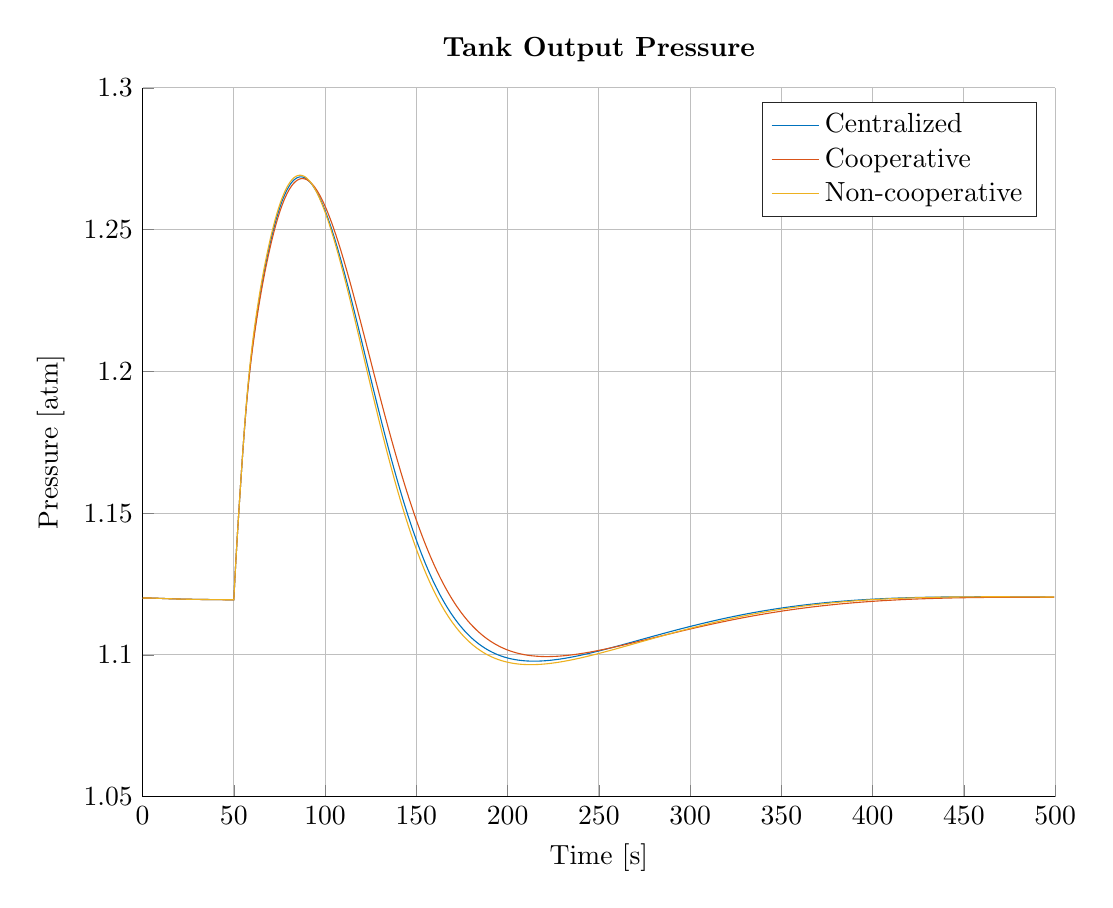
\begin{tikzpicture}

\begin{axis}[%
width=4.563in,
height=3.544in,
at={(0.792in,0.541in)},
scale only axis,
xmin=0,
xmax=500,
xlabel={Time [s]},
xmajorgrids,
ymin=1.05,
ymax=1.3,
ylabel={Pressure [atm]},
ymajorgrids,
axis background/.style={fill=white},
title style={font=\bfseries},
title={Tank Output Pressure},
axis x line*=bottom,
axis y line*=left,
legend style={legend cell align=left,align=left,draw=white!15!black}
]
\addplot [color=mycolor1,solid,forget plot]
  table[row sep=crcr]{%
0	1.12\\
0.5	1.12007\\
1	1.12008\\
1.5	1.12008\\
2	1.12008\\
2.5	1.12008\\
3	1.12008\\
3.5	1.12007\\
4	1.12007\\
4.5	1.12006\\
5	1.12005\\
5.5	1.12004\\
6	1.12003\\
6.5	1.12002\\
7	1.12001\\
7.5	1.12\\
8	1.11999\\
8.5	1.11997\\
9	1.11996\\
9.5	1.11995\\
10	1.11994\\
10.5	1.11992\\
11	1.11991\\
11.5	1.1199\\
12	1.11989\\
12.5	1.11987\\
13	1.11986\\
13.5	1.11985\\
14	1.11984\\
14.5	1.11983\\
15	1.11981\\
15.5	1.1198\\
16	1.11979\\
16.5	1.11978\\
17	1.11977\\
17.5	1.11976\\
18	1.11975\\
18.5	1.11974\\
19	1.11973\\
19.5	1.11973\\
20	1.11972\\
20.5	1.11971\\
21	1.1197\\
21.5	1.11969\\
22	1.11969\\
22.5	1.11968\\
23	1.11967\\
23.5	1.11966\\
24	1.11966\\
24.5	1.11965\\
25	1.11964\\
25.5	1.11964\\
26	1.11963\\
26.5	1.11962\\
27	1.11962\\
27.5	1.11961\\
28	1.11961\\
28.5	1.1196\\
29	1.1196\\
29.5	1.11959\\
30	1.11959\\
30.5	1.11958\\
31	1.11958\\
31.5	1.11957\\
32	1.11957\\
32.5	1.11956\\
33	1.11956\\
33.5	1.11955\\
34	1.11955\\
34.5	1.11954\\
35	1.11954\\
35.5	1.11954\\
36	1.11953\\
36.5	1.11953\\
37	1.11952\\
37.5	1.11952\\
38	1.11952\\
38.5	1.11951\\
39	1.11951\\
39.5	1.11951\\
40	1.1195\\
40.5	1.1195\\
41	1.1195\\
41.5	1.11949\\
42	1.11949\\
42.5	1.11949\\
43	1.11949\\
43.5	1.11948\\
44	1.11948\\
44.5	1.11948\\
45	1.11948\\
45.5	1.11947\\
46	1.11947\\
46.5	1.11947\\
47	1.11947\\
47.5	1.11946\\
48	1.11946\\
48.5	1.11946\\
49	1.11946\\
49.5	1.11946\\
50	1.11945\\
50.5	1.12569\\
51	1.13171\\
51.5	1.13735\\
52	1.14274\\
52.5	1.14794\\
53	1.153\\
53.5	1.15795\\
54	1.1628\\
54.5	1.16756\\
55	1.17229\\
55.5	1.17676\\
56	1.18105\\
56.5	1.18514\\
57	1.189\\
57.5	1.1926\\
58	1.19596\\
58.5	1.19912\\
59	1.2021\\
59.5	1.20491\\
60	1.20757\\
60.5	1.21011\\
61	1.21253\\
61.5	1.21486\\
62	1.21711\\
62.5	1.21928\\
63	1.22138\\
63.5	1.22342\\
64	1.22541\\
64.5	1.22733\\
65	1.22921\\
65.5	1.23103\\
66	1.2328\\
66.5	1.23452\\
67	1.2362\\
67.5	1.23784\\
68	1.23943\\
68.5	1.24099\\
69	1.2425\\
69.5	1.24397\\
70	1.2454\\
70.5	1.24679\\
71	1.24814\\
71.5	1.24944\\
72	1.2507\\
72.5	1.25192\\
73	1.2531\\
73.5	1.25424\\
74	1.25533\\
74.5	1.25637\\
75	1.25738\\
75.5	1.25834\\
76	1.25925\\
76.5	1.26012\\
77	1.26095\\
77.5	1.26174\\
78	1.26248\\
78.5	1.26317\\
79	1.26383\\
79.5	1.26444\\
80	1.26501\\
80.5	1.26553\\
81	1.26602\\
81.5	1.26646\\
82	1.26686\\
82.5	1.26721\\
83	1.26753\\
83.5	1.2678\\
84	1.26804\\
84.5	1.26823\\
85	1.26839\\
85.5	1.2685\\
86	1.26858\\
86.5	1.26861\\
87	1.26861\\
87.5	1.26857\\
88	1.26849\\
88.5	1.26838\\
89	1.26823\\
89.5	1.26804\\
90	1.26782\\
90.5	1.26756\\
91	1.26727\\
91.5	1.26695\\
92	1.26659\\
92.5	1.2662\\
93	1.26577\\
93.5	1.26532\\
94	1.26483\\
94.5	1.26431\\
95	1.26376\\
95.5	1.26318\\
96	1.26258\\
96.5	1.26194\\
97	1.26128\\
97.5	1.26059\\
98	1.25987\\
98.5	1.25913\\
99	1.25836\\
99.5	1.25757\\
100	1.25675\\
100.5	1.25591\\
101	1.25504\\
101.5	1.25415\\
102	1.25324\\
102.5	1.25231\\
103	1.25136\\
103.5	1.25039\\
104	1.2494\\
104.5	1.24839\\
105	1.24736\\
105.5	1.24631\\
106	1.24525\\
106.5	1.24417\\
107	1.24307\\
107.5	1.24196\\
108	1.24083\\
108.5	1.23969\\
109	1.23854\\
109.5	1.23737\\
110	1.23619\\
110.5	1.235\\
111	1.2338\\
111.5	1.23258\\
112	1.23136\\
112.5	1.23012\\
113	1.22888\\
113.5	1.22763\\
114	1.22637\\
114.5	1.2251\\
115	1.22382\\
115.5	1.22254\\
116	1.22126\\
116.5	1.21996\\
117	1.21866\\
117.5	1.21736\\
118	1.21606\\
118.5	1.21474\\
119	1.21343\\
119.5	1.21212\\
120	1.2108\\
120.5	1.20948\\
121	1.20816\\
121.5	1.20683\\
122	1.20551\\
122.5	1.20419\\
123	1.20287\\
123.5	1.20155\\
124	1.20023\\
124.5	1.19891\\
125	1.19759\\
125.5	1.19628\\
126	1.19497\\
126.5	1.19366\\
127	1.19235\\
127.5	1.19105\\
128	1.18976\\
128.5	1.18847\\
129	1.18718\\
129.5	1.1859\\
130	1.18462\\
130.5	1.18335\\
131	1.18208\\
131.5	1.18082\\
132	1.17957\\
132.5	1.17833\\
133	1.17709\\
133.5	1.17586\\
134	1.17464\\
134.5	1.17342\\
135	1.17221\\
135.5	1.17101\\
136	1.16982\\
136.5	1.16864\\
137	1.16747\\
137.5	1.1663\\
138	1.16515\\
138.5	1.164\\
139	1.16287\\
139.5	1.16174\\
140	1.16062\\
140.5	1.15952\\
141	1.15842\\
141.5	1.15734\\
142	1.15626\\
142.5	1.1552\\
143	1.15414\\
143.5	1.1531\\
144	1.15207\\
144.5	1.15104\\
145	1.15003\\
145.5	1.14903\\
146	1.14804\\
146.5	1.14707\\
147	1.1461\\
147.5	1.14514\\
148	1.1442\\
148.5	1.14327\\
149	1.14235\\
149.5	1.14144\\
150	1.14054\\
150.5	1.13965\\
151	1.13878\\
151.5	1.13792\\
152	1.13706\\
152.5	1.13622\\
153	1.13539\\
153.5	1.13458\\
154	1.13377\\
154.5	1.13297\\
155	1.13219\\
155.5	1.13142\\
156	1.13066\\
156.5	1.12991\\
157	1.12917\\
157.5	1.12844\\
158	1.12773\\
158.5	1.12702\\
159	1.12633\\
159.5	1.12565\\
160	1.12498\\
160.5	1.12432\\
161	1.12367\\
161.5	1.12303\\
162	1.1224\\
162.5	1.12178\\
163	1.12117\\
163.5	1.12058\\
164	1.11999\\
164.5	1.11941\\
165	1.11885\\
165.5	1.11829\\
166	1.11775\\
166.5	1.11721\\
167	1.11669\\
167.5	1.11617\\
168	1.11566\\
168.5	1.11517\\
169	1.11468\\
169.5	1.1142\\
170	1.11373\\
170.5	1.11327\\
171	1.11282\\
171.5	1.11238\\
172	1.11195\\
172.5	1.11153\\
173	1.11111\\
173.5	1.11071\\
174	1.11031\\
174.5	1.10992\\
175	1.10954\\
175.5	1.10917\\
176	1.1088\\
176.5	1.10844\\
177	1.1081\\
177.5	1.10775\\
178	1.10742\\
178.5	1.1071\\
179	1.10678\\
179.5	1.10647\\
180	1.10616\\
180.5	1.10587\\
181	1.10558\\
181.5	1.1053\\
182	1.10502\\
182.5	1.10475\\
183	1.10449\\
183.5	1.10423\\
184	1.10399\\
184.5	1.10374\\
185	1.10351\\
185.5	1.10328\\
186	1.10305\\
186.5	1.10284\\
187	1.10262\\
187.5	1.10242\\
188	1.10222\\
188.5	1.10202\\
189	1.10184\\
189.5	1.10165\\
190	1.10147\\
190.5	1.1013\\
191	1.10113\\
191.5	1.10097\\
192	1.10081\\
192.5	1.10066\\
193	1.10051\\
193.5	1.10037\\
194	1.10023\\
194.5	1.1001\\
195	1.09997\\
195.5	1.09985\\
196	1.09973\\
196.5	1.09961\\
197	1.0995\\
197.5	1.09939\\
198	1.09929\\
198.5	1.09919\\
199	1.0991\\
199.5	1.09901\\
200	1.09892\\
200.5	1.09884\\
201	1.09876\\
201.5	1.09868\\
202	1.09861\\
202.5	1.09854\\
203	1.09848\\
203.5	1.09841\\
204	1.09836\\
204.5	1.0983\\
205	1.09825\\
205.5	1.0982\\
206	1.09815\\
206.5	1.09811\\
207	1.09807\\
207.5	1.09803\\
208	1.098\\
208.5	1.09797\\
209	1.09794\\
209.5	1.09791\\
210	1.09789\\
210.5	1.09787\\
211	1.09785\\
211.5	1.09784\\
212	1.09782\\
212.5	1.09781\\
213	1.09781\\
213.5	1.0978\\
214	1.0978\\
214.5	1.0978\\
215	1.0978\\
215.5	1.0978\\
216	1.0978\\
216.5	1.09781\\
217	1.09782\\
217.5	1.09783\\
218	1.09785\\
218.5	1.09786\\
219	1.09788\\
219.5	1.0979\\
220	1.09792\\
220.5	1.09794\\
221	1.09796\\
221.5	1.09799\\
222	1.09802\\
222.5	1.09805\\
223	1.09808\\
223.5	1.09811\\
224	1.09814\\
224.5	1.09818\\
225	1.09822\\
225.5	1.09826\\
226	1.0983\\
226.5	1.09834\\
227	1.09838\\
227.5	1.09842\\
228	1.09847\\
228.5	1.09851\\
229	1.09856\\
229.5	1.09861\\
230	1.09866\\
230.5	1.09871\\
231	1.09876\\
231.5	1.09882\\
232	1.09887\\
232.5	1.09893\\
233	1.09899\\
233.5	1.09904\\
234	1.0991\\
234.5	1.09916\\
235	1.09922\\
235.5	1.09928\\
236	1.09935\\
236.5	1.09941\\
237	1.09947\\
237.5	1.09954\\
238	1.0996\\
238.5	1.09967\\
239	1.09974\\
239.5	1.09981\\
240	1.09988\\
240.5	1.09995\\
241	1.10002\\
241.5	1.10009\\
242	1.10016\\
242.5	1.10023\\
243	1.10031\\
243.5	1.10038\\
244	1.10045\\
244.5	1.10053\\
245	1.1006\\
245.5	1.10068\\
246	1.10076\\
246.5	1.10083\\
247	1.10091\\
247.5	1.10099\\
248	1.10107\\
248.5	1.10115\\
249	1.10123\\
249.5	1.10131\\
250	1.10139\\
};
\addplot [color=mycolor1,solid]
  table[row sep=crcr]{%
250	1.10139\\
250.5	1.10147\\
251	1.10155\\
251.5	1.10163\\
252	1.10172\\
252.5	1.1018\\
253	1.10188\\
253.5	1.10196\\
254	1.10205\\
254.5	1.10213\\
255	1.10222\\
255.5	1.1023\\
256	1.10239\\
256.5	1.10247\\
257	1.10256\\
257.5	1.10264\\
258	1.10273\\
258.5	1.10281\\
259	1.1029\\
259.5	1.10299\\
260	1.10307\\
260.5	1.10316\\
261	1.10325\\
261.5	1.10334\\
262	1.10342\\
262.5	1.10351\\
263	1.1036\\
263.5	1.10369\\
264	1.10378\\
264.5	1.10386\\
265	1.10395\\
265.5	1.10404\\
266	1.10413\\
266.5	1.10422\\
267	1.10431\\
267.5	1.1044\\
268	1.10448\\
268.5	1.10457\\
269	1.10466\\
269.5	1.10475\\
270	1.10484\\
270.5	1.10493\\
271	1.10502\\
271.5	1.10511\\
272	1.1052\\
272.5	1.10529\\
273	1.10538\\
273.5	1.10546\\
274	1.10555\\
274.5	1.10564\\
275	1.10573\\
275.5	1.10582\\
276	1.10591\\
276.5	1.106\\
277	1.10609\\
277.5	1.10618\\
278	1.10627\\
278.5	1.10635\\
279	1.10644\\
279.5	1.10653\\
280	1.10662\\
280.5	1.10671\\
281	1.1068\\
281.5	1.10688\\
282	1.10697\\
282.5	1.10706\\
283	1.10715\\
283.5	1.10724\\
284	1.10732\\
284.5	1.10741\\
285	1.1075\\
285.5	1.10759\\
286	1.10767\\
286.5	1.10776\\
287	1.10785\\
287.5	1.10793\\
288	1.10802\\
288.5	1.1081\\
289	1.10819\\
289.5	1.10828\\
290	1.10836\\
290.5	1.10845\\
291	1.10853\\
291.5	1.10862\\
292	1.1087\\
292.5	1.10879\\
293	1.10887\\
293.5	1.10896\\
294	1.10904\\
294.5	1.10912\\
295	1.10921\\
295.5	1.10929\\
296	1.10937\\
296.5	1.10946\\
297	1.10954\\
297.5	1.10962\\
298	1.1097\\
298.5	1.10979\\
299	1.10987\\
299.5	1.10995\\
300	1.11003\\
300.5	1.11011\\
301	1.11019\\
301.5	1.11027\\
302	1.11035\\
302.5	1.11043\\
303	1.11051\\
303.5	1.11059\\
304	1.11067\\
304.5	1.11075\\
305	1.11083\\
305.5	1.1109\\
306	1.11098\\
306.5	1.11106\\
307	1.11114\\
307.5	1.11121\\
308	1.11129\\
308.5	1.11137\\
309	1.11144\\
309.5	1.11152\\
310	1.11159\\
310.5	1.11167\\
311	1.11174\\
311.5	1.11182\\
312	1.11189\\
312.5	1.11197\\
313	1.11204\\
313.5	1.11211\\
314	1.11219\\
314.5	1.11226\\
315	1.11233\\
315.5	1.1124\\
316	1.11248\\
316.5	1.11255\\
317	1.11262\\
317.5	1.11269\\
318	1.11276\\
318.5	1.11283\\
319	1.1129\\
319.5	1.11297\\
320	1.11304\\
320.5	1.11311\\
321	1.11317\\
321.5	1.11324\\
322	1.11331\\
322.5	1.11338\\
323	1.11344\\
323.5	1.11351\\
324	1.11358\\
324.5	1.11364\\
325	1.11371\\
325.5	1.11377\\
326	1.11384\\
326.5	1.1139\\
327	1.11397\\
327.5	1.11403\\
328	1.11409\\
328.5	1.11416\\
329	1.11422\\
329.5	1.11428\\
330	1.11434\\
330.5	1.11441\\
331	1.11447\\
331.5	1.11453\\
332	1.11459\\
332.5	1.11465\\
333	1.11471\\
333.5	1.11477\\
334	1.11483\\
334.5	1.11489\\
335	1.11494\\
335.5	1.115\\
336	1.11506\\
336.5	1.11512\\
337	1.11517\\
337.5	1.11523\\
338	1.11529\\
338.5	1.11534\\
339	1.1154\\
339.5	1.11545\\
340	1.11551\\
340.5	1.11556\\
341	1.11562\\
341.5	1.11567\\
342	1.11572\\
342.5	1.11578\\
343	1.11583\\
343.5	1.11588\\
344	1.11593\\
344.5	1.11599\\
345	1.11604\\
345.5	1.11609\\
346	1.11614\\
346.5	1.11619\\
347	1.11624\\
347.5	1.11629\\
348	1.11634\\
348.5	1.11639\\
349	1.11643\\
349.5	1.11648\\
350	1.11653\\
350.5	1.11658\\
351	1.11662\\
351.5	1.11667\\
352	1.11672\\
352.5	1.11676\\
353	1.11681\\
353.5	1.11685\\
354	1.1169\\
354.5	1.11694\\
355	1.11699\\
355.5	1.11703\\
356	1.11707\\
356.5	1.11712\\
357	1.11716\\
357.5	1.1172\\
358	1.11724\\
358.5	1.11729\\
359	1.11733\\
359.5	1.11737\\
360	1.11741\\
360.5	1.11745\\
361	1.11749\\
361.5	1.11753\\
362	1.11757\\
362.5	1.11761\\
363	1.11765\\
363.5	1.11768\\
364	1.11772\\
364.5	1.11776\\
365	1.1178\\
365.5	1.11783\\
366	1.11787\\
366.5	1.11791\\
367	1.11794\\
367.5	1.11798\\
368	1.11801\\
368.5	1.11805\\
369	1.11808\\
369.5	1.11812\\
370	1.11815\\
370.5	1.11819\\
371	1.11822\\
371.5	1.11825\\
372	1.11829\\
372.5	1.11832\\
373	1.11835\\
373.5	1.11838\\
374	1.11841\\
374.5	1.11844\\
375	1.11848\\
375.5	1.11851\\
376	1.11854\\
376.5	1.11857\\
377	1.1186\\
377.5	1.11863\\
378	1.11865\\
378.5	1.11868\\
379	1.11871\\
379.5	1.11874\\
380	1.11877\\
380.5	1.1188\\
381	1.11882\\
381.5	1.11885\\
382	1.11888\\
382.5	1.1189\\
383	1.11893\\
383.5	1.11895\\
384	1.11898\\
384.5	1.11901\\
385	1.11903\\
385.5	1.11906\\
386	1.11908\\
386.5	1.1191\\
387	1.11913\\
387.5	1.11915\\
388	1.11917\\
388.5	1.1192\\
389	1.11922\\
389.5	1.11924\\
390	1.11927\\
390.5	1.11929\\
391	1.11931\\
391.5	1.11933\\
392	1.11935\\
392.5	1.11937\\
393	1.11939\\
393.5	1.11941\\
394	1.11943\\
394.5	1.11945\\
395	1.11947\\
395.5	1.11949\\
396	1.11951\\
396.5	1.11953\\
397	1.11955\\
397.5	1.11957\\
398	1.11959\\
398.5	1.11961\\
399	1.11962\\
399.5	1.11964\\
400	1.11966\\
400.5	1.11968\\
401	1.11969\\
401.5	1.11971\\
402	1.11973\\
402.5	1.11974\\
403	1.11976\\
403.5	1.11977\\
404	1.11979\\
404.5	1.1198\\
405	1.11982\\
405.5	1.11983\\
406	1.11985\\
406.5	1.11986\\
407	1.11988\\
407.5	1.11989\\
408	1.11991\\
408.5	1.11992\\
409	1.11993\\
409.5	1.11995\\
410	1.11996\\
410.5	1.11997\\
411	1.11998\\
411.5	1.12\\
412	1.12001\\
412.5	1.12002\\
413	1.12003\\
413.5	1.12004\\
414	1.12006\\
414.5	1.12007\\
415	1.12008\\
415.5	1.12009\\
416	1.1201\\
416.5	1.12011\\
417	1.12012\\
417.5	1.12013\\
418	1.12014\\
418.5	1.12015\\
419	1.12016\\
419.5	1.12017\\
420	1.12018\\
420.5	1.12019\\
421	1.1202\\
421.5	1.12021\\
422	1.12021\\
422.5	1.12022\\
423	1.12023\\
423.5	1.12024\\
424	1.12025\\
424.5	1.12025\\
425	1.12026\\
425.5	1.12027\\
426	1.12028\\
426.5	1.12028\\
427	1.12029\\
427.5	1.1203\\
428	1.12031\\
428.5	1.12031\\
429	1.12032\\
429.5	1.12032\\
430	1.12033\\
430.5	1.12034\\
431	1.12034\\
431.5	1.12035\\
432	1.12035\\
432.5	1.12036\\
433	1.12037\\
433.5	1.12037\\
434	1.12038\\
434.5	1.12038\\
435	1.12039\\
435.5	1.12039\\
436	1.1204\\
436.5	1.1204\\
437	1.1204\\
437.5	1.12041\\
438	1.12041\\
438.5	1.12042\\
439	1.12042\\
439.5	1.12042\\
440	1.12043\\
440.5	1.12043\\
441	1.12044\\
441.5	1.12044\\
442	1.12044\\
442.5	1.12045\\
443	1.12045\\
443.5	1.12045\\
444	1.12045\\
444.5	1.12046\\
445	1.12046\\
445.5	1.12046\\
446	1.12046\\
446.5	1.12047\\
447	1.12047\\
447.5	1.12047\\
448	1.12047\\
448.5	1.12048\\
449	1.12048\\
449.5	1.12048\\
450	1.12048\\
450.5	1.12048\\
451	1.12048\\
451.5	1.12049\\
452	1.12049\\
452.5	1.12049\\
453	1.12049\\
453.5	1.12049\\
454	1.12049\\
454.5	1.12049\\
455	1.12049\\
455.5	1.12049\\
456	1.1205\\
456.5	1.1205\\
457	1.1205\\
457.5	1.1205\\
458	1.1205\\
458.5	1.1205\\
459	1.1205\\
459.5	1.1205\\
460	1.1205\\
460.5	1.1205\\
461	1.1205\\
461.5	1.1205\\
462	1.1205\\
462.5	1.1205\\
463	1.1205\\
463.5	1.1205\\
464	1.1205\\
464.5	1.1205\\
465	1.1205\\
465.5	1.1205\\
466	1.1205\\
466.5	1.1205\\
467	1.1205\\
467.5	1.1205\\
468	1.12049\\
468.5	1.12049\\
469	1.12049\\
469.5	1.12049\\
470	1.12049\\
470.5	1.12049\\
471	1.12049\\
471.5	1.12049\\
472	1.12049\\
472.5	1.12049\\
473	1.12049\\
473.5	1.12048\\
474	1.12048\\
474.5	1.12048\\
475	1.12048\\
475.5	1.12048\\
476	1.12048\\
476.5	1.12048\\
477	1.12047\\
477.5	1.12047\\
478	1.12047\\
478.5	1.12047\\
479	1.12047\\
479.5	1.12047\\
480	1.12046\\
480.5	1.12046\\
481	1.12046\\
481.5	1.12046\\
482	1.12046\\
482.5	1.12046\\
483	1.12045\\
483.5	1.12045\\
484	1.12045\\
484.5	1.12045\\
485	1.12045\\
485.5	1.12044\\
486	1.12044\\
486.5	1.12044\\
487	1.12044\\
487.5	1.12044\\
488	1.12043\\
488.5	1.12043\\
489	1.12043\\
489.5	1.12043\\
490	1.12043\\
490.5	1.12042\\
491	1.12042\\
491.5	1.12042\\
492	1.12042\\
492.5	1.12042\\
493	1.12041\\
493.5	1.12041\\
494	1.12041\\
494.5	1.12041\\
495	1.1204\\
495.5	1.1204\\
496	1.1204\\
496.5	1.1204\\
497	1.12039\\
497.5	1.12039\\
498	1.12039\\
498.5	1.12039\\
499	1.12038\\
499.5	1.12038\\
};
\addlegendentry{Centralized};

\addplot [color=mycolor2,solid,forget plot]
  table[row sep=crcr]{%
0	1.12\\
0.5	1.12007\\
1	1.12008\\
1.5	1.12008\\
2	1.12008\\
2.5	1.12008\\
3	1.12008\\
3.5	1.12007\\
4	1.12006\\
4.5	1.12006\\
5	1.12005\\
5.5	1.12004\\
6	1.12003\\
6.5	1.12002\\
7	1.12001\\
7.5	1.11999\\
8	1.11998\\
8.5	1.11997\\
9	1.11996\\
9.5	1.11994\\
10	1.11993\\
10.5	1.11992\\
11	1.1199\\
11.5	1.11989\\
12	1.11988\\
12.5	1.11987\\
13	1.11985\\
13.5	1.11984\\
14	1.11983\\
14.5	1.11982\\
15	1.11981\\
15.5	1.1198\\
16	1.11979\\
16.5	1.11978\\
17	1.11977\\
17.5	1.11976\\
18	1.11975\\
18.5	1.11974\\
19	1.11973\\
19.5	1.11972\\
20	1.11971\\
20.5	1.1197\\
21	1.11969\\
21.5	1.11969\\
22	1.11968\\
22.5	1.11967\\
23	1.11966\\
23.5	1.11966\\
24	1.11965\\
24.5	1.11964\\
25	1.11964\\
25.5	1.11963\\
26	1.11962\\
26.5	1.11962\\
27	1.11961\\
27.5	1.11961\\
28	1.1196\\
28.5	1.11959\\
29	1.11959\\
29.5	1.11958\\
30	1.11958\\
30.5	1.11957\\
31	1.11957\\
31.5	1.11956\\
32	1.11956\\
32.5	1.11955\\
33	1.11955\\
33.5	1.11955\\
34	1.11954\\
34.5	1.11954\\
35	1.11953\\
35.5	1.11953\\
36	1.11952\\
36.5	1.11952\\
37	1.11952\\
37.5	1.11951\\
38	1.11951\\
38.5	1.11951\\
39	1.1195\\
39.5	1.1195\\
40	1.1195\\
40.5	1.11949\\
41	1.11949\\
41.5	1.11949\\
42	1.11948\\
42.5	1.11948\\
43	1.11948\\
43.5	1.11948\\
44	1.11947\\
44.5	1.11947\\
45	1.11947\\
45.5	1.11947\\
46	1.11946\\
46.5	1.11946\\
47	1.11946\\
47.5	1.11946\\
48	1.11945\\
48.5	1.11945\\
49	1.11945\\
49.5	1.11945\\
50	1.11944\\
50.5	1.12568\\
51	1.1317\\
51.5	1.13734\\
52	1.14274\\
52.5	1.14796\\
53	1.15303\\
53.5	1.15798\\
54	1.16283\\
54.5	1.16759\\
55	1.17228\\
55.5	1.1767\\
56	1.18091\\
56.5	1.18494\\
57	1.1887\\
57.5	1.19219\\
58	1.19546\\
58.5	1.19852\\
59	1.20141\\
59.5	1.20413\\
60	1.20672\\
60.5	1.20919\\
61	1.21156\\
61.5	1.21385\\
62	1.21606\\
62.5	1.2182\\
63	1.22027\\
63.5	1.22229\\
64	1.22426\\
64.5	1.22616\\
65	1.22801\\
65.5	1.2298\\
66	1.23154\\
66.5	1.23324\\
67	1.2349\\
67.5	1.23651\\
68	1.23808\\
68.5	1.23961\\
69	1.24111\\
69.5	1.24256\\
70	1.24398\\
70.5	1.24535\\
71	1.24669\\
71.5	1.24798\\
72	1.24924\\
72.5	1.25045\\
73	1.25162\\
73.5	1.25275\\
74	1.25385\\
74.5	1.25489\\
75	1.2559\\
75.5	1.25687\\
76	1.2578\\
76.5	1.25868\\
77	1.25952\\
77.5	1.26033\\
78	1.26109\\
78.5	1.26181\\
79	1.26248\\
79.5	1.26312\\
80	1.26372\\
80.5	1.26428\\
81	1.26479\\
81.5	1.26527\\
82	1.26571\\
82.5	1.26611\\
83	1.26647\\
83.5	1.26679\\
84	1.26707\\
84.5	1.26731\\
85	1.26752\\
85.5	1.26769\\
86	1.26782\\
86.5	1.26792\\
87	1.26798\\
87.5	1.268\\
88	1.26799\\
88.5	1.26794\\
89	1.26786\\
89.5	1.26775\\
90	1.2676\\
90.5	1.26741\\
91	1.2672\\
91.5	1.26695\\
92	1.26667\\
92.5	1.26636\\
93	1.26602\\
93.5	1.26565\\
94	1.26525\\
94.5	1.26482\\
95	1.26436\\
95.5	1.26387\\
96	1.26335\\
96.5	1.26281\\
97	1.26224\\
97.5	1.26164\\
98	1.26102\\
98.5	1.26037\\
99	1.2597\\
99.5	1.259\\
100	1.25828\\
100.5	1.25754\\
101	1.25678\\
101.5	1.25599\\
102	1.25518\\
102.5	1.25435\\
103	1.2535\\
103.5	1.25263\\
104	1.25174\\
104.5	1.25083\\
105	1.24991\\
105.5	1.24896\\
106	1.248\\
106.5	1.24702\\
107	1.24603\\
107.5	1.24502\\
108	1.24399\\
108.5	1.24295\\
109	1.2419\\
109.5	1.24083\\
110	1.23975\\
110.5	1.23866\\
111	1.23755\\
111.5	1.23644\\
112	1.23531\\
112.5	1.23417\\
113	1.23302\\
113.5	1.23187\\
114	1.2307\\
114.5	1.22953\\
115	1.22834\\
115.5	1.22715\\
116	1.22595\\
116.5	1.22475\\
117	1.22354\\
117.5	1.22232\\
118	1.2211\\
118.5	1.21987\\
119	1.21864\\
119.5	1.21741\\
120	1.21617\\
120.5	1.21493\\
121	1.21368\\
121.5	1.21244\\
122	1.21119\\
122.5	1.20994\\
123	1.20868\\
123.5	1.20743\\
124	1.20618\\
124.5	1.20493\\
125	1.20367\\
125.5	1.20242\\
126	1.20117\\
126.5	1.19992\\
127	1.19867\\
127.5	1.19743\\
128	1.19618\\
128.5	1.19494\\
129	1.19371\\
129.5	1.19247\\
130	1.19124\\
130.5	1.19001\\
131	1.18879\\
131.5	1.18757\\
132	1.18636\\
132.5	1.18515\\
133	1.18395\\
133.5	1.18275\\
134	1.18156\\
134.5	1.18037\\
135	1.17919\\
135.5	1.17802\\
136	1.17685\\
136.5	1.17569\\
137	1.17454\\
137.5	1.1734\\
138	1.17226\\
138.5	1.17113\\
139	1.17001\\
139.5	1.16889\\
140	1.16779\\
140.5	1.16669\\
141	1.1656\\
141.5	1.16452\\
142	1.16345\\
142.5	1.16238\\
143	1.16133\\
143.5	1.16028\\
144	1.15925\\
144.5	1.15822\\
145	1.1572\\
145.5	1.1562\\
146	1.1552\\
146.5	1.15421\\
147	1.15323\\
147.5	1.15226\\
148	1.15131\\
148.5	1.15036\\
149	1.14942\\
149.5	1.14849\\
150	1.14757\\
150.5	1.14667\\
151	1.14577\\
151.5	1.14488\\
152	1.14401\\
152.5	1.14314\\
153	1.14228\\
153.5	1.14144\\
154	1.1406\\
154.5	1.13978\\
155	1.13897\\
155.5	1.13816\\
156	1.13737\\
156.5	1.13659\\
157	1.13581\\
157.5	1.13505\\
158	1.1343\\
158.5	1.13356\\
159	1.13283\\
159.5	1.13211\\
160	1.1314\\
160.5	1.1307\\
161	1.13001\\
161.5	1.12933\\
162	1.12866\\
162.5	1.128\\
163	1.12735\\
163.5	1.12671\\
164	1.12608\\
164.5	1.12546\\
165	1.12485\\
165.5	1.12425\\
166	1.12366\\
166.5	1.12308\\
167	1.1225\\
167.5	1.12194\\
168	1.12139\\
168.5	1.12084\\
169	1.12031\\
169.5	1.11979\\
170	1.11927\\
170.5	1.11876\\
171	1.11826\\
171.5	1.11778\\
172	1.11729\\
172.5	1.11682\\
173	1.11636\\
173.5	1.11591\\
174	1.11546\\
174.5	1.11502\\
175	1.11459\\
175.5	1.11417\\
176	1.11376\\
176.5	1.11335\\
177	1.11295\\
177.5	1.11257\\
178	1.11218\\
178.5	1.11181\\
179	1.11144\\
179.5	1.11108\\
180	1.11073\\
180.5	1.11039\\
181	1.11005\\
181.5	1.10972\\
182	1.1094\\
182.5	1.10908\\
183	1.10877\\
183.5	1.10847\\
184	1.10817\\
184.5	1.10789\\
185	1.1076\\
185.5	1.10733\\
186	1.10706\\
186.5	1.10679\\
187	1.10654\\
187.5	1.10628\\
188	1.10604\\
188.5	1.1058\\
189	1.10557\\
189.5	1.10534\\
190	1.10512\\
190.5	1.1049\\
191	1.10469\\
191.5	1.10448\\
192	1.10428\\
192.5	1.10409\\
193	1.1039\\
193.5	1.10371\\
194	1.10353\\
194.5	1.10336\\
195	1.10319\\
195.5	1.10302\\
196	1.10286\\
196.5	1.1027\\
197	1.10255\\
197.5	1.10241\\
198	1.10226\\
198.5	1.10213\\
199	1.10199\\
199.5	1.10186\\
200	1.10174\\
200.5	1.10161\\
201	1.1015\\
201.5	1.10138\\
202	1.10127\\
202.5	1.10117\\
203	1.10107\\
203.5	1.10097\\
204	1.10087\\
204.5	1.10078\\
205	1.10069\\
205.5	1.10061\\
206	1.10053\\
206.5	1.10045\\
207	1.10038\\
207.5	1.10031\\
208	1.10024\\
208.5	1.10017\\
209	1.10011\\
209.5	1.10005\\
210	1.1\\
210.5	1.09994\\
211	1.09989\\
211.5	1.09985\\
212	1.0998\\
212.5	1.09976\\
213	1.09972\\
213.5	1.09968\\
214	1.09965\\
214.5	1.09962\\
215	1.09959\\
215.5	1.09956\\
216	1.09954\\
216.5	1.09952\\
217	1.0995\\
217.5	1.09948\\
218	1.09946\\
218.5	1.09945\\
219	1.09944\\
219.5	1.09943\\
220	1.09942\\
220.5	1.09942\\
221	1.09941\\
221.5	1.09941\\
222	1.09941\\
222.5	1.09942\\
223	1.09942\\
223.5	1.09943\\
224	1.09944\\
224.5	1.09945\\
225	1.09946\\
225.5	1.09947\\
226	1.09949\\
226.5	1.0995\\
227	1.09952\\
227.5	1.09954\\
228	1.09956\\
228.5	1.09958\\
229	1.09961\\
229.5	1.09963\\
230	1.09966\\
230.5	1.09969\\
231	1.09972\\
231.5	1.09975\\
232	1.09978\\
232.5	1.09981\\
233	1.09985\\
233.5	1.09988\\
234	1.09992\\
234.5	1.09996\\
235	1.1\\
235.5	1.10004\\
236	1.10008\\
236.5	1.10012\\
237	1.10017\\
237.5	1.10021\\
238	1.10026\\
238.5	1.1003\\
239	1.10035\\
239.5	1.1004\\
240	1.10045\\
240.5	1.1005\\
241	1.10055\\
241.5	1.1006\\
242	1.10065\\
242.5	1.10071\\
243	1.10076\\
243.5	1.10082\\
244	1.10087\\
244.5	1.10093\\
245	1.10099\\
245.5	1.10104\\
246	1.1011\\
246.5	1.10116\\
247	1.10122\\
247.5	1.10128\\
248	1.10134\\
248.5	1.10141\\
249	1.10147\\
249.5	1.10153\\
250	1.1016\\
};
\addplot [color=mycolor2,solid]
  table[row sep=crcr]{%
250	1.1016\\
250.5	1.10166\\
251	1.10173\\
251.5	1.10179\\
252	1.10186\\
252.5	1.10192\\
253	1.10199\\
253.5	1.10206\\
254	1.10213\\
254.5	1.10219\\
255	1.10226\\
255.5	1.10233\\
256	1.1024\\
256.5	1.10247\\
257	1.10254\\
257.5	1.10261\\
258	1.10268\\
258.5	1.10276\\
259	1.10283\\
259.5	1.1029\\
260	1.10297\\
260.5	1.10304\\
261	1.10312\\
261.5	1.10319\\
262	1.10326\\
262.5	1.10334\\
263	1.10341\\
263.5	1.10349\\
264	1.10356\\
264.5	1.10364\\
265	1.10371\\
265.5	1.10379\\
266	1.10386\\
266.5	1.10394\\
267	1.10402\\
267.5	1.10409\\
268	1.10417\\
268.5	1.10425\\
269	1.10432\\
269.5	1.1044\\
270	1.10448\\
270.5	1.10455\\
271	1.10463\\
271.5	1.10471\\
272	1.10479\\
272.5	1.10486\\
273	1.10494\\
273.5	1.10502\\
274	1.1051\\
274.5	1.10517\\
275	1.10525\\
275.5	1.10533\\
276	1.10541\\
276.5	1.10549\\
277	1.10557\\
277.5	1.10564\\
278	1.10572\\
278.5	1.1058\\
279	1.10588\\
279.5	1.10596\\
280	1.10604\\
280.5	1.10611\\
281	1.10619\\
281.5	1.10627\\
282	1.10635\\
282.5	1.10643\\
283	1.10651\\
283.5	1.10659\\
284	1.10666\\
284.5	1.10674\\
285	1.10682\\
285.5	1.1069\\
286	1.10698\\
286.5	1.10705\\
287	1.10713\\
287.5	1.10721\\
288	1.10729\\
288.5	1.10737\\
289	1.10744\\
289.5	1.10752\\
290	1.1076\\
290.5	1.10768\\
291	1.10775\\
291.5	1.10783\\
292	1.10791\\
292.5	1.10799\\
293	1.10806\\
293.5	1.10814\\
294	1.10822\\
294.5	1.10829\\
295	1.10837\\
295.5	1.10845\\
296	1.10852\\
296.5	1.1086\\
297	1.10867\\
297.5	1.10875\\
298	1.10883\\
298.5	1.1089\\
299	1.10898\\
299.5	1.10905\\
300	1.10913\\
300.5	1.1092\\
301	1.10928\\
301.5	1.10935\\
302	1.10942\\
302.5	1.1095\\
303	1.10957\\
303.5	1.10965\\
304	1.10972\\
304.5	1.10979\\
305	1.10987\\
305.5	1.10994\\
306	1.11001\\
306.5	1.11008\\
307	1.11016\\
307.5	1.11023\\
308	1.1103\\
308.5	1.11037\\
309	1.11044\\
309.5	1.11051\\
310	1.11059\\
310.5	1.11066\\
311	1.11073\\
311.5	1.1108\\
312	1.11087\\
312.5	1.11094\\
313	1.11101\\
313.5	1.11108\\
314	1.11115\\
314.5	1.11122\\
315	1.11128\\
315.5	1.11135\\
316	1.11142\\
316.5	1.11149\\
317	1.11156\\
317.5	1.11162\\
318	1.11169\\
318.5	1.11176\\
319	1.11183\\
319.5	1.11189\\
320	1.11196\\
320.5	1.11202\\
321	1.11209\\
321.5	1.11216\\
322	1.11222\\
322.5	1.11229\\
323	1.11235\\
323.5	1.11241\\
324	1.11248\\
324.5	1.11254\\
325	1.11261\\
325.5	1.11267\\
326	1.11273\\
326.5	1.1128\\
327	1.11286\\
327.5	1.11292\\
328	1.11298\\
328.5	1.11304\\
329	1.11311\\
329.5	1.11317\\
330	1.11323\\
330.5	1.11329\\
331	1.11335\\
331.5	1.11341\\
332	1.11347\\
332.5	1.11353\\
333	1.11359\\
333.5	1.11365\\
334	1.1137\\
334.5	1.11376\\
335	1.11382\\
335.5	1.11388\\
336	1.11393\\
336.5	1.11399\\
337	1.11405\\
337.5	1.11411\\
338	1.11416\\
338.5	1.11422\\
339	1.11427\\
339.5	1.11433\\
340	1.11438\\
340.5	1.11444\\
341	1.11449\\
341.5	1.11455\\
342	1.1146\\
342.5	1.11465\\
343	1.11471\\
343.5	1.11476\\
344	1.11481\\
344.5	1.11487\\
345	1.11492\\
345.5	1.11497\\
346	1.11502\\
346.5	1.11507\\
347	1.11512\\
347.5	1.11517\\
348	1.11522\\
348.5	1.11527\\
349	1.11532\\
349.5	1.11537\\
350	1.11542\\
350.5	1.11547\\
351	1.11552\\
351.5	1.11557\\
352	1.11562\\
352.5	1.11566\\
353	1.11571\\
353.5	1.11576\\
354	1.1158\\
354.5	1.11585\\
355	1.1159\\
355.5	1.11594\\
356	1.11599\\
356.5	1.11603\\
357	1.11608\\
357.5	1.11612\\
358	1.11617\\
358.5	1.11621\\
359	1.11626\\
359.5	1.1163\\
360	1.11634\\
360.5	1.11638\\
361	1.11643\\
361.5	1.11647\\
362	1.11651\\
362.5	1.11655\\
363	1.11659\\
363.5	1.11664\\
364	1.11668\\
364.5	1.11672\\
365	1.11676\\
365.5	1.1168\\
366	1.11684\\
366.5	1.11688\\
367	1.11692\\
367.5	1.11695\\
368	1.11699\\
368.5	1.11703\\
369	1.11707\\
369.5	1.11711\\
370	1.11714\\
370.5	1.11718\\
371	1.11722\\
371.5	1.11725\\
372	1.11729\\
372.5	1.11733\\
373	1.11736\\
373.5	1.1174\\
374	1.11743\\
374.5	1.11747\\
375	1.1175\\
375.5	1.11754\\
376	1.11757\\
376.5	1.1176\\
377	1.11764\\
377.5	1.11767\\
378	1.1177\\
378.5	1.11774\\
379	1.11777\\
379.5	1.1178\\
380	1.11783\\
380.5	1.11786\\
381	1.1179\\
381.5	1.11793\\
382	1.11796\\
382.5	1.11799\\
383	1.11802\\
383.5	1.11805\\
384	1.11808\\
384.5	1.11811\\
385	1.11814\\
385.5	1.11817\\
386	1.1182\\
386.5	1.11822\\
387	1.11825\\
387.5	1.11828\\
388	1.11831\\
388.5	1.11833\\
389	1.11836\\
389.5	1.11839\\
390	1.11842\\
390.5	1.11844\\
391	1.11847\\
391.5	1.11849\\
392	1.11852\\
392.5	1.11855\\
393	1.11857\\
393.5	1.1186\\
394	1.11862\\
394.5	1.11865\\
395	1.11867\\
395.5	1.11869\\
396	1.11872\\
396.5	1.11874\\
397	1.11876\\
397.5	1.11879\\
398	1.11881\\
398.5	1.11883\\
399	1.11886\\
399.5	1.11888\\
400	1.1189\\
400.5	1.11892\\
401	1.11894\\
401.5	1.11896\\
402	1.11899\\
402.5	1.11901\\
403	1.11903\\
403.5	1.11905\\
404	1.11907\\
404.5	1.11909\\
405	1.11911\\
405.5	1.11913\\
406	1.11915\\
406.5	1.11917\\
407	1.11918\\
407.5	1.1192\\
408	1.11922\\
408.5	1.11924\\
409	1.11926\\
409.5	1.11928\\
410	1.11929\\
410.5	1.11931\\
411	1.11933\\
411.5	1.11935\\
412	1.11936\\
412.5	1.11938\\
413	1.1194\\
413.5	1.11941\\
414	1.11943\\
414.5	1.11945\\
415	1.11946\\
415.5	1.11948\\
416	1.11949\\
416.5	1.11951\\
417	1.11952\\
417.5	1.11954\\
418	1.11955\\
418.5	1.11957\\
419	1.11958\\
419.5	1.11959\\
420	1.11961\\
420.5	1.11962\\
421	1.11964\\
421.5	1.11965\\
422	1.11966\\
422.5	1.11968\\
423	1.11969\\
423.5	1.1197\\
424	1.11971\\
424.5	1.11973\\
425	1.11974\\
425.5	1.11975\\
426	1.11976\\
426.5	1.11977\\
427	1.11979\\
427.5	1.1198\\
428	1.11981\\
428.5	1.11982\\
429	1.11983\\
429.5	1.11984\\
430	1.11985\\
430.5	1.11986\\
431	1.11987\\
431.5	1.11988\\
432	1.11989\\
432.5	1.1199\\
433	1.11991\\
433.5	1.11992\\
434	1.11993\\
434.5	1.11994\\
435	1.11995\\
435.5	1.11996\\
436	1.11997\\
436.5	1.11998\\
437	1.11999\\
437.5	1.12\\
438	1.12\\
438.5	1.12001\\
439	1.12002\\
439.5	1.12003\\
440	1.12004\\
440.5	1.12004\\
441	1.12005\\
441.5	1.12006\\
442	1.12007\\
442.5	1.12007\\
443	1.12008\\
443.5	1.12009\\
444	1.1201\\
444.5	1.1201\\
445	1.12011\\
445.5	1.12012\\
446	1.12012\\
446.5	1.12013\\
447	1.12013\\
447.5	1.12014\\
448	1.12015\\
448.5	1.12015\\
449	1.12016\\
449.5	1.12016\\
450	1.12017\\
450.5	1.12017\\
451	1.12018\\
451.5	1.12019\\
452	1.12019\\
452.5	1.1202\\
453	1.1202\\
453.5	1.12021\\
454	1.12021\\
454.5	1.12021\\
455	1.12022\\
455.5	1.12022\\
456	1.12023\\
456.5	1.12023\\
457	1.12024\\
457.5	1.12024\\
458	1.12024\\
458.5	1.12025\\
459	1.12025\\
459.5	1.12026\\
460	1.12026\\
460.5	1.12026\\
461	1.12027\\
461.5	1.12027\\
462	1.12027\\
462.5	1.12028\\
463	1.12028\\
463.5	1.12028\\
464	1.12029\\
464.5	1.12029\\
465	1.12029\\
465.5	1.12029\\
466	1.1203\\
466.5	1.1203\\
467	1.1203\\
467.5	1.1203\\
468	1.12031\\
468.5	1.12031\\
469	1.12031\\
469.5	1.12031\\
470	1.12032\\
470.5	1.12032\\
471	1.12032\\
471.5	1.12032\\
472	1.12032\\
472.5	1.12033\\
473	1.12033\\
473.5	1.12033\\
474	1.12033\\
474.5	1.12033\\
475	1.12033\\
475.5	1.12033\\
476	1.12034\\
476.5	1.12034\\
477	1.12034\\
477.5	1.12034\\
478	1.12034\\
478.5	1.12034\\
479	1.12034\\
479.5	1.12034\\
480	1.12034\\
480.5	1.12035\\
481	1.12035\\
481.5	1.12035\\
482	1.12035\\
482.5	1.12035\\
483	1.12035\\
483.5	1.12035\\
484	1.12035\\
484.5	1.12035\\
485	1.12035\\
485.5	1.12035\\
486	1.12035\\
486.5	1.12035\\
487	1.12035\\
487.5	1.12035\\
488	1.12035\\
488.5	1.12035\\
489	1.12035\\
489.5	1.12035\\
490	1.12035\\
490.5	1.12035\\
491	1.12035\\
491.5	1.12035\\
492	1.12035\\
492.5	1.12035\\
493	1.12035\\
493.5	1.12035\\
494	1.12035\\
494.5	1.12035\\
495	1.12035\\
495.5	1.12035\\
496	1.12035\\
496.5	1.12035\\
497	1.12035\\
497.5	1.12035\\
498	1.12035\\
498.5	1.12035\\
499	1.12035\\
499.5	1.12034\\
};
\addlegendentry{Cooperative};

\addplot [color=mycolor3,solid,forget plot]
  table[row sep=crcr]{%
0	1.12\\
0.5	1.12007\\
1	1.12008\\
1.5	1.12008\\
2	1.12008\\
2.5	1.12008\\
3	1.12008\\
3.5	1.12007\\
4	1.12007\\
4.5	1.12006\\
5	1.12005\\
5.5	1.12004\\
6	1.12003\\
6.5	1.12002\\
7	1.12001\\
7.5	1.12\\
8	1.11998\\
8.5	1.11997\\
9	1.11996\\
9.5	1.11995\\
10	1.11993\\
10.5	1.11992\\
11	1.11991\\
11.5	1.11989\\
12	1.11988\\
12.5	1.11987\\
13	1.11986\\
13.5	1.11984\\
14	1.11983\\
14.5	1.11982\\
15	1.11981\\
15.5	1.1198\\
16	1.11979\\
16.5	1.11978\\
17	1.11977\\
17.5	1.11976\\
18	1.11975\\
18.5	1.11974\\
19	1.11973\\
19.5	1.11972\\
20	1.11971\\
20.5	1.1197\\
21	1.1197\\
21.5	1.11969\\
22	1.11968\\
22.5	1.11967\\
23	1.11967\\
23.5	1.11966\\
24	1.11965\\
24.5	1.11964\\
25	1.11964\\
25.5	1.11963\\
26	1.11963\\
26.5	1.11962\\
27	1.11961\\
27.5	1.11961\\
28	1.1196\\
28.5	1.1196\\
29	1.11959\\
29.5	1.11959\\
30	1.11958\\
30.5	1.11958\\
31	1.11957\\
31.5	1.11957\\
32	1.11956\\
32.5	1.11956\\
33	1.11955\\
33.5	1.11955\\
34	1.11954\\
34.5	1.11954\\
35	1.11954\\
35.5	1.11953\\
36	1.11953\\
36.5	1.11952\\
37	1.11952\\
37.5	1.11952\\
38	1.11951\\
38.5	1.11951\\
39	1.11951\\
39.5	1.1195\\
40	1.1195\\
40.5	1.1195\\
41	1.11949\\
41.5	1.11949\\
42	1.11949\\
42.5	1.11948\\
43	1.11948\\
43.5	1.11948\\
44	1.11948\\
44.5	1.11947\\
45	1.11947\\
45.5	1.11947\\
46	1.11947\\
46.5	1.11946\\
47	1.11946\\
47.5	1.11946\\
48	1.11946\\
48.5	1.11946\\
49	1.11945\\
49.5	1.11945\\
50	1.11945\\
50.5	1.12569\\
51	1.1317\\
51.5	1.13734\\
52	1.14274\\
52.5	1.14795\\
53	1.15302\\
53.5	1.15798\\
54	1.16285\\
54.5	1.16764\\
55	1.17237\\
55.5	1.177\\
56	1.18138\\
56.5	1.18559\\
57	1.18958\\
57.5	1.19332\\
58	1.19681\\
58.5	1.20009\\
59	1.20317\\
59.5	1.20607\\
60	1.20881\\
60.5	1.21141\\
61	1.21388\\
61.5	1.21625\\
62	1.21853\\
62.5	1.22072\\
63	1.22284\\
63.5	1.2249\\
64	1.22689\\
64.5	1.22882\\
65	1.23069\\
65.5	1.2325\\
66	1.23426\\
66.5	1.23597\\
67	1.23763\\
67.5	1.23925\\
68	1.24083\\
68.5	1.24236\\
69	1.24386\\
69.5	1.24531\\
70	1.24672\\
70.5	1.24809\\
71	1.24942\\
71.5	1.25071\\
72	1.25195\\
72.5	1.25315\\
73	1.25431\\
73.5	1.25543\\
74	1.2565\\
74.5	1.25753\\
75	1.25851\\
75.5	1.25946\\
76	1.26035\\
76.5	1.26121\\
77	1.26201\\
77.5	1.26278\\
78	1.2635\\
78.5	1.26418\\
79	1.26481\\
79.5	1.2654\\
80	1.26594\\
80.5	1.26645\\
81	1.26691\\
81.5	1.26732\\
82	1.2677\\
82.5	1.26803\\
83	1.26832\\
83.5	1.26856\\
84	1.26877\\
84.5	1.26893\\
85	1.26906\\
85.5	1.26914\\
86	1.26918\\
86.5	1.26919\\
87	1.26915\\
87.5	1.26908\\
88	1.26897\\
88.5	1.26882\\
89	1.26863\\
89.5	1.26841\\
90	1.26815\\
90.5	1.26785\\
91	1.26752\\
91.5	1.26716\\
92	1.26676\\
92.5	1.26632\\
93	1.26586\\
93.5	1.26536\\
94	1.26483\\
94.5	1.26426\\
95	1.26367\\
95.5	1.26305\\
96	1.26239\\
96.5	1.26171\\
97	1.261\\
97.5	1.26026\\
98	1.2595\\
98.5	1.25871\\
99	1.25789\\
99.5	1.25705\\
100	1.25618\\
100.5	1.25529\\
101	1.25437\\
101.5	1.25344\\
102	1.25248\\
102.5	1.25149\\
103	1.25049\\
103.5	1.24947\\
104	1.24843\\
104.5	1.24737\\
105	1.24629\\
105.5	1.24519\\
106	1.24407\\
106.5	1.24294\\
107	1.2418\\
107.5	1.24063\\
108	1.23946\\
108.5	1.23827\\
109	1.23706\\
109.5	1.23584\\
110	1.23461\\
110.5	1.23337\\
111	1.23212\\
111.5	1.23086\\
112	1.22959\\
112.5	1.2283\\
113	1.22701\\
113.5	1.22571\\
114	1.22441\\
114.5	1.2231\\
115	1.22178\\
115.5	1.22045\\
116	1.21912\\
116.5	1.21778\\
117	1.21644\\
117.5	1.2151\\
118	1.21375\\
118.5	1.2124\\
119	1.21105\\
119.5	1.20969\\
120	1.20833\\
120.5	1.20698\\
121	1.20562\\
121.5	1.20426\\
122	1.2029\\
122.5	1.20155\\
123	1.20019\\
123.5	1.19884\\
124	1.19749\\
124.5	1.19614\\
125	1.19479\\
125.5	1.19345\\
126	1.19211\\
126.5	1.19078\\
127	1.18944\\
127.5	1.18812\\
128	1.1868\\
128.5	1.18548\\
129	1.18417\\
129.5	1.18287\\
130	1.18157\\
130.5	1.18028\\
131	1.179\\
131.5	1.17772\\
132	1.17645\\
132.5	1.17519\\
133	1.17394\\
133.5	1.17269\\
134	1.17146\\
134.5	1.17023\\
135	1.16901\\
135.5	1.1678\\
136	1.1666\\
136.5	1.16541\\
137	1.16423\\
137.5	1.16306\\
138	1.16189\\
138.5	1.16074\\
139	1.1596\\
139.5	1.15847\\
140	1.15735\\
140.5	1.15625\\
141	1.15515\\
141.5	1.15406\\
142	1.15299\\
142.5	1.15192\\
143	1.15087\\
143.5	1.14983\\
144	1.1488\\
144.5	1.14778\\
145	1.14677\\
145.5	1.14578\\
146	1.1448\\
146.5	1.14383\\
147	1.14287\\
147.5	1.14192\\
148	1.14098\\
148.5	1.14006\\
149	1.13915\\
149.5	1.13825\\
150	1.13736\\
150.5	1.13648\\
151	1.13562\\
151.5	1.13477\\
152	1.13393\\
152.5	1.1331\\
153	1.13229\\
153.5	1.13148\\
154	1.13069\\
154.5	1.12991\\
155	1.12914\\
155.5	1.12838\\
156	1.12764\\
156.5	1.12691\\
157	1.12618\\
157.5	1.12547\\
158	1.12477\\
158.5	1.12409\\
159	1.12341\\
159.5	1.12275\\
160	1.12209\\
160.5	1.12145\\
161	1.12082\\
161.5	1.1202\\
162	1.11959\\
162.5	1.11899\\
163	1.1184\\
163.5	1.11782\\
164	1.11725\\
164.5	1.1167\\
165	1.11615\\
165.5	1.11561\\
166	1.11509\\
166.5	1.11457\\
167	1.11407\\
167.5	1.11357\\
168	1.11308\\
168.5	1.11261\\
169	1.11214\\
169.5	1.11168\\
170	1.11123\\
170.5	1.11079\\
171	1.11036\\
171.5	1.10994\\
172	1.10953\\
172.5	1.10912\\
173	1.10873\\
173.5	1.10834\\
174	1.10797\\
174.5	1.1076\\
175	1.10723\\
175.5	1.10688\\
176	1.10654\\
176.5	1.1062\\
177	1.10587\\
177.5	1.10555\\
178	1.10523\\
178.5	1.10493\\
179	1.10463\\
179.5	1.10433\\
180	1.10405\\
180.5	1.10377\\
181	1.1035\\
181.5	1.10324\\
182	1.10298\\
182.5	1.10273\\
183	1.10248\\
183.5	1.10225\\
184	1.10201\\
184.5	1.10179\\
185	1.10157\\
185.5	1.10136\\
186	1.10115\\
186.5	1.10095\\
187	1.10075\\
187.5	1.10056\\
188	1.10038\\
188.5	1.1002\\
189	1.10003\\
189.5	1.09986\\
190	1.0997\\
190.5	1.09954\\
191	1.09939\\
191.5	1.09924\\
192	1.0991\\
192.5	1.09896\\
193	1.09883\\
193.5	1.0987\\
194	1.09858\\
194.5	1.09846\\
195	1.09834\\
195.5	1.09823\\
196	1.09813\\
196.5	1.09802\\
197	1.09792\\
197.5	1.09783\\
198	1.09774\\
198.5	1.09765\\
199	1.09757\\
199.5	1.09749\\
200	1.09742\\
200.5	1.09735\\
201	1.09728\\
201.5	1.09722\\
202	1.09715\\
202.5	1.0971\\
203	1.09704\\
203.5	1.09699\\
204	1.09694\\
204.5	1.0969\\
205	1.09686\\
205.5	1.09682\\
206	1.09678\\
206.5	1.09675\\
207	1.09672\\
207.5	1.09669\\
208	1.09667\\
208.5	1.09665\\
209	1.09663\\
209.5	1.09661\\
210	1.0966\\
210.5	1.09659\\
211	1.09658\\
211.5	1.09657\\
212	1.09657\\
212.5	1.09657\\
213	1.09657\\
213.5	1.09657\\
214	1.09657\\
214.5	1.09658\\
215	1.09659\\
215.5	1.0966\\
216	1.09661\\
216.5	1.09663\\
217	1.09664\\
217.5	1.09666\\
218	1.09668\\
218.5	1.0967\\
219	1.09673\\
219.5	1.09675\\
220	1.09678\\
220.5	1.09681\\
221	1.09684\\
221.5	1.09687\\
222	1.09691\\
222.5	1.09694\\
223	1.09698\\
223.5	1.09702\\
224	1.09706\\
224.5	1.0971\\
225	1.09714\\
225.5	1.09719\\
226	1.09723\\
226.5	1.09728\\
227	1.09733\\
227.5	1.09737\\
228	1.09742\\
228.5	1.09748\\
229	1.09753\\
229.5	1.09758\\
230	1.09764\\
230.5	1.09769\\
231	1.09775\\
231.5	1.09781\\
232	1.09787\\
232.5	1.09793\\
233	1.09799\\
233.5	1.09805\\
234	1.09811\\
234.5	1.09818\\
235	1.09824\\
235.5	1.09831\\
236	1.09837\\
236.5	1.09844\\
237	1.09851\\
237.5	1.09858\\
238	1.09865\\
238.5	1.09872\\
239	1.09879\\
239.5	1.09886\\
240	1.09893\\
240.5	1.09901\\
241	1.09908\\
241.5	1.09916\\
242	1.09923\\
242.5	1.09931\\
243	1.09938\\
243.5	1.09946\\
244	1.09954\\
244.5	1.09962\\
245	1.0997\\
245.5	1.09977\\
246	1.09985\\
246.5	1.09993\\
247	1.10002\\
247.5	1.1001\\
248	1.10018\\
248.5	1.10026\\
249	1.10034\\
249.5	1.10043\\
250	1.10051\\
};
\addplot [color=mycolor3,solid]
  table[row sep=crcr]{%
250	1.10051\\
250.5	1.10059\\
251	1.10068\\
251.5	1.10076\\
252	1.10085\\
252.5	1.10093\\
253	1.10102\\
253.5	1.1011\\
254	1.10119\\
254.5	1.10128\\
255	1.10136\\
255.5	1.10145\\
256	1.10154\\
256.5	1.10162\\
257	1.10171\\
257.5	1.1018\\
258	1.10189\\
258.5	1.10198\\
259	1.10206\\
259.5	1.10215\\
260	1.10224\\
260.5	1.10233\\
261	1.10242\\
261.5	1.10251\\
262	1.1026\\
262.5	1.10269\\
263	1.10278\\
263.5	1.10287\\
264	1.10296\\
264.5	1.10305\\
265	1.10314\\
265.5	1.10323\\
266	1.10332\\
266.5	1.10341\\
267	1.1035\\
267.5	1.1036\\
268	1.10369\\
268.5	1.10378\\
269	1.10387\\
269.5	1.10396\\
270	1.10405\\
270.5	1.10414\\
271	1.10423\\
271.5	1.10432\\
272	1.10441\\
272.5	1.10451\\
273	1.1046\\
273.5	1.10469\\
274	1.10478\\
274.5	1.10487\\
275	1.10496\\
275.5	1.10505\\
276	1.10514\\
276.5	1.10523\\
277	1.10532\\
277.5	1.10542\\
278	1.10551\\
278.5	1.1056\\
279	1.10569\\
279.5	1.10578\\
280	1.10587\\
280.5	1.10596\\
281	1.10605\\
281.5	1.10614\\
282	1.10623\\
282.5	1.10632\\
283	1.10641\\
283.5	1.1065\\
284	1.10659\\
284.5	1.10668\\
285	1.10677\\
285.5	1.10685\\
286	1.10694\\
286.5	1.10703\\
287	1.10712\\
287.5	1.10721\\
288	1.1073\\
288.5	1.10739\\
289	1.10747\\
289.5	1.10756\\
290	1.10765\\
290.5	1.10774\\
291	1.10782\\
291.5	1.10791\\
292	1.108\\
292.5	1.10808\\
293	1.10817\\
293.5	1.10826\\
294	1.10834\\
294.5	1.10843\\
295	1.10851\\
295.5	1.1086\\
296	1.10868\\
296.5	1.10877\\
297	1.10885\\
297.5	1.10894\\
298	1.10902\\
298.5	1.10911\\
299	1.10919\\
299.5	1.10927\\
300	1.10936\\
300.5	1.10944\\
301	1.10952\\
301.5	1.10961\\
302	1.10969\\
302.5	1.10977\\
303	1.10985\\
303.5	1.10993\\
304	1.11001\\
304.5	1.11009\\
305	1.11018\\
305.5	1.11026\\
306	1.11034\\
306.5	1.11042\\
307	1.11049\\
307.5	1.11057\\
308	1.11065\\
308.5	1.11073\\
309	1.11081\\
309.5	1.11089\\
310	1.11097\\
310.5	1.11104\\
311	1.11112\\
311.5	1.1112\\
312	1.11127\\
312.5	1.11135\\
313	1.11143\\
313.5	1.1115\\
314	1.11158\\
314.5	1.11165\\
315	1.11173\\
315.5	1.1118\\
316	1.11187\\
316.5	1.11195\\
317	1.11202\\
317.5	1.1121\\
318	1.11217\\
318.5	1.11224\\
319	1.11231\\
319.5	1.11238\\
320	1.11246\\
320.5	1.11253\\
321	1.1126\\
321.5	1.11267\\
322	1.11274\\
322.5	1.11281\\
323	1.11288\\
323.5	1.11295\\
324	1.11302\\
324.5	1.11308\\
325	1.11315\\
325.5	1.11322\\
326	1.11329\\
326.5	1.11335\\
327	1.11342\\
327.5	1.11349\\
328	1.11355\\
328.5	1.11362\\
329	1.11368\\
329.5	1.11375\\
330	1.11381\\
330.5	1.11388\\
331	1.11394\\
331.5	1.11401\\
332	1.11407\\
332.5	1.11413\\
333	1.11419\\
333.5	1.11426\\
334	1.11432\\
334.5	1.11438\\
335	1.11444\\
335.5	1.1145\\
336	1.11456\\
336.5	1.11462\\
337	1.11468\\
337.5	1.11474\\
338	1.1148\\
338.5	1.11486\\
339	1.11492\\
339.5	1.11497\\
340	1.11503\\
340.5	1.11509\\
341	1.11515\\
341.5	1.1152\\
342	1.11526\\
342.5	1.11531\\
343	1.11537\\
343.5	1.11542\\
344	1.11548\\
344.5	1.11553\\
345	1.11559\\
345.5	1.11564\\
346	1.11569\\
346.5	1.11575\\
347	1.1158\\
347.5	1.11585\\
348	1.1159\\
348.5	1.11595\\
349	1.11601\\
349.5	1.11606\\
350	1.11611\\
350.5	1.11616\\
351	1.11621\\
351.5	1.11626\\
352	1.1163\\
352.5	1.11635\\
353	1.1164\\
353.5	1.11645\\
354	1.1165\\
354.5	1.11654\\
355	1.11659\\
355.5	1.11664\\
356	1.11668\\
356.5	1.11673\\
357	1.11677\\
357.5	1.11682\\
358	1.11686\\
358.5	1.11691\\
359	1.11695\\
359.5	1.117\\
360	1.11704\\
360.5	1.11708\\
361	1.11713\\
361.5	1.11717\\
362	1.11721\\
362.5	1.11725\\
363	1.11729\\
363.5	1.11733\\
364	1.11737\\
364.5	1.11741\\
365	1.11745\\
365.5	1.11749\\
366	1.11753\\
366.5	1.11757\\
367	1.11761\\
367.5	1.11765\\
368	1.11769\\
368.5	1.11773\\
369	1.11776\\
369.5	1.1178\\
370	1.11784\\
370.5	1.11787\\
371	1.11791\\
371.5	1.11794\\
372	1.11798\\
372.5	1.11801\\
373	1.11805\\
373.5	1.11808\\
374	1.11812\\
374.5	1.11815\\
375	1.11819\\
375.5	1.11822\\
376	1.11825\\
376.5	1.11828\\
377	1.11832\\
377.5	1.11835\\
378	1.11838\\
378.5	1.11841\\
379	1.11844\\
379.5	1.11847\\
380	1.1185\\
380.5	1.11853\\
381	1.11856\\
381.5	1.11859\\
382	1.11862\\
382.5	1.11865\\
383	1.11868\\
383.5	1.11871\\
384	1.11874\\
384.5	1.11876\\
385	1.11879\\
385.5	1.11882\\
386	1.11884\\
386.5	1.11887\\
387	1.1189\\
387.5	1.11892\\
388	1.11895\\
388.5	1.11897\\
389	1.119\\
389.5	1.11902\\
390	1.11905\\
390.5	1.11907\\
391	1.1191\\
391.5	1.11912\\
392	1.11915\\
392.5	1.11917\\
393	1.11919\\
393.5	1.11921\\
394	1.11924\\
394.5	1.11926\\
395	1.11928\\
395.5	1.1193\\
396	1.11932\\
396.5	1.11935\\
397	1.11937\\
397.5	1.11939\\
398	1.11941\\
398.5	1.11943\\
399	1.11945\\
399.5	1.11947\\
400	1.11949\\
400.5	1.11951\\
401	1.11952\\
401.5	1.11954\\
402	1.11956\\
402.5	1.11958\\
403	1.1196\\
403.5	1.11962\\
404	1.11963\\
404.5	1.11965\\
405	1.11967\\
405.5	1.11968\\
406	1.1197\\
406.5	1.11972\\
407	1.11973\\
407.5	1.11975\\
408	1.11977\\
408.5	1.11978\\
409	1.1198\\
409.5	1.11981\\
410	1.11983\\
410.5	1.11984\\
411	1.11986\\
411.5	1.11987\\
412	1.11988\\
412.5	1.1199\\
413	1.11991\\
413.5	1.11992\\
414	1.11994\\
414.5	1.11995\\
415	1.11996\\
415.5	1.11998\\
416	1.11999\\
416.5	1.12\\
417	1.12001\\
417.5	1.12003\\
418	1.12004\\
418.5	1.12005\\
419	1.12006\\
419.5	1.12007\\
420	1.12008\\
420.5	1.12009\\
421	1.1201\\
421.5	1.12011\\
422	1.12012\\
422.5	1.12013\\
423	1.12014\\
423.5	1.12015\\
424	1.12016\\
424.5	1.12017\\
425	1.12018\\
425.5	1.12019\\
426	1.1202\\
426.5	1.12021\\
427	1.12022\\
427.5	1.12023\\
428	1.12023\\
428.5	1.12024\\
429	1.12025\\
429.5	1.12026\\
430	1.12027\\
430.5	1.12027\\
431	1.12028\\
431.5	1.12029\\
432	1.12029\\
432.5	1.1203\\
433	1.12031\\
433.5	1.12031\\
434	1.12032\\
434.5	1.12033\\
435	1.12033\\
435.5	1.12034\\
436	1.12035\\
436.5	1.12035\\
437	1.12036\\
437.5	1.12036\\
438	1.12037\\
438.5	1.12037\\
439	1.12038\\
439.5	1.12038\\
440	1.12039\\
440.5	1.12039\\
441	1.1204\\
441.5	1.1204\\
442	1.12041\\
442.5	1.12041\\
443	1.12041\\
443.5	1.12042\\
444	1.12042\\
444.5	1.12043\\
445	1.12043\\
445.5	1.12043\\
446	1.12044\\
446.5	1.12044\\
447	1.12044\\
447.5	1.12045\\
448	1.12045\\
448.5	1.12045\\
449	1.12046\\
449.5	1.12046\\
450	1.12046\\
450.5	1.12046\\
451	1.12047\\
451.5	1.12047\\
452	1.12047\\
452.5	1.12047\\
453	1.12048\\
453.5	1.12048\\
454	1.12048\\
454.5	1.12048\\
455	1.12048\\
455.5	1.12049\\
456	1.12049\\
456.5	1.12049\\
457	1.12049\\
457.5	1.12049\\
458	1.12049\\
458.5	1.12049\\
459	1.12049\\
459.5	1.1205\\
460	1.1205\\
460.5	1.1205\\
461	1.1205\\
461.5	1.1205\\
462	1.1205\\
462.5	1.1205\\
463	1.1205\\
463.5	1.1205\\
464	1.1205\\
464.5	1.1205\\
465	1.1205\\
465.5	1.1205\\
466	1.1205\\
466.5	1.1205\\
467	1.1205\\
467.5	1.1205\\
468	1.1205\\
468.5	1.1205\\
469	1.1205\\
469.5	1.1205\\
470	1.1205\\
470.5	1.1205\\
471	1.1205\\
471.5	1.1205\\
472	1.1205\\
472.5	1.1205\\
473	1.1205\\
473.5	1.1205\\
474	1.1205\\
474.5	1.1205\\
475	1.1205\\
475.5	1.12049\\
476	1.12049\\
476.5	1.12049\\
477	1.12049\\
477.5	1.12049\\
478	1.12049\\
478.5	1.12049\\
479	1.12049\\
479.5	1.12049\\
480	1.12048\\
480.5	1.12048\\
481	1.12048\\
481.5	1.12048\\
482	1.12048\\
482.5	1.12048\\
483	1.12048\\
483.5	1.12047\\
484	1.12047\\
484.5	1.12047\\
485	1.12047\\
485.5	1.12047\\
486	1.12047\\
486.5	1.12046\\
487	1.12046\\
487.5	1.12046\\
488	1.12046\\
488.5	1.12046\\
489	1.12046\\
489.5	1.12045\\
490	1.12045\\
490.5	1.12045\\
491	1.12045\\
491.5	1.12045\\
492	1.12044\\
492.5	1.12044\\
493	1.12044\\
493.5	1.12044\\
494	1.12044\\
494.5	1.12043\\
495	1.12043\\
495.5	1.12043\\
496	1.12043\\
496.5	1.12042\\
497	1.12042\\
497.5	1.12042\\
498	1.12042\\
498.5	1.12042\\
499	1.12041\\
499.5	1.12041\\
};
\addlegendentry{Non-cooperative};

\end{axis}
\end{tikzpicture}%
    \normalsize
  \end{subfigure}
  \hfill
  \begin{subfigure}{0.48\linewidth}
    \footnotesize
    % This file was created by matlab2tikz.
%
\definecolor{mycolor1}{rgb}{0.00000,0.44700,0.74100}%
\definecolor{mycolor2}{rgb}{0.85000,0.32500,0.09800}%
\definecolor{mycolor3}{rgb}{0.92900,0.69400,0.12500}%
%
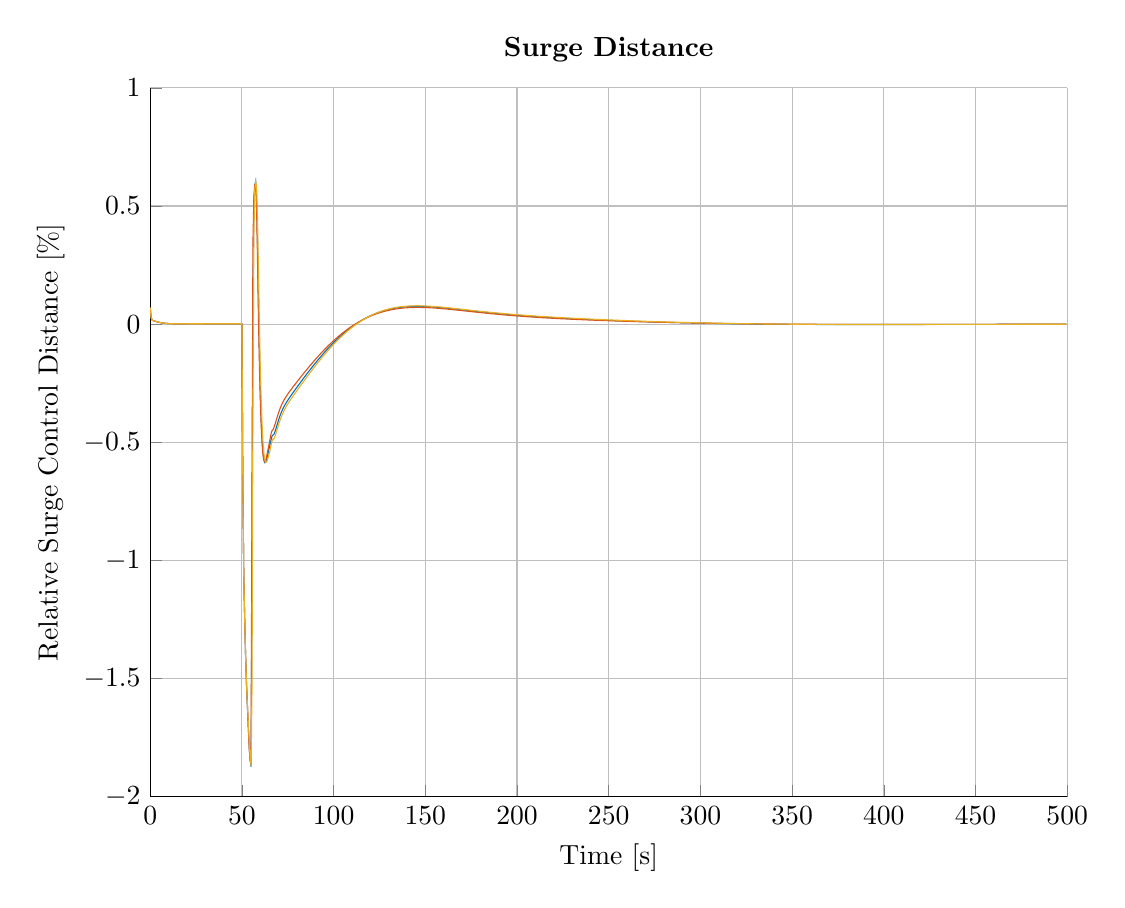
\begin{tikzpicture}

\begin{axis}[%
width=4.585in,
height=3.544in,
at={(0.769in,0.541in)},
scale only axis,
xmin=0,
xmax=500,
xlabel={Time [s]},
xmajorgrids,
ymin=-2,
ymax=1,
ylabel={Relative Surge Control Distance [\%]},
ymajorgrids,
axis background/.style={fill=white},
title style={font=\bfseries},
title={Surge Distance},
axis x line*=bottom,
axis y line*=left
]
\addplot [color=mycolor1,solid,forget plot]
  table[row sep=crcr]{%
0	0.0693700000000002\\
0.5	0.0265199999999997\\
1	0.0180300000000004\\
1.5	0.01539\\
2	0.0142600000000002\\
2.5	0.0129200000000003\\
3	0.0117099999999999\\
3.5	0.0105599999999999\\
4	0.00949000000000044\\
4.5	0.00849999999999973\\
5	0.00759000000000043\\
5.5	0.00677000000000039\\
6	0.00602999999999998\\
6.5	0.00535999999999959\\
7	0.00478000000000023\\
7.5	0.00426000000000037\\
8	0.00380999999999965\\
8.5	0.0034200000000002\\
9	0.00309000000000026\\
9.5	0.0028100000000002\\
10	0.00257000000000041\\
10.5	0.00236999999999998\\
11	0.00220999999999982\\
11.5	0.00208999999999993\\
12	0.00197999999999965\\
12.5	0.00190000000000001\\
13	0.00185000000000013\\
13.5	0.00180000000000025\\
14	0.00178000000000011\\
14.5	0.00175999999999998\\
15	0.00175000000000036\\
15.5	0.00175000000000036\\
16	0.00175999999999998\\
16.5	0.00175999999999998\\
17	0.00178000000000011\\
17.5	0.00178999999999974\\
18	0.00180000000000025\\
18.5	0.00182000000000038\\
19	0.00183\\
19.5	0.00185000000000013\\
20	0.00185999999999975\\
20.5	0.00187000000000026\\
21	0.00187999999999988\\
21.5	0.00189000000000039\\
22	0.00190000000000001\\
22.5	0.00190000000000001\\
23	0.00190999999999963\\
23.5	0.00190999999999963\\
24	0.00190999999999963\\
24.5	0.00190999999999963\\
25	0.00190999999999963\\
25.5	0.00190999999999963\\
26	0.00190999999999963\\
26.5	0.00190000000000001\\
27	0.00190000000000001\\
27.5	0.00189000000000039\\
28	0.00189000000000039\\
28.5	0.00187999999999988\\
29	0.00187000000000026\\
29.5	0.00187000000000026\\
30	0.00185999999999975\\
30.5	0.00185000000000013\\
31	0.00183999999999962\\
31.5	0.00183999999999962\\
32	0.00183\\
32.5	0.00182000000000038\\
33	0.00180999999999987\\
33.5	0.00180999999999987\\
34	0.00180000000000025\\
34.5	0.00178999999999974\\
35	0.00178999999999974\\
35.5	0.00178000000000011\\
36	0.00176999999999961\\
36.5	0.00176999999999961\\
37	0.00175999999999998\\
37.5	0.00175000000000036\\
38	0.00175000000000036\\
38.5	0.00173999999999985\\
39	0.00173999999999985\\
39.5	0.00173000000000023\\
40	0.00171999999999972\\
40.5	0.00171999999999972\\
41	0.0017100000000001\\
41.5	0.0017100000000001\\
42	0.00169999999999959\\
42.5	0.00169999999999959\\
43	0.00169999999999959\\
43.5	0.00168999999999997\\
44	0.00168999999999997\\
44.5	0.00168000000000035\\
45	0.00168000000000035\\
45.5	0.00166999999999984\\
46	0.00166999999999984\\
46.5	0.00166999999999984\\
47	0.00166000000000022\\
47.5	0.00166000000000022\\
48	0.00166000000000022\\
48.5	0.00164999999999971\\
49	0.00164999999999971\\
49.5	0.00164999999999971\\
50	0.00164000000000009\\
50.5	-0.67415\\
51	-1.0645\\
51.5	-1.24849\\
52	-1.40864\\
52.5	-1.52977\\
53	-1.62275\\
53.5	-1.70892\\
54	-1.79266\\
54.5	-1.84848\\
55	-1.87315\\
55.5	-0.9513\\
56	0.0882399999999999\\
56.5	0.50932\\
57	0.58834\\
57.5	0.60479\\
58	0.53864\\
58.5	0.34801\\
59	0.10656\\
59.5	-0.10799\\
60	-0.27716\\
60.5	-0.40193\\
61	-0.48859\\
61.5	-0.54401\\
62	-0.57478\\
62.5	-0.58661\\
63	-0.58451\\
63.5	-0.57288\\
64	-0.55556\\
64.5	-0.53597\\
65	-0.51988\\
65.5	-0.50264\\
66	-0.48649\\
66.5	-0.47203\\
67	-0.46901\\
67.5	-0.46562\\
68	-0.45617\\
68.5	-0.44403\\
69	-0.43085\\
69.5	-0.41764\\
70	-0.40499\\
70.5	-0.39325\\
71	-0.38253\\
71.5	-0.37276\\
72	-0.36386\\
72.5	-0.3557\\
73	-0.34817\\
73.5	-0.34114\\
74	-0.33453\\
74.5	-0.32823\\
75	-0.32218\\
75.5	-0.31633\\
76	-0.31062\\
76.5	-0.30502\\
77	-0.2995\\
77.5	-0.29404\\
78	-0.28862\\
78.5	-0.28324\\
79	-0.27788\\
79.5	-0.27253\\
80	-0.26721\\
80.5	-0.2619\\
81	-0.2566\\
81.5	-0.25132\\
82	-0.24606\\
82.5	-0.24081\\
83	-0.23558\\
83.5	-0.23037\\
84	-0.22518\\
84.5	-0.22001\\
85	-0.21487\\
85.5	-0.20976\\
86	-0.20467\\
86.5	-0.19962\\
87	-0.19459\\
87.5	-0.1896\\
88	-0.18465\\
88.5	-0.17972\\
89	-0.17484\\
89.5	-0.16999\\
90	-0.16518\\
90.5	-0.16041\\
91	-0.15568\\
91.5	-0.15099\\
92	-0.14634\\
92.5	-0.14173\\
93	-0.13717\\
93.5	-0.13265\\
94	-0.12817\\
94.5	-0.12374\\
95	-0.11936\\
95.5	-0.11502\\
96	-0.11073\\
96.5	-0.10648\\
97	-0.10229\\
97.5	-0.0981399999999999\\
98	-0.0940399999999997\\
98.5	-0.0899900000000002\\
99	-0.0859899999999998\\
99.5	-0.0820400000000001\\
100	-0.0781400000000003\\
100.5	-0.0742900000000004\\
101	-0.0704900000000004\\
101.5	-0.0667400000000002\\
102	-0.0630499999999996\\
102.5	-0.0594000000000001\\
103	-0.0558100000000001\\
103.5	-0.05227\\
104	-0.0487799999999998\\
104.5	-0.0453400000000004\\
105	-0.0419600000000004\\
105.5	-0.0386300000000004\\
106	-0.0353500000000002\\
106.5	-0.0321199999999999\\
107	-0.02895\\
107.5	-0.02583\\
108	-0.0227599999999999\\
108.5	-0.0197500000000002\\
109	-0.0167799999999998\\
109.5	-0.0138699999999998\\
110	-0.0110200000000003\\
110.5	-0.00821000000000005\\
111	-0.00546000000000024\\
111.5	-0.00276999999999994\\
112	-0.000119999999999898\\
112.5	0.00246999999999975\\
113	0.00502000000000002\\
113.5	0.00750999999999991\\
114	0.00994000000000028\\
114.5	0.0123300000000004\\
115	0.0146600000000001\\
115.5	0.0169499999999996\\
116	0.0191800000000004\\
116.5	0.0213599999999996\\
117	0.0234899999999998\\
117.5	0.0255700000000001\\
118	0.0275999999999996\\
118.5	0.0295800000000002\\
119	0.0315200000000004\\
119.5	0.0334000000000003\\
120	0.0352300000000003\\
120.5	0.0370200000000001\\
121	0.0387599999999999\\
121.5	0.0404499999999999\\
122	0.04209\\
122.5	0.0436899999999998\\
123	0.0452399999999997\\
123.5	0.0467399999999998\\
124	0.0481999999999996\\
124.5	0.0496100000000004\\
125	0.05098\\
125.5	0.0523100000000003\\
126	0.0535899999999998\\
126.5	0.0548299999999999\\
127	0.0560200000000002\\
127.5	0.0571799999999998\\
128	0.0582900000000004\\
128.5	0.0593599999999999\\
129	0.0603899999999999\\
129.5	0.0613799999999998\\
130	0.0623199999999997\\
130.5	0.0632400000000004\\
131	0.0641100000000003\\
131.5	0.06494\\
132	0.0657399999999999\\
132.5	0.0664999999999996\\
133	0.0672199999999998\\
133.5	0.0679100000000004\\
134	0.0685599999999997\\
134.5	0.0691800000000002\\
135	0.0697700000000001\\
135.5	0.0703199999999997\\
136	0.0708399999999996\\
136.5	0.0713200000000001\\
137	0.0717800000000004\\
137.5	0.0721999999999996\\
138	0.0725899999999999\\
138.5	0.0729600000000001\\
139	0.0732900000000001\\
139.5	0.0735999999999999\\
140	0.0738799999999999\\
140.5	0.0741300000000003\\
141	0.0743600000000004\\
141.5	0.07456\\
142	0.0747299999999997\\
142.5	0.0748800000000003\\
143	0.0750000000000002\\
143.5	0.0750999999999999\\
144	0.0751799999999996\\
144.5	0.07524\\
145	0.0752699999999997\\
145.5	0.0752899999999999\\
146	0.0752800000000002\\
146.5	0.0752499999999996\\
147	0.0752100000000002\\
147.5	0.0751400000000002\\
148	0.0750599999999997\\
148.5	0.0749599999999999\\
149	0.07484\\
149.5	0.0747\\
150	0.0745500000000003\\
150.5	0.0743900000000002\\
151	0.0742099999999999\\
151.5	0.0740100000000004\\
152	0.0738000000000003\\
152.5	0.0735799999999998\\
153	0.0733499999999996\\
153.5	0.0731000000000002\\
154	0.0728400000000002\\
154.5	0.0725699999999998\\
155	0.0722899999999997\\
155.5	0.0719900000000004\\
156	0.0716900000000003\\
156.5	0.0713800000000004\\
157	0.0710600000000001\\
157.5	0.0707300000000002\\
158	0.0704000000000002\\
158.5	0.0700500000000002\\
159	0.0697000000000001\\
159.5	0.0693400000000004\\
160	0.0689700000000002\\
160.5	0.0686\\
161	0.0682200000000002\\
161.5	0.0678400000000003\\
162	0.06745\\
162.5	0.0670599999999997\\
163	0.0666599999999997\\
163.5	0.0662599999999998\\
164	0.0658500000000002\\
164.5	0.0654500000000002\\
165	0.0650300000000001\\
165.5	0.0646199999999997\\
166	0.0641999999999996\\
166.5	0.0637800000000004\\
167	0.0633600000000003\\
167.5	0.0629299999999997\\
168	0.0625099999999996\\
168.5	0.0620799999999999\\
169	0.0616500000000002\\
169.5	0.0612199999999996\\
170	0.0607899999999999\\
170.5	0.0603600000000002\\
171	0.0599299999999996\\
171.5	0.0594999999999999\\
172	0.0590700000000002\\
172.5	0.0586399999999996\\
173	0.0582099999999999\\
173.5	0.0577800000000002\\
174	0.0573499999999996\\
174.5	0.0569199999999999\\
175	0.0564900000000002\\
175.5	0.0560700000000001\\
176	0.0556400000000004\\
176.5	0.0552200000000003\\
177	0.0547899999999997\\
177.5	0.0543699999999996\\
178	0.0539500000000004\\
178.5	0.0535300000000003\\
179	0.0531199999999998\\
179.5	0.0526999999999997\\
180	0.0522900000000002\\
180.5	0.0518799999999997\\
181	0.0514700000000001\\
181.5	0.0510700000000002\\
182	0.0506700000000002\\
182.5	0.0502599999999997\\
183	0.0498700000000003\\
183.5	0.0494700000000003\\
184	0.04908\\
184.5	0.0486800000000001\\
185	0.0482899999999997\\
185.5	0.0479099999999999\\
186	0.0475199999999996\\
186.5	0.0471399999999997\\
187	0.0467599999999999\\
187.5	0.0463899999999997\\
188	0.0460099999999999\\
188.5	0.0456399999999997\\
189	0.04528\\
189.5	0.0449099999999998\\
190	0.0445500000000001\\
190.5	0.0441900000000004\\
191	0.0438299999999998\\
191.5	0.0434799999999997\\
192	0.0431299999999997\\
192.5	0.0427799999999996\\
193	0.0424300000000004\\
193.5	0.04209\\
194	0.0417500000000004\\
194.5	0.0414099999999999\\
195	0.0410700000000004\\
195.5	0.0407400000000004\\
196	0.0404099999999996\\
196.5	0.0400799999999997\\
197	0.0397600000000002\\
197.5	0.0394300000000003\\
198	0.03911\\
198.5	0.0388000000000002\\
199	0.0384799999999998\\
199.5	0.03817\\
200	0.0378600000000002\\
200.5	0.0375500000000004\\
201	0.0372500000000002\\
201.5	0.03695\\
202	0.0366499999999998\\
202.5	0.0363499999999997\\
203	0.03606\\
203.5	0.0357599999999998\\
204	0.0354700000000001\\
204.5	0.0351900000000001\\
205	0.0349000000000004\\
205.5	0.0346200000000003\\
206	0.0343400000000003\\
206.5	0.0340600000000002\\
207	0.0337800000000001\\
207.5	0.0335099999999997\\
208	0.0332400000000002\\
208.5	0.0329699999999997\\
209	0.0327000000000002\\
209.5	0.0324299999999997\\
210	0.0321699999999998\\
210.5	0.0319099999999999\\
211	0.03165\\
211.5	0.03139\\
212	0.0311300000000001\\
212.5	0.0308799999999998\\
213	0.0306300000000004\\
213.5	0.0303800000000001\\
214	0.0301299999999998\\
214.5	0.0298800000000004\\
215	0.0296399999999997\\
215.5	0.0293900000000002\\
216	0.0291499999999996\\
216.5	0.0289099999999998\\
217	0.0286799999999996\\
217.5	0.0284399999999998\\
218	0.0282099999999996\\
218.5	0.0279699999999998\\
219	0.0277399999999997\\
219.5	0.0275100000000004\\
220	0.0272899999999998\\
220.5	0.0270599999999996\\
221	0.02684\\
221.5	0.0266099999999998\\
222	0.0263900000000001\\
222.5	0.0261699999999996\\
223	0.0259499999999999\\
223.5	0.0257399999999999\\
224	0.0255200000000002\\
224.5	0.0253100000000002\\
225	0.0250899999999996\\
225.5	0.0248799999999996\\
226	0.0246700000000004\\
226.5	0.0244600000000004\\
227	0.0242599999999999\\
227.5	0.0240499999999999\\
228	0.0238500000000004\\
228.5	0.0236400000000003\\
229	0.0234399999999999\\
229.5	0.0232400000000004\\
230	0.0230399999999999\\
230.5	0.0228400000000004\\
231	0.0226499999999996\\
231.5	0.0224500000000001\\
232	0.0222600000000002\\
232.5	0.0220599999999997\\
233	0.0218699999999998\\
233.5	0.0216799999999999\\
234	0.02149\\
234.5	0.0213000000000001\\
235	0.0211100000000002\\
235.5	0.0209299999999999\\
236	0.02074\\
236.5	0.0205599999999997\\
237	0.0203699999999998\\
237.5	0.0201900000000004\\
238	0.0200100000000001\\
238.5	0.0198299999999998\\
239	0.0196500000000004\\
239.5	0.0194700000000001\\
240	0.0193000000000003\\
240.5	0.01912\\
241	0.0189500000000002\\
241.5	0.01877\\
242	0.0186000000000002\\
242.5	0.0184300000000004\\
243	0.0182599999999997\\
243.5	0.0180899999999999\\
244	0.0179200000000002\\
244.5	0.0177500000000004\\
245	0.0175799999999997\\
245.5	0.0174200000000004\\
246	0.0172499999999998\\
246.5	0.0170899999999996\\
247	0.0169199999999998\\
247.5	0.0167599999999997\\
248	0.0166000000000004\\
248.5	0.0164400000000002\\
249	0.0162800000000001\\
249.5	0.0161199999999999\\
250	0.0159599999999998\\
};
\addplot [color=mycolor1,solid,forget plot]
  table[row sep=crcr]{%
250	0.0159599999999998\\
250.5	0.0158100000000001\\
251	0.0156499999999999\\
251.5	0.0155000000000003\\
252	0.0153400000000001\\
252.5	0.0151899999999996\\
253	0.0150300000000003\\
253.5	0.0148799999999998\\
254	0.0147300000000001\\
254.5	0.0145799999999996\\
255	0.0144299999999999\\
255.5	0.0142800000000003\\
256	0.0141400000000003\\
256.5	0.0139899999999997\\
257	0.0138400000000001\\
257.5	0.0137\\
258	0.0135500000000004\\
258.5	0.0134100000000004\\
259	0.0132700000000003\\
259.5	0.0131300000000003\\
260	0.0129900000000003\\
260.5	0.0128500000000003\\
261	0.0127100000000002\\
261.5	0.0125700000000002\\
262	0.0124300000000002\\
262.5	0.0122900000000001\\
263	0.0121599999999997\\
263.5	0.0120199999999997\\
264	0.0118900000000002\\
264.5	0.0117500000000001\\
265	0.0116199999999997\\
265.5	0.0114900000000002\\
266	0.0113599999999998\\
266.5	0.0112300000000003\\
267	0.0110999999999999\\
267.5	0.0109700000000004\\
268	0.01084\\
268.5	0.0107100000000004\\
269	0.01058\\
269.5	0.0104600000000001\\
270	0.0103299999999997\\
270.5	0.0102099999999998\\
271	0.0100800000000003\\
271.5	0.00996000000000041\\
272	0.00983999999999963\\
272.5	0.00971999999999973\\
273	0.00959999999999983\\
273.5	0.00947999999999993\\
274	0.00936000000000003\\
274.5	0.00924000000000014\\
275	0.00912000000000024\\
275.5	0.00900999999999996\\
276	0.00889000000000006\\
276.5	0.00877000000000017\\
277	0.00865999999999989\\
277.5	0.00854999999999961\\
278	0.00842999999999972\\
278.5	0.00832000000000033\\
279	0.00821000000000005\\
279.5	0.00809999999999977\\
280	0.00799000000000039\\
280.5	0.00788000000000011\\
281	0.00776999999999983\\
281.5	0.00765999999999956\\
282	0.00755000000000017\\
282.5	0.0074500000000004\\
283	0.00734000000000012\\
283.5	0.00724000000000036\\
284	0.00713000000000008\\
284.5	0.00703000000000031\\
285	0.00692999999999966\\
285.5	0.00682000000000027\\
286	0.00671999999999962\\
286.5	0.00661999999999985\\
287	0.00652000000000008\\
287.5	0.00642000000000031\\
288	0.00631999999999966\\
288.5	0.0062300000000004\\
289	0.00612999999999975\\
289.5	0.00602999999999998\\
290	0.00593999999999983\\
290.5	0.00584000000000007\\
291	0.00574999999999992\\
291.5	0.00565999999999978\\
292	0.00556000000000001\\
292.5	0.00546999999999986\\
293	0.00537999999999972\\
293.5	0.00528999999999957\\
294	0.00520000000000032\\
294.5	0.00511000000000017\\
295	0.00502000000000002\\
295.5	0.00492999999999988\\
296	0.00485000000000024\\
296.5	0.0047600000000001\\
297	0.00466999999999995\\
297.5	0.00459000000000032\\
298	0.00450999999999979\\
298.5	0.00441999999999965\\
299	0.00434000000000001\\
299.5	0.00426000000000037\\
300	0.00417000000000023\\
300.5	0.0040899999999997\\
301	0.00401000000000007\\
301.5	0.00393000000000043\\
302	0.00386000000000042\\
302.5	0.00377999999999989\\
303	0.00370000000000026\\
303.5	0.00361999999999973\\
304	0.00354999999999972\\
304.5	0.00347000000000008\\
305	0.00340000000000007\\
305.5	0.00332000000000043\\
306	0.00325000000000042\\
306.5	0.0031800000000004\\
307	0.00311000000000039\\
307.5	0.00302999999999987\\
308	0.00295999999999985\\
308.5	0.00288999999999984\\
309	0.00281999999999982\\
309.5	0.00276000000000032\\
310	0.0026900000000003\\
310.5	0.00262000000000029\\
311	0.00255000000000027\\
311.5	0.00248999999999988\\
312	0.00241999999999987\\
312.5	0.00236000000000036\\
313	0.00229000000000035\\
313.5	0.00222999999999995\\
314	0.00216999999999956\\
314.5	0.00210000000000043\\
315	0.00204000000000004\\
315.5	0.00197999999999965\\
316	0.00192000000000014\\
316.5	0.00185999999999975\\
317	0.00180000000000025\\
317.5	0.00173999999999985\\
318	0.00168999999999997\\
318.5	0.00162999999999958\\
319	0.00157000000000007\\
319.5	0.00152000000000019\\
320	0.00145999999999979\\
320.5	0.00140999999999991\\
321	0.00135000000000041\\
321.5	0.00129999999999963\\
322	0.00124999999999975\\
322.5	0.00119000000000025\\
323	0.00114000000000036\\
323.5	0.00108999999999959\\
324	0.00103999999999971\\
324.5	0.000989999999999824\\
325	0.000939999999999941\\
325.5	0.000890000000000057\\
326	0.000849999999999795\\
326.5	0.000799999999999912\\
327	0.000750000000000028\\
327.5	0.000700000000000145\\
328	0.000659999999999883\\
328.5	0.000609999999999999\\
329	0.000569999999999737\\
329.5	0.000519999999999854\\
330	0.000479999999999592\\
330.5	0.000440000000000218\\
331	0.000390000000000335\\
331.5	0.000350000000000072\\
332	0.00030999999999981\\
332.5	0.000270000000000437\\
333	0.000230000000000175\\
333.5	0.000189999999999912\\
334	0.00014999999999965\\
334.5	0.000110000000000277\\
335	7.00000000000145e-05\\
335.5	4.0000000000262e-05\\
336	0\\
336.5	-4.0000000000262e-05\\
337	-7.00000000000145e-05\\
337.5	-0.000110000000000277\\
338	-0.000140000000000029\\
338.5	-0.000180000000000291\\
339	-0.000210000000000043\\
339.5	-0.000250000000000306\\
340	-0.000280000000000058\\
340.5	-0.00030999999999981\\
341	-0.000339999999999563\\
341.5	-0.000379999999999825\\
342	-0.000409999999999577\\
342.5	-0.000440000000000218\\
343	-0.00046999999999997\\
343.5	-0.000499999999999723\\
344	-0.000530000000000364\\
344.5	-0.000549999999999606\\
345	-0.000580000000000247\\
345.5	-0.000609999999999999\\
346	-0.000639999999999752\\
346.5	-0.000659999999999883\\
347	-0.000689999999999635\\
347.5	-0.000720000000000276\\
348	-0.000740000000000407\\
348.5	-0.000770000000000159\\
349	-0.00079000000000029\\
349.5	-0.000820000000000043\\
350	-0.000840000000000174\\
350.5	-0.000860000000000305\\
351	-0.000890000000000057\\
351.5	-0.000910000000000188\\
352	-0.000930000000000319\\
352.5	-0.000949999999999562\\
353	-0.000969999999999693\\
353.5	-0.000989999999999824\\
354	-0.00100999999999996\\
354.5	-0.00103000000000009\\
355	-0.00105000000000022\\
355.5	-0.00107000000000035\\
356	-0.00108999999999959\\
356.5	-0.00110999999999972\\
357	-0.00112999999999985\\
357.5	-0.00114999999999998\\
358	-0.00115999999999961\\
358.5	-0.00117999999999974\\
359	-0.00119999999999987\\
359.5	-0.00121000000000038\\
360	-0.00122999999999962\\
360.5	-0.00124000000000013\\
361	-0.00126000000000026\\
361.5	-0.00126999999999988\\
362	-0.00129000000000001\\
362.5	-0.00129999999999963\\
363	-0.00131000000000014\\
363.5	-0.00133000000000028\\
364	-0.0013399999999999\\
364.5	-0.00135000000000041\\
365	-0.00136999999999965\\
365.5	-0.00138000000000016\\
366	-0.00138999999999978\\
366.5	-0.00140000000000029\\
367	-0.00140999999999991\\
367.5	-0.00142000000000042\\
368	-0.00143000000000004\\
368.5	-0.00143999999999966\\
369	-0.00145000000000017\\
369.5	-0.00145999999999979\\
370	-0.0014700000000003\\
370.5	-0.00147999999999993\\
371	-0.00149000000000044\\
371.5	-0.00150000000000006\\
372	-0.00150000000000006\\
372.5	-0.00150999999999968\\
373	-0.00152000000000019\\
373.5	-0.00152000000000019\\
374	-0.00152999999999981\\
374.5	-0.00154000000000032\\
375	-0.00154000000000032\\
375.5	-0.00154999999999994\\
376	-0.00155999999999956\\
376.5	-0.00155999999999956\\
377	-0.00157000000000007\\
377.5	-0.00157000000000007\\
378	-0.00157999999999969\\
378.5	-0.00157999999999969\\
379	-0.00157999999999969\\
379.5	-0.0015900000000002\\
380	-0.0015900000000002\\
380.5	-0.00159999999999982\\
381	-0.00159999999999982\\
381.5	-0.00159999999999982\\
382	-0.00159999999999982\\
382.5	-0.00161000000000033\\
383	-0.00161000000000033\\
383.5	-0.00161000000000033\\
384	-0.00161000000000033\\
384.5	-0.00161000000000033\\
385	-0.00161999999999995\\
385.5	-0.00161999999999995\\
386	-0.00161999999999995\\
386.5	-0.00161999999999995\\
387	-0.00161999999999995\\
387.5	-0.00161999999999995\\
388	-0.00161999999999995\\
388.5	-0.00161999999999995\\
389	-0.00161999999999995\\
389.5	-0.00161999999999995\\
390	-0.00161999999999995\\
390.5	-0.00161999999999995\\
391	-0.00161999999999995\\
391.5	-0.00161999999999995\\
392	-0.00161000000000033\\
392.5	-0.00161000000000033\\
393	-0.00161000000000033\\
393.5	-0.00161000000000033\\
394	-0.00161000000000033\\
394.5	-0.00161000000000033\\
395	-0.00159999999999982\\
395.5	-0.00159999999999982\\
396	-0.00159999999999982\\
396.5	-0.00159999999999982\\
397	-0.0015900000000002\\
397.5	-0.0015900000000002\\
398	-0.0015900000000002\\
398.5	-0.00157999999999969\\
399	-0.00157999999999969\\
399.5	-0.00157999999999969\\
400	-0.00157000000000007\\
400.5	-0.00157000000000007\\
401	-0.00155999999999956\\
401.5	-0.00155999999999956\\
402	-0.00155999999999956\\
402.5	-0.00154999999999994\\
403	-0.00154999999999994\\
403.5	-0.00154000000000032\\
404	-0.00154000000000032\\
404.5	-0.00152999999999981\\
405	-0.00152999999999981\\
405.5	-0.00152000000000019\\
406	-0.00152000000000019\\
406.5	-0.00150999999999968\\
407	-0.00150999999999968\\
407.5	-0.00150000000000006\\
408	-0.00150000000000006\\
408.5	-0.00149000000000044\\
409	-0.00149000000000044\\
409.5	-0.00147999999999993\\
410	-0.0014700000000003\\
410.5	-0.0014700000000003\\
411	-0.00145999999999979\\
411.5	-0.00145999999999979\\
412	-0.00145000000000017\\
412.5	-0.00143999999999966\\
413	-0.00143999999999966\\
413.5	-0.00143000000000004\\
414	-0.00142000000000042\\
414.5	-0.00142000000000042\\
415	-0.00140999999999991\\
415.5	-0.00140000000000029\\
416	-0.00140000000000029\\
416.5	-0.00138999999999978\\
417	-0.00138000000000016\\
417.5	-0.00138000000000016\\
418	-0.00136999999999965\\
418.5	-0.00136000000000003\\
419	-0.00136000000000003\\
419.5	-0.00135000000000041\\
420	-0.0013399999999999\\
420.5	-0.00133000000000028\\
421	-0.00133000000000028\\
421.5	-0.00131999999999977\\
422	-0.00131000000000014\\
422.5	-0.00129999999999963\\
423	-0.00129999999999963\\
423.5	-0.00129000000000001\\
424	-0.00128000000000039\\
424.5	-0.00126999999999988\\
425	-0.00126999999999988\\
425.5	-0.00126000000000026\\
426	-0.00124999999999975\\
426.5	-0.00124000000000013\\
427	-0.00124000000000013\\
427.5	-0.00122999999999962\\
428	-0.00122\\
428.5	-0.00121000000000038\\
429	-0.00119999999999987\\
429.5	-0.00119999999999987\\
430	-0.00119000000000025\\
430.5	-0.00117999999999974\\
431	-0.00117000000000012\\
431.5	-0.00115999999999961\\
432	-0.00115999999999961\\
432.5	-0.00114999999999998\\
433	-0.00114000000000036\\
433.5	-0.00112999999999985\\
434	-0.00112000000000023\\
434.5	-0.00112000000000023\\
435	-0.00110999999999972\\
435.5	-0.0011000000000001\\
436	-0.00108999999999959\\
436.5	-0.00107999999999997\\
437	-0.00107999999999997\\
437.5	-0.00107000000000035\\
438	-0.00105999999999984\\
438.5	-0.00105000000000022\\
439	-0.00103999999999971\\
439.5	-0.00103000000000009\\
440	-0.00103000000000009\\
440.5	-0.00101999999999958\\
441	-0.00100999999999996\\
441.5	-0.00100000000000033\\
442	-0.000989999999999824\\
442.5	-0.000989999999999824\\
443	-0.000980000000000203\\
443.5	-0.000969999999999693\\
444	-0.000960000000000072\\
444.5	-0.000949999999999562\\
445	-0.000949999999999562\\
445.5	-0.000939999999999941\\
446	-0.000930000000000319\\
446.5	-0.00091999999999981\\
447	-0.000910000000000188\\
447.5	-0.000910000000000188\\
448	-0.000899999999999679\\
448.5	-0.000890000000000057\\
449	-0.000880000000000436\\
449.5	-0.000869999999999926\\
450	-0.000869999999999926\\
450.5	-0.000860000000000305\\
451	-0.000849999999999795\\
451.5	-0.000840000000000174\\
452	-0.000829999999999664\\
452.5	-0.000829999999999664\\
453	-0.000820000000000043\\
453.5	-0.000810000000000421\\
454	-0.000799999999999912\\
454.5	-0.000799999999999912\\
455	-0.00079000000000029\\
455.5	-0.000779999999999781\\
456	-0.000770000000000159\\
456.5	-0.00075999999999965\\
457	-0.00075999999999965\\
457.5	-0.000750000000000028\\
458	-0.000740000000000407\\
458.5	-0.000729999999999897\\
459	-0.000729999999999897\\
459.5	-0.000720000000000276\\
460	-0.000709999999999766\\
460.5	-0.000700000000000145\\
461	-0.000700000000000145\\
461.5	-0.000689999999999635\\
462	-0.000680000000000014\\
462.5	-0.000680000000000014\\
463	-0.000670000000000393\\
463.5	-0.000659999999999883\\
464	-0.000650000000000261\\
464.5	-0.000650000000000261\\
465	-0.000639999999999752\\
465.5	-0.00063000000000013\\
466	-0.00063000000000013\\
466.5	-0.000619999999999621\\
467	-0.000609999999999999\\
467.5	-0.000600000000000378\\
468	-0.000600000000000378\\
468.5	-0.000589999999999868\\
469	-0.000580000000000247\\
469.5	-0.000580000000000247\\
470	-0.000569999999999737\\
470.5	-0.000560000000000116\\
471	-0.000560000000000116\\
471.5	-0.000549999999999606\\
472	-0.000539999999999985\\
472.5	-0.000539999999999985\\
473	-0.000530000000000364\\
473.5	-0.000519999999999854\\
474	-0.000519999999999854\\
474.5	-0.000510000000000232\\
475	-0.000499999999999723\\
475.5	-0.000499999999999723\\
476	-0.000490000000000101\\
476.5	-0.000490000000000101\\
477	-0.000479999999999592\\
477.5	-0.00046999999999997\\
478	-0.00046999999999997\\
478.5	-0.000460000000000349\\
479	-0.000449999999999839\\
479.5	-0.000449999999999839\\
480	-0.000440000000000218\\
480.5	-0.000440000000000218\\
481	-0.000429999999999708\\
481.5	-0.000420000000000087\\
482	-0.000420000000000087\\
482.5	-0.000409999999999577\\
483	-0.000409999999999577\\
483.5	-0.000399999999999956\\
484	-0.000399999999999956\\
484.5	-0.000390000000000335\\
485	-0.000379999999999825\\
485.5	-0.000379999999999825\\
486	-0.000370000000000203\\
486.5	-0.000370000000000203\\
487	-0.000359999999999694\\
487.5	-0.000359999999999694\\
488	-0.000350000000000072\\
488.5	-0.000350000000000072\\
489	-0.000339999999999563\\
489.5	-0.000339999999999563\\
490	-0.000329999999999941\\
490.5	-0.000329999999999941\\
491	-0.00032000000000032\\
491.5	-0.00032000000000032\\
492	-0.00030999999999981\\
492.5	-0.00030999999999981\\
493	-0.000300000000000189\\
493.5	-0.000300000000000189\\
494	-0.000289999999999679\\
494.5	-0.000289999999999679\\
495	-0.000280000000000058\\
495.5	-0.000280000000000058\\
496	-0.000270000000000437\\
496.5	-0.000270000000000437\\
497	-0.000259999999999927\\
497.5	-0.000259999999999927\\
498	-0.000250000000000306\\
498.5	-0.000250000000000306\\
499	-0.000250000000000306\\
499.5	-0.000239999999999796\\
};
\addplot [color=mycolor2,solid,forget plot]
  table[row sep=crcr]{%
0	0.0693700000000002\\
0.5	0.02644\\
1	0.0179099999999996\\
1.5	0.0152299999999999\\
2	0.0140599999999997\\
2.5	0.0126799999999996\\
3	0.0114400000000003\\
3.5	0.0102599999999997\\
4	0.00917000000000012\\
4.5	0.00816999999999979\\
5	0.00724999999999998\\
5.5	0.00642000000000031\\
6	0.00567999999999991\\
6.5	0.00502000000000002\\
7	0.00443000000000016\\
7.5	0.00393000000000043\\
8	0.00349000000000022\\
8.5	0.00311000000000039\\
9	0.00279000000000007\\
9.5	0.00251999999999963\\
10	0.00229999999999997\\
10.5	0.00211999999999968\\
11	0.00197000000000003\\
11.5	0.00185000000000013\\
12	0.00175999999999998\\
12.5	0.00169999999999959\\
13	0.00164999999999971\\
13.5	0.00161999999999995\\
14	0.00159999999999982\\
14.5	0.0015900000000002\\
15	0.0015900000000002\\
15.5	0.00159999999999982\\
16	0.00161000000000033\\
16.5	0.00161999999999995\\
17	0.00164000000000009\\
17.5	0.00164999999999971\\
18	0.00166999999999984\\
18.5	0.00168999999999997\\
19	0.00169999999999959\\
19.5	0.00171999999999972\\
20	0.00173000000000023\\
20.5	0.00173999999999985\\
21	0.00175000000000036\\
21.5	0.00175999999999998\\
22	0.00175999999999998\\
22.5	0.00176999999999961\\
23	0.00176999999999961\\
23.5	0.00176999999999961\\
24	0.00176999999999961\\
24.5	0.00176999999999961\\
25	0.00175999999999998\\
25.5	0.00175999999999998\\
26	0.00175000000000036\\
26.5	0.00175000000000036\\
27	0.00173999999999985\\
27.5	0.00173000000000023\\
28	0.00173000000000023\\
28.5	0.00171999999999972\\
29	0.0017100000000001\\
29.5	0.00169999999999959\\
30	0.00168999999999997\\
30.5	0.00168000000000035\\
31	0.00166999999999984\\
31.5	0.00166000000000022\\
32	0.00166000000000022\\
32.5	0.00164999999999971\\
33	0.00164000000000009\\
33.5	0.00162999999999958\\
34	0.00161999999999995\\
34.5	0.00161000000000033\\
35	0.00161000000000033\\
35.5	0.00159999999999982\\
36	0.0015900000000002\\
36.5	0.00157999999999969\\
37	0.00157999999999969\\
37.5	0.00157000000000007\\
38	0.00155999999999956\\
38.5	0.00155999999999956\\
39	0.00154999999999994\\
39.5	0.00154000000000032\\
40	0.00154000000000032\\
40.5	0.00152999999999981\\
41	0.00152999999999981\\
41.5	0.00152000000000019\\
42	0.00152000000000019\\
42.5	0.00150999999999968\\
43	0.00150999999999968\\
43.5	0.00150000000000006\\
44	0.00150000000000006\\
44.5	0.00149000000000044\\
45	0.00149000000000044\\
45.5	0.00147999999999993\\
46	0.00147999999999993\\
46.5	0.0014700000000003\\
47	0.0014700000000003\\
47.5	0.0014700000000003\\
48	0.00145999999999979\\
48.5	0.00145999999999979\\
49	0.00145000000000017\\
49.5	0.00145000000000017\\
50	0.00145000000000017\\
50.5	-0.67415\\
51	-1.06237\\
51.5	-1.24303\\
52	-1.39993\\
52.5	-1.51888\\
53	-1.61259\\
53.5	-1.71069\\
54	-1.80102\\
54.5	-1.84956\\
55	-1.76165\\
55.5	-0.65872\\
56	0.34617\\
56.5	0.53654\\
57	0.58873\\
57.5	0.58604\\
58	0.48594\\
58.5	0.26632\\
59	0.03111\\
59.5	-0.16736\\
60	-0.32076\\
60.5	-0.43275\\
61	-0.50874\\
61.5	-0.55495\\
62	-0.57769\\
62.5	-0.58265\\
63	-0.57491\\
63.5	-0.55894\\
64	-0.53859\\
64.5	-0.52076\\
65	-0.50044\\
65.5	-0.47929\\
66	-0.45965\\
66.5	-0.45001\\
67	-0.44632\\
67.5	-0.43688\\
68	-0.42506\\
68.5	-0.41216\\
69	-0.39917\\
69.5	-0.38646\\
70	-0.37448\\
70.5	-0.3634\\
71	-0.35325\\
71.5	-0.34399\\
72	-0.33554\\
72.5	-0.32778\\
73	-0.32061\\
73.5	-0.31393\\
74	-0.30765\\
74.5	-0.30168\\
75	-0.29595\\
75.5	-0.29042\\
76	-0.28503\\
76.5	-0.27975\\
77	-0.27456\\
77.5	-0.26943\\
78	-0.26435\\
78.5	-0.2593\\
79	-0.25428\\
79.5	-0.24929\\
80	-0.24432\\
80.5	-0.23936\\
81	-0.23442\\
81.5	-0.2295\\
82	-0.2246\\
82.5	-0.21972\\
83	-0.21486\\
83.5	-0.21002\\
84	-0.2052\\
84.5	-0.20041\\
85	-0.19565\\
85.5	-0.19091\\
86	-0.1862\\
86.5	-0.18153\\
87	-0.17688\\
87.5	-0.17226\\
88	-0.16768\\
88.5	-0.16314\\
89	-0.15863\\
89.5	-0.15415\\
90	-0.14972\\
90.5	-0.14532\\
91	-0.14096\\
91.5	-0.13664\\
92	-0.13236\\
92.5	-0.12812\\
93	-0.12392\\
93.5	-0.11977\\
94	-0.11566\\
94.5	-0.11159\\
95	-0.10756\\
95.5	-0.10358\\
96	-0.0996499999999996\\
96.5	-0.0957600000000003\\
97	-0.0919100000000004\\
97.5	-0.0881100000000004\\
98	-0.0843600000000002\\
98.5	-0.08066\\
99	-0.077\\
99.5	-0.0733800000000002\\
100	-0.06982\\
100.5	-0.0663\\
101	-0.0628299999999999\\
101.5	-0.0594099999999997\\
102	-0.0560299999999998\\
102.5	-0.0527100000000003\\
103	-0.0494300000000001\\
103.5	-0.0461999999999998\\
104	-0.0430200000000003\\
104.5	-0.0398800000000001\\
105	-0.0368000000000004\\
105.5	-0.03376\\
106	-0.03078\\
106.5	-0.0278400000000003\\
107	-0.0249499999999996\\
107.5	-0.0221099999999996\\
108	-0.0193199999999996\\
108.5	-0.0165699999999998\\
109	-0.0138800000000003\\
109.5	-0.0112300000000003\\
110	-0.00863000000000014\\
110.5	-0.00607999999999986\\
111	-0.00356999999999985\\
111.5	-0.00112000000000023\\
112	0.00129000000000001\\
112.5	0.00365000000000038\\
113	0.00595999999999997\\
113.5	0.00823000000000018\\
114	0.0104499999999996\\
114.5	0.0126200000000001\\
115	0.0147500000000003\\
115.5	0.0168299999999997\\
116	0.0188600000000001\\
116.5	0.0208500000000003\\
117	0.0227899999999996\\
117.5	0.0246899999999997\\
118	0.0265399999999998\\
118.5	0.02834\\
119	0.0301099999999996\\
119.5	0.0318300000000002\\
120	0.0335000000000001\\
120.5	0.0351299999999997\\
121	0.0367199999999999\\
121.5	0.0382699999999998\\
122	0.0397699999999999\\
122.5	0.0412299999999997\\
123	0.0426500000000001\\
123.5	0.0440300000000002\\
124	0.0453700000000001\\
124.5	0.0466699999999998\\
125	0.04793\\
125.5	0.0491400000000004\\
126	0.0503200000000001\\
126.5	0.0514599999999996\\
127	0.0525599999999997\\
127.5	0.0536300000000001\\
128	0.0546499999999996\\
128.5	0.0556400000000004\\
129	0.0566000000000004\\
129.5	0.0575099999999997\\
130	0.0583900000000002\\
130.5	0.05924\\
131	0.0600500000000004\\
131.5	0.0608300000000002\\
132	0.0615699999999997\\
132.5	0.0622800000000003\\
133	0.0629600000000003\\
133.5	0.0636000000000001\\
134	0.0642199999999997\\
134.5	0.0648\\
135	0.0653499999999996\\
135.5	0.0658700000000003\\
136	0.0663600000000004\\
136.5	0.0668199999999999\\
137	0.0672600000000001\\
137.5	0.0676600000000001\\
138	0.0680399999999999\\
138.5	0.06839\\
139	0.0687100000000003\\
139.5	0.0690099999999996\\
140	0.06928\\
140.5	0.0695300000000003\\
141	0.06975\\
141.5	0.0699500000000004\\
142	0.0701200000000002\\
142.5	0.0702800000000003\\
143	0.0704099999999999\\
143.5	0.0705099999999996\\
144	0.0705999999999998\\
144.5	0.0706699999999998\\
145	0.0707100000000001\\
145.5	0.0707399999999998\\
146	0.0707399999999998\\
146.5	0.0707300000000002\\
147	0.0707000000000004\\
147.5	0.0706499999999997\\
148	0.0705799999999996\\
148.5	0.0705\\
149	0.0704000000000002\\
149.5	0.07029\\
150	0.0701599999999996\\
150.5	0.0700099999999999\\
151	0.0698499999999997\\
151.5	0.06968\\
152	0.0694900000000001\\
152.5	0.0692899999999996\\
153	0.0690799999999996\\
153.5	0.0688500000000003\\
154	0.0686200000000001\\
154.5	0.0683699999999998\\
155	0.0681099999999999\\
155.5	0.0678400000000003\\
156	0.0675600000000003\\
156.5	0.0672699999999997\\
157	0.06698\\
157.5	0.0666700000000002\\
158	0.0663600000000004\\
158.5	0.0660299999999996\\
159	0.0656999999999996\\
159.5	0.0653699999999997\\
160	0.0650199999999996\\
160.5	0.0646699999999996\\
161	0.0643099999999999\\
161.5	0.0639500000000002\\
162	0.06358\\
162.5	0.0632099999999998\\
163	0.0628299999999999\\
163.5	0.0624500000000001\\
164	0.0620599999999998\\
164.5	0.0616700000000003\\
165	0.06128\\
165.5	0.06088\\
166	0.0604800000000001\\
166.5	0.0600800000000001\\
167	0.0596699999999997\\
167.5	0.0592600000000001\\
168	0.0588499999999996\\
168.5	0.05844\\
169	0.05802\\
169.5	0.0576100000000004\\
170	0.0571900000000003\\
170.5	0.0567700000000002\\
171	0.0563500000000001\\
171.5	0.05593\\
172	0.0555199999999996\\
172.5	0.0551000000000004\\
173	0.0546800000000003\\
173.5	0.0542600000000002\\
174	0.0538400000000001\\
174.5	0.05342\\
175	0.0529999999999999\\
175.5	0.0525799999999998\\
176	0.0521599999999998\\
176.5	0.0517500000000002\\
177	0.0513300000000001\\
177.5	0.0509199999999996\\
178	0.0505100000000001\\
178.5	0.0500999999999996\\
179	0.04969\\
179.5	0.0492800000000004\\
180	0.04887\\
180.5	0.04847\\
181	0.0480700000000001\\
181.5	0.0476700000000001\\
182	0.0472700000000001\\
182.5	0.0468799999999998\\
183	0.0464799999999999\\
183.5	0.0460900000000004\\
184	0.0457000000000001\\
184.5	0.0453099999999997\\
185	0.0449299999999999\\
185.5	0.0445500000000001\\
186	0.0441700000000003\\
186.5	0.0437900000000004\\
187	0.0434200000000002\\
187.5	0.04305\\
188	0.0426799999999998\\
188.5	0.0423099999999996\\
189	0.0419499999999999\\
189.5	0.0415900000000002\\
190	0.0412299999999997\\
190.5	0.0408799999999996\\
191	0.0405199999999999\\
191.5	0.0401699999999998\\
192	0.0398300000000003\\
192.5	0.0394800000000002\\
193	0.0391399999999997\\
193.5	0.0388000000000002\\
194	0.0384700000000002\\
194.5	0.0381299999999998\\
195	0.0377999999999998\\
195.5	0.0374800000000004\\
196	0.0371499999999996\\
196.5	0.0368300000000001\\
197	0.0365099999999998\\
197.5	0.0362\\
198	0.0358799999999997\\
198.5	0.0355699999999999\\
199	0.0352699999999997\\
199.5	0.0349599999999999\\
200	0.0346599999999997\\
200.5	0.0343600000000004\\
201	0.0340600000000002\\
201.5	0.0337699999999996\\
202	0.03348\\
202.5	0.0331900000000003\\
203	0.0328999999999997\\
203.5	0.0326199999999996\\
204	0.03233\\
204.5	0.0320600000000004\\
205	0.0317800000000004\\
205.5	0.0315099999999999\\
206	0.0312299999999999\\
206.5	0.0309699999999999\\
207	0.0307000000000004\\
207.5	0.0304399999999996\\
208	0.03017\\
208.5	0.0299199999999997\\
209	0.0296599999999998\\
209.5	0.0293999999999999\\
210	0.0291499999999996\\
210.5	0.0289000000000001\\
211	0.0286499999999998\\
211.5	0.02841\\
212	0.0281599999999997\\
212.5	0.0279199999999999\\
213	0.0276800000000001\\
213.5	0.02745\\
214	0.0272100000000002\\
214.5	0.02698\\
215	0.0267499999999998\\
215.5	0.0265199999999997\\
216	0.0262900000000004\\
216.5	0.0260699999999998\\
217	0.0258399999999996\\
217.5	0.02562\\
218	0.0254000000000003\\
218.5	0.0251900000000003\\
219	0.0249699999999997\\
219.5	0.0247599999999997\\
220	0.0245499999999996\\
220.5	0.0243399999999996\\
221	0.0241300000000004\\
221.5	0.0239200000000004\\
222	0.02372\\
222.5	0.0235099999999999\\
223	0.0233100000000004\\
223.5	0.02311\\
224	0.0229100000000004\\
224.5	0.0227199999999996\\
225	0.0225200000000001\\
225.5	0.0223300000000002\\
226	0.0221400000000003\\
226.5	0.0219500000000004\\
227	0.0217599999999996\\
227.5	0.0215699999999996\\
228	0.0213799999999997\\
228.5	0.0212000000000003\\
229	0.02102\\
229.5	0.0208300000000001\\
230	0.0206499999999998\\
230.5	0.0204700000000004\\
231	0.0202999999999998\\
231.5	0.0201200000000004\\
232	0.0199499999999997\\
232.5	0.0197700000000003\\
233	0.0195999999999996\\
233.5	0.0194299999999998\\
234	0.0192600000000001\\
234.5	0.0190900000000003\\
235	0.0189199999999996\\
235.5	0.0187600000000003\\
236	0.0185899999999997\\
236.5	0.0184300000000004\\
237	0.0182599999999997\\
237.5	0.0180999999999996\\
238	0.0179400000000003\\
238.5	0.0177800000000001\\
239	0.01762\\
239.5	0.0174700000000003\\
240	0.0173100000000002\\
240.5	0.0171599999999996\\
241	0.0170000000000003\\
241.5	0.0168499999999998\\
242	0.0167000000000002\\
242.5	0.0165499999999996\\
243	0.0164\\
243.5	0.0162500000000003\\
244	0.0160999999999998\\
244.5	0.0159500000000001\\
245	0.0158100000000001\\
245.5	0.0156599999999996\\
246	0.0155200000000004\\
246.5	0.0153800000000004\\
247	0.0152400000000004\\
247.5	0.0151000000000003\\
248	0.0149600000000003\\
248.5	0.0148200000000003\\
249	0.0146800000000002\\
249.5	0.0145400000000002\\
250	0.0144000000000002\\
};
\addplot [color=mycolor2,solid,forget plot]
  table[row sep=crcr]{%
250	0.0144000000000002\\
250.5	0.0142699999999998\\
251	0.0141299999999998\\
251.5	0.0140000000000002\\
252	0.0138699999999998\\
252.5	0.0137299999999998\\
253	0.0136000000000003\\
253.5	0.0134699999999999\\
254	0.0133400000000004\\
254.5	0.0132099999999999\\
255	0.01309\\
255.5	0.0129599999999996\\
256	0.0128300000000001\\
256.5	0.0127100000000002\\
257	0.0125799999999998\\
257.5	0.0124599999999999\\
258	0.01234\\
258.5	0.0122099999999996\\
259	0.0120899999999997\\
259.5	0.0119699999999998\\
260	0.0118499999999999\\
260.5	0.01173\\
261	0.0116100000000001\\
261.5	0.0114900000000002\\
262	0.0113799999999999\\
262.5	0.01126\\
263	0.0111400000000001\\
263.5	0.0110299999999999\\
264	0.0109199999999996\\
264.5	0.0107999999999997\\
265	0.0106900000000003\\
265.5	0.01058\\
266	0.0104699999999998\\
266.5	0.0103499999999999\\
267	0.0102399999999996\\
267.5	0.0101300000000002\\
268	0.0100300000000004\\
268.5	0.00992000000000015\\
269	0.00980999999999987\\
269.5	0.0096999999999996\\
270	0.00959999999999983\\
270.5	0.00949000000000044\\
271	0.00938999999999979\\
271.5	0.0092800000000004\\
272	0.00917999999999974\\
272.5	0.00907999999999998\\
273	0.00898000000000021\\
273.5	0.00886999999999993\\
274	0.00877000000000017\\
274.5	0.0086700000000004\\
275	0.00856999999999974\\
275.5	0.0084799999999996\\
276	0.00837999999999983\\
276.5	0.00828000000000007\\
277	0.0081800000000003\\
277.5	0.00809000000000015\\
278	0.00799000000000039\\
278.5	0.00790000000000024\\
279	0.00779999999999959\\
279.5	0.00771000000000033\\
280	0.00760999999999967\\
280.5	0.00752000000000042\\
281	0.00743000000000027\\
281.5	0.00734000000000012\\
282	0.00724999999999998\\
282.5	0.00715999999999983\\
283	0.00706999999999969\\
283.5	0.00698000000000043\\
284	0.00689000000000028\\
284.5	0.00680000000000014\\
285	0.00671999999999962\\
285.5	0.00663000000000036\\
286	0.00654000000000021\\
286.5	0.00645999999999969\\
287	0.00637000000000043\\
287.5	0.00628999999999991\\
288	0.00621000000000027\\
288.5	0.00612000000000013\\
289	0.0060399999999996\\
289.5	0.00595999999999997\\
290	0.00588000000000033\\
290.5	0.00579999999999981\\
291	0.00572000000000017\\
291.5	0.00563999999999965\\
292	0.00556000000000001\\
292.5	0.00548000000000037\\
293	0.00539999999999985\\
293.5	0.00532999999999983\\
294	0.0052500000000002\\
294.5	0.00516999999999967\\
295	0.00509999999999966\\
295.5	0.00502000000000002\\
296	0.00495000000000001\\
296.5	0.00487000000000037\\
297	0.00480000000000036\\
297.5	0.00473000000000035\\
298	0.00466000000000033\\
298.5	0.00457999999999981\\
299	0.00450999999999979\\
299.5	0.00443999999999978\\
300	0.00436999999999976\\
300.5	0.00429999999999975\\
301	0.00422999999999973\\
301.5	0.00417000000000023\\
302	0.00410000000000021\\
302.5	0.0040300000000002\\
303	0.00396000000000019\\
303.5	0.00389999999999979\\
304	0.00382999999999978\\
304.5	0.00377000000000027\\
305	0.00370000000000026\\
305.5	0.00363999999999987\\
306	0.00358000000000036\\
306.5	0.00351000000000035\\
307	0.00344999999999995\\
307.5	0.00338999999999956\\
308	0.00333000000000006\\
308.5	0.00326999999999966\\
309	0.00319999999999965\\
309.5	0.00314000000000014\\
310	0.00309000000000026\\
310.5	0.00302999999999987\\
311	0.00297000000000036\\
311.5	0.00290999999999997\\
312	0.00284999999999958\\
312.5	0.00279999999999969\\
313	0.00274000000000019\\
313.5	0.00267999999999979\\
314	0.00262999999999991\\
314.5	0.00257000000000041\\
315	0.00251999999999963\\
315.5	0.00246999999999975\\
316	0.00241000000000025\\
316.5	0.00236000000000036\\
317	0.00230999999999959\\
317.5	0.00225000000000009\\
318	0.0022000000000002\\
318.5	0.00215000000000032\\
319	0.00210000000000043\\
319.5	0.00204999999999966\\
320	0.00199999999999978\\
320.5	0.0019499999999999\\
321	0.00190999999999963\\
321.5	0.00185999999999975\\
322	0.00180999999999987\\
322.5	0.00175999999999998\\
323	0.00171999999999972\\
323.5	0.00166999999999984\\
324	0.00161999999999995\\
324.5	0.00157999999999969\\
325	0.00152999999999981\\
325.5	0.00149000000000044\\
326	0.00145000000000017\\
326.5	0.00140000000000029\\
327	0.00136000000000003\\
327.5	0.00131999999999977\\
328	0.00126999999999988\\
328.5	0.00122999999999962\\
329	0.00119000000000025\\
329.5	0.00114999999999998\\
330	0.00110999999999972\\
330.5	0.00107000000000035\\
331	0.00103000000000009\\
331.5	0.000989999999999824\\
332	0.000949999999999562\\
332.5	0.00091999999999981\\
333	0.000880000000000436\\
333.5	0.000840000000000174\\
334	0.000799999999999912\\
334.5	0.000770000000000159\\
335	0.000729999999999897\\
335.5	0.000700000000000145\\
336	0.000659999999999883\\
336.5	0.00063000000000013\\
337	0.000589999999999868\\
337.5	0.000560000000000116\\
338	0.000519999999999854\\
338.5	0.000490000000000101\\
339	0.000460000000000349\\
339.5	0.000429999999999708\\
340	0.000390000000000335\\
340.5	0.000359999999999694\\
341	0.000329999999999941\\
341.5	0.000300000000000189\\
342	0.000270000000000437\\
342.5	0.000239999999999796\\
343	0.000210000000000043\\
343.5	0.000180000000000291\\
344	0.00014999999999965\\
344.5	0.000119999999999898\\
345	9.99999999997669e-05\\
345.5	7.00000000000145e-05\\
346	4.0000000000262e-05\\
346.5	2.0000000000131e-05\\
347	-9.99999999962142e-06\\
347.5	-4.0000000000262e-05\\
348	-6.00000000003931e-05\\
348.5	-9.00000000001455e-05\\
349	-0.000110000000000277\\
349.5	-0.000140000000000029\\
350	-0.00016000000000016\\
350.5	-0.000189999999999912\\
351	-0.000210000000000043\\
351.5	-0.000230000000000175\\
352	-0.000259999999999927\\
352.5	-0.000280000000000058\\
353	-0.000300000000000189\\
353.5	-0.00032000000000032\\
354	-0.000350000000000072\\
354.5	-0.000370000000000203\\
355	-0.000390000000000335\\
355.5	-0.000409999999999577\\
356	-0.000429999999999708\\
356.5	-0.000449999999999839\\
357	-0.00046999999999997\\
357.5	-0.000490000000000101\\
358	-0.000510000000000232\\
358.5	-0.000530000000000364\\
359	-0.000539999999999985\\
359.5	-0.000560000000000116\\
360	-0.000580000000000247\\
360.5	-0.000600000000000378\\
361	-0.000609999999999999\\
361.5	-0.00063000000000013\\
362	-0.000650000000000261\\
362.5	-0.000659999999999883\\
363	-0.000680000000000014\\
363.5	-0.000700000000000145\\
364	-0.000709999999999766\\
364.5	-0.000729999999999897\\
365	-0.000740000000000407\\
365.5	-0.00075999999999965\\
366	-0.000770000000000159\\
366.5	-0.000779999999999781\\
367	-0.000799999999999912\\
367.5	-0.000810000000000421\\
368	-0.000820000000000043\\
368.5	-0.000840000000000174\\
369	-0.000849999999999795\\
369.5	-0.000860000000000305\\
370	-0.000869999999999926\\
370.5	-0.000890000000000057\\
371	-0.000899999999999679\\
371.5	-0.000910000000000188\\
372	-0.00091999999999981\\
372.5	-0.000930000000000319\\
373	-0.000939999999999941\\
373.5	-0.000949999999999562\\
374	-0.000960000000000072\\
374.5	-0.000969999999999693\\
375	-0.000980000000000203\\
375.5	-0.000989999999999824\\
376	-0.00100000000000033\\
376.5	-0.00100999999999996\\
377	-0.00101999999999958\\
377.5	-0.00103000000000009\\
378	-0.00103000000000009\\
378.5	-0.00103999999999971\\
379	-0.00105000000000022\\
379.5	-0.00105999999999984\\
380	-0.00105999999999984\\
380.5	-0.00107000000000035\\
381	-0.00107999999999997\\
381.5	-0.00108999999999959\\
382	-0.00108999999999959\\
382.5	-0.0011000000000001\\
383	-0.0011000000000001\\
383.5	-0.00110999999999972\\
384	-0.00112000000000023\\
384.5	-0.00112000000000023\\
385	-0.00112999999999985\\
385.5	-0.00112999999999985\\
386	-0.00114000000000036\\
386.5	-0.00114000000000036\\
387	-0.00114999999999998\\
387.5	-0.00114999999999998\\
388	-0.00114999999999998\\
388.5	-0.00115999999999961\\
389	-0.00115999999999961\\
389.5	-0.00117000000000012\\
390	-0.00117000000000012\\
390.5	-0.00117000000000012\\
391	-0.00117999999999974\\
391.5	-0.00117999999999974\\
392	-0.00117999999999974\\
392.5	-0.00117999999999974\\
393	-0.00119000000000025\\
393.5	-0.00119000000000025\\
394	-0.00119000000000025\\
394.5	-0.00119000000000025\\
395	-0.00119999999999987\\
395.5	-0.00119999999999987\\
396	-0.00119999999999987\\
396.5	-0.00119999999999987\\
397	-0.00119999999999987\\
397.5	-0.00119999999999987\\
398	-0.00119999999999987\\
398.5	-0.00119999999999987\\
399	-0.00119999999999987\\
399.5	-0.00121000000000038\\
400	-0.00121000000000038\\
400.5	-0.00121000000000038\\
401	-0.00121000000000038\\
401.5	-0.00121000000000038\\
402	-0.00121000000000038\\
402.5	-0.00121000000000038\\
403	-0.00121000000000038\\
403.5	-0.00121000000000038\\
404	-0.00119999999999987\\
404.5	-0.00119999999999987\\
405	-0.00119999999999987\\
405.5	-0.00119999999999987\\
406	-0.00119999999999987\\
406.5	-0.00119999999999987\\
407	-0.00119999999999987\\
407.5	-0.00119999999999987\\
408	-0.00119999999999987\\
408.5	-0.00119000000000025\\
409	-0.00119000000000025\\
409.5	-0.00119000000000025\\
410	-0.00119000000000025\\
410.5	-0.00119000000000025\\
411	-0.00117999999999974\\
411.5	-0.00117999999999974\\
412	-0.00117999999999974\\
412.5	-0.00117999999999974\\
413	-0.00117999999999974\\
413.5	-0.00117000000000012\\
414	-0.00117000000000012\\
414.5	-0.00117000000000012\\
415	-0.00115999999999961\\
415.5	-0.00115999999999961\\
416	-0.00115999999999961\\
416.5	-0.00115999999999961\\
417	-0.00114999999999998\\
417.5	-0.00114999999999998\\
418	-0.00114999999999998\\
418.5	-0.00114000000000036\\
419	-0.00114000000000036\\
419.5	-0.00114000000000036\\
420	-0.00112999999999985\\
420.5	-0.00112999999999985\\
421	-0.00112000000000023\\
421.5	-0.00112000000000023\\
422	-0.00112000000000023\\
422.5	-0.00110999999999972\\
423	-0.00110999999999972\\
423.5	-0.0011000000000001\\
424	-0.0011000000000001\\
424.5	-0.0011000000000001\\
425	-0.00108999999999959\\
425.5	-0.00108999999999959\\
426	-0.00107999999999997\\
426.5	-0.00107999999999997\\
427	-0.00107999999999997\\
427.5	-0.00107000000000035\\
428	-0.00107000000000035\\
428.5	-0.00105999999999984\\
429	-0.00105999999999984\\
429.5	-0.00105000000000022\\
430	-0.00105000000000022\\
430.5	-0.00103999999999971\\
431	-0.00103999999999971\\
431.5	-0.00103000000000009\\
432	-0.00103000000000009\\
432.5	-0.00101999999999958\\
433	-0.00101999999999958\\
433.5	-0.00100999999999996\\
434	-0.00100999999999996\\
434.5	-0.00100000000000033\\
435	-0.00100000000000033\\
435.5	-0.000989999999999824\\
436	-0.000989999999999824\\
436.5	-0.000980000000000203\\
437	-0.000980000000000203\\
437.5	-0.000969999999999693\\
438	-0.000969999999999693\\
438.5	-0.000960000000000072\\
439	-0.000960000000000072\\
439.5	-0.000949999999999562\\
440	-0.000949999999999562\\
440.5	-0.000939999999999941\\
441	-0.000939999999999941\\
441.5	-0.000930000000000319\\
442	-0.00091999999999981\\
442.5	-0.00091999999999981\\
443	-0.000910000000000188\\
443.5	-0.000910000000000188\\
444	-0.000899999999999679\\
444.5	-0.000899999999999679\\
445	-0.000890000000000057\\
445.5	-0.000890000000000057\\
446	-0.000880000000000436\\
446.5	-0.000880000000000436\\
447	-0.000869999999999926\\
447.5	-0.000860000000000305\\
448	-0.000860000000000305\\
448.5	-0.000849999999999795\\
449	-0.000849999999999795\\
449.5	-0.000840000000000174\\
450	-0.000840000000000174\\
450.5	-0.000829999999999664\\
451	-0.000820000000000043\\
451.5	-0.000820000000000043\\
452	-0.000810000000000421\\
452.5	-0.000810000000000421\\
453	-0.000799999999999912\\
453.5	-0.000799999999999912\\
454	-0.00079000000000029\\
454.5	-0.00079000000000029\\
455	-0.000779999999999781\\
455.5	-0.000770000000000159\\
456	-0.000770000000000159\\
456.5	-0.00075999999999965\\
457	-0.00075999999999965\\
457.5	-0.000750000000000028\\
458	-0.000750000000000028\\
458.5	-0.000740000000000407\\
459	-0.000729999999999897\\
459.5	-0.000729999999999897\\
460	-0.000720000000000276\\
460.5	-0.000720000000000276\\
461	-0.000709999999999766\\
461.5	-0.000709999999999766\\
462	-0.000700000000000145\\
462.5	-0.000700000000000145\\
463	-0.000689999999999635\\
463.5	-0.000680000000000014\\
464	-0.000680000000000014\\
464.5	-0.000670000000000393\\
465	-0.000670000000000393\\
465.5	-0.000659999999999883\\
466	-0.000659999999999883\\
466.5	-0.000650000000000261\\
467	-0.000650000000000261\\
467.5	-0.000639999999999752\\
468	-0.00063000000000013\\
468.5	-0.00063000000000013\\
469	-0.000619999999999621\\
469.5	-0.000619999999999621\\
470	-0.000609999999999999\\
470.5	-0.000609999999999999\\
471	-0.000600000000000378\\
471.5	-0.000600000000000378\\
472	-0.000589999999999868\\
472.5	-0.000589999999999868\\
473	-0.000580000000000247\\
473.5	-0.000580000000000247\\
474	-0.000569999999999737\\
474.5	-0.000569999999999737\\
475	-0.000560000000000116\\
475.5	-0.000549999999999606\\
476	-0.000549999999999606\\
476.5	-0.000539999999999985\\
477	-0.000539999999999985\\
477.5	-0.000530000000000364\\
478	-0.000530000000000364\\
478.5	-0.000519999999999854\\
479	-0.000519999999999854\\
479.5	-0.000510000000000232\\
480	-0.000510000000000232\\
480.5	-0.000499999999999723\\
481	-0.000499999999999723\\
481.5	-0.000490000000000101\\
482	-0.000490000000000101\\
482.5	-0.000479999999999592\\
483	-0.000479999999999592\\
483.5	-0.00046999999999997\\
484	-0.00046999999999997\\
484.5	-0.000460000000000349\\
485	-0.000460000000000349\\
485.5	-0.000460000000000349\\
486	-0.000449999999999839\\
486.5	-0.000449999999999839\\
487	-0.000440000000000218\\
487.5	-0.000440000000000218\\
488	-0.000429999999999708\\
488.5	-0.000429999999999708\\
489	-0.000420000000000087\\
489.5	-0.000420000000000087\\
490	-0.000409999999999577\\
490.5	-0.000409999999999577\\
491	-0.000399999999999956\\
491.5	-0.000399999999999956\\
492	-0.000399999999999956\\
492.5	-0.000390000000000335\\
493	-0.000390000000000335\\
493.5	-0.000379999999999825\\
494	-0.000379999999999825\\
494.5	-0.000370000000000203\\
495	-0.000370000000000203\\
495.5	-0.000359999999999694\\
496	-0.000359999999999694\\
496.5	-0.000359999999999694\\
497	-0.000350000000000072\\
497.5	-0.000350000000000072\\
498	-0.000339999999999563\\
498.5	-0.000339999999999563\\
499	-0.000339999999999563\\
499.5	-0.000329999999999941\\
};
\addplot [color=mycolor3,solid,forget plot]
  table[row sep=crcr]{%
0	0.0693700000000002\\
0.5	0.0265700000000004\\
1	0.0180400000000001\\
1.5	0.0153600000000003\\
2	0.0141900000000001\\
2.5	0.01281\\
3	0.0115699999999999\\
3.5	0.0103900000000001\\
4	0.00929000000000002\\
4.5	0.00828000000000007\\
5	0.00736000000000026\\
5.5	0.00652000000000008\\
6	0.00577000000000005\\
6.5	0.00509999999999966\\
7	0.0045200000000003\\
7.5	0.00399999999999956\\
8	0.00356000000000023\\
8.5	0.0031699999999999\\
9	0.00284999999999958\\
9.5	0.00257000000000041\\
10	0.00234999999999985\\
10.5	0.00215999999999994\\
11	0.00201000000000029\\
11.5	0.00189000000000039\\
12	0.00180000000000025\\
12.5	0.00173000000000023\\
13	0.00168000000000035\\
13.5	0.00164000000000009\\
14	0.00161999999999995\\
14.5	0.00161000000000033\\
15	0.00161000000000033\\
15.5	0.00161000000000033\\
16	0.00161999999999995\\
16.5	0.00162999999999958\\
17	0.00164999999999971\\
17.5	0.00166999999999984\\
18	0.00168000000000035\\
18.5	0.00169999999999959\\
19	0.00171999999999972\\
19.5	0.00173000000000023\\
20	0.00175000000000036\\
20.5	0.00175999999999998\\
21	0.00176999999999961\\
21.5	0.00178000000000011\\
22	0.00178999999999974\\
22.5	0.00180000000000025\\
23	0.00180000000000025\\
23.5	0.00180999999999987\\
24	0.00180999999999987\\
24.5	0.00180999999999987\\
25	0.00180999999999987\\
25.5	0.00180999999999987\\
26	0.00180999999999987\\
26.5	0.00180000000000025\\
27	0.00180000000000025\\
27.5	0.00180000000000025\\
28	0.00178999999999974\\
28.5	0.00178999999999974\\
29	0.00178000000000011\\
29.5	0.00176999999999961\\
30	0.00176999999999961\\
30.5	0.00175999999999998\\
31	0.00175999999999998\\
31.5	0.00175000000000036\\
32	0.00173999999999985\\
32.5	0.00173999999999985\\
33	0.00173000000000023\\
33.5	0.00173000000000023\\
34	0.00171999999999972\\
34.5	0.0017100000000001\\
35	0.0017100000000001\\
35.5	0.00169999999999959\\
36	0.00169999999999959\\
36.5	0.00168999999999997\\
37	0.00168999999999997\\
37.5	0.00168000000000035\\
38	0.00168000000000035\\
38.5	0.00166999999999984\\
39	0.00166999999999984\\
39.5	0.00166000000000022\\
40	0.00166000000000022\\
40.5	0.00164999999999971\\
41	0.00164999999999971\\
41.5	0.00164999999999971\\
42	0.00164000000000009\\
42.5	0.00164000000000009\\
43	0.00164000000000009\\
43.5	0.00162999999999958\\
44	0.00162999999999958\\
44.5	0.00162999999999958\\
45	0.00161999999999995\\
45.5	0.00161999999999995\\
46	0.00161999999999995\\
46.5	0.00161000000000033\\
47	0.00161000000000033\\
47.5	0.00161000000000033\\
48	0.00161000000000033\\
48.5	0.00159999999999982\\
49	0.00159999999999982\\
49.5	0.00159999999999982\\
50	0.00159999999999982\\
50.5	-0.67404\\
51	-1.06278\\
51.5	-1.24484\\
52	-1.40333\\
52.5	-1.52325\\
53	-1.61542\\
53.5	-1.68774\\
54	-1.7737\\
54.5	-1.83676\\
55	-1.87006\\
55.5	-1.53907\\
56	-0.36041\\
56.5	0.36855\\
57	0.56805\\
57.5	0.60364\\
58	0.57701\\
58.5	0.44468\\
59	0.23119\\
59.5	0.0104499999999996\\
60	-0.17608\\
60.5	-0.32107\\
61	-0.42753\\
61.5	-0.50133\\
62	-0.54856\\
62.5	-0.57476\\
63	-0.5848\\
63.5	-0.58289\\
64	-0.57279\\
64.5	-0.55795\\
65	-0.54423\\
65.5	-0.52671\\
66	-0.50881\\
66.5	-0.49202\\
67	-0.48764\\
67.5	-0.48425\\
68	-0.47531\\
68.5	-0.46374\\
69	-0.45096\\
69.5	-0.43793\\
70	-0.42521\\
70.5	-0.4132\\
71	-0.40204\\
71.5	-0.39175\\
72	-0.38227\\
72.5	-0.37354\\
73	-0.36545\\
73.5	-0.35791\\
74	-0.35084\\
74.5	-0.34414\\
75	-0.33776\\
75.5	-0.33162\\
76	-0.32567\\
76.5	-0.31988\\
77	-0.3142\\
77.5	-0.30861\\
78	-0.30309\\
78.5	-0.29761\\
79	-0.29217\\
79.5	-0.28675\\
80	-0.28135\\
80.5	-0.27597\\
81	-0.2706\\
81.5	-0.26523\\
82	-0.25988\\
82.5	-0.25454\\
83	-0.2492\\
83.5	-0.24388\\
84	-0.23858\\
84.5	-0.23329\\
85	-0.22802\\
85.5	-0.22277\\
86	-0.21754\\
86.5	-0.21233\\
87	-0.20715\\
87.5	-0.202\\
88	-0.19687\\
88.5	-0.19178\\
89	-0.18671\\
89.5	-0.18168\\
90	-0.17668\\
90.5	-0.17172\\
91	-0.1668\\
91.5	-0.16191\\
92	-0.15706\\
92.5	-0.15226\\
93	-0.14749\\
93.5	-0.14276\\
94	-0.13808\\
94.5	-0.13344\\
95	-0.12884\\
95.5	-0.12429\\
96	-0.11978\\
96.5	-0.11532\\
97	-0.11091\\
97.5	-0.10655\\
98	-0.10223\\
98.5	-0.0979599999999996\\
99	-0.0937400000000004\\
99.5	-0.0895799999999998\\
100	-0.0854600000000003\\
100.5	-0.0813899999999999\\
101	-0.0773700000000002\\
101.5	-0.07341\\
102	-0.0694999999999997\\
102.5	-0.0656400000000001\\
103	-0.0618299999999996\\
103.5	-0.0580800000000004\\
104	-0.0543800000000001\\
104.5	-0.0507299999999997\\
105	-0.0471399999999997\\
105.5	-0.0435999999999996\\
106	-0.0401199999999999\\
106.5	-0.0366900000000001\\
107	-0.0333199999999998\\
107.5	-0.0300000000000002\\
108	-0.0267400000000002\\
108.5	-0.0235300000000001\\
109	-0.0203699999999998\\
109.5	-0.0172800000000004\\
110	-0.0142300000000004\\
110.5	-0.0112500000000004\\
111	-0.00832000000000033\\
111.5	-0.00544000000000011\\
112	-0.00262000000000029\\
112.5	0.00014999999999965\\
113	0.00286000000000008\\
113.5	0.00551000000000013\\
114	0.00811000000000028\\
114.5	0.0106599999999997\\
115	0.0131500000000004\\
115.5	0.0155799999999999\\
116	0.01797\\
116.5	0.0202900000000001\\
117	0.02257\\
117.5	0.0247900000000003\\
118	0.0269599999999999\\
118.5	0.0290699999999999\\
119	0.0311300000000001\\
119.5	0.0331400000000004\\
120	0.0350999999999999\\
120.5	0.0369999999999999\\
121	0.0388599999999997\\
121.5	0.0406599999999999\\
122	0.0424100000000003\\
122.5	0.0441099999999999\\
123	0.0457700000000001\\
123.5	0.0473699999999999\\
124	0.0489300000000004\\
124.5	0.0504300000000004\\
125	0.0518900000000002\\
125.5	0.0533000000000001\\
126	0.0546600000000002\\
126.5	0.0559799999999999\\
127	0.0572499999999998\\
127.5	0.0584800000000003\\
128	0.05966\\
128.5	0.0608000000000004\\
129	0.06189\\
129.5	0.0629499999999998\\
130	0.0639500000000002\\
130.5	0.0649199999999999\\
131	0.0658500000000002\\
131.5	0.0667299999999997\\
132	0.0675800000000004\\
132.5	0.0683800000000003\\
133	0.0691499999999996\\
133.5	0.0698800000000004\\
134	0.07057\\
134.5	0.0712200000000003\\
135	0.0718399999999999\\
135.5	0.0724200000000002\\
136	0.0729699999999998\\
136.5	0.0734899999999996\\
137	0.0739700000000001\\
137.5	0.0744100000000003\\
138	0.0748300000000004\\
138.5	0.0752100000000002\\
139	0.0755699999999999\\
139.5	0.0758900000000002\\
140	0.0761799999999999\\
140.5	0.0764500000000004\\
141	0.0766900000000001\\
141.5	0.0769000000000002\\
142	0.0770799999999996\\
142.5	0.0772399999999998\\
143	0.0773700000000002\\
143.5	0.0774699999999999\\
144	0.0775600000000001\\
144.5	0.0776199999999996\\
145	0.0776500000000002\\
145.5	0.0776700000000003\\
146	0.0776599999999998\\
146.5	0.0776300000000001\\
147	0.0775899999999998\\
147.5	0.0775199999999998\\
148	0.0774299999999997\\
148.5	0.0773299999999999\\
149	0.07721\\
149.5	0.07707\\
150	0.0769099999999998\\
150.5	0.07674\\
151	0.0765500000000001\\
151.5	0.0763499999999997\\
152	0.0761399999999997\\
152.5	0.0759100000000004\\
153	0.0756600000000001\\
153.5	0.0754099999999998\\
154	0.0751400000000002\\
154.5	0.0748600000000001\\
155	0.0745800000000001\\
155.5	0.0742799999999999\\
156	0.0739700000000001\\
156.5	0.0736499999999998\\
157	0.0733199999999998\\
157.5	0.0729800000000003\\
158	0.0726399999999998\\
158.5	0.0722800000000001\\
159	0.0719200000000004\\
159.5	0.0715599999999998\\
160	0.07118\\
160.5	0.0708000000000002\\
161	0.0704200000000004\\
161.5	0.07003\\
162	0.0696300000000001\\
162.5	0.0692300000000001\\
163	0.0688300000000002\\
163.5	0.0684199999999997\\
164	0.0680100000000001\\
164.5	0.06759\\
165	0.06717\\
165.5	0.0667499999999999\\
166	0.0663299999999998\\
166.5	0.0659000000000001\\
167	0.0654700000000004\\
167.5	0.0650500000000003\\
168	0.0646100000000001\\
168.5	0.0641800000000003\\
169	0.0637499999999998\\
169.5	0.06332\\
170	0.0628799999999998\\
170.5	0.0624500000000001\\
171	0.0620200000000004\\
171.5	0.0615800000000002\\
172	0.0611499999999996\\
172.5	0.0607199999999999\\
173	0.0602799999999997\\
173.5	0.05985\\
174	0.0594200000000003\\
174.5	0.0589899999999997\\
175	0.0585599999999999\\
175.5	0.0581300000000002\\
176	0.0577100000000002\\
176.5	0.0572800000000004\\
177	0.0568600000000004\\
177.5	0.0564400000000003\\
178	0.0560200000000002\\
178.5	0.0556000000000001\\
179	0.0551899999999996\\
179.5	0.0547700000000004\\
180	0.05436\\
180.5	0.0539500000000004\\
181	0.0535399999999999\\
181.5	0.05314\\
182	0.05274\\
182.5	0.0523400000000001\\
183	0.0519400000000001\\
183.5	0.0515499999999998\\
184	0.0511499999999998\\
184.5	0.0507600000000004\\
185	0.0503799999999996\\
185.5	0.0499900000000002\\
186	0.0496100000000004\\
186.5	0.0492299999999997\\
187	0.0488600000000003\\
187.5	0.0484799999999996\\
188	0.0481100000000003\\
188.5	0.0477400000000001\\
189	0.0473800000000004\\
189.5	0.0470199999999998\\
190	0.0466600000000001\\
190.5	0.0462999999999996\\
191	0.0459399999999999\\
191.5	0.0455899999999998\\
192	0.0452399999999997\\
192.5	0.0449000000000002\\
193	0.0445599999999997\\
193.5	0.0442099999999996\\
194	0.0438799999999997\\
194.5	0.0435400000000001\\
195	0.0432100000000002\\
195.5	0.0428800000000003\\
196	0.0425500000000003\\
196.5	0.04223\\
197	0.0419099999999997\\
197.5	0.0415900000000002\\
198	0.0412699999999999\\
198.5	0.0409600000000001\\
199	0.0406399999999998\\
199.5	0.0403399999999996\\
200	0.0400299999999998\\
200.5	0.03972\\
201	0.0394199999999998\\
201.5	0.0391199999999996\\
202	0.0388299999999999\\
202.5	0.0385299999999997\\
203	0.0382400000000001\\
203.5	0.0379500000000004\\
204	0.0376599999999998\\
204.5	0.0373799999999997\\
205	0.0370900000000001\\
205.5	0.03681\\
206	0.03653\\
206.5	0.0362600000000004\\
207	0.0359800000000003\\
207.5	0.0357099999999999\\
208	0.0354400000000004\\
208.5	0.0351699999999999\\
209	0.03491\\
209.5	0.0346399999999996\\
210	0.0343799999999996\\
210.5	0.0341199999999997\\
211	0.0338599999999998\\
211.5	0.0336100000000004\\
212	0.0333500000000004\\
212.5	0.0331000000000001\\
213	0.0328499999999998\\
213.5	0.0326000000000004\\
214	0.0323500000000001\\
214.5	0.0321100000000003\\
215	0.03186\\
215.5	0.0316200000000002\\
216	0.0313800000000004\\
216.5	0.0311399999999997\\
217	0.0308999999999999\\
217.5	0.0306699999999998\\
218	0.0304399999999996\\
218.5	0.0301999999999998\\
219	0.0299699999999996\\
219.5	0.0297400000000003\\
220	0.0295199999999998\\
220.5	0.0292899999999996\\
221	0.0290600000000003\\
221.5	0.0288399999999998\\
222	0.0286200000000001\\
222.5	0.0284000000000004\\
223	0.0281799999999999\\
223.5	0.0279600000000002\\
224	0.0277500000000002\\
224.5	0.0275299999999996\\
225	0.0273199999999996\\
225.5	0.0271100000000004\\
226	0.0268899999999999\\
226.5	0.0266799999999998\\
227	0.0264800000000003\\
227.5	0.0262700000000002\\
228	0.0260600000000002\\
228.5	0.0258599999999998\\
229	0.0256499999999997\\
229.5	0.0254500000000002\\
230	0.0252499999999998\\
230.5	0.0250500000000002\\
231	0.0248499999999998\\
231.5	0.0246500000000003\\
232	0.0244600000000004\\
232.5	0.0242599999999999\\
233	0.02407\\
233.5	0.0238699999999996\\
234	0.0236799999999997\\
234.5	0.0234899999999998\\
235	0.0232999999999999\\
235.5	0.02311\\
236	0.0229200000000001\\
236.5	0.0227300000000001\\
237	0.0225499999999998\\
237.5	0.0223599999999999\\
238	0.0221799999999996\\
238.5	0.0220000000000002\\
239	0.0218100000000003\\
239.5	0.02163\\
240	0.0214499999999997\\
240.5	0.0212700000000003\\
241	0.0210900000000001\\
241.5	0.0209200000000003\\
242	0.02074\\
242.5	0.0205599999999997\\
243	0.0203899999999999\\
243.5	0.0202099999999996\\
244	0.0200399999999998\\
244.5	0.0198700000000001\\
245	0.0197000000000003\\
245.5	0.0195299999999996\\
246	0.0193599999999998\\
246.5	0.01919\\
247	0.0190200000000003\\
247.5	0.0188499999999996\\
248	0.0186900000000003\\
248.5	0.0185199999999996\\
249	0.0183600000000004\\
249.5	0.0182000000000002\\
250	0.0180300000000004\\
};
\addplot [color=mycolor3,solid,forget plot]
  table[row sep=crcr]{%
250	0.0180300000000004\\
250.5	0.0178700000000003\\
251	0.0177100000000001\\
251.5	0.01755\\
252	0.0173899999999998\\
252.5	0.0172299999999996\\
253	0.0170700000000004\\
253.5	0.0169100000000002\\
254	0.0167599999999997\\
254.5	0.0166000000000004\\
255	0.0164499999999999\\
255.5	0.0162899999999997\\
256	0.01614\\
256.5	0.0159900000000004\\
257	0.0158399999999999\\
257.5	0.0156900000000002\\
258	0.01553\\
258.5	0.01539\\
259	0.0152400000000004\\
259.5	0.0150899999999998\\
260	0.0149400000000002\\
260.5	0.0148000000000001\\
261	0.0146499999999996\\
261.5	0.0145\\
262	0.0143599999999999\\
262.5	0.0142199999999999\\
263	0.0140700000000002\\
263.5	0.0139300000000002\\
264	0.0137900000000002\\
264.5	0.0136500000000002\\
265	0.0135100000000001\\
265.5	0.0133700000000001\\
266	0.0132300000000001\\
266.5	0.0130999999999997\\
267	0.0129599999999996\\
267.5	0.0128199999999996\\
268	0.0126900000000001\\
268.5	0.0125500000000001\\
269	0.0124199999999997\\
269.5	0.0122900000000001\\
270	0.0121500000000001\\
270.5	0.0120199999999997\\
271	0.0118900000000002\\
271.5	0.0117599999999998\\
272	0.0116300000000003\\
272.5	0.0114999999999998\\
273	0.0113700000000003\\
273.5	0.0112500000000004\\
274	0.01112\\
274.5	0.0109899999999996\\
275	0.0108699999999997\\
275.5	0.0107400000000002\\
276	0.0106200000000003\\
276.5	0.0105000000000004\\
277	0.01037\\
277.5	0.0102500000000001\\
278	0.0101300000000002\\
278.5	0.0100100000000003\\
279	0.0098900000000004\\
279.5	0.00976999999999961\\
280	0.00964999999999971\\
280.5	0.00954000000000033\\
281	0.00942000000000043\\
281.5	0.00929999999999964\\
282	0.00919000000000025\\
282.5	0.00907000000000036\\
283	0.00896000000000008\\
283.5	0.0088499999999998\\
284	0.0087299999999999\\
284.5	0.00861999999999963\\
285	0.00851000000000024\\
285.5	0.00839999999999996\\
286	0.00828999999999969\\
286.5	0.0081800000000003\\
287	0.00807000000000002\\
287.5	0.00797000000000025\\
288	0.00785999999999998\\
288.5	0.0077499999999997\\
289	0.00764999999999993\\
289.5	0.00753999999999966\\
290	0.00743999999999989\\
290.5	0.00732999999999961\\
291	0.00722999999999985\\
291.5	0.00713000000000008\\
292	0.00703000000000031\\
292.5	0.00692999999999966\\
293	0.00682999999999989\\
293.5	0.00673000000000012\\
294	0.00663000000000036\\
294.5	0.0065299999999997\\
295	0.00642999999999994\\
295.5	0.00633999999999979\\
296	0.00624000000000002\\
296.5	0.00614999999999988\\
297	0.00605000000000011\\
297.5	0.00595999999999997\\
298	0.00586999999999982\\
298.5	0.00577000000000005\\
299	0.00567999999999991\\
299.5	0.00558999999999976\\
300	0.00549999999999962\\
300.5	0.00541000000000036\\
301	0.00532000000000021\\
301.5	0.00523000000000007\\
302	0.00515000000000043\\
302.5	0.00506000000000029\\
303	0.00497000000000014\\
303.5	0.00488999999999962\\
304	0.00480000000000036\\
304.5	0.00471999999999984\\
305	0.00462999999999969\\
305.5	0.00455000000000005\\
306	0.00447000000000042\\
306.5	0.00438999999999989\\
307	0.00431000000000026\\
307.5	0.00422999999999973\\
308	0.0041500000000001\\
308.5	0.00406999999999957\\
309	0.00398999999999994\\
309.5	0.0039100000000003\\
310	0.00382999999999978\\
310.5	0.00375999999999976\\
311	0.00368000000000013\\
311.5	0.00361000000000011\\
312	0.00352999999999959\\
312.5	0.00345999999999957\\
313	0.00338999999999956\\
313.5	0.00330999999999992\\
314	0.00323999999999991\\
314.5	0.0031699999999999\\
315	0.00309999999999988\\
315.5	0.00302999999999987\\
316	0.00295999999999985\\
316.5	0.00288999999999984\\
317	0.00283000000000033\\
317.5	0.00276000000000032\\
318	0.0026900000000003\\
318.5	0.00262999999999991\\
319	0.0025599999999999\\
319.5	0.00250000000000039\\
320	0.00243000000000038\\
320.5	0.00236999999999998\\
321	0.00230999999999959\\
321.5	0.00223999999999958\\
322	0.00218000000000007\\
322.5	0.00211999999999968\\
323	0.00206000000000017\\
323.5	0.00199999999999978\\
324	0.00194000000000027\\
324.5	0.00187999999999988\\
325	0.00183\\
325.5	0.00176999999999961\\
326	0.0017100000000001\\
326.5	0.00166000000000022\\
327	0.00159999999999982\\
327.5	0.00154999999999994\\
328	0.00149000000000044\\
328.5	0.00143999999999966\\
329	0.00138999999999978\\
329.5	0.00133000000000028\\
330	0.00128000000000039\\
330.5	0.00122999999999962\\
331	0.00117999999999974\\
331.5	0.00112999999999985\\
332	0.00107999999999997\\
332.5	0.00103000000000009\\
333	0.000980000000000203\\
333.5	0.000930000000000319\\
334	0.000890000000000057\\
334.5	0.000840000000000174\\
335	0.00079000000000029\\
335.5	0.000750000000000028\\
336	0.000700000000000145\\
336.5	0.000659999999999883\\
337	0.000609999999999999\\
337.5	0.000569999999999737\\
338	0.000530000000000364\\
338.5	0.000490000000000101\\
339	0.000440000000000218\\
339.5	0.000399999999999956\\
340	0.000359999999999694\\
340.5	0.00032000000000032\\
341	0.000280000000000058\\
341.5	0.000239999999999796\\
342	0.000200000000000422\\
342.5	0.000169999999999781\\
343	0.000130000000000408\\
343.5	9.00000000001455e-05\\
344	4.99999999998835e-05\\
344.5	2.0000000000131e-05\\
345	-2.0000000000131e-05\\
345.5	-4.99999999998835e-05\\
346	-9.00000000001455e-05\\
346.5	-0.000119999999999898\\
347	-0.00014999999999965\\
347.5	-0.000189999999999912\\
348	-0.000219999999999665\\
348.5	-0.000250000000000306\\
349	-0.000280000000000058\\
349.5	-0.00032000000000032\\
350	-0.000350000000000072\\
350.5	-0.000379999999999825\\
351	-0.000409999999999577\\
351.5	-0.000440000000000218\\
352	-0.000460000000000349\\
352.5	-0.000490000000000101\\
353	-0.000519999999999854\\
353.5	-0.000549999999999606\\
354	-0.000580000000000247\\
354.5	-0.000600000000000378\\
355	-0.00063000000000013\\
355.5	-0.000650000000000261\\
356	-0.000680000000000014\\
356.5	-0.000700000000000145\\
357	-0.000729999999999897\\
357.5	-0.000750000000000028\\
358	-0.000779999999999781\\
358.5	-0.000799999999999912\\
359	-0.000820000000000043\\
359.5	-0.000840000000000174\\
360	-0.000869999999999926\\
360.5	-0.000890000000000057\\
361	-0.000910000000000188\\
361.5	-0.000930000000000319\\
362	-0.000949999999999562\\
362.5	-0.000969999999999693\\
363	-0.000989999999999824\\
363.5	-0.00100999999999996\\
364	-0.00103000000000009\\
364.5	-0.00105000000000022\\
365	-0.00105999999999984\\
365.5	-0.00107999999999997\\
366	-0.0011000000000001\\
366.5	-0.00112000000000023\\
367	-0.00112999999999985\\
367.5	-0.00114999999999998\\
368	-0.00115999999999961\\
368.5	-0.00117999999999974\\
369	-0.00119000000000025\\
369.5	-0.00121000000000038\\
370	-0.00122\\
370.5	-0.00124000000000013\\
371	-0.00124999999999975\\
371.5	-0.00126000000000026\\
372	-0.00128000000000039\\
372.5	-0.00129000000000001\\
373	-0.00129999999999963\\
373.5	-0.00131000000000014\\
374	-0.00133000000000028\\
374.5	-0.0013399999999999\\
375	-0.00135000000000041\\
375.5	-0.00136000000000003\\
376	-0.00136999999999965\\
376.5	-0.00138000000000016\\
377	-0.00138999999999978\\
377.5	-0.00140000000000029\\
378	-0.00140999999999991\\
378.5	-0.00142000000000042\\
379	-0.00143000000000004\\
379.5	-0.00143000000000004\\
380	-0.00143999999999966\\
380.5	-0.00145000000000017\\
381	-0.00145999999999979\\
381.5	-0.00145999999999979\\
382	-0.0014700000000003\\
382.5	-0.00147999999999993\\
383	-0.00149000000000044\\
383.5	-0.00149000000000044\\
384	-0.00150000000000006\\
384.5	-0.00150000000000006\\
385	-0.00150999999999968\\
385.5	-0.00150999999999968\\
386	-0.00152000000000019\\
386.5	-0.00152000000000019\\
387	-0.00152999999999981\\
387.5	-0.00152999999999981\\
388	-0.00154000000000032\\
388.5	-0.00154000000000032\\
389	-0.00154000000000032\\
389.5	-0.00154999999999994\\
390	-0.00154999999999994\\
390.5	-0.00154999999999994\\
391	-0.00154999999999994\\
391.5	-0.00155999999999956\\
392	-0.00155999999999956\\
392.5	-0.00155999999999956\\
393	-0.00155999999999956\\
393.5	-0.00155999999999956\\
394	-0.00157000000000007\\
394.5	-0.00157000000000007\\
395	-0.00157000000000007\\
395.5	-0.00157000000000007\\
396	-0.00157000000000007\\
396.5	-0.00157000000000007\\
397	-0.00157000000000007\\
397.5	-0.00157000000000007\\
398	-0.00157000000000007\\
398.5	-0.00157000000000007\\
399	-0.00157000000000007\\
399.5	-0.00157000000000007\\
400	-0.00157000000000007\\
400.5	-0.00157000000000007\\
401	-0.00155999999999956\\
401.5	-0.00155999999999956\\
402	-0.00155999999999956\\
402.5	-0.00155999999999956\\
403	-0.00155999999999956\\
403.5	-0.00155999999999956\\
404	-0.00154999999999994\\
404.5	-0.00154999999999994\\
405	-0.00154999999999994\\
405.5	-0.00154999999999994\\
406	-0.00154000000000032\\
406.5	-0.00154000000000032\\
407	-0.00154000000000032\\
407.5	-0.00154000000000032\\
408	-0.00152999999999981\\
408.5	-0.00152999999999981\\
409	-0.00152000000000019\\
409.5	-0.00152000000000019\\
410	-0.00152000000000019\\
410.5	-0.00150999999999968\\
411	-0.00150999999999968\\
411.5	-0.00150999999999968\\
412	-0.00150000000000006\\
412.5	-0.00150000000000006\\
413	-0.00149000000000044\\
413.5	-0.00149000000000044\\
414	-0.00147999999999993\\
414.5	-0.00147999999999993\\
415	-0.0014700000000003\\
415.5	-0.0014700000000003\\
416	-0.00145999999999979\\
416.5	-0.00145999999999979\\
417	-0.00145000000000017\\
417.5	-0.00145000000000017\\
418	-0.00143999999999966\\
418.5	-0.00143999999999966\\
419	-0.00143000000000004\\
419.5	-0.00143000000000004\\
420	-0.00142000000000042\\
420.5	-0.00140999999999991\\
421	-0.00140999999999991\\
421.5	-0.00140000000000029\\
422	-0.00140000000000029\\
422.5	-0.00138999999999978\\
423	-0.00138000000000016\\
423.5	-0.00138000000000016\\
424	-0.00136999999999965\\
424.5	-0.00136000000000003\\
425	-0.00136000000000003\\
425.5	-0.00135000000000041\\
426	-0.0013399999999999\\
426.5	-0.0013399999999999\\
427	-0.00133000000000028\\
427.5	-0.00131999999999977\\
428	-0.00131999999999977\\
428.5	-0.00131000000000014\\
429	-0.00129999999999963\\
429.5	-0.00129999999999963\\
430	-0.00129000000000001\\
430.5	-0.00128000000000039\\
431	-0.00128000000000039\\
431.5	-0.00126999999999988\\
432	-0.00126000000000026\\
432.5	-0.00124999999999975\\
433	-0.00124999999999975\\
433.5	-0.00124000000000013\\
434	-0.00122999999999962\\
434.5	-0.00122\\
435	-0.00122\\
435.5	-0.00121000000000038\\
436	-0.00119999999999987\\
436.5	-0.00119000000000025\\
437	-0.00119000000000025\\
437.5	-0.00117999999999974\\
438	-0.00117000000000012\\
438.5	-0.00115999999999961\\
439	-0.00115999999999961\\
439.5	-0.00114999999999998\\
440	-0.00114000000000036\\
440.5	-0.00112999999999985\\
441	-0.00112999999999985\\
441.5	-0.00112000000000023\\
442	-0.00110999999999972\\
442.5	-0.0011000000000001\\
443	-0.0011000000000001\\
443.5	-0.00108999999999959\\
444	-0.00107999999999997\\
444.5	-0.00107000000000035\\
445	-0.00105999999999984\\
445.5	-0.00105999999999984\\
446	-0.00105000000000022\\
446.5	-0.00103999999999971\\
447	-0.00103000000000009\\
447.5	-0.00103000000000009\\
448	-0.00101999999999958\\
448.5	-0.00100999999999996\\
449	-0.00100000000000033\\
449.5	-0.000989999999999824\\
450	-0.000989999999999824\\
450.5	-0.000980000000000203\\
451	-0.000969999999999693\\
451.5	-0.000960000000000072\\
452	-0.000960000000000072\\
452.5	-0.000949999999999562\\
453	-0.000939999999999941\\
453.5	-0.000930000000000319\\
454	-0.00091999999999981\\
454.5	-0.00091999999999981\\
455	-0.000910000000000188\\
455.5	-0.000899999999999679\\
456	-0.000890000000000057\\
456.5	-0.000890000000000057\\
457	-0.000880000000000436\\
457.5	-0.000869999999999926\\
458	-0.000860000000000305\\
458.5	-0.000849999999999795\\
459	-0.000849999999999795\\
459.5	-0.000840000000000174\\
460	-0.000829999999999664\\
460.5	-0.000820000000000043\\
461	-0.000820000000000043\\
461.5	-0.000810000000000421\\
462	-0.000799999999999912\\
462.5	-0.00079000000000029\\
463	-0.00079000000000029\\
463.5	-0.000779999999999781\\
464	-0.000770000000000159\\
464.5	-0.00075999999999965\\
465	-0.00075999999999965\\
465.5	-0.000750000000000028\\
466	-0.000740000000000407\\
466.5	-0.000729999999999897\\
467	-0.000729999999999897\\
467.5	-0.000720000000000276\\
468	-0.000709999999999766\\
468.5	-0.000709999999999766\\
469	-0.000700000000000145\\
469.5	-0.000689999999999635\\
470	-0.000680000000000014\\
470.5	-0.000680000000000014\\
471	-0.000670000000000393\\
471.5	-0.000659999999999883\\
472	-0.000659999999999883\\
472.5	-0.000650000000000261\\
473	-0.000639999999999752\\
473.5	-0.000639999999999752\\
474	-0.00063000000000013\\
474.5	-0.000619999999999621\\
475	-0.000609999999999999\\
475.5	-0.000609999999999999\\
476	-0.000600000000000378\\
476.5	-0.000589999999999868\\
477	-0.000589999999999868\\
477.5	-0.000580000000000247\\
478	-0.000569999999999737\\
478.5	-0.000569999999999737\\
479	-0.000560000000000116\\
479.5	-0.000549999999999606\\
480	-0.000549999999999606\\
480.5	-0.000539999999999985\\
481	-0.000539999999999985\\
481.5	-0.000530000000000364\\
482	-0.000519999999999854\\
482.5	-0.000519999999999854\\
483	-0.000510000000000232\\
483.5	-0.000499999999999723\\
484	-0.000499999999999723\\
484.5	-0.000490000000000101\\
485	-0.000490000000000101\\
485.5	-0.000479999999999592\\
486	-0.00046999999999997\\
486.5	-0.00046999999999997\\
487	-0.000460000000000349\\
487.5	-0.000460000000000349\\
488	-0.000449999999999839\\
488.5	-0.000440000000000218\\
489	-0.000440000000000218\\
489.5	-0.000429999999999708\\
490	-0.000429999999999708\\
490.5	-0.000420000000000087\\
491	-0.000420000000000087\\
491.5	-0.000409999999999577\\
492	-0.000399999999999956\\
492.5	-0.000399999999999956\\
493	-0.000390000000000335\\
493.5	-0.000390000000000335\\
494	-0.000379999999999825\\
494.5	-0.000379999999999825\\
495	-0.000370000000000203\\
495.5	-0.000370000000000203\\
496	-0.000359999999999694\\
496.5	-0.000359999999999694\\
497	-0.000350000000000072\\
497.5	-0.000339999999999563\\
498	-0.000339999999999563\\
498.5	-0.000329999999999941\\
499	-0.000329999999999941\\
499.5	-0.00032000000000032\\
};
\end{axis}
\end{tikzpicture}%
    \normalsize
  \end{subfigure}
  \\
  \begin{subfigure}{0.48\linewidth}
    \footnotesize
    % This file was created by matlab2tikz.
%
\definecolor{mycolor1}{rgb}{0.00000,0.44700,0.74100}%
\definecolor{mycolor2}{rgb}{0.85000,0.32500,0.09800}%
\definecolor{mycolor3}{rgb}{0.92900,0.69400,0.12500}%
%
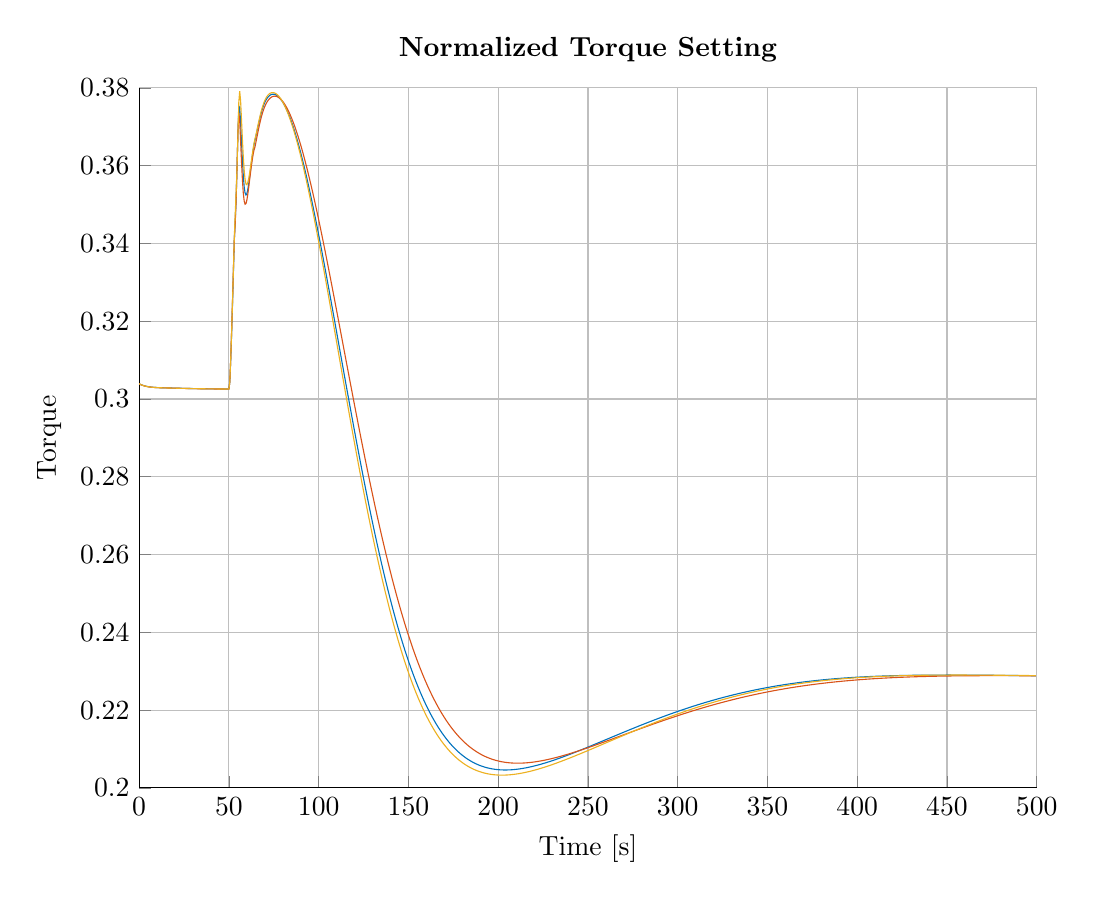
\begin{tikzpicture}

\begin{axis}[%
width=4.488in,
height=3.5in,
at={(0.791in,0.547in)},
scale only axis,
xmin=0,
xmax=500,
xlabel={Time [s]},
xmajorgrids,
ymin=0.2,
ymax=0.38,
ylabel={Torque},
ymajorgrids,
axis background/.style={fill=white},
title style={font=\bfseries},
title={Normalized Torque Setting},
axis x line*=bottom,
axis y line*=left
]
\addplot [color=mycolor1,solid,forget plot]
  table[row sep=crcr]{%
0	0.3039573152\\
0.5	0.303775988\\
1	0.303680777\\
1.5	0.303591625\\
2	0.303511058\\
2.5	0.303437863\\
3	0.303371714\\
3.5	0.303312209\\
4	0.303258903\\
4.5	0.30321133\\
5	0.303169016\\
5.5	0.303131484\\
6	0.30309827\\
6.5	0.303068925\\
7	0.303043022\\
7.5	0.30302016\\
8	0.30299996\\
8.5	0.30298209\\
9	0.30296622\\
9.5	0.30295207\\
10	0.30293939\\
10.5	0.30292794\\
11	0.30291752\\
11.5	0.30290797\\
12	0.30289911\\
12.5	0.30289083\\
13	0.302883\\
13.5	0.30287554\\
14	0.30286837\\
14.5	0.30286141\\
15	0.30285462\\
15.5	0.30284795\\
16	0.30284137\\
16.5	0.30283486\\
17	0.3028284\\
17.5	0.30282197\\
18	0.30281558\\
18.5	0.30280921\\
19	0.30280286\\
19.5	0.30279654\\
20	0.30279025\\
20.5	0.302784\\
21	0.30277779\\
21.5	0.30277162\\
22	0.30276551\\
22.5	0.30275946\\
23	0.30275348\\
23.5	0.30274757\\
24	0.30274173\\
24.5	0.30273598\\
25	0.30273032\\
25.5	0.30272476\\
26	0.30271928\\
26.5	0.30271391\\
27	0.30270864\\
27.5	0.30270347\\
28	0.30269841\\
28.5	0.30269345\\
29	0.3026886\\
29.5	0.30268385\\
30	0.30267921\\
30.5	0.30267467\\
31	0.30267023\\
31.5	0.3026659\\
32	0.30266167\\
32.5	0.30265754\\
33	0.30265351\\
33.5	0.30264957\\
34	0.30264573\\
34.5	0.30264198\\
35	0.30263832\\
35.5	0.30263475\\
36	0.30263126\\
36.5	0.30262786\\
37	0.30262454\\
37.5	0.3026213\\
38	0.30261814\\
38.5	0.30261505\\
39	0.30261204\\
39.5	0.3026091\\
40	0.30260623\\
40.5	0.30260343\\
41	0.30260069\\
41.5	0.30259802\\
42	0.30259541\\
42.5	0.30259287\\
43	0.30259038\\
43.5	0.30258795\\
44	0.30258558\\
44.5	0.30258327\\
45	0.30258101\\
45.5	0.3025788\\
46	0.30257665\\
46.5	0.30257454\\
47	0.30257249\\
47.5	0.30257048\\
48	0.30256852\\
48.5	0.3025666\\
49	0.30256473\\
49.5	0.30256291\\
50	0.30256112\\
50.5	0.304394478\\
51	0.31005118\\
51.5	0.3167577\\
52	0.3244155\\
52.5	0.332599\\
53	0.3409423\\
53.5	0.3457664\\
54	0.3514671\\
54.5	0.3592328\\
55	0.3680617\\
55.5	0.3746969\\
56	0.3750856\\
56.5	0.371095\\
57	0.3662848\\
57.5	0.3615689\\
58	0.3575059\\
58.5	0.3545839\\
59	0.3529578\\
59.5	0.3524559\\
60	0.3528279\\
60.5	0.3538361\\
61	0.3552738\\
61.5	0.356968\\
62	0.358779\\
62.5	0.360597\\
63	0.3623409\\
63.5	0.3639582\\
64	0.3654233\\
64.5	0.3665418\\
65	0.3674821\\
65.5	0.3685874\\
66	0.3696727\\
66.5	0.3707071\\
67	0.3717085\\
67.5	0.3726746\\
68	0.3735685\\
68.5	0.374377\\
69	0.3750961\\
69.5	0.3757275\\
70	0.3762754\\
70.5	0.3767459\\
71	0.3771453\\
71.5	0.3774796\\
72	0.3777542\\
72.5	0.3779738\\
73	0.3781422\\
73.5	0.3782629\\
74	0.3783385\\
74.5	0.3783715\\
75	0.3783635\\
75.5	0.3783164\\
76	0.3782313\\
76.5	0.3781093\\
77	0.3779515\\
77.5	0.3777586\\
78	0.3775314\\
78.5	0.3772706\\
79	0.3769767\\
79.5	0.3766505\\
80	0.3762924\\
80.5	0.3759031\\
81	0.375483\\
81.5	0.3750327\\
82	0.3745528\\
82.5	0.3740438\\
83	0.3735062\\
83.5	0.3729406\\
84	0.3723476\\
84.5	0.3717277\\
85	0.3710814\\
85.5	0.3704093\\
86	0.3697121\\
86.5	0.3689901\\
87	0.3682441\\
87.5	0.3674746\\
88	0.366682\\
88.5	0.3658671\\
89	0.3650303\\
89.5	0.3641722\\
90	0.3632934\\
90.5	0.3623945\\
91	0.3614759\\
91.5	0.3605382\\
92	0.3595821\\
92.5	0.358608\\
93	0.3576164\\
93.5	0.356608\\
94	0.3555833\\
94.5	0.3545428\\
95	0.3534869\\
95.5	0.3524164\\
96	0.3513316\\
96.5	0.3502332\\
97	0.3491215\\
97.5	0.3479972\\
98	0.3468608\\
98.5	0.3457127\\
99	0.3445534\\
99.5	0.3433835\\
100	0.3422035\\
100.5	0.3410137\\
101	0.3398148\\
101.5	0.3386072\\
102	0.3373913\\
102.5	0.3361676\\
103	0.3349366\\
103.5	0.3336988\\
104	0.3324546\\
104.5	0.3312044\\
105	0.3299487\\
105.5	0.3286879\\
106	0.3274225\\
106.5	0.3261529\\
107	0.3248794\\
107.5	0.3236026\\
108	0.3223228\\
108.5	0.3210404\\
109	0.3197558\\
109.5	0.3184695\\
110	0.3171818\\
110.5	0.315893\\
111	0.3146036\\
111.5	0.31331389\\
112	0.31202429\\
112.5	0.31073512\\
113	0.30944674\\
113.5	0.30815949\\
114	0.30687372\\
114.5	0.30558974\\
115	0.304307896\\
115.5	0.303028495\\
116	0.30175185\\
116.5	0.30047828\\
117	0.29920807\\
117.5	0.29794152\\
118	0.29667892\\
118.5	0.29542055\\
119	0.29416668\\
119.5	0.2929176\\
120	0.2916735\\
120.5	0.2904348\\
121	0.2892016\\
121.5	0.2879742\\
122	0.2867528\\
122.5	0.2855377\\
123	0.284329\\
123.5	0.2831271\\
124	0.2819321\\
124.5	0.2807442\\
125	0.2795636\\
125.5	0.2783906\\
126	0.2772252\\
126.5	0.2760678\\
127	0.2749184\\
127.5	0.2737773\\
128	0.2726445\\
128.5	0.2715204\\
129	0.2704049\\
129.5	0.2692983\\
130	0.2682008\\
130.5	0.2671123\\
131	0.2660331\\
131.5	0.2649633\\
132	0.2639031\\
132.5	0.2628524\\
133	0.2618115\\
133.5	0.2607804\\
134	0.2597593\\
134.5	0.2587481\\
135	0.2577471\\
135.5	0.2567562\\
136	0.2557756\\
136.5	0.2548054\\
137	0.2538455\\
137.5	0.2528961\\
138	0.2519572\\
138.5	0.2510288\\
139	0.2501111\\
139.5	0.249204\\
140	0.2483075\\
140.5	0.2474218\\
141	0.2465469\\
141.5	0.2456826\\
142	0.2448292\\
142.5	0.2439866\\
143	0.2431547\\
143.5	0.2423337\\
144	0.2415235\\
144.5	0.2407241\\
145	0.2399355\\
145.5	0.2391576\\
146	0.2383906\\
146.5	0.2376343\\
147	0.2368888\\
147.5	0.236154\\
148	0.2354298\\
148.5	0.2347164\\
149	0.2340135\\
149.5	0.2333212\\
150	0.2326395\\
150.5	0.2319683\\
151	0.2313076\\
151.5	0.2306572\\
152	0.2300172\\
152.5	0.2293876\\
153	0.2287682\\
153.5	0.2281589\\
154	0.2275598\\
154.5	0.2269708\\
155	0.2263918\\
155.5	0.2258227\\
156	0.2252635\\
156.5	0.2247141\\
157	0.2241744\\
157.5	0.2236444\\
158	0.2231239\\
158.5	0.222613\\
159	0.2221114\\
159.5	0.2216193\\
160	0.2211363\\
160.5	0.2206626\\
161	0.2201979\\
161.5	0.2197423\\
162	0.2192955\\
162.5	0.2188577\\
163	0.2184285\\
163.5	0.218008\\
164	0.2175961\\
164.5	0.2171927\\
165	0.2167977\\
165.5	0.2164109\\
166	0.2160324\\
166.5	0.215662\\
167	0.2152996\\
167.5	0.2149451\\
168	0.2145985\\
168.5	0.2142597\\
169	0.2139284\\
169.5	0.2136048\\
170	0.2132886\\
170.5	0.2129798\\
171	0.2126782\\
171.5	0.2123839\\
172	0.2120966\\
172.5	0.2118163\\
173	0.211543\\
173.5	0.2112764\\
174	0.2110166\\
174.5	0.2107634\\
175	0.2105168\\
175.5	0.2102766\\
176	0.2100427\\
176.5	0.2098152\\
177	0.2095938\\
177.5	0.2093784\\
178	0.2091691\\
178.5	0.2089657\\
179	0.2087682\\
179.5	0.2085763\\
180	0.2083902\\
180.5	0.2082095\\
181	0.2080344\\
181.5	0.2078647\\
182	0.2077003\\
182.5	0.2075411\\
183	0.207387\\
183.5	0.2072381\\
184	0.2070941\\
184.5	0.206955\\
185	0.2068208\\
185.5	0.2066913\\
186	0.2065664\\
186.5	0.2064462\\
187	0.2063305\\
187.5	0.2062193\\
188	0.2061124\\
188.5	0.2060098\\
189	0.2059114\\
189.5	0.2058172\\
190	0.2057271\\
190.5	0.205641\\
191	0.2055589\\
191.5	0.2054806\\
192	0.2054062\\
192.5	0.2053354\\
193	0.2052684\\
193.5	0.205205\\
194	0.2051451\\
194.5	0.2050888\\
195	0.2050358\\
195.5	0.2049863\\
196	0.20494\\
196.5	0.204897\\
197	0.2048571\\
197.5	0.2048204\\
198	0.2047868\\
198.5	0.2047562\\
199	0.2047285\\
199.5	0.2047038\\
200	0.2046819\\
200.5	0.2046628\\
201	0.2046464\\
201.5	0.2046328\\
202	0.2046218\\
202.5	0.2046134\\
203	0.2046075\\
203.5	0.2046042\\
204	0.2046033\\
204.5	0.2046048\\
205	0.2046086\\
205.5	0.2046148\\
206	0.2046232\\
206.5	0.2046339\\
207	0.2046467\\
207.5	0.2046617\\
208	0.2046788\\
208.5	0.2046979\\
209	0.204719\\
209.5	0.2047422\\
210	0.2047672\\
210.5	0.2047942\\
211	0.204823\\
211.5	0.2048536\\
212	0.204886\\
212.5	0.2049201\\
213	0.204956\\
213.5	0.2049935\\
214	0.2050327\\
214.5	0.2050735\\
215	0.2051159\\
215.5	0.2051598\\
216	0.2052052\\
216.5	0.2052521\\
217	0.2053004\\
217.5	0.2053502\\
218	0.2054013\\
218.5	0.2054538\\
219	0.2055076\\
219.5	0.2055627\\
220	0.2056191\\
220.5	0.2056767\\
221	0.2057356\\
221.5	0.2057956\\
222	0.2058568\\
222.5	0.2059191\\
223	0.2059825\\
223.5	0.206047\\
224	0.2061126\\
224.5	0.2061792\\
225	0.2062468\\
225.5	0.2063154\\
226	0.2063849\\
226.5	0.2064554\\
227	0.2065268\\
227.5	0.2065991\\
228	0.2066723\\
228.5	0.2067463\\
229	0.2068212\\
229.5	0.2068969\\
230	0.2069734\\
230.5	0.2070506\\
231	0.2071286\\
231.5	0.2072073\\
232	0.2072867\\
232.5	0.2073669\\
233	0.2074477\\
233.5	0.2075291\\
234	0.2076112\\
234.5	0.2076939\\
235	0.2077773\\
235.5	0.2078612\\
236	0.2079456\\
236.5	0.2080307\\
237	0.2081163\\
237.5	0.2082024\\
238	0.208289\\
238.5	0.2083761\\
239	0.2084636\\
239.5	0.2085517\\
240	0.2086401\\
240.5	0.2087291\\
241	0.2088184\\
241.5	0.2089081\\
242	0.2089982\\
242.5	0.2090888\\
243	0.2091796\\
243.5	0.2092708\\
244	0.2093624\\
244.5	0.2094543\\
245	0.2095465\\
245.5	0.209639\\
246	0.2097317\\
246.5	0.2098248\\
247	0.2099181\\
247.5	0.2100117\\
248	0.2101055\\
248.5	0.2101995\\
249	0.2102938\\
249.5	0.2103883\\
250	0.2104829\\
};
\addplot [color=mycolor1,solid,forget plot]
  table[row sep=crcr]{%
250	0.2104829\\
250.5	0.2105778\\
251	0.2106728\\
251.5	0.210768\\
252	0.2108634\\
252.5	0.2109589\\
253	0.2110545\\
253.5	0.2111503\\
254	0.2112462\\
254.5	0.2113422\\
255	0.2114383\\
255.5	0.2115344\\
256	0.2116307\\
256.5	0.211727\\
257	0.2118234\\
257.5	0.2119199\\
258	0.2120164\\
258.5	0.2121129\\
259	0.2122095\\
259.5	0.2123061\\
260	0.2124027\\
260.5	0.2124993\\
261	0.212596\\
261.5	0.2126926\\
262	0.2127892\\
262.5	0.2128857\\
263	0.2129823\\
263.5	0.2130788\\
264	0.2131752\\
264.5	0.2132716\\
265	0.213368\\
265.5	0.2134643\\
266	0.2135605\\
266.5	0.2136566\\
267	0.2137527\\
267.5	0.2138487\\
268	0.2139445\\
268.5	0.2140403\\
269	0.2141359\\
269.5	0.2142315\\
270	0.2143269\\
270.5	0.2144222\\
271	0.2145174\\
271.5	0.2146124\\
272	0.2147073\\
272.5	0.214802\\
273	0.2148966\\
273.5	0.2149911\\
274	0.2150853\\
274.5	0.2151794\\
275	0.2152734\\
275.5	0.2153671\\
276	0.2154607\\
276.5	0.215554\\
277	0.2156472\\
277.5	0.2157402\\
278	0.215833\\
278.5	0.2159256\\
279	0.2160179\\
279.5	0.2161101\\
280	0.216202\\
280.5	0.2162937\\
281	0.2163852\\
281.5	0.2164765\\
282	0.2165675\\
282.5	0.2166583\\
283	0.2167488\\
283.5	0.2168391\\
284	0.2169291\\
284.5	0.2170189\\
285	0.2171084\\
285.5	0.2171977\\
286	0.2172867\\
286.5	0.2173754\\
287	0.2174639\\
287.5	0.2175521\\
288	0.21764\\
288.5	0.2177276\\
289	0.2178149\\
289.5	0.217902\\
290	0.2179887\\
290.5	0.2180752\\
291	0.2181614\\
291.5	0.2182472\\
292	0.2183328\\
292.5	0.2184181\\
293	0.218503\\
293.5	0.2185877\\
294	0.218672\\
294.5	0.218756\\
295	0.2188397\\
295.5	0.2189231\\
296	0.2190061\\
296.5	0.2190889\\
297	0.2191713\\
297.5	0.2192534\\
298	0.2193351\\
298.5	0.2194165\\
299	0.2194976\\
299.5	0.2195783\\
300	0.2196587\\
300.5	0.2197387\\
301	0.2198184\\
301.5	0.2198978\\
302	0.2199768\\
302.5	0.2200555\\
303	0.2201338\\
303.5	0.2202117\\
304	0.2202893\\
304.5	0.2203666\\
305	0.2204435\\
305.5	0.22052\\
306	0.2205962\\
306.5	0.220672\\
307	0.2207474\\
307.5	0.2208225\\
308	0.2208972\\
308.5	0.2209715\\
309	0.2210455\\
309.5	0.2211191\\
310	0.2211923\\
310.5	0.2212652\\
311	0.2213377\\
311.5	0.2214098\\
312	0.2214815\\
312.5	0.2215529\\
313	0.2216238\\
313.5	0.2216944\\
314	0.2217647\\
314.5	0.2218345\\
315	0.221904\\
315.5	0.221973\\
316	0.2220417\\
316.5	0.22211\\
317	0.222178\\
317.5	0.2222455\\
318	0.2223127\\
318.5	0.2223794\\
319	0.2224458\\
319.5	0.2225118\\
320	0.2225774\\
320.5	0.2226426\\
321	0.2227075\\
321.5	0.2227719\\
322	0.222836\\
322.5	0.2228996\\
323	0.2229629\\
323.5	0.2230258\\
324	0.2230883\\
324.5	0.2231504\\
325	0.2232121\\
325.5	0.2232735\\
326	0.2233344\\
326.5	0.2233949\\
327	0.2234551\\
327.5	0.2235149\\
328	0.2235742\\
328.5	0.2236332\\
329	0.2236918\\
329.5	0.22375\\
330	0.2238078\\
330.5	0.2238653\\
331	0.2239223\\
331.5	0.2239789\\
332	0.2240352\\
332.5	0.2240911\\
333	0.2241465\\
333.5	0.2242016\\
334	0.2242563\\
334.5	0.2243106\\
335	0.2243646\\
335.5	0.2244181\\
336	0.2244713\\
336.5	0.224524\\
337	0.2245764\\
337.5	0.2246284\\
338	0.22468\\
338.5	0.2247313\\
339	0.2247821\\
339.5	0.2248326\\
340	0.2248827\\
340.5	0.2249324\\
341	0.2249817\\
341.5	0.2250306\\
342	0.2250792\\
342.5	0.2251274\\
343	0.2251752\\
343.5	0.2252226\\
344	0.2252697\\
344.5	0.2253164\\
345	0.2253627\\
345.5	0.2254086\\
346	0.2254542\\
346.5	0.2254993\\
347	0.2255442\\
347.5	0.2255886\\
348	0.2256327\\
348.5	0.2256764\\
349	0.2257198\\
349.5	0.2257627\\
350	0.2258053\\
350.5	0.2258476\\
351	0.2258895\\
351.5	0.225931\\
352	0.2259722\\
352.5	0.226013\\
353	0.2260534\\
353.5	0.2260935\\
354	0.2261333\\
354.5	0.2261727\\
355	0.2262117\\
355.5	0.2262504\\
356	0.2262887\\
356.5	0.2263267\\
357	0.2263643\\
357.5	0.2264016\\
358	0.2264385\\
358.5	0.2264751\\
359	0.2265114\\
359.5	0.2265473\\
360	0.2265828\\
360.5	0.2266181\\
361	0.2266529\\
361.5	0.2266875\\
362	0.2267217\\
362.5	0.2267556\\
363	0.2267892\\
363.5	0.2268224\\
364	0.2268553\\
364.5	0.2268878\\
365	0.2269201\\
365.5	0.226952\\
366	0.2269836\\
366.5	0.2270148\\
367	0.2270458\\
367.5	0.2270764\\
368	0.2271067\\
368.5	0.2271367\\
369	0.2271664\\
369.5	0.2271958\\
370	0.2272248\\
370.5	0.2272536\\
371	0.227282\\
371.5	0.2273101\\
372	0.2273379\\
372.5	0.2273655\\
373	0.2273927\\
373.5	0.2274196\\
374	0.2274462\\
374.5	0.2274726\\
375	0.2274986\\
375.5	0.2275243\\
376	0.2275498\\
376.5	0.2275749\\
377	0.2275998\\
377.5	0.2276244\\
378	0.2276486\\
378.5	0.2276726\\
379	0.2276964\\
379.5	0.2277198\\
380	0.227743\\
380.5	0.2277659\\
381	0.2277885\\
381.5	0.2278108\\
382	0.2278329\\
382.5	0.2278547\\
383	0.2278762\\
383.5	0.2278975\\
384	0.2279185\\
384.5	0.2279392\\
385	0.2279597\\
385.5	0.2279799\\
386	0.2279998\\
386.5	0.2280195\\
387	0.2280389\\
387.5	0.2280581\\
388	0.2280771\\
388.5	0.2280957\\
389	0.2281142\\
389.5	0.2281324\\
390	0.2281503\\
390.5	0.228168\\
391	0.2281855\\
391.5	0.2282027\\
392	0.2282197\\
392.5	0.2282364\\
393	0.2282529\\
393.5	0.2282692\\
394	0.2282852\\
394.5	0.2283011\\
395	0.2283166\\
395.5	0.228332\\
396	0.2283471\\
396.5	0.2283621\\
397	0.2283768\\
397.5	0.2283912\\
398	0.2284055\\
398.5	0.2284195\\
399	0.2284334\\
399.5	0.228447\\
400	0.2284604\\
400.5	0.2284736\\
401	0.2284866\\
401.5	0.2284994\\
402	0.228512\\
402.5	0.2285243\\
403	0.2285365\\
403.5	0.2285485\\
404	0.2285603\\
404.5	0.2285719\\
405	0.2285833\\
405.5	0.2285945\\
406	0.2286055\\
406.5	0.2286163\\
407	0.228627\\
407.5	0.2286374\\
408	0.2286477\\
408.5	0.2286578\\
409	0.2286677\\
409.5	0.2286774\\
410	0.228687\\
410.5	0.2286963\\
411	0.2287055\\
411.5	0.2287146\\
412	0.2287234\\
412.5	0.2287321\\
413	0.2287407\\
413.5	0.228749\\
414	0.2287572\\
414.5	0.2287652\\
415	0.2287731\\
415.5	0.2287808\\
416	0.2287884\\
416.5	0.2287958\\
417	0.228803\\
417.5	0.2288101\\
418	0.228817\\
418.5	0.2288238\\
419	0.2288305\\
419.5	0.228837\\
420	0.2288433\\
420.5	0.2288495\\
421	0.2288556\\
421.5	0.2288615\\
422	0.2288673\\
422.5	0.2288729\\
423	0.2288784\\
423.5	0.2288838\\
424	0.228889\\
424.5	0.2288941\\
425	0.2288991\\
425.5	0.228904\\
426	0.2289087\\
426.5	0.2289133\\
427	0.2289177\\
427.5	0.2289221\\
428	0.2289263\\
428.5	0.2289304\\
429	0.2289344\\
429.5	0.2289382\\
430	0.228942\\
430.5	0.2289456\\
431	0.2289491\\
431.5	0.2289525\\
432	0.2289558\\
432.5	0.228959\\
433	0.2289621\\
433.5	0.2289651\\
434	0.2289679\\
434.5	0.2289707\\
435	0.2289733\\
435.5	0.2289759\\
436	0.2289783\\
436.5	0.2289807\\
437	0.228983\\
437.5	0.2289851\\
438	0.2289872\\
438.5	0.2289892\\
439	0.228991\\
439.5	0.2289928\\
440	0.2289945\\
440.5	0.2289961\\
441	0.2289976\\
441.5	0.2289991\\
442	0.2290004\\
442.5	0.2290017\\
443	0.2290029\\
443.5	0.2290039\\
444	0.229005\\
444.5	0.2290059\\
445	0.2290068\\
445.5	0.2290075\\
446	0.2290082\\
446.5	0.2290089\\
447	0.2290094\\
447.5	0.2290099\\
448	0.2290103\\
448.5	0.2290106\\
449	0.2290109\\
449.5	0.2290111\\
450	0.2290112\\
450.5	0.2290113\\
451	0.2290113\\
451.5	0.2290112\\
452	0.2290111\\
452.5	0.2290109\\
453	0.2290106\\
453.5	0.2290103\\
454	0.22901\\
454.5	0.2290095\\
455	0.229009\\
455.5	0.2290085\\
456	0.2290079\\
456.5	0.2290072\\
457	0.2290065\\
457.5	0.2290057\\
458	0.2290049\\
458.5	0.2290041\\
459	0.2290031\\
459.5	0.2290022\\
460	0.2290012\\
460.5	0.2290001\\
461	0.228999\\
461.5	0.2289978\\
462	0.2289966\\
462.5	0.2289954\\
463	0.2289941\\
463.5	0.2289928\\
464	0.2289914\\
464.5	0.22899\\
465	0.2289885\\
465.5	0.2289871\\
466	0.2289855\\
466.5	0.228984\\
467	0.2289824\\
467.5	0.2289807\\
468	0.228979\\
468.5	0.2289773\\
469	0.2289756\\
469.5	0.2289738\\
470	0.228972\\
470.5	0.2289702\\
471	0.2289683\\
471.5	0.2289664\\
472	0.2289645\\
472.5	0.2289625\\
473	0.2289605\\
473.5	0.2289585\\
474	0.2289565\\
474.5	0.2289544\\
475	0.2289523\\
475.5	0.2289502\\
476	0.2289481\\
476.5	0.2289459\\
477	0.2289437\\
477.5	0.2289415\\
478	0.2289393\\
478.5	0.2289371\\
479	0.2289348\\
479.5	0.2289325\\
480	0.2289302\\
480.5	0.2289279\\
481	0.2289255\\
481.5	0.2289232\\
482	0.2289208\\
482.5	0.2289184\\
483	0.228916\\
483.5	0.2289136\\
484	0.2289111\\
484.5	0.2289087\\
485	0.2289062\\
485.5	0.2289038\\
486	0.2289013\\
486.5	0.2288988\\
487	0.2288962\\
487.5	0.2288937\\
488	0.2288912\\
488.5	0.2288886\\
489	0.2288861\\
489.5	0.2288835\\
490	0.228881\\
490.5	0.2288784\\
491	0.2288758\\
491.5	0.2288732\\
492	0.2288706\\
492.5	0.228868\\
493	0.2288654\\
493.5	0.2288628\\
494	0.2288601\\
494.5	0.2288575\\
495	0.2288549\\
495.5	0.2288522\\
496	0.2288496\\
496.5	0.2288469\\
497	0.2288443\\
497.5	0.2288416\\
498	0.228839\\
498.5	0.2288363\\
499	0.2288337\\
499.5	0.228831\\
};
\addplot [color=mycolor2,solid,forget plot]
  table[row sep=crcr]{%
0	0.3039552245\\
0.5	0.303765592\\
1	0.303666922\\
1.5	0.303574787\\
2	0.30349186\\
2.5	0.30341683\\
3	0.303349327\\
3.5	0.303288902\\
4	0.303235058\\
4.5	0.303187277\\
5	0.303145034\\
5.5	0.303107805\\
6	0.303075079\\
6.5	0.303046365\\
7	0.303021198\\
7.5	0.30299914\\
8	0.30297979\\
8.5	0.30296278\\
9	0.30294777\\
9.5	0.30293446\\
10	0.30292257\\
10.5	0.30291187\\
11	0.30290214\\
11.5	0.30289321\\
12	0.30288491\\
12.5	0.30287712\\
13	0.30286972\\
13.5	0.30286262\\
14	0.30285574\\
14.5	0.30284902\\
15	0.30284241\\
15.5	0.30283587\\
16	0.30282937\\
16.5	0.3028229\\
17	0.30281644\\
17.5	0.30280998\\
18	0.30280353\\
18.5	0.30279707\\
19	0.30279063\\
19.5	0.30278419\\
20	0.30277777\\
20.5	0.30277137\\
21	0.30276501\\
21.5	0.30275869\\
22	0.30275243\\
22.5	0.30274622\\
23	0.30274008\\
23.5	0.30273401\\
24	0.30272803\\
24.5	0.30272213\\
25	0.30271633\\
25.5	0.30271062\\
26	0.30270501\\
26.5	0.30269951\\
27	0.30269412\\
27.5	0.30268883\\
28	0.30268365\\
28.5	0.30267859\\
29	0.30267363\\
29.5	0.30266878\\
30	0.30266404\\
30.5	0.30265942\\
31	0.30265489\\
31.5	0.30265048\\
32	0.30264617\\
32.5	0.30264196\\
33	0.30263785\\
33.5	0.30263384\\
34	0.30262992\\
34.5	0.3026261\\
35	0.30262237\\
35.5	0.30261874\\
36	0.30261518\\
36.5	0.30261172\\
37	0.30260833\\
37.5	0.30260503\\
38	0.30260181\\
38.5	0.30259866\\
39	0.30259559\\
39.5	0.30259259\\
40	0.30258966\\
40.5	0.3025868\\
41	0.30258401\\
41.5	0.30258128\\
42	0.30257862\\
42.5	0.30257601\\
43	0.30257347\\
43.5	0.30257099\\
44	0.30256857\\
44.5	0.3025662\\
45	0.30256389\\
45.5	0.30256163\\
46	0.30255943\\
46.5	0.30255727\\
47	0.30255516\\
47.5	0.30255311\\
48	0.3025511\\
48.5	0.30254913\\
49	0.30254722\\
49.5	0.30254534\\
50	0.30254351\\
50.5	0.304471449\\
51	0.31042517\\
51.5	0.3174263\\
52	0.325291\\
52.5	0.3334964\\
53	0.3408456\\
53.5	0.3451152\\
54	0.3508922\\
54.5	0.3592195\\
55	0.3683954\\
55.5	0.3736534\\
56	0.3715522\\
56.5	0.3663626\\
57	0.3610624\\
57.5	0.356449\\
58	0.3529859\\
58.5	0.3509046\\
59	0.3500809\\
59.5	0.3502514\\
60	0.3511626\\
60.5	0.3525872\\
61	0.3543252\\
61.5	0.3562077\\
62	0.3580983\\
62.5	0.3598939\\
63	0.3615241\\
63.5	0.3629525\\
64	0.3640551\\
64.5	0.3647738\\
65	0.3659146\\
65.5	0.3671063\\
66	0.3682674\\
66.5	0.3693898\\
67	0.3704737\\
67.5	0.3714837\\
68	0.3724073\\
68.5	0.3732412\\
69	0.3739872\\
69.5	0.3746488\\
70	0.3752313\\
70.5	0.375741\\
71	0.3761835\\
71.5	0.3765645\\
72	0.3768889\\
72.5	0.3771609\\
73	0.3773843\\
73.5	0.3775621\\
74	0.3776969\\
74.5	0.3777909\\
75	0.3778458\\
75.5	0.3778632\\
76	0.3778442\\
76.5	0.37779\\
77	0.3777015\\
77.5	0.3775793\\
78	0.3774244\\
78.5	0.3772372\\
79	0.3770184\\
79.5	0.3767686\\
80	0.3764883\\
80.5	0.376178\\
81	0.3758383\\
81.5	0.3754696\\
82	0.3750724\\
82.5	0.3746474\\
83	0.3741949\\
83.5	0.3737155\\
84	0.3732096\\
84.5	0.3726779\\
85	0.3721207\\
85.5	0.3715386\\
86	0.3709322\\
86.5	0.3703018\\
87	0.3696481\\
87.5	0.3689715\\
88	0.3682725\\
88.5	0.3675517\\
89	0.3668096\\
89.5	0.3660466\\
90	0.3652632\\
90.5	0.36446\\
91	0.3636375\\
91.5	0.3627962\\
92	0.3619365\\
92.5	0.361059\\
93	0.3601641\\
93.5	0.3592523\\
94	0.3583242\\
94.5	0.3573802\\
95	0.3564208\\
95.5	0.3554464\\
96	0.3544576\\
96.5	0.3534548\\
97	0.3524385\\
97.5	0.3514092\\
98	0.3503673\\
98.5	0.3493133\\
99	0.3482476\\
99.5	0.3471707\\
100	0.346083\\
100.5	0.344985\\
101	0.3438772\\
101.5	0.3427599\\
102	0.3416336\\
102.5	0.3404987\\
103	0.3393557\\
103.5	0.3382049\\
104	0.3370469\\
104.5	0.3358819\\
105	0.3347104\\
105.5	0.3335328\\
106	0.3323496\\
106.5	0.331161\\
107	0.3299675\\
107.5	0.3287695\\
108	0.3275673\\
108.5	0.3263614\\
109	0.325152\\
109.5	0.3239397\\
110	0.3227246\\
110.5	0.3215072\\
111	0.3202879\\
111.5	0.3190669\\
112	0.3178446\\
112.5	0.3166214\\
113	0.3153975\\
113.5	0.3141734\\
114	0.31294924\\
114.5	0.31172545\\
115	0.31050231\\
115.5	0.30928011\\
116	0.30805916\\
116.5	0.30683976\\
117	0.30562219\\
117.5	0.304406727\\
118	0.30319366\\
118.5	0.30198326\\
119	0.30077579\\
119.5	0.29957151\\
120	0.29837068\\
120.5	0.29717356\\
121	0.29598038\\
121.5	0.29479139\\
122	0.2936068\\
122.5	0.2924269\\
123	0.2912519\\
123.5	0.2900819\\
124	0.2889173\\
124.5	0.2877582\\
125	0.2866048\\
125.5	0.2854573\\
126	0.284316\\
126.5	0.2831809\\
127	0.2820524\\
127.5	0.2809304\\
128	0.2798154\\
128.5	0.2787073\\
129	0.2776064\\
129.5	0.2765128\\
130	0.2754266\\
130.5	0.2743481\\
131	0.2732773\\
131.5	0.2722144\\
132	0.2711596\\
132.5	0.2701129\\
133	0.2690744\\
133.5	0.2680443\\
134	0.2670228\\
134.5	0.2660098\\
135	0.2650055\\
135.5	0.2640101\\
136	0.2630235\\
136.5	0.2620459\\
137	0.2610774\\
137.5	0.260118\\
138	0.2591678\\
138.5	0.258227\\
139	0.2572954\\
139.5	0.2563733\\
140	0.2554607\\
140.5	0.2545575\\
141	0.253664\\
141.5	0.25278\\
142	0.2519057\\
142.5	0.2510411\\
143	0.2501863\\
143.5	0.2493411\\
144	0.2485058\\
144.5	0.2476802\\
145	0.2468645\\
145.5	0.2460586\\
146	0.2452625\\
146.5	0.2444762\\
147	0.2436998\\
147.5	0.2429333\\
148	0.2421766\\
148.5	0.2414297\\
149	0.2406926\\
149.5	0.2399654\\
150	0.239248\\
150.5	0.2385403\\
151	0.2378424\\
151.5	0.2371542\\
152	0.2364757\\
152.5	0.2358069\\
153	0.2351477\\
153.5	0.2344981\\
154	0.2338581\\
154.5	0.2332276\\
155	0.2326066\\
155.5	0.2319951\\
156	0.2313929\\
156.5	0.2308001\\
157	0.2302165\\
157.5	0.2296422\\
158	0.2290771\\
158.5	0.2285211\\
159	0.2279742\\
159.5	0.2274363\\
160	0.2269074\\
160.5	0.2263873\\
161	0.2258761\\
161.5	0.2253736\\
162	0.2248798\\
162.5	0.2243947\\
163	0.223918\\
163.5	0.2234499\\
164	0.2229902\\
164.5	0.2225388\\
165	0.2220956\\
165.5	0.2216607\\
166	0.2212339\\
166.5	0.2208151\\
167	0.2204042\\
167.5	0.2200013\\
168	0.2196061\\
168.5	0.2192187\\
169	0.2188389\\
169.5	0.2184667\\
170	0.218102\\
170.5	0.2177446\\
171	0.2173946\\
171.5	0.2170519\\
172	0.2167162\\
172.5	0.2163877\\
173	0.2160662\\
173.5	0.2157516\\
174	0.2154438\\
174.5	0.2151427\\
175	0.2148484\\
175.5	0.2145606\\
176	0.2142793\\
176.5	0.2140045\\
177	0.213736\\
177.5	0.2134737\\
178	0.2132177\\
178.5	0.2129677\\
179	0.2127237\\
179.5	0.2124857\\
180	0.2122536\\
180.5	0.2120272\\
181	0.2118065\\
181.5	0.2115914\\
182	0.2113819\\
182.5	0.2111779\\
183	0.2109792\\
183.5	0.2107859\\
184	0.2105978\\
184.5	0.2104148\\
185	0.2102369\\
185.5	0.210064\\
186	0.2098961\\
186.5	0.209733\\
187	0.2095748\\
187.5	0.2094212\\
188	0.2092723\\
188.5	0.2091279\\
189	0.2089881\\
189.5	0.2088527\\
190	0.2087216\\
190.5	0.2085949\\
191	0.2084723\\
191.5	0.208354\\
192	0.2082397\\
192.5	0.2081295\\
193	0.2080232\\
193.5	0.2079208\\
194	0.2078223\\
194.5	0.2077275\\
195	0.2076365\\
195.5	0.2075491\\
196	0.2074653\\
196.5	0.207385\\
197	0.2073082\\
197.5	0.2072349\\
198	0.2071648\\
198.5	0.2070981\\
199	0.2070346\\
199.5	0.2069743\\
200	0.2069172\\
200.5	0.2068631\\
201	0.2068121\\
201.5	0.206764\\
202	0.2067188\\
202.5	0.2066766\\
203	0.2066371\\
203.5	0.2066004\\
204	0.2065664\\
204.5	0.2065352\\
205	0.2065065\\
205.5	0.2064804\\
206	0.2064569\\
206.5	0.2064358\\
207	0.2064172\\
207.5	0.2064009\\
208	0.2063871\\
208.5	0.2063755\\
209	0.2063662\\
209.5	0.2063591\\
210	0.2063543\\
210.5	0.2063515\\
211	0.2063509\\
211.5	0.2063523\\
212	0.2063558\\
212.5	0.2063612\\
213	0.2063686\\
213.5	0.2063779\\
214	0.2063891\\
214.5	0.2064022\\
215	0.206417\\
215.5	0.2064336\\
216	0.206452\\
216.5	0.206472\\
217	0.2064937\\
217.5	0.2065171\\
218	0.206542\\
218.5	0.2065686\\
219	0.2065967\\
219.5	0.2066263\\
220	0.2066573\\
220.5	0.2066898\\
221	0.2067238\\
221.5	0.2067591\\
222	0.2067958\\
222.5	0.2068339\\
223	0.2068732\\
223.5	0.2069139\\
224	0.2069558\\
224.5	0.2069989\\
225	0.2070432\\
225.5	0.2070887\\
226	0.2071354\\
226.5	0.2071832\\
227	0.2072321\\
227.5	0.2072821\\
228	0.2073331\\
228.5	0.2073852\\
229	0.2074383\\
229.5	0.2074924\\
230	0.2075474\\
230.5	0.2076034\\
231	0.2076603\\
231.5	0.2077182\\
232	0.2077769\\
232.5	0.2078365\\
233	0.2078969\\
233.5	0.2079582\\
234	0.2080202\\
234.5	0.2080831\\
235	0.2081467\\
235.5	0.2082111\\
236	0.2082762\\
236.5	0.208342\\
237	0.2084085\\
237.5	0.2084757\\
238	0.2085435\\
238.5	0.2086121\\
239	0.2086812\\
239.5	0.2087509\\
240	0.2088213\\
240.5	0.2088922\\
241	0.2089637\\
241.5	0.2090358\\
242	0.2091084\\
242.5	0.2091815\\
243	0.2092552\\
243.5	0.2093293\\
244	0.2094039\\
244.5	0.209479\\
245	0.2095545\\
245.5	0.2096305\\
246	0.2097069\\
246.5	0.2097837\\
247	0.2098609\\
247.5	0.2099385\\
248	0.2100165\\
248.5	0.2100948\\
249	0.2101735\\
249.5	0.2102526\\
250	0.210332\\
};
\addplot [color=mycolor2,solid,forget plot]
  table[row sep=crcr]{%
250	0.210332\\
250.5	0.2104117\\
251	0.2104917\\
251.5	0.210572\\
252	0.2106526\\
252.5	0.2107334\\
253	0.2108146\\
253.5	0.2108959\\
254	0.2109776\\
254.5	0.2110594\\
255	0.2111415\\
255.5	0.2112238\\
256	0.2113064\\
256.5	0.2113891\\
257	0.211472\\
257.5	0.211555\\
258	0.2116383\\
258.5	0.2117217\\
259	0.2118053\\
259.5	0.211889\\
260	0.2119728\\
260.5	0.2120568\\
261	0.2121408\\
261.5	0.212225\\
262	0.2123093\\
262.5	0.2123937\\
263	0.2124782\\
263.5	0.2125628\\
264	0.2126474\\
264.5	0.2127321\\
265	0.2128168\\
265.5	0.2129016\\
266	0.2129865\\
266.5	0.2130714\\
267	0.2131563\\
267.5	0.2132412\\
268	0.2133262\\
268.5	0.2134111\\
269	0.2134961\\
269.5	0.2135811\\
270	0.213666\\
270.5	0.213751\\
271	0.2138359\\
271.5	0.2139208\\
272	0.2140056\\
272.5	0.2140904\\
273	0.2141752\\
273.5	0.2142599\\
274	0.2143446\\
274.5	0.2144292\\
275	0.2145138\\
275.5	0.2145983\\
276	0.2146826\\
276.5	0.214767\\
277	0.2148512\\
277.5	0.2149353\\
278	0.2150194\\
278.5	0.2151033\\
279	0.2151872\\
279.5	0.2152709\\
280	0.2153545\\
280.5	0.215438\\
281	0.2155214\\
281.5	0.2156046\\
282	0.2156877\\
282.5	0.2157707\\
283	0.2158535\\
283.5	0.2159362\\
284	0.2160187\\
284.5	0.2161011\\
285	0.2161834\\
285.5	0.2162654\\
286	0.2163473\\
286.5	0.2164291\\
287	0.2165106\\
287.5	0.216592\\
288	0.2166732\\
288.5	0.2167543\\
289	0.2168351\\
289.5	0.2169158\\
290	0.2169962\\
290.5	0.2170765\\
291	0.2171566\\
291.5	0.2172364\\
292	0.2173161\\
292.5	0.2173955\\
293	0.2174748\\
293.5	0.2175538\\
294	0.2176326\\
294.5	0.2177112\\
295	0.2177896\\
295.5	0.2178677\\
296	0.2179456\\
296.5	0.2180233\\
297	0.2181008\\
297.5	0.218178\\
298	0.218255\\
298.5	0.2183317\\
299	0.2184082\\
299.5	0.2184845\\
300	0.2185605\\
300.5	0.2186362\\
301	0.2187117\\
301.5	0.218787\\
302	0.218862\\
302.5	0.2189367\\
303	0.2190112\\
303.5	0.2190854\\
304	0.2191593\\
304.5	0.219233\\
305	0.2193064\\
305.5	0.2193795\\
306	0.2194524\\
306.5	0.219525\\
307	0.2195973\\
307.5	0.2196693\\
308	0.2197411\\
308.5	0.2198126\\
309	0.2198838\\
309.5	0.2199547\\
310	0.2200253\\
310.5	0.2200956\\
311	0.2201657\\
311.5	0.2202354\\
312	0.2203049\\
312.5	0.2203741\\
313	0.220443\\
313.5	0.2205115\\
314	0.2205798\\
314.5	0.2206478\\
315	0.2207155\\
315.5	0.2207829\\
316	0.22085\\
316.5	0.2209168\\
317	0.2209833\\
317.5	0.2210494\\
318	0.2211153\\
318.5	0.2211809\\
319	0.2212461\\
319.5	0.2213111\\
320	0.2213757\\
320.5	0.2214401\\
321	0.2215041\\
321.5	0.2215678\\
322	0.2216312\\
322.5	0.2216943\\
323	0.221757\\
323.5	0.2218195\\
324	0.2218816\\
324.5	0.2219435\\
325	0.222005\\
325.5	0.2220661\\
326	0.222127\\
326.5	0.2221876\\
327	0.2222478\\
327.5	0.2223077\\
328	0.2223673\\
328.5	0.2224266\\
329	0.2224856\\
329.5	0.2225442\\
330	0.2226025\\
330.5	0.2226605\\
331	0.2227182\\
331.5	0.2227755\\
332	0.2228326\\
332.5	0.2228893\\
333	0.2229457\\
333.5	0.2230017\\
334	0.2230575\\
334.5	0.2231129\\
335	0.223168\\
335.5	0.2232227\\
336	0.2232772\\
336.5	0.2233313\\
337	0.2233851\\
337.5	0.2234386\\
338	0.2234917\\
338.5	0.2235446\\
339	0.2235971\\
339.5	0.2236493\\
340	0.2237011\\
340.5	0.2237527\\
341	0.2238039\\
341.5	0.2238548\\
342	0.2239054\\
342.5	0.2239556\\
343	0.2240056\\
343.5	0.2240552\\
344	0.2241045\\
344.5	0.2241535\\
345	0.2242021\\
345.5	0.2242504\\
346	0.2242984\\
346.5	0.2243461\\
347	0.2243935\\
347.5	0.2244406\\
348	0.2244873\\
348.5	0.2245337\\
349	0.2245798\\
349.5	0.2246256\\
350	0.2246711\\
350.5	0.2247162\\
351	0.2247611\\
351.5	0.2248056\\
352	0.2248498\\
352.5	0.2248937\\
353	0.2249373\\
353.5	0.2249806\\
354	0.2250235\\
354.5	0.2250662\\
355	0.2251085\\
355.5	0.2251506\\
356	0.2251923\\
356.5	0.2252337\\
357	0.2252748\\
357.5	0.2253156\\
358	0.2253561\\
358.5	0.2253963\\
359	0.2254362\\
359.5	0.2254757\\
360	0.225515\\
360.5	0.225554\\
361	0.2255927\\
361.5	0.225631\\
362	0.2256691\\
362.5	0.2257069\\
363	0.2257444\\
363.5	0.2257816\\
364	0.2258184\\
364.5	0.225855\\
365	0.2258913\\
365.5	0.2259273\\
366	0.225963\\
366.5	0.2259985\\
367	0.2260336\\
367.5	0.2260684\\
368	0.226103\\
368.5	0.2261372\\
369	0.2261712\\
369.5	0.2262049\\
370	0.2262383\\
370.5	0.2262714\\
371	0.2263043\\
371.5	0.2263368\\
372	0.2263691\\
372.5	0.2264011\\
373	0.2264328\\
373.5	0.2264643\\
374	0.2264954\\
374.5	0.2265263\\
375	0.226557\\
375.5	0.2265873\\
376	0.2266174\\
376.5	0.2266472\\
377	0.2266767\\
377.5	0.226706\\
378	0.226735\\
378.5	0.2267637\\
379	0.2267922\\
379.5	0.2268204\\
380	0.2268483\\
380.5	0.226876\\
381	0.2269034\\
381.5	0.2269306\\
382	0.2269575\\
382.5	0.2269841\\
383	0.2270105\\
383.5	0.2270367\\
384	0.2270626\\
384.5	0.2270882\\
385	0.2271136\\
385.5	0.2271387\\
386	0.2271636\\
386.5	0.2271882\\
387	0.2272126\\
387.5	0.2272368\\
388	0.2272607\\
388.5	0.2272844\\
389	0.2273078\\
389.5	0.227331\\
390	0.2273539\\
390.5	0.2273766\\
391	0.2273991\\
391.5	0.2274214\\
392	0.2274434\\
392.5	0.2274652\\
393	0.2274867\\
393.5	0.227508\\
394	0.2275291\\
394.5	0.22755\\
395	0.2275706\\
395.5	0.2275911\\
396	0.2276113\\
396.5	0.2276312\\
397	0.227651\\
397.5	0.2276705\\
398	0.2276898\\
398.5	0.227709\\
399	0.2277278\\
399.5	0.2277465\\
400	0.227765\\
400.5	0.2277832\\
401	0.2278013\\
401.5	0.2278191\\
402	0.2278368\\
402.5	0.2278542\\
403	0.2278714\\
403.5	0.2278884\\
404	0.2279053\\
404.5	0.2279219\\
405	0.2279383\\
405.5	0.2279545\\
406	0.2279706\\
406.5	0.2279864\\
407	0.228002\\
407.5	0.2280175\\
408	0.2280328\\
408.5	0.2280478\\
409	0.2280627\\
409.5	0.2280774\\
410	0.2280919\\
410.5	0.2281062\\
411	0.2281204\\
411.5	0.2281343\\
412	0.2281481\\
412.5	0.2281617\\
413	0.2281752\\
413.5	0.2281884\\
414	0.2282015\\
414.5	0.2282144\\
415	0.2282271\\
415.5	0.2282397\\
416	0.2282521\\
416.5	0.2282643\\
417	0.2282763\\
417.5	0.2282882\\
418	0.2282999\\
418.5	0.2283115\\
419	0.2283229\\
419.5	0.2283341\\
420	0.2283452\\
420.5	0.2283561\\
421	0.2283669\\
421.5	0.2283775\\
422	0.228388\\
422.5	0.2283983\\
423	0.2284084\\
423.5	0.2284184\\
424	0.2284282\\
424.5	0.2284379\\
425	0.2284475\\
425.5	0.2284569\\
426	0.2284662\\
426.5	0.2284753\\
427	0.2284843\\
427.5	0.2284931\\
428	0.2285018\\
428.5	0.2285104\\
429	0.2285188\\
429.5	0.2285271\\
430	0.2285352\\
430.5	0.2285433\\
431	0.2285511\\
431.5	0.2285589\\
432	0.2285665\\
432.5	0.228574\\
433	0.2285814\\
433.5	0.2285886\\
434	0.2285958\\
434.5	0.2286027\\
435	0.2286096\\
435.5	0.2286164\\
436	0.228623\\
436.5	0.2286295\\
437	0.2286359\\
437.5	0.2286422\\
438	0.2286483\\
438.5	0.2286544\\
439	0.2286603\\
439.5	0.2286661\\
440	0.2286718\\
440.5	0.2286774\\
441	0.2286829\\
441.5	0.2286883\\
442	0.2286936\\
442.5	0.2286987\\
443	0.2287038\\
443.5	0.2287088\\
444	0.2287136\\
444.5	0.2287184\\
445	0.228723\\
445.5	0.2287276\\
446	0.228732\\
446.5	0.2287364\\
447	0.2287406\\
447.5	0.2287448\\
448	0.2287489\\
448.5	0.2287529\\
449	0.2287567\\
449.5	0.2287605\\
450	0.2287642\\
450.5	0.2287679\\
451	0.2287714\\
451.5	0.2287748\\
452	0.2287782\\
452.5	0.2287814\\
453	0.2287846\\
453.5	0.2287877\\
454	0.2287907\\
454.5	0.2287937\\
455	0.2287965\\
455.5	0.2287993\\
456	0.228802\\
456.5	0.2288046\\
457	0.2288071\\
457.5	0.2288096\\
458	0.228812\\
458.5	0.2288143\\
459	0.2288165\\
459.5	0.2288187\\
460	0.2288208\\
460.5	0.2288228\\
461	0.2288248\\
461.5	0.2288267\\
462	0.2288285\\
462.5	0.2288303\\
463	0.2288319\\
463.5	0.2288336\\
464	0.2288351\\
464.5	0.2288366\\
465	0.228838\\
465.5	0.2288394\\
466	0.2288407\\
466.5	0.228842\\
467	0.2288432\\
467.5	0.2288443\\
468	0.2288453\\
468.5	0.2288464\\
469	0.2288473\\
469.5	0.2288482\\
470	0.2288491\\
470.5	0.2288499\\
471	0.2288506\\
471.5	0.2288513\\
472	0.2288519\\
472.5	0.2288525\\
473	0.228853\\
473.5	0.2288535\\
474	0.2288539\\
474.5	0.2288543\\
475	0.2288546\\
475.5	0.2288549\\
476	0.2288552\\
476.5	0.2288554\\
477	0.2288555\\
477.5	0.2288556\\
478	0.2288557\\
478.5	0.2288557\\
479	0.2288557\\
479.5	0.2288556\\
480	0.2288555\\
480.5	0.2288554\\
481	0.2288552\\
481.5	0.228855\\
482	0.2288547\\
482.5	0.2288544\\
483	0.2288541\\
483.5	0.2288537\\
484	0.2288533\\
484.5	0.2288529\\
485	0.2288524\\
485.5	0.2288519\\
486	0.2288514\\
486.5	0.2288508\\
487	0.2288502\\
487.5	0.2288495\\
488	0.2288489\\
488.5	0.2288482\\
489	0.2288474\\
489.5	0.2288467\\
490	0.2288459\\
490.5	0.2288451\\
491	0.2288442\\
491.5	0.2288433\\
492	0.2288424\\
492.5	0.2288415\\
493	0.2288406\\
493.5	0.2288396\\
494	0.2288386\\
494.5	0.2288376\\
495	0.2288365\\
495.5	0.2288354\\
496	0.2288343\\
496.5	0.2288332\\
497	0.2288321\\
497.5	0.2288309\\
498	0.2288297\\
498.5	0.2288285\\
499	0.2288273\\
499.5	0.2288261\\
};
\addplot [color=mycolor3,solid,forget plot]
  table[row sep=crcr]{%
0	0.3039595053\\
0.5	0.30377925\\
1	0.303678798\\
1.5	0.303585531\\
2	0.303501536\\
2.5	0.303425625\\
3	0.303357386\\
3.5	0.303296341\\
4	0.303241965\\
4.5	0.303193723\\
5	0.303151069\\
5.5	0.303113468\\
6	0.303080398\\
6.5	0.303051362\\
7	0.303025888\\
7.5	0.303003539\\
8	0.30298391\\
8.5	0.30296662\\
9	0.30295135\\
9.5	0.30293779\\
10	0.30292567\\
10.5	0.30291474\\
11	0.30290482\\
11.5	0.3028957\\
12	0.30288724\\
12.5	0.30287931\\
13	0.30287179\\
13.5	0.30286459\\
14	0.30285763\\
14.5	0.30285086\\
15	0.30284422\\
15.5	0.30283767\\
16	0.30283119\\
16.5	0.30282475\\
17	0.30281835\\
17.5	0.30281196\\
18	0.3028056\\
18.5	0.30279925\\
19	0.30279293\\
19.5	0.30278662\\
20	0.30278035\\
20.5	0.30277411\\
21	0.30276791\\
21.5	0.30276177\\
22	0.30275568\\
22.5	0.30274966\\
23	0.30274371\\
23.5	0.30273783\\
24	0.30273204\\
24.5	0.30272634\\
25	0.30272074\\
25.5	0.30271523\\
26	0.30270982\\
26.5	0.30270451\\
27	0.30269931\\
27.5	0.30269422\\
28	0.30268924\\
28.5	0.30268436\\
29	0.30267959\\
29.5	0.30267493\\
30	0.30267038\\
30.5	0.30266593\\
31	0.30266158\\
31.5	0.30265735\\
32	0.30265321\\
32.5	0.30264917\\
33	0.30264523\\
33.5	0.30264138\\
34	0.30263763\\
34.5	0.30263398\\
35	0.30263041\\
35.5	0.30262692\\
36	0.30262353\\
36.5	0.30262021\\
37	0.30261698\\
37.5	0.30261383\\
38	0.30261075\\
38.5	0.30260775\\
39	0.30260482\\
39.5	0.30260196\\
40	0.30259917\\
40.5	0.30259645\\
41	0.3025938\\
41.5	0.3025912\\
42	0.30258867\\
42.5	0.30258621\\
43	0.30258379\\
43.5	0.30258144\\
44	0.30257915\\
44.5	0.3025769\\
45	0.30257472\\
45.5	0.30257258\\
46	0.30257049\\
46.5	0.30256846\\
47	0.30256647\\
47.5	0.30256453\\
48	0.30256264\\
48.5	0.30256079\\
49	0.30255898\\
49.5	0.30255722\\
50	0.3025555\\
50.5	0.304467514\\
51	0.31031926\\
51.5	0.3171748\\
52	0.3249277\\
52.5	0.3331496\\
53	0.3415121\\
53.5	0.3475699\\
54	0.3528995\\
54.5	0.3592749\\
55	0.3677053\\
55.5	0.3762582\\
56	0.3791736\\
56.5	0.3767679\\
57	0.3719053\\
57.5	0.3668808\\
58	0.3623454\\
58.5	0.3587829\\
59	0.3564478\\
59.5	0.3552889\\
60	0.3550915\\
60.5	0.3556223\\
61	0.3566698\\
61.5	0.3580534\\
62	0.3596241\\
62.5	0.3612628\\
63	0.3628772\\
63.5	0.3644008\\
64	0.3657921\\
64.5	0.366835\\
65	0.3677599\\
65.5	0.3688921\\
66	0.3700111\\
66.5	0.3710743\\
67	0.3720974\\
67.5	0.3730826\\
68	0.3739948\\
68.5	0.3748213\\
69	0.3755575\\
69.5	0.3762042\\
70	0.3767645\\
70.5	0.3772437\\
71	0.3776477\\
71.5	0.3779819\\
72	0.3782519\\
72.5	0.3784622\\
73	0.3786173\\
73.5	0.3787207\\
74	0.3787756\\
74.5	0.3787846\\
75	0.3787502\\
75.5	0.3786741\\
76	0.3785582\\
76.5	0.3784036\\
77	0.3782118\\
77.5	0.3779836\\
78	0.37772\\
78.5	0.3774219\\
79	0.3770899\\
79.5	0.3767248\\
80	0.3763272\\
80.5	0.3758976\\
81	0.3754368\\
81.5	0.3749452\\
82	0.3744235\\
82.5	0.3738722\\
83	0.3732919\\
83.5	0.3726831\\
84	0.3720464\\
84.5	0.3713825\\
85	0.3706917\\
85.5	0.3699748\\
86	0.3692324\\
86.5	0.3684649\\
87	0.367673\\
87.5	0.3668573\\
88	0.3660183\\
88.5	0.3651567\\
89	0.364273\\
89.5	0.3633679\\
90	0.3624418\\
90.5	0.3614954\\
91	0.3605293\\
91.5	0.3595441\\
92	0.3585403\\
92.5	0.3575185\\
93	0.3564793\\
93.5	0.3554232\\
94	0.3543508\\
94.5	0.3532627\\
95	0.3521595\\
95.5	0.3510416\\
96	0.3499097\\
96.5	0.3487642\\
97	0.3476058\\
97.5	0.346435\\
98	0.3452523\\
98.5	0.3440582\\
99	0.3428533\\
99.5	0.341638\\
100	0.3404129\\
100.5	0.3391786\\
101	0.3379354\\
101.5	0.3366839\\
102	0.3354247\\
102.5	0.3341581\\
103	0.3328847\\
103.5	0.3316049\\
104	0.3303193\\
104.5	0.3290282\\
105	0.3277321\\
105.5	0.3264316\\
106	0.325127\\
106.5	0.3238187\\
107	0.3225073\\
107.5	0.3211931\\
108	0.3198766\\
108.5	0.3185582\\
109	0.3172382\\
109.5	0.3159172\\
110	0.3145954\\
110.5	0.31327336\\
111	0.31195136\\
111.5	0.31062981\\
112	0.30930907\\
112.5	0.30798951\\
113	0.30667149\\
113.5	0.30535536\\
114	0.3040414711\\
114.5	0.30273015\\
115	0.30142173\\
115.5	0.30011655\\
116	0.2988149\\
116.5	0.29751712\\
117	0.29622349\\
117.5	0.29493432\\
118	0.2936499\\
118.5	0.2923705\\
119	0.2910964\\
119.5	0.2898279\\
120	0.2885653\\
120.5	0.2873087\\
121	0.2860585\\
121.5	0.2848149\\
122	0.2835781\\
122.5	0.2823484\\
123	0.281126\\
123.5	0.279911\\
124	0.2787038\\
124.5	0.2775044\\
125	0.2763132\\
125.5	0.2751303\\
126	0.2739559\\
126.5	0.2727901\\
127	0.2716331\\
127.5	0.2704852\\
128	0.2693463\\
128.5	0.2682168\\
129	0.2670968\\
129.5	0.2659863\\
130	0.2648855\\
130.5	0.2637946\\
131	0.2627137\\
131.5	0.2616428\\
132	0.2605821\\
132.5	0.2595318\\
133	0.2584918\\
133.5	0.2574623\\
134	0.2564433\\
134.5	0.255435\\
135	0.2544375\\
135.5	0.2534507\\
136	0.2524748\\
136.5	0.2515098\\
137	0.2505557\\
137.5	0.2496127\\
138	0.2486807\\
138.5	0.2477599\\
139	0.2468501\\
139.5	0.2459516\\
140	0.2450642\\
140.5	0.244188\\
141	0.243323\\
141.5	0.2424692\\
142	0.2416267\\
142.5	0.2407954\\
143	0.2399754\\
143.5	0.2391665\\
144	0.2383689\\
144.5	0.2375825\\
145	0.2368072\\
145.5	0.2360431\\
146	0.2352901\\
146.5	0.2345483\\
147	0.2338175\\
147.5	0.2330977\\
148	0.2323889\\
148.5	0.2316911\\
149	0.2310041\\
149.5	0.2303281\\
150	0.2296628\\
150.5	0.2290082\\
151	0.2283644\\
151.5	0.2277312\\
152	0.2271085\\
152.5	0.2264964\\
153	0.2258947\\
153.5	0.2253033\\
154	0.2247223\\
154.5	0.2241514\\
155	0.2235907\\
155.5	0.2230401\\
156	0.2224995\\
156.5	0.2219688\\
157	0.2214479\\
157.5	0.2209367\\
158	0.2204352\\
158.5	0.2199433\\
159	0.2194608\\
159.5	0.2189878\\
160	0.218524\\
160.5	0.2180695\\
161	0.2176241\\
161.5	0.2171877\\
162	0.2167602\\
162.5	0.2163416\\
163	0.2159317\\
163.5	0.2155305\\
164	0.2151378\\
164.5	0.2147536\\
165	0.2143777\\
165.5	0.2140101\\
166	0.2136506\\
166.5	0.2132992\\
167	0.2129558\\
167.5	0.2126202\\
168	0.2122924\\
168.5	0.2119723\\
169	0.2116598\\
169.5	0.2113547\\
170	0.211057\\
170.5	0.2107665\\
171	0.2104833\\
171.5	0.2102071\\
172	0.2099379\\
172.5	0.2096756\\
173	0.2094201\\
173.5	0.2091713\\
174	0.2089291\\
174.5	0.2086933\\
175	0.208464\\
175.5	0.208241\\
176	0.2080243\\
176.5	0.2078136\\
177	0.207609\\
177.5	0.2074104\\
178	0.2072176\\
178.5	0.2070305\\
179	0.2068492\\
179.5	0.2066734\\
180	0.2065031\\
180.5	0.2063382\\
181	0.2061787\\
181.5	0.2060244\\
182	0.2058753\\
182.5	0.2057312\\
183	0.2055921\\
183.5	0.205458\\
184	0.2053286\\
184.5	0.205204\\
185	0.2050841\\
185.5	0.2049688\\
186	0.204858\\
186.5	0.2047516\\
187	0.2046496\\
187.5	0.2045518\\
188	0.2044583\\
188.5	0.2043689\\
189	0.2042836\\
189.5	0.2042022\\
190	0.2041248\\
190.5	0.2040513\\
191	0.203982\\
191.5	0.203915\\
192	0.203853\\
192.5	0.203794\\
193	0.203739\\
193.5	0.203687\\
194	0.203639\\
194.5	0.203594\\
195	0.203552\\
195.5	0.203513\\
196	0.203478\\
196.5	0.203446\\
197	0.203416\\
197.5	0.20339\\
198	0.203367\\
198.5	0.203346\\
199	0.203328\\
199.5	0.203313\\
200	0.203301\\
200.5	0.203292\\
201	0.203285\\
201.5	0.20328\\
202	0.203278\\
202.5	0.203279\\
203	0.203282\\
203.5	0.203287\\
204	0.203295\\
204.5	0.203305\\
205	0.203317\\
205.5	0.203332\\
206	0.203348\\
206.5	0.203367\\
207	0.203387\\
207.5	0.20341\\
208	0.203435\\
208.5	0.203461\\
209	0.20349\\
209.5	0.20352\\
210	0.203553\\
210.5	0.203587\\
211	0.203622\\
211.5	0.20366\\
212	0.203699\\
212.5	0.20374\\
213	0.203782\\
213.5	0.203826\\
214	0.203871\\
214.5	0.203918\\
215	0.203967\\
215.5	0.2040169\\
216	0.2040682\\
216.5	0.2041209\\
217	0.204175\\
217.5	0.2042304\\
218	0.2042871\\
218.5	0.2043451\\
219	0.2044043\\
219.5	0.2044648\\
220	0.2045264\\
220.5	0.2045891\\
221	0.2046531\\
221.5	0.2047181\\
222	0.2047842\\
222.5	0.2048513\\
223	0.2049195\\
223.5	0.2049887\\
224	0.2050589\\
224.5	0.2051301\\
225	0.2052022\\
225.5	0.2052752\\
226	0.2053491\\
226.5	0.2054239\\
227	0.2054995\\
227.5	0.205576\\
228	0.2056533\\
228.5	0.2057313\\
229	0.2058102\\
229.5	0.2058898\\
230	0.2059701\\
230.5	0.2060512\\
231	0.2061329\\
231.5	0.2062154\\
232	0.2062985\\
232.5	0.2063822\\
233	0.2064665\\
233.5	0.2065515\\
234	0.2066371\\
234.5	0.2067232\\
235	0.2068099\\
235.5	0.2068971\\
236	0.2069849\\
236.5	0.2070732\\
237	0.2071619\\
237.5	0.2072512\\
238	0.2073409\\
238.5	0.2074311\\
239	0.2075217\\
239.5	0.2076128\\
240	0.2077042\\
240.5	0.2077961\\
241	0.2078883\\
241.5	0.2079809\\
242	0.2080739\\
242.5	0.2081672\\
243	0.2082608\\
243.5	0.2083548\\
244	0.2084491\\
244.5	0.2085436\\
245	0.2086385\\
245.5	0.2087336\\
246	0.208829\\
246.5	0.2089247\\
247	0.2090206\\
247.5	0.2091167\\
248	0.209213\\
248.5	0.2093095\\
249	0.2094063\\
249.5	0.2095032\\
250	0.2096003\\
};
\addplot [color=mycolor3,solid,forget plot]
  table[row sep=crcr]{%
250	0.2096003\\
250.5	0.2096976\\
251	0.209795\\
251.5	0.2098926\\
252	0.2099903\\
252.5	0.2100882\\
253	0.2101861\\
253.5	0.2102842\\
254	0.2103824\\
254.5	0.2104807\\
255	0.2105791\\
255.5	0.2106775\\
256	0.210776\\
256.5	0.2108746\\
257	0.2109732\\
257.5	0.2110719\\
258	0.2111706\\
258.5	0.2112693\\
259	0.2113681\\
259.5	0.2114669\\
260	0.2115657\\
260.5	0.2116644\\
261	0.2117632\\
261.5	0.211862\\
262	0.2119607\\
262.5	0.2120594\\
263	0.2121581\\
263.5	0.2122567\\
264	0.2123553\\
264.5	0.2124538\\
265	0.2125523\\
265.5	0.2126507\\
266	0.212749\\
266.5	0.2128473\\
267	0.2129454\\
267.5	0.2130435\\
268	0.2131415\\
268.5	0.2132393\\
269	0.2133371\\
269.5	0.2134347\\
270	0.2135323\\
270.5	0.2136297\\
271	0.2137269\\
271.5	0.2138241\\
272	0.2139211\\
272.5	0.2140179\\
273	0.2141146\\
273.5	0.2142111\\
274	0.2143075\\
274.5	0.2144037\\
275	0.2144998\\
275.5	0.2145956\\
276	0.2146913\\
276.5	0.2147868\\
277	0.2148821\\
277.5	0.2149773\\
278	0.2150722\\
278.5	0.2151669\\
279	0.2152614\\
279.5	0.2153557\\
280	0.2154498\\
280.5	0.2155437\\
281	0.2156373\\
281.5	0.2157308\\
282	0.215824\\
282.5	0.2159169\\
283	0.2160097\\
283.5	0.2161021\\
284	0.2161944\\
284.5	0.2162864\\
285	0.2163781\\
285.5	0.2164696\\
286	0.2165608\\
286.5	0.2166518\\
287	0.2167425\\
287.5	0.2168329\\
288	0.2169231\\
288.5	0.217013\\
289	0.2171026\\
289.5	0.2171919\\
290	0.217281\\
290.5	0.2173698\\
291	0.2174582\\
291.5	0.2175464\\
292	0.2176343\\
292.5	0.2177219\\
293	0.2178092\\
293.5	0.2178962\\
294	0.2179829\\
294.5	0.2180692\\
295	0.2181553\\
295.5	0.2182411\\
296	0.2183265\\
296.5	0.2184116\\
297	0.2184964\\
297.5	0.2185809\\
298	0.2186651\\
298.5	0.2187489\\
299	0.2188324\\
299.5	0.2189156\\
300	0.2189984\\
300.5	0.2190809\\
301	0.2191631\\
301.5	0.219245\\
302	0.2193265\\
302.5	0.2194076\\
303	0.2194884\\
303.5	0.2195689\\
304	0.219649\\
304.5	0.2197288\\
305	0.2198082\\
305.5	0.2198873\\
306	0.219966\\
306.5	0.2200444\\
307	0.2201224\\
307.5	0.2202\\
308	0.2202773\\
308.5	0.2203543\\
309	0.2204308\\
309.5	0.220507\\
310	0.2205829\\
310.5	0.2206584\\
311	0.2207335\\
311.5	0.2208082\\
312	0.2208826\\
312.5	0.2209566\\
313	0.2210302\\
313.5	0.2211035\\
314	0.2211764\\
314.5	0.2212489\\
315	0.2213211\\
315.5	0.2213928\\
316	0.2214642\\
316.5	0.2215353\\
317	0.2216059\\
317.5	0.2216762\\
318	0.221746\\
318.5	0.2218155\\
319	0.2218847\\
319.5	0.2219534\\
320	0.2220218\\
320.5	0.2220897\\
321	0.2221573\\
321.5	0.2222245\\
322	0.2222914\\
322.5	0.2223578\\
323	0.2224239\\
323.5	0.2224895\\
324	0.2225548\\
324.5	0.2226197\\
325	0.2226843\\
325.5	0.2227484\\
326	0.2228121\\
326.5	0.2228755\\
327	0.2229385\\
327.5	0.2230011\\
328	0.2230633\\
328.5	0.2231251\\
329	0.2231865\\
329.5	0.2232475\\
330	0.2233082\\
330.5	0.2233685\\
331	0.2234283\\
331.5	0.2234878\\
332	0.2235469\\
332.5	0.2236057\\
333	0.223664\\
333.5	0.2237219\\
334	0.2237795\\
334.5	0.2238367\\
335	0.2238935\\
335.5	0.2239499\\
336	0.2240059\\
336.5	0.2240615\\
337	0.2241168\\
337.5	0.2241717\\
338	0.2242262\\
338.5	0.2242803\\
339	0.224334\\
339.5	0.2243873\\
340	0.2244403\\
340.5	0.2244928\\
341	0.224545\\
341.5	0.2245969\\
342	0.2246483\\
342.5	0.2246993\\
343	0.22475\\
343.5	0.2248003\\
344	0.2248503\\
344.5	0.2248998\\
345	0.224949\\
345.5	0.2249978\\
346	0.2250462\\
346.5	0.2250942\\
347	0.2251419\\
347.5	0.2251892\\
348	0.2252362\\
348.5	0.2252827\\
349	0.2253289\\
349.5	0.2253748\\
350	0.2254202\\
350.5	0.2254653\\
351	0.22551\\
351.5	0.2255544\\
352	0.2255984\\
352.5	0.2256421\\
353	0.2256853\\
353.5	0.2257282\\
354	0.2257708\\
354.5	0.225813\\
355	0.2258548\\
355.5	0.2258963\\
356	0.2259375\\
356.5	0.2259782\\
357	0.2260186\\
357.5	0.2260587\\
358	0.2260984\\
358.5	0.2261378\\
359	0.2261768\\
359.5	0.2262155\\
360	0.2262538\\
360.5	0.2262918\\
361	0.2263294\\
361.5	0.2263667\\
362	0.2264037\\
362.5	0.2264403\\
363	0.2264766\\
363.5	0.2265125\\
364	0.2265481\\
364.5	0.2265834\\
365	0.2266183\\
365.5	0.2266529\\
366	0.2266872\\
366.5	0.2267211\\
367	0.2267548\\
367.5	0.226788\\
368	0.226821\\
368.5	0.2268536\\
369	0.226886\\
369.5	0.226918\\
370	0.2269496\\
370.5	0.226981\\
371	0.227012\\
371.5	0.2270428\\
372	0.2270732\\
372.5	0.2271033\\
373	0.2271331\\
373.5	0.2271625\\
374	0.2271917\\
374.5	0.2272206\\
375	0.2272491\\
375.5	0.2272774\\
376	0.2273054\\
376.5	0.227333\\
377	0.2273604\\
377.5	0.2273874\\
378	0.2274142\\
378.5	0.2274407\\
379	0.2274669\\
379.5	0.2274928\\
380	0.2275184\\
380.5	0.2275437\\
381	0.2275687\\
381.5	0.2275934\\
382	0.2276179\\
382.5	0.2276421\\
383	0.227666\\
383.5	0.2276896\\
384	0.227713\\
384.5	0.227736\\
385	0.2277588\\
385.5	0.2277814\\
386	0.2278036\\
386.5	0.2278256\\
387	0.2278473\\
387.5	0.2278688\\
388	0.22789\\
388.5	0.2279109\\
389	0.2279316\\
389.5	0.227952\\
390	0.2279722\\
390.5	0.2279921\\
391	0.2280117\\
391.5	0.2280311\\
392	0.2280503\\
392.5	0.2280692\\
393	0.2280878\\
393.5	0.2281063\\
394	0.2281244\\
394.5	0.2281424\\
395	0.22816\\
395.5	0.2281775\\
396	0.2281947\\
396.5	0.2282117\\
397	0.2282284\\
397.5	0.2282449\\
398	0.2282612\\
398.5	0.2282773\\
399	0.2282931\\
399.5	0.2283087\\
400	0.2283241\\
400.5	0.2283393\\
401	0.2283542\\
401.5	0.2283689\\
402	0.2283835\\
402.5	0.2283977\\
403	0.2284118\\
403.5	0.2284257\\
404	0.2284394\\
404.5	0.2284528\\
405	0.2284661\\
405.5	0.2284791\\
406	0.2284919\\
406.5	0.2285046\\
407	0.228517\\
407.5	0.2285292\\
408	0.2285413\\
408.5	0.2285531\\
409	0.2285648\\
409.5	0.2285763\\
410	0.2285875\\
410.5	0.2285986\\
411	0.2286095\\
411.5	0.2286202\\
412	0.2286308\\
412.5	0.2286411\\
413	0.2286513\\
413.5	0.2286613\\
414	0.2286711\\
414.5	0.2286807\\
415	0.2286902\\
415.5	0.2286995\\
416	0.2287086\\
416.5	0.2287175\\
417	0.2287263\\
417.5	0.2287349\\
418	0.2287434\\
418.5	0.2287517\\
419	0.2287598\\
419.5	0.2287678\\
420	0.2287756\\
420.5	0.2287832\\
421	0.2287907\\
421.5	0.2287981\\
422	0.2288053\\
422.5	0.2288123\\
423	0.2288192\\
423.5	0.228826\\
424	0.2288326\\
424.5	0.228839\\
425	0.2288453\\
425.5	0.2288515\\
426	0.2288575\\
426.5	0.2288634\\
427	0.2288692\\
427.5	0.2288748\\
428	0.2288803\\
428.5	0.2288856\\
429	0.2288908\\
429.5	0.2288959\\
430	0.2289009\\
430.5	0.2289057\\
431	0.2289104\\
431.5	0.228915\\
432	0.2289195\\
432.5	0.2289238\\
433	0.228928\\
433.5	0.2289321\\
434	0.2289361\\
434.5	0.22894\\
435	0.2289437\\
435.5	0.2289473\\
436	0.2289509\\
436.5	0.2289543\\
437	0.2289576\\
437.5	0.2289608\\
438	0.2289639\\
438.5	0.2289668\\
439	0.2289697\\
439.5	0.2289725\\
440	0.2289752\\
440.5	0.2289777\\
441	0.2289802\\
441.5	0.2289826\\
442	0.2289849\\
442.5	0.228987\\
443	0.2289891\\
443.5	0.2289911\\
444	0.228993\\
444.5	0.2289948\\
445	0.2289966\\
445.5	0.2289982\\
446	0.2289997\\
446.5	0.2290012\\
447	0.2290026\\
447.5	0.2290039\\
448	0.2290051\\
448.5	0.2290062\\
449	0.2290073\\
449.5	0.2290082\\
450	0.2290091\\
450.5	0.2290099\\
451	0.2290107\\
451.5	0.2290113\\
452	0.2290119\\
452.5	0.2290124\\
453	0.2290129\\
453.5	0.2290133\\
454	0.2290136\\
454.5	0.2290138\\
455	0.229014\\
455.5	0.2290141\\
456	0.2290141\\
456.5	0.2290141\\
457	0.229014\\
457.5	0.2290138\\
458	0.2290136\\
458.5	0.2290133\\
459	0.229013\\
459.5	0.2290126\\
460	0.2290122\\
460.5	0.2290117\\
461	0.2290111\\
461.5	0.2290105\\
462	0.2290098\\
462.5	0.2290091\\
463	0.2290083\\
463.5	0.2290075\\
464	0.2290066\\
464.5	0.2290057\\
465	0.2290047\\
465.5	0.2290037\\
466	0.2290026\\
466.5	0.2290015\\
467	0.2290004\\
467.5	0.2289992\\
468	0.2289979\\
468.5	0.2289966\\
469	0.2289953\\
469.5	0.2289939\\
470	0.2289925\\
470.5	0.2289911\\
471	0.2289896\\
471.5	0.2289881\\
472	0.2289865\\
472.5	0.2289849\\
473	0.2289833\\
473.5	0.2289816\\
474	0.2289799\\
474.5	0.2289782\\
475	0.2289764\\
475.5	0.2289746\\
476	0.2289728\\
476.5	0.2289709\\
477	0.228969\\
477.5	0.2289671\\
478	0.2289652\\
478.5	0.2289632\\
479	0.2289612\\
479.5	0.2289592\\
480	0.2289571\\
480.5	0.228955\\
481	0.2289529\\
481.5	0.2289508\\
482	0.2289487\\
482.5	0.2289465\\
483	0.2289443\\
483.5	0.2289421\\
484	0.2289398\\
484.5	0.2289376\\
485	0.2289353\\
485.5	0.228933\\
486	0.2289307\\
486.5	0.2289284\\
487	0.228926\\
487.5	0.2289237\\
488	0.2289213\\
488.5	0.2289189\\
489	0.2289165\\
489.5	0.2289141\\
490	0.2289116\\
490.5	0.2289092\\
491	0.2289067\\
491.5	0.2289042\\
492	0.2289018\\
492.5	0.2288993\\
493	0.2288968\\
493.5	0.2288942\\
494	0.2288917\\
494.5	0.2288892\\
495	0.2288866\\
495.5	0.2288841\\
496	0.2288815\\
496.5	0.2288789\\
497	0.2288763\\
497.5	0.2288737\\
498	0.2288712\\
498.5	0.2288686\\
499	0.2288659\\
499.5	0.2288633\\
};
\end{axis}
\end{tikzpicture}%
    \normalsize
  \end{subfigure}
  \hfill
  \begin{subfigure}{0.48\linewidth}
    \footnotesize
    % This file was created by matlab2tikz.
%
\definecolor{mycolor1}{rgb}{0.00000,0.44700,0.74100}%
\definecolor{mycolor2}{rgb}{0.85000,0.32500,0.09800}%
\definecolor{mycolor3}{rgb}{0.92900,0.69400,0.12500}%
%
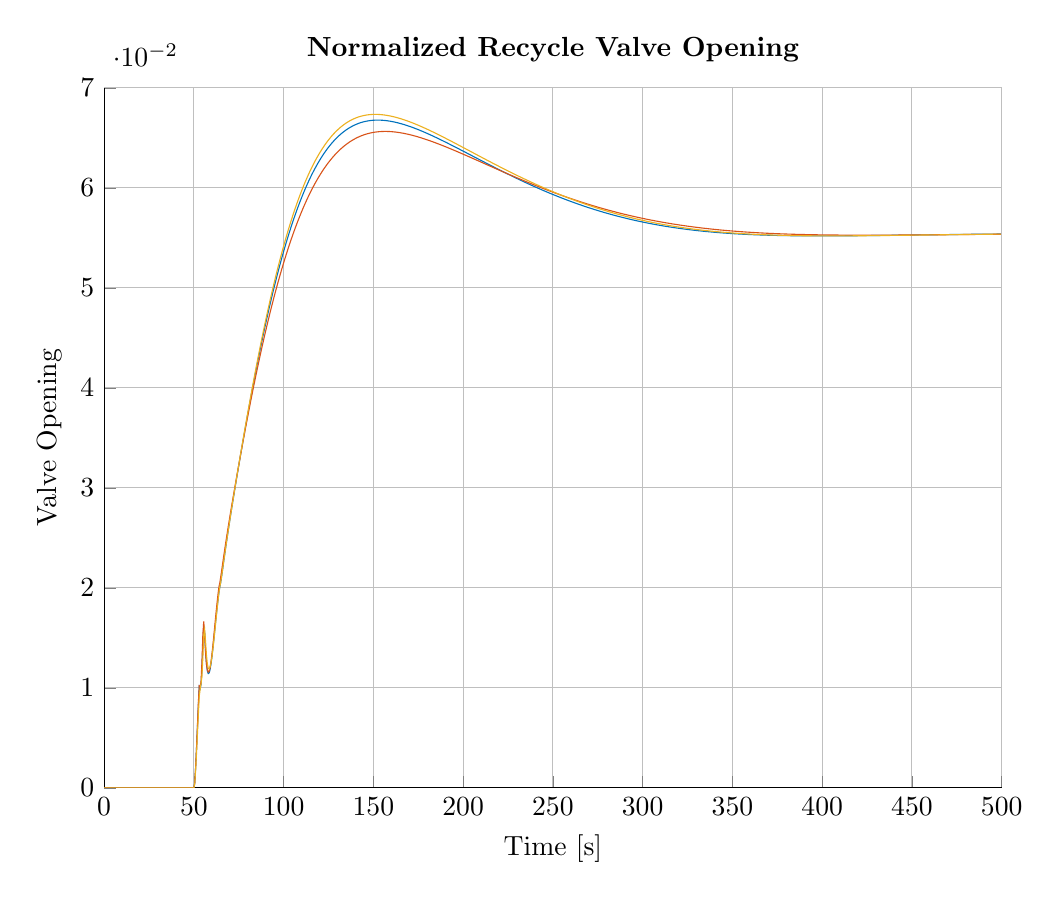
\begin{tikzpicture}

\begin{axis}[%
width=4.488in,
height=3.5in,
at={(0.791in,0.547in)},
scale only axis,
xmin=0,
xmax=500,
xlabel={Time [s]},
xmajorgrids,
ymin=0,
ymax=0.07,
ylabel={Valve Opening},
ymajorgrids,
axis background/.style={fill=white},
title style={font=\bfseries},
title={Normalized Recycle Valve Opening},
axis x line*=bottom,
axis y line*=left
]
\addplot [color=mycolor1,solid,forget plot]
  table[row sep=crcr]{%
0	6.93883000000002e-310\\
0.5	6.93883000000002e-310\\
1	6.93883000000002e-310\\
1.5	6.93883000000002e-310\\
2	6.93883000000002e-310\\
2.5	6.93883000000002e-310\\
3	6.93883000000002e-310\\
3.5	6.93883000000002e-310\\
4	6.93883000000002e-310\\
4.5	6.93883000000002e-310\\
5	6.93883000000002e-310\\
5.5	6.93883000000002e-310\\
6	6.93883000000002e-310\\
6.5	6.93883000000002e-310\\
7	6.93883000000002e-310\\
7.5	6.93883000000002e-310\\
8	6.93883000000002e-310\\
8.5	6.93883000000002e-310\\
9	6.93883000000002e-310\\
9.5	6.93883000000002e-310\\
10	6.93883000000002e-310\\
10.5	6.93883000000002e-310\\
11	6.93883000000002e-310\\
11.5	6.93883000000002e-310\\
12	6.93883000000002e-310\\
12.5	6.93883000000002e-310\\
13	6.93883000000002e-310\\
13.5	6.93883000000002e-310\\
14	6.93883000000002e-310\\
14.5	6.93883000000002e-310\\
15	6.93883000000002e-310\\
15.5	6.93883000000002e-310\\
16	6.93883000000002e-310\\
16.5	6.93883000000002e-310\\
17	6.93883000000002e-310\\
17.5	6.93883000000002e-310\\
18	6.93883000000002e-310\\
18.5	6.93883000000002e-310\\
19	6.93883000000002e-310\\
19.5	6.93883000000002e-310\\
20	6.93883000000002e-310\\
20.5	6.93883000000002e-310\\
21	6.93883000000002e-310\\
21.5	6.93883000000002e-310\\
22	6.93883000000002e-310\\
22.5	6.93883000000002e-310\\
23	6.93883000000002e-310\\
23.5	6.93883000000002e-310\\
24	6.93883000000002e-310\\
24.5	6.93883000000002e-310\\
25	6.93883000000002e-310\\
25.5	6.93883000000002e-310\\
26	6.93883000000002e-310\\
26.5	6.93883000000002e-310\\
27	6.93883000000002e-310\\
27.5	6.93883000000002e-310\\
28	6.93883000000002e-310\\
28.5	6.93883000000002e-310\\
29	6.93883000000002e-310\\
29.5	6.93883000000002e-310\\
30	6.93883000000002e-310\\
30.5	6.93883000000002e-310\\
31	6.93883000000002e-310\\
31.5	6.93883000000002e-310\\
32	6.93883000000002e-310\\
32.5	6.93883000000002e-310\\
33	6.93883000000002e-310\\
33.5	6.93883000000002e-310\\
34	6.93883000000002e-310\\
34.5	6.93883000000002e-310\\
35	6.93883000000002e-310\\
35.5	6.93883000000002e-310\\
36	6.93883000000002e-310\\
36.5	6.93883000000002e-310\\
37	6.93883000000002e-310\\
37.5	6.93883000000002e-310\\
38	6.93883000000002e-310\\
38.5	6.93883000000002e-310\\
39	6.93883000000002e-310\\
39.5	6.93883000000002e-310\\
40	6.93883000000002e-310\\
40.5	6.93883000000002e-310\\
41	6.93883000000002e-310\\
41.5	6.93883000000002e-310\\
42	6.93883000000002e-310\\
42.5	6.93883000000002e-310\\
43	6.93883000000002e-310\\
43.5	6.93883000000002e-310\\
44	6.93883000000002e-310\\
44.5	6.93883000000002e-310\\
45	6.93883000000002e-310\\
45.5	6.93883000000002e-310\\
46	6.93883000000002e-310\\
46.5	6.93883000000002e-310\\
47	6.93883000000002e-310\\
47.5	6.93883000000002e-310\\
48	6.93883000000002e-310\\
48.5	6.93883000000002e-310\\
49	6.93883000000002e-310\\
49.5	6.93883000000002e-310\\
50	6.93883000000002e-310\\
50.5	0.000509304\\
51	0.00211134\\
51.5	0.00400956\\
52	0.00609347\\
52.5	0.00815443\\
53	0.0101092\\
53.5	0.00992427\\
54	0.0103164\\
54.5	0.01186\\
55	0.014282\\
55.5	0.0161968\\
56	0.0155694\\
56.5	0.0137396\\
57	0.0124325\\
57.5	0.0117086\\
58	0.0114301\\
58.5	0.0114875\\
59	0.0118074\\
59.5	0.0123271\\
60	0.0129979\\
60.5	0.0137787\\
61	0.0146315\\
61.5	0.0155202\\
62	0.0164115\\
62.5	0.0172775\\
63	0.0180995\\
63.5	0.0188704\\
64	0.0195952\\
64.5	0.0201304\\
65	0.0205944\\
65.5	0.0211948\\
66	0.0218322\\
66.5	0.0224756\\
67	0.023115\\
67.5	0.023747\\
68	0.0243668\\
68.5	0.0249743\\
69	0.0255706\\
69.5	0.0261569\\
70	0.0267345\\
70.5	0.0273048\\
71	0.0278687\\
71.5	0.0284272\\
72	0.0289809\\
72.5	0.0295304\\
73	0.0300762\\
73.5	0.0306183\\
74	0.0311572\\
74.5	0.0316928\\
75	0.0322253\\
75.5	0.0327546\\
76	0.0332807\\
76.5	0.0338035\\
77	0.0343231\\
77.5	0.0348393\\
78	0.035352\\
78.5	0.0358611\\
79	0.0363666\\
79.5	0.0368684\\
80	0.0373663\\
80.5	0.0378604\\
81	0.0383504\\
81.5	0.0388365\\
82	0.0393184\\
82.5	0.0397961\\
83	0.0402697\\
83.5	0.0407389\\
84	0.0412038\\
84.5	0.0416643\\
85	0.0421204\\
85.5	0.042572\\
86	0.0430191\\
86.5	0.0434617\\
87	0.0438997\\
87.5	0.0443332\\
88	0.044762\\
88.5	0.0451862\\
89	0.0456058\\
89.5	0.0460206\\
90	0.0464308\\
90.5	0.0468363\\
91	0.0472371\\
91.5	0.0476332\\
92	0.0480245\\
92.5	0.0484112\\
93	0.048793\\
93.5	0.0491702\\
94	0.0495426\\
94.5	0.0499103\\
95	0.0502733\\
95.5	0.0506315\\
96	0.050985\\
96.5	0.0513338\\
97	0.0516778\\
97.5	0.0520172\\
98	0.0523519\\
98.5	0.0526819\\
99	0.0530072\\
99.5	0.0533279\\
100	0.0536439\\
100.5	0.0539554\\
101	0.0542622\\
101.5	0.0545644\\
102	0.054862\\
102.5	0.0551551\\
103	0.0554437\\
103.5	0.0557277\\
104	0.0560072\\
104.5	0.0562823\\
105	0.0565529\\
105.5	0.0568191\\
106	0.0570809\\
106.5	0.0573383\\
107	0.0575914\\
107.5	0.0578401\\
108	0.0580846\\
108.5	0.0583247\\
109	0.0585606\\
109.5	0.0587924\\
110	0.0590199\\
110.5	0.0592433\\
111	0.0594625\\
111.5	0.0596777\\
112	0.0598888\\
112.5	0.0600958\\
113	0.0602989\\
113.5	0.060498\\
114	0.0606932\\
114.5	0.0608844\\
115	0.0610718\\
115.5	0.0612554\\
116	0.0614352\\
116.5	0.0616112\\
117	0.0617835\\
117.5	0.0619521\\
118	0.062117\\
118.5	0.0622783\\
119	0.062436\\
119.5	0.0625902\\
120	0.0627409\\
120.5	0.0628881\\
121	0.0630318\\
121.5	0.0631722\\
122	0.0633091\\
122.5	0.0634428\\
123	0.0635732\\
123.5	0.0637003\\
124	0.0638242\\
124.5	0.0639449\\
125	0.0640625\\
125.5	0.064177\\
126	0.0642885\\
126.5	0.0643969\\
127	0.0645023\\
127.5	0.0646048\\
128	0.0647044\\
128.5	0.0648011\\
129	0.064895\\
129.5	0.0649861\\
130	0.0650744\\
130.5	0.06516\\
131	0.0652429\\
131.5	0.0653232\\
132	0.0654009\\
132.5	0.065476\\
133	0.0655486\\
133.5	0.0656186\\
134	0.0656863\\
134.5	0.0657515\\
135	0.0658143\\
135.5	0.0658748\\
136	0.0659329\\
136.5	0.0659888\\
137	0.0660424\\
137.5	0.0660939\\
138	0.0661432\\
138.5	0.0661903\\
139	0.0662353\\
139.5	0.0662783\\
140	0.0663193\\
140.5	0.0663582\\
141	0.0663952\\
141.5	0.0664302\\
142	0.0664634\\
142.5	0.0664947\\
143	0.0665241\\
143.5	0.0665518\\
144	0.0665777\\
144.5	0.0666018\\
145	0.0666243\\
145.5	0.0666451\\
146	0.0666642\\
146.5	0.0666817\\
147	0.0666976\\
147.5	0.066712\\
148	0.0667249\\
148.5	0.0667362\\
149	0.0667461\\
149.5	0.0667546\\
150	0.0667616\\
150.5	0.0667672\\
151	0.0667715\\
151.5	0.0667745\\
152	0.0667761\\
152.5	0.0667765\\
153	0.0667756\\
153.5	0.0667735\\
154	0.0667702\\
154.5	0.0667657\\
155	0.06676\\
155.5	0.0667532\\
156	0.0667453\\
156.5	0.0667363\\
157	0.0667263\\
157.5	0.0667152\\
158	0.0667031\\
158.5	0.06669\\
159	0.0666759\\
159.5	0.0666609\\
160	0.0666449\\
160.5	0.066628\\
161	0.0666103\\
161.5	0.0665916\\
162	0.0665721\\
162.5	0.0665518\\
163	0.0665306\\
163.5	0.0665087\\
164	0.066486\\
164.5	0.0664625\\
165	0.0664382\\
165.5	0.0664133\\
166	0.0663876\\
166.5	0.0663613\\
167	0.0663342\\
167.5	0.0663065\\
168	0.0662782\\
168.5	0.0662492\\
169	0.0662196\\
169.5	0.0661894\\
170	0.0661587\\
170.5	0.0661273\\
171	0.0660954\\
171.5	0.066063\\
172	0.06603\\
172.5	0.0659965\\
173	0.0659626\\
173.5	0.0659281\\
174	0.0658932\\
174.5	0.0658578\\
175	0.0658219\\
175.5	0.0657856\\
176	0.0657489\\
176.5	0.0657118\\
177	0.0656743\\
177.5	0.0656363\\
178	0.065598\\
178.5	0.0655594\\
179	0.0655203\\
179.5	0.065481\\
180	0.0654412\\
180.5	0.0654012\\
181	0.0653608\\
181.5	0.0653202\\
182	0.0652792\\
182.5	0.065238\\
183	0.0651964\\
183.5	0.0651546\\
184	0.0651126\\
184.5	0.0650702\\
185	0.0650277\\
185.5	0.0649849\\
186	0.0649418\\
186.5	0.0648986\\
187	0.0648551\\
187.5	0.0648115\\
188	0.0647676\\
188.5	0.0647236\\
189	0.0646794\\
189.5	0.064635\\
190	0.0645904\\
190.5	0.0645457\\
191	0.0645008\\
191.5	0.0644558\\
192	0.0644106\\
192.5	0.0643653\\
193	0.0643199\\
193.5	0.0642743\\
194	0.0642287\\
194.5	0.0641829\\
195	0.0641371\\
195.5	0.0640911\\
196	0.0640451\\
196.5	0.0639989\\
197	0.0639527\\
197.5	0.0639064\\
198	0.0638601\\
198.5	0.0638136\\
199	0.0637672\\
199.5	0.0637206\\
200	0.0636741\\
200.5	0.0636274\\
201	0.0635808\\
201.5	0.0635341\\
202	0.0634874\\
202.5	0.0634406\\
203	0.0633938\\
203.5	0.0633471\\
204	0.0633003\\
204.5	0.0632535\\
205	0.0632067\\
205.5	0.0631599\\
206	0.0631131\\
206.5	0.0630663\\
207	0.0630195\\
207.5	0.0629727\\
208	0.062926\\
208.5	0.0628793\\
209	0.0628326\\
209.5	0.062786\\
210	0.0627393\\
210.5	0.0626928\\
211	0.0626462\\
211.5	0.0625997\\
212	0.0625533\\
212.5	0.0625069\\
213	0.0624605\\
213.5	0.0624142\\
214	0.062368\\
214.5	0.0623219\\
215	0.0622758\\
215.5	0.0622297\\
216	0.0621838\\
216.5	0.0621379\\
217	0.0620921\\
217.5	0.0620464\\
218	0.0620007\\
218.5	0.0619552\\
219	0.0619097\\
219.5	0.0618643\\
220	0.061819\\
220.5	0.0617738\\
221	0.0617287\\
221.5	0.0616837\\
222	0.0616388\\
222.5	0.061594\\
223	0.0615493\\
223.5	0.0615048\\
224	0.0614603\\
224.5	0.0614159\\
225	0.0613717\\
225.5	0.0613275\\
226	0.0612835\\
226.5	0.0612396\\
227	0.0611959\\
227.5	0.0611522\\
228	0.0611087\\
228.5	0.0610653\\
229	0.061022\\
229.5	0.0609789\\
230	0.0609359\\
230.5	0.060893\\
231	0.0608502\\
231.5	0.0608076\\
232	0.0607652\\
232.5	0.0607228\\
233	0.0606806\\
233.5	0.0606386\\
234	0.0605967\\
234.5	0.0605549\\
235	0.0605133\\
235.5	0.0604719\\
236	0.0604305\\
236.5	0.0603894\\
237	0.0603484\\
237.5	0.0603075\\
238	0.0602668\\
238.5	0.0602262\\
239	0.0601858\\
239.5	0.0601456\\
240	0.0601055\\
240.5	0.0600656\\
241	0.0600258\\
241.5	0.0599862\\
242	0.0599468\\
242.5	0.0599075\\
243	0.0598684\\
243.5	0.0598295\\
244	0.0597907\\
244.5	0.0597521\\
245	0.0597136\\
245.5	0.0596753\\
246	0.0596372\\
246.5	0.0595993\\
247	0.0595615\\
247.5	0.0595239\\
248	0.0594865\\
248.5	0.0594492\\
249	0.0594121\\
249.5	0.0593752\\
250	0.0593385\\
};
\addplot [color=mycolor1,solid,forget plot]
  table[row sep=crcr]{%
250	0.0593385\\
250.5	0.0593019\\
251	0.0592655\\
251.5	0.0592293\\
252	0.0591933\\
252.5	0.0591574\\
253	0.0591218\\
253.5	0.0590863\\
254	0.0590509\\
254.5	0.0590158\\
255	0.0589808\\
255.5	0.0589461\\
256	0.0589115\\
256.5	0.058877\\
257	0.0588428\\
257.5	0.0588087\\
258	0.0587749\\
258.5	0.0587412\\
259	0.0587077\\
259.5	0.0586743\\
260	0.0586412\\
260.5	0.0586082\\
261	0.0585754\\
261.5	0.0585429\\
262	0.0585104\\
262.5	0.0584782\\
263	0.0584462\\
263.5	0.0584143\\
264	0.0583827\\
264.5	0.0583512\\
265	0.0583199\\
265.5	0.0582887\\
266	0.0582578\\
266.5	0.0582271\\
267	0.0581965\\
267.5	0.0581661\\
268	0.0581359\\
268.5	0.0581059\\
269	0.0580761\\
269.5	0.0580465\\
270	0.058017\\
270.5	0.0579878\\
271	0.0579587\\
271.5	0.0579298\\
272	0.0579011\\
272.5	0.0578726\\
273	0.0578442\\
273.5	0.0578161\\
274	0.0577881\\
274.5	0.0577603\\
275	0.0577327\\
275.5	0.0577053\\
276	0.0576781\\
276.5	0.0576511\\
277	0.0576242\\
277.5	0.0575975\\
278	0.057571\\
278.5	0.0575447\\
279	0.0575186\\
279.5	0.0574927\\
280	0.0574669\\
280.5	0.0574413\\
281	0.0574159\\
281.5	0.0573907\\
282	0.0573657\\
282.5	0.0573408\\
283	0.0573162\\
283.5	0.0572917\\
284	0.0572674\\
284.5	0.0572432\\
285	0.0572193\\
285.5	0.0571955\\
286	0.0571719\\
286.5	0.0571485\\
287	0.0571253\\
287.5	0.0571022\\
288	0.0570794\\
288.5	0.0570567\\
289	0.0570341\\
289.5	0.0570118\\
290	0.0569896\\
290.5	0.0569676\\
291	0.0569458\\
291.5	0.0569241\\
292	0.0569027\\
292.5	0.0568814\\
293	0.0568603\\
293.5	0.0568393\\
294	0.0568185\\
294.5	0.0567979\\
295	0.0567775\\
295.5	0.0567572\\
296	0.0567371\\
296.5	0.0567172\\
297	0.0566974\\
297.5	0.0566778\\
298	0.0566584\\
298.5	0.0566392\\
299	0.0566201\\
299.5	0.0566011\\
300	0.0565824\\
300.5	0.0565638\\
301	0.0565454\\
301.5	0.0565271\\
302	0.056509\\
302.5	0.0564911\\
303	0.0564733\\
303.5	0.0564557\\
304	0.0564382\\
304.5	0.056421\\
305	0.0564038\\
305.5	0.0563869\\
306	0.05637\\
306.5	0.0563534\\
307	0.0563369\\
307.5	0.0563205\\
308	0.0563044\\
308.5	0.0562883\\
309	0.0562725\\
309.5	0.0562567\\
310	0.0562412\\
310.5	0.0562258\\
311	0.0562105\\
311.5	0.0561954\\
312	0.0561804\\
312.5	0.0561656\\
313	0.0561509\\
313.5	0.0561364\\
314	0.056122\\
314.5	0.0561078\\
315	0.0560938\\
315.5	0.0560798\\
316	0.056066\\
316.5	0.0560524\\
317	0.0560389\\
317.5	0.0560255\\
318	0.0560123\\
318.5	0.0559993\\
319	0.0559863\\
319.5	0.0559735\\
320	0.0559609\\
320.5	0.0559484\\
321	0.055936\\
321.5	0.0559238\\
322	0.0559116\\
322.5	0.0558997\\
323	0.0558878\\
323.5	0.0558761\\
324	0.0558646\\
324.5	0.0558531\\
325	0.0558418\\
325.5	0.0558307\\
326	0.0558196\\
326.5	0.0558087\\
327	0.0557979\\
327.5	0.0557872\\
328	0.0557767\\
328.5	0.0557663\\
329	0.055756\\
329.5	0.0557459\\
330	0.0557358\\
330.5	0.0557259\\
331	0.0557161\\
331.5	0.0557065\\
332	0.0556969\\
332.5	0.0556875\\
333	0.0556782\\
333.5	0.055669\\
334	0.0556599\\
334.5	0.0556509\\
335	0.0556421\\
335.5	0.0556334\\
336	0.0556248\\
336.5	0.0556163\\
337	0.0556079\\
337.5	0.0555996\\
338	0.0555914\\
338.5	0.0555834\\
339	0.0555754\\
339.5	0.0555676\\
340	0.0555599\\
340.5	0.0555523\\
341	0.0555447\\
341.5	0.0555373\\
342	0.05553\\
342.5	0.0555228\\
343	0.0555157\\
343.5	0.0555087\\
344	0.0555018\\
344.5	0.055495\\
345	0.0554884\\
345.5	0.0554818\\
346	0.0554753\\
346.5	0.0554689\\
347	0.0554626\\
347.5	0.0554564\\
348	0.0554503\\
348.5	0.0554442\\
349	0.0554383\\
349.5	0.0554325\\
350	0.0554268\\
350.5	0.0554211\\
351	0.0554156\\
351.5	0.0554101\\
352	0.0554047\\
352.5	0.0553994\\
353	0.0553942\\
353.5	0.0553891\\
354	0.0553841\\
354.5	0.0553792\\
355	0.0553743\\
355.5	0.0553695\\
356	0.0553648\\
356.5	0.0553602\\
357	0.0553557\\
357.5	0.0553513\\
358	0.0553469\\
358.5	0.0553426\\
359	0.0553384\\
359.5	0.0553343\\
360	0.0553302\\
360.5	0.0553263\\
361	0.0553224\\
361.5	0.0553186\\
362	0.0553148\\
362.5	0.0553111\\
363	0.0553075\\
363.5	0.055304\\
364	0.0553006\\
364.5	0.0552972\\
365	0.0552939\\
365.5	0.0552906\\
366	0.0552874\\
366.5	0.0552843\\
367	0.0552813\\
367.5	0.0552783\\
368	0.0552754\\
368.5	0.0552725\\
369	0.0552698\\
369.5	0.0552671\\
370	0.0552644\\
370.5	0.0552618\\
371	0.0552593\\
371.5	0.0552568\\
372	0.0552544\\
372.5	0.0552521\\
373	0.0552498\\
373.5	0.0552475\\
374	0.0552454\\
374.5	0.0552433\\
375	0.0552412\\
375.5	0.0552392\\
376	0.0552373\\
376.5	0.0552354\\
377	0.0552335\\
377.5	0.0552318\\
378	0.05523\\
378.5	0.0552283\\
379	0.0552267\\
379.5	0.0552251\\
380	0.0552236\\
380.5	0.0552221\\
381	0.0552207\\
381.5	0.0552193\\
382	0.055218\\
382.5	0.0552167\\
383	0.0552155\\
383.5	0.0552143\\
384	0.0552132\\
384.5	0.0552121\\
385	0.055211\\
385.5	0.05521\\
386	0.055209\\
386.5	0.0552081\\
387	0.0552072\\
387.5	0.0552064\\
388	0.0552056\\
388.5	0.0552048\\
389	0.0552041\\
389.5	0.0552035\\
390	0.0552028\\
390.5	0.0552022\\
391	0.0552017\\
391.5	0.0552011\\
392	0.0552006\\
392.5	0.0552002\\
393	0.0551998\\
393.5	0.0551994\\
394	0.055199\\
394.5	0.0551987\\
395	0.0551985\\
395.5	0.0551982\\
396	0.055198\\
396.5	0.0551978\\
397	0.0551977\\
397.5	0.0551976\\
398	0.0551975\\
398.5	0.0551974\\
399	0.0551974\\
399.5	0.0551974\\
400	0.0551974\\
400.5	0.0551975\\
401	0.0551976\\
401.5	0.0551977\\
402	0.0551978\\
402.5	0.055198\\
403	0.0551982\\
403.5	0.0551984\\
404	0.0551987\\
404.5	0.055199\\
405	0.0551993\\
405.5	0.0551996\\
406	0.0551999\\
406.5	0.0552003\\
407	0.0552007\\
407.5	0.0552011\\
408	0.0552016\\
408.5	0.055202\\
409	0.0552025\\
409.5	0.055203\\
410	0.0552035\\
410.5	0.0552041\\
411	0.0552046\\
411.5	0.0552052\\
412	0.0552058\\
412.5	0.0552064\\
413	0.0552071\\
413.5	0.0552077\\
414	0.0552084\\
414.5	0.0552091\\
415	0.0552098\\
415.5	0.0552105\\
416	0.0552113\\
416.5	0.055212\\
417	0.0552128\\
417.5	0.0552136\\
418	0.0552144\\
418.5	0.0552152\\
419	0.055216\\
419.5	0.0552169\\
420	0.0552177\\
420.5	0.0552186\\
421	0.0552195\\
421.5	0.0552204\\
422	0.0552213\\
422.5	0.0552222\\
423	0.0552231\\
423.5	0.0552241\\
424	0.055225\\
424.5	0.055226\\
425	0.0552269\\
425.5	0.0552279\\
426	0.0552289\\
426.5	0.0552299\\
427	0.0552309\\
427.5	0.055232\\
428	0.055233\\
428.5	0.055234\\
429	0.0552351\\
429.5	0.0552361\\
430	0.0552372\\
430.5	0.0552383\\
431	0.0552393\\
431.5	0.0552404\\
432	0.0552415\\
432.5	0.0552426\\
433	0.0552437\\
433.5	0.0552448\\
434	0.055246\\
434.5	0.0552471\\
435	0.0552482\\
435.5	0.0552493\\
436	0.0552505\\
436.5	0.0552516\\
437	0.0552528\\
437.5	0.0552539\\
438	0.0552551\\
438.5	0.0552562\\
439	0.0552574\\
439.5	0.0552586\\
440	0.0552597\\
440.5	0.0552609\\
441	0.0552621\\
441.5	0.0552633\\
442	0.0552644\\
442.5	0.0552656\\
443	0.0552668\\
443.5	0.055268\\
444	0.0552692\\
444.5	0.0552704\\
445	0.0552716\\
445.5	0.0552728\\
446	0.0552739\\
446.5	0.0552751\\
447	0.0552763\\
447.5	0.0552775\\
448	0.0552787\\
448.5	0.0552799\\
449	0.0552811\\
449.5	0.0552823\\
450	0.0552835\\
450.5	0.0552847\\
451	0.0552859\\
451.5	0.0552871\\
452	0.0552883\\
452.5	0.0552895\\
453	0.0552907\\
453.5	0.0552919\\
454	0.0552931\\
454.5	0.0552943\\
455	0.0552954\\
455.5	0.0552966\\
456	0.0552978\\
456.5	0.055299\\
457	0.0553002\\
457.5	0.0553014\\
458	0.0553025\\
458.5	0.0553037\\
459	0.0553049\\
459.5	0.0553061\\
460	0.0553072\\
460.5	0.0553084\\
461	0.0553095\\
461.5	0.0553107\\
462	0.0553119\\
462.5	0.055313\\
463	0.0553142\\
463.5	0.0553153\\
464	0.0553164\\
464.5	0.0553176\\
465	0.0553187\\
465.5	0.0553199\\
466	0.055321\\
466.5	0.0553221\\
467	0.0553232\\
467.5	0.0553243\\
468	0.0553254\\
468.5	0.0553266\\
469	0.0553277\\
469.5	0.0553288\\
470	0.0553299\\
470.5	0.0553309\\
471	0.055332\\
471.5	0.0553331\\
472	0.0553342\\
472.5	0.0553353\\
473	0.0553363\\
473.5	0.0553374\\
474	0.0553385\\
474.5	0.0553395\\
475	0.0553406\\
475.5	0.0553416\\
476	0.0553426\\
476.5	0.0553437\\
477	0.0553447\\
477.5	0.0553457\\
478	0.0553467\\
478.5	0.0553478\\
479	0.0553488\\
479.5	0.0553498\\
480	0.0553508\\
480.5	0.0553518\\
481	0.0553527\\
481.5	0.0553537\\
482	0.0553547\\
482.5	0.0553557\\
483	0.0553566\\
483.5	0.0553576\\
484	0.0553585\\
484.5	0.0553595\\
485	0.0553604\\
485.5	0.0553614\\
486	0.0553623\\
486.5	0.0553632\\
487	0.0553641\\
487.5	0.055365\\
488	0.055366\\
488.5	0.0553669\\
489	0.0553678\\
489.5	0.0553686\\
490	0.0553695\\
490.5	0.0553704\\
491	0.0553713\\
491.5	0.0553721\\
492	0.055373\\
492.5	0.0553739\\
493	0.0553747\\
493.5	0.0553755\\
494	0.0553764\\
494.5	0.0553772\\
495	0.055378\\
495.5	0.0553789\\
496	0.0553797\\
496.5	0.0553805\\
497	0.0553813\\
497.5	0.0553821\\
498	0.0553828\\
498.5	0.0553836\\
499	0.0553844\\
499.5	0.0553852\\
};
\addplot [color=mycolor2,solid,forget plot]
  table[row sep=crcr]{%
0	6.91844e-310\\
0.5	6.91844e-310\\
1	6.91844e-310\\
1.5	6.91844e-310\\
2	6.91844e-310\\
2.5	6.91844e-310\\
3	6.91844e-310\\
3.5	6.91844e-310\\
4	6.91844e-310\\
4.5	6.91844e-310\\
5	6.91844e-310\\
5.5	6.91844e-310\\
6	6.91844e-310\\
6.5	6.91844e-310\\
7	6.91844e-310\\
7.5	6.91844e-310\\
8	6.91844e-310\\
8.5	6.91844e-310\\
9	6.91844e-310\\
9.5	6.91844e-310\\
10	6.91844e-310\\
10.5	6.91844e-310\\
11	6.91844e-310\\
11.5	6.91844e-310\\
12	6.91844e-310\\
12.5	6.91844e-310\\
13	6.91844e-310\\
13.5	6.91844e-310\\
14	6.91844e-310\\
14.5	6.91844e-310\\
15	6.91844e-310\\
15.5	6.91844e-310\\
16	6.91844e-310\\
16.5	6.91844e-310\\
17	6.91844e-310\\
17.5	6.91844e-310\\
18	6.91844e-310\\
18.5	6.91844e-310\\
19	6.91844e-310\\
19.5	6.91844e-310\\
20	6.91844e-310\\
20.5	6.91844e-310\\
21	6.91844e-310\\
21.5	6.91844e-310\\
22	6.91844e-310\\
22.5	6.91844e-310\\
23	6.91844e-310\\
23.5	6.91844e-310\\
24	6.91844e-310\\
24.5	6.91844e-310\\
25	6.91844e-310\\
25.5	6.91844e-310\\
26	6.91844e-310\\
26.5	6.91844e-310\\
27	6.91844e-310\\
27.5	6.91844e-310\\
28	6.91844e-310\\
28.5	6.91844e-310\\
29	6.91844e-310\\
29.5	6.91844e-310\\
30	6.91844e-310\\
30.5	6.91844e-310\\
31	6.91844e-310\\
31.5	6.91844e-310\\
32	6.91844e-310\\
32.5	6.91844e-310\\
33	6.91844e-310\\
33.5	6.91844e-310\\
34	6.91844e-310\\
34.5	6.91844e-310\\
35	6.91844e-310\\
35.5	6.91844e-310\\
36	6.91844e-310\\
36.5	6.91844e-310\\
37	6.91844e-310\\
37.5	6.91844e-310\\
38	6.91844e-310\\
38.5	6.91844e-310\\
39	6.91844e-310\\
39.5	6.91844e-310\\
40	6.91844e-310\\
40.5	6.91844e-310\\
41	6.91844e-310\\
41.5	6.91844e-310\\
42	6.91844e-310\\
42.5	6.91844e-310\\
43	6.91844e-310\\
43.5	6.91844e-310\\
44	6.91844e-310\\
44.5	6.91844e-310\\
45	6.91844e-310\\
45.5	6.91844e-310\\
46	6.91844e-310\\
46.5	6.91844e-310\\
47	6.91844e-310\\
47.5	6.91844e-310\\
48	6.91844e-310\\
48.5	6.91844e-310\\
49	6.91844e-310\\
49.5	6.91844e-310\\
50	6.91844e-310\\
50.5	0.000522473\\
51	0.00216432\\
51.5	0.00412168\\
52	0.00630136\\
52.5	0.00850739\\
53	0.0101892\\
53.5	0.0101035\\
54	0.0106601\\
54.5	0.0125997\\
55	0.0152694\\
55.5	0.0166539\\
56	0.0152726\\
56.5	0.0135382\\
57	0.0124146\\
57.5	0.0118055\\
58	0.0115739\\
58.5	0.0116558\\
59	0.0119993\\
59.5	0.0125482\\
60	0.0132555\\
60.5	0.0140792\\
61	0.0149794\\
61.5	0.0159176\\
62	0.0168581\\
62.5	0.0177707\\
63	0.0186351\\
63.5	0.0194435\\
64	0.0201151\\
64.5	0.0205489\\
65	0.021133\\
65.5	0.0217541\\
66	0.0223797\\
66.5	0.0229991\\
67	0.0236135\\
67.5	0.0242172\\
68	0.0248089\\
68.5	0.0253888\\
69	0.0259578\\
69.5	0.0265171\\
70	0.0270678\\
70.5	0.0276109\\
71	0.0281477\\
71.5	0.0286788\\
72	0.029205\\
72.5	0.0297268\\
73	0.0302448\\
73.5	0.0307591\\
74	0.03127\\
74.5	0.0317777\\
75	0.0322821\\
75.5	0.0327834\\
76	0.0332815\\
76.5	0.0337764\\
77	0.034268\\
77.5	0.0347562\\
78	0.0352411\\
78.5	0.0357224\\
79	0.0362002\\
79.5	0.0366744\\
80	0.0371448\\
80.5	0.0376114\\
81	0.0380742\\
81.5	0.0385331\\
82	0.038988\\
82.5	0.0394389\\
83	0.0398856\\
83.5	0.0403283\\
84	0.0407668\\
84.5	0.0412011\\
85	0.0416312\\
85.5	0.042057\\
86	0.0424785\\
86.5	0.0428957\\
87	0.0433085\\
87.5	0.043717\\
88	0.0441212\\
88.5	0.0445209\\
89	0.0449162\\
89.5	0.0453071\\
90	0.0456936\\
90.5	0.0460757\\
91	0.0464533\\
91.5	0.0468265\\
92	0.0471953\\
92.5	0.0475596\\
93	0.0479195\\
93.5	0.048275\\
94	0.048626\\
94.5	0.0489727\\
95	0.0493149\\
95.5	0.0496528\\
96	0.0499862\\
96.5	0.0503153\\
97	0.05064\\
97.5	0.0509604\\
98	0.0512764\\
98.5	0.0515881\\
99	0.0518955\\
99.5	0.0521986\\
100	0.0524975\\
100.5	0.0527921\\
101	0.0530824\\
101.5	0.0533686\\
102	0.0536505\\
102.5	0.0539283\\
103	0.0542019\\
103.5	0.0544714\\
104	0.0547368\\
104.5	0.0549981\\
105	0.0552553\\
105.5	0.0555086\\
106	0.0557578\\
106.5	0.056003\\
107	0.0562443\\
107.5	0.0564816\\
108	0.056715\\
108.5	0.0569446\\
109	0.0571703\\
109.5	0.0573922\\
110	0.0576103\\
110.5	0.0578246\\
111	0.0580352\\
111.5	0.0582421\\
112	0.0584453\\
112.5	0.0586448\\
113	0.0588408\\
113.5	0.0590331\\
114	0.0592219\\
114.5	0.0594072\\
115	0.0595889\\
115.5	0.0597673\\
116	0.0599421\\
116.5	0.0601136\\
117	0.0602817\\
117.5	0.0604465\\
118	0.0606079\\
118.5	0.0607661\\
119	0.0609211\\
119.5	0.0610728\\
120	0.0612214\\
120.5	0.0613668\\
121	0.0615091\\
121.5	0.0616483\\
122	0.0617845\\
122.5	0.0619177\\
123	0.0620479\\
123.5	0.0621751\\
124	0.0622994\\
124.5	0.0624209\\
125	0.0625395\\
125.5	0.0626553\\
126	0.0627683\\
126.5	0.0628785\\
127	0.0629861\\
127.5	0.0630909\\
128	0.0631931\\
128.5	0.0632927\\
129	0.0633897\\
129.5	0.0634842\\
130	0.0635761\\
130.5	0.0636656\\
131	0.0637526\\
131.5	0.0638372\\
132	0.0639194\\
132.5	0.0639992\\
133	0.0640767\\
133.5	0.0641519\\
134	0.0642249\\
134.5	0.0642956\\
135	0.0643641\\
135.5	0.0644305\\
136	0.0644947\\
136.5	0.0645568\\
137	0.0646169\\
137.5	0.0646749\\
138	0.0647309\\
138.5	0.0647849\\
139	0.0648369\\
139.5	0.0648871\\
140	0.0649353\\
140.5	0.0649817\\
141	0.0650262\\
141.5	0.065069\\
142	0.06511\\
142.5	0.0651492\\
143	0.0651867\\
143.5	0.0652225\\
144	0.0652566\\
144.5	0.0652891\\
145	0.06532\\
145.5	0.0653493\\
146	0.065377\\
146.5	0.0654033\\
147	0.065428\\
147.5	0.0654512\\
148	0.065473\\
148.5	0.0654933\\
149	0.0655123\\
149.5	0.0655299\\
150	0.0655461\\
150.5	0.065561\\
151	0.0655746\\
151.5	0.0655869\\
152	0.0655979\\
152.5	0.0656077\\
153	0.0656163\\
153.5	0.0656237\\
154	0.06563\\
154.5	0.0656351\\
155	0.0656391\\
155.5	0.0656419\\
156	0.0656437\\
156.5	0.0656444\\
157	0.0656441\\
157.5	0.0656428\\
158	0.0656404\\
158.5	0.0656371\\
159	0.0656328\\
159.5	0.0656276\\
160	0.0656215\\
160.5	0.0656144\\
161	0.0656065\\
161.5	0.0655976\\
162	0.065588\\
162.5	0.0655775\\
163	0.0655662\\
163.5	0.065554\\
164	0.0655411\\
164.5	0.0655275\\
165	0.0655131\\
165.5	0.0654979\\
166	0.065482\\
166.5	0.0654655\\
167	0.0654482\\
167.5	0.0654303\\
168	0.0654117\\
168.5	0.0653924\\
169	0.0653725\\
169.5	0.0653521\\
170	0.065331\\
170.5	0.0653093\\
171	0.065287\\
171.5	0.0652642\\
172	0.0652408\\
172.5	0.0652169\\
173	0.0651925\\
173.5	0.0651676\\
174	0.0651421\\
174.5	0.0651162\\
175	0.0650898\\
175.5	0.0650629\\
176	0.0650356\\
176.5	0.0650078\\
177	0.0649796\\
177.5	0.064951\\
178	0.0649219\\
178.5	0.0648925\\
179	0.0648627\\
179.5	0.0648325\\
180	0.0648019\\
180.5	0.0647709\\
181	0.0647396\\
181.5	0.064708\\
182	0.064676\\
182.5	0.0646437\\
183	0.0646111\\
183.5	0.0645782\\
184	0.064545\\
184.5	0.0645115\\
185	0.0644777\\
185.5	0.0644437\\
186	0.0644094\\
186.5	0.0643748\\
187	0.06434\\
187.5	0.0643049\\
188	0.0642696\\
188.5	0.064234\\
189	0.0641983\\
189.5	0.0641623\\
190	0.0641262\\
190.5	0.0640898\\
191	0.0640532\\
191.5	0.0640165\\
192	0.0639795\\
192.5	0.0639424\\
193	0.0639052\\
193.5	0.0638677\\
194	0.0638302\\
194.5	0.0637924\\
195	0.0637545\\
195.5	0.0637165\\
196	0.0636784\\
196.5	0.0636401\\
197	0.0636017\\
197.5	0.0635632\\
198	0.0635246\\
198.5	0.0634858\\
199	0.063447\\
199.5	0.0634081\\
200	0.0633691\\
200.5	0.06333\\
201	0.0632908\\
201.5	0.0632515\\
202	0.0632122\\
202.5	0.0631728\\
203	0.0631333\\
203.5	0.0630938\\
204	0.0630542\\
204.5	0.0630146\\
205	0.062975\\
205.5	0.0629352\\
206	0.0628955\\
206.5	0.0628557\\
207	0.0628159\\
207.5	0.062776\\
208	0.0627362\\
208.5	0.0626963\\
209	0.0626564\\
209.5	0.0626165\\
210	0.0625766\\
210.5	0.0625366\\
211	0.0624967\\
211.5	0.0624568\\
212	0.0624168\\
212.5	0.0623769\\
213	0.062337\\
213.5	0.0622971\\
214	0.0622572\\
214.5	0.0622174\\
215	0.0621775\\
215.5	0.0621377\\
216	0.0620979\\
216.5	0.0620582\\
217	0.0620184\\
217.5	0.0619787\\
218	0.0619391\\
218.5	0.0618995\\
219	0.0618599\\
219.5	0.0618204\\
220	0.0617809\\
220.5	0.0617415\\
221	0.0617021\\
221.5	0.0616628\\
222	0.0616235\\
222.5	0.0615843\\
223	0.0615452\\
223.5	0.0615061\\
224	0.0614671\\
224.5	0.0614282\\
225	0.0613893\\
225.5	0.0613505\\
226	0.0613118\\
226.5	0.0612731\\
227	0.0612345\\
227.5	0.061196\\
228	0.0611576\\
228.5	0.0611193\\
229	0.0610811\\
229.5	0.0610429\\
230	0.0610048\\
230.5	0.0609668\\
231	0.0609289\\
231.5	0.0608911\\
232	0.0608534\\
232.5	0.0608158\\
233	0.0607783\\
233.5	0.0607409\\
234	0.0607036\\
234.5	0.0606664\\
235	0.0606293\\
235.5	0.0605923\\
236	0.0605554\\
236.5	0.0605186\\
237	0.0604819\\
237.5	0.0604453\\
238	0.0604088\\
238.5	0.0603725\\
239	0.0603362\\
239.5	0.0603001\\
240	0.0602641\\
240.5	0.0602282\\
241	0.0601924\\
241.5	0.0601568\\
242	0.0601212\\
242.5	0.0600858\\
243	0.0600505\\
243.5	0.0600153\\
244	0.0599803\\
244.5	0.0599453\\
245	0.0599105\\
245.5	0.0598759\\
246	0.0598413\\
246.5	0.0598069\\
247	0.0597726\\
247.5	0.0597384\\
248	0.0597044\\
248.5	0.0596705\\
249	0.0596367\\
249.5	0.0596031\\
250	0.0595696\\
};
\addplot [color=mycolor2,solid,forget plot]
  table[row sep=crcr]{%
250	0.0595696\\
250.5	0.0595362\\
251	0.059503\\
251.5	0.0594699\\
252	0.0594369\\
252.5	0.0594041\\
253	0.0593714\\
253.5	0.0593388\\
254	0.0593064\\
254.5	0.0592741\\
255	0.059242\\
255.5	0.05921\\
256	0.0591781\\
256.5	0.0591464\\
257	0.0591148\\
257.5	0.0590834\\
258	0.0590521\\
258.5	0.0590209\\
259	0.0589899\\
259.5	0.058959\\
260	0.0589283\\
260.5	0.0588977\\
261	0.0588673\\
261.5	0.058837\\
262	0.0588069\\
262.5	0.0587769\\
263	0.058747\\
263.5	0.0587173\\
264	0.0586878\\
264.5	0.0586584\\
265	0.0586291\\
265.5	0.0586\\
266	0.058571\\
266.5	0.0585422\\
267	0.0585135\\
267.5	0.058485\\
268	0.0584566\\
268.5	0.0584284\\
269	0.0584003\\
269.5	0.0583724\\
270	0.0583446\\
270.5	0.0583169\\
271	0.0582895\\
271.5	0.0582621\\
272	0.0582349\\
272.5	0.0582079\\
273	0.058181\\
273.5	0.0581543\\
274	0.0581277\\
274.5	0.0581012\\
275	0.058075\\
275.5	0.0580488\\
276	0.0580228\\
276.5	0.057997\\
277	0.0579713\\
277.5	0.0579458\\
278	0.0579204\\
278.5	0.0578951\\
279	0.05787\\
279.5	0.0578451\\
280	0.0578203\\
280.5	0.0577957\\
281	0.0577712\\
281.5	0.0577468\\
282	0.0577226\\
282.5	0.0576986\\
283	0.0576747\\
283.5	0.057651\\
284	0.0576274\\
284.5	0.0576039\\
285	0.0575806\\
285.5	0.0575575\\
286	0.0575345\\
286.5	0.0575116\\
287	0.0574889\\
287.5	0.0574663\\
288	0.0574439\\
288.5	0.0574216\\
289	0.0573995\\
289.5	0.0573776\\
290	0.0573557\\
290.5	0.057334\\
291	0.0573125\\
291.5	0.0572911\\
292	0.0572699\\
292.5	0.0572488\\
293	0.0572278\\
293.5	0.057207\\
294	0.0571864\\
294.5	0.0571658\\
295	0.0571455\\
295.5	0.0571252\\
296	0.0571051\\
296.5	0.0570852\\
297	0.0570654\\
297.5	0.0570457\\
298	0.0570262\\
298.5	0.0570068\\
299	0.0569876\\
299.5	0.0569685\\
300	0.0569496\\
300.5	0.0569307\\
301	0.0569121\\
301.5	0.0568935\\
302	0.0568751\\
302.5	0.0568569\\
303	0.0568388\\
303.5	0.0568208\\
304	0.0568029\\
304.5	0.0567852\\
305	0.0567677\\
305.5	0.0567502\\
306	0.0567329\\
306.5	0.0567158\\
307	0.0566988\\
307.5	0.0566819\\
308	0.0566651\\
308.5	0.0566485\\
309	0.056632\\
309.5	0.0566156\\
310	0.0565994\\
310.5	0.0565833\\
311	0.0565674\\
311.5	0.0565515\\
312	0.0565358\\
312.5	0.0565203\\
313	0.0565048\\
313.5	0.0564895\\
314	0.0564743\\
314.5	0.0564593\\
315	0.0564444\\
315.5	0.0564296\\
316	0.0564149\\
316.5	0.0564003\\
317	0.0563859\\
317.5	0.0563716\\
318	0.0563575\\
318.5	0.0563434\\
319	0.0563295\\
319.5	0.0563157\\
320	0.056302\\
320.5	0.0562885\\
321	0.056275\\
321.5	0.0562617\\
322	0.0562485\\
322.5	0.0562355\\
323	0.0562225\\
323.5	0.0562097\\
324	0.056197\\
324.5	0.0561844\\
325	0.0561719\\
325.5	0.0561595\\
326	0.0561473\\
326.5	0.0561352\\
327	0.0561232\\
327.5	0.0561113\\
328	0.0560995\\
328.5	0.0560878\\
329	0.0560762\\
329.5	0.0560648\\
330	0.0560535\\
330.5	0.0560422\\
331	0.0560311\\
331.5	0.0560201\\
332	0.0560092\\
332.5	0.0559984\\
333	0.0559878\\
333.5	0.0559772\\
334	0.0559667\\
334.5	0.0559564\\
335	0.0559461\\
335.5	0.055936\\
336	0.0559259\\
336.5	0.055916\\
337	0.0559062\\
337.5	0.0558964\\
338	0.0558868\\
338.5	0.0558773\\
339	0.0558679\\
339.5	0.0558585\\
340	0.0558493\\
340.5	0.0558402\\
341	0.0558312\\
341.5	0.0558223\\
342	0.0558134\\
342.5	0.0558047\\
343	0.0557961\\
343.5	0.0557875\\
344	0.0557791\\
344.5	0.0557707\\
345	0.0557625\\
345.5	0.0557543\\
346	0.0557463\\
346.5	0.0557383\\
347	0.0557304\\
347.5	0.0557226\\
348	0.0557149\\
348.5	0.0557073\\
349	0.0556998\\
349.5	0.0556924\\
350	0.055685\\
350.5	0.0556778\\
351	0.0556706\\
351.5	0.0556635\\
352	0.0556565\\
352.5	0.0556496\\
353	0.0556428\\
353.5	0.055636\\
354	0.0556294\\
354.5	0.0556228\\
355	0.0556163\\
355.5	0.0556099\\
356	0.0556036\\
356.5	0.0555973\\
357	0.0555911\\
357.5	0.0555851\\
358	0.055579\\
358.5	0.0555731\\
359	0.0555673\\
359.5	0.0555615\\
360	0.0555558\\
360.5	0.0555502\\
361	0.0555446\\
361.5	0.0555391\\
362	0.0555337\\
362.5	0.0555284\\
363	0.0555232\\
363.5	0.055518\\
364	0.0555129\\
364.5	0.0555078\\
365	0.0555029\\
365.5	0.055498\\
366	0.0554931\\
366.5	0.0554884\\
367	0.0554837\\
367.5	0.0554791\\
368	0.0554745\\
368.5	0.05547\\
369	0.0554656\\
369.5	0.0554613\\
370	0.055457\\
370.5	0.0554527\\
371	0.0554486\\
371.5	0.0554445\\
372	0.0554405\\
372.5	0.0554365\\
373	0.0554326\\
373.5	0.0554287\\
374	0.0554249\\
374.5	0.0554212\\
375	0.0554176\\
375.5	0.055414\\
376	0.0554104\\
376.5	0.0554069\\
377	0.0554035\\
377.5	0.0554001\\
378	0.0553968\\
378.5	0.0553935\\
379	0.0553903\\
379.5	0.0553872\\
380	0.0553841\\
380.5	0.055381\\
381	0.055378\\
381.5	0.0553751\\
382	0.0553722\\
382.5	0.0553694\\
383	0.0553666\\
383.5	0.0553639\\
384	0.0553612\\
384.5	0.0553586\\
385	0.055356\\
385.5	0.0553535\\
386	0.055351\\
386.5	0.0553486\\
387	0.0553462\\
387.5	0.0553439\\
388	0.0553416\\
388.5	0.0553393\\
389	0.0553371\\
389.5	0.055335\\
390	0.0553329\\
390.5	0.0553308\\
391	0.0553288\\
391.5	0.0553268\\
392	0.0553249\\
392.5	0.055323\\
393	0.0553211\\
393.5	0.0553193\\
394	0.0553176\\
394.5	0.0553158\\
395	0.0553142\\
395.5	0.0553125\\
396	0.0553109\\
396.5	0.0553093\\
397	0.0553078\\
397.5	0.0553063\\
398	0.0553049\\
398.5	0.0553035\\
399	0.0553021\\
399.5	0.0553007\\
400	0.0552994\\
400.5	0.0552982\\
401	0.0552969\\
401.5	0.0552957\\
402	0.0552946\\
402.5	0.0552934\\
403	0.0552923\\
403.5	0.0552913\\
404	0.0552903\\
404.5	0.0552893\\
405	0.0552883\\
405.5	0.0552874\\
406	0.0552864\\
406.5	0.0552856\\
407	0.0552847\\
407.5	0.0552839\\
408	0.0552831\\
408.5	0.0552824\\
409	0.0552817\\
409.5	0.055281\\
410	0.0552803\\
410.5	0.0552796\\
411	0.055279\\
411.5	0.0552785\\
412	0.0552779\\
412.5	0.0552774\\
413	0.0552769\\
413.5	0.0552764\\
414	0.0552759\\
414.5	0.0552755\\
415	0.0552751\\
415.5	0.0552747\\
416	0.0552743\\
416.5	0.055274\\
417	0.0552737\\
417.5	0.0552734\\
418	0.0552731\\
418.5	0.0552729\\
419	0.0552727\\
419.5	0.0552725\\
420	0.0552723\\
420.5	0.0552721\\
421	0.055272\\
421.5	0.0552719\\
422	0.0552718\\
422.5	0.0552717\\
423	0.0552717\\
423.5	0.0552716\\
424	0.0552716\\
424.5	0.0552716\\
425	0.0552716\\
425.5	0.0552717\\
426	0.0552717\\
426.5	0.0552718\\
427	0.0552719\\
427.5	0.055272\\
428	0.0552721\\
428.5	0.0552722\\
429	0.0552724\\
429.5	0.0552726\\
430	0.0552727\\
430.5	0.055273\\
431	0.0552732\\
431.5	0.0552734\\
432	0.0552736\\
432.5	0.0552739\\
433	0.0552742\\
433.5	0.0552745\\
434	0.0552748\\
434.5	0.0552751\\
435	0.0552754\\
435.5	0.0552758\\
436	0.0552761\\
436.5	0.0552765\\
437	0.0552769\\
437.5	0.0552772\\
438	0.0552776\\
438.5	0.0552781\\
439	0.0552785\\
439.5	0.0552789\\
440	0.0552794\\
440.5	0.0552798\\
441	0.0552803\\
441.5	0.0552808\\
442	0.0552812\\
442.5	0.0552817\\
443	0.0552822\\
443.5	0.0552828\\
444	0.0552833\\
444.5	0.0552838\\
445	0.0552844\\
445.5	0.0552849\\
446	0.0552855\\
446.5	0.055286\\
447	0.0552866\\
447.5	0.0552872\\
448	0.0552878\\
448.5	0.0552884\\
449	0.055289\\
449.5	0.0552896\\
450	0.0552902\\
450.5	0.0552908\\
451	0.0552915\\
451.5	0.0552921\\
452	0.0552927\\
452.5	0.0552934\\
453	0.055294\\
453.5	0.0552947\\
454	0.0552954\\
454.5	0.055296\\
455	0.0552967\\
455.5	0.0552974\\
456	0.0552981\\
456.5	0.0552988\\
457	0.0552995\\
457.5	0.0553002\\
458	0.0553009\\
458.5	0.0553016\\
459	0.0553023\\
459.5	0.055303\\
460	0.0553037\\
460.5	0.0553045\\
461	0.0553052\\
461.5	0.0553059\\
462	0.0553066\\
462.5	0.0553074\\
463	0.0553081\\
463.5	0.0553089\\
464	0.0553096\\
464.5	0.0553103\\
465	0.0553111\\
465.5	0.0553118\\
466	0.0553126\\
466.5	0.0553134\\
467	0.0553141\\
467.5	0.0553149\\
468	0.0553156\\
468.5	0.0553164\\
469	0.0553172\\
469.5	0.0553179\\
470	0.0553187\\
470.5	0.0553194\\
471	0.0553202\\
471.5	0.055321\\
472	0.0553218\\
472.5	0.0553225\\
473	0.0553233\\
473.5	0.0553241\\
474	0.0553248\\
474.5	0.0553256\\
475	0.0553264\\
475.5	0.0553272\\
476	0.0553279\\
476.5	0.0553287\\
477	0.0553295\\
477.5	0.0553302\\
478	0.055331\\
478.5	0.0553318\\
479	0.0553326\\
479.5	0.0553333\\
480	0.0553341\\
480.5	0.0553349\\
481	0.0553356\\
481.5	0.0553364\\
482	0.0553372\\
482.5	0.0553379\\
483	0.0553387\\
483.5	0.0553395\\
484	0.0553402\\
484.5	0.055341\\
485	0.0553417\\
485.5	0.0553425\\
486	0.0553433\\
486.5	0.055344\\
487	0.0553448\\
487.5	0.0553455\\
488	0.0553463\\
488.5	0.055347\\
489	0.0553478\\
489.5	0.0553485\\
490	0.0553492\\
490.5	0.05535\\
491	0.0553507\\
491.5	0.0553515\\
492	0.0553522\\
492.5	0.0553529\\
493	0.0553537\\
493.5	0.0553544\\
494	0.0553551\\
494.5	0.0553558\\
495	0.0553566\\
495.5	0.0553573\\
496	0.055358\\
496.5	0.0553587\\
497	0.0553594\\
497.5	0.0553601\\
498	0.0553608\\
498.5	0.0553615\\
499	0.0553622\\
499.5	0.0553629\\
};
\addplot [color=mycolor3,solid,forget plot]
  table[row sep=crcr]{%
0	6.92442000000001e-310\\
0.5	6.92442000000001e-310\\
1	6.92442000000001e-310\\
1.5	6.92442000000001e-310\\
2	6.92442000000001e-310\\
2.5	6.92442000000001e-310\\
3	6.92442000000001e-310\\
3.5	6.92442000000001e-310\\
4	6.92442000000001e-310\\
4.5	6.92442000000001e-310\\
5	6.92442000000001e-310\\
5.5	6.92442000000001e-310\\
6	6.92442000000001e-310\\
6.5	6.92442000000001e-310\\
7	6.92442000000001e-310\\
7.5	6.92442000000001e-310\\
8	6.92442000000001e-310\\
8.5	6.92442000000001e-310\\
9	6.92442000000001e-310\\
9.5	6.92442000000001e-310\\
10	6.92442000000001e-310\\
10.5	6.92442000000001e-310\\
11	6.92442000000001e-310\\
11.5	6.92442000000001e-310\\
12	6.92442000000001e-310\\
12.5	6.92442000000001e-310\\
13	6.92442000000001e-310\\
13.5	6.92442000000001e-310\\
14	6.92442000000001e-310\\
14.5	6.92442000000001e-310\\
15	6.92442000000001e-310\\
15.5	6.92442000000001e-310\\
16	6.92442000000001e-310\\
16.5	6.92442000000001e-310\\
17	6.92442000000001e-310\\
17.5	6.92442000000001e-310\\
18	6.92442000000001e-310\\
18.5	6.92442000000001e-310\\
19	6.92442000000001e-310\\
19.5	6.92442000000001e-310\\
20	6.92442000000001e-310\\
20.5	6.92442000000001e-310\\
21	6.92442000000001e-310\\
21.5	6.92442000000001e-310\\
22	6.92442000000001e-310\\
22.5	6.92442000000001e-310\\
23	6.92442000000001e-310\\
23.5	6.92442000000001e-310\\
24	6.92442000000001e-310\\
24.5	6.92442000000001e-310\\
25	6.92442000000001e-310\\
25.5	6.92442000000001e-310\\
26	6.92442000000001e-310\\
26.5	6.92442000000001e-310\\
27	6.92442000000001e-310\\
27.5	6.92442000000001e-310\\
28	6.92442000000001e-310\\
28.5	6.92442000000001e-310\\
29	6.92442000000001e-310\\
29.5	6.92442000000001e-310\\
30	6.92442000000001e-310\\
30.5	6.92442000000001e-310\\
31	6.92442000000001e-310\\
31.5	6.92442000000001e-310\\
32	6.92442000000001e-310\\
32.5	6.92442000000001e-310\\
33	6.92442000000001e-310\\
33.5	6.92442000000001e-310\\
34	6.92442000000001e-310\\
34.5	6.92442000000001e-310\\
35	6.92442000000001e-310\\
35.5	6.92442000000001e-310\\
36	6.92442000000001e-310\\
36.5	6.92442000000001e-310\\
37	6.92442000000001e-310\\
37.5	6.92442000000001e-310\\
38	6.92442000000001e-310\\
38.5	6.92442000000001e-310\\
39	6.92442000000001e-310\\
39.5	6.92442000000001e-310\\
40	6.92442000000001e-310\\
40.5	6.92442000000001e-310\\
41	6.92442000000001e-310\\
41.5	6.92442000000001e-310\\
42	6.92442000000001e-310\\
42.5	6.92442000000001e-310\\
43	6.92442000000001e-310\\
43.5	6.92442000000001e-310\\
44	6.92442000000001e-310\\
44.5	6.92442000000001e-310\\
45	6.92442000000001e-310\\
45.5	6.92442000000001e-310\\
46	6.92442000000001e-310\\
46.5	6.92442000000001e-310\\
47	6.92442000000001e-310\\
47.5	6.92442000000001e-310\\
48	6.92442000000001e-310\\
48.5	6.92442000000001e-310\\
49	6.92442000000001e-310\\
49.5	6.92442000000001e-310\\
50	6.92442000000001e-310\\
50.5	0.000449877\\
51	0.00185714\\
51.5	0.00353122\\
52	0.00540019\\
52.5	0.00730441\\
53	0.00917111\\
53.5	0.00986543\\
54	0.0104233\\
54.5	0.0111647\\
55	0.0130124\\
55.5	0.0153079\\
56	0.0158445\\
56.5	0.0146869\\
57	0.0132998\\
57.5	0.0124105\\
58	0.0119729\\
58.5	0.0118869\\
59	0.0120743\\
59.5	0.0124748\\
60	0.0130396\\
60.5	0.0137304\\
61	0.0145138\\
61.5	0.0153586\\
62	0.0162347\\
62.5	0.0171141\\
63	0.0179734\\
63.5	0.018796\\
64	0.0195752\\
64.5	0.0201482\\
65	0.0206177\\
65.5	0.021212\\
66	0.0218417\\
66.5	0.0224784\\
67	0.0231128\\
67.5	0.0237423\\
68	0.0243618\\
68.5	0.024971\\
69	0.0255703\\
69.5	0.0261606\\
70	0.0267428\\
70.5	0.027318\\
71	0.027887\\
71.5	0.0284506\\
72	0.0290094\\
72.5	0.0295641\\
73	0.0301149\\
73.5	0.0306622\\
74	0.0312063\\
74.5	0.0317473\\
75	0.0322852\\
75.5	0.0328202\\
76	0.0333523\\
76.5	0.0338813\\
77	0.0344074\\
77.5	0.0349303\\
78	0.0354501\\
78.5	0.0359666\\
79	0.0364797\\
79.5	0.0369895\\
80	0.0374956\\
80.5	0.0379982\\
81	0.0384971\\
81.5	0.0389921\\
82	0.0394833\\
82.5	0.0399705\\
83	0.0404537\\
83.5	0.0409328\\
84	0.0414078\\
84.5	0.0418785\\
85	0.0423449\\
85.5	0.042807\\
86	0.0432647\\
86.5	0.043718\\
87	0.0441668\\
87.5	0.044611\\
88	0.0450508\\
88.5	0.0454859\\
89	0.0459164\\
89.5	0.0463423\\
90	0.0467635\\
90.5	0.0471799\\
91	0.0475917\\
91.5	0.0479987\\
92	0.048401\\
92.5	0.0487985\\
93	0.0491912\\
93.5	0.049579\\
94	0.0499621\\
94.5	0.0503404\\
95	0.0507138\\
95.5	0.0510824\\
96	0.0514461\\
96.5	0.051805\\
97	0.0521591\\
97.5	0.0525083\\
98	0.0528527\\
98.5	0.0531923\\
99	0.053527\\
99.5	0.0538569\\
100	0.054182\\
100.5	0.0545023\\
101	0.0548178\\
101.5	0.0551285\\
102	0.0554345\\
102.5	0.0557357\\
103	0.0560322\\
103.5	0.056324\\
104	0.056611\\
104.5	0.0568934\\
105	0.0571711\\
105.5	0.0574442\\
106	0.0577127\\
106.5	0.0579766\\
107	0.0582359\\
107.5	0.0584906\\
108	0.0587409\\
108.5	0.0589866\\
109	0.0592279\\
109.5	0.0594648\\
110	0.0596972\\
110.5	0.0599253\\
111	0.060149\\
111.5	0.0603684\\
112	0.0605835\\
112.5	0.0607944\\
113	0.061001\\
113.5	0.0612035\\
114	0.0614018\\
114.5	0.061596\\
115	0.0617862\\
115.5	0.0619723\\
116	0.0621544\\
116.5	0.0623325\\
117	0.0625067\\
117.5	0.062677\\
118	0.0628435\\
118.5	0.0630061\\
119	0.063165\\
119.5	0.0633201\\
120	0.0634716\\
120.5	0.0636194\\
121	0.0637635\\
121.5	0.0639041\\
122	0.0640412\\
122.5	0.0641748\\
123	0.064305\\
123.5	0.0644317\\
124	0.0645551\\
124.5	0.0646751\\
125	0.0647919\\
125.5	0.0649054\\
126	0.0650157\\
126.5	0.0651229\\
127	0.0652269\\
127.5	0.0653279\\
128	0.0654259\\
128.5	0.0655209\\
129	0.0656129\\
129.5	0.065702\\
130	0.0657883\\
130.5	0.0658717\\
131	0.0659524\\
131.5	0.0660303\\
132	0.0661056\\
132.5	0.0661781\\
133	0.0662481\\
133.5	0.0663155\\
134	0.0663804\\
134.5	0.0664428\\
135	0.0665027\\
135.5	0.0665602\\
136	0.0666153\\
136.5	0.0666682\\
137	0.0667187\\
137.5	0.0667669\\
138	0.066813\\
138.5	0.0668569\\
139	0.0668986\\
139.5	0.0669382\\
140	0.0669758\\
140.5	0.0670113\\
141	0.0670449\\
141.5	0.0670765\\
142	0.0671061\\
142.5	0.0671339\\
143	0.0671598\\
143.5	0.067184\\
144	0.0672063\\
144.5	0.0672269\\
145	0.0672458\\
145.5	0.067263\\
146	0.0672785\\
146.5	0.0672924\\
147	0.0673048\\
147.5	0.0673156\\
148	0.0673248\\
148.5	0.0673326\\
149	0.0673389\\
149.5	0.0673438\\
150	0.0673473\\
150.5	0.0673494\\
151	0.0673501\\
151.5	0.0673496\\
152	0.0673477\\
152.5	0.0673446\\
153	0.0673403\\
153.5	0.0673347\\
154	0.067328\\
154.5	0.0673201\\
155	0.067311\\
155.5	0.0673009\\
156	0.0672896\\
156.5	0.0672774\\
157	0.067264\\
157.5	0.0672497\\
158	0.0672344\\
158.5	0.067218\\
159	0.0672008\\
159.5	0.0671826\\
160	0.0671635\\
160.5	0.0671436\\
161	0.0671228\\
161.5	0.0671011\\
162	0.0670786\\
162.5	0.0670553\\
163	0.0670312\\
163.5	0.0670064\\
164	0.0669808\\
164.5	0.0669545\\
165	0.0669274\\
165.5	0.0668997\\
166	0.0668713\\
166.5	0.0668423\\
167	0.0668125\\
167.5	0.0667822\\
168	0.0667513\\
168.5	0.0667197\\
169	0.0666876\\
169.5	0.0666549\\
170	0.0666217\\
170.5	0.0665879\\
171	0.0665536\\
171.5	0.0665188\\
172	0.0664835\\
172.5	0.0664477\\
173	0.0664114\\
173.5	0.0663747\\
174	0.0663376\\
174.5	0.0663\\
175	0.066262\\
175.5	0.0662235\\
176	0.0661847\\
176.5	0.0661455\\
177	0.066106\\
177.5	0.0660661\\
178	0.0660258\\
178.5	0.0659852\\
179	0.0659442\\
179.5	0.0659029\\
180	0.0658614\\
180.5	0.0658195\\
181	0.0657773\\
181.5	0.0657349\\
182	0.0656921\\
182.5	0.0656491\\
183	0.0656059\\
183.5	0.0655624\\
184	0.0655187\\
184.5	0.0654747\\
185	0.0654306\\
185.5	0.0653862\\
186	0.0653416\\
186.5	0.0652968\\
187	0.0652518\\
187.5	0.0652067\\
188	0.0651613\\
188.5	0.0651158\\
189	0.0650702\\
189.5	0.0650244\\
190	0.0649784\\
190.5	0.0649323\\
191	0.0648861\\
191.5	0.0648397\\
192	0.0647932\\
192.5	0.0647467\\
193	0.0646999\\
193.5	0.0646531\\
194	0.0646062\\
194.5	0.0645592\\
195	0.0645122\\
195.5	0.064465\\
196	0.0644178\\
196.5	0.0643705\\
197	0.0643231\\
197.5	0.0642757\\
198	0.0642282\\
198.5	0.0641807\\
199	0.0641331\\
199.5	0.0640855\\
200	0.0640378\\
200.5	0.0639901\\
201	0.0639424\\
201.5	0.0638947\\
202	0.0638469\\
202.5	0.0637992\\
203	0.0637514\\
203.5	0.0637036\\
204	0.0636558\\
204.5	0.0636081\\
205	0.0635603\\
205.5	0.0635125\\
206	0.0634648\\
206.5	0.0634171\\
207	0.0633693\\
207.5	0.0633217\\
208	0.063274\\
208.5	0.0632264\\
209	0.0631788\\
209.5	0.0631312\\
210	0.0630837\\
210.5	0.0630363\\
211	0.0629888\\
211.5	0.0629415\\
212	0.0628942\\
212.5	0.0628469\\
213	0.0627997\\
213.5	0.0627526\\
214	0.0627055\\
214.5	0.0626585\\
215	0.0626115\\
215.5	0.0625647\\
216	0.0625179\\
216.5	0.0624712\\
217	0.0624246\\
217.5	0.062378\\
218	0.0623315\\
218.5	0.0622852\\
219	0.0622389\\
219.5	0.0621927\\
220	0.0621466\\
220.5	0.0621006\\
221	0.0620547\\
221.5	0.0620089\\
222	0.0619632\\
222.5	0.0619176\\
223	0.0618721\\
223.5	0.0618267\\
224	0.0617814\\
224.5	0.0617362\\
225	0.0616912\\
225.5	0.0616462\\
226	0.0616014\\
226.5	0.0615567\\
227	0.0615122\\
227.5	0.0614677\\
228	0.0614234\\
228.5	0.0613792\\
229	0.0613351\\
229.5	0.0612911\\
230	0.0612473\\
230.5	0.0612036\\
231	0.0611601\\
231.5	0.0611167\\
232	0.0610734\\
232.5	0.0610302\\
233	0.0609872\\
233.5	0.0609444\\
234	0.0609017\\
234.5	0.0608591\\
235	0.0608166\\
235.5	0.0607743\\
236	0.0607322\\
236.5	0.0606902\\
237	0.0606484\\
237.5	0.0606067\\
238	0.0605651\\
238.5	0.0605237\\
239	0.0604825\\
239.5	0.0604414\\
240	0.0604004\\
240.5	0.0603597\\
241	0.060319\\
241.5	0.0602786\\
242	0.0602383\\
242.5	0.0601981\\
243	0.0601582\\
243.5	0.0601183\\
244	0.0600787\\
244.5	0.0600392\\
245	0.0599998\\
245.5	0.0599607\\
246	0.0599217\\
246.5	0.0598828\\
247	0.0598442\\
247.5	0.0598057\\
248	0.0597673\\
248.5	0.0597292\\
249	0.0596912\\
249.5	0.0596533\\
250	0.0596157\\
};
\addplot [color=mycolor3,solid,forget plot]
  table[row sep=crcr]{%
250	0.0596157\\
250.5	0.0595782\\
251	0.0595409\\
251.5	0.0595037\\
252	0.0594668\\
252.5	0.05943\\
253	0.0593934\\
253.5	0.0593569\\
254	0.0593207\\
254.5	0.0592846\\
255	0.0592486\\
255.5	0.0592129\\
256	0.0591773\\
256.5	0.0591419\\
257	0.0591067\\
257.5	0.0590717\\
258	0.0590368\\
258.5	0.0590022\\
259	0.0589677\\
259.5	0.0589333\\
260	0.0588992\\
260.5	0.0588652\\
261	0.0588315\\
261.5	0.0587979\\
262	0.0587644\\
262.5	0.0587312\\
263	0.0586981\\
263.5	0.0586653\\
264	0.0586326\\
264.5	0.0586\\
265	0.0585677\\
265.5	0.0585356\\
266	0.0585036\\
266.5	0.0584718\\
267	0.0584402\\
267.5	0.0584088\\
268	0.0583775\\
268.5	0.0583465\\
269	0.0583156\\
269.5	0.0582849\\
270	0.0582544\\
270.5	0.058224\\
271	0.0581939\\
271.5	0.0581639\\
272	0.0581341\\
272.5	0.0581045\\
273	0.0580751\\
273.5	0.0580459\\
274	0.0580168\\
274.5	0.0579879\\
275	0.0579592\\
275.5	0.0579307\\
276	0.0579024\\
276.5	0.0578742\\
277	0.0578463\\
277.5	0.0578185\\
278	0.0577909\\
278.5	0.0577635\\
279	0.0577362\\
279.5	0.0577091\\
280	0.0576823\\
280.5	0.0576556\\
281	0.057629\\
281.5	0.0576027\\
282	0.0575765\\
282.5	0.0575506\\
283	0.0575247\\
283.5	0.0574991\\
284	0.0574737\\
284.5	0.0574484\\
285	0.0574233\\
285.5	0.0573984\\
286	0.0573737\\
286.5	0.0573491\\
287	0.0573247\\
287.5	0.0573005\\
288	0.0572765\\
288.5	0.0572526\\
289	0.057229\\
289.5	0.0572055\\
290	0.0571821\\
290.5	0.057159\\
291	0.057136\\
291.5	0.0571132\\
292	0.0570906\\
292.5	0.0570681\\
293	0.0570458\\
293.5	0.0570237\\
294	0.0570017\\
294.5	0.05698\\
295	0.0569584\\
295.5	0.0569369\\
296	0.0569157\\
296.5	0.0568946\\
297	0.0568737\\
297.5	0.0568529\\
298	0.0568323\\
298.5	0.0568119\\
299	0.0567916\\
299.5	0.0567716\\
300	0.0567516\\
300.5	0.0567319\\
301	0.0567123\\
301.5	0.0566929\\
302	0.0566736\\
302.5	0.0566545\\
303	0.0566356\\
303.5	0.0566168\\
304	0.0565982\\
304.5	0.0565797\\
305	0.0565614\\
305.5	0.0565433\\
306	0.0565253\\
306.5	0.0565075\\
307	0.0564899\\
307.5	0.0564724\\
308	0.056455\\
308.5	0.0564379\\
309	0.0564208\\
309.5	0.056404\\
310	0.0563872\\
310.5	0.0563707\\
311	0.0563543\\
311.5	0.056338\\
312	0.0563219\\
312.5	0.0563059\\
313	0.0562901\\
313.5	0.0562745\\
314	0.056259\\
314.5	0.0562436\\
315	0.0562284\\
315.5	0.0562134\\
316	0.0561985\\
316.5	0.0561837\\
317	0.0561691\\
317.5	0.0561546\\
318	0.0561403\\
318.5	0.0561261\\
319	0.056112\\
319.5	0.0560981\\
320	0.0560844\\
320.5	0.0560708\\
321	0.0560573\\
321.5	0.0560439\\
322	0.0560307\\
322.5	0.0560177\\
323	0.0560048\\
323.5	0.055992\\
324	0.0559793\\
324.5	0.0559668\\
325	0.0559544\\
325.5	0.0559422\\
326	0.05593\\
326.5	0.0559181\\
327	0.0559062\\
327.5	0.0558945\\
328	0.0558829\\
328.5	0.0558714\\
329	0.0558601\\
329.5	0.0558489\\
330	0.0558378\\
330.5	0.0558269\\
331	0.055816\\
331.5	0.0558053\\
332	0.0557948\\
332.5	0.0557843\\
333	0.055774\\
333.5	0.0557638\\
334	0.0557537\\
334.5	0.0557437\\
335	0.0557339\\
335.5	0.0557241\\
336	0.0557145\\
336.5	0.055705\\
337	0.0556957\\
337.5	0.0556864\\
338	0.0556773\\
338.5	0.0556682\\
339	0.0556593\\
339.5	0.0556505\\
340	0.0556418\\
340.5	0.0556332\\
341	0.0556248\\
341.5	0.0556164\\
342	0.0556082\\
342.5	0.0556\\
343	0.055592\\
343.5	0.0555841\\
344	0.0555762\\
344.5	0.0555685\\
345	0.0555609\\
345.5	0.0555534\\
346	0.055546\\
346.5	0.0555387\\
347	0.0555315\\
347.5	0.0555244\\
348	0.0555174\\
348.5	0.0555105\\
349	0.0555037\\
349.5	0.055497\\
350	0.0554904\\
350.5	0.0554839\\
351	0.0554775\\
351.5	0.0554712\\
352	0.055465\\
352.5	0.0554588\\
353	0.0554528\\
353.5	0.0554469\\
354	0.055441\\
354.5	0.0554353\\
355	0.0554296\\
355.5	0.055424\\
356	0.0554185\\
356.5	0.0554131\\
357	0.0554078\\
357.5	0.0554026\\
358	0.0553974\\
358.5	0.0553923\\
359	0.0553874\\
359.5	0.0553825\\
360	0.0553777\\
360.5	0.0553729\\
361	0.0553683\\
361.5	0.0553637\\
362	0.0553592\\
362.5	0.0553548\\
363	0.0553505\\
363.5	0.0553462\\
364	0.055342\\
364.5	0.0553379\\
365	0.0553339\\
365.5	0.05533\\
366	0.0553261\\
366.5	0.0553223\\
367	0.0553185\\
367.5	0.0553149\\
368	0.0553113\\
368.5	0.0553078\\
369	0.0553043\\
369.5	0.0553009\\
370	0.0552976\\
370.5	0.0552944\\
371	0.0552912\\
371.5	0.0552881\\
372	0.0552851\\
372.5	0.0552821\\
373	0.0552792\\
373.5	0.0552763\\
374	0.0552735\\
374.5	0.0552708\\
375	0.0552682\\
375.5	0.0552656\\
376	0.055263\\
376.5	0.0552605\\
377	0.0552581\\
377.5	0.0552558\\
378	0.0552535\\
378.5	0.0552512\\
379	0.055249\\
379.5	0.0552469\\
380	0.0552448\\
380.5	0.0552428\\
381	0.0552408\\
381.5	0.0552389\\
382	0.0552371\\
382.5	0.0552352\\
383	0.0552335\\
383.5	0.0552318\\
384	0.0552301\\
384.5	0.0552285\\
385	0.055227\\
385.5	0.0552255\\
386	0.055224\\
386.5	0.0552226\\
387	0.0552213\\
387.5	0.0552199\\
388	0.0552187\\
388.5	0.0552174\\
389	0.0552163\\
389.5	0.0552151\\
390	0.0552141\\
390.5	0.055213\\
391	0.055212\\
391.5	0.055211\\
392	0.0552101\\
392.5	0.0552092\\
393	0.0552084\\
393.5	0.0552076\\
394	0.0552069\\
394.5	0.0552061\\
395	0.0552055\\
395.5	0.0552048\\
396	0.0552042\\
396.5	0.0552037\\
397	0.0552031\\
397.5	0.0552026\\
398	0.0552022\\
398.5	0.0552018\\
399	0.0552014\\
399.5	0.055201\\
400	0.0552007\\
400.5	0.0552004\\
401	0.0552001\\
401.5	0.0551999\\
402	0.0551997\\
402.5	0.0551996\\
403	0.0551994\\
403.5	0.0551993\\
404	0.0551993\\
404.5	0.0551992\\
405	0.0551992\\
405.5	0.0551992\\
406	0.0551993\\
406.5	0.0551994\\
407	0.0551995\\
407.5	0.0551996\\
408	0.0551997\\
408.5	0.0551999\\
409	0.0552001\\
409.5	0.0552003\\
410	0.0552006\\
410.5	0.0552009\\
411	0.0552012\\
411.5	0.0552015\\
412	0.0552019\\
412.5	0.0552022\\
413	0.0552026\\
413.5	0.055203\\
414	0.0552035\\
414.5	0.0552039\\
415	0.0552044\\
415.5	0.0552049\\
416	0.0552054\\
416.5	0.055206\\
417	0.0552065\\
417.5	0.0552071\\
418	0.0552077\\
418.5	0.0552083\\
419	0.0552089\\
419.5	0.0552096\\
420	0.0552102\\
420.5	0.0552109\\
421	0.0552116\\
421.5	0.0552123\\
422	0.055213\\
422.5	0.0552138\\
423	0.0552145\\
423.5	0.0552153\\
424	0.0552161\\
424.5	0.0552169\\
425	0.0552177\\
425.5	0.0552186\\
426	0.0552194\\
426.5	0.0552203\\
427	0.0552211\\
427.5	0.055222\\
428	0.0552229\\
428.5	0.0552238\\
429	0.0552247\\
429.5	0.0552256\\
430	0.0552266\\
430.5	0.0552275\\
431	0.0552285\\
431.5	0.0552294\\
432	0.0552304\\
432.5	0.0552314\\
433	0.0552324\\
433.5	0.0552334\\
434	0.0552344\\
434.5	0.0552354\\
435	0.0552365\\
435.5	0.0552375\\
436	0.0552385\\
436.5	0.0552396\\
437	0.0552406\\
437.5	0.0552417\\
438	0.0552428\\
438.5	0.0552439\\
439	0.0552449\\
439.5	0.055246\\
440	0.0552471\\
440.5	0.0552482\\
441	0.0552493\\
441.5	0.0552504\\
442	0.0552516\\
442.5	0.0552527\\
443	0.0552538\\
443.5	0.0552549\\
444	0.0552561\\
444.5	0.0552572\\
445	0.0552584\\
445.5	0.0552595\\
446	0.0552606\\
446.5	0.0552618\\
447	0.0552629\\
447.5	0.0552641\\
448	0.0552653\\
448.5	0.0552664\\
449	0.0552676\\
449.5	0.0552688\\
450	0.0552699\\
450.5	0.0552711\\
451	0.0552723\\
451.5	0.0552734\\
452	0.0552746\\
452.5	0.0552758\\
453	0.055277\\
453.5	0.0552781\\
454	0.0552793\\
454.5	0.0552805\\
455	0.0552817\\
455.5	0.0552828\\
456	0.055284\\
456.5	0.0552852\\
457	0.0552864\\
457.5	0.0552875\\
458	0.0552887\\
458.5	0.0552899\\
459	0.0552911\\
459.5	0.0552922\\
460	0.0552934\\
460.5	0.0552946\\
461	0.0552957\\
461.5	0.0552969\\
462	0.0552981\\
462.5	0.0552992\\
463	0.0553004\\
463.5	0.0553016\\
464	0.0553027\\
464.5	0.0553039\\
465	0.055305\\
465.5	0.0553062\\
466	0.0553073\\
466.5	0.0553085\\
467	0.0553096\\
467.5	0.0553108\\
468	0.0553119\\
468.5	0.055313\\
469	0.0553142\\
469.5	0.0553153\\
470	0.0553164\\
470.5	0.0553175\\
471	0.0553187\\
471.5	0.0553198\\
472	0.0553209\\
472.5	0.055322\\
473	0.0553231\\
473.5	0.0553242\\
474	0.0553253\\
474.5	0.0553264\\
475	0.0553275\\
475.5	0.0553286\\
476	0.0553296\\
476.5	0.0553307\\
477	0.0553318\\
477.5	0.0553329\\
478	0.0553339\\
478.5	0.055335\\
479	0.055336\\
479.5	0.0553371\\
480	0.0553381\\
480.5	0.0553392\\
481	0.0553402\\
481.5	0.0553412\\
482	0.0553423\\
482.5	0.0553433\\
483	0.0553443\\
483.5	0.0553453\\
484	0.0553463\\
484.5	0.0553473\\
485	0.0553483\\
485.5	0.0553493\\
486	0.0553503\\
486.5	0.0553513\\
487	0.0553523\\
487.5	0.0553532\\
488	0.0553542\\
488.5	0.0553552\\
489	0.0553561\\
489.5	0.0553571\\
490	0.055358\\
490.5	0.0553589\\
491	0.0553599\\
491.5	0.0553608\\
492	0.0553617\\
492.5	0.0553626\\
493	0.0553636\\
493.5	0.0553645\\
494	0.0553654\\
494.5	0.0553662\\
495	0.0553671\\
495.5	0.055368\\
496	0.0553689\\
496.5	0.0553698\\
497	0.0553706\\
497.5	0.0553715\\
498	0.0553723\\
498.5	0.0553732\\
499	0.055374\\
499.5	0.0553749\\
};
\end{axis}
\end{tikzpicture}%
    \normalsize
  \end{subfigure}
  \caption{Comparison of time responses of centralized and distributed controllers for parallel system. Distributed controllers use 3 solver iterations (no change in performance for increased iterations -- see \sect{results:computation}). Disturbance applied is a closing of the common tank discharge valve from 70\% to 40\% at time \u{50}{s}.}
  \label{fig:res:parallel-timeresp}
\end{figure}

\fi

The disturbance applied has the effect of decreasing the mass flow out of, and increasing the pressure in, the common discharge tank, thus sending both compressors toward surge.
At this point, the recycle valve opens but with a \u{2}{s} delay.
During this delay period, the controller also increases the torque applied to the driver, which increases the mass flow through the compressor, quickly pulling it away from the surge line.

The increased torque from both compressors further increases the pressure in the common discharge tank, though the pressure reacts on a much slower time scale than the surge distance.
Once the recycle valve begins to take effect, the torque applied to both compressors is decreased by the controller in order to bring the discharge pressure back to its setpoint.


\subsection{Serial System}
\label{sec:results:performance:serial}
\makeplotstrue

The time response of the serial system is shown in \fig{res:serial-timeresp}.
A zoomed view of the initial surge distance response is shown in \fig{res:serial-sd-zoom}.
The controller weights used to generate these results are summarized in \tab{res:serial-weights}.

\begin{table}
  \centering
  \footnotesize
  \begin{tabular}{lccccc}
    \toprule
    & & Centralized & Coop. & Non-coop. 1 & Non-coop. 2 \\
    \midrule
    \multirow{2}{*}{Torque} & \gi{torque}  & 20 & 41 & 50 & 0 \\
    & \gii{torque}  & 20  & 25 & 0 & 50 \\
    \multirow{2}{*}{Recycle valve} & \gi{ur}  & 250 & 500 & 1000 & 0 \\
    & \gii{ur}  & 250 & 500 & 0 & 1000 \\
    \multirow{2}{*}{Compressor output pressure}& \gi{pd}  & 0.2 & 0.75 & 2 & 0 \\
    & \gii{pd}  & 1 & 1.5 & 0 & 2 \\
    \multirow{2}{*}{Surge distance}& \gi{sd}  & 1 & 4 & 1.5 & 0 \\
    & \gii{sd}  & 8 & 8 & 0 & 1.5 \\
    \bottomrule
  \end{tabular}
  \caption{Controller weights used for the serial system. Surge distance is normalized by a factor of 1000 to have similar weight ranges.}
  \label{tab:res:serial-weights}
\end{table}

In contrast to the parallel case, differences in the controller response and performance can be observed for each of the control approaches.
The cooperative controller response is qualitatively similar to that of the centralized controller.
It is, however, somewhat less aggressive in its regulation of the output pressure, evidenced by its less extreme change from high to low torque in the downstream compressor and faster return to the steady state torque value, as shown in \fig{res:serial-timeresp:td2}.
As a result, the output pressure of the downstream compressor has a much lower overshoot than either the centralized or non-cooperative controller.

Similarly, in the upstream compressor, the cooperative controller's torque input -- shown in \fig{res:serial-timeresp:td1} -- is smoother than that of the centralized controller with no uptick near \u{70}{s}, and a faster convergence of both inputs to their steady-state values.
Accordingly, the upstream compressor's output pressure also converges faster for the cooperative controller than for the centralized one.
The surge distances of the centralized and cooperative controllers, however, show an almost identical response for the downstream compressor and a similar response upstream, though that of the cooperative controller has a greater increase near \u{58}{s} (see \fig{res:serial-sd-zoom}).

The non-cooperative controller response has a much different characteristic than that of the centralized controller.
As shown in \refs{fig:res:serial-timeresp:td1,fig:res:serial-timeresp:td2}, there is no significant initial increase in the torque input to either compressor when the disturbance is applied; as a result, both compressors are pushed further towards surge than in the centralized or cooperative case, and the surge distances are also slower to converge.
The maximum disturbance to the output pressures of both compressors for the non-cooperative controller is accordingly reduced by approximately 40\% when compared to the centralized case.

\ifmakeplots
\begin{figure}
  {\centering\large\textbf{Serial System}\\ Upstream Compressor\\[1em]}
  \begin{subfigure}{0.48\linewidth}
    \footnotesize
    % This file was created by matlab2tikz.
%
\definecolor{mycolor1}{rgb}{0.00000,0.44700,0.74100}%
\definecolor{mycolor2}{rgb}{0.85000,0.32500,0.09800}%
\definecolor{mycolor3}{rgb}{0.92900,0.69400,0.12500}%
%
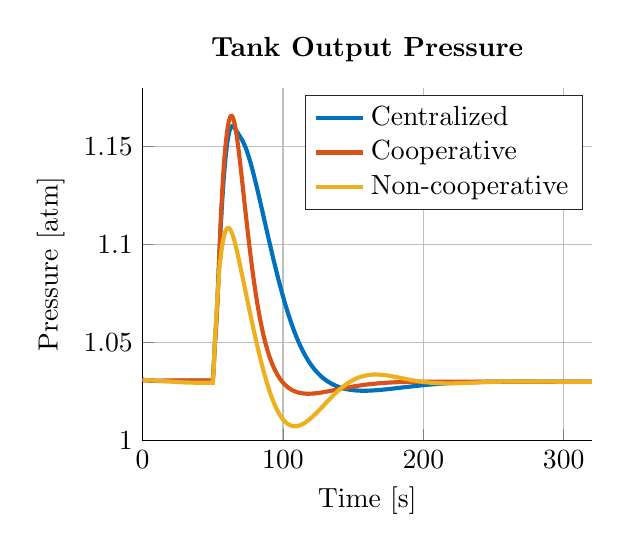
\begin{tikzpicture}

\begin{axis}[%
width=5.706cm,
height=4.479cm,
at={(0cm,0cm)},
scale only axis,
xmin=0,
xmax=320,
xlabel={Time [s]},
xmajorgrids,
ymin=1,
ymax=1.18,
ylabel={Pressure [atm]},
ymajorgrids,
axis background/.style={fill=white},
title style={font=\bfseries},
title={Tank Output Pressure},
axis x line*=bottom,
axis y line*=left,
legend style={legend cell align=left,align=left,draw=white!15!black}
]
\addplot [color=mycolor1,solid,line width=1.5pt]
  table[row sep=crcr]{%
0	1.03\\
0.5	1.03105\\
1	1.03093\\
1.5	1.03091\\
2	1.03084\\
2.5	1.03079\\
3	1.03074\\
3.5	1.0307\\
4	1.03066\\
4.5	1.03062\\
5	1.03059\\
5.5	1.03057\\
6	1.03054\\
6.5	1.03052\\
7	1.03051\\
7.5	1.03049\\
8	1.03048\\
8.5	1.03046\\
9	1.03045\\
9.5	1.03045\\
10	1.03044\\
10.5	1.03043\\
11	1.03043\\
11.5	1.03042\\
12	1.03042\\
12.5	1.03042\\
13	1.03042\\
13.5	1.03042\\
14	1.03042\\
14.5	1.03042\\
15	1.03042\\
15.5	1.03042\\
16	1.03042\\
16.5	1.03042\\
17	1.03043\\
17.5	1.03043\\
18	1.03043\\
18.5	1.03044\\
19	1.03044\\
19.5	1.03045\\
20	1.03045\\
20.5	1.03046\\
21	1.03046\\
21.5	1.03047\\
22	1.03047\\
22.5	1.03048\\
23	1.03048\\
23.5	1.03049\\
24	1.03049\\
24.5	1.0305\\
25	1.0305\\
25.5	1.03051\\
26	1.03051\\
26.5	1.03052\\
27	1.03052\\
27.5	1.03053\\
28	1.03053\\
28.5	1.03054\\
29	1.03054\\
29.5	1.03055\\
30	1.03055\\
30.5	1.03055\\
31	1.03056\\
31.5	1.03056\\
32	1.03057\\
32.5	1.03057\\
33	1.03057\\
33.5	1.03057\\
34	1.03058\\
34.5	1.03058\\
35	1.03058\\
35.5	1.03058\\
36	1.03058\\
36.5	1.03059\\
37	1.03059\\
37.5	1.03059\\
38	1.03059\\
38.5	1.03059\\
39	1.03059\\
39.5	1.03059\\
40	1.03059\\
40.5	1.03059\\
41	1.0306\\
41.5	1.0306\\
42	1.0306\\
42.5	1.0306\\
43	1.0306\\
43.5	1.0306\\
44	1.0306\\
44.5	1.0306\\
45	1.0306\\
45.5	1.03059\\
46	1.03059\\
46.5	1.03059\\
47	1.03059\\
47.5	1.03059\\
48	1.03059\\
48.5	1.03059\\
49	1.03059\\
49.5	1.03059\\
50	1.03059\\
50.5	1.03504\\
51	1.04245\\
51.5	1.04912\\
52	1.0547\\
52.5	1.06051\\
53	1.06686\\
53.5	1.07423\\
54	1.08238\\
54.5	1.09105\\
55	1.09951\\
55.5	1.1072\\
56	1.11291\\
56.5	1.11944\\
57	1.1251\\
57.5	1.13037\\
58	1.13511\\
58.5	1.1395\\
59	1.14346\\
59.5	1.14698\\
60	1.15007\\
60.5	1.15272\\
61	1.15496\\
61.5	1.15678\\
62	1.15822\\
62.5	1.15927\\
63	1.15998\\
63.5	1.16038\\
64	1.16049\\
64.5	1.16038\\
65	1.16008\\
65.5	1.15965\\
66	1.15913\\
66.5	1.15855\\
67	1.15795\\
67.5	1.15736\\
68	1.15677\\
68.5	1.1562\\
69	1.15564\\
69.5	1.15507\\
70	1.15449\\
70.5	1.15389\\
71	1.15325\\
71.5	1.15256\\
72	1.15183\\
72.5	1.15105\\
73	1.15021\\
73.5	1.14931\\
74	1.14836\\
74.5	1.14735\\
75	1.14629\\
75.5	1.14517\\
76	1.14401\\
76.5	1.1428\\
77	1.14155\\
77.5	1.14026\\
78	1.13893\\
78.5	1.13758\\
79	1.13619\\
79.5	1.13478\\
80	1.13334\\
80.5	1.13188\\
81	1.1304\\
81.5	1.12891\\
82	1.1274\\
82.5	1.12588\\
83	1.12434\\
83.5	1.1228\\
84	1.12124\\
84.5	1.11968\\
85	1.11812\\
85.5	1.11654\\
86	1.11497\\
86.5	1.11339\\
87	1.11181\\
87.5	1.11024\\
88	1.10866\\
88.5	1.10709\\
89	1.10552\\
89.5	1.10395\\
90	1.10239\\
90.5	1.10084\\
91	1.09929\\
91.5	1.09776\\
92	1.09623\\
92.5	1.09471\\
93	1.09321\\
93.5	1.09171\\
94	1.09023\\
94.5	1.08877\\
95	1.08731\\
95.5	1.08587\\
96	1.08445\\
96.5	1.08304\\
97	1.08165\\
97.5	1.08027\\
98	1.07892\\
98.5	1.07758\\
99	1.07626\\
99.5	1.07495\\
100	1.07367\\
100.5	1.07241\\
101	1.07116\\
101.5	1.06993\\
102	1.06873\\
102.5	1.06754\\
103	1.06638\\
103.5	1.06523\\
104	1.06411\\
104.5	1.06301\\
105	1.06192\\
105.5	1.06086\\
106	1.05982\\
106.5	1.0588\\
107	1.0578\\
107.5	1.05682\\
108	1.05586\\
108.5	1.05492\\
109	1.054\\
109.5	1.0531\\
110	1.05223\\
110.5	1.05137\\
111	1.05053\\
111.5	1.04971\\
112	1.04892\\
112.5	1.04814\\
113	1.04738\\
113.5	1.04664\\
114	1.04592\\
114.5	1.04522\\
115	1.04454\\
115.5	1.04387\\
116	1.04322\\
116.5	1.04259\\
117	1.04198\\
117.5	1.04139\\
118	1.04081\\
118.5	1.04025\\
119	1.0397\\
119.5	1.03917\\
120	1.03866\\
120.5	1.03816\\
121	1.03768\\
121.5	1.03721\\
122	1.03675\\
122.5	1.03631\\
123	1.03588\\
123.5	1.03547\\
124	1.03507\\
124.5	1.03468\\
125	1.0343\\
125.5	1.03394\\
126	1.03358\\
126.5	1.03324\\
127	1.03291\\
127.5	1.03259\\
128	1.03228\\
128.5	1.03198\\
129	1.03169\\
129.5	1.03141\\
130	1.03113\\
130.5	1.03087\\
131	1.03062\\
131.5	1.03037\\
132	1.03013\\
132.5	1.02991\\
133	1.02969\\
133.5	1.02947\\
134	1.02927\\
134.5	1.02907\\
135	1.02888\\
135.5	1.02869\\
136	1.02851\\
136.5	1.02834\\
137	1.02818\\
137.5	1.02802\\
138	1.02787\\
138.5	1.02772\\
139	1.02758\\
139.5	1.02745\\
140	1.02732\\
140.5	1.02719\\
141	1.02708\\
141.5	1.02696\\
142	1.02685\\
142.5	1.02675\\
143	1.02665\\
143.5	1.02656\\
144	1.02647\\
144.5	1.02638\\
145	1.0263\\
145.5	1.02623\\
146	1.02616\\
146.5	1.02609\\
147	1.02602\\
147.5	1.02596\\
148	1.02591\\
148.5	1.02585\\
149	1.0258\\
149.5	1.02576\\
150	1.02572\\
150.5	1.02568\\
151	1.02564\\
151.5	1.02561\\
152	1.02558\\
152.5	1.02555\\
153	1.02553\\
153.5	1.02551\\
154	1.02549\\
154.5	1.02547\\
155	1.02546\\
155.5	1.02545\\
156	1.02544\\
156.5	1.02543\\
157	1.02543\\
157.5	1.02542\\
158	1.02542\\
158.5	1.02543\\
159	1.02543\\
159.5	1.02544\\
160	1.02544\\
160.5	1.02545\\
161	1.02546\\
161.5	1.02548\\
162	1.02549\\
162.5	1.02551\\
163	1.02553\\
163.5	1.02554\\
164	1.02556\\
164.5	1.02559\\
165	1.02561\\
165.5	1.02563\\
166	1.02566\\
166.5	1.02568\\
167	1.02571\\
167.5	1.02574\\
168	1.02577\\
168.5	1.0258\\
169	1.02583\\
169.5	1.02586\\
170	1.02589\\
170.5	1.02593\\
171	1.02596\\
171.5	1.026\\
172	1.02603\\
172.5	1.02607\\
173	1.02611\\
173.5	1.02614\\
174	1.02618\\
174.5	1.02622\\
175	1.02626\\
175.5	1.0263\\
176	1.02634\\
176.5	1.02638\\
177	1.02642\\
177.5	1.02646\\
178	1.0265\\
178.5	1.02654\\
179	1.02658\\
179.5	1.02662\\
180	1.02666\\
180.5	1.0267\\
181	1.02675\\
181.5	1.02679\\
182	1.02683\\
182.5	1.02687\\
183	1.02691\\
183.5	1.02696\\
184	1.027\\
184.5	1.02704\\
185	1.02708\\
185.5	1.02713\\
186	1.02717\\
186.5	1.02721\\
187	1.02725\\
187.5	1.02729\\
188	1.02733\\
188.5	1.02738\\
189	1.02742\\
189.5	1.02746\\
190	1.0275\\
190.5	1.02754\\
191	1.02758\\
191.5	1.02762\\
192	1.02766\\
192.5	1.0277\\
193	1.02774\\
193.5	1.02778\\
194	1.02782\\
194.5	1.02786\\
195	1.0279\\
195.5	1.02794\\
196	1.02797\\
196.5	1.02801\\
197	1.02805\\
197.5	1.02809\\
198	1.02812\\
198.5	1.02816\\
199	1.0282\\
199.5	1.02823\\
200	1.02827\\
200.5	1.0283\\
201	1.02834\\
201.5	1.02837\\
202	1.0284\\
202.5	1.02844\\
203	1.02847\\
203.5	1.0285\\
204	1.02854\\
204.5	1.02857\\
205	1.0286\\
205.5	1.02863\\
206	1.02866\\
206.5	1.02869\\
207	1.02872\\
207.5	1.02875\\
208	1.02878\\
208.5	1.02881\\
209	1.02884\\
209.5	1.02887\\
210	1.0289\\
210.5	1.02892\\
211	1.02895\\
211.5	1.02898\\
212	1.029\\
212.5	1.02903\\
213	1.02905\\
213.5	1.02908\\
214	1.0291\\
214.5	1.02913\\
215	1.02915\\
215.5	1.02918\\
216	1.0292\\
216.5	1.02922\\
217	1.02924\\
217.5	1.02927\\
218	1.02929\\
218.5	1.02931\\
219	1.02933\\
219.5	1.02935\\
220	1.02937\\
220.5	1.02939\\
221	1.02941\\
221.5	1.02943\\
222	1.02945\\
222.5	1.02947\\
223	1.02948\\
223.5	1.0295\\
224	1.02952\\
224.5	1.02954\\
225	1.02955\\
225.5	1.02957\\
226	1.02958\\
226.5	1.0296\\
227	1.02962\\
227.5	1.02963\\
228	1.02965\\
228.5	1.02966\\
229	1.02967\\
229.5	1.02969\\
230	1.0297\\
230.5	1.02971\\
231	1.02973\\
231.5	1.02974\\
232	1.02975\\
232.5	1.02976\\
233	1.02978\\
233.5	1.02979\\
234	1.0298\\
234.5	1.02981\\
235	1.02982\\
235.5	1.02983\\
236	1.02984\\
236.5	1.02985\\
237	1.02986\\
237.5	1.02987\\
238	1.02988\\
238.5	1.02989\\
239	1.0299\\
239.5	1.0299\\
240	1.02991\\
240.5	1.02992\\
241	1.02993\\
241.5	1.02994\\
242	1.02994\\
242.5	1.02995\\
243	1.02996\\
243.5	1.02996\\
244	1.02997\\
244.5	1.02998\\
245	1.02998\\
245.5	1.02999\\
246	1.02999\\
246.5	1.03\\
247	1.03001\\
247.5	1.03001\\
248	1.03002\\
248.5	1.03002\\
249	1.03002\\
249.5	1.03003\\
250	1.03003\\
250.5	1.03004\\
251	1.03004\\
251.5	1.03005\\
252	1.03005\\
252.5	1.03005\\
253	1.03006\\
253.5	1.03006\\
254	1.03006\\
254.5	1.03007\\
255	1.03007\\
255.5	1.03007\\
256	1.03007\\
256.5	1.03008\\
257	1.03008\\
257.5	1.03008\\
258	1.03008\\
258.5	1.03009\\
259	1.03009\\
259.5	1.03009\\
260	1.03009\\
260.5	1.03009\\
261	1.0301\\
261.5	1.0301\\
262	1.0301\\
262.5	1.0301\\
263	1.0301\\
263.5	1.0301\\
264	1.0301\\
264.5	1.0301\\
265	1.0301\\
265.5	1.03011\\
266	1.03011\\
266.5	1.03011\\
267	1.03011\\
267.5	1.03011\\
268	1.03011\\
268.5	1.03011\\
269	1.03011\\
269.5	1.03011\\
270	1.03011\\
270.5	1.03011\\
271	1.03011\\
271.5	1.03011\\
272	1.03011\\
272.5	1.03011\\
273	1.03011\\
273.5	1.03011\\
274	1.03011\\
274.5	1.03011\\
275	1.03011\\
275.5	1.03011\\
276	1.03011\\
276.5	1.03011\\
277	1.03011\\
277.5	1.03011\\
278	1.03011\\
278.5	1.03011\\
279	1.0301\\
279.5	1.0301\\
280	1.0301\\
280.5	1.0301\\
281	1.0301\\
281.5	1.0301\\
282	1.0301\\
282.5	1.0301\\
283	1.0301\\
283.5	1.0301\\
284	1.0301\\
284.5	1.0301\\
285	1.0301\\
285.5	1.03009\\
286	1.03009\\
286.5	1.03009\\
287	1.03009\\
287.5	1.03009\\
288	1.03009\\
288.5	1.03009\\
289	1.03009\\
289.5	1.03009\\
290	1.03009\\
290.5	1.03009\\
291	1.03008\\
291.5	1.03008\\
292	1.03008\\
292.5	1.03008\\
293	1.03008\\
293.5	1.03008\\
294	1.03008\\
294.5	1.03008\\
295	1.03008\\
295.5	1.03008\\
296	1.03007\\
296.5	1.03007\\
297	1.03007\\
297.5	1.03007\\
298	1.03007\\
298.5	1.03007\\
299	1.03007\\
299.5	1.03007\\
300	1.03007\\
300.5	1.03007\\
301	1.03006\\
301.5	1.03006\\
302	1.03006\\
302.5	1.03006\\
303	1.03006\\
303.5	1.03006\\
304	1.03006\\
304.5	1.03006\\
305	1.03006\\
305.5	1.03006\\
306	1.03005\\
306.5	1.03005\\
307	1.03005\\
307.5	1.03005\\
308	1.03005\\
308.5	1.03005\\
309	1.03005\\
309.5	1.03005\\
310	1.03005\\
310.5	1.03005\\
311	1.03004\\
311.5	1.03004\\
312	1.03004\\
312.5	1.03004\\
313	1.03004\\
313.5	1.03004\\
314	1.03004\\
314.5	1.03004\\
315	1.03004\\
315.5	1.03004\\
316	1.03004\\
316.5	1.03004\\
317	1.03003\\
317.5	1.03003\\
318	1.03003\\
318.5	1.03003\\
319	1.03003\\
319.5	1.03003\\
320	1.03003\\
320.5	1.03003\\
321	1.03003\\
321.5	1.03003\\
322	1.03003\\
322.5	1.03003\\
323	1.03003\\
323.5	1.03003\\
324	1.03002\\
324.5	1.03002\\
325	1.03002\\
325.5	1.03002\\
326	1.03002\\
326.5	1.03002\\
327	1.03002\\
327.5	1.03002\\
328	1.03002\\
328.5	1.03002\\
329	1.03002\\
329.5	1.03002\\
330	1.03002\\
330.5	1.03002\\
331	1.03002\\
331.5	1.03002\\
332	1.03002\\
332.5	1.03002\\
333	1.03001\\
333.5	1.03001\\
334	1.03001\\
334.5	1.03001\\
335	1.03001\\
335.5	1.03001\\
336	1.03001\\
336.5	1.03001\\
337	1.03001\\
337.5	1.03001\\
338	1.03001\\
338.5	1.03001\\
339	1.03001\\
339.5	1.03001\\
340	1.03001\\
340.5	1.03001\\
341	1.03001\\
341.5	1.03001\\
342	1.03001\\
342.5	1.03001\\
343	1.03001\\
343.5	1.03001\\
344	1.03001\\
344.5	1.03001\\
345	1.03001\\
345.5	1.03001\\
346	1.03001\\
346.5	1.03\\
347	1.03\\
347.5	1.03\\
348	1.03\\
348.5	1.03\\
349	1.03\\
349.5	1.03\\
350	1.03\\
350.5	1.03\\
351	1.03\\
351.5	1.03\\
352	1.03\\
352.5	1.03\\
353	1.03\\
353.5	1.03\\
354	1.03\\
354.5	1.03\\
355	1.03\\
355.5	1.03\\
356	1.03\\
356.5	1.03\\
357	1.03\\
357.5	1.03\\
358	1.03\\
358.5	1.03\\
359	1.03\\
359.5	1.03\\
360	1.03\\
360.5	1.03\\
361	1.03\\
361.5	1.03\\
362	1.03\\
362.5	1.03\\
363	1.03\\
363.5	1.03\\
364	1.03\\
364.5	1.03\\
365	1.03\\
365.5	1.03\\
366	1.03\\
366.5	1.03\\
367	1.03\\
367.5	1.03\\
368	1.03\\
368.5	1.03\\
369	1.03\\
369.5	1.03\\
370	1.03\\
370.5	1.03\\
371	1.03\\
371.5	1.03\\
372	1.03\\
372.5	1.03\\
373	1.03\\
373.5	1.03\\
374	1.03\\
374.5	1.03\\
375	1.03\\
375.5	1.03\\
376	1.03\\
376.5	1.03\\
377	1.03\\
377.5	1.03\\
378	1.03\\
378.5	1.03\\
379	1.03\\
379.5	1.03\\
380	1.03\\
380.5	1.03\\
381	1.03\\
381.5	1.03\\
382	1.03\\
382.5	1.03\\
383	1.03\\
383.5	1.03\\
384	1.03\\
384.5	1.03\\
385	1.03\\
385.5	1.03\\
386	1.03\\
386.5	1.03\\
387	1.03\\
387.5	1.03\\
388	1.03\\
388.5	1.03\\
389	1.03\\
389.5	1.03\\
390	1.03\\
390.5	1.03\\
391	1.03\\
391.5	1.03\\
392	1.03\\
392.5	1.03\\
393	1.03\\
393.5	1.03\\
394	1.03\\
394.5	1.03\\
395	1.03\\
395.5	1.03\\
396	1.03\\
396.5	1.03\\
397	1.03\\
397.5	1.03\\
398	1.03\\
398.5	1.03\\
399	1.03\\
399.5	1.03\\
400	1.03\\
400.5	1.03\\
401	1.03\\
401.5	1.03\\
402	1.03\\
402.5	1.03\\
403	1.03\\
403.5	1.03\\
404	1.03\\
404.5	1.03\\
405	1.03\\
405.5	1.03\\
406	1.03\\
406.5	1.03\\
407	1.03\\
407.5	1.03\\
408	1.03\\
408.5	1.03\\
409	1.03\\
409.5	1.03\\
410	1.03\\
410.5	1.03\\
411	1.03\\
411.5	1.03\\
412	1.03\\
412.5	1.03\\
413	1.03\\
413.5	1.03\\
414	1.03\\
414.5	1.03\\
415	1.03\\
415.5	1.03\\
416	1.03\\
416.5	1.03\\
417	1.03\\
417.5	1.03\\
418	1.03\\
418.5	1.03\\
419	1.03\\
419.5	1.03\\
420	1.03\\
420.5	1.03\\
421	1.03\\
421.5	1.03\\
422	1.03\\
422.5	1.03\\
423	1.03\\
423.5	1.03\\
424	1.03\\
424.5	1.03\\
425	1.03\\
425.5	1.03\\
426	1.03\\
426.5	1.03\\
427	1.03\\
427.5	1.03\\
428	1.03\\
428.5	1.03\\
429	1.03\\
429.5	1.03\\
430	1.03\\
430.5	1.03\\
431	1.03\\
431.5	1.03\\
432	1.03\\
432.5	1.03\\
433	1.03\\
433.5	1.03\\
434	1.03\\
434.5	1.03\\
435	1.03\\
435.5	1.03\\
436	1.03\\
436.5	1.03\\
437	1.03\\
437.5	1.03\\
438	1.03\\
438.5	1.03\\
439	1.03\\
439.5	1.03\\
440	1.03\\
440.5	1.03\\
441	1.03\\
441.5	1.03\\
442	1.03\\
442.5	1.03\\
443	1.03\\
443.5	1.03\\
444	1.03\\
444.5	1.03\\
445	1.03\\
445.5	1.03\\
446	1.03\\
446.5	1.03\\
447	1.03\\
447.5	1.03\\
448	1.03\\
448.5	1.03\\
449	1.03\\
449.5	1.03\\
450	1.03\\
450.5	1.03\\
451	1.03\\
451.5	1.03\\
452	1.03\\
452.5	1.03\\
453	1.03\\
453.5	1.03\\
454	1.03\\
454.5	1.03\\
455	1.03\\
455.5	1.03\\
456	1.03\\
456.5	1.03\\
457	1.03\\
457.5	1.03\\
458	1.03\\
458.5	1.03\\
459	1.03\\
459.5	1.03\\
460	1.03\\
460.5	1.03\\
461	1.03\\
461.5	1.03\\
462	1.03\\
462.5	1.03\\
463	1.03\\
463.5	1.03\\
464	1.03\\
464.5	1.03\\
465	1.03\\
465.5	1.03\\
466	1.03\\
466.5	1.03\\
467	1.03\\
467.5	1.03\\
468	1.03\\
468.5	1.03\\
469	1.03\\
469.5	1.03\\
470	1.03\\
470.5	1.03\\
471	1.03\\
471.5	1.03\\
472	1.03\\
472.5	1.03\\
473	1.03\\
473.5	1.03\\
474	1.03\\
474.5	1.03\\
475	1.03\\
475.5	1.03\\
476	1.03\\
476.5	1.03\\
477	1.03\\
477.5	1.03\\
478	1.03\\
478.5	1.03\\
479	1.03\\
479.5	1.03\\
480	1.03\\
480.5	1.03\\
481	1.03\\
481.5	1.03\\
482	1.03\\
482.5	1.03\\
483	1.03\\
483.5	1.03\\
484	1.03\\
484.5	1.03\\
485	1.03\\
485.5	1.03\\
486	1.03\\
486.5	1.03\\
487	1.03\\
487.5	1.03\\
488	1.03\\
488.5	1.03\\
489	1.03\\
489.5	1.03\\
490	1.03\\
490.5	1.03\\
491	1.03\\
491.5	1.03\\
492	1.03\\
492.5	1.03\\
493	1.03\\
493.5	1.03\\
494	1.03\\
494.5	1.03\\
495	1.03\\
495.5	1.03\\
496	1.03\\
496.5	1.03\\
497	1.03\\
497.5	1.03\\
498	1.03\\
498.5	1.03\\
499	1.03\\
499.5	1.03\\
};
\addlegendentry{Centralized};

\addplot [color=mycolor2,solid,line width=1.5pt]
  table[row sep=crcr]{%
0	1.03\\
0.5	1.03106\\
1	1.03094\\
1.5	1.03094\\
2	1.03088\\
2.5	1.03084\\
3	1.03081\\
3.5	1.03077\\
4	1.03074\\
4.5	1.03072\\
5	1.0307\\
5.5	1.03068\\
6	1.03066\\
6.5	1.03065\\
7	1.03064\\
7.5	1.03063\\
8	1.03062\\
8.5	1.03062\\
9	1.03061\\
9.5	1.03061\\
10	1.03061\\
10.5	1.03061\\
11	1.0306\\
11.5	1.0306\\
12	1.03061\\
12.5	1.03061\\
13	1.03061\\
13.5	1.03061\\
14	1.03061\\
14.5	1.03061\\
15	1.03062\\
15.5	1.03062\\
16	1.03062\\
16.5	1.03063\\
17	1.03063\\
17.5	1.03063\\
18	1.03064\\
18.5	1.03064\\
19	1.03064\\
19.5	1.03065\\
20	1.03065\\
20.5	1.03065\\
21	1.03065\\
21.5	1.03066\\
22	1.03066\\
22.5	1.03066\\
23	1.03066\\
23.5	1.03066\\
24	1.03066\\
24.5	1.03067\\
25	1.03067\\
25.5	1.03067\\
26	1.03067\\
26.5	1.03067\\
27	1.03067\\
27.5	1.03067\\
28	1.03067\\
28.5	1.03067\\
29	1.03067\\
29.5	1.03067\\
30	1.03067\\
30.5	1.03067\\
31	1.03067\\
31.5	1.03066\\
32	1.03066\\
32.5	1.03066\\
33	1.03066\\
33.5	1.03066\\
34	1.03066\\
34.5	1.03066\\
35	1.03066\\
35.5	1.03066\\
36	1.03066\\
36.5	1.03066\\
37	1.03065\\
37.5	1.03065\\
38	1.03065\\
38.5	1.03065\\
39	1.03065\\
39.5	1.03065\\
40	1.03065\\
40.5	1.03065\\
41	1.03065\\
41.5	1.03065\\
42	1.03065\\
42.5	1.03065\\
43	1.03065\\
43.5	1.03065\\
44	1.03065\\
44.5	1.03065\\
45	1.03065\\
45.5	1.03065\\
46	1.03065\\
46.5	1.03065\\
47	1.03065\\
47.5	1.03065\\
48	1.03065\\
48.5	1.03065\\
49	1.03065\\
49.5	1.03065\\
50	1.03065\\
50.5	1.0351\\
51	1.04224\\
51.5	1.04876\\
52	1.05419\\
52.5	1.05962\\
53	1.06599\\
53.5	1.07337\\
54	1.08176\\
54.5	1.09099\\
55	1.10027\\
55.5	1.10928\\
56	1.11764\\
56.5	1.1238\\
57	1.13053\\
57.5	1.13624\\
58	1.14138\\
58.5	1.14579\\
59	1.14978\\
59.5	1.15332\\
60	1.15641\\
60.5	1.15905\\
61	1.16126\\
61.5	1.16303\\
62	1.16435\\
62.5	1.16524\\
63	1.16569\\
63.5	1.16572\\
64	1.16534\\
64.5	1.16457\\
65	1.16344\\
65.5	1.16197\\
66	1.16019\\
66.5	1.15813\\
67	1.15583\\
67.5	1.15331\\
68	1.15062\\
68.5	1.14777\\
69	1.14479\\
69.5	1.14171\\
70	1.13855\\
70.5	1.13533\\
71	1.13206\\
71.5	1.12878\\
72	1.12548\\
72.5	1.12218\\
73	1.1189\\
73.5	1.11564\\
74	1.11241\\
74.5	1.10922\\
75	1.10607\\
75.5	1.10297\\
76	1.09993\\
76.5	1.09695\\
77	1.09404\\
77.5	1.09119\\
78	1.08841\\
78.5	1.0857\\
79	1.08307\\
79.5	1.08052\\
80	1.07804\\
80.5	1.07564\\
81	1.07331\\
81.5	1.07107\\
82	1.0689\\
82.5	1.06681\\
83	1.06479\\
83.5	1.06285\\
84	1.06099\\
84.5	1.05919\\
85	1.05747\\
85.5	1.05582\\
86	1.05424\\
86.5	1.05272\\
87	1.05126\\
87.5	1.04987\\
88	1.04853\\
88.5	1.04725\\
89	1.04603\\
89.5	1.04486\\
90	1.04375\\
90.5	1.04268\\
91	1.04166\\
91.5	1.04068\\
92	1.03975\\
92.5	1.03887\\
93	1.03802\\
93.5	1.03721\\
94	1.03644\\
94.5	1.0357\\
95	1.035\\
95.5	1.03433\\
96	1.0337\\
96.5	1.03309\\
97	1.03252\\
97.5	1.03197\\
98	1.03144\\
98.5	1.03095\\
99	1.03048\\
99.5	1.03003\\
100	1.0296\\
100.5	1.0292\\
101	1.02882\\
101.5	1.02846\\
102	1.02811\\
102.5	1.02779\\
103	1.02748\\
103.5	1.02719\\
104	1.02692\\
104.5	1.02666\\
105	1.02642\\
105.5	1.0262\\
106	1.02598\\
106.5	1.02578\\
107	1.0256\\
107.5	1.02542\\
108	1.02526\\
108.5	1.02511\\
109	1.02497\\
109.5	1.02484\\
110	1.02472\\
110.5	1.02461\\
111	1.02451\\
111.5	1.02442\\
112	1.02434\\
112.5	1.02427\\
113	1.0242\\
113.5	1.02414\\
114	1.02409\\
114.5	1.02405\\
115	1.02401\\
115.5	1.02398\\
116	1.02395\\
116.5	1.02393\\
117	1.02392\\
117.5	1.02391\\
118	1.02391\\
118.5	1.02391\\
119	1.02391\\
119.5	1.02392\\
120	1.02394\\
120.5	1.02396\\
121	1.02398\\
121.5	1.024\\
122	1.02403\\
122.5	1.02407\\
123	1.0241\\
123.5	1.02414\\
124	1.02418\\
124.5	1.02423\\
125	1.02427\\
125.5	1.02432\\
126	1.02437\\
126.5	1.02442\\
127	1.02448\\
127.5	1.02454\\
128	1.02459\\
128.5	1.02465\\
129	1.02471\\
129.5	1.02478\\
130	1.02484\\
130.5	1.02491\\
131	1.02497\\
131.5	1.02504\\
132	1.02511\\
132.5	1.02517\\
133	1.02524\\
133.5	1.02531\\
134	1.02538\\
134.5	1.02545\\
135	1.02552\\
135.5	1.0256\\
136	1.02567\\
136.5	1.02574\\
137	1.02581\\
137.5	1.02588\\
138	1.02595\\
138.5	1.02603\\
139	1.0261\\
139.5	1.02617\\
140	1.02624\\
140.5	1.02631\\
141	1.02638\\
141.5	1.02645\\
142	1.02652\\
142.5	1.02659\\
143	1.02666\\
143.5	1.02673\\
144	1.0268\\
144.5	1.02687\\
145	1.02693\\
145.5	1.027\\
146	1.02707\\
146.5	1.02713\\
147	1.0272\\
147.5	1.02726\\
148	1.02732\\
148.5	1.02739\\
149	1.02745\\
149.5	1.02751\\
150	1.02757\\
150.5	1.02763\\
151	1.02769\\
151.5	1.02775\\
152	1.0278\\
152.5	1.02786\\
153	1.02792\\
153.5	1.02797\\
154	1.02802\\
154.5	1.02808\\
155	1.02813\\
155.5	1.02818\\
156	1.02823\\
156.5	1.02828\\
157	1.02833\\
157.5	1.02838\\
158	1.02843\\
158.5	1.02847\\
159	1.02852\\
159.5	1.02856\\
160	1.02861\\
160.5	1.02865\\
161	1.02869\\
161.5	1.02873\\
162	1.02877\\
162.5	1.02881\\
163	1.02885\\
163.5	1.02889\\
164	1.02893\\
164.5	1.02897\\
165	1.029\\
165.5	1.02904\\
166	1.02907\\
166.5	1.0291\\
167	1.02914\\
167.5	1.02917\\
168	1.0292\\
168.5	1.02923\\
169	1.02926\\
169.5	1.02929\\
170	1.02932\\
170.5	1.02934\\
171	1.02937\\
171.5	1.0294\\
172	1.02942\\
172.5	1.02945\\
173	1.02947\\
173.5	1.02949\\
174	1.02952\\
174.5	1.02954\\
175	1.02956\\
175.5	1.02958\\
176	1.0296\\
176.5	1.02962\\
177	1.02964\\
177.5	1.02966\\
178	1.02968\\
178.5	1.02969\\
179	1.02971\\
179.5	1.02973\\
180	1.02974\\
180.5	1.02976\\
181	1.02977\\
181.5	1.02979\\
182	1.0298\\
182.5	1.02982\\
183	1.02983\\
183.5	1.02984\\
184	1.02985\\
184.5	1.02987\\
185	1.02988\\
185.5	1.02989\\
186	1.0299\\
186.5	1.02991\\
187	1.02992\\
187.5	1.02993\\
188	1.02994\\
188.5	1.02995\\
189	1.02995\\
189.5	1.02996\\
190	1.02997\\
190.5	1.02998\\
191	1.02998\\
191.5	1.02999\\
192	1.03\\
192.5	1.03\\
193	1.03001\\
193.5	1.03002\\
194	1.03002\\
194.5	1.03003\\
195	1.03003\\
195.5	1.03004\\
196	1.03004\\
196.5	1.03004\\
197	1.03005\\
197.5	1.03005\\
198	1.03005\\
198.5	1.03006\\
199	1.03006\\
199.5	1.03006\\
200	1.03007\\
200.5	1.03007\\
201	1.03007\\
201.5	1.03007\\
202	1.03008\\
202.5	1.03008\\
203	1.03008\\
203.5	1.03008\\
204	1.03008\\
204.5	1.03008\\
205	1.03009\\
205.5	1.03009\\
206	1.03009\\
206.5	1.03009\\
207	1.03009\\
207.5	1.03009\\
208	1.03009\\
208.5	1.03009\\
209	1.03009\\
209.5	1.03009\\
210	1.03009\\
210.5	1.03009\\
211	1.03009\\
211.5	1.03009\\
212	1.03009\\
212.5	1.03009\\
213	1.03009\\
213.5	1.03009\\
214	1.03009\\
214.5	1.03009\\
215	1.03009\\
215.5	1.03009\\
216	1.03009\\
216.5	1.03009\\
217	1.03009\\
217.5	1.03009\\
218	1.03008\\
218.5	1.03008\\
219	1.03008\\
219.5	1.03008\\
220	1.03008\\
220.5	1.03008\\
221	1.03008\\
221.5	1.03008\\
222	1.03008\\
222.5	1.03008\\
223	1.03008\\
223.5	1.03007\\
224	1.03007\\
224.5	1.03007\\
225	1.03007\\
225.5	1.03007\\
226	1.03007\\
226.5	1.03007\\
227	1.03007\\
227.5	1.03007\\
228	1.03006\\
228.5	1.03006\\
229	1.03006\\
229.5	1.03006\\
230	1.03006\\
230.5	1.03006\\
231	1.03006\\
231.5	1.03006\\
232	1.03006\\
232.5	1.03005\\
233	1.03005\\
233.5	1.03005\\
234	1.03005\\
234.5	1.03005\\
235	1.03005\\
235.5	1.03005\\
236	1.03005\\
236.5	1.03005\\
237	1.03005\\
237.5	1.03004\\
238	1.03004\\
238.5	1.03004\\
239	1.03004\\
239.5	1.03004\\
240	1.03004\\
240.5	1.03004\\
241	1.03004\\
241.5	1.03004\\
242	1.03004\\
242.5	1.03003\\
243	1.03003\\
243.5	1.03003\\
244	1.03003\\
244.5	1.03003\\
245	1.03003\\
245.5	1.03003\\
246	1.03003\\
246.5	1.03003\\
247	1.03003\\
247.5	1.03003\\
248	1.03003\\
248.5	1.03002\\
249	1.03002\\
249.5	1.03002\\
250	1.03002\\
250.5	1.03002\\
251	1.03002\\
251.5	1.03002\\
252	1.03002\\
252.5	1.03002\\
253	1.03002\\
253.5	1.03002\\
254	1.03002\\
254.5	1.03002\\
255	1.03002\\
255.5	1.03002\\
256	1.03001\\
256.5	1.03001\\
257	1.03001\\
257.5	1.03001\\
258	1.03001\\
258.5	1.03001\\
259	1.03001\\
259.5	1.03001\\
260	1.03001\\
260.5	1.03001\\
261	1.03001\\
261.5	1.03001\\
262	1.03001\\
262.5	1.03001\\
263	1.03001\\
263.5	1.03001\\
264	1.03001\\
264.5	1.03001\\
265	1.03001\\
265.5	1.03001\\
266	1.03001\\
266.5	1.03001\\
267	1.03001\\
267.5	1.03001\\
268	1.03001\\
268.5	1.03\\
269	1.03\\
269.5	1.03\\
270	1.03\\
270.5	1.03\\
271	1.03\\
271.5	1.03\\
272	1.03\\
272.5	1.03\\
273	1.03\\
273.5	1.03\\
274	1.03\\
274.5	1.03\\
275	1.03\\
275.5	1.03\\
276	1.03\\
276.5	1.03\\
277	1.03\\
277.5	1.03\\
278	1.03\\
278.5	1.03\\
279	1.03\\
279.5	1.03\\
280	1.03\\
280.5	1.03\\
281	1.03\\
281.5	1.03\\
282	1.03\\
282.5	1.03\\
283	1.03\\
283.5	1.03\\
284	1.03\\
284.5	1.03\\
285	1.03\\
285.5	1.03\\
286	1.03\\
286.5	1.03\\
287	1.03\\
287.5	1.03\\
288	1.03\\
288.5	1.03\\
289	1.03\\
289.5	1.03\\
290	1.03\\
290.5	1.03\\
291	1.03\\
291.5	1.03\\
292	1.03\\
292.5	1.03\\
293	1.03\\
293.5	1.03\\
294	1.03\\
294.5	1.03\\
295	1.03\\
295.5	1.03\\
296	1.03\\
296.5	1.03\\
297	1.03\\
297.5	1.03\\
298	1.03\\
298.5	1.03\\
299	1.03\\
299.5	1.03\\
300	1.03\\
300.5	1.03\\
301	1.03\\
301.5	1.03\\
302	1.03\\
302.5	1.03\\
303	1.03\\
303.5	1.03\\
304	1.03\\
304.5	1.03\\
305	1.03\\
305.5	1.03\\
306	1.03\\
306.5	1.03\\
307	1.03\\
307.5	1.03\\
308	1.03\\
308.5	1.03\\
309	1.03\\
309.5	1.03\\
310	1.03\\
310.5	1.03\\
311	1.03\\
311.5	1.03\\
312	1.03\\
312.5	1.03\\
313	1.03\\
313.5	1.03\\
314	1.03\\
314.5	1.03\\
315	1.03\\
315.5	1.03\\
316	1.03\\
316.5	1.03\\
317	1.03\\
317.5	1.03\\
318	1.03\\
318.5	1.03\\
319	1.03\\
319.5	1.03\\
320	1.03\\
320.5	1.03\\
321	1.03\\
321.5	1.03\\
322	1.03\\
322.5	1.03\\
323	1.03\\
323.5	1.03\\
324	1.03\\
324.5	1.03\\
325	1.03\\
325.5	1.03\\
326	1.03\\
326.5	1.03\\
327	1.03\\
327.5	1.03\\
328	1.03\\
328.5	1.03\\
329	1.03\\
329.5	1.03\\
330	1.03\\
330.5	1.03\\
331	1.03\\
331.5	1.03\\
332	1.03\\
332.5	1.03\\
333	1.03\\
333.5	1.03\\
334	1.03\\
334.5	1.03\\
335	1.03\\
335.5	1.03\\
336	1.03\\
336.5	1.03\\
337	1.03\\
337.5	1.03\\
338	1.03\\
338.5	1.03\\
339	1.03\\
339.5	1.03\\
340	1.03\\
340.5	1.03\\
341	1.03\\
341.5	1.03\\
342	1.03\\
342.5	1.03\\
343	1.03\\
343.5	1.03\\
344	1.03\\
344.5	1.03\\
345	1.03\\
345.5	1.03\\
346	1.03\\
346.5	1.03\\
347	1.03\\
347.5	1.03\\
348	1.03\\
348.5	1.03\\
349	1.03\\
349.5	1.03\\
350	1.03\\
350.5	1.03\\
351	1.03\\
351.5	1.03\\
352	1.03\\
352.5	1.03\\
353	1.03\\
353.5	1.03\\
354	1.03\\
354.5	1.03\\
355	1.03\\
355.5	1.03\\
356	1.03\\
356.5	1.03\\
357	1.03\\
357.5	1.03\\
358	1.03\\
358.5	1.03\\
359	1.03\\
359.5	1.03\\
360	1.03\\
360.5	1.03\\
361	1.03\\
361.5	1.03\\
362	1.03\\
362.5	1.03\\
363	1.03\\
363.5	1.03\\
364	1.03\\
364.5	1.03\\
365	1.03\\
365.5	1.03\\
366	1.03\\
366.5	1.03\\
367	1.03\\
367.5	1.03\\
368	1.03\\
368.5	1.03\\
369	1.03\\
369.5	1.03\\
370	1.03\\
370.5	1.03\\
371	1.03\\
371.5	1.03\\
372	1.03\\
372.5	1.03\\
373	1.03\\
373.5	1.03\\
374	1.03\\
374.5	1.03\\
375	1.03\\
375.5	1.03\\
376	1.03\\
376.5	1.03\\
377	1.03\\
377.5	1.03\\
378	1.03\\
378.5	1.03\\
379	1.03\\
379.5	1.03\\
380	1.03\\
380.5	1.03\\
381	1.03\\
381.5	1.03\\
382	1.03\\
382.5	1.03\\
383	1.03\\
383.5	1.03\\
384	1.03\\
384.5	1.03\\
385	1.03\\
385.5	1.03\\
386	1.03\\
386.5	1.03\\
387	1.03\\
387.5	1.03\\
388	1.03\\
388.5	1.03\\
389	1.03\\
389.5	1.03\\
390	1.03\\
390.5	1.03\\
391	1.03\\
391.5	1.03\\
392	1.03\\
392.5	1.03\\
393	1.03\\
393.5	1.03\\
394	1.03\\
394.5	1.03\\
395	1.03\\
395.5	1.03\\
396	1.03\\
396.5	1.03\\
397	1.03\\
397.5	1.03\\
398	1.03\\
398.5	1.03\\
399	1.03\\
399.5	1.03\\
400	1.03\\
400.5	1.03\\
401	1.03\\
401.5	1.03\\
402	1.03\\
402.5	1.03\\
403	1.03\\
403.5	1.03\\
404	1.03\\
404.5	1.03\\
405	1.03\\
405.5	1.03\\
406	1.03\\
406.5	1.03\\
407	1.03\\
407.5	1.03\\
408	1.03\\
408.5	1.03\\
409	1.03\\
409.5	1.03\\
410	1.03\\
410.5	1.03\\
411	1.03\\
411.5	1.03\\
412	1.03\\
412.5	1.03\\
413	1.03\\
413.5	1.03\\
414	1.03\\
414.5	1.03\\
415	1.03\\
415.5	1.03\\
416	1.03\\
416.5	1.03\\
417	1.03\\
417.5	1.03\\
418	1.03\\
418.5	1.03\\
419	1.03\\
419.5	1.03\\
420	1.03\\
420.5	1.03\\
421	1.03\\
421.5	1.03\\
422	1.03\\
422.5	1.03\\
423	1.03\\
423.5	1.03\\
424	1.03\\
424.5	1.03\\
425	1.03\\
425.5	1.03\\
426	1.03\\
426.5	1.03\\
427	1.03\\
427.5	1.03\\
428	1.03\\
428.5	1.03\\
429	1.03\\
429.5	1.03\\
430	1.03\\
430.5	1.03\\
431	1.03\\
431.5	1.03\\
432	1.03\\
432.5	1.03\\
433	1.03\\
433.5	1.03\\
434	1.03\\
434.5	1.03\\
435	1.03\\
435.5	1.03\\
436	1.03\\
436.5	1.03\\
437	1.03\\
437.5	1.03\\
438	1.03\\
438.5	1.03\\
439	1.03\\
439.5	1.03\\
440	1.03\\
440.5	1.03\\
441	1.03\\
441.5	1.03\\
442	1.03\\
442.5	1.03\\
443	1.03\\
443.5	1.03\\
444	1.03\\
444.5	1.03\\
445	1.03\\
445.5	1.03\\
446	1.03\\
446.5	1.03\\
447	1.03\\
447.5	1.03\\
448	1.03\\
448.5	1.03\\
449	1.03\\
449.5	1.03\\
450	1.03\\
450.5	1.03\\
451	1.03\\
451.5	1.03\\
452	1.03\\
452.5	1.03\\
453	1.03\\
453.5	1.03\\
454	1.03\\
454.5	1.03\\
455	1.03\\
455.5	1.03\\
456	1.03\\
456.5	1.03\\
457	1.03\\
457.5	1.03\\
458	1.03\\
458.5	1.03\\
459	1.03\\
459.5	1.03\\
460	1.03\\
460.5	1.03\\
461	1.03\\
461.5	1.03\\
462	1.03\\
462.5	1.03\\
463	1.03\\
463.5	1.03\\
464	1.03\\
464.5	1.03\\
465	1.03\\
465.5	1.03\\
466	1.03\\
466.5	1.03\\
467	1.03\\
467.5	1.03\\
468	1.03\\
468.5	1.03\\
469	1.03\\
469.5	1.03\\
470	1.03\\
470.5	1.03\\
471	1.03\\
471.5	1.03\\
472	1.03\\
472.5	1.03\\
473	1.03\\
473.5	1.03\\
474	1.03\\
474.5	1.03\\
475	1.03\\
475.5	1.03\\
476	1.03\\
476.5	1.03\\
477	1.03\\
477.5	1.03\\
478	1.03\\
478.5	1.03\\
479	1.03\\
479.5	1.03\\
480	1.03\\
480.5	1.03\\
481	1.03\\
481.5	1.03\\
482	1.03\\
482.5	1.03\\
483	1.03\\
483.5	1.03\\
484	1.03\\
484.5	1.03\\
485	1.03\\
485.5	1.03\\
486	1.03\\
486.5	1.03\\
487	1.03\\
487.5	1.03\\
488	1.03\\
488.5	1.03\\
489	1.03\\
489.5	1.03\\
490	1.03\\
490.5	1.03\\
491	1.03\\
491.5	1.03\\
492	1.03\\
492.5	1.03\\
493	1.03\\
493.5	1.03\\
494	1.03\\
494.5	1.03\\
495	1.03\\
495.5	1.03\\
496	1.03\\
496.5	1.03\\
497	1.03\\
497.5	1.03\\
498	1.03\\
498.5	1.03\\
499	1.03\\
499.5	1.03\\
};
\addlegendentry{Cooperative};

\addplot [color=mycolor3,solid,line width=1.5pt]
  table[row sep=crcr]{%
0	1.03083\\
0.5	1.03083\\
1	1.03083\\
1.5	1.03082\\
2	1.03082\\
2.5	1.03081\\
3	1.0308\\
3.5	1.03079\\
4	1.03078\\
4.5	1.03077\\
5	1.03076\\
5.5	1.03074\\
6	1.03073\\
6.5	1.03071\\
7	1.03069\\
7.5	1.03067\\
8	1.03065\\
8.5	1.03063\\
9	1.03061\\
9.5	1.03059\\
10	1.03057\\
10.5	1.03054\\
11	1.03052\\
11.5	1.0305\\
12	1.03047\\
12.5	1.03045\\
13	1.03043\\
13.5	1.0304\\
14	1.03038\\
14.5	1.03035\\
15	1.03033\\
15.5	1.0303\\
16	1.03027\\
16.5	1.03025\\
17	1.03022\\
17.5	1.0302\\
18	1.03017\\
18.5	1.03015\\
19	1.03012\\
19.5	1.0301\\
20	1.03008\\
20.5	1.03005\\
21	1.03003\\
21.5	1.03001\\
22	1.02998\\
22.5	1.02996\\
23	1.02994\\
23.5	1.02992\\
24	1.02989\\
24.5	1.02987\\
25	1.02985\\
25.5	1.02983\\
26	1.02981\\
26.5	1.02979\\
27	1.02978\\
27.5	1.02976\\
28	1.02974\\
28.5	1.02972\\
29	1.02971\\
29.5	1.02969\\
30	1.02968\\
30.5	1.02966\\
31	1.02965\\
31.5	1.02964\\
32	1.02962\\
32.5	1.02961\\
33	1.0296\\
33.5	1.02959\\
34	1.02958\\
34.5	1.02957\\
35	1.02956\\
35.5	1.02955\\
36	1.02954\\
36.5	1.02954\\
37	1.02953\\
37.5	1.02952\\
38	1.02952\\
38.5	1.02951\\
39	1.02951\\
39.5	1.0295\\
40	1.0295\\
40.5	1.02949\\
41	1.02949\\
41.5	1.02949\\
42	1.02949\\
42.5	1.02948\\
43	1.02948\\
43.5	1.02948\\
44	1.02948\\
44.5	1.02948\\
45	1.02948\\
45.5	1.02948\\
46	1.02948\\
46.5	1.02948\\
47	1.02948\\
47.5	1.02948\\
48	1.02948\\
48.5	1.02948\\
49	1.02948\\
49.5	1.02948\\
50	1.02948\\
50.5	1.03394\\
51	1.04245\\
51.5	1.05029\\
52	1.05699\\
52.5	1.06328\\
53	1.06877\\
53.5	1.07498\\
54	1.0801\\
54.5	1.08531\\
55	1.09022\\
55.5	1.09223\\
56	1.09582\\
56.5	1.09844\\
57	1.10075\\
57.5	1.10264\\
58	1.10429\\
58.5	1.10564\\
59	1.10672\\
59.5	1.10753\\
60	1.10809\\
60.5	1.10841\\
61	1.10852\\
61.5	1.10841\\
62	1.10811\\
62.5	1.10763\\
63	1.10699\\
63.5	1.10619\\
64	1.10525\\
64.5	1.10419\\
65	1.10302\\
65.5	1.10175\\
66	1.1004\\
66.5	1.09897\\
67	1.09747\\
67.5	1.09593\\
68	1.09434\\
68.5	1.09271\\
69	1.09105\\
69.5	1.08937\\
70	1.08767\\
70.5	1.08595\\
71	1.08423\\
71.5	1.0825\\
72	1.08077\\
72.5	1.07903\\
73	1.0773\\
73.5	1.07557\\
74	1.07384\\
74.5	1.07212\\
75	1.07041\\
75.5	1.0687\\
76	1.067\\
76.5	1.06531\\
77	1.06363\\
77.5	1.06196\\
78	1.0603\\
78.5	1.05865\\
79	1.05702\\
79.5	1.0554\\
80	1.05379\\
80.5	1.0522\\
81	1.05063\\
81.5	1.04907\\
82	1.04753\\
82.5	1.04602\\
83	1.04452\\
83.5	1.04304\\
84	1.04159\\
84.5	1.04016\\
85	1.03875\\
85.5	1.03737\\
86	1.03602\\
86.5	1.03469\\
87	1.03339\\
87.5	1.03212\\
88	1.03088\\
88.5	1.02967\\
89	1.02849\\
89.5	1.02734\\
90	1.02622\\
90.5	1.02513\\
91	1.02408\\
91.5	1.02306\\
92	1.02208\\
92.5	1.02112\\
93	1.0202\\
93.5	1.01932\\
94	1.01847\\
94.5	1.01765\\
95	1.01686\\
95.5	1.01611\\
96	1.0154\\
96.5	1.01471\\
97	1.01406\\
97.5	1.01345\\
98	1.01286\\
98.5	1.01231\\
99	1.01179\\
99.5	1.0113\\
100	1.01084\\
100.5	1.01042\\
101	1.01002\\
101.5	1.00965\\
102	1.00932\\
102.5	1.00901\\
103	1.00872\\
103.5	1.00847\\
104	1.00824\\
104.5	1.00804\\
105	1.00787\\
105.5	1.00772\\
106	1.00759\\
106.5	1.00749\\
107	1.00741\\
107.5	1.00736\\
108	1.00732\\
108.5	1.00731\\
109	1.00732\\
109.5	1.00735\\
110	1.00739\\
110.5	1.00746\\
111	1.00754\\
111.5	1.00765\\
112	1.00776\\
112.5	1.0079\\
113	1.00805\\
113.5	1.00822\\
114	1.0084\\
114.5	1.00859\\
115	1.0088\\
115.5	1.00902\\
116	1.00926\\
116.5	1.0095\\
117	1.00976\\
117.5	1.01002\\
118	1.0103\\
118.5	1.01059\\
119	1.01088\\
119.5	1.01118\\
120	1.0115\\
120.5	1.01182\\
121	1.01214\\
121.5	1.01247\\
122	1.01281\\
122.5	1.01316\\
123	1.01351\\
123.5	1.01386\\
124	1.01422\\
124.5	1.01458\\
125	1.01495\\
125.5	1.01532\\
126	1.01569\\
126.5	1.01607\\
127	1.01644\\
127.5	1.01682\\
128	1.0172\\
128.5	1.01758\\
129	1.01796\\
129.5	1.01834\\
130	1.01872\\
130.5	1.0191\\
131	1.01948\\
131.5	1.01985\\
132	1.02023\\
132.5	1.0206\\
133	1.02097\\
133.5	1.02134\\
134	1.02171\\
134.5	1.02207\\
135	1.02243\\
135.5	1.02279\\
136	1.02315\\
136.5	1.0235\\
137	1.02384\\
137.5	1.02418\\
138	1.02452\\
138.5	1.02485\\
139	1.02518\\
139.5	1.0255\\
140	1.02582\\
140.5	1.02613\\
141	1.02644\\
141.5	1.02674\\
142	1.02704\\
142.5	1.02733\\
143	1.02761\\
143.5	1.02789\\
144	1.02816\\
144.5	1.02842\\
145	1.02868\\
145.5	1.02893\\
146	1.02918\\
146.5	1.02942\\
147	1.02965\\
147.5	1.02987\\
148	1.03009\\
148.5	1.0303\\
149	1.03051\\
149.5	1.03071\\
150	1.0309\\
150.5	1.03108\\
151	1.03126\\
151.5	1.03143\\
152	1.0316\\
152.5	1.03176\\
153	1.03191\\
153.5	1.03205\\
154	1.03219\\
154.5	1.03232\\
155	1.03244\\
155.5	1.03256\\
156	1.03267\\
156.5	1.03278\\
157	1.03288\\
157.5	1.03297\\
158	1.03306\\
158.5	1.03314\\
159	1.03321\\
159.5	1.03328\\
160	1.03334\\
160.5	1.0334\\
161	1.03345\\
161.5	1.0335\\
162	1.03354\\
162.5	1.03357\\
163	1.0336\\
163.5	1.03363\\
164	1.03365\\
164.5	1.03367\\
165	1.03368\\
165.5	1.03368\\
166	1.03369\\
166.5	1.03368\\
167	1.03368\\
167.5	1.03367\\
168	1.03365\\
168.5	1.03364\\
169	1.03362\\
169.5	1.03359\\
170	1.03356\\
170.5	1.03353\\
171	1.0335\\
171.5	1.03346\\
172	1.03342\\
172.5	1.03338\\
173	1.03333\\
173.5	1.03328\\
174	1.03323\\
174.5	1.03318\\
175	1.03313\\
175.5	1.03307\\
176	1.03301\\
176.5	1.03295\\
177	1.03289\\
177.5	1.03283\\
178	1.03276\\
178.5	1.0327\\
179	1.03263\\
179.5	1.03256\\
180	1.0325\\
180.5	1.03243\\
181	1.03236\\
181.5	1.03229\\
182	1.03221\\
182.5	1.03214\\
183	1.03207\\
183.5	1.032\\
184	1.03193\\
184.5	1.03185\\
185	1.03178\\
185.5	1.03171\\
186	1.03164\\
186.5	1.03157\\
187	1.03149\\
187.5	1.03142\\
188	1.03135\\
188.5	1.03128\\
189	1.03121\\
189.5	1.03114\\
190	1.03108\\
190.5	1.03101\\
191	1.03094\\
191.5	1.03088\\
192	1.03081\\
192.5	1.03075\\
193	1.03069\\
193.5	1.03062\\
194	1.03056\\
194.5	1.0305\\
195	1.03045\\
195.5	1.03039\\
196	1.03033\\
196.5	1.03028\\
197	1.03022\\
197.5	1.03017\\
198	1.03012\\
198.5	1.03007\\
199	1.03002\\
199.5	1.02998\\
200	1.02993\\
200.5	1.02989\\
201	1.02984\\
201.5	1.0298\\
202	1.02976\\
202.5	1.02972\\
203	1.02969\\
203.5	1.02965\\
204	1.02962\\
204.5	1.02958\\
205	1.02955\\
205.5	1.02952\\
206	1.02949\\
206.5	1.02947\\
207	1.02944\\
207.5	1.02942\\
208	1.02939\\
208.5	1.02937\\
209	1.02935\\
209.5	1.02933\\
210	1.02931\\
210.5	1.02929\\
211	1.02928\\
211.5	1.02926\\
212	1.02925\\
212.5	1.02924\\
213	1.02923\\
213.5	1.02922\\
214	1.02921\\
214.5	1.0292\\
215	1.0292\\
215.5	1.02919\\
216	1.02919\\
216.5	1.02918\\
217	1.02918\\
217.5	1.02918\\
218	1.02918\\
218.5	1.02918\\
219	1.02918\\
219.5	1.02918\\
220	1.02918\\
220.5	1.02919\\
221	1.02919\\
221.5	1.0292\\
222	1.0292\\
222.5	1.02921\\
223	1.02922\\
223.5	1.02922\\
224	1.02923\\
224.5	1.02924\\
225	1.02925\\
225.5	1.02926\\
226	1.02927\\
226.5	1.02928\\
227	1.02929\\
227.5	1.02931\\
228	1.02932\\
228.5	1.02933\\
229	1.02934\\
229.5	1.02936\\
230	1.02937\\
230.5	1.02939\\
231	1.0294\\
231.5	1.02941\\
232	1.02943\\
232.5	1.02944\\
233	1.02946\\
233.5	1.02947\\
234	1.02949\\
234.5	1.0295\\
235	1.02952\\
235.5	1.02953\\
236	1.02955\\
236.5	1.02957\\
237	1.02958\\
237.5	1.0296\\
238	1.02961\\
238.5	1.02963\\
239	1.02964\\
239.5	1.02966\\
240	1.02967\\
240.5	1.02969\\
241	1.0297\\
241.5	1.02972\\
242	1.02973\\
242.5	1.02975\\
243	1.02976\\
243.5	1.02978\\
244	1.02979\\
244.5	1.02981\\
245	1.02982\\
245.5	1.02983\\
246	1.02985\\
246.5	1.02986\\
247	1.02987\\
247.5	1.02989\\
248	1.0299\\
248.5	1.02991\\
249	1.02992\\
249.5	1.02993\\
250	1.02995\\
250.5	1.02996\\
251	1.02997\\
251.5	1.02998\\
252	1.02999\\
252.5	1.03\\
253	1.03001\\
253.5	1.03002\\
254	1.03003\\
254.5	1.03003\\
255	1.03004\\
255.5	1.03005\\
256	1.03006\\
256.5	1.03007\\
257	1.03007\\
257.5	1.03008\\
258	1.03009\\
258.5	1.03009\\
259	1.0301\\
259.5	1.03011\\
260	1.03011\\
260.5	1.03012\\
261	1.03012\\
261.5	1.03013\\
262	1.03013\\
262.5	1.03014\\
263	1.03014\\
263.5	1.03014\\
264	1.03015\\
264.5	1.03015\\
265	1.03015\\
265.5	1.03016\\
266	1.03016\\
266.5	1.03016\\
267	1.03016\\
267.5	1.03016\\
268	1.03016\\
268.5	1.03017\\
269	1.03017\\
269.5	1.03017\\
270	1.03017\\
270.5	1.03017\\
271	1.03017\\
271.5	1.03017\\
272	1.03017\\
272.5	1.03017\\
273	1.03017\\
273.5	1.03017\\
274	1.03017\\
274.5	1.03017\\
275	1.03016\\
275.5	1.03016\\
276	1.03016\\
276.5	1.03016\\
277	1.03016\\
277.5	1.03016\\
278	1.03015\\
278.5	1.03015\\
279	1.03015\\
279.5	1.03015\\
280	1.03015\\
280.5	1.03014\\
281	1.03014\\
281.5	1.03014\\
282	1.03014\\
282.5	1.03013\\
283	1.03013\\
283.5	1.03013\\
284	1.03012\\
284.5	1.03012\\
285	1.03012\\
285.5	1.03011\\
286	1.03011\\
286.5	1.03011\\
287	1.03011\\
287.5	1.0301\\
288	1.0301\\
288.5	1.0301\\
289	1.03009\\
289.5	1.03009\\
290	1.03009\\
290.5	1.03008\\
291	1.03008\\
291.5	1.03008\\
292	1.03007\\
292.5	1.03007\\
293	1.03007\\
293.5	1.03006\\
294	1.03006\\
294.5	1.03006\\
295	1.03005\\
295.5	1.03005\\
296	1.03005\\
296.5	1.03005\\
297	1.03004\\
297.5	1.03004\\
298	1.03004\\
298.5	1.03003\\
299	1.03003\\
299.5	1.03003\\
300	1.03003\\
300.5	1.03002\\
301	1.03002\\
301.5	1.03002\\
302	1.03002\\
302.5	1.03001\\
303	1.03001\\
303.5	1.03001\\
304	1.03001\\
304.5	1.03\\
305	1.03\\
305.5	1.03\\
306	1.03\\
306.5	1.03\\
307	1.02999\\
307.5	1.02999\\
308	1.02999\\
308.5	1.02999\\
309	1.02999\\
309.5	1.02999\\
310	1.02998\\
310.5	1.02998\\
311	1.02998\\
311.5	1.02998\\
312	1.02998\\
312.5	1.02998\\
313	1.02998\\
313.5	1.02997\\
314	1.02997\\
314.5	1.02997\\
315	1.02997\\
315.5	1.02997\\
316	1.02997\\
316.5	1.02997\\
317	1.02997\\
317.5	1.02997\\
318	1.02997\\
318.5	1.02997\\
319	1.02997\\
319.5	1.02997\\
320	1.02997\\
320.5	1.02997\\
321	1.02997\\
321.5	1.02996\\
322	1.02996\\
322.5	1.02996\\
323	1.02996\\
323.5	1.02996\\
324	1.02996\\
324.5	1.02996\\
325	1.02996\\
325.5	1.02996\\
326	1.02996\\
326.5	1.02996\\
327	1.02997\\
327.5	1.02997\\
328	1.02997\\
328.5	1.02997\\
329	1.02997\\
329.5	1.02997\\
330	1.02997\\
330.5	1.02997\\
331	1.02997\\
331.5	1.02997\\
332	1.02997\\
332.5	1.02997\\
333	1.02997\\
333.5	1.02997\\
334	1.02997\\
334.5	1.02997\\
335	1.02997\\
335.5	1.02997\\
336	1.02997\\
336.5	1.02997\\
337	1.02997\\
337.5	1.02997\\
338	1.02998\\
338.5	1.02998\\
339	1.02998\\
339.5	1.02998\\
340	1.02998\\
340.5	1.02998\\
341	1.02998\\
341.5	1.02998\\
342	1.02998\\
342.5	1.02998\\
343	1.02998\\
343.5	1.02998\\
344	1.02998\\
344.5	1.02998\\
345	1.02998\\
345.5	1.02999\\
346	1.02999\\
346.5	1.02999\\
347	1.02999\\
347.5	1.02999\\
348	1.02999\\
348.5	1.02999\\
349	1.02999\\
349.5	1.02999\\
350	1.02999\\
350.5	1.02999\\
351	1.02999\\
351.5	1.02999\\
352	1.02999\\
352.5	1.02999\\
353	1.02999\\
353.5	1.03\\
354	1.03\\
354.5	1.03\\
355	1.03\\
355.5	1.03\\
356	1.03\\
356.5	1.03\\
357	1.03\\
357.5	1.03\\
358	1.03\\
358.5	1.03\\
359	1.03\\
359.5	1.03\\
360	1.03\\
360.5	1.03\\
361	1.03\\
361.5	1.03\\
362	1.03\\
362.5	1.03\\
363	1.03\\
363.5	1.03\\
364	1.03\\
364.5	1.03\\
365	1.03\\
365.5	1.03\\
366	1.03001\\
366.5	1.03001\\
367	1.03001\\
367.5	1.03001\\
368	1.03001\\
368.5	1.03001\\
369	1.03001\\
369.5	1.03001\\
370	1.03001\\
370.5	1.03001\\
371	1.03001\\
371.5	1.03001\\
372	1.03001\\
372.5	1.03001\\
373	1.03001\\
373.5	1.03001\\
374	1.03001\\
374.5	1.03001\\
375	1.03001\\
375.5	1.03001\\
376	1.03001\\
376.5	1.03001\\
377	1.03001\\
377.5	1.03001\\
378	1.03001\\
378.5	1.03001\\
379	1.03001\\
379.5	1.03001\\
380	1.03001\\
380.5	1.03001\\
381	1.03001\\
381.5	1.03001\\
382	1.03001\\
382.5	1.03001\\
383	1.03001\\
383.5	1.03001\\
384	1.03001\\
384.5	1.03001\\
385	1.03001\\
385.5	1.03001\\
386	1.03001\\
386.5	1.03001\\
387	1.03001\\
387.5	1.03001\\
388	1.03001\\
388.5	1.03001\\
389	1.03001\\
389.5	1.03001\\
390	1.03001\\
390.5	1.03001\\
391	1.03001\\
391.5	1.03\\
392	1.03\\
392.5	1.03\\
393	1.03\\
393.5	1.03\\
394	1.03\\
394.5	1.03\\
395	1.03\\
395.5	1.03\\
396	1.03\\
396.5	1.03\\
397	1.03\\
397.5	1.03\\
398	1.03\\
398.5	1.03\\
399	1.03\\
399.5	1.03\\
400	1.03\\
400.5	1.03\\
401	1.03\\
401.5	1.03\\
402	1.03\\
402.5	1.03\\
403	1.03\\
403.5	1.03\\
404	1.03\\
404.5	1.03\\
405	1.03\\
405.5	1.03\\
406	1.03\\
406.5	1.03\\
407	1.03\\
407.5	1.03\\
408	1.03\\
408.5	1.03\\
409	1.03\\
409.5	1.03\\
410	1.03\\
410.5	1.03\\
411	1.03\\
411.5	1.03\\
412	1.03\\
412.5	1.03\\
413	1.03\\
413.5	1.03\\
414	1.03\\
414.5	1.03\\
415	1.03\\
415.5	1.03\\
416	1.03\\
416.5	1.03\\
417	1.03\\
417.5	1.03\\
418	1.03\\
418.5	1.03\\
419	1.03\\
419.5	1.03\\
420	1.03\\
420.5	1.03\\
421	1.03\\
421.5	1.03\\
422	1.03\\
422.5	1.03\\
423	1.03\\
423.5	1.03\\
424	1.03\\
424.5	1.03\\
425	1.03\\
425.5	1.03\\
426	1.03\\
426.5	1.03\\
427	1.03\\
427.5	1.03\\
428	1.03\\
428.5	1.03\\
429	1.03\\
429.5	1.03\\
430	1.03\\
430.5	1.03\\
431	1.03\\
431.5	1.03\\
432	1.03\\
432.5	1.03\\
433	1.03\\
433.5	1.03\\
434	1.03\\
434.5	1.03\\
435	1.03\\
435.5	1.03\\
436	1.03\\
436.5	1.03\\
437	1.03\\
437.5	1.03\\
438	1.03\\
438.5	1.03\\
439	1.03\\
439.5	1.03\\
440	1.03\\
440.5	1.03\\
441	1.03\\
441.5	1.03\\
442	1.03\\
442.5	1.03\\
443	1.03\\
443.5	1.03\\
444	1.03\\
444.5	1.03\\
445	1.03\\
445.5	1.03\\
446	1.03\\
446.5	1.03\\
447	1.03\\
447.5	1.03\\
448	1.03\\
448.5	1.03\\
449	1.03\\
449.5	1.03\\
450	1.03\\
450.5	1.03\\
451	1.03\\
451.5	1.03\\
452	1.03\\
452.5	1.03\\
453	1.03\\
453.5	1.03\\
454	1.03\\
454.5	1.03\\
455	1.03\\
455.5	1.03\\
456	1.03\\
456.5	1.03\\
457	1.03\\
457.5	1.03\\
458	1.03\\
458.5	1.03\\
459	1.03\\
459.5	1.03\\
460	1.03\\
460.5	1.03\\
461	1.03\\
461.5	1.03\\
462	1.03\\
462.5	1.03\\
463	1.03\\
463.5	1.03\\
464	1.03\\
464.5	1.03\\
465	1.03\\
465.5	1.03\\
466	1.03\\
466.5	1.03\\
467	1.03\\
467.5	1.03\\
468	1.03\\
468.5	1.03\\
469	1.03\\
469.5	1.03\\
470	1.03\\
470.5	1.03\\
471	1.03\\
471.5	1.03\\
472	1.03\\
472.5	1.03\\
473	1.03\\
473.5	1.03\\
474	1.03\\
474.5	1.03\\
475	1.03\\
475.5	1.03\\
476	1.03\\
476.5	1.03\\
477	1.03\\
477.5	1.03\\
478	1.03\\
478.5	1.03\\
479	1.03\\
479.5	1.03\\
480	1.03\\
480.5	1.03\\
481	1.03\\
481.5	1.03\\
482	1.03\\
482.5	1.03\\
483	1.03\\
483.5	1.03\\
484	1.03\\
484.5	1.03\\
485	1.03\\
485.5	1.03\\
486	1.03\\
486.5	1.03\\
487	1.03\\
487.5	1.03\\
488	1.03\\
488.5	1.03\\
489	1.03\\
489.5	1.03\\
490	1.03\\
490.5	1.03\\
491	1.03\\
491.5	1.03\\
492	1.03\\
492.5	1.03\\
493	1.03\\
493.5	1.03\\
494	1.03\\
494.5	1.03\\
495	1.03\\
495.5	1.03\\
496	1.03\\
496.5	1.03\\
497	1.03\\
497.5	1.03\\
498	1.03\\
498.5	1.03\\
499	1.03\\
499.5	1.03\\
};
\addlegendentry{Non-cooperative};

\end{axis}
\end{tikzpicture}%
    \normalsize
    \caption{}
    \label{fig:res:serial-timeresp:p1}
  \end{subfigure}
  \hfill
  \begin{subfigure}{0.48\linewidth}
    \footnotesize
    % This file was created by matlab2tikz.
%
\definecolor{mycolor1}{rgb}{0.00000,0.44700,0.74100}%
\definecolor{mycolor2}{rgb}{0.85000,0.32500,0.09800}%
\definecolor{mycolor3}{rgb}{0.92900,0.69400,0.12500}%
%
\begin{tikzpicture}

\begin{axis}[%
width=4.521in,
height=3.5in,
at={(0.758in,0.547in)},
scale only axis,
xmin=0,
xmax=500,
xlabel={Time [s]},
xmajorgrids,
ymin=-2.5,
ymax=1,
ylabel={Relative Surge Control Distance [\%]},
ymajorgrids,
axis background/.style={fill=white},
title style={font=\bfseries},
title={Surge Distance},
axis x line*=bottom,
axis y line*=left
]
\addplot [color=mycolor1,solid,forget plot]
  table[row sep=crcr]{%
0	-0.0335999999999999\\
0.05	0.000700000000000145\\
0.1	0.0135900000000007\\
0.15	0.0111000000000008\\
0.2	-0.00178999999999974\\
0.25	-0.0206199999999992\\
0.3	-0.0413399999999999\\
0.35	-0.0604399999999998\\
0.4	-0.0752600000000001\\
0.45	-0.0840499999999995\\
0.5	-0.0861499999999999\\
0.55	-0.0818199999999987\\
0.6	-0.0720999999999989\\
0.65	-0.0585599999999999\\
0.7	-0.0429699999999986\\
0.75	-0.0270799999999998\\
0.8	-0.0123899999999999\\
0.85	-9.99999999962142e-06\\
0.9	0.00942000000000043\\
0.95	0.0156700000000001\\
1	0.01891\\
1.05	0.0195700000000016\\
1.1	0.0182700000000011\\
1.15	0.0157000000000007\\
1.2	0.0124900000000014\\
1.25	0.00922000000000089\\
1.3	0.0063000000000013\\
1.35	0.00401000000000096\\
1.4	0.00247000000000064\\
1.45	0.00167000000000073\\
1.5	0.00154000000000032\\
1.55	0.00191000000000052\\
1.6	0.00262000000000029\\
1.65	0.0034900000000011\\
1.7	0.00438000000000116\\
1.75	0.00515000000000043\\
1.8	0.00576000000000043\\
1.85	0.00615000000000165\\
1.9	0.00634000000000157\\
1.95	0.00634000000000157\\
2	0.00621000000000116\\
2.05	0.00598000000000098\\
2.1	0.00571000000000055\\
2.15	0.00543000000000049\\
2.2	0.00518000000000107\\
2.25	0.00498000000000154\\
2.3	0.00484000000000151\\
2.35	0.00475000000000136\\
2.4	0.00472000000000072\\
2.45	0.00472000000000072\\
2.5	0.00473999999999997\\
2.55	0.00478000000000023\\
2.6	0.00482000000000049\\
2.65	0.00485000000000113\\
2.7	0.00487000000000037\\
2.75	0.00488\\
2.8	0.00487000000000037\\
2.85	0.00485000000000113\\
2.9	0.00482000000000049\\
2.95	0.00479000000000163\\
3	0.00476000000000099\\
3.05	0.00473000000000035\\
3.1	0.00470000000000148\\
3.15	0.00468000000000046\\
3.2	0.00466000000000122\\
3.25	0.0046500000000016\\
3.3	0.0046500000000016\\
3.35	0.0046400000000002\\
3.4	0.0046500000000016\\
3.45	0.0046500000000016\\
3.5	0.00466000000000122\\
3.55	0.00467000000000084\\
3.6	0.00467000000000084\\
3.65	0.00468000000000046\\
3.7	0.00469000000000008\\
3.75	0.00470000000000148\\
3.8	0.0047100000000011\\
3.85	0.00472000000000072\\
3.9	0.00473000000000035\\
3.95	0.00473999999999997\\
4	0.00476000000000099\\
4.05	0.00477000000000061\\
4.1	0.00479000000000163\\
4.15	0.00481000000000087\\
4.2	0.00483000000000011\\
4.25	0.00485000000000113\\
4.3	0.00487000000000037\\
4.35	0.00489000000000139\\
4.4	0.00492000000000026\\
4.45	0.00494000000000128\\
4.5	0.00497000000000014\\
4.55	0.00499000000000116\\
4.6	0.00502000000000002\\
4.65	0.00504000000000104\\
4.7	0.00506999999999991\\
4.75	0.00509000000000093\\
4.8	0.00512000000000157\\
4.85	0.00515000000000043\\
4.9	0.00517000000000145\\
4.95	0.00520000000000032\\
5	0.00523000000000096\\
5.05	0.0052500000000002\\
5.1	0.00528000000000084\\
5.15	0.00531000000000148\\
5.2	0.00534000000000034\\
5.25	0.00537000000000099\\
5.3	0.00540000000000163\\
5.35	0.00543000000000049\\
5.4	0.00546000000000113\\
5.45	0.00548999999999999\\
5.5	0.00552000000000064\\
5.55	0.00555000000000128\\
5.6	0.00558000000000014\\
5.65	0.0056200000000004\\
5.7	0.00565000000000104\\
5.75	0.00569000000000131\\
5.8	0.00573000000000157\\
5.85	0.00576000000000043\\
5.9	0.00580000000000069\\
5.95	0.00584000000000096\\
6	0.00588000000000122\\
6.05	0.0059300000000011\\
6.1	0.00597000000000136\\
6.15	0.00602000000000125\\
6.2	0.00606000000000151\\
6.25	0.00611000000000139\\
6.3	0.00616000000000128\\
6.35	0.00621000000000116\\
6.4	0.00626000000000104\\
6.45	0.00632000000000055\\
6.5	0.00637000000000043\\
6.55	0.00642999999999994\\
6.6	0.0064800000000016\\
6.65	0.0065400000000011\\
6.7	0.00660000000000061\\
6.75	0.00666000000000011\\
6.8	0.00672000000000139\\
6.85	0.00679000000000052\\
6.9	0.00685000000000002\\
6.95	0.00692000000000093\\
7	0.00698000000000043\\
7.05	0.00705000000000133\\
7.1	0.00711000000000084\\
7.15	0.00717999999999996\\
7.2	0.00725000000000087\\
7.25	0.00731999999999999\\
7.3	0.0073900000000009\\
7.35	0.0074500000000004\\
7.4	0.0075200000000013\\
7.45	0.00759000000000043\\
7.5	0.00766000000000133\\
7.55	0.00773000000000046\\
7.6	0.00780000000000136\\
7.65	0.00787000000000049\\
7.7	0.00794000000000139\\
7.75	0.00801000000000052\\
7.8	0.00808000000000142\\
7.85	0.00815000000000055\\
7.9	0.00822000000000145\\
7.95	0.00828000000000095\\
8	0.00835000000000008\\
8.05	0.00842000000000098\\
8.1	0.00849000000000011\\
8.15	0.00855000000000139\\
8.2	0.00862000000000052\\
8.25	0.00869000000000142\\
8.3	0.00875000000000092\\
8.35	0.00882000000000005\\
8.4	0.00889000000000095\\
8.45	0.00895000000000046\\
8.5	0.00902000000000136\\
8.55	0.00908000000000087\\
8.6	0.00914999999999999\\
8.65	0.00921000000000127\\
8.7	0.0092800000000004\\
8.75	0.0093500000000013\\
8.8	0.00941000000000081\\
8.85	0.00947999999999993\\
8.9	0.00954000000000121\\
8.95	0.00961000000000034\\
9	0.00968000000000124\\
9.05	0.00974000000000075\\
9.1	0.00981000000000165\\
9.15	0.00988000000000078\\
9.2	0.0099499999999999\\
9.25	0.0100200000000008\\
9.3	0.0100899999999999\\
9.35	0.0101600000000008\\
9.4	0.01023\\
9.45	0.0103000000000009\\
9.5	0.01037\\
9.55	0.0104400000000009\\
9.6	0.01051\\
9.65	0.0105800000000009\\
9.7	0.0106600000000014\\
9.75	0.0107300000000006\\
9.8	0.0108000000000015\\
9.85	0.0108800000000002\\
9.9	0.0109500000000011\\
9.95	0.0110300000000016\\
10	0.0111000000000008\\
10.05	0.0111800000000013\\
10.1	0.0112500000000004\\
10.15	0.011330000000001\\
10.2	0.0114000000000001\\
10.25	0.0114800000000006\\
10.3	0.0115500000000015\\
10.35	0.0116300000000003\\
10.4	0.0117000000000012\\
10.45	0.0117700000000003\\
10.5	0.0118500000000008\\
10.55	0.0119199999999999\\
10.6	0.0119900000000008\\
10.65	0.01206\\
10.7	0.0121400000000005\\
10.75	0.0122100000000014\\
10.8	0.0122800000000005\\
10.85	0.0123500000000014\\
10.9	0.0124100000000009\\
10.95	0.01248\\
11	0.0125500000000009\\
11.05	0.0126200000000001\\
11.1	0.0126800000000014\\
11.15	0.0127500000000005\\
11.2	0.01281\\
11.25	0.0128700000000013\\
11.3	0.0129400000000004\\
11.35	0.0129999999999999\\
11.4	0.0130600000000012\\
11.45	0.0131200000000007\\
11.5	0.0131800000000002\\
11.55	0.0132400000000015\\
11.6	0.013300000000001\\
11.65	0.0133600000000005\\
11.7	0.0134100000000004\\
11.75	0.0134700000000016\\
11.8	0.0135300000000012\\
11.85	0.013580000000001\\
11.9	0.0136400000000005\\
11.95	0.0137\\
12	0.0137499999999999\\
12.05	0.0138100000000012\\
12.1	0.0138600000000011\\
12.15	0.0139200000000006\\
12.2	0.0139700000000005\\
12.25	0.01403\\
12.3	0.0140800000000016\\
12.35	0.0141300000000015\\
12.4	0.014190000000001\\
12.45	0.0142400000000009\\
12.5	0.0143000000000004\\
12.55	0.0143500000000003\\
12.6	0.0144100000000016\\
12.65	0.0144600000000015\\
12.7	0.014520000000001\\
12.75	0.0145700000000009\\
12.8	0.0146300000000004\\
12.85	0.0146800000000002\\
12.9	0.0147400000000015\\
12.95	0.0147900000000014\\
13	0.0148400000000013\\
13.05	0.0149000000000008\\
13.1	0.0149500000000007\\
13.15	0.0150100000000002\\
13.2	0.0150600000000001\\
13.25	0.01511\\
13.3	0.0151700000000012\\
13.35	0.0152200000000011\\
13.4	0.015270000000001\\
13.45	0.0153200000000009\\
13.5	0.0153700000000008\\
13.55	0.0154200000000007\\
13.6	0.0154700000000005\\
13.65	0.0155200000000004\\
13.7	0.0155700000000003\\
13.75	0.0156200000000002\\
13.8	0.0156700000000001\\
13.85	0.0157100000000003\\
13.9	0.0157600000000002\\
13.95	0.0158000000000005\\
14	0.0158500000000004\\
14.05	0.0158900000000006\\
14.1	0.0159300000000009\\
14.15	0.0159700000000011\\
14.2	0.0160100000000014\\
14.25	0.0160499999999999\\
14.3	0.0160900000000002\\
14.35	0.0161300000000004\\
14.4	0.0161700000000007\\
14.45	0.0162000000000013\\
14.5	0.0162400000000016\\
14.55	0.0162700000000005\\
14.6	0.0163100000000007\\
14.65	0.0163400000000014\\
14.7	0.0163700000000002\\
14.75	0.0164000000000009\\
14.8	0.0164400000000011\\
14.85	0.01647\\
14.9	0.0165000000000006\\
14.95	0.0165300000000013\\
15	0.0165600000000001\\
15.05	0.0165900000000008\\
15.1	0.01661\\
15.15	0.0166400000000007\\
15.2	0.0166700000000013\\
15.25	0.0167000000000002\\
15.3	0.0167300000000008\\
15.35	0.01675\\
15.4	0.0167800000000007\\
15.45	0.0168100000000013\\
15.5	0.0168400000000002\\
15.55	0.0168600000000012\\
15.6	0.0168900000000001\\
15.65	0.0169200000000007\\
15.7	0.01694\\
15.75	0.0169700000000006\\
15.8	0.0170000000000012\\
15.85	0.0170300000000001\\
15.9	0.0170500000000011\\
15.95	0.01708\\
16	0.017100000000001\\
16.05	0.0171300000000016\\
16.1	0.0171600000000005\\
16.15	0.0171800000000015\\
16.2	0.0172100000000004\\
16.25	0.0172300000000014\\
16.3	0.0172600000000003\\
16.35	0.0172800000000013\\
16.4	0.0173100000000002\\
16.45	0.0173300000000012\\
16.5	0.01736\\
16.55	0.0173800000000011\\
16.6	0.0174000000000003\\
16.65	0.0174300000000009\\
16.7	0.0174500000000002\\
16.75	0.0174700000000012\\
16.8	0.0174900000000004\\
16.85	0.0175100000000015\\
16.9	0.0175300000000007\\
16.95	0.01755\\
17	0.0175600000000014\\
17.05	0.0175800000000006\\
17.1	0.0176000000000016\\
17.15	0.0176100000000012\\
17.2	0.0176300000000005\\
17.25	0.0176400000000001\\
17.3	0.0176600000000011\\
17.35	0.0176700000000007\\
17.4	0.0176800000000004\\
17.45	0.01769\\
17.5	0.0177000000000014\\
17.55	0.017710000000001\\
17.6	0.0177200000000006\\
17.65	0.0177300000000002\\
17.7	0.0177400000000016\\
17.75	0.0177400000000016\\
17.8	0.0177500000000013\\
17.85	0.0177600000000009\\
17.9	0.0177600000000009\\
17.95	0.0177700000000005\\
18	0.0177700000000005\\
18.05	0.0177800000000001\\
18.1	0.0177800000000001\\
18.15	0.0177900000000015\\
18.2	0.0177900000000015\\
18.25	0.0178000000000011\\
18.3	0.0178000000000011\\
18.35	0.0178000000000011\\
18.4	0.0178100000000008\\
18.45	0.0178100000000008\\
18.5	0.0178100000000008\\
18.55	0.0178200000000004\\
18.6	0.0178200000000004\\
18.65	0.0178200000000004\\
18.7	0.01783\\
18.75	0.01783\\
18.8	0.01783\\
18.85	0.0178400000000014\\
18.9	0.0178400000000014\\
18.95	0.0178400000000014\\
19	0.017850000000001\\
19.05	0.017850000000001\\
19.1	0.017850000000001\\
19.15	0.0178600000000007\\
19.2	0.0178600000000007\\
19.25	0.0178600000000007\\
19.3	0.0178600000000007\\
19.35	0.0178700000000003\\
19.4	0.0178700000000003\\
19.45	0.0178700000000003\\
19.5	0.0178799999999999\\
19.55	0.0178799999999999\\
19.6	0.0178799999999999\\
19.65	0.0178799999999999\\
19.7	0.0178799999999999\\
19.75	0.0178799999999999\\
19.8	0.0178799999999999\\
19.85	0.0178799999999999\\
19.9	0.0178799999999999\\
19.95	0.0178799999999999\\
20	0.0178799999999999\\
20.05	0.0178700000000003\\
20.1	0.0178700000000003\\
20.15	0.0178700000000003\\
20.2	0.0178600000000007\\
20.25	0.0178600000000007\\
20.3	0.017850000000001\\
20.35	0.017850000000001\\
20.4	0.0178400000000014\\
20.45	0.0178400000000014\\
20.5	0.01783\\
20.55	0.0178200000000004\\
20.6	0.0178100000000008\\
20.65	0.0178000000000011\\
20.7	0.0177900000000015\\
20.75	0.0177800000000001\\
20.8	0.0177700000000005\\
20.85	0.0177600000000009\\
20.9	0.0177500000000013\\
20.95	0.0177400000000016\\
21	0.0177300000000002\\
21.05	0.0177200000000006\\
21.1	0.017710000000001\\
21.15	0.01769\\
21.2	0.0176800000000004\\
21.25	0.0176700000000007\\
21.3	0.0176600000000011\\
21.35	0.0176400000000001\\
21.4	0.0176300000000005\\
21.45	0.0176200000000009\\
21.5	0.0176100000000012\\
21.55	0.0175900000000002\\
21.6	0.0175800000000006\\
21.65	0.017570000000001\\
21.7	0.0175600000000014\\
21.75	0.0175400000000003\\
21.8	0.0175300000000007\\
21.85	0.0175200000000011\\
21.9	0.0175100000000015\\
21.95	0.0175000000000001\\
22	0.0174900000000004\\
22.05	0.0174700000000012\\
22.1	0.0174600000000016\\
22.15	0.0174500000000002\\
22.2	0.0174400000000006\\
22.25	0.0174300000000009\\
22.3	0.0174200000000013\\
22.35	0.0174099999999999\\
22.4	0.0174000000000003\\
22.45	0.0173900000000007\\
22.5	0.0173800000000011\\
22.55	0.01736\\
22.6	0.0173500000000004\\
22.65	0.0173400000000008\\
22.7	0.0173300000000012\\
22.75	0.0173200000000016\\
22.8	0.0173100000000002\\
22.85	0.0172900000000009\\
22.9	0.0172800000000013\\
22.95	0.0172699999999999\\
23	0.0172500000000007\\
23.05	0.017240000000001\\
23.1	0.0172300000000014\\
23.15	0.0172100000000004\\
23.2	0.0172000000000008\\
23.25	0.0171800000000015\\
23.3	0.0171700000000001\\
23.35	0.0171500000000009\\
23.4	0.0171300000000016\\
23.45	0.0171200000000002\\
23.5	0.017100000000001\\
23.55	0.01708\\
23.6	0.0170600000000007\\
23.65	0.0170400000000015\\
23.7	0.0170300000000001\\
23.75	0.0170100000000009\\
23.8	0.0169900000000016\\
23.85	0.0169700000000006\\
23.9	0.0169500000000014\\
23.95	0.0169300000000003\\
24	0.0169100000000011\\
24.05	0.0168900000000001\\
24.1	0.0168700000000008\\
24.15	0.0168400000000002\\
24.2	0.0168200000000009\\
24.25	0.0167999999999999\\
24.3	0.0167800000000007\\
24.35	0.0167600000000014\\
24.4	0.0167400000000004\\
24.45	0.0167200000000012\\
24.5	0.0167000000000002\\
24.55	0.0166800000000009\\
24.6	0.0166599999999999\\
24.65	0.0166400000000007\\
24.7	0.0166200000000014\\
24.75	0.0166000000000004\\
24.8	0.0165800000000011\\
24.85	0.0165600000000001\\
24.9	0.0165400000000009\\
24.95	0.0165200000000016\\
25	0.0165000000000006\\
25.05	0.0164800000000014\\
25.1	0.0164600000000004\\
25.15	0.0164500000000007\\
25.2	0.0164300000000015\\
25.25	0.0164100000000005\\
25.3	0.0163900000000012\\
25.35	0.0163800000000016\\
25.4	0.0163600000000006\\
25.45	0.0163400000000014\\
25.5	0.0163200000000003\\
25.55	0.0163100000000007\\
25.6	0.0162900000000015\\
25.65	0.0162700000000005\\
25.7	0.0162500000000012\\
25.75	0.0162400000000016\\
25.8	0.0162200000000006\\
25.85	0.0162000000000013\\
25.9	0.0161800000000003\\
25.95	0.0161700000000007\\
26	0.0161500000000014\\
26.05	0.0161300000000004\\
26.1	0.0161100000000012\\
26.15	0.0160900000000002\\
26.2	0.0160700000000009\\
26.25	0.0160499999999999\\
26.3	0.0160300000000007\\
26.35	0.0160100000000014\\
26.4	0.0159900000000004\\
26.45	0.0159700000000011\\
26.5	0.0159500000000001\\
26.55	0.0159300000000009\\
26.6	0.0159100000000016\\
26.65	0.0158900000000006\\
26.7	0.01586\\
26.75	0.0158400000000007\\
26.8	0.0158200000000015\\
26.85	0.0158000000000005\\
26.9	0.0157700000000016\\
26.95	0.0157500000000006\\
27	0.0157300000000014\\
27.05	0.0157000000000007\\
27.1	0.0156800000000015\\
27.15	0.0156600000000005\\
27.2	0.0156300000000016\\
27.25	0.0156100000000006\\
27.3	0.0155799999999999\\
27.35	0.0155600000000007\\
27.4	0.0155400000000014\\
27.45	0.0155100000000008\\
27.5	0.0154900000000016\\
27.55	0.0154700000000005\\
27.6	0.0154399999999999\\
27.65	0.0154200000000007\\
27.7	0.0154000000000014\\
27.75	0.0153800000000004\\
27.8	0.0153600000000012\\
27.85	0.0153300000000005\\
27.9	0.0153100000000013\\
27.95	0.0152900000000002\\
28	0.015270000000001\\
28.05	0.01525\\
28.1	0.0152300000000007\\
28.15	0.0152100000000015\\
28.2	0.0151900000000005\\
28.25	0.0151700000000012\\
28.3	0.0151500000000002\\
28.35	0.015130000000001\\
28.4	0.0151200000000014\\
28.45	0.0151000000000003\\
28.5	0.0150800000000011\\
28.55	0.0150600000000001\\
28.6	0.0150400000000008\\
28.65	0.0150200000000016\\
28.7	0.0150100000000002\\
28.75	0.0149900000000009\\
28.8	0.0149699999999999\\
28.85	0.0149500000000007\\
28.9	0.0149300000000014\\
28.95	0.01492\\
29	0.0149000000000008\\
29.05	0.0148800000000016\\
29.1	0.0148600000000005\\
29.15	0.0148400000000013\\
29.2	0.0148200000000003\\
29.25	0.014800000000001\\
29.3	0.01478\\
29.35	0.0147600000000008\\
29.4	0.0147400000000015\\
29.45	0.0147200000000005\\
29.5	0.0147000000000013\\
29.55	0.0146800000000002\\
29.6	0.014660000000001\\
29.65	0.01464\\
29.7	0.0146200000000007\\
29.75	0.0146000000000015\\
29.8	0.0145700000000009\\
29.85	0.0145500000000016\\
29.9	0.0145300000000006\\
29.95	0.0145100000000014\\
30	0.0144800000000007\\
30.05	0.0144600000000015\\
30.1	0.0144400000000005\\
30.15	0.0144200000000012\\
30.2	0.0143900000000006\\
30.25	0.0143700000000013\\
30.3	0.0143500000000003\\
30.35	0.0143300000000011\\
30.4	0.0143000000000004\\
30.45	0.0142800000000012\\
30.5	0.0142600000000002\\
30.55	0.0142400000000009\\
30.6	0.0142199999999999\\
30.65	0.014190000000001\\
30.7	0.01417\\
30.75	0.0141500000000008\\
30.8	0.0141300000000015\\
30.85	0.0141100000000005\\
30.9	0.0140900000000013\\
30.95	0.0140700000000002\\
31	0.014050000000001\\
31.05	0.01403\\
31.1	0.0140200000000004\\
31.15	0.0140000000000011\\
31.2	0.0139800000000001\\
31.25	0.0139600000000009\\
31.3	0.0139500000000012\\
31.35	0.0139300000000002\\
31.4	0.013910000000001\\
31.45	0.01389\\
31.5	0.0138800000000003\\
31.55	0.0138600000000011\\
31.6	0.0138500000000015\\
31.65	0.0138300000000005\\
31.7	0.0138100000000012\\
31.75	0.0138000000000016\\
31.8	0.0137800000000006\\
31.85	0.0137700000000009\\
31.9	0.0137499999999999\\
31.95	0.0137300000000007\\
32	0.0137200000000011\\
32.05	0.0137\\
32.1	0.0136900000000004\\
32.15	0.0136700000000012\\
32.2	0.0136500000000002\\
32.25	0.0136400000000005\\
32.3	0.0136200000000013\\
32.35	0.0136000000000003\\
32.4	0.0135900000000007\\
32.45	0.0135700000000014\\
32.5	0.0135500000000004\\
32.55	0.0135300000000012\\
32.6	0.0135200000000015\\
32.65	0.0135000000000005\\
32.7	0.0134800000000013\\
32.75	0.0134600000000002\\
32.8	0.013440000000001\\
32.85	0.01342\\
32.9	0.0134000000000007\\
32.95	0.0133800000000015\\
33	0.0133700000000001\\
33.05	0.0133500000000009\\
33.1	0.0133300000000016\\
33.15	0.0133100000000006\\
33.2	0.0132900000000014\\
33.25	0.0132700000000003\\
33.3	0.0132500000000011\\
33.35	0.0132300000000001\\
33.4	0.0132100000000008\\
33.45	0.0131900000000016\\
33.5	0.0131700000000006\\
33.55	0.0131500000000013\\
33.6	0.0131399999999999\\
33.65	0.0131200000000007\\
33.7	0.0131000000000014\\
33.75	0.0130800000000004\\
33.8	0.0130600000000012\\
33.85	0.0130500000000016\\
33.9	0.0130300000000005\\
33.95	0.0130100000000013\\
34	0.0129999999999999\\
34.05	0.0129800000000007\\
34.1	0.012970000000001\\
34.15	0.01295\\
34.2	0.0129400000000004\\
34.25	0.0129200000000012\\
34.3	0.0129100000000015\\
34.35	0.0129000000000001\\
34.4	0.0128800000000009\\
34.45	0.0128700000000013\\
34.5	0.0128600000000016\\
34.55	0.0128400000000006\\
34.6	0.012830000000001\\
34.65	0.0128200000000014\\
34.7	0.01281\\
34.75	0.0128000000000004\\
34.8	0.0127800000000011\\
34.85	0.0127700000000015\\
34.9	0.0127600000000001\\
34.95	0.0127500000000005\\
35	0.0127400000000009\\
35.05	0.0127200000000016\\
35.1	0.0127100000000002\\
35.15	0.0127000000000006\\
35.2	0.012690000000001\\
35.25	0.01267\\
35.3	0.0126600000000003\\
35.35	0.0126500000000007\\
35.4	0.0126400000000011\\
35.45	0.0126200000000001\\
35.5	0.0126100000000005\\
35.55	0.0126000000000008\\
35.6	0.0125800000000016\\
35.65	0.0125700000000002\\
35.7	0.0125500000000009\\
35.75	0.0125400000000013\\
35.8	0.0125200000000003\\
35.85	0.0125100000000007\\
35.9	0.0124900000000014\\
35.95	0.01248\\
36	0.0124600000000008\\
36.05	0.0124500000000012\\
36.1	0.0124300000000002\\
36.15	0.0124200000000005\\
36.2	0.0124000000000013\\
36.25	0.0123899999999999\\
36.3	0.0123700000000007\\
36.35	0.012360000000001\\
36.4	0.01234\\
36.45	0.0123300000000004\\
36.5	0.0123100000000012\\
36.55	0.0123000000000015\\
36.6	0.0122800000000005\\
36.65	0.0122700000000009\\
36.7	0.0122500000000016\\
36.75	0.0122400000000003\\
36.8	0.0122300000000006\\
36.85	0.0122100000000014\\
36.9	0.0122\\
36.95	0.0121900000000004\\
37	0.0121800000000007\\
37.05	0.0121700000000011\\
37.1	0.0121500000000001\\
37.15	0.0121400000000005\\
37.2	0.0121300000000009\\
37.25	0.0121200000000012\\
37.3	0.0121100000000016\\
37.35	0.0121000000000002\\
37.4	0.0120900000000006\\
37.45	0.012080000000001\\
37.5	0.012080000000001\\
37.55	0.0120700000000014\\
37.6	0.01206\\
37.65	0.0120500000000003\\
37.7	0.0120400000000007\\
37.75	0.0120400000000007\\
37.8	0.0120300000000011\\
37.85	0.0120200000000015\\
37.9	0.0120100000000001\\
37.95	0.0120100000000001\\
38	0.0120000000000005\\
38.05	0.0119900000000008\\
38.1	0.0119800000000012\\
38.15	0.0119700000000016\\
38.2	0.0119700000000016\\
38.25	0.0119600000000002\\
38.3	0.0119500000000006\\
38.35	0.0119400000000009\\
38.4	0.0119300000000013\\
38.45	0.0119199999999999\\
38.5	0.0119100000000003\\
38.55	0.0119100000000003\\
38.6	0.0119000000000007\\
38.65	0.0118900000000011\\
38.7	0.0118800000000014\\
38.75	0.01187\\
38.8	0.0118600000000004\\
38.85	0.0118400000000012\\
38.9	0.0118300000000016\\
38.95	0.0118200000000002\\
39	0.0118100000000005\\
39.05	0.0118000000000009\\
39.1	0.0117900000000013\\
39.15	0.0117799999999999\\
39.2	0.0117700000000003\\
39.25	0.0117600000000007\\
39.3	0.0117400000000014\\
39.35	0.01173\\
39.4	0.0117200000000004\\
39.45	0.0117100000000008\\
39.5	0.0117000000000012\\
39.55	0.0116900000000015\\
39.6	0.0116800000000001\\
39.65	0.0116700000000005\\
39.7	0.0116600000000009\\
39.75	0.0116500000000013\\
39.8	0.0116400000000016\\
39.85	0.0116300000000003\\
39.9	0.0116200000000006\\
39.95	0.011610000000001\\
40	0.011610000000001\\
40.05	0.0116000000000014\\
40.1	0.01159\\
40.15	0.0115800000000004\\
40.2	0.0115800000000004\\
40.25	0.0115700000000007\\
40.3	0.0115600000000011\\
40.35	0.0115600000000011\\
40.4	0.0115500000000015\\
40.45	0.0115500000000015\\
40.5	0.0115400000000001\\
40.55	0.0115400000000001\\
40.6	0.0115400000000001\\
40.65	0.0115300000000005\\
40.7	0.0115300000000005\\
40.75	0.0115200000000009\\
40.8	0.0115200000000009\\
40.85	0.0115200000000009\\
40.9	0.0115100000000012\\
40.95	0.0115100000000012\\
41	0.0115100000000012\\
41.05	0.0115000000000016\\
41.1	0.0115000000000016\\
41.15	0.0114900000000002\\
41.2	0.0114900000000002\\
41.25	0.0114900000000002\\
41.3	0.0114800000000006\\
41.35	0.0114800000000006\\
41.4	0.011470000000001\\
41.45	0.011470000000001\\
41.5	0.0114600000000014\\
41.55	0.0114600000000014\\
41.6	0.01145\\
41.65	0.01145\\
41.7	0.0114400000000003\\
41.75	0.0114300000000007\\
41.8	0.0114300000000007\\
41.85	0.0114200000000011\\
41.9	0.0114100000000015\\
41.95	0.0114100000000015\\
42	0.0114000000000001\\
42.05	0.0113900000000005\\
42.1	0.0113800000000008\\
42.15	0.0113800000000008\\
42.2	0.0113700000000012\\
42.25	0.0113600000000016\\
42.3	0.0113500000000002\\
42.35	0.0113500000000002\\
42.4	0.0113400000000006\\
42.45	0.011330000000001\\
42.5	0.0113200000000013\\
42.55	0.0113200000000013\\
42.6	0.0113099999999999\\
42.65	0.0113000000000003\\
42.7	0.0113000000000003\\
42.75	0.0112900000000007\\
42.8	0.0112800000000011\\
42.85	0.0112800000000011\\
42.9	0.0112700000000014\\
42.95	0.0112700000000014\\
43	0.01126\\
43.05	0.01126\\
43.1	0.0112500000000004\\
43.15	0.0112500000000004\\
43.2	0.0112500000000004\\
43.25	0.0112500000000004\\
43.3	0.0112400000000008\\
43.35	0.0112400000000008\\
43.4	0.0112400000000008\\
43.45	0.0112400000000008\\
43.5	0.0112400000000008\\
43.55	0.0112300000000012\\
43.6	0.0112300000000012\\
43.65	0.0112300000000012\\
43.7	0.0112300000000012\\
43.75	0.0112300000000012\\
43.8	0.0112300000000012\\
43.85	0.0112300000000012\\
43.9	0.0112300000000012\\
43.95	0.0112300000000012\\
44	0.0112300000000012\\
44.05	0.0112300000000012\\
44.1	0.0112300000000012\\
44.15	0.0112300000000012\\
44.2	0.0112300000000012\\
44.25	0.0112300000000012\\
44.3	0.0112300000000012\\
44.35	0.0112300000000012\\
44.4	0.0112300000000012\\
44.45	0.0112300000000012\\
44.5	0.0112200000000016\\
44.55	0.0112200000000016\\
44.6	0.0112200000000016\\
44.65	0.0112200000000016\\
44.7	0.0112100000000002\\
44.75	0.0112100000000002\\
44.8	0.0112100000000002\\
44.85	0.0112000000000005\\
44.9	0.0112000000000005\\
44.95	0.0112000000000005\\
45	0.0111900000000009\\
45.05	0.0111900000000009\\
45.1	0.0111800000000013\\
45.15	0.0111800000000013\\
45.2	0.0111699999999999\\
45.25	0.0111699999999999\\
45.3	0.0111600000000003\\
45.35	0.0111600000000003\\
45.4	0.0111500000000007\\
45.45	0.0111500000000007\\
45.5	0.011140000000001\\
45.55	0.011140000000001\\
45.6	0.0111300000000014\\
45.65	0.0111300000000014\\
45.7	0.0111300000000014\\
45.75	0.01112\\
45.8	0.01112\\
45.85	0.01112\\
45.9	0.0111100000000004\\
45.95	0.0111100000000004\\
46	0.0111100000000004\\
46.05	0.0111100000000004\\
46.1	0.0111100000000004\\
46.15	0.0111000000000008\\
46.2	0.0111000000000008\\
46.25	0.0111000000000008\\
46.3	0.0111000000000008\\
46.35	0.0111000000000008\\
46.4	0.0111100000000004\\
46.45	0.0111100000000004\\
46.5	0.0111100000000004\\
46.55	0.0111100000000004\\
46.6	0.0111100000000004\\
46.65	0.0111100000000004\\
46.7	0.01112\\
46.75	0.01112\\
46.8	0.01112\\
46.85	0.01112\\
46.9	0.0111300000000014\\
46.95	0.0111300000000014\\
47	0.0111300000000014\\
47.05	0.0111300000000014\\
47.1	0.011140000000001\\
47.15	0.011140000000001\\
47.2	0.011140000000001\\
47.25	0.011140000000001\\
47.3	0.011140000000001\\
47.35	0.0111500000000007\\
47.4	0.0111500000000007\\
47.45	0.0111500000000007\\
47.5	0.0111500000000007\\
47.55	0.0111500000000007\\
47.6	0.0111500000000007\\
47.65	0.0111500000000007\\
47.7	0.0111500000000007\\
47.75	0.0111500000000007\\
47.8	0.0111500000000007\\
47.85	0.0111500000000007\\
47.9	0.011140000000001\\
47.95	0.011140000000001\\
48	0.011140000000001\\
48.05	0.011140000000001\\
48.1	0.0111300000000014\\
48.15	0.0111300000000014\\
48.2	0.0111300000000014\\
48.25	0.0111300000000014\\
48.3	0.01112\\
48.35	0.01112\\
48.4	0.01112\\
48.45	0.0111100000000004\\
48.5	0.0111100000000004\\
48.55	0.0111100000000004\\
48.6	0.0111100000000004\\
48.65	0.0111000000000008\\
48.7	0.0111000000000008\\
48.75	0.0111000000000008\\
48.8	0.0111000000000008\\
48.85	0.0111000000000008\\
48.9	0.0111000000000008\\
48.95	0.0110900000000012\\
49	0.0110900000000012\\
49.05	0.0110900000000012\\
49.1	0.0111000000000008\\
49.15	0.0111000000000008\\
49.2	0.0111000000000008\\
49.25	0.0111000000000008\\
49.3	0.0111000000000008\\
49.35	0.0111000000000008\\
49.4	0.0111100000000004\\
49.45	0.0111100000000004\\
49.5	0.0111100000000004\\
49.55	0.01112\\
49.6	0.01112\\
49.65	0.01112\\
49.7	0.0111300000000014\\
49.75	0.0111300000000014\\
49.8	0.011140000000001\\
49.85	0.011140000000001\\
49.9	0.0111500000000007\\
49.95	0.0111500000000007\\
50	0.0111600000000003\\
50.05	0.0111600000000003\\
50.1	0.0110600000000005\\
50.15	0.00938000000000017\\
50.2	0.00156000000000134\\
50.25	-0.0194599999999987\\
50.3	-0.0610900000000001\\
50.35	-0.129879999999999\\
50.4	-0.229369999999999\\
50.45	-0.35798\\
50.5	-0.509149999999999\\
50.55	-0.672289999999999\\
50.6	-0.834009999999999\\
50.65	-0.98056\\
50.7	-1.0997\\
50.75	-1.1818\\
50.8	-1.22129\\
50.85	-1.21742\\
50.9	-1.17425\\
50.95	-1.09984\\
51	-1.0049\\
51.05	-0.901089999999999\\
51.1	-0.799359999999999\\
51.15	-0.708669999999999\\
51.2	-0.635089999999999\\
51.25	-0.581519999999999\\
51.3	-0.54787\\
51.35	-0.531619999999999\\
51.4	-0.528599999999999\\
51.45	-0.53377\\
51.5	-0.542039999999999\\
51.55	-0.548849999999999\\
51.6	-0.550649999999999\\
51.65	-0.54515\\
51.7	-0.53138\\
51.75	-0.509579999999999\\
51.8	-0.480969999999999\\
51.85	-0.447399999999999\\
51.9	-0.411099999999999\\
51.95	-0.374299999999999\\
52	-0.33902\\
52.05	-0.306819999999999\\
52.1	-0.278779999999999\\
52.15	-0.255379999999999\\
52.2	-0.236579999999999\\
52.25	-0.221899999999999\\
52.3	-0.21088\\
52.35	-0.204879999999999\\
52.4	-0.206269999999999\\
52.45	-0.216619999999999\\
52.5	-0.235949999999999\\
52.55	-0.262649999999999\\
52.6	-0.294019999999999\\
52.65	-0.326929999999999\\
52.7	-0.358459999999999\\
52.75	-0.386239999999999\\
52.8	-0.40884\\
52.85	-0.425979999999999\\
52.9	-0.43859\\
52.95	-0.448549999999999\\
53	-0.458419999999999\\
53.05	-0.470939999999999\\
53.1	-0.488589999999999\\
53.15	-0.513229999999999\\
53.2	-0.545879999999999\\
53.25	-0.586609999999999\\
53.3	-0.634669999999999\\
53.35	-0.688619999999999\\
53.4	-0.746619999999999\\
53.45	-0.806729999999999\\
53.5	-0.866899999999999\\
53.55	-0.925509999999999\\
53.6	-0.981459999999999\\
53.65	-1.03398\\
53.7	-1.08293\\
53.75	-1.12859\\
53.8	-1.17161\\
53.85	-1.21279\\
53.9	-1.25296\\
53.95	-1.29289\\
54	-1.33319\\
54.05	-1.37428\\
54.1	-1.41639\\
54.15	-1.45958\\
54.2	-1.50374\\
54.25	-1.54868\\
54.3	-1.59414\\
54.35	-1.63981\\
54.4	-1.68542\\
54.45	-1.7307\\
54.5	-1.77541\\
54.55	-1.81936\\
54.6	-1.86238\\
54.65	-1.90433\\
54.7	-1.9451\\
54.75	-1.98459\\
54.8	-2.02275\\
54.85	-2.05955\\
54.9	-2.09503\\
54.95	-2.12932\\
55	-2.16267\\
55.05	-2.19535\\
55.1	-2.22769\\
55.15	-2.25998\\
55.2	-2.29251\\
55.25	-2.32555\\
55.3	-2.35927\\
55.35	-2.39377\\
55.4	-2.4291\\
55.45	-2.45372\\
55.5	-2.45018\\
55.55	-2.42217\\
55.6	-2.35374\\
55.65	-2.2405\\
55.7	-2.0879\\
55.75	-1.90746\\
55.8	-1.71328\\
55.85	-1.51931\\
55.9	-1.33729\\
55.95	-1.17562\\
56	-1.039\\
56.05	-0.928709999999999\\
56.1	-0.84334\\
56.15	-0.779629999999999\\
56.2	-0.73333\\
56.25	-0.699979999999999\\
56.3	-0.675409999999999\\
56.35	-0.65612\\
56.4	-0.639479999999999\\
56.45	-0.623669999999999\\
56.5	-0.607689999999999\\
56.55	-0.591129999999999\\
56.6	-0.574039999999999\\
56.65	-0.556729999999999\\
56.7	-0.539599999999999\\
56.75	-0.523059999999999\\
56.8	-0.507389999999999\\
56.85	-0.49274\\
56.9	-0.479099999999999\\
56.95	-0.466399999999999\\
57	-0.454739999999999\\
57.05	-0.444249999999999\\
57.1	-0.43507\\
57.15	-0.427299999999999\\
57.2	-0.420949999999999\\
57.25	-0.415999999999999\\
57.3	-0.412349999999999\\
57.35	-0.409839999999999\\
57.4	-0.408289999999999\\
57.45	-0.407519999999999\\
57.5	-0.407319999999999\\
57.55	-0.407509999999999\\
57.6	-0.407929999999999\\
57.65	-0.408499999999999\\
57.7	-0.409149999999999\\
57.75	-0.40992\\
57.8	-0.410889999999999\\
57.85	-0.41222\\
57.9	-0.414089999999999\\
57.95	-0.416729999999999\\
58	-0.420339999999999\\
58.05	-0.425119999999999\\
58.1	-0.431219999999999\\
58.15	-0.438709999999999\\
58.2	-0.447629999999999\\
58.25	-0.457939999999999\\
58.3	-0.469539999999999\\
58.35	-0.482309999999999\\
58.4	-0.496099999999999\\
58.45	-0.510749999999999\\
58.5	-0.5261\\
58.55	-0.542009999999999\\
58.6	-0.558389999999999\\
58.65	-0.575139999999999\\
58.7	-0.592209999999999\\
58.75	-0.609559999999999\\
58.8	-0.62717\\
58.85	-0.645039999999999\\
58.9	-0.66316\\
58.95	-0.681539999999999\\
59	-0.700149999999999\\
59.05	-0.718989999999999\\
59.1	-0.738019999999999\\
59.15	-0.757219999999999\\
59.2	-0.776559999999999\\
59.25	-0.795979999999999\\
59.3	-0.815439999999999\\
59.35	-0.834909999999999\\
59.4	-0.85434\\
59.45	-0.873699999999999\\
59.5	-0.89296\\
59.55	-0.912089999999999\\
59.6	-0.931079999999999\\
59.65	-0.949889999999999\\
59.7	-0.968529999999999\\
59.75	-0.98699\\
59.8	-1.00524\\
59.85	-1.0233\\
59.9	-1.04114\\
59.95	-1.05876\\
60	-1.07616\\
60.05	-1.09333\\
60.1	-1.11026\\
60.15	-1.12694\\
60.2	-1.14337\\
60.25	-1.15953\\
60.3	-1.17542\\
60.35	-1.19103\\
60.4	-1.20634\\
60.45	-1.22136\\
60.5	-1.23608\\
60.55	-1.25049\\
60.6	-1.26458\\
60.65	-1.27836\\
60.7	-1.29181\\
60.75	-1.30494\\
60.8	-1.31774\\
60.85	-1.33022\\
60.9	-1.34237\\
60.95	-1.35419\\
61	-1.36568\\
61.05	-1.37685\\
61.1	-1.38769\\
61.15	-1.3982\\
61.2	-1.40839\\
61.25	-1.41825\\
61.3	-1.42778\\
61.35	-1.43698\\
61.4	-1.44586\\
61.45	-1.4544\\
61.5	-1.46262\\
61.55	-1.47052\\
61.6	-1.47808\\
61.65	-1.48532\\
61.7	-1.49222\\
61.75	-1.49881\\
61.8	-1.50506\\
61.85	-1.51099\\
61.9	-1.5166\\
61.95	-1.52188\\
62	-1.52683\\
62.05	-1.53147\\
62.1	-1.53578\\
62.15	-1.53977\\
62.2	-1.54344\\
62.25	-1.54679\\
62.3	-1.54982\\
62.35	-1.55253\\
62.4	-1.55491\\
62.45	-1.55698\\
62.5	-1.55873\\
62.55	-1.56017\\
62.6	-1.56128\\
62.65	-1.56207\\
62.7	-1.56255\\
62.75	-1.56271\\
62.8	-1.56255\\
62.85	-1.56208\\
62.9	-1.56128\\
62.95	-1.56018\\
63	-1.55875\\
63.05	-1.55702\\
63.1	-1.55496\\
63.15	-1.5526\\
63.2	-1.54992\\
63.25	-1.54692\\
63.3	-1.54362\\
63.35	-1.54\\
63.4	-1.53607\\
63.45	-1.53184\\
63.5	-1.52729\\
63.55	-1.52244\\
63.6	-1.51728\\
63.65	-1.51181\\
63.7	-1.50604\\
63.75	-1.49997\\
63.8	-1.49359\\
63.85	-1.48692\\
63.9	-1.47995\\
63.95	-1.47269\\
64	-1.46513\\
64.05	-1.45728\\
64.1	-1.44914\\
64.15	-1.44072\\
64.2	-1.43202\\
64.25	-1.42304\\
64.3	-1.41378\\
64.35	-1.40425\\
64.4	-1.39445\\
64.45	-1.38439\\
64.5	-1.37407\\
64.55	-1.36349\\
64.6	-1.35266\\
64.65	-1.34158\\
64.7	-1.33026\\
64.75	-1.31871\\
64.8	-1.30692\\
64.85	-1.29491\\
64.9	-1.28268\\
64.95	-1.27023\\
65	-1.25758\\
65.05	-1.24473\\
65.1	-1.23168\\
65.15	-1.21844\\
65.2	-1.20502\\
65.25	-1.19142\\
65.3	-1.17766\\
65.35	-1.16374\\
65.4	-1.14966\\
65.45	-1.13544\\
65.5	-1.12109\\
65.55	-1.1066\\
65.6	-1.09199\\
65.65	-1.07727\\
65.7	-1.06244\\
65.75	-1.04751\\
65.8	-1.0325\\
65.85	-1.01741\\
65.9	-1.00224\\
65.95	-0.987009999999999\\
66	-0.971729999999999\\
66.05	-0.956409999999999\\
66.1	-0.941039999999999\\
66.15	-0.925659999999999\\
66.2	-0.91025\\
66.25	-0.894839999999999\\
66.3	-0.87942\\
66.35	-0.864019999999999\\
66.4	-0.84864\\
66.45	-0.833289999999999\\
66.5	-0.817969999999999\\
66.55	-0.802709999999999\\
66.6	-0.787489999999999\\
66.65	-0.772349999999999\\
66.7	-0.757269999999999\\
66.75	-0.742279999999999\\
66.8	-0.72737\\
66.85	-0.712559999999999\\
66.9	-0.697849999999999\\
66.95	-0.683249999999999\\
67	-0.668769999999999\\
67.05	-0.654409999999999\\
67.1	-0.640169999999999\\
67.15	-0.626069999999999\\
67.2	-0.612099999999999\\
67.25	-0.598269999999999\\
67.3	-0.584579999999999\\
67.35	-0.57105\\
67.4	-0.557659999999999\\
67.45	-0.544419999999999\\
67.5	-0.531339999999999\\
67.55	-0.518409999999999\\
67.6	-0.505649999999999\\
67.65	-0.493039999999999\\
67.7	-0.480599999999999\\
67.75	-0.468329999999999\\
67.8	-0.456219999999999\\
67.85	-0.444269999999999\\
67.9	-0.43249\\
67.95	-0.420889999999999\\
68	-0.40945\\
68.05	-0.398179999999999\\
68.1	-0.387079999999999\\
68.15	-0.37616\\
68.2	-0.365399999999999\\
68.25	-0.354819999999999\\
68.3	-0.344409999999999\\
68.35	-0.334169999999999\\
68.4	-0.3241\\
68.45	-0.3142\\
68.5	-0.304469999999999\\
68.55	-0.294919999999999\\
68.6	-0.28553\\
68.65	-0.27631\\
68.7	-0.267259999999999\\
68.75	-0.258379999999999\\
68.8	-0.249669999999999\\
68.85	-0.24112\\
68.9	-0.232729999999999\\
68.95	-0.22451\\
69	-0.216449999999999\\
69.05	-0.208559999999999\\
69.1	-0.200819999999999\\
69.15	-0.193239999999999\\
69.2	-0.185829999999999\\
69.25	-0.178559999999999\\
69.3	-0.171459999999999\\
69.35	-0.164499999999999\\
69.4	-0.157699999999999\\
69.45	-0.151049999999999\\
69.5	-0.144559999999999\\
69.55	-0.138209999999999\\
69.6	-0.131999999999999\\
69.65	-0.12595\\
69.7	-0.120039999999999\\
69.75	-0.114269999999999\\
69.8	-0.108639999999999\\
69.85	-0.103159999999999\\
69.9	-0.0978099999999991\\
69.95	-0.0925999999999991\\
70	-0.0875299999999992\\
70.05	-0.0825999999999993\\
70.1	-0.0777899999999985\\
70.15	-0.0731199999999994\\
70.2	-0.068579999999999\\
70.25	-0.064169999999999\\
70.3	-0.0598899999999993\\
70.35	-0.0557299999999987\\
70.4	-0.0516999999999985\\
70.45	-0.0477799999999995\\
70.5	-0.0439899999999991\\
70.55	-0.0403199999999995\\
70.6	-0.0367699999999989\\
70.65	-0.0333299999999994\\
70.7	-0.030009999999999\\
70.75	-0.0267999999999997\\
70.8	-0.0236999999999998\\
70.85	-0.0207099999999993\\
70.9	-0.0178199999999986\\
70.95	-0.0150499999999987\\
71	-0.0123699999999989\\
71.05	-0.00979999999999848\\
71.1	-0.00731999999999999\\
71.15	-0.0049399999999995\\
71.2	-0.00265999999999877\\
71.25	-0.000479999999999592\\
71.3	0.00162000000000084\\
71.35	0.00363000000000113\\
71.4	0.00554000000000165\\
71.45	0.00737000000000165\\
71.5	0.00912000000000113\\
71.55	0.0107800000000005\\
71.6	0.0123700000000007\\
71.65	0.0138700000000007\\
71.7	0.0153000000000016\\
71.75	0.0166500000000003\\
71.8	0.0179300000000016\\
71.85	0.0191400000000002\\
71.9	0.0202800000000014\\
71.95	0.0213600000000014\\
72	0.0223600000000008\\
72.05	0.0233100000000004\\
72.1	0.0241900000000008\\
72.15	0.02501\\
72.2	0.0257700000000014\\
72.25	0.0264800000000012\\
72.3	0.0271300000000014\\
72.35	0.02773\\
72.4	0.0282800000000005\\
72.45	0.0287800000000011\\
72.5	0.0292300000000001\\
72.55	0.0296300000000009\\
72.6	0.0299900000000015\\
72.65	0.0303000000000004\\
72.7	0.0305800000000005\\
72.75	0.0308100000000007\\
72.8	0.0310100000000002\\
72.85	0.0311700000000013\\
72.9	0.0312900000000003\\
72.95	0.0313800000000004\\
73	0.0314399999999999\\
73.05	0.0314700000000006\\
73.1	0.0314600000000009\\
73.15	0.0314300000000003\\
73.2	0.0313700000000008\\
73.25	0.0312900000000003\\
73.3	0.0311800000000009\\
73.35	0.0310500000000005\\
73.4	0.0309000000000008\\
73.45	0.0307200000000005\\
73.5	0.0305300000000006\\
73.55	0.0303200000000015\\
73.6	0.0300900000000013\\
73.65	0.0298400000000001\\
73.7	0.029580000000001\\
73.75	0.0293100000000006\\
73.8	0.0290200000000009\\
73.85	0.0287300000000013\\
73.9	0.0284200000000006\\
73.95	0.0281000000000002\\
74	0.0277700000000003\\
74.05	0.0274300000000007\\
74.1	0.0270900000000012\\
74.15	0.0267400000000002\\
74.2	0.0263800000000014\\
74.25	0.0260200000000008\\
74.3	0.0256600000000002\\
74.35	0.02529\\
74.4	0.0249200000000016\\
74.45	0.0245500000000014\\
74.5	0.0241800000000012\\
74.55	0.023810000000001\\
74.6	0.0234400000000008\\
74.65	0.0230700000000006\\
74.7	0.0227000000000004\\
74.75	0.0223300000000002\\
74.8	0.02196\\
74.85	0.0216000000000012\\
74.9	0.0212500000000002\\
74.95	0.0208900000000014\\
75	0.0205500000000001\\
75.05	0.0202000000000009\\
75.1	0.0198700000000009\\
75.15	0.019540000000001\\
75.2	0.0192100000000011\\
75.25	0.0188900000000007\\
75.3	0.01858\\
75.35	0.0182800000000007\\
75.4	0.0179900000000011\\
75.45	0.0177000000000014\\
75.5	0.0174200000000013\\
75.55	0.0171600000000005\\
75.6	0.0169000000000015\\
75.65	0.0166500000000003\\
75.7	0.0164100000000005\\
75.75	0.0161800000000003\\
75.8	0.0159600000000015\\
75.85	0.0157500000000006\\
75.9	0.0155500000000011\\
75.95	0.0153700000000008\\
76	0.0151900000000005\\
76.05	0.0150300000000012\\
76.1	0.0148700000000002\\
76.15	0.0147300000000001\\
76.2	0.0146000000000015\\
76.25	0.0144800000000007\\
76.3	0.0143700000000013\\
76.35	0.0142700000000016\\
76.4	0.014190000000001\\
76.45	0.0141200000000001\\
76.5	0.0140600000000006\\
76.55	0.0140100000000007\\
76.6	0.0139700000000005\\
76.65	0.0139500000000012\\
76.7	0.0139400000000016\\
76.75	0.0139400000000016\\
76.8	0.0139500000000012\\
76.85	0.0139800000000001\\
76.9	0.0140100000000007\\
76.95	0.0140600000000006\\
77	0.0141200000000001\\
77.05	0.014190000000001\\
77.1	0.0142800000000012\\
77.15	0.0143800000000009\\
77.2	0.0144800000000007\\
77.25	0.0146000000000015\\
77.3	0.0147400000000015\\
77.35	0.0148800000000016\\
77.4	0.0150400000000008\\
77.45	0.0152000000000001\\
77.5	0.0153800000000004\\
77.55	0.0155700000000003\\
77.6	0.0157700000000016\\
77.65	0.0159800000000008\\
77.7	0.0162100000000009\\
77.75	0.0164400000000011\\
77.8	0.0166900000000005\\
77.85	0.01694\\
77.9	0.0172100000000004\\
77.95	0.0174900000000004\\
78	0.0177700000000005\\
78.05	0.0180700000000016\\
78.1	0.0183800000000005\\
78.15	0.0187000000000008\\
78.2	0.0190300000000008\\
78.25	0.0193600000000007\\
78.3	0.0197099999999999\\
78.35	0.0200700000000005\\
78.4	0.0204300000000011\\
78.45	0.0208100000000009\\
78.5	0.0212000000000003\\
78.55	0.0215900000000016\\
78.6	0.0219900000000006\\
78.65	0.0224000000000011\\
78.7	0.0228200000000012\\
78.75	0.0232500000000009\\
78.8	0.0236900000000002\\
78.85	0.0241400000000009\\
78.9	0.0245900000000017\\
78.95	0.0250500000000002\\
79	0.0255200000000002\\
79.05	0.0260000000000016\\
79.1	0.0264800000000012\\
79.15	0.0269700000000004\\
79.2	0.027470000000001\\
79.25	0.0279800000000012\\
79.3	0.0284900000000015\\
79.35	0.0290100000000013\\
79.4	0.0295400000000008\\
79.45	0.0300800000000017\\
79.5	0.0306200000000008\\
79.55	0.0311600000000016\\
79.6	0.03172\\
79.65	0.0322700000000005\\
79.7	0.0328400000000002\\
79.75	0.0334099999999999\\
79.8	0.0339900000000011\\
79.85	0.0345700000000004\\
79.9	0.0351600000000012\\
79.95	0.0357500000000002\\
80	0.0363500000000005\\
80.05	0.0369500000000009\\
80.1	0.0375600000000009\\
80.15	0.0381800000000005\\
80.2	0.0387900000000005\\
80.25	0.0394200000000016\\
80.3	0.0400500000000008\\
80.35	0.04068\\
80.4	0.0413200000000007\\
80.45	0.0419600000000013\\
80.5	0.0426000000000002\\
80.55	0.0432500000000005\\
80.6	0.0439100000000003\\
80.65	0.0445600000000006\\
80.7	0.0452200000000005\\
80.75	0.04589\\
80.8	0.0465600000000013\\
80.85	0.0472300000000008\\
80.9	0.0479099999999999\\
80.95	0.0485800000000012\\
81	0.0492699999999999\\
81.05	0.0499500000000008\\
81.1	0.0506400000000014\\
81.15	0.0513300000000001\\
81.2	0.0520300000000002\\
81.25	0.0527200000000008\\
81.3	0.0534300000000005\\
81.35	0.0541300000000007\\
81.4	0.0548300000000008\\
81.45	0.0555400000000006\\
81.5	0.0562500000000004\\
81.55	0.0569700000000015\\
81.6	0.0576800000000013\\
81.65	0.0584000000000007\\
81.7	0.0591200000000001\\
81.75	0.0598400000000012\\
81.8	0.0605700000000002\\
81.85	0.061300000000001\\
81.9	0.0620200000000004\\
81.95	0.0627500000000012\\
82	0.0634900000000016\\
82.05	0.0642200000000006\\
82.1	0.064960000000001\\
82.15	0.0657000000000014\\
82.2	0.0664400000000001\\
82.25	0.0671800000000005\\
82.3	0.0679200000000009\\
82.35	0.0686700000000009\\
82.4	0.0694100000000013\\
82.45	0.0701600000000013\\
82.5	0.0709100000000014\\
82.55	0.0716600000000014\\
82.6	0.0724100000000014\\
82.65	0.0731700000000011\\
82.7	0.0739200000000011\\
82.75	0.0746800000000007\\
82.8	0.0754300000000008\\
82.85	0.0761900000000004\\
82.9	0.0769500000000001\\
82.95	0.0777100000000015\\
83	0.0784700000000011\\
83.05	0.0792400000000004\\
83.1	0.0800000000000001\\
83.15	0.0807700000000011\\
83.2	0.0815300000000008\\
83.25	0.0823\\
83.3	0.0830700000000011\\
83.35	0.0838400000000004\\
83.4	0.0846\\
83.45	0.0853700000000011\\
83.5	0.0861499999999999\\
83.55	0.086920000000001\\
83.6	0.0876900000000003\\
83.65	0.0884600000000013\\
83.7	0.0892400000000002\\
83.75	0.0900100000000013\\
83.8	0.0907900000000001\\
83.85	0.0915600000000012\\
83.9	0.0923400000000001\\
83.95	0.0931200000000008\\
84	0.0939000000000014\\
84.05	0.0946800000000003\\
84.1	0.095460000000001\\
84.15	0.0962300000000003\\
84.2	0.0970200000000006\\
84.25	0.0978000000000012\\
84.3	0.0985800000000001\\
84.35	0.0993600000000008\\
84.4	0.100140000000001\\
84.45	0.10092\\
84.5	0.101710000000001\\
84.55	0.102490000000001\\
84.6	0.103280000000002\\
84.65	0.10406\\
84.7	0.104850000000001\\
84.75	0.105630000000001\\
84.8	0.10642\\
84.85	0.107200000000001\\
84.9	0.107990000000001\\
84.95	0.108780000000001\\
85	0.10956\\
85.05	0.11035\\
85.1	0.111140000000001\\
85.15	0.111930000000001\\
85.2	0.112710000000002\\
85.25	0.1135\\
85.3	0.11429\\
85.35	0.115080000000001\\
85.4	0.115870000000001\\
85.45	0.116660000000001\\
85.5	0.117450000000002\\
85.55	0.11824\\
85.6	0.11903\\
85.65	0.119820000000001\\
85.7	0.120610000000001\\
85.75	0.121400000000001\\
85.8	0.122190000000002\\
85.85	0.12298\\
85.9	0.12377\\
85.95	0.124560000000001\\
86	0.125350000000001\\
86.05	0.126140000000001\\
86.1	0.126930000000002\\
86.15	0.12772\\
86.2	0.12851\\
86.25	0.12931\\
86.3	0.130100000000001\\
86.35	0.130890000000001\\
86.4	0.131680000000001\\
86.45	0.132470000000001\\
86.5	0.13326\\
86.55	0.13405\\
86.6	0.134840000000001\\
86.65	0.135630000000001\\
86.7	0.136420000000001\\
86.75	0.137210000000001\\
86.8	0.138\\
86.85	0.13879\\
86.9	0.13958\\
86.95	0.140370000000001\\
87	0.141160000000001\\
87.05	0.141950000000001\\
87.1	0.142740000000002\\
87.15	0.14353\\
87.2	0.14432\\
87.25	0.145110000000001\\
87.3	0.145890000000001\\
87.35	0.14668\\
87.4	0.14747\\
87.45	0.148260000000001\\
87.5	0.149040000000001\\
87.55	0.149830000000001\\
87.6	0.15061\\
87.65	0.151400000000001\\
87.7	0.152180000000001\\
87.75	0.152970000000002\\
87.8	0.15375\\
87.85	0.154540000000001\\
87.9	0.155320000000001\\
87.95	0.1561\\
88	0.156880000000001\\
88.05	0.157670000000001\\
88.1	0.15845\\
88.15	0.159230000000001\\
88.2	0.160010000000002\\
88.25	0.16079\\
88.3	0.161560000000001\\
88.35	0.16234\\
88.4	0.163120000000001\\
88.45	0.1639\\
88.5	0.164670000000001\\
88.55	0.165450000000002\\
88.6	0.166220000000001\\
88.65	0.16699\\
88.7	0.167770000000001\\
88.75	0.16854\\
88.8	0.169310000000001\\
88.85	0.17008\\
88.9	0.170850000000002\\
88.95	0.171620000000001\\
89	0.17238\\
89.05	0.173150000000001\\
89.1	0.173910000000001\\
89.15	0.17468\\
89.2	0.17544\\
89.25	0.176200000000001\\
89.3	0.176960000000001\\
89.35	0.177720000000001\\
89.4	0.17848\\
89.45	0.17924\\
89.5	0.17999\\
89.55	0.180750000000002\\
89.6	0.181500000000002\\
89.65	0.182250000000002\\
89.7	0.183010000000001\\
89.75	0.183750000000002\\
89.8	0.184500000000002\\
89.85	0.18525\\
89.9	0.186\\
89.95	0.18674\\
90	0.187480000000001\\
90.05	0.188220000000001\\
90.1	0.188960000000002\\
90.15	0.1897\\
90.2	0.190440000000001\\
90.25	0.191170000000001\\
90.3	0.19191\\
90.35	0.192640000000001\\
90.4	0.193370000000002\\
90.45	0.194100000000001\\
90.5	0.19482\\
90.55	0.195550000000001\\
90.6	0.19627\\
90.65	0.196990000000001\\
90.7	0.197710000000001\\
90.75	0.19843\\
90.8	0.199140000000002\\
90.85	0.199860000000001\\
90.9	0.200570000000001\\
90.95	0.201280000000001\\
91	0.20199\\
91.05	0.20269\\
91.1	0.2034\\
91.15	0.2041\\
91.2	0.204800000000001\\
91.25	0.205500000000001\\
91.3	0.206190000000001\\
91.35	0.20688\\
91.4	0.20757\\
91.45	0.208260000000001\\
91.5	0.208950000000002\\
91.55	0.209630000000001\\
91.6	0.210310000000002\\
91.65	0.210990000000001\\
91.7	0.211670000000002\\
91.75	0.212340000000001\\
91.8	0.21302\\
91.85	0.213690000000001\\
91.9	0.214350000000001\\
91.95	0.215020000000001\\
92	0.215680000000001\\
92.05	0.216340000000001\\
92.1	0.216990000000001\\
92.15	0.217650000000001\\
92.2	0.218300000000001\\
92.25	0.218950000000001\\
92.3	0.21959\\
92.35	0.22024\\
92.4	0.220880000000001\\
92.45	0.22151\\
92.5	0.222150000000001\\
92.55	0.22278\\
92.6	0.223410000000001\\
92.65	0.224030000000001\\
92.7	0.22466\\
92.75	0.22527\\
92.8	0.225890000000001\\
92.85	0.226500000000001\\
92.9	0.227120000000001\\
92.95	0.227720000000001\\
93	0.228330000000001\\
93.05	0.22893\\
93.1	0.22953\\
93.15	0.230120000000001\\
93.2	0.23071\\
93.25	0.231300000000001\\
93.3	0.23188\\
93.35	0.232470000000001\\
93.4	0.233040000000001\\
93.45	0.23362\\
93.5	0.23419\\
93.55	0.234760000000001\\
93.6	0.235320000000002\\
93.65	0.235880000000002\\
93.7	0.23644\\
93.75	0.23699\\
93.8	0.237540000000001\\
93.85	0.238090000000001\\
93.9	0.238630000000001\\
93.95	0.239170000000001\\
94	0.239710000000001\\
94.05	0.24024\\
94.1	0.240770000000001\\
94.15	0.241290000000001\\
94.2	0.241810000000001\\
94.25	0.242330000000001\\
94.3	0.242840000000001\\
94.35	0.243350000000001\\
94.4	0.243860000000002\\
94.45	0.24436\\
94.5	0.244850000000001\\
94.55	0.24535\\
94.6	0.245840000000001\\
94.65	0.246320000000001\\
94.7	0.2468\\
94.75	0.24728\\
94.8	0.247760000000001\\
94.85	0.248220000000002\\
94.9	0.248690000000002\\
94.95	0.24915\\
95	0.249610000000001\\
95.05	0.250060000000001\\
95.1	0.25051\\
95.15	0.250950000000001\\
95.2	0.251390000000001\\
95.25	0.25183\\
95.3	0.252260000000001\\
95.35	0.252690000000001\\
95.4	0.253110000000001\\
95.45	0.253530000000001\\
95.5	0.253950000000001\\
95.55	0.25436\\
95.6	0.254760000000001\\
95.65	0.25516\\
95.7	0.255560000000001\\
95.75	0.25595\\
95.8	0.256340000000002\\
95.85	0.256720000000001\\
95.9	0.257100000000001\\
95.95	0.257480000000001\\
96	0.257850000000001\\
96.05	0.25821\\
96.1	0.258570000000001\\
96.15	0.258930000000001\\
96.2	0.25928\\
96.25	0.259630000000001\\
96.3	0.259970000000001\\
96.35	0.26031\\
96.4	0.26064\\
96.45	0.26097\\
96.5	0.2613\\
96.55	0.261620000000001\\
96.6	0.261930000000001\\
96.65	0.26224\\
96.7	0.262550000000001\\
96.75	0.26285\\
96.8	0.263150000000001\\
96.85	0.263440000000001\\
96.9	0.263720000000001\\
96.95	0.264010000000001\\
97	0.264280000000001\\
97.05	0.264550000000002\\
97.1	0.26482\\
97.15	0.265080000000001\\
97.2	0.26534\\
97.25	0.265600000000001\\
97.3	0.265840000000001\\
97.35	0.26609\\
97.4	0.26633\\
97.45	0.26656\\
97.5	0.26679\\
97.55	0.267010000000001\\
97.6	0.267230000000001\\
97.65	0.26745\\
97.7	0.267660000000001\\
97.75	0.267860000000001\\
97.8	0.26806\\
97.85	0.268260000000001\\
97.9	0.268450000000001\\
97.95	0.26863\\
98	0.26881\\
98.05	0.268990000000001\\
98.1	0.269160000000001\\
98.15	0.26932\\
98.2	0.269490000000001\\
98.25	0.269640000000001\\
98.3	0.26979\\
98.35	0.26994\\
98.4	0.27008\\
98.45	0.27022\\
98.5	0.270350000000001\\
98.55	0.270470000000001\\
98.6	0.2706\\
98.65	0.270710000000001\\
98.7	0.270820000000001\\
98.75	0.270930000000002\\
98.8	0.271030000000001\\
98.85	0.271130000000001\\
98.9	0.271220000000001\\
98.95	0.271310000000001\\
99	0.27139\\
99.05	0.271470000000001\\
99.1	0.271540000000002\\
99.15	0.271610000000001\\
99.2	0.27168\\
99.25	0.271730000000002\\
99.3	0.271790000000001\\
99.35	0.271840000000001\\
99.4	0.271880000000001\\
99.45	0.271920000000001\\
99.5	0.27196\\
99.55	0.271980000000001\\
99.6	0.272010000000002\\
99.65	0.272030000000001\\
99.7	0.272040000000001\\
99.75	0.272060000000002\\
99.8	0.272060000000002\\
99.85	0.272060000000002\\
99.9	0.272060000000002\\
99.95	0.27205\\
100	0.272040000000001\\
100.05	0.272020000000001\\
100.1	0.272\\
100.15	0.271970000000001\\
100.2	0.271940000000001\\
100.25	0.2719\\
100.3	0.27186\\
100.35	0.27182\\
100.4	0.27177\\
100.45	0.271710000000001\\
100.5	0.271650000000001\\
100.55	0.271590000000002\\
100.6	0.271520000000001\\
100.65	0.271450000000002\\
100.7	0.271370000000001\\
100.75	0.27129\\
100.8	0.2712\\
100.85	0.27111\\
100.9	0.27101\\
100.95	0.270910000000001\\
101	0.270810000000001\\
101.05	0.270700000000001\\
101.1	0.27059\\
101.15	0.270470000000001\\
101.2	0.270350000000001\\
101.25	0.27022\\
101.3	0.270090000000001\\
101.35	0.269960000000001\\
101.4	0.269820000000001\\
101.45	0.269680000000001\\
101.5	0.269530000000001\\
101.55	0.26938\\
101.6	0.269220000000001\\
101.65	0.269060000000001\\
101.7	0.2689\\
101.75	0.268730000000001\\
101.8	0.268560000000001\\
101.85	0.268380000000001\\
101.9	0.2682\\
101.95	0.26802\\
102	0.26783\\
102.05	0.26764\\
102.1	0.267440000000001\\
102.15	0.267240000000001\\
102.2	0.267040000000001\\
102.25	0.266830000000001\\
102.3	0.266620000000001\\
102.35	0.266400000000001\\
102.4	0.26618\\
102.45	0.265960000000002\\
102.5	0.265730000000001\\
102.55	0.265500000000001\\
102.6	0.265270000000001\\
102.65	0.265030000000001\\
102.7	0.264790000000001\\
102.75	0.26454\\
102.8	0.264290000000001\\
102.85	0.264040000000001\\
102.9	0.263780000000001\\
102.95	0.263520000000002\\
103	0.263260000000001\\
103.05	0.26299\\
103.1	0.262720000000002\\
103.15	0.262450000000001\\
103.2	0.262170000000001\\
103.25	0.261890000000001\\
103.3	0.261610000000001\\
103.35	0.261320000000001\\
103.4	0.261030000000002\\
103.45	0.26074\\
103.5	0.260440000000001\\
103.55	0.260140000000002\\
103.6	0.259840000000001\\
103.65	0.259530000000002\\
103.7	0.259220000000001\\
103.75	0.25891\\
103.8	0.258600000000001\\
103.85	0.258280000000001\\
103.9	0.257960000000001\\
103.95	0.257630000000001\\
104	0.25731\\
104.05	0.25698\\
104.1	0.256640000000001\\
104.15	0.256310000000001\\
104.2	0.255970000000001\\
104.25	0.25563\\
104.3	0.255280000000001\\
104.35	0.254940000000001\\
104.4	0.25459\\
104.45	0.254240000000001\\
104.5	0.253880000000001\\
104.55	0.253530000000001\\
104.6	0.253170000000001\\
104.65	0.252800000000001\\
104.7	0.25244\\
104.75	0.252070000000002\\
104.8	0.251700000000001\\
104.85	0.251330000000001\\
104.9	0.250960000000001\\
104.95	0.250580000000001\\
105	0.250200000000001\\
105.05	0.249820000000001\\
105.1	0.249440000000002\\
105.15	0.24905\\
105.2	0.248660000000001\\
105.25	0.248270000000002\\
105.3	0.24788\\
105.35	0.247490000000001\\
105.4	0.24709\\
105.45	0.246690000000001\\
105.5	0.24629\\
105.55	0.245890000000001\\
105.6	0.245480000000001\\
105.65	0.245080000000002\\
105.7	0.244670000000001\\
105.75	0.244260000000001\\
105.8	0.24385\\
105.85	0.243440000000001\\
105.9	0.243020000000001\\
105.95	0.242610000000001\\
106	0.242190000000001\\
106.05	0.241770000000001\\
106.1	0.241350000000001\\
106.15	0.240920000000001\\
106.2	0.240500000000001\\
106.25	0.240070000000001\\
106.3	0.239640000000001\\
106.35	0.239220000000001\\
106.4	0.238790000000002\\
106.45	0.238350000000001\\
106.5	0.237920000000001\\
106.55	0.237490000000001\\
106.6	0.23705\\
106.65	0.236610000000001\\
106.7	0.236180000000001\\
106.75	0.235740000000002\\
106.8	0.235300000000001\\
106.85	0.234850000000002\\
106.9	0.23441\\
106.95	0.233970000000001\\
107	0.23352\\
107.05	0.233080000000001\\
107.1	0.23263\\
107.15	0.232180000000001\\
107.2	0.231730000000001\\
107.25	0.23128\\
107.3	0.230830000000001\\
107.35	0.23038\\
107.4	0.229930000000001\\
107.45	0.229480000000001\\
107.5	0.22902\\
107.55	0.228570000000001\\
107.6	0.228110000000001\\
107.65	0.22766\\
107.7	0.227200000000002\\
107.75	0.226750000000001\\
107.8	0.226290000000001\\
107.85	0.22583\\
107.9	0.225370000000002\\
107.95	0.224910000000001\\
108	0.224450000000001\\
108.05	0.223990000000001\\
108.1	0.22353\\
108.15	0.223070000000002\\
108.2	0.222610000000001\\
108.25	0.222150000000001\\
108.3	0.221690000000001\\
108.35	0.22123\\
108.4	0.22077\\
108.45	0.2203\\
108.5	0.219840000000001\\
108.55	0.219380000000001\\
108.6	0.218920000000001\\
108.65	0.218450000000001\\
108.7	0.21799\\
108.75	0.21753\\
108.8	0.217070000000001\\
108.85	0.216600000000001\\
108.9	0.216140000000001\\
108.95	0.215680000000001\\
109	0.21522\\
109.05	0.21475\\
109.1	0.21429\\
109.15	0.213830000000002\\
109.2	0.213370000000001\\
109.25	0.212910000000001\\
109.3	0.212440000000001\\
109.35	0.211980000000001\\
109.4	0.21152\\
109.45	0.211060000000002\\
109.5	0.210600000000001\\
109.55	0.210140000000001\\
109.6	0.209680000000001\\
109.65	0.20922\\
109.7	0.208760000000002\\
109.75	0.208310000000001\\
109.8	0.207850000000001\\
109.85	0.20739\\
109.9	0.206930000000002\\
109.95	0.206480000000001\\
110	0.206020000000001\\
110.05	0.205570000000002\\
110.1	0.205110000000001\\
110.15	0.204660000000001\\
110.2	0.2042\\
110.25	0.203750000000001\\
110.3	0.2033\\
110.35	0.202850000000002\\
110.4	0.202400000000001\\
110.45	0.20195\\
110.5	0.201500000000001\\
110.55	0.20105\\
110.6	0.200600000000001\\
110.65	0.20016\\
110.7	0.199710000000001\\
110.75	0.19927\\
110.8	0.198820000000001\\
110.85	0.19838\\
110.9	0.197940000000001\\
110.95	0.19749\\
111	0.197050000000001\\
111.05	0.196610000000002\\
111.1	0.19618\\
111.15	0.195740000000001\\
111.2	0.195300000000001\\
111.25	0.194870000000002\\
111.3	0.194430000000001\\
111.35	0.194000000000001\\
111.4	0.193570000000001\\
111.45	0.193140000000001\\
111.5	0.1927\\
111.55	0.19228\\
111.6	0.191850000000001\\
111.65	0.191420000000001\\
111.7	0.191000000000001\\
111.75	0.190570000000001\\
111.8	0.190150000000001\\
111.85	0.189730000000001\\
111.9	0.189300000000001\\
111.95	0.188880000000001\\
112	0.188470000000001\\
112.05	0.18805\\
112.1	0.18763\\
112.15	0.18722\\
112.2	0.186810000000001\\
112.25	0.186390000000001\\
112.3	0.185980000000001\\
112.35	0.18557\\
112.4	0.185160000000002\\
112.45	0.184760000000001\\
112.5	0.18435\\
112.55	0.183950000000001\\
112.6	0.18355\\
112.65	0.183140000000002\\
112.7	0.182740000000001\\
112.75	0.182350000000001\\
112.8	0.181950000000001\\
112.85	0.181550000000001\\
112.9	0.18116\\
112.95	0.180770000000001\\
113	0.18037\\
113.05	0.17998\\
113.1	0.179600000000001\\
113.15	0.179210000000001\\
113.2	0.17882\\
113.25	0.17844\\
113.3	0.17806\\
113.35	0.177680000000001\\
113.4	0.177300000000001\\
113.45	0.176920000000001\\
113.5	0.176540000000001\\
113.55	0.176170000000001\\
113.6	0.175790000000001\\
113.65	0.175420000000001\\
113.7	0.175050000000001\\
113.75	0.17468\\
113.8	0.17431\\
113.85	0.173950000000001\\
113.9	0.173580000000001\\
113.95	0.173220000000001\\
114	0.17286\\
114.05	0.172500000000001\\
114.1	0.172140000000001\\
114.15	0.171790000000001\\
114.2	0.171430000000001\\
114.25	0.17108\\
114.3	0.170730000000001\\
114.35	0.170380000000002\\
114.4	0.170030000000001\\
114.45	0.169680000000001\\
114.5	0.16934\\
114.55	0.168990000000001\\
114.6	0.168650000000001\\
114.65	0.16831\\
114.7	0.16797\\
114.75	0.16764\\
114.8	0.167300000000001\\
114.85	0.166970000000001\\
114.9	0.166630000000001\\
114.95	0.166300000000001\\
115	0.165970000000002\\
115.05	0.165650000000001\\
115.1	0.165320000000001\\
115.15	0.165000000000001\\
115.2	0.164670000000001\\
115.25	0.164350000000001\\
115.3	0.16403\\
115.35	0.163720000000001\\
115.4	0.163400000000001\\
115.45	0.16309\\
115.5	0.16277\\
115.55	0.162460000000001\\
115.6	0.16215\\
115.65	0.161840000000002\\
115.7	0.16154\\
115.75	0.161230000000002\\
115.8	0.16093\\
115.85	0.160630000000001\\
115.9	0.16033\\
115.95	0.160030000000001\\
116	0.159730000000001\\
116.05	0.15944\\
116.1	0.159140000000001\\
116.15	0.158850000000001\\
116.2	0.158560000000001\\
116.25	0.15827\\
116.3	0.157990000000002\\
116.35	0.1577\\
116.4	0.15742\\
116.45	0.15713\\
116.5	0.15685\\
116.55	0.15657\\
116.6	0.15629\\
116.65	0.156020000000002\\
116.7	0.155740000000002\\
116.75	0.155470000000001\\
116.8	0.155200000000001\\
116.85	0.15493\\
116.9	0.154660000000002\\
116.95	0.154390000000001\\
117	0.15413\\
117.05	0.153860000000002\\
117.1	0.153600000000001\\
117.15	0.15334\\
117.2	0.153080000000001\\
117.25	0.15282\\
117.3	0.152570000000001\\
117.35	0.15231\\
117.4	0.152060000000001\\
117.45	0.151810000000001\\
117.5	0.15155\\
117.55	0.15131\\
117.6	0.151060000000001\\
117.65	0.150810000000002\\
117.7	0.15057\\
117.75	0.150320000000001\\
117.8	0.150080000000001\\
117.85	0.149840000000001\\
117.9	0.149600000000001\\
117.95	0.149360000000001\\
118	0.149130000000001\\
118.05	0.148890000000002\\
118.1	0.148660000000001\\
118.15	0.148430000000001\\
118.2	0.148200000000001\\
118.25	0.147970000000001\\
118.3	0.147740000000001\\
118.35	0.14751\\
118.4	0.14729\\
118.45	0.147060000000002\\
118.5	0.146840000000001\\
118.55	0.14662\\
118.6	0.146400000000002\\
118.65	0.146180000000001\\
118.7	0.145960000000001\\
118.75	0.145750000000001\\
118.8	0.145530000000001\\
118.85	0.14532\\
118.9	0.145110000000001\\
118.95	0.14489\\
119	0.144680000000001\\
119.05	0.144480000000001\\
119.1	0.144270000000001\\
119.15	0.144060000000001\\
119.2	0.14386\\
119.25	0.143650000000001\\
119.3	0.143450000000001\\
119.35	0.14325\\
119.4	0.143050000000001\\
119.45	0.142850000000001\\
119.5	0.142650000000001\\
119.55	0.142460000000002\\
119.6	0.14226\\
119.65	0.14207\\
119.7	0.141870000000001\\
119.75	0.141680000000001\\
119.8	0.141490000000001\\
119.85	0.141300000000001\\
119.9	0.141110000000001\\
119.95	0.140920000000001\\
120	0.140740000000001\\
120.05	0.140550000000001\\
120.1	0.140370000000001\\
120.15	0.140180000000001\\
120.2	0.140000000000001\\
120.25	0.13982\\
120.3	0.13964\\
120.35	0.139460000000001\\
120.4	0.139280000000001\\
120.45	0.139100000000001\\
120.5	0.13893\\
120.55	0.13875\\
120.6	0.138580000000001\\
120.65	0.138400000000001\\
120.7	0.13823\\
120.75	0.138060000000001\\
120.8	0.137890000000001\\
120.85	0.137720000000002\\
120.9	0.137550000000001\\
120.95	0.13738\\
121	0.137210000000001\\
121.05	0.13705\\
121.1	0.136880000000001\\
121.15	0.13672\\
121.2	0.136550000000002\\
121.25	0.13639\\
121.3	0.136230000000001\\
121.35	0.13607\\
121.4	0.135900000000001\\
121.45	0.135750000000002\\
121.5	0.135590000000001\\
121.55	0.135430000000001\\
121.6	0.13527\\
121.65	0.135110000000001\\
121.7	0.134960000000001\\
121.75	0.1348\\
121.8	0.134650000000001\\
121.85	0.134500000000001\\
121.9	0.13434\\
121.95	0.13419\\
122	0.134040000000001\\
122.05	0.133890000000001\\
122.1	0.133740000000001\\
122.15	0.133590000000002\\
122.2	0.13344\\
122.25	0.133290000000001\\
122.3	0.133140000000001\\
122.35	0.133000000000001\\
122.4	0.132850000000001\\
122.45	0.132710000000001\\
122.5	0.132560000000002\\
122.55	0.132420000000002\\
122.6	0.13227\\
122.65	0.13213\\
122.7	0.13199\\
122.75	0.13185\\
122.8	0.1317\\
122.85	0.13156\\
122.9	0.13142\\
122.95	0.13128\\
123	0.13114\\
123.05	0.131010000000002\\
123.1	0.130870000000002\\
123.15	0.130730000000002\\
123.2	0.130590000000002\\
123.25	0.130460000000001\\
123.3	0.130320000000001\\
123.35	0.130180000000001\\
123.4	0.130050000000001\\
123.45	0.129910000000001\\
123.5	0.12978\\
123.55	0.12964\\
123.6	0.129510000000002\\
123.65	0.129380000000001\\
123.7	0.129240000000001\\
123.75	0.129110000000001\\
123.8	0.12898\\
123.85	0.12885\\
123.9	0.128720000000001\\
123.95	0.128590000000001\\
124	0.12846\\
124.05	0.12833\\
124.1	0.128200000000001\\
124.15	0.128070000000001\\
124.2	0.127940000000001\\
124.25	0.12781\\
124.3	0.127680000000002\\
124.35	0.127550000000001\\
124.4	0.127420000000001\\
124.45	0.1273\\
124.5	0.127170000000001\\
124.55	0.127040000000001\\
124.6	0.126910000000001\\
124.65	0.126790000000002\\
124.7	0.126660000000001\\
124.75	0.12654\\
124.8	0.12641\\
124.85	0.126280000000001\\
124.9	0.12616\\
124.95	0.12603\\
125	0.125910000000001\\
125.05	0.125780000000001\\
125.1	0.125660000000002\\
125.15	0.125530000000001\\
125.2	0.12541\\
125.25	0.125290000000001\\
125.3	0.125160000000001\\
125.35	0.12504\\
125.4	0.124920000000001\\
125.45	0.124790000000001\\
125.5	0.12467\\
125.55	0.124550000000001\\
125.6	0.124420000000001\\
125.65	0.124300000000002\\
125.7	0.124180000000001\\
125.75	0.12406\\
125.8	0.123930000000001\\
125.85	0.123810000000001\\
125.9	0.123690000000002\\
125.95	0.123570000000001\\
126	0.12344\\
126.05	0.123320000000001\\
126.1	0.123200000000001\\
126.15	0.123080000000002\\
126.2	0.122960000000001\\
126.25	0.12284\\
126.3	0.122710000000001\\
126.35	0.122590000000001\\
126.4	0.122470000000002\\
126.45	0.122350000000001\\
126.5	0.12223\\
126.55	0.122110000000001\\
126.6	0.121980000000001\\
126.65	0.121860000000002\\
126.7	0.121740000000001\\
126.75	0.12162\\
126.8	0.121500000000001\\
126.85	0.12138\\
126.9	0.121260000000001\\
126.95	0.12114\\
127	0.12101\\
127.05	0.120890000000001\\
127.1	0.12077\\
127.15	0.120650000000001\\
127.2	0.12053\\
127.25	0.120410000000001\\
127.3	0.120280000000001\\
127.35	0.12016\\
127.4	0.120040000000001\\
127.45	0.11992\\
127.5	0.119800000000001\\
127.55	0.119680000000001\\
127.6	0.11955\\
127.65	0.119430000000001\\
127.7	0.11931\\
127.75	0.119190000000001\\
127.8	0.119070000000001\\
127.85	0.11894\\
127.9	0.118820000000001\\
127.95	0.1187\\
128	0.118580000000001\\
128.05	0.118450000000001\\
128.1	0.11833\\
128.15	0.118210000000001\\
128.2	0.118080000000001\\
128.25	0.11796\\
128.3	0.117840000000001\\
128.35	0.117710000000001\\
128.4	0.117590000000002\\
128.45	0.117470000000001\\
128.5	0.11734\\
128.55	0.117220000000001\\
128.6	0.117100000000001\\
128.65	0.11697\\
128.7	0.116850000000001\\
128.75	0.116720000000001\\
128.8	0.1166\\
128.85	0.116470000000001\\
128.9	0.116350000000001\\
128.95	0.11622\\
129	0.116100000000001\\
129.05	0.115970000000001\\
129.1	0.11585\\
129.15	0.115720000000001\\
129.2	0.115600000000001\\
129.25	0.11547\\
129.3	0.115340000000002\\
129.35	0.115220000000001\\
129.4	0.11509\\
129.45	0.114970000000001\\
129.5	0.114840000000001\\
129.55	0.114710000000001\\
129.6	0.11458\\
129.65	0.114460000000001\\
129.7	0.114330000000001\\
129.75	0.1142\\
129.8	0.11407\\
129.85	0.113950000000001\\
129.9	0.11382\\
129.95	0.11369\\
130	0.113560000000001\\
130.05	0.113430000000001\\
130.1	0.113300000000001\\
130.15	0.11317\\
130.2	0.113040000000002\\
130.25	0.112910000000001\\
130.3	0.112780000000001\\
130.35	0.11265\\
130.4	0.11252\\
130.45	0.112390000000001\\
130.5	0.112260000000001\\
130.55	0.112130000000001\\
130.6	0.112\\
130.65	0.111870000000001\\
130.7	0.111740000000001\\
130.75	0.111600000000001\\
130.8	0.111470000000001\\
130.85	0.11134\\
130.9	0.111210000000002\\
130.95	0.111080000000001\\
131	0.110940000000001\\
131.05	0.110810000000001\\
131.1	0.11068\\
131.15	0.11054\\
131.2	0.11041\\
131.25	0.110280000000001\\
131.3	0.110140000000001\\
131.35	0.110010000000001\\
131.4	0.109870000000001\\
131.45	0.10974\\
131.5	0.1096\\
131.55	0.10947\\
131.6	0.10933\\
131.65	0.109200000000001\\
131.7	0.109060000000001\\
131.75	0.108920000000001\\
131.8	0.108790000000001\\
131.85	0.108650000000001\\
131.9	0.108510000000001\\
131.95	0.10838\\
132	0.10824\\
132.05	0.1081\\
132.1	0.10797\\
132.15	0.107830000000002\\
132.2	0.107690000000002\\
132.25	0.107550000000002\\
132.3	0.107410000000002\\
132.35	0.107270000000002\\
132.4	0.107140000000001\\
132.45	0.107000000000001\\
132.5	0.106860000000001\\
132.55	0.106720000000001\\
132.6	0.106580000000001\\
132.65	0.106440000000001\\
132.7	0.106300000000001\\
132.75	0.106160000000001\\
132.8	0.106020000000001\\
132.85	0.105880000000001\\
132.9	0.105740000000001\\
132.95	0.105590000000001\\
133	0.105450000000001\\
133.05	0.105310000000001\\
133.1	0.105170000000001\\
133.15	0.105030000000001\\
133.2	0.104880000000001\\
133.25	0.104740000000001\\
133.3	0.104600000000001\\
133.35	0.104460000000001\\
133.4	0.10431\\
133.45	0.104170000000002\\
133.5	0.104030000000002\\
133.55	0.10388\\
133.6	0.10374\\
133.65	0.1036\\
133.7	0.10345\\
133.75	0.10331\\
133.8	0.103160000000001\\
133.85	0.103020000000001\\
133.9	0.102870000000001\\
133.95	0.102730000000001\\
134	0.102580000000001\\
134.05	0.102440000000001\\
134.1	0.10229\\
134.15	0.10214\\
134.2	0.102\\
134.25	0.101850000000001\\
134.3	0.101710000000001\\
134.35	0.101560000000001\\
134.4	0.101410000000001\\
134.45	0.101270000000001\\
134.5	0.101120000000002\\
134.55	0.10097\\
134.6	0.100820000000001\\
134.65	0.100680000000001\\
134.7	0.100530000000001\\
134.75	0.100380000000001\\
134.8	0.100230000000002\\
134.85	0.10008\\
134.9	0.0999300000000005\\
134.95	0.0997900000000005\\
135	0.0996400000000008\\
135.05	0.0994900000000012\\
135.1	0.0993400000000015\\
135.15	0.0991900000000001\\
135.2	0.0990400000000005\\
135.25	0.0988900000000008\\
135.3	0.0987400000000012\\
135.35	0.0985900000000015\\
135.4	0.0984400000000001\\
135.45	0.0982900000000004\\
135.5	0.0981400000000008\\
135.55	0.0979900000000011\\
135.6	0.0978400000000015\\
135.65	0.0976900000000001\\
135.7	0.0975400000000004\\
135.75	0.0973900000000008\\
135.8	0.0972300000000015\\
135.85	0.0970800000000001\\
135.9	0.0969300000000004\\
135.95	0.0967800000000008\\
136	0.0966300000000011\\
136.05	0.0964800000000015\\
136.1	0.0963200000000004\\
136.15	0.0961700000000008\\
136.2	0.0960200000000011\\
136.25	0.0958700000000015\\
136.3	0.09572\\
136.35	0.0955600000000008\\
136.4	0.0954100000000011\\
136.45	0.0952600000000015\\
136.5	0.0951000000000004\\
136.55	0.0949500000000008\\
136.6	0.0948000000000011\\
136.65	0.0946400000000001\\
136.7	0.0944900000000004\\
136.75	0.0943400000000008\\
136.8	0.0941800000000015\\
136.85	0.0940300000000001\\
136.9	0.0938800000000004\\
136.95	0.0937200000000011\\
137	0.0935700000000015\\
137.05	0.0934200000000001\\
137.1	0.0932600000000008\\
137.15	0.0931100000000011\\
137.2	0.0929500000000001\\
137.25	0.0928000000000004\\
137.3	0.0926400000000012\\
137.35	0.0924900000000015\\
137.4	0.0923400000000001\\
137.45	0.0921800000000008\\
137.5	0.0920300000000012\\
137.55	0.0918700000000001\\
137.6	0.0917200000000005\\
137.65	0.0915600000000012\\
137.7	0.0914100000000015\\
137.75	0.0912500000000005\\
137.8	0.0911000000000008\\
137.85	0.0909400000000016\\
137.9	0.0907900000000001\\
137.95	0.0906300000000009\\
138	0.0904800000000012\\
138.05	0.0903200000000002\\
138.1	0.0901700000000005\\
138.15	0.0900100000000013\\
138.2	0.0898500000000002\\
138.25	0.0897000000000006\\
138.3	0.0895400000000013\\
138.35	0.0893900000000016\\
138.4	0.0892300000000006\\
138.45	0.0890800000000009\\
138.5	0.0889200000000017\\
138.55	0.0887700000000002\\
138.6	0.088610000000001\\
138.65	0.0884499999999999\\
138.7	0.0883000000000003\\
138.75	0.088140000000001\\
138.8	0.0879900000000013\\
138.85	0.0878300000000003\\
138.9	0.087670000000001\\
138.95	0.0875200000000014\\
139	0.0873600000000003\\
139.05	0.0872100000000007\\
139.1	0.0870500000000014\\
139.15	0.0868900000000004\\
139.2	0.0867400000000007\\
139.25	0.0865800000000014\\
139.3	0.08643\\
139.35	0.0862700000000007\\
139.4	0.0861100000000015\\
139.45	0.08596\\
139.5	0.0858000000000008\\
139.55	0.0856500000000011\\
139.6	0.0854900000000001\\
139.65	0.0853300000000008\\
139.7	0.0851800000000011\\
139.75	0.0850200000000001\\
139.8	0.0848700000000004\\
139.85	0.0847100000000012\\
139.9	0.0845600000000015\\
139.95	0.0844000000000005\\
140	0.0842400000000012\\
140.05	0.0840900000000016\\
140.1	0.0839300000000005\\
140.15	0.0837800000000009\\
140.2	0.0836200000000016\\
140.25	0.0834600000000005\\
140.3	0.0833100000000009\\
140.35	0.0831500000000016\\
140.4	0.0830000000000002\\
140.45	0.0828400000000009\\
140.5	0.0826900000000013\\
140.55	0.0825300000000002\\
140.6	0.0823800000000006\\
140.65	0.0822200000000013\\
140.7	0.0820700000000016\\
140.75	0.0819100000000006\\
140.8	0.0817500000000013\\
140.85	0.0815999999999999\\
140.9	0.0814400000000006\\
140.95	0.081290000000001\\
141	0.0811299999999999\\
141.05	0.0809800000000003\\
141.1	0.080820000000001\\
141.15	0.0806700000000014\\
141.2	0.0805100000000003\\
141.25	0.0803600000000007\\
141.3	0.080210000000001\\
141.35	0.08005\\
141.4	0.0799000000000003\\
141.45	0.079740000000001\\
141.5	0.0795900000000014\\
141.55	0.0794300000000003\\
141.6	0.0792800000000007\\
141.65	0.0791200000000014\\
141.7	0.07897\\
141.75	0.0788200000000003\\
141.8	0.0786600000000011\\
141.85	0.0785100000000014\\
141.9	0.0783500000000004\\
141.95	0.0782000000000007\\
142	0.0780500000000011\\
142.05	0.07789\\
142.1	0.0777400000000004\\
142.15	0.0775900000000007\\
142.2	0.0774300000000014\\
142.25	0.07728\\
142.3	0.0771300000000004\\
142.35	0.0769700000000011\\
142.4	0.0768200000000014\\
142.45	0.07667\\
142.5	0.0765200000000004\\
142.55	0.0763600000000011\\
142.6	0.0762100000000014\\
142.65	0.07606\\
142.7	0.0759100000000004\\
142.75	0.0757500000000011\\
142.8	0.0756000000000014\\
142.85	0.07545\\
142.9	0.0753000000000004\\
142.95	0.0751500000000007\\
143	0.0749900000000014\\
143.05	0.07484\\
143.1	0.0746900000000004\\
143.15	0.0745400000000007\\
143.2	0.0743900000000011\\
143.25	0.0742400000000014\\
143.3	0.07409\\
143.35	0.0739400000000003\\
143.4	0.0737900000000007\\
143.45	0.0736300000000014\\
143.5	0.07348\\
143.55	0.0733300000000003\\
143.6	0.0731800000000007\\
143.65	0.073030000000001\\
143.7	0.0728800000000014\\
143.75	0.07273\\
143.8	0.0725800000000003\\
143.85	0.0724300000000007\\
143.9	0.072280000000001\\
143.95	0.072140000000001\\
144	0.0719900000000013\\
144.05	0.0718399999999999\\
144.1	0.0716900000000003\\
144.15	0.0715400000000006\\
144.2	0.071390000000001\\
144.25	0.0712400000000013\\
144.3	0.0710900000000017\\
144.35	0.0709500000000016\\
144.4	0.0708000000000002\\
144.45	0.0706500000000005\\
144.5	0.0705000000000009\\
144.55	0.0703500000000012\\
144.6	0.0702100000000012\\
144.65	0.0700600000000016\\
144.7	0.0699100000000001\\
144.75	0.0697600000000005\\
144.8	0.0696200000000005\\
144.85	0.0694700000000008\\
144.9	0.0693200000000012\\
144.95	0.0691800000000011\\
145	0.0690300000000015\\
145.05	0.0688900000000015\\
145.1	0.06874\\
145.15	0.0685900000000004\\
145.2	0.0684500000000003\\
145.25	0.0683000000000007\\
145.3	0.0681600000000007\\
145.35	0.068010000000001\\
145.4	0.067870000000001\\
145.45	0.0677200000000013\\
145.5	0.0675800000000013\\
145.55	0.0674300000000017\\
145.6	0.0672900000000016\\
145.65	0.0671400000000002\\
145.7	0.0670000000000002\\
145.75	0.0668500000000005\\
145.8	0.0667100000000005\\
145.85	0.0665700000000005\\
145.9	0.0664200000000008\\
145.95	0.0662800000000008\\
146	0.0661400000000008\\
146.05	0.0659900000000011\\
146.1	0.0658500000000011\\
146.15	0.065710000000001\\
146.2	0.065570000000001\\
146.25	0.0654200000000014\\
146.3	0.0652800000000013\\
146.35	0.0651400000000013\\
146.4	0.0650000000000013\\
146.45	0.0648600000000012\\
146.5	0.0647100000000016\\
146.55	0.0645700000000016\\
146.6	0.0644300000000015\\
146.65	0.0642900000000015\\
146.7	0.0641500000000015\\
146.75	0.0640100000000015\\
146.8	0.0638700000000014\\
146.85	0.0637300000000014\\
146.9	0.0635900000000014\\
146.95	0.0634500000000013\\
147	0.0633100000000013\\
147.05	0.0631700000000013\\
147.1	0.0630300000000013\\
147.15	0.0628900000000012\\
147.2	0.0627500000000012\\
147.25	0.0626100000000012\\
147.3	0.0624700000000011\\
147.35	0.0623300000000011\\
147.4	0.0622000000000007\\
147.45	0.0620600000000007\\
147.5	0.0619200000000006\\
147.55	0.0617800000000006\\
147.6	0.0616400000000006\\
147.65	0.0615100000000002\\
147.7	0.0613700000000001\\
147.75	0.0612300000000001\\
147.8	0.0611000000000015\\
147.85	0.0609600000000015\\
147.9	0.0608200000000014\\
147.95	0.060690000000001\\
148	0.060550000000001\\
148.05	0.060410000000001\\
148.1	0.0602800000000006\\
148.15	0.0601400000000005\\
148.2	0.0600100000000001\\
148.25	0.0598700000000001\\
148.3	0.0597400000000015\\
148.35	0.0596000000000014\\
148.4	0.059470000000001\\
148.45	0.059330000000001\\
148.5	0.0592000000000006\\
148.55	0.0590600000000006\\
148.6	0.0589300000000001\\
148.65	0.0587900000000001\\
148.7	0.0586600000000015\\
148.75	0.0585300000000011\\
148.8	0.0583900000000011\\
148.85	0.0582600000000006\\
148.9	0.0581300000000002\\
148.95	0.0580000000000016\\
149	0.0578600000000016\\
149.05	0.0577300000000012\\
149.1	0.0576000000000008\\
149.15	0.0574700000000004\\
149.2	0.0573300000000003\\
149.25	0.0571999999999999\\
149.3	0.0570700000000013\\
149.35	0.0569400000000009\\
149.4	0.0568100000000005\\
149.45	0.0566800000000001\\
149.5	0.0565500000000014\\
149.55	0.056420000000001\\
149.6	0.0562900000000006\\
149.65	0.0561600000000002\\
149.7	0.0560300000000016\\
149.75	0.0559000000000012\\
149.8	0.0557700000000008\\
149.85	0.0556400000000004\\
149.9	0.0555099999999999\\
149.95	0.0553800000000013\\
150	0.0552500000000009\\
150.05	0.0551200000000005\\
150.1	0.0549900000000001\\
150.15	0.0548600000000015\\
150.2	0.0547400000000007\\
150.25	0.0546100000000003\\
150.3	0.0544800000000016\\
150.35	0.0543500000000012\\
150.4	0.0542300000000004\\
150.45	0.0541\\
150.5	0.0539700000000014\\
150.55	0.053840000000001\\
150.6	0.0537200000000002\\
150.65	0.0535900000000016\\
150.7	0.0534600000000012\\
150.75	0.0533400000000004\\
150.8	0.05321\\
150.85	0.053090000000001\\
150.9	0.0529600000000006\\
150.95	0.0528400000000016\\
151	0.0527100000000011\\
151.05	0.0525900000000004\\
151.1	0.05246\\
151.15	0.0523400000000009\\
151.2	0.0522100000000005\\
151.25	0.0520900000000015\\
151.3	0.0519600000000011\\
151.35	0.0518400000000003\\
151.4	0.0517200000000013\\
151.45	0.0515900000000009\\
151.5	0.0514700000000001\\
151.55	0.0513500000000011\\
151.6	0.0512200000000007\\
151.65	0.0510999999999999\\
151.7	0.0509800000000009\\
151.75	0.0508600000000001\\
151.8	0.0507300000000015\\
151.85	0.0506100000000007\\
151.9	0.0504899999999999\\
151.95	0.0503700000000009\\
152	0.0502500000000001\\
152.05	0.0501300000000011\\
152.1	0.0500000000000007\\
152.15	0.0498799999999999\\
152.2	0.0497600000000009\\
152.25	0.0496400000000001\\
152.3	0.0495200000000011\\
152.35	0.0494000000000003\\
152.4	0.0492800000000013\\
152.45	0.0491600000000005\\
152.5	0.0490400000000015\\
152.55	0.0489200000000007\\
152.6	0.0488\\
152.65	0.0486800000000009\\
152.7	0.0485700000000016\\
152.75	0.0484500000000008\\
152.8	0.04833\\
152.85	0.048210000000001\\
152.9	0.0480900000000002\\
152.95	0.0479700000000012\\
153	0.04786\\
153.05	0.047740000000001\\
153.1	0.0476200000000002\\
153.15	0.0475000000000012\\
153.2	0.04739\\
153.25	0.047270000000001\\
153.3	0.0471500000000002\\
153.35	0.0470400000000009\\
153.4	0.0469200000000001\\
153.45	0.0468000000000011\\
153.5	0.0466899999999999\\
153.55	0.0465700000000009\\
153.6	0.0464600000000015\\
153.65	0.0463400000000007\\
153.7	0.0462199999999999\\
153.75	0.0461100000000005\\
153.8	0.0459900000000015\\
153.85	0.0458800000000004\\
153.9	0.0457600000000014\\
153.95	0.0456500000000002\\
154	0.0455400000000008\\
154.05	0.04542\\
154.1	0.0453100000000006\\
154.15	0.0451900000000016\\
154.2	0.0450800000000005\\
154.25	0.0449700000000011\\
154.3	0.0448500000000003\\
154.35	0.0447400000000009\\
154.4	0.0446300000000015\\
154.45	0.0445200000000003\\
154.5	0.0444000000000013\\
154.55	0.0442900000000002\\
154.6	0.0441800000000008\\
154.65	0.0440700000000014\\
154.7	0.0439500000000006\\
154.75	0.0438400000000012\\
154.8	0.04373\\
154.85	0.0436200000000007\\
154.9	0.0435100000000013\\
154.95	0.0434000000000001\\
155	0.0432900000000007\\
155.05	0.0431800000000013\\
155.1	0.0430700000000002\\
155.15	0.0429500000000012\\
155.2	0.04284\\
155.25	0.0427300000000006\\
155.3	0.0426300000000008\\
155.35	0.0425200000000014\\
155.4	0.0424100000000003\\
155.45	0.0423000000000009\\
155.5	0.0421900000000015\\
155.55	0.0420800000000003\\
155.6	0.041970000000001\\
155.65	0.0418600000000016\\
155.7	0.0417500000000004\\
155.75	0.041640000000001\\
155.8	0.0415400000000012\\
155.85	0.0414300000000001\\
155.9	0.0413200000000007\\
155.95	0.0412100000000013\\
156	0.0411100000000015\\
156.05	0.0410000000000004\\
156.1	0.040890000000001\\
156.15	0.0407800000000016\\
156.2	0.04068\\
156.25	0.0405700000000007\\
156.3	0.0404600000000013\\
156.35	0.0403600000000015\\
156.4	0.0402500000000003\\
156.45	0.0401500000000006\\
156.5	0.0400400000000012\\
156.55	0.03993\\
156.6	0.0398300000000003\\
156.65	0.0397200000000009\\
156.7	0.0396200000000011\\
156.75	0.0395099999999999\\
156.8	0.0394100000000002\\
156.85	0.0393000000000008\\
156.9	0.039200000000001\\
156.95	0.0390900000000016\\
157	0.0389900000000001\\
157.05	0.0388900000000003\\
157.1	0.0387800000000009\\
157.15	0.0386800000000012\\
157.2	0.0385800000000014\\
157.25	0.0384700000000002\\
157.3	0.0383700000000005\\
157.35	0.0382700000000007\\
157.4	0.0381600000000013\\
157.45	0.0380600000000015\\
157.5	0.03796\\
157.55	0.0378500000000006\\
157.6	0.0377500000000008\\
157.65	0.0376500000000011\\
157.7	0.0375500000000013\\
157.75	0.0374500000000015\\
157.8	0.03735\\
157.85	0.0372400000000006\\
157.9	0.0371400000000008\\
157.95	0.0370400000000011\\
158	0.0369400000000013\\
158.05	0.0368400000000015\\
158.1	0.03674\\
158.15	0.0366400000000002\\
158.2	0.0365400000000005\\
158.25	0.0364400000000007\\
158.3	0.0363400000000009\\
158.35	0.0362400000000012\\
158.4	0.0361400000000014\\
158.45	0.0360400000000016\\
158.5	0.0359400000000001\\
158.55	0.0358400000000003\\
158.6	0.0357400000000005\\
158.65	0.0356400000000008\\
158.7	0.035540000000001\\
158.75	0.0354400000000012\\
158.8	0.0353500000000011\\
158.85	0.0352500000000013\\
158.9	0.0351500000000016\\
158.95	0.03505\\
159	0.0349500000000003\\
159.05	0.0348500000000005\\
159.1	0.0347600000000003\\
159.15	0.0346600000000006\\
159.2	0.0345600000000008\\
159.25	0.0344700000000007\\
159.3	0.0343700000000009\\
159.35	0.0342700000000011\\
159.4	0.0341700000000014\\
159.45	0.0340800000000012\\
159.5	0.0339800000000015\\
159.55	0.0338900000000013\\
159.6	0.0337900000000015\\
159.65	0.03369\\
159.7	0.0336000000000016\\
159.75	0.0335000000000001\\
159.8	0.0334099999999999\\
159.85	0.0333100000000002\\
159.9	0.03322\\
159.95	0.0331200000000003\\
160	0.0330300000000001\\
160.05	0.0329300000000003\\
160.1	0.0328400000000002\\
160.15	0.0327400000000004\\
160.2	0.0326500000000003\\
160.25	0.0325500000000005\\
160.3	0.0324600000000004\\
160.35	0.0323700000000002\\
160.4	0.0322700000000005\\
160.45	0.0321800000000003\\
160.5	0.0320800000000006\\
160.55	0.0319900000000004\\
160.6	0.0319000000000003\\
160.65	0.0318100000000001\\
160.7	0.0317100000000003\\
160.75	0.0316200000000002\\
160.8	0.0315300000000001\\
160.85	0.0314300000000003\\
160.9	0.0313400000000001\\
160.95	0.03125\\
161	0.0311600000000016\\
161.05	0.0310700000000015\\
161.1	0.0309699999999999\\
161.15	0.0308800000000016\\
161.2	0.0307900000000014\\
161.25	0.0307000000000013\\
161.3	0.0306100000000011\\
161.35	0.030520000000001\\
161.4	0.0304300000000008\\
161.45	0.0303400000000007\\
161.5	0.0302500000000006\\
161.55	0.0301600000000004\\
161.6	0.0300700000000003\\
161.65	0.0299800000000001\\
161.7	0.02989\\
161.75	0.0298000000000016\\
161.8	0.0297100000000015\\
161.85	0.0296200000000013\\
161.9	0.0295300000000012\\
161.95	0.029440000000001\\
162	0.0293500000000009\\
162.05	0.0292600000000007\\
162.1	0.0291700000000006\\
162.15	0.0290800000000004\\
162.2	0.0289900000000003\\
162.25	0.0289100000000015\\
162.3	0.0288200000000014\\
162.35	0.0287300000000013\\
162.4	0.0286400000000011\\
162.45	0.028550000000001\\
162.5	0.0284700000000004\\
162.55	0.0283800000000003\\
162.6	0.0282900000000001\\
162.65	0.0282\\
162.7	0.0281200000000013\\
162.75	0.0280300000000011\\
162.8	0.027940000000001\\
162.85	0.0278600000000004\\
162.9	0.0277700000000003\\
162.95	0.0276800000000001\\
163	0.0276000000000014\\
163.05	0.0275100000000013\\
163.1	0.0274200000000011\\
163.15	0.0273400000000006\\
163.2	0.0272500000000004\\
163.25	0.0271699999999999\\
163.3	0.0270800000000015\\
163.35	0.027000000000001\\
163.4	0.0269100000000009\\
163.45	0.0268300000000004\\
163.5	0.0267400000000002\\
163.55	0.0266600000000015\\
163.6	0.0265700000000013\\
163.65	0.0264900000000008\\
163.7	0.0264000000000006\\
163.75	0.0263200000000001\\
163.8	0.02623\\
163.85	0.0261500000000012\\
163.9	0.0260700000000007\\
163.95	0.0259800000000006\\
164	0.0259\\
164.05	0.0258200000000013\\
164.1	0.0257300000000011\\
164.15	0.0256500000000006\\
164.2	0.0255700000000001\\
164.25	0.0254799999999999\\
164.3	0.0254000000000012\\
164.35	0.0253200000000007\\
164.4	0.0252400000000002\\
164.45	0.02515\\
164.5	0.0250700000000013\\
164.55	0.0249900000000007\\
164.6	0.0249100000000002\\
164.65	0.0248300000000015\\
164.7	0.0247500000000009\\
164.75	0.0246600000000008\\
164.8	0.0245800000000003\\
164.85	0.0245000000000015\\
164.9	0.024420000000001\\
164.95	0.0243400000000005\\
165	0.0242599999999999\\
165.05	0.0241800000000012\\
165.1	0.0241000000000007\\
165.15	0.0240200000000002\\
165.2	0.0239400000000014\\
165.25	0.0238600000000009\\
165.3	0.0237800000000004\\
165.35	0.0237000000000016\\
165.4	0.0236200000000011\\
165.45	0.0235400000000006\\
165.5	0.02346\\
165.55	0.0233800000000013\\
165.6	0.0233000000000008\\
165.65	0.0232200000000002\\
165.7	0.0231400000000015\\
165.75	0.023060000000001\\
165.8	0.0229800000000004\\
165.85	0.0229100000000013\\
165.9	0.0228300000000008\\
165.95	0.0227500000000003\\
166	0.0226700000000015\\
166.05	0.022590000000001\\
166.1	0.0225200000000001\\
166.15	0.0224400000000013\\
166.2	0.0223600000000008\\
166.25	0.0222800000000003\\
166.3	0.0222100000000012\\
166.35	0.0221300000000006\\
166.4	0.0220500000000001\\
166.45	0.0219700000000014\\
166.5	0.0219000000000005\\
166.55	0.02182\\
166.6	0.0217400000000012\\
166.65	0.0216700000000003\\
166.7	0.0215900000000016\\
166.75	0.0215200000000006\\
166.8	0.0214400000000001\\
166.85	0.0213600000000014\\
166.9	0.0212900000000005\\
166.95	0.02121\\
167	0.0211400000000008\\
167.05	0.0210600000000003\\
167.1	0.0209900000000012\\
167.15	0.0209100000000007\\
167.2	0.0208400000000015\\
167.25	0.020760000000001\\
167.3	0.0206900000000001\\
167.35	0.0206100000000013\\
167.4	0.0205400000000004\\
167.45	0.0204599999999999\\
167.5	0.0203900000000008\\
167.55	0.0203199999999999\\
167.6	0.0202400000000011\\
167.65	0.0201700000000002\\
167.7	0.0201000000000011\\
167.75	0.0200200000000006\\
167.8	0.0199500000000015\\
167.85	0.0198800000000006\\
167.9	0.0198\\
167.95	0.0197300000000009\\
168	0.01966\\
168.05	0.0195800000000013\\
168.1	0.0195100000000004\\
168.15	0.0194400000000012\\
168.2	0.0193700000000003\\
168.25	0.0192900000000016\\
168.3	0.0192200000000007\\
168.35	0.0191500000000016\\
168.4	0.0190800000000007\\
168.45	0.0190100000000015\\
168.5	0.0189400000000006\\
168.55	0.0188600000000001\\
168.6	0.018790000000001\\
168.65	0.0187200000000001\\
168.7	0.0186500000000009\\
168.75	0.01858\\
168.8	0.0185100000000009\\
168.85	0.01844\\
168.9	0.0183700000000009\\
168.95	0.0183\\
169	0.0182300000000009\\
169.05	0.01816\\
169.1	0.0180900000000008\\
169.15	0.0180199999999999\\
169.2	0.0179500000000008\\
169.25	0.0178799999999999\\
169.3	0.0178100000000008\\
169.35	0.0177400000000016\\
169.4	0.0176700000000007\\
169.45	0.0176000000000016\\
169.5	0.0175300000000007\\
169.55	0.0174700000000012\\
169.6	0.0174000000000003\\
169.65	0.0173300000000012\\
169.7	0.0172600000000003\\
169.75	0.0171900000000011\\
169.8	0.0171200000000002\\
169.85	0.0170600000000007\\
169.9	0.0169900000000016\\
169.95	0.0169200000000007\\
170	0.0168500000000016\\
170.05	0.0167800000000007\\
170.1	0.0167200000000012\\
170.15	0.0166500000000003\\
170.2	0.0165800000000011\\
170.25	0.0165200000000016\\
170.3	0.0164500000000007\\
170.35	0.0163800000000016\\
170.4	0.0163200000000003\\
170.45	0.0162500000000012\\
170.5	0.0161800000000003\\
170.55	0.0161200000000008\\
170.6	0.0160499999999999\\
170.65	0.0159900000000004\\
170.7	0.0159200000000013\\
170.75	0.0158500000000004\\
170.8	0.0157900000000009\\
170.85	0.01572\\
170.9	0.0156600000000005\\
170.95	0.0155900000000013\\
171	0.01553\\
171.05	0.0154600000000009\\
171.1	0.0154000000000014\\
171.15	0.0153300000000005\\
171.2	0.015270000000001\\
171.25	0.0152000000000001\\
171.3	0.0151400000000006\\
171.35	0.0150800000000011\\
171.4	0.0150100000000002\\
171.45	0.0149500000000007\\
171.5	0.0148800000000016\\
171.55	0.0148200000000003\\
171.6	0.0147600000000008\\
171.65	0.0146900000000016\\
171.7	0.0146300000000004\\
171.75	0.0145700000000009\\
171.8	0.0145\\
171.85	0.0144400000000005\\
171.9	0.0143800000000009\\
171.95	0.0143200000000014\\
172	0.0142500000000005\\
172.05	0.014190000000001\\
172.1	0.0141300000000015\\
172.15	0.0140700000000002\\
172.2	0.0140100000000007\\
172.25	0.0139400000000016\\
172.3	0.0138800000000003\\
172.35	0.0138200000000008\\
172.4	0.0137600000000013\\
172.45	0.0137\\
172.5	0.0136400000000005\\
172.55	0.0135700000000014\\
172.6	0.0135100000000001\\
172.65	0.0134500000000006\\
172.7	0.0133900000000011\\
172.75	0.0133300000000016\\
172.8	0.0132700000000003\\
172.85	0.0132100000000008\\
172.9	0.0131500000000013\\
172.95	0.01309\\
173	0.0130300000000005\\
173.05	0.012970000000001\\
173.1	0.0129100000000015\\
173.15	0.0128500000000003\\
173.2	0.0127900000000007\\
173.25	0.0127300000000012\\
173.3	0.01267\\
173.35	0.0126100000000005\\
173.4	0.0125600000000006\\
173.45	0.0125000000000011\\
173.5	0.0124400000000016\\
173.55	0.0123800000000003\\
173.6	0.0123200000000008\\
173.65	0.0122600000000013\\
173.7	0.0122\\
173.75	0.0121500000000001\\
173.8	0.0120900000000006\\
173.85	0.0120300000000011\\
173.9	0.0119700000000016\\
173.95	0.0119100000000003\\
174	0.0118600000000004\\
174.05	0.0118000000000009\\
174.1	0.0117400000000014\\
174.15	0.0116900000000015\\
174.2	0.0116300000000003\\
174.25	0.0115700000000007\\
174.3	0.0115100000000012\\
174.35	0.0114600000000014\\
174.4	0.0114000000000001\\
174.45	0.0113500000000002\\
174.5	0.0112900000000007\\
174.55	0.0112300000000012\\
174.6	0.0111800000000013\\
174.65	0.01112\\
174.7	0.0110600000000005\\
174.75	0.0110100000000006\\
174.8	0.0109500000000011\\
174.85	0.0109000000000012\\
174.9	0.01084\\
174.95	0.0107900000000001\\
175	0.0107300000000006\\
175.05	0.0106800000000007\\
175.1	0.0106200000000012\\
175.15	0.0105700000000013\\
175.2	0.01051\\
175.25	0.0104600000000001\\
175.3	0.0104000000000006\\
175.35	0.0103500000000007\\
175.4	0.0103000000000009\\
175.45	0.0102400000000014\\
175.5	0.0101900000000015\\
175.55	0.0101400000000016\\
175.6	0.0100800000000003\\
175.65	0.0100300000000004\\
175.7	0.00997000000000092\\
175.75	0.00992000000000104\\
175.8	0.00987000000000116\\
175.85	0.00982000000000127\\
175.9	0.00975999999999999\\
175.95	0.00971000000000011\\
176	0.00966000000000022\\
176.05	0.00960000000000072\\
176.1	0.00955000000000084\\
176.15	0.00950000000000095\\
176.2	0.00945000000000107\\
176.25	0.00940000000000119\\
176.3	0.0093399999999999\\
176.35	0.00929000000000002\\
176.4	0.00924000000000014\\
176.45	0.00919000000000025\\
176.5	0.00914000000000037\\
176.55	0.00909000000000049\\
176.6	0.00903000000000098\\
176.65	0.0089800000000011\\
176.7	0.00893000000000121\\
176.75	0.00888000000000133\\
176.8	0.00883000000000145\\
176.85	0.00878000000000156\\
176.9	0.0087299999999999\\
176.95	0.00868000000000002\\
177	0.00863000000000014\\
177.05	0.00858000000000025\\
177.1	0.00853000000000037\\
177.15	0.00848000000000049\\
177.2	0.0084300000000006\\
177.25	0.00838000000000072\\
177.3	0.00833000000000084\\
177.35	0.00828000000000095\\
177.4	0.00823000000000107\\
177.45	0.00818000000000119\\
177.5	0.0081300000000013\\
177.55	0.00808000000000142\\
177.6	0.00803000000000154\\
177.65	0.00799000000000127\\
177.7	0.00794000000000139\\
177.75	0.00789000000000151\\
177.8	0.00784000000000162\\
177.85	0.00778999999999996\\
177.9	0.00774000000000008\\
177.95	0.00770000000000159\\
178	0.00764999999999993\\
178.05	0.00760000000000005\\
178.1	0.00755000000000017\\
178.15	0.00750000000000028\\
178.2	0.00746000000000002\\
178.25	0.00741000000000014\\
178.3	0.00736000000000026\\
178.35	0.00731000000000037\\
178.4	0.00727000000000011\\
178.45	0.00722000000000023\\
178.5	0.00717000000000034\\
178.55	0.00713000000000008\\
178.6	0.0070800000000002\\
178.65	0.00703000000000031\\
178.7	0.00699000000000005\\
178.75	0.00694000000000017\\
178.8	0.00689999999999991\\
178.85	0.00685000000000002\\
178.9	0.00680000000000014\\
178.95	0.00676000000000165\\
179	0.00670999999999999\\
179.05	0.00667000000000151\\
179.1	0.00662000000000162\\
179.15	0.00658000000000136\\
179.2	0.00653000000000148\\
179.25	0.00649000000000122\\
179.3	0.00644000000000133\\
179.35	0.00640000000000107\\
179.4	0.00635000000000119\\
179.45	0.00631000000000093\\
179.5	0.00626000000000104\\
179.55	0.00622000000000078\\
179.6	0.0061700000000009\\
179.65	0.00613000000000063\\
179.7	0.00608000000000075\\
179.75	0.00604000000000049\\
179.8	0.00600000000000023\\
179.85	0.00595000000000034\\
179.9	0.00591000000000008\\
179.95	0.0058600000000002\\
180	0.00581999999999994\\
180.05	0.00578000000000145\\
180.1	0.00573000000000157\\
180.15	0.00569000000000131\\
180.2	0.00565000000000104\\
180.25	0.00561000000000078\\
180.3	0.0055600000000009\\
180.35	0.00552000000000064\\
180.4	0.00548000000000037\\
180.45	0.00544000000000011\\
180.5	0.00539000000000023\\
180.55	0.00534999999999997\\
180.6	0.00531000000000148\\
180.65	0.00527000000000122\\
180.7	0.00522000000000133\\
180.75	0.00518000000000107\\
180.8	0.00514000000000081\\
180.85	0.00510000000000055\\
180.9	0.00506000000000029\\
180.95	0.00502000000000002\\
181	0.00498000000000154\\
181.05	0.00493000000000166\\
181.1	0.00489000000000139\\
181.15	0.00485000000000113\\
181.2	0.00481000000000087\\
181.25	0.00477000000000061\\
181.3	0.00473000000000035\\
181.35	0.00469000000000008\\
181.4	0.0046500000000016\\
181.45	0.00461000000000134\\
181.5	0.00457000000000107\\
181.55	0.00453000000000081\\
181.6	0.00449000000000055\\
181.65	0.00445000000000029\\
181.7	0.00441000000000003\\
181.75	0.00437000000000154\\
181.8	0.00433000000000128\\
181.85	0.00429000000000102\\
181.9	0.00425000000000075\\
181.95	0.00421000000000049\\
182	0.00417000000000023\\
182.05	0.00412999999999997\\
182.1	0.00409000000000148\\
182.15	0.00405000000000122\\
182.2	0.00402000000000058\\
182.25	0.00398000000000032\\
182.3	0.00394000000000005\\
182.35	0.00390000000000157\\
182.4	0.00386000000000131\\
182.45	0.00382000000000104\\
182.5	0.0037900000000004\\
182.55	0.00375000000000014\\
182.6	0.00371000000000166\\
182.65	0.00367000000000139\\
182.7	0.00363000000000113\\
182.75	0.00360000000000049\\
182.8	0.00356000000000023\\
182.85	0.00351999999999997\\
182.9	0.00348000000000148\\
182.95	0.00345000000000084\\
183	0.00341000000000058\\
183.05	0.00337000000000032\\
183.1	0.00334000000000145\\
183.15	0.00330000000000119\\
183.2	0.00326000000000093\\
183.25	0.00323000000000029\\
183.3	0.00319000000000003\\
183.35	0.00315000000000154\\
183.4	0.0031200000000009\\
183.45	0.00308000000000064\\
183.5	0.00304000000000038\\
183.55	0.00301000000000151\\
183.6	0.00297000000000125\\
183.65	0.00294000000000061\\
183.7	0.00290000000000035\\
183.75	0.00287000000000148\\
183.8	0.00283000000000122\\
183.85	0.00279000000000096\\
183.9	0.00276000000000032\\
183.95	0.00272000000000006\\
184	0.00269000000000119\\
184.05	0.00265000000000093\\
184.1	0.00262000000000029\\
184.15	0.00258000000000003\\
184.2	0.00255000000000116\\
184.25	0.0025100000000009\\
184.3	0.00248000000000026\\
184.35	0.0024500000000014\\
184.4	0.00241000000000113\\
184.45	0.00238000000000049\\
184.5	0.00234000000000023\\
184.55	0.00231000000000137\\
184.6	0.00228000000000073\\
184.65	0.00224000000000046\\
184.7	0.0022100000000016\\
184.75	0.00217000000000134\\
184.8	0.0021400000000007\\
184.85	0.00211000000000006\\
184.9	0.00207000000000157\\
184.95	0.00204000000000093\\
185	0.00201000000000029\\
185.05	0.00197000000000003\\
185.1	0.00194000000000116\\
185.15	0.00191000000000052\\
185.2	0.00188000000000166\\
185.25	0.0018400000000014\\
185.3	0.00181000000000076\\
185.35	0.00178000000000011\\
185.4	0.00175000000000125\\
185.45	0.00171000000000099\\
185.5	0.00168000000000035\\
185.55	0.00165000000000148\\
185.6	0.00162000000000084\\
185.65	0.0015900000000002\\
185.7	0.00154999999999994\\
185.75	0.00152000000000108\\
185.8	0.00149000000000044\\
185.85	0.00146000000000157\\
185.9	0.00143000000000093\\
185.95	0.00140000000000029\\
186	0.00136000000000003\\
186.05	0.00133000000000116\\
186.1	0.00130000000000052\\
186.15	0.00127000000000166\\
186.2	0.00124000000000102\\
186.25	0.00121000000000038\\
186.3	0.00118000000000151\\
186.35	0.00115000000000087\\
186.4	0.00112000000000023\\
186.45	0.00109000000000137\\
186.5	0.00106000000000073\\
186.55	0.00103000000000009\\
186.6	0.00100000000000122\\
186.65	0.000970000000000582\\
186.7	0.000939999999999941\\
186.75	0.000910000000001077\\
186.8	0.000880000000000436\\
186.85	0.000850000000001572\\
186.9	0.000820000000000931\\
186.95	0.00079000000000029\\
187	0.000760000000001426\\
187.05	0.000730000000000786\\
187.1	0.000700000000000145\\
187.15	0.000670000000001281\\
187.2	0.00064000000000064\\
187.25	0.000609999999999999\\
187.3	0.000580000000001135\\
187.35	0.000560000000000116\\
187.4	0.000530000000001252\\
187.45	0.000500000000000611\\
187.5	0.00046999999999997\\
187.55	0.000440000000001106\\
187.6	0.000410000000000466\\
187.65	0.000380000000001601\\
187.7	0.000360000000000582\\
187.75	0.000329999999999941\\
187.8	0.000300000000001077\\
187.85	0.000270000000000437\\
187.9	0.000240000000001572\\
187.95	0.000220000000000553\\
188	0.000189999999999912\\
188.05	0.000160000000001048\\
188.1	0.000130000000000408\\
188.15	0.000110000000001165\\
188.2	8.00000000005241e-05\\
188.25	5.00000000016598e-05\\
188.3	3.00000000006406e-05\\
188.35	0\\
188.4	-2.99999999988643e-05\\
188.45	-5.99999999995049e-05\\
188.5	-7.99999999987477e-05\\
188.55	-0.000109999999999388\\
188.6	-0.000140000000000029\\
188.65	-0.000159999999999272\\
188.7	-0.000189999999999912\\
188.75	-0.000209999999999155\\
188.8	-0.000239999999999796\\
188.85	-0.00026999999999866\\
188.9	-0.000289999999999679\\
188.95	-0.000319999999998544\\
189	-0.000349999999999184\\
189.05	-0.000369999999998427\\
189.1	-0.000399999999999068\\
189.15	-0.000420000000000087\\
189.2	-0.000449999999998951\\
189.25	-0.00046999999999997\\
189.3	-0.000499999999998835\\
189.35	-0.000519999999999854\\
189.4	-0.000549999999998718\\
189.45	-0.000569999999999737\\
189.5	-0.000599999999998602\\
189.55	-0.000629999999999242\\
189.6	-0.000649999999998485\\
189.65	-0.000669999999999504\\
189.7	-0.000699999999998369\\
189.75	-0.000719999999999388\\
189.8	-0.000750000000000028\\
189.85	-0.000769999999999271\\
189.9	-0.000799999999999912\\
189.95	-0.000819999999999155\\
190	-0.000849999999999795\\
190.05	-0.000869999999999038\\
190.1	-0.000890000000000057\\
190.15	-0.000919999999998922\\
190.2	-0.000939999999999941\\
190.25	-0.000969999999998805\\
190.3	-0.000989999999999824\\
190.35	-0.00100999999999907\\
190.4	-0.00103999999999971\\
190.45	-0.00105999999999895\\
190.5	-0.00107999999999997\\
190.55	-0.00110999999999883\\
190.6	-0.00112999999999985\\
190.65	-0.0011499999999991\\
190.7	-0.00117999999999974\\
190.75	-0.00119999999999898\\
190.8	-0.00122\\
190.85	-0.00124999999999886\\
190.9	-0.00126999999999988\\
190.95	-0.00128999999999913\\
191	-0.00130999999999837\\
191.05	-0.00133999999999901\\
191.1	-0.00136000000000003\\
191.15	-0.00137999999999927\\
191.2	-0.00139999999999851\\
191.25	-0.00142999999999915\\
191.3	-0.0014499999999984\\
191.35	-0.00146999999999942\\
191.4	-0.00148999999999866\\
191.45	-0.0015199999999993\\
191.5	-0.00153999999999854\\
191.55	-0.00155999999999956\\
191.6	-0.0015799999999988\\
191.65	-0.00159999999999982\\
191.7	-0.00161999999999907\\
191.75	-0.00164999999999971\\
191.8	-0.00166999999999895\\
191.85	-0.00168999999999997\\
191.9	-0.00170999999999921\\
191.95	-0.00172999999999845\\
192	-0.00174999999999947\\
192.05	-0.00176999999999872\\
192.1	-0.00178999999999974\\
192.15	-0.0018199999999986\\
192.2	-0.00183999999999962\\
192.25	-0.00185999999999886\\
192.3	-0.00187999999999988\\
192.35	-0.00189999999999912\\
192.4	-0.00191999999999837\\
192.45	-0.00193999999999939\\
192.5	-0.00195999999999863\\
192.55	-0.00197999999999965\\
192.6	-0.00199999999999889\\
192.65	-0.00201999999999991\\
192.7	-0.00203999999999915\\
192.75	-0.0020599999999984\\
192.8	-0.00207999999999942\\
192.85	-0.00209999999999866\\
192.9	-0.00211999999999968\\
192.95	-0.00213999999999892\\
193	-0.00215999999999994\\
193.05	-0.00217999999999918\\
193.1	-0.00219999999999843\\
193.15	-0.00221999999999944\\
193.2	-0.00223999999999869\\
193.25	-0.00225999999999971\\
193.3	-0.00227999999999895\\
193.35	-0.00228999999999857\\
193.4	-0.00230999999999959\\
193.45	-0.00232999999999883\\
193.5	-0.00234999999999985\\
193.55	-0.0023699999999991\\
193.6	-0.00238999999999834\\
193.65	-0.00240999999999936\\
193.7	-0.0024299999999986\\
193.75	-0.00244999999999962\\
193.8	-0.00245999999999924\\
193.85	-0.00247999999999848\\
193.9	-0.0024999999999995\\
193.95	-0.00251999999999875\\
194	-0.00253999999999976\\
194.05	-0.00255999999999901\\
194.1	-0.00256999999999863\\
194.15	-0.00258999999999965\\
194.2	-0.00260999999999889\\
194.25	-0.00262999999999991\\
194.3	-0.00263999999999953\\
194.35	-0.00265999999999877\\
194.4	-0.00267999999999979\\
194.45	-0.00269999999999904\\
194.5	-0.00272000000000006\\
194.55	-0.00272999999999968\\
194.6	-0.00274999999999892\\
194.65	-0.00276999999999994\\
194.7	-0.00277999999999956\\
194.75	-0.0027999999999988\\
194.8	-0.00281999999999982\\
194.85	-0.00283999999999907\\
194.9	-0.00284999999999869\\
194.95	-0.00286999999999971\\
195	-0.00288999999999895\\
195.05	-0.00289999999999857\\
195.1	-0.00291999999999959\\
195.15	-0.00293999999999883\\
195.2	-0.00294999999999845\\
195.25	-0.00296999999999947\\
195.3	-0.00298999999999872\\
195.35	-0.00299999999999834\\
195.4	-0.00301999999999936\\
195.45	-0.0030399999999986\\
195.5	-0.00305\\
195.55	-0.00306999999999924\\
195.6	-0.00307999999999886\\
195.65	-0.00309999999999988\\
195.7	-0.00311999999999912\\
195.75	-0.00312999999999874\\
195.8	-0.00314999999999976\\
195.85	-0.00315999999999939\\
195.9	-0.00317999999999863\\
195.95	-0.00319000000000003\\
196	-0.00320999999999927\\
196.05	-0.00322999999999851\\
196.1	-0.00323999999999991\\
196.15	-0.00325999999999915\\
196.2	-0.00326999999999877\\
196.25	-0.00328999999999979\\
196.3	-0.00329999999999941\\
196.35	-0.00331999999999866\\
196.4	-0.00333000000000006\\
196.45	-0.0033499999999993\\
196.5	-0.00335999999999892\\
196.55	-0.00337999999999994\\
196.6	-0.00338999999999956\\
196.65	-0.0034099999999988\\
196.7	-0.00341999999999842\\
196.75	-0.00343999999999944\\
196.8	-0.00344999999999906\\
196.85	-0.00345999999999869\\
196.9	-0.00347999999999971\\
196.95	-0.00348999999999933\\
197	-0.00350999999999857\\
197.05	-0.00351999999999997\\
197.1	-0.00353999999999921\\
197.15	-0.00354999999999883\\
197.2	-0.00355999999999845\\
197.25	-0.00357999999999947\\
197.3	-0.00358999999999909\\
197.35	-0.00360999999999834\\
197.4	-0.00361999999999973\\
197.45	-0.00362999999999936\\
197.5	-0.0036499999999986\\
197.55	-0.00366\\
197.6	-0.00366999999999962\\
197.65	-0.00368999999999886\\
197.7	-0.00369999999999848\\
197.75	-0.00370999999999988\\
197.8	-0.00372999999999912\\
197.85	-0.00373999999999874\\
197.9	-0.00374999999999837\\
197.95	-0.00376999999999938\\
198	-0.00377999999999901\\
198.05	-0.00378999999999863\\
198.1	-0.00380999999999965\\
198.15	-0.00381999999999927\\
198.2	-0.00382999999999889\\
198.25	-0.00383999999999851\\
198.3	-0.00385999999999953\\
198.35	-0.00386999999999915\\
198.4	-0.00387999999999877\\
198.45	-0.00388999999999839\\
198.5	-0.00390999999999941\\
198.55	-0.00391999999999904\\
198.6	-0.00392999999999866\\
198.65	-0.00394000000000005\\
198.7	-0.0039599999999993\\
198.75	-0.00396999999999892\\
198.8	-0.00397999999999854\\
198.85	-0.00398999999999994\\
198.9	-0.00399999999999956\\
198.95	-0.0040199999999988\\
199	-0.00402999999999842\\
199.05	-0.00403999999999982\\
199.1	-0.00404999999999944\\
199.15	-0.00405999999999906\\
199.2	-0.00408000000000008\\
199.25	-0.0040899999999997\\
199.3	-0.00409999999999933\\
199.35	-0.00410999999999895\\
199.4	-0.00411999999999857\\
199.45	-0.00412999999999997\\
199.5	-0.00413999999999959\\
199.55	-0.00415999999999883\\
199.6	-0.00416999999999845\\
199.65	-0.00417999999999985\\
199.7	-0.00418999999999947\\
199.75	-0.00419999999999909\\
199.8	-0.00420999999999871\\
199.85	-0.00421999999999834\\
199.9	-0.00422999999999973\\
199.95	-0.00423999999999936\\
200	-0.00424999999999898\\
};
\addplot [color=mycolor1,solid,forget plot]
  table[row sep=crcr]{%
200	-0.00424999999999898\\
200.05	-0.0042599999999986\\
200.1	-0.00427999999999962\\
200.15	-0.00428999999999924\\
200.2	-0.00429999999999886\\
200.25	-0.00430999999999848\\
200.3	-0.00431999999999988\\
200.35	-0.0043299999999995\\
200.4	-0.00433999999999912\\
200.45	-0.00434999999999874\\
200.5	-0.00435999999999837\\
200.55	-0.00436999999999976\\
200.6	-0.00437999999999938\\
200.65	-0.00438999999999901\\
200.7	-0.00439999999999863\\
200.75	-0.00441000000000003\\
200.8	-0.00441999999999965\\
200.85	-0.00442999999999927\\
200.9	-0.00443999999999889\\
200.95	-0.00444999999999851\\
201	-0.00445999999999991\\
201.05	-0.00446999999999953\\
201.1	-0.00447999999999915\\
201.15	-0.00448999999999877\\
201.2	-0.00449999999999839\\
201.25	-0.00450999999999979\\
201.3	-0.00451999999999941\\
201.35	-0.00452999999999903\\
201.4	-0.00452999999999903\\
201.45	-0.00453999999999866\\
201.5	-0.00455000000000005\\
201.55	-0.00455999999999968\\
201.6	-0.0045699999999993\\
201.65	-0.00457999999999892\\
201.7	-0.00458999999999854\\
201.75	-0.00459999999999994\\
201.8	-0.00460999999999956\\
201.85	-0.00461999999999918\\
201.9	-0.00461999999999918\\
201.95	-0.0046299999999988\\
202	-0.00463999999999842\\
202.05	-0.00464999999999982\\
202.1	-0.00465999999999944\\
202.15	-0.00466999999999906\\
202.2	-0.00467999999999869\\
202.25	-0.00467999999999869\\
202.3	-0.00469000000000008\\
202.35	-0.0046999999999997\\
202.4	-0.00470999999999933\\
202.45	-0.00471999999999895\\
202.5	-0.00472999999999857\\
202.55	-0.00472999999999857\\
202.6	-0.00473999999999997\\
202.65	-0.00474999999999959\\
202.7	-0.00475999999999921\\
202.75	-0.00476999999999883\\
202.8	-0.00476999999999883\\
202.85	-0.00477999999999845\\
202.9	-0.00478999999999985\\
202.95	-0.00479999999999947\\
203	-0.00480999999999909\\
203.05	-0.00480999999999909\\
203.1	-0.00481999999999871\\
203.15	-0.00482999999999834\\
203.2	-0.00483999999999973\\
203.25	-0.00483999999999973\\
203.3	-0.00484999999999935\\
203.35	-0.00485999999999898\\
203.4	-0.0048699999999986\\
203.45	-0.0048699999999986\\
203.5	-0.00488\\
203.55	-0.00488999999999962\\
203.6	-0.00488999999999962\\
203.65	-0.00489999999999924\\
203.7	-0.00490999999999886\\
203.75	-0.00491999999999848\\
203.8	-0.00491999999999848\\
203.85	-0.00492999999999988\\
203.9	-0.0049399999999995\\
203.95	-0.0049399999999995\\
204	-0.00494999999999912\\
204.05	-0.00495999999999874\\
204.1	-0.00495999999999874\\
204.15	-0.00496999999999836\\
204.2	-0.00497999999999976\\
204.25	-0.00497999999999976\\
204.3	-0.00498999999999938\\
204.35	-0.00499999999999901\\
204.4	-0.00499999999999901\\
204.45	-0.00500999999999863\\
204.5	-0.00502000000000002\\
204.55	-0.00502000000000002\\
204.6	-0.00502999999999965\\
204.65	-0.00503999999999927\\
204.7	-0.00503999999999927\\
204.75	-0.00504999999999889\\
204.8	-0.00504999999999889\\
204.85	-0.00505999999999851\\
204.9	-0.00506999999999991\\
204.95	-0.00506999999999991\\
205	-0.00507999999999953\\
205.05	-0.00507999999999953\\
205.1	-0.00508999999999915\\
205.15	-0.00509999999999877\\
205.2	-0.00509999999999877\\
205.25	-0.00510999999999839\\
205.3	-0.00510999999999839\\
205.35	-0.00511999999999979\\
205.4	-0.00511999999999979\\
205.45	-0.00512999999999941\\
205.5	-0.00512999999999941\\
205.55	-0.00513999999999903\\
205.6	-0.00514999999999866\\
205.65	-0.00514999999999866\\
205.7	-0.00516000000000005\\
205.75	-0.00516000000000005\\
205.8	-0.00516999999999967\\
205.85	-0.00516999999999967\\
205.9	-0.0051799999999993\\
205.95	-0.0051799999999993\\
206	-0.00518999999999892\\
206.05	-0.00518999999999892\\
206.1	-0.00519999999999854\\
206.15	-0.00519999999999854\\
206.2	-0.00520999999999994\\
206.25	-0.00520999999999994\\
206.3	-0.00521999999999956\\
206.35	-0.00521999999999956\\
206.4	-0.00522999999999918\\
206.45	-0.00522999999999918\\
206.5	-0.0052399999999988\\
206.55	-0.0052399999999988\\
206.6	-0.00524999999999842\\
206.65	-0.00524999999999842\\
206.7	-0.00524999999999842\\
206.75	-0.00525999999999982\\
206.8	-0.00525999999999982\\
206.85	-0.00526999999999944\\
206.9	-0.00526999999999944\\
206.95	-0.00527999999999906\\
207	-0.00527999999999906\\
207.05	-0.00528999999999868\\
207.1	-0.00528999999999868\\
207.15	-0.00528999999999868\\
207.2	-0.00530000000000008\\
207.25	-0.00530000000000008\\
207.3	-0.0053099999999997\\
207.35	-0.0053099999999997\\
207.4	-0.0053099999999997\\
207.45	-0.00531999999999933\\
207.5	-0.00531999999999933\\
207.55	-0.00532999999999895\\
207.6	-0.00532999999999895\\
207.65	-0.00532999999999895\\
207.7	-0.00533999999999857\\
207.75	-0.00533999999999857\\
207.8	-0.00533999999999857\\
207.85	-0.00534999999999997\\
207.9	-0.00534999999999997\\
207.95	-0.00535999999999959\\
208	-0.00535999999999959\\
208.05	-0.00535999999999959\\
208.1	-0.00536999999999921\\
208.15	-0.00536999999999921\\
208.2	-0.00536999999999921\\
208.25	-0.00537999999999883\\
208.3	-0.00537999999999883\\
208.35	-0.00537999999999883\\
208.4	-0.00538999999999845\\
208.45	-0.00538999999999845\\
208.5	-0.00538999999999845\\
208.55	-0.00539999999999985\\
208.6	-0.00539999999999985\\
208.65	-0.00539999999999985\\
208.7	-0.00540999999999947\\
208.75	-0.00540999999999947\\
208.8	-0.00540999999999947\\
208.85	-0.00540999999999947\\
208.9	-0.00541999999999909\\
208.95	-0.00541999999999909\\
209	-0.00541999999999909\\
209.05	-0.00542999999999871\\
209.1	-0.00542999999999871\\
209.15	-0.00542999999999871\\
209.2	-0.00542999999999871\\
209.25	-0.00543999999999834\\
209.3	-0.00543999999999834\\
209.35	-0.00543999999999834\\
209.4	-0.00543999999999834\\
209.45	-0.00544999999999973\\
209.5	-0.00544999999999973\\
209.55	-0.00544999999999973\\
209.6	-0.00544999999999973\\
209.65	-0.00545999999999935\\
209.7	-0.00545999999999935\\
209.75	-0.00545999999999935\\
209.8	-0.00545999999999935\\
209.85	-0.00546999999999898\\
209.9	-0.00546999999999898\\
209.95	-0.00546999999999898\\
210	-0.00546999999999898\\
210.05	-0.00546999999999898\\
210.1	-0.0054799999999986\\
210.15	-0.0054799999999986\\
210.2	-0.0054799999999986\\
210.25	-0.0054799999999986\\
210.3	-0.0054799999999986\\
210.35	-0.00548999999999999\\
210.4	-0.00548999999999999\\
210.45	-0.00548999999999999\\
210.5	-0.00548999999999999\\
210.55	-0.00548999999999999\\
210.6	-0.00549999999999962\\
210.65	-0.00549999999999962\\
210.7	-0.00549999999999962\\
210.75	-0.00549999999999962\\
210.8	-0.00549999999999962\\
210.85	-0.00549999999999962\\
210.9	-0.00550999999999924\\
210.95	-0.00550999999999924\\
211	-0.00550999999999924\\
211.05	-0.00550999999999924\\
211.1	-0.00550999999999924\\
211.15	-0.00550999999999924\\
211.2	-0.00551999999999886\\
211.25	-0.00551999999999886\\
211.3	-0.00551999999999886\\
211.35	-0.00551999999999886\\
211.4	-0.00551999999999886\\
211.45	-0.00551999999999886\\
211.5	-0.00551999999999886\\
211.55	-0.00551999999999886\\
211.6	-0.00552999999999848\\
211.65	-0.00552999999999848\\
211.7	-0.00552999999999848\\
211.75	-0.00552999999999848\\
211.8	-0.00552999999999848\\
211.85	-0.00552999999999848\\
211.9	-0.00552999999999848\\
211.95	-0.00552999999999848\\
212	-0.00552999999999848\\
212.05	-0.00552999999999848\\
212.1	-0.00553999999999988\\
212.15	-0.00553999999999988\\
212.2	-0.00553999999999988\\
212.25	-0.00553999999999988\\
212.3	-0.00553999999999988\\
212.35	-0.00553999999999988\\
212.4	-0.00553999999999988\\
212.45	-0.00553999999999988\\
212.5	-0.00553999999999988\\
212.55	-0.00553999999999988\\
212.6	-0.00553999999999988\\
212.65	-0.00553999999999988\\
212.7	-0.00553999999999988\\
212.75	-0.00553999999999988\\
212.8	-0.0055499999999995\\
212.85	-0.0055499999999995\\
212.9	-0.0055499999999995\\
212.95	-0.0055499999999995\\
213	-0.0055499999999995\\
213.05	-0.0055499999999995\\
213.1	-0.0055499999999995\\
213.15	-0.0055499999999995\\
213.2	-0.0055499999999995\\
213.25	-0.0055499999999995\\
213.3	-0.0055499999999995\\
213.35	-0.0055499999999995\\
213.4	-0.0055499999999995\\
213.45	-0.0055499999999995\\
213.5	-0.0055499999999995\\
213.55	-0.0055499999999995\\
213.6	-0.0055499999999995\\
213.65	-0.0055499999999995\\
213.7	-0.0055499999999995\\
213.75	-0.0055499999999995\\
213.8	-0.0055499999999995\\
213.85	-0.0055499999999995\\
213.9	-0.0055499999999995\\
213.95	-0.0055499999999995\\
214	-0.0055499999999995\\
214.05	-0.0055499999999995\\
214.1	-0.0055499999999995\\
214.15	-0.0055499999999995\\
214.2	-0.0055499999999995\\
214.25	-0.0055499999999995\\
214.3	-0.0055499999999995\\
214.35	-0.0055499999999995\\
214.4	-0.0055499999999995\\
214.45	-0.0055499999999995\\
214.5	-0.0055499999999995\\
214.55	-0.0055499999999995\\
214.6	-0.0055499999999995\\
214.65	-0.00553999999999988\\
214.7	-0.00553999999999988\\
214.75	-0.00553999999999988\\
214.8	-0.00553999999999988\\
214.85	-0.00553999999999988\\
214.9	-0.00553999999999988\\
214.95	-0.00553999999999988\\
215	-0.00553999999999988\\
215.05	-0.00553999999999988\\
215.1	-0.00553999999999988\\
215.15	-0.00553999999999988\\
215.2	-0.00553999999999988\\
215.25	-0.00553999999999988\\
215.3	-0.00553999999999988\\
215.35	-0.00553999999999988\\
215.4	-0.00552999999999848\\
215.45	-0.00552999999999848\\
215.5	-0.00552999999999848\\
215.55	-0.00552999999999848\\
215.6	-0.00552999999999848\\
215.65	-0.00552999999999848\\
215.7	-0.00552999999999848\\
215.75	-0.00552999999999848\\
215.8	-0.00552999999999848\\
215.85	-0.00552999999999848\\
215.9	-0.00552999999999848\\
215.95	-0.00551999999999886\\
216	-0.00551999999999886\\
216.05	-0.00551999999999886\\
216.1	-0.00551999999999886\\
216.15	-0.00551999999999886\\
216.2	-0.00551999999999886\\
216.25	-0.00551999999999886\\
216.3	-0.00551999999999886\\
216.35	-0.00550999999999924\\
216.4	-0.00550999999999924\\
216.45	-0.00550999999999924\\
216.5	-0.00550999999999924\\
216.55	-0.00550999999999924\\
216.6	-0.00550999999999924\\
216.65	-0.00550999999999924\\
216.7	-0.00550999999999924\\
216.75	-0.00549999999999962\\
216.8	-0.00549999999999962\\
216.85	-0.00549999999999962\\
216.9	-0.00549999999999962\\
216.95	-0.00549999999999962\\
217	-0.00549999999999962\\
217.05	-0.00549999999999962\\
217.1	-0.00548999999999999\\
217.15	-0.00548999999999999\\
217.2	-0.00548999999999999\\
217.25	-0.00548999999999999\\
217.3	-0.00548999999999999\\
217.35	-0.00548999999999999\\
217.4	-0.0054799999999986\\
217.45	-0.0054799999999986\\
217.5	-0.0054799999999986\\
217.55	-0.0054799999999986\\
217.6	-0.0054799999999986\\
217.65	-0.00546999999999898\\
217.7	-0.00546999999999898\\
217.75	-0.00546999999999898\\
217.8	-0.00546999999999898\\
217.85	-0.00546999999999898\\
217.9	-0.00546999999999898\\
217.95	-0.00545999999999935\\
218	-0.00545999999999935\\
218.05	-0.00545999999999935\\
218.1	-0.00545999999999935\\
218.15	-0.00545999999999935\\
218.2	-0.00544999999999973\\
218.25	-0.00544999999999973\\
218.3	-0.00544999999999973\\
218.35	-0.00544999999999973\\
218.4	-0.00544999999999973\\
218.45	-0.00543999999999834\\
218.5	-0.00543999999999834\\
218.55	-0.00543999999999834\\
218.6	-0.00543999999999834\\
218.65	-0.00543999999999834\\
218.7	-0.00542999999999871\\
218.75	-0.00542999999999871\\
218.8	-0.00542999999999871\\
218.85	-0.00542999999999871\\
218.9	-0.00541999999999909\\
218.95	-0.00541999999999909\\
219	-0.00541999999999909\\
219.05	-0.00541999999999909\\
219.1	-0.00540999999999947\\
219.15	-0.00540999999999947\\
219.2	-0.00540999999999947\\
219.25	-0.00540999999999947\\
219.3	-0.00540999999999947\\
219.35	-0.00539999999999985\\
219.4	-0.00539999999999985\\
219.45	-0.00539999999999985\\
219.5	-0.00539999999999985\\
219.55	-0.00538999999999845\\
219.6	-0.00538999999999845\\
219.65	-0.00538999999999845\\
219.7	-0.00538999999999845\\
219.75	-0.00537999999999883\\
219.8	-0.00537999999999883\\
219.85	-0.00537999999999883\\
219.9	-0.00536999999999921\\
219.95	-0.00536999999999921\\
220	-0.00536999999999921\\
220.05	-0.00536999999999921\\
220.1	-0.00535999999999959\\
220.15	-0.00535999999999959\\
220.2	-0.00535999999999959\\
220.25	-0.00535999999999959\\
220.3	-0.00534999999999997\\
220.35	-0.00534999999999997\\
220.4	-0.00534999999999997\\
220.45	-0.00534999999999997\\
220.5	-0.00533999999999857\\
220.55	-0.00533999999999857\\
220.6	-0.00533999999999857\\
220.65	-0.00532999999999895\\
220.7	-0.00532999999999895\\
220.75	-0.00532999999999895\\
220.8	-0.00532999999999895\\
220.85	-0.00531999999999933\\
220.9	-0.00531999999999933\\
220.95	-0.00531999999999933\\
221	-0.0053099999999997\\
221.05	-0.0053099999999997\\
221.1	-0.0053099999999997\\
221.15	-0.00530000000000008\\
221.2	-0.00530000000000008\\
221.25	-0.00530000000000008\\
221.3	-0.00530000000000008\\
221.35	-0.00528999999999868\\
221.4	-0.00528999999999868\\
221.45	-0.00528999999999868\\
221.5	-0.00527999999999906\\
221.55	-0.00527999999999906\\
221.6	-0.00527999999999906\\
221.65	-0.00526999999999944\\
221.7	-0.00526999999999944\\
221.75	-0.00526999999999944\\
221.8	-0.00525999999999982\\
221.85	-0.00525999999999982\\
221.9	-0.00525999999999982\\
221.95	-0.00524999999999842\\
222	-0.00524999999999842\\
222.05	-0.00524999999999842\\
222.1	-0.0052399999999988\\
222.15	-0.0052399999999988\\
222.2	-0.0052399999999988\\
222.25	-0.00522999999999918\\
222.3	-0.00522999999999918\\
222.35	-0.00522999999999918\\
222.4	-0.00521999999999956\\
222.45	-0.00521999999999956\\
222.5	-0.00521999999999956\\
222.55	-0.00520999999999994\\
222.6	-0.00520999999999994\\
222.65	-0.00520999999999994\\
222.7	-0.00519999999999854\\
222.75	-0.00519999999999854\\
222.8	-0.00519999999999854\\
222.85	-0.00518999999999892\\
222.9	-0.00518999999999892\\
222.95	-0.00518999999999892\\
223	-0.0051799999999993\\
223.05	-0.0051799999999993\\
223.1	-0.0051799999999993\\
223.15	-0.00516999999999967\\
223.2	-0.00516999999999967\\
223.25	-0.00516999999999967\\
223.3	-0.00516000000000005\\
223.35	-0.00516000000000005\\
223.4	-0.00514999999999866\\
223.45	-0.00514999999999866\\
223.5	-0.00514999999999866\\
223.55	-0.00513999999999903\\
223.6	-0.00513999999999903\\
223.65	-0.00513999999999903\\
223.7	-0.00512999999999941\\
223.75	-0.00512999999999941\\
223.8	-0.00512999999999941\\
223.85	-0.00511999999999979\\
223.9	-0.00511999999999979\\
223.95	-0.00510999999999839\\
224	-0.00510999999999839\\
224.05	-0.00510999999999839\\
224.1	-0.00509999999999877\\
224.15	-0.00509999999999877\\
224.2	-0.00509999999999877\\
224.25	-0.00508999999999915\\
224.3	-0.00508999999999915\\
224.35	-0.00507999999999953\\
224.4	-0.00507999999999953\\
224.45	-0.00507999999999953\\
224.5	-0.00506999999999991\\
224.55	-0.00506999999999991\\
224.6	-0.00505999999999851\\
224.65	-0.00505999999999851\\
224.7	-0.00505999999999851\\
224.75	-0.00504999999999889\\
224.8	-0.00504999999999889\\
224.85	-0.00503999999999927\\
224.9	-0.00503999999999927\\
224.95	-0.00503999999999927\\
225	-0.00502999999999965\\
225.05	-0.00502999999999965\\
225.1	-0.00502000000000002\\
225.15	-0.00502000000000002\\
225.2	-0.00502000000000002\\
225.25	-0.00500999999999863\\
225.3	-0.00500999999999863\\
225.35	-0.00499999999999901\\
225.4	-0.00499999999999901\\
225.45	-0.00499999999999901\\
225.5	-0.00498999999999938\\
225.55	-0.00498999999999938\\
225.6	-0.00497999999999976\\
225.65	-0.00497999999999976\\
225.7	-0.00497999999999976\\
225.75	-0.00496999999999836\\
225.8	-0.00496999999999836\\
225.85	-0.00495999999999874\\
225.9	-0.00495999999999874\\
225.95	-0.00495999999999874\\
226	-0.00494999999999912\\
226.05	-0.00494999999999912\\
226.1	-0.0049399999999995\\
226.15	-0.0049399999999995\\
226.2	-0.00492999999999988\\
226.25	-0.00492999999999988\\
226.3	-0.00492999999999988\\
226.35	-0.00491999999999848\\
226.4	-0.00491999999999848\\
226.45	-0.00490999999999886\\
226.5	-0.00490999999999886\\
226.55	-0.00489999999999924\\
226.6	-0.00489999999999924\\
226.65	-0.00489999999999924\\
226.7	-0.00488999999999962\\
226.75	-0.00488999999999962\\
226.8	-0.00488\\
226.85	-0.00488\\
226.9	-0.0048699999999986\\
226.95	-0.0048699999999986\\
227	-0.0048699999999986\\
227.05	-0.00485999999999898\\
227.1	-0.00485999999999898\\
227.15	-0.00484999999999935\\
227.2	-0.00484999999999935\\
227.25	-0.00483999999999973\\
227.3	-0.00483999999999973\\
227.35	-0.00482999999999834\\
227.4	-0.00482999999999834\\
227.45	-0.00482999999999834\\
227.5	-0.00481999999999871\\
227.55	-0.00481999999999871\\
227.6	-0.00480999999999909\\
227.65	-0.00480999999999909\\
227.7	-0.00479999999999947\\
227.75	-0.00479999999999947\\
227.8	-0.00478999999999985\\
227.85	-0.00478999999999985\\
227.9	-0.00478999999999985\\
227.95	-0.00477999999999845\\
228	-0.00477999999999845\\
228.05	-0.00476999999999883\\
228.1	-0.00476999999999883\\
228.15	-0.00475999999999921\\
228.2	-0.00475999999999921\\
228.25	-0.00474999999999959\\
228.3	-0.00474999999999959\\
228.35	-0.00473999999999997\\
228.4	-0.00473999999999997\\
228.45	-0.00473999999999997\\
228.5	-0.00472999999999857\\
228.55	-0.00472999999999857\\
228.6	-0.00471999999999895\\
228.65	-0.00471999999999895\\
228.7	-0.00470999999999933\\
228.75	-0.00470999999999933\\
228.8	-0.0046999999999997\\
228.85	-0.0046999999999997\\
228.9	-0.00469000000000008\\
228.95	-0.00469000000000008\\
229	-0.00467999999999869\\
229.05	-0.00467999999999869\\
229.1	-0.00466999999999906\\
229.15	-0.00466999999999906\\
229.2	-0.00466999999999906\\
229.25	-0.00465999999999944\\
229.3	-0.00465999999999944\\
229.35	-0.00464999999999982\\
229.4	-0.00464999999999982\\
229.45	-0.00463999999999842\\
229.5	-0.00463999999999842\\
229.55	-0.0046299999999988\\
229.6	-0.0046299999999988\\
229.65	-0.00461999999999918\\
229.7	-0.00461999999999918\\
229.75	-0.00460999999999956\\
229.8	-0.00460999999999956\\
229.85	-0.00459999999999994\\
229.9	-0.00459999999999994\\
229.95	-0.00458999999999854\\
230	-0.00458999999999854\\
230.05	-0.00457999999999892\\
230.1	-0.00457999999999892\\
230.15	-0.00457999999999892\\
230.2	-0.0045699999999993\\
230.25	-0.0045699999999993\\
230.3	-0.00455999999999968\\
230.35	-0.00455999999999968\\
230.4	-0.00455000000000005\\
230.45	-0.00455000000000005\\
230.5	-0.00453999999999866\\
230.55	-0.00453999999999866\\
230.6	-0.00452999999999903\\
230.65	-0.00452999999999903\\
230.7	-0.00451999999999941\\
230.75	-0.00451999999999941\\
230.8	-0.00450999999999979\\
230.85	-0.00450999999999979\\
230.9	-0.00449999999999839\\
230.95	-0.00449999999999839\\
231	-0.00448999999999877\\
231.05	-0.00448999999999877\\
231.1	-0.00447999999999915\\
231.15	-0.00447999999999915\\
231.2	-0.00446999999999953\\
231.25	-0.00446999999999953\\
231.3	-0.00445999999999991\\
231.35	-0.00445999999999991\\
231.4	-0.00444999999999851\\
231.45	-0.00444999999999851\\
231.5	-0.00443999999999889\\
231.55	-0.00443999999999889\\
231.6	-0.00442999999999927\\
231.65	-0.00442999999999927\\
231.7	-0.00441999999999965\\
231.75	-0.00441999999999965\\
231.8	-0.00441000000000003\\
231.85	-0.00441000000000003\\
231.9	-0.00439999999999863\\
231.95	-0.00439999999999863\\
232	-0.00438999999999901\\
232.05	-0.00438999999999901\\
232.1	-0.00437999999999938\\
232.15	-0.00437999999999938\\
232.2	-0.00436999999999976\\
232.25	-0.00436999999999976\\
232.3	-0.00435999999999837\\
232.35	-0.00435999999999837\\
232.4	-0.00434999999999874\\
232.45	-0.00434999999999874\\
232.5	-0.00433999999999912\\
232.55	-0.00433999999999912\\
232.6	-0.0043299999999995\\
232.65	-0.0043299999999995\\
232.7	-0.00431999999999988\\
232.75	-0.00431999999999988\\
232.8	-0.00430999999999848\\
232.85	-0.00430999999999848\\
232.9	-0.00429999999999886\\
232.95	-0.00429999999999886\\
233	-0.00428999999999924\\
233.05	-0.00428999999999924\\
233.1	-0.00427999999999962\\
233.15	-0.00427999999999962\\
233.2	-0.00427\\
233.25	-0.00427\\
233.3	-0.0042599999999986\\
233.35	-0.0042599999999986\\
233.4	-0.00424999999999898\\
233.45	-0.00424999999999898\\
233.5	-0.00423999999999936\\
233.55	-0.00423999999999936\\
233.6	-0.00422999999999973\\
233.65	-0.00422999999999973\\
233.7	-0.00421999999999834\\
233.75	-0.00421999999999834\\
233.8	-0.00420999999999871\\
233.85	-0.00420999999999871\\
233.9	-0.00419999999999909\\
233.95	-0.00419999999999909\\
234	-0.00418999999999947\\
234.05	-0.00418999999999947\\
234.1	-0.00417999999999985\\
234.15	-0.00417999999999985\\
234.2	-0.00416999999999845\\
234.25	-0.00416999999999845\\
234.3	-0.00415999999999883\\
234.35	-0.00415999999999883\\
234.4	-0.00414999999999921\\
234.45	-0.00414999999999921\\
234.5	-0.00413999999999959\\
234.55	-0.00412999999999997\\
234.6	-0.00412999999999997\\
234.65	-0.00411999999999857\\
234.7	-0.00411999999999857\\
234.75	-0.00410999999999895\\
234.8	-0.00410999999999895\\
234.85	-0.00409999999999933\\
234.9	-0.00409999999999933\\
234.95	-0.0040899999999997\\
235	-0.0040899999999997\\
235.05	-0.00408000000000008\\
235.1	-0.00408000000000008\\
235.15	-0.00406999999999869\\
235.2	-0.00406999999999869\\
235.25	-0.00405999999999906\\
235.3	-0.00405999999999906\\
235.35	-0.00404999999999944\\
235.4	-0.00404999999999944\\
235.45	-0.00403999999999982\\
235.5	-0.00403999999999982\\
235.55	-0.00402999999999842\\
235.6	-0.00402999999999842\\
235.65	-0.0040199999999988\\
235.7	-0.0040199999999988\\
235.75	-0.00400999999999918\\
235.8	-0.00400999999999918\\
235.85	-0.00399999999999956\\
235.9	-0.00398999999999994\\
235.95	-0.00398999999999994\\
236	-0.00397999999999854\\
236.05	-0.00397999999999854\\
236.1	-0.00396999999999892\\
236.15	-0.00396999999999892\\
236.2	-0.0039599999999993\\
236.25	-0.0039599999999993\\
236.3	-0.00394999999999968\\
236.35	-0.00394999999999968\\
236.4	-0.00394000000000005\\
236.45	-0.00394000000000005\\
236.5	-0.00392999999999866\\
236.55	-0.00392999999999866\\
236.6	-0.00391999999999904\\
236.65	-0.00391999999999904\\
236.7	-0.00390999999999941\\
236.75	-0.00390999999999941\\
236.8	-0.00389999999999979\\
236.85	-0.00389999999999979\\
236.9	-0.00388999999999839\\
236.95	-0.00388999999999839\\
237	-0.00387999999999877\\
237.05	-0.00386999999999915\\
237.1	-0.00386999999999915\\
237.15	-0.00385999999999953\\
237.2	-0.00385999999999953\\
237.25	-0.00384999999999991\\
237.3	-0.00384999999999991\\
237.35	-0.00383999999999851\\
237.4	-0.00383999999999851\\
237.45	-0.00382999999999889\\
237.5	-0.00382999999999889\\
237.55	-0.00381999999999927\\
237.6	-0.00381999999999927\\
237.65	-0.00380999999999965\\
237.7	-0.00380999999999965\\
237.75	-0.00380000000000003\\
237.8	-0.00380000000000003\\
237.85	-0.00378999999999863\\
237.9	-0.00378999999999863\\
237.95	-0.00377999999999901\\
238	-0.00377999999999901\\
238.05	-0.00376999999999938\\
238.1	-0.00375999999999976\\
238.15	-0.00375999999999976\\
238.2	-0.00374999999999837\\
238.25	-0.00374999999999837\\
238.3	-0.00373999999999874\\
238.35	-0.00373999999999874\\
238.4	-0.00372999999999912\\
238.45	-0.00372999999999912\\
238.5	-0.0037199999999995\\
238.55	-0.0037199999999995\\
238.6	-0.00370999999999988\\
238.65	-0.00370999999999988\\
238.7	-0.00369999999999848\\
238.75	-0.00369999999999848\\
238.8	-0.00368999999999886\\
238.85	-0.00368999999999886\\
238.9	-0.00367999999999924\\
238.95	-0.00367999999999924\\
239	-0.00366999999999962\\
239.05	-0.00366\\
239.1	-0.00366\\
239.15	-0.0036499999999986\\
239.2	-0.0036499999999986\\
239.25	-0.00363999999999898\\
239.3	-0.00363999999999898\\
239.35	-0.00362999999999936\\
239.4	-0.00362999999999936\\
239.45	-0.00361999999999973\\
239.5	-0.00361999999999973\\
239.55	-0.00360999999999834\\
239.6	-0.00360999999999834\\
239.65	-0.00359999999999872\\
239.7	-0.00359999999999872\\
239.75	-0.00358999999999909\\
239.8	-0.00358999999999909\\
239.85	-0.00357999999999947\\
239.9	-0.00357999999999947\\
239.95	-0.00356999999999985\\
240	-0.00356999999999985\\
240.05	-0.00355999999999845\\
240.1	-0.00354999999999883\\
240.15	-0.00354999999999883\\
240.2	-0.00353999999999921\\
240.25	-0.00353999999999921\\
240.3	-0.00352999999999959\\
240.35	-0.00352999999999959\\
240.4	-0.00351999999999997\\
240.45	-0.00351999999999997\\
240.5	-0.00350999999999857\\
240.55	-0.00350999999999857\\
240.6	-0.00349999999999895\\
240.65	-0.00349999999999895\\
240.7	-0.00348999999999933\\
240.75	-0.00348999999999933\\
240.8	-0.00347999999999971\\
240.85	-0.00347999999999971\\
240.9	-0.00347000000000008\\
240.95	-0.00347000000000008\\
241	-0.00345999999999869\\
241.05	-0.00345999999999869\\
241.1	-0.00344999999999906\\
241.15	-0.00343999999999944\\
241.2	-0.00343999999999944\\
241.25	-0.00342999999999982\\
241.3	-0.00342999999999982\\
241.35	-0.00341999999999842\\
241.4	-0.00341999999999842\\
241.45	-0.0034099999999988\\
241.5	-0.0034099999999988\\
241.55	-0.00339999999999918\\
241.6	-0.00339999999999918\\
241.65	-0.00338999999999956\\
241.7	-0.00338999999999956\\
241.75	-0.00337999999999994\\
241.8	-0.00337999999999994\\
241.85	-0.00336999999999854\\
241.9	-0.00336999999999854\\
241.95	-0.00335999999999892\\
242	-0.00335999999999892\\
242.05	-0.0033499999999993\\
242.1	-0.0033499999999993\\
242.15	-0.00333999999999968\\
242.2	-0.00333999999999968\\
242.25	-0.00333000000000006\\
242.3	-0.00331999999999866\\
242.35	-0.00331999999999866\\
242.4	-0.00330999999999904\\
242.45	-0.00330999999999904\\
242.5	-0.00329999999999941\\
242.55	-0.00329999999999941\\
242.6	-0.00328999999999979\\
242.65	-0.00328999999999979\\
242.7	-0.0032799999999984\\
242.75	-0.0032799999999984\\
242.8	-0.00326999999999877\\
242.85	-0.00326999999999877\\
242.9	-0.00325999999999915\\
242.95	-0.00325999999999915\\
243	-0.00324999999999953\\
243.05	-0.00324999999999953\\
243.1	-0.00323999999999991\\
243.15	-0.00323999999999991\\
243.2	-0.00322999999999851\\
243.25	-0.00322999999999851\\
243.3	-0.00321999999999889\\
243.35	-0.00321999999999889\\
243.4	-0.00320999999999927\\
243.45	-0.00320999999999927\\
243.5	-0.00319999999999965\\
243.55	-0.00319999999999965\\
243.6	-0.00319000000000003\\
243.65	-0.00319000000000003\\
243.7	-0.00317999999999863\\
243.75	-0.00316999999999901\\
243.8	-0.00316999999999901\\
243.85	-0.00315999999999939\\
243.9	-0.00315999999999939\\
243.95	-0.00314999999999976\\
244	-0.00314999999999976\\
244.05	-0.00313999999999837\\
244.1	-0.00313999999999837\\
244.15	-0.00312999999999874\\
244.2	-0.00312999999999874\\
244.25	-0.00311999999999912\\
244.3	-0.00311999999999912\\
244.35	-0.0031099999999995\\
244.4	-0.0031099999999995\\
244.45	-0.00309999999999988\\
244.5	-0.00309999999999988\\
244.55	-0.00308999999999848\\
244.6	-0.00308999999999848\\
244.65	-0.00307999999999886\\
244.7	-0.00307999999999886\\
244.75	-0.00306999999999924\\
244.8	-0.00306999999999924\\
244.85	-0.00305999999999962\\
244.9	-0.00305999999999962\\
244.95	-0.00305\\
245	-0.00305\\
245.05	-0.0030399999999986\\
245.1	-0.0030399999999986\\
245.15	-0.00302999999999898\\
245.2	-0.00302999999999898\\
245.25	-0.00301999999999936\\
245.3	-0.00301999999999936\\
245.35	-0.00300999999999974\\
245.4	-0.00300999999999974\\
245.45	-0.00299999999999834\\
245.5	-0.00299999999999834\\
245.55	-0.00298999999999872\\
245.6	-0.00298999999999872\\
245.65	-0.00297999999999909\\
245.7	-0.00297999999999909\\
245.75	-0.00296999999999947\\
245.8	-0.00296999999999947\\
245.85	-0.00295999999999985\\
245.9	-0.00295999999999985\\
245.95	-0.00294999999999845\\
246	-0.00294999999999845\\
246.05	-0.00293999999999883\\
246.1	-0.00293999999999883\\
246.15	-0.00292999999999921\\
246.2	-0.00292999999999921\\
246.25	-0.00291999999999959\\
246.3	-0.00291999999999959\\
246.35	-0.00290999999999997\\
246.4	-0.00290999999999997\\
246.45	-0.00289999999999857\\
246.5	-0.00289999999999857\\
246.55	-0.00288999999999895\\
246.6	-0.00288999999999895\\
246.65	-0.00287999999999933\\
246.7	-0.00287999999999933\\
246.75	-0.00286999999999971\\
246.8	-0.00286999999999971\\
246.85	-0.00286000000000008\\
246.9	-0.00286000000000008\\
246.95	-0.00284999999999869\\
247	-0.00284999999999869\\
247.05	-0.00283999999999907\\
247.1	-0.00283999999999907\\
247.15	-0.00282999999999944\\
247.2	-0.00282999999999944\\
247.25	-0.00281999999999982\\
247.3	-0.00281999999999982\\
247.35	-0.00280999999999842\\
247.4	-0.00280999999999842\\
247.45	-0.0027999999999988\\
247.5	-0.0027999999999988\\
247.55	-0.00278999999999918\\
247.6	-0.00278999999999918\\
247.65	-0.00277999999999956\\
247.7	-0.00277999999999956\\
247.75	-0.00276999999999994\\
247.8	-0.00276999999999994\\
247.85	-0.00275999999999854\\
247.9	-0.00275999999999854\\
247.95	-0.00274999999999892\\
248	-0.00274999999999892\\
248.05	-0.0027399999999993\\
248.1	-0.0027399999999993\\
248.15	-0.00272999999999968\\
248.2	-0.00272999999999968\\
248.25	-0.00272000000000006\\
248.3	-0.00272000000000006\\
248.35	-0.00270999999999866\\
248.4	-0.00270999999999866\\
248.45	-0.00269999999999904\\
248.5	-0.00269999999999904\\
248.55	-0.00268999999999942\\
248.6	-0.00268999999999942\\
248.65	-0.00267999999999979\\
248.7	-0.00267999999999979\\
248.75	-0.0026699999999984\\
248.8	-0.0026699999999984\\
248.85	-0.00265999999999877\\
248.9	-0.00265999999999877\\
248.95	-0.00264999999999915\\
249	-0.00264999999999915\\
249.05	-0.00263999999999953\\
249.1	-0.00263999999999953\\
249.15	-0.00262999999999991\\
249.2	-0.00262999999999991\\
249.25	-0.00262999999999991\\
249.3	-0.00261999999999851\\
249.35	-0.00261999999999851\\
249.4	-0.00260999999999889\\
249.45	-0.00260999999999889\\
249.5	-0.00259999999999927\\
249.55	-0.00259999999999927\\
249.6	-0.00258999999999965\\
249.65	-0.00258999999999965\\
249.7	-0.00258000000000003\\
249.75	-0.00258000000000003\\
249.8	-0.00256999999999863\\
249.85	-0.00256999999999863\\
249.9	-0.00255999999999901\\
249.95	-0.00255999999999901\\
250	-0.00254999999999939\\
250.05	-0.00254999999999939\\
250.1	-0.00253999999999976\\
250.15	-0.00253999999999976\\
250.2	-0.00252999999999837\\
250.25	-0.00252999999999837\\
250.3	-0.00251999999999875\\
250.35	-0.00251999999999875\\
250.4	-0.00251999999999875\\
250.45	-0.00250999999999912\\
250.5	-0.00250999999999912\\
250.55	-0.0024999999999995\\
250.6	-0.0024999999999995\\
250.65	-0.00248999999999988\\
250.7	-0.00248999999999988\\
250.75	-0.00247999999999848\\
250.8	-0.00247999999999848\\
250.85	-0.00246999999999886\\
250.9	-0.00246999999999886\\
250.95	-0.00245999999999924\\
251	-0.00245999999999924\\
251.05	-0.00244999999999962\\
251.1	-0.00244999999999962\\
251.15	-0.00244\\
251.2	-0.00244\\
251.25	-0.00244\\
251.3	-0.0024299999999986\\
251.35	-0.0024299999999986\\
251.4	-0.00241999999999898\\
251.45	-0.00241999999999898\\
251.5	-0.00240999999999936\\
251.55	-0.00240999999999936\\
251.6	-0.00239999999999974\\
251.65	-0.00239999999999974\\
251.7	-0.00238999999999834\\
251.75	-0.00238999999999834\\
251.8	-0.00237999999999872\\
251.85	-0.00237999999999872\\
251.9	-0.00237999999999872\\
251.95	-0.0023699999999991\\
252	-0.0023699999999991\\
252.05	-0.00235999999999947\\
252.1	-0.00235999999999947\\
252.15	-0.00234999999999985\\
252.2	-0.00234999999999985\\
252.25	-0.00233999999999845\\
252.3	-0.00233999999999845\\
252.35	-0.00232999999999883\\
252.4	-0.00232999999999883\\
252.45	-0.00231999999999921\\
252.5	-0.00231999999999921\\
252.55	-0.00231999999999921\\
252.6	-0.00230999999999959\\
252.65	-0.00230999999999959\\
252.7	-0.00229999999999997\\
252.75	-0.00229999999999997\\
252.8	-0.00228999999999857\\
252.85	-0.00228999999999857\\
252.9	-0.00227999999999895\\
252.95	-0.00227999999999895\\
253	-0.00226999999999933\\
253.05	-0.00226999999999933\\
253.1	-0.00226999999999933\\
253.15	-0.00225999999999971\\
253.2	-0.00225999999999971\\
253.25	-0.00225000000000009\\
253.3	-0.00225000000000009\\
253.35	-0.00223999999999869\\
253.4	-0.00223999999999869\\
253.45	-0.00222999999999907\\
253.5	-0.00222999999999907\\
253.55	-0.00222999999999907\\
253.6	-0.00221999999999944\\
253.65	-0.00221999999999944\\
253.7	-0.00220999999999982\\
253.75	-0.00220999999999982\\
253.8	-0.00219999999999843\\
253.85	-0.00219999999999843\\
253.9	-0.0021899999999988\\
253.95	-0.0021899999999988\\
254	-0.0021899999999988\\
254.05	-0.00217999999999918\\
254.1	-0.00217999999999918\\
254.15	-0.00216999999999956\\
254.2	-0.00216999999999956\\
254.25	-0.00215999999999994\\
254.3	-0.00215999999999994\\
254.35	-0.00214999999999854\\
254.4	-0.00214999999999854\\
254.45	-0.00214999999999854\\
254.5	-0.00213999999999892\\
254.55	-0.00213999999999892\\
254.6	-0.0021299999999993\\
254.65	-0.0021299999999993\\
254.7	-0.00211999999999968\\
254.75	-0.00211999999999968\\
254.8	-0.00211000000000006\\
254.85	-0.00211000000000006\\
254.9	-0.00211000000000006\\
254.95	-0.00209999999999866\\
255	-0.00209999999999866\\
255.05	-0.00208999999999904\\
255.1	-0.00208999999999904\\
255.15	-0.00207999999999942\\
255.2	-0.00207999999999942\\
255.25	-0.00207999999999942\\
255.3	-0.00206999999999979\\
255.35	-0.00206999999999979\\
255.4	-0.0020599999999984\\
255.45	-0.0020599999999984\\
255.5	-0.00204999999999878\\
255.55	-0.00204999999999878\\
255.6	-0.00204999999999878\\
255.65	-0.00203999999999915\\
255.7	-0.00203999999999915\\
255.75	-0.00202999999999953\\
255.8	-0.00202999999999953\\
255.85	-0.00201999999999991\\
255.9	-0.00201999999999991\\
255.95	-0.00201999999999991\\
256	-0.00200999999999851\\
256.05	-0.00200999999999851\\
256.1	-0.00199999999999889\\
256.15	-0.00199999999999889\\
256.2	-0.00198999999999927\\
256.25	-0.00198999999999927\\
256.3	-0.00198999999999927\\
256.35	-0.00197999999999965\\
256.4	-0.00197999999999965\\
256.45	-0.00197000000000003\\
256.5	-0.00197000000000003\\
256.55	-0.00195999999999863\\
256.6	-0.00195999999999863\\
256.65	-0.00195999999999863\\
256.7	-0.00194999999999901\\
256.75	-0.00194999999999901\\
256.8	-0.00193999999999939\\
256.85	-0.00193999999999939\\
256.9	-0.00193999999999939\\
256.95	-0.00192999999999977\\
257	-0.00192999999999977\\
257.05	-0.00191999999999837\\
257.1	-0.00191999999999837\\
257.15	-0.00190999999999875\\
257.2	-0.00190999999999875\\
257.25	-0.00190999999999875\\
257.3	-0.00189999999999912\\
257.35	-0.00189999999999912\\
257.4	-0.0018899999999995\\
257.45	-0.0018899999999995\\
257.5	-0.0018899999999995\\
257.55	-0.00187999999999988\\
257.6	-0.00187999999999988\\
257.65	-0.00186999999999848\\
257.7	-0.00186999999999848\\
257.75	-0.00186999999999848\\
257.8	-0.00185999999999886\\
257.85	-0.00185999999999886\\
257.9	-0.00184999999999924\\
257.95	-0.00184999999999924\\
258	-0.00183999999999962\\
258.05	-0.00183999999999962\\
258.1	-0.00183999999999962\\
258.15	-0.00183\\
258.2	-0.00183\\
258.25	-0.0018199999999986\\
258.3	-0.0018199999999986\\
258.35	-0.0018199999999986\\
258.4	-0.00180999999999898\\
258.45	-0.00180999999999898\\
258.5	-0.00179999999999936\\
258.55	-0.00179999999999936\\
258.6	-0.00179999999999936\\
258.65	-0.00178999999999974\\
258.7	-0.00178999999999974\\
258.75	-0.00177999999999834\\
258.8	-0.00177999999999834\\
258.85	-0.00177999999999834\\
258.9	-0.00176999999999872\\
258.95	-0.00176999999999872\\
259	-0.0017599999999991\\
259.05	-0.0017599999999991\\
259.1	-0.0017599999999991\\
259.15	-0.00174999999999947\\
259.2	-0.00174999999999947\\
259.25	-0.00173999999999985\\
259.3	-0.00173999999999985\\
259.35	-0.00173999999999985\\
259.4	-0.00172999999999845\\
259.45	-0.00172999999999845\\
259.5	-0.00171999999999883\\
259.55	-0.00171999999999883\\
259.6	-0.00171999999999883\\
259.65	-0.00170999999999921\\
259.7	-0.00170999999999921\\
259.75	-0.00170999999999921\\
259.8	-0.00169999999999959\\
259.85	-0.00169999999999959\\
259.9	-0.00168999999999997\\
259.95	-0.00168999999999997\\
260	-0.00168999999999997\\
260.05	-0.00167999999999857\\
260.1	-0.00167999999999857\\
260.15	-0.00166999999999895\\
260.2	-0.00166999999999895\\
260.25	-0.00166999999999895\\
260.3	-0.00165999999999933\\
260.35	-0.00165999999999933\\
260.4	-0.00165999999999933\\
260.45	-0.00164999999999971\\
260.5	-0.00164999999999971\\
260.55	-0.00164000000000009\\
260.6	-0.00164000000000009\\
260.65	-0.00164000000000009\\
260.7	-0.00162999999999869\\
260.75	-0.00162999999999869\\
260.8	-0.00161999999999907\\
260.85	-0.00161999999999907\\
260.9	-0.00161999999999907\\
260.95	-0.00160999999999945\\
261	-0.00160999999999945\\
261.05	-0.00160999999999945\\
261.1	-0.00159999999999982\\
261.15	-0.00159999999999982\\
261.2	-0.00158999999999843\\
261.25	-0.00158999999999843\\
261.3	-0.00158999999999843\\
261.35	-0.0015799999999988\\
261.4	-0.0015799999999988\\
261.45	-0.0015799999999988\\
261.5	-0.00156999999999918\\
261.55	-0.00156999999999918\\
261.6	-0.00155999999999956\\
261.65	-0.00155999999999956\\
261.7	-0.00155999999999956\\
261.75	-0.00154999999999994\\
261.8	-0.00154999999999994\\
261.85	-0.00154999999999994\\
261.9	-0.00153999999999854\\
261.95	-0.00153999999999854\\
262	-0.00153999999999854\\
262.05	-0.00152999999999892\\
262.1	-0.00152999999999892\\
262.15	-0.0015199999999993\\
262.2	-0.0015199999999993\\
262.25	-0.0015199999999993\\
262.3	-0.00150999999999968\\
262.35	-0.00150999999999968\\
262.4	-0.00150999999999968\\
262.45	-0.00150000000000006\\
262.5	-0.00150000000000006\\
262.55	-0.00150000000000006\\
262.6	-0.00148999999999866\\
262.65	-0.00148999999999866\\
262.7	-0.00147999999999904\\
262.75	-0.00147999999999904\\
262.8	-0.00147999999999904\\
262.85	-0.00146999999999942\\
262.9	-0.00146999999999942\\
262.95	-0.00146999999999942\\
263	-0.00145999999999979\\
263.05	-0.00145999999999979\\
263.1	-0.00145999999999979\\
263.15	-0.0014499999999984\\
263.2	-0.0014499999999984\\
263.25	-0.00143999999999878\\
263.3	-0.00143999999999878\\
263.35	-0.00143999999999878\\
263.4	-0.00142999999999915\\
263.45	-0.00142999999999915\\
263.5	-0.00142999999999915\\
263.55	-0.00141999999999953\\
263.6	-0.00141999999999953\\
263.65	-0.00141999999999953\\
263.7	-0.00140999999999991\\
263.75	-0.00140999999999991\\
263.8	-0.00140999999999991\\
263.85	-0.00139999999999851\\
263.9	-0.00139999999999851\\
263.95	-0.00139999999999851\\
264	-0.00138999999999889\\
264.05	-0.00138999999999889\\
264.1	-0.00138999999999889\\
264.15	-0.00137999999999927\\
264.2	-0.00137999999999927\\
264.25	-0.00136999999999965\\
264.3	-0.00136999999999965\\
264.35	-0.00136999999999965\\
264.4	-0.00136000000000003\\
264.45	-0.00136000000000003\\
264.5	-0.00136000000000003\\
264.55	-0.00134999999999863\\
264.6	-0.00134999999999863\\
264.65	-0.00134999999999863\\
264.7	-0.00133999999999901\\
264.75	-0.00133999999999901\\
264.8	-0.00133999999999901\\
264.85	-0.00132999999999939\\
264.9	-0.00132999999999939\\
264.95	-0.00132999999999939\\
265	-0.00131999999999977\\
265.05	-0.00131999999999977\\
265.1	-0.00131999999999977\\
265.15	-0.00130999999999837\\
265.2	-0.00130999999999837\\
265.25	-0.00130999999999837\\
265.3	-0.00129999999999875\\
265.35	-0.00129999999999875\\
265.4	-0.00129999999999875\\
265.45	-0.00128999999999913\\
265.5	-0.00128999999999913\\
265.55	-0.00128999999999913\\
265.6	-0.0012799999999995\\
265.65	-0.0012799999999995\\
265.7	-0.0012799999999995\\
265.75	-0.00126999999999988\\
265.8	-0.00126999999999988\\
265.85	-0.00126999999999988\\
265.9	-0.00125999999999848\\
265.95	-0.00125999999999848\\
266	-0.00125999999999848\\
266.05	-0.00124999999999886\\
266.1	-0.00124999999999886\\
266.15	-0.00124999999999886\\
266.2	-0.00123999999999924\\
266.25	-0.00123999999999924\\
266.3	-0.00123999999999924\\
266.35	-0.00122999999999962\\
266.4	-0.00122999999999962\\
266.45	-0.00122999999999962\\
266.5	-0.00122\\
266.55	-0.00122\\
266.6	-0.00122\\
266.65	-0.0012099999999986\\
266.7	-0.0012099999999986\\
266.75	-0.0012099999999986\\
266.8	-0.0012099999999986\\
266.85	-0.00119999999999898\\
266.9	-0.00119999999999898\\
266.95	-0.00119999999999898\\
267	-0.00118999999999936\\
267.05	-0.00118999999999936\\
267.1	-0.00118999999999936\\
267.15	-0.00117999999999974\\
267.2	-0.00117999999999974\\
267.25	-0.00117999999999974\\
267.3	-0.00116999999999834\\
267.35	-0.00116999999999834\\
267.4	-0.00116999999999834\\
267.45	-0.00115999999999872\\
267.5	-0.00115999999999872\\
267.55	-0.00115999999999872\\
267.6	-0.0011499999999991\\
267.65	-0.0011499999999991\\
267.7	-0.0011499999999991\\
267.75	-0.0011499999999991\\
267.8	-0.00113999999999947\\
267.85	-0.00113999999999947\\
267.9	-0.00113999999999947\\
267.95	-0.00112999999999985\\
268	-0.00112999999999985\\
268.05	-0.00112999999999985\\
268.1	-0.00111999999999846\\
268.15	-0.00111999999999846\\
268.2	-0.00111999999999846\\
268.25	-0.00110999999999883\\
268.3	-0.00110999999999883\\
268.35	-0.00110999999999883\\
268.4	-0.00110999999999883\\
268.45	-0.00109999999999921\\
268.5	-0.00109999999999921\\
268.55	-0.00109999999999921\\
268.6	-0.00108999999999959\\
268.65	-0.00108999999999959\\
268.7	-0.00108999999999959\\
268.75	-0.00107999999999997\\
268.8	-0.00107999999999997\\
268.85	-0.00107999999999997\\
268.9	-0.00107999999999997\\
268.95	-0.00106999999999857\\
269	-0.00106999999999857\\
269.05	-0.00106999999999857\\
269.1	-0.00105999999999895\\
269.15	-0.00105999999999895\\
269.2	-0.00105999999999895\\
269.25	-0.00104999999999933\\
269.3	-0.00104999999999933\\
269.35	-0.00104999999999933\\
269.4	-0.00104999999999933\\
269.45	-0.00103999999999971\\
269.5	-0.00103999999999971\\
269.55	-0.00103999999999971\\
269.6	-0.00103000000000009\\
269.65	-0.00103000000000009\\
269.7	-0.00103000000000009\\
269.75	-0.00103000000000009\\
269.8	-0.00101999999999869\\
269.85	-0.00101999999999869\\
269.9	-0.00101999999999869\\
269.95	-0.00100999999999907\\
270	-0.00100999999999907\\
270.05	-0.00100999999999907\\
270.1	-0.000999999999999446\\
270.15	-0.000999999999999446\\
270.2	-0.000999999999999446\\
270.25	-0.000999999999999446\\
270.3	-0.000989999999999824\\
270.35	-0.000989999999999824\\
270.4	-0.000989999999999824\\
270.45	-0.000979999999998427\\
270.5	-0.000979999999998427\\
270.55	-0.000979999999998427\\
270.6	-0.000979999999998427\\
270.65	-0.000969999999998805\\
270.7	-0.000969999999998805\\
270.75	-0.000969999999998805\\
270.8	-0.000969999999998805\\
270.85	-0.000959999999999184\\
270.9	-0.000959999999999184\\
270.95	-0.000959999999999184\\
271	-0.000949999999999562\\
271.05	-0.000949999999999562\\
271.1	-0.000949999999999562\\
271.15	-0.000949999999999562\\
271.2	-0.000939999999999941\\
271.25	-0.000939999999999941\\
271.3	-0.000939999999999941\\
271.35	-0.000929999999998543\\
271.4	-0.000929999999998543\\
271.45	-0.000929999999998543\\
271.5	-0.000929999999998543\\
271.55	-0.000919999999998922\\
271.6	-0.000919999999998922\\
271.65	-0.000919999999998922\\
271.7	-0.000919999999998922\\
271.75	-0.0009099999999993\\
271.8	-0.0009099999999993\\
271.85	-0.0009099999999993\\
271.9	-0.000899999999999679\\
271.95	-0.000899999999999679\\
272	-0.000899999999999679\\
272.05	-0.000899999999999679\\
272.1	-0.000890000000000057\\
272.15	-0.000890000000000057\\
272.2	-0.000890000000000057\\
272.25	-0.000890000000000057\\
272.3	-0.00087999999999866\\
272.35	-0.00087999999999866\\
272.4	-0.00087999999999866\\
272.45	-0.00087999999999866\\
272.5	-0.000869999999999038\\
272.55	-0.000869999999999038\\
272.6	-0.000869999999999038\\
272.65	-0.000859999999999417\\
272.7	-0.000859999999999417\\
272.75	-0.000859999999999417\\
272.8	-0.000859999999999417\\
272.85	-0.000849999999999795\\
272.9	-0.000849999999999795\\
272.95	-0.000849999999999795\\
273	-0.000849999999999795\\
273.05	-0.000839999999998398\\
273.1	-0.000839999999998398\\
273.15	-0.000839999999998398\\
273.2	-0.000839999999998398\\
273.25	-0.000829999999998776\\
273.3	-0.000829999999998776\\
273.35	-0.000829999999998776\\
273.4	-0.000829999999998776\\
273.45	-0.000819999999999155\\
273.5	-0.000819999999999155\\
273.55	-0.000819999999999155\\
273.6	-0.000819999999999155\\
273.65	-0.000809999999999533\\
273.7	-0.000809999999999533\\
273.75	-0.000809999999999533\\
273.8	-0.000809999999999533\\
273.85	-0.000799999999999912\\
273.9	-0.000799999999999912\\
273.95	-0.000799999999999912\\
274	-0.000799999999999912\\
274.05	-0.000789999999998514\\
274.1	-0.000789999999998514\\
274.15	-0.000789999999998514\\
274.2	-0.000789999999998514\\
274.25	-0.000779999999998893\\
274.3	-0.000779999999998893\\
274.35	-0.000779999999998893\\
274.4	-0.000779999999998893\\
274.45	-0.000769999999999271\\
274.5	-0.000769999999999271\\
274.55	-0.000769999999999271\\
274.6	-0.000769999999999271\\
274.65	-0.00075999999999965\\
274.7	-0.00075999999999965\\
274.75	-0.00075999999999965\\
274.8	-0.00075999999999965\\
274.85	-0.000750000000000028\\
274.9	-0.000750000000000028\\
274.95	-0.000750000000000028\\
275	-0.000750000000000028\\
275.05	-0.000739999999998631\\
275.1	-0.000739999999998631\\
275.15	-0.000739999999998631\\
275.2	-0.000739999999998631\\
275.25	-0.000729999999999009\\
275.3	-0.000729999999999009\\
275.35	-0.000729999999999009\\
275.4	-0.000729999999999009\\
275.45	-0.000719999999999388\\
275.5	-0.000719999999999388\\
275.55	-0.000719999999999388\\
275.6	-0.000719999999999388\\
275.65	-0.000709999999999766\\
275.7	-0.000709999999999766\\
275.75	-0.000709999999999766\\
275.8	-0.000709999999999766\\
275.85	-0.000709999999999766\\
275.9	-0.000699999999998369\\
275.95	-0.000699999999998369\\
276	-0.000699999999998369\\
276.05	-0.000699999999998369\\
276.1	-0.000689999999998747\\
276.15	-0.000689999999998747\\
276.2	-0.000689999999998747\\
276.25	-0.000689999999998747\\
276.3	-0.000679999999999126\\
276.35	-0.000679999999999126\\
276.4	-0.000679999999999126\\
276.45	-0.000679999999999126\\
276.5	-0.000679999999999126\\
276.55	-0.000669999999999504\\
276.6	-0.000669999999999504\\
276.65	-0.000669999999999504\\
276.7	-0.000669999999999504\\
276.75	-0.000659999999999883\\
276.8	-0.000659999999999883\\
276.85	-0.000659999999999883\\
276.9	-0.000659999999999883\\
276.95	-0.000649999999998485\\
277	-0.000649999999998485\\
277.05	-0.000649999999998485\\
277.1	-0.000649999999998485\\
277.15	-0.000649999999998485\\
277.2	-0.000639999999998864\\
277.25	-0.000639999999998864\\
277.3	-0.000639999999998864\\
277.35	-0.000639999999998864\\
277.4	-0.000629999999999242\\
277.45	-0.000629999999999242\\
277.5	-0.000629999999999242\\
277.55	-0.000629999999999242\\
277.6	-0.000629999999999242\\
277.65	-0.000619999999999621\\
277.7	-0.000619999999999621\\
277.75	-0.000619999999999621\\
277.8	-0.000619999999999621\\
277.85	-0.000619999999999621\\
277.9	-0.000609999999999999\\
277.95	-0.000609999999999999\\
278	-0.000609999999999999\\
278.05	-0.000609999999999999\\
278.1	-0.000599999999998602\\
278.15	-0.000599999999998602\\
278.2	-0.000599999999998602\\
278.25	-0.000599999999998602\\
278.3	-0.000599999999998602\\
278.35	-0.00058999999999898\\
278.4	-0.00058999999999898\\
278.45	-0.00058999999999898\\
278.5	-0.00058999999999898\\
278.55	-0.00058999999999898\\
278.6	-0.000579999999999359\\
278.65	-0.000579999999999359\\
278.7	-0.000579999999999359\\
278.75	-0.000579999999999359\\
278.8	-0.000569999999999737\\
278.85	-0.000569999999999737\\
278.9	-0.000569999999999737\\
278.95	-0.000569999999999737\\
279	-0.000569999999999737\\
279.05	-0.00055999999999834\\
279.1	-0.00055999999999834\\
279.15	-0.00055999999999834\\
279.2	-0.00055999999999834\\
279.25	-0.00055999999999834\\
279.3	-0.000549999999998718\\
279.35	-0.000549999999998718\\
279.4	-0.000549999999998718\\
279.45	-0.000549999999998718\\
279.5	-0.000549999999998718\\
279.55	-0.000539999999999097\\
279.6	-0.000539999999999097\\
279.65	-0.000539999999999097\\
279.7	-0.000539999999999097\\
279.75	-0.000539999999999097\\
279.8	-0.000529999999999475\\
279.85	-0.000529999999999475\\
279.9	-0.000529999999999475\\
279.95	-0.000529999999999475\\
280	-0.000529999999999475\\
280.05	-0.000519999999999854\\
280.1	-0.000519999999999854\\
280.15	-0.000519999999999854\\
280.2	-0.000519999999999854\\
280.25	-0.000519999999999854\\
280.3	-0.000509999999998456\\
280.35	-0.000509999999998456\\
280.4	-0.000509999999998456\\
280.45	-0.000509999999998456\\
280.5	-0.000509999999998456\\
280.55	-0.000499999999998835\\
280.6	-0.000499999999998835\\
280.65	-0.000499999999998835\\
280.7	-0.000499999999998835\\
280.75	-0.000499999999998835\\
280.8	-0.000489999999999213\\
280.85	-0.000489999999999213\\
280.9	-0.000489999999999213\\
280.95	-0.000489999999999213\\
281	-0.000489999999999213\\
281.05	-0.000489999999999213\\
281.1	-0.000479999999999592\\
281.15	-0.000479999999999592\\
281.2	-0.000479999999999592\\
281.25	-0.000479999999999592\\
281.3	-0.000479999999999592\\
281.35	-0.00046999999999997\\
281.4	-0.00046999999999997\\
281.45	-0.00046999999999997\\
281.5	-0.00046999999999997\\
281.55	-0.00046999999999997\\
281.6	-0.000459999999998573\\
281.65	-0.000459999999998573\\
281.7	-0.000459999999998573\\
281.75	-0.000459999999998573\\
281.8	-0.000459999999998573\\
281.85	-0.000459999999998573\\
281.9	-0.000449999999998951\\
281.95	-0.000449999999998951\\
282	-0.000449999999998951\\
282.05	-0.000449999999998951\\
282.1	-0.000449999999998951\\
282.15	-0.00043999999999933\\
282.2	-0.00043999999999933\\
282.25	-0.00043999999999933\\
282.3	-0.00043999999999933\\
282.35	-0.00043999999999933\\
282.4	-0.00043999999999933\\
282.45	-0.000429999999999708\\
282.5	-0.000429999999999708\\
282.55	-0.000429999999999708\\
282.6	-0.000429999999999708\\
282.65	-0.000429999999999708\\
282.7	-0.000420000000000087\\
282.75	-0.000420000000000087\\
282.8	-0.000420000000000087\\
282.85	-0.000420000000000087\\
282.9	-0.000420000000000087\\
282.95	-0.000420000000000087\\
283	-0.000409999999998689\\
283.05	-0.000409999999998689\\
283.1	-0.000409999999998689\\
283.15	-0.000409999999998689\\
283.2	-0.000409999999998689\\
283.25	-0.000409999999998689\\
283.3	-0.000399999999999068\\
283.35	-0.000399999999999068\\
283.4	-0.000399999999999068\\
283.45	-0.000399999999999068\\
283.5	-0.000399999999999068\\
283.55	-0.000389999999999446\\
283.6	-0.000389999999999446\\
283.65	-0.000389999999999446\\
283.7	-0.000389999999999446\\
283.75	-0.000389999999999446\\
283.8	-0.000389999999999446\\
283.85	-0.000379999999999825\\
283.9	-0.000379999999999825\\
283.95	-0.000379999999999825\\
284	-0.000379999999999825\\
284.05	-0.000379999999999825\\
284.1	-0.000379999999999825\\
284.15	-0.000369999999998427\\
284.2	-0.000369999999998427\\
284.25	-0.000369999999998427\\
284.3	-0.000369999999998427\\
284.35	-0.000369999999998427\\
284.4	-0.000369999999998427\\
284.45	-0.000359999999998806\\
284.5	-0.000359999999998806\\
284.55	-0.000359999999998806\\
284.6	-0.000359999999998806\\
284.65	-0.000359999999998806\\
284.7	-0.000359999999998806\\
284.75	-0.000359999999998806\\
284.8	-0.000349999999999184\\
284.85	-0.000349999999999184\\
284.9	-0.000349999999999184\\
284.95	-0.000349999999999184\\
285	-0.000349999999999184\\
285.05	-0.000349999999999184\\
285.1	-0.000339999999999563\\
285.15	-0.000339999999999563\\
285.2	-0.000339999999999563\\
285.25	-0.000339999999999563\\
285.3	-0.000339999999999563\\
285.35	-0.000339999999999563\\
285.4	-0.000329999999999941\\
285.45	-0.000329999999999941\\
285.5	-0.000329999999999941\\
285.55	-0.000329999999999941\\
285.6	-0.000329999999999941\\
285.65	-0.000329999999999941\\
285.7	-0.000319999999998544\\
285.75	-0.000319999999998544\\
285.8	-0.000319999999998544\\
285.85	-0.000319999999998544\\
285.9	-0.000319999999998544\\
285.95	-0.000319999999998544\\
286	-0.000319999999998544\\
286.05	-0.000309999999998922\\
286.1	-0.000309999999998922\\
286.15	-0.000309999999998922\\
286.2	-0.000309999999998922\\
286.25	-0.000309999999998922\\
286.3	-0.000309999999998922\\
286.35	-0.000309999999998922\\
286.4	-0.000299999999999301\\
286.45	-0.000299999999999301\\
286.5	-0.000299999999999301\\
286.55	-0.000299999999999301\\
286.6	-0.000299999999999301\\
286.65	-0.000299999999999301\\
286.7	-0.000289999999999679\\
286.75	-0.000289999999999679\\
286.8	-0.000289999999999679\\
286.85	-0.000289999999999679\\
286.9	-0.000289999999999679\\
286.95	-0.000289999999999679\\
287	-0.000289999999999679\\
287.05	-0.000280000000000058\\
287.1	-0.000280000000000058\\
287.15	-0.000280000000000058\\
287.2	-0.000280000000000058\\
287.25	-0.000280000000000058\\
287.3	-0.000280000000000058\\
287.35	-0.000280000000000058\\
287.4	-0.00026999999999866\\
287.45	-0.00026999999999866\\
287.5	-0.00026999999999866\\
287.55	-0.00026999999999866\\
287.6	-0.00026999999999866\\
287.65	-0.00026999999999866\\
287.7	-0.00026999999999866\\
287.75	-0.000259999999999039\\
287.8	-0.000259999999999039\\
287.85	-0.000259999999999039\\
287.9	-0.000259999999999039\\
287.95	-0.000259999999999039\\
288	-0.000259999999999039\\
288.05	-0.000259999999999039\\
288.1	-0.000249999999999417\\
288.15	-0.000249999999999417\\
288.2	-0.000249999999999417\\
288.25	-0.000249999999999417\\
288.3	-0.000249999999999417\\
288.35	-0.000249999999999417\\
288.4	-0.000249999999999417\\
288.45	-0.000249999999999417\\
288.5	-0.000239999999999796\\
288.55	-0.000239999999999796\\
288.6	-0.000239999999999796\\
288.65	-0.000239999999999796\\
288.7	-0.000239999999999796\\
288.75	-0.000239999999999796\\
288.8	-0.000239999999999796\\
288.85	-0.000229999999998398\\
288.9	-0.000229999999998398\\
288.95	-0.000229999999998398\\
289	-0.000229999999998398\\
289.05	-0.000229999999998398\\
289.1	-0.000229999999998398\\
289.15	-0.000229999999998398\\
289.2	-0.000229999999998398\\
289.25	-0.000219999999998777\\
289.3	-0.000219999999998777\\
289.35	-0.000219999999998777\\
289.4	-0.000219999999998777\\
289.45	-0.000219999999998777\\
289.5	-0.000219999999998777\\
289.55	-0.000219999999998777\\
289.6	-0.000209999999999155\\
289.65	-0.000209999999999155\\
289.7	-0.000209999999999155\\
289.75	-0.000209999999999155\\
289.8	-0.000209999999999155\\
289.85	-0.000209999999999155\\
289.9	-0.000209999999999155\\
289.95	-0.000209999999999155\\
290	-0.000199999999999534\\
290.05	-0.000199999999999534\\
290.1	-0.000199999999999534\\
290.15	-0.000199999999999534\\
290.2	-0.000199999999999534\\
290.25	-0.000199999999999534\\
290.3	-0.000199999999999534\\
290.35	-0.000199999999999534\\
290.4	-0.000189999999999912\\
290.45	-0.000189999999999912\\
290.5	-0.000189999999999912\\
290.55	-0.000189999999999912\\
290.6	-0.000189999999999912\\
290.65	-0.000189999999999912\\
290.7	-0.000189999999999912\\
290.75	-0.000189999999999912\\
290.8	-0.000189999999999912\\
290.85	-0.000179999999998515\\
290.9	-0.000179999999998515\\
290.95	-0.000179999999998515\\
291	-0.000179999999998515\\
291.05	-0.000179999999998515\\
291.1	-0.000179999999998515\\
291.15	-0.000179999999998515\\
291.2	-0.000179999999998515\\
291.25	-0.000169999999998893\\
291.3	-0.000169999999998893\\
291.35	-0.000169999999998893\\
291.4	-0.000169999999998893\\
291.45	-0.000169999999998893\\
291.5	-0.000169999999998893\\
291.55	-0.000169999999998893\\
291.6	-0.000169999999998893\\
291.65	-0.000169999999998893\\
291.7	-0.000159999999999272\\
291.75	-0.000159999999999272\\
291.8	-0.000159999999999272\\
291.85	-0.000159999999999272\\
291.9	-0.000159999999999272\\
291.95	-0.000159999999999272\\
292	-0.000159999999999272\\
292.05	-0.000159999999999272\\
292.1	-0.00014999999999965\\
292.15	-0.00014999999999965\\
292.2	-0.00014999999999965\\
292.25	-0.00014999999999965\\
292.3	-0.00014999999999965\\
292.35	-0.00014999999999965\\
292.4	-0.00014999999999965\\
292.45	-0.00014999999999965\\
292.5	-0.00014999999999965\\
292.55	-0.000140000000000029\\
292.6	-0.000140000000000029\\
292.65	-0.000140000000000029\\
292.7	-0.000140000000000029\\
292.75	-0.000140000000000029\\
292.8	-0.000140000000000029\\
292.85	-0.000140000000000029\\
292.9	-0.000140000000000029\\
292.95	-0.000140000000000029\\
293	-0.000140000000000029\\
293.05	-0.000129999999998631\\
293.1	-0.000129999999998631\\
293.15	-0.000129999999998631\\
293.2	-0.000129999999998631\\
293.25	-0.000129999999998631\\
293.3	-0.000129999999998631\\
293.35	-0.000129999999998631\\
293.4	-0.000129999999998631\\
293.45	-0.000129999999998631\\
293.5	-0.00011999999999901\\
293.55	-0.00011999999999901\\
293.6	-0.00011999999999901\\
293.65	-0.00011999999999901\\
293.7	-0.00011999999999901\\
293.75	-0.00011999999999901\\
293.8	-0.00011999999999901\\
293.85	-0.00011999999999901\\
293.9	-0.00011999999999901\\
293.95	-0.00011999999999901\\
294	-0.000109999999999388\\
294.05	-0.000109999999999388\\
294.1	-0.000109999999999388\\
294.15	-0.000109999999999388\\
294.2	-0.000109999999999388\\
294.25	-0.000109999999999388\\
294.3	-0.000109999999999388\\
294.35	-0.000109999999999388\\
294.4	-0.000109999999999388\\
294.45	-0.000109999999999388\\
294.5	-9.99999999997669e-05\\
294.55	-9.99999999997669e-05\\
294.6	-9.99999999997669e-05\\
294.65	-9.99999999997669e-05\\
294.7	-9.99999999997669e-05\\
294.75	-9.99999999997669e-05\\
294.8	-9.99999999997669e-05\\
294.85	-9.99999999997669e-05\\
294.9	-9.99999999997669e-05\\
294.95	-9.99999999997669e-05\\
295	-8.99999999983692e-05\\
295.05	-8.99999999983692e-05\\
295.1	-8.99999999983692e-05\\
295.15	-8.99999999983692e-05\\
295.2	-8.99999999983692e-05\\
295.25	-8.99999999983692e-05\\
295.3	-8.99999999983692e-05\\
295.35	-8.99999999983692e-05\\
295.4	-8.99999999983692e-05\\
295.45	-8.99999999983692e-05\\
295.5	-8.99999999983692e-05\\
295.55	-7.99999999987477e-05\\
295.6	-7.99999999987477e-05\\
295.65	-7.99999999987477e-05\\
295.7	-7.99999999987477e-05\\
295.75	-7.99999999987477e-05\\
295.8	-7.99999999987477e-05\\
295.85	-7.99999999987477e-05\\
295.9	-7.99999999987477e-05\\
295.95	-7.99999999987477e-05\\
296	-7.99999999987477e-05\\
296.05	-6.99999999991263e-05\\
296.1	-6.99999999991263e-05\\
296.15	-6.99999999991263e-05\\
296.2	-6.99999999991263e-05\\
296.25	-6.99999999991263e-05\\
296.3	-6.99999999991263e-05\\
296.35	-6.99999999991263e-05\\
296.4	-6.99999999991263e-05\\
296.45	-6.99999999991263e-05\\
296.5	-6.99999999991263e-05\\
296.55	-6.99999999991263e-05\\
296.6	-6.99999999991263e-05\\
296.65	-5.99999999995049e-05\\
296.7	-5.99999999995049e-05\\
296.75	-5.99999999995049e-05\\
296.8	-5.99999999995049e-05\\
296.85	-5.99999999995049e-05\\
296.9	-5.99999999995049e-05\\
296.95	-5.99999999995049e-05\\
297	-5.99999999995049e-05\\
297.05	-5.99999999995049e-05\\
297.1	-5.99999999995049e-05\\
297.15	-5.99999999995049e-05\\
297.2	-4.99999999998835e-05\\
297.25	-4.99999999998835e-05\\
297.3	-4.99999999998835e-05\\
297.35	-4.99999999998835e-05\\
297.4	-4.99999999998835e-05\\
297.45	-4.99999999998835e-05\\
297.5	-4.99999999998835e-05\\
297.55	-4.99999999998835e-05\\
297.6	-4.99999999998835e-05\\
297.65	-4.99999999998835e-05\\
297.7	-4.99999999998835e-05\\
297.75	-4.99999999998835e-05\\
297.8	-3.99999999984857e-05\\
297.85	-3.99999999984857e-05\\
297.9	-3.99999999984857e-05\\
297.95	-3.99999999984857e-05\\
298	-3.99999999984857e-05\\
298.05	-3.99999999984857e-05\\
298.1	-3.99999999984857e-05\\
298.15	-3.99999999984857e-05\\
298.2	-3.99999999984857e-05\\
298.25	-3.99999999984857e-05\\
298.3	-3.99999999984857e-05\\
298.35	-3.99999999984857e-05\\
298.4	-3.99999999984857e-05\\
298.45	-2.99999999988643e-05\\
298.5	-2.99999999988643e-05\\
298.55	-2.99999999988643e-05\\
298.6	-2.99999999988643e-05\\
298.65	-2.99999999988643e-05\\
298.7	-2.99999999988643e-05\\
298.75	-2.99999999988643e-05\\
298.8	-2.99999999988643e-05\\
298.85	-2.99999999988643e-05\\
298.9	-2.99999999988643e-05\\
298.95	-2.99999999988643e-05\\
299	-2.99999999988643e-05\\
299.05	-2.99999999988643e-05\\
299.1	-1.99999999992428e-05\\
299.15	-1.99999999992428e-05\\
299.2	-1.99999999992428e-05\\
299.25	-1.99999999992428e-05\\
299.3	-1.99999999992428e-05\\
299.35	-1.99999999992428e-05\\
299.4	-1.99999999992428e-05\\
299.45	-1.99999999992428e-05\\
299.5	-1.99999999992428e-05\\
299.55	-1.99999999992428e-05\\
299.6	-1.99999999992428e-05\\
299.65	-1.99999999992428e-05\\
299.7	-1.99999999992428e-05\\
299.75	-1.99999999992428e-05\\
299.8	-9.99999999962142e-06\\
299.85	-9.99999999962142e-06\\
299.9	-9.99999999962142e-06\\
299.95	-9.99999999962142e-06\\
300	-9.99999999962142e-06\\
300.05	-9.99999999962142e-06\\
300.1	-9.99999999962142e-06\\
300.15	-9.99999999962142e-06\\
300.2	-9.99999999962142e-06\\
300.25	-9.99999999962142e-06\\
300.3	-9.99999999962142e-06\\
300.35	-9.99999999962142e-06\\
300.4	-9.99999999962142e-06\\
300.45	-9.99999999962142e-06\\
300.5	0\\
300.55	0\\
300.6	0\\
300.65	0\\
300.7	0\\
300.75	0\\
300.8	0\\
300.85	0\\
300.9	0\\
300.95	0\\
301	0\\
301.05	0\\
301.1	0\\
301.15	0\\
301.2	0\\
301.25	1.00000000013978e-05\\
301.3	1.00000000013978e-05\\
301.35	1.00000000013978e-05\\
301.4	1.00000000013978e-05\\
301.45	1.00000000013978e-05\\
301.5	1.00000000013978e-05\\
301.55	1.00000000013978e-05\\
301.6	1.00000000013978e-05\\
301.65	1.00000000013978e-05\\
301.7	1.00000000013978e-05\\
301.75	1.00000000013978e-05\\
301.8	1.00000000013978e-05\\
301.85	1.00000000013978e-05\\
301.9	1.00000000013978e-05\\
301.95	1.00000000013978e-05\\
302	1.00000000013978e-05\\
302.05	2.00000000010192e-05\\
302.1	2.00000000010192e-05\\
302.15	2.00000000010192e-05\\
302.2	2.00000000010192e-05\\
302.25	2.00000000010192e-05\\
302.3	2.00000000010192e-05\\
302.35	2.00000000010192e-05\\
302.4	2.00000000010192e-05\\
302.45	2.00000000010192e-05\\
302.5	2.00000000010192e-05\\
302.55	2.00000000010192e-05\\
302.6	2.00000000010192e-05\\
302.65	2.00000000010192e-05\\
302.7	2.00000000010192e-05\\
302.75	2.00000000010192e-05\\
302.8	2.00000000010192e-05\\
302.85	3.00000000006406e-05\\
302.9	3.00000000006406e-05\\
302.95	3.00000000006406e-05\\
303	3.00000000006406e-05\\
303.05	3.00000000006406e-05\\
303.1	3.00000000006406e-05\\
303.15	3.00000000006406e-05\\
303.2	3.00000000006406e-05\\
303.25	3.00000000006406e-05\\
303.3	3.00000000006406e-05\\
303.35	3.00000000006406e-05\\
303.4	3.00000000006406e-05\\
303.45	3.00000000006406e-05\\
303.5	3.00000000006406e-05\\
303.55	3.00000000006406e-05\\
303.6	3.00000000006406e-05\\
303.65	3.00000000006406e-05\\
303.7	3.00000000006406e-05\\
303.75	4.0000000000262e-05\\
303.8	4.0000000000262e-05\\
303.85	4.0000000000262e-05\\
303.9	4.0000000000262e-05\\
303.95	4.0000000000262e-05\\
304	4.0000000000262e-05\\
304.05	4.0000000000262e-05\\
304.1	4.0000000000262e-05\\
304.15	4.0000000000262e-05\\
304.2	4.0000000000262e-05\\
304.25	4.0000000000262e-05\\
304.3	4.0000000000262e-05\\
304.35	4.0000000000262e-05\\
304.4	4.0000000000262e-05\\
304.45	4.0000000000262e-05\\
304.5	4.0000000000262e-05\\
304.55	4.0000000000262e-05\\
304.6	4.0000000000262e-05\\
304.65	4.0000000000262e-05\\
304.7	5.00000000016598e-05\\
304.75	5.00000000016598e-05\\
304.8	5.00000000016598e-05\\
304.85	5.00000000016598e-05\\
304.9	5.00000000016598e-05\\
304.95	5.00000000016598e-05\\
305	5.00000000016598e-05\\
305.05	5.00000000016598e-05\\
305.1	5.00000000016598e-05\\
305.15	5.00000000016598e-05\\
305.2	5.00000000016598e-05\\
305.25	5.00000000016598e-05\\
305.3	5.00000000016598e-05\\
305.35	5.00000000016598e-05\\
305.4	5.00000000016598e-05\\
305.45	5.00000000016598e-05\\
305.5	5.00000000016598e-05\\
305.55	5.00000000016598e-05\\
305.6	5.00000000016598e-05\\
305.65	5.00000000016598e-05\\
305.7	6.00000000012813e-05\\
305.75	6.00000000012813e-05\\
305.8	6.00000000012813e-05\\
305.85	6.00000000012813e-05\\
305.9	6.00000000012813e-05\\
305.95	6.00000000012813e-05\\
306	6.00000000012813e-05\\
306.05	6.00000000012813e-05\\
306.1	6.00000000012813e-05\\
306.15	6.00000000012813e-05\\
306.2	6.00000000012813e-05\\
306.25	6.00000000012813e-05\\
306.3	6.00000000012813e-05\\
306.35	6.00000000012813e-05\\
306.4	6.00000000012813e-05\\
306.45	6.00000000012813e-05\\
306.5	6.00000000012813e-05\\
306.55	6.00000000012813e-05\\
306.6	6.00000000012813e-05\\
306.65	6.00000000012813e-05\\
306.7	6.00000000012813e-05\\
306.75	6.00000000012813e-05\\
306.8	7.00000000009027e-05\\
306.85	7.00000000009027e-05\\
306.9	7.00000000009027e-05\\
306.95	7.00000000009027e-05\\
307	7.00000000009027e-05\\
307.05	7.00000000009027e-05\\
307.1	7.00000000009027e-05\\
307.15	7.00000000009027e-05\\
307.2	7.00000000009027e-05\\
307.25	7.00000000009027e-05\\
307.3	7.00000000009027e-05\\
307.35	7.00000000009027e-05\\
307.4	7.00000000009027e-05\\
307.45	7.00000000009027e-05\\
307.5	7.00000000009027e-05\\
307.55	7.00000000009027e-05\\
307.6	7.00000000009027e-05\\
307.65	7.00000000009027e-05\\
307.7	7.00000000009027e-05\\
307.75	7.00000000009027e-05\\
307.8	7.00000000009027e-05\\
307.85	7.00000000009027e-05\\
307.9	7.00000000009027e-05\\
307.95	7.00000000009027e-05\\
308	8.00000000005241e-05\\
308.05	8.00000000005241e-05\\
308.1	8.00000000005241e-05\\
308.15	8.00000000005241e-05\\
308.2	8.00000000005241e-05\\
308.25	8.00000000005241e-05\\
308.3	8.00000000005241e-05\\
308.35	8.00000000005241e-05\\
308.4	8.00000000005241e-05\\
308.45	8.00000000005241e-05\\
308.5	8.00000000005241e-05\\
308.55	8.00000000005241e-05\\
308.6	8.00000000005241e-05\\
308.65	8.00000000005241e-05\\
308.7	8.00000000005241e-05\\
308.75	8.00000000005241e-05\\
308.8	8.00000000005241e-05\\
308.85	8.00000000005241e-05\\
308.9	8.00000000005241e-05\\
308.95	8.00000000005241e-05\\
309	8.00000000005241e-05\\
309.05	8.00000000005241e-05\\
309.1	8.00000000005241e-05\\
309.15	8.00000000005241e-05\\
309.2	8.00000000005241e-05\\
309.25	8.00000000005241e-05\\
309.3	8.00000000005241e-05\\
309.35	9.00000000001455e-05\\
309.4	9.00000000001455e-05\\
309.45	9.00000000001455e-05\\
309.5	9.00000000001455e-05\\
309.55	9.00000000001455e-05\\
309.6	9.00000000001455e-05\\
309.65	9.00000000001455e-05\\
309.7	9.00000000001455e-05\\
309.75	9.00000000001455e-05\\
309.8	9.00000000001455e-05\\
309.85	9.00000000001455e-05\\
309.9	9.00000000001455e-05\\
309.95	9.00000000001455e-05\\
310	9.00000000001455e-05\\
310.05	9.00000000001455e-05\\
310.1	9.00000000001455e-05\\
310.15	9.00000000001455e-05\\
310.2	9.00000000001455e-05\\
310.25	9.00000000001455e-05\\
310.3	9.00000000001455e-05\\
310.35	9.00000000001455e-05\\
310.4	9.00000000001455e-05\\
310.45	9.00000000001455e-05\\
310.5	9.00000000001455e-05\\
310.55	9.00000000001455e-05\\
310.6	9.00000000001455e-05\\
310.65	9.00000000001455e-05\\
310.7	9.00000000001455e-05\\
310.75	9.00000000001455e-05\\
310.8	9.00000000001455e-05\\
310.85	0.000100000000001543\\
310.9	0.000100000000001543\\
310.95	0.000100000000001543\\
311	0.000100000000001543\\
311.05	0.000100000000001543\\
311.1	0.000100000000001543\\
311.15	0.000100000000001543\\
311.2	0.000100000000001543\\
311.25	0.000100000000001543\\
311.3	0.000100000000001543\\
311.35	0.000100000000001543\\
311.4	0.000100000000001543\\
311.45	0.000100000000001543\\
311.5	0.000100000000001543\\
311.55	0.000100000000001543\\
311.6	0.000100000000001543\\
311.65	0.000100000000001543\\
311.7	0.000100000000001543\\
311.75	0.000100000000001543\\
311.8	0.000100000000001543\\
311.85	0.000100000000001543\\
311.9	0.000100000000001543\\
311.95	0.000100000000001543\\
312	0.000100000000001543\\
312.05	0.000100000000001543\\
312.1	0.000100000000001543\\
312.15	0.000100000000001543\\
312.2	0.000100000000001543\\
312.25	0.000100000000001543\\
312.3	0.000100000000001543\\
312.35	0.000100000000001543\\
312.4	0.000100000000001543\\
312.45	0.000100000000001543\\
312.5	0.000100000000001543\\
312.55	0.000100000000001543\\
312.6	0.000100000000001543\\
312.65	0.000110000000001165\\
312.7	0.000110000000001165\\
312.75	0.000110000000001165\\
312.8	0.000110000000001165\\
312.85	0.000110000000001165\\
312.9	0.000110000000001165\\
312.95	0.000110000000001165\\
313	0.000110000000001165\\
313.05	0.000110000000001165\\
313.1	0.000110000000001165\\
313.15	0.000110000000001165\\
313.2	0.000110000000001165\\
313.25	0.000110000000001165\\
313.3	0.000110000000001165\\
313.35	0.000110000000001165\\
313.4	0.000110000000001165\\
313.45	0.000110000000001165\\
313.5	0.000110000000001165\\
313.55	0.000110000000001165\\
313.6	0.000110000000001165\\
313.65	0.000110000000001165\\
313.7	0.000110000000001165\\
313.75	0.000110000000001165\\
313.8	0.000110000000001165\\
313.85	0.000110000000001165\\
313.9	0.000110000000001165\\
313.95	0.000110000000001165\\
314	0.000110000000001165\\
314.05	0.000110000000001165\\
314.1	0.000110000000001165\\
314.15	0.000110000000001165\\
314.2	0.000110000000001165\\
314.25	0.000110000000001165\\
314.3	0.000110000000001165\\
314.35	0.000110000000001165\\
314.4	0.000110000000001165\\
314.45	0.000110000000001165\\
314.5	0.000110000000001165\\
314.55	0.000110000000001165\\
314.6	0.000110000000001165\\
314.65	0.000110000000001165\\
314.7	0.000110000000001165\\
314.75	0.000110000000001165\\
314.8	0.000110000000001165\\
314.85	0.000120000000000786\\
314.9	0.000120000000000786\\
314.95	0.000120000000000786\\
315	0.000120000000000786\\
315.05	0.000120000000000786\\
315.1	0.000120000000000786\\
315.15	0.000120000000000786\\
315.2	0.000120000000000786\\
315.25	0.000120000000000786\\
315.3	0.000120000000000786\\
315.35	0.000120000000000786\\
315.4	0.000120000000000786\\
315.45	0.000120000000000786\\
315.5	0.000120000000000786\\
315.55	0.000120000000000786\\
315.6	0.000120000000000786\\
315.65	0.000120000000000786\\
315.7	0.000120000000000786\\
315.75	0.000120000000000786\\
315.8	0.000120000000000786\\
315.85	0.000120000000000786\\
315.9	0.000120000000000786\\
315.95	0.000120000000000786\\
316	0.000120000000000786\\
316.05	0.000120000000000786\\
316.1	0.000120000000000786\\
316.15	0.000120000000000786\\
316.2	0.000120000000000786\\
316.25	0.000120000000000786\\
316.3	0.000120000000000786\\
316.35	0.000120000000000786\\
316.4	0.000120000000000786\\
316.45	0.000120000000000786\\
316.5	0.000120000000000786\\
316.55	0.000120000000000786\\
316.6	0.000120000000000786\\
316.65	0.000120000000000786\\
316.7	0.000120000000000786\\
316.75	0.000120000000000786\\
316.8	0.000120000000000786\\
316.85	0.000120000000000786\\
316.9	0.000120000000000786\\
316.95	0.000120000000000786\\
317	0.000120000000000786\\
317.05	0.000120000000000786\\
317.1	0.000120000000000786\\
317.15	0.000120000000000786\\
317.2	0.000120000000000786\\
317.25	0.000120000000000786\\
317.3	0.000120000000000786\\
317.35	0.000120000000000786\\
317.4	0.000120000000000786\\
317.45	0.000120000000000786\\
317.5	0.000120000000000786\\
317.55	0.000120000000000786\\
317.6	0.000120000000000786\\
317.65	0.000120000000000786\\
317.7	0.000120000000000786\\
317.75	0.000120000000000786\\
317.8	0.000120000000000786\\
317.85	0.000120000000000786\\
317.9	0.000130000000000408\\
317.95	0.000130000000000408\\
318	0.000130000000000408\\
318.05	0.000130000000000408\\
318.1	0.000130000000000408\\
318.15	0.000130000000000408\\
318.2	0.000130000000000408\\
318.25	0.000130000000000408\\
318.3	0.000130000000000408\\
318.35	0.000130000000000408\\
318.4	0.000130000000000408\\
318.45	0.000130000000000408\\
318.5	0.000130000000000408\\
318.55	0.000130000000000408\\
318.6	0.000130000000000408\\
318.65	0.000130000000000408\\
318.7	0.000130000000000408\\
318.75	0.000130000000000408\\
318.8	0.000130000000000408\\
318.85	0.000130000000000408\\
318.9	0.000130000000000408\\
318.95	0.000130000000000408\\
319	0.000130000000000408\\
319.05	0.000130000000000408\\
319.1	0.000130000000000408\\
319.15	0.000130000000000408\\
319.2	0.000130000000000408\\
319.25	0.000130000000000408\\
319.3	0.000130000000000408\\
319.35	0.000130000000000408\\
319.4	0.000130000000000408\\
319.45	0.000130000000000408\\
319.5	0.000130000000000408\\
319.55	0.000130000000000408\\
319.6	0.000130000000000408\\
319.65	0.000130000000000408\\
319.7	0.000130000000000408\\
319.75	0.000130000000000408\\
319.8	0.000130000000000408\\
319.85	0.000130000000000408\\
319.9	0.000130000000000408\\
319.95	0.000130000000000408\\
320	0.000130000000000408\\
320.05	0.000130000000000408\\
320.1	0.000130000000000408\\
320.15	0.000130000000000408\\
320.2	0.000130000000000408\\
320.25	0.000130000000000408\\
320.3	0.000130000000000408\\
320.35	0.000130000000000408\\
320.4	0.000130000000000408\\
320.45	0.000130000000000408\\
320.5	0.000130000000000408\\
320.55	0.000130000000000408\\
320.6	0.000130000000000408\\
320.65	0.000130000000000408\\
320.7	0.000130000000000408\\
320.75	0.000130000000000408\\
320.8	0.000130000000000408\\
320.85	0.000130000000000408\\
320.9	0.000130000000000408\\
320.95	0.000130000000000408\\
321	0.000130000000000408\\
321.05	0.000130000000000408\\
321.1	0.000130000000000408\\
321.15	0.000130000000000408\\
321.2	0.000130000000000408\\
321.25	0.000130000000000408\\
321.3	0.000130000000000408\\
321.35	0.000130000000000408\\
321.4	0.000130000000000408\\
321.45	0.000130000000000408\\
321.5	0.000130000000000408\\
321.55	0.000130000000000408\\
321.6	0.000130000000000408\\
321.65	0.000130000000000408\\
321.7	0.000130000000000408\\
321.75	0.000130000000000408\\
321.8	0.000130000000000408\\
321.85	0.000130000000000408\\
321.9	0.000130000000000408\\
321.95	0.000130000000000408\\
322	0.000130000000000408\\
322.05	0.000130000000000408\\
322.1	0.000130000000000408\\
322.15	0.000130000000000408\\
322.2	0.000130000000000408\\
322.25	0.000130000000000408\\
322.3	0.000130000000000408\\
322.35	0.000130000000000408\\
322.4	0.000130000000000408\\
322.45	0.000130000000000408\\
322.5	0.000130000000000408\\
322.55	0.000130000000000408\\
322.6	0.000130000000000408\\
322.65	0.000130000000000408\\
322.7	0.000130000000000408\\
322.75	0.000130000000000408\\
322.8	0.000130000000000408\\
322.85	0.000130000000000408\\
322.9	0.000130000000000408\\
322.95	0.000130000000000408\\
323	0.000130000000000408\\
323.05	0.000130000000000408\\
323.1	0.000130000000000408\\
323.15	0.000130000000000408\\
323.2	0.000130000000000408\\
323.25	0.000130000000000408\\
323.3	0.000130000000000408\\
323.35	0.000130000000000408\\
323.4	0.000130000000000408\\
323.45	0.000130000000000408\\
323.5	0.000130000000000408\\
323.55	0.000130000000000408\\
323.6	0.000130000000000408\\
323.65	0.000130000000000408\\
323.7	0.000130000000000408\\
323.75	0.000130000000000408\\
323.8	0.000130000000000408\\
323.85	0.000130000000000408\\
323.9	0.000130000000000408\\
323.95	0.000130000000000408\\
324	0.000130000000000408\\
324.05	0.000130000000000408\\
324.1	0.000130000000000408\\
324.15	0.000130000000000408\\
324.2	0.000130000000000408\\
324.25	0.000130000000000408\\
324.3	0.000130000000000408\\
324.35	0.000130000000000408\\
324.4	0.000130000000000408\\
324.45	0.000130000000000408\\
324.5	0.000130000000000408\\
324.55	0.000130000000000408\\
324.6	0.000130000000000408\\
324.65	0.000130000000000408\\
324.7	0.000130000000000408\\
324.75	0.000130000000000408\\
324.8	0.000130000000000408\\
324.85	0.000130000000000408\\
324.9	0.000130000000000408\\
324.95	0.000130000000000408\\
325	0.000130000000000408\\
325.05	0.000130000000000408\\
325.1	0.000130000000000408\\
325.15	0.000130000000000408\\
325.2	0.000130000000000408\\
325.25	0.000130000000000408\\
325.3	0.000130000000000408\\
325.35	0.000130000000000408\\
325.4	0.000130000000000408\\
325.45	0.000130000000000408\\
325.5	0.000130000000000408\\
325.55	0.000130000000000408\\
325.6	0.000130000000000408\\
325.65	0.000130000000000408\\
325.7	0.000130000000000408\\
325.75	0.000130000000000408\\
325.8	0.000130000000000408\\
325.85	0.000130000000000408\\
325.9	0.000130000000000408\\
325.95	0.000130000000000408\\
326	0.000130000000000408\\
326.05	0.000130000000000408\\
326.1	0.000130000000000408\\
326.15	0.000130000000000408\\
326.2	0.000130000000000408\\
326.25	0.000130000000000408\\
326.3	0.000130000000000408\\
326.35	0.000130000000000408\\
326.4	0.000130000000000408\\
326.45	0.000130000000000408\\
326.5	0.000130000000000408\\
326.55	0.000130000000000408\\
326.6	0.000130000000000408\\
326.65	0.000130000000000408\\
326.7	0.000130000000000408\\
326.75	0.000130000000000408\\
326.8	0.000130000000000408\\
326.85	0.000130000000000408\\
326.9	0.000130000000000408\\
326.95	0.000130000000000408\\
327	0.000130000000000408\\
327.05	0.000130000000000408\\
327.1	0.000130000000000408\\
327.15	0.000130000000000408\\
327.2	0.000130000000000408\\
327.25	0.000130000000000408\\
327.3	0.000130000000000408\\
327.35	0.000130000000000408\\
327.4	0.000130000000000408\\
327.45	0.000130000000000408\\
327.5	0.000130000000000408\\
327.55	0.000130000000000408\\
327.6	0.000130000000000408\\
327.65	0.000130000000000408\\
327.7	0.000130000000000408\\
327.75	0.000130000000000408\\
327.8	0.000130000000000408\\
327.85	0.000130000000000408\\
327.9	0.000130000000000408\\
327.95	0.000130000000000408\\
328	0.000130000000000408\\
328.05	0.000130000000000408\\
328.1	0.000130000000000408\\
328.15	0.000130000000000408\\
328.2	0.000130000000000408\\
328.25	0.000130000000000408\\
328.3	0.000130000000000408\\
328.35	0.000130000000000408\\
328.4	0.000130000000000408\\
328.45	0.000130000000000408\\
328.5	0.000130000000000408\\
328.55	0.000130000000000408\\
328.6	0.000130000000000408\\
328.65	0.000130000000000408\\
328.7	0.000130000000000408\\
328.75	0.000130000000000408\\
328.8	0.000130000000000408\\
328.85	0.000130000000000408\\
328.9	0.000130000000000408\\
328.95	0.000130000000000408\\
329	0.000130000000000408\\
329.05	0.000130000000000408\\
329.1	0.000130000000000408\\
329.15	0.000130000000000408\\
329.2	0.000130000000000408\\
329.25	0.000130000000000408\\
329.3	0.000130000000000408\\
329.35	0.000130000000000408\\
329.4	0.000130000000000408\\
329.45	0.000130000000000408\\
329.5	0.000130000000000408\\
329.55	0.000130000000000408\\
329.6	0.000130000000000408\\
329.65	0.000130000000000408\\
329.7	0.000130000000000408\\
329.75	0.000130000000000408\\
329.8	0.000130000000000408\\
329.85	0.000130000000000408\\
329.9	0.000130000000000408\\
329.95	0.000130000000000408\\
330	0.000130000000000408\\
330.05	0.000130000000000408\\
330.1	0.000130000000000408\\
330.15	0.000130000000000408\\
330.2	0.000130000000000408\\
330.25	0.000130000000000408\\
330.3	0.000130000000000408\\
330.35	0.000130000000000408\\
330.4	0.000130000000000408\\
330.45	0.000130000000000408\\
330.5	0.000130000000000408\\
330.55	0.000130000000000408\\
330.6	0.000130000000000408\\
330.65	0.000130000000000408\\
330.7	0.000130000000000408\\
330.75	0.000130000000000408\\
330.8	0.000130000000000408\\
330.85	0.000130000000000408\\
330.9	0.000130000000000408\\
330.95	0.000130000000000408\\
331	0.000130000000000408\\
331.05	0.000130000000000408\\
331.1	0.000130000000000408\\
331.15	0.000130000000000408\\
331.2	0.000130000000000408\\
331.25	0.000130000000000408\\
331.3	0.000130000000000408\\
331.35	0.000130000000000408\\
331.4	0.000130000000000408\\
331.45	0.000130000000000408\\
331.5	0.000130000000000408\\
331.55	0.000130000000000408\\
331.6	0.000130000000000408\\
331.65	0.000130000000000408\\
331.7	0.000130000000000408\\
331.75	0.000130000000000408\\
331.8	0.000130000000000408\\
331.85	0.000130000000000408\\
331.9	0.000130000000000408\\
331.95	0.000130000000000408\\
332	0.000130000000000408\\
332.05	0.000130000000000408\\
332.1	0.000130000000000408\\
332.15	0.000130000000000408\\
332.2	0.000130000000000408\\
332.25	0.000130000000000408\\
332.3	0.000130000000000408\\
332.35	0.000130000000000408\\
332.4	0.000130000000000408\\
332.45	0.000130000000000408\\
332.5	0.000130000000000408\\
332.55	0.000130000000000408\\
332.6	0.000130000000000408\\
332.65	0.000130000000000408\\
332.7	0.000130000000000408\\
332.75	0.000130000000000408\\
332.8	0.000130000000000408\\
332.85	0.000130000000000408\\
332.9	0.000130000000000408\\
332.95	0.000130000000000408\\
333	0.000130000000000408\\
333.05	0.000130000000000408\\
333.1	0.000130000000000408\\
333.15	0.000130000000000408\\
333.2	0.000130000000000408\\
333.25	0.000130000000000408\\
333.3	0.000130000000000408\\
333.35	0.000130000000000408\\
333.4	0.000130000000000408\\
333.45	0.000130000000000408\\
333.5	0.000130000000000408\\
333.55	0.000130000000000408\\
333.6	0.000130000000000408\\
333.65	0.000130000000000408\\
333.7	0.000130000000000408\\
333.75	0.000130000000000408\\
333.8	0.000130000000000408\\
333.85	0.000130000000000408\\
333.9	0.000130000000000408\\
333.95	0.000130000000000408\\
334	0.000130000000000408\\
334.05	0.000130000000000408\\
334.1	0.000130000000000408\\
334.15	0.000130000000000408\\
334.2	0.000130000000000408\\
334.25	0.000130000000000408\\
334.3	0.000130000000000408\\
334.35	0.000130000000000408\\
334.4	0.000130000000000408\\
334.45	0.000130000000000408\\
334.5	0.000130000000000408\\
334.55	0.000130000000000408\\
334.6	0.000130000000000408\\
334.65	0.000130000000000408\\
334.7	0.000130000000000408\\
334.75	0.000130000000000408\\
334.8	0.000130000000000408\\
334.85	0.000130000000000408\\
334.9	0.000130000000000408\\
334.95	0.000130000000000408\\
335	0.000130000000000408\\
335.05	0.000130000000000408\\
335.1	0.000130000000000408\\
335.15	0.000130000000000408\\
335.2	0.000130000000000408\\
335.25	0.000130000000000408\\
335.3	0.000130000000000408\\
335.35	0.000130000000000408\\
335.4	0.000130000000000408\\
335.45	0.000130000000000408\\
335.5	0.000130000000000408\\
335.55	0.000130000000000408\\
335.6	0.000130000000000408\\
335.65	0.000130000000000408\\
335.7	0.000130000000000408\\
335.75	0.000120000000000786\\
335.8	0.000120000000000786\\
335.85	0.000120000000000786\\
335.9	0.000120000000000786\\
335.95	0.000120000000000786\\
336	0.000120000000000786\\
336.05	0.000120000000000786\\
336.1	0.000120000000000786\\
336.15	0.000120000000000786\\
336.2	0.000120000000000786\\
336.25	0.000120000000000786\\
336.3	0.000120000000000786\\
336.35	0.000120000000000786\\
336.4	0.000120000000000786\\
336.45	0.000120000000000786\\
336.5	0.000120000000000786\\
336.55	0.000120000000000786\\
336.6	0.000120000000000786\\
336.65	0.000120000000000786\\
336.7	0.000120000000000786\\
336.75	0.000120000000000786\\
336.8	0.000120000000000786\\
336.85	0.000120000000000786\\
336.9	0.000120000000000786\\
336.95	0.000120000000000786\\
337	0.000120000000000786\\
337.05	0.000120000000000786\\
337.1	0.000120000000000786\\
337.15	0.000120000000000786\\
337.2	0.000120000000000786\\
337.25	0.000120000000000786\\
337.3	0.000120000000000786\\
337.35	0.000120000000000786\\
337.4	0.000120000000000786\\
337.45	0.000120000000000786\\
337.5	0.000120000000000786\\
337.55	0.000120000000000786\\
337.6	0.000120000000000786\\
337.65	0.000120000000000786\\
337.7	0.000120000000000786\\
337.75	0.000120000000000786\\
337.8	0.000120000000000786\\
337.85	0.000120000000000786\\
337.9	0.000120000000000786\\
337.95	0.000120000000000786\\
338	0.000120000000000786\\
338.05	0.000120000000000786\\
338.1	0.000120000000000786\\
338.15	0.000120000000000786\\
338.2	0.000120000000000786\\
338.25	0.000120000000000786\\
338.3	0.000120000000000786\\
338.35	0.000120000000000786\\
338.4	0.000120000000000786\\
338.45	0.000120000000000786\\
338.5	0.000120000000000786\\
338.55	0.000120000000000786\\
338.6	0.000120000000000786\\
338.65	0.000120000000000786\\
338.7	0.000120000000000786\\
338.75	0.000120000000000786\\
338.8	0.000120000000000786\\
338.85	0.000120000000000786\\
338.9	0.000120000000000786\\
338.95	0.000120000000000786\\
339	0.000120000000000786\\
339.05	0.000120000000000786\\
339.1	0.000120000000000786\\
339.15	0.000120000000000786\\
339.2	0.000120000000000786\\
339.25	0.000120000000000786\\
339.3	0.000120000000000786\\
339.35	0.000120000000000786\\
339.4	0.000120000000000786\\
339.45	0.000120000000000786\\
339.5	0.000120000000000786\\
339.55	0.000120000000000786\\
339.6	0.000120000000000786\\
339.65	0.000120000000000786\\
339.7	0.000120000000000786\\
339.75	0.000120000000000786\\
339.8	0.000120000000000786\\
339.85	0.000120000000000786\\
339.9	0.000120000000000786\\
339.95	0.000120000000000786\\
340	0.000120000000000786\\
340.05	0.000120000000000786\\
340.1	0.000120000000000786\\
340.15	0.000120000000000786\\
340.2	0.000120000000000786\\
340.25	0.000120000000000786\\
340.3	0.000120000000000786\\
340.35	0.000120000000000786\\
340.4	0.000120000000000786\\
340.45	0.000120000000000786\\
340.5	0.000120000000000786\\
340.55	0.000120000000000786\\
340.6	0.000120000000000786\\
340.65	0.000120000000000786\\
340.7	0.000110000000001165\\
340.75	0.000110000000001165\\
340.8	0.000110000000001165\\
340.85	0.000110000000001165\\
340.9	0.000110000000001165\\
340.95	0.000110000000001165\\
341	0.000110000000001165\\
341.05	0.000110000000001165\\
341.1	0.000110000000001165\\
341.15	0.000110000000001165\\
341.2	0.000110000000001165\\
341.25	0.000110000000001165\\
341.3	0.000110000000001165\\
341.35	0.000110000000001165\\
341.4	0.000110000000001165\\
341.45	0.000110000000001165\\
341.5	0.000110000000001165\\
341.55	0.000110000000001165\\
341.6	0.000110000000001165\\
341.65	0.000110000000001165\\
341.7	0.000110000000001165\\
341.75	0.000110000000001165\\
341.8	0.000110000000001165\\
341.85	0.000110000000001165\\
341.9	0.000110000000001165\\
341.95	0.000110000000001165\\
342	0.000110000000001165\\
342.05	0.000110000000001165\\
342.1	0.000110000000001165\\
342.15	0.000110000000001165\\
342.2	0.000110000000001165\\
342.25	0.000110000000001165\\
342.3	0.000110000000001165\\
342.35	0.000110000000001165\\
342.4	0.000110000000001165\\
342.45	0.000110000000001165\\
342.5	0.000110000000001165\\
342.55	0.000110000000001165\\
342.6	0.000110000000001165\\
342.65	0.000110000000001165\\
342.7	0.000110000000001165\\
342.75	0.000110000000001165\\
342.8	0.000110000000001165\\
342.85	0.000110000000001165\\
342.9	0.000110000000001165\\
342.95	0.000110000000001165\\
343	0.000110000000001165\\
343.05	0.000110000000001165\\
343.1	0.000110000000001165\\
343.15	0.000110000000001165\\
343.2	0.000110000000001165\\
343.25	0.000110000000001165\\
343.3	0.000110000000001165\\
343.35	0.000110000000001165\\
343.4	0.000110000000001165\\
343.45	0.000110000000001165\\
343.5	0.000110000000001165\\
343.55	0.000110000000001165\\
343.6	0.000110000000001165\\
343.65	0.000110000000001165\\
343.7	0.000110000000001165\\
343.75	0.000110000000001165\\
343.8	0.000110000000001165\\
343.85	0.000110000000001165\\
343.9	0.000110000000001165\\
343.95	0.000110000000001165\\
344	0.000110000000001165\\
344.05	0.000110000000001165\\
344.1	0.000110000000001165\\
344.15	0.000110000000001165\\
344.2	0.000110000000001165\\
344.25	0.000110000000001165\\
344.3	0.000110000000001165\\
344.35	0.000110000000001165\\
344.4	0.000110000000001165\\
344.45	0.000110000000001165\\
344.5	0.000110000000001165\\
344.55	0.000110000000001165\\
344.6	0.000110000000001165\\
344.65	0.000110000000001165\\
344.7	0.000110000000001165\\
344.75	0.000110000000001165\\
344.8	0.000110000000001165\\
344.85	0.000110000000001165\\
344.9	0.000110000000001165\\
344.95	0.000100000000001543\\
345	0.000100000000001543\\
345.05	0.000100000000001543\\
345.1	0.000100000000001543\\
345.15	0.000100000000001543\\
345.2	0.000100000000001543\\
345.25	0.000100000000001543\\
345.3	0.000100000000001543\\
345.35	0.000100000000001543\\
345.4	0.000100000000001543\\
345.45	0.000100000000001543\\
345.5	0.000100000000001543\\
345.55	0.000100000000001543\\
345.6	0.000100000000001543\\
345.65	0.000100000000001543\\
345.7	0.000100000000001543\\
345.75	0.000100000000001543\\
345.8	0.000100000000001543\\
345.85	0.000100000000001543\\
345.9	0.000100000000001543\\
345.95	0.000100000000001543\\
346	0.000100000000001543\\
346.05	0.000100000000001543\\
346.1	0.000100000000001543\\
346.15	0.000100000000001543\\
346.2	0.000100000000001543\\
346.25	0.000100000000001543\\
346.3	0.000100000000001543\\
346.35	0.000100000000001543\\
346.4	0.000100000000001543\\
346.45	0.000100000000001543\\
346.5	0.000100000000001543\\
346.55	0.000100000000001543\\
346.6	0.000100000000001543\\
346.65	0.000100000000001543\\
346.7	0.000100000000001543\\
346.75	0.000100000000001543\\
346.8	0.000100000000001543\\
346.85	0.000100000000001543\\
346.9	0.000100000000001543\\
346.95	0.000100000000001543\\
347	0.000100000000001543\\
347.05	0.000100000000001543\\
347.1	0.000100000000001543\\
347.15	0.000100000000001543\\
347.2	0.000100000000001543\\
347.25	0.000100000000001543\\
347.3	0.000100000000001543\\
347.35	0.000100000000001543\\
347.4	0.000100000000001543\\
347.45	0.000100000000001543\\
347.5	0.000100000000001543\\
347.55	0.000100000000001543\\
347.6	0.000100000000001543\\
347.65	0.000100000000001543\\
347.7	0.000100000000001543\\
347.75	0.000100000000001543\\
347.8	0.000100000000001543\\
347.85	0.000100000000001543\\
347.9	0.000100000000001543\\
347.95	0.000100000000001543\\
348	0.000100000000001543\\
348.05	0.000100000000001543\\
348.1	0.000100000000001543\\
348.15	0.000100000000001543\\
348.2	0.000100000000001543\\
348.25	0.000100000000001543\\
348.3	0.000100000000001543\\
348.35	0.000100000000001543\\
348.4	0.000100000000001543\\
348.45	0.000100000000001543\\
348.5	0.000100000000001543\\
348.55	0.000100000000001543\\
348.6	0.000100000000001543\\
348.65	0.000100000000001543\\
348.7	0.000100000000001543\\
348.75	0.000100000000001543\\
348.8	0.000100000000001543\\
348.85	0.000100000000001543\\
348.9	0.000100000000001543\\
348.95	9.00000000001455e-05\\
349	9.00000000001455e-05\\
349.05	9.00000000001455e-05\\
349.1	9.00000000001455e-05\\
349.15	9.00000000001455e-05\\
349.2	9.00000000001455e-05\\
349.25	9.00000000001455e-05\\
349.3	9.00000000001455e-05\\
349.35	9.00000000001455e-05\\
349.4	9.00000000001455e-05\\
349.45	9.00000000001455e-05\\
349.5	9.00000000001455e-05\\
349.55	9.00000000001455e-05\\
349.6	9.00000000001455e-05\\
349.65	9.00000000001455e-05\\
349.7	9.00000000001455e-05\\
349.75	9.00000000001455e-05\\
349.8	9.00000000001455e-05\\
349.85	9.00000000001455e-05\\
349.9	9.00000000001455e-05\\
349.95	9.00000000001455e-05\\
350	9.00000000001455e-05\\
350.05	9.00000000001455e-05\\
350.1	9.00000000001455e-05\\
350.15	9.00000000001455e-05\\
350.2	9.00000000001455e-05\\
350.25	9.00000000001455e-05\\
350.3	9.00000000001455e-05\\
350.35	9.00000000001455e-05\\
350.4	9.00000000001455e-05\\
350.45	9.00000000001455e-05\\
350.5	9.00000000001455e-05\\
350.55	9.00000000001455e-05\\
350.6	9.00000000001455e-05\\
350.65	9.00000000001455e-05\\
350.7	9.00000000001455e-05\\
350.75	9.00000000001455e-05\\
350.8	9.00000000001455e-05\\
350.85	9.00000000001455e-05\\
350.9	9.00000000001455e-05\\
350.95	9.00000000001455e-05\\
351	9.00000000001455e-05\\
351.05	9.00000000001455e-05\\
351.1	9.00000000001455e-05\\
351.15	9.00000000001455e-05\\
351.2	9.00000000001455e-05\\
351.25	9.00000000001455e-05\\
351.3	9.00000000001455e-05\\
351.35	9.00000000001455e-05\\
351.4	9.00000000001455e-05\\
351.45	9.00000000001455e-05\\
351.5	9.00000000001455e-05\\
351.55	9.00000000001455e-05\\
351.6	9.00000000001455e-05\\
351.65	9.00000000001455e-05\\
351.7	9.00000000001455e-05\\
351.75	9.00000000001455e-05\\
351.8	9.00000000001455e-05\\
351.85	9.00000000001455e-05\\
351.9	9.00000000001455e-05\\
351.95	9.00000000001455e-05\\
352	9.00000000001455e-05\\
352.05	9.00000000001455e-05\\
352.1	9.00000000001455e-05\\
352.15	9.00000000001455e-05\\
352.2	9.00000000001455e-05\\
352.25	9.00000000001455e-05\\
352.3	9.00000000001455e-05\\
352.35	9.00000000001455e-05\\
352.4	9.00000000001455e-05\\
352.45	9.00000000001455e-05\\
352.5	9.00000000001455e-05\\
352.55	9.00000000001455e-05\\
352.6	9.00000000001455e-05\\
352.65	9.00000000001455e-05\\
352.7	9.00000000001455e-05\\
352.75	9.00000000001455e-05\\
352.8	9.00000000001455e-05\\
352.85	9.00000000001455e-05\\
352.9	8.00000000005241e-05\\
352.95	8.00000000005241e-05\\
353	8.00000000005241e-05\\
353.05	8.00000000005241e-05\\
353.1	8.00000000005241e-05\\
353.15	8.00000000005241e-05\\
353.2	8.00000000005241e-05\\
353.25	8.00000000005241e-05\\
353.3	8.00000000005241e-05\\
353.35	8.00000000005241e-05\\
353.4	8.00000000005241e-05\\
353.45	8.00000000005241e-05\\
353.5	8.00000000005241e-05\\
353.55	8.00000000005241e-05\\
353.6	8.00000000005241e-05\\
353.65	8.00000000005241e-05\\
353.7	8.00000000005241e-05\\
353.75	8.00000000005241e-05\\
353.8	8.00000000005241e-05\\
353.85	8.00000000005241e-05\\
353.9	8.00000000005241e-05\\
353.95	8.00000000005241e-05\\
354	8.00000000005241e-05\\
354.05	8.00000000005241e-05\\
354.1	8.00000000005241e-05\\
354.15	8.00000000005241e-05\\
354.2	8.00000000005241e-05\\
354.25	8.00000000005241e-05\\
354.3	8.00000000005241e-05\\
354.35	8.00000000005241e-05\\
354.4	8.00000000005241e-05\\
354.45	8.00000000005241e-05\\
354.5	8.00000000005241e-05\\
354.55	8.00000000005241e-05\\
354.6	8.00000000005241e-05\\
354.65	8.00000000005241e-05\\
354.7	8.00000000005241e-05\\
354.75	8.00000000005241e-05\\
354.8	8.00000000005241e-05\\
354.85	8.00000000005241e-05\\
354.9	8.00000000005241e-05\\
354.95	8.00000000005241e-05\\
355	8.00000000005241e-05\\
355.05	8.00000000005241e-05\\
355.1	8.00000000005241e-05\\
355.15	8.00000000005241e-05\\
355.2	8.00000000005241e-05\\
355.25	8.00000000005241e-05\\
355.3	8.00000000005241e-05\\
355.35	8.00000000005241e-05\\
355.4	8.00000000005241e-05\\
355.45	8.00000000005241e-05\\
355.5	8.00000000005241e-05\\
355.55	8.00000000005241e-05\\
355.6	8.00000000005241e-05\\
355.65	8.00000000005241e-05\\
355.7	8.00000000005241e-05\\
355.75	8.00000000005241e-05\\
355.8	8.00000000005241e-05\\
355.85	8.00000000005241e-05\\
355.9	8.00000000005241e-05\\
355.95	8.00000000005241e-05\\
356	8.00000000005241e-05\\
356.05	8.00000000005241e-05\\
356.1	8.00000000005241e-05\\
356.15	8.00000000005241e-05\\
356.2	8.00000000005241e-05\\
356.25	8.00000000005241e-05\\
356.3	8.00000000005241e-05\\
356.35	8.00000000005241e-05\\
356.4	8.00000000005241e-05\\
356.45	8.00000000005241e-05\\
356.5	8.00000000005241e-05\\
356.55	8.00000000005241e-05\\
356.6	8.00000000005241e-05\\
356.65	8.00000000005241e-05\\
356.7	8.00000000005241e-05\\
356.75	8.00000000005241e-05\\
356.8	8.00000000005241e-05\\
356.85	7.00000000009027e-05\\
356.9	7.00000000009027e-05\\
356.95	7.00000000009027e-05\\
357	7.00000000009027e-05\\
357.05	7.00000000009027e-05\\
357.1	7.00000000009027e-05\\
357.15	7.00000000009027e-05\\
357.2	7.00000000009027e-05\\
357.25	7.00000000009027e-05\\
357.3	7.00000000009027e-05\\
357.35	7.00000000009027e-05\\
357.4	7.00000000009027e-05\\
357.45	7.00000000009027e-05\\
357.5	7.00000000009027e-05\\
357.55	7.00000000009027e-05\\
357.6	7.00000000009027e-05\\
357.65	7.00000000009027e-05\\
357.7	7.00000000009027e-05\\
357.75	7.00000000009027e-05\\
357.8	7.00000000009027e-05\\
357.85	7.00000000009027e-05\\
357.9	7.00000000009027e-05\\
357.95	7.00000000009027e-05\\
358	7.00000000009027e-05\\
358.05	7.00000000009027e-05\\
358.1	7.00000000009027e-05\\
358.15	7.00000000009027e-05\\
358.2	7.00000000009027e-05\\
358.25	7.00000000009027e-05\\
358.3	7.00000000009027e-05\\
358.35	7.00000000009027e-05\\
358.4	7.00000000009027e-05\\
358.45	7.00000000009027e-05\\
358.5	7.00000000009027e-05\\
358.55	7.00000000009027e-05\\
358.6	7.00000000009027e-05\\
358.65	7.00000000009027e-05\\
358.7	7.00000000009027e-05\\
358.75	7.00000000009027e-05\\
358.8	7.00000000009027e-05\\
358.85	7.00000000009027e-05\\
358.9	7.00000000009027e-05\\
358.95	7.00000000009027e-05\\
359	7.00000000009027e-05\\
359.05	7.00000000009027e-05\\
359.1	7.00000000009027e-05\\
359.15	7.00000000009027e-05\\
359.2	7.00000000009027e-05\\
359.25	7.00000000009027e-05\\
359.3	7.00000000009027e-05\\
359.35	7.00000000009027e-05\\
359.4	7.00000000009027e-05\\
359.45	7.00000000009027e-05\\
359.5	7.00000000009027e-05\\
359.55	7.00000000009027e-05\\
359.6	7.00000000009027e-05\\
359.65	7.00000000009027e-05\\
359.7	7.00000000009027e-05\\
359.75	7.00000000009027e-05\\
359.8	7.00000000009027e-05\\
359.85	7.00000000009027e-05\\
359.9	7.00000000009027e-05\\
359.95	7.00000000009027e-05\\
360	7.00000000009027e-05\\
360.05	7.00000000009027e-05\\
360.1	7.00000000009027e-05\\
360.15	7.00000000009027e-05\\
360.2	7.00000000009027e-05\\
360.25	7.00000000009027e-05\\
360.3	7.00000000009027e-05\\
360.35	7.00000000009027e-05\\
360.4	7.00000000009027e-05\\
360.45	7.00000000009027e-05\\
360.5	7.00000000009027e-05\\
360.55	7.00000000009027e-05\\
360.6	7.00000000009027e-05\\
360.65	7.00000000009027e-05\\
360.7	7.00000000009027e-05\\
360.75	7.00000000009027e-05\\
360.8	7.00000000009027e-05\\
360.85	7.00000000009027e-05\\
360.9	7.00000000009027e-05\\
360.95	7.00000000009027e-05\\
361	6.00000000012813e-05\\
361.05	6.00000000012813e-05\\
361.1	6.00000000012813e-05\\
361.15	6.00000000012813e-05\\
361.2	6.00000000012813e-05\\
361.25	6.00000000012813e-05\\
361.3	6.00000000012813e-05\\
361.35	6.00000000012813e-05\\
361.4	6.00000000012813e-05\\
361.45	6.00000000012813e-05\\
361.5	6.00000000012813e-05\\
361.55	6.00000000012813e-05\\
361.6	6.00000000012813e-05\\
361.65	6.00000000012813e-05\\
361.7	6.00000000012813e-05\\
361.75	6.00000000012813e-05\\
361.8	6.00000000012813e-05\\
361.85	6.00000000012813e-05\\
361.9	6.00000000012813e-05\\
361.95	6.00000000012813e-05\\
362	6.00000000012813e-05\\
362.05	6.00000000012813e-05\\
362.1	6.00000000012813e-05\\
362.15	6.00000000012813e-05\\
362.2	6.00000000012813e-05\\
362.25	6.00000000012813e-05\\
362.3	6.00000000012813e-05\\
362.35	6.00000000012813e-05\\
362.4	6.00000000012813e-05\\
362.45	6.00000000012813e-05\\
362.5	6.00000000012813e-05\\
362.55	6.00000000012813e-05\\
362.6	6.00000000012813e-05\\
362.65	6.00000000012813e-05\\
362.7	6.00000000012813e-05\\
362.75	6.00000000012813e-05\\
362.8	6.00000000012813e-05\\
362.85	6.00000000012813e-05\\
362.9	6.00000000012813e-05\\
362.95	6.00000000012813e-05\\
363	6.00000000012813e-05\\
363.05	6.00000000012813e-05\\
363.1	6.00000000012813e-05\\
363.15	6.00000000012813e-05\\
363.2	6.00000000012813e-05\\
363.25	6.00000000012813e-05\\
363.3	6.00000000012813e-05\\
363.35	6.00000000012813e-05\\
363.4	6.00000000012813e-05\\
363.45	6.00000000012813e-05\\
363.5	6.00000000012813e-05\\
363.55	6.00000000012813e-05\\
363.6	6.00000000012813e-05\\
363.65	6.00000000012813e-05\\
363.7	6.00000000012813e-05\\
363.75	6.00000000012813e-05\\
363.8	6.00000000012813e-05\\
363.85	6.00000000012813e-05\\
363.9	6.00000000012813e-05\\
363.95	6.00000000012813e-05\\
364	6.00000000012813e-05\\
364.05	6.00000000012813e-05\\
364.1	6.00000000012813e-05\\
364.15	6.00000000012813e-05\\
364.2	6.00000000012813e-05\\
364.25	6.00000000012813e-05\\
364.3	6.00000000012813e-05\\
364.35	6.00000000012813e-05\\
364.4	6.00000000012813e-05\\
364.45	6.00000000012813e-05\\
364.5	6.00000000012813e-05\\
364.55	6.00000000012813e-05\\
364.6	6.00000000012813e-05\\
364.65	6.00000000012813e-05\\
364.7	6.00000000012813e-05\\
364.75	6.00000000012813e-05\\
364.8	6.00000000012813e-05\\
364.85	6.00000000012813e-05\\
364.9	6.00000000012813e-05\\
364.95	6.00000000012813e-05\\
365	6.00000000012813e-05\\
365.05	6.00000000012813e-05\\
365.1	6.00000000012813e-05\\
365.15	6.00000000012813e-05\\
365.2	6.00000000012813e-05\\
365.25	6.00000000012813e-05\\
365.3	6.00000000012813e-05\\
365.35	6.00000000012813e-05\\
365.4	5.00000000016598e-05\\
365.45	5.00000000016598e-05\\
365.5	5.00000000016598e-05\\
365.55	5.00000000016598e-05\\
365.6	5.00000000016598e-05\\
365.65	5.00000000016598e-05\\
365.7	5.00000000016598e-05\\
365.75	5.00000000016598e-05\\
365.8	5.00000000016598e-05\\
365.85	5.00000000016598e-05\\
365.9	5.00000000016598e-05\\
365.95	5.00000000016598e-05\\
366	5.00000000016598e-05\\
366.05	5.00000000016598e-05\\
366.1	5.00000000016598e-05\\
366.15	5.00000000016598e-05\\
366.2	5.00000000016598e-05\\
366.25	5.00000000016598e-05\\
366.3	5.00000000016598e-05\\
366.35	5.00000000016598e-05\\
366.4	5.00000000016598e-05\\
366.45	5.00000000016598e-05\\
366.5	5.00000000016598e-05\\
366.55	5.00000000016598e-05\\
366.6	5.00000000016598e-05\\
366.65	5.00000000016598e-05\\
366.7	5.00000000016598e-05\\
366.75	5.00000000016598e-05\\
366.8	5.00000000016598e-05\\
366.85	5.00000000016598e-05\\
366.9	5.00000000016598e-05\\
366.95	5.00000000016598e-05\\
367	5.00000000016598e-05\\
367.05	5.00000000016598e-05\\
367.1	5.00000000016598e-05\\
367.15	5.00000000016598e-05\\
367.2	5.00000000016598e-05\\
367.25	5.00000000016598e-05\\
367.3	5.00000000016598e-05\\
367.35	5.00000000016598e-05\\
367.4	5.00000000016598e-05\\
367.45	5.00000000016598e-05\\
367.5	5.00000000016598e-05\\
367.55	5.00000000016598e-05\\
367.6	5.00000000016598e-05\\
367.65	5.00000000016598e-05\\
367.7	5.00000000016598e-05\\
367.75	5.00000000016598e-05\\
367.8	5.00000000016598e-05\\
367.85	5.00000000016598e-05\\
367.9	5.00000000016598e-05\\
367.95	5.00000000016598e-05\\
368	5.00000000016598e-05\\
368.05	5.00000000016598e-05\\
368.1	5.00000000016598e-05\\
368.15	5.00000000016598e-05\\
368.2	5.00000000016598e-05\\
368.25	5.00000000016598e-05\\
368.3	5.00000000016598e-05\\
368.35	5.00000000016598e-05\\
368.4	5.00000000016598e-05\\
368.45	5.00000000016598e-05\\
368.5	5.00000000016598e-05\\
368.55	5.00000000016598e-05\\
368.6	5.00000000016598e-05\\
368.65	5.00000000016598e-05\\
368.7	5.00000000016598e-05\\
368.75	5.00000000016598e-05\\
368.8	5.00000000016598e-05\\
368.85	5.00000000016598e-05\\
368.9	5.00000000016598e-05\\
368.95	5.00000000016598e-05\\
369	5.00000000016598e-05\\
369.05	5.00000000016598e-05\\
369.1	5.00000000016598e-05\\
369.15	5.00000000016598e-05\\
369.2	5.00000000016598e-05\\
369.25	5.00000000016598e-05\\
369.3	5.00000000016598e-05\\
369.35	5.00000000016598e-05\\
369.4	5.00000000016598e-05\\
369.45	5.00000000016598e-05\\
369.5	5.00000000016598e-05\\
369.55	5.00000000016598e-05\\
369.6	5.00000000016598e-05\\
369.65	5.00000000016598e-05\\
369.7	5.00000000016598e-05\\
369.75	5.00000000016598e-05\\
369.8	5.00000000016598e-05\\
369.85	5.00000000016598e-05\\
369.9	5.00000000016598e-05\\
369.95	5.00000000016598e-05\\
370	5.00000000016598e-05\\
370.05	5.00000000016598e-05\\
370.1	5.00000000016598e-05\\
370.15	5.00000000016598e-05\\
370.2	4.0000000000262e-05\\
370.25	4.0000000000262e-05\\
370.3	4.0000000000262e-05\\
370.35	4.0000000000262e-05\\
370.4	4.0000000000262e-05\\
370.45	4.0000000000262e-05\\
370.5	4.0000000000262e-05\\
370.55	4.0000000000262e-05\\
370.6	4.0000000000262e-05\\
370.65	4.0000000000262e-05\\
370.7	4.0000000000262e-05\\
370.75	4.0000000000262e-05\\
370.8	4.0000000000262e-05\\
370.85	4.0000000000262e-05\\
370.9	4.0000000000262e-05\\
370.95	4.0000000000262e-05\\
371	4.0000000000262e-05\\
371.05	4.0000000000262e-05\\
371.1	4.0000000000262e-05\\
371.15	4.0000000000262e-05\\
371.2	4.0000000000262e-05\\
371.25	4.0000000000262e-05\\
371.3	4.0000000000262e-05\\
371.35	4.0000000000262e-05\\
371.4	4.0000000000262e-05\\
371.45	4.0000000000262e-05\\
371.5	4.0000000000262e-05\\
371.55	4.0000000000262e-05\\
371.6	4.0000000000262e-05\\
371.65	4.0000000000262e-05\\
371.7	4.0000000000262e-05\\
371.75	4.0000000000262e-05\\
371.8	4.0000000000262e-05\\
371.85	4.0000000000262e-05\\
371.9	4.0000000000262e-05\\
371.95	4.0000000000262e-05\\
372	4.0000000000262e-05\\
372.05	4.0000000000262e-05\\
372.1	4.0000000000262e-05\\
372.15	4.0000000000262e-05\\
372.2	4.0000000000262e-05\\
372.25	4.0000000000262e-05\\
372.3	4.0000000000262e-05\\
372.35	4.0000000000262e-05\\
372.4	4.0000000000262e-05\\
372.45	4.0000000000262e-05\\
372.5	4.0000000000262e-05\\
372.55	4.0000000000262e-05\\
372.6	4.0000000000262e-05\\
372.65	4.0000000000262e-05\\
372.7	4.0000000000262e-05\\
372.75	4.0000000000262e-05\\
372.8	4.0000000000262e-05\\
372.85	4.0000000000262e-05\\
372.9	4.0000000000262e-05\\
372.95	4.0000000000262e-05\\
373	4.0000000000262e-05\\
373.05	4.0000000000262e-05\\
373.1	4.0000000000262e-05\\
373.15	4.0000000000262e-05\\
373.2	4.0000000000262e-05\\
373.25	4.0000000000262e-05\\
373.3	4.0000000000262e-05\\
373.35	4.0000000000262e-05\\
373.4	4.0000000000262e-05\\
373.45	4.0000000000262e-05\\
373.5	4.0000000000262e-05\\
373.55	4.0000000000262e-05\\
373.6	4.0000000000262e-05\\
373.65	4.0000000000262e-05\\
373.7	4.0000000000262e-05\\
373.75	4.0000000000262e-05\\
373.8	4.0000000000262e-05\\
373.85	4.0000000000262e-05\\
373.9	4.0000000000262e-05\\
373.95	4.0000000000262e-05\\
374	4.0000000000262e-05\\
374.05	4.0000000000262e-05\\
374.1	4.0000000000262e-05\\
374.15	4.0000000000262e-05\\
374.2	4.0000000000262e-05\\
374.25	4.0000000000262e-05\\
374.3	4.0000000000262e-05\\
374.35	4.0000000000262e-05\\
374.4	4.0000000000262e-05\\
374.45	4.0000000000262e-05\\
374.5	4.0000000000262e-05\\
374.55	4.0000000000262e-05\\
374.6	4.0000000000262e-05\\
374.65	4.0000000000262e-05\\
374.7	4.0000000000262e-05\\
374.75	4.0000000000262e-05\\
374.8	4.0000000000262e-05\\
374.85	4.0000000000262e-05\\
374.9	4.0000000000262e-05\\
374.95	4.0000000000262e-05\\
375	4.0000000000262e-05\\
375.05	4.0000000000262e-05\\
375.1	4.0000000000262e-05\\
375.15	4.0000000000262e-05\\
375.2	4.0000000000262e-05\\
375.25	4.0000000000262e-05\\
375.3	4.0000000000262e-05\\
375.35	4.0000000000262e-05\\
375.4	4.0000000000262e-05\\
375.45	4.0000000000262e-05\\
375.5	4.0000000000262e-05\\
375.55	4.0000000000262e-05\\
375.6	3.00000000006406e-05\\
375.65	3.00000000006406e-05\\
375.7	3.00000000006406e-05\\
375.75	3.00000000006406e-05\\
375.8	3.00000000006406e-05\\
375.85	3.00000000006406e-05\\
375.9	3.00000000006406e-05\\
375.95	3.00000000006406e-05\\
376	3.00000000006406e-05\\
376.05	3.00000000006406e-05\\
376.1	3.00000000006406e-05\\
376.15	3.00000000006406e-05\\
376.2	3.00000000006406e-05\\
376.25	3.00000000006406e-05\\
376.3	3.00000000006406e-05\\
376.35	3.00000000006406e-05\\
376.4	3.00000000006406e-05\\
376.45	3.00000000006406e-05\\
376.5	3.00000000006406e-05\\
376.55	3.00000000006406e-05\\
376.6	3.00000000006406e-05\\
376.65	3.00000000006406e-05\\
376.7	3.00000000006406e-05\\
376.75	3.00000000006406e-05\\
376.8	3.00000000006406e-05\\
376.85	3.00000000006406e-05\\
376.9	3.00000000006406e-05\\
376.95	3.00000000006406e-05\\
377	3.00000000006406e-05\\
377.05	3.00000000006406e-05\\
377.1	3.00000000006406e-05\\
377.15	3.00000000006406e-05\\
377.2	3.00000000006406e-05\\
377.25	3.00000000006406e-05\\
377.3	3.00000000006406e-05\\
377.35	3.00000000006406e-05\\
377.4	3.00000000006406e-05\\
377.45	3.00000000006406e-05\\
377.5	3.00000000006406e-05\\
377.55	3.00000000006406e-05\\
377.6	3.00000000006406e-05\\
377.65	3.00000000006406e-05\\
377.7	3.00000000006406e-05\\
377.75	3.00000000006406e-05\\
377.8	3.00000000006406e-05\\
377.85	3.00000000006406e-05\\
377.9	3.00000000006406e-05\\
377.95	3.00000000006406e-05\\
378	3.00000000006406e-05\\
378.05	3.00000000006406e-05\\
378.1	3.00000000006406e-05\\
378.15	3.00000000006406e-05\\
378.2	3.00000000006406e-05\\
378.25	3.00000000006406e-05\\
378.3	3.00000000006406e-05\\
378.35	3.00000000006406e-05\\
378.4	3.00000000006406e-05\\
378.45	3.00000000006406e-05\\
378.5	3.00000000006406e-05\\
378.55	3.00000000006406e-05\\
378.6	3.00000000006406e-05\\
378.65	3.00000000006406e-05\\
378.7	3.00000000006406e-05\\
378.75	3.00000000006406e-05\\
378.8	3.00000000006406e-05\\
378.85	3.00000000006406e-05\\
378.9	3.00000000006406e-05\\
378.95	3.00000000006406e-05\\
379	3.00000000006406e-05\\
379.05	3.00000000006406e-05\\
379.1	3.00000000006406e-05\\
379.15	3.00000000006406e-05\\
379.2	3.00000000006406e-05\\
379.25	3.00000000006406e-05\\
379.3	3.00000000006406e-05\\
379.35	3.00000000006406e-05\\
379.4	3.00000000006406e-05\\
379.45	3.00000000006406e-05\\
379.5	3.00000000006406e-05\\
379.55	3.00000000006406e-05\\
379.6	3.00000000006406e-05\\
379.65	3.00000000006406e-05\\
379.7	3.00000000006406e-05\\
379.75	3.00000000006406e-05\\
379.8	3.00000000006406e-05\\
379.85	3.00000000006406e-05\\
379.9	3.00000000006406e-05\\
379.95	3.00000000006406e-05\\
380	3.00000000006406e-05\\
380.05	3.00000000006406e-05\\
380.1	3.00000000006406e-05\\
380.15	3.00000000006406e-05\\
380.2	3.00000000006406e-05\\
380.25	3.00000000006406e-05\\
380.3	3.00000000006406e-05\\
380.35	3.00000000006406e-05\\
380.4	3.00000000006406e-05\\
380.45	3.00000000006406e-05\\
380.5	3.00000000006406e-05\\
380.55	3.00000000006406e-05\\
380.6	3.00000000006406e-05\\
380.65	3.00000000006406e-05\\
380.7	3.00000000006406e-05\\
380.75	3.00000000006406e-05\\
380.8	3.00000000006406e-05\\
380.85	3.00000000006406e-05\\
380.9	3.00000000006406e-05\\
380.95	3.00000000006406e-05\\
381	3.00000000006406e-05\\
381.05	3.00000000006406e-05\\
381.1	3.00000000006406e-05\\
381.15	3.00000000006406e-05\\
381.2	3.00000000006406e-05\\
381.25	3.00000000006406e-05\\
381.3	3.00000000006406e-05\\
381.35	3.00000000006406e-05\\
381.4	3.00000000006406e-05\\
381.45	3.00000000006406e-05\\
381.5	3.00000000006406e-05\\
381.55	3.00000000006406e-05\\
381.6	3.00000000006406e-05\\
381.65	3.00000000006406e-05\\
381.7	3.00000000006406e-05\\
381.75	3.00000000006406e-05\\
381.8	3.00000000006406e-05\\
381.85	3.00000000006406e-05\\
381.9	3.00000000006406e-05\\
381.95	2.00000000010192e-05\\
382	2.00000000010192e-05\\
382.05	2.00000000010192e-05\\
382.1	2.00000000010192e-05\\
382.15	2.00000000010192e-05\\
382.2	2.00000000010192e-05\\
382.25	2.00000000010192e-05\\
382.3	2.00000000010192e-05\\
382.35	2.00000000010192e-05\\
382.4	2.00000000010192e-05\\
382.45	2.00000000010192e-05\\
382.5	2.00000000010192e-05\\
382.55	2.00000000010192e-05\\
382.6	2.00000000010192e-05\\
382.65	2.00000000010192e-05\\
382.7	2.00000000010192e-05\\
382.75	2.00000000010192e-05\\
382.8	2.00000000010192e-05\\
382.85	2.00000000010192e-05\\
382.9	2.00000000010192e-05\\
382.95	2.00000000010192e-05\\
383	2.00000000010192e-05\\
383.05	2.00000000010192e-05\\
383.1	2.00000000010192e-05\\
383.15	2.00000000010192e-05\\
383.2	2.00000000010192e-05\\
383.25	2.00000000010192e-05\\
383.3	2.00000000010192e-05\\
383.35	2.00000000010192e-05\\
383.4	2.00000000010192e-05\\
383.45	2.00000000010192e-05\\
383.5	2.00000000010192e-05\\
383.55	2.00000000010192e-05\\
383.6	2.00000000010192e-05\\
383.65	2.00000000010192e-05\\
383.7	2.00000000010192e-05\\
383.75	2.00000000010192e-05\\
383.8	2.00000000010192e-05\\
383.85	2.00000000010192e-05\\
383.9	2.00000000010192e-05\\
383.95	2.00000000010192e-05\\
384	2.00000000010192e-05\\
384.05	2.00000000010192e-05\\
384.1	2.00000000010192e-05\\
384.15	2.00000000010192e-05\\
384.2	2.00000000010192e-05\\
384.25	2.00000000010192e-05\\
384.3	2.00000000010192e-05\\
384.35	2.00000000010192e-05\\
384.4	2.00000000010192e-05\\
384.45	2.00000000010192e-05\\
384.5	2.00000000010192e-05\\
384.55	2.00000000010192e-05\\
384.6	2.00000000010192e-05\\
384.65	2.00000000010192e-05\\
384.7	2.00000000010192e-05\\
384.75	2.00000000010192e-05\\
384.8	2.00000000010192e-05\\
384.85	2.00000000010192e-05\\
384.9	2.00000000010192e-05\\
384.95	2.00000000010192e-05\\
385	2.00000000010192e-05\\
385.05	2.00000000010192e-05\\
385.1	2.00000000010192e-05\\
385.15	2.00000000010192e-05\\
385.2	2.00000000010192e-05\\
385.25	2.00000000010192e-05\\
385.3	2.00000000010192e-05\\
385.35	2.00000000010192e-05\\
385.4	2.00000000010192e-05\\
385.45	2.00000000010192e-05\\
385.5	2.00000000010192e-05\\
385.55	2.00000000010192e-05\\
385.6	2.00000000010192e-05\\
385.65	2.00000000010192e-05\\
385.7	2.00000000010192e-05\\
385.75	2.00000000010192e-05\\
385.8	2.00000000010192e-05\\
385.85	2.00000000010192e-05\\
385.9	2.00000000010192e-05\\
385.95	2.00000000010192e-05\\
386	2.00000000010192e-05\\
386.05	2.00000000010192e-05\\
386.1	2.00000000010192e-05\\
386.15	2.00000000010192e-05\\
386.2	2.00000000010192e-05\\
386.25	2.00000000010192e-05\\
386.3	2.00000000010192e-05\\
386.35	2.00000000010192e-05\\
386.4	2.00000000010192e-05\\
386.45	2.00000000010192e-05\\
386.5	2.00000000010192e-05\\
386.55	2.00000000010192e-05\\
386.6	2.00000000010192e-05\\
386.65	2.00000000010192e-05\\
386.7	2.00000000010192e-05\\
386.75	2.00000000010192e-05\\
386.8	2.00000000010192e-05\\
386.85	2.00000000010192e-05\\
386.9	2.00000000010192e-05\\
386.95	2.00000000010192e-05\\
387	2.00000000010192e-05\\
387.05	2.00000000010192e-05\\
387.1	2.00000000010192e-05\\
387.15	2.00000000010192e-05\\
387.2	2.00000000010192e-05\\
387.25	2.00000000010192e-05\\
387.3	2.00000000010192e-05\\
387.35	2.00000000010192e-05\\
387.4	2.00000000010192e-05\\
387.45	2.00000000010192e-05\\
387.5	2.00000000010192e-05\\
387.55	2.00000000010192e-05\\
387.6	2.00000000010192e-05\\
387.65	2.00000000010192e-05\\
387.7	2.00000000010192e-05\\
387.75	2.00000000010192e-05\\
387.8	2.00000000010192e-05\\
387.85	2.00000000010192e-05\\
387.9	2.00000000010192e-05\\
387.95	2.00000000010192e-05\\
388	2.00000000010192e-05\\
388.05	2.00000000010192e-05\\
388.1	2.00000000010192e-05\\
388.15	2.00000000010192e-05\\
388.2	2.00000000010192e-05\\
388.25	2.00000000010192e-05\\
388.3	2.00000000010192e-05\\
388.35	2.00000000010192e-05\\
388.4	2.00000000010192e-05\\
388.45	2.00000000010192e-05\\
388.5	2.00000000010192e-05\\
388.55	2.00000000010192e-05\\
388.6	2.00000000010192e-05\\
388.65	2.00000000010192e-05\\
388.7	2.00000000010192e-05\\
388.75	2.00000000010192e-05\\
388.8	2.00000000010192e-05\\
388.85	2.00000000010192e-05\\
388.9	2.00000000010192e-05\\
388.95	2.00000000010192e-05\\
389	2.00000000010192e-05\\
389.05	2.00000000010192e-05\\
389.1	2.00000000010192e-05\\
389.15	2.00000000010192e-05\\
389.2	2.00000000010192e-05\\
389.25	2.00000000010192e-05\\
389.3	2.00000000010192e-05\\
389.35	2.00000000010192e-05\\
389.4	2.00000000010192e-05\\
389.45	2.00000000010192e-05\\
389.5	2.00000000010192e-05\\
389.55	2.00000000010192e-05\\
389.6	2.00000000010192e-05\\
389.65	2.00000000010192e-05\\
389.7	2.00000000010192e-05\\
389.75	2.00000000010192e-05\\
389.8	2.00000000010192e-05\\
389.85	2.00000000010192e-05\\
389.9	2.00000000010192e-05\\
389.95	2.00000000010192e-05\\
390	2.00000000010192e-05\\
390.05	2.00000000010192e-05\\
390.1	1.00000000013978e-05\\
390.15	1.00000000013978e-05\\
390.2	1.00000000013978e-05\\
390.25	1.00000000013978e-05\\
390.3	1.00000000013978e-05\\
390.35	1.00000000013978e-05\\
390.4	1.00000000013978e-05\\
390.45	1.00000000013978e-05\\
390.5	1.00000000013978e-05\\
390.55	1.00000000013978e-05\\
390.6	1.00000000013978e-05\\
390.65	1.00000000013978e-05\\
390.7	1.00000000013978e-05\\
390.75	1.00000000013978e-05\\
390.8	1.00000000013978e-05\\
390.85	1.00000000013978e-05\\
390.9	1.00000000013978e-05\\
390.95	1.00000000013978e-05\\
391	1.00000000013978e-05\\
391.05	1.00000000013978e-05\\
391.1	1.00000000013978e-05\\
391.15	1.00000000013978e-05\\
391.2	1.00000000013978e-05\\
391.25	1.00000000013978e-05\\
391.3	1.00000000013978e-05\\
391.35	1.00000000013978e-05\\
391.4	1.00000000013978e-05\\
391.45	1.00000000013978e-05\\
391.5	1.00000000013978e-05\\
391.55	1.00000000013978e-05\\
391.6	1.00000000013978e-05\\
391.65	1.00000000013978e-05\\
391.7	1.00000000013978e-05\\
391.75	1.00000000013978e-05\\
391.8	1.00000000013978e-05\\
391.85	1.00000000013978e-05\\
391.9	1.00000000013978e-05\\
391.95	1.00000000013978e-05\\
392	1.00000000013978e-05\\
392.05	1.00000000013978e-05\\
392.1	1.00000000013978e-05\\
392.15	1.00000000013978e-05\\
392.2	1.00000000013978e-05\\
392.25	1.00000000013978e-05\\
392.3	1.00000000013978e-05\\
392.35	1.00000000013978e-05\\
392.4	1.00000000013978e-05\\
392.45	1.00000000013978e-05\\
392.5	1.00000000013978e-05\\
392.55	1.00000000013978e-05\\
392.6	1.00000000013978e-05\\
392.65	1.00000000013978e-05\\
392.7	1.00000000013978e-05\\
392.75	1.00000000013978e-05\\
392.8	1.00000000013978e-05\\
392.85	1.00000000013978e-05\\
392.9	1.00000000013978e-05\\
392.95	1.00000000013978e-05\\
393	1.00000000013978e-05\\
393.05	1.00000000013978e-05\\
393.1	1.00000000013978e-05\\
393.15	1.00000000013978e-05\\
393.2	1.00000000013978e-05\\
393.25	1.00000000013978e-05\\
393.3	1.00000000013978e-05\\
393.35	1.00000000013978e-05\\
393.4	1.00000000013978e-05\\
393.45	1.00000000013978e-05\\
393.5	1.00000000013978e-05\\
393.55	1.00000000013978e-05\\
393.6	1.00000000013978e-05\\
393.65	1.00000000013978e-05\\
393.7	1.00000000013978e-05\\
393.75	1.00000000013978e-05\\
393.8	1.00000000013978e-05\\
393.85	1.00000000013978e-05\\
393.9	1.00000000013978e-05\\
393.95	1.00000000013978e-05\\
394	1.00000000013978e-05\\
394.05	1.00000000013978e-05\\
394.1	1.00000000013978e-05\\
394.15	1.00000000013978e-05\\
394.2	1.00000000013978e-05\\
394.25	1.00000000013978e-05\\
394.3	1.00000000013978e-05\\
394.35	1.00000000013978e-05\\
394.4	1.00000000013978e-05\\
394.45	1.00000000013978e-05\\
394.5	1.00000000013978e-05\\
394.55	1.00000000013978e-05\\
394.6	1.00000000013978e-05\\
394.65	1.00000000013978e-05\\
394.7	1.00000000013978e-05\\
394.75	1.00000000013978e-05\\
394.8	1.00000000013978e-05\\
394.85	1.00000000013978e-05\\
394.9	1.00000000013978e-05\\
394.95	1.00000000013978e-05\\
395	1.00000000013978e-05\\
395.05	1.00000000013978e-05\\
395.1	1.00000000013978e-05\\
395.15	1.00000000013978e-05\\
395.2	1.00000000013978e-05\\
395.25	1.00000000013978e-05\\
395.3	1.00000000013978e-05\\
395.35	1.00000000013978e-05\\
395.4	1.00000000013978e-05\\
395.45	1.00000000013978e-05\\
395.5	1.00000000013978e-05\\
395.55	1.00000000013978e-05\\
395.6	1.00000000013978e-05\\
395.65	1.00000000013978e-05\\
395.7	1.00000000013978e-05\\
395.75	1.00000000013978e-05\\
395.8	1.00000000013978e-05\\
395.85	1.00000000013978e-05\\
395.9	1.00000000013978e-05\\
395.95	1.00000000013978e-05\\
396	1.00000000013978e-05\\
396.05	1.00000000013978e-05\\
396.1	1.00000000013978e-05\\
396.15	1.00000000013978e-05\\
396.2	1.00000000013978e-05\\
396.25	1.00000000013978e-05\\
396.3	1.00000000013978e-05\\
396.35	1.00000000013978e-05\\
396.4	1.00000000013978e-05\\
396.45	1.00000000013978e-05\\
396.5	1.00000000013978e-05\\
396.55	1.00000000013978e-05\\
396.6	1.00000000013978e-05\\
396.65	1.00000000013978e-05\\
396.7	1.00000000013978e-05\\
396.75	1.00000000013978e-05\\
396.8	1.00000000013978e-05\\
396.85	1.00000000013978e-05\\
396.9	1.00000000013978e-05\\
396.95	1.00000000013978e-05\\
397	1.00000000013978e-05\\
397.05	1.00000000013978e-05\\
397.1	1.00000000013978e-05\\
397.15	1.00000000013978e-05\\
397.2	1.00000000013978e-05\\
397.25	1.00000000013978e-05\\
397.3	1.00000000013978e-05\\
397.35	1.00000000013978e-05\\
397.4	1.00000000013978e-05\\
397.45	1.00000000013978e-05\\
397.5	1.00000000013978e-05\\
397.55	1.00000000013978e-05\\
397.6	1.00000000013978e-05\\
397.65	1.00000000013978e-05\\
397.7	1.00000000013978e-05\\
397.75	1.00000000013978e-05\\
397.8	1.00000000013978e-05\\
397.85	1.00000000013978e-05\\
397.9	1.00000000013978e-05\\
397.95	1.00000000013978e-05\\
398	1.00000000013978e-05\\
398.05	1.00000000013978e-05\\
398.1	1.00000000013978e-05\\
398.15	1.00000000013978e-05\\
398.2	1.00000000013978e-05\\
398.25	1.00000000013978e-05\\
398.3	1.00000000013978e-05\\
398.35	1.00000000013978e-05\\
398.4	1.00000000013978e-05\\
398.45	1.00000000013978e-05\\
398.5	1.00000000013978e-05\\
398.55	1.00000000013978e-05\\
398.6	1.00000000013978e-05\\
398.65	1.00000000013978e-05\\
398.7	1.00000000013978e-05\\
398.75	1.00000000013978e-05\\
398.8	1.00000000013978e-05\\
398.85	1.00000000013978e-05\\
398.9	1.00000000013978e-05\\
398.95	1.00000000013978e-05\\
399	1.00000000013978e-05\\
399.05	1.00000000013978e-05\\
399.1	1.00000000013978e-05\\
399.15	1.00000000013978e-05\\
399.2	1.00000000013978e-05\\
399.25	1.00000000013978e-05\\
399.3	1.00000000013978e-05\\
399.35	1.00000000013978e-05\\
399.4	1.00000000013978e-05\\
399.45	1.00000000013978e-05\\
399.5	1.00000000013978e-05\\
399.55	1.00000000013978e-05\\
399.6	1.00000000013978e-05\\
399.65	1.00000000013978e-05\\
399.7	1.00000000013978e-05\\
399.75	1.00000000013978e-05\\
399.8	1.00000000013978e-05\\
399.85	1.00000000013978e-05\\
399.9	1.00000000013978e-05\\
399.95	1.00000000013978e-05\\
400	1.00000000013978e-05\\
};
\addplot [color=mycolor1,solid,forget plot]
  table[row sep=crcr]{%
400	1.00000000013978e-05\\
400.05	1.00000000013978e-05\\
400.1	1.00000000013978e-05\\
400.15	1.00000000013978e-05\\
400.2	1.00000000013978e-05\\
400.25	1.00000000013978e-05\\
400.3	1.00000000013978e-05\\
400.35	1.00000000013978e-05\\
400.4	1.00000000013978e-05\\
400.45	1.00000000013978e-05\\
400.5	1.00000000013978e-05\\
400.55	1.00000000013978e-05\\
400.6	1.00000000013978e-05\\
400.65	1.00000000013978e-05\\
400.7	1.00000000013978e-05\\
400.75	1.00000000013978e-05\\
400.8	1.00000000013978e-05\\
400.85	1.00000000013978e-05\\
400.9	1.00000000013978e-05\\
400.95	1.00000000013978e-05\\
401	1.00000000013978e-05\\
401.05	1.00000000013978e-05\\
401.1	1.00000000013978e-05\\
401.15	1.00000000013978e-05\\
401.2	1.00000000013978e-05\\
401.25	1.00000000013978e-05\\
401.3	1.00000000013978e-05\\
401.35	1.00000000013978e-05\\
401.4	1.00000000013978e-05\\
401.45	1.00000000013978e-05\\
401.5	1.00000000013978e-05\\
401.55	1.00000000013978e-05\\
401.6	1.00000000013978e-05\\
401.65	1.00000000013978e-05\\
401.7	1.00000000013978e-05\\
401.75	1.00000000013978e-05\\
401.8	1.00000000013978e-05\\
401.85	1.00000000013978e-05\\
401.9	1.00000000013978e-05\\
401.95	1.00000000013978e-05\\
402	1.00000000013978e-05\\
402.05	1.00000000013978e-05\\
402.1	1.00000000013978e-05\\
402.15	1.00000000013978e-05\\
402.2	0\\
402.25	0\\
402.3	0\\
402.35	0\\
402.4	0\\
402.45	0\\
402.5	0\\
402.55	0\\
402.6	0\\
402.65	0\\
402.7	0\\
402.75	0\\
402.8	0\\
402.85	0\\
402.9	0\\
402.95	0\\
403	0\\
403.05	0\\
403.1	0\\
403.15	0\\
403.2	0\\
403.25	0\\
403.3	0\\
403.35	0\\
403.4	0\\
403.45	0\\
403.5	0\\
403.55	0\\
403.6	0\\
403.65	0\\
403.7	0\\
403.75	0\\
403.8	0\\
403.85	0\\
403.9	0\\
403.95	0\\
404	0\\
404.05	0\\
404.1	0\\
404.15	0\\
404.2	0\\
404.25	0\\
404.3	0\\
404.35	0\\
404.4	0\\
404.45	0\\
404.5	0\\
404.55	0\\
404.6	0\\
404.65	0\\
404.7	0\\
404.75	0\\
404.8	0\\
404.85	0\\
404.9	0\\
404.95	0\\
405	0\\
405.05	0\\
405.1	0\\
405.15	0\\
405.2	0\\
405.25	0\\
405.3	0\\
405.35	0\\
405.4	0\\
405.45	0\\
405.5	0\\
405.55	0\\
405.6	0\\
405.65	0\\
405.7	0\\
405.75	0\\
405.8	0\\
405.85	0\\
405.9	0\\
405.95	0\\
406	0\\
406.05	0\\
406.1	0\\
406.15	0\\
406.2	0\\
406.25	0\\
406.3	0\\
406.35	0\\
406.4	0\\
406.45	0\\
406.5	0\\
406.55	0\\
406.6	0\\
406.65	0\\
406.7	0\\
406.75	0\\
406.8	0\\
406.85	0\\
406.9	0\\
406.95	0\\
407	0\\
407.05	0\\
407.1	0\\
407.15	0\\
407.2	0\\
407.25	0\\
407.3	0\\
407.35	0\\
407.4	0\\
407.45	0\\
407.5	0\\
407.55	0\\
407.6	0\\
407.65	0\\
407.7	0\\
407.75	0\\
407.8	0\\
407.85	0\\
407.9	0\\
407.95	0\\
408	0\\
408.05	0\\
408.1	0\\
408.15	0\\
408.2	0\\
408.25	0\\
408.3	0\\
408.35	0\\
408.4	0\\
408.45	0\\
408.5	0\\
408.55	0\\
408.6	0\\
408.65	0\\
408.7	0\\
408.75	0\\
408.8	0\\
408.85	0\\
408.9	0\\
408.95	0\\
409	0\\
409.05	0\\
409.1	0\\
409.15	0\\
409.2	0\\
409.25	0\\
409.3	0\\
409.35	0\\
409.4	0\\
409.45	0\\
409.5	0\\
409.55	0\\
409.6	0\\
409.65	0\\
409.7	0\\
409.75	0\\
409.8	0\\
409.85	0\\
409.9	0\\
409.95	0\\
410	0\\
410.05	0\\
410.1	0\\
410.15	0\\
410.2	0\\
410.25	0\\
410.3	0\\
410.35	0\\
410.4	0\\
410.45	0\\
410.5	0\\
410.55	0\\
410.6	0\\
410.65	0\\
410.7	0\\
410.75	0\\
410.8	0\\
410.85	0\\
410.9	0\\
410.95	0\\
411	0\\
411.05	0\\
411.1	0\\
411.15	0\\
411.2	0\\
411.25	0\\
411.3	0\\
411.35	0\\
411.4	0\\
411.45	0\\
411.5	0\\
411.55	0\\
411.6	0\\
411.65	0\\
411.7	0\\
411.75	0\\
411.8	0\\
411.85	0\\
411.9	0\\
411.95	0\\
412	0\\
412.05	0\\
412.1	0\\
412.15	0\\
412.2	0\\
412.25	0\\
412.3	0\\
412.35	0\\
412.4	0\\
412.45	0\\
412.5	0\\
412.55	0\\
412.6	0\\
412.65	0\\
412.7	0\\
412.75	0\\
412.8	0\\
412.85	0\\
412.9	0\\
412.95	0\\
413	0\\
413.05	0\\
413.1	0\\
413.15	0\\
413.2	0\\
413.25	0\\
413.3	0\\
413.35	0\\
413.4	0\\
413.45	0\\
413.5	0\\
413.55	0\\
413.6	0\\
413.65	0\\
413.7	0\\
413.75	0\\
413.8	0\\
413.85	0\\
413.9	0\\
413.95	0\\
414	0\\
414.05	0\\
414.1	0\\
414.15	0\\
414.2	0\\
414.25	0\\
414.3	0\\
414.35	0\\
414.4	0\\
414.45	0\\
414.5	0\\
414.55	0\\
414.6	0\\
414.65	0\\
414.7	0\\
414.75	0\\
414.8	0\\
414.85	0\\
414.9	0\\
414.95	0\\
415	0\\
415.05	0\\
415.1	0\\
415.15	0\\
415.2	0\\
415.25	0\\
415.3	0\\
415.35	0\\
415.4	0\\
415.45	0\\
415.5	0\\
415.55	0\\
415.6	0\\
415.65	0\\
415.7	0\\
415.75	0\\
415.8	0\\
415.85	0\\
415.9	0\\
415.95	0\\
416	0\\
416.05	0\\
416.1	0\\
416.15	0\\
416.2	0\\
416.25	0\\
416.3	0\\
416.35	0\\
416.4	0\\
416.45	0\\
416.5	0\\
416.55	0\\
416.6	0\\
416.65	0\\
416.7	0\\
416.75	0\\
416.8	0\\
416.85	0\\
416.9	0\\
416.95	0\\
417	0\\
417.05	0\\
417.1	0\\
417.15	0\\
417.2	0\\
417.25	0\\
417.3	0\\
417.35	0\\
417.4	0\\
417.45	0\\
417.5	0\\
417.55	0\\
417.6	0\\
417.65	0\\
417.7	0\\
417.75	0\\
417.8	0\\
417.85	0\\
417.9	0\\
417.95	0\\
418	0\\
418.05	0\\
418.1	0\\
418.15	0\\
418.2	0\\
418.25	0\\
418.3	0\\
418.35	0\\
418.4	0\\
418.45	0\\
418.5	0\\
418.55	0\\
418.6	0\\
418.65	0\\
418.7	0\\
418.75	0\\
418.8	0\\
418.85	0\\
418.9	0\\
418.95	0\\
419	0\\
419.05	0\\
419.1	0\\
419.15	0\\
419.2	0\\
419.25	0\\
419.3	0\\
419.35	0\\
419.4	0\\
419.45	0\\
419.5	0\\
419.55	0\\
419.6	0\\
419.65	0\\
419.7	0\\
419.75	0\\
419.8	0\\
419.85	0\\
419.9	0\\
419.95	0\\
420	0\\
420.05	0\\
420.1	0\\
420.15	0\\
420.2	0\\
420.25	0\\
420.3	0\\
420.35	0\\
420.4	0\\
420.45	0\\
420.5	0\\
420.55	0\\
420.6	0\\
420.65	0\\
420.7	0\\
420.75	0\\
420.8	0\\
420.85	0\\
420.9	0\\
420.95	0\\
421	0\\
421.05	0\\
421.1	0\\
421.15	0\\
421.2	0\\
421.25	0\\
421.3	0\\
421.35	0\\
421.4	0\\
421.45	0\\
421.5	0\\
421.55	0\\
421.6	0\\
421.65	0\\
421.7	0\\
421.75	0\\
421.8	0\\
421.85	0\\
421.9	0\\
421.95	0\\
422	0\\
422.05	0\\
422.1	0\\
422.15	0\\
422.2	0\\
422.25	0\\
422.3	0\\
422.35	0\\
422.4	0\\
422.45	0\\
422.5	0\\
422.55	0\\
422.6	0\\
422.65	0\\
422.7	0\\
422.75	0\\
422.8	0\\
422.85	0\\
422.9	0\\
422.95	0\\
423	0\\
423.05	0\\
423.1	0\\
423.15	0\\
423.2	0\\
423.25	0\\
423.3	0\\
423.35	0\\
423.4	0\\
423.45	0\\
423.5	0\\
423.55	0\\
423.6	0\\
423.65	0\\
423.7	0\\
423.75	0\\
423.8	0\\
423.85	0\\
423.9	0\\
423.95	0\\
424	0\\
424.05	0\\
424.1	0\\
424.15	0\\
424.2	0\\
424.25	0\\
424.3	0\\
424.35	0\\
424.4	0\\
424.45	0\\
424.5	0\\
424.55	0\\
424.6	0\\
424.65	0\\
424.7	0\\
424.75	0\\
424.8	0\\
424.85	0\\
424.9	0\\
424.95	0\\
425	0\\
425.05	0\\
425.1	0\\
425.15	0\\
425.2	0\\
425.25	0\\
425.3	0\\
425.35	0\\
425.4	0\\
425.45	0\\
425.5	0\\
425.55	0\\
425.6	0\\
425.65	0\\
425.7	0\\
425.75	0\\
425.8	0\\
425.85	0\\
425.9	0\\
425.95	0\\
426	0\\
426.05	0\\
426.1	0\\
426.15	0\\
426.2	0\\
426.25	0\\
426.3	0\\
426.35	0\\
426.4	0\\
426.45	0\\
426.5	0\\
426.55	0\\
426.6	0\\
426.65	0\\
426.7	0\\
426.75	0\\
426.8	0\\
426.85	0\\
426.9	0\\
426.95	0\\
427	0\\
427.05	0\\
427.1	0\\
427.15	0\\
427.2	0\\
427.25	0\\
427.3	0\\
427.35	0\\
427.4	0\\
427.45	0\\
427.5	0\\
427.55	0\\
427.6	0\\
427.65	0\\
427.7	0\\
427.75	0\\
427.8	0\\
427.85	0\\
427.9	0\\
427.95	0\\
428	0\\
428.05	0\\
428.1	0\\
428.15	0\\
428.2	0\\
428.25	0\\
428.3	0\\
428.35	0\\
428.4	0\\
428.45	0\\
428.5	0\\
428.55	0\\
428.6	0\\
428.65	0\\
428.7	0\\
428.75	0\\
428.8	0\\
428.85	0\\
428.9	0\\
428.95	0\\
429	0\\
429.05	0\\
429.1	0\\
429.15	0\\
429.2	0\\
429.25	0\\
429.3	0\\
429.35	0\\
429.4	0\\
429.45	0\\
429.5	0\\
429.55	0\\
429.6	0\\
429.65	0\\
429.7	0\\
429.75	0\\
429.8	0\\
429.85	0\\
429.9	0\\
429.95	0\\
430	0\\
430.05	0\\
430.1	0\\
430.15	0\\
430.2	0\\
430.25	0\\
430.3	0\\
430.35	0\\
430.4	0\\
430.45	0\\
430.5	0\\
430.55	0\\
430.6	0\\
430.65	0\\
430.7	0\\
430.75	0\\
430.8	0\\
430.85	0\\
430.9	0\\
430.95	0\\
431	0\\
431.05	0\\
431.1	0\\
431.15	0\\
431.2	0\\
431.25	0\\
431.3	0\\
431.35	0\\
431.4	0\\
431.45	0\\
431.5	0\\
431.55	0\\
431.6	0\\
431.65	0\\
431.7	0\\
431.75	0\\
431.8	0\\
431.85	0\\
431.9	0\\
431.95	0\\
432	0\\
432.05	0\\
432.1	0\\
432.15	0\\
432.2	0\\
432.25	0\\
432.3	0\\
432.35	0\\
432.4	0\\
432.45	0\\
432.5	0\\
432.55	0\\
432.6	0\\
432.65	0\\
432.7	0\\
432.75	0\\
432.8	0\\
432.85	0\\
432.9	0\\
432.95	0\\
433	0\\
433.05	0\\
433.1	0\\
433.15	0\\
433.2	0\\
433.25	0\\
433.3	0\\
433.35	0\\
433.4	0\\
433.45	0\\
433.5	0\\
433.55	0\\
433.6	0\\
433.65	0\\
433.7	0\\
433.75	0\\
433.8	0\\
433.85	0\\
433.9	0\\
433.95	0\\
434	0\\
434.05	0\\
434.1	0\\
434.15	0\\
434.2	0\\
434.25	0\\
434.3	0\\
434.35	0\\
434.4	0\\
434.45	0\\
434.5	0\\
434.55	0\\
434.6	0\\
434.65	0\\
434.7	0\\
434.75	0\\
434.8	0\\
434.85	0\\
434.9	0\\
434.95	0\\
435	0\\
435.05	0\\
435.1	0\\
435.15	0\\
435.2	0\\
435.25	0\\
435.3	0\\
435.35	0\\
435.4	0\\
435.45	0\\
435.5	0\\
435.55	0\\
435.6	0\\
435.65	0\\
435.7	0\\
435.75	0\\
435.8	0\\
435.85	0\\
435.9	0\\
435.95	0\\
436	0\\
436.05	0\\
436.1	0\\
436.15	0\\
436.2	0\\
436.25	0\\
436.3	0\\
436.35	0\\
436.4	0\\
436.45	0\\
436.5	0\\
436.55	0\\
436.6	0\\
436.65	0\\
436.7	0\\
436.75	0\\
436.8	0\\
436.85	0\\
436.9	0\\
436.95	0\\
437	0\\
437.05	0\\
437.1	0\\
437.15	0\\
437.2	0\\
437.25	0\\
437.3	0\\
437.35	0\\
437.4	0\\
437.45	0\\
437.5	0\\
437.55	0\\
437.6	0\\
437.65	0\\
437.7	0\\
437.75	0\\
437.8	0\\
437.85	0\\
437.9	0\\
437.95	0\\
438	0\\
438.05	0\\
438.1	0\\
438.15	0\\
438.2	0\\
438.25	0\\
438.3	0\\
438.35	0\\
438.4	0\\
438.45	0\\
438.5	0\\
438.55	0\\
438.6	0\\
438.65	0\\
438.7	0\\
438.75	0\\
438.8	0\\
438.85	0\\
438.9	0\\
438.95	0\\
439	0\\
439.05	0\\
439.1	0\\
439.15	0\\
439.2	0\\
439.25	0\\
439.3	0\\
439.35	0\\
439.4	0\\
439.45	0\\
439.5	0\\
439.55	0\\
439.6	0\\
439.65	0\\
439.7	0\\
439.75	0\\
439.8	0\\
439.85	0\\
439.9	0\\
439.95	0\\
440	0\\
440.05	0\\
440.1	0\\
440.15	0\\
440.2	0\\
440.25	0\\
440.3	0\\
440.35	0\\
440.4	0\\
440.45	0\\
440.5	0\\
440.55	0\\
440.6	0\\
440.65	0\\
440.7	0\\
440.75	0\\
440.8	0\\
440.85	0\\
440.9	0\\
440.95	0\\
441	0\\
441.05	0\\
441.1	0\\
441.15	0\\
441.2	0\\
441.25	0\\
441.3	0\\
441.35	0\\
441.4	0\\
441.45	0\\
441.5	0\\
441.55	0\\
441.6	0\\
441.65	0\\
441.7	0\\
441.75	0\\
441.8	0\\
441.85	0\\
441.9	0\\
441.95	0\\
442	0\\
442.05	0\\
442.1	0\\
442.15	0\\
442.2	0\\
442.25	0\\
442.3	0\\
442.35	0\\
442.4	0\\
442.45	0\\
442.5	0\\
442.55	0\\
442.6	0\\
442.65	0\\
442.7	0\\
442.75	0\\
442.8	0\\
442.85	0\\
442.9	0\\
442.95	0\\
443	0\\
443.05	0\\
443.1	0\\
443.15	0\\
443.2	0\\
443.25	0\\
443.3	0\\
443.35	0\\
443.4	0\\
443.45	0\\
443.5	0\\
443.55	0\\
443.6	0\\
443.65	0\\
443.7	0\\
443.75	0\\
443.8	0\\
443.85	0\\
443.9	0\\
443.95	0\\
444	0\\
444.05	0\\
444.1	0\\
444.15	0\\
444.2	0\\
444.25	0\\
444.3	0\\
444.35	0\\
444.4	0\\
444.45	0\\
444.5	0\\
444.55	0\\
444.6	0\\
444.65	0\\
444.7	0\\
444.75	0\\
444.8	0\\
444.85	0\\
444.9	0\\
444.95	0\\
445	0\\
445.05	0\\
445.1	0\\
445.15	0\\
445.2	0\\
445.25	0\\
445.3	0\\
445.35	0\\
445.4	0\\
445.45	0\\
445.5	0\\
445.55	0\\
445.6	0\\
445.65	0\\
445.7	0\\
445.75	0\\
445.8	0\\
445.85	0\\
445.9	0\\
445.95	0\\
446	0\\
446.05	0\\
446.1	0\\
446.15	0\\
446.2	0\\
446.25	0\\
446.3	0\\
446.35	0\\
446.4	0\\
446.45	0\\
446.5	0\\
446.55	0\\
446.6	0\\
446.65	0\\
446.7	0\\
446.75	0\\
446.8	0\\
446.85	0\\
446.9	0\\
446.95	0\\
447	0\\
447.05	0\\
447.1	0\\
447.15	0\\
447.2	0\\
447.25	0\\
447.3	0\\
447.35	0\\
447.4	0\\
447.45	0\\
447.5	0\\
447.55	0\\
447.6	0\\
447.65	0\\
447.7	0\\
447.75	0\\
447.8	0\\
447.85	0\\
447.9	0\\
447.95	0\\
448	0\\
448.05	0\\
448.1	0\\
448.15	0\\
448.2	0\\
448.25	0\\
448.3	0\\
448.35	0\\
448.4	0\\
448.45	0\\
448.5	0\\
448.55	0\\
448.6	0\\
448.65	0\\
448.7	0\\
448.75	0\\
448.8	0\\
448.85	0\\
448.9	0\\
448.95	0\\
449	0\\
449.05	0\\
449.1	0\\
449.15	0\\
449.2	0\\
449.25	0\\
449.3	0\\
449.35	0\\
449.4	0\\
449.45	0\\
449.5	0\\
449.55	0\\
449.6	0\\
449.65	0\\
449.7	0\\
449.75	0\\
449.8	0\\
449.85	0\\
449.9	0\\
449.95	0\\
450	0\\
450.05	0\\
450.1	0\\
450.15	0\\
450.2	0\\
450.25	0\\
450.3	0\\
450.35	0\\
450.4	0\\
450.45	0\\
450.5	0\\
450.55	0\\
450.6	0\\
450.65	0\\
450.7	0\\
450.75	0\\
450.8	0\\
450.85	0\\
450.9	0\\
450.95	0\\
451	0\\
451.05	0\\
451.1	0\\
451.15	0\\
451.2	0\\
451.25	0\\
451.3	0\\
451.35	0\\
451.4	0\\
451.45	0\\
451.5	0\\
451.55	0\\
451.6	0\\
451.65	0\\
451.7	0\\
451.75	0\\
451.8	0\\
451.85	0\\
451.9	0\\
451.95	0\\
452	0\\
452.05	0\\
452.1	0\\
452.15	0\\
452.2	0\\
452.25	0\\
452.3	0\\
452.35	0\\
452.4	0\\
452.45	0\\
452.5	0\\
452.55	0\\
452.6	0\\
452.65	0\\
452.7	0\\
452.75	0\\
452.8	0\\
452.85	0\\
452.9	0\\
452.95	0\\
453	0\\
453.05	0\\
453.1	0\\
453.15	0\\
453.2	0\\
453.25	0\\
453.3	0\\
453.35	0\\
453.4	0\\
453.45	0\\
453.5	0\\
453.55	0\\
453.6	0\\
453.65	0\\
453.7	0\\
453.75	0\\
453.8	0\\
453.85	0\\
453.9	0\\
453.95	0\\
454	0\\
454.05	0\\
454.1	0\\
454.15	0\\
454.2	0\\
454.25	0\\
454.3	0\\
454.35	0\\
454.4	0\\
454.45	0\\
454.5	0\\
454.55	0\\
454.6	0\\
454.65	0\\
454.7	0\\
454.75	0\\
454.8	0\\
454.85	0\\
454.9	0\\
454.95	0\\
455	0\\
455.05	0\\
455.1	0\\
455.15	0\\
455.2	0\\
455.25	0\\
455.3	0\\
455.35	0\\
455.4	0\\
455.45	0\\
455.5	0\\
455.55	0\\
455.6	0\\
455.65	0\\
455.7	0\\
455.75	0\\
455.8	0\\
455.85	0\\
455.9	0\\
455.95	0\\
456	0\\
456.05	0\\
456.1	0\\
456.15	0\\
456.2	0\\
456.25	0\\
456.3	0\\
456.35	0\\
456.4	0\\
456.45	0\\
456.5	0\\
456.55	0\\
456.6	0\\
456.65	0\\
456.7	0\\
456.75	0\\
456.8	0\\
456.85	0\\
456.9	0\\
456.95	0\\
457	0\\
457.05	0\\
457.1	0\\
457.15	0\\
457.2	0\\
457.25	0\\
457.3	0\\
457.35	0\\
457.4	0\\
457.45	0\\
457.5	0\\
457.55	0\\
457.6	0\\
457.65	0\\
457.7	0\\
457.75	0\\
457.8	0\\
457.85	0\\
457.9	0\\
457.95	0\\
458	0\\
458.05	0\\
458.1	0\\
458.15	0\\
458.2	0\\
458.25	0\\
458.3	0\\
458.35	0\\
458.4	0\\
458.45	0\\
458.5	0\\
458.55	0\\
458.6	0\\
458.65	0\\
458.7	0\\
458.75	0\\
458.8	0\\
458.85	0\\
458.9	0\\
458.95	0\\
459	0\\
459.05	0\\
459.1	0\\
459.15	0\\
459.2	0\\
459.25	0\\
459.3	0\\
459.35	0\\
459.4	0\\
459.45	0\\
459.5	0\\
459.55	0\\
459.6	0\\
459.65	0\\
459.7	0\\
459.75	0\\
459.8	0\\
459.85	0\\
459.9	0\\
459.95	0\\
460	0\\
460.05	0\\
460.1	0\\
460.15	0\\
460.2	0\\
460.25	0\\
460.3	0\\
460.35	0\\
460.4	0\\
460.45	0\\
460.5	0\\
460.55	0\\
460.6	0\\
460.65	0\\
460.7	0\\
460.75	0\\
460.8	0\\
460.85	0\\
460.9	0\\
460.95	0\\
461	0\\
461.05	0\\
461.1	0\\
461.15	0\\
461.2	0\\
461.25	0\\
461.3	0\\
461.35	0\\
461.4	0\\
461.45	0\\
461.5	0\\
461.55	0\\
461.6	0\\
461.65	0\\
461.7	0\\
461.75	0\\
461.8	0\\
461.85	0\\
461.9	0\\
461.95	0\\
462	0\\
462.05	0\\
462.1	0\\
462.15	0\\
462.2	0\\
462.25	0\\
462.3	0\\
462.35	0\\
462.4	0\\
462.45	0\\
462.5	0\\
462.55	0\\
462.6	0\\
462.65	0\\
462.7	0\\
462.75	0\\
462.8	0\\
462.85	0\\
462.9	0\\
462.95	0\\
463	0\\
463.05	0\\
463.1	0\\
463.15	0\\
463.2	0\\
463.25	0\\
463.3	0\\
463.35	0\\
463.4	0\\
463.45	0\\
463.5	0\\
463.55	0\\
463.6	0\\
463.65	0\\
463.7	0\\
463.75	0\\
463.8	0\\
463.85	0\\
463.9	0\\
463.95	0\\
464	0\\
464.05	0\\
464.1	0\\
464.15	0\\
464.2	0\\
464.25	0\\
464.3	0\\
464.35	0\\
464.4	0\\
464.45	0\\
464.5	0\\
464.55	0\\
464.6	0\\
464.65	0\\
464.7	0\\
464.75	0\\
464.8	0\\
464.85	0\\
464.9	0\\
464.95	0\\
465	0\\
465.05	0\\
465.1	0\\
465.15	0\\
465.2	0\\
465.25	0\\
465.3	0\\
465.35	0\\
465.4	0\\
465.45	0\\
465.5	0\\
465.55	0\\
465.6	0\\
465.65	0\\
465.7	0\\
465.75	0\\
465.8	0\\
465.85	0\\
465.9	0\\
465.95	0\\
466	0\\
466.05	0\\
466.1	0\\
466.15	0\\
466.2	0\\
466.25	0\\
466.3	0\\
466.35	0\\
466.4	0\\
466.45	0\\
466.5	0\\
466.55	0\\
466.6	0\\
466.65	0\\
466.7	0\\
466.75	0\\
466.8	0\\
466.85	0\\
466.9	0\\
466.95	0\\
467	0\\
467.05	0\\
467.1	0\\
467.15	0\\
467.2	0\\
467.25	0\\
467.3	0\\
467.35	0\\
467.4	0\\
467.45	0\\
467.5	0\\
467.55	0\\
467.6	0\\
467.65	0\\
467.7	0\\
467.75	0\\
467.8	0\\
467.85	0\\
467.9	0\\
467.95	0\\
468	0\\
468.05	0\\
468.1	0\\
468.15	0\\
468.2	0\\
468.25	0\\
468.3	0\\
468.35	0\\
468.4	0\\
468.45	0\\
468.5	0\\
468.55	0\\
468.6	0\\
468.65	0\\
468.7	0\\
468.75	0\\
468.8	0\\
468.85	0\\
468.9	0\\
468.95	0\\
469	0\\
469.05	0\\
469.1	0\\
469.15	0\\
469.2	0\\
469.25	0\\
469.3	0\\
469.35	0\\
469.4	0\\
469.45	0\\
469.5	0\\
469.55	0\\
469.6	0\\
469.65	0\\
469.7	0\\
469.75	0\\
469.8	0\\
469.85	0\\
469.9	0\\
469.95	0\\
470	0\\
470.05	0\\
470.1	0\\
470.15	0\\
470.2	0\\
470.25	0\\
470.3	0\\
470.35	0\\
470.4	0\\
470.45	0\\
470.5	0\\
470.55	0\\
470.6	0\\
470.65	0\\
470.7	0\\
470.75	0\\
470.8	0\\
470.85	0\\
470.9	0\\
470.95	0\\
471	0\\
471.05	0\\
471.1	0\\
471.15	0\\
471.2	0\\
471.25	0\\
471.3	0\\
471.35	0\\
471.4	0\\
471.45	0\\
471.5	0\\
471.55	0\\
471.6	0\\
471.65	0\\
471.7	0\\
471.75	0\\
471.8	0\\
471.85	0\\
471.9	0\\
471.95	0\\
472	0\\
472.05	0\\
472.1	0\\
472.15	0\\
472.2	0\\
472.25	0\\
472.3	0\\
472.35	0\\
472.4	0\\
472.45	0\\
472.5	0\\
472.55	0\\
472.6	0\\
472.65	0\\
472.7	0\\
472.75	0\\
472.8	0\\
472.85	0\\
472.9	0\\
472.95	0\\
473	0\\
473.05	0\\
473.1	0\\
473.15	0\\
473.2	0\\
473.25	0\\
473.3	0\\
473.35	0\\
473.4	0\\
473.45	0\\
473.5	0\\
473.55	0\\
473.6	0\\
473.65	0\\
473.7	0\\
473.75	0\\
473.8	0\\
473.85	0\\
473.9	0\\
473.95	0\\
474	0\\
474.05	0\\
474.1	0\\
474.15	0\\
474.2	0\\
474.25	0\\
474.3	0\\
474.35	0\\
474.4	0\\
474.45	0\\
474.5	0\\
474.55	0\\
474.6	0\\
474.65	0\\
474.7	0\\
474.75	0\\
474.8	0\\
474.85	0\\
474.9	0\\
474.95	0\\
475	0\\
475.05	0\\
475.1	0\\
475.15	0\\
475.2	0\\
475.25	0\\
475.3	0\\
475.35	0\\
475.4	0\\
475.45	0\\
475.5	0\\
475.55	0\\
475.6	0\\
475.65	0\\
475.7	0\\
475.75	0\\
475.8	0\\
475.85	0\\
475.9	0\\
475.95	0\\
476	0\\
476.05	0\\
476.1	0\\
476.15	0\\
476.2	0\\
476.25	0\\
476.3	0\\
476.35	0\\
476.4	0\\
476.45	0\\
476.5	0\\
476.55	0\\
476.6	0\\
476.65	0\\
476.7	0\\
476.75	0\\
476.8	0\\
476.85	0\\
476.9	0\\
476.95	0\\
477	0\\
477.05	0\\
477.1	0\\
477.15	0\\
477.2	0\\
477.25	0\\
477.3	0\\
477.35	0\\
477.4	0\\
477.45	0\\
477.5	0\\
477.55	0\\
477.6	0\\
477.65	0\\
477.7	0\\
477.75	0\\
477.8	0\\
477.85	0\\
477.9	0\\
477.95	0\\
478	0\\
478.05	0\\
478.1	0\\
478.15	0\\
478.2	0\\
478.25	0\\
478.3	0\\
478.35	0\\
478.4	0\\
478.45	0\\
478.5	0\\
478.55	0\\
478.6	0\\
478.65	0\\
478.7	0\\
478.75	0\\
478.8	0\\
478.85	0\\
478.9	0\\
478.95	0\\
479	0\\
479.05	0\\
479.1	0\\
479.15	0\\
479.2	0\\
479.25	0\\
479.3	0\\
479.35	0\\
479.4	0\\
479.45	0\\
479.5	0\\
479.55	0\\
479.6	0\\
479.65	0\\
479.7	0\\
479.75	0\\
479.8	0\\
479.85	0\\
479.9	0\\
479.95	0\\
480	0\\
480.05	0\\
480.1	0\\
480.15	0\\
480.2	0\\
480.25	0\\
480.3	0\\
480.35	0\\
480.4	0\\
480.45	0\\
480.5	0\\
480.55	0\\
480.6	0\\
480.65	0\\
480.7	0\\
480.75	0\\
480.8	0\\
480.85	0\\
480.9	0\\
480.95	0\\
481	0\\
481.05	0\\
481.1	0\\
481.15	0\\
481.2	0\\
481.25	0\\
481.3	0\\
481.35	0\\
481.4	0\\
481.45	0\\
481.5	0\\
481.55	0\\
481.6	0\\
481.65	0\\
481.7	0\\
481.75	0\\
481.8	0\\
481.85	0\\
481.9	0\\
481.95	0\\
482	0\\
482.05	0\\
482.1	0\\
482.15	0\\
482.2	0\\
482.25	0\\
482.3	0\\
482.35	0\\
482.4	0\\
482.45	0\\
482.5	0\\
482.55	0\\
482.6	0\\
482.65	0\\
482.7	0\\
482.75	0\\
482.8	0\\
482.85	0\\
482.9	0\\
482.95	0\\
483	0\\
483.05	0\\
483.1	0\\
483.15	0\\
483.2	0\\
483.25	0\\
483.3	0\\
483.35	0\\
483.4	0\\
483.45	0\\
483.5	0\\
483.55	0\\
483.6	0\\
483.65	0\\
483.7	0\\
483.75	0\\
483.8	0\\
483.85	0\\
483.9	0\\
483.95	0\\
484	0\\
484.05	0\\
484.1	0\\
484.15	0\\
484.2	0\\
484.25	0\\
484.3	0\\
484.35	0\\
484.4	0\\
484.45	0\\
484.5	0\\
484.55	0\\
484.6	0\\
484.65	0\\
484.7	0\\
484.75	0\\
484.8	0\\
484.85	0\\
484.9	0\\
484.95	0\\
485	0\\
485.05	0\\
485.1	0\\
485.15	0\\
485.2	0\\
485.25	0\\
485.3	0\\
485.35	0\\
485.4	0\\
485.45	0\\
485.5	0\\
485.55	0\\
485.6	0\\
485.65	0\\
485.7	0\\
485.75	0\\
485.8	0\\
485.85	0\\
485.9	0\\
485.95	0\\
486	0\\
486.05	0\\
486.1	0\\
486.15	0\\
486.2	0\\
486.25	0\\
486.3	0\\
486.35	0\\
486.4	0\\
486.45	0\\
486.5	0\\
486.55	0\\
486.6	0\\
486.65	0\\
486.7	0\\
486.75	0\\
486.8	0\\
486.85	0\\
486.9	0\\
486.95	0\\
487	0\\
487.05	0\\
487.1	0\\
487.15	0\\
487.2	0\\
487.25	0\\
487.3	0\\
487.35	0\\
487.4	0\\
487.45	0\\
487.5	0\\
487.55	0\\
487.6	0\\
487.65	0\\
487.7	0\\
487.75	0\\
487.8	0\\
487.85	0\\
487.9	0\\
487.95	0\\
488	0\\
488.05	0\\
488.1	0\\
488.15	0\\
488.2	0\\
488.25	0\\
488.3	0\\
488.35	0\\
488.4	0\\
488.45	0\\
488.5	0\\
488.55	0\\
488.6	0\\
488.65	0\\
488.7	0\\
488.75	0\\
488.8	0\\
488.85	0\\
488.9	0\\
488.95	0\\
489	0\\
489.05	0\\
489.1	0\\
489.15	0\\
489.2	0\\
489.25	0\\
489.3	0\\
489.35	0\\
489.4	0\\
489.45	0\\
489.5	0\\
489.55	0\\
489.6	0\\
489.65	0\\
489.7	0\\
489.75	0\\
489.8	0\\
489.85	0\\
489.9	0\\
489.95	0\\
490	0\\
490.05	0\\
490.1	0\\
490.15	0\\
490.2	0\\
490.25	0\\
490.3	0\\
490.35	0\\
490.4	0\\
490.45	0\\
490.5	0\\
490.55	0\\
490.6	0\\
490.65	0\\
490.7	0\\
490.75	0\\
490.8	0\\
490.85	0\\
490.9	0\\
490.95	0\\
491	0\\
491.05	0\\
491.1	0\\
491.15	0\\
491.2	0\\
491.25	0\\
491.3	0\\
491.35	0\\
491.4	0\\
491.45	0\\
491.5	0\\
491.55	0\\
491.6	0\\
491.65	0\\
491.7	0\\
491.75	0\\
491.8	0\\
491.85	0\\
491.9	0\\
491.95	0\\
492	0\\
492.05	0\\
492.1	0\\
492.15	0\\
492.2	0\\
492.25	0\\
492.3	0\\
492.35	0\\
492.4	0\\
492.45	0\\
492.5	0\\
492.55	0\\
492.6	0\\
492.65	0\\
492.7	0\\
492.75	0\\
492.8	0\\
492.85	0\\
492.9	0\\
492.95	0\\
493	0\\
493.05	0\\
493.1	0\\
493.15	0\\
493.2	0\\
493.25	0\\
493.3	0\\
493.35	0\\
493.4	0\\
493.45	0\\
493.5	0\\
493.55	0\\
493.6	0\\
493.65	0\\
493.7	0\\
493.75	0\\
493.8	0\\
493.85	0\\
493.9	0\\
493.95	0\\
494	0\\
494.05	0\\
494.1	0\\
494.15	0\\
494.2	0\\
494.25	0\\
494.3	0\\
494.35	0\\
494.4	0\\
494.45	0\\
494.5	0\\
494.55	0\\
494.6	0\\
494.65	0\\
494.7	0\\
494.75	0\\
494.8	0\\
494.85	0\\
494.9	0\\
494.95	0\\
495	0\\
495.05	0\\
495.1	0\\
495.15	0\\
495.2	0\\
495.25	0\\
495.3	0\\
495.35	0\\
495.4	0\\
495.45	0\\
495.5	0\\
495.55	0\\
495.6	0\\
495.65	0\\
495.7	0\\
495.75	0\\
495.8	0\\
495.85	0\\
495.9	0\\
495.95	0\\
496	0\\
496.05	0\\
496.1	0\\
496.15	0\\
496.2	0\\
496.25	0\\
496.3	0\\
496.35	0\\
496.4	0\\
496.45	0\\
496.5	0\\
496.55	0\\
496.6	0\\
496.65	0\\
496.7	0\\
496.75	0\\
496.8	0\\
496.85	0\\
496.9	0\\
496.95	0\\
497	0\\
497.05	0\\
497.1	0\\
497.15	0\\
497.2	0\\
497.25	0\\
497.3	0\\
497.35	0\\
497.4	0\\
497.45	0\\
497.5	0\\
497.55	0\\
497.6	0\\
497.65	0\\
497.7	0\\
497.75	0\\
497.8	0\\
497.85	0\\
497.9	0\\
497.95	0\\
498	0\\
498.05	0\\
498.1	0\\
498.15	0\\
498.2	0\\
498.25	0\\
498.3	0\\
498.35	0\\
498.4	0\\
498.45	0\\
498.5	0\\
498.55	0\\
498.6	0\\
498.65	0\\
498.7	0\\
498.75	0\\
498.8	0\\
498.85	0\\
498.9	0\\
498.95	0\\
499	0\\
499.05	0\\
499.1	0\\
499.15	0\\
499.2	0\\
499.25	0\\
499.3	0\\
499.35	0\\
499.4	0\\
499.45	0\\
499.5	0\\
499.55	0\\
499.6	0\\
499.65	0\\
499.7	0\\
499.75	0\\
499.8	0\\
499.85	0\\
499.9	0\\
499.95	0\\
};
\addplot [color=mycolor2,solid,forget plot]
  table[row sep=crcr]{%
0	-0.0335999999999999\\
0.05	0.000700000000000145\\
0.1	0.0136000000000003\\
0.15	0.0111500000000007\\
0.2	-0.00166999999999895\\
0.25	-0.020389999999999\\
0.3	-0.0409699999999997\\
0.35	-0.0599099999999986\\
0.4	-0.0745499999999986\\
0.45	-0.0831699999999991\\
0.5	-0.0850999999999988\\
0.55	-0.0806199999999997\\
0.6	-0.0707799999999992\\
0.65	-0.057129999999999\\
0.7	-0.0414599999999989\\
0.75	-0.0254999999999992\\
0.8	-0.0107499999999998\\
0.85	0.00168999999999997\\
0.9	0.0111699999999999\\
0.95	0.0174800000000008\\
1	0.0207700000000006\\
1.05	0.0214800000000004\\
1.1	0.0202400000000011\\
1.15	0.017710000000001\\
1.2	0.0145600000000012\\
1.25	0.0113200000000013\\
1.3	0.00844000000000023\\
1.35	0.0061700000000009\\
1.4	0.0046500000000016\\
1.45	0.00387000000000093\\
1.5	0.00375000000000014\\
1.55	0.00412999999999997\\
1.6	0.00485000000000113\\
1.65	0.00573000000000157\\
1.7	0.00662000000000162\\
1.75	0.00740000000000052\\
1.8	0.00801000000000052\\
1.85	0.00841000000000136\\
1.9	0.00860000000000127\\
1.95	0.00861000000000089\\
2	0.00847000000000087\\
2.05	0.00824000000000069\\
2.1	0.00796000000000063\\
2.15	0.00767000000000095\\
2.2	0.00741000000000014\\
2.25	0.00719000000000136\\
2.3	0.00703000000000031\\
2.35	0.00692000000000093\\
2.4	0.00685000000000002\\
2.45	0.00683000000000078\\
2.5	0.00683000000000078\\
2.55	0.00683000000000078\\
2.6	0.0068400000000004\\
2.65	0.0068400000000004\\
2.7	0.00682000000000116\\
2.75	0.00679000000000052\\
2.8	0.00675000000000026\\
2.85	0.00669000000000075\\
2.9	0.00662000000000162\\
2.95	0.0065400000000011\\
3	0.00646000000000058\\
3.05	0.00638000000000005\\
3.1	0.0063000000000013\\
3.15	0.0062300000000004\\
3.2	0.00616000000000128\\
3.25	0.00609000000000037\\
3.3	0.00602000000000125\\
3.35	0.00595999999999997\\
3.4	0.00590000000000046\\
3.45	0.00584000000000096\\
3.5	0.00579000000000107\\
3.55	0.00573000000000157\\
3.6	0.00567000000000029\\
3.65	0.00560000000000116\\
3.7	0.00554000000000165\\
3.75	0.00548000000000037\\
3.8	0.00542000000000087\\
3.85	0.00534999999999997\\
3.9	0.00529000000000046\\
3.95	0.00523000000000096\\
4	0.00516000000000005\\
4.05	0.00510000000000055\\
4.1	0.00504000000000104\\
4.15	0.00498000000000154\\
4.2	0.00493000000000166\\
4.25	0.00487000000000037\\
4.3	0.00481000000000087\\
4.35	0.00476000000000099\\
4.4	0.00470000000000148\\
4.45	0.0046500000000016\\
4.5	0.00459000000000032\\
4.55	0.00454000000000043\\
4.6	0.00449000000000055\\
4.65	0.00444000000000067\\
4.7	0.00439000000000078\\
4.75	0.0043400000000009\\
4.8	0.00429000000000102\\
4.85	0.00425000000000075\\
4.9	0.00420000000000087\\
4.95	0.00416000000000061\\
5	0.00411000000000072\\
5.05	0.00407000000000046\\
5.1	0.0040300000000002\\
5.15	0.00398999999999994\\
5.2	0.00395000000000145\\
5.25	0.00392000000000081\\
5.3	0.00388000000000055\\
5.35	0.00384999999999991\\
5.4	0.00381000000000142\\
5.45	0.00378000000000078\\
5.5	0.00375000000000014\\
5.55	0.00372000000000128\\
5.6	0.00369000000000064\\
5.65	0.00366\\
5.7	0.00364000000000075\\
5.75	0.00361000000000011\\
5.8	0.00359000000000087\\
5.85	0.00357000000000163\\
5.9	0.00354000000000099\\
5.95	0.00351999999999997\\
6	0.00350000000000072\\
6.05	0.00348000000000148\\
6.1	0.00347000000000008\\
6.15	0.00345000000000084\\
6.2	0.0034300000000016\\
6.25	0.0034200000000002\\
6.3	0.00340000000000096\\
6.35	0.00339000000000134\\
6.4	0.00337999999999994\\
6.45	0.00337000000000032\\
6.5	0.0033600000000007\\
6.55	0.00335000000000107\\
6.6	0.00334000000000145\\
6.65	0.00333000000000006\\
6.7	0.00332000000000043\\
6.75	0.00331000000000081\\
6.8	0.00331000000000081\\
6.85	0.00330000000000119\\
6.9	0.00330000000000119\\
6.95	0.00329000000000157\\
7	0.00329000000000157\\
7.05	0.00328000000000017\\
7.1	0.00328000000000017\\
7.15	0.00328000000000017\\
7.2	0.00328000000000017\\
7.25	0.00328000000000017\\
7.3	0.00328000000000017\\
7.35	0.00328000000000017\\
7.4	0.00328000000000017\\
7.45	0.00329000000000157\\
7.5	0.00329000000000157\\
7.55	0.00329000000000157\\
7.6	0.00330000000000119\\
7.65	0.00330000000000119\\
7.7	0.00331000000000081\\
7.75	0.00332000000000043\\
7.8	0.00332000000000043\\
7.85	0.00333000000000006\\
7.9	0.00334000000000145\\
7.95	0.00335000000000107\\
8	0.0033600000000007\\
8.05	0.00337000000000032\\
8.1	0.00337999999999994\\
8.15	0.00340000000000096\\
8.2	0.00341000000000058\\
8.25	0.0034200000000002\\
8.3	0.00344000000000122\\
8.35	0.00345000000000084\\
8.4	0.00347000000000008\\
8.45	0.0034900000000011\\
8.5	0.00350000000000072\\
8.55	0.00351999999999997\\
8.6	0.00354000000000099\\
8.65	0.00356000000000023\\
8.7	0.00358000000000125\\
8.75	0.00360000000000049\\
8.8	0.00362000000000151\\
8.85	0.00364000000000075\\
8.9	0.00367000000000139\\
8.95	0.00369000000000064\\
9	0.00371000000000166\\
9.05	0.00374000000000052\\
9.1	0.00376000000000154\\
9.15	0.0037900000000004\\
9.2	0.00381000000000142\\
9.25	0.00384000000000029\\
9.3	0.00386000000000131\\
9.35	0.00389000000000017\\
9.4	0.00392000000000081\\
9.45	0.00394000000000005\\
9.5	0.0039700000000007\\
9.55	0.00400000000000134\\
9.6	0.0040300000000002\\
9.65	0.00406000000000084\\
9.7	0.00409000000000148\\
9.75	0.00411000000000072\\
9.8	0.00414000000000136\\
9.85	0.00417000000000023\\
9.9	0.00420000000000087\\
9.95	0.00423000000000151\\
10	0.00426000000000037\\
10.05	0.00429000000000102\\
10.1	0.00432000000000166\\
10.15	0.00436000000000014\\
10.2	0.00439000000000078\\
10.25	0.00442000000000142\\
10.3	0.00445000000000029\\
10.35	0.00448000000000093\\
10.4	0.00451000000000157\\
10.45	0.00454000000000043\\
10.5	0.00457000000000107\\
10.55	0.00461000000000134\\
10.6	0.0046400000000002\\
10.65	0.00467000000000084\\
10.7	0.00470000000000148\\
10.75	0.00473000000000035\\
10.8	0.00477000000000061\\
10.85	0.00480000000000125\\
10.9	0.00483000000000011\\
10.95	0.00486000000000075\\
11	0.00489000000000139\\
11.05	0.00493000000000166\\
11.1	0.00496000000000052\\
11.15	0.00499000000000116\\
11.2	0.00502000000000002\\
11.25	0.00506000000000029\\
11.3	0.00509000000000093\\
11.35	0.00512000000000157\\
11.4	0.00515000000000043\\
11.45	0.00519000000000069\\
11.5	0.00522000000000133\\
11.55	0.0052500000000002\\
11.6	0.00529000000000046\\
11.65	0.0053200000000011\\
11.7	0.00534999999999997\\
11.75	0.00538000000000061\\
11.8	0.00542000000000087\\
11.85	0.00545000000000151\\
11.9	0.00548000000000037\\
11.95	0.00552000000000064\\
12	0.00555000000000128\\
12.05	0.00558000000000014\\
12.1	0.00561000000000078\\
12.15	0.00565000000000104\\
12.2	0.00567999999999991\\
12.25	0.00571000000000055\\
12.3	0.00575000000000081\\
12.35	0.00578000000000145\\
12.4	0.00581000000000031\\
12.45	0.00584000000000096\\
12.5	0.0058700000000016\\
12.55	0.00591000000000008\\
12.6	0.00594000000000072\\
12.65	0.00597000000000136\\
12.7	0.00600000000000023\\
12.75	0.00603000000000087\\
12.8	0.00607000000000113\\
12.85	0.00609999999999999\\
12.9	0.00613000000000063\\
12.95	0.00616000000000128\\
13	0.00619000000000014\\
13.05	0.00622000000000078\\
13.1	0.00625000000000142\\
13.15	0.00628000000000029\\
13.2	0.00631000000000093\\
13.25	0.00634000000000157\\
13.3	0.00637000000000043\\
13.35	0.00640000000000107\\
13.4	0.00642999999999994\\
13.45	0.00646000000000058\\
13.5	0.00649000000000122\\
13.55	0.00652000000000008\\
13.6	0.00655000000000072\\
13.65	0.00656999999999996\\
13.7	0.00660000000000061\\
13.75	0.00663000000000125\\
13.8	0.00666000000000011\\
13.85	0.00668000000000113\\
13.9	0.00670999999999999\\
13.95	0.00674000000000063\\
14	0.00676000000000165\\
14.05	0.00679000000000052\\
14.1	0.00682000000000116\\
14.15	0.0068400000000004\\
14.2	0.00687000000000104\\
14.25	0.00689000000000028\\
14.3	0.00692000000000093\\
14.35	0.00694000000000017\\
14.4	0.00696000000000119\\
14.45	0.00699000000000005\\
14.5	0.00701000000000107\\
14.55	0.00703999999999994\\
14.6	0.00706000000000095\\
14.65	0.0070800000000002\\
14.7	0.00711000000000084\\
14.75	0.00713000000000008\\
14.8	0.0071500000000011\\
14.85	0.00717000000000034\\
14.9	0.00719000000000136\\
14.95	0.00722000000000023\\
15	0.00724000000000125\\
15.05	0.00726000000000049\\
15.1	0.00728000000000151\\
15.15	0.00730000000000075\\
15.2	0.00731999999999999\\
15.25	0.00734000000000101\\
15.3	0.00736000000000026\\
15.35	0.00738000000000127\\
15.4	0.00740000000000052\\
15.45	0.00742000000000154\\
15.5	0.00744000000000078\\
15.55	0.0074500000000004\\
15.6	0.00747000000000142\\
15.65	0.00749000000000066\\
15.7	0.00750999999999991\\
15.75	0.00753000000000092\\
15.8	0.00754000000000055\\
15.85	0.00756000000000157\\
15.9	0.00758000000000081\\
15.95	0.00759000000000043\\
16	0.00761000000000145\\
16.05	0.00763000000000069\\
16.1	0.00764000000000031\\
16.15	0.00766000000000133\\
16.2	0.00767000000000095\\
16.25	0.0076900000000002\\
16.3	0.00770000000000159\\
16.35	0.00772000000000084\\
16.4	0.00773000000000046\\
16.45	0.00774000000000008\\
16.5	0.0077600000000011\\
16.55	0.00777000000000072\\
16.6	0.00778000000000034\\
16.65	0.00780000000000136\\
16.7	0.00781000000000098\\
16.75	0.0078200000000006\\
16.8	0.00783000000000023\\
16.85	0.00784000000000162\\
16.9	0.00785000000000124\\
16.95	0.00787000000000049\\
17	0.00788000000000011\\
17.05	0.00789000000000151\\
17.1	0.00790000000000113\\
17.15	0.00791000000000075\\
17.2	0.00792000000000037\\
17.25	0.00792999999999999\\
17.3	0.00792999999999999\\
17.35	0.00794000000000139\\
17.4	0.00795000000000101\\
17.45	0.00796000000000063\\
17.5	0.00797000000000025\\
17.55	0.00798000000000165\\
17.6	0.00798000000000165\\
17.65	0.00799000000000127\\
17.7	0.0080000000000009\\
17.75	0.0080000000000009\\
17.8	0.00801000000000052\\
17.85	0.00802000000000014\\
17.9	0.00802000000000014\\
17.95	0.00803000000000154\\
18	0.00803000000000154\\
18.05	0.00804000000000116\\
18.1	0.00804000000000116\\
18.15	0.00805000000000078\\
18.2	0.00805000000000078\\
18.25	0.0080600000000004\\
18.3	0.0080600000000004\\
18.35	0.00807000000000002\\
18.4	0.00807000000000002\\
18.45	0.00807000000000002\\
18.5	0.00808000000000142\\
18.55	0.00808000000000142\\
18.6	0.00808000000000142\\
18.65	0.00808000000000142\\
18.7	0.00809000000000104\\
18.75	0.00809000000000104\\
18.8	0.00809000000000104\\
18.85	0.00809000000000104\\
18.9	0.00809000000000104\\
18.95	0.00809000000000104\\
19	0.00810000000000066\\
19.05	0.00810000000000066\\
19.1	0.00810000000000066\\
19.15	0.00810000000000066\\
19.2	0.00810000000000066\\
19.25	0.00810000000000066\\
19.3	0.00810000000000066\\
19.35	0.00810000000000066\\
19.4	0.00810000000000066\\
19.45	0.00810000000000066\\
19.5	0.00810000000000066\\
19.55	0.00810000000000066\\
19.6	0.00809000000000104\\
19.65	0.00809000000000104\\
19.7	0.00809000000000104\\
19.75	0.00809000000000104\\
19.8	0.00809000000000104\\
19.85	0.00809000000000104\\
19.9	0.00808000000000142\\
19.95	0.00808000000000142\\
20	0.00808000000000142\\
20.05	0.00808000000000142\\
20.1	0.00807000000000002\\
20.15	0.00807000000000002\\
20.2	0.00807000000000002\\
20.25	0.0080600000000004\\
20.3	0.0080600000000004\\
20.35	0.0080600000000004\\
20.4	0.00805000000000078\\
20.45	0.00805000000000078\\
20.5	0.00804000000000116\\
20.55	0.00804000000000116\\
20.6	0.00803000000000154\\
20.65	0.00803000000000154\\
20.7	0.00802000000000014\\
20.75	0.00802000000000014\\
20.8	0.00801000000000052\\
20.85	0.00801000000000052\\
20.9	0.0080000000000009\\
20.95	0.0080000000000009\\
21	0.00799000000000127\\
21.05	0.00799000000000127\\
21.1	0.00798000000000165\\
21.15	0.00797000000000025\\
21.2	0.00797000000000025\\
21.25	0.00796000000000063\\
21.3	0.00795000000000101\\
21.35	0.00795000000000101\\
21.4	0.00794000000000139\\
21.45	0.00792999999999999\\
21.5	0.00792999999999999\\
21.55	0.00792000000000037\\
21.6	0.00791000000000075\\
21.65	0.00791000000000075\\
21.7	0.00790000000000113\\
21.75	0.00789000000000151\\
21.8	0.00788000000000011\\
21.85	0.00788000000000011\\
21.9	0.00787000000000049\\
21.95	0.00786000000000087\\
22	0.00785000000000124\\
22.05	0.00784000000000162\\
22.1	0.00784000000000162\\
22.15	0.00783000000000023\\
22.2	0.0078200000000006\\
22.25	0.00781000000000098\\
22.3	0.00780000000000136\\
22.35	0.00778999999999996\\
22.4	0.00778999999999996\\
22.45	0.00778000000000034\\
22.5	0.00777000000000072\\
22.55	0.0077600000000011\\
22.6	0.00775000000000148\\
22.65	0.00774000000000008\\
22.7	0.00773000000000046\\
22.75	0.00772000000000084\\
22.8	0.00771000000000122\\
22.85	0.00770000000000159\\
22.9	0.00770000000000159\\
22.95	0.0076900000000002\\
23	0.00768000000000058\\
23.05	0.00767000000000095\\
23.1	0.00766000000000133\\
23.15	0.00764999999999993\\
23.2	0.00764000000000031\\
23.25	0.00763000000000069\\
23.3	0.00762000000000107\\
23.35	0.00761000000000145\\
23.4	0.00760000000000005\\
23.45	0.00759000000000043\\
23.5	0.00758000000000081\\
23.55	0.00757000000000119\\
23.6	0.00756000000000157\\
23.65	0.00755000000000017\\
23.7	0.00754000000000055\\
23.75	0.00753000000000092\\
23.8	0.0075200000000013\\
23.85	0.00750999999999991\\
23.9	0.00750000000000028\\
23.95	0.00749000000000066\\
24	0.00748000000000104\\
24.05	0.00747000000000142\\
24.1	0.00746000000000002\\
24.15	0.0074500000000004\\
24.2	0.00744000000000078\\
24.25	0.00743000000000116\\
24.3	0.00742000000000154\\
24.35	0.00741000000000014\\
24.4	0.00740000000000052\\
24.45	0.0073900000000009\\
24.5	0.00738000000000127\\
24.55	0.00737000000000165\\
24.6	0.00736000000000026\\
24.65	0.00734000000000101\\
24.7	0.00733000000000139\\
24.75	0.00731999999999999\\
24.8	0.00731000000000037\\
24.85	0.00730000000000075\\
24.9	0.00729000000000113\\
24.95	0.00728000000000151\\
25	0.00727000000000011\\
25.05	0.00726000000000049\\
25.1	0.00725000000000087\\
25.15	0.00724000000000125\\
25.2	0.00723000000000162\\
25.25	0.00722000000000023\\
25.3	0.0072100000000006\\
25.35	0.00720000000000098\\
25.4	0.00719000000000136\\
25.45	0.00717999999999996\\
25.5	0.00717000000000034\\
25.55	0.00716000000000072\\
25.6	0.0071500000000011\\
25.65	0.00714000000000148\\
25.7	0.00713000000000008\\
25.75	0.00712000000000046\\
25.8	0.00711000000000084\\
25.85	0.00710000000000122\\
25.9	0.0070900000000016\\
25.95	0.0070800000000002\\
26	0.00707000000000058\\
26.05	0.00706000000000095\\
26.1	0.00705000000000133\\
26.15	0.00703999999999994\\
26.2	0.00703000000000031\\
26.25	0.00702000000000069\\
26.3	0.00701000000000107\\
26.35	0.00700000000000145\\
26.4	0.00699000000000005\\
26.45	0.00698000000000043\\
26.5	0.00697000000000081\\
26.55	0.00696000000000119\\
26.6	0.00695000000000157\\
26.65	0.00694000000000017\\
26.7	0.00693000000000055\\
26.75	0.00692000000000093\\
26.8	0.0069100000000013\\
26.85	0.00689999999999991\\
26.9	0.00689000000000028\\
26.95	0.00688000000000066\\
27	0.00687000000000104\\
27.05	0.00686000000000142\\
27.1	0.00685000000000002\\
27.15	0.0068400000000004\\
27.2	0.00683000000000078\\
27.25	0.00682000000000116\\
27.3	0.00682000000000116\\
27.35	0.00681000000000154\\
27.4	0.00680000000000014\\
27.45	0.00679000000000052\\
27.5	0.0067800000000009\\
27.55	0.00677000000000127\\
27.6	0.00676000000000165\\
27.65	0.00675000000000026\\
27.7	0.00674000000000063\\
27.75	0.00674000000000063\\
27.8	0.00673000000000101\\
27.85	0.00672000000000139\\
27.9	0.00670999999999999\\
27.95	0.00670000000000037\\
28	0.00669000000000075\\
28.05	0.00668000000000113\\
28.1	0.00668000000000113\\
28.15	0.00667000000000151\\
28.2	0.00666000000000011\\
28.25	0.00665000000000049\\
28.3	0.00664000000000087\\
28.35	0.00664000000000087\\
28.4	0.00663000000000125\\
28.45	0.00662000000000162\\
28.5	0.00661000000000023\\
28.55	0.00660000000000061\\
28.6	0.00660000000000061\\
28.65	0.00659000000000098\\
28.7	0.00658000000000136\\
28.75	0.00656999999999996\\
28.8	0.00656999999999996\\
28.85	0.00656000000000034\\
28.9	0.00655000000000072\\
28.95	0.00655000000000072\\
29	0.0065400000000011\\
29.05	0.00653000000000148\\
29.1	0.00652000000000008\\
29.15	0.00652000000000008\\
29.2	0.00651000000000046\\
29.25	0.00650000000000084\\
29.3	0.00650000000000084\\
29.35	0.00649000000000122\\
29.4	0.0064800000000016\\
29.45	0.0064800000000016\\
29.5	0.0064700000000002\\
29.55	0.00646000000000058\\
29.6	0.00646000000000058\\
29.65	0.00645000000000095\\
29.7	0.00645000000000095\\
29.75	0.00644000000000133\\
29.8	0.00642999999999994\\
29.85	0.00642999999999994\\
29.9	0.00642000000000031\\
29.95	0.00642000000000031\\
30	0.00641000000000069\\
30.05	0.00641000000000069\\
30.1	0.00640000000000107\\
30.15	0.00639000000000145\\
30.2	0.00639000000000145\\
30.25	0.00638000000000005\\
30.3	0.00638000000000005\\
30.35	0.00637000000000043\\
30.4	0.00637000000000043\\
30.45	0.00636000000000081\\
30.5	0.00636000000000081\\
30.55	0.00635000000000119\\
30.6	0.00635000000000119\\
30.65	0.00634000000000157\\
30.7	0.00634000000000157\\
30.75	0.00633000000000017\\
30.8	0.00633000000000017\\
30.85	0.00632000000000055\\
30.9	0.00632000000000055\\
30.95	0.00632000000000055\\
31	0.00631000000000093\\
31.05	0.00631000000000093\\
31.1	0.0063000000000013\\
31.15	0.0063000000000013\\
31.2	0.00628999999999991\\
31.25	0.00628999999999991\\
31.3	0.00628999999999991\\
31.35	0.00628000000000029\\
31.4	0.00628000000000029\\
31.45	0.00628000000000029\\
31.5	0.00627000000000066\\
31.55	0.00627000000000066\\
31.6	0.00627000000000066\\
31.65	0.00626000000000104\\
31.7	0.00626000000000104\\
31.75	0.00626000000000104\\
31.8	0.00625000000000142\\
31.85	0.00625000000000142\\
31.9	0.00625000000000142\\
31.95	0.00624000000000002\\
32	0.00624000000000002\\
32.05	0.00624000000000002\\
32.1	0.0062300000000004\\
32.15	0.0062300000000004\\
32.2	0.0062300000000004\\
32.25	0.0062300000000004\\
32.3	0.00622000000000078\\
32.35	0.00622000000000078\\
32.4	0.00622000000000078\\
32.45	0.00622000000000078\\
32.5	0.00621000000000116\\
32.55	0.00621000000000116\\
32.6	0.00621000000000116\\
32.65	0.00621000000000116\\
32.7	0.00621000000000116\\
32.75	0.00620000000000154\\
32.8	0.00620000000000154\\
32.85	0.00620000000000154\\
32.9	0.00620000000000154\\
32.95	0.00620000000000154\\
33	0.00620000000000154\\
33.05	0.00619000000000014\\
33.1	0.00619000000000014\\
33.15	0.00619000000000014\\
33.2	0.00619000000000014\\
33.25	0.00619000000000014\\
33.3	0.00619000000000014\\
33.35	0.00619000000000014\\
33.4	0.00619000000000014\\
33.45	0.00619000000000014\\
33.5	0.00618000000000052\\
33.55	0.00618000000000052\\
33.6	0.00618000000000052\\
33.65	0.00618000000000052\\
33.7	0.00618000000000052\\
33.75	0.00618000000000052\\
33.8	0.00618000000000052\\
33.85	0.00618000000000052\\
33.9	0.00618000000000052\\
33.95	0.00618000000000052\\
34	0.00618000000000052\\
34.05	0.00618000000000052\\
34.1	0.00618000000000052\\
34.15	0.00618000000000052\\
34.2	0.00618000000000052\\
34.25	0.00618000000000052\\
34.3	0.00618000000000052\\
34.35	0.00618000000000052\\
34.4	0.00618000000000052\\
34.45	0.00618000000000052\\
34.5	0.00618000000000052\\
34.55	0.00618000000000052\\
34.6	0.00618000000000052\\
34.65	0.00618000000000052\\
34.7	0.00618000000000052\\
34.75	0.00618000000000052\\
34.8	0.00618000000000052\\
34.85	0.00618000000000052\\
34.9	0.00618000000000052\\
34.95	0.00618000000000052\\
35	0.00618000000000052\\
35.05	0.00618000000000052\\
35.1	0.00618000000000052\\
35.15	0.00619000000000014\\
35.2	0.00619000000000014\\
35.25	0.00619000000000014\\
35.3	0.00619000000000014\\
35.35	0.00619000000000014\\
35.4	0.00619000000000014\\
35.45	0.00619000000000014\\
35.5	0.00619000000000014\\
35.55	0.00619000000000014\\
35.6	0.00620000000000154\\
35.65	0.00620000000000154\\
35.7	0.00620000000000154\\
35.75	0.00620000000000154\\
35.8	0.00620000000000154\\
35.85	0.00620000000000154\\
35.9	0.00620000000000154\\
35.95	0.00621000000000116\\
36	0.00621000000000116\\
36.05	0.00621000000000116\\
36.1	0.00621000000000116\\
36.15	0.00621000000000116\\
36.2	0.00621000000000116\\
36.25	0.00622000000000078\\
36.3	0.00622000000000078\\
36.35	0.00622000000000078\\
36.4	0.00622000000000078\\
36.45	0.00622000000000078\\
36.5	0.00622000000000078\\
36.55	0.0062300000000004\\
36.6	0.0062300000000004\\
36.65	0.0062300000000004\\
36.7	0.0062300000000004\\
36.75	0.00624000000000002\\
36.8	0.00624000000000002\\
36.85	0.00624000000000002\\
36.9	0.00624000000000002\\
36.95	0.00624000000000002\\
37	0.00625000000000142\\
37.05	0.00625000000000142\\
37.1	0.00625000000000142\\
37.15	0.00625000000000142\\
37.2	0.00626000000000104\\
37.25	0.00626000000000104\\
37.3	0.00626000000000104\\
37.35	0.00626000000000104\\
37.4	0.00627000000000066\\
37.45	0.00627000000000066\\
37.5	0.00627000000000066\\
37.55	0.00627000000000066\\
37.6	0.00628000000000029\\
37.65	0.00628000000000029\\
37.7	0.00628000000000029\\
37.75	0.00628000000000029\\
37.8	0.00628999999999991\\
37.85	0.00628999999999991\\
37.9	0.00628999999999991\\
37.95	0.0063000000000013\\
38	0.0063000000000013\\
38.05	0.0063000000000013\\
38.1	0.0063000000000013\\
38.15	0.00631000000000093\\
38.2	0.00631000000000093\\
38.25	0.00631000000000093\\
38.3	0.00631000000000093\\
38.35	0.00632000000000055\\
38.4	0.00632000000000055\\
38.45	0.00632000000000055\\
38.5	0.00633000000000017\\
38.55	0.00633000000000017\\
38.6	0.00633000000000017\\
38.65	0.00634000000000157\\
38.7	0.00634000000000157\\
38.75	0.00634000000000157\\
38.8	0.00634000000000157\\
38.85	0.00635000000000119\\
38.9	0.00635000000000119\\
38.95	0.00635000000000119\\
39	0.00636000000000081\\
39.05	0.00636000000000081\\
39.1	0.00636000000000081\\
39.15	0.00637000000000043\\
39.2	0.00637000000000043\\
39.25	0.00637000000000043\\
39.3	0.00638000000000005\\
39.35	0.00638000000000005\\
39.4	0.00638000000000005\\
39.45	0.00639000000000145\\
39.5	0.00639000000000145\\
39.55	0.00639000000000145\\
39.6	0.00640000000000107\\
39.65	0.00640000000000107\\
39.7	0.00640000000000107\\
39.75	0.00640000000000107\\
39.8	0.00641000000000069\\
39.85	0.00641000000000069\\
39.9	0.00641000000000069\\
39.95	0.00642000000000031\\
40	0.00642000000000031\\
40.05	0.00642000000000031\\
40.1	0.00642999999999994\\
40.15	0.00642999999999994\\
40.2	0.00642999999999994\\
40.25	0.00644000000000133\\
40.3	0.00644000000000133\\
40.35	0.00644000000000133\\
40.4	0.00645000000000095\\
40.45	0.00645000000000095\\
40.5	0.00645000000000095\\
40.55	0.00646000000000058\\
40.6	0.00646000000000058\\
40.65	0.00646000000000058\\
40.7	0.0064700000000002\\
40.75	0.0064700000000002\\
40.8	0.0064700000000002\\
40.85	0.0064800000000016\\
40.9	0.0064800000000016\\
40.95	0.0064800000000016\\
41	0.00649000000000122\\
41.05	0.00649000000000122\\
41.1	0.00649000000000122\\
41.15	0.00650000000000084\\
41.2	0.00650000000000084\\
41.25	0.00650000000000084\\
41.3	0.00651000000000046\\
41.35	0.00651000000000046\\
41.4	0.00651000000000046\\
41.45	0.00651000000000046\\
41.5	0.00652000000000008\\
41.55	0.00652000000000008\\
41.6	0.00652000000000008\\
41.65	0.00653000000000148\\
41.7	0.00653000000000148\\
41.75	0.00653000000000148\\
41.8	0.0065400000000011\\
41.85	0.0065400000000011\\
41.9	0.0065400000000011\\
41.95	0.00655000000000072\\
42	0.00655000000000072\\
42.05	0.00655000000000072\\
42.1	0.00656000000000034\\
42.15	0.00656000000000034\\
42.2	0.00656000000000034\\
42.25	0.00656000000000034\\
42.3	0.00656999999999996\\
42.35	0.00656999999999996\\
42.4	0.00656999999999996\\
42.45	0.00658000000000136\\
42.5	0.00658000000000136\\
42.55	0.00658000000000136\\
42.6	0.00659000000000098\\
42.65	0.00659000000000098\\
42.7	0.00659000000000098\\
42.75	0.00659000000000098\\
42.8	0.00660000000000061\\
42.85	0.00660000000000061\\
42.9	0.00660000000000061\\
42.95	0.00661000000000023\\
43	0.00661000000000023\\
43.05	0.00661000000000023\\
43.1	0.00661000000000023\\
43.15	0.00662000000000162\\
43.2	0.00662000000000162\\
43.25	0.00662000000000162\\
43.3	0.00663000000000125\\
43.35	0.00663000000000125\\
43.4	0.00663000000000125\\
43.45	0.00663000000000125\\
43.5	0.00664000000000087\\
43.55	0.00664000000000087\\
43.6	0.00664000000000087\\
43.65	0.00664000000000087\\
43.7	0.00665000000000049\\
43.75	0.00665000000000049\\
43.8	0.00665000000000049\\
43.85	0.00665000000000049\\
43.9	0.00666000000000011\\
43.95	0.00666000000000011\\
44	0.00666000000000011\\
44.05	0.00666000000000011\\
44.1	0.00667000000000151\\
44.15	0.00667000000000151\\
44.2	0.00667000000000151\\
44.25	0.00667000000000151\\
44.3	0.00668000000000113\\
44.35	0.00668000000000113\\
44.4	0.00668000000000113\\
44.45	0.00668000000000113\\
44.5	0.00669000000000075\\
44.55	0.00669000000000075\\
44.6	0.00669000000000075\\
44.65	0.00669000000000075\\
44.7	0.00669000000000075\\
44.75	0.00670000000000037\\
44.8	0.00670000000000037\\
44.85	0.00670000000000037\\
44.9	0.00670000000000037\\
44.95	0.00670999999999999\\
45	0.00670999999999999\\
45.05	0.00670999999999999\\
45.1	0.00670999999999999\\
45.15	0.00670999999999999\\
45.2	0.00672000000000139\\
45.25	0.00672000000000139\\
45.3	0.00672000000000139\\
45.35	0.00672000000000139\\
45.4	0.00672000000000139\\
45.45	0.00673000000000101\\
45.5	0.00673000000000101\\
45.55	0.00673000000000101\\
45.6	0.00673000000000101\\
45.65	0.00673000000000101\\
45.7	0.00673000000000101\\
45.75	0.00674000000000063\\
45.8	0.00674000000000063\\
45.85	0.00674000000000063\\
45.9	0.00674000000000063\\
45.95	0.00674000000000063\\
46	0.00674000000000063\\
46.05	0.00675000000000026\\
46.1	0.00675000000000026\\
46.15	0.00675000000000026\\
46.2	0.00675000000000026\\
46.25	0.00675000000000026\\
46.3	0.00675000000000026\\
46.35	0.00676000000000165\\
46.4	0.00676000000000165\\
46.45	0.00676000000000165\\
46.5	0.00676000000000165\\
46.55	0.00676000000000165\\
46.6	0.00676000000000165\\
46.65	0.00676000000000165\\
46.7	0.00677000000000127\\
46.75	0.00677000000000127\\
46.8	0.00677000000000127\\
46.85	0.00677000000000127\\
46.9	0.00677000000000127\\
46.95	0.00677000000000127\\
47	0.00677000000000127\\
47.05	0.00677000000000127\\
47.1	0.0067800000000009\\
47.15	0.0067800000000009\\
47.2	0.0067800000000009\\
47.25	0.0067800000000009\\
47.3	0.0067800000000009\\
47.35	0.0067800000000009\\
47.4	0.0067800000000009\\
47.45	0.0067800000000009\\
47.5	0.0067800000000009\\
47.55	0.00679000000000052\\
47.6	0.00679000000000052\\
47.65	0.00679000000000052\\
47.7	0.00679000000000052\\
47.75	0.00679000000000052\\
47.8	0.00679000000000052\\
47.85	0.00679000000000052\\
47.9	0.00679000000000052\\
47.95	0.00679000000000052\\
48	0.00679000000000052\\
48.05	0.00679000000000052\\
48.1	0.00680000000000014\\
48.15	0.00680000000000014\\
48.2	0.00680000000000014\\
48.25	0.00680000000000014\\
48.3	0.00680000000000014\\
48.35	0.00680000000000014\\
48.4	0.00680000000000014\\
48.45	0.00680000000000014\\
48.5	0.00680000000000014\\
48.55	0.00680000000000014\\
48.6	0.00680000000000014\\
48.65	0.00680000000000014\\
48.7	0.00680000000000014\\
48.75	0.00680000000000014\\
48.8	0.00680000000000014\\
48.85	0.00680000000000014\\
48.9	0.00680000000000014\\
48.95	0.00681000000000154\\
49	0.00681000000000154\\
49.05	0.00681000000000154\\
49.1	0.00681000000000154\\
49.15	0.00681000000000154\\
49.2	0.00681000000000154\\
49.25	0.00681000000000154\\
49.3	0.00681000000000154\\
49.35	0.00681000000000154\\
49.4	0.00681000000000154\\
49.45	0.00681000000000154\\
49.5	0.00681000000000154\\
49.55	0.00681000000000154\\
49.6	0.00681000000000154\\
49.65	0.00681000000000154\\
49.7	0.00681000000000154\\
49.75	0.00681000000000154\\
49.8	0.00681000000000154\\
49.85	0.00681000000000154\\
49.9	0.00681000000000154\\
49.95	0.00681000000000154\\
50	0.00681000000000154\\
50.05	0.00681000000000154\\
50.1	0.00670999999999999\\
50.15	0.00494000000000128\\
50.2	-0.00336999999999854\\
50.25	-0.0258599999999998\\
50.3	-0.0707599999999999\\
50.35	-0.144609999999999\\
50.4	-0.25034\\
50.45	-0.386829999999999\\
50.5	-0.548389999999999\\
50.55	-0.724669999999999\\
50.6	-0.902439999999999\\
50.65	-1.06759\\
50.7	-1.20715\\
50.75	-1.31105\\
50.8	-1.37335\\
50.85	-1.39299\\
50.9	-1.37362\\
50.95	-1.3228\\
51	-1.25062\\
51.05	-1.16813\\
51.1	-1.08574\\
51.15	-1.01201\\
51.2	-0.952859999999999\\
51.25	-0.911239999999999\\
51.3	-0.88735\\
51.35	-0.879049999999999\\
51.4	-0.882609999999999\\
51.45	-0.89343\\
51.5	-0.906779999999999\\
51.55	-0.918399999999999\\
51.6	-0.924949999999999\\
51.65	-0.924259999999999\\
51.7	-0.915419999999999\\
51.75	-0.898639999999999\\
51.8	-0.87508\\
51.85	-0.846499999999999\\
51.9	-0.814969999999999\\
51.95	-0.782499999999999\\
52	-0.750849999999999\\
52.05	-0.721309999999999\\
52.1	-0.69462\\
52.15	-0.671009999999999\\
52.2	-0.650219999999999\\
52.25	-0.631659999999999\\
52.3	-0.614509999999999\\
52.35	-0.597899999999999\\
52.4	-0.581389999999999\\
52.45	-0.566809999999999\\
52.5	-0.557299999999999\\
52.55	-0.555339999999999\\
52.6	-0.561659999999999\\
52.65	-0.575089999999999\\
52.7	-0.593039999999999\\
52.75	-0.61218\\
52.8	-0.629219999999999\\
52.85	-0.641609999999999\\
52.9	-0.648029999999999\\
52.95	-0.648649999999999\\
53	-0.645009999999999\\
53.05	-0.639629999999999\\
53.1	-0.635539999999999\\
53.15	-0.635699999999999\\
53.2	-0.642509999999999\\
53.25	-0.657459999999999\\
53.3	-0.680969999999999\\
53.35	-0.712469999999999\\
53.4	-0.750509999999999\\
53.45	-0.793069999999999\\
53.5	-0.837929999999999\\
53.55	-0.882919999999999\\
53.6	-0.926209999999999\\
53.65	-0.96651\\
53.7	-1.00314\\
53.75	-1.036\\
53.8	-1.0655\\
53.85	-1.09241\\
53.9	-1.11767\\
53.95	-1.14226\\
54	-1.16683\\
54.05	-1.19176\\
54.1	-1.21765\\
54.15	-1.24498\\
54.2	-1.27389\\
54.25	-1.30444\\
54.3	-1.33674\\
54.35	-1.37067\\
54.4	-1.40571\\
54.45	-1.44132\\
54.5	-1.47696\\
54.55	-1.51217\\
54.6	-1.54661\\
54.65	-1.58008\\
54.7	-1.6125\\
54.75	-1.64388\\
54.8	-1.67431\\
54.85	-1.70394\\
54.9	-1.73291\\
54.95	-1.76138\\
55	-1.78946\\
55.05	-1.81729\\
55.1	-1.84495\\
55.15	-1.87252\\
55.2	-1.90006\\
55.25	-1.92768\\
55.3	-1.95552\\
55.35	-1.9837\\
55.4	-2.01231\\
55.45	-2.04134\\
55.5	-2.07077\\
55.55	-2.10053\\
55.6	-2.13049\\
55.65	-2.16054\\
55.7	-2.19055\\
55.75	-2.2204\\
55.8	-2.24998\\
55.85	-2.27924\\
55.9	-2.30813\\
55.95	-2.32496\\
56	-2.30047\\
56.05	-2.23289\\
56.1	-2.13991\\
56.15	-2.01518\\
56.2	-1.8602\\
56.25	-1.69455\\
56.3	-1.54627\\
56.35	-1.41009\\
56.4	-1.28213\\
56.45	-1.16107\\
56.5	-1.04697\\
56.55	-0.940549999999999\\
56.6	-0.84261\\
56.65	-0.753699999999999\\
56.7	-0.67402\\
56.75	-0.60331\\
56.8	-0.540999999999999\\
56.85	-0.486219999999999\\
56.9	-0.437969999999999\\
56.95	-0.395149999999999\\
57	-0.35669\\
57.05	-0.32159\\
57.1	-0.288939999999999\\
57.15	-0.257929999999999\\
57.2	-0.22784\\
57.25	-0.19821\\
57.3	-0.169039999999999\\
57.35	-0.140629999999999\\
57.4	-0.11342\\
57.45	-0.0878199999999989\\
57.5	-0.0641599999999993\\
57.55	-0.0426199999999994\\
57.6	-0.0232299999999999\\
57.65	-0.00589999999999868\\
57.7	0.00960000000000072\\
57.75	0.0235400000000006\\
57.8	0.0362600000000004\\
57.85	0.0480800000000006\\
57.9	0.05931\\
57.95	0.0702100000000012\\
58	0.0810100000000009\\
58.05	0.0918500000000009\\
58.1	0.102830000000001\\
58.15	0.113930000000002\\
58.2	0.125060000000001\\
58.25	0.13607\\
58.3	0.146730000000002\\
58.35	0.156770000000002\\
58.4	0.165920000000002\\
58.45	0.173950000000001\\
58.5	0.180630000000001\\
58.55	0.18581\\
58.6	0.189400000000001\\
58.65	0.191330000000001\\
58.7	0.191610000000001\\
58.75	0.19026\\
58.8	0.18736\\
58.85	0.182970000000001\\
58.9	0.177190000000001\\
58.95	0.170110000000001\\
59	0.161840000000002\\
59.05	0.152460000000001\\
59.1	0.142060000000001\\
59.15	0.13072\\
59.2	0.118510000000001\\
59.25	0.10552\\
59.3	0.091800000000001\\
59.35	0.0774300000000014\\
59.4	0.0624500000000001\\
59.45	0.0469400000000011\\
59.5	0.0309500000000007\\
59.55	0.0145400000000002\\
59.6	-0.00222999999999907\\
59.65	-0.0193199999999987\\
59.7	-0.0366599999999995\\
59.75	-0.054219999999999\\
59.8	-0.0719399999999997\\
59.85	-0.0897799999999993\\
59.9	-0.10769\\
59.95	-0.125649999999999\\
60	-0.143619999999999\\
60.05	-0.161559999999999\\
60.1	-0.179459999999999\\
60.15	-0.197289999999999\\
60.2	-0.215019999999999\\
60.25	-0.23265\\
60.3	-0.250159999999999\\
60.35	-0.267539999999999\\
60.4	-0.28478\\
60.45	-0.301869999999999\\
60.5	-0.318789999999999\\
60.55	-0.33555\\
60.6	-0.352119999999999\\
60.65	-0.368509999999999\\
60.7	-0.3847\\
60.75	-0.400669999999999\\
60.8	-0.416429999999999\\
60.85	-0.43195\\
60.9	-0.447219999999999\\
60.95	-0.46224\\
61	-0.476979999999999\\
61.05	-0.491439999999999\\
61.1	-0.505609999999999\\
61.15	-0.519479999999999\\
61.2	-0.533049999999999\\
61.25	-0.5463\\
61.3	-0.559229999999999\\
61.35	-0.571839999999999\\
61.4	-0.58412\\
61.45	-0.596069999999999\\
61.5	-0.607699999999999\\
61.55	-0.618989999999999\\
61.6	-0.629949999999999\\
61.65	-0.640579999999999\\
61.7	-0.650869999999999\\
61.75	-0.660839999999999\\
61.8	-0.670459999999999\\
61.85	-0.679759999999999\\
61.9	-0.688719999999999\\
61.95	-0.697349999999999\\
62	-0.705649999999999\\
62.05	-0.713609999999999\\
62.1	-0.72125\\
62.15	-0.728559999999999\\
62.2	-0.735549999999999\\
62.25	-0.742209999999999\\
62.3	-0.748549999999999\\
62.35	-0.754569999999999\\
62.4	-0.760269999999999\\
62.45	-0.76566\\
62.5	-0.770739999999999\\
62.55	-0.775509999999999\\
62.6	-0.779979999999999\\
62.65	-0.784139999999999\\
62.7	-0.788009999999999\\
62.75	-0.791579999999999\\
62.8	-0.794859999999999\\
62.85	-0.797839999999999\\
62.9	-0.800549999999999\\
62.95	-0.802969999999999\\
63	-0.805109999999999\\
63.05	-0.806969999999999\\
63.1	-0.80857\\
63.15	-0.809889999999999\\
63.2	-0.810949999999999\\
63.25	-0.811749999999999\\
63.3	-0.812289999999999\\
63.35	-0.81258\\
63.4	-0.812619999999999\\
63.45	-0.812419999999999\\
63.5	-0.81197\\
63.55	-0.81129\\
63.6	-0.810379999999999\\
63.65	-0.80925\\
63.7	-0.80789\\
63.75	-0.806309999999999\\
63.8	-0.804519999999999\\
63.85	-0.802519999999999\\
63.9	-0.800329999999999\\
63.95	-0.797929999999999\\
64	-0.795339999999999\\
64.05	-0.792559999999999\\
64.1	-0.78959\\
64.15	-0.786449999999999\\
64.2	-0.78314\\
64.25	-0.779649999999999\\
64.3	-0.775999999999999\\
64.35	-0.772199999999999\\
64.4	-0.768229999999999\\
64.45	-0.764119999999999\\
64.5	-0.759869999999999\\
64.55	-0.755469999999999\\
64.6	-0.750939999999999\\
64.65	-0.746269999999999\\
64.7	-0.741479999999999\\
64.75	-0.73657\\
64.8	-0.731539999999999\\
64.85	-0.726399999999999\\
64.9	-0.721149999999999\\
64.95	-0.715789999999999\\
65	-0.71034\\
65.05	-0.704789999999999\\
65.1	-0.699139999999999\\
65.15	-0.693409999999999\\
65.2	-0.687599999999999\\
65.25	-0.681699999999999\\
65.3	-0.675729999999999\\
65.35	-0.669689999999999\\
65.4	-0.66358\\
65.45	-0.657399999999999\\
65.5	-0.651159999999999\\
65.55	-0.64486\\
65.6	-0.638509999999999\\
65.65	-0.632109999999999\\
65.7	-0.625649999999999\\
65.75	-0.619159999999999\\
65.8	-0.612619999999999\\
65.85	-0.606039999999999\\
65.9	-0.599429999999999\\
65.95	-0.592779999999999\\
66	-0.586099999999999\\
66.05	-0.579389999999999\\
66.1	-0.572659999999999\\
66.15	-0.565909999999999\\
66.2	-0.559129999999999\\
66.25	-0.552339999999999\\
66.3	-0.545539999999999\\
66.35	-0.53872\\
66.4	-0.531889999999999\\
66.45	-0.525049999999999\\
66.5	-0.518199999999999\\
66.55	-0.511349999999999\\
66.6	-0.504499999999999\\
66.65	-0.497649999999999\\
66.7	-0.490799999999999\\
66.75	-0.483949999999999\\
66.8	-0.477109999999999\\
66.85	-0.470279999999999\\
66.9	-0.463449999999999\\
66.95	-0.45663\\
67	-0.44983\\
67.05	-0.443039999999999\\
67.1	-0.436259999999999\\
67.15	-0.429499999999999\\
67.2	-0.422759999999999\\
67.25	-0.416029999999999\\
67.3	-0.409319999999999\\
67.35	-0.402639999999999\\
67.4	-0.395979999999999\\
67.45	-0.389339999999999\\
67.5	-0.38273\\
67.55	-0.376139999999999\\
67.6	-0.36957\\
67.65	-0.363039999999999\\
67.7	-0.356529999999999\\
67.75	-0.350059999999999\\
67.8	-0.343609999999999\\
67.85	-0.33719\\
67.9	-0.33081\\
67.95	-0.324459999999999\\
68	-0.31814\\
68.05	-0.311849999999999\\
68.1	-0.305599999999999\\
68.15	-0.299389999999999\\
68.2	-0.293209999999999\\
68.25	-0.287069999999999\\
68.3	-0.280959999999999\\
68.35	-0.274889999999999\\
68.4	-0.268859999999999\\
68.45	-0.262869999999999\\
68.5	-0.25691\\
68.55	-0.250999999999999\\
68.6	-0.245119999999999\\
68.65	-0.23929\\
68.7	-0.233489999999999\\
68.75	-0.227729999999999\\
68.8	-0.22202\\
68.85	-0.216339999999999\\
68.9	-0.210709999999999\\
68.95	-0.205119999999999\\
69	-0.19957\\
69.05	-0.194059999999999\\
69.1	-0.18859\\
69.15	-0.18317\\
69.2	-0.177789999999999\\
69.25	-0.17245\\
69.3	-0.167149999999999\\
69.35	-0.16189\\
69.4	-0.156679999999999\\
69.45	-0.151509999999999\\
69.5	-0.146379999999999\\
69.55	-0.141289999999999\\
69.6	-0.13625\\
69.65	-0.13125\\
69.7	-0.126289999999999\\
69.75	-0.121379999999999\\
69.8	-0.116499999999998\\
69.85	-0.111669999999998\\
69.9	-0.106879999999999\\
69.95	-0.102139999999999\\
70	-0.0974299999999992\\
70.05	-0.0927699999999998\\
70.1	-0.0881499999999988\\
70.15	-0.0835699999999999\\
70.2	-0.0790299999999995\\
70.25	-0.0745399999999989\\
70.3	-0.070079999999999\\
70.35	-0.065669999999999\\
70.4	-0.0612999999999992\\
70.45	-0.0569599999999983\\
70.5	-0.0526699999999991\\
70.55	-0.0484199999999984\\
70.6	-0.0442099999999996\\
70.65	-0.040049999999999\\
70.7	-0.0359199999999991\\
70.75	-0.0318299999999994\\
70.8	-0.0277799999999999\\
70.85	-0.0237599999999993\\
70.9	-0.0197899999999986\\
70.95	-0.01586\\
71	-0.0119699999999998\\
71.05	-0.00810999999999851\\
71.1	-0.00428999999999924\\
71.15	-0.000509999999998456\\
71.2	0.00323000000000029\\
71.25	0.00693000000000055\\
71.3	0.0106000000000002\\
71.35	0.0142300000000013\\
71.4	0.0178200000000004\\
71.45	0.0213800000000006\\
71.5	0.0249000000000006\\
71.55	0.0283800000000003\\
71.6	0.0318300000000011\\
71.65	0.0352399999999999\\
71.7	0.0386200000000017\\
71.75	0.0419600000000013\\
71.8	0.0452700000000004\\
71.85	0.0485400000000009\\
71.9	0.0517800000000008\\
71.95	0.0549800000000005\\
72	0.0581500000000013\\
72.05	0.0612900000000014\\
72.1	0.0643900000000013\\
72.15	0.0674600000000005\\
72.2	0.0705000000000009\\
72.25	0.0735100000000006\\
72.3	0.0764800000000001\\
72.35	0.0794200000000007\\
72.4	0.0823300000000007\\
72.45	0.08521\\
72.5	0.0880500000000008\\
72.55	0.0908700000000007\\
72.6	0.0936500000000002\\
72.65	0.0964000000000009\\
72.7	0.0991300000000006\\
72.75	0.10182\\
72.8	0.104480000000001\\
72.85	0.10712\\
72.9	0.109720000000001\\
72.95	0.112300000000001\\
73	0.114840000000001\\
73.05	0.117360000000001\\
73.1	0.119850000000001\\
73.15	0.122310000000001\\
73.2	0.124740000000001\\
73.25	0.12715\\
73.3	0.129520000000001\\
73.35	0.131870000000001\\
73.4	0.134200000000002\\
73.45	0.13649\\
73.5	0.138760000000001\\
73.55	0.141\\
73.6	0.143220000000001\\
73.65	0.14541\\
73.7	0.14757\\
73.75	0.149710000000001\\
73.8	0.15183\\
73.85	0.153910000000002\\
73.9	0.155980000000001\\
73.95	0.158010000000001\\
74	0.160030000000001\\
74.05	0.16202\\
74.1	0.16398\\
74.15	0.165920000000002\\
74.2	0.16784\\
74.25	0.169730000000001\\
74.3	0.171600000000002\\
74.35	0.173440000000001\\
74.4	0.175260000000002\\
74.45	0.177060000000001\\
74.5	0.178840000000001\\
74.55	0.18059\\
74.6	0.182320000000001\\
74.65	0.18403\\
74.7	0.18571\\
74.75	0.187370000000001\\
74.8	0.189020000000001\\
74.85	0.190630000000001\\
74.9	0.19223\\
74.95	0.193810000000001\\
75	0.195360000000001\\
75.05	0.196900000000001\\
75.1	0.198410000000001\\
75.15	0.199900000000001\\
75.2	0.201370000000001\\
75.25	0.202820000000001\\
75.3	0.20425\\
75.35	0.20566\\
75.4	0.207050000000001\\
75.45	0.208410000000001\\
75.5	0.209760000000001\\
75.55	0.21109\\
75.6	0.212400000000001\\
75.65	0.213690000000001\\
75.7	0.214960000000001\\
75.75	0.21621\\
75.8	0.217440000000002\\
75.85	0.21865\\
75.9	0.219840000000001\\
75.95	0.221010000000001\\
76	0.22217\\
76.05	0.2233\\
76.1	0.22442\\
76.15	0.225520000000001\\
76.2	0.226600000000001\\
76.25	0.22766\\
76.3	0.2287\\
76.35	0.22973\\
76.4	0.230740000000001\\
76.45	0.231730000000001\\
76.5	0.232700000000001\\
76.55	0.233650000000001\\
76.6	0.234590000000001\\
76.65	0.235510000000001\\
76.7	0.236410000000001\\
76.75	0.237300000000001\\
76.8	0.238160000000001\\
76.85	0.23901\\
76.9	0.239850000000001\\
76.95	0.24066\\
77	0.24146\\
77.05	0.24225\\
77.1	0.24301\\
77.15	0.243770000000001\\
77.2	0.2445\\
77.25	0.245220000000002\\
77.3	0.24592\\
77.35	0.246600000000001\\
77.4	0.24727\\
77.45	0.24793\\
77.5	0.248560000000001\\
77.55	0.249180000000001\\
77.6	0.249790000000001\\
77.65	0.250380000000002\\
77.7	0.250960000000001\\
77.75	0.251520000000001\\
77.8	0.25206\\
77.85	0.252590000000001\\
77.9	0.253100000000002\\
77.95	0.2536\\
78	0.254090000000001\\
78.05	0.25455\\
78.1	0.25501\\
78.15	0.255450000000002\\
78.2	0.255870000000002\\
78.25	0.25628\\
78.3	0.256680000000001\\
78.35	0.257060000000001\\
78.4	0.257430000000001\\
78.45	0.25778\\
78.5	0.25812\\
78.55	0.258450000000002\\
78.6	0.258760000000001\\
78.65	0.259060000000002\\
78.7	0.25934\\
78.75	0.25961\\
78.8	0.259870000000001\\
78.85	0.260110000000001\\
78.9	0.260340000000001\\
78.95	0.26056\\
79	0.260760000000001\\
79.05	0.260950000000001\\
79.1	0.261130000000001\\
79.15	0.261290000000001\\
79.2	0.26144\\
79.25	0.26158\\
79.3	0.261710000000001\\
79.35	0.26182\\
79.4	0.26192\\
79.45	0.26201\\
79.5	0.262080000000001\\
79.55	0.26215\\
79.6	0.2622\\
79.65	0.26224\\
79.7	0.262270000000001\\
79.75	0.262280000000001\\
79.8	0.26229\\
79.85	0.262280000000001\\
79.9	0.262260000000001\\
79.95	0.262230000000001\\
80	0.26219\\
80.05	0.262130000000001\\
80.1	0.262070000000001\\
80.15	0.261990000000001\\
80.2	0.261900000000001\\
80.25	0.261810000000001\\
80.3	0.261700000000001\\
80.35	0.26158\\
80.4	0.26145\\
80.45	0.26131\\
80.5	0.26116\\
80.55	0.260990000000001\\
80.6	0.260820000000001\\
80.65	0.26064\\
80.7	0.260450000000001\\
80.75	0.260240000000001\\
80.8	0.26003\\
80.85	0.259810000000002\\
80.9	0.259580000000001\\
80.95	0.25934\\
81	0.25909\\
81.05	0.258830000000001\\
81.1	0.258560000000001\\
81.15	0.258280000000001\\
81.2	0.257990000000001\\
81.25	0.25769\\
81.3	0.257390000000001\\
81.35	0.257070000000001\\
81.4	0.25675\\
81.45	0.25642\\
81.5	0.256070000000001\\
81.55	0.25572\\
81.6	0.255370000000001\\
81.65	0.255000000000001\\
81.7	0.254630000000001\\
81.75	0.254240000000001\\
81.8	0.25385\\
81.85	0.25346\\
81.9	0.25305\\
81.95	0.252640000000001\\
82	0.252220000000001\\
82.05	0.251790000000002\\
82.1	0.25135\\
82.15	0.250910000000001\\
82.2	0.25046\\
82.25	0.25\\
82.3	0.249540000000001\\
82.35	0.24906\\
82.4	0.24859\\
82.45	0.248100000000001\\
82.5	0.247610000000002\\
82.55	0.247110000000001\\
82.6	0.24661\\
82.65	0.2461\\
82.7	0.24558\\
82.75	0.24506\\
82.8	0.244530000000001\\
82.85	0.244000000000002\\
82.9	0.243460000000001\\
82.95	0.24291\\
83	0.242360000000001\\
83.05	0.241800000000001\\
83.1	0.241240000000001\\
83.15	0.240670000000001\\
83.2	0.2401\\
83.25	0.239520000000001\\
83.3	0.238940000000001\\
83.35	0.238350000000001\\
83.4	0.23775\\
83.45	0.237160000000001\\
83.5	0.236550000000001\\
83.55	0.235950000000001\\
83.6	0.235340000000001\\
83.65	0.234720000000001\\
83.7	0.234100000000002\\
83.75	0.23348\\
83.8	0.232850000000001\\
83.85	0.232220000000002\\
83.9	0.231580000000001\\
83.95	0.23094\\
84	0.230300000000002\\
84.05	0.229650000000001\\
84.1	0.229000000000001\\
84.15	0.228350000000001\\
84.2	0.227690000000001\\
84.25	0.227030000000001\\
84.3	0.226370000000001\\
84.35	0.225700000000002\\
84.4	0.22504\\
84.45	0.224360000000001\\
84.5	0.223690000000001\\
84.55	0.22301\\
84.6	0.222330000000001\\
84.65	0.22165\\
84.7	0.220960000000002\\
84.75	0.220280000000001\\
84.8	0.21959\\
84.85	0.218900000000001\\
84.9	0.218200000000001\\
84.95	0.217510000000001\\
85	0.216810000000001\\
85.05	0.21611\\
85.1	0.21541\\
85.15	0.21471\\
85.2	0.21401\\
85.25	0.2133\\
85.3	0.212590000000001\\
85.35	0.21189\\
85.4	0.211180000000001\\
85.45	0.210470000000001\\
85.5	0.209760000000001\\
85.55	0.209040000000002\\
85.6	0.20833\\
85.65	0.20762\\
85.7	0.206900000000001\\
85.75	0.206190000000001\\
85.8	0.20547\\
85.85	0.204750000000001\\
85.9	0.204040000000001\\
85.95	0.203320000000001\\
86	0.2026\\
86.05	0.201890000000001\\
86.1	0.201170000000001\\
86.15	0.20045\\
86.2	0.199730000000001\\
86.25	0.199010000000001\\
86.3	0.198300000000001\\
86.35	0.19758\\
86.4	0.196860000000001\\
86.45	0.196150000000001\\
86.5	0.19543\\
86.55	0.194710000000001\\
86.6	0.194000000000001\\
86.65	0.193280000000001\\
86.7	0.19257\\
86.75	0.19186\\
86.8	0.191140000000001\\
86.85	0.190430000000001\\
86.9	0.189720000000001\\
86.95	0.189010000000001\\
87	0.1883\\
87.05	0.18759\\
87.1	0.18689\\
87.15	0.18618\\
87.2	0.18548\\
87.25	0.18478\\
87.3	0.184080000000002\\
87.35	0.183380000000001\\
87.4	0.182680000000001\\
87.45	0.181980000000001\\
87.5	0.181280000000001\\
87.55	0.18059\\
87.6	0.1799\\
87.65	0.179210000000001\\
87.7	0.178520000000001\\
87.75	0.17783\\
87.8	0.177150000000001\\
87.85	0.17647\\
87.9	0.175790000000001\\
87.95	0.17511\\
88	0.174430000000001\\
88.05	0.173760000000001\\
88.1	0.173080000000001\\
88.15	0.172410000000001\\
88.2	0.171740000000002\\
88.25	0.17108\\
88.3	0.17042\\
88.35	0.169750000000001\\
88.4	0.1691\\
88.45	0.16844\\
88.5	0.16779\\
88.55	0.16713\\
88.6	0.16648\\
88.65	0.165840000000001\\
88.7	0.165190000000001\\
88.75	0.16455\\
88.8	0.163910000000001\\
88.85	0.16328\\
88.9	0.162650000000001\\
88.95	0.16202\\
89	0.161390000000001\\
89.05	0.160760000000002\\
89.1	0.16014\\
89.15	0.159520000000001\\
89.2	0.158910000000001\\
89.25	0.158290000000001\\
89.3	0.157680000000001\\
89.35	0.157070000000001\\
89.4	0.156470000000001\\
89.45	0.15587\\
89.5	0.155270000000002\\
89.55	0.154670000000001\\
89.6	0.15408\\
89.65	0.153490000000001\\
89.7	0.15291\\
89.75	0.152320000000001\\
89.8	0.15174\\
89.85	0.15117\\
89.9	0.150590000000001\\
89.95	0.150020000000001\\
90	0.149450000000002\\
90.05	0.148890000000002\\
90.1	0.148330000000001\\
90.15	0.147770000000001\\
90.2	0.147220000000001\\
90.25	0.14667\\
90.3	0.146120000000002\\
90.35	0.145570000000001\\
90.4	0.14503\\
90.45	0.144490000000001\\
90.5	0.143960000000002\\
90.55	0.14343\\
90.6	0.142900000000001\\
90.65	0.142370000000001\\
90.7	0.141850000000002\\
90.75	0.14133\\
90.8	0.140820000000001\\
90.85	0.140310000000001\\
90.9	0.139800000000001\\
90.95	0.139290000000001\\
91	0.13879\\
91.05	0.138290000000001\\
91.1	0.1378\\
91.15	0.137310000000001\\
91.2	0.13682\\
91.25	0.136330000000001\\
91.3	0.135850000000001\\
91.35	0.13537\\
91.4	0.1349\\
91.45	0.13443\\
91.5	0.13396\\
91.55	0.13349\\
91.6	0.133030000000002\\
91.65	0.132570000000001\\
91.7	0.13212\\
91.75	0.131670000000002\\
91.8	0.131220000000001\\
91.85	0.13077\\
91.9	0.130330000000001\\
91.95	0.129890000000001\\
92	0.12946\\
92.05	0.12903\\
92.1	0.1286\\
92.15	0.128170000000001\\
92.2	0.127750000000001\\
92.25	0.127330000000001\\
92.3	0.126910000000001\\
92.35	0.1265\\
92.4	0.126090000000001\\
92.45	0.125690000000001\\
92.5	0.12528\\
92.55	0.124880000000001\\
92.6	0.124490000000002\\
92.65	0.124090000000001\\
92.7	0.123700000000001\\
92.75	0.12331\\
92.8	0.12293\\
92.85	0.12255\\
92.9	0.122170000000001\\
92.95	0.1218\\
93	0.121420000000001\\
93.05	0.12105\\
93.1	0.120690000000002\\
93.15	0.120320000000001\\
93.2	0.119960000000001\\
93.25	0.119610000000002\\
93.3	0.119250000000001\\
93.35	0.1189\\
93.4	0.118550000000001\\
93.45	0.118210000000001\\
93.5	0.11786\\
93.55	0.117520000000001\\
93.6	0.117190000000001\\
93.65	0.116850000000001\\
93.7	0.116520000000001\\
93.75	0.116190000000001\\
93.8	0.115870000000001\\
93.85	0.115540000000001\\
93.9	0.115220000000001\\
93.95	0.11491\\
94	0.114590000000002\\
94.05	0.114280000000001\\
94.1	0.11397\\
94.15	0.113660000000001\\
94.2	0.11336\\
94.25	0.113060000000001\\
94.3	0.112760000000002\\
94.35	0.11246\\
94.4	0.112160000000001\\
94.45	0.111870000000001\\
94.5	0.11158\\
94.55	0.1113\\
94.6	0.11101\\
94.65	0.11073\\
94.7	0.11045\\
94.75	0.11017\\
94.8	0.109900000000001\\
94.85	0.109630000000001\\
94.9	0.109360000000001\\
94.95	0.10909\\
95	0.108820000000001\\
95.05	0.108560000000001\\
95.1	0.108300000000002\\
95.15	0.108040000000001\\
95.2	0.10778\\
95.25	0.107530000000001\\
95.3	0.107270000000002\\
95.35	0.10702\\
95.4	0.106780000000001\\
95.45	0.106530000000001\\
95.5	0.10628\\
95.55	0.10604\\
95.6	0.1058\\
95.65	0.105560000000001\\
95.7	0.10533\\
95.75	0.105090000000001\\
95.8	0.10486\\
95.85	0.10463\\
95.9	0.1044\\
95.95	0.104180000000001\\
96	0.103950000000001\\
96.05	0.103730000000001\\
96.1	0.10351\\
96.15	0.103290000000001\\
96.2	0.103070000000001\\
96.25	0.10285\\
96.3	0.102640000000001\\
96.35	0.10242\\
96.4	0.102210000000001\\
96.45	0.102\\
96.5	0.101800000000001\\
96.55	0.101590000000002\\
96.6	0.101380000000001\\
96.65	0.101180000000001\\
96.7	0.100980000000002\\
96.75	0.10078\\
96.8	0.100580000000001\\
96.85	0.100380000000001\\
96.9	0.100190000000001\\
96.95	0.09999\\
97	0.0998000000000001\\
97.05	0.0996100000000002\\
97.1	0.0994200000000003\\
97.15	0.0992300000000004\\
97.2	0.0990400000000005\\
97.25	0.0988600000000002\\
97.3	0.0986700000000003\\
97.35	0.09849\\
97.4	0.0983000000000001\\
97.45	0.0981200000000015\\
97.5	0.0979400000000012\\
97.55	0.097760000000001\\
97.6	0.0975900000000003\\
97.65	0.09741\\
97.7	0.0972300000000015\\
97.75	0.0970600000000008\\
97.8	0.0968900000000001\\
97.85	0.0967100000000016\\
97.9	0.096540000000001\\
97.95	0.0963700000000003\\
98	0.0962000000000014\\
98.05	0.0960400000000003\\
98.1	0.0958700000000015\\
98.15	0.0957000000000008\\
98.2	0.0955400000000015\\
98.25	0.0953700000000008\\
98.3	0.0952100000000016\\
98.35	0.0950500000000005\\
98.4	0.0948900000000013\\
98.45	0.0947200000000006\\
98.5	0.0945600000000013\\
98.55	0.0944100000000017\\
98.6	0.0942500000000006\\
98.65	0.0940900000000013\\
98.7	0.0939300000000003\\
98.75	0.0937800000000006\\
98.8	0.0936200000000014\\
98.85	0.0934699999999999\\
98.9	0.0933100000000007\\
98.95	0.093160000000001\\
99	0.0930100000000014\\
99.05	0.0928599999999999\\
99.1	0.0927000000000007\\
99.15	0.092550000000001\\
99.2	0.0924000000000014\\
99.25	0.0922499999999999\\
99.3	0.0921099999999999\\
99.35	0.0919600000000003\\
99.4	0.0918100000000006\\
99.45	0.091660000000001\\
99.5	0.0915200000000009\\
99.55	0.0913700000000013\\
99.6	0.0912200000000016\\
99.65	0.0910800000000016\\
99.7	0.0909400000000016\\
99.75	0.0907900000000001\\
99.8	0.0906500000000001\\
99.85	0.0905000000000005\\
99.9	0.0903600000000004\\
99.95	0.0902200000000004\\
100	0.0900800000000004\\
100.05	0.0899400000000004\\
100.1	0.0898000000000003\\
100.15	0.0896500000000007\\
100.2	0.0895100000000006\\
100.25	0.0893700000000006\\
100.3	0.0892300000000006\\
100.35	0.0891000000000002\\
100.4	0.0889600000000002\\
100.45	0.0888200000000001\\
100.5	0.0886800000000001\\
100.55	0.0885400000000001\\
100.6	0.0884\\
100.65	0.0882700000000014\\
100.7	0.0881300000000014\\
100.75	0.0879900000000013\\
100.8	0.0878500000000013\\
100.85	0.0877200000000009\\
100.9	0.0875800000000009\\
100.95	0.0874400000000009\\
101	0.0873100000000004\\
101.05	0.0871700000000004\\
101.1	0.08704\\
101.15	0.0869\\
101.2	0.0867700000000013\\
101.25	0.0866300000000013\\
101.3	0.0865000000000009\\
101.35	0.0863600000000009\\
101.4	0.0862300000000005\\
101.45	0.0860900000000004\\
101.5	0.08596\\
101.55	0.08582\\
101.6	0.0856900000000014\\
101.65	0.085560000000001\\
101.7	0.0854200000000009\\
101.75	0.0852900000000005\\
101.8	0.0851500000000005\\
101.85	0.0850200000000001\\
101.9	0.0848900000000015\\
101.95	0.0847500000000014\\
102	0.084620000000001\\
102.05	0.0844900000000006\\
102.1	0.0843500000000006\\
102.15	0.0842200000000002\\
102.2	0.0840900000000016\\
102.25	0.0839500000000015\\
102.3	0.0838200000000011\\
102.35	0.0836800000000011\\
102.4	0.0835500000000007\\
102.45	0.0834200000000003\\
102.5	0.0832800000000002\\
102.55	0.0831500000000016\\
102.6	0.0830200000000012\\
102.65	0.0828800000000012\\
102.7	0.0827500000000008\\
102.75	0.0826200000000004\\
102.8	0.0824800000000003\\
102.85	0.0823499999999999\\
102.9	0.0822200000000013\\
102.95	0.0820800000000013\\
103	0.0819500000000009\\
103.05	0.0818200000000004\\
103.1	0.0816800000000004\\
103.15	0.08155\\
103.2	0.0814200000000014\\
103.25	0.0812800000000014\\
103.3	0.0811500000000009\\
103.35	0.0810100000000009\\
103.4	0.0808800000000005\\
103.45	0.0807500000000001\\
103.5	0.0806100000000001\\
103.55	0.0804800000000014\\
103.6	0.0803400000000014\\
103.65	0.080210000000001\\
103.7	0.080070000000001\\
103.75	0.0799400000000006\\
103.8	0.0798100000000002\\
103.85	0.0796700000000001\\
103.9	0.0795400000000015\\
103.95	0.0794000000000015\\
104	0.0792700000000011\\
104.05	0.079130000000001\\
104.1	0.0790000000000006\\
104.15	0.0788600000000006\\
104.2	0.0787300000000002\\
104.25	0.0785900000000002\\
104.3	0.0784500000000001\\
104.35	0.0783200000000015\\
104.4	0.0781800000000015\\
104.45	0.0780500000000011\\
104.5	0.077910000000001\\
104.55	0.0777800000000006\\
104.6	0.0776400000000006\\
104.65	0.0775000000000006\\
104.7	0.0773700000000002\\
104.75	0.0772300000000001\\
104.8	0.0770900000000001\\
104.85	0.0769600000000015\\
104.9	0.0768200000000014\\
104.95	0.0766800000000014\\
105	0.076550000000001\\
105.05	0.076410000000001\\
105.1	0.0762700000000009\\
105.15	0.0761400000000005\\
105.2	0.0760000000000005\\
105.25	0.0758600000000005\\
105.3	0.0757200000000005\\
105.35	0.07559\\
105.4	0.07545\\
105.45	0.07531\\
105.5	0.07517\\
105.55	0.0750299999999999\\
105.6	0.0749000000000013\\
105.65	0.0747600000000013\\
105.7	0.0746200000000012\\
105.75	0.0744800000000012\\
105.8	0.0743400000000012\\
105.85	0.0742000000000012\\
105.9	0.0740600000000011\\
105.95	0.0739300000000007\\
106	0.0737900000000007\\
106.05	0.0736500000000007\\
106.1	0.0735100000000006\\
106.15	0.0733700000000006\\
106.2	0.0732300000000006\\
106.25	0.0730900000000005\\
106.3	0.0729500000000005\\
106.35	0.0728100000000005\\
106.4	0.0726700000000005\\
106.45	0.0725300000000004\\
106.5	0.0723900000000004\\
106.55	0.0722500000000004\\
106.6	0.0721100000000003\\
106.65	0.0719700000000003\\
106.7	0.0718300000000003\\
106.75	0.0716900000000003\\
106.8	0.0715500000000002\\
106.85	0.0714100000000002\\
106.9	0.0712700000000002\\
106.95	0.0711300000000001\\
107	0.0709900000000001\\
107.05	0.0708500000000001\\
107.1	0.0707100000000001\\
107.15	0.07057\\
107.2	0.07043\\
107.25	0.07029\\
107.3	0.0701499999999999\\
107.35	0.0700099999999999\\
107.4	0.0698700000000017\\
107.45	0.0697200000000002\\
107.5	0.0695800000000002\\
107.55	0.0694400000000002\\
107.6	0.0693000000000001\\
107.65	0.0691600000000001\\
107.7	0.0690200000000001\\
107.75	0.0688800000000001\\
107.8	0.06874\\
107.85	0.0685900000000004\\
107.9	0.0684500000000003\\
107.95	0.0683100000000003\\
108	0.0681700000000003\\
108.05	0.0680300000000003\\
108.1	0.0678900000000002\\
108.15	0.0677500000000002\\
108.2	0.0676000000000005\\
108.25	0.0674600000000005\\
108.3	0.0673200000000005\\
108.35	0.0671800000000005\\
108.4	0.0670400000000004\\
108.45	0.0669000000000004\\
108.5	0.0667500000000008\\
108.55	0.0666100000000007\\
108.6	0.0664700000000007\\
108.65	0.0663300000000007\\
108.7	0.0661900000000006\\
108.75	0.0660500000000006\\
108.8	0.0659100000000006\\
108.85	0.0657600000000009\\
108.9	0.0656200000000009\\
108.95	0.0654800000000009\\
109	0.0653400000000008\\
109.05	0.0652000000000008\\
109.1	0.0650600000000008\\
109.15	0.0649100000000011\\
109.2	0.0647700000000011\\
109.25	0.0646300000000011\\
109.3	0.064490000000001\\
109.35	0.064350000000001\\
109.4	0.064210000000001\\
109.45	0.064070000000001\\
109.5	0.0639200000000013\\
109.55	0.0637800000000013\\
109.6	0.0636400000000013\\
109.65	0.0635000000000012\\
109.7	0.0633600000000012\\
109.75	0.0632200000000012\\
109.8	0.0630800000000011\\
109.85	0.0629400000000011\\
109.9	0.0627900000000015\\
109.95	0.0626500000000014\\
110	0.0625100000000014\\
110.05	0.0623700000000014\\
110.1	0.0622300000000013\\
110.15	0.0620900000000013\\
110.2	0.0619500000000013\\
110.25	0.0618100000000013\\
110.3	0.0616700000000012\\
110.35	0.0615300000000012\\
110.4	0.0613900000000012\\
110.45	0.0612500000000011\\
110.5	0.0611100000000011\\
110.55	0.0609700000000011\\
110.6	0.060830000000001\\
110.65	0.060690000000001\\
110.7	0.060550000000001\\
110.75	0.060410000000001\\
110.8	0.0602700000000009\\
110.85	0.0601300000000009\\
110.9	0.0599900000000009\\
110.95	0.0598500000000008\\
111	0.0597100000000008\\
111.05	0.0595700000000008\\
111.1	0.0594300000000008\\
111.15	0.0592900000000007\\
111.2	0.0591500000000007\\
111.25	0.0590100000000007\\
111.3	0.0588700000000006\\
111.35	0.0587300000000006\\
111.4	0.0585900000000006\\
111.45	0.0584600000000002\\
111.5	0.0583200000000001\\
111.55	0.0581800000000001\\
111.6	0.0580400000000001\\
111.65	0.0579000000000001\\
111.7	0.05776\\
111.75	0.0576300000000014\\
111.8	0.0574900000000014\\
111.85	0.0573500000000013\\
111.9	0.0572100000000013\\
111.95	0.0570800000000009\\
112	0.0569400000000009\\
112.05	0.0568000000000008\\
112.1	0.0566600000000008\\
112.15	0.0565300000000004\\
112.2	0.0563900000000004\\
112.25	0.0562500000000004\\
112.3	0.0561199999999999\\
112.35	0.0559799999999999\\
112.4	0.0558400000000017\\
112.45	0.0557100000000013\\
112.5	0.0555700000000012\\
112.55	0.0554300000000012\\
112.6	0.0553000000000008\\
112.65	0.0551600000000008\\
112.7	0.0550300000000004\\
112.75	0.0548900000000003\\
112.8	0.0547599999999999\\
112.85	0.0546200000000017\\
112.9	0.0544900000000013\\
112.95	0.0543500000000012\\
113	0.0542200000000008\\
113.05	0.0540800000000008\\
113.1	0.0539500000000004\\
113.15	0.0538100000000004\\
113.2	0.0536799999999999\\
113.25	0.0535500000000013\\
113.3	0.0534100000000013\\
113.35	0.0532800000000009\\
113.4	0.0531400000000009\\
113.45	0.0530100000000004\\
113.5	0.05288\\
113.55	0.05274\\
113.6	0.0526100000000014\\
113.65	0.052480000000001\\
113.7	0.0523500000000006\\
113.75	0.0522100000000005\\
113.8	0.0520800000000001\\
113.85	0.0519500000000015\\
113.9	0.0518200000000011\\
113.95	0.0516900000000007\\
114	0.0515500000000007\\
114.05	0.0514200000000002\\
114.1	0.0512900000000016\\
114.15	0.0511600000000012\\
114.2	0.0510300000000008\\
114.25	0.0509000000000004\\
114.3	0.05077\\
114.35	0.0506400000000014\\
114.4	0.0505100000000009\\
114.45	0.0503800000000005\\
114.5	0.0502500000000001\\
114.55	0.0501200000000015\\
114.6	0.0499900000000011\\
114.65	0.0498600000000007\\
114.7	0.0497300000000003\\
114.75	0.0496000000000016\\
114.8	0.0494700000000012\\
114.85	0.0493400000000008\\
114.9	0.0492100000000004\\
114.95	0.0490900000000014\\
115	0.048960000000001\\
115.05	0.0488300000000006\\
115.1	0.0487000000000002\\
115.15	0.0485700000000016\\
115.2	0.0484500000000008\\
115.25	0.0483200000000004\\
115.3	0.04819\\
115.35	0.0480700000000009\\
115.4	0.0479400000000005\\
115.45	0.0478100000000001\\
115.5	0.0476900000000011\\
115.55	0.0475600000000007\\
115.6	0.0474300000000003\\
115.65	0.0473100000000013\\
115.7	0.0471800000000009\\
115.75	0.0470600000000001\\
115.8	0.0469300000000015\\
115.85	0.0468100000000007\\
115.9	0.0466800000000003\\
115.95	0.0465600000000013\\
116	0.0464300000000009\\
116.05	0.0463100000000001\\
116.1	0.0461900000000011\\
116.15	0.0460600000000007\\
116.2	0.0459400000000016\\
116.25	0.0458100000000012\\
116.3	0.0456900000000005\\
116.35	0.0455700000000014\\
116.4	0.045440000000001\\
116.45	0.0453200000000002\\
116.5	0.0452000000000012\\
116.55	0.0450800000000005\\
116.6	0.0449600000000014\\
116.65	0.044830000000001\\
116.7	0.0447100000000002\\
116.75	0.0445900000000012\\
116.8	0.0444700000000005\\
116.85	0.0443500000000014\\
116.9	0.0442300000000007\\
116.95	0.0441100000000016\\
117	0.0439800000000012\\
117.05	0.0438600000000005\\
117.1	0.0437400000000014\\
117.15	0.0436200000000007\\
117.2	0.0435000000000016\\
117.25	0.0433800000000009\\
117.3	0.0432700000000015\\
117.35	0.0431500000000007\\
117.4	0.0430299999999999\\
117.45	0.0429100000000009\\
117.5	0.0427900000000001\\
117.55	0.0426700000000011\\
117.6	0.0425500000000003\\
117.65	0.0424400000000009\\
117.7	0.0423200000000001\\
117.75	0.0422000000000011\\
117.8	0.0420800000000003\\
117.85	0.0419600000000013\\
117.9	0.0418500000000002\\
117.95	0.0417300000000012\\
118	0.0416100000000004\\
118.05	0.041500000000001\\
118.1	0.0413800000000002\\
118.15	0.0412700000000008\\
118.2	0.04115\\
118.25	0.041030000000001\\
118.3	0.0409200000000016\\
118.35	0.0408000000000008\\
118.4	0.0406900000000014\\
118.45	0.0405700000000007\\
118.5	0.0404600000000013\\
118.55	0.0403400000000005\\
118.6	0.0402300000000011\\
118.65	0.0401199999999999\\
118.7	0.0400000000000009\\
118.75	0.0398900000000015\\
118.8	0.0397700000000007\\
118.85	0.0396600000000014\\
118.9	0.0395500000000002\\
118.95	0.0394300000000012\\
119	0.03932\\
119.05	0.0392100000000006\\
119.1	0.0391000000000012\\
119.15	0.0389900000000001\\
119.2	0.0388700000000011\\
119.25	0.0387599999999999\\
119.3	0.0386500000000005\\
119.35	0.0385400000000011\\
119.4	0.03843\\
119.45	0.0383200000000006\\
119.5	0.0382100000000012\\
119.55	0.0381\\
119.6	0.037980000000001\\
119.65	0.0378700000000016\\
119.7	0.0377600000000005\\
119.75	0.0376500000000011\\
119.8	0.0375500000000013\\
119.85	0.0374400000000001\\
119.9	0.0373300000000008\\
119.95	0.0372200000000014\\
120	0.0371100000000002\\
120.05	0.0370000000000008\\
120.1	0.0368900000000014\\
120.15	0.0367800000000003\\
120.2	0.0366800000000005\\
120.25	0.0365700000000011\\
120.3	0.0364599999999999\\
120.35	0.0363500000000005\\
120.4	0.0362500000000008\\
120.45	0.0361400000000014\\
120.5	0.0360300000000002\\
120.55	0.0359200000000008\\
120.6	0.0358200000000011\\
120.65	0.0357099999999999\\
120.7	0.0356100000000001\\
120.75	0.0355000000000008\\
120.8	0.0353900000000014\\
120.85	0.0352900000000016\\
120.9	0.0351800000000004\\
120.95	0.0350800000000007\\
121	0.0349700000000013\\
121.05	0.0348700000000015\\
121.1	0.0347600000000003\\
121.15	0.0346600000000006\\
121.2	0.0345600000000008\\
121.25	0.0344500000000014\\
121.3	0.0343500000000017\\
121.35	0.0342400000000005\\
121.4	0.0341400000000007\\
121.45	0.034040000000001\\
121.5	0.0339400000000012\\
121.55	0.03383\\
121.6	0.0337300000000003\\
121.65	0.0336300000000005\\
121.7	0.0335300000000007\\
121.75	0.0334200000000013\\
121.8	0.0333200000000016\\
121.85	0.03322\\
121.9	0.0331200000000003\\
121.95	0.0330200000000005\\
122	0.0329200000000007\\
122.05	0.0328100000000013\\
122.1	0.0327100000000016\\
122.15	0.03261\\
122.2	0.0325100000000003\\
122.25	0.0324100000000005\\
122.3	0.0323100000000007\\
122.35	0.032210000000001\\
122.4	0.0321100000000012\\
122.45	0.0320100000000014\\
122.5	0.0319100000000017\\
122.55	0.0318200000000015\\
122.6	0.03172\\
122.65	0.0316200000000002\\
122.7	0.0315200000000004\\
122.75	0.0314200000000007\\
122.8	0.0313200000000009\\
122.85	0.0312300000000008\\
122.9	0.031130000000001\\
122.95	0.0310300000000012\\
123	0.0309300000000015\\
123.05	0.0308400000000013\\
123.1	0.0307400000000015\\
123.15	0.03064\\
123.2	0.0305500000000016\\
123.25	0.0304500000000001\\
123.3	0.0303500000000003\\
123.35	0.0302600000000002\\
123.4	0.0301600000000004\\
123.45	0.0300700000000003\\
123.5	0.0299700000000005\\
123.55	0.0298700000000007\\
123.6	0.0297800000000006\\
123.65	0.0296800000000008\\
123.7	0.0295900000000007\\
123.75	0.0295000000000005\\
123.8	0.0294000000000008\\
123.85	0.0293100000000006\\
123.9	0.0292100000000008\\
123.95	0.0291200000000007\\
124	0.0290200000000009\\
124.05	0.0289300000000008\\
124.1	0.0288400000000006\\
124.15	0.0287400000000009\\
124.2	0.0286500000000007\\
124.25	0.0285600000000006\\
124.3	0.0284700000000004\\
124.35	0.0283700000000007\\
124.4	0.0282800000000005\\
124.45	0.0281900000000004\\
124.5	0.0281000000000002\\
124.55	0.0280100000000001\\
124.6	0.0279100000000003\\
124.65	0.0278200000000002\\
124.7	0.02773\\
124.75	0.0276400000000017\\
124.8	0.0275500000000015\\
124.85	0.0274600000000014\\
124.9	0.0273700000000012\\
124.95	0.0272800000000011\\
125	0.0271900000000009\\
125.05	0.0271000000000008\\
125.1	0.0270100000000006\\
125.15	0.0269200000000005\\
125.2	0.0268300000000004\\
125.25	0.0267400000000002\\
125.3	0.0266500000000001\\
125.35	0.0265599999999999\\
125.4	0.0264800000000012\\
125.45	0.026390000000001\\
125.5	0.0263000000000009\\
125.55	0.0262100000000007\\
125.6	0.0261200000000006\\
125.65	0.0260300000000004\\
125.7	0.0259499999999999\\
125.75	0.0258600000000015\\
125.8	0.0257700000000014\\
125.85	0.0256900000000009\\
125.9	0.0256000000000007\\
125.95	0.0255100000000006\\
126	0.0254300000000001\\
126.05	0.0253399999999999\\
126.1	0.0252500000000015\\
126.15	0.025170000000001\\
126.2	0.0250800000000009\\
126.25	0.0250000000000004\\
126.3	0.0249100000000002\\
126.35	0.0248200000000001\\
126.4	0.0247400000000013\\
126.45	0.0246500000000012\\
126.5	0.0245700000000006\\
126.55	0.0244800000000005\\
126.6	0.0244\\
126.65	0.0243200000000012\\
126.7	0.0242300000000011\\
126.75	0.0241500000000006\\
126.8	0.0240600000000004\\
126.85	0.0239800000000017\\
126.9	0.0239000000000011\\
126.95	0.023810000000001\\
127	0.0237300000000005\\
127.05	0.0236499999999999\\
127.1	0.0235700000000012\\
127.15	0.0234800000000011\\
127.2	0.0234000000000005\\
127.25	0.02332\\
127.3	0.0232400000000013\\
127.35	0.0231500000000011\\
127.4	0.0230700000000006\\
127.45	0.0229900000000001\\
127.5	0.0229100000000013\\
127.55	0.0228300000000008\\
127.6	0.0227500000000003\\
127.65	0.0226700000000015\\
127.7	0.022590000000001\\
127.75	0.0225100000000005\\
127.8	0.0224299999999999\\
127.85	0.0223500000000012\\
127.9	0.0222700000000007\\
127.95	0.0221900000000002\\
128	0.0221100000000014\\
128.05	0.0220300000000009\\
128.1	0.0219500000000004\\
128.15	0.0218700000000016\\
128.2	0.0217900000000011\\
128.25	0.0217100000000006\\
128.3	0.02163\\
128.35	0.0215500000000013\\
128.4	0.0214700000000008\\
128.45	0.0214000000000016\\
128.5	0.0213200000000011\\
128.55	0.0212400000000006\\
128.6	0.0211600000000001\\
128.65	0.0210900000000009\\
128.7	0.0210100000000004\\
128.75	0.0209300000000017\\
128.8	0.0208500000000011\\
128.85	0.0207800000000002\\
128.9	0.0207000000000015\\
128.95	0.020620000000001\\
129	0.0205500000000001\\
129.05	0.0204700000000013\\
129.1	0.0204000000000004\\
129.15	0.0203199999999999\\
129.2	0.0202400000000011\\
129.25	0.0201700000000002\\
129.3	0.0200900000000015\\
129.35	0.0200200000000006\\
129.4	0.0199400000000001\\
129.45	0.0198700000000009\\
129.5	0.0197900000000004\\
129.55	0.0197200000000013\\
129.6	0.0196400000000008\\
129.65	0.0195700000000016\\
129.7	0.0195000000000007\\
129.75	0.0194200000000002\\
129.8	0.0193500000000011\\
129.85	0.0192800000000002\\
129.9	0.0192000000000014\\
129.95	0.0191300000000005\\
130	0.0190600000000014\\
130.05	0.0189800000000009\\
130.1	0.01891\\
130.15	0.0188400000000009\\
130.2	0.01877\\
130.25	0.0186900000000012\\
130.3	0.0186200000000003\\
130.35	0.0185500000000012\\
130.4	0.0184800000000003\\
130.45	0.0184100000000011\\
130.5	0.0183300000000006\\
130.55	0.0182600000000015\\
130.6	0.0181900000000006\\
130.65	0.0181200000000015\\
130.7	0.0180500000000006\\
130.75	0.0179800000000014\\
130.8	0.0179100000000005\\
130.85	0.0178400000000014\\
130.9	0.0177700000000005\\
130.95	0.0177000000000014\\
131	0.0176300000000005\\
131.05	0.0175600000000014\\
131.1	0.0174900000000004\\
131.15	0.0174200000000013\\
131.2	0.0173500000000004\\
131.25	0.0172800000000013\\
131.3	0.0172100000000004\\
131.35	0.0171500000000009\\
131.4	0.01708\\
131.45	0.0170100000000009\\
131.5	0.01694\\
131.55	0.0168700000000008\\
131.6	0.0167999999999999\\
131.65	0.0167400000000004\\
131.7	0.0166700000000013\\
131.75	0.0166000000000004\\
131.8	0.0165300000000013\\
131.85	0.01647\\
131.9	0.0164000000000009\\
131.95	0.01633\\
132	0.0162700000000005\\
132.05	0.0162000000000013\\
132.1	0.0161300000000004\\
132.15	0.0160700000000009\\
132.2	0.016\\
132.25	0.0159400000000005\\
132.3	0.0158700000000014\\
132.35	0.0158000000000005\\
132.4	0.015740000000001\\
132.45	0.0156700000000001\\
132.5	0.0156100000000006\\
132.55	0.0155400000000014\\
132.6	0.0154800000000002\\
132.65	0.015410000000001\\
132.7	0.0153500000000015\\
132.75	0.0152900000000002\\
132.8	0.0152200000000011\\
132.85	0.0151600000000016\\
132.9	0.0150900000000007\\
132.95	0.0150300000000012\\
133	0.0149699999999999\\
133.05	0.0149000000000008\\
133.1	0.0148400000000013\\
133.15	0.01478\\
133.2	0.0147100000000009\\
133.25	0.0146500000000014\\
133.3	0.0145900000000001\\
133.35	0.0145300000000006\\
133.4	0.0144600000000015\\
133.45	0.0144000000000002\\
133.5	0.0143400000000007\\
133.55	0.0142800000000012\\
133.6	0.0142100000000003\\
133.65	0.0141500000000008\\
133.7	0.0140900000000013\\
133.75	0.01403\\
133.8	0.0139700000000005\\
133.85	0.013910000000001\\
133.9	0.0138500000000015\\
133.95	0.0137900000000002\\
134	0.0137300000000007\\
134.05	0.0136700000000012\\
134.1	0.0136099999999999\\
134.15	0.0135500000000004\\
134.2	0.0134900000000009\\
134.25	0.0134300000000014\\
134.3	0.0133700000000001\\
134.35	0.0133100000000006\\
134.4	0.0132500000000011\\
134.45	0.0131900000000016\\
134.5	0.0131300000000003\\
134.55	0.0130700000000008\\
134.6	0.0130100000000013\\
134.65	0.01295\\
134.7	0.0128900000000005\\
134.75	0.0128400000000006\\
134.8	0.0127800000000011\\
134.85	0.0127200000000016\\
134.9	0.0126600000000003\\
134.95	0.0126000000000008\\
135	0.0125500000000009\\
135.05	0.0124900000000014\\
135.1	0.0124300000000002\\
135.15	0.0123800000000003\\
135.2	0.0123200000000008\\
135.25	0.0122600000000013\\
135.3	0.0122100000000014\\
135.35	0.0121500000000001\\
135.4	0.0120900000000006\\
135.45	0.0120400000000007\\
135.5	0.0119800000000012\\
135.55	0.0119199999999999\\
135.6	0.01187\\
135.65	0.0118100000000005\\
135.7	0.0117600000000007\\
135.75	0.0117000000000012\\
135.8	0.0116500000000013\\
135.85	0.01159\\
135.9	0.0115400000000001\\
135.95	0.0114800000000006\\
136	0.0114300000000007\\
136.05	0.0113700000000012\\
136.1	0.0113200000000013\\
136.15	0.01126\\
136.2	0.0112100000000002\\
136.25	0.0111600000000003\\
136.3	0.0111000000000008\\
136.35	0.0110500000000009\\
136.4	0.0109900000000014\\
136.45	0.0109400000000015\\
136.5	0.0108900000000016\\
136.55	0.01084\\
136.6	0.0107800000000005\\
136.65	0.0107300000000006\\
136.7	0.0106800000000007\\
136.75	0.0106200000000012\\
136.8	0.0105700000000013\\
136.85	0.0105200000000014\\
136.9	0.0104700000000015\\
136.95	0.0104200000000017\\
137	0.0103600000000004\\
137.05	0.0103100000000005\\
137.1	0.0102600000000006\\
137.15	0.0102100000000007\\
137.2	0.0101600000000008\\
137.25	0.010110000000001\\
137.3	0.0100600000000011\\
137.35	0.0100000000000016\\
137.4	0.0099499999999999\\
137.45	0.00990000000000002\\
137.5	0.00985000000000014\\
137.55	0.00980000000000025\\
137.6	0.00975000000000037\\
137.65	0.00970000000000049\\
137.7	0.0096500000000006\\
137.75	0.00960000000000072\\
137.8	0.00955000000000084\\
137.85	0.00950000000000095\\
137.9	0.00945000000000107\\
137.95	0.00941000000000081\\
138	0.00936000000000092\\
138.05	0.00931000000000104\\
138.1	0.00926000000000116\\
138.15	0.00921000000000127\\
138.2	0.00916000000000139\\
138.25	0.00911000000000151\\
138.3	0.00906000000000162\\
138.35	0.00902000000000136\\
138.4	0.00897000000000148\\
138.45	0.00892000000000159\\
138.5	0.00886999999999993\\
138.55	0.00883000000000145\\
138.6	0.00878000000000156\\
138.65	0.0087299999999999\\
138.7	0.00868000000000002\\
138.75	0.00864000000000154\\
138.8	0.00859000000000165\\
138.85	0.00853999999999999\\
138.9	0.00850000000000151\\
138.95	0.00845000000000162\\
139	0.00839999999999996\\
139.05	0.00836000000000148\\
139.1	0.00831000000000159\\
139.15	0.00825999999999993\\
139.2	0.00822000000000145\\
139.25	0.00817000000000156\\
139.3	0.0081300000000013\\
139.35	0.00808000000000142\\
139.4	0.00804000000000116\\
139.45	0.00799000000000127\\
139.5	0.00795000000000101\\
139.55	0.00790000000000113\\
139.6	0.00786000000000087\\
139.65	0.00781000000000098\\
139.7	0.00777000000000072\\
139.75	0.00772000000000084\\
139.8	0.00768000000000058\\
139.85	0.00763000000000069\\
139.9	0.00759000000000043\\
139.95	0.00755000000000017\\
140	0.00750000000000028\\
140.05	0.00746000000000002\\
140.1	0.00742000000000154\\
140.15	0.00737000000000165\\
140.2	0.00733000000000139\\
140.25	0.00729000000000113\\
140.3	0.00724000000000125\\
140.35	0.00720000000000098\\
140.4	0.00716000000000072\\
140.45	0.00711000000000084\\
140.5	0.00707000000000058\\
140.55	0.00703000000000031\\
140.6	0.00699000000000005\\
140.65	0.00695000000000157\\
140.7	0.00689999999999991\\
140.75	0.00686000000000142\\
140.8	0.00682000000000116\\
140.85	0.0067800000000009\\
140.9	0.00674000000000063\\
140.95	0.00670000000000037\\
141	0.00665000000000049\\
141.05	0.00661000000000023\\
141.1	0.00656999999999996\\
141.15	0.00653000000000148\\
141.2	0.00649000000000122\\
141.25	0.00645000000000095\\
141.3	0.00641000000000069\\
141.35	0.00637000000000043\\
141.4	0.00633000000000017\\
141.45	0.00628999999999991\\
141.5	0.00625000000000142\\
141.55	0.00621000000000116\\
141.6	0.0061700000000009\\
141.65	0.00613000000000063\\
141.7	0.00609000000000037\\
141.75	0.00605000000000011\\
141.8	0.00601000000000163\\
141.85	0.00597000000000136\\
141.9	0.0059300000000011\\
141.95	0.00589000000000084\\
142	0.0058600000000002\\
142.05	0.00581999999999994\\
142.1	0.00578000000000145\\
142.15	0.00574000000000119\\
142.2	0.00570000000000093\\
142.25	0.00566000000000066\\
142.3	0.0056200000000004\\
142.35	0.00559000000000154\\
142.4	0.00555000000000128\\
142.45	0.00551000000000101\\
142.5	0.00547000000000075\\
142.55	0.00544000000000011\\
142.6	0.00540000000000163\\
142.65	0.00536000000000136\\
142.7	0.0053200000000011\\
142.75	0.00529000000000046\\
142.8	0.0052500000000002\\
142.85	0.00520999999999994\\
142.9	0.00518000000000107\\
142.95	0.00514000000000081\\
143	0.00510000000000055\\
143.05	0.00506999999999991\\
143.1	0.00503000000000142\\
143.15	0.00500000000000078\\
143.2	0.00496000000000052\\
143.25	0.00492000000000026\\
143.3	0.00489000000000139\\
143.35	0.00485000000000113\\
143.4	0.00482000000000049\\
143.45	0.00478000000000023\\
143.5	0.00475000000000136\\
143.55	0.0047100000000011\\
143.6	0.00468000000000046\\
143.65	0.0046400000000002\\
143.7	0.00461000000000134\\
143.75	0.00457000000000107\\
143.8	0.00454000000000043\\
143.85	0.00450000000000017\\
143.9	0.00447000000000131\\
143.95	0.00443000000000104\\
144	0.0044000000000004\\
144.05	0.00437000000000154\\
144.1	0.00433000000000128\\
144.15	0.00430000000000064\\
144.2	0.00426000000000037\\
144.25	0.00423000000000151\\
144.3	0.00420000000000087\\
144.35	0.00416000000000061\\
144.4	0.00412999999999997\\
144.45	0.0041000000000011\\
144.5	0.00406000000000084\\
144.55	0.0040300000000002\\
144.6	0.00400000000000134\\
144.65	0.0039700000000007\\
144.7	0.00393000000000043\\
144.75	0.00390000000000157\\
144.8	0.00387000000000093\\
144.85	0.00384000000000029\\
144.9	0.00380000000000003\\
144.95	0.00377000000000116\\
145	0.00374000000000052\\
145.05	0.00371000000000166\\
145.1	0.00368000000000102\\
145.15	0.00364000000000075\\
145.2	0.00361000000000011\\
145.25	0.00358000000000125\\
145.3	0.00355000000000061\\
145.35	0.00351999999999997\\
145.4	0.0034900000000011\\
145.45	0.00346000000000046\\
145.5	0.0034300000000016\\
145.55	0.00340000000000096\\
145.6	0.0033600000000007\\
145.65	0.00333000000000006\\
145.7	0.00330000000000119\\
145.75	0.00327000000000055\\
145.8	0.00323999999999991\\
145.85	0.00321000000000105\\
145.9	0.0031800000000004\\
145.95	0.00315000000000154\\
146	0.0031200000000009\\
146.05	0.00309000000000026\\
146.1	0.00306000000000139\\
146.15	0.00303000000000075\\
146.2	0.00301000000000151\\
146.25	0.00298000000000087\\
146.3	0.00295000000000023\\
146.35	0.00292000000000137\\
146.4	0.00289000000000073\\
146.45	0.00286000000000008\\
146.5	0.00283000000000122\\
146.55	0.00280000000000058\\
146.6	0.00276999999999994\\
146.65	0.0027500000000007\\
146.7	0.00272000000000006\\
146.75	0.00269000000000119\\
146.8	0.00266000000000055\\
146.85	0.00262999999999991\\
146.9	0.00260000000000105\\
146.95	0.00258000000000003\\
147	0.00255000000000116\\
147.05	0.00252000000000052\\
147.1	0.00249000000000166\\
147.15	0.00247000000000064\\
147.2	0.00244\\
147.25	0.00241000000000113\\
147.3	0.00238000000000049\\
147.35	0.00236000000000125\\
147.4	0.00233000000000061\\
147.45	0.00229999999999997\\
147.5	0.00228000000000073\\
147.55	0.00225000000000009\\
147.6	0.00222000000000122\\
147.65	0.0022000000000002\\
147.7	0.00217000000000134\\
147.75	0.0021400000000007\\
147.8	0.00212000000000145\\
147.85	0.00209000000000081\\
147.9	0.00207000000000157\\
147.95	0.00204000000000093\\
148	0.00201000000000029\\
148.05	0.00199000000000105\\
148.1	0.00196000000000041\\
148.15	0.00194000000000116\\
148.2	0.00191000000000052\\
148.25	0.00189000000000128\\
148.3	0.00186000000000064\\
148.35	0.0018400000000014\\
148.4	0.00181000000000076\\
148.45	0.00179000000000151\\
148.5	0.00176000000000087\\
148.55	0.00174000000000163\\
148.6	0.00171000000000099\\
148.65	0.00168999999999997\\
148.7	0.00166000000000111\\
148.75	0.00164000000000009\\
148.8	0.00161000000000122\\
148.85	0.0015900000000002\\
148.9	0.00157000000000096\\
148.95	0.00154000000000032\\
149	0.00152000000000108\\
149.05	0.00149000000000044\\
149.1	0.00147000000000119\\
149.15	0.00145000000000017\\
149.2	0.00142000000000131\\
149.25	0.00140000000000029\\
149.3	0.00138000000000105\\
149.35	0.00135000000000041\\
149.4	0.00133000000000116\\
149.45	0.00131000000000014\\
149.5	0.00128000000000128\\
149.55	0.00126000000000026\\
149.6	0.00124000000000102\\
149.65	0.00121000000000038\\
149.7	0.00119000000000113\\
149.75	0.00117000000000012\\
149.8	0.00115000000000087\\
149.85	0.00112000000000023\\
149.9	0.00110000000000099\\
149.95	0.00107999999999997\\
150	0.00106000000000073\\
150.05	0.00104000000000148\\
150.1	0.00101000000000084\\
150.15	0.000990000000001601\\
150.2	0.000970000000000582\\
150.25	0.000950000000001339\\
150.3	0.000930000000000319\\
150.35	0.000910000000001077\\
150.4	0.000880000000000436\\
150.45	0.000860000000001193\\
150.5	0.000840000000000174\\
150.55	0.000820000000000931\\
150.6	0.000799999999999912\\
150.65	0.000780000000000669\\
150.7	0.000760000000001426\\
150.75	0.000740000000000407\\
150.8	0.000720000000001164\\
150.85	0.000690000000000524\\
150.9	0.000670000000001281\\
150.95	0.000650000000000261\\
151	0.000630000000001019\\
151.05	0.000609999999999999\\
151.1	0.000590000000000757\\
151.15	0.000570000000001514\\
151.2	0.000550000000000495\\
151.25	0.000530000000001252\\
151.3	0.000510000000000232\\
151.35	0.00049000000000099\\
151.4	0.00046999999999997\\
151.45	0.000450000000000728\\
151.5	0.000430000000001485\\
151.55	0.000410000000000466\\
151.6	0.000390000000001223\\
151.65	0.000380000000001601\\
151.7	0.000360000000000582\\
151.75	0.000340000000001339\\
151.8	0.00032000000000032\\
151.85	0.000300000000001077\\
151.9	0.000280000000000058\\
151.95	0.000260000000000815\\
152	0.000240000000001572\\
152.05	0.000220000000000553\\
152.1	0.000210000000000932\\
152.15	0.000189999999999912\\
152.2	0.00017000000000067\\
152.25	0.000150000000001427\\
152.3	0.000130000000000408\\
152.35	0.000110000000001165\\
152.4	0.000100000000001543\\
152.45	8.00000000005241e-05\\
152.5	6.00000000012813e-05\\
152.55	4.0000000000262e-05\\
152.6	2.00000000010192e-05\\
152.65	1.00000000013978e-05\\
152.7	-9.99999999962142e-06\\
152.75	-2.99999999988643e-05\\
152.8	-4.99999999998835e-05\\
152.85	-5.99999999995049e-05\\
152.9	-7.99999999987477e-05\\
152.95	-9.99999999997669e-05\\
153	-0.00011999999999901\\
153.05	-0.000129999999998631\\
153.1	-0.00014999999999965\\
153.15	-0.000169999999998893\\
153.2	-0.000179999999998515\\
153.25	-0.000199999999999534\\
153.3	-0.000219999999998777\\
153.35	-0.000229999999998398\\
153.4	-0.000249999999999417\\
153.45	-0.00026999999999866\\
153.5	-0.000280000000000058\\
153.55	-0.000299999999999301\\
153.6	-0.000319999999998544\\
153.65	-0.000329999999999941\\
153.7	-0.000349999999999184\\
153.75	-0.000369999999998427\\
153.8	-0.000379999999999825\\
153.85	-0.000399999999999068\\
153.9	-0.000409999999998689\\
153.95	-0.000429999999999708\\
154	-0.00043999999999933\\
154.05	-0.000459999999998573\\
154.1	-0.000479999999999592\\
154.15	-0.000489999999999213\\
154.2	-0.000509999999998456\\
154.25	-0.000519999999999854\\
154.3	-0.000539999999999097\\
154.35	-0.000549999999998718\\
154.4	-0.000569999999999737\\
154.45	-0.000579999999999359\\
154.5	-0.000599999999998602\\
154.55	-0.000609999999999999\\
154.6	-0.000629999999999242\\
154.65	-0.000639999999998864\\
154.7	-0.000659999999999883\\
154.75	-0.000669999999999504\\
154.8	-0.000689999999998747\\
154.85	-0.000699999999998369\\
154.9	-0.000719999999999388\\
154.95	-0.000729999999999009\\
155	-0.000739999999998631\\
155.05	-0.00075999999999965\\
155.1	-0.000769999999999271\\
155.15	-0.000789999999998514\\
155.2	-0.000799999999999912\\
155.25	-0.000809999999999533\\
155.3	-0.000829999999998776\\
155.35	-0.000839999999998398\\
155.4	-0.000859999999999417\\
155.45	-0.000869999999999038\\
155.5	-0.00087999999999866\\
155.55	-0.000899999999999679\\
155.6	-0.0009099999999993\\
155.65	-0.000919999999998922\\
155.7	-0.000939999999999941\\
155.75	-0.000949999999999562\\
155.8	-0.000959999999999184\\
155.85	-0.000979999999998427\\
155.9	-0.000989999999999824\\
155.95	-0.000999999999999446\\
156	-0.00101999999999869\\
156.05	-0.00103000000000009\\
156.1	-0.00103999999999971\\
156.15	-0.00104999999999933\\
156.2	-0.00106999999999857\\
156.25	-0.00107999999999997\\
156.3	-0.00108999999999959\\
156.35	-0.00109999999999921\\
156.4	-0.00111999999999846\\
156.45	-0.00112999999999985\\
156.5	-0.00113999999999947\\
156.55	-0.0011499999999991\\
156.6	-0.00116999999999834\\
156.65	-0.00117999999999974\\
156.7	-0.00118999999999936\\
156.75	-0.00119999999999898\\
156.8	-0.0012099999999986\\
156.85	-0.00122999999999962\\
156.9	-0.00123999999999924\\
156.95	-0.00124999999999886\\
157	-0.00125999999999848\\
157.05	-0.00126999999999988\\
157.1	-0.0012799999999995\\
157.15	-0.00129999999999875\\
157.2	-0.00130999999999837\\
157.25	-0.00131999999999977\\
157.3	-0.00132999999999939\\
157.35	-0.00133999999999901\\
157.4	-0.00134999999999863\\
157.45	-0.00136000000000003\\
157.5	-0.00136999999999965\\
157.55	-0.00138999999999889\\
157.6	-0.00139999999999851\\
157.65	-0.00140999999999991\\
157.7	-0.00141999999999953\\
157.75	-0.00142999999999915\\
157.8	-0.00143999999999878\\
157.85	-0.0014499999999984\\
157.9	-0.00145999999999979\\
157.95	-0.00146999999999942\\
158	-0.00147999999999904\\
158.05	-0.00148999999999866\\
158.1	-0.00150000000000006\\
158.15	-0.00150999999999968\\
158.2	-0.0015199999999993\\
158.25	-0.00152999999999892\\
158.3	-0.00153999999999854\\
158.35	-0.00154999999999994\\
158.4	-0.00155999999999956\\
158.45	-0.00156999999999918\\
158.5	-0.0015799999999988\\
158.55	-0.00158999999999843\\
158.6	-0.00159999999999982\\
158.65	-0.00160999999999945\\
158.7	-0.00161999999999907\\
158.75	-0.00162999999999869\\
158.8	-0.00164000000000009\\
158.85	-0.00164999999999971\\
158.9	-0.00165999999999933\\
158.95	-0.00166999999999895\\
159	-0.00167999999999857\\
159.05	-0.00168999999999997\\
159.1	-0.00169999999999959\\
159.15	-0.00170999999999921\\
159.2	-0.00171999999999883\\
159.25	-0.00172999999999845\\
159.3	-0.00172999999999845\\
159.35	-0.00173999999999985\\
159.4	-0.00174999999999947\\
159.45	-0.0017599999999991\\
159.5	-0.00176999999999872\\
159.55	-0.00177999999999834\\
159.6	-0.00178999999999974\\
159.65	-0.00179999999999936\\
159.7	-0.00180999999999898\\
159.75	-0.00180999999999898\\
159.8	-0.0018199999999986\\
159.85	-0.00183\\
159.9	-0.00183999999999962\\
159.95	-0.00184999999999924\\
160	-0.00185999999999886\\
160.05	-0.00185999999999886\\
160.1	-0.00186999999999848\\
160.15	-0.00187999999999988\\
160.2	-0.0018899999999995\\
160.25	-0.00189999999999912\\
160.3	-0.00189999999999912\\
160.35	-0.00190999999999875\\
160.4	-0.00191999999999837\\
160.45	-0.00192999999999977\\
160.5	-0.00193999999999939\\
160.55	-0.00193999999999939\\
160.6	-0.00194999999999901\\
160.65	-0.00195999999999863\\
160.7	-0.00197000000000003\\
160.75	-0.00197000000000003\\
160.8	-0.00197999999999965\\
160.85	-0.00198999999999927\\
160.9	-0.00199999999999889\\
160.95	-0.00199999999999889\\
161	-0.00200999999999851\\
161.05	-0.00201999999999991\\
161.1	-0.00201999999999991\\
161.15	-0.00202999999999953\\
161.2	-0.00203999999999915\\
161.25	-0.00204999999999878\\
161.3	-0.00204999999999878\\
161.35	-0.0020599999999984\\
161.4	-0.00206999999999979\\
161.45	-0.00206999999999979\\
161.5	-0.00207999999999942\\
161.55	-0.00208999999999904\\
161.6	-0.00208999999999904\\
161.65	-0.00209999999999866\\
161.7	-0.00211000000000006\\
161.75	-0.00211000000000006\\
161.8	-0.00211999999999968\\
161.85	-0.0021299999999993\\
161.9	-0.0021299999999993\\
161.95	-0.00213999999999892\\
162	-0.00214999999999854\\
162.05	-0.00214999999999854\\
162.1	-0.00215999999999994\\
162.15	-0.00215999999999994\\
162.2	-0.00216999999999956\\
162.25	-0.00217999999999918\\
162.3	-0.00217999999999918\\
162.35	-0.0021899999999988\\
162.4	-0.0021899999999988\\
162.45	-0.00219999999999843\\
162.5	-0.00220999999999982\\
162.55	-0.00220999999999982\\
162.6	-0.00221999999999944\\
162.65	-0.00221999999999944\\
162.7	-0.00222999999999907\\
162.75	-0.00223999999999869\\
162.8	-0.00223999999999869\\
162.85	-0.00225000000000009\\
162.9	-0.00225000000000009\\
162.95	-0.00225999999999971\\
163	-0.00225999999999971\\
163.05	-0.00226999999999933\\
163.1	-0.00226999999999933\\
163.15	-0.00227999999999895\\
163.2	-0.00227999999999895\\
163.25	-0.00228999999999857\\
163.3	-0.00228999999999857\\
163.35	-0.00229999999999997\\
163.4	-0.00229999999999997\\
163.45	-0.00230999999999959\\
163.5	-0.00230999999999959\\
163.55	-0.00231999999999921\\
163.6	-0.00231999999999921\\
163.65	-0.00232999999999883\\
163.7	-0.00232999999999883\\
163.75	-0.00233999999999845\\
163.8	-0.00233999999999845\\
163.85	-0.00234999999999985\\
163.9	-0.00234999999999985\\
163.95	-0.00235999999999947\\
164	-0.00235999999999947\\
164.05	-0.0023699999999991\\
164.1	-0.0023699999999991\\
164.15	-0.00237999999999872\\
164.2	-0.00237999999999872\\
164.25	-0.00238999999999834\\
164.3	-0.00238999999999834\\
164.35	-0.00238999999999834\\
164.4	-0.00239999999999974\\
164.45	-0.00239999999999974\\
164.5	-0.00240999999999936\\
164.55	-0.00240999999999936\\
164.6	-0.00240999999999936\\
164.65	-0.00241999999999898\\
164.7	-0.00241999999999898\\
164.75	-0.0024299999999986\\
164.8	-0.0024299999999986\\
164.85	-0.0024299999999986\\
164.9	-0.00244\\
164.95	-0.00244\\
165	-0.00244999999999962\\
165.05	-0.00244999999999962\\
165.1	-0.00244999999999962\\
165.15	-0.00245999999999924\\
165.2	-0.00245999999999924\\
165.25	-0.00246999999999886\\
165.3	-0.00246999999999886\\
165.35	-0.00246999999999886\\
165.4	-0.00247999999999848\\
165.45	-0.00247999999999848\\
165.5	-0.00247999999999848\\
165.55	-0.00248999999999988\\
165.6	-0.00248999999999988\\
165.65	-0.00248999999999988\\
165.7	-0.0024999999999995\\
165.75	-0.0024999999999995\\
165.8	-0.0024999999999995\\
165.85	-0.00250999999999912\\
165.9	-0.00250999999999912\\
165.95	-0.00250999999999912\\
166	-0.00251999999999875\\
166.05	-0.00251999999999875\\
166.1	-0.00251999999999875\\
166.15	-0.00251999999999875\\
166.2	-0.00252999999999837\\
166.25	-0.00252999999999837\\
166.3	-0.00252999999999837\\
166.35	-0.00253999999999976\\
166.4	-0.00253999999999976\\
166.45	-0.00253999999999976\\
166.5	-0.00253999999999976\\
166.55	-0.00254999999999939\\
166.6	-0.00254999999999939\\
166.65	-0.00254999999999939\\
166.7	-0.00255999999999901\\
166.75	-0.00255999999999901\\
166.8	-0.00255999999999901\\
166.85	-0.00255999999999901\\
166.9	-0.00256999999999863\\
166.95	-0.00256999999999863\\
167	-0.00256999999999863\\
167.05	-0.00256999999999863\\
167.1	-0.00258000000000003\\
167.15	-0.00258000000000003\\
167.2	-0.00258000000000003\\
167.25	-0.00258000000000003\\
167.3	-0.00258000000000003\\
167.35	-0.00258999999999965\\
167.4	-0.00258999999999965\\
167.45	-0.00258999999999965\\
167.5	-0.00258999999999965\\
167.55	-0.00259999999999927\\
167.6	-0.00259999999999927\\
167.65	-0.00259999999999927\\
167.7	-0.00259999999999927\\
167.75	-0.00259999999999927\\
167.8	-0.00260999999999889\\
167.85	-0.00260999999999889\\
167.9	-0.00260999999999889\\
167.95	-0.00260999999999889\\
168	-0.00260999999999889\\
168.05	-0.00261999999999851\\
168.1	-0.00261999999999851\\
168.15	-0.00261999999999851\\
168.2	-0.00261999999999851\\
168.25	-0.00261999999999851\\
168.3	-0.00261999999999851\\
168.35	-0.00262999999999991\\
168.4	-0.00262999999999991\\
168.45	-0.00262999999999991\\
168.5	-0.00262999999999991\\
168.55	-0.00262999999999991\\
168.6	-0.00262999999999991\\
168.65	-0.00262999999999991\\
168.7	-0.00263999999999953\\
168.75	-0.00263999999999953\\
168.8	-0.00263999999999953\\
168.85	-0.00263999999999953\\
168.9	-0.00263999999999953\\
168.95	-0.00263999999999953\\
169	-0.00263999999999953\\
169.05	-0.00264999999999915\\
169.1	-0.00264999999999915\\
169.15	-0.00264999999999915\\
169.2	-0.00264999999999915\\
169.25	-0.00264999999999915\\
169.3	-0.00264999999999915\\
169.35	-0.00264999999999915\\
169.4	-0.00264999999999915\\
169.45	-0.00264999999999915\\
169.5	-0.00264999999999915\\
169.55	-0.00265999999999877\\
169.6	-0.00265999999999877\\
169.65	-0.00265999999999877\\
169.7	-0.00265999999999877\\
169.75	-0.00265999999999877\\
169.8	-0.00265999999999877\\
169.85	-0.00265999999999877\\
169.9	-0.00265999999999877\\
169.95	-0.00265999999999877\\
170	-0.00265999999999877\\
170.05	-0.00265999999999877\\
170.1	-0.00265999999999877\\
170.15	-0.0026699999999984\\
170.2	-0.0026699999999984\\
170.25	-0.0026699999999984\\
170.3	-0.0026699999999984\\
170.35	-0.0026699999999984\\
170.4	-0.0026699999999984\\
170.45	-0.0026699999999984\\
170.5	-0.0026699999999984\\
170.55	-0.0026699999999984\\
170.6	-0.0026699999999984\\
170.65	-0.0026699999999984\\
170.7	-0.0026699999999984\\
170.75	-0.0026699999999984\\
170.8	-0.0026699999999984\\
170.85	-0.0026699999999984\\
170.9	-0.0026699999999984\\
170.95	-0.0026699999999984\\
171	-0.0026699999999984\\
171.05	-0.0026699999999984\\
171.1	-0.0026699999999984\\
171.15	-0.0026699999999984\\
171.2	-0.0026699999999984\\
171.25	-0.0026699999999984\\
171.3	-0.0026699999999984\\
171.35	-0.0026699999999984\\
171.4	-0.0026699999999984\\
171.45	-0.0026699999999984\\
171.5	-0.0026699999999984\\
171.55	-0.0026699999999984\\
171.6	-0.0026699999999984\\
171.65	-0.0026699999999984\\
171.7	-0.0026699999999984\\
171.75	-0.0026699999999984\\
171.8	-0.0026699999999984\\
171.85	-0.0026699999999984\\
171.9	-0.0026699999999984\\
171.95	-0.0026699999999984\\
172	-0.0026699999999984\\
172.05	-0.0026699999999984\\
172.1	-0.0026699999999984\\
172.15	-0.0026699999999984\\
172.2	-0.0026699999999984\\
172.25	-0.0026699999999984\\
172.3	-0.0026699999999984\\
172.35	-0.0026699999999984\\
172.4	-0.0026699999999984\\
172.45	-0.0026699999999984\\
172.5	-0.0026699999999984\\
172.55	-0.0026699999999984\\
172.6	-0.0026699999999984\\
172.65	-0.0026699999999984\\
172.7	-0.0026699999999984\\
172.75	-0.0026699999999984\\
172.8	-0.0026699999999984\\
172.85	-0.0026699999999984\\
172.9	-0.0026699999999984\\
172.95	-0.0026699999999984\\
173	-0.00265999999999877\\
173.05	-0.00265999999999877\\
173.1	-0.00265999999999877\\
173.15	-0.00265999999999877\\
173.2	-0.00265999999999877\\
173.25	-0.00265999999999877\\
173.3	-0.00265999999999877\\
173.35	-0.00265999999999877\\
173.4	-0.00265999999999877\\
173.45	-0.00265999999999877\\
173.5	-0.00265999999999877\\
173.55	-0.00265999999999877\\
173.6	-0.00265999999999877\\
173.65	-0.00265999999999877\\
173.7	-0.00264999999999915\\
173.75	-0.00264999999999915\\
173.8	-0.00264999999999915\\
173.85	-0.00264999999999915\\
173.9	-0.00264999999999915\\
173.95	-0.00264999999999915\\
174	-0.00264999999999915\\
174.05	-0.00264999999999915\\
174.1	-0.00264999999999915\\
174.15	-0.00264999999999915\\
174.2	-0.00263999999999953\\
174.25	-0.00263999999999953\\
174.3	-0.00263999999999953\\
174.35	-0.00263999999999953\\
174.4	-0.00263999999999953\\
174.45	-0.00263999999999953\\
174.5	-0.00263999999999953\\
174.55	-0.00263999999999953\\
174.6	-0.00263999999999953\\
174.65	-0.00262999999999991\\
174.7	-0.00262999999999991\\
174.75	-0.00262999999999991\\
174.8	-0.00262999999999991\\
174.85	-0.00262999999999991\\
174.9	-0.00262999999999991\\
174.95	-0.00262999999999991\\
175	-0.00262999999999991\\
175.05	-0.00261999999999851\\
175.1	-0.00261999999999851\\
175.15	-0.00261999999999851\\
175.2	-0.00261999999999851\\
175.25	-0.00261999999999851\\
175.3	-0.00261999999999851\\
175.35	-0.00261999999999851\\
175.4	-0.00260999999999889\\
175.45	-0.00260999999999889\\
175.5	-0.00260999999999889\\
175.55	-0.00260999999999889\\
175.6	-0.00260999999999889\\
175.65	-0.00260999999999889\\
175.7	-0.00260999999999889\\
175.75	-0.00259999999999927\\
175.8	-0.00259999999999927\\
175.85	-0.00259999999999927\\
175.9	-0.00259999999999927\\
175.95	-0.00259999999999927\\
176	-0.00259999999999927\\
176.05	-0.00258999999999965\\
176.1	-0.00258999999999965\\
176.15	-0.00258999999999965\\
176.2	-0.00258999999999965\\
176.25	-0.00258999999999965\\
176.3	-0.00258999999999965\\
176.35	-0.00258000000000003\\
176.4	-0.00258000000000003\\
176.45	-0.00258000000000003\\
176.5	-0.00258000000000003\\
176.55	-0.00258000000000003\\
176.6	-0.00258000000000003\\
176.65	-0.00256999999999863\\
176.7	-0.00256999999999863\\
176.75	-0.00256999999999863\\
176.8	-0.00256999999999863\\
176.85	-0.00256999999999863\\
176.9	-0.00256999999999863\\
176.95	-0.00255999999999901\\
177	-0.00255999999999901\\
177.05	-0.00255999999999901\\
177.1	-0.00255999999999901\\
177.15	-0.00255999999999901\\
177.2	-0.00254999999999939\\
177.25	-0.00254999999999939\\
177.3	-0.00254999999999939\\
177.35	-0.00254999999999939\\
177.4	-0.00254999999999939\\
177.45	-0.00253999999999976\\
177.5	-0.00253999999999976\\
177.55	-0.00253999999999976\\
177.6	-0.00253999999999976\\
177.65	-0.00253999999999976\\
177.7	-0.00252999999999837\\
177.75	-0.00252999999999837\\
177.8	-0.00252999999999837\\
177.85	-0.00252999999999837\\
177.9	-0.00252999999999837\\
177.95	-0.00251999999999875\\
178	-0.00251999999999875\\
178.05	-0.00251999999999875\\
178.1	-0.00251999999999875\\
178.15	-0.00250999999999912\\
178.2	-0.00250999999999912\\
178.25	-0.00250999999999912\\
178.3	-0.00250999999999912\\
178.35	-0.00250999999999912\\
178.4	-0.0024999999999995\\
178.45	-0.0024999999999995\\
178.5	-0.0024999999999995\\
178.55	-0.0024999999999995\\
178.6	-0.0024999999999995\\
178.65	-0.00248999999999988\\
178.7	-0.00248999999999988\\
178.75	-0.00248999999999988\\
178.8	-0.00248999999999988\\
178.85	-0.00247999999999848\\
178.9	-0.00247999999999848\\
178.95	-0.00247999999999848\\
179	-0.00247999999999848\\
179.05	-0.00246999999999886\\
179.1	-0.00246999999999886\\
179.15	-0.00246999999999886\\
179.2	-0.00246999999999886\\
179.25	-0.00245999999999924\\
179.3	-0.00245999999999924\\
179.35	-0.00245999999999924\\
179.4	-0.00245999999999924\\
179.45	-0.00245999999999924\\
179.5	-0.00244999999999962\\
179.55	-0.00244999999999962\\
179.6	-0.00244999999999962\\
179.65	-0.00244999999999962\\
179.7	-0.00244\\
179.75	-0.00244\\
179.8	-0.00244\\
179.85	-0.00244\\
179.9	-0.0024299999999986\\
179.95	-0.0024299999999986\\
180	-0.0024299999999986\\
180.05	-0.0024299999999986\\
180.1	-0.00241999999999898\\
180.15	-0.00241999999999898\\
180.2	-0.00241999999999898\\
180.25	-0.00241999999999898\\
180.3	-0.00240999999999936\\
180.35	-0.00240999999999936\\
180.4	-0.00240999999999936\\
180.45	-0.00240999999999936\\
180.5	-0.00239999999999974\\
180.55	-0.00239999999999974\\
180.6	-0.00239999999999974\\
180.65	-0.00238999999999834\\
180.7	-0.00238999999999834\\
180.75	-0.00238999999999834\\
180.8	-0.00238999999999834\\
180.85	-0.00237999999999872\\
180.9	-0.00237999999999872\\
180.95	-0.00237999999999872\\
181	-0.00237999999999872\\
181.05	-0.0023699999999991\\
181.1	-0.0023699999999991\\
181.15	-0.0023699999999991\\
181.2	-0.0023699999999991\\
181.25	-0.00235999999999947\\
181.3	-0.00235999999999947\\
181.35	-0.00235999999999947\\
181.4	-0.00234999999999985\\
181.45	-0.00234999999999985\\
181.5	-0.00234999999999985\\
181.55	-0.00234999999999985\\
181.6	-0.00233999999999845\\
181.65	-0.00233999999999845\\
181.7	-0.00233999999999845\\
181.75	-0.00233999999999845\\
181.8	-0.00232999999999883\\
181.85	-0.00232999999999883\\
181.9	-0.00232999999999883\\
181.95	-0.00231999999999921\\
182	-0.00231999999999921\\
182.05	-0.00231999999999921\\
182.1	-0.00231999999999921\\
182.15	-0.00230999999999959\\
182.2	-0.00230999999999959\\
182.25	-0.00230999999999959\\
182.3	-0.00229999999999997\\
182.35	-0.00229999999999997\\
182.4	-0.00229999999999997\\
182.45	-0.00229999999999997\\
182.5	-0.00228999999999857\\
182.55	-0.00228999999999857\\
182.6	-0.00228999999999857\\
182.65	-0.00227999999999895\\
182.7	-0.00227999999999895\\
182.75	-0.00227999999999895\\
182.8	-0.00227999999999895\\
182.85	-0.00226999999999933\\
182.9	-0.00226999999999933\\
182.95	-0.00226999999999933\\
183	-0.00225999999999971\\
183.05	-0.00225999999999971\\
183.1	-0.00225999999999971\\
183.15	-0.00225000000000009\\
183.2	-0.00225000000000009\\
183.25	-0.00225000000000009\\
183.3	-0.00225000000000009\\
183.35	-0.00223999999999869\\
183.4	-0.00223999999999869\\
183.45	-0.00223999999999869\\
183.5	-0.00222999999999907\\
183.55	-0.00222999999999907\\
183.6	-0.00222999999999907\\
183.65	-0.00221999999999944\\
183.7	-0.00221999999999944\\
183.75	-0.00221999999999944\\
183.8	-0.00221999999999944\\
183.85	-0.00220999999999982\\
183.9	-0.00220999999999982\\
183.95	-0.00220999999999982\\
184	-0.00219999999999843\\
184.05	-0.00219999999999843\\
184.1	-0.00219999999999843\\
184.15	-0.0021899999999988\\
184.2	-0.0021899999999988\\
184.25	-0.0021899999999988\\
184.3	-0.0021899999999988\\
184.35	-0.00217999999999918\\
184.4	-0.00217999999999918\\
184.45	-0.00217999999999918\\
184.5	-0.00216999999999956\\
184.55	-0.00216999999999956\\
184.6	-0.00216999999999956\\
184.65	-0.00215999999999994\\
184.7	-0.00215999999999994\\
184.75	-0.00215999999999994\\
184.8	-0.00214999999999854\\
184.85	-0.00214999999999854\\
184.9	-0.00214999999999854\\
184.95	-0.00214999999999854\\
185	-0.00213999999999892\\
185.05	-0.00213999999999892\\
185.1	-0.00213999999999892\\
185.15	-0.0021299999999993\\
185.2	-0.0021299999999993\\
185.25	-0.0021299999999993\\
185.3	-0.00211999999999968\\
185.35	-0.00211999999999968\\
185.4	-0.00211999999999968\\
185.45	-0.00211000000000006\\
185.5	-0.00211000000000006\\
185.55	-0.00211000000000006\\
185.6	-0.00209999999999866\\
185.65	-0.00209999999999866\\
185.7	-0.00209999999999866\\
185.75	-0.00208999999999904\\
185.8	-0.00208999999999904\\
185.85	-0.00208999999999904\\
185.9	-0.00208999999999904\\
185.95	-0.00207999999999942\\
186	-0.00207999999999942\\
186.05	-0.00207999999999942\\
186.1	-0.00206999999999979\\
186.15	-0.00206999999999979\\
186.2	-0.00206999999999979\\
186.25	-0.0020599999999984\\
186.3	-0.0020599999999984\\
186.35	-0.0020599999999984\\
186.4	-0.00204999999999878\\
186.45	-0.00204999999999878\\
186.5	-0.00204999999999878\\
186.55	-0.00203999999999915\\
186.6	-0.00203999999999915\\
186.65	-0.00203999999999915\\
186.7	-0.00202999999999953\\
186.75	-0.00202999999999953\\
186.8	-0.00202999999999953\\
186.85	-0.00201999999999991\\
186.9	-0.00201999999999991\\
186.95	-0.00201999999999991\\
187	-0.00200999999999851\\
187.05	-0.00200999999999851\\
187.1	-0.00200999999999851\\
187.15	-0.00199999999999889\\
187.2	-0.00199999999999889\\
187.25	-0.00199999999999889\\
187.3	-0.00199999999999889\\
187.35	-0.00198999999999927\\
187.4	-0.00198999999999927\\
187.45	-0.00198999999999927\\
187.5	-0.00197999999999965\\
187.55	-0.00197999999999965\\
187.6	-0.00197999999999965\\
187.65	-0.00197000000000003\\
187.7	-0.00197000000000003\\
187.75	-0.00197000000000003\\
187.8	-0.00195999999999863\\
187.85	-0.00195999999999863\\
187.9	-0.00195999999999863\\
187.95	-0.00194999999999901\\
188	-0.00194999999999901\\
188.05	-0.00194999999999901\\
188.1	-0.00193999999999939\\
188.15	-0.00193999999999939\\
188.2	-0.00193999999999939\\
188.25	-0.00192999999999977\\
188.3	-0.00192999999999977\\
188.35	-0.00192999999999977\\
188.4	-0.00191999999999837\\
188.45	-0.00191999999999837\\
188.5	-0.00191999999999837\\
188.55	-0.00190999999999875\\
188.6	-0.00190999999999875\\
188.65	-0.00190999999999875\\
188.7	-0.00189999999999912\\
188.75	-0.00189999999999912\\
188.8	-0.00189999999999912\\
188.85	-0.0018899999999995\\
188.9	-0.0018899999999995\\
188.95	-0.0018899999999995\\
189	-0.00187999999999988\\
189.05	-0.00187999999999988\\
189.1	-0.00187999999999988\\
189.15	-0.00186999999999848\\
189.2	-0.00186999999999848\\
189.25	-0.00186999999999848\\
189.3	-0.00185999999999886\\
189.35	-0.00185999999999886\\
189.4	-0.00185999999999886\\
189.45	-0.00184999999999924\\
189.5	-0.00184999999999924\\
189.55	-0.00184999999999924\\
189.6	-0.00183999999999962\\
189.65	-0.00183999999999962\\
189.7	-0.00183999999999962\\
189.75	-0.00183\\
189.8	-0.00183\\
189.85	-0.00183\\
189.9	-0.00183\\
189.95	-0.0018199999999986\\
190	-0.0018199999999986\\
190.05	-0.0018199999999986\\
190.1	-0.00180999999999898\\
190.15	-0.00180999999999898\\
190.2	-0.00180999999999898\\
190.25	-0.00179999999999936\\
190.3	-0.00179999999999936\\
190.35	-0.00179999999999936\\
190.4	-0.00178999999999974\\
190.45	-0.00178999999999974\\
190.5	-0.00178999999999974\\
190.55	-0.00177999999999834\\
190.6	-0.00177999999999834\\
190.65	-0.00177999999999834\\
190.7	-0.00176999999999872\\
190.75	-0.00176999999999872\\
190.8	-0.00176999999999872\\
190.85	-0.0017599999999991\\
190.9	-0.0017599999999991\\
190.95	-0.0017599999999991\\
191	-0.00174999999999947\\
191.05	-0.00174999999999947\\
191.1	-0.00174999999999947\\
191.15	-0.00173999999999985\\
191.2	-0.00173999999999985\\
191.25	-0.00173999999999985\\
191.3	-0.00172999999999845\\
191.35	-0.00172999999999845\\
191.4	-0.00172999999999845\\
191.45	-0.00171999999999883\\
191.5	-0.00171999999999883\\
191.55	-0.00171999999999883\\
191.6	-0.00170999999999921\\
191.65	-0.00170999999999921\\
191.7	-0.00170999999999921\\
191.75	-0.00169999999999959\\
191.8	-0.00169999999999959\\
191.85	-0.00169999999999959\\
191.9	-0.00168999999999997\\
191.95	-0.00168999999999997\\
192	-0.00168999999999997\\
192.05	-0.00167999999999857\\
192.1	-0.00167999999999857\\
192.15	-0.00167999999999857\\
192.2	-0.00166999999999895\\
192.25	-0.00166999999999895\\
192.3	-0.00166999999999895\\
192.35	-0.00165999999999933\\
192.4	-0.00165999999999933\\
192.45	-0.00165999999999933\\
192.5	-0.00164999999999971\\
192.55	-0.00164999999999971\\
192.6	-0.00164999999999971\\
192.65	-0.00164000000000009\\
192.7	-0.00164000000000009\\
192.75	-0.00164000000000009\\
192.8	-0.00162999999999869\\
192.85	-0.00162999999999869\\
192.9	-0.00162999999999869\\
192.95	-0.00162999999999869\\
193	-0.00161999999999907\\
193.05	-0.00161999999999907\\
193.1	-0.00161999999999907\\
193.15	-0.00160999999999945\\
193.2	-0.00160999999999945\\
193.25	-0.00160999999999945\\
193.3	-0.00159999999999982\\
193.35	-0.00159999999999982\\
193.4	-0.00159999999999982\\
193.45	-0.00158999999999843\\
193.5	-0.00158999999999843\\
193.55	-0.00158999999999843\\
193.6	-0.0015799999999988\\
193.65	-0.0015799999999988\\
193.7	-0.0015799999999988\\
193.75	-0.00156999999999918\\
193.8	-0.00156999999999918\\
193.85	-0.00156999999999918\\
193.9	-0.00155999999999956\\
193.95	-0.00155999999999956\\
194	-0.00155999999999956\\
194.05	-0.00154999999999994\\
194.1	-0.00154999999999994\\
194.15	-0.00154999999999994\\
194.2	-0.00153999999999854\\
194.25	-0.00153999999999854\\
194.3	-0.00153999999999854\\
194.35	-0.00152999999999892\\
194.4	-0.00152999999999892\\
194.45	-0.00152999999999892\\
194.5	-0.00152999999999892\\
194.55	-0.0015199999999993\\
194.6	-0.0015199999999993\\
194.65	-0.0015199999999993\\
194.7	-0.00150999999999968\\
194.75	-0.00150999999999968\\
194.8	-0.00150999999999968\\
194.85	-0.00150000000000006\\
194.9	-0.00150000000000006\\
194.95	-0.00150000000000006\\
195	-0.00148999999999866\\
195.05	-0.00148999999999866\\
195.1	-0.00148999999999866\\
195.15	-0.00147999999999904\\
195.2	-0.00147999999999904\\
195.25	-0.00147999999999904\\
195.3	-0.00146999999999942\\
195.35	-0.00146999999999942\\
195.4	-0.00146999999999942\\
195.45	-0.00145999999999979\\
195.5	-0.00145999999999979\\
195.55	-0.00145999999999979\\
195.6	-0.00145999999999979\\
195.65	-0.0014499999999984\\
195.7	-0.0014499999999984\\
195.75	-0.0014499999999984\\
195.8	-0.00143999999999878\\
195.85	-0.00143999999999878\\
195.9	-0.00143999999999878\\
195.95	-0.00142999999999915\\
196	-0.00142999999999915\\
196.05	-0.00142999999999915\\
196.1	-0.00141999999999953\\
196.15	-0.00141999999999953\\
196.2	-0.00141999999999953\\
196.25	-0.00140999999999991\\
196.3	-0.00140999999999991\\
196.35	-0.00140999999999991\\
196.4	-0.00139999999999851\\
196.45	-0.00139999999999851\\
196.5	-0.00139999999999851\\
196.55	-0.00139999999999851\\
196.6	-0.00138999999999889\\
196.65	-0.00138999999999889\\
196.7	-0.00138999999999889\\
196.75	-0.00137999999999927\\
196.8	-0.00137999999999927\\
196.85	-0.00137999999999927\\
196.9	-0.00136999999999965\\
196.95	-0.00136999999999965\\
197	-0.00136999999999965\\
197.05	-0.00136000000000003\\
197.1	-0.00136000000000003\\
197.15	-0.00136000000000003\\
197.2	-0.00136000000000003\\
197.25	-0.00134999999999863\\
197.3	-0.00134999999999863\\
197.35	-0.00134999999999863\\
197.4	-0.00133999999999901\\
197.45	-0.00133999999999901\\
197.5	-0.00133999999999901\\
197.55	-0.00132999999999939\\
197.6	-0.00132999999999939\\
197.65	-0.00132999999999939\\
197.7	-0.00131999999999977\\
197.75	-0.00131999999999977\\
197.8	-0.00131999999999977\\
197.85	-0.00131999999999977\\
197.9	-0.00130999999999837\\
197.95	-0.00130999999999837\\
198	-0.00130999999999837\\
198.05	-0.00129999999999875\\
198.1	-0.00129999999999875\\
198.15	-0.00129999999999875\\
198.2	-0.00128999999999913\\
198.25	-0.00128999999999913\\
198.3	-0.00128999999999913\\
198.35	-0.00128999999999913\\
198.4	-0.0012799999999995\\
198.45	-0.0012799999999995\\
198.5	-0.0012799999999995\\
198.55	-0.00126999999999988\\
198.6	-0.00126999999999988\\
198.65	-0.00126999999999988\\
198.7	-0.00125999999999848\\
198.75	-0.00125999999999848\\
198.8	-0.00125999999999848\\
198.85	-0.00125999999999848\\
198.9	-0.00124999999999886\\
198.95	-0.00124999999999886\\
199	-0.00124999999999886\\
199.05	-0.00123999999999924\\
199.1	-0.00123999999999924\\
199.15	-0.00123999999999924\\
199.2	-0.00123999999999924\\
199.25	-0.00122999999999962\\
199.3	-0.00122999999999962\\
199.35	-0.00122999999999962\\
199.4	-0.00122\\
199.45	-0.00122\\
199.5	-0.00122\\
199.55	-0.0012099999999986\\
199.6	-0.0012099999999986\\
199.65	-0.0012099999999986\\
199.7	-0.0012099999999986\\
199.75	-0.00119999999999898\\
199.8	-0.00119999999999898\\
199.85	-0.00119999999999898\\
199.9	-0.00118999999999936\\
199.95	-0.00118999999999936\\
200	-0.00118999999999936\\
};
\addplot [color=mycolor2,solid,forget plot]
  table[row sep=crcr]{%
200	-0.00118999999999936\\
200.05	-0.00118999999999936\\
200.1	-0.00117999999999974\\
200.15	-0.00117999999999974\\
200.2	-0.00117999999999974\\
200.25	-0.00116999999999834\\
200.3	-0.00116999999999834\\
200.35	-0.00116999999999834\\
200.4	-0.00116999999999834\\
200.45	-0.00115999999999872\\
200.5	-0.00115999999999872\\
200.55	-0.00115999999999872\\
200.6	-0.0011499999999991\\
200.65	-0.0011499999999991\\
200.7	-0.0011499999999991\\
200.75	-0.0011499999999991\\
200.8	-0.00113999999999947\\
200.85	-0.00113999999999947\\
200.9	-0.00113999999999947\\
200.95	-0.00112999999999985\\
201	-0.00112999999999985\\
201.05	-0.00112999999999985\\
201.1	-0.00112999999999985\\
201.15	-0.00111999999999846\\
201.2	-0.00111999999999846\\
201.25	-0.00111999999999846\\
201.3	-0.00110999999999883\\
201.35	-0.00110999999999883\\
201.4	-0.00110999999999883\\
201.45	-0.00110999999999883\\
201.5	-0.00109999999999921\\
201.55	-0.00109999999999921\\
201.6	-0.00109999999999921\\
201.65	-0.00108999999999959\\
201.7	-0.00108999999999959\\
201.75	-0.00108999999999959\\
201.8	-0.00108999999999959\\
201.85	-0.00107999999999997\\
201.9	-0.00107999999999997\\
201.95	-0.00107999999999997\\
202	-0.00107999999999997\\
202.05	-0.00106999999999857\\
202.1	-0.00106999999999857\\
202.15	-0.00106999999999857\\
202.2	-0.00105999999999895\\
202.25	-0.00105999999999895\\
202.3	-0.00105999999999895\\
202.35	-0.00105999999999895\\
202.4	-0.00104999999999933\\
202.45	-0.00104999999999933\\
202.5	-0.00104999999999933\\
202.55	-0.00104999999999933\\
202.6	-0.00103999999999971\\
202.65	-0.00103999999999971\\
202.7	-0.00103999999999971\\
202.75	-0.00103000000000009\\
202.8	-0.00103000000000009\\
202.85	-0.00103000000000009\\
202.9	-0.00103000000000009\\
202.95	-0.00101999999999869\\
203	-0.00101999999999869\\
203.05	-0.00101999999999869\\
203.1	-0.00101999999999869\\
203.15	-0.00100999999999907\\
203.2	-0.00100999999999907\\
203.25	-0.00100999999999907\\
203.3	-0.000999999999999446\\
203.35	-0.000999999999999446\\
203.4	-0.000999999999999446\\
203.45	-0.000999999999999446\\
203.5	-0.000989999999999824\\
203.55	-0.000989999999999824\\
203.6	-0.000989999999999824\\
203.65	-0.000989999999999824\\
203.7	-0.000979999999998427\\
203.75	-0.000979999999998427\\
203.8	-0.000979999999998427\\
203.85	-0.000979999999998427\\
203.9	-0.000969999999998805\\
203.95	-0.000969999999998805\\
204	-0.000969999999998805\\
204.05	-0.000969999999998805\\
204.1	-0.000959999999999184\\
204.15	-0.000959999999999184\\
204.2	-0.000959999999999184\\
204.25	-0.000949999999999562\\
204.3	-0.000949999999999562\\
204.35	-0.000949999999999562\\
204.4	-0.000949999999999562\\
204.45	-0.000939999999999941\\
204.5	-0.000939999999999941\\
204.55	-0.000939999999999941\\
204.6	-0.000939999999999941\\
204.65	-0.000929999999998543\\
204.7	-0.000929999999998543\\
204.75	-0.000929999999998543\\
204.8	-0.000929999999998543\\
204.85	-0.000919999999998922\\
204.9	-0.000919999999998922\\
204.95	-0.000919999999998922\\
205	-0.000919999999998922\\
205.05	-0.0009099999999993\\
205.1	-0.0009099999999993\\
205.15	-0.0009099999999993\\
205.2	-0.0009099999999993\\
205.25	-0.000899999999999679\\
205.3	-0.000899999999999679\\
205.35	-0.000899999999999679\\
205.4	-0.000899999999999679\\
205.45	-0.000890000000000057\\
205.5	-0.000890000000000057\\
205.55	-0.000890000000000057\\
205.6	-0.000890000000000057\\
205.65	-0.00087999999999866\\
205.7	-0.00087999999999866\\
205.75	-0.00087999999999866\\
205.8	-0.00087999999999866\\
205.85	-0.000869999999999038\\
205.9	-0.000869999999999038\\
205.95	-0.000869999999999038\\
206	-0.000869999999999038\\
206.05	-0.000859999999999417\\
206.1	-0.000859999999999417\\
206.15	-0.000859999999999417\\
206.2	-0.000859999999999417\\
206.25	-0.000849999999999795\\
206.3	-0.000849999999999795\\
206.35	-0.000849999999999795\\
206.4	-0.000849999999999795\\
206.45	-0.000849999999999795\\
206.5	-0.000839999999998398\\
206.55	-0.000839999999998398\\
206.6	-0.000839999999998398\\
206.65	-0.000839999999998398\\
206.7	-0.000829999999998776\\
206.75	-0.000829999999998776\\
206.8	-0.000829999999998776\\
206.85	-0.000829999999998776\\
206.9	-0.000819999999999155\\
206.95	-0.000819999999999155\\
207	-0.000819999999999155\\
207.05	-0.000819999999999155\\
207.1	-0.000809999999999533\\
207.15	-0.000809999999999533\\
207.2	-0.000809999999999533\\
207.25	-0.000809999999999533\\
207.3	-0.000799999999999912\\
207.35	-0.000799999999999912\\
207.4	-0.000799999999999912\\
207.45	-0.000799999999999912\\
207.5	-0.000799999999999912\\
207.55	-0.000789999999998514\\
207.6	-0.000789999999998514\\
207.65	-0.000789999999998514\\
207.7	-0.000789999999998514\\
207.75	-0.000779999999998893\\
207.8	-0.000779999999998893\\
207.85	-0.000779999999998893\\
207.9	-0.000779999999998893\\
207.95	-0.000769999999999271\\
208	-0.000769999999999271\\
208.05	-0.000769999999999271\\
208.1	-0.000769999999999271\\
208.15	-0.000769999999999271\\
208.2	-0.00075999999999965\\
208.25	-0.00075999999999965\\
208.3	-0.00075999999999965\\
208.35	-0.00075999999999965\\
208.4	-0.000750000000000028\\
208.45	-0.000750000000000028\\
208.5	-0.000750000000000028\\
208.55	-0.000750000000000028\\
208.6	-0.000750000000000028\\
208.65	-0.000739999999998631\\
208.7	-0.000739999999998631\\
208.75	-0.000739999999998631\\
208.8	-0.000739999999998631\\
208.85	-0.000729999999999009\\
208.9	-0.000729999999999009\\
208.95	-0.000729999999999009\\
209	-0.000729999999999009\\
209.05	-0.000729999999999009\\
209.1	-0.000719999999999388\\
209.15	-0.000719999999999388\\
209.2	-0.000719999999999388\\
209.25	-0.000719999999999388\\
209.3	-0.000709999999999766\\
209.35	-0.000709999999999766\\
209.4	-0.000709999999999766\\
209.45	-0.000709999999999766\\
209.5	-0.000709999999999766\\
209.55	-0.000699999999998369\\
209.6	-0.000699999999998369\\
209.65	-0.000699999999998369\\
209.7	-0.000699999999998369\\
209.75	-0.000689999999998747\\
209.8	-0.000689999999998747\\
209.85	-0.000689999999998747\\
209.9	-0.000689999999998747\\
209.95	-0.000689999999998747\\
210	-0.000679999999999126\\
210.05	-0.000679999999999126\\
210.1	-0.000679999999999126\\
210.15	-0.000679999999999126\\
210.2	-0.000679999999999126\\
210.25	-0.000669999999999504\\
210.3	-0.000669999999999504\\
210.35	-0.000669999999999504\\
210.4	-0.000669999999999504\\
210.45	-0.000669999999999504\\
210.5	-0.000659999999999883\\
210.55	-0.000659999999999883\\
210.6	-0.000659999999999883\\
210.65	-0.000659999999999883\\
210.7	-0.000649999999998485\\
210.75	-0.000649999999998485\\
210.8	-0.000649999999998485\\
210.85	-0.000649999999998485\\
210.9	-0.000649999999998485\\
210.95	-0.000639999999998864\\
211	-0.000639999999998864\\
211.05	-0.000639999999998864\\
211.1	-0.000639999999998864\\
211.15	-0.000639999999998864\\
211.2	-0.000629999999999242\\
211.25	-0.000629999999999242\\
211.3	-0.000629999999999242\\
211.35	-0.000629999999999242\\
211.4	-0.000629999999999242\\
211.45	-0.000619999999999621\\
211.5	-0.000619999999999621\\
211.55	-0.000619999999999621\\
211.6	-0.000619999999999621\\
211.65	-0.000619999999999621\\
211.7	-0.000609999999999999\\
211.75	-0.000609999999999999\\
211.8	-0.000609999999999999\\
211.85	-0.000609999999999999\\
211.9	-0.000609999999999999\\
211.95	-0.000599999999998602\\
212	-0.000599999999998602\\
212.05	-0.000599999999998602\\
212.1	-0.000599999999998602\\
212.15	-0.000599999999998602\\
212.2	-0.00058999999999898\\
212.25	-0.00058999999999898\\
212.3	-0.00058999999999898\\
212.35	-0.00058999999999898\\
212.4	-0.00058999999999898\\
212.45	-0.00058999999999898\\
212.5	-0.000579999999999359\\
212.55	-0.000579999999999359\\
212.6	-0.000579999999999359\\
212.65	-0.000579999999999359\\
212.7	-0.000579999999999359\\
212.75	-0.000569999999999737\\
212.8	-0.000569999999999737\\
212.85	-0.000569999999999737\\
212.9	-0.000569999999999737\\
212.95	-0.000569999999999737\\
213	-0.00055999999999834\\
213.05	-0.00055999999999834\\
213.1	-0.00055999999999834\\
213.15	-0.00055999999999834\\
213.2	-0.00055999999999834\\
213.25	-0.000549999999998718\\
213.3	-0.000549999999998718\\
213.35	-0.000549999999998718\\
213.4	-0.000549999999998718\\
213.45	-0.000549999999998718\\
213.5	-0.000549999999998718\\
213.55	-0.000539999999999097\\
213.6	-0.000539999999999097\\
213.65	-0.000539999999999097\\
213.7	-0.000539999999999097\\
213.75	-0.000539999999999097\\
213.8	-0.000529999999999475\\
213.85	-0.000529999999999475\\
213.9	-0.000529999999999475\\
213.95	-0.000529999999999475\\
214	-0.000529999999999475\\
214.05	-0.000529999999999475\\
214.1	-0.000519999999999854\\
214.15	-0.000519999999999854\\
214.2	-0.000519999999999854\\
214.25	-0.000519999999999854\\
214.3	-0.000519999999999854\\
214.35	-0.000509999999998456\\
214.4	-0.000509999999998456\\
214.45	-0.000509999999998456\\
214.5	-0.000509999999998456\\
214.55	-0.000509999999998456\\
214.6	-0.000509999999998456\\
214.65	-0.000499999999998835\\
214.7	-0.000499999999998835\\
214.75	-0.000499999999998835\\
214.8	-0.000499999999998835\\
214.85	-0.000499999999998835\\
214.9	-0.000499999999998835\\
214.95	-0.000489999999999213\\
215	-0.000489999999999213\\
215.05	-0.000489999999999213\\
215.1	-0.000489999999999213\\
215.15	-0.000489999999999213\\
215.2	-0.000489999999999213\\
215.25	-0.000479999999999592\\
215.3	-0.000479999999999592\\
215.35	-0.000479999999999592\\
215.4	-0.000479999999999592\\
215.45	-0.000479999999999592\\
215.5	-0.00046999999999997\\
215.55	-0.00046999999999997\\
215.6	-0.00046999999999997\\
215.65	-0.00046999999999997\\
215.7	-0.00046999999999997\\
215.75	-0.00046999999999997\\
215.8	-0.000459999999998573\\
215.85	-0.000459999999998573\\
215.9	-0.000459999999998573\\
215.95	-0.000459999999998573\\
216	-0.000459999999998573\\
216.05	-0.000459999999998573\\
216.1	-0.000449999999998951\\
216.15	-0.000449999999998951\\
216.2	-0.000449999999998951\\
216.25	-0.000449999999998951\\
216.3	-0.000449999999998951\\
216.35	-0.000449999999998951\\
216.4	-0.000449999999998951\\
216.45	-0.00043999999999933\\
216.5	-0.00043999999999933\\
216.55	-0.00043999999999933\\
216.6	-0.00043999999999933\\
216.65	-0.00043999999999933\\
216.7	-0.00043999999999933\\
216.75	-0.000429999999999708\\
216.8	-0.000429999999999708\\
216.85	-0.000429999999999708\\
216.9	-0.000429999999999708\\
216.95	-0.000429999999999708\\
217	-0.000429999999999708\\
217.05	-0.000420000000000087\\
217.1	-0.000420000000000087\\
217.15	-0.000420000000000087\\
217.2	-0.000420000000000087\\
217.25	-0.000420000000000087\\
217.3	-0.000420000000000087\\
217.35	-0.000409999999998689\\
217.4	-0.000409999999998689\\
217.45	-0.000409999999998689\\
217.5	-0.000409999999998689\\
217.55	-0.000409999999998689\\
217.6	-0.000409999999998689\\
217.65	-0.000409999999998689\\
217.7	-0.000399999999999068\\
217.75	-0.000399999999999068\\
217.8	-0.000399999999999068\\
217.85	-0.000399999999999068\\
217.9	-0.000399999999999068\\
217.95	-0.000399999999999068\\
218	-0.000399999999999068\\
218.05	-0.000389999999999446\\
218.1	-0.000389999999999446\\
218.15	-0.000389999999999446\\
218.2	-0.000389999999999446\\
218.25	-0.000389999999999446\\
218.3	-0.000389999999999446\\
218.35	-0.000379999999999825\\
218.4	-0.000379999999999825\\
218.45	-0.000379999999999825\\
218.5	-0.000379999999999825\\
218.55	-0.000379999999999825\\
218.6	-0.000379999999999825\\
218.65	-0.000379999999999825\\
218.7	-0.000369999999998427\\
218.75	-0.000369999999998427\\
218.8	-0.000369999999998427\\
218.85	-0.000369999999998427\\
218.9	-0.000369999999998427\\
218.95	-0.000369999999998427\\
219	-0.000369999999998427\\
219.05	-0.000359999999998806\\
219.1	-0.000359999999998806\\
219.15	-0.000359999999998806\\
219.2	-0.000359999999998806\\
219.25	-0.000359999999998806\\
219.3	-0.000359999999998806\\
219.35	-0.000359999999998806\\
219.4	-0.000349999999999184\\
219.45	-0.000349999999999184\\
219.5	-0.000349999999999184\\
219.55	-0.000349999999999184\\
219.6	-0.000349999999999184\\
219.65	-0.000349999999999184\\
219.7	-0.000349999999999184\\
219.75	-0.000339999999999563\\
219.8	-0.000339999999999563\\
219.85	-0.000339999999999563\\
219.9	-0.000339999999999563\\
219.95	-0.000339999999999563\\
220	-0.000339999999999563\\
220.05	-0.000339999999999563\\
220.1	-0.000339999999999563\\
220.15	-0.000329999999999941\\
220.2	-0.000329999999999941\\
220.25	-0.000329999999999941\\
220.3	-0.000329999999999941\\
220.35	-0.000329999999999941\\
220.4	-0.000329999999999941\\
220.45	-0.000329999999999941\\
220.5	-0.000319999999998544\\
220.55	-0.000319999999998544\\
220.6	-0.000319999999998544\\
220.65	-0.000319999999998544\\
220.7	-0.000319999999998544\\
220.75	-0.000319999999998544\\
220.8	-0.000319999999998544\\
220.85	-0.000319999999998544\\
220.9	-0.000309999999998922\\
220.95	-0.000309999999998922\\
221	-0.000309999999998922\\
221.05	-0.000309999999998922\\
221.1	-0.000309999999998922\\
221.15	-0.000309999999998922\\
221.2	-0.000309999999998922\\
221.25	-0.000299999999999301\\
221.3	-0.000299999999999301\\
221.35	-0.000299999999999301\\
221.4	-0.000299999999999301\\
221.45	-0.000299999999999301\\
221.5	-0.000299999999999301\\
221.55	-0.000299999999999301\\
221.6	-0.000299999999999301\\
221.65	-0.000289999999999679\\
221.7	-0.000289999999999679\\
221.75	-0.000289999999999679\\
221.8	-0.000289999999999679\\
221.85	-0.000289999999999679\\
221.9	-0.000289999999999679\\
221.95	-0.000289999999999679\\
222	-0.000289999999999679\\
222.05	-0.000280000000000058\\
222.1	-0.000280000000000058\\
222.15	-0.000280000000000058\\
222.2	-0.000280000000000058\\
222.25	-0.000280000000000058\\
222.3	-0.000280000000000058\\
222.35	-0.000280000000000058\\
222.4	-0.000280000000000058\\
222.45	-0.000280000000000058\\
222.5	-0.00026999999999866\\
222.55	-0.00026999999999866\\
222.6	-0.00026999999999866\\
222.65	-0.00026999999999866\\
222.7	-0.00026999999999866\\
222.75	-0.00026999999999866\\
222.8	-0.00026999999999866\\
222.85	-0.00026999999999866\\
222.9	-0.000259999999999039\\
222.95	-0.000259999999999039\\
223	-0.000259999999999039\\
223.05	-0.000259999999999039\\
223.1	-0.000259999999999039\\
223.15	-0.000259999999999039\\
223.2	-0.000259999999999039\\
223.25	-0.000259999999999039\\
223.3	-0.000259999999999039\\
223.35	-0.000249999999999417\\
223.4	-0.000249999999999417\\
223.45	-0.000249999999999417\\
223.5	-0.000249999999999417\\
223.55	-0.000249999999999417\\
223.6	-0.000249999999999417\\
223.65	-0.000249999999999417\\
223.7	-0.000249999999999417\\
223.75	-0.000249999999999417\\
223.8	-0.000239999999999796\\
223.85	-0.000239999999999796\\
223.9	-0.000239999999999796\\
223.95	-0.000239999999999796\\
224	-0.000239999999999796\\
224.05	-0.000239999999999796\\
224.1	-0.000239999999999796\\
224.15	-0.000239999999999796\\
224.2	-0.000239999999999796\\
224.25	-0.000229999999998398\\
224.3	-0.000229999999998398\\
224.35	-0.000229999999998398\\
224.4	-0.000229999999998398\\
224.45	-0.000229999999998398\\
224.5	-0.000229999999998398\\
224.55	-0.000229999999998398\\
224.6	-0.000229999999998398\\
224.65	-0.000229999999998398\\
224.7	-0.000219999999998777\\
224.75	-0.000219999999998777\\
224.8	-0.000219999999998777\\
224.85	-0.000219999999998777\\
224.9	-0.000219999999998777\\
224.95	-0.000219999999998777\\
225	-0.000219999999998777\\
225.05	-0.000219999999998777\\
225.1	-0.000219999999998777\\
225.15	-0.000219999999998777\\
225.2	-0.000209999999999155\\
225.25	-0.000209999999999155\\
225.3	-0.000209999999999155\\
225.35	-0.000209999999999155\\
225.4	-0.000209999999999155\\
225.45	-0.000209999999999155\\
225.5	-0.000209999999999155\\
225.55	-0.000209999999999155\\
225.6	-0.000209999999999155\\
225.65	-0.000199999999999534\\
225.7	-0.000199999999999534\\
225.75	-0.000199999999999534\\
225.8	-0.000199999999999534\\
225.85	-0.000199999999999534\\
225.9	-0.000199999999999534\\
225.95	-0.000199999999999534\\
226	-0.000199999999999534\\
226.05	-0.000199999999999534\\
226.1	-0.000199999999999534\\
226.15	-0.000189999999999912\\
226.2	-0.000189999999999912\\
226.25	-0.000189999999999912\\
226.3	-0.000189999999999912\\
226.35	-0.000189999999999912\\
226.4	-0.000189999999999912\\
226.45	-0.000189999999999912\\
226.5	-0.000189999999999912\\
226.55	-0.000189999999999912\\
226.6	-0.000189999999999912\\
226.65	-0.000189999999999912\\
226.7	-0.000179999999998515\\
226.75	-0.000179999999998515\\
226.8	-0.000179999999998515\\
226.85	-0.000179999999998515\\
226.9	-0.000179999999998515\\
226.95	-0.000179999999998515\\
227	-0.000179999999998515\\
227.05	-0.000179999999998515\\
227.1	-0.000179999999998515\\
227.15	-0.000179999999998515\\
227.2	-0.000179999999998515\\
227.25	-0.000169999999998893\\
227.3	-0.000169999999998893\\
227.35	-0.000169999999998893\\
227.4	-0.000169999999998893\\
227.45	-0.000169999999998893\\
227.5	-0.000169999999998893\\
227.55	-0.000169999999998893\\
227.6	-0.000169999999998893\\
227.65	-0.000169999999998893\\
227.7	-0.000169999999998893\\
227.75	-0.000169999999998893\\
227.8	-0.000159999999999272\\
227.85	-0.000159999999999272\\
227.9	-0.000159999999999272\\
227.95	-0.000159999999999272\\
228	-0.000159999999999272\\
228.05	-0.000159999999999272\\
228.1	-0.000159999999999272\\
228.15	-0.000159999999999272\\
228.2	-0.000159999999999272\\
228.25	-0.000159999999999272\\
228.3	-0.000159999999999272\\
228.35	-0.00014999999999965\\
228.4	-0.00014999999999965\\
228.45	-0.00014999999999965\\
228.5	-0.00014999999999965\\
228.55	-0.00014999999999965\\
228.6	-0.00014999999999965\\
228.65	-0.00014999999999965\\
228.7	-0.00014999999999965\\
228.75	-0.00014999999999965\\
228.8	-0.00014999999999965\\
228.85	-0.00014999999999965\\
228.9	-0.00014999999999965\\
228.95	-0.000140000000000029\\
229	-0.000140000000000029\\
229.05	-0.000140000000000029\\
229.1	-0.000140000000000029\\
229.15	-0.000140000000000029\\
229.2	-0.000140000000000029\\
229.25	-0.000140000000000029\\
229.3	-0.000140000000000029\\
229.35	-0.000140000000000029\\
229.4	-0.000140000000000029\\
229.45	-0.000140000000000029\\
229.5	-0.000140000000000029\\
229.55	-0.000140000000000029\\
229.6	-0.000129999999998631\\
229.65	-0.000129999999998631\\
229.7	-0.000129999999998631\\
229.75	-0.000129999999998631\\
229.8	-0.000129999999998631\\
229.85	-0.000129999999998631\\
229.9	-0.000129999999998631\\
229.95	-0.000129999999998631\\
230	-0.000129999999998631\\
230.05	-0.000129999999998631\\
230.1	-0.000129999999998631\\
230.15	-0.000129999999998631\\
230.2	-0.00011999999999901\\
230.25	-0.00011999999999901\\
230.3	-0.00011999999999901\\
230.35	-0.00011999999999901\\
230.4	-0.00011999999999901\\
230.45	-0.00011999999999901\\
230.5	-0.00011999999999901\\
230.55	-0.00011999999999901\\
230.6	-0.00011999999999901\\
230.65	-0.00011999999999901\\
230.7	-0.00011999999999901\\
230.75	-0.00011999999999901\\
230.8	-0.00011999999999901\\
230.85	-0.00011999999999901\\
230.9	-0.000109999999999388\\
230.95	-0.000109999999999388\\
231	-0.000109999999999388\\
231.05	-0.000109999999999388\\
231.1	-0.000109999999999388\\
231.15	-0.000109999999999388\\
231.2	-0.000109999999999388\\
231.25	-0.000109999999999388\\
231.3	-0.000109999999999388\\
231.35	-0.000109999999999388\\
231.4	-0.000109999999999388\\
231.45	-0.000109999999999388\\
231.5	-0.000109999999999388\\
231.55	-0.000109999999999388\\
231.6	-9.99999999997669e-05\\
231.65	-9.99999999997669e-05\\
231.7	-9.99999999997669e-05\\
231.75	-9.99999999997669e-05\\
231.8	-9.99999999997669e-05\\
231.85	-9.99999999997669e-05\\
231.9	-9.99999999997669e-05\\
231.95	-9.99999999997669e-05\\
232	-9.99999999997669e-05\\
232.05	-9.99999999997669e-05\\
232.1	-9.99999999997669e-05\\
232.15	-9.99999999997669e-05\\
232.2	-9.99999999997669e-05\\
232.25	-9.99999999997669e-05\\
232.3	-9.99999999997669e-05\\
232.35	-8.99999999983692e-05\\
232.4	-8.99999999983692e-05\\
232.45	-8.99999999983692e-05\\
232.5	-8.99999999983692e-05\\
232.55	-8.99999999983692e-05\\
232.6	-8.99999999983692e-05\\
232.65	-8.99999999983692e-05\\
232.7	-8.99999999983692e-05\\
232.75	-8.99999999983692e-05\\
232.8	-8.99999999983692e-05\\
232.85	-8.99999999983692e-05\\
232.9	-8.99999999983692e-05\\
232.95	-8.99999999983692e-05\\
233	-8.99999999983692e-05\\
233.05	-8.99999999983692e-05\\
233.1	-7.99999999987477e-05\\
233.15	-7.99999999987477e-05\\
233.2	-7.99999999987477e-05\\
233.25	-7.99999999987477e-05\\
233.3	-7.99999999987477e-05\\
233.35	-7.99999999987477e-05\\
233.4	-7.99999999987477e-05\\
233.45	-7.99999999987477e-05\\
233.5	-7.99999999987477e-05\\
233.55	-7.99999999987477e-05\\
233.6	-7.99999999987477e-05\\
233.65	-7.99999999987477e-05\\
233.7	-7.99999999987477e-05\\
233.75	-7.99999999987477e-05\\
233.8	-7.99999999987477e-05\\
233.85	-7.99999999987477e-05\\
233.9	-7.99999999987477e-05\\
233.95	-6.99999999991263e-05\\
234	-6.99999999991263e-05\\
234.05	-6.99999999991263e-05\\
234.1	-6.99999999991263e-05\\
234.15	-6.99999999991263e-05\\
234.2	-6.99999999991263e-05\\
234.25	-6.99999999991263e-05\\
234.3	-6.99999999991263e-05\\
234.35	-6.99999999991263e-05\\
234.4	-6.99999999991263e-05\\
234.45	-6.99999999991263e-05\\
234.5	-6.99999999991263e-05\\
234.55	-6.99999999991263e-05\\
234.6	-6.99999999991263e-05\\
234.65	-6.99999999991263e-05\\
234.7	-6.99999999991263e-05\\
234.75	-6.99999999991263e-05\\
234.8	-5.99999999995049e-05\\
234.85	-5.99999999995049e-05\\
234.9	-5.99999999995049e-05\\
234.95	-5.99999999995049e-05\\
235	-5.99999999995049e-05\\
235.05	-5.99999999995049e-05\\
235.1	-5.99999999995049e-05\\
235.15	-5.99999999995049e-05\\
235.2	-5.99999999995049e-05\\
235.25	-5.99999999995049e-05\\
235.3	-5.99999999995049e-05\\
235.35	-5.99999999995049e-05\\
235.4	-5.99999999995049e-05\\
235.45	-5.99999999995049e-05\\
235.5	-5.99999999995049e-05\\
235.55	-5.99999999995049e-05\\
235.6	-5.99999999995049e-05\\
235.65	-5.99999999995049e-05\\
235.7	-5.99999999995049e-05\\
235.75	-4.99999999998835e-05\\
235.8	-4.99999999998835e-05\\
235.85	-4.99999999998835e-05\\
235.9	-4.99999999998835e-05\\
235.95	-4.99999999998835e-05\\
236	-4.99999999998835e-05\\
236.05	-4.99999999998835e-05\\
236.1	-4.99999999998835e-05\\
236.15	-4.99999999998835e-05\\
236.2	-4.99999999998835e-05\\
236.25	-4.99999999998835e-05\\
236.3	-4.99999999998835e-05\\
236.35	-4.99999999998835e-05\\
236.4	-4.99999999998835e-05\\
236.45	-4.99999999998835e-05\\
236.5	-4.99999999998835e-05\\
236.55	-4.99999999998835e-05\\
236.6	-4.99999999998835e-05\\
236.65	-4.99999999998835e-05\\
236.7	-4.99999999998835e-05\\
236.75	-3.99999999984857e-05\\
236.8	-3.99999999984857e-05\\
236.85	-3.99999999984857e-05\\
236.9	-3.99999999984857e-05\\
236.95	-3.99999999984857e-05\\
237	-3.99999999984857e-05\\
237.05	-3.99999999984857e-05\\
237.1	-3.99999999984857e-05\\
237.15	-3.99999999984857e-05\\
237.2	-3.99999999984857e-05\\
237.25	-3.99999999984857e-05\\
237.3	-3.99999999984857e-05\\
237.35	-3.99999999984857e-05\\
237.4	-3.99999999984857e-05\\
237.45	-3.99999999984857e-05\\
237.5	-3.99999999984857e-05\\
237.55	-3.99999999984857e-05\\
237.6	-3.99999999984857e-05\\
237.65	-3.99999999984857e-05\\
237.7	-3.99999999984857e-05\\
237.75	-3.99999999984857e-05\\
237.8	-3.99999999984857e-05\\
237.85	-2.99999999988643e-05\\
237.9	-2.99999999988643e-05\\
237.95	-2.99999999988643e-05\\
238	-2.99999999988643e-05\\
238.05	-2.99999999988643e-05\\
238.1	-2.99999999988643e-05\\
238.15	-2.99999999988643e-05\\
238.2	-2.99999999988643e-05\\
238.25	-2.99999999988643e-05\\
238.3	-2.99999999988643e-05\\
238.35	-2.99999999988643e-05\\
238.4	-2.99999999988643e-05\\
238.45	-2.99999999988643e-05\\
238.5	-2.99999999988643e-05\\
238.55	-2.99999999988643e-05\\
238.6	-2.99999999988643e-05\\
238.65	-2.99999999988643e-05\\
238.7	-2.99999999988643e-05\\
238.75	-2.99999999988643e-05\\
238.8	-2.99999999988643e-05\\
238.85	-2.99999999988643e-05\\
238.9	-2.99999999988643e-05\\
238.95	-2.99999999988643e-05\\
239	-1.99999999992428e-05\\
239.05	-1.99999999992428e-05\\
239.1	-1.99999999992428e-05\\
239.15	-1.99999999992428e-05\\
239.2	-1.99999999992428e-05\\
239.25	-1.99999999992428e-05\\
239.3	-1.99999999992428e-05\\
239.35	-1.99999999992428e-05\\
239.4	-1.99999999992428e-05\\
239.45	-1.99999999992428e-05\\
239.5	-1.99999999992428e-05\\
239.55	-1.99999999992428e-05\\
239.6	-1.99999999992428e-05\\
239.65	-1.99999999992428e-05\\
239.7	-1.99999999992428e-05\\
239.75	-1.99999999992428e-05\\
239.8	-1.99999999992428e-05\\
239.85	-1.99999999992428e-05\\
239.9	-1.99999999992428e-05\\
239.95	-1.99999999992428e-05\\
240	-1.99999999992428e-05\\
240.05	-1.99999999992428e-05\\
240.1	-1.99999999992428e-05\\
240.15	-1.99999999992428e-05\\
240.2	-1.99999999992428e-05\\
240.25	-1.99999999992428e-05\\
240.3	-1.99999999992428e-05\\
240.35	-9.99999999962142e-06\\
240.4	-9.99999999962142e-06\\
240.45	-9.99999999962142e-06\\
240.5	-9.99999999962142e-06\\
240.55	-9.99999999962142e-06\\
240.6	-9.99999999962142e-06\\
240.65	-9.99999999962142e-06\\
240.7	-9.99999999962142e-06\\
240.75	-9.99999999962142e-06\\
240.8	-9.99999999962142e-06\\
240.85	-9.99999999962142e-06\\
240.9	-9.99999999962142e-06\\
240.95	-9.99999999962142e-06\\
241	-9.99999999962142e-06\\
241.05	-9.99999999962142e-06\\
241.1	-9.99999999962142e-06\\
241.15	-9.99999999962142e-06\\
241.2	-9.99999999962142e-06\\
241.25	-9.99999999962142e-06\\
241.3	-9.99999999962142e-06\\
241.35	-9.99999999962142e-06\\
241.4	-9.99999999962142e-06\\
241.45	-9.99999999962142e-06\\
241.5	-9.99999999962142e-06\\
241.55	-9.99999999962142e-06\\
241.6	-9.99999999962142e-06\\
241.65	-9.99999999962142e-06\\
241.7	-9.99999999962142e-06\\
241.75	-9.99999999962142e-06\\
241.8	0\\
241.85	0\\
241.9	0\\
241.95	0\\
242	0\\
242.05	0\\
242.1	0\\
242.15	0\\
242.2	0\\
242.25	0\\
242.3	0\\
242.35	0\\
242.4	0\\
242.45	0\\
242.5	0\\
242.55	0\\
242.6	0\\
242.65	0\\
242.7	0\\
242.75	0\\
242.8	0\\
242.85	0\\
242.9	0\\
242.95	0\\
243	0\\
243.05	0\\
243.1	0\\
243.15	0\\
243.2	0\\
243.25	0\\
243.3	0\\
243.35	0\\
243.4	0\\
243.45	0\\
243.5	1.00000000013978e-05\\
243.55	1.00000000013978e-05\\
243.6	1.00000000013978e-05\\
243.65	1.00000000013978e-05\\
243.7	1.00000000013978e-05\\
243.75	1.00000000013978e-05\\
243.8	1.00000000013978e-05\\
243.85	1.00000000013978e-05\\
243.9	1.00000000013978e-05\\
243.95	1.00000000013978e-05\\
244	1.00000000013978e-05\\
244.05	1.00000000013978e-05\\
244.1	1.00000000013978e-05\\
244.15	1.00000000013978e-05\\
244.2	1.00000000013978e-05\\
244.25	1.00000000013978e-05\\
244.3	1.00000000013978e-05\\
244.35	1.00000000013978e-05\\
244.4	1.00000000013978e-05\\
244.45	1.00000000013978e-05\\
244.5	1.00000000013978e-05\\
244.55	1.00000000013978e-05\\
244.6	1.00000000013978e-05\\
244.65	1.00000000013978e-05\\
244.7	1.00000000013978e-05\\
244.75	1.00000000013978e-05\\
244.8	1.00000000013978e-05\\
244.85	1.00000000013978e-05\\
244.9	1.00000000013978e-05\\
244.95	1.00000000013978e-05\\
245	1.00000000013978e-05\\
245.05	1.00000000013978e-05\\
245.1	1.00000000013978e-05\\
245.15	1.00000000013978e-05\\
245.2	1.00000000013978e-05\\
245.25	1.00000000013978e-05\\
245.3	1.00000000013978e-05\\
245.35	1.00000000013978e-05\\
245.4	1.00000000013978e-05\\
245.45	1.00000000013978e-05\\
245.5	1.00000000013978e-05\\
245.55	2.00000000010192e-05\\
245.6	2.00000000010192e-05\\
245.65	2.00000000010192e-05\\
245.7	2.00000000010192e-05\\
245.75	2.00000000010192e-05\\
245.8	2.00000000010192e-05\\
245.85	2.00000000010192e-05\\
245.9	2.00000000010192e-05\\
245.95	2.00000000010192e-05\\
246	2.00000000010192e-05\\
246.05	2.00000000010192e-05\\
246.1	2.00000000010192e-05\\
246.15	2.00000000010192e-05\\
246.2	2.00000000010192e-05\\
246.25	2.00000000010192e-05\\
246.3	2.00000000010192e-05\\
246.35	2.00000000010192e-05\\
246.4	2.00000000010192e-05\\
246.45	2.00000000010192e-05\\
246.5	2.00000000010192e-05\\
246.55	2.00000000010192e-05\\
246.6	2.00000000010192e-05\\
246.65	2.00000000010192e-05\\
246.7	2.00000000010192e-05\\
246.75	2.00000000010192e-05\\
246.8	2.00000000010192e-05\\
246.85	2.00000000010192e-05\\
246.9	2.00000000010192e-05\\
246.95	2.00000000010192e-05\\
247	2.00000000010192e-05\\
247.05	2.00000000010192e-05\\
247.1	2.00000000010192e-05\\
247.15	2.00000000010192e-05\\
247.2	2.00000000010192e-05\\
247.25	2.00000000010192e-05\\
247.3	2.00000000010192e-05\\
247.35	2.00000000010192e-05\\
247.4	2.00000000010192e-05\\
247.45	2.00000000010192e-05\\
247.5	2.00000000010192e-05\\
247.55	2.00000000010192e-05\\
247.6	2.00000000010192e-05\\
247.65	2.00000000010192e-05\\
247.7	2.00000000010192e-05\\
247.75	2.00000000010192e-05\\
247.8	2.00000000010192e-05\\
247.85	2.00000000010192e-05\\
247.9	2.00000000010192e-05\\
247.95	2.00000000010192e-05\\
248	2.00000000010192e-05\\
248.05	2.00000000010192e-05\\
248.1	2.00000000010192e-05\\
248.15	3.00000000006406e-05\\
248.2	3.00000000006406e-05\\
248.25	3.00000000006406e-05\\
248.3	3.00000000006406e-05\\
248.35	3.00000000006406e-05\\
248.4	3.00000000006406e-05\\
248.45	3.00000000006406e-05\\
248.5	3.00000000006406e-05\\
248.55	3.00000000006406e-05\\
248.6	3.00000000006406e-05\\
248.65	3.00000000006406e-05\\
248.7	3.00000000006406e-05\\
248.75	3.00000000006406e-05\\
248.8	3.00000000006406e-05\\
248.85	3.00000000006406e-05\\
248.9	3.00000000006406e-05\\
248.95	3.00000000006406e-05\\
249	3.00000000006406e-05\\
249.05	3.00000000006406e-05\\
249.1	3.00000000006406e-05\\
249.15	3.00000000006406e-05\\
249.2	3.00000000006406e-05\\
249.25	3.00000000006406e-05\\
249.3	3.00000000006406e-05\\
249.35	3.00000000006406e-05\\
249.4	3.00000000006406e-05\\
249.45	3.00000000006406e-05\\
249.5	3.00000000006406e-05\\
249.55	3.00000000006406e-05\\
249.6	3.00000000006406e-05\\
249.65	3.00000000006406e-05\\
249.7	3.00000000006406e-05\\
249.75	3.00000000006406e-05\\
249.8	3.00000000006406e-05\\
249.85	3.00000000006406e-05\\
249.9	3.00000000006406e-05\\
249.95	3.00000000006406e-05\\
250	3.00000000006406e-05\\
250.05	3.00000000006406e-05\\
250.1	3.00000000006406e-05\\
250.15	3.00000000006406e-05\\
250.2	3.00000000006406e-05\\
250.25	3.00000000006406e-05\\
250.3	3.00000000006406e-05\\
250.35	3.00000000006406e-05\\
250.4	3.00000000006406e-05\\
250.45	3.00000000006406e-05\\
250.5	3.00000000006406e-05\\
250.55	3.00000000006406e-05\\
250.6	3.00000000006406e-05\\
250.65	3.00000000006406e-05\\
250.7	3.00000000006406e-05\\
250.75	3.00000000006406e-05\\
250.8	3.00000000006406e-05\\
250.85	3.00000000006406e-05\\
250.9	3.00000000006406e-05\\
250.95	3.00000000006406e-05\\
251	3.00000000006406e-05\\
251.05	3.00000000006406e-05\\
251.1	3.00000000006406e-05\\
251.15	3.00000000006406e-05\\
251.2	3.00000000006406e-05\\
251.25	3.00000000006406e-05\\
251.3	3.00000000006406e-05\\
251.35	3.00000000006406e-05\\
251.4	3.00000000006406e-05\\
251.45	3.00000000006406e-05\\
251.5	3.00000000006406e-05\\
251.55	3.00000000006406e-05\\
251.6	3.00000000006406e-05\\
251.65	3.00000000006406e-05\\
251.7	3.00000000006406e-05\\
251.75	3.00000000006406e-05\\
251.8	3.00000000006406e-05\\
251.85	3.00000000006406e-05\\
251.9	4.0000000000262e-05\\
251.95	4.0000000000262e-05\\
252	4.0000000000262e-05\\
252.05	4.0000000000262e-05\\
252.1	4.0000000000262e-05\\
252.15	4.0000000000262e-05\\
252.2	4.0000000000262e-05\\
252.25	4.0000000000262e-05\\
252.3	4.0000000000262e-05\\
252.35	4.0000000000262e-05\\
252.4	4.0000000000262e-05\\
252.45	4.0000000000262e-05\\
252.5	4.0000000000262e-05\\
252.55	4.0000000000262e-05\\
252.6	4.0000000000262e-05\\
252.65	4.0000000000262e-05\\
252.7	4.0000000000262e-05\\
252.75	4.0000000000262e-05\\
252.8	4.0000000000262e-05\\
252.85	4.0000000000262e-05\\
252.9	4.0000000000262e-05\\
252.95	4.0000000000262e-05\\
253	4.0000000000262e-05\\
253.05	4.0000000000262e-05\\
253.1	4.0000000000262e-05\\
253.15	4.0000000000262e-05\\
253.2	4.0000000000262e-05\\
253.25	4.0000000000262e-05\\
253.3	4.0000000000262e-05\\
253.35	4.0000000000262e-05\\
253.4	4.0000000000262e-05\\
253.45	4.0000000000262e-05\\
253.5	4.0000000000262e-05\\
253.55	4.0000000000262e-05\\
253.6	4.0000000000262e-05\\
253.65	4.0000000000262e-05\\
253.7	4.0000000000262e-05\\
253.75	4.0000000000262e-05\\
253.8	4.0000000000262e-05\\
253.85	4.0000000000262e-05\\
253.9	4.0000000000262e-05\\
253.95	4.0000000000262e-05\\
254	4.0000000000262e-05\\
254.05	4.0000000000262e-05\\
254.1	4.0000000000262e-05\\
254.15	4.0000000000262e-05\\
254.2	4.0000000000262e-05\\
254.25	4.0000000000262e-05\\
254.3	4.0000000000262e-05\\
254.35	4.0000000000262e-05\\
254.4	4.0000000000262e-05\\
254.45	4.0000000000262e-05\\
254.5	4.0000000000262e-05\\
254.55	4.0000000000262e-05\\
254.6	4.0000000000262e-05\\
254.65	4.0000000000262e-05\\
254.7	4.0000000000262e-05\\
254.75	4.0000000000262e-05\\
254.8	4.0000000000262e-05\\
254.85	4.0000000000262e-05\\
254.9	4.0000000000262e-05\\
254.95	4.0000000000262e-05\\
255	4.0000000000262e-05\\
255.05	4.0000000000262e-05\\
255.1	4.0000000000262e-05\\
255.15	4.0000000000262e-05\\
255.2	4.0000000000262e-05\\
255.25	4.0000000000262e-05\\
255.3	4.0000000000262e-05\\
255.35	4.0000000000262e-05\\
255.4	4.0000000000262e-05\\
255.45	4.0000000000262e-05\\
255.5	4.0000000000262e-05\\
255.55	4.0000000000262e-05\\
255.6	4.0000000000262e-05\\
255.65	4.0000000000262e-05\\
255.7	4.0000000000262e-05\\
255.75	4.0000000000262e-05\\
255.8	4.0000000000262e-05\\
255.85	4.0000000000262e-05\\
255.9	4.0000000000262e-05\\
255.95	4.0000000000262e-05\\
256	4.0000000000262e-05\\
256.05	4.0000000000262e-05\\
256.1	4.0000000000262e-05\\
256.15	4.0000000000262e-05\\
256.2	4.0000000000262e-05\\
256.25	4.0000000000262e-05\\
256.3	4.0000000000262e-05\\
256.35	4.0000000000262e-05\\
256.4	4.0000000000262e-05\\
256.45	4.0000000000262e-05\\
256.5	4.0000000000262e-05\\
256.55	4.0000000000262e-05\\
256.6	4.0000000000262e-05\\
256.65	4.0000000000262e-05\\
256.7	4.0000000000262e-05\\
256.75	4.0000000000262e-05\\
256.8	4.0000000000262e-05\\
256.85	4.0000000000262e-05\\
256.9	4.0000000000262e-05\\
256.95	4.0000000000262e-05\\
257	4.0000000000262e-05\\
257.05	4.0000000000262e-05\\
257.1	4.0000000000262e-05\\
257.15	4.0000000000262e-05\\
257.2	4.0000000000262e-05\\
257.25	4.0000000000262e-05\\
257.3	4.0000000000262e-05\\
257.35	4.0000000000262e-05\\
257.4	4.0000000000262e-05\\
257.45	4.0000000000262e-05\\
257.5	4.0000000000262e-05\\
257.55	4.0000000000262e-05\\
257.6	4.0000000000262e-05\\
257.65	4.0000000000262e-05\\
257.7	4.0000000000262e-05\\
257.75	4.0000000000262e-05\\
257.8	4.0000000000262e-05\\
257.85	4.0000000000262e-05\\
257.9	4.0000000000262e-05\\
257.95	4.0000000000262e-05\\
258	4.0000000000262e-05\\
258.05	4.0000000000262e-05\\
258.1	4.0000000000262e-05\\
258.15	4.0000000000262e-05\\
258.2	4.0000000000262e-05\\
258.25	4.0000000000262e-05\\
258.3	4.0000000000262e-05\\
258.35	4.0000000000262e-05\\
258.4	4.0000000000262e-05\\
258.45	4.0000000000262e-05\\
258.5	4.0000000000262e-05\\
258.55	4.0000000000262e-05\\
258.6	4.0000000000262e-05\\
258.65	4.0000000000262e-05\\
258.7	4.0000000000262e-05\\
258.75	4.0000000000262e-05\\
258.8	4.0000000000262e-05\\
258.85	4.0000000000262e-05\\
258.9	4.0000000000262e-05\\
258.95	4.0000000000262e-05\\
259	4.0000000000262e-05\\
259.05	4.0000000000262e-05\\
259.1	4.0000000000262e-05\\
259.15	4.0000000000262e-05\\
259.2	4.0000000000262e-05\\
259.25	4.0000000000262e-05\\
259.3	4.0000000000262e-05\\
259.35	4.0000000000262e-05\\
259.4	4.0000000000262e-05\\
259.45	4.0000000000262e-05\\
259.5	4.0000000000262e-05\\
259.55	4.0000000000262e-05\\
259.6	4.0000000000262e-05\\
259.65	4.0000000000262e-05\\
259.7	4.0000000000262e-05\\
259.75	4.0000000000262e-05\\
259.8	4.0000000000262e-05\\
259.85	4.0000000000262e-05\\
259.9	4.0000000000262e-05\\
259.95	4.0000000000262e-05\\
260	4.0000000000262e-05\\
260.05	4.0000000000262e-05\\
260.1	4.0000000000262e-05\\
260.15	4.0000000000262e-05\\
260.2	4.0000000000262e-05\\
260.25	4.0000000000262e-05\\
260.3	4.0000000000262e-05\\
260.35	4.0000000000262e-05\\
260.4	4.0000000000262e-05\\
260.45	4.0000000000262e-05\\
260.5	4.0000000000262e-05\\
260.55	4.0000000000262e-05\\
260.6	4.0000000000262e-05\\
260.65	4.0000000000262e-05\\
260.7	4.0000000000262e-05\\
260.75	4.0000000000262e-05\\
260.8	4.0000000000262e-05\\
260.85	4.0000000000262e-05\\
260.9	4.0000000000262e-05\\
260.95	4.0000000000262e-05\\
261	4.0000000000262e-05\\
261.05	4.0000000000262e-05\\
261.1	4.0000000000262e-05\\
261.15	4.0000000000262e-05\\
261.2	4.0000000000262e-05\\
261.25	4.0000000000262e-05\\
261.3	4.0000000000262e-05\\
261.35	4.0000000000262e-05\\
261.4	4.0000000000262e-05\\
261.45	4.0000000000262e-05\\
261.5	4.0000000000262e-05\\
261.55	4.0000000000262e-05\\
261.6	4.0000000000262e-05\\
261.65	4.0000000000262e-05\\
261.7	4.0000000000262e-05\\
261.75	4.0000000000262e-05\\
261.8	4.0000000000262e-05\\
261.85	4.0000000000262e-05\\
261.9	4.0000000000262e-05\\
261.95	4.0000000000262e-05\\
262	4.0000000000262e-05\\
262.05	4.0000000000262e-05\\
262.1	4.0000000000262e-05\\
262.15	4.0000000000262e-05\\
262.2	4.0000000000262e-05\\
262.25	4.0000000000262e-05\\
262.3	4.0000000000262e-05\\
262.35	4.0000000000262e-05\\
262.4	4.0000000000262e-05\\
262.45	4.0000000000262e-05\\
262.5	4.0000000000262e-05\\
262.55	4.0000000000262e-05\\
262.6	4.0000000000262e-05\\
262.65	4.0000000000262e-05\\
262.7	4.0000000000262e-05\\
262.75	4.0000000000262e-05\\
262.8	4.0000000000262e-05\\
262.85	4.0000000000262e-05\\
262.9	4.0000000000262e-05\\
262.95	4.0000000000262e-05\\
263	4.0000000000262e-05\\
263.05	4.0000000000262e-05\\
263.1	4.0000000000262e-05\\
263.15	4.0000000000262e-05\\
263.2	4.0000000000262e-05\\
263.25	4.0000000000262e-05\\
263.3	4.0000000000262e-05\\
263.35	4.0000000000262e-05\\
263.4	4.0000000000262e-05\\
263.45	4.0000000000262e-05\\
263.5	4.0000000000262e-05\\
263.55	4.0000000000262e-05\\
263.6	4.0000000000262e-05\\
263.65	4.0000000000262e-05\\
263.7	4.0000000000262e-05\\
263.75	4.0000000000262e-05\\
263.8	4.0000000000262e-05\\
263.85	4.0000000000262e-05\\
263.9	4.0000000000262e-05\\
263.95	4.0000000000262e-05\\
264	4.0000000000262e-05\\
264.05	4.0000000000262e-05\\
264.1	4.0000000000262e-05\\
264.15	4.0000000000262e-05\\
264.2	4.0000000000262e-05\\
264.25	4.0000000000262e-05\\
264.3	4.0000000000262e-05\\
264.35	4.0000000000262e-05\\
264.4	4.0000000000262e-05\\
264.45	4.0000000000262e-05\\
264.5	4.0000000000262e-05\\
264.55	4.0000000000262e-05\\
264.6	4.0000000000262e-05\\
264.65	4.0000000000262e-05\\
264.7	4.0000000000262e-05\\
264.75	4.0000000000262e-05\\
264.8	4.0000000000262e-05\\
264.85	4.0000000000262e-05\\
264.9	4.0000000000262e-05\\
264.95	4.0000000000262e-05\\
265	4.0000000000262e-05\\
265.05	4.0000000000262e-05\\
265.1	4.0000000000262e-05\\
265.15	4.0000000000262e-05\\
265.2	4.0000000000262e-05\\
265.25	4.0000000000262e-05\\
265.3	4.0000000000262e-05\\
265.35	4.0000000000262e-05\\
265.4	4.0000000000262e-05\\
265.45	4.0000000000262e-05\\
265.5	4.0000000000262e-05\\
265.55	4.0000000000262e-05\\
265.6	4.0000000000262e-05\\
265.65	4.0000000000262e-05\\
265.7	4.0000000000262e-05\\
265.75	4.0000000000262e-05\\
265.8	4.0000000000262e-05\\
265.85	4.0000000000262e-05\\
265.9	4.0000000000262e-05\\
265.95	4.0000000000262e-05\\
266	4.0000000000262e-05\\
266.05	4.0000000000262e-05\\
266.1	4.0000000000262e-05\\
266.15	4.0000000000262e-05\\
266.2	4.0000000000262e-05\\
266.25	4.0000000000262e-05\\
266.3	4.0000000000262e-05\\
266.35	4.0000000000262e-05\\
266.4	4.0000000000262e-05\\
266.45	4.0000000000262e-05\\
266.5	4.0000000000262e-05\\
266.55	4.0000000000262e-05\\
266.6	4.0000000000262e-05\\
266.65	4.0000000000262e-05\\
266.7	4.0000000000262e-05\\
266.75	4.0000000000262e-05\\
266.8	4.0000000000262e-05\\
266.85	4.0000000000262e-05\\
266.9	4.0000000000262e-05\\
266.95	4.0000000000262e-05\\
267	4.0000000000262e-05\\
267.05	4.0000000000262e-05\\
267.1	4.0000000000262e-05\\
267.15	4.0000000000262e-05\\
267.2	4.0000000000262e-05\\
267.25	4.0000000000262e-05\\
267.3	4.0000000000262e-05\\
267.35	4.0000000000262e-05\\
267.4	4.0000000000262e-05\\
267.45	4.0000000000262e-05\\
267.5	4.0000000000262e-05\\
267.55	4.0000000000262e-05\\
267.6	4.0000000000262e-05\\
267.65	4.0000000000262e-05\\
267.7	4.0000000000262e-05\\
267.75	4.0000000000262e-05\\
267.8	4.0000000000262e-05\\
267.85	4.0000000000262e-05\\
267.9	4.0000000000262e-05\\
267.95	4.0000000000262e-05\\
268	4.0000000000262e-05\\
268.05	4.0000000000262e-05\\
268.1	4.0000000000262e-05\\
268.15	4.0000000000262e-05\\
268.2	4.0000000000262e-05\\
268.25	4.0000000000262e-05\\
268.3	4.0000000000262e-05\\
268.35	4.0000000000262e-05\\
268.4	4.0000000000262e-05\\
268.45	4.0000000000262e-05\\
268.5	4.0000000000262e-05\\
268.55	4.0000000000262e-05\\
268.6	4.0000000000262e-05\\
268.65	4.0000000000262e-05\\
268.7	4.0000000000262e-05\\
268.75	4.0000000000262e-05\\
268.8	4.0000000000262e-05\\
268.85	4.0000000000262e-05\\
268.9	4.0000000000262e-05\\
268.95	4.0000000000262e-05\\
269	4.0000000000262e-05\\
269.05	4.0000000000262e-05\\
269.1	4.0000000000262e-05\\
269.15	4.0000000000262e-05\\
269.2	4.0000000000262e-05\\
269.25	4.0000000000262e-05\\
269.3	4.0000000000262e-05\\
269.35	4.0000000000262e-05\\
269.4	4.0000000000262e-05\\
269.45	4.0000000000262e-05\\
269.5	4.0000000000262e-05\\
269.55	4.0000000000262e-05\\
269.6	4.0000000000262e-05\\
269.65	4.0000000000262e-05\\
269.7	4.0000000000262e-05\\
269.75	4.0000000000262e-05\\
269.8	4.0000000000262e-05\\
269.85	4.0000000000262e-05\\
269.9	4.0000000000262e-05\\
269.95	4.0000000000262e-05\\
270	4.0000000000262e-05\\
270.05	4.0000000000262e-05\\
270.1	4.0000000000262e-05\\
270.15	4.0000000000262e-05\\
270.2	4.0000000000262e-05\\
270.25	4.0000000000262e-05\\
270.3	4.0000000000262e-05\\
270.35	4.0000000000262e-05\\
270.4	4.0000000000262e-05\\
270.45	4.0000000000262e-05\\
270.5	4.0000000000262e-05\\
270.55	4.0000000000262e-05\\
270.6	4.0000000000262e-05\\
270.65	4.0000000000262e-05\\
270.7	4.0000000000262e-05\\
270.75	4.0000000000262e-05\\
270.8	4.0000000000262e-05\\
270.85	4.0000000000262e-05\\
270.9	4.0000000000262e-05\\
270.95	4.0000000000262e-05\\
271	4.0000000000262e-05\\
271.05	4.0000000000262e-05\\
271.1	4.0000000000262e-05\\
271.15	4.0000000000262e-05\\
271.2	4.0000000000262e-05\\
271.25	4.0000000000262e-05\\
271.3	4.0000000000262e-05\\
271.35	4.0000000000262e-05\\
271.4	4.0000000000262e-05\\
271.45	4.0000000000262e-05\\
271.5	4.0000000000262e-05\\
271.55	4.0000000000262e-05\\
271.6	4.0000000000262e-05\\
271.65	4.0000000000262e-05\\
271.7	4.0000000000262e-05\\
271.75	4.0000000000262e-05\\
271.8	4.0000000000262e-05\\
271.85	4.0000000000262e-05\\
271.9	4.0000000000262e-05\\
271.95	4.0000000000262e-05\\
272	4.0000000000262e-05\\
272.05	4.0000000000262e-05\\
272.1	4.0000000000262e-05\\
272.15	4.0000000000262e-05\\
272.2	4.0000000000262e-05\\
272.25	4.0000000000262e-05\\
272.3	4.0000000000262e-05\\
272.35	4.0000000000262e-05\\
272.4	4.0000000000262e-05\\
272.45	4.0000000000262e-05\\
272.5	4.0000000000262e-05\\
272.55	4.0000000000262e-05\\
272.6	4.0000000000262e-05\\
272.65	4.0000000000262e-05\\
272.7	4.0000000000262e-05\\
272.75	4.0000000000262e-05\\
272.8	4.0000000000262e-05\\
272.85	4.0000000000262e-05\\
272.9	4.0000000000262e-05\\
272.95	4.0000000000262e-05\\
273	4.0000000000262e-05\\
273.05	4.0000000000262e-05\\
273.1	4.0000000000262e-05\\
273.15	4.0000000000262e-05\\
273.2	4.0000000000262e-05\\
273.25	4.0000000000262e-05\\
273.3	4.0000000000262e-05\\
273.35	4.0000000000262e-05\\
273.4	4.0000000000262e-05\\
273.45	4.0000000000262e-05\\
273.5	4.0000000000262e-05\\
273.55	4.0000000000262e-05\\
273.6	4.0000000000262e-05\\
273.65	4.0000000000262e-05\\
273.7	4.0000000000262e-05\\
273.75	4.0000000000262e-05\\
273.8	4.0000000000262e-05\\
273.85	4.0000000000262e-05\\
273.9	4.0000000000262e-05\\
273.95	4.0000000000262e-05\\
274	4.0000000000262e-05\\
274.05	4.0000000000262e-05\\
274.1	4.0000000000262e-05\\
274.15	4.0000000000262e-05\\
274.2	4.0000000000262e-05\\
274.25	4.0000000000262e-05\\
274.3	4.0000000000262e-05\\
274.35	3.00000000006406e-05\\
274.4	3.00000000006406e-05\\
274.45	3.00000000006406e-05\\
274.5	3.00000000006406e-05\\
274.55	3.00000000006406e-05\\
274.6	3.00000000006406e-05\\
274.65	3.00000000006406e-05\\
274.7	3.00000000006406e-05\\
274.75	3.00000000006406e-05\\
274.8	3.00000000006406e-05\\
274.85	3.00000000006406e-05\\
274.9	3.00000000006406e-05\\
274.95	3.00000000006406e-05\\
275	3.00000000006406e-05\\
275.05	3.00000000006406e-05\\
275.1	3.00000000006406e-05\\
275.15	3.00000000006406e-05\\
275.2	3.00000000006406e-05\\
275.25	3.00000000006406e-05\\
275.3	3.00000000006406e-05\\
275.35	3.00000000006406e-05\\
275.4	3.00000000006406e-05\\
275.45	3.00000000006406e-05\\
275.5	3.00000000006406e-05\\
275.55	3.00000000006406e-05\\
275.6	3.00000000006406e-05\\
275.65	3.00000000006406e-05\\
275.7	3.00000000006406e-05\\
275.75	3.00000000006406e-05\\
275.8	3.00000000006406e-05\\
275.85	3.00000000006406e-05\\
275.9	3.00000000006406e-05\\
275.95	3.00000000006406e-05\\
276	3.00000000006406e-05\\
276.05	3.00000000006406e-05\\
276.1	3.00000000006406e-05\\
276.15	3.00000000006406e-05\\
276.2	3.00000000006406e-05\\
276.25	3.00000000006406e-05\\
276.3	3.00000000006406e-05\\
276.35	3.00000000006406e-05\\
276.4	3.00000000006406e-05\\
276.45	3.00000000006406e-05\\
276.5	3.00000000006406e-05\\
276.55	3.00000000006406e-05\\
276.6	3.00000000006406e-05\\
276.65	3.00000000006406e-05\\
276.7	3.00000000006406e-05\\
276.75	3.00000000006406e-05\\
276.8	3.00000000006406e-05\\
276.85	3.00000000006406e-05\\
276.9	3.00000000006406e-05\\
276.95	3.00000000006406e-05\\
277	3.00000000006406e-05\\
277.05	3.00000000006406e-05\\
277.1	3.00000000006406e-05\\
277.15	3.00000000006406e-05\\
277.2	3.00000000006406e-05\\
277.25	3.00000000006406e-05\\
277.3	3.00000000006406e-05\\
277.35	3.00000000006406e-05\\
277.4	3.00000000006406e-05\\
277.45	3.00000000006406e-05\\
277.5	3.00000000006406e-05\\
277.55	3.00000000006406e-05\\
277.6	3.00000000006406e-05\\
277.65	3.00000000006406e-05\\
277.7	3.00000000006406e-05\\
277.75	3.00000000006406e-05\\
277.8	3.00000000006406e-05\\
277.85	3.00000000006406e-05\\
277.9	3.00000000006406e-05\\
277.95	3.00000000006406e-05\\
278	3.00000000006406e-05\\
278.05	3.00000000006406e-05\\
278.1	3.00000000006406e-05\\
278.15	3.00000000006406e-05\\
278.2	3.00000000006406e-05\\
278.25	3.00000000006406e-05\\
278.3	3.00000000006406e-05\\
278.35	3.00000000006406e-05\\
278.4	3.00000000006406e-05\\
278.45	3.00000000006406e-05\\
278.5	3.00000000006406e-05\\
278.55	3.00000000006406e-05\\
278.6	3.00000000006406e-05\\
278.65	3.00000000006406e-05\\
278.7	3.00000000006406e-05\\
278.75	3.00000000006406e-05\\
278.8	3.00000000006406e-05\\
278.85	3.00000000006406e-05\\
278.9	3.00000000006406e-05\\
278.95	3.00000000006406e-05\\
279	3.00000000006406e-05\\
279.05	3.00000000006406e-05\\
279.1	3.00000000006406e-05\\
279.15	3.00000000006406e-05\\
279.2	3.00000000006406e-05\\
279.25	3.00000000006406e-05\\
279.3	3.00000000006406e-05\\
279.35	3.00000000006406e-05\\
279.4	3.00000000006406e-05\\
279.45	3.00000000006406e-05\\
279.5	3.00000000006406e-05\\
279.55	3.00000000006406e-05\\
279.6	3.00000000006406e-05\\
279.65	3.00000000006406e-05\\
279.7	3.00000000006406e-05\\
279.75	3.00000000006406e-05\\
279.8	3.00000000006406e-05\\
279.85	3.00000000006406e-05\\
279.9	3.00000000006406e-05\\
279.95	3.00000000006406e-05\\
280	3.00000000006406e-05\\
280.05	3.00000000006406e-05\\
280.1	3.00000000006406e-05\\
280.15	3.00000000006406e-05\\
280.2	3.00000000006406e-05\\
280.25	3.00000000006406e-05\\
280.3	3.00000000006406e-05\\
280.35	3.00000000006406e-05\\
280.4	3.00000000006406e-05\\
280.45	3.00000000006406e-05\\
280.5	3.00000000006406e-05\\
280.55	3.00000000006406e-05\\
280.6	3.00000000006406e-05\\
280.65	3.00000000006406e-05\\
280.7	3.00000000006406e-05\\
280.75	3.00000000006406e-05\\
280.8	3.00000000006406e-05\\
280.85	3.00000000006406e-05\\
280.9	3.00000000006406e-05\\
280.95	3.00000000006406e-05\\
281	3.00000000006406e-05\\
281.05	3.00000000006406e-05\\
281.1	3.00000000006406e-05\\
281.15	3.00000000006406e-05\\
281.2	3.00000000006406e-05\\
281.25	3.00000000006406e-05\\
281.3	3.00000000006406e-05\\
281.35	3.00000000006406e-05\\
281.4	3.00000000006406e-05\\
281.45	3.00000000006406e-05\\
281.5	3.00000000006406e-05\\
281.55	3.00000000006406e-05\\
281.6	3.00000000006406e-05\\
281.65	3.00000000006406e-05\\
281.7	3.00000000006406e-05\\
281.75	3.00000000006406e-05\\
281.8	3.00000000006406e-05\\
281.85	3.00000000006406e-05\\
281.9	3.00000000006406e-05\\
281.95	3.00000000006406e-05\\
282	3.00000000006406e-05\\
282.05	3.00000000006406e-05\\
282.1	3.00000000006406e-05\\
282.15	3.00000000006406e-05\\
282.2	3.00000000006406e-05\\
282.25	3.00000000006406e-05\\
282.3	3.00000000006406e-05\\
282.35	3.00000000006406e-05\\
282.4	3.00000000006406e-05\\
282.45	3.00000000006406e-05\\
282.5	3.00000000006406e-05\\
282.55	3.00000000006406e-05\\
282.6	3.00000000006406e-05\\
282.65	3.00000000006406e-05\\
282.7	3.00000000006406e-05\\
282.75	3.00000000006406e-05\\
282.8	3.00000000006406e-05\\
282.85	3.00000000006406e-05\\
282.9	3.00000000006406e-05\\
282.95	3.00000000006406e-05\\
283	3.00000000006406e-05\\
283.05	3.00000000006406e-05\\
283.1	3.00000000006406e-05\\
283.15	3.00000000006406e-05\\
283.2	3.00000000006406e-05\\
283.25	3.00000000006406e-05\\
283.3	3.00000000006406e-05\\
283.35	3.00000000006406e-05\\
283.4	3.00000000006406e-05\\
283.45	3.00000000006406e-05\\
283.5	3.00000000006406e-05\\
283.55	3.00000000006406e-05\\
283.6	3.00000000006406e-05\\
283.65	3.00000000006406e-05\\
283.7	3.00000000006406e-05\\
283.75	3.00000000006406e-05\\
283.8	3.00000000006406e-05\\
283.85	3.00000000006406e-05\\
283.9	2.00000000010192e-05\\
283.95	2.00000000010192e-05\\
284	2.00000000010192e-05\\
284.05	2.00000000010192e-05\\
284.1	2.00000000010192e-05\\
284.15	2.00000000010192e-05\\
284.2	2.00000000010192e-05\\
284.25	2.00000000010192e-05\\
284.3	2.00000000010192e-05\\
284.35	2.00000000010192e-05\\
284.4	2.00000000010192e-05\\
284.45	2.00000000010192e-05\\
284.5	2.00000000010192e-05\\
284.55	2.00000000010192e-05\\
284.6	2.00000000010192e-05\\
284.65	2.00000000010192e-05\\
284.7	2.00000000010192e-05\\
284.75	2.00000000010192e-05\\
284.8	2.00000000010192e-05\\
284.85	2.00000000010192e-05\\
284.9	2.00000000010192e-05\\
284.95	2.00000000010192e-05\\
285	2.00000000010192e-05\\
285.05	2.00000000010192e-05\\
285.1	2.00000000010192e-05\\
285.15	2.00000000010192e-05\\
285.2	2.00000000010192e-05\\
285.25	2.00000000010192e-05\\
285.3	2.00000000010192e-05\\
285.35	2.00000000010192e-05\\
285.4	2.00000000010192e-05\\
285.45	2.00000000010192e-05\\
285.5	2.00000000010192e-05\\
285.55	2.00000000010192e-05\\
285.6	2.00000000010192e-05\\
285.65	2.00000000010192e-05\\
285.7	2.00000000010192e-05\\
285.75	2.00000000010192e-05\\
285.8	2.00000000010192e-05\\
285.85	2.00000000010192e-05\\
285.9	2.00000000010192e-05\\
285.95	2.00000000010192e-05\\
286	2.00000000010192e-05\\
286.05	2.00000000010192e-05\\
286.1	2.00000000010192e-05\\
286.15	2.00000000010192e-05\\
286.2	2.00000000010192e-05\\
286.25	2.00000000010192e-05\\
286.3	2.00000000010192e-05\\
286.35	2.00000000010192e-05\\
286.4	2.00000000010192e-05\\
286.45	2.00000000010192e-05\\
286.5	2.00000000010192e-05\\
286.55	2.00000000010192e-05\\
286.6	2.00000000010192e-05\\
286.65	2.00000000010192e-05\\
286.7	2.00000000010192e-05\\
286.75	2.00000000010192e-05\\
286.8	2.00000000010192e-05\\
286.85	2.00000000010192e-05\\
286.9	2.00000000010192e-05\\
286.95	2.00000000010192e-05\\
287	2.00000000010192e-05\\
287.05	2.00000000010192e-05\\
287.1	2.00000000010192e-05\\
287.15	2.00000000010192e-05\\
287.2	2.00000000010192e-05\\
287.25	2.00000000010192e-05\\
287.3	2.00000000010192e-05\\
287.35	2.00000000010192e-05\\
287.4	2.00000000010192e-05\\
287.45	2.00000000010192e-05\\
287.5	2.00000000010192e-05\\
287.55	2.00000000010192e-05\\
287.6	2.00000000010192e-05\\
287.65	2.00000000010192e-05\\
287.7	2.00000000010192e-05\\
287.75	2.00000000010192e-05\\
287.8	2.00000000010192e-05\\
287.85	2.00000000010192e-05\\
287.9	2.00000000010192e-05\\
287.95	2.00000000010192e-05\\
288	2.00000000010192e-05\\
288.05	2.00000000010192e-05\\
288.1	2.00000000010192e-05\\
288.15	2.00000000010192e-05\\
288.2	2.00000000010192e-05\\
288.25	2.00000000010192e-05\\
288.3	2.00000000010192e-05\\
288.35	2.00000000010192e-05\\
288.4	2.00000000010192e-05\\
288.45	2.00000000010192e-05\\
288.5	2.00000000010192e-05\\
288.55	2.00000000010192e-05\\
288.6	2.00000000010192e-05\\
288.65	2.00000000010192e-05\\
288.7	2.00000000010192e-05\\
288.75	2.00000000010192e-05\\
288.8	2.00000000010192e-05\\
288.85	2.00000000010192e-05\\
288.9	2.00000000010192e-05\\
288.95	2.00000000010192e-05\\
289	2.00000000010192e-05\\
289.05	2.00000000010192e-05\\
289.1	2.00000000010192e-05\\
289.15	2.00000000010192e-05\\
289.2	2.00000000010192e-05\\
289.25	2.00000000010192e-05\\
289.3	2.00000000010192e-05\\
289.35	2.00000000010192e-05\\
289.4	2.00000000010192e-05\\
289.45	2.00000000010192e-05\\
289.5	2.00000000010192e-05\\
289.55	2.00000000010192e-05\\
289.6	2.00000000010192e-05\\
289.65	2.00000000010192e-05\\
289.7	2.00000000010192e-05\\
289.75	2.00000000010192e-05\\
289.8	2.00000000010192e-05\\
289.85	2.00000000010192e-05\\
289.9	2.00000000010192e-05\\
289.95	2.00000000010192e-05\\
290	2.00000000010192e-05\\
290.05	2.00000000010192e-05\\
290.1	2.00000000010192e-05\\
290.15	2.00000000010192e-05\\
290.2	2.00000000010192e-05\\
290.25	2.00000000010192e-05\\
290.3	2.00000000010192e-05\\
290.35	2.00000000010192e-05\\
290.4	2.00000000010192e-05\\
290.45	2.00000000010192e-05\\
290.5	2.00000000010192e-05\\
290.55	2.00000000010192e-05\\
290.6	2.00000000010192e-05\\
290.65	2.00000000010192e-05\\
290.7	2.00000000010192e-05\\
290.75	2.00000000010192e-05\\
290.8	2.00000000010192e-05\\
290.85	2.00000000010192e-05\\
290.9	2.00000000010192e-05\\
290.95	2.00000000010192e-05\\
291	2.00000000010192e-05\\
291.05	2.00000000010192e-05\\
291.1	2.00000000010192e-05\\
291.15	2.00000000010192e-05\\
291.2	2.00000000010192e-05\\
291.25	2.00000000010192e-05\\
291.3	2.00000000010192e-05\\
291.35	2.00000000010192e-05\\
291.4	2.00000000010192e-05\\
291.45	2.00000000010192e-05\\
291.5	2.00000000010192e-05\\
291.55	2.00000000010192e-05\\
291.6	2.00000000010192e-05\\
291.65	2.00000000010192e-05\\
291.7	2.00000000010192e-05\\
291.75	2.00000000010192e-05\\
291.8	2.00000000010192e-05\\
291.85	2.00000000010192e-05\\
291.9	2.00000000010192e-05\\
291.95	2.00000000010192e-05\\
292	2.00000000010192e-05\\
292.05	2.00000000010192e-05\\
292.1	2.00000000010192e-05\\
292.15	2.00000000010192e-05\\
292.2	2.00000000010192e-05\\
292.25	2.00000000010192e-05\\
292.3	2.00000000010192e-05\\
292.35	2.00000000010192e-05\\
292.4	2.00000000010192e-05\\
292.45	2.00000000010192e-05\\
292.5	2.00000000010192e-05\\
292.55	2.00000000010192e-05\\
292.6	2.00000000010192e-05\\
292.65	2.00000000010192e-05\\
292.7	2.00000000010192e-05\\
292.75	2.00000000010192e-05\\
292.8	2.00000000010192e-05\\
292.85	2.00000000010192e-05\\
292.9	2.00000000010192e-05\\
292.95	2.00000000010192e-05\\
293	2.00000000010192e-05\\
293.05	2.00000000010192e-05\\
293.1	2.00000000010192e-05\\
293.15	2.00000000010192e-05\\
293.2	2.00000000010192e-05\\
293.25	2.00000000010192e-05\\
293.3	2.00000000010192e-05\\
293.35	2.00000000010192e-05\\
293.4	2.00000000010192e-05\\
293.45	2.00000000010192e-05\\
293.5	2.00000000010192e-05\\
293.55	2.00000000010192e-05\\
293.6	2.00000000010192e-05\\
293.65	2.00000000010192e-05\\
293.7	2.00000000010192e-05\\
293.75	2.00000000010192e-05\\
293.8	2.00000000010192e-05\\
293.85	2.00000000010192e-05\\
293.9	2.00000000010192e-05\\
293.95	2.00000000010192e-05\\
294	2.00000000010192e-05\\
294.05	2.00000000010192e-05\\
294.1	2.00000000010192e-05\\
294.15	2.00000000010192e-05\\
294.2	2.00000000010192e-05\\
294.25	2.00000000010192e-05\\
294.3	2.00000000010192e-05\\
294.35	2.00000000010192e-05\\
294.4	2.00000000010192e-05\\
294.45	2.00000000010192e-05\\
294.5	1.00000000013978e-05\\
294.55	1.00000000013978e-05\\
294.6	1.00000000013978e-05\\
294.65	1.00000000013978e-05\\
294.7	1.00000000013978e-05\\
294.75	1.00000000013978e-05\\
294.8	1.00000000013978e-05\\
294.85	1.00000000013978e-05\\
294.9	1.00000000013978e-05\\
294.95	1.00000000013978e-05\\
295	1.00000000013978e-05\\
295.05	1.00000000013978e-05\\
295.1	1.00000000013978e-05\\
295.15	1.00000000013978e-05\\
295.2	1.00000000013978e-05\\
295.25	1.00000000013978e-05\\
295.3	1.00000000013978e-05\\
295.35	1.00000000013978e-05\\
295.4	1.00000000013978e-05\\
295.45	1.00000000013978e-05\\
295.5	1.00000000013978e-05\\
295.55	1.00000000013978e-05\\
295.6	1.00000000013978e-05\\
295.65	1.00000000013978e-05\\
295.7	1.00000000013978e-05\\
295.75	1.00000000013978e-05\\
295.8	1.00000000013978e-05\\
295.85	1.00000000013978e-05\\
295.9	1.00000000013978e-05\\
295.95	1.00000000013978e-05\\
296	1.00000000013978e-05\\
296.05	1.00000000013978e-05\\
296.1	1.00000000013978e-05\\
296.15	1.00000000013978e-05\\
296.2	1.00000000013978e-05\\
296.25	1.00000000013978e-05\\
296.3	1.00000000013978e-05\\
296.35	1.00000000013978e-05\\
296.4	1.00000000013978e-05\\
296.45	1.00000000013978e-05\\
296.5	1.00000000013978e-05\\
296.55	1.00000000013978e-05\\
296.6	1.00000000013978e-05\\
296.65	1.00000000013978e-05\\
296.7	1.00000000013978e-05\\
296.75	1.00000000013978e-05\\
296.8	1.00000000013978e-05\\
296.85	1.00000000013978e-05\\
296.9	1.00000000013978e-05\\
296.95	1.00000000013978e-05\\
297	1.00000000013978e-05\\
297.05	1.00000000013978e-05\\
297.1	1.00000000013978e-05\\
297.15	1.00000000013978e-05\\
297.2	1.00000000013978e-05\\
297.25	1.00000000013978e-05\\
297.3	1.00000000013978e-05\\
297.35	1.00000000013978e-05\\
297.4	1.00000000013978e-05\\
297.45	1.00000000013978e-05\\
297.5	1.00000000013978e-05\\
297.55	1.00000000013978e-05\\
297.6	1.00000000013978e-05\\
297.65	1.00000000013978e-05\\
297.7	1.00000000013978e-05\\
297.75	1.00000000013978e-05\\
297.8	1.00000000013978e-05\\
297.85	1.00000000013978e-05\\
297.9	1.00000000013978e-05\\
297.95	1.00000000013978e-05\\
298	1.00000000013978e-05\\
298.05	1.00000000013978e-05\\
298.1	1.00000000013978e-05\\
298.15	1.00000000013978e-05\\
298.2	1.00000000013978e-05\\
298.25	1.00000000013978e-05\\
298.3	1.00000000013978e-05\\
298.35	1.00000000013978e-05\\
298.4	1.00000000013978e-05\\
298.45	1.00000000013978e-05\\
298.5	1.00000000013978e-05\\
298.55	1.00000000013978e-05\\
298.6	1.00000000013978e-05\\
298.65	1.00000000013978e-05\\
298.7	1.00000000013978e-05\\
298.75	1.00000000013978e-05\\
298.8	1.00000000013978e-05\\
298.85	1.00000000013978e-05\\
298.9	1.00000000013978e-05\\
298.95	1.00000000013978e-05\\
299	1.00000000013978e-05\\
299.05	1.00000000013978e-05\\
299.1	1.00000000013978e-05\\
299.15	1.00000000013978e-05\\
299.2	1.00000000013978e-05\\
299.25	1.00000000013978e-05\\
299.3	1.00000000013978e-05\\
299.35	1.00000000013978e-05\\
299.4	1.00000000013978e-05\\
299.45	1.00000000013978e-05\\
299.5	1.00000000013978e-05\\
299.55	1.00000000013978e-05\\
299.6	1.00000000013978e-05\\
299.65	1.00000000013978e-05\\
299.7	1.00000000013978e-05\\
299.75	1.00000000013978e-05\\
299.8	1.00000000013978e-05\\
299.85	1.00000000013978e-05\\
299.9	1.00000000013978e-05\\
299.95	1.00000000013978e-05\\
300	1.00000000013978e-05\\
300.05	1.00000000013978e-05\\
300.1	1.00000000013978e-05\\
300.15	1.00000000013978e-05\\
300.2	1.00000000013978e-05\\
300.25	1.00000000013978e-05\\
300.3	1.00000000013978e-05\\
300.35	1.00000000013978e-05\\
300.4	1.00000000013978e-05\\
300.45	1.00000000013978e-05\\
300.5	1.00000000013978e-05\\
300.55	1.00000000013978e-05\\
300.6	1.00000000013978e-05\\
300.65	1.00000000013978e-05\\
300.7	1.00000000013978e-05\\
300.75	1.00000000013978e-05\\
300.8	1.00000000013978e-05\\
300.85	1.00000000013978e-05\\
300.9	1.00000000013978e-05\\
300.95	1.00000000013978e-05\\
301	1.00000000013978e-05\\
301.05	1.00000000013978e-05\\
301.1	1.00000000013978e-05\\
301.15	1.00000000013978e-05\\
301.2	1.00000000013978e-05\\
301.25	1.00000000013978e-05\\
301.3	1.00000000013978e-05\\
301.35	1.00000000013978e-05\\
301.4	1.00000000013978e-05\\
301.45	1.00000000013978e-05\\
301.5	1.00000000013978e-05\\
301.55	1.00000000013978e-05\\
301.6	1.00000000013978e-05\\
301.65	1.00000000013978e-05\\
301.7	1.00000000013978e-05\\
301.75	1.00000000013978e-05\\
301.8	1.00000000013978e-05\\
301.85	1.00000000013978e-05\\
301.9	1.00000000013978e-05\\
301.95	1.00000000013978e-05\\
302	1.00000000013978e-05\\
302.05	1.00000000013978e-05\\
302.1	1.00000000013978e-05\\
302.15	1.00000000013978e-05\\
302.2	1.00000000013978e-05\\
302.25	1.00000000013978e-05\\
302.3	1.00000000013978e-05\\
302.35	1.00000000013978e-05\\
302.4	1.00000000013978e-05\\
302.45	1.00000000013978e-05\\
302.5	1.00000000013978e-05\\
302.55	1.00000000013978e-05\\
302.6	1.00000000013978e-05\\
302.65	1.00000000013978e-05\\
302.7	1.00000000013978e-05\\
302.75	1.00000000013978e-05\\
302.8	1.00000000013978e-05\\
302.85	1.00000000013978e-05\\
302.9	1.00000000013978e-05\\
302.95	1.00000000013978e-05\\
303	1.00000000013978e-05\\
303.05	1.00000000013978e-05\\
303.1	1.00000000013978e-05\\
303.15	1.00000000013978e-05\\
303.2	1.00000000013978e-05\\
303.25	1.00000000013978e-05\\
303.3	1.00000000013978e-05\\
303.35	1.00000000013978e-05\\
303.4	1.00000000013978e-05\\
303.45	1.00000000013978e-05\\
303.5	1.00000000013978e-05\\
303.55	1.00000000013978e-05\\
303.6	1.00000000013978e-05\\
303.65	1.00000000013978e-05\\
303.7	1.00000000013978e-05\\
303.75	1.00000000013978e-05\\
303.8	1.00000000013978e-05\\
303.85	1.00000000013978e-05\\
303.9	1.00000000013978e-05\\
303.95	1.00000000013978e-05\\
304	1.00000000013978e-05\\
304.05	1.00000000013978e-05\\
304.1	1.00000000013978e-05\\
304.15	1.00000000013978e-05\\
304.2	1.00000000013978e-05\\
304.25	1.00000000013978e-05\\
304.3	1.00000000013978e-05\\
304.35	1.00000000013978e-05\\
304.4	1.00000000013978e-05\\
304.45	1.00000000013978e-05\\
304.5	1.00000000013978e-05\\
304.55	1.00000000013978e-05\\
304.6	1.00000000013978e-05\\
304.65	1.00000000013978e-05\\
304.7	1.00000000013978e-05\\
304.75	1.00000000013978e-05\\
304.8	1.00000000013978e-05\\
304.85	1.00000000013978e-05\\
304.9	1.00000000013978e-05\\
304.95	1.00000000013978e-05\\
305	1.00000000013978e-05\\
305.05	1.00000000013978e-05\\
305.1	1.00000000013978e-05\\
305.15	1.00000000013978e-05\\
305.2	1.00000000013978e-05\\
305.25	1.00000000013978e-05\\
305.3	1.00000000013978e-05\\
305.35	1.00000000013978e-05\\
305.4	1.00000000013978e-05\\
305.45	1.00000000013978e-05\\
305.5	1.00000000013978e-05\\
305.55	1.00000000013978e-05\\
305.6	1.00000000013978e-05\\
305.65	1.00000000013978e-05\\
305.7	1.00000000013978e-05\\
305.75	1.00000000013978e-05\\
305.8	1.00000000013978e-05\\
305.85	1.00000000013978e-05\\
305.9	1.00000000013978e-05\\
305.95	1.00000000013978e-05\\
306	1.00000000013978e-05\\
306.05	1.00000000013978e-05\\
306.1	1.00000000013978e-05\\
306.15	1.00000000013978e-05\\
306.2	1.00000000013978e-05\\
306.25	1.00000000013978e-05\\
306.3	1.00000000013978e-05\\
306.35	1.00000000013978e-05\\
306.4	1.00000000013978e-05\\
306.45	1.00000000013978e-05\\
306.5	1.00000000013978e-05\\
306.55	1.00000000013978e-05\\
306.6	1.00000000013978e-05\\
306.65	1.00000000013978e-05\\
306.7	1.00000000013978e-05\\
306.75	1.00000000013978e-05\\
306.8	1.00000000013978e-05\\
306.85	1.00000000013978e-05\\
306.9	1.00000000013978e-05\\
306.95	1.00000000013978e-05\\
307	1.00000000013978e-05\\
307.05	1.00000000013978e-05\\
307.1	1.00000000013978e-05\\
307.15	1.00000000013978e-05\\
307.2	1.00000000013978e-05\\
307.25	1.00000000013978e-05\\
307.3	1.00000000013978e-05\\
307.35	1.00000000013978e-05\\
307.4	1.00000000013978e-05\\
307.45	1.00000000013978e-05\\
307.5	1.00000000013978e-05\\
307.55	1.00000000013978e-05\\
307.6	1.00000000013978e-05\\
307.65	1.00000000013978e-05\\
307.7	1.00000000013978e-05\\
307.75	1.00000000013978e-05\\
307.8	1.00000000013978e-05\\
307.85	1.00000000013978e-05\\
307.9	1.00000000013978e-05\\
307.95	1.00000000013978e-05\\
308	1.00000000013978e-05\\
308.05	1.00000000013978e-05\\
308.1	1.00000000013978e-05\\
308.15	1.00000000013978e-05\\
308.2	1.00000000013978e-05\\
308.25	1.00000000013978e-05\\
308.3	1.00000000013978e-05\\
308.35	1.00000000013978e-05\\
308.4	1.00000000013978e-05\\
308.45	1.00000000013978e-05\\
308.5	1.00000000013978e-05\\
308.55	1.00000000013978e-05\\
308.6	1.00000000013978e-05\\
308.65	1.00000000013978e-05\\
308.7	1.00000000013978e-05\\
308.75	1.00000000013978e-05\\
308.8	1.00000000013978e-05\\
308.85	1.00000000013978e-05\\
308.9	1.00000000013978e-05\\
308.95	1.00000000013978e-05\\
309	1.00000000013978e-05\\
309.05	1.00000000013978e-05\\
309.1	1.00000000013978e-05\\
309.15	1.00000000013978e-05\\
309.2	1.00000000013978e-05\\
309.25	1.00000000013978e-05\\
309.3	1.00000000013978e-05\\
309.35	1.00000000013978e-05\\
309.4	1.00000000013978e-05\\
309.45	1.00000000013978e-05\\
309.5	1.00000000013978e-05\\
309.55	1.00000000013978e-05\\
309.6	1.00000000013978e-05\\
309.65	1.00000000013978e-05\\
309.7	1.00000000013978e-05\\
309.75	1.00000000013978e-05\\
309.8	1.00000000013978e-05\\
309.85	1.00000000013978e-05\\
309.9	1.00000000013978e-05\\
309.95	1.00000000013978e-05\\
310	1.00000000013978e-05\\
310.05	1.00000000013978e-05\\
310.1	1.00000000013978e-05\\
310.15	1.00000000013978e-05\\
310.2	1.00000000013978e-05\\
310.25	1.00000000013978e-05\\
310.3	1.00000000013978e-05\\
310.35	1.00000000013978e-05\\
310.4	1.00000000013978e-05\\
310.45	1.00000000013978e-05\\
310.5	1.00000000013978e-05\\
310.55	1.00000000013978e-05\\
310.6	1.00000000013978e-05\\
310.65	1.00000000013978e-05\\
310.7	1.00000000013978e-05\\
310.75	1.00000000013978e-05\\
310.8	1.00000000013978e-05\\
310.85	0\\
310.9	0\\
310.95	0\\
311	0\\
311.05	0\\
311.1	0\\
311.15	0\\
311.2	0\\
311.25	0\\
311.3	0\\
311.35	0\\
311.4	0\\
311.45	0\\
311.5	0\\
311.55	0\\
311.6	0\\
311.65	0\\
311.7	0\\
311.75	0\\
311.8	0\\
311.85	0\\
311.9	0\\
311.95	0\\
312	0\\
312.05	0\\
312.1	0\\
312.15	0\\
312.2	0\\
312.25	0\\
312.3	0\\
312.35	0\\
312.4	0\\
312.45	0\\
312.5	0\\
312.55	0\\
312.6	0\\
312.65	0\\
312.7	0\\
312.75	0\\
312.8	0\\
312.85	0\\
312.9	0\\
312.95	0\\
313	0\\
313.05	0\\
313.1	0\\
313.15	0\\
313.2	0\\
313.25	0\\
313.3	0\\
313.35	0\\
313.4	0\\
313.45	0\\
313.5	0\\
313.55	0\\
313.6	0\\
313.65	0\\
313.7	0\\
313.75	0\\
313.8	0\\
313.85	0\\
313.9	0\\
313.95	0\\
314	0\\
314.05	0\\
314.1	0\\
314.15	0\\
314.2	0\\
314.25	0\\
314.3	0\\
314.35	0\\
314.4	0\\
314.45	0\\
314.5	0\\
314.55	0\\
314.6	0\\
314.65	0\\
314.7	0\\
314.75	0\\
314.8	0\\
314.85	0\\
314.9	0\\
314.95	0\\
315	0\\
315.05	0\\
315.1	0\\
315.15	0\\
315.2	0\\
315.25	0\\
315.3	0\\
315.35	0\\
315.4	0\\
315.45	0\\
315.5	0\\
315.55	0\\
315.6	0\\
315.65	0\\
315.7	0\\
315.75	0\\
315.8	0\\
315.85	0\\
315.9	0\\
315.95	0\\
316	0\\
316.05	0\\
316.1	0\\
316.15	0\\
316.2	0\\
316.25	0\\
316.3	0\\
316.35	0\\
316.4	0\\
316.45	0\\
316.5	0\\
316.55	0\\
316.6	0\\
316.65	0\\
316.7	0\\
316.75	0\\
316.8	0\\
316.85	0\\
316.9	0\\
316.95	0\\
317	0\\
317.05	0\\
317.1	0\\
317.15	0\\
317.2	0\\
317.25	0\\
317.3	0\\
317.35	0\\
317.4	0\\
317.45	0\\
317.5	0\\
317.55	0\\
317.6	0\\
317.65	0\\
317.7	0\\
317.75	0\\
317.8	0\\
317.85	0\\
317.9	0\\
317.95	0\\
318	0\\
318.05	0\\
318.1	0\\
318.15	0\\
318.2	0\\
318.25	0\\
318.3	0\\
318.35	0\\
318.4	0\\
318.45	0\\
318.5	0\\
318.55	0\\
318.6	0\\
318.65	0\\
318.7	0\\
318.75	0\\
318.8	0\\
318.85	0\\
318.9	0\\
318.95	0\\
319	0\\
319.05	0\\
319.1	0\\
319.15	0\\
319.2	0\\
319.25	0\\
319.3	0\\
319.35	0\\
319.4	0\\
319.45	0\\
319.5	0\\
319.55	0\\
319.6	0\\
319.65	0\\
319.7	0\\
319.75	0\\
319.8	0\\
319.85	0\\
319.9	0\\
319.95	0\\
320	0\\
320.05	0\\
320.1	0\\
320.15	0\\
320.2	0\\
320.25	0\\
320.3	0\\
320.35	0\\
320.4	0\\
320.45	0\\
320.5	0\\
320.55	0\\
320.6	0\\
320.65	0\\
320.7	0\\
320.75	0\\
320.8	0\\
320.85	0\\
320.9	0\\
320.95	0\\
321	0\\
321.05	0\\
321.1	0\\
321.15	0\\
321.2	0\\
321.25	0\\
321.3	0\\
321.35	0\\
321.4	0\\
321.45	0\\
321.5	0\\
321.55	0\\
321.6	0\\
321.65	0\\
321.7	0\\
321.75	0\\
321.8	0\\
321.85	0\\
321.9	0\\
321.95	0\\
322	0\\
322.05	0\\
322.1	0\\
322.15	0\\
322.2	0\\
322.25	0\\
322.3	0\\
322.35	0\\
322.4	0\\
322.45	0\\
322.5	0\\
322.55	0\\
322.6	0\\
322.65	0\\
322.7	0\\
322.75	0\\
322.8	0\\
322.85	0\\
322.9	0\\
322.95	0\\
323	0\\
323.05	0\\
323.1	0\\
323.15	0\\
323.2	0\\
323.25	0\\
323.3	0\\
323.35	0\\
323.4	0\\
323.45	0\\
323.5	0\\
323.55	0\\
323.6	0\\
323.65	0\\
323.7	0\\
323.75	0\\
323.8	0\\
323.85	0\\
323.9	0\\
323.95	0\\
324	0\\
324.05	0\\
324.1	0\\
324.15	0\\
324.2	0\\
324.25	0\\
324.3	0\\
324.35	0\\
324.4	0\\
324.45	0\\
324.5	0\\
324.55	0\\
324.6	0\\
324.65	0\\
324.7	0\\
324.75	0\\
324.8	0\\
324.85	0\\
324.9	0\\
324.95	0\\
325	0\\
325.05	0\\
325.1	0\\
325.15	0\\
325.2	0\\
325.25	0\\
325.3	0\\
325.35	0\\
325.4	0\\
325.45	0\\
325.5	0\\
325.55	0\\
325.6	0\\
325.65	0\\
325.7	0\\
325.75	0\\
325.8	0\\
325.85	0\\
325.9	0\\
325.95	0\\
326	0\\
326.05	0\\
326.1	0\\
326.15	0\\
326.2	0\\
326.25	0\\
326.3	0\\
326.35	0\\
326.4	0\\
326.45	0\\
326.5	0\\
326.55	0\\
326.6	0\\
326.65	0\\
326.7	0\\
326.75	0\\
326.8	0\\
326.85	0\\
326.9	0\\
326.95	0\\
327	0\\
327.05	0\\
327.1	0\\
327.15	0\\
327.2	0\\
327.25	0\\
327.3	0\\
327.35	0\\
327.4	0\\
327.45	0\\
327.5	0\\
327.55	0\\
327.6	0\\
327.65	0\\
327.7	0\\
327.75	0\\
327.8	0\\
327.85	0\\
327.9	0\\
327.95	0\\
328	0\\
328.05	0\\
328.1	0\\
328.15	0\\
328.2	0\\
328.25	0\\
328.3	0\\
328.35	0\\
328.4	0\\
328.45	0\\
328.5	0\\
328.55	0\\
328.6	0\\
328.65	0\\
328.7	0\\
328.75	0\\
328.8	0\\
328.85	0\\
328.9	0\\
328.95	0\\
329	0\\
329.05	0\\
329.1	0\\
329.15	0\\
329.2	0\\
329.25	0\\
329.3	0\\
329.35	0\\
329.4	0\\
329.45	0\\
329.5	0\\
329.55	0\\
329.6	0\\
329.65	0\\
329.7	0\\
329.75	0\\
329.8	0\\
329.85	0\\
329.9	0\\
329.95	0\\
330	0\\
330.05	0\\
330.1	0\\
330.15	0\\
330.2	0\\
330.25	0\\
330.3	0\\
330.35	0\\
330.4	0\\
330.45	0\\
330.5	0\\
330.55	0\\
330.6	0\\
330.65	0\\
330.7	0\\
330.75	0\\
330.8	0\\
330.85	0\\
330.9	0\\
330.95	0\\
331	0\\
331.05	0\\
331.1	0\\
331.15	0\\
331.2	0\\
331.25	0\\
331.3	0\\
331.35	0\\
331.4	0\\
331.45	0\\
331.5	0\\
331.55	0\\
331.6	0\\
331.65	0\\
331.7	0\\
331.75	0\\
331.8	0\\
331.85	0\\
331.9	0\\
331.95	0\\
332	0\\
332.05	0\\
332.1	0\\
332.15	0\\
332.2	0\\
332.25	0\\
332.3	0\\
332.35	0\\
332.4	0\\
332.45	0\\
332.5	0\\
332.55	0\\
332.6	0\\
332.65	0\\
332.7	0\\
332.75	0\\
332.8	0\\
332.85	0\\
332.9	0\\
332.95	0\\
333	0\\
333.05	0\\
333.1	0\\
333.15	0\\
333.2	0\\
333.25	0\\
333.3	0\\
333.35	0\\
333.4	0\\
333.45	0\\
333.5	0\\
333.55	0\\
333.6	0\\
333.65	0\\
333.7	0\\
333.75	0\\
333.8	0\\
333.85	0\\
333.9	0\\
333.95	0\\
334	0\\
334.05	0\\
334.1	0\\
334.15	0\\
334.2	0\\
334.25	0\\
334.3	0\\
334.35	0\\
334.4	0\\
334.45	0\\
334.5	0\\
334.55	0\\
334.6	0\\
334.65	0\\
334.7	0\\
334.75	0\\
334.8	0\\
334.85	0\\
334.9	0\\
334.95	0\\
335	0\\
335.05	0\\
335.1	0\\
335.15	0\\
335.2	0\\
335.25	0\\
335.3	0\\
335.35	0\\
335.4	0\\
335.45	0\\
335.5	0\\
335.55	0\\
335.6	0\\
335.65	0\\
335.7	0\\
335.75	0\\
335.8	0\\
335.85	0\\
335.9	0\\
335.95	0\\
336	0\\
336.05	0\\
336.1	0\\
336.15	0\\
336.2	0\\
336.25	0\\
336.3	0\\
336.35	0\\
336.4	0\\
336.45	0\\
336.5	0\\
336.55	0\\
336.6	0\\
336.65	0\\
336.7	0\\
336.75	0\\
336.8	0\\
336.85	0\\
336.9	0\\
336.95	0\\
337	0\\
337.05	0\\
337.1	0\\
337.15	0\\
337.2	0\\
337.25	0\\
337.3	0\\
337.35	0\\
337.4	0\\
337.45	0\\
337.5	0\\
337.55	0\\
337.6	0\\
337.65	0\\
337.7	0\\
337.75	0\\
337.8	0\\
337.85	0\\
337.9	0\\
337.95	0\\
338	0\\
338.05	0\\
338.1	0\\
338.15	0\\
338.2	0\\
338.25	0\\
338.3	0\\
338.35	0\\
338.4	0\\
338.45	0\\
338.5	0\\
338.55	0\\
338.6	0\\
338.65	0\\
338.7	0\\
338.75	0\\
338.8	0\\
338.85	0\\
338.9	0\\
338.95	0\\
339	0\\
339.05	0\\
339.1	0\\
339.15	0\\
339.2	0\\
339.25	0\\
339.3	0\\
339.35	0\\
339.4	0\\
339.45	0\\
339.5	0\\
339.55	0\\
339.6	0\\
339.65	0\\
339.7	0\\
339.75	0\\
339.8	0\\
339.85	0\\
339.9	0\\
339.95	0\\
340	0\\
340.05	0\\
340.1	0\\
340.15	0\\
340.2	0\\
340.25	0\\
340.3	0\\
340.35	0\\
340.4	0\\
340.45	0\\
340.5	0\\
340.55	0\\
340.6	0\\
340.65	0\\
340.7	0\\
340.75	0\\
340.8	0\\
340.85	0\\
340.9	0\\
340.95	0\\
341	0\\
341.05	0\\
341.1	0\\
341.15	0\\
341.2	0\\
341.25	0\\
341.3	0\\
341.35	0\\
341.4	0\\
341.45	0\\
341.5	0\\
341.55	0\\
341.6	0\\
341.65	0\\
341.7	0\\
341.75	0\\
341.8	0\\
341.85	0\\
341.9	0\\
341.95	0\\
342	0\\
342.05	0\\
342.1	0\\
342.15	0\\
342.2	0\\
342.25	0\\
342.3	0\\
342.35	0\\
342.4	0\\
342.45	0\\
342.5	0\\
342.55	0\\
342.6	0\\
342.65	0\\
342.7	0\\
342.75	0\\
342.8	0\\
342.85	0\\
342.9	0\\
342.95	0\\
343	0\\
343.05	0\\
343.1	0\\
343.15	0\\
343.2	0\\
343.25	0\\
343.3	0\\
343.35	0\\
343.4	0\\
343.45	0\\
343.5	0\\
343.55	0\\
343.6	0\\
343.65	0\\
343.7	0\\
343.75	0\\
343.8	0\\
343.85	0\\
343.9	0\\
343.95	0\\
344	0\\
344.05	0\\
344.1	0\\
344.15	0\\
344.2	0\\
344.25	0\\
344.3	0\\
344.35	0\\
344.4	0\\
344.45	0\\
344.5	0\\
344.55	0\\
344.6	0\\
344.65	0\\
344.7	0\\
344.75	0\\
344.8	0\\
344.85	0\\
344.9	0\\
344.95	0\\
345	0\\
345.05	0\\
345.1	0\\
345.15	0\\
345.2	0\\
345.25	0\\
345.3	0\\
345.35	0\\
345.4	0\\
345.45	0\\
345.5	0\\
345.55	0\\
345.6	0\\
345.65	0\\
345.7	0\\
345.75	0\\
345.8	0\\
345.85	0\\
345.9	0\\
345.95	0\\
346	0\\
346.05	0\\
346.1	0\\
346.15	0\\
346.2	0\\
346.25	0\\
346.3	0\\
346.35	0\\
346.4	0\\
346.45	0\\
346.5	0\\
346.55	0\\
346.6	0\\
346.65	0\\
346.7	0\\
346.75	0\\
346.8	0\\
346.85	0\\
346.9	0\\
346.95	0\\
347	0\\
347.05	0\\
347.1	0\\
347.15	0\\
347.2	0\\
347.25	0\\
347.3	0\\
347.35	0\\
347.4	0\\
347.45	0\\
347.5	0\\
347.55	0\\
347.6	0\\
347.65	0\\
347.7	0\\
347.75	0\\
347.8	0\\
347.85	0\\
347.9	0\\
347.95	0\\
348	0\\
348.05	0\\
348.1	0\\
348.15	0\\
348.2	0\\
348.25	0\\
348.3	0\\
348.35	0\\
348.4	0\\
348.45	0\\
348.5	0\\
348.55	0\\
348.6	0\\
348.65	0\\
348.7	0\\
348.75	0\\
348.8	0\\
348.85	0\\
348.9	0\\
348.95	0\\
349	0\\
349.05	0\\
349.1	0\\
349.15	0\\
349.2	0\\
349.25	0\\
349.3	0\\
349.35	0\\
349.4	0\\
349.45	0\\
349.5	0\\
349.55	0\\
349.6	0\\
349.65	0\\
349.7	0\\
349.75	0\\
349.8	0\\
349.85	0\\
349.9	0\\
349.95	0\\
350	0\\
350.05	0\\
350.1	0\\
350.15	0\\
350.2	0\\
350.25	0\\
350.3	0\\
350.35	0\\
350.4	0\\
350.45	0\\
350.5	0\\
350.55	0\\
350.6	0\\
350.65	0\\
350.7	0\\
350.75	0\\
350.8	0\\
350.85	0\\
350.9	0\\
350.95	0\\
351	0\\
351.05	0\\
351.1	0\\
351.15	0\\
351.2	0\\
351.25	0\\
351.3	0\\
351.35	0\\
351.4	0\\
351.45	0\\
351.5	0\\
351.55	0\\
351.6	0\\
351.65	0\\
351.7	0\\
351.75	0\\
351.8	0\\
351.85	0\\
351.9	0\\
351.95	0\\
352	0\\
352.05	0\\
352.1	0\\
352.15	0\\
352.2	0\\
352.25	0\\
352.3	0\\
352.35	0\\
352.4	0\\
352.45	0\\
352.5	0\\
352.55	0\\
352.6	0\\
352.65	0\\
352.7	0\\
352.75	0\\
352.8	0\\
352.85	0\\
352.9	0\\
352.95	0\\
353	0\\
353.05	0\\
353.1	0\\
353.15	0\\
353.2	0\\
353.25	0\\
353.3	0\\
353.35	0\\
353.4	0\\
353.45	0\\
353.5	0\\
353.55	0\\
353.6	0\\
353.65	0\\
353.7	0\\
353.75	0\\
353.8	0\\
353.85	0\\
353.9	0\\
353.95	0\\
354	0\\
354.05	0\\
354.1	0\\
354.15	0\\
354.2	0\\
354.25	0\\
354.3	0\\
354.35	0\\
354.4	0\\
354.45	0\\
354.5	0\\
354.55	0\\
354.6	0\\
354.65	0\\
354.7	0\\
354.75	0\\
354.8	0\\
354.85	0\\
354.9	0\\
354.95	0\\
355	0\\
355.05	0\\
355.1	0\\
355.15	0\\
355.2	0\\
355.25	0\\
355.3	0\\
355.35	0\\
355.4	0\\
355.45	0\\
355.5	0\\
355.55	0\\
355.6	0\\
355.65	0\\
355.7	0\\
355.75	0\\
355.8	0\\
355.85	0\\
355.9	0\\
355.95	0\\
356	0\\
356.05	0\\
356.1	0\\
356.15	0\\
356.2	0\\
356.25	0\\
356.3	0\\
356.35	0\\
356.4	0\\
356.45	0\\
356.5	0\\
356.55	0\\
356.6	0\\
356.65	0\\
356.7	0\\
356.75	0\\
356.8	0\\
356.85	0\\
356.9	0\\
356.95	0\\
357	0\\
357.05	0\\
357.1	0\\
357.15	0\\
357.2	0\\
357.25	0\\
357.3	0\\
357.35	0\\
357.4	0\\
357.45	0\\
357.5	0\\
357.55	0\\
357.6	0\\
357.65	0\\
357.7	0\\
357.75	0\\
357.8	0\\
357.85	0\\
357.9	0\\
357.95	0\\
358	0\\
358.05	0\\
358.1	0\\
358.15	0\\
358.2	0\\
358.25	0\\
358.3	0\\
358.35	0\\
358.4	0\\
358.45	0\\
358.5	0\\
358.55	0\\
358.6	0\\
358.65	0\\
358.7	0\\
358.75	0\\
358.8	0\\
358.85	0\\
358.9	0\\
358.95	0\\
359	0\\
359.05	0\\
359.1	0\\
359.15	0\\
359.2	0\\
359.25	0\\
359.3	0\\
359.35	0\\
359.4	0\\
359.45	0\\
359.5	0\\
359.55	0\\
359.6	0\\
359.65	0\\
359.7	0\\
359.75	0\\
359.8	0\\
359.85	0\\
359.9	0\\
359.95	0\\
360	0\\
360.05	0\\
360.1	0\\
360.15	0\\
360.2	0\\
360.25	0\\
360.3	0\\
360.35	0\\
360.4	0\\
360.45	0\\
360.5	0\\
360.55	0\\
360.6	0\\
360.65	0\\
360.7	0\\
360.75	0\\
360.8	0\\
360.85	0\\
360.9	0\\
360.95	0\\
361	0\\
361.05	0\\
361.1	0\\
361.15	0\\
361.2	0\\
361.25	0\\
361.3	0\\
361.35	0\\
361.4	0\\
361.45	0\\
361.5	0\\
361.55	0\\
361.6	0\\
361.65	0\\
361.7	0\\
361.75	0\\
361.8	0\\
361.85	0\\
361.9	0\\
361.95	0\\
362	0\\
362.05	0\\
362.1	0\\
362.15	0\\
362.2	0\\
362.25	0\\
362.3	0\\
362.35	0\\
362.4	0\\
362.45	0\\
362.5	0\\
362.55	0\\
362.6	0\\
362.65	0\\
362.7	0\\
362.75	0\\
362.8	0\\
362.85	0\\
362.9	0\\
362.95	0\\
363	0\\
363.05	0\\
363.1	0\\
363.15	0\\
363.2	0\\
363.25	0\\
363.3	0\\
363.35	0\\
363.4	0\\
363.45	0\\
363.5	0\\
363.55	0\\
363.6	0\\
363.65	0\\
363.7	0\\
363.75	0\\
363.8	0\\
363.85	0\\
363.9	0\\
363.95	0\\
364	0\\
364.05	0\\
364.1	0\\
364.15	0\\
364.2	0\\
364.25	0\\
364.3	0\\
364.35	0\\
364.4	0\\
364.45	0\\
364.5	0\\
364.55	0\\
364.6	0\\
364.65	0\\
364.7	0\\
364.75	0\\
364.8	0\\
364.85	0\\
364.9	0\\
364.95	0\\
365	0\\
365.05	0\\
365.1	0\\
365.15	0\\
365.2	0\\
365.25	0\\
365.3	0\\
365.35	0\\
365.4	0\\
365.45	0\\
365.5	0\\
365.55	0\\
365.6	0\\
365.65	0\\
365.7	0\\
365.75	0\\
365.8	0\\
365.85	0\\
365.9	0\\
365.95	0\\
366	0\\
366.05	0\\
366.1	0\\
366.15	0\\
366.2	0\\
366.25	0\\
366.3	0\\
366.35	0\\
366.4	0\\
366.45	0\\
366.5	0\\
366.55	0\\
366.6	0\\
366.65	0\\
366.7	0\\
366.75	0\\
366.8	0\\
366.85	0\\
366.9	0\\
366.95	0\\
367	0\\
367.05	0\\
367.1	0\\
367.15	0\\
367.2	0\\
367.25	0\\
367.3	0\\
367.35	0\\
367.4	0\\
367.45	0\\
367.5	0\\
367.55	0\\
367.6	0\\
367.65	0\\
367.7	0\\
367.75	0\\
367.8	0\\
367.85	0\\
367.9	0\\
367.95	0\\
368	0\\
368.05	0\\
368.1	0\\
368.15	0\\
368.2	0\\
368.25	0\\
368.3	0\\
368.35	0\\
368.4	0\\
368.45	0\\
368.5	0\\
368.55	0\\
368.6	0\\
368.65	0\\
368.7	0\\
368.75	0\\
368.8	0\\
368.85	0\\
368.9	0\\
368.95	0\\
369	0\\
369.05	0\\
369.1	0\\
369.15	0\\
369.2	0\\
369.25	0\\
369.3	0\\
369.35	0\\
369.4	0\\
369.45	0\\
369.5	0\\
369.55	0\\
369.6	0\\
369.65	0\\
369.7	0\\
369.75	0\\
369.8	0\\
369.85	0\\
369.9	0\\
369.95	0\\
370	0\\
370.05	0\\
370.1	0\\
370.15	0\\
370.2	0\\
370.25	0\\
370.3	0\\
370.35	0\\
370.4	0\\
370.45	0\\
370.5	0\\
370.55	0\\
370.6	0\\
370.65	0\\
370.7	0\\
370.75	0\\
370.8	0\\
370.85	0\\
370.9	0\\
370.95	0\\
371	0\\
371.05	0\\
371.1	0\\
371.15	0\\
371.2	0\\
371.25	0\\
371.3	0\\
371.35	0\\
371.4	0\\
371.45	0\\
371.5	0\\
371.55	0\\
371.6	0\\
371.65	0\\
371.7	0\\
371.75	0\\
371.8	0\\
371.85	0\\
371.9	0\\
371.95	0\\
372	0\\
372.05	0\\
372.1	0\\
372.15	0\\
372.2	0\\
372.25	0\\
372.3	0\\
372.35	0\\
372.4	0\\
372.45	0\\
372.5	0\\
372.55	0\\
372.6	0\\
372.65	0\\
372.7	0\\
372.75	0\\
372.8	0\\
372.85	0\\
372.9	0\\
372.95	0\\
373	0\\
373.05	0\\
373.1	0\\
373.15	0\\
373.2	0\\
373.25	0\\
373.3	0\\
373.35	0\\
373.4	0\\
373.45	0\\
373.5	0\\
373.55	0\\
373.6	0\\
373.65	0\\
373.7	0\\
373.75	0\\
373.8	0\\
373.85	0\\
373.9	0\\
373.95	0\\
374	0\\
374.05	0\\
374.1	0\\
374.15	0\\
374.2	0\\
374.25	0\\
374.3	0\\
374.35	0\\
374.4	0\\
374.45	0\\
374.5	0\\
374.55	0\\
374.6	0\\
374.65	0\\
374.7	0\\
374.75	0\\
374.8	0\\
374.85	0\\
374.9	0\\
374.95	0\\
375	0\\
375.05	0\\
375.1	0\\
375.15	0\\
375.2	0\\
375.25	0\\
375.3	0\\
375.35	0\\
375.4	0\\
375.45	0\\
375.5	0\\
375.55	0\\
375.6	0\\
375.65	0\\
375.7	0\\
375.75	0\\
375.8	0\\
375.85	0\\
375.9	0\\
375.95	0\\
376	0\\
376.05	0\\
376.1	0\\
376.15	0\\
376.2	0\\
376.25	0\\
376.3	0\\
376.35	0\\
376.4	0\\
376.45	0\\
376.5	0\\
376.55	0\\
376.6	0\\
376.65	0\\
376.7	0\\
376.75	0\\
376.8	0\\
376.85	0\\
376.9	0\\
376.95	0\\
377	0\\
377.05	0\\
377.1	0\\
377.15	0\\
377.2	0\\
377.25	0\\
377.3	0\\
377.35	0\\
377.4	0\\
377.45	0\\
377.5	0\\
377.55	0\\
377.6	0\\
377.65	0\\
377.7	0\\
377.75	0\\
377.8	0\\
377.85	0\\
377.9	0\\
377.95	0\\
378	0\\
378.05	0\\
378.1	0\\
378.15	0\\
378.2	0\\
378.25	0\\
378.3	0\\
378.35	0\\
378.4	0\\
378.45	0\\
378.5	0\\
378.55	0\\
378.6	0\\
378.65	0\\
378.7	0\\
378.75	0\\
378.8	0\\
378.85	0\\
378.9	0\\
378.95	0\\
379	0\\
379.05	0\\
379.1	0\\
379.15	0\\
379.2	0\\
379.25	0\\
379.3	0\\
379.35	0\\
379.4	0\\
379.45	0\\
379.5	0\\
379.55	0\\
379.6	0\\
379.65	0\\
379.7	0\\
379.75	0\\
379.8	0\\
379.85	0\\
379.9	0\\
379.95	0\\
380	0\\
380.05	0\\
380.1	0\\
380.15	0\\
380.2	0\\
380.25	0\\
380.3	0\\
380.35	0\\
380.4	0\\
380.45	0\\
380.5	0\\
380.55	0\\
380.6	0\\
380.65	0\\
380.7	0\\
380.75	0\\
380.8	0\\
380.85	0\\
380.9	0\\
380.95	0\\
381	0\\
381.05	0\\
381.1	0\\
381.15	0\\
381.2	0\\
381.25	0\\
381.3	0\\
381.35	0\\
381.4	0\\
381.45	0\\
381.5	0\\
381.55	0\\
381.6	0\\
381.65	0\\
381.7	0\\
381.75	0\\
381.8	0\\
381.85	0\\
381.9	0\\
381.95	0\\
382	0\\
382.05	0\\
382.1	0\\
382.15	0\\
382.2	0\\
382.25	0\\
382.3	0\\
382.35	0\\
382.4	0\\
382.45	0\\
382.5	0\\
382.55	0\\
382.6	0\\
382.65	0\\
382.7	0\\
382.75	0\\
382.8	0\\
382.85	0\\
382.9	0\\
382.95	0\\
383	0\\
383.05	0\\
383.1	0\\
383.15	0\\
383.2	0\\
383.25	0\\
383.3	0\\
383.35	0\\
383.4	0\\
383.45	0\\
383.5	0\\
383.55	0\\
383.6	0\\
383.65	0\\
383.7	0\\
383.75	0\\
383.8	0\\
383.85	0\\
383.9	0\\
383.95	0\\
384	0\\
384.05	0\\
384.1	0\\
384.15	0\\
384.2	0\\
384.25	0\\
384.3	0\\
384.35	0\\
384.4	0\\
384.45	0\\
384.5	0\\
384.55	0\\
384.6	0\\
384.65	0\\
384.7	0\\
384.75	0\\
384.8	0\\
384.85	0\\
384.9	0\\
384.95	0\\
385	0\\
385.05	0\\
385.1	0\\
385.15	0\\
385.2	0\\
385.25	0\\
385.3	0\\
385.35	0\\
385.4	0\\
385.45	0\\
385.5	0\\
385.55	0\\
385.6	0\\
385.65	0\\
385.7	0\\
385.75	0\\
385.8	0\\
385.85	0\\
385.9	0\\
385.95	0\\
386	0\\
386.05	0\\
386.1	0\\
386.15	0\\
386.2	0\\
386.25	0\\
386.3	0\\
386.35	0\\
386.4	0\\
386.45	0\\
386.5	0\\
386.55	0\\
386.6	0\\
386.65	0\\
386.7	0\\
386.75	0\\
386.8	0\\
386.85	0\\
386.9	0\\
386.95	0\\
387	0\\
387.05	0\\
387.1	0\\
387.15	0\\
387.2	0\\
387.25	0\\
387.3	0\\
387.35	0\\
387.4	0\\
387.45	0\\
387.5	0\\
387.55	0\\
387.6	0\\
387.65	0\\
387.7	0\\
387.75	0\\
387.8	0\\
387.85	0\\
387.9	0\\
387.95	0\\
388	0\\
388.05	0\\
388.1	0\\
388.15	0\\
388.2	0\\
388.25	0\\
388.3	0\\
388.35	0\\
388.4	0\\
388.45	0\\
388.5	0\\
388.55	0\\
388.6	0\\
388.65	0\\
388.7	0\\
388.75	0\\
388.8	0\\
388.85	0\\
388.9	0\\
388.95	0\\
389	0\\
389.05	0\\
389.1	0\\
389.15	0\\
389.2	0\\
389.25	0\\
389.3	0\\
389.35	0\\
389.4	0\\
389.45	0\\
389.5	0\\
389.55	0\\
389.6	0\\
389.65	0\\
389.7	0\\
389.75	0\\
389.8	0\\
389.85	0\\
389.9	0\\
389.95	0\\
390	0\\
390.05	0\\
390.1	0\\
390.15	0\\
390.2	0\\
390.25	0\\
390.3	0\\
390.35	0\\
390.4	0\\
390.45	0\\
390.5	0\\
390.55	0\\
390.6	0\\
390.65	0\\
390.7	0\\
390.75	0\\
390.8	0\\
390.85	0\\
390.9	0\\
390.95	0\\
391	0\\
391.05	0\\
391.1	0\\
391.15	0\\
391.2	0\\
391.25	0\\
391.3	0\\
391.35	0\\
391.4	0\\
391.45	0\\
391.5	0\\
391.55	0\\
391.6	0\\
391.65	0\\
391.7	0\\
391.75	0\\
391.8	0\\
391.85	0\\
391.9	0\\
391.95	0\\
392	0\\
392.05	0\\
392.1	0\\
392.15	0\\
392.2	0\\
392.25	0\\
392.3	0\\
392.35	0\\
392.4	0\\
392.45	0\\
392.5	0\\
392.55	0\\
392.6	0\\
392.65	0\\
392.7	0\\
392.75	0\\
392.8	0\\
392.85	0\\
392.9	0\\
392.95	0\\
393	0\\
393.05	0\\
393.1	0\\
393.15	0\\
393.2	0\\
393.25	0\\
393.3	0\\
393.35	0\\
393.4	0\\
393.45	0\\
393.5	0\\
393.55	0\\
393.6	0\\
393.65	0\\
393.7	0\\
393.75	0\\
393.8	0\\
393.85	0\\
393.9	0\\
393.95	0\\
394	0\\
394.05	0\\
394.1	0\\
394.15	0\\
394.2	0\\
394.25	0\\
394.3	0\\
394.35	0\\
394.4	0\\
394.45	0\\
394.5	0\\
394.55	0\\
394.6	0\\
394.65	0\\
394.7	0\\
394.75	0\\
394.8	0\\
394.85	0\\
394.9	0\\
394.95	0\\
395	0\\
395.05	0\\
395.1	0\\
395.15	0\\
395.2	0\\
395.25	0\\
395.3	0\\
395.35	0\\
395.4	0\\
395.45	0\\
395.5	0\\
395.55	0\\
395.6	0\\
395.65	0\\
395.7	0\\
395.75	0\\
395.8	0\\
395.85	0\\
395.9	0\\
395.95	0\\
396	0\\
396.05	0\\
396.1	0\\
396.15	0\\
396.2	0\\
396.25	0\\
396.3	0\\
396.35	0\\
396.4	0\\
396.45	0\\
396.5	0\\
396.55	0\\
396.6	0\\
396.65	0\\
396.7	0\\
396.75	0\\
396.8	0\\
396.85	0\\
396.9	0\\
396.95	0\\
397	0\\
397.05	0\\
397.1	0\\
397.15	0\\
397.2	0\\
397.25	0\\
397.3	0\\
397.35	0\\
397.4	0\\
397.45	0\\
397.5	0\\
397.55	0\\
397.6	0\\
397.65	0\\
397.7	0\\
397.75	0\\
397.8	0\\
397.85	0\\
397.9	0\\
397.95	0\\
398	0\\
398.05	0\\
398.1	0\\
398.15	0\\
398.2	0\\
398.25	0\\
398.3	0\\
398.35	0\\
398.4	0\\
398.45	0\\
398.5	0\\
398.55	0\\
398.6	0\\
398.65	0\\
398.7	0\\
398.75	0\\
398.8	0\\
398.85	0\\
398.9	0\\
398.95	0\\
399	0\\
399.05	0\\
399.1	0\\
399.15	0\\
399.2	0\\
399.25	0\\
399.3	0\\
399.35	0\\
399.4	0\\
399.45	0\\
399.5	0\\
399.55	0\\
399.6	0\\
399.65	0\\
399.7	0\\
399.75	0\\
399.8	0\\
399.85	0\\
399.9	0\\
399.95	0\\
400	0\\
};
\addplot [color=mycolor2,solid,forget plot]
  table[row sep=crcr]{%
400	0\\
400.05	0\\
400.1	0\\
400.15	0\\
400.2	0\\
400.25	0\\
400.3	0\\
400.35	0\\
400.4	0\\
400.45	0\\
400.5	0\\
400.55	0\\
400.6	0\\
400.65	0\\
400.7	0\\
400.75	0\\
400.8	0\\
400.85	0\\
400.9	0\\
400.95	0\\
401	0\\
401.05	0\\
401.1	0\\
401.15	0\\
401.2	0\\
401.25	0\\
401.3	0\\
401.35	0\\
401.4	0\\
401.45	0\\
401.5	0\\
401.55	0\\
401.6	0\\
401.65	0\\
401.7	0\\
401.75	0\\
401.8	0\\
401.85	0\\
401.9	0\\
401.95	0\\
402	0\\
402.05	0\\
402.1	0\\
402.15	0\\
402.2	0\\
402.25	0\\
402.3	0\\
402.35	0\\
402.4	0\\
402.45	0\\
402.5	0\\
402.55	0\\
402.6	0\\
402.65	0\\
402.7	0\\
402.75	0\\
402.8	0\\
402.85	0\\
402.9	0\\
402.95	0\\
403	0\\
403.05	0\\
403.1	0\\
403.15	0\\
403.2	0\\
403.25	0\\
403.3	0\\
403.35	0\\
403.4	0\\
403.45	0\\
403.5	0\\
403.55	0\\
403.6	0\\
403.65	0\\
403.7	0\\
403.75	0\\
403.8	0\\
403.85	0\\
403.9	0\\
403.95	0\\
404	0\\
404.05	0\\
404.1	0\\
404.15	0\\
404.2	0\\
404.25	0\\
404.3	0\\
404.35	0\\
404.4	0\\
404.45	0\\
404.5	0\\
404.55	0\\
404.6	0\\
404.65	0\\
404.7	0\\
404.75	0\\
404.8	0\\
404.85	0\\
404.9	0\\
404.95	0\\
405	0\\
405.05	0\\
405.1	0\\
405.15	0\\
405.2	0\\
405.25	0\\
405.3	0\\
405.35	0\\
405.4	0\\
405.45	0\\
405.5	0\\
405.55	0\\
405.6	0\\
405.65	0\\
405.7	0\\
405.75	0\\
405.8	0\\
405.85	0\\
405.9	0\\
405.95	0\\
406	0\\
406.05	0\\
406.1	0\\
406.15	0\\
406.2	0\\
406.25	0\\
406.3	0\\
406.35	0\\
406.4	0\\
406.45	0\\
406.5	0\\
406.55	0\\
406.6	0\\
406.65	0\\
406.7	0\\
406.75	0\\
406.8	0\\
406.85	0\\
406.9	0\\
406.95	0\\
407	0\\
407.05	0\\
407.1	0\\
407.15	0\\
407.2	0\\
407.25	0\\
407.3	0\\
407.35	0\\
407.4	0\\
407.45	0\\
407.5	0\\
407.55	0\\
407.6	0\\
407.65	0\\
407.7	0\\
407.75	0\\
407.8	0\\
407.85	0\\
407.9	0\\
407.95	0\\
408	0\\
408.05	0\\
408.1	0\\
408.15	0\\
408.2	0\\
408.25	0\\
408.3	0\\
408.35	0\\
408.4	0\\
408.45	0\\
408.5	0\\
408.55	0\\
408.6	0\\
408.65	0\\
408.7	0\\
408.75	0\\
408.8	0\\
408.85	0\\
408.9	0\\
408.95	0\\
409	0\\
409.05	0\\
409.1	0\\
409.15	0\\
409.2	0\\
409.25	0\\
409.3	0\\
409.35	0\\
409.4	0\\
409.45	0\\
409.5	0\\
409.55	0\\
409.6	0\\
409.65	0\\
409.7	0\\
409.75	0\\
409.8	0\\
409.85	0\\
409.9	0\\
409.95	0\\
410	0\\
410.05	0\\
410.1	0\\
410.15	0\\
410.2	0\\
410.25	0\\
410.3	0\\
410.35	0\\
410.4	0\\
410.45	0\\
410.5	0\\
410.55	0\\
410.6	0\\
410.65	0\\
410.7	0\\
410.75	0\\
410.8	0\\
410.85	0\\
410.9	0\\
410.95	0\\
411	0\\
411.05	0\\
411.1	0\\
411.15	0\\
411.2	0\\
411.25	0\\
411.3	0\\
411.35	0\\
411.4	0\\
411.45	0\\
411.5	0\\
411.55	0\\
411.6	0\\
411.65	0\\
411.7	0\\
411.75	0\\
411.8	0\\
411.85	0\\
411.9	0\\
411.95	0\\
412	0\\
412.05	0\\
412.1	0\\
412.15	0\\
412.2	0\\
412.25	0\\
412.3	0\\
412.35	0\\
412.4	0\\
412.45	0\\
412.5	0\\
412.55	0\\
412.6	0\\
412.65	0\\
412.7	0\\
412.75	0\\
412.8	0\\
412.85	0\\
412.9	0\\
412.95	0\\
413	0\\
413.05	0\\
413.1	0\\
413.15	0\\
413.2	0\\
413.25	0\\
413.3	0\\
413.35	0\\
413.4	0\\
413.45	0\\
413.5	0\\
413.55	0\\
413.6	0\\
413.65	0\\
413.7	0\\
413.75	0\\
413.8	0\\
413.85	0\\
413.9	0\\
413.95	0\\
414	0\\
414.05	0\\
414.1	0\\
414.15	0\\
414.2	0\\
414.25	0\\
414.3	0\\
414.35	0\\
414.4	0\\
414.45	0\\
414.5	0\\
414.55	0\\
414.6	0\\
414.65	0\\
414.7	0\\
414.75	0\\
414.8	0\\
414.85	0\\
414.9	0\\
414.95	0\\
415	0\\
415.05	0\\
415.1	0\\
415.15	0\\
415.2	0\\
415.25	0\\
415.3	0\\
415.35	0\\
415.4	0\\
415.45	0\\
415.5	0\\
415.55	0\\
415.6	0\\
415.65	0\\
415.7	0\\
415.75	0\\
415.8	0\\
415.85	0\\
415.9	0\\
415.95	0\\
416	0\\
416.05	0\\
416.1	0\\
416.15	0\\
416.2	0\\
416.25	0\\
416.3	0\\
416.35	0\\
416.4	0\\
416.45	0\\
416.5	0\\
416.55	0\\
416.6	0\\
416.65	0\\
416.7	0\\
416.75	0\\
416.8	0\\
416.85	0\\
416.9	0\\
416.95	0\\
417	0\\
417.05	0\\
417.1	0\\
417.15	0\\
417.2	0\\
417.25	0\\
417.3	0\\
417.35	0\\
417.4	0\\
417.45	0\\
417.5	0\\
417.55	0\\
417.6	0\\
417.65	0\\
417.7	0\\
417.75	0\\
417.8	0\\
417.85	0\\
417.9	0\\
417.95	0\\
418	0\\
418.05	0\\
418.1	0\\
418.15	0\\
418.2	0\\
418.25	0\\
418.3	0\\
418.35	0\\
418.4	0\\
418.45	0\\
418.5	0\\
418.55	0\\
418.6	0\\
418.65	0\\
418.7	0\\
418.75	0\\
418.8	0\\
418.85	0\\
418.9	0\\
418.95	0\\
419	0\\
419.05	0\\
419.1	0\\
419.15	0\\
419.2	0\\
419.25	0\\
419.3	0\\
419.35	0\\
419.4	0\\
419.45	0\\
419.5	0\\
419.55	0\\
419.6	0\\
419.65	0\\
419.7	0\\
419.75	0\\
419.8	0\\
419.85	0\\
419.9	0\\
419.95	0\\
420	0\\
420.05	0\\
420.1	0\\
420.15	0\\
420.2	0\\
420.25	0\\
420.3	0\\
420.35	0\\
420.4	0\\
420.45	0\\
420.5	0\\
420.55	0\\
420.6	0\\
420.65	0\\
420.7	0\\
420.75	0\\
420.8	0\\
420.85	0\\
420.9	0\\
420.95	0\\
421	0\\
421.05	0\\
421.1	0\\
421.15	0\\
421.2	0\\
421.25	0\\
421.3	0\\
421.35	0\\
421.4	0\\
421.45	0\\
421.5	0\\
421.55	0\\
421.6	0\\
421.65	0\\
421.7	0\\
421.75	0\\
421.8	0\\
421.85	0\\
421.9	0\\
421.95	0\\
422	0\\
422.05	0\\
422.1	0\\
422.15	0\\
422.2	0\\
422.25	0\\
422.3	0\\
422.35	0\\
422.4	0\\
422.45	0\\
422.5	0\\
422.55	0\\
422.6	0\\
422.65	0\\
422.7	0\\
422.75	0\\
422.8	0\\
422.85	0\\
422.9	0\\
422.95	0\\
423	0\\
423.05	0\\
423.1	0\\
423.15	0\\
423.2	0\\
423.25	0\\
423.3	0\\
423.35	0\\
423.4	0\\
423.45	0\\
423.5	0\\
423.55	0\\
423.6	0\\
423.65	0\\
423.7	0\\
423.75	0\\
423.8	0\\
423.85	0\\
423.9	0\\
423.95	0\\
424	0\\
424.05	0\\
424.1	0\\
424.15	0\\
424.2	0\\
424.25	0\\
424.3	0\\
424.35	0\\
424.4	0\\
424.45	0\\
424.5	0\\
424.55	0\\
424.6	0\\
424.65	0\\
424.7	0\\
424.75	0\\
424.8	0\\
424.85	0\\
424.9	0\\
424.95	0\\
425	0\\
425.05	0\\
425.1	0\\
425.15	0\\
425.2	0\\
425.25	0\\
425.3	0\\
425.35	0\\
425.4	0\\
425.45	0\\
425.5	0\\
425.55	0\\
425.6	0\\
425.65	0\\
425.7	0\\
425.75	0\\
425.8	0\\
425.85	0\\
425.9	0\\
425.95	0\\
426	0\\
426.05	0\\
426.1	0\\
426.15	0\\
426.2	0\\
426.25	0\\
426.3	0\\
426.35	0\\
426.4	0\\
426.45	0\\
426.5	0\\
426.55	0\\
426.6	0\\
426.65	0\\
426.7	0\\
426.75	0\\
426.8	0\\
426.85	0\\
426.9	0\\
426.95	0\\
427	0\\
427.05	0\\
427.1	0\\
427.15	0\\
427.2	0\\
427.25	0\\
427.3	0\\
427.35	0\\
427.4	0\\
427.45	0\\
427.5	0\\
427.55	0\\
427.6	0\\
427.65	0\\
427.7	0\\
427.75	0\\
427.8	0\\
427.85	0\\
427.9	0\\
427.95	0\\
428	0\\
428.05	0\\
428.1	0\\
428.15	0\\
428.2	0\\
428.25	0\\
428.3	0\\
428.35	0\\
428.4	0\\
428.45	0\\
428.5	0\\
428.55	0\\
428.6	0\\
428.65	0\\
428.7	0\\
428.75	0\\
428.8	0\\
428.85	0\\
428.9	0\\
428.95	0\\
429	0\\
429.05	0\\
429.1	0\\
429.15	0\\
429.2	0\\
429.25	0\\
429.3	0\\
429.35	0\\
429.4	0\\
429.45	0\\
429.5	0\\
429.55	0\\
429.6	0\\
429.65	0\\
429.7	0\\
429.75	0\\
429.8	0\\
429.85	0\\
429.9	0\\
429.95	0\\
430	0\\
430.05	0\\
430.1	0\\
430.15	0\\
430.2	0\\
430.25	0\\
430.3	0\\
430.35	0\\
430.4	0\\
430.45	0\\
430.5	0\\
430.55	0\\
430.6	0\\
430.65	0\\
430.7	0\\
430.75	0\\
430.8	0\\
430.85	0\\
430.9	0\\
430.95	0\\
431	0\\
431.05	0\\
431.1	0\\
431.15	0\\
431.2	0\\
431.25	0\\
431.3	0\\
431.35	0\\
431.4	0\\
431.45	0\\
431.5	0\\
431.55	0\\
431.6	0\\
431.65	0\\
431.7	0\\
431.75	0\\
431.8	0\\
431.85	0\\
431.9	0\\
431.95	0\\
432	0\\
432.05	0\\
432.1	0\\
432.15	0\\
432.2	0\\
432.25	0\\
432.3	0\\
432.35	0\\
432.4	0\\
432.45	0\\
432.5	0\\
432.55	0\\
432.6	0\\
432.65	0\\
432.7	0\\
432.75	0\\
432.8	0\\
432.85	0\\
432.9	0\\
432.95	0\\
433	0\\
433.05	0\\
433.1	0\\
433.15	0\\
433.2	0\\
433.25	0\\
433.3	0\\
433.35	0\\
433.4	0\\
433.45	0\\
433.5	0\\
433.55	0\\
433.6	0\\
433.65	0\\
433.7	0\\
433.75	0\\
433.8	0\\
433.85	0\\
433.9	0\\
433.95	0\\
434	0\\
434.05	0\\
434.1	0\\
434.15	0\\
434.2	0\\
434.25	0\\
434.3	0\\
434.35	0\\
434.4	0\\
434.45	0\\
434.5	0\\
434.55	0\\
434.6	0\\
434.65	0\\
434.7	0\\
434.75	0\\
434.8	0\\
434.85	0\\
434.9	0\\
434.95	0\\
435	0\\
435.05	0\\
435.1	0\\
435.15	0\\
435.2	0\\
435.25	0\\
435.3	0\\
435.35	0\\
435.4	0\\
435.45	0\\
435.5	0\\
435.55	0\\
435.6	0\\
435.65	0\\
435.7	0\\
435.75	0\\
435.8	0\\
435.85	0\\
435.9	0\\
435.95	0\\
436	0\\
436.05	0\\
436.1	0\\
436.15	0\\
436.2	0\\
436.25	0\\
436.3	0\\
436.35	0\\
436.4	0\\
436.45	0\\
436.5	0\\
436.55	0\\
436.6	0\\
436.65	0\\
436.7	0\\
436.75	0\\
436.8	0\\
436.85	0\\
436.9	0\\
436.95	0\\
437	0\\
437.05	0\\
437.1	0\\
437.15	0\\
437.2	0\\
437.25	0\\
437.3	0\\
437.35	0\\
437.4	0\\
437.45	0\\
437.5	0\\
437.55	0\\
437.6	0\\
437.65	0\\
437.7	0\\
437.75	0\\
437.8	0\\
437.85	0\\
437.9	0\\
437.95	0\\
438	0\\
438.05	0\\
438.1	0\\
438.15	0\\
438.2	0\\
438.25	0\\
438.3	0\\
438.35	0\\
438.4	0\\
438.45	0\\
438.5	0\\
438.55	0\\
438.6	0\\
438.65	0\\
438.7	0\\
438.75	0\\
438.8	0\\
438.85	0\\
438.9	0\\
438.95	0\\
439	0\\
439.05	0\\
439.1	0\\
439.15	0\\
439.2	0\\
439.25	0\\
439.3	0\\
439.35	0\\
439.4	0\\
439.45	0\\
439.5	0\\
439.55	0\\
439.6	0\\
439.65	0\\
439.7	0\\
439.75	0\\
439.8	0\\
439.85	0\\
439.9	0\\
439.95	0\\
440	0\\
440.05	0\\
440.1	0\\
440.15	0\\
440.2	0\\
440.25	0\\
440.3	0\\
440.35	0\\
440.4	0\\
440.45	0\\
440.5	0\\
440.55	0\\
440.6	0\\
440.65	0\\
440.7	0\\
440.75	0\\
440.8	0\\
440.85	0\\
440.9	0\\
440.95	0\\
441	0\\
441.05	0\\
441.1	0\\
441.15	0\\
441.2	0\\
441.25	0\\
441.3	0\\
441.35	0\\
441.4	0\\
441.45	0\\
441.5	0\\
441.55	0\\
441.6	0\\
441.65	0\\
441.7	0\\
441.75	0\\
441.8	0\\
441.85	0\\
441.9	0\\
441.95	0\\
442	0\\
442.05	0\\
442.1	0\\
442.15	0\\
442.2	0\\
442.25	0\\
442.3	0\\
442.35	0\\
442.4	0\\
442.45	0\\
442.5	0\\
442.55	0\\
442.6	0\\
442.65	0\\
442.7	0\\
442.75	0\\
442.8	0\\
442.85	0\\
442.9	0\\
442.95	0\\
443	0\\
443.05	0\\
443.1	0\\
443.15	0\\
443.2	0\\
443.25	0\\
443.3	0\\
443.35	0\\
443.4	0\\
443.45	0\\
443.5	0\\
443.55	0\\
443.6	0\\
443.65	0\\
443.7	0\\
443.75	0\\
443.8	0\\
443.85	0\\
443.9	0\\
443.95	0\\
444	0\\
444.05	0\\
444.1	0\\
444.15	0\\
444.2	0\\
444.25	0\\
444.3	0\\
444.35	0\\
444.4	0\\
444.45	0\\
444.5	0\\
444.55	0\\
444.6	0\\
444.65	0\\
444.7	0\\
444.75	0\\
444.8	0\\
444.85	0\\
444.9	0\\
444.95	0\\
445	0\\
445.05	0\\
445.1	0\\
445.15	0\\
445.2	0\\
445.25	0\\
445.3	0\\
445.35	0\\
445.4	0\\
445.45	0\\
445.5	0\\
445.55	0\\
445.6	0\\
445.65	0\\
445.7	0\\
445.75	0\\
445.8	0\\
445.85	0\\
445.9	0\\
445.95	0\\
446	0\\
446.05	0\\
446.1	0\\
446.15	0\\
446.2	0\\
446.25	0\\
446.3	0\\
446.35	0\\
446.4	0\\
446.45	0\\
446.5	0\\
446.55	0\\
446.6	0\\
446.65	0\\
446.7	0\\
446.75	0\\
446.8	0\\
446.85	0\\
446.9	0\\
446.95	0\\
447	0\\
447.05	0\\
447.1	0\\
447.15	0\\
447.2	0\\
447.25	0\\
447.3	0\\
447.35	0\\
447.4	0\\
447.45	0\\
447.5	0\\
447.55	0\\
447.6	0\\
447.65	0\\
447.7	0\\
447.75	0\\
447.8	0\\
447.85	0\\
447.9	0\\
447.95	0\\
448	0\\
448.05	0\\
448.1	0\\
448.15	0\\
448.2	0\\
448.25	0\\
448.3	0\\
448.35	0\\
448.4	0\\
448.45	0\\
448.5	0\\
448.55	0\\
448.6	0\\
448.65	0\\
448.7	0\\
448.75	0\\
448.8	0\\
448.85	0\\
448.9	0\\
448.95	0\\
449	0\\
449.05	0\\
449.1	0\\
449.15	0\\
449.2	0\\
449.25	0\\
449.3	0\\
449.35	0\\
449.4	0\\
449.45	0\\
449.5	0\\
449.55	0\\
449.6	0\\
449.65	0\\
449.7	0\\
449.75	0\\
449.8	0\\
449.85	0\\
449.9	0\\
449.95	0\\
450	0\\
450.05	0\\
450.1	0\\
450.15	0\\
450.2	0\\
450.25	0\\
450.3	0\\
450.35	0\\
450.4	0\\
450.45	0\\
450.5	0\\
450.55	0\\
450.6	0\\
450.65	0\\
450.7	0\\
450.75	0\\
450.8	0\\
450.85	0\\
450.9	0\\
450.95	0\\
451	0\\
451.05	0\\
451.1	0\\
451.15	0\\
451.2	0\\
451.25	0\\
451.3	0\\
451.35	0\\
451.4	0\\
451.45	0\\
451.5	0\\
451.55	0\\
451.6	0\\
451.65	0\\
451.7	0\\
451.75	0\\
451.8	0\\
451.85	0\\
451.9	0\\
451.95	0\\
452	0\\
452.05	0\\
452.1	0\\
452.15	0\\
452.2	0\\
452.25	0\\
452.3	0\\
452.35	0\\
452.4	0\\
452.45	0\\
452.5	0\\
452.55	0\\
452.6	0\\
452.65	0\\
452.7	0\\
452.75	0\\
452.8	0\\
452.85	0\\
452.9	0\\
452.95	0\\
453	0\\
453.05	0\\
453.1	0\\
453.15	0\\
453.2	0\\
453.25	0\\
453.3	0\\
453.35	0\\
453.4	0\\
453.45	0\\
453.5	0\\
453.55	0\\
453.6	0\\
453.65	0\\
453.7	0\\
453.75	0\\
453.8	0\\
453.85	0\\
453.9	0\\
453.95	0\\
454	0\\
454.05	0\\
454.1	0\\
454.15	0\\
454.2	0\\
454.25	0\\
454.3	0\\
454.35	0\\
454.4	0\\
454.45	0\\
454.5	0\\
454.55	0\\
454.6	0\\
454.65	0\\
454.7	0\\
454.75	0\\
454.8	0\\
454.85	0\\
454.9	0\\
454.95	0\\
455	0\\
455.05	0\\
455.1	0\\
455.15	0\\
455.2	0\\
455.25	0\\
455.3	0\\
455.35	0\\
455.4	0\\
455.45	0\\
455.5	0\\
455.55	0\\
455.6	0\\
455.65	0\\
455.7	0\\
455.75	0\\
455.8	0\\
455.85	0\\
455.9	0\\
455.95	0\\
456	0\\
456.05	0\\
456.1	0\\
456.15	0\\
456.2	0\\
456.25	0\\
456.3	0\\
456.35	0\\
456.4	0\\
456.45	0\\
456.5	0\\
456.55	0\\
456.6	0\\
456.65	0\\
456.7	0\\
456.75	0\\
456.8	0\\
456.85	0\\
456.9	0\\
456.95	0\\
457	0\\
457.05	0\\
457.1	0\\
457.15	0\\
457.2	0\\
457.25	0\\
457.3	0\\
457.35	0\\
457.4	0\\
457.45	0\\
457.5	0\\
457.55	0\\
457.6	0\\
457.65	0\\
457.7	0\\
457.75	0\\
457.8	0\\
457.85	0\\
457.9	0\\
457.95	0\\
458	0\\
458.05	0\\
458.1	0\\
458.15	0\\
458.2	0\\
458.25	0\\
458.3	0\\
458.35	0\\
458.4	0\\
458.45	0\\
458.5	0\\
458.55	0\\
458.6	0\\
458.65	0\\
458.7	0\\
458.75	0\\
458.8	0\\
458.85	0\\
458.9	0\\
458.95	0\\
459	0\\
459.05	0\\
459.1	0\\
459.15	0\\
459.2	0\\
459.25	0\\
459.3	0\\
459.35	0\\
459.4	0\\
459.45	0\\
459.5	0\\
459.55	0\\
459.6	0\\
459.65	0\\
459.7	0\\
459.75	0\\
459.8	0\\
459.85	0\\
459.9	0\\
459.95	0\\
460	0\\
460.05	0\\
460.1	0\\
460.15	0\\
460.2	0\\
460.25	0\\
460.3	0\\
460.35	0\\
460.4	0\\
460.45	0\\
460.5	0\\
460.55	0\\
460.6	0\\
460.65	0\\
460.7	0\\
460.75	0\\
460.8	0\\
460.85	0\\
460.9	0\\
460.95	0\\
461	0\\
461.05	0\\
461.1	0\\
461.15	0\\
461.2	0\\
461.25	0\\
461.3	0\\
461.35	0\\
461.4	0\\
461.45	0\\
461.5	0\\
461.55	0\\
461.6	0\\
461.65	0\\
461.7	0\\
461.75	0\\
461.8	0\\
461.85	0\\
461.9	0\\
461.95	0\\
462	0\\
462.05	0\\
462.1	0\\
462.15	0\\
462.2	0\\
462.25	0\\
462.3	0\\
462.35	0\\
462.4	0\\
462.45	0\\
462.5	0\\
462.55	0\\
462.6	0\\
462.65	0\\
462.7	0\\
462.75	0\\
462.8	0\\
462.85	0\\
462.9	0\\
462.95	0\\
463	0\\
463.05	0\\
463.1	0\\
463.15	0\\
463.2	0\\
463.25	0\\
463.3	0\\
463.35	0\\
463.4	0\\
463.45	0\\
463.5	0\\
463.55	0\\
463.6	0\\
463.65	0\\
463.7	0\\
463.75	0\\
463.8	0\\
463.85	0\\
463.9	0\\
463.95	0\\
464	0\\
464.05	0\\
464.1	0\\
464.15	0\\
464.2	0\\
464.25	0\\
464.3	0\\
464.35	0\\
464.4	0\\
464.45	0\\
464.5	0\\
464.55	0\\
464.6	0\\
464.65	0\\
464.7	0\\
464.75	0\\
464.8	0\\
464.85	0\\
464.9	0\\
464.95	0\\
465	0\\
465.05	0\\
465.1	0\\
465.15	0\\
465.2	0\\
465.25	0\\
465.3	0\\
465.35	0\\
465.4	0\\
465.45	0\\
465.5	0\\
465.55	0\\
465.6	0\\
465.65	0\\
465.7	0\\
465.75	0\\
465.8	0\\
465.85	0\\
465.9	0\\
465.95	0\\
466	0\\
466.05	0\\
466.1	0\\
466.15	0\\
466.2	0\\
466.25	0\\
466.3	0\\
466.35	0\\
466.4	0\\
466.45	0\\
466.5	0\\
466.55	0\\
466.6	0\\
466.65	0\\
466.7	0\\
466.75	0\\
466.8	0\\
466.85	0\\
466.9	0\\
466.95	0\\
467	0\\
467.05	0\\
467.1	0\\
467.15	0\\
467.2	0\\
467.25	0\\
467.3	0\\
467.35	0\\
467.4	0\\
467.45	0\\
467.5	0\\
467.55	0\\
467.6	0\\
467.65	0\\
467.7	0\\
467.75	0\\
467.8	0\\
467.85	0\\
467.9	0\\
467.95	0\\
468	0\\
468.05	0\\
468.1	0\\
468.15	0\\
468.2	0\\
468.25	0\\
468.3	0\\
468.35	0\\
468.4	0\\
468.45	0\\
468.5	0\\
468.55	0\\
468.6	0\\
468.65	0\\
468.7	0\\
468.75	0\\
468.8	0\\
468.85	0\\
468.9	0\\
468.95	0\\
469	0\\
469.05	0\\
469.1	0\\
469.15	0\\
469.2	0\\
469.25	0\\
469.3	0\\
469.35	0\\
469.4	0\\
469.45	0\\
469.5	0\\
469.55	0\\
469.6	0\\
469.65	0\\
469.7	0\\
469.75	0\\
469.8	0\\
469.85	0\\
469.9	0\\
469.95	0\\
470	0\\
470.05	0\\
470.1	0\\
470.15	0\\
470.2	0\\
470.25	0\\
470.3	0\\
470.35	0\\
470.4	0\\
470.45	0\\
470.5	0\\
470.55	0\\
470.6	0\\
470.65	0\\
470.7	0\\
470.75	0\\
470.8	0\\
470.85	0\\
470.9	0\\
470.95	0\\
471	0\\
471.05	0\\
471.1	0\\
471.15	0\\
471.2	0\\
471.25	0\\
471.3	0\\
471.35	0\\
471.4	0\\
471.45	0\\
471.5	0\\
471.55	0\\
471.6	0\\
471.65	0\\
471.7	0\\
471.75	0\\
471.8	0\\
471.85	0\\
471.9	0\\
471.95	0\\
472	0\\
472.05	0\\
472.1	0\\
472.15	0\\
472.2	0\\
472.25	0\\
472.3	0\\
472.35	0\\
472.4	0\\
472.45	0\\
472.5	0\\
472.55	0\\
472.6	0\\
472.65	0\\
472.7	0\\
472.75	0\\
472.8	0\\
472.85	0\\
472.9	0\\
472.95	0\\
473	0\\
473.05	0\\
473.1	0\\
473.15	0\\
473.2	0\\
473.25	0\\
473.3	0\\
473.35	0\\
473.4	0\\
473.45	0\\
473.5	0\\
473.55	0\\
473.6	0\\
473.65	0\\
473.7	0\\
473.75	0\\
473.8	0\\
473.85	0\\
473.9	0\\
473.95	0\\
474	0\\
474.05	0\\
474.1	0\\
474.15	0\\
474.2	0\\
474.25	0\\
474.3	0\\
474.35	0\\
474.4	0\\
474.45	0\\
474.5	0\\
474.55	0\\
474.6	0\\
474.65	0\\
474.7	0\\
474.75	0\\
474.8	0\\
474.85	0\\
474.9	0\\
474.95	0\\
475	0\\
475.05	0\\
475.1	0\\
475.15	0\\
475.2	0\\
475.25	0\\
475.3	0\\
475.35	0\\
475.4	0\\
475.45	0\\
475.5	0\\
475.55	0\\
475.6	0\\
475.65	0\\
475.7	0\\
475.75	0\\
475.8	0\\
475.85	0\\
475.9	0\\
475.95	0\\
476	0\\
476.05	0\\
476.1	0\\
476.15	0\\
476.2	0\\
476.25	0\\
476.3	0\\
476.35	0\\
476.4	0\\
476.45	0\\
476.5	0\\
476.55	0\\
476.6	0\\
476.65	0\\
476.7	0\\
476.75	0\\
476.8	0\\
476.85	0\\
476.9	0\\
476.95	0\\
477	0\\
477.05	0\\
477.1	0\\
477.15	0\\
477.2	0\\
477.25	0\\
477.3	0\\
477.35	0\\
477.4	0\\
477.45	0\\
477.5	0\\
477.55	0\\
477.6	0\\
477.65	0\\
477.7	0\\
477.75	0\\
477.8	0\\
477.85	0\\
477.9	0\\
477.95	0\\
478	0\\
478.05	0\\
478.1	0\\
478.15	0\\
478.2	0\\
478.25	0\\
478.3	0\\
478.35	0\\
478.4	0\\
478.45	0\\
478.5	0\\
478.55	0\\
478.6	0\\
478.65	0\\
478.7	0\\
478.75	0\\
478.8	0\\
478.85	0\\
478.9	0\\
478.95	0\\
479	0\\
479.05	0\\
479.1	0\\
479.15	0\\
479.2	0\\
479.25	0\\
479.3	0\\
479.35	0\\
479.4	0\\
479.45	0\\
479.5	0\\
479.55	0\\
479.6	0\\
479.65	0\\
479.7	0\\
479.75	0\\
479.8	0\\
479.85	0\\
479.9	0\\
479.95	0\\
480	0\\
480.05	0\\
480.1	0\\
480.15	0\\
480.2	0\\
480.25	0\\
480.3	0\\
480.35	0\\
480.4	0\\
480.45	0\\
480.5	0\\
480.55	0\\
480.6	0\\
480.65	0\\
480.7	0\\
480.75	0\\
480.8	0\\
480.85	0\\
480.9	0\\
480.95	0\\
481	0\\
481.05	0\\
481.1	0\\
481.15	0\\
481.2	0\\
481.25	0\\
481.3	0\\
481.35	0\\
481.4	0\\
481.45	0\\
481.5	0\\
481.55	0\\
481.6	0\\
481.65	0\\
481.7	0\\
481.75	0\\
481.8	0\\
481.85	0\\
481.9	0\\
481.95	0\\
482	0\\
482.05	0\\
482.1	0\\
482.15	0\\
482.2	0\\
482.25	0\\
482.3	0\\
482.35	0\\
482.4	0\\
482.45	0\\
482.5	0\\
482.55	0\\
482.6	0\\
482.65	0\\
482.7	0\\
482.75	0\\
482.8	0\\
482.85	0\\
482.9	0\\
482.95	0\\
483	0\\
483.05	0\\
483.1	0\\
483.15	0\\
483.2	0\\
483.25	0\\
483.3	0\\
483.35	0\\
483.4	0\\
483.45	0\\
483.5	0\\
483.55	0\\
483.6	0\\
483.65	0\\
483.7	0\\
483.75	0\\
483.8	0\\
483.85	0\\
483.9	0\\
483.95	0\\
484	0\\
484.05	0\\
484.1	0\\
484.15	0\\
484.2	0\\
484.25	0\\
484.3	0\\
484.35	0\\
484.4	0\\
484.45	0\\
484.5	0\\
484.55	0\\
484.6	0\\
484.65	0\\
484.7	0\\
484.75	0\\
484.8	0\\
484.85	0\\
484.9	0\\
484.95	0\\
485	0\\
485.05	0\\
485.1	0\\
485.15	0\\
485.2	0\\
485.25	0\\
485.3	0\\
485.35	0\\
485.4	0\\
485.45	0\\
485.5	0\\
485.55	0\\
485.6	0\\
485.65	0\\
485.7	0\\
485.75	0\\
485.8	0\\
485.85	0\\
485.9	0\\
485.95	0\\
486	0\\
486.05	0\\
486.1	0\\
486.15	0\\
486.2	0\\
486.25	0\\
486.3	0\\
486.35	0\\
486.4	0\\
486.45	0\\
486.5	0\\
486.55	0\\
486.6	0\\
486.65	0\\
486.7	0\\
486.75	0\\
486.8	0\\
486.85	0\\
486.9	0\\
486.95	0\\
487	0\\
487.05	0\\
487.1	0\\
487.15	0\\
487.2	0\\
487.25	0\\
487.3	0\\
487.35	0\\
487.4	0\\
487.45	0\\
487.5	0\\
487.55	0\\
487.6	0\\
487.65	0\\
487.7	0\\
487.75	0\\
487.8	0\\
487.85	0\\
487.9	0\\
487.95	0\\
488	0\\
488.05	0\\
488.1	0\\
488.15	0\\
488.2	0\\
488.25	0\\
488.3	0\\
488.35	0\\
488.4	0\\
488.45	0\\
488.5	0\\
488.55	0\\
488.6	0\\
488.65	0\\
488.7	0\\
488.75	0\\
488.8	0\\
488.85	0\\
488.9	0\\
488.95	0\\
489	0\\
489.05	0\\
489.1	0\\
489.15	0\\
489.2	0\\
489.25	0\\
489.3	0\\
489.35	0\\
489.4	0\\
489.45	0\\
489.5	0\\
489.55	0\\
489.6	0\\
489.65	0\\
489.7	0\\
489.75	0\\
489.8	0\\
489.85	0\\
489.9	0\\
489.95	0\\
490	0\\
490.05	0\\
490.1	0\\
490.15	0\\
490.2	0\\
490.25	0\\
490.3	0\\
490.35	0\\
490.4	0\\
490.45	0\\
490.5	0\\
490.55	0\\
490.6	0\\
490.65	0\\
490.7	0\\
490.75	0\\
490.8	0\\
490.85	0\\
490.9	0\\
490.95	0\\
491	0\\
491.05	0\\
491.1	0\\
491.15	0\\
491.2	0\\
491.25	0\\
491.3	0\\
491.35	0\\
491.4	0\\
491.45	0\\
491.5	0\\
491.55	0\\
491.6	0\\
491.65	0\\
491.7	0\\
491.75	0\\
491.8	0\\
491.85	0\\
491.9	0\\
491.95	0\\
492	0\\
492.05	0\\
492.1	0\\
492.15	0\\
492.2	0\\
492.25	0\\
492.3	0\\
492.35	0\\
492.4	0\\
492.45	0\\
492.5	0\\
492.55	0\\
492.6	0\\
492.65	0\\
492.7	0\\
492.75	0\\
492.8	0\\
492.85	0\\
492.9	0\\
492.95	0\\
493	0\\
493.05	0\\
493.1	0\\
493.15	0\\
493.2	0\\
493.25	0\\
493.3	0\\
493.35	0\\
493.4	0\\
493.45	0\\
493.5	0\\
493.55	0\\
493.6	0\\
493.65	0\\
493.7	0\\
493.75	0\\
493.8	0\\
493.85	0\\
493.9	0\\
493.95	0\\
494	0\\
494.05	0\\
494.1	0\\
494.15	0\\
494.2	0\\
494.25	0\\
494.3	0\\
494.35	0\\
494.4	0\\
494.45	0\\
494.5	0\\
494.55	0\\
494.6	0\\
494.65	0\\
494.7	0\\
494.75	0\\
494.8	0\\
494.85	0\\
494.9	0\\
494.95	0\\
495	0\\
495.05	0\\
495.1	0\\
495.15	0\\
495.2	0\\
495.25	0\\
495.3	0\\
495.35	0\\
495.4	0\\
495.45	0\\
495.5	0\\
495.55	0\\
495.6	0\\
495.65	0\\
495.7	0\\
495.75	0\\
495.8	0\\
495.85	0\\
495.9	0\\
495.95	0\\
496	0\\
496.05	0\\
496.1	0\\
496.15	0\\
496.2	0\\
496.25	0\\
496.3	0\\
496.35	0\\
496.4	0\\
496.45	0\\
496.5	0\\
496.55	0\\
496.6	0\\
496.65	0\\
496.7	0\\
496.75	0\\
496.8	0\\
496.85	0\\
496.9	0\\
496.95	0\\
497	0\\
497.05	0\\
497.1	0\\
497.15	0\\
497.2	0\\
497.25	0\\
497.3	0\\
497.35	0\\
497.4	0\\
497.45	0\\
497.5	0\\
497.55	0\\
497.6	0\\
497.65	0\\
497.7	0\\
497.75	0\\
497.8	0\\
497.85	0\\
497.9	0\\
497.95	0\\
498	0\\
498.05	0\\
498.1	0\\
498.15	0\\
498.2	0\\
498.25	0\\
498.3	0\\
498.35	0\\
498.4	0\\
498.45	0\\
498.5	0\\
498.55	0\\
498.6	0\\
498.65	0\\
498.7	0\\
498.75	0\\
498.8	0\\
498.85	0\\
498.9	0\\
498.95	0\\
499	0\\
499.05	0\\
499.1	0\\
499.15	0\\
499.2	0\\
499.25	0\\
499.3	0\\
499.35	0\\
499.4	0\\
499.45	0\\
499.5	0\\
499.55	0\\
499.6	0\\
499.65	0\\
499.7	0\\
499.75	0\\
499.8	0\\
499.85	0\\
499.9	0\\
499.95	0\\
};
\addplot [color=mycolor3,solid,forget plot]
  table[row sep=crcr]{%
0	-0.0335999999999999\\
0.05	0.000710000000001543\\
0.1	0.0136500000000002\\
0.15	0.0113099999999999\\
0.2	-0.00131999999999977\\
0.25	-0.0197399999999988\\
0.3	-0.0398799999999984\\
0.35	-0.0582699999999985\\
0.4	-0.072239999999999\\
0.45	-0.0801099999999995\\
0.5	-0.0812599999999986\\
0.55	-0.0759999999999987\\
0.6	-0.0654299999999992\\
0.65	-0.0511399999999984\\
0.7	-0.0349499999999985\\
0.75	-0.0185999999999993\\
0.8	-0.00358999999999909\\
0.85	0.0089800000000011\\
0.9	0.0184899999999999\\
0.95	0.0247299999999999\\
1	0.0279000000000007\\
1.05	0.0284700000000004\\
1.1	0.0270800000000015\\
1.15	0.0244100000000014\\
1.2	0.0211400000000008\\
1.25	0.0178200000000004\\
1.3	0.0148700000000002\\
1.35	0.0125700000000002\\
1.4	0.0110300000000016\\
1.45	0.010250000000001\\
1.5	0.0101200000000006\\
1.55	0.0105000000000004\\
1.6	0.0111900000000009\\
1.65	0.0120300000000011\\
1.7	0.0128700000000013\\
1.75	0.013580000000001\\
1.8	0.0141100000000005\\
1.85	0.0144100000000016\\
1.9	0.0145\\
1.95	0.0144000000000002\\
2	0.0141500000000008\\
2.05	0.0138100000000012\\
2.1	0.01342\\
2.15	0.0130300000000005\\
2.2	0.01267\\
2.25	0.0123500000000014\\
2.3	0.012080000000001\\
2.35	0.01187\\
2.4	0.0117100000000008\\
2.45	0.0115800000000004\\
2.5	0.011470000000001\\
2.55	0.0113700000000012\\
2.6	0.01126\\
2.65	0.0111500000000007\\
2.7	0.0110100000000006\\
2.75	0.0108700000000006\\
2.8	0.0106999999999999\\
2.85	0.0105200000000014\\
2.9	0.0103300000000015\\
2.95	0.0101300000000002\\
3	0.00993000000000066\\
3.05	0.00973000000000113\\
3.1	0.00953000000000159\\
3.15	0.00933000000000028\\
3.2	0.00914000000000037\\
3.25	0.00895000000000046\\
3.3	0.00876000000000055\\
3.35	0.00858000000000025\\
3.4	0.00839999999999996\\
3.45	0.00822000000000145\\
3.5	0.00804000000000116\\
3.55	0.00786000000000087\\
3.6	0.00768000000000058\\
3.65	0.00750000000000028\\
3.7	0.00731000000000037\\
3.75	0.00713000000000008\\
3.8	0.00695000000000157\\
3.85	0.00677000000000127\\
3.9	0.00659000000000098\\
3.95	0.00641000000000069\\
4	0.0062300000000004\\
4.05	0.00606000000000151\\
4.1	0.00588000000000122\\
4.15	0.00571000000000055\\
4.2	0.00554000000000165\\
4.25	0.00537000000000099\\
4.3	0.00520000000000032\\
4.35	0.00503000000000142\\
4.4	0.00487000000000037\\
4.45	0.00470000000000148\\
4.5	0.00454000000000043\\
4.55	0.00438000000000116\\
4.6	0.00422000000000011\\
4.65	0.00406000000000084\\
4.7	0.00391000000000119\\
4.75	0.00375000000000014\\
4.8	0.00360000000000049\\
4.85	0.00345000000000084\\
4.9	0.00330000000000119\\
4.95	0.00316000000000116\\
5	0.00301000000000151\\
5.05	0.00287000000000148\\
5.1	0.00273000000000145\\
5.15	0.00259000000000142\\
5.2	0.00246000000000102\\
5.25	0.00232000000000099\\
5.3	0.00219000000000058\\
5.35	0.00206000000000017\\
5.4	0.00193000000000154\\
5.45	0.00181000000000076\\
5.5	0.00168000000000035\\
5.55	0.00156000000000134\\
5.6	0.00144000000000055\\
5.65	0.00132000000000154\\
5.7	0.00121000000000038\\
5.75	0.00110000000000099\\
5.8	0.000990000000001601\\
5.85	0.000880000000000436\\
5.9	0.000770000000001048\\
5.95	0.000670000000001281\\
6	0.000570000000001514\\
6.05	0.00046999999999997\\
6.1	0.000370000000000203\\
6.15	0.000280000000000058\\
6.2	0.000180000000000291\\
6.25	9.00000000001455e-05\\
6.3	0\\
6.35	-7.99999999987477e-05\\
6.4	-0.000169999999998893\\
6.45	-0.000249999999999417\\
6.5	-0.000329999999999941\\
6.55	-0.000399999999999068\\
6.6	-0.000479999999999592\\
6.65	-0.000549999999998718\\
6.7	-0.000619999999999621\\
6.75	-0.000689999999998747\\
6.8	-0.00075999999999965\\
6.85	-0.000819999999999155\\
6.9	-0.000890000000000057\\
6.95	-0.000949999999999562\\
7	-0.00100999999999907\\
7.05	-0.00105999999999895\\
7.1	-0.00111999999999846\\
7.15	-0.00116999999999834\\
7.2	-0.00122\\
7.25	-0.00126999999999988\\
7.3	-0.00131999999999977\\
7.35	-0.00136999999999965\\
7.4	-0.00140999999999991\\
7.45	-0.0014499999999984\\
7.5	-0.00150000000000006\\
7.55	-0.00153999999999854\\
7.6	-0.00156999999999918\\
7.65	-0.00160999999999945\\
7.7	-0.00164999999999971\\
7.75	-0.00167999999999857\\
7.8	-0.00170999999999921\\
7.85	-0.00173999999999985\\
7.9	-0.00176999999999872\\
7.95	-0.00179999999999936\\
8	-0.00183\\
8.05	-0.00185999999999886\\
8.1	-0.00187999999999988\\
8.15	-0.00189999999999912\\
8.2	-0.00192999999999977\\
8.25	-0.00194999999999901\\
8.3	-0.00197000000000003\\
8.35	-0.00198999999999927\\
8.4	-0.00199999999999889\\
8.45	-0.00201999999999991\\
8.5	-0.00202999999999953\\
8.55	-0.00204999999999878\\
8.6	-0.0020599999999984\\
8.65	-0.00207999999999942\\
8.7	-0.00208999999999904\\
8.75	-0.00209999999999866\\
8.8	-0.00211000000000006\\
8.85	-0.00211000000000006\\
8.9	-0.00211999999999968\\
8.95	-0.0021299999999993\\
9	-0.0021299999999993\\
9.05	-0.00213999999999892\\
9.1	-0.00213999999999892\\
9.15	-0.00214999999999854\\
9.2	-0.00214999999999854\\
9.25	-0.00214999999999854\\
9.3	-0.00214999999999854\\
9.35	-0.00214999999999854\\
9.4	-0.00214999999999854\\
9.45	-0.00214999999999854\\
9.5	-0.00214999999999854\\
9.55	-0.00213999999999892\\
9.6	-0.00213999999999892\\
9.65	-0.0021299999999993\\
9.7	-0.0021299999999993\\
9.75	-0.00211999999999968\\
9.8	-0.00211000000000006\\
9.85	-0.00211000000000006\\
9.9	-0.00209999999999866\\
9.95	-0.00208999999999904\\
10	-0.00207999999999942\\
10.05	-0.00206999999999979\\
10.1	-0.0020599999999984\\
10.15	-0.00204999999999878\\
10.2	-0.00202999999999953\\
10.25	-0.00201999999999991\\
10.3	-0.00200999999999851\\
10.35	-0.00198999999999927\\
10.4	-0.00197999999999965\\
10.45	-0.00197000000000003\\
10.5	-0.00194999999999901\\
10.55	-0.00193999999999939\\
10.6	-0.00191999999999837\\
10.65	-0.00189999999999912\\
10.7	-0.0018899999999995\\
10.75	-0.00186999999999848\\
10.8	-0.00185999999999886\\
10.85	-0.00183999999999962\\
10.9	-0.0018199999999986\\
10.95	-0.00179999999999936\\
11	-0.00178999999999974\\
11.05	-0.00176999999999872\\
11.1	-0.00174999999999947\\
11.15	-0.00172999999999845\\
11.2	-0.00170999999999921\\
11.25	-0.00168999999999997\\
11.3	-0.00166999999999895\\
11.35	-0.00164999999999971\\
11.4	-0.00164000000000009\\
11.45	-0.00161999999999907\\
11.5	-0.00159999999999982\\
11.55	-0.0015799999999988\\
11.6	-0.00155999999999956\\
11.65	-0.00153999999999854\\
11.7	-0.0015199999999993\\
11.75	-0.00150000000000006\\
11.8	-0.00147999999999904\\
11.85	-0.00145999999999979\\
11.9	-0.00143999999999878\\
11.95	-0.00141999999999953\\
12	-0.00139999999999851\\
12.05	-0.00136999999999965\\
12.1	-0.00134999999999863\\
12.15	-0.00132999999999939\\
12.2	-0.00130999999999837\\
12.25	-0.00128999999999913\\
12.3	-0.00126999999999988\\
12.35	-0.00124999999999886\\
12.4	-0.00122999999999962\\
12.45	-0.0012099999999986\\
12.5	-0.00118999999999936\\
12.55	-0.00116999999999834\\
12.6	-0.0011499999999991\\
12.65	-0.00112999999999985\\
12.7	-0.00110999999999883\\
12.75	-0.00108999999999959\\
12.8	-0.00106999999999857\\
12.85	-0.00104999999999933\\
12.9	-0.00103000000000009\\
12.95	-0.00100999999999907\\
13	-0.000989999999999824\\
13.05	-0.000969999999998805\\
13.1	-0.000949999999999562\\
13.15	-0.000929999999998543\\
13.2	-0.0009099999999993\\
13.25	-0.000890000000000057\\
13.3	-0.00087999999999866\\
13.35	-0.000859999999999417\\
13.4	-0.000839999999998398\\
13.45	-0.000819999999999155\\
13.5	-0.000799999999999912\\
13.55	-0.000779999999998893\\
13.6	-0.00075999999999965\\
13.65	-0.000750000000000028\\
13.7	-0.000729999999999009\\
13.75	-0.000709999999999766\\
13.8	-0.000689999999998747\\
13.85	-0.000669999999999504\\
13.9	-0.000659999999999883\\
13.95	-0.000639999999998864\\
14	-0.000619999999999621\\
14.05	-0.000609999999999999\\
14.1	-0.00058999999999898\\
14.15	-0.000569999999999737\\
14.2	-0.00055999999999834\\
14.25	-0.000539999999999097\\
14.3	-0.000529999999999475\\
14.35	-0.000509999999998456\\
14.4	-0.000499999999998835\\
14.45	-0.000479999999999592\\
14.5	-0.00046999999999997\\
14.55	-0.000449999999998951\\
14.6	-0.00043999999999933\\
14.65	-0.000420000000000087\\
14.7	-0.000409999999998689\\
14.75	-0.000399999999999068\\
14.8	-0.000379999999999825\\
14.85	-0.000369999999998427\\
14.9	-0.000359999999998806\\
14.95	-0.000349999999999184\\
15	-0.000329999999999941\\
15.05	-0.000319999999998544\\
15.1	-0.000309999999998922\\
15.15	-0.000299999999999301\\
15.2	-0.000289999999999679\\
15.25	-0.000280000000000058\\
15.3	-0.00026999999999866\\
15.35	-0.000259999999999039\\
15.4	-0.000249999999999417\\
15.45	-0.000239999999999796\\
15.5	-0.000229999999998398\\
15.55	-0.000219999999998777\\
15.6	-0.000209999999999155\\
15.65	-0.000199999999999534\\
15.7	-0.000189999999999912\\
15.75	-0.000179999999998515\\
15.8	-0.000179999999998515\\
15.85	-0.000169999999998893\\
15.9	-0.000159999999999272\\
15.95	-0.00014999999999965\\
16	-0.00014999999999965\\
16.05	-0.000140000000000029\\
16.1	-0.000129999999998631\\
16.15	-0.000129999999998631\\
16.2	-0.00011999999999901\\
16.25	-0.000109999999999388\\
16.3	-0.000109999999999388\\
16.35	-9.99999999997669e-05\\
16.4	-9.99999999997669e-05\\
16.45	-8.99999999983692e-05\\
16.5	-7.99999999987477e-05\\
16.55	-7.99999999987477e-05\\
16.6	-6.99999999991263e-05\\
16.65	-6.99999999991263e-05\\
16.7	-5.99999999995049e-05\\
16.75	-5.99999999995049e-05\\
16.8	-5.99999999995049e-05\\
16.85	-4.99999999998835e-05\\
16.9	-4.99999999998835e-05\\
16.95	-3.99999999984857e-05\\
17	-3.99999999984857e-05\\
17.05	-3.99999999984857e-05\\
17.1	-2.99999999988643e-05\\
17.15	-2.99999999988643e-05\\
17.2	-2.99999999988643e-05\\
17.25	-1.99999999992428e-05\\
17.3	-1.99999999992428e-05\\
17.35	-1.99999999992428e-05\\
17.4	-1.99999999992428e-05\\
17.45	-9.99999999962142e-06\\
17.5	-9.99999999962142e-06\\
17.55	-9.99999999962142e-06\\
17.6	-9.99999999962142e-06\\
17.65	-9.99999999962142e-06\\
17.7	0\\
17.75	0\\
17.8	0\\
17.85	0\\
17.9	0\\
17.95	0\\
18	0\\
18.05	0\\
18.1	0\\
18.15	1.00000000013978e-05\\
18.2	1.00000000013978e-05\\
18.25	1.00000000013978e-05\\
18.3	1.00000000013978e-05\\
18.35	1.00000000013978e-05\\
18.4	1.00000000013978e-05\\
18.45	0\\
18.5	0\\
18.55	0\\
18.6	0\\
18.65	0\\
18.7	0\\
18.75	0\\
18.8	0\\
18.85	0\\
18.9	0\\
18.95	0\\
19	-9.99999999962142e-06\\
19.05	-9.99999999962142e-06\\
19.1	-9.99999999962142e-06\\
19.15	-9.99999999962142e-06\\
19.2	-9.99999999962142e-06\\
19.25	-9.99999999962142e-06\\
19.3	-1.99999999992428e-05\\
19.35	-1.99999999992428e-05\\
19.4	-1.99999999992428e-05\\
19.45	-1.99999999992428e-05\\
19.5	-1.99999999992428e-05\\
19.55	-2.99999999988643e-05\\
19.6	-2.99999999988643e-05\\
19.65	-2.99999999988643e-05\\
19.7	-2.99999999988643e-05\\
19.75	-3.99999999984857e-05\\
19.8	-3.99999999984857e-05\\
19.85	-3.99999999984857e-05\\
19.9	-3.99999999984857e-05\\
19.95	-4.99999999998835e-05\\
20	-4.99999999998835e-05\\
20.05	-4.99999999998835e-05\\
20.1	-4.99999999998835e-05\\
20.15	-5.99999999995049e-05\\
20.2	-5.99999999995049e-05\\
20.25	-5.99999999995049e-05\\
20.3	-5.99999999995049e-05\\
20.35	-6.99999999991263e-05\\
20.4	-6.99999999991263e-05\\
20.45	-6.99999999991263e-05\\
20.5	-6.99999999991263e-05\\
20.55	-7.99999999987477e-05\\
20.6	-7.99999999987477e-05\\
20.65	-7.99999999987477e-05\\
20.7	-8.99999999983692e-05\\
20.75	-8.99999999983692e-05\\
20.8	-8.99999999983692e-05\\
20.85	-8.99999999983692e-05\\
20.9	-9.99999999997669e-05\\
20.95	-9.99999999997669e-05\\
21	-9.99999999997669e-05\\
21.05	-9.99999999997669e-05\\
21.1	-0.000109999999999388\\
21.15	-0.000109999999999388\\
21.2	-0.000109999999999388\\
21.25	-0.00011999999999901\\
21.3	-0.00011999999999901\\
21.35	-0.00011999999999901\\
21.4	-0.000129999999998631\\
21.45	-0.000129999999998631\\
21.5	-0.000129999999998631\\
21.55	-0.000129999999998631\\
21.6	-0.000140000000000029\\
21.65	-0.000140000000000029\\
21.7	-0.000140000000000029\\
21.75	-0.00014999999999965\\
21.8	-0.00014999999999965\\
21.85	-0.00014999999999965\\
21.9	-0.000159999999999272\\
21.95	-0.000159999999999272\\
22	-0.000159999999999272\\
22.05	-0.000159999999999272\\
22.1	-0.000169999999998893\\
22.15	-0.000169999999998893\\
22.2	-0.000169999999998893\\
22.25	-0.000179999999998515\\
22.3	-0.000179999999998515\\
22.35	-0.000179999999998515\\
22.4	-0.000189999999999912\\
22.45	-0.000189999999999912\\
22.5	-0.000189999999999912\\
22.55	-0.000189999999999912\\
22.6	-0.000199999999999534\\
22.65	-0.000199999999999534\\
22.7	-0.000199999999999534\\
22.75	-0.000209999999999155\\
22.8	-0.000209999999999155\\
22.85	-0.000209999999999155\\
22.9	-0.000209999999999155\\
22.95	-0.000219999999998777\\
23	-0.000219999999998777\\
23.05	-0.000219999999998777\\
23.1	-0.000229999999998398\\
23.15	-0.000229999999998398\\
23.2	-0.000229999999998398\\
23.25	-0.000229999999998398\\
23.3	-0.000239999999999796\\
23.35	-0.000239999999999796\\
23.4	-0.000239999999999796\\
23.45	-0.000239999999999796\\
23.5	-0.000249999999999417\\
23.55	-0.000249999999999417\\
23.6	-0.000249999999999417\\
23.65	-0.000249999999999417\\
23.7	-0.000259999999999039\\
23.75	-0.000259999999999039\\
23.8	-0.000259999999999039\\
23.85	-0.000259999999999039\\
23.9	-0.00026999999999866\\
23.95	-0.00026999999999866\\
24	-0.00026999999999866\\
24.05	-0.00026999999999866\\
24.1	-0.000280000000000058\\
24.15	-0.000280000000000058\\
24.2	-0.000280000000000058\\
24.25	-0.000280000000000058\\
24.3	-0.000289999999999679\\
24.35	-0.000289999999999679\\
24.4	-0.000289999999999679\\
24.45	-0.000289999999999679\\
24.5	-0.000289999999999679\\
24.55	-0.000299999999999301\\
24.6	-0.000299999999999301\\
24.65	-0.000299999999999301\\
24.7	-0.000299999999999301\\
24.75	-0.000299999999999301\\
24.8	-0.000309999999998922\\
24.85	-0.000309999999998922\\
24.9	-0.000309999999998922\\
24.95	-0.000309999999998922\\
25	-0.000319999999998544\\
25.05	-0.000319999999998544\\
25.1	-0.000319999999998544\\
25.15	-0.000319999999998544\\
25.2	-0.000319999999998544\\
25.25	-0.000329999999999941\\
25.3	-0.000329999999999941\\
25.35	-0.000329999999999941\\
25.4	-0.000329999999999941\\
25.45	-0.000329999999999941\\
25.5	-0.000329999999999941\\
25.55	-0.000339999999999563\\
25.6	-0.000339999999999563\\
25.65	-0.000339999999999563\\
25.7	-0.000339999999999563\\
25.75	-0.000339999999999563\\
25.8	-0.000349999999999184\\
25.85	-0.000349999999999184\\
25.9	-0.000349999999999184\\
25.95	-0.000349999999999184\\
26	-0.000349999999999184\\
26.05	-0.000359999999998806\\
26.1	-0.000359999999998806\\
26.15	-0.000359999999998806\\
26.2	-0.000359999999998806\\
26.25	-0.000359999999998806\\
26.3	-0.000359999999998806\\
26.35	-0.000369999999998427\\
26.4	-0.000369999999998427\\
26.45	-0.000369999999998427\\
26.5	-0.000369999999998427\\
26.55	-0.000369999999998427\\
26.6	-0.000369999999998427\\
26.65	-0.000379999999999825\\
26.7	-0.000379999999999825\\
26.75	-0.000379999999999825\\
26.8	-0.000379999999999825\\
26.85	-0.000379999999999825\\
26.9	-0.000379999999999825\\
26.95	-0.000379999999999825\\
27	-0.000389999999999446\\
27.05	-0.000389999999999446\\
27.1	-0.000389999999999446\\
27.15	-0.000389999999999446\\
27.2	-0.000389999999999446\\
27.25	-0.000389999999999446\\
27.3	-0.000399999999999068\\
27.35	-0.000399999999999068\\
27.4	-0.000399999999999068\\
27.45	-0.000399999999999068\\
27.5	-0.000399999999999068\\
27.55	-0.000399999999999068\\
27.6	-0.000399999999999068\\
27.65	-0.000409999999998689\\
27.7	-0.000409999999998689\\
27.75	-0.000409999999998689\\
27.8	-0.000409999999998689\\
27.85	-0.000409999999998689\\
27.9	-0.000409999999998689\\
27.95	-0.000409999999998689\\
28	-0.000420000000000087\\
28.05	-0.000420000000000087\\
28.1	-0.000420000000000087\\
28.15	-0.000420000000000087\\
28.2	-0.000420000000000087\\
28.25	-0.000420000000000087\\
28.3	-0.000420000000000087\\
28.35	-0.000429999999999708\\
28.4	-0.000429999999999708\\
28.45	-0.000429999999999708\\
28.5	-0.000429999999999708\\
28.55	-0.000429999999999708\\
28.6	-0.000429999999999708\\
28.65	-0.000429999999999708\\
28.7	-0.00043999999999933\\
28.75	-0.00043999999999933\\
28.8	-0.00043999999999933\\
28.85	-0.00043999999999933\\
28.9	-0.00043999999999933\\
28.95	-0.00043999999999933\\
29	-0.00043999999999933\\
29.05	-0.000449999999998951\\
29.1	-0.000449999999998951\\
29.15	-0.000449999999998951\\
29.2	-0.000449999999998951\\
29.25	-0.000449999999998951\\
29.3	-0.000449999999998951\\
29.35	-0.000449999999998951\\
29.4	-0.000459999999998573\\
29.45	-0.000459999999998573\\
29.5	-0.000459999999998573\\
29.55	-0.000459999999998573\\
29.6	-0.000459999999998573\\
29.65	-0.000459999999998573\\
29.7	-0.000459999999998573\\
29.75	-0.00046999999999997\\
29.8	-0.00046999999999997\\
29.85	-0.00046999999999997\\
29.9	-0.00046999999999997\\
29.95	-0.00046999999999997\\
30	-0.00046999999999997\\
30.05	-0.00046999999999997\\
30.1	-0.000479999999999592\\
30.15	-0.000479999999999592\\
30.2	-0.000479999999999592\\
30.25	-0.000479999999999592\\
30.3	-0.000479999999999592\\
30.35	-0.000479999999999592\\
30.4	-0.000479999999999592\\
30.45	-0.000489999999999213\\
30.5	-0.000489999999999213\\
30.55	-0.000489999999999213\\
30.6	-0.000489999999999213\\
30.65	-0.000489999999999213\\
30.7	-0.000489999999999213\\
30.75	-0.000489999999999213\\
30.8	-0.000499999999998835\\
30.85	-0.000499999999998835\\
30.9	-0.000499999999998835\\
30.95	-0.000499999999998835\\
31	-0.000499999999998835\\
31.05	-0.000499999999998835\\
31.1	-0.000509999999998456\\
31.15	-0.000509999999998456\\
31.2	-0.000509999999998456\\
31.25	-0.000509999999998456\\
31.3	-0.000509999999998456\\
31.35	-0.000509999999998456\\
31.4	-0.000519999999999854\\
31.45	-0.000519999999999854\\
31.5	-0.000519999999999854\\
31.55	-0.000519999999999854\\
31.6	-0.000519999999999854\\
31.65	-0.000519999999999854\\
31.7	-0.000529999999999475\\
31.75	-0.000529999999999475\\
31.8	-0.000529999999999475\\
31.85	-0.000529999999999475\\
31.9	-0.000529999999999475\\
31.95	-0.000529999999999475\\
32	-0.000539999999999097\\
32.05	-0.000539999999999097\\
32.1	-0.000539999999999097\\
32.15	-0.000539999999999097\\
32.2	-0.000539999999999097\\
32.25	-0.000539999999999097\\
32.3	-0.000549999999998718\\
32.35	-0.000549999999998718\\
32.4	-0.000549999999998718\\
32.45	-0.000549999999998718\\
32.5	-0.000549999999998718\\
32.55	-0.000549999999998718\\
32.6	-0.00055999999999834\\
32.65	-0.00055999999999834\\
32.7	-0.00055999999999834\\
32.75	-0.00055999999999834\\
32.8	-0.00055999999999834\\
32.85	-0.000569999999999737\\
32.9	-0.000569999999999737\\
32.95	-0.000569999999999737\\
33	-0.000569999999999737\\
33.05	-0.000569999999999737\\
33.1	-0.000579999999999359\\
33.15	-0.000579999999999359\\
33.2	-0.000579999999999359\\
33.25	-0.000579999999999359\\
33.3	-0.000579999999999359\\
33.35	-0.000579999999999359\\
33.4	-0.00058999999999898\\
33.45	-0.00058999999999898\\
33.5	-0.00058999999999898\\
33.55	-0.00058999999999898\\
33.6	-0.00058999999999898\\
33.65	-0.000599999999998602\\
33.7	-0.000599999999998602\\
33.75	-0.000599999999998602\\
33.8	-0.000599999999998602\\
33.85	-0.000599999999998602\\
33.9	-0.000609999999999999\\
33.95	-0.000609999999999999\\
34	-0.000609999999999999\\
34.05	-0.000609999999999999\\
34.1	-0.000609999999999999\\
34.15	-0.000619999999999621\\
34.2	-0.000619999999999621\\
34.25	-0.000619999999999621\\
34.3	-0.000619999999999621\\
34.35	-0.000629999999999242\\
34.4	-0.000629999999999242\\
34.45	-0.000629999999999242\\
34.5	-0.000629999999999242\\
34.55	-0.000629999999999242\\
34.6	-0.000639999999998864\\
34.65	-0.000639999999998864\\
34.7	-0.000639999999998864\\
34.75	-0.000639999999998864\\
34.8	-0.000639999999998864\\
34.85	-0.000649999999998485\\
34.9	-0.000649999999998485\\
34.95	-0.000649999999998485\\
35	-0.000649999999998485\\
35.05	-0.000659999999999883\\
35.1	-0.000659999999999883\\
35.15	-0.000659999999999883\\
35.2	-0.000659999999999883\\
35.25	-0.000659999999999883\\
35.3	-0.000669999999999504\\
35.35	-0.000669999999999504\\
35.4	-0.000669999999999504\\
35.45	-0.000669999999999504\\
35.5	-0.000679999999999126\\
35.55	-0.000679999999999126\\
35.6	-0.000679999999999126\\
35.65	-0.000679999999999126\\
35.7	-0.000689999999998747\\
35.75	-0.000689999999998747\\
35.8	-0.000689999999998747\\
35.85	-0.000689999999998747\\
35.9	-0.000699999999998369\\
35.95	-0.000699999999998369\\
36	-0.000699999999998369\\
36.05	-0.000699999999998369\\
36.1	-0.000709999999999766\\
36.15	-0.000709999999999766\\
36.2	-0.000709999999999766\\
36.25	-0.000709999999999766\\
36.3	-0.000719999999999388\\
36.35	-0.000719999999999388\\
36.4	-0.000719999999999388\\
36.45	-0.000719999999999388\\
36.5	-0.000719999999999388\\
36.55	-0.000729999999999009\\
36.6	-0.000729999999999009\\
36.65	-0.000729999999999009\\
36.7	-0.000739999999998631\\
36.75	-0.000739999999998631\\
36.8	-0.000739999999998631\\
36.85	-0.000739999999998631\\
36.9	-0.000750000000000028\\
36.95	-0.000750000000000028\\
37	-0.000750000000000028\\
37.05	-0.000750000000000028\\
37.1	-0.00075999999999965\\
37.15	-0.00075999999999965\\
37.2	-0.00075999999999965\\
37.25	-0.00075999999999965\\
37.3	-0.000769999999999271\\
37.35	-0.000769999999999271\\
37.4	-0.000769999999999271\\
37.45	-0.000769999999999271\\
37.5	-0.000779999999998893\\
37.55	-0.000779999999998893\\
37.6	-0.000779999999998893\\
37.65	-0.000789999999998514\\
37.7	-0.000789999999998514\\
37.75	-0.000789999999998514\\
37.8	-0.000789999999998514\\
37.85	-0.000799999999999912\\
37.9	-0.000799999999999912\\
37.95	-0.000799999999999912\\
38	-0.000799999999999912\\
38.05	-0.000809999999999533\\
38.1	-0.000809999999999533\\
38.15	-0.000809999999999533\\
38.2	-0.000819999999999155\\
38.25	-0.000819999999999155\\
38.3	-0.000819999999999155\\
38.35	-0.000819999999999155\\
38.4	-0.000829999999998776\\
38.45	-0.000829999999998776\\
38.5	-0.000829999999998776\\
38.55	-0.000839999999998398\\
38.6	-0.000839999999998398\\
38.65	-0.000839999999998398\\
38.7	-0.000839999999998398\\
38.75	-0.000849999999999795\\
38.8	-0.000849999999999795\\
38.85	-0.000849999999999795\\
38.9	-0.000859999999999417\\
38.95	-0.000859999999999417\\
39	-0.000859999999999417\\
39.05	-0.000869999999999038\\
39.1	-0.000869999999999038\\
39.15	-0.000869999999999038\\
39.2	-0.000869999999999038\\
39.25	-0.00087999999999866\\
39.3	-0.00087999999999866\\
39.35	-0.00087999999999866\\
39.4	-0.000890000000000057\\
39.45	-0.000890000000000057\\
39.5	-0.000890000000000057\\
39.55	-0.000899999999999679\\
39.6	-0.000899999999999679\\
39.65	-0.000899999999999679\\
39.7	-0.0009099999999993\\
39.75	-0.0009099999999993\\
39.8	-0.0009099999999993\\
39.85	-0.0009099999999993\\
39.9	-0.000919999999998922\\
39.95	-0.000919999999998922\\
40	-0.000919999999998922\\
40.05	-0.000929999999998543\\
40.1	-0.000929999999998543\\
40.15	-0.000929999999998543\\
40.2	-0.000939999999999941\\
40.25	-0.000939999999999941\\
40.3	-0.000939999999999941\\
40.35	-0.000949999999999562\\
40.4	-0.000949999999999562\\
40.45	-0.000949999999999562\\
40.5	-0.000959999999999184\\
40.55	-0.000959999999999184\\
40.6	-0.000959999999999184\\
40.65	-0.000969999999998805\\
40.7	-0.000969999999998805\\
40.75	-0.000969999999998805\\
40.8	-0.000979999999998427\\
40.85	-0.000979999999998427\\
40.9	-0.000979999999998427\\
40.95	-0.000989999999999824\\
41	-0.000989999999999824\\
41.05	-0.000989999999999824\\
41.1	-0.000999999999999446\\
41.15	-0.000999999999999446\\
41.2	-0.000999999999999446\\
41.25	-0.00100999999999907\\
41.3	-0.00100999999999907\\
41.35	-0.00100999999999907\\
41.4	-0.00101999999999869\\
41.45	-0.00101999999999869\\
41.5	-0.00103000000000009\\
41.55	-0.00103000000000009\\
41.6	-0.00103000000000009\\
41.65	-0.00103999999999971\\
41.7	-0.00103999999999971\\
41.75	-0.00103999999999971\\
41.8	-0.00104999999999933\\
41.85	-0.00104999999999933\\
41.9	-0.00104999999999933\\
41.95	-0.00105999999999895\\
42	-0.00105999999999895\\
42.05	-0.00105999999999895\\
42.1	-0.00106999999999857\\
42.15	-0.00106999999999857\\
42.2	-0.00107999999999997\\
42.25	-0.00107999999999997\\
42.3	-0.00107999999999997\\
42.35	-0.00108999999999959\\
42.4	-0.00108999999999959\\
42.45	-0.00108999999999959\\
42.5	-0.00109999999999921\\
42.55	-0.00109999999999921\\
42.6	-0.00110999999999883\\
42.65	-0.00110999999999883\\
42.7	-0.00110999999999883\\
42.75	-0.00111999999999846\\
42.8	-0.00111999999999846\\
42.85	-0.00112999999999985\\
42.9	-0.00112999999999985\\
42.95	-0.00112999999999985\\
43	-0.00113999999999947\\
43.05	-0.00113999999999947\\
43.1	-0.00113999999999947\\
43.15	-0.0011499999999991\\
43.2	-0.0011499999999991\\
43.25	-0.00115999999999872\\
43.3	-0.00115999999999872\\
43.35	-0.00115999999999872\\
43.4	-0.00116999999999834\\
43.45	-0.00116999999999834\\
43.5	-0.00117999999999974\\
43.55	-0.00117999999999974\\
43.6	-0.00117999999999974\\
43.65	-0.00118999999999936\\
43.7	-0.00118999999999936\\
43.75	-0.00119999999999898\\
43.8	-0.00119999999999898\\
43.85	-0.00119999999999898\\
43.9	-0.0012099999999986\\
43.95	-0.0012099999999986\\
44	-0.00122\\
44.05	-0.00122\\
44.1	-0.00122999999999962\\
44.15	-0.00122999999999962\\
44.2	-0.00122999999999962\\
44.25	-0.00123999999999924\\
44.3	-0.00123999999999924\\
44.35	-0.00124999999999886\\
44.4	-0.00124999999999886\\
44.45	-0.00125999999999848\\
44.5	-0.00125999999999848\\
44.55	-0.00125999999999848\\
44.6	-0.00126999999999988\\
44.65	-0.00126999999999988\\
44.7	-0.0012799999999995\\
44.75	-0.0012799999999995\\
44.8	-0.00128999999999913\\
44.85	-0.00128999999999913\\
44.9	-0.00128999999999913\\
44.95	-0.00129999999999875\\
45	-0.00129999999999875\\
45.05	-0.00130999999999837\\
45.1	-0.00130999999999837\\
45.15	-0.00131999999999977\\
45.2	-0.00131999999999977\\
45.25	-0.00132999999999939\\
45.3	-0.00132999999999939\\
45.35	-0.00132999999999939\\
45.4	-0.00133999999999901\\
45.45	-0.00133999999999901\\
45.5	-0.00134999999999863\\
45.55	-0.00134999999999863\\
45.6	-0.00136000000000003\\
45.65	-0.00136000000000003\\
45.7	-0.00136999999999965\\
45.75	-0.00136999999999965\\
45.8	-0.00137999999999927\\
45.85	-0.00137999999999927\\
45.9	-0.00138999999999889\\
45.95	-0.00138999999999889\\
46	-0.00139999999999851\\
46.05	-0.00139999999999851\\
46.1	-0.00139999999999851\\
46.15	-0.00140999999999991\\
46.2	-0.00140999999999991\\
46.25	-0.00141999999999953\\
46.3	-0.00141999999999953\\
46.35	-0.00142999999999915\\
46.4	-0.00142999999999915\\
46.45	-0.00143999999999878\\
46.5	-0.00143999999999878\\
46.55	-0.0014499999999984\\
46.6	-0.0014499999999984\\
46.65	-0.00145999999999979\\
46.7	-0.00145999999999979\\
46.75	-0.00146999999999942\\
46.8	-0.00146999999999942\\
46.85	-0.00147999999999904\\
46.9	-0.00147999999999904\\
46.95	-0.00148999999999866\\
47	-0.00148999999999866\\
47.05	-0.00150000000000006\\
47.1	-0.00150000000000006\\
47.15	-0.00150999999999968\\
47.2	-0.00150999999999968\\
47.25	-0.0015199999999993\\
47.3	-0.0015199999999993\\
47.35	-0.00152999999999892\\
47.4	-0.00152999999999892\\
47.45	-0.00153999999999854\\
47.5	-0.00154999999999994\\
47.55	-0.00154999999999994\\
47.6	-0.00155999999999956\\
47.65	-0.00155999999999956\\
47.7	-0.00156999999999918\\
47.75	-0.00156999999999918\\
47.8	-0.0015799999999988\\
47.85	-0.0015799999999988\\
47.9	-0.00158999999999843\\
47.95	-0.00158999999999843\\
48	-0.00159999999999982\\
48.05	-0.00159999999999982\\
48.1	-0.00160999999999945\\
48.15	-0.00161999999999907\\
48.2	-0.00161999999999907\\
48.25	-0.00162999999999869\\
48.3	-0.00162999999999869\\
48.35	-0.00164000000000009\\
48.4	-0.00164000000000009\\
48.45	-0.00164999999999971\\
48.5	-0.00164999999999971\\
48.55	-0.00165999999999933\\
48.6	-0.00166999999999895\\
48.65	-0.00166999999999895\\
48.7	-0.00167999999999857\\
48.75	-0.00167999999999857\\
48.8	-0.00168999999999997\\
48.85	-0.00168999999999997\\
48.9	-0.00169999999999959\\
48.95	-0.00170999999999921\\
49	-0.00170999999999921\\
49.05	-0.00171999999999883\\
49.1	-0.00171999999999883\\
49.15	-0.00172999999999845\\
49.2	-0.00172999999999845\\
49.25	-0.00173999999999985\\
49.3	-0.00174999999999947\\
49.35	-0.00174999999999947\\
49.4	-0.0017599999999991\\
49.45	-0.0017599999999991\\
49.5	-0.00176999999999872\\
49.55	-0.00177999999999834\\
49.6	-0.00177999999999834\\
49.65	-0.00178999999999974\\
49.7	-0.00178999999999974\\
49.75	-0.00179999999999936\\
49.8	-0.00180999999999898\\
49.85	-0.00180999999999898\\
49.9	-0.0018199999999986\\
49.95	-0.0018199999999986\\
50	-0.00183\\
50.05	-0.00183\\
50.1	-0.00193999999999939\\
50.15	-0.00391999999999904\\
50.2	-0.0132199999999987\\
50.25	-0.0382599999999993\\
50.3	-0.0880299999999998\\
50.35	-0.169269999999999\\
50.4	-0.28431\\
50.45	-0.429889999999999\\
50.5	-0.597499999999999\\
50.55	-0.774639999999999\\
50.6	-0.94685\\
50.65	-1.09982\\
50.7	-1.22146\\
50.75	-1.30346\\
50.8	-1.34235\\
50.85	-1.33965\\
50.9	-1.30133\\
50.95	-1.23669\\
51	-1.15674\\
51.05	-1.07264\\
51.1	-0.99417\\
51.15	-0.928769999999999\\
51.2	-0.880909999999999\\
51.25	-0.85209\\
51.3	-0.841139999999999\\
51.35	-0.844889999999999\\
51.4	-0.858899999999999\\
51.45	-0.878259999999999\\
51.5	-0.898359999999999\\
51.55	-0.915389999999999\\
51.6	-0.926729999999999\\
51.65	-0.931089999999999\\
51.7	-0.928379999999999\\
51.75	-0.919589999999999\\
51.8	-0.90638\\
51.85	-0.890769999999999\\
51.9	-0.8748\\
51.95	-0.87928\\
52	-0.916299999999999\\
52.05	-0.974209999999999\\
52.1	-1.04217\\
52.15	-1.11113\\
52.2	-1.1857\\
52.25	-1.26796\\
52.3	-1.34834\\
52.35	-1.42587\\
52.4	-1.50214\\
52.45	-1.57805\\
52.5	-1.65488\\
52.55	-1.73067\\
52.6	-1.80277\\
52.65	-1.86796\\
52.7	-1.92279\\
52.75	-1.9642\\
52.8	-1.99024\\
52.85	-2.00035\\
52.9	-1.99551\\
52.95	-1.97811\\
53	-1.95164\\
53.05	-1.92017\\
53.1	-1.88776\\
53.15	-1.85798\\
53.2	-1.83354\\
53.25	-1.81613\\
53.3	-1.80632\\
53.35	-1.80373\\
53.4	-1.80721\\
53.45	-1.81514\\
53.5	-1.82567\\
53.55	-1.83697\\
53.6	-1.8475\\
53.65	-1.85617\\
53.7	-1.86244\\
53.75	-1.86633\\
53.8	-1.86835\\
53.85	-1.86941\\
53.9	-1.86001\\
53.95	-1.82557\\
54	-1.78192\\
54.05	-1.74177\\
54.1	-1.71282\\
54.15	-1.68788\\
54.2	-1.65158\\
54.25	-1.61722\\
54.3	-1.58323\\
54.35	-1.538\\
54.4	-1.48658\\
54.45	-1.42381\\
54.5	-1.35879\\
54.55	-1.2778\\
54.6	-1.18595\\
54.65	-1.09979\\
54.7	-1.00902\\
54.75	-0.908619999999999\\
54.8	-0.809189999999999\\
54.85	-0.728409999999999\\
54.9	-0.654189999999999\\
54.95	-0.578389999999999\\
55	-0.49764\\
55.05	-0.411779999999999\\
55.1	-0.322579999999999\\
55.15	-0.232729999999999\\
55.2	-0.145159999999999\\
55.25	-0.0624699999999994\\
55.3	0.0133600000000005\\
55.35	0.0810900000000014\\
55.4	0.140210000000002\\
55.45	0.190910000000001\\
55.5	0.23386\\
55.55	0.27013\\
55.6	0.300980000000001\\
55.65	0.327760000000001\\
55.7	0.351800000000001\\
55.75	0.374320000000001\\
55.8	0.396450000000002\\
55.85	0.419\\
55.9	0.442110000000001\\
55.95	0.465480000000001\\
56	0.4886\\
56.05	0.51084\\
56.1	0.531640000000001\\
56.15	0.550540000000002\\
56.2	0.567250000000001\\
56.25	0.581620000000001\\
56.3	0.593660000000002\\
56.35	0.603490000000001\\
56.4	0.611320000000001\\
56.45	0.617360000000001\\
56.5	0.621880000000001\\
56.55	0.625060000000001\\
56.6	0.627070000000002\\
56.65	0.62799\\
56.7	0.627870000000001\\
56.75	0.62668\\
56.8	0.624370000000001\\
56.85	0.620840000000001\\
56.9	0.616020000000001\\
56.95	0.609810000000001\\
57	0.602170000000001\\
57.05	0.593070000000001\\
57.1	0.582510000000001\\
57.15	0.570510000000001\\
57.2	0.5571\\
57.25	0.542330000000002\\
57.3	0.52623\\
57.35	0.508850000000001\\
57.4	0.49023\\
57.45	0.470420000000001\\
57.5	0.449470000000002\\
57.55	0.427440000000001\\
57.6	0.404430000000001\\
57.65	0.380510000000001\\
57.7	0.3558\\
57.75	0.33042\\
57.8	0.30447\\
57.85	0.278090000000001\\
57.9	0.2514\\
57.95	0.22451\\
58	0.197520000000001\\
58.05	0.170530000000001\\
58.1	0.143610000000001\\
58.15	0.116850000000001\\
58.2	0.0903000000000009\\
58.25	0.0640100000000015\\
58.3	0.0380500000000001\\
58.35	0.0124700000000004\\
58.4	-0.0126899999999992\\
58.45	-0.0373699999999992\\
58.5	-0.0615199999999998\\
58.55	-0.0850899999999992\\
58.6	-0.108029999999999\\
58.65	-0.13029\\
58.7	-0.15185\\
58.75	-0.17266\\
58.8	-0.192699999999999\\
58.85	-0.211939999999999\\
58.9	-0.230389999999999\\
58.95	-0.248019999999999\\
59	-0.264849999999999\\
59.05	-0.280869999999999\\
59.1	-0.296099999999999\\
59.15	-0.31054\\
59.2	-0.324189999999999\\
59.25	-0.337079999999999\\
59.3	-0.349209999999999\\
59.35	-0.360589999999999\\
59.4	-0.371239999999999\\
59.45	-0.381159999999999\\
59.5	-0.390359999999999\\
59.55	-0.39887\\
59.6	-0.406689999999999\\
59.65	-0.413849999999999\\
59.7	-0.420349999999999\\
59.75	-0.426219999999999\\
59.8	-0.43148\\
59.85	-0.436139999999999\\
59.9	-0.440239999999999\\
59.95	-0.443779999999999\\
60	-0.4468\\
60.05	-0.44931\\
60.1	-0.451339999999999\\
60.15	-0.452909999999999\\
60.2	-0.454029999999999\\
60.25	-0.454739999999999\\
60.3	-0.455039999999999\\
60.35	-0.454969999999999\\
60.4	-0.454539999999999\\
60.45	-0.45377\\
60.5	-0.452679999999999\\
60.55	-0.451279999999999\\
60.6	-0.449599999999999\\
60.65	-0.447649999999999\\
60.7	-0.445449999999999\\
60.75	-0.443\\
60.8	-0.440339999999999\\
60.85	-0.437459999999999\\
60.9	-0.434379999999999\\
60.95	-0.431119999999999\\
61	-0.42768\\
61.05	-0.42409\\
61.1	-0.420339999999999\\
61.15	-0.416459999999999\\
61.2	-0.412449999999999\\
61.25	-0.408319999999999\\
61.3	-0.404089999999999\\
61.35	-0.399759999999999\\
61.4	-0.39533\\
61.45	-0.390829999999999\\
61.5	-0.386239999999999\\
61.55	-0.381589999999999\\
61.6	-0.376879999999999\\
61.65	-0.372119999999999\\
61.7	-0.367299999999999\\
61.75	-0.362449999999999\\
61.8	-0.357549999999999\\
61.85	-0.35263\\
61.9	-0.347669999999999\\
61.95	-0.342699999999999\\
62	-0.337699999999999\\
62.05	-0.332699999999999\\
62.1	-0.327679999999999\\
62.15	-0.322659999999999\\
62.2	-0.317639999999999\\
62.25	-0.312619999999999\\
62.3	-0.307609999999999\\
62.35	-0.30261\\
62.4	-0.297619999999999\\
62.45	-0.29264\\
62.5	-0.28769\\
62.55	-0.282749999999999\\
62.6	-0.277839999999999\\
62.65	-0.272959999999999\\
62.7	-0.2681\\
62.75	-0.263269999999999\\
62.8	-0.25848\\
62.85	-0.25372\\
62.9	-0.248999999999999\\
62.95	-0.24431\\
63	-0.239669999999999\\
63.05	-0.235069999999999\\
63.1	-0.230499999999999\\
63.15	-0.225979999999999\\
63.2	-0.221509999999999\\
63.25	-0.217079999999999\\
63.3	-0.212699999999999\\
63.35	-0.20837\\
63.4	-0.204079999999999\\
63.45	-0.19985\\
63.5	-0.195659999999999\\
63.55	-0.191529999999999\\
63.6	-0.187449999999999\\
63.65	-0.183419999999999\\
63.7	-0.17944\\
63.75	-0.175509999999999\\
63.8	-0.17163\\
63.85	-0.167809999999999\\
63.9	-0.164039999999999\\
63.95	-0.16032\\
64	-0.15666\\
64.05	-0.153049999999999\\
64.1	-0.149489999999999\\
64.15	-0.145989999999999\\
64.2	-0.142529999999999\\
64.25	-0.139129999999999\\
64.3	-0.135789999999999\\
64.35	-0.132489999999999\\
64.4	-0.129239999999999\\
64.45	-0.126049999999999\\
64.5	-0.1229\\
64.55	-0.119809999999999\\
64.6	-0.116769999999999\\
64.65	-0.113769999999999\\
64.7	-0.11083\\
64.75	-0.10793\\
64.8	-0.105079999999999\\
64.85	-0.102269999999999\\
64.9	-0.0995200000000001\\
64.95	-0.0968099999999996\\
65	-0.0941399999999994\\
65.05	-0.0915199999999992\\
65.1	-0.0889399999999991\\
65.15	-0.086409999999999\\
65.2	-0.0839199999999991\\
65.25	-0.0814699999999995\\
65.3	-0.0790599999999984\\
65.35	-0.0766899999999993\\
65.4	-0.0743599999999986\\
65.45	-0.0720799999999997\\
65.5	-0.0698299999999996\\
65.55	-0.0676099999999984\\
65.6	-0.0654399999999988\\
65.65	-0.0632999999999999\\
65.7	-0.0611899999999999\\
65.75	-0.0591200000000001\\
65.8	-0.0570899999999988\\
65.85	-0.0550899999999999\\
65.9	-0.0531199999999998\\
65.95	-0.0511799999999987\\
66	-0.0492799999999995\\
66.05	-0.0473999999999997\\
66.1	-0.04556\\
66.15	-0.0437399999999997\\
66.2	-0.0419599999999996\\
66.25	-0.0401999999999987\\
66.3	-0.0384699999999984\\
66.35	-0.0367599999999992\\
66.4	-0.0350899999999985\\
66.45	-0.0334299999999992\\
66.5	-0.0318099999999983\\
66.55	-0.0301999999999989\\
66.6	-0.0286200000000001\\
66.65	-0.0270699999999984\\
66.7	-0.0255299999999998\\
66.75	-0.0240199999999984\\
66.8	-0.0225299999999997\\
66.85	-0.0210599999999985\\
66.9	-0.0196199999999997\\
66.95	-0.0181899999999988\\
67	-0.0167799999999989\\
67.05	-0.01539\\
67.1	-0.0140199999999986\\
67.15	-0.01267\\
67.2	-0.0113299999999992\\
67.25	-0.0100099999999994\\
67.3	-0.00870999999999889\\
67.35	-0.00741999999999976\\
67.4	-0.0061599999999995\\
67.45	-0.00489999999999924\\
67.5	-0.00366\\
67.55	-0.00244\\
67.6	-0.00122999999999962\\
67.65	-3.99999999984857e-05\\
67.7	0.00114000000000125\\
67.75	0.00231000000000137\\
67.8	0.00347000000000008\\
67.85	0.00461000000000134\\
67.9	0.00574000000000119\\
67.95	0.00685000000000002\\
68	0.00796000000000063\\
68.05	0.00905000000000022\\
68.1	0.0101300000000002\\
68.15	0.0112000000000005\\
68.2	0.0122600000000013\\
68.25	0.013300000000001\\
68.3	0.0143400000000007\\
68.35	0.0153700000000008\\
68.4	0.0163800000000016\\
68.45	0.0173900000000007\\
68.5	0.0183800000000005\\
68.55	0.0193700000000003\\
68.6	0.0203500000000005\\
68.65	0.0213100000000015\\
68.7	0.0222700000000007\\
68.75	0.0232200000000002\\
68.8	0.0241600000000002\\
68.85	0.0250900000000005\\
68.9	0.0260100000000012\\
68.95	0.0269200000000005\\
69	0.0278300000000016\\
69.05	0.0287200000000016\\
69.1	0.0296099999999999\\
69.15	0.0304900000000004\\
69.2	0.0313600000000012\\
69.25	0.0322200000000006\\
69.3	0.03308\\
69.35	0.0339200000000002\\
69.4	0.0347600000000003\\
69.45	0.0355900000000009\\
69.5	0.0364100000000001\\
69.55	0.037230000000001\\
69.6	0.0380400000000005\\
69.65	0.0388300000000008\\
69.7	0.0396300000000007\\
69.75	0.0404100000000014\\
69.8	0.0411800000000007\\
69.85	0.0419499999999999\\
69.9	0.0427100000000014\\
69.95	0.043470000000001\\
70	0.0442100000000014\\
70.05	0.04495\\
70.1	0.0456800000000008\\
70.15	0.0464000000000002\\
70.2	0.0471200000000014\\
70.25	0.0478300000000011\\
70.3	0.0485300000000013\\
70.35	0.04922\\
70.4	0.0499100000000006\\
70.45	0.0505800000000001\\
70.5	0.0512500000000014\\
70.55	0.0519200000000009\\
70.6	0.0525700000000011\\
70.65	0.0532200000000014\\
70.7	0.0538600000000002\\
70.75	0.0544900000000013\\
70.8	0.0551200000000005\\
70.85	0.0557400000000001\\
70.9	0.0563500000000001\\
70.95	0.0569500000000005\\
71	0.0575500000000009\\
71.05	0.0581400000000016\\
71.1	0.058720000000001\\
71.15	0.0592900000000007\\
71.2	0.0598600000000005\\
71.25	0.0604200000000006\\
71.3	0.0609700000000011\\
71.35	0.0615200000000016\\
71.4	0.062050000000001\\
71.45	0.0625800000000005\\
71.5	0.0631000000000004\\
71.55	0.0636200000000002\\
71.6	0.0641300000000005\\
71.65	0.0646300000000011\\
71.7	0.0651200000000003\\
71.75	0.0656100000000013\\
71.8	0.0660800000000012\\
71.85	0.0665600000000008\\
71.9	0.0670200000000012\\
71.95	0.0674800000000015\\
72	0.0679200000000009\\
72.05	0.0683700000000016\\
72.1	0.0688000000000013\\
72.15	0.069230000000001\\
72.2	0.0696500000000011\\
72.25	0.0700600000000016\\
72.3	0.0704700000000003\\
72.35	0.0708700000000011\\
72.4	0.0712600000000005\\
72.45	0.07165\\
72.5	0.0720200000000002\\
72.55	0.0723900000000004\\
72.6	0.0727600000000006\\
72.65	0.0731200000000012\\
72.7	0.0734700000000004\\
72.75	0.0738099999999999\\
72.8	0.0741500000000013\\
72.85	0.0744800000000012\\
72.9	0.0748000000000015\\
72.95	0.0751200000000001\\
73	0.0754300000000008\\
73.05	0.0757300000000001\\
73.1	0.0760300000000012\\
73.15	0.0763200000000008\\
73.2	0.0766000000000009\\
73.25	0.0768800000000009\\
73.3	0.0771500000000014\\
73.35	0.0774100000000004\\
73.4	0.0776700000000012\\
73.45	0.0779200000000007\\
73.5	0.0781700000000001\\
73.55	0.0784100000000016\\
73.6	0.07864\\
73.65	0.0788700000000002\\
73.7	0.0790900000000008\\
73.75	0.0793100000000013\\
73.8	0.0795200000000005\\
73.85	0.07972\\
73.9	0.0799200000000013\\
73.95	0.0801100000000012\\
74	0.0803000000000011\\
74.05	0.0804800000000014\\
74.1	0.08066\\
74.15	0.0808300000000006\\
74.2	0.0809899999999999\\
74.25	0.0811500000000009\\
74.3	0.0813100000000002\\
74.35	0.0814600000000016\\
74.4	0.0815999999999999\\
74.45	0.0817399999999999\\
74.5	0.0818700000000003\\
74.55	0.0820000000000007\\
74.6	0.0821300000000011\\
74.65	0.0822400000000005\\
74.7	0.0823600000000013\\
74.75	0.0824700000000007\\
74.8	0.0825700000000005\\
74.85	0.0826700000000002\\
74.9	0.08277\\
74.95	0.0828600000000002\\
75	0.0829400000000007\\
75.05	0.0830300000000008\\
75.1	0.0831\\
75.15	0.0831800000000005\\
75.2	0.08324\\
75.25	0.0833100000000009\\
75.3	0.0833700000000004\\
75.35	0.0834300000000017\\
75.4	0.0834800000000016\\
75.45	0.0835300000000014\\
75.5	0.0835699999999999\\
75.55	0.0836100000000002\\
75.6	0.0836500000000004\\
75.65	0.0836800000000011\\
75.7	0.08371\\
75.75	0.0837400000000006\\
75.8	0.0837600000000016\\
75.85	0.0837800000000009\\
75.9	0.0838000000000001\\
75.95	0.0838100000000015\\
76	0.0838200000000011\\
76.05	0.0838200000000011\\
76.1	0.0838300000000007\\
76.15	0.0838300000000007\\
76.2	0.0838200000000011\\
76.25	0.0838100000000015\\
76.3	0.0838000000000001\\
76.35	0.0837900000000005\\
76.4	0.0837800000000009\\
76.45	0.0837600000000016\\
76.5	0.0837400000000006\\
76.55	0.08371\\
76.6	0.0836900000000007\\
76.65	0.0836600000000001\\
76.7	0.0836200000000016\\
76.75	0.0835900000000009\\
76.8	0.0835500000000007\\
76.85	0.0835100000000004\\
76.9	0.0834700000000002\\
76.95	0.0834300000000017\\
77	0.08338\\
77.05	0.0833300000000001\\
77.1	0.0832800000000002\\
77.15	0.0832300000000004\\
77.2	0.0831700000000009\\
77.25	0.0831100000000013\\
77.3	0.0830500000000001\\
77.35	0.0829900000000006\\
77.4	0.0829300000000011\\
77.45	0.0828600000000002\\
77.5	0.0828000000000007\\
77.55	0.0827300000000015\\
77.6	0.0826600000000006\\
77.65	0.0825800000000001\\
77.7	0.082510000000001\\
77.75	0.0824300000000004\\
77.8	0.0823499999999999\\
77.85	0.0822700000000012\\
77.9	0.0821900000000007\\
77.95	0.0821100000000001\\
78	0.0820300000000014\\
78.05	0.0819400000000012\\
78.1	0.0818500000000011\\
78.15	0.0817600000000009\\
78.2	0.0816700000000008\\
78.25	0.0815800000000007\\
78.3	0.0814900000000005\\
78.35	0.0813900000000007\\
78.4	0.0813000000000006\\
78.45	0.0812000000000008\\
78.5	0.0811000000000011\\
78.55	0.0810100000000009\\
78.6	0.0809000000000015\\
78.65	0.0808\\
78.7	0.0807000000000002\\
78.75	0.0806000000000004\\
78.8	0.0804900000000011\\
78.85	0.0803900000000013\\
78.9	0.0802800000000001\\
78.95	0.0801700000000007\\
79	0.0800600000000014\\
79.05	0.0799500000000002\\
79.1	0.0798400000000008\\
79.15	0.0797300000000014\\
79.2	0.0796200000000002\\
79.25	0.0795000000000012\\
79.3	0.0793900000000001\\
79.35	0.0792800000000007\\
79.4	0.0791599999999999\\
79.45	0.0790400000000009\\
79.5	0.0789300000000015\\
79.55	0.0788100000000007\\
79.6	0.0786899999999999\\
79.65	0.0785700000000009\\
79.7	0.0784500000000001\\
79.75	0.0783300000000011\\
79.8	0.0782100000000003\\
79.85	0.0780900000000013\\
79.9	0.0779600000000009\\
79.95	0.0778400000000001\\
80	0.0777200000000011\\
80.05	0.0775900000000007\\
80.1	0.0774699999999999\\
80.15	0.0773400000000013\\
80.2	0.0772200000000005\\
80.25	0.0770900000000001\\
80.3	0.0769600000000015\\
80.35	0.0768400000000007\\
80.4	0.0767100000000003\\
80.45	0.0765800000000016\\
80.5	0.0764500000000012\\
80.55	0.0763200000000008\\
80.6	0.0761900000000004\\
80.65	0.07606\\
80.7	0.0759300000000014\\
80.75	0.075800000000001\\
80.8	0.0756700000000006\\
80.85	0.0755400000000002\\
80.9	0.0754100000000015\\
80.95	0.0752800000000011\\
81	0.0751500000000007\\
81.05	0.0750200000000003\\
81.1	0.0748800000000003\\
81.15	0.0747500000000016\\
81.2	0.0746200000000012\\
81.25	0.0744800000000012\\
81.3	0.0743500000000008\\
81.35	0.0742200000000004\\
81.4	0.0740800000000004\\
81.45	0.07395\\
81.5	0.0738099999999999\\
81.55	0.0736800000000013\\
81.6	0.0735500000000009\\
81.65	0.0734100000000009\\
81.7	0.0732800000000005\\
81.75	0.0731400000000004\\
81.8	0.0730000000000004\\
81.85	0.07287\\
81.9	0.07273\\
81.95	0.0726000000000013\\
82	0.0724600000000013\\
82.05	0.0723300000000009\\
82.1	0.0721900000000009\\
82.15	0.0720600000000005\\
82.2	0.0719200000000004\\
82.25	0.0717800000000004\\
82.3	0.07165\\
82.35	0.07151\\
82.4	0.0713699999999999\\
82.45	0.0712400000000013\\
82.5	0.0711000000000013\\
82.55	0.0709700000000009\\
82.6	0.0708300000000008\\
82.65	0.0706900000000008\\
82.7	0.0705600000000004\\
82.75	0.0704200000000004\\
82.8	0.0702800000000003\\
82.85	0.0701499999999999\\
82.9	0.0700099999999999\\
82.95	0.0698700000000017\\
83	0.0697400000000012\\
83.05	0.0696000000000012\\
83.1	0.0694700000000008\\
83.15	0.0693300000000008\\
83.2	0.0691900000000008\\
83.25	0.0690600000000003\\
83.3	0.0689200000000003\\
83.35	0.0687800000000003\\
83.4	0.0686500000000017\\
83.45	0.0685100000000016\\
83.5	0.0683800000000012\\
83.55	0.0682400000000012\\
83.6	0.0681100000000008\\
83.65	0.0679700000000008\\
83.7	0.0678300000000007\\
83.75	0.0677000000000003\\
83.8	0.0675600000000003\\
83.85	0.0674300000000017\\
83.9	0.0672900000000016\\
83.95	0.0671600000000012\\
84	0.0670200000000012\\
84.05	0.0668900000000008\\
84.1	0.0667500000000008\\
84.15	0.0666200000000003\\
84.2	0.0664899999999999\\
84.25	0.0663499999999999\\
84.3	0.0662200000000013\\
84.35	0.0660800000000012\\
84.4	0.0659500000000008\\
84.45	0.0658200000000004\\
84.5	0.0656800000000004\\
84.55	0.06555\\
84.6	0.0654200000000014\\
84.65	0.0652800000000013\\
84.7	0.0651500000000009\\
84.75	0.0650200000000005\\
84.8	0.0648900000000001\\
84.85	0.0647500000000001\\
84.9	0.0646200000000015\\
84.95	0.064490000000001\\
85	0.0643600000000006\\
85.05	0.0642300000000002\\
85.1	0.0640900000000002\\
85.15	0.0639600000000016\\
85.2	0.0638300000000012\\
85.25	0.0637000000000008\\
85.3	0.0635700000000003\\
85.35	0.0634399999999999\\
85.4	0.0633100000000013\\
85.45	0.0631800000000009\\
85.5	0.0630500000000005\\
85.55	0.0629200000000001\\
85.6	0.0627900000000015\\
85.65	0.062660000000001\\
85.7	0.0625300000000006\\
85.75	0.0624000000000002\\
85.8	0.0622800000000012\\
85.85	0.0621500000000008\\
85.9	0.0620200000000004\\
85.95	0.06189\\
86	0.0617600000000014\\
86.05	0.0616400000000006\\
86.1	0.0615100000000002\\
86.15	0.0613800000000015\\
86.2	0.0612500000000011\\
86.25	0.0611300000000004\\
86.3	0.0609999999999999\\
86.35	0.0608800000000009\\
86.4	0.0607500000000005\\
86.45	0.0606200000000001\\
86.5	0.0605000000000011\\
86.55	0.0603700000000007\\
86.6	0.0602499999999999\\
86.65	0.0601200000000013\\
86.7	0.0600000000000005\\
86.75	0.0598700000000001\\
86.8	0.0597500000000011\\
86.85	0.0596300000000003\\
86.9	0.0595000000000017\\
86.95	0.0593800000000009\\
87	0.0592600000000001\\
87.05	0.0591300000000015\\
87.1	0.0590100000000007\\
87.15	0.0588900000000017\\
87.2	0.0587700000000009\\
87.25	0.0586500000000001\\
87.3	0.0585200000000015\\
87.35	0.0584000000000007\\
87.4	0.0582800000000017\\
87.45	0.0581600000000009\\
87.5	0.0580400000000001\\
87.55	0.0579200000000011\\
87.6	0.0578000000000003\\
87.65	0.0576800000000013\\
87.7	0.0575600000000005\\
87.75	0.0574400000000015\\
87.8	0.0573200000000007\\
87.85	0.0572100000000013\\
87.9	0.0570900000000005\\
87.95	0.0569700000000015\\
88	0.0568500000000007\\
88.05	0.0567299999999999\\
88.1	0.0566200000000006\\
88.15	0.0565000000000015\\
88.2	0.0563800000000008\\
88.25	0.0562700000000014\\
88.3	0.0561500000000006\\
88.35	0.0560300000000016\\
88.4	0.0559200000000004\\
88.45	0.0558000000000014\\
88.5	0.0556900000000002\\
88.55	0.0555700000000012\\
88.6	0.0554600000000001\\
88.65	0.0553400000000011\\
88.7	0.0552300000000017\\
88.75	0.0551100000000009\\
88.8	0.0550000000000015\\
88.85	0.0548900000000003\\
88.9	0.0547700000000013\\
88.95	0.0546600000000002\\
89	0.0545500000000008\\
89.05	0.0544400000000014\\
89.1	0.0543200000000006\\
89.15	0.0542100000000012\\
89.2	0.0541\\
89.25	0.0539900000000006\\
89.3	0.0538800000000013\\
89.35	0.0537700000000001\\
89.4	0.0536600000000007\\
89.45	0.0535500000000013\\
89.5	0.0534400000000002\\
89.55	0.0533300000000008\\
89.6	0.0532200000000014\\
89.65	0.0531100000000002\\
89.7	0.0530000000000008\\
89.75	0.0528900000000014\\
89.8	0.0527800000000003\\
89.85	0.0526700000000009\\
89.9	0.0525700000000011\\
89.95	0.05246\\
90	0.0523500000000006\\
90.05	0.0522400000000012\\
90.1	0.0521400000000014\\
90.15	0.0520300000000002\\
90.2	0.0519200000000009\\
90.25	0.0518200000000011\\
90.3	0.0517099999999999\\
90.35	0.0516000000000005\\
90.4	0.0515000000000008\\
90.45	0.0513900000000014\\
90.5	0.0512900000000016\\
90.55	0.0511800000000004\\
90.6	0.0510800000000007\\
90.65	0.0509800000000009\\
90.7	0.0508700000000015\\
90.75	0.05077\\
90.8	0.0506600000000006\\
90.85	0.0505600000000008\\
90.9	0.0504600000000011\\
90.95	0.0503600000000013\\
91	0.0502500000000001\\
91.05	0.0501500000000004\\
91.1	0.0500500000000006\\
91.15	0.0499500000000008\\
91.2	0.0498500000000011\\
91.25	0.0497399999999999\\
91.3	0.0496400000000001\\
91.35	0.0495400000000004\\
91.4	0.0494400000000006\\
91.45	0.0493400000000008\\
91.5	0.0492400000000011\\
91.55	0.0491400000000013\\
91.6	0.0490400000000015\\
91.65	0.04894\\
91.7	0.0488400000000002\\
91.75	0.0487500000000001\\
91.8	0.0486500000000003\\
91.85	0.0485500000000005\\
91.9	0.0484500000000008\\
91.95	0.048350000000001\\
92	0.0482500000000012\\
92.05	0.0481600000000011\\
92.1	0.0480600000000013\\
92.15	0.0479600000000016\\
92.2	0.0478700000000014\\
92.25	0.0477700000000016\\
92.3	0.0476700000000001\\
92.35	0.04758\\
92.4	0.0474800000000002\\
92.45	0.04739\\
92.5	0.0472900000000003\\
92.55	0.0472000000000001\\
92.6	0.0471000000000004\\
92.65	0.0470100000000002\\
92.7	0.0469100000000005\\
92.75	0.0468200000000003\\
92.8	0.0467200000000005\\
92.85	0.0466300000000004\\
92.9	0.0465300000000006\\
92.95	0.0464400000000005\\
93	0.0463500000000003\\
93.05	0.0462500000000006\\
93.1	0.0461600000000004\\
93.15	0.0460700000000003\\
93.2	0.0459800000000001\\
93.25	0.0458800000000004\\
93.3	0.0457900000000002\\
93.35	0.0457000000000001\\
93.4	0.0456099999999999\\
93.45	0.0455200000000016\\
93.5	0.0454300000000014\\
93.55	0.0453400000000013\\
93.6	0.0452500000000011\\
93.65	0.0451500000000014\\
93.7	0.0450600000000012\\
93.75	0.0449700000000011\\
93.8	0.0448800000000009\\
93.85	0.0447900000000008\\
93.9	0.0447100000000002\\
93.95	0.0446200000000001\\
94	0.04453\\
94.05	0.0444400000000016\\
94.1	0.0443500000000014\\
94.15	0.0442600000000013\\
94.2	0.0441700000000012\\
94.25	0.044080000000001\\
94.3	0.0440000000000005\\
94.35	0.0439100000000003\\
94.4	0.0438200000000002\\
94.45	0.04373\\
94.5	0.0436500000000013\\
94.55	0.0435600000000012\\
94.6	0.043470000000001\\
94.65	0.0433900000000005\\
94.7	0.0433000000000003\\
94.75	0.0432100000000002\\
94.8	0.0431300000000014\\
94.85	0.0430400000000013\\
94.9	0.0429600000000008\\
94.95	0.0428700000000006\\
95	0.0427800000000005\\
95.05	0.0427\\
95.1	0.0426100000000016\\
95.15	0.0425300000000011\\
95.2	0.0424400000000009\\
95.25	0.0423600000000004\\
95.3	0.0422800000000016\\
95.35	0.0421900000000015\\
95.4	0.042110000000001\\
95.45	0.0420200000000008\\
95.5	0.0419400000000003\\
95.55	0.0418600000000016\\
95.6	0.0417700000000014\\
95.65	0.0416900000000009\\
95.7	0.0416100000000004\\
95.75	0.0415300000000016\\
95.8	0.0414400000000015\\
95.85	0.041360000000001\\
95.9	0.0412800000000004\\
95.95	0.0411999999999999\\
96	0.0411100000000015\\
96.05	0.041030000000001\\
96.1	0.0409500000000005\\
96.15	0.04087\\
96.2	0.0407900000000012\\
96.25	0.0407100000000007\\
96.3	0.0406300000000002\\
96.35	0.0405500000000014\\
96.4	0.0404700000000009\\
96.45	0.0403900000000004\\
96.5	0.0403100000000016\\
96.55	0.0402300000000011\\
96.6	0.0401500000000006\\
96.65	0.0400700000000001\\
96.7	0.0399900000000013\\
96.75	0.0399100000000008\\
96.8	0.0398300000000003\\
96.85	0.0397500000000015\\
96.9	0.039670000000001\\
96.95	0.0395900000000005\\
97	0.0395099999999999\\
97.05	0.0394300000000012\\
97.1	0.0393500000000007\\
97.15	0.0392800000000015\\
97.2	0.039200000000001\\
97.25	0.0391200000000005\\
97.3	0.03904\\
97.35	0.0389700000000008\\
97.4	0.0388900000000003\\
97.45	0.0388100000000016\\
97.5	0.038730000000001\\
97.55	0.0386600000000001\\
97.6	0.0385800000000014\\
97.65	0.0385000000000009\\
97.7	0.03843\\
97.75	0.0383500000000012\\
97.8	0.0382700000000007\\
97.85	0.0382000000000016\\
97.9	0.038120000000001\\
97.95	0.0380500000000001\\
98	0.0379700000000014\\
98.05	0.0378900000000009\\
98.1	0.03782\\
98.15	0.0377400000000012\\
98.2	0.0376700000000003\\
98.25	0.0375900000000016\\
98.3	0.0375200000000007\\
98.35	0.0374400000000001\\
98.4	0.037370000000001\\
98.45	0.0372900000000005\\
98.5	0.0372200000000014\\
98.55	0.0371500000000005\\
98.6	0.0370699999999999\\
98.65	0.0370000000000008\\
98.7	0.0369200000000003\\
98.75	0.0368500000000012\\
98.8	0.0367800000000003\\
98.85	0.0367000000000015\\
98.9	0.0366300000000006\\
98.95	0.0365600000000015\\
99	0.036480000000001\\
99.05	0.0364100000000001\\
99.1	0.0363400000000009\\
99.15	0.0362600000000004\\
99.2	0.0361900000000013\\
99.25	0.0361200000000004\\
99.3	0.0360500000000012\\
99.35	0.0359700000000007\\
99.4	0.0359000000000016\\
99.45	0.0358300000000007\\
99.5	0.0357600000000016\\
99.55	0.0356900000000007\\
99.6	0.0356200000000015\\
99.65	0.035540000000001\\
99.7	0.0354700000000001\\
99.75	0.035400000000001\\
99.8	0.0353300000000001\\
99.85	0.035260000000001\\
99.9	0.0351900000000001\\
99.95	0.0351200000000009\\
100	0.03505\\
100.05	0.0349800000000009\\
100.1	0.03491\\
100.15	0.0348400000000009\\
100.2	0.03477\\
100.25	0.0347000000000008\\
100.3	0.0346299999999999\\
100.35	0.0345600000000008\\
100.4	0.0344899999999999\\
100.45	0.0344200000000008\\
100.5	0.0343500000000017\\
100.55	0.0342800000000008\\
100.6	0.0342100000000016\\
100.65	0.0341400000000007\\
100.7	0.0340700000000016\\
100.75	0.0340000000000007\\
100.8	0.0339300000000016\\
100.85	0.0338600000000007\\
100.9	0.0338000000000012\\
100.95	0.0337300000000003\\
101	0.0336600000000011\\
101.05	0.0335900000000002\\
101.1	0.0335200000000011\\
101.15	0.0334600000000016\\
101.2	0.0333900000000007\\
101.25	0.0333200000000016\\
101.3	0.0332500000000007\\
101.35	0.0331800000000015\\
101.4	0.0331200000000003\\
101.45	0.0330500000000011\\
101.5	0.0329800000000002\\
101.55	0.0329200000000007\\
101.6	0.0328500000000016\\
101.65	0.0327800000000007\\
101.7	0.0327100000000016\\
101.75	0.0326500000000003\\
101.8	0.0325800000000012\\
101.85	0.0325100000000003\\
101.9	0.0324500000000008\\
101.95	0.0323800000000016\\
102	0.0323200000000003\\
102.05	0.0322500000000012\\
102.1	0.0321800000000003\\
102.15	0.0321200000000008\\
102.2	0.0320499999999999\\
102.25	0.0319900000000004\\
102.3	0.0319200000000013\\
102.35	0.0318500000000004\\
102.4	0.0317900000000009\\
102.45	0.03172\\
102.5	0.0316600000000005\\
102.55	0.0315900000000013\\
102.6	0.0315300000000001\\
102.65	0.0314600000000009\\
102.7	0.0314000000000014\\
102.75	0.0313300000000005\\
102.8	0.031270000000001\\
102.85	0.0312000000000001\\
102.9	0.0311400000000006\\
102.95	0.0310800000000011\\
103	0.0310100000000002\\
103.05	0.0309500000000007\\
103.1	0.0308800000000016\\
103.15	0.0308200000000003\\
103.2	0.0307600000000008\\
103.25	0.0306900000000017\\
103.3	0.0306300000000004\\
103.35	0.0305600000000013\\
103.4	0.0305\\
103.45	0.0304400000000005\\
103.5	0.0303700000000013\\
103.55	0.0303100000000001\\
103.6	0.0302500000000006\\
103.65	0.0301800000000014\\
103.7	0.0301200000000001\\
103.75	0.0300600000000006\\
103.8	0.0300000000000011\\
103.85	0.0299300000000002\\
103.9	0.0298700000000007\\
103.95	0.0298100000000012\\
104	0.0297499999999999\\
104.05	0.0296800000000008\\
104.1	0.0296200000000013\\
104.15	0.02956\\
104.2	0.0295000000000005\\
104.25	0.0294300000000014\\
104.3	0.0293700000000001\\
104.35	0.0293100000000006\\
104.4	0.0292500000000011\\
104.45	0.0291900000000016\\
104.5	0.0291300000000003\\
104.55	0.0290600000000012\\
104.6	0.0289999999999999\\
104.65	0.0289400000000004\\
104.7	0.0288800000000009\\
104.75	0.0288200000000014\\
104.8	0.0287600000000001\\
104.85	0.0287000000000006\\
104.9	0.0286400000000011\\
104.95	0.0285800000000016\\
105	0.0285200000000003\\
105.05	0.0284500000000012\\
105.1	0.0283899999999999\\
105.15	0.0283300000000004\\
105.2	0.0282700000000009\\
105.25	0.0282100000000014\\
105.3	0.0281500000000001\\
105.35	0.0280900000000006\\
105.4	0.0280300000000011\\
105.45	0.0279700000000016\\
105.5	0.0279100000000003\\
105.55	0.0278500000000008\\
105.6	0.0277900000000013\\
105.65	0.02773\\
105.7	0.0276700000000005\\
105.75	0.027610000000001\\
105.8	0.0275600000000011\\
105.85	0.0275000000000016\\
105.9	0.0274400000000004\\
105.95	0.0273800000000008\\
106	0.0273200000000013\\
106.05	0.0272600000000001\\
106.1	0.0272000000000006\\
106.15	0.0271400000000011\\
106.2	0.0270800000000015\\
106.25	0.0270200000000003\\
106.3	0.0269700000000004\\
106.35	0.0269100000000009\\
106.4	0.0268500000000014\\
106.45	0.0267900000000001\\
106.5	0.0267300000000006\\
106.55	0.0266700000000011\\
106.6	0.0266200000000012\\
106.65	0.0265599999999999\\
106.7	0.0265000000000004\\
106.75	0.0264400000000009\\
106.8	0.0263800000000014\\
106.85	0.0263300000000015\\
106.9	0.0262700000000002\\
106.95	0.0262100000000007\\
107	0.0261500000000012\\
107.05	0.0261000000000013\\
107.1	0.0260400000000001\\
107.15	0.0259800000000006\\
107.2	0.0259200000000011\\
107.25	0.0258700000000012\\
107.3	0.0258100000000017\\
107.35	0.0257500000000004\\
107.4	0.0257000000000005\\
107.45	0.025640000000001\\
107.5	0.0255800000000015\\
107.55	0.0255300000000016\\
107.6	0.0254700000000003\\
107.65	0.0254100000000008\\
107.7	0.0253600000000009\\
107.75	0.0253000000000014\\
107.8	0.0252400000000002\\
107.85	0.0251900000000003\\
107.9	0.0251300000000008\\
107.95	0.0250700000000013\\
108	0.0250200000000014\\
108.05	0.0249600000000001\\
108.1	0.0249100000000002\\
108.15	0.0248500000000007\\
108.2	0.0248000000000008\\
108.25	0.0247400000000013\\
108.3	0.02468\\
108.35	0.0246300000000002\\
108.4	0.0245700000000006\\
108.45	0.0245200000000008\\
108.5	0.0244600000000013\\
108.55	0.0244100000000014\\
108.6	0.0243500000000001\\
108.65	0.0243000000000002\\
108.7	0.0242400000000007\\
108.75	0.0241900000000008\\
108.8	0.0241300000000013\\
108.85	0.0240800000000014\\
108.9	0.0240200000000002\\
108.95	0.0239700000000003\\
109	0.0239100000000008\\
109.05	0.0238600000000009\\
109.1	0.0238000000000014\\
109.15	0.0237500000000015\\
109.2	0.0236900000000002\\
109.25	0.0236400000000003\\
109.3	0.0235900000000004\\
109.35	0.0235300000000009\\
109.4	0.0234800000000011\\
109.45	0.0234200000000016\\
109.5	0.0233700000000017\\
109.55	0.02332\\
109.6	0.0232600000000005\\
109.65	0.0232100000000006\\
109.7	0.0231500000000011\\
109.75	0.0231000000000012\\
109.8	0.0230500000000013\\
109.85	0.0229900000000001\\
109.9	0.0229400000000002\\
109.95	0.0228900000000003\\
110	0.0228300000000008\\
110.05	0.0227800000000009\\
110.1	0.022730000000001\\
110.15	0.0226700000000015\\
110.2	0.0226200000000016\\
110.25	0.02257\\
110.3	0.0225200000000001\\
110.35	0.0224600000000006\\
110.4	0.0224100000000007\\
110.45	0.0223600000000008\\
110.5	0.0223100000000009\\
110.55	0.0222500000000014\\
110.6	0.0222000000000016\\
110.65	0.0221500000000017\\
110.7	0.0221\\
110.75	0.0220400000000005\\
110.8	0.0219900000000006\\
110.85	0.0219400000000007\\
110.9	0.0218900000000009\\
110.95	0.0218300000000013\\
111	0.0217800000000015\\
111.05	0.0217300000000016\\
111.1	0.0216799999999999\\
111.15	0.02163\\
111.2	0.0215800000000002\\
111.25	0.0215200000000006\\
111.3	0.0214700000000008\\
111.35	0.0214200000000009\\
111.4	0.021370000000001\\
111.45	0.0213200000000011\\
111.5	0.0212700000000012\\
111.55	0.0212200000000013\\
111.6	0.0211600000000001\\
111.65	0.0211100000000002\\
111.7	0.0210600000000003\\
111.75	0.0210100000000004\\
111.8	0.0209600000000005\\
111.85	0.0209100000000007\\
111.9	0.0208600000000008\\
111.95	0.0208100000000009\\
112	0.020760000000001\\
112.05	0.0207100000000011\\
112.1	0.0206600000000012\\
112.15	0.0206100000000013\\
112.2	0.0205600000000015\\
112.25	0.0205000000000002\\
112.3	0.0204500000000003\\
112.35	0.0204000000000004\\
112.4	0.0203500000000005\\
112.45	0.0203000000000007\\
112.5	0.0202500000000008\\
112.55	0.0202000000000009\\
112.6	0.020150000000001\\
112.65	0.0201000000000011\\
112.7	0.0200500000000012\\
112.75	0.0200000000000014\\
112.8	0.0199500000000015\\
112.85	0.0199100000000012\\
112.9	0.0198600000000013\\
112.95	0.0198100000000014\\
113	0.0197600000000016\\
113.05	0.0197099999999999\\
113.1	0.01966\\
113.15	0.0196100000000001\\
113.2	0.0195600000000002\\
113.25	0.0195100000000004\\
113.3	0.0194600000000005\\
113.35	0.0194100000000006\\
113.4	0.0193600000000007\\
113.45	0.0193100000000008\\
113.5	0.0192700000000006\\
113.55	0.0192200000000007\\
113.6	0.0191700000000008\\
113.65	0.0191200000000009\\
113.7	0.019070000000001\\
113.75	0.0190200000000011\\
113.8	0.0189700000000013\\
113.85	0.0189200000000014\\
113.9	0.0188800000000011\\
113.95	0.0188300000000012\\
114	0.0187800000000014\\
114.05	0.0187300000000015\\
114.1	0.0186800000000016\\
114.15	0.0186400000000013\\
114.2	0.0185900000000014\\
114.25	0.0185400000000016\\
114.3	0.0184899999999999\\
114.35	0.01844\\
114.4	0.0184000000000015\\
114.45	0.0183500000000016\\
114.5	0.0183\\
114.55	0.0182500000000001\\
114.6	0.0182100000000016\\
114.65	0.01816\\
114.7	0.0181100000000001\\
114.75	0.0180600000000002\\
114.8	0.0180199999999999\\
114.85	0.01797\\
114.9	0.0179200000000002\\
114.95	0.0178700000000003\\
115	0.01783\\
115.05	0.0177800000000001\\
115.1	0.0177300000000002\\
115.15	0.01769\\
115.2	0.0176400000000001\\
115.25	0.0175900000000002\\
115.3	0.01755\\
115.35	0.0175000000000001\\
115.4	0.0174500000000002\\
115.45	0.0174099999999999\\
115.5	0.01736\\
115.55	0.0173100000000002\\
115.6	0.0172699999999999\\
115.65	0.01722\\
115.7	0.0171700000000001\\
115.75	0.0171300000000016\\
115.8	0.01708\\
115.85	0.0170400000000015\\
115.9	0.0169900000000016\\
115.95	0.01694\\
116	0.0169000000000015\\
116.05	0.0168500000000016\\
116.1	0.0168100000000013\\
116.15	0.0167600000000014\\
116.2	0.0167100000000016\\
116.25	0.0166700000000013\\
116.3	0.0166200000000014\\
116.35	0.0165800000000011\\
116.4	0.0165300000000013\\
116.45	0.016490000000001\\
116.5	0.0164400000000011\\
116.55	0.0164000000000009\\
116.6	0.016350000000001\\
116.65	0.0163000000000011\\
116.7	0.0162600000000008\\
116.75	0.0162100000000009\\
116.8	0.0161700000000007\\
116.85	0.0161200000000008\\
116.9	0.0160800000000005\\
116.95	0.0160300000000007\\
117	0.0159900000000004\\
117.05	0.0159400000000005\\
117.1	0.0159000000000002\\
117.15	0.01586\\
117.2	0.0158100000000001\\
117.25	0.0157700000000016\\
117.3	0.01572\\
117.35	0.0156800000000015\\
117.4	0.0156300000000016\\
117.45	0.0155900000000013\\
117.5	0.0155400000000014\\
117.55	0.0155000000000012\\
117.6	0.0154600000000009\\
117.65	0.015410000000001\\
117.7	0.0153700000000008\\
117.75	0.0153200000000009\\
117.8	0.0152800000000006\\
117.85	0.0152400000000004\\
117.9	0.0151900000000005\\
117.95	0.0151500000000002\\
118	0.0151000000000003\\
118.05	0.0150600000000001\\
118.1	0.0150200000000016\\
118.15	0.0149699999999999\\
118.2	0.0149300000000014\\
118.25	0.0148900000000012\\
118.3	0.0148400000000013\\
118.35	0.014800000000001\\
118.4	0.0147600000000008\\
118.45	0.0147100000000009\\
118.5	0.0146700000000006\\
118.55	0.0146300000000004\\
118.6	0.0145800000000005\\
118.65	0.0145400000000002\\
118.7	0.0145\\
118.75	0.0144500000000001\\
118.8	0.0144100000000016\\
118.85	0.0143700000000013\\
118.9	0.0143300000000011\\
118.95	0.0142800000000012\\
119	0.0142400000000009\\
119.05	0.0142000000000007\\
119.1	0.0141500000000008\\
119.15	0.0141100000000005\\
119.2	0.0140700000000002\\
119.25	0.01403\\
119.3	0.0139800000000001\\
119.35	0.0139400000000016\\
119.4	0.0139000000000014\\
119.45	0.0138600000000011\\
119.5	0.0138200000000008\\
119.55	0.0137700000000009\\
119.6	0.0137300000000007\\
119.65	0.0136900000000004\\
119.7	0.0136500000000002\\
119.75	0.0136099999999999\\
119.8	0.01356\\
119.85	0.0135200000000015\\
119.9	0.0134800000000013\\
119.95	0.013440000000001\\
120	0.0134000000000007\\
120.05	0.0133500000000009\\
120.1	0.0133100000000006\\
120.15	0.0132700000000003\\
120.2	0.0132300000000001\\
120.25	0.0131900000000016\\
120.3	0.0131500000000013\\
120.35	0.0131100000000011\\
120.4	0.0130600000000012\\
120.45	0.0130200000000009\\
120.5	0.0129800000000007\\
120.55	0.0129400000000004\\
120.6	0.0129000000000001\\
120.65	0.0128600000000016\\
120.7	0.0128200000000014\\
120.75	0.0127800000000011\\
120.8	0.0127400000000009\\
120.85	0.0127000000000006\\
120.9	0.0126500000000007\\
120.95	0.0126100000000005\\
121	0.0125700000000002\\
121.05	0.0125299999999999\\
121.1	0.0124900000000014\\
121.15	0.0124500000000012\\
121.2	0.0124100000000009\\
121.25	0.0123700000000007\\
121.3	0.0123300000000004\\
121.35	0.0122900000000001\\
121.4	0.0122500000000016\\
121.45	0.0122100000000014\\
121.5	0.0121700000000011\\
121.55	0.0121300000000009\\
121.6	0.0120900000000006\\
121.65	0.0120500000000003\\
121.7	0.0120100000000001\\
121.75	0.0119700000000016\\
121.8	0.0119300000000013\\
121.85	0.0118900000000011\\
121.9	0.0118500000000008\\
121.95	0.0118100000000005\\
122	0.0117700000000003\\
122.05	0.01173\\
122.1	0.0116900000000015\\
122.15	0.0116500000000013\\
122.2	0.011610000000001\\
122.25	0.0115700000000007\\
122.3	0.0115300000000005\\
122.35	0.0114900000000002\\
122.4	0.0114600000000014\\
122.45	0.0114200000000011\\
122.5	0.0113800000000008\\
122.55	0.0113400000000006\\
122.6	0.0113000000000003\\
122.65	0.01126\\
122.7	0.0112200000000016\\
122.75	0.0111800000000013\\
122.8	0.011140000000001\\
122.85	0.0111000000000008\\
122.9	0.0110700000000001\\
122.95	0.0110300000000016\\
123	0.0109900000000014\\
123.05	0.0109500000000011\\
123.1	0.0109100000000009\\
123.15	0.0108700000000006\\
123.2	0.0108300000000003\\
123.25	0.0108000000000015\\
123.3	0.0107600000000012\\
123.35	0.010720000000001\\
123.4	0.0106800000000007\\
123.45	0.0106400000000004\\
123.5	0.0106000000000002\\
123.55	0.0105700000000013\\
123.6	0.010530000000001\\
123.65	0.0104900000000008\\
123.7	0.0104500000000005\\
123.75	0.0104100000000003\\
123.8	0.0103800000000014\\
123.85	0.0103400000000011\\
123.9	0.0103000000000009\\
123.95	0.0102600000000006\\
124	0.0102200000000003\\
124.05	0.0101900000000015\\
124.1	0.0101500000000012\\
124.15	0.010110000000001\\
124.2	0.0100700000000007\\
124.25	0.01004\\
124.3	0.0100000000000016\\
124.35	0.0099600000000013\\
124.4	0.00992000000000104\\
124.45	0.0098900000000004\\
124.5	0.00985000000000014\\
124.55	0.00981000000000165\\
124.6	0.00978000000000101\\
124.65	0.00974000000000075\\
124.7	0.00970000000000049\\
124.75	0.00966000000000022\\
124.8	0.00963000000000136\\
124.85	0.0095900000000011\\
124.9	0.00955000000000084\\
124.95	0.00952000000000019\\
125	0.00947999999999993\\
125.05	0.00944000000000145\\
125.1	0.00941000000000081\\
125.15	0.00937000000000054\\
125.2	0.00933000000000028\\
125.25	0.00930000000000142\\
125.3	0.00926000000000116\\
125.35	0.00922000000000089\\
125.4	0.00919000000000025\\
125.45	0.00914999999999999\\
125.5	0.00911000000000151\\
125.55	0.00908000000000087\\
125.6	0.0090400000000006\\
125.65	0.00900999999999996\\
125.7	0.00897000000000148\\
125.75	0.00893000000000121\\
125.8	0.00890000000000057\\
125.85	0.00886000000000031\\
125.9	0.00883000000000145\\
125.95	0.00879000000000119\\
126	0.00875000000000092\\
126.05	0.00872000000000028\\
126.1	0.00868000000000002\\
126.15	0.00865000000000116\\
126.2	0.00861000000000089\\
126.25	0.00858000000000025\\
126.3	0.00853999999999999\\
126.35	0.00850000000000151\\
126.4	0.00847000000000087\\
126.45	0.0084300000000006\\
126.5	0.00839999999999996\\
126.55	0.00836000000000148\\
126.6	0.00833000000000084\\
126.65	0.00829000000000057\\
126.7	0.00825999999999993\\
126.75	0.00822000000000145\\
126.8	0.00819000000000081\\
126.85	0.00815000000000055\\
126.9	0.00811999999999991\\
126.95	0.00808000000000142\\
127	0.00805000000000078\\
127.05	0.00801000000000052\\
127.1	0.00798000000000165\\
127.15	0.00794000000000139\\
127.2	0.00791000000000075\\
127.25	0.00787000000000049\\
127.3	0.00784000000000162\\
127.35	0.00780000000000136\\
127.4	0.00777000000000072\\
127.45	0.00773000000000046\\
127.5	0.00770000000000159\\
127.55	0.00767000000000095\\
127.6	0.00763000000000069\\
127.65	0.00760000000000005\\
127.7	0.00756000000000157\\
127.75	0.00753000000000092\\
127.8	0.00749000000000066\\
127.85	0.00746000000000002\\
127.9	0.00743000000000116\\
127.95	0.0073900000000009\\
128	0.00736000000000026\\
128.05	0.00731999999999999\\
128.1	0.00729000000000113\\
128.15	0.00726000000000049\\
128.2	0.00722000000000023\\
128.25	0.00719000000000136\\
128.3	0.0071500000000011\\
128.35	0.00712000000000046\\
128.4	0.0070900000000016\\
128.45	0.00705000000000133\\
128.5	0.00702000000000069\\
128.55	0.00699000000000005\\
128.6	0.00695000000000157\\
128.65	0.00692000000000093\\
128.7	0.00689000000000028\\
128.75	0.00685000000000002\\
128.8	0.00682000000000116\\
128.85	0.00679000000000052\\
128.9	0.00675000000000026\\
128.95	0.00672000000000139\\
129	0.00669000000000075\\
129.05	0.00665000000000049\\
129.1	0.00662000000000162\\
129.15	0.00659000000000098\\
129.2	0.00655000000000072\\
129.25	0.00652000000000008\\
129.3	0.00649000000000122\\
129.35	0.00646000000000058\\
129.4	0.00642000000000031\\
129.45	0.00639000000000145\\
129.5	0.00636000000000081\\
129.55	0.00632000000000055\\
129.6	0.00628999999999991\\
129.65	0.00626000000000104\\
129.7	0.0062300000000004\\
129.75	0.00619000000000014\\
129.8	0.00616000000000128\\
129.85	0.00613000000000063\\
129.9	0.00609999999999999\\
129.95	0.00606000000000151\\
130	0.00603000000000087\\
130.05	0.00600000000000023\\
130.1	0.00597000000000136\\
130.15	0.00594000000000072\\
130.2	0.00590000000000046\\
130.25	0.0058700000000016\\
130.3	0.00584000000000096\\
130.35	0.00581000000000031\\
130.4	0.00578000000000145\\
130.45	0.00574000000000119\\
130.5	0.00571000000000055\\
130.55	0.00567999999999991\\
130.6	0.00565000000000104\\
130.65	0.0056200000000004\\
130.7	0.00559000000000154\\
130.75	0.00555000000000128\\
130.8	0.00552000000000064\\
130.85	0.00548999999999999\\
130.9	0.00546000000000113\\
130.95	0.00543000000000049\\
131	0.00540000000000163\\
131.05	0.00536000000000136\\
131.1	0.00533000000000072\\
131.15	0.00530000000000008\\
131.2	0.00527000000000122\\
131.25	0.00524000000000058\\
131.3	0.00520999999999994\\
131.35	0.00518000000000107\\
131.4	0.00515000000000043\\
131.45	0.00512000000000157\\
131.5	0.00508000000000131\\
131.55	0.00505000000000067\\
131.6	0.00502000000000002\\
131.65	0.00499000000000116\\
131.7	0.00496000000000052\\
131.75	0.00493000000000166\\
131.8	0.00490000000000101\\
131.85	0.00487000000000037\\
131.9	0.00484000000000151\\
131.95	0.00481000000000087\\
132	0.00478000000000023\\
132.05	0.00475000000000136\\
132.1	0.00472000000000072\\
132.15	0.00469000000000008\\
132.2	0.00466000000000122\\
132.25	0.00462000000000096\\
132.3	0.00459000000000032\\
132.35	0.00456000000000145\\
132.4	0.00453000000000081\\
132.45	0.00450000000000017\\
132.5	0.00447000000000131\\
132.55	0.00444000000000067\\
132.6	0.00441000000000003\\
132.65	0.00438000000000116\\
132.7	0.00435000000000052\\
132.75	0.00432000000000166\\
132.8	0.00429000000000102\\
132.85	0.00426000000000037\\
132.9	0.00423000000000151\\
132.95	0.00420000000000087\\
133	0.00417000000000023\\
133.05	0.00415000000000099\\
133.1	0.00412000000000035\\
133.15	0.00409000000000148\\
133.2	0.00406000000000084\\
133.25	0.0040300000000002\\
133.3	0.00400000000000134\\
133.35	0.0039700000000007\\
133.4	0.00394000000000005\\
133.45	0.00391000000000119\\
133.5	0.00388000000000055\\
133.55	0.00384999999999991\\
133.6	0.00382000000000104\\
133.65	0.0037900000000004\\
133.7	0.00376000000000154\\
133.75	0.0037300000000009\\
133.8	0.00371000000000166\\
133.85	0.00368000000000102\\
133.9	0.00365000000000038\\
133.95	0.00362000000000151\\
134	0.00359000000000087\\
134.05	0.00356000000000023\\
134.1	0.00353000000000137\\
134.15	0.00350000000000072\\
134.2	0.00347000000000008\\
134.25	0.00345000000000084\\
134.3	0.0034200000000002\\
134.35	0.00339000000000134\\
134.4	0.0033600000000007\\
134.45	0.00333000000000006\\
134.5	0.00330000000000119\\
134.55	0.00327000000000055\\
134.6	0.00325000000000131\\
134.65	0.00322000000000067\\
134.7	0.00319000000000003\\
134.75	0.00316000000000116\\
134.8	0.00313000000000052\\
134.85	0.00310000000000166\\
134.9	0.00308000000000064\\
134.95	0.00305\\
135	0.00302000000000113\\
135.05	0.00299000000000049\\
135.1	0.00296000000000163\\
135.15	0.00294000000000061\\
135.2	0.00290999999999997\\
135.25	0.0028800000000011\\
135.3	0.00285000000000046\\
135.35	0.0028200000000016\\
135.4	0.00280000000000058\\
135.45	0.00276999999999994\\
135.5	0.00274000000000107\\
135.55	0.00271000000000043\\
135.6	0.00269000000000119\\
135.65	0.00266000000000055\\
135.7	0.00262999999999991\\
135.75	0.00260000000000105\\
135.8	0.00258000000000003\\
135.85	0.00255000000000116\\
135.9	0.00252000000000052\\
135.95	0.00249000000000166\\
136	0.00247000000000064\\
136.05	0.00244\\
136.1	0.00241000000000113\\
136.15	0.00239000000000011\\
136.2	0.00236000000000125\\
136.25	0.00233000000000061\\
136.3	0.00229999999999997\\
136.35	0.00228000000000073\\
136.4	0.00225000000000009\\
136.45	0.00222000000000122\\
136.5	0.0022000000000002\\
136.55	0.00217000000000134\\
136.6	0.0021400000000007\\
136.65	0.00212000000000145\\
136.7	0.00209000000000081\\
136.75	0.00206000000000017\\
136.8	0.00204000000000093\\
136.85	0.00201000000000029\\
136.9	0.00198000000000143\\
136.95	0.00196000000000041\\
137	0.00193000000000154\\
137.05	0.0019000000000009\\
137.1	0.00188000000000166\\
137.15	0.00185000000000102\\
137.2	0.00183\\
137.25	0.00180000000000113\\
137.3	0.00177000000000049\\
137.35	0.00175000000000125\\
137.4	0.00172000000000061\\
137.45	0.00168999999999997\\
137.5	0.00167000000000073\\
137.55	0.00164000000000009\\
137.6	0.00162000000000084\\
137.65	0.0015900000000002\\
137.7	0.00156000000000134\\
137.75	0.00154000000000032\\
137.8	0.00151000000000145\\
137.85	0.00149000000000044\\
137.9	0.00146000000000157\\
137.95	0.00144000000000055\\
138	0.00140999999999991\\
138.05	0.00138000000000105\\
138.1	0.00136000000000003\\
138.15	0.00133000000000116\\
138.2	0.00131000000000014\\
138.25	0.00128000000000128\\
138.3	0.00126000000000026\\
138.35	0.0012300000000014\\
138.4	0.00121000000000038\\
138.45	0.00118000000000151\\
138.5	0.00116000000000049\\
138.55	0.00113000000000163\\
138.6	0.00110000000000099\\
138.65	0.00107999999999997\\
138.7	0.00105000000000111\\
138.75	0.00103000000000009\\
138.8	0.00100000000000122\\
138.85	0.000980000000000203\\
138.9	0.000950000000001339\\
138.95	0.000930000000000319\\
139	0.000900000000001455\\
139.05	0.000880000000000436\\
139.1	0.000850000000001572\\
139.15	0.000830000000000553\\
139.2	0.00081000000000131\\
139.25	0.000780000000000669\\
139.3	0.000760000000001426\\
139.35	0.000730000000000786\\
139.4	0.000710000000001543\\
139.45	0.000680000000000902\\
139.5	0.000660000000001659\\
139.55	0.000630000000001019\\
139.6	0.000609999999999999\\
139.65	0.000580000000001135\\
139.7	0.000560000000000116\\
139.75	0.000540000000000873\\
139.8	0.000510000000000232\\
139.85	0.00049000000000099\\
139.9	0.000460000000000349\\
139.95	0.000440000000001106\\
140	0.000410000000000466\\
140.05	0.000390000000001223\\
140.1	0.000370000000000203\\
140.15	0.000340000000001339\\
140.2	0.00032000000000032\\
140.25	0.000290000000001456\\
140.3	0.000270000000000437\\
140.35	0.000250000000001194\\
140.4	0.000220000000000553\\
140.45	0.00020000000000131\\
140.5	0.000180000000000291\\
140.55	0.000150000000001427\\
140.6	0.000130000000000408\\
140.65	0.000100000000001543\\
140.7	8.00000000005241e-05\\
140.75	6.00000000012813e-05\\
140.8	3.00000000006406e-05\\
140.85	1.00000000013978e-05\\
140.9	-9.99999999962142e-06\\
140.95	-3.99999999984857e-05\\
141	-5.99999999995049e-05\\
141.05	-7.99999999987477e-05\\
141.1	-0.000109999999999388\\
141.15	-0.000129999999998631\\
141.2	-0.00014999999999965\\
141.25	-0.000179999999998515\\
141.3	-0.000199999999999534\\
141.35	-0.000219999999998777\\
141.4	-0.000249999999999417\\
141.45	-0.00026999999999866\\
141.5	-0.000289999999999679\\
141.55	-0.000309999999998922\\
141.6	-0.000339999999999563\\
141.65	-0.000359999999998806\\
141.7	-0.000379999999999825\\
141.75	-0.000409999999998689\\
141.8	-0.000429999999999708\\
141.85	-0.000449999999998951\\
141.9	-0.00046999999999997\\
141.95	-0.000499999999998835\\
142	-0.000519999999999854\\
142.05	-0.000539999999999097\\
142.1	-0.00055999999999834\\
142.15	-0.00058999999999898\\
142.2	-0.000609999999999999\\
142.25	-0.000629999999999242\\
142.3	-0.000649999999998485\\
142.35	-0.000679999999999126\\
142.4	-0.000699999999998369\\
142.45	-0.000719999999999388\\
142.5	-0.000739999999998631\\
142.55	-0.000769999999999271\\
142.6	-0.000789999999998514\\
142.65	-0.000809999999999533\\
142.7	-0.000829999999998776\\
142.75	-0.000849999999999795\\
142.8	-0.00087999999999866\\
142.85	-0.000899999999999679\\
142.9	-0.000919999999998922\\
142.95	-0.000939999999999941\\
143	-0.000959999999999184\\
143.05	-0.000989999999999824\\
143.1	-0.00100999999999907\\
143.15	-0.00103000000000009\\
143.2	-0.00104999999999933\\
143.25	-0.00106999999999857\\
143.3	-0.00108999999999959\\
143.35	-0.00111999999999846\\
143.4	-0.00113999999999947\\
143.45	-0.00115999999999872\\
143.5	-0.00117999999999974\\
143.55	-0.00119999999999898\\
143.6	-0.00122\\
143.65	-0.00124999999999886\\
143.7	-0.00126999999999988\\
143.75	-0.00128999999999913\\
143.8	-0.00130999999999837\\
143.85	-0.00132999999999939\\
143.9	-0.00134999999999863\\
143.95	-0.00136999999999965\\
144	-0.00138999999999889\\
144.05	-0.00141999999999953\\
144.1	-0.00143999999999878\\
144.15	-0.00145999999999979\\
144.2	-0.00147999999999904\\
144.25	-0.00150000000000006\\
144.3	-0.0015199999999993\\
144.35	-0.00153999999999854\\
144.4	-0.00155999999999956\\
144.45	-0.0015799999999988\\
144.5	-0.00159999999999982\\
144.55	-0.00161999999999907\\
144.6	-0.00164000000000009\\
144.65	-0.00166999999999895\\
144.7	-0.00168999999999997\\
144.75	-0.00170999999999921\\
144.8	-0.00172999999999845\\
144.85	-0.00174999999999947\\
144.9	-0.00176999999999872\\
144.95	-0.00178999999999974\\
145	-0.00180999999999898\\
145.05	-0.00183\\
145.1	-0.00184999999999924\\
145.15	-0.00186999999999848\\
145.2	-0.0018899999999995\\
145.25	-0.00190999999999875\\
145.3	-0.00192999999999977\\
145.35	-0.00194999999999901\\
145.4	-0.00197000000000003\\
145.45	-0.00198999999999927\\
145.5	-0.00200999999999851\\
145.55	-0.00202999999999953\\
145.6	-0.00204999999999878\\
145.65	-0.00206999999999979\\
145.7	-0.00208999999999904\\
145.75	-0.00211000000000006\\
145.8	-0.0021299999999993\\
145.85	-0.00214999999999854\\
145.9	-0.00216999999999956\\
145.95	-0.0021899999999988\\
146	-0.00220999999999982\\
146.05	-0.00222999999999907\\
146.1	-0.00225000000000009\\
146.15	-0.00226999999999933\\
146.2	-0.00228999999999857\\
146.25	-0.00230999999999959\\
146.3	-0.00232999999999883\\
146.35	-0.00234999999999985\\
146.4	-0.0023699999999991\\
146.45	-0.00238999999999834\\
146.5	-0.00240999999999936\\
146.55	-0.0024299999999986\\
146.6	-0.00244\\
146.65	-0.00245999999999924\\
146.7	-0.00247999999999848\\
146.75	-0.0024999999999995\\
146.8	-0.00251999999999875\\
146.85	-0.00253999999999976\\
146.9	-0.00255999999999901\\
146.95	-0.00258000000000003\\
147	-0.00259999999999927\\
147.05	-0.00261999999999851\\
147.1	-0.00263999999999953\\
147.15	-0.00264999999999915\\
147.2	-0.0026699999999984\\
147.25	-0.00268999999999942\\
147.3	-0.00270999999999866\\
147.35	-0.00272999999999968\\
147.4	-0.00274999999999892\\
147.45	-0.00276999999999994\\
147.5	-0.00278999999999918\\
147.55	-0.00280999999999842\\
147.6	-0.00281999999999982\\
147.65	-0.00283999999999907\\
147.7	-0.00286000000000008\\
147.75	-0.00287999999999933\\
147.8	-0.00289999999999857\\
147.85	-0.00291999999999959\\
147.9	-0.00292999999999921\\
147.95	-0.00294999999999845\\
148	-0.00296999999999947\\
148.05	-0.00298999999999872\\
148.1	-0.00300999999999974\\
148.15	-0.00302999999999898\\
148.2	-0.0030399999999986\\
148.25	-0.00305999999999962\\
148.3	-0.00307999999999886\\
148.35	-0.00309999999999988\\
148.4	-0.00311999999999912\\
148.45	-0.00313999999999837\\
148.5	-0.00314999999999976\\
148.55	-0.00316999999999901\\
148.6	-0.00319000000000003\\
148.65	-0.00320999999999927\\
148.7	-0.00321999999999889\\
148.75	-0.00323999999999991\\
148.8	-0.00325999999999915\\
148.85	-0.0032799999999984\\
148.9	-0.00329999999999941\\
148.95	-0.00330999999999904\\
149	-0.00333000000000006\\
149.05	-0.0033499999999993\\
149.1	-0.00336999999999854\\
149.15	-0.00337999999999994\\
149.2	-0.00339999999999918\\
149.25	-0.00341999999999842\\
149.3	-0.00343999999999944\\
149.35	-0.00344999999999906\\
149.4	-0.00347000000000008\\
149.45	-0.00348999999999933\\
149.5	-0.00350999999999857\\
149.55	-0.00351999999999997\\
149.6	-0.00353999999999921\\
149.65	-0.00355999999999845\\
149.7	-0.00357999999999947\\
149.75	-0.00358999999999909\\
149.8	-0.00360999999999834\\
149.85	-0.00362999999999936\\
149.9	-0.00363999999999898\\
149.95	-0.00366\\
150	-0.00367999999999924\\
150.05	-0.00368999999999886\\
150.1	-0.00370999999999988\\
150.15	-0.00372999999999912\\
150.2	-0.00374999999999837\\
150.25	-0.00375999999999976\\
150.3	-0.00377999999999901\\
150.35	-0.00380000000000003\\
150.4	-0.00380999999999965\\
150.45	-0.00382999999999889\\
150.5	-0.00384999999999991\\
150.55	-0.00385999999999953\\
150.6	-0.00387999999999877\\
150.65	-0.00389999999999979\\
150.7	-0.00390999999999941\\
150.75	-0.00392999999999866\\
150.8	-0.00394999999999968\\
150.85	-0.0039599999999993\\
150.9	-0.00397999999999854\\
150.95	-0.00398999999999994\\
151	-0.00400999999999918\\
151.05	-0.00402999999999842\\
151.1	-0.00403999999999982\\
151.15	-0.00405999999999906\\
151.2	-0.00408000000000008\\
151.25	-0.0040899999999997\\
151.3	-0.00410999999999895\\
151.35	-0.00411999999999857\\
151.4	-0.00413999999999959\\
151.45	-0.00415999999999883\\
151.5	-0.00416999999999845\\
151.55	-0.00418999999999947\\
151.6	-0.00419999999999909\\
151.65	-0.00421999999999834\\
151.7	-0.00423999999999936\\
151.75	-0.00424999999999898\\
151.8	-0.00427\\
151.85	-0.00427999999999962\\
151.9	-0.00429999999999886\\
151.95	-0.00431999999999988\\
152	-0.0043299999999995\\
152.05	-0.00434999999999874\\
152.1	-0.00435999999999837\\
152.15	-0.00437999999999938\\
152.2	-0.00438999999999901\\
152.25	-0.00441000000000003\\
152.3	-0.00441999999999965\\
152.35	-0.00443999999999889\\
152.4	-0.00445999999999991\\
152.45	-0.00446999999999953\\
152.5	-0.00448999999999877\\
152.55	-0.00449999999999839\\
152.6	-0.00451999999999941\\
152.65	-0.00452999999999903\\
152.7	-0.00455000000000005\\
152.75	-0.00455999999999968\\
152.8	-0.00457999999999892\\
152.85	-0.00458999999999854\\
152.9	-0.00460999999999956\\
152.95	-0.00461999999999918\\
153	-0.00463999999999842\\
153.05	-0.00464999999999982\\
153.1	-0.00466999999999906\\
153.15	-0.00467999999999869\\
153.2	-0.0046999999999997\\
153.25	-0.00470999999999933\\
153.3	-0.00472999999999857\\
153.35	-0.00473999999999997\\
153.4	-0.00475999999999921\\
153.45	-0.00476999999999883\\
153.5	-0.00478999999999985\\
153.55	-0.00479999999999947\\
153.6	-0.00481999999999871\\
153.65	-0.00482999999999834\\
153.7	-0.00484999999999935\\
153.75	-0.00485999999999898\\
153.8	-0.00488\\
153.85	-0.00488999999999962\\
153.9	-0.00489999999999924\\
153.95	-0.00491999999999848\\
154	-0.00492999999999988\\
154.05	-0.00494999999999912\\
154.1	-0.00495999999999874\\
154.15	-0.00497999999999976\\
154.2	-0.00498999999999938\\
154.25	-0.00500999999999863\\
154.3	-0.00502000000000002\\
154.35	-0.00502999999999965\\
154.4	-0.00504999999999889\\
154.45	-0.00505999999999851\\
154.5	-0.00507999999999953\\
154.55	-0.00508999999999915\\
154.6	-0.00509999999999877\\
154.65	-0.00511999999999979\\
154.7	-0.00512999999999941\\
154.75	-0.00514999999999866\\
154.8	-0.00516000000000005\\
154.85	-0.00516999999999967\\
154.9	-0.00518999999999892\\
154.95	-0.00519999999999854\\
155	-0.00521999999999956\\
155.05	-0.00522999999999918\\
155.1	-0.0052399999999988\\
155.15	-0.00525999999999982\\
155.2	-0.00526999999999944\\
155.25	-0.00527999999999906\\
155.3	-0.00530000000000008\\
155.35	-0.0053099999999997\\
155.4	-0.00532999999999895\\
155.45	-0.00533999999999857\\
155.5	-0.00534999999999997\\
155.55	-0.00536999999999921\\
155.6	-0.00537999999999883\\
155.65	-0.00538999999999845\\
155.7	-0.00540999999999947\\
155.75	-0.00541999999999909\\
155.8	-0.00542999999999871\\
155.85	-0.00544999999999973\\
155.9	-0.00545999999999935\\
155.95	-0.00546999999999898\\
156	-0.00548999999999999\\
156.05	-0.00549999999999962\\
156.1	-0.00550999999999924\\
156.15	-0.00552999999999848\\
156.2	-0.00553999999999988\\
156.25	-0.0055499999999995\\
156.3	-0.00556999999999874\\
156.35	-0.00557999999999836\\
156.4	-0.00558999999999976\\
156.45	-0.00559999999999938\\
156.5	-0.00561999999999863\\
156.55	-0.00563000000000002\\
156.6	-0.00563999999999965\\
156.65	-0.00565999999999889\\
156.7	-0.00566999999999851\\
156.75	-0.00567999999999991\\
156.8	-0.00568999999999953\\
156.85	-0.00570999999999877\\
156.9	-0.00571999999999839\\
156.95	-0.00572999999999979\\
157	-0.00573999999999941\\
157.05	-0.00575999999999866\\
157.1	-0.00577000000000005\\
157.15	-0.00577999999999967\\
157.2	-0.00579999999999892\\
157.25	-0.00580999999999854\\
157.3	-0.00581999999999994\\
157.35	-0.00582999999999956\\
157.4	-0.00583999999999918\\
157.45	-0.00585999999999842\\
157.5	-0.00586999999999982\\
157.55	-0.00587999999999944\\
157.6	-0.00588999999999906\\
157.65	-0.00591000000000008\\
157.7	-0.0059199999999997\\
157.75	-0.00592999999999932\\
157.8	-0.00593999999999895\\
157.85	-0.00595999999999997\\
157.9	-0.00596999999999959\\
157.95	-0.00597999999999921\\
158	-0.00598999999999883\\
158.05	-0.00599999999999845\\
158.1	-0.00601999999999947\\
158.15	-0.00602999999999909\\
158.2	-0.00603999999999871\\
158.25	-0.00604999999999833\\
158.3	-0.00605999999999973\\
158.35	-0.00607999999999898\\
158.4	-0.0060899999999986\\
158.45	-0.00609999999999999\\
158.5	-0.00610999999999962\\
158.55	-0.00611999999999924\\
158.6	-0.00612999999999886\\
158.65	-0.00614999999999988\\
158.7	-0.0061599999999995\\
158.75	-0.00616999999999912\\
158.8	-0.00617999999999874\\
158.85	-0.00618999999999836\\
158.9	-0.00619999999999976\\
158.95	-0.006219999999999\\
159	-0.00622999999999863\\
159.05	-0.00624000000000002\\
159.1	-0.00624999999999964\\
159.15	-0.00625999999999927\\
159.2	-0.00626999999999889\\
159.25	-0.00627999999999851\\
159.3	-0.00629999999999953\\
159.35	-0.00630999999999915\\
159.4	-0.00631999999999877\\
159.45	-0.00632999999999839\\
159.5	-0.00633999999999979\\
159.55	-0.00634999999999941\\
159.6	-0.00635999999999903\\
159.65	-0.00636999999999865\\
159.7	-0.00638999999999967\\
159.75	-0.0063999999999993\\
159.8	-0.00640999999999892\\
159.85	-0.00641999999999854\\
159.9	-0.00642999999999994\\
159.95	-0.00643999999999956\\
160	-0.00644999999999918\\
160.05	-0.0064599999999988\\
160.1	-0.00646999999999842\\
160.15	-0.00647999999999982\\
160.2	-0.00648999999999944\\
160.25	-0.00650999999999868\\
160.3	-0.00652000000000008\\
160.35	-0.0065299999999997\\
160.4	-0.00653999999999932\\
160.45	-0.00654999999999895\\
160.5	-0.00655999999999857\\
160.55	-0.00656999999999996\\
160.6	-0.00657999999999959\\
160.65	-0.00658999999999921\\
160.7	-0.00659999999999883\\
160.75	-0.00660999999999845\\
160.8	-0.00661999999999985\\
160.85	-0.00662999999999947\\
160.9	-0.00663999999999909\\
160.95	-0.00664999999999871\\
161	-0.00665999999999833\\
161.05	-0.00666999999999973\\
161.1	-0.00668999999999897\\
161.15	-0.0066999999999986\\
161.2	-0.00670999999999999\\
161.25	-0.00671999999999962\\
161.3	-0.00672999999999924\\
161.35	-0.00673999999999886\\
161.4	-0.00674999999999848\\
161.45	-0.00675999999999988\\
161.5	-0.0067699999999995\\
161.55	-0.00677999999999912\\
161.6	-0.00678999999999874\\
161.65	-0.00679999999999836\\
161.7	-0.00680999999999976\\
161.75	-0.00681999999999938\\
161.8	-0.006829999999999\\
161.85	-0.00683999999999862\\
161.9	-0.00685000000000002\\
161.95	-0.00685999999999964\\
162	-0.00686999999999927\\
162.05	-0.00687999999999889\\
162.1	-0.00688999999999851\\
162.15	-0.00689999999999991\\
162.2	-0.00690999999999953\\
162.25	-0.00691999999999915\\
162.3	-0.00692999999999877\\
162.35	-0.00693999999999839\\
162.4	-0.00694999999999979\\
162.45	-0.00694999999999979\\
162.5	-0.00695999999999941\\
162.55	-0.00696999999999903\\
162.6	-0.00697999999999865\\
162.65	-0.00699000000000005\\
162.7	-0.00699999999999967\\
162.75	-0.00700999999999929\\
162.8	-0.00701999999999892\\
162.85	-0.00702999999999854\\
162.9	-0.00703999999999994\\
162.95	-0.00704999999999956\\
163	-0.00705999999999918\\
163.05	-0.0070699999999988\\
163.1	-0.00707999999999842\\
163.15	-0.00708999999999982\\
163.2	-0.00709999999999944\\
163.25	-0.00710999999999906\\
163.3	-0.00710999999999906\\
163.35	-0.00711999999999868\\
163.4	-0.00713000000000008\\
163.45	-0.0071399999999997\\
163.5	-0.00714999999999932\\
163.55	-0.00715999999999894\\
163.6	-0.00716999999999857\\
163.65	-0.00717999999999996\\
163.7	-0.00718999999999959\\
163.75	-0.00719999999999921\\
163.8	-0.00720999999999883\\
163.85	-0.00720999999999883\\
163.9	-0.00721999999999845\\
163.95	-0.00722999999999985\\
164	-0.00723999999999947\\
164.05	-0.00724999999999909\\
164.1	-0.00725999999999871\\
164.15	-0.00726999999999833\\
164.2	-0.00727999999999973\\
164.25	-0.00727999999999973\\
164.3	-0.00728999999999935\\
164.35	-0.00729999999999897\\
164.4	-0.0073099999999986\\
164.45	-0.00731999999999999\\
164.5	-0.00732999999999961\\
164.55	-0.00733999999999924\\
164.6	-0.00734999999999886\\
164.65	-0.00734999999999886\\
164.7	-0.00735999999999848\\
164.75	-0.00736999999999988\\
164.8	-0.0073799999999995\\
164.85	-0.00738999999999912\\
164.9	-0.00739999999999874\\
164.95	-0.00739999999999874\\
165	-0.00740999999999836\\
165.05	-0.00741999999999976\\
165.1	-0.00742999999999938\\
165.15	-0.007439999999999\\
165.2	-0.00744999999999862\\
165.25	-0.00744999999999862\\
165.3	-0.00746000000000002\\
165.35	-0.00746999999999964\\
165.4	-0.00747999999999927\\
165.45	-0.00748999999999889\\
165.5	-0.00748999999999889\\
165.55	-0.00749999999999851\\
165.6	-0.00750999999999991\\
165.65	-0.00751999999999953\\
165.7	-0.00752999999999915\\
165.75	-0.00752999999999915\\
165.8	-0.00753999999999877\\
165.85	-0.00754999999999839\\
165.9	-0.00755999999999979\\
165.95	-0.00756999999999941\\
166	-0.00756999999999941\\
166.05	-0.00757999999999903\\
166.1	-0.00758999999999865\\
166.15	-0.00760000000000005\\
166.2	-0.00760999999999967\\
166.25	-0.00760999999999967\\
166.3	-0.00761999999999929\\
166.35	-0.00762999999999892\\
166.4	-0.00763999999999854\\
166.45	-0.00763999999999854\\
166.5	-0.00764999999999993\\
166.55	-0.00765999999999956\\
166.6	-0.00766999999999918\\
166.65	-0.00766999999999918\\
166.7	-0.0076799999999988\\
166.75	-0.00768999999999842\\
166.8	-0.00769999999999982\\
166.85	-0.00769999999999982\\
166.9	-0.00770999999999944\\
166.95	-0.00771999999999906\\
167	-0.00772999999999868\\
167.05	-0.00772999999999868\\
167.1	-0.00774000000000008\\
167.15	-0.0077499999999997\\
167.2	-0.00775999999999932\\
167.25	-0.00775999999999932\\
167.3	-0.00776999999999894\\
167.35	-0.00777999999999857\\
167.4	-0.00778999999999996\\
167.45	-0.00778999999999996\\
167.5	-0.00779999999999959\\
167.55	-0.00780999999999921\\
167.6	-0.00780999999999921\\
167.65	-0.00781999999999883\\
167.7	-0.00782999999999845\\
167.75	-0.00783999999999985\\
167.8	-0.00783999999999985\\
167.85	-0.00784999999999947\\
167.9	-0.00785999999999909\\
167.95	-0.00785999999999909\\
168	-0.00786999999999871\\
168.05	-0.00787999999999833\\
168.1	-0.00787999999999833\\
168.15	-0.00788999999999973\\
168.2	-0.00789999999999935\\
168.25	-0.00789999999999935\\
168.3	-0.00790999999999897\\
168.35	-0.00791999999999859\\
168.4	-0.00791999999999859\\
168.45	-0.00792999999999999\\
168.5	-0.00793999999999961\\
168.55	-0.00793999999999961\\
168.6	-0.00794999999999924\\
168.65	-0.00795999999999886\\
168.7	-0.00795999999999886\\
168.75	-0.00796999999999848\\
168.8	-0.00797999999999988\\
168.85	-0.00797999999999988\\
168.9	-0.0079899999999995\\
168.95	-0.00799999999999912\\
169	-0.00799999999999912\\
169.05	-0.00800999999999874\\
169.1	-0.00801999999999836\\
169.15	-0.00801999999999836\\
169.2	-0.00802999999999976\\
169.25	-0.00803999999999938\\
169.3	-0.00803999999999938\\
169.35	-0.008049999999999\\
169.4	-0.00805999999999862\\
169.45	-0.00805999999999862\\
169.5	-0.00807000000000002\\
169.55	-0.00807000000000002\\
169.6	-0.00807999999999964\\
169.65	-0.00808999999999926\\
169.7	-0.00808999999999926\\
169.75	-0.00809999999999889\\
169.8	-0.00810999999999851\\
169.85	-0.00810999999999851\\
169.9	-0.00811999999999991\\
169.95	-0.00811999999999991\\
170	-0.00812999999999953\\
170.05	-0.00813999999999915\\
170.1	-0.00813999999999915\\
170.15	-0.00814999999999877\\
170.2	-0.00814999999999877\\
170.25	-0.00815999999999839\\
170.3	-0.00816999999999979\\
170.35	-0.00816999999999979\\
170.4	-0.00817999999999941\\
170.45	-0.00817999999999941\\
170.5	-0.00818999999999903\\
170.55	-0.00818999999999903\\
170.6	-0.00819999999999865\\
170.65	-0.00821000000000005\\
170.7	-0.00821000000000005\\
170.75	-0.00821999999999967\\
170.8	-0.00821999999999967\\
170.85	-0.00822999999999929\\
170.9	-0.00822999999999929\\
170.95	-0.00823999999999891\\
171	-0.00824999999999854\\
171.05	-0.00824999999999854\\
171.1	-0.00825999999999993\\
171.15	-0.00825999999999993\\
171.2	-0.00826999999999956\\
171.25	-0.00826999999999956\\
171.3	-0.00827999999999918\\
171.35	-0.0082899999999988\\
171.4	-0.0082899999999988\\
171.45	-0.00829999999999842\\
171.5	-0.00829999999999842\\
171.55	-0.00830999999999982\\
171.6	-0.00830999999999982\\
171.65	-0.00831999999999944\\
171.7	-0.00831999999999944\\
171.75	-0.00832999999999906\\
171.8	-0.00832999999999906\\
171.85	-0.00833999999999868\\
171.9	-0.00833999999999868\\
171.95	-0.00835000000000008\\
172	-0.00835000000000008\\
172.05	-0.0083599999999997\\
172.1	-0.0083599999999997\\
172.15	-0.00836999999999932\\
172.2	-0.00837999999999894\\
172.25	-0.00837999999999894\\
172.3	-0.00838999999999857\\
172.35	-0.00838999999999857\\
172.4	-0.00839999999999996\\
172.45	-0.00839999999999996\\
172.5	-0.00840999999999958\\
172.55	-0.00840999999999958\\
172.6	-0.00841999999999921\\
172.65	-0.00841999999999921\\
172.7	-0.00842999999999883\\
172.75	-0.00842999999999883\\
172.8	-0.00843999999999845\\
172.85	-0.00843999999999845\\
172.9	-0.00844999999999985\\
172.95	-0.00844999999999985\\
173	-0.00844999999999985\\
173.05	-0.00845999999999947\\
173.1	-0.00845999999999947\\
173.15	-0.00846999999999909\\
173.2	-0.00846999999999909\\
173.25	-0.00847999999999871\\
173.3	-0.00847999999999871\\
173.35	-0.00848999999999833\\
173.4	-0.00848999999999833\\
173.45	-0.00849999999999973\\
173.5	-0.00849999999999973\\
173.55	-0.00850999999999935\\
173.6	-0.00850999999999935\\
173.65	-0.00851999999999897\\
173.7	-0.00851999999999897\\
173.75	-0.00851999999999897\\
173.8	-0.00852999999999859\\
173.85	-0.00852999999999859\\
173.9	-0.00853999999999999\\
173.95	-0.00853999999999999\\
174	-0.00854999999999961\\
174.05	-0.00854999999999961\\
174.1	-0.00855999999999923\\
174.15	-0.00855999999999923\\
174.2	-0.00855999999999923\\
174.25	-0.00856999999999886\\
174.3	-0.00856999999999886\\
174.35	-0.00857999999999848\\
174.4	-0.00857999999999848\\
174.45	-0.00858999999999988\\
174.5	-0.00858999999999988\\
174.55	-0.00858999999999988\\
174.6	-0.0085999999999995\\
174.65	-0.0085999999999995\\
174.7	-0.00860999999999912\\
174.75	-0.00860999999999912\\
174.8	-0.00861999999999874\\
174.85	-0.00861999999999874\\
174.9	-0.00861999999999874\\
174.95	-0.00862999999999836\\
175	-0.00862999999999836\\
175.05	-0.00863999999999976\\
175.1	-0.00863999999999976\\
175.15	-0.00863999999999976\\
175.2	-0.00864999999999938\\
175.25	-0.00864999999999938\\
175.3	-0.008659999999999\\
175.35	-0.008659999999999\\
175.4	-0.008659999999999\\
175.45	-0.00866999999999862\\
175.5	-0.00866999999999862\\
175.55	-0.00868000000000002\\
175.6	-0.00868000000000002\\
175.65	-0.00868000000000002\\
175.7	-0.00868999999999964\\
175.75	-0.00868999999999964\\
175.8	-0.00868999999999964\\
175.85	-0.00869999999999926\\
175.9	-0.00869999999999926\\
175.95	-0.00870999999999889\\
176	-0.00870999999999889\\
176.05	-0.00870999999999889\\
176.1	-0.00871999999999851\\
176.15	-0.00871999999999851\\
176.2	-0.00871999999999851\\
176.25	-0.0087299999999999\\
176.3	-0.0087299999999999\\
176.35	-0.0087299999999999\\
176.4	-0.00873999999999953\\
176.45	-0.00873999999999953\\
176.5	-0.00874999999999915\\
176.55	-0.00874999999999915\\
176.6	-0.00874999999999915\\
176.65	-0.00875999999999877\\
176.7	-0.00875999999999877\\
176.75	-0.00875999999999877\\
176.8	-0.00876999999999839\\
176.85	-0.00876999999999839\\
176.9	-0.00876999999999839\\
176.95	-0.00877999999999979\\
177	-0.00877999999999979\\
177.05	-0.00877999999999979\\
177.1	-0.00878999999999941\\
177.15	-0.00878999999999941\\
177.2	-0.00878999999999941\\
177.25	-0.00879999999999903\\
177.3	-0.00879999999999903\\
177.35	-0.00879999999999903\\
177.4	-0.00880999999999865\\
177.45	-0.00880999999999865\\
177.5	-0.00880999999999865\\
177.55	-0.00880999999999865\\
177.6	-0.00882000000000005\\
177.65	-0.00882000000000005\\
177.7	-0.00882000000000005\\
177.75	-0.00882999999999967\\
177.8	-0.00882999999999967\\
177.85	-0.00882999999999967\\
177.9	-0.00883999999999929\\
177.95	-0.00883999999999929\\
178	-0.00883999999999929\\
178.05	-0.00884999999999891\\
178.1	-0.00884999999999891\\
178.15	-0.00884999999999891\\
178.2	-0.00884999999999891\\
178.25	-0.00885999999999854\\
178.3	-0.00885999999999854\\
178.35	-0.00885999999999854\\
178.4	-0.00886999999999993\\
178.45	-0.00886999999999993\\
178.5	-0.00886999999999993\\
178.55	-0.00886999999999993\\
178.6	-0.00887999999999955\\
178.65	-0.00887999999999955\\
178.7	-0.00887999999999955\\
178.75	-0.00888999999999918\\
178.8	-0.00888999999999918\\
178.85	-0.00888999999999918\\
178.9	-0.00888999999999918\\
178.95	-0.0088999999999988\\
179	-0.0088999999999988\\
179.05	-0.0088999999999988\\
179.1	-0.0088999999999988\\
179.15	-0.00890999999999842\\
179.2	-0.00890999999999842\\
179.25	-0.00890999999999842\\
179.3	-0.00890999999999842\\
179.35	-0.00891999999999982\\
179.4	-0.00891999999999982\\
179.45	-0.00891999999999982\\
179.5	-0.00891999999999982\\
179.55	-0.00892999999999944\\
179.6	-0.00892999999999944\\
179.65	-0.00892999999999944\\
179.7	-0.00892999999999944\\
179.75	-0.00893999999999906\\
179.8	-0.00893999999999906\\
179.85	-0.00893999999999906\\
179.9	-0.00893999999999906\\
179.95	-0.00894999999999868\\
180	-0.00894999999999868\\
180.05	-0.00894999999999868\\
180.1	-0.00894999999999868\\
180.15	-0.00896000000000008\\
180.2	-0.00896000000000008\\
180.25	-0.00896000000000008\\
180.3	-0.00896000000000008\\
180.35	-0.00896000000000008\\
180.4	-0.0089699999999997\\
180.45	-0.0089699999999997\\
180.5	-0.0089699999999997\\
180.55	-0.0089699999999997\\
180.6	-0.00897999999999932\\
180.65	-0.00897999999999932\\
180.7	-0.00897999999999932\\
180.75	-0.00897999999999932\\
180.8	-0.00897999999999932\\
180.85	-0.00898999999999894\\
180.9	-0.00898999999999894\\
180.95	-0.00898999999999894\\
181	-0.00898999999999894\\
181.05	-0.00898999999999894\\
181.1	-0.00899999999999856\\
181.15	-0.00899999999999856\\
181.2	-0.00899999999999856\\
181.25	-0.00899999999999856\\
181.3	-0.00899999999999856\\
181.35	-0.00900999999999996\\
181.4	-0.00900999999999996\\
181.45	-0.00900999999999996\\
181.5	-0.00900999999999996\\
181.55	-0.00900999999999996\\
181.6	-0.00901999999999958\\
181.65	-0.00901999999999958\\
181.7	-0.00901999999999958\\
181.75	-0.00901999999999958\\
181.8	-0.00901999999999958\\
181.85	-0.00901999999999958\\
181.9	-0.00902999999999921\\
181.95	-0.00902999999999921\\
182	-0.00902999999999921\\
182.05	-0.00902999999999921\\
182.1	-0.00902999999999921\\
182.15	-0.00903999999999883\\
182.2	-0.00903999999999883\\
182.25	-0.00903999999999883\\
182.3	-0.00903999999999883\\
182.35	-0.00903999999999883\\
182.4	-0.00903999999999883\\
182.45	-0.00904999999999845\\
182.5	-0.00904999999999845\\
182.55	-0.00904999999999845\\
182.6	-0.00904999999999845\\
182.65	-0.00904999999999845\\
182.7	-0.00904999999999845\\
182.75	-0.00904999999999845\\
182.8	-0.00905999999999985\\
182.85	-0.00905999999999985\\
182.9	-0.00905999999999985\\
182.95	-0.00905999999999985\\
183	-0.00905999999999985\\
183.05	-0.00905999999999985\\
183.1	-0.00905999999999985\\
183.15	-0.00906999999999947\\
183.2	-0.00906999999999947\\
183.25	-0.00906999999999947\\
183.3	-0.00906999999999947\\
183.35	-0.00906999999999947\\
183.4	-0.00906999999999947\\
183.45	-0.00906999999999947\\
183.5	-0.00907999999999909\\
183.55	-0.00907999999999909\\
183.6	-0.00907999999999909\\
183.65	-0.00907999999999909\\
183.7	-0.00907999999999909\\
183.75	-0.00907999999999909\\
183.8	-0.00907999999999909\\
183.85	-0.00907999999999909\\
183.9	-0.00908999999999871\\
183.95	-0.00908999999999871\\
184	-0.00908999999999871\\
184.05	-0.00908999999999871\\
184.1	-0.00908999999999871\\
184.15	-0.00908999999999871\\
184.2	-0.00908999999999871\\
184.25	-0.00908999999999871\\
184.3	-0.00908999999999871\\
184.35	-0.00909999999999833\\
184.4	-0.00909999999999833\\
184.45	-0.00909999999999833\\
184.5	-0.00909999999999833\\
184.55	-0.00909999999999833\\
184.6	-0.00909999999999833\\
184.65	-0.00909999999999833\\
184.7	-0.00909999999999833\\
184.75	-0.00909999999999833\\
184.8	-0.00910999999999973\\
184.85	-0.00910999999999973\\
184.9	-0.00910999999999973\\
184.95	-0.00910999999999973\\
185	-0.00910999999999973\\
185.05	-0.00910999999999973\\
185.1	-0.00910999999999973\\
185.15	-0.00910999999999973\\
185.2	-0.00910999999999973\\
185.25	-0.00910999999999973\\
185.3	-0.00910999999999973\\
185.35	-0.00910999999999973\\
185.4	-0.00911999999999935\\
185.45	-0.00911999999999935\\
185.5	-0.00911999999999935\\
185.55	-0.00911999999999935\\
185.6	-0.00911999999999935\\
185.65	-0.00911999999999935\\
185.7	-0.00911999999999935\\
185.75	-0.00911999999999935\\
185.8	-0.00911999999999935\\
185.85	-0.00911999999999935\\
185.9	-0.00911999999999935\\
185.95	-0.00911999999999935\\
186	-0.00911999999999935\\
186.05	-0.00911999999999935\\
186.1	-0.00912999999999897\\
186.15	-0.00912999999999897\\
186.2	-0.00912999999999897\\
186.25	-0.00912999999999897\\
186.3	-0.00912999999999897\\
186.35	-0.00912999999999897\\
186.4	-0.00912999999999897\\
186.45	-0.00912999999999897\\
186.5	-0.00912999999999897\\
186.55	-0.00912999999999897\\
186.6	-0.00912999999999897\\
186.65	-0.00912999999999897\\
186.7	-0.00912999999999897\\
186.75	-0.00912999999999897\\
186.8	-0.00912999999999897\\
186.85	-0.00912999999999897\\
186.9	-0.00912999999999897\\
186.95	-0.00912999999999897\\
187	-0.00912999999999897\\
187.05	-0.00913999999999859\\
187.1	-0.00913999999999859\\
187.15	-0.00913999999999859\\
187.2	-0.00913999999999859\\
187.25	-0.00913999999999859\\
187.3	-0.00913999999999859\\
187.35	-0.00913999999999859\\
187.4	-0.00913999999999859\\
187.45	-0.00913999999999859\\
187.5	-0.00913999999999859\\
187.55	-0.00913999999999859\\
187.6	-0.00913999999999859\\
187.65	-0.00913999999999859\\
187.7	-0.00913999999999859\\
187.75	-0.00913999999999859\\
187.8	-0.00913999999999859\\
187.85	-0.00913999999999859\\
187.9	-0.00913999999999859\\
187.95	-0.00913999999999859\\
188	-0.00913999999999859\\
188.05	-0.00913999999999859\\
188.1	-0.00913999999999859\\
188.15	-0.00913999999999859\\
188.2	-0.00913999999999859\\
188.25	-0.00913999999999859\\
188.3	-0.00913999999999859\\
188.35	-0.00913999999999859\\
188.4	-0.00913999999999859\\
188.45	-0.00913999999999859\\
188.5	-0.00913999999999859\\
188.55	-0.00913999999999859\\
188.6	-0.00913999999999859\\
188.65	-0.00913999999999859\\
188.7	-0.00913999999999859\\
188.75	-0.00913999999999859\\
188.8	-0.00913999999999859\\
188.85	-0.00913999999999859\\
188.9	-0.00913999999999859\\
188.95	-0.00913999999999859\\
189	-0.00913999999999859\\
189.05	-0.00913999999999859\\
189.1	-0.00913999999999859\\
189.15	-0.00913999999999859\\
189.2	-0.00913999999999859\\
189.25	-0.00913999999999859\\
189.3	-0.00913999999999859\\
189.35	-0.00913999999999859\\
189.4	-0.00913999999999859\\
189.45	-0.00913999999999859\\
189.5	-0.00913999999999859\\
189.55	-0.00913999999999859\\
189.6	-0.00913999999999859\\
189.65	-0.00913999999999859\\
189.7	-0.00913999999999859\\
189.75	-0.00913999999999859\\
189.8	-0.00913999999999859\\
189.85	-0.00913999999999859\\
189.9	-0.00913999999999859\\
189.95	-0.00913999999999859\\
190	-0.00913999999999859\\
190.05	-0.00913999999999859\\
190.1	-0.00913999999999859\\
190.15	-0.00913999999999859\\
190.2	-0.00913999999999859\\
190.25	-0.00913999999999859\\
190.3	-0.00913999999999859\\
190.35	-0.00913999999999859\\
190.4	-0.00913999999999859\\
190.45	-0.00913999999999859\\
190.5	-0.00912999999999897\\
190.55	-0.00912999999999897\\
190.6	-0.00912999999999897\\
190.65	-0.00912999999999897\\
190.7	-0.00912999999999897\\
190.75	-0.00912999999999897\\
190.8	-0.00912999999999897\\
190.85	-0.00912999999999897\\
190.9	-0.00912999999999897\\
190.95	-0.00912999999999897\\
191	-0.00912999999999897\\
191.05	-0.00912999999999897\\
191.1	-0.00912999999999897\\
191.15	-0.00912999999999897\\
191.2	-0.00912999999999897\\
191.25	-0.00912999999999897\\
191.3	-0.00912999999999897\\
191.35	-0.00912999999999897\\
191.4	-0.00912999999999897\\
191.45	-0.00912999999999897\\
191.5	-0.00912999999999897\\
191.55	-0.00911999999999935\\
191.6	-0.00911999999999935\\
191.65	-0.00911999999999935\\
191.7	-0.00911999999999935\\
191.75	-0.00911999999999935\\
191.8	-0.00911999999999935\\
191.85	-0.00911999999999935\\
191.9	-0.00911999999999935\\
191.95	-0.00911999999999935\\
192	-0.00911999999999935\\
192.05	-0.00911999999999935\\
192.1	-0.00911999999999935\\
192.15	-0.00911999999999935\\
192.2	-0.00911999999999935\\
192.25	-0.00911999999999935\\
192.3	-0.00910999999999973\\
192.35	-0.00910999999999973\\
192.4	-0.00910999999999973\\
192.45	-0.00910999999999973\\
192.5	-0.00910999999999973\\
192.55	-0.00910999999999973\\
192.6	-0.00910999999999973\\
192.65	-0.00910999999999973\\
192.7	-0.00910999999999973\\
192.75	-0.00910999999999973\\
192.8	-0.00910999999999973\\
192.85	-0.00910999999999973\\
192.9	-0.00910999999999973\\
192.95	-0.00909999999999833\\
193	-0.00909999999999833\\
193.05	-0.00909999999999833\\
193.1	-0.00909999999999833\\
193.15	-0.00909999999999833\\
193.2	-0.00909999999999833\\
193.25	-0.00909999999999833\\
193.3	-0.00909999999999833\\
193.35	-0.00909999999999833\\
193.4	-0.00909999999999833\\
193.45	-0.00909999999999833\\
193.5	-0.00908999999999871\\
193.55	-0.00908999999999871\\
193.6	-0.00908999999999871\\
193.65	-0.00908999999999871\\
193.7	-0.00908999999999871\\
193.75	-0.00908999999999871\\
193.8	-0.00908999999999871\\
193.85	-0.00908999999999871\\
193.9	-0.00908999999999871\\
193.95	-0.00908999999999871\\
194	-0.00907999999999909\\
194.05	-0.00907999999999909\\
194.1	-0.00907999999999909\\
194.15	-0.00907999999999909\\
194.2	-0.00907999999999909\\
194.25	-0.00907999999999909\\
194.3	-0.00907999999999909\\
194.35	-0.00907999999999909\\
194.4	-0.00907999999999909\\
194.45	-0.00906999999999947\\
194.5	-0.00906999999999947\\
194.55	-0.00906999999999947\\
194.6	-0.00906999999999947\\
194.65	-0.00906999999999947\\
194.7	-0.00906999999999947\\
194.75	-0.00906999999999947\\
194.8	-0.00906999999999947\\
194.85	-0.00905999999999985\\
194.9	-0.00905999999999985\\
194.95	-0.00905999999999985\\
195	-0.00905999999999985\\
195.05	-0.00905999999999985\\
195.1	-0.00905999999999985\\
195.15	-0.00905999999999985\\
195.2	-0.00905999999999985\\
195.25	-0.00904999999999845\\
195.3	-0.00904999999999845\\
195.35	-0.00904999999999845\\
195.4	-0.00904999999999845\\
195.45	-0.00904999999999845\\
195.5	-0.00904999999999845\\
195.55	-0.00904999999999845\\
195.6	-0.00904999999999845\\
195.65	-0.00903999999999883\\
195.7	-0.00903999999999883\\
195.75	-0.00903999999999883\\
195.8	-0.00903999999999883\\
195.85	-0.00903999999999883\\
195.9	-0.00903999999999883\\
195.95	-0.00903999999999883\\
196	-0.00903999999999883\\
196.05	-0.00902999999999921\\
196.1	-0.00902999999999921\\
196.15	-0.00902999999999921\\
196.2	-0.00902999999999921\\
196.25	-0.00902999999999921\\
196.3	-0.00902999999999921\\
196.35	-0.00902999999999921\\
196.4	-0.00901999999999958\\
196.45	-0.00901999999999958\\
196.5	-0.00901999999999958\\
196.55	-0.00901999999999958\\
196.6	-0.00901999999999958\\
196.65	-0.00901999999999958\\
196.7	-0.00900999999999996\\
196.75	-0.00900999999999996\\
196.8	-0.00900999999999996\\
196.85	-0.00900999999999996\\
196.9	-0.00900999999999996\\
196.95	-0.00900999999999996\\
197	-0.00900999999999996\\
197.05	-0.00899999999999856\\
197.1	-0.00899999999999856\\
197.15	-0.00899999999999856\\
197.2	-0.00899999999999856\\
197.25	-0.00899999999999856\\
197.3	-0.00899999999999856\\
197.35	-0.00898999999999894\\
197.4	-0.00898999999999894\\
197.45	-0.00898999999999894\\
197.5	-0.00898999999999894\\
197.55	-0.00898999999999894\\
197.6	-0.00898999999999894\\
197.65	-0.00897999999999932\\
197.7	-0.00897999999999932\\
197.75	-0.00897999999999932\\
197.8	-0.00897999999999932\\
197.85	-0.00897999999999932\\
197.9	-0.00897999999999932\\
197.95	-0.0089699999999997\\
198	-0.0089699999999997\\
198.05	-0.0089699999999997\\
198.1	-0.0089699999999997\\
198.15	-0.0089699999999997\\
198.2	-0.0089699999999997\\
198.25	-0.00896000000000008\\
198.3	-0.00896000000000008\\
198.35	-0.00896000000000008\\
198.4	-0.00896000000000008\\
198.45	-0.00896000000000008\\
198.5	-0.00896000000000008\\
198.55	-0.00894999999999868\\
198.6	-0.00894999999999868\\
198.65	-0.00894999999999868\\
198.7	-0.00894999999999868\\
198.75	-0.00894999999999868\\
198.8	-0.00893999999999906\\
198.85	-0.00893999999999906\\
198.9	-0.00893999999999906\\
198.95	-0.00893999999999906\\
199	-0.00893999999999906\\
199.05	-0.00893999999999906\\
199.1	-0.00892999999999944\\
199.15	-0.00892999999999944\\
199.2	-0.00892999999999944\\
199.25	-0.00892999999999944\\
199.3	-0.00892999999999944\\
199.35	-0.00891999999999982\\
199.4	-0.00891999999999982\\
199.45	-0.00891999999999982\\
199.5	-0.00891999999999982\\
199.55	-0.00891999999999982\\
199.6	-0.00891999999999982\\
199.65	-0.00890999999999842\\
199.7	-0.00890999999999842\\
199.75	-0.00890999999999842\\
199.8	-0.00890999999999842\\
199.85	-0.00890999999999842\\
199.9	-0.0088999999999988\\
199.95	-0.0088999999999988\\
200	-0.0088999999999988\\
};
\addplot [color=mycolor3,solid,forget plot]
  table[row sep=crcr]{%
200	-0.0088999999999988\\
200.05	-0.0088999999999988\\
200.1	-0.0088999999999988\\
200.15	-0.00888999999999918\\
200.2	-0.00888999999999918\\
200.25	-0.00888999999999918\\
200.3	-0.00888999999999918\\
200.35	-0.00888999999999918\\
200.4	-0.00887999999999955\\
200.45	-0.00887999999999955\\
200.5	-0.00887999999999955\\
200.55	-0.00887999999999955\\
200.6	-0.00887999999999955\\
200.65	-0.00886999999999993\\
200.7	-0.00886999999999993\\
200.75	-0.00886999999999993\\
200.8	-0.00886999999999993\\
200.85	-0.00886999999999993\\
200.9	-0.00885999999999854\\
200.95	-0.00885999999999854\\
201	-0.00885999999999854\\
201.05	-0.00885999999999854\\
201.1	-0.00884999999999891\\
201.15	-0.00884999999999891\\
201.2	-0.00884999999999891\\
201.25	-0.00884999999999891\\
201.3	-0.00884999999999891\\
201.35	-0.00883999999999929\\
201.4	-0.00883999999999929\\
201.45	-0.00883999999999929\\
201.5	-0.00883999999999929\\
201.55	-0.00883999999999929\\
201.6	-0.00882999999999967\\
201.65	-0.00882999999999967\\
201.7	-0.00882999999999967\\
201.75	-0.00882999999999967\\
201.8	-0.00882000000000005\\
201.85	-0.00882000000000005\\
201.9	-0.00882000000000005\\
201.95	-0.00882000000000005\\
202	-0.00882000000000005\\
202.05	-0.00880999999999865\\
202.1	-0.00880999999999865\\
202.15	-0.00880999999999865\\
202.2	-0.00880999999999865\\
202.25	-0.00879999999999903\\
202.3	-0.00879999999999903\\
202.35	-0.00879999999999903\\
202.4	-0.00879999999999903\\
202.45	-0.00879999999999903\\
202.5	-0.00878999999999941\\
202.55	-0.00878999999999941\\
202.6	-0.00878999999999941\\
202.65	-0.00878999999999941\\
202.7	-0.00877999999999979\\
202.75	-0.00877999999999979\\
202.8	-0.00877999999999979\\
202.85	-0.00877999999999979\\
202.9	-0.00876999999999839\\
202.95	-0.00876999999999839\\
203	-0.00876999999999839\\
203.05	-0.00876999999999839\\
203.1	-0.00876999999999839\\
203.15	-0.00875999999999877\\
203.2	-0.00875999999999877\\
203.25	-0.00875999999999877\\
203.3	-0.00875999999999877\\
203.35	-0.00874999999999915\\
203.4	-0.00874999999999915\\
203.45	-0.00874999999999915\\
203.5	-0.00874999999999915\\
203.55	-0.00873999999999953\\
203.6	-0.00873999999999953\\
203.65	-0.00873999999999953\\
203.7	-0.00873999999999953\\
203.75	-0.0087299999999999\\
203.8	-0.0087299999999999\\
203.85	-0.0087299999999999\\
203.9	-0.0087299999999999\\
203.95	-0.00871999999999851\\
204	-0.00871999999999851\\
204.05	-0.00871999999999851\\
204.1	-0.00871999999999851\\
204.15	-0.00870999999999889\\
204.2	-0.00870999999999889\\
204.25	-0.00870999999999889\\
204.3	-0.00870999999999889\\
204.35	-0.00869999999999926\\
204.4	-0.00869999999999926\\
204.45	-0.00869999999999926\\
204.5	-0.00869999999999926\\
204.55	-0.00868999999999964\\
204.6	-0.00868999999999964\\
204.65	-0.00868999999999964\\
204.7	-0.00868999999999964\\
204.75	-0.00868000000000002\\
204.8	-0.00868000000000002\\
204.85	-0.00868000000000002\\
204.9	-0.00868000000000002\\
204.95	-0.00866999999999862\\
205	-0.00866999999999862\\
205.05	-0.00866999999999862\\
205.1	-0.00866999999999862\\
205.15	-0.008659999999999\\
205.2	-0.008659999999999\\
205.25	-0.008659999999999\\
205.3	-0.008659999999999\\
205.35	-0.00864999999999938\\
205.4	-0.00864999999999938\\
205.45	-0.00864999999999938\\
205.5	-0.00864999999999938\\
205.55	-0.00863999999999976\\
205.6	-0.00863999999999976\\
205.65	-0.00863999999999976\\
205.7	-0.00863999999999976\\
205.75	-0.00862999999999836\\
205.8	-0.00862999999999836\\
205.85	-0.00862999999999836\\
205.9	-0.00862999999999836\\
205.95	-0.00861999999999874\\
206	-0.00861999999999874\\
206.05	-0.00861999999999874\\
206.1	-0.00861999999999874\\
206.15	-0.00860999999999912\\
206.2	-0.00860999999999912\\
206.25	-0.00860999999999912\\
206.3	-0.0085999999999995\\
206.35	-0.0085999999999995\\
206.4	-0.0085999999999995\\
206.45	-0.0085999999999995\\
206.5	-0.00858999999999988\\
206.55	-0.00858999999999988\\
206.6	-0.00858999999999988\\
206.65	-0.00858999999999988\\
206.7	-0.00857999999999848\\
206.75	-0.00857999999999848\\
206.8	-0.00857999999999848\\
206.85	-0.00856999999999886\\
206.9	-0.00856999999999886\\
206.95	-0.00856999999999886\\
207	-0.00856999999999886\\
207.05	-0.00855999999999923\\
207.1	-0.00855999999999923\\
207.15	-0.00855999999999923\\
207.2	-0.00855999999999923\\
207.25	-0.00854999999999961\\
207.3	-0.00854999999999961\\
207.35	-0.00854999999999961\\
207.4	-0.00853999999999999\\
207.45	-0.00853999999999999\\
207.5	-0.00853999999999999\\
207.55	-0.00853999999999999\\
207.6	-0.00852999999999859\\
207.65	-0.00852999999999859\\
207.7	-0.00852999999999859\\
207.75	-0.00852999999999859\\
207.8	-0.00851999999999897\\
207.85	-0.00851999999999897\\
207.9	-0.00851999999999897\\
207.95	-0.00850999999999935\\
208	-0.00850999999999935\\
208.05	-0.00850999999999935\\
208.1	-0.00850999999999935\\
208.15	-0.00849999999999973\\
208.2	-0.00849999999999973\\
208.25	-0.00849999999999973\\
208.3	-0.00848999999999833\\
208.35	-0.00848999999999833\\
208.4	-0.00848999999999833\\
208.45	-0.00848999999999833\\
208.5	-0.00847999999999871\\
208.55	-0.00847999999999871\\
208.6	-0.00847999999999871\\
208.65	-0.00846999999999909\\
208.7	-0.00846999999999909\\
208.75	-0.00846999999999909\\
208.8	-0.00846999999999909\\
208.85	-0.00845999999999947\\
208.9	-0.00845999999999947\\
208.95	-0.00845999999999947\\
209	-0.00844999999999985\\
209.05	-0.00844999999999985\\
209.1	-0.00844999999999985\\
209.15	-0.00844999999999985\\
209.2	-0.00843999999999845\\
209.25	-0.00843999999999845\\
209.3	-0.00843999999999845\\
209.35	-0.00842999999999883\\
209.4	-0.00842999999999883\\
209.45	-0.00842999999999883\\
209.5	-0.00842999999999883\\
209.55	-0.00841999999999921\\
209.6	-0.00841999999999921\\
209.65	-0.00841999999999921\\
209.7	-0.00840999999999958\\
209.75	-0.00840999999999958\\
209.8	-0.00840999999999958\\
209.85	-0.00839999999999996\\
209.9	-0.00839999999999996\\
209.95	-0.00839999999999996\\
210	-0.00839999999999996\\
210.05	-0.00838999999999857\\
210.1	-0.00838999999999857\\
210.15	-0.00838999999999857\\
210.2	-0.00837999999999894\\
210.25	-0.00837999999999894\\
210.3	-0.00837999999999894\\
210.35	-0.00837999999999894\\
210.4	-0.00836999999999932\\
210.45	-0.00836999999999932\\
210.5	-0.00836999999999932\\
210.55	-0.0083599999999997\\
210.6	-0.0083599999999997\\
210.65	-0.0083599999999997\\
210.7	-0.00835000000000008\\
210.75	-0.00835000000000008\\
210.8	-0.00835000000000008\\
210.85	-0.00835000000000008\\
210.9	-0.00833999999999868\\
210.95	-0.00833999999999868\\
211	-0.00833999999999868\\
211.05	-0.00832999999999906\\
211.1	-0.00832999999999906\\
211.15	-0.00832999999999906\\
211.2	-0.00831999999999944\\
211.25	-0.00831999999999944\\
211.3	-0.00831999999999944\\
211.35	-0.00830999999999982\\
211.4	-0.00830999999999982\\
211.45	-0.00830999999999982\\
211.5	-0.00830999999999982\\
211.55	-0.00829999999999842\\
211.6	-0.00829999999999842\\
211.65	-0.00829999999999842\\
211.7	-0.0082899999999988\\
211.75	-0.0082899999999988\\
211.8	-0.0082899999999988\\
211.85	-0.00827999999999918\\
211.9	-0.00827999999999918\\
211.95	-0.00827999999999918\\
212	-0.00826999999999956\\
212.05	-0.00826999999999956\\
212.1	-0.00826999999999956\\
212.15	-0.00826999999999956\\
212.2	-0.00825999999999993\\
212.25	-0.00825999999999993\\
212.3	-0.00825999999999993\\
212.35	-0.00824999999999854\\
212.4	-0.00824999999999854\\
212.45	-0.00824999999999854\\
212.5	-0.00823999999999891\\
212.55	-0.00823999999999891\\
212.6	-0.00823999999999891\\
212.65	-0.00822999999999929\\
212.7	-0.00822999999999929\\
212.75	-0.00822999999999929\\
212.8	-0.00821999999999967\\
212.85	-0.00821999999999967\\
212.9	-0.00821999999999967\\
212.95	-0.00821999999999967\\
213	-0.00821000000000005\\
213.05	-0.00821000000000005\\
213.1	-0.00821000000000005\\
213.15	-0.00819999999999865\\
213.2	-0.00819999999999865\\
213.25	-0.00819999999999865\\
213.3	-0.00818999999999903\\
213.35	-0.00818999999999903\\
213.4	-0.00818999999999903\\
213.45	-0.00817999999999941\\
213.5	-0.00817999999999941\\
213.55	-0.00817999999999941\\
213.6	-0.00816999999999979\\
213.65	-0.00816999999999979\\
213.7	-0.00816999999999979\\
213.75	-0.00815999999999839\\
213.8	-0.00815999999999839\\
213.85	-0.00815999999999839\\
213.9	-0.00815999999999839\\
213.95	-0.00814999999999877\\
214	-0.00814999999999877\\
214.05	-0.00814999999999877\\
214.1	-0.00813999999999915\\
214.15	-0.00813999999999915\\
214.2	-0.00813999999999915\\
214.25	-0.00812999999999953\\
214.3	-0.00812999999999953\\
214.35	-0.00812999999999953\\
214.4	-0.00811999999999991\\
214.45	-0.00811999999999991\\
214.5	-0.00811999999999991\\
214.55	-0.00810999999999851\\
214.6	-0.00810999999999851\\
214.65	-0.00810999999999851\\
214.7	-0.00809999999999889\\
214.75	-0.00809999999999889\\
214.8	-0.00809999999999889\\
214.85	-0.00808999999999926\\
214.9	-0.00808999999999926\\
214.95	-0.00808999999999926\\
215	-0.00807999999999964\\
215.05	-0.00807999999999964\\
215.1	-0.00807999999999964\\
215.15	-0.00807000000000002\\
215.2	-0.00807000000000002\\
215.25	-0.00807000000000002\\
215.3	-0.00805999999999862\\
215.35	-0.00805999999999862\\
215.4	-0.00805999999999862\\
215.45	-0.008049999999999\\
215.5	-0.008049999999999\\
215.55	-0.008049999999999\\
215.6	-0.008049999999999\\
215.65	-0.00803999999999938\\
215.7	-0.00803999999999938\\
215.75	-0.00803999999999938\\
215.8	-0.00802999999999976\\
215.85	-0.00802999999999976\\
215.9	-0.00802999999999976\\
215.95	-0.00801999999999836\\
216	-0.00801999999999836\\
216.05	-0.00801999999999836\\
216.1	-0.00800999999999874\\
216.15	-0.00800999999999874\\
216.2	-0.00800999999999874\\
216.25	-0.00799999999999912\\
216.3	-0.00799999999999912\\
216.35	-0.00799999999999912\\
216.4	-0.0079899999999995\\
216.45	-0.0079899999999995\\
216.5	-0.0079899999999995\\
216.55	-0.00797999999999988\\
216.6	-0.00797999999999988\\
216.65	-0.00797999999999988\\
216.7	-0.00796999999999848\\
216.75	-0.00796999999999848\\
216.8	-0.00796999999999848\\
216.85	-0.00795999999999886\\
216.9	-0.00795999999999886\\
216.95	-0.00795999999999886\\
217	-0.00794999999999924\\
217.05	-0.00794999999999924\\
217.1	-0.00794999999999924\\
217.15	-0.00793999999999961\\
217.2	-0.00793999999999961\\
217.25	-0.00793999999999961\\
217.3	-0.00792999999999999\\
217.35	-0.00792999999999999\\
217.4	-0.00792999999999999\\
217.45	-0.00791999999999859\\
217.5	-0.00791999999999859\\
217.55	-0.00791999999999859\\
217.6	-0.00790999999999897\\
217.65	-0.00790999999999897\\
217.7	-0.00790999999999897\\
217.75	-0.00789999999999935\\
217.8	-0.00789999999999935\\
217.85	-0.00789999999999935\\
217.9	-0.00788999999999973\\
217.95	-0.00788999999999973\\
218	-0.00788999999999973\\
218.05	-0.00787999999999833\\
218.1	-0.00787999999999833\\
218.15	-0.00787999999999833\\
218.2	-0.00786999999999871\\
218.25	-0.00786999999999871\\
218.3	-0.00786999999999871\\
218.35	-0.00785999999999909\\
218.4	-0.00785999999999909\\
218.45	-0.00784999999999947\\
218.5	-0.00784999999999947\\
218.55	-0.00784999999999947\\
218.6	-0.00783999999999985\\
218.65	-0.00783999999999985\\
218.7	-0.00783999999999985\\
218.75	-0.00782999999999845\\
218.8	-0.00782999999999845\\
218.85	-0.00782999999999845\\
218.9	-0.00781999999999883\\
218.95	-0.00781999999999883\\
219	-0.00781999999999883\\
219.05	-0.00780999999999921\\
219.1	-0.00780999999999921\\
219.15	-0.00780999999999921\\
219.2	-0.00779999999999959\\
219.25	-0.00779999999999959\\
219.3	-0.00779999999999959\\
219.35	-0.00778999999999996\\
219.4	-0.00778999999999996\\
219.45	-0.00778999999999996\\
219.5	-0.00777999999999857\\
219.55	-0.00777999999999857\\
219.6	-0.00777999999999857\\
219.65	-0.00776999999999894\\
219.7	-0.00776999999999894\\
219.75	-0.00776999999999894\\
219.8	-0.00775999999999932\\
219.85	-0.00775999999999932\\
219.9	-0.00775999999999932\\
219.95	-0.0077499999999997\\
220	-0.0077499999999997\\
220.05	-0.0077499999999997\\
220.1	-0.00774000000000008\\
220.15	-0.00774000000000008\\
220.2	-0.00774000000000008\\
220.25	-0.00772999999999868\\
220.3	-0.00772999999999868\\
220.35	-0.00772999999999868\\
220.4	-0.00771999999999906\\
220.45	-0.00771999999999906\\
220.5	-0.00770999999999944\\
220.55	-0.00770999999999944\\
220.6	-0.00770999999999944\\
220.65	-0.00769999999999982\\
220.7	-0.00769999999999982\\
220.75	-0.00769999999999982\\
220.8	-0.00768999999999842\\
220.85	-0.00768999999999842\\
220.9	-0.00768999999999842\\
220.95	-0.0076799999999988\\
221	-0.0076799999999988\\
221.05	-0.0076799999999988\\
221.1	-0.00766999999999918\\
221.15	-0.00766999999999918\\
221.2	-0.00766999999999918\\
221.25	-0.00765999999999956\\
221.3	-0.00765999999999956\\
221.35	-0.00765999999999956\\
221.4	-0.00764999999999993\\
221.45	-0.00764999999999993\\
221.5	-0.00764999999999993\\
221.55	-0.00763999999999854\\
221.6	-0.00763999999999854\\
221.65	-0.00763999999999854\\
221.7	-0.00762999999999892\\
221.75	-0.00762999999999892\\
221.8	-0.00761999999999929\\
221.85	-0.00761999999999929\\
221.9	-0.00761999999999929\\
221.95	-0.00760999999999967\\
222	-0.00760999999999967\\
222.05	-0.00760999999999967\\
222.1	-0.00760000000000005\\
222.15	-0.00760000000000005\\
222.2	-0.00760000000000005\\
222.25	-0.00758999999999865\\
222.3	-0.00758999999999865\\
222.35	-0.00758999999999865\\
222.4	-0.00757999999999903\\
222.45	-0.00757999999999903\\
222.5	-0.00757999999999903\\
222.55	-0.00756999999999941\\
222.6	-0.00756999999999941\\
222.65	-0.00756999999999941\\
222.7	-0.00755999999999979\\
222.75	-0.00755999999999979\\
222.8	-0.00754999999999839\\
222.85	-0.00754999999999839\\
222.9	-0.00754999999999839\\
222.95	-0.00753999999999877\\
223	-0.00753999999999877\\
223.05	-0.00753999999999877\\
223.1	-0.00752999999999915\\
223.15	-0.00752999999999915\\
223.2	-0.00752999999999915\\
223.25	-0.00751999999999953\\
223.3	-0.00751999999999953\\
223.35	-0.00751999999999953\\
223.4	-0.00750999999999991\\
223.45	-0.00750999999999991\\
223.5	-0.00750999999999991\\
223.55	-0.00749999999999851\\
223.6	-0.00749999999999851\\
223.65	-0.00749999999999851\\
223.7	-0.00748999999999889\\
223.75	-0.00748999999999889\\
223.8	-0.00747999999999927\\
223.85	-0.00747999999999927\\
223.9	-0.00747999999999927\\
223.95	-0.00746999999999964\\
224	-0.00746999999999964\\
224.05	-0.00746999999999964\\
224.1	-0.00746000000000002\\
224.15	-0.00746000000000002\\
224.2	-0.00746000000000002\\
224.25	-0.00744999999999862\\
224.3	-0.00744999999999862\\
224.35	-0.00744999999999862\\
224.4	-0.007439999999999\\
224.45	-0.007439999999999\\
224.5	-0.007439999999999\\
224.55	-0.00742999999999938\\
224.6	-0.00742999999999938\\
224.65	-0.00741999999999976\\
224.7	-0.00741999999999976\\
224.75	-0.00741999999999976\\
224.8	-0.00740999999999836\\
224.85	-0.00740999999999836\\
224.9	-0.00740999999999836\\
224.95	-0.00739999999999874\\
225	-0.00739999999999874\\
225.05	-0.00739999999999874\\
225.1	-0.00738999999999912\\
225.15	-0.00738999999999912\\
225.2	-0.00738999999999912\\
225.25	-0.0073799999999995\\
225.3	-0.0073799999999995\\
225.35	-0.0073799999999995\\
225.4	-0.00736999999999988\\
225.45	-0.00736999999999988\\
225.5	-0.00735999999999848\\
225.55	-0.00735999999999848\\
225.6	-0.00735999999999848\\
225.65	-0.00734999999999886\\
225.7	-0.00734999999999886\\
225.75	-0.00734999999999886\\
225.8	-0.00733999999999924\\
225.85	-0.00733999999999924\\
225.9	-0.00733999999999924\\
225.95	-0.00732999999999961\\
226	-0.00732999999999961\\
226.05	-0.00732999999999961\\
226.1	-0.00731999999999999\\
226.15	-0.00731999999999999\\
226.2	-0.0073099999999986\\
226.25	-0.0073099999999986\\
226.3	-0.0073099999999986\\
226.35	-0.00729999999999897\\
226.4	-0.00729999999999897\\
226.45	-0.00729999999999897\\
226.5	-0.00728999999999935\\
226.55	-0.00728999999999935\\
226.6	-0.00728999999999935\\
226.65	-0.00727999999999973\\
226.7	-0.00727999999999973\\
226.75	-0.00727999999999973\\
226.8	-0.00726999999999833\\
226.85	-0.00726999999999833\\
226.9	-0.00726999999999833\\
226.95	-0.00725999999999871\\
227	-0.00725999999999871\\
227.05	-0.00724999999999909\\
227.1	-0.00724999999999909\\
227.15	-0.00724999999999909\\
227.2	-0.00723999999999947\\
227.25	-0.00723999999999947\\
227.3	-0.00723999999999947\\
227.35	-0.00722999999999985\\
227.4	-0.00722999999999985\\
227.45	-0.00722999999999985\\
227.5	-0.00721999999999845\\
227.55	-0.00721999999999845\\
227.6	-0.00721999999999845\\
227.65	-0.00720999999999883\\
227.7	-0.00720999999999883\\
227.75	-0.00719999999999921\\
227.8	-0.00719999999999921\\
227.85	-0.00719999999999921\\
227.9	-0.00718999999999959\\
227.95	-0.00718999999999959\\
228	-0.00718999999999959\\
228.05	-0.00717999999999996\\
228.1	-0.00717999999999996\\
228.15	-0.00717999999999996\\
228.2	-0.00716999999999857\\
228.25	-0.00716999999999857\\
228.3	-0.00716999999999857\\
228.35	-0.00715999999999894\\
228.4	-0.00715999999999894\\
228.45	-0.00714999999999932\\
228.5	-0.00714999999999932\\
228.55	-0.00714999999999932\\
228.6	-0.0071399999999997\\
228.65	-0.0071399999999997\\
228.7	-0.0071399999999997\\
228.75	-0.00713000000000008\\
228.8	-0.00713000000000008\\
228.85	-0.00713000000000008\\
228.9	-0.00711999999999868\\
228.95	-0.00711999999999868\\
229	-0.00711999999999868\\
229.05	-0.00710999999999906\\
229.1	-0.00710999999999906\\
229.15	-0.00709999999999944\\
229.2	-0.00709999999999944\\
229.25	-0.00709999999999944\\
229.3	-0.00708999999999982\\
229.35	-0.00708999999999982\\
229.4	-0.00708999999999982\\
229.45	-0.00707999999999842\\
229.5	-0.00707999999999842\\
229.55	-0.00707999999999842\\
229.6	-0.0070699999999988\\
229.65	-0.0070699999999988\\
229.7	-0.0070699999999988\\
229.75	-0.00705999999999918\\
229.8	-0.00705999999999918\\
229.85	-0.00704999999999956\\
229.9	-0.00704999999999956\\
229.95	-0.00704999999999956\\
230	-0.00703999999999994\\
230.05	-0.00703999999999994\\
230.1	-0.00703999999999994\\
230.15	-0.00702999999999854\\
230.2	-0.00702999999999854\\
230.25	-0.00702999999999854\\
230.3	-0.00701999999999892\\
230.35	-0.00701999999999892\\
230.4	-0.00701999999999892\\
230.45	-0.00700999999999929\\
230.5	-0.00700999999999929\\
230.55	-0.00700999999999929\\
230.6	-0.00699999999999967\\
230.65	-0.00699999999999967\\
230.7	-0.00699000000000005\\
230.75	-0.00699000000000005\\
230.8	-0.00699000000000005\\
230.85	-0.00697999999999865\\
230.9	-0.00697999999999865\\
230.95	-0.00697999999999865\\
231	-0.00696999999999903\\
231.05	-0.00696999999999903\\
231.1	-0.00696999999999903\\
231.15	-0.00695999999999941\\
231.2	-0.00695999999999941\\
231.25	-0.00695999999999941\\
231.3	-0.00694999999999979\\
231.35	-0.00694999999999979\\
231.4	-0.00693999999999839\\
231.45	-0.00693999999999839\\
231.5	-0.00693999999999839\\
231.55	-0.00692999999999877\\
231.6	-0.00692999999999877\\
231.65	-0.00692999999999877\\
231.7	-0.00691999999999915\\
231.75	-0.00691999999999915\\
231.8	-0.00691999999999915\\
231.85	-0.00690999999999953\\
231.9	-0.00690999999999953\\
231.95	-0.00690999999999953\\
232	-0.00689999999999991\\
232.05	-0.00689999999999991\\
232.1	-0.00688999999999851\\
232.15	-0.00688999999999851\\
232.2	-0.00688999999999851\\
232.25	-0.00687999999999889\\
232.3	-0.00687999999999889\\
232.35	-0.00687999999999889\\
232.4	-0.00686999999999927\\
232.45	-0.00686999999999927\\
232.5	-0.00686999999999927\\
232.55	-0.00685999999999964\\
232.6	-0.00685999999999964\\
232.65	-0.00685999999999964\\
232.7	-0.00685000000000002\\
232.75	-0.00685000000000002\\
232.8	-0.00683999999999862\\
232.85	-0.00683999999999862\\
232.9	-0.00683999999999862\\
232.95	-0.006829999999999\\
233	-0.006829999999999\\
233.05	-0.006829999999999\\
233.1	-0.00681999999999938\\
233.15	-0.00681999999999938\\
233.2	-0.00681999999999938\\
233.25	-0.00680999999999976\\
233.3	-0.00680999999999976\\
233.35	-0.00680999999999976\\
233.4	-0.00679999999999836\\
233.45	-0.00679999999999836\\
233.5	-0.00678999999999874\\
233.55	-0.00678999999999874\\
233.6	-0.00678999999999874\\
233.65	-0.00677999999999912\\
233.7	-0.00677999999999912\\
233.75	-0.00677999999999912\\
233.8	-0.0067699999999995\\
233.85	-0.0067699999999995\\
233.9	-0.0067699999999995\\
233.95	-0.00675999999999988\\
234	-0.00675999999999988\\
234.05	-0.00675999999999988\\
234.1	-0.00674999999999848\\
234.15	-0.00674999999999848\\
234.2	-0.00673999999999886\\
234.25	-0.00673999999999886\\
234.3	-0.00673999999999886\\
234.35	-0.00672999999999924\\
234.4	-0.00672999999999924\\
234.45	-0.00672999999999924\\
234.5	-0.00671999999999962\\
234.55	-0.00671999999999962\\
234.6	-0.00671999999999962\\
234.65	-0.00670999999999999\\
234.7	-0.00670999999999999\\
234.75	-0.00670999999999999\\
234.8	-0.0066999999999986\\
234.85	-0.0066999999999986\\
234.9	-0.0066999999999986\\
234.95	-0.00668999999999897\\
235	-0.00668999999999897\\
235.05	-0.00667999999999935\\
235.1	-0.00667999999999935\\
235.15	-0.00667999999999935\\
235.2	-0.00666999999999973\\
235.25	-0.00666999999999973\\
235.3	-0.00666999999999973\\
235.35	-0.00665999999999833\\
235.4	-0.00665999999999833\\
235.45	-0.00665999999999833\\
235.5	-0.00664999999999871\\
235.55	-0.00664999999999871\\
235.6	-0.00664999999999871\\
235.65	-0.00663999999999909\\
235.7	-0.00663999999999909\\
235.75	-0.00663999999999909\\
235.8	-0.00662999999999947\\
235.85	-0.00662999999999947\\
235.9	-0.00661999999999985\\
235.95	-0.00661999999999985\\
236	-0.00661999999999985\\
236.05	-0.00660999999999845\\
236.1	-0.00660999999999845\\
236.15	-0.00660999999999845\\
236.2	-0.00659999999999883\\
236.25	-0.00659999999999883\\
236.3	-0.00659999999999883\\
236.35	-0.00658999999999921\\
236.4	-0.00658999999999921\\
236.45	-0.00658999999999921\\
236.5	-0.00657999999999959\\
236.55	-0.00657999999999959\\
236.6	-0.00656999999999996\\
236.65	-0.00656999999999996\\
236.7	-0.00656999999999996\\
236.75	-0.00655999999999857\\
236.8	-0.00655999999999857\\
236.85	-0.00655999999999857\\
236.9	-0.00654999999999895\\
236.95	-0.00654999999999895\\
237	-0.00654999999999895\\
237.05	-0.00653999999999932\\
237.1	-0.00653999999999932\\
237.15	-0.00653999999999932\\
237.2	-0.0065299999999997\\
237.25	-0.0065299999999997\\
237.3	-0.0065299999999997\\
237.35	-0.00652000000000008\\
237.4	-0.00652000000000008\\
237.45	-0.00652000000000008\\
237.5	-0.00650999999999868\\
237.55	-0.00650999999999868\\
237.6	-0.00649999999999906\\
237.65	-0.00649999999999906\\
237.7	-0.00649999999999906\\
237.75	-0.00648999999999944\\
237.8	-0.00648999999999944\\
237.85	-0.00648999999999944\\
237.9	-0.00647999999999982\\
237.95	-0.00647999999999982\\
238	-0.00647999999999982\\
238.05	-0.00646999999999842\\
238.1	-0.00646999999999842\\
238.15	-0.00646999999999842\\
238.2	-0.0064599999999988\\
238.25	-0.0064599999999988\\
238.3	-0.0064599999999988\\
238.35	-0.00644999999999918\\
238.4	-0.00644999999999918\\
238.45	-0.00643999999999956\\
238.5	-0.00643999999999956\\
238.55	-0.00643999999999956\\
238.6	-0.00642999999999994\\
238.65	-0.00642999999999994\\
238.7	-0.00642999999999994\\
238.75	-0.00641999999999854\\
238.8	-0.00641999999999854\\
238.85	-0.00641999999999854\\
238.9	-0.00640999999999892\\
238.95	-0.00640999999999892\\
239	-0.00640999999999892\\
239.05	-0.0063999999999993\\
239.1	-0.0063999999999993\\
239.15	-0.0063999999999993\\
239.2	-0.00638999999999967\\
239.25	-0.00638999999999967\\
239.3	-0.00638999999999967\\
239.35	-0.00638000000000005\\
239.4	-0.00638000000000005\\
239.45	-0.00636999999999865\\
239.5	-0.00636999999999865\\
239.55	-0.00636999999999865\\
239.6	-0.00635999999999903\\
239.65	-0.00635999999999903\\
239.7	-0.00635999999999903\\
239.75	-0.00634999999999941\\
239.8	-0.00634999999999941\\
239.85	-0.00634999999999941\\
239.9	-0.00633999999999979\\
239.95	-0.00633999999999979\\
240	-0.00633999999999979\\
240.05	-0.00632999999999839\\
240.1	-0.00632999999999839\\
240.15	-0.00632999999999839\\
240.2	-0.00631999999999877\\
240.25	-0.00631999999999877\\
240.3	-0.00631999999999877\\
240.35	-0.00630999999999915\\
240.4	-0.00630999999999915\\
240.45	-0.00630999999999915\\
240.5	-0.00629999999999953\\
240.55	-0.00629999999999953\\
240.6	-0.00628999999999991\\
240.65	-0.00628999999999991\\
240.7	-0.00628999999999991\\
240.75	-0.00627999999999851\\
240.8	-0.00627999999999851\\
240.85	-0.00627999999999851\\
240.9	-0.00626999999999889\\
240.95	-0.00626999999999889\\
241	-0.00626999999999889\\
241.05	-0.00625999999999927\\
241.1	-0.00625999999999927\\
241.15	-0.00625999999999927\\
241.2	-0.00624999999999964\\
241.25	-0.00624999999999964\\
241.3	-0.00624999999999964\\
241.35	-0.00624000000000002\\
241.4	-0.00624000000000002\\
241.45	-0.00624000000000002\\
241.5	-0.00622999999999863\\
241.55	-0.00622999999999863\\
241.6	-0.00622999999999863\\
241.65	-0.006219999999999\\
241.7	-0.006219999999999\\
241.75	-0.00620999999999938\\
241.8	-0.00620999999999938\\
241.85	-0.00620999999999938\\
241.9	-0.00619999999999976\\
241.95	-0.00619999999999976\\
242	-0.00619999999999976\\
242.05	-0.00618999999999836\\
242.1	-0.00618999999999836\\
242.15	-0.00618999999999836\\
242.2	-0.00617999999999874\\
242.25	-0.00617999999999874\\
242.3	-0.00617999999999874\\
242.35	-0.00616999999999912\\
242.4	-0.00616999999999912\\
242.45	-0.00616999999999912\\
242.5	-0.0061599999999995\\
242.55	-0.0061599999999995\\
242.6	-0.0061599999999995\\
242.65	-0.00614999999999988\\
242.7	-0.00614999999999988\\
242.75	-0.00614999999999988\\
242.8	-0.00613999999999848\\
242.85	-0.00613999999999848\\
242.9	-0.00613999999999848\\
242.95	-0.00612999999999886\\
243	-0.00612999999999886\\
243.05	-0.00612999999999886\\
243.1	-0.00611999999999924\\
243.15	-0.00611999999999924\\
243.2	-0.00611999999999924\\
243.25	-0.00610999999999962\\
243.3	-0.00610999999999962\\
243.35	-0.00609999999999999\\
243.4	-0.00609999999999999\\
243.45	-0.00609999999999999\\
243.5	-0.0060899999999986\\
243.55	-0.0060899999999986\\
243.6	-0.0060899999999986\\
243.65	-0.00607999999999898\\
243.7	-0.00607999999999898\\
243.75	-0.00607999999999898\\
243.8	-0.00606999999999935\\
243.85	-0.00606999999999935\\
243.9	-0.00606999999999935\\
243.95	-0.00605999999999973\\
244	-0.00605999999999973\\
244.05	-0.00605999999999973\\
244.1	-0.00604999999999833\\
244.15	-0.00604999999999833\\
244.2	-0.00604999999999833\\
244.25	-0.00603999999999871\\
244.3	-0.00603999999999871\\
244.35	-0.00603999999999871\\
244.4	-0.00602999999999909\\
244.45	-0.00602999999999909\\
244.5	-0.00602999999999909\\
244.55	-0.00601999999999947\\
244.6	-0.00601999999999947\\
244.65	-0.00601999999999947\\
244.7	-0.00600999999999985\\
244.75	-0.00600999999999985\\
244.8	-0.00600999999999985\\
244.85	-0.00599999999999845\\
244.9	-0.00599999999999845\\
244.95	-0.00599999999999845\\
245	-0.00598999999999883\\
245.05	-0.00598999999999883\\
245.1	-0.00598999999999883\\
245.15	-0.00597999999999921\\
245.2	-0.00597999999999921\\
245.25	-0.00597999999999921\\
245.3	-0.00596999999999959\\
245.35	-0.00596999999999959\\
245.4	-0.00596999999999959\\
245.45	-0.00595999999999997\\
245.5	-0.00595999999999997\\
245.55	-0.00594999999999857\\
245.6	-0.00594999999999857\\
245.65	-0.00594999999999857\\
245.7	-0.00593999999999895\\
245.75	-0.00593999999999895\\
245.8	-0.00593999999999895\\
245.85	-0.00592999999999932\\
245.9	-0.00592999999999932\\
245.95	-0.00592999999999932\\
246	-0.0059199999999997\\
246.05	-0.0059199999999997\\
246.1	-0.0059199999999997\\
246.15	-0.00591000000000008\\
246.2	-0.00591000000000008\\
246.25	-0.00591000000000008\\
246.3	-0.00589999999999868\\
246.35	-0.00589999999999868\\
246.4	-0.00589999999999868\\
246.45	-0.00588999999999906\\
246.5	-0.00588999999999906\\
246.55	-0.00588999999999906\\
246.6	-0.00587999999999944\\
246.65	-0.00587999999999944\\
246.7	-0.00587999999999944\\
246.75	-0.00586999999999982\\
246.8	-0.00586999999999982\\
246.85	-0.00586999999999982\\
246.9	-0.00585999999999842\\
246.95	-0.00585999999999842\\
247	-0.00585999999999842\\
247.05	-0.0058499999999988\\
247.1	-0.0058499999999988\\
247.15	-0.0058499999999988\\
247.2	-0.00583999999999918\\
247.25	-0.00583999999999918\\
247.3	-0.00583999999999918\\
247.35	-0.00582999999999956\\
247.4	-0.00582999999999956\\
247.45	-0.00582999999999956\\
247.5	-0.00581999999999994\\
247.55	-0.00581999999999994\\
247.6	-0.00581999999999994\\
247.65	-0.00580999999999854\\
247.7	-0.00580999999999854\\
247.75	-0.00580999999999854\\
247.8	-0.00579999999999892\\
247.85	-0.00579999999999892\\
247.9	-0.00579999999999892\\
247.95	-0.0057899999999993\\
248	-0.0057899999999993\\
248.05	-0.0057899999999993\\
248.1	-0.00577999999999967\\
248.15	-0.00577999999999967\\
248.2	-0.00577999999999967\\
248.25	-0.00577000000000005\\
248.3	-0.00577000000000005\\
248.35	-0.00577000000000005\\
248.4	-0.00575999999999866\\
248.45	-0.00575999999999866\\
248.5	-0.00575999999999866\\
248.55	-0.00574999999999903\\
248.6	-0.00574999999999903\\
248.65	-0.00574999999999903\\
248.7	-0.00573999999999941\\
248.75	-0.00573999999999941\\
248.8	-0.00573999999999941\\
248.85	-0.00572999999999979\\
248.9	-0.00572999999999979\\
248.95	-0.00572999999999979\\
249	-0.00571999999999839\\
249.05	-0.00571999999999839\\
249.1	-0.00571999999999839\\
249.15	-0.00570999999999877\\
249.2	-0.00570999999999877\\
249.25	-0.00570999999999877\\
249.3	-0.00569999999999915\\
249.35	-0.00569999999999915\\
249.4	-0.00569999999999915\\
249.45	-0.00568999999999953\\
249.5	-0.00568999999999953\\
249.55	-0.00568999999999953\\
249.6	-0.00567999999999991\\
249.65	-0.00567999999999991\\
249.7	-0.00567999999999991\\
249.75	-0.00566999999999851\\
249.8	-0.00566999999999851\\
249.85	-0.00566999999999851\\
249.9	-0.00565999999999889\\
249.95	-0.00565999999999889\\
250	-0.00565999999999889\\
250.05	-0.00565999999999889\\
250.1	-0.00564999999999927\\
250.15	-0.00564999999999927\\
250.2	-0.00564999999999927\\
250.25	-0.00563999999999965\\
250.3	-0.00563999999999965\\
250.35	-0.00563999999999965\\
250.4	-0.00563000000000002\\
250.45	-0.00563000000000002\\
250.5	-0.00563000000000002\\
250.55	-0.00561999999999863\\
250.6	-0.00561999999999863\\
250.65	-0.00561999999999863\\
250.7	-0.005609999999999\\
250.75	-0.005609999999999\\
250.8	-0.005609999999999\\
250.85	-0.00559999999999938\\
250.9	-0.00559999999999938\\
250.95	-0.00559999999999938\\
251	-0.00558999999999976\\
251.05	-0.00558999999999976\\
251.1	-0.00558999999999976\\
251.15	-0.00557999999999836\\
251.2	-0.00557999999999836\\
251.25	-0.00557999999999836\\
251.3	-0.00556999999999874\\
251.35	-0.00556999999999874\\
251.4	-0.00556999999999874\\
251.45	-0.00555999999999912\\
251.5	-0.00555999999999912\\
251.55	-0.00555999999999912\\
251.6	-0.0055499999999995\\
251.65	-0.0055499999999995\\
251.7	-0.0055499999999995\\
251.75	-0.00553999999999988\\
251.8	-0.00553999999999988\\
251.85	-0.00553999999999988\\
251.9	-0.00552999999999848\\
251.95	-0.00552999999999848\\
252	-0.00552999999999848\\
252.05	-0.00551999999999886\\
252.1	-0.00551999999999886\\
252.15	-0.00551999999999886\\
252.2	-0.00551999999999886\\
252.25	-0.00550999999999924\\
252.3	-0.00550999999999924\\
252.35	-0.00550999999999924\\
252.4	-0.00549999999999962\\
252.45	-0.00549999999999962\\
252.5	-0.00549999999999962\\
252.55	-0.00548999999999999\\
252.6	-0.00548999999999999\\
252.65	-0.00548999999999999\\
252.7	-0.0054799999999986\\
252.75	-0.0054799999999986\\
252.8	-0.0054799999999986\\
252.85	-0.00546999999999898\\
252.9	-0.00546999999999898\\
252.95	-0.00546999999999898\\
253	-0.00545999999999935\\
253.05	-0.00545999999999935\\
253.1	-0.00545999999999935\\
253.15	-0.00544999999999973\\
253.2	-0.00544999999999973\\
253.25	-0.00544999999999973\\
253.3	-0.00543999999999834\\
253.35	-0.00543999999999834\\
253.4	-0.00543999999999834\\
253.45	-0.00542999999999871\\
253.5	-0.00542999999999871\\
253.55	-0.00542999999999871\\
253.6	-0.00542999999999871\\
253.65	-0.00541999999999909\\
253.7	-0.00541999999999909\\
253.75	-0.00541999999999909\\
253.8	-0.00540999999999947\\
253.85	-0.00540999999999947\\
253.9	-0.00540999999999947\\
253.95	-0.00539999999999985\\
254	-0.00539999999999985\\
254.05	-0.00539999999999985\\
254.1	-0.00538999999999845\\
254.15	-0.00538999999999845\\
254.2	-0.00538999999999845\\
254.25	-0.00537999999999883\\
254.3	-0.00537999999999883\\
254.35	-0.00537999999999883\\
254.4	-0.00536999999999921\\
254.45	-0.00536999999999921\\
254.5	-0.00536999999999921\\
254.55	-0.00535999999999959\\
254.6	-0.00535999999999959\\
254.65	-0.00535999999999959\\
254.7	-0.00535999999999959\\
254.75	-0.00534999999999997\\
254.8	-0.00534999999999997\\
254.85	-0.00534999999999997\\
254.9	-0.00533999999999857\\
254.95	-0.00533999999999857\\
255	-0.00533999999999857\\
255.05	-0.00532999999999895\\
255.1	-0.00532999999999895\\
255.15	-0.00532999999999895\\
255.2	-0.00531999999999933\\
255.25	-0.00531999999999933\\
255.3	-0.00531999999999933\\
255.35	-0.0053099999999997\\
255.4	-0.0053099999999997\\
255.45	-0.0053099999999997\\
255.5	-0.0053099999999997\\
255.55	-0.00530000000000008\\
255.6	-0.00530000000000008\\
255.65	-0.00530000000000008\\
255.7	-0.00528999999999868\\
255.75	-0.00528999999999868\\
255.8	-0.00528999999999868\\
255.85	-0.00527999999999906\\
255.9	-0.00527999999999906\\
255.95	-0.00527999999999906\\
256	-0.00526999999999944\\
256.05	-0.00526999999999944\\
256.1	-0.00526999999999944\\
256.15	-0.00525999999999982\\
256.2	-0.00525999999999982\\
256.25	-0.00525999999999982\\
256.3	-0.00525999999999982\\
256.35	-0.00524999999999842\\
256.4	-0.00524999999999842\\
256.45	-0.00524999999999842\\
256.5	-0.0052399999999988\\
256.55	-0.0052399999999988\\
256.6	-0.0052399999999988\\
256.65	-0.00522999999999918\\
256.7	-0.00522999999999918\\
256.75	-0.00522999999999918\\
256.8	-0.00521999999999956\\
256.85	-0.00521999999999956\\
256.9	-0.00521999999999956\\
256.95	-0.00520999999999994\\
257	-0.00520999999999994\\
257.05	-0.00520999999999994\\
257.1	-0.00520999999999994\\
257.15	-0.00519999999999854\\
257.2	-0.00519999999999854\\
257.25	-0.00519999999999854\\
257.3	-0.00518999999999892\\
257.35	-0.00518999999999892\\
257.4	-0.00518999999999892\\
257.45	-0.0051799999999993\\
257.5	-0.0051799999999993\\
257.55	-0.0051799999999993\\
257.6	-0.00516999999999967\\
257.65	-0.00516999999999967\\
257.7	-0.00516999999999967\\
257.75	-0.00516999999999967\\
257.8	-0.00516000000000005\\
257.85	-0.00516000000000005\\
257.9	-0.00516000000000005\\
257.95	-0.00514999999999866\\
258	-0.00514999999999866\\
258.05	-0.00514999999999866\\
258.1	-0.00513999999999903\\
258.15	-0.00513999999999903\\
258.2	-0.00513999999999903\\
258.25	-0.00512999999999941\\
258.3	-0.00512999999999941\\
258.35	-0.00512999999999941\\
258.4	-0.00512999999999941\\
258.45	-0.00511999999999979\\
258.5	-0.00511999999999979\\
258.55	-0.00511999999999979\\
258.6	-0.00510999999999839\\
258.65	-0.00510999999999839\\
258.7	-0.00510999999999839\\
258.75	-0.00509999999999877\\
258.8	-0.00509999999999877\\
258.85	-0.00509999999999877\\
258.9	-0.00508999999999915\\
258.95	-0.00508999999999915\\
259	-0.00508999999999915\\
259.05	-0.00508999999999915\\
259.1	-0.00507999999999953\\
259.15	-0.00507999999999953\\
259.2	-0.00507999999999953\\
259.25	-0.00506999999999991\\
259.3	-0.00506999999999991\\
259.35	-0.00506999999999991\\
259.4	-0.00505999999999851\\
259.45	-0.00505999999999851\\
259.5	-0.00505999999999851\\
259.55	-0.00505999999999851\\
259.6	-0.00504999999999889\\
259.65	-0.00504999999999889\\
259.7	-0.00504999999999889\\
259.75	-0.00503999999999927\\
259.8	-0.00503999999999927\\
259.85	-0.00503999999999927\\
259.9	-0.00502999999999965\\
259.95	-0.00502999999999965\\
260	-0.00502999999999965\\
260.05	-0.00502000000000002\\
260.1	-0.00502000000000002\\
260.15	-0.00502000000000002\\
260.2	-0.00502000000000002\\
260.25	-0.00500999999999863\\
260.3	-0.00500999999999863\\
260.35	-0.00500999999999863\\
260.4	-0.00499999999999901\\
260.45	-0.00499999999999901\\
260.5	-0.00499999999999901\\
260.55	-0.00498999999999938\\
260.6	-0.00498999999999938\\
260.65	-0.00498999999999938\\
260.7	-0.00498999999999938\\
260.75	-0.00497999999999976\\
260.8	-0.00497999999999976\\
260.85	-0.00497999999999976\\
260.9	-0.00496999999999836\\
260.95	-0.00496999999999836\\
261	-0.00496999999999836\\
261.05	-0.00495999999999874\\
261.1	-0.00495999999999874\\
261.15	-0.00495999999999874\\
261.2	-0.00495999999999874\\
261.25	-0.00494999999999912\\
261.3	-0.00494999999999912\\
261.35	-0.00494999999999912\\
261.4	-0.0049399999999995\\
261.45	-0.0049399999999995\\
261.5	-0.0049399999999995\\
261.55	-0.0049399999999995\\
261.6	-0.00492999999999988\\
261.65	-0.00492999999999988\\
261.7	-0.00492999999999988\\
261.75	-0.00491999999999848\\
261.8	-0.00491999999999848\\
261.85	-0.00491999999999848\\
261.9	-0.00490999999999886\\
261.95	-0.00490999999999886\\
262	-0.00490999999999886\\
262.05	-0.00490999999999886\\
262.1	-0.00489999999999924\\
262.15	-0.00489999999999924\\
262.2	-0.00489999999999924\\
262.25	-0.00488999999999962\\
262.3	-0.00488999999999962\\
262.35	-0.00488999999999962\\
262.4	-0.00488\\
262.45	-0.00488\\
262.5	-0.00488\\
262.55	-0.00488\\
262.6	-0.0048699999999986\\
262.65	-0.0048699999999986\\
262.7	-0.0048699999999986\\
262.75	-0.00485999999999898\\
262.8	-0.00485999999999898\\
262.85	-0.00485999999999898\\
262.9	-0.00485999999999898\\
262.95	-0.00484999999999935\\
263	-0.00484999999999935\\
263.05	-0.00484999999999935\\
263.1	-0.00483999999999973\\
263.15	-0.00483999999999973\\
263.2	-0.00483999999999973\\
263.25	-0.00482999999999834\\
263.3	-0.00482999999999834\\
263.35	-0.00482999999999834\\
263.4	-0.00482999999999834\\
263.45	-0.00481999999999871\\
263.5	-0.00481999999999871\\
263.55	-0.00481999999999871\\
263.6	-0.00480999999999909\\
263.65	-0.00480999999999909\\
263.7	-0.00480999999999909\\
263.75	-0.00480999999999909\\
263.8	-0.00479999999999947\\
263.85	-0.00479999999999947\\
263.9	-0.00479999999999947\\
263.95	-0.00478999999999985\\
264	-0.00478999999999985\\
264.05	-0.00478999999999985\\
264.1	-0.00478999999999985\\
264.15	-0.00477999999999845\\
264.2	-0.00477999999999845\\
264.25	-0.00477999999999845\\
264.3	-0.00476999999999883\\
264.35	-0.00476999999999883\\
264.4	-0.00476999999999883\\
264.45	-0.00476999999999883\\
264.5	-0.00475999999999921\\
264.55	-0.00475999999999921\\
264.6	-0.00475999999999921\\
264.65	-0.00474999999999959\\
264.7	-0.00474999999999959\\
264.75	-0.00474999999999959\\
264.8	-0.00473999999999997\\
264.85	-0.00473999999999997\\
264.9	-0.00473999999999997\\
264.95	-0.00473999999999997\\
265	-0.00472999999999857\\
265.05	-0.00472999999999857\\
265.1	-0.00472999999999857\\
265.15	-0.00471999999999895\\
265.2	-0.00471999999999895\\
265.25	-0.00471999999999895\\
265.3	-0.00471999999999895\\
265.35	-0.00470999999999933\\
265.4	-0.00470999999999933\\
265.45	-0.00470999999999933\\
265.5	-0.0046999999999997\\
265.55	-0.0046999999999997\\
265.6	-0.0046999999999997\\
265.65	-0.0046999999999997\\
265.7	-0.00469000000000008\\
265.75	-0.00469000000000008\\
265.8	-0.00469000000000008\\
265.85	-0.00467999999999869\\
265.9	-0.00467999999999869\\
265.95	-0.00467999999999869\\
266	-0.00467999999999869\\
266.05	-0.00466999999999906\\
266.1	-0.00466999999999906\\
266.15	-0.00466999999999906\\
266.2	-0.00465999999999944\\
266.25	-0.00465999999999944\\
266.3	-0.00465999999999944\\
266.35	-0.00465999999999944\\
266.4	-0.00464999999999982\\
266.45	-0.00464999999999982\\
266.5	-0.00464999999999982\\
266.55	-0.00463999999999842\\
266.6	-0.00463999999999842\\
266.65	-0.00463999999999842\\
266.7	-0.00463999999999842\\
266.75	-0.0046299999999988\\
266.8	-0.0046299999999988\\
266.85	-0.0046299999999988\\
266.9	-0.0046299999999988\\
266.95	-0.00461999999999918\\
267	-0.00461999999999918\\
267.05	-0.00461999999999918\\
267.1	-0.00460999999999956\\
267.15	-0.00460999999999956\\
267.2	-0.00460999999999956\\
267.25	-0.00460999999999956\\
267.3	-0.00459999999999994\\
267.35	-0.00459999999999994\\
267.4	-0.00459999999999994\\
267.45	-0.00458999999999854\\
267.5	-0.00458999999999854\\
267.55	-0.00458999999999854\\
267.6	-0.00458999999999854\\
267.65	-0.00457999999999892\\
267.7	-0.00457999999999892\\
267.75	-0.00457999999999892\\
267.8	-0.0045699999999993\\
267.85	-0.0045699999999993\\
267.9	-0.0045699999999993\\
267.95	-0.0045699999999993\\
268	-0.00455999999999968\\
268.05	-0.00455999999999968\\
268.1	-0.00455999999999968\\
268.15	-0.00455999999999968\\
268.2	-0.00455000000000005\\
268.25	-0.00455000000000005\\
268.3	-0.00455000000000005\\
268.35	-0.00453999999999866\\
268.4	-0.00453999999999866\\
268.45	-0.00453999999999866\\
268.5	-0.00453999999999866\\
268.55	-0.00452999999999903\\
268.6	-0.00452999999999903\\
268.65	-0.00452999999999903\\
268.7	-0.00451999999999941\\
268.75	-0.00451999999999941\\
268.8	-0.00451999999999941\\
268.85	-0.00451999999999941\\
268.9	-0.00450999999999979\\
268.95	-0.00450999999999979\\
269	-0.00450999999999979\\
269.05	-0.00450999999999979\\
269.1	-0.00449999999999839\\
269.15	-0.00449999999999839\\
269.2	-0.00449999999999839\\
269.25	-0.00448999999999877\\
269.3	-0.00448999999999877\\
269.35	-0.00448999999999877\\
269.4	-0.00448999999999877\\
269.45	-0.00447999999999915\\
269.5	-0.00447999999999915\\
269.55	-0.00447999999999915\\
269.6	-0.00446999999999953\\
269.65	-0.00446999999999953\\
269.7	-0.00446999999999953\\
269.75	-0.00446999999999953\\
269.8	-0.00445999999999991\\
269.85	-0.00445999999999991\\
269.9	-0.00445999999999991\\
269.95	-0.00445999999999991\\
270	-0.00444999999999851\\
270.05	-0.00444999999999851\\
270.1	-0.00444999999999851\\
270.15	-0.00443999999999889\\
270.2	-0.00443999999999889\\
270.25	-0.00443999999999889\\
270.3	-0.00443999999999889\\
270.35	-0.00442999999999927\\
270.4	-0.00442999999999927\\
270.45	-0.00442999999999927\\
270.5	-0.00442999999999927\\
270.55	-0.00441999999999965\\
270.6	-0.00441999999999965\\
270.65	-0.00441999999999965\\
270.7	-0.00441000000000003\\
270.75	-0.00441000000000003\\
270.8	-0.00441000000000003\\
270.85	-0.00441000000000003\\
270.9	-0.00439999999999863\\
270.95	-0.00439999999999863\\
271	-0.00439999999999863\\
271.05	-0.00439999999999863\\
271.1	-0.00438999999999901\\
271.15	-0.00438999999999901\\
271.2	-0.00438999999999901\\
271.25	-0.00438999999999901\\
271.3	-0.00437999999999938\\
271.35	-0.00437999999999938\\
271.4	-0.00437999999999938\\
271.45	-0.00436999999999976\\
271.5	-0.00436999999999976\\
271.55	-0.00436999999999976\\
271.6	-0.00436999999999976\\
271.65	-0.00435999999999837\\
271.7	-0.00435999999999837\\
271.75	-0.00435999999999837\\
271.8	-0.00435999999999837\\
271.85	-0.00434999999999874\\
271.9	-0.00434999999999874\\
271.95	-0.00434999999999874\\
272	-0.00433999999999912\\
272.05	-0.00433999999999912\\
272.1	-0.00433999999999912\\
272.15	-0.00433999999999912\\
272.2	-0.0043299999999995\\
272.25	-0.0043299999999995\\
272.3	-0.0043299999999995\\
272.35	-0.0043299999999995\\
272.4	-0.00431999999999988\\
272.45	-0.00431999999999988\\
272.5	-0.00431999999999988\\
272.55	-0.00431999999999988\\
272.6	-0.00430999999999848\\
272.65	-0.00430999999999848\\
272.7	-0.00430999999999848\\
272.75	-0.00429999999999886\\
272.8	-0.00429999999999886\\
272.85	-0.00429999999999886\\
272.9	-0.00429999999999886\\
272.95	-0.00428999999999924\\
273	-0.00428999999999924\\
273.05	-0.00428999999999924\\
273.1	-0.00428999999999924\\
273.15	-0.00427999999999962\\
273.2	-0.00427999999999962\\
273.25	-0.00427999999999962\\
273.3	-0.00427999999999962\\
273.35	-0.00427\\
273.4	-0.00427\\
273.45	-0.00427\\
273.5	-0.00427\\
273.55	-0.0042599999999986\\
273.6	-0.0042599999999986\\
273.65	-0.0042599999999986\\
273.7	-0.00424999999999898\\
273.75	-0.00424999999999898\\
273.8	-0.00424999999999898\\
273.85	-0.00424999999999898\\
273.9	-0.00423999999999936\\
273.95	-0.00423999999999936\\
274	-0.00423999999999936\\
274.05	-0.00423999999999936\\
274.1	-0.00422999999999973\\
274.15	-0.00422999999999973\\
274.2	-0.00422999999999973\\
274.25	-0.00422999999999973\\
274.3	-0.00421999999999834\\
274.35	-0.00421999999999834\\
274.4	-0.00421999999999834\\
274.45	-0.00421999999999834\\
274.5	-0.00420999999999871\\
274.55	-0.00420999999999871\\
274.6	-0.00420999999999871\\
274.65	-0.00420999999999871\\
274.7	-0.00419999999999909\\
274.75	-0.00419999999999909\\
274.8	-0.00419999999999909\\
274.85	-0.00418999999999947\\
274.9	-0.00418999999999947\\
274.95	-0.00418999999999947\\
275	-0.00418999999999947\\
275.05	-0.00417999999999985\\
275.1	-0.00417999999999985\\
275.15	-0.00417999999999985\\
275.2	-0.00417999999999985\\
275.25	-0.00416999999999845\\
275.3	-0.00416999999999845\\
275.35	-0.00416999999999845\\
275.4	-0.00416999999999845\\
275.45	-0.00415999999999883\\
275.5	-0.00415999999999883\\
275.55	-0.00415999999999883\\
275.6	-0.00415999999999883\\
275.65	-0.00414999999999921\\
275.7	-0.00414999999999921\\
275.75	-0.00414999999999921\\
275.8	-0.00414999999999921\\
275.85	-0.00413999999999959\\
275.9	-0.00413999999999959\\
275.95	-0.00413999999999959\\
276	-0.00413999999999959\\
276.05	-0.00412999999999997\\
276.1	-0.00412999999999997\\
276.15	-0.00412999999999997\\
276.2	-0.00412999999999997\\
276.25	-0.00411999999999857\\
276.3	-0.00411999999999857\\
276.35	-0.00411999999999857\\
276.4	-0.00410999999999895\\
276.45	-0.00410999999999895\\
276.5	-0.00410999999999895\\
276.55	-0.00410999999999895\\
276.6	-0.00409999999999933\\
276.65	-0.00409999999999933\\
276.7	-0.00409999999999933\\
276.75	-0.00409999999999933\\
276.8	-0.0040899999999997\\
276.85	-0.0040899999999997\\
276.9	-0.0040899999999997\\
276.95	-0.0040899999999997\\
277	-0.00408000000000008\\
277.05	-0.00408000000000008\\
277.1	-0.00408000000000008\\
277.15	-0.00408000000000008\\
277.2	-0.00406999999999869\\
277.25	-0.00406999999999869\\
277.3	-0.00406999999999869\\
277.35	-0.00406999999999869\\
277.4	-0.00405999999999906\\
277.45	-0.00405999999999906\\
277.5	-0.00405999999999906\\
277.55	-0.00405999999999906\\
277.6	-0.00404999999999944\\
277.65	-0.00404999999999944\\
277.7	-0.00404999999999944\\
277.75	-0.00404999999999944\\
277.8	-0.00403999999999982\\
277.85	-0.00403999999999982\\
277.9	-0.00403999999999982\\
277.95	-0.00403999999999982\\
278	-0.00402999999999842\\
278.05	-0.00402999999999842\\
278.1	-0.00402999999999842\\
278.15	-0.00402999999999842\\
278.2	-0.0040199999999988\\
278.25	-0.0040199999999988\\
278.3	-0.0040199999999988\\
278.35	-0.0040199999999988\\
278.4	-0.00400999999999918\\
278.45	-0.00400999999999918\\
278.5	-0.00400999999999918\\
278.55	-0.00400999999999918\\
278.6	-0.00399999999999956\\
278.65	-0.00399999999999956\\
278.7	-0.00399999999999956\\
278.75	-0.00399999999999956\\
278.8	-0.00398999999999994\\
278.85	-0.00398999999999994\\
278.9	-0.00398999999999994\\
278.95	-0.00398999999999994\\
279	-0.00397999999999854\\
279.05	-0.00397999999999854\\
279.1	-0.00397999999999854\\
279.15	-0.00397999999999854\\
279.2	-0.00396999999999892\\
279.25	-0.00396999999999892\\
279.3	-0.00396999999999892\\
279.35	-0.00396999999999892\\
279.4	-0.0039599999999993\\
279.45	-0.0039599999999993\\
279.5	-0.0039599999999993\\
279.55	-0.0039599999999993\\
279.6	-0.00394999999999968\\
279.65	-0.00394999999999968\\
279.7	-0.00394999999999968\\
279.75	-0.00394999999999968\\
279.8	-0.00394000000000005\\
279.85	-0.00394000000000005\\
279.9	-0.00394000000000005\\
279.95	-0.00394000000000005\\
280	-0.00394000000000005\\
280.05	-0.00392999999999866\\
280.1	-0.00392999999999866\\
280.15	-0.00392999999999866\\
280.2	-0.00392999999999866\\
280.25	-0.00391999999999904\\
280.3	-0.00391999999999904\\
280.35	-0.00391999999999904\\
280.4	-0.00391999999999904\\
280.45	-0.00390999999999941\\
280.5	-0.00390999999999941\\
280.55	-0.00390999999999941\\
280.6	-0.00390999999999941\\
280.65	-0.00389999999999979\\
280.7	-0.00389999999999979\\
280.75	-0.00389999999999979\\
280.8	-0.00389999999999979\\
280.85	-0.00388999999999839\\
280.9	-0.00388999999999839\\
280.95	-0.00388999999999839\\
281	-0.00388999999999839\\
281.05	-0.00387999999999877\\
281.1	-0.00387999999999877\\
281.15	-0.00387999999999877\\
281.2	-0.00387999999999877\\
281.25	-0.00386999999999915\\
281.3	-0.00386999999999915\\
281.35	-0.00386999999999915\\
281.4	-0.00386999999999915\\
281.45	-0.00385999999999953\\
281.5	-0.00385999999999953\\
281.55	-0.00385999999999953\\
281.6	-0.00385999999999953\\
281.65	-0.00384999999999991\\
281.7	-0.00384999999999991\\
281.75	-0.00384999999999991\\
281.8	-0.00384999999999991\\
281.85	-0.00384999999999991\\
281.9	-0.00383999999999851\\
281.95	-0.00383999999999851\\
282	-0.00383999999999851\\
282.05	-0.00383999999999851\\
282.1	-0.00382999999999889\\
282.15	-0.00382999999999889\\
282.2	-0.00382999999999889\\
282.25	-0.00382999999999889\\
282.3	-0.00381999999999927\\
282.35	-0.00381999999999927\\
282.4	-0.00381999999999927\\
282.45	-0.00381999999999927\\
282.5	-0.00380999999999965\\
282.55	-0.00380999999999965\\
282.6	-0.00380999999999965\\
282.65	-0.00380999999999965\\
282.7	-0.00380000000000003\\
282.75	-0.00380000000000003\\
282.8	-0.00380000000000003\\
282.85	-0.00380000000000003\\
282.9	-0.00380000000000003\\
282.95	-0.00378999999999863\\
283	-0.00378999999999863\\
283.05	-0.00378999999999863\\
283.1	-0.00378999999999863\\
283.15	-0.00377999999999901\\
283.2	-0.00377999999999901\\
283.25	-0.00377999999999901\\
283.3	-0.00377999999999901\\
283.35	-0.00376999999999938\\
283.4	-0.00376999999999938\\
283.45	-0.00376999999999938\\
283.5	-0.00376999999999938\\
283.55	-0.00375999999999976\\
283.6	-0.00375999999999976\\
283.65	-0.00375999999999976\\
283.7	-0.00375999999999976\\
283.75	-0.00375999999999976\\
283.8	-0.00374999999999837\\
283.85	-0.00374999999999837\\
283.9	-0.00374999999999837\\
283.95	-0.00374999999999837\\
284	-0.00373999999999874\\
284.05	-0.00373999999999874\\
284.1	-0.00373999999999874\\
284.15	-0.00373999999999874\\
284.2	-0.00372999999999912\\
284.25	-0.00372999999999912\\
284.3	-0.00372999999999912\\
284.35	-0.00372999999999912\\
284.4	-0.0037199999999995\\
284.45	-0.0037199999999995\\
284.5	-0.0037199999999995\\
284.55	-0.0037199999999995\\
284.6	-0.0037199999999995\\
284.65	-0.00370999999999988\\
284.7	-0.00370999999999988\\
284.75	-0.00370999999999988\\
284.8	-0.00370999999999988\\
284.85	-0.00369999999999848\\
284.9	-0.00369999999999848\\
284.95	-0.00369999999999848\\
285	-0.00369999999999848\\
285.05	-0.00368999999999886\\
285.1	-0.00368999999999886\\
285.15	-0.00368999999999886\\
285.2	-0.00368999999999886\\
285.25	-0.00368999999999886\\
285.3	-0.00367999999999924\\
285.35	-0.00367999999999924\\
285.4	-0.00367999999999924\\
285.45	-0.00367999999999924\\
285.5	-0.00366999999999962\\
285.55	-0.00366999999999962\\
285.6	-0.00366999999999962\\
285.65	-0.00366999999999962\\
285.7	-0.00366\\
285.75	-0.00366\\
285.8	-0.00366\\
285.85	-0.00366\\
285.9	-0.00366\\
285.95	-0.0036499999999986\\
286	-0.0036499999999986\\
286.05	-0.0036499999999986\\
286.1	-0.0036499999999986\\
286.15	-0.00363999999999898\\
286.2	-0.00363999999999898\\
286.25	-0.00363999999999898\\
286.3	-0.00363999999999898\\
286.35	-0.00362999999999936\\
286.4	-0.00362999999999936\\
286.45	-0.00362999999999936\\
286.5	-0.00362999999999936\\
286.55	-0.00362999999999936\\
286.6	-0.00361999999999973\\
286.65	-0.00361999999999973\\
286.7	-0.00361999999999973\\
286.75	-0.00361999999999973\\
286.8	-0.00360999999999834\\
286.85	-0.00360999999999834\\
286.9	-0.00360999999999834\\
286.95	-0.00360999999999834\\
287	-0.00360999999999834\\
287.05	-0.00359999999999872\\
287.1	-0.00359999999999872\\
287.15	-0.00359999999999872\\
287.2	-0.00359999999999872\\
287.25	-0.00358999999999909\\
287.3	-0.00358999999999909\\
287.35	-0.00358999999999909\\
287.4	-0.00358999999999909\\
287.45	-0.00358999999999909\\
287.5	-0.00357999999999947\\
287.55	-0.00357999999999947\\
287.6	-0.00357999999999947\\
287.65	-0.00357999999999947\\
287.7	-0.00356999999999985\\
287.75	-0.00356999999999985\\
287.8	-0.00356999999999985\\
287.85	-0.00356999999999985\\
287.9	-0.00356999999999985\\
287.95	-0.00355999999999845\\
288	-0.00355999999999845\\
288.05	-0.00355999999999845\\
288.1	-0.00355999999999845\\
288.15	-0.00354999999999883\\
288.2	-0.00354999999999883\\
288.25	-0.00354999999999883\\
288.3	-0.00354999999999883\\
288.35	-0.00353999999999921\\
288.4	-0.00353999999999921\\
288.45	-0.00353999999999921\\
288.5	-0.00353999999999921\\
288.55	-0.00353999999999921\\
288.6	-0.00352999999999959\\
288.65	-0.00352999999999959\\
288.7	-0.00352999999999959\\
288.75	-0.00352999999999959\\
288.8	-0.00351999999999997\\
288.85	-0.00351999999999997\\
288.9	-0.00351999999999997\\
288.95	-0.00351999999999997\\
289	-0.00351999999999997\\
289.05	-0.00350999999999857\\
289.1	-0.00350999999999857\\
289.15	-0.00350999999999857\\
289.2	-0.00350999999999857\\
289.25	-0.00350999999999857\\
289.3	-0.00349999999999895\\
289.35	-0.00349999999999895\\
289.4	-0.00349999999999895\\
289.45	-0.00349999999999895\\
289.5	-0.00348999999999933\\
289.55	-0.00348999999999933\\
289.6	-0.00348999999999933\\
289.65	-0.00348999999999933\\
289.7	-0.00348999999999933\\
289.75	-0.00347999999999971\\
289.8	-0.00347999999999971\\
289.85	-0.00347999999999971\\
289.9	-0.00347999999999971\\
289.95	-0.00347000000000008\\
290	-0.00347000000000008\\
290.05	-0.00347000000000008\\
290.1	-0.00347000000000008\\
290.15	-0.00347000000000008\\
290.2	-0.00345999999999869\\
290.25	-0.00345999999999869\\
290.3	-0.00345999999999869\\
290.35	-0.00345999999999869\\
290.4	-0.00344999999999906\\
290.45	-0.00344999999999906\\
290.5	-0.00344999999999906\\
290.55	-0.00344999999999906\\
290.6	-0.00344999999999906\\
290.65	-0.00343999999999944\\
290.7	-0.00343999999999944\\
290.75	-0.00343999999999944\\
290.8	-0.00343999999999944\\
290.85	-0.00343999999999944\\
290.9	-0.00342999999999982\\
290.95	-0.00342999999999982\\
291	-0.00342999999999982\\
291.05	-0.00342999999999982\\
291.1	-0.00341999999999842\\
291.15	-0.00341999999999842\\
291.2	-0.00341999999999842\\
291.25	-0.00341999999999842\\
291.3	-0.00341999999999842\\
291.35	-0.0034099999999988\\
291.4	-0.0034099999999988\\
291.45	-0.0034099999999988\\
291.5	-0.0034099999999988\\
291.55	-0.0034099999999988\\
291.6	-0.00339999999999918\\
291.65	-0.00339999999999918\\
291.7	-0.00339999999999918\\
291.75	-0.00339999999999918\\
291.8	-0.00338999999999956\\
291.85	-0.00338999999999956\\
291.9	-0.00338999999999956\\
291.95	-0.00338999999999956\\
292	-0.00338999999999956\\
292.05	-0.00337999999999994\\
292.1	-0.00337999999999994\\
292.15	-0.00337999999999994\\
292.2	-0.00337999999999994\\
292.25	-0.00337999999999994\\
292.3	-0.00336999999999854\\
292.35	-0.00336999999999854\\
292.4	-0.00336999999999854\\
292.45	-0.00336999999999854\\
292.5	-0.00335999999999892\\
292.55	-0.00335999999999892\\
292.6	-0.00335999999999892\\
292.65	-0.00335999999999892\\
292.7	-0.00335999999999892\\
292.75	-0.0033499999999993\\
292.8	-0.0033499999999993\\
292.85	-0.0033499999999993\\
292.9	-0.0033499999999993\\
292.95	-0.0033499999999993\\
293	-0.00333999999999968\\
293.05	-0.00333999999999968\\
293.1	-0.00333999999999968\\
293.15	-0.00333999999999968\\
293.2	-0.00333999999999968\\
293.25	-0.00333000000000006\\
293.3	-0.00333000000000006\\
293.35	-0.00333000000000006\\
293.4	-0.00333000000000006\\
293.45	-0.00331999999999866\\
293.5	-0.00331999999999866\\
293.55	-0.00331999999999866\\
293.6	-0.00331999999999866\\
293.65	-0.00331999999999866\\
293.7	-0.00330999999999904\\
293.75	-0.00330999999999904\\
293.8	-0.00330999999999904\\
293.85	-0.00330999999999904\\
293.9	-0.00330999999999904\\
293.95	-0.00329999999999941\\
294	-0.00329999999999941\\
294.05	-0.00329999999999941\\
294.1	-0.00329999999999941\\
294.15	-0.00329999999999941\\
294.2	-0.00328999999999979\\
294.25	-0.00328999999999979\\
294.3	-0.00328999999999979\\
294.35	-0.00328999999999979\\
294.4	-0.00328999999999979\\
294.45	-0.0032799999999984\\
294.5	-0.0032799999999984\\
294.55	-0.0032799999999984\\
294.6	-0.0032799999999984\\
294.65	-0.00326999999999877\\
294.7	-0.00326999999999877\\
294.75	-0.00326999999999877\\
294.8	-0.00326999999999877\\
294.85	-0.00326999999999877\\
294.9	-0.00325999999999915\\
294.95	-0.00325999999999915\\
295	-0.00325999999999915\\
295.05	-0.00325999999999915\\
295.1	-0.00325999999999915\\
295.15	-0.00324999999999953\\
295.2	-0.00324999999999953\\
295.25	-0.00324999999999953\\
295.3	-0.00324999999999953\\
295.35	-0.00324999999999953\\
295.4	-0.00323999999999991\\
295.45	-0.00323999999999991\\
295.5	-0.00323999999999991\\
295.55	-0.00323999999999991\\
295.6	-0.00323999999999991\\
295.65	-0.00322999999999851\\
295.7	-0.00322999999999851\\
295.75	-0.00322999999999851\\
295.8	-0.00322999999999851\\
295.85	-0.00322999999999851\\
295.9	-0.00321999999999889\\
295.95	-0.00321999999999889\\
296	-0.00321999999999889\\
296.05	-0.00321999999999889\\
296.1	-0.00321999999999889\\
296.15	-0.00320999999999927\\
296.2	-0.00320999999999927\\
296.25	-0.00320999999999927\\
296.3	-0.00320999999999927\\
296.35	-0.00320999999999927\\
296.4	-0.00319999999999965\\
296.45	-0.00319999999999965\\
296.5	-0.00319999999999965\\
296.55	-0.00319999999999965\\
296.6	-0.00319999999999965\\
296.65	-0.00319000000000003\\
296.7	-0.00319000000000003\\
296.75	-0.00319000000000003\\
296.8	-0.00319000000000003\\
296.85	-0.00319000000000003\\
296.9	-0.00317999999999863\\
296.95	-0.00317999999999863\\
297	-0.00317999999999863\\
297.05	-0.00317999999999863\\
297.1	-0.00317999999999863\\
297.15	-0.00316999999999901\\
297.2	-0.00316999999999901\\
297.25	-0.00316999999999901\\
297.3	-0.00316999999999901\\
297.35	-0.00316999999999901\\
297.4	-0.00315999999999939\\
297.45	-0.00315999999999939\\
297.5	-0.00315999999999939\\
297.55	-0.00315999999999939\\
297.6	-0.00315999999999939\\
297.65	-0.00314999999999976\\
297.7	-0.00314999999999976\\
297.75	-0.00314999999999976\\
297.8	-0.00314999999999976\\
297.85	-0.00314999999999976\\
297.9	-0.00313999999999837\\
297.95	-0.00313999999999837\\
298	-0.00313999999999837\\
298.05	-0.00313999999999837\\
298.1	-0.00313999999999837\\
298.15	-0.00312999999999874\\
298.2	-0.00312999999999874\\
298.25	-0.00312999999999874\\
298.3	-0.00312999999999874\\
298.35	-0.00312999999999874\\
298.4	-0.00311999999999912\\
298.45	-0.00311999999999912\\
298.5	-0.00311999999999912\\
298.55	-0.00311999999999912\\
298.6	-0.00311999999999912\\
298.65	-0.0031099999999995\\
298.7	-0.0031099999999995\\
298.75	-0.0031099999999995\\
298.8	-0.0031099999999995\\
298.85	-0.0031099999999995\\
298.9	-0.00309999999999988\\
298.95	-0.00309999999999988\\
299	-0.00309999999999988\\
299.05	-0.00309999999999988\\
299.1	-0.00309999999999988\\
299.15	-0.00308999999999848\\
299.2	-0.00308999999999848\\
299.25	-0.00308999999999848\\
299.3	-0.00308999999999848\\
299.35	-0.00308999999999848\\
299.4	-0.00307999999999886\\
299.45	-0.00307999999999886\\
299.5	-0.00307999999999886\\
299.55	-0.00307999999999886\\
299.6	-0.00307999999999886\\
299.65	-0.00306999999999924\\
299.7	-0.00306999999999924\\
299.75	-0.00306999999999924\\
299.8	-0.00306999999999924\\
299.85	-0.00306999999999924\\
299.9	-0.00305999999999962\\
299.95	-0.00305999999999962\\
300	-0.00305999999999962\\
300.05	-0.00305999999999962\\
300.1	-0.00305999999999962\\
300.15	-0.00305999999999962\\
300.2	-0.00305\\
300.25	-0.00305\\
300.3	-0.00305\\
300.35	-0.00305\\
300.4	-0.00305\\
300.45	-0.0030399999999986\\
300.5	-0.0030399999999986\\
300.55	-0.0030399999999986\\
300.6	-0.0030399999999986\\
300.65	-0.0030399999999986\\
300.7	-0.00302999999999898\\
300.75	-0.00302999999999898\\
300.8	-0.00302999999999898\\
300.85	-0.00302999999999898\\
300.9	-0.00302999999999898\\
300.95	-0.00301999999999936\\
301	-0.00301999999999936\\
301.05	-0.00301999999999936\\
301.1	-0.00301999999999936\\
301.15	-0.00301999999999936\\
301.2	-0.00300999999999974\\
301.25	-0.00300999999999974\\
301.3	-0.00300999999999974\\
301.35	-0.00300999999999974\\
301.4	-0.00300999999999974\\
301.45	-0.00300999999999974\\
301.5	-0.00299999999999834\\
301.55	-0.00299999999999834\\
301.6	-0.00299999999999834\\
301.65	-0.00299999999999834\\
301.7	-0.00299999999999834\\
301.75	-0.00298999999999872\\
301.8	-0.00298999999999872\\
301.85	-0.00298999999999872\\
301.9	-0.00298999999999872\\
301.95	-0.00298999999999872\\
302	-0.00297999999999909\\
302.05	-0.00297999999999909\\
302.1	-0.00297999999999909\\
302.15	-0.00297999999999909\\
302.2	-0.00297999999999909\\
302.25	-0.00297999999999909\\
302.3	-0.00296999999999947\\
302.35	-0.00296999999999947\\
302.4	-0.00296999999999947\\
302.45	-0.00296999999999947\\
302.5	-0.00296999999999947\\
302.55	-0.00295999999999985\\
302.6	-0.00295999999999985\\
302.65	-0.00295999999999985\\
302.7	-0.00295999999999985\\
302.75	-0.00295999999999985\\
302.8	-0.00294999999999845\\
302.85	-0.00294999999999845\\
302.9	-0.00294999999999845\\
302.95	-0.00294999999999845\\
303	-0.00294999999999845\\
303.05	-0.00294999999999845\\
303.1	-0.00293999999999883\\
303.15	-0.00293999999999883\\
303.2	-0.00293999999999883\\
303.25	-0.00293999999999883\\
303.3	-0.00293999999999883\\
303.35	-0.00292999999999921\\
303.4	-0.00292999999999921\\
303.45	-0.00292999999999921\\
303.5	-0.00292999999999921\\
303.55	-0.00292999999999921\\
303.6	-0.00291999999999959\\
303.65	-0.00291999999999959\\
303.7	-0.00291999999999959\\
303.75	-0.00291999999999959\\
303.8	-0.00291999999999959\\
303.85	-0.00291999999999959\\
303.9	-0.00290999999999997\\
303.95	-0.00290999999999997\\
304	-0.00290999999999997\\
304.05	-0.00290999999999997\\
304.1	-0.00290999999999997\\
304.15	-0.00289999999999857\\
304.2	-0.00289999999999857\\
304.25	-0.00289999999999857\\
304.3	-0.00289999999999857\\
304.35	-0.00289999999999857\\
304.4	-0.00289999999999857\\
304.45	-0.00288999999999895\\
304.5	-0.00288999999999895\\
304.55	-0.00288999999999895\\
304.6	-0.00288999999999895\\
304.65	-0.00288999999999895\\
304.7	-0.00287999999999933\\
304.75	-0.00287999999999933\\
304.8	-0.00287999999999933\\
304.85	-0.00287999999999933\\
304.9	-0.00287999999999933\\
304.95	-0.00287999999999933\\
305	-0.00286999999999971\\
305.05	-0.00286999999999971\\
305.1	-0.00286999999999971\\
305.15	-0.00286999999999971\\
305.2	-0.00286999999999971\\
305.25	-0.00286000000000008\\
305.3	-0.00286000000000008\\
305.35	-0.00286000000000008\\
305.4	-0.00286000000000008\\
305.45	-0.00286000000000008\\
305.5	-0.00286000000000008\\
305.55	-0.00284999999999869\\
305.6	-0.00284999999999869\\
305.65	-0.00284999999999869\\
305.7	-0.00284999999999869\\
305.75	-0.00284999999999869\\
305.8	-0.00283999999999907\\
305.85	-0.00283999999999907\\
305.9	-0.00283999999999907\\
305.95	-0.00283999999999907\\
306	-0.00283999999999907\\
306.05	-0.00283999999999907\\
306.1	-0.00282999999999944\\
306.15	-0.00282999999999944\\
306.2	-0.00282999999999944\\
306.25	-0.00282999999999944\\
306.3	-0.00282999999999944\\
306.35	-0.00281999999999982\\
306.4	-0.00281999999999982\\
306.45	-0.00281999999999982\\
306.5	-0.00281999999999982\\
306.55	-0.00281999999999982\\
306.6	-0.00281999999999982\\
306.65	-0.00280999999999842\\
306.7	-0.00280999999999842\\
306.75	-0.00280999999999842\\
306.8	-0.00280999999999842\\
306.85	-0.00280999999999842\\
306.9	-0.0027999999999988\\
306.95	-0.0027999999999988\\
307	-0.0027999999999988\\
307.05	-0.0027999999999988\\
307.1	-0.0027999999999988\\
307.15	-0.0027999999999988\\
307.2	-0.00278999999999918\\
307.25	-0.00278999999999918\\
307.3	-0.00278999999999918\\
307.35	-0.00278999999999918\\
307.4	-0.00278999999999918\\
307.45	-0.00278999999999918\\
307.5	-0.00277999999999956\\
307.55	-0.00277999999999956\\
307.6	-0.00277999999999956\\
307.65	-0.00277999999999956\\
307.7	-0.00277999999999956\\
307.75	-0.00276999999999994\\
307.8	-0.00276999999999994\\
307.85	-0.00276999999999994\\
307.9	-0.00276999999999994\\
307.95	-0.00276999999999994\\
308	-0.00276999999999994\\
308.05	-0.00275999999999854\\
308.1	-0.00275999999999854\\
308.15	-0.00275999999999854\\
308.2	-0.00275999999999854\\
308.25	-0.00275999999999854\\
308.3	-0.00275999999999854\\
308.35	-0.00274999999999892\\
308.4	-0.00274999999999892\\
308.45	-0.00274999999999892\\
308.5	-0.00274999999999892\\
308.55	-0.00274999999999892\\
308.6	-0.00274999999999892\\
308.65	-0.0027399999999993\\
308.7	-0.0027399999999993\\
308.75	-0.0027399999999993\\
308.8	-0.0027399999999993\\
308.85	-0.0027399999999993\\
308.9	-0.00272999999999968\\
308.95	-0.00272999999999968\\
309	-0.00272999999999968\\
309.05	-0.00272999999999968\\
309.1	-0.00272999999999968\\
309.15	-0.00272999999999968\\
309.2	-0.00272000000000006\\
309.25	-0.00272000000000006\\
309.3	-0.00272000000000006\\
309.35	-0.00272000000000006\\
309.4	-0.00272000000000006\\
309.45	-0.00272000000000006\\
309.5	-0.00270999999999866\\
309.55	-0.00270999999999866\\
309.6	-0.00270999999999866\\
309.65	-0.00270999999999866\\
309.7	-0.00270999999999866\\
309.75	-0.00270999999999866\\
309.8	-0.00269999999999904\\
309.85	-0.00269999999999904\\
309.9	-0.00269999999999904\\
309.95	-0.00269999999999904\\
310	-0.00269999999999904\\
310.05	-0.00269999999999904\\
310.1	-0.00268999999999942\\
310.15	-0.00268999999999942\\
310.2	-0.00268999999999942\\
310.25	-0.00268999999999942\\
310.3	-0.00268999999999942\\
310.35	-0.00267999999999979\\
310.4	-0.00267999999999979\\
310.45	-0.00267999999999979\\
310.5	-0.00267999999999979\\
310.55	-0.00267999999999979\\
310.6	-0.00267999999999979\\
310.65	-0.0026699999999984\\
310.7	-0.0026699999999984\\
310.75	-0.0026699999999984\\
310.8	-0.0026699999999984\\
310.85	-0.0026699999999984\\
310.9	-0.0026699999999984\\
310.95	-0.00265999999999877\\
311	-0.00265999999999877\\
311.05	-0.00265999999999877\\
311.1	-0.00265999999999877\\
311.15	-0.00265999999999877\\
311.2	-0.00265999999999877\\
311.25	-0.00264999999999915\\
311.3	-0.00264999999999915\\
311.35	-0.00264999999999915\\
311.4	-0.00264999999999915\\
311.45	-0.00264999999999915\\
311.5	-0.00264999999999915\\
311.55	-0.00263999999999953\\
311.6	-0.00263999999999953\\
311.65	-0.00263999999999953\\
311.7	-0.00263999999999953\\
311.75	-0.00263999999999953\\
311.8	-0.00263999999999953\\
311.85	-0.00262999999999991\\
311.9	-0.00262999999999991\\
311.95	-0.00262999999999991\\
312	-0.00262999999999991\\
312.05	-0.00262999999999991\\
312.1	-0.00262999999999991\\
312.15	-0.00261999999999851\\
312.2	-0.00261999999999851\\
312.25	-0.00261999999999851\\
312.3	-0.00261999999999851\\
312.35	-0.00261999999999851\\
312.4	-0.00261999999999851\\
312.45	-0.00260999999999889\\
312.5	-0.00260999999999889\\
312.55	-0.00260999999999889\\
312.6	-0.00260999999999889\\
312.65	-0.00260999999999889\\
312.7	-0.00260999999999889\\
312.75	-0.00259999999999927\\
312.8	-0.00259999999999927\\
312.85	-0.00259999999999927\\
312.9	-0.00259999999999927\\
312.95	-0.00259999999999927\\
313	-0.00259999999999927\\
313.05	-0.00258999999999965\\
313.1	-0.00258999999999965\\
313.15	-0.00258999999999965\\
313.2	-0.00258999999999965\\
313.25	-0.00258999999999965\\
313.3	-0.00258999999999965\\
313.35	-0.00258000000000003\\
313.4	-0.00258000000000003\\
313.45	-0.00258000000000003\\
313.5	-0.00258000000000003\\
313.55	-0.00258000000000003\\
313.6	-0.00258000000000003\\
313.65	-0.00256999999999863\\
313.7	-0.00256999999999863\\
313.75	-0.00256999999999863\\
313.8	-0.00256999999999863\\
313.85	-0.00256999999999863\\
313.9	-0.00256999999999863\\
313.95	-0.00255999999999901\\
314	-0.00255999999999901\\
314.05	-0.00255999999999901\\
314.1	-0.00255999999999901\\
314.15	-0.00255999999999901\\
314.2	-0.00255999999999901\\
314.25	-0.00255999999999901\\
314.3	-0.00254999999999939\\
314.35	-0.00254999999999939\\
314.4	-0.00254999999999939\\
314.45	-0.00254999999999939\\
314.5	-0.00254999999999939\\
314.55	-0.00254999999999939\\
314.6	-0.00253999999999976\\
314.65	-0.00253999999999976\\
314.7	-0.00253999999999976\\
314.75	-0.00253999999999976\\
314.8	-0.00253999999999976\\
314.85	-0.00253999999999976\\
314.9	-0.00252999999999837\\
314.95	-0.00252999999999837\\
315	-0.00252999999999837\\
315.05	-0.00252999999999837\\
315.1	-0.00252999999999837\\
315.15	-0.00252999999999837\\
315.2	-0.00251999999999875\\
315.25	-0.00251999999999875\\
315.3	-0.00251999999999875\\
315.35	-0.00251999999999875\\
315.4	-0.00251999999999875\\
315.45	-0.00251999999999875\\
315.5	-0.00250999999999912\\
315.55	-0.00250999999999912\\
315.6	-0.00250999999999912\\
315.65	-0.00250999999999912\\
315.7	-0.00250999999999912\\
315.75	-0.00250999999999912\\
315.8	-0.00250999999999912\\
315.85	-0.0024999999999995\\
315.9	-0.0024999999999995\\
315.95	-0.0024999999999995\\
316	-0.0024999999999995\\
316.05	-0.0024999999999995\\
316.1	-0.0024999999999995\\
316.15	-0.00248999999999988\\
316.2	-0.00248999999999988\\
316.25	-0.00248999999999988\\
316.3	-0.00248999999999988\\
316.35	-0.00248999999999988\\
316.4	-0.00248999999999988\\
316.45	-0.00247999999999848\\
316.5	-0.00247999999999848\\
316.55	-0.00247999999999848\\
316.6	-0.00247999999999848\\
316.65	-0.00247999999999848\\
316.7	-0.00247999999999848\\
316.75	-0.00247999999999848\\
316.8	-0.00246999999999886\\
316.85	-0.00246999999999886\\
316.9	-0.00246999999999886\\
316.95	-0.00246999999999886\\
317	-0.00246999999999886\\
317.05	-0.00246999999999886\\
317.1	-0.00245999999999924\\
317.15	-0.00245999999999924\\
317.2	-0.00245999999999924\\
317.25	-0.00245999999999924\\
317.3	-0.00245999999999924\\
317.35	-0.00245999999999924\\
317.4	-0.00244999999999962\\
317.45	-0.00244999999999962\\
317.5	-0.00244999999999962\\
317.55	-0.00244999999999962\\
317.6	-0.00244999999999962\\
317.65	-0.00244999999999962\\
317.7	-0.00244999999999962\\
317.75	-0.00244\\
317.8	-0.00244\\
317.85	-0.00244\\
317.9	-0.00244\\
317.95	-0.00244\\
318	-0.00244\\
318.05	-0.0024299999999986\\
318.1	-0.0024299999999986\\
318.15	-0.0024299999999986\\
318.2	-0.0024299999999986\\
318.25	-0.0024299999999986\\
318.3	-0.0024299999999986\\
318.35	-0.0024299999999986\\
318.4	-0.00241999999999898\\
318.45	-0.00241999999999898\\
318.5	-0.00241999999999898\\
318.55	-0.00241999999999898\\
318.6	-0.00241999999999898\\
318.65	-0.00241999999999898\\
318.7	-0.00240999999999936\\
318.75	-0.00240999999999936\\
318.8	-0.00240999999999936\\
318.85	-0.00240999999999936\\
318.9	-0.00240999999999936\\
318.95	-0.00240999999999936\\
319	-0.00240999999999936\\
319.05	-0.00239999999999974\\
319.1	-0.00239999999999974\\
319.15	-0.00239999999999974\\
319.2	-0.00239999999999974\\
319.25	-0.00239999999999974\\
319.3	-0.00239999999999974\\
319.35	-0.00238999999999834\\
319.4	-0.00238999999999834\\
319.45	-0.00238999999999834\\
319.5	-0.00238999999999834\\
319.55	-0.00238999999999834\\
319.6	-0.00238999999999834\\
319.65	-0.00238999999999834\\
319.7	-0.00237999999999872\\
319.75	-0.00237999999999872\\
319.8	-0.00237999999999872\\
319.85	-0.00237999999999872\\
319.9	-0.00237999999999872\\
319.95	-0.00237999999999872\\
320	-0.0023699999999991\\
320.05	-0.0023699999999991\\
320.1	-0.0023699999999991\\
320.15	-0.0023699999999991\\
320.2	-0.0023699999999991\\
320.25	-0.0023699999999991\\
320.3	-0.0023699999999991\\
320.35	-0.00235999999999947\\
320.4	-0.00235999999999947\\
320.45	-0.00235999999999947\\
320.5	-0.00235999999999947\\
320.55	-0.00235999999999947\\
320.6	-0.00235999999999947\\
320.65	-0.00235999999999947\\
320.7	-0.00234999999999985\\
320.75	-0.00234999999999985\\
320.8	-0.00234999999999985\\
320.85	-0.00234999999999985\\
320.9	-0.00234999999999985\\
320.95	-0.00234999999999985\\
321	-0.00233999999999845\\
321.05	-0.00233999999999845\\
321.1	-0.00233999999999845\\
321.15	-0.00233999999999845\\
321.2	-0.00233999999999845\\
321.25	-0.00233999999999845\\
321.3	-0.00233999999999845\\
321.35	-0.00232999999999883\\
321.4	-0.00232999999999883\\
321.45	-0.00232999999999883\\
321.5	-0.00232999999999883\\
321.55	-0.00232999999999883\\
321.6	-0.00232999999999883\\
321.65	-0.00232999999999883\\
321.7	-0.00231999999999921\\
321.75	-0.00231999999999921\\
321.8	-0.00231999999999921\\
321.85	-0.00231999999999921\\
321.9	-0.00231999999999921\\
321.95	-0.00231999999999921\\
322	-0.00231999999999921\\
322.05	-0.00230999999999959\\
322.1	-0.00230999999999959\\
322.15	-0.00230999999999959\\
322.2	-0.00230999999999959\\
322.25	-0.00230999999999959\\
322.3	-0.00230999999999959\\
322.35	-0.00229999999999997\\
322.4	-0.00229999999999997\\
322.45	-0.00229999999999997\\
322.5	-0.00229999999999997\\
322.55	-0.00229999999999997\\
322.6	-0.00229999999999997\\
322.65	-0.00229999999999997\\
322.7	-0.00228999999999857\\
322.75	-0.00228999999999857\\
322.8	-0.00228999999999857\\
322.85	-0.00228999999999857\\
322.9	-0.00228999999999857\\
322.95	-0.00228999999999857\\
323	-0.00228999999999857\\
323.05	-0.00227999999999895\\
323.1	-0.00227999999999895\\
323.15	-0.00227999999999895\\
323.2	-0.00227999999999895\\
323.25	-0.00227999999999895\\
323.3	-0.00227999999999895\\
323.35	-0.00227999999999895\\
323.4	-0.00226999999999933\\
323.45	-0.00226999999999933\\
323.5	-0.00226999999999933\\
323.55	-0.00226999999999933\\
323.6	-0.00226999999999933\\
323.65	-0.00226999999999933\\
323.7	-0.00226999999999933\\
323.75	-0.00225999999999971\\
323.8	-0.00225999999999971\\
323.85	-0.00225999999999971\\
323.9	-0.00225999999999971\\
323.95	-0.00225999999999971\\
324	-0.00225999999999971\\
324.05	-0.00225999999999971\\
324.1	-0.00225000000000009\\
324.15	-0.00225000000000009\\
324.2	-0.00225000000000009\\
324.25	-0.00225000000000009\\
324.3	-0.00225000000000009\\
324.35	-0.00225000000000009\\
324.4	-0.00225000000000009\\
324.45	-0.00223999999999869\\
324.5	-0.00223999999999869\\
324.55	-0.00223999999999869\\
324.6	-0.00223999999999869\\
324.65	-0.00223999999999869\\
324.7	-0.00223999999999869\\
324.75	-0.00223999999999869\\
324.8	-0.00222999999999907\\
324.85	-0.00222999999999907\\
324.9	-0.00222999999999907\\
324.95	-0.00222999999999907\\
325	-0.00222999999999907\\
325.05	-0.00222999999999907\\
325.1	-0.00222999999999907\\
325.15	-0.00221999999999944\\
325.2	-0.00221999999999944\\
325.25	-0.00221999999999944\\
325.3	-0.00221999999999944\\
325.35	-0.00221999999999944\\
325.4	-0.00221999999999944\\
325.45	-0.00221999999999944\\
325.5	-0.00220999999999982\\
325.55	-0.00220999999999982\\
325.6	-0.00220999999999982\\
325.65	-0.00220999999999982\\
325.7	-0.00220999999999982\\
325.75	-0.00220999999999982\\
325.8	-0.00220999999999982\\
325.85	-0.00219999999999843\\
325.9	-0.00219999999999843\\
325.95	-0.00219999999999843\\
326	-0.00219999999999843\\
326.05	-0.00219999999999843\\
326.1	-0.00219999999999843\\
326.15	-0.00219999999999843\\
326.2	-0.0021899999999988\\
326.25	-0.0021899999999988\\
326.3	-0.0021899999999988\\
326.35	-0.0021899999999988\\
326.4	-0.0021899999999988\\
326.45	-0.0021899999999988\\
326.5	-0.0021899999999988\\
326.55	-0.00217999999999918\\
326.6	-0.00217999999999918\\
326.65	-0.00217999999999918\\
326.7	-0.00217999999999918\\
326.75	-0.00217999999999918\\
326.8	-0.00217999999999918\\
326.85	-0.00217999999999918\\
326.9	-0.00217999999999918\\
326.95	-0.00216999999999956\\
327	-0.00216999999999956\\
327.05	-0.00216999999999956\\
327.1	-0.00216999999999956\\
327.15	-0.00216999999999956\\
327.2	-0.00216999999999956\\
327.25	-0.00216999999999956\\
327.3	-0.00215999999999994\\
327.35	-0.00215999999999994\\
327.4	-0.00215999999999994\\
327.45	-0.00215999999999994\\
327.5	-0.00215999999999994\\
327.55	-0.00215999999999994\\
327.6	-0.00215999999999994\\
327.65	-0.00214999999999854\\
327.7	-0.00214999999999854\\
327.75	-0.00214999999999854\\
327.8	-0.00214999999999854\\
327.85	-0.00214999999999854\\
327.9	-0.00214999999999854\\
327.95	-0.00214999999999854\\
328	-0.00213999999999892\\
328.05	-0.00213999999999892\\
328.1	-0.00213999999999892\\
328.15	-0.00213999999999892\\
328.2	-0.00213999999999892\\
328.25	-0.00213999999999892\\
328.3	-0.00213999999999892\\
328.35	-0.00213999999999892\\
328.4	-0.0021299999999993\\
328.45	-0.0021299999999993\\
328.5	-0.0021299999999993\\
328.55	-0.0021299999999993\\
328.6	-0.0021299999999993\\
328.65	-0.0021299999999993\\
328.7	-0.0021299999999993\\
328.75	-0.00211999999999968\\
328.8	-0.00211999999999968\\
328.85	-0.00211999999999968\\
328.9	-0.00211999999999968\\
328.95	-0.00211999999999968\\
329	-0.00211999999999968\\
329.05	-0.00211999999999968\\
329.1	-0.00211999999999968\\
329.15	-0.00211000000000006\\
329.2	-0.00211000000000006\\
329.25	-0.00211000000000006\\
329.3	-0.00211000000000006\\
329.35	-0.00211000000000006\\
329.4	-0.00211000000000006\\
329.45	-0.00211000000000006\\
329.5	-0.00209999999999866\\
329.55	-0.00209999999999866\\
329.6	-0.00209999999999866\\
329.65	-0.00209999999999866\\
329.7	-0.00209999999999866\\
329.75	-0.00209999999999866\\
329.8	-0.00209999999999866\\
329.85	-0.00208999999999904\\
329.9	-0.00208999999999904\\
329.95	-0.00208999999999904\\
330	-0.00208999999999904\\
330.05	-0.00208999999999904\\
330.1	-0.00208999999999904\\
330.15	-0.00208999999999904\\
330.2	-0.00208999999999904\\
330.25	-0.00207999999999942\\
330.3	-0.00207999999999942\\
330.35	-0.00207999999999942\\
330.4	-0.00207999999999942\\
330.45	-0.00207999999999942\\
330.5	-0.00207999999999942\\
330.55	-0.00207999999999942\\
330.6	-0.00206999999999979\\
330.65	-0.00206999999999979\\
330.7	-0.00206999999999979\\
330.75	-0.00206999999999979\\
330.8	-0.00206999999999979\\
330.85	-0.00206999999999979\\
330.9	-0.00206999999999979\\
330.95	-0.00206999999999979\\
331	-0.0020599999999984\\
331.05	-0.0020599999999984\\
331.1	-0.0020599999999984\\
331.15	-0.0020599999999984\\
331.2	-0.0020599999999984\\
331.25	-0.0020599999999984\\
331.3	-0.0020599999999984\\
331.35	-0.0020599999999984\\
331.4	-0.00204999999999878\\
331.45	-0.00204999999999878\\
331.5	-0.00204999999999878\\
331.55	-0.00204999999999878\\
331.6	-0.00204999999999878\\
331.65	-0.00204999999999878\\
331.7	-0.00204999999999878\\
331.75	-0.00203999999999915\\
331.8	-0.00203999999999915\\
331.85	-0.00203999999999915\\
331.9	-0.00203999999999915\\
331.95	-0.00203999999999915\\
332	-0.00203999999999915\\
332.05	-0.00203999999999915\\
332.1	-0.00203999999999915\\
332.15	-0.00202999999999953\\
332.2	-0.00202999999999953\\
332.25	-0.00202999999999953\\
332.3	-0.00202999999999953\\
332.35	-0.00202999999999953\\
332.4	-0.00202999999999953\\
332.45	-0.00202999999999953\\
332.5	-0.00202999999999953\\
332.55	-0.00201999999999991\\
332.6	-0.00201999999999991\\
332.65	-0.00201999999999991\\
332.7	-0.00201999999999991\\
332.75	-0.00201999999999991\\
332.8	-0.00201999999999991\\
332.85	-0.00201999999999991\\
332.9	-0.00201999999999991\\
332.95	-0.00200999999999851\\
333	-0.00200999999999851\\
333.05	-0.00200999999999851\\
333.1	-0.00200999999999851\\
333.15	-0.00200999999999851\\
333.2	-0.00200999999999851\\
333.25	-0.00200999999999851\\
333.3	-0.00199999999999889\\
333.35	-0.00199999999999889\\
333.4	-0.00199999999999889\\
333.45	-0.00199999999999889\\
333.5	-0.00199999999999889\\
333.55	-0.00199999999999889\\
333.6	-0.00199999999999889\\
333.65	-0.00199999999999889\\
333.7	-0.00198999999999927\\
333.75	-0.00198999999999927\\
333.8	-0.00198999999999927\\
333.85	-0.00198999999999927\\
333.9	-0.00198999999999927\\
333.95	-0.00198999999999927\\
334	-0.00198999999999927\\
334.05	-0.00198999999999927\\
334.1	-0.00197999999999965\\
334.15	-0.00197999999999965\\
334.2	-0.00197999999999965\\
334.25	-0.00197999999999965\\
334.3	-0.00197999999999965\\
334.35	-0.00197999999999965\\
334.4	-0.00197999999999965\\
334.45	-0.00197999999999965\\
334.5	-0.00197000000000003\\
334.55	-0.00197000000000003\\
334.6	-0.00197000000000003\\
334.65	-0.00197000000000003\\
334.7	-0.00197000000000003\\
334.75	-0.00197000000000003\\
334.8	-0.00197000000000003\\
334.85	-0.00197000000000003\\
334.9	-0.00195999999999863\\
334.95	-0.00195999999999863\\
335	-0.00195999999999863\\
335.05	-0.00195999999999863\\
335.1	-0.00195999999999863\\
335.15	-0.00195999999999863\\
335.2	-0.00195999999999863\\
335.25	-0.00195999999999863\\
335.3	-0.00194999999999901\\
335.35	-0.00194999999999901\\
335.4	-0.00194999999999901\\
335.45	-0.00194999999999901\\
335.5	-0.00194999999999901\\
335.55	-0.00194999999999901\\
335.6	-0.00194999999999901\\
335.65	-0.00194999999999901\\
335.7	-0.00193999999999939\\
335.75	-0.00193999999999939\\
335.8	-0.00193999999999939\\
335.85	-0.00193999999999939\\
335.9	-0.00193999999999939\\
335.95	-0.00193999999999939\\
336	-0.00193999999999939\\
336.05	-0.00193999999999939\\
336.1	-0.00192999999999977\\
336.15	-0.00192999999999977\\
336.2	-0.00192999999999977\\
336.25	-0.00192999999999977\\
336.3	-0.00192999999999977\\
336.35	-0.00192999999999977\\
336.4	-0.00192999999999977\\
336.45	-0.00192999999999977\\
336.5	-0.00191999999999837\\
336.55	-0.00191999999999837\\
336.6	-0.00191999999999837\\
336.65	-0.00191999999999837\\
336.7	-0.00191999999999837\\
336.75	-0.00191999999999837\\
336.8	-0.00191999999999837\\
336.85	-0.00191999999999837\\
336.9	-0.00190999999999875\\
336.95	-0.00190999999999875\\
337	-0.00190999999999875\\
337.05	-0.00190999999999875\\
337.1	-0.00190999999999875\\
337.15	-0.00190999999999875\\
337.2	-0.00190999999999875\\
337.25	-0.00190999999999875\\
337.3	-0.00190999999999875\\
337.35	-0.00189999999999912\\
337.4	-0.00189999999999912\\
337.45	-0.00189999999999912\\
337.5	-0.00189999999999912\\
337.55	-0.00189999999999912\\
337.6	-0.00189999999999912\\
337.65	-0.00189999999999912\\
337.7	-0.00189999999999912\\
337.75	-0.0018899999999995\\
337.8	-0.0018899999999995\\
337.85	-0.0018899999999995\\
337.9	-0.0018899999999995\\
337.95	-0.0018899999999995\\
338	-0.0018899999999995\\
338.05	-0.0018899999999995\\
338.1	-0.0018899999999995\\
338.15	-0.00187999999999988\\
338.2	-0.00187999999999988\\
338.25	-0.00187999999999988\\
338.3	-0.00187999999999988\\
338.35	-0.00187999999999988\\
338.4	-0.00187999999999988\\
338.45	-0.00187999999999988\\
338.5	-0.00187999999999988\\
338.55	-0.00186999999999848\\
338.6	-0.00186999999999848\\
338.65	-0.00186999999999848\\
338.7	-0.00186999999999848\\
338.75	-0.00186999999999848\\
338.8	-0.00186999999999848\\
338.85	-0.00186999999999848\\
338.9	-0.00186999999999848\\
338.95	-0.00186999999999848\\
339	-0.00185999999999886\\
339.05	-0.00185999999999886\\
339.1	-0.00185999999999886\\
339.15	-0.00185999999999886\\
339.2	-0.00185999999999886\\
339.25	-0.00185999999999886\\
339.3	-0.00185999999999886\\
339.35	-0.00185999999999886\\
339.4	-0.00184999999999924\\
339.45	-0.00184999999999924\\
339.5	-0.00184999999999924\\
339.55	-0.00184999999999924\\
339.6	-0.00184999999999924\\
339.65	-0.00184999999999924\\
339.7	-0.00184999999999924\\
339.75	-0.00184999999999924\\
339.8	-0.00184999999999924\\
339.85	-0.00183999999999962\\
339.9	-0.00183999999999962\\
339.95	-0.00183999999999962\\
340	-0.00183999999999962\\
340.05	-0.00183999999999962\\
340.1	-0.00183999999999962\\
340.15	-0.00183999999999962\\
340.2	-0.00183999999999962\\
340.25	-0.00183\\
340.3	-0.00183\\
340.35	-0.00183\\
340.4	-0.00183\\
340.45	-0.00183\\
340.5	-0.00183\\
340.55	-0.00183\\
340.6	-0.00183\\
340.65	-0.00183\\
340.7	-0.0018199999999986\\
340.75	-0.0018199999999986\\
340.8	-0.0018199999999986\\
340.85	-0.0018199999999986\\
340.9	-0.0018199999999986\\
340.95	-0.0018199999999986\\
341	-0.0018199999999986\\
341.05	-0.0018199999999986\\
341.1	-0.00180999999999898\\
341.15	-0.00180999999999898\\
341.2	-0.00180999999999898\\
341.25	-0.00180999999999898\\
341.3	-0.00180999999999898\\
341.35	-0.00180999999999898\\
341.4	-0.00180999999999898\\
341.45	-0.00180999999999898\\
341.5	-0.00180999999999898\\
341.55	-0.00179999999999936\\
341.6	-0.00179999999999936\\
341.65	-0.00179999999999936\\
341.7	-0.00179999999999936\\
341.75	-0.00179999999999936\\
341.8	-0.00179999999999936\\
341.85	-0.00179999999999936\\
341.9	-0.00179999999999936\\
341.95	-0.00179999999999936\\
342	-0.00178999999999974\\
342.05	-0.00178999999999974\\
342.1	-0.00178999999999974\\
342.15	-0.00178999999999974\\
342.2	-0.00178999999999974\\
342.25	-0.00178999999999974\\
342.3	-0.00178999999999974\\
342.35	-0.00178999999999974\\
342.4	-0.00178999999999974\\
342.45	-0.00177999999999834\\
342.5	-0.00177999999999834\\
342.55	-0.00177999999999834\\
342.6	-0.00177999999999834\\
342.65	-0.00177999999999834\\
342.7	-0.00177999999999834\\
342.75	-0.00177999999999834\\
342.8	-0.00177999999999834\\
342.85	-0.00176999999999872\\
342.9	-0.00176999999999872\\
342.95	-0.00176999999999872\\
343	-0.00176999999999872\\
343.05	-0.00176999999999872\\
343.1	-0.00176999999999872\\
343.15	-0.00176999999999872\\
343.2	-0.00176999999999872\\
343.25	-0.00176999999999872\\
343.3	-0.0017599999999991\\
343.35	-0.0017599999999991\\
343.4	-0.0017599999999991\\
343.45	-0.0017599999999991\\
343.5	-0.0017599999999991\\
343.55	-0.0017599999999991\\
343.6	-0.0017599999999991\\
343.65	-0.0017599999999991\\
343.7	-0.0017599999999991\\
343.75	-0.00174999999999947\\
343.8	-0.00174999999999947\\
343.85	-0.00174999999999947\\
343.9	-0.00174999999999947\\
343.95	-0.00174999999999947\\
344	-0.00174999999999947\\
344.05	-0.00174999999999947\\
344.1	-0.00174999999999947\\
344.15	-0.00174999999999947\\
344.2	-0.00173999999999985\\
344.25	-0.00173999999999985\\
344.3	-0.00173999999999985\\
344.35	-0.00173999999999985\\
344.4	-0.00173999999999985\\
344.45	-0.00173999999999985\\
344.5	-0.00173999999999985\\
344.55	-0.00173999999999985\\
344.6	-0.00173999999999985\\
344.65	-0.00172999999999845\\
344.7	-0.00172999999999845\\
344.75	-0.00172999999999845\\
344.8	-0.00172999999999845\\
344.85	-0.00172999999999845\\
344.9	-0.00172999999999845\\
344.95	-0.00172999999999845\\
345	-0.00172999999999845\\
345.05	-0.00172999999999845\\
345.1	-0.00171999999999883\\
345.15	-0.00171999999999883\\
345.2	-0.00171999999999883\\
345.25	-0.00171999999999883\\
345.3	-0.00171999999999883\\
345.35	-0.00171999999999883\\
345.4	-0.00171999999999883\\
345.45	-0.00171999999999883\\
345.5	-0.00171999999999883\\
345.55	-0.00170999999999921\\
345.6	-0.00170999999999921\\
345.65	-0.00170999999999921\\
345.7	-0.00170999999999921\\
345.75	-0.00170999999999921\\
345.8	-0.00170999999999921\\
345.85	-0.00170999999999921\\
345.9	-0.00170999999999921\\
345.95	-0.00170999999999921\\
346	-0.00169999999999959\\
346.05	-0.00169999999999959\\
346.1	-0.00169999999999959\\
346.15	-0.00169999999999959\\
346.2	-0.00169999999999959\\
346.25	-0.00169999999999959\\
346.3	-0.00169999999999959\\
346.35	-0.00169999999999959\\
346.4	-0.00169999999999959\\
346.45	-0.00169999999999959\\
346.5	-0.00168999999999997\\
346.55	-0.00168999999999997\\
346.6	-0.00168999999999997\\
346.65	-0.00168999999999997\\
346.7	-0.00168999999999997\\
346.75	-0.00168999999999997\\
346.8	-0.00168999999999997\\
346.85	-0.00168999999999997\\
346.9	-0.00168999999999997\\
346.95	-0.00167999999999857\\
347	-0.00167999999999857\\
347.05	-0.00167999999999857\\
347.1	-0.00167999999999857\\
347.15	-0.00167999999999857\\
347.2	-0.00167999999999857\\
347.25	-0.00167999999999857\\
347.3	-0.00167999999999857\\
347.35	-0.00167999999999857\\
347.4	-0.00166999999999895\\
347.45	-0.00166999999999895\\
347.5	-0.00166999999999895\\
347.55	-0.00166999999999895\\
347.6	-0.00166999999999895\\
347.65	-0.00166999999999895\\
347.7	-0.00166999999999895\\
347.75	-0.00166999999999895\\
347.8	-0.00166999999999895\\
347.85	-0.00166999999999895\\
347.9	-0.00165999999999933\\
347.95	-0.00165999999999933\\
348	-0.00165999999999933\\
348.05	-0.00165999999999933\\
348.1	-0.00165999999999933\\
348.15	-0.00165999999999933\\
348.2	-0.00165999999999933\\
348.25	-0.00165999999999933\\
348.3	-0.00165999999999933\\
348.35	-0.00164999999999971\\
348.4	-0.00164999999999971\\
348.45	-0.00164999999999971\\
348.5	-0.00164999999999971\\
348.55	-0.00164999999999971\\
348.6	-0.00164999999999971\\
348.65	-0.00164999999999971\\
348.7	-0.00164999999999971\\
348.75	-0.00164999999999971\\
348.8	-0.00164000000000009\\
348.85	-0.00164000000000009\\
348.9	-0.00164000000000009\\
348.95	-0.00164000000000009\\
349	-0.00164000000000009\\
349.05	-0.00164000000000009\\
349.1	-0.00164000000000009\\
349.15	-0.00164000000000009\\
349.2	-0.00164000000000009\\
349.25	-0.00164000000000009\\
349.3	-0.00162999999999869\\
349.35	-0.00162999999999869\\
349.4	-0.00162999999999869\\
349.45	-0.00162999999999869\\
349.5	-0.00162999999999869\\
349.55	-0.00162999999999869\\
349.6	-0.00162999999999869\\
349.65	-0.00162999999999869\\
349.7	-0.00162999999999869\\
349.75	-0.00162999999999869\\
349.8	-0.00161999999999907\\
349.85	-0.00161999999999907\\
349.9	-0.00161999999999907\\
349.95	-0.00161999999999907\\
350	-0.00161999999999907\\
350.05	-0.00161999999999907\\
350.1	-0.00161999999999907\\
350.15	-0.00161999999999907\\
350.2	-0.00161999999999907\\
350.25	-0.00160999999999945\\
350.3	-0.00160999999999945\\
350.35	-0.00160999999999945\\
350.4	-0.00160999999999945\\
350.45	-0.00160999999999945\\
350.5	-0.00160999999999945\\
350.55	-0.00160999999999945\\
350.6	-0.00160999999999945\\
350.65	-0.00160999999999945\\
350.7	-0.00160999999999945\\
350.75	-0.00159999999999982\\
350.8	-0.00159999999999982\\
350.85	-0.00159999999999982\\
350.9	-0.00159999999999982\\
350.95	-0.00159999999999982\\
351	-0.00159999999999982\\
351.05	-0.00159999999999982\\
351.1	-0.00159999999999982\\
351.15	-0.00159999999999982\\
351.2	-0.00159999999999982\\
351.25	-0.00158999999999843\\
351.3	-0.00158999999999843\\
351.35	-0.00158999999999843\\
351.4	-0.00158999999999843\\
351.45	-0.00158999999999843\\
351.5	-0.00158999999999843\\
351.55	-0.00158999999999843\\
351.6	-0.00158999999999843\\
351.65	-0.00158999999999843\\
351.7	-0.00158999999999843\\
351.75	-0.0015799999999988\\
351.8	-0.0015799999999988\\
351.85	-0.0015799999999988\\
351.9	-0.0015799999999988\\
351.95	-0.0015799999999988\\
352	-0.0015799999999988\\
352.05	-0.0015799999999988\\
352.1	-0.0015799999999988\\
352.15	-0.0015799999999988\\
352.2	-0.0015799999999988\\
352.25	-0.00156999999999918\\
352.3	-0.00156999999999918\\
352.35	-0.00156999999999918\\
352.4	-0.00156999999999918\\
352.45	-0.00156999999999918\\
352.5	-0.00156999999999918\\
352.55	-0.00156999999999918\\
352.6	-0.00156999999999918\\
352.65	-0.00156999999999918\\
352.7	-0.00156999999999918\\
352.75	-0.00155999999999956\\
352.8	-0.00155999999999956\\
352.85	-0.00155999999999956\\
352.9	-0.00155999999999956\\
352.95	-0.00155999999999956\\
353	-0.00155999999999956\\
353.05	-0.00155999999999956\\
353.1	-0.00155999999999956\\
353.15	-0.00155999999999956\\
353.2	-0.00155999999999956\\
353.25	-0.00154999999999994\\
353.3	-0.00154999999999994\\
353.35	-0.00154999999999994\\
353.4	-0.00154999999999994\\
353.45	-0.00154999999999994\\
353.5	-0.00154999999999994\\
353.55	-0.00154999999999994\\
353.6	-0.00154999999999994\\
353.65	-0.00154999999999994\\
353.7	-0.00154999999999994\\
353.75	-0.00153999999999854\\
353.8	-0.00153999999999854\\
353.85	-0.00153999999999854\\
353.9	-0.00153999999999854\\
353.95	-0.00153999999999854\\
354	-0.00153999999999854\\
354.05	-0.00153999999999854\\
354.1	-0.00153999999999854\\
354.15	-0.00153999999999854\\
354.2	-0.00153999999999854\\
354.25	-0.00152999999999892\\
354.3	-0.00152999999999892\\
354.35	-0.00152999999999892\\
354.4	-0.00152999999999892\\
354.45	-0.00152999999999892\\
354.5	-0.00152999999999892\\
354.55	-0.00152999999999892\\
354.6	-0.00152999999999892\\
354.65	-0.00152999999999892\\
354.7	-0.00152999999999892\\
354.75	-0.0015199999999993\\
354.8	-0.0015199999999993\\
354.85	-0.0015199999999993\\
354.9	-0.0015199999999993\\
354.95	-0.0015199999999993\\
355	-0.0015199999999993\\
355.05	-0.0015199999999993\\
355.1	-0.0015199999999993\\
355.15	-0.0015199999999993\\
355.2	-0.0015199999999993\\
355.25	-0.00150999999999968\\
355.3	-0.00150999999999968\\
355.35	-0.00150999999999968\\
355.4	-0.00150999999999968\\
355.45	-0.00150999999999968\\
355.5	-0.00150999999999968\\
355.55	-0.00150999999999968\\
355.6	-0.00150999999999968\\
355.65	-0.00150999999999968\\
355.7	-0.00150999999999968\\
355.75	-0.00150999999999968\\
355.8	-0.00150000000000006\\
355.85	-0.00150000000000006\\
355.9	-0.00150000000000006\\
355.95	-0.00150000000000006\\
356	-0.00150000000000006\\
356.05	-0.00150000000000006\\
356.1	-0.00150000000000006\\
356.15	-0.00150000000000006\\
356.2	-0.00150000000000006\\
356.25	-0.00150000000000006\\
356.3	-0.00148999999999866\\
356.35	-0.00148999999999866\\
356.4	-0.00148999999999866\\
356.45	-0.00148999999999866\\
356.5	-0.00148999999999866\\
356.55	-0.00148999999999866\\
356.6	-0.00148999999999866\\
356.65	-0.00148999999999866\\
356.7	-0.00148999999999866\\
356.75	-0.00148999999999866\\
356.8	-0.00148999999999866\\
356.85	-0.00147999999999904\\
356.9	-0.00147999999999904\\
356.95	-0.00147999999999904\\
357	-0.00147999999999904\\
357.05	-0.00147999999999904\\
357.1	-0.00147999999999904\\
357.15	-0.00147999999999904\\
357.2	-0.00147999999999904\\
357.25	-0.00147999999999904\\
357.3	-0.00147999999999904\\
357.35	-0.00146999999999942\\
357.4	-0.00146999999999942\\
357.45	-0.00146999999999942\\
357.5	-0.00146999999999942\\
357.55	-0.00146999999999942\\
357.6	-0.00146999999999942\\
357.65	-0.00146999999999942\\
357.7	-0.00146999999999942\\
357.75	-0.00146999999999942\\
357.8	-0.00146999999999942\\
357.85	-0.00146999999999942\\
357.9	-0.00145999999999979\\
357.95	-0.00145999999999979\\
358	-0.00145999999999979\\
358.05	-0.00145999999999979\\
358.1	-0.00145999999999979\\
358.15	-0.00145999999999979\\
358.2	-0.00145999999999979\\
358.25	-0.00145999999999979\\
358.3	-0.00145999999999979\\
358.35	-0.00145999999999979\\
358.4	-0.00145999999999979\\
358.45	-0.0014499999999984\\
358.5	-0.0014499999999984\\
358.55	-0.0014499999999984\\
358.6	-0.0014499999999984\\
358.65	-0.0014499999999984\\
358.7	-0.0014499999999984\\
358.75	-0.0014499999999984\\
358.8	-0.0014499999999984\\
358.85	-0.0014499999999984\\
358.9	-0.0014499999999984\\
358.95	-0.00143999999999878\\
359	-0.00143999999999878\\
359.05	-0.00143999999999878\\
359.1	-0.00143999999999878\\
359.15	-0.00143999999999878\\
359.2	-0.00143999999999878\\
359.25	-0.00143999999999878\\
359.3	-0.00143999999999878\\
359.35	-0.00143999999999878\\
359.4	-0.00143999999999878\\
359.45	-0.00143999999999878\\
359.5	-0.00142999999999915\\
359.55	-0.00142999999999915\\
359.6	-0.00142999999999915\\
359.65	-0.00142999999999915\\
359.7	-0.00142999999999915\\
359.75	-0.00142999999999915\\
359.8	-0.00142999999999915\\
359.85	-0.00142999999999915\\
359.9	-0.00142999999999915\\
359.95	-0.00142999999999915\\
360	-0.00142999999999915\\
360.05	-0.00141999999999953\\
360.1	-0.00141999999999953\\
360.15	-0.00141999999999953\\
360.2	-0.00141999999999953\\
360.25	-0.00141999999999953\\
360.3	-0.00141999999999953\\
360.35	-0.00141999999999953\\
360.4	-0.00141999999999953\\
360.45	-0.00141999999999953\\
360.5	-0.00141999999999953\\
360.55	-0.00141999999999953\\
360.6	-0.00140999999999991\\
360.65	-0.00140999999999991\\
360.7	-0.00140999999999991\\
360.75	-0.00140999999999991\\
360.8	-0.00140999999999991\\
360.85	-0.00140999999999991\\
360.9	-0.00140999999999991\\
360.95	-0.00140999999999991\\
361	-0.00140999999999991\\
361.05	-0.00140999999999991\\
361.1	-0.00140999999999991\\
361.15	-0.00139999999999851\\
361.2	-0.00139999999999851\\
361.25	-0.00139999999999851\\
361.3	-0.00139999999999851\\
361.35	-0.00139999999999851\\
361.4	-0.00139999999999851\\
361.45	-0.00139999999999851\\
361.5	-0.00139999999999851\\
361.55	-0.00139999999999851\\
361.6	-0.00139999999999851\\
361.65	-0.00139999999999851\\
361.7	-0.00138999999999889\\
361.75	-0.00138999999999889\\
361.8	-0.00138999999999889\\
361.85	-0.00138999999999889\\
361.9	-0.00138999999999889\\
361.95	-0.00138999999999889\\
362	-0.00138999999999889\\
362.05	-0.00138999999999889\\
362.1	-0.00138999999999889\\
362.15	-0.00138999999999889\\
362.2	-0.00138999999999889\\
362.25	-0.00138999999999889\\
362.3	-0.00137999999999927\\
362.35	-0.00137999999999927\\
362.4	-0.00137999999999927\\
362.45	-0.00137999999999927\\
362.5	-0.00137999999999927\\
362.55	-0.00137999999999927\\
362.6	-0.00137999999999927\\
362.65	-0.00137999999999927\\
362.7	-0.00137999999999927\\
362.75	-0.00137999999999927\\
362.8	-0.00137999999999927\\
362.85	-0.00136999999999965\\
362.9	-0.00136999999999965\\
362.95	-0.00136999999999965\\
363	-0.00136999999999965\\
363.05	-0.00136999999999965\\
363.1	-0.00136999999999965\\
363.15	-0.00136999999999965\\
363.2	-0.00136999999999965\\
363.25	-0.00136999999999965\\
363.3	-0.00136999999999965\\
363.35	-0.00136999999999965\\
363.4	-0.00136999999999965\\
363.45	-0.00136000000000003\\
363.5	-0.00136000000000003\\
363.55	-0.00136000000000003\\
363.6	-0.00136000000000003\\
363.65	-0.00136000000000003\\
363.7	-0.00136000000000003\\
363.75	-0.00136000000000003\\
363.8	-0.00136000000000003\\
363.85	-0.00136000000000003\\
363.9	-0.00136000000000003\\
363.95	-0.00136000000000003\\
364	-0.00134999999999863\\
364.05	-0.00134999999999863\\
364.1	-0.00134999999999863\\
364.15	-0.00134999999999863\\
364.2	-0.00134999999999863\\
364.25	-0.00134999999999863\\
364.3	-0.00134999999999863\\
364.35	-0.00134999999999863\\
364.4	-0.00134999999999863\\
364.45	-0.00134999999999863\\
364.5	-0.00134999999999863\\
364.55	-0.00134999999999863\\
364.6	-0.00133999999999901\\
364.65	-0.00133999999999901\\
364.7	-0.00133999999999901\\
364.75	-0.00133999999999901\\
364.8	-0.00133999999999901\\
364.85	-0.00133999999999901\\
364.9	-0.00133999999999901\\
364.95	-0.00133999999999901\\
365	-0.00133999999999901\\
365.05	-0.00133999999999901\\
365.1	-0.00133999999999901\\
365.15	-0.00132999999999939\\
365.2	-0.00132999999999939\\
365.25	-0.00132999999999939\\
365.3	-0.00132999999999939\\
365.35	-0.00132999999999939\\
365.4	-0.00132999999999939\\
365.45	-0.00132999999999939\\
365.5	-0.00132999999999939\\
365.55	-0.00132999999999939\\
365.6	-0.00132999999999939\\
365.65	-0.00132999999999939\\
365.7	-0.00132999999999939\\
365.75	-0.00131999999999977\\
365.8	-0.00131999999999977\\
365.85	-0.00131999999999977\\
365.9	-0.00131999999999977\\
365.95	-0.00131999999999977\\
366	-0.00131999999999977\\
366.05	-0.00131999999999977\\
366.1	-0.00131999999999977\\
366.15	-0.00131999999999977\\
366.2	-0.00131999999999977\\
366.25	-0.00131999999999977\\
366.3	-0.00131999999999977\\
366.35	-0.00130999999999837\\
366.4	-0.00130999999999837\\
366.45	-0.00130999999999837\\
366.5	-0.00130999999999837\\
366.55	-0.00130999999999837\\
366.6	-0.00130999999999837\\
366.65	-0.00130999999999837\\
366.7	-0.00130999999999837\\
366.75	-0.00130999999999837\\
366.8	-0.00130999999999837\\
366.85	-0.00130999999999837\\
366.9	-0.00130999999999837\\
366.95	-0.00129999999999875\\
367	-0.00129999999999875\\
367.05	-0.00129999999999875\\
367.1	-0.00129999999999875\\
367.15	-0.00129999999999875\\
367.2	-0.00129999999999875\\
367.25	-0.00129999999999875\\
367.3	-0.00129999999999875\\
367.35	-0.00129999999999875\\
367.4	-0.00129999999999875\\
367.45	-0.00129999999999875\\
367.5	-0.00129999999999875\\
367.55	-0.00128999999999913\\
367.6	-0.00128999999999913\\
367.65	-0.00128999999999913\\
367.7	-0.00128999999999913\\
367.75	-0.00128999999999913\\
367.8	-0.00128999999999913\\
367.85	-0.00128999999999913\\
367.9	-0.00128999999999913\\
367.95	-0.00128999999999913\\
368	-0.00128999999999913\\
368.05	-0.00128999999999913\\
368.1	-0.00128999999999913\\
368.15	-0.0012799999999995\\
368.2	-0.0012799999999995\\
368.25	-0.0012799999999995\\
368.3	-0.0012799999999995\\
368.35	-0.0012799999999995\\
368.4	-0.0012799999999995\\
368.45	-0.0012799999999995\\
368.5	-0.0012799999999995\\
368.55	-0.0012799999999995\\
368.6	-0.0012799999999995\\
368.65	-0.0012799999999995\\
368.7	-0.0012799999999995\\
368.75	-0.00126999999999988\\
368.8	-0.00126999999999988\\
368.85	-0.00126999999999988\\
368.9	-0.00126999999999988\\
368.95	-0.00126999999999988\\
369	-0.00126999999999988\\
369.05	-0.00126999999999988\\
369.1	-0.00126999999999988\\
369.15	-0.00126999999999988\\
369.2	-0.00126999999999988\\
369.25	-0.00126999999999988\\
369.3	-0.00126999999999988\\
369.35	-0.00126999999999988\\
369.4	-0.00125999999999848\\
369.45	-0.00125999999999848\\
369.5	-0.00125999999999848\\
369.55	-0.00125999999999848\\
369.6	-0.00125999999999848\\
369.65	-0.00125999999999848\\
369.7	-0.00125999999999848\\
369.75	-0.00125999999999848\\
369.8	-0.00125999999999848\\
369.85	-0.00125999999999848\\
369.9	-0.00125999999999848\\
369.95	-0.00125999999999848\\
370	-0.00124999999999886\\
370.05	-0.00124999999999886\\
370.1	-0.00124999999999886\\
370.15	-0.00124999999999886\\
370.2	-0.00124999999999886\\
370.25	-0.00124999999999886\\
370.3	-0.00124999999999886\\
370.35	-0.00124999999999886\\
370.4	-0.00124999999999886\\
370.45	-0.00124999999999886\\
370.5	-0.00124999999999886\\
370.55	-0.00124999999999886\\
370.6	-0.00123999999999924\\
370.65	-0.00123999999999924\\
370.7	-0.00123999999999924\\
370.75	-0.00123999999999924\\
370.8	-0.00123999999999924\\
370.85	-0.00123999999999924\\
370.9	-0.00123999999999924\\
370.95	-0.00123999999999924\\
371	-0.00123999999999924\\
371.05	-0.00123999999999924\\
371.1	-0.00123999999999924\\
371.15	-0.00123999999999924\\
371.2	-0.00123999999999924\\
371.25	-0.00122999999999962\\
371.3	-0.00122999999999962\\
371.35	-0.00122999999999962\\
371.4	-0.00122999999999962\\
371.45	-0.00122999999999962\\
371.5	-0.00122999999999962\\
371.55	-0.00122999999999962\\
371.6	-0.00122999999999962\\
371.65	-0.00122999999999962\\
371.7	-0.00122999999999962\\
371.75	-0.00122999999999962\\
371.8	-0.00122999999999962\\
371.85	-0.00122999999999962\\
371.9	-0.00122\\
371.95	-0.00122\\
372	-0.00122\\
372.05	-0.00122\\
372.1	-0.00122\\
372.15	-0.00122\\
372.2	-0.00122\\
372.25	-0.00122\\
372.3	-0.00122\\
372.35	-0.00122\\
372.4	-0.00122\\
372.45	-0.00122\\
372.5	-0.00122\\
372.55	-0.0012099999999986\\
372.6	-0.0012099999999986\\
372.65	-0.0012099999999986\\
372.7	-0.0012099999999986\\
372.75	-0.0012099999999986\\
372.8	-0.0012099999999986\\
372.85	-0.0012099999999986\\
372.9	-0.0012099999999986\\
372.95	-0.0012099999999986\\
373	-0.0012099999999986\\
373.05	-0.0012099999999986\\
373.1	-0.0012099999999986\\
373.15	-0.0012099999999986\\
373.2	-0.00119999999999898\\
373.25	-0.00119999999999898\\
373.3	-0.00119999999999898\\
373.35	-0.00119999999999898\\
373.4	-0.00119999999999898\\
373.45	-0.00119999999999898\\
373.5	-0.00119999999999898\\
373.55	-0.00119999999999898\\
373.6	-0.00119999999999898\\
373.65	-0.00119999999999898\\
373.7	-0.00119999999999898\\
373.75	-0.00119999999999898\\
373.8	-0.00119999999999898\\
373.85	-0.00118999999999936\\
373.9	-0.00118999999999936\\
373.95	-0.00118999999999936\\
374	-0.00118999999999936\\
374.05	-0.00118999999999936\\
374.1	-0.00118999999999936\\
374.15	-0.00118999999999936\\
374.2	-0.00118999999999936\\
374.25	-0.00118999999999936\\
374.3	-0.00118999999999936\\
374.35	-0.00118999999999936\\
374.4	-0.00118999999999936\\
374.45	-0.00118999999999936\\
374.5	-0.00117999999999974\\
374.55	-0.00117999999999974\\
374.6	-0.00117999999999974\\
374.65	-0.00117999999999974\\
374.7	-0.00117999999999974\\
374.75	-0.00117999999999974\\
374.8	-0.00117999999999974\\
374.85	-0.00117999999999974\\
374.9	-0.00117999999999974\\
374.95	-0.00117999999999974\\
375	-0.00117999999999974\\
375.05	-0.00117999999999974\\
375.1	-0.00117999999999974\\
375.15	-0.00116999999999834\\
375.2	-0.00116999999999834\\
375.25	-0.00116999999999834\\
375.3	-0.00116999999999834\\
375.35	-0.00116999999999834\\
375.4	-0.00116999999999834\\
375.45	-0.00116999999999834\\
375.5	-0.00116999999999834\\
375.55	-0.00116999999999834\\
375.6	-0.00116999999999834\\
375.65	-0.00116999999999834\\
375.7	-0.00116999999999834\\
375.75	-0.00116999999999834\\
375.8	-0.00115999999999872\\
375.85	-0.00115999999999872\\
375.9	-0.00115999999999872\\
375.95	-0.00115999999999872\\
376	-0.00115999999999872\\
376.05	-0.00115999999999872\\
376.1	-0.00115999999999872\\
376.15	-0.00115999999999872\\
376.2	-0.00115999999999872\\
376.25	-0.00115999999999872\\
376.3	-0.00115999999999872\\
376.35	-0.00115999999999872\\
376.4	-0.00115999999999872\\
376.45	-0.00115999999999872\\
376.5	-0.0011499999999991\\
376.55	-0.0011499999999991\\
376.6	-0.0011499999999991\\
376.65	-0.0011499999999991\\
376.7	-0.0011499999999991\\
376.75	-0.0011499999999991\\
376.8	-0.0011499999999991\\
376.85	-0.0011499999999991\\
376.9	-0.0011499999999991\\
376.95	-0.0011499999999991\\
377	-0.0011499999999991\\
377.05	-0.0011499999999991\\
377.1	-0.0011499999999991\\
377.15	-0.00113999999999947\\
377.2	-0.00113999999999947\\
377.25	-0.00113999999999947\\
377.3	-0.00113999999999947\\
377.35	-0.00113999999999947\\
377.4	-0.00113999999999947\\
377.45	-0.00113999999999947\\
377.5	-0.00113999999999947\\
377.55	-0.00113999999999947\\
377.6	-0.00113999999999947\\
377.65	-0.00113999999999947\\
377.7	-0.00113999999999947\\
377.75	-0.00113999999999947\\
377.8	-0.00113999999999947\\
377.85	-0.00112999999999985\\
377.9	-0.00112999999999985\\
377.95	-0.00112999999999985\\
378	-0.00112999999999985\\
378.05	-0.00112999999999985\\
378.1	-0.00112999999999985\\
378.15	-0.00112999999999985\\
378.2	-0.00112999999999985\\
378.25	-0.00112999999999985\\
378.3	-0.00112999999999985\\
378.35	-0.00112999999999985\\
378.4	-0.00112999999999985\\
378.45	-0.00112999999999985\\
378.5	-0.00112999999999985\\
378.55	-0.00111999999999846\\
378.6	-0.00111999999999846\\
378.65	-0.00111999999999846\\
378.7	-0.00111999999999846\\
378.75	-0.00111999999999846\\
378.8	-0.00111999999999846\\
378.85	-0.00111999999999846\\
378.9	-0.00111999999999846\\
378.95	-0.00111999999999846\\
379	-0.00111999999999846\\
379.05	-0.00111999999999846\\
379.1	-0.00111999999999846\\
379.15	-0.00111999999999846\\
379.2	-0.00111999999999846\\
379.25	-0.00110999999999883\\
379.3	-0.00110999999999883\\
379.35	-0.00110999999999883\\
379.4	-0.00110999999999883\\
379.45	-0.00110999999999883\\
379.5	-0.00110999999999883\\
379.55	-0.00110999999999883\\
379.6	-0.00110999999999883\\
379.65	-0.00110999999999883\\
379.7	-0.00110999999999883\\
379.75	-0.00110999999999883\\
379.8	-0.00110999999999883\\
379.85	-0.00110999999999883\\
379.9	-0.00110999999999883\\
379.95	-0.00109999999999921\\
380	-0.00109999999999921\\
380.05	-0.00109999999999921\\
380.1	-0.00109999999999921\\
380.15	-0.00109999999999921\\
380.2	-0.00109999999999921\\
380.25	-0.00109999999999921\\
380.3	-0.00109999999999921\\
380.35	-0.00109999999999921\\
380.4	-0.00109999999999921\\
380.45	-0.00109999999999921\\
380.5	-0.00109999999999921\\
380.55	-0.00109999999999921\\
380.6	-0.00109999999999921\\
380.65	-0.00108999999999959\\
380.7	-0.00108999999999959\\
380.75	-0.00108999999999959\\
380.8	-0.00108999999999959\\
380.85	-0.00108999999999959\\
380.9	-0.00108999999999959\\
380.95	-0.00108999999999959\\
381	-0.00108999999999959\\
381.05	-0.00108999999999959\\
381.1	-0.00108999999999959\\
381.15	-0.00108999999999959\\
381.2	-0.00108999999999959\\
381.25	-0.00108999999999959\\
381.3	-0.00108999999999959\\
381.35	-0.00108999999999959\\
381.4	-0.00107999999999997\\
381.45	-0.00107999999999997\\
381.5	-0.00107999999999997\\
381.55	-0.00107999999999997\\
381.6	-0.00107999999999997\\
381.65	-0.00107999999999997\\
381.7	-0.00107999999999997\\
381.75	-0.00107999999999997\\
381.8	-0.00107999999999997\\
381.85	-0.00107999999999997\\
381.9	-0.00107999999999997\\
381.95	-0.00107999999999997\\
382	-0.00107999999999997\\
382.05	-0.00107999999999997\\
382.1	-0.00106999999999857\\
382.15	-0.00106999999999857\\
382.2	-0.00106999999999857\\
382.25	-0.00106999999999857\\
382.3	-0.00106999999999857\\
382.35	-0.00106999999999857\\
382.4	-0.00106999999999857\\
382.45	-0.00106999999999857\\
382.5	-0.00106999999999857\\
382.55	-0.00106999999999857\\
382.6	-0.00106999999999857\\
382.65	-0.00106999999999857\\
382.7	-0.00106999999999857\\
382.75	-0.00106999999999857\\
382.8	-0.00106999999999857\\
382.85	-0.00105999999999895\\
382.9	-0.00105999999999895\\
382.95	-0.00105999999999895\\
383	-0.00105999999999895\\
383.05	-0.00105999999999895\\
383.1	-0.00105999999999895\\
383.15	-0.00105999999999895\\
383.2	-0.00105999999999895\\
383.25	-0.00105999999999895\\
383.3	-0.00105999999999895\\
383.35	-0.00105999999999895\\
383.4	-0.00105999999999895\\
383.45	-0.00105999999999895\\
383.5	-0.00105999999999895\\
383.55	-0.00104999999999933\\
383.6	-0.00104999999999933\\
383.65	-0.00104999999999933\\
383.7	-0.00104999999999933\\
383.75	-0.00104999999999933\\
383.8	-0.00104999999999933\\
383.85	-0.00104999999999933\\
383.9	-0.00104999999999933\\
383.95	-0.00104999999999933\\
384	-0.00104999999999933\\
384.05	-0.00104999999999933\\
384.1	-0.00104999999999933\\
384.15	-0.00104999999999933\\
384.2	-0.00104999999999933\\
384.25	-0.00104999999999933\\
384.3	-0.00103999999999971\\
384.35	-0.00103999999999971\\
384.4	-0.00103999999999971\\
384.45	-0.00103999999999971\\
384.5	-0.00103999999999971\\
384.55	-0.00103999999999971\\
384.6	-0.00103999999999971\\
384.65	-0.00103999999999971\\
384.7	-0.00103999999999971\\
384.75	-0.00103999999999971\\
384.8	-0.00103999999999971\\
384.85	-0.00103999999999971\\
384.9	-0.00103999999999971\\
384.95	-0.00103999999999971\\
385	-0.00103999999999971\\
385.05	-0.00103000000000009\\
385.1	-0.00103000000000009\\
385.15	-0.00103000000000009\\
385.2	-0.00103000000000009\\
385.25	-0.00103000000000009\\
385.3	-0.00103000000000009\\
385.35	-0.00103000000000009\\
385.4	-0.00103000000000009\\
385.45	-0.00103000000000009\\
385.5	-0.00103000000000009\\
385.55	-0.00103000000000009\\
385.6	-0.00103000000000009\\
385.65	-0.00103000000000009\\
385.7	-0.00103000000000009\\
385.75	-0.00103000000000009\\
385.8	-0.00101999999999869\\
385.85	-0.00101999999999869\\
385.9	-0.00101999999999869\\
385.95	-0.00101999999999869\\
386	-0.00101999999999869\\
386.05	-0.00101999999999869\\
386.1	-0.00101999999999869\\
386.15	-0.00101999999999869\\
386.2	-0.00101999999999869\\
386.25	-0.00101999999999869\\
386.3	-0.00101999999999869\\
386.35	-0.00101999999999869\\
386.4	-0.00101999999999869\\
386.45	-0.00101999999999869\\
386.5	-0.00101999999999869\\
386.55	-0.00101999999999869\\
386.6	-0.00100999999999907\\
386.65	-0.00100999999999907\\
386.7	-0.00100999999999907\\
386.75	-0.00100999999999907\\
386.8	-0.00100999999999907\\
386.85	-0.00100999999999907\\
386.9	-0.00100999999999907\\
386.95	-0.00100999999999907\\
387	-0.00100999999999907\\
387.05	-0.00100999999999907\\
387.1	-0.00100999999999907\\
387.15	-0.00100999999999907\\
387.2	-0.00100999999999907\\
387.25	-0.00100999999999907\\
387.3	-0.00100999999999907\\
387.35	-0.000999999999999446\\
387.4	-0.000999999999999446\\
387.45	-0.000999999999999446\\
387.5	-0.000999999999999446\\
387.55	-0.000999999999999446\\
387.6	-0.000999999999999446\\
387.65	-0.000999999999999446\\
387.7	-0.000999999999999446\\
387.75	-0.000999999999999446\\
387.8	-0.000999999999999446\\
387.85	-0.000999999999999446\\
387.9	-0.000999999999999446\\
387.95	-0.000999999999999446\\
388	-0.000999999999999446\\
388.05	-0.000999999999999446\\
388.1	-0.000999999999999446\\
388.15	-0.000989999999999824\\
388.2	-0.000989999999999824\\
388.25	-0.000989999999999824\\
388.3	-0.000989999999999824\\
388.35	-0.000989999999999824\\
388.4	-0.000989999999999824\\
388.45	-0.000989999999999824\\
388.5	-0.000989999999999824\\
388.55	-0.000989999999999824\\
388.6	-0.000989999999999824\\
388.65	-0.000989999999999824\\
388.7	-0.000989999999999824\\
388.75	-0.000989999999999824\\
388.8	-0.000989999999999824\\
388.85	-0.000989999999999824\\
388.9	-0.000989999999999824\\
388.95	-0.000979999999998427\\
389	-0.000979999999998427\\
389.05	-0.000979999999998427\\
389.1	-0.000979999999998427\\
389.15	-0.000979999999998427\\
389.2	-0.000979999999998427\\
389.25	-0.000979999999998427\\
389.3	-0.000979999999998427\\
389.35	-0.000979999999998427\\
389.4	-0.000979999999998427\\
389.45	-0.000979999999998427\\
389.5	-0.000979999999998427\\
389.55	-0.000979999999998427\\
389.6	-0.000979999999998427\\
389.65	-0.000979999999998427\\
389.7	-0.000979999999998427\\
389.75	-0.000969999999998805\\
389.8	-0.000969999999998805\\
389.85	-0.000969999999998805\\
389.9	-0.000969999999998805\\
389.95	-0.000969999999998805\\
390	-0.000969999999998805\\
390.05	-0.000969999999998805\\
390.1	-0.000969999999998805\\
390.15	-0.000969999999998805\\
390.2	-0.000969999999998805\\
390.25	-0.000969999999998805\\
390.3	-0.000969999999998805\\
390.35	-0.000969999999998805\\
390.4	-0.000969999999998805\\
390.45	-0.000969999999998805\\
390.5	-0.000969999999998805\\
390.55	-0.000959999999999184\\
390.6	-0.000959999999999184\\
390.65	-0.000959999999999184\\
390.7	-0.000959999999999184\\
390.75	-0.000959999999999184\\
390.8	-0.000959999999999184\\
390.85	-0.000959999999999184\\
390.9	-0.000959999999999184\\
390.95	-0.000959999999999184\\
391	-0.000959999999999184\\
391.05	-0.000959999999999184\\
391.1	-0.000959999999999184\\
391.15	-0.000959999999999184\\
391.2	-0.000959999999999184\\
391.25	-0.000959999999999184\\
391.3	-0.000959999999999184\\
391.35	-0.000949999999999562\\
391.4	-0.000949999999999562\\
391.45	-0.000949999999999562\\
391.5	-0.000949999999999562\\
391.55	-0.000949999999999562\\
391.6	-0.000949999999999562\\
391.65	-0.000949999999999562\\
391.7	-0.000949999999999562\\
391.75	-0.000949999999999562\\
391.8	-0.000949999999999562\\
391.85	-0.000949999999999562\\
391.9	-0.000949999999999562\\
391.95	-0.000949999999999562\\
392	-0.000949999999999562\\
392.05	-0.000949999999999562\\
392.1	-0.000949999999999562\\
392.15	-0.000939999999999941\\
392.2	-0.000939999999999941\\
392.25	-0.000939999999999941\\
392.3	-0.000939999999999941\\
392.35	-0.000939999999999941\\
392.4	-0.000939999999999941\\
392.45	-0.000939999999999941\\
392.5	-0.000939999999999941\\
392.55	-0.000939999999999941\\
392.6	-0.000939999999999941\\
392.65	-0.000939999999999941\\
392.7	-0.000939999999999941\\
392.75	-0.000939999999999941\\
392.8	-0.000939999999999941\\
392.85	-0.000939999999999941\\
392.9	-0.000939999999999941\\
392.95	-0.000939999999999941\\
393	-0.000929999999998543\\
393.05	-0.000929999999998543\\
393.1	-0.000929999999998543\\
393.15	-0.000929999999998543\\
393.2	-0.000929999999998543\\
393.25	-0.000929999999998543\\
393.3	-0.000929999999998543\\
393.35	-0.000929999999998543\\
393.4	-0.000929999999998543\\
393.45	-0.000929999999998543\\
393.5	-0.000929999999998543\\
393.55	-0.000929999999998543\\
393.6	-0.000929999999998543\\
393.65	-0.000929999999998543\\
393.7	-0.000929999999998543\\
393.75	-0.000929999999998543\\
393.8	-0.000929999999998543\\
393.85	-0.000919999999998922\\
393.9	-0.000919999999998922\\
393.95	-0.000919999999998922\\
394	-0.000919999999998922\\
394.05	-0.000919999999998922\\
394.1	-0.000919999999998922\\
394.15	-0.000919999999998922\\
394.2	-0.000919999999998922\\
394.25	-0.000919999999998922\\
394.3	-0.000919999999998922\\
394.35	-0.000919999999998922\\
394.4	-0.000919999999998922\\
394.45	-0.000919999999998922\\
394.5	-0.000919999999998922\\
394.55	-0.000919999999998922\\
394.6	-0.000919999999998922\\
394.65	-0.000919999999998922\\
394.7	-0.0009099999999993\\
394.75	-0.0009099999999993\\
394.8	-0.0009099999999993\\
394.85	-0.0009099999999993\\
394.9	-0.0009099999999993\\
394.95	-0.0009099999999993\\
395	-0.0009099999999993\\
395.05	-0.0009099999999993\\
395.1	-0.0009099999999993\\
395.15	-0.0009099999999993\\
395.2	-0.0009099999999993\\
395.25	-0.0009099999999993\\
395.3	-0.0009099999999993\\
395.35	-0.0009099999999993\\
395.4	-0.0009099999999993\\
395.45	-0.0009099999999993\\
395.5	-0.0009099999999993\\
395.55	-0.000899999999999679\\
395.6	-0.000899999999999679\\
395.65	-0.000899999999999679\\
395.7	-0.000899999999999679\\
395.75	-0.000899999999999679\\
395.8	-0.000899999999999679\\
395.85	-0.000899999999999679\\
395.9	-0.000899999999999679\\
395.95	-0.000899999999999679\\
396	-0.000899999999999679\\
396.05	-0.000899999999999679\\
396.1	-0.000899999999999679\\
396.15	-0.000899999999999679\\
396.2	-0.000899999999999679\\
396.25	-0.000899999999999679\\
396.3	-0.000899999999999679\\
396.35	-0.000899999999999679\\
396.4	-0.000890000000000057\\
396.45	-0.000890000000000057\\
396.5	-0.000890000000000057\\
396.55	-0.000890000000000057\\
396.6	-0.000890000000000057\\
396.65	-0.000890000000000057\\
396.7	-0.000890000000000057\\
396.75	-0.000890000000000057\\
396.8	-0.000890000000000057\\
396.85	-0.000890000000000057\\
396.9	-0.000890000000000057\\
396.95	-0.000890000000000057\\
397	-0.000890000000000057\\
397.05	-0.000890000000000057\\
397.1	-0.000890000000000057\\
397.15	-0.000890000000000057\\
397.2	-0.000890000000000057\\
397.25	-0.000890000000000057\\
397.3	-0.00087999999999866\\
397.35	-0.00087999999999866\\
397.4	-0.00087999999999866\\
397.45	-0.00087999999999866\\
397.5	-0.00087999999999866\\
397.55	-0.00087999999999866\\
397.6	-0.00087999999999866\\
397.65	-0.00087999999999866\\
397.7	-0.00087999999999866\\
397.75	-0.00087999999999866\\
397.8	-0.00087999999999866\\
397.85	-0.00087999999999866\\
397.9	-0.00087999999999866\\
397.95	-0.00087999999999866\\
398	-0.00087999999999866\\
398.05	-0.00087999999999866\\
398.1	-0.00087999999999866\\
398.15	-0.00087999999999866\\
398.2	-0.000869999999999038\\
398.25	-0.000869999999999038\\
398.3	-0.000869999999999038\\
398.35	-0.000869999999999038\\
398.4	-0.000869999999999038\\
398.45	-0.000869999999999038\\
398.5	-0.000869999999999038\\
398.55	-0.000869999999999038\\
398.6	-0.000869999999999038\\
398.65	-0.000869999999999038\\
398.7	-0.000869999999999038\\
398.75	-0.000869999999999038\\
398.8	-0.000869999999999038\\
398.85	-0.000869999999999038\\
398.9	-0.000869999999999038\\
398.95	-0.000869999999999038\\
399	-0.000869999999999038\\
399.05	-0.000869999999999038\\
399.1	-0.000859999999999417\\
399.15	-0.000859999999999417\\
399.2	-0.000859999999999417\\
399.25	-0.000859999999999417\\
399.3	-0.000859999999999417\\
399.35	-0.000859999999999417\\
399.4	-0.000859999999999417\\
399.45	-0.000859999999999417\\
399.5	-0.000859999999999417\\
399.55	-0.000859999999999417\\
399.6	-0.000859999999999417\\
399.65	-0.000859999999999417\\
399.7	-0.000859999999999417\\
399.75	-0.000859999999999417\\
399.8	-0.000859999999999417\\
399.85	-0.000859999999999417\\
399.9	-0.000859999999999417\\
399.95	-0.000859999999999417\\
400	-0.000849999999999795\\
};
\addplot [color=mycolor3,solid,forget plot]
  table[row sep=crcr]{%
400	-0.000849999999999795\\
400.05	-0.000849999999999795\\
400.1	-0.000849999999999795\\
400.15	-0.000849999999999795\\
400.2	-0.000849999999999795\\
400.25	-0.000849999999999795\\
400.3	-0.000849999999999795\\
400.35	-0.000849999999999795\\
400.4	-0.000849999999999795\\
400.45	-0.000849999999999795\\
400.5	-0.000849999999999795\\
400.55	-0.000849999999999795\\
400.6	-0.000849999999999795\\
400.65	-0.000849999999999795\\
400.7	-0.000849999999999795\\
400.75	-0.000849999999999795\\
400.8	-0.000849999999999795\\
400.85	-0.000849999999999795\\
400.9	-0.000839999999998398\\
400.95	-0.000839999999998398\\
401	-0.000839999999998398\\
401.05	-0.000839999999998398\\
401.1	-0.000839999999998398\\
401.15	-0.000839999999998398\\
401.2	-0.000839999999998398\\
401.25	-0.000839999999998398\\
401.3	-0.000839999999998398\\
401.35	-0.000839999999998398\\
401.4	-0.000839999999998398\\
401.45	-0.000839999999998398\\
401.5	-0.000839999999998398\\
401.55	-0.000839999999998398\\
401.6	-0.000839999999998398\\
401.65	-0.000839999999998398\\
401.7	-0.000839999999998398\\
401.75	-0.000839999999998398\\
401.8	-0.000839999999998398\\
401.85	-0.000829999999998776\\
401.9	-0.000829999999998776\\
401.95	-0.000829999999998776\\
402	-0.000829999999998776\\
402.05	-0.000829999999998776\\
402.1	-0.000829999999998776\\
402.15	-0.000829999999998776\\
402.2	-0.000829999999998776\\
402.25	-0.000829999999998776\\
402.3	-0.000829999999998776\\
402.35	-0.000829999999998776\\
402.4	-0.000829999999998776\\
402.45	-0.000829999999998776\\
402.5	-0.000829999999998776\\
402.55	-0.000829999999998776\\
402.6	-0.000829999999998776\\
402.65	-0.000829999999998776\\
402.7	-0.000829999999998776\\
402.75	-0.000829999999998776\\
402.8	-0.000819999999999155\\
402.85	-0.000819999999999155\\
402.9	-0.000819999999999155\\
402.95	-0.000819999999999155\\
403	-0.000819999999999155\\
403.05	-0.000819999999999155\\
403.1	-0.000819999999999155\\
403.15	-0.000819999999999155\\
403.2	-0.000819999999999155\\
403.25	-0.000819999999999155\\
403.3	-0.000819999999999155\\
403.35	-0.000819999999999155\\
403.4	-0.000819999999999155\\
403.45	-0.000819999999999155\\
403.5	-0.000819999999999155\\
403.55	-0.000819999999999155\\
403.6	-0.000819999999999155\\
403.65	-0.000819999999999155\\
403.7	-0.000819999999999155\\
403.75	-0.000809999999999533\\
403.8	-0.000809999999999533\\
403.85	-0.000809999999999533\\
403.9	-0.000809999999999533\\
403.95	-0.000809999999999533\\
404	-0.000809999999999533\\
404.05	-0.000809999999999533\\
404.1	-0.000809999999999533\\
404.15	-0.000809999999999533\\
404.2	-0.000809999999999533\\
404.25	-0.000809999999999533\\
404.3	-0.000809999999999533\\
404.35	-0.000809999999999533\\
404.4	-0.000809999999999533\\
404.45	-0.000809999999999533\\
404.5	-0.000809999999999533\\
404.55	-0.000809999999999533\\
404.6	-0.000809999999999533\\
404.65	-0.000809999999999533\\
404.7	-0.000799999999999912\\
404.75	-0.000799999999999912\\
404.8	-0.000799999999999912\\
404.85	-0.000799999999999912\\
404.9	-0.000799999999999912\\
404.95	-0.000799999999999912\\
405	-0.000799999999999912\\
405.05	-0.000799999999999912\\
405.1	-0.000799999999999912\\
405.15	-0.000799999999999912\\
405.2	-0.000799999999999912\\
405.25	-0.000799999999999912\\
405.3	-0.000799999999999912\\
405.35	-0.000799999999999912\\
405.4	-0.000799999999999912\\
405.45	-0.000799999999999912\\
405.5	-0.000799999999999912\\
405.55	-0.000799999999999912\\
405.6	-0.000799999999999912\\
405.65	-0.000789999999998514\\
405.7	-0.000789999999998514\\
405.75	-0.000789999999998514\\
405.8	-0.000789999999998514\\
405.85	-0.000789999999998514\\
405.9	-0.000789999999998514\\
405.95	-0.000789999999998514\\
406	-0.000789999999998514\\
406.05	-0.000789999999998514\\
406.1	-0.000789999999998514\\
406.15	-0.000789999999998514\\
406.2	-0.000789999999998514\\
406.25	-0.000789999999998514\\
406.3	-0.000789999999998514\\
406.35	-0.000789999999998514\\
406.4	-0.000789999999998514\\
406.45	-0.000789999999998514\\
406.5	-0.000789999999998514\\
406.55	-0.000789999999998514\\
406.6	-0.000789999999998514\\
406.65	-0.000779999999998893\\
406.7	-0.000779999999998893\\
406.75	-0.000779999999998893\\
406.8	-0.000779999999998893\\
406.85	-0.000779999999998893\\
406.9	-0.000779999999998893\\
406.95	-0.000779999999998893\\
407	-0.000779999999998893\\
407.05	-0.000779999999998893\\
407.1	-0.000779999999998893\\
407.15	-0.000779999999998893\\
407.2	-0.000779999999998893\\
407.25	-0.000779999999998893\\
407.3	-0.000779999999998893\\
407.35	-0.000779999999998893\\
407.4	-0.000779999999998893\\
407.45	-0.000779999999998893\\
407.5	-0.000779999999998893\\
407.55	-0.000779999999998893\\
407.6	-0.000779999999998893\\
407.65	-0.000769999999999271\\
407.7	-0.000769999999999271\\
407.75	-0.000769999999999271\\
407.8	-0.000769999999999271\\
407.85	-0.000769999999999271\\
407.9	-0.000769999999999271\\
407.95	-0.000769999999999271\\
408	-0.000769999999999271\\
408.05	-0.000769999999999271\\
408.1	-0.000769999999999271\\
408.15	-0.000769999999999271\\
408.2	-0.000769999999999271\\
408.25	-0.000769999999999271\\
408.3	-0.000769999999999271\\
408.35	-0.000769999999999271\\
408.4	-0.000769999999999271\\
408.45	-0.000769999999999271\\
408.5	-0.000769999999999271\\
408.55	-0.000769999999999271\\
408.6	-0.000769999999999271\\
408.65	-0.000769999999999271\\
408.7	-0.00075999999999965\\
408.75	-0.00075999999999965\\
408.8	-0.00075999999999965\\
408.85	-0.00075999999999965\\
408.9	-0.00075999999999965\\
408.95	-0.00075999999999965\\
409	-0.00075999999999965\\
409.05	-0.00075999999999965\\
409.1	-0.00075999999999965\\
409.15	-0.00075999999999965\\
409.2	-0.00075999999999965\\
409.25	-0.00075999999999965\\
409.3	-0.00075999999999965\\
409.35	-0.00075999999999965\\
409.4	-0.00075999999999965\\
409.45	-0.00075999999999965\\
409.5	-0.00075999999999965\\
409.55	-0.00075999999999965\\
409.6	-0.00075999999999965\\
409.65	-0.00075999999999965\\
409.7	-0.000750000000000028\\
409.75	-0.000750000000000028\\
409.8	-0.000750000000000028\\
409.85	-0.000750000000000028\\
409.9	-0.000750000000000028\\
409.95	-0.000750000000000028\\
410	-0.000750000000000028\\
410.05	-0.000750000000000028\\
410.1	-0.000750000000000028\\
410.15	-0.000750000000000028\\
410.2	-0.000750000000000028\\
410.25	-0.000750000000000028\\
410.3	-0.000750000000000028\\
410.35	-0.000750000000000028\\
410.4	-0.000750000000000028\\
410.45	-0.000750000000000028\\
410.5	-0.000750000000000028\\
410.55	-0.000750000000000028\\
410.6	-0.000750000000000028\\
410.65	-0.000750000000000028\\
410.7	-0.000750000000000028\\
410.75	-0.000739999999998631\\
410.8	-0.000739999999998631\\
410.85	-0.000739999999998631\\
410.9	-0.000739999999998631\\
410.95	-0.000739999999998631\\
411	-0.000739999999998631\\
411.05	-0.000739999999998631\\
411.1	-0.000739999999998631\\
411.15	-0.000739999999998631\\
411.2	-0.000739999999998631\\
411.25	-0.000739999999998631\\
411.3	-0.000739999999998631\\
411.35	-0.000739999999998631\\
411.4	-0.000739999999998631\\
411.45	-0.000739999999998631\\
411.5	-0.000739999999998631\\
411.55	-0.000739999999998631\\
411.6	-0.000739999999998631\\
411.65	-0.000739999999998631\\
411.7	-0.000739999999998631\\
411.75	-0.000739999999998631\\
411.8	-0.000729999999999009\\
411.85	-0.000729999999999009\\
411.9	-0.000729999999999009\\
411.95	-0.000729999999999009\\
412	-0.000729999999999009\\
412.05	-0.000729999999999009\\
412.1	-0.000729999999999009\\
412.15	-0.000729999999999009\\
412.2	-0.000729999999999009\\
412.25	-0.000729999999999009\\
412.3	-0.000729999999999009\\
412.35	-0.000729999999999009\\
412.4	-0.000729999999999009\\
412.45	-0.000729999999999009\\
412.5	-0.000729999999999009\\
412.55	-0.000729999999999009\\
412.6	-0.000729999999999009\\
412.65	-0.000729999999999009\\
412.7	-0.000729999999999009\\
412.75	-0.000729999999999009\\
412.8	-0.000729999999999009\\
412.85	-0.000719999999999388\\
412.9	-0.000719999999999388\\
412.95	-0.000719999999999388\\
413	-0.000719999999999388\\
413.05	-0.000719999999999388\\
413.1	-0.000719999999999388\\
413.15	-0.000719999999999388\\
413.2	-0.000719999999999388\\
413.25	-0.000719999999999388\\
413.3	-0.000719999999999388\\
413.35	-0.000719999999999388\\
413.4	-0.000719999999999388\\
413.45	-0.000719999999999388\\
413.5	-0.000719999999999388\\
413.55	-0.000719999999999388\\
413.6	-0.000719999999999388\\
413.65	-0.000719999999999388\\
413.7	-0.000719999999999388\\
413.75	-0.000719999999999388\\
413.8	-0.000719999999999388\\
413.85	-0.000719999999999388\\
413.9	-0.000719999999999388\\
413.95	-0.000709999999999766\\
414	-0.000709999999999766\\
414.05	-0.000709999999999766\\
414.1	-0.000709999999999766\\
414.15	-0.000709999999999766\\
414.2	-0.000709999999999766\\
414.25	-0.000709999999999766\\
414.3	-0.000709999999999766\\
414.35	-0.000709999999999766\\
414.4	-0.000709999999999766\\
414.45	-0.000709999999999766\\
414.5	-0.000709999999999766\\
414.55	-0.000709999999999766\\
414.6	-0.000709999999999766\\
414.65	-0.000709999999999766\\
414.7	-0.000709999999999766\\
414.75	-0.000709999999999766\\
414.8	-0.000709999999999766\\
414.85	-0.000709999999999766\\
414.9	-0.000709999999999766\\
414.95	-0.000709999999999766\\
415	-0.000709999999999766\\
415.05	-0.000699999999998369\\
415.1	-0.000699999999998369\\
415.15	-0.000699999999998369\\
415.2	-0.000699999999998369\\
415.25	-0.000699999999998369\\
415.3	-0.000699999999998369\\
415.35	-0.000699999999998369\\
415.4	-0.000699999999998369\\
415.45	-0.000699999999998369\\
415.5	-0.000699999999998369\\
415.55	-0.000699999999998369\\
415.6	-0.000699999999998369\\
415.65	-0.000699999999998369\\
415.7	-0.000699999999998369\\
415.75	-0.000699999999998369\\
415.8	-0.000699999999998369\\
415.85	-0.000699999999998369\\
415.9	-0.000699999999998369\\
415.95	-0.000699999999998369\\
416	-0.000699999999998369\\
416.05	-0.000699999999998369\\
416.1	-0.000699999999998369\\
416.15	-0.000689999999998747\\
416.2	-0.000689999999998747\\
416.25	-0.000689999999998747\\
416.3	-0.000689999999998747\\
416.35	-0.000689999999998747\\
416.4	-0.000689999999998747\\
416.45	-0.000689999999998747\\
416.5	-0.000689999999998747\\
416.55	-0.000689999999998747\\
416.6	-0.000689999999998747\\
416.65	-0.000689999999998747\\
416.7	-0.000689999999998747\\
416.75	-0.000689999999998747\\
416.8	-0.000689999999998747\\
416.85	-0.000689999999998747\\
416.9	-0.000689999999998747\\
416.95	-0.000689999999998747\\
417	-0.000689999999998747\\
417.05	-0.000689999999998747\\
417.1	-0.000689999999998747\\
417.15	-0.000689999999998747\\
417.2	-0.000689999999998747\\
417.25	-0.000689999999998747\\
417.3	-0.000679999999999126\\
417.35	-0.000679999999999126\\
417.4	-0.000679999999999126\\
417.45	-0.000679999999999126\\
417.5	-0.000679999999999126\\
417.55	-0.000679999999999126\\
417.6	-0.000679999999999126\\
417.65	-0.000679999999999126\\
417.7	-0.000679999999999126\\
417.75	-0.000679999999999126\\
417.8	-0.000679999999999126\\
417.85	-0.000679999999999126\\
417.9	-0.000679999999999126\\
417.95	-0.000679999999999126\\
418	-0.000679999999999126\\
418.05	-0.000679999999999126\\
418.1	-0.000679999999999126\\
418.15	-0.000679999999999126\\
418.2	-0.000679999999999126\\
418.25	-0.000679999999999126\\
418.3	-0.000679999999999126\\
418.35	-0.000679999999999126\\
418.4	-0.000679999999999126\\
418.45	-0.000669999999999504\\
418.5	-0.000669999999999504\\
418.55	-0.000669999999999504\\
418.6	-0.000669999999999504\\
418.65	-0.000669999999999504\\
418.7	-0.000669999999999504\\
418.75	-0.000669999999999504\\
418.8	-0.000669999999999504\\
418.85	-0.000669999999999504\\
418.9	-0.000669999999999504\\
418.95	-0.000669999999999504\\
419	-0.000669999999999504\\
419.05	-0.000669999999999504\\
419.1	-0.000669999999999504\\
419.15	-0.000669999999999504\\
419.2	-0.000669999999999504\\
419.25	-0.000669999999999504\\
419.3	-0.000669999999999504\\
419.35	-0.000669999999999504\\
419.4	-0.000669999999999504\\
419.45	-0.000669999999999504\\
419.5	-0.000669999999999504\\
419.55	-0.000669999999999504\\
419.6	-0.000659999999999883\\
419.65	-0.000659999999999883\\
419.7	-0.000659999999999883\\
419.75	-0.000659999999999883\\
419.8	-0.000659999999999883\\
419.85	-0.000659999999999883\\
419.9	-0.000659999999999883\\
419.95	-0.000659999999999883\\
420	-0.000659999999999883\\
420.05	-0.000659999999999883\\
420.1	-0.000659999999999883\\
420.15	-0.000659999999999883\\
420.2	-0.000659999999999883\\
420.25	-0.000659999999999883\\
420.3	-0.000659999999999883\\
420.35	-0.000659999999999883\\
420.4	-0.000659999999999883\\
420.45	-0.000659999999999883\\
420.5	-0.000659999999999883\\
420.55	-0.000659999999999883\\
420.6	-0.000659999999999883\\
420.65	-0.000659999999999883\\
420.7	-0.000659999999999883\\
420.75	-0.000659999999999883\\
420.8	-0.000649999999998485\\
420.85	-0.000649999999998485\\
420.9	-0.000649999999998485\\
420.95	-0.000649999999998485\\
421	-0.000649999999998485\\
421.05	-0.000649999999998485\\
421.1	-0.000649999999998485\\
421.15	-0.000649999999998485\\
421.2	-0.000649999999998485\\
421.25	-0.000649999999998485\\
421.3	-0.000649999999998485\\
421.35	-0.000649999999998485\\
421.4	-0.000649999999998485\\
421.45	-0.000649999999998485\\
421.5	-0.000649999999998485\\
421.55	-0.000649999999998485\\
421.6	-0.000649999999998485\\
421.65	-0.000649999999998485\\
421.7	-0.000649999999998485\\
421.75	-0.000649999999998485\\
421.8	-0.000649999999998485\\
421.85	-0.000649999999998485\\
421.9	-0.000649999999998485\\
421.95	-0.000649999999998485\\
422	-0.000639999999998864\\
422.05	-0.000639999999998864\\
422.1	-0.000639999999998864\\
422.15	-0.000639999999998864\\
422.2	-0.000639999999998864\\
422.25	-0.000639999999998864\\
422.3	-0.000639999999998864\\
422.35	-0.000639999999998864\\
422.4	-0.000639999999998864\\
422.45	-0.000639999999998864\\
422.5	-0.000639999999998864\\
422.55	-0.000639999999998864\\
422.6	-0.000639999999998864\\
422.65	-0.000639999999998864\\
422.7	-0.000639999999998864\\
422.75	-0.000639999999998864\\
422.8	-0.000639999999998864\\
422.85	-0.000639999999998864\\
422.9	-0.000639999999998864\\
422.95	-0.000639999999998864\\
423	-0.000639999999998864\\
423.05	-0.000639999999998864\\
423.1	-0.000639999999998864\\
423.15	-0.000639999999998864\\
423.2	-0.000629999999999242\\
423.25	-0.000629999999999242\\
423.3	-0.000629999999999242\\
423.35	-0.000629999999999242\\
423.4	-0.000629999999999242\\
423.45	-0.000629999999999242\\
423.5	-0.000629999999999242\\
423.55	-0.000629999999999242\\
423.6	-0.000629999999999242\\
423.65	-0.000629999999999242\\
423.7	-0.000629999999999242\\
423.75	-0.000629999999999242\\
423.8	-0.000629999999999242\\
423.85	-0.000629999999999242\\
423.9	-0.000629999999999242\\
423.95	-0.000629999999999242\\
424	-0.000629999999999242\\
424.05	-0.000629999999999242\\
424.1	-0.000629999999999242\\
424.15	-0.000629999999999242\\
424.2	-0.000629999999999242\\
424.25	-0.000629999999999242\\
424.3	-0.000629999999999242\\
424.35	-0.000629999999999242\\
424.4	-0.000629999999999242\\
424.45	-0.000619999999999621\\
424.5	-0.000619999999999621\\
424.55	-0.000619999999999621\\
424.6	-0.000619999999999621\\
424.65	-0.000619999999999621\\
424.7	-0.000619999999999621\\
424.75	-0.000619999999999621\\
424.8	-0.000619999999999621\\
424.85	-0.000619999999999621\\
424.9	-0.000619999999999621\\
424.95	-0.000619999999999621\\
425	-0.000619999999999621\\
425.05	-0.000619999999999621\\
425.1	-0.000619999999999621\\
425.15	-0.000619999999999621\\
425.2	-0.000619999999999621\\
425.25	-0.000619999999999621\\
425.3	-0.000619999999999621\\
425.35	-0.000619999999999621\\
425.4	-0.000619999999999621\\
425.45	-0.000619999999999621\\
425.5	-0.000619999999999621\\
425.55	-0.000619999999999621\\
425.6	-0.000619999999999621\\
425.65	-0.000619999999999621\\
425.7	-0.000609999999999999\\
425.75	-0.000609999999999999\\
425.8	-0.000609999999999999\\
425.85	-0.000609999999999999\\
425.9	-0.000609999999999999\\
425.95	-0.000609999999999999\\
426	-0.000609999999999999\\
426.05	-0.000609999999999999\\
426.1	-0.000609999999999999\\
426.15	-0.000609999999999999\\
426.2	-0.000609999999999999\\
426.25	-0.000609999999999999\\
426.3	-0.000609999999999999\\
426.35	-0.000609999999999999\\
426.4	-0.000609999999999999\\
426.45	-0.000609999999999999\\
426.5	-0.000609999999999999\\
426.55	-0.000609999999999999\\
426.6	-0.000609999999999999\\
426.65	-0.000609999999999999\\
426.7	-0.000609999999999999\\
426.75	-0.000609999999999999\\
426.8	-0.000609999999999999\\
426.85	-0.000609999999999999\\
426.9	-0.000609999999999999\\
426.95	-0.000609999999999999\\
427	-0.000599999999998602\\
427.05	-0.000599999999998602\\
427.1	-0.000599999999998602\\
427.15	-0.000599999999998602\\
427.2	-0.000599999999998602\\
427.25	-0.000599999999998602\\
427.3	-0.000599999999998602\\
427.35	-0.000599999999998602\\
427.4	-0.000599999999998602\\
427.45	-0.000599999999998602\\
427.5	-0.000599999999998602\\
427.55	-0.000599999999998602\\
427.6	-0.000599999999998602\\
427.65	-0.000599999999998602\\
427.7	-0.000599999999998602\\
427.75	-0.000599999999998602\\
427.8	-0.000599999999998602\\
427.85	-0.000599999999998602\\
427.9	-0.000599999999998602\\
427.95	-0.000599999999998602\\
428	-0.000599999999998602\\
428.05	-0.000599999999998602\\
428.1	-0.000599999999998602\\
428.15	-0.000599999999998602\\
428.2	-0.000599999999998602\\
428.25	-0.000599999999998602\\
428.3	-0.00058999999999898\\
428.35	-0.00058999999999898\\
428.4	-0.00058999999999898\\
428.45	-0.00058999999999898\\
428.5	-0.00058999999999898\\
428.55	-0.00058999999999898\\
428.6	-0.00058999999999898\\
428.65	-0.00058999999999898\\
428.7	-0.00058999999999898\\
428.75	-0.00058999999999898\\
428.8	-0.00058999999999898\\
428.85	-0.00058999999999898\\
428.9	-0.00058999999999898\\
428.95	-0.00058999999999898\\
429	-0.00058999999999898\\
429.05	-0.00058999999999898\\
429.1	-0.00058999999999898\\
429.15	-0.00058999999999898\\
429.2	-0.00058999999999898\\
429.25	-0.00058999999999898\\
429.3	-0.00058999999999898\\
429.35	-0.00058999999999898\\
429.4	-0.00058999999999898\\
429.45	-0.00058999999999898\\
429.5	-0.00058999999999898\\
429.55	-0.00058999999999898\\
429.6	-0.000579999999999359\\
429.65	-0.000579999999999359\\
429.7	-0.000579999999999359\\
429.75	-0.000579999999999359\\
429.8	-0.000579999999999359\\
429.85	-0.000579999999999359\\
429.9	-0.000579999999999359\\
429.95	-0.000579999999999359\\
430	-0.000579999999999359\\
430.05	-0.000579999999999359\\
430.1	-0.000579999999999359\\
430.15	-0.000579999999999359\\
430.2	-0.000579999999999359\\
430.25	-0.000579999999999359\\
430.3	-0.000579999999999359\\
430.35	-0.000579999999999359\\
430.4	-0.000579999999999359\\
430.45	-0.000579999999999359\\
430.5	-0.000579999999999359\\
430.55	-0.000579999999999359\\
430.6	-0.000579999999999359\\
430.65	-0.000579999999999359\\
430.7	-0.000579999999999359\\
430.75	-0.000579999999999359\\
430.8	-0.000579999999999359\\
430.85	-0.000579999999999359\\
430.9	-0.000579999999999359\\
430.95	-0.000569999999999737\\
431	-0.000569999999999737\\
431.05	-0.000569999999999737\\
431.1	-0.000569999999999737\\
431.15	-0.000569999999999737\\
431.2	-0.000569999999999737\\
431.25	-0.000569999999999737\\
431.3	-0.000569999999999737\\
431.35	-0.000569999999999737\\
431.4	-0.000569999999999737\\
431.45	-0.000569999999999737\\
431.5	-0.000569999999999737\\
431.55	-0.000569999999999737\\
431.6	-0.000569999999999737\\
431.65	-0.000569999999999737\\
431.7	-0.000569999999999737\\
431.75	-0.000569999999999737\\
431.8	-0.000569999999999737\\
431.85	-0.000569999999999737\\
431.9	-0.000569999999999737\\
431.95	-0.000569999999999737\\
432	-0.000569999999999737\\
432.05	-0.000569999999999737\\
432.1	-0.000569999999999737\\
432.15	-0.000569999999999737\\
432.2	-0.000569999999999737\\
432.25	-0.000569999999999737\\
432.3	-0.000569999999999737\\
432.35	-0.00055999999999834\\
432.4	-0.00055999999999834\\
432.45	-0.00055999999999834\\
432.5	-0.00055999999999834\\
432.55	-0.00055999999999834\\
432.6	-0.00055999999999834\\
432.65	-0.00055999999999834\\
432.7	-0.00055999999999834\\
432.75	-0.00055999999999834\\
432.8	-0.00055999999999834\\
432.85	-0.00055999999999834\\
432.9	-0.00055999999999834\\
432.95	-0.00055999999999834\\
433	-0.00055999999999834\\
433.05	-0.00055999999999834\\
433.1	-0.00055999999999834\\
433.15	-0.00055999999999834\\
433.2	-0.00055999999999834\\
433.25	-0.00055999999999834\\
433.3	-0.00055999999999834\\
433.35	-0.00055999999999834\\
433.4	-0.00055999999999834\\
433.45	-0.00055999999999834\\
433.5	-0.00055999999999834\\
433.55	-0.00055999999999834\\
433.6	-0.00055999999999834\\
433.65	-0.00055999999999834\\
433.7	-0.00055999999999834\\
433.75	-0.000549999999998718\\
433.8	-0.000549999999998718\\
433.85	-0.000549999999998718\\
433.9	-0.000549999999998718\\
433.95	-0.000549999999998718\\
434	-0.000549999999998718\\
434.05	-0.000549999999998718\\
434.1	-0.000549999999998718\\
434.15	-0.000549999999998718\\
434.2	-0.000549999999998718\\
434.25	-0.000549999999998718\\
434.3	-0.000549999999998718\\
434.35	-0.000549999999998718\\
434.4	-0.000549999999998718\\
434.45	-0.000549999999998718\\
434.5	-0.000549999999998718\\
434.55	-0.000549999999998718\\
434.6	-0.000549999999998718\\
434.65	-0.000549999999998718\\
434.7	-0.000549999999998718\\
434.75	-0.000549999999998718\\
434.8	-0.000549999999998718\\
434.85	-0.000549999999998718\\
434.9	-0.000549999999998718\\
434.95	-0.000549999999998718\\
435	-0.000549999999998718\\
435.05	-0.000549999999998718\\
435.1	-0.000549999999998718\\
435.15	-0.000539999999999097\\
435.2	-0.000539999999999097\\
435.25	-0.000539999999999097\\
435.3	-0.000539999999999097\\
435.35	-0.000539999999999097\\
435.4	-0.000539999999999097\\
435.45	-0.000539999999999097\\
435.5	-0.000539999999999097\\
435.55	-0.000539999999999097\\
435.6	-0.000539999999999097\\
435.65	-0.000539999999999097\\
435.7	-0.000539999999999097\\
435.75	-0.000539999999999097\\
435.8	-0.000539999999999097\\
435.85	-0.000539999999999097\\
435.9	-0.000539999999999097\\
435.95	-0.000539999999999097\\
436	-0.000539999999999097\\
436.05	-0.000539999999999097\\
436.1	-0.000539999999999097\\
436.15	-0.000539999999999097\\
436.2	-0.000539999999999097\\
436.25	-0.000539999999999097\\
436.3	-0.000539999999999097\\
436.35	-0.000539999999999097\\
436.4	-0.000539999999999097\\
436.45	-0.000539999999999097\\
436.5	-0.000539999999999097\\
436.55	-0.000539999999999097\\
436.6	-0.000529999999999475\\
436.65	-0.000529999999999475\\
436.7	-0.000529999999999475\\
436.75	-0.000529999999999475\\
436.8	-0.000529999999999475\\
436.85	-0.000529999999999475\\
436.9	-0.000529999999999475\\
436.95	-0.000529999999999475\\
437	-0.000529999999999475\\
437.05	-0.000529999999999475\\
437.1	-0.000529999999999475\\
437.15	-0.000529999999999475\\
437.2	-0.000529999999999475\\
437.25	-0.000529999999999475\\
437.3	-0.000529999999999475\\
437.35	-0.000529999999999475\\
437.4	-0.000529999999999475\\
437.45	-0.000529999999999475\\
437.5	-0.000529999999999475\\
437.55	-0.000529999999999475\\
437.6	-0.000529999999999475\\
437.65	-0.000529999999999475\\
437.7	-0.000529999999999475\\
437.75	-0.000529999999999475\\
437.8	-0.000529999999999475\\
437.85	-0.000529999999999475\\
437.9	-0.000529999999999475\\
437.95	-0.000529999999999475\\
438	-0.000529999999999475\\
438.05	-0.000519999999999854\\
438.1	-0.000519999999999854\\
438.15	-0.000519999999999854\\
438.2	-0.000519999999999854\\
438.25	-0.000519999999999854\\
438.3	-0.000519999999999854\\
438.35	-0.000519999999999854\\
438.4	-0.000519999999999854\\
438.45	-0.000519999999999854\\
438.5	-0.000519999999999854\\
438.55	-0.000519999999999854\\
438.6	-0.000519999999999854\\
438.65	-0.000519999999999854\\
438.7	-0.000519999999999854\\
438.75	-0.000519999999999854\\
438.8	-0.000519999999999854\\
438.85	-0.000519999999999854\\
438.9	-0.000519999999999854\\
438.95	-0.000519999999999854\\
439	-0.000519999999999854\\
439.05	-0.000519999999999854\\
439.1	-0.000519999999999854\\
439.15	-0.000519999999999854\\
439.2	-0.000519999999999854\\
439.25	-0.000519999999999854\\
439.3	-0.000519999999999854\\
439.35	-0.000519999999999854\\
439.4	-0.000519999999999854\\
439.45	-0.000519999999999854\\
439.5	-0.000519999999999854\\
439.55	-0.000509999999998456\\
439.6	-0.000509999999998456\\
439.65	-0.000509999999998456\\
439.7	-0.000509999999998456\\
439.75	-0.000509999999998456\\
439.8	-0.000509999999998456\\
439.85	-0.000509999999998456\\
439.9	-0.000509999999998456\\
439.95	-0.000509999999998456\\
440	-0.000509999999998456\\
440.05	-0.000509999999998456\\
440.1	-0.000509999999998456\\
440.15	-0.000509999999998456\\
440.2	-0.000509999999998456\\
440.25	-0.000509999999998456\\
440.3	-0.000509999999998456\\
440.35	-0.000509999999998456\\
440.4	-0.000509999999998456\\
440.45	-0.000509999999998456\\
440.5	-0.000509999999998456\\
440.55	-0.000509999999998456\\
440.6	-0.000509999999998456\\
440.65	-0.000509999999998456\\
440.7	-0.000509999999998456\\
440.75	-0.000509999999998456\\
440.8	-0.000509999999998456\\
440.85	-0.000509999999998456\\
440.9	-0.000509999999998456\\
440.95	-0.000509999999998456\\
441	-0.000509999999998456\\
441.05	-0.000509999999998456\\
441.1	-0.000499999999998835\\
441.15	-0.000499999999998835\\
441.2	-0.000499999999998835\\
441.25	-0.000499999999998835\\
441.3	-0.000499999999998835\\
441.35	-0.000499999999998835\\
441.4	-0.000499999999998835\\
441.45	-0.000499999999998835\\
441.5	-0.000499999999998835\\
441.55	-0.000499999999998835\\
441.6	-0.000499999999998835\\
441.65	-0.000499999999998835\\
441.7	-0.000499999999998835\\
441.75	-0.000499999999998835\\
441.8	-0.000499999999998835\\
441.85	-0.000499999999998835\\
441.9	-0.000499999999998835\\
441.95	-0.000499999999998835\\
442	-0.000499999999998835\\
442.05	-0.000499999999998835\\
442.1	-0.000499999999998835\\
442.15	-0.000499999999998835\\
442.2	-0.000499999999998835\\
442.25	-0.000499999999998835\\
442.3	-0.000499999999998835\\
442.35	-0.000499999999998835\\
442.4	-0.000499999999998835\\
442.45	-0.000499999999998835\\
442.5	-0.000499999999998835\\
442.55	-0.000499999999998835\\
442.6	-0.000499999999998835\\
442.65	-0.000489999999999213\\
442.7	-0.000489999999999213\\
442.75	-0.000489999999999213\\
442.8	-0.000489999999999213\\
442.85	-0.000489999999999213\\
442.9	-0.000489999999999213\\
442.95	-0.000489999999999213\\
443	-0.000489999999999213\\
443.05	-0.000489999999999213\\
443.1	-0.000489999999999213\\
443.15	-0.000489999999999213\\
443.2	-0.000489999999999213\\
443.25	-0.000489999999999213\\
443.3	-0.000489999999999213\\
443.35	-0.000489999999999213\\
443.4	-0.000489999999999213\\
443.45	-0.000489999999999213\\
443.5	-0.000489999999999213\\
443.55	-0.000489999999999213\\
443.6	-0.000489999999999213\\
443.65	-0.000489999999999213\\
443.7	-0.000489999999999213\\
443.75	-0.000489999999999213\\
443.8	-0.000489999999999213\\
443.85	-0.000489999999999213\\
443.9	-0.000489999999999213\\
443.95	-0.000489999999999213\\
444	-0.000489999999999213\\
444.05	-0.000489999999999213\\
444.1	-0.000489999999999213\\
444.15	-0.000489999999999213\\
444.2	-0.000489999999999213\\
444.25	-0.000479999999999592\\
444.3	-0.000479999999999592\\
444.35	-0.000479999999999592\\
444.4	-0.000479999999999592\\
444.45	-0.000479999999999592\\
444.5	-0.000479999999999592\\
444.55	-0.000479999999999592\\
444.6	-0.000479999999999592\\
444.65	-0.000479999999999592\\
444.7	-0.000479999999999592\\
444.75	-0.000479999999999592\\
444.8	-0.000479999999999592\\
444.85	-0.000479999999999592\\
444.9	-0.000479999999999592\\
444.95	-0.000479999999999592\\
445	-0.000479999999999592\\
445.05	-0.000479999999999592\\
445.1	-0.000479999999999592\\
445.15	-0.000479999999999592\\
445.2	-0.000479999999999592\\
445.25	-0.000479999999999592\\
445.3	-0.000479999999999592\\
445.35	-0.000479999999999592\\
445.4	-0.000479999999999592\\
445.45	-0.000479999999999592\\
445.5	-0.000479999999999592\\
445.55	-0.000479999999999592\\
445.6	-0.000479999999999592\\
445.65	-0.000479999999999592\\
445.7	-0.000479999999999592\\
445.75	-0.000479999999999592\\
445.8	-0.000479999999999592\\
445.85	-0.000479999999999592\\
445.9	-0.00046999999999997\\
445.95	-0.00046999999999997\\
446	-0.00046999999999997\\
446.05	-0.00046999999999997\\
446.1	-0.00046999999999997\\
446.15	-0.00046999999999997\\
446.2	-0.00046999999999997\\
446.25	-0.00046999999999997\\
446.3	-0.00046999999999997\\
446.35	-0.00046999999999997\\
446.4	-0.00046999999999997\\
446.45	-0.00046999999999997\\
446.5	-0.00046999999999997\\
446.55	-0.00046999999999997\\
446.6	-0.00046999999999997\\
446.65	-0.00046999999999997\\
446.7	-0.00046999999999997\\
446.75	-0.00046999999999997\\
446.8	-0.00046999999999997\\
446.85	-0.00046999999999997\\
446.9	-0.00046999999999997\\
446.95	-0.00046999999999997\\
447	-0.00046999999999997\\
447.05	-0.00046999999999997\\
447.1	-0.00046999999999997\\
447.15	-0.00046999999999997\\
447.2	-0.00046999999999997\\
447.25	-0.00046999999999997\\
447.3	-0.00046999999999997\\
447.35	-0.00046999999999997\\
447.4	-0.00046999999999997\\
447.45	-0.00046999999999997\\
447.5	-0.00046999999999997\\
447.55	-0.000459999999998573\\
447.6	-0.000459999999998573\\
447.65	-0.000459999999998573\\
447.7	-0.000459999999998573\\
447.75	-0.000459999999998573\\
447.8	-0.000459999999998573\\
447.85	-0.000459999999998573\\
447.9	-0.000459999999998573\\
447.95	-0.000459999999998573\\
448	-0.000459999999998573\\
448.05	-0.000459999999998573\\
448.1	-0.000459999999998573\\
448.15	-0.000459999999998573\\
448.2	-0.000459999999998573\\
448.25	-0.000459999999998573\\
448.3	-0.000459999999998573\\
448.35	-0.000459999999998573\\
448.4	-0.000459999999998573\\
448.45	-0.000459999999998573\\
448.5	-0.000459999999998573\\
448.55	-0.000459999999998573\\
448.6	-0.000459999999998573\\
448.65	-0.000459999999998573\\
448.7	-0.000459999999998573\\
448.75	-0.000459999999998573\\
448.8	-0.000459999999998573\\
448.85	-0.000459999999998573\\
448.9	-0.000459999999998573\\
448.95	-0.000459999999998573\\
449	-0.000459999999998573\\
449.05	-0.000459999999998573\\
449.1	-0.000459999999998573\\
449.15	-0.000459999999998573\\
449.2	-0.000459999999998573\\
449.25	-0.000449999999998951\\
449.3	-0.000449999999998951\\
449.35	-0.000449999999998951\\
449.4	-0.000449999999998951\\
449.45	-0.000449999999998951\\
449.5	-0.000449999999998951\\
449.55	-0.000449999999998951\\
449.6	-0.000449999999998951\\
449.65	-0.000449999999998951\\
449.7	-0.000449999999998951\\
449.75	-0.000449999999998951\\
449.8	-0.000449999999998951\\
449.85	-0.000449999999998951\\
449.9	-0.000449999999998951\\
449.95	-0.000449999999998951\\
450	-0.000449999999998951\\
450.05	-0.000449999999998951\\
450.1	-0.000449999999998951\\
450.15	-0.000449999999998951\\
450.2	-0.000449999999998951\\
450.25	-0.000449999999998951\\
450.3	-0.000449999999998951\\
450.35	-0.000449999999998951\\
450.4	-0.000449999999998951\\
450.45	-0.000449999999998951\\
450.5	-0.000449999999998951\\
450.55	-0.000449999999998951\\
450.6	-0.000449999999998951\\
450.65	-0.000449999999998951\\
450.7	-0.000449999999998951\\
450.75	-0.000449999999998951\\
450.8	-0.000449999999998951\\
450.85	-0.000449999999998951\\
450.9	-0.000449999999998951\\
450.95	-0.00043999999999933\\
451	-0.00043999999999933\\
451.05	-0.00043999999999933\\
451.1	-0.00043999999999933\\
451.15	-0.00043999999999933\\
451.2	-0.00043999999999933\\
451.25	-0.00043999999999933\\
451.3	-0.00043999999999933\\
451.35	-0.00043999999999933\\
451.4	-0.00043999999999933\\
451.45	-0.00043999999999933\\
451.5	-0.00043999999999933\\
451.55	-0.00043999999999933\\
451.6	-0.00043999999999933\\
451.65	-0.00043999999999933\\
451.7	-0.00043999999999933\\
451.75	-0.00043999999999933\\
451.8	-0.00043999999999933\\
451.85	-0.00043999999999933\\
451.9	-0.00043999999999933\\
451.95	-0.00043999999999933\\
452	-0.00043999999999933\\
452.05	-0.00043999999999933\\
452.1	-0.00043999999999933\\
452.15	-0.00043999999999933\\
452.2	-0.00043999999999933\\
452.25	-0.00043999999999933\\
452.3	-0.00043999999999933\\
452.35	-0.00043999999999933\\
452.4	-0.00043999999999933\\
452.45	-0.00043999999999933\\
452.5	-0.00043999999999933\\
452.55	-0.00043999999999933\\
452.6	-0.00043999999999933\\
452.65	-0.00043999999999933\\
452.7	-0.00043999999999933\\
452.75	-0.000429999999999708\\
452.8	-0.000429999999999708\\
452.85	-0.000429999999999708\\
452.9	-0.000429999999999708\\
452.95	-0.000429999999999708\\
453	-0.000429999999999708\\
453.05	-0.000429999999999708\\
453.1	-0.000429999999999708\\
453.15	-0.000429999999999708\\
453.2	-0.000429999999999708\\
453.25	-0.000429999999999708\\
453.3	-0.000429999999999708\\
453.35	-0.000429999999999708\\
453.4	-0.000429999999999708\\
453.45	-0.000429999999999708\\
453.5	-0.000429999999999708\\
453.55	-0.000429999999999708\\
453.6	-0.000429999999999708\\
453.65	-0.000429999999999708\\
453.7	-0.000429999999999708\\
453.75	-0.000429999999999708\\
453.8	-0.000429999999999708\\
453.85	-0.000429999999999708\\
453.9	-0.000429999999999708\\
453.95	-0.000429999999999708\\
454	-0.000429999999999708\\
454.05	-0.000429999999999708\\
454.1	-0.000429999999999708\\
454.15	-0.000429999999999708\\
454.2	-0.000429999999999708\\
454.25	-0.000429999999999708\\
454.3	-0.000429999999999708\\
454.35	-0.000429999999999708\\
454.4	-0.000429999999999708\\
454.45	-0.000429999999999708\\
454.5	-0.000429999999999708\\
454.55	-0.000420000000000087\\
454.6	-0.000420000000000087\\
454.65	-0.000420000000000087\\
454.7	-0.000420000000000087\\
454.75	-0.000420000000000087\\
454.8	-0.000420000000000087\\
454.85	-0.000420000000000087\\
454.9	-0.000420000000000087\\
454.95	-0.000420000000000087\\
455	-0.000420000000000087\\
455.05	-0.000420000000000087\\
455.1	-0.000420000000000087\\
455.15	-0.000420000000000087\\
455.2	-0.000420000000000087\\
455.25	-0.000420000000000087\\
455.3	-0.000420000000000087\\
455.35	-0.000420000000000087\\
455.4	-0.000420000000000087\\
455.45	-0.000420000000000087\\
455.5	-0.000420000000000087\\
455.55	-0.000420000000000087\\
455.6	-0.000420000000000087\\
455.65	-0.000420000000000087\\
455.7	-0.000420000000000087\\
455.75	-0.000420000000000087\\
455.8	-0.000420000000000087\\
455.85	-0.000420000000000087\\
455.9	-0.000420000000000087\\
455.95	-0.000420000000000087\\
456	-0.000420000000000087\\
456.05	-0.000420000000000087\\
456.1	-0.000420000000000087\\
456.15	-0.000420000000000087\\
456.2	-0.000420000000000087\\
456.25	-0.000420000000000087\\
456.3	-0.000420000000000087\\
456.35	-0.000420000000000087\\
456.4	-0.000409999999998689\\
456.45	-0.000409999999998689\\
456.5	-0.000409999999998689\\
456.55	-0.000409999999998689\\
456.6	-0.000409999999998689\\
456.65	-0.000409999999998689\\
456.7	-0.000409999999998689\\
456.75	-0.000409999999998689\\
456.8	-0.000409999999998689\\
456.85	-0.000409999999998689\\
456.9	-0.000409999999998689\\
456.95	-0.000409999999998689\\
457	-0.000409999999998689\\
457.05	-0.000409999999998689\\
457.1	-0.000409999999998689\\
457.15	-0.000409999999998689\\
457.2	-0.000409999999998689\\
457.25	-0.000409999999998689\\
457.3	-0.000409999999998689\\
457.35	-0.000409999999998689\\
457.4	-0.000409999999998689\\
457.45	-0.000409999999998689\\
457.5	-0.000409999999998689\\
457.55	-0.000409999999998689\\
457.6	-0.000409999999998689\\
457.65	-0.000409999999998689\\
457.7	-0.000409999999998689\\
457.75	-0.000409999999998689\\
457.8	-0.000409999999998689\\
457.85	-0.000409999999998689\\
457.9	-0.000409999999998689\\
457.95	-0.000409999999998689\\
458	-0.000409999999998689\\
458.05	-0.000409999999998689\\
458.1	-0.000409999999998689\\
458.15	-0.000409999999998689\\
458.2	-0.000409999999998689\\
458.25	-0.000409999999998689\\
458.3	-0.000399999999999068\\
458.35	-0.000399999999999068\\
458.4	-0.000399999999999068\\
458.45	-0.000399999999999068\\
458.5	-0.000399999999999068\\
458.55	-0.000399999999999068\\
458.6	-0.000399999999999068\\
458.65	-0.000399999999999068\\
458.7	-0.000399999999999068\\
458.75	-0.000399999999999068\\
458.8	-0.000399999999999068\\
458.85	-0.000399999999999068\\
458.9	-0.000399999999999068\\
458.95	-0.000399999999999068\\
459	-0.000399999999999068\\
459.05	-0.000399999999999068\\
459.1	-0.000399999999999068\\
459.15	-0.000399999999999068\\
459.2	-0.000399999999999068\\
459.25	-0.000399999999999068\\
459.3	-0.000399999999999068\\
459.35	-0.000399999999999068\\
459.4	-0.000399999999999068\\
459.45	-0.000399999999999068\\
459.5	-0.000399999999999068\\
459.55	-0.000399999999999068\\
459.6	-0.000399999999999068\\
459.65	-0.000399999999999068\\
459.7	-0.000399999999999068\\
459.75	-0.000399999999999068\\
459.8	-0.000399999999999068\\
459.85	-0.000399999999999068\\
459.9	-0.000399999999999068\\
459.95	-0.000399999999999068\\
460	-0.000399999999999068\\
460.05	-0.000399999999999068\\
460.1	-0.000399999999999068\\
460.15	-0.000399999999999068\\
460.2	-0.000399999999999068\\
460.25	-0.000389999999999446\\
460.3	-0.000389999999999446\\
460.35	-0.000389999999999446\\
460.4	-0.000389999999999446\\
460.45	-0.000389999999999446\\
460.5	-0.000389999999999446\\
460.55	-0.000389999999999446\\
460.6	-0.000389999999999446\\
460.65	-0.000389999999999446\\
460.7	-0.000389999999999446\\
460.75	-0.000389999999999446\\
460.8	-0.000389999999999446\\
460.85	-0.000389999999999446\\
460.9	-0.000389999999999446\\
460.95	-0.000389999999999446\\
461	-0.000389999999999446\\
461.05	-0.000389999999999446\\
461.1	-0.000389999999999446\\
461.15	-0.000389999999999446\\
461.2	-0.000389999999999446\\
461.25	-0.000389999999999446\\
461.3	-0.000389999999999446\\
461.35	-0.000389999999999446\\
461.4	-0.000389999999999446\\
461.45	-0.000389999999999446\\
461.5	-0.000389999999999446\\
461.55	-0.000389999999999446\\
461.6	-0.000389999999999446\\
461.65	-0.000389999999999446\\
461.7	-0.000389999999999446\\
461.75	-0.000389999999999446\\
461.8	-0.000389999999999446\\
461.85	-0.000389999999999446\\
461.9	-0.000389999999999446\\
461.95	-0.000389999999999446\\
462	-0.000389999999999446\\
462.05	-0.000389999999999446\\
462.1	-0.000389999999999446\\
462.15	-0.000389999999999446\\
462.2	-0.000389999999999446\\
462.25	-0.000379999999999825\\
462.3	-0.000379999999999825\\
462.35	-0.000379999999999825\\
462.4	-0.000379999999999825\\
462.45	-0.000379999999999825\\
462.5	-0.000379999999999825\\
462.55	-0.000379999999999825\\
462.6	-0.000379999999999825\\
462.65	-0.000379999999999825\\
462.7	-0.000379999999999825\\
462.75	-0.000379999999999825\\
462.8	-0.000379999999999825\\
462.85	-0.000379999999999825\\
462.9	-0.000379999999999825\\
462.95	-0.000379999999999825\\
463	-0.000379999999999825\\
463.05	-0.000379999999999825\\
463.1	-0.000379999999999825\\
463.15	-0.000379999999999825\\
463.2	-0.000379999999999825\\
463.25	-0.000379999999999825\\
463.3	-0.000379999999999825\\
463.35	-0.000379999999999825\\
463.4	-0.000379999999999825\\
463.45	-0.000379999999999825\\
463.5	-0.000379999999999825\\
463.55	-0.000379999999999825\\
463.6	-0.000379999999999825\\
463.65	-0.000379999999999825\\
463.7	-0.000379999999999825\\
463.75	-0.000379999999999825\\
463.8	-0.000379999999999825\\
463.85	-0.000379999999999825\\
463.9	-0.000379999999999825\\
463.95	-0.000379999999999825\\
464	-0.000379999999999825\\
464.05	-0.000379999999999825\\
464.1	-0.000379999999999825\\
464.15	-0.000379999999999825\\
464.2	-0.000379999999999825\\
464.25	-0.000379999999999825\\
464.3	-0.000369999999998427\\
464.35	-0.000369999999998427\\
464.4	-0.000369999999998427\\
464.45	-0.000369999999998427\\
464.5	-0.000369999999998427\\
464.55	-0.000369999999998427\\
464.6	-0.000369999999998427\\
464.65	-0.000369999999998427\\
464.7	-0.000369999999998427\\
464.75	-0.000369999999998427\\
464.8	-0.000369999999998427\\
464.85	-0.000369999999998427\\
464.9	-0.000369999999998427\\
464.95	-0.000369999999998427\\
465	-0.000369999999998427\\
465.05	-0.000369999999998427\\
465.1	-0.000369999999998427\\
465.15	-0.000369999999998427\\
465.2	-0.000369999999998427\\
465.25	-0.000369999999998427\\
465.3	-0.000369999999998427\\
465.35	-0.000369999999998427\\
465.4	-0.000369999999998427\\
465.45	-0.000369999999998427\\
465.5	-0.000369999999998427\\
465.55	-0.000369999999998427\\
465.6	-0.000369999999998427\\
465.65	-0.000369999999998427\\
465.7	-0.000369999999998427\\
465.75	-0.000369999999998427\\
465.8	-0.000369999999998427\\
465.85	-0.000369999999998427\\
465.9	-0.000369999999998427\\
465.95	-0.000369999999998427\\
466	-0.000369999999998427\\
466.05	-0.000369999999998427\\
466.1	-0.000369999999998427\\
466.15	-0.000369999999998427\\
466.2	-0.000369999999998427\\
466.25	-0.000369999999998427\\
466.3	-0.000369999999998427\\
466.35	-0.000369999999998427\\
466.4	-0.000369999999998427\\
466.45	-0.000359999999998806\\
466.5	-0.000359999999998806\\
466.55	-0.000359999999998806\\
466.6	-0.000359999999998806\\
466.65	-0.000359999999998806\\
466.7	-0.000359999999998806\\
466.75	-0.000359999999998806\\
466.8	-0.000359999999998806\\
466.85	-0.000359999999998806\\
466.9	-0.000359999999998806\\
466.95	-0.000359999999998806\\
467	-0.000359999999998806\\
467.05	-0.000359999999998806\\
467.1	-0.000359999999998806\\
467.15	-0.000359999999998806\\
467.2	-0.000359999999998806\\
467.25	-0.000359999999998806\\
467.3	-0.000359999999998806\\
467.35	-0.000359999999998806\\
467.4	-0.000359999999998806\\
467.45	-0.000359999999998806\\
467.5	-0.000359999999998806\\
467.55	-0.000359999999998806\\
467.6	-0.000359999999998806\\
467.65	-0.000359999999998806\\
467.7	-0.000359999999998806\\
467.75	-0.000359999999998806\\
467.8	-0.000359999999998806\\
467.85	-0.000359999999998806\\
467.9	-0.000359999999998806\\
467.95	-0.000359999999998806\\
468	-0.000359999999998806\\
468.05	-0.000359999999998806\\
468.1	-0.000359999999998806\\
468.15	-0.000359999999998806\\
468.2	-0.000359999999998806\\
468.25	-0.000359999999998806\\
468.3	-0.000359999999998806\\
468.35	-0.000359999999998806\\
468.4	-0.000359999999998806\\
468.45	-0.000359999999998806\\
468.5	-0.000359999999998806\\
468.55	-0.000359999999998806\\
468.6	-0.000349999999999184\\
468.65	-0.000349999999999184\\
468.7	-0.000349999999999184\\
468.75	-0.000349999999999184\\
468.8	-0.000349999999999184\\
468.85	-0.000349999999999184\\
468.9	-0.000349999999999184\\
468.95	-0.000349999999999184\\
469	-0.000349999999999184\\
469.05	-0.000349999999999184\\
469.1	-0.000349999999999184\\
469.15	-0.000349999999999184\\
469.2	-0.000349999999999184\\
469.25	-0.000349999999999184\\
469.3	-0.000349999999999184\\
469.35	-0.000349999999999184\\
469.4	-0.000349999999999184\\
469.45	-0.000349999999999184\\
469.5	-0.000349999999999184\\
469.55	-0.000349999999999184\\
469.6	-0.000349999999999184\\
469.65	-0.000349999999999184\\
469.7	-0.000349999999999184\\
469.75	-0.000349999999999184\\
469.8	-0.000349999999999184\\
469.85	-0.000349999999999184\\
469.9	-0.000349999999999184\\
469.95	-0.000349999999999184\\
470	-0.000349999999999184\\
470.05	-0.000349999999999184\\
470.1	-0.000349999999999184\\
470.15	-0.000349999999999184\\
470.2	-0.000349999999999184\\
470.25	-0.000349999999999184\\
470.3	-0.000349999999999184\\
470.35	-0.000349999999999184\\
470.4	-0.000349999999999184\\
470.45	-0.000349999999999184\\
470.5	-0.000349999999999184\\
470.55	-0.000349999999999184\\
470.6	-0.000349999999999184\\
470.65	-0.000349999999999184\\
470.7	-0.000349999999999184\\
470.75	-0.000349999999999184\\
470.8	-0.000339999999999563\\
470.85	-0.000339999999999563\\
470.9	-0.000339999999999563\\
470.95	-0.000339999999999563\\
471	-0.000339999999999563\\
471.05	-0.000339999999999563\\
471.1	-0.000339999999999563\\
471.15	-0.000339999999999563\\
471.2	-0.000339999999999563\\
471.25	-0.000339999999999563\\
471.3	-0.000339999999999563\\
471.35	-0.000339999999999563\\
471.4	-0.000339999999999563\\
471.45	-0.000339999999999563\\
471.5	-0.000339999999999563\\
471.55	-0.000339999999999563\\
471.6	-0.000339999999999563\\
471.65	-0.000339999999999563\\
471.7	-0.000339999999999563\\
471.75	-0.000339999999999563\\
471.8	-0.000339999999999563\\
471.85	-0.000339999999999563\\
471.9	-0.000339999999999563\\
471.95	-0.000339999999999563\\
472	-0.000339999999999563\\
472.05	-0.000339999999999563\\
472.1	-0.000339999999999563\\
472.15	-0.000339999999999563\\
472.2	-0.000339999999999563\\
472.25	-0.000339999999999563\\
472.3	-0.000339999999999563\\
472.35	-0.000339999999999563\\
472.4	-0.000339999999999563\\
472.45	-0.000339999999999563\\
472.5	-0.000339999999999563\\
472.55	-0.000339999999999563\\
472.6	-0.000339999999999563\\
472.65	-0.000339999999999563\\
472.7	-0.000339999999999563\\
472.75	-0.000339999999999563\\
472.8	-0.000339999999999563\\
472.85	-0.000339999999999563\\
472.9	-0.000339999999999563\\
472.95	-0.000339999999999563\\
473	-0.000339999999999563\\
473.05	-0.000339999999999563\\
473.1	-0.000329999999999941\\
473.15	-0.000329999999999941\\
473.2	-0.000329999999999941\\
473.25	-0.000329999999999941\\
473.3	-0.000329999999999941\\
473.35	-0.000329999999999941\\
473.4	-0.000329999999999941\\
473.45	-0.000329999999999941\\
473.5	-0.000329999999999941\\
473.55	-0.000329999999999941\\
473.6	-0.000329999999999941\\
473.65	-0.000329999999999941\\
473.7	-0.000329999999999941\\
473.75	-0.000329999999999941\\
473.8	-0.000329999999999941\\
473.85	-0.000329999999999941\\
473.9	-0.000329999999999941\\
473.95	-0.000329999999999941\\
474	-0.000329999999999941\\
474.05	-0.000329999999999941\\
474.1	-0.000329999999999941\\
474.15	-0.000329999999999941\\
474.2	-0.000329999999999941\\
474.25	-0.000329999999999941\\
474.3	-0.000329999999999941\\
474.35	-0.000329999999999941\\
474.4	-0.000329999999999941\\
474.45	-0.000329999999999941\\
474.5	-0.000329999999999941\\
474.55	-0.000329999999999941\\
474.6	-0.000329999999999941\\
474.65	-0.000329999999999941\\
474.7	-0.000329999999999941\\
474.75	-0.000329999999999941\\
474.8	-0.000329999999999941\\
474.85	-0.000329999999999941\\
474.9	-0.000329999999999941\\
474.95	-0.000329999999999941\\
475	-0.000329999999999941\\
475.05	-0.000329999999999941\\
475.1	-0.000329999999999941\\
475.15	-0.000329999999999941\\
475.2	-0.000329999999999941\\
475.25	-0.000329999999999941\\
475.3	-0.000329999999999941\\
475.35	-0.000329999999999941\\
475.4	-0.000329999999999941\\
475.45	-0.000329999999999941\\
475.5	-0.000319999999998544\\
475.55	-0.000319999999998544\\
475.6	-0.000319999999998544\\
475.65	-0.000319999999998544\\
475.7	-0.000319999999998544\\
475.75	-0.000319999999998544\\
475.8	-0.000319999999998544\\
475.85	-0.000319999999998544\\
475.9	-0.000319999999998544\\
475.95	-0.000319999999998544\\
476	-0.000319999999998544\\
476.05	-0.000319999999998544\\
476.1	-0.000319999999998544\\
476.15	-0.000319999999998544\\
476.2	-0.000319999999998544\\
476.25	-0.000319999999998544\\
476.3	-0.000319999999998544\\
476.35	-0.000319999999998544\\
476.4	-0.000319999999998544\\
476.45	-0.000319999999998544\\
476.5	-0.000319999999998544\\
476.55	-0.000319999999998544\\
476.6	-0.000319999999998544\\
476.65	-0.000319999999998544\\
476.7	-0.000319999999998544\\
476.75	-0.000319999999998544\\
476.8	-0.000319999999998544\\
476.85	-0.000319999999998544\\
476.9	-0.000319999999998544\\
476.95	-0.000319999999998544\\
477	-0.000319999999998544\\
477.05	-0.000319999999998544\\
477.1	-0.000319999999998544\\
477.15	-0.000319999999998544\\
477.2	-0.000319999999998544\\
477.25	-0.000319999999998544\\
477.3	-0.000319999999998544\\
477.35	-0.000319999999998544\\
477.4	-0.000319999999998544\\
477.45	-0.000319999999998544\\
477.5	-0.000319999999998544\\
477.55	-0.000319999999998544\\
477.6	-0.000319999999998544\\
477.65	-0.000319999999998544\\
477.7	-0.000319999999998544\\
477.75	-0.000319999999998544\\
477.8	-0.000319999999998544\\
477.85	-0.000319999999998544\\
477.9	-0.000309999999998922\\
477.95	-0.000309999999998922\\
478	-0.000309999999998922\\
478.05	-0.000309999999998922\\
478.1	-0.000309999999998922\\
478.15	-0.000309999999998922\\
478.2	-0.000309999999998922\\
478.25	-0.000309999999998922\\
478.3	-0.000309999999998922\\
478.35	-0.000309999999998922\\
478.4	-0.000309999999998922\\
478.45	-0.000309999999998922\\
478.5	-0.000309999999998922\\
478.55	-0.000309999999998922\\
478.6	-0.000309999999998922\\
478.65	-0.000309999999998922\\
478.7	-0.000309999999998922\\
478.75	-0.000309999999998922\\
478.8	-0.000309999999998922\\
478.85	-0.000309999999998922\\
478.9	-0.000309999999998922\\
478.95	-0.000309999999998922\\
479	-0.000309999999998922\\
479.05	-0.000309999999998922\\
479.1	-0.000309999999998922\\
479.15	-0.000309999999998922\\
479.2	-0.000309999999998922\\
479.25	-0.000309999999998922\\
479.3	-0.000309999999998922\\
479.35	-0.000309999999998922\\
479.4	-0.000309999999998922\\
479.45	-0.000309999999998922\\
479.5	-0.000309999999998922\\
479.55	-0.000309999999998922\\
479.6	-0.000309999999998922\\
479.65	-0.000309999999998922\\
479.7	-0.000309999999998922\\
479.75	-0.000309999999998922\\
479.8	-0.000309999999998922\\
479.85	-0.000309999999998922\\
479.9	-0.000309999999998922\\
479.95	-0.000309999999998922\\
480	-0.000309999999998922\\
480.05	-0.000309999999998922\\
480.1	-0.000309999999998922\\
480.15	-0.000309999999998922\\
480.2	-0.000309999999998922\\
480.25	-0.000309999999998922\\
480.3	-0.000309999999998922\\
480.35	-0.000309999999998922\\
480.4	-0.000309999999998922\\
480.45	-0.000299999999999301\\
480.5	-0.000299999999999301\\
480.55	-0.000299999999999301\\
480.6	-0.000299999999999301\\
480.65	-0.000299999999999301\\
480.7	-0.000299999999999301\\
480.75	-0.000299999999999301\\
480.8	-0.000299999999999301\\
480.85	-0.000299999999999301\\
480.9	-0.000299999999999301\\
480.95	-0.000299999999999301\\
481	-0.000299999999999301\\
481.05	-0.000299999999999301\\
481.1	-0.000299999999999301\\
481.15	-0.000299999999999301\\
481.2	-0.000299999999999301\\
481.25	-0.000299999999999301\\
481.3	-0.000299999999999301\\
481.35	-0.000299999999999301\\
481.4	-0.000299999999999301\\
481.45	-0.000299999999999301\\
481.5	-0.000299999999999301\\
481.55	-0.000299999999999301\\
481.6	-0.000299999999999301\\
481.65	-0.000299999999999301\\
481.7	-0.000299999999999301\\
481.75	-0.000299999999999301\\
481.8	-0.000299999999999301\\
481.85	-0.000299999999999301\\
481.9	-0.000299999999999301\\
481.95	-0.000299999999999301\\
482	-0.000299999999999301\\
482.05	-0.000299999999999301\\
482.1	-0.000299999999999301\\
482.15	-0.000299999999999301\\
482.2	-0.000299999999999301\\
482.25	-0.000299999999999301\\
482.3	-0.000299999999999301\\
482.35	-0.000299999999999301\\
482.4	-0.000299999999999301\\
482.45	-0.000299999999999301\\
482.5	-0.000299999999999301\\
482.55	-0.000299999999999301\\
482.6	-0.000299999999999301\\
482.65	-0.000299999999999301\\
482.7	-0.000299999999999301\\
482.75	-0.000299999999999301\\
482.8	-0.000299999999999301\\
482.85	-0.000299999999999301\\
482.9	-0.000299999999999301\\
482.95	-0.000299999999999301\\
483	-0.000299999999999301\\
483.05	-0.000289999999999679\\
483.1	-0.000289999999999679\\
483.15	-0.000289999999999679\\
483.2	-0.000289999999999679\\
483.25	-0.000289999999999679\\
483.3	-0.000289999999999679\\
483.35	-0.000289999999999679\\
483.4	-0.000289999999999679\\
483.45	-0.000289999999999679\\
483.5	-0.000289999999999679\\
483.55	-0.000289999999999679\\
483.6	-0.000289999999999679\\
483.65	-0.000289999999999679\\
483.7	-0.000289999999999679\\
483.75	-0.000289999999999679\\
483.8	-0.000289999999999679\\
483.85	-0.000289999999999679\\
483.9	-0.000289999999999679\\
483.95	-0.000289999999999679\\
484	-0.000289999999999679\\
484.05	-0.000289999999999679\\
484.1	-0.000289999999999679\\
484.15	-0.000289999999999679\\
484.2	-0.000289999999999679\\
484.25	-0.000289999999999679\\
484.3	-0.000289999999999679\\
484.35	-0.000289999999999679\\
484.4	-0.000289999999999679\\
484.45	-0.000289999999999679\\
484.5	-0.000289999999999679\\
484.55	-0.000289999999999679\\
484.6	-0.000289999999999679\\
484.65	-0.000289999999999679\\
484.7	-0.000289999999999679\\
484.75	-0.000289999999999679\\
484.8	-0.000289999999999679\\
484.85	-0.000289999999999679\\
484.9	-0.000289999999999679\\
484.95	-0.000289999999999679\\
485	-0.000289999999999679\\
485.05	-0.000289999999999679\\
485.1	-0.000289999999999679\\
485.15	-0.000289999999999679\\
485.2	-0.000289999999999679\\
485.25	-0.000289999999999679\\
485.3	-0.000289999999999679\\
485.35	-0.000289999999999679\\
485.4	-0.000289999999999679\\
485.45	-0.000289999999999679\\
485.5	-0.000289999999999679\\
485.55	-0.000289999999999679\\
485.6	-0.000289999999999679\\
485.65	-0.000289999999999679\\
485.7	-0.000280000000000058\\
485.75	-0.000280000000000058\\
485.8	-0.000280000000000058\\
485.85	-0.000280000000000058\\
485.9	-0.000280000000000058\\
485.95	-0.000280000000000058\\
486	-0.000280000000000058\\
486.05	-0.000280000000000058\\
486.1	-0.000280000000000058\\
486.15	-0.000280000000000058\\
486.2	-0.000280000000000058\\
486.25	-0.000280000000000058\\
486.3	-0.000280000000000058\\
486.35	-0.000280000000000058\\
486.4	-0.000280000000000058\\
486.45	-0.000280000000000058\\
486.5	-0.000280000000000058\\
486.55	-0.000280000000000058\\
486.6	-0.000280000000000058\\
486.65	-0.000280000000000058\\
486.7	-0.000280000000000058\\
486.75	-0.000280000000000058\\
486.8	-0.000280000000000058\\
486.85	-0.000280000000000058\\
486.9	-0.000280000000000058\\
486.95	-0.000280000000000058\\
487	-0.000280000000000058\\
487.05	-0.000280000000000058\\
487.1	-0.000280000000000058\\
487.15	-0.000280000000000058\\
487.2	-0.000280000000000058\\
487.25	-0.000280000000000058\\
487.3	-0.000280000000000058\\
487.35	-0.000280000000000058\\
487.4	-0.000280000000000058\\
487.45	-0.000280000000000058\\
487.5	-0.000280000000000058\\
487.55	-0.000280000000000058\\
487.6	-0.000280000000000058\\
487.65	-0.000280000000000058\\
487.7	-0.000280000000000058\\
487.75	-0.000280000000000058\\
487.8	-0.000280000000000058\\
487.85	-0.000280000000000058\\
487.9	-0.000280000000000058\\
487.95	-0.000280000000000058\\
488	-0.000280000000000058\\
488.05	-0.000280000000000058\\
488.1	-0.000280000000000058\\
488.15	-0.000280000000000058\\
488.2	-0.000280000000000058\\
488.25	-0.000280000000000058\\
488.3	-0.000280000000000058\\
488.35	-0.000280000000000058\\
488.4	-0.000280000000000058\\
488.45	-0.000280000000000058\\
488.5	-0.00026999999999866\\
488.55	-0.00026999999999866\\
488.6	-0.00026999999999866\\
488.65	-0.00026999999999866\\
488.7	-0.00026999999999866\\
488.75	-0.00026999999999866\\
488.8	-0.00026999999999866\\
488.85	-0.00026999999999866\\
488.9	-0.00026999999999866\\
488.95	-0.00026999999999866\\
489	-0.00026999999999866\\
489.05	-0.00026999999999866\\
489.1	-0.00026999999999866\\
489.15	-0.00026999999999866\\
489.2	-0.00026999999999866\\
489.25	-0.00026999999999866\\
489.3	-0.00026999999999866\\
489.35	-0.00026999999999866\\
489.4	-0.00026999999999866\\
489.45	-0.00026999999999866\\
489.5	-0.00026999999999866\\
489.55	-0.00026999999999866\\
489.6	-0.00026999999999866\\
489.65	-0.00026999999999866\\
489.7	-0.00026999999999866\\
489.75	-0.00026999999999866\\
489.8	-0.00026999999999866\\
489.85	-0.00026999999999866\\
489.9	-0.00026999999999866\\
489.95	-0.00026999999999866\\
490	-0.00026999999999866\\
490.05	-0.00026999999999866\\
490.1	-0.00026999999999866\\
490.15	-0.00026999999999866\\
490.2	-0.00026999999999866\\
490.25	-0.00026999999999866\\
490.3	-0.00026999999999866\\
490.35	-0.00026999999999866\\
490.4	-0.00026999999999866\\
490.45	-0.00026999999999866\\
490.5	-0.00026999999999866\\
490.55	-0.00026999999999866\\
490.6	-0.00026999999999866\\
490.65	-0.00026999999999866\\
490.7	-0.00026999999999866\\
490.75	-0.00026999999999866\\
490.8	-0.00026999999999866\\
490.85	-0.00026999999999866\\
490.9	-0.00026999999999866\\
490.95	-0.00026999999999866\\
491	-0.00026999999999866\\
491.05	-0.00026999999999866\\
491.1	-0.00026999999999866\\
491.15	-0.00026999999999866\\
491.2	-0.00026999999999866\\
491.25	-0.00026999999999866\\
491.3	-0.00026999999999866\\
491.35	-0.00026999999999866\\
491.4	-0.000259999999999039\\
491.45	-0.000259999999999039\\
491.5	-0.000259999999999039\\
491.55	-0.000259999999999039\\
491.6	-0.000259999999999039\\
491.65	-0.000259999999999039\\
491.7	-0.000259999999999039\\
491.75	-0.000259999999999039\\
491.8	-0.000259999999999039\\
491.85	-0.000259999999999039\\
491.9	-0.000259999999999039\\
491.95	-0.000259999999999039\\
492	-0.000259999999999039\\
492.05	-0.000259999999999039\\
492.1	-0.000259999999999039\\
492.15	-0.000259999999999039\\
492.2	-0.000259999999999039\\
492.25	-0.000259999999999039\\
492.3	-0.000259999999999039\\
492.35	-0.000259999999999039\\
492.4	-0.000259999999999039\\
492.45	-0.000259999999999039\\
492.5	-0.000259999999999039\\
492.55	-0.000259999999999039\\
492.6	-0.000259999999999039\\
492.65	-0.000259999999999039\\
492.7	-0.000259999999999039\\
492.75	-0.000259999999999039\\
492.8	-0.000259999999999039\\
492.85	-0.000259999999999039\\
492.9	-0.000259999999999039\\
492.95	-0.000259999999999039\\
493	-0.000259999999999039\\
493.05	-0.000259999999999039\\
493.1	-0.000259999999999039\\
493.15	-0.000259999999999039\\
493.2	-0.000259999999999039\\
493.25	-0.000259999999999039\\
493.3	-0.000259999999999039\\
493.35	-0.000259999999999039\\
493.4	-0.000259999999999039\\
493.45	-0.000259999999999039\\
493.5	-0.000259999999999039\\
493.55	-0.000259999999999039\\
493.6	-0.000259999999999039\\
493.65	-0.000259999999999039\\
493.7	-0.000259999999999039\\
493.75	-0.000259999999999039\\
493.8	-0.000259999999999039\\
493.85	-0.000259999999999039\\
493.9	-0.000259999999999039\\
493.95	-0.000259999999999039\\
494	-0.000259999999999039\\
494.05	-0.000259999999999039\\
494.1	-0.000259999999999039\\
494.15	-0.000259999999999039\\
494.2	-0.000259999999999039\\
494.25	-0.000259999999999039\\
494.3	-0.000259999999999039\\
494.35	-0.000259999999999039\\
494.4	-0.000249999999999417\\
494.45	-0.000249999999999417\\
494.5	-0.000249999999999417\\
494.55	-0.000249999999999417\\
494.6	-0.000249999999999417\\
494.65	-0.000249999999999417\\
494.7	-0.000249999999999417\\
494.75	-0.000249999999999417\\
494.8	-0.000249999999999417\\
494.85	-0.000249999999999417\\
494.9	-0.000249999999999417\\
494.95	-0.000249999999999417\\
495	-0.000249999999999417\\
495.05	-0.000249999999999417\\
495.1	-0.000249999999999417\\
495.15	-0.000249999999999417\\
495.2	-0.000249999999999417\\
495.25	-0.000249999999999417\\
495.3	-0.000249999999999417\\
495.35	-0.000249999999999417\\
495.4	-0.000249999999999417\\
495.45	-0.000249999999999417\\
495.5	-0.000249999999999417\\
495.55	-0.000249999999999417\\
495.6	-0.000249999999999417\\
495.65	-0.000249999999999417\\
495.7	-0.000249999999999417\\
495.75	-0.000249999999999417\\
495.8	-0.000249999999999417\\
495.85	-0.000249999999999417\\
495.9	-0.000249999999999417\\
495.95	-0.000249999999999417\\
496	-0.000249999999999417\\
496.05	-0.000249999999999417\\
496.1	-0.000249999999999417\\
496.15	-0.000249999999999417\\
496.2	-0.000249999999999417\\
496.25	-0.000249999999999417\\
496.3	-0.000249999999999417\\
496.35	-0.000249999999999417\\
496.4	-0.000249999999999417\\
496.45	-0.000249999999999417\\
496.5	-0.000249999999999417\\
496.55	-0.000249999999999417\\
496.6	-0.000249999999999417\\
496.65	-0.000249999999999417\\
496.7	-0.000249999999999417\\
496.75	-0.000249999999999417\\
496.8	-0.000249999999999417\\
496.85	-0.000249999999999417\\
496.9	-0.000249999999999417\\
496.95	-0.000249999999999417\\
497	-0.000249999999999417\\
497.05	-0.000249999999999417\\
497.1	-0.000249999999999417\\
497.15	-0.000249999999999417\\
497.2	-0.000249999999999417\\
497.25	-0.000249999999999417\\
497.3	-0.000249999999999417\\
497.35	-0.000249999999999417\\
497.4	-0.000249999999999417\\
497.45	-0.000249999999999417\\
497.5	-0.000239999999999796\\
497.55	-0.000239999999999796\\
497.6	-0.000239999999999796\\
497.65	-0.000239999999999796\\
497.7	-0.000239999999999796\\
497.75	-0.000239999999999796\\
497.8	-0.000239999999999796\\
497.85	-0.000239999999999796\\
497.9	-0.000239999999999796\\
497.95	-0.000239999999999796\\
498	-0.000239999999999796\\
498.05	-0.000239999999999796\\
498.1	-0.000239999999999796\\
498.15	-0.000239999999999796\\
498.2	-0.000239999999999796\\
498.25	-0.000239999999999796\\
498.3	-0.000239999999999796\\
498.35	-0.000239999999999796\\
498.4	-0.000239999999999796\\
498.45	-0.000239999999999796\\
498.5	-0.000239999999999796\\
498.55	-0.000239999999999796\\
498.6	-0.000239999999999796\\
498.65	-0.000239999999999796\\
498.7	-0.000239999999999796\\
498.75	-0.000239999999999796\\
498.8	-0.000239999999999796\\
498.85	-0.000239999999999796\\
498.9	-0.000239999999999796\\
498.95	-0.000239999999999796\\
499	-0.000239999999999796\\
499.05	-0.000239999999999796\\
499.1	-0.000239999999999796\\
499.15	-0.000239999999999796\\
499.2	-0.000239999999999796\\
499.25	-0.000239999999999796\\
499.3	-0.000239999999999796\\
499.35	-0.000239999999999796\\
499.4	-0.000239999999999796\\
499.45	-0.000239999999999796\\
499.5	-0.000239999999999796\\
499.55	-0.000239999999999796\\
499.6	-0.000239999999999796\\
499.65	-0.000239999999999796\\
499.7	-0.000239999999999796\\
499.75	-0.000239999999999796\\
499.8	-0.000239999999999796\\
499.85	-0.000239999999999796\\
499.9	-0.000239999999999796\\
499.95	-0.000239999999999796\\
};
\end{axis}
\end{tikzpicture}%
    \normalsize
    \caption{}
    \label{fig:res:serial-timeresp:sd1}
  \end{subfigure}
  \\
  \begin{subfigure}{0.48\linewidth}
    \footnotesize
    % This file was created by matlab2tikz.
%
\definecolor{mycolor1}{rgb}{0.00000,0.44700,0.74100}%
\definecolor{mycolor2}{rgb}{0.85000,0.32500,0.09800}%
\definecolor{mycolor3}{rgb}{0.92900,0.69400,0.12500}%
%
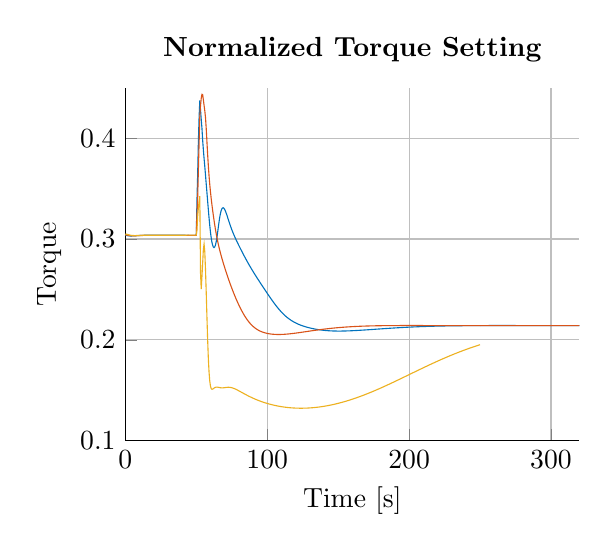
\begin{tikzpicture}

\begin{axis}[%
width=5.766cm,
height=4.479cm,
at={(0cm,0cm)},
scale only axis,
xmin=0,
xmax=320,
xlabel={Time [s]},
xmajorgrids,
ymin=0.1,
ymax=0.45,
ylabel={Torque},
ymajorgrids,
axis background/.style={fill=white},
title style={font=\bfseries},
title={Normalized Torque Setting},
axis x line*=bottom,
axis y line*=left
]
\addplot [color=mycolor1,solid,forget plot]
  table[row sep=crcr]{%
0	0.30400000722465\\
0.5	0.303798455\\
1	0.303569457\\
1.5	0.303363929\\
2	0.303212415\\
2.5	0.303109324\\
3	0.303047996\\
3.5	0.303024632\\
4	0.303027617\\
4.5	0.303044034\\
5	0.30306291\\
5.5	0.303084603\\
6	0.303116817\\
6.5	0.303163269\\
7	0.303219429\\
7.5	0.30327523\\
8	0.303322888\\
8.5	0.303362901\\
9	0.303402018\\
9.5	0.303445979\\
10	0.303493874\\
10.5	0.303538945\\
11	0.303574858\\
11.5	0.303601372\\
12	0.303624164\\
12.5	0.303649311\\
13	0.30367775\\
13.5	0.303704763\\
14	0.303724744\\
14.5	0.303736589\\
15	0.303744684\\
15.5	0.303754753\\
16	0.303768641\\
16.5	0.303782907\\
17	0.303792393\\
17.5	0.303795261\\
18	0.303794739\\
18.5	0.303796034\\
19	0.30380149\\
19.5	0.303808571\\
20	0.303812491\\
20.5	0.303810885\\
21	0.303806065\\
21.5	0.303802769\\
22	0.303803668\\
22.5	0.303806931\\
23	0.303808112\\
23.5	0.303804488\\
24	0.303797671\\
24.5	0.30379202\\
25	0.303790455\\
25.5	0.303791713\\
26	0.303791645\\
26.5	0.303787273\\
27	0.303779664\\
27.5	0.303772881\\
28	0.30377005\\
28.5	0.303770371\\
29	0.303769941\\
29.5	0.30376557\\
30	0.303757891\\
30.5	0.303750737\\
31	0.30374742\\
31.5	0.303747526\\
32	0.303747336\\
32.5	0.303743464\\
33	0.303736179\\
33.5	0.303729149\\
34	0.303725871\\
34.5	0.303726256\\
35	0.303726709\\
35.5	0.303723646\\
36	0.30371702\\
36.5	0.303710394\\
37	0.303707465\\
37.5	0.303708429\\
38	0.303709758\\
38.5	0.303707646\\
39	0.303701767\\
39.5	0.303695641\\
40	0.303693193\\
40.5	0.303694878\\
41	0.303697175\\
41.5	0.30369602\\
42	0.303690834\\
42.5	0.303685156\\
43	0.303683189\\
43.5	0.303685626\\
44	0.303688888\\
44.5	0.303688603\\
45	0.303683955\\
45.5	0.303678576\\
46	0.303677005\\
46.5	0.303680165\\
47	0.303684342\\
47.5	0.303684789\\
48	0.303680462\\
48.5	0.303675172\\
49	0.303673875\\
49.5	0.303677713\\
50	0.30368275\\
50.5	0.3388353\\
51	0.3652667\\
51.5	0.3972577\\
52	0.421189\\
52.5	0.437547\\
53	0.428266\\
53.5	0.41867\\
54	0.410077\\
54.5	0.3981912\\
55	0.3885861\\
55.5	0.3800031\\
56	0.3722052\\
56.5	0.3635879\\
57	0.3549486\\
57.5	0.3464082\\
58	0.3378848\\
58.5	0.3293369\\
59	0.3210862\\
59.5	0.31352675\\
60	0.30692179\\
60.5	0.30142791\\
61	0.29711774\\
61.5	0.2940167\\
62	0.2921334\\
62.5	0.2914795\\
63	0.2920716\\
63.5	0.2939123\\
64	0.29695404\\
64.5	0.30105467\\
65	0.30594745\\
65.5	0.31124699\\
66	0.3164908\\
66.5	0.321216\\
67	0.3250854\\
67.5	0.3279594\\
68	0.3298438\\
68.5	0.3308156\\
69	0.3309828\\
69.5	0.3304673\\
70	0.3293961\\
70.5	0.3278946\\
71	0.3260808\\
71.5	0.3240596\\
72	0.3219197\\
72.5	0.3197321\\
73	0.3175506\\
73.5	0.3154131\\
74	0.31334371\\
74.5	0.3113554\\
75	0.30945237\\
75.5	0.30763255\\
76	0.30588965\\
76.5	0.304214964\\
77	0.30259874\\
77.5	0.30103126\\
78	0.2995035\\
78.5	0.29800763\\
79	0.29653718\\
79.5	0.2950871\\
80	0.2936537\\
80.5	0.2922344\\
81	0.2908278\\
81.5	0.2894331\\
82	0.2880502\\
82.5	0.2866794\\
83	0.2853211\\
83.5	0.283976\\
84	0.2826448\\
84.5	0.281328\\
85	0.2800263\\
85.5	0.2787398\\
86	0.277469\\
86.5	0.2762138\\
87	0.2749742\\
87.5	0.27375\\
88	0.2725407\\
88.5	0.271346\\
89	0.2701652\\
89.5	0.2689976\\
90	0.2678426\\
90.5	0.2666993\\
91	0.2655668\\
91.5	0.2644443\\
92	0.2633308\\
92.5	0.2622256\\
93	0.2611275\\
93.5	0.260036\\
94	0.2589501\\
94.5	0.2578691\\
95	0.2567923\\
95.5	0.2557193\\
96	0.2546496\\
96.5	0.2535828\\
97	0.2525186\\
97.5	0.2514571\\
98	0.2503983\\
98.5	0.2493422\\
99	0.2482892\\
99.5	0.2472397\\
100	0.2461943\\
100.5	0.2451536\\
101	0.2441183\\
101.5	0.2430894\\
102	0.2420677\\
102.5	0.2410542\\
103	0.2400501\\
103.5	0.2390563\\
104	0.2380741\\
104.5	0.2371044\\
105	0.2361486\\
105.5	0.2352076\\
106	0.2342826\\
106.5	0.2333745\\
107	0.2324844\\
107.5	0.2316131\\
108	0.2307614\\
108.5	0.2299302\\
109	0.22912\\
109.5	0.2283313\\
110	0.2275647\\
110.5	0.2268205\\
111	0.226099\\
111.5	0.2254002\\
112	0.2247242\\
112.5	0.2240711\\
113	0.2234406\\
113.5	0.2228325\\
114	0.2222466\\
114.5	0.2216824\\
115	0.2211395\\
115.5	0.2206175\\
116	0.2201158\\
116.5	0.2196337\\
117	0.2191708\\
117.5	0.2187262\\
118	0.2182994\\
118.5	0.2178897\\
119	0.2174964\\
119.5	0.2171187\\
120	0.216756\\
120.5	0.2164076\\
121	0.2160728\\
121.5	0.2157511\\
122	0.2154417\\
122.5	0.215144\\
123	0.2148575\\
123.5	0.2145816\\
124	0.2143159\\
124.5	0.2140597\\
125	0.2138126\\
125.5	0.2135743\\
126	0.2133442\\
126.5	0.2131221\\
127	0.2129076\\
127.5	0.2127003\\
128	0.2125\\
128.5	0.2123065\\
129	0.2121193\\
129.5	0.2119385\\
130	0.2117637\\
130.5	0.2115948\\
131	0.2114316\\
131.5	0.211274\\
132	0.2111219\\
132.5	0.2109751\\
133	0.2108336\\
133.5	0.2106972\\
134	0.2105659\\
134.5	0.2104395\\
135	0.2103181\\
135.5	0.2102016\\
136	0.2100898\\
136.5	0.2099828\\
137	0.2098804\\
137.5	0.2097826\\
138	0.2096894\\
138.5	0.2096008\\
139	0.2095165\\
139.5	0.2094367\\
140	0.2093612\\
140.5	0.20929\\
141	0.2092229\\
141.5	0.2091601\\
142	0.2091012\\
142.5	0.2090464\\
143	0.2089956\\
143.5	0.2089485\\
144	0.2089053\\
144.5	0.2088658\\
145	0.2088298\\
145.5	0.2087974\\
146	0.2087685\\
146.5	0.2087429\\
147	0.2087206\\
147.5	0.2087015\\
148	0.2086854\\
148.5	0.2086724\\
149	0.2086623\\
149.5	0.208655\\
150	0.2086505\\
150.5	0.2086486\\
151	0.2086492\\
151.5	0.2086524\\
152	0.2086579\\
152.5	0.2086657\\
153	0.2086757\\
153.5	0.2086879\\
154	0.2087021\\
154.5	0.2087182\\
155	0.2087363\\
155.5	0.2087561\\
156	0.2087777\\
156.5	0.208801\\
157	0.2088258\\
157.5	0.2088522\\
158	0.2088801\\
158.5	0.2089093\\
159	0.2089399\\
159.5	0.2089717\\
160	0.2090047\\
160.5	0.2090389\\
161	0.2090742\\
161.5	0.2091105\\
162	0.2091478\\
162.5	0.2091861\\
163	0.2092252\\
163.5	0.2092652\\
164	0.209306\\
164.5	0.2093476\\
165	0.2093898\\
165.5	0.2094328\\
166	0.2094763\\
166.5	0.2095205\\
167	0.2095652\\
167.5	0.2096104\\
168	0.2096561\\
168.5	0.2097023\\
169	0.2097489\\
169.5	0.2097958\\
170	0.2098432\\
170.5	0.2098908\\
171	0.2099387\\
171.5	0.2099869\\
172	0.2100353\\
172.5	0.2100839\\
173	0.2101328\\
173.5	0.2101817\\
174	0.2102308\\
174.5	0.21028\\
175	0.2103293\\
175.5	0.2103786\\
176	0.210428\\
176.5	0.2104774\\
177	0.2105268\\
177.5	0.2105761\\
178	0.2106255\\
178.5	0.2106747\\
179	0.2107238\\
179.5	0.2107729\\
180	0.2108218\\
180.5	0.2108706\\
181	0.2109192\\
181.5	0.2109677\\
182	0.2110159\\
182.5	0.211064\\
183	0.2111118\\
183.5	0.2111594\\
184	0.2112068\\
184.5	0.2112539\\
185	0.2113007\\
185.5	0.2113472\\
186	0.2113935\\
186.5	0.2114394\\
187	0.211485\\
187.5	0.2115303\\
188	0.2115752\\
188.5	0.2116198\\
189	0.2116641\\
189.5	0.2117079\\
190	0.2117514\\
190.5	0.2117946\\
191	0.2118373\\
191.5	0.2118796\\
192	0.2119216\\
192.5	0.2119631\\
193	0.2120042\\
193.5	0.2120449\\
194	0.2120852\\
194.5	0.212125\\
195	0.2121644\\
195.5	0.2122034\\
196	0.212242\\
196.5	0.2122801\\
197	0.2123177\\
197.5	0.2123549\\
198	0.2123917\\
198.5	0.212428\\
199	0.2124638\\
199.5	0.2124992\\
200	0.2125341\\
200.5	0.2125686\\
201	0.2126026\\
201.5	0.2126362\\
202	0.2126693\\
202.5	0.2127019\\
203	0.2127341\\
203.5	0.2127658\\
204	0.212797\\
204.5	0.2128278\\
205	0.2128582\\
205.5	0.212888\\
206	0.2129175\\
206.5	0.2129464\\
207	0.2129749\\
207.5	0.213003\\
208	0.2130306\\
208.5	0.2130578\\
209	0.2130845\\
209.5	0.2131108\\
210	0.2131366\\
210.5	0.213162\\
211	0.213187\\
211.5	0.2132115\\
212	0.2132356\\
212.5	0.2132593\\
213	0.2132826\\
213.5	0.2133054\\
214	0.2133278\\
214.5	0.2133498\\
215	0.2133714\\
215.5	0.2133926\\
216	0.2134133\\
216.5	0.2134337\\
217	0.2134537\\
217.5	0.2134733\\
218	0.2134924\\
218.5	0.2135112\\
219	0.2135297\\
219.5	0.2135477\\
220	0.2135654\\
220.5	0.2135827\\
221	0.2135996\\
221.5	0.2136162\\
222	0.2136324\\
222.5	0.2136482\\
223	0.2136638\\
223.5	0.2136789\\
224	0.2136937\\
224.5	0.2137082\\
225	0.2137224\\
225.5	0.2137362\\
226	0.2137497\\
226.5	0.2137629\\
227	0.2137757\\
227.5	0.2137883\\
228	0.2138005\\
228.5	0.2138125\\
229	0.2138241\\
229.5	0.2138354\\
230	0.2138465\\
230.5	0.2138573\\
231	0.2138678\\
231.5	0.213878\\
232	0.2138879\\
232.5	0.2138976\\
233	0.213907\\
233.5	0.2139161\\
234	0.213925\\
234.5	0.2139337\\
235	0.2139421\\
235.5	0.2139502\\
236	0.2139581\\
236.5	0.2139658\\
237	0.2139732\\
237.5	0.2139805\\
238	0.2139875\\
238.5	0.2139942\\
239	0.2140008\\
239.5	0.2140071\\
240	0.2140133\\
240.5	0.2140192\\
241	0.214025\\
241.5	0.2140305\\
242	0.2140359\\
242.5	0.214041\\
243	0.214046\\
243.5	0.2140508\\
244	0.2140555\\
244.5	0.2140599\\
245	0.2140642\\
245.5	0.2140683\\
246	0.2140723\\
246.5	0.2140761\\
247	0.2140797\\
247.5	0.2140832\\
248	0.2140865\\
248.5	0.2140897\\
249	0.2140928\\
249.5	0.2140957\\
250	0.2140984\\
};
\addplot [color=mycolor1,solid,forget plot]
  table[row sep=crcr]{%
250	0.2140984\\
250.5	0.2141011\\
251	0.2141036\\
251.5	0.214106\\
252	0.2141082\\
252.5	0.2141104\\
253	0.2141124\\
253.5	0.2141143\\
254	0.2141161\\
254.5	0.2141178\\
255	0.2141194\\
255.5	0.2141209\\
256	0.2141222\\
256.5	0.2141235\\
257	0.2141247\\
257.5	0.2141258\\
258	0.2141268\\
258.5	0.2141277\\
259	0.2141285\\
259.5	0.2141292\\
260	0.2141299\\
260.5	0.2141305\\
261	0.214131\\
261.5	0.2141314\\
262	0.2141318\\
262.5	0.2141321\\
263	0.2141323\\
263.5	0.2141324\\
264	0.2141325\\
264.5	0.2141326\\
265	0.2141325\\
265.5	0.2141324\\
266	0.2141323\\
266.5	0.2141321\\
267	0.2141319\\
267.5	0.2141316\\
268	0.2141312\\
268.5	0.2141308\\
269	0.2141304\\
269.5	0.2141299\\
270	0.2141294\\
270.5	0.2141288\\
271	0.2141282\\
271.5	0.2141276\\
272	0.2141269\\
272.5	0.2141262\\
273	0.2141255\\
273.5	0.2141247\\
274	0.2141239\\
274.5	0.2141231\\
275	0.2141222\\
275.5	0.2141213\\
276	0.2141204\\
276.5	0.2141195\\
277	0.2141185\\
277.5	0.2141176\\
278	0.2141166\\
278.5	0.2141156\\
279	0.2141145\\
279.5	0.2141135\\
280	0.2141124\\
280.5	0.2141114\\
281	0.2141103\\
281.5	0.2141092\\
282	0.2141081\\
282.5	0.2141069\\
283	0.2141058\\
283.5	0.2141047\\
284	0.2141035\\
284.5	0.2141023\\
285	0.2141012\\
285.5	0.2141\\
286	0.2140988\\
286.5	0.2140977\\
287	0.2140965\\
287.5	0.2140953\\
288	0.2140941\\
288.5	0.2140929\\
289	0.2140917\\
289.5	0.2140905\\
290	0.2140893\\
290.5	0.2140881\\
291	0.2140869\\
291.5	0.2140857\\
292	0.2140845\\
292.5	0.2140834\\
293	0.2140822\\
293.5	0.214081\\
294	0.2140798\\
294.5	0.2140786\\
295	0.2140775\\
295.5	0.2140763\\
296	0.2140752\\
296.5	0.214074\\
297	0.2140729\\
297.5	0.2140717\\
298	0.2140706\\
298.5	0.2140695\\
299	0.2140683\\
299.5	0.2140672\\
300	0.2140661\\
300.5	0.214065\\
301	0.214064\\
301.5	0.2140629\\
302	0.2140618\\
302.5	0.2140608\\
303	0.2140597\\
303.5	0.2140587\\
304	0.2140576\\
304.5	0.2140566\\
305	0.2140556\\
305.5	0.2140546\\
306	0.2140536\\
306.5	0.2140526\\
307	0.2140517\\
307.5	0.2140507\\
308	0.2140498\\
308.5	0.2140488\\
309	0.2140479\\
309.5	0.214047\\
310	0.2140461\\
310.5	0.2140452\\
311	0.2140443\\
311.5	0.2140434\\
312	0.2140426\\
312.5	0.2140417\\
313	0.2140409\\
313.5	0.21404\\
314	0.2140392\\
314.5	0.2140384\\
315	0.2140376\\
315.5	0.2140369\\
316	0.2140361\\
316.5	0.2140353\\
317	0.2140346\\
317.5	0.2140338\\
318	0.2140331\\
318.5	0.2140324\\
319	0.2140317\\
319.5	0.214031\\
320	0.2140303\\
320.5	0.2140297\\
321	0.214029\\
321.5	0.2140283\\
322	0.2140277\\
322.5	0.2140271\\
323	0.2140265\\
323.5	0.2140259\\
324	0.2140253\\
324.5	0.2140247\\
325	0.2140241\\
325.5	0.2140236\\
326	0.214023\\
326.5	0.2140225\\
327	0.2140219\\
327.5	0.2140214\\
328	0.2140209\\
328.5	0.2140204\\
329	0.2140199\\
329.5	0.2140194\\
330	0.2140189\\
330.5	0.2140185\\
331	0.214018\\
331.5	0.2140176\\
332	0.2140171\\
332.5	0.2140167\\
333	0.2140163\\
333.5	0.2140159\\
334	0.2140155\\
334.5	0.2140151\\
335	0.2140147\\
335.5	0.2140143\\
336	0.214014\\
336.5	0.2140136\\
337	0.2140133\\
337.5	0.2140129\\
338	0.2140126\\
338.5	0.2140123\\
339	0.214012\\
339.5	0.2140116\\
340	0.2140113\\
340.5	0.2140111\\
341	0.2140108\\
341.5	0.2140105\\
342	0.2140102\\
342.5	0.2140099\\
343	0.2140097\\
343.5	0.2140094\\
344	0.2140092\\
344.5	0.214009\\
345	0.2140087\\
345.5	0.2140085\\
346	0.2140083\\
346.5	0.2140081\\
347	0.2140079\\
347.5	0.2140077\\
348	0.2140075\\
348.5	0.2140073\\
349	0.2140071\\
349.5	0.2140069\\
350	0.2140067\\
350.5	0.2140066\\
351	0.2140064\\
351.5	0.2140062\\
352	0.2140061\\
352.5	0.2140059\\
353	0.2140058\\
353.5	0.2140057\\
354	0.2140055\\
354.5	0.2140054\\
355	0.2140053\\
355.5	0.2140052\\
356	0.2140051\\
356.5	0.2140049\\
357	0.2140048\\
357.5	0.2140047\\
358	0.2140046\\
358.5	0.2140045\\
359	0.2140045\\
359.5	0.2140044\\
360	0.2140043\\
360.5	0.2140042\\
361	0.2140041\\
361.5	0.2140041\\
362	0.214004\\
362.5	0.2140039\\
363	0.2140039\\
363.5	0.2140038\\
364	0.2140037\\
364.5	0.2140037\\
365	0.2140036\\
365.5	0.2140036\\
366	0.2140035\\
366.5	0.2140035\\
367	0.2140035\\
367.5	0.2140034\\
368	0.2140034\\
368.5	0.2140034\\
369	0.2140033\\
369.5	0.2140033\\
370	0.2140033\\
370.5	0.2140033\\
371	0.2140032\\
371.5	0.2140032\\
372	0.2140032\\
372.5	0.2140032\\
373	0.2140032\\
373.5	0.2140032\\
374	0.2140032\\
374.5	0.2140031\\
375	0.2140031\\
375.5	0.2140031\\
376	0.2140031\\
376.5	0.2140031\\
377	0.2140031\\
377.5	0.2140031\\
378	0.2140031\\
378.5	0.2140031\\
379	0.2140031\\
379.5	0.2140032\\
380	0.2140032\\
380.5	0.2140032\\
381	0.2140032\\
381.5	0.2140032\\
382	0.2140032\\
382.5	0.2140032\\
383	0.2140032\\
383.5	0.2140032\\
384	0.2140033\\
384.5	0.2140033\\
385	0.2140033\\
385.5	0.2140033\\
386	0.2140033\\
386.5	0.2140034\\
387	0.2140034\\
387.5	0.2140034\\
388	0.2140034\\
388.5	0.2140034\\
389	0.2140035\\
389.5	0.2140035\\
390	0.2140035\\
390.5	0.2140035\\
391	0.2140036\\
391.5	0.2140036\\
392	0.2140036\\
392.5	0.2140036\\
393	0.2140037\\
393.5	0.2140037\\
394	0.2140037\\
394.5	0.2140037\\
395	0.2140038\\
395.5	0.2140038\\
396	0.2140038\\
396.5	0.2140039\\
397	0.2140039\\
397.5	0.2140039\\
398	0.2140039\\
398.5	0.214004\\
399	0.214004\\
399.5	0.214004\\
400	0.2140041\\
400.5	0.2140041\\
401	0.2140041\\
401.5	0.2140041\\
402	0.2140042\\
402.5	0.2140042\\
403	0.2140042\\
403.5	0.2140043\\
404	0.2140043\\
404.5	0.2140043\\
405	0.2140044\\
405.5	0.2140044\\
406	0.2140044\\
406.5	0.2140044\\
407	0.2140045\\
407.5	0.2140045\\
408	0.2140045\\
408.5	0.2140046\\
409	0.2140046\\
409.5	0.2140046\\
410	0.2140046\\
410.5	0.2140047\\
411	0.2140047\\
411.5	0.2140047\\
412	0.2140047\\
412.5	0.2140048\\
413	0.2140048\\
413.5	0.2140048\\
414	0.2140049\\
414.5	0.2140049\\
415	0.2140049\\
415.5	0.2140049\\
416	0.214005\\
416.5	0.214005\\
417	0.214005\\
417.5	0.214005\\
418	0.2140051\\
418.5	0.2140051\\
419	0.2140051\\
419.5	0.2140051\\
420	0.2140051\\
420.5	0.2140052\\
421	0.2140052\\
421.5	0.2140052\\
422	0.2140052\\
422.5	0.2140053\\
423	0.2140053\\
423.5	0.2140053\\
424	0.2140053\\
424.5	0.2140053\\
425	0.2140054\\
425.5	0.2140054\\
426	0.2140054\\
426.5	0.2140054\\
427	0.2140054\\
427.5	0.2140055\\
428	0.2140055\\
428.5	0.2140055\\
429	0.2140055\\
429.5	0.2140055\\
430	0.2140056\\
430.5	0.2140056\\
431	0.2140056\\
431.5	0.2140056\\
432	0.2140056\\
432.5	0.2140056\\
433	0.2140057\\
433.5	0.2140057\\
434	0.2140057\\
434.5	0.2140057\\
435	0.2140057\\
435.5	0.2140057\\
436	0.2140057\\
436.5	0.2140058\\
437	0.2140058\\
437.5	0.2140058\\
438	0.2140058\\
438.5	0.2140058\\
439	0.2140058\\
439.5	0.2140058\\
440	0.2140059\\
440.5	0.2140059\\
441	0.2140059\\
441.5	0.2140059\\
442	0.2140059\\
442.5	0.2140059\\
443	0.2140059\\
443.5	0.2140059\\
444	0.2140059\\
444.5	0.214006\\
445	0.214006\\
445.5	0.214006\\
446	0.214006\\
446.5	0.214006\\
447	0.214006\\
447.5	0.214006\\
448	0.214006\\
448.5	0.214006\\
449	0.214006\\
449.5	0.2140061\\
450	0.2140061\\
450.5	0.2140061\\
451	0.2140061\\
451.5	0.2140061\\
452	0.2140061\\
452.5	0.2140061\\
453	0.2140061\\
453.5	0.2140061\\
454	0.2140061\\
454.5	0.2140061\\
455	0.2140061\\
455.5	0.2140061\\
456	0.2140061\\
456.5	0.2140062\\
457	0.2140062\\
457.5	0.2140062\\
458	0.2140062\\
458.5	0.2140062\\
459	0.2140062\\
459.5	0.2140062\\
460	0.2140062\\
460.5	0.2140062\\
461	0.2140062\\
461.5	0.2140062\\
462	0.2140062\\
462.5	0.2140062\\
463	0.2140062\\
463.5	0.2140062\\
464	0.2140062\\
464.5	0.2140062\\
465	0.2140062\\
465.5	0.2140062\\
466	0.2140062\\
466.5	0.2140062\\
467	0.2140062\\
467.5	0.2140062\\
468	0.2140062\\
468.5	0.2140063\\
469	0.2140063\\
469.5	0.2140063\\
470	0.2140063\\
470.5	0.2140063\\
471	0.2140063\\
471.5	0.2140063\\
472	0.2140063\\
472.5	0.2140063\\
473	0.2140063\\
473.5	0.2140063\\
474	0.2140063\\
474.5	0.2140063\\
475	0.2140063\\
475.5	0.2140063\\
476	0.2140063\\
476.5	0.2140063\\
477	0.2140063\\
477.5	0.2140063\\
478	0.2140063\\
478.5	0.2140063\\
479	0.2140063\\
479.5	0.2140063\\
480	0.2140063\\
480.5	0.2140063\\
481	0.2140063\\
481.5	0.2140063\\
482	0.2140063\\
482.5	0.2140063\\
483	0.2140063\\
483.5	0.2140063\\
484	0.2140063\\
484.5	0.2140063\\
485	0.2140063\\
485.5	0.2140063\\
486	0.2140063\\
486.5	0.2140063\\
487	0.2140063\\
487.5	0.2140063\\
488	0.2140063\\
488.5	0.2140063\\
489	0.2140063\\
489.5	0.2140063\\
490	0.2140063\\
490.5	0.2140063\\
491	0.2140063\\
491.5	0.2140063\\
492	0.2140063\\
492.5	0.2140063\\
493	0.2140063\\
493.5	0.2140063\\
494	0.2140063\\
494.5	0.2140063\\
495	0.2140063\\
495.5	0.2140063\\
496	0.2140063\\
496.5	0.2140063\\
497	0.2140063\\
497.5	0.2140063\\
498	0.2140063\\
498.5	0.2140063\\
499	0.2140063\\
499.5	0.2140063\\
};
\addplot [color=mycolor2,solid,forget plot]
  table[row sep=crcr]{%
0	0.30400950945\\
0.5	0.30414581\\
1	0.3039677365\\
1.5	0.3038029\\
2	0.303656665\\
2.5	0.303536229\\
3	0.303436651\\
3.5	0.30335748\\
4	0.303297322\\
4.5	0.303256064\\
5	0.30323286\\
5.5	0.303225562\\
6	0.303230071\\
6.5	0.30324224\\
7	0.303259344\\
7.5	0.303280276\\
8	0.303304853\\
8.5	0.303332716\\
9	0.303362741\\
9.5	0.303393314\\
10	0.303423006\\
10.5	0.303451099\\
11	0.303477585\\
11.5	0.303502746\\
12	0.303526683\\
12.5	0.303549148\\
13	0.303569709\\
13.5	0.303588066\\
14	0.303604233\\
14.5	0.30361848\\
15	0.303631122\\
15.5	0.303642333\\
16	0.303652111\\
16.5	0.303660384\\
17	0.303667149\\
17.5	0.303672533\\
18	0.30367675\\
18.5	0.303679992\\
19	0.303682367\\
19.5	0.303683899\\
20	0.303684595\\
20.5	0.303684498\\
21	0.303683711\\
21.5	0.30368236\\
22	0.303680549\\
22.5	0.303678338\\
23	0.303675751\\
23.5	0.303672815\\
24	0.303669576\\
24.5	0.303666105\\
25	0.30366248\\
25.5	0.30365876\\
26	0.303654982\\
26.5	0.30365117\\
27	0.303647352\\
27.5	0.303643563\\
28	0.30363985\\
28.5	0.303636256\\
29	0.30363281\\
29.5	0.303629534\\
30	0.303626438\\
30.5	0.303623538\\
31	0.303620851\\
31.5	0.303618395\\
32	0.303616185\\
32.5	0.303614226\\
33	0.30361252\\
33.5	0.303611061\\
34	0.303609847\\
34.5	0.303608875\\
35	0.303608143\\
35.5	0.303607642\\
36	0.303607362\\
36.5	0.303607288\\
37	0.303607405\\
37.5	0.303607699\\
38	0.303608155\\
38.5	0.303608759\\
39	0.303609494\\
39.5	0.303610344\\
40	0.303611288\\
40.5	0.303612311\\
41	0.303613396\\
41.5	0.303614528\\
42	0.303615691\\
42.5	0.303616871\\
43	0.303618055\\
43.5	0.303619227\\
44	0.303620377\\
44.5	0.303621493\\
45	0.303622567\\
45.5	0.30362359\\
46	0.303624554\\
46.5	0.303625454\\
47	0.303626283\\
47.5	0.303627039\\
48	0.303627717\\
48.5	0.303628317\\
49	0.303628838\\
49.5	0.303629281\\
50	0.303629644\\
50.5	0.3243706\\
51	0.3412875\\
51.5	0.3693842\\
52	0.3955125\\
52.5	0.421582\\
53	0.432515\\
53.5	0.439634\\
54	0.443594\\
54.5	0.443287\\
55	0.438185\\
55.5	0.43265\\
56	0.427319\\
56.5	0.42082\\
57	0.409949\\
57.5	0.3971502\\
58	0.3843743\\
58.5	0.3728447\\
59	0.3628703\\
59.5	0.3543172\\
60	0.3469393\\
60.5	0.3404216\\
61	0.3344952\\
61.5	0.3289598\\
62	0.323722\\
62.5	0.3187646\\
63	0.314098\\
63.5	0.30973106\\
64	0.3056617\\
64.5	0.30187651\\
65	0.29835408\\
65.5	0.29506817\\
66	0.2919902\\
66.5	0.2890912\\
67	0.2863431\\
67.5	0.2837202\\
68	0.2812\\
68.5	0.2787638\\
69	0.2763967\\
69.5	0.2740874\\
70	0.2718276\\
70.5	0.2696116\\
71	0.2674356\\
71.5	0.2652975\\
72	0.2631958\\
72.5	0.2611299\\
73	0.2590996\\
73.5	0.257105\\
74	0.2551461\\
74.5	0.2532233\\
75	0.2513367\\
75.5	0.2494866\\
76	0.2476734\\
76.5	0.2458973\\
77	0.2441587\\
77.5	0.2424579\\
78	0.2407954\\
78.5	0.2391713\\
79	0.2375863\\
79.5	0.2360406\\
80	0.2345347\\
80.5	0.2330691\\
81	0.2316443\\
81.5	0.2302606\\
82	0.2289187\\
82.5	0.2276191\\
83	0.2263621\\
83.5	0.2251482\\
84	0.2239779\\
84.5	0.2228515\\
85	0.2217691\\
85.5	0.220731\\
86	0.2197372\\
86.5	0.2187876\\
87	0.2178819\\
87.5	0.2170197\\
88	0.2162005\\
88.5	0.2154236\\
89	0.2146881\\
89.5	0.213993\\
90	0.2133373\\
90.5	0.2127198\\
91	0.212139\\
91.5	0.2115937\\
92	0.2110823\\
92.5	0.2106034\\
93	0.2101555\\
93.5	0.2097369\\
94	0.2093463\\
94.5	0.208982\\
95	0.2086427\\
95.5	0.2083268\\
96	0.2080332\\
96.5	0.2077604\\
97	0.2075073\\
97.5	0.2072726\\
98	0.2070554\\
98.5	0.2068545\\
99	0.2066692\\
99.5	0.2064984\\
100	0.2063415\\
100.5	0.2061977\\
101	0.2060663\\
101.5	0.2059467\\
102	0.2058384\\
102.5	0.2057408\\
103	0.2056535\\
103.5	0.2055761\\
104	0.205508\\
104.5	0.205449\\
105	0.2053987\\
105.5	0.2053568\\
106	0.2053229\\
106.5	0.2052968\\
107	0.2052781\\
107.5	0.2052666\\
108	0.205262\\
108.5	0.205264\\
109	0.2052725\\
109.5	0.205287\\
110	0.2053075\\
110.5	0.2053336\\
111	0.2053651\\
111.5	0.2054018\\
112	0.2054434\\
112.5	0.2054898\\
113	0.2055406\\
113.5	0.2055957\\
114	0.2056548\\
114.5	0.2057177\\
115	0.2057843\\
115.5	0.2058543\\
116	0.2059275\\
116.5	0.2060037\\
117	0.2060828\\
117.5	0.2061645\\
118	0.2062487\\
118.5	0.2063352\\
119	0.2064238\\
119.5	0.2065144\\
120	0.2066067\\
120.5	0.2067008\\
121	0.2067963\\
121.5	0.2068932\\
122	0.2069913\\
122.5	0.2070905\\
123	0.2071907\\
123.5	0.2072918\\
124	0.2073936\\
124.5	0.207496\\
125	0.2075989\\
125.5	0.2077023\\
126	0.2078059\\
126.5	0.2079098\\
127	0.2080138\\
127.5	0.2081179\\
128	0.2082219\\
128.5	0.2083259\\
129	0.2084296\\
129.5	0.2085331\\
130	0.2086363\\
130.5	0.2087391\\
131	0.2088414\\
131.5	0.2089432\\
132	0.2090445\\
132.5	0.2091452\\
133	0.2092452\\
133.5	0.2093445\\
134	0.209443\\
134.5	0.2095407\\
135	0.2096376\\
135.5	0.2097337\\
136	0.2098288\\
136.5	0.2099229\\
137	0.2100162\\
137.5	0.2101084\\
138	0.2101995\\
138.5	0.2102897\\
139	0.2103787\\
139.5	0.2104667\\
140	0.2105535\\
140.5	0.2106392\\
141	0.2107237\\
141.5	0.2108071\\
142	0.2108893\\
142.5	0.2109704\\
143	0.2110502\\
143.5	0.2111288\\
144	0.2112062\\
144.5	0.2112824\\
145	0.2113573\\
145.5	0.211431\\
146	0.2115035\\
146.5	0.2115747\\
147	0.2116447\\
147.5	0.2117135\\
148	0.211781\\
148.5	0.2118473\\
149	0.2119123\\
149.5	0.2119762\\
150	0.2120388\\
150.5	0.2121001\\
151	0.2121603\\
151.5	0.2122193\\
152	0.212277\\
152.5	0.2123336\\
153	0.2123889\\
153.5	0.2124431\\
154	0.2124962\\
154.5	0.2125481\\
155	0.2125988\\
155.5	0.2126484\\
156	0.2126969\\
156.5	0.2127442\\
157	0.2127905\\
157.5	0.2128356\\
158	0.2128797\\
158.5	0.2129227\\
159	0.2129647\\
159.5	0.2130057\\
160	0.2130456\\
160.5	0.2130845\\
161	0.2131224\\
161.5	0.2131593\\
162	0.2131953\\
162.5	0.2132303\\
163	0.2132643\\
163.5	0.2132975\\
164	0.2133297\\
164.5	0.213361\\
165	0.2133915\\
165.5	0.2134211\\
166	0.2134498\\
166.5	0.2134777\\
167	0.2135048\\
167.5	0.213531\\
168	0.2135565\\
168.5	0.2135812\\
169	0.2136052\\
169.5	0.2136283\\
170	0.2136508\\
170.5	0.2136725\\
171	0.2136936\\
171.5	0.2137139\\
172	0.2137336\\
172.5	0.2137526\\
173	0.213771\\
173.5	0.2137887\\
174	0.2138058\\
174.5	0.2138224\\
175	0.2138383\\
175.5	0.2138536\\
176	0.2138684\\
176.5	0.2138826\\
177	0.2138963\\
177.5	0.2139095\\
178	0.2139222\\
178.5	0.2139343\\
179	0.213946\\
179.5	0.2139572\\
180	0.2139679\\
180.5	0.2139782\\
181	0.213988\\
181.5	0.2139975\\
182	0.2140065\\
182.5	0.2140151\\
183	0.2140233\\
183.5	0.2140311\\
184	0.2140385\\
184.5	0.2140456\\
185	0.2140524\\
185.5	0.2140588\\
186	0.2140649\\
186.5	0.2140706\\
187	0.214076\\
187.5	0.2140812\\
188	0.214086\\
188.5	0.2140906\\
189	0.2140949\\
189.5	0.2140989\\
190	0.2141027\\
190.5	0.2141062\\
191	0.2141095\\
191.5	0.2141125\\
192	0.2141154\\
192.5	0.214118\\
193	0.2141204\\
193.5	0.2141226\\
194	0.2141246\\
194.5	0.2141264\\
195	0.2141281\\
195.5	0.2141295\\
196	0.2141308\\
196.5	0.214132\\
197	0.214133\\
197.5	0.2141338\\
198	0.2141345\\
198.5	0.2141351\\
199	0.2141355\\
199.5	0.2141358\\
200	0.214136\\
200.5	0.2141361\\
201	0.214136\\
201.5	0.2141359\\
202	0.2141357\\
202.5	0.2141353\\
203	0.2141349\\
203.5	0.2141344\\
204	0.2141338\\
204.5	0.2141331\\
205	0.2141324\\
205.5	0.2141316\\
206	0.2141307\\
206.5	0.2141297\\
207	0.2141287\\
207.5	0.2141277\\
208	0.2141266\\
208.5	0.2141254\\
209	0.2141242\\
209.5	0.214123\\
210	0.2141217\\
210.5	0.2141204\\
211	0.214119\\
211.5	0.2141177\\
212	0.2141162\\
212.5	0.2141148\\
213	0.2141133\\
213.5	0.2141119\\
214	0.2141104\\
214.5	0.2141088\\
215	0.2141073\\
215.5	0.2141057\\
216	0.2141042\\
216.5	0.2141026\\
217	0.214101\\
217.5	0.2140994\\
218	0.2140979\\
218.5	0.2140963\\
219	0.2140947\\
219.5	0.2140931\\
220	0.2140915\\
220.5	0.2140899\\
221	0.2140883\\
221.5	0.2140867\\
222	0.2140851\\
222.5	0.2140835\\
223	0.214082\\
223.5	0.2140804\\
224	0.2140789\\
224.5	0.2140773\\
225	0.2140758\\
225.5	0.2140743\\
226	0.2140728\\
226.5	0.2140713\\
227	0.2140698\\
227.5	0.2140684\\
228	0.2140669\\
228.5	0.2140655\\
229	0.2140641\\
229.5	0.2140627\\
230	0.2140613\\
230.5	0.2140599\\
231	0.2140586\\
231.5	0.2140573\\
232	0.2140559\\
232.5	0.2140546\\
233	0.2140534\\
233.5	0.2140521\\
234	0.2140509\\
234.5	0.2140497\\
235	0.2140485\\
235.5	0.2140473\\
236	0.2140461\\
236.5	0.214045\\
237	0.2140439\\
237.5	0.2140428\\
238	0.2140417\\
238.5	0.2140406\\
239	0.2140396\\
239.5	0.2140386\\
240	0.2140376\\
240.5	0.2140366\\
241	0.2140356\\
241.5	0.2140347\\
242	0.2140337\\
242.5	0.2140328\\
243	0.2140319\\
243.5	0.2140311\\
244	0.2140302\\
244.5	0.2140294\\
245	0.2140286\\
245.5	0.2140278\\
246	0.214027\\
246.5	0.2140263\\
247	0.2140255\\
247.5	0.2140248\\
248	0.2140241\\
248.5	0.2140234\\
249	0.2140227\\
249.5	0.2140221\\
250	0.2140214\\
};
\addplot [color=mycolor2,solid,forget plot]
  table[row sep=crcr]{%
250	0.2140214\\
250.5	0.2140208\\
251	0.2140202\\
251.5	0.2140196\\
252	0.214019\\
252.5	0.2140185\\
253	0.2140179\\
253.5	0.2140174\\
254	0.2140169\\
254.5	0.2140164\\
255	0.2140159\\
255.5	0.2140154\\
256	0.214015\\
256.5	0.2140145\\
257	0.2140141\\
257.5	0.2140137\\
258	0.2140133\\
258.5	0.2140129\\
259	0.2140125\\
259.5	0.2140121\\
260	0.2140118\\
260.5	0.2140114\\
261	0.2140111\\
261.5	0.2140108\\
262	0.2140104\\
262.5	0.2140101\\
263	0.2140099\\
263.5	0.2140096\\
264	0.2140093\\
264.5	0.214009\\
265	0.2140088\\
265.5	0.2140085\\
266	0.2140083\\
266.5	0.2140081\\
267	0.2140079\\
267.5	0.2140077\\
268	0.2140075\\
268.5	0.2140073\\
269	0.2140071\\
269.5	0.2140069\\
270	0.2140067\\
270.5	0.2140066\\
271	0.2140064\\
271.5	0.2140063\\
272	0.2140061\\
272.5	0.214006\\
273	0.2140059\\
273.5	0.2140057\\
274	0.2140056\\
274.5	0.2140055\\
275	0.2140054\\
275.5	0.2140053\\
276	0.2140052\\
276.5	0.2140051\\
277	0.214005\\
277.5	0.2140049\\
278	0.2140049\\
278.5	0.2140048\\
279	0.2140047\\
279.5	0.2140047\\
280	0.2140046\\
280.5	0.2140046\\
281	0.2140045\\
281.5	0.2140045\\
282	0.2140044\\
282.5	0.2140044\\
283	0.2140043\\
283.5	0.2140043\\
284	0.2140043\\
284.5	0.2140042\\
285	0.2140042\\
285.5	0.2140042\\
286	0.2140042\\
286.5	0.2140042\\
287	0.2140042\\
287.5	0.2140041\\
288	0.2140041\\
288.5	0.2140041\\
289	0.2140041\\
289.5	0.2140041\\
290	0.2140041\\
290.5	0.2140041\\
291	0.2140041\\
291.5	0.2140041\\
292	0.2140041\\
292.5	0.2140041\\
293	0.2140041\\
293.5	0.2140041\\
294	0.2140042\\
294.5	0.2140042\\
295	0.2140042\\
295.5	0.2140042\\
296	0.2140042\\
296.5	0.2140042\\
297	0.2140042\\
297.5	0.2140043\\
298	0.2140043\\
298.5	0.2140043\\
299	0.2140043\\
299.5	0.2140043\\
300	0.2140044\\
300.5	0.2140044\\
301	0.2140044\\
301.5	0.2140044\\
302	0.2140044\\
302.5	0.2140045\\
303	0.2140045\\
303.5	0.2140045\\
304	0.2140045\\
304.5	0.2140046\\
305	0.2140046\\
305.5	0.2140046\\
306	0.2140046\\
306.5	0.2140047\\
307	0.2140047\\
307.5	0.2140047\\
308	0.2140047\\
308.5	0.2140048\\
309	0.2140048\\
309.5	0.2140048\\
310	0.2140049\\
310.5	0.2140049\\
311	0.2140049\\
311.5	0.2140049\\
312	0.214005\\
312.5	0.214005\\
313	0.214005\\
313.5	0.214005\\
314	0.2140051\\
314.5	0.2140051\\
315	0.2140051\\
315.5	0.2140051\\
316	0.2140052\\
316.5	0.2140052\\
317	0.2140052\\
317.5	0.2140052\\
318	0.2140052\\
318.5	0.2140053\\
319	0.2140053\\
319.5	0.2140053\\
320	0.2140053\\
320.5	0.2140054\\
321	0.2140054\\
321.5	0.2140054\\
322	0.2140054\\
322.5	0.2140054\\
323	0.2140055\\
323.5	0.2140055\\
324	0.2140055\\
324.5	0.2140055\\
325	0.2140055\\
325.5	0.2140056\\
326	0.2140056\\
326.5	0.2140056\\
327	0.2140056\\
327.5	0.2140056\\
328	0.2140057\\
328.5	0.2140057\\
329	0.2140057\\
329.5	0.2140057\\
330	0.2140057\\
330.5	0.2140057\\
331	0.2140058\\
331.5	0.2140058\\
332	0.2140058\\
332.5	0.2140058\\
333	0.2140058\\
333.5	0.2140058\\
334	0.2140058\\
334.5	0.2140059\\
335	0.2140059\\
335.5	0.2140059\\
336	0.2140059\\
336.5	0.2140059\\
337	0.2140059\\
337.5	0.2140059\\
338	0.2140059\\
338.5	0.2140059\\
339	0.214006\\
339.5	0.214006\\
340	0.214006\\
340.5	0.214006\\
341	0.214006\\
341.5	0.214006\\
342	0.214006\\
342.5	0.214006\\
343	0.214006\\
343.5	0.214006\\
344	0.2140061\\
344.5	0.2140061\\
345	0.2140061\\
345.5	0.2140061\\
346	0.2140061\\
346.5	0.2140061\\
347	0.2140061\\
347.5	0.2140061\\
348	0.2140061\\
348.5	0.2140061\\
349	0.2140061\\
349.5	0.2140061\\
350	0.2140061\\
350.5	0.2140061\\
351	0.2140061\\
351.5	0.2140061\\
352	0.2140062\\
352.5	0.2140062\\
353	0.2140062\\
353.5	0.2140062\\
354	0.2140062\\
354.5	0.2140062\\
355	0.2140062\\
355.5	0.2140062\\
356	0.2140062\\
356.5	0.2140062\\
357	0.2140062\\
357.5	0.2140062\\
358	0.2140062\\
358.5	0.2140062\\
359	0.2140062\\
359.5	0.2140062\\
360	0.2140062\\
360.5	0.2140062\\
361	0.2140062\\
361.5	0.2140062\\
362	0.2140062\\
362.5	0.2140062\\
363	0.2140062\\
363.5	0.2140062\\
364	0.2140062\\
364.5	0.2140062\\
365	0.2140062\\
365.5	0.2140062\\
366	0.2140062\\
366.5	0.2140062\\
367	0.2140062\\
367.5	0.2140062\\
368	0.2140062\\
368.5	0.2140062\\
369	0.2140062\\
369.5	0.2140062\\
370	0.2140062\\
370.5	0.2140062\\
371	0.2140062\\
371.5	0.2140062\\
372	0.2140062\\
372.5	0.2140063\\
373	0.2140063\\
373.5	0.2140063\\
374	0.2140063\\
374.5	0.2140063\\
375	0.2140063\\
375.5	0.2140063\\
376	0.2140063\\
376.5	0.2140063\\
377	0.2140063\\
377.5	0.2140063\\
378	0.2140063\\
378.5	0.2140063\\
379	0.2140063\\
379.5	0.2140063\\
380	0.2140063\\
380.5	0.2140063\\
381	0.2140063\\
381.5	0.2140063\\
382	0.2140063\\
382.5	0.2140063\\
383	0.2140063\\
383.5	0.2140063\\
384	0.2140063\\
384.5	0.2140063\\
385	0.2140063\\
385.5	0.2140063\\
386	0.2140063\\
386.5	0.2140063\\
387	0.2140063\\
387.5	0.2140063\\
388	0.2140063\\
388.5	0.2140063\\
389	0.2140063\\
389.5	0.2140063\\
390	0.2140063\\
390.5	0.2140062\\
391	0.2140062\\
391.5	0.2140062\\
392	0.2140062\\
392.5	0.2140062\\
393	0.2140062\\
393.5	0.2140062\\
394	0.2140062\\
394.5	0.2140062\\
395	0.2140062\\
395.5	0.2140062\\
396	0.2140062\\
396.5	0.2140062\\
397	0.2140062\\
397.5	0.2140062\\
398	0.2140062\\
398.5	0.2140062\\
399	0.2140062\\
399.5	0.2140062\\
400	0.2140062\\
400.5	0.2140062\\
401	0.2140062\\
401.5	0.2140062\\
402	0.2140062\\
402.5	0.2140062\\
403	0.2140062\\
403.5	0.2140062\\
404	0.2140062\\
404.5	0.2140062\\
405	0.2140062\\
405.5	0.2140062\\
406	0.2140062\\
406.5	0.2140062\\
407	0.2140062\\
407.5	0.2140062\\
408	0.2140062\\
408.5	0.2140062\\
409	0.2140062\\
409.5	0.2140062\\
410	0.2140062\\
410.5	0.2140062\\
411	0.2140062\\
411.5	0.2140062\\
412	0.2140062\\
412.5	0.2140062\\
413	0.2140062\\
413.5	0.2140062\\
414	0.2140062\\
414.5	0.2140062\\
415	0.2140062\\
415.5	0.2140062\\
416	0.2140062\\
416.5	0.2140062\\
417	0.2140062\\
417.5	0.2140062\\
418	0.2140062\\
418.5	0.2140062\\
419	0.2140062\\
419.5	0.2140062\\
420	0.2140062\\
420.5	0.2140062\\
421	0.2140062\\
421.5	0.2140062\\
422	0.2140062\\
422.5	0.2140062\\
423	0.2140062\\
423.5	0.2140062\\
424	0.2140062\\
424.5	0.2140062\\
425	0.2140062\\
425.5	0.2140062\\
426	0.2140062\\
426.5	0.2140062\\
427	0.2140062\\
427.5	0.2140062\\
428	0.2140062\\
428.5	0.2140062\\
429	0.2140062\\
429.5	0.2140062\\
430	0.2140062\\
430.5	0.2140062\\
431	0.2140062\\
431.5	0.2140062\\
432	0.2140062\\
432.5	0.2140062\\
433	0.2140062\\
433.5	0.2140062\\
434	0.2140062\\
434.5	0.2140062\\
435	0.2140062\\
435.5	0.2140062\\
436	0.2140062\\
436.5	0.2140062\\
437	0.2140062\\
437.5	0.2140062\\
438	0.2140062\\
438.5	0.2140062\\
439	0.2140062\\
439.5	0.2140062\\
440	0.2140062\\
440.5	0.2140062\\
441	0.2140062\\
441.5	0.2140062\\
442	0.2140062\\
442.5	0.2140062\\
443	0.2140062\\
443.5	0.2140062\\
444	0.2140062\\
444.5	0.2140062\\
445	0.2140062\\
445.5	0.2140062\\
446	0.2140062\\
446.5	0.2140062\\
447	0.2140062\\
447.5	0.2140062\\
448	0.2140062\\
448.5	0.2140062\\
449	0.2140062\\
449.5	0.2140062\\
450	0.2140062\\
450.5	0.2140062\\
451	0.2140062\\
451.5	0.2140062\\
452	0.2140062\\
452.5	0.2140062\\
453	0.2140062\\
453.5	0.2140062\\
454	0.2140062\\
454.5	0.2140062\\
455	0.2140062\\
455.5	0.2140062\\
456	0.2140062\\
456.5	0.2140062\\
457	0.2140062\\
457.5	0.2140062\\
458	0.2140062\\
458.5	0.2140062\\
459	0.2140062\\
459.5	0.2140062\\
460	0.2140062\\
460.5	0.2140062\\
461	0.2140062\\
461.5	0.2140062\\
462	0.2140062\\
462.5	0.2140062\\
463	0.2140062\\
463.5	0.2140062\\
464	0.2140062\\
464.5	0.2140062\\
465	0.2140062\\
465.5	0.2140062\\
466	0.2140062\\
466.5	0.2140062\\
467	0.2140062\\
467.5	0.2140062\\
468	0.2140062\\
468.5	0.2140062\\
469	0.2140062\\
469.5	0.2140062\\
470	0.2140062\\
470.5	0.2140062\\
471	0.2140062\\
471.5	0.2140062\\
472	0.2140062\\
472.5	0.2140062\\
473	0.2140062\\
473.5	0.2140062\\
474	0.2140062\\
474.5	0.2140062\\
475	0.2140062\\
475.5	0.2140062\\
476	0.2140062\\
476.5	0.2140062\\
477	0.2140062\\
477.5	0.2140062\\
478	0.2140062\\
478.5	0.2140062\\
479	0.2140062\\
479.5	0.2140062\\
480	0.2140062\\
480.5	0.2140062\\
481	0.2140062\\
481.5	0.2140062\\
482	0.2140062\\
482.5	0.2140062\\
483	0.2140062\\
483.5	0.2140062\\
484	0.2140062\\
484.5	0.2140062\\
485	0.2140062\\
485.5	0.2140062\\
486	0.2140062\\
486.5	0.2140062\\
487	0.2140062\\
487.5	0.2140062\\
488	0.2140062\\
488.5	0.2140062\\
489	0.2140062\\
489.5	0.2140062\\
490	0.2140062\\
490.5	0.2140062\\
491	0.2140062\\
491.5	0.2140062\\
492	0.2140062\\
492.5	0.2140062\\
493	0.2140062\\
493.5	0.2140062\\
494	0.2140062\\
494.5	0.2140062\\
495	0.2140062\\
495.5	0.2140062\\
496	0.2140062\\
496.5	0.2140062\\
497	0.2140062\\
497.5	0.2140062\\
498	0.2140062\\
498.5	0.2140062\\
499	0.2140062\\
499.5	0.2140062\\
};
\addplot [color=mycolor3,solid,forget plot]
  table[row sep=crcr]{%
0	0.3040429237\\
0.5	0.304960779\\
1	0.304728669\\
1.5	0.30453981\\
2	0.304325505\\
2.5	0.304136374\\
3	0.3039653544\\
3.5	0.303818001\\
4	0.30369628\\
4.5	0.30359988\\
5	0.303527133\\
5.5	0.303476026\\
6	0.30344454\\
6.5	0.303430266\\
7	0.30343051\\
7.5	0.303441972\\
8	0.303461145\\
8.5	0.303485363\\
9	0.303512735\\
9.5	0.303541933\\
10	0.303571896\\
10.5	0.303601605\\
11	0.303630088\\
11.5	0.303656531\\
12	0.303680387\\
12.5	0.30370138\\
13	0.303719471\\
13.5	0.303734746\\
14	0.303747314\\
14.5	0.303757287\\
15	0.303764819\\
15.5	0.303770154\\
16	0.303773603\\
16.5	0.303775496\\
17	0.303776142\\
17.5	0.303775798\\
18	0.303774682\\
18.5	0.303772991\\
19	0.303770913\\
19.5	0.303768623\\
20	0.303766275\\
20.5	0.303763984\\
21	0.303761834\\
21.5	0.303759878\\
22	0.303758154\\
22.5	0.303756687\\
23	0.303755494\\
23.5	0.303754582\\
24	0.303753946\\
24.5	0.303753568\\
25	0.303753425\\
25.5	0.303753493\\
26	0.303753748\\
26.5	0.303754166\\
27	0.303754725\\
27.5	0.303755404\\
28	0.303756179\\
28.5	0.303757032\\
29	0.303757944\\
29.5	0.303758904\\
30	0.303759899\\
30.5	0.303760922\\
31	0.303761965\\
31.5	0.303763023\\
32	0.303764093\\
32.5	0.303765173\\
33	0.303766264\\
33.5	0.303767365\\
34	0.303768479\\
34.5	0.303769608\\
35	0.303770755\\
35.5	0.303771923\\
36	0.303773115\\
36.5	0.303774334\\
37	0.303775585\\
37.5	0.30377687\\
38	0.303778192\\
38.5	0.303779556\\
39	0.303780964\\
39.5	0.303782418\\
40	0.303783922\\
40.5	0.303785478\\
41	0.303787088\\
41.5	0.303788755\\
42	0.303790482\\
42.5	0.30379227\\
43	0.303794122\\
43.5	0.303796039\\
44	0.303798024\\
44.5	0.303800079\\
45	0.303802207\\
45.5	0.303804409\\
46	0.303806688\\
46.5	0.303809046\\
47	0.303811486\\
47.5	0.303814011\\
48	0.303816623\\
48.5	0.303819325\\
49	0.30382212\\
49.5	0.303825011\\
50	0.303828002\\
50.5	0.30860974\\
51	0.3229101\\
51.5	0.3308913\\
52	0.3375838\\
52.5	0.342532\\
53	0.2662484\\
53.5	0.2502702\\
54	0.2623629\\
54.5	0.275902\\
55	0.2895839\\
55.5	0.29495629\\
56	0.2874968\\
56.5	0.2701038\\
57	0.2478781\\
57.5	0.223712\\
58	0.200826\\
58.5	0.181857\\
59	0.168043\\
59.5	0.159117\\
60	0.154061\\
60.5	0.151668\\
61	0.150897\\
61.5	0.150989\\
62	0.151451\\
62.5	0.151996\\
63	0.152468\\
63.5	0.152801\\
64	0.152982\\
64.5	0.153027\\
65	0.152971\\
65.5	0.152849\\
66	0.152698\\
66.5	0.152548\\
67	0.152421\\
67.5	0.152333\\
68	0.152289\\
68.5	0.152289\\
69	0.152329\\
69.5	0.1524\\
70	0.152492\\
70.5	0.152592\\
71	0.152689\\
71.5	0.152772\\
72	0.152832\\
72.5	0.152863\\
73	0.152859\\
73.5	0.152815\\
74	0.152732\\
74.5	0.152609\\
75	0.152446\\
75.5	0.152247\\
76	0.152015\\
76.5	0.151751\\
77	0.151462\\
77.5	0.151149\\
78	0.150817\\
78.5	0.150468\\
79	0.150108\\
79.5	0.149737\\
80	0.149358\\
80.5	0.148974\\
81	0.148587\\
81.5	0.148198\\
82	0.147809\\
82.5	0.14742\\
83	0.147033\\
83.5	0.146648\\
84	0.146266\\
84.5	0.145888\\
85	0.145514\\
85.5	0.145144\\
86	0.144779\\
86.5	0.144419\\
87	0.144064\\
87.5	0.143715\\
88	0.143371\\
88.5	0.143033\\
89	0.1427\\
89.5	0.142373\\
90	0.142052\\
90.5	0.141737\\
91	0.141428\\
91.5	0.141124\\
92	0.140827\\
92.5	0.140535\\
93	0.140249\\
93.5	0.139968\\
94	0.139694\\
94.5	0.139425\\
95	0.139161\\
95.5	0.138904\\
96	0.138651\\
96.5	0.138404\\
97	0.138163\\
97.5	0.137927\\
98	0.137696\\
98.5	0.13747\\
99	0.13725\\
99.5	0.137034\\
100	0.136824\\
100.5	0.136619\\
101	0.136419\\
101.5	0.136224\\
102	0.136034\\
102.5	0.135849\\
103	0.135668\\
103.5	0.135493\\
104	0.135322\\
104.5	0.135156\\
105	0.134994\\
105.5	0.134838\\
106	0.134686\\
106.5	0.134538\\
107	0.134396\\
107.5	0.134257\\
108	0.134124\\
108.5	0.133994\\
109	0.13387\\
109.5	0.133749\\
110	0.133634\\
110.5	0.133522\\
111	0.133415\\
111.5	0.133312\\
112	0.133214\\
112.5	0.13312\\
113	0.13303\\
113.5	0.132944\\
114	0.132863\\
114.5	0.132786\\
115	0.132713\\
115.5	0.132644\\
116	0.13258\\
116.5	0.132519\\
117	0.132463\\
117.5	0.13241\\
118	0.132362\\
118.5	0.132318\\
119	0.132278\\
119.5	0.132241\\
120	0.132209\\
120.5	0.132181\\
121	0.132157\\
121.5	0.132136\\
122	0.13212\\
122.5	0.132107\\
123	0.132098\\
123.5	0.132094\\
124	0.132093\\
124.5	0.132095\\
125	0.132102\\
125.5	0.132112\\
126	0.132127\\
126.5	0.132144\\
127	0.132166\\
127.5	0.132191\\
128	0.13222\\
128.5	0.132253\\
129	0.13229\\
129.5	0.13233\\
130	0.132373\\
130.5	0.132421\\
131	0.132472\\
131.5	0.132526\\
132	0.132584\\
132.5	0.132646\\
133	0.132711\\
133.5	0.13278\\
134	0.132852\\
134.5	0.132928\\
135	0.133007\\
135.5	0.133089\\
136	0.133175\\
136.5	0.133265\\
137	0.133358\\
137.5	0.133454\\
138	0.133554\\
138.5	0.133657\\
139	0.133763\\
139.5	0.133873\\
140	0.133986\\
140.5	0.134103\\
141	0.134222\\
141.5	0.134345\\
142	0.134471\\
142.5	0.134601\\
143	0.134734\\
143.5	0.134869\\
144	0.135008\\
144.5	0.135151\\
145	0.135296\\
145.5	0.135445\\
146	0.135596\\
146.5	0.135751\\
147	0.135909\\
147.5	0.13607\\
148	0.136234\\
148.5	0.136401\\
149	0.136571\\
149.5	0.136744\\
150	0.13692\\
150.5	0.137099\\
151	0.137281\\
151.5	0.137465\\
152	0.137653\\
152.5	0.137844\\
153	0.138037\\
153.5	0.138234\\
154	0.138433\\
154.5	0.138635\\
155	0.138839\\
155.5	0.139047\\
156	0.139257\\
156.5	0.13947\\
157	0.139686\\
157.5	0.139904\\
158	0.140125\\
158.5	0.140349\\
159	0.140575\\
159.5	0.140804\\
160	0.141036\\
160.5	0.14127\\
161	0.141506\\
161.5	0.141745\\
162	0.141987\\
162.5	0.142231\\
163	0.142477\\
163.5	0.142726\\
164	0.142977\\
164.5	0.143231\\
165	0.143487\\
165.5	0.143745\\
166	0.144005\\
166.5	0.144268\\
167	0.144533\\
167.5	0.1448\\
168	0.145069\\
168.5	0.145341\\
169	0.145614\\
169.5	0.14589\\
170	0.146168\\
170.5	0.146448\\
171	0.146729\\
171.5	0.147013\\
172	0.147299\\
172.5	0.147586\\
173	0.147876\\
173.5	0.148167\\
174	0.14846\\
174.5	0.148755\\
175	0.149052\\
175.5	0.149351\\
176	0.149651\\
176.5	0.149953\\
177	0.150256\\
177.5	0.150561\\
178	0.150868\\
178.5	0.151176\\
179	0.151486\\
179.5	0.151797\\
180	0.15211\\
180.5	0.152424\\
181	0.152739\\
181.5	0.153056\\
182	0.153374\\
182.5	0.153694\\
183	0.154014\\
183.5	0.154336\\
184	0.154659\\
184.5	0.154983\\
185	0.155309\\
185.5	0.155635\\
186	0.155963\\
186.5	0.156291\\
187	0.15662\\
187.5	0.156951\\
188	0.157282\\
188.5	0.157614\\
189	0.157947\\
189.5	0.158281\\
190	0.158615\\
190.5	0.15895\\
191	0.159286\\
191.5	0.159623\\
192	0.15996\\
192.5	0.160297\\
193	0.160636\\
193.5	0.160974\\
194	0.161314\\
194.5	0.161653\\
195	0.161993\\
195.5	0.162334\\
196	0.162674\\
196.5	0.163015\\
197	0.163357\\
197.5	0.163698\\
198	0.16404\\
198.5	0.164382\\
199	0.164724\\
199.5	0.165066\\
200	0.165408\\
200.5	0.16575\\
201	0.166092\\
201.5	0.166434\\
202	0.166776\\
202.5	0.167118\\
203	0.16746\\
203.5	0.167801\\
204	0.168143\\
204.5	0.168484\\
205	0.168824\\
205.5	0.169165\\
206	0.169505\\
206.5	0.169844\\
207	0.170183\\
207.5	0.170522\\
208	0.17086\\
208.5	0.171198\\
209	0.171535\\
209.5	0.171872\\
210	0.172208\\
210.5	0.172543\\
211	0.172878\\
211.5	0.173212\\
212	0.173545\\
212.5	0.173878\\
213	0.17421\\
213.5	0.174541\\
214	0.174871\\
214.5	0.1752\\
215	0.175528\\
215.5	0.175856\\
216	0.176182\\
216.5	0.176507\\
217	0.176832\\
217.5	0.177155\\
218	0.177478\\
218.5	0.177799\\
219	0.178119\\
219.5	0.178438\\
220	0.178756\\
220.5	0.179073\\
221	0.179389\\
221.5	0.179703\\
222	0.180016\\
222.5	0.180328\\
223	0.180638\\
223.5	0.180948\\
224	0.181256\\
224.5	0.181562\\
225	0.181867\\
225.5	0.182171\\
226	0.182474\\
226.5	0.182775\\
227	0.183074\\
227.5	0.183373\\
228	0.183669\\
228.5	0.183965\\
229	0.184258\\
229.5	0.184551\\
230	0.184841\\
230.5	0.18513\\
231	0.185418\\
231.5	0.185704\\
232	0.185988\\
232.5	0.186271\\
233	0.186552\\
233.5	0.186832\\
234	0.18711\\
234.5	0.187386\\
235	0.187661\\
235.5	0.187934\\
236	0.188205\\
236.5	0.188475\\
237	0.188743\\
237.5	0.189009\\
238	0.189274\\
238.5	0.189537\\
239	0.189798\\
239.5	0.190057\\
240	0.190315\\
240.5	0.190571\\
241	0.190825\\
241.5	0.191077\\
242	0.191328\\
242.5	0.191577\\
243	0.191824\\
243.5	0.192069\\
244	0.192313\\
244.5	0.192554\\
245	0.192794\\
245.5	0.193033\\
246	0.193269\\
246.5	0.193504\\
247	0.193736\\
247.5	0.193967\\
248	0.194197\\
248.5	0.194424\\
249	0.19465\\
249.5	0.194873\\
250	0.195095\\
};
\addplot [color=mycolor3,solid,forget plot]
  table[row sep=crcr]{%
250	0.195095\\
};
\end{axis}
\end{tikzpicture}%
    \normalsize
    \caption{}
    \label{fig:res:serial-timeresp:td1}
  \end{subfigure}
  \hfill
  \begin{subfigure}{0.48\linewidth}
    \footnotesize
    % This file was created by matlab2tikz.
%
\definecolor{mycolor1}{rgb}{0.00000,0.44700,0.74100}%
\definecolor{mycolor2}{rgb}{0.85000,0.32500,0.09800}%
\definecolor{mycolor3}{rgb}{0.92900,0.69400,0.12500}%
%
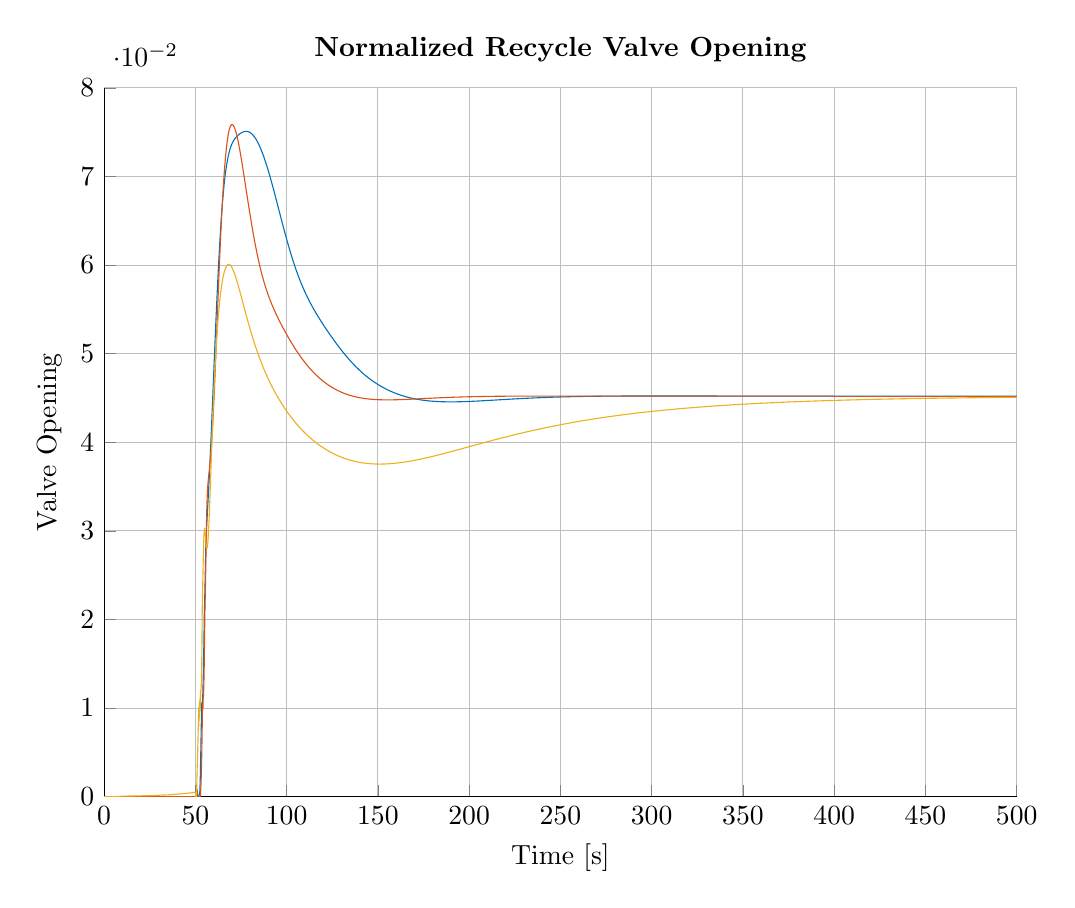
\begin{tikzpicture}

\begin{axis}[%
width=4.563in,
height=3.544in,
at={(0.792in,0.541in)},
scale only axis,
xmin=0,
xmax=500,
xlabel={Time [s]},
xmajorgrids,
ymin=0,
ymax=0.08,
ylabel={Valve Opening},
ymajorgrids,
axis background/.style={fill=white},
title style={font=\bfseries},
title={Normalized Recycle Valve Opening},
axis x line*=bottom,
axis y line*=left
]
\addplot [color=mycolor1,solid,forget plot]
  table[row sep=crcr]{%
0	1.35004e-06\\
0.05	2.61692e-06\\
0.1	3.84833e-06\\
0.15	5.03109e-06\\
0.2	6.15326e-06\\
0.25	7.19433e-06\\
0.3	8.14025e-06\\
0.35	8.99022e-06\\
0.4	9.74754e-06\\
0.45	1.04185e-05\\
0.5	1.10108e-05\\
0.55	1.15323e-05\\
0.6	1.19897e-05\\
0.65	1.23878e-05\\
0.7	1.27291e-05\\
0.75	1.30141e-05\\
0.8	1.32413e-05\\
0.85	1.34078e-05\\
0.9	1.35263e-05\\
0.95	1.36035e-05\\
1	1.36369e-05\\
1.05	1.36248e-05\\
1.1	1.35663e-05\\
1.15	1.34614e-05\\
1.2	1.33108e-05\\
1.25	1.31156e-05\\
1.3	1.28773e-05\\
1.35	1.25976e-05\\
1.4	1.22782e-05\\
1.45	1.19203e-05\\
1.5	1.15253e-05\\
1.55	1.1094e-05\\
1.6	1.06271e-05\\
1.65	1.01249e-05\\
1.7	9.58771e-06\\
1.75	9.01561e-06\\
1.8	8.40872e-06\\
1.85	7.76714e-06\\
1.9	7.09105e-06\\
1.95	6.38073e-06\\
2	5.63654e-06\\
2.05	4.85908e-06\\
2.1	4.04941e-06\\
2.15	3.20904e-06\\
2.2	2.33978e-06\\
2.25	1.44371e-06\\
2.3	5.2208e-07\\
2.35	0\\
2.4	0\\
2.45	0\\
2.5	0\\
2.55	0\\
2.6	0\\
2.65	0\\
2.7	0\\
2.75	0\\
2.8	0\\
2.85	0\\
2.9	0\\
2.95	0\\
3	0\\
3.05	0\\
3.1	0\\
3.15	0\\
3.2	0\\
3.25	0\\
3.3	0\\
3.35	0\\
3.4	0\\
3.45	0\\
3.5	0\\
3.55	0\\
3.6	0\\
3.65	0\\
3.7	0\\
3.75	0\\
3.8	0\\
3.85	0\\
3.9	0\\
3.95	0\\
4	0\\
4.05	0\\
4.1	0\\
4.15	0\\
4.2	0\\
4.25	0\\
4.3	0\\
4.35	0\\
4.4	0\\
4.45	0\\
4.5	0\\
4.55	0\\
4.6	0\\
4.65	0\\
4.7	0\\
4.75	0\\
4.8	0\\
4.85	0\\
4.9	0\\
4.95	0\\
5	0\\
5.05	0\\
5.1	0\\
5.15	0\\
5.2	0\\
5.25	0\\
5.3	0\\
5.35	0\\
5.4	0\\
5.45	0\\
5.5	0\\
5.55	0\\
5.6	0\\
5.65	0\\
5.7	0\\
5.75	0\\
5.8	0\\
5.85	0\\
5.9	0\\
5.95	0\\
6	0\\
6.05	0\\
6.1	0\\
6.15	0\\
6.2	0\\
6.25	0\\
6.3	0\\
6.35	0\\
6.4	0\\
6.45	0\\
6.5	0\\
6.55	0\\
6.6	0\\
6.65	0\\
6.7	0\\
6.75	0\\
6.8	0\\
6.85	0\\
6.9	0\\
6.95	0\\
7	0\\
7.05	0\\
7.1	0\\
7.15	0\\
7.2	0\\
7.25	0\\
7.3	0\\
7.35	0\\
7.4	0\\
7.45	0\\
7.5	0\\
7.55	0\\
7.6	0\\
7.65	0\\
7.7	0\\
7.75	0\\
7.8	0\\
7.85	0\\
7.9	0\\
7.95	0\\
8	0\\
8.05	0\\
8.1	0\\
8.15	0\\
8.2	0\\
8.25	0\\
8.3	0\\
8.35	0\\
8.4	0\\
8.45	0\\
8.5	0\\
8.55	0\\
8.6	0\\
8.65	0\\
8.7	0\\
8.75	0\\
8.8	0\\
8.85	0\\
8.9	0\\
8.95	0\\
9	0\\
9.05	0\\
9.1	0\\
9.15	0\\
9.2	0\\
9.25	0\\
9.3	0\\
9.35	0\\
9.4	0\\
9.45	0\\
9.5	0\\
9.55	0\\
9.6	0\\
9.65	0\\
9.7	0\\
9.75	0\\
9.8	0\\
9.85	0\\
9.9	0\\
9.95	0\\
10	0\\
10.05	0\\
10.1	0\\
10.15	0\\
10.2	0\\
10.25	0\\
10.3	0\\
10.35	0\\
10.4	0\\
10.45	0\\
10.5	0\\
10.55	0\\
10.6	0\\
10.65	0\\
10.7	0\\
10.75	0\\
10.8	0\\
10.85	0\\
10.9	0\\
10.95	0\\
11	0\\
11.05	0\\
11.1	0\\
11.15	0\\
11.2	0\\
11.25	0\\
11.3	0\\
11.35	0\\
11.4	0\\
11.45	0\\
11.5	0\\
11.55	0\\
11.6	0\\
11.65	0\\
11.7	0\\
11.75	0\\
11.8	0\\
11.85	0\\
11.9	0\\
11.95	0\\
12	0\\
12.05	0\\
12.1	0\\
12.15	0\\
12.2	0\\
12.25	0\\
12.3	0\\
12.35	0\\
12.4	0\\
12.45	0\\
12.5	0\\
12.55	0\\
12.6	0\\
12.65	0\\
12.7	0\\
12.75	0\\
12.8	0\\
12.85	0\\
12.9	0\\
12.95	0\\
13	0\\
13.05	0\\
13.1	0\\
13.15	0\\
13.2	0\\
13.25	0\\
13.3	0\\
13.35	0\\
13.4	0\\
13.45	0\\
13.5	0\\
13.55	0\\
13.6	0\\
13.65	0\\
13.7	0\\
13.75	0\\
13.8	0\\
13.85	0\\
13.9	0\\
13.95	0\\
14	0\\
14.05	0\\
14.1	0\\
14.15	0\\
14.2	0\\
14.25	0\\
14.3	0\\
14.35	0\\
14.4	0\\
14.45	0\\
14.5	0\\
14.55	0\\
14.6	0\\
14.65	0\\
14.7	0\\
14.75	0\\
14.8	0\\
14.85	0\\
14.9	0\\
14.95	0\\
15	0\\
15.05	0\\
15.1	0\\
15.15	0\\
15.2	0\\
15.25	0\\
15.3	0\\
15.35	0\\
15.4	0\\
15.45	0\\
15.5	0\\
15.55	0\\
15.6	0\\
15.65	0\\
15.7	0\\
15.75	0\\
15.8	0\\
15.85	0\\
15.9	0\\
15.95	0\\
16	0\\
16.05	0\\
16.1	0\\
16.15	0\\
16.2	0\\
16.25	0\\
16.3	0\\
16.35	0\\
16.4	0\\
16.45	0\\
16.5	0\\
16.55	0\\
16.6	0\\
16.65	0\\
16.7	0\\
16.75	0\\
16.8	0\\
16.85	0\\
16.9	0\\
16.95	0\\
17	0\\
17.05	0\\
17.1	0\\
17.15	0\\
17.2	0\\
17.25	0\\
17.3	0\\
17.35	0\\
17.4	0\\
17.45	0\\
17.5	0\\
17.55	0\\
17.6	0\\
17.65	0\\
17.7	0\\
17.75	0\\
17.8	0\\
17.85	0\\
17.9	0\\
17.95	0\\
18	0\\
18.05	0\\
18.1	0\\
18.15	0\\
18.2	0\\
18.25	0\\
18.3	0\\
18.35	0\\
18.4	0\\
18.45	0\\
18.5	0\\
18.55	0\\
18.6	0\\
18.65	0\\
18.7	0\\
18.75	0\\
18.8	0\\
18.85	0\\
18.9	0\\
18.95	0\\
19	0\\
19.05	0\\
19.1	0\\
19.15	0\\
19.2	0\\
19.25	0\\
19.3	0\\
19.35	0\\
19.4	0\\
19.45	0\\
19.5	0\\
19.55	0\\
19.6	0\\
19.65	0\\
19.7	0\\
19.75	0\\
19.8	0\\
19.85	0\\
19.9	0\\
19.95	0\\
20	0\\
20.05	0\\
20.1	0\\
20.15	0\\
20.2	0\\
20.25	0\\
20.3	0\\
20.35	0\\
20.4	0\\
20.45	0\\
20.5	0\\
20.55	0\\
20.6	0\\
20.65	0\\
20.7	0\\
20.75	0\\
20.8	0\\
20.85	0\\
20.9	0\\
20.95	0\\
21	0\\
21.05	0\\
21.1	0\\
21.15	0\\
21.2	0\\
21.25	0\\
21.3	0\\
21.35	0\\
21.4	0\\
21.45	0\\
21.5	0\\
21.55	0\\
21.6	0\\
21.65	0\\
21.7	0\\
21.75	0\\
21.8	0\\
21.85	0\\
21.9	0\\
21.95	0\\
22	0\\
22.05	0\\
22.1	0\\
22.15	0\\
22.2	0\\
22.25	0\\
22.3	0\\
22.35	0\\
22.4	0\\
22.45	0\\
22.5	0\\
22.55	0\\
22.6	0\\
22.65	0\\
22.7	0\\
22.75	0\\
22.8	0\\
22.85	0\\
22.9	0\\
22.95	0\\
23	0\\
23.05	0\\
23.1	0\\
23.15	0\\
23.2	0\\
23.25	0\\
23.3	0\\
23.35	0\\
23.4	0\\
23.45	0\\
23.5	0\\
23.55	0\\
23.6	0\\
23.65	0\\
23.7	0\\
23.75	0\\
23.8	0\\
23.85	0\\
23.9	0\\
23.95	0\\
24	0\\
24.05	0\\
24.1	0\\
24.15	0\\
24.2	0\\
24.25	0\\
24.3	0\\
24.35	0\\
24.4	0\\
24.45	0\\
24.5	0\\
24.55	0\\
24.6	0\\
24.65	0\\
24.7	0\\
24.75	0\\
24.8	0\\
24.85	0\\
24.9	0\\
24.95	0\\
25	0\\
25.05	0\\
25.1	0\\
25.15	0\\
25.2	0\\
25.25	0\\
25.3	0\\
25.35	0\\
25.4	0\\
25.45	0\\
25.5	0\\
25.55	0\\
25.6	0\\
25.65	0\\
25.7	0\\
25.75	0\\
25.8	0\\
25.85	0\\
25.9	0\\
25.95	0\\
26	0\\
26.05	0\\
26.1	0\\
26.15	0\\
26.2	0\\
26.25	0\\
26.3	0\\
26.35	0\\
26.4	0\\
26.45	0\\
26.5	0\\
26.55	0\\
26.6	0\\
26.65	0\\
26.7	0\\
26.75	0\\
26.8	0\\
26.85	0\\
26.9	0\\
26.95	0\\
27	0\\
27.05	0\\
27.1	0\\
27.15	0\\
27.2	0\\
27.25	0\\
27.3	0\\
27.35	0\\
27.4	0\\
27.45	0\\
27.5	0\\
27.55	0\\
27.6	0\\
27.65	0\\
27.7	0\\
27.75	0\\
27.8	0\\
27.85	0\\
27.9	0\\
27.95	0\\
28	0\\
28.05	0\\
28.1	0\\
28.15	0\\
28.2	0\\
28.25	0\\
28.3	0\\
28.35	0\\
28.4	0\\
28.45	0\\
28.5	0\\
28.55	0\\
28.6	0\\
28.65	0\\
28.7	0\\
28.75	0\\
28.8	0\\
28.85	0\\
28.9	0\\
28.95	0\\
29	0\\
29.05	0\\
29.1	0\\
29.15	0\\
29.2	0\\
29.25	0\\
29.3	0\\
29.35	0\\
29.4	0\\
29.45	0\\
29.5	0\\
29.55	0\\
29.6	0\\
29.65	0\\
29.7	0\\
29.75	0\\
29.8	0\\
29.85	0\\
29.9	0\\
29.95	0\\
30	0\\
30.05	0\\
30.1	0\\
30.15	0\\
30.2	0\\
30.25	0\\
30.3	0\\
30.35	0\\
30.4	0\\
30.45	0\\
30.5	0\\
30.55	0\\
30.6	0\\
30.65	0\\
30.7	0\\
30.75	0\\
30.8	0\\
30.85	0\\
30.9	0\\
30.95	0\\
31	0\\
31.05	0\\
31.1	0\\
31.15	0\\
31.2	0\\
31.25	0\\
31.3	0\\
31.35	0\\
31.4	0\\
31.45	0\\
31.5	0\\
31.55	0\\
31.6	0\\
31.65	0\\
31.7	0\\
31.75	0\\
31.8	0\\
31.85	0\\
31.9	0\\
31.95	0\\
32	0\\
32.05	0\\
32.1	0\\
32.15	0\\
32.2	0\\
32.25	0\\
32.3	0\\
32.35	0\\
32.4	0\\
32.45	0\\
32.5	0\\
32.55	0\\
32.6	0\\
32.65	0\\
32.7	0\\
32.75	0\\
32.8	0\\
32.85	0\\
32.9	0\\
32.95	0\\
33	0\\
33.05	0\\
33.1	0\\
33.15	0\\
33.2	0\\
33.25	0\\
33.3	0\\
33.35	0\\
33.4	0\\
33.45	0\\
33.5	0\\
33.55	0\\
33.6	0\\
33.65	0\\
33.7	0\\
33.75	0\\
33.8	0\\
33.85	0\\
33.9	0\\
33.95	0\\
34	0\\
34.05	0\\
34.1	0\\
34.15	0\\
34.2	0\\
34.25	0\\
34.3	0\\
34.35	0\\
34.4	0\\
34.45	0\\
34.5	0\\
34.55	0\\
34.6	0\\
34.65	0\\
34.7	0\\
34.75	0\\
34.8	0\\
34.85	0\\
34.9	0\\
34.95	0\\
35	0\\
35.05	0\\
35.1	0\\
35.15	0\\
35.2	0\\
35.25	0\\
35.3	0\\
35.35	0\\
35.4	0\\
35.45	0\\
35.5	0\\
35.55	0\\
35.6	0\\
35.65	0\\
35.7	0\\
35.75	0\\
35.8	0\\
35.85	0\\
35.9	0\\
35.95	0\\
36	0\\
36.05	0\\
36.1	0\\
36.15	0\\
36.2	0\\
36.25	0\\
36.3	0\\
36.35	0\\
36.4	0\\
36.45	0\\
36.5	0\\
36.55	0\\
36.6	0\\
36.65	0\\
36.7	0\\
36.75	0\\
36.8	0\\
36.85	0\\
36.9	0\\
36.95	0\\
37	0\\
37.05	0\\
37.1	0\\
37.15	0\\
37.2	0\\
37.25	0\\
37.3	0\\
37.35	0\\
37.4	0\\
37.45	0\\
37.5	0\\
37.55	0\\
37.6	0\\
37.65	0\\
37.7	0\\
37.75	0\\
37.8	0\\
37.85	0\\
37.9	0\\
37.95	0\\
38	0\\
38.05	0\\
38.1	0\\
38.15	0\\
38.2	0\\
38.25	0\\
38.3	0\\
38.35	0\\
38.4	0\\
38.45	0\\
38.5	0\\
38.55	0\\
38.6	0\\
38.65	0\\
38.7	0\\
38.75	0\\
38.8	0\\
38.85	0\\
38.9	0\\
38.95	0\\
39	0\\
39.05	0\\
39.1	0\\
39.15	0\\
39.2	0\\
39.25	0\\
39.3	0\\
39.35	0\\
39.4	0\\
39.45	0\\
39.5	0\\
39.55	0\\
39.6	0\\
39.65	0\\
39.7	0\\
39.75	0\\
39.8	0\\
39.85	0\\
39.9	0\\
39.95	0\\
40	0\\
40.05	0\\
40.1	0\\
40.15	0\\
40.2	0\\
40.25	0\\
40.3	0\\
40.35	0\\
40.4	0\\
40.45	0\\
40.5	0\\
40.55	0\\
40.6	0\\
40.65	0\\
40.7	0\\
40.75	0\\
40.8	0\\
40.85	0\\
40.9	0\\
40.95	0\\
41	0\\
41.05	0\\
41.1	0\\
41.15	0\\
41.2	0\\
41.25	0\\
41.3	0\\
41.35	0\\
41.4	0\\
41.45	0\\
41.5	0\\
41.55	0\\
41.6	0\\
41.65	0\\
41.7	0\\
41.75	0\\
41.8	0\\
41.85	0\\
41.9	0\\
41.95	0\\
42	0\\
42.05	0\\
42.1	0\\
42.15	0\\
42.2	0\\
42.25	0\\
42.3	0\\
42.35	0\\
42.4	0\\
42.45	0\\
42.5	0\\
42.55	0\\
42.6	0\\
42.65	0\\
42.7	0\\
42.75	0\\
42.8	0\\
42.85	0\\
42.9	0\\
42.95	0\\
43	0\\
43.05	0\\
43.1	0\\
43.15	0\\
43.2	0\\
43.25	0\\
43.3	0\\
43.35	0\\
43.4	0\\
43.45	0\\
43.5	0\\
43.55	0\\
43.6	0\\
43.65	0\\
43.7	0\\
43.75	0\\
43.8	0\\
43.85	0\\
43.9	0\\
43.95	0\\
44	0\\
44.05	0\\
44.1	0\\
44.15	0\\
44.2	0\\
44.25	0\\
44.3	0\\
44.35	0\\
44.4	0\\
44.45	0\\
44.5	0\\
44.55	0\\
44.6	0\\
44.65	0\\
44.7	0\\
44.75	0\\
44.8	0\\
44.85	0\\
44.9	0\\
44.95	0\\
45	0\\
45.05	0\\
45.1	0\\
45.15	0\\
45.2	0\\
45.25	0\\
45.3	0\\
45.35	0\\
45.4	0\\
45.45	0\\
45.5	0\\
45.55	0\\
45.6	0\\
45.65	0\\
45.7	0\\
45.75	0\\
45.8	0\\
45.85	0\\
45.9	0\\
45.95	0\\
46	0\\
46.05	0\\
46.1	0\\
46.15	0\\
46.2	0\\
46.25	0\\
46.3	0\\
46.35	0\\
46.4	0\\
46.45	0\\
46.5	0\\
46.55	0\\
46.6	0\\
46.65	0\\
46.7	0\\
46.75	0\\
46.8	0\\
46.85	0\\
46.9	0\\
46.95	0\\
47	0\\
47.05	0\\
47.1	0\\
47.15	0\\
47.2	0\\
47.25	0\\
47.3	0\\
47.35	0\\
47.4	0\\
47.45	0\\
47.5	0\\
47.55	0\\
47.6	0\\
47.65	0\\
47.7	0\\
47.75	0\\
47.8	0\\
47.85	0\\
47.9	0\\
47.95	0\\
48	0\\
48.05	0\\
48.1	0\\
48.15	0\\
48.2	0\\
48.25	0\\
48.3	0\\
48.35	0\\
48.4	0\\
48.45	0\\
48.5	0\\
48.55	0\\
48.6	0\\
48.65	0\\
48.7	0\\
48.75	0\\
48.8	0\\
48.85	0\\
48.9	0\\
48.95	0\\
49	0\\
49.05	0\\
49.1	0\\
49.15	0\\
49.2	0\\
49.25	0\\
49.3	0\\
49.35	0\\
49.4	0\\
49.45	0\\
49.5	0\\
49.55	0\\
49.6	0\\
49.65	0\\
49.7	0\\
49.75	0\\
49.8	0\\
49.85	0\\
49.9	0\\
49.95	0\\
50	0\\
50.05	0\\
50.1	0\\
50.15	0\\
50.2	0\\
50.25	0\\
50.3	0\\
50.35	0\\
50.4	0\\
50.45	0\\
50.5	0\\
50.55	0\\
50.6	0\\
50.65	0\\
50.7	4.37101e-05\\
50.75	0.000137061\\
50.8	0.000257042\\
50.85	0.000379859\\
50.9	0.000484365\\
50.95	0.000554605\\
51	0.000581258\\
51.05	0.000554557\\
51.1	0.000477448\\
51.15	0.000360539\\
51.2	0.00021814\\
51.25	6.49327e-05\\
51.3	0\\
51.35	0\\
51.4	0\\
51.45	0\\
51.5	0\\
51.55	0\\
51.6	0\\
51.65	4.16689e-06\\
51.7	1.88968e-05\\
51.75	3.9288e-05\\
51.8	6.1495e-05\\
51.85	8.2878e-05\\
51.9	0.000102169\\
51.95	0.000119458\\
52	0.000135841\\
52.05	0.000153148\\
52.1	0.00017352\\
52.15	0.000199181\\
52.2	0.000232079\\
52.25	0.000273415\\
52.3	0.000326409\\
52.35	0.00040154\\
52.4	0.000510879\\
52.45	0.000665399\\
52.5	0.000873319\\
52.55	0.00113912\\
52.6	0.00146343\\
52.65	0.00184378\\
52.7	0.00227325\\
52.75	0.00274289\\
52.8	0.00324287\\
52.85	0.00376378\\
52.9	0.00429769\\
52.95	0.00483897\\
53	0.00538451\\
53.05	0.00593363\\
53.1	0.00648767\\
53.15	0.0070493\\
53.2	0.00762181\\
53.25	0.00820836\\
53.3	0.00881135\\
53.35	0.00943204\\
53.4	0.0100704\\
53.45	0.00994942\\
53.5	0.010605\\
53.55	0.0104988\\
53.6	0.0104102\\
53.65	0.0103494\\
53.7	0.0103257\\
53.75	0.0103454\\
53.8	0.0104122\\
53.85	0.010527\\
53.9	0.0106891\\
53.95	0.0108959\\
54	0.0111445\\
54.05	0.0114314\\
54.1	0.0117536\\
54.15	0.0121082\\
54.2	0.0124931\\
54.25	0.0129066\\
54.3	0.0133477\\
54.35	0.0138162\\
54.4	0.0143119\\
54.45	0.0148351\\
54.5	0.0153865\\
54.55	0.0159669\\
54.6	0.0165774\\
54.65	0.0172194\\
54.7	0.0178946\\
54.75	0.0186055\\
54.8	0.0193551\\
54.85	0.0201478\\
54.9	0.0205584\\
54.95	0.0209647\\
55	0.021371\\
55.05	0.0217819\\
55.1	0.0222016\\
55.15	0.0226331\\
55.2	0.0230787\\
55.25	0.0235396\\
55.3	0.0240159\\
55.35	0.0245072\\
55.4	0.0250126\\
55.45	0.0255269\\
55.5	0.0260402\\
55.55	0.026547\\
55.6	0.0270354\\
55.65	0.0274949\\
55.7	0.0279183\\
55.75	0.0283015\\
55.8	0.0286447\\
55.85	0.0289506\\
55.9	0.0292244\\
55.95	0.0294724\\
56	0.0297012\\
56.05	0.0299168\\
56.1	0.0301243\\
56.15	0.0303274\\
56.2	0.0305286\\
56.25	0.0307294\\
56.3	0.0309301\\
56.35	0.0311306\\
56.4	0.0313304\\
56.45	0.0315289\\
56.5	0.0317255\\
56.55	0.0319199\\
56.6	0.0321119\\
56.65	0.0323017\\
56.7	0.0324895\\
56.75	0.0326759\\
56.8	0.0328614\\
56.85	0.0330466\\
56.9	0.0332321\\
56.95	0.0334183\\
57	0.0336056\\
57.05	0.0337943\\
57.1	0.0339847\\
57.15	0.0341768\\
57.2	0.0343708\\
57.25	0.0345668\\
57.3	0.0347647\\
57.35	0.0349645\\
57.4	0.0351662\\
57.45	0.0353698\\
57.5	0.0355752\\
57.55	0.0357824\\
57.6	0.0359913\\
57.65	0.0362019\\
57.7	0.0364141\\
57.75	0.036628\\
57.8	0.0368434\\
57.85	0.0370605\\
57.9	0.0372791\\
57.95	0.0374994\\
58	0.0377214\\
58.05	0.037945\\
58.1	0.0381704\\
58.15	0.0383975\\
58.2	0.0386264\\
58.25	0.0388571\\
58.3	0.0390895\\
58.35	0.0393237\\
58.4	0.0395594\\
58.45	0.0397968\\
58.5	0.0400357\\
58.55	0.0402759\\
58.6	0.0405174\\
58.65	0.0407602\\
58.7	0.0410041\\
58.75	0.041249\\
58.8	0.0414949\\
58.85	0.0417417\\
58.9	0.0419894\\
58.95	0.0422379\\
59	0.0424871\\
59.05	0.0427371\\
59.1	0.0429877\\
59.15	0.043239\\
59.2	0.0434908\\
59.25	0.0437431\\
59.3	0.0439959\\
59.35	0.0442491\\
59.4	0.0445026\\
59.45	0.0447563\\
59.5	0.0450103\\
59.55	0.0452644\\
59.6	0.0455187\\
59.65	0.0457729\\
59.7	0.0460272\\
59.75	0.0462814\\
59.8	0.0465355\\
59.85	0.0467894\\
59.9	0.0470431\\
59.95	0.0472966\\
60	0.0475498\\
60.05	0.0478027\\
60.1	0.0480552\\
60.15	0.0483073\\
60.2	0.0485589\\
60.25	0.0488101\\
60.3	0.0490608\\
60.35	0.0493109\\
60.4	0.0495605\\
60.45	0.0498094\\
60.5	0.0500577\\
60.55	0.0503053\\
60.6	0.0505521\\
60.65	0.0507982\\
60.7	0.0510436\\
60.75	0.0512881\\
60.8	0.0515318\\
60.85	0.0517747\\
60.9	0.0520167\\
60.95	0.0522577\\
61	0.0524979\\
61.05	0.0527371\\
61.1	0.0529753\\
61.15	0.0532125\\
61.2	0.0534488\\
61.25	0.053684\\
61.3	0.0539181\\
61.35	0.0541512\\
61.4	0.0543832\\
61.45	0.0546141\\
61.5	0.0548439\\
61.55	0.0550726\\
61.6	0.0553001\\
61.65	0.0555265\\
61.7	0.0557517\\
61.75	0.0559757\\
61.8	0.0561985\\
61.85	0.0564201\\
61.9	0.0566404\\
61.95	0.0568596\\
62	0.0570775\\
62.05	0.0572941\\
62.1	0.0575094\\
62.15	0.0577235\\
62.2	0.0579363\\
62.25	0.0581478\\
62.3	0.0583579\\
62.35	0.0585667\\
62.4	0.0587742\\
62.45	0.0589804\\
62.5	0.0591851\\
62.55	0.0593885\\
62.6	0.0595905\\
62.65	0.0597912\\
62.7	0.0599904\\
62.75	0.0601882\\
62.8	0.0603845\\
62.85	0.0605794\\
62.9	0.0607729\\
62.95	0.0609649\\
63	0.0611554\\
63.05	0.0613445\\
63.1	0.061532\\
63.15	0.061718\\
63.2	0.0619025\\
63.25	0.0620854\\
63.3	0.0622668\\
63.35	0.0624466\\
63.4	0.0626249\\
63.45	0.0628015\\
63.5	0.0629766\\
63.55	0.06315\\
63.6	0.0633218\\
63.65	0.063492\\
63.7	0.0636605\\
63.75	0.0638273\\
63.8	0.0639925\\
63.85	0.0641559\\
63.9	0.0643177\\
63.95	0.0644778\\
64	0.0646362\\
64.05	0.0647928\\
64.1	0.0649477\\
64.15	0.0651009\\
64.2	0.0652523\\
64.25	0.065402\\
64.3	0.0655499\\
64.35	0.065696\\
64.4	0.0658404\\
64.45	0.0659831\\
64.5	0.0661239\\
64.55	0.066263\\
64.6	0.0664003\\
64.65	0.0665359\\
64.7	0.0666697\\
64.75	0.0668017\\
64.8	0.066932\\
64.85	0.0670605\\
64.9	0.0671873\\
64.95	0.0673123\\
65	0.0674357\\
65.05	0.0675573\\
65.1	0.0676772\\
65.15	0.0677954\\
65.2	0.0679119\\
65.25	0.0680267\\
65.3	0.0681399\\
65.35	0.0682515\\
65.4	0.0683614\\
65.45	0.0684697\\
65.5	0.0685764\\
65.55	0.0686815\\
65.6	0.068785\\
65.65	0.068887\\
65.7	0.0689875\\
65.75	0.0690864\\
65.8	0.0691838\\
65.85	0.0692798\\
65.9	0.0693743\\
65.95	0.0694673\\
66	0.0695589\\
66.05	0.0696491\\
66.1	0.0697379\\
66.15	0.0698253\\
66.2	0.0699115\\
66.25	0.0699962\\
66.3	0.0700797\\
66.35	0.070162\\
66.4	0.0702429\\
66.45	0.0703227\\
66.5	0.0704012\\
66.55	0.0704786\\
66.6	0.0705548\\
66.65	0.0706299\\
66.7	0.0707038\\
66.75	0.0707767\\
66.8	0.0708485\\
66.85	0.0709192\\
66.9	0.0709888\\
66.95	0.0710575\\
67	0.0711251\\
67.05	0.0711917\\
67.1	0.0712573\\
67.15	0.0713219\\
67.2	0.0713855\\
67.25	0.0714482\\
67.3	0.0715099\\
67.35	0.0715707\\
67.4	0.0716306\\
67.45	0.0716895\\
67.5	0.0717475\\
67.55	0.0718045\\
67.6	0.0718607\\
67.65	0.0719159\\
67.7	0.0719703\\
67.75	0.0720238\\
67.8	0.0720763\\
67.85	0.0721281\\
67.9	0.0721789\\
67.95	0.0722289\\
68	0.072278\\
68.05	0.0723263\\
68.1	0.0723737\\
68.15	0.0724204\\
68.2	0.0724662\\
68.25	0.0725112\\
68.3	0.0725554\\
68.35	0.0725988\\
68.4	0.0726415\\
68.45	0.0726833\\
68.5	0.0727244\\
68.55	0.0727648\\
68.6	0.0728044\\
68.65	0.0728433\\
68.7	0.0728815\\
68.75	0.072919\\
68.8	0.0729558\\
68.85	0.072992\\
68.9	0.0730274\\
68.95	0.0730622\\
69	0.0730964\\
69.05	0.0731299\\
69.1	0.0731628\\
69.15	0.073195\\
69.2	0.0732267\\
69.25	0.0732578\\
69.3	0.0732883\\
69.35	0.0733183\\
69.4	0.0733477\\
69.45	0.0733765\\
69.5	0.0734048\\
69.55	0.0734326\\
69.6	0.0734599\\
69.65	0.0734867\\
69.7	0.073513\\
69.75	0.0735388\\
69.8	0.0735642\\
69.85	0.0735891\\
69.9	0.0736135\\
69.95	0.0736375\\
70	0.0736611\\
70.05	0.0736842\\
70.1	0.073707\\
70.15	0.0737293\\
70.2	0.0737513\\
70.25	0.0737728\\
70.3	0.073794\\
70.35	0.0738149\\
70.4	0.0738353\\
70.45	0.0738555\\
70.5	0.0738753\\
70.55	0.0738947\\
70.6	0.0739139\\
70.65	0.0739327\\
70.7	0.0739512\\
70.75	0.0739694\\
70.8	0.0739873\\
70.85	0.074005\\
70.9	0.0740223\\
70.95	0.0740394\\
71	0.0740562\\
71.05	0.0740728\\
71.1	0.0740891\\
71.15	0.0741052\\
71.2	0.074121\\
71.25	0.0741366\\
71.3	0.074152\\
71.35	0.0741671\\
71.4	0.074182\\
71.45	0.0741967\\
71.5	0.0742112\\
71.55	0.0742255\\
71.6	0.0742397\\
71.65	0.0742536\\
71.7	0.0742673\\
71.75	0.0742809\\
71.8	0.0742942\\
71.85	0.0743074\\
71.9	0.0743205\\
71.95	0.0743333\\
72	0.074346\\
72.05	0.0743586\\
72.1	0.074371\\
72.15	0.0743832\\
72.2	0.0743953\\
72.25	0.0744073\\
72.3	0.0744191\\
72.35	0.0744307\\
72.4	0.0744423\\
72.45	0.0744537\\
72.5	0.074465\\
72.55	0.0744761\\
72.6	0.0744871\\
72.65	0.074498\\
72.7	0.0745088\\
72.75	0.0745195\\
72.8	0.07453\\
72.85	0.0745405\\
72.9	0.0745508\\
72.95	0.074561\\
73	0.0745712\\
73.05	0.0745812\\
73.1	0.0745911\\
73.15	0.0746009\\
73.2	0.0746106\\
73.25	0.0746202\\
73.3	0.0746297\\
73.35	0.0746391\\
73.4	0.0746484\\
73.45	0.0746576\\
73.5	0.0746667\\
73.55	0.0746757\\
73.6	0.0746847\\
73.65	0.0746935\\
73.7	0.0747023\\
73.75	0.0747109\\
73.8	0.0747195\\
73.85	0.074728\\
73.9	0.0747364\\
73.95	0.0747447\\
74	0.0747529\\
74.05	0.074761\\
74.1	0.074769\\
74.15	0.074777\\
74.2	0.0747848\\
74.25	0.0747926\\
74.3	0.0748003\\
74.35	0.0748079\\
74.4	0.0748154\\
74.45	0.0748228\\
74.5	0.0748301\\
74.55	0.0748374\\
74.6	0.0748445\\
74.65	0.0748516\\
74.7	0.0748586\\
74.75	0.0748655\\
74.8	0.0748723\\
74.85	0.074879\\
74.9	0.0748856\\
74.95	0.0748921\\
75	0.0748986\\
75.05	0.0749049\\
75.1	0.0749112\\
75.15	0.0749173\\
75.2	0.0749234\\
75.25	0.0749294\\
75.3	0.0749352\\
75.35	0.074941\\
75.4	0.0749467\\
75.45	0.0749523\\
75.5	0.0749578\\
75.55	0.0749632\\
75.6	0.0749684\\
75.65	0.0749736\\
75.7	0.0749787\\
75.75	0.0749837\\
75.8	0.0749886\\
75.85	0.0749934\\
75.9	0.0749981\\
75.95	0.0750026\\
76	0.0750071\\
76.05	0.0750115\\
76.1	0.0750157\\
76.15	0.0750199\\
76.2	0.0750239\\
76.25	0.0750278\\
76.3	0.0750317\\
76.35	0.0750354\\
76.4	0.075039\\
76.45	0.0750424\\
76.5	0.0750458\\
76.55	0.0750491\\
76.6	0.0750522\\
76.65	0.0750552\\
76.7	0.0750581\\
76.75	0.0750609\\
76.8	0.0750636\\
76.85	0.0750661\\
76.9	0.0750685\\
76.95	0.0750708\\
77	0.075073\\
77.05	0.0750751\\
77.1	0.075077\\
77.15	0.0750788\\
77.2	0.0750805\\
77.25	0.075082\\
77.3	0.0750835\\
77.35	0.0750848\\
77.4	0.0750859\\
77.45	0.075087\\
77.5	0.0750879\\
77.55	0.0750886\\
77.6	0.0750893\\
77.65	0.0750898\\
77.7	0.0750902\\
77.75	0.0750904\\
77.8	0.0750905\\
77.85	0.0750905\\
77.9	0.0750903\\
77.95	0.07509\\
78	0.0750896\\
78.05	0.075089\\
78.1	0.0750883\\
78.15	0.0750874\\
78.2	0.0750864\\
78.25	0.0750853\\
78.3	0.075084\\
78.35	0.0750826\\
78.4	0.075081\\
78.45	0.0750793\\
78.5	0.0750774\\
78.55	0.0750754\\
78.6	0.0750733\\
78.65	0.075071\\
78.7	0.0750685\\
78.75	0.0750659\\
78.8	0.0750632\\
78.85	0.0750603\\
78.9	0.0750573\\
78.95	0.0750541\\
79	0.0750508\\
79.05	0.0750473\\
79.1	0.0750436\\
79.15	0.0750399\\
79.2	0.0750359\\
79.25	0.0750318\\
79.3	0.0750276\\
79.35	0.0750232\\
79.4	0.0750186\\
79.45	0.0750139\\
79.5	0.0750091\\
79.55	0.0750041\\
79.6	0.0749989\\
79.65	0.0749936\\
79.7	0.0749881\\
79.75	0.0749825\\
79.8	0.0749767\\
79.85	0.0749707\\
79.9	0.0749646\\
79.95	0.0749583\\
80	0.0749519\\
80.05	0.0749454\\
80.1	0.0749386\\
80.15	0.0749317\\
80.2	0.0749247\\
80.25	0.0749175\\
80.3	0.0749101\\
80.35	0.0749026\\
80.4	0.0748949\\
80.45	0.074887\\
80.5	0.074879\\
80.55	0.0748709\\
80.6	0.0748626\\
80.65	0.0748541\\
80.7	0.0748454\\
80.75	0.0748366\\
80.8	0.0748277\\
80.85	0.0748185\\
80.9	0.0748092\\
80.95	0.0747998\\
81	0.0747902\\
81.05	0.0747804\\
81.1	0.0747705\\
81.15	0.0747604\\
81.2	0.0747501\\
81.25	0.0747397\\
81.3	0.0747292\\
81.35	0.0747184\\
81.4	0.0747075\\
81.45	0.0746965\\
81.5	0.0746852\\
81.55	0.0746739\\
81.6	0.0746623\\
81.65	0.0746506\\
81.7	0.0746388\\
81.75	0.0746267\\
81.8	0.0746145\\
81.85	0.0746022\\
81.9	0.0745897\\
81.95	0.074577\\
82	0.0745642\\
82.05	0.0745512\\
82.1	0.074538\\
82.15	0.0745247\\
82.2	0.0745112\\
82.25	0.0744976\\
82.3	0.0744838\\
82.35	0.0744699\\
82.4	0.0744557\\
82.45	0.0744415\\
82.5	0.074427\\
82.55	0.0744124\\
82.6	0.0743977\\
82.65	0.0743827\\
82.7	0.0743677\\
82.75	0.0743524\\
82.8	0.074337\\
82.85	0.0743215\\
82.9	0.0743058\\
82.95	0.0742899\\
83	0.0742739\\
83.05	0.0742577\\
83.1	0.0742413\\
83.15	0.0742248\\
83.2	0.0742081\\
83.25	0.0741913\\
83.3	0.0741743\\
83.35	0.0741572\\
83.4	0.0741399\\
83.45	0.0741224\\
83.5	0.0741048\\
83.55	0.0740871\\
83.6	0.0740691\\
83.65	0.0740511\\
83.7	0.0740328\\
83.75	0.0740144\\
83.8	0.0739959\\
83.85	0.0739772\\
83.9	0.0739583\\
83.95	0.0739393\\
84	0.0739202\\
84.05	0.0739008\\
84.1	0.0738814\\
84.15	0.0738617\\
84.2	0.073842\\
84.25	0.073822\\
84.3	0.0738019\\
84.35	0.0737817\\
84.4	0.0737613\\
84.45	0.0737408\\
84.5	0.0737201\\
84.55	0.0736992\\
84.6	0.0736782\\
84.65	0.0736571\\
84.7	0.0736358\\
84.75	0.0736144\\
84.8	0.0735928\\
84.85	0.073571\\
84.9	0.0735491\\
84.95	0.0735271\\
85	0.0735049\\
85.05	0.0734826\\
85.1	0.0734601\\
85.15	0.0734374\\
85.2	0.0734147\\
85.25	0.0733917\\
85.3	0.0733687\\
85.35	0.0733454\\
85.4	0.0733221\\
85.45	0.0732986\\
85.5	0.0732749\\
85.55	0.0732511\\
85.6	0.0732272\\
85.65	0.0732031\\
85.7	0.0731789\\
85.75	0.0731545\\
85.8	0.07313\\
85.85	0.0731054\\
85.9	0.0730806\\
85.95	0.0730556\\
86	0.0730306\\
86.05	0.0730053\\
86.1	0.07298\\
86.15	0.0729545\\
86.2	0.0729289\\
86.25	0.0729031\\
86.3	0.0728772\\
86.35	0.0728512\\
86.4	0.072825\\
86.45	0.0727987\\
86.5	0.0727722\\
86.55	0.0727456\\
86.6	0.0727189\\
86.65	0.072692\\
86.7	0.072665\\
86.75	0.0726379\\
86.8	0.0726107\\
86.85	0.0725833\\
86.9	0.0725558\\
86.95	0.0725281\\
87	0.0725003\\
87.05	0.0724724\\
87.1	0.0724444\\
87.15	0.0724162\\
87.2	0.0723879\\
87.25	0.0723595\\
87.3	0.0723309\\
87.35	0.0723022\\
87.4	0.0722734\\
87.45	0.0722445\\
87.5	0.0722154\\
87.55	0.0721862\\
87.6	0.0721569\\
87.65	0.0721275\\
87.7	0.0720979\\
87.75	0.0720682\\
87.8	0.0720384\\
87.85	0.0720085\\
87.9	0.0719784\\
87.95	0.0719483\\
88	0.071918\\
88.05	0.0718876\\
88.1	0.0718571\\
88.15	0.0718264\\
88.2	0.0717957\\
88.25	0.0717648\\
88.3	0.0717338\\
88.35	0.0717027\\
88.4	0.0716714\\
88.45	0.0716401\\
88.5	0.0716087\\
88.55	0.0715771\\
88.6	0.0715454\\
88.65	0.0715136\\
88.7	0.0714817\\
88.75	0.0714497\\
88.8	0.0714176\\
88.85	0.0713854\\
88.9	0.071353\\
88.95	0.0713206\\
89	0.071288\\
89.05	0.0712554\\
89.1	0.0712226\\
89.15	0.0711897\\
89.2	0.0711567\\
89.25	0.0711237\\
89.3	0.0710905\\
89.35	0.0710572\\
89.4	0.0710238\\
89.45	0.0709903\\
89.5	0.0709567\\
89.55	0.070923\\
89.6	0.0708892\\
89.65	0.0708554\\
89.7	0.0708214\\
89.75	0.0707873\\
89.8	0.0707531\\
89.85	0.0707188\\
89.9	0.0706845\\
89.95	0.07065\\
90	0.0706155\\
90.05	0.0705808\\
90.1	0.0705461\\
90.15	0.0705112\\
90.2	0.0704763\\
90.25	0.0704413\\
90.3	0.0704062\\
90.35	0.070371\\
90.4	0.0703358\\
90.45	0.0703004\\
90.5	0.0702649\\
90.55	0.0702294\\
90.6	0.0701938\\
90.65	0.0701581\\
90.7	0.0701223\\
90.75	0.0700865\\
90.8	0.0700505\\
90.85	0.0700145\\
90.9	0.0699784\\
90.95	0.0699422\\
91	0.0699059\\
91.05	0.0698696\\
91.1	0.0698332\\
91.15	0.0697967\\
91.2	0.0697601\\
91.25	0.0697235\\
91.3	0.0696868\\
91.35	0.06965\\
91.4	0.0696132\\
91.45	0.0695762\\
91.5	0.0695392\\
91.55	0.0695022\\
91.6	0.069465\\
91.65	0.0694278\\
91.7	0.0693906\\
91.75	0.0693532\\
91.8	0.0693158\\
91.85	0.0692784\\
91.9	0.0692409\\
91.95	0.0692033\\
92	0.0691656\\
92.05	0.0691279\\
92.1	0.0690901\\
92.15	0.0690523\\
92.2	0.0690144\\
92.25	0.0689765\\
92.3	0.0689385\\
92.35	0.0689004\\
92.4	0.0688623\\
92.45	0.0688241\\
92.5	0.0687859\\
92.55	0.0687477\\
92.6	0.0687093\\
92.65	0.068671\\
92.7	0.0686325\\
92.75	0.0685941\\
92.8	0.0685555\\
92.85	0.068517\\
92.9	0.0684784\\
92.95	0.0684397\\
93	0.068401\\
93.05	0.0683622\\
93.1	0.0683235\\
93.15	0.0682846\\
93.2	0.0682457\\
93.25	0.0682068\\
93.3	0.0681679\\
93.35	0.0681289\\
93.4	0.0680898\\
93.45	0.0680508\\
93.5	0.0680117\\
93.55	0.0679725\\
93.6	0.0679334\\
93.65	0.0678941\\
93.7	0.0678549\\
93.75	0.0678156\\
93.8	0.0677763\\
93.85	0.067737\\
93.9	0.0676976\\
93.95	0.0676582\\
94	0.0676188\\
94.05	0.0675794\\
94.1	0.0675399\\
94.15	0.0675004\\
94.2	0.0674609\\
94.25	0.0674213\\
94.3	0.0673818\\
94.35	0.0673422\\
94.4	0.0673026\\
94.45	0.0672629\\
94.5	0.0672233\\
94.55	0.0671836\\
94.6	0.0671439\\
94.65	0.0671042\\
94.7	0.0670645\\
94.75	0.0670248\\
94.8	0.0669851\\
94.85	0.0669453\\
94.9	0.0669055\\
94.95	0.0668657\\
95	0.066826\\
95.05	0.0667862\\
95.1	0.0667463\\
95.15	0.0667065\\
95.2	0.0666667\\
95.25	0.0666269\\
95.3	0.066587\\
95.35	0.0665472\\
95.4	0.0665073\\
95.45	0.0664675\\
95.5	0.0664276\\
95.55	0.0663878\\
95.6	0.0663479\\
95.65	0.0663081\\
95.7	0.0662682\\
95.75	0.0662284\\
95.8	0.0661885\\
95.85	0.0661487\\
95.9	0.0661088\\
95.95	0.066069\\
96	0.0660292\\
96.05	0.0659894\\
96.1	0.0659495\\
96.15	0.0659097\\
96.2	0.0658699\\
96.25	0.0658302\\
96.3	0.0657904\\
96.35	0.0657506\\
96.4	0.0657109\\
96.45	0.0656711\\
96.5	0.0656314\\
96.55	0.0655917\\
96.6	0.065552\\
96.65	0.0655123\\
96.7	0.0654726\\
96.75	0.065433\\
96.8	0.0653934\\
96.85	0.0653537\\
96.9	0.0653142\\
96.95	0.0652746\\
97	0.065235\\
97.05	0.0651955\\
97.1	0.065156\\
97.15	0.0651165\\
97.2	0.0650771\\
97.25	0.0650376\\
97.3	0.0649982\\
97.35	0.0649589\\
97.4	0.0649195\\
97.45	0.0648802\\
97.5	0.0648409\\
97.55	0.0648016\\
97.6	0.0647624\\
97.65	0.0647232\\
97.7	0.064684\\
97.75	0.0646449\\
97.8	0.0646057\\
97.85	0.0645667\\
97.9	0.0645276\\
97.95	0.0644886\\
98	0.0644496\\
98.05	0.0644107\\
98.1	0.0643718\\
98.15	0.0643329\\
98.2	0.0642941\\
98.25	0.0642553\\
98.3	0.0642166\\
98.35	0.0641779\\
98.4	0.0641392\\
98.45	0.0641006\\
98.5	0.064062\\
98.55	0.0640235\\
98.6	0.063985\\
98.65	0.0639465\\
98.7	0.0639081\\
98.75	0.0638697\\
98.8	0.0638314\\
98.85	0.0637931\\
98.9	0.0637549\\
98.95	0.0637167\\
99	0.0636786\\
99.05	0.0636405\\
99.1	0.0636025\\
99.15	0.0635645\\
99.2	0.0635265\\
99.25	0.0634886\\
99.3	0.0634508\\
99.35	0.063413\\
99.4	0.0633753\\
99.45	0.0633376\\
99.5	0.0633\\
99.55	0.0632624\\
99.6	0.0632249\\
99.65	0.0631874\\
99.7	0.06315\\
99.75	0.0631127\\
99.8	0.0630754\\
99.85	0.0630381\\
99.9	0.0630009\\
99.95	0.0629638\\
100	0.0629268\\
100.05	0.0628897\\
100.1	0.0628528\\
100.15	0.0628159\\
100.2	0.0627791\\
100.25	0.0627423\\
100.3	0.0627056\\
100.35	0.0626689\\
100.4	0.0626324\\
100.45	0.0625958\\
100.5	0.0625594\\
100.55	0.062523\\
100.6	0.0624866\\
100.65	0.0624504\\
100.7	0.0624142\\
100.75	0.062378\\
100.8	0.062342\\
100.85	0.0623059\\
100.9	0.06227\\
100.95	0.0622341\\
101	0.0621983\\
101.05	0.0621626\\
101.1	0.0621269\\
101.15	0.0620913\\
101.2	0.0620557\\
101.25	0.0620202\\
101.3	0.0619848\\
101.35	0.0619495\\
101.4	0.0619142\\
101.45	0.061879\\
101.5	0.0618439\\
101.55	0.0618089\\
101.6	0.0617739\\
101.65	0.0617389\\
101.7	0.0617041\\
101.75	0.0616693\\
101.8	0.0616346\\
101.85	0.0616\\
101.9	0.0615654\\
101.95	0.061531\\
102	0.0614965\\
102.05	0.0614622\\
102.1	0.0614279\\
102.15	0.0613937\\
102.2	0.0613596\\
102.25	0.0613256\\
102.3	0.0612916\\
102.35	0.0612577\\
102.4	0.0612239\\
102.45	0.0611901\\
102.5	0.0611565\\
102.55	0.0611229\\
102.6	0.0610893\\
102.65	0.0610559\\
102.7	0.0610225\\
102.75	0.0609892\\
102.8	0.060956\\
102.85	0.0609229\\
102.9	0.0608898\\
102.95	0.0608568\\
103	0.0608239\\
103.05	0.0607911\\
103.1	0.0607583\\
103.15	0.0607257\\
103.2	0.060693\\
103.25	0.0606605\\
103.3	0.0606281\\
103.35	0.0605957\\
103.4	0.0605634\\
103.45	0.0605312\\
103.5	0.0604991\\
103.55	0.060467\\
103.6	0.060435\\
103.65	0.0604031\\
103.7	0.0603713\\
103.75	0.0603396\\
103.8	0.0603079\\
103.85	0.0602763\\
103.9	0.0602448\\
103.95	0.0602134\\
104	0.0601821\\
104.05	0.0601508\\
104.1	0.0601196\\
104.15	0.0600885\\
104.2	0.0600575\\
104.25	0.0600265\\
104.3	0.0599956\\
104.35	0.0599648\\
104.4	0.0599341\\
104.45	0.0599035\\
104.5	0.0598729\\
104.55	0.0598425\\
104.6	0.0598121\\
104.65	0.0597817\\
104.7	0.0597515\\
104.75	0.0597213\\
104.8	0.0596913\\
104.85	0.0596613\\
104.9	0.0596313\\
104.95	0.0596015\\
105	0.0595717\\
105.05	0.0595421\\
105.1	0.0595125\\
105.15	0.0594829\\
105.2	0.0594535\\
105.25	0.0594241\\
105.3	0.0593948\\
105.35	0.0593656\\
105.4	0.0593365\\
105.45	0.0593074\\
105.5	0.0592785\\
105.55	0.0592496\\
105.6	0.0592207\\
105.65	0.059192\\
105.7	0.0591633\\
105.75	0.0591348\\
105.8	0.0591063\\
105.85	0.0590778\\
105.9	0.0590495\\
105.95	0.0590212\\
106	0.058993\\
106.05	0.0589649\\
106.1	0.0589369\\
106.15	0.0589089\\
106.2	0.058881\\
106.25	0.0588532\\
106.3	0.0588255\\
106.35	0.0587978\\
106.4	0.0587703\\
106.45	0.0587428\\
106.5	0.0587153\\
106.55	0.058688\\
106.6	0.0586607\\
106.65	0.0586335\\
106.7	0.0586064\\
106.75	0.0585794\\
106.8	0.0585524\\
106.85	0.0585255\\
106.9	0.0584987\\
106.95	0.058472\\
107	0.0584453\\
107.05	0.0584187\\
107.1	0.0583922\\
107.15	0.0583657\\
107.2	0.0583394\\
107.25	0.0583131\\
107.3	0.0582868\\
107.35	0.0582607\\
107.4	0.0582346\\
107.45	0.0582086\\
107.5	0.0581827\\
107.55	0.0581568\\
107.6	0.0581311\\
107.65	0.0581053\\
107.7	0.0580797\\
107.75	0.0580541\\
107.8	0.0580286\\
107.85	0.0580032\\
107.9	0.0579779\\
107.95	0.0579526\\
108	0.0579274\\
108.05	0.0579022\\
108.1	0.0578771\\
108.15	0.0578521\\
108.2	0.0578272\\
108.25	0.0578024\\
108.3	0.0577776\\
108.35	0.0577528\\
108.4	0.0577282\\
108.45	0.0577036\\
108.5	0.0576791\\
108.55	0.0576546\\
108.6	0.0576302\\
108.65	0.0576059\\
108.7	0.0575817\\
108.75	0.0575575\\
108.8	0.0575334\\
108.85	0.0575093\\
108.9	0.0574854\\
108.95	0.0574614\\
109	0.0574376\\
109.05	0.0574138\\
109.1	0.0573901\\
109.15	0.0573664\\
109.2	0.0573429\\
109.25	0.0573193\\
109.3	0.0572959\\
109.35	0.0572725\\
109.4	0.0572491\\
109.45	0.0572259\\
109.5	0.0572027\\
109.55	0.0571795\\
109.6	0.0571564\\
109.65	0.0571334\\
109.7	0.0571105\\
109.75	0.0570876\\
109.8	0.0570647\\
109.85	0.057042\\
109.9	0.0570193\\
109.95	0.0569966\\
110	0.056974\\
110.05	0.0569515\\
110.1	0.056929\\
110.15	0.0569066\\
110.2	0.0568843\\
110.25	0.056862\\
110.3	0.0568397\\
110.35	0.0568176\\
110.4	0.0567954\\
110.45	0.0567734\\
110.5	0.0567514\\
110.55	0.0567294\\
110.6	0.0567075\\
110.65	0.0566857\\
110.7	0.0566639\\
110.75	0.0566422\\
110.8	0.0566205\\
110.85	0.0565989\\
110.9	0.0565774\\
110.95	0.0565559\\
111	0.0565344\\
111.05	0.056513\\
111.1	0.0564917\\
111.15	0.0564704\\
111.2	0.0564492\\
111.25	0.056428\\
111.3	0.0564069\\
111.35	0.0563858\\
111.4	0.0563648\\
111.45	0.0563438\\
111.5	0.0563229\\
111.55	0.056302\\
111.6	0.0562812\\
111.65	0.0562604\\
111.7	0.0562397\\
111.75	0.0562191\\
111.8	0.0561985\\
111.85	0.0561779\\
111.9	0.0561574\\
111.95	0.0561369\\
112	0.0561165\\
112.05	0.0560961\\
112.1	0.0560758\\
112.15	0.0560555\\
112.2	0.0560353\\
112.25	0.0560151\\
112.3	0.055995\\
112.35	0.0559749\\
112.4	0.0559548\\
112.45	0.0559348\\
112.5	0.0559149\\
112.55	0.055895\\
112.6	0.0558751\\
112.65	0.0558553\\
112.7	0.0558355\\
112.75	0.0558158\\
112.8	0.0557961\\
112.85	0.0557765\\
112.9	0.0557569\\
112.95	0.0557373\\
113	0.0557178\\
113.05	0.0556983\\
113.1	0.0556789\\
113.15	0.0556595\\
113.2	0.0556402\\
113.25	0.0556209\\
113.3	0.0556016\\
113.35	0.0555824\\
113.4	0.0555632\\
113.45	0.0555441\\
113.5	0.055525\\
113.55	0.0555059\\
113.6	0.0554869\\
113.65	0.0554679\\
113.7	0.055449\\
113.75	0.0554301\\
113.8	0.0554112\\
113.85	0.0553924\\
113.9	0.0553736\\
113.95	0.0553548\\
114	0.0553361\\
114.05	0.0553174\\
114.1	0.0552988\\
114.15	0.0552802\\
114.2	0.0552616\\
114.25	0.0552431\\
114.3	0.0552246\\
114.35	0.0552061\\
114.4	0.0551877\\
114.45	0.0551693\\
114.5	0.0551509\\
114.55	0.0551326\\
114.6	0.0551143\\
114.65	0.0550961\\
114.7	0.0550778\\
114.75	0.0550597\\
114.8	0.0550415\\
114.85	0.0550234\\
114.9	0.0550053\\
114.95	0.0549872\\
115	0.0549692\\
115.05	0.0549512\\
115.1	0.0549332\\
115.15	0.0549153\\
115.2	0.0548974\\
115.25	0.0548795\\
115.3	0.0548617\\
115.35	0.0548439\\
115.4	0.0548261\\
115.45	0.0548084\\
115.5	0.0547906\\
115.55	0.054773\\
115.6	0.0547553\\
115.65	0.0547377\\
115.7	0.0547201\\
115.75	0.0547025\\
115.8	0.0546849\\
115.85	0.0546674\\
115.9	0.0546499\\
115.95	0.0546325\\
116	0.054615\\
116.05	0.0545976\\
116.1	0.0545803\\
116.15	0.0545629\\
116.2	0.0545456\\
116.25	0.0545283\\
116.3	0.054511\\
116.35	0.0544938\\
116.4	0.0544765\\
116.45	0.0544593\\
116.5	0.0544422\\
116.55	0.054425\\
116.6	0.0544079\\
116.65	0.0543908\\
116.7	0.0543737\\
116.75	0.0543567\\
116.8	0.0543397\\
116.85	0.0543227\\
116.9	0.0543057\\
116.95	0.0542888\\
117	0.0542718\\
117.05	0.0542549\\
117.1	0.0542381\\
117.15	0.0542212\\
117.2	0.0542044\\
117.25	0.0541876\\
117.3	0.0541708\\
117.35	0.054154\\
117.4	0.0541373\\
117.45	0.0541206\\
117.5	0.0541039\\
117.55	0.0540872\\
117.6	0.0540705\\
117.65	0.0540539\\
117.7	0.0540373\\
117.75	0.0540207\\
117.8	0.0540041\\
117.85	0.0539876\\
117.9	0.053971\\
117.95	0.0539545\\
118	0.053938\\
118.05	0.0539216\\
118.1	0.0539051\\
118.15	0.0538887\\
118.2	0.0538723\\
118.25	0.0538559\\
118.3	0.0538395\\
118.35	0.0538232\\
118.4	0.0538069\\
118.45	0.0537905\\
118.5	0.0537742\\
118.55	0.053758\\
118.6	0.0537417\\
118.65	0.0537255\\
118.7	0.0537093\\
118.75	0.0536931\\
118.8	0.0536769\\
118.85	0.0536607\\
118.9	0.0536446\\
118.95	0.0536284\\
119	0.0536123\\
119.05	0.0535962\\
119.1	0.0535802\\
119.15	0.0535641\\
119.2	0.053548\\
119.25	0.053532\\
119.3	0.053516\\
119.35	0.0535\\
119.4	0.053484\\
119.45	0.0534681\\
119.5	0.0534521\\
119.55	0.0534362\\
119.6	0.0534203\\
119.65	0.0534044\\
119.7	0.0533885\\
119.75	0.0533727\\
119.8	0.0533568\\
119.85	0.053341\\
119.9	0.0533252\\
119.95	0.0533094\\
120	0.0532936\\
120.05	0.0532778\\
120.1	0.0532621\\
120.15	0.0532464\\
120.2	0.0532306\\
120.25	0.0532149\\
120.3	0.0531992\\
120.35	0.0531836\\
120.4	0.0531679\\
120.45	0.0531523\\
120.5	0.0531366\\
120.55	0.053121\\
120.6	0.0531054\\
120.65	0.0530898\\
120.7	0.0530742\\
120.75	0.0530587\\
120.8	0.0530431\\
120.85	0.0530276\\
120.9	0.0530121\\
120.95	0.0529966\\
121	0.0529811\\
121.05	0.0529656\\
121.1	0.0529502\\
121.15	0.0529347\\
121.2	0.0529193\\
121.25	0.0529039\\
121.3	0.0528885\\
121.35	0.0528731\\
121.4	0.0528577\\
121.45	0.0528423\\
121.5	0.052827\\
121.55	0.0528116\\
121.6	0.0527963\\
121.65	0.052781\\
121.7	0.0527657\\
121.75	0.0527504\\
121.8	0.0527351\\
121.85	0.0527199\\
121.9	0.0527046\\
121.95	0.0526894\\
122	0.0526742\\
122.05	0.052659\\
122.1	0.0526438\\
122.15	0.0526286\\
122.2	0.0526134\\
122.25	0.0525983\\
122.3	0.0525831\\
122.35	0.052568\\
122.4	0.0525529\\
122.45	0.0525378\\
122.5	0.0525227\\
122.55	0.0525076\\
122.6	0.0524925\\
122.65	0.0524775\\
122.7	0.0524624\\
122.75	0.0524474\\
122.8	0.0524324\\
122.85	0.0524174\\
122.9	0.0524024\\
122.95	0.0523874\\
123	0.0523724\\
123.05	0.0523575\\
123.1	0.0523425\\
123.15	0.0523276\\
123.2	0.0523127\\
123.25	0.0522978\\
123.3	0.0522829\\
123.35	0.052268\\
123.4	0.0522531\\
123.45	0.0522383\\
123.5	0.0522234\\
123.55	0.0522086\\
123.6	0.0521938\\
123.65	0.052179\\
123.7	0.0521642\\
123.75	0.0521494\\
123.8	0.0521346\\
123.85	0.0521199\\
123.9	0.0521051\\
123.95	0.0520904\\
124	0.0520757\\
124.05	0.052061\\
124.1	0.0520463\\
124.15	0.0520316\\
124.2	0.0520169\\
124.25	0.0520023\\
124.3	0.0519876\\
124.35	0.051973\\
124.4	0.0519583\\
124.45	0.0519437\\
124.5	0.0519291\\
124.55	0.0519145\\
124.6	0.0519\\
124.65	0.0518854\\
124.7	0.0518709\\
124.75	0.0518563\\
124.8	0.0518418\\
124.85	0.0518273\\
124.9	0.0518128\\
124.95	0.0517983\\
125	0.0517838\\
125.05	0.0517694\\
125.1	0.0517549\\
125.15	0.0517405\\
125.2	0.051726\\
125.25	0.0517116\\
125.3	0.0516972\\
125.35	0.0516828\\
125.4	0.0516685\\
125.45	0.0516541\\
125.5	0.0516397\\
125.55	0.0516254\\
125.6	0.0516111\\
125.65	0.0515968\\
125.7	0.0515825\\
125.75	0.0515682\\
125.8	0.0515539\\
125.85	0.0515396\\
125.9	0.0515254\\
125.95	0.0515111\\
126	0.0514969\\
126.05	0.0514827\\
126.1	0.0514685\\
126.15	0.0514543\\
126.2	0.0514401\\
126.25	0.051426\\
126.3	0.0514118\\
126.35	0.0513977\\
126.4	0.0513836\\
126.45	0.0513694\\
126.5	0.0513554\\
126.55	0.0513413\\
126.6	0.0513272\\
126.65	0.0513131\\
126.7	0.0512991\\
126.75	0.0512851\\
126.8	0.051271\\
126.85	0.051257\\
126.9	0.051243\\
126.95	0.0512291\\
127	0.0512151\\
127.05	0.0512011\\
127.1	0.0511872\\
127.15	0.0511733\\
127.2	0.0511594\\
127.25	0.0511455\\
127.3	0.0511316\\
127.35	0.0511177\\
127.4	0.0511038\\
127.45	0.05109\\
127.5	0.0510762\\
127.55	0.0510623\\
127.6	0.0510485\\
127.65	0.0510347\\
127.7	0.051021\\
127.75	0.0510072\\
127.8	0.0509934\\
127.85	0.0509797\\
127.9	0.050966\\
127.95	0.0509523\\
128	0.0509386\\
128.05	0.0509249\\
128.1	0.0509112\\
128.15	0.0508976\\
128.2	0.0508839\\
128.25	0.0508703\\
128.3	0.0508567\\
128.35	0.0508431\\
128.4	0.0508295\\
128.45	0.0508159\\
128.5	0.0508024\\
128.55	0.0507888\\
128.6	0.0507753\\
128.65	0.0507618\\
128.7	0.0507483\\
128.75	0.0507348\\
128.8	0.0507213\\
128.85	0.0507079\\
128.9	0.0506944\\
128.95	0.050681\\
129	0.0506676\\
129.05	0.0506542\\
129.1	0.0506408\\
129.15	0.0506275\\
129.2	0.0506141\\
129.25	0.0506008\\
129.3	0.0505874\\
129.35	0.0505741\\
129.4	0.0505608\\
129.45	0.0505475\\
129.5	0.0505343\\
129.55	0.050521\\
129.6	0.0505078\\
129.65	0.0504946\\
129.7	0.0504814\\
129.75	0.0504682\\
129.8	0.050455\\
129.85	0.0504418\\
129.9	0.0504287\\
129.95	0.0504156\\
130	0.0504025\\
130.05	0.0503894\\
130.1	0.0503763\\
130.15	0.0503632\\
130.2	0.0503501\\
130.25	0.0503371\\
130.3	0.0503241\\
130.35	0.0503111\\
130.4	0.0502981\\
130.45	0.0502851\\
130.5	0.0502721\\
130.55	0.0502592\\
130.6	0.0502463\\
130.65	0.0502334\\
130.7	0.0502205\\
130.75	0.0502076\\
130.8	0.0501947\\
130.85	0.0501819\\
130.9	0.050169\\
130.95	0.0501562\\
131	0.0501434\\
131.05	0.0501306\\
131.1	0.0501178\\
131.15	0.0501051\\
131.2	0.0500923\\
131.25	0.0500796\\
131.3	0.0500669\\
131.35	0.0500542\\
131.4	0.0500415\\
131.45	0.0500289\\
131.5	0.0500162\\
131.55	0.0500036\\
131.6	0.049991\\
131.65	0.0499784\\
131.7	0.0499658\\
131.75	0.0499533\\
131.8	0.0499407\\
131.85	0.0499282\\
131.9	0.0499157\\
131.95	0.0499032\\
132	0.0498907\\
132.05	0.0498782\\
132.1	0.0498658\\
132.15	0.0498533\\
132.2	0.0498409\\
132.25	0.0498285\\
132.3	0.0498162\\
132.35	0.0498038\\
132.4	0.0497914\\
132.45	0.0497791\\
132.5	0.0497668\\
132.55	0.0497545\\
132.6	0.0497422\\
132.65	0.0497299\\
132.7	0.0497177\\
132.75	0.0497055\\
132.8	0.0496933\\
132.85	0.0496811\\
132.9	0.0496689\\
132.95	0.0496567\\
133	0.0496446\\
133.05	0.0496324\\
133.1	0.0496203\\
133.15	0.0496082\\
133.2	0.0495962\\
133.25	0.0495841\\
133.3	0.0495721\\
133.35	0.04956\\
133.4	0.049548\\
133.45	0.049536\\
133.5	0.0495241\\
133.55	0.0495121\\
133.6	0.0495002\\
133.65	0.0494882\\
133.7	0.0494763\\
133.75	0.0494644\\
133.8	0.0494526\\
133.85	0.0494407\\
133.9	0.0494289\\
133.95	0.0494171\\
134	0.0494053\\
134.05	0.0493935\\
134.1	0.0493817\\
134.15	0.04937\\
134.2	0.0493582\\
134.25	0.0493465\\
134.3	0.0493348\\
134.35	0.0493231\\
134.4	0.0493115\\
134.45	0.0492998\\
134.5	0.0492882\\
134.55	0.0492766\\
134.6	0.049265\\
134.65	0.0492534\\
134.7	0.0492419\\
134.75	0.0492303\\
134.8	0.0492188\\
134.85	0.0492073\\
134.9	0.0491958\\
134.95	0.0491844\\
135	0.0491729\\
135.05	0.0491615\\
135.1	0.0491501\\
135.15	0.0491387\\
135.2	0.0491273\\
135.25	0.0491159\\
135.3	0.0491046\\
135.35	0.0490933\\
135.4	0.0490819\\
135.45	0.0490707\\
135.5	0.0490594\\
135.55	0.0490481\\
135.6	0.0490369\\
135.65	0.0490257\\
135.7	0.0490145\\
135.75	0.0490033\\
135.8	0.0489921\\
135.85	0.048981\\
135.9	0.0489698\\
135.95	0.0489587\\
136	0.0489476\\
136.05	0.0489366\\
136.1	0.0489255\\
136.15	0.0489145\\
136.2	0.0489035\\
136.25	0.0488924\\
136.3	0.0488815\\
136.35	0.0488705\\
136.4	0.0488595\\
136.45	0.0488486\\
136.5	0.0488377\\
136.55	0.0488268\\
136.6	0.0488159\\
136.65	0.0488051\\
136.7	0.0487942\\
136.75	0.0487834\\
136.8	0.0487726\\
136.85	0.0487618\\
136.9	0.048751\\
136.95	0.0487403\\
137	0.0487296\\
137.05	0.0487188\\
137.1	0.0487081\\
137.15	0.0486975\\
137.2	0.0486868\\
137.25	0.0486762\\
137.3	0.0486655\\
137.35	0.0486549\\
137.4	0.0486443\\
137.45	0.0486338\\
137.5	0.0486232\\
137.55	0.0486127\\
137.6	0.0486022\\
137.65	0.0485917\\
137.7	0.0485812\\
137.75	0.0485707\\
137.8	0.0485603\\
137.85	0.0485499\\
137.9	0.0485395\\
137.95	0.0485291\\
138	0.0485187\\
138.05	0.0485083\\
138.1	0.048498\\
138.15	0.0484877\\
138.2	0.0484774\\
138.25	0.0484671\\
138.3	0.0484568\\
138.35	0.0484466\\
138.4	0.0484364\\
138.45	0.0484262\\
138.5	0.048416\\
138.55	0.0484058\\
138.6	0.0483956\\
138.65	0.0483855\\
138.7	0.0483754\\
138.75	0.0483653\\
138.8	0.0483552\\
138.85	0.0483451\\
138.9	0.0483351\\
138.95	0.0483251\\
139	0.0483151\\
139.05	0.0483051\\
139.1	0.0482951\\
139.15	0.0482851\\
139.2	0.0482752\\
139.25	0.0482653\\
139.3	0.0482554\\
139.35	0.0482455\\
139.4	0.0482356\\
139.45	0.0482258\\
139.5	0.0482159\\
139.55	0.0482061\\
139.6	0.0481963\\
139.65	0.0481866\\
139.7	0.0481768\\
139.75	0.0481671\\
139.8	0.0481573\\
139.85	0.0481476\\
139.9	0.0481379\\
139.95	0.0481283\\
140	0.0481186\\
140.05	0.048109\\
140.1	0.0480994\\
140.15	0.0480898\\
140.2	0.0480802\\
140.25	0.0480706\\
140.3	0.0480611\\
140.35	0.0480515\\
140.4	0.048042\\
140.45	0.0480325\\
140.5	0.0480231\\
140.55	0.0480136\\
140.6	0.0480042\\
140.65	0.0479948\\
140.7	0.0479853\\
140.75	0.047976\\
140.8	0.0479666\\
140.85	0.0479572\\
140.9	0.0479479\\
140.95	0.0479386\\
141	0.0479293\\
141.05	0.04792\\
141.1	0.0479108\\
141.15	0.0479015\\
141.2	0.0478923\\
141.25	0.0478831\\
141.3	0.0478739\\
141.35	0.0478647\\
141.4	0.0478555\\
141.45	0.0478464\\
141.5	0.0478373\\
141.55	0.0478282\\
141.6	0.0478191\\
141.65	0.04781\\
141.7	0.047801\\
141.75	0.0477919\\
141.8	0.0477829\\
141.85	0.0477739\\
141.9	0.0477649\\
141.95	0.047756\\
142	0.047747\\
142.05	0.0477381\\
142.1	0.0477292\\
142.15	0.0477203\\
142.2	0.0477114\\
142.25	0.0477025\\
142.3	0.0476937\\
142.35	0.0476849\\
142.4	0.0476761\\
142.45	0.0476673\\
142.5	0.0476585\\
142.55	0.0476497\\
142.6	0.047641\\
142.65	0.0476323\\
142.7	0.0476236\\
142.75	0.0476149\\
142.8	0.0476062\\
142.85	0.0475975\\
142.9	0.0475889\\
142.95	0.0475803\\
143	0.0475717\\
143.05	0.0475631\\
143.1	0.0475545\\
143.15	0.047546\\
143.2	0.0475374\\
143.25	0.0475289\\
143.3	0.0475204\\
143.35	0.0475119\\
143.4	0.0475034\\
143.45	0.047495\\
143.5	0.0474866\\
143.55	0.0474781\\
143.6	0.0474697\\
143.65	0.0474614\\
143.7	0.047453\\
143.75	0.0474446\\
143.8	0.0474363\\
143.85	0.047428\\
143.9	0.0474197\\
143.95	0.0474114\\
144	0.0474031\\
144.05	0.0473949\\
144.1	0.0473866\\
144.15	0.0473784\\
144.2	0.0473702\\
144.25	0.047362\\
144.3	0.0473539\\
144.35	0.0473457\\
144.4	0.0473376\\
144.45	0.0473295\\
144.5	0.0473214\\
144.55	0.0473133\\
144.6	0.0473052\\
144.65	0.0472971\\
144.7	0.0472891\\
144.75	0.0472811\\
144.8	0.0472731\\
144.85	0.0472651\\
144.9	0.0472571\\
144.95	0.0472492\\
145	0.0472412\\
145.05	0.0472333\\
145.1	0.0472254\\
145.15	0.0472175\\
145.2	0.0472096\\
145.25	0.0472018\\
145.3	0.0471939\\
145.35	0.0471861\\
145.4	0.0471783\\
145.45	0.0471705\\
145.5	0.0471627\\
145.55	0.047155\\
145.6	0.0471472\\
145.65	0.0471395\\
145.7	0.0471318\\
145.75	0.0471241\\
145.8	0.0471164\\
145.85	0.0471087\\
145.9	0.0471011\\
145.95	0.0470934\\
146	0.0470858\\
146.05	0.0470782\\
146.1	0.0470706\\
146.15	0.0470631\\
146.2	0.0470555\\
146.25	0.047048\\
146.3	0.0470404\\
146.35	0.0470329\\
146.4	0.0470254\\
146.45	0.047018\\
146.5	0.0470105\\
146.55	0.0470031\\
146.6	0.0469956\\
146.65	0.0469882\\
146.7	0.0469808\\
146.75	0.0469734\\
146.8	0.0469661\\
146.85	0.0469587\\
146.9	0.0469514\\
146.95	0.0469441\\
147	0.0469368\\
147.05	0.0469295\\
147.1	0.0469222\\
147.15	0.0469149\\
147.2	0.0469077\\
147.25	0.0469005\\
147.3	0.0468932\\
147.35	0.046886\\
147.4	0.0468789\\
147.45	0.0468717\\
147.5	0.0468645\\
147.55	0.0468574\\
147.6	0.0468503\\
147.65	0.0468432\\
147.7	0.0468361\\
147.75	0.046829\\
147.8	0.046822\\
147.85	0.0468149\\
147.9	0.0468079\\
147.95	0.0468009\\
148	0.0467939\\
148.05	0.0467869\\
148.1	0.0467799\\
148.15	0.0467729\\
148.2	0.046766\\
148.25	0.0467591\\
148.3	0.0467522\\
148.35	0.0467453\\
148.4	0.0467384\\
148.45	0.0467315\\
148.5	0.0467247\\
148.55	0.0467178\\
148.6	0.046711\\
148.65	0.0467042\\
148.7	0.0466974\\
148.75	0.0466906\\
148.8	0.0466839\\
148.85	0.0466771\\
148.9	0.0466704\\
148.95	0.0466637\\
149	0.046657\\
149.05	0.0466503\\
149.1	0.0466436\\
149.15	0.0466369\\
149.2	0.0466303\\
149.25	0.0466237\\
149.3	0.046617\\
149.35	0.0466104\\
149.4	0.0466038\\
149.45	0.0465973\\
149.5	0.0465907\\
149.55	0.0465842\\
149.6	0.0465776\\
149.65	0.0465711\\
149.7	0.0465646\\
149.75	0.0465581\\
149.8	0.0465517\\
149.85	0.0465452\\
149.9	0.0465387\\
149.95	0.0465323\\
150	0.0465259\\
150.05	0.0465195\\
150.1	0.0465131\\
150.15	0.0465067\\
150.2	0.0465004\\
150.25	0.046494\\
150.3	0.0464877\\
150.35	0.0464814\\
150.4	0.0464751\\
150.45	0.0464688\\
150.5	0.0464625\\
150.55	0.0464562\\
150.6	0.04645\\
150.65	0.0464438\\
150.7	0.0464375\\
150.75	0.0464313\\
150.8	0.0464251\\
150.85	0.046419\\
150.9	0.0464128\\
150.95	0.0464067\\
151	0.0464005\\
151.05	0.0463944\\
151.1	0.0463883\\
151.15	0.0463822\\
151.2	0.0463761\\
151.25	0.04637\\
151.3	0.046364\\
151.35	0.0463579\\
151.4	0.0463519\\
151.45	0.0463459\\
151.5	0.0463399\\
151.55	0.0463339\\
151.6	0.0463279\\
151.65	0.046322\\
151.7	0.046316\\
151.75	0.0463101\\
151.8	0.0463042\\
151.85	0.0462983\\
151.9	0.0462924\\
151.95	0.0462865\\
152	0.0462806\\
152.05	0.0462748\\
152.1	0.046269\\
152.15	0.0462631\\
152.2	0.0462573\\
152.25	0.0462515\\
152.3	0.0462457\\
152.35	0.04624\\
152.4	0.0462342\\
152.45	0.0462285\\
152.5	0.0462227\\
152.55	0.046217\\
152.6	0.0462113\\
152.65	0.0462056\\
152.7	0.0461999\\
152.75	0.0461943\\
152.8	0.0461886\\
152.85	0.046183\\
152.9	0.0461774\\
152.95	0.0461717\\
153	0.0461661\\
153.05	0.0461606\\
153.1	0.046155\\
153.15	0.0461494\\
153.2	0.0461439\\
153.25	0.0461383\\
153.3	0.0461328\\
153.35	0.0461273\\
153.4	0.0461218\\
153.45	0.0461163\\
153.5	0.0461109\\
153.55	0.0461054\\
153.6	0.0461\\
153.65	0.0460945\\
153.7	0.0460891\\
153.75	0.0460837\\
153.8	0.0460783\\
153.85	0.0460729\\
153.9	0.0460676\\
153.95	0.0460622\\
154	0.0460569\\
154.05	0.0460515\\
154.1	0.0460462\\
154.15	0.0460409\\
154.2	0.0460356\\
154.25	0.0460303\\
154.3	0.0460251\\
154.35	0.0460198\\
154.4	0.0460146\\
154.45	0.0460093\\
154.5	0.0460041\\
154.55	0.0459989\\
154.6	0.0459937\\
154.65	0.0459885\\
154.7	0.0459834\\
154.75	0.0459782\\
154.8	0.0459731\\
154.85	0.045968\\
154.9	0.0459628\\
154.95	0.0459577\\
155	0.0459526\\
155.05	0.0459476\\
155.1	0.0459425\\
155.15	0.0459374\\
155.2	0.0459324\\
155.25	0.0459274\\
155.3	0.0459223\\
155.35	0.0459173\\
155.4	0.0459123\\
155.45	0.0459074\\
155.5	0.0459024\\
155.55	0.0458974\\
155.6	0.0458925\\
155.65	0.0458875\\
155.7	0.0458826\\
155.75	0.0458777\\
155.8	0.0458728\\
155.85	0.0458679\\
155.9	0.0458631\\
155.95	0.0458582\\
156	0.0458533\\
156.05	0.0458485\\
156.1	0.0458437\\
156.15	0.0458389\\
156.2	0.0458341\\
156.25	0.0458293\\
156.3	0.0458245\\
156.35	0.0458197\\
156.4	0.045815\\
156.45	0.0458102\\
156.5	0.0458055\\
156.55	0.0458008\\
156.6	0.0457961\\
156.65	0.0457914\\
156.7	0.0457867\\
156.75	0.045782\\
156.8	0.0457774\\
156.85	0.0457727\\
156.9	0.0457681\\
156.95	0.0457635\\
157	0.0457589\\
157.05	0.0457543\\
157.1	0.0457497\\
157.15	0.0457451\\
157.2	0.0457405\\
157.25	0.045736\\
157.3	0.0457314\\
157.35	0.0457269\\
157.4	0.0457224\\
157.45	0.0457179\\
157.5	0.0457134\\
157.55	0.0457089\\
157.6	0.0457044\\
157.65	0.0456999\\
157.7	0.0456955\\
157.75	0.0456911\\
157.8	0.0456866\\
157.85	0.0456822\\
157.9	0.0456778\\
157.95	0.0456734\\
158	0.045669\\
158.05	0.0456647\\
158.1	0.0456603\\
158.15	0.045656\\
158.2	0.0456516\\
158.25	0.0456473\\
158.3	0.045643\\
158.35	0.0456387\\
158.4	0.0456344\\
158.45	0.0456301\\
158.5	0.0456258\\
158.55	0.0456216\\
158.6	0.0456173\\
158.65	0.0456131\\
158.7	0.0456089\\
158.75	0.0456046\\
158.8	0.0456004\\
158.85	0.0455963\\
158.9	0.0455921\\
158.95	0.0455879\\
159	0.0455837\\
159.05	0.0455796\\
159.1	0.0455755\\
159.15	0.0455713\\
159.2	0.0455672\\
159.25	0.0455631\\
159.3	0.045559\\
159.35	0.0455549\\
159.4	0.0455509\\
159.45	0.0455468\\
159.5	0.0455428\\
159.55	0.0455387\\
159.6	0.0455347\\
159.65	0.0455307\\
159.7	0.0455267\\
159.75	0.0455227\\
159.8	0.0455187\\
159.85	0.0455147\\
159.9	0.0455108\\
159.95	0.0455068\\
160	0.0455029\\
160.05	0.0454989\\
160.1	0.045495\\
160.15	0.0454911\\
160.2	0.0454872\\
160.25	0.0454833\\
160.3	0.0454795\\
160.35	0.0454756\\
160.4	0.0454717\\
160.45	0.0454679\\
160.5	0.0454641\\
160.55	0.0454602\\
160.6	0.0454564\\
160.65	0.0454526\\
160.7	0.0454488\\
160.75	0.045445\\
160.8	0.0454413\\
160.85	0.0454375\\
160.9	0.0454338\\
160.95	0.04543\\
161	0.0454263\\
161.05	0.0454226\\
161.1	0.0454189\\
161.15	0.0454152\\
161.2	0.0454115\\
161.25	0.0454078\\
161.3	0.0454041\\
161.35	0.0454005\\
161.4	0.0453968\\
161.45	0.0453932\\
161.5	0.0453896\\
161.55	0.045386\\
161.6	0.0453824\\
161.65	0.0453788\\
161.7	0.0453752\\
161.75	0.0453716\\
161.8	0.045368\\
161.85	0.0453645\\
161.9	0.0453609\\
161.95	0.0453574\\
162	0.0453539\\
162.05	0.0453504\\
162.1	0.0453469\\
162.15	0.0453434\\
162.2	0.0453399\\
162.25	0.0453364\\
162.3	0.045333\\
162.35	0.0453295\\
162.4	0.0453261\\
162.45	0.0453226\\
162.5	0.0453192\\
162.55	0.0453158\\
162.6	0.0453124\\
162.65	0.045309\\
162.7	0.0453056\\
162.75	0.0453022\\
162.8	0.0452989\\
162.85	0.0452955\\
162.9	0.0452922\\
162.95	0.0452889\\
163	0.0452855\\
163.05	0.0452822\\
163.1	0.0452789\\
163.15	0.0452756\\
163.2	0.0452723\\
163.25	0.0452691\\
163.3	0.0452658\\
163.35	0.0452625\\
163.4	0.0452593\\
163.45	0.0452561\\
163.5	0.0452528\\
163.55	0.0452496\\
163.6	0.0452464\\
163.65	0.0452432\\
163.7	0.04524\\
163.75	0.0452368\\
163.8	0.0452337\\
163.85	0.0452305\\
163.9	0.0452274\\
163.95	0.0452242\\
164	0.0452211\\
164.05	0.045218\\
164.1	0.0452149\\
164.15	0.0452118\\
164.2	0.0452087\\
164.25	0.0452056\\
164.3	0.0452025\\
164.35	0.0451995\\
164.4	0.0451964\\
164.45	0.0451934\\
164.5	0.0451903\\
164.55	0.0451873\\
164.6	0.0451843\\
164.65	0.0451813\\
164.7	0.0451783\\
164.75	0.0451753\\
164.8	0.0451723\\
164.85	0.0451694\\
164.9	0.0451664\\
164.95	0.0451634\\
165	0.0451605\\
165.05	0.0451576\\
165.1	0.0451547\\
165.15	0.0451517\\
165.2	0.0451488\\
165.25	0.0451459\\
165.3	0.0451431\\
165.35	0.0451402\\
165.4	0.0451373\\
165.45	0.0451344\\
165.5	0.0451316\\
165.55	0.0451288\\
165.6	0.0451259\\
165.65	0.0451231\\
165.7	0.0451203\\
165.75	0.0451175\\
165.8	0.0451147\\
165.85	0.0451119\\
165.9	0.0451091\\
165.95	0.0451064\\
166	0.0451036\\
166.05	0.0451009\\
166.1	0.0450981\\
166.15	0.0450954\\
166.2	0.0450927\\
166.25	0.0450899\\
166.3	0.0450872\\
166.35	0.0450845\\
166.4	0.0450819\\
166.45	0.0450792\\
166.5	0.0450765\\
166.55	0.0450738\\
166.6	0.0450712\\
166.65	0.0450686\\
166.7	0.0450659\\
166.75	0.0450633\\
166.8	0.0450607\\
166.85	0.0450581\\
166.9	0.0450555\\
166.95	0.0450529\\
167	0.0450503\\
167.05	0.0450477\\
167.1	0.0450452\\
167.15	0.0450426\\
167.2	0.0450401\\
167.25	0.0450375\\
167.3	0.045035\\
167.35	0.0450325\\
167.4	0.04503\\
167.45	0.0450274\\
167.5	0.0450249\\
167.55	0.0450225\\
167.6	0.04502\\
167.65	0.0450175\\
167.7	0.0450151\\
167.75	0.0450126\\
167.8	0.0450102\\
167.85	0.0450077\\
167.9	0.0450053\\
167.95	0.0450029\\
168	0.0450005\\
168.05	0.0449981\\
168.1	0.0449957\\
168.15	0.0449933\\
168.2	0.0449909\\
168.25	0.0449885\\
168.3	0.0449862\\
168.35	0.0449838\\
168.4	0.0449815\\
168.45	0.0449791\\
168.5	0.0449768\\
168.55	0.0449745\\
168.6	0.0449722\\
168.65	0.0449699\\
168.7	0.0449676\\
168.75	0.0449653\\
168.8	0.044963\\
168.85	0.0449607\\
168.9	0.0449585\\
168.95	0.0449562\\
169	0.044954\\
169.05	0.0449517\\
169.1	0.0449495\\
169.15	0.0449473\\
169.2	0.0449451\\
169.25	0.0449429\\
169.3	0.0449407\\
169.35	0.0449385\\
169.4	0.0449363\\
169.45	0.0449341\\
169.5	0.044932\\
169.55	0.0449298\\
169.6	0.0449277\\
169.65	0.0449255\\
169.7	0.0449234\\
169.75	0.0449212\\
169.8	0.0449191\\
169.85	0.044917\\
169.9	0.0449149\\
169.95	0.0449128\\
170	0.0449107\\
170.05	0.0449087\\
170.1	0.0449066\\
170.15	0.0449045\\
170.2	0.0449025\\
170.25	0.0449004\\
170.3	0.0448984\\
170.35	0.0448963\\
170.4	0.0448943\\
170.45	0.0448923\\
170.5	0.0448903\\
170.55	0.0448883\\
170.6	0.0448863\\
170.65	0.0448843\\
170.7	0.0448823\\
170.75	0.0448804\\
170.8	0.0448784\\
170.85	0.0448764\\
170.9	0.0448745\\
170.95	0.0448726\\
171	0.0448706\\
171.05	0.0448687\\
171.1	0.0448668\\
171.15	0.0448649\\
171.2	0.044863\\
171.25	0.0448611\\
171.3	0.0448592\\
171.35	0.0448573\\
171.4	0.0448554\\
171.45	0.0448536\\
171.5	0.0448517\\
171.55	0.0448499\\
171.6	0.044848\\
171.65	0.0448462\\
171.7	0.0448444\\
171.75	0.0448425\\
171.8	0.0448407\\
171.85	0.0448389\\
171.9	0.0448371\\
171.95	0.0448353\\
172	0.0448335\\
172.05	0.0448318\\
172.1	0.04483\\
172.15	0.0448282\\
172.2	0.0448265\\
172.25	0.0448247\\
172.3	0.044823\\
172.35	0.0448212\\
172.4	0.0448195\\
172.45	0.0448178\\
172.5	0.0448161\\
172.55	0.0448144\\
172.6	0.0448127\\
172.65	0.044811\\
172.7	0.0448093\\
172.75	0.0448076\\
172.8	0.044806\\
172.85	0.0448043\\
172.9	0.0448026\\
172.95	0.044801\\
173	0.0447993\\
173.05	0.0447977\\
173.1	0.0447961\\
173.15	0.0447945\\
173.2	0.0447928\\
173.25	0.0447912\\
173.3	0.0447896\\
173.35	0.044788\\
173.4	0.0447865\\
173.45	0.0447849\\
173.5	0.0447833\\
173.55	0.0447817\\
173.6	0.0447802\\
173.65	0.0447786\\
173.7	0.0447771\\
173.75	0.0447755\\
173.8	0.044774\\
173.85	0.0447725\\
173.9	0.044771\\
173.95	0.0447694\\
174	0.0447679\\
174.05	0.0447664\\
174.1	0.0447649\\
174.15	0.0447635\\
174.2	0.044762\\
174.25	0.0447605\\
174.3	0.044759\\
174.35	0.0447576\\
174.4	0.0447561\\
174.45	0.0447547\\
174.5	0.0447533\\
174.55	0.0447518\\
174.6	0.0447504\\
174.65	0.044749\\
174.7	0.0447476\\
174.75	0.0447462\\
174.8	0.0447448\\
174.85	0.0447434\\
174.9	0.044742\\
174.95	0.0447406\\
175	0.0447392\\
175.05	0.0447379\\
175.1	0.0447365\\
175.15	0.0447351\\
175.2	0.0447338\\
175.25	0.0447324\\
175.3	0.0447311\\
175.35	0.0447298\\
175.4	0.0447285\\
175.45	0.0447271\\
175.5	0.0447258\\
175.55	0.0447245\\
175.6	0.0447232\\
175.65	0.0447219\\
175.7	0.0447207\\
175.75	0.0447194\\
175.8	0.0447181\\
175.85	0.0447168\\
175.9	0.0447156\\
175.95	0.0447143\\
176	0.0447131\\
176.05	0.0447118\\
176.1	0.0447106\\
176.15	0.0447094\\
176.2	0.0447081\\
176.25	0.0447069\\
176.3	0.0447057\\
176.35	0.0447045\\
176.4	0.0447033\\
176.45	0.0447021\\
176.5	0.0447009\\
176.55	0.0446997\\
176.6	0.0446986\\
176.65	0.0446974\\
176.7	0.0446962\\
176.75	0.0446951\\
176.8	0.0446939\\
176.85	0.0446928\\
176.9	0.0446916\\
176.95	0.0446905\\
177	0.0446894\\
177.05	0.0446883\\
177.1	0.0446871\\
177.15	0.044686\\
177.2	0.0446849\\
177.25	0.0446838\\
177.3	0.0446827\\
177.35	0.0446817\\
177.4	0.0446806\\
177.45	0.0446795\\
177.5	0.0446784\\
177.55	0.0446774\\
177.6	0.0446763\\
177.65	0.0446753\\
177.7	0.0446742\\
177.75	0.0446732\\
177.8	0.0446721\\
177.85	0.0446711\\
177.9	0.0446701\\
177.95	0.0446691\\
178	0.0446681\\
178.05	0.044667\\
178.1	0.044666\\
178.15	0.0446651\\
178.2	0.0446641\\
178.25	0.0446631\\
178.3	0.0446621\\
178.35	0.0446611\\
178.4	0.0446602\\
178.45	0.0446592\\
178.5	0.0446582\\
178.55	0.0446573\\
178.6	0.0446563\\
178.65	0.0446554\\
178.7	0.0446545\\
178.75	0.0446535\\
178.8	0.0446526\\
178.85	0.0446517\\
178.9	0.0446508\\
178.95	0.0446499\\
179	0.044649\\
179.05	0.0446481\\
179.1	0.0446472\\
179.15	0.0446463\\
179.2	0.0446454\\
179.25	0.0446445\\
179.3	0.0446437\\
179.35	0.0446428\\
179.4	0.044642\\
179.45	0.0446411\\
179.5	0.0446403\\
179.55	0.0446394\\
179.6	0.0446386\\
179.65	0.0446377\\
179.7	0.0446369\\
179.75	0.0446361\\
179.8	0.0446353\\
179.85	0.0446345\\
179.9	0.0446337\\
179.95	0.0446329\\
180	0.0446321\\
180.05	0.0446313\\
180.1	0.0446305\\
180.15	0.0446297\\
180.2	0.0446289\\
180.25	0.0446281\\
180.3	0.0446274\\
180.35	0.0446266\\
180.4	0.0446259\\
180.45	0.0446251\\
180.5	0.0446244\\
180.55	0.0446236\\
180.6	0.0446229\\
180.65	0.0446222\\
180.7	0.0446214\\
180.75	0.0446207\\
180.8	0.04462\\
180.85	0.0446193\\
180.9	0.0446186\\
180.95	0.0446179\\
181	0.0446172\\
181.05	0.0446165\\
181.1	0.0446158\\
181.15	0.0446151\\
181.2	0.0446144\\
181.25	0.0446138\\
181.3	0.0446131\\
181.35	0.0446124\\
181.4	0.0446118\\
181.45	0.0446111\\
181.5	0.0446105\\
181.55	0.0446098\\
181.6	0.0446092\\
181.65	0.0446086\\
181.7	0.0446079\\
181.75	0.0446073\\
181.8	0.0446067\\
181.85	0.0446061\\
181.9	0.0446055\\
181.95	0.0446049\\
182	0.0446043\\
182.05	0.0446037\\
182.1	0.0446031\\
182.15	0.0446025\\
182.2	0.0446019\\
182.25	0.0446013\\
182.3	0.0446007\\
182.35	0.0446002\\
182.4	0.0445996\\
182.45	0.0445991\\
182.5	0.0445985\\
182.55	0.0445979\\
182.6	0.0445974\\
182.65	0.0445969\\
182.7	0.0445963\\
182.75	0.0445958\\
182.8	0.0445953\\
182.85	0.0445947\\
182.9	0.0445942\\
182.95	0.0445937\\
183	0.0445932\\
183.05	0.0445927\\
183.1	0.0445922\\
183.15	0.0445917\\
183.2	0.0445912\\
183.25	0.0445907\\
183.3	0.0445902\\
183.35	0.0445897\\
183.4	0.0445893\\
183.45	0.0445888\\
183.5	0.0445883\\
183.55	0.0445879\\
183.6	0.0445874\\
183.65	0.044587\\
183.7	0.0445865\\
183.75	0.0445861\\
183.8	0.0445856\\
183.85	0.0445852\\
183.9	0.0445847\\
183.95	0.0445843\\
184	0.0445839\\
184.05	0.0445835\\
184.1	0.0445831\\
184.15	0.0445826\\
184.2	0.0445822\\
184.25	0.0445818\\
184.3	0.0445814\\
184.35	0.044581\\
184.4	0.0445806\\
184.45	0.0445803\\
184.5	0.0445799\\
184.55	0.0445795\\
184.6	0.0445791\\
184.65	0.0445787\\
184.7	0.0445784\\
184.75	0.044578\\
184.8	0.0445777\\
184.85	0.0445773\\
184.9	0.044577\\
184.95	0.0445766\\
185	0.0445763\\
185.05	0.0445759\\
185.1	0.0445756\\
185.15	0.0445753\\
185.2	0.0445749\\
185.25	0.0445746\\
185.3	0.0445743\\
185.35	0.044574\\
185.4	0.0445737\\
185.45	0.0445733\\
185.5	0.044573\\
185.55	0.0445727\\
185.6	0.0445724\\
185.65	0.0445722\\
185.7	0.0445719\\
185.75	0.0445716\\
185.8	0.0445713\\
185.85	0.044571\\
185.9	0.0445708\\
185.95	0.0445705\\
186	0.0445702\\
186.05	0.04457\\
186.1	0.0445697\\
186.15	0.0445694\\
186.2	0.0445692\\
186.25	0.0445689\\
186.3	0.0445687\\
186.35	0.0445685\\
186.4	0.0445682\\
186.45	0.044568\\
186.5	0.0445678\\
186.55	0.0445675\\
186.6	0.0445673\\
186.65	0.0445671\\
186.7	0.0445669\\
186.75	0.0445667\\
186.8	0.0445665\\
186.85	0.0445663\\
186.9	0.0445661\\
186.95	0.0445659\\
187	0.0445657\\
187.05	0.0445655\\
187.1	0.0445653\\
187.15	0.0445651\\
187.2	0.0445649\\
187.25	0.0445648\\
187.3	0.0445646\\
187.35	0.0445644\\
187.4	0.0445642\\
187.45	0.0445641\\
187.5	0.0445639\\
187.55	0.0445638\\
187.6	0.0445636\\
187.65	0.0445635\\
187.7	0.0445633\\
187.75	0.0445632\\
187.8	0.0445631\\
187.85	0.0445629\\
187.9	0.0445628\\
187.95	0.0445627\\
188	0.0445625\\
188.05	0.0445624\\
188.1	0.0445623\\
188.15	0.0445622\\
188.2	0.0445621\\
188.25	0.044562\\
188.3	0.0445619\\
188.35	0.0445618\\
188.4	0.0445617\\
188.45	0.0445616\\
188.5	0.0445615\\
188.55	0.0445614\\
188.6	0.0445613\\
188.65	0.0445612\\
188.7	0.0445611\\
188.75	0.0445611\\
188.8	0.044561\\
188.85	0.0445609\\
188.9	0.0445609\\
188.95	0.0445608\\
189	0.0445607\\
189.05	0.0445607\\
189.1	0.0445606\\
189.15	0.0445606\\
189.2	0.0445605\\
189.25	0.0445605\\
189.3	0.0445604\\
189.35	0.0445604\\
189.4	0.0445604\\
189.45	0.0445603\\
189.5	0.0445603\\
189.55	0.0445603\\
189.6	0.0445603\\
189.65	0.0445602\\
189.7	0.0445602\\
189.75	0.0445602\\
189.8	0.0445602\\
189.85	0.0445602\\
189.9	0.0445602\\
189.95	0.0445602\\
190	0.0445602\\
190.05	0.0445602\\
190.1	0.0445602\\
190.15	0.0445602\\
190.2	0.0445602\\
190.25	0.0445602\\
190.3	0.0445603\\
190.35	0.0445603\\
190.4	0.0445603\\
190.45	0.0445603\\
190.5	0.0445604\\
190.55	0.0445604\\
190.6	0.0445604\\
190.65	0.0445605\\
190.7	0.0445605\\
190.75	0.0445606\\
190.8	0.0445606\\
190.85	0.0445607\\
190.9	0.0445607\\
190.95	0.0445608\\
191	0.0445608\\
191.05	0.0445609\\
191.1	0.044561\\
191.15	0.044561\\
191.2	0.0445611\\
191.25	0.0445612\\
191.3	0.0445612\\
191.35	0.0445613\\
191.4	0.0445614\\
191.45	0.0445615\\
191.5	0.0445616\\
191.55	0.0445617\\
191.6	0.0445617\\
191.65	0.0445618\\
191.7	0.0445619\\
191.75	0.044562\\
191.8	0.0445621\\
191.85	0.0445622\\
191.9	0.0445623\\
191.95	0.0445625\\
192	0.0445626\\
192.05	0.0445627\\
192.1	0.0445628\\
192.15	0.0445629\\
192.2	0.044563\\
192.25	0.0445632\\
192.3	0.0445633\\
192.35	0.0445634\\
192.4	0.0445636\\
192.45	0.0445637\\
192.5	0.0445638\\
192.55	0.044564\\
192.6	0.0445641\\
192.65	0.0445643\\
192.7	0.0445644\\
192.75	0.0445646\\
192.8	0.0445647\\
192.85	0.0445649\\
192.9	0.044565\\
192.95	0.0445652\\
193	0.0445653\\
193.05	0.0445655\\
193.1	0.0445657\\
193.15	0.0445658\\
193.2	0.044566\\
193.25	0.0445662\\
193.3	0.0445664\\
193.35	0.0445666\\
193.4	0.0445667\\
193.45	0.0445669\\
193.5	0.0445671\\
193.55	0.0445673\\
193.6	0.0445675\\
193.65	0.0445677\\
193.7	0.0445679\\
193.75	0.0445681\\
193.8	0.0445683\\
193.85	0.0445685\\
193.9	0.0445687\\
193.95	0.0445689\\
194	0.0445691\\
194.05	0.0445693\\
194.1	0.0445695\\
194.15	0.0445697\\
194.2	0.04457\\
194.25	0.0445702\\
194.3	0.0445704\\
194.35	0.0445706\\
194.4	0.0445708\\
194.45	0.0445711\\
194.5	0.0445713\\
194.55	0.0445715\\
194.6	0.0445718\\
194.65	0.044572\\
194.7	0.0445723\\
194.75	0.0445725\\
194.8	0.0445727\\
194.85	0.044573\\
194.9	0.0445732\\
194.95	0.0445735\\
195	0.0445737\\
195.05	0.044574\\
195.1	0.0445742\\
195.15	0.0445745\\
195.2	0.0445748\\
195.25	0.044575\\
195.3	0.0445753\\
195.35	0.0445756\\
195.4	0.0445758\\
195.45	0.0445761\\
195.5	0.0445764\\
195.55	0.0445767\\
195.6	0.0445769\\
195.65	0.0445772\\
195.7	0.0445775\\
195.75	0.0445778\\
195.8	0.0445781\\
195.85	0.0445783\\
195.9	0.0445786\\
195.95	0.0445789\\
196	0.0445792\\
196.05	0.0445795\\
196.1	0.0445798\\
196.15	0.0445801\\
196.2	0.0445804\\
196.25	0.0445807\\
196.3	0.044581\\
196.35	0.0445813\\
196.4	0.0445816\\
196.45	0.0445819\\
196.5	0.0445823\\
196.55	0.0445826\\
196.6	0.0445829\\
196.65	0.0445832\\
196.7	0.0445835\\
196.75	0.0445838\\
196.8	0.0445842\\
196.85	0.0445845\\
196.9	0.0445848\\
196.95	0.0445851\\
197	0.0445855\\
197.05	0.0445858\\
197.1	0.0445861\\
197.15	0.0445865\\
197.2	0.0445868\\
197.25	0.0445872\\
197.3	0.0445875\\
197.35	0.0445878\\
197.4	0.0445882\\
197.45	0.0445885\\
197.5	0.0445889\\
197.55	0.0445892\\
197.6	0.0445896\\
197.65	0.0445899\\
197.7	0.0445903\\
197.75	0.0445906\\
197.8	0.044591\\
197.85	0.0445914\\
197.9	0.0445917\\
197.95	0.0445921\\
198	0.0445924\\
198.05	0.0445928\\
198.1	0.0445932\\
198.15	0.0445936\\
198.2	0.0445939\\
198.25	0.0445943\\
198.3	0.0445947\\
198.35	0.044595\\
198.4	0.0445954\\
198.45	0.0445958\\
198.5	0.0445962\\
198.55	0.0445966\\
198.6	0.044597\\
198.65	0.0445973\\
198.7	0.0445977\\
198.75	0.0445981\\
198.8	0.0445985\\
198.85	0.0445989\\
198.9	0.0445993\\
198.95	0.0445997\\
199	0.0446001\\
199.05	0.0446005\\
199.1	0.0446009\\
199.15	0.0446013\\
199.2	0.0446017\\
199.25	0.0446021\\
199.3	0.0446025\\
199.35	0.0446029\\
199.4	0.0446033\\
199.45	0.0446037\\
199.5	0.0446041\\
199.55	0.0446045\\
199.6	0.044605\\
199.65	0.0446054\\
199.7	0.0446058\\
199.75	0.0446062\\
199.8	0.0446066\\
199.85	0.0446071\\
199.9	0.0446075\\
199.95	0.0446079\\
200	0.0446083\\
};
\addplot [color=mycolor1,solid,forget plot]
  table[row sep=crcr]{%
200	0.0446083\\
200.05	0.0446088\\
200.1	0.0446092\\
200.15	0.0446096\\
200.2	0.04461\\
200.25	0.0446105\\
200.3	0.0446109\\
200.35	0.0446113\\
200.4	0.0446118\\
200.45	0.0446122\\
200.5	0.0446127\\
200.55	0.0446131\\
200.6	0.0446135\\
200.65	0.044614\\
200.7	0.0446144\\
200.75	0.0446149\\
200.8	0.0446153\\
200.85	0.0446158\\
200.9	0.0446162\\
200.95	0.0446167\\
201	0.0446171\\
201.05	0.0446176\\
201.1	0.044618\\
201.15	0.0446185\\
201.2	0.0446189\\
201.25	0.0446194\\
201.3	0.0446199\\
201.35	0.0446203\\
201.4	0.0446208\\
201.45	0.0446212\\
201.5	0.0446217\\
201.55	0.0446222\\
201.6	0.0446226\\
201.65	0.0446231\\
201.7	0.0446236\\
201.75	0.044624\\
201.8	0.0446245\\
201.85	0.044625\\
201.9	0.0446255\\
201.95	0.0446259\\
202	0.0446264\\
202.05	0.0446269\\
202.1	0.0446274\\
202.15	0.0446278\\
202.2	0.0446283\\
202.25	0.0446288\\
202.3	0.0446293\\
202.35	0.0446298\\
202.4	0.0446303\\
202.45	0.0446307\\
202.5	0.0446312\\
202.55	0.0446317\\
202.6	0.0446322\\
202.65	0.0446327\\
202.7	0.0446332\\
202.75	0.0446337\\
202.8	0.0446342\\
202.85	0.0446347\\
202.9	0.0446352\\
202.95	0.0446357\\
203	0.0446362\\
203.05	0.0446367\\
203.1	0.0446372\\
203.15	0.0446377\\
203.2	0.0446382\\
203.25	0.0446387\\
203.3	0.0446392\\
203.35	0.0446397\\
203.4	0.0446402\\
203.45	0.0446407\\
203.5	0.0446412\\
203.55	0.0446417\\
203.6	0.0446422\\
203.65	0.0446427\\
203.7	0.0446432\\
203.75	0.0446438\\
203.8	0.0446443\\
203.85	0.0446448\\
203.9	0.0446453\\
203.95	0.0446458\\
204	0.0446463\\
204.05	0.0446468\\
204.1	0.0446474\\
204.15	0.0446479\\
204.2	0.0446484\\
204.25	0.0446489\\
204.3	0.0446495\\
204.35	0.04465\\
204.4	0.0446505\\
204.45	0.044651\\
204.5	0.0446515\\
204.55	0.0446521\\
204.6	0.0446526\\
204.65	0.0446531\\
204.7	0.0446537\\
204.75	0.0446542\\
204.8	0.0446547\\
204.85	0.0446553\\
204.9	0.0446558\\
204.95	0.0446563\\
205	0.0446569\\
205.05	0.0446574\\
205.1	0.0446579\\
205.15	0.0446585\\
205.2	0.044659\\
205.25	0.0446595\\
205.3	0.0446601\\
205.35	0.0446606\\
205.4	0.0446612\\
205.45	0.0446617\\
205.5	0.0446622\\
205.55	0.0446628\\
205.6	0.0446633\\
205.65	0.0446639\\
205.7	0.0446644\\
205.75	0.044665\\
205.8	0.0446655\\
205.85	0.0446661\\
205.9	0.0446666\\
205.95	0.0446672\\
206	0.0446677\\
206.05	0.0446683\\
206.1	0.0446688\\
206.15	0.0446694\\
206.2	0.0446699\\
206.25	0.0446705\\
206.3	0.044671\\
206.35	0.0446716\\
206.4	0.0446721\\
206.45	0.0446727\\
206.5	0.0446732\\
206.55	0.0446738\\
206.6	0.0446744\\
206.65	0.0446749\\
206.7	0.0446755\\
206.75	0.044676\\
206.8	0.0446766\\
206.85	0.0446772\\
206.9	0.0446777\\
206.95	0.0446783\\
207	0.0446788\\
207.05	0.0446794\\
207.1	0.04468\\
207.15	0.0446805\\
207.2	0.0446811\\
207.25	0.0446817\\
207.3	0.0446822\\
207.35	0.0446828\\
207.4	0.0446834\\
207.45	0.0446839\\
207.5	0.0446845\\
207.55	0.0446851\\
207.6	0.0446856\\
207.65	0.0446862\\
207.7	0.0446868\\
207.75	0.0446874\\
207.8	0.0446879\\
207.85	0.0446885\\
207.9	0.0446891\\
207.95	0.0446897\\
208	0.0446902\\
208.05	0.0446908\\
208.1	0.0446914\\
208.15	0.044692\\
208.2	0.0446925\\
208.25	0.0446931\\
208.3	0.0446937\\
208.35	0.0446943\\
208.4	0.0446948\\
208.45	0.0446954\\
208.5	0.044696\\
208.55	0.0446966\\
208.6	0.0446972\\
208.65	0.0446977\\
208.7	0.0446983\\
208.75	0.0446989\\
208.8	0.0446995\\
208.85	0.0447001\\
208.9	0.0447007\\
208.95	0.0447012\\
209	0.0447018\\
209.05	0.0447024\\
209.1	0.044703\\
209.15	0.0447036\\
209.2	0.0447042\\
209.25	0.0447047\\
209.3	0.0447053\\
209.35	0.0447059\\
209.4	0.0447065\\
209.45	0.0447071\\
209.5	0.0447077\\
209.55	0.0447083\\
209.6	0.0447089\\
209.65	0.0447095\\
209.7	0.04471\\
209.75	0.0447106\\
209.8	0.0447112\\
209.85	0.0447118\\
209.9	0.0447124\\
209.95	0.044713\\
210	0.0447136\\
210.05	0.0447142\\
210.1	0.0447148\\
210.15	0.0447154\\
210.2	0.044716\\
210.25	0.0447166\\
210.3	0.0447172\\
210.35	0.0447177\\
210.4	0.0447183\\
210.45	0.0447189\\
210.5	0.0447195\\
210.55	0.0447201\\
210.6	0.0447207\\
210.65	0.0447213\\
210.7	0.0447219\\
210.75	0.0447225\\
210.8	0.0447231\\
210.85	0.0447237\\
210.9	0.0447243\\
210.95	0.0447249\\
211	0.0447255\\
211.05	0.0447261\\
211.1	0.0447267\\
211.15	0.0447273\\
211.2	0.0447279\\
211.25	0.0447285\\
211.3	0.0447291\\
211.35	0.0447297\\
211.4	0.0447303\\
211.45	0.0447309\\
211.5	0.0447315\\
211.55	0.0447321\\
211.6	0.0447327\\
211.65	0.0447333\\
211.7	0.0447339\\
211.75	0.0447345\\
211.8	0.0447351\\
211.85	0.0447357\\
211.9	0.0447363\\
211.95	0.0447369\\
212	0.0447375\\
212.05	0.0447381\\
212.1	0.0447387\\
212.15	0.0447393\\
212.2	0.0447399\\
212.25	0.0447406\\
212.3	0.0447412\\
212.35	0.0447418\\
212.4	0.0447424\\
212.45	0.044743\\
212.5	0.0447436\\
212.55	0.0447442\\
212.6	0.0447448\\
212.65	0.0447454\\
212.7	0.044746\\
212.75	0.0447466\\
212.8	0.0447472\\
212.85	0.0447478\\
212.9	0.0447484\\
212.95	0.044749\\
213	0.0447496\\
213.05	0.0447503\\
213.1	0.0447509\\
213.15	0.0447515\\
213.2	0.0447521\\
213.25	0.0447527\\
213.3	0.0447533\\
213.35	0.0447539\\
213.4	0.0447545\\
213.45	0.0447551\\
213.5	0.0447557\\
213.55	0.0447563\\
213.6	0.0447569\\
213.65	0.0447576\\
213.7	0.0447582\\
213.75	0.0447588\\
213.8	0.0447594\\
213.85	0.04476\\
213.9	0.0447606\\
213.95	0.0447612\\
214	0.0447618\\
214.05	0.0447624\\
214.1	0.044763\\
214.15	0.0447636\\
214.2	0.0447643\\
214.25	0.0447649\\
214.3	0.0447655\\
214.35	0.0447661\\
214.4	0.0447667\\
214.45	0.0447673\\
214.5	0.0447679\\
214.55	0.0447685\\
214.6	0.0447691\\
214.65	0.0447697\\
214.7	0.0447704\\
214.75	0.044771\\
214.8	0.0447716\\
214.85	0.0447722\\
214.9	0.0447728\\
214.95	0.0447734\\
215	0.044774\\
215.05	0.0447746\\
215.1	0.0447752\\
215.15	0.0447758\\
215.2	0.0447765\\
215.25	0.0447771\\
215.3	0.0447777\\
215.35	0.0447783\\
215.4	0.0447789\\
215.45	0.0447795\\
215.5	0.0447801\\
215.55	0.0447807\\
215.6	0.0447813\\
215.65	0.044782\\
215.7	0.0447826\\
215.75	0.0447832\\
215.8	0.0447838\\
215.85	0.0447844\\
215.9	0.044785\\
215.95	0.0447856\\
216	0.0447862\\
216.05	0.0447868\\
216.1	0.0447874\\
216.15	0.0447881\\
216.2	0.0447887\\
216.25	0.0447893\\
216.3	0.0447899\\
216.35	0.0447905\\
216.4	0.0447911\\
216.45	0.0447917\\
216.5	0.0447923\\
216.55	0.0447929\\
216.6	0.0447935\\
216.65	0.0447942\\
216.7	0.0447948\\
216.75	0.0447954\\
216.8	0.044796\\
216.85	0.0447966\\
216.9	0.0447972\\
216.95	0.0447978\\
217	0.0447984\\
217.05	0.044799\\
217.1	0.0447996\\
217.15	0.0448002\\
217.2	0.0448009\\
217.25	0.0448015\\
217.3	0.0448021\\
217.35	0.0448027\\
217.4	0.0448033\\
217.45	0.0448039\\
217.5	0.0448045\\
217.55	0.0448051\\
217.6	0.0448057\\
217.65	0.0448063\\
217.7	0.0448069\\
217.75	0.0448075\\
217.8	0.0448081\\
217.85	0.0448088\\
217.9	0.0448094\\
217.95	0.04481\\
218	0.0448106\\
218.05	0.0448112\\
218.1	0.0448118\\
218.15	0.0448124\\
218.2	0.044813\\
218.25	0.0448136\\
218.3	0.0448142\\
218.35	0.0448148\\
218.4	0.0448154\\
218.45	0.044816\\
218.5	0.0448166\\
218.55	0.0448172\\
218.6	0.0448178\\
218.65	0.0448184\\
218.7	0.0448191\\
218.75	0.0448197\\
218.8	0.0448203\\
218.85	0.0448209\\
218.9	0.0448215\\
218.95	0.0448221\\
219	0.0448227\\
219.05	0.0448233\\
219.1	0.0448239\\
219.15	0.0448245\\
219.2	0.0448251\\
219.25	0.0448257\\
219.3	0.0448263\\
219.35	0.0448269\\
219.4	0.0448275\\
219.45	0.0448281\\
219.5	0.0448287\\
219.55	0.0448293\\
219.6	0.0448299\\
219.65	0.0448305\\
219.7	0.0448311\\
219.75	0.0448317\\
219.8	0.0448323\\
219.85	0.0448329\\
219.9	0.0448335\\
219.95	0.0448341\\
220	0.0448347\\
220.05	0.0448353\\
220.1	0.0448359\\
220.15	0.0448365\\
220.2	0.0448371\\
220.25	0.0448377\\
220.3	0.0448383\\
220.35	0.0448389\\
220.4	0.0448395\\
220.45	0.0448401\\
220.5	0.0448407\\
220.55	0.0448413\\
220.6	0.0448419\\
220.65	0.0448425\\
220.7	0.0448431\\
220.75	0.0448437\\
220.8	0.0448443\\
220.85	0.0448449\\
220.9	0.0448455\\
220.95	0.044846\\
221	0.0448466\\
221.05	0.0448472\\
221.1	0.0448478\\
221.15	0.0448484\\
221.2	0.044849\\
221.25	0.0448496\\
221.3	0.0448502\\
221.35	0.0448508\\
221.4	0.0448514\\
221.45	0.044852\\
221.5	0.0448526\\
221.55	0.0448532\\
221.6	0.0448538\\
221.65	0.0448543\\
221.7	0.0448549\\
221.75	0.0448555\\
221.8	0.0448561\\
221.85	0.0448567\\
221.9	0.0448573\\
221.95	0.0448579\\
222	0.0448585\\
222.05	0.0448591\\
222.1	0.0448596\\
222.15	0.0448602\\
222.2	0.0448608\\
222.25	0.0448614\\
222.3	0.044862\\
222.35	0.0448626\\
222.4	0.0448632\\
222.45	0.0448638\\
222.5	0.0448643\\
222.55	0.0448649\\
222.6	0.0448655\\
222.65	0.0448661\\
222.7	0.0448667\\
222.75	0.0448673\\
222.8	0.0448678\\
222.85	0.0448684\\
222.9	0.044869\\
222.95	0.0448696\\
223	0.0448702\\
223.05	0.0448708\\
223.1	0.0448713\\
223.15	0.0448719\\
223.2	0.0448725\\
223.25	0.0448731\\
223.3	0.0448737\\
223.35	0.0448742\\
223.4	0.0448748\\
223.45	0.0448754\\
223.5	0.044876\\
223.55	0.0448766\\
223.6	0.0448771\\
223.65	0.0448777\\
223.7	0.0448783\\
223.75	0.0448789\\
223.8	0.0448794\\
223.85	0.04488\\
223.9	0.0448806\\
223.95	0.0448812\\
224	0.0448817\\
224.05	0.0448823\\
224.1	0.0448829\\
224.15	0.0448835\\
224.2	0.044884\\
224.25	0.0448846\\
224.3	0.0448852\\
224.35	0.0448858\\
224.4	0.0448863\\
224.45	0.0448869\\
224.5	0.0448875\\
224.55	0.044888\\
224.6	0.0448886\\
224.65	0.0448892\\
224.7	0.0448898\\
224.75	0.0448903\\
224.8	0.0448909\\
224.85	0.0448915\\
224.9	0.044892\\
224.95	0.0448926\\
225	0.0448932\\
225.05	0.0448937\\
225.1	0.0448943\\
225.15	0.0448949\\
225.2	0.0448954\\
225.25	0.044896\\
225.3	0.0448966\\
225.35	0.0448971\\
225.4	0.0448977\\
225.45	0.0448983\\
225.5	0.0448988\\
225.55	0.0448994\\
225.6	0.0448999\\
225.65	0.0449005\\
225.7	0.0449011\\
225.75	0.0449016\\
225.8	0.0449022\\
225.85	0.0449028\\
225.9	0.0449033\\
225.95	0.0449039\\
226	0.0449044\\
226.05	0.044905\\
226.1	0.0449055\\
226.15	0.0449061\\
226.2	0.0449067\\
226.25	0.0449072\\
226.3	0.0449078\\
226.35	0.0449083\\
226.4	0.0449089\\
226.45	0.0449094\\
226.5	0.04491\\
226.55	0.0449106\\
226.6	0.0449111\\
226.65	0.0449117\\
226.7	0.0449122\\
226.75	0.0449128\\
226.8	0.0449133\\
226.85	0.0449139\\
226.9	0.0449144\\
226.95	0.044915\\
227	0.0449155\\
227.05	0.0449161\\
227.1	0.0449166\\
227.15	0.0449172\\
227.2	0.0449177\\
227.25	0.0449183\\
227.3	0.0449188\\
227.35	0.0449194\\
227.4	0.0449199\\
227.45	0.0449205\\
227.5	0.044921\\
227.55	0.0449216\\
227.6	0.0449221\\
227.65	0.0449226\\
227.7	0.0449232\\
227.75	0.0449237\\
227.8	0.0449243\\
227.85	0.0449248\\
227.9	0.0449254\\
227.95	0.0449259\\
228	0.0449264\\
228.05	0.044927\\
228.1	0.0449275\\
228.15	0.0449281\\
228.2	0.0449286\\
228.25	0.0449291\\
228.3	0.0449297\\
228.35	0.0449302\\
228.4	0.0449308\\
228.45	0.0449313\\
228.5	0.0449318\\
228.55	0.0449324\\
228.6	0.0449329\\
228.65	0.0449334\\
228.7	0.044934\\
228.75	0.0449345\\
228.8	0.044935\\
228.85	0.0449356\\
228.9	0.0449361\\
228.95	0.0449366\\
229	0.0449372\\
229.05	0.0449377\\
229.1	0.0449382\\
229.15	0.0449388\\
229.2	0.0449393\\
229.25	0.0449398\\
229.3	0.0449403\\
229.35	0.0449409\\
229.4	0.0449414\\
229.45	0.0449419\\
229.5	0.0449425\\
229.55	0.044943\\
229.6	0.0449435\\
229.65	0.044944\\
229.7	0.0449446\\
229.75	0.0449451\\
229.8	0.0449456\\
229.85	0.0449461\\
229.9	0.0449467\\
229.95	0.0449472\\
230	0.0449477\\
230.05	0.0449482\\
230.1	0.0449487\\
230.15	0.0449493\\
230.2	0.0449498\\
230.25	0.0449503\\
230.3	0.0449508\\
230.35	0.0449513\\
230.4	0.0449519\\
230.45	0.0449524\\
230.5	0.0449529\\
230.55	0.0449534\\
230.6	0.0449539\\
230.65	0.0449544\\
230.7	0.044955\\
230.75	0.0449555\\
230.8	0.044956\\
230.85	0.0449565\\
230.9	0.044957\\
230.95	0.0449575\\
231	0.044958\\
231.05	0.0449585\\
231.1	0.0449591\\
231.15	0.0449596\\
231.2	0.0449601\\
231.25	0.0449606\\
231.3	0.0449611\\
231.35	0.0449616\\
231.4	0.0449621\\
231.45	0.0449626\\
231.5	0.0449631\\
231.55	0.0449636\\
231.6	0.0449641\\
231.65	0.0449646\\
231.7	0.0449651\\
231.75	0.0449656\\
231.8	0.0449661\\
231.85	0.0449666\\
231.9	0.0449672\\
231.95	0.0449677\\
232	0.0449682\\
232.05	0.0449687\\
232.1	0.0449692\\
232.15	0.0449697\\
232.2	0.0449702\\
232.25	0.0449707\\
232.3	0.0449711\\
232.35	0.0449716\\
232.4	0.0449721\\
232.45	0.0449726\\
232.5	0.0449731\\
232.55	0.0449736\\
232.6	0.0449741\\
232.65	0.0449746\\
232.7	0.0449751\\
232.75	0.0449756\\
232.8	0.0449761\\
232.85	0.0449766\\
232.9	0.0449771\\
232.95	0.0449776\\
233	0.0449781\\
233.05	0.0449786\\
233.1	0.044979\\
233.15	0.0449795\\
233.2	0.04498\\
233.25	0.0449805\\
233.3	0.044981\\
233.35	0.0449815\\
233.4	0.044982\\
233.45	0.0449825\\
233.5	0.0449829\\
233.55	0.0449834\\
233.6	0.0449839\\
233.65	0.0449844\\
233.7	0.0449849\\
233.75	0.0449854\\
233.8	0.0449858\\
233.85	0.0449863\\
233.9	0.0449868\\
233.95	0.0449873\\
234	0.0449878\\
234.05	0.0449882\\
234.1	0.0449887\\
234.15	0.0449892\\
234.2	0.0449897\\
234.25	0.0449901\\
234.3	0.0449906\\
234.35	0.0449911\\
234.4	0.0449916\\
234.45	0.044992\\
234.5	0.0449925\\
234.55	0.044993\\
234.6	0.0449935\\
234.65	0.0449939\\
234.7	0.0449944\\
234.75	0.0449949\\
234.8	0.0449954\\
234.85	0.0449958\\
234.9	0.0449963\\
234.95	0.0449968\\
235	0.0449972\\
235.05	0.0449977\\
235.1	0.0449982\\
235.15	0.0449986\\
235.2	0.0449991\\
235.25	0.0449996\\
235.3	0.045\\
235.35	0.0450005\\
235.4	0.045001\\
235.45	0.0450014\\
235.5	0.0450019\\
235.55	0.0450023\\
235.6	0.0450028\\
235.65	0.0450033\\
235.7	0.0450037\\
235.75	0.0450042\\
235.8	0.0450046\\
235.85	0.0450051\\
235.9	0.0450056\\
235.95	0.045006\\
236	0.0450065\\
236.05	0.0450069\\
236.1	0.0450074\\
236.15	0.0450078\\
236.2	0.0450083\\
236.25	0.0450088\\
236.3	0.0450092\\
236.35	0.0450097\\
236.4	0.0450101\\
236.45	0.0450106\\
236.5	0.045011\\
236.55	0.0450115\\
236.6	0.0450119\\
236.65	0.0450124\\
236.7	0.0450128\\
236.75	0.0450133\\
236.8	0.0450137\\
236.85	0.0450142\\
236.9	0.0450146\\
236.95	0.0450151\\
237	0.0450155\\
237.05	0.0450159\\
237.1	0.0450164\\
237.15	0.0450168\\
237.2	0.0450173\\
237.25	0.0450177\\
237.3	0.0450182\\
237.35	0.0450186\\
237.4	0.045019\\
237.45	0.0450195\\
237.5	0.0450199\\
237.55	0.0450204\\
237.6	0.0450208\\
237.65	0.0450212\\
237.7	0.0450217\\
237.75	0.0450221\\
237.8	0.0450225\\
237.85	0.045023\\
237.9	0.0450234\\
237.95	0.0450239\\
238	0.0450243\\
238.05	0.0450247\\
238.1	0.0450252\\
238.15	0.0450256\\
238.2	0.045026\\
238.25	0.0450265\\
238.3	0.0450269\\
238.35	0.0450273\\
238.4	0.0450277\\
238.45	0.0450282\\
238.5	0.0450286\\
238.55	0.045029\\
238.6	0.0450295\\
238.65	0.0450299\\
238.7	0.0450303\\
238.75	0.0450307\\
238.8	0.0450312\\
238.85	0.0450316\\
238.9	0.045032\\
238.95	0.0450324\\
239	0.0450329\\
239.05	0.0450333\\
239.1	0.0450337\\
239.15	0.0450341\\
239.2	0.0450345\\
239.25	0.045035\\
239.3	0.0450354\\
239.35	0.0450358\\
239.4	0.0450362\\
239.45	0.0450366\\
239.5	0.045037\\
239.55	0.0450375\\
239.6	0.0450379\\
239.65	0.0450383\\
239.7	0.0450387\\
239.75	0.0450391\\
239.8	0.0450395\\
239.85	0.0450399\\
239.9	0.0450404\\
239.95	0.0450408\\
240	0.0450412\\
240.05	0.0450416\\
240.1	0.045042\\
240.15	0.0450424\\
240.2	0.0450428\\
240.25	0.0450432\\
240.3	0.0450436\\
240.35	0.045044\\
240.4	0.0450445\\
240.45	0.0450449\\
240.5	0.0450453\\
240.55	0.0450457\\
240.6	0.0450461\\
240.65	0.0450465\\
240.7	0.0450469\\
240.75	0.0450473\\
240.8	0.0450477\\
240.85	0.0450481\\
240.9	0.0450485\\
240.95	0.0450489\\
241	0.0450493\\
241.05	0.0450497\\
241.1	0.0450501\\
241.15	0.0450505\\
241.2	0.0450509\\
241.25	0.0450513\\
241.3	0.0450517\\
241.35	0.0450521\\
241.4	0.0450525\\
241.45	0.0450529\\
241.5	0.0450532\\
241.55	0.0450536\\
241.6	0.045054\\
241.65	0.0450544\\
241.7	0.0450548\\
241.75	0.0450552\\
241.8	0.0450556\\
241.85	0.045056\\
241.9	0.0450564\\
241.95	0.0450568\\
242	0.0450572\\
242.05	0.0450575\\
242.1	0.0450579\\
242.15	0.0450583\\
242.2	0.0450587\\
242.25	0.0450591\\
242.3	0.0450595\\
242.35	0.0450599\\
242.4	0.0450602\\
242.45	0.0450606\\
242.5	0.045061\\
242.55	0.0450614\\
242.6	0.0450618\\
242.65	0.0450621\\
242.7	0.0450625\\
242.75	0.0450629\\
242.8	0.0450633\\
242.85	0.0450637\\
242.9	0.045064\\
242.95	0.0450644\\
243	0.0450648\\
243.05	0.0450652\\
243.1	0.0450655\\
243.15	0.0450659\\
243.2	0.0450663\\
243.25	0.0450667\\
243.3	0.045067\\
243.35	0.0450674\\
243.4	0.0450678\\
243.45	0.0450682\\
243.5	0.0450685\\
243.55	0.0450689\\
243.6	0.0450693\\
243.65	0.0450696\\
243.7	0.04507\\
243.75	0.0450704\\
243.8	0.0450707\\
243.85	0.0450711\\
243.9	0.0450715\\
243.95	0.0450718\\
244	0.0450722\\
244.05	0.0450726\\
244.1	0.0450729\\
244.15	0.0450733\\
244.2	0.0450737\\
244.25	0.045074\\
244.3	0.0450744\\
244.35	0.0450747\\
244.4	0.0450751\\
244.45	0.0450755\\
244.5	0.0450758\\
244.55	0.0450762\\
244.6	0.0450765\\
244.65	0.0450769\\
244.7	0.0450772\\
244.75	0.0450776\\
244.8	0.045078\\
244.85	0.0450783\\
244.9	0.0450787\\
244.95	0.045079\\
245	0.0450794\\
245.05	0.0450797\\
245.1	0.0450801\\
245.15	0.0450804\\
245.2	0.0450808\\
245.25	0.0450811\\
245.3	0.0450815\\
245.35	0.0450818\\
245.4	0.0450822\\
245.45	0.0450825\\
245.5	0.0450829\\
245.55	0.0450832\\
245.6	0.0450836\\
245.65	0.0450839\\
245.7	0.0450843\\
245.75	0.0450846\\
245.8	0.045085\\
245.85	0.0450853\\
245.9	0.0450856\\
245.95	0.045086\\
246	0.0450863\\
246.05	0.0450867\\
246.1	0.045087\\
246.15	0.0450874\\
246.2	0.0450877\\
246.25	0.045088\\
246.3	0.0450884\\
246.35	0.0450887\\
246.4	0.045089\\
246.45	0.0450894\\
246.5	0.0450897\\
246.55	0.0450901\\
246.6	0.0450904\\
246.65	0.0450907\\
246.7	0.0450911\\
246.75	0.0450914\\
246.8	0.0450917\\
246.85	0.0450921\\
246.9	0.0450924\\
246.95	0.0450927\\
247	0.0450931\\
247.05	0.0450934\\
247.1	0.0450937\\
247.15	0.045094\\
247.2	0.0450944\\
247.25	0.0450947\\
247.3	0.045095\\
247.35	0.0450954\\
247.4	0.0450957\\
247.45	0.045096\\
247.5	0.0450963\\
247.55	0.0450967\\
247.6	0.045097\\
247.65	0.0450973\\
247.7	0.0450976\\
247.75	0.045098\\
247.8	0.0450983\\
247.85	0.0450986\\
247.9	0.0450989\\
247.95	0.0450992\\
248	0.0450996\\
248.05	0.0450999\\
248.1	0.0451002\\
248.15	0.0451005\\
248.2	0.0451008\\
248.25	0.0451012\\
248.3	0.0451015\\
248.35	0.0451018\\
248.4	0.0451021\\
248.45	0.0451024\\
248.5	0.0451027\\
248.55	0.045103\\
248.6	0.0451034\\
248.65	0.0451037\\
248.7	0.045104\\
248.75	0.0451043\\
248.8	0.0451046\\
248.85	0.0451049\\
248.9	0.0451052\\
248.95	0.0451055\\
249	0.0451058\\
249.05	0.0451062\\
249.1	0.0451065\\
249.15	0.0451068\\
249.2	0.0451071\\
249.25	0.0451074\\
249.3	0.0451077\\
249.35	0.045108\\
249.4	0.0451083\\
249.45	0.0451086\\
249.5	0.0451089\\
249.55	0.0451092\\
249.6	0.0451095\\
249.65	0.0451098\\
249.7	0.0451101\\
249.75	0.0451104\\
249.8	0.0451107\\
249.85	0.045111\\
249.9	0.0451113\\
249.95	0.0451116\\
250	0.0451119\\
250.05	0.0451122\\
250.1	0.0451125\\
250.15	0.0451128\\
250.2	0.0451131\\
250.25	0.0451134\\
250.3	0.0451137\\
250.35	0.045114\\
250.4	0.0451143\\
250.45	0.0451146\\
250.5	0.0451149\\
250.55	0.0451152\\
250.6	0.0451154\\
250.65	0.0451157\\
250.7	0.045116\\
250.75	0.0451163\\
250.8	0.0451166\\
250.85	0.0451169\\
250.9	0.0451172\\
250.95	0.0451175\\
251	0.0451178\\
251.05	0.045118\\
251.1	0.0451183\\
251.15	0.0451186\\
251.2	0.0451189\\
251.25	0.0451192\\
251.3	0.0451195\\
251.35	0.0451198\\
251.4	0.04512\\
251.45	0.0451203\\
251.5	0.0451206\\
251.55	0.0451209\\
251.6	0.0451212\\
251.65	0.0451214\\
251.7	0.0451217\\
251.75	0.045122\\
251.8	0.0451223\\
251.85	0.0451226\\
251.9	0.0451228\\
251.95	0.0451231\\
252	0.0451234\\
252.05	0.0451237\\
252.1	0.045124\\
252.15	0.0451242\\
252.2	0.0451245\\
252.25	0.0451248\\
252.3	0.045125\\
252.35	0.0451253\\
252.4	0.0451256\\
252.45	0.0451259\\
252.5	0.0451261\\
252.55	0.0451264\\
252.6	0.0451267\\
252.65	0.045127\\
252.7	0.0451272\\
252.75	0.0451275\\
252.8	0.0451278\\
252.85	0.045128\\
252.9	0.0451283\\
252.95	0.0451286\\
253	0.0451288\\
253.05	0.0451291\\
253.1	0.0451294\\
253.15	0.0451296\\
253.2	0.0451299\\
253.25	0.0451302\\
253.3	0.0451304\\
253.35	0.0451307\\
253.4	0.0451309\\
253.45	0.0451312\\
253.5	0.0451315\\
253.55	0.0451317\\
253.6	0.045132\\
253.65	0.0451322\\
253.7	0.0451325\\
253.75	0.0451328\\
253.8	0.045133\\
253.85	0.0451333\\
253.9	0.0451335\\
253.95	0.0451338\\
254	0.0451341\\
254.05	0.0451343\\
254.1	0.0451346\\
254.15	0.0451348\\
254.2	0.0451351\\
254.25	0.0451353\\
254.3	0.0451356\\
254.35	0.0451358\\
254.4	0.0451361\\
254.45	0.0451363\\
254.5	0.0451366\\
254.55	0.0451368\\
254.6	0.0451371\\
254.65	0.0451373\\
254.7	0.0451376\\
254.75	0.0451378\\
254.8	0.0451381\\
254.85	0.0451383\\
254.9	0.0451386\\
254.95	0.0451388\\
255	0.0451391\\
255.05	0.0451393\\
255.1	0.0451396\\
255.15	0.0451398\\
255.2	0.0451401\\
255.25	0.0451403\\
255.3	0.0451405\\
255.35	0.0451408\\
255.4	0.045141\\
255.45	0.0451413\\
255.5	0.0451415\\
255.55	0.0451418\\
255.6	0.045142\\
255.65	0.0451422\\
255.7	0.0451425\\
255.75	0.0451427\\
255.8	0.045143\\
255.85	0.0451432\\
255.9	0.0451434\\
255.95	0.0451437\\
256	0.0451439\\
256.05	0.0451441\\
256.1	0.0451444\\
256.15	0.0451446\\
256.2	0.0451448\\
256.25	0.0451451\\
256.3	0.0451453\\
256.35	0.0451455\\
256.4	0.0451458\\
256.45	0.045146\\
256.5	0.0451462\\
256.55	0.0451465\\
256.6	0.0451467\\
256.65	0.0451469\\
256.7	0.0451472\\
256.75	0.0451474\\
256.8	0.0451476\\
256.85	0.0451479\\
256.9	0.0451481\\
256.95	0.0451483\\
257	0.0451485\\
257.05	0.0451488\\
257.1	0.045149\\
257.15	0.0451492\\
257.2	0.0451494\\
257.25	0.0451497\\
257.3	0.0451499\\
257.35	0.0451501\\
257.4	0.0451503\\
257.45	0.0451506\\
257.5	0.0451508\\
257.55	0.045151\\
257.6	0.0451512\\
257.65	0.0451514\\
257.7	0.0451517\\
257.75	0.0451519\\
257.8	0.0451521\\
257.85	0.0451523\\
257.9	0.0451525\\
257.95	0.0451528\\
258	0.045153\\
258.05	0.0451532\\
258.1	0.0451534\\
258.15	0.0451536\\
258.2	0.0451538\\
258.25	0.0451541\\
258.3	0.0451543\\
258.35	0.0451545\\
258.4	0.0451547\\
258.45	0.0451549\\
258.5	0.0451551\\
258.55	0.0451553\\
258.6	0.0451556\\
258.65	0.0451558\\
258.7	0.045156\\
258.75	0.0451562\\
258.8	0.0451564\\
258.85	0.0451566\\
258.9	0.0451568\\
258.95	0.045157\\
259	0.0451572\\
259.05	0.0451574\\
259.1	0.0451577\\
259.15	0.0451579\\
259.2	0.0451581\\
259.25	0.0451583\\
259.3	0.0451585\\
259.35	0.0451587\\
259.4	0.0451589\\
259.45	0.0451591\\
259.5	0.0451593\\
259.55	0.0451595\\
259.6	0.0451597\\
259.65	0.0451599\\
259.7	0.0451601\\
259.75	0.0451603\\
259.8	0.0451605\\
259.85	0.0451607\\
259.9	0.0451609\\
259.95	0.0451611\\
260	0.0451613\\
260.05	0.0451615\\
260.1	0.0451617\\
260.15	0.0451619\\
260.2	0.0451621\\
260.25	0.0451623\\
260.3	0.0451625\\
260.35	0.0451627\\
260.4	0.0451629\\
260.45	0.0451631\\
260.5	0.0451633\\
260.55	0.0451635\\
260.6	0.0451637\\
260.65	0.0451639\\
260.7	0.0451641\\
260.75	0.0451642\\
260.8	0.0451644\\
260.85	0.0451646\\
260.9	0.0451648\\
260.95	0.045165\\
261	0.0451652\\
261.05	0.0451654\\
261.1	0.0451656\\
261.15	0.0451658\\
261.2	0.045166\\
261.25	0.0451662\\
261.3	0.0451663\\
261.35	0.0451665\\
261.4	0.0451667\\
261.45	0.0451669\\
261.5	0.0451671\\
261.55	0.0451673\\
261.6	0.0451675\\
261.65	0.0451676\\
261.7	0.0451678\\
261.75	0.045168\\
261.8	0.0451682\\
261.85	0.0451684\\
261.9	0.0451686\\
261.95	0.0451687\\
262	0.0451689\\
262.05	0.0451691\\
262.1	0.0451693\\
262.15	0.0451695\\
262.2	0.0451697\\
262.25	0.0451698\\
262.3	0.04517\\
262.35	0.0451702\\
262.4	0.0451704\\
262.45	0.0451706\\
262.5	0.0451707\\
262.55	0.0451709\\
262.6	0.0451711\\
262.65	0.0451713\\
262.7	0.0451714\\
262.75	0.0451716\\
262.8	0.0451718\\
262.85	0.045172\\
262.9	0.0451721\\
262.95	0.0451723\\
263	0.0451725\\
263.05	0.0451727\\
263.1	0.0451728\\
263.15	0.045173\\
263.2	0.0451732\\
263.25	0.0451734\\
263.3	0.0451735\\
263.35	0.0451737\\
263.4	0.0451739\\
263.45	0.045174\\
263.5	0.0451742\\
263.55	0.0451744\\
263.6	0.0451745\\
263.65	0.0451747\\
263.7	0.0451749\\
263.75	0.045175\\
263.8	0.0451752\\
263.85	0.0451754\\
263.9	0.0451755\\
263.95	0.0451757\\
264	0.0451759\\
264.05	0.045176\\
264.1	0.0451762\\
264.15	0.0451764\\
264.2	0.0451765\\
264.25	0.0451767\\
264.3	0.0451769\\
264.35	0.045177\\
264.4	0.0451772\\
264.45	0.0451774\\
264.5	0.0451775\\
264.55	0.0451777\\
264.6	0.0451778\\
264.65	0.045178\\
264.7	0.0451782\\
264.75	0.0451783\\
264.8	0.0451785\\
264.85	0.0451786\\
264.9	0.0451788\\
264.95	0.045179\\
265	0.0451791\\
265.05	0.0451793\\
265.1	0.0451794\\
265.15	0.0451796\\
265.2	0.0451797\\
265.25	0.0451799\\
265.3	0.04518\\
265.35	0.0451802\\
265.4	0.0451804\\
265.45	0.0451805\\
265.5	0.0451807\\
265.55	0.0451808\\
265.6	0.045181\\
265.65	0.0451811\\
265.7	0.0451813\\
265.75	0.0451814\\
265.8	0.0451816\\
265.85	0.0451817\\
265.9	0.0451819\\
265.95	0.045182\\
266	0.0451822\\
266.05	0.0451823\\
266.1	0.0451825\\
266.15	0.0451826\\
266.2	0.0451828\\
266.25	0.0451829\\
266.3	0.0451831\\
266.35	0.0451832\\
266.4	0.0451834\\
266.45	0.0451835\\
266.5	0.0451837\\
266.55	0.0451838\\
266.6	0.045184\\
266.65	0.0451841\\
266.7	0.0451842\\
266.75	0.0451844\\
266.8	0.0451845\\
266.85	0.0451847\\
266.9	0.0451848\\
266.95	0.045185\\
267	0.0451851\\
267.05	0.0451853\\
267.1	0.0451854\\
267.15	0.0451855\\
267.2	0.0451857\\
267.25	0.0451858\\
267.3	0.045186\\
267.35	0.0451861\\
267.4	0.0451862\\
267.45	0.0451864\\
267.5	0.0451865\\
267.55	0.0451867\\
267.6	0.0451868\\
267.65	0.0451869\\
267.7	0.0451871\\
267.75	0.0451872\\
267.8	0.0451873\\
267.85	0.0451875\\
267.9	0.0451876\\
267.95	0.0451878\\
268	0.0451879\\
268.05	0.045188\\
268.1	0.0451882\\
268.15	0.0451883\\
268.2	0.0451884\\
268.25	0.0451886\\
268.3	0.0451887\\
268.35	0.0451888\\
268.4	0.045189\\
268.45	0.0451891\\
268.5	0.0451892\\
268.55	0.0451894\\
268.6	0.0451895\\
268.65	0.0451896\\
268.7	0.0451897\\
268.75	0.0451899\\
268.8	0.04519\\
268.85	0.0451901\\
268.9	0.0451903\\
268.95	0.0451904\\
269	0.0451905\\
269.05	0.0451907\\
269.1	0.0451908\\
269.15	0.0451909\\
269.2	0.045191\\
269.25	0.0451912\\
269.3	0.0451913\\
269.35	0.0451914\\
269.4	0.0451915\\
269.45	0.0451917\\
269.5	0.0451918\\
269.55	0.0451919\\
269.6	0.045192\\
269.65	0.0451922\\
269.7	0.0451923\\
269.75	0.0451924\\
269.8	0.0451925\\
269.85	0.0451927\\
269.9	0.0451928\\
269.95	0.0451929\\
270	0.045193\\
270.05	0.0451931\\
270.1	0.0451933\\
270.15	0.0451934\\
270.2	0.0451935\\
270.25	0.0451936\\
270.3	0.0451937\\
270.35	0.0451939\\
270.4	0.045194\\
270.45	0.0451941\\
270.5	0.0451942\\
270.55	0.0451943\\
270.6	0.0451945\\
270.65	0.0451946\\
270.7	0.0451947\\
270.75	0.0451948\\
270.8	0.0451949\\
270.85	0.045195\\
270.9	0.0451952\\
270.95	0.0451953\\
271	0.0451954\\
271.05	0.0451955\\
271.1	0.0451956\\
271.15	0.0451957\\
271.2	0.0451958\\
271.25	0.045196\\
271.3	0.0451961\\
271.35	0.0451962\\
271.4	0.0451963\\
271.45	0.0451964\\
271.5	0.0451965\\
271.55	0.0451966\\
271.6	0.0451967\\
271.65	0.0451969\\
271.7	0.045197\\
271.75	0.0451971\\
271.8	0.0451972\\
271.85	0.0451973\\
271.9	0.0451974\\
271.95	0.0451975\\
272	0.0451976\\
272.05	0.0451977\\
272.1	0.0451978\\
272.15	0.0451979\\
272.2	0.045198\\
272.25	0.0451982\\
272.3	0.0451983\\
272.35	0.0451984\\
272.4	0.0451985\\
272.45	0.0451986\\
272.5	0.0451987\\
272.55	0.0451988\\
272.6	0.0451989\\
272.65	0.045199\\
272.7	0.0451991\\
272.75	0.0451992\\
272.8	0.0451993\\
272.85	0.0451994\\
272.9	0.0451995\\
272.95	0.0451996\\
273	0.0451997\\
273.05	0.0451998\\
273.1	0.0451999\\
273.15	0.0452\\
273.2	0.0452001\\
273.25	0.0452002\\
273.3	0.0452003\\
273.35	0.0452004\\
273.4	0.0452005\\
273.45	0.0452006\\
273.5	0.0452007\\
273.55	0.0452008\\
273.6	0.0452009\\
273.65	0.045201\\
273.7	0.0452011\\
273.75	0.0452012\\
273.8	0.0452013\\
273.85	0.0452014\\
273.9	0.0452015\\
273.95	0.0452016\\
274	0.0452017\\
274.05	0.0452018\\
274.1	0.0452019\\
274.15	0.045202\\
274.2	0.0452021\\
274.25	0.0452022\\
274.3	0.0452023\\
274.35	0.0452024\\
274.4	0.0452025\\
274.45	0.0452026\\
274.5	0.0452027\\
274.55	0.0452028\\
274.6	0.0452028\\
274.65	0.0452029\\
274.7	0.045203\\
274.75	0.0452031\\
274.8	0.0452032\\
274.85	0.0452033\\
274.9	0.0452034\\
274.95	0.0452035\\
275	0.0452036\\
275.05	0.0452037\\
275.1	0.0452038\\
275.15	0.0452039\\
275.2	0.0452039\\
275.25	0.045204\\
275.3	0.0452041\\
275.35	0.0452042\\
275.4	0.0452043\\
275.45	0.0452044\\
275.5	0.0452045\\
275.55	0.0452046\\
275.6	0.0452047\\
275.65	0.0452047\\
275.7	0.0452048\\
275.75	0.0452049\\
275.8	0.045205\\
275.85	0.0452051\\
275.9	0.0452052\\
275.95	0.0452053\\
276	0.0452053\\
276.05	0.0452054\\
276.1	0.0452055\\
276.15	0.0452056\\
276.2	0.0452057\\
276.25	0.0452058\\
276.3	0.0452058\\
276.35	0.0452059\\
276.4	0.045206\\
276.45	0.0452061\\
276.5	0.0452062\\
276.55	0.0452063\\
276.6	0.0452063\\
276.65	0.0452064\\
276.7	0.0452065\\
276.75	0.0452066\\
276.8	0.0452067\\
276.85	0.0452067\\
276.9	0.0452068\\
276.95	0.0452069\\
277	0.045207\\
277.05	0.0452071\\
277.1	0.0452071\\
277.15	0.0452072\\
277.2	0.0452073\\
277.25	0.0452074\\
277.3	0.0452075\\
277.35	0.0452075\\
277.4	0.0452076\\
277.45	0.0452077\\
277.5	0.0452078\\
277.55	0.0452079\\
277.6	0.0452079\\
277.65	0.045208\\
277.7	0.0452081\\
277.75	0.0452082\\
277.8	0.0452082\\
277.85	0.0452083\\
277.9	0.0452084\\
277.95	0.0452085\\
278	0.0452085\\
278.05	0.0452086\\
278.1	0.0452087\\
278.15	0.0452088\\
278.2	0.0452088\\
278.25	0.0452089\\
278.3	0.045209\\
278.35	0.0452091\\
278.4	0.0452091\\
278.45	0.0452092\\
278.5	0.0452093\\
278.55	0.0452093\\
278.6	0.0452094\\
278.65	0.0452095\\
278.7	0.0452096\\
278.75	0.0452096\\
278.8	0.0452097\\
278.85	0.0452098\\
278.9	0.0452098\\
278.95	0.0452099\\
279	0.04521\\
279.05	0.04521\\
279.1	0.0452101\\
279.15	0.0452102\\
279.2	0.0452103\\
279.25	0.0452103\\
279.3	0.0452104\\
279.35	0.0452105\\
279.4	0.0452105\\
279.45	0.0452106\\
279.5	0.0452107\\
279.55	0.0452107\\
279.6	0.0452108\\
279.65	0.0452109\\
279.7	0.0452109\\
279.75	0.045211\\
279.8	0.0452111\\
279.85	0.0452111\\
279.9	0.0452112\\
279.95	0.0452113\\
280	0.0452113\\
280.05	0.0452114\\
280.1	0.0452115\\
280.15	0.0452115\\
280.2	0.0452116\\
280.25	0.0452116\\
280.3	0.0452117\\
280.35	0.0452118\\
280.4	0.0452118\\
280.45	0.0452119\\
280.5	0.045212\\
280.55	0.045212\\
280.6	0.0452121\\
280.65	0.0452121\\
280.7	0.0452122\\
280.75	0.0452123\\
280.8	0.0452123\\
280.85	0.0452124\\
280.9	0.0452125\\
280.95	0.0452125\\
281	0.0452126\\
281.05	0.0452126\\
281.1	0.0452127\\
281.15	0.0452128\\
281.2	0.0452128\\
281.25	0.0452129\\
281.3	0.0452129\\
281.35	0.045213\\
281.4	0.0452131\\
281.45	0.0452131\\
281.5	0.0452132\\
281.55	0.0452132\\
281.6	0.0452133\\
281.65	0.0452133\\
281.7	0.0452134\\
281.75	0.0452135\\
281.8	0.0452135\\
281.85	0.0452136\\
281.9	0.0452136\\
281.95	0.0452137\\
282	0.0452137\\
282.05	0.0452138\\
282.1	0.0452138\\
282.15	0.0452139\\
282.2	0.045214\\
282.25	0.045214\\
282.3	0.0452141\\
282.35	0.0452141\\
282.4	0.0452142\\
282.45	0.0452142\\
282.5	0.0452143\\
282.55	0.0452143\\
282.6	0.0452144\\
282.65	0.0452144\\
282.7	0.0452145\\
282.75	0.0452146\\
282.8	0.0452146\\
282.85	0.0452147\\
282.9	0.0452147\\
282.95	0.0452148\\
283	0.0452148\\
283.05	0.0452149\\
283.1	0.0452149\\
283.15	0.045215\\
283.2	0.045215\\
283.25	0.0452151\\
283.3	0.0452151\\
283.35	0.0452152\\
283.4	0.0452152\\
283.45	0.0452153\\
283.5	0.0452153\\
283.55	0.0452154\\
283.6	0.0452154\\
283.65	0.0452155\\
283.7	0.0452155\\
283.75	0.0452156\\
283.8	0.0452156\\
283.85	0.0452157\\
283.9	0.0452157\\
283.95	0.0452158\\
284	0.0452158\\
284.05	0.0452159\\
284.1	0.0452159\\
284.15	0.045216\\
284.2	0.045216\\
284.25	0.045216\\
284.3	0.0452161\\
284.35	0.0452161\\
284.4	0.0452162\\
284.45	0.0452162\\
284.5	0.0452163\\
284.55	0.0452163\\
284.6	0.0452164\\
284.65	0.0452164\\
284.7	0.0452165\\
284.75	0.0452165\\
284.8	0.0452165\\
284.85	0.0452166\\
284.9	0.0452166\\
284.95	0.0452167\\
285	0.0452167\\
285.05	0.0452168\\
285.1	0.0452168\\
285.15	0.0452169\\
285.2	0.0452169\\
285.25	0.0452169\\
285.3	0.045217\\
285.35	0.045217\\
285.4	0.0452171\\
285.45	0.0452171\\
285.5	0.0452172\\
285.55	0.0452172\\
285.6	0.0452172\\
285.65	0.0452173\\
285.7	0.0452173\\
285.75	0.0452174\\
285.8	0.0452174\\
285.85	0.0452174\\
285.9	0.0452175\\
285.95	0.0452175\\
286	0.0452176\\
286.05	0.0452176\\
286.1	0.0452176\\
286.15	0.0452177\\
286.2	0.0452177\\
286.25	0.0452178\\
286.3	0.0452178\\
286.35	0.0452178\\
286.4	0.0452179\\
286.45	0.0452179\\
286.5	0.045218\\
286.55	0.045218\\
286.6	0.045218\\
286.65	0.0452181\\
286.7	0.0452181\\
286.75	0.0452181\\
286.8	0.0452182\\
286.85	0.0452182\\
286.9	0.0452183\\
286.95	0.0452183\\
287	0.0452183\\
287.05	0.0452184\\
287.1	0.0452184\\
287.15	0.0452184\\
287.2	0.0452185\\
287.25	0.0452185\\
287.3	0.0452186\\
287.35	0.0452186\\
287.4	0.0452186\\
287.45	0.0452187\\
287.5	0.0452187\\
287.55	0.0452187\\
287.6	0.0452188\\
287.65	0.0452188\\
287.7	0.0452188\\
287.75	0.0452189\\
287.8	0.0452189\\
287.85	0.0452189\\
287.9	0.045219\\
287.95	0.045219\\
288	0.045219\\
288.05	0.0452191\\
288.1	0.0452191\\
288.15	0.0452191\\
288.2	0.0452192\\
288.25	0.0452192\\
288.3	0.0452192\\
288.35	0.0452193\\
288.4	0.0452193\\
288.45	0.0452193\\
288.5	0.0452194\\
288.55	0.0452194\\
288.6	0.0452194\\
288.65	0.0452195\\
288.7	0.0452195\\
288.75	0.0452195\\
288.8	0.0452195\\
288.85	0.0452196\\
288.9	0.0452196\\
288.95	0.0452196\\
289	0.0452197\\
289.05	0.0452197\\
289.1	0.0452197\\
289.15	0.0452198\\
289.2	0.0452198\\
289.25	0.0452198\\
289.3	0.0452198\\
289.35	0.0452199\\
289.4	0.0452199\\
289.45	0.0452199\\
289.5	0.04522\\
289.55	0.04522\\
289.6	0.04522\\
289.65	0.04522\\
289.7	0.0452201\\
289.75	0.0452201\\
289.8	0.0452201\\
289.85	0.0452202\\
289.9	0.0452202\\
289.95	0.0452202\\
290	0.0452202\\
290.05	0.0452203\\
290.1	0.0452203\\
290.15	0.0452203\\
290.2	0.0452203\\
290.25	0.0452204\\
290.3	0.0452204\\
290.35	0.0452204\\
290.4	0.0452204\\
290.45	0.0452205\\
290.5	0.0452205\\
290.55	0.0452205\\
290.6	0.0452205\\
290.65	0.0452206\\
290.7	0.0452206\\
290.75	0.0452206\\
290.8	0.0452206\\
290.85	0.0452207\\
290.9	0.0452207\\
290.95	0.0452207\\
291	0.0452207\\
291.05	0.0452208\\
291.1	0.0452208\\
291.15	0.0452208\\
291.2	0.0452208\\
291.25	0.0452209\\
291.3	0.0452209\\
291.35	0.0452209\\
291.4	0.0452209\\
291.45	0.045221\\
291.5	0.045221\\
291.55	0.045221\\
291.6	0.045221\\
291.65	0.045221\\
291.7	0.0452211\\
291.75	0.0452211\\
291.8	0.0452211\\
291.85	0.0452211\\
291.9	0.0452212\\
291.95	0.0452212\\
292	0.0452212\\
292.05	0.0452212\\
292.1	0.0452212\\
292.15	0.0452213\\
292.2	0.0452213\\
292.25	0.0452213\\
292.3	0.0452213\\
292.35	0.0452213\\
292.4	0.0452214\\
292.45	0.0452214\\
292.5	0.0452214\\
292.55	0.0452214\\
292.6	0.0452214\\
292.65	0.0452215\\
292.7	0.0452215\\
292.75	0.0452215\\
292.8	0.0452215\\
292.85	0.0452215\\
292.9	0.0452216\\
292.95	0.0452216\\
293	0.0452216\\
293.05	0.0452216\\
293.1	0.0452216\\
293.15	0.0452217\\
293.2	0.0452217\\
293.25	0.0452217\\
293.3	0.0452217\\
293.35	0.0452217\\
293.4	0.0452217\\
293.45	0.0452218\\
293.5	0.0452218\\
293.55	0.0452218\\
293.6	0.0452218\\
293.65	0.0452218\\
293.7	0.0452218\\
293.75	0.0452219\\
293.8	0.0452219\\
293.85	0.0452219\\
293.9	0.0452219\\
293.95	0.0452219\\
294	0.0452219\\
294.05	0.045222\\
294.1	0.045222\\
294.15	0.045222\\
294.2	0.045222\\
294.25	0.045222\\
294.3	0.045222\\
294.35	0.0452221\\
294.4	0.0452221\\
294.45	0.0452221\\
294.5	0.0452221\\
294.55	0.0452221\\
294.6	0.0452221\\
294.65	0.0452221\\
294.7	0.0452222\\
294.75	0.0452222\\
294.8	0.0452222\\
294.85	0.0452222\\
294.9	0.0452222\\
294.95	0.0452222\\
295	0.0452222\\
295.05	0.0452223\\
295.1	0.0452223\\
295.15	0.0452223\\
295.2	0.0452223\\
295.25	0.0452223\\
295.3	0.0452223\\
295.35	0.0452223\\
295.4	0.0452224\\
295.45	0.0452224\\
295.5	0.0452224\\
295.55	0.0452224\\
295.6	0.0452224\\
295.65	0.0452224\\
295.7	0.0452224\\
295.75	0.0452224\\
295.8	0.0452225\\
295.85	0.0452225\\
295.9	0.0452225\\
295.95	0.0452225\\
296	0.0452225\\
296.05	0.0452225\\
296.1	0.0452225\\
296.15	0.0452225\\
296.2	0.0452225\\
296.25	0.0452226\\
296.3	0.0452226\\
296.35	0.0452226\\
296.4	0.0452226\\
296.45	0.0452226\\
296.5	0.0452226\\
296.55	0.0452226\\
296.6	0.0452226\\
296.65	0.0452226\\
296.7	0.0452227\\
296.75	0.0452227\\
296.8	0.0452227\\
296.85	0.0452227\\
296.9	0.0452227\\
296.95	0.0452227\\
297	0.0452227\\
297.05	0.0452227\\
297.1	0.0452227\\
297.15	0.0452227\\
297.2	0.0452227\\
297.25	0.0452228\\
297.3	0.0452228\\
297.35	0.0452228\\
297.4	0.0452228\\
297.45	0.0452228\\
297.5	0.0452228\\
297.55	0.0452228\\
297.6	0.0452228\\
297.65	0.0452228\\
297.7	0.0452228\\
297.75	0.0452228\\
297.8	0.0452229\\
297.85	0.0452229\\
297.9	0.0452229\\
297.95	0.0452229\\
298	0.0452229\\
298.05	0.0452229\\
298.1	0.0452229\\
298.15	0.0452229\\
298.2	0.0452229\\
298.25	0.0452229\\
298.3	0.0452229\\
298.35	0.0452229\\
298.4	0.0452229\\
298.45	0.0452229\\
298.5	0.045223\\
298.55	0.045223\\
298.6	0.045223\\
298.65	0.045223\\
298.7	0.045223\\
298.75	0.045223\\
298.8	0.045223\\
298.85	0.045223\\
298.9	0.045223\\
298.95	0.045223\\
299	0.045223\\
299.05	0.045223\\
299.1	0.045223\\
299.15	0.045223\\
299.2	0.045223\\
299.25	0.045223\\
299.3	0.045223\\
299.35	0.045223\\
299.4	0.0452231\\
299.45	0.0452231\\
299.5	0.0452231\\
299.55	0.0452231\\
299.6	0.0452231\\
299.65	0.0452231\\
299.7	0.0452231\\
299.75	0.0452231\\
299.8	0.0452231\\
299.85	0.0452231\\
299.9	0.0452231\\
299.95	0.0452231\\
300	0.0452231\\
300.05	0.0452231\\
300.1	0.0452231\\
300.15	0.0452231\\
300.2	0.0452231\\
300.25	0.0452231\\
300.3	0.0452231\\
300.35	0.0452231\\
300.4	0.0452231\\
300.45	0.0452231\\
300.5	0.0452231\\
300.55	0.0452231\\
300.6	0.0452231\\
300.65	0.0452231\\
300.7	0.0452231\\
300.75	0.0452232\\
300.8	0.0452232\\
300.85	0.0452232\\
300.9	0.0452232\\
300.95	0.0452232\\
301	0.0452232\\
301.05	0.0452232\\
301.1	0.0452232\\
301.15	0.0452232\\
301.2	0.0452232\\
301.25	0.0452232\\
301.3	0.0452232\\
301.35	0.0452232\\
301.4	0.0452232\\
301.45	0.0452232\\
301.5	0.0452232\\
301.55	0.0452232\\
301.6	0.0452232\\
301.65	0.0452232\\
301.7	0.0452232\\
301.75	0.0452232\\
301.8	0.0452232\\
301.85	0.0452232\\
301.9	0.0452232\\
301.95	0.0452232\\
302	0.0452232\\
302.05	0.0452232\\
302.1	0.0452232\\
302.15	0.0452232\\
302.2	0.0452232\\
302.25	0.0452232\\
302.3	0.0452232\\
302.35	0.0452232\\
302.4	0.0452232\\
302.45	0.0452232\\
302.5	0.0452232\\
302.55	0.0452232\\
302.6	0.0452232\\
302.65	0.0452232\\
302.7	0.0452232\\
302.75	0.0452232\\
302.8	0.0452232\\
302.85	0.0452232\\
302.9	0.0452232\\
302.95	0.0452232\\
303	0.0452232\\
303.05	0.0452232\\
303.1	0.0452232\\
303.15	0.0452232\\
303.2	0.0452232\\
303.25	0.0452232\\
303.3	0.0452232\\
303.35	0.0452232\\
303.4	0.0452232\\
303.45	0.0452232\\
303.5	0.0452232\\
303.55	0.0452232\\
303.6	0.0452232\\
303.65	0.0452232\\
303.7	0.0452232\\
303.75	0.0452232\\
303.8	0.0452232\\
303.85	0.0452232\\
303.9	0.0452232\\
303.95	0.0452232\\
304	0.0452232\\
304.05	0.0452232\\
304.1	0.0452232\\
304.15	0.0452231\\
304.2	0.0452231\\
304.25	0.0452231\\
304.3	0.0452231\\
304.35	0.0452231\\
304.4	0.0452231\\
304.45	0.0452231\\
304.5	0.0452231\\
304.55	0.0452231\\
304.6	0.0452231\\
304.65	0.0452231\\
304.7	0.0452231\\
304.75	0.0452231\\
304.8	0.0452231\\
304.85	0.0452231\\
304.9	0.0452231\\
304.95	0.0452231\\
305	0.0452231\\
305.05	0.0452231\\
305.1	0.0452231\\
305.15	0.0452231\\
305.2	0.0452231\\
305.25	0.0452231\\
305.3	0.0452231\\
305.35	0.0452231\\
305.4	0.0452231\\
305.45	0.0452231\\
305.5	0.0452231\\
305.55	0.0452231\\
305.6	0.0452231\\
305.65	0.045223\\
305.7	0.045223\\
305.75	0.045223\\
305.8	0.045223\\
305.85	0.045223\\
305.9	0.045223\\
305.95	0.045223\\
306	0.045223\\
306.05	0.045223\\
306.1	0.045223\\
306.15	0.045223\\
306.2	0.045223\\
306.25	0.045223\\
306.3	0.045223\\
306.35	0.045223\\
306.4	0.045223\\
306.45	0.045223\\
306.5	0.045223\\
306.55	0.045223\\
306.6	0.045223\\
306.65	0.0452229\\
306.7	0.0452229\\
306.75	0.0452229\\
306.8	0.0452229\\
306.85	0.0452229\\
306.9	0.0452229\\
306.95	0.0452229\\
307	0.0452229\\
307.05	0.0452229\\
307.1	0.0452229\\
307.15	0.0452229\\
307.2	0.0452229\\
307.25	0.0452229\\
307.3	0.0452229\\
307.35	0.0452229\\
307.4	0.0452229\\
307.45	0.0452229\\
307.5	0.0452228\\
307.55	0.0452228\\
307.6	0.0452228\\
307.65	0.0452228\\
307.7	0.0452228\\
307.75	0.0452228\\
307.8	0.0452228\\
307.85	0.0452228\\
307.9	0.0452228\\
307.95	0.0452228\\
308	0.0452228\\
308.05	0.0452228\\
308.1	0.0452228\\
308.15	0.0452228\\
308.2	0.0452228\\
308.25	0.0452227\\
308.3	0.0452227\\
308.35	0.0452227\\
308.4	0.0452227\\
308.45	0.0452227\\
308.5	0.0452227\\
308.55	0.0452227\\
308.6	0.0452227\\
308.65	0.0452227\\
308.7	0.0452227\\
308.75	0.0452227\\
308.8	0.0452227\\
308.85	0.0452227\\
308.9	0.0452226\\
308.95	0.0452226\\
309	0.0452226\\
309.05	0.0452226\\
309.1	0.0452226\\
309.15	0.0452226\\
309.2	0.0452226\\
309.25	0.0452226\\
309.3	0.0452226\\
309.35	0.0452226\\
309.4	0.0452226\\
309.45	0.0452226\\
309.5	0.0452226\\
309.55	0.0452225\\
309.6	0.0452225\\
309.65	0.0452225\\
309.7	0.0452225\\
309.75	0.0452225\\
309.8	0.0452225\\
309.85	0.0452225\\
309.9	0.0452225\\
309.95	0.0452225\\
310	0.0452225\\
310.05	0.0452225\\
310.1	0.0452225\\
310.15	0.0452224\\
310.2	0.0452224\\
310.25	0.0452224\\
310.3	0.0452224\\
310.35	0.0452224\\
310.4	0.0452224\\
310.45	0.0452224\\
310.5	0.0452224\\
310.55	0.0452224\\
310.6	0.0452224\\
310.65	0.0452224\\
310.7	0.0452223\\
310.75	0.0452223\\
310.8	0.0452223\\
310.85	0.0452223\\
310.9	0.0452223\\
310.95	0.0452223\\
311	0.0452223\\
311.05	0.0452223\\
311.1	0.0452223\\
311.15	0.0452223\\
311.2	0.0452222\\
311.25	0.0452222\\
311.3	0.0452222\\
311.35	0.0452222\\
311.4	0.0452222\\
311.45	0.0452222\\
311.5	0.0452222\\
311.55	0.0452222\\
311.6	0.0452222\\
311.65	0.0452222\\
311.7	0.0452222\\
311.75	0.0452221\\
311.8	0.0452221\\
311.85	0.0452221\\
311.9	0.0452221\\
311.95	0.0452221\\
312	0.0452221\\
312.05	0.0452221\\
312.1	0.0452221\\
312.15	0.0452221\\
312.2	0.045222\\
312.25	0.045222\\
312.3	0.045222\\
312.35	0.045222\\
312.4	0.045222\\
312.45	0.045222\\
312.5	0.045222\\
312.55	0.045222\\
312.6	0.045222\\
312.65	0.045222\\
312.7	0.0452219\\
312.75	0.0452219\\
312.8	0.0452219\\
312.85	0.0452219\\
312.9	0.0452219\\
312.95	0.0452219\\
313	0.0452219\\
313.05	0.0452219\\
313.1	0.0452219\\
313.15	0.0452218\\
313.2	0.0452218\\
313.25	0.0452218\\
313.3	0.0452218\\
313.35	0.0452218\\
313.4	0.0452218\\
313.45	0.0452218\\
313.5	0.0452218\\
313.55	0.0452218\\
313.6	0.0452217\\
313.65	0.0452217\\
313.7	0.0452217\\
313.75	0.0452217\\
313.8	0.0452217\\
313.85	0.0452217\\
313.9	0.0452217\\
313.95	0.0452217\\
314	0.0452217\\
314.05	0.0452216\\
314.1	0.0452216\\
314.15	0.0452216\\
314.2	0.0452216\\
314.25	0.0452216\\
314.3	0.0452216\\
314.35	0.0452216\\
314.4	0.0452216\\
314.45	0.0452216\\
314.5	0.0452215\\
314.55	0.0452215\\
314.6	0.0452215\\
314.65	0.0452215\\
314.7	0.0452215\\
314.75	0.0452215\\
314.8	0.0452215\\
314.85	0.0452215\\
314.9	0.0452214\\
314.95	0.0452214\\
315	0.0452214\\
315.05	0.0452214\\
315.1	0.0452214\\
315.15	0.0452214\\
315.2	0.0452214\\
315.25	0.0452214\\
315.3	0.0452213\\
315.35	0.0452213\\
315.4	0.0452213\\
315.45	0.0452213\\
315.5	0.0452213\\
315.55	0.0452213\\
315.6	0.0452213\\
315.65	0.0452213\\
315.7	0.0452213\\
315.75	0.0452212\\
315.8	0.0452212\\
315.85	0.0452212\\
315.9	0.0452212\\
315.95	0.0452212\\
316	0.0452212\\
316.05	0.0452212\\
316.1	0.0452212\\
316.15	0.0452211\\
316.2	0.0452211\\
316.25	0.0452211\\
316.3	0.0452211\\
316.35	0.0452211\\
316.4	0.0452211\\
316.45	0.0452211\\
316.5	0.045221\\
316.55	0.045221\\
316.6	0.045221\\
316.65	0.045221\\
316.7	0.045221\\
316.75	0.045221\\
316.8	0.045221\\
316.85	0.045221\\
316.9	0.0452209\\
316.95	0.0452209\\
317	0.0452209\\
317.05	0.0452209\\
317.1	0.0452209\\
317.15	0.0452209\\
317.2	0.0452209\\
317.25	0.0452209\\
317.3	0.0452208\\
317.35	0.0452208\\
317.4	0.0452208\\
317.45	0.0452208\\
317.5	0.0452208\\
317.55	0.0452208\\
317.6	0.0452208\\
317.65	0.0452208\\
317.7	0.0452207\\
317.75	0.0452207\\
317.8	0.0452207\\
317.85	0.0452207\\
317.9	0.0452207\\
317.95	0.0452207\\
318	0.0452207\\
318.05	0.0452206\\
318.1	0.0452206\\
318.15	0.0452206\\
318.2	0.0452206\\
318.25	0.0452206\\
318.3	0.0452206\\
318.35	0.0452206\\
318.4	0.0452206\\
318.45	0.0452205\\
318.5	0.0452205\\
318.55	0.0452205\\
318.6	0.0452205\\
318.65	0.0452205\\
318.7	0.0452205\\
318.75	0.0452205\\
318.8	0.0452204\\
318.85	0.0452204\\
318.9	0.0452204\\
318.95	0.0452204\\
319	0.0452204\\
319.05	0.0452204\\
319.1	0.0452204\\
319.15	0.0452203\\
319.2	0.0452203\\
319.25	0.0452203\\
319.3	0.0452203\\
319.35	0.0452203\\
319.4	0.0452203\\
319.45	0.0452203\\
319.5	0.0452203\\
319.55	0.0452202\\
319.6	0.0452202\\
319.65	0.0452202\\
319.7	0.0452202\\
319.75	0.0452202\\
319.8	0.0452202\\
319.85	0.0452202\\
319.9	0.0452201\\
319.95	0.0452201\\
320	0.0452201\\
320.05	0.0452201\\
320.1	0.0452201\\
320.15	0.0452201\\
320.2	0.0452201\\
320.25	0.04522\\
320.3	0.04522\\
320.35	0.04522\\
320.4	0.04522\\
320.45	0.04522\\
320.5	0.04522\\
320.55	0.04522\\
320.6	0.0452199\\
320.65	0.0452199\\
320.7	0.0452199\\
320.75	0.0452199\\
320.8	0.0452199\\
320.85	0.0452199\\
320.9	0.0452199\\
320.95	0.0452198\\
321	0.0452198\\
321.05	0.0452198\\
321.1	0.0452198\\
321.15	0.0452198\\
321.2	0.0452198\\
321.25	0.0452198\\
321.3	0.0452197\\
321.35	0.0452197\\
321.4	0.0452197\\
321.45	0.0452197\\
321.5	0.0452197\\
321.55	0.0452197\\
321.6	0.0452197\\
321.65	0.0452196\\
321.7	0.0452196\\
321.75	0.0452196\\
321.8	0.0452196\\
321.85	0.0452196\\
321.9	0.0452196\\
321.95	0.0452196\\
322	0.0452195\\
322.05	0.0452195\\
322.1	0.0452195\\
322.15	0.0452195\\
322.2	0.0452195\\
322.25	0.0452195\\
322.3	0.0452195\\
322.35	0.0452194\\
322.4	0.0452194\\
322.45	0.0452194\\
322.5	0.0452194\\
322.55	0.0452194\\
322.6	0.0452194\\
322.65	0.0452194\\
322.7	0.0452193\\
322.75	0.0452193\\
322.8	0.0452193\\
322.85	0.0452193\\
322.9	0.0452193\\
322.95	0.0452193\\
323	0.0452193\\
323.05	0.0452192\\
323.1	0.0452192\\
323.15	0.0452192\\
323.2	0.0452192\\
323.25	0.0452192\\
323.3	0.0452192\\
323.35	0.0452192\\
323.4	0.0452191\\
323.45	0.0452191\\
323.5	0.0452191\\
323.55	0.0452191\\
323.6	0.0452191\\
323.65	0.0452191\\
323.7	0.0452191\\
323.75	0.045219\\
323.8	0.045219\\
323.85	0.045219\\
323.9	0.045219\\
323.95	0.045219\\
324	0.045219\\
324.05	0.0452189\\
324.1	0.0452189\\
324.15	0.0452189\\
324.2	0.0452189\\
324.25	0.0452189\\
324.3	0.0452189\\
324.35	0.0452189\\
324.4	0.0452188\\
324.45	0.0452188\\
324.5	0.0452188\\
324.55	0.0452188\\
324.6	0.0452188\\
324.65	0.0452188\\
324.7	0.0452188\\
324.75	0.0452187\\
324.8	0.0452187\\
324.85	0.0452187\\
324.9	0.0452187\\
324.95	0.0452187\\
325	0.0452187\\
325.05	0.0452187\\
325.1	0.0452186\\
325.15	0.0452186\\
325.2	0.0452186\\
325.25	0.0452186\\
325.3	0.0452186\\
325.35	0.0452186\\
325.4	0.0452186\\
325.45	0.0452185\\
325.5	0.0452185\\
325.55	0.0452185\\
325.6	0.0452185\\
325.65	0.0452185\\
325.7	0.0452185\\
325.75	0.0452184\\
325.8	0.0452184\\
325.85	0.0452184\\
325.9	0.0452184\\
325.95	0.0452184\\
326	0.0452184\\
326.05	0.0452184\\
326.1	0.0452183\\
326.15	0.0452183\\
326.2	0.0452183\\
326.25	0.0452183\\
326.3	0.0452183\\
326.35	0.0452183\\
326.4	0.0452183\\
326.45	0.0452182\\
326.5	0.0452182\\
326.55	0.0452182\\
326.6	0.0452182\\
326.65	0.0452182\\
326.7	0.0452182\\
326.75	0.0452182\\
326.8	0.0452181\\
326.85	0.0452181\\
326.9	0.0452181\\
326.95	0.0452181\\
327	0.0452181\\
327.05	0.0452181\\
327.1	0.045218\\
327.15	0.045218\\
327.2	0.045218\\
327.25	0.045218\\
327.3	0.045218\\
327.35	0.045218\\
327.4	0.045218\\
327.45	0.0452179\\
327.5	0.0452179\\
327.55	0.0452179\\
327.6	0.0452179\\
327.65	0.0452179\\
327.7	0.0452179\\
327.75	0.0452179\\
327.8	0.0452178\\
327.85	0.0452178\\
327.9	0.0452178\\
327.95	0.0452178\\
328	0.0452178\\
328.05	0.0452178\\
328.1	0.0452178\\
328.15	0.0452177\\
328.2	0.0452177\\
328.25	0.0452177\\
328.3	0.0452177\\
328.35	0.0452177\\
328.4	0.0452177\\
328.45	0.0452176\\
328.5	0.0452176\\
328.55	0.0452176\\
328.6	0.0452176\\
328.65	0.0452176\\
328.7	0.0452176\\
328.75	0.0452176\\
328.8	0.0452175\\
328.85	0.0452175\\
328.9	0.0452175\\
328.95	0.0452175\\
329	0.0452175\\
329.05	0.0452175\\
329.1	0.0452175\\
329.15	0.0452174\\
329.2	0.0452174\\
329.25	0.0452174\\
329.3	0.0452174\\
329.35	0.0452174\\
329.4	0.0452174\\
329.45	0.0452174\\
329.5	0.0452173\\
329.55	0.0452173\\
329.6	0.0452173\\
329.65	0.0452173\\
329.7	0.0452173\\
329.75	0.0452173\\
329.8	0.0452172\\
329.85	0.0452172\\
329.9	0.0452172\\
329.95	0.0452172\\
330	0.0452172\\
330.05	0.0452172\\
330.1	0.0452172\\
330.15	0.0452171\\
330.2	0.0452171\\
330.25	0.0452171\\
330.3	0.0452171\\
330.35	0.0452171\\
330.4	0.0452171\\
330.45	0.0452171\\
330.5	0.045217\\
330.55	0.045217\\
330.6	0.045217\\
330.65	0.045217\\
330.7	0.045217\\
330.75	0.045217\\
330.8	0.045217\\
330.85	0.0452169\\
330.9	0.0452169\\
330.95	0.0452169\\
331	0.0452169\\
331.05	0.0452169\\
331.1	0.0452169\\
331.15	0.0452168\\
331.2	0.0452168\\
331.25	0.0452168\\
331.3	0.0452168\\
331.35	0.0452168\\
331.4	0.0452168\\
331.45	0.0452168\\
331.5	0.0452167\\
331.55	0.0452167\\
331.6	0.0452167\\
331.65	0.0452167\\
331.7	0.0452167\\
331.75	0.0452167\\
331.8	0.0452167\\
331.85	0.0452166\\
331.9	0.0452166\\
331.95	0.0452166\\
332	0.0452166\\
332.05	0.0452166\\
332.1	0.0452166\\
332.15	0.0452166\\
332.2	0.0452165\\
332.25	0.0452165\\
332.3	0.0452165\\
332.35	0.0452165\\
332.4	0.0452165\\
332.45	0.0452165\\
332.5	0.0452165\\
332.55	0.0452164\\
332.6	0.0452164\\
332.65	0.0452164\\
332.7	0.0452164\\
332.75	0.0452164\\
332.8	0.0452164\\
332.85	0.0452164\\
332.9	0.0452163\\
332.95	0.0452163\\
333	0.0452163\\
333.05	0.0452163\\
333.1	0.0452163\\
333.15	0.0452163\\
333.2	0.0452163\\
333.25	0.0452162\\
333.3	0.0452162\\
333.35	0.0452162\\
333.4	0.0452162\\
333.45	0.0452162\\
333.5	0.0452162\\
333.55	0.0452162\\
333.6	0.0452161\\
333.65	0.0452161\\
333.7	0.0452161\\
333.75	0.0452161\\
333.8	0.0452161\\
333.85	0.0452161\\
333.9	0.0452161\\
333.95	0.045216\\
334	0.045216\\
334.05	0.045216\\
334.1	0.045216\\
334.15	0.045216\\
334.2	0.045216\\
334.25	0.0452159\\
334.3	0.0452159\\
334.35	0.0452159\\
334.4	0.0452159\\
334.45	0.0452159\\
334.5	0.0452159\\
334.55	0.0452159\\
334.6	0.0452158\\
334.65	0.0452158\\
334.7	0.0452158\\
334.75	0.0452158\\
334.8	0.0452158\\
334.85	0.0452158\\
334.9	0.0452158\\
334.95	0.0452158\\
335	0.0452157\\
335.05	0.0452157\\
335.1	0.0452157\\
335.15	0.0452157\\
335.2	0.0452157\\
335.25	0.0452157\\
335.3	0.0452157\\
335.35	0.0452156\\
335.4	0.0452156\\
335.45	0.0452156\\
335.5	0.0452156\\
335.55	0.0452156\\
335.6	0.0452156\\
335.65	0.0452156\\
335.7	0.0452155\\
335.75	0.0452155\\
335.8	0.0452155\\
335.85	0.0452155\\
335.9	0.0452155\\
335.95	0.0452155\\
336	0.0452155\\
336.05	0.0452154\\
336.1	0.0452154\\
336.15	0.0452154\\
336.2	0.0452154\\
336.25	0.0452154\\
336.3	0.0452154\\
336.35	0.0452154\\
336.4	0.0452153\\
336.45	0.0452153\\
336.5	0.0452153\\
336.55	0.0452153\\
336.6	0.0452153\\
336.65	0.0452153\\
336.7	0.0452153\\
336.75	0.0452152\\
336.8	0.0452152\\
336.85	0.0452152\\
336.9	0.0452152\\
336.95	0.0452152\\
337	0.0452152\\
337.05	0.0452152\\
337.1	0.0452151\\
337.15	0.0452151\\
337.2	0.0452151\\
337.25	0.0452151\\
337.3	0.0452151\\
337.35	0.0452151\\
337.4	0.0452151\\
337.45	0.0452151\\
337.5	0.045215\\
337.55	0.045215\\
337.6	0.045215\\
337.65	0.045215\\
337.7	0.045215\\
337.75	0.045215\\
337.8	0.045215\\
337.85	0.0452149\\
337.9	0.0452149\\
337.95	0.0452149\\
338	0.0452149\\
338.05	0.0452149\\
338.1	0.0452149\\
338.15	0.0452149\\
338.2	0.0452148\\
338.25	0.0452148\\
338.3	0.0452148\\
338.35	0.0452148\\
338.4	0.0452148\\
338.45	0.0452148\\
338.5	0.0452148\\
338.55	0.0452148\\
338.6	0.0452147\\
338.65	0.0452147\\
338.7	0.0452147\\
338.75	0.0452147\\
338.8	0.0452147\\
338.85	0.0452147\\
338.9	0.0452147\\
338.95	0.0452146\\
339	0.0452146\\
339.05	0.0452146\\
339.1	0.0452146\\
339.15	0.0452146\\
339.2	0.0452146\\
339.25	0.0452146\\
339.3	0.0452146\\
339.35	0.0452145\\
339.4	0.0452145\\
339.45	0.0452145\\
339.5	0.0452145\\
339.55	0.0452145\\
339.6	0.0452145\\
339.65	0.0452145\\
339.7	0.0452144\\
339.75	0.0452144\\
339.8	0.0452144\\
339.85	0.0452144\\
339.9	0.0452144\\
339.95	0.0452144\\
340	0.0452144\\
340.05	0.0452144\\
340.1	0.0452143\\
340.15	0.0452143\\
340.2	0.0452143\\
340.25	0.0452143\\
340.3	0.0452143\\
340.35	0.0452143\\
340.4	0.0452143\\
340.45	0.0452142\\
340.5	0.0452142\\
340.55	0.0452142\\
340.6	0.0452142\\
340.65	0.0452142\\
340.7	0.0452142\\
340.75	0.0452142\\
340.8	0.0452142\\
340.85	0.0452141\\
340.9	0.0452141\\
340.95	0.0452141\\
341	0.0452141\\
341.05	0.0452141\\
341.1	0.0452141\\
341.15	0.0452141\\
341.2	0.0452141\\
341.25	0.045214\\
341.3	0.045214\\
341.35	0.045214\\
341.4	0.045214\\
341.45	0.045214\\
341.5	0.045214\\
341.55	0.045214\\
341.6	0.0452139\\
341.65	0.0452139\\
341.7	0.0452139\\
341.75	0.0452139\\
341.8	0.0452139\\
341.85	0.0452139\\
341.9	0.0452139\\
341.95	0.0452139\\
342	0.0452138\\
342.05	0.0452138\\
342.1	0.0452138\\
342.15	0.0452138\\
342.2	0.0452138\\
342.25	0.0452138\\
342.3	0.0452138\\
342.35	0.0452138\\
342.4	0.0452137\\
342.45	0.0452137\\
342.5	0.0452137\\
342.55	0.0452137\\
342.6	0.0452137\\
342.65	0.0452137\\
342.7	0.0452137\\
342.75	0.0452137\\
342.8	0.0452136\\
342.85	0.0452136\\
342.9	0.0452136\\
342.95	0.0452136\\
343	0.0452136\\
343.05	0.0452136\\
343.1	0.0452136\\
343.15	0.0452136\\
343.2	0.0452135\\
343.25	0.0452135\\
343.3	0.0452135\\
343.35	0.0452135\\
343.4	0.0452135\\
343.45	0.0452135\\
343.5	0.0452135\\
343.55	0.0452135\\
343.6	0.0452134\\
343.65	0.0452134\\
343.7	0.0452134\\
343.75	0.0452134\\
343.8	0.0452134\\
343.85	0.0452134\\
343.9	0.0452134\\
343.95	0.0452134\\
344	0.0452133\\
344.05	0.0452133\\
344.1	0.0452133\\
344.15	0.0452133\\
344.2	0.0452133\\
344.25	0.0452133\\
344.3	0.0452133\\
344.35	0.0452133\\
344.4	0.0452133\\
344.45	0.0452132\\
344.5	0.0452132\\
344.55	0.0452132\\
344.6	0.0452132\\
344.65	0.0452132\\
344.7	0.0452132\\
344.75	0.0452132\\
344.8	0.0452132\\
344.85	0.0452131\\
344.9	0.0452131\\
344.95	0.0452131\\
345	0.0452131\\
345.05	0.0452131\\
345.1	0.0452131\\
345.15	0.0452131\\
345.2	0.0452131\\
345.25	0.045213\\
345.3	0.045213\\
345.35	0.045213\\
345.4	0.045213\\
345.45	0.045213\\
345.5	0.045213\\
345.55	0.045213\\
345.6	0.045213\\
345.65	0.045213\\
345.7	0.0452129\\
345.75	0.0452129\\
345.8	0.0452129\\
345.85	0.0452129\\
345.9	0.0452129\\
345.95	0.0452129\\
346	0.0452129\\
346.05	0.0452129\\
346.1	0.0452128\\
346.15	0.0452128\\
346.2	0.0452128\\
346.25	0.0452128\\
346.3	0.0452128\\
346.35	0.0452128\\
346.4	0.0452128\\
346.45	0.0452128\\
346.5	0.0452128\\
346.55	0.0452127\\
346.6	0.0452127\\
346.65	0.0452127\\
346.7	0.0452127\\
346.75	0.0452127\\
346.8	0.0452127\\
346.85	0.0452127\\
346.9	0.0452127\\
346.95	0.0452126\\
347	0.0452126\\
347.05	0.0452126\\
347.1	0.0452126\\
347.15	0.0452126\\
347.2	0.0452126\\
347.25	0.0452126\\
347.3	0.0452126\\
347.35	0.0452126\\
347.4	0.0452125\\
347.45	0.0452125\\
347.5	0.0452125\\
347.55	0.0452125\\
347.6	0.0452125\\
347.65	0.0452125\\
347.7	0.0452125\\
347.75	0.0452125\\
347.8	0.0452125\\
347.85	0.0452124\\
347.9	0.0452124\\
347.95	0.0452124\\
348	0.0452124\\
348.05	0.0452124\\
348.1	0.0452124\\
348.15	0.0452124\\
348.2	0.0452124\\
348.25	0.0452124\\
348.3	0.0452123\\
348.35	0.0452123\\
348.4	0.0452123\\
348.45	0.0452123\\
348.5	0.0452123\\
348.55	0.0452123\\
348.6	0.0452123\\
348.65	0.0452123\\
348.7	0.0452123\\
348.75	0.0452122\\
348.8	0.0452122\\
348.85	0.0452122\\
348.9	0.0452122\\
348.95	0.0452122\\
349	0.0452122\\
349.05	0.0452122\\
349.1	0.0452122\\
349.15	0.0452122\\
349.2	0.0452121\\
349.25	0.0452121\\
349.3	0.0452121\\
349.35	0.0452121\\
349.4	0.0452121\\
349.45	0.0452121\\
349.5	0.0452121\\
349.55	0.0452121\\
349.6	0.0452121\\
349.65	0.0452121\\
349.7	0.045212\\
349.75	0.045212\\
349.8	0.045212\\
349.85	0.045212\\
349.9	0.045212\\
349.95	0.045212\\
350	0.045212\\
350.05	0.045212\\
350.1	0.045212\\
350.15	0.0452119\\
350.2	0.0452119\\
350.25	0.0452119\\
350.3	0.0452119\\
350.35	0.0452119\\
350.4	0.0452119\\
350.45	0.0452119\\
350.5	0.0452119\\
350.55	0.0452119\\
350.6	0.0452119\\
350.65	0.0452118\\
350.7	0.0452118\\
350.75	0.0452118\\
350.8	0.0452118\\
350.85	0.0452118\\
350.9	0.0452118\\
350.95	0.0452118\\
351	0.0452118\\
351.05	0.0452118\\
351.1	0.0452117\\
351.15	0.0452117\\
351.2	0.0452117\\
351.25	0.0452117\\
351.3	0.0452117\\
351.35	0.0452117\\
351.4	0.0452117\\
351.45	0.0452117\\
351.5	0.0452117\\
351.55	0.0452117\\
351.6	0.0452116\\
351.65	0.0452116\\
351.7	0.0452116\\
351.75	0.0452116\\
351.8	0.0452116\\
351.85	0.0452116\\
351.9	0.0452116\\
351.95	0.0452116\\
352	0.0452116\\
352.05	0.0452116\\
352.1	0.0452115\\
352.15	0.0452115\\
352.2	0.0452115\\
352.25	0.0452115\\
352.3	0.0452115\\
352.35	0.0452115\\
352.4	0.0452115\\
352.45	0.0452115\\
352.5	0.0452115\\
352.55	0.0452115\\
352.6	0.0452114\\
352.65	0.0452114\\
352.7	0.0452114\\
352.75	0.0452114\\
352.8	0.0452114\\
352.85	0.0452114\\
352.9	0.0452114\\
352.95	0.0452114\\
353	0.0452114\\
353.05	0.0452114\\
353.1	0.0452113\\
353.15	0.0452113\\
353.2	0.0452113\\
353.25	0.0452113\\
353.3	0.0452113\\
353.35	0.0452113\\
353.4	0.0452113\\
353.45	0.0452113\\
353.5	0.0452113\\
353.55	0.0452113\\
353.6	0.0452112\\
353.65	0.0452112\\
353.7	0.0452112\\
353.75	0.0452112\\
353.8	0.0452112\\
353.85	0.0452112\\
353.9	0.0452112\\
353.95	0.0452112\\
354	0.0452112\\
354.05	0.0452112\\
354.1	0.0452112\\
354.15	0.0452111\\
354.2	0.0452111\\
354.25	0.0452111\\
354.3	0.0452111\\
354.35	0.0452111\\
354.4	0.0452111\\
354.45	0.0452111\\
354.5	0.0452111\\
354.55	0.0452111\\
354.6	0.0452111\\
354.65	0.0452111\\
354.7	0.045211\\
354.75	0.045211\\
354.8	0.045211\\
354.85	0.045211\\
354.9	0.045211\\
354.95	0.045211\\
355	0.045211\\
355.05	0.045211\\
355.1	0.045211\\
355.15	0.045211\\
355.2	0.045211\\
355.25	0.0452109\\
355.3	0.0452109\\
355.35	0.0452109\\
355.4	0.0452109\\
355.45	0.0452109\\
355.5	0.0452109\\
355.55	0.0452109\\
355.6	0.0452109\\
355.65	0.0452109\\
355.7	0.0452109\\
355.75	0.0452109\\
355.8	0.0452108\\
355.85	0.0452108\\
355.9	0.0452108\\
355.95	0.0452108\\
356	0.0452108\\
356.05	0.0452108\\
356.1	0.0452108\\
356.15	0.0452108\\
356.2	0.0452108\\
356.25	0.0452108\\
356.3	0.0452108\\
356.35	0.0452107\\
356.4	0.0452107\\
356.45	0.0452107\\
356.5	0.0452107\\
356.55	0.0452107\\
356.6	0.0452107\\
356.65	0.0452107\\
356.7	0.0452107\\
356.75	0.0452107\\
356.8	0.0452107\\
356.85	0.0452107\\
356.9	0.0452106\\
356.95	0.0452106\\
357	0.0452106\\
357.05	0.0452106\\
357.1	0.0452106\\
357.15	0.0452106\\
357.2	0.0452106\\
357.25	0.0452106\\
357.3	0.0452106\\
357.35	0.0452106\\
357.4	0.0452106\\
357.45	0.0452106\\
357.5	0.0452105\\
357.55	0.0452105\\
357.6	0.0452105\\
357.65	0.0452105\\
357.7	0.0452105\\
357.75	0.0452105\\
357.8	0.0452105\\
357.85	0.0452105\\
357.9	0.0452105\\
357.95	0.0452105\\
358	0.0452105\\
358.05	0.0452105\\
358.1	0.0452104\\
358.15	0.0452104\\
358.2	0.0452104\\
358.25	0.0452104\\
358.3	0.0452104\\
358.35	0.0452104\\
358.4	0.0452104\\
358.45	0.0452104\\
358.5	0.0452104\\
358.55	0.0452104\\
358.6	0.0452104\\
358.65	0.0452104\\
358.7	0.0452103\\
358.75	0.0452103\\
358.8	0.0452103\\
358.85	0.0452103\\
358.9	0.0452103\\
358.95	0.0452103\\
359	0.0452103\\
359.05	0.0452103\\
359.1	0.0452103\\
359.15	0.0452103\\
359.2	0.0452103\\
359.25	0.0452103\\
359.3	0.0452102\\
359.35	0.0452102\\
359.4	0.0452102\\
359.45	0.0452102\\
359.5	0.0452102\\
359.55	0.0452102\\
359.6	0.0452102\\
359.65	0.0452102\\
359.7	0.0452102\\
359.75	0.0452102\\
359.8	0.0452102\\
359.85	0.0452102\\
359.9	0.0452102\\
359.95	0.0452101\\
360	0.0452101\\
360.05	0.0452101\\
360.1	0.0452101\\
360.15	0.0452101\\
360.2	0.0452101\\
360.25	0.0452101\\
360.3	0.0452101\\
360.35	0.0452101\\
360.4	0.0452101\\
360.45	0.0452101\\
360.5	0.0452101\\
360.55	0.0452101\\
360.6	0.04521\\
360.65	0.04521\\
360.7	0.04521\\
360.75	0.04521\\
360.8	0.04521\\
360.85	0.04521\\
360.9	0.04521\\
360.95	0.04521\\
361	0.04521\\
361.05	0.04521\\
361.1	0.04521\\
361.15	0.04521\\
361.2	0.04521\\
361.25	0.0452099\\
361.3	0.0452099\\
361.35	0.0452099\\
361.4	0.0452099\\
361.45	0.0452099\\
361.5	0.0452099\\
361.55	0.0452099\\
361.6	0.0452099\\
361.65	0.0452099\\
361.7	0.0452099\\
361.75	0.0452099\\
361.8	0.0452099\\
361.85	0.0452099\\
361.9	0.0452098\\
361.95	0.0452098\\
362	0.0452098\\
362.05	0.0452098\\
362.1	0.0452098\\
362.15	0.0452098\\
362.2	0.0452098\\
362.25	0.0452098\\
362.3	0.0452098\\
362.35	0.0452098\\
362.4	0.0452098\\
362.45	0.0452098\\
362.5	0.0452098\\
362.55	0.0452098\\
362.6	0.0452097\\
362.65	0.0452097\\
362.7	0.0452097\\
362.75	0.0452097\\
362.8	0.0452097\\
362.85	0.0452097\\
362.9	0.0452097\\
362.95	0.0452097\\
363	0.0452097\\
363.05	0.0452097\\
363.1	0.0452097\\
363.15	0.0452097\\
363.2	0.0452097\\
363.25	0.0452097\\
363.3	0.0452096\\
363.35	0.0452096\\
363.4	0.0452096\\
363.45	0.0452096\\
363.5	0.0452096\\
363.55	0.0452096\\
363.6	0.0452096\\
363.65	0.0452096\\
363.7	0.0452096\\
363.75	0.0452096\\
363.8	0.0452096\\
363.85	0.0452096\\
363.9	0.0452096\\
363.95	0.0452096\\
364	0.0452096\\
364.05	0.0452095\\
364.1	0.0452095\\
364.15	0.0452095\\
364.2	0.0452095\\
364.25	0.0452095\\
364.3	0.0452095\\
364.35	0.0452095\\
364.4	0.0452095\\
364.45	0.0452095\\
364.5	0.0452095\\
364.55	0.0452095\\
364.6	0.0452095\\
364.65	0.0452095\\
364.7	0.0452095\\
364.75	0.0452095\\
364.8	0.0452094\\
364.85	0.0452094\\
364.9	0.0452094\\
364.95	0.0452094\\
365	0.0452094\\
365.05	0.0452094\\
365.1	0.0452094\\
365.15	0.0452094\\
365.2	0.0452094\\
365.25	0.0452094\\
365.3	0.0452094\\
365.35	0.0452094\\
365.4	0.0452094\\
365.45	0.0452094\\
365.5	0.0452094\\
365.55	0.0452093\\
365.6	0.0452093\\
365.65	0.0452093\\
365.7	0.0452093\\
365.75	0.0452093\\
365.8	0.0452093\\
365.85	0.0452093\\
365.9	0.0452093\\
365.95	0.0452093\\
366	0.0452093\\
366.05	0.0452093\\
366.1	0.0452093\\
366.15	0.0452093\\
366.2	0.0452093\\
366.25	0.0452093\\
366.3	0.0452093\\
366.35	0.0452092\\
366.4	0.0452092\\
366.45	0.0452092\\
366.5	0.0452092\\
366.55	0.0452092\\
366.6	0.0452092\\
366.65	0.0452092\\
366.7	0.0452092\\
366.75	0.0452092\\
366.8	0.0452092\\
366.85	0.0452092\\
366.9	0.0452092\\
366.95	0.0452092\\
367	0.0452092\\
367.05	0.0452092\\
367.1	0.0452092\\
367.15	0.0452091\\
367.2	0.0452091\\
367.25	0.0452091\\
367.3	0.0452091\\
367.35	0.0452091\\
367.4	0.0452091\\
367.45	0.0452091\\
367.5	0.0452091\\
367.55	0.0452091\\
367.6	0.0452091\\
367.65	0.0452091\\
367.7	0.0452091\\
367.75	0.0452091\\
367.8	0.0452091\\
367.85	0.0452091\\
367.9	0.0452091\\
367.95	0.0452091\\
368	0.045209\\
368.05	0.045209\\
368.1	0.045209\\
368.15	0.045209\\
368.2	0.045209\\
368.25	0.045209\\
368.3	0.045209\\
368.35	0.045209\\
368.4	0.045209\\
368.45	0.045209\\
368.5	0.045209\\
368.55	0.045209\\
368.6	0.045209\\
368.65	0.045209\\
368.7	0.045209\\
368.75	0.045209\\
368.8	0.045209\\
368.85	0.045209\\
368.9	0.0452089\\
368.95	0.0452089\\
369	0.0452089\\
369.05	0.0452089\\
369.1	0.0452089\\
369.15	0.0452089\\
369.2	0.0452089\\
369.25	0.0452089\\
369.3	0.0452089\\
369.35	0.0452089\\
369.4	0.0452089\\
369.45	0.0452089\\
369.5	0.0452089\\
369.55	0.0452089\\
369.6	0.0452089\\
369.65	0.0452089\\
369.7	0.0452089\\
369.75	0.0452089\\
369.8	0.0452088\\
369.85	0.0452088\\
369.9	0.0452088\\
369.95	0.0452088\\
370	0.0452088\\
370.05	0.0452088\\
370.1	0.0452088\\
370.15	0.0452088\\
370.2	0.0452088\\
370.25	0.0452088\\
370.3	0.0452088\\
370.35	0.0452088\\
370.4	0.0452088\\
370.45	0.0452088\\
370.5	0.0452088\\
370.55	0.0452088\\
370.6	0.0452088\\
370.65	0.0452088\\
370.7	0.0452088\\
370.75	0.0452087\\
370.8	0.0452087\\
370.85	0.0452087\\
370.9	0.0452087\\
370.95	0.0452087\\
371	0.0452087\\
371.05	0.0452087\\
371.1	0.0452087\\
371.15	0.0452087\\
371.2	0.0452087\\
371.25	0.0452087\\
371.3	0.0452087\\
371.35	0.0452087\\
371.4	0.0452087\\
371.45	0.0452087\\
371.5	0.0452087\\
371.55	0.0452087\\
371.6	0.0452087\\
371.65	0.0452087\\
371.7	0.0452087\\
371.75	0.0452086\\
371.8	0.0452086\\
371.85	0.0452086\\
371.9	0.0452086\\
371.95	0.0452086\\
372	0.0452086\\
372.05	0.0452086\\
372.1	0.0452086\\
372.15	0.0452086\\
372.2	0.0452086\\
372.25	0.0452086\\
372.3	0.0452086\\
372.35	0.0452086\\
372.4	0.0452086\\
372.45	0.0452086\\
372.5	0.0452086\\
372.55	0.0452086\\
372.6	0.0452086\\
372.65	0.0452086\\
372.7	0.0452086\\
372.75	0.0452085\\
372.8	0.0452085\\
372.85	0.0452085\\
372.9	0.0452085\\
372.95	0.0452085\\
373	0.0452085\\
373.05	0.0452085\\
373.1	0.0452085\\
373.15	0.0452085\\
373.2	0.0452085\\
373.25	0.0452085\\
373.3	0.0452085\\
373.35	0.0452085\\
373.4	0.0452085\\
373.45	0.0452085\\
373.5	0.0452085\\
373.55	0.0452085\\
373.6	0.0452085\\
373.65	0.0452085\\
373.7	0.0452085\\
373.75	0.0452085\\
373.8	0.0452085\\
373.85	0.0452084\\
373.9	0.0452084\\
373.95	0.0452084\\
374	0.0452084\\
374.05	0.0452084\\
374.1	0.0452084\\
374.15	0.0452084\\
374.2	0.0452084\\
374.25	0.0452084\\
374.3	0.0452084\\
374.35	0.0452084\\
374.4	0.0452084\\
374.45	0.0452084\\
374.5	0.0452084\\
374.55	0.0452084\\
374.6	0.0452084\\
374.65	0.0452084\\
374.7	0.0452084\\
374.75	0.0452084\\
374.8	0.0452084\\
374.85	0.0452084\\
374.9	0.0452084\\
374.95	0.0452084\\
375	0.0452083\\
375.05	0.0452083\\
375.1	0.0452083\\
375.15	0.0452083\\
375.2	0.0452083\\
375.25	0.0452083\\
375.3	0.0452083\\
375.35	0.0452083\\
375.4	0.0452083\\
375.45	0.0452083\\
375.5	0.0452083\\
375.55	0.0452083\\
375.6	0.0452083\\
375.65	0.0452083\\
375.7	0.0452083\\
375.75	0.0452083\\
375.8	0.0452083\\
375.85	0.0452083\\
375.9	0.0452083\\
375.95	0.0452083\\
376	0.0452083\\
376.05	0.0452083\\
376.1	0.0452083\\
376.15	0.0452083\\
376.2	0.0452082\\
376.25	0.0452082\\
376.3	0.0452082\\
376.35	0.0452082\\
376.4	0.0452082\\
376.45	0.0452082\\
376.5	0.0452082\\
376.55	0.0452082\\
376.6	0.0452082\\
376.65	0.0452082\\
376.7	0.0452082\\
376.75	0.0452082\\
376.8	0.0452082\\
376.85	0.0452082\\
376.9	0.0452082\\
376.95	0.0452082\\
377	0.0452082\\
377.05	0.0452082\\
377.1	0.0452082\\
377.15	0.0452082\\
377.2	0.0452082\\
377.25	0.0452082\\
377.3	0.0452082\\
377.35	0.0452082\\
377.4	0.0452082\\
377.45	0.0452082\\
377.5	0.0452081\\
377.55	0.0452081\\
377.6	0.0452081\\
377.65	0.0452081\\
377.7	0.0452081\\
377.75	0.0452081\\
377.8	0.0452081\\
377.85	0.0452081\\
377.9	0.0452081\\
377.95	0.0452081\\
378	0.0452081\\
378.05	0.0452081\\
378.1	0.0452081\\
378.15	0.0452081\\
378.2	0.0452081\\
378.25	0.0452081\\
378.3	0.0452081\\
378.35	0.0452081\\
378.4	0.0452081\\
378.45	0.0452081\\
378.5	0.0452081\\
378.55	0.0452081\\
378.6	0.0452081\\
378.65	0.0452081\\
378.7	0.0452081\\
378.75	0.0452081\\
378.8	0.0452081\\
378.85	0.045208\\
378.9	0.045208\\
378.95	0.045208\\
379	0.045208\\
379.05	0.045208\\
379.1	0.045208\\
379.15	0.045208\\
379.2	0.045208\\
379.25	0.045208\\
379.3	0.045208\\
379.35	0.045208\\
379.4	0.045208\\
379.45	0.045208\\
379.5	0.045208\\
379.55	0.045208\\
379.6	0.045208\\
379.65	0.045208\\
379.7	0.045208\\
379.75	0.045208\\
379.8	0.045208\\
379.85	0.045208\\
379.9	0.045208\\
379.95	0.045208\\
380	0.045208\\
380.05	0.045208\\
380.1	0.045208\\
380.15	0.045208\\
380.2	0.045208\\
380.25	0.045208\\
380.3	0.0452079\\
380.35	0.0452079\\
380.4	0.0452079\\
380.45	0.0452079\\
380.5	0.0452079\\
380.55	0.0452079\\
380.6	0.0452079\\
380.65	0.0452079\\
380.7	0.0452079\\
380.75	0.0452079\\
380.8	0.0452079\\
380.85	0.0452079\\
380.9	0.0452079\\
380.95	0.0452079\\
381	0.0452079\\
381.05	0.0452079\\
381.1	0.0452079\\
381.15	0.0452079\\
381.2	0.0452079\\
381.25	0.0452079\\
381.3	0.0452079\\
381.35	0.0452079\\
381.4	0.0452079\\
381.45	0.0452079\\
381.5	0.0452079\\
381.55	0.0452079\\
381.6	0.0452079\\
381.65	0.0452079\\
381.7	0.0452079\\
381.75	0.0452079\\
381.8	0.0452079\\
381.85	0.0452079\\
381.9	0.0452078\\
381.95	0.0452078\\
382	0.0452078\\
382.05	0.0452078\\
382.1	0.0452078\\
382.15	0.0452078\\
382.2	0.0452078\\
382.25	0.0452078\\
382.3	0.0452078\\
382.35	0.0452078\\
382.4	0.0452078\\
382.45	0.0452078\\
382.5	0.0452078\\
382.55	0.0452078\\
382.6	0.0452078\\
382.65	0.0452078\\
382.7	0.0452078\\
382.75	0.0452078\\
382.8	0.0452078\\
382.85	0.0452078\\
382.9	0.0452078\\
382.95	0.0452078\\
383	0.0452078\\
383.05	0.0452078\\
383.1	0.0452078\\
383.15	0.0452078\\
383.2	0.0452078\\
383.25	0.0452078\\
383.3	0.0452078\\
383.35	0.0452078\\
383.4	0.0452078\\
383.45	0.0452078\\
383.5	0.0452078\\
383.55	0.0452078\\
383.6	0.0452078\\
383.65	0.0452077\\
383.7	0.0452077\\
383.75	0.0452077\\
383.8	0.0452077\\
383.85	0.0452077\\
383.9	0.0452077\\
383.95	0.0452077\\
384	0.0452077\\
384.05	0.0452077\\
384.1	0.0452077\\
384.15	0.0452077\\
384.2	0.0452077\\
384.25	0.0452077\\
384.3	0.0452077\\
384.35	0.0452077\\
384.4	0.0452077\\
384.45	0.0452077\\
384.5	0.0452077\\
384.55	0.0452077\\
384.6	0.0452077\\
384.65	0.0452077\\
384.7	0.0452077\\
384.75	0.0452077\\
384.8	0.0452077\\
384.85	0.0452077\\
384.9	0.0452077\\
384.95	0.0452077\\
385	0.0452077\\
385.05	0.0452077\\
385.1	0.0452077\\
385.15	0.0452077\\
385.2	0.0452077\\
385.25	0.0452077\\
385.3	0.0452077\\
385.35	0.0452077\\
385.4	0.0452077\\
385.45	0.0452077\\
385.5	0.0452077\\
385.55	0.0452076\\
385.6	0.0452076\\
385.65	0.0452076\\
385.7	0.0452076\\
385.75	0.0452076\\
385.8	0.0452076\\
385.85	0.0452076\\
385.9	0.0452076\\
385.95	0.0452076\\
386	0.0452076\\
386.05	0.0452076\\
386.1	0.0452076\\
386.15	0.0452076\\
386.2	0.0452076\\
386.25	0.0452076\\
386.3	0.0452076\\
386.35	0.0452076\\
386.4	0.0452076\\
386.45	0.0452076\\
386.5	0.0452076\\
386.55	0.0452076\\
386.6	0.0452076\\
386.65	0.0452076\\
386.7	0.0452076\\
386.75	0.0452076\\
386.8	0.0452076\\
386.85	0.0452076\\
386.9	0.0452076\\
386.95	0.0452076\\
387	0.0452076\\
387.05	0.0452076\\
387.1	0.0452076\\
387.15	0.0452076\\
387.2	0.0452076\\
387.25	0.0452076\\
387.3	0.0452076\\
387.35	0.0452076\\
387.4	0.0452076\\
387.45	0.0452076\\
387.5	0.0452076\\
387.55	0.0452076\\
387.6	0.0452076\\
387.65	0.0452076\\
387.7	0.0452076\\
387.75	0.0452075\\
387.8	0.0452075\\
387.85	0.0452075\\
387.9	0.0452075\\
387.95	0.0452075\\
388	0.0452075\\
388.05	0.0452075\\
388.1	0.0452075\\
388.15	0.0452075\\
388.2	0.0452075\\
388.25	0.0452075\\
388.3	0.0452075\\
388.35	0.0452075\\
388.4	0.0452075\\
388.45	0.0452075\\
388.5	0.0452075\\
388.55	0.0452075\\
388.6	0.0452075\\
388.65	0.0452075\\
388.7	0.0452075\\
388.75	0.0452075\\
388.8	0.0452075\\
388.85	0.0452075\\
388.9	0.0452075\\
388.95	0.0452075\\
389	0.0452075\\
389.05	0.0452075\\
389.1	0.0452075\\
389.15	0.0452075\\
389.2	0.0452075\\
389.25	0.0452075\\
389.3	0.0452075\\
389.35	0.0452075\\
389.4	0.0452075\\
389.45	0.0452075\\
389.5	0.0452075\\
389.55	0.0452075\\
389.6	0.0452075\\
389.65	0.0452075\\
389.7	0.0452075\\
389.75	0.0452075\\
389.8	0.0452075\\
389.85	0.0452075\\
389.9	0.0452075\\
389.95	0.0452075\\
390	0.0452075\\
390.05	0.0452075\\
390.1	0.0452075\\
390.15	0.0452075\\
390.2	0.0452075\\
390.25	0.0452075\\
390.3	0.0452074\\
390.35	0.0452074\\
390.4	0.0452074\\
390.45	0.0452074\\
390.5	0.0452074\\
390.55	0.0452074\\
390.6	0.0452074\\
390.65	0.0452074\\
390.7	0.0452074\\
390.75	0.0452074\\
390.8	0.0452074\\
390.85	0.0452074\\
390.9	0.0452074\\
390.95	0.0452074\\
391	0.0452074\\
391.05	0.0452074\\
391.1	0.0452074\\
391.15	0.0452074\\
391.2	0.0452074\\
391.25	0.0452074\\
391.3	0.0452074\\
391.35	0.0452074\\
391.4	0.0452074\\
391.45	0.0452074\\
391.5	0.0452074\\
391.55	0.0452074\\
391.6	0.0452074\\
391.65	0.0452074\\
391.7	0.0452074\\
391.75	0.0452074\\
391.8	0.0452074\\
391.85	0.0452074\\
391.9	0.0452074\\
391.95	0.0452074\\
392	0.0452074\\
392.05	0.0452074\\
392.1	0.0452074\\
392.15	0.0452074\\
392.2	0.0452074\\
392.25	0.0452074\\
392.3	0.0452074\\
392.35	0.0452074\\
392.4	0.0452074\\
392.45	0.0452074\\
392.5	0.0452074\\
392.55	0.0452074\\
392.6	0.0452074\\
392.65	0.0452074\\
392.7	0.0452074\\
392.75	0.0452074\\
392.8	0.0452074\\
392.85	0.0452074\\
392.9	0.0452074\\
392.95	0.0452074\\
393	0.0452074\\
393.05	0.0452074\\
393.1	0.0452074\\
393.15	0.0452074\\
393.2	0.0452074\\
393.25	0.0452074\\
393.3	0.0452074\\
393.35	0.0452073\\
393.4	0.0452073\\
393.45	0.0452073\\
393.5	0.0452073\\
393.55	0.0452073\\
393.6	0.0452073\\
393.65	0.0452073\\
393.7	0.0452073\\
393.75	0.0452073\\
393.8	0.0452073\\
393.85	0.0452073\\
393.9	0.0452073\\
393.95	0.0452073\\
394	0.0452073\\
394.05	0.0452073\\
394.1	0.0452073\\
394.15	0.0452073\\
394.2	0.0452073\\
394.25	0.0452073\\
394.3	0.0452073\\
394.35	0.0452073\\
394.4	0.0452073\\
394.45	0.0452073\\
394.5	0.0452073\\
394.55	0.0452073\\
394.6	0.0452073\\
394.65	0.0452073\\
394.7	0.0452073\\
394.75	0.0452073\\
394.8	0.0452073\\
394.85	0.0452073\\
394.9	0.0452073\\
394.95	0.0452073\\
395	0.0452073\\
395.05	0.0452073\\
395.1	0.0452073\\
395.15	0.0452073\\
395.2	0.0452073\\
395.25	0.0452073\\
395.3	0.0452073\\
395.35	0.0452073\\
395.4	0.0452073\\
395.45	0.0452073\\
395.5	0.0452073\\
395.55	0.0452073\\
395.6	0.0452073\\
395.65	0.0452073\\
395.7	0.0452073\\
395.75	0.0452073\\
395.8	0.0452073\\
395.85	0.0452073\\
395.9	0.0452073\\
395.95	0.0452073\\
396	0.0452073\\
396.05	0.0452073\\
396.1	0.0452073\\
396.15	0.0452073\\
396.2	0.0452073\\
396.25	0.0452073\\
396.3	0.0452073\\
396.35	0.0452073\\
396.4	0.0452073\\
396.45	0.0452073\\
396.5	0.0452073\\
396.55	0.0452073\\
396.6	0.0452073\\
396.65	0.0452073\\
396.7	0.0452073\\
396.75	0.0452073\\
396.8	0.0452073\\
396.85	0.0452073\\
396.9	0.0452073\\
396.95	0.0452073\\
397	0.0452073\\
397.05	0.0452073\\
397.1	0.0452073\\
397.15	0.0452073\\
397.2	0.0452073\\
397.25	0.0452073\\
397.3	0.0452073\\
397.35	0.0452072\\
397.4	0.0452072\\
397.45	0.0452072\\
397.5	0.0452072\\
397.55	0.0452072\\
397.6	0.0452072\\
397.65	0.0452072\\
397.7	0.0452072\\
397.75	0.0452072\\
397.8	0.0452072\\
397.85	0.0452072\\
397.9	0.0452072\\
397.95	0.0452072\\
398	0.0452072\\
398.05	0.0452072\\
398.1	0.0452072\\
398.15	0.0452072\\
398.2	0.0452072\\
398.25	0.0452072\\
398.3	0.0452072\\
398.35	0.0452072\\
398.4	0.0452072\\
398.45	0.0452072\\
398.5	0.0452072\\
398.55	0.0452072\\
398.6	0.0452072\\
398.65	0.0452072\\
398.7	0.0452072\\
398.75	0.0452072\\
398.8	0.0452072\\
398.85	0.0452072\\
398.9	0.0452072\\
398.95	0.0452072\\
399	0.0452072\\
399.05	0.0452072\\
399.1	0.0452072\\
399.15	0.0452072\\
399.2	0.0452072\\
399.25	0.0452072\\
399.3	0.0452072\\
399.35	0.0452072\\
399.4	0.0452072\\
399.45	0.0452072\\
399.5	0.0452072\\
399.55	0.0452072\\
399.6	0.0452072\\
399.65	0.0452072\\
399.7	0.0452072\\
399.75	0.0452072\\
399.8	0.0452072\\
399.85	0.0452072\\
399.9	0.0452072\\
399.95	0.0452072\\
400	0.0452072\\
};
\addplot [color=mycolor1,solid,forget plot]
  table[row sep=crcr]{%
400	0.0452072\\
400.05	0.0452072\\
400.1	0.0452072\\
400.15	0.0452072\\
400.2	0.0452072\\
400.25	0.0452072\\
400.3	0.0452072\\
400.35	0.0452072\\
400.4	0.0452072\\
400.45	0.0452072\\
400.5	0.0452072\\
400.55	0.0452072\\
400.6	0.0452072\\
400.65	0.0452072\\
400.7	0.0452072\\
400.75	0.0452072\\
400.8	0.0452072\\
400.85	0.0452072\\
400.9	0.0452072\\
400.95	0.0452072\\
401	0.0452072\\
401.05	0.0452072\\
401.1	0.0452072\\
401.15	0.0452072\\
401.2	0.0452072\\
401.25	0.0452072\\
401.3	0.0452072\\
401.35	0.0452072\\
401.4	0.0452072\\
401.45	0.0452072\\
401.5	0.0452072\\
401.55	0.0452072\\
401.6	0.0452072\\
401.65	0.0452072\\
401.7	0.0452072\\
401.75	0.0452072\\
401.8	0.0452072\\
401.85	0.0452072\\
401.9	0.0452072\\
401.95	0.0452072\\
402	0.0452072\\
402.05	0.0452072\\
402.1	0.0452072\\
402.15	0.0452072\\
402.2	0.0452072\\
402.25	0.0452072\\
402.3	0.0452072\\
402.35	0.0452072\\
402.4	0.0452072\\
402.45	0.0452072\\
402.5	0.0452072\\
402.55	0.0452072\\
402.6	0.0452072\\
402.65	0.0452072\\
402.7	0.0452072\\
402.75	0.0452072\\
402.8	0.0452072\\
402.85	0.0452072\\
402.9	0.0452072\\
402.95	0.0452072\\
403	0.0452072\\
403.05	0.0452072\\
403.1	0.0452072\\
403.15	0.0452072\\
403.2	0.0452072\\
403.25	0.0452072\\
403.3	0.0452072\\
403.35	0.0452072\\
403.4	0.0452072\\
403.45	0.0452072\\
403.5	0.0452072\\
403.55	0.0452072\\
403.6	0.0452071\\
403.65	0.0452071\\
403.7	0.0452071\\
403.75	0.0452071\\
403.8	0.0452071\\
403.85	0.0452071\\
403.9	0.0452071\\
403.95	0.0452071\\
404	0.0452071\\
404.05	0.0452071\\
404.1	0.0452071\\
404.15	0.0452071\\
404.2	0.0452071\\
404.25	0.0452071\\
404.3	0.0452071\\
404.35	0.0452071\\
404.4	0.0452071\\
404.45	0.0452071\\
404.5	0.0452071\\
404.55	0.0452071\\
404.6	0.0452071\\
404.65	0.0452071\\
404.7	0.0452071\\
404.75	0.0452071\\
404.8	0.0452071\\
404.85	0.0452071\\
404.9	0.0452071\\
404.95	0.0452071\\
405	0.0452071\\
405.05	0.0452071\\
405.1	0.0452071\\
405.15	0.0452071\\
405.2	0.0452071\\
405.25	0.0452071\\
405.3	0.0452071\\
405.35	0.0452071\\
405.4	0.0452071\\
405.45	0.0452071\\
405.5	0.0452071\\
405.55	0.0452071\\
405.6	0.0452071\\
405.65	0.0452071\\
405.7	0.0452071\\
405.75	0.0452071\\
405.8	0.0452071\\
405.85	0.0452071\\
405.9	0.0452071\\
405.95	0.0452071\\
406	0.0452071\\
406.05	0.0452071\\
406.1	0.0452071\\
406.15	0.0452071\\
406.2	0.0452071\\
406.25	0.0452071\\
406.3	0.0452071\\
406.35	0.0452071\\
406.4	0.0452071\\
406.45	0.0452071\\
406.5	0.0452071\\
406.55	0.0452071\\
406.6	0.0452071\\
406.65	0.0452071\\
406.7	0.0452071\\
406.75	0.0452071\\
406.8	0.0452071\\
406.85	0.0452071\\
406.9	0.0452071\\
406.95	0.0452071\\
407	0.0452071\\
407.05	0.0452071\\
407.1	0.0452071\\
407.15	0.0452071\\
407.2	0.0452071\\
407.25	0.0452071\\
407.3	0.0452071\\
407.35	0.0452071\\
407.4	0.0452071\\
407.45	0.0452071\\
407.5	0.0452071\\
407.55	0.0452071\\
407.6	0.0452071\\
407.65	0.0452071\\
407.7	0.0452071\\
407.75	0.0452071\\
407.8	0.0452071\\
407.85	0.0452071\\
407.9	0.0452071\\
407.95	0.0452071\\
408	0.0452071\\
408.05	0.0452071\\
408.1	0.0452071\\
408.15	0.0452071\\
408.2	0.0452071\\
408.25	0.0452071\\
408.3	0.0452071\\
408.35	0.0452071\\
408.4	0.0452071\\
408.45	0.0452071\\
408.5	0.0452071\\
408.55	0.0452071\\
408.6	0.0452071\\
408.65	0.0452071\\
408.7	0.0452071\\
408.75	0.0452071\\
408.8	0.0452071\\
408.85	0.0452071\\
408.9	0.0452071\\
408.95	0.0452071\\
409	0.0452071\\
409.05	0.0452071\\
409.1	0.0452071\\
409.15	0.0452071\\
409.2	0.0452071\\
409.25	0.0452071\\
409.3	0.0452071\\
409.35	0.0452071\\
409.4	0.0452071\\
409.45	0.0452071\\
409.5	0.0452071\\
409.55	0.0452071\\
409.6	0.0452071\\
409.65	0.0452071\\
409.7	0.0452071\\
409.75	0.0452071\\
409.8	0.0452071\\
409.85	0.0452071\\
409.9	0.0452071\\
409.95	0.0452071\\
410	0.0452071\\
410.05	0.0452071\\
410.1	0.0452071\\
410.15	0.0452071\\
410.2	0.0452071\\
410.25	0.0452071\\
410.3	0.0452071\\
410.35	0.0452071\\
410.4	0.0452071\\
410.45	0.0452071\\
410.5	0.0452071\\
410.55	0.0452071\\
410.6	0.0452071\\
410.65	0.0452071\\
410.7	0.0452071\\
410.75	0.0452071\\
410.8	0.0452071\\
410.85	0.0452071\\
410.9	0.0452071\\
410.95	0.0452071\\
411	0.0452071\\
411.05	0.0452071\\
411.1	0.0452071\\
411.15	0.0452071\\
411.2	0.0452071\\
411.25	0.0452071\\
411.3	0.0452071\\
411.35	0.0452071\\
411.4	0.0452071\\
411.45	0.0452071\\
411.5	0.0452071\\
411.55	0.0452071\\
411.6	0.0452071\\
411.65	0.0452071\\
411.7	0.0452071\\
411.75	0.0452071\\
411.8	0.0452071\\
411.85	0.0452071\\
411.9	0.0452071\\
411.95	0.0452071\\
412	0.0452071\\
412.05	0.0452071\\
412.1	0.0452071\\
412.15	0.0452071\\
412.2	0.0452071\\
412.25	0.0452071\\
412.3	0.0452071\\
412.35	0.0452071\\
412.4	0.0452071\\
412.45	0.0452071\\
412.5	0.0452071\\
412.55	0.0452071\\
412.6	0.0452071\\
412.65	0.0452071\\
412.7	0.0452071\\
412.75	0.0452071\\
412.8	0.0452071\\
412.85	0.0452071\\
412.9	0.0452071\\
412.95	0.0452071\\
413	0.0452071\\
413.05	0.0452071\\
413.1	0.0452071\\
413.15	0.0452071\\
413.2	0.0452071\\
413.25	0.0452071\\
413.3	0.0452071\\
413.35	0.0452071\\
413.4	0.0452071\\
413.45	0.0452071\\
413.5	0.0452071\\
413.55	0.0452071\\
413.6	0.0452071\\
413.65	0.0452071\\
413.7	0.0452071\\
413.75	0.0452071\\
413.8	0.0452071\\
413.85	0.0452071\\
413.9	0.0452071\\
413.95	0.0452071\\
414	0.0452071\\
414.05	0.0452071\\
414.1	0.0452071\\
414.15	0.0452071\\
414.2	0.0452071\\
414.25	0.0452071\\
414.3	0.0452071\\
414.35	0.0452071\\
414.4	0.0452071\\
414.45	0.0452071\\
414.5	0.0452071\\
414.55	0.0452071\\
414.6	0.0452071\\
414.65	0.0452071\\
414.7	0.0452071\\
414.75	0.0452071\\
414.8	0.0452071\\
414.85	0.0452071\\
414.9	0.0452071\\
414.95	0.0452071\\
415	0.0452071\\
415.05	0.0452071\\
415.1	0.0452071\\
415.15	0.0452071\\
415.2	0.0452071\\
415.25	0.0452071\\
415.3	0.0452071\\
415.35	0.0452071\\
415.4	0.0452071\\
415.45	0.0452071\\
415.5	0.0452071\\
415.55	0.0452071\\
415.6	0.0452071\\
415.65	0.0452071\\
415.7	0.0452071\\
415.75	0.0452071\\
415.8	0.0452071\\
415.85	0.0452071\\
415.9	0.0452071\\
415.95	0.0452071\\
416	0.0452071\\
416.05	0.0452071\\
416.1	0.0452071\\
416.15	0.0452071\\
416.2	0.0452071\\
416.25	0.0452071\\
416.3	0.0452071\\
416.35	0.0452071\\
416.4	0.0452071\\
416.45	0.0452071\\
416.5	0.0452071\\
416.55	0.0452071\\
416.6	0.0452071\\
416.65	0.0452071\\
416.7	0.0452071\\
416.75	0.0452071\\
416.8	0.0452071\\
416.85	0.0452071\\
416.9	0.0452071\\
416.95	0.0452071\\
417	0.0452071\\
417.05	0.0452071\\
417.1	0.0452071\\
417.15	0.0452071\\
417.2	0.0452071\\
417.25	0.0452071\\
417.3	0.0452071\\
417.35	0.0452071\\
417.4	0.0452071\\
417.45	0.0452071\\
417.5	0.0452071\\
417.55	0.0452071\\
417.6	0.0452071\\
417.65	0.0452071\\
417.7	0.0452071\\
417.75	0.0452071\\
417.8	0.0452071\\
417.85	0.0452071\\
417.9	0.0452071\\
417.95	0.0452071\\
418	0.0452071\\
418.05	0.0452071\\
418.1	0.0452071\\
418.15	0.0452071\\
418.2	0.0452071\\
418.25	0.0452071\\
418.3	0.0452071\\
418.35	0.0452071\\
418.4	0.0452071\\
418.45	0.0452071\\
418.5	0.0452071\\
418.55	0.0452071\\
418.6	0.0452071\\
418.65	0.0452071\\
418.7	0.0452071\\
418.75	0.0452071\\
418.8	0.0452071\\
418.85	0.0452071\\
418.9	0.0452071\\
418.95	0.0452071\\
419	0.0452071\\
419.05	0.0452071\\
419.1	0.0452071\\
419.15	0.0452071\\
419.2	0.0452071\\
419.25	0.0452071\\
419.3	0.0452071\\
419.35	0.0452071\\
419.4	0.0452071\\
419.45	0.0452071\\
419.5	0.0452071\\
419.55	0.0452071\\
419.6	0.0452071\\
419.65	0.0452071\\
419.7	0.0452071\\
419.75	0.0452071\\
419.8	0.0452071\\
419.85	0.0452071\\
419.9	0.0452071\\
419.95	0.0452071\\
420	0.0452071\\
420.05	0.0452071\\
420.1	0.0452071\\
420.15	0.0452071\\
420.2	0.0452071\\
420.25	0.0452071\\
420.3	0.0452071\\
420.35	0.0452071\\
420.4	0.0452071\\
420.45	0.0452071\\
420.5	0.0452071\\
420.55	0.0452071\\
420.6	0.0452071\\
420.65	0.0452071\\
420.7	0.0452071\\
420.75	0.0452071\\
420.8	0.0452071\\
420.85	0.0452071\\
420.9	0.0452071\\
420.95	0.0452071\\
421	0.0452071\\
421.05	0.0452071\\
421.1	0.0452071\\
421.15	0.0452071\\
421.2	0.0452071\\
421.25	0.0452071\\
421.3	0.0452071\\
421.35	0.0452071\\
421.4	0.0452071\\
421.45	0.0452071\\
421.5	0.0452071\\
421.55	0.0452071\\
421.6	0.0452071\\
421.65	0.0452071\\
421.7	0.0452071\\
421.75	0.0452071\\
421.8	0.0452071\\
421.85	0.0452071\\
421.9	0.0452071\\
421.95	0.0452071\\
422	0.0452071\\
422.05	0.0452071\\
422.1	0.0452071\\
422.15	0.0452071\\
422.2	0.0452071\\
422.25	0.0452071\\
422.3	0.0452071\\
422.35	0.0452071\\
422.4	0.0452071\\
422.45	0.0452071\\
422.5	0.0452071\\
422.55	0.0452071\\
422.6	0.0452071\\
422.65	0.0452071\\
422.7	0.0452071\\
422.75	0.0452071\\
422.8	0.0452071\\
422.85	0.0452071\\
422.9	0.0452071\\
422.95	0.0452071\\
423	0.0452071\\
423.05	0.0452071\\
423.1	0.0452071\\
423.15	0.0452071\\
423.2	0.0452071\\
423.25	0.0452071\\
423.3	0.0452071\\
423.35	0.0452071\\
423.4	0.0452071\\
423.45	0.0452071\\
423.5	0.0452071\\
423.55	0.0452071\\
423.6	0.0452071\\
423.65	0.0452071\\
423.7	0.0452071\\
423.75	0.0452071\\
423.8	0.0452071\\
423.85	0.0452071\\
423.9	0.0452071\\
423.95	0.0452071\\
424	0.0452071\\
424.05	0.0452071\\
424.1	0.0452071\\
424.15	0.0452071\\
424.2	0.0452071\\
424.25	0.0452071\\
424.3	0.0452071\\
424.35	0.0452071\\
424.4	0.0452071\\
424.45	0.0452071\\
424.5	0.0452071\\
424.55	0.0452071\\
424.6	0.0452071\\
424.65	0.0452071\\
424.7	0.0452071\\
424.75	0.0452071\\
424.8	0.0452071\\
424.85	0.0452071\\
424.9	0.0452071\\
424.95	0.0452071\\
425	0.0452071\\
425.05	0.0452071\\
425.1	0.0452071\\
425.15	0.0452071\\
425.2	0.0452071\\
425.25	0.0452071\\
425.3	0.0452071\\
425.35	0.0452071\\
425.4	0.0452071\\
425.45	0.0452071\\
425.5	0.0452071\\
425.55	0.0452071\\
425.6	0.0452071\\
425.65	0.0452071\\
425.7	0.0452071\\
425.75	0.0452071\\
425.8	0.0452071\\
425.85	0.0452071\\
425.9	0.0452071\\
425.95	0.0452071\\
426	0.0452071\\
426.05	0.0452071\\
426.1	0.0452071\\
426.15	0.0452071\\
426.2	0.0452071\\
426.25	0.0452071\\
426.3	0.0452071\\
426.35	0.0452071\\
426.4	0.0452071\\
426.45	0.0452071\\
426.5	0.0452071\\
426.55	0.0452071\\
426.6	0.0452071\\
426.65	0.0452071\\
426.7	0.0452071\\
426.75	0.0452071\\
426.8	0.0452071\\
426.85	0.0452071\\
426.9	0.0452071\\
426.95	0.0452071\\
427	0.0452071\\
427.05	0.0452071\\
427.1	0.0452071\\
427.15	0.0452071\\
427.2	0.0452071\\
427.25	0.0452071\\
427.3	0.0452071\\
427.35	0.0452071\\
427.4	0.0452071\\
427.45	0.0452071\\
427.5	0.0452071\\
427.55	0.0452071\\
427.6	0.0452071\\
427.65	0.0452071\\
427.7	0.0452071\\
427.75	0.0452071\\
427.8	0.0452071\\
427.85	0.0452071\\
427.9	0.0452071\\
427.95	0.0452071\\
428	0.0452071\\
428.05	0.0452071\\
428.1	0.0452071\\
428.15	0.0452071\\
428.2	0.0452071\\
428.25	0.0452071\\
428.3	0.0452071\\
428.35	0.0452071\\
428.4	0.0452071\\
428.45	0.0452071\\
428.5	0.0452071\\
428.55	0.0452071\\
428.6	0.0452071\\
428.65	0.0452071\\
428.7	0.0452071\\
428.75	0.0452071\\
428.8	0.0452071\\
428.85	0.0452071\\
428.9	0.0452071\\
428.95	0.0452071\\
429	0.0452071\\
429.05	0.0452071\\
429.1	0.0452071\\
429.15	0.0452071\\
429.2	0.0452072\\
429.25	0.0452072\\
429.3	0.0452072\\
429.35	0.0452072\\
429.4	0.0452072\\
429.45	0.0452072\\
429.5	0.0452072\\
429.55	0.0452072\\
429.6	0.0452072\\
429.65	0.0452072\\
429.7	0.0452072\\
429.75	0.0452072\\
429.8	0.0452072\\
429.85	0.0452072\\
429.9	0.0452072\\
429.95	0.0452072\\
430	0.0452072\\
430.05	0.0452072\\
430.1	0.0452072\\
430.15	0.0452072\\
430.2	0.0452072\\
430.25	0.0452072\\
430.3	0.0452072\\
430.35	0.0452072\\
430.4	0.0452072\\
430.45	0.0452072\\
430.5	0.0452072\\
430.55	0.0452072\\
430.6	0.0452072\\
430.65	0.0452072\\
430.7	0.0452072\\
430.75	0.0452072\\
430.8	0.0452072\\
430.85	0.0452072\\
430.9	0.0452072\\
430.95	0.0452072\\
431	0.0452072\\
431.05	0.0452072\\
431.1	0.0452072\\
431.15	0.0452072\\
431.2	0.0452072\\
431.25	0.0452072\\
431.3	0.0452072\\
431.35	0.0452072\\
431.4	0.0452072\\
431.45	0.0452072\\
431.5	0.0452072\\
431.55	0.0452072\\
431.6	0.0452072\\
431.65	0.0452072\\
431.7	0.0452072\\
431.75	0.0452072\\
431.8	0.0452072\\
431.85	0.0452072\\
431.9	0.0452072\\
431.95	0.0452072\\
432	0.0452072\\
432.05	0.0452072\\
432.1	0.0452072\\
432.15	0.0452072\\
432.2	0.0452072\\
432.25	0.0452072\\
432.3	0.0452072\\
432.35	0.0452072\\
432.4	0.0452072\\
432.45	0.0452072\\
432.5	0.0452072\\
432.55	0.0452072\\
432.6	0.0452072\\
432.65	0.0452072\\
432.7	0.0452072\\
432.75	0.0452072\\
432.8	0.0452072\\
432.85	0.0452072\\
432.9	0.0452072\\
432.95	0.0452072\\
433	0.0452072\\
433.05	0.0452072\\
433.1	0.0452072\\
433.15	0.0452072\\
433.2	0.0452072\\
433.25	0.0452072\\
433.3	0.0452072\\
433.35	0.0452072\\
433.4	0.0452072\\
433.45	0.0452072\\
433.5	0.0452072\\
433.55	0.0452072\\
433.6	0.0452072\\
433.65	0.0452072\\
433.7	0.0452072\\
433.75	0.0452072\\
433.8	0.0452072\\
433.85	0.0452072\\
433.9	0.0452072\\
433.95	0.0452072\\
434	0.0452072\\
434.05	0.0452072\\
434.1	0.0452072\\
434.15	0.0452072\\
434.2	0.0452072\\
434.25	0.0452072\\
434.3	0.0452072\\
434.35	0.0452072\\
434.4	0.0452072\\
434.45	0.0452072\\
434.5	0.0452072\\
434.55	0.0452072\\
434.6	0.0452072\\
434.65	0.0452072\\
434.7	0.0452072\\
434.75	0.0452072\\
434.8	0.0452072\\
434.85	0.0452072\\
434.9	0.0452072\\
434.95	0.0452072\\
435	0.0452072\\
435.05	0.0452072\\
435.1	0.0452072\\
435.15	0.0452072\\
435.2	0.0452072\\
435.25	0.0452072\\
435.3	0.0452072\\
435.35	0.0452072\\
435.4	0.0452072\\
435.45	0.0452072\\
435.5	0.0452072\\
435.55	0.0452072\\
435.6	0.0452072\\
435.65	0.0452072\\
435.7	0.0452072\\
435.75	0.0452072\\
435.8	0.0452072\\
435.85	0.0452072\\
435.9	0.0452072\\
435.95	0.0452072\\
436	0.0452072\\
436.05	0.0452072\\
436.1	0.0452072\\
436.15	0.0452072\\
436.2	0.0452072\\
436.25	0.0452072\\
436.3	0.0452072\\
436.35	0.0452072\\
436.4	0.0452072\\
436.45	0.0452072\\
436.5	0.0452072\\
436.55	0.0452072\\
436.6	0.0452072\\
436.65	0.0452072\\
436.7	0.0452072\\
436.75	0.0452072\\
436.8	0.0452072\\
436.85	0.0452072\\
436.9	0.0452072\\
436.95	0.0452072\\
437	0.0452072\\
437.05	0.0452072\\
437.1	0.0452072\\
437.15	0.0452072\\
437.2	0.0452072\\
437.25	0.0452072\\
437.3	0.0452072\\
437.35	0.0452072\\
437.4	0.0452072\\
437.45	0.0452072\\
437.5	0.0452072\\
437.55	0.0452072\\
437.6	0.0452072\\
437.65	0.0452072\\
437.7	0.0452072\\
437.75	0.0452072\\
437.8	0.0452072\\
437.85	0.0452072\\
437.9	0.0452072\\
437.95	0.0452072\\
438	0.0452072\\
438.05	0.0452072\\
438.1	0.0452072\\
438.15	0.0452072\\
438.2	0.0452072\\
438.25	0.0452072\\
438.3	0.0452072\\
438.35	0.0452072\\
438.4	0.0452072\\
438.45	0.0452072\\
438.5	0.0452072\\
438.55	0.0452072\\
438.6	0.0452072\\
438.65	0.0452072\\
438.7	0.0452072\\
438.75	0.0452072\\
438.8	0.0452072\\
438.85	0.0452072\\
438.9	0.0452072\\
438.95	0.0452072\\
439	0.0452072\\
439.05	0.0452072\\
439.1	0.0452072\\
439.15	0.0452072\\
439.2	0.0452072\\
439.25	0.0452072\\
439.3	0.0452072\\
439.35	0.0452072\\
439.4	0.0452072\\
439.45	0.0452072\\
439.5	0.0452072\\
439.55	0.0452072\\
439.6	0.0452072\\
439.65	0.0452072\\
439.7	0.0452072\\
439.75	0.0452072\\
439.8	0.0452072\\
439.85	0.0452072\\
439.9	0.0452072\\
439.95	0.0452072\\
440	0.0452072\\
440.05	0.0452072\\
440.1	0.0452072\\
440.15	0.0452072\\
440.2	0.0452072\\
440.25	0.0452072\\
440.3	0.0452072\\
440.35	0.0452072\\
440.4	0.0452072\\
440.45	0.0452072\\
440.5	0.0452072\\
440.55	0.0452072\\
440.6	0.0452072\\
440.65	0.0452072\\
440.7	0.0452072\\
440.75	0.0452072\\
440.8	0.0452072\\
440.85	0.0452072\\
440.9	0.0452072\\
440.95	0.0452072\\
441	0.0452072\\
441.05	0.0452072\\
441.1	0.0452072\\
441.15	0.0452072\\
441.2	0.0452072\\
441.25	0.0452072\\
441.3	0.0452072\\
441.35	0.0452072\\
441.4	0.0452072\\
441.45	0.0452072\\
441.5	0.0452072\\
441.55	0.0452072\\
441.6	0.0452072\\
441.65	0.0452072\\
441.7	0.0452072\\
441.75	0.0452072\\
441.8	0.0452072\\
441.85	0.0452072\\
441.9	0.0452072\\
441.95	0.0452072\\
442	0.0452072\\
442.05	0.0452072\\
442.1	0.0452072\\
442.15	0.0452072\\
442.2	0.0452072\\
442.25	0.0452072\\
442.3	0.0452072\\
442.35	0.0452072\\
442.4	0.0452072\\
442.45	0.0452072\\
442.5	0.0452072\\
442.55	0.0452072\\
442.6	0.0452072\\
442.65	0.0452072\\
442.7	0.0452072\\
442.75	0.0452072\\
442.8	0.0452072\\
442.85	0.0452072\\
442.9	0.0452072\\
442.95	0.0452072\\
443	0.0452072\\
443.05	0.0452072\\
443.1	0.0452072\\
443.15	0.0452072\\
443.2	0.0452072\\
443.25	0.0452072\\
443.3	0.0452072\\
443.35	0.0452072\\
443.4	0.0452072\\
443.45	0.0452073\\
443.5	0.0452073\\
443.55	0.0452073\\
443.6	0.0452073\\
443.65	0.0452073\\
443.7	0.0452073\\
443.75	0.0452073\\
443.8	0.0452073\\
443.85	0.0452073\\
443.9	0.0452073\\
443.95	0.0452073\\
444	0.0452073\\
444.05	0.0452073\\
444.1	0.0452073\\
444.15	0.0452073\\
444.2	0.0452073\\
444.25	0.0452073\\
444.3	0.0452073\\
444.35	0.0452073\\
444.4	0.0452073\\
444.45	0.0452073\\
444.5	0.0452073\\
444.55	0.0452073\\
444.6	0.0452073\\
444.65	0.0452073\\
444.7	0.0452073\\
444.75	0.0452073\\
444.8	0.0452073\\
444.85	0.0452073\\
444.9	0.0452073\\
444.95	0.0452073\\
445	0.0452073\\
445.05	0.0452073\\
445.1	0.0452073\\
445.15	0.0452073\\
445.2	0.0452073\\
445.25	0.0452073\\
445.3	0.0452073\\
445.35	0.0452073\\
445.4	0.0452073\\
445.45	0.0452073\\
445.5	0.0452073\\
445.55	0.0452073\\
445.6	0.0452073\\
445.65	0.0452073\\
445.7	0.0452073\\
445.75	0.0452073\\
445.8	0.0452073\\
445.85	0.0452073\\
445.9	0.0452073\\
445.95	0.0452073\\
446	0.0452073\\
446.05	0.0452073\\
446.1	0.0452073\\
446.15	0.0452073\\
446.2	0.0452073\\
446.25	0.0452073\\
446.3	0.0452073\\
446.35	0.0452073\\
446.4	0.0452073\\
446.45	0.0452073\\
446.5	0.0452073\\
446.55	0.0452073\\
446.6	0.0452073\\
446.65	0.0452073\\
446.7	0.0452073\\
446.75	0.0452073\\
446.8	0.0452073\\
446.85	0.0452073\\
446.9	0.0452073\\
446.95	0.0452073\\
447	0.0452073\\
447.05	0.0452073\\
447.1	0.0452073\\
447.15	0.0452073\\
447.2	0.0452073\\
447.25	0.0452073\\
447.3	0.0452073\\
447.35	0.0452073\\
447.4	0.0452073\\
447.45	0.0452073\\
447.5	0.0452073\\
447.55	0.0452073\\
447.6	0.0452073\\
447.65	0.0452073\\
447.7	0.0452073\\
447.75	0.0452073\\
447.8	0.0452073\\
447.85	0.0452073\\
447.9	0.0452073\\
447.95	0.0452073\\
448	0.0452073\\
448.05	0.0452073\\
448.1	0.0452073\\
448.15	0.0452073\\
448.2	0.0452073\\
448.25	0.0452073\\
448.3	0.0452073\\
448.35	0.0452073\\
448.4	0.0452073\\
448.45	0.0452073\\
448.5	0.0452073\\
448.55	0.0452073\\
448.6	0.0452073\\
448.65	0.0452073\\
448.7	0.0452073\\
448.75	0.0452073\\
448.8	0.0452073\\
448.85	0.0452073\\
448.9	0.0452073\\
448.95	0.0452073\\
449	0.0452073\\
449.05	0.0452073\\
449.1	0.0452073\\
449.15	0.0452073\\
449.2	0.0452073\\
449.25	0.0452073\\
449.3	0.0452073\\
449.35	0.0452073\\
449.4	0.0452073\\
449.45	0.0452073\\
449.5	0.0452073\\
449.55	0.0452073\\
449.6	0.0452073\\
449.65	0.0452073\\
449.7	0.0452073\\
449.75	0.0452073\\
449.8	0.0452073\\
449.85	0.0452073\\
449.9	0.0452073\\
449.95	0.0452073\\
450	0.0452073\\
450.05	0.0452073\\
450.1	0.0452073\\
450.15	0.0452073\\
450.2	0.0452073\\
450.25	0.0452073\\
450.3	0.0452073\\
450.35	0.0452073\\
450.4	0.0452073\\
450.45	0.0452073\\
450.5	0.0452073\\
450.55	0.0452073\\
450.6	0.0452073\\
450.65	0.0452073\\
450.7	0.0452073\\
450.75	0.0452073\\
450.8	0.0452073\\
450.85	0.0452073\\
450.9	0.0452073\\
450.95	0.0452073\\
451	0.0452073\\
451.05	0.0452073\\
451.1	0.0452073\\
451.15	0.0452073\\
451.2	0.0452073\\
451.25	0.0452073\\
451.3	0.0452073\\
451.35	0.0452073\\
451.4	0.0452073\\
451.45	0.0452073\\
451.5	0.0452073\\
451.55	0.0452073\\
451.6	0.0452073\\
451.65	0.0452073\\
451.7	0.0452073\\
451.75	0.0452073\\
451.8	0.0452073\\
451.85	0.0452073\\
451.9	0.0452073\\
451.95	0.0452073\\
452	0.0452073\\
452.05	0.0452073\\
452.1	0.0452073\\
452.15	0.0452073\\
452.2	0.0452073\\
452.25	0.0452073\\
452.3	0.0452073\\
452.35	0.0452073\\
452.4	0.0452073\\
452.45	0.0452073\\
452.5	0.0452073\\
452.55	0.0452073\\
452.6	0.0452073\\
452.65	0.0452073\\
452.7	0.0452073\\
452.75	0.0452073\\
452.8	0.0452073\\
452.85	0.0452073\\
452.9	0.0452073\\
452.95	0.0452073\\
453	0.0452073\\
453.05	0.0452073\\
453.1	0.0452073\\
453.15	0.0452073\\
453.2	0.0452073\\
453.25	0.0452073\\
453.3	0.0452073\\
453.35	0.0452073\\
453.4	0.0452073\\
453.45	0.0452073\\
453.5	0.0452073\\
453.55	0.0452073\\
453.6	0.0452073\\
453.65	0.0452073\\
453.7	0.0452073\\
453.75	0.0452073\\
453.8	0.0452073\\
453.85	0.0452073\\
453.9	0.0452073\\
453.95	0.0452073\\
454	0.0452073\\
454.05	0.0452073\\
454.1	0.0452073\\
454.15	0.0452073\\
454.2	0.0452073\\
454.25	0.0452073\\
454.3	0.0452073\\
454.35	0.0452073\\
454.4	0.0452073\\
454.45	0.0452073\\
454.5	0.0452073\\
454.55	0.0452073\\
454.6	0.0452073\\
454.65	0.0452073\\
454.7	0.0452073\\
454.75	0.0452073\\
454.8	0.0452073\\
454.85	0.0452073\\
454.9	0.0452073\\
454.95	0.0452073\\
455	0.0452073\\
455.05	0.0452073\\
455.1	0.0452073\\
455.15	0.0452073\\
455.2	0.0452073\\
455.25	0.0452073\\
455.3	0.0452073\\
455.35	0.0452073\\
455.4	0.0452073\\
455.45	0.0452073\\
455.5	0.0452073\\
455.55	0.0452073\\
455.6	0.0452073\\
455.65	0.0452073\\
455.7	0.0452073\\
455.75	0.0452073\\
455.8	0.0452073\\
455.85	0.0452073\\
455.9	0.0452073\\
455.95	0.0452073\\
456	0.0452073\\
456.05	0.0452073\\
456.1	0.0452073\\
456.15	0.0452073\\
456.2	0.0452073\\
456.25	0.0452073\\
456.3	0.0452073\\
456.35	0.0452073\\
456.4	0.0452073\\
456.45	0.0452073\\
456.5	0.0452073\\
456.55	0.0452073\\
456.6	0.0452073\\
456.65	0.0452073\\
456.7	0.0452073\\
456.75	0.0452073\\
456.8	0.0452073\\
456.85	0.0452073\\
456.9	0.0452073\\
456.95	0.0452073\\
457	0.0452073\\
457.05	0.0452073\\
457.1	0.0452073\\
457.15	0.0452073\\
457.2	0.0452073\\
457.25	0.0452073\\
457.3	0.0452073\\
457.35	0.0452073\\
457.4	0.0452073\\
457.45	0.0452073\\
457.5	0.0452073\\
457.55	0.0452073\\
457.6	0.0452073\\
457.65	0.0452073\\
457.7	0.0452073\\
457.75	0.0452073\\
457.8	0.0452073\\
457.85	0.0452073\\
457.9	0.0452073\\
457.95	0.0452073\\
458	0.0452073\\
458.05	0.0452073\\
458.1	0.0452073\\
458.15	0.0452073\\
458.2	0.0452073\\
458.25	0.0452073\\
458.3	0.0452073\\
458.35	0.0452073\\
458.4	0.0452073\\
458.45	0.0452073\\
458.5	0.0452073\\
458.55	0.0452073\\
458.6	0.0452073\\
458.65	0.0452073\\
458.7	0.0452073\\
458.75	0.0452073\\
458.8	0.0452074\\
458.85	0.0452074\\
458.9	0.0452074\\
458.95	0.0452074\\
459	0.0452074\\
459.05	0.0452074\\
459.1	0.0452074\\
459.15	0.0452074\\
459.2	0.0452074\\
459.25	0.0452074\\
459.3	0.0452074\\
459.35	0.0452074\\
459.4	0.0452074\\
459.45	0.0452074\\
459.5	0.0452074\\
459.55	0.0452074\\
459.6	0.0452074\\
459.65	0.0452074\\
459.7	0.0452074\\
459.75	0.0452074\\
459.8	0.0452074\\
459.85	0.0452074\\
459.9	0.0452074\\
459.95	0.0452074\\
460	0.0452074\\
460.05	0.0452074\\
460.1	0.0452074\\
460.15	0.0452074\\
460.2	0.0452074\\
460.25	0.0452074\\
460.3	0.0452074\\
460.35	0.0452074\\
460.4	0.0452074\\
460.45	0.0452074\\
460.5	0.0452074\\
460.55	0.0452074\\
460.6	0.0452074\\
460.65	0.0452074\\
460.7	0.0452074\\
460.75	0.0452074\\
460.8	0.0452074\\
460.85	0.0452074\\
460.9	0.0452074\\
460.95	0.0452074\\
461	0.0452074\\
461.05	0.0452074\\
461.1	0.0452074\\
461.15	0.0452074\\
461.2	0.0452074\\
461.25	0.0452074\\
461.3	0.0452074\\
461.35	0.0452074\\
461.4	0.0452074\\
461.45	0.0452074\\
461.5	0.0452074\\
461.55	0.0452074\\
461.6	0.0452074\\
461.65	0.0452074\\
461.7	0.0452074\\
461.75	0.0452074\\
461.8	0.0452074\\
461.85	0.0452074\\
461.9	0.0452074\\
461.95	0.0452074\\
462	0.0452074\\
462.05	0.0452074\\
462.1	0.0452074\\
462.15	0.0452074\\
462.2	0.0452074\\
462.25	0.0452074\\
462.3	0.0452074\\
462.35	0.0452074\\
462.4	0.0452074\\
462.45	0.0452074\\
462.5	0.0452074\\
462.55	0.0452074\\
462.6	0.0452074\\
462.65	0.0452074\\
462.7	0.0452074\\
462.75	0.0452074\\
462.8	0.0452074\\
462.85	0.0452074\\
462.9	0.0452074\\
462.95	0.0452074\\
463	0.0452074\\
463.05	0.0452074\\
463.1	0.0452074\\
463.15	0.0452074\\
463.2	0.0452074\\
463.25	0.0452074\\
463.3	0.0452074\\
463.35	0.0452074\\
463.4	0.0452074\\
463.45	0.0452074\\
463.5	0.0452074\\
463.55	0.0452074\\
463.6	0.0452074\\
463.65	0.0452074\\
463.7	0.0452074\\
463.75	0.0452074\\
463.8	0.0452074\\
463.85	0.0452074\\
463.9	0.0452074\\
463.95	0.0452074\\
464	0.0452074\\
464.05	0.0452074\\
464.1	0.0452074\\
464.15	0.0452074\\
464.2	0.0452074\\
464.25	0.0452074\\
464.3	0.0452074\\
464.35	0.0452074\\
464.4	0.0452074\\
464.45	0.0452074\\
464.5	0.0452074\\
464.55	0.0452074\\
464.6	0.0452074\\
464.65	0.0452074\\
464.7	0.0452074\\
464.75	0.0452074\\
464.8	0.0452074\\
464.85	0.0452074\\
464.9	0.0452074\\
464.95	0.0452074\\
465	0.0452074\\
465.05	0.0452074\\
465.1	0.0452074\\
465.15	0.0452074\\
465.2	0.0452074\\
465.25	0.0452074\\
465.3	0.0452074\\
465.35	0.0452074\\
465.4	0.0452074\\
465.45	0.0452074\\
465.5	0.0452074\\
465.55	0.0452074\\
465.6	0.0452074\\
465.65	0.0452074\\
465.7	0.0452074\\
465.75	0.0452074\\
465.8	0.0452074\\
465.85	0.0452074\\
465.9	0.0452074\\
465.95	0.0452074\\
466	0.0452074\\
466.05	0.0452074\\
466.1	0.0452074\\
466.15	0.0452074\\
466.2	0.0452074\\
466.25	0.0452074\\
466.3	0.0452074\\
466.35	0.0452074\\
466.4	0.0452074\\
466.45	0.0452074\\
466.5	0.0452074\\
466.55	0.0452074\\
466.6	0.0452074\\
466.65	0.0452074\\
466.7	0.0452074\\
466.75	0.0452074\\
466.8	0.0452074\\
466.85	0.0452074\\
466.9	0.0452074\\
466.95	0.0452074\\
467	0.0452074\\
467.05	0.0452074\\
467.1	0.0452074\\
467.15	0.0452074\\
467.2	0.0452074\\
467.25	0.0452074\\
467.3	0.0452074\\
467.35	0.0452074\\
467.4	0.0452074\\
467.45	0.0452074\\
467.5	0.0452074\\
467.55	0.0452074\\
467.6	0.0452074\\
467.65	0.0452074\\
467.7	0.0452074\\
467.75	0.0452074\\
467.8	0.0452074\\
467.85	0.0452074\\
467.9	0.0452074\\
467.95	0.0452074\\
468	0.0452074\\
468.05	0.0452074\\
468.1	0.0452074\\
468.15	0.0452074\\
468.2	0.0452074\\
468.25	0.0452074\\
468.3	0.0452074\\
468.35	0.0452074\\
468.4	0.0452074\\
468.45	0.0452074\\
468.5	0.0452074\\
468.55	0.0452074\\
468.6	0.0452074\\
468.65	0.0452074\\
468.7	0.0452074\\
468.75	0.0452074\\
468.8	0.0452074\\
468.85	0.0452074\\
468.9	0.0452074\\
468.95	0.0452074\\
469	0.0452074\\
469.05	0.0452074\\
469.1	0.0452074\\
469.15	0.0452074\\
469.2	0.0452074\\
469.25	0.0452074\\
469.3	0.0452074\\
469.35	0.0452074\\
469.4	0.0452074\\
469.45	0.0452074\\
469.5	0.0452074\\
469.55	0.0452074\\
469.6	0.0452074\\
469.65	0.0452074\\
469.7	0.0452074\\
469.75	0.0452074\\
469.8	0.0452074\\
469.85	0.0452074\\
469.9	0.0452074\\
469.95	0.0452074\\
470	0.0452074\\
470.05	0.0452074\\
470.1	0.0452074\\
470.15	0.0452074\\
470.2	0.0452074\\
470.25	0.0452074\\
470.3	0.0452074\\
470.35	0.0452074\\
470.4	0.0452074\\
470.45	0.0452074\\
470.5	0.0452074\\
470.55	0.0452074\\
470.6	0.0452074\\
470.65	0.0452074\\
470.7	0.0452074\\
470.75	0.0452074\\
470.8	0.0452074\\
470.85	0.0452074\\
470.9	0.0452074\\
470.95	0.0452074\\
471	0.0452074\\
471.05	0.0452074\\
471.1	0.0452074\\
471.15	0.0452074\\
471.2	0.0452074\\
471.25	0.0452074\\
471.3	0.0452074\\
471.35	0.0452074\\
471.4	0.0452074\\
471.45	0.0452074\\
471.5	0.0452074\\
471.55	0.0452074\\
471.6	0.0452074\\
471.65	0.0452074\\
471.7	0.0452074\\
471.75	0.0452074\\
471.8	0.0452074\\
471.85	0.0452074\\
471.9	0.0452074\\
471.95	0.0452074\\
472	0.0452074\\
472.05	0.0452074\\
472.1	0.0452074\\
472.15	0.0452074\\
472.2	0.0452074\\
472.25	0.0452074\\
472.3	0.0452074\\
472.35	0.0452074\\
472.4	0.0452074\\
472.45	0.0452074\\
472.5	0.0452074\\
472.55	0.0452074\\
472.6	0.0452074\\
472.65	0.0452074\\
472.7	0.0452074\\
472.75	0.0452074\\
472.8	0.0452074\\
472.85	0.0452074\\
472.9	0.0452074\\
472.95	0.0452074\\
473	0.0452074\\
473.05	0.0452074\\
473.1	0.0452074\\
473.15	0.0452074\\
473.2	0.0452074\\
473.25	0.0452074\\
473.3	0.0452074\\
473.35	0.0452074\\
473.4	0.0452074\\
473.45	0.0452074\\
473.5	0.0452074\\
473.55	0.0452074\\
473.6	0.0452074\\
473.65	0.0452074\\
473.7	0.0452074\\
473.75	0.0452074\\
473.8	0.0452074\\
473.85	0.0452074\\
473.9	0.0452074\\
473.95	0.0452074\\
474	0.0452074\\
474.05	0.0452074\\
474.1	0.0452074\\
474.15	0.0452074\\
474.2	0.0452074\\
474.25	0.0452074\\
474.3	0.0452074\\
474.35	0.0452074\\
474.4	0.0452074\\
474.45	0.0452074\\
474.5	0.0452074\\
474.55	0.0452074\\
474.6	0.0452074\\
474.65	0.0452074\\
474.7	0.0452074\\
474.75	0.0452074\\
474.8	0.0452074\\
474.85	0.0452074\\
474.9	0.0452074\\
474.95	0.0452074\\
475	0.0452074\\
475.05	0.0452074\\
475.1	0.0452074\\
475.15	0.0452074\\
475.2	0.0452074\\
475.25	0.0452074\\
475.3	0.0452074\\
475.35	0.0452074\\
475.4	0.0452074\\
475.45	0.0452074\\
475.5	0.0452074\\
475.55	0.0452074\\
475.6	0.0452074\\
475.65	0.0452074\\
475.7	0.0452074\\
475.75	0.0452074\\
475.8	0.0452074\\
475.85	0.0452074\\
475.9	0.0452074\\
475.95	0.0452074\\
476	0.0452074\\
476.05	0.0452074\\
476.1	0.0452074\\
476.15	0.0452074\\
476.2	0.0452074\\
476.25	0.0452074\\
476.3	0.0452074\\
476.35	0.0452074\\
476.4	0.0452074\\
476.45	0.0452074\\
476.5	0.0452074\\
476.55	0.0452074\\
476.6	0.0452074\\
476.65	0.0452074\\
476.7	0.0452074\\
476.75	0.0452074\\
476.8	0.0452074\\
476.85	0.0452074\\
476.9	0.0452074\\
476.95	0.0452074\\
477	0.0452074\\
477.05	0.0452074\\
477.1	0.0452074\\
477.15	0.0452074\\
477.2	0.0452074\\
477.25	0.0452074\\
477.3	0.0452074\\
477.35	0.0452074\\
477.4	0.0452074\\
477.45	0.0452074\\
477.5	0.0452074\\
477.55	0.0452074\\
477.6	0.0452074\\
477.65	0.0452074\\
477.7	0.0452074\\
477.75	0.0452074\\
477.8	0.0452074\\
477.85	0.0452074\\
477.9	0.0452074\\
477.95	0.0452074\\
478	0.0452074\\
478.05	0.0452074\\
478.1	0.0452074\\
478.15	0.0452074\\
478.2	0.0452074\\
478.25	0.0452074\\
478.3	0.0452074\\
478.35	0.0452074\\
478.4	0.0452074\\
478.45	0.0452074\\
478.5	0.0452074\\
478.55	0.0452074\\
478.6	0.0452074\\
478.65	0.0452074\\
478.7	0.0452074\\
478.75	0.0452074\\
478.8	0.0452074\\
478.85	0.0452074\\
478.9	0.0452074\\
478.95	0.0452074\\
479	0.0452074\\
479.05	0.0452074\\
479.1	0.0452074\\
479.15	0.0452074\\
479.2	0.0452074\\
479.25	0.0452074\\
479.3	0.0452074\\
479.35	0.0452074\\
479.4	0.0452074\\
479.45	0.0452074\\
479.5	0.0452074\\
479.55	0.0452074\\
479.6	0.0452074\\
479.65	0.0452074\\
479.7	0.0452074\\
479.75	0.0452074\\
479.8	0.0452074\\
479.85	0.0452074\\
479.9	0.0452074\\
479.95	0.0452074\\
480	0.0452074\\
480.05	0.0452074\\
480.1	0.0452074\\
480.15	0.0452074\\
480.2	0.0452074\\
480.25	0.0452074\\
480.3	0.0452074\\
480.35	0.0452074\\
480.4	0.0452074\\
480.45	0.0452074\\
480.5	0.0452074\\
480.55	0.0452074\\
480.6	0.0452074\\
480.65	0.0452074\\
480.7	0.0452074\\
480.75	0.0452074\\
480.8	0.0452074\\
480.85	0.0452074\\
480.9	0.0452074\\
480.95	0.0452074\\
481	0.0452074\\
481.05	0.0452074\\
481.1	0.0452074\\
481.15	0.0452074\\
481.2	0.0452074\\
481.25	0.0452074\\
481.3	0.0452074\\
481.35	0.0452074\\
481.4	0.0452074\\
481.45	0.0452074\\
481.5	0.0452074\\
481.55	0.0452074\\
481.6	0.0452074\\
481.65	0.0452074\\
481.7	0.0452074\\
481.75	0.0452074\\
481.8	0.0452074\\
481.85	0.0452074\\
481.9	0.0452074\\
481.95	0.0452074\\
482	0.0452074\\
482.05	0.0452074\\
482.1	0.0452074\\
482.15	0.0452074\\
482.2	0.0452074\\
482.25	0.0452074\\
482.3	0.0452074\\
482.35	0.0452074\\
482.4	0.0452074\\
482.45	0.0452074\\
482.5	0.0452074\\
482.55	0.0452074\\
482.6	0.0452074\\
482.65	0.0452074\\
482.7	0.0452074\\
482.75	0.0452074\\
482.8	0.0452074\\
482.85	0.0452074\\
482.9	0.0452074\\
482.95	0.0452074\\
483	0.0452074\\
483.05	0.0452074\\
483.1	0.0452074\\
483.15	0.0452074\\
483.2	0.0452074\\
483.25	0.0452074\\
483.3	0.0452074\\
483.35	0.0452074\\
483.4	0.0452074\\
483.45	0.0452074\\
483.5	0.0452074\\
483.55	0.0452074\\
483.6	0.0452074\\
483.65	0.0452074\\
483.7	0.0452074\\
483.75	0.0452074\\
483.8	0.0452074\\
483.85	0.0452074\\
483.9	0.0452074\\
483.95	0.0452074\\
484	0.0452075\\
484.05	0.0452075\\
484.1	0.0452075\\
484.15	0.0452075\\
484.2	0.0452075\\
484.25	0.0452075\\
484.3	0.0452075\\
484.35	0.0452075\\
484.4	0.0452075\\
484.45	0.0452075\\
484.5	0.0452075\\
484.55	0.0452075\\
484.6	0.0452075\\
484.65	0.0452075\\
484.7	0.0452075\\
484.75	0.0452075\\
484.8	0.0452075\\
484.85	0.0452075\\
484.9	0.0452075\\
484.95	0.0452075\\
485	0.0452075\\
485.05	0.0452075\\
485.1	0.0452075\\
485.15	0.0452075\\
485.2	0.0452075\\
485.25	0.0452075\\
485.3	0.0452075\\
485.35	0.0452075\\
485.4	0.0452075\\
485.45	0.0452075\\
485.5	0.0452075\\
485.55	0.0452075\\
485.6	0.0452075\\
485.65	0.0452075\\
485.7	0.0452075\\
485.75	0.0452075\\
485.8	0.0452075\\
485.85	0.0452075\\
485.9	0.0452075\\
485.95	0.0452075\\
486	0.0452075\\
486.05	0.0452075\\
486.1	0.0452075\\
486.15	0.0452075\\
486.2	0.0452075\\
486.25	0.0452075\\
486.3	0.0452075\\
486.35	0.0452075\\
486.4	0.0452075\\
486.45	0.0452075\\
486.5	0.0452075\\
486.55	0.0452075\\
486.6	0.0452075\\
486.65	0.0452075\\
486.7	0.0452075\\
486.75	0.0452075\\
486.8	0.0452075\\
486.85	0.0452075\\
486.9	0.0452075\\
486.95	0.0452075\\
487	0.0452075\\
487.05	0.0452075\\
487.1	0.0452075\\
487.15	0.0452075\\
487.2	0.0452075\\
487.25	0.0452075\\
487.3	0.0452075\\
487.35	0.0452075\\
487.4	0.0452075\\
487.45	0.0452075\\
487.5	0.0452075\\
487.55	0.0452075\\
487.6	0.0452075\\
487.65	0.0452075\\
487.7	0.0452075\\
487.75	0.0452075\\
487.8	0.0452075\\
487.85	0.0452075\\
487.9	0.0452075\\
487.95	0.0452075\\
488	0.0452075\\
488.05	0.0452075\\
488.1	0.0452075\\
488.15	0.0452075\\
488.2	0.0452075\\
488.25	0.0452075\\
488.3	0.0452075\\
488.35	0.0452075\\
488.4	0.0452075\\
488.45	0.0452075\\
488.5	0.0452075\\
488.55	0.0452075\\
488.6	0.0452075\\
488.65	0.0452075\\
488.7	0.0452075\\
488.75	0.0452075\\
488.8	0.0452075\\
488.85	0.0452075\\
488.9	0.0452075\\
488.95	0.0452075\\
489	0.0452075\\
489.05	0.0452075\\
489.1	0.0452075\\
489.15	0.0452075\\
489.2	0.0452075\\
489.25	0.0452075\\
489.3	0.0452075\\
489.35	0.0452075\\
489.4	0.0452075\\
489.45	0.0452075\\
489.5	0.0452075\\
489.55	0.0452075\\
489.6	0.0452075\\
489.65	0.0452075\\
489.7	0.0452075\\
489.75	0.0452075\\
489.8	0.0452075\\
489.85	0.0452075\\
489.9	0.0452075\\
489.95	0.0452075\\
490	0.0452075\\
490.05	0.0452075\\
490.1	0.0452075\\
490.15	0.0452075\\
490.2	0.0452075\\
490.25	0.0452075\\
490.3	0.0452075\\
490.35	0.0452075\\
490.4	0.0452075\\
490.45	0.0452075\\
490.5	0.0452075\\
490.55	0.0452075\\
490.6	0.0452075\\
490.65	0.0452075\\
490.7	0.0452075\\
490.75	0.0452075\\
490.8	0.0452075\\
490.85	0.0452075\\
490.9	0.0452075\\
490.95	0.0452075\\
491	0.0452075\\
491.05	0.0452075\\
491.1	0.0452075\\
491.15	0.0452075\\
491.2	0.0452075\\
491.25	0.0452075\\
491.3	0.0452075\\
491.35	0.0452075\\
491.4	0.0452075\\
491.45	0.0452075\\
491.5	0.0452075\\
491.55	0.0452075\\
491.6	0.0452075\\
491.65	0.0452075\\
491.7	0.0452075\\
491.75	0.0452075\\
491.8	0.0452075\\
491.85	0.0452075\\
491.9	0.0452075\\
491.95	0.0452075\\
492	0.0452075\\
492.05	0.0452075\\
492.1	0.0452075\\
492.15	0.0452075\\
492.2	0.0452075\\
492.25	0.0452075\\
492.3	0.0452075\\
492.35	0.0452075\\
492.4	0.0452075\\
492.45	0.0452075\\
492.5	0.0452075\\
492.55	0.0452075\\
492.6	0.0452075\\
492.65	0.0452075\\
492.7	0.0452075\\
492.75	0.0452075\\
492.8	0.0452075\\
492.85	0.0452075\\
492.9	0.0452075\\
492.95	0.0452075\\
493	0.0452075\\
493.05	0.0452075\\
493.1	0.0452075\\
493.15	0.0452075\\
493.2	0.0452075\\
493.25	0.0452075\\
493.3	0.0452075\\
493.35	0.0452075\\
493.4	0.0452075\\
493.45	0.0452075\\
493.5	0.0452075\\
493.55	0.0452075\\
493.6	0.0452075\\
493.65	0.0452075\\
493.7	0.0452075\\
493.75	0.0452075\\
493.8	0.0452075\\
493.85	0.0452075\\
493.9	0.0452075\\
493.95	0.0452075\\
494	0.0452075\\
494.05	0.0452075\\
494.1	0.0452075\\
494.15	0.0452075\\
494.2	0.0452075\\
494.25	0.0452075\\
494.3	0.0452075\\
494.35	0.0452075\\
494.4	0.0452075\\
494.45	0.0452075\\
494.5	0.0452075\\
494.55	0.0452075\\
494.6	0.0452075\\
494.65	0.0452075\\
494.7	0.0452075\\
494.75	0.0452075\\
494.8	0.0452075\\
494.85	0.0452075\\
494.9	0.0452075\\
494.95	0.0452075\\
495	0.0452075\\
495.05	0.0452075\\
495.1	0.0452075\\
495.15	0.0452075\\
495.2	0.0452075\\
495.25	0.0452075\\
495.3	0.0452075\\
495.35	0.0452075\\
495.4	0.0452075\\
495.45	0.0452075\\
495.5	0.0452075\\
495.55	0.0452075\\
495.6	0.0452075\\
495.65	0.0452075\\
495.7	0.0452075\\
495.75	0.0452075\\
495.8	0.0452075\\
495.85	0.0452075\\
495.9	0.0452075\\
495.95	0.0452075\\
496	0.0452075\\
496.05	0.0452075\\
496.1	0.0452075\\
496.15	0.0452075\\
496.2	0.0452075\\
496.25	0.0452075\\
496.3	0.0452075\\
496.35	0.0452075\\
496.4	0.0452075\\
496.45	0.0452075\\
496.5	0.0452075\\
496.55	0.0452075\\
496.6	0.0452075\\
496.65	0.0452075\\
496.7	0.0452075\\
496.75	0.0452075\\
496.8	0.0452075\\
496.85	0.0452075\\
496.9	0.0452075\\
496.95	0.0452075\\
497	0.0452075\\
497.05	0.0452075\\
497.1	0.0452075\\
497.15	0.0452075\\
497.2	0.0452075\\
497.25	0.0452075\\
497.3	0.0452075\\
497.35	0.0452075\\
497.4	0.0452075\\
497.45	0.0452075\\
497.5	0.0452075\\
497.55	0.0452075\\
497.6	0.0452075\\
497.65	0.0452075\\
497.7	0.0452075\\
497.75	0.0452075\\
497.8	0.0452075\\
497.85	0.0452075\\
497.9	0.0452075\\
497.95	0.0452075\\
498	0.0452075\\
498.05	0.0452075\\
498.1	0.0452075\\
498.15	0.0452075\\
498.2	0.0452075\\
498.25	0.0452075\\
498.3	0.0452075\\
498.35	0.0452075\\
498.4	0.0452075\\
498.45	0.0452075\\
498.5	0.0452075\\
498.55	0.0452075\\
498.6	0.0452075\\
498.65	0.0452075\\
498.7	0.0452075\\
498.75	0.0452075\\
498.8	0.0452075\\
498.85	0.0452075\\
498.9	0.0452075\\
498.95	0.0452075\\
499	0.0452075\\
499.05	0.0452075\\
499.1	0.0452075\\
499.15	0.0452075\\
499.2	0.0452075\\
499.25	0.0452075\\
499.3	0.0452075\\
499.35	0.0452075\\
499.4	0.0452075\\
499.45	0.0452075\\
499.5	0.0452075\\
499.55	0.0452075\\
499.6	0.0452075\\
499.65	0.0452075\\
499.7	0.0452075\\
499.75	0.0452075\\
499.8	0.0452075\\
499.85	0.0452075\\
499.9	0.0452075\\
499.95	0.0452075\\
};
\addplot [color=mycolor2,solid,forget plot]
  table[row sep=crcr]{%
0	5.23919e-07\\
0.05	8.97876e-07\\
0.1	1.37685e-06\\
0.15	1.93311e-06\\
0.2	2.49012e-06\\
0.25	2.95482e-06\\
0.3	3.23893e-06\\
0.35	3.27737e-06\\
0.4	3.03903e-06\\
0.45	2.52894e-06\\
0.5	1.78307e-06\\
0.55	8.58532e-07\\
0.6	0\\
0.65	0\\
0.7	0\\
0.75	0\\
0.8	0\\
0.85	0\\
0.9	0\\
0.95	0\\
1	0\\
1.05	0\\
1.1	0\\
1.15	0\\
1.2	0\\
1.25	0\\
1.3	0\\
1.35	0\\
1.4	0\\
1.45	0\\
1.5	0\\
1.55	0\\
1.6	0\\
1.65	0\\
1.7	0\\
1.75	0\\
1.8	0\\
1.85	0\\
1.9	0\\
1.95	0\\
2	0\\
2.05	0\\
2.1	0\\
2.15	0\\
2.2	0\\
2.25	0\\
2.3	0\\
2.35	0\\
2.4	0\\
2.45	0\\
2.5	0\\
2.55	0\\
2.6	0\\
2.65	0\\
2.7	0\\
2.75	0\\
2.8	0\\
2.85	0\\
2.9	0\\
2.95	0\\
3	0\\
3.05	0\\
3.1	0\\
3.15	0\\
3.2	0\\
3.25	0\\
3.3	0\\
3.35	0\\
3.4	0\\
3.45	0\\
3.5	0\\
3.55	0\\
3.6	0\\
3.65	0\\
3.7	0\\
3.75	0\\
3.8	0\\
3.85	0\\
3.9	0\\
3.95	0\\
4	0\\
4.05	0\\
4.1	0\\
4.15	0\\
4.2	0\\
4.25	0\\
4.3	0\\
4.35	0\\
4.4	0\\
4.45	0\\
4.5	0\\
4.55	0\\
4.6	0\\
4.65	0\\
4.7	0\\
4.75	0\\
4.8	0\\
4.85	0\\
4.9	0\\
4.95	0\\
5	0\\
5.05	0\\
5.1	0\\
5.15	0\\
5.2	0\\
5.25	0\\
5.3	0\\
5.35	0\\
5.4	0\\
5.45	0\\
5.5	0\\
5.55	0\\
5.6	0\\
5.65	0\\
5.7	0\\
5.75	0\\
5.8	0\\
5.85	0\\
5.9	0\\
5.95	0\\
6	0\\
6.05	0\\
6.1	0\\
6.15	0\\
6.2	0\\
6.25	0\\
6.3	0\\
6.35	0\\
6.4	0\\
6.45	0\\
6.5	0\\
6.55	0\\
6.6	0\\
6.65	0\\
6.7	0\\
6.75	0\\
6.8	0\\
6.85	0\\
6.9	0\\
6.95	0\\
7	0\\
7.05	0\\
7.1	0\\
7.15	0\\
7.2	0\\
7.25	0\\
7.3	0\\
7.35	0\\
7.4	0\\
7.45	0\\
7.5	0\\
7.55	0\\
7.6	0\\
7.65	0\\
7.7	0\\
7.75	0\\
7.8	0\\
7.85	0\\
7.9	0\\
7.95	0\\
8	0\\
8.05	0\\
8.1	0\\
8.15	0\\
8.2	0\\
8.25	0\\
8.3	0\\
8.35	0\\
8.4	0\\
8.45	0\\
8.5	0\\
8.55	0\\
8.6	0\\
8.65	0\\
8.7	0\\
8.75	0\\
8.8	0\\
8.85	0\\
8.9	0\\
8.95	0\\
9	0\\
9.05	0\\
9.1	0\\
9.15	0\\
9.2	0\\
9.25	0\\
9.3	0\\
9.35	0\\
9.4	0\\
9.45	0\\
9.5	0\\
9.55	0\\
9.6	0\\
9.65	0\\
9.7	0\\
9.75	0\\
9.8	0\\
9.85	0\\
9.9	0\\
9.95	0\\
10	0\\
10.05	0\\
10.1	0\\
10.15	0\\
10.2	0\\
10.25	0\\
10.3	0\\
10.35	0\\
10.4	0\\
10.45	0\\
10.5	0\\
10.55	0\\
10.6	0\\
10.65	0\\
10.7	0\\
10.75	0\\
10.8	0\\
10.85	0\\
10.9	0\\
10.95	0\\
11	0\\
11.05	0\\
11.1	0\\
11.15	0\\
11.2	0\\
11.25	0\\
11.3	0\\
11.35	0\\
11.4	0\\
11.45	0\\
11.5	0\\
11.55	0\\
11.6	0\\
11.65	0\\
11.7	0\\
11.75	0\\
11.8	0\\
11.85	0\\
11.9	0\\
11.95	0\\
12	0\\
12.05	0\\
12.1	0\\
12.15	0\\
12.2	0\\
12.25	0\\
12.3	0\\
12.35	0\\
12.4	0\\
12.45	0\\
12.5	0\\
12.55	0\\
12.6	0\\
12.65	0\\
12.7	0\\
12.75	0\\
12.8	0\\
12.85	0\\
12.9	0\\
12.95	0\\
13	0\\
13.05	0\\
13.1	0\\
13.15	0\\
13.2	0\\
13.25	0\\
13.3	0\\
13.35	0\\
13.4	0\\
13.45	0\\
13.5	0\\
13.55	0\\
13.6	0\\
13.65	0\\
13.7	0\\
13.75	0\\
13.8	0\\
13.85	0\\
13.9	0\\
13.95	0\\
14	0\\
14.05	0\\
14.1	0\\
14.15	0\\
14.2	0\\
14.25	0\\
14.3	0\\
14.35	0\\
14.4	0\\
14.45	0\\
14.5	0\\
14.55	0\\
14.6	0\\
14.65	0\\
14.7	0\\
14.75	0\\
14.8	0\\
14.85	0\\
14.9	0\\
14.95	0\\
15	0\\
15.05	0\\
15.1	0\\
15.15	0\\
15.2	0\\
15.25	0\\
15.3	0\\
15.35	0\\
15.4	0\\
15.45	0\\
15.5	0\\
15.55	0\\
15.6	0\\
15.65	0\\
15.7	0\\
15.75	0\\
15.8	0\\
15.85	0\\
15.9	0\\
15.95	0\\
16	0\\
16.05	0\\
16.1	0\\
16.15	0\\
16.2	0\\
16.25	0\\
16.3	0\\
16.35	0\\
16.4	0\\
16.45	0\\
16.5	0\\
16.55	0\\
16.6	0\\
16.65	0\\
16.7	0\\
16.75	0\\
16.8	0\\
16.85	0\\
16.9	0\\
16.95	0\\
17	0\\
17.05	0\\
17.1	0\\
17.15	0\\
17.2	0\\
17.25	0\\
17.3	0\\
17.35	0\\
17.4	0\\
17.45	0\\
17.5	0\\
17.55	0\\
17.6	0\\
17.65	0\\
17.7	0\\
17.75	0\\
17.8	0\\
17.85	0\\
17.9	0\\
17.95	0\\
18	0\\
18.05	0\\
18.1	0\\
18.15	0\\
18.2	0\\
18.25	0\\
18.3	0\\
18.35	0\\
18.4	0\\
18.45	0\\
18.5	0\\
18.55	0\\
18.6	0\\
18.65	0\\
18.7	0\\
18.75	0\\
18.8	0\\
18.85	0\\
18.9	0\\
18.95	0\\
19	0\\
19.05	0\\
19.1	0\\
19.15	0\\
19.2	0\\
19.25	0\\
19.3	0\\
19.35	0\\
19.4	0\\
19.45	0\\
19.5	0\\
19.55	0\\
19.6	0\\
19.65	0\\
19.7	0\\
19.75	0\\
19.8	0\\
19.85	0\\
19.9	0\\
19.95	0\\
20	0\\
20.05	0\\
20.1	0\\
20.15	0\\
20.2	0\\
20.25	0\\
20.3	0\\
20.35	0\\
20.4	0\\
20.45	0\\
20.5	0\\
20.55	0\\
20.6	0\\
20.65	0\\
20.7	0\\
20.75	0\\
20.8	0\\
20.85	0\\
20.9	0\\
20.95	0\\
21	0\\
21.05	0\\
21.1	0\\
21.15	0\\
21.2	0\\
21.25	0\\
21.3	0\\
21.35	0\\
21.4	0\\
21.45	0\\
21.5	0\\
21.55	0\\
21.6	0\\
21.65	0\\
21.7	0\\
21.75	0\\
21.8	0\\
21.85	0\\
21.9	0\\
21.95	0\\
22	0\\
22.05	0\\
22.1	0\\
22.15	0\\
22.2	0\\
22.25	0\\
22.3	0\\
22.35	0\\
22.4	0\\
22.45	0\\
22.5	0\\
22.55	0\\
22.6	0\\
22.65	0\\
22.7	0\\
22.75	0\\
22.8	0\\
22.85	0\\
22.9	0\\
22.95	0\\
23	0\\
23.05	0\\
23.1	0\\
23.15	0\\
23.2	0\\
23.25	0\\
23.3	0\\
23.35	0\\
23.4	0\\
23.45	0\\
23.5	0\\
23.55	0\\
23.6	0\\
23.65	0\\
23.7	0\\
23.75	0\\
23.8	0\\
23.85	0\\
23.9	0\\
23.95	0\\
24	0\\
24.05	0\\
24.1	0\\
24.15	0\\
24.2	0\\
24.25	0\\
24.3	0\\
24.35	0\\
24.4	0\\
24.45	0\\
24.5	0\\
24.55	0\\
24.6	0\\
24.65	0\\
24.7	0\\
24.75	0\\
24.8	0\\
24.85	0\\
24.9	0\\
24.95	0\\
25	0\\
25.05	0\\
25.1	0\\
25.15	0\\
25.2	0\\
25.25	0\\
25.3	0\\
25.35	0\\
25.4	0\\
25.45	0\\
25.5	0\\
25.55	0\\
25.6	0\\
25.65	0\\
25.7	0\\
25.75	0\\
25.8	0\\
25.85	0\\
25.9	0\\
25.95	0\\
26	0\\
26.05	0\\
26.1	0\\
26.15	0\\
26.2	0\\
26.25	0\\
26.3	0\\
26.35	0\\
26.4	0\\
26.45	0\\
26.5	0\\
26.55	0\\
26.6	0\\
26.65	0\\
26.7	0\\
26.75	0\\
26.8	0\\
26.85	0\\
26.9	0\\
26.95	0\\
27	0\\
27.05	0\\
27.1	0\\
27.15	0\\
27.2	0\\
27.25	0\\
27.3	0\\
27.35	0\\
27.4	0\\
27.45	0\\
27.5	0\\
27.55	0\\
27.6	0\\
27.65	0\\
27.7	0\\
27.75	0\\
27.8	0\\
27.85	0\\
27.9	0\\
27.95	0\\
28	0\\
28.05	0\\
28.1	0\\
28.15	0\\
28.2	0\\
28.25	0\\
28.3	0\\
28.35	0\\
28.4	0\\
28.45	0\\
28.5	0\\
28.55	0\\
28.6	0\\
28.65	0\\
28.7	0\\
28.75	0\\
28.8	0\\
28.85	0\\
28.9	0\\
28.95	0\\
29	0\\
29.05	0\\
29.1	0\\
29.15	0\\
29.2	0\\
29.25	0\\
29.3	0\\
29.35	0\\
29.4	0\\
29.45	0\\
29.5	0\\
29.55	0\\
29.6	0\\
29.65	0\\
29.7	0\\
29.75	0\\
29.8	0\\
29.85	0\\
29.9	0\\
29.95	0\\
30	0\\
30.05	0\\
30.1	0\\
30.15	0\\
30.2	0\\
30.25	0\\
30.3	0\\
30.35	0\\
30.4	0\\
30.45	0\\
30.5	0\\
30.55	0\\
30.6	0\\
30.65	0\\
30.7	0\\
30.75	0\\
30.8	0\\
30.85	0\\
30.9	0\\
30.95	0\\
31	0\\
31.05	0\\
31.1	0\\
31.15	0\\
31.2	0\\
31.25	0\\
31.3	0\\
31.35	0\\
31.4	0\\
31.45	0\\
31.5	0\\
31.55	0\\
31.6	0\\
31.65	0\\
31.7	0\\
31.75	0\\
31.8	0\\
31.85	0\\
31.9	0\\
31.95	0\\
32	0\\
32.05	0\\
32.1	0\\
32.15	0\\
32.2	0\\
32.25	0\\
32.3	0\\
32.35	0\\
32.4	0\\
32.45	0\\
32.5	0\\
32.55	0\\
32.6	0\\
32.65	0\\
32.7	0\\
32.75	0\\
32.8	0\\
32.85	0\\
32.9	0\\
32.95	0\\
33	0\\
33.05	0\\
33.1	0\\
33.15	0\\
33.2	0\\
33.25	0\\
33.3	0\\
33.35	0\\
33.4	0\\
33.45	0\\
33.5	0\\
33.55	0\\
33.6	0\\
33.65	0\\
33.7	0\\
33.75	0\\
33.8	0\\
33.85	0\\
33.9	0\\
33.95	0\\
34	0\\
34.05	0\\
34.1	0\\
34.15	0\\
34.2	0\\
34.25	0\\
34.3	0\\
34.35	0\\
34.4	0\\
34.45	0\\
34.5	0\\
34.55	0\\
34.6	0\\
34.65	0\\
34.7	0\\
34.75	0\\
34.8	0\\
34.85	0\\
34.9	0\\
34.95	0\\
35	0\\
35.05	0\\
35.1	0\\
35.15	0\\
35.2	0\\
35.25	0\\
35.3	0\\
35.35	0\\
35.4	0\\
35.45	0\\
35.5	0\\
35.55	0\\
35.6	0\\
35.65	0\\
35.7	0\\
35.75	0\\
35.8	0\\
35.85	0\\
35.9	0\\
35.95	0\\
36	0\\
36.05	0\\
36.1	0\\
36.15	0\\
36.2	0\\
36.25	0\\
36.3	0\\
36.35	0\\
36.4	0\\
36.45	0\\
36.5	0\\
36.55	0\\
36.6	0\\
36.65	0\\
36.7	0\\
36.75	0\\
36.8	0\\
36.85	0\\
36.9	0\\
36.95	0\\
37	0\\
37.05	0\\
37.1	0\\
37.15	0\\
37.2	0\\
37.25	0\\
37.3	0\\
37.35	0\\
37.4	0\\
37.45	0\\
37.5	0\\
37.55	0\\
37.6	0\\
37.65	0\\
37.7	0\\
37.75	0\\
37.8	0\\
37.85	0\\
37.9	0\\
37.95	0\\
38	0\\
38.05	0\\
38.1	0\\
38.15	0\\
38.2	0\\
38.25	0\\
38.3	0\\
38.35	0\\
38.4	0\\
38.45	0\\
38.5	0\\
38.55	0\\
38.6	0\\
38.65	0\\
38.7	0\\
38.75	0\\
38.8	0\\
38.85	0\\
38.9	0\\
38.95	0\\
39	0\\
39.05	0\\
39.1	0\\
39.15	0\\
39.2	0\\
39.25	0\\
39.3	0\\
39.35	0\\
39.4	0\\
39.45	0\\
39.5	0\\
39.55	0\\
39.6	0\\
39.65	0\\
39.7	0\\
39.75	0\\
39.8	0\\
39.85	0\\
39.9	0\\
39.95	0\\
40	0\\
40.05	0\\
40.1	0\\
40.15	0\\
40.2	0\\
40.25	0\\
40.3	0\\
40.35	0\\
40.4	0\\
40.45	0\\
40.5	0\\
40.55	0\\
40.6	0\\
40.65	0\\
40.7	0\\
40.75	0\\
40.8	0\\
40.85	0\\
40.9	0\\
40.95	0\\
41	0\\
41.05	0\\
41.1	0\\
41.15	0\\
41.2	0\\
41.25	0\\
41.3	0\\
41.35	0\\
41.4	0\\
41.45	0\\
41.5	0\\
41.55	0\\
41.6	0\\
41.65	0\\
41.7	0\\
41.75	0\\
41.8	0\\
41.85	0\\
41.9	0\\
41.95	0\\
42	0\\
42.05	0\\
42.1	0\\
42.15	0\\
42.2	0\\
42.25	0\\
42.3	0\\
42.35	0\\
42.4	0\\
42.45	0\\
42.5	0\\
42.55	0\\
42.6	0\\
42.65	0\\
42.7	0\\
42.75	0\\
42.8	0\\
42.85	0\\
42.9	0\\
42.95	0\\
43	0\\
43.05	0\\
43.1	0\\
43.15	0\\
43.2	0\\
43.25	0\\
43.3	0\\
43.35	0\\
43.4	0\\
43.45	0\\
43.5	0\\
43.55	0\\
43.6	0\\
43.65	0\\
43.7	0\\
43.75	0\\
43.8	0\\
43.85	0\\
43.9	0\\
43.95	0\\
44	0\\
44.05	0\\
44.1	0\\
44.15	0\\
44.2	0\\
44.25	0\\
44.3	0\\
44.35	0\\
44.4	0\\
44.45	0\\
44.5	0\\
44.55	0\\
44.6	0\\
44.65	0\\
44.7	0\\
44.75	0\\
44.8	0\\
44.85	0\\
44.9	0\\
44.95	0\\
45	0\\
45.05	0\\
45.1	0\\
45.15	0\\
45.2	0\\
45.25	0\\
45.3	0\\
45.35	0\\
45.4	0\\
45.45	0\\
45.5	0\\
45.55	0\\
45.6	0\\
45.65	0\\
45.7	0\\
45.75	0\\
45.8	0\\
45.85	0\\
45.9	0\\
45.95	0\\
46	0\\
46.05	0\\
46.1	0\\
46.15	0\\
46.2	0\\
46.25	0\\
46.3	0\\
46.35	0\\
46.4	0\\
46.45	0\\
46.5	0\\
46.55	0\\
46.6	0\\
46.65	0\\
46.7	0\\
46.75	0\\
46.8	0\\
46.85	0\\
46.9	0\\
46.95	0\\
47	0\\
47.05	0\\
47.1	0\\
47.15	0\\
47.2	0\\
47.25	0\\
47.3	0\\
47.35	0\\
47.4	0\\
47.45	0\\
47.5	0\\
47.55	0\\
47.6	0\\
47.65	0\\
47.7	0\\
47.75	0\\
47.8	0\\
47.85	0\\
47.9	0\\
47.95	0\\
48	0\\
48.05	0\\
48.1	0\\
48.15	0\\
48.2	0\\
48.25	0\\
48.3	0\\
48.35	0\\
48.4	0\\
48.45	0\\
48.5	0\\
48.55	0\\
48.6	0\\
48.65	0\\
48.7	0\\
48.75	0\\
48.8	0\\
48.85	0\\
48.9	0\\
48.95	0\\
49	0\\
49.05	0\\
49.1	0\\
49.15	0\\
49.2	0\\
49.25	0\\
49.3	0\\
49.35	0\\
49.4	0\\
49.45	0\\
49.5	0\\
49.55	0\\
49.6	0\\
49.65	0\\
49.7	0\\
49.75	0\\
49.8	0\\
49.85	0\\
49.9	0\\
49.95	0\\
50	0\\
50.05	0\\
50.1	0\\
50.15	0\\
50.2	0\\
50.25	0\\
50.3	0\\
50.35	0\\
50.4	0\\
50.45	0\\
50.5	0\\
50.55	0\\
50.6	5.33591e-05\\
50.65	0.000160973\\
50.7	0.000322573\\
50.75	0.000491929\\
50.8	0.000644948\\
50.85	0.000759581\\
50.9	0.000819172\\
50.95	0.000803659\\
51	0.00070246\\
51.05	0.000521513\\
51.1	0.000274553\\
51.15	0\\
51.2	0\\
51.25	0\\
51.3	0\\
51.35	0\\
51.4	0\\
51.45	0\\
51.5	0\\
51.55	0\\
51.6	0\\
51.65	0\\
51.7	0\\
51.75	0\\
51.8	0\\
51.85	0\\
51.9	0\\
51.95	0\\
52	0\\
52.05	0\\
52.1	0\\
52.15	0\\
52.2	0\\
52.25	0\\
52.3	0\\
52.35	0\\
52.4	0\\
52.45	0\\
52.5	0\\
52.55	0\\
52.6	0\\
52.65	0\\
52.7	2.33739e-05\\
52.75	9.94737e-05\\
52.8	0.000222321\\
52.85	0.000384122\\
52.9	0.000576962\\
52.95	0.000794085\\
53	0.00103075\\
53.05	0.00128461\\
53.1	0.00155573\\
53.15	0.0018462\\
53.2	0.00215954\\
53.25	0.00250014\\
53.3	0.00287258\\
53.35	0.00328109\\
53.4	0.00372902\\
53.45	0.00421854\\
53.5	0.00475047\\
53.55	0.00532442\\
53.6	0.00593896\\
53.65	0.00659196\\
53.7	0.0072809\\
53.75	0.00800325\\
53.8	0.00875663\\
53.85	0.00953898\\
53.9	0.0103486\\
53.95	0.0100135\\
54	0.00970314\\
54.05	0.0105619\\
54.1	0.0103038\\
54.15	0.0101038\\
54.2	0.00996683\\
54.25	0.0111223\\
54.3	0.0111067\\
54.35	0.0111557\\
54.4	0.0112629\\
54.45	0.0114287\\
54.5	0.0116537\\
54.55	0.011938\\
54.6	0.0122813\\
54.65	0.012683\\
54.7	0.0131424\\
54.75	0.0136587\\
54.8	0.0142318\\
54.85	0.0148617\\
54.9	0.0155496\\
54.95	0.016298\\
55	0.017111\\
55.05	0.0179956\\
55.1	0.0189621\\
55.15	0.0200265\\
55.2	0.0205304\\
55.25	0.0210222\\
55.3	0.0215094\\
55.35	0.0219989\\
55.4	0.0224973\\
55.45	0.0230097\\
55.5	0.0235396\\
55.55	0.0240888\\
55.6	0.0246578\\
55.65	0.0252457\\
55.7	0.0258513\\
55.75	0.0264725\\
55.8	0.0271077\\
55.85	0.0277549\\
55.9	0.0284127\\
55.95	0.0290734\\
56	0.0297159\\
56.05	0.0303263\\
56.1	0.0309016\\
56.15	0.0314307\\
56.2	0.0319057\\
56.25	0.0323291\\
56.3	0.0327148\\
56.35	0.0330659\\
56.4	0.0333848\\
56.45	0.0336739\\
56.5	0.0339355\\
56.55	0.0341722\\
56.6	0.0343866\\
56.65	0.0345813\\
56.7	0.0347587\\
56.75	0.0349213\\
56.8	0.0350711\\
56.85	0.0352103\\
56.9	0.0353404\\
56.95	0.035463\\
57	0.0355793\\
57.05	0.0356905\\
57.1	0.0357974\\
57.15	0.035901\\
57.2	0.0360019\\
57.25	0.0361009\\
57.3	0.0361984\\
57.35	0.0362951\\
57.4	0.0363913\\
57.45	0.0364875\\
57.5	0.0365841\\
57.55	0.0366814\\
57.6	0.0367796\\
57.65	0.0368791\\
57.7	0.0369798\\
57.75	0.037082\\
57.8	0.0371857\\
57.85	0.0372909\\
57.9	0.0373977\\
57.95	0.0375059\\
58	0.0376157\\
58.05	0.0377268\\
58.1	0.0378393\\
58.15	0.0379532\\
58.2	0.0380685\\
58.25	0.0381852\\
58.3	0.0383034\\
58.35	0.0384232\\
58.4	0.0385449\\
58.45	0.0386687\\
58.5	0.0387947\\
58.55	0.0389232\\
58.6	0.0390543\\
58.65	0.0391884\\
58.7	0.0393254\\
58.75	0.0394656\\
58.8	0.039609\\
58.85	0.0397557\\
58.9	0.0399057\\
58.95	0.040059\\
59	0.0402156\\
59.05	0.0403754\\
59.1	0.0405385\\
59.15	0.0407049\\
59.2	0.0408744\\
59.25	0.041047\\
59.3	0.0412228\\
59.35	0.0414016\\
59.4	0.0415834\\
59.45	0.0417683\\
59.5	0.0419562\\
59.55	0.042147\\
59.6	0.0423407\\
59.65	0.0425372\\
59.7	0.0427366\\
59.75	0.0429388\\
59.8	0.0431438\\
59.85	0.0433514\\
59.9	0.0435616\\
59.95	0.0437745\\
60	0.0439898\\
60.05	0.0442077\\
60.1	0.0444279\\
60.15	0.0446505\\
60.2	0.0448753\\
60.25	0.0451024\\
60.3	0.0453316\\
60.35	0.045563\\
60.4	0.0457964\\
60.45	0.0460317\\
60.5	0.0462691\\
60.55	0.0465083\\
60.6	0.0467493\\
60.65	0.0469922\\
60.7	0.0472367\\
60.75	0.0474829\\
60.8	0.0477308\\
60.85	0.0479801\\
60.9	0.048231\\
60.95	0.0484832\\
61	0.0487369\\
61.05	0.0489918\\
61.1	0.0492479\\
61.15	0.0495051\\
61.2	0.0497635\\
61.25	0.0500228\\
61.3	0.050283\\
61.35	0.0505441\\
61.4	0.0508059\\
61.45	0.0510685\\
61.5	0.0513316\\
61.55	0.0515954\\
61.6	0.0518596\\
61.65	0.0521242\\
61.7	0.0523891\\
61.75	0.0526543\\
61.8	0.0529196\\
61.85	0.0531851\\
61.9	0.0534506\\
61.95	0.0537161\\
62	0.0539815\\
62.05	0.0542467\\
62.1	0.0545117\\
62.15	0.0547764\\
62.2	0.0550407\\
62.25	0.0553046\\
62.3	0.055568\\
62.35	0.0558308\\
62.4	0.056093\\
62.45	0.0563545\\
62.5	0.0566153\\
62.55	0.0568753\\
62.6	0.0571345\\
62.65	0.0573927\\
62.7	0.05765\\
62.75	0.0579063\\
62.8	0.0581615\\
62.85	0.0584156\\
62.9	0.0586686\\
62.95	0.0589203\\
63	0.0591709\\
63.05	0.0594201\\
63.1	0.059668\\
63.15	0.0599145\\
63.2	0.0601596\\
63.25	0.0604033\\
63.3	0.0606455\\
63.35	0.0608861\\
63.4	0.0611252\\
63.45	0.0613627\\
63.5	0.0615986\\
63.55	0.0618329\\
63.6	0.0620654\\
63.65	0.0622962\\
63.7	0.0625253\\
63.75	0.0627527\\
63.8	0.0629782\\
63.85	0.0632019\\
63.9	0.0634238\\
63.95	0.0636438\\
64	0.063862\\
64.05	0.0640782\\
64.1	0.0642925\\
64.15	0.0645049\\
64.2	0.0647154\\
64.25	0.0649238\\
64.3	0.0651303\\
64.35	0.0653347\\
64.4	0.0655372\\
64.45	0.0657376\\
64.5	0.065936\\
64.55	0.0661324\\
64.6	0.0663266\\
64.65	0.0665188\\
64.7	0.066709\\
64.75	0.066897\\
64.8	0.067083\\
64.85	0.0672669\\
64.9	0.0674486\\
64.95	0.0676282\\
65	0.0678058\\
65.05	0.0679812\\
65.1	0.0681545\\
65.15	0.0683257\\
65.2	0.0684947\\
65.25	0.0686616\\
65.3	0.0688264\\
65.35	0.0689891\\
65.4	0.0691496\\
65.45	0.069308\\
65.5	0.0694643\\
65.55	0.0696184\\
65.6	0.0697705\\
65.65	0.0699204\\
65.7	0.0700682\\
65.75	0.0702139\\
65.8	0.0703575\\
65.85	0.0704989\\
65.9	0.0706383\\
65.95	0.0707756\\
66	0.0709108\\
66.05	0.0710439\\
66.1	0.0711749\\
66.15	0.0713039\\
66.2	0.0714308\\
66.25	0.0715556\\
66.3	0.0716784\\
66.35	0.0717992\\
66.4	0.0719179\\
66.45	0.0720346\\
66.5	0.0721493\\
66.55	0.0722619\\
66.6	0.0723726\\
66.65	0.0724813\\
66.7	0.072588\\
66.75	0.0726928\\
66.8	0.0727956\\
66.85	0.0728964\\
66.9	0.0729953\\
66.95	0.0730923\\
67	0.0731873\\
67.05	0.0732805\\
67.1	0.0733717\\
67.15	0.0734611\\
67.2	0.0735486\\
67.25	0.0736342\\
67.3	0.073718\\
67.35	0.0738\\
67.4	0.0738801\\
67.45	0.0739585\\
67.5	0.074035\\
67.55	0.0741097\\
67.6	0.0741827\\
67.65	0.0742539\\
67.7	0.0743233\\
67.75	0.074391\\
67.8	0.074457\\
67.85	0.0745213\\
67.9	0.0745839\\
67.95	0.0746448\\
68	0.074704\\
68.05	0.0747616\\
68.1	0.0748175\\
68.15	0.0748718\\
68.2	0.0749244\\
68.25	0.0749755\\
68.3	0.075025\\
68.35	0.0750729\\
68.4	0.0751192\\
68.45	0.075164\\
68.5	0.0752072\\
68.55	0.0752489\\
68.6	0.0752891\\
68.65	0.0753278\\
68.7	0.075365\\
68.75	0.0754007\\
68.8	0.075435\\
68.85	0.0754678\\
68.9	0.0754992\\
68.95	0.0755292\\
69	0.0755577\\
69.05	0.0755849\\
69.1	0.0756107\\
69.15	0.0756351\\
69.2	0.0756582\\
69.25	0.0756799\\
69.3	0.0757003\\
69.35	0.0757194\\
69.4	0.0757372\\
69.45	0.0757537\\
69.5	0.0757689\\
69.55	0.0757829\\
69.6	0.0757956\\
69.65	0.0758071\\
69.7	0.0758173\\
69.75	0.0758264\\
69.8	0.0758342\\
69.85	0.0758409\\
69.9	0.0758464\\
69.95	0.0758507\\
70	0.0758539\\
70.05	0.0758559\\
70.1	0.0758568\\
70.15	0.0758566\\
70.2	0.0758553\\
70.25	0.0758529\\
70.3	0.0758495\\
70.35	0.075845\\
70.4	0.0758394\\
70.45	0.0758328\\
70.5	0.0758251\\
70.55	0.0758165\\
70.6	0.0758068\\
70.65	0.0757962\\
70.7	0.0757845\\
70.75	0.0757719\\
70.8	0.0757584\\
70.85	0.0757439\\
70.9	0.0757284\\
70.95	0.0757121\\
71	0.0756948\\
71.05	0.0756766\\
71.1	0.0756575\\
71.15	0.0756375\\
71.2	0.0756167\\
71.25	0.075595\\
71.3	0.0755725\\
71.35	0.0755491\\
71.4	0.0755249\\
71.45	0.0754999\\
71.5	0.0754741\\
71.55	0.0754474\\
71.6	0.07542\\
71.65	0.0753918\\
71.7	0.0753629\\
71.75	0.0753331\\
71.8	0.0753027\\
71.85	0.0752715\\
71.9	0.0752396\\
71.95	0.0752069\\
72	0.0751736\\
72.05	0.0751395\\
72.1	0.0751048\\
72.15	0.0750693\\
72.2	0.0750332\\
72.25	0.0749965\\
72.3	0.0749591\\
72.35	0.074921\\
72.4	0.0748823\\
72.45	0.074843\\
72.5	0.0748031\\
72.55	0.0747626\\
72.6	0.0747214\\
72.65	0.0746797\\
72.7	0.0746374\\
72.75	0.0745945\\
72.8	0.0745511\\
72.85	0.074507\\
72.9	0.0744625\\
72.95	0.0744174\\
73	0.0743718\\
73.05	0.0743256\\
73.1	0.0742789\\
73.15	0.0742318\\
73.2	0.0741841\\
73.25	0.0741359\\
73.3	0.0740873\\
73.35	0.0740381\\
73.4	0.0739885\\
73.45	0.0739385\\
73.5	0.0738879\\
73.55	0.073837\\
73.6	0.0737856\\
73.65	0.0737337\\
73.7	0.0736815\\
73.75	0.0736288\\
73.8	0.0735757\\
73.85	0.0735222\\
73.9	0.0734683\\
73.95	0.0734141\\
74	0.0733594\\
74.05	0.0733044\\
74.1	0.0732489\\
74.15	0.0731932\\
74.2	0.0731371\\
74.25	0.0730806\\
74.3	0.0730238\\
74.35	0.0729666\\
74.4	0.0729091\\
74.45	0.0728513\\
74.5	0.0727932\\
74.55	0.0727348\\
74.6	0.0726761\\
74.65	0.0726171\\
74.7	0.0725577\\
74.75	0.0724981\\
74.8	0.0724383\\
74.85	0.0723781\\
74.9	0.0723177\\
74.95	0.072257\\
75	0.0721961\\
75.05	0.0721349\\
75.1	0.0720734\\
75.15	0.0720118\\
75.2	0.0719499\\
75.25	0.0718878\\
75.3	0.0718254\\
75.35	0.0717629\\
75.4	0.0717001\\
75.45	0.0716371\\
75.5	0.071574\\
75.55	0.0715106\\
75.6	0.071447\\
75.65	0.0713833\\
75.7	0.0713194\\
75.75	0.0712553\\
75.8	0.0711911\\
75.85	0.0711267\\
75.9	0.0710621\\
75.95	0.0709974\\
76	0.0709325\\
76.05	0.0708675\\
76.1	0.0708024\\
76.15	0.0707371\\
76.2	0.0706717\\
76.25	0.0706062\\
76.3	0.0705405\\
76.35	0.0704748\\
76.4	0.0704089\\
76.45	0.070343\\
76.5	0.0702769\\
76.55	0.0702107\\
76.6	0.0701445\\
76.65	0.0700782\\
76.7	0.0700118\\
76.75	0.0699453\\
76.8	0.0698787\\
76.85	0.0698121\\
76.9	0.0697454\\
76.95	0.0696786\\
77	0.0696118\\
77.05	0.069545\\
77.1	0.0694781\\
77.15	0.0694112\\
77.2	0.0693442\\
77.25	0.0692772\\
77.3	0.0692101\\
77.35	0.069143\\
77.4	0.069076\\
77.45	0.0690088\\
77.5	0.0689417\\
77.55	0.0688746\\
77.6	0.0688074\\
77.65	0.0687403\\
77.7	0.0686732\\
77.75	0.068606\\
77.8	0.0685389\\
77.85	0.0684718\\
77.9	0.0684046\\
77.95	0.0683376\\
78	0.0682705\\
78.05	0.0682035\\
78.1	0.0681364\\
78.15	0.0680695\\
78.2	0.0680025\\
78.25	0.0679356\\
78.3	0.0678687\\
78.35	0.0678019\\
78.4	0.0677352\\
78.45	0.0676684\\
78.5	0.0676018\\
78.55	0.0675352\\
78.6	0.0674686\\
78.65	0.0674021\\
78.7	0.0673357\\
78.75	0.0672694\\
78.8	0.0672031\\
78.85	0.0671369\\
78.9	0.0670708\\
78.95	0.0670048\\
79	0.0669388\\
79.05	0.066873\\
79.1	0.0668072\\
79.15	0.0667415\\
79.2	0.0666759\\
79.25	0.0666104\\
79.3	0.066545\\
79.35	0.0664797\\
79.4	0.0664146\\
79.45	0.0663495\\
79.5	0.0662845\\
79.55	0.0662197\\
79.6	0.0661549\\
79.65	0.0660903\\
79.7	0.0660258\\
79.75	0.0659614\\
79.8	0.0658972\\
79.85	0.0658331\\
79.9	0.0657691\\
79.95	0.0657052\\
80	0.0656415\\
80.05	0.0655779\\
80.1	0.0655144\\
80.15	0.0654511\\
80.2	0.0653879\\
80.25	0.0653249\\
80.3	0.065262\\
80.35	0.0651992\\
80.4	0.0651366\\
80.45	0.0650742\\
80.5	0.0650119\\
80.55	0.0649497\\
80.6	0.0648877\\
80.65	0.0648259\\
80.7	0.0647642\\
80.75	0.0647027\\
80.8	0.0646414\\
80.85	0.0645802\\
80.9	0.0645192\\
80.95	0.0644583\\
81	0.0643976\\
81.05	0.0643371\\
81.1	0.0642768\\
81.15	0.0642166\\
81.2	0.0641566\\
81.25	0.0640968\\
81.3	0.0640371\\
81.35	0.0639777\\
81.4	0.0639184\\
81.45	0.0638593\\
81.5	0.0638004\\
81.55	0.0637416\\
81.6	0.0636831\\
81.65	0.0636247\\
81.7	0.0635665\\
81.75	0.0635085\\
81.8	0.0634507\\
81.85	0.0633931\\
81.9	0.0633356\\
81.95	0.0632784\\
82	0.0632213\\
82.05	0.0631645\\
82.1	0.0631078\\
82.15	0.0630513\\
82.2	0.0629951\\
82.25	0.062939\\
82.3	0.0628831\\
82.35	0.0628274\\
82.4	0.0627719\\
82.45	0.0627166\\
82.5	0.0626615\\
82.55	0.0626066\\
82.6	0.062552\\
82.65	0.0624975\\
82.7	0.0624432\\
82.75	0.0623891\\
82.8	0.0623352\\
82.85	0.0622815\\
82.9	0.062228\\
82.95	0.0621748\\
83	0.0621217\\
83.05	0.0620688\\
83.1	0.0620162\\
83.15	0.0619637\\
83.2	0.0619115\\
83.25	0.0618594\\
83.3	0.0618076\\
83.35	0.0617559\\
83.4	0.0617045\\
83.45	0.0616533\\
83.5	0.0616023\\
83.55	0.0615515\\
83.6	0.0615009\\
83.65	0.0614505\\
83.7	0.0614003\\
83.75	0.0613503\\
83.8	0.0613005\\
83.85	0.061251\\
83.9	0.0612016\\
83.95	0.0611524\\
84	0.0611035\\
84.05	0.0610547\\
84.1	0.0610062\\
84.15	0.0609579\\
84.2	0.0609097\\
84.25	0.0608618\\
84.3	0.0608141\\
84.35	0.0607666\\
84.4	0.0607193\\
84.45	0.0606722\\
84.5	0.0606253\\
84.55	0.0605786\\
84.6	0.0605321\\
84.65	0.0604859\\
84.7	0.0604398\\
84.75	0.0603939\\
84.8	0.0603482\\
84.85	0.0603028\\
84.9	0.0602575\\
84.95	0.0602124\\
85	0.0601676\\
85.05	0.0601229\\
85.1	0.0600784\\
85.15	0.0600342\\
85.2	0.0599901\\
85.25	0.0599462\\
85.3	0.0599026\\
85.35	0.0598591\\
85.4	0.0598158\\
85.45	0.0597728\\
85.5	0.0597299\\
85.55	0.0596872\\
85.6	0.0596447\\
85.65	0.0596024\\
85.7	0.0595603\\
85.75	0.0595184\\
85.8	0.0594767\\
85.85	0.0594351\\
85.9	0.0593938\\
85.95	0.0593527\\
86	0.0593117\\
86.05	0.0592709\\
86.1	0.0592303\\
86.15	0.0591899\\
86.2	0.0591497\\
86.25	0.0591097\\
86.3	0.0590699\\
86.35	0.0590302\\
86.4	0.0589908\\
86.45	0.0589515\\
86.5	0.0589124\\
86.55	0.0588734\\
86.6	0.0588347\\
86.65	0.0587961\\
86.7	0.0587577\\
86.75	0.0587195\\
86.8	0.0586815\\
86.85	0.0586436\\
86.9	0.058606\\
86.95	0.0585685\\
87	0.0585311\\
87.05	0.058494\\
87.1	0.058457\\
87.15	0.0584201\\
87.2	0.0583835\\
87.25	0.058347\\
87.3	0.0583107\\
87.35	0.0582745\\
87.4	0.0582386\\
87.45	0.0582028\\
87.5	0.0581671\\
87.55	0.0581316\\
87.6	0.0580963\\
87.65	0.0580611\\
87.7	0.0580261\\
87.75	0.0579913\\
87.8	0.0579566\\
87.85	0.057922\\
87.9	0.0578877\\
87.95	0.0578535\\
88	0.0578194\\
88.05	0.0577855\\
88.1	0.0577517\\
88.15	0.0577181\\
88.2	0.0576847\\
88.25	0.0576514\\
88.3	0.0576182\\
88.35	0.0575852\\
88.4	0.0575523\\
88.45	0.0575196\\
88.5	0.057487\\
88.55	0.0574546\\
88.6	0.0574223\\
88.65	0.0573902\\
88.7	0.0573582\\
88.75	0.0573263\\
88.8	0.0572946\\
88.85	0.057263\\
88.9	0.0572315\\
88.95	0.0572002\\
89	0.057169\\
89.05	0.057138\\
89.1	0.0571071\\
89.15	0.0570763\\
89.2	0.0570456\\
89.25	0.0570151\\
89.3	0.0569847\\
89.35	0.0569544\\
89.4	0.0569243\\
89.45	0.0568943\\
89.5	0.0568644\\
89.55	0.0568346\\
89.6	0.056805\\
89.65	0.0567754\\
89.7	0.056746\\
89.75	0.0567167\\
89.8	0.0566876\\
89.85	0.0566585\\
89.9	0.0566296\\
89.95	0.0566008\\
90	0.0565721\\
90.05	0.0565435\\
90.1	0.056515\\
90.15	0.0564867\\
90.2	0.0564584\\
90.25	0.0564303\\
90.3	0.0564022\\
90.35	0.0563743\\
90.4	0.0563465\\
90.45	0.0563188\\
90.5	0.0562912\\
90.55	0.0562637\\
90.6	0.0562363\\
90.65	0.056209\\
90.7	0.0561818\\
90.75	0.0561547\\
90.8	0.0561277\\
90.85	0.0561008\\
90.9	0.056074\\
90.95	0.0560473\\
91	0.0560207\\
91.05	0.0559942\\
91.1	0.0559678\\
91.15	0.0559414\\
91.2	0.0559152\\
91.25	0.0558891\\
91.3	0.055863\\
91.35	0.0558371\\
91.4	0.0558112\\
91.45	0.0557854\\
91.5	0.0557597\\
91.55	0.0557341\\
91.6	0.0557086\\
91.65	0.0556832\\
91.7	0.0556578\\
91.75	0.0556326\\
91.8	0.0556074\\
91.85	0.0555823\\
91.9	0.0555573\\
91.95	0.0555323\\
92	0.0555075\\
92.05	0.0554827\\
92.1	0.055458\\
92.15	0.0554333\\
92.2	0.0554088\\
92.25	0.0553843\\
92.3	0.0553599\\
92.35	0.0553356\\
92.4	0.0553113\\
92.45	0.0552872\\
92.5	0.055263\\
92.55	0.055239\\
92.6	0.055215\\
92.65	0.0551911\\
92.7	0.0551673\\
92.75	0.0551435\\
92.8	0.0551199\\
92.85	0.0550962\\
92.9	0.0550727\\
92.95	0.0550492\\
93	0.0550257\\
93.05	0.0550024\\
93.1	0.0549791\\
93.15	0.0549558\\
93.2	0.0549326\\
93.25	0.0549095\\
93.3	0.0548865\\
93.35	0.0548635\\
93.4	0.0548405\\
93.45	0.0548177\\
93.5	0.0547948\\
93.55	0.0547721\\
93.6	0.0547494\\
93.65	0.0547267\\
93.7	0.0547041\\
93.75	0.0546816\\
93.8	0.0546591\\
93.85	0.0546367\\
93.9	0.0546143\\
93.95	0.054592\\
94	0.0545697\\
94.05	0.0545475\\
94.1	0.0545254\\
94.15	0.0545033\\
94.2	0.0544812\\
94.25	0.0544592\\
94.3	0.0544372\\
94.35	0.0544153\\
94.4	0.0543935\\
94.45	0.0543716\\
94.5	0.0543499\\
94.55	0.0543282\\
94.6	0.0543065\\
94.65	0.0542849\\
94.7	0.0542633\\
94.75	0.0542417\\
94.8	0.0542202\\
94.85	0.0541988\\
94.9	0.0541774\\
94.95	0.054156\\
95	0.0541347\\
95.05	0.0541134\\
95.1	0.0540922\\
95.15	0.054071\\
95.2	0.0540499\\
95.25	0.0540288\\
95.3	0.0540077\\
95.35	0.0539867\\
95.4	0.0539657\\
95.45	0.0539447\\
95.5	0.0539238\\
95.55	0.053903\\
95.6	0.0538821\\
95.65	0.0538614\\
95.7	0.0538406\\
95.75	0.0538199\\
95.8	0.0537992\\
95.85	0.0537786\\
95.9	0.053758\\
95.95	0.0537374\\
96	0.0537168\\
96.05	0.0536963\\
96.1	0.0536759\\
96.15	0.0536555\\
96.2	0.0536351\\
96.25	0.0536147\\
96.3	0.0535944\\
96.35	0.0535741\\
96.4	0.0535538\\
96.45	0.0535336\\
96.5	0.0535134\\
96.55	0.0534933\\
96.6	0.0534731\\
96.65	0.053453\\
96.7	0.053433\\
96.75	0.0534129\\
96.8	0.0533929\\
96.85	0.053373\\
96.9	0.053353\\
96.95	0.0533331\\
97	0.0533132\\
97.05	0.0532934\\
97.1	0.0532736\\
97.15	0.0532538\\
97.2	0.053234\\
97.25	0.0532143\\
97.3	0.0531946\\
97.35	0.0531749\\
97.4	0.0531553\\
97.45	0.0531357\\
97.5	0.0531161\\
97.55	0.0530966\\
97.6	0.053077\\
97.65	0.0530575\\
97.7	0.0530381\\
97.75	0.0530186\\
97.8	0.0529992\\
97.85	0.0529798\\
97.9	0.0529605\\
97.95	0.0529411\\
98	0.0529218\\
98.05	0.0529026\\
98.1	0.0528833\\
98.15	0.0528641\\
98.2	0.0528449\\
98.25	0.0528257\\
98.3	0.0528066\\
98.35	0.0527874\\
98.4	0.0527684\\
98.45	0.0527493\\
98.5	0.0527302\\
98.55	0.0527112\\
98.6	0.0526922\\
98.65	0.0526733\\
98.7	0.0526543\\
98.75	0.0526354\\
98.8	0.0526165\\
98.85	0.0525977\\
98.9	0.0525788\\
98.95	0.05256\\
99	0.0525412\\
99.05	0.0525225\\
99.1	0.0525037\\
99.15	0.052485\\
99.2	0.0524663\\
99.25	0.0524477\\
99.3	0.052429\\
99.35	0.0524104\\
99.4	0.0523918\\
99.45	0.0523733\\
99.5	0.0523547\\
99.55	0.0523362\\
99.6	0.0523177\\
99.65	0.0522992\\
99.7	0.0522808\\
99.75	0.0522624\\
99.8	0.052244\\
99.85	0.0522256\\
99.9	0.0522072\\
99.95	0.0521889\\
100	0.0521706\\
100.05	0.0521523\\
100.1	0.0521341\\
100.15	0.0521159\\
100.2	0.0520976\\
100.25	0.0520795\\
100.3	0.0520613\\
100.35	0.0520432\\
100.4	0.0520251\\
100.45	0.052007\\
100.5	0.0519889\\
100.55	0.0519709\\
100.6	0.0519528\\
100.65	0.0519349\\
100.7	0.0519169\\
100.75	0.0518989\\
100.8	0.051881\\
100.85	0.0518631\\
100.9	0.0518452\\
100.95	0.0518274\\
101	0.0518096\\
101.05	0.0517918\\
101.1	0.051774\\
101.15	0.0517562\\
101.2	0.0517385\\
101.25	0.0517208\\
101.3	0.0517031\\
101.35	0.0516854\\
101.4	0.0516678\\
101.45	0.0516502\\
101.5	0.0516326\\
101.55	0.051615\\
101.6	0.0515975\\
101.65	0.05158\\
101.7	0.0515625\\
101.75	0.051545\\
101.8	0.0515276\\
101.85	0.0515101\\
101.9	0.0514927\\
101.95	0.0514754\\
102	0.051458\\
102.05	0.0514407\\
102.1	0.0514234\\
102.15	0.0514061\\
102.2	0.0513888\\
102.25	0.0513716\\
102.3	0.0513544\\
102.35	0.0513372\\
102.4	0.0513201\\
102.45	0.0513029\\
102.5	0.0512858\\
102.55	0.0512687\\
102.6	0.0512517\\
102.65	0.0512346\\
102.7	0.0512176\\
102.75	0.0512006\\
102.8	0.0511837\\
102.85	0.0511667\\
102.9	0.0511498\\
102.95	0.0511329\\
103	0.051116\\
103.05	0.0510992\\
103.1	0.0510824\\
103.15	0.0510656\\
103.2	0.0510488\\
103.25	0.0510321\\
103.3	0.0510153\\
103.35	0.0509986\\
103.4	0.050982\\
103.45	0.0509653\\
103.5	0.0509487\\
103.55	0.0509321\\
103.6	0.0509155\\
103.65	0.050899\\
103.7	0.0508825\\
103.75	0.050866\\
103.8	0.0508495\\
103.85	0.0508331\\
103.9	0.0508166\\
103.95	0.0508002\\
104	0.0507839\\
104.05	0.0507675\\
104.1	0.0507512\\
104.15	0.0507349\\
104.2	0.0507186\\
104.25	0.0507024\\
104.3	0.0506862\\
104.35	0.05067\\
104.4	0.0506538\\
104.45	0.0506377\\
104.5	0.0506216\\
104.55	0.0506055\\
104.6	0.0505894\\
104.65	0.0505734\\
104.7	0.0505573\\
104.75	0.0505413\\
104.8	0.0505254\\
104.85	0.0505094\\
104.9	0.0504935\\
104.95	0.0504776\\
105	0.0504618\\
105.05	0.050446\\
105.1	0.0504301\\
105.15	0.0504144\\
105.2	0.0503986\\
105.25	0.0503829\\
105.3	0.0503672\\
105.35	0.0503515\\
105.4	0.0503358\\
105.45	0.0503202\\
105.5	0.0503046\\
105.55	0.050289\\
105.6	0.0502735\\
105.65	0.050258\\
105.7	0.0502425\\
105.75	0.050227\\
105.8	0.0502116\\
105.85	0.0501961\\
105.9	0.0501807\\
105.95	0.0501654\\
106	0.05015\\
106.05	0.0501347\\
106.1	0.0501195\\
106.15	0.0501042\\
106.2	0.050089\\
106.25	0.0500738\\
106.3	0.0500586\\
106.35	0.0500434\\
106.4	0.0500283\\
106.45	0.0500132\\
106.5	0.0499981\\
106.55	0.0499831\\
106.6	0.0499681\\
106.65	0.0499531\\
106.7	0.0499381\\
106.75	0.0499232\\
106.8	0.0499083\\
106.85	0.0498934\\
106.9	0.0498785\\
106.95	0.0498637\\
107	0.0498489\\
107.05	0.0498341\\
107.1	0.0498194\\
107.15	0.0498046\\
107.2	0.0497899\\
107.25	0.0497753\\
107.3	0.0497606\\
107.35	0.049746\\
107.4	0.0497314\\
107.45	0.0497169\\
107.5	0.0497023\\
107.55	0.0496878\\
107.6	0.0496733\\
107.65	0.0496589\\
107.7	0.0496444\\
107.75	0.04963\\
107.8	0.0496157\\
107.85	0.0496013\\
107.9	0.049587\\
107.95	0.0495727\\
108	0.0495585\\
108.05	0.0495442\\
108.1	0.04953\\
108.15	0.0495158\\
108.2	0.0495017\\
108.25	0.0494875\\
108.3	0.0494734\\
108.35	0.0494594\\
108.4	0.0494453\\
108.45	0.0494313\\
108.5	0.0494173\\
108.55	0.0494033\\
108.6	0.0493894\\
108.65	0.0493755\\
108.7	0.0493616\\
108.75	0.0493478\\
108.8	0.0493339\\
108.85	0.0493201\\
108.9	0.0493064\\
108.95	0.0492926\\
109	0.0492789\\
109.05	0.0492652\\
109.1	0.0492515\\
109.15	0.0492379\\
109.2	0.0492243\\
109.25	0.0492107\\
109.3	0.0491971\\
109.35	0.0491836\\
109.4	0.0491701\\
109.45	0.0491566\\
109.5	0.0491432\\
109.55	0.0491298\\
109.6	0.0491164\\
109.65	0.049103\\
109.7	0.0490897\\
109.75	0.0490763\\
109.8	0.0490631\\
109.85	0.0490498\\
109.9	0.0490366\\
109.95	0.0490234\\
110	0.0490102\\
110.05	0.048997\\
110.1	0.0489839\\
110.15	0.0489708\\
110.2	0.0489578\\
110.25	0.0489447\\
110.3	0.0489317\\
110.35	0.0489187\\
110.4	0.0489058\\
110.45	0.0488928\\
110.5	0.0488799\\
110.55	0.0488671\\
110.6	0.0488542\\
110.65	0.0488414\\
110.7	0.0488286\\
110.75	0.0488158\\
110.8	0.0488031\\
110.85	0.0487904\\
110.9	0.0487777\\
110.95	0.048765\\
111	0.0487524\\
111.05	0.0487398\\
111.1	0.0487272\\
111.15	0.0487146\\
111.2	0.0487021\\
111.25	0.0486896\\
111.3	0.0486771\\
111.35	0.0486647\\
111.4	0.0486523\\
111.45	0.0486399\\
111.5	0.0486275\\
111.55	0.0486152\\
111.6	0.0486028\\
111.65	0.0485906\\
111.7	0.0485783\\
111.75	0.0485661\\
111.8	0.0485539\\
111.85	0.0485417\\
111.9	0.0485295\\
111.95	0.0485174\\
112	0.0485053\\
112.05	0.0484932\\
112.1	0.0484812\\
112.15	0.0484692\\
112.2	0.0484572\\
112.25	0.0484452\\
112.3	0.0484333\\
112.35	0.0484214\\
112.4	0.0484095\\
112.45	0.0483976\\
112.5	0.0483858\\
112.55	0.048374\\
112.6	0.0483622\\
112.65	0.0483504\\
112.7	0.0483387\\
112.75	0.048327\\
112.8	0.0483153\\
112.85	0.0483037\\
112.9	0.0482921\\
112.95	0.0482805\\
113	0.0482689\\
113.05	0.0482573\\
113.1	0.0482458\\
113.15	0.0482343\\
113.2	0.0482229\\
113.25	0.0482114\\
113.3	0.0482\\
113.35	0.0481886\\
113.4	0.0481772\\
113.45	0.0481659\\
113.5	0.0481546\\
113.55	0.0481433\\
113.6	0.0481321\\
113.65	0.0481208\\
113.7	0.0481096\\
113.75	0.0480984\\
113.8	0.0480873\\
113.85	0.0480761\\
113.9	0.048065\\
113.95	0.048054\\
114	0.0480429\\
114.05	0.0480319\\
114.1	0.0480209\\
114.15	0.0480099\\
114.2	0.047999\\
114.25	0.047988\\
114.3	0.0479771\\
114.35	0.0479663\\
114.4	0.0479554\\
114.45	0.0479446\\
114.5	0.0479338\\
114.55	0.047923\\
114.6	0.0479123\\
114.65	0.0479015\\
114.7	0.0478908\\
114.75	0.0478802\\
114.8	0.0478695\\
114.85	0.0478589\\
114.9	0.0478483\\
114.95	0.0478377\\
115	0.0478272\\
115.05	0.0478167\\
115.1	0.0478062\\
115.15	0.0477957\\
115.2	0.0477853\\
115.25	0.0477748\\
115.3	0.0477644\\
115.35	0.0477541\\
115.4	0.0477437\\
115.45	0.0477334\\
115.5	0.0477231\\
115.55	0.0477128\\
115.6	0.0477026\\
115.65	0.0476924\\
115.7	0.0476822\\
115.75	0.047672\\
115.8	0.0476618\\
115.85	0.0476517\\
115.9	0.0476416\\
115.95	0.0476315\\
116	0.0476215\\
116.05	0.0476115\\
116.1	0.0476015\\
116.15	0.0475915\\
116.2	0.0475815\\
116.25	0.0475716\\
116.3	0.0475617\\
116.35	0.0475518\\
116.4	0.047542\\
116.45	0.0475321\\
116.5	0.0475223\\
116.55	0.0475125\\
116.6	0.0475028\\
116.65	0.047493\\
116.7	0.0474833\\
116.75	0.0474736\\
116.8	0.047464\\
116.85	0.0474543\\
116.9	0.0474447\\
116.95	0.0474351\\
117	0.0474256\\
117.05	0.047416\\
117.1	0.0474065\\
117.15	0.047397\\
117.2	0.0473875\\
117.25	0.0473781\\
117.3	0.0473687\\
117.35	0.0473593\\
117.4	0.0473499\\
117.45	0.0473405\\
117.5	0.0473312\\
117.55	0.0473219\\
117.6	0.0473126\\
117.65	0.0473033\\
117.7	0.0472941\\
117.75	0.0472849\\
117.8	0.0472757\\
117.85	0.0472665\\
117.9	0.0472574\\
117.95	0.0472483\\
118	0.0472392\\
118.05	0.0472301\\
118.1	0.047221\\
118.15	0.047212\\
118.2	0.047203\\
118.25	0.047194\\
118.3	0.0471851\\
118.35	0.0471761\\
118.4	0.0471672\\
118.45	0.0471583\\
118.5	0.0471495\\
118.55	0.0471406\\
118.6	0.0471318\\
118.65	0.047123\\
118.7	0.0471142\\
118.75	0.0471055\\
118.8	0.0470967\\
118.85	0.047088\\
118.9	0.0470793\\
118.95	0.0470707\\
119	0.047062\\
119.05	0.0470534\\
119.1	0.0470448\\
119.15	0.0470363\\
119.2	0.0470277\\
119.25	0.0470192\\
119.3	0.0470107\\
119.35	0.0470022\\
119.4	0.0469937\\
119.45	0.0469853\\
119.5	0.0469769\\
119.55	0.0469685\\
119.6	0.0469601\\
119.65	0.0469517\\
119.7	0.0469434\\
119.75	0.0469351\\
119.8	0.0469268\\
119.85	0.0469186\\
119.9	0.0469103\\
119.95	0.0469021\\
120	0.0468939\\
120.05	0.0468857\\
120.1	0.0468776\\
120.15	0.0468695\\
120.2	0.0468613\\
120.25	0.0468533\\
120.3	0.0468452\\
120.35	0.0468371\\
120.4	0.0468291\\
120.45	0.0468211\\
120.5	0.0468131\\
120.55	0.0468052\\
120.6	0.0467972\\
120.65	0.0467893\\
120.7	0.0467814\\
120.75	0.0467736\\
120.8	0.0467657\\
120.85	0.0467579\\
120.9	0.0467501\\
120.95	0.0467423\\
121	0.0467345\\
121.05	0.0467268\\
121.1	0.0467191\\
121.15	0.0467114\\
121.2	0.0467037\\
121.25	0.046696\\
121.3	0.0466884\\
121.35	0.0466808\\
121.4	0.0466732\\
121.45	0.0466656\\
121.5	0.046658\\
121.55	0.0466505\\
121.6	0.046643\\
121.65	0.0466355\\
121.7	0.046628\\
121.75	0.0466206\\
121.8	0.0466131\\
121.85	0.0466057\\
121.9	0.0465983\\
121.95	0.046591\\
122	0.0465836\\
122.05	0.0465763\\
122.1	0.046569\\
122.15	0.0465617\\
122.2	0.0465544\\
122.25	0.0465472\\
122.3	0.04654\\
122.35	0.0465328\\
122.4	0.0465256\\
122.45	0.0465184\\
122.5	0.0465113\\
122.55	0.0465041\\
122.6	0.046497\\
122.65	0.04649\\
122.7	0.0464829\\
122.75	0.0464758\\
122.8	0.0464688\\
122.85	0.0464618\\
122.9	0.0464548\\
122.95	0.0464479\\
123	0.0464409\\
123.05	0.046434\\
123.1	0.0464271\\
123.15	0.0464202\\
123.2	0.0464134\\
123.25	0.0464065\\
123.3	0.0463997\\
123.35	0.0463929\\
123.4	0.0463861\\
123.45	0.0463793\\
123.5	0.0463726\\
123.55	0.0463659\\
123.6	0.0463592\\
123.65	0.0463525\\
123.7	0.0463458\\
123.75	0.0463392\\
123.8	0.0463325\\
123.85	0.0463259\\
123.9	0.0463193\\
123.95	0.0463128\\
124	0.0463062\\
124.05	0.0462997\\
124.1	0.0462932\\
124.15	0.0462867\\
124.2	0.0462802\\
124.25	0.0462737\\
124.3	0.0462673\\
124.35	0.0462609\\
124.4	0.0462545\\
124.45	0.0462481\\
124.5	0.0462418\\
124.55	0.0462354\\
124.6	0.0462291\\
124.65	0.0462228\\
124.7	0.0462165\\
124.75	0.0462102\\
124.8	0.046204\\
124.85	0.0461978\\
124.9	0.0461916\\
124.95	0.0461854\\
125	0.0461792\\
125.05	0.0461731\\
125.1	0.0461669\\
125.15	0.0461608\\
125.2	0.0461547\\
125.25	0.0461486\\
125.3	0.0461426\\
125.35	0.0461365\\
125.4	0.0461305\\
125.45	0.0461245\\
125.5	0.0461185\\
125.55	0.0461125\\
125.6	0.0461066\\
125.65	0.0461007\\
125.7	0.0460947\\
125.75	0.0460889\\
125.8	0.046083\\
125.85	0.0460771\\
125.9	0.0460713\\
125.95	0.0460655\\
126	0.0460596\\
126.05	0.0460539\\
126.1	0.0460481\\
126.15	0.0460423\\
126.2	0.0460366\\
126.25	0.0460309\\
126.3	0.0460252\\
126.35	0.0460195\\
126.4	0.0460139\\
126.45	0.0460082\\
126.5	0.0460026\\
126.55	0.045997\\
126.6	0.0459914\\
126.65	0.0459858\\
126.7	0.0459803\\
126.75	0.0459747\\
126.8	0.0459692\\
126.85	0.0459637\\
126.9	0.0459582\\
126.95	0.0459527\\
127	0.0459473\\
127.05	0.0459419\\
127.1	0.0459364\\
127.15	0.0459311\\
127.2	0.0459257\\
127.25	0.0459203\\
127.3	0.045915\\
127.35	0.0459096\\
127.4	0.0459043\\
127.45	0.045899\\
127.5	0.0458937\\
127.55	0.0458885\\
127.6	0.0458832\\
127.65	0.045878\\
127.7	0.0458728\\
127.75	0.0458676\\
127.8	0.0458624\\
127.85	0.0458573\\
127.9	0.0458521\\
127.95	0.045847\\
128	0.0458419\\
128.05	0.0458368\\
128.1	0.0458317\\
128.15	0.0458267\\
128.2	0.0458216\\
128.25	0.0458166\\
128.3	0.0458116\\
128.35	0.0458066\\
128.4	0.0458016\\
128.45	0.0457967\\
128.5	0.0457917\\
128.55	0.0457868\\
128.6	0.0457819\\
128.65	0.045777\\
128.7	0.0457721\\
128.75	0.0457673\\
128.8	0.0457624\\
128.85	0.0457576\\
128.9	0.0457528\\
128.95	0.045748\\
129	0.0457432\\
129.05	0.0457384\\
129.1	0.0457337\\
129.15	0.045729\\
129.2	0.0457243\\
129.25	0.0457196\\
129.3	0.0457149\\
129.35	0.0457102\\
129.4	0.0457056\\
129.45	0.0457009\\
129.5	0.0456963\\
129.55	0.0456917\\
129.6	0.0456871\\
129.65	0.0456825\\
129.7	0.045678\\
129.75	0.0456734\\
129.8	0.0456689\\
129.85	0.0456644\\
129.9	0.0456599\\
129.95	0.0456554\\
130	0.045651\\
130.05	0.0456465\\
130.1	0.0456421\\
130.15	0.0456377\\
130.2	0.0456333\\
130.25	0.0456289\\
130.3	0.0456245\\
130.35	0.0456202\\
130.4	0.0456158\\
130.45	0.0456115\\
130.5	0.0456072\\
130.55	0.0456029\\
130.6	0.0455986\\
130.65	0.0455944\\
130.7	0.0455901\\
130.75	0.0455859\\
130.8	0.0455817\\
130.85	0.0455775\\
130.9	0.0455733\\
130.95	0.0455691\\
131	0.045565\\
131.05	0.0455608\\
131.1	0.0455567\\
131.15	0.0455526\\
131.2	0.0455485\\
131.25	0.0455444\\
131.3	0.0455403\\
131.35	0.0455363\\
131.4	0.0455322\\
131.45	0.0455282\\
131.5	0.0455242\\
131.55	0.0455202\\
131.6	0.0455162\\
131.65	0.0455123\\
131.7	0.0455083\\
131.75	0.0455044\\
131.8	0.0455004\\
131.85	0.0454965\\
131.9	0.0454926\\
131.95	0.0454888\\
132	0.0454849\\
132.05	0.0454811\\
132.1	0.0454772\\
132.15	0.0454734\\
132.2	0.0454696\\
132.25	0.0454658\\
132.3	0.045462\\
132.35	0.0454583\\
132.4	0.0454545\\
132.45	0.0454508\\
132.5	0.045447\\
132.55	0.0454433\\
132.6	0.0454396\\
132.65	0.045436\\
132.7	0.0454323\\
132.75	0.0454286\\
132.8	0.045425\\
132.85	0.0454214\\
132.9	0.0454178\\
132.95	0.0454142\\
133	0.0454106\\
133.05	0.045407\\
133.1	0.0454035\\
133.15	0.0453999\\
133.2	0.0453964\\
133.25	0.0453929\\
133.3	0.0453894\\
133.35	0.0453859\\
133.4	0.0453824\\
133.45	0.0453789\\
133.5	0.0453755\\
133.55	0.0453721\\
133.6	0.0453686\\
133.65	0.0453652\\
133.7	0.0453618\\
133.75	0.0453585\\
133.8	0.0453551\\
133.85	0.0453517\\
133.9	0.0453484\\
133.95	0.0453451\\
134	0.0453418\\
134.05	0.0453384\\
134.1	0.0453352\\
134.15	0.0453319\\
134.2	0.0453286\\
134.25	0.0453254\\
134.3	0.0453221\\
134.35	0.0453189\\
134.4	0.0453157\\
134.45	0.0453125\\
134.5	0.0453093\\
134.55	0.0453061\\
134.6	0.045303\\
134.65	0.0452998\\
134.7	0.0452967\\
134.75	0.0452936\\
134.8	0.0452905\\
134.85	0.0452874\\
134.9	0.0452843\\
134.95	0.0452812\\
135	0.0452782\\
135.05	0.0452751\\
135.1	0.0452721\\
135.15	0.0452691\\
135.2	0.0452661\\
135.25	0.0452631\\
135.3	0.0452601\\
135.35	0.0452571\\
135.4	0.0452542\\
135.45	0.0452512\\
135.5	0.0452483\\
135.55	0.0452454\\
135.6	0.0452425\\
135.65	0.0452396\\
135.7	0.0452367\\
135.75	0.0452338\\
135.8	0.0452309\\
135.85	0.0452281\\
135.9	0.0452253\\
135.95	0.0452224\\
136	0.0452196\\
136.05	0.0452168\\
136.1	0.045214\\
136.15	0.0452113\\
136.2	0.0452085\\
136.25	0.0452057\\
136.3	0.045203\\
136.35	0.0452003\\
136.4	0.0451976\\
136.45	0.0451949\\
136.5	0.0451922\\
136.55	0.0451895\\
136.6	0.0451868\\
136.65	0.0451841\\
136.7	0.0451815\\
136.75	0.0451789\\
136.8	0.0451762\\
136.85	0.0451736\\
136.9	0.045171\\
136.95	0.0451684\\
137	0.0451659\\
137.05	0.0451633\\
137.1	0.0451607\\
137.15	0.0451582\\
137.2	0.0451557\\
137.25	0.0451531\\
137.3	0.0451506\\
137.35	0.0451481\\
137.4	0.0451456\\
137.45	0.0451432\\
137.5	0.0451407\\
137.55	0.0451383\\
137.6	0.0451358\\
137.65	0.0451334\\
137.7	0.045131\\
137.75	0.0451286\\
137.8	0.0451262\\
137.85	0.0451238\\
137.9	0.0451214\\
137.95	0.045119\\
138	0.0451167\\
138.05	0.0451143\\
138.1	0.045112\\
138.15	0.0451097\\
138.2	0.0451074\\
138.25	0.0451051\\
138.3	0.0451028\\
138.35	0.0451005\\
138.4	0.0450982\\
138.45	0.045096\\
138.5	0.0450937\\
138.55	0.0450915\\
138.6	0.0450893\\
138.65	0.045087\\
138.7	0.0450848\\
138.75	0.0450826\\
138.8	0.0450805\\
138.85	0.0450783\\
138.9	0.0450761\\
138.95	0.045074\\
139	0.0450718\\
139.05	0.0450697\\
139.1	0.0450676\\
139.15	0.0450655\\
139.2	0.0450634\\
139.25	0.0450613\\
139.3	0.0450592\\
139.35	0.0450571\\
139.4	0.0450551\\
139.45	0.045053\\
139.5	0.045051\\
139.55	0.0450489\\
139.6	0.0450469\\
139.65	0.0450449\\
139.7	0.0450429\\
139.75	0.0450409\\
139.8	0.0450389\\
139.85	0.045037\\
139.9	0.045035\\
139.95	0.045033\\
140	0.0450311\\
140.05	0.0450292\\
140.1	0.0450273\\
140.15	0.0450253\\
140.2	0.0450234\\
140.25	0.0450215\\
140.3	0.0450197\\
140.35	0.0450178\\
140.4	0.0450159\\
140.45	0.0450141\\
140.5	0.0450122\\
140.55	0.0450104\\
140.6	0.0450086\\
140.65	0.0450068\\
140.7	0.0450049\\
140.75	0.0450032\\
140.8	0.0450014\\
140.85	0.0449996\\
140.9	0.0449978\\
140.95	0.0449961\\
141	0.0449943\\
141.05	0.0449926\\
141.1	0.0449908\\
141.15	0.0449891\\
141.2	0.0449874\\
141.25	0.0449857\\
141.3	0.044984\\
141.35	0.0449823\\
141.4	0.0449806\\
141.45	0.044979\\
141.5	0.0449773\\
141.55	0.0449757\\
141.6	0.044974\\
141.65	0.0449724\\
141.7	0.0449708\\
141.75	0.0449692\\
141.8	0.0449675\\
141.85	0.044966\\
141.9	0.0449644\\
141.95	0.0449628\\
142	0.0449612\\
142.05	0.0449597\\
142.1	0.0449581\\
142.15	0.0449566\\
142.2	0.044955\\
142.25	0.0449535\\
142.3	0.044952\\
142.35	0.0449505\\
142.4	0.044949\\
142.45	0.0449475\\
142.5	0.044946\\
142.55	0.0449445\\
142.6	0.0449431\\
142.65	0.0449416\\
142.7	0.0449402\\
142.75	0.0449387\\
142.8	0.0449373\\
142.85	0.0449359\\
142.9	0.0449344\\
142.95	0.044933\\
143	0.0449316\\
143.05	0.0449303\\
143.1	0.0449289\\
143.15	0.0449275\\
143.2	0.0449261\\
143.25	0.0449248\\
143.3	0.0449234\\
143.35	0.0449221\\
143.4	0.0449207\\
143.45	0.0449194\\
143.5	0.0449181\\
143.55	0.0449168\\
143.6	0.0449155\\
143.65	0.0449142\\
143.7	0.0449129\\
143.75	0.0449116\\
143.8	0.0449104\\
143.85	0.0449091\\
143.9	0.0449079\\
143.95	0.0449066\\
144	0.0449054\\
144.05	0.0449041\\
144.1	0.0449029\\
144.15	0.0449017\\
144.2	0.0449005\\
144.25	0.0448993\\
144.3	0.0448981\\
144.35	0.0448969\\
144.4	0.0448958\\
144.45	0.0448946\\
144.5	0.0448934\\
144.55	0.0448923\\
144.6	0.0448911\\
144.65	0.04489\\
144.7	0.0448889\\
144.75	0.0448877\\
144.8	0.0448866\\
144.85	0.0448855\\
144.9	0.0448844\\
144.95	0.0448833\\
145	0.0448822\\
145.05	0.0448812\\
145.1	0.0448801\\
145.15	0.044879\\
145.2	0.044878\\
145.25	0.0448769\\
145.3	0.0448759\\
145.35	0.0448748\\
145.4	0.0448738\\
145.45	0.0448728\\
145.5	0.0448718\\
145.55	0.0448708\\
145.6	0.0448698\\
145.65	0.0448688\\
145.7	0.0448678\\
145.75	0.0448668\\
145.8	0.0448658\\
145.85	0.0448649\\
145.9	0.0448639\\
145.95	0.044863\\
146	0.044862\\
146.05	0.0448611\\
146.1	0.0448602\\
146.15	0.0448592\\
146.2	0.0448583\\
146.25	0.0448574\\
146.3	0.0448565\\
146.35	0.0448556\\
146.4	0.0448547\\
146.45	0.0448538\\
146.5	0.044853\\
146.55	0.0448521\\
146.6	0.0448512\\
146.65	0.0448504\\
146.7	0.0448495\\
146.75	0.0448487\\
146.8	0.0448478\\
146.85	0.044847\\
146.9	0.0448462\\
146.95	0.0448454\\
147	0.0448446\\
147.05	0.0448438\\
147.1	0.044843\\
147.15	0.0448422\\
147.2	0.0448414\\
147.25	0.0448406\\
147.3	0.0448398\\
147.35	0.0448391\\
147.4	0.0448383\\
147.45	0.0448376\\
147.5	0.0448368\\
147.55	0.0448361\\
147.6	0.0448353\\
147.65	0.0448346\\
147.7	0.0448339\\
147.75	0.0448332\\
147.8	0.0448325\\
147.85	0.0448318\\
147.9	0.0448311\\
147.95	0.0448304\\
148	0.0448297\\
148.05	0.044829\\
148.1	0.0448283\\
148.15	0.0448277\\
148.2	0.044827\\
148.25	0.0448264\\
148.3	0.0448257\\
148.35	0.0448251\\
148.4	0.0448244\\
148.45	0.0448238\\
148.5	0.0448232\\
148.55	0.0448226\\
148.6	0.0448219\\
148.65	0.0448213\\
148.7	0.0448207\\
148.75	0.0448201\\
148.8	0.0448196\\
148.85	0.044819\\
148.9	0.0448184\\
148.95	0.0448178\\
149	0.0448172\\
149.05	0.0448167\\
149.1	0.0448161\\
149.15	0.0448156\\
149.2	0.044815\\
149.25	0.0448145\\
149.3	0.044814\\
149.35	0.0448134\\
149.4	0.0448129\\
149.45	0.0448124\\
149.5	0.0448119\\
149.55	0.0448114\\
149.6	0.0448109\\
149.65	0.0448104\\
149.7	0.0448099\\
149.75	0.0448094\\
149.8	0.0448089\\
149.85	0.0448084\\
149.9	0.044808\\
149.95	0.0448075\\
150	0.044807\\
150.05	0.0448066\\
150.1	0.0448061\\
150.15	0.0448057\\
150.2	0.0448053\\
150.25	0.0448048\\
150.3	0.0448044\\
150.35	0.044804\\
150.4	0.0448036\\
150.45	0.0448032\\
150.5	0.0448027\\
150.55	0.0448023\\
150.6	0.0448019\\
150.65	0.0448016\\
150.7	0.0448012\\
150.75	0.0448008\\
150.8	0.0448004\\
150.85	0.0448\\
150.9	0.0447997\\
150.95	0.0447993\\
151	0.044799\\
151.05	0.0447986\\
151.1	0.0447983\\
151.15	0.0447979\\
151.2	0.0447976\\
151.25	0.0447972\\
151.3	0.0447969\\
151.35	0.0447966\\
151.4	0.0447963\\
151.45	0.044796\\
151.5	0.0447956\\
151.55	0.0447953\\
151.6	0.044795\\
151.65	0.0447947\\
151.7	0.0447944\\
151.75	0.0447942\\
151.8	0.0447939\\
151.85	0.0447936\\
151.9	0.0447933\\
151.95	0.0447931\\
152	0.0447928\\
152.05	0.0447925\\
152.1	0.0447923\\
152.15	0.044792\\
152.2	0.0447918\\
152.25	0.0447916\\
152.3	0.0447913\\
152.35	0.0447911\\
152.4	0.0447909\\
152.45	0.0447906\\
152.5	0.0447904\\
152.55	0.0447902\\
152.6	0.04479\\
152.65	0.0447898\\
152.7	0.0447896\\
152.75	0.0447894\\
152.8	0.0447892\\
152.85	0.044789\\
152.9	0.0447888\\
152.95	0.0447886\\
153	0.0447885\\
153.05	0.0447883\\
153.1	0.0447881\\
153.15	0.044788\\
153.2	0.0447878\\
153.25	0.0447876\\
153.3	0.0447875\\
153.35	0.0447873\\
153.4	0.0447872\\
153.45	0.0447871\\
153.5	0.0447869\\
153.55	0.0447868\\
153.6	0.0447867\\
153.65	0.0447865\\
153.7	0.0447864\\
153.75	0.0447863\\
153.8	0.0447862\\
153.85	0.0447861\\
153.9	0.044786\\
153.95	0.0447859\\
154	0.0447858\\
154.05	0.0447857\\
154.1	0.0447856\\
154.15	0.0447855\\
154.2	0.0447854\\
154.25	0.0447854\\
154.3	0.0447853\\
154.35	0.0447852\\
154.4	0.0447851\\
154.45	0.0447851\\
154.5	0.044785\\
154.55	0.044785\\
154.6	0.0447849\\
154.65	0.0447849\\
154.7	0.0447848\\
154.75	0.0447848\\
154.8	0.0447848\\
154.85	0.0447847\\
154.9	0.0447847\\
154.95	0.0447847\\
155	0.0447846\\
155.05	0.0447846\\
155.1	0.0447846\\
155.15	0.0447846\\
155.2	0.0447846\\
155.25	0.0447846\\
155.3	0.0447846\\
155.35	0.0447846\\
155.4	0.0447846\\
155.45	0.0447846\\
155.5	0.0447846\\
155.55	0.0447846\\
155.6	0.0447846\\
155.65	0.0447847\\
155.7	0.0447847\\
155.75	0.0447847\\
155.8	0.0447848\\
155.85	0.0447848\\
155.9	0.0447848\\
155.95	0.0447849\\
156	0.0447849\\
156.05	0.044785\\
156.1	0.044785\\
156.15	0.0447851\\
156.2	0.0447851\\
156.25	0.0447852\\
156.3	0.0447853\\
156.35	0.0447853\\
156.4	0.0447854\\
156.45	0.0447855\\
156.5	0.0447855\\
156.55	0.0447856\\
156.6	0.0447857\\
156.65	0.0447858\\
156.7	0.0447859\\
156.75	0.044786\\
156.8	0.0447861\\
156.85	0.0447862\\
156.9	0.0447863\\
156.95	0.0447864\\
157	0.0447865\\
157.05	0.0447866\\
157.1	0.0447867\\
157.15	0.0447868\\
157.2	0.0447869\\
157.25	0.0447871\\
157.3	0.0447872\\
157.35	0.0447873\\
157.4	0.0447874\\
157.45	0.0447876\\
157.5	0.0447877\\
157.55	0.0447879\\
157.6	0.044788\\
157.65	0.0447881\\
157.7	0.0447883\\
157.75	0.0447884\\
157.8	0.0447886\\
157.85	0.0447887\\
157.9	0.0447889\\
157.95	0.0447891\\
158	0.0447892\\
158.05	0.0447894\\
158.1	0.0447896\\
158.15	0.0447897\\
158.2	0.0447899\\
158.25	0.0447901\\
158.3	0.0447903\\
158.35	0.0447904\\
158.4	0.0447906\\
158.45	0.0447908\\
158.5	0.044791\\
158.55	0.0447912\\
158.6	0.0447914\\
158.65	0.0447916\\
158.7	0.0447918\\
158.75	0.044792\\
158.8	0.0447922\\
158.85	0.0447924\\
158.9	0.0447926\\
158.95	0.0447928\\
159	0.044793\\
159.05	0.0447933\\
159.1	0.0447935\\
159.15	0.0447937\\
159.2	0.0447939\\
159.25	0.0447942\\
159.3	0.0447944\\
159.35	0.0447946\\
159.4	0.0447948\\
159.45	0.0447951\\
159.5	0.0447953\\
159.55	0.0447956\\
159.6	0.0447958\\
159.65	0.044796\\
159.7	0.0447963\\
159.75	0.0447965\\
159.8	0.0447968\\
159.85	0.0447971\\
159.9	0.0447973\\
159.95	0.0447976\\
160	0.0447978\\
160.05	0.0447981\\
160.1	0.0447984\\
160.15	0.0447986\\
160.2	0.0447989\\
160.25	0.0447992\\
160.3	0.0447994\\
160.35	0.0447997\\
160.4	0.0448\\
160.45	0.0448003\\
160.5	0.0448006\\
160.55	0.0448008\\
160.6	0.0448011\\
160.65	0.0448014\\
160.7	0.0448017\\
160.75	0.044802\\
160.8	0.0448023\\
160.85	0.0448026\\
160.9	0.0448029\\
160.95	0.0448032\\
161	0.0448035\\
161.05	0.0448038\\
161.1	0.0448041\\
161.15	0.0448044\\
161.2	0.0448047\\
161.25	0.044805\\
161.3	0.0448053\\
161.35	0.0448057\\
161.4	0.044806\\
161.45	0.0448063\\
161.5	0.0448066\\
161.55	0.0448069\\
161.6	0.0448073\\
161.65	0.0448076\\
161.7	0.0448079\\
161.75	0.0448082\\
161.8	0.0448086\\
161.85	0.0448089\\
161.9	0.0448092\\
161.95	0.0448096\\
162	0.0448099\\
162.05	0.0448103\\
162.1	0.0448106\\
162.15	0.0448109\\
162.2	0.0448113\\
162.25	0.0448116\\
162.3	0.044812\\
162.35	0.0448123\\
162.4	0.0448127\\
162.45	0.044813\\
162.5	0.0448134\\
162.55	0.0448138\\
162.6	0.0448141\\
162.65	0.0448145\\
162.7	0.0448148\\
162.75	0.0448152\\
162.8	0.0448156\\
162.85	0.0448159\\
162.9	0.0448163\\
162.95	0.0448167\\
163	0.044817\\
163.05	0.0448174\\
163.1	0.0448178\\
163.15	0.0448182\\
163.2	0.0448185\\
163.25	0.0448189\\
163.3	0.0448193\\
163.35	0.0448197\\
163.4	0.0448201\\
163.45	0.0448205\\
163.5	0.0448208\\
163.55	0.0448212\\
163.6	0.0448216\\
163.65	0.044822\\
163.7	0.0448224\\
163.75	0.0448228\\
163.8	0.0448232\\
163.85	0.0448236\\
163.9	0.044824\\
163.95	0.0448244\\
164	0.0448248\\
164.05	0.0448252\\
164.1	0.0448256\\
164.15	0.044826\\
164.2	0.0448264\\
164.25	0.0448268\\
164.3	0.0448272\\
164.35	0.0448276\\
164.4	0.044828\\
164.45	0.0448284\\
164.5	0.0448289\\
164.55	0.0448293\\
164.6	0.0448297\\
164.65	0.0448301\\
164.7	0.0448305\\
164.75	0.0448309\\
164.8	0.0448314\\
164.85	0.0448318\\
164.9	0.0448322\\
164.95	0.0448326\\
165	0.0448331\\
165.05	0.0448335\\
165.1	0.0448339\\
165.15	0.0448343\\
165.2	0.0448348\\
165.25	0.0448352\\
165.3	0.0448356\\
165.35	0.0448361\\
165.4	0.0448365\\
165.45	0.0448369\\
165.5	0.0448374\\
165.55	0.0448378\\
165.6	0.0448382\\
165.65	0.0448387\\
165.7	0.0448391\\
165.75	0.0448396\\
165.8	0.04484\\
165.85	0.0448405\\
165.9	0.0448409\\
165.95	0.0448413\\
166	0.0448418\\
166.05	0.0448422\\
166.1	0.0448427\\
166.15	0.0448431\\
166.2	0.0448436\\
166.25	0.044844\\
166.3	0.0448445\\
166.35	0.0448449\\
166.4	0.0448454\\
166.45	0.0448459\\
166.5	0.0448463\\
166.55	0.0448468\\
166.6	0.0448472\\
166.65	0.0448477\\
166.7	0.0448481\\
166.75	0.0448486\\
166.8	0.0448491\\
166.85	0.0448495\\
166.9	0.04485\\
166.95	0.0448505\\
167	0.0448509\\
167.05	0.0448514\\
167.1	0.0448519\\
167.15	0.0448523\\
167.2	0.0448528\\
167.25	0.0448533\\
167.3	0.0448537\\
167.35	0.0448542\\
167.4	0.0448547\\
167.45	0.0448551\\
167.5	0.0448556\\
167.55	0.0448561\\
167.6	0.0448566\\
167.65	0.044857\\
167.7	0.0448575\\
167.75	0.044858\\
167.8	0.0448585\\
167.85	0.044859\\
167.9	0.0448594\\
167.95	0.0448599\\
168	0.0448604\\
168.05	0.0448609\\
168.1	0.0448614\\
168.15	0.0448618\\
168.2	0.0448623\\
168.25	0.0448628\\
168.3	0.0448633\\
168.35	0.0448638\\
168.4	0.0448643\\
168.45	0.0448647\\
168.5	0.0448652\\
168.55	0.0448657\\
168.6	0.0448662\\
168.65	0.0448667\\
168.7	0.0448672\\
168.75	0.0448677\\
168.8	0.0448682\\
168.85	0.0448687\\
168.9	0.0448691\\
168.95	0.0448696\\
169	0.0448701\\
169.05	0.0448706\\
169.1	0.0448711\\
169.15	0.0448716\\
169.2	0.0448721\\
169.25	0.0448726\\
169.3	0.0448731\\
169.35	0.0448736\\
169.4	0.0448741\\
169.45	0.0448746\\
169.5	0.0448751\\
169.55	0.0448756\\
169.6	0.0448761\\
169.65	0.0448766\\
169.7	0.0448771\\
169.75	0.0448776\\
169.8	0.0448781\\
169.85	0.0448786\\
169.9	0.0448791\\
169.95	0.0448796\\
170	0.0448801\\
170.05	0.0448806\\
170.1	0.0448811\\
170.15	0.0448816\\
170.2	0.0448821\\
170.25	0.0448826\\
170.3	0.0448831\\
170.35	0.0448836\\
170.4	0.0448841\\
170.45	0.0448846\\
170.5	0.0448851\\
170.55	0.0448856\\
170.6	0.0448861\\
170.65	0.0448867\\
170.7	0.0448872\\
170.75	0.0448877\\
170.8	0.0448882\\
170.85	0.0448887\\
170.9	0.0448892\\
170.95	0.0448897\\
171	0.0448902\\
171.05	0.0448907\\
171.1	0.0448912\\
171.15	0.0448917\\
171.2	0.0448923\\
171.25	0.0448928\\
171.3	0.0448933\\
171.35	0.0448938\\
171.4	0.0448943\\
171.45	0.0448948\\
171.5	0.0448953\\
171.55	0.0448958\\
171.6	0.0448964\\
171.65	0.0448969\\
171.7	0.0448974\\
171.75	0.0448979\\
171.8	0.0448984\\
171.85	0.0448989\\
171.9	0.0448994\\
171.95	0.0449\\
172	0.0449005\\
172.05	0.044901\\
172.1	0.0449015\\
172.15	0.044902\\
172.2	0.0449025\\
172.25	0.044903\\
172.3	0.0449036\\
172.35	0.0449041\\
172.4	0.0449046\\
172.45	0.0449051\\
172.5	0.0449056\\
172.55	0.0449061\\
172.6	0.0449067\\
172.65	0.0449072\\
172.7	0.0449077\\
172.75	0.0449082\\
172.8	0.0449087\\
172.85	0.0449092\\
172.9	0.0449098\\
172.95	0.0449103\\
173	0.0449108\\
173.05	0.0449113\\
173.1	0.0449118\\
173.15	0.0449124\\
173.2	0.0449129\\
173.25	0.0449134\\
173.3	0.0449139\\
173.35	0.0449144\\
173.4	0.0449149\\
173.45	0.0449155\\
173.5	0.044916\\
173.55	0.0449165\\
173.6	0.044917\\
173.65	0.0449175\\
173.7	0.0449181\\
173.75	0.0449186\\
173.8	0.0449191\\
173.85	0.0449196\\
173.9	0.0449201\\
173.95	0.0449207\\
174	0.0449212\\
174.05	0.0449217\\
174.1	0.0449222\\
174.15	0.0449227\\
174.2	0.0449232\\
174.25	0.0449238\\
174.3	0.0449243\\
174.35	0.0449248\\
174.4	0.0449253\\
174.45	0.0449258\\
174.5	0.0449264\\
174.55	0.0449269\\
174.6	0.0449274\\
174.65	0.0449279\\
174.7	0.0449284\\
174.75	0.044929\\
174.8	0.0449295\\
174.85	0.04493\\
174.9	0.0449305\\
174.95	0.044931\\
175	0.0449315\\
175.05	0.0449321\\
175.1	0.0449326\\
175.15	0.0449331\\
175.2	0.0449336\\
175.25	0.0449341\\
175.3	0.0449347\\
175.35	0.0449352\\
175.4	0.0449357\\
175.45	0.0449362\\
175.5	0.0449367\\
175.55	0.0449372\\
175.6	0.0449378\\
175.65	0.0449383\\
175.7	0.0449388\\
175.75	0.0449393\\
175.8	0.0449398\\
175.85	0.0449403\\
175.9	0.0449409\\
175.95	0.0449414\\
176	0.0449419\\
176.05	0.0449424\\
176.1	0.0449429\\
176.15	0.0449434\\
176.2	0.044944\\
176.25	0.0449445\\
176.3	0.044945\\
176.35	0.0449455\\
176.4	0.044946\\
176.45	0.0449465\\
176.5	0.044947\\
176.55	0.0449476\\
176.6	0.0449481\\
176.65	0.0449486\\
176.7	0.0449491\\
176.75	0.0449496\\
176.8	0.0449501\\
176.85	0.0449506\\
176.9	0.0449511\\
176.95	0.0449517\\
177	0.0449522\\
177.05	0.0449527\\
177.1	0.0449532\\
177.15	0.0449537\\
177.2	0.0449542\\
177.25	0.0449547\\
177.3	0.0449552\\
177.35	0.0449558\\
177.4	0.0449563\\
177.45	0.0449568\\
177.5	0.0449573\\
177.55	0.0449578\\
177.6	0.0449583\\
177.65	0.0449588\\
177.7	0.0449593\\
177.75	0.0449598\\
177.8	0.0449603\\
177.85	0.0449608\\
177.9	0.0449614\\
177.95	0.0449619\\
178	0.0449624\\
178.05	0.0449629\\
178.1	0.0449634\\
178.15	0.0449639\\
178.2	0.0449644\\
178.25	0.0449649\\
178.3	0.0449654\\
178.35	0.0449659\\
178.4	0.0449664\\
178.45	0.0449669\\
178.5	0.0449674\\
178.55	0.0449679\\
178.6	0.0449684\\
178.65	0.0449689\\
178.7	0.0449694\\
178.75	0.0449699\\
178.8	0.0449704\\
178.85	0.044971\\
178.9	0.0449715\\
178.95	0.044972\\
179	0.0449725\\
179.05	0.044973\\
179.1	0.0449735\\
179.15	0.044974\\
179.2	0.0449745\\
179.25	0.044975\\
179.3	0.0449755\\
179.35	0.044976\\
179.4	0.0449765\\
179.45	0.044977\\
179.5	0.0449774\\
179.55	0.0449779\\
179.6	0.0449784\\
179.65	0.0449789\\
179.7	0.0449794\\
179.75	0.0449799\\
179.8	0.0449804\\
179.85	0.0449809\\
179.9	0.0449814\\
179.95	0.0449819\\
180	0.0449824\\
180.05	0.0449829\\
180.1	0.0449834\\
180.15	0.0449839\\
180.2	0.0449844\\
180.25	0.0449849\\
180.3	0.0449854\\
180.35	0.0449859\\
180.4	0.0449863\\
180.45	0.0449868\\
180.5	0.0449873\\
180.55	0.0449878\\
180.6	0.0449883\\
180.65	0.0449888\\
180.7	0.0449893\\
180.75	0.0449898\\
180.8	0.0449903\\
180.85	0.0449907\\
180.9	0.0449912\\
180.95	0.0449917\\
181	0.0449922\\
181.05	0.0449927\\
181.1	0.0449932\\
181.15	0.0449937\\
181.2	0.0449941\\
181.25	0.0449946\\
181.3	0.0449951\\
181.35	0.0449956\\
181.4	0.0449961\\
181.45	0.0449966\\
181.5	0.044997\\
181.55	0.0449975\\
181.6	0.044998\\
181.65	0.0449985\\
181.7	0.044999\\
181.75	0.0449994\\
181.8	0.0449999\\
181.85	0.0450004\\
181.9	0.0450009\\
181.95	0.0450013\\
182	0.0450018\\
182.05	0.0450023\\
182.1	0.0450028\\
182.15	0.0450033\\
182.2	0.0450037\\
182.25	0.0450042\\
182.3	0.0450047\\
182.35	0.0450051\\
182.4	0.0450056\\
182.45	0.0450061\\
182.5	0.0450066\\
182.55	0.045007\\
182.6	0.0450075\\
182.65	0.045008\\
182.7	0.0450085\\
182.75	0.0450089\\
182.8	0.0450094\\
182.85	0.0450099\\
182.9	0.0450103\\
182.95	0.0450108\\
183	0.0450113\\
183.05	0.0450117\\
183.1	0.0450122\\
183.15	0.0450127\\
183.2	0.0450131\\
183.25	0.0450136\\
183.3	0.0450141\\
183.35	0.0450145\\
183.4	0.045015\\
183.45	0.0450154\\
183.5	0.0450159\\
183.55	0.0450164\\
183.6	0.0450168\\
183.65	0.0450173\\
183.7	0.0450177\\
183.75	0.0450182\\
183.8	0.0450187\\
183.85	0.0450191\\
183.9	0.0450196\\
183.95	0.04502\\
184	0.0450205\\
184.05	0.0450209\\
184.1	0.0450214\\
184.15	0.0450219\\
184.2	0.0450223\\
184.25	0.0450228\\
184.3	0.0450232\\
184.35	0.0450237\\
184.4	0.0450241\\
184.45	0.0450246\\
184.5	0.045025\\
184.55	0.0450255\\
184.6	0.0450259\\
184.65	0.0450264\\
184.7	0.0450268\\
184.75	0.0450273\\
184.8	0.0450277\\
184.85	0.0450282\\
184.9	0.0450286\\
184.95	0.0450291\\
185	0.0450295\\
185.05	0.04503\\
185.1	0.0450304\\
185.15	0.0450308\\
185.2	0.0450313\\
185.25	0.0450317\\
185.3	0.0450322\\
185.35	0.0450326\\
185.4	0.0450331\\
185.45	0.0450335\\
185.5	0.0450339\\
185.55	0.0450344\\
185.6	0.0450348\\
185.65	0.0450353\\
185.7	0.0450357\\
185.75	0.0450361\\
185.8	0.0450366\\
185.85	0.045037\\
185.9	0.0450374\\
185.95	0.0450379\\
186	0.0450383\\
186.05	0.0450387\\
186.1	0.0450392\\
186.15	0.0450396\\
186.2	0.04504\\
186.25	0.0450405\\
186.3	0.0450409\\
186.35	0.0450413\\
186.4	0.0450418\\
186.45	0.0450422\\
186.5	0.0450426\\
186.55	0.045043\\
186.6	0.0450435\\
186.65	0.0450439\\
186.7	0.0450443\\
186.75	0.0450448\\
186.8	0.0450452\\
186.85	0.0450456\\
186.9	0.045046\\
186.95	0.0450465\\
187	0.0450469\\
187.05	0.0450473\\
187.1	0.0450477\\
187.15	0.0450481\\
187.2	0.0450486\\
187.25	0.045049\\
187.3	0.0450494\\
187.35	0.0450498\\
187.4	0.0450502\\
187.45	0.0450506\\
187.5	0.0450511\\
187.55	0.0450515\\
187.6	0.0450519\\
187.65	0.0450523\\
187.7	0.0450527\\
187.75	0.0450531\\
187.8	0.0450536\\
187.85	0.045054\\
187.9	0.0450544\\
187.95	0.0450548\\
188	0.0450552\\
188.05	0.0450556\\
188.1	0.045056\\
188.15	0.0450564\\
188.2	0.0450568\\
188.25	0.0450572\\
188.3	0.0450576\\
188.35	0.0450581\\
188.4	0.0450585\\
188.45	0.0450589\\
188.5	0.0450593\\
188.55	0.0450597\\
188.6	0.0450601\\
188.65	0.0450605\\
188.7	0.0450609\\
188.75	0.0450613\\
188.8	0.0450617\\
188.85	0.0450621\\
188.9	0.0450625\\
188.95	0.0450629\\
189	0.0450633\\
189.05	0.0450637\\
189.1	0.0450641\\
189.15	0.0450645\\
189.2	0.0450649\\
189.25	0.0450653\\
189.3	0.0450657\\
189.35	0.045066\\
189.4	0.0450664\\
189.45	0.0450668\\
189.5	0.0450672\\
189.55	0.0450676\\
189.6	0.045068\\
189.65	0.0450684\\
189.7	0.0450688\\
189.75	0.0450692\\
189.8	0.0450696\\
189.85	0.04507\\
189.9	0.0450703\\
189.95	0.0450707\\
190	0.0450711\\
190.05	0.0450715\\
190.1	0.0450719\\
190.15	0.0450723\\
190.2	0.0450726\\
190.25	0.045073\\
190.3	0.0450734\\
190.35	0.0450738\\
190.4	0.0450742\\
190.45	0.0450746\\
190.5	0.0450749\\
190.55	0.0450753\\
190.6	0.0450757\\
190.65	0.0450761\\
190.7	0.0450764\\
190.75	0.0450768\\
190.8	0.0450772\\
190.85	0.0450776\\
190.9	0.0450779\\
190.95	0.0450783\\
191	0.0450787\\
191.05	0.0450791\\
191.1	0.0450794\\
191.15	0.0450798\\
191.2	0.0450802\\
191.25	0.0450805\\
191.3	0.0450809\\
191.35	0.0450813\\
191.4	0.0450816\\
191.45	0.045082\\
191.5	0.0450824\\
191.55	0.0450827\\
191.6	0.0450831\\
191.65	0.0450835\\
191.7	0.0450838\\
191.75	0.0450842\\
191.8	0.0450846\\
191.85	0.0450849\\
191.9	0.0450853\\
191.95	0.0450857\\
192	0.045086\\
192.05	0.0450864\\
192.1	0.0450867\\
192.15	0.0450871\\
192.2	0.0450874\\
192.25	0.0450878\\
192.3	0.0450882\\
192.35	0.0450885\\
192.4	0.0450889\\
192.45	0.0450892\\
192.5	0.0450896\\
192.55	0.0450899\\
192.6	0.0450903\\
192.65	0.0450906\\
192.7	0.045091\\
192.75	0.0450913\\
192.8	0.0450917\\
192.85	0.045092\\
192.9	0.0450924\\
192.95	0.0450927\\
193	0.0450931\\
193.05	0.0450934\\
193.1	0.0450938\\
193.15	0.0450941\\
193.2	0.0450945\\
193.25	0.0450948\\
193.3	0.0450951\\
193.35	0.0450955\\
193.4	0.0450958\\
193.45	0.0450962\\
193.5	0.0450965\\
193.55	0.0450969\\
193.6	0.0450972\\
193.65	0.0450975\\
193.7	0.0450979\\
193.75	0.0450982\\
193.8	0.0450985\\
193.85	0.0450989\\
193.9	0.0450992\\
193.95	0.0450996\\
194	0.0450999\\
194.05	0.0451002\\
194.1	0.0451006\\
194.15	0.0451009\\
194.2	0.0451012\\
194.25	0.0451016\\
194.3	0.0451019\\
194.35	0.0451022\\
194.4	0.0451025\\
194.45	0.0451029\\
194.5	0.0451032\\
194.55	0.0451035\\
194.6	0.0451039\\
194.65	0.0451042\\
194.7	0.0451045\\
194.75	0.0451048\\
194.8	0.0451052\\
194.85	0.0451055\\
194.9	0.0451058\\
194.95	0.0451061\\
195	0.0451064\\
195.05	0.0451068\\
195.1	0.0451071\\
195.15	0.0451074\\
195.2	0.0451077\\
195.25	0.045108\\
195.3	0.0451084\\
195.35	0.0451087\\
195.4	0.045109\\
195.45	0.0451093\\
195.5	0.0451096\\
195.55	0.0451099\\
195.6	0.0451103\\
195.65	0.0451106\\
195.7	0.0451109\\
195.75	0.0451112\\
195.8	0.0451115\\
195.85	0.0451118\\
195.9	0.0451121\\
195.95	0.0451124\\
196	0.0451128\\
196.05	0.0451131\\
196.1	0.0451134\\
196.15	0.0451137\\
196.2	0.045114\\
196.25	0.0451143\\
196.3	0.0451146\\
196.35	0.0451149\\
196.4	0.0451152\\
196.45	0.0451155\\
196.5	0.0451158\\
196.55	0.0451161\\
196.6	0.0451164\\
196.65	0.0451167\\
196.7	0.045117\\
196.75	0.0451173\\
196.8	0.0451176\\
196.85	0.0451179\\
196.9	0.0451182\\
196.95	0.0451185\\
197	0.0451188\\
197.05	0.0451191\\
197.1	0.0451194\\
197.15	0.0451197\\
197.2	0.04512\\
197.25	0.0451203\\
197.3	0.0451206\\
197.35	0.0451209\\
197.4	0.0451212\\
197.45	0.0451214\\
197.5	0.0451217\\
197.55	0.045122\\
197.6	0.0451223\\
197.65	0.0451226\\
197.7	0.0451229\\
197.75	0.0451232\\
197.8	0.0451235\\
197.85	0.0451238\\
197.9	0.045124\\
197.95	0.0451243\\
198	0.0451246\\
198.05	0.0451249\\
198.1	0.0451252\\
198.15	0.0451255\\
198.2	0.0451257\\
198.25	0.045126\\
198.3	0.0451263\\
198.35	0.0451266\\
198.4	0.0451269\\
198.45	0.0451271\\
198.5	0.0451274\\
198.55	0.0451277\\
198.6	0.045128\\
198.65	0.0451282\\
198.7	0.0451285\\
198.75	0.0451288\\
198.8	0.0451291\\
198.85	0.0451293\\
198.9	0.0451296\\
198.95	0.0451299\\
199	0.0451302\\
199.05	0.0451304\\
199.1	0.0451307\\
199.15	0.045131\\
199.2	0.0451312\\
199.25	0.0451315\\
199.3	0.0451318\\
199.35	0.0451321\\
199.4	0.0451323\\
199.45	0.0451326\\
199.5	0.0451329\\
199.55	0.0451331\\
199.6	0.0451334\\
199.65	0.0451337\\
199.7	0.0451339\\
199.75	0.0451342\\
199.8	0.0451344\\
199.85	0.0451347\\
199.9	0.045135\\
199.95	0.0451352\\
200	0.0451355\\
};
\addplot [color=mycolor2,solid,forget plot]
  table[row sep=crcr]{%
200	0.0451355\\
200.05	0.0451357\\
200.1	0.045136\\
200.15	0.0451363\\
200.2	0.0451365\\
200.25	0.0451368\\
200.3	0.045137\\
200.35	0.0451373\\
200.4	0.0451375\\
200.45	0.0451378\\
200.5	0.0451381\\
200.55	0.0451383\\
200.6	0.0451386\\
200.65	0.0451388\\
200.7	0.0451391\\
200.75	0.0451393\\
200.8	0.0451396\\
200.85	0.0451398\\
200.9	0.0451401\\
200.95	0.0451403\\
201	0.0451406\\
201.05	0.0451408\\
201.1	0.0451411\\
201.15	0.0451413\\
201.2	0.0451416\\
201.25	0.0451418\\
201.3	0.045142\\
201.35	0.0451423\\
201.4	0.0451425\\
201.45	0.0451428\\
201.5	0.045143\\
201.55	0.0451433\\
201.6	0.0451435\\
201.65	0.0451437\\
201.7	0.045144\\
201.75	0.0451442\\
201.8	0.0451445\\
201.85	0.0451447\\
201.9	0.0451449\\
201.95	0.0451452\\
202	0.0451454\\
202.05	0.0451456\\
202.1	0.0451459\\
202.15	0.0451461\\
202.2	0.0451464\\
202.25	0.0451466\\
202.3	0.0451468\\
202.35	0.0451471\\
202.4	0.0451473\\
202.45	0.0451475\\
202.5	0.0451477\\
202.55	0.045148\\
202.6	0.0451482\\
202.65	0.0451484\\
202.7	0.0451487\\
202.75	0.0451489\\
202.8	0.0451491\\
202.85	0.0451493\\
202.9	0.0451496\\
202.95	0.0451498\\
203	0.04515\\
203.05	0.0451503\\
203.1	0.0451505\\
203.15	0.0451507\\
203.2	0.0451509\\
203.25	0.0451511\\
203.3	0.0451514\\
203.35	0.0451516\\
203.4	0.0451518\\
203.45	0.045152\\
203.5	0.0451523\\
203.55	0.0451525\\
203.6	0.0451527\\
203.65	0.0451529\\
203.7	0.0451531\\
203.75	0.0451533\\
203.8	0.0451536\\
203.85	0.0451538\\
203.9	0.045154\\
203.95	0.0451542\\
204	0.0451544\\
204.05	0.0451546\\
204.1	0.0451549\\
204.15	0.0451551\\
204.2	0.0451553\\
204.25	0.0451555\\
204.3	0.0451557\\
204.35	0.0451559\\
204.4	0.0451561\\
204.45	0.0451563\\
204.5	0.0451565\\
204.55	0.0451567\\
204.6	0.045157\\
204.65	0.0451572\\
204.7	0.0451574\\
204.75	0.0451576\\
204.8	0.0451578\\
204.85	0.045158\\
204.9	0.0451582\\
204.95	0.0451584\\
205	0.0451586\\
205.05	0.0451588\\
205.1	0.045159\\
205.15	0.0451592\\
205.2	0.0451594\\
205.25	0.0451596\\
205.3	0.0451598\\
205.35	0.04516\\
205.4	0.0451602\\
205.45	0.0451604\\
205.5	0.0451606\\
205.55	0.0451608\\
205.6	0.045161\\
205.65	0.0451612\\
205.7	0.0451614\\
205.75	0.0451616\\
205.8	0.0451618\\
205.85	0.045162\\
205.9	0.0451622\\
205.95	0.0451624\\
206	0.0451626\\
206.05	0.0451628\\
206.1	0.045163\\
206.15	0.0451631\\
206.2	0.0451633\\
206.25	0.0451635\\
206.3	0.0451637\\
206.35	0.0451639\\
206.4	0.0451641\\
206.45	0.0451643\\
206.5	0.0451645\\
206.55	0.0451647\\
206.6	0.0451649\\
206.65	0.045165\\
206.7	0.0451652\\
206.75	0.0451654\\
206.8	0.0451656\\
206.85	0.0451658\\
206.9	0.045166\\
206.95	0.0451661\\
207	0.0451663\\
207.05	0.0451665\\
207.1	0.0451667\\
207.15	0.0451669\\
207.2	0.0451671\\
207.25	0.0451672\\
207.3	0.0451674\\
207.35	0.0451676\\
207.4	0.0451678\\
207.45	0.045168\\
207.5	0.0451681\\
207.55	0.0451683\\
207.6	0.0451685\\
207.65	0.0451687\\
207.7	0.0451688\\
207.75	0.045169\\
207.8	0.0451692\\
207.85	0.0451694\\
207.9	0.0451695\\
207.95	0.0451697\\
208	0.0451699\\
208.05	0.0451701\\
208.1	0.0451702\\
208.15	0.0451704\\
208.2	0.0451706\\
208.25	0.0451708\\
208.3	0.0451709\\
208.35	0.0451711\\
208.4	0.0451713\\
208.45	0.0451714\\
208.5	0.0451716\\
208.55	0.0451718\\
208.6	0.0451719\\
208.65	0.0451721\\
208.7	0.0451723\\
208.75	0.0451724\\
208.8	0.0451726\\
208.85	0.0451728\\
208.9	0.0451729\\
208.95	0.0451731\\
209	0.0451733\\
209.05	0.0451734\\
209.1	0.0451736\\
209.15	0.0451738\\
209.2	0.0451739\\
209.25	0.0451741\\
209.3	0.0451742\\
209.35	0.0451744\\
209.4	0.0451746\\
209.45	0.0451747\\
209.5	0.0451749\\
209.55	0.045175\\
209.6	0.0451752\\
209.65	0.0451754\\
209.7	0.0451755\\
209.75	0.0451757\\
209.8	0.0451758\\
209.85	0.045176\\
209.9	0.0451761\\
209.95	0.0451763\\
210	0.0451764\\
210.05	0.0451766\\
210.1	0.0451768\\
210.15	0.0451769\\
210.2	0.0451771\\
210.25	0.0451772\\
210.3	0.0451774\\
210.35	0.0451775\\
210.4	0.0451777\\
210.45	0.0451778\\
210.5	0.045178\\
210.55	0.0451781\\
210.6	0.0451783\\
210.65	0.0451784\\
210.7	0.0451786\\
210.75	0.0451787\\
210.8	0.0451789\\
210.85	0.045179\\
210.9	0.0451792\\
210.95	0.0451793\\
211	0.0451794\\
211.05	0.0451796\\
211.1	0.0451797\\
211.15	0.0451799\\
211.2	0.04518\\
211.25	0.0451802\\
211.3	0.0451803\\
211.35	0.0451805\\
211.4	0.0451806\\
211.45	0.0451807\\
211.5	0.0451809\\
211.55	0.045181\\
211.6	0.0451812\\
211.65	0.0451813\\
211.7	0.0451814\\
211.75	0.0451816\\
211.8	0.0451817\\
211.85	0.0451819\\
211.9	0.045182\\
211.95	0.0451821\\
212	0.0451823\\
212.05	0.0451824\\
212.1	0.0451825\\
212.15	0.0451827\\
212.2	0.0451828\\
212.25	0.045183\\
212.3	0.0451831\\
212.35	0.0451832\\
212.4	0.0451834\\
212.45	0.0451835\\
212.5	0.0451836\\
212.55	0.0451838\\
212.6	0.0451839\\
212.65	0.045184\\
212.7	0.0451842\\
212.75	0.0451843\\
212.8	0.0451844\\
212.85	0.0451845\\
212.9	0.0451847\\
212.95	0.0451848\\
213	0.0451849\\
213.05	0.0451851\\
213.1	0.0451852\\
213.15	0.0451853\\
213.2	0.0451854\\
213.25	0.0451856\\
213.3	0.0451857\\
213.35	0.0451858\\
213.4	0.045186\\
213.45	0.0451861\\
213.5	0.0451862\\
213.55	0.0451863\\
213.6	0.0451865\\
213.65	0.0451866\\
213.7	0.0451867\\
213.75	0.0451868\\
213.8	0.0451869\\
213.85	0.0451871\\
213.9	0.0451872\\
213.95	0.0451873\\
214	0.0451874\\
214.05	0.0451876\\
214.1	0.0451877\\
214.15	0.0451878\\
214.2	0.0451879\\
214.25	0.045188\\
214.3	0.0451882\\
214.35	0.0451883\\
214.4	0.0451884\\
214.45	0.0451885\\
214.5	0.0451886\\
214.55	0.0451887\\
214.6	0.0451889\\
214.65	0.045189\\
214.7	0.0451891\\
214.75	0.0451892\\
214.8	0.0451893\\
214.85	0.0451894\\
214.9	0.0451895\\
214.95	0.0451897\\
215	0.0451898\\
215.05	0.0451899\\
215.1	0.04519\\
215.15	0.0451901\\
215.2	0.0451902\\
215.25	0.0451903\\
215.3	0.0451904\\
215.35	0.0451906\\
215.4	0.0451907\\
215.45	0.0451908\\
215.5	0.0451909\\
215.55	0.045191\\
215.6	0.0451911\\
215.65	0.0451912\\
215.7	0.0451913\\
215.75	0.0451914\\
215.8	0.0451915\\
215.85	0.0451916\\
215.9	0.0451918\\
215.95	0.0451919\\
216	0.045192\\
216.05	0.0451921\\
216.1	0.0451922\\
216.15	0.0451923\\
216.2	0.0451924\\
216.25	0.0451925\\
216.3	0.0451926\\
216.35	0.0451927\\
216.4	0.0451928\\
216.45	0.0451929\\
216.5	0.045193\\
216.55	0.0451931\\
216.6	0.0451932\\
216.65	0.0451933\\
216.7	0.0451934\\
216.75	0.0451935\\
216.8	0.0451936\\
216.85	0.0451937\\
216.9	0.0451938\\
216.95	0.0451939\\
217	0.045194\\
217.05	0.0451941\\
217.1	0.0451942\\
217.15	0.0451943\\
217.2	0.0451944\\
217.25	0.0451945\\
217.3	0.0451946\\
217.35	0.0451947\\
217.4	0.0451948\\
217.45	0.0451949\\
217.5	0.045195\\
217.55	0.0451951\\
217.6	0.0451952\\
217.65	0.0451953\\
217.7	0.0451954\\
217.75	0.0451955\\
217.8	0.0451956\\
217.85	0.0451957\\
217.9	0.0451957\\
217.95	0.0451958\\
218	0.0451959\\
218.05	0.045196\\
218.1	0.0451961\\
218.15	0.0451962\\
218.2	0.0451963\\
218.25	0.0451964\\
218.3	0.0451965\\
218.35	0.0451966\\
218.4	0.0451967\\
218.45	0.0451967\\
218.5	0.0451968\\
218.55	0.0451969\\
218.6	0.045197\\
218.65	0.0451971\\
218.7	0.0451972\\
218.75	0.0451973\\
218.8	0.0451974\\
218.85	0.0451975\\
218.9	0.0451975\\
218.95	0.0451976\\
219	0.0451977\\
219.05	0.0451978\\
219.1	0.0451979\\
219.15	0.045198\\
219.2	0.0451981\\
219.25	0.0451981\\
219.3	0.0451982\\
219.35	0.0451983\\
219.4	0.0451984\\
219.45	0.0451985\\
219.5	0.0451986\\
219.55	0.0451986\\
219.6	0.0451987\\
219.65	0.0451988\\
219.7	0.0451989\\
219.75	0.045199\\
219.8	0.045199\\
219.85	0.0451991\\
219.9	0.0451992\\
219.95	0.0451993\\
220	0.0451994\\
220.05	0.0451994\\
220.1	0.0451995\\
220.15	0.0451996\\
220.2	0.0451997\\
220.25	0.0451998\\
220.3	0.0451998\\
220.35	0.0451999\\
220.4	0.0452\\
220.45	0.0452001\\
220.5	0.0452001\\
220.55	0.0452002\\
220.6	0.0452003\\
220.65	0.0452004\\
220.7	0.0452005\\
220.75	0.0452005\\
220.8	0.0452006\\
220.85	0.0452007\\
220.9	0.0452008\\
220.95	0.0452008\\
221	0.0452009\\
221.05	0.045201\\
221.1	0.045201\\
221.15	0.0452011\\
221.2	0.0452012\\
221.25	0.0452013\\
221.3	0.0452013\\
221.35	0.0452014\\
221.4	0.0452015\\
221.45	0.0452016\\
221.5	0.0452016\\
221.55	0.0452017\\
221.6	0.0452018\\
221.65	0.0452018\\
221.7	0.0452019\\
221.75	0.045202\\
221.8	0.045202\\
221.85	0.0452021\\
221.9	0.0452022\\
221.95	0.0452023\\
222	0.0452023\\
222.05	0.0452024\\
222.1	0.0452025\\
222.15	0.0452025\\
222.2	0.0452026\\
222.25	0.0452027\\
222.3	0.0452027\\
222.35	0.0452028\\
222.4	0.0452029\\
222.45	0.0452029\\
222.5	0.045203\\
222.55	0.0452031\\
222.6	0.0452031\\
222.65	0.0452032\\
222.7	0.0452033\\
222.75	0.0452033\\
222.8	0.0452034\\
222.85	0.0452034\\
222.9	0.0452035\\
222.95	0.0452036\\
223	0.0452036\\
223.05	0.0452037\\
223.1	0.0452038\\
223.15	0.0452038\\
223.2	0.0452039\\
223.25	0.0452039\\
223.3	0.045204\\
223.35	0.0452041\\
223.4	0.0452041\\
223.45	0.0452042\\
223.5	0.0452043\\
223.55	0.0452043\\
223.6	0.0452044\\
223.65	0.0452044\\
223.7	0.0452045\\
223.75	0.0452046\\
223.8	0.0452046\\
223.85	0.0452047\\
223.9	0.0452047\\
223.95	0.0452048\\
224	0.0452048\\
224.05	0.0452049\\
224.1	0.045205\\
224.15	0.045205\\
224.2	0.0452051\\
224.25	0.0452051\\
224.3	0.0452052\\
224.35	0.0452052\\
224.4	0.0452053\\
224.45	0.0452054\\
224.5	0.0452054\\
224.55	0.0452055\\
224.6	0.0452055\\
224.65	0.0452056\\
224.7	0.0452056\\
224.75	0.0452057\\
224.8	0.0452057\\
224.85	0.0452058\\
224.9	0.0452059\\
224.95	0.0452059\\
225	0.045206\\
225.05	0.045206\\
225.1	0.0452061\\
225.15	0.0452061\\
225.2	0.0452062\\
225.25	0.0452062\\
225.3	0.0452063\\
225.35	0.0452063\\
225.4	0.0452064\\
225.45	0.0452064\\
225.5	0.0452065\\
225.55	0.0452065\\
225.6	0.0452066\\
225.65	0.0452066\\
225.7	0.0452067\\
225.75	0.0452067\\
225.8	0.0452068\\
225.85	0.0452068\\
225.9	0.0452069\\
225.95	0.0452069\\
226	0.045207\\
226.05	0.045207\\
226.1	0.0452071\\
226.15	0.0452071\\
226.2	0.0452072\\
226.25	0.0452072\\
226.3	0.0452073\\
226.35	0.0452073\\
226.4	0.0452074\\
226.45	0.0452074\\
226.5	0.0452075\\
226.55	0.0452075\\
226.6	0.0452075\\
226.65	0.0452076\\
226.7	0.0452076\\
226.75	0.0452077\\
226.8	0.0452077\\
226.85	0.0452078\\
226.9	0.0452078\\
226.95	0.0452079\\
227	0.0452079\\
227.05	0.045208\\
227.1	0.045208\\
227.15	0.045208\\
227.2	0.0452081\\
227.25	0.0452081\\
227.3	0.0452082\\
227.35	0.0452082\\
227.4	0.0452083\\
227.45	0.0452083\\
227.5	0.0452083\\
227.55	0.0452084\\
227.6	0.0452084\\
227.65	0.0452085\\
227.7	0.0452085\\
227.75	0.0452086\\
227.8	0.0452086\\
227.85	0.0452086\\
227.9	0.0452087\\
227.95	0.0452087\\
228	0.0452088\\
228.05	0.0452088\\
228.1	0.0452088\\
228.15	0.0452089\\
228.2	0.0452089\\
228.25	0.045209\\
228.3	0.045209\\
228.35	0.045209\\
228.4	0.0452091\\
228.45	0.0452091\\
228.5	0.0452092\\
228.55	0.0452092\\
228.6	0.0452092\\
228.65	0.0452093\\
228.7	0.0452093\\
228.75	0.0452093\\
228.8	0.0452094\\
228.85	0.0452094\\
228.9	0.0452095\\
228.95	0.0452095\\
229	0.0452095\\
229.05	0.0452096\\
229.1	0.0452096\\
229.15	0.0452096\\
229.2	0.0452097\\
229.25	0.0452097\\
229.3	0.0452097\\
229.35	0.0452098\\
229.4	0.0452098\\
229.45	0.0452099\\
229.5	0.0452099\\
229.55	0.0452099\\
229.6	0.04521\\
229.65	0.04521\\
229.7	0.04521\\
229.75	0.0452101\\
229.8	0.0452101\\
229.85	0.0452101\\
229.9	0.0452102\\
229.95	0.0452102\\
230	0.0452102\\
230.05	0.0452103\\
230.1	0.0452103\\
230.15	0.0452103\\
230.2	0.0452104\\
230.25	0.0452104\\
230.3	0.0452104\\
230.35	0.0452105\\
230.4	0.0452105\\
230.45	0.0452105\\
230.5	0.0452105\\
230.55	0.0452106\\
230.6	0.0452106\\
230.65	0.0452106\\
230.7	0.0452107\\
230.75	0.0452107\\
230.8	0.0452107\\
230.85	0.0452108\\
230.9	0.0452108\\
230.95	0.0452108\\
231	0.0452108\\
231.05	0.0452109\\
231.1	0.0452109\\
231.15	0.0452109\\
231.2	0.045211\\
231.25	0.045211\\
231.3	0.045211\\
231.35	0.0452111\\
231.4	0.0452111\\
231.45	0.0452111\\
231.5	0.0452111\\
231.55	0.0452112\\
231.6	0.0452112\\
231.65	0.0452112\\
231.7	0.0452112\\
231.75	0.0452113\\
231.8	0.0452113\\
231.85	0.0452113\\
231.9	0.0452114\\
231.95	0.0452114\\
232	0.0452114\\
232.05	0.0452114\\
232.1	0.0452115\\
232.15	0.0452115\\
232.2	0.0452115\\
232.25	0.0452115\\
232.3	0.0452116\\
232.35	0.0452116\\
232.4	0.0452116\\
232.45	0.0452116\\
232.5	0.0452117\\
232.55	0.0452117\\
232.6	0.0452117\\
232.65	0.0452117\\
232.7	0.0452118\\
232.75	0.0452118\\
232.8	0.0452118\\
232.85	0.0452118\\
232.9	0.0452119\\
232.95	0.0452119\\
233	0.0452119\\
233.05	0.0452119\\
233.1	0.045212\\
233.15	0.045212\\
233.2	0.045212\\
233.25	0.045212\\
233.3	0.045212\\
233.35	0.0452121\\
233.4	0.0452121\\
233.45	0.0452121\\
233.5	0.0452121\\
233.55	0.0452122\\
233.6	0.0452122\\
233.65	0.0452122\\
233.7	0.0452122\\
233.75	0.0452122\\
233.8	0.0452123\\
233.85	0.0452123\\
233.9	0.0452123\\
233.95	0.0452123\\
234	0.0452123\\
234.05	0.0452124\\
234.1	0.0452124\\
234.15	0.0452124\\
234.2	0.0452124\\
234.25	0.0452124\\
234.3	0.0452125\\
234.35	0.0452125\\
234.4	0.0452125\\
234.45	0.0452125\\
234.5	0.0452125\\
234.55	0.0452126\\
234.6	0.0452126\\
234.65	0.0452126\\
234.7	0.0452126\\
234.75	0.0452126\\
234.8	0.0452127\\
234.85	0.0452127\\
234.9	0.0452127\\
234.95	0.0452127\\
235	0.0452127\\
235.05	0.0452128\\
235.1	0.0452128\\
235.15	0.0452128\\
235.2	0.0452128\\
235.25	0.0452128\\
235.3	0.0452128\\
235.35	0.0452129\\
235.4	0.0452129\\
235.45	0.0452129\\
235.5	0.0452129\\
235.55	0.0452129\\
235.6	0.0452129\\
235.65	0.045213\\
235.7	0.045213\\
235.75	0.045213\\
235.8	0.045213\\
235.85	0.045213\\
235.9	0.045213\\
235.95	0.0452131\\
236	0.0452131\\
236.05	0.0452131\\
236.1	0.0452131\\
236.15	0.0452131\\
236.2	0.0452131\\
236.25	0.0452131\\
236.3	0.0452132\\
236.35	0.0452132\\
236.4	0.0452132\\
236.45	0.0452132\\
236.5	0.0452132\\
236.55	0.0452132\\
236.6	0.0452132\\
236.65	0.0452133\\
236.7	0.0452133\\
236.75	0.0452133\\
236.8	0.0452133\\
236.85	0.0452133\\
236.9	0.0452133\\
236.95	0.0452133\\
237	0.0452134\\
237.05	0.0452134\\
237.1	0.0452134\\
237.15	0.0452134\\
237.2	0.0452134\\
237.25	0.0452134\\
237.3	0.0452134\\
237.35	0.0452134\\
237.4	0.0452135\\
237.45	0.0452135\\
237.5	0.0452135\\
237.55	0.0452135\\
237.6	0.0452135\\
237.65	0.0452135\\
237.7	0.0452135\\
237.75	0.0452135\\
237.8	0.0452136\\
237.85	0.0452136\\
237.9	0.0452136\\
237.95	0.0452136\\
238	0.0452136\\
238.05	0.0452136\\
238.1	0.0452136\\
238.15	0.0452136\\
238.2	0.0452136\\
238.25	0.0452137\\
238.3	0.0452137\\
238.35	0.0452137\\
238.4	0.0452137\\
238.45	0.0452137\\
238.5	0.0452137\\
238.55	0.0452137\\
238.6	0.0452137\\
238.65	0.0452137\\
238.7	0.0452137\\
238.75	0.0452138\\
238.8	0.0452138\\
238.85	0.0452138\\
238.9	0.0452138\\
238.95	0.0452138\\
239	0.0452138\\
239.05	0.0452138\\
239.1	0.0452138\\
239.15	0.0452138\\
239.2	0.0452138\\
239.25	0.0452138\\
239.3	0.0452139\\
239.35	0.0452139\\
239.4	0.0452139\\
239.45	0.0452139\\
239.5	0.0452139\\
239.55	0.0452139\\
239.6	0.0452139\\
239.65	0.0452139\\
239.7	0.0452139\\
239.75	0.0452139\\
239.8	0.0452139\\
239.85	0.0452139\\
239.9	0.045214\\
239.95	0.045214\\
240	0.045214\\
240.05	0.045214\\
240.1	0.045214\\
240.15	0.045214\\
240.2	0.045214\\
240.25	0.045214\\
240.3	0.045214\\
240.35	0.045214\\
240.4	0.045214\\
240.45	0.045214\\
240.5	0.045214\\
240.55	0.045214\\
240.6	0.0452141\\
240.65	0.0452141\\
240.7	0.0452141\\
240.75	0.0452141\\
240.8	0.0452141\\
240.85	0.0452141\\
240.9	0.0452141\\
240.95	0.0452141\\
241	0.0452141\\
241.05	0.0452141\\
241.1	0.0452141\\
241.15	0.0452141\\
241.2	0.0452141\\
241.25	0.0452141\\
241.3	0.0452141\\
241.35	0.0452141\\
241.4	0.0452141\\
241.45	0.0452141\\
241.5	0.0452142\\
241.55	0.0452142\\
241.6	0.0452142\\
241.65	0.0452142\\
241.7	0.0452142\\
241.75	0.0452142\\
241.8	0.0452142\\
241.85	0.0452142\\
241.9	0.0452142\\
241.95	0.0452142\\
242	0.0452142\\
242.05	0.0452142\\
242.1	0.0452142\\
242.15	0.0452142\\
242.2	0.0452142\\
242.25	0.0452142\\
242.3	0.0452142\\
242.35	0.0452142\\
242.4	0.0452142\\
242.45	0.0452142\\
242.5	0.0452142\\
242.55	0.0452142\\
242.6	0.0452142\\
242.65	0.0452142\\
242.7	0.0452142\\
242.75	0.0452142\\
242.8	0.0452143\\
242.85	0.0452143\\
242.9	0.0452143\\
242.95	0.0452143\\
243	0.0452143\\
243.05	0.0452143\\
243.1	0.0452143\\
243.15	0.0452143\\
243.2	0.0452143\\
243.25	0.0452143\\
243.3	0.0452143\\
243.35	0.0452143\\
243.4	0.0452143\\
243.45	0.0452143\\
243.5	0.0452143\\
243.55	0.0452143\\
243.6	0.0452143\\
243.65	0.0452143\\
243.7	0.0452143\\
243.75	0.0452143\\
243.8	0.0452143\\
243.85	0.0452143\\
243.9	0.0452143\\
243.95	0.0452143\\
244	0.0452143\\
244.05	0.0452143\\
244.1	0.0452143\\
244.15	0.0452143\\
244.2	0.0452143\\
244.25	0.0452143\\
244.3	0.0452143\\
244.35	0.0452143\\
244.4	0.0452143\\
244.45	0.0452143\\
244.5	0.0452143\\
244.55	0.0452143\\
244.6	0.0452143\\
244.65	0.0452143\\
244.7	0.0452143\\
244.75	0.0452143\\
244.8	0.0452143\\
244.85	0.0452143\\
244.9	0.0452143\\
244.95	0.0452143\\
245	0.0452143\\
245.05	0.0452143\\
245.1	0.0452143\\
245.15	0.0452143\\
245.2	0.0452143\\
245.25	0.0452143\\
245.3	0.0452143\\
245.35	0.0452143\\
245.4	0.0452143\\
245.45	0.0452143\\
245.5	0.0452143\\
245.55	0.0452143\\
245.6	0.0452143\\
245.65	0.0452143\\
245.7	0.0452143\\
245.75	0.0452143\\
245.8	0.0452143\\
245.85	0.0452143\\
245.9	0.0452143\\
245.95	0.0452143\\
246	0.0452143\\
246.05	0.0452143\\
246.1	0.0452143\\
246.15	0.0452143\\
246.2	0.0452143\\
246.25	0.0452143\\
246.3	0.0452143\\
246.35	0.0452143\\
246.4	0.0452143\\
246.45	0.0452143\\
246.5	0.0452143\\
246.55	0.0452143\\
246.6	0.0452143\\
246.65	0.0452143\\
246.7	0.0452143\\
246.75	0.0452143\\
246.8	0.0452143\\
246.85	0.0452143\\
246.9	0.0452143\\
246.95	0.0452143\\
247	0.0452143\\
247.05	0.0452143\\
247.1	0.0452143\\
247.15	0.0452143\\
247.2	0.0452143\\
247.25	0.0452143\\
247.3	0.0452143\\
247.35	0.0452143\\
247.4	0.0452143\\
247.45	0.0452143\\
247.5	0.0452143\\
247.55	0.0452143\\
247.6	0.0452143\\
247.65	0.0452143\\
247.7	0.0452142\\
247.75	0.0452142\\
247.8	0.0452142\\
247.85	0.0452142\\
247.9	0.0452142\\
247.95	0.0452142\\
248	0.0452142\\
248.05	0.0452142\\
248.1	0.0452142\\
248.15	0.0452142\\
248.2	0.0452142\\
248.25	0.0452142\\
248.3	0.0452142\\
248.35	0.0452142\\
248.4	0.0452142\\
248.45	0.0452142\\
248.5	0.0452142\\
248.55	0.0452142\\
248.6	0.0452142\\
248.65	0.0452142\\
248.7	0.0452142\\
248.75	0.0452142\\
248.8	0.0452142\\
248.85	0.0452142\\
248.9	0.0452142\\
248.95	0.0452142\\
249	0.0452142\\
249.05	0.0452142\\
249.1	0.0452142\\
249.15	0.0452142\\
249.2	0.0452141\\
249.25	0.0452141\\
249.3	0.0452141\\
249.35	0.0452141\\
249.4	0.0452141\\
249.45	0.0452141\\
249.5	0.0452141\\
249.55	0.0452141\\
249.6	0.0452141\\
249.65	0.0452141\\
249.7	0.0452141\\
249.75	0.0452141\\
249.8	0.0452141\\
249.85	0.0452141\\
249.9	0.0452141\\
249.95	0.0452141\\
250	0.0452141\\
250.05	0.0452141\\
250.1	0.0452141\\
250.15	0.0452141\\
250.2	0.0452141\\
250.25	0.0452141\\
250.3	0.0452141\\
250.35	0.0452141\\
250.4	0.045214\\
250.45	0.045214\\
250.5	0.045214\\
250.55	0.045214\\
250.6	0.045214\\
250.65	0.045214\\
250.7	0.045214\\
250.75	0.045214\\
250.8	0.045214\\
250.85	0.045214\\
250.9	0.045214\\
250.95	0.045214\\
251	0.045214\\
251.05	0.045214\\
251.1	0.045214\\
251.15	0.045214\\
251.2	0.045214\\
251.25	0.045214\\
251.3	0.045214\\
251.35	0.045214\\
251.4	0.0452139\\
251.45	0.0452139\\
251.5	0.0452139\\
251.55	0.0452139\\
251.6	0.0452139\\
251.65	0.0452139\\
251.7	0.0452139\\
251.75	0.0452139\\
251.8	0.0452139\\
251.85	0.0452139\\
251.9	0.0452139\\
251.95	0.0452139\\
252	0.0452139\\
252.05	0.0452139\\
252.1	0.0452139\\
252.15	0.0452139\\
252.2	0.0452139\\
252.25	0.0452139\\
252.3	0.0452138\\
252.35	0.0452138\\
252.4	0.0452138\\
252.45	0.0452138\\
252.5	0.0452138\\
252.55	0.0452138\\
252.6	0.0452138\\
252.65	0.0452138\\
252.7	0.0452138\\
252.75	0.0452138\\
252.8	0.0452138\\
252.85	0.0452138\\
252.9	0.0452138\\
252.95	0.0452138\\
253	0.0452138\\
253.05	0.0452138\\
253.1	0.0452137\\
253.15	0.0452137\\
253.2	0.0452137\\
253.25	0.0452137\\
253.3	0.0452137\\
253.35	0.0452137\\
253.4	0.0452137\\
253.45	0.0452137\\
253.5	0.0452137\\
253.55	0.0452137\\
253.6	0.0452137\\
253.65	0.0452137\\
253.7	0.0452137\\
253.75	0.0452137\\
253.8	0.0452137\\
253.85	0.0452137\\
253.9	0.0452136\\
253.95	0.0452136\\
254	0.0452136\\
254.05	0.0452136\\
254.1	0.0452136\\
254.15	0.0452136\\
254.2	0.0452136\\
254.25	0.0452136\\
254.3	0.0452136\\
254.35	0.0452136\\
254.4	0.0452136\\
254.45	0.0452136\\
254.5	0.0452136\\
254.55	0.0452136\\
254.6	0.0452136\\
254.65	0.0452135\\
254.7	0.0452135\\
254.75	0.0452135\\
254.8	0.0452135\\
254.85	0.0452135\\
254.9	0.0452135\\
254.95	0.0452135\\
255	0.0452135\\
255.05	0.0452135\\
255.1	0.0452135\\
255.15	0.0452135\\
255.2	0.0452135\\
255.25	0.0452135\\
255.3	0.0452135\\
255.35	0.0452134\\
255.4	0.0452134\\
255.45	0.0452134\\
255.5	0.0452134\\
255.55	0.0452134\\
255.6	0.0452134\\
255.65	0.0452134\\
255.7	0.0452134\\
255.75	0.0452134\\
255.8	0.0452134\\
255.85	0.0452134\\
255.9	0.0452134\\
255.95	0.0452134\\
256	0.0452134\\
256.05	0.0452133\\
256.1	0.0452133\\
256.15	0.0452133\\
256.2	0.0452133\\
256.25	0.0452133\\
256.3	0.0452133\\
256.35	0.0452133\\
256.4	0.0452133\\
256.45	0.0452133\\
256.5	0.0452133\\
256.55	0.0452133\\
256.6	0.0452133\\
256.65	0.0452133\\
256.7	0.0452132\\
256.75	0.0452132\\
256.8	0.0452132\\
256.85	0.0452132\\
256.9	0.0452132\\
256.95	0.0452132\\
257	0.0452132\\
257.05	0.0452132\\
257.1	0.0452132\\
257.15	0.0452132\\
257.2	0.0452132\\
257.25	0.0452132\\
257.3	0.0452132\\
257.35	0.0452131\\
257.4	0.0452131\\
257.45	0.0452131\\
257.5	0.0452131\\
257.55	0.0452131\\
257.6	0.0452131\\
257.65	0.0452131\\
257.7	0.0452131\\
257.75	0.0452131\\
257.8	0.0452131\\
257.85	0.0452131\\
257.9	0.0452131\\
257.95	0.0452131\\
258	0.045213\\
258.05	0.045213\\
258.1	0.045213\\
258.15	0.045213\\
258.2	0.045213\\
258.25	0.045213\\
258.3	0.045213\\
258.35	0.045213\\
258.4	0.045213\\
258.45	0.045213\\
258.5	0.045213\\
258.55	0.045213\\
258.6	0.045213\\
258.65	0.0452129\\
258.7	0.0452129\\
258.75	0.0452129\\
258.8	0.0452129\\
258.85	0.0452129\\
258.9	0.0452129\\
258.95	0.0452129\\
259	0.0452129\\
259.05	0.0452129\\
259.1	0.0452129\\
259.15	0.0452129\\
259.2	0.0452129\\
259.25	0.0452128\\
259.3	0.0452128\\
259.35	0.0452128\\
259.4	0.0452128\\
259.45	0.0452128\\
259.5	0.0452128\\
259.55	0.0452128\\
259.6	0.0452128\\
259.65	0.0452128\\
259.7	0.0452128\\
259.75	0.0452128\\
259.8	0.0452128\\
259.85	0.0452128\\
259.9	0.0452127\\
259.95	0.0452127\\
260	0.0452127\\
260.05	0.0452127\\
260.1	0.0452127\\
260.15	0.0452127\\
260.2	0.0452127\\
260.25	0.0452127\\
260.3	0.0452127\\
260.35	0.0452127\\
260.4	0.0452127\\
260.45	0.0452127\\
260.5	0.0452126\\
260.55	0.0452126\\
260.6	0.0452126\\
260.65	0.0452126\\
260.7	0.0452126\\
260.75	0.0452126\\
260.8	0.0452126\\
260.85	0.0452126\\
260.9	0.0452126\\
260.95	0.0452126\\
261	0.0452126\\
261.05	0.0452126\\
261.1	0.0452125\\
261.15	0.0452125\\
261.2	0.0452125\\
261.25	0.0452125\\
261.3	0.0452125\\
261.35	0.0452125\\
261.4	0.0452125\\
261.45	0.0452125\\
261.5	0.0452125\\
261.55	0.0452125\\
261.6	0.0452125\\
261.65	0.0452125\\
261.7	0.0452124\\
261.75	0.0452124\\
261.8	0.0452124\\
261.85	0.0452124\\
261.9	0.0452124\\
261.95	0.0452124\\
262	0.0452124\\
262.05	0.0452124\\
262.1	0.0452124\\
262.15	0.0452124\\
262.2	0.0452124\\
262.25	0.0452124\\
262.3	0.0452123\\
262.35	0.0452123\\
262.4	0.0452123\\
262.45	0.0452123\\
262.5	0.0452123\\
262.55	0.0452123\\
262.6	0.0452123\\
262.65	0.0452123\\
262.7	0.0452123\\
262.75	0.0452123\\
262.8	0.0452123\\
262.85	0.0452123\\
262.9	0.0452122\\
262.95	0.0452122\\
263	0.0452122\\
263.05	0.0452122\\
263.1	0.0452122\\
263.15	0.0452122\\
263.2	0.0452122\\
263.25	0.0452122\\
263.3	0.0452122\\
263.35	0.0452122\\
263.4	0.0452122\\
263.45	0.0452122\\
263.5	0.0452121\\
263.55	0.0452121\\
263.6	0.0452121\\
263.65	0.0452121\\
263.7	0.0452121\\
263.75	0.0452121\\
263.8	0.0452121\\
263.85	0.0452121\\
263.9	0.0452121\\
263.95	0.0452121\\
264	0.0452121\\
264.05	0.0452121\\
264.1	0.045212\\
264.15	0.045212\\
264.2	0.045212\\
264.25	0.045212\\
264.3	0.045212\\
264.35	0.045212\\
264.4	0.045212\\
264.45	0.045212\\
264.5	0.045212\\
264.55	0.045212\\
264.6	0.045212\\
264.65	0.0452119\\
264.7	0.0452119\\
264.75	0.0452119\\
264.8	0.0452119\\
264.85	0.0452119\\
264.9	0.0452119\\
264.95	0.0452119\\
265	0.0452119\\
265.05	0.0452119\\
265.1	0.0452119\\
265.15	0.0452119\\
265.2	0.0452119\\
265.25	0.0452118\\
265.3	0.0452118\\
265.35	0.0452118\\
265.4	0.0452118\\
265.45	0.0452118\\
265.5	0.0452118\\
265.55	0.0452118\\
265.6	0.0452118\\
265.65	0.0452118\\
265.7	0.0452118\\
265.75	0.0452118\\
265.8	0.0452118\\
265.85	0.0452117\\
265.9	0.0452117\\
265.95	0.0452117\\
266	0.0452117\\
266.05	0.0452117\\
266.1	0.0452117\\
266.15	0.0452117\\
266.2	0.0452117\\
266.25	0.0452117\\
266.3	0.0452117\\
266.35	0.0452117\\
266.4	0.0452117\\
266.45	0.0452116\\
266.5	0.0452116\\
266.55	0.0452116\\
266.6	0.0452116\\
266.65	0.0452116\\
266.7	0.0452116\\
266.75	0.0452116\\
266.8	0.0452116\\
266.85	0.0452116\\
266.9	0.0452116\\
266.95	0.0452116\\
267	0.0452116\\
267.05	0.0452115\\
267.1	0.0452115\\
267.15	0.0452115\\
267.2	0.0452115\\
267.25	0.0452115\\
267.3	0.0452115\\
267.35	0.0452115\\
267.4	0.0452115\\
267.45	0.0452115\\
267.5	0.0452115\\
267.55	0.0452115\\
267.6	0.0452115\\
267.65	0.0452115\\
267.7	0.0452114\\
267.75	0.0452114\\
267.8	0.0452114\\
267.85	0.0452114\\
267.9	0.0452114\\
267.95	0.0452114\\
268	0.0452114\\
268.05	0.0452114\\
268.1	0.0452114\\
268.15	0.0452114\\
268.2	0.0452114\\
268.25	0.0452114\\
268.3	0.0452113\\
268.35	0.0452113\\
268.4	0.0452113\\
268.45	0.0452113\\
268.5	0.0452113\\
268.55	0.0452113\\
268.6	0.0452113\\
268.65	0.0452113\\
268.7	0.0452113\\
268.75	0.0452113\\
268.8	0.0452113\\
268.85	0.0452113\\
268.9	0.0452112\\
268.95	0.0452112\\
269	0.0452112\\
269.05	0.0452112\\
269.1	0.0452112\\
269.15	0.0452112\\
269.2	0.0452112\\
269.25	0.0452112\\
269.3	0.0452112\\
269.35	0.0452112\\
269.4	0.0452112\\
269.45	0.0452112\\
269.5	0.0452112\\
269.55	0.0452111\\
269.6	0.0452111\\
269.65	0.0452111\\
269.7	0.0452111\\
269.75	0.0452111\\
269.8	0.0452111\\
269.85	0.0452111\\
269.9	0.0452111\\
269.95	0.0452111\\
270	0.0452111\\
270.05	0.0452111\\
270.1	0.0452111\\
270.15	0.045211\\
270.2	0.045211\\
270.25	0.045211\\
270.3	0.045211\\
270.35	0.045211\\
270.4	0.045211\\
270.45	0.045211\\
270.5	0.045211\\
270.55	0.045211\\
270.6	0.045211\\
270.65	0.045211\\
270.7	0.045211\\
270.75	0.045211\\
270.8	0.0452109\\
270.85	0.0452109\\
270.9	0.0452109\\
270.95	0.0452109\\
271	0.0452109\\
271.05	0.0452109\\
271.1	0.0452109\\
271.15	0.0452109\\
271.2	0.0452109\\
271.25	0.0452109\\
271.3	0.0452109\\
271.35	0.0452109\\
271.4	0.0452109\\
271.45	0.0452108\\
271.5	0.0452108\\
271.55	0.0452108\\
271.6	0.0452108\\
271.65	0.0452108\\
271.7	0.0452108\\
271.75	0.0452108\\
271.8	0.0452108\\
271.85	0.0452108\\
271.9	0.0452108\\
271.95	0.0452108\\
272	0.0452108\\
272.05	0.0452108\\
272.1	0.0452107\\
272.15	0.0452107\\
272.2	0.0452107\\
272.25	0.0452107\\
272.3	0.0452107\\
272.35	0.0452107\\
272.4	0.0452107\\
272.45	0.0452107\\
272.5	0.0452107\\
272.55	0.0452107\\
272.6	0.0452107\\
272.65	0.0452107\\
272.7	0.0452107\\
272.75	0.0452106\\
272.8	0.0452106\\
272.85	0.0452106\\
272.9	0.0452106\\
272.95	0.0452106\\
273	0.0452106\\
273.05	0.0452106\\
273.1	0.0452106\\
273.15	0.0452106\\
273.2	0.0452106\\
273.25	0.0452106\\
273.3	0.0452106\\
273.35	0.0452106\\
273.4	0.0452105\\
273.45	0.0452105\\
273.5	0.0452105\\
273.55	0.0452105\\
273.6	0.0452105\\
273.65	0.0452105\\
273.7	0.0452105\\
273.75	0.0452105\\
273.8	0.0452105\\
273.85	0.0452105\\
273.9	0.0452105\\
273.95	0.0452105\\
274	0.0452105\\
274.05	0.0452105\\
274.1	0.0452104\\
274.15	0.0452104\\
274.2	0.0452104\\
274.25	0.0452104\\
274.3	0.0452104\\
274.35	0.0452104\\
274.4	0.0452104\\
274.45	0.0452104\\
274.5	0.0452104\\
274.55	0.0452104\\
274.6	0.0452104\\
274.65	0.0452104\\
274.7	0.0452104\\
274.75	0.0452103\\
274.8	0.0452103\\
274.85	0.0452103\\
274.9	0.0452103\\
274.95	0.0452103\\
275	0.0452103\\
275.05	0.0452103\\
275.1	0.0452103\\
275.15	0.0452103\\
275.2	0.0452103\\
275.25	0.0452103\\
275.3	0.0452103\\
275.35	0.0452103\\
275.4	0.0452103\\
275.45	0.0452102\\
275.5	0.0452102\\
275.55	0.0452102\\
275.6	0.0452102\\
275.65	0.0452102\\
275.7	0.0452102\\
275.75	0.0452102\\
275.8	0.0452102\\
275.85	0.0452102\\
275.9	0.0452102\\
275.95	0.0452102\\
276	0.0452102\\
276.05	0.0452102\\
276.1	0.0452102\\
276.15	0.0452102\\
276.2	0.0452101\\
276.25	0.0452101\\
276.3	0.0452101\\
276.35	0.0452101\\
276.4	0.0452101\\
276.45	0.0452101\\
276.5	0.0452101\\
276.55	0.0452101\\
276.6	0.0452101\\
276.65	0.0452101\\
276.7	0.0452101\\
276.75	0.0452101\\
276.8	0.0452101\\
276.85	0.0452101\\
276.9	0.04521\\
276.95	0.04521\\
277	0.04521\\
277.05	0.04521\\
277.1	0.04521\\
277.15	0.04521\\
277.2	0.04521\\
277.25	0.04521\\
277.3	0.04521\\
277.35	0.04521\\
277.4	0.04521\\
277.45	0.04521\\
277.5	0.04521\\
277.55	0.04521\\
277.6	0.04521\\
277.65	0.0452099\\
277.7	0.0452099\\
277.75	0.0452099\\
277.8	0.0452099\\
277.85	0.0452099\\
277.9	0.0452099\\
277.95	0.0452099\\
278	0.0452099\\
278.05	0.0452099\\
278.1	0.0452099\\
278.15	0.0452099\\
278.2	0.0452099\\
278.25	0.0452099\\
278.3	0.0452099\\
278.35	0.0452099\\
278.4	0.0452098\\
278.45	0.0452098\\
278.5	0.0452098\\
278.55	0.0452098\\
278.6	0.0452098\\
278.65	0.0452098\\
278.7	0.0452098\\
278.75	0.0452098\\
278.8	0.0452098\\
278.85	0.0452098\\
278.9	0.0452098\\
278.95	0.0452098\\
279	0.0452098\\
279.05	0.0452098\\
279.1	0.0452098\\
279.15	0.0452098\\
279.2	0.0452097\\
279.25	0.0452097\\
279.3	0.0452097\\
279.35	0.0452097\\
279.4	0.0452097\\
279.45	0.0452097\\
279.5	0.0452097\\
279.55	0.0452097\\
279.6	0.0452097\\
279.65	0.0452097\\
279.7	0.0452097\\
279.75	0.0452097\\
279.8	0.0452097\\
279.85	0.0452097\\
279.9	0.0452097\\
279.95	0.0452097\\
280	0.0452096\\
280.05	0.0452096\\
280.1	0.0452096\\
280.15	0.0452096\\
280.2	0.0452096\\
280.25	0.0452096\\
280.3	0.0452096\\
280.35	0.0452096\\
280.4	0.0452096\\
280.45	0.0452096\\
280.5	0.0452096\\
280.55	0.0452096\\
280.6	0.0452096\\
280.65	0.0452096\\
280.7	0.0452096\\
280.75	0.0452096\\
280.8	0.0452095\\
280.85	0.0452095\\
280.9	0.0452095\\
280.95	0.0452095\\
281	0.0452095\\
281.05	0.0452095\\
281.1	0.0452095\\
281.15	0.0452095\\
281.2	0.0452095\\
281.25	0.0452095\\
281.3	0.0452095\\
281.35	0.0452095\\
281.4	0.0452095\\
281.45	0.0452095\\
281.5	0.0452095\\
281.55	0.0452095\\
281.6	0.0452095\\
281.65	0.0452094\\
281.7	0.0452094\\
281.75	0.0452094\\
281.8	0.0452094\\
281.85	0.0452094\\
281.9	0.0452094\\
281.95	0.0452094\\
282	0.0452094\\
282.05	0.0452094\\
282.1	0.0452094\\
282.15	0.0452094\\
282.2	0.0452094\\
282.25	0.0452094\\
282.3	0.0452094\\
282.35	0.0452094\\
282.4	0.0452094\\
282.45	0.0452094\\
282.5	0.0452094\\
282.55	0.0452093\\
282.6	0.0452093\\
282.65	0.0452093\\
282.7	0.0452093\\
282.75	0.0452093\\
282.8	0.0452093\\
282.85	0.0452093\\
282.9	0.0452093\\
282.95	0.0452093\\
283	0.0452093\\
283.05	0.0452093\\
283.1	0.0452093\\
283.15	0.0452093\\
283.2	0.0452093\\
283.25	0.0452093\\
283.3	0.0452093\\
283.35	0.0452093\\
283.4	0.0452093\\
283.45	0.0452092\\
283.5	0.0452092\\
283.55	0.0452092\\
283.6	0.0452092\\
283.65	0.0452092\\
283.7	0.0452092\\
283.75	0.0452092\\
283.8	0.0452092\\
283.85	0.0452092\\
283.9	0.0452092\\
283.95	0.0452092\\
284	0.0452092\\
284.05	0.0452092\\
284.1	0.0452092\\
284.15	0.0452092\\
284.2	0.0452092\\
284.25	0.0452092\\
284.3	0.0452092\\
284.35	0.0452091\\
284.4	0.0452091\\
284.45	0.0452091\\
284.5	0.0452091\\
284.55	0.0452091\\
284.6	0.0452091\\
284.65	0.0452091\\
284.7	0.0452091\\
284.75	0.0452091\\
284.8	0.0452091\\
284.85	0.0452091\\
284.9	0.0452091\\
284.95	0.0452091\\
285	0.0452091\\
285.05	0.0452091\\
285.1	0.0452091\\
285.15	0.0452091\\
285.2	0.0452091\\
285.25	0.0452091\\
285.3	0.0452091\\
285.35	0.045209\\
285.4	0.045209\\
285.45	0.045209\\
285.5	0.045209\\
285.55	0.045209\\
285.6	0.045209\\
285.65	0.045209\\
285.7	0.045209\\
285.75	0.045209\\
285.8	0.045209\\
285.85	0.045209\\
285.9	0.045209\\
285.95	0.045209\\
286	0.045209\\
286.05	0.045209\\
286.1	0.045209\\
286.15	0.045209\\
286.2	0.045209\\
286.25	0.045209\\
286.3	0.045209\\
286.35	0.0452089\\
286.4	0.0452089\\
286.45	0.0452089\\
286.5	0.0452089\\
286.55	0.0452089\\
286.6	0.0452089\\
286.65	0.0452089\\
286.7	0.0452089\\
286.75	0.0452089\\
286.8	0.0452089\\
286.85	0.0452089\\
286.9	0.0452089\\
286.95	0.0452089\\
287	0.0452089\\
287.05	0.0452089\\
287.1	0.0452089\\
287.15	0.0452089\\
287.2	0.0452089\\
287.25	0.0452089\\
287.3	0.0452089\\
287.35	0.0452089\\
287.4	0.0452088\\
287.45	0.0452088\\
287.5	0.0452088\\
287.55	0.0452088\\
287.6	0.0452088\\
287.65	0.0452088\\
287.7	0.0452088\\
287.75	0.0452088\\
287.8	0.0452088\\
287.85	0.0452088\\
287.9	0.0452088\\
287.95	0.0452088\\
288	0.0452088\\
288.05	0.0452088\\
288.1	0.0452088\\
288.15	0.0452088\\
288.2	0.0452088\\
288.25	0.0452088\\
288.3	0.0452088\\
288.35	0.0452088\\
288.4	0.0452088\\
288.45	0.0452088\\
288.5	0.0452087\\
288.55	0.0452087\\
288.6	0.0452087\\
288.65	0.0452087\\
288.7	0.0452087\\
288.75	0.0452087\\
288.8	0.0452087\\
288.85	0.0452087\\
288.9	0.0452087\\
288.95	0.0452087\\
289	0.0452087\\
289.05	0.0452087\\
289.1	0.0452087\\
289.15	0.0452087\\
289.2	0.0452087\\
289.25	0.0452087\\
289.3	0.0452087\\
289.35	0.0452087\\
289.4	0.0452087\\
289.45	0.0452087\\
289.5	0.0452087\\
289.55	0.0452087\\
289.6	0.0452087\\
289.65	0.0452086\\
289.7	0.0452086\\
289.75	0.0452086\\
289.8	0.0452086\\
289.85	0.0452086\\
289.9	0.0452086\\
289.95	0.0452086\\
290	0.0452086\\
290.05	0.0452086\\
290.1	0.0452086\\
290.15	0.0452086\\
290.2	0.0452086\\
290.25	0.0452086\\
290.3	0.0452086\\
290.35	0.0452086\\
290.4	0.0452086\\
290.45	0.0452086\\
290.5	0.0452086\\
290.55	0.0452086\\
290.6	0.0452086\\
290.65	0.0452086\\
290.7	0.0452086\\
290.75	0.0452086\\
290.8	0.0452086\\
290.85	0.0452085\\
290.9	0.0452085\\
290.95	0.0452085\\
291	0.0452085\\
291.05	0.0452085\\
291.1	0.0452085\\
291.15	0.0452085\\
291.2	0.0452085\\
291.25	0.0452085\\
291.3	0.0452085\\
291.35	0.0452085\\
291.4	0.0452085\\
291.45	0.0452085\\
291.5	0.0452085\\
291.55	0.0452085\\
291.6	0.0452085\\
291.65	0.0452085\\
291.7	0.0452085\\
291.75	0.0452085\\
291.8	0.0452085\\
291.85	0.0452085\\
291.9	0.0452085\\
291.95	0.0452085\\
292	0.0452085\\
292.05	0.0452085\\
292.1	0.0452085\\
292.15	0.0452084\\
292.2	0.0452084\\
292.25	0.0452084\\
292.3	0.0452084\\
292.35	0.0452084\\
292.4	0.0452084\\
292.45	0.0452084\\
292.5	0.0452084\\
292.55	0.0452084\\
292.6	0.0452084\\
292.65	0.0452084\\
292.7	0.0452084\\
292.75	0.0452084\\
292.8	0.0452084\\
292.85	0.0452084\\
292.9	0.0452084\\
292.95	0.0452084\\
293	0.0452084\\
293.05	0.0452084\\
293.1	0.0452084\\
293.15	0.0452084\\
293.2	0.0452084\\
293.25	0.0452084\\
293.3	0.0452084\\
293.35	0.0452084\\
293.4	0.0452084\\
293.45	0.0452084\\
293.5	0.0452084\\
293.55	0.0452083\\
293.6	0.0452083\\
293.65	0.0452083\\
293.7	0.0452083\\
293.75	0.0452083\\
293.8	0.0452083\\
293.85	0.0452083\\
293.9	0.0452083\\
293.95	0.0452083\\
294	0.0452083\\
294.05	0.0452083\\
294.1	0.0452083\\
294.15	0.0452083\\
294.2	0.0452083\\
294.25	0.0452083\\
294.3	0.0452083\\
294.35	0.0452083\\
294.4	0.0452083\\
294.45	0.0452083\\
294.5	0.0452083\\
294.55	0.0452083\\
294.6	0.0452083\\
294.65	0.0452083\\
294.7	0.0452083\\
294.75	0.0452083\\
294.8	0.0452083\\
294.85	0.0452083\\
294.9	0.0452083\\
294.95	0.0452083\\
295	0.0452083\\
295.05	0.0452082\\
295.1	0.0452082\\
295.15	0.0452082\\
295.2	0.0452082\\
295.25	0.0452082\\
295.3	0.0452082\\
295.35	0.0452082\\
295.4	0.0452082\\
295.45	0.0452082\\
295.5	0.0452082\\
295.55	0.0452082\\
295.6	0.0452082\\
295.65	0.0452082\\
295.7	0.0452082\\
295.75	0.0452082\\
295.8	0.0452082\\
295.85	0.0452082\\
295.9	0.0452082\\
295.95	0.0452082\\
296	0.0452082\\
296.05	0.0452082\\
296.1	0.0452082\\
296.15	0.0452082\\
296.2	0.0452082\\
296.25	0.0452082\\
296.3	0.0452082\\
296.35	0.0452082\\
296.4	0.0452082\\
296.45	0.0452082\\
296.5	0.0452082\\
296.55	0.0452082\\
296.6	0.0452082\\
296.65	0.0452081\\
296.7	0.0452081\\
296.75	0.0452081\\
296.8	0.0452081\\
296.85	0.0452081\\
296.9	0.0452081\\
296.95	0.0452081\\
297	0.0452081\\
297.05	0.0452081\\
297.1	0.0452081\\
297.15	0.0452081\\
297.2	0.0452081\\
297.25	0.0452081\\
297.3	0.0452081\\
297.35	0.0452081\\
297.4	0.0452081\\
297.45	0.0452081\\
297.5	0.0452081\\
297.55	0.0452081\\
297.6	0.0452081\\
297.65	0.0452081\\
297.7	0.0452081\\
297.75	0.0452081\\
297.8	0.0452081\\
297.85	0.0452081\\
297.9	0.0452081\\
297.95	0.0452081\\
298	0.0452081\\
298.05	0.0452081\\
298.1	0.0452081\\
298.15	0.0452081\\
298.2	0.0452081\\
298.25	0.0452081\\
298.3	0.0452081\\
298.35	0.0452081\\
298.4	0.045208\\
298.45	0.045208\\
298.5	0.045208\\
298.55	0.045208\\
298.6	0.045208\\
298.65	0.045208\\
298.7	0.045208\\
298.75	0.045208\\
298.8	0.045208\\
298.85	0.045208\\
298.9	0.045208\\
298.95	0.045208\\
299	0.045208\\
299.05	0.045208\\
299.1	0.045208\\
299.15	0.045208\\
299.2	0.045208\\
299.25	0.045208\\
299.3	0.045208\\
299.35	0.045208\\
299.4	0.045208\\
299.45	0.045208\\
299.5	0.045208\\
299.55	0.045208\\
299.6	0.045208\\
299.65	0.045208\\
299.7	0.045208\\
299.75	0.045208\\
299.8	0.045208\\
299.85	0.045208\\
299.9	0.045208\\
299.95	0.045208\\
300	0.045208\\
300.05	0.045208\\
300.1	0.045208\\
300.15	0.045208\\
300.2	0.045208\\
300.25	0.045208\\
300.3	0.045208\\
300.35	0.0452079\\
300.4	0.0452079\\
300.45	0.0452079\\
300.5	0.0452079\\
300.55	0.0452079\\
300.6	0.0452079\\
300.65	0.0452079\\
300.7	0.0452079\\
300.75	0.0452079\\
300.8	0.0452079\\
300.85	0.0452079\\
300.9	0.0452079\\
300.95	0.0452079\\
301	0.0452079\\
301.05	0.0452079\\
301.1	0.0452079\\
301.15	0.0452079\\
301.2	0.0452079\\
301.25	0.0452079\\
301.3	0.0452079\\
301.35	0.0452079\\
301.4	0.0452079\\
301.45	0.0452079\\
301.5	0.0452079\\
301.55	0.0452079\\
301.6	0.0452079\\
301.65	0.0452079\\
301.7	0.0452079\\
301.75	0.0452079\\
301.8	0.0452079\\
301.85	0.0452079\\
301.9	0.0452079\\
301.95	0.0452079\\
302	0.0452079\\
302.05	0.0452079\\
302.1	0.0452079\\
302.15	0.0452079\\
302.2	0.0452079\\
302.25	0.0452079\\
302.3	0.0452079\\
302.35	0.0452079\\
302.4	0.0452079\\
302.45	0.0452079\\
302.5	0.0452079\\
302.55	0.0452078\\
302.6	0.0452078\\
302.65	0.0452078\\
302.7	0.0452078\\
302.75	0.0452078\\
302.8	0.0452078\\
302.85	0.0452078\\
302.9	0.0452078\\
302.95	0.0452078\\
303	0.0452078\\
303.05	0.0452078\\
303.1	0.0452078\\
303.15	0.0452078\\
303.2	0.0452078\\
303.25	0.0452078\\
303.3	0.0452078\\
303.35	0.0452078\\
303.4	0.0452078\\
303.45	0.0452078\\
303.5	0.0452078\\
303.55	0.0452078\\
303.6	0.0452078\\
303.65	0.0452078\\
303.7	0.0452078\\
303.75	0.0452078\\
303.8	0.0452078\\
303.85	0.0452078\\
303.9	0.0452078\\
303.95	0.0452078\\
304	0.0452078\\
304.05	0.0452078\\
304.1	0.0452078\\
304.15	0.0452078\\
304.2	0.0452078\\
304.25	0.0452078\\
304.3	0.0452078\\
304.35	0.0452078\\
304.4	0.0452078\\
304.45	0.0452078\\
304.5	0.0452078\\
304.55	0.0452078\\
304.6	0.0452078\\
304.65	0.0452078\\
304.7	0.0452078\\
304.75	0.0452078\\
304.8	0.0452078\\
304.85	0.0452078\\
304.9	0.0452078\\
304.95	0.0452078\\
305	0.0452078\\
305.05	0.0452078\\
305.1	0.0452078\\
305.15	0.0452077\\
305.2	0.0452077\\
305.25	0.0452077\\
305.3	0.0452077\\
305.35	0.0452077\\
305.4	0.0452077\\
305.45	0.0452077\\
305.5	0.0452077\\
305.55	0.0452077\\
305.6	0.0452077\\
305.65	0.0452077\\
305.7	0.0452077\\
305.75	0.0452077\\
305.8	0.0452077\\
305.85	0.0452077\\
305.9	0.0452077\\
305.95	0.0452077\\
306	0.0452077\\
306.05	0.0452077\\
306.1	0.0452077\\
306.15	0.0452077\\
306.2	0.0452077\\
306.25	0.0452077\\
306.3	0.0452077\\
306.35	0.0452077\\
306.4	0.0452077\\
306.45	0.0452077\\
306.5	0.0452077\\
306.55	0.0452077\\
306.6	0.0452077\\
306.65	0.0452077\\
306.7	0.0452077\\
306.75	0.0452077\\
306.8	0.0452077\\
306.85	0.0452077\\
306.9	0.0452077\\
306.95	0.0452077\\
307	0.0452077\\
307.05	0.0452077\\
307.1	0.0452077\\
307.15	0.0452077\\
307.2	0.0452077\\
307.25	0.0452077\\
307.3	0.0452077\\
307.35	0.0452077\\
307.4	0.0452077\\
307.45	0.0452077\\
307.5	0.0452077\\
307.55	0.0452077\\
307.6	0.0452077\\
307.65	0.0452077\\
307.7	0.0452077\\
307.75	0.0452077\\
307.8	0.0452077\\
307.85	0.0452077\\
307.9	0.0452077\\
307.95	0.0452077\\
308	0.0452077\\
308.05	0.0452077\\
308.1	0.0452077\\
308.15	0.0452077\\
308.2	0.0452077\\
308.25	0.0452076\\
308.3	0.0452076\\
308.35	0.0452076\\
308.4	0.0452076\\
308.45	0.0452076\\
308.5	0.0452076\\
308.55	0.0452076\\
308.6	0.0452076\\
308.65	0.0452076\\
308.7	0.0452076\\
308.75	0.0452076\\
308.8	0.0452076\\
308.85	0.0452076\\
308.9	0.0452076\\
308.95	0.0452076\\
309	0.0452076\\
309.05	0.0452076\\
309.1	0.0452076\\
309.15	0.0452076\\
309.2	0.0452076\\
309.25	0.0452076\\
309.3	0.0452076\\
309.35	0.0452076\\
309.4	0.0452076\\
309.45	0.0452076\\
309.5	0.0452076\\
309.55	0.0452076\\
309.6	0.0452076\\
309.65	0.0452076\\
309.7	0.0452076\\
309.75	0.0452076\\
309.8	0.0452076\\
309.85	0.0452076\\
309.9	0.0452076\\
309.95	0.0452076\\
310	0.0452076\\
310.05	0.0452076\\
310.1	0.0452076\\
310.15	0.0452076\\
310.2	0.0452076\\
310.25	0.0452076\\
310.3	0.0452076\\
310.35	0.0452076\\
310.4	0.0452076\\
310.45	0.0452076\\
310.5	0.0452076\\
310.55	0.0452076\\
310.6	0.0452076\\
310.65	0.0452076\\
310.7	0.0452076\\
310.75	0.0452076\\
310.8	0.0452076\\
310.85	0.0452076\\
310.9	0.0452076\\
310.95	0.0452076\\
311	0.0452076\\
311.05	0.0452076\\
311.1	0.0452076\\
311.15	0.0452076\\
311.2	0.0452076\\
311.25	0.0452076\\
311.3	0.0452076\\
311.35	0.0452076\\
311.4	0.0452076\\
311.45	0.0452076\\
311.5	0.0452076\\
311.55	0.0452076\\
311.6	0.0452076\\
311.65	0.0452076\\
311.7	0.0452076\\
311.75	0.0452076\\
311.8	0.0452076\\
311.85	0.0452076\\
311.9	0.0452076\\
311.95	0.0452076\\
312	0.0452076\\
312.05	0.0452076\\
312.1	0.0452076\\
312.15	0.0452076\\
312.2	0.0452076\\
312.25	0.0452076\\
312.3	0.0452075\\
312.35	0.0452075\\
312.4	0.0452075\\
312.45	0.0452075\\
312.5	0.0452075\\
312.55	0.0452075\\
312.6	0.0452075\\
312.65	0.0452075\\
312.7	0.0452075\\
312.75	0.0452075\\
312.8	0.0452075\\
312.85	0.0452075\\
312.9	0.0452075\\
312.95	0.0452075\\
313	0.0452075\\
313.05	0.0452075\\
313.1	0.0452075\\
313.15	0.0452075\\
313.2	0.0452075\\
313.25	0.0452075\\
313.3	0.0452075\\
313.35	0.0452075\\
313.4	0.0452075\\
313.45	0.0452075\\
313.5	0.0452075\\
313.55	0.0452075\\
313.6	0.0452075\\
313.65	0.0452075\\
313.7	0.0452075\\
313.75	0.0452075\\
313.8	0.0452075\\
313.85	0.0452075\\
313.9	0.0452075\\
313.95	0.0452075\\
314	0.0452075\\
314.05	0.0452075\\
314.1	0.0452075\\
314.15	0.0452075\\
314.2	0.0452075\\
314.25	0.0452075\\
314.3	0.0452075\\
314.35	0.0452075\\
314.4	0.0452075\\
314.45	0.0452075\\
314.5	0.0452075\\
314.55	0.0452075\\
314.6	0.0452075\\
314.65	0.0452075\\
314.7	0.0452075\\
314.75	0.0452075\\
314.8	0.0452075\\
314.85	0.0452075\\
314.9	0.0452075\\
314.95	0.0452075\\
315	0.0452075\\
315.05	0.0452075\\
315.1	0.0452075\\
315.15	0.0452075\\
315.2	0.0452075\\
315.25	0.0452075\\
315.3	0.0452075\\
315.35	0.0452075\\
315.4	0.0452075\\
315.45	0.0452075\\
315.5	0.0452075\\
315.55	0.0452075\\
315.6	0.0452075\\
315.65	0.0452075\\
315.7	0.0452075\\
315.75	0.0452075\\
315.8	0.0452075\\
315.85	0.0452075\\
315.9	0.0452075\\
315.95	0.0452075\\
316	0.0452075\\
316.05	0.0452075\\
316.1	0.0452075\\
316.15	0.0452075\\
316.2	0.0452075\\
316.25	0.0452075\\
316.3	0.0452075\\
316.35	0.0452075\\
316.4	0.0452075\\
316.45	0.0452075\\
316.5	0.0452075\\
316.55	0.0452075\\
316.6	0.0452075\\
316.65	0.0452075\\
316.7	0.0452075\\
316.75	0.0452075\\
316.8	0.0452075\\
316.85	0.0452075\\
316.9	0.0452075\\
316.95	0.0452075\\
317	0.0452075\\
317.05	0.0452075\\
317.1	0.0452075\\
317.15	0.0452075\\
317.2	0.0452075\\
317.25	0.0452075\\
317.3	0.0452075\\
317.35	0.0452075\\
317.4	0.0452075\\
317.45	0.0452075\\
317.5	0.0452075\\
317.55	0.0452075\\
317.6	0.0452075\\
317.65	0.0452075\\
317.7	0.0452075\\
317.75	0.0452075\\
317.8	0.0452075\\
317.85	0.0452075\\
317.9	0.0452075\\
317.95	0.0452075\\
318	0.0452075\\
318.05	0.0452075\\
318.1	0.0452075\\
318.15	0.0452075\\
318.2	0.0452075\\
318.25	0.0452075\\
318.3	0.0452075\\
318.35	0.0452074\\
318.4	0.0452074\\
318.45	0.0452074\\
318.5	0.0452074\\
318.55	0.0452074\\
318.6	0.0452074\\
318.65	0.0452074\\
318.7	0.0452074\\
318.75	0.0452074\\
318.8	0.0452074\\
318.85	0.0452074\\
318.9	0.0452074\\
318.95	0.0452074\\
319	0.0452074\\
319.05	0.0452074\\
319.1	0.0452074\\
319.15	0.0452074\\
319.2	0.0452074\\
319.25	0.0452074\\
319.3	0.0452074\\
319.35	0.0452074\\
319.4	0.0452074\\
319.45	0.0452074\\
319.5	0.0452074\\
319.55	0.0452074\\
319.6	0.0452074\\
319.65	0.0452074\\
319.7	0.0452074\\
319.75	0.0452074\\
319.8	0.0452074\\
319.85	0.0452074\\
319.9	0.0452074\\
319.95	0.0452074\\
320	0.0452074\\
320.05	0.0452074\\
320.1	0.0452074\\
320.15	0.0452074\\
320.2	0.0452074\\
320.25	0.0452074\\
320.3	0.0452074\\
320.35	0.0452074\\
320.4	0.0452074\\
320.45	0.0452074\\
320.5	0.0452074\\
320.55	0.0452074\\
320.6	0.0452074\\
320.65	0.0452074\\
320.7	0.0452074\\
320.75	0.0452074\\
320.8	0.0452074\\
320.85	0.0452074\\
320.9	0.0452074\\
320.95	0.0452074\\
321	0.0452074\\
321.05	0.0452074\\
321.1	0.0452074\\
321.15	0.0452074\\
321.2	0.0452074\\
321.25	0.0452074\\
321.3	0.0452074\\
321.35	0.0452074\\
321.4	0.0452074\\
321.45	0.0452074\\
321.5	0.0452074\\
321.55	0.0452074\\
321.6	0.0452074\\
321.65	0.0452074\\
321.7	0.0452074\\
321.75	0.0452074\\
321.8	0.0452074\\
321.85	0.0452074\\
321.9	0.0452074\\
321.95	0.0452074\\
322	0.0452074\\
322.05	0.0452074\\
322.1	0.0452074\\
322.15	0.0452074\\
322.2	0.0452074\\
322.25	0.0452074\\
322.3	0.0452074\\
322.35	0.0452074\\
322.4	0.0452074\\
322.45	0.0452074\\
322.5	0.0452074\\
322.55	0.0452074\\
322.6	0.0452074\\
322.65	0.0452074\\
322.7	0.0452074\\
322.75	0.0452074\\
322.8	0.0452074\\
322.85	0.0452074\\
322.9	0.0452074\\
322.95	0.0452074\\
323	0.0452074\\
323.05	0.0452074\\
323.1	0.0452074\\
323.15	0.0452074\\
323.2	0.0452074\\
323.25	0.0452074\\
323.3	0.0452074\\
323.35	0.0452074\\
323.4	0.0452074\\
323.45	0.0452074\\
323.5	0.0452074\\
323.55	0.0452074\\
323.6	0.0452074\\
323.65	0.0452074\\
323.7	0.0452074\\
323.75	0.0452074\\
323.8	0.0452074\\
323.85	0.0452074\\
323.9	0.0452074\\
323.95	0.0452074\\
324	0.0452074\\
324.05	0.0452074\\
324.1	0.0452074\\
324.15	0.0452074\\
324.2	0.0452074\\
324.25	0.0452074\\
324.3	0.0452074\\
324.35	0.0452074\\
324.4	0.0452074\\
324.45	0.0452074\\
324.5	0.0452074\\
324.55	0.0452074\\
324.6	0.0452074\\
324.65	0.0452074\\
324.7	0.0452074\\
324.75	0.0452074\\
324.8	0.0452074\\
324.85	0.0452074\\
324.9	0.0452074\\
324.95	0.0452074\\
325	0.0452074\\
325.05	0.0452074\\
325.1	0.0452074\\
325.15	0.0452074\\
325.2	0.0452074\\
325.25	0.0452074\\
325.3	0.0452074\\
325.35	0.0452074\\
325.4	0.0452074\\
325.45	0.0452074\\
325.5	0.0452074\\
325.55	0.0452074\\
325.6	0.0452074\\
325.65	0.0452074\\
325.7	0.0452074\\
325.75	0.0452074\\
325.8	0.0452074\\
325.85	0.0452074\\
325.9	0.0452074\\
325.95	0.0452074\\
326	0.0452074\\
326.05	0.0452074\\
326.1	0.0452074\\
326.15	0.0452074\\
326.2	0.0452074\\
326.25	0.0452074\\
326.3	0.0452074\\
326.35	0.0452074\\
326.4	0.0452074\\
326.45	0.0452074\\
326.5	0.0452074\\
326.55	0.0452074\\
326.6	0.0452074\\
326.65	0.0452074\\
326.7	0.0452074\\
326.75	0.0452074\\
326.8	0.0452074\\
326.85	0.0452074\\
326.9	0.0452074\\
326.95	0.0452074\\
327	0.0452074\\
327.05	0.0452074\\
327.1	0.0452074\\
327.15	0.0452074\\
327.2	0.0452074\\
327.25	0.0452074\\
327.3	0.0452074\\
327.35	0.0452074\\
327.4	0.0452074\\
327.45	0.0452074\\
327.5	0.0452074\\
327.55	0.0452074\\
327.6	0.0452074\\
327.65	0.0452074\\
327.7	0.0452074\\
327.75	0.0452074\\
327.8	0.0452074\\
327.85	0.0452074\\
327.9	0.0452074\\
327.95	0.0452074\\
328	0.0452074\\
328.05	0.0452074\\
328.1	0.0452074\\
328.15	0.0452074\\
328.2	0.0452074\\
328.25	0.0452074\\
328.3	0.0452074\\
328.35	0.0452074\\
328.4	0.0452074\\
328.45	0.0452074\\
328.5	0.0452074\\
328.55	0.0452074\\
328.6	0.0452074\\
328.65	0.0452074\\
328.7	0.0452074\\
328.75	0.0452074\\
328.8	0.0452074\\
328.85	0.0452074\\
328.9	0.0452074\\
328.95	0.0452074\\
329	0.0452074\\
329.05	0.0452074\\
329.1	0.0452074\\
329.15	0.0452074\\
329.2	0.0452074\\
329.25	0.0452074\\
329.3	0.0452074\\
329.35	0.0452074\\
329.4	0.0452074\\
329.45	0.0452074\\
329.5	0.0452074\\
329.55	0.0452074\\
329.6	0.0452074\\
329.65	0.0452074\\
329.7	0.0452074\\
329.75	0.0452074\\
329.8	0.0452074\\
329.85	0.0452074\\
329.9	0.0452074\\
329.95	0.0452074\\
330	0.0452074\\
330.05	0.0452074\\
330.1	0.0452074\\
330.15	0.0452074\\
330.2	0.0452074\\
330.25	0.0452074\\
330.3	0.0452074\\
330.35	0.0452074\\
330.4	0.0452074\\
330.45	0.0452074\\
330.5	0.0452074\\
330.55	0.0452074\\
330.6	0.0452074\\
330.65	0.0452074\\
330.7	0.0452074\\
330.75	0.0452074\\
330.8	0.0452074\\
330.85	0.0452074\\
330.9	0.0452074\\
330.95	0.0452074\\
331	0.0452074\\
331.05	0.0452074\\
331.1	0.0452074\\
331.15	0.0452074\\
331.2	0.0452074\\
331.25	0.0452074\\
331.3	0.0452074\\
331.35	0.0452074\\
331.4	0.0452074\\
331.45	0.0452074\\
331.5	0.0452074\\
331.55	0.0452074\\
331.6	0.0452074\\
331.65	0.0452074\\
331.7	0.0452074\\
331.75	0.0452074\\
331.8	0.0452074\\
331.85	0.0452074\\
331.9	0.0452074\\
331.95	0.0452074\\
332	0.0452074\\
332.05	0.0452074\\
332.1	0.0452074\\
332.15	0.0452074\\
332.2	0.0452074\\
332.25	0.0452074\\
332.3	0.0452074\\
332.35	0.0452074\\
332.4	0.0452074\\
332.45	0.0452074\\
332.5	0.0452074\\
332.55	0.0452074\\
332.6	0.0452074\\
332.65	0.0452074\\
332.7	0.0452074\\
332.75	0.0452074\\
332.8	0.0452074\\
332.85	0.0452074\\
332.9	0.0452074\\
332.95	0.0452074\\
333	0.0452074\\
333.05	0.0452074\\
333.1	0.0452074\\
333.15	0.0452074\\
333.2	0.0452074\\
333.25	0.0452074\\
333.3	0.0452074\\
333.35	0.0452074\\
333.4	0.0452074\\
333.45	0.0452074\\
333.5	0.0452074\\
333.55	0.0452074\\
333.6	0.0452074\\
333.65	0.0452074\\
333.7	0.0452074\\
333.75	0.0452074\\
333.8	0.0452074\\
333.85	0.0452074\\
333.9	0.0452074\\
333.95	0.0452074\\
334	0.0452074\\
334.05	0.0452074\\
334.1	0.0452074\\
334.15	0.0452074\\
334.2	0.0452074\\
334.25	0.0452074\\
334.3	0.0452074\\
334.35	0.0452074\\
334.4	0.0452074\\
334.45	0.0452074\\
334.5	0.0452074\\
334.55	0.0452074\\
334.6	0.0452074\\
334.65	0.0452074\\
334.7	0.0452074\\
334.75	0.0452074\\
334.8	0.0452074\\
334.85	0.0452074\\
334.9	0.0452074\\
334.95	0.0452074\\
335	0.0452074\\
335.05	0.0452074\\
335.1	0.0452074\\
335.15	0.0452074\\
335.2	0.0452074\\
335.25	0.0452074\\
335.3	0.0452074\\
335.35	0.0452074\\
335.4	0.0452074\\
335.45	0.0452074\\
335.5	0.0452074\\
335.55	0.0452074\\
335.6	0.0452074\\
335.65	0.0452074\\
335.7	0.0452074\\
335.75	0.0452074\\
335.8	0.0452074\\
335.85	0.0452074\\
335.9	0.0452074\\
335.95	0.0452074\\
336	0.0452074\\
336.05	0.0452074\\
336.1	0.0452074\\
336.15	0.0452074\\
336.2	0.0452074\\
336.25	0.0452074\\
336.3	0.0452074\\
336.35	0.0452074\\
336.4	0.0452074\\
336.45	0.0452074\\
336.5	0.0452074\\
336.55	0.0452074\\
336.6	0.0452074\\
336.65	0.0452074\\
336.7	0.0452074\\
336.75	0.0452074\\
336.8	0.0452074\\
336.85	0.0452074\\
336.9	0.0452074\\
336.95	0.0452074\\
337	0.0452074\\
337.05	0.0452074\\
337.1	0.0452074\\
337.15	0.0452074\\
337.2	0.0452074\\
337.25	0.0452074\\
337.3	0.0452074\\
337.35	0.0452074\\
337.4	0.0452074\\
337.45	0.0452074\\
337.5	0.0452074\\
337.55	0.0452074\\
337.6	0.0452074\\
337.65	0.0452074\\
337.7	0.0452074\\
337.75	0.0452074\\
337.8	0.0452074\\
337.85	0.0452074\\
337.9	0.0452074\\
337.95	0.0452074\\
338	0.0452074\\
338.05	0.0452074\\
338.1	0.0452074\\
338.15	0.0452074\\
338.2	0.0452074\\
338.25	0.0452074\\
338.3	0.0452074\\
338.35	0.0452074\\
338.4	0.0452074\\
338.45	0.0452074\\
338.5	0.0452074\\
338.55	0.0452074\\
338.6	0.0452074\\
338.65	0.0452074\\
338.7	0.0452074\\
338.75	0.0452074\\
338.8	0.0452074\\
338.85	0.0452074\\
338.9	0.0452074\\
338.95	0.0452074\\
339	0.0452074\\
339.05	0.0452074\\
339.1	0.0452074\\
339.15	0.0452074\\
339.2	0.0452074\\
339.25	0.0452074\\
339.3	0.0452074\\
339.35	0.0452074\\
339.4	0.0452074\\
339.45	0.0452074\\
339.5	0.0452074\\
339.55	0.0452074\\
339.6	0.0452074\\
339.65	0.0452074\\
339.7	0.0452074\\
339.75	0.0452074\\
339.8	0.0452074\\
339.85	0.0452074\\
339.9	0.0452074\\
339.95	0.0452074\\
340	0.0452074\\
340.05	0.0452074\\
340.1	0.0452074\\
340.15	0.0452074\\
340.2	0.0452074\\
340.25	0.0452074\\
340.3	0.0452074\\
340.35	0.0452074\\
340.4	0.0452074\\
340.45	0.0452074\\
340.5	0.0452074\\
340.55	0.0452074\\
340.6	0.0452074\\
340.65	0.0452074\\
340.7	0.0452074\\
340.75	0.0452074\\
340.8	0.0452074\\
340.85	0.0452074\\
340.9	0.0452074\\
340.95	0.0452074\\
341	0.0452074\\
341.05	0.0452074\\
341.1	0.0452074\\
341.15	0.0452074\\
341.2	0.0452074\\
341.25	0.0452074\\
341.3	0.0452074\\
341.35	0.0452074\\
341.4	0.0452074\\
341.45	0.0452074\\
341.5	0.0452074\\
341.55	0.0452074\\
341.6	0.0452074\\
341.65	0.0452074\\
341.7	0.0452074\\
341.75	0.0452074\\
341.8	0.0452074\\
341.85	0.0452074\\
341.9	0.0452074\\
341.95	0.0452074\\
342	0.0452074\\
342.05	0.0452074\\
342.1	0.0452074\\
342.15	0.0452074\\
342.2	0.0452074\\
342.25	0.0452074\\
342.3	0.0452074\\
342.35	0.0452074\\
342.4	0.0452074\\
342.45	0.0452074\\
342.5	0.0452074\\
342.55	0.0452074\\
342.6	0.0452074\\
342.65	0.0452074\\
342.7	0.0452074\\
342.75	0.0452074\\
342.8	0.0452074\\
342.85	0.0452074\\
342.9	0.0452074\\
342.95	0.0452074\\
343	0.0452074\\
343.05	0.0452074\\
343.1	0.0452074\\
343.15	0.0452074\\
343.2	0.0452074\\
343.25	0.0452074\\
343.3	0.0452074\\
343.35	0.0452074\\
343.4	0.0452074\\
343.45	0.0452074\\
343.5	0.0452074\\
343.55	0.0452074\\
343.6	0.0452074\\
343.65	0.0452074\\
343.7	0.0452074\\
343.75	0.0452074\\
343.8	0.0452074\\
343.85	0.0452074\\
343.9	0.0452074\\
343.95	0.0452074\\
344	0.0452074\\
344.05	0.0452074\\
344.1	0.0452074\\
344.15	0.0452074\\
344.2	0.0452074\\
344.25	0.0452074\\
344.3	0.0452074\\
344.35	0.0452074\\
344.4	0.0452074\\
344.45	0.0452074\\
344.5	0.0452074\\
344.55	0.0452074\\
344.6	0.0452074\\
344.65	0.0452074\\
344.7	0.0452074\\
344.75	0.0452074\\
344.8	0.0452074\\
344.85	0.0452074\\
344.9	0.0452074\\
344.95	0.0452074\\
345	0.0452074\\
345.05	0.0452074\\
345.1	0.0452074\\
345.15	0.0452074\\
345.2	0.0452074\\
345.25	0.0452074\\
345.3	0.0452074\\
345.35	0.0452074\\
345.4	0.0452074\\
345.45	0.0452074\\
345.5	0.0452074\\
345.55	0.0452074\\
345.6	0.0452074\\
345.65	0.0452074\\
345.7	0.0452074\\
345.75	0.0452074\\
345.8	0.0452074\\
345.85	0.0452074\\
345.9	0.0452074\\
345.95	0.0452074\\
346	0.0452074\\
346.05	0.0452074\\
346.1	0.0452074\\
346.15	0.0452074\\
346.2	0.0452074\\
346.25	0.0452074\\
346.3	0.0452074\\
346.35	0.0452074\\
346.4	0.0452074\\
346.45	0.0452074\\
346.5	0.0452074\\
346.55	0.0452074\\
346.6	0.0452074\\
346.65	0.0452074\\
346.7	0.0452074\\
346.75	0.0452074\\
346.8	0.0452074\\
346.85	0.0452074\\
346.9	0.0452074\\
346.95	0.0452074\\
347	0.0452074\\
347.05	0.0452074\\
347.1	0.0452074\\
347.15	0.0452074\\
347.2	0.0452074\\
347.25	0.0452074\\
347.3	0.0452074\\
347.35	0.0452074\\
347.4	0.0452074\\
347.45	0.0452074\\
347.5	0.0452074\\
347.55	0.0452074\\
347.6	0.0452074\\
347.65	0.0452074\\
347.7	0.0452074\\
347.75	0.0452074\\
347.8	0.0452074\\
347.85	0.0452074\\
347.9	0.0452074\\
347.95	0.0452074\\
348	0.0452074\\
348.05	0.0452074\\
348.1	0.0452074\\
348.15	0.0452074\\
348.2	0.0452074\\
348.25	0.0452074\\
348.3	0.0452074\\
348.35	0.0452074\\
348.4	0.0452074\\
348.45	0.0452074\\
348.5	0.0452074\\
348.55	0.0452074\\
348.6	0.0452074\\
348.65	0.0452074\\
348.7	0.0452074\\
348.75	0.0452074\\
348.8	0.0452074\\
348.85	0.0452074\\
348.9	0.0452074\\
348.95	0.0452074\\
349	0.0452074\\
349.05	0.0452074\\
349.1	0.0452074\\
349.15	0.0452074\\
349.2	0.0452074\\
349.25	0.0452074\\
349.3	0.0452074\\
349.35	0.0452074\\
349.4	0.0452074\\
349.45	0.0452074\\
349.5	0.0452074\\
349.55	0.0452074\\
349.6	0.0452074\\
349.65	0.0452074\\
349.7	0.0452074\\
349.75	0.0452074\\
349.8	0.0452074\\
349.85	0.0452074\\
349.9	0.0452074\\
349.95	0.0452074\\
350	0.0452074\\
350.05	0.0452074\\
350.1	0.0452074\\
350.15	0.0452074\\
350.2	0.0452074\\
350.25	0.0452074\\
350.3	0.0452074\\
350.35	0.0452074\\
350.4	0.0452074\\
350.45	0.0452074\\
350.5	0.0452074\\
350.55	0.0452074\\
350.6	0.0452074\\
350.65	0.0452074\\
350.7	0.0452074\\
350.75	0.0452074\\
350.8	0.0452074\\
350.85	0.0452074\\
350.9	0.0452074\\
350.95	0.0452074\\
351	0.0452074\\
351.05	0.0452074\\
351.1	0.0452074\\
351.15	0.0452074\\
351.2	0.0452074\\
351.25	0.0452074\\
351.3	0.0452074\\
351.35	0.0452074\\
351.4	0.0452074\\
351.45	0.0452074\\
351.5	0.0452074\\
351.55	0.0452074\\
351.6	0.0452074\\
351.65	0.0452074\\
351.7	0.0452074\\
351.75	0.0452074\\
351.8	0.0452074\\
351.85	0.0452074\\
351.9	0.0452074\\
351.95	0.0452074\\
352	0.0452074\\
352.05	0.0452074\\
352.1	0.0452074\\
352.15	0.0452074\\
352.2	0.0452074\\
352.25	0.0452074\\
352.3	0.0452074\\
352.35	0.0452074\\
352.4	0.0452074\\
352.45	0.0452074\\
352.5	0.0452074\\
352.55	0.0452074\\
352.6	0.0452074\\
352.65	0.0452074\\
352.7	0.0452074\\
352.75	0.0452074\\
352.8	0.0452074\\
352.85	0.0452074\\
352.9	0.0452074\\
352.95	0.0452074\\
353	0.0452074\\
353.05	0.0452074\\
353.1	0.0452074\\
353.15	0.0452074\\
353.2	0.0452074\\
353.25	0.0452074\\
353.3	0.0452074\\
353.35	0.0452074\\
353.4	0.0452074\\
353.45	0.0452074\\
353.5	0.0452074\\
353.55	0.0452074\\
353.6	0.0452074\\
353.65	0.0452074\\
353.7	0.0452074\\
353.75	0.0452074\\
353.8	0.0452074\\
353.85	0.0452074\\
353.9	0.0452074\\
353.95	0.0452074\\
354	0.0452074\\
354.05	0.0452074\\
354.1	0.0452074\\
354.15	0.0452074\\
354.2	0.0452074\\
354.25	0.0452074\\
354.3	0.0452074\\
354.35	0.0452074\\
354.4	0.0452074\\
354.45	0.0452074\\
354.5	0.0452074\\
354.55	0.0452074\\
354.6	0.0452074\\
354.65	0.0452074\\
354.7	0.0452074\\
354.75	0.0452074\\
354.8	0.0452074\\
354.85	0.0452074\\
354.9	0.0452074\\
354.95	0.0452074\\
355	0.0452074\\
355.05	0.0452074\\
355.1	0.0452074\\
355.15	0.0452074\\
355.2	0.0452074\\
355.25	0.0452074\\
355.3	0.0452074\\
355.35	0.0452074\\
355.4	0.0452074\\
355.45	0.0452074\\
355.5	0.0452074\\
355.55	0.0452074\\
355.6	0.0452074\\
355.65	0.0452074\\
355.7	0.0452074\\
355.75	0.0452074\\
355.8	0.0452074\\
355.85	0.0452074\\
355.9	0.0452074\\
355.95	0.0452074\\
356	0.0452074\\
356.05	0.0452074\\
356.1	0.0452074\\
356.15	0.0452074\\
356.2	0.0452074\\
356.25	0.0452074\\
356.3	0.0452074\\
356.35	0.0452074\\
356.4	0.0452074\\
356.45	0.0452074\\
356.5	0.0452074\\
356.55	0.0452074\\
356.6	0.0452074\\
356.65	0.0452074\\
356.7	0.0452074\\
356.75	0.0452074\\
356.8	0.0452074\\
356.85	0.0452074\\
356.9	0.0452074\\
356.95	0.0452074\\
357	0.0452074\\
357.05	0.0452074\\
357.1	0.0452074\\
357.15	0.0452074\\
357.2	0.0452074\\
357.25	0.0452074\\
357.3	0.0452074\\
357.35	0.0452074\\
357.4	0.0452074\\
357.45	0.0452074\\
357.5	0.0452074\\
357.55	0.0452074\\
357.6	0.0452074\\
357.65	0.0452074\\
357.7	0.0452074\\
357.75	0.0452074\\
357.8	0.0452074\\
357.85	0.0452074\\
357.9	0.0452074\\
357.95	0.0452074\\
358	0.0452074\\
358.05	0.0452074\\
358.1	0.0452074\\
358.15	0.0452074\\
358.2	0.0452074\\
358.25	0.0452074\\
358.3	0.0452074\\
358.35	0.0452074\\
358.4	0.0452074\\
358.45	0.0452074\\
358.5	0.0452074\\
358.55	0.0452074\\
358.6	0.0452074\\
358.65	0.0452074\\
358.7	0.0452074\\
358.75	0.0452074\\
358.8	0.0452074\\
358.85	0.0452074\\
358.9	0.0452074\\
358.95	0.0452074\\
359	0.0452074\\
359.05	0.0452074\\
359.1	0.0452074\\
359.15	0.0452074\\
359.2	0.0452074\\
359.25	0.0452074\\
359.3	0.0452074\\
359.35	0.0452074\\
359.4	0.0452074\\
359.45	0.0452074\\
359.5	0.0452074\\
359.55	0.0452074\\
359.6	0.0452074\\
359.65	0.0452074\\
359.7	0.0452074\\
359.75	0.0452074\\
359.8	0.0452074\\
359.85	0.0452074\\
359.9	0.0452074\\
359.95	0.0452074\\
360	0.0452074\\
360.05	0.0452074\\
360.1	0.0452074\\
360.15	0.0452074\\
360.2	0.0452074\\
360.25	0.0452074\\
360.3	0.0452074\\
360.35	0.0452074\\
360.4	0.0452074\\
360.45	0.0452074\\
360.5	0.0452074\\
360.55	0.0452074\\
360.6	0.0452074\\
360.65	0.0452074\\
360.7	0.0452074\\
360.75	0.0452074\\
360.8	0.0452074\\
360.85	0.0452074\\
360.9	0.0452074\\
360.95	0.0452074\\
361	0.0452074\\
361.05	0.0452074\\
361.1	0.0452074\\
361.15	0.0452074\\
361.2	0.0452074\\
361.25	0.0452074\\
361.3	0.0452074\\
361.35	0.0452074\\
361.4	0.0452074\\
361.45	0.0452074\\
361.5	0.0452074\\
361.55	0.0452074\\
361.6	0.0452074\\
361.65	0.0452074\\
361.7	0.0452074\\
361.75	0.0452074\\
361.8	0.0452074\\
361.85	0.0452074\\
361.9	0.0452074\\
361.95	0.0452074\\
362	0.0452074\\
362.05	0.0452074\\
362.1	0.0452074\\
362.15	0.0452074\\
362.2	0.0452074\\
362.25	0.0452074\\
362.3	0.0452074\\
362.35	0.0452074\\
362.4	0.0452074\\
362.45	0.0452074\\
362.5	0.0452074\\
362.55	0.0452074\\
362.6	0.0452074\\
362.65	0.0452074\\
362.7	0.0452074\\
362.75	0.0452074\\
362.8	0.0452074\\
362.85	0.0452074\\
362.9	0.0452074\\
362.95	0.0452074\\
363	0.0452074\\
363.05	0.0452074\\
363.1	0.0452074\\
363.15	0.0452074\\
363.2	0.0452074\\
363.25	0.0452074\\
363.3	0.0452074\\
363.35	0.0452074\\
363.4	0.0452074\\
363.45	0.0452074\\
363.5	0.0452074\\
363.55	0.0452074\\
363.6	0.0452074\\
363.65	0.0452074\\
363.7	0.0452074\\
363.75	0.0452074\\
363.8	0.0452074\\
363.85	0.0452074\\
363.9	0.0452074\\
363.95	0.0452074\\
364	0.0452074\\
364.05	0.0452074\\
364.1	0.0452074\\
364.15	0.0452074\\
364.2	0.0452074\\
364.25	0.0452074\\
364.3	0.0452074\\
364.35	0.0452074\\
364.4	0.0452074\\
364.45	0.0452074\\
364.5	0.0452074\\
364.55	0.0452074\\
364.6	0.0452074\\
364.65	0.0452074\\
364.7	0.0452074\\
364.75	0.0452074\\
364.8	0.0452074\\
364.85	0.0452074\\
364.9	0.0452074\\
364.95	0.0452074\\
365	0.0452074\\
365.05	0.0452074\\
365.1	0.0452074\\
365.15	0.0452074\\
365.2	0.0452074\\
365.25	0.0452074\\
365.3	0.0452074\\
365.35	0.0452074\\
365.4	0.0452074\\
365.45	0.0452074\\
365.5	0.0452074\\
365.55	0.0452074\\
365.6	0.0452074\\
365.65	0.0452074\\
365.7	0.0452074\\
365.75	0.0452074\\
365.8	0.0452074\\
365.85	0.0452074\\
365.9	0.0452074\\
365.95	0.0452074\\
366	0.0452074\\
366.05	0.0452074\\
366.1	0.0452074\\
366.15	0.0452074\\
366.2	0.0452074\\
366.25	0.0452074\\
366.3	0.0452074\\
366.35	0.0452074\\
366.4	0.0452074\\
366.45	0.0452074\\
366.5	0.0452074\\
366.55	0.0452074\\
366.6	0.0452074\\
366.65	0.0452074\\
366.7	0.0452074\\
366.75	0.0452074\\
366.8	0.0452074\\
366.85	0.0452074\\
366.9	0.0452074\\
366.95	0.0452074\\
367	0.0452074\\
367.05	0.0452074\\
367.1	0.0452074\\
367.15	0.0452074\\
367.2	0.0452074\\
367.25	0.0452074\\
367.3	0.0452074\\
367.35	0.0452074\\
367.4	0.0452074\\
367.45	0.0452074\\
367.5	0.0452074\\
367.55	0.0452074\\
367.6	0.0452074\\
367.65	0.0452074\\
367.7	0.0452074\\
367.75	0.0452074\\
367.8	0.0452074\\
367.85	0.0452074\\
367.9	0.0452074\\
367.95	0.0452074\\
368	0.0452074\\
368.05	0.0452074\\
368.1	0.0452074\\
368.15	0.0452074\\
368.2	0.0452074\\
368.25	0.0452074\\
368.3	0.0452074\\
368.35	0.0452074\\
368.4	0.0452074\\
368.45	0.0452074\\
368.5	0.0452074\\
368.55	0.0452074\\
368.6	0.0452074\\
368.65	0.0452074\\
368.7	0.0452074\\
368.75	0.0452074\\
368.8	0.0452074\\
368.85	0.0452074\\
368.9	0.0452074\\
368.95	0.0452074\\
369	0.0452074\\
369.05	0.0452074\\
369.1	0.0452074\\
369.15	0.0452074\\
369.2	0.0452074\\
369.25	0.0452074\\
369.3	0.0452074\\
369.35	0.0452074\\
369.4	0.0452074\\
369.45	0.0452074\\
369.5	0.0452074\\
369.55	0.0452074\\
369.6	0.0452074\\
369.65	0.0452074\\
369.7	0.0452074\\
369.75	0.0452074\\
369.8	0.0452074\\
369.85	0.0452074\\
369.9	0.0452074\\
369.95	0.0452074\\
370	0.0452074\\
370.05	0.0452074\\
370.1	0.0452074\\
370.15	0.0452074\\
370.2	0.0452074\\
370.25	0.0452074\\
370.3	0.0452074\\
370.35	0.0452074\\
370.4	0.0452074\\
370.45	0.0452074\\
370.5	0.0452074\\
370.55	0.0452074\\
370.6	0.0452074\\
370.65	0.0452074\\
370.7	0.0452074\\
370.75	0.0452074\\
370.8	0.0452074\\
370.85	0.0452074\\
370.9	0.0452074\\
370.95	0.0452074\\
371	0.0452074\\
371.05	0.0452074\\
371.1	0.0452074\\
371.15	0.0452074\\
371.2	0.0452074\\
371.25	0.0452074\\
371.3	0.0452074\\
371.35	0.0452074\\
371.4	0.0452074\\
371.45	0.0452074\\
371.5	0.0452074\\
371.55	0.0452074\\
371.6	0.0452074\\
371.65	0.0452074\\
371.7	0.0452074\\
371.75	0.0452074\\
371.8	0.0452074\\
371.85	0.0452074\\
371.9	0.0452074\\
371.95	0.0452074\\
372	0.0452074\\
372.05	0.0452074\\
372.1	0.0452074\\
372.15	0.0452074\\
372.2	0.0452074\\
372.25	0.0452074\\
372.3	0.0452074\\
372.35	0.0452074\\
372.4	0.0452074\\
372.45	0.0452074\\
372.5	0.0452074\\
372.55	0.0452074\\
372.6	0.0452074\\
372.65	0.0452074\\
372.7	0.0452074\\
372.75	0.0452074\\
372.8	0.0452074\\
372.85	0.0452074\\
372.9	0.0452074\\
372.95	0.0452074\\
373	0.0452074\\
373.05	0.0452074\\
373.1	0.0452074\\
373.15	0.0452074\\
373.2	0.0452074\\
373.25	0.0452074\\
373.3	0.0452075\\
373.35	0.0452075\\
373.4	0.0452075\\
373.45	0.0452075\\
373.5	0.0452075\\
373.55	0.0452075\\
373.6	0.0452075\\
373.65	0.0452075\\
373.7	0.0452075\\
373.75	0.0452075\\
373.8	0.0452075\\
373.85	0.0452075\\
373.9	0.0452075\\
373.95	0.0452075\\
374	0.0452075\\
374.05	0.0452075\\
374.1	0.0452075\\
374.15	0.0452075\\
374.2	0.0452075\\
374.25	0.0452075\\
374.3	0.0452075\\
374.35	0.0452075\\
374.4	0.0452075\\
374.45	0.0452075\\
374.5	0.0452075\\
374.55	0.0452075\\
374.6	0.0452075\\
374.65	0.0452075\\
374.7	0.0452075\\
374.75	0.0452075\\
374.8	0.0452075\\
374.85	0.0452075\\
374.9	0.0452075\\
374.95	0.0452075\\
375	0.0452075\\
375.05	0.0452075\\
375.1	0.0452075\\
375.15	0.0452075\\
375.2	0.0452075\\
375.25	0.0452075\\
375.3	0.0452075\\
375.35	0.0452075\\
375.4	0.0452075\\
375.45	0.0452075\\
375.5	0.0452075\\
375.55	0.0452075\\
375.6	0.0452075\\
375.65	0.0452075\\
375.7	0.0452075\\
375.75	0.0452075\\
375.8	0.0452075\\
375.85	0.0452075\\
375.9	0.0452075\\
375.95	0.0452075\\
376	0.0452075\\
376.05	0.0452075\\
376.1	0.0452075\\
376.15	0.0452075\\
376.2	0.0452075\\
376.25	0.0452075\\
376.3	0.0452075\\
376.35	0.0452075\\
376.4	0.0452075\\
376.45	0.0452075\\
376.5	0.0452075\\
376.55	0.0452075\\
376.6	0.0452075\\
376.65	0.0452075\\
376.7	0.0452075\\
376.75	0.0452075\\
376.8	0.0452075\\
376.85	0.0452075\\
376.9	0.0452075\\
376.95	0.0452075\\
377	0.0452075\\
377.05	0.0452075\\
377.1	0.0452075\\
377.15	0.0452075\\
377.2	0.0452075\\
377.25	0.0452075\\
377.3	0.0452075\\
377.35	0.0452075\\
377.4	0.0452075\\
377.45	0.0452075\\
377.5	0.0452075\\
377.55	0.0452075\\
377.6	0.0452075\\
377.65	0.0452075\\
377.7	0.0452075\\
377.75	0.0452075\\
377.8	0.0452075\\
377.85	0.0452075\\
377.9	0.0452075\\
377.95	0.0452075\\
378	0.0452075\\
378.05	0.0452075\\
378.1	0.0452075\\
378.15	0.0452075\\
378.2	0.0452075\\
378.25	0.0452075\\
378.3	0.0452075\\
378.35	0.0452075\\
378.4	0.0452075\\
378.45	0.0452075\\
378.5	0.0452075\\
378.55	0.0452075\\
378.6	0.0452075\\
378.65	0.0452075\\
378.7	0.0452075\\
378.75	0.0452075\\
378.8	0.0452075\\
378.85	0.0452075\\
378.9	0.0452075\\
378.95	0.0452075\\
379	0.0452075\\
379.05	0.0452075\\
379.1	0.0452075\\
379.15	0.0452075\\
379.2	0.0452075\\
379.25	0.0452075\\
379.3	0.0452075\\
379.35	0.0452075\\
379.4	0.0452075\\
379.45	0.0452075\\
379.5	0.0452075\\
379.55	0.0452075\\
379.6	0.0452075\\
379.65	0.0452075\\
379.7	0.0452075\\
379.75	0.0452075\\
379.8	0.0452075\\
379.85	0.0452075\\
379.9	0.0452075\\
379.95	0.0452075\\
380	0.0452075\\
380.05	0.0452075\\
380.1	0.0452075\\
380.15	0.0452075\\
380.2	0.0452075\\
380.25	0.0452075\\
380.3	0.0452075\\
380.35	0.0452075\\
380.4	0.0452075\\
380.45	0.0452075\\
380.5	0.0452075\\
380.55	0.0452075\\
380.6	0.0452075\\
380.65	0.0452075\\
380.7	0.0452075\\
380.75	0.0452075\\
380.8	0.0452075\\
380.85	0.0452075\\
380.9	0.0452075\\
380.95	0.0452075\\
381	0.0452075\\
381.05	0.0452075\\
381.1	0.0452075\\
381.15	0.0452075\\
381.2	0.0452075\\
381.25	0.0452075\\
381.3	0.0452075\\
381.35	0.0452075\\
381.4	0.0452075\\
381.45	0.0452075\\
381.5	0.0452075\\
381.55	0.0452075\\
381.6	0.0452075\\
381.65	0.0452075\\
381.7	0.0452075\\
381.75	0.0452075\\
381.8	0.0452075\\
381.85	0.0452075\\
381.9	0.0452075\\
381.95	0.0452075\\
382	0.0452075\\
382.05	0.0452075\\
382.1	0.0452075\\
382.15	0.0452075\\
382.2	0.0452075\\
382.25	0.0452075\\
382.3	0.0452075\\
382.35	0.0452075\\
382.4	0.0452075\\
382.45	0.0452075\\
382.5	0.0452075\\
382.55	0.0452075\\
382.6	0.0452075\\
382.65	0.0452075\\
382.7	0.0452075\\
382.75	0.0452075\\
382.8	0.0452075\\
382.85	0.0452075\\
382.9	0.0452075\\
382.95	0.0452075\\
383	0.0452075\\
383.05	0.0452075\\
383.1	0.0452075\\
383.15	0.0452075\\
383.2	0.0452075\\
383.25	0.0452075\\
383.3	0.0452075\\
383.35	0.0452075\\
383.4	0.0452075\\
383.45	0.0452075\\
383.5	0.0452075\\
383.55	0.0452075\\
383.6	0.0452075\\
383.65	0.0452075\\
383.7	0.0452075\\
383.75	0.0452075\\
383.8	0.0452075\\
383.85	0.0452075\\
383.9	0.0452075\\
383.95	0.0452075\\
384	0.0452075\\
384.05	0.0452075\\
384.1	0.0452075\\
384.15	0.0452075\\
384.2	0.0452075\\
384.25	0.0452075\\
384.3	0.0452075\\
384.35	0.0452075\\
384.4	0.0452075\\
384.45	0.0452075\\
384.5	0.0452075\\
384.55	0.0452075\\
384.6	0.0452075\\
384.65	0.0452075\\
384.7	0.0452075\\
384.75	0.0452075\\
384.8	0.0452075\\
384.85	0.0452075\\
384.9	0.0452075\\
384.95	0.0452075\\
385	0.0452075\\
385.05	0.0452075\\
385.1	0.0452075\\
385.15	0.0452075\\
385.2	0.0452075\\
385.25	0.0452075\\
385.3	0.0452075\\
385.35	0.0452075\\
385.4	0.0452075\\
385.45	0.0452075\\
385.5	0.0452075\\
385.55	0.0452075\\
385.6	0.0452075\\
385.65	0.0452075\\
385.7	0.0452075\\
385.75	0.0452075\\
385.8	0.0452075\\
385.85	0.0452075\\
385.9	0.0452075\\
385.95	0.0452075\\
386	0.0452075\\
386.05	0.0452075\\
386.1	0.0452075\\
386.15	0.0452075\\
386.2	0.0452075\\
386.25	0.0452075\\
386.3	0.0452075\\
386.35	0.0452075\\
386.4	0.0452075\\
386.45	0.0452075\\
386.5	0.0452075\\
386.55	0.0452075\\
386.6	0.0452075\\
386.65	0.0452075\\
386.7	0.0452075\\
386.75	0.0452075\\
386.8	0.0452075\\
386.85	0.0452075\\
386.9	0.0452075\\
386.95	0.0452075\\
387	0.0452075\\
387.05	0.0452075\\
387.1	0.0452075\\
387.15	0.0452075\\
387.2	0.0452075\\
387.25	0.0452075\\
387.3	0.0452075\\
387.35	0.0452075\\
387.4	0.0452075\\
387.45	0.0452075\\
387.5	0.0452075\\
387.55	0.0452075\\
387.6	0.0452075\\
387.65	0.0452075\\
387.7	0.0452075\\
387.75	0.0452075\\
387.8	0.0452075\\
387.85	0.0452075\\
387.9	0.0452075\\
387.95	0.0452075\\
388	0.0452075\\
388.05	0.0452075\\
388.1	0.0452075\\
388.15	0.0452075\\
388.2	0.0452075\\
388.25	0.0452075\\
388.3	0.0452075\\
388.35	0.0452075\\
388.4	0.0452075\\
388.45	0.0452075\\
388.5	0.0452075\\
388.55	0.0452075\\
388.6	0.0452075\\
388.65	0.0452075\\
388.7	0.0452075\\
388.75	0.0452075\\
388.8	0.0452075\\
388.85	0.0452075\\
388.9	0.0452075\\
388.95	0.0452075\\
389	0.0452075\\
389.05	0.0452075\\
389.1	0.0452075\\
389.15	0.0452075\\
389.2	0.0452075\\
389.25	0.0452075\\
389.3	0.0452075\\
389.35	0.0452075\\
389.4	0.0452075\\
389.45	0.0452075\\
389.5	0.0452075\\
389.55	0.0452075\\
389.6	0.0452075\\
389.65	0.0452075\\
389.7	0.0452075\\
389.75	0.0452075\\
389.8	0.0452075\\
389.85	0.0452075\\
389.9	0.0452075\\
389.95	0.0452075\\
390	0.0452075\\
390.05	0.0452075\\
390.1	0.0452075\\
390.15	0.0452075\\
390.2	0.0452075\\
390.25	0.0452075\\
390.3	0.0452075\\
390.35	0.0452075\\
390.4	0.0452075\\
390.45	0.0452075\\
390.5	0.0452075\\
390.55	0.0452075\\
390.6	0.0452075\\
390.65	0.0452075\\
390.7	0.0452075\\
390.75	0.0452075\\
390.8	0.0452075\\
390.85	0.0452075\\
390.9	0.0452075\\
390.95	0.0452075\\
391	0.0452075\\
391.05	0.0452075\\
391.1	0.0452075\\
391.15	0.0452075\\
391.2	0.0452075\\
391.25	0.0452075\\
391.3	0.0452075\\
391.35	0.0452075\\
391.4	0.0452075\\
391.45	0.0452075\\
391.5	0.0452075\\
391.55	0.0452075\\
391.6	0.0452075\\
391.65	0.0452075\\
391.7	0.0452075\\
391.75	0.0452075\\
391.8	0.0452075\\
391.85	0.0452075\\
391.9	0.0452075\\
391.95	0.0452075\\
392	0.0452075\\
392.05	0.0452075\\
392.1	0.0452075\\
392.15	0.0452075\\
392.2	0.0452075\\
392.25	0.0452075\\
392.3	0.0452075\\
392.35	0.0452075\\
392.4	0.0452075\\
392.45	0.0452075\\
392.5	0.0452075\\
392.55	0.0452075\\
392.6	0.0452075\\
392.65	0.0452075\\
392.7	0.0452075\\
392.75	0.0452075\\
392.8	0.0452075\\
392.85	0.0452075\\
392.9	0.0452075\\
392.95	0.0452075\\
393	0.0452075\\
393.05	0.0452075\\
393.1	0.0452075\\
393.15	0.0452075\\
393.2	0.0452075\\
393.25	0.0452075\\
393.3	0.0452075\\
393.35	0.0452075\\
393.4	0.0452075\\
393.45	0.0452075\\
393.5	0.0452075\\
393.55	0.0452075\\
393.6	0.0452075\\
393.65	0.0452075\\
393.7	0.0452075\\
393.75	0.0452075\\
393.8	0.0452075\\
393.85	0.0452075\\
393.9	0.0452075\\
393.95	0.0452075\\
394	0.0452075\\
394.05	0.0452075\\
394.1	0.0452075\\
394.15	0.0452075\\
394.2	0.0452075\\
394.25	0.0452075\\
394.3	0.0452075\\
394.35	0.0452075\\
394.4	0.0452075\\
394.45	0.0452075\\
394.5	0.0452075\\
394.55	0.0452075\\
394.6	0.0452075\\
394.65	0.0452075\\
394.7	0.0452075\\
394.75	0.0452075\\
394.8	0.0452075\\
394.85	0.0452075\\
394.9	0.0452075\\
394.95	0.0452075\\
395	0.0452075\\
395.05	0.0452075\\
395.1	0.0452075\\
395.15	0.0452075\\
395.2	0.0452075\\
395.25	0.0452075\\
395.3	0.0452075\\
395.35	0.0452075\\
395.4	0.0452075\\
395.45	0.0452075\\
395.5	0.0452075\\
395.55	0.0452075\\
395.6	0.0452075\\
395.65	0.0452075\\
395.7	0.0452075\\
395.75	0.0452075\\
395.8	0.0452075\\
395.85	0.0452075\\
395.9	0.0452075\\
395.95	0.0452075\\
396	0.0452075\\
396.05	0.0452075\\
396.1	0.0452075\\
396.15	0.0452075\\
396.2	0.0452075\\
396.25	0.0452075\\
396.3	0.0452075\\
396.35	0.0452075\\
396.4	0.0452075\\
396.45	0.0452075\\
396.5	0.0452075\\
396.55	0.0452075\\
396.6	0.0452075\\
396.65	0.0452075\\
396.7	0.0452075\\
396.75	0.0452075\\
396.8	0.0452075\\
396.85	0.0452075\\
396.9	0.0452075\\
396.95	0.0452075\\
397	0.0452075\\
397.05	0.0452075\\
397.1	0.0452075\\
397.15	0.0452075\\
397.2	0.0452075\\
397.25	0.0452075\\
397.3	0.0452075\\
397.35	0.0452075\\
397.4	0.0452075\\
397.45	0.0452075\\
397.5	0.0452075\\
397.55	0.0452075\\
397.6	0.0452075\\
397.65	0.0452075\\
397.7	0.0452075\\
397.75	0.0452075\\
397.8	0.0452075\\
397.85	0.0452075\\
397.9	0.0452075\\
397.95	0.0452075\\
398	0.0452075\\
398.05	0.0452075\\
398.1	0.0452075\\
398.15	0.0452075\\
398.2	0.0452075\\
398.25	0.0452075\\
398.3	0.0452075\\
398.35	0.0452075\\
398.4	0.0452075\\
398.45	0.0452075\\
398.5	0.0452075\\
398.55	0.0452075\\
398.6	0.0452075\\
398.65	0.0452075\\
398.7	0.0452075\\
398.75	0.0452075\\
398.8	0.0452075\\
398.85	0.0452075\\
398.9	0.0452075\\
398.95	0.0452075\\
399	0.0452075\\
399.05	0.0452075\\
399.1	0.0452075\\
399.15	0.0452075\\
399.2	0.0452075\\
399.25	0.0452075\\
399.3	0.0452075\\
399.35	0.0452075\\
399.4	0.0452075\\
399.45	0.0452075\\
399.5	0.0452075\\
399.55	0.0452075\\
399.6	0.0452075\\
399.65	0.0452075\\
399.7	0.0452075\\
399.75	0.0452075\\
399.8	0.0452075\\
399.85	0.0452075\\
399.9	0.0452075\\
399.95	0.0452075\\
400	0.0452075\\
};
\addplot [color=mycolor2,solid,forget plot]
  table[row sep=crcr]{%
400	0.0452075\\
400.05	0.0452075\\
400.1	0.0452075\\
400.15	0.0452075\\
400.2	0.0452075\\
400.25	0.0452075\\
400.3	0.0452075\\
400.35	0.0452075\\
400.4	0.0452075\\
400.45	0.0452075\\
400.5	0.0452075\\
400.55	0.0452075\\
400.6	0.0452075\\
400.65	0.0452075\\
400.7	0.0452075\\
400.75	0.0452075\\
400.8	0.0452075\\
400.85	0.0452075\\
400.9	0.0452075\\
400.95	0.0452075\\
401	0.0452075\\
401.05	0.0452075\\
401.1	0.0452075\\
401.15	0.0452075\\
401.2	0.0452075\\
401.25	0.0452075\\
401.3	0.0452075\\
401.35	0.0452075\\
401.4	0.0452075\\
401.45	0.0452075\\
401.5	0.0452075\\
401.55	0.0452075\\
401.6	0.0452075\\
401.65	0.0452075\\
401.7	0.0452075\\
401.75	0.0452075\\
401.8	0.0452075\\
401.85	0.0452075\\
401.9	0.0452075\\
401.95	0.0452075\\
402	0.0452075\\
402.05	0.0452075\\
402.1	0.0452075\\
402.15	0.0452075\\
402.2	0.0452075\\
402.25	0.0452075\\
402.3	0.0452075\\
402.35	0.0452075\\
402.4	0.0452075\\
402.45	0.0452075\\
402.5	0.0452075\\
402.55	0.0452075\\
402.6	0.0452075\\
402.65	0.0452075\\
402.7	0.0452075\\
402.75	0.0452075\\
402.8	0.0452075\\
402.85	0.0452075\\
402.9	0.0452075\\
402.95	0.0452075\\
403	0.0452075\\
403.05	0.0452075\\
403.1	0.0452075\\
403.15	0.0452075\\
403.2	0.0452075\\
403.25	0.0452075\\
403.3	0.0452075\\
403.35	0.0452075\\
403.4	0.0452075\\
403.45	0.0452075\\
403.5	0.0452075\\
403.55	0.0452075\\
403.6	0.0452075\\
403.65	0.0452075\\
403.7	0.0452075\\
403.75	0.0452075\\
403.8	0.0452075\\
403.85	0.0452075\\
403.9	0.0452075\\
403.95	0.0452075\\
404	0.0452075\\
404.05	0.0452075\\
404.1	0.0452075\\
404.15	0.0452075\\
404.2	0.0452075\\
404.25	0.0452075\\
404.3	0.0452075\\
404.35	0.0452075\\
404.4	0.0452075\\
404.45	0.0452075\\
404.5	0.0452075\\
404.55	0.0452075\\
404.6	0.0452075\\
404.65	0.0452075\\
404.7	0.0452075\\
404.75	0.0452075\\
404.8	0.0452075\\
404.85	0.0452075\\
404.9	0.0452075\\
404.95	0.0452075\\
405	0.0452075\\
405.05	0.0452075\\
405.1	0.0452075\\
405.15	0.0452075\\
405.2	0.0452075\\
405.25	0.0452075\\
405.3	0.0452075\\
405.35	0.0452075\\
405.4	0.0452075\\
405.45	0.0452075\\
405.5	0.0452075\\
405.55	0.0452075\\
405.6	0.0452075\\
405.65	0.0452075\\
405.7	0.0452075\\
405.75	0.0452075\\
405.8	0.0452075\\
405.85	0.0452075\\
405.9	0.0452075\\
405.95	0.0452075\\
406	0.0452075\\
406.05	0.0452075\\
406.1	0.0452075\\
406.15	0.0452075\\
406.2	0.0452075\\
406.25	0.0452075\\
406.3	0.0452075\\
406.35	0.0452075\\
406.4	0.0452075\\
406.45	0.0452075\\
406.5	0.0452075\\
406.55	0.0452075\\
406.6	0.0452075\\
406.65	0.0452075\\
406.7	0.0452075\\
406.75	0.0452075\\
406.8	0.0452075\\
406.85	0.0452075\\
406.9	0.0452075\\
406.95	0.0452075\\
407	0.0452075\\
407.05	0.0452075\\
407.1	0.0452075\\
407.15	0.0452075\\
407.2	0.0452075\\
407.25	0.0452075\\
407.3	0.0452075\\
407.35	0.0452075\\
407.4	0.0452075\\
407.45	0.0452075\\
407.5	0.0452075\\
407.55	0.0452075\\
407.6	0.0452075\\
407.65	0.0452075\\
407.7	0.0452075\\
407.75	0.0452075\\
407.8	0.0452075\\
407.85	0.0452075\\
407.9	0.0452075\\
407.95	0.0452075\\
408	0.0452075\\
408.05	0.0452075\\
408.1	0.0452075\\
408.15	0.0452075\\
408.2	0.0452075\\
408.25	0.0452075\\
408.3	0.0452075\\
408.35	0.0452075\\
408.4	0.0452075\\
408.45	0.0452075\\
408.5	0.0452075\\
408.55	0.0452075\\
408.6	0.0452075\\
408.65	0.0452075\\
408.7	0.0452075\\
408.75	0.0452075\\
408.8	0.0452075\\
408.85	0.0452075\\
408.9	0.0452075\\
408.95	0.0452075\\
409	0.0452075\\
409.05	0.0452075\\
409.1	0.0452075\\
409.15	0.0452075\\
409.2	0.0452075\\
409.25	0.0452075\\
409.3	0.0452075\\
409.35	0.0452075\\
409.4	0.0452075\\
409.45	0.0452075\\
409.5	0.0452075\\
409.55	0.0452075\\
409.6	0.0452075\\
409.65	0.0452075\\
409.7	0.0452075\\
409.75	0.0452075\\
409.8	0.0452075\\
409.85	0.0452075\\
409.9	0.0452075\\
409.95	0.0452075\\
410	0.0452075\\
410.05	0.0452075\\
410.1	0.0452075\\
410.15	0.0452075\\
410.2	0.0452075\\
410.25	0.0452075\\
410.3	0.0452075\\
410.35	0.0452075\\
410.4	0.0452075\\
410.45	0.0452075\\
410.5	0.0452075\\
410.55	0.0452075\\
410.6	0.0452075\\
410.65	0.0452075\\
410.7	0.0452075\\
410.75	0.0452075\\
410.8	0.0452075\\
410.85	0.0452075\\
410.9	0.0452075\\
410.95	0.0452075\\
411	0.0452075\\
411.05	0.0452075\\
411.1	0.0452075\\
411.15	0.0452075\\
411.2	0.0452075\\
411.25	0.0452075\\
411.3	0.0452075\\
411.35	0.0452075\\
411.4	0.0452075\\
411.45	0.0452075\\
411.5	0.0452075\\
411.55	0.0452075\\
411.6	0.0452075\\
411.65	0.0452075\\
411.7	0.0452075\\
411.75	0.0452075\\
411.8	0.0452075\\
411.85	0.0452075\\
411.9	0.0452075\\
411.95	0.0452075\\
412	0.0452075\\
412.05	0.0452075\\
412.1	0.0452075\\
412.15	0.0452075\\
412.2	0.0452075\\
412.25	0.0452075\\
412.3	0.0452075\\
412.35	0.0452075\\
412.4	0.0452075\\
412.45	0.0452075\\
412.5	0.0452075\\
412.55	0.0452075\\
412.6	0.0452075\\
412.65	0.0452075\\
412.7	0.0452075\\
412.75	0.0452075\\
412.8	0.0452075\\
412.85	0.0452075\\
412.9	0.0452075\\
412.95	0.0452075\\
413	0.0452075\\
413.05	0.0452075\\
413.1	0.0452075\\
413.15	0.0452075\\
413.2	0.0452075\\
413.25	0.0452075\\
413.3	0.0452075\\
413.35	0.0452075\\
413.4	0.0452075\\
413.45	0.0452075\\
413.5	0.0452075\\
413.55	0.0452075\\
413.6	0.0452075\\
413.65	0.0452075\\
413.7	0.0452075\\
413.75	0.0452075\\
413.8	0.0452075\\
413.85	0.0452075\\
413.9	0.0452075\\
413.95	0.0452075\\
414	0.0452075\\
414.05	0.0452075\\
414.1	0.0452075\\
414.15	0.0452075\\
414.2	0.0452075\\
414.25	0.0452075\\
414.3	0.0452075\\
414.35	0.0452075\\
414.4	0.0452075\\
414.45	0.0452075\\
414.5	0.0452075\\
414.55	0.0452075\\
414.6	0.0452075\\
414.65	0.0452075\\
414.7	0.0452075\\
414.75	0.0452075\\
414.8	0.0452075\\
414.85	0.0452075\\
414.9	0.0452075\\
414.95	0.0452075\\
415	0.0452075\\
415.05	0.0452075\\
415.1	0.0452075\\
415.15	0.0452075\\
415.2	0.0452075\\
415.25	0.0452075\\
415.3	0.0452075\\
415.35	0.0452075\\
415.4	0.0452075\\
415.45	0.0452075\\
415.5	0.0452075\\
415.55	0.0452075\\
415.6	0.0452075\\
415.65	0.0452075\\
415.7	0.0452075\\
415.75	0.0452075\\
415.8	0.0452075\\
415.85	0.0452075\\
415.9	0.0452075\\
415.95	0.0452075\\
416	0.0452075\\
416.05	0.0452075\\
416.1	0.0452075\\
416.15	0.0452075\\
416.2	0.0452075\\
416.25	0.0452075\\
416.3	0.0452075\\
416.35	0.0452075\\
416.4	0.0452075\\
416.45	0.0452075\\
416.5	0.0452075\\
416.55	0.0452075\\
416.6	0.0452075\\
416.65	0.0452075\\
416.7	0.0452075\\
416.75	0.0452075\\
416.8	0.0452075\\
416.85	0.0452075\\
416.9	0.0452075\\
416.95	0.0452075\\
417	0.0452075\\
417.05	0.0452075\\
417.1	0.0452075\\
417.15	0.0452075\\
417.2	0.0452075\\
417.25	0.0452075\\
417.3	0.0452075\\
417.35	0.0452075\\
417.4	0.0452075\\
417.45	0.0452075\\
417.5	0.0452075\\
417.55	0.0452075\\
417.6	0.0452075\\
417.65	0.0452075\\
417.7	0.0452075\\
417.75	0.0452075\\
417.8	0.0452075\\
417.85	0.0452075\\
417.9	0.0452075\\
417.95	0.0452075\\
418	0.0452075\\
418.05	0.0452075\\
418.1	0.0452075\\
418.15	0.0452075\\
418.2	0.0452075\\
418.25	0.0452075\\
418.3	0.0452075\\
418.35	0.0452075\\
418.4	0.0452075\\
418.45	0.0452075\\
418.5	0.0452075\\
418.55	0.0452075\\
418.6	0.0452075\\
418.65	0.0452075\\
418.7	0.0452075\\
418.75	0.0452075\\
418.8	0.0452075\\
418.85	0.0452075\\
418.9	0.0452075\\
418.95	0.0452075\\
419	0.0452075\\
419.05	0.0452075\\
419.1	0.0452075\\
419.15	0.0452075\\
419.2	0.0452075\\
419.25	0.0452075\\
419.3	0.0452075\\
419.35	0.0452075\\
419.4	0.0452075\\
419.45	0.0452075\\
419.5	0.0452075\\
419.55	0.0452075\\
419.6	0.0452075\\
419.65	0.0452075\\
419.7	0.0452075\\
419.75	0.0452075\\
419.8	0.0452075\\
419.85	0.0452075\\
419.9	0.0452075\\
419.95	0.0452075\\
420	0.0452075\\
420.05	0.0452075\\
420.1	0.0452075\\
420.15	0.0452075\\
420.2	0.0452075\\
420.25	0.0452075\\
420.3	0.0452075\\
420.35	0.0452075\\
420.4	0.0452075\\
420.45	0.0452075\\
420.5	0.0452075\\
420.55	0.0452075\\
420.6	0.0452075\\
420.65	0.0452075\\
420.7	0.0452075\\
420.75	0.0452075\\
420.8	0.0452075\\
420.85	0.0452075\\
420.9	0.0452075\\
420.95	0.0452075\\
421	0.0452075\\
421.05	0.0452075\\
421.1	0.0452075\\
421.15	0.0452075\\
421.2	0.0452075\\
421.25	0.0452075\\
421.3	0.0452075\\
421.35	0.0452075\\
421.4	0.0452075\\
421.45	0.0452075\\
421.5	0.0452075\\
421.55	0.0452075\\
421.6	0.0452075\\
421.65	0.0452075\\
421.7	0.0452075\\
421.75	0.0452075\\
421.8	0.0452075\\
421.85	0.0452075\\
421.9	0.0452075\\
421.95	0.0452075\\
422	0.0452075\\
422.05	0.0452075\\
422.1	0.0452075\\
422.15	0.0452075\\
422.2	0.0452075\\
422.25	0.0452075\\
422.3	0.0452075\\
422.35	0.0452075\\
422.4	0.0452075\\
422.45	0.0452075\\
422.5	0.0452075\\
422.55	0.0452075\\
422.6	0.0452075\\
422.65	0.0452075\\
422.7	0.0452075\\
422.75	0.0452075\\
422.8	0.0452075\\
422.85	0.0452075\\
422.9	0.0452075\\
422.95	0.0452075\\
423	0.0452075\\
423.05	0.0452075\\
423.1	0.0452075\\
423.15	0.0452075\\
423.2	0.0452075\\
423.25	0.0452075\\
423.3	0.0452075\\
423.35	0.0452075\\
423.4	0.0452075\\
423.45	0.0452075\\
423.5	0.0452075\\
423.55	0.0452075\\
423.6	0.0452075\\
423.65	0.0452075\\
423.7	0.0452075\\
423.75	0.0452075\\
423.8	0.0452075\\
423.85	0.0452075\\
423.9	0.0452075\\
423.95	0.0452075\\
424	0.0452075\\
424.05	0.0452075\\
424.1	0.0452075\\
424.15	0.0452075\\
424.2	0.0452075\\
424.25	0.0452075\\
424.3	0.0452075\\
424.35	0.0452075\\
424.4	0.0452075\\
424.45	0.0452075\\
424.5	0.0452075\\
424.55	0.0452075\\
424.6	0.0452075\\
424.65	0.0452075\\
424.7	0.0452075\\
424.75	0.0452075\\
424.8	0.0452075\\
424.85	0.0452075\\
424.9	0.0452075\\
424.95	0.0452075\\
425	0.0452075\\
425.05	0.0452075\\
425.1	0.0452075\\
425.15	0.0452075\\
425.2	0.0452075\\
425.25	0.0452075\\
425.3	0.0452075\\
425.35	0.0452075\\
425.4	0.0452075\\
425.45	0.0452075\\
425.5	0.0452075\\
425.55	0.0452075\\
425.6	0.0452075\\
425.65	0.0452075\\
425.7	0.0452075\\
425.75	0.0452075\\
425.8	0.0452075\\
425.85	0.0452075\\
425.9	0.0452075\\
425.95	0.0452075\\
426	0.0452075\\
426.05	0.0452075\\
426.1	0.0452075\\
426.15	0.0452075\\
426.2	0.0452075\\
426.25	0.0452075\\
426.3	0.0452075\\
426.35	0.0452075\\
426.4	0.0452075\\
426.45	0.0452075\\
426.5	0.0452075\\
426.55	0.0452075\\
426.6	0.0452075\\
426.65	0.0452075\\
426.7	0.0452075\\
426.75	0.0452075\\
426.8	0.0452075\\
426.85	0.0452075\\
426.9	0.0452075\\
426.95	0.0452075\\
427	0.0452075\\
427.05	0.0452075\\
427.1	0.0452075\\
427.15	0.0452075\\
427.2	0.0452075\\
427.25	0.0452075\\
427.3	0.0452075\\
427.35	0.0452075\\
427.4	0.0452075\\
427.45	0.0452075\\
427.5	0.0452075\\
427.55	0.0452075\\
427.6	0.0452075\\
427.65	0.0452075\\
427.7	0.0452075\\
427.75	0.0452075\\
427.8	0.0452075\\
427.85	0.0452075\\
427.9	0.0452075\\
427.95	0.0452075\\
428	0.0452075\\
428.05	0.0452075\\
428.1	0.0452075\\
428.15	0.0452075\\
428.2	0.0452075\\
428.25	0.0452075\\
428.3	0.0452075\\
428.35	0.0452075\\
428.4	0.0452075\\
428.45	0.0452075\\
428.5	0.0452075\\
428.55	0.0452075\\
428.6	0.0452075\\
428.65	0.0452075\\
428.7	0.0452075\\
428.75	0.0452075\\
428.8	0.0452075\\
428.85	0.0452075\\
428.9	0.0452075\\
428.95	0.0452075\\
429	0.0452075\\
429.05	0.0452075\\
429.1	0.0452075\\
429.15	0.0452075\\
429.2	0.0452075\\
429.25	0.0452075\\
429.3	0.0452075\\
429.35	0.0452075\\
429.4	0.0452075\\
429.45	0.0452075\\
429.5	0.0452075\\
429.55	0.0452075\\
429.6	0.0452075\\
429.65	0.0452075\\
429.7	0.0452075\\
429.75	0.0452075\\
429.8	0.0452075\\
429.85	0.0452075\\
429.9	0.0452075\\
429.95	0.0452075\\
430	0.0452075\\
430.05	0.0452075\\
430.1	0.0452075\\
430.15	0.0452075\\
430.2	0.0452075\\
430.25	0.0452075\\
430.3	0.0452075\\
430.35	0.0452075\\
430.4	0.0452075\\
430.45	0.0452075\\
430.5	0.0452075\\
430.55	0.0452075\\
430.6	0.0452075\\
430.65	0.0452075\\
430.7	0.0452075\\
430.75	0.0452075\\
430.8	0.0452075\\
430.85	0.0452075\\
430.9	0.0452075\\
430.95	0.0452075\\
431	0.0452075\\
431.05	0.0452075\\
431.1	0.0452075\\
431.15	0.0452075\\
431.2	0.0452075\\
431.25	0.0452075\\
431.3	0.0452075\\
431.35	0.0452075\\
431.4	0.0452075\\
431.45	0.0452075\\
431.5	0.0452075\\
431.55	0.0452075\\
431.6	0.0452075\\
431.65	0.0452075\\
431.7	0.0452075\\
431.75	0.0452075\\
431.8	0.0452075\\
431.85	0.0452075\\
431.9	0.0452075\\
431.95	0.0452075\\
432	0.0452075\\
432.05	0.0452075\\
432.1	0.0452075\\
432.15	0.0452075\\
432.2	0.0452075\\
432.25	0.0452075\\
432.3	0.0452075\\
432.35	0.0452075\\
432.4	0.0452075\\
432.45	0.0452075\\
432.5	0.0452075\\
432.55	0.0452075\\
432.6	0.0452075\\
432.65	0.0452075\\
432.7	0.0452075\\
432.75	0.0452075\\
432.8	0.0452075\\
432.85	0.0452075\\
432.9	0.0452075\\
432.95	0.0452075\\
433	0.0452075\\
433.05	0.0452075\\
433.1	0.0452075\\
433.15	0.0452075\\
433.2	0.0452075\\
433.25	0.0452075\\
433.3	0.0452075\\
433.35	0.0452075\\
433.4	0.0452075\\
433.45	0.0452075\\
433.5	0.0452075\\
433.55	0.0452075\\
433.6	0.0452075\\
433.65	0.0452075\\
433.7	0.0452075\\
433.75	0.0452075\\
433.8	0.0452075\\
433.85	0.0452075\\
433.9	0.0452075\\
433.95	0.0452075\\
434	0.0452075\\
434.05	0.0452075\\
434.1	0.0452075\\
434.15	0.0452075\\
434.2	0.0452075\\
434.25	0.0452075\\
434.3	0.0452075\\
434.35	0.0452075\\
434.4	0.0452075\\
434.45	0.0452075\\
434.5	0.0452075\\
434.55	0.0452075\\
434.6	0.0452075\\
434.65	0.0452075\\
434.7	0.0452075\\
434.75	0.0452075\\
434.8	0.0452075\\
434.85	0.0452075\\
434.9	0.0452075\\
434.95	0.0452075\\
435	0.0452075\\
435.05	0.0452075\\
435.1	0.0452075\\
435.15	0.0452075\\
435.2	0.0452075\\
435.25	0.0452075\\
435.3	0.0452075\\
435.35	0.0452075\\
435.4	0.0452075\\
435.45	0.0452075\\
435.5	0.0452075\\
435.55	0.0452075\\
435.6	0.0452075\\
435.65	0.0452075\\
435.7	0.0452075\\
435.75	0.0452075\\
435.8	0.0452075\\
435.85	0.0452075\\
435.9	0.0452075\\
435.95	0.0452075\\
436	0.0452075\\
436.05	0.0452075\\
436.1	0.0452075\\
436.15	0.0452075\\
436.2	0.0452075\\
436.25	0.0452075\\
436.3	0.0452075\\
436.35	0.0452075\\
436.4	0.0452075\\
436.45	0.0452075\\
436.5	0.0452075\\
436.55	0.0452075\\
436.6	0.0452075\\
436.65	0.0452075\\
436.7	0.0452075\\
436.75	0.0452075\\
436.8	0.0452075\\
436.85	0.0452075\\
436.9	0.0452075\\
436.95	0.0452075\\
437	0.0452075\\
437.05	0.0452075\\
437.1	0.0452075\\
437.15	0.0452075\\
437.2	0.0452075\\
437.25	0.0452075\\
437.3	0.0452075\\
437.35	0.0452075\\
437.4	0.0452075\\
437.45	0.0452075\\
437.5	0.0452075\\
437.55	0.0452075\\
437.6	0.0452075\\
437.65	0.0452075\\
437.7	0.0452075\\
437.75	0.0452075\\
437.8	0.0452075\\
437.85	0.0452075\\
437.9	0.0452075\\
437.95	0.0452075\\
438	0.0452075\\
438.05	0.0452075\\
438.1	0.0452075\\
438.15	0.0452075\\
438.2	0.0452075\\
438.25	0.0452075\\
438.3	0.0452075\\
438.35	0.0452075\\
438.4	0.0452075\\
438.45	0.0452075\\
438.5	0.0452075\\
438.55	0.0452075\\
438.6	0.0452075\\
438.65	0.0452075\\
438.7	0.0452075\\
438.75	0.0452075\\
438.8	0.0452075\\
438.85	0.0452075\\
438.9	0.0452075\\
438.95	0.0452075\\
439	0.0452075\\
439.05	0.0452075\\
439.1	0.0452075\\
439.15	0.0452075\\
439.2	0.0452075\\
439.25	0.0452075\\
439.3	0.0452075\\
439.35	0.0452075\\
439.4	0.0452075\\
439.45	0.0452075\\
439.5	0.0452075\\
439.55	0.0452075\\
439.6	0.0452075\\
439.65	0.0452075\\
439.7	0.0452075\\
439.75	0.0452075\\
439.8	0.0452075\\
439.85	0.0452075\\
439.9	0.0452075\\
439.95	0.0452075\\
440	0.0452075\\
440.05	0.0452075\\
440.1	0.0452075\\
440.15	0.0452075\\
440.2	0.0452075\\
440.25	0.0452075\\
440.3	0.0452075\\
440.35	0.0452075\\
440.4	0.0452075\\
440.45	0.0452075\\
440.5	0.0452075\\
440.55	0.0452075\\
440.6	0.0452075\\
440.65	0.0452075\\
440.7	0.0452075\\
440.75	0.0452075\\
440.8	0.0452075\\
440.85	0.0452075\\
440.9	0.0452075\\
440.95	0.0452075\\
441	0.0452075\\
441.05	0.0452075\\
441.1	0.0452075\\
441.15	0.0452075\\
441.2	0.0452075\\
441.25	0.0452075\\
441.3	0.0452075\\
441.35	0.0452075\\
441.4	0.0452075\\
441.45	0.0452075\\
441.5	0.0452075\\
441.55	0.0452075\\
441.6	0.0452075\\
441.65	0.0452075\\
441.7	0.0452075\\
441.75	0.0452075\\
441.8	0.0452075\\
441.85	0.0452075\\
441.9	0.0452075\\
441.95	0.0452075\\
442	0.0452075\\
442.05	0.0452075\\
442.1	0.0452075\\
442.15	0.0452075\\
442.2	0.0452075\\
442.25	0.0452075\\
442.3	0.0452075\\
442.35	0.0452075\\
442.4	0.0452075\\
442.45	0.0452075\\
442.5	0.0452075\\
442.55	0.0452075\\
442.6	0.0452075\\
442.65	0.0452075\\
442.7	0.0452075\\
442.75	0.0452075\\
442.8	0.0452075\\
442.85	0.0452075\\
442.9	0.0452075\\
442.95	0.0452075\\
443	0.0452075\\
443.05	0.0452075\\
443.1	0.0452075\\
443.15	0.0452075\\
443.2	0.0452075\\
443.25	0.0452075\\
443.3	0.0452075\\
443.35	0.0452075\\
443.4	0.0452075\\
443.45	0.0452075\\
443.5	0.0452075\\
443.55	0.0452075\\
443.6	0.0452075\\
443.65	0.0452075\\
443.7	0.0452075\\
443.75	0.0452075\\
443.8	0.0452075\\
443.85	0.0452075\\
443.9	0.0452075\\
443.95	0.0452075\\
444	0.0452075\\
444.05	0.0452075\\
444.1	0.0452075\\
444.15	0.0452075\\
444.2	0.0452075\\
444.25	0.0452075\\
444.3	0.0452075\\
444.35	0.0452075\\
444.4	0.0452075\\
444.45	0.0452075\\
444.5	0.0452075\\
444.55	0.0452075\\
444.6	0.0452075\\
444.65	0.0452075\\
444.7	0.0452075\\
444.75	0.0452075\\
444.8	0.0452075\\
444.85	0.0452075\\
444.9	0.0452075\\
444.95	0.0452075\\
445	0.0452075\\
445.05	0.0452075\\
445.1	0.0452075\\
445.15	0.0452075\\
445.2	0.0452075\\
445.25	0.0452075\\
445.3	0.0452075\\
445.35	0.0452075\\
445.4	0.0452075\\
445.45	0.0452075\\
445.5	0.0452075\\
445.55	0.0452075\\
445.6	0.0452075\\
445.65	0.0452075\\
445.7	0.0452075\\
445.75	0.0452075\\
445.8	0.0452075\\
445.85	0.0452075\\
445.9	0.0452075\\
445.95	0.0452075\\
446	0.0452075\\
446.05	0.0452075\\
446.1	0.0452075\\
446.15	0.0452075\\
446.2	0.0452075\\
446.25	0.0452075\\
446.3	0.0452075\\
446.35	0.0452075\\
446.4	0.0452075\\
446.45	0.0452075\\
446.5	0.0452075\\
446.55	0.0452075\\
446.6	0.0452075\\
446.65	0.0452075\\
446.7	0.0452075\\
446.75	0.0452075\\
446.8	0.0452075\\
446.85	0.0452075\\
446.9	0.0452075\\
446.95	0.0452075\\
447	0.0452075\\
447.05	0.0452075\\
447.1	0.0452075\\
447.15	0.0452075\\
447.2	0.0452075\\
447.25	0.0452075\\
447.3	0.0452075\\
447.35	0.0452075\\
447.4	0.0452075\\
447.45	0.0452075\\
447.5	0.0452075\\
447.55	0.0452075\\
447.6	0.0452075\\
447.65	0.0452075\\
447.7	0.0452075\\
447.75	0.0452075\\
447.8	0.0452075\\
447.85	0.0452075\\
447.9	0.0452075\\
447.95	0.0452075\\
448	0.0452075\\
448.05	0.0452075\\
448.1	0.0452075\\
448.15	0.0452075\\
448.2	0.0452075\\
448.25	0.0452075\\
448.3	0.0452075\\
448.35	0.0452075\\
448.4	0.0452075\\
448.45	0.0452075\\
448.5	0.0452075\\
448.55	0.0452075\\
448.6	0.0452075\\
448.65	0.0452075\\
448.7	0.0452075\\
448.75	0.0452075\\
448.8	0.0452075\\
448.85	0.0452075\\
448.9	0.0452075\\
448.95	0.0452075\\
449	0.0452075\\
449.05	0.0452075\\
449.1	0.0452075\\
449.15	0.0452075\\
449.2	0.0452075\\
449.25	0.0452075\\
449.3	0.0452075\\
449.35	0.0452075\\
449.4	0.0452075\\
449.45	0.0452075\\
449.5	0.0452075\\
449.55	0.0452075\\
449.6	0.0452075\\
449.65	0.0452075\\
449.7	0.0452075\\
449.75	0.0452075\\
449.8	0.0452075\\
449.85	0.0452075\\
449.9	0.0452075\\
449.95	0.0452075\\
450	0.0452075\\
450.05	0.0452075\\
450.1	0.0452075\\
450.15	0.0452075\\
450.2	0.0452075\\
450.25	0.0452075\\
450.3	0.0452075\\
450.35	0.0452075\\
450.4	0.0452075\\
450.45	0.0452075\\
450.5	0.0452075\\
450.55	0.0452075\\
450.6	0.0452075\\
450.65	0.0452075\\
450.7	0.0452075\\
450.75	0.0452075\\
450.8	0.0452075\\
450.85	0.0452075\\
450.9	0.0452075\\
450.95	0.0452075\\
451	0.0452075\\
451.05	0.0452075\\
451.1	0.0452075\\
451.15	0.0452075\\
451.2	0.0452075\\
451.25	0.0452075\\
451.3	0.0452075\\
451.35	0.0452075\\
451.4	0.0452075\\
451.45	0.0452075\\
451.5	0.0452075\\
451.55	0.0452075\\
451.6	0.0452075\\
451.65	0.0452075\\
451.7	0.0452075\\
451.75	0.0452075\\
451.8	0.0452075\\
451.85	0.0452075\\
451.9	0.0452075\\
451.95	0.0452075\\
452	0.0452075\\
452.05	0.0452075\\
452.1	0.0452075\\
452.15	0.0452075\\
452.2	0.0452075\\
452.25	0.0452075\\
452.3	0.0452075\\
452.35	0.0452075\\
452.4	0.0452075\\
452.45	0.0452075\\
452.5	0.0452075\\
452.55	0.0452075\\
452.6	0.0452075\\
452.65	0.0452075\\
452.7	0.0452075\\
452.75	0.0452075\\
452.8	0.0452075\\
452.85	0.0452075\\
452.9	0.0452075\\
452.95	0.0452075\\
453	0.0452075\\
453.05	0.0452075\\
453.1	0.0452075\\
453.15	0.0452075\\
453.2	0.0452075\\
453.25	0.0452075\\
453.3	0.0452075\\
453.35	0.0452075\\
453.4	0.0452075\\
453.45	0.0452075\\
453.5	0.0452075\\
453.55	0.0452075\\
453.6	0.0452075\\
453.65	0.0452075\\
453.7	0.0452075\\
453.75	0.0452075\\
453.8	0.0452075\\
453.85	0.0452075\\
453.9	0.0452075\\
453.95	0.0452075\\
454	0.0452075\\
454.05	0.0452075\\
454.1	0.0452075\\
454.15	0.0452075\\
454.2	0.0452075\\
454.25	0.0452075\\
454.3	0.0452075\\
454.35	0.0452075\\
454.4	0.0452075\\
454.45	0.0452075\\
454.5	0.0452075\\
454.55	0.0452075\\
454.6	0.0452075\\
454.65	0.0452075\\
454.7	0.0452075\\
454.75	0.0452075\\
454.8	0.0452075\\
454.85	0.0452075\\
454.9	0.0452075\\
454.95	0.0452075\\
455	0.0452075\\
455.05	0.0452075\\
455.1	0.0452075\\
455.15	0.0452075\\
455.2	0.0452075\\
455.25	0.0452075\\
455.3	0.0452075\\
455.35	0.0452075\\
455.4	0.0452075\\
455.45	0.0452075\\
455.5	0.0452075\\
455.55	0.0452075\\
455.6	0.0452075\\
455.65	0.0452075\\
455.7	0.0452075\\
455.75	0.0452075\\
455.8	0.0452075\\
455.85	0.0452075\\
455.9	0.0452075\\
455.95	0.0452075\\
456	0.0452075\\
456.05	0.0452075\\
456.1	0.0452075\\
456.15	0.0452075\\
456.2	0.0452075\\
456.25	0.0452075\\
456.3	0.0452075\\
456.35	0.0452075\\
456.4	0.0452075\\
456.45	0.0452075\\
456.5	0.0452075\\
456.55	0.0452075\\
456.6	0.0452075\\
456.65	0.0452075\\
456.7	0.0452075\\
456.75	0.0452075\\
456.8	0.0452075\\
456.85	0.0452075\\
456.9	0.0452075\\
456.95	0.0452075\\
457	0.0452075\\
457.05	0.0452075\\
457.1	0.0452075\\
457.15	0.0452075\\
457.2	0.0452075\\
457.25	0.0452075\\
457.3	0.0452075\\
457.35	0.0452075\\
457.4	0.0452075\\
457.45	0.0452075\\
457.5	0.0452075\\
457.55	0.0452075\\
457.6	0.0452075\\
457.65	0.0452075\\
457.7	0.0452075\\
457.75	0.0452075\\
457.8	0.0452075\\
457.85	0.0452075\\
457.9	0.0452075\\
457.95	0.0452075\\
458	0.0452075\\
458.05	0.0452075\\
458.1	0.0452075\\
458.15	0.0452075\\
458.2	0.0452075\\
458.25	0.0452075\\
458.3	0.0452075\\
458.35	0.0452075\\
458.4	0.0452075\\
458.45	0.0452075\\
458.5	0.0452075\\
458.55	0.0452075\\
458.6	0.0452075\\
458.65	0.0452075\\
458.7	0.0452075\\
458.75	0.0452075\\
458.8	0.0452075\\
458.85	0.0452075\\
458.9	0.0452075\\
458.95	0.0452075\\
459	0.0452075\\
459.05	0.0452075\\
459.1	0.0452075\\
459.15	0.0452075\\
459.2	0.0452075\\
459.25	0.0452075\\
459.3	0.0452075\\
459.35	0.0452075\\
459.4	0.0452075\\
459.45	0.0452075\\
459.5	0.0452075\\
459.55	0.0452075\\
459.6	0.0452075\\
459.65	0.0452075\\
459.7	0.0452075\\
459.75	0.0452075\\
459.8	0.0452075\\
459.85	0.0452075\\
459.9	0.0452075\\
459.95	0.0452075\\
460	0.0452075\\
460.05	0.0452075\\
460.1	0.0452075\\
460.15	0.0452075\\
460.2	0.0452075\\
460.25	0.0452075\\
460.3	0.0452075\\
460.35	0.0452075\\
460.4	0.0452075\\
460.45	0.0452075\\
460.5	0.0452075\\
460.55	0.0452075\\
460.6	0.0452075\\
460.65	0.0452075\\
460.7	0.0452075\\
460.75	0.0452075\\
460.8	0.0452075\\
460.85	0.0452075\\
460.9	0.0452075\\
460.95	0.0452075\\
461	0.0452075\\
461.05	0.0452075\\
461.1	0.0452075\\
461.15	0.0452075\\
461.2	0.0452075\\
461.25	0.0452075\\
461.3	0.0452075\\
461.35	0.0452075\\
461.4	0.0452075\\
461.45	0.0452075\\
461.5	0.0452075\\
461.55	0.0452075\\
461.6	0.0452075\\
461.65	0.0452075\\
461.7	0.0452075\\
461.75	0.0452075\\
461.8	0.0452075\\
461.85	0.0452075\\
461.9	0.0452075\\
461.95	0.0452075\\
462	0.0452075\\
462.05	0.0452075\\
462.1	0.0452075\\
462.15	0.0452075\\
462.2	0.0452075\\
462.25	0.0452075\\
462.3	0.0452075\\
462.35	0.0452075\\
462.4	0.0452075\\
462.45	0.0452075\\
462.5	0.0452075\\
462.55	0.0452075\\
462.6	0.0452075\\
462.65	0.0452075\\
462.7	0.0452075\\
462.75	0.0452075\\
462.8	0.0452075\\
462.85	0.0452075\\
462.9	0.0452075\\
462.95	0.0452075\\
463	0.0452075\\
463.05	0.0452075\\
463.1	0.0452075\\
463.15	0.0452075\\
463.2	0.0452075\\
463.25	0.0452075\\
463.3	0.0452075\\
463.35	0.0452075\\
463.4	0.0452075\\
463.45	0.0452075\\
463.5	0.0452075\\
463.55	0.0452075\\
463.6	0.0452075\\
463.65	0.0452075\\
463.7	0.0452075\\
463.75	0.0452075\\
463.8	0.0452075\\
463.85	0.0452075\\
463.9	0.0452075\\
463.95	0.0452075\\
464	0.0452075\\
464.05	0.0452075\\
464.1	0.0452075\\
464.15	0.0452075\\
464.2	0.0452075\\
464.25	0.0452075\\
464.3	0.0452075\\
464.35	0.0452075\\
464.4	0.0452075\\
464.45	0.0452075\\
464.5	0.0452075\\
464.55	0.0452075\\
464.6	0.0452075\\
464.65	0.0452075\\
464.7	0.0452075\\
464.75	0.0452075\\
464.8	0.0452075\\
464.85	0.0452075\\
464.9	0.0452075\\
464.95	0.0452075\\
465	0.0452075\\
465.05	0.0452075\\
465.1	0.0452075\\
465.15	0.0452075\\
465.2	0.0452075\\
465.25	0.0452075\\
465.3	0.0452075\\
465.35	0.0452075\\
465.4	0.0452075\\
465.45	0.0452075\\
465.5	0.0452075\\
465.55	0.0452075\\
465.6	0.0452075\\
465.65	0.0452075\\
465.7	0.0452075\\
465.75	0.0452075\\
465.8	0.0452075\\
465.85	0.0452075\\
465.9	0.0452075\\
465.95	0.0452075\\
466	0.0452075\\
466.05	0.0452075\\
466.1	0.0452075\\
466.15	0.0452075\\
466.2	0.0452075\\
466.25	0.0452075\\
466.3	0.0452075\\
466.35	0.0452075\\
466.4	0.0452075\\
466.45	0.0452075\\
466.5	0.0452075\\
466.55	0.0452075\\
466.6	0.0452075\\
466.65	0.0452075\\
466.7	0.0452075\\
466.75	0.0452075\\
466.8	0.0452075\\
466.85	0.0452075\\
466.9	0.0452075\\
466.95	0.0452075\\
467	0.0452075\\
467.05	0.0452075\\
467.1	0.0452075\\
467.15	0.0452075\\
467.2	0.0452075\\
467.25	0.0452075\\
467.3	0.0452075\\
467.35	0.0452075\\
467.4	0.0452075\\
467.45	0.0452075\\
467.5	0.0452075\\
467.55	0.0452075\\
467.6	0.0452075\\
467.65	0.0452075\\
467.7	0.0452075\\
467.75	0.0452075\\
467.8	0.0452075\\
467.85	0.0452075\\
467.9	0.0452075\\
467.95	0.0452075\\
468	0.0452075\\
468.05	0.0452075\\
468.1	0.0452075\\
468.15	0.0452075\\
468.2	0.0452075\\
468.25	0.0452075\\
468.3	0.0452075\\
468.35	0.0452075\\
468.4	0.0452075\\
468.45	0.0452075\\
468.5	0.0452075\\
468.55	0.0452075\\
468.6	0.0452075\\
468.65	0.0452075\\
468.7	0.0452075\\
468.75	0.0452075\\
468.8	0.0452075\\
468.85	0.0452075\\
468.9	0.0452075\\
468.95	0.0452075\\
469	0.0452075\\
469.05	0.0452075\\
469.1	0.0452075\\
469.15	0.0452075\\
469.2	0.0452075\\
469.25	0.0452075\\
469.3	0.0452075\\
469.35	0.0452075\\
469.4	0.0452075\\
469.45	0.0452075\\
469.5	0.0452075\\
469.55	0.0452075\\
469.6	0.0452075\\
469.65	0.0452075\\
469.7	0.0452075\\
469.75	0.0452075\\
469.8	0.0452075\\
469.85	0.0452075\\
469.9	0.0452075\\
469.95	0.0452075\\
470	0.0452075\\
470.05	0.0452075\\
470.1	0.0452075\\
470.15	0.0452075\\
470.2	0.0452075\\
470.25	0.0452075\\
470.3	0.0452075\\
470.35	0.0452075\\
470.4	0.0452075\\
470.45	0.0452075\\
470.5	0.0452075\\
470.55	0.0452075\\
470.6	0.0452075\\
470.65	0.0452075\\
470.7	0.0452075\\
470.75	0.0452075\\
470.8	0.0452075\\
470.85	0.0452075\\
470.9	0.0452075\\
470.95	0.0452075\\
471	0.0452075\\
471.05	0.0452075\\
471.1	0.0452075\\
471.15	0.0452075\\
471.2	0.0452075\\
471.25	0.0452075\\
471.3	0.0452075\\
471.35	0.0452075\\
471.4	0.0452075\\
471.45	0.0452075\\
471.5	0.0452075\\
471.55	0.0452075\\
471.6	0.0452075\\
471.65	0.0452075\\
471.7	0.0452075\\
471.75	0.0452075\\
471.8	0.0452075\\
471.85	0.0452075\\
471.9	0.0452075\\
471.95	0.0452075\\
472	0.0452075\\
472.05	0.0452075\\
472.1	0.0452075\\
472.15	0.0452075\\
472.2	0.0452075\\
472.25	0.0452075\\
472.3	0.0452075\\
472.35	0.0452075\\
472.4	0.0452075\\
472.45	0.0452075\\
472.5	0.0452075\\
472.55	0.0452075\\
472.6	0.0452075\\
472.65	0.0452075\\
472.7	0.0452075\\
472.75	0.0452075\\
472.8	0.0452075\\
472.85	0.0452075\\
472.9	0.0452075\\
472.95	0.0452075\\
473	0.0452075\\
473.05	0.0452075\\
473.1	0.0452075\\
473.15	0.0452075\\
473.2	0.0452075\\
473.25	0.0452075\\
473.3	0.0452075\\
473.35	0.0452075\\
473.4	0.0452075\\
473.45	0.0452075\\
473.5	0.0452075\\
473.55	0.0452075\\
473.6	0.0452075\\
473.65	0.0452075\\
473.7	0.0452075\\
473.75	0.0452075\\
473.8	0.0452075\\
473.85	0.0452075\\
473.9	0.0452075\\
473.95	0.0452075\\
474	0.0452075\\
474.05	0.0452075\\
474.1	0.0452075\\
474.15	0.0452075\\
474.2	0.0452075\\
474.25	0.0452075\\
474.3	0.0452075\\
474.35	0.0452075\\
474.4	0.0452075\\
474.45	0.0452075\\
474.5	0.0452075\\
474.55	0.0452075\\
474.6	0.0452075\\
474.65	0.0452075\\
474.7	0.0452075\\
474.75	0.0452075\\
474.8	0.0452075\\
474.85	0.0452075\\
474.9	0.0452075\\
474.95	0.0452075\\
475	0.0452075\\
475.05	0.0452075\\
475.1	0.0452075\\
475.15	0.0452075\\
475.2	0.0452075\\
475.25	0.0452075\\
475.3	0.0452075\\
475.35	0.0452075\\
475.4	0.0452075\\
475.45	0.0452075\\
475.5	0.0452075\\
475.55	0.0452075\\
475.6	0.0452075\\
475.65	0.0452075\\
475.7	0.0452075\\
475.75	0.0452075\\
475.8	0.0452075\\
475.85	0.0452075\\
475.9	0.0452075\\
475.95	0.0452075\\
476	0.0452075\\
476.05	0.0452075\\
476.1	0.0452075\\
476.15	0.0452075\\
476.2	0.0452075\\
476.25	0.0452075\\
476.3	0.0452075\\
476.35	0.0452075\\
476.4	0.0452075\\
476.45	0.0452075\\
476.5	0.0452075\\
476.55	0.0452075\\
476.6	0.0452075\\
476.65	0.0452075\\
476.7	0.0452075\\
476.75	0.0452075\\
476.8	0.0452075\\
476.85	0.0452075\\
476.9	0.0452075\\
476.95	0.0452075\\
477	0.0452075\\
477.05	0.0452075\\
477.1	0.0452075\\
477.15	0.0452075\\
477.2	0.0452075\\
477.25	0.0452075\\
477.3	0.0452075\\
477.35	0.0452075\\
477.4	0.0452075\\
477.45	0.0452075\\
477.5	0.0452075\\
477.55	0.0452075\\
477.6	0.0452075\\
477.65	0.0452075\\
477.7	0.0452075\\
477.75	0.0452075\\
477.8	0.0452075\\
477.85	0.0452075\\
477.9	0.0452075\\
477.95	0.0452075\\
478	0.0452075\\
478.05	0.0452075\\
478.1	0.0452075\\
478.15	0.0452075\\
478.2	0.0452075\\
478.25	0.0452075\\
478.3	0.0452075\\
478.35	0.0452075\\
478.4	0.0452075\\
478.45	0.0452075\\
478.5	0.0452075\\
478.55	0.0452075\\
478.6	0.0452075\\
478.65	0.0452075\\
478.7	0.0452075\\
478.75	0.0452075\\
478.8	0.0452075\\
478.85	0.0452075\\
478.9	0.0452075\\
478.95	0.0452075\\
479	0.0452075\\
479.05	0.0452075\\
479.1	0.0452075\\
479.15	0.0452075\\
479.2	0.0452075\\
479.25	0.0452075\\
479.3	0.0452075\\
479.35	0.0452075\\
479.4	0.0452075\\
479.45	0.0452075\\
479.5	0.0452075\\
479.55	0.0452075\\
479.6	0.0452075\\
479.65	0.0452075\\
479.7	0.0452075\\
479.75	0.0452075\\
479.8	0.0452075\\
479.85	0.0452075\\
479.9	0.0452075\\
479.95	0.0452075\\
480	0.0452075\\
480.05	0.0452075\\
480.1	0.0452075\\
480.15	0.0452075\\
480.2	0.0452075\\
480.25	0.0452075\\
480.3	0.0452075\\
480.35	0.0452075\\
480.4	0.0452075\\
480.45	0.0452075\\
480.5	0.0452075\\
480.55	0.0452075\\
480.6	0.0452075\\
480.65	0.0452075\\
480.7	0.0452075\\
480.75	0.0452075\\
480.8	0.0452075\\
480.85	0.0452075\\
480.9	0.0452075\\
480.95	0.0452075\\
481	0.0452075\\
481.05	0.0452075\\
481.1	0.0452075\\
481.15	0.0452075\\
481.2	0.0452075\\
481.25	0.0452075\\
481.3	0.0452075\\
481.35	0.0452075\\
481.4	0.0452075\\
481.45	0.0452075\\
481.5	0.0452075\\
481.55	0.0452075\\
481.6	0.0452075\\
481.65	0.0452075\\
481.7	0.0452075\\
481.75	0.0452075\\
481.8	0.0452075\\
481.85	0.0452075\\
481.9	0.0452075\\
481.95	0.0452075\\
482	0.0452075\\
482.05	0.0452075\\
482.1	0.0452075\\
482.15	0.0452075\\
482.2	0.0452075\\
482.25	0.0452075\\
482.3	0.0452075\\
482.35	0.0452075\\
482.4	0.0452075\\
482.45	0.0452075\\
482.5	0.0452075\\
482.55	0.0452075\\
482.6	0.0452075\\
482.65	0.0452075\\
482.7	0.0452075\\
482.75	0.0452075\\
482.8	0.0452075\\
482.85	0.0452075\\
482.9	0.0452075\\
482.95	0.0452075\\
483	0.0452075\\
483.05	0.0452075\\
483.1	0.0452075\\
483.15	0.0452075\\
483.2	0.0452075\\
483.25	0.0452075\\
483.3	0.0452075\\
483.35	0.0452075\\
483.4	0.0452075\\
483.45	0.0452075\\
483.5	0.0452075\\
483.55	0.0452075\\
483.6	0.0452075\\
483.65	0.0452075\\
483.7	0.0452075\\
483.75	0.0452075\\
483.8	0.0452075\\
483.85	0.0452075\\
483.9	0.0452075\\
483.95	0.0452075\\
484	0.0452075\\
484.05	0.0452075\\
484.1	0.0452075\\
484.15	0.0452075\\
484.2	0.0452075\\
484.25	0.0452075\\
484.3	0.0452075\\
484.35	0.0452075\\
484.4	0.0452075\\
484.45	0.0452075\\
484.5	0.0452075\\
484.55	0.0452075\\
484.6	0.0452075\\
484.65	0.0452075\\
484.7	0.0452075\\
484.75	0.0452075\\
484.8	0.0452075\\
484.85	0.0452075\\
484.9	0.0452075\\
484.95	0.0452075\\
485	0.0452075\\
485.05	0.0452075\\
485.1	0.0452075\\
485.15	0.0452075\\
485.2	0.0452075\\
485.25	0.0452075\\
485.3	0.0452075\\
485.35	0.0452075\\
485.4	0.0452075\\
485.45	0.0452075\\
485.5	0.0452075\\
485.55	0.0452075\\
485.6	0.0452075\\
485.65	0.0452075\\
485.7	0.0452075\\
485.75	0.0452075\\
485.8	0.0452075\\
485.85	0.0452075\\
485.9	0.0452075\\
485.95	0.0452075\\
486	0.0452075\\
486.05	0.0452075\\
486.1	0.0452075\\
486.15	0.0452075\\
486.2	0.0452075\\
486.25	0.0452075\\
486.3	0.0452075\\
486.35	0.0452075\\
486.4	0.0452075\\
486.45	0.0452075\\
486.5	0.0452075\\
486.55	0.0452075\\
486.6	0.0452075\\
486.65	0.0452075\\
486.7	0.0452075\\
486.75	0.0452075\\
486.8	0.0452075\\
486.85	0.0452075\\
486.9	0.0452075\\
486.95	0.0452075\\
487	0.0452075\\
487.05	0.0452075\\
487.1	0.0452075\\
487.15	0.0452075\\
487.2	0.0452075\\
487.25	0.0452075\\
487.3	0.0452075\\
487.35	0.0452075\\
487.4	0.0452075\\
487.45	0.0452075\\
487.5	0.0452075\\
487.55	0.0452075\\
487.6	0.0452075\\
487.65	0.0452075\\
487.7	0.0452075\\
487.75	0.0452075\\
487.8	0.0452075\\
487.85	0.0452075\\
487.9	0.0452075\\
487.95	0.0452075\\
488	0.0452075\\
488.05	0.0452075\\
488.1	0.0452075\\
488.15	0.0452075\\
488.2	0.0452075\\
488.25	0.0452075\\
488.3	0.0452075\\
488.35	0.0452075\\
488.4	0.0452075\\
488.45	0.0452075\\
488.5	0.0452075\\
488.55	0.0452075\\
488.6	0.0452075\\
488.65	0.0452075\\
488.7	0.0452075\\
488.75	0.0452075\\
488.8	0.0452075\\
488.85	0.0452075\\
488.9	0.0452075\\
488.95	0.0452075\\
489	0.0452075\\
489.05	0.0452075\\
489.1	0.0452075\\
489.15	0.0452075\\
489.2	0.0452075\\
489.25	0.0452075\\
489.3	0.0452075\\
489.35	0.0452075\\
489.4	0.0452075\\
489.45	0.0452075\\
489.5	0.0452075\\
489.55	0.0452075\\
489.6	0.0452075\\
489.65	0.0452075\\
489.7	0.0452075\\
489.75	0.0452075\\
489.8	0.0452075\\
489.85	0.0452075\\
489.9	0.0452075\\
489.95	0.0452075\\
490	0.0452075\\
490.05	0.0452075\\
490.1	0.0452075\\
490.15	0.0452075\\
490.2	0.0452075\\
490.25	0.0452075\\
490.3	0.0452075\\
490.35	0.0452075\\
490.4	0.0452075\\
490.45	0.0452075\\
490.5	0.0452075\\
490.55	0.0452075\\
490.6	0.0452075\\
490.65	0.0452075\\
490.7	0.0452075\\
490.75	0.0452075\\
490.8	0.0452075\\
490.85	0.0452075\\
490.9	0.0452075\\
490.95	0.0452075\\
491	0.0452075\\
491.05	0.0452075\\
491.1	0.0452075\\
491.15	0.0452075\\
491.2	0.0452075\\
491.25	0.0452075\\
491.3	0.0452075\\
491.35	0.0452075\\
491.4	0.0452075\\
491.45	0.0452075\\
491.5	0.0452075\\
491.55	0.0452075\\
491.6	0.0452075\\
491.65	0.0452075\\
491.7	0.0452075\\
491.75	0.0452075\\
491.8	0.0452075\\
491.85	0.0452075\\
491.9	0.0452075\\
491.95	0.0452075\\
492	0.0452075\\
492.05	0.0452075\\
492.1	0.0452075\\
492.15	0.0452075\\
492.2	0.0452075\\
492.25	0.0452075\\
492.3	0.0452075\\
492.35	0.0452075\\
492.4	0.0452075\\
492.45	0.0452075\\
492.5	0.0452075\\
492.55	0.0452075\\
492.6	0.0452075\\
492.65	0.0452075\\
492.7	0.0452075\\
492.75	0.0452075\\
492.8	0.0452075\\
492.85	0.0452075\\
492.9	0.0452075\\
492.95	0.0452075\\
493	0.0452075\\
493.05	0.0452075\\
493.1	0.0452075\\
493.15	0.0452075\\
493.2	0.0452075\\
493.25	0.0452075\\
493.3	0.0452075\\
493.35	0.0452075\\
493.4	0.0452075\\
493.45	0.0452075\\
493.5	0.0452075\\
493.55	0.0452075\\
493.6	0.0452075\\
493.65	0.0452075\\
493.7	0.0452075\\
493.75	0.0452075\\
493.8	0.0452075\\
493.85	0.0452075\\
493.9	0.0452075\\
493.95	0.0452075\\
494	0.0452075\\
494.05	0.0452075\\
494.1	0.0452075\\
494.15	0.0452075\\
494.2	0.0452075\\
494.25	0.0452075\\
494.3	0.0452075\\
494.35	0.0452075\\
494.4	0.0452075\\
494.45	0.0452075\\
494.5	0.0452075\\
494.55	0.0452075\\
494.6	0.0452075\\
494.65	0.0452075\\
494.7	0.0452075\\
494.75	0.0452075\\
494.8	0.0452075\\
494.85	0.0452075\\
494.9	0.0452075\\
494.95	0.0452075\\
495	0.0452075\\
495.05	0.0452075\\
495.1	0.0452075\\
495.15	0.0452075\\
495.2	0.0452075\\
495.25	0.0452075\\
495.3	0.0452075\\
495.35	0.0452075\\
495.4	0.0452075\\
495.45	0.0452075\\
495.5	0.0452075\\
495.55	0.0452075\\
495.6	0.0452075\\
495.65	0.0452075\\
495.7	0.0452075\\
495.75	0.0452075\\
495.8	0.0452075\\
495.85	0.0452075\\
495.9	0.0452075\\
495.95	0.0452075\\
496	0.0452075\\
496.05	0.0452075\\
496.1	0.0452075\\
496.15	0.0452075\\
496.2	0.0452075\\
496.25	0.0452075\\
496.3	0.0452075\\
496.35	0.0452075\\
496.4	0.0452075\\
496.45	0.0452075\\
496.5	0.0452075\\
496.55	0.0452075\\
496.6	0.0452075\\
496.65	0.0452075\\
496.7	0.0452075\\
496.75	0.0452075\\
496.8	0.0452075\\
496.85	0.0452075\\
496.9	0.0452075\\
496.95	0.0452075\\
497	0.0452075\\
497.05	0.0452075\\
497.1	0.0452075\\
497.15	0.0452075\\
497.2	0.0452075\\
497.25	0.0452075\\
497.3	0.0452075\\
497.35	0.0452075\\
497.4	0.0452075\\
497.45	0.0452075\\
497.5	0.0452075\\
497.55	0.0452075\\
497.6	0.0452075\\
497.65	0.0452075\\
497.7	0.0452075\\
497.75	0.0452075\\
497.8	0.0452075\\
497.85	0.0452075\\
497.9	0.0452075\\
497.95	0.0452075\\
498	0.0452075\\
498.05	0.0452075\\
498.1	0.0452075\\
498.15	0.0452075\\
498.2	0.0452075\\
498.25	0.0452075\\
498.3	0.0452075\\
498.35	0.0452075\\
498.4	0.0452075\\
498.45	0.0452075\\
498.5	0.0452075\\
498.55	0.0452075\\
498.6	0.0452075\\
498.65	0.0452075\\
498.7	0.0452075\\
498.75	0.0452075\\
498.8	0.0452075\\
498.85	0.0452075\\
498.9	0.0452075\\
498.95	0.0452075\\
499	0.0452075\\
499.05	0.0452075\\
499.1	0.0452075\\
499.15	0.0452075\\
499.2	0.0452075\\
499.25	0.0452075\\
499.3	0.0452075\\
499.35	0.0452075\\
499.4	0.0452075\\
499.45	0.0452075\\
499.5	0.0452075\\
499.55	0.0452075\\
499.6	0.0452075\\
499.65	0.0452075\\
499.7	0.0452075\\
499.75	0.0452075\\
499.8	0.0452075\\
499.85	0.0452075\\
499.9	0.0452075\\
499.95	0.0452075\\
};
\addplot [color=mycolor3,solid,forget plot]
  table[row sep=crcr]{%
0	6.91457e-310\\
0.05	6.91457e-310\\
0.1	6.91457e-310\\
0.15	6.91457e-310\\
0.2	6.91457e-310\\
0.25	6.91457e-310\\
0.3	6.91457e-310\\
0.35	6.91457e-310\\
0.4	6.91457e-310\\
0.45	6.91457e-310\\
0.5	6.91457e-310\\
0.55	6.91457e-310\\
0.6	6.91457e-310\\
0.65	6.91457e-310\\
0.7	6.91457e-310\\
0.75	6.91457e-310\\
0.8	6.91457e-310\\
0.85	6.91457e-310\\
0.9	6.91457e-310\\
0.95	6.91457e-310\\
1	6.91457e-310\\
1.05	6.91457e-310\\
1.1	6.91457e-310\\
1.15	6.91457e-310\\
1.2	6.91457e-310\\
1.25	6.91457e-310\\
1.3	6.91457e-310\\
1.35	6.91457e-310\\
1.4	6.91457e-310\\
1.45	6.91457e-310\\
1.5	6.91457e-310\\
1.55	6.91457e-310\\
1.6	6.91457e-310\\
1.65	6.91457e-310\\
1.7	6.91457e-310\\
1.75	6.91457e-310\\
1.8	6.91457e-310\\
1.85	6.91457e-310\\
1.9	6.91457e-310\\
1.95	6.91457e-310\\
2	6.91457e-310\\
2.05	6.91457e-310\\
2.1	6.91457e-310\\
2.15	6.91457e-310\\
2.2	6.91457e-310\\
2.25	6.91457e-310\\
2.3	6.91457e-310\\
2.35	6.91457e-310\\
2.4	6.91457e-310\\
2.45	6.91457e-310\\
2.5	6.91457e-310\\
2.55	6.91457e-310\\
2.6	6.91457e-310\\
2.65	6.91457e-310\\
2.7	6.91457e-310\\
2.75	6.91457e-310\\
2.8	6.91457e-310\\
2.85	6.91457e-310\\
2.9	6.91457e-310\\
2.95	6.91457e-310\\
3	6.91457e-310\\
3.05	6.91457e-310\\
3.1	6.91457e-310\\
3.15	6.91457e-310\\
3.2	6.91457e-310\\
3.25	6.91457e-310\\
3.3	6.91457e-310\\
3.35	6.91457e-310\\
3.4	6.91457e-310\\
3.45	6.91457e-310\\
3.5	6.91457e-310\\
3.55	6.91457e-310\\
3.6	6.91457e-310\\
3.65	6.91457e-310\\
3.7	6.91457e-310\\
3.75	6.91457e-310\\
3.8	6.91457e-310\\
3.85	6.91457e-310\\
3.9	6.91457e-310\\
3.95	6.91457e-310\\
4	6.91457e-310\\
4.05	6.91457e-310\\
4.1	6.91457e-310\\
4.15	6.91457e-310\\
4.2	6.91457e-310\\
4.25	6.91457e-310\\
4.3	6.91457e-310\\
4.35	6.91457e-310\\
4.4	6.91457e-310\\
4.45	6.91457e-310\\
4.5	6.91457e-310\\
4.55	6.91457e-310\\
4.6	6.91457e-310\\
4.65	6.91457e-310\\
4.7	6.91457e-310\\
4.75	5.06837e-09\\
4.8	5.88597e-08\\
4.85	1.61698e-07\\
4.9	3.1376e-07\\
4.95	5.15022e-07\\
5	7.65223e-07\\
5.05	1.06384e-06\\
5.1	1.41009e-06\\
5.15	1.80291e-06\\
5.2	2.24097e-06\\
5.25	2.72274e-06\\
5.3	3.24644e-06\\
5.35	3.81012e-06\\
5.4	4.41164e-06\\
5.45	5.04875e-06\\
5.5	5.7191e-06\\
5.55	6.42021e-06\\
5.6	7.14956e-06\\
5.65	7.90459e-06\\
5.7	8.68268e-06\\
5.75	9.48119e-06\\
5.8	1.02974e-05\\
5.85	1.11288e-05\\
5.9	1.19725e-05\\
5.95	1.28258e-05\\
6	1.36862e-05\\
6.05	1.45508e-05\\
6.1	1.5417e-05\\
6.15	1.62822e-05\\
6.2	1.71439e-05\\
6.25	1.79994e-05\\
6.3	1.88465e-05\\
6.35	1.96827e-05\\
6.4	2.05057e-05\\
6.45	2.13135e-05\\
6.5	2.21039e-05\\
6.55	2.28751e-05\\
6.6	2.36253e-05\\
6.65	2.43528e-05\\
6.7	2.5056e-05\\
6.75	2.57337e-05\\
6.8	2.63846e-05\\
6.85	2.70077e-05\\
6.9	2.7602e-05\\
6.95	2.8167e-05\\
7	2.87024e-05\\
7.05	2.92081e-05\\
7.1	2.96844e-05\\
7.15	3.0132e-05\\
7.2	3.05516e-05\\
7.25	3.09445e-05\\
7.3	3.1312e-05\\
7.35	3.16558e-05\\
7.4	3.19776e-05\\
7.45	3.22794e-05\\
7.5	3.25632e-05\\
7.55	3.28314e-05\\
7.6	3.30861e-05\\
7.65	3.33296e-05\\
7.7	3.35643e-05\\
7.75	3.37925e-05\\
7.8	3.40165e-05\\
7.85	3.42386e-05\\
7.9	3.44611e-05\\
7.95	3.4686e-05\\
8	3.49156e-05\\
8.05	3.51517e-05\\
8.1	3.53962e-05\\
8.15	3.5651e-05\\
8.2	3.59175e-05\\
8.25	3.61973e-05\\
8.3	3.64916e-05\\
8.35	3.68015e-05\\
8.4	3.71281e-05\\
8.45	3.74721e-05\\
8.5	3.7834e-05\\
8.55	3.82142e-05\\
8.6	3.8613e-05\\
8.65	3.90304e-05\\
8.7	3.94661e-05\\
8.75	3.99197e-05\\
8.8	4.03908e-05\\
8.85	4.08786e-05\\
8.9	4.13821e-05\\
8.95	4.19004e-05\\
9	4.24321e-05\\
9.05	4.2976e-05\\
9.1	4.35305e-05\\
9.15	4.4094e-05\\
9.2	4.46682e-05\\
9.25	4.52537e-05\\
9.3	4.58499e-05\\
9.35	4.64556e-05\\
9.4	4.70636e-05\\
9.45	4.76682e-05\\
9.5	4.82664e-05\\
9.55	4.88562e-05\\
9.6	4.94353e-05\\
9.65	5.00022e-05\\
9.7	5.05553e-05\\
9.75	5.10933e-05\\
9.8	5.16148e-05\\
9.85	5.2119e-05\\
9.9	5.26048e-05\\
9.95	5.30714e-05\\
10	5.3518e-05\\
10.05	5.39443e-05\\
10.1	5.43495e-05\\
10.15	5.47335e-05\\
10.2	5.5096e-05\\
10.25	5.54371e-05\\
10.3	5.57568e-05\\
10.35	5.60555e-05\\
10.4	5.63336e-05\\
10.45	5.65918e-05\\
10.5	5.68308e-05\\
10.55	5.70515e-05\\
10.6	5.72551e-05\\
10.65	5.74428e-05\\
10.7	5.76158e-05\\
10.75	5.77755e-05\\
10.8	5.79236e-05\\
10.85	5.80615e-05\\
10.9	5.8191e-05\\
10.95	5.83136e-05\\
11	5.84312e-05\\
11.05	5.85455e-05\\
11.1	5.86582e-05\\
11.15	5.8771e-05\\
11.2	5.88857e-05\\
11.25	5.90039e-05\\
11.3	5.91273e-05\\
11.35	5.92574e-05\\
11.4	5.93958e-05\\
11.45	5.95437e-05\\
11.5	5.97023e-05\\
11.55	5.98722e-05\\
11.6	6.0054e-05\\
11.65	6.0248e-05\\
11.7	6.04542e-05\\
11.75	6.06725e-05\\
11.8	6.09028e-05\\
11.85	6.11447e-05\\
11.9	6.13978e-05\\
11.95	6.16617e-05\\
12	6.19358e-05\\
12.05	6.22195e-05\\
12.1	6.25121e-05\\
12.15	6.28131e-05\\
12.2	6.31214e-05\\
12.25	6.34364e-05\\
12.3	6.3757e-05\\
12.35	6.40824e-05\\
12.4	6.44116e-05\\
12.45	6.47434e-05\\
12.5	6.50768e-05\\
12.55	6.54108e-05\\
12.6	6.57442e-05\\
12.65	6.60759e-05\\
12.7	6.64049e-05\\
12.75	6.67301e-05\\
12.8	6.70505e-05\\
12.85	6.7365e-05\\
12.9	6.76729e-05\\
12.95	6.79731e-05\\
13	6.8265e-05\\
13.05	6.85477e-05\\
13.1	6.88206e-05\\
13.15	6.90831e-05\\
13.2	6.93348e-05\\
13.25	6.95752e-05\\
13.3	6.9804e-05\\
13.35	7.0021e-05\\
13.4	7.02262e-05\\
13.45	7.04194e-05\\
13.5	7.06008e-05\\
13.55	7.07705e-05\\
13.6	7.09289e-05\\
13.65	7.10763e-05\\
13.7	7.1213e-05\\
13.75	7.13398e-05\\
13.8	7.14572e-05\\
13.85	7.15658e-05\\
13.9	7.16664e-05\\
13.95	7.17598e-05\\
14	7.18469e-05\\
14.05	7.19284e-05\\
14.1	7.20053e-05\\
14.15	7.20785e-05\\
14.2	7.21488e-05\\
14.25	7.22173e-05\\
14.3	7.22847e-05\\
14.35	7.2352e-05\\
14.4	7.24201e-05\\
14.45	7.24896e-05\\
14.5	7.25616e-05\\
14.55	7.26366e-05\\
14.6	7.27155e-05\\
14.65	7.27988e-05\\
14.7	7.28871e-05\\
14.75	7.29811e-05\\
14.8	7.30811e-05\\
14.85	7.31877e-05\\
14.9	7.3301e-05\\
14.95	7.34214e-05\\
15	7.35492e-05\\
15.05	7.36844e-05\\
15.1	7.38271e-05\\
15.15	7.39772e-05\\
15.2	7.41349e-05\\
15.25	7.42998e-05\\
15.3	7.44717e-05\\
15.35	7.46506e-05\\
15.4	7.48359e-05\\
15.45	7.50274e-05\\
15.5	7.52246e-05\\
15.55	7.54271e-05\\
15.6	7.56344e-05\\
15.65	7.5846e-05\\
15.7	7.60612e-05\\
15.75	7.62796e-05\\
15.8	7.65006e-05\\
15.85	7.67235e-05\\
15.9	7.69478e-05\\
15.95	7.71728e-05\\
16	7.73979e-05\\
16.05	7.76227e-05\\
16.1	7.78464e-05\\
16.15	7.80686e-05\\
16.2	7.82888e-05\\
16.25	7.85065e-05\\
16.3	7.87213e-05\\
16.35	7.89327e-05\\
16.4	7.91404e-05\\
16.45	7.93441e-05\\
16.5	7.95435e-05\\
16.55	7.97384e-05\\
16.6	7.99286e-05\\
16.65	8.0114e-05\\
16.7	8.02946e-05\\
16.75	8.04704e-05\\
16.8	8.06413e-05\\
16.85	8.08074e-05\\
16.9	8.0969e-05\\
16.95	8.11261e-05\\
17	8.1279e-05\\
17.05	8.1428e-05\\
17.1	8.15733e-05\\
17.15	8.17152e-05\\
17.2	8.18543e-05\\
17.25	8.19907e-05\\
17.3	8.2125e-05\\
17.35	8.22575e-05\\
17.4	8.23888e-05\\
17.45	8.25192e-05\\
17.5	8.26492e-05\\
17.55	8.27794e-05\\
17.6	8.29101e-05\\
17.65	8.30418e-05\\
17.7	8.31749e-05\\
17.75	8.33099e-05\\
17.8	8.34473e-05\\
17.85	8.35873e-05\\
17.9	8.37304e-05\\
17.95	8.38769e-05\\
18	8.40272e-05\\
18.05	8.41814e-05\\
18.1	8.43399e-05\\
18.15	8.45029e-05\\
18.2	8.46706e-05\\
18.25	8.48431e-05\\
18.3	8.50205e-05\\
18.35	8.52028e-05\\
18.4	8.53902e-05\\
18.45	8.55826e-05\\
18.5	8.578e-05\\
18.55	8.59823e-05\\
18.6	8.61894e-05\\
18.65	8.64011e-05\\
18.7	8.66173e-05\\
18.75	8.68378e-05\\
18.8	8.70623e-05\\
18.85	8.72906e-05\\
18.9	8.75225e-05\\
18.95	8.77577e-05\\
19	8.79957e-05\\
19.05	8.82365e-05\\
19.1	8.84795e-05\\
19.15	8.87246e-05\\
19.2	8.89713e-05\\
19.25	8.92193e-05\\
19.3	8.94684e-05\\
19.35	8.97182e-05\\
19.4	8.99683e-05\\
19.45	9.02186e-05\\
19.5	9.04686e-05\\
19.55	9.07182e-05\\
19.6	9.09671e-05\\
19.65	9.12151e-05\\
19.7	9.1462e-05\\
19.75	9.17075e-05\\
19.8	9.19516e-05\\
19.85	9.2194e-05\\
19.9	9.24348e-05\\
19.95	9.26737e-05\\
20	9.29108e-05\\
20.05	9.31461e-05\\
20.1	9.33795e-05\\
20.15	9.36111e-05\\
20.2	9.38408e-05\\
20.25	9.40689e-05\\
20.3	9.42954e-05\\
20.35	9.45204e-05\\
20.4	9.47441e-05\\
20.45	9.49666e-05\\
20.5	9.51882e-05\\
20.55	9.54089e-05\\
20.6	9.5629e-05\\
20.65	9.58488e-05\\
20.7	9.60684e-05\\
20.75	9.62881e-05\\
20.8	9.65081e-05\\
20.85	9.67287e-05\\
20.9	9.695e-05\\
20.95	9.71724e-05\\
21	9.73961e-05\\
21.05	9.76212e-05\\
21.1	9.78481e-05\\
21.15	9.80768e-05\\
21.2	9.83077e-05\\
21.25	9.85408e-05\\
21.3	9.87763e-05\\
21.35	9.90145e-05\\
21.4	9.92554e-05\\
21.45	9.94991e-05\\
21.5	9.97458e-05\\
21.55	9.99955e-05\\
21.6	0.000100248\\
21.65	0.000100504\\
21.7	0.000100763\\
21.75	0.000101025\\
21.8	0.00010129\\
21.85	0.000101559\\
21.9	0.00010183\\
21.95	0.000102104\\
22	0.000102381\\
22.05	0.000102661\\
22.1	0.000102943\\
22.15	0.000103228\\
22.2	0.000103515\\
22.25	0.000103805\\
22.3	0.000104096\\
22.35	0.00010439\\
22.4	0.000104684\\
22.45	0.000104981\\
22.5	0.000105279\\
22.55	0.000105578\\
22.6	0.000105878\\
22.65	0.000106179\\
22.7	0.00010648\\
22.75	0.000106782\\
22.8	0.000107084\\
22.85	0.000107387\\
22.9	0.000107689\\
22.95	0.000107992\\
23	0.000108294\\
23.05	0.000108596\\
23.1	0.000108897\\
23.15	0.000109199\\
23.2	0.000109499\\
23.25	0.000109799\\
23.3	0.000110099\\
23.35	0.000110398\\
23.4	0.000110696\\
23.45	0.000110994\\
23.5	0.000111291\\
23.55	0.000111587\\
23.6	0.000111883\\
23.65	0.000112179\\
23.7	0.000112475\\
23.75	0.00011277\\
23.8	0.000113065\\
23.85	0.000113359\\
23.9	0.000113654\\
23.95	0.000113949\\
24	0.000114245\\
24.05	0.00011454\\
24.1	0.000114837\\
24.15	0.000115134\\
24.2	0.000115431\\
24.25	0.00011573\\
24.3	0.000116029\\
24.35	0.00011633\\
24.4	0.000116632\\
24.45	0.000116936\\
24.5	0.00011724\\
24.55	0.000117547\\
24.6	0.000117855\\
24.65	0.000118165\\
24.7	0.000118477\\
24.75	0.00011879\\
24.8	0.000119106\\
24.85	0.000119423\\
24.9	0.000119743\\
24.95	0.000120065\\
25	0.000120388\\
25.05	0.000120714\\
25.1	0.000121042\\
25.15	0.000121372\\
25.2	0.000121704\\
25.25	0.000122037\\
25.3	0.000122373\\
25.35	0.000122711\\
25.4	0.000123051\\
25.45	0.000123392\\
25.5	0.000123735\\
25.55	0.000124079\\
25.6	0.000124426\\
25.65	0.000124773\\
25.7	0.000125122\\
25.75	0.000125472\\
25.8	0.000125824\\
25.85	0.000126176\\
25.9	0.000126529\\
25.95	0.000126884\\
26	0.000127239\\
26.05	0.000127595\\
26.1	0.000127951\\
26.15	0.000128309\\
26.2	0.000128666\\
26.25	0.000129024\\
26.3	0.000129383\\
26.35	0.000129741\\
26.4	0.0001301\\
26.45	0.00013046\\
26.5	0.000130819\\
26.55	0.000131179\\
26.6	0.000131539\\
26.65	0.000131899\\
26.7	0.000132259\\
26.75	0.00013262\\
26.8	0.00013298\\
26.85	0.000133341\\
26.9	0.000133702\\
26.95	0.000134063\\
27	0.000134425\\
27.05	0.000134787\\
27.1	0.000135149\\
27.15	0.000135512\\
27.2	0.000135876\\
27.25	0.00013624\\
27.3	0.000136604\\
27.35	0.00013697\\
27.4	0.000137336\\
27.45	0.000137703\\
27.5	0.000138071\\
27.55	0.00013844\\
27.6	0.00013881\\
27.65	0.000139181\\
27.7	0.000139554\\
27.75	0.000139928\\
27.8	0.000140303\\
27.85	0.000140679\\
27.9	0.000141057\\
27.95	0.000141437\\
28	0.000141818\\
28.05	0.0001422\\
28.1	0.000142584\\
28.15	0.00014297\\
28.2	0.000143358\\
28.25	0.000143747\\
28.3	0.000144138\\
28.35	0.000144531\\
28.4	0.000144925\\
28.45	0.000145321\\
28.5	0.000145719\\
28.55	0.000146118\\
28.6	0.000146519\\
28.65	0.000146922\\
28.7	0.000147326\\
28.75	0.000147732\\
28.8	0.000148139\\
28.85	0.000148548\\
28.9	0.000148958\\
28.95	0.00014937\\
29	0.000149783\\
29.05	0.000150198\\
29.1	0.000150614\\
29.15	0.000151031\\
29.2	0.000151449\\
29.25	0.000151868\\
29.3	0.000152288\\
29.35	0.00015271\\
29.4	0.000153132\\
29.45	0.000153556\\
29.5	0.00015398\\
29.55	0.000154406\\
29.6	0.000154832\\
29.65	0.000155259\\
29.7	0.000155687\\
29.75	0.000156116\\
29.8	0.000156545\\
29.85	0.000156976\\
29.9	0.000157407\\
29.95	0.000157839\\
30	0.000158272\\
30.05	0.000158705\\
30.1	0.00015914\\
30.15	0.000159575\\
30.2	0.000160011\\
30.25	0.000160448\\
30.3	0.000160885\\
30.35	0.000161324\\
30.4	0.000161764\\
30.45	0.000162204\\
30.5	0.000162646\\
30.55	0.000163089\\
30.6	0.000163532\\
30.65	0.000163977\\
30.7	0.000164423\\
30.75	0.000164871\\
30.8	0.000165319\\
30.85	0.000165769\\
30.9	0.00016622\\
30.95	0.000166673\\
31	0.000167127\\
31.05	0.000167582\\
31.1	0.000168039\\
31.15	0.000168497\\
31.2	0.000168957\\
31.25	0.000169419\\
31.3	0.000169882\\
31.35	0.000170347\\
31.4	0.000170813\\
31.45	0.000171281\\
31.5	0.000171751\\
31.55	0.000172223\\
31.6	0.000172696\\
31.65	0.000173171\\
31.7	0.000173647\\
31.75	0.000174126\\
31.8	0.000174606\\
31.85	0.000175088\\
31.9	0.000175571\\
31.95	0.000176057\\
32	0.000176544\\
32.05	0.000177032\\
32.1	0.000177523\\
32.15	0.000178014\\
32.2	0.000178508\\
32.25	0.000179003\\
32.3	0.0001795\\
32.35	0.000179998\\
32.4	0.000180498\\
32.45	0.000181\\
32.5	0.000181502\\
32.55	0.000182007\\
32.6	0.000182513\\
32.65	0.00018302\\
32.7	0.000183529\\
32.75	0.000184039\\
32.8	0.00018455\\
32.85	0.000185063\\
32.9	0.000185577\\
32.95	0.000186093\\
33	0.00018661\\
33.05	0.000187128\\
33.1	0.000187647\\
33.15	0.000188168\\
33.2	0.00018869\\
33.25	0.000189214\\
33.3	0.000189739\\
33.35	0.000190265\\
33.4	0.000190792\\
33.45	0.000191321\\
33.5	0.000191851\\
33.55	0.000192383\\
33.6	0.000192916\\
33.65	0.000193451\\
33.7	0.000193986\\
33.75	0.000194524\\
33.8	0.000195062\\
33.85	0.000195603\\
33.9	0.000196145\\
33.95	0.000196688\\
34	0.000197233\\
34.05	0.000197779\\
34.1	0.000198328\\
34.15	0.000198877\\
34.2	0.000199429\\
34.25	0.000199982\\
34.3	0.000200537\\
34.35	0.000201094\\
34.4	0.000201652\\
34.45	0.000202212\\
34.5	0.000202774\\
34.55	0.000203338\\
34.6	0.000203904\\
34.65	0.000204471\\
34.7	0.000205041\\
34.75	0.000205612\\
34.8	0.000206185\\
34.85	0.000206761\\
34.9	0.000207338\\
34.95	0.000207917\\
35	0.000208498\\
35.05	0.000209081\\
35.1	0.000209665\\
35.15	0.000210252\\
35.2	0.000210841\\
35.25	0.000211432\\
35.3	0.000212024\\
35.35	0.000212619\\
35.4	0.000213216\\
35.45	0.000213814\\
35.5	0.000214414\\
35.55	0.000215017\\
35.6	0.000215621\\
35.65	0.000216227\\
35.7	0.000216835\\
35.75	0.000217445\\
35.8	0.000218056\\
35.85	0.00021867\\
35.9	0.000219286\\
35.95	0.000219903\\
36	0.000220522\\
36.05	0.000221143\\
36.1	0.000221766\\
36.15	0.00022239\\
36.2	0.000223017\\
36.25	0.000223645\\
36.3	0.000224275\\
36.35	0.000224907\\
36.4	0.000225541\\
36.45	0.000226176\\
36.5	0.000226814\\
36.55	0.000227453\\
36.6	0.000228094\\
36.65	0.000228737\\
36.7	0.000229381\\
36.75	0.000230028\\
36.8	0.000230676\\
36.85	0.000231327\\
36.9	0.000231979\\
36.95	0.000232633\\
37	0.000233289\\
37.05	0.000233947\\
37.1	0.000234607\\
37.15	0.000235268\\
37.2	0.000235932\\
37.25	0.000236598\\
37.3	0.000237266\\
37.35	0.000237936\\
37.4	0.000238608\\
37.45	0.000239282\\
37.5	0.000239958\\
37.55	0.000240636\\
37.6	0.000241316\\
37.65	0.000241999\\
37.7	0.000242683\\
37.75	0.00024337\\
37.8	0.000244059\\
37.85	0.00024475\\
37.9	0.000245443\\
37.95	0.000246139\\
38	0.000246837\\
38.05	0.000247537\\
38.1	0.000248239\\
38.15	0.000248944\\
38.2	0.00024965\\
38.25	0.00025036\\
38.3	0.000251071\\
38.35	0.000251785\\
38.4	0.000252501\\
38.45	0.000253219\\
38.5	0.00025394\\
38.55	0.000254663\\
38.6	0.000255388\\
38.65	0.000256116\\
38.7	0.000256846\\
38.75	0.000257578\\
38.8	0.000258313\\
38.85	0.00025905\\
38.9	0.000259789\\
38.95	0.00026053\\
39	0.000261274\\
39.05	0.00026202\\
39.1	0.000262769\\
39.15	0.00026352\\
39.2	0.000264273\\
39.25	0.000265029\\
39.3	0.000265786\\
39.35	0.000266547\\
39.4	0.000267309\\
39.45	0.000268074\\
39.5	0.000268841\\
39.55	0.00026961\\
39.6	0.000270382\\
39.65	0.000271156\\
39.7	0.000271933\\
39.75	0.000272711\\
39.8	0.000273493\\
39.85	0.000274276\\
39.9	0.000275062\\
39.95	0.00027585\\
40	0.000276641\\
40.05	0.000277434\\
40.1	0.000278229\\
40.15	0.000279027\\
40.2	0.000279828\\
40.25	0.00028063\\
40.3	0.000281436\\
40.35	0.000282243\\
40.4	0.000283053\\
40.45	0.000283866\\
40.5	0.000284681\\
40.55	0.000285499\\
40.6	0.000286319\\
40.65	0.000287142\\
40.7	0.000287967\\
40.75	0.000288795\\
40.8	0.000289625\\
40.85	0.000290458\\
40.9	0.000291294\\
40.95	0.000292132\\
41	0.000292973\\
41.05	0.000293817\\
41.1	0.000294663\\
41.15	0.000295512\\
41.2	0.000296364\\
41.25	0.000297218\\
41.3	0.000298075\\
41.35	0.000298935\\
41.4	0.000299798\\
41.45	0.000300663\\
41.5	0.000301531\\
41.55	0.000302402\\
41.6	0.000303276\\
41.65	0.000304152\\
41.7	0.000305031\\
41.75	0.000305913\\
41.8	0.000306798\\
41.85	0.000307686\\
41.9	0.000308576\\
41.95	0.00030947\\
42	0.000310366\\
42.05	0.000311265\\
42.1	0.000312167\\
42.15	0.000313072\\
42.2	0.000313979\\
42.25	0.00031489\\
42.3	0.000315803\\
42.35	0.000316719\\
42.4	0.000317639\\
42.45	0.000318561\\
42.5	0.000319485\\
42.55	0.000320413\\
42.6	0.000321344\\
42.65	0.000322278\\
42.7	0.000323214\\
42.75	0.000324154\\
42.8	0.000325096\\
42.85	0.000326041\\
42.9	0.000326989\\
42.95	0.000327941\\
43	0.000328895\\
43.05	0.000329852\\
43.1	0.000330812\\
43.15	0.000331775\\
43.2	0.000332741\\
43.25	0.00033371\\
43.3	0.000334682\\
43.35	0.000335657\\
43.4	0.000336635\\
43.45	0.000337617\\
43.5	0.000338601\\
43.55	0.000339588\\
43.6	0.000340579\\
43.65	0.000341572\\
43.7	0.000342569\\
43.75	0.000343568\\
43.8	0.000344571\\
43.85	0.000345577\\
43.9	0.000346587\\
43.95	0.000347599\\
44	0.000348614\\
44.05	0.000349633\\
44.1	0.000350655\\
44.15	0.00035168\\
44.2	0.000352709\\
44.25	0.000353741\\
44.3	0.000354776\\
44.35	0.000355814\\
44.4	0.000356855\\
44.45	0.0003579\\
44.5	0.000358949\\
44.55	0.00036\\
44.6	0.000361055\\
44.65	0.000362113\\
44.7	0.000363175\\
44.75	0.00036424\\
44.8	0.000365309\\
44.85	0.000366381\\
44.9	0.000367456\\
44.95	0.000368535\\
45	0.000369617\\
45.05	0.000370703\\
45.1	0.000371792\\
45.15	0.000372884\\
45.2	0.00037398\\
45.25	0.00037508\\
45.3	0.000376183\\
45.35	0.00037729\\
45.4	0.0003784\\
45.45	0.000379513\\
45.5	0.000380631\\
45.55	0.000381751\\
45.6	0.000382876\\
45.65	0.000384004\\
45.7	0.000385135\\
45.75	0.00038627\\
45.8	0.000387409\\
45.85	0.000388551\\
45.9	0.000389697\\
45.95	0.000390847\\
46	0.000392\\
46.05	0.000393156\\
46.1	0.000394317\\
46.15	0.000395481\\
46.2	0.000396649\\
46.25	0.00039782\\
46.3	0.000398996\\
46.35	0.000400175\\
46.4	0.000401357\\
46.45	0.000402544\\
46.5	0.000403734\\
46.55	0.000404928\\
46.6	0.000406125\\
46.65	0.000407327\\
46.7	0.000408532\\
46.75	0.000409741\\
46.8	0.000410954\\
46.85	0.000412171\\
46.9	0.000413391\\
46.95	0.000414616\\
47	0.000415844\\
47.05	0.000417076\\
47.1	0.000418312\\
47.15	0.000419553\\
47.2	0.000420797\\
47.25	0.000422045\\
47.3	0.000423297\\
47.35	0.000424553\\
47.4	0.000425813\\
47.45	0.000427077\\
47.5	0.000428345\\
47.55	0.000429617\\
47.6	0.000430893\\
47.65	0.000432173\\
47.7	0.000433457\\
47.75	0.000434746\\
47.8	0.000436038\\
47.85	0.000437335\\
47.9	0.000438636\\
47.95	0.000439941\\
48	0.00044125\\
48.05	0.000442563\\
48.1	0.000443881\\
48.15	0.000445203\\
48.2	0.000446529\\
48.25	0.000447859\\
48.3	0.000449194\\
48.35	0.000450533\\
48.4	0.000451876\\
48.45	0.000453223\\
48.5	0.000454575\\
48.55	0.000455931\\
48.6	0.000457292\\
48.65	0.000458656\\
48.7	0.000460026\\
48.75	0.000461399\\
48.8	0.000462777\\
48.85	0.00046416\\
48.9	0.000465546\\
48.95	0.000466938\\
49	0.000468333\\
49.05	0.000469733\\
49.1	0.000471138\\
49.15	0.000472547\\
49.2	0.000473961\\
49.25	0.000475379\\
49.3	0.000476802\\
49.35	0.000478229\\
49.4	0.000479661\\
49.45	0.000481097\\
49.5	0.000482538\\
49.55	0.000483984\\
49.6	0.000485434\\
49.65	0.000486889\\
49.7	0.000488348\\
49.75	0.000489812\\
49.8	0.000491281\\
49.85	0.000492754\\
49.9	0.000494233\\
49.95	0.000495715\\
50	0.000497203\\
50.05	0.00049868\\
50.1	0.000452369\\
50.15	0.00023443\\
50.2	0\\
50.25	0\\
50.3	0\\
50.35	0\\
50.4	0\\
50.45	0\\
50.5	0\\
50.55	0\\
50.6	0.000114485\\
50.65	0.000358782\\
50.7	0.000710189\\
50.75	0.00113634\\
50.8	0.00159071\\
50.85	0.00204475\\
50.9	0.00246955\\
50.95	0.00286229\\
51	0.0032409\\
51.05	0.00360356\\
51.1	0.00395078\\
51.15	0.00428978\\
51.2	0.00462912\\
51.25	0.00497715\\
51.3	0.00534089\\
51.35	0.00572453\\
51.4	0.00612983\\
51.45	0.00655584\\
51.5	0.00699903\\
51.55	0.00745383\\
51.6	0.00791331\\
51.65	0.00837002\\
51.7	0.00881672\\
51.75	0.00924701\\
51.8	0.0096558\\
51.85	0.0100395\\
51.9	0.00790352\\
51.95	0.00845853\\
52	0.00907048\\
52.05	0.00974459\\
52.1	0.0104771\\
52.15	0.00887632\\
52.2	0.00978171\\
52.25	0.0107839\\
52.3	0.00957755\\
52.35	0.0107192\\
52.4	0.00976835\\
52.45	0.0110592\\
52.5	0.0102969\\
52.55	0.0096339\\
52.6	0.0111417\\
52.65	0.0106242\\
52.7	0.0102358\\
52.75	0.0099658\\
52.8	0.0119581\\
52.85	0.0118566\\
52.9	0.0118196\\
52.95	0.0118086\\
53	0.0118362\\
53.05	0.0119053\\
53.1	0.0120214\\
53.15	0.0121908\\
53.2	0.0124196\\
53.25	0.012714\\
53.3	0.0130793\\
53.35	0.0135208\\
53.4	0.0140434\\
53.45	0.0146498\\
53.5	0.0153498\\
53.55	0.016156\\
53.6	0.0170842\\
53.65	0.0181564\\
53.7	0.0194061\\
53.75	0.0208882\\
53.8	0.0214613\\
53.85	0.0220246\\
53.9	0.0225762\\
53.95	0.0231033\\
54	0.0236115\\
54.05	0.0241094\\
54.1	0.0246061\\
54.15	0.025101\\
54.2	0.025584\\
54.25	0.0260616\\
54.3	0.0265326\\
54.35	0.0269873\\
54.4	0.0274243\\
54.45	0.0278356\\
54.5	0.0282229\\
54.55	0.0285737\\
54.6	0.0288858\\
54.65	0.0291679\\
54.7	0.029414\\
54.75	0.029619\\
54.8	0.0297875\\
54.85	0.0299341\\
54.9	0.0300573\\
54.95	0.0301541\\
55	0.0302218\\
55.05	0.0302586\\
55.1	0.0302641\\
55.15	0.0302393\\
55.2	0.0301864\\
55.25	0.0301089\\
55.3	0.0300106\\
55.35	0.0298958\\
55.4	0.0297687\\
55.45	0.0296334\\
55.5	0.0294935\\
55.55	0.0293519\\
55.6	0.0292113\\
55.65	0.0290737\\
55.7	0.0289406\\
55.75	0.0288134\\
55.8	0.028693\\
55.85	0.0285803\\
55.9	0.0284761\\
55.95	0.028381\\
56	0.0282956\\
56.05	0.0282207\\
56.1	0.0281569\\
56.15	0.0281048\\
56.2	0.028065\\
56.25	0.0280381\\
56.3	0.0280243\\
56.35	0.028024\\
56.4	0.0280373\\
56.45	0.0280642\\
56.5	0.0281045\\
56.55	0.0281581\\
56.6	0.0282246\\
56.65	0.0283038\\
56.7	0.0283953\\
56.75	0.0284987\\
56.8	0.0286137\\
56.85	0.02874\\
56.9	0.0288772\\
56.95	0.029025\\
57	0.0291831\\
57.05	0.0293513\\
57.1	0.029529\\
57.15	0.029716\\
57.2	0.0299119\\
57.25	0.0301162\\
57.3	0.0303285\\
57.35	0.0305485\\
57.4	0.0307757\\
57.45	0.0310096\\
57.5	0.0312498\\
57.55	0.031496\\
57.6	0.0317477\\
57.65	0.0320045\\
57.7	0.032266\\
57.75	0.0325319\\
57.8	0.0328016\\
57.85	0.033075\\
57.9	0.0333515\\
57.95	0.0336308\\
58	0.0339125\\
58.05	0.0341965\\
58.1	0.0344822\\
58.15	0.0347694\\
58.2	0.035058\\
58.25	0.0353475\\
58.3	0.0356378\\
58.35	0.0359288\\
58.4	0.03622\\
58.45	0.0365115\\
58.5	0.036803\\
58.55	0.0370943\\
58.6	0.0373853\\
58.65	0.0376758\\
58.7	0.0379657\\
58.75	0.0382548\\
58.8	0.0385429\\
58.85	0.0388299\\
58.9	0.0391158\\
58.95	0.0394003\\
59	0.0396834\\
59.05	0.039965\\
59.1	0.040245\\
59.15	0.0405234\\
59.2	0.0408\\
59.25	0.0410748\\
59.3	0.0413477\\
59.35	0.0416187\\
59.4	0.0418877\\
59.45	0.0421546\\
59.5	0.0424195\\
59.55	0.0426822\\
59.6	0.0429428\\
59.65	0.0432011\\
59.7	0.0434572\\
59.75	0.043711\\
59.8	0.0439624\\
59.85	0.0442116\\
59.9	0.0444583\\
59.95	0.0447027\\
60	0.0449446\\
60.05	0.0451841\\
60.1	0.0454212\\
60.15	0.0456558\\
60.2	0.0458879\\
60.25	0.0461176\\
60.3	0.0463448\\
60.35	0.0465694\\
60.4	0.0467916\\
60.45	0.0470113\\
60.5	0.0472286\\
60.55	0.0474433\\
60.6	0.0476555\\
60.65	0.0478653\\
60.7	0.0480726\\
60.75	0.0482774\\
60.8	0.0484798\\
60.85	0.0486797\\
60.9	0.0488772\\
60.95	0.0490723\\
61	0.0492649\\
61.05	0.0494552\\
61.1	0.0496431\\
61.15	0.0498286\\
61.2	0.0500118\\
61.25	0.0501926\\
61.3	0.0503711\\
61.35	0.0505473\\
61.4	0.0507212\\
61.45	0.0508929\\
61.5	0.0510623\\
61.55	0.0512295\\
61.6	0.0513945\\
61.65	0.0515573\\
61.7	0.0517179\\
61.75	0.0518764\\
61.8	0.0520328\\
61.85	0.052187\\
61.9	0.0523392\\
61.95	0.0524892\\
62	0.0526373\\
62.05	0.0527833\\
62.1	0.0529273\\
62.15	0.0530693\\
62.2	0.0532093\\
62.25	0.0533474\\
62.3	0.0534836\\
62.35	0.0536178\\
62.4	0.0537502\\
62.45	0.0538806\\
62.5	0.0540092\\
62.55	0.054136\\
62.6	0.054261\\
62.65	0.0543842\\
62.7	0.0545056\\
62.75	0.0546252\\
62.8	0.0547431\\
62.85	0.0548593\\
62.9	0.0549737\\
62.95	0.0550865\\
63	0.0551976\\
63.05	0.055307\\
63.1	0.0554148\\
63.15	0.055521\\
63.2	0.0556255\\
63.25	0.0557285\\
63.3	0.0558299\\
63.35	0.0559298\\
63.4	0.0560281\\
63.45	0.0561248\\
63.5	0.0562201\\
63.55	0.0563139\\
63.6	0.0564062\\
63.65	0.056497\\
63.7	0.0565863\\
63.75	0.0566743\\
63.8	0.0567608\\
63.85	0.0568458\\
63.9	0.0569295\\
63.95	0.0570118\\
64	0.0570928\\
64.05	0.0571723\\
64.1	0.0572506\\
64.15	0.0573275\\
64.2	0.0574031\\
64.25	0.0574773\\
64.3	0.0575503\\
64.35	0.057622\\
64.4	0.0576925\\
64.45	0.0577616\\
64.5	0.0578296\\
64.55	0.0578963\\
64.6	0.0579617\\
64.65	0.058026\\
64.7	0.0580891\\
64.75	0.0581509\\
64.8	0.0582116\\
64.85	0.0582711\\
64.9	0.0583295\\
64.95	0.0583867\\
65	0.0584428\\
65.05	0.0584978\\
65.1	0.0585516\\
65.15	0.0586044\\
65.2	0.058656\\
65.25	0.0587066\\
65.3	0.0587561\\
65.35	0.0588045\\
65.4	0.0588519\\
65.45	0.0588982\\
65.5	0.0589435\\
65.55	0.0589877\\
65.6	0.0590309\\
65.65	0.0590732\\
65.7	0.0591144\\
65.75	0.0591546\\
65.8	0.0591938\\
65.85	0.0592321\\
65.9	0.0592694\\
65.95	0.0593058\\
66	0.0593411\\
66.05	0.0593756\\
66.1	0.0594091\\
66.15	0.0594417\\
66.2	0.0594734\\
66.25	0.0595041\\
66.3	0.059534\\
66.35	0.059563\\
66.4	0.0595911\\
66.45	0.0596183\\
66.5	0.0596446\\
66.55	0.0596701\\
66.6	0.0596947\\
66.65	0.0597185\\
66.7	0.0597414\\
66.75	0.0597635\\
66.8	0.0597848\\
66.85	0.0598052\\
66.9	0.0598248\\
66.95	0.0598437\\
67	0.0598617\\
67.05	0.059879\\
67.1	0.0598954\\
67.15	0.0599111\\
67.2	0.059926\\
67.25	0.0599402\\
67.3	0.0599536\\
67.35	0.0599662\\
67.4	0.0599781\\
67.45	0.0599893\\
67.5	0.0599997\\
67.55	0.0600094\\
67.6	0.0600184\\
67.65	0.0600267\\
67.7	0.0600343\\
67.75	0.0600411\\
67.8	0.0600473\\
67.85	0.0600528\\
67.9	0.0600577\\
67.95	0.0600618\\
68	0.0600653\\
68.05	0.0600681\\
68.1	0.0600703\\
68.15	0.0600719\\
68.2	0.0600727\\
68.25	0.060073\\
68.3	0.0600726\\
68.35	0.0600716\\
68.4	0.06007\\
68.45	0.0600678\\
68.5	0.060065\\
68.55	0.0600615\\
68.6	0.0600575\\
68.65	0.0600529\\
68.7	0.0600477\\
68.75	0.060042\\
68.8	0.0600356\\
68.85	0.0600287\\
68.9	0.0600213\\
68.95	0.0600133\\
69	0.0600048\\
69.05	0.0599957\\
69.1	0.0599861\\
69.15	0.0599759\\
69.2	0.0599652\\
69.25	0.0599541\\
69.3	0.0599424\\
69.35	0.0599302\\
69.4	0.0599175\\
69.45	0.0599043\\
69.5	0.0598906\\
69.55	0.0598765\\
69.6	0.0598618\\
69.65	0.0598467\\
69.7	0.0598311\\
69.75	0.0598151\\
69.8	0.0597986\\
69.85	0.0597817\\
69.9	0.0597643\\
69.95	0.0597465\\
70	0.0597283\\
70.05	0.0597096\\
70.1	0.0596905\\
70.15	0.059671\\
70.2	0.0596511\\
70.25	0.0596308\\
70.3	0.05961\\
70.35	0.0595889\\
70.4	0.0595674\\
70.45	0.0595455\\
70.5	0.0595233\\
70.55	0.0595006\\
70.6	0.0594776\\
70.65	0.0594543\\
70.7	0.0594305\\
70.75	0.0594064\\
70.8	0.059382\\
70.85	0.0593573\\
70.9	0.0593322\\
70.95	0.0593067\\
71	0.059281\\
71.05	0.0592549\\
71.1	0.0592285\\
71.15	0.0592018\\
71.2	0.0591747\\
71.25	0.0591474\\
71.3	0.0591198\\
71.35	0.0590919\\
71.4	0.0590637\\
71.45	0.0590352\\
71.5	0.0590064\\
71.55	0.0589774\\
71.6	0.0589481\\
71.65	0.0589185\\
71.7	0.0588887\\
71.75	0.0588586\\
71.8	0.0588283\\
71.85	0.0587977\\
71.9	0.0587669\\
71.95	0.0587358\\
72	0.0587045\\
72.05	0.058673\\
72.1	0.0586412\\
72.15	0.0586093\\
72.2	0.0585771\\
72.25	0.0585447\\
72.3	0.0585121\\
72.35	0.0584793\\
72.4	0.0584463\\
72.45	0.0584131\\
72.5	0.0583797\\
72.55	0.0583461\\
72.6	0.0583124\\
72.65	0.0582784\\
72.7	0.0582443\\
72.75	0.05821\\
72.8	0.0581756\\
72.85	0.0581409\\
72.9	0.0581062\\
72.95	0.0580712\\
73	0.0580361\\
73.05	0.0580009\\
73.1	0.0579655\\
73.15	0.05793\\
73.2	0.0578943\\
73.25	0.0578585\\
73.3	0.0578226\\
73.35	0.0577866\\
73.4	0.0577504\\
73.45	0.0577141\\
73.5	0.0576777\\
73.55	0.0576411\\
73.6	0.0576045\\
73.65	0.0575677\\
73.7	0.0575309\\
73.75	0.0574939\\
73.8	0.0574568\\
73.85	0.0574197\\
73.9	0.0573824\\
73.95	0.0573451\\
74	0.0573077\\
74.05	0.0572702\\
74.1	0.0572326\\
74.15	0.0571949\\
74.2	0.0571571\\
74.25	0.0571193\\
74.3	0.0570814\\
74.35	0.0570435\\
74.4	0.0570055\\
74.45	0.0569674\\
74.5	0.0569292\\
74.55	0.056891\\
74.6	0.0568528\\
74.65	0.0568145\\
74.7	0.0567761\\
74.75	0.0567377\\
74.8	0.0566992\\
74.85	0.0566607\\
74.9	0.0566222\\
74.95	0.0565836\\
75	0.056545\\
75.05	0.0565064\\
75.1	0.0564677\\
75.15	0.056429\\
75.2	0.0563903\\
75.25	0.0563515\\
75.3	0.0563127\\
75.35	0.0562739\\
75.4	0.0562351\\
75.45	0.0561963\\
75.5	0.0561574\\
75.55	0.0561186\\
75.6	0.0560797\\
75.65	0.0560408\\
75.7	0.0560019\\
75.75	0.055963\\
75.8	0.0559241\\
75.85	0.0558852\\
75.9	0.0558463\\
75.95	0.0558074\\
76	0.0557685\\
76.05	0.0557296\\
76.1	0.0556907\\
76.15	0.0556518\\
76.2	0.0556129\\
76.25	0.0555741\\
76.3	0.0555352\\
76.35	0.0554964\\
76.4	0.0554576\\
76.45	0.0554188\\
76.5	0.05538\\
76.55	0.0553412\\
76.6	0.0553024\\
76.65	0.0552637\\
76.7	0.055225\\
76.75	0.0551863\\
76.8	0.0551477\\
76.85	0.055109\\
76.9	0.0550704\\
76.95	0.0550319\\
77	0.0549933\\
77.05	0.0549548\\
77.1	0.0549163\\
77.15	0.0548779\\
77.2	0.0548395\\
77.25	0.0548011\\
77.3	0.0547628\\
77.35	0.0547245\\
77.4	0.0546862\\
77.45	0.054648\\
77.5	0.0546098\\
77.55	0.0545717\\
77.6	0.0545336\\
77.65	0.0544955\\
77.7	0.0544575\\
77.75	0.0544195\\
77.8	0.0543816\\
77.85	0.0543438\\
77.9	0.0543059\\
77.95	0.0542682\\
78	0.0542305\\
78.05	0.0541928\\
78.1	0.0541552\\
78.15	0.0541176\\
78.2	0.0540801\\
78.25	0.0540426\\
78.3	0.0540052\\
78.35	0.0539679\\
78.4	0.0539306\\
78.45	0.0538933\\
78.5	0.0538561\\
78.55	0.053819\\
78.6	0.0537819\\
78.65	0.0537449\\
78.7	0.053708\\
78.75	0.0536711\\
78.8	0.0536342\\
78.85	0.0535975\\
78.9	0.0535607\\
78.95	0.0535241\\
79	0.0534875\\
79.05	0.053451\\
79.1	0.0534145\\
79.15	0.0533781\\
79.2	0.0533418\\
79.25	0.0533055\\
79.3	0.0532693\\
79.35	0.0532331\\
79.4	0.0531971\\
79.45	0.0531611\\
79.5	0.0531251\\
79.55	0.0530892\\
79.6	0.0530534\\
79.65	0.0530177\\
79.7	0.052982\\
79.75	0.0529464\\
79.8	0.0529109\\
79.85	0.0528754\\
79.9	0.05284\\
79.95	0.0528047\\
80	0.0527694\\
80.05	0.0527342\\
80.1	0.0526991\\
80.15	0.052664\\
80.2	0.0526291\\
80.25	0.0525941\\
80.3	0.0525593\\
80.35	0.0525245\\
80.4	0.0524898\\
80.45	0.0524552\\
80.5	0.0524207\\
80.55	0.0523862\\
80.6	0.0523518\\
80.65	0.0523174\\
80.7	0.0522832\\
80.75	0.052249\\
80.8	0.0522149\\
80.85	0.0521808\\
80.9	0.0521469\\
80.95	0.052113\\
81	0.0520791\\
81.05	0.0520454\\
81.1	0.0520117\\
81.15	0.0519781\\
81.2	0.0519446\\
81.25	0.0519111\\
81.3	0.0518777\\
81.35	0.0518444\\
81.4	0.0518112\\
81.45	0.051778\\
81.5	0.051745\\
81.55	0.0517119\\
81.6	0.051679\\
81.65	0.0516461\\
81.7	0.0516134\\
81.75	0.0515806\\
81.8	0.051548\\
81.85	0.0515154\\
81.9	0.051483\\
81.95	0.0514505\\
82	0.0514182\\
82.05	0.0513859\\
82.1	0.0513537\\
82.15	0.0513216\\
82.2	0.0512896\\
82.25	0.0512576\\
82.3	0.0512257\\
82.35	0.0511939\\
82.4	0.0511622\\
82.45	0.0511305\\
82.5	0.0510989\\
82.55	0.0510674\\
82.6	0.0510359\\
82.65	0.0510045\\
82.7	0.0509732\\
82.75	0.050942\\
82.8	0.0509109\\
82.85	0.0508798\\
82.9	0.0508488\\
82.95	0.0508179\\
83	0.050787\\
83.05	0.0507562\\
83.1	0.0507255\\
83.15	0.0506949\\
83.2	0.0506643\\
83.25	0.0506338\\
83.3	0.0506034\\
83.35	0.0505731\\
83.4	0.0505428\\
83.45	0.0505126\\
83.5	0.0504825\\
83.55	0.0504524\\
83.6	0.0504224\\
83.65	0.0503925\\
83.7	0.0503627\\
83.75	0.0503329\\
83.8	0.0503032\\
83.85	0.0502736\\
83.9	0.0502441\\
83.95	0.0502146\\
84	0.0501852\\
84.05	0.0501559\\
84.1	0.0501266\\
84.15	0.0500974\\
84.2	0.0500683\\
84.25	0.0500392\\
84.3	0.0500103\\
84.35	0.0499814\\
84.4	0.0499525\\
84.45	0.0499238\\
84.5	0.0498951\\
84.55	0.0498664\\
84.6	0.0498379\\
84.65	0.0498094\\
84.7	0.049781\\
84.75	0.0497526\\
84.8	0.0497243\\
84.85	0.0496961\\
84.9	0.049668\\
84.95	0.0496399\\
85	0.0496119\\
85.05	0.049584\\
85.1	0.0495561\\
85.15	0.0495283\\
85.2	0.0495006\\
85.25	0.0494729\\
85.3	0.0494453\\
85.35	0.0494178\\
85.4	0.0493903\\
85.45	0.0493629\\
85.5	0.0493356\\
85.55	0.0493083\\
85.6	0.0492811\\
85.65	0.049254\\
85.7	0.0492269\\
85.75	0.0491999\\
85.8	0.049173\\
85.85	0.0491461\\
85.9	0.0491193\\
85.95	0.0490926\\
86	0.0490659\\
86.05	0.0490393\\
86.1	0.0490128\\
86.15	0.0489863\\
86.2	0.0489599\\
86.25	0.0489335\\
86.3	0.0489073\\
86.35	0.048881\\
86.4	0.0488549\\
86.45	0.0488288\\
86.5	0.0488027\\
86.55	0.0487768\\
86.6	0.0487509\\
86.65	0.048725\\
86.7	0.0486992\\
86.75	0.0486735\\
86.8	0.0486479\\
86.85	0.0486223\\
86.9	0.0485967\\
86.95	0.0485713\\
87	0.0485458\\
87.05	0.0485205\\
87.1	0.0484952\\
87.15	0.04847\\
87.2	0.0484448\\
87.25	0.0484197\\
87.3	0.0483946\\
87.35	0.0483697\\
87.4	0.0483447\\
87.45	0.0483199\\
87.5	0.048295\\
87.55	0.0482703\\
87.6	0.0482456\\
87.65	0.048221\\
87.7	0.0481964\\
87.75	0.0481719\\
87.8	0.0481474\\
87.85	0.048123\\
87.9	0.0480987\\
87.95	0.0480744\\
88	0.0480501\\
88.05	0.048026\\
88.1	0.0480018\\
88.15	0.0479778\\
88.2	0.0479538\\
88.25	0.0479298\\
88.3	0.0479059\\
88.35	0.0478821\\
88.4	0.0478583\\
88.45	0.0478346\\
88.5	0.0478109\\
88.55	0.0477873\\
88.6	0.0477638\\
88.65	0.0477403\\
88.7	0.0477168\\
88.75	0.0476934\\
88.8	0.0476701\\
88.85	0.0476468\\
88.9	0.0476236\\
88.95	0.0476004\\
89	0.0475773\\
89.05	0.0475542\\
89.1	0.0475312\\
89.15	0.0475082\\
89.2	0.0474853\\
89.25	0.0474624\\
89.3	0.0474396\\
89.35	0.0474169\\
89.4	0.0473942\\
89.45	0.0473715\\
89.5	0.0473489\\
89.55	0.0473264\\
89.6	0.0473039\\
89.65	0.0472814\\
89.7	0.047259\\
89.75	0.0472367\\
89.8	0.0472144\\
89.85	0.0471922\\
89.9	0.04717\\
89.95	0.0471478\\
90	0.0471257\\
90.05	0.0471037\\
90.1	0.0470817\\
90.15	0.0470598\\
90.2	0.0470379\\
90.25	0.047016\\
90.3	0.0469942\\
90.35	0.0469725\\
90.4	0.0469508\\
90.45	0.0469291\\
90.5	0.0469075\\
90.55	0.046886\\
90.6	0.0468645\\
90.65	0.046843\\
90.7	0.0468216\\
90.75	0.0468002\\
90.8	0.0467789\\
90.85	0.0467576\\
90.9	0.0467364\\
90.95	0.0467152\\
91	0.0466941\\
91.05	0.046673\\
91.1	0.046652\\
91.15	0.046631\\
91.2	0.0466101\\
91.25	0.0465892\\
91.3	0.0465683\\
91.35	0.0465475\\
91.4	0.0465267\\
91.45	0.046506\\
91.5	0.0464854\\
91.55	0.0464647\\
91.6	0.0464442\\
91.65	0.0464236\\
91.7	0.0464031\\
91.75	0.0463827\\
91.8	0.0463623\\
91.85	0.0463419\\
91.9	0.0463216\\
91.95	0.0463013\\
92	0.0462811\\
92.05	0.0462609\\
92.1	0.0462408\\
92.15	0.0462207\\
92.2	0.0462006\\
92.25	0.0461806\\
92.3	0.0461606\\
92.35	0.0461407\\
92.4	0.0461208\\
92.45	0.046101\\
92.5	0.0460812\\
92.55	0.0460614\\
92.6	0.0460417\\
92.65	0.046022\\
92.7	0.0460024\\
92.75	0.0459828\\
92.8	0.0459632\\
92.85	0.0459437\\
92.9	0.0459242\\
92.95	0.0459048\\
93	0.0458854\\
93.05	0.0458661\\
93.1	0.0458468\\
93.15	0.0458275\\
93.2	0.0458083\\
93.25	0.0457891\\
93.3	0.0457699\\
93.35	0.0457508\\
93.4	0.0457317\\
93.45	0.0457127\\
93.5	0.0456937\\
93.55	0.0456748\\
93.6	0.0456559\\
93.65	0.045637\\
93.7	0.0456182\\
93.75	0.0455994\\
93.8	0.0455806\\
93.85	0.0455619\\
93.9	0.0455432\\
93.95	0.0455246\\
94	0.045506\\
94.05	0.0454874\\
94.1	0.0454689\\
94.15	0.0454504\\
94.2	0.0454319\\
94.25	0.0454135\\
94.3	0.0453951\\
94.35	0.0453768\\
94.4	0.0453585\\
94.45	0.0453402\\
94.5	0.045322\\
94.55	0.0453038\\
94.6	0.0452857\\
94.65	0.0452675\\
94.7	0.0452495\\
94.75	0.0452314\\
94.8	0.0452134\\
94.85	0.0451954\\
94.9	0.0451775\\
94.95	0.0451596\\
95	0.0451417\\
95.05	0.0451239\\
95.1	0.0451061\\
95.15	0.0450884\\
95.2	0.0450706\\
95.25	0.0450529\\
95.3	0.0450353\\
95.35	0.0450177\\
95.4	0.0450001\\
95.45	0.0449825\\
95.5	0.044965\\
95.55	0.0449476\\
95.6	0.0449301\\
95.65	0.0449127\\
95.7	0.0448953\\
95.75	0.044878\\
95.8	0.0448607\\
95.85	0.0448434\\
95.9	0.0448262\\
95.95	0.044809\\
96	0.0447918\\
96.05	0.0447747\\
96.1	0.0447576\\
96.15	0.0447405\\
96.2	0.0447235\\
96.25	0.0447065\\
96.3	0.0446895\\
96.35	0.0446726\\
96.4	0.0446556\\
96.45	0.0446388\\
96.5	0.0446219\\
96.55	0.0446051\\
96.6	0.0445884\\
96.65	0.0445716\\
96.7	0.0445549\\
96.75	0.0445382\\
96.8	0.0445216\\
96.85	0.044505\\
96.9	0.0444884\\
96.95	0.0444719\\
97	0.0444554\\
97.05	0.0444389\\
97.1	0.0444224\\
97.15	0.044406\\
97.2	0.0443896\\
97.25	0.0443733\\
97.3	0.0443569\\
97.35	0.0443407\\
97.4	0.0443244\\
97.45	0.0443082\\
97.5	0.044292\\
97.55	0.0442758\\
97.6	0.0442597\\
97.65	0.0442436\\
97.7	0.0442275\\
97.75	0.0442114\\
97.8	0.0441954\\
97.85	0.0441794\\
97.9	0.0441635\\
97.95	0.0441476\\
98	0.0441317\\
98.05	0.0441158\\
98.1	0.0441\\
98.15	0.0440842\\
98.2	0.0440684\\
98.25	0.0440527\\
98.3	0.0440369\\
98.35	0.0440213\\
98.4	0.0440056\\
98.45	0.04399\\
98.5	0.0439744\\
98.55	0.0439588\\
98.6	0.0439433\\
98.65	0.0439278\\
98.7	0.0439123\\
98.75	0.0438969\\
98.8	0.0438815\\
98.85	0.0438661\\
98.9	0.0438507\\
98.95	0.0438354\\
99	0.0438201\\
99.05	0.0438048\\
99.1	0.0437896\\
99.15	0.0437743\\
99.2	0.0437592\\
99.25	0.043744\\
99.3	0.0437289\\
99.35	0.0437138\\
99.4	0.0436987\\
99.45	0.0436836\\
99.5	0.0436686\\
99.55	0.0436536\\
99.6	0.0436387\\
99.65	0.0436237\\
99.7	0.0436088\\
99.75	0.043594\\
99.8	0.0435791\\
99.85	0.0435643\\
99.9	0.0435495\\
99.95	0.0435347\\
100	0.04352\\
100.05	0.0435053\\
100.1	0.0434906\\
100.15	0.0434759\\
100.2	0.0434613\\
100.25	0.0434467\\
100.3	0.0434321\\
100.35	0.0434176\\
100.4	0.0434031\\
100.45	0.0433886\\
100.5	0.0433741\\
100.55	0.0433597\\
100.6	0.0433452\\
100.65	0.0433309\\
100.7	0.0433165\\
100.75	0.0433022\\
100.8	0.0432878\\
100.85	0.0432736\\
100.9	0.0432593\\
100.95	0.0432451\\
101	0.0432309\\
101.05	0.0432167\\
101.1	0.0432026\\
101.15	0.0431884\\
101.2	0.0431743\\
101.25	0.0431603\\
101.3	0.0431462\\
101.35	0.0431322\\
101.4	0.0431182\\
101.45	0.0431042\\
101.5	0.0430903\\
101.55	0.0430764\\
101.6	0.0430625\\
101.65	0.0430486\\
101.7	0.0430348\\
101.75	0.043021\\
101.8	0.0430072\\
101.85	0.0429934\\
101.9	0.0429797\\
101.95	0.042966\\
102	0.0429523\\
102.05	0.0429386\\
102.1	0.042925\\
102.15	0.0429114\\
102.2	0.0428978\\
102.25	0.0428842\\
102.3	0.0428707\\
102.35	0.0428572\\
102.4	0.0428437\\
102.45	0.0428302\\
102.5	0.0428168\\
102.55	0.0428034\\
102.6	0.04279\\
102.65	0.0427766\\
102.7	0.0427633\\
102.75	0.04275\\
102.8	0.0427367\\
102.85	0.0427234\\
102.9	0.0427102\\
102.95	0.042697\\
103	0.0426838\\
103.05	0.0426706\\
103.1	0.0426575\\
103.15	0.0426444\\
103.2	0.0426313\\
103.25	0.0426182\\
103.3	0.0426051\\
103.35	0.0425921\\
103.4	0.0425791\\
103.45	0.0425662\\
103.5	0.0425532\\
103.55	0.0425403\\
103.6	0.0425274\\
103.65	0.0425145\\
103.7	0.0425016\\
103.75	0.0424888\\
103.8	0.042476\\
103.85	0.0424632\\
103.9	0.0424504\\
103.95	0.0424377\\
104	0.042425\\
104.05	0.0424123\\
104.1	0.0423996\\
104.15	0.042387\\
104.2	0.0423744\\
104.25	0.0423618\\
104.3	0.0423492\\
104.35	0.0423366\\
104.4	0.0423241\\
104.45	0.0423116\\
104.5	0.0422991\\
104.55	0.0422866\\
104.6	0.0422742\\
104.65	0.0422618\\
104.7	0.0422494\\
104.75	0.042237\\
104.8	0.0422247\\
104.85	0.0422124\\
104.9	0.0422001\\
104.95	0.0421878\\
105	0.0421755\\
105.05	0.0421633\\
105.1	0.0421511\\
105.15	0.0421389\\
105.2	0.0421267\\
105.25	0.0421146\\
105.3	0.0421025\\
105.35	0.0420904\\
105.4	0.0420783\\
105.45	0.0420662\\
105.5	0.0420542\\
105.55	0.0420422\\
105.6	0.0420302\\
105.65	0.0420182\\
105.7	0.0420063\\
105.75	0.0419944\\
105.8	0.0419825\\
105.85	0.0419706\\
105.9	0.0419587\\
105.95	0.0419469\\
106	0.0419351\\
106.05	0.0419233\\
106.1	0.0419115\\
106.15	0.0418998\\
106.2	0.0418881\\
106.25	0.0418764\\
106.3	0.0418647\\
106.35	0.041853\\
106.4	0.0418414\\
106.45	0.0418298\\
106.5	0.0418182\\
106.55	0.0418066\\
106.6	0.041795\\
106.65	0.0417835\\
106.7	0.041772\\
106.75	0.0417605\\
106.8	0.041749\\
106.85	0.0417376\\
106.9	0.0417262\\
106.95	0.0417148\\
107	0.0417034\\
107.05	0.041692\\
107.1	0.0416807\\
107.15	0.0416694\\
107.2	0.0416581\\
107.25	0.0416468\\
107.3	0.0416355\\
107.35	0.0416243\\
107.4	0.0416131\\
107.45	0.0416019\\
107.5	0.0415907\\
107.55	0.0415796\\
107.6	0.0415684\\
107.65	0.0415573\\
107.7	0.0415462\\
107.75	0.0415352\\
107.8	0.0415241\\
107.85	0.0415131\\
107.9	0.0415021\\
107.95	0.0414911\\
108	0.0414801\\
108.05	0.0414692\\
108.1	0.0414583\\
108.15	0.0414474\\
108.2	0.0414365\\
108.25	0.0414256\\
108.3	0.0414148\\
108.35	0.0414039\\
108.4	0.0413931\\
108.45	0.0413824\\
108.5	0.0413716\\
108.55	0.0413609\\
108.6	0.0413501\\
108.65	0.0413394\\
108.7	0.0413287\\
108.75	0.0413181\\
108.8	0.0413074\\
108.85	0.0412968\\
108.9	0.0412862\\
108.95	0.0412756\\
109	0.0412651\\
109.05	0.0412545\\
109.1	0.041244\\
109.15	0.0412335\\
109.2	0.041223\\
109.25	0.0412126\\
109.3	0.0412021\\
109.35	0.0411917\\
109.4	0.0411813\\
109.45	0.0411709\\
109.5	0.0411605\\
109.55	0.0411502\\
109.6	0.0411399\\
109.65	0.0411296\\
109.7	0.0411193\\
109.75	0.041109\\
109.8	0.0410988\\
109.85	0.0410885\\
109.9	0.0410783\\
109.95	0.0410682\\
110	0.041058\\
110.05	0.0410478\\
110.1	0.0410377\\
110.15	0.0410276\\
110.2	0.0410175\\
110.25	0.0410074\\
110.3	0.0409974\\
110.35	0.0409873\\
110.4	0.0409773\\
110.45	0.0409673\\
110.5	0.0409574\\
110.55	0.0409474\\
110.6	0.0409375\\
110.65	0.0409275\\
110.7	0.0409176\\
110.75	0.0409078\\
110.8	0.0408979\\
110.85	0.040888\\
110.9	0.0408782\\
110.95	0.0408684\\
111	0.0408586\\
111.05	0.0408489\\
111.1	0.0408391\\
111.15	0.0408294\\
111.2	0.0408197\\
111.25	0.04081\\
111.3	0.0408003\\
111.35	0.0407906\\
111.4	0.040781\\
111.45	0.0407714\\
111.5	0.0407618\\
111.55	0.0407522\\
111.6	0.0407426\\
111.65	0.0407331\\
111.7	0.0407236\\
111.75	0.0407141\\
111.8	0.0407046\\
111.85	0.0406951\\
111.9	0.0406857\\
111.95	0.0406762\\
112	0.0406668\\
112.05	0.0406574\\
112.1	0.040648\\
112.15	0.0406387\\
112.2	0.0406293\\
112.25	0.04062\\
112.3	0.0406107\\
112.35	0.0406014\\
112.4	0.0405921\\
112.45	0.0405829\\
112.5	0.0405737\\
112.55	0.0405644\\
112.6	0.0405553\\
112.65	0.0405461\\
112.7	0.0405369\\
112.75	0.0405278\\
112.8	0.0405186\\
112.85	0.0405095\\
112.9	0.0405004\\
112.95	0.0404914\\
113	0.0404823\\
113.05	0.0404733\\
113.1	0.0404643\\
113.15	0.0404553\\
113.2	0.0404463\\
113.25	0.0404373\\
113.3	0.0404284\\
113.35	0.0404195\\
113.4	0.0404105\\
113.45	0.0404016\\
113.5	0.0403928\\
113.55	0.0403839\\
113.6	0.0403751\\
113.65	0.0403662\\
113.7	0.0403574\\
113.75	0.0403487\\
113.8	0.0403399\\
113.85	0.0403311\\
113.9	0.0403224\\
113.95	0.0403137\\
114	0.040305\\
114.05	0.0402963\\
114.1	0.0402876\\
114.15	0.040279\\
114.2	0.0402704\\
114.25	0.0402617\\
114.3	0.0402531\\
114.35	0.0402446\\
114.4	0.040236\\
114.45	0.0402275\\
114.5	0.0402189\\
114.55	0.0402104\\
114.6	0.0402019\\
114.65	0.0401935\\
114.7	0.040185\\
114.75	0.0401766\\
114.8	0.0401681\\
114.85	0.0401597\\
114.9	0.0401513\\
114.95	0.040143\\
115	0.0401346\\
115.05	0.0401263\\
115.1	0.0401179\\
115.15	0.0401096\\
115.2	0.0401014\\
115.25	0.0400931\\
115.3	0.0400848\\
115.35	0.0400766\\
115.4	0.0400684\\
115.45	0.0400602\\
115.5	0.040052\\
115.55	0.0400438\\
115.6	0.0400357\\
115.65	0.0400275\\
115.7	0.0400194\\
115.75	0.0400113\\
115.8	0.0400032\\
115.85	0.0399951\\
115.9	0.0399871\\
115.95	0.0399791\\
116	0.039971\\
116.05	0.039963\\
116.1	0.039955\\
116.15	0.0399471\\
116.2	0.0399391\\
116.25	0.0399312\\
116.3	0.0399233\\
116.35	0.0399154\\
116.4	0.0399075\\
116.45	0.0398996\\
116.5	0.0398917\\
116.55	0.0398839\\
116.6	0.0398761\\
116.65	0.0398683\\
116.7	0.0398605\\
116.75	0.0398527\\
116.8	0.039845\\
116.85	0.0398372\\
116.9	0.0398295\\
116.95	0.0398218\\
117	0.0398141\\
117.05	0.0398064\\
117.1	0.0397988\\
117.15	0.0397911\\
117.2	0.0397835\\
117.25	0.0397759\\
117.3	0.0397683\\
117.35	0.0397607\\
117.4	0.0397531\\
117.45	0.0397456\\
117.5	0.0397381\\
117.55	0.0397306\\
117.6	0.0397231\\
117.65	0.0397156\\
117.7	0.0397081\\
117.75	0.0397007\\
117.8	0.0396932\\
117.85	0.0396858\\
117.9	0.0396784\\
117.95	0.039671\\
118	0.0396636\\
118.05	0.0396563\\
118.1	0.0396489\\
118.15	0.0396416\\
118.2	0.0396343\\
118.25	0.039627\\
118.3	0.0396197\\
118.35	0.0396125\\
118.4	0.0396052\\
118.45	0.039598\\
118.5	0.0395908\\
118.55	0.0395836\\
118.6	0.0395764\\
118.65	0.0395692\\
118.7	0.0395621\\
118.75	0.039555\\
118.8	0.0395478\\
118.85	0.0395407\\
118.9	0.0395336\\
118.95	0.0395266\\
119	0.0395195\\
119.05	0.0395125\\
119.1	0.0395054\\
119.15	0.0394984\\
119.2	0.0394914\\
119.25	0.0394845\\
119.3	0.0394775\\
119.35	0.0394705\\
119.4	0.0394636\\
119.45	0.0394567\\
119.5	0.0394498\\
119.55	0.0394429\\
119.6	0.039436\\
119.65	0.0394292\\
119.7	0.0394223\\
119.75	0.0394155\\
119.8	0.0394087\\
119.85	0.0394019\\
119.9	0.0393951\\
119.95	0.0393883\\
120	0.0393816\\
120.05	0.0393748\\
120.1	0.0393681\\
120.15	0.0393614\\
120.2	0.0393547\\
120.25	0.039348\\
120.3	0.0393414\\
120.35	0.0393347\\
120.4	0.0393281\\
120.45	0.0393215\\
120.5	0.0393149\\
120.55	0.0393083\\
120.6	0.0393017\\
120.65	0.0392952\\
120.7	0.0392886\\
120.75	0.0392821\\
120.8	0.0392756\\
120.85	0.0392691\\
120.9	0.0392626\\
120.95	0.0392561\\
121	0.0392497\\
121.05	0.0392433\\
121.1	0.0392368\\
121.15	0.0392304\\
121.2	0.039224\\
121.25	0.0392176\\
121.3	0.0392113\\
121.35	0.0392049\\
121.4	0.0391986\\
121.45	0.0391923\\
121.5	0.039186\\
121.55	0.0391797\\
121.6	0.0391734\\
121.65	0.0391671\\
121.7	0.0391609\\
121.75	0.0391547\\
121.8	0.0391484\\
121.85	0.0391422\\
121.9	0.0391361\\
121.95	0.0391299\\
122	0.0391237\\
122.05	0.0391176\\
122.1	0.0391114\\
122.15	0.0391053\\
122.2	0.0390992\\
122.25	0.0390931\\
122.3	0.0390871\\
122.35	0.039081\\
122.4	0.039075\\
122.45	0.0390689\\
122.5	0.0390629\\
122.55	0.0390569\\
122.6	0.0390509\\
122.65	0.0390449\\
122.7	0.039039\\
122.75	0.039033\\
122.8	0.0390271\\
122.85	0.0390212\\
122.9	0.0390153\\
122.95	0.0390094\\
123	0.0390035\\
123.05	0.0389977\\
123.1	0.0389918\\
123.15	0.038986\\
123.2	0.0389802\\
123.25	0.0389744\\
123.3	0.0389686\\
123.35	0.0389628\\
123.4	0.038957\\
123.45	0.0389513\\
123.5	0.0389456\\
123.55	0.0389398\\
123.6	0.0389341\\
123.65	0.0389285\\
123.7	0.0389228\\
123.75	0.0389171\\
123.8	0.0389115\\
123.85	0.0389058\\
123.9	0.0389002\\
123.95	0.0388946\\
124	0.038889\\
124.05	0.0388834\\
124.1	0.0388779\\
124.15	0.0388723\\
124.2	0.0388668\\
124.25	0.0388612\\
124.3	0.0388557\\
124.35	0.0388502\\
124.4	0.0388447\\
124.45	0.0388393\\
124.5	0.0388338\\
124.55	0.0388284\\
124.6	0.038823\\
124.65	0.0388175\\
124.7	0.0388121\\
124.75	0.0388067\\
124.8	0.0388014\\
124.85	0.038796\\
124.9	0.0387907\\
124.95	0.0387853\\
125	0.03878\\
125.05	0.0387747\\
125.1	0.0387694\\
125.15	0.0387641\\
125.2	0.0387589\\
125.25	0.0387536\\
125.3	0.0387484\\
125.35	0.0387432\\
125.4	0.0387379\\
125.45	0.0387327\\
125.5	0.0387276\\
125.55	0.0387224\\
125.6	0.0387172\\
125.65	0.0387121\\
125.7	0.038707\\
125.75	0.0387018\\
125.8	0.0386967\\
125.85	0.0386916\\
125.9	0.0386866\\
125.95	0.0386815\\
126	0.0386764\\
126.05	0.0386714\\
126.1	0.0386664\\
126.15	0.0386614\\
126.2	0.0386564\\
126.25	0.0386514\\
126.3	0.0386464\\
126.35	0.0386414\\
126.4	0.0386365\\
126.45	0.0386316\\
126.5	0.0386266\\
126.55	0.0386217\\
126.6	0.0386168\\
126.65	0.038612\\
126.7	0.0386071\\
126.75	0.0386022\\
126.8	0.0385974\\
126.85	0.0385926\\
126.9	0.0385878\\
126.95	0.038583\\
127	0.0385782\\
127.05	0.0385734\\
127.1	0.0385686\\
127.15	0.0385639\\
127.2	0.0385591\\
127.25	0.0385544\\
127.3	0.0385497\\
127.35	0.038545\\
127.4	0.0385403\\
127.45	0.0385356\\
127.5	0.038531\\
127.55	0.0385263\\
127.6	0.0385217\\
127.65	0.0385171\\
127.7	0.0385125\\
127.75	0.0385079\\
127.8	0.0385033\\
127.85	0.0384987\\
127.9	0.0384942\\
127.95	0.0384896\\
128	0.0384851\\
128.05	0.0384806\\
128.1	0.0384761\\
128.15	0.0384716\\
128.2	0.0384671\\
128.25	0.0384626\\
128.3	0.0384582\\
128.35	0.0384537\\
128.4	0.0384493\\
128.45	0.0384449\\
128.5	0.0384405\\
128.55	0.0384361\\
128.6	0.0384317\\
128.65	0.0384273\\
128.7	0.038423\\
128.75	0.0384186\\
128.8	0.0384143\\
128.85	0.03841\\
128.9	0.0384057\\
128.95	0.0384014\\
129	0.0383971\\
129.05	0.0383928\\
129.1	0.0383886\\
129.15	0.0383843\\
129.2	0.0383801\\
129.25	0.0383759\\
129.3	0.0383716\\
129.35	0.0383675\\
129.4	0.0383633\\
129.45	0.0383591\\
129.5	0.0383549\\
129.55	0.0383508\\
129.6	0.0383467\\
129.65	0.0383425\\
129.7	0.0383384\\
129.75	0.0383343\\
129.8	0.0383303\\
129.85	0.0383262\\
129.9	0.0383221\\
129.95	0.0383181\\
130	0.038314\\
130.05	0.03831\\
130.1	0.038306\\
130.15	0.038302\\
130.2	0.038298\\
130.25	0.038294\\
130.3	0.0382901\\
130.35	0.0382861\\
130.4	0.0382822\\
130.45	0.0382783\\
130.5	0.0382743\\
130.55	0.0382704\\
130.6	0.0382665\\
130.65	0.0382627\\
130.7	0.0382588\\
130.75	0.0382549\\
130.8	0.0382511\\
130.85	0.0382473\\
130.9	0.0382435\\
130.95	0.0382396\\
131	0.0382359\\
131.05	0.0382321\\
131.1	0.0382283\\
131.15	0.0382245\\
131.2	0.0382208\\
131.25	0.0382171\\
131.3	0.0382133\\
131.35	0.0382096\\
131.4	0.0382059\\
131.45	0.0382022\\
131.5	0.0381985\\
131.55	0.0381949\\
131.6	0.0381912\\
131.65	0.0381876\\
131.7	0.038184\\
131.75	0.0381803\\
131.8	0.0381767\\
131.85	0.0381731\\
131.9	0.0381696\\
131.95	0.038166\\
132	0.0381624\\
132.05	0.0381589\\
132.1	0.0381553\\
132.15	0.0381518\\
132.2	0.0381483\\
132.25	0.0381448\\
132.3	0.0381413\\
132.35	0.0381378\\
132.4	0.0381344\\
132.45	0.0381309\\
132.5	0.0381275\\
132.55	0.038124\\
132.6	0.0381206\\
132.65	0.0381172\\
132.7	0.0381138\\
132.75	0.0381104\\
132.8	0.038107\\
132.85	0.0381037\\
132.9	0.0381003\\
132.95	0.038097\\
133	0.0380936\\
133.05	0.0380903\\
133.1	0.038087\\
133.15	0.0380837\\
133.2	0.0380804\\
133.25	0.0380772\\
133.3	0.0380739\\
133.35	0.0380706\\
133.4	0.0380674\\
133.45	0.0380642\\
133.5	0.038061\\
133.55	0.0380578\\
133.6	0.0380546\\
133.65	0.0380514\\
133.7	0.0380482\\
133.75	0.038045\\
133.8	0.0380419\\
133.85	0.0380388\\
133.9	0.0380356\\
133.95	0.0380325\\
134	0.0380294\\
134.05	0.0380263\\
134.1	0.0380232\\
134.15	0.0380202\\
134.2	0.0380171\\
134.25	0.038014\\
134.3	0.038011\\
134.35	0.038008\\
134.4	0.038005\\
134.45	0.038002\\
134.5	0.037999\\
134.55	0.037996\\
134.6	0.037993\\
134.65	0.03799\\
134.7	0.0379871\\
134.75	0.0379842\\
134.8	0.0379812\\
134.85	0.0379783\\
134.9	0.0379754\\
134.95	0.0379725\\
135	0.0379696\\
135.05	0.0379667\\
135.1	0.0379639\\
135.15	0.037961\\
135.2	0.0379582\\
135.25	0.0379554\\
135.3	0.0379525\\
135.35	0.0379497\\
135.4	0.0379469\\
135.45	0.0379441\\
135.5	0.0379414\\
135.55	0.0379386\\
135.6	0.0379358\\
135.65	0.0379331\\
135.7	0.0379304\\
135.75	0.0379276\\
135.8	0.0379249\\
135.85	0.0379222\\
135.9	0.0379195\\
135.95	0.0379168\\
136	0.0379142\\
136.05	0.0379115\\
136.1	0.0379089\\
136.15	0.0379062\\
136.2	0.0379036\\
136.25	0.037901\\
136.3	0.0378984\\
136.35	0.0378958\\
136.4	0.0378932\\
136.45	0.0378906\\
136.5	0.0378881\\
136.55	0.0378855\\
136.6	0.037883\\
136.65	0.0378804\\
136.7	0.0378779\\
136.75	0.0378754\\
136.8	0.0378729\\
136.85	0.0378704\\
136.9	0.0378679\\
136.95	0.0378654\\
137	0.037863\\
137.05	0.0378605\\
137.1	0.0378581\\
137.15	0.0378557\\
137.2	0.0378532\\
137.25	0.0378508\\
137.3	0.0378484\\
137.35	0.0378461\\
137.4	0.0378437\\
137.45	0.0378413\\
137.5	0.0378389\\
137.55	0.0378366\\
137.6	0.0378343\\
137.65	0.0378319\\
137.7	0.0378296\\
137.75	0.0378273\\
137.8	0.037825\\
137.85	0.0378227\\
137.9	0.0378205\\
137.95	0.0378182\\
138	0.0378159\\
138.05	0.0378137\\
138.1	0.0378115\\
138.15	0.0378092\\
138.2	0.037807\\
138.25	0.0378048\\
138.3	0.0378026\\
138.35	0.0378004\\
138.4	0.0377983\\
138.45	0.0377961\\
138.5	0.0377939\\
138.55	0.0377918\\
138.6	0.0377897\\
138.65	0.0377875\\
138.7	0.0377854\\
138.75	0.0377833\\
138.8	0.0377812\\
138.85	0.0377791\\
138.9	0.0377771\\
138.95	0.037775\\
139	0.0377729\\
139.05	0.0377709\\
139.1	0.0377689\\
139.15	0.0377668\\
139.2	0.0377648\\
139.25	0.0377628\\
139.3	0.0377608\\
139.35	0.0377588\\
139.4	0.0377569\\
139.45	0.0377549\\
139.5	0.0377529\\
139.55	0.037751\\
139.6	0.037749\\
139.65	0.0377471\\
139.7	0.0377452\\
139.75	0.0377433\\
139.8	0.0377414\\
139.85	0.0377395\\
139.9	0.0377376\\
139.95	0.0377358\\
140	0.0377339\\
140.05	0.0377321\\
140.1	0.0377302\\
140.15	0.0377284\\
140.2	0.0377266\\
140.25	0.0377247\\
140.3	0.0377229\\
140.35	0.0377212\\
140.4	0.0377194\\
140.45	0.0377176\\
140.5	0.0377158\\
140.55	0.0377141\\
140.6	0.0377123\\
140.65	0.0377106\\
140.7	0.0377089\\
140.75	0.0377072\\
140.8	0.0377055\\
140.85	0.0377038\\
140.9	0.0377021\\
140.95	0.0377004\\
141	0.0376987\\
141.05	0.0376971\\
141.1	0.0376954\\
141.15	0.0376938\\
141.2	0.0376921\\
141.25	0.0376905\\
141.3	0.0376889\\
141.35	0.0376873\\
141.4	0.0376857\\
141.45	0.0376841\\
141.5	0.0376825\\
141.55	0.037681\\
141.6	0.0376794\\
141.65	0.0376779\\
141.7	0.0376763\\
141.75	0.0376748\\
141.8	0.0376733\\
141.85	0.0376718\\
141.9	0.0376703\\
141.95	0.0376688\\
142	0.0376673\\
142.05	0.0376658\\
142.1	0.0376644\\
142.15	0.0376629\\
142.2	0.0376615\\
142.25	0.03766\\
142.3	0.0376586\\
142.35	0.0376572\\
142.4	0.0376558\\
142.45	0.0376544\\
142.5	0.037653\\
142.55	0.0376516\\
142.6	0.0376502\\
142.65	0.0376489\\
142.7	0.0376475\\
142.75	0.0376462\\
142.8	0.0376448\\
142.85	0.0376435\\
142.9	0.0376422\\
142.95	0.0376409\\
143	0.0376396\\
143.05	0.0376383\\
143.1	0.037637\\
143.15	0.0376357\\
143.2	0.0376344\\
143.25	0.0376332\\
143.3	0.0376319\\
143.35	0.0376307\\
143.4	0.0376295\\
143.45	0.0376283\\
143.5	0.037627\\
143.55	0.0376258\\
143.6	0.0376246\\
143.65	0.0376235\\
143.7	0.0376223\\
143.75	0.0376211\\
143.8	0.03762\\
143.85	0.0376188\\
143.9	0.0376177\\
143.95	0.0376165\\
144	0.0376154\\
144.05	0.0376143\\
144.1	0.0376132\\
144.15	0.0376121\\
144.2	0.037611\\
144.25	0.0376099\\
144.3	0.0376088\\
144.35	0.0376078\\
144.4	0.0376067\\
144.45	0.0376057\\
144.5	0.0376046\\
144.55	0.0376036\\
144.6	0.0376026\\
144.65	0.0376016\\
144.7	0.0376006\\
144.75	0.0375996\\
144.8	0.0375986\\
144.85	0.0375976\\
144.9	0.0375966\\
144.95	0.0375957\\
145	0.0375947\\
145.05	0.0375938\\
145.1	0.0375928\\
145.15	0.0375919\\
145.2	0.037591\\
145.25	0.0375901\\
145.3	0.0375892\\
145.35	0.0375883\\
145.4	0.0375874\\
145.45	0.0375865\\
145.5	0.0375857\\
145.55	0.0375848\\
145.6	0.037584\\
145.65	0.0375831\\
145.7	0.0375823\\
145.75	0.0375814\\
145.8	0.0375806\\
145.85	0.0375798\\
145.9	0.037579\\
145.95	0.0375782\\
146	0.0375774\\
146.05	0.0375767\\
146.1	0.0375759\\
146.15	0.0375751\\
146.2	0.0375744\\
146.25	0.0375736\\
146.3	0.0375729\\
146.35	0.0375722\\
146.4	0.0375715\\
146.45	0.0375707\\
146.5	0.03757\\
146.55	0.0375693\\
146.6	0.0375687\\
146.65	0.037568\\
146.7	0.0375673\\
146.75	0.0375667\\
146.8	0.037566\\
146.85	0.0375654\\
146.9	0.0375647\\
146.95	0.0375641\\
147	0.0375635\\
147.05	0.0375628\\
147.1	0.0375622\\
147.15	0.0375616\\
147.2	0.0375611\\
147.25	0.0375605\\
147.3	0.0375599\\
147.35	0.0375593\\
147.4	0.0375588\\
147.45	0.0375582\\
147.5	0.0375577\\
147.55	0.0375571\\
147.6	0.0375566\\
147.65	0.0375561\\
147.7	0.0375556\\
147.75	0.0375551\\
147.8	0.0375546\\
147.85	0.0375541\\
147.9	0.0375536\\
147.95	0.0375532\\
148	0.0375527\\
148.05	0.0375522\\
148.1	0.0375518\\
148.15	0.0375514\\
148.2	0.0375509\\
148.25	0.0375505\\
148.3	0.0375501\\
148.35	0.0375497\\
148.4	0.0375493\\
148.45	0.0375489\\
148.5	0.0375485\\
148.55	0.0375481\\
148.6	0.0375477\\
148.65	0.0375474\\
148.7	0.037547\\
148.75	0.0375467\\
148.8	0.0375463\\
148.85	0.037546\\
148.9	0.0375457\\
148.95	0.0375454\\
149	0.0375451\\
149.05	0.0375447\\
149.1	0.0375445\\
149.15	0.0375442\\
149.2	0.0375439\\
149.25	0.0375436\\
149.3	0.0375434\\
149.35	0.0375431\\
149.4	0.0375428\\
149.45	0.0375426\\
149.5	0.0375424\\
149.55	0.0375421\\
149.6	0.0375419\\
149.65	0.0375417\\
149.7	0.0375415\\
149.75	0.0375413\\
149.8	0.0375411\\
149.85	0.0375409\\
149.9	0.0375408\\
149.95	0.0375406\\
150	0.0375404\\
150.05	0.0375403\\
150.1	0.0375401\\
150.15	0.03754\\
150.2	0.0375399\\
150.25	0.0375398\\
150.3	0.0375396\\
150.35	0.0375395\\
150.4	0.0375394\\
150.45	0.0375393\\
150.5	0.0375392\\
150.55	0.0375392\\
150.6	0.0375391\\
150.65	0.037539\\
150.7	0.037539\\
150.75	0.0375389\\
150.8	0.0375389\\
150.85	0.0375388\\
150.9	0.0375388\\
150.95	0.0375388\\
151	0.0375388\\
151.05	0.0375388\\
151.1	0.0375388\\
151.15	0.0375388\\
151.2	0.0375388\\
151.25	0.0375388\\
151.3	0.0375388\\
151.35	0.0375389\\
151.4	0.0375389\\
151.45	0.037539\\
151.5	0.037539\\
151.55	0.0375391\\
151.6	0.0375392\\
151.65	0.0375392\\
151.7	0.0375393\\
151.75	0.0375394\\
151.8	0.0375395\\
151.85	0.0375396\\
151.9	0.0375397\\
151.95	0.0375399\\
152	0.03754\\
152.05	0.0375401\\
152.1	0.0375403\\
152.15	0.0375404\\
152.2	0.0375406\\
152.25	0.0375407\\
152.3	0.0375409\\
152.35	0.0375411\\
152.4	0.0375412\\
152.45	0.0375414\\
152.5	0.0375416\\
152.55	0.0375418\\
152.6	0.037542\\
152.65	0.0375422\\
152.7	0.0375425\\
152.75	0.0375427\\
152.8	0.0375429\\
152.85	0.0375432\\
152.9	0.0375434\\
152.95	0.0375437\\
153	0.0375439\\
153.05	0.0375442\\
153.1	0.0375445\\
153.15	0.0375448\\
153.2	0.0375451\\
153.25	0.0375454\\
153.3	0.0375457\\
153.35	0.037546\\
153.4	0.0375463\\
153.45	0.0375466\\
153.5	0.0375469\\
153.55	0.0375473\\
153.6	0.0375476\\
153.65	0.037548\\
153.7	0.0375483\\
153.75	0.0375487\\
153.8	0.0375491\\
153.85	0.0375494\\
153.9	0.0375498\\
153.95	0.0375502\\
154	0.0375506\\
154.05	0.037551\\
154.1	0.0375514\\
154.15	0.0375518\\
154.2	0.0375522\\
154.25	0.0375527\\
154.3	0.0375531\\
154.35	0.0375535\\
154.4	0.037554\\
154.45	0.0375544\\
154.5	0.0375549\\
154.55	0.0375554\\
154.6	0.0375558\\
154.65	0.0375563\\
154.7	0.0375568\\
154.75	0.0375573\\
154.8	0.0375578\\
154.85	0.0375583\\
154.9	0.0375588\\
154.95	0.0375593\\
155	0.0375599\\
155.05	0.0375604\\
155.1	0.0375609\\
155.15	0.0375615\\
155.2	0.037562\\
155.25	0.0375626\\
155.3	0.0375631\\
155.35	0.0375637\\
155.4	0.0375643\\
155.45	0.0375648\\
155.5	0.0375654\\
155.55	0.037566\\
155.6	0.0375666\\
155.65	0.0375672\\
155.7	0.0375678\\
155.75	0.0375685\\
155.8	0.0375691\\
155.85	0.0375697\\
155.9	0.0375703\\
155.95	0.037571\\
156	0.0375716\\
156.05	0.0375723\\
156.1	0.0375729\\
156.15	0.0375736\\
156.2	0.0375743\\
156.25	0.0375749\\
156.3	0.0375756\\
156.35	0.0375763\\
156.4	0.037577\\
156.45	0.0375777\\
156.5	0.0375784\\
156.55	0.0375791\\
156.6	0.0375799\\
156.65	0.0375806\\
156.7	0.0375813\\
156.75	0.0375821\\
156.8	0.0375828\\
156.85	0.0375835\\
156.9	0.0375843\\
156.95	0.0375851\\
157	0.0375858\\
157.05	0.0375866\\
157.1	0.0375874\\
157.15	0.0375882\\
157.2	0.037589\\
157.25	0.0375897\\
157.3	0.0375905\\
157.35	0.0375914\\
157.4	0.0375922\\
157.45	0.037593\\
157.5	0.0375938\\
157.55	0.0375946\\
157.6	0.0375955\\
157.65	0.0375963\\
157.7	0.0375972\\
157.75	0.037598\\
157.8	0.0375989\\
157.85	0.0375998\\
157.9	0.0376006\\
157.95	0.0376015\\
158	0.0376024\\
158.05	0.0376033\\
158.1	0.0376042\\
158.15	0.0376051\\
158.2	0.037606\\
158.25	0.0376069\\
158.3	0.0376078\\
158.35	0.0376087\\
158.4	0.0376096\\
158.45	0.0376106\\
158.5	0.0376115\\
158.55	0.0376125\\
158.6	0.0376134\\
158.65	0.0376144\\
158.7	0.0376153\\
158.75	0.0376163\\
158.8	0.0376173\\
158.85	0.0376182\\
158.9	0.0376192\\
158.95	0.0376202\\
159	0.0376212\\
159.05	0.0376222\\
159.1	0.0376232\\
159.15	0.0376242\\
159.2	0.0376252\\
159.25	0.0376263\\
159.3	0.0376273\\
159.35	0.0376283\\
159.4	0.0376293\\
159.45	0.0376304\\
159.5	0.0376314\\
159.55	0.0376325\\
159.6	0.0376335\\
159.65	0.0376346\\
159.7	0.0376357\\
159.75	0.0376368\\
159.8	0.0376378\\
159.85	0.0376389\\
159.9	0.03764\\
159.95	0.0376411\\
160	0.0376422\\
160.05	0.0376433\\
160.1	0.0376444\\
160.15	0.0376455\\
160.2	0.0376467\\
160.25	0.0376478\\
160.3	0.0376489\\
160.35	0.0376501\\
160.4	0.0376512\\
160.45	0.0376524\\
160.5	0.0376535\\
160.55	0.0376547\\
160.6	0.0376558\\
160.65	0.037657\\
160.7	0.0376582\\
160.75	0.0376594\\
160.8	0.0376605\\
160.85	0.0376617\\
160.9	0.0376629\\
160.95	0.0376641\\
161	0.0376653\\
161.05	0.0376665\\
161.1	0.0376677\\
161.15	0.037669\\
161.2	0.0376702\\
161.25	0.0376714\\
161.3	0.0376727\\
161.35	0.0376739\\
161.4	0.0376751\\
161.45	0.0376764\\
161.5	0.0376776\\
161.55	0.0376789\\
161.6	0.0376802\\
161.65	0.0376814\\
161.7	0.0376827\\
161.75	0.037684\\
161.8	0.0376853\\
161.85	0.0376866\\
161.9	0.0376879\\
161.95	0.0376892\\
162	0.0376905\\
162.05	0.0376918\\
162.1	0.0376931\\
162.15	0.0376944\\
162.2	0.0376957\\
162.25	0.0376971\\
162.3	0.0376984\\
162.35	0.0376997\\
162.4	0.0377011\\
162.45	0.0377024\\
162.5	0.0377038\\
162.55	0.0377051\\
162.6	0.0377065\\
162.65	0.0377079\\
162.7	0.0377092\\
162.75	0.0377106\\
162.8	0.037712\\
162.85	0.0377134\\
162.9	0.0377148\\
162.95	0.0377162\\
163	0.0377176\\
163.05	0.037719\\
163.1	0.0377204\\
163.15	0.0377218\\
163.2	0.0377232\\
163.25	0.0377246\\
163.3	0.0377261\\
163.35	0.0377275\\
163.4	0.0377289\\
163.45	0.0377304\\
163.5	0.0377318\\
163.55	0.0377333\\
163.6	0.0377347\\
163.65	0.0377362\\
163.7	0.0377377\\
163.75	0.0377391\\
163.8	0.0377406\\
163.85	0.0377421\\
163.9	0.0377436\\
163.95	0.037745\\
164	0.0377465\\
164.05	0.037748\\
164.1	0.0377495\\
164.15	0.037751\\
164.2	0.0377525\\
164.25	0.0377541\\
164.3	0.0377556\\
164.35	0.0377571\\
164.4	0.0377586\\
164.45	0.0377602\\
164.5	0.0377617\\
164.55	0.0377632\\
164.6	0.0377648\\
164.65	0.0377663\\
164.7	0.0377679\\
164.75	0.0377694\\
164.8	0.037771\\
164.85	0.0377726\\
164.9	0.0377741\\
164.95	0.0377757\\
165	0.0377773\\
165.05	0.0377789\\
165.1	0.0377805\\
165.15	0.0377821\\
165.2	0.0377837\\
165.25	0.0377853\\
165.3	0.0377869\\
165.35	0.0377885\\
165.4	0.0377901\\
165.45	0.0377917\\
165.5	0.0377933\\
165.55	0.037795\\
165.6	0.0377966\\
165.65	0.0377982\\
165.7	0.0377999\\
165.75	0.0378015\\
165.8	0.0378032\\
165.85	0.0378048\\
165.9	0.0378065\\
165.95	0.0378081\\
166	0.0378098\\
166.05	0.0378115\\
166.1	0.0378131\\
166.15	0.0378148\\
166.2	0.0378165\\
166.25	0.0378182\\
166.3	0.0378199\\
166.35	0.0378216\\
166.4	0.0378233\\
166.45	0.037825\\
166.5	0.0378267\\
166.55	0.0378284\\
166.6	0.0378301\\
166.65	0.0378318\\
166.7	0.0378335\\
166.75	0.0378353\\
166.8	0.037837\\
166.85	0.0378387\\
166.9	0.0378405\\
166.95	0.0378422\\
167	0.0378439\\
167.05	0.0378457\\
167.1	0.0378474\\
167.15	0.0378492\\
167.2	0.037851\\
167.25	0.0378527\\
167.3	0.0378545\\
167.35	0.0378563\\
167.4	0.0378581\\
167.45	0.0378598\\
167.5	0.0378616\\
167.55	0.0378634\\
167.6	0.0378652\\
167.65	0.037867\\
167.7	0.0378688\\
167.75	0.0378706\\
167.8	0.0378724\\
167.85	0.0378742\\
167.9	0.037876\\
167.95	0.0378779\\
168	0.0378797\\
168.05	0.0378815\\
168.1	0.0378833\\
168.15	0.0378852\\
168.2	0.037887\\
168.25	0.0378888\\
168.3	0.0378907\\
168.35	0.0378925\\
168.4	0.0378944\\
168.45	0.0378962\\
168.5	0.0378981\\
168.55	0.0379\\
168.6	0.0379018\\
168.65	0.0379037\\
168.7	0.0379056\\
168.75	0.0379075\\
168.8	0.0379093\\
168.85	0.0379112\\
168.9	0.0379131\\
168.95	0.037915\\
169	0.0379169\\
169.05	0.0379188\\
169.1	0.0379207\\
169.15	0.0379226\\
169.2	0.0379245\\
169.25	0.0379264\\
169.3	0.0379284\\
169.35	0.0379303\\
169.4	0.0379322\\
169.45	0.0379341\\
169.5	0.0379361\\
169.55	0.037938\\
169.6	0.0379399\\
169.65	0.0379419\\
169.7	0.0379438\\
169.75	0.0379458\\
169.8	0.0379477\\
169.85	0.0379497\\
169.9	0.0379517\\
169.95	0.0379536\\
170	0.0379556\\
170.05	0.0379576\\
170.1	0.0379595\\
170.15	0.0379615\\
170.2	0.0379635\\
170.25	0.0379655\\
170.3	0.0379675\\
170.35	0.0379695\\
170.4	0.0379714\\
170.45	0.0379734\\
170.5	0.0379754\\
170.55	0.0379774\\
170.6	0.0379795\\
170.65	0.0379815\\
170.7	0.0379835\\
170.75	0.0379855\\
170.8	0.0379875\\
170.85	0.0379895\\
170.9	0.0379916\\
170.95	0.0379936\\
171	0.0379956\\
171.05	0.0379977\\
171.1	0.0379997\\
171.15	0.0380018\\
171.2	0.0380038\\
171.25	0.0380059\\
171.3	0.0380079\\
171.35	0.03801\\
171.4	0.038012\\
171.45	0.0380141\\
171.5	0.0380162\\
171.55	0.0380182\\
171.6	0.0380203\\
171.65	0.0380224\\
171.7	0.0380245\\
171.75	0.0380265\\
171.8	0.0380286\\
171.85	0.0380307\\
171.9	0.0380328\\
171.95	0.0380349\\
172	0.038037\\
172.05	0.0380391\\
172.1	0.0380412\\
172.15	0.0380433\\
172.2	0.0380454\\
172.25	0.0380475\\
172.3	0.0380496\\
172.35	0.0380518\\
172.4	0.0380539\\
172.45	0.038056\\
172.5	0.0380581\\
172.55	0.0380603\\
172.6	0.0380624\\
172.65	0.0380645\\
172.7	0.0380667\\
172.75	0.0380688\\
172.8	0.038071\\
172.85	0.0380731\\
172.9	0.0380753\\
172.95	0.0380774\\
173	0.0380796\\
173.05	0.0380817\\
173.1	0.0380839\\
173.15	0.0380861\\
173.2	0.0380882\\
173.25	0.0380904\\
173.3	0.0380926\\
173.35	0.0380948\\
173.4	0.038097\\
173.45	0.0380991\\
173.5	0.0381013\\
173.55	0.0381035\\
173.6	0.0381057\\
173.65	0.0381079\\
173.7	0.0381101\\
173.75	0.0381123\\
173.8	0.0381145\\
173.85	0.0381167\\
173.9	0.0381189\\
173.95	0.0381211\\
174	0.0381234\\
174.05	0.0381256\\
174.1	0.0381278\\
174.15	0.03813\\
174.2	0.0381322\\
174.25	0.0381345\\
174.3	0.0381367\\
174.35	0.0381389\\
174.4	0.0381412\\
174.45	0.0381434\\
174.5	0.0381457\\
174.55	0.0381479\\
174.6	0.0381502\\
174.65	0.0381524\\
174.7	0.0381547\\
174.75	0.0381569\\
174.8	0.0381592\\
174.85	0.0381614\\
174.9	0.0381637\\
174.95	0.038166\\
175	0.0381682\\
175.05	0.0381705\\
175.1	0.0381728\\
175.15	0.0381751\\
175.2	0.0381773\\
175.25	0.0381796\\
175.3	0.0381819\\
175.35	0.0381842\\
175.4	0.0381865\\
175.45	0.0381888\\
175.5	0.0381911\\
175.55	0.0381934\\
175.6	0.0381957\\
175.65	0.038198\\
175.7	0.0382003\\
175.75	0.0382026\\
175.8	0.0382049\\
175.85	0.0382072\\
175.9	0.0382095\\
175.95	0.0382119\\
176	0.0382142\\
176.05	0.0382165\\
176.1	0.0382188\\
176.15	0.0382212\\
176.2	0.0382235\\
176.25	0.0382258\\
176.3	0.0382282\\
176.35	0.0382305\\
176.4	0.0382328\\
176.45	0.0382352\\
176.5	0.0382375\\
176.55	0.0382399\\
176.6	0.0382422\\
176.65	0.0382446\\
176.7	0.0382469\\
176.75	0.0382493\\
176.8	0.0382516\\
176.85	0.038254\\
176.9	0.0382564\\
176.95	0.0382587\\
177	0.0382611\\
177.05	0.0382635\\
177.1	0.0382659\\
177.15	0.0382682\\
177.2	0.0382706\\
177.25	0.038273\\
177.3	0.0382754\\
177.35	0.0382778\\
177.4	0.0382801\\
177.45	0.0382825\\
177.5	0.0382849\\
177.55	0.0382873\\
177.6	0.0382897\\
177.65	0.0382921\\
177.7	0.0382945\\
177.75	0.0382969\\
177.8	0.0382993\\
177.85	0.0383017\\
177.9	0.0383042\\
177.95	0.0383066\\
178	0.038309\\
178.05	0.0383114\\
178.1	0.0383138\\
178.15	0.0383162\\
178.2	0.0383187\\
178.25	0.0383211\\
178.3	0.0383235\\
178.35	0.0383259\\
178.4	0.0383284\\
178.45	0.0383308\\
178.5	0.0383332\\
178.55	0.0383357\\
178.6	0.0383381\\
178.65	0.0383406\\
178.7	0.038343\\
178.75	0.0383455\\
178.8	0.0383479\\
178.85	0.0383504\\
178.9	0.0383528\\
178.95	0.0383553\\
179	0.0383577\\
179.05	0.0383602\\
179.1	0.0383626\\
179.15	0.0383651\\
179.2	0.0383676\\
179.25	0.03837\\
179.3	0.0383725\\
179.35	0.038375\\
179.4	0.0383775\\
179.45	0.0383799\\
179.5	0.0383824\\
179.55	0.0383849\\
179.6	0.0383874\\
179.65	0.0383898\\
179.7	0.0383923\\
179.75	0.0383948\\
179.8	0.0383973\\
179.85	0.0383998\\
179.9	0.0384023\\
179.95	0.0384048\\
180	0.0384073\\
180.05	0.0384098\\
180.1	0.0384123\\
180.15	0.0384148\\
180.2	0.0384173\\
180.25	0.0384198\\
180.3	0.0384223\\
180.35	0.0384248\\
180.4	0.0384273\\
180.45	0.0384298\\
180.5	0.0384324\\
180.55	0.0384349\\
180.6	0.0384374\\
180.65	0.0384399\\
180.7	0.0384424\\
180.75	0.038445\\
180.8	0.0384475\\
180.85	0.03845\\
180.9	0.0384526\\
180.95	0.0384551\\
181	0.0384576\\
181.05	0.0384602\\
181.1	0.0384627\\
181.15	0.0384652\\
181.2	0.0384678\\
181.25	0.0384703\\
181.3	0.0384729\\
181.35	0.0384754\\
181.4	0.038478\\
181.45	0.0384805\\
181.5	0.0384831\\
181.55	0.0384856\\
181.6	0.0384882\\
181.65	0.0384907\\
181.7	0.0384933\\
181.75	0.0384958\\
181.8	0.0384984\\
181.85	0.038501\\
181.9	0.0385035\\
181.95	0.0385061\\
182	0.0385087\\
182.05	0.0385112\\
182.1	0.0385138\\
182.15	0.0385164\\
182.2	0.038519\\
182.25	0.0385215\\
182.3	0.0385241\\
182.35	0.0385267\\
182.4	0.0385293\\
182.45	0.0385319\\
182.5	0.0385344\\
182.55	0.038537\\
182.6	0.0385396\\
182.65	0.0385422\\
182.7	0.0385448\\
182.75	0.0385474\\
182.8	0.03855\\
182.85	0.0385526\\
182.9	0.0385552\\
182.95	0.0385578\\
183	0.0385604\\
183.05	0.038563\\
183.1	0.0385656\\
183.15	0.0385682\\
183.2	0.0385708\\
183.25	0.0385734\\
183.3	0.038576\\
183.35	0.0385786\\
183.4	0.0385812\\
183.45	0.0385839\\
183.5	0.0385865\\
183.55	0.0385891\\
183.6	0.0385917\\
183.65	0.0385943\\
183.7	0.038597\\
183.75	0.0385996\\
183.8	0.0386022\\
183.85	0.0386048\\
183.9	0.0386075\\
183.95	0.0386101\\
184	0.0386127\\
184.05	0.0386153\\
184.1	0.038618\\
184.15	0.0386206\\
184.2	0.0386232\\
184.25	0.0386259\\
184.3	0.0386285\\
184.35	0.0386312\\
184.4	0.0386338\\
184.45	0.0386364\\
184.5	0.0386391\\
184.55	0.0386417\\
184.6	0.0386444\\
184.65	0.038647\\
184.7	0.0386497\\
184.75	0.0386523\\
184.8	0.038655\\
184.85	0.0386576\\
184.9	0.0386603\\
184.95	0.038663\\
185	0.0386656\\
185.05	0.0386683\\
185.1	0.0386709\\
185.15	0.0386736\\
185.2	0.0386763\\
185.25	0.0386789\\
185.3	0.0386816\\
185.35	0.0386842\\
185.4	0.0386869\\
185.45	0.0386896\\
185.5	0.0386923\\
185.55	0.0386949\\
185.6	0.0386976\\
185.65	0.0387003\\
185.7	0.0387029\\
185.75	0.0387056\\
185.8	0.0387083\\
185.85	0.038711\\
185.9	0.0387137\\
185.95	0.0387163\\
186	0.038719\\
186.05	0.0387217\\
186.1	0.0387244\\
186.15	0.0387271\\
186.2	0.0387298\\
186.25	0.0387325\\
186.3	0.0387351\\
186.35	0.0387378\\
186.4	0.0387405\\
186.45	0.0387432\\
186.5	0.0387459\\
186.55	0.0387486\\
186.6	0.0387513\\
186.65	0.038754\\
186.7	0.0387567\\
186.75	0.0387594\\
186.8	0.0387621\\
186.85	0.0387648\\
186.9	0.0387675\\
186.95	0.0387702\\
187	0.0387729\\
187.05	0.0387756\\
187.1	0.0387783\\
187.15	0.038781\\
187.2	0.0387837\\
187.25	0.0387865\\
187.3	0.0387892\\
187.35	0.0387919\\
187.4	0.0387946\\
187.45	0.0387973\\
187.5	0.0388\\
187.55	0.0388027\\
187.6	0.0388055\\
187.65	0.0388082\\
187.7	0.0388109\\
187.75	0.0388136\\
187.8	0.0388163\\
187.85	0.0388191\\
187.9	0.0388218\\
187.95	0.0388245\\
188	0.0388272\\
188.05	0.03883\\
188.1	0.0388327\\
188.15	0.0388354\\
188.2	0.0388381\\
188.25	0.0388409\\
188.3	0.0388436\\
188.35	0.0388463\\
188.4	0.0388491\\
188.45	0.0388518\\
188.5	0.0388545\\
188.55	0.0388573\\
188.6	0.03886\\
188.65	0.0388628\\
188.7	0.0388655\\
188.75	0.0388682\\
188.8	0.038871\\
188.85	0.0388737\\
188.9	0.0388765\\
188.95	0.0388792\\
189	0.0388819\\
189.05	0.0388847\\
189.1	0.0388874\\
189.15	0.0388902\\
189.2	0.0388929\\
189.25	0.0388957\\
189.3	0.0388984\\
189.35	0.0389012\\
189.4	0.0389039\\
189.45	0.0389067\\
189.5	0.0389094\\
189.55	0.0389122\\
189.6	0.0389149\\
189.65	0.0389177\\
189.7	0.0389204\\
189.75	0.0389232\\
189.8	0.038926\\
189.85	0.0389287\\
189.9	0.0389315\\
189.95	0.0389342\\
190	0.038937\\
190.05	0.0389398\\
190.1	0.0389425\\
190.15	0.0389453\\
190.2	0.038948\\
190.25	0.0389508\\
190.3	0.0389536\\
190.35	0.0389563\\
190.4	0.0389591\\
190.45	0.0389619\\
190.5	0.0389646\\
190.55	0.0389674\\
190.6	0.0389702\\
190.65	0.0389729\\
190.7	0.0389757\\
190.75	0.0389785\\
190.8	0.0389813\\
190.85	0.038984\\
190.9	0.0389868\\
190.95	0.0389896\\
191	0.0389924\\
191.05	0.0389951\\
191.1	0.0389979\\
191.15	0.0390007\\
191.2	0.0390035\\
191.25	0.0390062\\
191.3	0.039009\\
191.35	0.0390118\\
191.4	0.0390146\\
191.45	0.0390174\\
191.5	0.0390201\\
191.55	0.0390229\\
191.6	0.0390257\\
191.65	0.0390285\\
191.7	0.0390313\\
191.75	0.039034\\
191.8	0.0390368\\
191.85	0.0390396\\
191.9	0.0390424\\
191.95	0.0390452\\
192	0.039048\\
192.05	0.0390508\\
192.1	0.0390536\\
192.15	0.0390563\\
192.2	0.0390591\\
192.25	0.0390619\\
192.3	0.0390647\\
192.35	0.0390675\\
192.4	0.0390703\\
192.45	0.0390731\\
192.5	0.0390759\\
192.55	0.0390787\\
192.6	0.0390815\\
192.65	0.0390843\\
192.7	0.0390871\\
192.75	0.0390899\\
192.8	0.0390927\\
192.85	0.0390954\\
192.9	0.0390982\\
192.95	0.039101\\
193	0.0391038\\
193.05	0.0391066\\
193.1	0.0391094\\
193.15	0.0391122\\
193.2	0.039115\\
193.25	0.0391178\\
193.3	0.0391206\\
193.35	0.0391234\\
193.4	0.0391262\\
193.45	0.039129\\
193.5	0.0391318\\
193.55	0.0391346\\
193.6	0.0391374\\
193.65	0.0391403\\
193.7	0.0391431\\
193.75	0.0391459\\
193.8	0.0391487\\
193.85	0.0391515\\
193.9	0.0391543\\
193.95	0.0391571\\
194	0.0391599\\
194.05	0.0391627\\
194.1	0.0391655\\
194.15	0.0391683\\
194.2	0.0391711\\
194.25	0.0391739\\
194.3	0.0391767\\
194.35	0.0391796\\
194.4	0.0391824\\
194.45	0.0391852\\
194.5	0.039188\\
194.55	0.0391908\\
194.6	0.0391936\\
194.65	0.0391964\\
194.7	0.0391992\\
194.75	0.039202\\
194.8	0.0392049\\
194.85	0.0392077\\
194.9	0.0392105\\
194.95	0.0392133\\
195	0.0392161\\
195.05	0.0392189\\
195.1	0.0392217\\
195.15	0.0392245\\
195.2	0.0392274\\
195.25	0.0392302\\
195.3	0.039233\\
195.35	0.0392358\\
195.4	0.0392386\\
195.45	0.0392414\\
195.5	0.0392443\\
195.55	0.0392471\\
195.6	0.0392499\\
195.65	0.0392527\\
195.7	0.0392555\\
195.75	0.0392584\\
195.8	0.0392612\\
195.85	0.039264\\
195.9	0.0392668\\
195.95	0.0392696\\
196	0.0392724\\
196.05	0.0392753\\
196.1	0.0392781\\
196.15	0.0392809\\
196.2	0.0392837\\
196.25	0.0392865\\
196.3	0.0392894\\
196.35	0.0392922\\
196.4	0.039295\\
196.45	0.0392978\\
196.5	0.0393007\\
196.55	0.0393035\\
196.6	0.0393063\\
196.65	0.0393091\\
196.7	0.0393119\\
196.75	0.0393148\\
196.8	0.0393176\\
196.85	0.0393204\\
196.9	0.0393232\\
196.95	0.0393261\\
197	0.0393289\\
197.05	0.0393317\\
197.1	0.0393345\\
197.15	0.0393374\\
197.2	0.0393402\\
197.25	0.039343\\
197.3	0.0393458\\
197.35	0.0393487\\
197.4	0.0393515\\
197.45	0.0393543\\
197.5	0.0393571\\
197.55	0.03936\\
197.6	0.0393628\\
197.65	0.0393656\\
197.7	0.0393684\\
197.75	0.0393713\\
197.8	0.0393741\\
197.85	0.0393769\\
197.9	0.0393797\\
197.95	0.0393826\\
198	0.0393854\\
198.05	0.0393882\\
198.1	0.039391\\
198.15	0.0393939\\
198.2	0.0393967\\
198.25	0.0393995\\
198.3	0.0394023\\
198.35	0.0394052\\
198.4	0.039408\\
198.45	0.0394108\\
198.5	0.0394136\\
198.55	0.0394165\\
198.6	0.0394193\\
198.65	0.0394221\\
198.7	0.039425\\
198.75	0.0394278\\
198.8	0.0394306\\
198.85	0.0394334\\
198.9	0.0394363\\
198.95	0.0394391\\
199	0.0394419\\
199.05	0.0394447\\
199.1	0.0394476\\
199.15	0.0394504\\
199.2	0.0394532\\
199.25	0.0394561\\
199.3	0.0394589\\
199.35	0.0394617\\
199.4	0.0394645\\
199.45	0.0394674\\
199.5	0.0394702\\
199.55	0.039473\\
199.6	0.0394758\\
199.65	0.0394787\\
199.7	0.0394815\\
199.75	0.0394843\\
199.8	0.0394872\\
199.85	0.03949\\
199.9	0.0394928\\
199.95	0.0394956\\
200	0.0394985\\
};
\addplot [color=mycolor3,solid,forget plot]
  table[row sep=crcr]{%
200	0.0394985\\
200.05	0.0395013\\
200.1	0.0395041\\
200.15	0.0395069\\
200.2	0.0395098\\
200.25	0.0395126\\
200.3	0.0395154\\
200.35	0.0395182\\
200.4	0.0395211\\
200.45	0.0395239\\
200.5	0.0395267\\
200.55	0.0395296\\
200.6	0.0395324\\
200.65	0.0395352\\
200.7	0.039538\\
200.75	0.0395409\\
200.8	0.0395437\\
200.85	0.0395465\\
200.9	0.0395493\\
200.95	0.0395522\\
201	0.039555\\
201.05	0.0395578\\
201.1	0.0395606\\
201.15	0.0395635\\
201.2	0.0395663\\
201.25	0.0395691\\
201.3	0.0395719\\
201.35	0.0395748\\
201.4	0.0395776\\
201.45	0.0395804\\
201.5	0.0395832\\
201.55	0.0395861\\
201.6	0.0395889\\
201.65	0.0395917\\
201.7	0.0395945\\
201.75	0.0395973\\
201.8	0.0396002\\
201.85	0.039603\\
201.9	0.0396058\\
201.95	0.0396086\\
202	0.0396115\\
202.05	0.0396143\\
202.1	0.0396171\\
202.15	0.0396199\\
202.2	0.0396227\\
202.25	0.0396256\\
202.3	0.0396284\\
202.35	0.0396312\\
202.4	0.039634\\
202.45	0.0396369\\
202.5	0.0396397\\
202.55	0.0396425\\
202.6	0.0396453\\
202.65	0.0396481\\
202.7	0.039651\\
202.75	0.0396538\\
202.8	0.0396566\\
202.85	0.0396594\\
202.9	0.0396622\\
202.95	0.039665\\
203	0.0396679\\
203.05	0.0396707\\
203.1	0.0396735\\
203.15	0.0396763\\
203.2	0.0396791\\
203.25	0.0396819\\
203.3	0.0396848\\
203.35	0.0396876\\
203.4	0.0396904\\
203.45	0.0396932\\
203.5	0.039696\\
203.55	0.0396988\\
203.6	0.0397017\\
203.65	0.0397045\\
203.7	0.0397073\\
203.75	0.0397101\\
203.8	0.0397129\\
203.85	0.0397157\\
203.9	0.0397185\\
203.95	0.0397214\\
204	0.0397242\\
204.05	0.039727\\
204.1	0.0397298\\
204.15	0.0397326\\
204.2	0.0397354\\
204.25	0.0397382\\
204.3	0.039741\\
204.35	0.0397439\\
204.4	0.0397467\\
204.45	0.0397495\\
204.5	0.0397523\\
204.55	0.0397551\\
204.6	0.0397579\\
204.65	0.0397607\\
204.7	0.0397635\\
204.75	0.0397663\\
204.8	0.0397691\\
204.85	0.0397719\\
204.9	0.0397747\\
204.95	0.0397776\\
205	0.0397804\\
205.05	0.0397832\\
205.1	0.039786\\
205.15	0.0397888\\
205.2	0.0397916\\
205.25	0.0397944\\
205.3	0.0397972\\
205.35	0.0398\\
205.4	0.0398028\\
205.45	0.0398056\\
205.5	0.0398084\\
205.55	0.0398112\\
205.6	0.039814\\
205.65	0.0398168\\
205.7	0.0398196\\
205.75	0.0398224\\
205.8	0.0398252\\
205.85	0.039828\\
205.9	0.0398308\\
205.95	0.0398336\\
206	0.0398364\\
206.05	0.0398392\\
206.1	0.039842\\
206.15	0.0398448\\
206.2	0.0398476\\
206.25	0.0398504\\
206.3	0.0398532\\
206.35	0.039856\\
206.4	0.0398588\\
206.45	0.0398616\\
206.5	0.0398644\\
206.55	0.0398672\\
206.6	0.03987\\
206.65	0.0398728\\
206.7	0.0398756\\
206.75	0.0398783\\
206.8	0.0398811\\
206.85	0.0398839\\
206.9	0.0398867\\
206.95	0.0398895\\
207	0.0398923\\
207.05	0.0398951\\
207.1	0.0398979\\
207.15	0.0399007\\
207.2	0.0399035\\
207.25	0.0399062\\
207.3	0.039909\\
207.35	0.0399118\\
207.4	0.0399146\\
207.45	0.0399174\\
207.5	0.0399202\\
207.55	0.039923\\
207.6	0.0399258\\
207.65	0.0399285\\
207.7	0.0399313\\
207.75	0.0399341\\
207.8	0.0399369\\
207.85	0.0399397\\
207.9	0.0399424\\
207.95	0.0399452\\
208	0.039948\\
208.05	0.0399508\\
208.1	0.0399536\\
208.15	0.0399564\\
208.2	0.0399591\\
208.25	0.0399619\\
208.3	0.0399647\\
208.35	0.0399675\\
208.4	0.0399702\\
208.45	0.039973\\
208.5	0.0399758\\
208.55	0.0399786\\
208.6	0.0399813\\
208.65	0.0399841\\
208.7	0.0399869\\
208.75	0.0399897\\
208.8	0.0399924\\
208.85	0.0399952\\
208.9	0.039998\\
208.95	0.0400008\\
209	0.0400035\\
209.05	0.0400063\\
209.1	0.0400091\\
209.15	0.0400118\\
209.2	0.0400146\\
209.25	0.0400174\\
209.3	0.0400201\\
209.35	0.0400229\\
209.4	0.0400257\\
209.45	0.0400284\\
209.5	0.0400312\\
209.55	0.040034\\
209.6	0.0400367\\
209.65	0.0400395\\
209.7	0.0400423\\
209.75	0.040045\\
209.8	0.0400478\\
209.85	0.0400505\\
209.9	0.0400533\\
209.95	0.0400561\\
210	0.0400588\\
210.05	0.0400616\\
210.1	0.0400643\\
210.15	0.0400671\\
210.2	0.0400698\\
210.25	0.0400726\\
210.3	0.0400754\\
210.35	0.0400781\\
210.4	0.0400809\\
210.45	0.0400836\\
210.5	0.0400864\\
210.55	0.0400891\\
210.6	0.0400919\\
210.65	0.0400946\\
210.7	0.0400974\\
210.75	0.0401001\\
210.8	0.0401029\\
210.85	0.0401056\\
210.9	0.0401084\\
210.95	0.0401111\\
211	0.0401139\\
211.05	0.0401166\\
211.1	0.0401194\\
211.15	0.0401221\\
211.2	0.0401249\\
211.25	0.0401276\\
211.3	0.0401303\\
211.35	0.0401331\\
211.4	0.0401358\\
211.45	0.0401386\\
211.5	0.0401413\\
211.55	0.0401441\\
211.6	0.0401468\\
211.65	0.0401495\\
211.7	0.0401523\\
211.75	0.040155\\
211.8	0.0401577\\
211.85	0.0401605\\
211.9	0.0401632\\
211.95	0.040166\\
212	0.0401687\\
212.05	0.0401714\\
212.1	0.0401742\\
212.15	0.0401769\\
212.2	0.0401796\\
212.25	0.0401824\\
212.3	0.0401851\\
212.35	0.0401878\\
212.4	0.0401905\\
212.45	0.0401933\\
212.5	0.040196\\
212.55	0.0401987\\
212.6	0.0402015\\
212.65	0.0402042\\
212.7	0.0402069\\
212.75	0.0402096\\
212.8	0.0402124\\
212.85	0.0402151\\
212.9	0.0402178\\
212.95	0.0402205\\
213	0.0402232\\
213.05	0.040226\\
213.1	0.0402287\\
213.15	0.0402314\\
213.2	0.0402341\\
213.25	0.0402368\\
213.3	0.0402395\\
213.35	0.0402423\\
213.4	0.040245\\
213.45	0.0402477\\
213.5	0.0402504\\
213.55	0.0402531\\
213.6	0.0402558\\
213.65	0.0402585\\
213.7	0.0402613\\
213.75	0.040264\\
213.8	0.0402667\\
213.85	0.0402694\\
213.9	0.0402721\\
213.95	0.0402748\\
214	0.0402775\\
214.05	0.0402802\\
214.1	0.0402829\\
214.15	0.0402856\\
214.2	0.0402883\\
214.25	0.040291\\
214.3	0.0402937\\
214.35	0.0402964\\
214.4	0.0402991\\
214.45	0.0403018\\
214.5	0.0403045\\
214.55	0.0403072\\
214.6	0.0403099\\
214.65	0.0403126\\
214.7	0.0403153\\
214.75	0.040318\\
214.8	0.0403207\\
214.85	0.0403234\\
214.9	0.0403261\\
214.95	0.0403288\\
215	0.0403315\\
215.05	0.0403342\\
215.1	0.0403369\\
215.15	0.0403396\\
215.2	0.0403422\\
215.25	0.0403449\\
215.3	0.0403476\\
215.35	0.0403503\\
215.4	0.040353\\
215.45	0.0403557\\
215.5	0.0403584\\
215.55	0.040361\\
215.6	0.0403637\\
215.65	0.0403664\\
215.7	0.0403691\\
215.75	0.0403718\\
215.8	0.0403744\\
215.85	0.0403771\\
215.9	0.0403798\\
215.95	0.0403825\\
216	0.0403852\\
216.05	0.0403878\\
216.1	0.0403905\\
216.15	0.0403932\\
216.2	0.0403958\\
216.25	0.0403985\\
216.3	0.0404012\\
216.35	0.0404039\\
216.4	0.0404065\\
216.45	0.0404092\\
216.5	0.0404119\\
216.55	0.0404145\\
216.6	0.0404172\\
216.65	0.0404199\\
216.7	0.0404225\\
216.75	0.0404252\\
216.8	0.0404279\\
216.85	0.0404305\\
216.9	0.0404332\\
216.95	0.0404358\\
217	0.0404385\\
217.05	0.0404412\\
217.1	0.0404438\\
217.15	0.0404465\\
217.2	0.0404491\\
217.25	0.0404518\\
217.3	0.0404545\\
217.35	0.0404571\\
217.4	0.0404598\\
217.45	0.0404624\\
217.5	0.0404651\\
217.55	0.0404677\\
217.6	0.0404704\\
217.65	0.040473\\
217.7	0.0404757\\
217.75	0.0404783\\
217.8	0.040481\\
217.85	0.0404836\\
217.9	0.0404862\\
217.95	0.0404889\\
218	0.0404915\\
218.05	0.0404942\\
218.1	0.0404968\\
218.15	0.0404995\\
218.2	0.0405021\\
218.25	0.0405047\\
218.3	0.0405074\\
218.35	0.04051\\
218.4	0.0405126\\
218.45	0.0405153\\
218.5	0.0405179\\
218.55	0.0405206\\
218.6	0.0405232\\
218.65	0.0405258\\
218.7	0.0405285\\
218.75	0.0405311\\
218.8	0.0405337\\
218.85	0.0405363\\
218.9	0.040539\\
218.95	0.0405416\\
219	0.0405442\\
219.05	0.0405468\\
219.1	0.0405495\\
219.15	0.0405521\\
219.2	0.0405547\\
219.25	0.0405573\\
219.3	0.04056\\
219.35	0.0405626\\
219.4	0.0405652\\
219.45	0.0405678\\
219.5	0.0405704\\
219.55	0.0405731\\
219.6	0.0405757\\
219.65	0.0405783\\
219.7	0.0405809\\
219.75	0.0405835\\
219.8	0.0405861\\
219.85	0.0405887\\
219.9	0.0405913\\
219.95	0.040594\\
220	0.0405966\\
220.05	0.0405992\\
220.1	0.0406018\\
220.15	0.0406044\\
220.2	0.040607\\
220.25	0.0406096\\
220.3	0.0406122\\
220.35	0.0406148\\
220.4	0.0406174\\
220.45	0.04062\\
220.5	0.0406226\\
220.55	0.0406252\\
220.6	0.0406278\\
220.65	0.0406304\\
220.7	0.040633\\
220.75	0.0406356\\
220.8	0.0406382\\
220.85	0.0406408\\
220.9	0.0406434\\
220.95	0.0406459\\
221	0.0406485\\
221.05	0.0406511\\
221.1	0.0406537\\
221.15	0.0406563\\
221.2	0.0406589\\
221.25	0.0406615\\
221.3	0.0406641\\
221.35	0.0406666\\
221.4	0.0406692\\
221.45	0.0406718\\
221.5	0.0406744\\
221.55	0.040677\\
221.6	0.0406796\\
221.65	0.0406821\\
221.7	0.0406847\\
221.75	0.0406873\\
221.8	0.0406899\\
221.85	0.0406924\\
221.9	0.040695\\
221.95	0.0406976\\
222	0.0407002\\
222.05	0.0407027\\
222.1	0.0407053\\
222.15	0.0407079\\
222.2	0.0407104\\
222.25	0.040713\\
222.3	0.0407156\\
222.35	0.0407181\\
222.4	0.0407207\\
222.45	0.0407233\\
222.5	0.0407258\\
222.55	0.0407284\\
222.6	0.0407309\\
222.65	0.0407335\\
222.7	0.0407361\\
222.75	0.0407386\\
222.8	0.0407412\\
222.85	0.0407437\\
222.9	0.0407463\\
222.95	0.0407488\\
223	0.0407514\\
223.05	0.0407539\\
223.1	0.0407565\\
223.15	0.040759\\
223.2	0.0407616\\
223.25	0.0407641\\
223.3	0.0407667\\
223.35	0.0407692\\
223.4	0.0407718\\
223.45	0.0407743\\
223.5	0.0407769\\
223.55	0.0407794\\
223.6	0.040782\\
223.65	0.0407845\\
223.7	0.040787\\
223.75	0.0407896\\
223.8	0.0407921\\
223.85	0.0407946\\
223.9	0.0407972\\
223.95	0.0407997\\
224	0.0408023\\
224.05	0.0408048\\
224.1	0.0408073\\
224.15	0.0408098\\
224.2	0.0408124\\
224.25	0.0408149\\
224.3	0.0408174\\
224.35	0.04082\\
224.4	0.0408225\\
224.45	0.040825\\
224.5	0.0408275\\
224.55	0.0408301\\
224.6	0.0408326\\
224.65	0.0408351\\
224.7	0.0408376\\
224.75	0.0408401\\
224.8	0.0408427\\
224.85	0.0408452\\
224.9	0.0408477\\
224.95	0.0408502\\
225	0.0408527\\
225.05	0.0408552\\
225.1	0.0408577\\
225.15	0.0408603\\
225.2	0.0408628\\
225.25	0.0408653\\
225.3	0.0408678\\
225.35	0.0408703\\
225.4	0.0408728\\
225.45	0.0408753\\
225.5	0.0408778\\
225.55	0.0408803\\
225.6	0.0408828\\
225.65	0.0408853\\
225.7	0.0408878\\
225.75	0.0408903\\
225.8	0.0408928\\
225.85	0.0408953\\
225.9	0.0408978\\
225.95	0.0409003\\
226	0.0409028\\
226.05	0.0409053\\
226.1	0.0409078\\
226.15	0.0409103\\
226.2	0.0409128\\
226.25	0.0409153\\
226.3	0.0409177\\
226.35	0.0409202\\
226.4	0.0409227\\
226.45	0.0409252\\
226.5	0.0409277\\
226.55	0.0409302\\
226.6	0.0409327\\
226.65	0.0409351\\
226.7	0.0409376\\
226.75	0.0409401\\
226.8	0.0409426\\
226.85	0.0409451\\
226.9	0.0409475\\
226.95	0.04095\\
227	0.0409525\\
227.05	0.0409549\\
227.1	0.0409574\\
227.15	0.0409599\\
227.2	0.0409624\\
227.25	0.0409648\\
227.3	0.0409673\\
227.35	0.0409698\\
227.4	0.0409722\\
227.45	0.0409747\\
227.5	0.0409772\\
227.55	0.0409796\\
227.6	0.0409821\\
227.65	0.0409845\\
227.7	0.040987\\
227.75	0.0409895\\
227.8	0.0409919\\
227.85	0.0409944\\
227.9	0.0409968\\
227.95	0.0409993\\
228	0.0410017\\
228.05	0.0410042\\
228.1	0.0410067\\
228.15	0.0410091\\
228.2	0.0410116\\
228.25	0.041014\\
228.3	0.0410164\\
228.35	0.0410189\\
228.4	0.0410213\\
228.45	0.0410238\\
228.5	0.0410262\\
228.55	0.0410287\\
228.6	0.0410311\\
228.65	0.0410336\\
228.7	0.041036\\
228.75	0.0410384\\
228.8	0.0410409\\
228.85	0.0410433\\
228.9	0.0410457\\
228.95	0.0410482\\
229	0.0410506\\
229.05	0.041053\\
229.1	0.0410555\\
229.15	0.0410579\\
229.2	0.0410603\\
229.25	0.0410628\\
229.3	0.0410652\\
229.35	0.0410676\\
229.4	0.04107\\
229.45	0.0410725\\
229.5	0.0410749\\
229.55	0.0410773\\
229.6	0.0410797\\
229.65	0.0410821\\
229.7	0.0410846\\
229.75	0.041087\\
229.8	0.0410894\\
229.85	0.0410918\\
229.9	0.0410942\\
229.95	0.0410966\\
230	0.0410991\\
230.05	0.0411015\\
230.1	0.0411039\\
230.15	0.0411063\\
230.2	0.0411087\\
230.25	0.0411111\\
230.3	0.0411135\\
230.35	0.0411159\\
230.4	0.0411183\\
230.45	0.0411207\\
230.5	0.0411231\\
230.55	0.0411255\\
230.6	0.0411279\\
230.65	0.0411303\\
230.7	0.0411327\\
230.75	0.0411351\\
230.8	0.0411375\\
230.85	0.0411399\\
230.9	0.0411423\\
230.95	0.0411447\\
231	0.0411471\\
231.05	0.0411495\\
231.1	0.0411519\\
231.15	0.0411542\\
231.2	0.0411566\\
231.25	0.041159\\
231.3	0.0411614\\
231.35	0.0411638\\
231.4	0.0411662\\
231.45	0.0411686\\
231.5	0.0411709\\
231.55	0.0411733\\
231.6	0.0411757\\
231.65	0.0411781\\
231.7	0.0411804\\
231.75	0.0411828\\
231.8	0.0411852\\
231.85	0.0411876\\
231.9	0.0411899\\
231.95	0.0411923\\
232	0.0411947\\
232.05	0.0411971\\
232.1	0.0411994\\
232.15	0.0412018\\
232.2	0.0412042\\
232.25	0.0412065\\
232.3	0.0412089\\
232.35	0.0412112\\
232.4	0.0412136\\
232.45	0.041216\\
232.5	0.0412183\\
232.55	0.0412207\\
232.6	0.041223\\
232.65	0.0412254\\
232.7	0.0412278\\
232.75	0.0412301\\
232.8	0.0412325\\
232.85	0.0412348\\
232.9	0.0412372\\
232.95	0.0412395\\
233	0.0412419\\
233.05	0.0412442\\
233.1	0.0412466\\
233.15	0.0412489\\
233.2	0.0412512\\
233.25	0.0412536\\
233.3	0.0412559\\
233.35	0.0412583\\
233.4	0.0412606\\
233.45	0.041263\\
233.5	0.0412653\\
233.55	0.0412676\\
233.6	0.04127\\
233.65	0.0412723\\
233.7	0.0412746\\
233.75	0.041277\\
233.8	0.0412793\\
233.85	0.0412816\\
233.9	0.041284\\
233.95	0.0412863\\
234	0.0412886\\
234.05	0.0412909\\
234.1	0.0412933\\
234.15	0.0412956\\
234.2	0.0412979\\
234.25	0.0413002\\
234.3	0.0413026\\
234.35	0.0413049\\
234.4	0.0413072\\
234.45	0.0413095\\
234.5	0.0413118\\
234.55	0.0413141\\
234.6	0.0413165\\
234.65	0.0413188\\
234.7	0.0413211\\
234.75	0.0413234\\
234.8	0.0413257\\
234.85	0.041328\\
234.9	0.0413303\\
234.95	0.0413326\\
235	0.0413349\\
235.05	0.0413372\\
235.1	0.0413395\\
235.15	0.0413418\\
235.2	0.0413442\\
235.25	0.0413465\\
235.3	0.0413488\\
235.35	0.041351\\
235.4	0.0413533\\
235.45	0.0413556\\
235.5	0.0413579\\
235.55	0.0413602\\
235.6	0.0413625\\
235.65	0.0413648\\
235.7	0.0413671\\
235.75	0.0413694\\
235.8	0.0413717\\
235.85	0.041374\\
235.9	0.0413763\\
235.95	0.0413785\\
236	0.0413808\\
236.05	0.0413831\\
236.1	0.0413854\\
236.15	0.0413877\\
236.2	0.04139\\
236.25	0.0413922\\
236.3	0.0413945\\
236.35	0.0413968\\
236.4	0.0413991\\
236.45	0.0414013\\
236.5	0.0414036\\
236.55	0.0414059\\
236.6	0.0414082\\
236.65	0.0414104\\
236.7	0.0414127\\
236.75	0.041415\\
236.8	0.0414172\\
236.85	0.0414195\\
236.9	0.0414218\\
236.95	0.041424\\
237	0.0414263\\
237.05	0.0414285\\
237.1	0.0414308\\
237.15	0.0414331\\
237.2	0.0414353\\
237.25	0.0414376\\
237.3	0.0414398\\
237.35	0.0414421\\
237.4	0.0414443\\
237.45	0.0414466\\
237.5	0.0414489\\
237.55	0.0414511\\
237.6	0.0414534\\
237.65	0.0414556\\
237.7	0.0414578\\
237.75	0.0414601\\
237.8	0.0414623\\
237.85	0.0414646\\
237.9	0.0414668\\
237.95	0.0414691\\
238	0.0414713\\
238.05	0.0414736\\
238.1	0.0414758\\
238.15	0.041478\\
238.2	0.0414803\\
238.25	0.0414825\\
238.3	0.0414847\\
238.35	0.041487\\
238.4	0.0414892\\
238.45	0.0414914\\
238.5	0.0414937\\
238.55	0.0414959\\
238.6	0.0414981\\
238.65	0.0415003\\
238.7	0.0415026\\
238.75	0.0415048\\
238.8	0.041507\\
238.85	0.0415092\\
238.9	0.0415115\\
238.95	0.0415137\\
239	0.0415159\\
239.05	0.0415181\\
239.1	0.0415203\\
239.15	0.0415225\\
239.2	0.0415248\\
239.25	0.041527\\
239.3	0.0415292\\
239.35	0.0415314\\
239.4	0.0415336\\
239.45	0.0415358\\
239.5	0.041538\\
239.55	0.0415402\\
239.6	0.0415424\\
239.65	0.0415446\\
239.7	0.0415469\\
239.75	0.0415491\\
239.8	0.0415513\\
239.85	0.0415535\\
239.9	0.0415557\\
239.95	0.0415579\\
240	0.0415601\\
240.05	0.0415622\\
240.1	0.0415644\\
240.15	0.0415666\\
240.2	0.0415688\\
240.25	0.041571\\
240.3	0.0415732\\
240.35	0.0415754\\
240.4	0.0415776\\
240.45	0.0415798\\
240.5	0.041582\\
240.55	0.0415841\\
240.6	0.0415863\\
240.65	0.0415885\\
240.7	0.0415907\\
240.75	0.0415929\\
240.8	0.0415951\\
240.85	0.0415972\\
240.9	0.0415994\\
240.95	0.0416016\\
241	0.0416038\\
241.05	0.0416059\\
241.1	0.0416081\\
241.15	0.0416103\\
241.2	0.0416125\\
241.25	0.0416146\\
241.3	0.0416168\\
241.35	0.041619\\
241.4	0.0416211\\
241.45	0.0416233\\
241.5	0.0416255\\
241.55	0.0416276\\
241.6	0.0416298\\
241.65	0.0416319\\
241.7	0.0416341\\
241.75	0.0416363\\
241.8	0.0416384\\
241.85	0.0416406\\
241.9	0.0416427\\
241.95	0.0416449\\
242	0.041647\\
242.05	0.0416492\\
242.1	0.0416513\\
242.15	0.0416535\\
242.2	0.0416556\\
242.25	0.0416578\\
242.3	0.0416599\\
242.35	0.0416621\\
242.4	0.0416642\\
242.45	0.0416664\\
242.5	0.0416685\\
242.55	0.0416707\\
242.6	0.0416728\\
242.65	0.0416749\\
242.7	0.0416771\\
242.75	0.0416792\\
242.8	0.0416814\\
242.85	0.0416835\\
242.9	0.0416856\\
242.95	0.0416878\\
243	0.0416899\\
243.05	0.041692\\
243.1	0.0416941\\
243.15	0.0416963\\
243.2	0.0416984\\
243.25	0.0417005\\
243.3	0.0417027\\
243.35	0.0417048\\
243.4	0.0417069\\
243.45	0.041709\\
243.5	0.0417111\\
243.55	0.0417133\\
243.6	0.0417154\\
243.65	0.0417175\\
243.7	0.0417196\\
243.75	0.0417217\\
243.8	0.0417238\\
243.85	0.041726\\
243.9	0.0417281\\
243.95	0.0417302\\
244	0.0417323\\
244.05	0.0417344\\
244.1	0.0417365\\
244.15	0.0417386\\
244.2	0.0417407\\
244.25	0.0417428\\
244.3	0.0417449\\
244.35	0.041747\\
244.4	0.0417491\\
244.45	0.0417512\\
244.5	0.0417533\\
244.55	0.0417554\\
244.6	0.0417575\\
244.65	0.0417596\\
244.7	0.0417617\\
244.75	0.0417638\\
244.8	0.0417659\\
244.85	0.041768\\
244.9	0.0417701\\
244.95	0.0417722\\
245	0.0417743\\
245.05	0.0417764\\
245.1	0.0417784\\
245.15	0.0417805\\
245.2	0.0417826\\
245.25	0.0417847\\
245.3	0.0417868\\
245.35	0.0417889\\
245.4	0.0417909\\
245.45	0.041793\\
245.5	0.0417951\\
245.55	0.0417972\\
245.6	0.0417992\\
245.65	0.0418013\\
245.7	0.0418034\\
245.75	0.0418055\\
245.8	0.0418075\\
245.85	0.0418096\\
245.9	0.0418117\\
245.95	0.0418137\\
246	0.0418158\\
246.05	0.0418179\\
246.1	0.0418199\\
246.15	0.041822\\
246.2	0.0418241\\
246.25	0.0418261\\
246.3	0.0418282\\
246.35	0.0418302\\
246.4	0.0418323\\
246.45	0.0418343\\
246.5	0.0418364\\
246.55	0.0418385\\
246.6	0.0418405\\
246.65	0.0418426\\
246.7	0.0418446\\
246.75	0.0418467\\
246.8	0.0418487\\
246.85	0.0418508\\
246.9	0.0418528\\
246.95	0.0418549\\
247	0.0418569\\
247.05	0.0418589\\
247.1	0.041861\\
247.15	0.041863\\
247.2	0.0418651\\
247.25	0.0418671\\
247.3	0.0418691\\
247.35	0.0418712\\
247.4	0.0418732\\
247.45	0.0418753\\
247.5	0.0418773\\
247.55	0.0418793\\
247.6	0.0418814\\
247.65	0.0418834\\
247.7	0.0418854\\
247.75	0.0418874\\
247.8	0.0418895\\
247.85	0.0418915\\
247.9	0.0418935\\
247.95	0.0418955\\
248	0.0418976\\
248.05	0.0418996\\
248.1	0.0419016\\
248.15	0.0419036\\
248.2	0.0419057\\
248.25	0.0419077\\
248.3	0.0419097\\
248.35	0.0419117\\
248.4	0.0419137\\
248.45	0.0419157\\
248.5	0.0419177\\
248.55	0.0419198\\
248.6	0.0419218\\
248.65	0.0419238\\
248.7	0.0419258\\
248.75	0.0419278\\
248.8	0.0419298\\
248.85	0.0419318\\
248.9	0.0419338\\
248.95	0.0419358\\
249	0.0419378\\
249.05	0.0419398\\
249.1	0.0419418\\
249.15	0.0419438\\
249.2	0.0419458\\
249.25	0.0419478\\
249.3	0.0419498\\
249.35	0.0419518\\
249.4	0.0419538\\
249.45	0.0419558\\
249.5	0.0419578\\
249.55	0.0419598\\
249.6	0.0419617\\
249.65	0.0419637\\
249.7	0.0419657\\
249.75	0.0419677\\
249.8	0.0419697\\
249.85	0.0419717\\
249.9	0.0419737\\
249.95	0.0419756\\
250	0.0419776\\
250.05	0.0419796\\
250.1	0.0419816\\
250.15	0.0419836\\
250.2	0.0419855\\
250.25	0.0419875\\
250.3	0.0419895\\
250.35	0.0419914\\
250.4	0.0419934\\
250.45	0.0419954\\
250.5	0.0419974\\
250.55	0.0419993\\
250.6	0.0420013\\
250.65	0.0420033\\
250.7	0.0420052\\
250.75	0.0420072\\
250.8	0.0420092\\
250.85	0.0420111\\
250.9	0.0420131\\
250.95	0.042015\\
251	0.042017\\
251.05	0.042019\\
251.1	0.0420209\\
251.15	0.0420229\\
251.2	0.0420248\\
251.25	0.0420268\\
251.3	0.0420287\\
251.35	0.0420307\\
251.4	0.0420326\\
251.45	0.0420346\\
251.5	0.0420365\\
251.55	0.0420385\\
251.6	0.0420404\\
251.65	0.0420424\\
251.7	0.0420443\\
251.75	0.0420463\\
251.8	0.0420482\\
251.85	0.0420501\\
251.9	0.0420521\\
251.95	0.042054\\
252	0.042056\\
252.05	0.0420579\\
252.1	0.0420598\\
252.15	0.0420618\\
252.2	0.0420637\\
252.25	0.0420656\\
252.3	0.0420676\\
252.35	0.0420695\\
252.4	0.0420714\\
252.45	0.0420733\\
252.5	0.0420753\\
252.55	0.0420772\\
252.6	0.0420791\\
252.65	0.042081\\
252.7	0.042083\\
252.75	0.0420849\\
252.8	0.0420868\\
252.85	0.0420887\\
252.9	0.0420906\\
252.95	0.0420926\\
253	0.0420945\\
253.05	0.0420964\\
253.1	0.0420983\\
253.15	0.0421002\\
253.2	0.0421021\\
253.25	0.0421041\\
253.3	0.042106\\
253.35	0.0421079\\
253.4	0.0421098\\
253.45	0.0421117\\
253.5	0.0421136\\
253.55	0.0421155\\
253.6	0.0421174\\
253.65	0.0421193\\
253.7	0.0421212\\
253.75	0.0421231\\
253.8	0.042125\\
253.85	0.0421269\\
253.9	0.0421288\\
253.95	0.0421307\\
254	0.0421326\\
254.05	0.0421345\\
254.1	0.0421364\\
254.15	0.0421383\\
254.2	0.0421402\\
254.25	0.0421421\\
254.3	0.0421439\\
254.35	0.0421458\\
254.4	0.0421477\\
254.45	0.0421496\\
254.5	0.0421515\\
254.55	0.0421534\\
254.6	0.0421553\\
254.65	0.0421571\\
254.7	0.042159\\
254.75	0.0421609\\
254.8	0.0421628\\
254.85	0.0421647\\
254.9	0.0421665\\
254.95	0.0421684\\
255	0.0421703\\
255.05	0.0421722\\
255.1	0.042174\\
255.15	0.0421759\\
255.2	0.0421778\\
255.25	0.0421796\\
255.3	0.0421815\\
255.35	0.0421834\\
255.4	0.0421852\\
255.45	0.0421871\\
255.5	0.042189\\
255.55	0.0421908\\
255.6	0.0421927\\
255.65	0.0421946\\
255.7	0.0421964\\
255.75	0.0421983\\
255.8	0.0422001\\
255.85	0.042202\\
255.9	0.0422038\\
255.95	0.0422057\\
256	0.0422076\\
256.05	0.0422094\\
256.1	0.0422113\\
256.15	0.0422131\\
256.2	0.042215\\
256.25	0.0422168\\
256.3	0.0422187\\
256.35	0.0422205\\
256.4	0.0422223\\
256.45	0.0422242\\
256.5	0.042226\\
256.55	0.0422279\\
256.6	0.0422297\\
256.65	0.0422316\\
256.7	0.0422334\\
256.75	0.0422352\\
256.8	0.0422371\\
256.85	0.0422389\\
256.9	0.0422407\\
256.95	0.0422426\\
257	0.0422444\\
257.05	0.0422462\\
257.1	0.0422481\\
257.15	0.0422499\\
257.2	0.0422517\\
257.25	0.0422536\\
257.3	0.0422554\\
257.35	0.0422572\\
257.4	0.042259\\
257.45	0.0422609\\
257.5	0.0422627\\
257.55	0.0422645\\
257.6	0.0422663\\
257.65	0.0422681\\
257.7	0.04227\\
257.75	0.0422718\\
257.8	0.0422736\\
257.85	0.0422754\\
257.9	0.0422772\\
257.95	0.042279\\
258	0.0422809\\
258.05	0.0422827\\
258.1	0.0422845\\
258.15	0.0422863\\
258.2	0.0422881\\
258.25	0.0422899\\
258.3	0.0422917\\
258.35	0.0422935\\
258.4	0.0422953\\
258.45	0.0422971\\
258.5	0.0422989\\
258.55	0.0423007\\
258.6	0.0423025\\
258.65	0.0423043\\
258.7	0.0423061\\
258.75	0.0423079\\
258.8	0.0423097\\
258.85	0.0423115\\
258.9	0.0423133\\
258.95	0.0423151\\
259	0.0423169\\
259.05	0.0423187\\
259.1	0.0423205\\
259.15	0.0423223\\
259.2	0.042324\\
259.25	0.0423258\\
259.3	0.0423276\\
259.35	0.0423294\\
259.4	0.0423312\\
259.45	0.042333\\
259.5	0.0423348\\
259.55	0.0423365\\
259.6	0.0423383\\
259.65	0.0423401\\
259.7	0.0423419\\
259.75	0.0423436\\
259.8	0.0423454\\
259.85	0.0423472\\
259.9	0.042349\\
259.95	0.0423507\\
260	0.0423525\\
260.05	0.0423543\\
260.1	0.0423561\\
260.15	0.0423578\\
260.2	0.0423596\\
260.25	0.0423614\\
260.3	0.0423631\\
260.35	0.0423649\\
260.4	0.0423667\\
260.45	0.0423684\\
260.5	0.0423702\\
260.55	0.0423719\\
260.6	0.0423737\\
260.65	0.0423755\\
260.7	0.0423772\\
260.75	0.042379\\
260.8	0.0423807\\
260.85	0.0423825\\
260.9	0.0423842\\
260.95	0.042386\\
261	0.0423877\\
261.05	0.0423895\\
261.1	0.0423912\\
261.15	0.042393\\
261.2	0.0423947\\
261.25	0.0423965\\
261.3	0.0423982\\
261.35	0.0424\\
261.4	0.0424017\\
261.45	0.0424035\\
261.5	0.0424052\\
261.55	0.0424069\\
261.6	0.0424087\\
261.65	0.0424104\\
261.7	0.0424122\\
261.75	0.0424139\\
261.8	0.0424156\\
261.85	0.0424174\\
261.9	0.0424191\\
261.95	0.0424208\\
262	0.0424226\\
262.05	0.0424243\\
262.1	0.042426\\
262.15	0.0424277\\
262.2	0.0424295\\
262.25	0.0424312\\
262.3	0.0424329\\
262.35	0.0424347\\
262.4	0.0424364\\
262.45	0.0424381\\
262.5	0.0424398\\
262.55	0.0424415\\
262.6	0.0424433\\
262.65	0.042445\\
262.7	0.0424467\\
262.75	0.0424484\\
262.8	0.0424501\\
262.85	0.0424518\\
262.9	0.0424536\\
262.95	0.0424553\\
263	0.042457\\
263.05	0.0424587\\
263.1	0.0424604\\
263.15	0.0424621\\
263.2	0.0424638\\
263.25	0.0424655\\
263.3	0.0424672\\
263.35	0.0424689\\
263.4	0.0424706\\
263.45	0.0424723\\
263.5	0.042474\\
263.55	0.0424757\\
263.6	0.0424774\\
263.65	0.0424791\\
263.7	0.0424808\\
263.75	0.0424825\\
263.8	0.0424842\\
263.85	0.0424859\\
263.9	0.0424876\\
263.95	0.0424893\\
264	0.042491\\
264.05	0.0424927\\
264.1	0.0424944\\
264.15	0.0424961\\
264.2	0.0424978\\
264.25	0.0424995\\
264.3	0.0425011\\
264.35	0.0425028\\
264.4	0.0425045\\
264.45	0.0425062\\
264.5	0.0425079\\
264.55	0.0425096\\
264.6	0.0425112\\
264.65	0.0425129\\
264.7	0.0425146\\
264.75	0.0425163\\
264.8	0.0425179\\
264.85	0.0425196\\
264.9	0.0425213\\
264.95	0.042523\\
265	0.0425246\\
265.05	0.0425263\\
265.1	0.042528\\
265.15	0.0425297\\
265.2	0.0425313\\
265.25	0.042533\\
265.3	0.0425347\\
265.35	0.0425363\\
265.4	0.042538\\
265.45	0.0425397\\
265.5	0.0425413\\
265.55	0.042543\\
265.6	0.0425446\\
265.65	0.0425463\\
265.7	0.042548\\
265.75	0.0425496\\
265.8	0.0425513\\
265.85	0.0425529\\
265.9	0.0425546\\
265.95	0.0425562\\
266	0.0425579\\
266.05	0.0425595\\
266.1	0.0425612\\
266.15	0.0425628\\
266.2	0.0425645\\
266.25	0.0425661\\
266.3	0.0425678\\
266.35	0.0425694\\
266.4	0.0425711\\
266.45	0.0425727\\
266.5	0.0425744\\
266.55	0.042576\\
266.6	0.0425777\\
266.65	0.0425793\\
266.7	0.0425809\\
266.75	0.0425826\\
266.8	0.0425842\\
266.85	0.0425858\\
266.9	0.0425875\\
266.95	0.0425891\\
267	0.0425908\\
267.05	0.0425924\\
267.1	0.042594\\
267.15	0.0425956\\
267.2	0.0425973\\
267.25	0.0425989\\
267.3	0.0426005\\
267.35	0.0426022\\
267.4	0.0426038\\
267.45	0.0426054\\
267.5	0.042607\\
267.55	0.0426087\\
267.6	0.0426103\\
267.65	0.0426119\\
267.7	0.0426135\\
267.75	0.0426151\\
267.8	0.0426168\\
267.85	0.0426184\\
267.9	0.04262\\
267.95	0.0426216\\
268	0.0426232\\
268.05	0.0426248\\
268.1	0.0426265\\
268.15	0.0426281\\
268.2	0.0426297\\
268.25	0.0426313\\
268.3	0.0426329\\
268.35	0.0426345\\
268.4	0.0426361\\
268.45	0.0426377\\
268.5	0.0426393\\
268.55	0.0426409\\
268.6	0.0426425\\
268.65	0.0426441\\
268.7	0.0426457\\
268.75	0.0426473\\
268.8	0.0426489\\
268.85	0.0426505\\
268.9	0.0426521\\
268.95	0.0426537\\
269	0.0426553\\
269.05	0.0426569\\
269.1	0.0426585\\
269.15	0.0426601\\
269.2	0.0426617\\
269.25	0.0426633\\
269.3	0.0426649\\
269.35	0.0426665\\
269.4	0.0426681\\
269.45	0.0426696\\
269.5	0.0426712\\
269.55	0.0426728\\
269.6	0.0426744\\
269.65	0.042676\\
269.7	0.0426776\\
269.75	0.0426792\\
269.8	0.0426807\\
269.85	0.0426823\\
269.9	0.0426839\\
269.95	0.0426855\\
270	0.042687\\
270.05	0.0426886\\
270.1	0.0426902\\
270.15	0.0426918\\
270.2	0.0426933\\
270.25	0.0426949\\
270.3	0.0426965\\
270.35	0.0426981\\
270.4	0.0426996\\
270.45	0.0427012\\
270.5	0.0427028\\
270.55	0.0427043\\
270.6	0.0427059\\
270.65	0.0427075\\
270.7	0.042709\\
270.75	0.0427106\\
270.8	0.0427122\\
270.85	0.0427137\\
270.9	0.0427153\\
270.95	0.0427168\\
271	0.0427184\\
271.05	0.04272\\
271.1	0.0427215\\
271.15	0.0427231\\
271.2	0.0427246\\
271.25	0.0427262\\
271.3	0.0427277\\
271.35	0.0427293\\
271.4	0.0427308\\
271.45	0.0427324\\
271.5	0.0427339\\
271.55	0.0427355\\
271.6	0.042737\\
271.65	0.0427386\\
271.7	0.0427401\\
271.75	0.0427417\\
271.8	0.0427432\\
271.85	0.0427448\\
271.9	0.0427463\\
271.95	0.0427478\\
272	0.0427494\\
272.05	0.0427509\\
272.1	0.0427525\\
272.15	0.042754\\
272.2	0.0427555\\
272.25	0.0427571\\
272.3	0.0427586\\
272.35	0.0427601\\
272.4	0.0427617\\
272.45	0.0427632\\
272.5	0.0427647\\
272.55	0.0427663\\
272.6	0.0427678\\
272.65	0.0427693\\
272.7	0.0427708\\
272.75	0.0427724\\
272.8	0.0427739\\
272.85	0.0427754\\
272.9	0.0427769\\
272.95	0.0427785\\
273	0.04278\\
273.05	0.0427815\\
273.1	0.042783\\
273.15	0.0427846\\
273.2	0.0427861\\
273.25	0.0427876\\
273.3	0.0427891\\
273.35	0.0427906\\
273.4	0.0427921\\
273.45	0.0427936\\
273.5	0.0427952\\
273.55	0.0427967\\
273.6	0.0427982\\
273.65	0.0427997\\
273.7	0.0428012\\
273.75	0.0428027\\
273.8	0.0428042\\
273.85	0.0428057\\
273.9	0.0428072\\
273.95	0.0428087\\
274	0.0428102\\
274.05	0.0428117\\
274.1	0.0428132\\
274.15	0.0428147\\
274.2	0.0428162\\
274.25	0.0428177\\
274.3	0.0428192\\
274.35	0.0428207\\
274.4	0.0428222\\
274.45	0.0428237\\
274.5	0.0428252\\
274.55	0.0428267\\
274.6	0.0428282\\
274.65	0.0428297\\
274.7	0.0428312\\
274.75	0.0428327\\
274.8	0.0428342\\
274.85	0.0428357\\
274.9	0.0428372\\
274.95	0.0428386\\
275	0.0428401\\
275.05	0.0428416\\
275.1	0.0428431\\
275.15	0.0428446\\
275.2	0.0428461\\
275.25	0.0428476\\
275.3	0.042849\\
275.35	0.0428505\\
275.4	0.042852\\
275.45	0.0428535\\
275.5	0.0428549\\
275.55	0.0428564\\
275.6	0.0428579\\
275.65	0.0428594\\
275.7	0.0428608\\
275.75	0.0428623\\
275.8	0.0428638\\
275.85	0.0428653\\
275.9	0.0428667\\
275.95	0.0428682\\
276	0.0428697\\
276.05	0.0428711\\
276.1	0.0428726\\
276.15	0.0428741\\
276.2	0.0428755\\
276.25	0.042877\\
276.3	0.0428785\\
276.35	0.0428799\\
276.4	0.0428814\\
276.45	0.0428828\\
276.5	0.0428843\\
276.55	0.0428858\\
276.6	0.0428872\\
276.65	0.0428887\\
276.7	0.0428901\\
276.75	0.0428916\\
276.8	0.042893\\
276.85	0.0428945\\
276.9	0.0428959\\
276.95	0.0428974\\
277	0.0428989\\
277.05	0.0429003\\
277.1	0.0429018\\
277.15	0.0429032\\
277.2	0.0429046\\
277.25	0.0429061\\
277.3	0.0429075\\
277.35	0.042909\\
277.4	0.0429104\\
277.45	0.0429119\\
277.5	0.0429133\\
277.55	0.0429148\\
277.6	0.0429162\\
277.65	0.0429176\\
277.7	0.0429191\\
277.75	0.0429205\\
277.8	0.0429219\\
277.85	0.0429234\\
277.9	0.0429248\\
277.95	0.0429263\\
278	0.0429277\\
278.05	0.0429291\\
278.1	0.0429306\\
278.15	0.042932\\
278.2	0.0429334\\
278.25	0.0429348\\
278.3	0.0429363\\
278.35	0.0429377\\
278.4	0.0429391\\
278.45	0.0429405\\
278.5	0.042942\\
278.55	0.0429434\\
278.6	0.0429448\\
278.65	0.0429462\\
278.7	0.0429477\\
278.75	0.0429491\\
278.8	0.0429505\\
278.85	0.0429519\\
278.9	0.0429533\\
278.95	0.0429548\\
279	0.0429562\\
279.05	0.0429576\\
279.1	0.042959\\
279.15	0.0429604\\
279.2	0.0429618\\
279.25	0.0429632\\
279.3	0.0429647\\
279.35	0.0429661\\
279.4	0.0429675\\
279.45	0.0429689\\
279.5	0.0429703\\
279.55	0.0429717\\
279.6	0.0429731\\
279.65	0.0429745\\
279.7	0.0429759\\
279.75	0.0429773\\
279.8	0.0429787\\
279.85	0.0429801\\
279.9	0.0429815\\
279.95	0.0429829\\
280	0.0429843\\
280.05	0.0429857\\
280.1	0.0429871\\
280.15	0.0429885\\
280.2	0.0429899\\
280.25	0.0429913\\
280.3	0.0429927\\
280.35	0.0429941\\
280.4	0.0429955\\
280.45	0.0429969\\
280.5	0.0429983\\
280.55	0.0429997\\
280.6	0.043001\\
280.65	0.0430024\\
280.7	0.0430038\\
280.75	0.0430052\\
280.8	0.0430066\\
280.85	0.043008\\
280.9	0.0430094\\
280.95	0.0430107\\
281	0.0430121\\
281.05	0.0430135\\
281.1	0.0430149\\
281.15	0.0430163\\
281.2	0.0430177\\
281.25	0.043019\\
281.3	0.0430204\\
281.35	0.0430218\\
281.4	0.0430232\\
281.45	0.0430245\\
281.5	0.0430259\\
281.55	0.0430273\\
281.6	0.0430287\\
281.65	0.04303\\
281.7	0.0430314\\
281.75	0.0430328\\
281.8	0.0430341\\
281.85	0.0430355\\
281.9	0.0430369\\
281.95	0.0430382\\
282	0.0430396\\
282.05	0.043041\\
282.1	0.0430423\\
282.15	0.0430437\\
282.2	0.0430451\\
282.25	0.0430464\\
282.3	0.0430478\\
282.35	0.0430491\\
282.4	0.0430505\\
282.45	0.0430519\\
282.5	0.0430532\\
282.55	0.0430546\\
282.6	0.0430559\\
282.65	0.0430573\\
282.7	0.0430586\\
282.75	0.04306\\
282.8	0.0430613\\
282.85	0.0430627\\
282.9	0.043064\\
282.95	0.0430654\\
283	0.0430667\\
283.05	0.0430681\\
283.1	0.0430694\\
283.15	0.0430708\\
283.2	0.0430721\\
283.25	0.0430735\\
283.3	0.0430748\\
283.35	0.0430762\\
283.4	0.0430775\\
283.45	0.0430788\\
283.5	0.0430802\\
283.55	0.0430815\\
283.6	0.0430829\\
283.65	0.0430842\\
283.7	0.0430855\\
283.75	0.0430869\\
283.8	0.0430882\\
283.85	0.0430896\\
283.9	0.0430909\\
283.95	0.0430922\\
284	0.0430936\\
284.05	0.0430949\\
284.1	0.0430962\\
284.15	0.0430976\\
284.2	0.0430989\\
284.25	0.0431002\\
284.3	0.0431015\\
284.35	0.0431029\\
284.4	0.0431042\\
284.45	0.0431055\\
284.5	0.0431068\\
284.55	0.0431082\\
284.6	0.0431095\\
284.65	0.0431108\\
284.7	0.0431121\\
284.75	0.0431135\\
284.8	0.0431148\\
284.85	0.0431161\\
284.9	0.0431174\\
284.95	0.0431187\\
285	0.04312\\
285.05	0.0431214\\
285.1	0.0431227\\
285.15	0.043124\\
285.2	0.0431253\\
285.25	0.0431266\\
285.3	0.0431279\\
285.35	0.0431292\\
285.4	0.0431305\\
285.45	0.0431319\\
285.5	0.0431332\\
285.55	0.0431345\\
285.6	0.0431358\\
285.65	0.0431371\\
285.7	0.0431384\\
285.75	0.0431397\\
285.8	0.043141\\
285.85	0.0431423\\
285.9	0.0431436\\
285.95	0.0431449\\
286	0.0431462\\
286.05	0.0431475\\
286.1	0.0431488\\
286.15	0.0431501\\
286.2	0.0431514\\
286.25	0.0431527\\
286.3	0.043154\\
286.35	0.0431553\\
286.4	0.0431566\\
286.45	0.0431579\\
286.5	0.0431592\\
286.55	0.0431605\\
286.6	0.0431618\\
286.65	0.043163\\
286.7	0.0431643\\
286.75	0.0431656\\
286.8	0.0431669\\
286.85	0.0431682\\
286.9	0.0431695\\
286.95	0.0431708\\
287	0.0431721\\
287.05	0.0431733\\
287.1	0.0431746\\
287.15	0.0431759\\
287.2	0.0431772\\
287.25	0.0431785\\
287.3	0.0431798\\
287.35	0.043181\\
287.4	0.0431823\\
287.45	0.0431836\\
287.5	0.0431849\\
287.55	0.0431861\\
287.6	0.0431874\\
287.65	0.0431887\\
287.7	0.04319\\
287.75	0.0431912\\
287.8	0.0431925\\
287.85	0.0431938\\
287.9	0.0431951\\
287.95	0.0431963\\
288	0.0431976\\
288.05	0.0431989\\
288.1	0.0432001\\
288.15	0.0432014\\
288.2	0.0432027\\
288.25	0.0432039\\
288.3	0.0432052\\
288.35	0.0432065\\
288.4	0.0432077\\
288.45	0.043209\\
288.5	0.0432102\\
288.55	0.0432115\\
288.6	0.0432128\\
288.65	0.043214\\
288.7	0.0432153\\
288.75	0.0432165\\
288.8	0.0432178\\
288.85	0.0432191\\
288.9	0.0432203\\
288.95	0.0432216\\
289	0.0432228\\
289.05	0.0432241\\
289.1	0.0432253\\
289.15	0.0432266\\
289.2	0.0432278\\
289.25	0.0432291\\
289.3	0.0432303\\
289.35	0.0432316\\
289.4	0.0432328\\
289.45	0.0432341\\
289.5	0.0432353\\
289.55	0.0432366\\
289.6	0.0432378\\
289.65	0.043239\\
289.7	0.0432403\\
289.75	0.0432415\\
289.8	0.0432428\\
289.85	0.043244\\
289.9	0.0432453\\
289.95	0.0432465\\
290	0.0432477\\
290.05	0.043249\\
290.1	0.0432502\\
290.15	0.0432514\\
290.2	0.0432527\\
290.25	0.0432539\\
290.3	0.0432551\\
290.35	0.0432564\\
290.4	0.0432576\\
290.45	0.0432588\\
290.5	0.0432601\\
290.55	0.0432613\\
290.6	0.0432625\\
290.65	0.0432638\\
290.7	0.043265\\
290.75	0.0432662\\
290.8	0.0432674\\
290.85	0.0432687\\
290.9	0.0432699\\
290.95	0.0432711\\
291	0.0432723\\
291.05	0.0432736\\
291.1	0.0432748\\
291.15	0.043276\\
291.2	0.0432772\\
291.25	0.0432784\\
291.3	0.0432797\\
291.35	0.0432809\\
291.4	0.0432821\\
291.45	0.0432833\\
291.5	0.0432845\\
291.55	0.0432857\\
291.6	0.043287\\
291.65	0.0432882\\
291.7	0.0432894\\
291.75	0.0432906\\
291.8	0.0432918\\
291.85	0.043293\\
291.9	0.0432942\\
291.95	0.0432954\\
292	0.0432967\\
292.05	0.0432979\\
292.1	0.0432991\\
292.15	0.0433003\\
292.2	0.0433015\\
292.25	0.0433027\\
292.3	0.0433039\\
292.35	0.0433051\\
292.4	0.0433063\\
292.45	0.0433075\\
292.5	0.0433087\\
292.55	0.0433099\\
292.6	0.0433111\\
292.65	0.0433123\\
292.7	0.0433135\\
292.75	0.0433147\\
292.8	0.0433159\\
292.85	0.0433171\\
292.9	0.0433183\\
292.95	0.0433195\\
293	0.0433207\\
293.05	0.0433219\\
293.1	0.043323\\
293.15	0.0433242\\
293.2	0.0433254\\
293.25	0.0433266\\
293.3	0.0433278\\
293.35	0.043329\\
293.4	0.0433302\\
293.45	0.0433314\\
293.5	0.0433326\\
293.55	0.0433337\\
293.6	0.0433349\\
293.65	0.0433361\\
293.7	0.0433373\\
293.75	0.0433385\\
293.8	0.0433397\\
293.85	0.0433408\\
293.9	0.043342\\
293.95	0.0433432\\
294	0.0433444\\
294.05	0.0433456\\
294.1	0.0433467\\
294.15	0.0433479\\
294.2	0.0433491\\
294.25	0.0433503\\
294.3	0.0433514\\
294.35	0.0433526\\
294.4	0.0433538\\
294.45	0.043355\\
294.5	0.0433561\\
294.55	0.0433573\\
294.6	0.0433585\\
294.65	0.0433596\\
294.7	0.0433608\\
294.75	0.043362\\
294.8	0.0433631\\
294.85	0.0433643\\
294.9	0.0433655\\
294.95	0.0433666\\
295	0.0433678\\
295.05	0.043369\\
295.1	0.0433701\\
295.15	0.0433713\\
295.2	0.0433725\\
295.25	0.0433736\\
295.3	0.0433748\\
295.35	0.0433759\\
295.4	0.0433771\\
295.45	0.0433783\\
295.5	0.0433794\\
295.55	0.0433806\\
295.6	0.0433817\\
295.65	0.0433829\\
295.7	0.043384\\
295.75	0.0433852\\
295.8	0.0433863\\
295.85	0.0433875\\
295.9	0.0433886\\
295.95	0.0433898\\
296	0.0433909\\
296.05	0.0433921\\
296.1	0.0433932\\
296.15	0.0433944\\
296.2	0.0433955\\
296.25	0.0433967\\
296.3	0.0433978\\
296.35	0.043399\\
296.4	0.0434001\\
296.45	0.0434013\\
296.5	0.0434024\\
296.55	0.0434035\\
296.6	0.0434047\\
296.65	0.0434058\\
296.7	0.043407\\
296.75	0.0434081\\
296.8	0.0434092\\
296.85	0.0434104\\
296.9	0.0434115\\
296.95	0.0434127\\
297	0.0434138\\
297.05	0.0434149\\
297.1	0.0434161\\
297.15	0.0434172\\
297.2	0.0434183\\
297.25	0.0434195\\
297.3	0.0434206\\
297.35	0.0434217\\
297.4	0.0434229\\
297.45	0.043424\\
297.5	0.0434251\\
297.55	0.0434262\\
297.6	0.0434274\\
297.65	0.0434285\\
297.7	0.0434296\\
297.75	0.0434308\\
297.8	0.0434319\\
297.85	0.043433\\
297.9	0.0434341\\
297.95	0.0434352\\
298	0.0434364\\
298.05	0.0434375\\
298.1	0.0434386\\
298.15	0.0434397\\
298.2	0.0434409\\
298.25	0.043442\\
298.3	0.0434431\\
298.35	0.0434442\\
298.4	0.0434453\\
298.45	0.0434464\\
298.5	0.0434476\\
298.55	0.0434487\\
298.6	0.0434498\\
298.65	0.0434509\\
298.7	0.043452\\
298.75	0.0434531\\
298.8	0.0434542\\
298.85	0.0434553\\
298.9	0.0434564\\
298.95	0.0434576\\
299	0.0434587\\
299.05	0.0434598\\
299.1	0.0434609\\
299.15	0.043462\\
299.2	0.0434631\\
299.25	0.0434642\\
299.3	0.0434653\\
299.35	0.0434664\\
299.4	0.0434675\\
299.45	0.0434686\\
299.5	0.0434697\\
299.55	0.0434708\\
299.6	0.0434719\\
299.65	0.043473\\
299.7	0.0434741\\
299.75	0.0434752\\
299.8	0.0434763\\
299.85	0.0434774\\
299.9	0.0434785\\
299.95	0.0434796\\
300	0.0434807\\
300.05	0.0434818\\
300.1	0.0434829\\
300.15	0.043484\\
300.2	0.0434851\\
300.25	0.0434861\\
300.3	0.0434872\\
300.35	0.0434883\\
300.4	0.0434894\\
300.45	0.0434905\\
300.5	0.0434916\\
300.55	0.0434927\\
300.6	0.0434938\\
300.65	0.0434948\\
300.7	0.0434959\\
300.75	0.043497\\
300.8	0.0434981\\
300.85	0.0434992\\
300.9	0.0435003\\
300.95	0.0435013\\
301	0.0435024\\
301.05	0.0435035\\
301.1	0.0435046\\
301.15	0.0435057\\
301.2	0.0435067\\
301.25	0.0435078\\
301.3	0.0435089\\
301.35	0.04351\\
301.4	0.0435111\\
301.45	0.0435121\\
301.5	0.0435132\\
301.55	0.0435143\\
301.6	0.0435153\\
301.65	0.0435164\\
301.7	0.0435175\\
301.75	0.0435186\\
301.8	0.0435196\\
301.85	0.0435207\\
301.9	0.0435218\\
301.95	0.0435228\\
302	0.0435239\\
302.05	0.043525\\
302.1	0.043526\\
302.15	0.0435271\\
302.2	0.0435282\\
302.25	0.0435292\\
302.3	0.0435303\\
302.35	0.0435314\\
302.4	0.0435324\\
302.45	0.0435335\\
302.5	0.0435345\\
302.55	0.0435356\\
302.6	0.0435367\\
302.65	0.0435377\\
302.7	0.0435388\\
302.75	0.0435398\\
302.8	0.0435409\\
302.85	0.043542\\
302.9	0.043543\\
302.95	0.0435441\\
303	0.0435451\\
303.05	0.0435462\\
303.1	0.0435472\\
303.15	0.0435483\\
303.2	0.0435493\\
303.25	0.0435504\\
303.3	0.0435514\\
303.35	0.0435525\\
303.4	0.0435535\\
303.45	0.0435546\\
303.5	0.0435556\\
303.55	0.0435567\\
303.6	0.0435577\\
303.65	0.0435588\\
303.7	0.0435598\\
303.75	0.0435609\\
303.8	0.0435619\\
303.85	0.0435629\\
303.9	0.043564\\
303.95	0.043565\\
304	0.0435661\\
304.05	0.0435671\\
304.1	0.0435681\\
304.15	0.0435692\\
304.2	0.0435702\\
304.25	0.0435713\\
304.3	0.0435723\\
304.35	0.0435733\\
304.4	0.0435744\\
304.45	0.0435754\\
304.5	0.0435764\\
304.55	0.0435775\\
304.6	0.0435785\\
304.65	0.0435795\\
304.7	0.0435806\\
304.75	0.0435816\\
304.8	0.0435826\\
304.85	0.0435837\\
304.9	0.0435847\\
304.95	0.0435857\\
305	0.0435868\\
305.05	0.0435878\\
305.1	0.0435888\\
305.15	0.0435898\\
305.2	0.0435909\\
305.25	0.0435919\\
305.3	0.0435929\\
305.35	0.0435939\\
305.4	0.043595\\
305.45	0.043596\\
305.5	0.043597\\
305.55	0.043598\\
305.6	0.0435991\\
305.65	0.0436001\\
305.7	0.0436011\\
305.75	0.0436021\\
305.8	0.0436031\\
305.85	0.0436041\\
305.9	0.0436052\\
305.95	0.0436062\\
306	0.0436072\\
306.05	0.0436082\\
306.1	0.0436092\\
306.15	0.0436102\\
306.2	0.0436112\\
306.25	0.0436123\\
306.3	0.0436133\\
306.35	0.0436143\\
306.4	0.0436153\\
306.45	0.0436163\\
306.5	0.0436173\\
306.55	0.0436183\\
306.6	0.0436193\\
306.65	0.0436203\\
306.7	0.0436213\\
306.75	0.0436224\\
306.8	0.0436234\\
306.85	0.0436244\\
306.9	0.0436254\\
306.95	0.0436264\\
307	0.0436274\\
307.05	0.0436284\\
307.1	0.0436294\\
307.15	0.0436304\\
307.2	0.0436314\\
307.25	0.0436324\\
307.3	0.0436334\\
307.35	0.0436344\\
307.4	0.0436354\\
307.45	0.0436364\\
307.5	0.0436374\\
307.55	0.0436384\\
307.6	0.0436394\\
307.65	0.0436404\\
307.7	0.0436414\\
307.75	0.0436423\\
307.8	0.0436433\\
307.85	0.0436443\\
307.9	0.0436453\\
307.95	0.0436463\\
308	0.0436473\\
308.05	0.0436483\\
308.1	0.0436493\\
308.15	0.0436503\\
308.2	0.0436513\\
308.25	0.0436522\\
308.3	0.0436532\\
308.35	0.0436542\\
308.4	0.0436552\\
308.45	0.0436562\\
308.5	0.0436572\\
308.55	0.0436582\\
308.6	0.0436591\\
308.65	0.0436601\\
308.7	0.0436611\\
308.75	0.0436621\\
308.8	0.0436631\\
308.85	0.043664\\
308.9	0.043665\\
308.95	0.043666\\
309	0.043667\\
309.05	0.043668\\
309.1	0.0436689\\
309.15	0.0436699\\
309.2	0.0436709\\
309.25	0.0436719\\
309.3	0.0436728\\
309.35	0.0436738\\
309.4	0.0436748\\
309.45	0.0436758\\
309.5	0.0436767\\
309.55	0.0436777\\
309.6	0.0436787\\
309.65	0.0436796\\
309.7	0.0436806\\
309.75	0.0436816\\
309.8	0.0436826\\
309.85	0.0436835\\
309.9	0.0436845\\
309.95	0.0436855\\
310	0.0436864\\
310.05	0.0436874\\
310.1	0.0436884\\
310.15	0.0436893\\
310.2	0.0436903\\
310.25	0.0436912\\
310.3	0.0436922\\
310.35	0.0436932\\
310.4	0.0436941\\
310.45	0.0436951\\
310.5	0.0436961\\
310.55	0.043697\\
310.6	0.043698\\
310.65	0.0436989\\
310.7	0.0436999\\
310.75	0.0437008\\
310.8	0.0437018\\
310.85	0.0437028\\
310.9	0.0437037\\
310.95	0.0437047\\
311	0.0437056\\
311.05	0.0437066\\
311.1	0.0437075\\
311.15	0.0437085\\
311.2	0.0437094\\
311.25	0.0437104\\
311.3	0.0437113\\
311.35	0.0437123\\
311.4	0.0437132\\
311.45	0.0437142\\
311.5	0.0437151\\
311.55	0.0437161\\
311.6	0.043717\\
311.65	0.043718\\
311.7	0.0437189\\
311.75	0.0437199\\
311.8	0.0437208\\
311.85	0.0437217\\
311.9	0.0437227\\
311.95	0.0437236\\
312	0.0437246\\
312.05	0.0437255\\
312.1	0.0437265\\
312.15	0.0437274\\
312.2	0.0437283\\
312.25	0.0437293\\
312.3	0.0437302\\
312.35	0.0437312\\
312.4	0.0437321\\
312.45	0.043733\\
312.5	0.043734\\
312.55	0.0437349\\
312.6	0.0437358\\
312.65	0.0437368\\
312.7	0.0437377\\
312.75	0.0437386\\
312.8	0.0437396\\
312.85	0.0437405\\
312.9	0.0437414\\
312.95	0.0437424\\
313	0.0437433\\
313.05	0.0437442\\
313.1	0.0437452\\
313.15	0.0437461\\
313.2	0.043747\\
313.25	0.0437479\\
313.3	0.0437489\\
313.35	0.0437498\\
313.4	0.0437507\\
313.45	0.0437516\\
313.5	0.0437526\\
313.55	0.0437535\\
313.6	0.0437544\\
313.65	0.0437553\\
313.7	0.0437563\\
313.75	0.0437572\\
313.8	0.0437581\\
313.85	0.043759\\
313.9	0.0437599\\
313.95	0.0437609\\
314	0.0437618\\
314.05	0.0437627\\
314.1	0.0437636\\
314.15	0.0437645\\
314.2	0.0437655\\
314.25	0.0437664\\
314.3	0.0437673\\
314.35	0.0437682\\
314.4	0.0437691\\
314.45	0.04377\\
314.5	0.0437709\\
314.55	0.0437719\\
314.6	0.0437728\\
314.65	0.0437737\\
314.7	0.0437746\\
314.75	0.0437755\\
314.8	0.0437764\\
314.85	0.0437773\\
314.9	0.0437782\\
314.95	0.0437791\\
315	0.04378\\
315.05	0.0437809\\
315.1	0.0437819\\
315.15	0.0437828\\
315.2	0.0437837\\
315.25	0.0437846\\
315.3	0.0437855\\
315.35	0.0437864\\
315.4	0.0437873\\
315.45	0.0437882\\
315.5	0.0437891\\
315.55	0.04379\\
315.6	0.0437909\\
315.65	0.0437918\\
315.7	0.0437927\\
315.75	0.0437936\\
315.8	0.0437945\\
315.85	0.0437954\\
315.9	0.0437963\\
315.95	0.0437972\\
316	0.0437981\\
316.05	0.043799\\
316.1	0.0437999\\
316.15	0.0438008\\
316.2	0.0438017\\
316.25	0.0438025\\
316.3	0.0438034\\
316.35	0.0438043\\
316.4	0.0438052\\
316.45	0.0438061\\
316.5	0.043807\\
316.55	0.0438079\\
316.6	0.0438088\\
316.65	0.0438097\\
316.7	0.0438106\\
316.75	0.0438114\\
316.8	0.0438123\\
316.85	0.0438132\\
316.9	0.0438141\\
316.95	0.043815\\
317	0.0438159\\
317.05	0.0438168\\
317.1	0.0438176\\
317.15	0.0438185\\
317.2	0.0438194\\
317.25	0.0438203\\
317.3	0.0438212\\
317.35	0.0438221\\
317.4	0.0438229\\
317.45	0.0438238\\
317.5	0.0438247\\
317.55	0.0438256\\
317.6	0.0438265\\
317.65	0.0438273\\
317.7	0.0438282\\
317.75	0.0438291\\
317.8	0.04383\\
317.85	0.0438308\\
317.9	0.0438317\\
317.95	0.0438326\\
318	0.0438335\\
318.05	0.0438343\\
318.1	0.0438352\\
318.15	0.0438361\\
318.2	0.0438369\\
318.25	0.0438378\\
318.3	0.0438387\\
318.35	0.0438396\\
318.4	0.0438404\\
318.45	0.0438413\\
318.5	0.0438422\\
318.55	0.043843\\
318.6	0.0438439\\
318.65	0.0438448\\
318.7	0.0438456\\
318.75	0.0438465\\
318.8	0.0438474\\
318.85	0.0438482\\
318.9	0.0438491\\
318.95	0.04385\\
319	0.0438508\\
319.05	0.0438517\\
319.1	0.0438525\\
319.15	0.0438534\\
319.2	0.0438543\\
319.25	0.0438551\\
319.3	0.043856\\
319.35	0.0438568\\
319.4	0.0438577\\
319.45	0.0438586\\
319.5	0.0438594\\
319.55	0.0438603\\
319.6	0.0438611\\
319.65	0.043862\\
319.7	0.0438628\\
319.75	0.0438637\\
319.8	0.0438646\\
319.85	0.0438654\\
319.9	0.0438663\\
319.95	0.0438671\\
320	0.043868\\
320.05	0.0438688\\
320.1	0.0438697\\
320.15	0.0438705\\
320.2	0.0438714\\
320.25	0.0438722\\
320.3	0.0438731\\
320.35	0.0438739\\
320.4	0.0438748\\
320.45	0.0438756\\
320.5	0.0438765\\
320.55	0.0438773\\
320.6	0.0438782\\
320.65	0.043879\\
320.7	0.0438798\\
320.75	0.0438807\\
320.8	0.0438815\\
320.85	0.0438824\\
320.9	0.0438832\\
320.95	0.0438841\\
321	0.0438849\\
321.05	0.0438857\\
321.1	0.0438866\\
321.15	0.0438874\\
321.2	0.0438883\\
321.25	0.0438891\\
321.3	0.0438899\\
321.35	0.0438908\\
321.4	0.0438916\\
321.45	0.0438924\\
321.5	0.0438933\\
321.55	0.0438941\\
321.6	0.043895\\
321.65	0.0438958\\
321.7	0.0438966\\
321.75	0.0438975\\
321.8	0.0438983\\
321.85	0.0438991\\
321.9	0.0439\\
321.95	0.0439008\\
322	0.0439016\\
322.05	0.0439024\\
322.1	0.0439033\\
322.15	0.0439041\\
322.2	0.0439049\\
322.25	0.0439058\\
322.3	0.0439066\\
322.35	0.0439074\\
322.4	0.0439082\\
322.45	0.0439091\\
322.5	0.0439099\\
322.55	0.0439107\\
322.6	0.0439116\\
322.65	0.0439124\\
322.7	0.0439132\\
322.75	0.043914\\
322.8	0.0439148\\
322.85	0.0439157\\
322.9	0.0439165\\
322.95	0.0439173\\
323	0.0439181\\
323.05	0.043919\\
323.1	0.0439198\\
323.15	0.0439206\\
323.2	0.0439214\\
323.25	0.0439222\\
323.3	0.043923\\
323.35	0.0439239\\
323.4	0.0439247\\
323.45	0.0439255\\
323.5	0.0439263\\
323.55	0.0439271\\
323.6	0.0439279\\
323.65	0.0439288\\
323.7	0.0439296\\
323.75	0.0439304\\
323.8	0.0439312\\
323.85	0.043932\\
323.9	0.0439328\\
323.95	0.0439336\\
324	0.0439344\\
324.05	0.0439352\\
324.1	0.0439361\\
324.15	0.0439369\\
324.2	0.0439377\\
324.25	0.0439385\\
324.3	0.0439393\\
324.35	0.0439401\\
324.4	0.0439409\\
324.45	0.0439417\\
324.5	0.0439425\\
324.55	0.0439433\\
324.6	0.0439441\\
324.65	0.0439449\\
324.7	0.0439457\\
324.75	0.0439465\\
324.8	0.0439473\\
324.85	0.0439481\\
324.9	0.0439489\\
324.95	0.0439497\\
325	0.0439505\\
325.05	0.0439513\\
325.1	0.0439521\\
325.15	0.0439529\\
325.2	0.0439537\\
325.25	0.0439545\\
325.3	0.0439553\\
325.35	0.0439561\\
325.4	0.0439569\\
325.45	0.0439577\\
325.5	0.0439585\\
325.55	0.0439593\\
325.6	0.0439601\\
325.65	0.0439609\\
325.7	0.0439617\\
325.75	0.0439625\\
325.8	0.0439633\\
325.85	0.0439641\\
325.9	0.0439649\\
325.95	0.0439656\\
326	0.0439664\\
326.05	0.0439672\\
326.1	0.043968\\
326.15	0.0439688\\
326.2	0.0439696\\
326.25	0.0439704\\
326.3	0.0439712\\
326.35	0.043972\\
326.4	0.0439727\\
326.45	0.0439735\\
326.5	0.0439743\\
326.55	0.0439751\\
326.6	0.0439759\\
326.65	0.0439767\\
326.7	0.0439774\\
326.75	0.0439782\\
326.8	0.043979\\
326.85	0.0439798\\
326.9	0.0439806\\
326.95	0.0439814\\
327	0.0439821\\
327.05	0.0439829\\
327.1	0.0439837\\
327.15	0.0439845\\
327.2	0.0439852\\
327.25	0.043986\\
327.3	0.0439868\\
327.35	0.0439876\\
327.4	0.0439884\\
327.45	0.0439891\\
327.5	0.0439899\\
327.55	0.0439907\\
327.6	0.0439915\\
327.65	0.0439922\\
327.7	0.043993\\
327.75	0.0439938\\
327.8	0.0439945\\
327.85	0.0439953\\
327.9	0.0439961\\
327.95	0.0439969\\
328	0.0439976\\
328.05	0.0439984\\
328.1	0.0439992\\
328.15	0.0439999\\
328.2	0.0440007\\
328.25	0.0440015\\
328.3	0.0440022\\
328.35	0.044003\\
328.4	0.0440038\\
328.45	0.0440045\\
328.5	0.0440053\\
328.55	0.0440061\\
328.6	0.0440068\\
328.65	0.0440076\\
328.7	0.0440084\\
328.75	0.0440091\\
328.8	0.0440099\\
328.85	0.0440107\\
328.9	0.0440114\\
328.95	0.0440122\\
329	0.0440129\\
329.05	0.0440137\\
329.1	0.0440145\\
329.15	0.0440152\\
329.2	0.044016\\
329.25	0.0440167\\
329.3	0.0440175\\
329.35	0.0440183\\
329.4	0.044019\\
329.45	0.0440198\\
329.5	0.0440205\\
329.55	0.0440213\\
329.6	0.044022\\
329.65	0.0440228\\
329.7	0.0440235\\
329.75	0.0440243\\
329.8	0.0440251\\
329.85	0.0440258\\
329.9	0.0440266\\
329.95	0.0440273\\
330	0.0440281\\
330.05	0.0440288\\
330.1	0.0440296\\
330.15	0.0440303\\
330.2	0.0440311\\
330.25	0.0440318\\
330.3	0.0440326\\
330.35	0.0440333\\
330.4	0.0440341\\
330.45	0.0440348\\
330.5	0.0440355\\
330.55	0.0440363\\
330.6	0.044037\\
330.65	0.0440378\\
330.7	0.0440385\\
330.75	0.0440393\\
330.8	0.04404\\
330.85	0.0440408\\
330.9	0.0440415\\
330.95	0.0440422\\
331	0.044043\\
331.05	0.0440437\\
331.1	0.0440445\\
331.15	0.0440452\\
331.2	0.0440459\\
331.25	0.0440467\\
331.3	0.0440474\\
331.35	0.0440482\\
331.4	0.0440489\\
331.45	0.0440496\\
331.5	0.0440504\\
331.55	0.0440511\\
331.6	0.0440519\\
331.65	0.0440526\\
331.7	0.0440533\\
331.75	0.0440541\\
331.8	0.0440548\\
331.85	0.0440555\\
331.9	0.0440563\\
331.95	0.044057\\
332	0.0440577\\
332.05	0.0440585\\
332.1	0.0440592\\
332.15	0.0440599\\
332.2	0.0440607\\
332.25	0.0440614\\
332.3	0.0440621\\
332.35	0.0440628\\
332.4	0.0440636\\
332.45	0.0440643\\
332.5	0.044065\\
332.55	0.0440658\\
332.6	0.0440665\\
332.65	0.0440672\\
332.7	0.0440679\\
332.75	0.0440687\\
332.8	0.0440694\\
332.85	0.0440701\\
332.9	0.0440708\\
332.95	0.0440716\\
333	0.0440723\\
333.05	0.044073\\
333.1	0.0440737\\
333.15	0.0440744\\
333.2	0.0440752\\
333.25	0.0440759\\
333.3	0.0440766\\
333.35	0.0440773\\
333.4	0.044078\\
333.45	0.0440788\\
333.5	0.0440795\\
333.55	0.0440802\\
333.6	0.0440809\\
333.65	0.0440816\\
333.7	0.0440824\\
333.75	0.0440831\\
333.8	0.0440838\\
333.85	0.0440845\\
333.9	0.0440852\\
333.95	0.0440859\\
334	0.0440867\\
334.05	0.0440874\\
334.1	0.0440881\\
334.15	0.0440888\\
334.2	0.0440895\\
334.25	0.0440902\\
334.3	0.0440909\\
334.35	0.0440916\\
334.4	0.0440923\\
334.45	0.0440931\\
334.5	0.0440938\\
334.55	0.0440945\\
334.6	0.0440952\\
334.65	0.0440959\\
334.7	0.0440966\\
334.75	0.0440973\\
334.8	0.044098\\
334.85	0.0440987\\
334.9	0.0440994\\
334.95	0.0441001\\
335	0.0441008\\
335.05	0.0441015\\
335.1	0.0441023\\
335.15	0.044103\\
335.2	0.0441037\\
335.25	0.0441044\\
335.3	0.0441051\\
335.35	0.0441058\\
335.4	0.0441065\\
335.45	0.0441072\\
335.5	0.0441079\\
335.55	0.0441086\\
335.6	0.0441093\\
335.65	0.04411\\
335.7	0.0441107\\
335.75	0.0441114\\
335.8	0.0441121\\
335.85	0.0441128\\
335.9	0.0441135\\
335.95	0.0441142\\
336	0.0441149\\
336.05	0.0441156\\
336.1	0.0441162\\
336.15	0.0441169\\
336.2	0.0441176\\
336.25	0.0441183\\
336.3	0.044119\\
336.35	0.0441197\\
336.4	0.0441204\\
336.45	0.0441211\\
336.5	0.0441218\\
336.55	0.0441225\\
336.6	0.0441232\\
336.65	0.0441239\\
336.7	0.0441246\\
336.75	0.0441252\\
336.8	0.0441259\\
336.85	0.0441266\\
336.9	0.0441273\\
336.95	0.044128\\
337	0.0441287\\
337.05	0.0441294\\
337.1	0.0441301\\
337.15	0.0441308\\
337.2	0.0441314\\
337.25	0.0441321\\
337.3	0.0441328\\
337.35	0.0441335\\
337.4	0.0441342\\
337.45	0.0441349\\
337.5	0.0441355\\
337.55	0.0441362\\
337.6	0.0441369\\
337.65	0.0441376\\
337.7	0.0441383\\
337.75	0.044139\\
337.8	0.0441396\\
337.85	0.0441403\\
337.9	0.044141\\
337.95	0.0441417\\
338	0.0441424\\
338.05	0.044143\\
338.1	0.0441437\\
338.15	0.0441444\\
338.2	0.0441451\\
338.25	0.0441457\\
338.3	0.0441464\\
338.35	0.0441471\\
338.4	0.0441478\\
338.45	0.0441484\\
338.5	0.0441491\\
338.55	0.0441498\\
338.6	0.0441505\\
338.65	0.0441511\\
338.7	0.0441518\\
338.75	0.0441525\\
338.8	0.0441532\\
338.85	0.0441538\\
338.9	0.0441545\\
338.95	0.0441552\\
339	0.0441558\\
339.05	0.0441565\\
339.1	0.0441572\\
339.15	0.0441579\\
339.2	0.0441585\\
339.25	0.0441592\\
339.3	0.0441599\\
339.35	0.0441605\\
339.4	0.0441612\\
339.45	0.0441619\\
339.5	0.0441625\\
339.55	0.0441632\\
339.6	0.0441639\\
339.65	0.0441645\\
339.7	0.0441652\\
339.75	0.0441659\\
339.8	0.0441665\\
339.85	0.0441672\\
339.9	0.0441678\\
339.95	0.0441685\\
340	0.0441692\\
340.05	0.0441698\\
340.1	0.0441705\\
340.15	0.0441712\\
340.2	0.0441718\\
340.25	0.0441725\\
340.3	0.0441731\\
340.35	0.0441738\\
340.4	0.0441744\\
340.45	0.0441751\\
340.5	0.0441758\\
340.55	0.0441764\\
340.6	0.0441771\\
340.65	0.0441777\\
340.7	0.0441784\\
340.75	0.044179\\
340.8	0.0441797\\
340.85	0.0441804\\
340.9	0.044181\\
340.95	0.0441817\\
341	0.0441823\\
341.05	0.044183\\
341.1	0.0441836\\
341.15	0.0441843\\
341.2	0.0441849\\
341.25	0.0441856\\
341.3	0.0441862\\
341.35	0.0441869\\
341.4	0.0441875\\
341.45	0.0441882\\
341.5	0.0441888\\
341.55	0.0441895\\
341.6	0.0441901\\
341.65	0.0441908\\
341.7	0.0441914\\
341.75	0.0441921\\
341.8	0.0441927\\
341.85	0.0441934\\
341.9	0.044194\\
341.95	0.0441947\\
342	0.0441953\\
342.05	0.044196\\
342.1	0.0441966\\
342.15	0.0441972\\
342.2	0.0441979\\
342.25	0.0441985\\
342.3	0.0441992\\
342.35	0.0441998\\
342.4	0.0442005\\
342.45	0.0442011\\
342.5	0.0442017\\
342.55	0.0442024\\
342.6	0.044203\\
342.65	0.0442037\\
342.7	0.0442043\\
342.75	0.0442049\\
342.8	0.0442056\\
342.85	0.0442062\\
342.9	0.0442069\\
342.95	0.0442075\\
343	0.0442081\\
343.05	0.0442088\\
343.1	0.0442094\\
343.15	0.04421\\
343.2	0.0442107\\
343.25	0.0442113\\
343.3	0.044212\\
343.35	0.0442126\\
343.4	0.0442132\\
343.45	0.0442139\\
343.5	0.0442145\\
343.55	0.0442151\\
343.6	0.0442158\\
343.65	0.0442164\\
343.7	0.044217\\
343.75	0.0442176\\
343.8	0.0442183\\
343.85	0.0442189\\
343.9	0.0442195\\
343.95	0.0442202\\
344	0.0442208\\
344.05	0.0442214\\
344.1	0.0442221\\
344.15	0.0442227\\
344.2	0.0442233\\
344.25	0.0442239\\
344.3	0.0442246\\
344.35	0.0442252\\
344.4	0.0442258\\
344.45	0.0442264\\
344.5	0.0442271\\
344.55	0.0442277\\
344.6	0.0442283\\
344.65	0.0442289\\
344.7	0.0442296\\
344.75	0.0442302\\
344.8	0.0442308\\
344.85	0.0442314\\
344.9	0.0442321\\
344.95	0.0442327\\
345	0.0442333\\
345.05	0.0442339\\
345.1	0.0442345\\
345.15	0.0442352\\
345.2	0.0442358\\
345.25	0.0442364\\
345.3	0.044237\\
345.35	0.0442376\\
345.4	0.0442383\\
345.45	0.0442389\\
345.5	0.0442395\\
345.55	0.0442401\\
345.6	0.0442407\\
345.65	0.0442413\\
345.7	0.044242\\
345.75	0.0442426\\
345.8	0.0442432\\
345.85	0.0442438\\
345.9	0.0442444\\
345.95	0.044245\\
346	0.0442457\\
346.05	0.0442463\\
346.1	0.0442469\\
346.15	0.0442475\\
346.2	0.0442481\\
346.25	0.0442487\\
346.3	0.0442493\\
346.35	0.0442499\\
346.4	0.0442505\\
346.45	0.0442512\\
346.5	0.0442518\\
346.55	0.0442524\\
346.6	0.044253\\
346.65	0.0442536\\
346.7	0.0442542\\
346.75	0.0442548\\
346.8	0.0442554\\
346.85	0.044256\\
346.9	0.0442566\\
346.95	0.0442572\\
347	0.0442578\\
347.05	0.0442584\\
347.1	0.0442591\\
347.15	0.0442597\\
347.2	0.0442603\\
347.25	0.0442609\\
347.3	0.0442615\\
347.35	0.0442621\\
347.4	0.0442627\\
347.45	0.0442633\\
347.5	0.0442639\\
347.55	0.0442645\\
347.6	0.0442651\\
347.65	0.0442657\\
347.7	0.0442663\\
347.75	0.0442669\\
347.8	0.0442675\\
347.85	0.0442681\\
347.9	0.0442687\\
347.95	0.0442693\\
348	0.0442699\\
348.05	0.0442705\\
348.1	0.0442711\\
348.15	0.0442717\\
348.2	0.0442723\\
348.25	0.0442729\\
348.3	0.0442735\\
348.35	0.0442741\\
348.4	0.0442747\\
348.45	0.0442752\\
348.5	0.0442758\\
348.55	0.0442764\\
348.6	0.044277\\
348.65	0.0442776\\
348.7	0.0442782\\
348.75	0.0442788\\
348.8	0.0442794\\
348.85	0.04428\\
348.9	0.0442806\\
348.95	0.0442812\\
349	0.0442818\\
349.05	0.0442824\\
349.1	0.0442829\\
349.15	0.0442835\\
349.2	0.0442841\\
349.25	0.0442847\\
349.3	0.0442853\\
349.35	0.0442859\\
349.4	0.0442865\\
349.45	0.0442871\\
349.5	0.0442877\\
349.55	0.0442882\\
349.6	0.0442888\\
349.65	0.0442894\\
349.7	0.04429\\
349.75	0.0442906\\
349.8	0.0442912\\
349.85	0.0442918\\
349.9	0.0442923\\
349.95	0.0442929\\
350	0.0442935\\
350.05	0.0442941\\
350.1	0.0442947\\
350.15	0.0442953\\
350.2	0.0442958\\
350.25	0.0442964\\
350.3	0.044297\\
350.35	0.0442976\\
350.4	0.0442982\\
350.45	0.0442987\\
350.5	0.0442993\\
350.55	0.0442999\\
350.6	0.0443005\\
350.65	0.0443011\\
350.7	0.0443016\\
350.75	0.0443022\\
350.8	0.0443028\\
350.85	0.0443034\\
350.9	0.0443039\\
350.95	0.0443045\\
351	0.0443051\\
351.05	0.0443057\\
351.1	0.0443062\\
351.15	0.0443068\\
351.2	0.0443074\\
351.25	0.044308\\
351.3	0.0443085\\
351.35	0.0443091\\
351.4	0.0443097\\
351.45	0.0443103\\
351.5	0.0443108\\
351.55	0.0443114\\
351.6	0.044312\\
351.65	0.0443125\\
351.7	0.0443131\\
351.75	0.0443137\\
351.8	0.0443143\\
351.85	0.0443148\\
351.9	0.0443154\\
351.95	0.044316\\
352	0.0443165\\
352.05	0.0443171\\
352.1	0.0443177\\
352.15	0.0443182\\
352.2	0.0443188\\
352.25	0.0443194\\
352.3	0.0443199\\
352.35	0.0443205\\
352.4	0.0443211\\
352.45	0.0443216\\
352.5	0.0443222\\
352.55	0.0443228\\
352.6	0.0443233\\
352.65	0.0443239\\
352.7	0.0443245\\
352.75	0.044325\\
352.8	0.0443256\\
352.85	0.0443261\\
352.9	0.0443267\\
352.95	0.0443273\\
353	0.0443278\\
353.05	0.0443284\\
353.1	0.044329\\
353.15	0.0443295\\
353.2	0.0443301\\
353.25	0.0443306\\
353.3	0.0443312\\
353.35	0.0443318\\
353.4	0.0443323\\
353.45	0.0443329\\
353.5	0.0443334\\
353.55	0.044334\\
353.6	0.0443345\\
353.65	0.0443351\\
353.7	0.0443357\\
353.75	0.0443362\\
353.8	0.0443368\\
353.85	0.0443373\\
353.9	0.0443379\\
353.95	0.0443384\\
354	0.044339\\
354.05	0.0443395\\
354.1	0.0443401\\
354.15	0.0443406\\
354.2	0.0443412\\
354.25	0.0443418\\
354.3	0.0443423\\
354.35	0.0443429\\
354.4	0.0443434\\
354.45	0.044344\\
354.5	0.0443445\\
354.55	0.0443451\\
354.6	0.0443456\\
354.65	0.0443462\\
354.7	0.0443467\\
354.75	0.0443473\\
354.8	0.0443478\\
354.85	0.0443484\\
354.9	0.0443489\\
354.95	0.0443495\\
355	0.04435\\
355.05	0.0443506\\
355.1	0.0443511\\
355.15	0.0443516\\
355.2	0.0443522\\
355.25	0.0443527\\
355.3	0.0443533\\
355.35	0.0443538\\
355.4	0.0443544\\
355.45	0.0443549\\
355.5	0.0443555\\
355.55	0.044356\\
355.6	0.0443565\\
355.65	0.0443571\\
355.7	0.0443576\\
355.75	0.0443582\\
355.8	0.0443587\\
355.85	0.0443593\\
355.9	0.0443598\\
355.95	0.0443603\\
356	0.0443609\\
356.05	0.0443614\\
356.1	0.044362\\
356.15	0.0443625\\
356.2	0.044363\\
356.25	0.0443636\\
356.3	0.0443641\\
356.35	0.0443647\\
356.4	0.0443652\\
356.45	0.0443657\\
356.5	0.0443663\\
356.55	0.0443668\\
356.6	0.0443673\\
356.65	0.0443679\\
356.7	0.0443684\\
356.75	0.0443689\\
356.8	0.0443695\\
356.85	0.04437\\
356.9	0.0443706\\
356.95	0.0443711\\
357	0.0443716\\
357.05	0.0443722\\
357.1	0.0443727\\
357.15	0.0443732\\
357.2	0.0443738\\
357.25	0.0443743\\
357.3	0.0443748\\
357.35	0.0443753\\
357.4	0.0443759\\
357.45	0.0443764\\
357.5	0.0443769\\
357.55	0.0443775\\
357.6	0.044378\\
357.65	0.0443785\\
357.7	0.0443791\\
357.75	0.0443796\\
357.8	0.0443801\\
357.85	0.0443806\\
357.9	0.0443812\\
357.95	0.0443817\\
358	0.0443822\\
358.05	0.0443827\\
358.1	0.0443833\\
358.15	0.0443838\\
358.2	0.0443843\\
358.25	0.0443849\\
358.3	0.0443854\\
358.35	0.0443859\\
358.4	0.0443864\\
358.45	0.044387\\
358.5	0.0443875\\
358.55	0.044388\\
358.6	0.0443885\\
358.65	0.044389\\
358.7	0.0443896\\
358.75	0.0443901\\
358.8	0.0443906\\
358.85	0.0443911\\
358.9	0.0443917\\
358.95	0.0443922\\
359	0.0443927\\
359.05	0.0443932\\
359.1	0.0443937\\
359.15	0.0443943\\
359.2	0.0443948\\
359.25	0.0443953\\
359.3	0.0443958\\
359.35	0.0443963\\
359.4	0.0443968\\
359.45	0.0443974\\
359.5	0.0443979\\
359.55	0.0443984\\
359.6	0.0443989\\
359.65	0.0443994\\
359.7	0.0443999\\
359.75	0.0444005\\
359.8	0.044401\\
359.85	0.0444015\\
359.9	0.044402\\
359.95	0.0444025\\
360	0.044403\\
360.05	0.0444035\\
360.1	0.0444041\\
360.15	0.0444046\\
360.2	0.0444051\\
360.25	0.0444056\\
360.3	0.0444061\\
360.35	0.0444066\\
360.4	0.0444071\\
360.45	0.0444076\\
360.5	0.0444081\\
360.55	0.0444087\\
360.6	0.0444092\\
360.65	0.0444097\\
360.7	0.0444102\\
360.75	0.0444107\\
360.8	0.0444112\\
360.85	0.0444117\\
360.9	0.0444122\\
360.95	0.0444127\\
361	0.0444132\\
361.05	0.0444137\\
361.1	0.0444143\\
361.15	0.0444148\\
361.2	0.0444153\\
361.25	0.0444158\\
361.3	0.0444163\\
361.35	0.0444168\\
361.4	0.0444173\\
361.45	0.0444178\\
361.5	0.0444183\\
361.55	0.0444188\\
361.6	0.0444193\\
361.65	0.0444198\\
361.7	0.0444203\\
361.75	0.0444208\\
361.8	0.0444213\\
361.85	0.0444218\\
361.9	0.0444223\\
361.95	0.0444228\\
362	0.0444233\\
362.05	0.0444238\\
362.1	0.0444243\\
362.15	0.0444248\\
362.2	0.0444253\\
362.25	0.0444258\\
362.3	0.0444263\\
362.35	0.0444268\\
362.4	0.0444273\\
362.45	0.0444278\\
362.5	0.0444283\\
362.55	0.0444288\\
362.6	0.0444293\\
362.65	0.0444298\\
362.7	0.0444303\\
362.75	0.0444308\\
362.8	0.0444313\\
362.85	0.0444318\\
362.9	0.0444323\\
362.95	0.0444328\\
363	0.0444333\\
363.05	0.0444338\\
363.1	0.0444343\\
363.15	0.0444347\\
363.2	0.0444352\\
363.25	0.0444357\\
363.3	0.0444362\\
363.35	0.0444367\\
363.4	0.0444372\\
363.45	0.0444377\\
363.5	0.0444382\\
363.55	0.0444387\\
363.6	0.0444392\\
363.65	0.0444397\\
363.7	0.0444402\\
363.75	0.0444406\\
363.8	0.0444411\\
363.85	0.0444416\\
363.9	0.0444421\\
363.95	0.0444426\\
364	0.0444431\\
364.05	0.0444436\\
364.1	0.0444441\\
364.15	0.0444446\\
364.2	0.044445\\
364.25	0.0444455\\
364.3	0.044446\\
364.35	0.0444465\\
364.4	0.044447\\
364.45	0.0444475\\
364.5	0.044448\\
364.55	0.0444484\\
364.6	0.0444489\\
364.65	0.0444494\\
364.7	0.0444499\\
364.75	0.0444504\\
364.8	0.0444509\\
364.85	0.0444513\\
364.9	0.0444518\\
364.95	0.0444523\\
365	0.0444528\\
365.05	0.0444533\\
365.1	0.0444538\\
365.15	0.0444542\\
365.2	0.0444547\\
365.25	0.0444552\\
365.3	0.0444557\\
365.35	0.0444562\\
365.4	0.0444566\\
365.45	0.0444571\\
365.5	0.0444576\\
365.55	0.0444581\\
365.6	0.0444586\\
365.65	0.044459\\
365.7	0.0444595\\
365.75	0.04446\\
365.8	0.0444605\\
365.85	0.0444609\\
365.9	0.0444614\\
365.95	0.0444619\\
366	0.0444624\\
366.05	0.0444628\\
366.1	0.0444633\\
366.15	0.0444638\\
366.2	0.0444643\\
366.25	0.0444647\\
366.3	0.0444652\\
366.35	0.0444657\\
366.4	0.0444662\\
366.45	0.0444666\\
366.5	0.0444671\\
366.55	0.0444676\\
366.6	0.0444681\\
366.65	0.0444685\\
366.7	0.044469\\
366.75	0.0444695\\
366.8	0.0444699\\
366.85	0.0444704\\
366.9	0.0444709\\
366.95	0.0444714\\
367	0.0444718\\
367.05	0.0444723\\
367.1	0.0444728\\
367.15	0.0444732\\
367.2	0.0444737\\
367.25	0.0444742\\
367.3	0.0444746\\
367.35	0.0444751\\
367.4	0.0444756\\
367.45	0.044476\\
367.5	0.0444765\\
367.55	0.044477\\
367.6	0.0444774\\
367.65	0.0444779\\
367.7	0.0444784\\
367.75	0.0444788\\
367.8	0.0444793\\
367.85	0.0444798\\
367.9	0.0444802\\
367.95	0.0444807\\
368	0.0444812\\
368.05	0.0444816\\
368.1	0.0444821\\
368.15	0.0444826\\
368.2	0.044483\\
368.25	0.0444835\\
368.3	0.0444839\\
368.35	0.0444844\\
368.4	0.0444849\\
368.45	0.0444853\\
368.5	0.0444858\\
368.55	0.0444863\\
368.6	0.0444867\\
368.65	0.0444872\\
368.7	0.0444876\\
368.75	0.0444881\\
368.8	0.0444886\\
368.85	0.044489\\
368.9	0.0444895\\
368.95	0.0444899\\
369	0.0444904\\
369.05	0.0444908\\
369.1	0.0444913\\
369.15	0.0444918\\
369.2	0.0444922\\
369.25	0.0444927\\
369.3	0.0444931\\
369.35	0.0444936\\
369.4	0.044494\\
369.45	0.0444945\\
369.5	0.044495\\
369.55	0.0444954\\
369.6	0.0444959\\
369.65	0.0444963\\
369.7	0.0444968\\
369.75	0.0444972\\
369.8	0.0444977\\
369.85	0.0444981\\
369.9	0.0444986\\
369.95	0.044499\\
370	0.0444995\\
370.05	0.0444999\\
370.1	0.0445004\\
370.15	0.0445008\\
370.2	0.0445013\\
370.25	0.0445017\\
370.3	0.0445022\\
370.35	0.0445027\\
370.4	0.0445031\\
370.45	0.0445036\\
370.5	0.044504\\
370.55	0.0445044\\
370.6	0.0445049\\
370.65	0.0445053\\
370.7	0.0445058\\
370.75	0.0445062\\
370.8	0.0445067\\
370.85	0.0445071\\
370.9	0.0445076\\
370.95	0.044508\\
371	0.0445085\\
371.05	0.0445089\\
371.1	0.0445094\\
371.15	0.0445098\\
371.2	0.0445103\\
371.25	0.0445107\\
371.3	0.0445112\\
371.35	0.0445116\\
371.4	0.044512\\
371.45	0.0445125\\
371.5	0.0445129\\
371.55	0.0445134\\
371.6	0.0445138\\
371.65	0.0445143\\
371.7	0.0445147\\
371.75	0.0445151\\
371.8	0.0445156\\
371.85	0.044516\\
371.9	0.0445165\\
371.95	0.0445169\\
372	0.0445174\\
372.05	0.0445178\\
372.1	0.0445182\\
372.15	0.0445187\\
372.2	0.0445191\\
372.25	0.0445196\\
372.3	0.04452\\
372.35	0.0445204\\
372.4	0.0445209\\
372.45	0.0445213\\
372.5	0.0445218\\
372.55	0.0445222\\
372.6	0.0445226\\
372.65	0.0445231\\
372.7	0.0445235\\
372.75	0.0445239\\
372.8	0.0445244\\
372.85	0.0445248\\
372.9	0.0445252\\
372.95	0.0445257\\
373	0.0445261\\
373.05	0.0445266\\
373.1	0.044527\\
373.15	0.0445274\\
373.2	0.0445279\\
373.25	0.0445283\\
373.3	0.0445287\\
373.35	0.0445292\\
373.4	0.0445296\\
373.45	0.04453\\
373.5	0.0445305\\
373.55	0.0445309\\
373.6	0.0445313\\
373.65	0.0445318\\
373.7	0.0445322\\
373.75	0.0445326\\
373.8	0.044533\\
373.85	0.0445335\\
373.9	0.0445339\\
373.95	0.0445343\\
374	0.0445348\\
374.05	0.0445352\\
374.1	0.0445356\\
374.15	0.0445361\\
374.2	0.0445365\\
374.25	0.0445369\\
374.3	0.0445373\\
374.35	0.0445378\\
374.4	0.0445382\\
374.45	0.0445386\\
374.5	0.0445391\\
374.55	0.0445395\\
374.6	0.0445399\\
374.65	0.0445403\\
374.7	0.0445408\\
374.75	0.0445412\\
374.8	0.0445416\\
374.85	0.044542\\
374.9	0.0445425\\
374.95	0.0445429\\
375	0.0445433\\
375.05	0.0445437\\
375.1	0.0445442\\
375.15	0.0445446\\
375.2	0.044545\\
375.25	0.0445454\\
375.3	0.0445459\\
375.35	0.0445463\\
375.4	0.0445467\\
375.45	0.0445471\\
375.5	0.0445475\\
375.55	0.044548\\
375.6	0.0445484\\
375.65	0.0445488\\
375.7	0.0445492\\
375.75	0.0445496\\
375.8	0.0445501\\
375.85	0.0445505\\
375.9	0.0445509\\
375.95	0.0445513\\
376	0.0445517\\
376.05	0.0445522\\
376.1	0.0445526\\
376.15	0.044553\\
376.2	0.0445534\\
376.25	0.0445538\\
376.3	0.0445543\\
376.35	0.0445547\\
376.4	0.0445551\\
376.45	0.0445555\\
376.5	0.0445559\\
376.55	0.0445563\\
376.6	0.0445568\\
376.65	0.0445572\\
376.7	0.0445576\\
376.75	0.044558\\
376.8	0.0445584\\
376.85	0.0445588\\
376.9	0.0445592\\
376.95	0.0445597\\
377	0.0445601\\
377.05	0.0445605\\
377.1	0.0445609\\
377.15	0.0445613\\
377.2	0.0445617\\
377.25	0.0445621\\
377.3	0.0445626\\
377.35	0.044563\\
377.4	0.0445634\\
377.45	0.0445638\\
377.5	0.0445642\\
377.55	0.0445646\\
377.6	0.044565\\
377.65	0.0445654\\
377.7	0.0445658\\
377.75	0.0445663\\
377.8	0.0445667\\
377.85	0.0445671\\
377.9	0.0445675\\
377.95	0.0445679\\
378	0.0445683\\
378.05	0.0445687\\
378.1	0.0445691\\
378.15	0.0445695\\
378.2	0.0445699\\
378.25	0.0445703\\
378.3	0.0445707\\
378.35	0.0445712\\
378.4	0.0445716\\
378.45	0.044572\\
378.5	0.0445724\\
378.55	0.0445728\\
378.6	0.0445732\\
378.65	0.0445736\\
378.7	0.044574\\
378.75	0.0445744\\
378.8	0.0445748\\
378.85	0.0445752\\
378.9	0.0445756\\
378.95	0.044576\\
379	0.0445764\\
379.05	0.0445768\\
379.1	0.0445772\\
379.15	0.0445776\\
379.2	0.044578\\
379.25	0.0445784\\
379.3	0.0445788\\
379.35	0.0445792\\
379.4	0.0445796\\
379.45	0.04458\\
379.5	0.0445804\\
379.55	0.0445808\\
379.6	0.0445812\\
379.65	0.0445816\\
379.7	0.044582\\
379.75	0.0445824\\
379.8	0.0445828\\
379.85	0.0445832\\
379.9	0.0445836\\
379.95	0.044584\\
380	0.0445844\\
380.05	0.0445848\\
380.1	0.0445852\\
380.15	0.0445856\\
380.2	0.044586\\
380.25	0.0445864\\
380.3	0.0445868\\
380.35	0.0445872\\
380.4	0.0445876\\
380.45	0.044588\\
380.5	0.0445884\\
380.55	0.0445888\\
380.6	0.0445892\\
380.65	0.0445896\\
380.7	0.04459\\
380.75	0.0445904\\
380.8	0.0445908\\
380.85	0.0445912\\
380.9	0.0445916\\
380.95	0.044592\\
381	0.0445923\\
381.05	0.0445927\\
381.1	0.0445931\\
381.15	0.0445935\\
381.2	0.0445939\\
381.25	0.0445943\\
381.3	0.0445947\\
381.35	0.0445951\\
381.4	0.0445955\\
381.45	0.0445959\\
381.5	0.0445963\\
381.55	0.0445967\\
381.6	0.044597\\
381.65	0.0445974\\
381.7	0.0445978\\
381.75	0.0445982\\
381.8	0.0445986\\
381.85	0.044599\\
381.9	0.0445994\\
381.95	0.0445998\\
382	0.0446002\\
382.05	0.0446006\\
382.1	0.0446009\\
382.15	0.0446013\\
382.2	0.0446017\\
382.25	0.0446021\\
382.3	0.0446025\\
382.35	0.0446029\\
382.4	0.0446033\\
382.45	0.0446036\\
382.5	0.044604\\
382.55	0.0446044\\
382.6	0.0446048\\
382.65	0.0446052\\
382.7	0.0446056\\
382.75	0.044606\\
382.8	0.0446063\\
382.85	0.0446067\\
382.9	0.0446071\\
382.95	0.0446075\\
383	0.0446079\\
383.05	0.0446083\\
383.1	0.0446086\\
383.15	0.044609\\
383.2	0.0446094\\
383.25	0.0446098\\
383.3	0.0446102\\
383.35	0.0446106\\
383.4	0.0446109\\
383.45	0.0446113\\
383.5	0.0446117\\
383.55	0.0446121\\
383.6	0.0446125\\
383.65	0.0446128\\
383.7	0.0446132\\
383.75	0.0446136\\
383.8	0.044614\\
383.85	0.0446144\\
383.9	0.0446147\\
383.95	0.0446151\\
384	0.0446155\\
384.05	0.0446159\\
384.1	0.0446163\\
384.15	0.0446166\\
384.2	0.044617\\
384.25	0.0446174\\
384.3	0.0446178\\
384.35	0.0446181\\
384.4	0.0446185\\
384.45	0.0446189\\
384.5	0.0446193\\
384.55	0.0446196\\
384.6	0.04462\\
384.65	0.0446204\\
384.7	0.0446208\\
384.75	0.0446211\\
384.8	0.0446215\\
384.85	0.0446219\\
384.9	0.0446223\\
384.95	0.0446226\\
385	0.044623\\
385.05	0.0446234\\
385.1	0.0446238\\
385.15	0.0446241\\
385.2	0.0446245\\
385.25	0.0446249\\
385.3	0.0446253\\
385.35	0.0446256\\
385.4	0.044626\\
385.45	0.0446264\\
385.5	0.0446267\\
385.55	0.0446271\\
385.6	0.0446275\\
385.65	0.0446279\\
385.7	0.0446282\\
385.75	0.0446286\\
385.8	0.044629\\
385.85	0.0446293\\
385.9	0.0446297\\
385.95	0.0446301\\
386	0.0446304\\
386.05	0.0446308\\
386.1	0.0446312\\
386.15	0.0446315\\
386.2	0.0446319\\
386.25	0.0446323\\
386.3	0.0446327\\
386.35	0.044633\\
386.4	0.0446334\\
386.45	0.0446338\\
386.5	0.0446341\\
386.55	0.0446345\\
386.6	0.0446349\\
386.65	0.0446352\\
386.7	0.0446356\\
386.75	0.044636\\
386.8	0.0446363\\
386.85	0.0446367\\
386.9	0.044637\\
386.95	0.0446374\\
387	0.0446378\\
387.05	0.0446381\\
387.1	0.0446385\\
387.15	0.0446389\\
387.2	0.0446392\\
387.25	0.0446396\\
387.3	0.04464\\
387.35	0.0446403\\
387.4	0.0446407\\
387.45	0.044641\\
387.5	0.0446414\\
387.55	0.0446418\\
387.6	0.0446421\\
387.65	0.0446425\\
387.7	0.0446429\\
387.75	0.0446432\\
387.8	0.0446436\\
387.85	0.0446439\\
387.9	0.0446443\\
387.95	0.0446447\\
388	0.044645\\
388.05	0.0446454\\
388.1	0.0446457\\
388.15	0.0446461\\
388.2	0.0446465\\
388.25	0.0446468\\
388.3	0.0446472\\
388.35	0.0446475\\
388.4	0.0446479\\
388.45	0.0446482\\
388.5	0.0446486\\
388.55	0.044649\\
388.6	0.0446493\\
388.65	0.0446497\\
388.7	0.04465\\
388.75	0.0446504\\
388.8	0.0446507\\
388.85	0.0446511\\
388.9	0.0446515\\
388.95	0.0446518\\
389	0.0446522\\
389.05	0.0446525\\
389.1	0.0446529\\
389.15	0.0446532\\
389.2	0.0446536\\
389.25	0.0446539\\
389.3	0.0446543\\
389.35	0.0446546\\
389.4	0.044655\\
389.45	0.0446553\\
389.5	0.0446557\\
389.55	0.0446561\\
389.6	0.0446564\\
389.65	0.0446568\\
389.7	0.0446571\\
389.75	0.0446575\\
389.8	0.0446578\\
389.85	0.0446582\\
389.9	0.0446585\\
389.95	0.0446589\\
390	0.0446592\\
390.05	0.0446596\\
390.1	0.0446599\\
390.15	0.0446603\\
390.2	0.0446606\\
390.25	0.044661\\
390.3	0.0446613\\
390.35	0.0446617\\
390.4	0.044662\\
390.45	0.0446624\\
390.5	0.0446627\\
390.55	0.0446631\\
390.6	0.0446634\\
390.65	0.0446638\\
390.7	0.0446641\\
390.75	0.0446645\\
390.8	0.0446648\\
390.85	0.0446651\\
390.9	0.0446655\\
390.95	0.0446658\\
391	0.0446662\\
391.05	0.0446665\\
391.1	0.0446669\\
391.15	0.0446672\\
391.2	0.0446676\\
391.25	0.0446679\\
391.3	0.0446683\\
391.35	0.0446686\\
391.4	0.0446689\\
391.45	0.0446693\\
391.5	0.0446696\\
391.55	0.04467\\
391.6	0.0446703\\
391.65	0.0446707\\
391.7	0.044671\\
391.75	0.0446714\\
391.8	0.0446717\\
391.85	0.044672\\
391.9	0.0446724\\
391.95	0.0446727\\
392	0.0446731\\
392.05	0.0446734\\
392.1	0.0446738\\
392.15	0.0446741\\
392.2	0.0446744\\
392.25	0.0446748\\
392.3	0.0446751\\
392.35	0.0446755\\
392.4	0.0446758\\
392.45	0.0446761\\
392.5	0.0446765\\
392.55	0.0446768\\
392.6	0.0446772\\
392.65	0.0446775\\
392.7	0.0446778\\
392.75	0.0446782\\
392.8	0.0446785\\
392.85	0.0446788\\
392.9	0.0446792\\
392.95	0.0446795\\
393	0.0446799\\
393.05	0.0446802\\
393.1	0.0446805\\
393.15	0.0446809\\
393.2	0.0446812\\
393.25	0.0446815\\
393.3	0.0446819\\
393.35	0.0446822\\
393.4	0.0446826\\
393.45	0.0446829\\
393.5	0.0446832\\
393.55	0.0446836\\
393.6	0.0446839\\
393.65	0.0446842\\
393.7	0.0446846\\
393.75	0.0446849\\
393.8	0.0446852\\
393.85	0.0446856\\
393.9	0.0446859\\
393.95	0.0446862\\
394	0.0446866\\
394.05	0.0446869\\
394.1	0.0446872\\
394.15	0.0446876\\
394.2	0.0446879\\
394.25	0.0446882\\
394.3	0.0446886\\
394.35	0.0446889\\
394.4	0.0446892\\
394.45	0.0446896\\
394.5	0.0446899\\
394.55	0.0446902\\
394.6	0.0446905\\
394.65	0.0446909\\
394.7	0.0446912\\
394.75	0.0446915\\
394.8	0.0446919\\
394.85	0.0446922\\
394.9	0.0446925\\
394.95	0.0446929\\
395	0.0446932\\
395.05	0.0446935\\
395.1	0.0446938\\
395.15	0.0446942\\
395.2	0.0446945\\
395.25	0.0446948\\
395.3	0.0446952\\
395.35	0.0446955\\
395.4	0.0446958\\
395.45	0.0446961\\
395.5	0.0446965\\
395.55	0.0446968\\
395.6	0.0446971\\
395.65	0.0446974\\
395.7	0.0446978\\
395.75	0.0446981\\
395.8	0.0446984\\
395.85	0.0446987\\
395.9	0.0446991\\
395.95	0.0446994\\
396	0.0446997\\
396.05	0.0447\\
396.1	0.0447004\\
396.15	0.0447007\\
396.2	0.044701\\
396.25	0.0447013\\
396.3	0.0447017\\
396.35	0.044702\\
396.4	0.0447023\\
396.45	0.0447026\\
396.5	0.044703\\
396.55	0.0447033\\
396.6	0.0447036\\
396.65	0.0447039\\
396.7	0.0447043\\
396.75	0.0447046\\
396.8	0.0447049\\
396.85	0.0447052\\
396.9	0.0447055\\
396.95	0.0447059\\
397	0.0447062\\
397.05	0.0447065\\
397.1	0.0447068\\
397.15	0.0447071\\
397.2	0.0447075\\
397.25	0.0447078\\
397.3	0.0447081\\
397.35	0.0447084\\
397.4	0.0447087\\
397.45	0.0447091\\
397.5	0.0447094\\
397.55	0.0447097\\
397.6	0.04471\\
397.65	0.0447103\\
397.7	0.0447106\\
397.75	0.044711\\
397.8	0.0447113\\
397.85	0.0447116\\
397.9	0.0447119\\
397.95	0.0447122\\
398	0.0447126\\
398.05	0.0447129\\
398.1	0.0447132\\
398.15	0.0447135\\
398.2	0.0447138\\
398.25	0.0447141\\
398.3	0.0447144\\
398.35	0.0447148\\
398.4	0.0447151\\
398.45	0.0447154\\
398.5	0.0447157\\
398.55	0.044716\\
398.6	0.0447163\\
398.65	0.0447167\\
398.7	0.044717\\
398.75	0.0447173\\
398.8	0.0447176\\
398.85	0.0447179\\
398.9	0.0447182\\
398.95	0.0447185\\
399	0.0447188\\
399.05	0.0447192\\
399.1	0.0447195\\
399.15	0.0447198\\
399.2	0.0447201\\
399.25	0.0447204\\
399.3	0.0447207\\
399.35	0.044721\\
399.4	0.0447213\\
399.45	0.0447216\\
399.5	0.044722\\
399.55	0.0447223\\
399.6	0.0447226\\
399.65	0.0447229\\
399.7	0.0447232\\
399.75	0.0447235\\
399.8	0.0447238\\
399.85	0.0447241\\
399.9	0.0447244\\
399.95	0.0447247\\
400	0.0447251\\
};
\addplot [color=mycolor3,solid,forget plot]
  table[row sep=crcr]{%
400	0.0447251\\
400.05	0.0447254\\
400.1	0.0447257\\
400.15	0.044726\\
400.2	0.0447263\\
400.25	0.0447266\\
400.3	0.0447269\\
400.35	0.0447272\\
400.4	0.0447275\\
400.45	0.0447278\\
400.5	0.0447281\\
400.55	0.0447284\\
400.6	0.0447287\\
400.65	0.0447291\\
400.7	0.0447294\\
400.75	0.0447297\\
400.8	0.04473\\
400.85	0.0447303\\
400.9	0.0447306\\
400.95	0.0447309\\
401	0.0447312\\
401.05	0.0447315\\
401.1	0.0447318\\
401.15	0.0447321\\
401.2	0.0447324\\
401.25	0.0447327\\
401.3	0.044733\\
401.35	0.0447333\\
401.4	0.0447336\\
401.45	0.0447339\\
401.5	0.0447342\\
401.55	0.0447345\\
401.6	0.0447348\\
401.65	0.0447351\\
401.7	0.0447354\\
401.75	0.0447357\\
401.8	0.044736\\
401.85	0.0447363\\
401.9	0.0447366\\
401.95	0.0447369\\
402	0.0447372\\
402.05	0.0447375\\
402.1	0.0447378\\
402.15	0.0447381\\
402.2	0.0447384\\
402.25	0.0447387\\
402.3	0.044739\\
402.35	0.0447393\\
402.4	0.0447396\\
402.45	0.0447399\\
402.5	0.0447402\\
402.55	0.0447405\\
402.6	0.0447408\\
402.65	0.0447411\\
402.7	0.0447414\\
402.75	0.0447417\\
402.8	0.044742\\
402.85	0.0447423\\
402.9	0.0447426\\
402.95	0.0447429\\
403	0.0447432\\
403.05	0.0447435\\
403.1	0.0447438\\
403.15	0.0447441\\
403.2	0.0447444\\
403.25	0.0447447\\
403.3	0.044745\\
403.35	0.0447453\\
403.4	0.0447456\\
403.45	0.0447459\\
403.5	0.0447462\\
403.55	0.0447465\\
403.6	0.0447468\\
403.65	0.0447471\\
403.7	0.0447474\\
403.75	0.0447477\\
403.8	0.044748\\
403.85	0.0447482\\
403.9	0.0447485\\
403.95	0.0447488\\
404	0.0447491\\
404.05	0.0447494\\
404.1	0.0447497\\
404.15	0.04475\\
404.2	0.0447503\\
404.25	0.0447506\\
404.3	0.0447509\\
404.35	0.0447512\\
404.4	0.0447515\\
404.45	0.0447518\\
404.5	0.0447521\\
404.55	0.0447523\\
404.6	0.0447526\\
404.65	0.0447529\\
404.7	0.0447532\\
404.75	0.0447535\\
404.8	0.0447538\\
404.85	0.0447541\\
404.9	0.0447544\\
404.95	0.0447547\\
405	0.044755\\
405.05	0.0447552\\
405.1	0.0447555\\
405.15	0.0447558\\
405.2	0.0447561\\
405.25	0.0447564\\
405.3	0.0447567\\
405.35	0.044757\\
405.4	0.0447573\\
405.45	0.0447576\\
405.5	0.0447578\\
405.55	0.0447581\\
405.6	0.0447584\\
405.65	0.0447587\\
405.7	0.044759\\
405.75	0.0447593\\
405.8	0.0447596\\
405.85	0.0447599\\
405.9	0.0447601\\
405.95	0.0447604\\
406	0.0447607\\
406.05	0.044761\\
406.1	0.0447613\\
406.15	0.0447616\\
406.2	0.0447619\\
406.25	0.0447621\\
406.3	0.0447624\\
406.35	0.0447627\\
406.4	0.044763\\
406.45	0.0447633\\
406.5	0.0447636\\
406.55	0.0447638\\
406.6	0.0447641\\
406.65	0.0447644\\
406.7	0.0447647\\
406.75	0.044765\\
406.8	0.0447653\\
406.85	0.0447655\\
406.9	0.0447658\\
406.95	0.0447661\\
407	0.0447664\\
407.05	0.0447667\\
407.1	0.044767\\
407.15	0.0447672\\
407.2	0.0447675\\
407.25	0.0447678\\
407.3	0.0447681\\
407.35	0.0447684\\
407.4	0.0447686\\
407.45	0.0447689\\
407.5	0.0447692\\
407.55	0.0447695\\
407.6	0.0447698\\
407.65	0.04477\\
407.7	0.0447703\\
407.75	0.0447706\\
407.8	0.0447709\\
407.85	0.0447712\\
407.9	0.0447714\\
407.95	0.0447717\\
408	0.044772\\
408.05	0.0447723\\
408.1	0.0447726\\
408.15	0.0447728\\
408.2	0.0447731\\
408.25	0.0447734\\
408.3	0.0447737\\
408.35	0.0447739\\
408.4	0.0447742\\
408.45	0.0447745\\
408.5	0.0447748\\
408.55	0.0447751\\
408.6	0.0447753\\
408.65	0.0447756\\
408.7	0.0447759\\
408.75	0.0447762\\
408.8	0.0447764\\
408.85	0.0447767\\
408.9	0.044777\\
408.95	0.0447773\\
409	0.0447775\\
409.05	0.0447778\\
409.1	0.0447781\\
409.15	0.0447784\\
409.2	0.0447786\\
409.25	0.0447789\\
409.3	0.0447792\\
409.35	0.0447795\\
409.4	0.0447797\\
409.45	0.04478\\
409.5	0.0447803\\
409.55	0.0447806\\
409.6	0.0447808\\
409.65	0.0447811\\
409.7	0.0447814\\
409.75	0.0447816\\
409.8	0.0447819\\
409.85	0.0447822\\
409.9	0.0447825\\
409.95	0.0447827\\
410	0.044783\\
410.05	0.0447833\\
410.1	0.0447836\\
410.15	0.0447838\\
410.2	0.0447841\\
410.25	0.0447844\\
410.3	0.0447846\\
410.35	0.0447849\\
410.4	0.0447852\\
410.45	0.0447854\\
410.5	0.0447857\\
410.55	0.044786\\
410.6	0.0447863\\
410.65	0.0447865\\
410.7	0.0447868\\
410.75	0.0447871\\
410.8	0.0447873\\
410.85	0.0447876\\
410.9	0.0447879\\
410.95	0.0447881\\
411	0.0447884\\
411.05	0.0447887\\
411.1	0.0447889\\
411.15	0.0447892\\
411.2	0.0447895\\
411.25	0.0447897\\
411.3	0.04479\\
411.35	0.0447903\\
411.4	0.0447905\\
411.45	0.0447908\\
411.5	0.0447911\\
411.55	0.0447913\\
411.6	0.0447916\\
411.65	0.0447919\\
411.7	0.0447921\\
411.75	0.0447924\\
411.8	0.0447927\\
411.85	0.0447929\\
411.9	0.0447932\\
411.95	0.0447935\\
412	0.0447937\\
412.05	0.044794\\
412.1	0.0447943\\
412.15	0.0447945\\
412.2	0.0447948\\
412.25	0.0447951\\
412.3	0.0447953\\
412.35	0.0447956\\
412.4	0.0447959\\
412.45	0.0447961\\
412.5	0.0447964\\
412.55	0.0447966\\
412.6	0.0447969\\
412.65	0.0447972\\
412.7	0.0447974\\
412.75	0.0447977\\
412.8	0.044798\\
412.85	0.0447982\\
412.9	0.0447985\\
412.95	0.0447987\\
413	0.044799\\
413.05	0.0447993\\
413.1	0.0447995\\
413.15	0.0447998\\
413.2	0.0448\\
413.25	0.0448003\\
413.3	0.0448006\\
413.35	0.0448008\\
413.4	0.0448011\\
413.45	0.0448013\\
413.5	0.0448016\\
413.55	0.0448019\\
413.6	0.0448021\\
413.65	0.0448024\\
413.7	0.0448026\\
413.75	0.0448029\\
413.8	0.0448032\\
413.85	0.0448034\\
413.9	0.0448037\\
413.95	0.0448039\\
414	0.0448042\\
414.05	0.0448045\\
414.1	0.0448047\\
414.15	0.044805\\
414.2	0.0448052\\
414.25	0.0448055\\
414.3	0.0448057\\
414.35	0.044806\\
414.4	0.0448063\\
414.45	0.0448065\\
414.5	0.0448068\\
414.55	0.044807\\
414.6	0.0448073\\
414.65	0.0448075\\
414.7	0.0448078\\
414.75	0.0448081\\
414.8	0.0448083\\
414.85	0.0448086\\
414.9	0.0448088\\
414.95	0.0448091\\
415	0.0448093\\
415.05	0.0448096\\
415.1	0.0448098\\
415.15	0.0448101\\
415.2	0.0448103\\
415.25	0.0448106\\
415.3	0.0448109\\
415.35	0.0448111\\
415.4	0.0448114\\
415.45	0.0448116\\
415.5	0.0448119\\
415.55	0.0448121\\
415.6	0.0448124\\
415.65	0.0448126\\
415.7	0.0448129\\
415.75	0.0448131\\
415.8	0.0448134\\
415.85	0.0448136\\
415.9	0.0448139\\
415.95	0.0448141\\
416	0.0448144\\
416.05	0.0448146\\
416.1	0.0448149\\
416.15	0.0448151\\
416.2	0.0448154\\
416.25	0.0448156\\
416.3	0.0448159\\
416.35	0.0448161\\
416.4	0.0448164\\
416.45	0.0448166\\
416.5	0.0448169\\
416.55	0.0448171\\
416.6	0.0448174\\
416.65	0.0448176\\
416.7	0.0448179\\
416.75	0.0448181\\
416.8	0.0448184\\
416.85	0.0448186\\
416.9	0.0448189\\
416.95	0.0448191\\
417	0.0448194\\
417.05	0.0448196\\
417.1	0.0448199\\
417.15	0.0448201\\
417.2	0.0448204\\
417.25	0.0448206\\
417.3	0.0448209\\
417.35	0.0448211\\
417.4	0.0448214\\
417.45	0.0448216\\
417.5	0.0448219\\
417.55	0.0448221\\
417.6	0.0448224\\
417.65	0.0448226\\
417.7	0.0448229\\
417.75	0.0448231\\
417.8	0.0448233\\
417.85	0.0448236\\
417.9	0.0448238\\
417.95	0.0448241\\
418	0.0448243\\
418.05	0.0448246\\
418.1	0.0448248\\
418.15	0.0448251\\
418.2	0.0448253\\
418.25	0.0448256\\
418.3	0.0448258\\
418.35	0.044826\\
418.4	0.0448263\\
418.45	0.0448265\\
418.5	0.0448268\\
418.55	0.044827\\
418.6	0.0448273\\
418.65	0.0448275\\
418.7	0.0448277\\
418.75	0.044828\\
418.8	0.0448282\\
418.85	0.0448285\\
418.9	0.0448287\\
418.95	0.044829\\
419	0.0448292\\
419.05	0.0448294\\
419.1	0.0448297\\
419.15	0.0448299\\
419.2	0.0448302\\
419.25	0.0448304\\
419.3	0.0448307\\
419.35	0.0448309\\
419.4	0.0448311\\
419.45	0.0448314\\
419.5	0.0448316\\
419.55	0.0448319\\
419.6	0.0448321\\
419.65	0.0448323\\
419.7	0.0448326\\
419.75	0.0448328\\
419.8	0.0448331\\
419.85	0.0448333\\
419.9	0.0448335\\
419.95	0.0448338\\
420	0.044834\\
420.05	0.0448343\\
420.1	0.0448345\\
420.15	0.0448347\\
420.2	0.044835\\
420.25	0.0448352\\
420.3	0.0448354\\
420.35	0.0448357\\
420.4	0.0448359\\
420.45	0.0448362\\
420.5	0.0448364\\
420.55	0.0448366\\
420.6	0.0448369\\
420.65	0.0448371\\
420.7	0.0448373\\
420.75	0.0448376\\
420.8	0.0448378\\
420.85	0.0448381\\
420.9	0.0448383\\
420.95	0.0448385\\
421	0.0448388\\
421.05	0.044839\\
421.1	0.0448392\\
421.15	0.0448395\\
421.2	0.0448397\\
421.25	0.0448399\\
421.3	0.0448402\\
421.35	0.0448404\\
421.4	0.0448407\\
421.45	0.0448409\\
421.5	0.0448411\\
421.55	0.0448414\\
421.6	0.0448416\\
421.65	0.0448418\\
421.7	0.0448421\\
421.75	0.0448423\\
421.8	0.0448425\\
421.85	0.0448428\\
421.9	0.044843\\
421.95	0.0448432\\
422	0.0448435\\
422.05	0.0448437\\
422.1	0.0448439\\
422.15	0.0448442\\
422.2	0.0448444\\
422.25	0.0448446\\
422.3	0.0448449\\
422.35	0.0448451\\
422.4	0.0448453\\
422.45	0.0448456\\
422.5	0.0448458\\
422.55	0.044846\\
422.6	0.0448462\\
422.65	0.0448465\\
422.7	0.0448467\\
422.75	0.0448469\\
422.8	0.0448472\\
422.85	0.0448474\\
422.9	0.0448476\\
422.95	0.0448479\\
423	0.0448481\\
423.05	0.0448483\\
423.1	0.0448486\\
423.15	0.0448488\\
423.2	0.044849\\
423.25	0.0448492\\
423.3	0.0448495\\
423.35	0.0448497\\
423.4	0.0448499\\
423.45	0.0448502\\
423.5	0.0448504\\
423.55	0.0448506\\
423.6	0.0448508\\
423.65	0.0448511\\
423.7	0.0448513\\
423.75	0.0448515\\
423.8	0.0448518\\
423.85	0.044852\\
423.9	0.0448522\\
423.95	0.0448524\\
424	0.0448527\\
424.05	0.0448529\\
424.1	0.0448531\\
424.15	0.0448533\\
424.2	0.0448536\\
424.25	0.0448538\\
424.3	0.044854\\
424.35	0.0448543\\
424.4	0.0448545\\
424.45	0.0448547\\
424.5	0.0448549\\
424.55	0.0448552\\
424.6	0.0448554\\
424.65	0.0448556\\
424.7	0.0448558\\
424.75	0.0448561\\
424.8	0.0448563\\
424.85	0.0448565\\
424.9	0.0448567\\
424.95	0.044857\\
425	0.0448572\\
425.05	0.0448574\\
425.1	0.0448576\\
425.15	0.0448579\\
425.2	0.0448581\\
425.25	0.0448583\\
425.3	0.0448585\\
425.35	0.0448587\\
425.4	0.044859\\
425.45	0.0448592\\
425.5	0.0448594\\
425.55	0.0448596\\
425.6	0.0448599\\
425.65	0.0448601\\
425.7	0.0448603\\
425.75	0.0448605\\
425.8	0.0448607\\
425.85	0.044861\\
425.9	0.0448612\\
425.95	0.0448614\\
426	0.0448616\\
426.05	0.0448619\\
426.1	0.0448621\\
426.15	0.0448623\\
426.2	0.0448625\\
426.25	0.0448627\\
426.3	0.044863\\
426.35	0.0448632\\
426.4	0.0448634\\
426.45	0.0448636\\
426.5	0.0448638\\
426.55	0.0448641\\
426.6	0.0448643\\
426.65	0.0448645\\
426.7	0.0448647\\
426.75	0.0448649\\
426.8	0.0448652\\
426.85	0.0448654\\
426.9	0.0448656\\
426.95	0.0448658\\
427	0.044866\\
427.05	0.0448663\\
427.1	0.0448665\\
427.15	0.0448667\\
427.2	0.0448669\\
427.25	0.0448671\\
427.3	0.0448673\\
427.35	0.0448676\\
427.4	0.0448678\\
427.45	0.044868\\
427.5	0.0448682\\
427.55	0.0448684\\
427.6	0.0448687\\
427.65	0.0448689\\
427.7	0.0448691\\
427.75	0.0448693\\
427.8	0.0448695\\
427.85	0.0448697\\
427.9	0.04487\\
427.95	0.0448702\\
428	0.0448704\\
428.05	0.0448706\\
428.1	0.0448708\\
428.15	0.044871\\
428.2	0.0448712\\
428.25	0.0448715\\
428.3	0.0448717\\
428.35	0.0448719\\
428.4	0.0448721\\
428.45	0.0448723\\
428.5	0.0448725\\
428.55	0.0448727\\
428.6	0.044873\\
428.65	0.0448732\\
428.7	0.0448734\\
428.75	0.0448736\\
428.8	0.0448738\\
428.85	0.044874\\
428.9	0.0448742\\
428.95	0.0448745\\
429	0.0448747\\
429.05	0.0448749\\
429.1	0.0448751\\
429.15	0.0448753\\
429.2	0.0448755\\
429.25	0.0448757\\
429.3	0.0448759\\
429.35	0.0448762\\
429.4	0.0448764\\
429.45	0.0448766\\
429.5	0.0448768\\
429.55	0.044877\\
429.6	0.0448772\\
429.65	0.0448774\\
429.7	0.0448776\\
429.75	0.0448779\\
429.8	0.0448781\\
429.85	0.0448783\\
429.9	0.0448785\\
429.95	0.0448787\\
430	0.0448789\\
430.05	0.0448791\\
430.1	0.0448793\\
430.15	0.0448795\\
430.2	0.0448797\\
430.25	0.04488\\
430.3	0.0448802\\
430.35	0.0448804\\
430.4	0.0448806\\
430.45	0.0448808\\
430.5	0.044881\\
430.55	0.0448812\\
430.6	0.0448814\\
430.65	0.0448816\\
430.7	0.0448818\\
430.75	0.044882\\
430.8	0.0448823\\
430.85	0.0448825\\
430.9	0.0448827\\
430.95	0.0448829\\
431	0.0448831\\
431.05	0.0448833\\
431.1	0.0448835\\
431.15	0.0448837\\
431.2	0.0448839\\
431.25	0.0448841\\
431.3	0.0448843\\
431.35	0.0448845\\
431.4	0.0448847\\
431.45	0.044885\\
431.5	0.0448852\\
431.55	0.0448854\\
431.6	0.0448856\\
431.65	0.0448858\\
431.7	0.044886\\
431.75	0.0448862\\
431.8	0.0448864\\
431.85	0.0448866\\
431.9	0.0448868\\
431.95	0.044887\\
432	0.0448872\\
432.05	0.0448874\\
432.1	0.0448876\\
432.15	0.0448878\\
432.2	0.044888\\
432.25	0.0448882\\
432.3	0.0448884\\
432.35	0.0448886\\
432.4	0.0448889\\
432.45	0.0448891\\
432.5	0.0448893\\
432.55	0.0448895\\
432.6	0.0448897\\
432.65	0.0448899\\
432.7	0.0448901\\
432.75	0.0448903\\
432.8	0.0448905\\
432.85	0.0448907\\
432.9	0.0448909\\
432.95	0.0448911\\
433	0.0448913\\
433.05	0.0448915\\
433.1	0.0448917\\
433.15	0.0448919\\
433.2	0.0448921\\
433.25	0.0448923\\
433.3	0.0448925\\
433.35	0.0448927\\
433.4	0.0448929\\
433.45	0.0448931\\
433.5	0.0448933\\
433.55	0.0448935\\
433.6	0.0448937\\
433.65	0.0448939\\
433.7	0.0448941\\
433.75	0.0448943\\
433.8	0.0448945\\
433.85	0.0448947\\
433.9	0.0448949\\
433.95	0.0448951\\
434	0.0448953\\
434.05	0.0448955\\
434.1	0.0448957\\
434.15	0.0448959\\
434.2	0.0448961\\
434.25	0.0448963\\
434.3	0.0448965\\
434.35	0.0448967\\
434.4	0.0448969\\
434.45	0.0448971\\
434.5	0.0448973\\
434.55	0.0448975\\
434.6	0.0448977\\
434.65	0.0448979\\
434.7	0.0448981\\
434.75	0.0448983\\
434.8	0.0448985\\
434.85	0.0448987\\
434.9	0.0448989\\
434.95	0.0448991\\
435	0.0448993\\
435.05	0.0448995\\
435.1	0.0448997\\
435.15	0.0448999\\
435.2	0.0449001\\
435.25	0.0449003\\
435.3	0.0449005\\
435.35	0.0449007\\
435.4	0.0449009\\
435.45	0.0449011\\
435.5	0.0449013\\
435.55	0.0449015\\
435.6	0.0449017\\
435.65	0.0449018\\
435.7	0.044902\\
435.75	0.0449022\\
435.8	0.0449024\\
435.85	0.0449026\\
435.9	0.0449028\\
435.95	0.044903\\
436	0.0449032\\
436.05	0.0449034\\
436.1	0.0449036\\
436.15	0.0449038\\
436.2	0.044904\\
436.25	0.0449042\\
436.3	0.0449044\\
436.35	0.0449046\\
436.4	0.0449048\\
436.45	0.044905\\
436.5	0.0449052\\
436.55	0.0449053\\
436.6	0.0449055\\
436.65	0.0449057\\
436.7	0.0449059\\
436.75	0.0449061\\
436.8	0.0449063\\
436.85	0.0449065\\
436.9	0.0449067\\
436.95	0.0449069\\
437	0.0449071\\
437.05	0.0449073\\
437.1	0.0449075\\
437.15	0.0449077\\
437.2	0.0449079\\
437.25	0.044908\\
437.3	0.0449082\\
437.35	0.0449084\\
437.4	0.0449086\\
437.45	0.0449088\\
437.5	0.044909\\
437.55	0.0449092\\
437.6	0.0449094\\
437.65	0.0449096\\
437.7	0.0449098\\
437.75	0.04491\\
437.8	0.0449101\\
437.85	0.0449103\\
437.9	0.0449105\\
437.95	0.0449107\\
438	0.0449109\\
438.05	0.0449111\\
438.1	0.0449113\\
438.15	0.0449115\\
438.2	0.0449117\\
438.25	0.0449119\\
438.3	0.044912\\
438.35	0.0449122\\
438.4	0.0449124\\
438.45	0.0449126\\
438.5	0.0449128\\
438.55	0.044913\\
438.6	0.0449132\\
438.65	0.0449134\\
438.7	0.0449136\\
438.75	0.0449137\\
438.8	0.0449139\\
438.85	0.0449141\\
438.9	0.0449143\\
438.95	0.0449145\\
439	0.0449147\\
439.05	0.0449149\\
439.1	0.0449151\\
439.15	0.0449152\\
439.2	0.0449154\\
439.25	0.0449156\\
439.3	0.0449158\\
439.35	0.044916\\
439.4	0.0449162\\
439.45	0.0449164\\
439.5	0.0449166\\
439.55	0.0449167\\
439.6	0.0449169\\
439.65	0.0449171\\
439.7	0.0449173\\
439.75	0.0449175\\
439.8	0.0449177\\
439.85	0.0449179\\
439.9	0.044918\\
439.95	0.0449182\\
440	0.0449184\\
440.05	0.0449186\\
440.1	0.0449188\\
440.15	0.044919\\
440.2	0.0449192\\
440.25	0.0449193\\
440.3	0.0449195\\
440.35	0.0449197\\
440.4	0.0449199\\
440.45	0.0449201\\
440.5	0.0449203\\
440.55	0.0449204\\
440.6	0.0449206\\
440.65	0.0449208\\
440.7	0.044921\\
440.75	0.0449212\\
440.8	0.0449214\\
440.85	0.0449215\\
440.9	0.0449217\\
440.95	0.0449219\\
441	0.0449221\\
441.05	0.0449223\\
441.1	0.0449225\\
441.15	0.0449226\\
441.2	0.0449228\\
441.25	0.044923\\
441.3	0.0449232\\
441.35	0.0449234\\
441.4	0.0449236\\
441.45	0.0449237\\
441.5	0.0449239\\
441.55	0.0449241\\
441.6	0.0449243\\
441.65	0.0449245\\
441.7	0.0449246\\
441.75	0.0449248\\
441.8	0.044925\\
441.85	0.0449252\\
441.9	0.0449254\\
441.95	0.0449255\\
442	0.0449257\\
442.05	0.0449259\\
442.1	0.0449261\\
442.15	0.0449263\\
442.2	0.0449264\\
442.25	0.0449266\\
442.3	0.0449268\\
442.35	0.044927\\
442.4	0.0449272\\
442.45	0.0449273\\
442.5	0.0449275\\
442.55	0.0449277\\
442.6	0.0449279\\
442.65	0.0449281\\
442.7	0.0449282\\
442.75	0.0449284\\
442.8	0.0449286\\
442.85	0.0449288\\
442.9	0.044929\\
442.95	0.0449291\\
443	0.0449293\\
443.05	0.0449295\\
443.1	0.0449297\\
443.15	0.0449298\\
443.2	0.04493\\
443.25	0.0449302\\
443.3	0.0449304\\
443.35	0.0449306\\
443.4	0.0449307\\
443.45	0.0449309\\
443.5	0.0449311\\
443.55	0.0449313\\
443.6	0.0449314\\
443.65	0.0449316\\
443.7	0.0449318\\
443.75	0.044932\\
443.8	0.0449321\\
443.85	0.0449323\\
443.9	0.0449325\\
443.95	0.0449327\\
444	0.0449329\\
444.05	0.044933\\
444.1	0.0449332\\
444.15	0.0449334\\
444.2	0.0449336\\
444.25	0.0449337\\
444.3	0.0449339\\
444.35	0.0449341\\
444.4	0.0449343\\
444.45	0.0449344\\
444.5	0.0449346\\
444.55	0.0449348\\
444.6	0.044935\\
444.65	0.0449351\\
444.7	0.0449353\\
444.75	0.0449355\\
444.8	0.0449357\\
444.85	0.0449358\\
444.9	0.044936\\
444.95	0.0449362\\
445	0.0449363\\
445.05	0.0449365\\
445.1	0.0449367\\
445.15	0.0449369\\
445.2	0.044937\\
445.25	0.0449372\\
445.3	0.0449374\\
445.35	0.0449376\\
445.4	0.0449377\\
445.45	0.0449379\\
445.5	0.0449381\\
445.55	0.0449383\\
445.6	0.0449384\\
445.65	0.0449386\\
445.7	0.0449388\\
445.75	0.0449389\\
445.8	0.0449391\\
445.85	0.0449393\\
445.9	0.0449395\\
445.95	0.0449396\\
446	0.0449398\\
446.05	0.04494\\
446.1	0.0449401\\
446.15	0.0449403\\
446.2	0.0449405\\
446.25	0.0449407\\
446.3	0.0449408\\
446.35	0.044941\\
446.4	0.0449412\\
446.45	0.0449413\\
446.5	0.0449415\\
446.55	0.0449417\\
446.6	0.0449419\\
446.65	0.044942\\
446.7	0.0449422\\
446.75	0.0449424\\
446.8	0.0449425\\
446.85	0.0449427\\
446.9	0.0449429\\
446.95	0.044943\\
447	0.0449432\\
447.05	0.0449434\\
447.1	0.0449435\\
447.15	0.0449437\\
447.2	0.0449439\\
447.25	0.0449441\\
447.3	0.0449442\\
447.35	0.0449444\\
447.4	0.0449446\\
447.45	0.0449447\\
447.5	0.0449449\\
447.55	0.0449451\\
447.6	0.0449452\\
447.65	0.0449454\\
447.7	0.0449456\\
447.75	0.0449457\\
447.8	0.0449459\\
447.85	0.0449461\\
447.9	0.0449462\\
447.95	0.0449464\\
448	0.0449466\\
448.05	0.0449467\\
448.1	0.0449469\\
448.15	0.0449471\\
448.2	0.0449472\\
448.25	0.0449474\\
448.3	0.0449476\\
448.35	0.0449477\\
448.4	0.0449479\\
448.45	0.0449481\\
448.5	0.0449482\\
448.55	0.0449484\\
448.6	0.0449486\\
448.65	0.0449487\\
448.7	0.0449489\\
448.75	0.0449491\\
448.8	0.0449492\\
448.85	0.0449494\\
448.9	0.0449496\\
448.95	0.0449497\\
449	0.0449499\\
449.05	0.0449501\\
449.1	0.0449502\\
449.15	0.0449504\\
449.2	0.0449506\\
449.25	0.0449507\\
449.3	0.0449509\\
449.35	0.044951\\
449.4	0.0449512\\
449.45	0.0449514\\
449.5	0.0449515\\
449.55	0.0449517\\
449.6	0.0449519\\
449.65	0.044952\\
449.7	0.0449522\\
449.75	0.0449524\\
449.8	0.0449525\\
449.85	0.0449527\\
449.9	0.0449528\\
449.95	0.044953\\
450	0.0449532\\
450.05	0.0449533\\
450.1	0.0449535\\
450.15	0.0449537\\
450.2	0.0449538\\
450.25	0.044954\\
450.3	0.0449542\\
450.35	0.0449543\\
450.4	0.0449545\\
450.45	0.0449546\\
450.5	0.0449548\\
450.55	0.044955\\
450.6	0.0449551\\
450.65	0.0449553\\
450.7	0.0449554\\
450.75	0.0449556\\
450.8	0.0449558\\
450.85	0.0449559\\
450.9	0.0449561\\
450.95	0.0449563\\
451	0.0449564\\
451.05	0.0449566\\
451.1	0.0449567\\
451.15	0.0449569\\
451.2	0.0449571\\
451.25	0.0449572\\
451.3	0.0449574\\
451.35	0.0449575\\
451.4	0.0449577\\
451.45	0.0449579\\
451.5	0.044958\\
451.55	0.0449582\\
451.6	0.0449583\\
451.65	0.0449585\\
451.7	0.0449587\\
451.75	0.0449588\\
451.8	0.044959\\
451.85	0.0449591\\
451.9	0.0449593\\
451.95	0.0449595\\
452	0.0449596\\
452.05	0.0449598\\
452.1	0.0449599\\
452.15	0.0449601\\
452.2	0.0449602\\
452.25	0.0449604\\
452.3	0.0449606\\
452.35	0.0449607\\
452.4	0.0449609\\
452.45	0.044961\\
452.5	0.0449612\\
452.55	0.0449614\\
452.6	0.0449615\\
452.65	0.0449617\\
452.7	0.0449618\\
452.75	0.044962\\
452.8	0.0449621\\
452.85	0.0449623\\
452.9	0.0449625\\
452.95	0.0449626\\
453	0.0449628\\
453.05	0.0449629\\
453.1	0.0449631\\
453.15	0.0449632\\
453.2	0.0449634\\
453.25	0.0449635\\
453.3	0.0449637\\
453.35	0.0449639\\
453.4	0.044964\\
453.45	0.0449642\\
453.5	0.0449643\\
453.55	0.0449645\\
453.6	0.0449646\\
453.65	0.0449648\\
453.7	0.044965\\
453.75	0.0449651\\
453.8	0.0449653\\
453.85	0.0449654\\
453.9	0.0449656\\
453.95	0.0449657\\
454	0.0449659\\
454.05	0.044966\\
454.1	0.0449662\\
454.15	0.0449663\\
454.2	0.0449665\\
454.25	0.0449667\\
454.3	0.0449668\\
454.35	0.044967\\
454.4	0.0449671\\
454.45	0.0449673\\
454.5	0.0449674\\
454.55	0.0449676\\
454.6	0.0449677\\
454.65	0.0449679\\
454.7	0.044968\\
454.75	0.0449682\\
454.8	0.0449683\\
454.85	0.0449685\\
454.9	0.0449687\\
454.95	0.0449688\\
455	0.044969\\
455.05	0.0449691\\
455.1	0.0449693\\
455.15	0.0449694\\
455.2	0.0449696\\
455.25	0.0449697\\
455.3	0.0449699\\
455.35	0.04497\\
455.4	0.0449702\\
455.45	0.0449703\\
455.5	0.0449705\\
455.55	0.0449706\\
455.6	0.0449708\\
455.65	0.0449709\\
455.7	0.0449711\\
455.75	0.0449712\\
455.8	0.0449714\\
455.85	0.0449715\\
455.9	0.0449717\\
455.95	0.0449718\\
456	0.044972\\
456.05	0.0449721\\
456.1	0.0449723\\
456.15	0.0449724\\
456.2	0.0449726\\
456.25	0.0449727\\
456.3	0.0449729\\
456.35	0.044973\\
456.4	0.0449732\\
456.45	0.0449734\\
456.5	0.0449735\\
456.55	0.0449737\\
456.6	0.0449738\\
456.65	0.0449739\\
456.7	0.0449741\\
456.75	0.0449742\\
456.8	0.0449744\\
456.85	0.0449745\\
456.9	0.0449747\\
456.95	0.0449748\\
457	0.044975\\
457.05	0.0449751\\
457.1	0.0449753\\
457.15	0.0449754\\
457.2	0.0449756\\
457.25	0.0449757\\
457.3	0.0449759\\
457.35	0.044976\\
457.4	0.0449762\\
457.45	0.0449763\\
457.5	0.0449765\\
457.55	0.0449766\\
457.6	0.0449768\\
457.65	0.0449769\\
457.7	0.0449771\\
457.75	0.0449772\\
457.8	0.0449774\\
457.85	0.0449775\\
457.9	0.0449777\\
457.95	0.0449778\\
458	0.044978\\
458.05	0.0449781\\
458.1	0.0449782\\
458.15	0.0449784\\
458.2	0.0449785\\
458.25	0.0449787\\
458.3	0.0449788\\
458.35	0.044979\\
458.4	0.0449791\\
458.45	0.0449793\\
458.5	0.0449794\\
458.55	0.0449796\\
458.6	0.0449797\\
458.65	0.0449799\\
458.7	0.04498\\
458.75	0.0449802\\
458.8	0.0449803\\
458.85	0.0449804\\
458.9	0.0449806\\
458.95	0.0449807\\
459	0.0449809\\
459.05	0.044981\\
459.1	0.0449812\\
459.15	0.0449813\\
459.2	0.0449815\\
459.25	0.0449816\\
459.3	0.0449817\\
459.35	0.0449819\\
459.4	0.044982\\
459.45	0.0449822\\
459.5	0.0449823\\
459.55	0.0449825\\
459.6	0.0449826\\
459.65	0.0449828\\
459.7	0.0449829\\
459.75	0.044983\\
459.8	0.0449832\\
459.85	0.0449833\\
459.9	0.0449835\\
459.95	0.0449836\\
460	0.0449838\\
460.05	0.0449839\\
460.1	0.0449841\\
460.15	0.0449842\\
460.2	0.0449843\\
460.25	0.0449845\\
460.3	0.0449846\\
460.35	0.0449848\\
460.4	0.0449849\\
460.45	0.0449851\\
460.5	0.0449852\\
460.55	0.0449853\\
460.6	0.0449855\\
460.65	0.0449856\\
460.7	0.0449858\\
460.75	0.0449859\\
460.8	0.044986\\
460.85	0.0449862\\
460.9	0.0449863\\
460.95	0.0449865\\
461	0.0449866\\
461.05	0.0449868\\
461.1	0.0449869\\
461.15	0.044987\\
461.2	0.0449872\\
461.25	0.0449873\\
461.3	0.0449875\\
461.35	0.0449876\\
461.4	0.0449877\\
461.45	0.0449879\\
461.5	0.044988\\
461.55	0.0449882\\
461.6	0.0449883\\
461.65	0.0449884\\
461.7	0.0449886\\
461.75	0.0449887\\
461.8	0.0449889\\
461.85	0.044989\\
461.9	0.0449891\\
461.95	0.0449893\\
462	0.0449894\\
462.05	0.0449896\\
462.1	0.0449897\\
462.15	0.0449898\\
462.2	0.04499\\
462.25	0.0449901\\
462.3	0.0449903\\
462.35	0.0449904\\
462.4	0.0449905\\
462.45	0.0449907\\
462.5	0.0449908\\
462.55	0.044991\\
462.6	0.0449911\\
462.65	0.0449912\\
462.7	0.0449914\\
462.75	0.0449915\\
462.8	0.0449917\\
462.85	0.0449918\\
462.9	0.0449919\\
462.95	0.0449921\\
463	0.0449922\\
463.05	0.0449923\\
463.1	0.0449925\\
463.15	0.0449926\\
463.2	0.0449928\\
463.25	0.0449929\\
463.3	0.044993\\
463.35	0.0449932\\
463.4	0.0449933\\
463.45	0.0449934\\
463.5	0.0449936\\
463.55	0.0449937\\
463.6	0.0449939\\
463.65	0.044994\\
463.7	0.0449941\\
463.75	0.0449943\\
463.8	0.0449944\\
463.85	0.0449945\\
463.9	0.0449947\\
463.95	0.0449948\\
464	0.0449949\\
464.05	0.0449951\\
464.1	0.0449952\\
464.15	0.0449954\\
464.2	0.0449955\\
464.25	0.0449956\\
464.3	0.0449958\\
464.35	0.0449959\\
464.4	0.044996\\
464.45	0.0449962\\
464.5	0.0449963\\
464.55	0.0449964\\
464.6	0.0449966\\
464.65	0.0449967\\
464.7	0.0449968\\
464.75	0.044997\\
464.8	0.0449971\\
464.85	0.0449972\\
464.9	0.0449974\\
464.95	0.0449975\\
465	0.0449977\\
465.05	0.0449978\\
465.1	0.0449979\\
465.15	0.0449981\\
465.2	0.0449982\\
465.25	0.0449983\\
465.3	0.0449985\\
465.35	0.0449986\\
465.4	0.0449987\\
465.45	0.0449989\\
465.5	0.044999\\
465.55	0.0449991\\
465.6	0.0449993\\
465.65	0.0449994\\
465.7	0.0449995\\
465.75	0.0449997\\
465.8	0.0449998\\
465.85	0.0449999\\
465.9	0.0450001\\
465.95	0.0450002\\
466	0.0450003\\
466.05	0.0450005\\
466.1	0.0450006\\
466.15	0.0450007\\
466.2	0.0450009\\
466.25	0.045001\\
466.3	0.0450011\\
466.35	0.0450013\\
466.4	0.0450014\\
466.45	0.0450015\\
466.5	0.0450016\\
466.55	0.0450018\\
466.6	0.0450019\\
466.65	0.045002\\
466.7	0.0450022\\
466.75	0.0450023\\
466.8	0.0450024\\
466.85	0.0450026\\
466.9	0.0450027\\
466.95	0.0450028\\
467	0.045003\\
467.05	0.0450031\\
467.1	0.0450032\\
467.15	0.0450034\\
467.2	0.0450035\\
467.25	0.0450036\\
467.3	0.0450037\\
467.35	0.0450039\\
467.4	0.045004\\
467.45	0.0450041\\
467.5	0.0450043\\
467.55	0.0450044\\
467.6	0.0450045\\
467.65	0.0450047\\
467.7	0.0450048\\
467.75	0.0450049\\
467.8	0.045005\\
467.85	0.0450052\\
467.9	0.0450053\\
467.95	0.0450054\\
468	0.0450056\\
468.05	0.0450057\\
468.1	0.0450058\\
468.15	0.045006\\
468.2	0.0450061\\
468.25	0.0450062\\
468.3	0.0450063\\
468.35	0.0450065\\
468.4	0.0450066\\
468.45	0.0450067\\
468.5	0.0450069\\
468.55	0.045007\\
468.6	0.0450071\\
468.65	0.0450072\\
468.7	0.0450074\\
468.75	0.0450075\\
468.8	0.0450076\\
468.85	0.0450078\\
468.9	0.0450079\\
468.95	0.045008\\
469	0.0450081\\
469.05	0.0450083\\
469.1	0.0450084\\
469.15	0.0450085\\
469.2	0.0450086\\
469.25	0.0450088\\
469.3	0.0450089\\
469.35	0.045009\\
469.4	0.0450092\\
469.45	0.0450093\\
469.5	0.0450094\\
469.55	0.0450095\\
469.6	0.0450097\\
469.65	0.0450098\\
469.7	0.0450099\\
469.75	0.04501\\
469.8	0.0450102\\
469.85	0.0450103\\
469.9	0.0450104\\
469.95	0.0450106\\
470	0.0450107\\
470.05	0.0450108\\
470.1	0.0450109\\
470.15	0.0450111\\
470.2	0.0450112\\
470.25	0.0450113\\
470.3	0.0450114\\
470.35	0.0450116\\
470.4	0.0450117\\
470.45	0.0450118\\
470.5	0.0450119\\
470.55	0.0450121\\
470.6	0.0450122\\
470.65	0.0450123\\
470.7	0.0450124\\
470.75	0.0450126\\
470.8	0.0450127\\
470.85	0.0450128\\
470.9	0.0450129\\
470.95	0.0450131\\
471	0.0450132\\
471.05	0.0450133\\
471.1	0.0450134\\
471.15	0.0450136\\
471.2	0.0450137\\
471.25	0.0450138\\
471.3	0.0450139\\
471.35	0.0450141\\
471.4	0.0450142\\
471.45	0.0450143\\
471.5	0.0450144\\
471.55	0.0450145\\
471.6	0.0450147\\
471.65	0.0450148\\
471.7	0.0450149\\
471.75	0.045015\\
471.8	0.0450152\\
471.85	0.0450153\\
471.9	0.0450154\\
471.95	0.0450155\\
472	0.0450157\\
472.05	0.0450158\\
472.1	0.0450159\\
472.15	0.045016\\
472.2	0.0450162\\
472.25	0.0450163\\
472.3	0.0450164\\
472.35	0.0450165\\
472.4	0.0450166\\
472.45	0.0450168\\
472.5	0.0450169\\
472.55	0.045017\\
472.6	0.0450171\\
472.65	0.0450173\\
472.7	0.0450174\\
472.75	0.0450175\\
472.8	0.0450176\\
472.85	0.0450177\\
472.9	0.0450179\\
472.95	0.045018\\
473	0.0450181\\
473.05	0.0450182\\
473.1	0.0450183\\
473.15	0.0450185\\
473.2	0.0450186\\
473.25	0.0450187\\
473.3	0.0450188\\
473.35	0.045019\\
473.4	0.0450191\\
473.45	0.0450192\\
473.5	0.0450193\\
473.55	0.0450194\\
473.6	0.0450196\\
473.65	0.0450197\\
473.7	0.0450198\\
473.75	0.0450199\\
473.8	0.04502\\
473.85	0.0450202\\
473.9	0.0450203\\
473.95	0.0450204\\
474	0.0450205\\
474.05	0.0450206\\
474.1	0.0450208\\
474.15	0.0450209\\
474.2	0.045021\\
474.25	0.0450211\\
474.3	0.0450212\\
474.35	0.0450214\\
474.4	0.0450215\\
474.45	0.0450216\\
474.5	0.0450217\\
474.55	0.0450218\\
474.6	0.0450219\\
474.65	0.0450221\\
474.7	0.0450222\\
474.75	0.0450223\\
474.8	0.0450224\\
474.85	0.0450225\\
474.9	0.0450227\\
474.95	0.0450228\\
475	0.0450229\\
475.05	0.045023\\
475.1	0.0450231\\
475.15	0.0450233\\
475.2	0.0450234\\
475.25	0.0450235\\
475.3	0.0450236\\
475.35	0.0450237\\
475.4	0.0450238\\
475.45	0.045024\\
475.5	0.0450241\\
475.55	0.0450242\\
475.6	0.0450243\\
475.65	0.0450244\\
475.7	0.0450245\\
475.75	0.0450247\\
475.8	0.0450248\\
475.85	0.0450249\\
475.9	0.045025\\
475.95	0.0450251\\
476	0.0450252\\
476.05	0.0450254\\
476.1	0.0450255\\
476.15	0.0450256\\
476.2	0.0450257\\
476.25	0.0450258\\
476.3	0.0450259\\
476.35	0.0450261\\
476.4	0.0450262\\
476.45	0.0450263\\
476.5	0.0450264\\
476.55	0.0450265\\
476.6	0.0450266\\
476.65	0.0450268\\
476.7	0.0450269\\
476.75	0.045027\\
476.8	0.0450271\\
476.85	0.0450272\\
476.9	0.0450273\\
476.95	0.0450275\\
477	0.0450276\\
477.05	0.0450277\\
477.1	0.0450278\\
477.15	0.0450279\\
477.2	0.045028\\
477.25	0.0450281\\
477.3	0.0450283\\
477.35	0.0450284\\
477.4	0.0450285\\
477.45	0.0450286\\
477.5	0.0450287\\
477.55	0.0450288\\
477.6	0.0450289\\
477.65	0.0450291\\
477.7	0.0450292\\
477.75	0.0450293\\
477.8	0.0450294\\
477.85	0.0450295\\
477.9	0.0450296\\
477.95	0.0450297\\
478	0.0450299\\
478.05	0.04503\\
478.1	0.0450301\\
478.15	0.0450302\\
478.2	0.0450303\\
478.25	0.0450304\\
478.3	0.0450305\\
478.35	0.0450307\\
478.4	0.0450308\\
478.45	0.0450309\\
478.5	0.045031\\
478.55	0.0450311\\
478.6	0.0450312\\
478.65	0.0450313\\
478.7	0.0450314\\
478.75	0.0450316\\
478.8	0.0450317\\
478.85	0.0450318\\
478.9	0.0450319\\
478.95	0.045032\\
479	0.0450321\\
479.05	0.0450322\\
479.1	0.0450323\\
479.15	0.0450325\\
479.2	0.0450326\\
479.25	0.0450327\\
479.3	0.0450328\\
479.35	0.0450329\\
479.4	0.045033\\
479.45	0.0450331\\
479.5	0.0450332\\
479.55	0.0450334\\
479.6	0.0450335\\
479.65	0.0450336\\
479.7	0.0450337\\
479.75	0.0450338\\
479.8	0.0450339\\
479.85	0.045034\\
479.9	0.0450341\\
479.95	0.0450342\\
480	0.0450344\\
480.05	0.0450345\\
480.1	0.0450346\\
480.15	0.0450347\\
480.2	0.0450348\\
480.25	0.0450349\\
480.3	0.045035\\
480.35	0.0450351\\
480.4	0.0450352\\
480.45	0.0450354\\
480.5	0.0450355\\
480.55	0.0450356\\
480.6	0.0450357\\
480.65	0.0450358\\
480.7	0.0450359\\
480.75	0.045036\\
480.8	0.0450361\\
480.85	0.0450362\\
480.9	0.0450363\\
480.95	0.0450365\\
481	0.0450366\\
481.05	0.0450367\\
481.1	0.0450368\\
481.15	0.0450369\\
481.2	0.045037\\
481.25	0.0450371\\
481.3	0.0450372\\
481.35	0.0450373\\
481.4	0.0450374\\
481.45	0.0450375\\
481.5	0.0450377\\
481.55	0.0450378\\
481.6	0.0450379\\
481.65	0.045038\\
481.7	0.0450381\\
481.75	0.0450382\\
481.8	0.0450383\\
481.85	0.0450384\\
481.9	0.0450385\\
481.95	0.0450386\\
482	0.0450387\\
482.05	0.0450388\\
482.1	0.045039\\
482.15	0.0450391\\
482.2	0.0450392\\
482.25	0.0450393\\
482.3	0.0450394\\
482.35	0.0450395\\
482.4	0.0450396\\
482.45	0.0450397\\
482.5	0.0450398\\
482.55	0.0450399\\
482.6	0.04504\\
482.65	0.0450401\\
482.7	0.0450402\\
482.75	0.0450404\\
482.8	0.0450405\\
482.85	0.0450406\\
482.9	0.0450407\\
482.95	0.0450408\\
483	0.0450409\\
483.05	0.045041\\
483.1	0.0450411\\
483.15	0.0450412\\
483.2	0.0450413\\
483.25	0.0450414\\
483.3	0.0450415\\
483.35	0.0450416\\
483.4	0.0450417\\
483.45	0.0450418\\
483.5	0.045042\\
483.55	0.0450421\\
483.6	0.0450422\\
483.65	0.0450423\\
483.7	0.0450424\\
483.75	0.0450425\\
483.8	0.0450426\\
483.85	0.0450427\\
483.9	0.0450428\\
483.95	0.0450429\\
484	0.045043\\
484.05	0.0450431\\
484.1	0.0450432\\
484.15	0.0450433\\
484.2	0.0450434\\
484.25	0.0450435\\
484.3	0.0450436\\
484.35	0.0450437\\
484.4	0.0450439\\
484.45	0.045044\\
484.5	0.0450441\\
484.55	0.0450442\\
484.6	0.0450443\\
484.65	0.0450444\\
484.7	0.0450445\\
484.75	0.0450446\\
484.8	0.0450447\\
484.85	0.0450448\\
484.9	0.0450449\\
484.95	0.045045\\
485	0.0450451\\
485.05	0.0450452\\
485.1	0.0450453\\
485.15	0.0450454\\
485.2	0.0450455\\
485.25	0.0450456\\
485.3	0.0450457\\
485.35	0.0450458\\
485.4	0.0450459\\
485.45	0.045046\\
485.5	0.0450461\\
485.55	0.0450462\\
485.6	0.0450464\\
485.65	0.0450465\\
485.7	0.0450466\\
485.75	0.0450467\\
485.8	0.0450468\\
485.85	0.0450469\\
485.9	0.045047\\
485.95	0.0450471\\
486	0.0450472\\
486.05	0.0450473\\
486.1	0.0450474\\
486.15	0.0450475\\
486.2	0.0450476\\
486.25	0.0450477\\
486.3	0.0450478\\
486.35	0.0450479\\
486.4	0.045048\\
486.45	0.0450481\\
486.5	0.0450482\\
486.55	0.0450483\\
486.6	0.0450484\\
486.65	0.0450485\\
486.7	0.0450486\\
486.75	0.0450487\\
486.8	0.0450488\\
486.85	0.0450489\\
486.9	0.045049\\
486.95	0.0450491\\
487	0.0450492\\
487.05	0.0450493\\
487.1	0.0450494\\
487.15	0.0450495\\
487.2	0.0450496\\
487.25	0.0450497\\
487.3	0.0450498\\
487.35	0.0450499\\
487.4	0.04505\\
487.45	0.0450501\\
487.5	0.0450502\\
487.55	0.0450503\\
487.6	0.0450504\\
487.65	0.0450505\\
487.7	0.0450506\\
487.75	0.0450507\\
487.8	0.0450508\\
487.85	0.0450509\\
487.9	0.045051\\
487.95	0.0450511\\
488	0.0450512\\
488.05	0.0450513\\
488.1	0.0450514\\
488.15	0.0450515\\
488.2	0.0450516\\
488.25	0.0450517\\
488.3	0.0450518\\
488.35	0.0450519\\
488.4	0.045052\\
488.45	0.0450521\\
488.5	0.0450522\\
488.55	0.0450523\\
488.6	0.0450524\\
488.65	0.0450525\\
488.7	0.0450526\\
488.75	0.0450527\\
488.8	0.0450528\\
488.85	0.0450529\\
488.9	0.045053\\
488.95	0.0450531\\
489	0.0450532\\
489.05	0.0450533\\
489.1	0.0450534\\
489.15	0.0450535\\
489.2	0.0450536\\
489.25	0.0450537\\
489.3	0.0450538\\
489.35	0.0450539\\
489.4	0.045054\\
489.45	0.0450541\\
489.5	0.0450542\\
489.55	0.0450543\\
489.6	0.0450544\\
489.65	0.0450545\\
489.7	0.0450546\\
489.75	0.0450547\\
489.8	0.0450548\\
489.85	0.0450549\\
489.9	0.045055\\
489.95	0.0450551\\
490	0.0450552\\
490.05	0.0450553\\
490.1	0.0450554\\
490.15	0.0450555\\
490.2	0.0450556\\
490.25	0.0450557\\
490.3	0.0450558\\
490.35	0.0450559\\
490.4	0.045056\\
490.45	0.0450561\\
490.5	0.0450562\\
490.55	0.0450563\\
490.6	0.0450564\\
490.65	0.0450565\\
490.7	0.0450566\\
490.75	0.0450566\\
490.8	0.0450567\\
490.85	0.0450568\\
490.9	0.0450569\\
490.95	0.045057\\
491	0.0450571\\
491.05	0.0450572\\
491.1	0.0450573\\
491.15	0.0450574\\
491.2	0.0450575\\
491.25	0.0450576\\
491.3	0.0450577\\
491.35	0.0450578\\
491.4	0.0450579\\
491.45	0.045058\\
491.5	0.0450581\\
491.55	0.0450582\\
491.6	0.0450583\\
491.65	0.0450584\\
491.7	0.0450585\\
491.75	0.0450586\\
491.8	0.0450587\\
491.85	0.0450588\\
491.9	0.0450589\\
491.95	0.045059\\
492	0.045059\\
492.05	0.0450591\\
492.1	0.0450592\\
492.15	0.0450593\\
492.2	0.0450594\\
492.25	0.0450595\\
492.3	0.0450596\\
492.35	0.0450597\\
492.4	0.0450598\\
492.45	0.0450599\\
492.5	0.04506\\
492.55	0.0450601\\
492.6	0.0450602\\
492.65	0.0450603\\
492.7	0.0450604\\
492.75	0.0450605\\
492.8	0.0450606\\
492.85	0.0450607\\
492.9	0.0450608\\
492.95	0.0450608\\
493	0.0450609\\
493.05	0.045061\\
493.1	0.0450611\\
493.15	0.0450612\\
493.2	0.0450613\\
493.25	0.0450614\\
493.3	0.0450615\\
493.35	0.0450616\\
493.4	0.0450617\\
493.45	0.0450618\\
493.5	0.0450619\\
493.55	0.045062\\
493.6	0.0450621\\
493.65	0.0450622\\
493.7	0.0450622\\
493.75	0.0450623\\
493.8	0.0450624\\
493.85	0.0450625\\
493.9	0.0450626\\
493.95	0.0450627\\
494	0.0450628\\
494.05	0.0450629\\
494.1	0.045063\\
494.15	0.0450631\\
494.2	0.0450632\\
494.25	0.0450633\\
494.3	0.0450634\\
494.35	0.0450635\\
494.4	0.0450635\\
494.45	0.0450636\\
494.5	0.0450637\\
494.55	0.0450638\\
494.6	0.0450639\\
494.65	0.045064\\
494.7	0.0450641\\
494.75	0.0450642\\
494.8	0.0450643\\
494.85	0.0450644\\
494.9	0.0450645\\
494.95	0.0450646\\
495	0.0450646\\
495.05	0.0450647\\
495.1	0.0450648\\
495.15	0.0450649\\
495.2	0.045065\\
495.25	0.0450651\\
495.3	0.0450652\\
495.35	0.0450653\\
495.4	0.0450654\\
495.45	0.0450655\\
495.5	0.0450656\\
495.55	0.0450657\\
495.6	0.0450657\\
495.65	0.0450658\\
495.7	0.0450659\\
495.75	0.045066\\
495.8	0.0450661\\
495.85	0.0450662\\
495.9	0.0450663\\
495.95	0.0450664\\
496	0.0450665\\
496.05	0.0450666\\
496.1	0.0450666\\
496.15	0.0450667\\
496.2	0.0450668\\
496.25	0.0450669\\
496.3	0.045067\\
496.35	0.0450671\\
496.4	0.0450672\\
496.45	0.0450673\\
496.5	0.0450674\\
496.55	0.0450675\\
496.6	0.0450675\\
496.65	0.0450676\\
496.7	0.0450677\\
496.75	0.0450678\\
496.8	0.0450679\\
496.85	0.045068\\
496.9	0.0450681\\
496.95	0.0450682\\
497	0.0450683\\
497.05	0.0450684\\
497.1	0.0450684\\
497.15	0.0450685\\
497.2	0.0450686\\
497.25	0.0450687\\
497.3	0.0450688\\
497.35	0.0450689\\
497.4	0.045069\\
497.45	0.0450691\\
497.5	0.0450692\\
497.55	0.0450692\\
497.6	0.0450693\\
497.65	0.0450694\\
497.7	0.0450695\\
497.75	0.0450696\\
497.8	0.0450697\\
497.85	0.0450698\\
497.9	0.0450699\\
497.95	0.04507\\
498	0.04507\\
498.05	0.0450701\\
498.1	0.0450702\\
498.15	0.0450703\\
498.2	0.0450704\\
498.25	0.0450705\\
498.3	0.0450706\\
498.35	0.0450707\\
498.4	0.0450707\\
498.45	0.0450708\\
498.5	0.0450709\\
498.55	0.045071\\
498.6	0.0450711\\
498.65	0.0450712\\
498.7	0.0450713\\
498.75	0.0450714\\
498.8	0.0450714\\
498.85	0.0450715\\
498.9	0.0450716\\
498.95	0.0450717\\
499	0.0450718\\
499.05	0.0450719\\
499.1	0.045072\\
499.15	0.0450721\\
499.2	0.0450721\\
499.25	0.0450722\\
499.3	0.0450723\\
499.35	0.0450724\\
499.4	0.0450725\\
499.45	0.0450726\\
499.5	0.0450727\\
499.55	0.0450727\\
499.6	0.0450728\\
499.65	0.0450729\\
499.7	0.045073\\
499.75	0.0450731\\
499.8	0.0450732\\
499.85	0.0450733\\
499.9	0.0450733\\
499.95	0.0450734\\
};
\end{axis}
\end{tikzpicture}%
    \normalsize
    \caption{}
    \label{fig:res:serial-timeresp:ur1}
  \end{subfigure}
\end{figure}

\begin{figure}
  \ContinuedFloat
  {\centering\large\textbf{Serial System}\\ Downstream Compressor\\[1em]}
  \begin{subfigure}{0.40\linewidth}
    \centering
    \footnotesize
    % This file was created by matlab2tikz.
%
\definecolor{mycolor1}{rgb}{0.00000,0.44700,0.74100}%
\definecolor{mycolor2}{rgb}{0.85000,0.32500,0.09800}%
\definecolor{mycolor3}{rgb}{0.92900,0.69400,0.12500}%
%
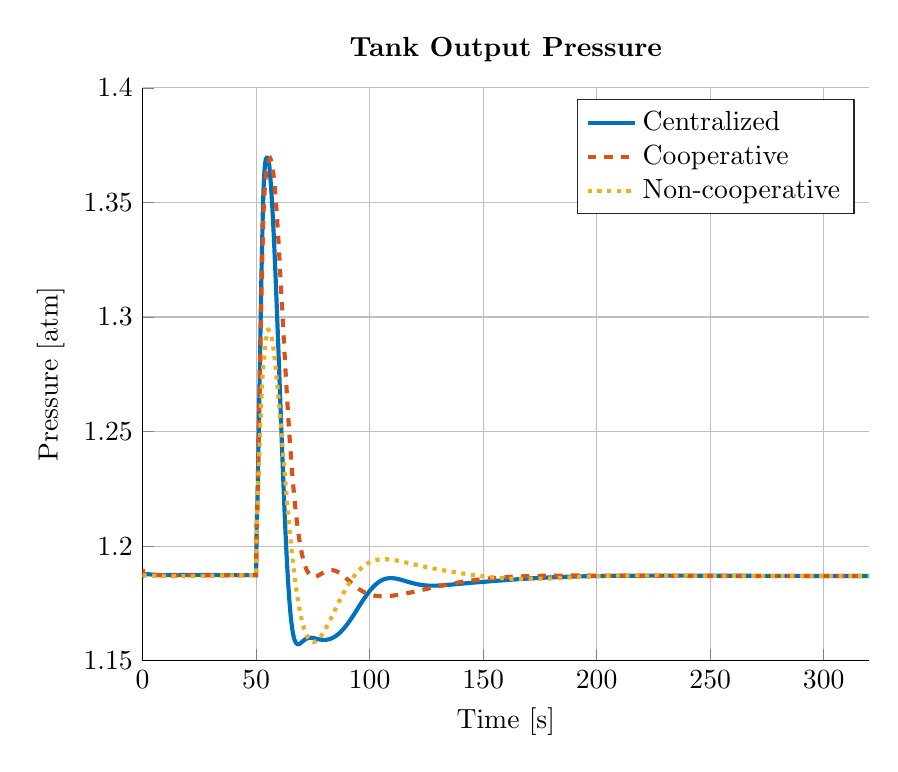
\begin{tikzpicture}

\begin{axis}[%
width=0.761\linewidth,
height=0.6\linewidth,
at={(0\linewidth,0\linewidth)},
scale only axis,
xmin=0,
xmax=320,
xlabel={Time [s]},
xmajorgrids,
ymin=1.15,
ymax=1.4,
ylabel={Pressure [atm]},
ymajorgrids,
axis background/.style={fill=white},
title style={font=\bfseries},
title={Tank Output Pressure},
axis x line*=bottom,
axis y line*=left,
legend style={legend cell align=left,align=left,draw=white!15!black}
]
\addplot [color=mycolor1,solid,line width=1.5pt]
  table[row sep=crcr]{%
0	1.19\\
0.25	1.1882\\
0.5	1.18754\\
0.75	1.18783\\
1	1.18784\\
1.25	1.18776\\
1.5	1.18777\\
1.75	1.18778\\
2	1.18777\\
2.25	1.18775\\
2.5	1.18774\\
2.75	1.18772\\
3	1.1877\\
3.25	1.18768\\
3.5	1.18766\\
3.75	1.18764\\
4	1.18761\\
4.25	1.18759\\
4.5	1.18757\\
4.75	1.18755\\
5	1.18753\\
5.25	1.18751\\
5.5	1.1875\\
5.75	1.18748\\
6	1.18747\\
6.25	1.18745\\
6.5	1.18744\\
6.75	1.18743\\
7	1.18742\\
7.25	1.18741\\
7.5	1.1874\\
7.75	1.18739\\
8	1.18739\\
8.25	1.18738\\
8.5	1.18738\\
8.75	1.18738\\
9	1.18737\\
9.25	1.18737\\
9.5	1.18737\\
9.75	1.18737\\
10	1.18737\\
10.25	1.18737\\
10.5	1.18738\\
10.75	1.18738\\
11	1.18738\\
11.25	1.18738\\
11.5	1.18739\\
11.75	1.18739\\
12	1.18739\\
12.25	1.1874\\
12.5	1.1874\\
12.75	1.18741\\
13	1.18741\\
13.25	1.18741\\
13.5	1.18742\\
13.75	1.18742\\
14	1.18743\\
14.25	1.18743\\
14.5	1.18743\\
14.75	1.18744\\
15	1.18744\\
15.25	1.18745\\
15.5	1.18745\\
15.75	1.18745\\
16	1.18745\\
16.25	1.18746\\
16.5	1.18746\\
16.75	1.18746\\
17	1.18746\\
17.25	1.18747\\
17.5	1.18747\\
17.75	1.18747\\
18	1.18747\\
18.25	1.18747\\
18.5	1.18747\\
18.75	1.18747\\
19	1.18747\\
19.25	1.18747\\
19.5	1.18747\\
19.75	1.18747\\
20	1.18747\\
20.25	1.18747\\
20.5	1.18747\\
20.75	1.18747\\
21	1.18747\\
21.25	1.18747\\
21.5	1.18747\\
21.75	1.18747\\
22	1.18747\\
22.25	1.18746\\
22.5	1.18746\\
22.75	1.18746\\
23	1.18746\\
23.25	1.18746\\
23.5	1.18746\\
23.75	1.18745\\
24	1.18745\\
24.25	1.18745\\
24.5	1.18745\\
24.75	1.18745\\
25	1.18744\\
25.25	1.18744\\
25.5	1.18744\\
25.75	1.18744\\
26	1.18744\\
26.25	1.18743\\
26.5	1.18743\\
26.75	1.18743\\
27	1.18743\\
27.25	1.18743\\
27.5	1.18742\\
27.75	1.18742\\
28	1.18742\\
28.25	1.18742\\
28.5	1.18741\\
28.75	1.18741\\
29	1.18741\\
29.25	1.18741\\
29.5	1.18741\\
29.75	1.1874\\
30	1.1874\\
30.25	1.1874\\
30.5	1.1874\\
30.75	1.1874\\
31	1.18739\\
31.25	1.18739\\
31.5	1.18739\\
31.75	1.18739\\
32	1.18739\\
32.25	1.18738\\
32.5	1.18738\\
32.75	1.18738\\
33	1.18738\\
33.25	1.18738\\
33.5	1.18737\\
33.75	1.18737\\
34	1.18737\\
34.25	1.18737\\
34.5	1.18737\\
34.75	1.18737\\
35	1.18737\\
35.25	1.18736\\
35.5	1.18736\\
35.75	1.18736\\
36	1.18736\\
36.25	1.18736\\
36.5	1.18736\\
36.75	1.18736\\
37	1.18736\\
37.25	1.18735\\
37.5	1.18735\\
37.75	1.18735\\
38	1.18735\\
38.25	1.18735\\
38.5	1.18735\\
38.75	1.18735\\
39	1.18735\\
39.25	1.18735\\
39.5	1.18735\\
39.75	1.18735\\
40	1.18734\\
40.25	1.18734\\
40.5	1.18734\\
40.75	1.18734\\
41	1.18734\\
41.25	1.18734\\
41.5	1.18734\\
41.75	1.18734\\
42	1.18734\\
42.25	1.18734\\
42.5	1.18734\\
42.75	1.18734\\
43	1.18734\\
43.25	1.18734\\
43.5	1.18734\\
43.75	1.18734\\
44	1.18734\\
44.25	1.18734\\
44.5	1.18734\\
44.75	1.18734\\
45	1.18734\\
45.25	1.18734\\
45.5	1.18734\\
45.75	1.18734\\
46	1.18734\\
46.25	1.18734\\
46.5	1.18734\\
46.75	1.18734\\
47	1.18734\\
47.25	1.18734\\
47.5	1.18734\\
47.75	1.18734\\
48	1.18734\\
48.25	1.18734\\
48.5	1.18734\\
48.75	1.18734\\
49	1.18734\\
49.25	1.18734\\
49.5	1.18734\\
49.75	1.18734\\
50	1.18734\\
50.25	1.20736\\
50.5	1.2164\\
50.75	1.22507\\
51	1.24084\\
51.25	1.25517\\
51.5	1.2681\\
51.75	1.28267\\
52	1.29789\\
52.25	1.3128\\
52.5	1.32465\\
52.75	1.33567\\
53	1.34703\\
53.25	1.35504\\
53.5	1.3604\\
53.75	1.36444\\
54	1.36711\\
54.25	1.3686\\
54.5	1.3693\\
54.75	1.36952\\
55	1.36954\\
55.25	1.36924\\
55.5	1.36843\\
55.75	1.36689\\
56	1.36433\\
56.25	1.36128\\
56.5	1.35808\\
56.75	1.35453\\
57	1.35051\\
57.25	1.3461\\
57.5	1.34139\\
57.75	1.3364\\
58	1.33112\\
58.25	1.32553\\
58.5	1.31969\\
58.75	1.31367\\
59	1.30746\\
59.25	1.3011\\
59.5	1.2946\\
59.75	1.288\\
60	1.28131\\
60.25	1.27457\\
60.5	1.2678\\
60.75	1.26104\\
61	1.25431\\
61.25	1.24765\\
61.5	1.24107\\
61.75	1.23462\\
62	1.22832\\
62.25	1.22219\\
62.5	1.21627\\
62.75	1.21057\\
63	1.20512\\
63.25	1.19994\\
63.5	1.19504\\
63.75	1.19045\\
64	1.18616\\
64.25	1.1822\\
64.5	1.17856\\
64.75	1.17525\\
65	1.17227\\
65.25	1.1696\\
65.5	1.16725\\
65.75	1.16521\\
66	1.16346\\
66.25	1.16197\\
66.5	1.16075\\
66.75	1.15975\\
67	1.15896\\
67.25	1.15835\\
67.5	1.15789\\
67.75	1.15757\\
68	1.15736\\
68.25	1.15724\\
68.5	1.15721\\
68.75	1.15724\\
69	1.15733\\
69.25	1.15746\\
69.5	1.15762\\
69.75	1.15781\\
70	1.15801\\
70.25	1.15822\\
70.5	1.15843\\
70.75	1.15864\\
71	1.15884\\
71.25	1.15904\\
71.5	1.15921\\
71.75	1.15938\\
72	1.15952\\
72.25	1.15965\\
72.5	1.15976\\
72.75	1.15985\\
73	1.15992\\
73.25	1.15997\\
73.5	1.16001\\
73.75	1.16003\\
74	1.16004\\
74.25	1.16003\\
74.5	1.16002\\
74.75	1.15999\\
75	1.15995\\
75.25	1.15991\\
75.5	1.15986\\
75.75	1.15981\\
76	1.15975\\
76.25	1.15969\\
76.5	1.15963\\
76.75	1.15957\\
77	1.15951\\
77.25	1.15945\\
77.5	1.15939\\
77.75	1.15934\\
78	1.15929\\
78.25	1.15924\\
78.5	1.1592\\
78.75	1.15917\\
79	1.15914\\
79.25	1.15912\\
79.5	1.1591\\
79.75	1.15909\\
80	1.15909\\
80.25	1.1591\\
80.5	1.15911\\
80.75	1.15913\\
81	1.15916\\
81.25	1.15919\\
81.5	1.15924\\
81.75	1.15929\\
82	1.15935\\
82.25	1.15941\\
82.5	1.15949\\
82.75	1.15957\\
83	1.15967\\
83.25	1.15977\\
83.5	1.15988\\
83.75	1.16\\
84	1.16013\\
84.25	1.16026\\
84.5	1.16041\\
84.75	1.16056\\
85	1.16072\\
85.25	1.16089\\
85.5	1.16107\\
85.75	1.16126\\
86	1.16146\\
86.25	1.16166\\
86.5	1.16188\\
86.75	1.1621\\
87	1.16233\\
87.25	1.16257\\
87.5	1.16282\\
87.75	1.16308\\
88	1.16334\\
88.25	1.16361\\
88.5	1.16389\\
88.75	1.16418\\
89	1.16448\\
89.25	1.16478\\
89.5	1.16509\\
89.75	1.1654\\
90	1.16573\\
90.25	1.16606\\
90.5	1.16639\\
90.75	1.16673\\
91	1.16708\\
91.25	1.16743\\
91.5	1.16779\\
91.75	1.16815\\
92	1.16852\\
92.25	1.16889\\
92.5	1.16926\\
92.75	1.16964\\
93	1.17002\\
93.25	1.17041\\
93.5	1.17079\\
93.75	1.17118\\
94	1.17157\\
94.25	1.17196\\
94.5	1.17235\\
94.75	1.17274\\
95	1.17313\\
95.25	1.17353\\
95.5	1.17392\\
95.75	1.17431\\
96	1.1747\\
96.25	1.17508\\
96.5	1.17547\\
96.75	1.17585\\
97	1.17622\\
97.25	1.1766\\
97.5	1.17697\\
97.75	1.17734\\
98	1.1777\\
98.25	1.17806\\
98.5	1.17841\\
98.75	1.17876\\
99	1.1791\\
99.25	1.17943\\
99.5	1.17976\\
99.75	1.18008\\
100	1.18039\\
100.25	1.1807\\
100.5	1.181\\
100.75	1.18129\\
101	1.18158\\
101.25	1.18185\\
101.5	1.18212\\
101.75	1.18238\\
102	1.18263\\
102.25	1.18287\\
102.5	1.1831\\
102.75	1.18333\\
103	1.18354\\
103.25	1.18375\\
103.5	1.18394\\
103.75	1.18413\\
104	1.18431\\
104.25	1.18448\\
104.5	1.18464\\
104.75	1.18479\\
105	1.18493\\
105.25	1.18506\\
105.5	1.18519\\
105.75	1.1853\\
106	1.18541\\
106.25	1.1855\\
106.5	1.18559\\
106.75	1.18567\\
107	1.18574\\
107.25	1.18581\\
107.5	1.18586\\
107.75	1.18591\\
108	1.18595\\
108.25	1.18599\\
108.5	1.18601\\
108.75	1.18603\\
109	1.18604\\
109.25	1.18605\\
109.5	1.18605\\
109.75	1.18605\\
110	1.18603\\
110.25	1.18602\\
110.5	1.186\\
110.75	1.18597\\
111	1.18594\\
111.25	1.1859\\
111.5	1.18586\\
111.75	1.18582\\
112	1.18577\\
112.25	1.18572\\
112.5	1.18566\\
112.75	1.18561\\
113	1.18555\\
113.25	1.18548\\
113.5	1.18542\\
113.75	1.18535\\
114	1.18529\\
114.25	1.18522\\
114.5	1.18514\\
114.75	1.18507\\
115	1.185\\
115.25	1.18493\\
115.5	1.18485\\
115.75	1.18478\\
116	1.1847\\
116.25	1.18463\\
116.5	1.18455\\
116.75	1.18448\\
117	1.18441\\
117.25	1.18433\\
117.5	1.18426\\
117.75	1.18419\\
118	1.18412\\
118.25	1.18405\\
118.5	1.18398\\
118.75	1.18392\\
119	1.18385\\
119.25	1.18379\\
119.5	1.18373\\
119.75	1.18367\\
120	1.18361\\
120.25	1.18355\\
120.5	1.1835\\
120.75	1.18344\\
121	1.18339\\
121.25	1.18334\\
121.5	1.1833\\
121.75	1.18325\\
122	1.18321\\
122.25	1.18317\\
122.5	1.18313\\
122.75	1.18309\\
123	1.18306\\
123.25	1.18303\\
123.5	1.18299\\
123.75	1.18297\\
124	1.18294\\
124.25	1.18291\\
124.5	1.18289\\
124.75	1.18287\\
125	1.18285\\
125.25	1.18283\\
125.5	1.18282\\
125.75	1.1828\\
126	1.18279\\
126.25	1.18278\\
126.5	1.18277\\
126.75	1.18277\\
127	1.18276\\
127.25	1.18276\\
127.5	1.18276\\
127.75	1.18276\\
128	1.18276\\
128.25	1.18276\\
128.5	1.18276\\
128.75	1.18277\\
129	1.18277\\
129.25	1.18278\\
129.5	1.18279\\
129.75	1.18279\\
130	1.1828\\
130.25	1.18282\\
130.5	1.18283\\
130.75	1.18284\\
131	1.18285\\
131.25	1.18287\\
131.5	1.18288\\
131.75	1.1829\\
132	1.18291\\
132.25	1.18293\\
132.5	1.18295\\
132.75	1.18297\\
133	1.18299\\
133.25	1.183\\
133.5	1.18302\\
133.75	1.18304\\
134	1.18306\\
134.25	1.18308\\
134.5	1.18311\\
134.75	1.18313\\
135	1.18315\\
135.25	1.18317\\
135.5	1.18319\\
135.75	1.18321\\
136	1.18323\\
136.25	1.18326\\
136.5	1.18328\\
136.75	1.1833\\
137	1.18332\\
137.25	1.18335\\
137.5	1.18337\\
137.75	1.18339\\
138	1.18341\\
138.25	1.18344\\
138.5	1.18346\\
138.75	1.18348\\
139	1.1835\\
139.25	1.18353\\
139.5	1.18355\\
139.75	1.18357\\
140	1.18359\\
140.25	1.18362\\
140.5	1.18364\\
140.75	1.18366\\
141	1.18368\\
141.25	1.18371\\
141.5	1.18373\\
141.75	1.18375\\
142	1.18377\\
142.25	1.18379\\
142.5	1.18381\\
142.75	1.18384\\
143	1.18386\\
143.25	1.18388\\
143.5	1.1839\\
143.75	1.18392\\
144	1.18394\\
144.25	1.18396\\
144.5	1.18398\\
144.75	1.184\\
145	1.18402\\
145.25	1.18404\\
145.5	1.18407\\
145.75	1.18409\\
146	1.18411\\
146.25	1.18413\\
146.5	1.18415\\
146.75	1.18417\\
147	1.18419\\
147.25	1.18421\\
147.5	1.18423\\
147.75	1.18425\\
148	1.18427\\
148.25	1.18429\\
148.5	1.18431\\
148.75	1.18433\\
149	1.18435\\
149.25	1.18437\\
149.5	1.18439\\
149.75	1.18441\\
150	1.18442\\
150.25	1.18444\\
150.5	1.18446\\
150.75	1.18448\\
151	1.1845\\
151.25	1.18452\\
151.5	1.18454\\
151.75	1.18456\\
152	1.18458\\
152.25	1.1846\\
152.5	1.18462\\
152.75	1.18464\\
153	1.18466\\
153.25	1.18468\\
153.5	1.1847\\
153.75	1.18472\\
154	1.18474\\
154.25	1.18475\\
154.5	1.18477\\
154.75	1.18479\\
155	1.18481\\
155.25	1.18483\\
155.5	1.18485\\
155.75	1.18487\\
156	1.18489\\
156.25	1.18491\\
156.5	1.18493\\
156.75	1.18495\\
157	1.18496\\
157.25	1.18498\\
157.5	1.185\\
157.75	1.18502\\
158	1.18504\\
158.25	1.18506\\
158.5	1.18508\\
158.75	1.1851\\
159	1.18511\\
159.25	1.18513\\
159.5	1.18515\\
159.75	1.18517\\
160	1.18519\\
160.25	1.18521\\
160.5	1.18523\\
160.75	1.18524\\
161	1.18526\\
161.25	1.18528\\
161.5	1.1853\\
161.75	1.18532\\
162	1.18533\\
162.25	1.18535\\
162.5	1.18537\\
162.75	1.18539\\
163	1.18541\\
163.25	1.18542\\
163.5	1.18544\\
163.75	1.18546\\
164	1.18548\\
164.25	1.18549\\
164.5	1.18551\\
164.75	1.18553\\
165	1.18554\\
165.25	1.18556\\
165.5	1.18558\\
165.75	1.1856\\
166	1.18561\\
166.25	1.18563\\
166.5	1.18565\\
166.75	1.18566\\
167	1.18568\\
167.25	1.18569\\
167.5	1.18571\\
167.75	1.18573\\
168	1.18574\\
168.25	1.18576\\
168.5	1.18577\\
168.75	1.18579\\
169	1.18581\\
169.25	1.18582\\
169.5	1.18584\\
169.75	1.18585\\
170	1.18587\\
170.25	1.18588\\
170.5	1.1859\\
170.75	1.18591\\
171	1.18593\\
171.25	1.18594\\
171.5	1.18595\\
171.75	1.18597\\
172	1.18598\\
172.25	1.186\\
172.5	1.18601\\
172.75	1.18603\\
173	1.18604\\
173.25	1.18605\\
173.5	1.18607\\
173.75	1.18608\\
174	1.18609\\
174.25	1.18611\\
174.5	1.18612\\
174.75	1.18613\\
175	1.18615\\
175.25	1.18616\\
175.5	1.18617\\
175.75	1.18618\\
176	1.1862\\
176.25	1.18621\\
176.5	1.18622\\
176.75	1.18623\\
177	1.18625\\
177.25	1.18626\\
177.5	1.18627\\
177.75	1.18628\\
178	1.18629\\
178.25	1.18631\\
178.5	1.18632\\
178.75	1.18633\\
179	1.18634\\
179.25	1.18635\\
179.5	1.18636\\
179.75	1.18637\\
180	1.18638\\
180.25	1.18639\\
180.5	1.1864\\
180.75	1.18642\\
181	1.18643\\
181.25	1.18644\\
181.5	1.18645\\
181.75	1.18646\\
182	1.18647\\
182.25	1.18648\\
182.5	1.18649\\
182.75	1.1865\\
183	1.18651\\
183.25	1.18652\\
183.5	1.18652\\
183.75	1.18653\\
184	1.18654\\
184.25	1.18655\\
184.5	1.18656\\
184.75	1.18657\\
185	1.18658\\
185.25	1.18659\\
185.5	1.1866\\
185.75	1.18661\\
186	1.18661\\
186.25	1.18662\\
186.5	1.18663\\
186.75	1.18664\\
187	1.18665\\
187.25	1.18665\\
187.5	1.18666\\
187.75	1.18667\\
188	1.18668\\
188.25	1.18669\\
188.5	1.18669\\
188.75	1.1867\\
189	1.18671\\
189.25	1.18672\\
189.5	1.18672\\
189.75	1.18673\\
190	1.18674\\
190.25	1.18674\\
190.5	1.18675\\
190.75	1.18676\\
191	1.18677\\
191.25	1.18677\\
191.5	1.18678\\
191.75	1.18679\\
192	1.18679\\
192.25	1.1868\\
192.5	1.1868\\
192.75	1.18681\\
193	1.18682\\
193.25	1.18682\\
193.5	1.18683\\
193.75	1.18683\\
194	1.18684\\
194.25	1.18685\\
194.5	1.18685\\
194.75	1.18686\\
195	1.18686\\
195.25	1.18687\\
195.5	1.18687\\
195.75	1.18688\\
196	1.18688\\
196.25	1.18689\\
196.5	1.18689\\
196.75	1.1869\\
197	1.1869\\
197.25	1.18691\\
197.5	1.18691\\
197.75	1.18692\\
198	1.18692\\
198.25	1.18693\\
198.5	1.18693\\
198.75	1.18694\\
199	1.18694\\
199.25	1.18695\\
199.5	1.18695\\
199.75	1.18695\\
200	1.18696\\
200.25	1.18696\\
200.5	1.18697\\
200.75	1.18697\\
201	1.18697\\
201.25	1.18698\\
201.5	1.18698\\
201.75	1.18699\\
202	1.18699\\
202.25	1.18699\\
202.5	1.187\\
202.75	1.187\\
203	1.187\\
203.25	1.18701\\
203.5	1.18701\\
203.75	1.18701\\
204	1.18702\\
204.25	1.18702\\
204.5	1.18702\\
204.75	1.18703\\
205	1.18703\\
205.25	1.18703\\
205.5	1.18704\\
205.75	1.18704\\
206	1.18704\\
206.25	1.18704\\
206.5	1.18705\\
206.75	1.18705\\
207	1.18705\\
207.25	1.18705\\
207.5	1.18706\\
207.75	1.18706\\
208	1.18706\\
208.25	1.18706\\
208.5	1.18707\\
208.75	1.18707\\
209	1.18707\\
209.25	1.18707\\
209.5	1.18708\\
209.75	1.18708\\
210	1.18708\\
210.25	1.18708\\
210.5	1.18708\\
210.75	1.18709\\
211	1.18709\\
211.25	1.18709\\
211.5	1.18709\\
211.75	1.18709\\
212	1.18709\\
212.25	1.1871\\
212.5	1.1871\\
212.75	1.1871\\
213	1.1871\\
213.25	1.1871\\
213.5	1.1871\\
213.75	1.18711\\
214	1.18711\\
214.25	1.18711\\
214.5	1.18711\\
214.75	1.18711\\
215	1.18711\\
215.25	1.18711\\
215.5	1.18711\\
215.75	1.18712\\
216	1.18712\\
216.25	1.18712\\
216.5	1.18712\\
216.75	1.18712\\
217	1.18712\\
217.25	1.18712\\
217.5	1.18712\\
217.75	1.18712\\
218	1.18712\\
218.25	1.18713\\
218.5	1.18713\\
218.75	1.18713\\
219	1.18713\\
219.25	1.18713\\
219.5	1.18713\\
219.75	1.18713\\
220	1.18713\\
220.25	1.18713\\
220.5	1.18713\\
220.75	1.18713\\
221	1.18713\\
221.25	1.18713\\
221.5	1.18713\\
221.75	1.18713\\
222	1.18714\\
222.25	1.18714\\
222.5	1.18714\\
222.75	1.18714\\
223	1.18714\\
223.25	1.18714\\
223.5	1.18714\\
223.75	1.18714\\
224	1.18714\\
224.25	1.18714\\
224.5	1.18714\\
224.75	1.18714\\
225	1.18714\\
225.25	1.18714\\
225.5	1.18714\\
225.75	1.18714\\
226	1.18714\\
226.25	1.18714\\
226.5	1.18714\\
226.75	1.18714\\
227	1.18714\\
227.25	1.18714\\
227.5	1.18714\\
227.75	1.18714\\
228	1.18714\\
228.25	1.18714\\
228.5	1.18714\\
228.75	1.18714\\
229	1.18714\\
229.25	1.18714\\
229.5	1.18714\\
229.75	1.18714\\
230	1.18714\\
230.25	1.18714\\
230.5	1.18714\\
230.75	1.18714\\
231	1.18714\\
231.25	1.18714\\
231.5	1.18714\\
231.75	1.18714\\
232	1.18714\\
232.25	1.18714\\
232.5	1.18714\\
232.75	1.18714\\
233	1.18714\\
233.25	1.18714\\
233.5	1.18714\\
233.75	1.18714\\
234	1.18714\\
234.25	1.18714\\
234.5	1.18714\\
234.75	1.18713\\
235	1.18713\\
235.25	1.18713\\
235.5	1.18713\\
235.75	1.18713\\
236	1.18713\\
236.25	1.18713\\
236.5	1.18713\\
236.75	1.18713\\
237	1.18713\\
237.25	1.18713\\
237.5	1.18713\\
237.75	1.18713\\
238	1.18713\\
238.25	1.18713\\
238.5	1.18713\\
238.75	1.18713\\
239	1.18713\\
239.25	1.18713\\
239.5	1.18713\\
239.75	1.18713\\
240	1.18713\\
240.25	1.18712\\
240.5	1.18712\\
240.75	1.18712\\
241	1.18712\\
241.25	1.18712\\
241.5	1.18712\\
241.75	1.18712\\
242	1.18712\\
242.25	1.18712\\
242.5	1.18712\\
242.75	1.18712\\
243	1.18712\\
243.25	1.18712\\
243.5	1.18712\\
243.75	1.18712\\
244	1.18712\\
244.25	1.18712\\
244.5	1.18711\\
244.75	1.18711\\
245	1.18711\\
245.25	1.18711\\
245.5	1.18711\\
245.75	1.18711\\
246	1.18711\\
246.25	1.18711\\
246.5	1.18711\\
246.75	1.18711\\
247	1.18711\\
247.25	1.18711\\
247.5	1.18711\\
247.75	1.18711\\
248	1.18711\\
248.25	1.18711\\
248.5	1.1871\\
248.75	1.1871\\
249	1.1871\\
249.25	1.1871\\
249.5	1.1871\\
249.75	1.1871\\
250	1.1871\\
250.25	1.1871\\
250.5	1.1871\\
250.75	1.1871\\
251	1.1871\\
251.25	1.1871\\
251.5	1.1871\\
251.75	1.1871\\
252	1.1871\\
252.25	1.1871\\
252.5	1.18709\\
252.75	1.18709\\
253	1.18709\\
253.25	1.18709\\
253.5	1.18709\\
253.75	1.18709\\
254	1.18709\\
254.25	1.18709\\
254.5	1.18709\\
254.75	1.18709\\
255	1.18709\\
255.25	1.18709\\
255.5	1.18709\\
255.75	1.18709\\
256	1.18709\\
256.25	1.18708\\
256.5	1.18708\\
256.75	1.18708\\
257	1.18708\\
257.25	1.18708\\
257.5	1.18708\\
257.75	1.18708\\
258	1.18708\\
258.25	1.18708\\
258.5	1.18708\\
258.75	1.18708\\
259	1.18708\\
259.25	1.18708\\
259.5	1.18708\\
259.75	1.18708\\
260	1.18707\\
260.25	1.18707\\
260.5	1.18707\\
260.75	1.18707\\
261	1.18707\\
261.25	1.18707\\
261.5	1.18707\\
261.75	1.18707\\
262	1.18707\\
262.25	1.18707\\
262.5	1.18707\\
262.75	1.18707\\
263	1.18707\\
263.25	1.18707\\
263.5	1.18707\\
263.75	1.18707\\
264	1.18706\\
264.25	1.18706\\
264.5	1.18706\\
264.75	1.18706\\
265	1.18706\\
265.25	1.18706\\
265.5	1.18706\\
265.75	1.18706\\
266	1.18706\\
266.25	1.18706\\
266.5	1.18706\\
266.75	1.18706\\
267	1.18706\\
267.25	1.18706\\
267.5	1.18706\\
267.75	1.18706\\
268	1.18706\\
268.25	1.18706\\
268.5	1.18705\\
268.75	1.18705\\
269	1.18705\\
269.25	1.18705\\
269.5	1.18705\\
269.75	1.18705\\
270	1.18705\\
270.25	1.18705\\
270.5	1.18705\\
270.75	1.18705\\
271	1.18705\\
271.25	1.18705\\
271.5	1.18705\\
271.75	1.18705\\
272	1.18705\\
272.25	1.18705\\
272.5	1.18705\\
272.75	1.18705\\
273	1.18705\\
273.25	1.18704\\
273.5	1.18704\\
273.75	1.18704\\
274	1.18704\\
274.25	1.18704\\
274.5	1.18704\\
274.75	1.18704\\
275	1.18704\\
275.25	1.18704\\
275.5	1.18704\\
275.75	1.18704\\
276	1.18704\\
276.25	1.18704\\
276.5	1.18704\\
276.75	1.18704\\
277	1.18704\\
277.25	1.18704\\
277.5	1.18704\\
277.75	1.18704\\
278	1.18704\\
278.25	1.18704\\
278.5	1.18703\\
278.75	1.18703\\
279	1.18703\\
279.25	1.18703\\
279.5	1.18703\\
279.75	1.18703\\
280	1.18703\\
280.25	1.18703\\
280.5	1.18703\\
280.75	1.18703\\
281	1.18703\\
281.25	1.18703\\
281.5	1.18703\\
281.75	1.18703\\
282	1.18703\\
282.25	1.18703\\
282.5	1.18703\\
282.75	1.18703\\
283	1.18703\\
283.25	1.18703\\
283.5	1.18703\\
283.75	1.18703\\
284	1.18703\\
284.25	1.18703\\
284.5	1.18703\\
284.75	1.18702\\
285	1.18702\\
285.25	1.18702\\
285.5	1.18702\\
285.75	1.18702\\
286	1.18702\\
286.25	1.18702\\
286.5	1.18702\\
286.75	1.18702\\
287	1.18702\\
287.25	1.18702\\
287.5	1.18702\\
287.75	1.18702\\
288	1.18702\\
288.25	1.18702\\
288.5	1.18702\\
288.75	1.18702\\
289	1.18702\\
289.25	1.18702\\
289.5	1.18702\\
289.75	1.18702\\
290	1.18702\\
290.25	1.18702\\
290.5	1.18702\\
290.75	1.18702\\
291	1.18702\\
291.25	1.18702\\
291.5	1.18702\\
291.75	1.18702\\
292	1.18702\\
292.25	1.18702\\
292.5	1.18702\\
292.75	1.18701\\
293	1.18701\\
293.25	1.18701\\
293.5	1.18701\\
293.75	1.18701\\
294	1.18701\\
294.25	1.18701\\
294.5	1.18701\\
294.75	1.18701\\
295	1.18701\\
295.25	1.18701\\
295.5	1.18701\\
295.75	1.18701\\
296	1.18701\\
296.25	1.18701\\
296.5	1.18701\\
296.75	1.18701\\
297	1.18701\\
297.25	1.18701\\
297.5	1.18701\\
297.75	1.18701\\
298	1.18701\\
298.25	1.18701\\
298.5	1.18701\\
298.75	1.18701\\
299	1.18701\\
299.25	1.18701\\
299.5	1.18701\\
299.75	1.18701\\
300	1.18701\\
300.25	1.18701\\
300.5	1.18701\\
300.75	1.18701\\
301	1.18701\\
301.25	1.18701\\
301.5	1.18701\\
301.75	1.18701\\
302	1.18701\\
302.25	1.18701\\
302.5	1.18701\\
302.75	1.18701\\
303	1.18701\\
303.25	1.18701\\
303.5	1.18701\\
303.75	1.18701\\
304	1.18701\\
304.25	1.18701\\
304.5	1.18701\\
304.75	1.187\\
305	1.187\\
305.25	1.187\\
305.5	1.187\\
305.75	1.187\\
306	1.187\\
306.25	1.187\\
306.5	1.187\\
306.75	1.187\\
307	1.187\\
307.25	1.187\\
307.5	1.187\\
307.75	1.187\\
308	1.187\\
308.25	1.187\\
308.5	1.187\\
308.75	1.187\\
309	1.187\\
309.25	1.187\\
309.5	1.187\\
309.75	1.187\\
310	1.187\\
310.25	1.187\\
310.5	1.187\\
310.75	1.187\\
311	1.187\\
311.25	1.187\\
311.5	1.187\\
311.75	1.187\\
312	1.187\\
312.25	1.187\\
312.5	1.187\\
312.75	1.187\\
313	1.187\\
313.25	1.187\\
313.5	1.187\\
313.75	1.187\\
314	1.187\\
314.25	1.187\\
314.5	1.187\\
314.75	1.187\\
315	1.187\\
315.25	1.187\\
315.5	1.187\\
315.75	1.187\\
316	1.187\\
316.25	1.187\\
316.5	1.187\\
316.75	1.187\\
317	1.187\\
317.25	1.187\\
317.5	1.187\\
317.75	1.187\\
318	1.187\\
318.25	1.187\\
318.5	1.187\\
318.75	1.187\\
319	1.187\\
319.25	1.187\\
319.5	1.187\\
319.75	1.187\\
320	1.187\\
320.25	1.187\\
320.5	1.187\\
320.75	1.187\\
321	1.187\\
321.25	1.187\\
321.5	1.187\\
321.75	1.187\\
322	1.187\\
322.25	1.187\\
322.5	1.187\\
322.75	1.187\\
323	1.187\\
323.25	1.187\\
323.5	1.187\\
323.75	1.187\\
324	1.187\\
324.25	1.187\\
324.5	1.187\\
324.75	1.187\\
325	1.187\\
325.25	1.187\\
325.5	1.187\\
325.75	1.187\\
326	1.187\\
326.25	1.187\\
326.5	1.187\\
326.75	1.187\\
327	1.187\\
327.25	1.187\\
327.5	1.187\\
327.75	1.187\\
328	1.187\\
328.25	1.187\\
328.5	1.187\\
328.75	1.187\\
329	1.187\\
329.25	1.187\\
329.5	1.187\\
329.75	1.187\\
330	1.187\\
330.25	1.187\\
330.5	1.187\\
330.75	1.187\\
331	1.187\\
331.25	1.187\\
331.5	1.187\\
331.75	1.187\\
332	1.187\\
332.25	1.187\\
332.5	1.187\\
332.75	1.187\\
333	1.187\\
333.25	1.187\\
333.5	1.187\\
333.75	1.187\\
334	1.187\\
334.25	1.187\\
334.5	1.187\\
334.75	1.187\\
335	1.187\\
335.25	1.187\\
335.5	1.187\\
335.75	1.187\\
336	1.187\\
336.25	1.187\\
336.5	1.187\\
336.75	1.187\\
337	1.187\\
337.25	1.187\\
337.5	1.187\\
337.75	1.187\\
338	1.187\\
338.25	1.187\\
338.5	1.187\\
338.75	1.187\\
339	1.187\\
339.25	1.187\\
339.5	1.187\\
339.75	1.187\\
340	1.187\\
340.25	1.187\\
340.5	1.187\\
340.75	1.187\\
341	1.187\\
341.25	1.187\\
341.5	1.187\\
341.75	1.187\\
342	1.187\\
342.25	1.187\\
342.5	1.187\\
342.75	1.187\\
343	1.187\\
343.25	1.187\\
343.5	1.187\\
343.75	1.187\\
344	1.187\\
344.25	1.187\\
344.5	1.187\\
344.75	1.187\\
345	1.187\\
345.25	1.187\\
345.5	1.187\\
345.75	1.187\\
346	1.187\\
346.25	1.187\\
346.5	1.187\\
346.75	1.187\\
347	1.187\\
347.25	1.187\\
347.5	1.187\\
347.75	1.187\\
348	1.187\\
348.25	1.187\\
348.5	1.187\\
348.75	1.187\\
349	1.187\\
349.25	1.187\\
349.5	1.187\\
349.75	1.187\\
350	1.187\\
350.25	1.187\\
350.5	1.187\\
350.75	1.187\\
351	1.187\\
351.25	1.187\\
351.5	1.187\\
351.75	1.187\\
352	1.187\\
352.25	1.187\\
352.5	1.187\\
352.75	1.187\\
353	1.187\\
353.25	1.187\\
353.5	1.187\\
353.75	1.187\\
354	1.187\\
354.25	1.187\\
354.5	1.187\\
354.75	1.187\\
355	1.187\\
355.25	1.187\\
355.5	1.187\\
355.75	1.187\\
356	1.187\\
356.25	1.187\\
356.5	1.187\\
356.75	1.187\\
357	1.187\\
357.25	1.187\\
357.5	1.187\\
357.75	1.187\\
358	1.187\\
358.25	1.187\\
358.5	1.187\\
358.75	1.187\\
359	1.187\\
359.25	1.187\\
359.5	1.187\\
359.75	1.187\\
360	1.187\\
360.25	1.187\\
360.5	1.187\\
360.75	1.187\\
361	1.187\\
361.25	1.187\\
361.5	1.187\\
361.75	1.187\\
362	1.187\\
362.25	1.187\\
362.5	1.187\\
362.75	1.187\\
363	1.187\\
363.25	1.187\\
363.5	1.187\\
363.75	1.187\\
364	1.187\\
364.25	1.187\\
364.5	1.187\\
364.75	1.187\\
365	1.187\\
365.25	1.187\\
365.5	1.187\\
365.75	1.187\\
366	1.187\\
366.25	1.187\\
366.5	1.187\\
366.75	1.187\\
367	1.187\\
367.25	1.187\\
367.5	1.187\\
367.75	1.187\\
368	1.187\\
368.25	1.187\\
368.5	1.187\\
368.75	1.187\\
369	1.187\\
369.25	1.187\\
369.5	1.187\\
369.75	1.187\\
370	1.187\\
370.25	1.187\\
370.5	1.187\\
370.75	1.187\\
371	1.187\\
371.25	1.187\\
371.5	1.187\\
371.75	1.187\\
372	1.187\\
372.25	1.187\\
372.5	1.187\\
372.75	1.187\\
373	1.187\\
373.25	1.187\\
373.5	1.187\\
373.75	1.187\\
374	1.187\\
374.25	1.187\\
374.5	1.187\\
374.75	1.187\\
375	1.187\\
375.25	1.187\\
375.5	1.187\\
375.75	1.187\\
376	1.187\\
376.25	1.187\\
376.5	1.187\\
376.75	1.187\\
377	1.187\\
377.25	1.187\\
377.5	1.187\\
377.75	1.187\\
378	1.187\\
378.25	1.187\\
378.5	1.187\\
378.75	1.187\\
379	1.187\\
379.25	1.187\\
379.5	1.187\\
379.75	1.187\\
380	1.187\\
380.25	1.187\\
380.5	1.187\\
380.75	1.187\\
381	1.187\\
381.25	1.187\\
381.5	1.187\\
381.75	1.187\\
382	1.187\\
382.25	1.187\\
382.5	1.187\\
382.75	1.187\\
383	1.187\\
383.25	1.187\\
383.5	1.187\\
383.75	1.187\\
384	1.187\\
384.25	1.187\\
384.5	1.187\\
384.75	1.187\\
385	1.187\\
385.25	1.187\\
385.5	1.187\\
385.75	1.187\\
386	1.187\\
386.25	1.187\\
386.5	1.187\\
386.75	1.187\\
387	1.187\\
387.25	1.187\\
387.5	1.187\\
387.75	1.187\\
388	1.187\\
388.25	1.187\\
388.5	1.187\\
388.75	1.187\\
389	1.187\\
389.25	1.187\\
389.5	1.187\\
389.75	1.187\\
390	1.187\\
390.25	1.187\\
390.5	1.187\\
390.75	1.187\\
391	1.187\\
391.25	1.187\\
391.5	1.187\\
391.75	1.187\\
392	1.187\\
392.25	1.187\\
392.5	1.187\\
392.75	1.187\\
393	1.187\\
393.25	1.187\\
393.5	1.187\\
393.75	1.187\\
394	1.187\\
394.25	1.187\\
394.5	1.187\\
394.75	1.187\\
395	1.187\\
395.25	1.187\\
395.5	1.187\\
395.75	1.187\\
396	1.187\\
396.25	1.187\\
396.5	1.187\\
396.75	1.187\\
397	1.187\\
397.25	1.187\\
397.5	1.187\\
397.75	1.187\\
398	1.187\\
398.25	1.187\\
398.5	1.187\\
398.75	1.187\\
399	1.187\\
399.25	1.187\\
399.5	1.187\\
399.75	1.187\\
400	1.187\\
400.25	1.187\\
400.5	1.187\\
400.75	1.187\\
401	1.187\\
401.25	1.187\\
401.5	1.187\\
401.75	1.187\\
402	1.187\\
402.25	1.187\\
402.5	1.187\\
402.75	1.187\\
403	1.187\\
403.25	1.187\\
403.5	1.187\\
403.75	1.187\\
404	1.187\\
404.25	1.187\\
404.5	1.187\\
404.75	1.187\\
405	1.187\\
405.25	1.187\\
405.5	1.187\\
405.75	1.187\\
406	1.187\\
406.25	1.187\\
406.5	1.187\\
406.75	1.187\\
407	1.187\\
407.25	1.187\\
407.5	1.187\\
407.75	1.187\\
408	1.187\\
408.25	1.187\\
408.5	1.187\\
408.75	1.187\\
409	1.187\\
409.25	1.187\\
409.5	1.187\\
409.75	1.187\\
410	1.187\\
410.25	1.187\\
410.5	1.187\\
410.75	1.187\\
411	1.187\\
411.25	1.187\\
411.5	1.187\\
411.75	1.187\\
412	1.187\\
412.25	1.187\\
412.5	1.187\\
412.75	1.187\\
413	1.187\\
413.25	1.187\\
413.5	1.187\\
413.75	1.187\\
414	1.187\\
414.25	1.187\\
414.5	1.187\\
414.75	1.187\\
415	1.187\\
415.25	1.187\\
415.5	1.187\\
415.75	1.187\\
416	1.187\\
416.25	1.187\\
416.5	1.187\\
416.75	1.187\\
417	1.187\\
417.25	1.187\\
417.5	1.187\\
417.75	1.187\\
418	1.187\\
418.25	1.187\\
418.5	1.187\\
418.75	1.187\\
419	1.187\\
419.25	1.187\\
419.5	1.187\\
419.75	1.187\\
420	1.187\\
420.25	1.187\\
420.5	1.187\\
420.75	1.187\\
421	1.187\\
421.25	1.187\\
421.5	1.187\\
421.75	1.187\\
422	1.187\\
422.25	1.187\\
422.5	1.187\\
422.75	1.187\\
423	1.187\\
423.25	1.187\\
423.5	1.187\\
423.75	1.187\\
424	1.187\\
424.25	1.187\\
424.5	1.187\\
424.75	1.187\\
425	1.187\\
425.25	1.187\\
425.5	1.187\\
425.75	1.187\\
426	1.187\\
426.25	1.187\\
426.5	1.187\\
426.75	1.187\\
427	1.187\\
427.25	1.187\\
427.5	1.187\\
427.75	1.187\\
428	1.187\\
428.25	1.187\\
428.5	1.187\\
428.75	1.187\\
429	1.187\\
429.25	1.187\\
429.5	1.187\\
429.75	1.187\\
430	1.187\\
430.25	1.187\\
430.5	1.187\\
430.75	1.187\\
431	1.187\\
431.25	1.187\\
431.5	1.187\\
431.75	1.187\\
432	1.187\\
432.25	1.187\\
432.5	1.187\\
432.75	1.187\\
433	1.187\\
433.25	1.187\\
433.5	1.187\\
433.75	1.187\\
434	1.187\\
434.25	1.187\\
434.5	1.187\\
434.75	1.187\\
435	1.187\\
435.25	1.187\\
435.5	1.187\\
435.75	1.187\\
436	1.187\\
436.25	1.187\\
436.5	1.187\\
436.75	1.187\\
437	1.187\\
437.25	1.187\\
437.5	1.187\\
437.75	1.187\\
438	1.187\\
438.25	1.187\\
438.5	1.187\\
438.75	1.187\\
439	1.187\\
439.25	1.187\\
439.5	1.187\\
439.75	1.187\\
440	1.187\\
440.25	1.187\\
440.5	1.187\\
440.75	1.187\\
441	1.187\\
441.25	1.187\\
441.5	1.187\\
441.75	1.187\\
442	1.187\\
442.25	1.187\\
442.5	1.187\\
442.75	1.187\\
443	1.187\\
443.25	1.187\\
443.5	1.187\\
443.75	1.187\\
444	1.187\\
444.25	1.187\\
444.5	1.187\\
444.75	1.187\\
445	1.187\\
445.25	1.187\\
445.5	1.187\\
445.75	1.187\\
446	1.187\\
446.25	1.187\\
446.5	1.187\\
446.75	1.187\\
447	1.187\\
447.25	1.187\\
447.5	1.187\\
447.75	1.187\\
448	1.187\\
448.25	1.187\\
448.5	1.187\\
448.75	1.187\\
449	1.187\\
449.25	1.187\\
449.5	1.187\\
449.75	1.187\\
450	1.187\\
450.25	1.187\\
450.5	1.187\\
450.75	1.187\\
451	1.187\\
451.25	1.187\\
451.5	1.187\\
451.75	1.187\\
452	1.187\\
452.25	1.187\\
452.5	1.187\\
452.75	1.187\\
453	1.187\\
453.25	1.187\\
453.5	1.187\\
453.75	1.187\\
454	1.187\\
454.25	1.187\\
454.5	1.187\\
454.75	1.187\\
455	1.187\\
455.25	1.187\\
455.5	1.187\\
455.75	1.187\\
456	1.187\\
456.25	1.187\\
456.5	1.187\\
456.75	1.187\\
457	1.187\\
457.25	1.187\\
457.5	1.187\\
457.75	1.187\\
458	1.187\\
458.25	1.187\\
458.5	1.187\\
458.75	1.187\\
459	1.187\\
459.25	1.187\\
459.5	1.187\\
459.75	1.187\\
460	1.187\\
460.25	1.187\\
460.5	1.187\\
460.75	1.187\\
461	1.187\\
461.25	1.187\\
461.5	1.187\\
461.75	1.187\\
462	1.187\\
462.25	1.187\\
462.5	1.187\\
462.75	1.187\\
463	1.187\\
463.25	1.187\\
463.5	1.187\\
463.75	1.187\\
464	1.187\\
464.25	1.187\\
464.5	1.187\\
464.75	1.187\\
465	1.187\\
465.25	1.187\\
465.5	1.187\\
465.75	1.187\\
466	1.187\\
466.25	1.187\\
466.5	1.187\\
466.75	1.187\\
467	1.187\\
467.25	1.187\\
467.5	1.187\\
467.75	1.187\\
468	1.187\\
468.25	1.187\\
468.5	1.187\\
468.75	1.187\\
469	1.187\\
469.25	1.187\\
469.5	1.187\\
469.75	1.187\\
470	1.187\\
470.25	1.187\\
470.5	1.187\\
470.75	1.187\\
471	1.187\\
471.25	1.187\\
471.5	1.187\\
471.75	1.187\\
472	1.187\\
472.25	1.187\\
472.5	1.187\\
472.75	1.187\\
473	1.187\\
473.25	1.187\\
473.5	1.187\\
473.75	1.187\\
474	1.187\\
474.25	1.187\\
474.5	1.187\\
474.75	1.187\\
475	1.187\\
475.25	1.187\\
475.5	1.187\\
475.75	1.187\\
476	1.187\\
476.25	1.187\\
476.5	1.187\\
476.75	1.187\\
477	1.187\\
477.25	1.187\\
477.5	1.187\\
477.75	1.187\\
478	1.187\\
478.25	1.187\\
478.5	1.187\\
478.75	1.187\\
479	1.187\\
479.25	1.187\\
479.5	1.187\\
479.75	1.187\\
480	1.187\\
480.25	1.187\\
480.5	1.187\\
480.75	1.187\\
481	1.187\\
481.25	1.187\\
481.5	1.187\\
481.75	1.187\\
482	1.187\\
482.25	1.187\\
482.5	1.187\\
482.75	1.187\\
483	1.187\\
483.25	1.187\\
483.5	1.187\\
483.75	1.187\\
484	1.187\\
484.25	1.187\\
484.5	1.187\\
484.75	1.187\\
485	1.187\\
485.25	1.187\\
485.5	1.187\\
485.75	1.187\\
486	1.187\\
486.25	1.187\\
486.5	1.187\\
486.75	1.187\\
487	1.187\\
487.25	1.187\\
487.5	1.187\\
487.75	1.187\\
488	1.187\\
488.25	1.187\\
488.5	1.187\\
488.75	1.187\\
489	1.187\\
489.25	1.187\\
489.5	1.187\\
489.75	1.187\\
490	1.187\\
490.25	1.187\\
490.5	1.187\\
490.75	1.187\\
491	1.187\\
491.25	1.187\\
491.5	1.187\\
491.75	1.187\\
492	1.187\\
492.25	1.187\\
492.5	1.187\\
492.75	1.187\\
493	1.187\\
493.25	1.187\\
493.5	1.187\\
493.75	1.187\\
494	1.187\\
494.25	1.187\\
494.5	1.187\\
494.75	1.187\\
495	1.187\\
495.25	1.187\\
495.5	1.187\\
495.75	1.187\\
496	1.187\\
496.25	1.187\\
496.5	1.187\\
496.75	1.187\\
497	1.187\\
497.25	1.187\\
497.5	1.187\\
497.75	1.187\\
498	1.187\\
498.25	1.187\\
498.5	1.187\\
498.75	1.187\\
499	1.187\\
499.25	1.187\\
499.5	1.187\\
499.75	1.187\\
};
\addlegendentry{Centralized};

\addplot [color=mycolor2,dashed,line width=1.5pt]
  table[row sep=crcr]{%
0	1.19\\
0.25	1.1882\\
0.5	1.18753\\
0.75	1.18781\\
1	1.18781\\
1.25	1.18773\\
1.5	1.18775\\
1.75	1.18776\\
2	1.18775\\
2.25	1.18773\\
2.5	1.18772\\
2.75	1.18771\\
3	1.18769\\
3.25	1.18767\\
3.5	1.18765\\
3.75	1.18763\\
4	1.18761\\
4.25	1.18759\\
4.5	1.18756\\
4.75	1.18754\\
5	1.18752\\
5.25	1.1875\\
5.5	1.18748\\
5.75	1.18746\\
6	1.18744\\
6.25	1.18742\\
6.5	1.1874\\
6.75	1.18738\\
7	1.18737\\
7.25	1.18735\\
7.5	1.18734\\
7.75	1.18733\\
8	1.18731\\
8.25	1.1873\\
8.5	1.18729\\
8.75	1.18728\\
9	1.18727\\
9.25	1.18727\\
9.5	1.18726\\
9.75	1.18725\\
10	1.18725\\
10.25	1.18724\\
10.5	1.18724\\
10.75	1.18724\\
11	1.18723\\
11.25	1.18723\\
11.5	1.18723\\
11.75	1.18723\\
12	1.18722\\
12.25	1.18722\\
12.5	1.18722\\
12.75	1.18722\\
13	1.18722\\
13.25	1.18722\\
13.5	1.18722\\
13.75	1.18722\\
14	1.18722\\
14.25	1.18723\\
14.5	1.18723\\
14.75	1.18723\\
15	1.18723\\
15.25	1.18723\\
15.5	1.18723\\
15.75	1.18723\\
16	1.18723\\
16.25	1.18723\\
16.5	1.18723\\
16.75	1.18723\\
17	1.18723\\
17.25	1.18724\\
17.5	1.18724\\
17.75	1.18724\\
18	1.18724\\
18.25	1.18724\\
18.5	1.18724\\
18.75	1.18724\\
19	1.18724\\
19.25	1.18724\\
19.5	1.18724\\
19.75	1.18724\\
20	1.18724\\
20.25	1.18724\\
20.5	1.18724\\
20.75	1.18724\\
21	1.18724\\
21.25	1.18724\\
21.5	1.18724\\
21.75	1.18724\\
22	1.18724\\
22.25	1.18724\\
22.5	1.18724\\
22.75	1.18724\\
23	1.18724\\
23.25	1.18724\\
23.5	1.18724\\
23.75	1.18724\\
24	1.18724\\
24.25	1.18724\\
24.5	1.18724\\
24.75	1.18724\\
25	1.18724\\
25.25	1.18723\\
25.5	1.18723\\
25.75	1.18723\\
26	1.18723\\
26.25	1.18723\\
26.5	1.18723\\
26.75	1.18723\\
27	1.18723\\
27.25	1.18723\\
27.5	1.18723\\
27.75	1.18723\\
28	1.18723\\
28.25	1.18723\\
28.5	1.18723\\
28.75	1.18723\\
29	1.18723\\
29.25	1.18723\\
29.5	1.18723\\
29.75	1.18723\\
30	1.18723\\
30.25	1.18723\\
30.5	1.18723\\
30.75	1.18723\\
31	1.18723\\
31.25	1.18723\\
31.5	1.18723\\
31.75	1.18723\\
32	1.18723\\
32.25	1.18723\\
32.5	1.18723\\
32.75	1.18723\\
33	1.18723\\
33.25	1.18723\\
33.5	1.18723\\
33.75	1.18723\\
34	1.18723\\
34.25	1.18723\\
34.5	1.18723\\
34.75	1.18723\\
35	1.18723\\
35.25	1.18723\\
35.5	1.18723\\
35.75	1.18723\\
36	1.18723\\
36.25	1.18723\\
36.5	1.18723\\
36.75	1.18723\\
37	1.18723\\
37.25	1.18723\\
37.5	1.18723\\
37.75	1.18723\\
38	1.18723\\
38.25	1.18723\\
38.5	1.18723\\
38.75	1.18723\\
39	1.18723\\
39.25	1.18723\\
39.5	1.18724\\
39.75	1.18724\\
40	1.18724\\
40.25	1.18724\\
40.5	1.18724\\
40.75	1.18724\\
41	1.18724\\
41.25	1.18724\\
41.5	1.18724\\
41.75	1.18724\\
42	1.18724\\
42.25	1.18724\\
42.5	1.18724\\
42.75	1.18724\\
43	1.18724\\
43.25	1.18724\\
43.5	1.18724\\
43.75	1.18724\\
44	1.18724\\
44.25	1.18724\\
44.5	1.18724\\
44.75	1.18724\\
45	1.18724\\
45.25	1.18724\\
45.5	1.18724\\
45.75	1.18724\\
46	1.18724\\
46.25	1.18724\\
46.5	1.18724\\
46.75	1.18724\\
47	1.18724\\
47.25	1.18724\\
47.5	1.18724\\
47.75	1.18724\\
48	1.18724\\
48.25	1.18724\\
48.5	1.18724\\
48.75	1.18724\\
49	1.18724\\
49.25	1.18724\\
49.5	1.18724\\
49.75	1.18724\\
50	1.18724\\
50.25	1.20725\\
50.5	1.21605\\
50.75	1.22443\\
51	1.23912\\
51.25	1.25209\\
51.5	1.26368\\
51.75	1.27674\\
52	1.29026\\
52.25	1.30345\\
52.5	1.31561\\
52.75	1.32539\\
53	1.33639\\
53.25	1.34479\\
53.5	1.35036\\
53.75	1.35507\\
54	1.35882\\
54.25	1.36136\\
54.5	1.36303\\
54.75	1.3644\\
55	1.36566\\
55.25	1.36678\\
55.5	1.36768\\
55.75	1.3684\\
56	1.36899\\
56.25	1.36921\\
56.5	1.36868\\
56.75	1.36776\\
57	1.36669\\
57.25	1.36535\\
57.5	1.3636\\
57.75	1.36152\\
58	1.35917\\
58.25	1.35652\\
58.5	1.35356\\
58.75	1.35028\\
59	1.34674\\
59.25	1.34299\\
59.5	1.33905\\
59.75	1.33493\\
60	1.33068\\
60.25	1.3263\\
60.5	1.32183\\
60.75	1.31728\\
61	1.31268\\
61.25	1.30804\\
61.5	1.30339\\
61.75	1.29874\\
62	1.2941\\
62.25	1.2895\\
62.5	1.28494\\
62.75	1.28044\\
63	1.27601\\
63.25	1.27165\\
63.5	1.26739\\
63.75	1.26322\\
64	1.25915\\
64.25	1.25519\\
64.5	1.25134\\
64.75	1.24762\\
65	1.24401\\
65.25	1.24053\\
65.5	1.23718\\
65.75	1.23395\\
66	1.23085\\
66.25	1.22788\\
66.5	1.22504\\
66.75	1.22232\\
67	1.21973\\
67.25	1.21727\\
67.5	1.21492\\
67.75	1.2127\\
68	1.21059\\
68.25	1.20859\\
68.5	1.20671\\
68.75	1.20494\\
69	1.20327\\
69.25	1.2017\\
69.5	1.20024\\
69.75	1.19887\\
70	1.19759\\
70.25	1.19641\\
70.5	1.19531\\
70.75	1.19429\\
71	1.19335\\
71.25	1.19249\\
71.5	1.19171\\
71.75	1.19099\\
72	1.19034\\
72.25	1.18976\\
72.5	1.18923\\
72.75	1.18877\\
73	1.18836\\
73.25	1.188\\
73.5	1.18769\\
73.75	1.18743\\
74	1.18721\\
74.25	1.18703\\
74.5	1.18689\\
74.75	1.18678\\
75	1.18671\\
75.25	1.18667\\
75.5	1.18665\\
75.75	1.18666\\
76	1.1867\\
76.25	1.18675\\
76.5	1.18682\\
76.75	1.18691\\
77	1.18701\\
77.25	1.18712\\
77.5	1.18724\\
77.75	1.18738\\
78	1.18751\\
78.25	1.18765\\
78.5	1.1878\\
78.75	1.18794\\
79	1.18809\\
79.25	1.18823\\
79.5	1.18838\\
79.75	1.18851\\
80	1.18864\\
80.25	1.18877\\
80.5	1.18889\\
80.75	1.189\\
81	1.1891\\
81.25	1.18919\\
81.5	1.18927\\
81.75	1.18935\\
82	1.18941\\
82.25	1.18945\\
82.5	1.18949\\
82.75	1.18952\\
83	1.18953\\
83.25	1.18953\\
83.5	1.18952\\
83.75	1.18949\\
84	1.18945\\
84.25	1.18941\\
84.5	1.18934\\
84.75	1.18927\\
85	1.18919\\
85.25	1.18909\\
85.5	1.18898\\
85.75	1.18887\\
86	1.18874\\
86.25	1.1886\\
86.5	1.18845\\
86.75	1.1883\\
87	1.18813\\
87.25	1.18796\\
87.5	1.18778\\
87.75	1.1876\\
88	1.18741\\
88.25	1.18721\\
88.5	1.18701\\
88.75	1.1868\\
89	1.18659\\
89.25	1.18638\\
89.5	1.18616\\
89.75	1.18594\\
90	1.18572\\
90.25	1.18549\\
90.5	1.18527\\
90.75	1.18504\\
91	1.18482\\
91.25	1.1846\\
91.5	1.18437\\
91.75	1.18415\\
92	1.18393\\
92.25	1.18371\\
92.5	1.18349\\
92.75	1.18328\\
93	1.18307\\
93.25	1.18286\\
93.5	1.18266\\
93.75	1.18246\\
94	1.18226\\
94.25	1.18207\\
94.5	1.18188\\
94.75	1.18169\\
95	1.18151\\
95.25	1.18134\\
95.5	1.18117\\
95.75	1.181\\
96	1.18084\\
96.25	1.18069\\
96.5	1.18054\\
96.75	1.18039\\
97	1.18025\\
97.25	1.18012\\
97.5	1.17999\\
97.75	1.17986\\
98	1.17974\\
98.25	1.17963\\
98.5	1.17952\\
98.75	1.17941\\
99	1.17931\\
99.25	1.17922\\
99.5	1.17912\\
99.75	1.17904\\
100	1.17896\\
100.25	1.17888\\
100.5	1.17881\\
100.75	1.17874\\
101	1.17868\\
101.25	1.17862\\
101.5	1.17856\\
101.75	1.17851\\
102	1.17846\\
102.25	1.17842\\
102.5	1.17838\\
102.75	1.17834\\
103	1.17831\\
103.25	1.17828\\
103.5	1.17825\\
103.75	1.17823\\
104	1.1782\\
104.25	1.17819\\
104.5	1.17817\\
104.75	1.17816\\
105	1.17815\\
105.25	1.17814\\
105.5	1.17814\\
105.75	1.17814\\
106	1.17814\\
106.25	1.17814\\
106.5	1.17814\\
106.75	1.17815\\
107	1.17816\\
107.25	1.17817\\
107.5	1.17818\\
107.75	1.1782\\
108	1.17821\\
108.25	1.17823\\
108.5	1.17825\\
108.75	1.17827\\
109	1.17829\\
109.25	1.17832\\
109.5	1.17834\\
109.75	1.17837\\
110	1.1784\\
110.25	1.17843\\
110.5	1.17846\\
110.75	1.17849\\
111	1.17852\\
111.25	1.17856\\
111.5	1.17859\\
111.75	1.17863\\
112	1.17867\\
112.25	1.17871\\
112.5	1.17874\\
112.75	1.17878\\
113	1.17882\\
113.25	1.17887\\
113.5	1.17891\\
113.75	1.17895\\
114	1.179\\
114.25	1.17904\\
114.5	1.17908\\
114.75	1.17913\\
115	1.17918\\
115.25	1.17922\\
115.5	1.17927\\
115.75	1.17932\\
116	1.17937\\
116.25	1.17942\\
116.5	1.17947\\
116.75	1.17952\\
117	1.17957\\
117.25	1.17962\\
117.5	1.17967\\
117.75	1.17972\\
118	1.17977\\
118.25	1.17983\\
118.5	1.17988\\
118.75	1.17993\\
119	1.17999\\
119.25	1.18004\\
119.5	1.18009\\
119.75	1.18015\\
120	1.1802\\
120.25	1.18026\\
120.5	1.18031\\
120.75	1.18037\\
121	1.18042\\
121.25	1.18048\\
121.5	1.18053\\
121.75	1.18059\\
122	1.18064\\
122.25	1.1807\\
122.5	1.18075\\
122.75	1.18081\\
123	1.18087\\
123.25	1.18092\\
123.5	1.18098\\
123.75	1.18103\\
124	1.18109\\
124.25	1.18115\\
124.5	1.1812\\
124.75	1.18126\\
125	1.18131\\
125.25	1.18137\\
125.5	1.18142\\
125.75	1.18148\\
126	1.18154\\
126.25	1.18159\\
126.5	1.18165\\
126.75	1.1817\\
127	1.18176\\
127.25	1.18181\\
127.5	1.18187\\
127.75	1.18192\\
128	1.18198\\
128.25	1.18203\\
128.5	1.18208\\
128.75	1.18214\\
129	1.18219\\
129.25	1.18225\\
129.5	1.1823\\
129.75	1.18235\\
130	1.18241\\
130.25	1.18246\\
130.5	1.18251\\
130.75	1.18256\\
131	1.18262\\
131.25	1.18267\\
131.5	1.18272\\
131.75	1.18277\\
132	1.18282\\
132.25	1.18287\\
132.5	1.18292\\
132.75	1.18297\\
133	1.18302\\
133.25	1.18307\\
133.5	1.18312\\
133.75	1.18317\\
134	1.18322\\
134.25	1.18327\\
134.5	1.18332\\
134.75	1.18337\\
135	1.18341\\
135.25	1.18346\\
135.5	1.18351\\
135.75	1.18355\\
136	1.1836\\
136.25	1.18365\\
136.5	1.18369\\
136.75	1.18374\\
137	1.18378\\
137.25	1.18383\\
137.5	1.18387\\
137.75	1.18392\\
138	1.18396\\
138.25	1.184\\
138.5	1.18405\\
138.75	1.18409\\
139	1.18413\\
139.25	1.18417\\
139.5	1.18422\\
139.75	1.18426\\
140	1.1843\\
140.25	1.18434\\
140.5	1.18438\\
140.75	1.18442\\
141	1.18446\\
141.25	1.1845\\
141.5	1.18454\\
141.75	1.18457\\
142	1.18461\\
142.25	1.18465\\
142.5	1.18469\\
142.75	1.18472\\
143	1.18476\\
143.25	1.1848\\
143.5	1.18483\\
143.75	1.18487\\
144	1.1849\\
144.25	1.18494\\
144.5	1.18497\\
144.75	1.18501\\
145	1.18504\\
145.25	1.18508\\
145.5	1.18511\\
145.75	1.18514\\
146	1.18517\\
146.25	1.18521\\
146.5	1.18524\\
146.75	1.18527\\
147	1.1853\\
147.25	1.18533\\
147.5	1.18536\\
147.75	1.18539\\
148	1.18542\\
148.25	1.18545\\
148.5	1.18548\\
148.75	1.18551\\
149	1.18554\\
149.25	1.18557\\
149.5	1.18559\\
149.75	1.18562\\
150	1.18565\\
150.25	1.18567\\
150.5	1.1857\\
150.75	1.18573\\
151	1.18575\\
151.25	1.18578\\
151.5	1.1858\\
151.75	1.18583\\
152	1.18585\\
152.25	1.18588\\
152.5	1.1859\\
152.75	1.18592\\
153	1.18595\\
153.25	1.18597\\
153.5	1.18599\\
153.75	1.18602\\
154	1.18604\\
154.25	1.18606\\
154.5	1.18608\\
154.75	1.1861\\
155	1.18612\\
155.25	1.18614\\
155.5	1.18616\\
155.75	1.18618\\
156	1.1862\\
156.25	1.18622\\
156.5	1.18624\\
156.75	1.18626\\
157	1.18628\\
157.25	1.1863\\
157.5	1.18632\\
157.75	1.18633\\
158	1.18635\\
158.25	1.18637\\
158.5	1.18639\\
158.75	1.1864\\
159	1.18642\\
159.25	1.18644\\
159.5	1.18645\\
159.75	1.18647\\
160	1.18648\\
160.25	1.1865\\
160.5	1.18651\\
160.75	1.18653\\
161	1.18654\\
161.25	1.18656\\
161.5	1.18657\\
161.75	1.18658\\
162	1.1866\\
162.25	1.18661\\
162.5	1.18662\\
162.75	1.18664\\
163	1.18665\\
163.25	1.18666\\
163.5	1.18668\\
163.75	1.18669\\
164	1.1867\\
164.25	1.18671\\
164.5	1.18672\\
164.75	1.18673\\
165	1.18675\\
165.25	1.18676\\
165.5	1.18677\\
165.75	1.18678\\
166	1.18679\\
166.25	1.1868\\
166.5	1.18681\\
166.75	1.18682\\
167	1.18683\\
167.25	1.18684\\
167.5	1.18685\\
167.75	1.18685\\
168	1.18686\\
168.25	1.18687\\
168.5	1.18688\\
168.75	1.18689\\
169	1.1869\\
169.25	1.18691\\
169.5	1.18691\\
169.75	1.18692\\
170	1.18693\\
170.25	1.18694\\
170.5	1.18694\\
170.75	1.18695\\
171	1.18696\\
171.25	1.18696\\
171.5	1.18697\\
171.75	1.18698\\
172	1.18698\\
172.25	1.18699\\
172.5	1.187\\
172.75	1.187\\
173	1.18701\\
173.25	1.18701\\
173.5	1.18702\\
173.75	1.18702\\
174	1.18703\\
174.25	1.18703\\
174.5	1.18704\\
174.75	1.18704\\
175	1.18705\\
175.25	1.18705\\
175.5	1.18706\\
175.75	1.18706\\
176	1.18707\\
176.25	1.18707\\
176.5	1.18708\\
176.75	1.18708\\
177	1.18708\\
177.25	1.18709\\
177.5	1.18709\\
177.75	1.18709\\
178	1.1871\\
178.25	1.1871\\
178.5	1.1871\\
178.75	1.18711\\
179	1.18711\\
179.25	1.18711\\
179.5	1.18712\\
179.75	1.18712\\
180	1.18712\\
180.25	1.18712\\
180.5	1.18713\\
180.75	1.18713\\
181	1.18713\\
181.25	1.18713\\
181.5	1.18714\\
181.75	1.18714\\
182	1.18714\\
182.25	1.18714\\
182.5	1.18714\\
182.75	1.18715\\
183	1.18715\\
183.25	1.18715\\
183.5	1.18715\\
183.75	1.18715\\
184	1.18715\\
184.25	1.18716\\
184.5	1.18716\\
184.75	1.18716\\
185	1.18716\\
185.25	1.18716\\
185.5	1.18716\\
185.75	1.18716\\
186	1.18716\\
186.25	1.18717\\
186.5	1.18717\\
186.75	1.18717\\
187	1.18717\\
187.25	1.18717\\
187.5	1.18717\\
187.75	1.18717\\
188	1.18717\\
188.25	1.18717\\
188.5	1.18717\\
188.75	1.18717\\
189	1.18717\\
189.25	1.18717\\
189.5	1.18717\\
189.75	1.18717\\
190	1.18717\\
190.25	1.18717\\
190.5	1.18717\\
190.75	1.18717\\
191	1.18717\\
191.25	1.18717\\
191.5	1.18717\\
191.75	1.18717\\
192	1.18717\\
192.25	1.18717\\
192.5	1.18717\\
192.75	1.18717\\
193	1.18717\\
193.25	1.18717\\
193.5	1.18717\\
193.75	1.18717\\
194	1.18717\\
194.25	1.18717\\
194.5	1.18717\\
194.75	1.18717\\
195	1.18717\\
195.25	1.18717\\
195.5	1.18717\\
195.75	1.18717\\
196	1.18717\\
196.25	1.18717\\
196.5	1.18717\\
196.75	1.18717\\
197	1.18717\\
197.25	1.18717\\
197.5	1.18716\\
197.75	1.18716\\
198	1.18716\\
198.25	1.18716\\
198.5	1.18716\\
198.75	1.18716\\
199	1.18716\\
199.25	1.18716\\
199.5	1.18716\\
199.75	1.18716\\
200	1.18716\\
200.25	1.18716\\
200.5	1.18716\\
200.75	1.18715\\
201	1.18715\\
201.25	1.18715\\
201.5	1.18715\\
201.75	1.18715\\
202	1.18715\\
202.25	1.18715\\
202.5	1.18715\\
202.75	1.18715\\
203	1.18715\\
203.25	1.18715\\
203.5	1.18714\\
203.75	1.18714\\
204	1.18714\\
204.25	1.18714\\
204.5	1.18714\\
204.75	1.18714\\
205	1.18714\\
205.25	1.18714\\
205.5	1.18714\\
205.75	1.18714\\
206	1.18713\\
206.25	1.18713\\
206.5	1.18713\\
206.75	1.18713\\
207	1.18713\\
207.25	1.18713\\
207.5	1.18713\\
207.75	1.18713\\
208	1.18713\\
208.25	1.18712\\
208.5	1.18712\\
208.75	1.18712\\
209	1.18712\\
209.25	1.18712\\
209.5	1.18712\\
209.75	1.18712\\
210	1.18712\\
210.25	1.18712\\
210.5	1.18712\\
210.75	1.18711\\
211	1.18711\\
211.25	1.18711\\
211.5	1.18711\\
211.75	1.18711\\
212	1.18711\\
212.25	1.18711\\
212.5	1.18711\\
212.75	1.18711\\
213	1.1871\\
213.25	1.1871\\
213.5	1.1871\\
213.75	1.1871\\
214	1.1871\\
214.25	1.1871\\
214.5	1.1871\\
214.75	1.1871\\
215	1.1871\\
215.25	1.1871\\
215.5	1.18709\\
215.75	1.18709\\
216	1.18709\\
216.25	1.18709\\
216.5	1.18709\\
216.75	1.18709\\
217	1.18709\\
217.25	1.18709\\
217.5	1.18709\\
217.75	1.18709\\
218	1.18708\\
218.25	1.18708\\
218.5	1.18708\\
218.75	1.18708\\
219	1.18708\\
219.25	1.18708\\
219.5	1.18708\\
219.75	1.18708\\
220	1.18708\\
220.25	1.18708\\
220.5	1.18707\\
220.75	1.18707\\
221	1.18707\\
221.25	1.18707\\
221.5	1.18707\\
221.75	1.18707\\
222	1.18707\\
222.25	1.18707\\
222.5	1.18707\\
222.75	1.18707\\
223	1.18707\\
223.25	1.18706\\
223.5	1.18706\\
223.75	1.18706\\
224	1.18706\\
224.25	1.18706\\
224.5	1.18706\\
224.75	1.18706\\
225	1.18706\\
225.25	1.18706\\
225.5	1.18706\\
225.75	1.18706\\
226	1.18706\\
226.25	1.18706\\
226.5	1.18705\\
226.75	1.18705\\
227	1.18705\\
227.25	1.18705\\
227.5	1.18705\\
227.75	1.18705\\
228	1.18705\\
228.25	1.18705\\
228.5	1.18705\\
228.75	1.18705\\
229	1.18705\\
229.25	1.18705\\
229.5	1.18705\\
229.75	1.18704\\
230	1.18704\\
230.25	1.18704\\
230.5	1.18704\\
230.75	1.18704\\
231	1.18704\\
231.25	1.18704\\
231.5	1.18704\\
231.75	1.18704\\
232	1.18704\\
232.25	1.18704\\
232.5	1.18704\\
232.75	1.18704\\
233	1.18704\\
233.25	1.18704\\
233.5	1.18704\\
233.75	1.18703\\
234	1.18703\\
234.25	1.18703\\
234.5	1.18703\\
234.75	1.18703\\
235	1.18703\\
235.25	1.18703\\
235.5	1.18703\\
235.75	1.18703\\
236	1.18703\\
236.25	1.18703\\
236.5	1.18703\\
236.75	1.18703\\
237	1.18703\\
237.25	1.18703\\
237.5	1.18703\\
237.75	1.18703\\
238	1.18703\\
238.25	1.18702\\
238.5	1.18702\\
238.75	1.18702\\
239	1.18702\\
239.25	1.18702\\
239.5	1.18702\\
239.75	1.18702\\
240	1.18702\\
240.25	1.18702\\
240.5	1.18702\\
240.75	1.18702\\
241	1.18702\\
241.25	1.18702\\
241.5	1.18702\\
241.75	1.18702\\
242	1.18702\\
242.25	1.18702\\
242.5	1.18702\\
242.75	1.18702\\
243	1.18702\\
243.25	1.18702\\
243.5	1.18702\\
243.75	1.18702\\
244	1.18702\\
244.25	1.18702\\
244.5	1.18701\\
244.75	1.18701\\
245	1.18701\\
245.25	1.18701\\
245.5	1.18701\\
245.75	1.18701\\
246	1.18701\\
246.25	1.18701\\
246.5	1.18701\\
246.75	1.18701\\
247	1.18701\\
247.25	1.18701\\
247.5	1.18701\\
247.75	1.18701\\
248	1.18701\\
248.25	1.18701\\
248.5	1.18701\\
248.75	1.18701\\
249	1.18701\\
249.25	1.18701\\
249.5	1.18701\\
249.75	1.18701\\
250	1.18701\\
250.25	1.18701\\
250.5	1.18701\\
250.75	1.18701\\
251	1.18701\\
251.25	1.18701\\
251.5	1.18701\\
251.75	1.18701\\
252	1.18701\\
252.25	1.18701\\
252.5	1.18701\\
252.75	1.18701\\
253	1.18701\\
253.25	1.18701\\
253.5	1.18701\\
253.75	1.187\\
254	1.187\\
254.25	1.187\\
254.5	1.187\\
254.75	1.187\\
255	1.187\\
255.25	1.187\\
255.5	1.187\\
255.75	1.187\\
256	1.187\\
256.25	1.187\\
256.5	1.187\\
256.75	1.187\\
257	1.187\\
257.25	1.187\\
257.5	1.187\\
257.75	1.187\\
258	1.187\\
258.25	1.187\\
258.5	1.187\\
258.75	1.187\\
259	1.187\\
259.25	1.187\\
259.5	1.187\\
259.75	1.187\\
260	1.187\\
260.25	1.187\\
260.5	1.187\\
260.75	1.187\\
261	1.187\\
261.25	1.187\\
261.5	1.187\\
261.75	1.187\\
262	1.187\\
262.25	1.187\\
262.5	1.187\\
262.75	1.187\\
263	1.187\\
263.25	1.187\\
263.5	1.187\\
263.75	1.187\\
264	1.187\\
264.25	1.187\\
264.5	1.187\\
264.75	1.187\\
265	1.187\\
265.25	1.187\\
265.5	1.187\\
265.75	1.187\\
266	1.187\\
266.25	1.187\\
266.5	1.187\\
266.75	1.187\\
267	1.187\\
267.25	1.187\\
267.5	1.187\\
267.75	1.187\\
268	1.187\\
268.25	1.187\\
268.5	1.187\\
268.75	1.187\\
269	1.187\\
269.25	1.187\\
269.5	1.187\\
269.75	1.187\\
270	1.187\\
270.25	1.187\\
270.5	1.187\\
270.75	1.187\\
271	1.187\\
271.25	1.187\\
271.5	1.187\\
271.75	1.187\\
272	1.187\\
272.25	1.187\\
272.5	1.187\\
272.75	1.187\\
273	1.187\\
273.25	1.187\\
273.5	1.187\\
273.75	1.187\\
274	1.187\\
274.25	1.187\\
274.5	1.187\\
274.75	1.187\\
275	1.187\\
275.25	1.187\\
275.5	1.187\\
275.75	1.187\\
276	1.187\\
276.25	1.187\\
276.5	1.187\\
276.75	1.187\\
277	1.187\\
277.25	1.187\\
277.5	1.187\\
277.75	1.187\\
278	1.187\\
278.25	1.187\\
278.5	1.187\\
278.75	1.187\\
279	1.187\\
279.25	1.187\\
279.5	1.187\\
279.75	1.187\\
280	1.187\\
280.25	1.187\\
280.5	1.187\\
280.75	1.187\\
281	1.187\\
281.25	1.187\\
281.5	1.187\\
281.75	1.187\\
282	1.187\\
282.25	1.187\\
282.5	1.187\\
282.75	1.187\\
283	1.187\\
283.25	1.187\\
283.5	1.187\\
283.75	1.187\\
284	1.187\\
284.25	1.187\\
284.5	1.187\\
284.75	1.187\\
285	1.187\\
285.25	1.187\\
285.5	1.187\\
285.75	1.187\\
286	1.187\\
286.25	1.187\\
286.5	1.187\\
286.75	1.187\\
287	1.187\\
287.25	1.187\\
287.5	1.187\\
287.75	1.187\\
288	1.187\\
288.25	1.187\\
288.5	1.187\\
288.75	1.187\\
289	1.187\\
289.25	1.187\\
289.5	1.187\\
289.75	1.187\\
290	1.187\\
290.25	1.187\\
290.5	1.187\\
290.75	1.187\\
291	1.187\\
291.25	1.187\\
291.5	1.187\\
291.75	1.187\\
292	1.187\\
292.25	1.187\\
292.5	1.187\\
292.75	1.187\\
293	1.187\\
293.25	1.187\\
293.5	1.187\\
293.75	1.187\\
294	1.187\\
294.25	1.187\\
294.5	1.187\\
294.75	1.187\\
295	1.187\\
295.25	1.187\\
295.5	1.187\\
295.75	1.187\\
296	1.187\\
296.25	1.187\\
296.5	1.187\\
296.75	1.187\\
297	1.187\\
297.25	1.187\\
297.5	1.187\\
297.75	1.187\\
298	1.187\\
298.25	1.187\\
298.5	1.187\\
298.75	1.187\\
299	1.187\\
299.25	1.187\\
299.5	1.187\\
299.75	1.187\\
300	1.187\\
300.25	1.187\\
300.5	1.187\\
300.75	1.187\\
301	1.187\\
301.25	1.187\\
301.5	1.187\\
301.75	1.187\\
302	1.187\\
302.25	1.187\\
302.5	1.187\\
302.75	1.187\\
303	1.187\\
303.25	1.187\\
303.5	1.187\\
303.75	1.187\\
304	1.187\\
304.25	1.187\\
304.5	1.187\\
304.75	1.187\\
305	1.187\\
305.25	1.187\\
305.5	1.187\\
305.75	1.187\\
306	1.187\\
306.25	1.187\\
306.5	1.187\\
306.75	1.187\\
307	1.187\\
307.25	1.187\\
307.5	1.187\\
307.75	1.187\\
308	1.187\\
308.25	1.187\\
308.5	1.187\\
308.75	1.187\\
309	1.187\\
309.25	1.187\\
309.5	1.187\\
309.75	1.187\\
310	1.187\\
310.25	1.187\\
310.5	1.187\\
310.75	1.187\\
311	1.187\\
311.25	1.187\\
311.5	1.187\\
311.75	1.187\\
312	1.187\\
312.25	1.187\\
312.5	1.187\\
312.75	1.187\\
313	1.187\\
313.25	1.187\\
313.5	1.187\\
313.75	1.187\\
314	1.187\\
314.25	1.187\\
314.5	1.187\\
314.75	1.187\\
315	1.187\\
315.25	1.187\\
315.5	1.187\\
315.75	1.187\\
316	1.187\\
316.25	1.187\\
316.5	1.187\\
316.75	1.187\\
317	1.187\\
317.25	1.187\\
317.5	1.187\\
317.75	1.187\\
318	1.187\\
318.25	1.187\\
318.5	1.187\\
318.75	1.187\\
319	1.187\\
319.25	1.187\\
319.5	1.187\\
319.75	1.187\\
320	1.187\\
320.25	1.187\\
320.5	1.187\\
320.75	1.187\\
321	1.187\\
321.25	1.187\\
321.5	1.187\\
321.75	1.187\\
322	1.187\\
322.25	1.187\\
322.5	1.187\\
322.75	1.187\\
323	1.187\\
323.25	1.187\\
323.5	1.187\\
323.75	1.187\\
324	1.187\\
324.25	1.187\\
324.5	1.187\\
324.75	1.187\\
325	1.187\\
325.25	1.187\\
325.5	1.187\\
325.75	1.187\\
326	1.187\\
326.25	1.187\\
326.5	1.187\\
326.75	1.187\\
327	1.187\\
327.25	1.187\\
327.5	1.187\\
327.75	1.187\\
328	1.187\\
328.25	1.187\\
328.5	1.187\\
328.75	1.187\\
329	1.187\\
329.25	1.187\\
329.5	1.187\\
329.75	1.187\\
330	1.187\\
330.25	1.187\\
330.5	1.187\\
330.75	1.187\\
331	1.187\\
331.25	1.187\\
331.5	1.187\\
331.75	1.187\\
332	1.187\\
332.25	1.187\\
332.5	1.187\\
332.75	1.187\\
333	1.187\\
333.25	1.187\\
333.5	1.187\\
333.75	1.187\\
334	1.187\\
334.25	1.187\\
334.5	1.187\\
334.75	1.187\\
335	1.187\\
335.25	1.187\\
335.5	1.187\\
335.75	1.187\\
336	1.187\\
336.25	1.187\\
336.5	1.187\\
336.75	1.187\\
337	1.187\\
337.25	1.187\\
337.5	1.187\\
337.75	1.187\\
338	1.187\\
338.25	1.187\\
338.5	1.187\\
338.75	1.187\\
339	1.187\\
339.25	1.187\\
339.5	1.187\\
339.75	1.187\\
340	1.187\\
340.25	1.187\\
340.5	1.187\\
340.75	1.187\\
341	1.187\\
341.25	1.187\\
341.5	1.187\\
341.75	1.187\\
342	1.187\\
342.25	1.187\\
342.5	1.187\\
342.75	1.187\\
343	1.187\\
343.25	1.187\\
343.5	1.187\\
343.75	1.187\\
344	1.187\\
344.25	1.187\\
344.5	1.187\\
344.75	1.187\\
345	1.187\\
345.25	1.187\\
345.5	1.187\\
345.75	1.187\\
346	1.187\\
346.25	1.187\\
346.5	1.187\\
346.75	1.187\\
347	1.187\\
347.25	1.187\\
347.5	1.187\\
347.75	1.187\\
348	1.187\\
348.25	1.187\\
348.5	1.187\\
348.75	1.187\\
349	1.187\\
349.25	1.187\\
349.5	1.187\\
349.75	1.187\\
350	1.187\\
350.25	1.187\\
350.5	1.187\\
350.75	1.187\\
351	1.187\\
351.25	1.187\\
351.5	1.187\\
351.75	1.187\\
352	1.187\\
352.25	1.187\\
352.5	1.187\\
352.75	1.187\\
353	1.187\\
353.25	1.187\\
353.5	1.187\\
353.75	1.187\\
354	1.187\\
354.25	1.187\\
354.5	1.187\\
354.75	1.187\\
355	1.187\\
355.25	1.187\\
355.5	1.187\\
355.75	1.187\\
356	1.187\\
356.25	1.187\\
356.5	1.187\\
356.75	1.187\\
357	1.187\\
357.25	1.187\\
357.5	1.187\\
357.75	1.187\\
358	1.187\\
358.25	1.187\\
358.5	1.187\\
358.75	1.187\\
359	1.187\\
359.25	1.187\\
359.5	1.187\\
359.75	1.187\\
360	1.187\\
360.25	1.187\\
360.5	1.187\\
360.75	1.187\\
361	1.187\\
361.25	1.187\\
361.5	1.187\\
361.75	1.187\\
362	1.187\\
362.25	1.187\\
362.5	1.187\\
362.75	1.187\\
363	1.187\\
363.25	1.187\\
363.5	1.187\\
363.75	1.187\\
364	1.187\\
364.25	1.187\\
364.5	1.187\\
364.75	1.187\\
365	1.187\\
365.25	1.187\\
365.5	1.187\\
365.75	1.187\\
366	1.187\\
366.25	1.187\\
366.5	1.187\\
366.75	1.187\\
367	1.187\\
367.25	1.187\\
367.5	1.187\\
367.75	1.187\\
368	1.187\\
368.25	1.187\\
368.5	1.187\\
368.75	1.187\\
369	1.187\\
369.25	1.187\\
369.5	1.187\\
369.75	1.187\\
370	1.187\\
370.25	1.187\\
370.5	1.187\\
370.75	1.187\\
371	1.187\\
371.25	1.187\\
371.5	1.187\\
371.75	1.187\\
372	1.187\\
372.25	1.187\\
372.5	1.187\\
372.75	1.187\\
373	1.187\\
373.25	1.187\\
373.5	1.187\\
373.75	1.187\\
374	1.187\\
374.25	1.187\\
374.5	1.187\\
374.75	1.187\\
375	1.187\\
375.25	1.187\\
375.5	1.187\\
375.75	1.187\\
376	1.187\\
376.25	1.187\\
376.5	1.187\\
376.75	1.187\\
377	1.187\\
377.25	1.187\\
377.5	1.187\\
377.75	1.187\\
378	1.187\\
378.25	1.187\\
378.5	1.187\\
378.75	1.187\\
379	1.187\\
379.25	1.187\\
379.5	1.187\\
379.75	1.187\\
380	1.187\\
380.25	1.187\\
380.5	1.187\\
380.75	1.187\\
381	1.187\\
381.25	1.187\\
381.5	1.187\\
381.75	1.187\\
382	1.187\\
382.25	1.187\\
382.5	1.187\\
382.75	1.187\\
383	1.187\\
383.25	1.187\\
383.5	1.187\\
383.75	1.187\\
384	1.187\\
384.25	1.187\\
384.5	1.187\\
384.75	1.187\\
385	1.187\\
385.25	1.187\\
385.5	1.187\\
385.75	1.187\\
386	1.187\\
386.25	1.187\\
386.5	1.187\\
386.75	1.187\\
387	1.187\\
387.25	1.187\\
387.5	1.187\\
387.75	1.187\\
388	1.187\\
388.25	1.187\\
388.5	1.187\\
388.75	1.187\\
389	1.187\\
389.25	1.187\\
389.5	1.187\\
389.75	1.187\\
390	1.187\\
390.25	1.187\\
390.5	1.187\\
390.75	1.187\\
391	1.187\\
391.25	1.187\\
391.5	1.187\\
391.75	1.187\\
392	1.187\\
392.25	1.187\\
392.5	1.187\\
392.75	1.187\\
393	1.187\\
393.25	1.187\\
393.5	1.187\\
393.75	1.187\\
394	1.187\\
394.25	1.187\\
394.5	1.187\\
394.75	1.187\\
395	1.187\\
395.25	1.187\\
395.5	1.187\\
395.75	1.187\\
396	1.187\\
396.25	1.187\\
396.5	1.187\\
396.75	1.187\\
397	1.187\\
397.25	1.187\\
397.5	1.187\\
397.75	1.187\\
398	1.187\\
398.25	1.187\\
398.5	1.187\\
398.75	1.187\\
399	1.187\\
399.25	1.187\\
399.5	1.187\\
399.75	1.187\\
400	1.187\\
400.25	1.187\\
400.5	1.187\\
400.75	1.187\\
401	1.187\\
401.25	1.187\\
401.5	1.187\\
401.75	1.187\\
402	1.187\\
402.25	1.187\\
402.5	1.187\\
402.75	1.187\\
403	1.187\\
403.25	1.187\\
403.5	1.187\\
403.75	1.187\\
404	1.187\\
404.25	1.187\\
404.5	1.187\\
404.75	1.187\\
405	1.187\\
405.25	1.187\\
405.5	1.187\\
405.75	1.187\\
406	1.187\\
406.25	1.187\\
406.5	1.187\\
406.75	1.187\\
407	1.187\\
407.25	1.187\\
407.5	1.187\\
407.75	1.187\\
408	1.187\\
408.25	1.187\\
408.5	1.187\\
408.75	1.187\\
409	1.187\\
409.25	1.187\\
409.5	1.187\\
409.75	1.187\\
410	1.187\\
410.25	1.187\\
410.5	1.187\\
410.75	1.187\\
411	1.187\\
411.25	1.187\\
411.5	1.187\\
411.75	1.187\\
412	1.187\\
412.25	1.187\\
412.5	1.187\\
412.75	1.187\\
413	1.187\\
413.25	1.187\\
413.5	1.187\\
413.75	1.187\\
414	1.187\\
414.25	1.187\\
414.5	1.187\\
414.75	1.187\\
415	1.187\\
415.25	1.187\\
415.5	1.187\\
415.75	1.187\\
416	1.187\\
416.25	1.187\\
416.5	1.187\\
416.75	1.187\\
417	1.187\\
417.25	1.187\\
417.5	1.187\\
417.75	1.187\\
418	1.187\\
418.25	1.187\\
418.5	1.187\\
418.75	1.187\\
419	1.187\\
419.25	1.187\\
419.5	1.187\\
419.75	1.187\\
420	1.187\\
420.25	1.187\\
420.5	1.187\\
420.75	1.187\\
421	1.187\\
421.25	1.187\\
421.5	1.187\\
421.75	1.187\\
422	1.187\\
422.25	1.187\\
422.5	1.187\\
422.75	1.187\\
423	1.187\\
423.25	1.187\\
423.5	1.187\\
423.75	1.187\\
424	1.187\\
424.25	1.187\\
424.5	1.187\\
424.75	1.187\\
425	1.187\\
425.25	1.187\\
425.5	1.187\\
425.75	1.187\\
426	1.187\\
426.25	1.187\\
426.5	1.187\\
426.75	1.187\\
427	1.187\\
427.25	1.187\\
427.5	1.187\\
427.75	1.187\\
428	1.187\\
428.25	1.187\\
428.5	1.187\\
428.75	1.187\\
429	1.187\\
429.25	1.187\\
429.5	1.187\\
429.75	1.187\\
430	1.187\\
430.25	1.187\\
430.5	1.187\\
430.75	1.187\\
431	1.187\\
431.25	1.187\\
431.5	1.187\\
431.75	1.187\\
432	1.187\\
432.25	1.187\\
432.5	1.187\\
432.75	1.187\\
433	1.187\\
433.25	1.187\\
433.5	1.187\\
433.75	1.187\\
434	1.187\\
434.25	1.187\\
434.5	1.187\\
434.75	1.187\\
435	1.187\\
435.25	1.187\\
435.5	1.187\\
435.75	1.187\\
436	1.187\\
436.25	1.187\\
436.5	1.187\\
436.75	1.187\\
437	1.187\\
437.25	1.187\\
437.5	1.187\\
437.75	1.187\\
438	1.187\\
438.25	1.187\\
438.5	1.187\\
438.75	1.187\\
439	1.187\\
439.25	1.187\\
439.5	1.187\\
439.75	1.187\\
440	1.187\\
440.25	1.187\\
440.5	1.187\\
440.75	1.187\\
441	1.187\\
441.25	1.187\\
441.5	1.187\\
441.75	1.187\\
442	1.187\\
442.25	1.187\\
442.5	1.187\\
442.75	1.187\\
443	1.187\\
443.25	1.187\\
443.5	1.187\\
443.75	1.187\\
444	1.187\\
444.25	1.187\\
444.5	1.187\\
444.75	1.187\\
445	1.187\\
445.25	1.187\\
445.5	1.187\\
445.75	1.187\\
446	1.187\\
446.25	1.187\\
446.5	1.187\\
446.75	1.187\\
447	1.187\\
447.25	1.187\\
447.5	1.187\\
447.75	1.187\\
448	1.187\\
448.25	1.187\\
448.5	1.187\\
448.75	1.187\\
449	1.187\\
449.25	1.187\\
449.5	1.187\\
449.75	1.187\\
450	1.187\\
450.25	1.187\\
450.5	1.187\\
450.75	1.187\\
451	1.187\\
451.25	1.187\\
451.5	1.187\\
451.75	1.187\\
452	1.187\\
452.25	1.187\\
452.5	1.187\\
452.75	1.187\\
453	1.187\\
453.25	1.187\\
453.5	1.187\\
453.75	1.187\\
454	1.187\\
454.25	1.187\\
454.5	1.187\\
454.75	1.187\\
455	1.187\\
455.25	1.187\\
455.5	1.187\\
455.75	1.187\\
456	1.187\\
456.25	1.187\\
456.5	1.187\\
456.75	1.187\\
457	1.187\\
457.25	1.187\\
457.5	1.187\\
457.75	1.187\\
458	1.187\\
458.25	1.187\\
458.5	1.187\\
458.75	1.187\\
459	1.187\\
459.25	1.187\\
459.5	1.187\\
459.75	1.187\\
460	1.187\\
460.25	1.187\\
460.5	1.187\\
460.75	1.187\\
461	1.187\\
461.25	1.187\\
461.5	1.187\\
461.75	1.187\\
462	1.187\\
462.25	1.187\\
462.5	1.187\\
462.75	1.187\\
463	1.187\\
463.25	1.187\\
463.5	1.187\\
463.75	1.187\\
464	1.187\\
464.25	1.187\\
464.5	1.187\\
464.75	1.187\\
465	1.187\\
465.25	1.187\\
465.5	1.187\\
465.75	1.187\\
466	1.187\\
466.25	1.187\\
466.5	1.187\\
466.75	1.187\\
467	1.187\\
467.25	1.187\\
467.5	1.187\\
467.75	1.187\\
468	1.187\\
468.25	1.187\\
468.5	1.187\\
468.75	1.187\\
469	1.187\\
469.25	1.187\\
469.5	1.187\\
469.75	1.187\\
470	1.187\\
470.25	1.187\\
470.5	1.187\\
470.75	1.187\\
471	1.187\\
471.25	1.187\\
471.5	1.187\\
471.75	1.187\\
472	1.187\\
472.25	1.187\\
472.5	1.187\\
472.75	1.187\\
473	1.187\\
473.25	1.187\\
473.5	1.187\\
473.75	1.187\\
474	1.187\\
474.25	1.187\\
474.5	1.187\\
474.75	1.187\\
475	1.187\\
475.25	1.187\\
475.5	1.187\\
475.75	1.187\\
476	1.187\\
476.25	1.187\\
476.5	1.187\\
476.75	1.187\\
477	1.187\\
477.25	1.187\\
477.5	1.187\\
477.75	1.187\\
478	1.187\\
478.25	1.187\\
478.5	1.187\\
478.75	1.187\\
479	1.187\\
479.25	1.187\\
479.5	1.187\\
479.75	1.187\\
480	1.187\\
480.25	1.187\\
480.5	1.187\\
480.75	1.187\\
481	1.187\\
481.25	1.187\\
481.5	1.187\\
481.75	1.187\\
482	1.187\\
482.25	1.187\\
482.5	1.187\\
482.75	1.187\\
483	1.187\\
483.25	1.187\\
483.5	1.187\\
483.75	1.187\\
484	1.187\\
484.25	1.187\\
484.5	1.187\\
484.75	1.187\\
485	1.187\\
485.25	1.187\\
485.5	1.187\\
485.75	1.187\\
486	1.187\\
486.25	1.187\\
486.5	1.187\\
486.75	1.187\\
487	1.187\\
487.25	1.187\\
487.5	1.187\\
487.75	1.187\\
488	1.187\\
488.25	1.187\\
488.5	1.187\\
488.75	1.187\\
489	1.187\\
489.25	1.187\\
489.5	1.187\\
489.75	1.187\\
490	1.187\\
490.25	1.187\\
490.5	1.187\\
490.75	1.187\\
491	1.187\\
491.25	1.187\\
491.5	1.187\\
491.75	1.187\\
492	1.187\\
492.25	1.187\\
492.5	1.187\\
492.75	1.187\\
493	1.187\\
493.25	1.187\\
493.5	1.187\\
493.75	1.187\\
494	1.187\\
494.25	1.187\\
494.5	1.187\\
494.75	1.187\\
495	1.187\\
495.25	1.187\\
495.5	1.187\\
495.75	1.187\\
496	1.187\\
496.25	1.187\\
496.5	1.187\\
496.75	1.187\\
497	1.187\\
497.25	1.187\\
497.5	1.187\\
497.75	1.187\\
498	1.187\\
498.25	1.187\\
498.5	1.187\\
498.75	1.187\\
499	1.187\\
499.25	1.187\\
499.5	1.187\\
499.75	1.187\\
};
\addlegendentry{Cooperative};

\addplot [color=mycolor3,dotted,line width=1.5pt]
  table[row sep=crcr]{%
0	1.18719\\
0.25	1.18719\\
0.5	1.18719\\
0.75	1.18719\\
1	1.18719\\
1.25	1.18718\\
1.5	1.18718\\
1.75	1.18718\\
2	1.18718\\
2.25	1.18717\\
2.5	1.18717\\
2.75	1.18716\\
3	1.18716\\
3.25	1.18715\\
3.5	1.18714\\
3.75	1.18714\\
4	1.18713\\
4.25	1.18713\\
4.5	1.18712\\
4.75	1.18711\\
5	1.1871\\
5.25	1.1871\\
5.5	1.18709\\
5.75	1.18708\\
6	1.18707\\
6.25	1.18706\\
6.5	1.18706\\
6.75	1.18705\\
7	1.18704\\
7.25	1.18703\\
7.5	1.18702\\
7.75	1.18702\\
8	1.18701\\
8.25	1.187\\
8.5	1.18699\\
8.75	1.18699\\
9	1.18698\\
9.25	1.18697\\
9.5	1.18696\\
9.75	1.18696\\
10	1.18695\\
10.25	1.18695\\
10.5	1.18694\\
10.75	1.18693\\
11	1.18693\\
11.25	1.18692\\
11.5	1.18692\\
11.75	1.18691\\
12	1.18691\\
12.25	1.1869\\
12.5	1.1869\\
12.75	1.1869\\
13	1.18689\\
13.25	1.18689\\
13.5	1.18688\\
13.75	1.18688\\
14	1.18688\\
14.25	1.18688\\
14.5	1.18688\\
14.75	1.18687\\
15	1.18687\\
15.25	1.18687\\
15.5	1.18687\\
15.75	1.18687\\
16	1.18687\\
16.25	1.18687\\
16.5	1.18687\\
16.75	1.18687\\
17	1.18687\\
17.25	1.18687\\
17.5	1.18687\\
17.75	1.18687\\
18	1.18687\\
18.25	1.18687\\
18.5	1.18688\\
18.75	1.18688\\
19	1.18688\\
19.25	1.18688\\
19.5	1.18689\\
19.75	1.18689\\
20	1.18689\\
20.25	1.18689\\
20.5	1.1869\\
20.75	1.1869\\
21	1.1869\\
21.25	1.18691\\
21.5	1.18691\\
21.75	1.18691\\
22	1.18692\\
22.25	1.18692\\
22.5	1.18693\\
22.75	1.18693\\
23	1.18694\\
23.25	1.18694\\
23.5	1.18694\\
23.75	1.18695\\
24	1.18695\\
24.25	1.18696\\
24.5	1.18696\\
24.75	1.18697\\
25	1.18697\\
25.25	1.18698\\
25.5	1.18698\\
25.75	1.18699\\
26	1.18699\\
26.25	1.187\\
26.5	1.187\\
26.75	1.18701\\
27	1.18701\\
27.25	1.18702\\
27.5	1.18703\\
27.75	1.18703\\
28	1.18704\\
28.25	1.18704\\
28.5	1.18705\\
28.75	1.18705\\
29	1.18706\\
29.25	1.18706\\
29.5	1.18707\\
29.75	1.18707\\
30	1.18708\\
30.25	1.18709\\
30.5	1.18709\\
30.75	1.1871\\
31	1.1871\\
31.25	1.18711\\
31.5	1.18711\\
31.75	1.18712\\
32	1.18712\\
32.25	1.18713\\
32.5	1.18713\\
32.75	1.18714\\
33	1.18714\\
33.25	1.18715\\
33.5	1.18715\\
33.75	1.18716\\
34	1.18716\\
34.25	1.18717\\
34.5	1.18717\\
34.75	1.18718\\
35	1.18718\\
35.25	1.18719\\
35.5	1.18719\\
35.75	1.1872\\
36	1.1872\\
36.25	1.1872\\
36.5	1.18721\\
36.75	1.18721\\
37	1.18722\\
37.25	1.18722\\
37.5	1.18723\\
37.75	1.18723\\
38	1.18723\\
38.25	1.18724\\
38.5	1.18724\\
38.75	1.18724\\
39	1.18725\\
39.25	1.18725\\
39.5	1.18725\\
39.75	1.18726\\
40	1.18726\\
40.25	1.18726\\
40.5	1.18727\\
40.75	1.18727\\
41	1.18727\\
41.25	1.18728\\
41.5	1.18728\\
41.75	1.18728\\
42	1.18728\\
42.25	1.18729\\
42.5	1.18729\\
42.75	1.18729\\
43	1.18729\\
43.25	1.1873\\
43.5	1.1873\\
43.75	1.1873\\
44	1.1873\\
44.25	1.1873\\
44.5	1.18731\\
44.75	1.18731\\
45	1.18731\\
45.25	1.18731\\
45.5	1.18731\\
45.75	1.18731\\
46	1.18732\\
46.25	1.18732\\
46.5	1.18732\\
46.75	1.18732\\
47	1.18732\\
47.25	1.18732\\
47.5	1.18732\\
47.75	1.18732\\
48	1.18733\\
48.25	1.18733\\
48.5	1.18733\\
48.75	1.18733\\
49	1.18733\\
49.25	1.18733\\
49.5	1.18733\\
49.75	1.18733\\
50	1.18733\\
50.25	1.20735\\
50.5	1.21541\\
50.75	1.21964\\
51	1.22911\\
51.25	1.23707\\
51.5	1.24273\\
51.75	1.24921\\
52	1.25583\\
52.25	1.26151\\
52.5	1.26695\\
52.75	1.27236\\
53	1.27742\\
53.25	1.27945\\
53.5	1.28151\\
53.75	1.28496\\
54	1.28739\\
54.25	1.28921\\
54.5	1.29098\\
54.75	1.29243\\
55	1.29359\\
55.25	1.29446\\
55.5	1.2945\\
55.75	1.294\\
56	1.29368\\
56.25	1.29326\\
56.5	1.29249\\
56.75	1.29147\\
57	1.29027\\
57.25	1.28886\\
57.5	1.28724\\
57.75	1.28544\\
58	1.28347\\
58.25	1.28137\\
58.5	1.27913\\
58.75	1.27676\\
59	1.27427\\
59.25	1.27168\\
59.5	1.26899\\
59.75	1.26622\\
60	1.26337\\
60.25	1.26046\\
60.5	1.2575\\
60.75	1.2545\\
61	1.25146\\
61.25	1.2484\\
61.5	1.24533\\
61.75	1.24225\\
62	1.23916\\
62.25	1.23609\\
62.5	1.23303\\
62.75	1.23\\
63	1.22699\\
63.25	1.22402\\
63.5	1.22109\\
63.75	1.21821\\
64	1.21538\\
64.25	1.2126\\
64.5	1.20987\\
64.75	1.20721\\
65	1.20462\\
65.25	1.20209\\
65.5	1.19963\\
65.75	1.19725\\
66	1.19493\\
66.25	1.1927\\
66.5	1.19053\\
66.75	1.18845\\
67	1.18644\\
67.25	1.18451\\
67.5	1.18266\\
67.75	1.18088\\
68	1.17919\\
68.25	1.17757\\
68.5	1.17602\\
68.75	1.17455\\
69	1.17316\\
69.25	1.17184\\
69.5	1.17059\\
69.75	1.16941\\
70	1.1683\\
70.25	1.16726\\
70.5	1.16628\\
70.75	1.16538\\
71	1.16453\\
71.25	1.16375\\
71.5	1.16302\\
71.75	1.16236\\
72	1.16175\\
72.25	1.1612\\
72.5	1.1607\\
72.75	1.16025\\
73	1.15985\\
73.25	1.1595\\
73.5	1.1592\\
73.75	1.15894\\
74	1.15873\\
74.25	1.15855\\
74.5	1.15842\\
74.75	1.15833\\
75	1.15827\\
75.25	1.15825\\
75.5	1.15827\\
75.75	1.15832\\
76	1.15839\\
76.25	1.1585\\
76.5	1.15864\\
76.75	1.1588\\
77	1.15899\\
77.25	1.15921\\
77.5	1.15945\\
77.75	1.15971\\
78	1.15999\\
78.25	1.16029\\
78.5	1.16061\\
78.75	1.16095\\
79	1.16131\\
79.25	1.16168\\
79.5	1.16207\\
79.75	1.16247\\
80	1.16288\\
80.25	1.1633\\
80.5	1.16374\\
80.75	1.16419\\
81	1.16464\\
81.25	1.16511\\
81.5	1.16558\\
81.75	1.16606\\
82	1.16654\\
82.25	1.16703\\
82.5	1.16753\\
82.75	1.16803\\
83	1.16853\\
83.25	1.16904\\
83.5	1.16955\\
83.75	1.17006\\
84	1.17058\\
84.25	1.17109\\
84.5	1.1716\\
84.75	1.17212\\
85	1.17263\\
85.25	1.17314\\
85.5	1.17365\\
85.75	1.17416\\
86	1.17467\\
86.25	1.17517\\
86.5	1.17567\\
86.75	1.17616\\
87	1.17666\\
87.25	1.17715\\
87.5	1.17763\\
87.75	1.17811\\
88	1.17858\\
88.25	1.17905\\
88.5	1.17952\\
88.75	1.17997\\
89	1.18042\\
89.25	1.18087\\
89.5	1.18131\\
89.75	1.18174\\
90	1.18217\\
90.25	1.18259\\
90.5	1.183\\
90.75	1.1834\\
91	1.1838\\
91.25	1.18419\\
91.5	1.18457\\
91.75	1.18495\\
92	1.18531\\
92.25	1.18567\\
92.5	1.18602\\
92.75	1.18637\\
93	1.1867\\
93.25	1.18703\\
93.5	1.18735\\
93.75	1.18766\\
94	1.18797\\
94.25	1.18826\\
94.5	1.18855\\
94.75	1.18883\\
95	1.1891\\
95.25	1.18937\\
95.5	1.18962\\
95.75	1.18987\\
96	1.19011\\
96.25	1.19034\\
96.5	1.19057\\
96.75	1.19078\\
97	1.19099\\
97.25	1.19119\\
97.5	1.19139\\
97.75	1.19158\\
98	1.19176\\
98.25	1.19193\\
98.5	1.19209\\
98.75	1.19225\\
99	1.19241\\
99.25	1.19255\\
99.5	1.19269\\
99.75	1.19282\\
100	1.19295\\
100.25	1.19306\\
100.5	1.19318\\
100.75	1.19328\\
101	1.19338\\
101.25	1.19348\\
101.5	1.19357\\
101.75	1.19365\\
102	1.19373\\
102.25	1.1938\\
102.5	1.19387\\
102.75	1.19393\\
103	1.19399\\
103.25	1.19404\\
103.5	1.19408\\
103.75	1.19413\\
104	1.19417\\
104.25	1.1942\\
104.5	1.19423\\
104.75	1.19425\\
105	1.19428\\
105.25	1.19429\\
105.5	1.19431\\
105.75	1.19432\\
106	1.19432\\
106.25	1.19433\\
106.5	1.19433\\
106.75	1.19432\\
107	1.19432\\
107.25	1.19431\\
107.5	1.19429\\
107.75	1.19428\\
108	1.19426\\
108.25	1.19424\\
108.5	1.19422\\
108.75	1.19419\\
109	1.19417\\
109.25	1.19414\\
109.5	1.19411\\
109.75	1.19407\\
110	1.19404\\
110.25	1.194\\
110.5	1.19396\\
110.75	1.19393\\
111	1.19388\\
111.25	1.19384\\
111.5	1.1938\\
111.75	1.19375\\
112	1.19371\\
112.25	1.19366\\
112.5	1.19361\\
112.75	1.19356\\
113	1.19351\\
113.25	1.19346\\
113.5	1.19341\\
113.75	1.19336\\
114	1.1933\\
114.25	1.19325\\
114.5	1.19319\\
114.75	1.19314\\
115	1.19309\\
115.25	1.19303\\
115.5	1.19297\\
115.75	1.19292\\
116	1.19286\\
116.25	1.1928\\
116.5	1.19275\\
116.75	1.19269\\
117	1.19263\\
117.25	1.19258\\
117.5	1.19252\\
117.75	1.19246\\
118	1.19241\\
118.25	1.19235\\
118.5	1.19229\\
118.75	1.19223\\
119	1.19218\\
119.25	1.19212\\
119.5	1.19206\\
119.75	1.19201\\
120	1.19195\\
120.25	1.1919\\
120.5	1.19184\\
120.75	1.19178\\
121	1.19173\\
121.25	1.19167\\
121.5	1.19162\\
121.75	1.19156\\
122	1.19151\\
122.25	1.19146\\
122.5	1.1914\\
122.75	1.19135\\
123	1.1913\\
123.25	1.19124\\
123.5	1.19119\\
123.75	1.19114\\
124	1.19109\\
124.25	1.19103\\
124.5	1.19098\\
124.75	1.19093\\
125	1.19088\\
125.25	1.19083\\
125.5	1.19078\\
125.75	1.19073\\
126	1.19068\\
126.25	1.19063\\
126.5	1.19058\\
126.75	1.19053\\
127	1.19048\\
127.25	1.19043\\
127.5	1.19039\\
127.75	1.19034\\
128	1.19029\\
128.25	1.19024\\
128.5	1.1902\\
128.75	1.19015\\
129	1.1901\\
129.25	1.19006\\
129.5	1.19001\\
129.75	1.18997\\
130	1.18992\\
130.25	1.18987\\
130.5	1.18983\\
130.75	1.18978\\
131	1.18974\\
131.25	1.18969\\
131.5	1.18965\\
131.75	1.18961\\
132	1.18956\\
132.25	1.18952\\
132.5	1.18947\\
132.75	1.18943\\
133	1.18939\\
133.25	1.18934\\
133.5	1.1893\\
133.75	1.18926\\
134	1.18922\\
134.25	1.18917\\
134.5	1.18913\\
134.75	1.18909\\
135	1.18905\\
135.25	1.18901\\
135.5	1.18896\\
135.75	1.18892\\
136	1.18888\\
136.25	1.18884\\
136.5	1.1888\\
136.75	1.18876\\
137	1.18872\\
137.25	1.18868\\
137.5	1.18863\\
137.75	1.18859\\
138	1.18855\\
138.25	1.18851\\
138.5	1.18847\\
138.75	1.18843\\
139	1.18839\\
139.25	1.18835\\
139.5	1.18832\\
139.75	1.18828\\
140	1.18824\\
140.25	1.1882\\
140.5	1.18816\\
140.75	1.18812\\
141	1.18808\\
141.25	1.18804\\
141.5	1.18801\\
141.75	1.18797\\
142	1.18793\\
142.25	1.18789\\
142.5	1.18785\\
142.75	1.18782\\
143	1.18778\\
143.25	1.18774\\
143.5	1.18771\\
143.75	1.18767\\
144	1.18763\\
144.25	1.1876\\
144.5	1.18756\\
144.75	1.18753\\
145	1.18749\\
145.25	1.18745\\
145.5	1.18742\\
145.75	1.18739\\
146	1.18735\\
146.25	1.18732\\
146.5	1.18728\\
146.75	1.18725\\
147	1.18721\\
147.25	1.18718\\
147.5	1.18715\\
147.75	1.18712\\
148	1.18708\\
148.25	1.18705\\
148.5	1.18702\\
148.75	1.18699\\
149	1.18696\\
149.25	1.18693\\
149.5	1.18689\\
149.75	1.18686\\
150	1.18683\\
150.25	1.1868\\
150.5	1.18677\\
150.75	1.18675\\
151	1.18672\\
151.25	1.18669\\
151.5	1.18666\\
151.75	1.18663\\
152	1.18661\\
152.25	1.18658\\
152.5	1.18655\\
152.75	1.18652\\
153	1.1865\\
153.25	1.18647\\
153.5	1.18645\\
153.75	1.18642\\
154	1.1864\\
154.25	1.18637\\
154.5	1.18635\\
154.75	1.18633\\
155	1.1863\\
155.25	1.18628\\
155.5	1.18626\\
155.75	1.18624\\
156	1.18622\\
156.25	1.1862\\
156.5	1.18617\\
156.75	1.18615\\
157	1.18613\\
157.25	1.18611\\
157.5	1.1861\\
157.75	1.18608\\
158	1.18606\\
158.25	1.18604\\
158.5	1.18602\\
158.75	1.18601\\
159	1.18599\\
159.25	1.18597\\
159.5	1.18596\\
159.75	1.18594\\
160	1.18593\\
160.25	1.18591\\
160.5	1.1859\\
160.75	1.18589\\
161	1.18587\\
161.25	1.18586\\
161.5	1.18585\\
161.75	1.18584\\
162	1.18583\\
162.25	1.18581\\
162.5	1.1858\\
162.75	1.18579\\
163	1.18578\\
163.25	1.18577\\
163.5	1.18576\\
163.75	1.18576\\
164	1.18575\\
164.25	1.18574\\
164.5	1.18573\\
164.75	1.18573\\
165	1.18572\\
165.25	1.18571\\
165.5	1.18571\\
165.75	1.1857\\
166	1.1857\\
166.25	1.18569\\
166.5	1.18569\\
166.75	1.18568\\
167	1.18568\\
167.25	1.18568\\
167.5	1.18568\\
167.75	1.18567\\
168	1.18567\\
168.25	1.18567\\
168.5	1.18567\\
168.75	1.18567\\
169	1.18567\\
169.25	1.18567\\
169.5	1.18567\\
169.75	1.18567\\
170	1.18567\\
170.25	1.18567\\
170.5	1.18567\\
170.75	1.18567\\
171	1.18568\\
171.25	1.18568\\
171.5	1.18568\\
171.75	1.18568\\
172	1.18569\\
172.25	1.18569\\
172.5	1.1857\\
172.75	1.1857\\
173	1.1857\\
173.25	1.18571\\
173.5	1.18571\\
173.75	1.18572\\
174	1.18573\\
174.25	1.18573\\
174.5	1.18574\\
174.75	1.18574\\
175	1.18575\\
175.25	1.18576\\
175.5	1.18577\\
175.75	1.18577\\
176	1.18578\\
176.25	1.18579\\
176.5	1.1858\\
176.75	1.18581\\
177	1.18581\\
177.25	1.18582\\
177.5	1.18583\\
177.75	1.18584\\
178	1.18585\\
178.25	1.18586\\
178.5	1.18587\\
178.75	1.18588\\
179	1.18589\\
179.25	1.1859\\
179.5	1.18591\\
179.75	1.18592\\
180	1.18593\\
180.25	1.18594\\
180.5	1.18595\\
180.75	1.18596\\
181	1.18598\\
181.25	1.18599\\
181.5	1.186\\
181.75	1.18601\\
182	1.18602\\
182.25	1.18603\\
182.5	1.18605\\
182.75	1.18606\\
183	1.18607\\
183.25	1.18608\\
183.5	1.18609\\
183.75	1.18611\\
184	1.18612\\
184.25	1.18613\\
184.5	1.18614\\
184.75	1.18616\\
185	1.18617\\
185.25	1.18618\\
185.5	1.1862\\
185.75	1.18621\\
186	1.18622\\
186.25	1.18623\\
186.5	1.18625\\
186.75	1.18626\\
187	1.18627\\
187.25	1.18629\\
187.5	1.1863\\
187.75	1.18631\\
188	1.18632\\
188.25	1.18634\\
188.5	1.18635\\
188.75	1.18636\\
189	1.18638\\
189.25	1.18639\\
189.5	1.1864\\
189.75	1.18641\\
190	1.18643\\
190.25	1.18644\\
190.5	1.18645\\
190.75	1.18647\\
191	1.18648\\
191.25	1.18649\\
191.5	1.1865\\
191.75	1.18652\\
192	1.18653\\
192.25	1.18654\\
192.5	1.18655\\
192.75	1.18657\\
193	1.18658\\
193.25	1.18659\\
193.5	1.1866\\
193.75	1.18661\\
194	1.18663\\
194.25	1.18664\\
194.5	1.18665\\
194.75	1.18666\\
195	1.18667\\
195.25	1.18668\\
195.5	1.1867\\
195.75	1.18671\\
196	1.18672\\
196.25	1.18673\\
196.5	1.18674\\
196.75	1.18675\\
197	1.18676\\
197.25	1.18677\\
197.5	1.18678\\
197.75	1.1868\\
198	1.18681\\
198.25	1.18682\\
198.5	1.18683\\
198.75	1.18684\\
199	1.18685\\
199.25	1.18686\\
199.5	1.18687\\
199.75	1.18688\\
200	1.18689\\
200.25	1.18689\\
200.5	1.1869\\
200.75	1.18691\\
201	1.18692\\
201.25	1.18693\\
201.5	1.18694\\
201.75	1.18695\\
202	1.18696\\
202.25	1.18697\\
202.5	1.18697\\
202.75	1.18698\\
203	1.18699\\
203.25	1.187\\
203.5	1.18701\\
203.75	1.18701\\
204	1.18702\\
204.25	1.18703\\
204.5	1.18704\\
204.75	1.18704\\
205	1.18705\\
205.25	1.18706\\
205.5	1.18707\\
205.75	1.18707\\
206	1.18708\\
206.25	1.18709\\
206.5	1.18709\\
206.75	1.1871\\
207	1.1871\\
207.25	1.18711\\
207.5	1.18712\\
207.75	1.18712\\
208	1.18713\\
208.25	1.18713\\
208.5	1.18714\\
208.75	1.18714\\
209	1.18715\\
209.25	1.18715\\
209.5	1.18716\\
209.75	1.18716\\
210	1.18717\\
210.25	1.18717\\
210.5	1.18718\\
210.75	1.18718\\
211	1.18719\\
211.25	1.18719\\
211.5	1.18719\\
211.75	1.1872\\
212	1.1872\\
212.25	1.1872\\
212.5	1.18721\\
212.75	1.18721\\
213	1.18721\\
213.25	1.18722\\
213.5	1.18722\\
213.75	1.18722\\
214	1.18723\\
214.25	1.18723\\
214.5	1.18723\\
214.75	1.18723\\
215	1.18724\\
215.25	1.18724\\
215.5	1.18724\\
215.75	1.18724\\
216	1.18725\\
216.25	1.18725\\
216.5	1.18725\\
216.75	1.18725\\
217	1.18725\\
217.25	1.18725\\
217.5	1.18725\\
217.75	1.18726\\
218	1.18726\\
218.25	1.18726\\
218.5	1.18726\\
218.75	1.18726\\
219	1.18726\\
219.25	1.18726\\
219.5	1.18726\\
219.75	1.18726\\
220	1.18726\\
220.25	1.18726\\
220.5	1.18726\\
220.75	1.18726\\
221	1.18727\\
221.25	1.18727\\
221.5	1.18727\\
221.75	1.18727\\
222	1.18727\\
222.25	1.18726\\
222.5	1.18726\\
222.75	1.18726\\
223	1.18726\\
223.25	1.18726\\
223.5	1.18726\\
223.75	1.18726\\
224	1.18726\\
224.25	1.18726\\
224.5	1.18726\\
224.75	1.18726\\
225	1.18726\\
225.25	1.18726\\
225.5	1.18726\\
225.75	1.18726\\
226	1.18725\\
226.25	1.18725\\
226.5	1.18725\\
226.75	1.18725\\
227	1.18725\\
227.25	1.18725\\
227.5	1.18725\\
227.75	1.18725\\
228	1.18724\\
228.25	1.18724\\
228.5	1.18724\\
228.75	1.18724\\
229	1.18724\\
229.25	1.18724\\
229.5	1.18723\\
229.75	1.18723\\
230	1.18723\\
230.25	1.18723\\
230.5	1.18723\\
230.75	1.18722\\
231	1.18722\\
231.25	1.18722\\
231.5	1.18722\\
231.75	1.18722\\
232	1.18721\\
232.25	1.18721\\
232.5	1.18721\\
232.75	1.18721\\
233	1.18721\\
233.25	1.1872\\
233.5	1.1872\\
233.75	1.1872\\
234	1.1872\\
234.25	1.18719\\
234.5	1.18719\\
234.75	1.18719\\
235	1.18719\\
235.25	1.18718\\
235.5	1.18718\\
235.75	1.18718\\
236	1.18718\\
236.25	1.18717\\
236.5	1.18717\\
236.75	1.18717\\
237	1.18717\\
237.25	1.18716\\
237.5	1.18716\\
237.75	1.18716\\
238	1.18716\\
238.25	1.18715\\
238.5	1.18715\\
238.75	1.18715\\
239	1.18715\\
239.25	1.18714\\
239.5	1.18714\\
239.75	1.18714\\
240	1.18714\\
240.25	1.18713\\
240.5	1.18713\\
240.75	1.18713\\
241	1.18713\\
241.25	1.18712\\
241.5	1.18712\\
241.75	1.18712\\
242	1.18712\\
242.25	1.18711\\
242.5	1.18711\\
242.75	1.18711\\
243	1.18711\\
243.25	1.1871\\
243.5	1.1871\\
243.75	1.1871\\
244	1.1871\\
244.25	1.18709\\
244.5	1.18709\\
244.75	1.18709\\
245	1.18709\\
245.25	1.18709\\
245.5	1.18708\\
245.75	1.18708\\
246	1.18708\\
246.25	1.18708\\
246.5	1.18707\\
246.75	1.18707\\
247	1.18707\\
247.25	1.18707\\
247.5	1.18706\\
247.75	1.18706\\
248	1.18706\\
248.25	1.18706\\
248.5	1.18705\\
248.75	1.18705\\
249	1.18705\\
249.25	1.18705\\
249.5	1.18705\\
249.75	1.18704\\
250	1.18704\\
250.25	1.18704\\
250.5	1.18704\\
250.75	1.18704\\
251	1.18703\\
251.25	1.18703\\
251.5	1.18703\\
251.75	1.18703\\
252	1.18703\\
252.25	1.18702\\
252.5	1.18702\\
252.75	1.18702\\
253	1.18702\\
253.25	1.18702\\
253.5	1.18701\\
253.75	1.18701\\
254	1.18701\\
254.25	1.18701\\
254.5	1.18701\\
254.75	1.18701\\
255	1.187\\
255.25	1.187\\
255.5	1.187\\
255.75	1.187\\
256	1.187\\
256.25	1.187\\
256.5	1.18699\\
256.75	1.18699\\
257	1.18699\\
257.25	1.18699\\
257.5	1.18699\\
257.75	1.18699\\
258	1.18699\\
258.25	1.18698\\
258.5	1.18698\\
258.75	1.18698\\
259	1.18698\\
259.25	1.18698\\
259.5	1.18698\\
259.75	1.18698\\
260	1.18698\\
260.25	1.18697\\
260.5	1.18697\\
260.75	1.18697\\
261	1.18697\\
261.25	1.18697\\
261.5	1.18697\\
261.75	1.18697\\
262	1.18697\\
262.25	1.18697\\
262.5	1.18696\\
262.75	1.18696\\
263	1.18696\\
263.25	1.18696\\
263.5	1.18696\\
263.75	1.18696\\
264	1.18696\\
264.25	1.18696\\
264.5	1.18696\\
264.75	1.18696\\
265	1.18696\\
265.25	1.18696\\
265.5	1.18695\\
265.75	1.18695\\
266	1.18695\\
266.25	1.18695\\
266.5	1.18695\\
266.75	1.18695\\
267	1.18695\\
267.25	1.18695\\
267.5	1.18695\\
267.75	1.18695\\
268	1.18695\\
268.25	1.18695\\
268.5	1.18695\\
268.75	1.18695\\
269	1.18695\\
269.25	1.18695\\
269.5	1.18695\\
269.75	1.18695\\
270	1.18695\\
270.25	1.18695\\
270.5	1.18695\\
270.75	1.18695\\
271	1.18694\\
271.25	1.18694\\
271.5	1.18694\\
271.75	1.18694\\
272	1.18694\\
272.25	1.18694\\
272.5	1.18694\\
272.75	1.18694\\
273	1.18694\\
273.25	1.18694\\
273.5	1.18694\\
273.75	1.18694\\
274	1.18694\\
274.25	1.18694\\
274.5	1.18694\\
274.75	1.18694\\
275	1.18694\\
275.25	1.18694\\
275.5	1.18694\\
275.75	1.18694\\
276	1.18694\\
276.25	1.18694\\
276.5	1.18694\\
276.75	1.18694\\
277	1.18694\\
277.25	1.18694\\
277.5	1.18694\\
277.75	1.18694\\
278	1.18694\\
278.25	1.18695\\
278.5	1.18695\\
278.75	1.18695\\
279	1.18695\\
279.25	1.18695\\
279.5	1.18695\\
279.75	1.18695\\
280	1.18695\\
280.25	1.18695\\
280.5	1.18695\\
280.75	1.18695\\
281	1.18695\\
281.25	1.18695\\
281.5	1.18695\\
281.75	1.18695\\
282	1.18695\\
282.25	1.18695\\
282.5	1.18695\\
282.75	1.18695\\
283	1.18695\\
283.25	1.18695\\
283.5	1.18695\\
283.75	1.18695\\
284	1.18695\\
284.25	1.18695\\
284.5	1.18695\\
284.75	1.18695\\
285	1.18695\\
285.25	1.18695\\
285.5	1.18696\\
285.75	1.18696\\
286	1.18696\\
286.25	1.18696\\
286.5	1.18696\\
286.75	1.18696\\
287	1.18696\\
287.25	1.18696\\
287.5	1.18696\\
287.75	1.18696\\
288	1.18696\\
288.25	1.18696\\
288.5	1.18696\\
288.75	1.18696\\
289	1.18696\\
289.25	1.18696\\
289.5	1.18696\\
289.75	1.18696\\
290	1.18696\\
290.25	1.18696\\
290.5	1.18697\\
290.75	1.18697\\
291	1.18697\\
291.25	1.18697\\
291.5	1.18697\\
291.75	1.18697\\
292	1.18697\\
292.25	1.18697\\
292.5	1.18697\\
292.75	1.18697\\
293	1.18697\\
293.25	1.18697\\
293.5	1.18697\\
293.75	1.18697\\
294	1.18697\\
294.25	1.18697\\
294.5	1.18697\\
294.75	1.18697\\
295	1.18698\\
295.25	1.18698\\
295.5	1.18698\\
295.75	1.18698\\
296	1.18698\\
296.25	1.18698\\
296.5	1.18698\\
296.75	1.18698\\
297	1.18698\\
297.25	1.18698\\
297.5	1.18698\\
297.75	1.18698\\
298	1.18698\\
298.25	1.18698\\
298.5	1.18698\\
298.75	1.18698\\
299	1.18698\\
299.25	1.18698\\
299.5	1.18698\\
299.75	1.18698\\
300	1.18699\\
300.25	1.18699\\
300.5	1.18699\\
300.75	1.18699\\
301	1.18699\\
301.25	1.18699\\
301.5	1.18699\\
301.75	1.18699\\
302	1.18699\\
302.25	1.18699\\
302.5	1.18699\\
302.75	1.18699\\
303	1.18699\\
303.25	1.18699\\
303.5	1.18699\\
303.75	1.18699\\
304	1.18699\\
304.25	1.18699\\
304.5	1.18699\\
304.75	1.18699\\
305	1.18699\\
305.25	1.18699\\
305.5	1.187\\
305.75	1.187\\
306	1.187\\
306.25	1.187\\
306.5	1.187\\
306.75	1.187\\
307	1.187\\
307.25	1.187\\
307.5	1.187\\
307.75	1.187\\
308	1.187\\
308.25	1.187\\
308.5	1.187\\
308.75	1.187\\
309	1.187\\
309.25	1.187\\
309.5	1.187\\
309.75	1.187\\
310	1.187\\
310.25	1.187\\
310.5	1.187\\
310.75	1.187\\
311	1.187\\
311.25	1.187\\
311.5	1.187\\
311.75	1.187\\
312	1.187\\
312.25	1.187\\
312.5	1.187\\
312.75	1.187\\
313	1.18701\\
313.25	1.18701\\
313.5	1.18701\\
313.75	1.18701\\
314	1.18701\\
314.25	1.18701\\
314.5	1.18701\\
314.75	1.18701\\
315	1.18701\\
315.25	1.18701\\
315.5	1.18701\\
315.75	1.18701\\
316	1.18701\\
316.25	1.18701\\
316.5	1.18701\\
316.75	1.18701\\
317	1.18701\\
317.25	1.18701\\
317.5	1.18701\\
317.75	1.18701\\
318	1.18701\\
318.25	1.18701\\
318.5	1.18701\\
318.75	1.18701\\
319	1.18701\\
319.25	1.18701\\
319.5	1.18701\\
319.75	1.18701\\
320	1.18701\\
320.25	1.18701\\
320.5	1.18701\\
320.75	1.18701\\
321	1.18701\\
321.25	1.18701\\
321.5	1.18701\\
321.75	1.18701\\
322	1.18701\\
322.25	1.18701\\
322.5	1.18701\\
322.75	1.18701\\
323	1.18701\\
323.25	1.18701\\
323.5	1.18701\\
323.75	1.18701\\
324	1.18701\\
324.25	1.18701\\
324.5	1.18701\\
324.75	1.18701\\
325	1.18701\\
325.25	1.18701\\
325.5	1.18701\\
325.75	1.18701\\
326	1.18701\\
326.25	1.18701\\
326.5	1.18701\\
326.75	1.18701\\
327	1.18701\\
327.25	1.18701\\
327.5	1.18701\\
327.75	1.18701\\
328	1.18701\\
328.25	1.18701\\
328.5	1.18701\\
328.75	1.18701\\
329	1.18701\\
329.25	1.18701\\
329.5	1.18701\\
329.75	1.18701\\
330	1.18701\\
330.25	1.18701\\
330.5	1.18701\\
330.75	1.18701\\
331	1.18701\\
331.25	1.18701\\
331.5	1.18701\\
331.75	1.18701\\
332	1.18701\\
332.25	1.18701\\
332.5	1.18701\\
332.75	1.18701\\
333	1.18701\\
333.25	1.18701\\
333.5	1.18701\\
333.75	1.18701\\
334	1.18701\\
334.25	1.18701\\
334.5	1.18701\\
334.75	1.18701\\
335	1.18701\\
335.25	1.18701\\
335.5	1.18701\\
335.75	1.18701\\
336	1.18701\\
336.25	1.18701\\
336.5	1.18701\\
336.75	1.18701\\
337	1.18701\\
337.25	1.18701\\
337.5	1.18701\\
337.75	1.18701\\
338	1.18701\\
338.25	1.18701\\
338.5	1.18701\\
338.75	1.18701\\
339	1.18701\\
339.25	1.18701\\
339.5	1.18701\\
339.75	1.18701\\
340	1.18701\\
340.25	1.18701\\
340.5	1.18701\\
340.75	1.18701\\
341	1.18701\\
341.25	1.18701\\
341.5	1.18701\\
341.75	1.18701\\
342	1.18701\\
342.25	1.18701\\
342.5	1.18701\\
342.75	1.18701\\
343	1.18701\\
343.25	1.18701\\
343.5	1.18701\\
343.75	1.18701\\
344	1.18701\\
344.25	1.18701\\
344.5	1.18701\\
344.75	1.18701\\
345	1.18701\\
345.25	1.18701\\
345.5	1.18701\\
345.75	1.18701\\
346	1.18701\\
346.25	1.18701\\
346.5	1.18701\\
346.75	1.18701\\
347	1.18701\\
347.25	1.18701\\
347.5	1.18701\\
347.75	1.18701\\
348	1.18701\\
348.25	1.18701\\
348.5	1.187\\
348.75	1.187\\
349	1.187\\
349.25	1.187\\
349.5	1.187\\
349.75	1.187\\
350	1.187\\
350.25	1.187\\
350.5	1.187\\
350.75	1.187\\
351	1.187\\
351.25	1.187\\
351.5	1.187\\
351.75	1.187\\
352	1.187\\
352.25	1.187\\
352.5	1.187\\
352.75	1.187\\
353	1.187\\
353.25	1.187\\
353.5	1.187\\
353.75	1.187\\
354	1.187\\
354.25	1.187\\
354.5	1.187\\
354.75	1.187\\
355	1.187\\
355.25	1.187\\
355.5	1.187\\
355.75	1.187\\
356	1.187\\
356.25	1.187\\
356.5	1.187\\
356.75	1.187\\
357	1.187\\
357.25	1.187\\
357.5	1.187\\
357.75	1.187\\
358	1.187\\
358.25	1.187\\
358.5	1.187\\
358.75	1.187\\
359	1.187\\
359.25	1.187\\
359.5	1.187\\
359.75	1.187\\
360	1.187\\
360.25	1.187\\
360.5	1.187\\
360.75	1.187\\
361	1.187\\
361.25	1.187\\
361.5	1.187\\
361.75	1.187\\
362	1.187\\
362.25	1.187\\
362.5	1.187\\
362.75	1.187\\
363	1.187\\
363.25	1.187\\
363.5	1.187\\
363.75	1.187\\
364	1.187\\
364.25	1.187\\
364.5	1.187\\
364.75	1.187\\
365	1.187\\
365.25	1.187\\
365.5	1.187\\
365.75	1.187\\
366	1.187\\
366.25	1.187\\
366.5	1.187\\
366.75	1.187\\
367	1.187\\
367.25	1.187\\
367.5	1.187\\
367.75	1.187\\
368	1.187\\
368.25	1.187\\
368.5	1.187\\
368.75	1.187\\
369	1.187\\
369.25	1.187\\
369.5	1.187\\
369.75	1.187\\
370	1.187\\
370.25	1.187\\
370.5	1.187\\
370.75	1.187\\
371	1.187\\
371.25	1.187\\
371.5	1.187\\
371.75	1.187\\
372	1.187\\
372.25	1.187\\
372.5	1.187\\
372.75	1.187\\
373	1.187\\
373.25	1.187\\
373.5	1.187\\
373.75	1.187\\
374	1.187\\
374.25	1.187\\
374.5	1.187\\
374.75	1.187\\
375	1.187\\
375.25	1.187\\
375.5	1.187\\
375.75	1.187\\
376	1.187\\
376.25	1.187\\
376.5	1.187\\
376.75	1.187\\
377	1.187\\
377.25	1.187\\
377.5	1.187\\
377.75	1.187\\
378	1.187\\
378.25	1.187\\
378.5	1.187\\
378.75	1.187\\
379	1.187\\
379.25	1.187\\
379.5	1.187\\
379.75	1.187\\
380	1.187\\
380.25	1.187\\
380.5	1.187\\
380.75	1.187\\
381	1.187\\
381.25	1.187\\
381.5	1.187\\
381.75	1.187\\
382	1.187\\
382.25	1.187\\
382.5	1.187\\
382.75	1.187\\
383	1.187\\
383.25	1.187\\
383.5	1.187\\
383.75	1.187\\
384	1.187\\
384.25	1.187\\
384.5	1.187\\
384.75	1.187\\
385	1.187\\
385.25	1.187\\
385.5	1.187\\
385.75	1.187\\
386	1.187\\
386.25	1.187\\
386.5	1.187\\
386.75	1.187\\
387	1.187\\
387.25	1.187\\
387.5	1.187\\
387.75	1.187\\
388	1.187\\
388.25	1.187\\
388.5	1.187\\
388.75	1.187\\
389	1.187\\
389.25	1.187\\
389.5	1.187\\
389.75	1.187\\
390	1.187\\
390.25	1.187\\
390.5	1.187\\
390.75	1.187\\
391	1.187\\
391.25	1.187\\
391.5	1.187\\
391.75	1.187\\
392	1.187\\
392.25	1.187\\
392.5	1.187\\
392.75	1.187\\
393	1.187\\
393.25	1.187\\
393.5	1.187\\
393.75	1.187\\
394	1.187\\
394.25	1.187\\
394.5	1.187\\
394.75	1.187\\
395	1.187\\
395.25	1.187\\
395.5	1.187\\
395.75	1.187\\
396	1.187\\
396.25	1.187\\
396.5	1.187\\
396.75	1.187\\
397	1.187\\
397.25	1.187\\
397.5	1.187\\
397.75	1.187\\
398	1.187\\
398.25	1.187\\
398.5	1.187\\
398.75	1.187\\
399	1.187\\
399.25	1.187\\
399.5	1.187\\
399.75	1.187\\
400	1.187\\
400.25	1.187\\
400.5	1.187\\
400.75	1.187\\
401	1.187\\
401.25	1.187\\
401.5	1.187\\
401.75	1.187\\
402	1.187\\
402.25	1.187\\
402.5	1.187\\
402.75	1.187\\
403	1.187\\
403.25	1.187\\
403.5	1.187\\
403.75	1.187\\
404	1.187\\
404.25	1.187\\
404.5	1.187\\
404.75	1.187\\
405	1.187\\
405.25	1.187\\
405.5	1.187\\
405.75	1.187\\
406	1.187\\
406.25	1.187\\
406.5	1.187\\
406.75	1.187\\
407	1.187\\
407.25	1.187\\
407.5	1.187\\
407.75	1.187\\
408	1.187\\
408.25	1.187\\
408.5	1.187\\
408.75	1.187\\
409	1.187\\
409.25	1.187\\
409.5	1.187\\
409.75	1.187\\
410	1.187\\
410.25	1.187\\
410.5	1.187\\
410.75	1.187\\
411	1.187\\
411.25	1.187\\
411.5	1.187\\
411.75	1.187\\
412	1.187\\
412.25	1.187\\
412.5	1.187\\
412.75	1.187\\
413	1.187\\
413.25	1.187\\
413.5	1.187\\
413.75	1.187\\
414	1.187\\
414.25	1.187\\
414.5	1.187\\
414.75	1.187\\
415	1.187\\
415.25	1.187\\
415.5	1.187\\
415.75	1.187\\
416	1.187\\
416.25	1.187\\
416.5	1.187\\
416.75	1.187\\
417	1.187\\
417.25	1.187\\
417.5	1.187\\
417.75	1.187\\
418	1.187\\
418.25	1.187\\
418.5	1.187\\
418.75	1.187\\
419	1.187\\
419.25	1.187\\
419.5	1.187\\
419.75	1.187\\
420	1.187\\
420.25	1.187\\
420.5	1.187\\
420.75	1.187\\
421	1.187\\
421.25	1.187\\
421.5	1.187\\
421.75	1.187\\
422	1.187\\
422.25	1.187\\
422.5	1.187\\
422.75	1.187\\
423	1.187\\
423.25	1.187\\
423.5	1.187\\
423.75	1.187\\
424	1.187\\
424.25	1.187\\
424.5	1.187\\
424.75	1.187\\
425	1.187\\
425.25	1.187\\
425.5	1.187\\
425.75	1.187\\
426	1.187\\
426.25	1.187\\
426.5	1.187\\
426.75	1.187\\
427	1.187\\
427.25	1.187\\
427.5	1.187\\
427.75	1.187\\
428	1.187\\
428.25	1.187\\
428.5	1.187\\
428.75	1.187\\
429	1.187\\
429.25	1.187\\
429.5	1.187\\
429.75	1.187\\
430	1.187\\
430.25	1.187\\
430.5	1.187\\
430.75	1.187\\
431	1.187\\
431.25	1.187\\
431.5	1.187\\
431.75	1.187\\
432	1.187\\
432.25	1.187\\
432.5	1.187\\
432.75	1.187\\
433	1.187\\
433.25	1.187\\
433.5	1.187\\
433.75	1.187\\
434	1.187\\
434.25	1.187\\
434.5	1.187\\
434.75	1.187\\
435	1.187\\
435.25	1.187\\
435.5	1.187\\
435.75	1.187\\
436	1.187\\
436.25	1.187\\
436.5	1.187\\
436.75	1.187\\
437	1.187\\
437.25	1.187\\
437.5	1.187\\
437.75	1.187\\
438	1.187\\
438.25	1.187\\
438.5	1.187\\
438.75	1.187\\
439	1.187\\
439.25	1.187\\
439.5	1.187\\
439.75	1.187\\
440	1.187\\
440.25	1.187\\
440.5	1.187\\
440.75	1.187\\
441	1.187\\
441.25	1.187\\
441.5	1.187\\
441.75	1.187\\
442	1.187\\
442.25	1.187\\
442.5	1.187\\
442.75	1.187\\
443	1.187\\
443.25	1.187\\
443.5	1.187\\
443.75	1.187\\
444	1.187\\
444.25	1.187\\
444.5	1.187\\
444.75	1.187\\
445	1.187\\
445.25	1.187\\
445.5	1.187\\
445.75	1.187\\
446	1.187\\
446.25	1.187\\
446.5	1.187\\
446.75	1.187\\
447	1.187\\
447.25	1.187\\
447.5	1.187\\
447.75	1.187\\
448	1.187\\
448.25	1.187\\
448.5	1.187\\
448.75	1.187\\
449	1.187\\
449.25	1.187\\
449.5	1.187\\
449.75	1.187\\
450	1.187\\
450.25	1.187\\
450.5	1.187\\
450.75	1.187\\
451	1.187\\
451.25	1.187\\
451.5	1.187\\
451.75	1.187\\
452	1.187\\
452.25	1.187\\
452.5	1.187\\
452.75	1.187\\
453	1.187\\
453.25	1.187\\
453.5	1.187\\
453.75	1.187\\
454	1.187\\
454.25	1.187\\
454.5	1.187\\
454.75	1.187\\
455	1.187\\
455.25	1.187\\
455.5	1.187\\
455.75	1.187\\
456	1.187\\
456.25	1.187\\
456.5	1.187\\
456.75	1.187\\
457	1.187\\
457.25	1.187\\
457.5	1.187\\
457.75	1.187\\
458	1.187\\
458.25	1.187\\
458.5	1.187\\
458.75	1.187\\
459	1.187\\
459.25	1.187\\
459.5	1.187\\
459.75	1.187\\
460	1.187\\
460.25	1.187\\
460.5	1.187\\
460.75	1.187\\
461	1.187\\
461.25	1.187\\
461.5	1.187\\
461.75	1.187\\
462	1.187\\
462.25	1.187\\
462.5	1.187\\
462.75	1.187\\
463	1.187\\
463.25	1.187\\
463.5	1.187\\
463.75	1.187\\
464	1.187\\
464.25	1.187\\
464.5	1.187\\
464.75	1.187\\
465	1.187\\
465.25	1.187\\
465.5	1.187\\
465.75	1.187\\
466	1.187\\
466.25	1.187\\
466.5	1.187\\
466.75	1.187\\
467	1.187\\
467.25	1.187\\
467.5	1.187\\
467.75	1.187\\
468	1.187\\
468.25	1.187\\
468.5	1.187\\
468.75	1.187\\
469	1.187\\
469.25	1.187\\
469.5	1.187\\
469.75	1.187\\
470	1.187\\
470.25	1.187\\
470.5	1.187\\
470.75	1.187\\
471	1.187\\
471.25	1.187\\
471.5	1.187\\
471.75	1.187\\
472	1.187\\
472.25	1.187\\
472.5	1.187\\
472.75	1.187\\
473	1.187\\
473.25	1.187\\
473.5	1.187\\
473.75	1.187\\
474	1.187\\
474.25	1.187\\
474.5	1.187\\
474.75	1.187\\
475	1.187\\
475.25	1.187\\
475.5	1.187\\
475.75	1.187\\
476	1.187\\
476.25	1.187\\
476.5	1.187\\
476.75	1.187\\
477	1.187\\
477.25	1.187\\
477.5	1.187\\
477.75	1.187\\
478	1.187\\
478.25	1.187\\
478.5	1.187\\
478.75	1.187\\
479	1.187\\
479.25	1.187\\
479.5	1.187\\
479.75	1.187\\
480	1.187\\
480.25	1.187\\
480.5	1.187\\
480.75	1.187\\
481	1.187\\
481.25	1.187\\
481.5	1.187\\
481.75	1.187\\
482	1.187\\
482.25	1.187\\
482.5	1.187\\
482.75	1.187\\
483	1.187\\
483.25	1.187\\
483.5	1.187\\
483.75	1.187\\
484	1.187\\
484.25	1.187\\
484.5	1.187\\
484.75	1.187\\
485	1.187\\
485.25	1.187\\
485.5	1.187\\
485.75	1.187\\
486	1.187\\
486.25	1.187\\
486.5	1.187\\
486.75	1.187\\
487	1.187\\
487.25	1.187\\
487.5	1.187\\
487.75	1.187\\
488	1.187\\
488.25	1.187\\
488.5	1.187\\
488.75	1.187\\
489	1.187\\
489.25	1.187\\
489.5	1.187\\
489.75	1.187\\
490	1.187\\
490.25	1.187\\
490.5	1.187\\
490.75	1.187\\
491	1.187\\
491.25	1.187\\
491.5	1.187\\
491.75	1.187\\
492	1.187\\
492.25	1.187\\
492.5	1.187\\
492.75	1.187\\
493	1.187\\
493.25	1.187\\
493.5	1.187\\
493.75	1.187\\
494	1.187\\
494.25	1.187\\
494.5	1.187\\
494.75	1.187\\
495	1.187\\
495.25	1.187\\
495.5	1.187\\
495.75	1.187\\
496	1.187\\
496.25	1.187\\
496.5	1.187\\
496.75	1.187\\
497	1.187\\
497.25	1.187\\
497.5	1.187\\
497.75	1.187\\
498	1.187\\
498.25	1.187\\
498.5	1.187\\
498.75	1.187\\
499	1.187\\
499.25	1.187\\
499.5	1.187\\
499.75	1.187\\
};
\addlegendentry{Non-cooperative};

\end{axis}
\end{tikzpicture}%
    \normalsize
    \caption{}
    \label{fig:res:serial-timeresp:p2}
  \end{subfigure}
  \hfill
  \begin{subfigure}{0.40\linewidth}
    \centering
    \footnotesize
    % This file was created by matlab2tikz.
%
\definecolor{mycolor1}{rgb}{0.00000,0.44700,0.74100}%
\definecolor{mycolor2}{rgb}{0.85000,0.32500,0.09800}%
\definecolor{mycolor3}{rgb}{0.92900,0.69400,0.12500}%
%
\begin{tikzpicture}

\begin{axis}[%
width=4.585in,
height=3.544in,
at={(0.769in,0.541in)},
scale only axis,
xmin=0,
xmax=500,
xlabel={Time [s]},
xmajorgrids,
ymin=-6,
ymax=2,
ylabel={Relative Surge Control Distance [\%]},
ymajorgrids,
axis background/.style={fill=white},
title style={font=\bfseries},
title={Surge Distance},
axis x line*=bottom,
axis y line*=left
]
\addplot [color=mycolor1,solid,forget plot]
  table[row sep=crcr]{%
0	-0.0910099999999989\\
0.05	-0.263249999999999\\
0.1	-0.36342\\
0.15	-0.395929999999999\\
0.2	-0.373219999999999\\
0.25	-0.311879999999999\\
0.3	-0.229309999999999\\
0.35	-0.141189999999999\\
0.4	-0.0598399999999994\\
0.45	0.00659000000000098\\
0.5	0.0540500000000002\\
0.55	0.0820000000000007\\
0.6	0.09253\\
0.65	0.08934\\
0.7	0.07681\\
0.75	0.05931\\
0.8	0.0405800000000003\\
0.85	0.0234900000000007\\
0.9	0.00992000000000104\\
0.95	0.000740000000000407\\
1	-0.00396999999999892\\
1.05	-0.00472999999999857\\
1.1	-0.00247999999999848\\
1.15	0.00171000000000099\\
1.2	0.00679000000000052\\
1.25	0.0118400000000012\\
1.3	0.0161800000000003\\
1.35	0.0194100000000006\\
1.4	0.02135\\
1.45	0.0220300000000009\\
1.5	0.0216400000000014\\
1.55	0.0204500000000003\\
1.6	0.0187600000000003\\
1.65	0.0168700000000008\\
1.7	0.0150100000000002\\
1.75	0.0133600000000005\\
1.8	0.0120400000000007\\
1.85	0.0110700000000001\\
1.9	0.0104500000000005\\
1.95	0.0101200000000006\\
2	0.0100000000000016\\
2.05	0.0100200000000008\\
2.1	0.0100800000000003\\
2.15	0.0101400000000016\\
2.2	0.0101400000000016\\
2.25	0.0100500000000014\\
2.3	0.00987000000000116\\
2.35	0.00960000000000072\\
2.4	0.00926000000000116\\
2.45	0.00886000000000031\\
2.5	0.00844000000000023\\
2.55	0.00802000000000014\\
2.6	0.00760000000000005\\
2.65	0.00720000000000098\\
2.7	0.0068400000000004\\
2.75	0.00651000000000046\\
2.8	0.00620000000000154\\
2.85	0.0059300000000011\\
2.9	0.00567000000000029\\
2.95	0.00542000000000087\\
3	0.00519000000000069\\
3.05	0.0049500000000009\\
3.1	0.00472000000000072\\
3.15	0.00448000000000093\\
3.2	0.00424000000000113\\
3.25	0.00400000000000134\\
3.3	0.00376000000000154\\
3.35	0.00351000000000035\\
3.4	0.00327000000000055\\
3.45	0.00304000000000038\\
3.5	0.0028100000000002\\
3.55	0.00258000000000003\\
3.6	0.00236000000000125\\
3.65	0.00215000000000032\\
3.7	0.00195000000000078\\
3.75	0.00175000000000125\\
3.8	0.00154999999999994\\
3.85	0.00136000000000003\\
3.9	0.00118000000000151\\
3.95	0.00100000000000122\\
4	0.000820000000000931\\
4.05	0.000650000000000261\\
4.1	0.000480000000001368\\
4.15	0.000310000000000699\\
4.2	0.000150000000001427\\
4.25	-9.99999999962142e-06\\
4.3	-0.000159999999999272\\
4.35	-0.000309999999998922\\
4.4	-0.000459999999998573\\
4.45	-0.000599999999998602\\
4.5	-0.000739999999998631\\
4.55	-0.00087999999999866\\
4.6	-0.00100999999999907\\
4.65	-0.00113999999999947\\
4.7	-0.00125999999999848\\
4.75	-0.00137999999999927\\
4.8	-0.00150000000000006\\
4.85	-0.00161999999999907\\
4.9	-0.00172999999999845\\
4.95	-0.00183999999999962\\
5	-0.00194999999999901\\
5.05	-0.00204999999999878\\
5.1	-0.00214999999999854\\
5.15	-0.00225000000000009\\
5.2	-0.00234999999999985\\
5.25	-0.00244999999999962\\
5.3	-0.00253999999999976\\
5.35	-0.00262999999999991\\
5.4	-0.00272000000000006\\
5.45	-0.00280999999999842\\
5.5	-0.00288999999999895\\
5.55	-0.00296999999999947\\
5.6	-0.00305\\
5.65	-0.00312999999999874\\
5.7	-0.00320999999999927\\
5.75	-0.0032799999999984\\
5.8	-0.00335999999999892\\
5.85	-0.00342999999999982\\
5.9	-0.00349999999999895\\
5.95	-0.00356999999999985\\
6	-0.00362999999999936\\
6.05	-0.00369999999999848\\
6.1	-0.00375999999999976\\
6.15	-0.00381999999999927\\
6.2	-0.00387999999999877\\
6.25	-0.00394000000000005\\
6.3	-0.00399999999999956\\
6.35	-0.00404999999999944\\
6.4	-0.00409999999999933\\
6.45	-0.00414999999999921\\
6.5	-0.00419999999999909\\
6.55	-0.00424999999999898\\
6.6	-0.00428999999999924\\
6.65	-0.0043299999999995\\
6.7	-0.00437999999999938\\
6.75	-0.00441999999999965\\
6.8	-0.00444999999999851\\
6.85	-0.00448999999999877\\
6.9	-0.00451999999999941\\
6.95	-0.00455999999999968\\
7	-0.00458999999999854\\
7.05	-0.00461999999999918\\
7.1	-0.00463999999999842\\
7.15	-0.00466999999999906\\
7.2	-0.00469000000000008\\
7.25	-0.00470999999999933\\
7.3	-0.00472999999999857\\
7.35	-0.00474999999999959\\
7.4	-0.00476999999999883\\
7.45	-0.00478999999999985\\
7.5	-0.00479999999999947\\
7.55	-0.00481999999999871\\
7.6	-0.00482999999999834\\
7.65	-0.00483999999999973\\
7.7	-0.00484999999999935\\
7.75	-0.00485999999999898\\
7.8	-0.00485999999999898\\
7.85	-0.0048699999999986\\
7.9	-0.00488\\
7.95	-0.00488\\
8	-0.00488\\
8.05	-0.00488999999999962\\
8.1	-0.00488999999999962\\
8.15	-0.00488999999999962\\
8.2	-0.00488999999999962\\
8.25	-0.00488999999999962\\
8.3	-0.00488999999999962\\
8.35	-0.00488999999999962\\
8.4	-0.00488999999999962\\
8.45	-0.00488999999999962\\
8.5	-0.00488999999999962\\
8.55	-0.00488999999999962\\
8.6	-0.00488999999999962\\
8.65	-0.00488\\
8.7	-0.00488\\
8.75	-0.00488\\
8.8	-0.00488\\
8.85	-0.0048699999999986\\
8.9	-0.0048699999999986\\
8.95	-0.0048699999999986\\
9	-0.0048699999999986\\
9.05	-0.00485999999999898\\
9.1	-0.00485999999999898\\
9.15	-0.00484999999999935\\
9.2	-0.00484999999999935\\
9.25	-0.00484999999999935\\
9.3	-0.00483999999999973\\
9.35	-0.00483999999999973\\
9.4	-0.00482999999999834\\
9.45	-0.00482999999999834\\
9.5	-0.00481999999999871\\
9.55	-0.00481999999999871\\
9.6	-0.00480999999999909\\
9.65	-0.00479999999999947\\
9.7	-0.00479999999999947\\
9.75	-0.00478999999999985\\
9.8	-0.00477999999999845\\
9.85	-0.00476999999999883\\
9.9	-0.00475999999999921\\
9.95	-0.00474999999999959\\
10	-0.00473999999999997\\
10.05	-0.00472999999999857\\
10.1	-0.00471999999999895\\
10.15	-0.00470999999999933\\
10.2	-0.0046999999999997\\
10.25	-0.00469000000000008\\
10.3	-0.00466999999999906\\
10.35	-0.00465999999999944\\
10.4	-0.00464999999999982\\
10.45	-0.0046299999999988\\
10.5	-0.00461999999999918\\
10.55	-0.00459999999999994\\
10.6	-0.00458999999999854\\
10.65	-0.0045699999999993\\
10.7	-0.00455999999999968\\
10.75	-0.00453999999999866\\
10.8	-0.00451999999999941\\
10.85	-0.00450999999999979\\
10.9	-0.00448999999999877\\
10.95	-0.00446999999999953\\
11	-0.00445999999999991\\
11.05	-0.00443999999999889\\
11.1	-0.00441999999999965\\
11.15	-0.00441000000000003\\
11.2	-0.00438999999999901\\
11.25	-0.00436999999999976\\
11.3	-0.00435999999999837\\
11.35	-0.00433999999999912\\
11.4	-0.0043299999999995\\
11.45	-0.00430999999999848\\
11.5	-0.00428999999999924\\
11.55	-0.00427999999999962\\
11.6	-0.0042599999999986\\
11.65	-0.00424999999999898\\
11.7	-0.00423999999999936\\
11.75	-0.00421999999999834\\
11.8	-0.00420999999999871\\
11.85	-0.00419999999999909\\
11.9	-0.00417999999999985\\
11.95	-0.00416999999999845\\
12	-0.00415999999999883\\
12.05	-0.00414999999999921\\
12.1	-0.00412999999999997\\
12.15	-0.00411999999999857\\
12.2	-0.00410999999999895\\
12.25	-0.00409999999999933\\
12.3	-0.0040899999999997\\
12.35	-0.00408000000000008\\
12.4	-0.00406999999999869\\
12.45	-0.00405999999999906\\
12.5	-0.00404999999999944\\
12.55	-0.00403999999999982\\
12.6	-0.00402999999999842\\
12.65	-0.0040199999999988\\
12.7	-0.00400999999999918\\
12.75	-0.00399999999999956\\
12.8	-0.00398999999999994\\
12.85	-0.00398999999999994\\
12.9	-0.00397999999999854\\
12.95	-0.00396999999999892\\
13	-0.0039599999999993\\
13.05	-0.00394999999999968\\
13.1	-0.00394000000000005\\
13.15	-0.00392999999999866\\
13.2	-0.00391999999999904\\
13.25	-0.00389999999999979\\
13.3	-0.00388999999999839\\
13.35	-0.00387999999999877\\
13.4	-0.00386999999999915\\
13.45	-0.00385999999999953\\
13.5	-0.00384999999999991\\
13.55	-0.00383999999999851\\
13.6	-0.00382999999999889\\
13.65	-0.00380999999999965\\
13.7	-0.00380000000000003\\
13.75	-0.00378999999999863\\
13.8	-0.00377999999999901\\
13.85	-0.00376999999999938\\
13.9	-0.00374999999999837\\
13.95	-0.00373999999999874\\
14	-0.00372999999999912\\
14.05	-0.0037199999999995\\
14.1	-0.00370999999999988\\
14.15	-0.00369999999999848\\
14.2	-0.00367999999999924\\
14.25	-0.00366999999999962\\
14.3	-0.00366\\
14.35	-0.0036499999999986\\
14.4	-0.00363999999999898\\
14.45	-0.00362999999999936\\
14.5	-0.00361999999999973\\
14.55	-0.00360999999999834\\
14.6	-0.00359999999999872\\
14.65	-0.00358999999999909\\
14.7	-0.00357999999999947\\
14.75	-0.00356999999999985\\
14.8	-0.00355999999999845\\
14.85	-0.00355999999999845\\
14.9	-0.00354999999999883\\
14.95	-0.00353999999999921\\
15	-0.00352999999999959\\
15.05	-0.00352999999999959\\
15.1	-0.00351999999999997\\
15.15	-0.00351999999999997\\
15.2	-0.00350999999999857\\
15.25	-0.00350999999999857\\
15.3	-0.00349999999999895\\
15.35	-0.00349999999999895\\
15.4	-0.00348999999999933\\
15.45	-0.00348999999999933\\
15.5	-0.00347999999999971\\
15.55	-0.00347999999999971\\
15.6	-0.00347999999999971\\
15.65	-0.00347000000000008\\
15.7	-0.00347000000000008\\
15.75	-0.00347000000000008\\
15.8	-0.00345999999999869\\
15.85	-0.00345999999999869\\
15.9	-0.00344999999999906\\
15.95	-0.00344999999999906\\
16	-0.00344999999999906\\
16.05	-0.00343999999999944\\
16.1	-0.00343999999999944\\
16.15	-0.00343999999999944\\
16.2	-0.00342999999999982\\
16.25	-0.00342999999999982\\
16.3	-0.00341999999999842\\
16.35	-0.00341999999999842\\
16.4	-0.0034099999999988\\
16.45	-0.0034099999999988\\
16.5	-0.00339999999999918\\
16.55	-0.00339999999999918\\
16.6	-0.00338999999999956\\
16.65	-0.00338999999999956\\
16.7	-0.00337999999999994\\
16.75	-0.00337999999999994\\
16.8	-0.00336999999999854\\
16.85	-0.00335999999999892\\
16.9	-0.00335999999999892\\
16.95	-0.0033499999999993\\
17	-0.00333999999999968\\
17.05	-0.00333999999999968\\
17.1	-0.00333000000000006\\
17.15	-0.00333000000000006\\
17.2	-0.00331999999999866\\
17.25	-0.00330999999999904\\
17.3	-0.00330999999999904\\
17.35	-0.00329999999999941\\
17.4	-0.00329999999999941\\
17.45	-0.00328999999999979\\
17.5	-0.0032799999999984\\
17.55	-0.0032799999999984\\
17.6	-0.00326999999999877\\
17.65	-0.00326999999999877\\
17.7	-0.00325999999999915\\
17.75	-0.00325999999999915\\
17.8	-0.00325999999999915\\
17.85	-0.00324999999999953\\
17.9	-0.00324999999999953\\
17.95	-0.00324999999999953\\
18	-0.00323999999999991\\
18.05	-0.00323999999999991\\
18.1	-0.00323999999999991\\
18.15	-0.00323999999999991\\
18.2	-0.00322999999999851\\
18.25	-0.00322999999999851\\
18.3	-0.00322999999999851\\
18.35	-0.00322999999999851\\
18.4	-0.00322999999999851\\
18.45	-0.00322999999999851\\
18.5	-0.00322999999999851\\
18.55	-0.00322999999999851\\
18.6	-0.00321999999999889\\
18.65	-0.00321999999999889\\
18.7	-0.00321999999999889\\
18.75	-0.00321999999999889\\
18.8	-0.00321999999999889\\
18.85	-0.00321999999999889\\
18.9	-0.00321999999999889\\
18.95	-0.00321999999999889\\
19	-0.00321999999999889\\
19.05	-0.00321999999999889\\
19.1	-0.00321999999999889\\
19.15	-0.00321999999999889\\
19.2	-0.00321999999999889\\
19.25	-0.00320999999999927\\
19.3	-0.00320999999999927\\
19.35	-0.00320999999999927\\
19.4	-0.00320999999999927\\
19.45	-0.00320999999999927\\
19.5	-0.00319999999999965\\
19.55	-0.00319999999999965\\
19.6	-0.00319999999999965\\
19.65	-0.00319999999999965\\
19.7	-0.00319000000000003\\
19.75	-0.00319000000000003\\
19.8	-0.00319000000000003\\
19.85	-0.00317999999999863\\
19.9	-0.00317999999999863\\
19.95	-0.00316999999999901\\
20	-0.00316999999999901\\
20.05	-0.00316999999999901\\
20.1	-0.00315999999999939\\
20.15	-0.00315999999999939\\
20.2	-0.00314999999999976\\
20.25	-0.00314999999999976\\
20.3	-0.00313999999999837\\
20.35	-0.00313999999999837\\
20.4	-0.00313999999999837\\
20.45	-0.00312999999999874\\
20.5	-0.00312999999999874\\
20.55	-0.00311999999999912\\
20.6	-0.00311999999999912\\
20.65	-0.00311999999999912\\
20.7	-0.0031099999999995\\
20.75	-0.0031099999999995\\
20.8	-0.0031099999999995\\
20.85	-0.00309999999999988\\
20.9	-0.00309999999999988\\
20.95	-0.00309999999999988\\
21	-0.00309999999999988\\
21.05	-0.00308999999999848\\
21.1	-0.00308999999999848\\
21.15	-0.00308999999999848\\
21.2	-0.00308999999999848\\
21.25	-0.00308999999999848\\
21.3	-0.00308999999999848\\
21.35	-0.00308999999999848\\
21.4	-0.00308999999999848\\
21.45	-0.00307999999999886\\
21.5	-0.00307999999999886\\
21.55	-0.00307999999999886\\
21.6	-0.00307999999999886\\
21.65	-0.00307999999999886\\
21.7	-0.00307999999999886\\
21.75	-0.00307999999999886\\
21.8	-0.00307999999999886\\
21.85	-0.00307999999999886\\
21.9	-0.00307999999999886\\
21.95	-0.00307999999999886\\
22	-0.00307999999999886\\
22.05	-0.00307999999999886\\
22.1	-0.00307999999999886\\
22.15	-0.00307999999999886\\
22.2	-0.00307999999999886\\
22.25	-0.00307999999999886\\
22.3	-0.00307999999999886\\
22.35	-0.00306999999999924\\
22.4	-0.00306999999999924\\
22.45	-0.00306999999999924\\
22.5	-0.00306999999999924\\
22.55	-0.00306999999999924\\
22.6	-0.00305999999999962\\
22.65	-0.00305999999999962\\
22.7	-0.00305999999999962\\
22.75	-0.00305999999999962\\
22.8	-0.00305\\
22.85	-0.00305\\
22.9	-0.00305\\
22.95	-0.0030399999999986\\
23	-0.0030399999999986\\
23.05	-0.00302999999999898\\
23.1	-0.00302999999999898\\
23.15	-0.00302999999999898\\
23.2	-0.00301999999999936\\
23.25	-0.00301999999999936\\
23.3	-0.00300999999999974\\
23.35	-0.00300999999999974\\
23.4	-0.00299999999999834\\
23.45	-0.00299999999999834\\
23.5	-0.00299999999999834\\
23.55	-0.00298999999999872\\
23.6	-0.00298999999999872\\
23.65	-0.00297999999999909\\
23.7	-0.00297999999999909\\
23.75	-0.00297999999999909\\
23.8	-0.00296999999999947\\
23.85	-0.00296999999999947\\
23.9	-0.00296999999999947\\
23.95	-0.00295999999999985\\
24	-0.00295999999999985\\
24.05	-0.00295999999999985\\
24.1	-0.00294999999999845\\
24.15	-0.00294999999999845\\
24.2	-0.00294999999999845\\
24.25	-0.00294999999999845\\
24.3	-0.00294999999999845\\
24.35	-0.00293999999999883\\
24.4	-0.00293999999999883\\
24.45	-0.00293999999999883\\
24.5	-0.00293999999999883\\
24.55	-0.00293999999999883\\
24.6	-0.00293999999999883\\
24.65	-0.00293999999999883\\
24.7	-0.00293999999999883\\
24.75	-0.00293999999999883\\
24.8	-0.00293999999999883\\
24.85	-0.00292999999999921\\
24.9	-0.00292999999999921\\
24.95	-0.00292999999999921\\
25	-0.00292999999999921\\
25.05	-0.00292999999999921\\
25.1	-0.00292999999999921\\
25.15	-0.00292999999999921\\
25.2	-0.00292999999999921\\
25.25	-0.00292999999999921\\
25.3	-0.00291999999999959\\
25.35	-0.00291999999999959\\
25.4	-0.00291999999999959\\
25.45	-0.00291999999999959\\
25.5	-0.00291999999999959\\
25.55	-0.00290999999999997\\
25.6	-0.00290999999999997\\
25.65	-0.00290999999999997\\
25.7	-0.00290999999999997\\
25.75	-0.00289999999999857\\
25.8	-0.00289999999999857\\
25.85	-0.00289999999999857\\
25.9	-0.00288999999999895\\
25.95	-0.00288999999999895\\
26	-0.00287999999999933\\
26.05	-0.00287999999999933\\
26.1	-0.00287999999999933\\
26.15	-0.00286999999999971\\
26.2	-0.00286999999999971\\
26.25	-0.00286000000000008\\
26.3	-0.00286000000000008\\
26.35	-0.00284999999999869\\
26.4	-0.00284999999999869\\
26.45	-0.00283999999999907\\
26.5	-0.00283999999999907\\
26.55	-0.00282999999999944\\
26.6	-0.00282999999999944\\
26.65	-0.00282999999999944\\
26.7	-0.00281999999999982\\
26.75	-0.00281999999999982\\
26.8	-0.00280999999999842\\
26.85	-0.00280999999999842\\
26.9	-0.00280999999999842\\
26.95	-0.0027999999999988\\
27	-0.0027999999999988\\
27.05	-0.0027999999999988\\
27.1	-0.00278999999999918\\
27.15	-0.00278999999999918\\
27.2	-0.00278999999999918\\
27.25	-0.00278999999999918\\
27.3	-0.00277999999999956\\
27.35	-0.00277999999999956\\
27.4	-0.00277999999999956\\
27.45	-0.00277999999999956\\
27.5	-0.00277999999999956\\
27.55	-0.00276999999999994\\
27.6	-0.00276999999999994\\
27.65	-0.00276999999999994\\
27.7	-0.00276999999999994\\
27.75	-0.00276999999999994\\
27.8	-0.00276999999999994\\
27.85	-0.00276999999999994\\
27.9	-0.00276999999999994\\
27.95	-0.00276999999999994\\
28	-0.00275999999999854\\
28.05	-0.00275999999999854\\
28.1	-0.00275999999999854\\
28.15	-0.00275999999999854\\
28.2	-0.00275999999999854\\
28.25	-0.00275999999999854\\
28.3	-0.00275999999999854\\
28.35	-0.00275999999999854\\
28.4	-0.00274999999999892\\
28.45	-0.00274999999999892\\
28.5	-0.00274999999999892\\
28.55	-0.00274999999999892\\
28.6	-0.0027399999999993\\
28.65	-0.0027399999999993\\
28.7	-0.0027399999999993\\
28.75	-0.0027399999999993\\
28.8	-0.00272999999999968\\
28.85	-0.00272999999999968\\
28.9	-0.00272999999999968\\
28.95	-0.00272000000000006\\
29	-0.00272000000000006\\
29.05	-0.00270999999999866\\
29.1	-0.00270999999999866\\
29.15	-0.00269999999999904\\
29.2	-0.00269999999999904\\
29.25	-0.00269999999999904\\
29.3	-0.00268999999999942\\
29.35	-0.00268999999999942\\
29.4	-0.00267999999999979\\
29.45	-0.00267999999999979\\
29.5	-0.0026699999999984\\
29.55	-0.0026699999999984\\
29.6	-0.0026699999999984\\
29.65	-0.00265999999999877\\
29.7	-0.00265999999999877\\
29.75	-0.00264999999999915\\
29.8	-0.00264999999999915\\
29.85	-0.00263999999999953\\
29.9	-0.00263999999999953\\
29.95	-0.00263999999999953\\
30	-0.00262999999999991\\
30.05	-0.00262999999999991\\
30.1	-0.00262999999999991\\
30.15	-0.00262999999999991\\
30.2	-0.00261999999999851\\
30.25	-0.00261999999999851\\
30.3	-0.00261999999999851\\
30.35	-0.00261999999999851\\
30.4	-0.00260999999999889\\
30.45	-0.00260999999999889\\
30.5	-0.00260999999999889\\
30.55	-0.00260999999999889\\
30.6	-0.00260999999999889\\
30.65	-0.00260999999999889\\
30.7	-0.00260999999999889\\
30.75	-0.00260999999999889\\
30.8	-0.00260999999999889\\
30.85	-0.00259999999999927\\
30.9	-0.00259999999999927\\
30.95	-0.00259999999999927\\
31	-0.00259999999999927\\
31.05	-0.00259999999999927\\
31.1	-0.00259999999999927\\
31.15	-0.00259999999999927\\
31.2	-0.00259999999999927\\
31.25	-0.00259999999999927\\
31.3	-0.00259999999999927\\
31.35	-0.00258999999999965\\
31.4	-0.00258999999999965\\
31.45	-0.00258999999999965\\
31.5	-0.00258999999999965\\
31.55	-0.00258999999999965\\
31.6	-0.00258999999999965\\
31.65	-0.00258000000000003\\
31.7	-0.00258000000000003\\
31.75	-0.00258000000000003\\
31.8	-0.00258000000000003\\
31.85	-0.00256999999999863\\
31.9	-0.00256999999999863\\
31.95	-0.00256999999999863\\
32	-0.00255999999999901\\
32.05	-0.00255999999999901\\
32.1	-0.00255999999999901\\
32.15	-0.00254999999999939\\
32.2	-0.00254999999999939\\
32.25	-0.00253999999999976\\
32.3	-0.00253999999999976\\
32.35	-0.00253999999999976\\
32.4	-0.00252999999999837\\
32.45	-0.00252999999999837\\
32.5	-0.00251999999999875\\
32.55	-0.00251999999999875\\
32.6	-0.00251999999999875\\
32.65	-0.00250999999999912\\
32.7	-0.00250999999999912\\
32.75	-0.00250999999999912\\
32.8	-0.0024999999999995\\
32.85	-0.0024999999999995\\
32.9	-0.0024999999999995\\
32.95	-0.00248999999999988\\
33	-0.00248999999999988\\
33.05	-0.00248999999999988\\
33.1	-0.00247999999999848\\
33.15	-0.00247999999999848\\
33.2	-0.00247999999999848\\
33.25	-0.00247999999999848\\
33.3	-0.00247999999999848\\
33.35	-0.00246999999999886\\
33.4	-0.00246999999999886\\
33.45	-0.00246999999999886\\
33.5	-0.00246999999999886\\
33.55	-0.00246999999999886\\
33.6	-0.00246999999999886\\
33.65	-0.00246999999999886\\
33.7	-0.00246999999999886\\
33.75	-0.00246999999999886\\
33.8	-0.00246999999999886\\
33.85	-0.00246999999999886\\
33.9	-0.00246999999999886\\
33.95	-0.00245999999999924\\
34	-0.00245999999999924\\
34.05	-0.00245999999999924\\
34.1	-0.00245999999999924\\
34.15	-0.00245999999999924\\
34.2	-0.00245999999999924\\
34.25	-0.00245999999999924\\
34.3	-0.00245999999999924\\
34.35	-0.00245999999999924\\
34.4	-0.00245999999999924\\
34.45	-0.00245999999999924\\
34.5	-0.00245999999999924\\
34.55	-0.00245999999999924\\
34.6	-0.00245999999999924\\
34.65	-0.00244999999999962\\
34.7	-0.00244999999999962\\
34.75	-0.00244999999999962\\
34.8	-0.00244999999999962\\
34.85	-0.00244999999999962\\
34.9	-0.00244\\
34.95	-0.00244\\
35	-0.00244\\
35.05	-0.00244\\
35.1	-0.0024299999999986\\
35.15	-0.0024299999999986\\
35.2	-0.0024299999999986\\
35.25	-0.00241999999999898\\
35.3	-0.00241999999999898\\
35.35	-0.00241999999999898\\
35.4	-0.00240999999999936\\
35.45	-0.00240999999999936\\
35.5	-0.00240999999999936\\
35.55	-0.00239999999999974\\
35.6	-0.00239999999999974\\
35.65	-0.00239999999999974\\
35.7	-0.00238999999999834\\
35.75	-0.00238999999999834\\
35.8	-0.00238999999999834\\
35.85	-0.00237999999999872\\
35.9	-0.00237999999999872\\
35.95	-0.00237999999999872\\
36	-0.00237999999999872\\
36.05	-0.0023699999999991\\
36.1	-0.0023699999999991\\
36.15	-0.0023699999999991\\
36.2	-0.0023699999999991\\
36.25	-0.0023699999999991\\
36.3	-0.0023699999999991\\
36.35	-0.00235999999999947\\
36.4	-0.00235999999999947\\
36.45	-0.00235999999999947\\
36.5	-0.00235999999999947\\
36.55	-0.00235999999999947\\
36.6	-0.00235999999999947\\
36.65	-0.00235999999999947\\
36.7	-0.00235999999999947\\
36.75	-0.00235999999999947\\
36.8	-0.00235999999999947\\
36.85	-0.00235999999999947\\
36.9	-0.00235999999999947\\
36.95	-0.00235999999999947\\
37	-0.00235999999999947\\
37.05	-0.00235999999999947\\
37.1	-0.00235999999999947\\
37.15	-0.00235999999999947\\
37.2	-0.00235999999999947\\
37.25	-0.0023699999999991\\
37.3	-0.0023699999999991\\
37.35	-0.0023699999999991\\
37.4	-0.0023699999999991\\
37.45	-0.00235999999999947\\
37.5	-0.00235999999999947\\
37.55	-0.00235999999999947\\
37.6	-0.00235999999999947\\
37.65	-0.00235999999999947\\
37.7	-0.00235999999999947\\
37.75	-0.00235999999999947\\
37.8	-0.00235999999999947\\
37.85	-0.00235999999999947\\
37.9	-0.00235999999999947\\
37.95	-0.00234999999999985\\
38	-0.00234999999999985\\
38.05	-0.00234999999999985\\
38.1	-0.00234999999999985\\
38.15	-0.00234999999999985\\
38.2	-0.00233999999999845\\
38.25	-0.00233999999999845\\
38.3	-0.00233999999999845\\
38.35	-0.00232999999999883\\
38.4	-0.00232999999999883\\
38.45	-0.00232999999999883\\
38.5	-0.00232999999999883\\
38.55	-0.00231999999999921\\
38.6	-0.00231999999999921\\
38.65	-0.00231999999999921\\
38.7	-0.00231999999999921\\
38.75	-0.00230999999999959\\
38.8	-0.00230999999999959\\
38.85	-0.00230999999999959\\
38.9	-0.00230999999999959\\
38.95	-0.00229999999999997\\
39	-0.00229999999999997\\
39.05	-0.00229999999999997\\
39.1	-0.00229999999999997\\
39.15	-0.00229999999999997\\
39.2	-0.00229999999999997\\
39.25	-0.00228999999999857\\
39.3	-0.00228999999999857\\
39.35	-0.00228999999999857\\
39.4	-0.00228999999999857\\
39.45	-0.00228999999999857\\
39.5	-0.00228999999999857\\
39.55	-0.00228999999999857\\
39.6	-0.00228999999999857\\
39.65	-0.00228999999999857\\
39.7	-0.00228999999999857\\
39.75	-0.00228999999999857\\
39.8	-0.00228999999999857\\
39.85	-0.00229999999999997\\
39.9	-0.00229999999999997\\
39.95	-0.00229999999999997\\
40	-0.00229999999999997\\
40.05	-0.00229999999999997\\
40.1	-0.00229999999999997\\
40.15	-0.00229999999999997\\
40.2	-0.00229999999999997\\
40.25	-0.00229999999999997\\
40.3	-0.00229999999999997\\
40.35	-0.00230999999999959\\
40.4	-0.00230999999999959\\
40.45	-0.00230999999999959\\
40.5	-0.00230999999999959\\
40.55	-0.00230999999999959\\
40.6	-0.00230999999999959\\
40.65	-0.00230999999999959\\
40.7	-0.00230999999999959\\
40.75	-0.00230999999999959\\
40.8	-0.00229999999999997\\
40.85	-0.00229999999999997\\
40.9	-0.00229999999999997\\
40.95	-0.00229999999999997\\
41	-0.00229999999999997\\
41.05	-0.00229999999999997\\
41.1	-0.00229999999999997\\
41.15	-0.00229999999999997\\
41.2	-0.00228999999999857\\
41.25	-0.00228999999999857\\
41.3	-0.00228999999999857\\
41.35	-0.00228999999999857\\
41.4	-0.00227999999999895\\
41.45	-0.00227999999999895\\
41.5	-0.00227999999999895\\
41.55	-0.00227999999999895\\
41.6	-0.00226999999999933\\
41.65	-0.00226999999999933\\
41.7	-0.00226999999999933\\
41.75	-0.00226999999999933\\
41.8	-0.00226999999999933\\
41.85	-0.00225999999999971\\
41.9	-0.00225999999999971\\
41.95	-0.00225999999999971\\
42	-0.00225999999999971\\
42.05	-0.00225999999999971\\
42.1	-0.00225999999999971\\
42.15	-0.00225999999999971\\
42.2	-0.00225000000000009\\
42.25	-0.00225000000000009\\
42.3	-0.00225000000000009\\
42.35	-0.00225000000000009\\
42.4	-0.00225000000000009\\
42.45	-0.00225000000000009\\
42.5	-0.00225000000000009\\
42.55	-0.00225000000000009\\
42.6	-0.00225000000000009\\
42.65	-0.00225999999999971\\
42.7	-0.00225999999999971\\
42.75	-0.00225999999999971\\
42.8	-0.00225999999999971\\
42.85	-0.00225999999999971\\
42.9	-0.00225999999999971\\
42.95	-0.00225999999999971\\
43	-0.00226999999999933\\
43.05	-0.00226999999999933\\
43.1	-0.00226999999999933\\
43.15	-0.00226999999999933\\
43.2	-0.00226999999999933\\
43.25	-0.00226999999999933\\
43.3	-0.00226999999999933\\
43.35	-0.00227999999999895\\
43.4	-0.00227999999999895\\
43.45	-0.00227999999999895\\
43.5	-0.00227999999999895\\
43.55	-0.00227999999999895\\
43.6	-0.00227999999999895\\
43.65	-0.00227999999999895\\
43.7	-0.00227999999999895\\
43.75	-0.00227999999999895\\
43.8	-0.00227999999999895\\
43.85	-0.00227999999999895\\
43.9	-0.00227999999999895\\
43.95	-0.00227999999999895\\
44	-0.00227999999999895\\
44.05	-0.00227999999999895\\
44.1	-0.00227999999999895\\
44.15	-0.00226999999999933\\
44.2	-0.00226999999999933\\
44.25	-0.00226999999999933\\
44.3	-0.00226999999999933\\
44.35	-0.00226999999999933\\
44.4	-0.00225999999999971\\
44.45	-0.00225999999999971\\
44.5	-0.00225999999999971\\
44.55	-0.00225999999999971\\
44.6	-0.00225999999999971\\
44.65	-0.00225000000000009\\
44.7	-0.00225000000000009\\
44.75	-0.00225000000000009\\
44.8	-0.00225000000000009\\
44.85	-0.00225000000000009\\
44.9	-0.00225000000000009\\
44.95	-0.00223999999999869\\
45	-0.00223999999999869\\
45.05	-0.00223999999999869\\
45.1	-0.00223999999999869\\
45.15	-0.00223999999999869\\
45.2	-0.00223999999999869\\
45.25	-0.00223999999999869\\
45.3	-0.00223999999999869\\
45.35	-0.00223999999999869\\
45.4	-0.00223999999999869\\
45.45	-0.00223999999999869\\
45.5	-0.00223999999999869\\
45.55	-0.00223999999999869\\
45.6	-0.00223999999999869\\
45.65	-0.00223999999999869\\
45.7	-0.00225000000000009\\
45.75	-0.00225000000000009\\
45.8	-0.00225000000000009\\
45.85	-0.00225000000000009\\
45.9	-0.00225000000000009\\
45.95	-0.00225000000000009\\
46	-0.00225999999999971\\
46.05	-0.00225999999999971\\
46.1	-0.00225999999999971\\
46.15	-0.00225999999999971\\
46.2	-0.00225999999999971\\
46.25	-0.00226999999999933\\
46.3	-0.00226999999999933\\
46.35	-0.00226999999999933\\
46.4	-0.00226999999999933\\
46.45	-0.00226999999999933\\
46.5	-0.00226999999999933\\
46.55	-0.00227999999999895\\
46.6	-0.00227999999999895\\
46.65	-0.00227999999999895\\
46.7	-0.00227999999999895\\
46.75	-0.00227999999999895\\
46.8	-0.00227999999999895\\
46.85	-0.00227999999999895\\
46.9	-0.00227999999999895\\
46.95	-0.00227999999999895\\
47	-0.00227999999999895\\
47.05	-0.00227999999999895\\
47.1	-0.00227999999999895\\
47.15	-0.00226999999999933\\
47.2	-0.00226999999999933\\
47.25	-0.00226999999999933\\
47.3	-0.00226999999999933\\
47.35	-0.00226999999999933\\
47.4	-0.00226999999999933\\
47.45	-0.00225999999999971\\
47.5	-0.00225999999999971\\
47.55	-0.00225999999999971\\
47.6	-0.00225999999999971\\
47.65	-0.00225999999999971\\
47.7	-0.00225000000000009\\
47.75	-0.00225000000000009\\
47.8	-0.00225000000000009\\
47.85	-0.00225000000000009\\
47.9	-0.00225000000000009\\
47.95	-0.00225000000000009\\
48	-0.00225000000000009\\
48.05	-0.00223999999999869\\
48.1	-0.00223999999999869\\
48.15	-0.00223999999999869\\
48.2	-0.00223999999999869\\
48.25	-0.00223999999999869\\
48.3	-0.00223999999999869\\
48.35	-0.00223999999999869\\
48.4	-0.00223999999999869\\
48.45	-0.00223999999999869\\
48.5	-0.00225000000000009\\
48.55	-0.00225000000000009\\
48.6	-0.00225000000000009\\
48.65	-0.00225000000000009\\
48.7	-0.00225000000000009\\
48.75	-0.00225000000000009\\
48.8	-0.00225999999999971\\
48.85	-0.00225999999999971\\
48.9	-0.00225999999999971\\
48.95	-0.00225999999999971\\
49	-0.00225999999999971\\
49.05	-0.00226999999999933\\
49.1	-0.00226999999999933\\
49.15	-0.00226999999999933\\
49.2	-0.00226999999999933\\
49.25	-0.00227999999999895\\
49.3	-0.00227999999999895\\
49.35	-0.00227999999999895\\
49.4	-0.00227999999999895\\
49.45	-0.00227999999999895\\
49.5	-0.00228999999999857\\
49.55	-0.00228999999999857\\
49.6	-0.00228999999999857\\
49.65	-0.00228999999999857\\
49.7	-0.00228999999999857\\
49.75	-0.00228999999999857\\
49.8	-0.00228999999999857\\
49.85	-0.00228999999999857\\
49.9	-0.00228999999999857\\
49.95	-0.00228999999999857\\
50	-0.00228999999999857\\
50.05	-0.00228999999999857\\
50.1	-0.33928\\
50.15	-1.01555\\
50.2	-1.87339\\
50.25	-2.77728\\
50.3	-3.60849\\
50.35	-4.28526\\
50.4	-4.76536\\
50.45	-5.02487\\
50.5	-5.05833\\
50.55	-4.88241\\
50.6	-4.53409\\
50.65	-4.07656\\
50.7	-3.58872\\
50.75	-3.14109\\
50.8	-2.78518\\
50.85	-2.54852\\
50.9	-2.43548\\
50.95	-2.43229\\
51	-2.51362\\
51.05	-2.64894\\
51.1	-2.80768\\
51.15	-2.96277\\
51.2	-3.09297\\
51.25	-3.18404\\
51.3	-3.22904\\
51.35	-3.22793\\
51.4	-3.18652\\
51.45	-3.11486\\
51.5	-3.02532\\
51.55	-2.93059\\
51.6	-2.84189\\
51.65	-2.76776\\
51.7	-2.7133\\
51.75	-2.68025\\
51.8	-2.66861\\
51.85	-2.67682\\
51.9	-2.70108\\
51.95	-2.73633\\
52	-2.77712\\
52.05	-2.81837\\
52.1	-2.85597\\
52.15	-2.88705\\
52.2	-2.91015\\
52.25	-2.92513\\
52.3	-2.92133\\
52.35	-2.86744\\
52.4	-2.74535\\
52.45	-2.55188\\
52.5	-2.29599\\
52.55	-1.99482\\
52.6	-1.66897\\
52.65	-1.33905\\
52.7	-1.02796\\
52.75	-0.758439999999999\\
52.8	-0.546929999999999\\
52.85	-0.40056\\
52.9	-0.3169\\
52.95	-0.285949999999999\\
53	-0.292979999999999\\
53.05	-0.32159\\
53.1	-0.356319999999999\\
53.15	-0.384529999999999\\
53.2	-0.397499999999999\\
53.25	-0.390819999999999\\
53.3	-0.364049999999999\\
53.35	-0.319989999999999\\
53.4	-0.263579999999999\\
53.45	-0.200669999999999\\
53.5	-0.135969999999999\\
53.55	-0.0737099999999984\\
53.6	-0.0166999999999984\\
53.65	0.0345600000000008\\
53.7	0.0803400000000014\\
53.75	0.12157\\
53.8	0.159520000000001\\
53.85	0.195500000000001\\
53.9	0.230680000000001\\
53.95	0.265960000000002\\
54	0.30199\\
54.05	0.339160000000001\\
54.1	0.377730000000001\\
54.15	0.41784\\
54.2	0.459530000000001\\
54.25	0.50281\\
54.3	0.547600000000001\\
54.35	0.593760000000001\\
54.4	0.640890000000001\\
54.45	0.688350000000002\\
54.5	0.735290000000001\\
54.55	0.780700000000001\\
54.6	0.82347\\
54.65	0.862430000000002\\
54.7	0.89644\\
54.75	0.924460000000002\\
54.8	0.945640000000001\\
54.85	0.95945\\
54.9	0.965760000000001\\
54.95	0.96481\\
55	0.95725\\
55.05	0.944040000000001\\
55.1	0.926360000000001\\
55.15	0.905480000000001\\
55.2	0.882660000000001\\
55.25	0.859020000000001\\
55.3	0.835510000000001\\
55.35	0.812790000000001\\
55.4	0.791320000000001\\
55.45	0.77092\\
55.5	0.749370000000001\\
55.55	0.725390000000001\\
55.6	0.697760000000001\\
55.65	0.665240000000001\\
55.7	0.628030000000001\\
55.75	0.58798\\
55.8	0.548210000000001\\
55.85	0.512280000000001\\
55.9	0.483420000000001\\
55.95	0.463900000000001\\
56	0.454690000000001\\
56.05	0.45537\\
56.1	0.464350000000001\\
56.15	0.47925\\
56.2	0.49728\\
56.25	0.515740000000001\\
56.3	0.53232\\
56.35	0.54532\\
56.4	0.553800000000001\\
56.45	0.55747\\
56.5	0.556660000000001\\
56.55	0.552110000000001\\
56.6	0.5448\\
56.65	0.535810000000001\\
56.7	0.526140000000002\\
56.75	0.51661\\
56.8	0.507850000000001\\
56.85	0.500220000000001\\
56.9	0.493870000000001\\
56.95	0.488770000000001\\
57	0.48474\\
57.05	0.481520000000002\\
57.1	0.478870000000001\\
57.15	0.476590000000002\\
57.2	0.474500000000001\\
57.25	0.472460000000002\\
57.3	0.47034\\
57.35	0.468050000000002\\
57.4	0.4655\\
57.45	0.46264\\
57.5	0.459380000000001\\
57.55	0.4557\\
57.6	0.451590000000001\\
57.65	0.447050000000001\\
57.7	0.442170000000001\\
57.75	0.43707\\
57.8	0.431920000000002\\
57.85	0.426960000000001\\
57.9	0.42244\\
57.95	0.418620000000001\\
58	0.415740000000001\\
58.05	0.413970000000001\\
58.1	0.413440000000001\\
58.15	0.41418\\
58.2	0.41614\\
58.25	0.4192\\
58.3	0.423160000000001\\
58.35	0.427810000000001\\
58.4	0.432920000000001\\
58.45	0.43825\\
58.5	0.443620000000001\\
58.55	0.448860000000002\\
58.6	0.453850000000001\\
58.65	0.458550000000001\\
58.7	0.46292\\
58.75	0.466970000000002\\
58.8	0.470730000000001\\
58.85	0.474250000000001\\
58.9	0.477580000000001\\
58.95	0.480730000000001\\
59	0.483750000000001\\
59.05	0.486640000000001\\
59.1	0.48939\\
59.15	0.492000000000001\\
59.2	0.494440000000001\\
59.25	0.49667\\
59.3	0.49868\\
59.35	0.50042\\
59.4	0.50187\\
59.45	0.503010000000002\\
59.5	0.50384\\
59.55	0.504340000000001\\
59.6	0.504520000000001\\
59.65	0.504380000000001\\
59.7	0.503920000000001\\
59.75	0.503170000000001\\
59.8	0.502130000000001\\
59.85	0.500810000000001\\
59.9	0.49924\\
59.95	0.49741\\
60	0.49535\\
60.05	0.49305\\
60.1	0.49052\\
60.15	0.487780000000001\\
60.2	0.484820000000001\\
60.25	0.48165\\
60.3	0.47827\\
60.35	0.474690000000001\\
60.4	0.4709\\
60.45	0.46692\\
60.5	0.462730000000001\\
60.55	0.458350000000001\\
60.6	0.453790000000001\\
60.65	0.44904\\
60.7	0.44411\\
60.75	0.439\\
60.8	0.43374\\
60.85	0.428310000000002\\
60.9	0.422740000000001\\
60.95	0.417020000000001\\
61	0.41117\\
61.05	0.405200000000001\\
61.1	0.399100000000001\\
61.15	0.39288\\
61.2	0.386560000000001\\
61.25	0.380140000000001\\
61.3	0.373610000000001\\
61.35	0.367000000000001\\
61.4	0.360300000000001\\
61.45	0.35351\\
61.5	0.346640000000001\\
61.55	0.339700000000001\\
61.6	0.332690000000001\\
61.65	0.325610000000001\\
61.7	0.318470000000001\\
61.75	0.31127\\
61.8	0.304020000000001\\
61.85	0.296720000000001\\
61.9	0.28937\\
61.95	0.281980000000001\\
62	0.274550000000001\\
62.05	0.267090000000001\\
62.1	0.259600000000001\\
62.15	0.252080000000001\\
62.2	0.244540000000001\\
62.25	0.236980000000001\\
62.3	0.2294\\
62.35	0.2218\\
62.4	0.2142\\
62.45	0.20659\\
62.5	0.198970000000001\\
62.55	0.19135\\
62.6	0.18374\\
62.65	0.176120000000001\\
62.7	0.168520000000001\\
62.75	0.160920000000001\\
62.8	0.15334\\
62.85	0.14578\\
62.9	0.13823\\
62.95	0.130710000000001\\
63	0.12321\\
63.05	0.115740000000001\\
63.1	0.10829\\
63.15	0.100890000000001\\
63.2	0.0935200000000016\\
63.25	0.0861900000000002\\
63.3	0.0789000000000009\\
63.35	0.0716600000000014\\
63.4	0.0644600000000004\\
63.45	0.0573200000000007\\
63.5	0.0502300000000009\\
63.55	0.0431900000000009\\
63.6	0.0362200000000001\\
63.65	0.029300000000001\\
63.7	0.022450000000001\\
63.75	0.0156700000000001\\
63.8	0.00896000000000008\\
63.85	0.00232000000000099\\
63.9	-0.00423999999999936\\
63.95	-0.0107299999999988\\
64	-0.0171399999999995\\
64.05	-0.02346\\
64.1	-0.0297000000000001\\
64.15	-0.0358499999999999\\
64.2	-0.0419\\
64.25	-0.0478699999999996\\
64.3	-0.0537399999999995\\
64.35	-0.0595099999999995\\
64.4	-0.0651799999999998\\
64.45	-0.0707499999999985\\
64.5	-0.0762199999999993\\
64.55	-0.0815799999999989\\
64.6	-0.0868199999999995\\
64.65	-0.0919599999999985\\
64.7	-0.0969799999999985\\
64.75	-0.101889999999999\\
64.8	-0.106669999999999\\
64.85	-0.111339999999998\\
64.9	-0.115879999999999\\
64.95	-0.120289999999999\\
65	-0.124579999999999\\
65.05	-0.12874\\
65.1	-0.132769999999999\\
65.15	-0.136659999999999\\
65.2	-0.140419999999999\\
65.25	-0.144029999999999\\
65.3	-0.14751\\
65.35	-0.150849999999999\\
65.4	-0.154039999999999\\
65.45	-0.157079999999999\\
65.5	-0.159979999999999\\
65.55	-0.162729999999999\\
65.6	-0.16534\\
65.65	-0.167789999999999\\
65.7	-0.170089999999999\\
65.75	-0.17224\\
65.8	-0.174249999999999\\
65.85	-0.176099999999999\\
65.9	-0.1778\\
65.95	-0.179359999999999\\
66	-0.180769999999999\\
66.05	-0.182039999999999\\
66.1	-0.183159999999999\\
66.15	-0.184149999999999\\
66.2	-0.185009999999999\\
66.25	-0.18573\\
66.3	-0.186329999999999\\
66.35	-0.186799999999999\\
66.4	-0.18716\\
66.45	-0.187399999999999\\
66.5	-0.187529999999999\\
66.55	-0.187549999999999\\
66.6	-0.187469999999999\\
66.65	-0.187289999999999\\
66.7	-0.187009999999999\\
66.75	-0.186639999999999\\
66.8	-0.186169999999999\\
66.85	-0.18561\\
66.9	-0.184959999999999\\
66.95	-0.184219999999999\\
67	-0.183399999999999\\
67.05	-0.18249\\
67.1	-0.181489999999999\\
67.15	-0.180409999999999\\
67.2	-0.179239999999999\\
67.25	-0.177989999999999\\
67.3	-0.176659999999999\\
67.35	-0.175249999999999\\
67.4	-0.173759999999999\\
67.45	-0.17219\\
67.5	-0.170539999999999\\
67.55	-0.168819999999999\\
67.6	-0.16703\\
67.65	-0.165159999999999\\
67.7	-0.16323\\
67.75	-0.161229999999999\\
67.8	-0.15917\\
67.85	-0.157049999999999\\
67.9	-0.154869999999999\\
67.95	-0.152629999999999\\
68	-0.150339999999999\\
68.05	-0.147999999999999\\
68.1	-0.145619999999999\\
68.15	-0.143179999999999\\
68.2	-0.140709999999999\\
68.25	-0.138199999999999\\
68.3	-0.135659999999999\\
68.35	-0.13308\\
68.4	-0.130469999999999\\
68.45	-0.127839999999999\\
68.5	-0.125179999999999\\
68.55	-0.1225\\
68.6	-0.119809999999999\\
68.65	-0.117089999999999\\
68.7	-0.114369999999999\\
68.75	-0.11164\\
68.8	-0.108899999999998\\
68.85	-0.106159999999999\\
68.9	-0.10342\\
68.95	-0.100669999999999\\
69	-0.0979399999999995\\
69.05	-0.0951999999999984\\
69.1	-0.0924799999999983\\
69.15	-0.0897699999999997\\
69.2	-0.0870699999999989\\
69.25	-0.0843899999999991\\
69.3	-0.0817199999999989\\
69.35	-0.0790799999999994\\
69.4	-0.0764499999999995\\
69.45	-0.0738499999999984\\
69.5	-0.0712699999999984\\
69.55	-0.068719999999999\\
69.6	-0.0661999999999985\\
69.65	-0.0637099999999986\\
69.7	-0.0612499999999994\\
69.75	-0.058819999999999\\
69.8	-0.0564199999999992\\
69.85	-0.0540599999999998\\
69.9	-0.0517399999999988\\
69.95	-0.0494499999999984\\
70	-0.0471999999999984\\
70.05	-0.0449899999999985\\
70.1	-0.042819999999999\\
70.15	-0.0406899999999997\\
70.2	-0.0385999999999989\\
70.25	-0.0365500000000001\\
70.3	-0.0345499999999994\\
70.35	-0.0325799999999994\\
70.4	-0.0306699999999989\\
70.45	-0.028789999999999\\
70.5	-0.026959999999999\\
70.55	-0.0251699999999992\\
70.6	-0.0234299999999994\\
70.65	-0.0217299999999998\\
70.7	-0.0200800000000001\\
70.75	-0.0184699999999989\\
70.8	-0.0169099999999993\\
70.85	-0.01539\\
70.9	-0.0139199999999988\\
70.95	-0.0124899999999997\\
71	-0.011099999999999\\
71.05	-0.00975999999999999\\
71.1	-0.00846999999999909\\
71.15	-0.00720999999999883\\
71.2	-0.00600999999999985\\
71.25	-0.00483999999999973\\
71.3	-0.0037199999999995\\
71.35	-0.00263999999999953\\
71.4	-0.00159999999999982\\
71.45	-0.000599999999998602\\
71.5	0.000350000000000961\\
71.55	0.00127000000000166\\
71.6	0.0021400000000007\\
71.65	0.00298000000000087\\
71.7	0.00377000000000116\\
71.75	0.00453000000000081\\
71.8	0.0052500000000002\\
71.85	0.0059300000000011\\
71.9	0.00658000000000136\\
71.95	0.00719000000000136\\
72	0.0077600000000011\\
72.05	0.0083000000000002\\
72.1	0.00881000000000043\\
72.15	0.0092800000000004\\
72.2	0.00972000000000151\\
72.25	0.0101300000000002\\
72.3	0.0105000000000004\\
72.35	0.0108500000000014\\
72.4	0.0111600000000003\\
72.45	0.01145\\
72.5	0.0117000000000012\\
72.55	0.0119300000000013\\
72.6	0.0121400000000005\\
72.65	0.0123100000000012\\
72.7	0.0124600000000008\\
72.75	0.0125800000000016\\
72.8	0.0126800000000014\\
72.85	0.0127600000000001\\
72.9	0.01281\\
72.95	0.0128400000000006\\
73	0.0128500000000003\\
73.05	0.0128400000000006\\
73.1	0.01281\\
73.15	0.0127600000000001\\
73.2	0.012690000000001\\
73.25	0.0126000000000008\\
73.3	0.0124900000000014\\
73.35	0.0123700000000007\\
73.4	0.0122300000000006\\
73.45	0.0120700000000014\\
73.5	0.0119000000000007\\
73.55	0.0117100000000008\\
73.6	0.0115100000000012\\
73.65	0.0113000000000003\\
73.7	0.0110700000000001\\
73.75	0.0108300000000003\\
73.8	0.0105800000000009\\
73.85	0.0103200000000001\\
73.9	0.0100500000000014\\
73.95	0.00977000000000139\\
74	0.00947000000000031\\
74.05	0.00917000000000101\\
74.1	0.00886000000000031\\
74.15	0.00853999999999999\\
74.2	0.00822000000000145\\
74.25	0.00789000000000151\\
74.3	0.00755000000000017\\
74.35	0.00720000000000098\\
74.4	0.00685000000000002\\
74.45	0.00649000000000122\\
74.5	0.00613000000000063\\
74.55	0.00576000000000043\\
74.6	0.00539000000000023\\
74.65	0.00502000000000002\\
74.7	0.0046400000000002\\
74.75	0.00425000000000075\\
74.8	0.00387000000000093\\
74.85	0.00348000000000148\\
74.9	0.00309000000000026\\
74.95	0.00270000000000081\\
75	0.00231000000000137\\
75.05	0.00191000000000052\\
75.1	0.00152000000000108\\
75.15	0.00112000000000023\\
75.2	0.000720000000001164\\
75.25	0.000329999999999941\\
75.3	-6.99999999991263e-05\\
75.35	-0.00046999999999997\\
75.4	-0.000859999999999417\\
75.45	-0.00125999999999848\\
75.5	-0.00165999999999933\\
75.55	-0.00204999999999878\\
75.6	-0.00244\\
75.65	-0.00283999999999907\\
75.7	-0.00322999999999851\\
75.75	-0.00360999999999834\\
75.8	-0.00399999999999956\\
75.85	-0.00438999999999901\\
75.9	-0.00476999999999883\\
75.95	-0.00514999999999866\\
76	-0.00552999999999848\\
76.05	-0.00589999999999868\\
76.1	-0.00627999999999851\\
76.15	-0.00664999999999871\\
76.2	-0.00700999999999929\\
76.25	-0.0073799999999995\\
76.3	-0.00774000000000008\\
76.35	-0.00809999999999889\\
76.4	-0.00845999999999947\\
76.45	-0.00880999999999865\\
76.5	-0.00915999999999961\\
76.55	-0.0095099999999988\\
76.6	-0.00984999999999836\\
76.65	-0.0101899999999997\\
76.7	-0.0105199999999996\\
76.75	-0.0108599999999992\\
76.8	-0.0111899999999991\\
76.85	-0.0115099999999995\\
76.9	-0.0118399999999994\\
76.95	-0.0121599999999997\\
77	-0.0124699999999986\\
77.05	-0.012789999999999\\
77.1	-0.0130999999999997\\
77.15	-0.013399999999999\\
77.2	-0.0137\\
77.25	-0.0139999999999993\\
77.3	-0.0142999999999986\\
77.35	-0.0145900000000001\\
77.4	-0.0148799999999998\\
77.45	-0.0151599999999998\\
77.5	-0.0154499999999995\\
77.55	-0.0157299999999996\\
77.6	-0.016\\
77.65	-0.0162699999999987\\
77.7	-0.0165399999999991\\
77.75	-0.0168099999999995\\
77.8	-0.0170699999999986\\
77.85	-0.0173299999999994\\
77.9	-0.0175899999999984\\
77.95	-0.0178499999999993\\
78	-0.0180999999999987\\
78.05	-0.0183399999999985\\
78.1	-0.0185899999999997\\
78.15	-0.0188299999999995\\
78.2	-0.0190699999999993\\
78.25	-0.0193099999999991\\
78.3	-0.0195499999999988\\
78.35	-0.019779999999999\\
78.4	-0.0200099999999992\\
78.45	-0.0202299999999997\\
78.5	-0.0204599999999999\\
78.55	-0.0206799999999987\\
78.6	-0.0208999999999993\\
78.65	-0.0211199999999998\\
78.7	-0.0213399999999986\\
78.75	-0.0215499999999995\\
78.8	-0.0217599999999987\\
78.85	-0.0219699999999996\\
78.9	-0.0221799999999988\\
78.95	-0.0223899999999997\\
79	-0.0225899999999992\\
79.05	-0.0227899999999988\\
79.1	-0.0229900000000001\\
79.15	-0.0231899999999996\\
79.2	-0.0233899999999991\\
79.25	-0.0235899999999987\\
79.3	-0.0237799999999986\\
79.35	-0.0239699999999985\\
79.4	-0.0241699999999998\\
79.45	-0.0243599999999997\\
79.5	-0.0245499999999996\\
79.55	-0.0247299999999999\\
79.6	-0.0249199999999998\\
79.65	-0.0251099999999997\\
79.7	-0.02529\\
79.75	-0.0254699999999985\\
79.8	-0.0256599999999985\\
79.85	-0.0258399999999988\\
79.9	-0.026019999999999\\
79.95	-0.0261999999999993\\
80	-0.0263799999999996\\
80.05	-0.0265599999999999\\
80.1	-0.0267399999999984\\
80.15	-0.0269099999999991\\
80.2	-0.0270899999999994\\
80.25	-0.0272699999999997\\
80.3	-0.0274399999999986\\
80.35	-0.0276199999999989\\
80.4	-0.0277999999999992\\
80.45	-0.0279699999999998\\
80.5	-0.0281399999999987\\
80.55	-0.028319999999999\\
80.6	-0.0284899999999997\\
80.65	-0.02867\\
80.7	-0.0288399999999989\\
80.75	-0.0290099999999995\\
80.8	-0.0291899999999998\\
80.85	-0.0293599999999987\\
80.9	-0.0295299999999994\\
80.95	-0.0297099999999997\\
81	-0.0298799999999986\\
81.05	-0.0300499999999992\\
81.1	-0.0302299999999995\\
81.15	-0.0303999999999984\\
81.2	-0.0305699999999991\\
81.25	-0.0307499999999994\\
81.3	-0.0309200000000001\\
81.35	-0.031089999999999\\
81.4	-0.0312699999999992\\
81.45	-0.0314399999999999\\
81.5	-0.0316199999999984\\
81.55	-0.0317899999999991\\
81.6	-0.0319699999999994\\
81.65	-0.0321400000000001\\
81.7	-0.0323199999999986\\
81.75	-0.0324899999999992\\
81.8	-0.0326699999999995\\
81.85	-0.0328399999999984\\
81.9	-0.0330199999999987\\
81.95	-0.033199999999999\\
82	-0.0333799999999993\\
82.05	-0.03355\\
82.1	-0.0337299999999985\\
82.15	-0.0339099999999988\\
82.2	-0.0340899999999991\\
82.25	-0.0342699999999994\\
82.3	-0.0344499999999996\\
82.35	-0.0346299999999999\\
82.4	-0.0348099999999985\\
82.45	-0.0349899999999987\\
82.5	-0.0351799999999987\\
82.55	-0.0353599999999989\\
82.6	-0.0355399999999992\\
82.65	-0.0357299999999992\\
82.7	-0.0359099999999994\\
82.75	-0.0360899999999997\\
82.8	-0.0362799999999996\\
82.85	-0.0364599999999999\\
82.9	-0.0366499999999998\\
82.95	-0.0368299999999984\\
83	-0.0370200000000001\\
83.05	-0.03721\\
83.1	-0.0373999999999999\\
83.15	-0.0375799999999984\\
83.2	-0.0377700000000001\\
83.25	-0.03796\\
83.3	-0.0381499999999999\\
83.35	-0.0383399999999998\\
83.4	-0.0385299999999997\\
83.45	-0.0387199999999996\\
83.5	-0.0389099999999996\\
83.55	-0.0390999999999995\\
83.6	-0.0392899999999994\\
83.65	-0.0394899999999989\\
83.7	-0.0396799999999988\\
83.75	-0.0398699999999987\\
83.8	-0.0400599999999987\\
83.85	-0.04026\\
83.9	-0.0404499999999999\\
83.95	-0.0406499999999994\\
84	-0.0408399999999993\\
84.05	-0.0410399999999989\\
84.1	-0.0412299999999988\\
84.15	-0.0414300000000001\\
84.2	-0.04162\\
84.25	-0.0418199999999995\\
84.3	-0.0420099999999994\\
84.35	-0.042209999999999\\
84.4	-0.0424099999999985\\
84.45	-0.0425999999999984\\
84.5	-0.0427999999999997\\
84.55	-0.0429999999999993\\
84.6	-0.0431999999999988\\
84.65	-0.0433899999999987\\
84.7	-0.04359\\
84.75	-0.0437899999999996\\
84.8	-0.0439899999999991\\
84.85	-0.0441899999999986\\
84.9	-0.0443899999999999\\
84.95	-0.0445899999999995\\
85	-0.0447799999999994\\
85.05	-0.0449799999999989\\
85.1	-0.0451799999999984\\
85.15	-0.0453799999999998\\
85.2	-0.0455799999999993\\
85.25	-0.0457799999999988\\
85.3	-0.0459799999999984\\
85.35	-0.0461799999999997\\
85.4	-0.0463799999999992\\
85.45	-0.0465699999999991\\
85.5	-0.0467699999999986\\
85.55	-0.04697\\
85.6	-0.0471699999999995\\
85.65	-0.047369999999999\\
85.7	-0.0475699999999986\\
85.75	-0.0477699999999999\\
85.8	-0.0479699999999994\\
85.85	-0.0481599999999993\\
85.9	-0.0483599999999988\\
85.95	-0.0485599999999984\\
86	-0.0487599999999997\\
86.05	-0.0489499999999996\\
86.1	-0.0491499999999991\\
86.15	-0.0493499999999987\\
86.2	-0.04955\\
86.25	-0.0497399999999999\\
86.3	-0.0499399999999994\\
86.35	-0.0501299999999993\\
86.4	-0.0503299999999989\\
86.45	-0.0505299999999984\\
86.5	-0.0507200000000001\\
86.55	-0.05091\\
86.6	-0.0511099999999995\\
86.65	-0.0512999999999995\\
86.7	-0.051499999999999\\
86.75	-0.0516899999999989\\
86.8	-0.0518799999999988\\
86.85	-0.0520699999999987\\
86.9	-0.05227\\
86.95	-0.05246\\
87	-0.0526499999999999\\
87.05	-0.0528399999999998\\
87.1	-0.0530299999999997\\
87.15	-0.0532199999999996\\
87.2	-0.0534099999999995\\
87.25	-0.0535999999999994\\
87.3	-0.0537799999999997\\
87.35	-0.0539699999999996\\
87.4	-0.0541599999999995\\
87.45	-0.0543399999999998\\
87.5	-0.0545299999999997\\
87.55	-0.05471\\
87.6	-0.0548999999999999\\
87.65	-0.0550799999999985\\
87.7	-0.0552599999999988\\
87.75	-0.0554499999999987\\
87.8	-0.055629999999999\\
87.85	-0.0558099999999992\\
87.9	-0.0559899999999995\\
87.95	-0.0561699999999998\\
88	-0.0563499999999983\\
88.05	-0.056519999999999\\
88.1	-0.0566999999999993\\
88.15	-0.0568799999999996\\
88.2	-0.0570499999999985\\
88.25	-0.0572299999999988\\
88.3	-0.0573999999999995\\
88.35	-0.0575799999999997\\
88.4	-0.0577499999999986\\
88.45	-0.0579199999999993\\
88.5	-0.05809\\
88.55	-0.0582599999999989\\
88.6	-0.0584299999999995\\
88.65	-0.0585999999999984\\
88.7	-0.0587599999999995\\
88.75	-0.0589299999999984\\
88.8	-0.0590899999999994\\
88.85	-0.0592600000000001\\
88.9	-0.0594199999999994\\
88.95	-0.0595799999999986\\
89	-0.0597399999999997\\
89.05	-0.059899999999999\\
89.1	-0.06006\\
89.15	-0.0602199999999993\\
89.2	-0.0603799999999985\\
89.25	-0.06053\\
89.3	-0.0606899999999992\\
89.35	-0.0608399999999989\\
89.4	-0.0609899999999985\\
89.45	-0.0611499999999996\\
89.5	-0.0612999999999992\\
89.55	-0.0614499999999989\\
89.6	-0.0615899999999989\\
89.65	-0.0617399999999986\\
89.7	-0.06189\\
89.75	-0.06203\\
89.8	-0.0621799999999997\\
89.85	-0.0623199999999997\\
89.9	-0.0624599999999997\\
89.95	-0.0625999999999998\\
90	-0.0627399999999998\\
90.05	-0.0628799999999998\\
90.1	-0.0630099999999985\\
90.15	-0.0631499999999985\\
90.2	-0.0632799999999989\\
90.25	-0.0634099999999993\\
90.3	-0.0635499999999993\\
90.35	-0.0636799999999997\\
90.4	-0.0637999999999987\\
90.45	-0.0639299999999992\\
90.5	-0.0640599999999996\\
90.55	-0.0641799999999986\\
90.6	-0.064309999999999\\
90.65	-0.0644299999999998\\
90.7	-0.0645499999999988\\
90.75	-0.0646699999999996\\
90.8	-0.0647899999999986\\
90.85	-0.0648999999999997\\
90.9	-0.0650199999999987\\
90.95	-0.0651299999999999\\
91	-0.0652499999999989\\
91.05	-0.0653600000000001\\
91.1	-0.0654699999999995\\
91.15	-0.0655799999999989\\
91.2	-0.0656799999999986\\
91.25	-0.0657899999999998\\
91.3	-0.0658899999999996\\
91.35	-0.0659899999999993\\
91.4	-0.0660899999999991\\
91.45	-0.0661899999999989\\
91.5	-0.0662899999999986\\
91.55	-0.0663899999999984\\
91.6	-0.0664799999999985\\
91.65	-0.0665800000000001\\
91.7	-0.0666699999999985\\
91.75	-0.0667599999999986\\
91.8	-0.0668499999999987\\
91.85	-0.0669399999999989\\
91.9	-0.0670199999999994\\
91.95	-0.0671099999999996\\
92	-0.0671900000000001\\
92.05	-0.0672699999999988\\
92.1	-0.0673499999999994\\
92.15	-0.0674299999999999\\
92.2	-0.0675099999999986\\
92.25	-0.0675799999999995\\
92.3	-0.0676600000000001\\
92.35	-0.0677299999999992\\
92.4	-0.0678000000000001\\
92.45	-0.0678699999999992\\
92.5	-0.0679299999999987\\
92.55	-0.0679999999999996\\
92.6	-0.0680599999999991\\
92.65	-0.06813\\
92.7	-0.0681899999999995\\
92.75	-0.068249999999999\\
92.8	-0.0682999999999989\\
92.85	-0.0683599999999984\\
92.9	-0.0684100000000001\\
92.95	-0.06846\\
93	-0.0685199999999995\\
93.05	-0.0685599999999997\\
93.1	-0.0686099999999996\\
93.15	-0.0686599999999995\\
93.2	-0.0686999999999998\\
93.25	-0.0687499999999996\\
93.3	-0.0687899999999999\\
93.35	-0.0688299999999984\\
93.4	-0.068859999999999\\
93.45	-0.0688999999999993\\
93.5	-0.0689299999999999\\
93.55	-0.0689699999999984\\
93.6	-0.0689999999999991\\
93.65	-0.0690299999999997\\
93.7	-0.0690499999999989\\
93.75	-0.0690799999999996\\
93.8	-0.0690999999999988\\
93.85	-0.0691299999999995\\
93.9	-0.0691499999999987\\
93.95	-0.0691699999999997\\
94	-0.0691799999999994\\
94.05	-0.0691999999999986\\
94.1	-0.06921\\
94.15	-0.0692199999999996\\
94.2	-0.0692399999999989\\
94.25	-0.0692399999999989\\
94.3	-0.0692499999999985\\
94.35	-0.0692599999999999\\
94.4	-0.0692599999999999\\
94.45	-0.0692599999999999\\
94.5	-0.0692599999999999\\
94.55	-0.0692599999999999\\
94.6	-0.0692599999999999\\
94.65	-0.0692499999999985\\
94.7	-0.0692499999999985\\
94.75	-0.0692399999999989\\
94.8	-0.0692299999999992\\
94.85	-0.0692199999999996\\
94.9	-0.06921\\
94.95	-0.069189999999999\\
95	-0.0691699999999997\\
95.05	-0.0691599999999983\\
95.1	-0.0691399999999991\\
95.15	-0.0691199999999998\\
95.2	-0.0690899999999992\\
95.25	-0.06907\\
95.3	-0.0690399999999993\\
95.35	-0.0690099999999987\\
95.4	-0.0689799999999998\\
95.45	-0.0689499999999992\\
95.5	-0.0689199999999985\\
95.55	-0.0688800000000001\\
95.6	-0.0688499999999994\\
95.65	-0.0688099999999991\\
95.7	-0.0687699999999989\\
95.75	-0.0687299999999986\\
95.8	-0.0686899999999984\\
95.85	-0.0686399999999985\\
95.9	-0.0686\\
95.95	-0.0685499999999983\\
96	-0.0684999999999985\\
96.05	-0.0684499999999986\\
96.1	-0.0683999999999987\\
96.15	-0.0683399999999992\\
96.2	-0.0682899999999993\\
96.25	-0.0682299999999998\\
96.3	-0.0681699999999985\\
96.35	-0.068109999999999\\
96.4	-0.0680499999999995\\
96.45	-0.0679799999999986\\
96.5	-0.0679199999999991\\
96.55	-0.06785\\
96.6	-0.0677799999999991\\
96.65	-0.0677099999999999\\
96.7	-0.067639999999999\\
96.75	-0.0675699999999999\\
96.8	-0.067499999999999\\
96.85	-0.0674199999999985\\
96.9	-0.0673399999999997\\
96.95	-0.0672599999999992\\
97	-0.0671799999999987\\
97.05	-0.0670999999999999\\
97.1	-0.0670199999999994\\
97.15	-0.0669399999999989\\
97.2	-0.0668499999999987\\
97.25	-0.0667599999999986\\
97.3	-0.0666699999999985\\
97.35	-0.0665800000000001\\
97.4	-0.0664899999999999\\
97.45	-0.0663999999999998\\
97.5	-0.0663\\
97.55	-0.0662099999999999\\
97.6	-0.0661099999999983\\
97.65	-0.0660099999999986\\
97.7	-0.0659099999999988\\
97.75	-0.065809999999999\\
97.8	-0.0657099999999993\\
97.85	-0.0655999999999999\\
97.9	-0.0654999999999983\\
97.95	-0.0653899999999989\\
98	-0.0652799999999996\\
98.05	-0.0651699999999984\\
98.1	-0.065059999999999\\
98.15	-0.0649499999999996\\
98.2	-0.0648399999999985\\
98.25	-0.0647299999999991\\
98.3	-0.0646100000000001\\
98.35	-0.0644899999999993\\
98.4	-0.0643699999999985\\
98.45	-0.0642599999999991\\
98.5	-0.0641400000000001\\
98.55	-0.0640099999999997\\
98.6	-0.0638899999999989\\
98.65	-0.0637699999999999\\
98.7	-0.0636399999999995\\
98.75	-0.0635199999999987\\
98.8	-0.0633900000000001\\
98.85	-0.0632599999999996\\
98.9	-0.0631299999999992\\
98.95	-0.0629999999999988\\
99	-0.0628699999999984\\
99.05	-0.0627299999999984\\
99.1	-0.0625999999999998\\
99.15	-0.0624699999999994\\
99.2	-0.0623299999999993\\
99.25	-0.0621899999999993\\
99.3	-0.0620499999999993\\
99.35	-0.0619199999999989\\
99.4	-0.0617799999999988\\
99.45	-0.0616299999999992\\
99.5	-0.0614899999999992\\
99.55	-0.0613499999999991\\
99.6	-0.0612099999999991\\
99.65	-0.0610599999999994\\
99.7	-0.0609099999999998\\
99.75	-0.0607699999999998\\
99.8	-0.0606199999999983\\
99.85	-0.0604699999999987\\
99.9	-0.060319999999999\\
99.95	-0.0601699999999994\\
100	-0.0600199999999997\\
100.05	-0.0598700000000001\\
100.1	-0.0597199999999987\\
100.15	-0.0595599999999994\\
100.2	-0.0594099999999997\\
100.25	-0.0592499999999987\\
100.3	-0.059099999999999\\
100.35	-0.0589399999999998\\
100.4	-0.0587799999999987\\
100.45	-0.0586299999999991\\
100.5	-0.0584699999999998\\
100.55	-0.0583099999999988\\
100.6	-0.0581499999999995\\
100.65	-0.0579899999999984\\
100.7	-0.0578199999999995\\
100.75	-0.0576599999999985\\
100.8	-0.0574999999999992\\
100.85	-0.0573399999999999\\
100.9	-0.0571699999999993\\
100.95	-0.05701\\
101	-0.0568399999999993\\
101.05	-0.0566800000000001\\
101.1	-0.0565099999999994\\
101.15	-0.0563399999999987\\
101.2	-0.0561699999999998\\
101.25	-0.0560099999999988\\
101.3	-0.0558399999999999\\
101.35	-0.0556699999999992\\
101.4	-0.0554999999999986\\
101.45	-0.0553299999999997\\
101.5	-0.055159999999999\\
101.55	-0.0549900000000001\\
101.6	-0.0548099999999998\\
101.65	-0.0546399999999991\\
101.7	-0.0544699999999985\\
101.75	-0.0542999999999996\\
101.8	-0.0541199999999993\\
101.85	-0.0539499999999986\\
101.9	-0.0537799999999997\\
101.95	-0.0535999999999994\\
102	-0.0534299999999988\\
102.05	-0.0532499999999985\\
102.1	-0.0530799999999996\\
102.15	-0.0528999999999993\\
102.2	-0.0527299999999986\\
102.25	-0.0525500000000001\\
102.3	-0.0523699999999998\\
102.35	-0.0521999999999991\\
102.4	-0.0520199999999988\\
102.45	-0.0518399999999986\\
102.5	-0.0516699999999997\\
102.55	-0.0514899999999994\\
102.6	-0.0513099999999991\\
102.65	-0.0511299999999988\\
102.7	-0.0509499999999985\\
102.75	-0.0507799999999996\\
102.8	-0.0505999999999993\\
102.85	-0.050419999999999\\
102.9	-0.0502399999999987\\
102.95	-0.0500599999999984\\
103	-0.0498799999999999\\
103.05	-0.0496999999999996\\
103.1	-0.0495199999999993\\
103.15	-0.0493399999999991\\
103.2	-0.0491699999999984\\
103.25	-0.0489899999999999\\
103.3	-0.0488099999999996\\
103.35	-0.0486299999999993\\
103.4	-0.048449999999999\\
103.45	-0.0482699999999987\\
103.5	-0.0480899999999984\\
103.55	-0.0479099999999999\\
103.6	-0.0477299999999996\\
103.65	-0.0475499999999993\\
103.7	-0.047369999999999\\
103.75	-0.0471899999999987\\
103.8	-0.0470099999999984\\
103.85	-0.0468399999999995\\
103.9	-0.0466599999999993\\
103.95	-0.046479999999999\\
104	-0.0462999999999987\\
104.05	-0.0461199999999984\\
104.1	-0.0459399999999999\\
104.15	-0.0457599999999996\\
104.2	-0.0455899999999989\\
104.25	-0.0454099999999986\\
104.3	-0.0452300000000001\\
104.35	-0.0450499999999998\\
104.4	-0.0448799999999991\\
104.45	-0.0446999999999989\\
104.5	-0.0445199999999986\\
104.55	-0.0443499999999997\\
104.6	-0.0441699999999994\\
104.65	-0.0439899999999991\\
104.7	-0.0438199999999984\\
104.75	-0.0436399999999999\\
104.8	-0.0434699999999992\\
104.85	-0.0432899999999989\\
104.9	-0.04312\\
104.95	-0.0429399999999998\\
105	-0.0427699999999991\\
105.05	-0.0425899999999988\\
105.1	-0.0424199999999999\\
105.15	-0.0422499999999992\\
105.2	-0.0420799999999986\\
105.25	-0.0419\\
105.3	-0.0417299999999994\\
105.35	-0.0415599999999987\\
105.4	-0.0413899999999998\\
105.45	-0.0412199999999991\\
105.5	-0.0410499999999985\\
105.55	-0.0408799999999996\\
105.6	-0.0407099999999989\\
105.65	-0.04054\\
105.7	-0.0403699999999994\\
105.75	-0.0401999999999987\\
105.8	-0.0400299999999998\\
105.85	-0.0398599999999991\\
105.9	-0.0396999999999998\\
105.95	-0.0395299999999992\\
106	-0.0393599999999985\\
106.05	-0.0391999999999992\\
106.1	-0.0390299999999986\\
106.15	-0.0388699999999993\\
106.2	-0.0386999999999986\\
106.25	-0.0385399999999994\\
106.3	-0.0383800000000001\\
106.35	-0.0382099999999994\\
106.4	-0.0380499999999984\\
106.45	-0.0378899999999991\\
106.5	-0.0377299999999998\\
106.55	-0.0375699999999988\\
106.6	-0.0374099999999995\\
106.65	-0.0372499999999985\\
106.7	-0.0370899999999992\\
106.75	-0.0369299999999999\\
106.8	-0.0367699999999989\\
106.85	-0.0366199999999992\\
106.9	-0.0364599999999999\\
106.95	-0.0362999999999989\\
107	-0.0361499999999992\\
107.05	-0.03599\\
107.1	-0.0358399999999985\\
107.15	-0.0356799999999993\\
107.2	-0.0355299999999996\\
107.25	-0.03538\\
107.3	-0.0352299999999985\\
107.35	-0.0350699999999993\\
107.4	-0.0349199999999996\\
107.45	-0.03477\\
107.5	-0.0346199999999985\\
107.55	-0.0344699999999989\\
107.6	-0.0343299999999989\\
107.65	-0.0341799999999992\\
107.7	-0.0340299999999996\\
107.75	-0.0338899999999995\\
107.8	-0.0337399999999999\\
107.85	-0.0335899999999985\\
107.9	-0.0334499999999984\\
107.95	-0.0333099999999984\\
108	-0.0331599999999987\\
108.05	-0.0330199999999987\\
108.1	-0.0328799999999987\\
108.15	-0.0327399999999987\\
108.2	-0.0325999999999986\\
108.25	-0.0324599999999986\\
108.3	-0.0323199999999986\\
108.35	-0.0321799999999985\\
108.4	-0.0320399999999985\\
108.45	-0.0319099999999999\\
108.5	-0.0317699999999999\\
108.55	-0.0316299999999998\\
108.6	-0.0314999999999994\\
108.65	-0.0313599999999994\\
108.7	-0.031229999999999\\
108.75	-0.0310999999999986\\
108.8	-0.0309699999999999\\
108.85	-0.0308299999999999\\
108.9	-0.0306999999999995\\
108.95	-0.0305699999999991\\
109	-0.0304399999999987\\
109.05	-0.0303199999999997\\
109.1	-0.0301899999999993\\
109.15	-0.0300599999999989\\
109.2	-0.0299299999999985\\
109.25	-0.0298099999999994\\
109.3	-0.029679999999999\\
109.35	-0.02956\\
109.4	-0.0294299999999996\\
109.45	-0.0293099999999988\\
109.5	-0.0291899999999998\\
109.55	-0.029069999999999\\
109.6	-0.02895\\
109.65	-0.0288299999999992\\
109.7	-0.0287099999999985\\
109.75	-0.0285899999999994\\
109.8	-0.0284699999999987\\
109.85	-0.0283499999999997\\
109.9	-0.0282399999999985\\
109.95	-0.0281199999999995\\
110	-0.0279999999999987\\
110.05	-0.0278899999999993\\
110.1	-0.0277799999999999\\
110.15	-0.0276599999999991\\
110.2	-0.0275499999999997\\
110.25	-0.0274399999999986\\
110.3	-0.0273299999999992\\
110.35	-0.0272199999999998\\
110.4	-0.0271099999999986\\
110.45	-0.0269999999999992\\
110.5	-0.0268899999999999\\
110.55	-0.0267799999999987\\
110.6	-0.0266799999999989\\
110.65	-0.0265699999999995\\
110.7	-0.0264699999999998\\
110.75	-0.0263599999999986\\
110.8	-0.0262599999999988\\
110.85	-0.0261499999999995\\
110.9	-0.0260499999999997\\
110.95	-0.0259499999999999\\
111	-0.0258499999999984\\
111.05	-0.0257499999999986\\
111.1	-0.0256499999999988\\
111.15	-0.0255499999999991\\
111.2	-0.0254499999999993\\
111.25	-0.0253499999999995\\
111.3	-0.0252499999999998\\
111.35	-0.0251599999999996\\
111.4	-0.0250599999999999\\
111.45	-0.0249699999999997\\
111.5	-0.0248699999999999\\
111.55	-0.0247799999999998\\
111.6	-0.0246899999999997\\
111.65	-0.0245899999999999\\
111.7	-0.0244999999999997\\
111.75	-0.0244099999999996\\
111.8	-0.0243199999999995\\
111.85	-0.0242299999999993\\
111.9	-0.0241399999999992\\
111.95	-0.024049999999999\\
112	-0.0239699999999985\\
112.05	-0.0238799999999983\\
112.1	-0.02379\\
112.15	-0.0237099999999995\\
112.2	-0.0236199999999993\\
112.25	-0.0235399999999988\\
112.3	-0.0234499999999986\\
112.35	-0.0233699999999999\\
112.4	-0.0232899999999994\\
112.45	-0.0231999999999992\\
112.5	-0.0231199999999987\\
112.55	-0.0230399999999999\\
112.6	-0.0229599999999994\\
112.65	-0.0228799999999989\\
112.7	-0.0227999999999984\\
112.75	-0.0227199999999996\\
112.8	-0.0226499999999987\\
112.85	-0.02257\\
112.9	-0.0224899999999995\\
112.95	-0.0224199999999986\\
113	-0.0223399999999998\\
113.05	-0.0222599999999993\\
113.1	-0.0221899999999984\\
113.15	-0.0221199999999993\\
113.2	-0.0220399999999987\\
113.25	-0.0219699999999996\\
113.3	-0.0218999999999987\\
113.35	-0.0218299999999996\\
113.4	-0.0217599999999987\\
113.45	-0.0216899999999995\\
113.5	-0.0216199999999986\\
113.55	-0.0215499999999995\\
113.6	-0.0214799999999986\\
113.65	-0.0214099999999995\\
113.7	-0.0213399999999986\\
113.75	-0.0212799999999991\\
113.8	-0.02121\\
113.85	-0.021139999999999\\
113.9	-0.0210799999999995\\
113.95	-0.0210099999999986\\
114	-0.0209499999999991\\
114.05	-0.02088\\
114.1	-0.0208199999999987\\
114.15	-0.0207599999999992\\
114.2	-0.0206900000000001\\
114.25	-0.0206299999999988\\
114.3	-0.0205699999999993\\
114.35	-0.0205099999999998\\
114.4	-0.0204499999999985\\
114.45	-0.020389999999999\\
114.5	-0.0203299999999995\\
114.55	-0.02027\\
114.6	-0.0202099999999987\\
114.65	-0.0201499999999992\\
114.7	-0.0200999999999993\\
114.75	-0.0200399999999998\\
114.8	-0.0199799999999986\\
114.85	-0.0199299999999987\\
114.9	-0.0198699999999992\\
114.95	-0.0198099999999997\\
115	-0.0197599999999998\\
115.05	-0.0196999999999985\\
115.1	-0.0196499999999986\\
115.15	-0.0195999999999987\\
115.2	-0.0195399999999992\\
115.25	-0.0194899999999993\\
115.3	-0.0194399999999995\\
115.35	-0.0193899999999996\\
115.4	-0.0193300000000001\\
115.45	-0.0192799999999984\\
115.5	-0.0192299999999985\\
115.55	-0.0191799999999986\\
115.6	-0.0191299999999988\\
115.65	-0.0190799999999989\\
115.7	-0.019029999999999\\
115.75	-0.0189799999999991\\
115.8	-0.0189399999999988\\
115.85	-0.018889999999999\\
115.9	-0.0188399999999991\\
115.95	-0.0187899999999992\\
116	-0.0187499999999989\\
116.05	-0.0186999999999991\\
116.1	-0.0186499999999992\\
116.15	-0.0186099999999989\\
116.2	-0.018559999999999\\
116.25	-0.0185199999999988\\
116.3	-0.0184699999999989\\
116.35	-0.0184299999999986\\
116.4	-0.0183799999999987\\
116.45	-0.0183399999999985\\
116.5	-0.0182899999999986\\
116.55	-0.0182500000000001\\
116.6	-0.0182099999999998\\
116.65	-0.01816\\
116.7	-0.0181199999999997\\
116.75	-0.0180799999999994\\
116.8	-0.0180399999999992\\
116.85	-0.0179999999999989\\
116.9	-0.0179599999999986\\
116.95	-0.0179199999999984\\
117	-0.0178699999999985\\
117.05	-0.01783\\
117.1	-0.0177899999999998\\
117.15	-0.0177499999999995\\
117.2	-0.0177099999999992\\
117.25	-0.0176799999999986\\
117.3	-0.0176400000000001\\
117.35	-0.0175999999999998\\
117.4	-0.0175599999999996\\
117.45	-0.0175199999999993\\
117.5	-0.0174799999999991\\
117.55	-0.0174499999999984\\
117.6	-0.0174099999999999\\
117.65	-0.0173699999999997\\
117.7	-0.0173299999999994\\
117.75	-0.0172999999999988\\
117.8	-0.0172599999999985\\
117.85	-0.01722\\
117.9	-0.0171899999999994\\
117.95	-0.0171499999999991\\
118	-0.0171199999999985\\
118.05	-0.01708\\
118.1	-0.0170499999999993\\
118.15	-0.0170099999999991\\
118.2	-0.0169799999999984\\
118.25	-0.01694\\
118.3	-0.0169099999999993\\
118.35	-0.0168699999999991\\
118.4	-0.0168399999999984\\
118.45	-0.0168099999999995\\
118.5	-0.0167699999999993\\
118.55	-0.0167399999999986\\
118.6	-0.0167099999999998\\
118.65	-0.0166699999999995\\
118.7	-0.0166399999999989\\
118.75	-0.01661\\
118.8	-0.0165799999999994\\
118.85	-0.0165399999999991\\
118.9	-0.0165099999999985\\
118.95	-0.0164799999999996\\
119	-0.016449999999999\\
119.05	-0.0164200000000001\\
119.1	-0.0163799999999998\\
119.15	-0.0163499999999992\\
119.2	-0.0163199999999986\\
119.25	-0.0162899999999997\\
119.3	-0.0162599999999991\\
119.35	-0.0162299999999984\\
119.4	-0.0161999999999995\\
119.45	-0.0161699999999989\\
119.5	-0.01614\\
119.55	-0.0161099999999994\\
119.6	-0.0160799999999988\\
119.65	-0.0160499999999999\\
119.7	-0.0160199999999993\\
119.75	-0.0159899999999986\\
119.8	-0.0159599999999998\\
119.85	-0.0159299999999991\\
119.9	-0.0158999999999985\\
119.95	-0.0158699999999996\\
120	-0.015839999999999\\
120.05	-0.0158100000000001\\
120.1	-0.0157799999999995\\
120.15	-0.0157499999999988\\
120.2	-0.01572\\
120.25	-0.0156899999999993\\
120.3	-0.0156700000000001\\
120.35	-0.0156399999999994\\
120.4	-0.0156099999999988\\
120.45	-0.0155799999999999\\
120.5	-0.0155499999999993\\
120.55	-0.0155199999999986\\
120.6	-0.0154999999999994\\
120.65	-0.0154699999999988\\
120.7	-0.0154399999999999\\
120.75	-0.0154099999999993\\
120.8	-0.0153799999999986\\
120.85	-0.0153599999999994\\
120.9	-0.0153299999999987\\
120.95	-0.0152999999999999\\
121	-0.0152699999999992\\
121.05	-0.01525\\
121.1	-0.0152199999999993\\
121.15	-0.0151899999999987\\
121.2	-0.0151599999999998\\
121.25	-0.0151399999999988\\
121.3	-0.01511\\
121.35	-0.0150799999999993\\
121.4	-0.0150499999999987\\
121.45	-0.0150299999999994\\
121.5	-0.0149999999999988\\
121.55	-0.0149699999999999\\
121.6	-0.0149499999999989\\
121.65	-0.01492\\
121.7	-0.0148899999999994\\
121.75	-0.0148699999999984\\
121.8	-0.0148399999999995\\
121.85	-0.0148099999999989\\
121.9	-0.0147899999999996\\
121.95	-0.014759999999999\\
122	-0.0147299999999984\\
122.05	-0.0147099999999991\\
122.1	-0.0146799999999985\\
122.15	-0.0146499999999996\\
122.2	-0.0146299999999986\\
122.25	-0.0145999999999997\\
122.3	-0.0145699999999991\\
122.35	-0.0145499999999998\\
122.4	-0.0145199999999992\\
122.45	-0.0144899999999986\\
122.5	-0.0144699999999993\\
122.55	-0.0144399999999987\\
122.6	-0.0144099999999998\\
122.65	-0.0143899999999988\\
122.7	-0.0143599999999999\\
122.75	-0.0143299999999993\\
122.8	-0.01431\\
122.85	-0.0142799999999994\\
122.9	-0.0142599999999984\\
122.95	-0.0142299999999995\\
123	-0.0141999999999989\\
123.05	-0.0141799999999996\\
123.1	-0.014149999999999\\
123.15	-0.0141199999999984\\
123.2	-0.0140999999999991\\
123.25	-0.0140699999999985\\
123.3	-0.0140499999999992\\
123.35	-0.0140199999999986\\
123.4	-0.0139899999999997\\
123.45	-0.0139699999999987\\
123.5	-0.0139399999999998\\
123.55	-0.0139099999999992\\
123.6	-0.01389\\
123.65	-0.0138599999999993\\
123.7	-0.0138400000000001\\
123.75	-0.0138099999999994\\
123.8	-0.0137799999999988\\
123.85	-0.0137599999999996\\
123.9	-0.0137299999999989\\
123.95	-0.0137\\
124	-0.013679999999999\\
124.05	-0.0136499999999984\\
124.1	-0.0136199999999995\\
124.15	-0.0135999999999985\\
124.2	-0.0135699999999996\\
124.25	-0.0135499999999986\\
124.3	-0.0135199999999998\\
124.35	-0.0134899999999991\\
124.4	-0.0134699999999999\\
124.45	-0.0134399999999992\\
124.5	-0.0134099999999986\\
124.55	-0.0133899999999993\\
124.6	-0.0133599999999987\\
124.65	-0.0133299999999998\\
124.7	-0.0133099999999988\\
124.75	-0.01328\\
124.8	-0.0132499999999993\\
124.85	-0.0132300000000001\\
124.9	-0.0131999999999994\\
124.95	-0.0131699999999988\\
125	-0.0131499999999996\\
125.05	-0.0131199999999989\\
125.1	-0.01309\\
125.15	-0.013069999999999\\
125.2	-0.0130399999999984\\
125.25	-0.0130099999999995\\
125.3	-0.0129899999999985\\
125.35	-0.0129599999999996\\
125.4	-0.012929999999999\\
125.45	-0.0129099999999998\\
125.5	-0.0128799999999991\\
125.55	-0.0128499999999985\\
125.6	-0.0128299999999992\\
125.65	-0.0127999999999986\\
125.7	-0.0127699999999997\\
125.75	-0.0127499999999987\\
125.8	-0.0127199999999998\\
125.85	-0.0126899999999992\\
125.9	-0.0126599999999986\\
125.95	-0.0126399999999993\\
126	-0.0126099999999987\\
126.05	-0.0125799999999998\\
126.1	-0.0125599999999988\\
126.15	-0.0125299999999999\\
126.2	-0.0124999999999993\\
126.25	-0.0124699999999986\\
126.3	-0.0124499999999994\\
126.35	-0.0124199999999988\\
126.4	-0.0123899999999999\\
126.45	-0.0123699999999989\\
126.5	-0.01234\\
126.55	-0.0123099999999994\\
126.6	-0.0122799999999987\\
126.65	-0.0122599999999995\\
126.7	-0.0122299999999989\\
126.75	-0.0122\\
126.8	-0.0121699999999993\\
126.85	-0.0121500000000001\\
126.9	-0.0121199999999995\\
126.95	-0.0120899999999988\\
127	-0.01206\\
127.05	-0.0120399999999989\\
127.1	-0.0120100000000001\\
127.15	-0.0119799999999994\\
127.2	-0.0119499999999988\\
127.25	-0.0119299999999996\\
127.3	-0.0118999999999989\\
127.35	-0.01187\\
127.4	-0.0118399999999994\\
127.45	-0.0118099999999988\\
127.5	-0.0117899999999995\\
127.55	-0.0117599999999989\\
127.6	-0.01173\\
127.65	-0.0116999999999994\\
127.7	-0.0116799999999984\\
127.75	-0.0116499999999995\\
127.8	-0.0116199999999989\\
127.85	-0.01159\\
127.9	-0.0115599999999993\\
127.95	-0.0115400000000001\\
128	-0.0115099999999995\\
128.05	-0.0114799999999988\\
128.1	-0.01145\\
128.15	-0.0114199999999993\\
128.2	-0.0114000000000001\\
128.25	-0.0113699999999994\\
128.3	-0.0113399999999988\\
128.35	-0.0113099999999999\\
128.4	-0.0112799999999993\\
128.45	-0.01126\\
128.5	-0.0112299999999994\\
128.55	-0.0111999999999988\\
128.6	-0.0111699999999999\\
128.65	-0.0111399999999993\\
128.7	-0.01112\\
128.75	-0.0110899999999994\\
128.8	-0.0110599999999987\\
128.85	-0.0110299999999999\\
128.9	-0.0109999999999992\\
128.95	-0.01098\\
129	-0.0109499999999993\\
129.05	-0.0109199999999987\\
129.1	-0.0108899999999998\\
129.15	-0.0108599999999992\\
129.2	-0.0108299999999986\\
129.25	-0.0108099999999993\\
129.3	-0.0107799999999987\\
129.35	-0.0107499999999998\\
129.4	-0.0107199999999992\\
129.45	-0.0106899999999985\\
129.5	-0.0106599999999997\\
129.55	-0.0106399999999987\\
129.6	-0.0106099999999998\\
129.65	-0.0105799999999991\\
129.7	-0.0105499999999985\\
129.75	-0.0105199999999996\\
129.8	-0.010489999999999\\
129.85	-0.0104699999999998\\
129.9	-0.0104399999999991\\
129.95	-0.0104099999999985\\
130	-0.0103799999999996\\
130.05	-0.010349999999999\\
130.1	-0.0103199999999983\\
130.15	-0.0102999999999991\\
130.2	-0.0102699999999984\\
130.25	-0.0102399999999996\\
130.3	-0.0102099999999989\\
130.35	-0.0101800000000001\\
130.4	-0.0101499999999994\\
130.45	-0.0101299999999984\\
130.5	-0.0100999999999996\\
130.55	-0.0100699999999989\\
130.6	-0.01004\\
130.65	-0.0100099999999994\\
130.7	-0.00997999999999877\\
130.75	-0.00995999999999952\\
130.8	-0.00992999999999888\\
130.85	-0.00990000000000002\\
130.9	-0.00986999999999938\\
130.95	-0.00983999999999874\\
131	-0.00980999999999987\\
131.05	-0.00978999999999886\\
131.1	-0.00975999999999999\\
131.15	-0.00972999999999935\\
131.2	-0.00969999999999871\\
131.25	-0.00966999999999985\\
131.3	-0.0096399999999992\\
131.35	-0.00961999999999996\\
131.4	-0.00958999999999932\\
131.45	-0.00955999999999868\\
131.5	-0.00952999999999982\\
131.55	-0.00949999999999918\\
131.6	-0.00946999999999854\\
131.65	-0.00944999999999929\\
131.7	-0.00941999999999865\\
131.75	-0.00938999999999979\\
131.8	-0.00935999999999915\\
131.85	-0.00932999999999851\\
131.9	-0.00930999999999926\\
131.95	-0.00927999999999862\\
132	-0.00924999999999976\\
132.05	-0.00921999999999912\\
132.1	-0.00918999999999848\\
132.15	-0.00916999999999923\\
132.2	-0.00913999999999859\\
132.25	-0.00910999999999973\\
132.3	-0.00907999999999909\\
132.35	-0.00904999999999845\\
132.4	-0.00902999999999921\\
132.45	-0.00899999999999856\\
132.5	-0.0089699999999997\\
132.55	-0.00893999999999906\\
132.6	-0.00890999999999842\\
132.65	-0.00888999999999918\\
132.7	-0.00885999999999854\\
132.75	-0.00882999999999967\\
132.8	-0.00879999999999903\\
132.85	-0.00877999999999979\\
132.9	-0.00874999999999915\\
132.95	-0.00871999999999851\\
133	-0.00868999999999964\\
133.05	-0.008659999999999\\
133.1	-0.00863999999999976\\
133.15	-0.00860999999999912\\
133.2	-0.00857999999999848\\
133.25	-0.00854999999999961\\
133.3	-0.00852999999999859\\
133.35	-0.00849999999999973\\
133.4	-0.00846999999999909\\
133.45	-0.00843999999999845\\
133.5	-0.00841999999999921\\
133.55	-0.00838999999999857\\
133.6	-0.0083599999999997\\
133.65	-0.00832999999999906\\
133.7	-0.00830999999999982\\
133.75	-0.00827999999999918\\
133.8	-0.00824999999999854\\
133.85	-0.00822999999999929\\
133.9	-0.00819999999999865\\
133.95	-0.00816999999999979\\
134	-0.00813999999999915\\
134.05	-0.00811999999999991\\
134.1	-0.00808999999999926\\
134.15	-0.00805999999999862\\
134.2	-0.00803999999999938\\
134.25	-0.00800999999999874\\
134.3	-0.00797999999999988\\
134.35	-0.00795999999999886\\
134.4	-0.00792999999999999\\
134.45	-0.00789999999999935\\
134.5	-0.00787999999999833\\
134.55	-0.00784999999999947\\
134.6	-0.00781999999999883\\
134.65	-0.00779999999999959\\
134.7	-0.00776999999999894\\
134.75	-0.00774000000000008\\
134.8	-0.00771999999999906\\
134.85	-0.00768999999999842\\
134.9	-0.00765999999999956\\
134.95	-0.00763999999999854\\
135	-0.00760999999999967\\
135.05	-0.00757999999999903\\
135.1	-0.00755999999999979\\
135.15	-0.00752999999999915\\
135.2	-0.00749999999999851\\
135.25	-0.00747999999999927\\
135.3	-0.00744999999999862\\
135.35	-0.00742999999999938\\
135.4	-0.00739999999999874\\
135.45	-0.00736999999999988\\
135.5	-0.00734999999999886\\
135.55	-0.00731999999999999\\
135.6	-0.00729999999999897\\
135.65	-0.00726999999999833\\
135.7	-0.00724999999999909\\
135.75	-0.00721999999999845\\
135.8	-0.00718999999999959\\
135.85	-0.00716999999999857\\
135.9	-0.0071399999999997\\
135.95	-0.00711999999999868\\
136	-0.00708999999999982\\
136.05	-0.0070699999999988\\
136.1	-0.00703999999999994\\
136.15	-0.00701999999999892\\
136.2	-0.00699000000000005\\
136.25	-0.00695999999999941\\
136.3	-0.00693999999999839\\
136.35	-0.00690999999999953\\
136.4	-0.00688999999999851\\
136.45	-0.00685999999999964\\
136.5	-0.00683999999999862\\
136.55	-0.00680999999999976\\
136.6	-0.00678999999999874\\
136.65	-0.00675999999999988\\
136.7	-0.00673999999999886\\
136.75	-0.00670999999999999\\
136.8	-0.00668999999999897\\
136.85	-0.00666999999999973\\
136.9	-0.00663999999999909\\
136.95	-0.00661999999999985\\
137	-0.00658999999999921\\
137.05	-0.00656999999999996\\
137.1	-0.00653999999999932\\
137.15	-0.00652000000000008\\
137.2	-0.00648999999999944\\
137.25	-0.00646999999999842\\
137.3	-0.00644999999999918\\
137.35	-0.00641999999999854\\
137.4	-0.0063999999999993\\
137.45	-0.00636999999999865\\
137.5	-0.00634999999999941\\
137.55	-0.00632999999999839\\
137.6	-0.00629999999999953\\
137.65	-0.00627999999999851\\
137.7	-0.00624999999999964\\
137.75	-0.00622999999999863\\
137.8	-0.00620999999999938\\
137.85	-0.00617999999999874\\
137.9	-0.0061599999999995\\
137.95	-0.00613999999999848\\
138	-0.00610999999999962\\
138.05	-0.0060899999999986\\
138.1	-0.00606999999999935\\
138.15	-0.00603999999999871\\
138.2	-0.00601999999999947\\
138.25	-0.00599999999999845\\
138.3	-0.00596999999999959\\
138.35	-0.00594999999999857\\
138.4	-0.00592999999999932\\
138.45	-0.00589999999999868\\
138.5	-0.00587999999999944\\
138.55	-0.00585999999999842\\
138.6	-0.00583999999999918\\
138.65	-0.00580999999999854\\
138.7	-0.0057899999999993\\
138.75	-0.00577000000000005\\
138.8	-0.00573999999999941\\
138.85	-0.00571999999999839\\
138.9	-0.00569999999999915\\
138.95	-0.00567999999999991\\
139	-0.00565999999999889\\
139.05	-0.00563000000000002\\
139.1	-0.005609999999999\\
139.15	-0.00558999999999976\\
139.2	-0.00556999999999874\\
139.25	-0.00553999999999988\\
139.3	-0.00551999999999886\\
139.35	-0.00549999999999962\\
139.4	-0.0054799999999986\\
139.45	-0.00545999999999935\\
139.5	-0.00542999999999871\\
139.55	-0.00540999999999947\\
139.6	-0.00538999999999845\\
139.65	-0.00536999999999921\\
139.7	-0.00534999999999997\\
139.75	-0.00532999999999895\\
139.8	-0.0053099999999997\\
139.85	-0.00527999999999906\\
139.9	-0.00525999999999982\\
139.95	-0.0052399999999988\\
140	-0.00521999999999956\\
140.05	-0.00519999999999854\\
140.1	-0.0051799999999993\\
140.15	-0.00516000000000005\\
140.2	-0.00513999999999903\\
140.25	-0.00511999999999979\\
140.3	-0.00508999999999915\\
140.35	-0.00506999999999991\\
140.4	-0.00504999999999889\\
140.45	-0.00502999999999965\\
140.5	-0.00500999999999863\\
140.55	-0.00498999999999938\\
140.6	-0.00496999999999836\\
140.65	-0.00494999999999912\\
140.7	-0.00492999999999988\\
140.75	-0.00490999999999886\\
140.8	-0.00488999999999962\\
140.85	-0.0048699999999986\\
140.9	-0.00484999999999935\\
140.95	-0.00482999999999834\\
141	-0.00480999999999909\\
141.05	-0.00478999999999985\\
141.1	-0.00476999999999883\\
141.15	-0.00474999999999959\\
141.2	-0.00472999999999857\\
141.25	-0.00470999999999933\\
141.3	-0.00469000000000008\\
141.35	-0.00466999999999906\\
141.4	-0.00464999999999982\\
141.45	-0.0046299999999988\\
141.5	-0.00460999999999956\\
141.55	-0.00458999999999854\\
141.6	-0.0045699999999993\\
141.65	-0.00455000000000005\\
141.7	-0.00452999999999903\\
141.75	-0.00450999999999979\\
141.8	-0.00449999999999839\\
141.85	-0.00447999999999915\\
141.9	-0.00445999999999991\\
141.95	-0.00443999999999889\\
142	-0.00441999999999965\\
142.05	-0.00439999999999863\\
142.1	-0.00437999999999938\\
142.15	-0.00435999999999837\\
142.2	-0.00433999999999912\\
142.25	-0.0043299999999995\\
142.3	-0.00430999999999848\\
142.35	-0.00428999999999924\\
142.4	-0.00427\\
142.45	-0.00424999999999898\\
142.5	-0.00422999999999973\\
142.55	-0.00421999999999834\\
142.6	-0.00419999999999909\\
142.65	-0.00417999999999985\\
142.7	-0.00415999999999883\\
142.75	-0.00413999999999959\\
142.8	-0.00412999999999997\\
142.85	-0.00410999999999895\\
142.9	-0.0040899999999997\\
142.95	-0.00406999999999869\\
143	-0.00404999999999944\\
143.05	-0.00403999999999982\\
143.1	-0.0040199999999988\\
143.15	-0.00399999999999956\\
143.2	-0.00397999999999854\\
143.25	-0.00396999999999892\\
143.3	-0.00394999999999968\\
143.35	-0.00392999999999866\\
143.4	-0.00390999999999941\\
143.45	-0.00389999999999979\\
143.5	-0.00387999999999877\\
143.55	-0.00385999999999953\\
143.6	-0.00383999999999851\\
143.65	-0.00382999999999889\\
143.7	-0.00380999999999965\\
143.75	-0.00378999999999863\\
143.8	-0.00377999999999901\\
143.85	-0.00375999999999976\\
143.9	-0.00373999999999874\\
143.95	-0.00372999999999912\\
144	-0.00370999999999988\\
144.05	-0.00368999999999886\\
144.1	-0.00367999999999924\\
144.15	-0.00366\\
144.2	-0.00363999999999898\\
144.25	-0.00362999999999936\\
144.3	-0.00360999999999834\\
144.35	-0.00358999999999909\\
144.4	-0.00357999999999947\\
144.45	-0.00355999999999845\\
144.5	-0.00354999999999883\\
144.55	-0.00352999999999959\\
144.6	-0.00350999999999857\\
144.65	-0.00349999999999895\\
144.7	-0.00347999999999971\\
144.75	-0.00347000000000008\\
144.8	-0.00344999999999906\\
144.85	-0.00342999999999982\\
144.9	-0.00341999999999842\\
144.95	-0.00339999999999918\\
145	-0.00338999999999956\\
145.05	-0.00336999999999854\\
145.1	-0.00335999999999892\\
145.15	-0.00333999999999968\\
145.2	-0.00331999999999866\\
145.25	-0.00330999999999904\\
145.3	-0.00328999999999979\\
145.35	-0.0032799999999984\\
145.4	-0.00325999999999915\\
145.45	-0.00324999999999953\\
145.5	-0.00322999999999851\\
145.55	-0.00321999999999889\\
145.6	-0.00319999999999965\\
145.65	-0.00319000000000003\\
145.7	-0.00316999999999901\\
145.75	-0.00315999999999939\\
145.8	-0.00313999999999837\\
145.85	-0.00312999999999874\\
145.9	-0.0031099999999995\\
145.95	-0.00309999999999988\\
146	-0.00307999999999886\\
146.05	-0.00306999999999924\\
146.1	-0.00305\\
146.15	-0.0030399999999986\\
146.2	-0.00302999999999898\\
146.25	-0.00300999999999974\\
146.3	-0.00299999999999834\\
146.35	-0.00297999999999909\\
146.4	-0.00296999999999947\\
146.45	-0.00294999999999845\\
146.5	-0.00293999999999883\\
146.55	-0.00292999999999921\\
146.6	-0.00290999999999997\\
146.65	-0.00289999999999857\\
146.7	-0.00287999999999933\\
146.75	-0.00286999999999971\\
146.8	-0.00286000000000008\\
146.85	-0.00283999999999907\\
146.9	-0.00282999999999944\\
146.95	-0.00280999999999842\\
147	-0.0027999999999988\\
147.05	-0.00278999999999918\\
147.1	-0.00276999999999994\\
147.15	-0.00275999999999854\\
147.2	-0.00274999999999892\\
147.25	-0.00272999999999968\\
147.3	-0.00272000000000006\\
147.35	-0.00269999999999904\\
147.4	-0.00268999999999942\\
147.45	-0.00267999999999979\\
147.5	-0.00265999999999877\\
147.55	-0.00264999999999915\\
147.6	-0.00263999999999953\\
147.65	-0.00261999999999851\\
147.7	-0.00260999999999889\\
147.75	-0.00259999999999927\\
147.8	-0.00258999999999965\\
147.85	-0.00256999999999863\\
147.9	-0.00255999999999901\\
147.95	-0.00254999999999939\\
148	-0.00252999999999837\\
148.05	-0.00251999999999875\\
148.1	-0.00250999999999912\\
148.15	-0.00248999999999988\\
148.2	-0.00247999999999848\\
148.25	-0.00246999999999886\\
148.3	-0.00245999999999924\\
148.35	-0.00244\\
148.4	-0.0024299999999986\\
148.45	-0.00241999999999898\\
148.5	-0.00240999999999936\\
148.55	-0.00238999999999834\\
148.6	-0.00237999999999872\\
148.65	-0.0023699999999991\\
148.7	-0.00235999999999947\\
148.75	-0.00233999999999845\\
148.8	-0.00232999999999883\\
148.85	-0.00231999999999921\\
148.9	-0.00230999999999959\\
148.95	-0.00228999999999857\\
149	-0.00227999999999895\\
149.05	-0.00226999999999933\\
149.1	-0.00225999999999971\\
149.15	-0.00225000000000009\\
149.2	-0.00222999999999907\\
149.25	-0.00221999999999944\\
149.3	-0.00220999999999982\\
149.35	-0.00219999999999843\\
149.4	-0.0021899999999988\\
149.45	-0.00217999999999918\\
149.5	-0.00215999999999994\\
149.55	-0.00214999999999854\\
149.6	-0.00213999999999892\\
149.65	-0.0021299999999993\\
149.7	-0.00211999999999968\\
149.75	-0.00209999999999866\\
149.8	-0.00208999999999904\\
149.85	-0.00207999999999942\\
149.9	-0.00206999999999979\\
149.95	-0.0020599999999984\\
150	-0.00204999999999878\\
150.05	-0.00203999999999915\\
150.1	-0.00201999999999991\\
150.15	-0.00200999999999851\\
150.2	-0.00199999999999889\\
150.25	-0.00198999999999927\\
150.3	-0.00197999999999965\\
150.35	-0.00197000000000003\\
150.4	-0.00195999999999863\\
150.45	-0.00194999999999901\\
150.5	-0.00193999999999939\\
150.55	-0.00191999999999837\\
150.6	-0.00190999999999875\\
150.65	-0.00189999999999912\\
150.7	-0.0018899999999995\\
150.75	-0.00187999999999988\\
150.8	-0.00186999999999848\\
150.85	-0.00185999999999886\\
150.9	-0.00184999999999924\\
150.95	-0.00183999999999962\\
151	-0.00183\\
151.05	-0.0018199999999986\\
151.1	-0.00179999999999936\\
151.15	-0.00178999999999974\\
151.2	-0.00177999999999834\\
151.25	-0.00176999999999872\\
151.3	-0.0017599999999991\\
151.35	-0.00174999999999947\\
151.4	-0.00173999999999985\\
151.45	-0.00172999999999845\\
151.5	-0.00171999999999883\\
151.55	-0.00170999999999921\\
151.6	-0.00169999999999959\\
151.65	-0.00168999999999997\\
151.7	-0.00167999999999857\\
151.75	-0.00166999999999895\\
151.8	-0.00165999999999933\\
151.85	-0.00164999999999971\\
151.9	-0.00164000000000009\\
151.95	-0.00162999999999869\\
152	-0.00161999999999907\\
152.05	-0.00160999999999945\\
152.1	-0.00159999999999982\\
152.15	-0.00158999999999843\\
152.2	-0.0015799999999988\\
152.25	-0.00156999999999918\\
152.3	-0.00155999999999956\\
152.35	-0.00154999999999994\\
152.4	-0.00153999999999854\\
152.45	-0.00152999999999892\\
152.5	-0.0015199999999993\\
152.55	-0.00150999999999968\\
152.6	-0.00150000000000006\\
152.65	-0.00148999999999866\\
152.7	-0.00147999999999904\\
152.75	-0.00146999999999942\\
152.8	-0.00145999999999979\\
152.85	-0.0014499999999984\\
152.9	-0.00143999999999878\\
152.95	-0.00142999999999915\\
153	-0.00141999999999953\\
153.05	-0.00140999999999991\\
153.1	-0.00139999999999851\\
153.15	-0.00138999999999889\\
153.2	-0.00137999999999927\\
153.25	-0.00136999999999965\\
153.3	-0.00136000000000003\\
153.35	-0.00134999999999863\\
153.4	-0.00133999999999901\\
153.45	-0.00133999999999901\\
153.5	-0.00132999999999939\\
153.55	-0.00131999999999977\\
153.6	-0.00130999999999837\\
153.65	-0.00129999999999875\\
153.7	-0.00128999999999913\\
153.75	-0.0012799999999995\\
153.8	-0.00126999999999988\\
153.85	-0.00125999999999848\\
153.9	-0.00124999999999886\\
153.95	-0.00123999999999924\\
154	-0.00122999999999962\\
154.05	-0.00122999999999962\\
154.1	-0.00122\\
154.15	-0.0012099999999986\\
154.2	-0.00119999999999898\\
154.25	-0.00118999999999936\\
154.3	-0.00117999999999974\\
154.35	-0.00116999999999834\\
154.4	-0.00115999999999872\\
154.45	-0.0011499999999991\\
154.5	-0.00113999999999947\\
154.55	-0.00113999999999947\\
154.6	-0.00112999999999985\\
154.65	-0.00111999999999846\\
154.7	-0.00110999999999883\\
154.75	-0.00109999999999921\\
154.8	-0.00108999999999959\\
154.85	-0.00107999999999997\\
154.9	-0.00107999999999997\\
154.95	-0.00106999999999857\\
155	-0.00105999999999895\\
155.05	-0.00104999999999933\\
155.1	-0.00103999999999971\\
155.15	-0.00103000000000009\\
155.2	-0.00101999999999869\\
155.25	-0.00101999999999869\\
155.3	-0.00100999999999907\\
155.35	-0.000999999999999446\\
155.4	-0.000989999999999824\\
155.45	-0.000979999999998427\\
155.5	-0.000969999999998805\\
155.55	-0.000969999999998805\\
155.6	-0.000959999999999184\\
155.65	-0.000949999999999562\\
155.7	-0.000939999999999941\\
155.75	-0.000929999999998543\\
155.8	-0.000919999999998922\\
155.85	-0.000919999999998922\\
155.9	-0.0009099999999993\\
155.95	-0.000899999999999679\\
156	-0.000890000000000057\\
156.05	-0.00087999999999866\\
156.1	-0.000869999999999038\\
156.15	-0.000869999999999038\\
156.2	-0.000859999999999417\\
156.25	-0.000849999999999795\\
156.3	-0.000839999999998398\\
156.35	-0.000829999999998776\\
156.4	-0.000829999999998776\\
156.45	-0.000819999999999155\\
156.5	-0.000809999999999533\\
156.55	-0.000799999999999912\\
156.6	-0.000799999999999912\\
156.65	-0.000789999999998514\\
156.7	-0.000779999999998893\\
156.75	-0.000769999999999271\\
156.8	-0.00075999999999965\\
156.85	-0.00075999999999965\\
156.9	-0.000750000000000028\\
156.95	-0.000739999999998631\\
157	-0.000729999999999009\\
157.05	-0.000729999999999009\\
157.1	-0.000719999999999388\\
157.15	-0.000709999999999766\\
157.2	-0.000699999999998369\\
157.25	-0.000689999999998747\\
157.3	-0.000689999999998747\\
157.35	-0.000679999999999126\\
157.4	-0.000669999999999504\\
157.45	-0.000659999999999883\\
157.5	-0.000659999999999883\\
157.55	-0.000649999999998485\\
157.6	-0.000639999999998864\\
157.65	-0.000629999999999242\\
157.7	-0.000629999999999242\\
157.75	-0.000619999999999621\\
157.8	-0.000609999999999999\\
157.85	-0.000599999999998602\\
157.9	-0.000599999999998602\\
157.95	-0.00058999999999898\\
158	-0.000579999999999359\\
158.05	-0.000579999999999359\\
158.1	-0.000569999999999737\\
158.15	-0.00055999999999834\\
158.2	-0.000549999999998718\\
158.25	-0.000549999999998718\\
158.3	-0.000539999999999097\\
158.35	-0.000529999999999475\\
158.4	-0.000529999999999475\\
158.45	-0.000519999999999854\\
158.5	-0.000509999999998456\\
158.55	-0.000499999999998835\\
158.6	-0.000499999999998835\\
158.65	-0.000489999999999213\\
158.7	-0.000479999999999592\\
158.75	-0.000479999999999592\\
158.8	-0.00046999999999997\\
158.85	-0.000459999999998573\\
158.9	-0.000449999999998951\\
158.95	-0.000449999999998951\\
159	-0.00043999999999933\\
159.05	-0.000429999999999708\\
159.1	-0.000429999999999708\\
159.15	-0.000420000000000087\\
159.2	-0.000409999999998689\\
159.25	-0.000409999999998689\\
159.3	-0.000399999999999068\\
159.35	-0.000389999999999446\\
159.4	-0.000389999999999446\\
159.45	-0.000379999999999825\\
159.5	-0.000369999999998427\\
159.55	-0.000369999999998427\\
159.6	-0.000359999999998806\\
159.65	-0.000349999999999184\\
159.7	-0.000349999999999184\\
159.75	-0.000339999999999563\\
159.8	-0.000329999999999941\\
159.85	-0.000329999999999941\\
159.9	-0.000319999999998544\\
159.95	-0.000309999999998922\\
160	-0.000309999999998922\\
160.05	-0.000299999999999301\\
160.1	-0.000289999999999679\\
160.15	-0.000289999999999679\\
160.2	-0.000280000000000058\\
160.25	-0.00026999999999866\\
160.3	-0.00026999999999866\\
160.35	-0.000259999999999039\\
160.4	-0.000249999999999417\\
160.45	-0.000249999999999417\\
160.5	-0.000239999999999796\\
160.55	-0.000229999999998398\\
160.6	-0.000229999999998398\\
160.65	-0.000219999999998777\\
160.7	-0.000219999999998777\\
160.75	-0.000209999999999155\\
160.8	-0.000199999999999534\\
160.85	-0.000199999999999534\\
160.9	-0.000189999999999912\\
160.95	-0.000179999999998515\\
161	-0.000179999999998515\\
161.05	-0.000169999999998893\\
161.1	-0.000169999999998893\\
161.15	-0.000159999999999272\\
161.2	-0.00014999999999965\\
161.25	-0.00014999999999965\\
161.3	-0.000140000000000029\\
161.35	-0.000140000000000029\\
161.4	-0.000129999999998631\\
161.45	-0.00011999999999901\\
161.5	-0.00011999999999901\\
161.55	-0.000109999999999388\\
161.6	-0.000109999999999388\\
161.65	-9.99999999997669e-05\\
161.7	-8.99999999983692e-05\\
161.75	-8.99999999983692e-05\\
161.8	-7.99999999987477e-05\\
161.85	-7.99999999987477e-05\\
161.9	-6.99999999991263e-05\\
161.95	-5.99999999995049e-05\\
162	-5.99999999995049e-05\\
162.05	-4.99999999998835e-05\\
162.1	-4.99999999998835e-05\\
162.15	-3.99999999984857e-05\\
162.2	-2.99999999988643e-05\\
162.25	-2.99999999988643e-05\\
162.3	-1.99999999992428e-05\\
162.35	-1.99999999992428e-05\\
162.4	-9.99999999962142e-06\\
162.45	-9.99999999962142e-06\\
162.5	0\\
162.55	1.00000000013978e-05\\
162.6	1.00000000013978e-05\\
162.65	2.00000000010192e-05\\
162.7	2.00000000010192e-05\\
162.75	3.00000000006406e-05\\
162.8	3.00000000006406e-05\\
162.85	4.0000000000262e-05\\
162.9	5.00000000016598e-05\\
162.95	5.00000000016598e-05\\
163	6.00000000012813e-05\\
163.05	6.00000000012813e-05\\
163.1	7.00000000009027e-05\\
163.15	7.00000000009027e-05\\
163.2	8.00000000005241e-05\\
163.25	8.00000000005241e-05\\
163.3	9.00000000001455e-05\\
163.35	0.000100000000001543\\
163.4	0.000100000000001543\\
163.45	0.000110000000001165\\
163.5	0.000110000000001165\\
163.55	0.000120000000000786\\
163.6	0.000120000000000786\\
163.65	0.000130000000000408\\
163.7	0.000130000000000408\\
163.75	0.000140000000000029\\
163.8	0.000140000000000029\\
163.85	0.000150000000001427\\
163.9	0.000150000000001427\\
163.95	0.000160000000001048\\
164	0.000160000000001048\\
164.05	0.00017000000000067\\
164.1	0.00017000000000067\\
164.15	0.000180000000000291\\
164.2	0.000189999999999912\\
164.25	0.000189999999999912\\
164.3	0.00020000000000131\\
164.35	0.00020000000000131\\
164.4	0.000210000000000932\\
164.45	0.000210000000000932\\
164.5	0.000220000000000553\\
164.55	0.000220000000000553\\
164.6	0.000230000000000175\\
164.65	0.000230000000000175\\
164.7	0.000240000000001572\\
164.75	0.000240000000001572\\
164.8	0.000250000000001194\\
164.85	0.000250000000001194\\
164.9	0.000260000000000815\\
164.95	0.000260000000000815\\
165	0.000270000000000437\\
165.05	0.000270000000000437\\
165.1	0.000280000000000058\\
165.15	0.000280000000000058\\
165.2	0.000290000000001456\\
165.25	0.000290000000001456\\
165.3	0.000290000000001456\\
165.35	0.000300000000001077\\
165.4	0.000300000000001077\\
165.45	0.000310000000000699\\
165.5	0.000310000000000699\\
165.55	0.00032000000000032\\
165.6	0.00032000000000032\\
165.65	0.000329999999999941\\
165.7	0.000329999999999941\\
165.75	0.000340000000001339\\
165.8	0.000340000000001339\\
165.85	0.000350000000000961\\
165.9	0.000350000000000961\\
165.95	0.000360000000000582\\
166	0.000360000000000582\\
166.05	0.000370000000000203\\
166.1	0.000370000000000203\\
166.15	0.000370000000000203\\
166.2	0.000380000000001601\\
166.25	0.000380000000001601\\
166.3	0.000390000000001223\\
166.35	0.000390000000001223\\
166.4	0.000400000000000844\\
166.45	0.000400000000000844\\
166.5	0.000410000000000466\\
166.55	0.000410000000000466\\
166.6	0.000420000000000087\\
166.65	0.000420000000000087\\
166.7	0.000420000000000087\\
166.75	0.000430000000001485\\
166.8	0.000430000000001485\\
166.85	0.000440000000001106\\
166.9	0.000440000000001106\\
166.95	0.000450000000000728\\
167	0.000450000000000728\\
167.05	0.000450000000000728\\
167.1	0.000460000000000349\\
167.15	0.000460000000000349\\
167.2	0.00046999999999997\\
167.25	0.00046999999999997\\
167.3	0.000480000000001368\\
167.35	0.000480000000001368\\
167.4	0.000480000000001368\\
167.45	0.00049000000000099\\
167.5	0.00049000000000099\\
167.55	0.000500000000000611\\
167.6	0.000500000000000611\\
167.65	0.000500000000000611\\
167.7	0.000510000000000232\\
167.75	0.000510000000000232\\
167.8	0.00052000000000163\\
167.85	0.00052000000000163\\
167.9	0.000530000000001252\\
167.95	0.000530000000001252\\
168	0.000530000000001252\\
168.05	0.000540000000000873\\
168.1	0.000540000000000873\\
168.15	0.000550000000000495\\
168.2	0.000550000000000495\\
168.25	0.000550000000000495\\
168.3	0.000560000000000116\\
168.35	0.000560000000000116\\
168.4	0.000570000000001514\\
168.45	0.000570000000001514\\
168.5	0.000570000000001514\\
168.55	0.000580000000001135\\
168.6	0.000580000000001135\\
168.65	0.000580000000001135\\
168.7	0.000590000000000757\\
168.75	0.000590000000000757\\
168.8	0.000600000000000378\\
168.85	0.000600000000000378\\
168.9	0.000600000000000378\\
168.95	0.000609999999999999\\
169	0.000609999999999999\\
169.05	0.000609999999999999\\
169.1	0.000620000000001397\\
169.15	0.000620000000001397\\
169.2	0.000630000000001019\\
169.25	0.000630000000001019\\
169.3	0.000630000000001019\\
169.35	0.00064000000000064\\
169.4	0.00064000000000064\\
169.45	0.00064000000000064\\
169.5	0.000650000000000261\\
169.55	0.000650000000000261\\
169.6	0.000660000000001659\\
169.65	0.000660000000001659\\
169.7	0.000660000000001659\\
169.75	0.000670000000001281\\
169.8	0.000670000000001281\\
169.85	0.000670000000001281\\
169.9	0.000680000000000902\\
169.95	0.000680000000000902\\
170	0.000680000000000902\\
170.05	0.000690000000000524\\
170.1	0.000690000000000524\\
170.15	0.000690000000000524\\
170.2	0.000700000000000145\\
170.25	0.000700000000000145\\
170.3	0.000700000000000145\\
170.35	0.000710000000001543\\
170.4	0.000710000000001543\\
170.45	0.000710000000001543\\
170.5	0.000720000000001164\\
170.55	0.000720000000001164\\
170.6	0.000720000000001164\\
170.65	0.000730000000000786\\
170.7	0.000730000000000786\\
170.75	0.000730000000000786\\
170.8	0.000740000000000407\\
170.85	0.000740000000000407\\
170.9	0.000740000000000407\\
170.95	0.000750000000000028\\
171	0.000750000000000028\\
171.05	0.000750000000000028\\
171.1	0.000760000000001426\\
171.15	0.000760000000001426\\
171.2	0.000760000000001426\\
171.25	0.000770000000001048\\
171.3	0.000770000000001048\\
171.35	0.000770000000001048\\
171.4	0.000780000000000669\\
171.45	0.000780000000000669\\
171.5	0.000780000000000669\\
171.55	0.000780000000000669\\
171.6	0.00079000000000029\\
171.65	0.00079000000000029\\
171.7	0.00079000000000029\\
171.75	0.000799999999999912\\
171.8	0.000799999999999912\\
171.85	0.000799999999999912\\
171.9	0.00081000000000131\\
171.95	0.00081000000000131\\
172	0.00081000000000131\\
172.05	0.00081000000000131\\
172.1	0.000820000000000931\\
172.15	0.000820000000000931\\
172.2	0.000820000000000931\\
172.25	0.000830000000000553\\
172.3	0.000830000000000553\\
172.35	0.000830000000000553\\
172.4	0.000830000000000553\\
172.45	0.000840000000000174\\
172.5	0.000840000000000174\\
172.55	0.000840000000000174\\
172.6	0.000850000000001572\\
172.65	0.000850000000001572\\
172.7	0.000850000000001572\\
172.75	0.000850000000001572\\
172.8	0.000860000000001193\\
172.85	0.000860000000001193\\
172.9	0.000860000000001193\\
172.95	0.000870000000000815\\
173	0.000870000000000815\\
173.05	0.000870000000000815\\
173.1	0.000870000000000815\\
173.15	0.000880000000000436\\
173.2	0.000880000000000436\\
173.25	0.000880000000000436\\
173.3	0.000880000000000436\\
173.35	0.000890000000000057\\
173.4	0.000890000000000057\\
173.45	0.000890000000000057\\
173.5	0.000890000000000057\\
173.55	0.000900000000001455\\
173.6	0.000900000000001455\\
173.65	0.000900000000001455\\
173.7	0.000900000000001455\\
173.75	0.000910000000001077\\
173.8	0.000910000000001077\\
173.85	0.000910000000001077\\
173.9	0.000910000000001077\\
173.95	0.000920000000000698\\
174	0.000920000000000698\\
174.05	0.000920000000000698\\
174.1	0.000920000000000698\\
174.15	0.000930000000000319\\
174.2	0.000930000000000319\\
174.25	0.000930000000000319\\
174.3	0.000930000000000319\\
174.35	0.000939999999999941\\
174.4	0.000939999999999941\\
174.45	0.000939999999999941\\
174.5	0.000939999999999941\\
174.55	0.000950000000001339\\
174.6	0.000950000000001339\\
174.65	0.000950000000001339\\
174.7	0.000950000000001339\\
174.75	0.000950000000001339\\
174.8	0.00096000000000096\\
174.85	0.00096000000000096\\
174.9	0.00096000000000096\\
174.95	0.00096000000000096\\
175	0.000970000000000582\\
175.05	0.000970000000000582\\
175.1	0.000970000000000582\\
175.15	0.000970000000000582\\
175.2	0.000970000000000582\\
175.25	0.000980000000000203\\
175.3	0.000980000000000203\\
175.35	0.000980000000000203\\
175.4	0.000980000000000203\\
175.45	0.000990000000001601\\
175.5	0.000990000000001601\\
175.55	0.000990000000001601\\
175.6	0.000990000000001601\\
175.65	0.000990000000001601\\
175.7	0.00100000000000122\\
175.75	0.00100000000000122\\
175.8	0.00100000000000122\\
175.85	0.00100000000000122\\
175.9	0.00100000000000122\\
175.95	0.00101000000000084\\
176	0.00101000000000084\\
176.05	0.00101000000000084\\
176.1	0.00101000000000084\\
176.15	0.00101000000000084\\
176.2	0.00102000000000046\\
176.25	0.00102000000000046\\
176.3	0.00102000000000046\\
176.35	0.00102000000000046\\
176.4	0.00102000000000046\\
176.45	0.00103000000000009\\
176.5	0.00103000000000009\\
176.55	0.00103000000000009\\
176.6	0.00103000000000009\\
176.65	0.00103000000000009\\
176.7	0.00104000000000148\\
176.75	0.00104000000000148\\
176.8	0.00104000000000148\\
176.85	0.00104000000000148\\
176.9	0.00104000000000148\\
176.95	0.00104000000000148\\
177	0.00105000000000111\\
177.05	0.00105000000000111\\
177.1	0.00105000000000111\\
177.15	0.00105000000000111\\
177.2	0.00105000000000111\\
177.25	0.00106000000000073\\
177.3	0.00106000000000073\\
177.35	0.00106000000000073\\
177.4	0.00106000000000073\\
177.45	0.00106000000000073\\
177.5	0.00106000000000073\\
177.55	0.00107000000000035\\
177.6	0.00107000000000035\\
177.65	0.00107000000000035\\
177.7	0.00107000000000035\\
177.75	0.00107000000000035\\
177.8	0.00107000000000035\\
177.85	0.00107999999999997\\
177.9	0.00107999999999997\\
177.95	0.00107999999999997\\
178	0.00107999999999997\\
178.05	0.00107999999999997\\
178.1	0.00107999999999997\\
178.15	0.00109000000000137\\
178.2	0.00109000000000137\\
178.25	0.00109000000000137\\
178.3	0.00109000000000137\\
178.35	0.00109000000000137\\
178.4	0.00109000000000137\\
178.45	0.00109000000000137\\
178.5	0.00110000000000099\\
178.55	0.00110000000000099\\
178.6	0.00110000000000099\\
178.65	0.00110000000000099\\
178.7	0.00110000000000099\\
178.75	0.00110000000000099\\
178.8	0.00110000000000099\\
178.85	0.00111000000000061\\
178.9	0.00111000000000061\\
178.95	0.00111000000000061\\
179	0.00111000000000061\\
179.05	0.00111000000000061\\
179.1	0.00111000000000061\\
179.15	0.00111000000000061\\
179.2	0.00112000000000023\\
179.25	0.00112000000000023\\
179.3	0.00112000000000023\\
179.35	0.00112000000000023\\
179.4	0.00112000000000023\\
179.45	0.00112000000000023\\
179.5	0.00112000000000023\\
179.55	0.00113000000000163\\
179.6	0.00113000000000163\\
179.65	0.00113000000000163\\
179.7	0.00113000000000163\\
179.75	0.00113000000000163\\
179.8	0.00113000000000163\\
179.85	0.00113000000000163\\
179.9	0.00113000000000163\\
179.95	0.00114000000000125\\
180	0.00114000000000125\\
180.05	0.00114000000000125\\
180.1	0.00114000000000125\\
180.15	0.00114000000000125\\
180.2	0.00114000000000125\\
180.25	0.00114000000000125\\
180.3	0.00114000000000125\\
180.35	0.00114000000000125\\
180.4	0.00115000000000087\\
180.45	0.00115000000000087\\
180.5	0.00115000000000087\\
180.55	0.00115000000000087\\
180.6	0.00115000000000087\\
180.65	0.00115000000000087\\
180.7	0.00115000000000087\\
180.75	0.00115000000000087\\
180.8	0.00115000000000087\\
180.85	0.00116000000000049\\
180.9	0.00116000000000049\\
180.95	0.00116000000000049\\
181	0.00116000000000049\\
181.05	0.00116000000000049\\
181.1	0.00116000000000049\\
181.15	0.00116000000000049\\
181.2	0.00116000000000049\\
181.25	0.00116000000000049\\
181.3	0.00117000000000012\\
181.35	0.00117000000000012\\
181.4	0.00117000000000012\\
181.45	0.00117000000000012\\
181.5	0.00117000000000012\\
181.55	0.00117000000000012\\
181.6	0.00117000000000012\\
181.65	0.00117000000000012\\
181.7	0.00117000000000012\\
181.75	0.00117000000000012\\
181.8	0.00117000000000012\\
181.85	0.00118000000000151\\
181.9	0.00118000000000151\\
181.95	0.00118000000000151\\
182	0.00118000000000151\\
182.05	0.00118000000000151\\
182.1	0.00118000000000151\\
182.15	0.00118000000000151\\
182.2	0.00118000000000151\\
182.25	0.00118000000000151\\
182.3	0.00118000000000151\\
182.35	0.00118000000000151\\
182.4	0.00119000000000113\\
182.45	0.00119000000000113\\
182.5	0.00119000000000113\\
182.55	0.00119000000000113\\
182.6	0.00119000000000113\\
182.65	0.00119000000000113\\
182.7	0.00119000000000113\\
182.75	0.00119000000000113\\
182.8	0.00119000000000113\\
182.85	0.00119000000000113\\
182.9	0.00119000000000113\\
182.95	0.00119000000000113\\
183	0.00119000000000113\\
183.05	0.00120000000000076\\
183.1	0.00120000000000076\\
183.15	0.00120000000000076\\
183.2	0.00120000000000076\\
183.25	0.00120000000000076\\
183.3	0.00120000000000076\\
183.35	0.00120000000000076\\
183.4	0.00120000000000076\\
183.45	0.00120000000000076\\
183.5	0.00120000000000076\\
183.55	0.00120000000000076\\
183.6	0.00120000000000076\\
183.65	0.00120000000000076\\
183.7	0.00120000000000076\\
183.75	0.00120000000000076\\
183.8	0.00121000000000038\\
183.85	0.00121000000000038\\
183.9	0.00121000000000038\\
183.95	0.00121000000000038\\
184	0.00121000000000038\\
184.05	0.00121000000000038\\
184.1	0.00121000000000038\\
184.15	0.00121000000000038\\
184.2	0.00121000000000038\\
184.25	0.00121000000000038\\
184.3	0.00121000000000038\\
184.35	0.00121000000000038\\
184.4	0.00121000000000038\\
184.45	0.00121000000000038\\
184.5	0.00121000000000038\\
184.55	0.00121000000000038\\
184.6	0.00121000000000038\\
184.65	0.00121000000000038\\
184.7	0.00121000000000038\\
184.75	0.00122\\
184.8	0.00122\\
184.85	0.00122\\
184.9	0.00122\\
184.95	0.00122\\
185	0.00122\\
185.05	0.00122\\
185.1	0.00122\\
185.15	0.00122\\
185.2	0.00122\\
185.25	0.00122\\
185.3	0.00122\\
185.35	0.00122\\
185.4	0.00122\\
185.45	0.00122\\
185.5	0.00122\\
185.55	0.00122\\
185.6	0.00122\\
185.65	0.00122\\
185.7	0.00122\\
185.75	0.00122\\
185.8	0.00122\\
185.85	0.00122\\
185.9	0.00122\\
185.95	0.00122\\
186	0.0012300000000014\\
186.05	0.0012300000000014\\
186.1	0.0012300000000014\\
186.15	0.0012300000000014\\
186.2	0.0012300000000014\\
186.25	0.0012300000000014\\
186.3	0.0012300000000014\\
186.35	0.0012300000000014\\
186.4	0.0012300000000014\\
186.45	0.0012300000000014\\
186.5	0.0012300000000014\\
186.55	0.0012300000000014\\
186.6	0.0012300000000014\\
186.65	0.0012300000000014\\
186.7	0.0012300000000014\\
186.75	0.0012300000000014\\
186.8	0.0012300000000014\\
186.85	0.0012300000000014\\
186.9	0.0012300000000014\\
186.95	0.0012300000000014\\
187	0.0012300000000014\\
187.05	0.0012300000000014\\
187.1	0.0012300000000014\\
187.15	0.0012300000000014\\
187.2	0.0012300000000014\\
187.25	0.0012300000000014\\
187.3	0.0012300000000014\\
187.35	0.0012300000000014\\
187.4	0.0012300000000014\\
187.45	0.0012300000000014\\
187.5	0.0012300000000014\\
187.55	0.0012300000000014\\
187.6	0.0012300000000014\\
187.65	0.0012300000000014\\
187.7	0.0012300000000014\\
187.75	0.0012300000000014\\
187.8	0.0012300000000014\\
187.85	0.0012300000000014\\
187.9	0.0012300000000014\\
187.95	0.0012300000000014\\
188	0.0012300000000014\\
188.05	0.0012300000000014\\
188.1	0.0012300000000014\\
188.15	0.0012300000000014\\
188.2	0.0012300000000014\\
188.25	0.0012300000000014\\
188.3	0.0012300000000014\\
188.35	0.0012300000000014\\
188.4	0.0012300000000014\\
188.45	0.0012300000000014\\
188.5	0.0012300000000014\\
188.55	0.0012300000000014\\
188.6	0.0012300000000014\\
188.65	0.0012300000000014\\
188.7	0.0012300000000014\\
188.75	0.0012300000000014\\
188.8	0.0012300000000014\\
188.85	0.0012300000000014\\
188.9	0.0012300000000014\\
188.95	0.0012300000000014\\
189	0.0012300000000014\\
189.05	0.0012300000000014\\
189.1	0.0012300000000014\\
189.15	0.0012300000000014\\
189.2	0.0012300000000014\\
189.25	0.0012300000000014\\
189.3	0.0012300000000014\\
189.35	0.0012300000000014\\
189.4	0.0012300000000014\\
189.45	0.0012300000000014\\
189.5	0.0012300000000014\\
189.55	0.0012300000000014\\
189.6	0.0012300000000014\\
189.65	0.0012300000000014\\
189.7	0.0012300000000014\\
189.75	0.0012300000000014\\
189.8	0.0012300000000014\\
189.85	0.0012300000000014\\
189.9	0.0012300000000014\\
189.95	0.0012300000000014\\
190	0.0012300000000014\\
190.05	0.0012300000000014\\
190.1	0.0012300000000014\\
190.15	0.0012300000000014\\
190.2	0.0012300000000014\\
190.25	0.0012300000000014\\
190.3	0.0012300000000014\\
190.35	0.0012300000000014\\
190.4	0.0012300000000014\\
190.45	0.0012300000000014\\
190.5	0.0012300000000014\\
190.55	0.0012300000000014\\
190.6	0.0012300000000014\\
190.65	0.0012300000000014\\
190.7	0.0012300000000014\\
190.75	0.0012300000000014\\
190.8	0.0012300000000014\\
190.85	0.0012300000000014\\
190.9	0.0012300000000014\\
190.95	0.0012300000000014\\
191	0.0012300000000014\\
191.05	0.0012300000000014\\
191.1	0.0012300000000014\\
191.15	0.0012300000000014\\
191.2	0.0012300000000014\\
191.25	0.0012300000000014\\
191.3	0.0012300000000014\\
191.35	0.0012300000000014\\
191.4	0.0012300000000014\\
191.45	0.0012300000000014\\
191.5	0.00122\\
191.55	0.00122\\
191.6	0.00122\\
191.65	0.00122\\
191.7	0.00122\\
191.75	0.00122\\
191.8	0.00122\\
191.85	0.00122\\
191.9	0.00122\\
191.95	0.00122\\
192	0.00122\\
192.05	0.00122\\
192.1	0.00122\\
192.15	0.00122\\
192.2	0.00122\\
192.25	0.00122\\
192.3	0.00122\\
192.35	0.00122\\
192.4	0.00122\\
192.45	0.00122\\
192.5	0.00122\\
192.55	0.00122\\
192.6	0.00122\\
192.65	0.00122\\
192.7	0.00122\\
192.75	0.00122\\
192.8	0.00122\\
192.85	0.00122\\
192.9	0.00122\\
192.95	0.00121000000000038\\
193	0.00121000000000038\\
193.05	0.00121000000000038\\
193.1	0.00121000000000038\\
193.15	0.00121000000000038\\
193.2	0.00121000000000038\\
193.25	0.00121000000000038\\
193.3	0.00121000000000038\\
193.35	0.00121000000000038\\
193.4	0.00121000000000038\\
193.45	0.00121000000000038\\
193.5	0.00121000000000038\\
193.55	0.00121000000000038\\
193.6	0.00121000000000038\\
193.65	0.00121000000000038\\
193.7	0.00121000000000038\\
193.75	0.00121000000000038\\
193.8	0.00121000000000038\\
193.85	0.00121000000000038\\
193.9	0.00121000000000038\\
193.95	0.00121000000000038\\
194	0.00121000000000038\\
194.05	0.00121000000000038\\
194.1	0.00120000000000076\\
194.15	0.00120000000000076\\
194.2	0.00120000000000076\\
194.25	0.00120000000000076\\
194.3	0.00120000000000076\\
194.35	0.00120000000000076\\
194.4	0.00120000000000076\\
194.45	0.00120000000000076\\
194.5	0.00120000000000076\\
194.55	0.00120000000000076\\
194.6	0.00120000000000076\\
194.65	0.00120000000000076\\
194.7	0.00120000000000076\\
194.75	0.00120000000000076\\
194.8	0.00120000000000076\\
194.85	0.00120000000000076\\
194.9	0.00120000000000076\\
194.95	0.00120000000000076\\
195	0.00120000000000076\\
195.05	0.00119000000000113\\
195.1	0.00119000000000113\\
195.15	0.00119000000000113\\
195.2	0.00119000000000113\\
195.25	0.00119000000000113\\
195.3	0.00119000000000113\\
195.35	0.00119000000000113\\
195.4	0.00119000000000113\\
195.45	0.00119000000000113\\
195.5	0.00119000000000113\\
195.55	0.00119000000000113\\
195.6	0.00119000000000113\\
195.65	0.00119000000000113\\
195.7	0.00119000000000113\\
195.75	0.00119000000000113\\
195.8	0.00119000000000113\\
195.85	0.00119000000000113\\
195.9	0.00118000000000151\\
195.95	0.00118000000000151\\
196	0.00118000000000151\\
196.05	0.00118000000000151\\
196.1	0.00118000000000151\\
196.15	0.00118000000000151\\
196.2	0.00118000000000151\\
196.25	0.00118000000000151\\
196.3	0.00118000000000151\\
196.35	0.00118000000000151\\
196.4	0.00118000000000151\\
196.45	0.00118000000000151\\
196.5	0.00118000000000151\\
196.55	0.00118000000000151\\
196.6	0.00118000000000151\\
196.65	0.00117000000000012\\
196.7	0.00117000000000012\\
196.75	0.00117000000000012\\
196.8	0.00117000000000012\\
196.85	0.00117000000000012\\
196.9	0.00117000000000012\\
196.95	0.00117000000000012\\
197	0.00117000000000012\\
197.05	0.00117000000000012\\
197.1	0.00117000000000012\\
197.15	0.00117000000000012\\
197.2	0.00117000000000012\\
197.25	0.00117000000000012\\
197.3	0.00117000000000012\\
197.35	0.00117000000000012\\
197.4	0.00116000000000049\\
197.45	0.00116000000000049\\
197.5	0.00116000000000049\\
197.55	0.00116000000000049\\
197.6	0.00116000000000049\\
197.65	0.00116000000000049\\
197.7	0.00116000000000049\\
197.75	0.00116000000000049\\
197.8	0.00116000000000049\\
197.85	0.00116000000000049\\
197.9	0.00116000000000049\\
197.95	0.00116000000000049\\
198	0.00116000000000049\\
198.05	0.00115000000000087\\
198.1	0.00115000000000087\\
198.15	0.00115000000000087\\
198.2	0.00115000000000087\\
198.25	0.00115000000000087\\
198.3	0.00115000000000087\\
198.35	0.00115000000000087\\
198.4	0.00115000000000087\\
198.45	0.00115000000000087\\
198.5	0.00115000000000087\\
198.55	0.00115000000000087\\
198.6	0.00115000000000087\\
198.65	0.00115000000000087\\
198.7	0.00114000000000125\\
198.75	0.00114000000000125\\
198.8	0.00114000000000125\\
198.85	0.00114000000000125\\
198.9	0.00114000000000125\\
198.95	0.00114000000000125\\
199	0.00114000000000125\\
199.05	0.00114000000000125\\
199.1	0.00114000000000125\\
199.15	0.00114000000000125\\
199.2	0.00114000000000125\\
199.25	0.00114000000000125\\
199.3	0.00114000000000125\\
199.35	0.00113000000000163\\
199.4	0.00113000000000163\\
199.45	0.00113000000000163\\
199.5	0.00113000000000163\\
199.55	0.00113000000000163\\
199.6	0.00113000000000163\\
199.65	0.00113000000000163\\
199.7	0.00113000000000163\\
199.75	0.00113000000000163\\
199.8	0.00113000000000163\\
199.85	0.00113000000000163\\
199.9	0.00113000000000163\\
199.95	0.00112000000000023\\
200	0.00112000000000023\\
};
\addplot [color=mycolor1,solid,forget plot]
  table[row sep=crcr]{%
200	0.00112000000000023\\
200.05	0.00112000000000023\\
200.1	0.00112000000000023\\
200.15	0.00112000000000023\\
200.2	0.00112000000000023\\
200.25	0.00112000000000023\\
200.3	0.00112000000000023\\
200.35	0.00112000000000023\\
200.4	0.00112000000000023\\
200.45	0.00112000000000023\\
200.5	0.00111000000000061\\
200.55	0.00111000000000061\\
200.6	0.00111000000000061\\
200.65	0.00111000000000061\\
200.7	0.00111000000000061\\
200.75	0.00111000000000061\\
200.8	0.00111000000000061\\
200.85	0.00111000000000061\\
200.9	0.00111000000000061\\
200.95	0.00111000000000061\\
201	0.00111000000000061\\
201.05	0.00111000000000061\\
201.1	0.00110000000000099\\
201.15	0.00110000000000099\\
201.2	0.00110000000000099\\
201.25	0.00110000000000099\\
201.3	0.00110000000000099\\
201.35	0.00110000000000099\\
201.4	0.00110000000000099\\
201.45	0.00110000000000099\\
201.5	0.00110000000000099\\
201.55	0.00110000000000099\\
201.6	0.00110000000000099\\
201.65	0.00109000000000137\\
201.7	0.00109000000000137\\
201.75	0.00109000000000137\\
201.8	0.00109000000000137\\
201.85	0.00109000000000137\\
201.9	0.00109000000000137\\
201.95	0.00109000000000137\\
202	0.00109000000000137\\
202.05	0.00109000000000137\\
202.1	0.00109000000000137\\
202.15	0.00109000000000137\\
202.2	0.00107999999999997\\
202.25	0.00107999999999997\\
202.3	0.00107999999999997\\
202.35	0.00107999999999997\\
202.4	0.00107999999999997\\
202.45	0.00107999999999997\\
202.5	0.00107999999999997\\
202.55	0.00107999999999997\\
202.6	0.00107999999999997\\
202.65	0.00107999999999997\\
202.7	0.00107000000000035\\
202.75	0.00107000000000035\\
202.8	0.00107000000000035\\
202.85	0.00107000000000035\\
202.9	0.00107000000000035\\
202.95	0.00107000000000035\\
203	0.00107000000000035\\
203.05	0.00107000000000035\\
203.1	0.00107000000000035\\
203.15	0.00107000000000035\\
203.2	0.00106000000000073\\
203.25	0.00106000000000073\\
203.3	0.00106000000000073\\
203.35	0.00106000000000073\\
203.4	0.00106000000000073\\
203.45	0.00106000000000073\\
203.5	0.00106000000000073\\
203.55	0.00106000000000073\\
203.6	0.00106000000000073\\
203.65	0.00106000000000073\\
203.7	0.00106000000000073\\
203.75	0.00105000000000111\\
203.8	0.00105000000000111\\
203.85	0.00105000000000111\\
203.9	0.00105000000000111\\
203.95	0.00105000000000111\\
204	0.00105000000000111\\
204.05	0.00105000000000111\\
204.1	0.00105000000000111\\
204.15	0.00105000000000111\\
204.2	0.00105000000000111\\
204.25	0.00104000000000148\\
204.3	0.00104000000000148\\
204.35	0.00104000000000148\\
204.4	0.00104000000000148\\
204.45	0.00104000000000148\\
204.5	0.00104000000000148\\
204.55	0.00104000000000148\\
204.6	0.00104000000000148\\
204.65	0.00104000000000148\\
204.7	0.00103000000000009\\
204.75	0.00103000000000009\\
204.8	0.00103000000000009\\
204.85	0.00103000000000009\\
204.9	0.00103000000000009\\
204.95	0.00103000000000009\\
205	0.00103000000000009\\
205.05	0.00103000000000009\\
205.1	0.00103000000000009\\
205.15	0.00103000000000009\\
205.2	0.00102000000000046\\
205.25	0.00102000000000046\\
205.3	0.00102000000000046\\
205.35	0.00102000000000046\\
205.4	0.00102000000000046\\
205.45	0.00102000000000046\\
205.5	0.00102000000000046\\
205.55	0.00102000000000046\\
205.6	0.00102000000000046\\
205.65	0.00102000000000046\\
205.7	0.00101000000000084\\
205.75	0.00101000000000084\\
205.8	0.00101000000000084\\
205.85	0.00101000000000084\\
205.9	0.00101000000000084\\
205.95	0.00101000000000084\\
206	0.00101000000000084\\
206.05	0.00101000000000084\\
206.1	0.00101000000000084\\
206.15	0.00100000000000122\\
206.2	0.00100000000000122\\
206.25	0.00100000000000122\\
206.3	0.00100000000000122\\
206.35	0.00100000000000122\\
206.4	0.00100000000000122\\
206.45	0.00100000000000122\\
206.5	0.00100000000000122\\
206.55	0.00100000000000122\\
206.6	0.00100000000000122\\
206.65	0.000990000000001601\\
206.7	0.000990000000001601\\
206.75	0.000990000000001601\\
206.8	0.000990000000001601\\
206.85	0.000990000000001601\\
206.9	0.000990000000001601\\
206.95	0.000990000000001601\\
207	0.000990000000001601\\
207.05	0.000990000000001601\\
207.1	0.000980000000000203\\
207.15	0.000980000000000203\\
207.2	0.000980000000000203\\
207.25	0.000980000000000203\\
207.3	0.000980000000000203\\
207.35	0.000980000000000203\\
207.4	0.000980000000000203\\
207.45	0.000980000000000203\\
207.5	0.000980000000000203\\
207.55	0.000970000000000582\\
207.6	0.000970000000000582\\
207.65	0.000970000000000582\\
207.7	0.000970000000000582\\
207.75	0.000970000000000582\\
207.8	0.000970000000000582\\
207.85	0.000970000000000582\\
207.9	0.000970000000000582\\
207.95	0.000970000000000582\\
208	0.00096000000000096\\
208.05	0.00096000000000096\\
208.1	0.00096000000000096\\
208.15	0.00096000000000096\\
208.2	0.00096000000000096\\
208.25	0.00096000000000096\\
208.3	0.00096000000000096\\
208.35	0.00096000000000096\\
208.4	0.00096000000000096\\
208.45	0.000950000000001339\\
208.5	0.000950000000001339\\
208.55	0.000950000000001339\\
208.6	0.000950000000001339\\
208.65	0.000950000000001339\\
208.7	0.000950000000001339\\
208.75	0.000950000000001339\\
208.8	0.000950000000001339\\
208.85	0.000950000000001339\\
208.9	0.000939999999999941\\
208.95	0.000939999999999941\\
209	0.000939999999999941\\
209.05	0.000939999999999941\\
209.1	0.000939999999999941\\
209.15	0.000939999999999941\\
209.2	0.000939999999999941\\
209.25	0.000939999999999941\\
209.3	0.000939999999999941\\
209.35	0.000930000000000319\\
209.4	0.000930000000000319\\
209.45	0.000930000000000319\\
209.5	0.000930000000000319\\
209.55	0.000930000000000319\\
209.6	0.000930000000000319\\
209.65	0.000930000000000319\\
209.7	0.000930000000000319\\
209.75	0.000930000000000319\\
209.8	0.000920000000000698\\
209.85	0.000920000000000698\\
209.9	0.000920000000000698\\
209.95	0.000920000000000698\\
210	0.000920000000000698\\
210.05	0.000920000000000698\\
210.1	0.000920000000000698\\
210.15	0.000920000000000698\\
210.2	0.000920000000000698\\
210.25	0.000910000000001077\\
210.3	0.000910000000001077\\
210.35	0.000910000000001077\\
210.4	0.000910000000001077\\
210.45	0.000910000000001077\\
210.5	0.000910000000001077\\
210.55	0.000910000000001077\\
210.6	0.000910000000001077\\
210.65	0.000910000000001077\\
210.7	0.000900000000001455\\
210.75	0.000900000000001455\\
210.8	0.000900000000001455\\
210.85	0.000900000000001455\\
210.9	0.000900000000001455\\
210.95	0.000900000000001455\\
211	0.000900000000001455\\
211.05	0.000900000000001455\\
211.1	0.000900000000001455\\
211.15	0.000890000000000057\\
211.2	0.000890000000000057\\
211.25	0.000890000000000057\\
211.3	0.000890000000000057\\
211.35	0.000890000000000057\\
211.4	0.000890000000000057\\
211.45	0.000890000000000057\\
211.5	0.000890000000000057\\
211.55	0.000880000000000436\\
211.6	0.000880000000000436\\
211.65	0.000880000000000436\\
211.7	0.000880000000000436\\
211.75	0.000880000000000436\\
211.8	0.000880000000000436\\
211.85	0.000880000000000436\\
211.9	0.000880000000000436\\
211.95	0.000880000000000436\\
212	0.000870000000000815\\
212.05	0.000870000000000815\\
212.1	0.000870000000000815\\
212.15	0.000870000000000815\\
212.2	0.000870000000000815\\
212.25	0.000870000000000815\\
212.3	0.000870000000000815\\
212.35	0.000870000000000815\\
212.4	0.000870000000000815\\
212.45	0.000860000000001193\\
212.5	0.000860000000001193\\
212.55	0.000860000000001193\\
212.6	0.000860000000001193\\
212.65	0.000860000000001193\\
212.7	0.000860000000001193\\
212.75	0.000860000000001193\\
212.8	0.000860000000001193\\
212.85	0.000860000000001193\\
212.9	0.000850000000001572\\
212.95	0.000850000000001572\\
213	0.000850000000001572\\
213.05	0.000850000000001572\\
213.1	0.000850000000001572\\
213.15	0.000850000000001572\\
213.2	0.000850000000001572\\
213.25	0.000850000000001572\\
213.3	0.000840000000000174\\
213.35	0.000840000000000174\\
213.4	0.000840000000000174\\
213.45	0.000840000000000174\\
213.5	0.000840000000000174\\
213.55	0.000840000000000174\\
213.6	0.000840000000000174\\
213.65	0.000840000000000174\\
213.7	0.000840000000000174\\
213.75	0.000830000000000553\\
213.8	0.000830000000000553\\
213.85	0.000830000000000553\\
213.9	0.000830000000000553\\
213.95	0.000830000000000553\\
214	0.000830000000000553\\
214.05	0.000830000000000553\\
214.1	0.000830000000000553\\
214.15	0.000830000000000553\\
214.2	0.000820000000000931\\
214.25	0.000820000000000931\\
214.3	0.000820000000000931\\
214.35	0.000820000000000931\\
214.4	0.000820000000000931\\
214.45	0.000820000000000931\\
214.5	0.000820000000000931\\
214.55	0.000820000000000931\\
214.6	0.00081000000000131\\
214.65	0.00081000000000131\\
214.7	0.00081000000000131\\
214.75	0.00081000000000131\\
214.8	0.00081000000000131\\
214.85	0.00081000000000131\\
214.9	0.00081000000000131\\
214.95	0.00081000000000131\\
215	0.00081000000000131\\
215.05	0.000799999999999912\\
215.1	0.000799999999999912\\
215.15	0.000799999999999912\\
215.2	0.000799999999999912\\
215.25	0.000799999999999912\\
215.3	0.000799999999999912\\
215.35	0.000799999999999912\\
215.4	0.000799999999999912\\
215.45	0.000799999999999912\\
215.5	0.00079000000000029\\
215.55	0.00079000000000029\\
215.6	0.00079000000000029\\
215.65	0.00079000000000029\\
215.7	0.00079000000000029\\
215.75	0.00079000000000029\\
215.8	0.00079000000000029\\
215.85	0.00079000000000029\\
215.9	0.000780000000000669\\
215.95	0.000780000000000669\\
216	0.000780000000000669\\
216.05	0.000780000000000669\\
216.1	0.000780000000000669\\
216.15	0.000780000000000669\\
216.2	0.000780000000000669\\
216.25	0.000780000000000669\\
216.3	0.000780000000000669\\
216.35	0.000770000000001048\\
216.4	0.000770000000001048\\
216.45	0.000770000000001048\\
216.5	0.000770000000001048\\
216.55	0.000770000000001048\\
216.6	0.000770000000001048\\
216.65	0.000770000000001048\\
216.7	0.000770000000001048\\
216.75	0.000770000000001048\\
216.8	0.000760000000001426\\
216.85	0.000760000000001426\\
216.9	0.000760000000001426\\
216.95	0.000760000000001426\\
217	0.000760000000001426\\
217.05	0.000760000000001426\\
217.1	0.000760000000001426\\
217.15	0.000760000000001426\\
217.2	0.000750000000000028\\
217.25	0.000750000000000028\\
217.3	0.000750000000000028\\
217.35	0.000750000000000028\\
217.4	0.000750000000000028\\
217.45	0.000750000000000028\\
217.5	0.000750000000000028\\
217.55	0.000750000000000028\\
217.6	0.000750000000000028\\
217.65	0.000740000000000407\\
217.7	0.000740000000000407\\
217.75	0.000740000000000407\\
217.8	0.000740000000000407\\
217.85	0.000740000000000407\\
217.9	0.000740000000000407\\
217.95	0.000740000000000407\\
218	0.000740000000000407\\
218.05	0.000740000000000407\\
218.1	0.000730000000000786\\
218.15	0.000730000000000786\\
218.2	0.000730000000000786\\
218.25	0.000730000000000786\\
218.3	0.000730000000000786\\
218.35	0.000730000000000786\\
218.4	0.000730000000000786\\
218.45	0.000730000000000786\\
218.5	0.000720000000001164\\
218.55	0.000720000000001164\\
218.6	0.000720000000001164\\
218.65	0.000720000000001164\\
218.7	0.000720000000001164\\
218.75	0.000720000000001164\\
218.8	0.000720000000001164\\
218.85	0.000720000000001164\\
218.9	0.000720000000001164\\
218.95	0.000710000000001543\\
219	0.000710000000001543\\
219.05	0.000710000000001543\\
219.1	0.000710000000001543\\
219.15	0.000710000000001543\\
219.2	0.000710000000001543\\
219.25	0.000710000000001543\\
219.3	0.000710000000001543\\
219.35	0.000710000000001543\\
219.4	0.000700000000000145\\
219.45	0.000700000000000145\\
219.5	0.000700000000000145\\
219.55	0.000700000000000145\\
219.6	0.000700000000000145\\
219.65	0.000700000000000145\\
219.7	0.000700000000000145\\
219.75	0.000700000000000145\\
219.8	0.000700000000000145\\
219.85	0.000690000000000524\\
219.9	0.000690000000000524\\
219.95	0.000690000000000524\\
220	0.000690000000000524\\
220.05	0.000690000000000524\\
220.1	0.000690000000000524\\
220.15	0.000690000000000524\\
220.2	0.000690000000000524\\
220.25	0.000690000000000524\\
220.3	0.000680000000000902\\
220.35	0.000680000000000902\\
220.4	0.000680000000000902\\
220.45	0.000680000000000902\\
220.5	0.000680000000000902\\
220.55	0.000680000000000902\\
220.6	0.000680000000000902\\
220.65	0.000680000000000902\\
220.7	0.000680000000000902\\
220.75	0.000670000000001281\\
220.8	0.000670000000001281\\
220.85	0.000670000000001281\\
220.9	0.000670000000001281\\
220.95	0.000670000000001281\\
221	0.000670000000001281\\
221.05	0.000670000000001281\\
221.1	0.000670000000001281\\
221.15	0.000670000000001281\\
221.2	0.000660000000001659\\
221.25	0.000660000000001659\\
221.3	0.000660000000001659\\
221.35	0.000660000000001659\\
221.4	0.000660000000001659\\
221.45	0.000660000000001659\\
221.5	0.000660000000001659\\
221.55	0.000660000000001659\\
221.6	0.000660000000001659\\
221.65	0.000650000000000261\\
221.7	0.000650000000000261\\
221.75	0.000650000000000261\\
221.8	0.000650000000000261\\
221.85	0.000650000000000261\\
221.9	0.000650000000000261\\
221.95	0.000650000000000261\\
222	0.000650000000000261\\
222.05	0.000650000000000261\\
222.1	0.00064000000000064\\
222.15	0.00064000000000064\\
222.2	0.00064000000000064\\
222.25	0.00064000000000064\\
222.3	0.00064000000000064\\
222.35	0.00064000000000064\\
222.4	0.00064000000000064\\
222.45	0.00064000000000064\\
222.5	0.00064000000000064\\
222.55	0.000630000000001019\\
222.6	0.000630000000001019\\
222.65	0.000630000000001019\\
222.7	0.000630000000001019\\
222.75	0.000630000000001019\\
222.8	0.000630000000001019\\
222.85	0.000630000000001019\\
222.9	0.000630000000001019\\
222.95	0.000630000000001019\\
223	0.000620000000001397\\
223.05	0.000620000000001397\\
223.1	0.000620000000001397\\
223.15	0.000620000000001397\\
223.2	0.000620000000001397\\
223.25	0.000620000000001397\\
223.3	0.000620000000001397\\
223.35	0.000620000000001397\\
223.4	0.000620000000001397\\
223.45	0.000609999999999999\\
223.5	0.000609999999999999\\
223.55	0.000609999999999999\\
223.6	0.000609999999999999\\
223.65	0.000609999999999999\\
223.7	0.000609999999999999\\
223.75	0.000609999999999999\\
223.8	0.000609999999999999\\
223.85	0.000609999999999999\\
223.9	0.000600000000000378\\
223.95	0.000600000000000378\\
224	0.000600000000000378\\
224.05	0.000600000000000378\\
224.1	0.000600000000000378\\
224.15	0.000600000000000378\\
224.2	0.000600000000000378\\
224.25	0.000600000000000378\\
224.3	0.000600000000000378\\
224.35	0.000590000000000757\\
224.4	0.000590000000000757\\
224.45	0.000590000000000757\\
224.5	0.000590000000000757\\
224.55	0.000590000000000757\\
224.6	0.000590000000000757\\
224.65	0.000590000000000757\\
224.7	0.000590000000000757\\
224.75	0.000590000000000757\\
224.8	0.000590000000000757\\
224.85	0.000580000000001135\\
224.9	0.000580000000001135\\
224.95	0.000580000000001135\\
225	0.000580000000001135\\
225.05	0.000580000000001135\\
225.1	0.000580000000001135\\
225.15	0.000580000000001135\\
225.2	0.000580000000001135\\
225.25	0.000580000000001135\\
225.3	0.000570000000001514\\
225.35	0.000570000000001514\\
225.4	0.000570000000001514\\
225.45	0.000570000000001514\\
225.5	0.000570000000001514\\
225.55	0.000570000000001514\\
225.6	0.000570000000001514\\
225.65	0.000570000000001514\\
225.7	0.000570000000001514\\
225.75	0.000570000000001514\\
225.8	0.000560000000000116\\
225.85	0.000560000000000116\\
225.9	0.000560000000000116\\
225.95	0.000560000000000116\\
226	0.000560000000000116\\
226.05	0.000560000000000116\\
226.1	0.000560000000000116\\
226.15	0.000560000000000116\\
226.2	0.000560000000000116\\
226.25	0.000550000000000495\\
226.3	0.000550000000000495\\
226.35	0.000550000000000495\\
226.4	0.000550000000000495\\
226.45	0.000550000000000495\\
226.5	0.000550000000000495\\
226.55	0.000550000000000495\\
226.6	0.000550000000000495\\
226.65	0.000550000000000495\\
226.7	0.000550000000000495\\
226.75	0.000540000000000873\\
226.8	0.000540000000000873\\
226.85	0.000540000000000873\\
226.9	0.000540000000000873\\
226.95	0.000540000000000873\\
227	0.000540000000000873\\
227.05	0.000540000000000873\\
227.1	0.000540000000000873\\
227.15	0.000540000000000873\\
227.2	0.000530000000001252\\
227.25	0.000530000000001252\\
227.3	0.000530000000001252\\
227.35	0.000530000000001252\\
227.4	0.000530000000001252\\
227.45	0.000530000000001252\\
227.5	0.000530000000001252\\
227.55	0.000530000000001252\\
227.6	0.000530000000001252\\
227.65	0.000530000000001252\\
227.7	0.00052000000000163\\
227.75	0.00052000000000163\\
227.8	0.00052000000000163\\
227.85	0.00052000000000163\\
227.9	0.00052000000000163\\
227.95	0.00052000000000163\\
228	0.00052000000000163\\
228.05	0.00052000000000163\\
228.1	0.00052000000000163\\
228.15	0.00052000000000163\\
228.2	0.000510000000000232\\
228.25	0.000510000000000232\\
228.3	0.000510000000000232\\
228.35	0.000510000000000232\\
228.4	0.000510000000000232\\
228.45	0.000510000000000232\\
228.5	0.000510000000000232\\
228.55	0.000510000000000232\\
228.6	0.000510000000000232\\
228.65	0.000510000000000232\\
228.7	0.000500000000000611\\
228.75	0.000500000000000611\\
228.8	0.000500000000000611\\
228.85	0.000500000000000611\\
228.9	0.000500000000000611\\
228.95	0.000500000000000611\\
229	0.000500000000000611\\
229.05	0.000500000000000611\\
229.1	0.000500000000000611\\
229.15	0.000500000000000611\\
229.2	0.00049000000000099\\
229.25	0.00049000000000099\\
229.3	0.00049000000000099\\
229.35	0.00049000000000099\\
229.4	0.00049000000000099\\
229.45	0.00049000000000099\\
229.5	0.00049000000000099\\
229.55	0.00049000000000099\\
229.6	0.00049000000000099\\
229.65	0.00049000000000099\\
229.7	0.000480000000001368\\
229.75	0.000480000000001368\\
229.8	0.000480000000001368\\
229.85	0.000480000000001368\\
229.9	0.000480000000001368\\
229.95	0.000480000000001368\\
230	0.000480000000001368\\
230.05	0.000480000000001368\\
230.1	0.000480000000001368\\
230.15	0.000480000000001368\\
230.2	0.00046999999999997\\
230.25	0.00046999999999997\\
230.3	0.00046999999999997\\
230.35	0.00046999999999997\\
230.4	0.00046999999999997\\
230.45	0.00046999999999997\\
230.5	0.00046999999999997\\
230.55	0.00046999999999997\\
230.6	0.00046999999999997\\
230.65	0.00046999999999997\\
230.7	0.00046999999999997\\
230.75	0.000460000000000349\\
230.8	0.000460000000000349\\
230.85	0.000460000000000349\\
230.9	0.000460000000000349\\
230.95	0.000460000000000349\\
231	0.000460000000000349\\
231.05	0.000460000000000349\\
231.1	0.000460000000000349\\
231.15	0.000460000000000349\\
231.2	0.000460000000000349\\
231.25	0.000450000000000728\\
231.3	0.000450000000000728\\
231.35	0.000450000000000728\\
231.4	0.000450000000000728\\
231.45	0.000450000000000728\\
231.5	0.000450000000000728\\
231.55	0.000450000000000728\\
231.6	0.000450000000000728\\
231.65	0.000450000000000728\\
231.7	0.000450000000000728\\
231.75	0.000450000000000728\\
231.8	0.000440000000001106\\
231.85	0.000440000000001106\\
231.9	0.000440000000001106\\
231.95	0.000440000000001106\\
232	0.000440000000001106\\
232.05	0.000440000000001106\\
232.1	0.000440000000001106\\
232.15	0.000440000000001106\\
232.2	0.000440000000001106\\
232.25	0.000440000000001106\\
232.3	0.000430000000001485\\
232.35	0.000430000000001485\\
232.4	0.000430000000001485\\
232.45	0.000430000000001485\\
232.5	0.000430000000001485\\
232.55	0.000430000000001485\\
232.6	0.000430000000001485\\
232.65	0.000430000000001485\\
232.7	0.000430000000001485\\
232.75	0.000430000000001485\\
232.8	0.000430000000001485\\
232.85	0.000420000000000087\\
232.9	0.000420000000000087\\
232.95	0.000420000000000087\\
233	0.000420000000000087\\
233.05	0.000420000000000087\\
233.1	0.000420000000000087\\
233.15	0.000420000000000087\\
233.2	0.000420000000000087\\
233.25	0.000420000000000087\\
233.3	0.000420000000000087\\
233.35	0.000420000000000087\\
233.4	0.000410000000000466\\
233.45	0.000410000000000466\\
233.5	0.000410000000000466\\
233.55	0.000410000000000466\\
233.6	0.000410000000000466\\
233.65	0.000410000000000466\\
233.7	0.000410000000000466\\
233.75	0.000410000000000466\\
233.8	0.000410000000000466\\
233.85	0.000410000000000466\\
233.9	0.000410000000000466\\
233.95	0.000400000000000844\\
234	0.000400000000000844\\
234.05	0.000400000000000844\\
234.1	0.000400000000000844\\
234.15	0.000400000000000844\\
234.2	0.000400000000000844\\
234.25	0.000400000000000844\\
234.3	0.000400000000000844\\
234.35	0.000400000000000844\\
234.4	0.000400000000000844\\
234.45	0.000400000000000844\\
234.5	0.000390000000001223\\
234.55	0.000390000000001223\\
234.6	0.000390000000001223\\
234.65	0.000390000000001223\\
234.7	0.000390000000001223\\
234.75	0.000390000000001223\\
234.8	0.000390000000001223\\
234.85	0.000390000000001223\\
234.9	0.000390000000001223\\
234.95	0.000390000000001223\\
235	0.000390000000001223\\
235.05	0.000390000000001223\\
235.1	0.000380000000001601\\
235.15	0.000380000000001601\\
235.2	0.000380000000001601\\
235.25	0.000380000000001601\\
235.3	0.000380000000001601\\
235.35	0.000380000000001601\\
235.4	0.000380000000001601\\
235.45	0.000380000000001601\\
235.5	0.000380000000001601\\
235.55	0.000380000000001601\\
235.6	0.000380000000001601\\
235.65	0.000370000000000203\\
235.7	0.000370000000000203\\
235.75	0.000370000000000203\\
235.8	0.000370000000000203\\
235.85	0.000370000000000203\\
235.9	0.000370000000000203\\
235.95	0.000370000000000203\\
236	0.000370000000000203\\
236.05	0.000370000000000203\\
236.1	0.000370000000000203\\
236.15	0.000370000000000203\\
236.2	0.000370000000000203\\
236.25	0.000360000000000582\\
236.3	0.000360000000000582\\
236.35	0.000360000000000582\\
236.4	0.000360000000000582\\
236.45	0.000360000000000582\\
236.5	0.000360000000000582\\
236.55	0.000360000000000582\\
236.6	0.000360000000000582\\
236.65	0.000360000000000582\\
236.7	0.000360000000000582\\
236.75	0.000360000000000582\\
236.8	0.000360000000000582\\
236.85	0.000350000000000961\\
236.9	0.000350000000000961\\
236.95	0.000350000000000961\\
237	0.000350000000000961\\
237.05	0.000350000000000961\\
237.1	0.000350000000000961\\
237.15	0.000350000000000961\\
237.2	0.000350000000000961\\
237.25	0.000350000000000961\\
237.3	0.000350000000000961\\
237.35	0.000350000000000961\\
237.4	0.000350000000000961\\
237.45	0.000340000000001339\\
237.5	0.000340000000001339\\
237.55	0.000340000000001339\\
237.6	0.000340000000001339\\
237.65	0.000340000000001339\\
237.7	0.000340000000001339\\
237.75	0.000340000000001339\\
237.8	0.000340000000001339\\
237.85	0.000340000000001339\\
237.9	0.000340000000001339\\
237.95	0.000340000000001339\\
238	0.000340000000001339\\
238.05	0.000329999999999941\\
238.1	0.000329999999999941\\
238.15	0.000329999999999941\\
238.2	0.000329999999999941\\
238.25	0.000329999999999941\\
238.3	0.000329999999999941\\
238.35	0.000329999999999941\\
238.4	0.000329999999999941\\
238.45	0.000329999999999941\\
238.5	0.000329999999999941\\
238.55	0.000329999999999941\\
238.6	0.000329999999999941\\
238.65	0.00032000000000032\\
238.7	0.00032000000000032\\
238.75	0.00032000000000032\\
238.8	0.00032000000000032\\
238.85	0.00032000000000032\\
238.9	0.00032000000000032\\
238.95	0.00032000000000032\\
239	0.00032000000000032\\
239.05	0.00032000000000032\\
239.1	0.00032000000000032\\
239.15	0.00032000000000032\\
239.2	0.00032000000000032\\
239.25	0.00032000000000032\\
239.3	0.000310000000000699\\
239.35	0.000310000000000699\\
239.4	0.000310000000000699\\
239.45	0.000310000000000699\\
239.5	0.000310000000000699\\
239.55	0.000310000000000699\\
239.6	0.000310000000000699\\
239.65	0.000310000000000699\\
239.7	0.000310000000000699\\
239.75	0.000310000000000699\\
239.8	0.000310000000000699\\
239.85	0.000310000000000699\\
239.9	0.000310000000000699\\
239.95	0.000300000000001077\\
240	0.000300000000001077\\
240.05	0.000300000000001077\\
240.1	0.000300000000001077\\
240.15	0.000300000000001077\\
240.2	0.000300000000001077\\
240.25	0.000300000000001077\\
240.3	0.000300000000001077\\
240.35	0.000300000000001077\\
240.4	0.000300000000001077\\
240.45	0.000300000000001077\\
240.5	0.000300000000001077\\
240.55	0.000300000000001077\\
240.6	0.000290000000001456\\
240.65	0.000290000000001456\\
240.7	0.000290000000001456\\
240.75	0.000290000000001456\\
240.8	0.000290000000001456\\
240.85	0.000290000000001456\\
240.9	0.000290000000001456\\
240.95	0.000290000000001456\\
241	0.000290000000001456\\
241.05	0.000290000000001456\\
241.1	0.000290000000001456\\
241.15	0.000290000000001456\\
241.2	0.000290000000001456\\
241.25	0.000280000000000058\\
241.3	0.000280000000000058\\
241.35	0.000280000000000058\\
241.4	0.000280000000000058\\
241.45	0.000280000000000058\\
241.5	0.000280000000000058\\
241.55	0.000280000000000058\\
241.6	0.000280000000000058\\
241.65	0.000280000000000058\\
241.7	0.000280000000000058\\
241.75	0.000280000000000058\\
241.8	0.000280000000000058\\
241.85	0.000280000000000058\\
241.9	0.000280000000000058\\
241.95	0.000270000000000437\\
242	0.000270000000000437\\
242.05	0.000270000000000437\\
242.1	0.000270000000000437\\
242.15	0.000270000000000437\\
242.2	0.000270000000000437\\
242.25	0.000270000000000437\\
242.3	0.000270000000000437\\
242.35	0.000270000000000437\\
242.4	0.000270000000000437\\
242.45	0.000270000000000437\\
242.5	0.000270000000000437\\
242.55	0.000270000000000437\\
242.6	0.000270000000000437\\
242.65	0.000260000000000815\\
242.7	0.000260000000000815\\
242.75	0.000260000000000815\\
242.8	0.000260000000000815\\
242.85	0.000260000000000815\\
242.9	0.000260000000000815\\
242.95	0.000260000000000815\\
243	0.000260000000000815\\
243.05	0.000260000000000815\\
243.1	0.000260000000000815\\
243.15	0.000260000000000815\\
243.2	0.000260000000000815\\
243.25	0.000260000000000815\\
243.3	0.000260000000000815\\
243.35	0.000250000000001194\\
243.4	0.000250000000001194\\
243.45	0.000250000000001194\\
243.5	0.000250000000001194\\
243.55	0.000250000000001194\\
243.6	0.000250000000001194\\
243.65	0.000250000000001194\\
243.7	0.000250000000001194\\
243.75	0.000250000000001194\\
243.8	0.000250000000001194\\
243.85	0.000250000000001194\\
243.9	0.000250000000001194\\
243.95	0.000250000000001194\\
244	0.000250000000001194\\
244.05	0.000250000000001194\\
244.1	0.000240000000001572\\
244.15	0.000240000000001572\\
244.2	0.000240000000001572\\
244.25	0.000240000000001572\\
244.3	0.000240000000001572\\
244.35	0.000240000000001572\\
244.4	0.000240000000001572\\
244.45	0.000240000000001572\\
244.5	0.000240000000001572\\
244.55	0.000240000000001572\\
244.6	0.000240000000001572\\
244.65	0.000240000000001572\\
244.7	0.000240000000001572\\
244.75	0.000240000000001572\\
244.8	0.000240000000001572\\
244.85	0.000230000000000175\\
244.9	0.000230000000000175\\
244.95	0.000230000000000175\\
245	0.000230000000000175\\
245.05	0.000230000000000175\\
245.1	0.000230000000000175\\
245.15	0.000230000000000175\\
245.2	0.000230000000000175\\
245.25	0.000230000000000175\\
245.3	0.000230000000000175\\
245.35	0.000230000000000175\\
245.4	0.000230000000000175\\
245.45	0.000230000000000175\\
245.5	0.000230000000000175\\
245.55	0.000230000000000175\\
245.6	0.000220000000000553\\
245.65	0.000220000000000553\\
245.7	0.000220000000000553\\
245.75	0.000220000000000553\\
245.8	0.000220000000000553\\
245.85	0.000220000000000553\\
245.9	0.000220000000000553\\
245.95	0.000220000000000553\\
246	0.000220000000000553\\
246.05	0.000220000000000553\\
246.1	0.000220000000000553\\
246.15	0.000220000000000553\\
246.2	0.000220000000000553\\
246.25	0.000220000000000553\\
246.3	0.000220000000000553\\
246.35	0.000220000000000553\\
246.4	0.000210000000000932\\
246.45	0.000210000000000932\\
246.5	0.000210000000000932\\
246.55	0.000210000000000932\\
246.6	0.000210000000000932\\
246.65	0.000210000000000932\\
246.7	0.000210000000000932\\
246.75	0.000210000000000932\\
246.8	0.000210000000000932\\
246.85	0.000210000000000932\\
246.9	0.000210000000000932\\
246.95	0.000210000000000932\\
247	0.000210000000000932\\
247.05	0.000210000000000932\\
247.1	0.000210000000000932\\
247.15	0.000210000000000932\\
247.2	0.00020000000000131\\
247.25	0.00020000000000131\\
247.3	0.00020000000000131\\
247.35	0.00020000000000131\\
247.4	0.00020000000000131\\
247.45	0.00020000000000131\\
247.5	0.00020000000000131\\
247.55	0.00020000000000131\\
247.6	0.00020000000000131\\
247.65	0.00020000000000131\\
247.7	0.00020000000000131\\
247.75	0.00020000000000131\\
247.8	0.00020000000000131\\
247.85	0.00020000000000131\\
247.9	0.00020000000000131\\
247.95	0.00020000000000131\\
248	0.00020000000000131\\
248.05	0.000189999999999912\\
248.1	0.000189999999999912\\
248.15	0.000189999999999912\\
248.2	0.000189999999999912\\
248.25	0.000189999999999912\\
248.3	0.000189999999999912\\
248.35	0.000189999999999912\\
248.4	0.000189999999999912\\
248.45	0.000189999999999912\\
248.5	0.000189999999999912\\
248.55	0.000189999999999912\\
248.6	0.000189999999999912\\
248.65	0.000189999999999912\\
248.7	0.000189999999999912\\
248.75	0.000189999999999912\\
248.8	0.000189999999999912\\
248.85	0.000189999999999912\\
248.9	0.000180000000000291\\
248.95	0.000180000000000291\\
249	0.000180000000000291\\
249.05	0.000180000000000291\\
249.1	0.000180000000000291\\
249.15	0.000180000000000291\\
249.2	0.000180000000000291\\
249.25	0.000180000000000291\\
249.3	0.000180000000000291\\
249.35	0.000180000000000291\\
249.4	0.000180000000000291\\
249.45	0.000180000000000291\\
249.5	0.000180000000000291\\
249.55	0.000180000000000291\\
249.6	0.000180000000000291\\
249.65	0.000180000000000291\\
249.7	0.000180000000000291\\
249.75	0.00017000000000067\\
249.8	0.00017000000000067\\
249.85	0.00017000000000067\\
249.9	0.00017000000000067\\
249.95	0.00017000000000067\\
250	0.00017000000000067\\
250.05	0.00017000000000067\\
250.1	0.00017000000000067\\
250.15	0.00017000000000067\\
250.2	0.00017000000000067\\
250.25	0.00017000000000067\\
250.3	0.00017000000000067\\
250.35	0.00017000000000067\\
250.4	0.00017000000000067\\
250.45	0.00017000000000067\\
250.5	0.00017000000000067\\
250.55	0.00017000000000067\\
250.6	0.00017000000000067\\
250.65	0.00017000000000067\\
250.7	0.000160000000001048\\
250.75	0.000160000000001048\\
250.8	0.000160000000001048\\
250.85	0.000160000000001048\\
250.9	0.000160000000001048\\
250.95	0.000160000000001048\\
251	0.000160000000001048\\
251.05	0.000160000000001048\\
251.1	0.000160000000001048\\
251.15	0.000160000000001048\\
251.2	0.000160000000001048\\
251.25	0.000160000000001048\\
251.3	0.000160000000001048\\
251.35	0.000160000000001048\\
251.4	0.000160000000001048\\
251.45	0.000160000000001048\\
251.5	0.000160000000001048\\
251.55	0.000160000000001048\\
251.6	0.000150000000001427\\
251.65	0.000150000000001427\\
251.7	0.000150000000001427\\
251.75	0.000150000000001427\\
251.8	0.000150000000001427\\
251.85	0.000150000000001427\\
251.9	0.000150000000001427\\
251.95	0.000150000000001427\\
252	0.000150000000001427\\
252.05	0.000150000000001427\\
252.1	0.000150000000001427\\
252.15	0.000150000000001427\\
252.2	0.000150000000001427\\
252.25	0.000150000000001427\\
252.3	0.000150000000001427\\
252.35	0.000150000000001427\\
252.4	0.000150000000001427\\
252.45	0.000150000000001427\\
252.5	0.000150000000001427\\
252.55	0.000150000000001427\\
252.6	0.000140000000000029\\
252.65	0.000140000000000029\\
252.7	0.000140000000000029\\
252.75	0.000140000000000029\\
252.8	0.000140000000000029\\
252.85	0.000140000000000029\\
252.9	0.000140000000000029\\
252.95	0.000140000000000029\\
253	0.000140000000000029\\
253.05	0.000140000000000029\\
253.1	0.000140000000000029\\
253.15	0.000140000000000029\\
253.2	0.000140000000000029\\
253.25	0.000140000000000029\\
253.3	0.000140000000000029\\
253.35	0.000140000000000029\\
253.4	0.000140000000000029\\
253.45	0.000140000000000029\\
253.5	0.000140000000000029\\
253.55	0.000140000000000029\\
253.6	0.000130000000000408\\
253.65	0.000130000000000408\\
253.7	0.000130000000000408\\
253.75	0.000130000000000408\\
253.8	0.000130000000000408\\
253.85	0.000130000000000408\\
253.9	0.000130000000000408\\
253.95	0.000130000000000408\\
254	0.000130000000000408\\
254.05	0.000130000000000408\\
254.1	0.000130000000000408\\
254.15	0.000130000000000408\\
254.2	0.000130000000000408\\
254.25	0.000130000000000408\\
254.3	0.000130000000000408\\
254.35	0.000130000000000408\\
254.4	0.000130000000000408\\
254.45	0.000130000000000408\\
254.5	0.000130000000000408\\
254.55	0.000130000000000408\\
254.6	0.000130000000000408\\
254.65	0.000120000000000786\\
254.7	0.000120000000000786\\
254.75	0.000120000000000786\\
254.8	0.000120000000000786\\
254.85	0.000120000000000786\\
254.9	0.000120000000000786\\
254.95	0.000120000000000786\\
255	0.000120000000000786\\
255.05	0.000120000000000786\\
255.1	0.000120000000000786\\
255.15	0.000120000000000786\\
255.2	0.000120000000000786\\
255.25	0.000120000000000786\\
255.3	0.000120000000000786\\
255.35	0.000120000000000786\\
255.4	0.000120000000000786\\
255.45	0.000120000000000786\\
255.5	0.000120000000000786\\
255.55	0.000120000000000786\\
255.6	0.000120000000000786\\
255.65	0.000120000000000786\\
255.7	0.000120000000000786\\
255.75	0.000120000000000786\\
255.8	0.000110000000001165\\
255.85	0.000110000000001165\\
255.9	0.000110000000001165\\
255.95	0.000110000000001165\\
256	0.000110000000001165\\
256.05	0.000110000000001165\\
256.1	0.000110000000001165\\
256.15	0.000110000000001165\\
256.2	0.000110000000001165\\
256.25	0.000110000000001165\\
256.3	0.000110000000001165\\
256.35	0.000110000000001165\\
256.4	0.000110000000001165\\
256.45	0.000110000000001165\\
256.5	0.000110000000001165\\
256.55	0.000110000000001165\\
256.6	0.000110000000001165\\
256.65	0.000110000000001165\\
256.7	0.000110000000001165\\
256.75	0.000110000000001165\\
256.8	0.000110000000001165\\
256.85	0.000110000000001165\\
256.9	0.000110000000001165\\
256.95	0.000100000000001543\\
257	0.000100000000001543\\
257.05	0.000100000000001543\\
257.1	0.000100000000001543\\
257.15	0.000100000000001543\\
257.2	0.000100000000001543\\
257.25	0.000100000000001543\\
257.3	0.000100000000001543\\
257.35	0.000100000000001543\\
257.4	0.000100000000001543\\
257.45	0.000100000000001543\\
257.5	0.000100000000001543\\
257.55	0.000100000000001543\\
257.6	0.000100000000001543\\
257.65	0.000100000000001543\\
257.7	0.000100000000001543\\
257.75	0.000100000000001543\\
257.8	0.000100000000001543\\
257.85	0.000100000000001543\\
257.9	0.000100000000001543\\
257.95	0.000100000000001543\\
258	0.000100000000001543\\
258.05	0.000100000000001543\\
258.1	0.000100000000001543\\
258.15	9.00000000001455e-05\\
258.2	9.00000000001455e-05\\
258.25	9.00000000001455e-05\\
258.3	9.00000000001455e-05\\
258.35	9.00000000001455e-05\\
258.4	9.00000000001455e-05\\
258.45	9.00000000001455e-05\\
258.5	9.00000000001455e-05\\
258.55	9.00000000001455e-05\\
258.6	9.00000000001455e-05\\
258.65	9.00000000001455e-05\\
258.7	9.00000000001455e-05\\
258.75	9.00000000001455e-05\\
258.8	9.00000000001455e-05\\
258.85	9.00000000001455e-05\\
258.9	9.00000000001455e-05\\
258.95	9.00000000001455e-05\\
259	9.00000000001455e-05\\
259.05	9.00000000001455e-05\\
259.1	9.00000000001455e-05\\
259.15	9.00000000001455e-05\\
259.2	9.00000000001455e-05\\
259.25	9.00000000001455e-05\\
259.3	9.00000000001455e-05\\
259.35	9.00000000001455e-05\\
259.4	9.00000000001455e-05\\
259.45	8.00000000005241e-05\\
259.5	8.00000000005241e-05\\
259.55	8.00000000005241e-05\\
259.6	8.00000000005241e-05\\
259.65	8.00000000005241e-05\\
259.7	8.00000000005241e-05\\
259.75	8.00000000005241e-05\\
259.8	8.00000000005241e-05\\
259.85	8.00000000005241e-05\\
259.9	8.00000000005241e-05\\
259.95	8.00000000005241e-05\\
260	8.00000000005241e-05\\
260.05	8.00000000005241e-05\\
260.1	8.00000000005241e-05\\
260.15	8.00000000005241e-05\\
260.2	8.00000000005241e-05\\
260.25	8.00000000005241e-05\\
260.3	8.00000000005241e-05\\
260.35	8.00000000005241e-05\\
260.4	8.00000000005241e-05\\
260.45	8.00000000005241e-05\\
260.5	8.00000000005241e-05\\
260.55	8.00000000005241e-05\\
260.6	8.00000000005241e-05\\
260.65	8.00000000005241e-05\\
260.7	8.00000000005241e-05\\
260.75	8.00000000005241e-05\\
260.8	7.00000000009027e-05\\
260.85	7.00000000009027e-05\\
260.9	7.00000000009027e-05\\
260.95	7.00000000009027e-05\\
261	7.00000000009027e-05\\
261.05	7.00000000009027e-05\\
261.1	7.00000000009027e-05\\
261.15	7.00000000009027e-05\\
261.2	7.00000000009027e-05\\
261.25	7.00000000009027e-05\\
261.3	7.00000000009027e-05\\
261.35	7.00000000009027e-05\\
261.4	7.00000000009027e-05\\
261.45	7.00000000009027e-05\\
261.5	7.00000000009027e-05\\
261.55	7.00000000009027e-05\\
261.6	7.00000000009027e-05\\
261.65	7.00000000009027e-05\\
261.7	7.00000000009027e-05\\
261.75	7.00000000009027e-05\\
261.8	7.00000000009027e-05\\
261.85	7.00000000009027e-05\\
261.9	7.00000000009027e-05\\
261.95	7.00000000009027e-05\\
262	7.00000000009027e-05\\
262.05	7.00000000009027e-05\\
262.1	7.00000000009027e-05\\
262.15	7.00000000009027e-05\\
262.2	7.00000000009027e-05\\
262.25	7.00000000009027e-05\\
262.3	6.00000000012813e-05\\
262.35	6.00000000012813e-05\\
262.4	6.00000000012813e-05\\
262.45	6.00000000012813e-05\\
262.5	6.00000000012813e-05\\
262.55	6.00000000012813e-05\\
262.6	6.00000000012813e-05\\
262.65	6.00000000012813e-05\\
262.7	6.00000000012813e-05\\
262.75	6.00000000012813e-05\\
262.8	6.00000000012813e-05\\
262.85	6.00000000012813e-05\\
262.9	6.00000000012813e-05\\
262.95	6.00000000012813e-05\\
263	6.00000000012813e-05\\
263.05	6.00000000012813e-05\\
263.1	6.00000000012813e-05\\
263.15	6.00000000012813e-05\\
263.2	6.00000000012813e-05\\
263.25	6.00000000012813e-05\\
263.3	6.00000000012813e-05\\
263.35	6.00000000012813e-05\\
263.4	6.00000000012813e-05\\
263.45	6.00000000012813e-05\\
263.5	6.00000000012813e-05\\
263.55	6.00000000012813e-05\\
263.6	6.00000000012813e-05\\
263.65	6.00000000012813e-05\\
263.7	6.00000000012813e-05\\
263.75	6.00000000012813e-05\\
263.8	6.00000000012813e-05\\
263.85	5.00000000016598e-05\\
263.9	5.00000000016598e-05\\
263.95	5.00000000016598e-05\\
264	5.00000000016598e-05\\
264.05	5.00000000016598e-05\\
264.1	5.00000000016598e-05\\
264.15	5.00000000016598e-05\\
264.2	5.00000000016598e-05\\
264.25	5.00000000016598e-05\\
264.3	5.00000000016598e-05\\
264.35	5.00000000016598e-05\\
264.4	5.00000000016598e-05\\
264.45	5.00000000016598e-05\\
264.5	5.00000000016598e-05\\
264.55	5.00000000016598e-05\\
264.6	5.00000000016598e-05\\
264.65	5.00000000016598e-05\\
264.7	5.00000000016598e-05\\
264.75	5.00000000016598e-05\\
264.8	5.00000000016598e-05\\
264.85	5.00000000016598e-05\\
264.9	5.00000000016598e-05\\
264.95	5.00000000016598e-05\\
265	5.00000000016598e-05\\
265.05	5.00000000016598e-05\\
265.1	5.00000000016598e-05\\
265.15	5.00000000016598e-05\\
265.2	5.00000000016598e-05\\
265.25	5.00000000016598e-05\\
265.3	5.00000000016598e-05\\
265.35	5.00000000016598e-05\\
265.4	5.00000000016598e-05\\
265.45	5.00000000016598e-05\\
265.5	5.00000000016598e-05\\
265.55	4.0000000000262e-05\\
265.6	4.0000000000262e-05\\
265.65	4.0000000000262e-05\\
265.7	4.0000000000262e-05\\
265.75	4.0000000000262e-05\\
265.8	4.0000000000262e-05\\
265.85	4.0000000000262e-05\\
265.9	4.0000000000262e-05\\
265.95	4.0000000000262e-05\\
266	4.0000000000262e-05\\
266.05	4.0000000000262e-05\\
266.1	4.0000000000262e-05\\
266.15	4.0000000000262e-05\\
266.2	4.0000000000262e-05\\
266.25	4.0000000000262e-05\\
266.3	4.0000000000262e-05\\
266.35	4.0000000000262e-05\\
266.4	4.0000000000262e-05\\
266.45	4.0000000000262e-05\\
266.5	4.0000000000262e-05\\
266.55	4.0000000000262e-05\\
266.6	4.0000000000262e-05\\
266.65	4.0000000000262e-05\\
266.7	4.0000000000262e-05\\
266.75	4.0000000000262e-05\\
266.8	4.0000000000262e-05\\
266.85	4.0000000000262e-05\\
266.9	4.0000000000262e-05\\
266.95	4.0000000000262e-05\\
267	4.0000000000262e-05\\
267.05	4.0000000000262e-05\\
267.1	4.0000000000262e-05\\
267.15	4.0000000000262e-05\\
267.2	4.0000000000262e-05\\
267.25	4.0000000000262e-05\\
267.3	4.0000000000262e-05\\
267.35	4.0000000000262e-05\\
267.4	3.00000000006406e-05\\
267.45	3.00000000006406e-05\\
267.5	3.00000000006406e-05\\
267.55	3.00000000006406e-05\\
267.6	3.00000000006406e-05\\
267.65	3.00000000006406e-05\\
267.7	3.00000000006406e-05\\
267.75	3.00000000006406e-05\\
267.8	3.00000000006406e-05\\
267.85	3.00000000006406e-05\\
267.9	3.00000000006406e-05\\
267.95	3.00000000006406e-05\\
268	3.00000000006406e-05\\
268.05	3.00000000006406e-05\\
268.1	3.00000000006406e-05\\
268.15	3.00000000006406e-05\\
268.2	3.00000000006406e-05\\
268.25	3.00000000006406e-05\\
268.3	3.00000000006406e-05\\
268.35	3.00000000006406e-05\\
268.4	3.00000000006406e-05\\
268.45	3.00000000006406e-05\\
268.5	3.00000000006406e-05\\
268.55	3.00000000006406e-05\\
268.6	3.00000000006406e-05\\
268.65	3.00000000006406e-05\\
268.7	3.00000000006406e-05\\
268.75	3.00000000006406e-05\\
268.8	3.00000000006406e-05\\
268.85	3.00000000006406e-05\\
268.9	3.00000000006406e-05\\
268.95	3.00000000006406e-05\\
269	3.00000000006406e-05\\
269.05	3.00000000006406e-05\\
269.1	3.00000000006406e-05\\
269.15	3.00000000006406e-05\\
269.2	3.00000000006406e-05\\
269.25	3.00000000006406e-05\\
269.3	3.00000000006406e-05\\
269.35	3.00000000006406e-05\\
269.4	3.00000000006406e-05\\
269.45	3.00000000006406e-05\\
269.5	2.00000000010192e-05\\
269.55	2.00000000010192e-05\\
269.6	2.00000000010192e-05\\
269.65	2.00000000010192e-05\\
269.7	2.00000000010192e-05\\
269.75	2.00000000010192e-05\\
269.8	2.00000000010192e-05\\
269.85	2.00000000010192e-05\\
269.9	2.00000000010192e-05\\
269.95	2.00000000010192e-05\\
270	2.00000000010192e-05\\
270.05	2.00000000010192e-05\\
270.1	2.00000000010192e-05\\
270.15	2.00000000010192e-05\\
270.2	2.00000000010192e-05\\
270.25	2.00000000010192e-05\\
270.3	2.00000000010192e-05\\
270.35	2.00000000010192e-05\\
270.4	2.00000000010192e-05\\
270.45	2.00000000010192e-05\\
270.5	2.00000000010192e-05\\
270.55	2.00000000010192e-05\\
270.6	2.00000000010192e-05\\
270.65	2.00000000010192e-05\\
270.7	2.00000000010192e-05\\
270.75	2.00000000010192e-05\\
270.8	2.00000000010192e-05\\
270.85	2.00000000010192e-05\\
270.9	2.00000000010192e-05\\
270.95	2.00000000010192e-05\\
271	2.00000000010192e-05\\
271.05	2.00000000010192e-05\\
271.1	2.00000000010192e-05\\
271.15	2.00000000010192e-05\\
271.2	2.00000000010192e-05\\
271.25	2.00000000010192e-05\\
271.3	2.00000000010192e-05\\
271.35	2.00000000010192e-05\\
271.4	2.00000000010192e-05\\
271.45	2.00000000010192e-05\\
271.5	2.00000000010192e-05\\
271.55	2.00000000010192e-05\\
271.6	2.00000000010192e-05\\
271.65	2.00000000010192e-05\\
271.7	2.00000000010192e-05\\
271.75	2.00000000010192e-05\\
271.8	2.00000000010192e-05\\
271.85	1.00000000013978e-05\\
271.9	1.00000000013978e-05\\
271.95	1.00000000013978e-05\\
272	1.00000000013978e-05\\
272.05	1.00000000013978e-05\\
272.1	1.00000000013978e-05\\
272.15	1.00000000013978e-05\\
272.2	1.00000000013978e-05\\
272.25	1.00000000013978e-05\\
272.3	1.00000000013978e-05\\
272.35	1.00000000013978e-05\\
272.4	1.00000000013978e-05\\
272.45	1.00000000013978e-05\\
272.5	1.00000000013978e-05\\
272.55	1.00000000013978e-05\\
272.6	1.00000000013978e-05\\
272.65	1.00000000013978e-05\\
272.7	1.00000000013978e-05\\
272.75	1.00000000013978e-05\\
272.8	1.00000000013978e-05\\
272.85	1.00000000013978e-05\\
272.9	1.00000000013978e-05\\
272.95	1.00000000013978e-05\\
273	1.00000000013978e-05\\
273.05	1.00000000013978e-05\\
273.1	1.00000000013978e-05\\
273.15	1.00000000013978e-05\\
273.2	1.00000000013978e-05\\
273.25	1.00000000013978e-05\\
273.3	1.00000000013978e-05\\
273.35	1.00000000013978e-05\\
273.4	1.00000000013978e-05\\
273.45	1.00000000013978e-05\\
273.5	1.00000000013978e-05\\
273.55	1.00000000013978e-05\\
273.6	1.00000000013978e-05\\
273.65	1.00000000013978e-05\\
273.7	1.00000000013978e-05\\
273.75	1.00000000013978e-05\\
273.8	1.00000000013978e-05\\
273.85	1.00000000013978e-05\\
273.9	1.00000000013978e-05\\
273.95	1.00000000013978e-05\\
274	1.00000000013978e-05\\
274.05	1.00000000013978e-05\\
274.1	1.00000000013978e-05\\
274.15	1.00000000013978e-05\\
274.2	1.00000000013978e-05\\
274.25	1.00000000013978e-05\\
274.3	1.00000000013978e-05\\
274.35	1.00000000013978e-05\\
274.4	1.00000000013978e-05\\
274.45	1.00000000013978e-05\\
274.5	1.00000000013978e-05\\
274.55	0\\
274.6	0\\
274.65	0\\
274.7	0\\
274.75	0\\
274.8	0\\
274.85	0\\
274.9	0\\
274.95	0\\
275	0\\
275.05	0\\
275.1	0\\
275.15	0\\
275.2	0\\
275.25	0\\
275.3	0\\
275.35	0\\
275.4	0\\
275.45	0\\
275.5	0\\
275.55	0\\
275.6	0\\
275.65	0\\
275.7	0\\
275.75	0\\
275.8	0\\
275.85	0\\
275.9	0\\
275.95	0\\
276	0\\
276.05	0\\
276.1	0\\
276.15	0\\
276.2	0\\
276.25	0\\
276.3	0\\
276.35	0\\
276.4	0\\
276.45	0\\
276.5	0\\
276.55	0\\
276.6	0\\
276.65	0\\
276.7	0\\
276.75	0\\
276.8	0\\
276.85	0\\
276.9	0\\
276.95	0\\
277	0\\
277.05	0\\
277.1	0\\
277.15	0\\
277.2	0\\
277.25	0\\
277.3	0\\
277.35	0\\
277.4	0\\
277.45	0\\
277.5	0\\
277.55	0\\
277.6	0\\
277.65	0\\
277.7	0\\
277.75	0\\
277.8	0\\
277.85	-9.99999999962142e-06\\
277.9	-9.99999999962142e-06\\
277.95	-9.99999999962142e-06\\
278	-9.99999999962142e-06\\
278.05	-9.99999999962142e-06\\
278.1	-9.99999999962142e-06\\
278.15	-9.99999999962142e-06\\
278.2	-9.99999999962142e-06\\
278.25	-9.99999999962142e-06\\
278.3	-9.99999999962142e-06\\
278.35	-9.99999999962142e-06\\
278.4	-9.99999999962142e-06\\
278.45	-9.99999999962142e-06\\
278.5	-9.99999999962142e-06\\
278.55	-9.99999999962142e-06\\
278.6	-9.99999999962142e-06\\
278.65	-9.99999999962142e-06\\
278.7	-9.99999999962142e-06\\
278.75	-9.99999999962142e-06\\
278.8	-9.99999999962142e-06\\
278.85	-9.99999999962142e-06\\
278.9	-9.99999999962142e-06\\
278.95	-9.99999999962142e-06\\
279	-9.99999999962142e-06\\
279.05	-9.99999999962142e-06\\
279.1	-9.99999999962142e-06\\
279.15	-9.99999999962142e-06\\
279.2	-9.99999999962142e-06\\
279.25	-9.99999999962142e-06\\
279.3	-9.99999999962142e-06\\
279.35	-9.99999999962142e-06\\
279.4	-9.99999999962142e-06\\
279.45	-9.99999999962142e-06\\
279.5	-9.99999999962142e-06\\
279.55	-9.99999999962142e-06\\
279.6	-9.99999999962142e-06\\
279.65	-9.99999999962142e-06\\
279.7	-9.99999999962142e-06\\
279.75	-9.99999999962142e-06\\
279.8	-9.99999999962142e-06\\
279.85	-9.99999999962142e-06\\
279.9	-9.99999999962142e-06\\
279.95	-9.99999999962142e-06\\
280	-9.99999999962142e-06\\
280.05	-9.99999999962142e-06\\
280.1	-9.99999999962142e-06\\
280.15	-9.99999999962142e-06\\
280.2	-9.99999999962142e-06\\
280.25	-9.99999999962142e-06\\
280.3	-9.99999999962142e-06\\
280.35	-9.99999999962142e-06\\
280.4	-9.99999999962142e-06\\
280.45	-9.99999999962142e-06\\
280.5	-9.99999999962142e-06\\
280.55	-9.99999999962142e-06\\
280.6	-9.99999999962142e-06\\
280.65	-9.99999999962142e-06\\
280.7	-9.99999999962142e-06\\
280.75	-9.99999999962142e-06\\
280.8	-9.99999999962142e-06\\
280.85	-9.99999999962142e-06\\
280.9	-9.99999999962142e-06\\
280.95	-9.99999999962142e-06\\
281	-9.99999999962142e-06\\
281.05	-9.99999999962142e-06\\
281.1	-9.99999999962142e-06\\
281.15	-9.99999999962142e-06\\
281.2	-9.99999999962142e-06\\
281.25	-9.99999999962142e-06\\
281.3	-9.99999999962142e-06\\
281.35	-9.99999999962142e-06\\
281.4	-9.99999999962142e-06\\
281.45	-9.99999999962142e-06\\
281.5	-9.99999999962142e-06\\
281.55	-9.99999999962142e-06\\
281.6	-9.99999999962142e-06\\
281.65	-9.99999999962142e-06\\
281.7	-9.99999999962142e-06\\
281.75	-9.99999999962142e-06\\
281.8	-9.99999999962142e-06\\
281.85	-9.99999999962142e-06\\
281.9	-9.99999999962142e-06\\
281.95	-9.99999999962142e-06\\
282	-9.99999999962142e-06\\
282.05	-9.99999999962142e-06\\
282.1	-9.99999999962142e-06\\
282.15	-1.99999999992428e-05\\
282.2	-1.99999999992428e-05\\
282.25	-1.99999999992428e-05\\
282.3	-1.99999999992428e-05\\
282.35	-1.99999999992428e-05\\
282.4	-1.99999999992428e-05\\
282.45	-1.99999999992428e-05\\
282.5	-1.99999999992428e-05\\
282.55	-1.99999999992428e-05\\
282.6	-1.99999999992428e-05\\
282.65	-1.99999999992428e-05\\
282.7	-1.99999999992428e-05\\
282.75	-1.99999999992428e-05\\
282.8	-1.99999999992428e-05\\
282.85	-1.99999999992428e-05\\
282.9	-1.99999999992428e-05\\
282.95	-1.99999999992428e-05\\
283	-1.99999999992428e-05\\
283.05	-1.99999999992428e-05\\
283.1	-1.99999999992428e-05\\
283.15	-1.99999999992428e-05\\
283.2	-1.99999999992428e-05\\
283.25	-1.99999999992428e-05\\
283.3	-1.99999999992428e-05\\
283.35	-1.99999999992428e-05\\
283.4	-1.99999999992428e-05\\
283.45	-1.99999999992428e-05\\
283.5	-1.99999999992428e-05\\
283.55	-1.99999999992428e-05\\
283.6	-1.99999999992428e-05\\
283.65	-1.99999999992428e-05\\
283.7	-1.99999999992428e-05\\
283.75	-1.99999999992428e-05\\
283.8	-1.99999999992428e-05\\
283.85	-1.99999999992428e-05\\
283.9	-1.99999999992428e-05\\
283.95	-1.99999999992428e-05\\
284	-1.99999999992428e-05\\
284.05	-1.99999999992428e-05\\
284.1	-1.99999999992428e-05\\
284.15	-1.99999999992428e-05\\
284.2	-1.99999999992428e-05\\
284.25	-1.99999999992428e-05\\
284.3	-1.99999999992428e-05\\
284.35	-1.99999999992428e-05\\
284.4	-1.99999999992428e-05\\
284.45	-1.99999999992428e-05\\
284.5	-1.99999999992428e-05\\
284.55	-1.99999999992428e-05\\
284.6	-1.99999999992428e-05\\
284.65	-1.99999999992428e-05\\
284.7	-1.99999999992428e-05\\
284.75	-1.99999999992428e-05\\
284.8	-1.99999999992428e-05\\
284.85	-1.99999999992428e-05\\
284.9	-1.99999999992428e-05\\
284.95	-1.99999999992428e-05\\
285	-1.99999999992428e-05\\
285.05	-1.99999999992428e-05\\
285.1	-1.99999999992428e-05\\
285.15	-1.99999999992428e-05\\
285.2	-1.99999999992428e-05\\
285.25	-1.99999999992428e-05\\
285.3	-1.99999999992428e-05\\
285.35	-1.99999999992428e-05\\
285.4	-1.99999999992428e-05\\
285.45	-1.99999999992428e-05\\
285.5	-1.99999999992428e-05\\
285.55	-1.99999999992428e-05\\
285.6	-1.99999999992428e-05\\
285.65	-1.99999999992428e-05\\
285.7	-1.99999999992428e-05\\
285.75	-1.99999999992428e-05\\
285.8	-1.99999999992428e-05\\
285.85	-1.99999999992428e-05\\
285.9	-1.99999999992428e-05\\
285.95	-1.99999999992428e-05\\
286	-1.99999999992428e-05\\
286.05	-1.99999999992428e-05\\
286.1	-1.99999999992428e-05\\
286.15	-1.99999999992428e-05\\
286.2	-1.99999999992428e-05\\
286.25	-1.99999999992428e-05\\
286.3	-1.99999999992428e-05\\
286.35	-1.99999999992428e-05\\
286.4	-1.99999999992428e-05\\
286.45	-1.99999999992428e-05\\
286.5	-1.99999999992428e-05\\
286.55	-1.99999999992428e-05\\
286.6	-1.99999999992428e-05\\
286.65	-1.99999999992428e-05\\
286.7	-1.99999999992428e-05\\
286.75	-1.99999999992428e-05\\
286.8	-1.99999999992428e-05\\
286.85	-1.99999999992428e-05\\
286.9	-1.99999999992428e-05\\
286.95	-1.99999999992428e-05\\
287	-1.99999999992428e-05\\
287.05	-1.99999999992428e-05\\
287.1	-1.99999999992428e-05\\
287.15	-1.99999999992428e-05\\
287.2	-1.99999999992428e-05\\
287.25	-1.99999999992428e-05\\
287.3	-1.99999999992428e-05\\
287.35	-1.99999999992428e-05\\
287.4	-1.99999999992428e-05\\
287.45	-1.99999999992428e-05\\
287.5	-1.99999999992428e-05\\
287.55	-1.99999999992428e-05\\
287.6	-1.99999999992428e-05\\
287.65	-1.99999999992428e-05\\
287.7	-1.99999999992428e-05\\
287.75	-1.99999999992428e-05\\
287.8	-1.99999999992428e-05\\
287.85	-1.99999999992428e-05\\
287.9	-1.99999999992428e-05\\
287.95	-1.99999999992428e-05\\
288	-1.99999999992428e-05\\
288.05	-1.99999999992428e-05\\
288.1	-1.99999999992428e-05\\
288.15	-1.99999999992428e-05\\
288.2	-1.99999999992428e-05\\
288.25	-1.99999999992428e-05\\
288.3	-1.99999999992428e-05\\
288.35	-1.99999999992428e-05\\
288.4	-1.99999999992428e-05\\
288.45	-1.99999999992428e-05\\
288.5	-1.99999999992428e-05\\
288.55	-1.99999999992428e-05\\
288.6	-1.99999999992428e-05\\
288.65	-1.99999999992428e-05\\
288.7	-1.99999999992428e-05\\
288.75	-1.99999999992428e-05\\
288.8	-1.99999999992428e-05\\
288.85	-1.99999999992428e-05\\
288.9	-1.99999999992428e-05\\
288.95	-2.99999999988643e-05\\
289	-2.99999999988643e-05\\
289.05	-2.99999999988643e-05\\
289.1	-2.99999999988643e-05\\
289.15	-2.99999999988643e-05\\
289.2	-2.99999999988643e-05\\
289.25	-2.99999999988643e-05\\
289.3	-2.99999999988643e-05\\
289.35	-2.99999999988643e-05\\
289.4	-2.99999999988643e-05\\
289.45	-2.99999999988643e-05\\
289.5	-2.99999999988643e-05\\
289.55	-2.99999999988643e-05\\
289.6	-2.99999999988643e-05\\
289.65	-2.99999999988643e-05\\
289.7	-2.99999999988643e-05\\
289.75	-2.99999999988643e-05\\
289.8	-2.99999999988643e-05\\
289.85	-2.99999999988643e-05\\
289.9	-2.99999999988643e-05\\
289.95	-2.99999999988643e-05\\
290	-2.99999999988643e-05\\
290.05	-2.99999999988643e-05\\
290.1	-2.99999999988643e-05\\
290.15	-2.99999999988643e-05\\
290.2	-2.99999999988643e-05\\
290.25	-2.99999999988643e-05\\
290.3	-2.99999999988643e-05\\
290.35	-2.99999999988643e-05\\
290.4	-2.99999999988643e-05\\
290.45	-2.99999999988643e-05\\
290.5	-2.99999999988643e-05\\
290.55	-2.99999999988643e-05\\
290.6	-2.99999999988643e-05\\
290.65	-2.99999999988643e-05\\
290.7	-2.99999999988643e-05\\
290.75	-2.99999999988643e-05\\
290.8	-2.99999999988643e-05\\
290.85	-2.99999999988643e-05\\
290.9	-2.99999999988643e-05\\
290.95	-2.99999999988643e-05\\
291	-2.99999999988643e-05\\
291.05	-2.99999999988643e-05\\
291.1	-2.99999999988643e-05\\
291.15	-2.99999999988643e-05\\
291.2	-2.99999999988643e-05\\
291.25	-2.99999999988643e-05\\
291.3	-2.99999999988643e-05\\
291.35	-2.99999999988643e-05\\
291.4	-2.99999999988643e-05\\
291.45	-2.99999999988643e-05\\
291.5	-2.99999999988643e-05\\
291.55	-2.99999999988643e-05\\
291.6	-2.99999999988643e-05\\
291.65	-2.99999999988643e-05\\
291.7	-2.99999999988643e-05\\
291.75	-2.99999999988643e-05\\
291.8	-2.99999999988643e-05\\
291.85	-2.99999999988643e-05\\
291.9	-2.99999999988643e-05\\
291.95	-2.99999999988643e-05\\
292	-2.99999999988643e-05\\
292.05	-2.99999999988643e-05\\
292.1	-2.99999999988643e-05\\
292.15	-2.99999999988643e-05\\
292.2	-2.99999999988643e-05\\
292.25	-2.99999999988643e-05\\
292.3	-2.99999999988643e-05\\
292.35	-2.99999999988643e-05\\
292.4	-2.99999999988643e-05\\
292.45	-2.99999999988643e-05\\
292.5	-2.99999999988643e-05\\
292.55	-2.99999999988643e-05\\
292.6	-2.99999999988643e-05\\
292.65	-2.99999999988643e-05\\
292.7	-2.99999999988643e-05\\
292.75	-2.99999999988643e-05\\
292.8	-2.99999999988643e-05\\
292.85	-2.99999999988643e-05\\
292.9	-2.99999999988643e-05\\
292.95	-2.99999999988643e-05\\
293	-2.99999999988643e-05\\
293.05	-2.99999999988643e-05\\
293.1	-2.99999999988643e-05\\
293.15	-2.99999999988643e-05\\
293.2	-2.99999999988643e-05\\
293.25	-2.99999999988643e-05\\
293.3	-2.99999999988643e-05\\
293.35	-2.99999999988643e-05\\
293.4	-2.99999999988643e-05\\
293.45	-2.99999999988643e-05\\
293.5	-2.99999999988643e-05\\
293.55	-2.99999999988643e-05\\
293.6	-2.99999999988643e-05\\
293.65	-2.99999999988643e-05\\
293.7	-2.99999999988643e-05\\
293.75	-2.99999999988643e-05\\
293.8	-2.99999999988643e-05\\
293.85	-2.99999999988643e-05\\
293.9	-2.99999999988643e-05\\
293.95	-2.99999999988643e-05\\
294	-2.99999999988643e-05\\
294.05	-2.99999999988643e-05\\
294.1	-2.99999999988643e-05\\
294.15	-2.99999999988643e-05\\
294.2	-2.99999999988643e-05\\
294.25	-2.99999999988643e-05\\
294.3	-2.99999999988643e-05\\
294.35	-2.99999999988643e-05\\
294.4	-2.99999999988643e-05\\
294.45	-2.99999999988643e-05\\
294.5	-2.99999999988643e-05\\
294.55	-2.99999999988643e-05\\
294.6	-2.99999999988643e-05\\
294.65	-2.99999999988643e-05\\
294.7	-2.99999999988643e-05\\
294.75	-2.99999999988643e-05\\
294.8	-2.99999999988643e-05\\
294.85	-2.99999999988643e-05\\
294.9	-2.99999999988643e-05\\
294.95	-2.99999999988643e-05\\
295	-2.99999999988643e-05\\
295.05	-2.99999999988643e-05\\
295.1	-2.99999999988643e-05\\
295.15	-2.99999999988643e-05\\
295.2	-2.99999999988643e-05\\
295.25	-2.99999999988643e-05\\
295.3	-2.99999999988643e-05\\
295.35	-2.99999999988643e-05\\
295.4	-2.99999999988643e-05\\
295.45	-2.99999999988643e-05\\
295.5	-2.99999999988643e-05\\
295.55	-2.99999999988643e-05\\
295.6	-2.99999999988643e-05\\
295.65	-2.99999999988643e-05\\
295.7	-2.99999999988643e-05\\
295.75	-2.99999999988643e-05\\
295.8	-2.99999999988643e-05\\
295.85	-2.99999999988643e-05\\
295.9	-2.99999999988643e-05\\
295.95	-2.99999999988643e-05\\
296	-2.99999999988643e-05\\
296.05	-2.99999999988643e-05\\
296.1	-2.99999999988643e-05\\
296.15	-2.99999999988643e-05\\
296.2	-2.99999999988643e-05\\
296.25	-2.99999999988643e-05\\
296.3	-2.99999999988643e-05\\
296.35	-2.99999999988643e-05\\
296.4	-2.99999999988643e-05\\
296.45	-2.99999999988643e-05\\
296.5	-2.99999999988643e-05\\
296.55	-2.99999999988643e-05\\
296.6	-2.99999999988643e-05\\
296.65	-2.99999999988643e-05\\
296.7	-2.99999999988643e-05\\
296.75	-2.99999999988643e-05\\
296.8	-2.99999999988643e-05\\
296.85	-2.99999999988643e-05\\
296.9	-2.99999999988643e-05\\
296.95	-2.99999999988643e-05\\
297	-2.99999999988643e-05\\
297.05	-2.99999999988643e-05\\
297.1	-2.99999999988643e-05\\
297.15	-2.99999999988643e-05\\
297.2	-2.99999999988643e-05\\
297.25	-2.99999999988643e-05\\
297.3	-2.99999999988643e-05\\
297.35	-2.99999999988643e-05\\
297.4	-2.99999999988643e-05\\
297.45	-2.99999999988643e-05\\
297.5	-2.99999999988643e-05\\
297.55	-2.99999999988643e-05\\
297.6	-2.99999999988643e-05\\
297.65	-2.99999999988643e-05\\
297.7	-2.99999999988643e-05\\
297.75	-2.99999999988643e-05\\
297.8	-2.99999999988643e-05\\
297.85	-2.99999999988643e-05\\
297.9	-2.99999999988643e-05\\
297.95	-2.99999999988643e-05\\
298	-2.99999999988643e-05\\
298.05	-2.99999999988643e-05\\
298.1	-2.99999999988643e-05\\
298.15	-2.99999999988643e-05\\
298.2	-2.99999999988643e-05\\
298.25	-2.99999999988643e-05\\
298.3	-2.99999999988643e-05\\
298.35	-2.99999999988643e-05\\
298.4	-2.99999999988643e-05\\
298.45	-2.99999999988643e-05\\
298.5	-2.99999999988643e-05\\
298.55	-2.99999999988643e-05\\
298.6	-2.99999999988643e-05\\
298.65	-2.99999999988643e-05\\
298.7	-2.99999999988643e-05\\
298.75	-2.99999999988643e-05\\
298.8	-2.99999999988643e-05\\
298.85	-2.99999999988643e-05\\
298.9	-2.99999999988643e-05\\
298.95	-2.99999999988643e-05\\
299	-2.99999999988643e-05\\
299.05	-2.99999999988643e-05\\
299.1	-2.99999999988643e-05\\
299.15	-2.99999999988643e-05\\
299.2	-2.99999999988643e-05\\
299.25	-2.99999999988643e-05\\
299.3	-2.99999999988643e-05\\
299.35	-2.99999999988643e-05\\
299.4	-2.99999999988643e-05\\
299.45	-2.99999999988643e-05\\
299.5	-2.99999999988643e-05\\
299.55	-2.99999999988643e-05\\
299.6	-2.99999999988643e-05\\
299.65	-2.99999999988643e-05\\
299.7	-2.99999999988643e-05\\
299.75	-2.99999999988643e-05\\
299.8	-2.99999999988643e-05\\
299.85	-2.99999999988643e-05\\
299.9	-2.99999999988643e-05\\
299.95	-2.99999999988643e-05\\
300	-2.99999999988643e-05\\
300.05	-2.99999999988643e-05\\
300.1	-2.99999999988643e-05\\
300.15	-2.99999999988643e-05\\
300.2	-2.99999999988643e-05\\
300.25	-2.99999999988643e-05\\
300.3	-2.99999999988643e-05\\
300.35	-2.99999999988643e-05\\
300.4	-2.99999999988643e-05\\
300.45	-2.99999999988643e-05\\
300.5	-2.99999999988643e-05\\
300.55	-2.99999999988643e-05\\
300.6	-2.99999999988643e-05\\
300.65	-2.99999999988643e-05\\
300.7	-2.99999999988643e-05\\
300.75	-2.99999999988643e-05\\
300.8	-2.99999999988643e-05\\
300.85	-2.99999999988643e-05\\
300.9	-2.99999999988643e-05\\
300.95	-2.99999999988643e-05\\
301	-2.99999999988643e-05\\
301.05	-2.99999999988643e-05\\
301.1	-2.99999999988643e-05\\
301.15	-2.99999999988643e-05\\
301.2	-2.99999999988643e-05\\
301.25	-2.99999999988643e-05\\
301.3	-2.99999999988643e-05\\
301.35	-2.99999999988643e-05\\
301.4	-2.99999999988643e-05\\
301.45	-2.99999999988643e-05\\
301.5	-2.99999999988643e-05\\
301.55	-2.99999999988643e-05\\
301.6	-2.99999999988643e-05\\
301.65	-2.99999999988643e-05\\
301.7	-2.99999999988643e-05\\
301.75	-2.99999999988643e-05\\
301.8	-2.99999999988643e-05\\
301.85	-2.99999999988643e-05\\
301.9	-2.99999999988643e-05\\
301.95	-2.99999999988643e-05\\
302	-2.99999999988643e-05\\
302.05	-2.99999999988643e-05\\
302.1	-2.99999999988643e-05\\
302.15	-2.99999999988643e-05\\
302.2	-2.99999999988643e-05\\
302.25	-2.99999999988643e-05\\
302.3	-2.99999999988643e-05\\
302.35	-2.99999999988643e-05\\
302.4	-2.99999999988643e-05\\
302.45	-2.99999999988643e-05\\
302.5	-2.99999999988643e-05\\
302.55	-2.99999999988643e-05\\
302.6	-2.99999999988643e-05\\
302.65	-2.99999999988643e-05\\
302.7	-2.99999999988643e-05\\
302.75	-2.99999999988643e-05\\
302.8	-2.99999999988643e-05\\
302.85	-2.99999999988643e-05\\
302.9	-2.99999999988643e-05\\
302.95	-2.99999999988643e-05\\
303	-2.99999999988643e-05\\
303.05	-2.99999999988643e-05\\
303.1	-2.99999999988643e-05\\
303.15	-2.99999999988643e-05\\
303.2	-2.99999999988643e-05\\
303.25	-2.99999999988643e-05\\
303.3	-2.99999999988643e-05\\
303.35	-2.99999999988643e-05\\
303.4	-2.99999999988643e-05\\
303.45	-2.99999999988643e-05\\
303.5	-2.99999999988643e-05\\
303.55	-2.99999999988643e-05\\
303.6	-2.99999999988643e-05\\
303.65	-2.99999999988643e-05\\
303.7	-2.99999999988643e-05\\
303.75	-2.99999999988643e-05\\
303.8	-2.99999999988643e-05\\
303.85	-2.99999999988643e-05\\
303.9	-2.99999999988643e-05\\
303.95	-2.99999999988643e-05\\
304	-2.99999999988643e-05\\
304.05	-2.99999999988643e-05\\
304.1	-2.99999999988643e-05\\
304.15	-2.99999999988643e-05\\
304.2	-2.99999999988643e-05\\
304.25	-2.99999999988643e-05\\
304.3	-2.99999999988643e-05\\
304.35	-2.99999999988643e-05\\
304.4	-2.99999999988643e-05\\
304.45	-2.99999999988643e-05\\
304.5	-2.99999999988643e-05\\
304.55	-2.99999999988643e-05\\
304.6	-2.99999999988643e-05\\
304.65	-2.99999999988643e-05\\
304.7	-2.99999999988643e-05\\
304.75	-2.99999999988643e-05\\
304.8	-2.99999999988643e-05\\
304.85	-2.99999999988643e-05\\
304.9	-2.99999999988643e-05\\
304.95	-2.99999999988643e-05\\
305	-2.99999999988643e-05\\
305.05	-2.99999999988643e-05\\
305.1	-2.99999999988643e-05\\
305.15	-2.99999999988643e-05\\
305.2	-2.99999999988643e-05\\
305.25	-2.99999999988643e-05\\
305.3	-2.99999999988643e-05\\
305.35	-2.99999999988643e-05\\
305.4	-2.99999999988643e-05\\
305.45	-2.99999999988643e-05\\
305.5	-2.99999999988643e-05\\
305.55	-2.99999999988643e-05\\
305.6	-2.99999999988643e-05\\
305.65	-2.99999999988643e-05\\
305.7	-2.99999999988643e-05\\
305.75	-2.99999999988643e-05\\
305.8	-2.99999999988643e-05\\
305.85	-2.99999999988643e-05\\
305.9	-2.99999999988643e-05\\
305.95	-2.99999999988643e-05\\
306	-2.99999999988643e-05\\
306.05	-2.99999999988643e-05\\
306.1	-2.99999999988643e-05\\
306.15	-2.99999999988643e-05\\
306.2	-2.99999999988643e-05\\
306.25	-2.99999999988643e-05\\
306.3	-2.99999999988643e-05\\
306.35	-2.99999999988643e-05\\
306.4	-2.99999999988643e-05\\
306.45	-2.99999999988643e-05\\
306.5	-2.99999999988643e-05\\
306.55	-2.99999999988643e-05\\
306.6	-2.99999999988643e-05\\
306.65	-2.99999999988643e-05\\
306.7	-2.99999999988643e-05\\
306.75	-2.99999999988643e-05\\
306.8	-2.99999999988643e-05\\
306.85	-2.99999999988643e-05\\
306.9	-2.99999999988643e-05\\
306.95	-2.99999999988643e-05\\
307	-2.99999999988643e-05\\
307.05	-2.99999999988643e-05\\
307.1	-2.99999999988643e-05\\
307.15	-2.99999999988643e-05\\
307.2	-2.99999999988643e-05\\
307.25	-2.99999999988643e-05\\
307.3	-2.99999999988643e-05\\
307.35	-2.99999999988643e-05\\
307.4	-2.99999999988643e-05\\
307.45	-2.99999999988643e-05\\
307.5	-2.99999999988643e-05\\
307.55	-2.99999999988643e-05\\
307.6	-2.99999999988643e-05\\
307.65	-2.99999999988643e-05\\
307.7	-2.99999999988643e-05\\
307.75	-2.99999999988643e-05\\
307.8	-2.99999999988643e-05\\
307.85	-2.99999999988643e-05\\
307.9	-2.99999999988643e-05\\
307.95	-2.99999999988643e-05\\
308	-2.99999999988643e-05\\
308.05	-2.99999999988643e-05\\
308.1	-2.99999999988643e-05\\
308.15	-2.99999999988643e-05\\
308.2	-2.99999999988643e-05\\
308.25	-2.99999999988643e-05\\
308.3	-2.99999999988643e-05\\
308.35	-2.99999999988643e-05\\
308.4	-2.99999999988643e-05\\
308.45	-2.99999999988643e-05\\
308.5	-2.99999999988643e-05\\
308.55	-2.99999999988643e-05\\
308.6	-2.99999999988643e-05\\
308.65	-2.99999999988643e-05\\
308.7	-2.99999999988643e-05\\
308.75	-2.99999999988643e-05\\
308.8	-2.99999999988643e-05\\
308.85	-2.99999999988643e-05\\
308.9	-2.99999999988643e-05\\
308.95	-2.99999999988643e-05\\
309	-2.99999999988643e-05\\
309.05	-2.99999999988643e-05\\
309.1	-2.99999999988643e-05\\
309.15	-2.99999999988643e-05\\
309.2	-2.99999999988643e-05\\
309.25	-2.99999999988643e-05\\
309.3	-2.99999999988643e-05\\
309.35	-2.99999999988643e-05\\
309.4	-2.99999999988643e-05\\
309.45	-2.99999999988643e-05\\
309.5	-2.99999999988643e-05\\
309.55	-2.99999999988643e-05\\
309.6	-2.99999999988643e-05\\
309.65	-2.99999999988643e-05\\
309.7	-2.99999999988643e-05\\
309.75	-2.99999999988643e-05\\
309.8	-2.99999999988643e-05\\
309.85	-2.99999999988643e-05\\
309.9	-2.99999999988643e-05\\
309.95	-2.99999999988643e-05\\
310	-2.99999999988643e-05\\
310.05	-2.99999999988643e-05\\
310.1	-2.99999999988643e-05\\
310.15	-2.99999999988643e-05\\
310.2	-2.99999999988643e-05\\
310.25	-2.99999999988643e-05\\
310.3	-2.99999999988643e-05\\
310.35	-2.99999999988643e-05\\
310.4	-2.99999999988643e-05\\
310.45	-2.99999999988643e-05\\
310.5	-2.99999999988643e-05\\
310.55	-2.99999999988643e-05\\
310.6	-2.99999999988643e-05\\
310.65	-2.99999999988643e-05\\
310.7	-2.99999999988643e-05\\
310.75	-2.99999999988643e-05\\
310.8	-2.99999999988643e-05\\
310.85	-2.99999999988643e-05\\
310.9	-2.99999999988643e-05\\
310.95	-2.99999999988643e-05\\
311	-2.99999999988643e-05\\
311.05	-2.99999999988643e-05\\
311.1	-2.99999999988643e-05\\
311.15	-2.99999999988643e-05\\
311.2	-2.99999999988643e-05\\
311.25	-2.99999999988643e-05\\
311.3	-2.99999999988643e-05\\
311.35	-2.99999999988643e-05\\
311.4	-2.99999999988643e-05\\
311.45	-2.99999999988643e-05\\
311.5	-2.99999999988643e-05\\
311.55	-2.99999999988643e-05\\
311.6	-2.99999999988643e-05\\
311.65	-2.99999999988643e-05\\
311.7	-2.99999999988643e-05\\
311.75	-2.99999999988643e-05\\
311.8	-2.99999999988643e-05\\
311.85	-2.99999999988643e-05\\
311.9	-2.99999999988643e-05\\
311.95	-2.99999999988643e-05\\
312	-2.99999999988643e-05\\
312.05	-2.99999999988643e-05\\
312.1	-2.99999999988643e-05\\
312.15	-2.99999999988643e-05\\
312.2	-2.99999999988643e-05\\
312.25	-2.99999999988643e-05\\
312.3	-2.99999999988643e-05\\
312.35	-2.99999999988643e-05\\
312.4	-2.99999999988643e-05\\
312.45	-2.99999999988643e-05\\
312.5	-2.99999999988643e-05\\
312.55	-2.99999999988643e-05\\
312.6	-2.99999999988643e-05\\
312.65	-2.99999999988643e-05\\
312.7	-2.99999999988643e-05\\
312.75	-2.99999999988643e-05\\
312.8	-2.99999999988643e-05\\
312.85	-2.99999999988643e-05\\
312.9	-2.99999999988643e-05\\
312.95	-2.99999999988643e-05\\
313	-2.99999999988643e-05\\
313.05	-2.99999999988643e-05\\
313.1	-2.99999999988643e-05\\
313.15	-2.99999999988643e-05\\
313.2	-2.99999999988643e-05\\
313.25	-2.99999999988643e-05\\
313.3	-2.99999999988643e-05\\
313.35	-2.99999999988643e-05\\
313.4	-2.99999999988643e-05\\
313.45	-2.99999999988643e-05\\
313.5	-2.99999999988643e-05\\
313.55	-2.99999999988643e-05\\
313.6	-2.99999999988643e-05\\
313.65	-2.99999999988643e-05\\
313.7	-2.99999999988643e-05\\
313.75	-2.99999999988643e-05\\
313.8	-2.99999999988643e-05\\
313.85	-2.99999999988643e-05\\
313.9	-2.99999999988643e-05\\
313.95	-2.99999999988643e-05\\
314	-2.99999999988643e-05\\
314.05	-2.99999999988643e-05\\
314.1	-2.99999999988643e-05\\
314.15	-2.99999999988643e-05\\
314.2	-2.99999999988643e-05\\
314.25	-2.99999999988643e-05\\
314.3	-2.99999999988643e-05\\
314.35	-2.99999999988643e-05\\
314.4	-2.99999999988643e-05\\
314.45	-2.99999999988643e-05\\
314.5	-2.99999999988643e-05\\
314.55	-2.99999999988643e-05\\
314.6	-2.99999999988643e-05\\
314.65	-2.99999999988643e-05\\
314.7	-2.99999999988643e-05\\
314.75	-2.99999999988643e-05\\
314.8	-2.99999999988643e-05\\
314.85	-2.99999999988643e-05\\
314.9	-2.99999999988643e-05\\
314.95	-2.99999999988643e-05\\
315	-2.99999999988643e-05\\
315.05	-2.99999999988643e-05\\
315.1	-2.99999999988643e-05\\
315.15	-2.99999999988643e-05\\
315.2	-2.99999999988643e-05\\
315.25	-2.99999999988643e-05\\
315.3	-2.99999999988643e-05\\
315.35	-2.99999999988643e-05\\
315.4	-2.99999999988643e-05\\
315.45	-2.99999999988643e-05\\
315.5	-2.99999999988643e-05\\
315.55	-2.99999999988643e-05\\
315.6	-2.99999999988643e-05\\
315.65	-2.99999999988643e-05\\
315.7	-2.99999999988643e-05\\
315.75	-2.99999999988643e-05\\
315.8	-2.99999999988643e-05\\
315.85	-2.99999999988643e-05\\
315.9	-2.99999999988643e-05\\
315.95	-2.99999999988643e-05\\
316	-2.99999999988643e-05\\
316.05	-2.99999999988643e-05\\
316.1	-2.99999999988643e-05\\
316.15	-2.99999999988643e-05\\
316.2	-2.99999999988643e-05\\
316.25	-2.99999999988643e-05\\
316.3	-2.99999999988643e-05\\
316.35	-2.99999999988643e-05\\
316.4	-2.99999999988643e-05\\
316.45	-2.99999999988643e-05\\
316.5	-2.99999999988643e-05\\
316.55	-2.99999999988643e-05\\
316.6	-2.99999999988643e-05\\
316.65	-2.99999999988643e-05\\
316.7	-2.99999999988643e-05\\
316.75	-2.99999999988643e-05\\
316.8	-2.99999999988643e-05\\
316.85	-2.99999999988643e-05\\
316.9	-2.99999999988643e-05\\
316.95	-2.99999999988643e-05\\
317	-2.99999999988643e-05\\
317.05	-2.99999999988643e-05\\
317.1	-2.99999999988643e-05\\
317.15	-2.99999999988643e-05\\
317.2	-2.99999999988643e-05\\
317.25	-2.99999999988643e-05\\
317.3	-2.99999999988643e-05\\
317.35	-2.99999999988643e-05\\
317.4	-2.99999999988643e-05\\
317.45	-2.99999999988643e-05\\
317.5	-2.99999999988643e-05\\
317.55	-2.99999999988643e-05\\
317.6	-2.99999999988643e-05\\
317.65	-2.99999999988643e-05\\
317.7	-2.99999999988643e-05\\
317.75	-2.99999999988643e-05\\
317.8	-2.99999999988643e-05\\
317.85	-2.99999999988643e-05\\
317.9	-2.99999999988643e-05\\
317.95	-2.99999999988643e-05\\
318	-2.99999999988643e-05\\
318.05	-2.99999999988643e-05\\
318.1	-1.99999999992428e-05\\
318.15	-1.99999999992428e-05\\
318.2	-1.99999999992428e-05\\
318.25	-1.99999999992428e-05\\
318.3	-1.99999999992428e-05\\
318.35	-1.99999999992428e-05\\
318.4	-1.99999999992428e-05\\
318.45	-1.99999999992428e-05\\
318.5	-1.99999999992428e-05\\
318.55	-1.99999999992428e-05\\
318.6	-1.99999999992428e-05\\
318.65	-1.99999999992428e-05\\
318.7	-1.99999999992428e-05\\
318.75	-1.99999999992428e-05\\
318.8	-1.99999999992428e-05\\
318.85	-1.99999999992428e-05\\
318.9	-1.99999999992428e-05\\
318.95	-1.99999999992428e-05\\
319	-1.99999999992428e-05\\
319.05	-1.99999999992428e-05\\
319.1	-1.99999999992428e-05\\
319.15	-1.99999999992428e-05\\
319.2	-1.99999999992428e-05\\
319.25	-1.99999999992428e-05\\
319.3	-1.99999999992428e-05\\
319.35	-1.99999999992428e-05\\
319.4	-1.99999999992428e-05\\
319.45	-1.99999999992428e-05\\
319.5	-1.99999999992428e-05\\
319.55	-1.99999999992428e-05\\
319.6	-1.99999999992428e-05\\
319.65	-1.99999999992428e-05\\
319.7	-1.99999999992428e-05\\
319.75	-1.99999999992428e-05\\
319.8	-1.99999999992428e-05\\
319.85	-1.99999999992428e-05\\
319.9	-1.99999999992428e-05\\
319.95	-1.99999999992428e-05\\
320	-1.99999999992428e-05\\
320.05	-1.99999999992428e-05\\
320.1	-1.99999999992428e-05\\
320.15	-1.99999999992428e-05\\
320.2	-1.99999999992428e-05\\
320.25	-1.99999999992428e-05\\
320.3	-1.99999999992428e-05\\
320.35	-1.99999999992428e-05\\
320.4	-1.99999999992428e-05\\
320.45	-1.99999999992428e-05\\
320.5	-1.99999999992428e-05\\
320.55	-1.99999999992428e-05\\
320.6	-1.99999999992428e-05\\
320.65	-1.99999999992428e-05\\
320.7	-1.99999999992428e-05\\
320.75	-1.99999999992428e-05\\
320.8	-1.99999999992428e-05\\
320.85	-1.99999999992428e-05\\
320.9	-1.99999999992428e-05\\
320.95	-1.99999999992428e-05\\
321	-1.99999999992428e-05\\
321.05	-1.99999999992428e-05\\
321.1	-1.99999999992428e-05\\
321.15	-1.99999999992428e-05\\
321.2	-1.99999999992428e-05\\
321.25	-1.99999999992428e-05\\
321.3	-1.99999999992428e-05\\
321.35	-1.99999999992428e-05\\
321.4	-1.99999999992428e-05\\
321.45	-1.99999999992428e-05\\
321.5	-1.99999999992428e-05\\
321.55	-1.99999999992428e-05\\
321.6	-1.99999999992428e-05\\
321.65	-1.99999999992428e-05\\
321.7	-1.99999999992428e-05\\
321.75	-1.99999999992428e-05\\
321.8	-1.99999999992428e-05\\
321.85	-1.99999999992428e-05\\
321.9	-1.99999999992428e-05\\
321.95	-1.99999999992428e-05\\
322	-1.99999999992428e-05\\
322.05	-1.99999999992428e-05\\
322.1	-1.99999999992428e-05\\
322.15	-1.99999999992428e-05\\
322.2	-1.99999999992428e-05\\
322.25	-1.99999999992428e-05\\
322.3	-1.99999999992428e-05\\
322.35	-1.99999999992428e-05\\
322.4	-1.99999999992428e-05\\
322.45	-1.99999999992428e-05\\
322.5	-1.99999999992428e-05\\
322.55	-1.99999999992428e-05\\
322.6	-1.99999999992428e-05\\
322.65	-1.99999999992428e-05\\
322.7	-1.99999999992428e-05\\
322.75	-1.99999999992428e-05\\
322.8	-1.99999999992428e-05\\
322.85	-1.99999999992428e-05\\
322.9	-1.99999999992428e-05\\
322.95	-1.99999999992428e-05\\
323	-1.99999999992428e-05\\
323.05	-1.99999999992428e-05\\
323.1	-1.99999999992428e-05\\
323.15	-1.99999999992428e-05\\
323.2	-1.99999999992428e-05\\
323.25	-1.99999999992428e-05\\
323.3	-1.99999999992428e-05\\
323.35	-1.99999999992428e-05\\
323.4	-1.99999999992428e-05\\
323.45	-1.99999999992428e-05\\
323.5	-1.99999999992428e-05\\
323.55	-1.99999999992428e-05\\
323.6	-1.99999999992428e-05\\
323.65	-1.99999999992428e-05\\
323.7	-1.99999999992428e-05\\
323.75	-1.99999999992428e-05\\
323.8	-1.99999999992428e-05\\
323.85	-1.99999999992428e-05\\
323.9	-1.99999999992428e-05\\
323.95	-1.99999999992428e-05\\
324	-1.99999999992428e-05\\
324.05	-1.99999999992428e-05\\
324.1	-1.99999999992428e-05\\
324.15	-1.99999999992428e-05\\
324.2	-1.99999999992428e-05\\
324.25	-1.99999999992428e-05\\
324.3	-1.99999999992428e-05\\
324.35	-1.99999999992428e-05\\
324.4	-1.99999999992428e-05\\
324.45	-1.99999999992428e-05\\
324.5	-1.99999999992428e-05\\
324.55	-1.99999999992428e-05\\
324.6	-1.99999999992428e-05\\
324.65	-1.99999999992428e-05\\
324.7	-1.99999999992428e-05\\
324.75	-1.99999999992428e-05\\
324.8	-1.99999999992428e-05\\
324.85	-1.99999999992428e-05\\
324.9	-1.99999999992428e-05\\
324.95	-1.99999999992428e-05\\
325	-1.99999999992428e-05\\
325.05	-1.99999999992428e-05\\
325.1	-1.99999999992428e-05\\
325.15	-1.99999999992428e-05\\
325.2	-1.99999999992428e-05\\
325.25	-1.99999999992428e-05\\
325.3	-1.99999999992428e-05\\
325.35	-1.99999999992428e-05\\
325.4	-1.99999999992428e-05\\
325.45	-1.99999999992428e-05\\
325.5	-1.99999999992428e-05\\
325.55	-1.99999999992428e-05\\
325.6	-1.99999999992428e-05\\
325.65	-1.99999999992428e-05\\
325.7	-1.99999999992428e-05\\
325.75	-1.99999999992428e-05\\
325.8	-1.99999999992428e-05\\
325.85	-1.99999999992428e-05\\
325.9	-1.99999999992428e-05\\
325.95	-1.99999999992428e-05\\
326	-1.99999999992428e-05\\
326.05	-1.99999999992428e-05\\
326.1	-1.99999999992428e-05\\
326.15	-1.99999999992428e-05\\
326.2	-1.99999999992428e-05\\
326.25	-1.99999999992428e-05\\
326.3	-1.99999999992428e-05\\
326.35	-1.99999999992428e-05\\
326.4	-1.99999999992428e-05\\
326.45	-1.99999999992428e-05\\
326.5	-1.99999999992428e-05\\
326.55	-1.99999999992428e-05\\
326.6	-1.99999999992428e-05\\
326.65	-1.99999999992428e-05\\
326.7	-1.99999999992428e-05\\
326.75	-1.99999999992428e-05\\
326.8	-1.99999999992428e-05\\
326.85	-1.99999999992428e-05\\
326.9	-1.99999999992428e-05\\
326.95	-1.99999999992428e-05\\
327	-1.99999999992428e-05\\
327.05	-1.99999999992428e-05\\
327.1	-1.99999999992428e-05\\
327.15	-1.99999999992428e-05\\
327.2	-1.99999999992428e-05\\
327.25	-1.99999999992428e-05\\
327.3	-1.99999999992428e-05\\
327.35	-1.99999999992428e-05\\
327.4	-1.99999999992428e-05\\
327.45	-1.99999999992428e-05\\
327.5	-1.99999999992428e-05\\
327.55	-1.99999999992428e-05\\
327.6	-1.99999999992428e-05\\
327.65	-1.99999999992428e-05\\
327.7	-1.99999999992428e-05\\
327.75	-1.99999999992428e-05\\
327.8	-1.99999999992428e-05\\
327.85	-1.99999999992428e-05\\
327.9	-1.99999999992428e-05\\
327.95	-1.99999999992428e-05\\
328	-1.99999999992428e-05\\
328.05	-1.99999999992428e-05\\
328.1	-1.99999999992428e-05\\
328.15	-1.99999999992428e-05\\
328.2	-1.99999999992428e-05\\
328.25	-1.99999999992428e-05\\
328.3	-1.99999999992428e-05\\
328.35	-1.99999999992428e-05\\
328.4	-1.99999999992428e-05\\
328.45	-1.99999999992428e-05\\
328.5	-1.99999999992428e-05\\
328.55	-1.99999999992428e-05\\
328.6	-1.99999999992428e-05\\
328.65	-1.99999999992428e-05\\
328.7	-1.99999999992428e-05\\
328.75	-1.99999999992428e-05\\
328.8	-1.99999999992428e-05\\
328.85	-1.99999999992428e-05\\
328.9	-1.99999999992428e-05\\
328.95	-1.99999999992428e-05\\
329	-1.99999999992428e-05\\
329.05	-1.99999999992428e-05\\
329.1	-1.99999999992428e-05\\
329.15	-1.99999999992428e-05\\
329.2	-1.99999999992428e-05\\
329.25	-1.99999999992428e-05\\
329.3	-1.99999999992428e-05\\
329.35	-1.99999999992428e-05\\
329.4	-1.99999999992428e-05\\
329.45	-1.99999999992428e-05\\
329.5	-1.99999999992428e-05\\
329.55	-1.99999999992428e-05\\
329.6	-1.99999999992428e-05\\
329.65	-1.99999999992428e-05\\
329.7	-1.99999999992428e-05\\
329.75	-1.99999999992428e-05\\
329.8	-1.99999999992428e-05\\
329.85	-1.99999999992428e-05\\
329.9	-1.99999999992428e-05\\
329.95	-1.99999999992428e-05\\
330	-1.99999999992428e-05\\
330.05	-1.99999999992428e-05\\
330.1	-1.99999999992428e-05\\
330.15	-1.99999999992428e-05\\
330.2	-1.99999999992428e-05\\
330.25	-1.99999999992428e-05\\
330.3	-1.99999999992428e-05\\
330.35	-1.99999999992428e-05\\
330.4	-1.99999999992428e-05\\
330.45	-1.99999999992428e-05\\
330.5	-1.99999999992428e-05\\
330.55	-1.99999999992428e-05\\
330.6	-1.99999999992428e-05\\
330.65	-1.99999999992428e-05\\
330.7	-1.99999999992428e-05\\
330.75	-1.99999999992428e-05\\
330.8	-1.99999999992428e-05\\
330.85	-1.99999999992428e-05\\
330.9	-1.99999999992428e-05\\
330.95	-1.99999999992428e-05\\
331	-1.99999999992428e-05\\
331.05	-1.99999999992428e-05\\
331.1	-1.99999999992428e-05\\
331.15	-1.99999999992428e-05\\
331.2	-1.99999999992428e-05\\
331.25	-1.99999999992428e-05\\
331.3	-1.99999999992428e-05\\
331.35	-1.99999999992428e-05\\
331.4	-1.99999999992428e-05\\
331.45	-1.99999999992428e-05\\
331.5	-1.99999999992428e-05\\
331.55	-1.99999999992428e-05\\
331.6	-1.99999999992428e-05\\
331.65	-1.99999999992428e-05\\
331.7	-1.99999999992428e-05\\
331.75	-1.99999999992428e-05\\
331.8	-1.99999999992428e-05\\
331.85	-1.99999999992428e-05\\
331.9	-1.99999999992428e-05\\
331.95	-1.99999999992428e-05\\
332	-1.99999999992428e-05\\
332.05	-1.99999999992428e-05\\
332.1	-1.99999999992428e-05\\
332.15	-1.99999999992428e-05\\
332.2	-1.99999999992428e-05\\
332.25	-1.99999999992428e-05\\
332.3	-1.99999999992428e-05\\
332.35	-1.99999999992428e-05\\
332.4	-1.99999999992428e-05\\
332.45	-1.99999999992428e-05\\
332.5	-1.99999999992428e-05\\
332.55	-1.99999999992428e-05\\
332.6	-1.99999999992428e-05\\
332.65	-1.99999999992428e-05\\
332.7	-1.99999999992428e-05\\
332.75	-1.99999999992428e-05\\
332.8	-1.99999999992428e-05\\
332.85	-1.99999999992428e-05\\
332.9	-1.99999999992428e-05\\
332.95	-1.99999999992428e-05\\
333	-1.99999999992428e-05\\
333.05	-1.99999999992428e-05\\
333.1	-1.99999999992428e-05\\
333.15	-1.99999999992428e-05\\
333.2	-1.99999999992428e-05\\
333.25	-1.99999999992428e-05\\
333.3	-1.99999999992428e-05\\
333.35	-1.99999999992428e-05\\
333.4	-1.99999999992428e-05\\
333.45	-1.99999999992428e-05\\
333.5	-1.99999999992428e-05\\
333.55	-1.99999999992428e-05\\
333.6	-1.99999999992428e-05\\
333.65	-1.99999999992428e-05\\
333.7	-1.99999999992428e-05\\
333.75	-1.99999999992428e-05\\
333.8	-1.99999999992428e-05\\
333.85	-1.99999999992428e-05\\
333.9	-1.99999999992428e-05\\
333.95	-1.99999999992428e-05\\
334	-1.99999999992428e-05\\
334.05	-1.99999999992428e-05\\
334.1	-1.99999999992428e-05\\
334.15	-1.99999999992428e-05\\
334.2	-1.99999999992428e-05\\
334.25	-1.99999999992428e-05\\
334.3	-1.99999999992428e-05\\
334.35	-1.99999999992428e-05\\
334.4	-1.99999999992428e-05\\
334.45	-1.99999999992428e-05\\
334.5	-1.99999999992428e-05\\
334.55	-1.99999999992428e-05\\
334.6	-1.99999999992428e-05\\
334.65	-1.99999999992428e-05\\
334.7	-1.99999999992428e-05\\
334.75	-1.99999999992428e-05\\
334.8	-1.99999999992428e-05\\
334.85	-1.99999999992428e-05\\
334.9	-1.99999999992428e-05\\
334.95	-1.99999999992428e-05\\
335	-1.99999999992428e-05\\
335.05	-1.99999999992428e-05\\
335.1	-1.99999999992428e-05\\
335.15	-1.99999999992428e-05\\
335.2	-1.99999999992428e-05\\
335.25	-1.99999999992428e-05\\
335.3	-1.99999999992428e-05\\
335.35	-1.99999999992428e-05\\
335.4	-1.99999999992428e-05\\
335.45	-1.99999999992428e-05\\
335.5	-1.99999999992428e-05\\
335.55	-1.99999999992428e-05\\
335.6	-1.99999999992428e-05\\
335.65	-1.99999999992428e-05\\
335.7	-1.99999999992428e-05\\
335.75	-1.99999999992428e-05\\
335.8	-9.99999999962142e-06\\
335.85	-9.99999999962142e-06\\
335.9	-9.99999999962142e-06\\
335.95	-9.99999999962142e-06\\
336	-9.99999999962142e-06\\
336.05	-9.99999999962142e-06\\
336.1	-9.99999999962142e-06\\
336.15	-9.99999999962142e-06\\
336.2	-9.99999999962142e-06\\
336.25	-9.99999999962142e-06\\
336.3	-9.99999999962142e-06\\
336.35	-9.99999999962142e-06\\
336.4	-9.99999999962142e-06\\
336.45	-9.99999999962142e-06\\
336.5	-9.99999999962142e-06\\
336.55	-9.99999999962142e-06\\
336.6	-9.99999999962142e-06\\
336.65	-9.99999999962142e-06\\
336.7	-9.99999999962142e-06\\
336.75	-9.99999999962142e-06\\
336.8	-9.99999999962142e-06\\
336.85	-9.99999999962142e-06\\
336.9	-9.99999999962142e-06\\
336.95	-9.99999999962142e-06\\
337	-9.99999999962142e-06\\
337.05	-9.99999999962142e-06\\
337.1	-9.99999999962142e-06\\
337.15	-9.99999999962142e-06\\
337.2	-9.99999999962142e-06\\
337.25	-9.99999999962142e-06\\
337.3	-9.99999999962142e-06\\
337.35	-9.99999999962142e-06\\
337.4	-9.99999999962142e-06\\
337.45	-9.99999999962142e-06\\
337.5	-9.99999999962142e-06\\
337.55	-9.99999999962142e-06\\
337.6	-9.99999999962142e-06\\
337.65	-9.99999999962142e-06\\
337.7	-9.99999999962142e-06\\
337.75	-9.99999999962142e-06\\
337.8	-9.99999999962142e-06\\
337.85	-9.99999999962142e-06\\
337.9	-9.99999999962142e-06\\
337.95	-9.99999999962142e-06\\
338	-9.99999999962142e-06\\
338.05	-9.99999999962142e-06\\
338.1	-9.99999999962142e-06\\
338.15	-9.99999999962142e-06\\
338.2	-9.99999999962142e-06\\
338.25	-9.99999999962142e-06\\
338.3	-9.99999999962142e-06\\
338.35	-9.99999999962142e-06\\
338.4	-9.99999999962142e-06\\
338.45	-9.99999999962142e-06\\
338.5	-9.99999999962142e-06\\
338.55	-9.99999999962142e-06\\
338.6	-9.99999999962142e-06\\
338.65	-9.99999999962142e-06\\
338.7	-9.99999999962142e-06\\
338.75	-9.99999999962142e-06\\
338.8	-9.99999999962142e-06\\
338.85	-9.99999999962142e-06\\
338.9	-9.99999999962142e-06\\
338.95	-9.99999999962142e-06\\
339	-9.99999999962142e-06\\
339.05	-9.99999999962142e-06\\
339.1	-9.99999999962142e-06\\
339.15	-9.99999999962142e-06\\
339.2	-9.99999999962142e-06\\
339.25	-9.99999999962142e-06\\
339.3	-9.99999999962142e-06\\
339.35	-9.99999999962142e-06\\
339.4	-9.99999999962142e-06\\
339.45	-9.99999999962142e-06\\
339.5	-9.99999999962142e-06\\
339.55	-9.99999999962142e-06\\
339.6	-9.99999999962142e-06\\
339.65	-9.99999999962142e-06\\
339.7	-9.99999999962142e-06\\
339.75	-9.99999999962142e-06\\
339.8	-9.99999999962142e-06\\
339.85	-9.99999999962142e-06\\
339.9	-9.99999999962142e-06\\
339.95	-9.99999999962142e-06\\
340	-9.99999999962142e-06\\
340.05	-9.99999999962142e-06\\
340.1	-9.99999999962142e-06\\
340.15	-9.99999999962142e-06\\
340.2	-9.99999999962142e-06\\
340.25	-9.99999999962142e-06\\
340.3	-9.99999999962142e-06\\
340.35	-9.99999999962142e-06\\
340.4	-9.99999999962142e-06\\
340.45	-9.99999999962142e-06\\
340.5	-9.99999999962142e-06\\
340.55	-9.99999999962142e-06\\
340.6	-9.99999999962142e-06\\
340.65	-9.99999999962142e-06\\
340.7	-9.99999999962142e-06\\
340.75	-9.99999999962142e-06\\
340.8	-9.99999999962142e-06\\
340.85	-9.99999999962142e-06\\
340.9	-9.99999999962142e-06\\
340.95	-9.99999999962142e-06\\
341	-9.99999999962142e-06\\
341.05	-9.99999999962142e-06\\
341.1	-9.99999999962142e-06\\
341.15	-9.99999999962142e-06\\
341.2	-9.99999999962142e-06\\
341.25	-9.99999999962142e-06\\
341.3	-9.99999999962142e-06\\
341.35	-9.99999999962142e-06\\
341.4	-9.99999999962142e-06\\
341.45	-9.99999999962142e-06\\
341.5	-9.99999999962142e-06\\
341.55	-9.99999999962142e-06\\
341.6	-9.99999999962142e-06\\
341.65	-9.99999999962142e-06\\
341.7	-9.99999999962142e-06\\
341.75	-9.99999999962142e-06\\
341.8	-9.99999999962142e-06\\
341.85	-9.99999999962142e-06\\
341.9	-9.99999999962142e-06\\
341.95	-9.99999999962142e-06\\
342	-9.99999999962142e-06\\
342.05	-9.99999999962142e-06\\
342.1	-9.99999999962142e-06\\
342.15	-9.99999999962142e-06\\
342.2	-9.99999999962142e-06\\
342.25	-9.99999999962142e-06\\
342.3	-9.99999999962142e-06\\
342.35	-9.99999999962142e-06\\
342.4	-9.99999999962142e-06\\
342.45	-9.99999999962142e-06\\
342.5	-9.99999999962142e-06\\
342.55	-9.99999999962142e-06\\
342.6	-9.99999999962142e-06\\
342.65	-9.99999999962142e-06\\
342.7	-9.99999999962142e-06\\
342.75	-9.99999999962142e-06\\
342.8	-9.99999999962142e-06\\
342.85	-9.99999999962142e-06\\
342.9	-9.99999999962142e-06\\
342.95	-9.99999999962142e-06\\
343	-9.99999999962142e-06\\
343.05	-9.99999999962142e-06\\
343.1	-9.99999999962142e-06\\
343.15	-9.99999999962142e-06\\
343.2	-9.99999999962142e-06\\
343.25	-9.99999999962142e-06\\
343.3	-9.99999999962142e-06\\
343.35	-9.99999999962142e-06\\
343.4	-9.99999999962142e-06\\
343.45	-9.99999999962142e-06\\
343.5	-9.99999999962142e-06\\
343.55	-9.99999999962142e-06\\
343.6	-9.99999999962142e-06\\
343.65	-9.99999999962142e-06\\
343.7	-9.99999999962142e-06\\
343.75	-9.99999999962142e-06\\
343.8	-9.99999999962142e-06\\
343.85	-9.99999999962142e-06\\
343.9	-9.99999999962142e-06\\
343.95	-9.99999999962142e-06\\
344	-9.99999999962142e-06\\
344.05	-9.99999999962142e-06\\
344.1	-9.99999999962142e-06\\
344.15	-9.99999999962142e-06\\
344.2	-9.99999999962142e-06\\
344.25	-9.99999999962142e-06\\
344.3	-9.99999999962142e-06\\
344.35	-9.99999999962142e-06\\
344.4	-9.99999999962142e-06\\
344.45	-9.99999999962142e-06\\
344.5	-9.99999999962142e-06\\
344.55	-9.99999999962142e-06\\
344.6	-9.99999999962142e-06\\
344.65	-9.99999999962142e-06\\
344.7	-9.99999999962142e-06\\
344.75	-9.99999999962142e-06\\
344.8	-9.99999999962142e-06\\
344.85	-9.99999999962142e-06\\
344.9	-9.99999999962142e-06\\
344.95	-9.99999999962142e-06\\
345	-9.99999999962142e-06\\
345.05	-9.99999999962142e-06\\
345.1	-9.99999999962142e-06\\
345.15	-9.99999999962142e-06\\
345.2	-9.99999999962142e-06\\
345.25	-9.99999999962142e-06\\
345.3	-9.99999999962142e-06\\
345.35	-9.99999999962142e-06\\
345.4	-9.99999999962142e-06\\
345.45	-9.99999999962142e-06\\
345.5	-9.99999999962142e-06\\
345.55	-9.99999999962142e-06\\
345.6	-9.99999999962142e-06\\
345.65	-9.99999999962142e-06\\
345.7	-9.99999999962142e-06\\
345.75	-9.99999999962142e-06\\
345.8	-9.99999999962142e-06\\
345.85	-9.99999999962142e-06\\
345.9	-9.99999999962142e-06\\
345.95	-9.99999999962142e-06\\
346	-9.99999999962142e-06\\
346.05	-9.99999999962142e-06\\
346.1	-9.99999999962142e-06\\
346.15	-9.99999999962142e-06\\
346.2	-9.99999999962142e-06\\
346.25	-9.99999999962142e-06\\
346.3	-9.99999999962142e-06\\
346.35	-9.99999999962142e-06\\
346.4	-9.99999999962142e-06\\
346.45	-9.99999999962142e-06\\
346.5	-9.99999999962142e-06\\
346.55	-9.99999999962142e-06\\
346.6	-9.99999999962142e-06\\
346.65	-9.99999999962142e-06\\
346.7	-9.99999999962142e-06\\
346.75	-9.99999999962142e-06\\
346.8	-9.99999999962142e-06\\
346.85	-9.99999999962142e-06\\
346.9	-9.99999999962142e-06\\
346.95	-9.99999999962142e-06\\
347	-9.99999999962142e-06\\
347.05	-9.99999999962142e-06\\
347.1	-9.99999999962142e-06\\
347.15	-9.99999999962142e-06\\
347.2	-9.99999999962142e-06\\
347.25	-9.99999999962142e-06\\
347.3	-9.99999999962142e-06\\
347.35	-9.99999999962142e-06\\
347.4	-9.99999999962142e-06\\
347.45	-9.99999999962142e-06\\
347.5	-9.99999999962142e-06\\
347.55	-9.99999999962142e-06\\
347.6	-9.99999999962142e-06\\
347.65	-9.99999999962142e-06\\
347.7	-9.99999999962142e-06\\
347.75	-9.99999999962142e-06\\
347.8	-9.99999999962142e-06\\
347.85	-9.99999999962142e-06\\
347.9	-9.99999999962142e-06\\
347.95	-9.99999999962142e-06\\
348	-9.99999999962142e-06\\
348.05	-9.99999999962142e-06\\
348.1	-9.99999999962142e-06\\
348.15	-9.99999999962142e-06\\
348.2	-9.99999999962142e-06\\
348.25	-9.99999999962142e-06\\
348.3	-9.99999999962142e-06\\
348.35	-9.99999999962142e-06\\
348.4	-9.99999999962142e-06\\
348.45	-9.99999999962142e-06\\
348.5	-9.99999999962142e-06\\
348.55	-9.99999999962142e-06\\
348.6	-9.99999999962142e-06\\
348.65	-9.99999999962142e-06\\
348.7	-9.99999999962142e-06\\
348.75	-9.99999999962142e-06\\
348.8	-9.99999999962142e-06\\
348.85	-9.99999999962142e-06\\
348.9	-9.99999999962142e-06\\
348.95	-9.99999999962142e-06\\
349	-9.99999999962142e-06\\
349.05	-9.99999999962142e-06\\
349.1	-9.99999999962142e-06\\
349.15	-9.99999999962142e-06\\
349.2	-9.99999999962142e-06\\
349.25	-9.99999999962142e-06\\
349.3	-9.99999999962142e-06\\
349.35	-9.99999999962142e-06\\
349.4	-9.99999999962142e-06\\
349.45	-9.99999999962142e-06\\
349.5	-9.99999999962142e-06\\
349.55	-9.99999999962142e-06\\
349.6	-9.99999999962142e-06\\
349.65	-9.99999999962142e-06\\
349.7	-9.99999999962142e-06\\
349.75	-9.99999999962142e-06\\
349.8	-9.99999999962142e-06\\
349.85	-9.99999999962142e-06\\
349.9	-9.99999999962142e-06\\
349.95	-9.99999999962142e-06\\
350	-9.99999999962142e-06\\
350.05	-9.99999999962142e-06\\
350.1	-9.99999999962142e-06\\
350.15	-9.99999999962142e-06\\
350.2	-9.99999999962142e-06\\
350.25	-9.99999999962142e-06\\
350.3	-9.99999999962142e-06\\
350.35	-9.99999999962142e-06\\
350.4	-9.99999999962142e-06\\
350.45	-9.99999999962142e-06\\
350.5	-9.99999999962142e-06\\
350.55	-9.99999999962142e-06\\
350.6	-9.99999999962142e-06\\
350.65	-9.99999999962142e-06\\
350.7	-9.99999999962142e-06\\
350.75	-9.99999999962142e-06\\
350.8	-9.99999999962142e-06\\
350.85	-9.99999999962142e-06\\
350.9	-9.99999999962142e-06\\
350.95	-9.99999999962142e-06\\
351	-9.99999999962142e-06\\
351.05	-9.99999999962142e-06\\
351.1	-9.99999999962142e-06\\
351.15	-9.99999999962142e-06\\
351.2	-9.99999999962142e-06\\
351.25	-9.99999999962142e-06\\
351.3	-9.99999999962142e-06\\
351.35	-9.99999999962142e-06\\
351.4	-9.99999999962142e-06\\
351.45	-9.99999999962142e-06\\
351.5	-9.99999999962142e-06\\
351.55	-9.99999999962142e-06\\
351.6	-9.99999999962142e-06\\
351.65	-9.99999999962142e-06\\
351.7	-9.99999999962142e-06\\
351.75	-9.99999999962142e-06\\
351.8	-9.99999999962142e-06\\
351.85	-9.99999999962142e-06\\
351.9	-9.99999999962142e-06\\
351.95	-9.99999999962142e-06\\
352	-9.99999999962142e-06\\
352.05	-9.99999999962142e-06\\
352.1	-9.99999999962142e-06\\
352.15	-9.99999999962142e-06\\
352.2	-9.99999999962142e-06\\
352.25	-9.99999999962142e-06\\
352.3	-9.99999999962142e-06\\
352.35	-9.99999999962142e-06\\
352.4	-9.99999999962142e-06\\
352.45	-9.99999999962142e-06\\
352.5	-9.99999999962142e-06\\
352.55	-9.99999999962142e-06\\
352.6	-9.99999999962142e-06\\
352.65	-9.99999999962142e-06\\
352.7	-9.99999999962142e-06\\
352.75	-9.99999999962142e-06\\
352.8	-9.99999999962142e-06\\
352.85	-9.99999999962142e-06\\
352.9	-9.99999999962142e-06\\
352.95	-9.99999999962142e-06\\
353	-9.99999999962142e-06\\
353.05	-9.99999999962142e-06\\
353.1	-9.99999999962142e-06\\
353.15	-9.99999999962142e-06\\
353.2	-9.99999999962142e-06\\
353.25	-9.99999999962142e-06\\
353.3	-9.99999999962142e-06\\
353.35	-9.99999999962142e-06\\
353.4	-9.99999999962142e-06\\
353.45	-9.99999999962142e-06\\
353.5	-9.99999999962142e-06\\
353.55	-9.99999999962142e-06\\
353.6	-9.99999999962142e-06\\
353.65	-9.99999999962142e-06\\
353.7	-9.99999999962142e-06\\
353.75	-9.99999999962142e-06\\
353.8	-9.99999999962142e-06\\
353.85	-9.99999999962142e-06\\
353.9	-9.99999999962142e-06\\
353.95	-9.99999999962142e-06\\
354	-9.99999999962142e-06\\
354.05	-9.99999999962142e-06\\
354.1	-9.99999999962142e-06\\
354.15	-9.99999999962142e-06\\
354.2	-9.99999999962142e-06\\
354.25	-9.99999999962142e-06\\
354.3	-9.99999999962142e-06\\
354.35	-9.99999999962142e-06\\
354.4	-9.99999999962142e-06\\
354.45	-9.99999999962142e-06\\
354.5	-9.99999999962142e-06\\
354.55	-9.99999999962142e-06\\
354.6	-9.99999999962142e-06\\
354.65	-9.99999999962142e-06\\
354.7	-9.99999999962142e-06\\
354.75	-9.99999999962142e-06\\
354.8	-9.99999999962142e-06\\
354.85	-9.99999999962142e-06\\
354.9	-9.99999999962142e-06\\
354.95	-9.99999999962142e-06\\
355	-9.99999999962142e-06\\
355.05	-9.99999999962142e-06\\
355.1	-9.99999999962142e-06\\
355.15	-9.99999999962142e-06\\
355.2	-9.99999999962142e-06\\
355.25	-9.99999999962142e-06\\
355.3	-9.99999999962142e-06\\
355.35	-9.99999999962142e-06\\
355.4	-9.99999999962142e-06\\
355.45	-9.99999999962142e-06\\
355.5	-9.99999999962142e-06\\
355.55	-9.99999999962142e-06\\
355.6	-9.99999999962142e-06\\
355.65	-9.99999999962142e-06\\
355.7	-9.99999999962142e-06\\
355.75	-9.99999999962142e-06\\
355.8	-9.99999999962142e-06\\
355.85	-9.99999999962142e-06\\
355.9	-9.99999999962142e-06\\
355.95	-9.99999999962142e-06\\
356	-9.99999999962142e-06\\
356.05	-9.99999999962142e-06\\
356.1	-9.99999999962142e-06\\
356.15	-9.99999999962142e-06\\
356.2	-9.99999999962142e-06\\
356.25	-9.99999999962142e-06\\
356.3	-9.99999999962142e-06\\
356.35	-9.99999999962142e-06\\
356.4	-9.99999999962142e-06\\
356.45	-9.99999999962142e-06\\
356.5	-9.99999999962142e-06\\
356.55	-9.99999999962142e-06\\
356.6	-9.99999999962142e-06\\
356.65	-9.99999999962142e-06\\
356.7	-9.99999999962142e-06\\
356.75	-9.99999999962142e-06\\
356.8	-9.99999999962142e-06\\
356.85	-9.99999999962142e-06\\
356.9	-9.99999999962142e-06\\
356.95	-9.99999999962142e-06\\
357	-9.99999999962142e-06\\
357.05	-9.99999999962142e-06\\
357.1	-9.99999999962142e-06\\
357.15	-9.99999999962142e-06\\
357.2	-9.99999999962142e-06\\
357.25	-9.99999999962142e-06\\
357.3	-9.99999999962142e-06\\
357.35	-9.99999999962142e-06\\
357.4	-9.99999999962142e-06\\
357.45	-9.99999999962142e-06\\
357.5	-9.99999999962142e-06\\
357.55	-9.99999999962142e-06\\
357.6	-9.99999999962142e-06\\
357.65	-9.99999999962142e-06\\
357.7	-9.99999999962142e-06\\
357.75	-9.99999999962142e-06\\
357.8	-9.99999999962142e-06\\
357.85	-9.99999999962142e-06\\
357.9	-9.99999999962142e-06\\
357.95	-9.99999999962142e-06\\
358	-9.99999999962142e-06\\
358.05	-9.99999999962142e-06\\
358.1	-9.99999999962142e-06\\
358.15	-9.99999999962142e-06\\
358.2	-9.99999999962142e-06\\
358.25	-9.99999999962142e-06\\
358.3	-9.99999999962142e-06\\
358.35	-9.99999999962142e-06\\
358.4	-9.99999999962142e-06\\
358.45	-9.99999999962142e-06\\
358.5	-9.99999999962142e-06\\
358.55	-9.99999999962142e-06\\
358.6	-9.99999999962142e-06\\
358.65	-9.99999999962142e-06\\
358.7	-9.99999999962142e-06\\
358.75	-9.99999999962142e-06\\
358.8	-9.99999999962142e-06\\
358.85	-9.99999999962142e-06\\
358.9	-9.99999999962142e-06\\
358.95	-9.99999999962142e-06\\
359	-9.99999999962142e-06\\
359.05	-9.99999999962142e-06\\
359.1	-9.99999999962142e-06\\
359.15	-9.99999999962142e-06\\
359.2	-9.99999999962142e-06\\
359.25	-9.99999999962142e-06\\
359.3	-9.99999999962142e-06\\
359.35	-9.99999999962142e-06\\
359.4	0\\
359.45	0\\
359.5	0\\
359.55	0\\
359.6	0\\
359.65	0\\
359.7	0\\
359.75	0\\
359.8	0\\
359.85	0\\
359.9	0\\
359.95	0\\
360	0\\
360.05	0\\
360.1	0\\
360.15	0\\
360.2	0\\
360.25	0\\
360.3	0\\
360.35	0\\
360.4	0\\
360.45	0\\
360.5	0\\
360.55	0\\
360.6	0\\
360.65	0\\
360.7	0\\
360.75	0\\
360.8	0\\
360.85	0\\
360.9	0\\
360.95	0\\
361	0\\
361.05	0\\
361.1	0\\
361.15	0\\
361.2	0\\
361.25	0\\
361.3	0\\
361.35	0\\
361.4	0\\
361.45	0\\
361.5	0\\
361.55	0\\
361.6	0\\
361.65	0\\
361.7	0\\
361.75	0\\
361.8	0\\
361.85	0\\
361.9	0\\
361.95	0\\
362	0\\
362.05	0\\
362.1	0\\
362.15	0\\
362.2	0\\
362.25	0\\
362.3	0\\
362.35	0\\
362.4	0\\
362.45	0\\
362.5	0\\
362.55	0\\
362.6	0\\
362.65	0\\
362.7	0\\
362.75	0\\
362.8	0\\
362.85	0\\
362.9	0\\
362.95	0\\
363	0\\
363.05	0\\
363.1	0\\
363.15	0\\
363.2	0\\
363.25	0\\
363.3	0\\
363.35	0\\
363.4	0\\
363.45	0\\
363.5	0\\
363.55	0\\
363.6	0\\
363.65	0\\
363.7	0\\
363.75	0\\
363.8	0\\
363.85	0\\
363.9	0\\
363.95	0\\
364	0\\
364.05	0\\
364.1	0\\
364.15	0\\
364.2	0\\
364.25	0\\
364.3	0\\
364.35	0\\
364.4	0\\
364.45	0\\
364.5	0\\
364.55	0\\
364.6	0\\
364.65	0\\
364.7	0\\
364.75	0\\
364.8	0\\
364.85	0\\
364.9	0\\
364.95	0\\
365	0\\
365.05	0\\
365.1	0\\
365.15	0\\
365.2	0\\
365.25	0\\
365.3	0\\
365.35	0\\
365.4	0\\
365.45	0\\
365.5	0\\
365.55	0\\
365.6	0\\
365.65	0\\
365.7	0\\
365.75	0\\
365.8	0\\
365.85	0\\
365.9	0\\
365.95	0\\
366	0\\
366.05	0\\
366.1	0\\
366.15	0\\
366.2	0\\
366.25	0\\
366.3	0\\
366.35	0\\
366.4	0\\
366.45	0\\
366.5	0\\
366.55	0\\
366.6	0\\
366.65	0\\
366.7	0\\
366.75	0\\
366.8	0\\
366.85	0\\
366.9	0\\
366.95	0\\
367	0\\
367.05	0\\
367.1	0\\
367.15	0\\
367.2	0\\
367.25	0\\
367.3	0\\
367.35	0\\
367.4	0\\
367.45	0\\
367.5	0\\
367.55	0\\
367.6	0\\
367.65	0\\
367.7	0\\
367.75	0\\
367.8	0\\
367.85	0\\
367.9	0\\
367.95	0\\
368	0\\
368.05	0\\
368.1	0\\
368.15	0\\
368.2	0\\
368.25	0\\
368.3	0\\
368.35	0\\
368.4	0\\
368.45	0\\
368.5	0\\
368.55	0\\
368.6	0\\
368.65	0\\
368.7	0\\
368.75	0\\
368.8	0\\
368.85	0\\
368.9	0\\
368.95	0\\
369	0\\
369.05	0\\
369.1	0\\
369.15	0\\
369.2	0\\
369.25	0\\
369.3	0\\
369.35	0\\
369.4	0\\
369.45	0\\
369.5	0\\
369.55	0\\
369.6	0\\
369.65	0\\
369.7	0\\
369.75	0\\
369.8	0\\
369.85	0\\
369.9	0\\
369.95	0\\
370	0\\
370.05	0\\
370.1	0\\
370.15	0\\
370.2	0\\
370.25	0\\
370.3	0\\
370.35	0\\
370.4	0\\
370.45	0\\
370.5	0\\
370.55	0\\
370.6	0\\
370.65	0\\
370.7	0\\
370.75	0\\
370.8	0\\
370.85	0\\
370.9	0\\
370.95	0\\
371	0\\
371.05	0\\
371.1	0\\
371.15	0\\
371.2	0\\
371.25	0\\
371.3	0\\
371.35	0\\
371.4	0\\
371.45	0\\
371.5	0\\
371.55	0\\
371.6	0\\
371.65	0\\
371.7	0\\
371.75	0\\
371.8	0\\
371.85	0\\
371.9	0\\
371.95	0\\
372	0\\
372.05	0\\
372.1	0\\
372.15	0\\
372.2	0\\
372.25	0\\
372.3	0\\
372.35	0\\
372.4	0\\
372.45	0\\
372.5	0\\
372.55	0\\
372.6	0\\
372.65	0\\
372.7	0\\
372.75	0\\
372.8	0\\
372.85	0\\
372.9	0\\
372.95	0\\
373	0\\
373.05	0\\
373.1	0\\
373.15	0\\
373.2	0\\
373.25	0\\
373.3	0\\
373.35	0\\
373.4	0\\
373.45	0\\
373.5	0\\
373.55	0\\
373.6	0\\
373.65	0\\
373.7	0\\
373.75	0\\
373.8	0\\
373.85	0\\
373.9	0\\
373.95	0\\
374	0\\
374.05	0\\
374.1	0\\
374.15	0\\
374.2	0\\
374.25	0\\
374.3	0\\
374.35	0\\
374.4	0\\
374.45	0\\
374.5	0\\
374.55	0\\
374.6	0\\
374.65	0\\
374.7	0\\
374.75	0\\
374.8	0\\
374.85	0\\
374.9	0\\
374.95	0\\
375	0\\
375.05	0\\
375.1	0\\
375.15	0\\
375.2	0\\
375.25	0\\
375.3	0\\
375.35	0\\
375.4	0\\
375.45	0\\
375.5	0\\
375.55	0\\
375.6	0\\
375.65	0\\
375.7	0\\
375.75	0\\
375.8	0\\
375.85	0\\
375.9	0\\
375.95	0\\
376	0\\
376.05	0\\
376.1	0\\
376.15	0\\
376.2	0\\
376.25	0\\
376.3	0\\
376.35	0\\
376.4	0\\
376.45	0\\
376.5	0\\
376.55	0\\
376.6	0\\
376.65	0\\
376.7	0\\
376.75	0\\
376.8	0\\
376.85	0\\
376.9	0\\
376.95	0\\
377	0\\
377.05	0\\
377.1	0\\
377.15	0\\
377.2	0\\
377.25	0\\
377.3	0\\
377.35	0\\
377.4	0\\
377.45	0\\
377.5	0\\
377.55	0\\
377.6	0\\
377.65	0\\
377.7	0\\
377.75	0\\
377.8	0\\
377.85	0\\
377.9	0\\
377.95	0\\
378	0\\
378.05	0\\
378.1	0\\
378.15	0\\
378.2	0\\
378.25	0\\
378.3	0\\
378.35	0\\
378.4	0\\
378.45	0\\
378.5	0\\
378.55	0\\
378.6	0\\
378.65	0\\
378.7	0\\
378.75	0\\
378.8	0\\
378.85	0\\
378.9	0\\
378.95	0\\
379	0\\
379.05	0\\
379.1	0\\
379.15	0\\
379.2	0\\
379.25	0\\
379.3	0\\
379.35	0\\
379.4	0\\
379.45	0\\
379.5	0\\
379.55	0\\
379.6	0\\
379.65	0\\
379.7	0\\
379.75	0\\
379.8	0\\
379.85	0\\
379.9	0\\
379.95	0\\
380	0\\
380.05	0\\
380.1	0\\
380.15	0\\
380.2	0\\
380.25	0\\
380.3	0\\
380.35	0\\
380.4	0\\
380.45	0\\
380.5	0\\
380.55	0\\
380.6	0\\
380.65	0\\
380.7	0\\
380.75	0\\
380.8	0\\
380.85	0\\
380.9	0\\
380.95	0\\
381	0\\
381.05	0\\
381.1	0\\
381.15	0\\
381.2	0\\
381.25	0\\
381.3	0\\
381.35	0\\
381.4	0\\
381.45	0\\
381.5	0\\
381.55	0\\
381.6	0\\
381.65	0\\
381.7	0\\
381.75	0\\
381.8	0\\
381.85	0\\
381.9	0\\
381.95	0\\
382	0\\
382.05	0\\
382.1	0\\
382.15	0\\
382.2	0\\
382.25	0\\
382.3	0\\
382.35	0\\
382.4	0\\
382.45	0\\
382.5	0\\
382.55	0\\
382.6	0\\
382.65	0\\
382.7	0\\
382.75	0\\
382.8	0\\
382.85	0\\
382.9	0\\
382.95	0\\
383	0\\
383.05	0\\
383.1	0\\
383.15	0\\
383.2	0\\
383.25	0\\
383.3	0\\
383.35	0\\
383.4	0\\
383.45	0\\
383.5	0\\
383.55	0\\
383.6	0\\
383.65	0\\
383.7	0\\
383.75	0\\
383.8	0\\
383.85	0\\
383.9	0\\
383.95	0\\
384	0\\
384.05	0\\
384.1	0\\
384.15	0\\
384.2	0\\
384.25	0\\
384.3	0\\
384.35	0\\
384.4	0\\
384.45	0\\
384.5	0\\
384.55	0\\
384.6	0\\
384.65	0\\
384.7	0\\
384.75	0\\
384.8	0\\
384.85	0\\
384.9	0\\
384.95	0\\
385	0\\
385.05	0\\
385.1	0\\
385.15	0\\
385.2	0\\
385.25	0\\
385.3	0\\
385.35	0\\
385.4	0\\
385.45	0\\
385.5	0\\
385.55	0\\
385.6	0\\
385.65	0\\
385.7	0\\
385.75	0\\
385.8	0\\
385.85	0\\
385.9	0\\
385.95	0\\
386	0\\
386.05	0\\
386.1	0\\
386.15	0\\
386.2	0\\
386.25	0\\
386.3	0\\
386.35	0\\
386.4	0\\
386.45	0\\
386.5	0\\
386.55	0\\
386.6	0\\
386.65	0\\
386.7	0\\
386.75	0\\
386.8	0\\
386.85	0\\
386.9	0\\
386.95	0\\
387	0\\
387.05	0\\
387.1	0\\
387.15	0\\
387.2	0\\
387.25	0\\
387.3	0\\
387.35	0\\
387.4	0\\
387.45	0\\
387.5	0\\
387.55	0\\
387.6	0\\
387.65	0\\
387.7	0\\
387.75	0\\
387.8	0\\
387.85	0\\
387.9	0\\
387.95	0\\
388	0\\
388.05	0\\
388.1	0\\
388.15	0\\
388.2	0\\
388.25	0\\
388.3	0\\
388.35	0\\
388.4	0\\
388.45	0\\
388.5	0\\
388.55	0\\
388.6	0\\
388.65	0\\
388.7	0\\
388.75	0\\
388.8	0\\
388.85	0\\
388.9	0\\
388.95	0\\
389	0\\
389.05	0\\
389.1	0\\
389.15	0\\
389.2	0\\
389.25	0\\
389.3	0\\
389.35	0\\
389.4	0\\
389.45	0\\
389.5	0\\
389.55	0\\
389.6	0\\
389.65	0\\
389.7	0\\
389.75	0\\
389.8	0\\
389.85	0\\
389.9	0\\
389.95	0\\
390	0\\
390.05	0\\
390.1	0\\
390.15	0\\
390.2	0\\
390.25	0\\
390.3	0\\
390.35	0\\
390.4	0\\
390.45	0\\
390.5	0\\
390.55	0\\
390.6	0\\
390.65	0\\
390.7	0\\
390.75	0\\
390.8	0\\
390.85	0\\
390.9	0\\
390.95	0\\
391	0\\
391.05	0\\
391.1	0\\
391.15	0\\
391.2	0\\
391.25	0\\
391.3	0\\
391.35	0\\
391.4	0\\
391.45	0\\
391.5	0\\
391.55	0\\
391.6	0\\
391.65	0\\
391.7	0\\
391.75	0\\
391.8	0\\
391.85	0\\
391.9	0\\
391.95	0\\
392	0\\
392.05	0\\
392.1	0\\
392.15	0\\
392.2	0\\
392.25	0\\
392.3	0\\
392.35	0\\
392.4	0\\
392.45	0\\
392.5	0\\
392.55	0\\
392.6	0\\
392.65	0\\
392.7	0\\
392.75	0\\
392.8	0\\
392.85	0\\
392.9	0\\
392.95	0\\
393	0\\
393.05	0\\
393.1	0\\
393.15	0\\
393.2	0\\
393.25	0\\
393.3	0\\
393.35	0\\
393.4	0\\
393.45	0\\
393.5	0\\
393.55	0\\
393.6	0\\
393.65	0\\
393.7	0\\
393.75	0\\
393.8	0\\
393.85	0\\
393.9	0\\
393.95	0\\
394	0\\
394.05	0\\
394.1	0\\
394.15	0\\
394.2	0\\
394.25	0\\
394.3	0\\
394.35	0\\
394.4	0\\
394.45	0\\
394.5	0\\
394.55	0\\
394.6	0\\
394.65	0\\
394.7	0\\
394.75	0\\
394.8	0\\
394.85	0\\
394.9	0\\
394.95	0\\
395	0\\
395.05	0\\
395.1	0\\
395.15	0\\
395.2	0\\
395.25	0\\
395.3	0\\
395.35	0\\
395.4	0\\
395.45	0\\
395.5	0\\
395.55	0\\
395.6	0\\
395.65	0\\
395.7	0\\
395.75	0\\
395.8	0\\
395.85	0\\
395.9	0\\
395.95	0\\
396	0\\
396.05	0\\
396.1	0\\
396.15	0\\
396.2	0\\
396.25	0\\
396.3	0\\
396.35	0\\
396.4	0\\
396.45	0\\
396.5	0\\
396.55	0\\
396.6	0\\
396.65	0\\
396.7	0\\
396.75	0\\
396.8	0\\
396.85	0\\
396.9	0\\
396.95	0\\
397	0\\
397.05	0\\
397.1	0\\
397.15	0\\
397.2	0\\
397.25	0\\
397.3	0\\
397.35	0\\
397.4	0\\
397.45	0\\
397.5	0\\
397.55	0\\
397.6	0\\
397.65	0\\
397.7	0\\
397.75	0\\
397.8	0\\
397.85	0\\
397.9	0\\
397.95	0\\
398	0\\
398.05	0\\
398.1	0\\
398.15	0\\
398.2	0\\
398.25	0\\
398.3	0\\
398.35	0\\
398.4	0\\
398.45	0\\
398.5	0\\
398.55	0\\
398.6	0\\
398.65	0\\
398.7	0\\
398.75	0\\
398.8	0\\
398.85	0\\
398.9	0\\
398.95	0\\
399	0\\
399.05	0\\
399.1	0\\
399.15	0\\
399.2	0\\
399.25	0\\
399.3	0\\
399.35	0\\
399.4	0\\
399.45	0\\
399.5	0\\
399.55	0\\
399.6	0\\
399.65	0\\
399.7	0\\
399.75	0\\
399.8	0\\
399.85	0\\
399.9	0\\
399.95	0\\
400	0\\
};
\addplot [color=mycolor1,solid,forget plot]
  table[row sep=crcr]{%
400	0\\
400.05	0\\
400.1	0\\
400.15	0\\
400.2	0\\
400.25	0\\
400.3	0\\
400.35	0\\
400.4	0\\
400.45	0\\
400.5	0\\
400.55	0\\
400.6	0\\
400.65	0\\
400.7	0\\
400.75	0\\
400.8	0\\
400.85	0\\
400.9	0\\
400.95	0\\
401	0\\
401.05	0\\
401.1	0\\
401.15	0\\
401.2	0\\
401.25	0\\
401.3	0\\
401.35	0\\
401.4	0\\
401.45	0\\
401.5	0\\
401.55	0\\
401.6	0\\
401.65	0\\
401.7	0\\
401.75	0\\
401.8	0\\
401.85	0\\
401.9	0\\
401.95	0\\
402	0\\
402.05	0\\
402.1	0\\
402.15	0\\
402.2	0\\
402.25	0\\
402.3	0\\
402.35	0\\
402.4	0\\
402.45	0\\
402.5	0\\
402.55	0\\
402.6	0\\
402.65	0\\
402.7	0\\
402.75	0\\
402.8	0\\
402.85	0\\
402.9	0\\
402.95	0\\
403	0\\
403.05	0\\
403.1	0\\
403.15	0\\
403.2	0\\
403.25	0\\
403.3	0\\
403.35	0\\
403.4	0\\
403.45	0\\
403.5	0\\
403.55	0\\
403.6	0\\
403.65	0\\
403.7	0\\
403.75	0\\
403.8	0\\
403.85	0\\
403.9	0\\
403.95	0\\
404	0\\
404.05	0\\
404.1	0\\
404.15	0\\
404.2	0\\
404.25	0\\
404.3	0\\
404.35	0\\
404.4	0\\
404.45	0\\
404.5	0\\
404.55	0\\
404.6	0\\
404.65	0\\
404.7	0\\
404.75	0\\
404.8	0\\
404.85	0\\
404.9	0\\
404.95	0\\
405	0\\
405.05	0\\
405.1	0\\
405.15	0\\
405.2	0\\
405.25	0\\
405.3	0\\
405.35	0\\
405.4	0\\
405.45	0\\
405.5	0\\
405.55	0\\
405.6	0\\
405.65	0\\
405.7	0\\
405.75	0\\
405.8	0\\
405.85	0\\
405.9	0\\
405.95	0\\
406	0\\
406.05	0\\
406.1	0\\
406.15	0\\
406.2	0\\
406.25	0\\
406.3	0\\
406.35	0\\
406.4	0\\
406.45	0\\
406.5	0\\
406.55	0\\
406.6	0\\
406.65	0\\
406.7	0\\
406.75	0\\
406.8	0\\
406.85	0\\
406.9	0\\
406.95	0\\
407	0\\
407.05	0\\
407.1	0\\
407.15	0\\
407.2	0\\
407.25	0\\
407.3	0\\
407.35	0\\
407.4	0\\
407.45	0\\
407.5	0\\
407.55	0\\
407.6	0\\
407.65	0\\
407.7	0\\
407.75	0\\
407.8	0\\
407.85	0\\
407.9	0\\
407.95	0\\
408	0\\
408.05	0\\
408.1	0\\
408.15	0\\
408.2	0\\
408.25	0\\
408.3	0\\
408.35	0\\
408.4	0\\
408.45	0\\
408.5	0\\
408.55	0\\
408.6	0\\
408.65	0\\
408.7	0\\
408.75	0\\
408.8	0\\
408.85	0\\
408.9	0\\
408.95	0\\
409	0\\
409.05	0\\
409.1	0\\
409.15	0\\
409.2	0\\
409.25	0\\
409.3	0\\
409.35	0\\
409.4	0\\
409.45	0\\
409.5	0\\
409.55	0\\
409.6	0\\
409.65	0\\
409.7	0\\
409.75	0\\
409.8	0\\
409.85	0\\
409.9	0\\
409.95	0\\
410	0\\
410.05	0\\
410.1	0\\
410.15	0\\
410.2	0\\
410.25	0\\
410.3	0\\
410.35	0\\
410.4	0\\
410.45	0\\
410.5	0\\
410.55	0\\
410.6	0\\
410.65	0\\
410.7	0\\
410.75	0\\
410.8	0\\
410.85	0\\
410.9	0\\
410.95	0\\
411	0\\
411.05	0\\
411.1	0\\
411.15	0\\
411.2	0\\
411.25	0\\
411.3	0\\
411.35	0\\
411.4	0\\
411.45	0\\
411.5	0\\
411.55	0\\
411.6	0\\
411.65	0\\
411.7	0\\
411.75	0\\
411.8	0\\
411.85	0\\
411.9	0\\
411.95	0\\
412	0\\
412.05	0\\
412.1	0\\
412.15	0\\
412.2	0\\
412.25	0\\
412.3	0\\
412.35	0\\
412.4	0\\
412.45	0\\
412.5	0\\
412.55	0\\
412.6	0\\
412.65	0\\
412.7	0\\
412.75	0\\
412.8	0\\
412.85	0\\
412.9	0\\
412.95	0\\
413	0\\
413.05	0\\
413.1	0\\
413.15	0\\
413.2	0\\
413.25	0\\
413.3	0\\
413.35	0\\
413.4	0\\
413.45	0\\
413.5	0\\
413.55	0\\
413.6	0\\
413.65	0\\
413.7	0\\
413.75	0\\
413.8	0\\
413.85	0\\
413.9	0\\
413.95	0\\
414	0\\
414.05	0\\
414.1	0\\
414.15	0\\
414.2	0\\
414.25	0\\
414.3	0\\
414.35	0\\
414.4	0\\
414.45	0\\
414.5	0\\
414.55	0\\
414.6	0\\
414.65	0\\
414.7	0\\
414.75	0\\
414.8	0\\
414.85	0\\
414.9	0\\
414.95	0\\
415	0\\
415.05	0\\
415.1	0\\
415.15	0\\
415.2	0\\
415.25	0\\
415.3	0\\
415.35	0\\
415.4	0\\
415.45	0\\
415.5	0\\
415.55	0\\
415.6	0\\
415.65	0\\
415.7	0\\
415.75	0\\
415.8	0\\
415.85	0\\
415.9	0\\
415.95	0\\
416	0\\
416.05	0\\
416.1	0\\
416.15	0\\
416.2	0\\
416.25	0\\
416.3	0\\
416.35	0\\
416.4	0\\
416.45	0\\
416.5	0\\
416.55	0\\
416.6	0\\
416.65	0\\
416.7	0\\
416.75	0\\
416.8	0\\
416.85	0\\
416.9	0\\
416.95	0\\
417	0\\
417.05	0\\
417.1	0\\
417.15	0\\
417.2	0\\
417.25	0\\
417.3	0\\
417.35	0\\
417.4	0\\
417.45	0\\
417.5	0\\
417.55	0\\
417.6	0\\
417.65	0\\
417.7	0\\
417.75	0\\
417.8	0\\
417.85	0\\
417.9	0\\
417.95	0\\
418	0\\
418.05	0\\
418.1	0\\
418.15	0\\
418.2	0\\
418.25	0\\
418.3	0\\
418.35	0\\
418.4	0\\
418.45	0\\
418.5	0\\
418.55	0\\
418.6	0\\
418.65	0\\
418.7	0\\
418.75	0\\
418.8	0\\
418.85	0\\
418.9	0\\
418.95	0\\
419	0\\
419.05	0\\
419.1	0\\
419.15	0\\
419.2	0\\
419.25	0\\
419.3	0\\
419.35	0\\
419.4	0\\
419.45	0\\
419.5	0\\
419.55	0\\
419.6	0\\
419.65	0\\
419.7	0\\
419.75	0\\
419.8	0\\
419.85	0\\
419.9	0\\
419.95	0\\
420	0\\
420.05	0\\
420.1	0\\
420.15	0\\
420.2	0\\
420.25	0\\
420.3	0\\
420.35	0\\
420.4	0\\
420.45	0\\
420.5	0\\
420.55	0\\
420.6	0\\
420.65	0\\
420.7	0\\
420.75	0\\
420.8	0\\
420.85	0\\
420.9	0\\
420.95	0\\
421	0\\
421.05	0\\
421.1	0\\
421.15	0\\
421.2	0\\
421.25	0\\
421.3	0\\
421.35	0\\
421.4	0\\
421.45	0\\
421.5	0\\
421.55	0\\
421.6	0\\
421.65	0\\
421.7	0\\
421.75	0\\
421.8	0\\
421.85	0\\
421.9	0\\
421.95	0\\
422	0\\
422.05	0\\
422.1	0\\
422.15	0\\
422.2	0\\
422.25	0\\
422.3	0\\
422.35	0\\
422.4	0\\
422.45	0\\
422.5	0\\
422.55	0\\
422.6	0\\
422.65	0\\
422.7	0\\
422.75	0\\
422.8	0\\
422.85	0\\
422.9	0\\
422.95	0\\
423	0\\
423.05	0\\
423.1	0\\
423.15	0\\
423.2	0\\
423.25	0\\
423.3	0\\
423.35	0\\
423.4	0\\
423.45	0\\
423.5	0\\
423.55	0\\
423.6	0\\
423.65	0\\
423.7	0\\
423.75	0\\
423.8	0\\
423.85	0\\
423.9	0\\
423.95	0\\
424	0\\
424.05	0\\
424.1	0\\
424.15	0\\
424.2	0\\
424.25	0\\
424.3	0\\
424.35	0\\
424.4	0\\
424.45	0\\
424.5	0\\
424.55	0\\
424.6	0\\
424.65	0\\
424.7	0\\
424.75	0\\
424.8	0\\
424.85	0\\
424.9	0\\
424.95	0\\
425	0\\
425.05	0\\
425.1	0\\
425.15	0\\
425.2	0\\
425.25	0\\
425.3	0\\
425.35	0\\
425.4	0\\
425.45	0\\
425.5	0\\
425.55	0\\
425.6	0\\
425.65	0\\
425.7	0\\
425.75	0\\
425.8	0\\
425.85	0\\
425.9	0\\
425.95	0\\
426	0\\
426.05	0\\
426.1	0\\
426.15	0\\
426.2	0\\
426.25	0\\
426.3	0\\
426.35	0\\
426.4	0\\
426.45	0\\
426.5	0\\
426.55	0\\
426.6	0\\
426.65	0\\
426.7	0\\
426.75	0\\
426.8	0\\
426.85	0\\
426.9	0\\
426.95	0\\
427	0\\
427.05	0\\
427.1	0\\
427.15	0\\
427.2	0\\
427.25	0\\
427.3	0\\
427.35	0\\
427.4	0\\
427.45	0\\
427.5	0\\
427.55	0\\
427.6	0\\
427.65	0\\
427.7	0\\
427.75	0\\
427.8	0\\
427.85	0\\
427.9	0\\
427.95	0\\
428	0\\
428.05	0\\
428.1	0\\
428.15	0\\
428.2	0\\
428.25	0\\
428.3	0\\
428.35	0\\
428.4	0\\
428.45	0\\
428.5	0\\
428.55	0\\
428.6	0\\
428.65	0\\
428.7	0\\
428.75	0\\
428.8	0\\
428.85	0\\
428.9	0\\
428.95	0\\
429	0\\
429.05	0\\
429.1	0\\
429.15	0\\
429.2	0\\
429.25	0\\
429.3	0\\
429.35	0\\
429.4	0\\
429.45	0\\
429.5	0\\
429.55	0\\
429.6	0\\
429.65	0\\
429.7	0\\
429.75	0\\
429.8	0\\
429.85	0\\
429.9	0\\
429.95	0\\
430	0\\
430.05	0\\
430.1	0\\
430.15	0\\
430.2	0\\
430.25	0\\
430.3	0\\
430.35	0\\
430.4	0\\
430.45	0\\
430.5	0\\
430.55	0\\
430.6	0\\
430.65	0\\
430.7	0\\
430.75	0\\
430.8	0\\
430.85	0\\
430.9	0\\
430.95	0\\
431	0\\
431.05	0\\
431.1	0\\
431.15	0\\
431.2	0\\
431.25	0\\
431.3	0\\
431.35	0\\
431.4	0\\
431.45	0\\
431.5	0\\
431.55	0\\
431.6	0\\
431.65	0\\
431.7	0\\
431.75	0\\
431.8	0\\
431.85	0\\
431.9	0\\
431.95	0\\
432	0\\
432.05	0\\
432.1	0\\
432.15	0\\
432.2	0\\
432.25	0\\
432.3	0\\
432.35	0\\
432.4	0\\
432.45	0\\
432.5	0\\
432.55	0\\
432.6	0\\
432.65	0\\
432.7	0\\
432.75	0\\
432.8	0\\
432.85	0\\
432.9	0\\
432.95	0\\
433	0\\
433.05	0\\
433.1	0\\
433.15	0\\
433.2	0\\
433.25	0\\
433.3	0\\
433.35	0\\
433.4	0\\
433.45	0\\
433.5	0\\
433.55	0\\
433.6	0\\
433.65	0\\
433.7	0\\
433.75	0\\
433.8	0\\
433.85	0\\
433.9	0\\
433.95	0\\
434	0\\
434.05	0\\
434.1	0\\
434.15	0\\
434.2	0\\
434.25	0\\
434.3	0\\
434.35	0\\
434.4	0\\
434.45	0\\
434.5	0\\
434.55	0\\
434.6	0\\
434.65	0\\
434.7	0\\
434.75	0\\
434.8	0\\
434.85	0\\
434.9	0\\
434.95	0\\
435	0\\
435.05	0\\
435.1	0\\
435.15	0\\
435.2	0\\
435.25	0\\
435.3	0\\
435.35	0\\
435.4	0\\
435.45	0\\
435.5	0\\
435.55	0\\
435.6	0\\
435.65	0\\
435.7	0\\
435.75	0\\
435.8	0\\
435.85	0\\
435.9	0\\
435.95	0\\
436	0\\
436.05	0\\
436.1	0\\
436.15	0\\
436.2	0\\
436.25	0\\
436.3	0\\
436.35	0\\
436.4	0\\
436.45	0\\
436.5	0\\
436.55	0\\
436.6	0\\
436.65	0\\
436.7	0\\
436.75	0\\
436.8	0\\
436.85	0\\
436.9	0\\
436.95	0\\
437	0\\
437.05	0\\
437.1	0\\
437.15	0\\
437.2	0\\
437.25	0\\
437.3	0\\
437.35	0\\
437.4	0\\
437.45	0\\
437.5	0\\
437.55	0\\
437.6	0\\
437.65	0\\
437.7	0\\
437.75	0\\
437.8	0\\
437.85	0\\
437.9	0\\
437.95	0\\
438	0\\
438.05	0\\
438.1	0\\
438.15	0\\
438.2	0\\
438.25	0\\
438.3	0\\
438.35	0\\
438.4	0\\
438.45	0\\
438.5	0\\
438.55	0\\
438.6	0\\
438.65	0\\
438.7	0\\
438.75	0\\
438.8	0\\
438.85	0\\
438.9	0\\
438.95	0\\
439	0\\
439.05	0\\
439.1	0\\
439.15	0\\
439.2	0\\
439.25	0\\
439.3	0\\
439.35	0\\
439.4	0\\
439.45	0\\
439.5	0\\
439.55	0\\
439.6	0\\
439.65	0\\
439.7	0\\
439.75	0\\
439.8	0\\
439.85	0\\
439.9	0\\
439.95	0\\
440	0\\
440.05	0\\
440.1	0\\
440.15	0\\
440.2	0\\
440.25	0\\
440.3	0\\
440.35	0\\
440.4	0\\
440.45	0\\
440.5	0\\
440.55	0\\
440.6	0\\
440.65	0\\
440.7	0\\
440.75	0\\
440.8	0\\
440.85	0\\
440.9	0\\
440.95	0\\
441	0\\
441.05	0\\
441.1	0\\
441.15	0\\
441.2	0\\
441.25	0\\
441.3	0\\
441.35	0\\
441.4	0\\
441.45	0\\
441.5	0\\
441.55	0\\
441.6	0\\
441.65	0\\
441.7	0\\
441.75	0\\
441.8	0\\
441.85	0\\
441.9	0\\
441.95	0\\
442	0\\
442.05	0\\
442.1	0\\
442.15	0\\
442.2	0\\
442.25	0\\
442.3	0\\
442.35	0\\
442.4	0\\
442.45	0\\
442.5	0\\
442.55	0\\
442.6	0\\
442.65	0\\
442.7	0\\
442.75	0\\
442.8	0\\
442.85	0\\
442.9	0\\
442.95	0\\
443	0\\
443.05	0\\
443.1	0\\
443.15	0\\
443.2	0\\
443.25	0\\
443.3	0\\
443.35	0\\
443.4	0\\
443.45	0\\
443.5	0\\
443.55	0\\
443.6	0\\
443.65	0\\
443.7	0\\
443.75	0\\
443.8	0\\
443.85	0\\
443.9	0\\
443.95	0\\
444	0\\
444.05	0\\
444.1	0\\
444.15	0\\
444.2	0\\
444.25	0\\
444.3	0\\
444.35	0\\
444.4	0\\
444.45	0\\
444.5	0\\
444.55	0\\
444.6	0\\
444.65	0\\
444.7	0\\
444.75	0\\
444.8	0\\
444.85	0\\
444.9	0\\
444.95	0\\
445	0\\
445.05	0\\
445.1	0\\
445.15	0\\
445.2	0\\
445.25	0\\
445.3	0\\
445.35	0\\
445.4	0\\
445.45	0\\
445.5	0\\
445.55	0\\
445.6	0\\
445.65	0\\
445.7	0\\
445.75	0\\
445.8	0\\
445.85	0\\
445.9	0\\
445.95	0\\
446	0\\
446.05	0\\
446.1	0\\
446.15	0\\
446.2	0\\
446.25	0\\
446.3	0\\
446.35	0\\
446.4	0\\
446.45	0\\
446.5	0\\
446.55	0\\
446.6	0\\
446.65	0\\
446.7	0\\
446.75	0\\
446.8	0\\
446.85	0\\
446.9	0\\
446.95	0\\
447	0\\
447.05	0\\
447.1	0\\
447.15	0\\
447.2	0\\
447.25	0\\
447.3	0\\
447.35	0\\
447.4	0\\
447.45	0\\
447.5	0\\
447.55	0\\
447.6	0\\
447.65	0\\
447.7	0\\
447.75	0\\
447.8	0\\
447.85	0\\
447.9	0\\
447.95	0\\
448	0\\
448.05	0\\
448.1	0\\
448.15	0\\
448.2	0\\
448.25	0\\
448.3	0\\
448.35	0\\
448.4	0\\
448.45	0\\
448.5	0\\
448.55	0\\
448.6	0\\
448.65	0\\
448.7	0\\
448.75	0\\
448.8	0\\
448.85	0\\
448.9	0\\
448.95	0\\
449	0\\
449.05	0\\
449.1	0\\
449.15	0\\
449.2	0\\
449.25	0\\
449.3	0\\
449.35	0\\
449.4	0\\
449.45	0\\
449.5	0\\
449.55	0\\
449.6	0\\
449.65	0\\
449.7	0\\
449.75	0\\
449.8	0\\
449.85	0\\
449.9	0\\
449.95	0\\
450	0\\
450.05	0\\
450.1	0\\
450.15	0\\
450.2	0\\
450.25	0\\
450.3	0\\
450.35	0\\
450.4	0\\
450.45	0\\
450.5	0\\
450.55	0\\
450.6	0\\
450.65	0\\
450.7	0\\
450.75	0\\
450.8	0\\
450.85	0\\
450.9	0\\
450.95	0\\
451	0\\
451.05	0\\
451.1	0\\
451.15	0\\
451.2	0\\
451.25	0\\
451.3	0\\
451.35	0\\
451.4	0\\
451.45	0\\
451.5	0\\
451.55	0\\
451.6	0\\
451.65	0\\
451.7	0\\
451.75	0\\
451.8	0\\
451.85	0\\
451.9	0\\
451.95	0\\
452	0\\
452.05	0\\
452.1	0\\
452.15	0\\
452.2	0\\
452.25	0\\
452.3	0\\
452.35	0\\
452.4	0\\
452.45	0\\
452.5	0\\
452.55	0\\
452.6	0\\
452.65	0\\
452.7	0\\
452.75	0\\
452.8	0\\
452.85	0\\
452.9	0\\
452.95	0\\
453	0\\
453.05	0\\
453.1	0\\
453.15	0\\
453.2	0\\
453.25	0\\
453.3	0\\
453.35	0\\
453.4	0\\
453.45	0\\
453.5	0\\
453.55	0\\
453.6	0\\
453.65	0\\
453.7	0\\
453.75	0\\
453.8	0\\
453.85	0\\
453.9	0\\
453.95	0\\
454	0\\
454.05	0\\
454.1	0\\
454.15	0\\
454.2	0\\
454.25	0\\
454.3	0\\
454.35	0\\
454.4	0\\
454.45	0\\
454.5	0\\
454.55	0\\
454.6	0\\
454.65	0\\
454.7	0\\
454.75	0\\
454.8	0\\
454.85	0\\
454.9	0\\
454.95	0\\
455	0\\
455.05	0\\
455.1	0\\
455.15	0\\
455.2	0\\
455.25	0\\
455.3	0\\
455.35	0\\
455.4	0\\
455.45	0\\
455.5	0\\
455.55	0\\
455.6	0\\
455.65	0\\
455.7	0\\
455.75	0\\
455.8	0\\
455.85	0\\
455.9	0\\
455.95	0\\
456	0\\
456.05	0\\
456.1	0\\
456.15	0\\
456.2	0\\
456.25	0\\
456.3	0\\
456.35	0\\
456.4	0\\
456.45	0\\
456.5	0\\
456.55	0\\
456.6	0\\
456.65	0\\
456.7	0\\
456.75	0\\
456.8	0\\
456.85	0\\
456.9	0\\
456.95	0\\
457	0\\
457.05	0\\
457.1	0\\
457.15	0\\
457.2	0\\
457.25	0\\
457.3	0\\
457.35	0\\
457.4	0\\
457.45	0\\
457.5	0\\
457.55	0\\
457.6	0\\
457.65	0\\
457.7	0\\
457.75	0\\
457.8	0\\
457.85	0\\
457.9	0\\
457.95	0\\
458	0\\
458.05	0\\
458.1	0\\
458.15	0\\
458.2	0\\
458.25	0\\
458.3	0\\
458.35	0\\
458.4	0\\
458.45	0\\
458.5	0\\
458.55	0\\
458.6	0\\
458.65	0\\
458.7	0\\
458.75	0\\
458.8	0\\
458.85	0\\
458.9	0\\
458.95	0\\
459	0\\
459.05	0\\
459.1	0\\
459.15	0\\
459.2	0\\
459.25	0\\
459.3	0\\
459.35	0\\
459.4	0\\
459.45	0\\
459.5	0\\
459.55	0\\
459.6	0\\
459.65	0\\
459.7	0\\
459.75	0\\
459.8	0\\
459.85	0\\
459.9	0\\
459.95	0\\
460	0\\
460.05	0\\
460.1	0\\
460.15	0\\
460.2	0\\
460.25	0\\
460.3	0\\
460.35	0\\
460.4	0\\
460.45	0\\
460.5	0\\
460.55	0\\
460.6	0\\
460.65	0\\
460.7	0\\
460.75	0\\
460.8	0\\
460.85	0\\
460.9	0\\
460.95	0\\
461	0\\
461.05	0\\
461.1	0\\
461.15	0\\
461.2	0\\
461.25	0\\
461.3	0\\
461.35	0\\
461.4	0\\
461.45	0\\
461.5	0\\
461.55	0\\
461.6	0\\
461.65	0\\
461.7	0\\
461.75	0\\
461.8	0\\
461.85	0\\
461.9	0\\
461.95	0\\
462	0\\
462.05	0\\
462.1	0\\
462.15	0\\
462.2	0\\
462.25	0\\
462.3	0\\
462.35	0\\
462.4	0\\
462.45	0\\
462.5	0\\
462.55	0\\
462.6	0\\
462.65	0\\
462.7	0\\
462.75	0\\
462.8	0\\
462.85	0\\
462.9	0\\
462.95	0\\
463	0\\
463.05	0\\
463.1	0\\
463.15	0\\
463.2	0\\
463.25	0\\
463.3	0\\
463.35	0\\
463.4	0\\
463.45	0\\
463.5	0\\
463.55	0\\
463.6	0\\
463.65	0\\
463.7	0\\
463.75	0\\
463.8	0\\
463.85	0\\
463.9	0\\
463.95	0\\
464	0\\
464.05	0\\
464.1	0\\
464.15	0\\
464.2	0\\
464.25	0\\
464.3	0\\
464.35	0\\
464.4	0\\
464.45	0\\
464.5	0\\
464.55	0\\
464.6	0\\
464.65	0\\
464.7	0\\
464.75	0\\
464.8	0\\
464.85	0\\
464.9	0\\
464.95	0\\
465	0\\
465.05	0\\
465.1	0\\
465.15	0\\
465.2	0\\
465.25	0\\
465.3	0\\
465.35	0\\
465.4	0\\
465.45	0\\
465.5	0\\
465.55	0\\
465.6	0\\
465.65	0\\
465.7	0\\
465.75	0\\
465.8	0\\
465.85	0\\
465.9	0\\
465.95	0\\
466	0\\
466.05	0\\
466.1	0\\
466.15	0\\
466.2	0\\
466.25	0\\
466.3	0\\
466.35	0\\
466.4	0\\
466.45	0\\
466.5	0\\
466.55	0\\
466.6	0\\
466.65	0\\
466.7	0\\
466.75	0\\
466.8	0\\
466.85	0\\
466.9	0\\
466.95	0\\
467	0\\
467.05	0\\
467.1	0\\
467.15	0\\
467.2	0\\
467.25	0\\
467.3	0\\
467.35	0\\
467.4	0\\
467.45	0\\
467.5	0\\
467.55	0\\
467.6	0\\
467.65	0\\
467.7	0\\
467.75	0\\
467.8	0\\
467.85	0\\
467.9	0\\
467.95	0\\
468	0\\
468.05	0\\
468.1	0\\
468.15	0\\
468.2	0\\
468.25	0\\
468.3	0\\
468.35	0\\
468.4	0\\
468.45	0\\
468.5	0\\
468.55	0\\
468.6	0\\
468.65	0\\
468.7	0\\
468.75	0\\
468.8	0\\
468.85	0\\
468.9	0\\
468.95	0\\
469	0\\
469.05	0\\
469.1	0\\
469.15	0\\
469.2	0\\
469.25	0\\
469.3	0\\
469.35	0\\
469.4	0\\
469.45	0\\
469.5	0\\
469.55	0\\
469.6	0\\
469.65	0\\
469.7	0\\
469.75	0\\
469.8	0\\
469.85	0\\
469.9	0\\
469.95	0\\
470	0\\
470.05	0\\
470.1	0\\
470.15	0\\
470.2	0\\
470.25	0\\
470.3	0\\
470.35	0\\
470.4	0\\
470.45	0\\
470.5	0\\
470.55	0\\
470.6	0\\
470.65	0\\
470.7	0\\
470.75	0\\
470.8	0\\
470.85	0\\
470.9	0\\
470.95	0\\
471	0\\
471.05	0\\
471.1	0\\
471.15	0\\
471.2	0\\
471.25	0\\
471.3	0\\
471.35	0\\
471.4	0\\
471.45	0\\
471.5	0\\
471.55	0\\
471.6	0\\
471.65	0\\
471.7	0\\
471.75	0\\
471.8	0\\
471.85	0\\
471.9	0\\
471.95	0\\
472	0\\
472.05	0\\
472.1	0\\
472.15	0\\
472.2	0\\
472.25	0\\
472.3	0\\
472.35	0\\
472.4	0\\
472.45	0\\
472.5	0\\
472.55	0\\
472.6	0\\
472.65	0\\
472.7	0\\
472.75	0\\
472.8	0\\
472.85	0\\
472.9	0\\
472.95	0\\
473	0\\
473.05	0\\
473.1	0\\
473.15	0\\
473.2	0\\
473.25	0\\
473.3	0\\
473.35	0\\
473.4	0\\
473.45	0\\
473.5	0\\
473.55	0\\
473.6	0\\
473.65	0\\
473.7	0\\
473.75	0\\
473.8	0\\
473.85	0\\
473.9	0\\
473.95	0\\
474	0\\
474.05	0\\
474.1	0\\
474.15	0\\
474.2	0\\
474.25	0\\
474.3	0\\
474.35	0\\
474.4	0\\
474.45	0\\
474.5	0\\
474.55	0\\
474.6	0\\
474.65	0\\
474.7	0\\
474.75	0\\
474.8	0\\
474.85	0\\
474.9	0\\
474.95	0\\
475	0\\
475.05	0\\
475.1	0\\
475.15	0\\
475.2	0\\
475.25	0\\
475.3	0\\
475.35	0\\
475.4	0\\
475.45	0\\
475.5	0\\
475.55	0\\
475.6	0\\
475.65	0\\
475.7	0\\
475.75	0\\
475.8	0\\
475.85	0\\
475.9	0\\
475.95	0\\
476	0\\
476.05	0\\
476.1	0\\
476.15	0\\
476.2	0\\
476.25	0\\
476.3	0\\
476.35	0\\
476.4	0\\
476.45	0\\
476.5	0\\
476.55	0\\
476.6	0\\
476.65	0\\
476.7	0\\
476.75	0\\
476.8	0\\
476.85	0\\
476.9	0\\
476.95	0\\
477	0\\
477.05	0\\
477.1	0\\
477.15	0\\
477.2	0\\
477.25	0\\
477.3	0\\
477.35	0\\
477.4	0\\
477.45	0\\
477.5	0\\
477.55	0\\
477.6	0\\
477.65	0\\
477.7	0\\
477.75	0\\
477.8	0\\
477.85	0\\
477.9	0\\
477.95	0\\
478	0\\
478.05	0\\
478.1	0\\
478.15	0\\
478.2	0\\
478.25	0\\
478.3	0\\
478.35	0\\
478.4	0\\
478.45	0\\
478.5	0\\
478.55	0\\
478.6	0\\
478.65	0\\
478.7	0\\
478.75	0\\
478.8	0\\
478.85	0\\
478.9	0\\
478.95	0\\
479	0\\
479.05	0\\
479.1	0\\
479.15	0\\
479.2	0\\
479.25	0\\
479.3	0\\
479.35	0\\
479.4	0\\
479.45	0\\
479.5	0\\
479.55	0\\
479.6	0\\
479.65	0\\
479.7	0\\
479.75	0\\
479.8	0\\
479.85	0\\
479.9	0\\
479.95	0\\
480	0\\
480.05	0\\
480.1	0\\
480.15	0\\
480.2	0\\
480.25	0\\
480.3	0\\
480.35	0\\
480.4	0\\
480.45	0\\
480.5	0\\
480.55	0\\
480.6	0\\
480.65	0\\
480.7	0\\
480.75	0\\
480.8	0\\
480.85	0\\
480.9	0\\
480.95	0\\
481	0\\
481.05	0\\
481.1	0\\
481.15	0\\
481.2	0\\
481.25	0\\
481.3	0\\
481.35	0\\
481.4	0\\
481.45	0\\
481.5	0\\
481.55	0\\
481.6	0\\
481.65	0\\
481.7	0\\
481.75	0\\
481.8	0\\
481.85	0\\
481.9	0\\
481.95	0\\
482	0\\
482.05	0\\
482.1	0\\
482.15	0\\
482.2	0\\
482.25	0\\
482.3	0\\
482.35	0\\
482.4	0\\
482.45	0\\
482.5	0\\
482.55	0\\
482.6	0\\
482.65	0\\
482.7	0\\
482.75	0\\
482.8	0\\
482.85	0\\
482.9	0\\
482.95	0\\
483	0\\
483.05	0\\
483.1	0\\
483.15	0\\
483.2	0\\
483.25	0\\
483.3	0\\
483.35	0\\
483.4	0\\
483.45	0\\
483.5	0\\
483.55	0\\
483.6	0\\
483.65	0\\
483.7	0\\
483.75	0\\
483.8	0\\
483.85	0\\
483.9	0\\
483.95	0\\
484	0\\
484.05	0\\
484.1	0\\
484.15	0\\
484.2	0\\
484.25	0\\
484.3	0\\
484.35	0\\
484.4	0\\
484.45	0\\
484.5	0\\
484.55	0\\
484.6	0\\
484.65	0\\
484.7	0\\
484.75	0\\
484.8	0\\
484.85	0\\
484.9	0\\
484.95	0\\
485	0\\
485.05	0\\
485.1	0\\
485.15	0\\
485.2	0\\
485.25	0\\
485.3	0\\
485.35	0\\
485.4	0\\
485.45	0\\
485.5	0\\
485.55	0\\
485.6	0\\
485.65	0\\
485.7	0\\
485.75	0\\
485.8	0\\
485.85	0\\
485.9	0\\
485.95	0\\
486	0\\
486.05	0\\
486.1	0\\
486.15	0\\
486.2	0\\
486.25	0\\
486.3	0\\
486.35	0\\
486.4	0\\
486.45	0\\
486.5	0\\
486.55	0\\
486.6	0\\
486.65	0\\
486.7	0\\
486.75	0\\
486.8	0\\
486.85	0\\
486.9	0\\
486.95	0\\
487	0\\
487.05	0\\
487.1	0\\
487.15	0\\
487.2	0\\
487.25	0\\
487.3	0\\
487.35	0\\
487.4	0\\
487.45	0\\
487.5	0\\
487.55	0\\
487.6	0\\
487.65	0\\
487.7	0\\
487.75	0\\
487.8	0\\
487.85	0\\
487.9	0\\
487.95	0\\
488	0\\
488.05	0\\
488.1	0\\
488.15	0\\
488.2	0\\
488.25	0\\
488.3	0\\
488.35	0\\
488.4	0\\
488.45	0\\
488.5	0\\
488.55	0\\
488.6	0\\
488.65	0\\
488.7	0\\
488.75	0\\
488.8	0\\
488.85	0\\
488.9	0\\
488.95	0\\
489	0\\
489.05	0\\
489.1	0\\
489.15	0\\
489.2	0\\
489.25	0\\
489.3	0\\
489.35	0\\
489.4	0\\
489.45	0\\
489.5	0\\
489.55	0\\
489.6	0\\
489.65	0\\
489.7	0\\
489.75	0\\
489.8	0\\
489.85	0\\
489.9	0\\
489.95	0\\
490	0\\
490.05	0\\
490.1	0\\
490.15	0\\
490.2	0\\
490.25	0\\
490.3	0\\
490.35	0\\
490.4	0\\
490.45	0\\
490.5	0\\
490.55	0\\
490.6	0\\
490.65	0\\
490.7	0\\
490.75	0\\
490.8	0\\
490.85	0\\
490.9	0\\
490.95	0\\
491	0\\
491.05	0\\
491.1	0\\
491.15	0\\
491.2	0\\
491.25	0\\
491.3	0\\
491.35	0\\
491.4	0\\
491.45	0\\
491.5	0\\
491.55	0\\
491.6	0\\
491.65	0\\
491.7	0\\
491.75	0\\
491.8	0\\
491.85	0\\
491.9	0\\
491.95	0\\
492	0\\
492.05	0\\
492.1	0\\
492.15	0\\
492.2	0\\
492.25	0\\
492.3	0\\
492.35	0\\
492.4	0\\
492.45	0\\
492.5	0\\
492.55	0\\
492.6	0\\
492.65	0\\
492.7	0\\
492.75	0\\
492.8	0\\
492.85	0\\
492.9	0\\
492.95	0\\
493	0\\
493.05	0\\
493.1	0\\
493.15	0\\
493.2	0\\
493.25	0\\
493.3	0\\
493.35	0\\
493.4	0\\
493.45	0\\
493.5	0\\
493.55	0\\
493.6	0\\
493.65	0\\
493.7	0\\
493.75	0\\
493.8	0\\
493.85	0\\
493.9	0\\
493.95	0\\
494	0\\
494.05	0\\
494.1	0\\
494.15	0\\
494.2	0\\
494.25	0\\
494.3	0\\
494.35	0\\
494.4	0\\
494.45	0\\
494.5	0\\
494.55	0\\
494.6	0\\
494.65	0\\
494.7	0\\
494.75	0\\
494.8	0\\
494.85	0\\
494.9	0\\
494.95	0\\
495	0\\
495.05	0\\
495.1	0\\
495.15	0\\
495.2	0\\
495.25	0\\
495.3	0\\
495.35	0\\
495.4	0\\
495.45	0\\
495.5	0\\
495.55	0\\
495.6	0\\
495.65	0\\
495.7	0\\
495.75	0\\
495.8	0\\
495.85	0\\
495.9	0\\
495.95	0\\
496	0\\
496.05	0\\
496.1	0\\
496.15	0\\
496.2	0\\
496.25	0\\
496.3	0\\
496.35	0\\
496.4	0\\
496.45	0\\
496.5	0\\
496.55	0\\
496.6	0\\
496.65	0\\
496.7	0\\
496.75	0\\
496.8	0\\
496.85	0\\
496.9	0\\
496.95	0\\
497	0\\
497.05	0\\
497.1	0\\
497.15	0\\
497.2	0\\
497.25	0\\
497.3	0\\
497.35	0\\
497.4	0\\
497.45	0\\
497.5	0\\
497.55	0\\
497.6	0\\
497.65	0\\
497.7	0\\
497.75	0\\
497.8	0\\
497.85	0\\
497.9	0\\
497.95	0\\
498	0\\
498.05	0\\
498.1	0\\
498.15	0\\
498.2	0\\
498.25	0\\
498.3	0\\
498.35	0\\
498.4	0\\
498.45	0\\
498.5	0\\
498.55	0\\
498.6	0\\
498.65	0\\
498.7	0\\
498.75	0\\
498.8	0\\
498.85	0\\
498.9	0\\
498.95	0\\
499	0\\
499.05	0\\
499.1	0\\
499.15	0\\
499.2	0\\
499.25	0\\
499.3	0\\
499.35	0\\
499.4	0\\
499.45	0\\
499.5	0\\
499.55	0\\
499.6	0\\
499.65	0\\
499.7	0\\
499.75	0\\
499.8	0\\
499.85	0\\
499.9	0\\
499.95	0\\
};
\addplot [color=mycolor2,solid,forget plot]
  table[row sep=crcr]{%
0	-0.0910099999999989\\
0.05	-0.263299999999999\\
0.1	-0.363629999999999\\
0.15	-0.39643\\
0.2	-0.374129999999999\\
0.25	-0.31324\\
0.3	-0.231109999999999\\
0.35	-0.143349999999999\\
0.4	-0.0622299999999996\\
0.45	0.00412000000000035\\
0.5	0.0516500000000004\\
0.55	0.0798000000000005\\
0.6	0.0906200000000013\\
0.65	0.0877700000000008\\
0.7	0.0756100000000011\\
0.75	0.0584400000000009\\
0.8	0.0400000000000009\\
0.85	0.0231400000000015\\
0.9	0.00973000000000113\\
0.95	0.000650000000000261\\
1	-0.00399999999999956\\
1.05	-0.00473999999999997\\
1.1	-0.00248999999999988\\
1.15	0.00170000000000137\\
1.2	0.00679000000000052\\
1.25	0.0118600000000004\\
1.3	0.0162500000000012\\
1.35	0.0195500000000006\\
1.4	0.0215700000000005\\
1.45	0.0223400000000016\\
1.5	0.0220500000000001\\
1.55	0.0209700000000002\\
1.6	0.01938\\
1.65	0.0175800000000006\\
1.7	0.0158000000000005\\
1.75	0.0142300000000013\\
1.8	0.0129800000000007\\
1.85	0.0120700000000014\\
1.9	0.0115000000000016\\
1.95	0.0112200000000016\\
2	0.011140000000001\\
2.05	0.0112000000000005\\
2.1	0.0113200000000013\\
2.15	0.0114200000000011\\
2.2	0.011470000000001\\
2.25	0.0114300000000007\\
2.3	0.0112900000000007\\
2.35	0.0110700000000001\\
2.4	0.0107800000000005\\
2.45	0.0104300000000013\\
2.5	0.0100600000000011\\
2.55	0.00967000000000162\\
2.6	0.00929000000000002\\
2.65	0.00894000000000084\\
2.7	0.00861000000000089\\
2.75	0.00831000000000159\\
2.8	0.00803000000000154\\
2.85	0.00778999999999996\\
2.9	0.00756000000000157\\
2.95	0.00734000000000101\\
3	0.00713000000000008\\
3.05	0.0069100000000013\\
3.1	0.00670000000000037\\
3.15	0.00649000000000122\\
3.2	0.00627000000000066\\
3.25	0.00604000000000049\\
3.3	0.00581999999999994\\
3.35	0.00559000000000154\\
3.4	0.00536000000000136\\
3.45	0.00514000000000081\\
3.5	0.00492000000000026\\
3.55	0.00470000000000148\\
3.6	0.00449000000000055\\
3.65	0.00428000000000139\\
3.7	0.00408000000000008\\
3.75	0.00389000000000017\\
3.8	0.00369000000000064\\
3.85	0.00351000000000035\\
3.9	0.00332000000000043\\
3.95	0.00314000000000014\\
4	0.00296000000000163\\
4.05	0.00278000000000134\\
4.1	0.00260000000000105\\
4.15	0.00243000000000038\\
4.2	0.00226000000000148\\
4.25	0.00209000000000081\\
4.3	0.00193000000000154\\
4.35	0.00176000000000087\\
4.4	0.0016000000000016\\
4.45	0.00145000000000017\\
4.5	0.0012900000000009\\
4.55	0.00114000000000125\\
4.6	0.00100000000000122\\
4.65	0.000850000000001572\\
4.7	0.000710000000001543\\
4.75	0.000570000000001514\\
4.8	0.000440000000001106\\
4.85	0.000300000000001077\\
4.9	0.00017000000000067\\
4.95	5.00000000016598e-05\\
5	-7.99999999987477e-05\\
5.05	-0.000199999999999534\\
5.1	-0.000319999999998544\\
5.15	-0.00043999999999933\\
5.2	-0.000549999999998718\\
5.25	-0.000659999999999883\\
5.3	-0.000769999999999271\\
5.35	-0.00087999999999866\\
5.4	-0.000979999999998427\\
5.45	-0.00108999999999959\\
5.5	-0.00118999999999936\\
5.55	-0.0012799999999995\\
5.6	-0.00137999999999927\\
5.65	-0.00146999999999942\\
5.7	-0.00155999999999956\\
5.75	-0.00164999999999971\\
5.8	-0.00173999999999985\\
5.85	-0.0018199999999986\\
5.9	-0.00189999999999912\\
5.95	-0.00197999999999965\\
6	-0.0020599999999984\\
6.05	-0.00213999999999892\\
6.1	-0.00220999999999982\\
6.15	-0.00227999999999895\\
6.2	-0.00235999999999947\\
6.25	-0.00241999999999898\\
6.3	-0.00248999999999988\\
6.35	-0.00255999999999901\\
6.4	-0.00261999999999851\\
6.45	-0.00267999999999979\\
6.5	-0.00274999999999892\\
6.55	-0.0027999999999988\\
6.6	-0.00286000000000008\\
6.65	-0.00291999999999959\\
6.7	-0.00296999999999947\\
6.75	-0.00302999999999898\\
6.8	-0.00307999999999886\\
6.85	-0.00312999999999874\\
6.9	-0.00317999999999863\\
6.95	-0.00322999999999851\\
7	-0.00326999999999877\\
7.05	-0.00331999999999866\\
7.1	-0.00335999999999892\\
7.15	-0.00339999999999918\\
7.2	-0.00344999999999906\\
7.25	-0.00348999999999933\\
7.3	-0.00351999999999997\\
7.35	-0.00355999999999845\\
7.4	-0.00359999999999872\\
7.45	-0.00362999999999936\\
7.5	-0.00366999999999962\\
7.55	-0.00369999999999848\\
7.6	-0.00372999999999912\\
7.65	-0.00375999999999976\\
7.7	-0.00378999999999863\\
7.75	-0.00381999999999927\\
7.8	-0.00384999999999991\\
7.85	-0.00387999999999877\\
7.9	-0.00389999999999979\\
7.95	-0.00392999999999866\\
8	-0.00394999999999968\\
8.05	-0.00396999999999892\\
8.1	-0.00398999999999994\\
8.15	-0.00400999999999918\\
8.2	-0.00402999999999842\\
8.25	-0.00404999999999944\\
8.3	-0.00406999999999869\\
8.35	-0.00408000000000008\\
8.4	-0.00409999999999933\\
8.45	-0.00410999999999895\\
8.5	-0.00412999999999997\\
8.55	-0.00413999999999959\\
8.6	-0.00414999999999921\\
8.65	-0.00415999999999883\\
8.7	-0.00417999999999985\\
8.75	-0.00418999999999947\\
8.8	-0.00418999999999947\\
8.85	-0.00419999999999909\\
8.9	-0.00420999999999871\\
8.95	-0.00421999999999834\\
9	-0.00421999999999834\\
9.05	-0.00422999999999973\\
9.1	-0.00423999999999936\\
9.15	-0.00423999999999936\\
9.2	-0.00423999999999936\\
9.25	-0.00424999999999898\\
9.3	-0.00424999999999898\\
9.35	-0.00424999999999898\\
9.4	-0.0042599999999986\\
9.45	-0.0042599999999986\\
9.5	-0.0042599999999986\\
9.55	-0.0042599999999986\\
9.6	-0.0042599999999986\\
9.65	-0.0042599999999986\\
9.7	-0.0042599999999986\\
9.75	-0.0042599999999986\\
9.8	-0.0042599999999986\\
9.85	-0.0042599999999986\\
9.9	-0.00424999999999898\\
9.95	-0.00424999999999898\\
10	-0.00424999999999898\\
10.05	-0.00424999999999898\\
10.1	-0.00423999999999936\\
10.15	-0.00423999999999936\\
10.2	-0.00423999999999936\\
10.25	-0.00422999999999973\\
10.3	-0.00422999999999973\\
10.35	-0.00422999999999973\\
10.4	-0.00421999999999834\\
10.45	-0.00421999999999834\\
10.5	-0.00420999999999871\\
10.55	-0.00420999999999871\\
10.6	-0.00419999999999909\\
10.65	-0.00419999999999909\\
10.7	-0.00418999999999947\\
10.75	-0.00418999999999947\\
10.8	-0.00417999999999985\\
10.85	-0.00416999999999845\\
10.9	-0.00416999999999845\\
10.95	-0.00415999999999883\\
11	-0.00414999999999921\\
11.05	-0.00414999999999921\\
11.1	-0.00413999999999959\\
11.15	-0.00412999999999997\\
11.2	-0.00412999999999997\\
11.25	-0.00411999999999857\\
11.3	-0.00410999999999895\\
11.35	-0.00410999999999895\\
11.4	-0.00409999999999933\\
11.45	-0.0040899999999997\\
11.5	-0.00408000000000008\\
11.55	-0.00406999999999869\\
11.6	-0.00406999999999869\\
11.65	-0.00405999999999906\\
11.7	-0.00404999999999944\\
11.75	-0.00403999999999982\\
11.8	-0.00402999999999842\\
11.85	-0.0040199999999988\\
11.9	-0.0040199999999988\\
11.95	-0.00400999999999918\\
12	-0.00399999999999956\\
12.05	-0.00398999999999994\\
12.1	-0.00397999999999854\\
12.15	-0.00396999999999892\\
12.2	-0.0039599999999993\\
12.25	-0.00394999999999968\\
12.3	-0.00394999999999968\\
12.35	-0.00394000000000005\\
12.4	-0.00392999999999866\\
12.45	-0.00391999999999904\\
12.5	-0.00390999999999941\\
12.55	-0.00389999999999979\\
12.6	-0.00388999999999839\\
12.65	-0.00387999999999877\\
12.7	-0.00386999999999915\\
12.75	-0.00385999999999953\\
12.8	-0.00385999999999953\\
12.85	-0.00384999999999991\\
12.9	-0.00383999999999851\\
12.95	-0.00382999999999889\\
13	-0.00381999999999927\\
13.05	-0.00380999999999965\\
13.1	-0.00380000000000003\\
13.15	-0.00378999999999863\\
13.2	-0.00378999999999863\\
13.25	-0.00377999999999901\\
13.3	-0.00376999999999938\\
13.35	-0.00375999999999976\\
13.4	-0.00374999999999837\\
13.45	-0.00373999999999874\\
13.5	-0.00372999999999912\\
13.55	-0.00372999999999912\\
13.6	-0.0037199999999995\\
13.65	-0.00370999999999988\\
13.7	-0.00369999999999848\\
13.75	-0.00368999999999886\\
13.8	-0.00368999999999886\\
13.85	-0.00367999999999924\\
13.9	-0.00366999999999962\\
13.95	-0.00366\\
14	-0.00366\\
14.05	-0.0036499999999986\\
14.1	-0.00363999999999898\\
14.15	-0.00362999999999936\\
14.2	-0.00362999999999936\\
14.25	-0.00361999999999973\\
14.3	-0.00360999999999834\\
14.35	-0.00360999999999834\\
14.4	-0.00359999999999872\\
14.45	-0.00358999999999909\\
14.5	-0.00357999999999947\\
14.55	-0.00357999999999947\\
14.6	-0.00356999999999985\\
14.65	-0.00355999999999845\\
14.7	-0.00355999999999845\\
14.75	-0.00354999999999883\\
14.8	-0.00353999999999921\\
14.85	-0.00353999999999921\\
14.9	-0.00352999999999959\\
14.95	-0.00352999999999959\\
15	-0.00351999999999997\\
15.05	-0.00350999999999857\\
15.1	-0.00350999999999857\\
15.15	-0.00349999999999895\\
15.2	-0.00348999999999933\\
15.25	-0.00348999999999933\\
15.3	-0.00347999999999971\\
15.35	-0.00347999999999971\\
15.4	-0.00347000000000008\\
15.45	-0.00345999999999869\\
15.5	-0.00345999999999869\\
15.55	-0.00344999999999906\\
15.6	-0.00344999999999906\\
15.65	-0.00343999999999944\\
15.7	-0.00342999999999982\\
15.75	-0.00342999999999982\\
15.8	-0.00341999999999842\\
15.85	-0.00341999999999842\\
15.9	-0.0034099999999988\\
15.95	-0.0034099999999988\\
16	-0.00339999999999918\\
16.05	-0.00339999999999918\\
16.1	-0.00338999999999956\\
16.15	-0.00338999999999956\\
16.2	-0.00337999999999994\\
16.25	-0.00337999999999994\\
16.3	-0.00336999999999854\\
16.35	-0.00336999999999854\\
16.4	-0.00335999999999892\\
16.45	-0.00335999999999892\\
16.5	-0.0033499999999993\\
16.55	-0.0033499999999993\\
16.6	-0.00333999999999968\\
16.65	-0.00333999999999968\\
16.7	-0.00333000000000006\\
16.75	-0.00333000000000006\\
16.8	-0.00331999999999866\\
16.85	-0.00331999999999866\\
16.9	-0.00330999999999904\\
16.95	-0.00330999999999904\\
17	-0.00329999999999941\\
17.05	-0.00329999999999941\\
17.1	-0.00329999999999941\\
17.15	-0.00328999999999979\\
17.2	-0.00328999999999979\\
17.25	-0.0032799999999984\\
17.3	-0.0032799999999984\\
17.35	-0.0032799999999984\\
17.4	-0.00326999999999877\\
17.45	-0.00326999999999877\\
17.5	-0.00325999999999915\\
17.55	-0.00325999999999915\\
17.6	-0.00325999999999915\\
17.65	-0.00324999999999953\\
17.7	-0.00324999999999953\\
17.75	-0.00323999999999991\\
17.8	-0.00323999999999991\\
17.85	-0.00323999999999991\\
17.9	-0.00322999999999851\\
17.95	-0.00322999999999851\\
18	-0.00322999999999851\\
18.05	-0.00321999999999889\\
18.1	-0.00321999999999889\\
18.15	-0.00321999999999889\\
18.2	-0.00320999999999927\\
18.25	-0.00320999999999927\\
18.3	-0.00320999999999927\\
18.35	-0.00319999999999965\\
18.4	-0.00319999999999965\\
18.45	-0.00319000000000003\\
18.5	-0.00319000000000003\\
18.55	-0.00319000000000003\\
18.6	-0.00317999999999863\\
18.65	-0.00317999999999863\\
18.7	-0.00317999999999863\\
18.75	-0.00316999999999901\\
18.8	-0.00316999999999901\\
18.85	-0.00316999999999901\\
18.9	-0.00315999999999939\\
18.95	-0.00315999999999939\\
19	-0.00315999999999939\\
19.05	-0.00314999999999976\\
19.1	-0.00314999999999976\\
19.15	-0.00314999999999976\\
19.2	-0.00313999999999837\\
19.25	-0.00313999999999837\\
19.3	-0.00313999999999837\\
19.35	-0.00312999999999874\\
19.4	-0.00312999999999874\\
19.45	-0.00312999999999874\\
19.5	-0.00311999999999912\\
19.55	-0.00311999999999912\\
19.6	-0.00311999999999912\\
19.65	-0.0031099999999995\\
19.7	-0.0031099999999995\\
19.75	-0.0031099999999995\\
19.8	-0.00309999999999988\\
19.85	-0.00309999999999988\\
19.9	-0.00309999999999988\\
19.95	-0.00309999999999988\\
20	-0.00308999999999848\\
20.05	-0.00308999999999848\\
20.1	-0.00308999999999848\\
20.15	-0.00307999999999886\\
20.2	-0.00307999999999886\\
20.25	-0.00307999999999886\\
20.3	-0.00306999999999924\\
20.35	-0.00306999999999924\\
20.4	-0.00306999999999924\\
20.45	-0.00305999999999962\\
20.5	-0.00305999999999962\\
20.55	-0.00305999999999962\\
20.6	-0.00305\\
20.65	-0.00305\\
20.7	-0.00305\\
20.75	-0.00305\\
20.8	-0.0030399999999986\\
20.85	-0.0030399999999986\\
20.9	-0.0030399999999986\\
20.95	-0.00302999999999898\\
21	-0.00302999999999898\\
21.05	-0.00302999999999898\\
21.1	-0.00301999999999936\\
21.15	-0.00301999999999936\\
21.2	-0.00301999999999936\\
21.25	-0.00300999999999974\\
21.3	-0.00300999999999974\\
21.35	-0.00300999999999974\\
21.4	-0.00300999999999974\\
21.45	-0.00299999999999834\\
21.5	-0.00299999999999834\\
21.55	-0.00299999999999834\\
21.6	-0.00298999999999872\\
21.65	-0.00298999999999872\\
21.7	-0.00298999999999872\\
21.75	-0.00297999999999909\\
21.8	-0.00297999999999909\\
21.85	-0.00297999999999909\\
21.9	-0.00297999999999909\\
21.95	-0.00296999999999947\\
22	-0.00296999999999947\\
22.05	-0.00296999999999947\\
22.1	-0.00295999999999985\\
22.15	-0.00295999999999985\\
22.2	-0.00295999999999985\\
22.25	-0.00294999999999845\\
22.3	-0.00294999999999845\\
22.35	-0.00294999999999845\\
22.4	-0.00293999999999883\\
22.45	-0.00293999999999883\\
22.5	-0.00293999999999883\\
22.55	-0.00292999999999921\\
22.6	-0.00292999999999921\\
22.65	-0.00292999999999921\\
22.7	-0.00292999999999921\\
22.75	-0.00291999999999959\\
22.8	-0.00291999999999959\\
22.85	-0.00291999999999959\\
22.9	-0.00290999999999997\\
22.95	-0.00290999999999997\\
23	-0.00290999999999997\\
23.05	-0.00289999999999857\\
23.1	-0.00289999999999857\\
23.15	-0.00289999999999857\\
23.2	-0.00288999999999895\\
23.25	-0.00288999999999895\\
23.3	-0.00288999999999895\\
23.35	-0.00288999999999895\\
23.4	-0.00287999999999933\\
23.45	-0.00287999999999933\\
23.5	-0.00287999999999933\\
23.55	-0.00286999999999971\\
23.6	-0.00286999999999971\\
23.65	-0.00286999999999971\\
23.7	-0.00286000000000008\\
23.75	-0.00286000000000008\\
23.8	-0.00286000000000008\\
23.85	-0.00284999999999869\\
23.9	-0.00284999999999869\\
23.95	-0.00284999999999869\\
24	-0.00284999999999869\\
24.05	-0.00283999999999907\\
24.1	-0.00283999999999907\\
24.15	-0.00283999999999907\\
24.2	-0.00282999999999944\\
24.25	-0.00282999999999944\\
24.3	-0.00282999999999944\\
24.35	-0.00282999999999944\\
24.4	-0.00281999999999982\\
24.45	-0.00281999999999982\\
24.5	-0.00281999999999982\\
24.55	-0.00280999999999842\\
24.6	-0.00280999999999842\\
24.65	-0.00280999999999842\\
24.7	-0.0027999999999988\\
24.75	-0.0027999999999988\\
24.8	-0.0027999999999988\\
24.85	-0.0027999999999988\\
24.9	-0.00278999999999918\\
24.95	-0.00278999999999918\\
25	-0.00278999999999918\\
25.05	-0.00277999999999956\\
25.1	-0.00277999999999956\\
25.15	-0.00277999999999956\\
25.2	-0.00277999999999956\\
25.25	-0.00276999999999994\\
25.3	-0.00276999999999994\\
25.35	-0.00276999999999994\\
25.4	-0.00276999999999994\\
25.45	-0.00275999999999854\\
25.5	-0.00275999999999854\\
25.55	-0.00275999999999854\\
25.6	-0.00274999999999892\\
25.65	-0.00274999999999892\\
25.7	-0.00274999999999892\\
25.75	-0.00274999999999892\\
25.8	-0.0027399999999993\\
25.85	-0.0027399999999993\\
25.9	-0.0027399999999993\\
25.95	-0.0027399999999993\\
26	-0.00272999999999968\\
26.05	-0.00272999999999968\\
26.1	-0.00272999999999968\\
26.15	-0.00272999999999968\\
26.2	-0.00272000000000006\\
26.25	-0.00272000000000006\\
26.3	-0.00272000000000006\\
26.35	-0.00270999999999866\\
26.4	-0.00270999999999866\\
26.45	-0.00270999999999866\\
26.5	-0.00270999999999866\\
26.55	-0.00270999999999866\\
26.6	-0.00269999999999904\\
26.65	-0.00269999999999904\\
26.7	-0.00269999999999904\\
26.75	-0.00269999999999904\\
26.8	-0.00268999999999942\\
26.85	-0.00268999999999942\\
26.9	-0.00268999999999942\\
26.95	-0.00268999999999942\\
27	-0.00267999999999979\\
27.05	-0.00267999999999979\\
27.1	-0.00267999999999979\\
27.15	-0.00267999999999979\\
27.2	-0.0026699999999984\\
27.25	-0.0026699999999984\\
27.3	-0.0026699999999984\\
27.35	-0.0026699999999984\\
27.4	-0.0026699999999984\\
27.45	-0.00265999999999877\\
27.5	-0.00265999999999877\\
27.55	-0.00265999999999877\\
27.6	-0.00265999999999877\\
27.65	-0.00265999999999877\\
27.7	-0.00264999999999915\\
27.75	-0.00264999999999915\\
27.8	-0.00264999999999915\\
27.85	-0.00264999999999915\\
27.9	-0.00264999999999915\\
27.95	-0.00263999999999953\\
28	-0.00263999999999953\\
28.05	-0.00263999999999953\\
28.1	-0.00263999999999953\\
28.15	-0.00263999999999953\\
28.2	-0.00262999999999991\\
28.25	-0.00262999999999991\\
28.3	-0.00262999999999991\\
28.35	-0.00262999999999991\\
28.4	-0.00262999999999991\\
28.45	-0.00262999999999991\\
28.5	-0.00261999999999851\\
28.55	-0.00261999999999851\\
28.6	-0.00261999999999851\\
28.65	-0.00261999999999851\\
28.7	-0.00261999999999851\\
28.75	-0.00261999999999851\\
28.8	-0.00260999999999889\\
28.85	-0.00260999999999889\\
28.9	-0.00260999999999889\\
28.95	-0.00260999999999889\\
29	-0.00260999999999889\\
29.05	-0.00260999999999889\\
29.1	-0.00259999999999927\\
29.15	-0.00259999999999927\\
29.2	-0.00259999999999927\\
29.25	-0.00259999999999927\\
29.3	-0.00259999999999927\\
29.35	-0.00259999999999927\\
29.4	-0.00259999999999927\\
29.45	-0.00259999999999927\\
29.5	-0.00258999999999965\\
29.55	-0.00258999999999965\\
29.6	-0.00258999999999965\\
29.65	-0.00258999999999965\\
29.7	-0.00258999999999965\\
29.75	-0.00258999999999965\\
29.8	-0.00258999999999965\\
29.85	-0.00258999999999965\\
29.9	-0.00258000000000003\\
29.95	-0.00258000000000003\\
30	-0.00258000000000003\\
30.05	-0.00258000000000003\\
30.1	-0.00258000000000003\\
30.15	-0.00258000000000003\\
30.2	-0.00258000000000003\\
30.25	-0.00258000000000003\\
30.3	-0.00258000000000003\\
30.35	-0.00258000000000003\\
30.4	-0.00256999999999863\\
30.45	-0.00256999999999863\\
30.5	-0.00256999999999863\\
30.55	-0.00256999999999863\\
30.6	-0.00256999999999863\\
30.65	-0.00256999999999863\\
30.7	-0.00256999999999863\\
30.75	-0.00256999999999863\\
30.8	-0.00256999999999863\\
30.85	-0.00256999999999863\\
30.9	-0.00256999999999863\\
30.95	-0.00256999999999863\\
31	-0.00256999999999863\\
31.05	-0.00256999999999863\\
31.1	-0.00256999999999863\\
31.15	-0.00255999999999901\\
31.2	-0.00255999999999901\\
31.25	-0.00255999999999901\\
31.3	-0.00255999999999901\\
31.35	-0.00255999999999901\\
31.4	-0.00255999999999901\\
31.45	-0.00255999999999901\\
31.5	-0.00255999999999901\\
31.55	-0.00255999999999901\\
31.6	-0.00255999999999901\\
31.65	-0.00255999999999901\\
31.7	-0.00255999999999901\\
31.75	-0.00255999999999901\\
31.8	-0.00255999999999901\\
31.85	-0.00255999999999901\\
31.9	-0.00255999999999901\\
31.95	-0.00255999999999901\\
32	-0.00255999999999901\\
32.05	-0.00255999999999901\\
32.1	-0.00255999999999901\\
32.15	-0.00255999999999901\\
32.2	-0.00255999999999901\\
32.25	-0.00255999999999901\\
32.3	-0.00255999999999901\\
32.35	-0.00255999999999901\\
32.4	-0.00255999999999901\\
32.45	-0.00255999999999901\\
32.5	-0.00255999999999901\\
32.55	-0.00255999999999901\\
32.6	-0.00255999999999901\\
32.65	-0.00255999999999901\\
32.7	-0.00255999999999901\\
32.75	-0.00255999999999901\\
32.8	-0.00255999999999901\\
32.85	-0.00255999999999901\\
32.9	-0.00255999999999901\\
32.95	-0.00255999999999901\\
33	-0.00255999999999901\\
33.05	-0.00255999999999901\\
33.1	-0.00255999999999901\\
33.15	-0.00255999999999901\\
33.2	-0.00255999999999901\\
33.25	-0.00255999999999901\\
33.3	-0.00255999999999901\\
33.35	-0.00255999999999901\\
33.4	-0.00255999999999901\\
33.45	-0.00255999999999901\\
33.5	-0.00255999999999901\\
33.55	-0.00255999999999901\\
33.6	-0.00255999999999901\\
33.65	-0.00255999999999901\\
33.7	-0.00255999999999901\\
33.75	-0.00255999999999901\\
33.8	-0.00255999999999901\\
33.85	-0.00255999999999901\\
33.9	-0.00256999999999863\\
33.95	-0.00256999999999863\\
34	-0.00256999999999863\\
34.05	-0.00256999999999863\\
34.1	-0.00256999999999863\\
34.15	-0.00256999999999863\\
34.2	-0.00256999999999863\\
34.25	-0.00256999999999863\\
34.3	-0.00256999999999863\\
34.35	-0.00256999999999863\\
34.4	-0.00256999999999863\\
34.45	-0.00256999999999863\\
34.5	-0.00256999999999863\\
34.55	-0.00256999999999863\\
34.6	-0.00256999999999863\\
34.65	-0.00256999999999863\\
34.7	-0.00256999999999863\\
34.75	-0.00258000000000003\\
34.8	-0.00258000000000003\\
34.85	-0.00258000000000003\\
34.9	-0.00258000000000003\\
34.95	-0.00258000000000003\\
35	-0.00258000000000003\\
35.05	-0.00258000000000003\\
35.1	-0.00258000000000003\\
35.15	-0.00258000000000003\\
35.2	-0.00258000000000003\\
35.25	-0.00258000000000003\\
35.3	-0.00258000000000003\\
35.35	-0.00258000000000003\\
35.4	-0.00258999999999965\\
35.45	-0.00258999999999965\\
35.5	-0.00258999999999965\\
35.55	-0.00258999999999965\\
35.6	-0.00258999999999965\\
35.65	-0.00258999999999965\\
35.7	-0.00258999999999965\\
35.75	-0.00258999999999965\\
35.8	-0.00258999999999965\\
35.85	-0.00258999999999965\\
35.9	-0.00258999999999965\\
35.95	-0.00259999999999927\\
36	-0.00259999999999927\\
36.05	-0.00259999999999927\\
36.1	-0.00259999999999927\\
36.15	-0.00259999999999927\\
36.2	-0.00259999999999927\\
36.25	-0.00259999999999927\\
36.3	-0.00259999999999927\\
36.35	-0.00259999999999927\\
36.4	-0.00259999999999927\\
36.45	-0.00260999999999889\\
36.5	-0.00260999999999889\\
36.55	-0.00260999999999889\\
36.6	-0.00260999999999889\\
36.65	-0.00260999999999889\\
36.7	-0.00260999999999889\\
36.75	-0.00260999999999889\\
36.8	-0.00260999999999889\\
36.85	-0.00260999999999889\\
36.9	-0.00260999999999889\\
36.95	-0.00261999999999851\\
37	-0.00261999999999851\\
37.05	-0.00261999999999851\\
37.1	-0.00261999999999851\\
37.15	-0.00261999999999851\\
37.2	-0.00261999999999851\\
37.25	-0.00261999999999851\\
37.3	-0.00261999999999851\\
37.35	-0.00261999999999851\\
37.4	-0.00262999999999991\\
37.45	-0.00262999999999991\\
37.5	-0.00262999999999991\\
37.55	-0.00262999999999991\\
37.6	-0.00262999999999991\\
37.65	-0.00262999999999991\\
37.7	-0.00262999999999991\\
37.75	-0.00262999999999991\\
37.8	-0.00262999999999991\\
37.85	-0.00263999999999953\\
37.9	-0.00263999999999953\\
37.95	-0.00263999999999953\\
38	-0.00263999999999953\\
38.05	-0.00263999999999953\\
38.1	-0.00263999999999953\\
38.15	-0.00263999999999953\\
38.2	-0.00263999999999953\\
38.25	-0.00264999999999915\\
38.3	-0.00264999999999915\\
38.35	-0.00264999999999915\\
38.4	-0.00264999999999915\\
38.45	-0.00264999999999915\\
38.5	-0.00264999999999915\\
38.55	-0.00264999999999915\\
38.6	-0.00264999999999915\\
38.65	-0.00264999999999915\\
38.7	-0.00265999999999877\\
38.75	-0.00265999999999877\\
38.8	-0.00265999999999877\\
38.85	-0.00265999999999877\\
38.9	-0.00265999999999877\\
38.95	-0.00265999999999877\\
39	-0.00265999999999877\\
39.05	-0.00265999999999877\\
39.1	-0.00265999999999877\\
39.15	-0.0026699999999984\\
39.2	-0.0026699999999984\\
39.25	-0.0026699999999984\\
39.3	-0.0026699999999984\\
39.35	-0.0026699999999984\\
39.4	-0.0026699999999984\\
39.45	-0.0026699999999984\\
39.5	-0.0026699999999984\\
39.55	-0.0026699999999984\\
39.6	-0.00267999999999979\\
39.65	-0.00267999999999979\\
39.7	-0.00267999999999979\\
39.75	-0.00267999999999979\\
39.8	-0.00267999999999979\\
39.85	-0.00267999999999979\\
39.9	-0.00267999999999979\\
39.95	-0.00267999999999979\\
40	-0.00267999999999979\\
40.05	-0.00268999999999942\\
40.1	-0.00268999999999942\\
40.15	-0.00268999999999942\\
40.2	-0.00268999999999942\\
40.25	-0.00268999999999942\\
40.3	-0.00268999999999942\\
40.35	-0.00268999999999942\\
40.4	-0.00268999999999942\\
40.45	-0.00268999999999942\\
40.5	-0.00269999999999904\\
40.55	-0.00269999999999904\\
40.6	-0.00269999999999904\\
40.65	-0.00269999999999904\\
40.7	-0.00269999999999904\\
40.75	-0.00269999999999904\\
40.8	-0.00269999999999904\\
40.85	-0.00269999999999904\\
40.9	-0.00269999999999904\\
40.95	-0.00269999999999904\\
41	-0.00270999999999866\\
41.05	-0.00270999999999866\\
41.1	-0.00270999999999866\\
41.15	-0.00270999999999866\\
41.2	-0.00270999999999866\\
41.25	-0.00270999999999866\\
41.3	-0.00270999999999866\\
41.35	-0.00270999999999866\\
41.4	-0.00270999999999866\\
41.45	-0.00270999999999866\\
41.5	-0.00270999999999866\\
41.55	-0.00272000000000006\\
41.6	-0.00272000000000006\\
41.65	-0.00272000000000006\\
41.7	-0.00272000000000006\\
41.75	-0.00272000000000006\\
41.8	-0.00272000000000006\\
41.85	-0.00272000000000006\\
41.9	-0.00272000000000006\\
41.95	-0.00272000000000006\\
42	-0.00272000000000006\\
42.05	-0.00272000000000006\\
42.1	-0.00272999999999968\\
42.15	-0.00272999999999968\\
42.2	-0.00272999999999968\\
42.25	-0.00272999999999968\\
42.3	-0.00272999999999968\\
42.35	-0.00272999999999968\\
42.4	-0.00272999999999968\\
42.45	-0.00272999999999968\\
42.5	-0.00272999999999968\\
42.55	-0.00272999999999968\\
42.6	-0.00272999999999968\\
42.65	-0.00272999999999968\\
42.7	-0.0027399999999993\\
42.75	-0.0027399999999993\\
42.8	-0.0027399999999993\\
42.85	-0.0027399999999993\\
42.9	-0.0027399999999993\\
42.95	-0.0027399999999993\\
43	-0.0027399999999993\\
43.05	-0.0027399999999993\\
43.1	-0.0027399999999993\\
43.15	-0.0027399999999993\\
43.2	-0.0027399999999993\\
43.25	-0.0027399999999993\\
43.3	-0.0027399999999993\\
43.35	-0.0027399999999993\\
43.4	-0.00274999999999892\\
43.45	-0.00274999999999892\\
43.5	-0.00274999999999892\\
43.55	-0.00274999999999892\\
43.6	-0.00274999999999892\\
43.65	-0.00274999999999892\\
43.7	-0.00274999999999892\\
43.75	-0.00274999999999892\\
43.8	-0.00274999999999892\\
43.85	-0.00274999999999892\\
43.9	-0.00274999999999892\\
43.95	-0.00274999999999892\\
44	-0.00274999999999892\\
44.05	-0.00274999999999892\\
44.1	-0.00274999999999892\\
44.15	-0.00274999999999892\\
44.2	-0.00274999999999892\\
44.25	-0.00275999999999854\\
44.3	-0.00275999999999854\\
44.35	-0.00275999999999854\\
44.4	-0.00275999999999854\\
44.45	-0.00275999999999854\\
44.5	-0.00275999999999854\\
44.55	-0.00275999999999854\\
44.6	-0.00275999999999854\\
44.65	-0.00275999999999854\\
44.7	-0.00275999999999854\\
44.75	-0.00275999999999854\\
44.8	-0.00275999999999854\\
44.85	-0.00275999999999854\\
44.9	-0.00275999999999854\\
44.95	-0.00275999999999854\\
45	-0.00275999999999854\\
45.05	-0.00275999999999854\\
45.1	-0.00275999999999854\\
45.15	-0.00275999999999854\\
45.2	-0.00275999999999854\\
45.25	-0.00275999999999854\\
45.3	-0.00275999999999854\\
45.35	-0.00275999999999854\\
45.4	-0.00275999999999854\\
45.45	-0.00276999999999994\\
45.5	-0.00276999999999994\\
45.55	-0.00276999999999994\\
45.6	-0.00276999999999994\\
45.65	-0.00276999999999994\\
45.7	-0.00276999999999994\\
45.75	-0.00276999999999994\\
45.8	-0.00276999999999994\\
45.85	-0.00276999999999994\\
45.9	-0.00276999999999994\\
45.95	-0.00276999999999994\\
46	-0.00276999999999994\\
46.05	-0.00276999999999994\\
46.1	-0.00276999999999994\\
46.15	-0.00276999999999994\\
46.2	-0.00276999999999994\\
46.25	-0.00276999999999994\\
46.3	-0.00276999999999994\\
46.35	-0.00276999999999994\\
46.4	-0.00276999999999994\\
46.45	-0.00276999999999994\\
46.5	-0.00276999999999994\\
46.55	-0.00276999999999994\\
46.6	-0.00276999999999994\\
46.65	-0.00276999999999994\\
46.7	-0.00276999999999994\\
46.75	-0.00276999999999994\\
46.8	-0.00276999999999994\\
46.85	-0.00276999999999994\\
46.9	-0.00276999999999994\\
46.95	-0.00276999999999994\\
47	-0.00276999999999994\\
47.05	-0.00276999999999994\\
47.1	-0.00276999999999994\\
47.15	-0.00276999999999994\\
47.2	-0.00276999999999994\\
47.25	-0.00276999999999994\\
47.3	-0.00276999999999994\\
47.35	-0.00276999999999994\\
47.4	-0.00276999999999994\\
47.45	-0.00276999999999994\\
47.5	-0.00276999999999994\\
47.55	-0.00276999999999994\\
47.6	-0.00276999999999994\\
47.65	-0.00276999999999994\\
47.7	-0.00276999999999994\\
47.75	-0.00276999999999994\\
47.8	-0.00276999999999994\\
47.85	-0.00276999999999994\\
47.9	-0.00276999999999994\\
47.95	-0.00276999999999994\\
48	-0.00276999999999994\\
48.05	-0.00276999999999994\\
48.1	-0.00276999999999994\\
48.15	-0.00276999999999994\\
48.2	-0.00276999999999994\\
48.25	-0.00276999999999994\\
48.3	-0.00276999999999994\\
48.35	-0.00276999999999994\\
48.4	-0.00276999999999994\\
48.45	-0.00276999999999994\\
48.5	-0.00276999999999994\\
48.55	-0.00276999999999994\\
48.6	-0.00276999999999994\\
48.65	-0.00276999999999994\\
48.7	-0.00276999999999994\\
48.75	-0.00276999999999994\\
48.8	-0.00276999999999994\\
48.85	-0.00276999999999994\\
48.9	-0.00276999999999994\\
48.95	-0.00276999999999994\\
49	-0.00276999999999994\\
49.05	-0.00276999999999994\\
49.1	-0.00276999999999994\\
49.15	-0.00276999999999994\\
49.2	-0.00276999999999994\\
49.25	-0.00276999999999994\\
49.3	-0.00276999999999994\\
49.35	-0.00276999999999994\\
49.4	-0.00276999999999994\\
49.45	-0.00276999999999994\\
49.5	-0.00276999999999994\\
49.55	-0.00276999999999994\\
49.6	-0.00276999999999994\\
49.65	-0.00276999999999994\\
49.7	-0.00276999999999994\\
49.75	-0.00276999999999994\\
49.8	-0.00276999999999994\\
49.85	-0.00276999999999994\\
49.9	-0.00276999999999994\\
49.95	-0.00276999999999994\\
50	-0.00276999999999994\\
50.05	-0.00276999999999994\\
50.1	-0.339619999999999\\
50.15	-1.01575\\
50.2	-1.87387\\
50.25	-2.78373\\
50.3	-3.6377\\
50.35	-4.34497\\
50.4	-4.8348\\
50.45	-5.07822\\
50.5	-5.08765\\
50.55	-4.89866\\
50.6	-4.56629\\
50.65	-4.1572\\
50.7	-3.73897\\
50.75	-3.36902\\
50.8	-3.08686\\
50.85	-2.91143\\
50.9	-2.84265\\
50.95	-2.86589\\
51	-2.95758\\
51.05	-3.09042\\
51.1	-3.23762\\
51.15	-3.37591\\
51.2	-3.48742\\
51.25	-3.56074\\
51.3	-3.59104\\
51.35	-3.57965\\
51.4	-3.53297\\
51.45	-3.46092\\
51.5	-3.37513\\
51.55	-3.28714\\
51.6	-3.20689\\
51.65	-3.14161\\
51.7	-3.09532\\
51.75	-3.0689\\
51.8	-3.06051\\
51.85	-3.06636\\
51.9	-3.08158\\
51.95	-3.10099\\
52	-3.11986\\
52.05	-3.13438\\
52.1	-3.142\\
52.15	-3.14154\\
52.2	-3.13312\\
52.25	-3.1179\\
52.3	-3.09783\\
52.35	-3.07521\\
52.4	-3.04021\\
52.45	-2.9601\\
52.5	-2.81509\\
52.55	-2.60075\\
52.6	-2.3257\\
52.65	-2.00796\\
52.7	-1.67252\\
52.75	-1.34851\\
52.8	-1.06351\\
52.85	-0.837739999999999\\
52.9	-0.680779999999999\\
52.95	-0.591469999999999\\
53	-0.559889999999999\\
53.05	-0.570549999999999\\
53.1	-0.605689999999999\\
53.15	-0.648149999999999\\
53.2	-0.683579999999999\\
53.25	-0.701719999999999\\
53.3	-0.696979999999999\\
53.35	-0.668299999999999\\
53.4	-0.61842\\
53.45	-0.55275\\
53.5	-0.478069999999999\\
53.55	-0.401149999999999\\
53.6	-0.327749999999999\\
53.65	-0.261879999999999\\
53.7	-0.205499999999999\\
53.75	-0.158609999999999\\
53.8	-0.119639999999999\\
53.85	-0.0860099999999999\\
53.9	-0.0546599999999984\\
53.95	-0.0226599999999983\\
54	0.00628000000000029\\
54.05	0.0289300000000008\\
54.1	0.0498799999999999\\
54.15	0.0723600000000015\\
54.2	0.0980900000000009\\
54.25	0.12926\\
54.3	0.167300000000001\\
54.35	0.21218\\
54.4	0.262350000000001\\
54.45	0.315900000000001\\
54.5	0.37092\\
54.55	0.42567\\
54.6	0.47874\\
54.65	0.52904\\
54.7	0.57577\\
54.75	0.618370000000001\\
54.8	0.656450000000001\\
54.85	0.68975\\
54.9	0.71818\\
54.95	0.741770000000001\\
55	0.7607\\
55.05	0.775270000000001\\
55.1	0.785920000000001\\
55.15	0.79316\\
55.2	0.797550000000001\\
55.25	0.799750000000001\\
55.3	0.800410000000001\\
55.35	0.800090000000001\\
55.4	0.79921\\
55.45	0.798030000000001\\
55.5	0.796710000000001\\
55.55	0.795260000000001\\
55.6	0.793620000000001\\
55.65	0.791690000000001\\
55.7	0.789350000000001\\
55.75	0.786510000000002\\
55.8	0.78312\\
55.85	0.77918\\
55.9	0.77473\\
55.95	0.769490000000001\\
56	0.760950000000001\\
56.05	0.746220000000001\\
56.1	0.725810000000001\\
56.15	0.701130000000001\\
56.2	0.67337\\
56.25	0.64461\\
56.3	0.619330000000001\\
56.35	0.60069\\
56.4	0.589220000000001\\
56.45	0.583970000000001\\
56.5	0.583360000000001\\
56.55	0.585730000000002\\
56.6	0.58957\\
56.65	0.593710000000002\\
56.7	0.597290000000001\\
56.75	0.599770000000001\\
56.8	0.600820000000001\\
56.85	0.600300000000001\\
56.9	0.598190000000001\\
56.95	0.59455\\
57	0.58948\\
57.05	0.583130000000001\\
57.1	0.57563\\
57.15	0.567150000000002\\
57.2	0.55781\\
57.25	0.547730000000001\\
57.3	0.536990000000001\\
57.35	0.525670000000002\\
57.4	0.513860000000001\\
57.45	0.50168\\
57.5	0.48921\\
57.55	0.47654\\
57.6	0.46368\\
57.65	0.45063\\
57.7	0.43735\\
57.75	0.423780000000001\\
57.8	0.40986\\
57.85	0.395510000000002\\
57.9	0.380710000000001\\
57.95	0.36542\\
58	0.34965\\
58.05	0.333440000000001\\
58.1	0.316850000000001\\
58.15	0.300000000000001\\
58.2	0.283060000000001\\
58.25	0.266210000000001\\
58.3	0.249680000000001\\
58.35	0.233730000000001\\
58.4	0.218580000000001\\
58.45	0.204450000000001\\
58.5	0.19148\\
58.55	0.179780000000001\\
58.6	0.169400000000001\\
58.65	0.16033\\
58.7	0.152500000000002\\
58.75	0.14583\\
58.8	0.140220000000001\\
58.85	0.13555\\
58.9	0.13171\\
58.95	0.1286\\
59	0.126130000000002\\
59.05	0.124230000000001\\
59.1	0.12284\\
59.15	0.121920000000001\\
59.2	0.121440000000002\\
59.25	0.121370000000001\\
59.3	0.12171\\
59.35	0.122430000000001\\
59.4	0.123550000000002\\
59.45	0.125030000000001\\
59.5	0.126880000000002\\
59.55	0.12908\\
59.6	0.131620000000002\\
59.65	0.13448\\
59.7	0.137650000000001\\
59.75	0.141100000000002\\
59.8	0.144810000000001\\
59.85	0.148750000000001\\
59.9	0.15291\\
59.95	0.157250000000001\\
60	0.161770000000001\\
60.05	0.16643\\
60.1	0.17122\\
60.15	0.176120000000001\\
60.2	0.181130000000001\\
60.25	0.18622\\
60.3	0.191400000000002\\
60.35	0.196660000000001\\
60.4	0.201980000000001\\
60.45	0.207370000000001\\
60.5	0.212820000000001\\
60.55	0.21832\\
60.6	0.22386\\
60.65	0.229430000000001\\
60.7	0.23502\\
60.75	0.240630000000001\\
60.8	0.246230000000001\\
60.85	0.251810000000001\\
60.9	0.257350000000001\\
60.95	0.262840000000001\\
61	0.268270000000001\\
61.05	0.273620000000001\\
61.1	0.278870000000001\\
61.15	0.28401\\
61.2	0.28904\\
61.25	0.293930000000001\\
61.3	0.298680000000001\\
61.35	0.303290000000001\\
61.4	0.307740000000001\\
61.45	0.31202\\
61.5	0.316140000000001\\
61.55	0.320080000000001\\
61.6	0.32385\\
61.65	0.327430000000001\\
61.7	0.330830000000001\\
61.75	0.33403\\
61.8	0.33704\\
61.85	0.339860000000002\\
61.9	0.34247\\
61.95	0.344890000000001\\
62	0.347110000000001\\
62.05	0.349130000000001\\
62.1	0.350950000000001\\
62.15	0.35256\\
62.2	0.35398\\
62.25	0.355210000000001\\
62.3	0.35623\\
62.35	0.357060000000001\\
62.4	0.357710000000001\\
62.45	0.358160000000002\\
62.5	0.35843\\
62.55	0.358510000000001\\
62.6	0.358420000000001\\
62.65	0.35815\\
62.7	0.357700000000001\\
62.75	0.357090000000001\\
62.8	0.356310000000001\\
62.85	0.355370000000001\\
62.9	0.354270000000001\\
62.95	0.353010000000001\\
63	0.351610000000001\\
63.05	0.350050000000001\\
63.1	0.34835\\
63.15	0.34651\\
63.2	0.344530000000001\\
63.25	0.342420000000001\\
63.3	0.34018\\
63.35	0.337820000000001\\
63.4	0.335330000000001\\
63.45	0.332730000000002\\
63.5	0.330020000000001\\
63.55	0.327190000000002\\
63.6	0.324260000000001\\
63.65	0.32123\\
63.7	0.318100000000001\\
63.75	0.31488\\
63.8	0.31156\\
63.85	0.308160000000001\\
63.9	0.304680000000001\\
63.95	0.301110000000001\\
64	0.297470000000001\\
64.05	0.293760000000001\\
64.1	0.28998\\
64.15	0.28613\\
64.2	0.282210000000001\\
64.25	0.27824\\
64.3	0.27421\\
64.35	0.27013\\
64.4	0.266\\
64.45	0.261810000000001\\
64.5	0.25759\\
64.55	0.25332\\
64.6	0.24901\\
64.65	0.244660000000001\\
64.7	0.24028\\
64.75	0.23587\\
64.8	0.231430000000001\\
64.85	0.22696\\
64.9	0.222470000000001\\
64.95	0.21795\\
65	0.213410000000001\\
65.05	0.208860000000001\\
65.1	0.204280000000001\\
65.15	0.1997\\
65.2	0.1951\\
65.25	0.19049\\
65.3	0.185880000000001\\
65.35	0.18125\\
65.4	0.176620000000002\\
65.45	0.171990000000001\\
65.5	0.16736\\
65.55	0.162730000000002\\
65.6	0.158090000000001\\
65.65	0.15347\\
65.7	0.148840000000002\\
65.75	0.14423\\
65.8	0.139620000000001\\
65.85	0.135020000000001\\
65.9	0.130420000000001\\
65.95	0.12584\\
66	0.12128\\
66.05	0.116720000000001\\
66.1	0.11219\\
66.15	0.107660000000001\\
66.2	0.103160000000001\\
66.25	0.0986700000000003\\
66.3	0.0942000000000007\\
66.35	0.0897500000000004\\
66.4	0.0853200000000012\\
66.45	0.0809200000000008\\
66.5	0.07653\\
66.55	0.0721700000000016\\
66.6	0.0678300000000007\\
66.65	0.0635200000000005\\
66.7	0.0592300000000012\\
66.75	0.0549700000000009\\
66.8	0.0507400000000011\\
66.85	0.0465300000000006\\
66.9	0.0423500000000008\\
66.95	0.0382000000000016\\
67	0.0340800000000012\\
67.05	0.0299900000000015\\
67.1	0.0259200000000011\\
67.15	0.0218900000000009\\
67.2	0.0178900000000013\\
67.25	0.0139200000000006\\
67.3	0.00998000000000054\\
67.35	0.00607000000000113\\
67.4	0.0022000000000002\\
67.45	-0.00164999999999971\\
67.5	-0.00545999999999935\\
67.55	-0.00922999999999874\\
67.6	-0.0129799999999989\\
67.65	-0.0166899999999988\\
67.7	-0.0203599999999984\\
67.75	-0.0240099999999988\\
67.8	-0.0276199999999989\\
67.85	-0.0311899999999987\\
67.9	-0.0347299999999997\\
67.95	-0.0382400000000001\\
68	-0.0417099999999984\\
68.05	-0.04514\\
68.1	-0.0485399999999991\\
68.15	-0.0519099999999995\\
68.2	-0.0552399999999995\\
68.25	-0.0585399999999989\\
68.3	-0.0617999999999999\\
68.35	-0.0650299999999984\\
68.4	-0.0682199999999984\\
68.45	-0.0713699999999999\\
68.5	-0.0744999999999987\\
68.55	-0.0775799999999993\\
68.6	-0.0806299999999993\\
68.65	-0.0836499999999987\\
68.7	-0.0866299999999995\\
68.75	-0.0895799999999998\\
68.8	-0.0924899999999997\\
68.85	-0.0953699999999991\\
68.9	-0.0982099999999999\\
68.95	-0.101019999999998\\
69	-0.10379\\
69.05	-0.106529999999999\\
69.1	-0.109229999999998\\
69.15	-0.111899999999999\\
69.2	-0.11454\\
69.25	-0.117139999999999\\
69.3	-0.11971\\
69.35	-0.122239999999999\\
69.4	-0.124739999999999\\
69.45	-0.127209999999999\\
69.5	-0.129639999999999\\
69.55	-0.132039999999999\\
69.6	-0.134409999999999\\
69.65	-0.13674\\
69.7	-0.13904\\
69.75	-0.141309999999999\\
69.8	-0.143549999999999\\
69.85	-0.14575\\
69.9	-0.147919999999999\\
69.95	-0.150059999999999\\
70	-0.152169999999999\\
70.05	-0.154239999999999\\
70.1	-0.156289999999999\\
70.15	-0.158299999999999\\
70.2	-0.160279999999999\\
70.25	-0.162229999999999\\
70.3	-0.164149999999999\\
70.35	-0.166039999999999\\
70.4	-0.167899999999999\\
70.45	-0.169719999999999\\
70.5	-0.171519999999999\\
70.55	-0.173289999999999\\
70.6	-0.17503\\
70.65	-0.176739999999999\\
70.7	-0.17841\\
70.75	-0.180059999999999\\
70.8	-0.181689999999999\\
70.85	-0.183279999999999\\
70.9	-0.184839999999999\\
70.95	-0.186379999999999\\
71	-0.187879999999999\\
71.05	-0.189359999999999\\
71.1	-0.190809999999999\\
71.15	-0.192229999999999\\
71.2	-0.193629999999999\\
71.25	-0.194999999999999\\
71.3	-0.196339999999999\\
71.35	-0.197649999999999\\
71.4	-0.198939999999999\\
71.45	-0.200199999999999\\
71.5	-0.201439999999999\\
71.55	-0.202639999999999\\
71.6	-0.203829999999999\\
71.65	-0.204979999999999\\
71.7	-0.206109999999999\\
71.75	-0.20722\\
71.8	-0.208299999999999\\
71.85	-0.209349999999999\\
71.9	-0.210379999999999\\
71.95	-0.211389999999999\\
72	-0.212369999999999\\
72.05	-0.213329999999999\\
72.1	-0.214259999999999\\
72.15	-0.21517\\
72.2	-0.216059999999999\\
72.25	-0.216919999999999\\
72.3	-0.217759999999999\\
72.35	-0.218569999999999\\
72.4	-0.21937\\
72.45	-0.220139999999999\\
72.5	-0.220879999999999\\
72.55	-0.221609999999999\\
72.6	-0.222309999999999\\
72.65	-0.222989999999999\\
72.7	-0.223649999999999\\
72.75	-0.224289999999999\\
72.8	-0.224909999999999\\
72.85	-0.225499999999999\\
72.9	-0.226069999999999\\
72.95	-0.226629999999999\\
73	-0.22716\\
73.05	-0.227669999999999\\
73.1	-0.228159999999999\\
73.15	-0.228629999999999\\
73.2	-0.229089999999999\\
73.25	-0.229519999999999\\
73.3	-0.22993\\
73.35	-0.230319999999999\\
73.4	-0.230699999999999\\
73.45	-0.231049999999999\\
73.5	-0.231379999999999\\
73.55	-0.231699999999999\\
73.6	-0.231999999999999\\
73.65	-0.232279999999999\\
73.7	-0.232539999999999\\
73.75	-0.232779999999999\\
73.8	-0.233009999999999\\
73.85	-0.233219999999999\\
73.9	-0.233409999999999\\
73.95	-0.233579999999999\\
74	-0.233739999999999\\
74.05	-0.233879999999999\\
74.1	-0.233999999999999\\
74.15	-0.234109999999999\\
74.2	-0.234189999999999\\
74.25	-0.23427\\
74.3	-0.234319999999999\\
74.35	-0.234359999999999\\
74.4	-0.234389999999999\\
74.45	-0.234399999999999\\
74.5	-0.234389999999999\\
74.55	-0.234369999999999\\
74.6	-0.23434\\
74.65	-0.234279999999999\\
74.7	-0.23422\\
74.75	-0.234139999999999\\
74.8	-0.234039999999999\\
74.85	-0.233929999999999\\
74.9	-0.233809999999999\\
74.95	-0.233669999999999\\
75	-0.23352\\
75.05	-0.233349999999999\\
75.1	-0.233169999999999\\
75.15	-0.23298\\
75.2	-0.232769999999999\\
75.25	-0.232549999999999\\
75.3	-0.23232\\
75.35	-0.232079999999999\\
75.4	-0.231819999999999\\
75.45	-0.231549999999999\\
75.5	-0.231269999999999\\
75.55	-0.230969999999999\\
75.6	-0.230669999999999\\
75.65	-0.23035\\
75.7	-0.230019999999999\\
75.75	-0.229679999999999\\
75.8	-0.229329999999999\\
75.85	-0.228959999999999\\
75.9	-0.22859\\
75.95	-0.228199999999999\\
76	-0.227799999999999\\
76.05	-0.227389999999999\\
76.1	-0.226979999999999\\
76.15	-0.22655\\
76.2	-0.226109999999999\\
76.25	-0.22566\\
76.3	-0.225199999999999\\
76.35	-0.224729999999999\\
76.4	-0.22425\\
76.45	-0.22376\\
76.5	-0.223259999999999\\
76.55	-0.222759999999999\\
76.6	-0.222239999999999\\
76.65	-0.221709999999999\\
76.7	-0.221179999999999\\
76.75	-0.22064\\
76.8	-0.220079999999999\\
76.85	-0.219519999999999\\
76.9	-0.21895\\
76.95	-0.218379999999999\\
77	-0.217789999999999\\
77.05	-0.217199999999999\\
77.1	-0.216599999999999\\
77.15	-0.215989999999999\\
77.2	-0.215369999999999\\
77.25	-0.21475\\
77.3	-0.214109999999999\\
77.35	-0.213479999999999\\
77.4	-0.212829999999999\\
77.45	-0.212179999999999\\
77.5	-0.211519999999999\\
77.55	-0.210849999999999\\
77.6	-0.210179999999999\\
77.65	-0.209499999999999\\
77.7	-0.208809999999999\\
77.75	-0.208119999999999\\
77.8	-0.207419999999999\\
77.85	-0.206719999999999\\
77.9	-0.206009999999999\\
77.95	-0.205289999999999\\
78	-0.204569999999999\\
78.05	-0.20384\\
78.1	-0.203109999999999\\
78.15	-0.202369999999999\\
78.2	-0.201629999999999\\
78.25	-0.200879999999999\\
78.3	-0.200119999999999\\
78.35	-0.199369999999999\\
78.4	-0.198599999999999\\
78.45	-0.197839999999999\\
78.5	-0.19706\\
78.55	-0.196289999999999\\
78.6	-0.19551\\
78.65	-0.194719999999999\\
78.7	-0.193929999999999\\
78.75	-0.19314\\
78.8	-0.192339999999999\\
78.85	-0.191539999999999\\
78.9	-0.190729999999999\\
78.95	-0.189929999999999\\
79	-0.189109999999999\\
79.05	-0.188299999999999\\
79.1	-0.187479999999999\\
79.15	-0.186659999999999\\
79.2	-0.185839999999999\\
79.25	-0.185009999999999\\
79.3	-0.18418\\
79.35	-0.183349999999999\\
79.4	-0.182509999999999\\
79.45	-0.18167\\
79.5	-0.180829999999999\\
79.55	-0.179989999999999\\
79.6	-0.179139999999999\\
79.65	-0.178299999999999\\
79.7	-0.177449999999999\\
79.75	-0.1766\\
79.8	-0.175739999999999\\
79.85	-0.17489\\
79.9	-0.174029999999999\\
79.95	-0.173169999999999\\
80	-0.17231\\
80.05	-0.171449999999999\\
80.1	-0.170589999999999\\
80.15	-0.169729999999999\\
80.2	-0.16886\\
80.25	-0.167999999999999\\
80.3	-0.167129999999999\\
80.35	-0.166259999999999\\
80.4	-0.165389999999999\\
80.45	-0.16452\\
80.5	-0.163659999999999\\
80.55	-0.162789999999999\\
80.6	-0.161909999999999\\
80.65	-0.161039999999999\\
80.7	-0.160169999999999\\
80.75	-0.159299999999999\\
80.8	-0.158429999999999\\
80.85	-0.157559999999999\\
80.9	-0.156689999999999\\
80.95	-0.155819999999999\\
81	-0.154949999999999\\
81.05	-0.15408\\
81.1	-0.15321\\
81.15	-0.152339999999999\\
81.2	-0.151469999999999\\
81.25	-0.150599999999999\\
81.3	-0.149729999999999\\
81.35	-0.148859999999999\\
81.4	-0.147999999999999\\
81.45	-0.147129999999999\\
81.5	-0.146269999999999\\
81.55	-0.1454\\
81.6	-0.144539999999999\\
81.65	-0.143679999999999\\
81.7	-0.14282\\
81.75	-0.141959999999999\\
81.8	-0.141099999999999\\
81.85	-0.140249999999999\\
81.9	-0.139389999999999\\
81.95	-0.138539999999999\\
82	-0.137689999999999\\
82.05	-0.136839999999999\\
82.1	-0.13599\\
82.15	-0.135149999999999\\
82.2	-0.1343\\
82.25	-0.133459999999999\\
82.3	-0.132619999999999\\
82.35	-0.131779999999999\\
82.4	-0.130949999999999\\
82.45	-0.130119999999999\\
82.5	-0.12928\\
82.55	-0.12846\\
82.6	-0.127629999999999\\
82.65	-0.126809999999999\\
82.7	-0.125979999999999\\
82.75	-0.125159999999999\\
82.8	-0.124349999999999\\
82.85	-0.123529999999999\\
82.9	-0.122719999999999\\
82.95	-0.121909999999999\\
83	-0.121109999999999\\
83.05	-0.120299999999999\\
83.1	-0.119499999999999\\
83.15	-0.11871\\
83.2	-0.117909999999998\\
83.25	-0.11712\\
83.3	-0.11633\\
83.35	-0.115549999999999\\
83.4	-0.11477\\
83.45	-0.113989999999999\\
83.5	-0.113209999999999\\
83.55	-0.112439999999999\\
83.6	-0.111669999999998\\
83.65	-0.110899999999999\\
83.7	-0.110139999999999\\
83.75	-0.10938\\
83.8	-0.108619999999998\\
83.85	-0.107869999999998\\
83.9	-0.10712\\
83.95	-0.10638\\
84	-0.105639999999999\\
84.05	-0.104899999999999\\
84.1	-0.104159999999998\\
84.15	-0.103429999999999\\
84.2	-0.102699999999999\\
84.25	-0.101979999999999\\
84.3	-0.10126\\
84.35	-0.100539999999999\\
84.4	-0.099829999999999\\
84.45	-0.0991199999999992\\
84.5	-0.0984199999999991\\
84.55	-0.0977099999999993\\
84.6	-0.0970199999999988\\
84.65	-0.0963199999999986\\
84.7	-0.0956299999999999\\
84.75	-0.094949999999999\\
84.8	-0.0942699999999999\\
84.85	-0.093589999999999\\
84.9	-0.0929099999999998\\
84.95	-0.0922399999999985\\
85	-0.0915799999999987\\
85.05	-0.0909199999999988\\
85.1	-0.0902599999999989\\
85.15	-0.0896099999999986\\
85.2	-0.0889599999999984\\
85.25	-0.0883099999999999\\
85.3	-0.0876699999999992\\
85.35	-0.0870299999999986\\
85.4	-0.0863999999999994\\
85.45	-0.0857699999999983\\
85.5	-0.0851399999999991\\
85.55	-0.0845199999999995\\
85.6	-0.0838999999999999\\
85.65	-0.0832899999999999\\
85.7	-0.0826799999999999\\
85.75	-0.0820799999999995\\
85.8	-0.0814799999999991\\
85.85	-0.0808799999999987\\
85.9	-0.0802899999999998\\
85.95	-0.079699999999999\\
86	-0.0791199999999996\\
86.05	-0.0785399999999985\\
86.1	-0.0779599999999991\\
86.15	-0.0773899999999994\\
86.2	-0.0768299999999993\\
86.25	-0.0762599999999996\\
86.3	-0.0756999999999994\\
86.35	-0.0751499999999989\\
86.4	-0.0745999999999984\\
86.45	-0.0740499999999997\\
86.5	-0.0735099999999989\\
86.55	-0.0729699999999998\\
86.6	-0.0724399999999985\\
86.65	-0.071909999999999\\
86.7	-0.0713899999999992\\
86.75	-0.0708599999999997\\
86.8	-0.0703499999999995\\
86.85	-0.0698299999999996\\
86.9	-0.069329999999999\\
86.95	-0.0688199999999988\\
87	-0.0683199999999999\\
87.05	-0.0678199999999993\\
87.1	-0.0673299999999983\\
87.15	-0.0668399999999991\\
87.2	-0.0663599999999995\\
87.25	-0.0658799999999999\\
87.3	-0.0653999999999986\\
87.35	-0.0649299999999986\\
87.4	-0.0644599999999986\\
87.45	-0.0640000000000001\\
87.5	-0.0635399999999997\\
87.55	-0.0630799999999994\\
87.6	-0.0626299999999986\\
87.65	-0.0621799999999997\\
87.7	-0.0617399999999986\\
87.75	-0.0612899999999996\\
87.8	-0.0608599999999999\\
87.85	-0.0604299999999984\\
87.9	-0.0599999999999987\\
87.95	-0.059569999999999\\
88	-0.0591499999999989\\
88.05	-0.0587299999999988\\
88.1	-0.0583199999999984\\
88.15	-0.0579099999999997\\
88.2	-0.0574999999999992\\
88.25	-0.0570999999999984\\
88.3	-0.0566999999999993\\
88.35	-0.0563099999999999\\
88.4	-0.0559199999999986\\
88.45	-0.0555299999999992\\
88.5	-0.0551399999999997\\
88.55	-0.0547599999999999\\
88.6	-0.0543899999999997\\
88.65	-0.0540099999999999\\
88.7	-0.0536399999999997\\
88.75	-0.0532799999999991\\
88.8	-0.0529199999999985\\
88.85	-0.0525599999999997\\
88.9	-0.0521999999999991\\
88.95	-0.05185\\
89	-0.051499999999999\\
89.05	-0.0511599999999994\\
89.1	-0.0508099999999985\\
89.15	-0.0504799999999985\\
89.2	-0.050139999999999\\
89.25	-0.049809999999999\\
89.3	-0.0494799999999991\\
89.35	-0.0491499999999991\\
89.4	-0.0488299999999988\\
89.45	-0.0485099999999985\\
89.5	-0.0481999999999996\\
89.55	-0.0478899999999989\\
89.6	-0.04758\\
89.65	-0.0472699999999993\\
89.7	-0.04697\\
89.75	-0.0466699999999989\\
89.8	-0.0463699999999996\\
89.85	-0.0460799999999999\\
89.9	-0.0457799999999988\\
89.95	-0.0454999999999988\\
90	-0.0452099999999991\\
90.05	-0.044929999999999\\
90.1	-0.044649999999999\\
90.15	-0.0443699999999989\\
90.2	-0.0440999999999985\\
90.25	-0.0438299999999998\\
90.3	-0.0435599999999994\\
90.35	-0.0432999999999986\\
90.4	-0.0430299999999999\\
90.45	-0.0427699999999991\\
90.5	-0.0425199999999997\\
90.55	-0.0422599999999989\\
90.6	-0.0420099999999994\\
90.65	-0.04176\\
90.7	-0.0415199999999984\\
90.75	-0.041269999999999\\
90.8	-0.0410299999999992\\
90.85	-0.0407899999999994\\
90.9	-0.0405599999999993\\
90.95	-0.0403199999999995\\
91	-0.0400899999999993\\
91.05	-0.0398599999999991\\
91.1	-0.0396399999999986\\
91.15	-0.0394099999999984\\
91.2	-0.0391899999999996\\
91.25	-0.0389699999999991\\
91.3	-0.0387499999999985\\
91.35	-0.0385399999999994\\
91.4	-0.0383299999999984\\
91.45	-0.0381199999999993\\
91.5	-0.0379099999999983\\
91.55	-0.0376999999999992\\
91.6	-0.0374999999999996\\
91.65	-0.0372999999999983\\
91.7	-0.0370999999999988\\
91.75	-0.0368999999999993\\
91.8	-0.0366999999999997\\
91.85	-0.0365099999999998\\
91.9	-0.0363199999999999\\
91.95	-0.03613\\
92	-0.0359400000000001\\
92.05	-0.0357599999999998\\
92.1	-0.0355699999999999\\
92.15	-0.0353899999999996\\
92.2	-0.0352099999999993\\
92.25	-0.035029999999999\\
92.3	-0.0348599999999983\\
92.35	-0.0346799999999998\\
92.4	-0.0345099999999992\\
92.45	-0.0343399999999985\\
92.5	-0.0341699999999996\\
92.55	-0.0339999999999989\\
92.6	-0.03383\\
92.65	-0.033669999999999\\
92.7	-0.0335099999999997\\
92.75	-0.0333499999999987\\
92.8	-0.0331899999999994\\
92.85	-0.0330299999999983\\
92.9	-0.0328699999999991\\
92.95	-0.0327199999999994\\
93	-0.0325599999999984\\
93.05	-0.0324099999999987\\
93.1	-0.0322599999999991\\
93.15	-0.0321099999999994\\
93.2	-0.0319699999999994\\
93.25	-0.0318199999999997\\
93.3	-0.0316799999999997\\
93.35	-0.0315300000000001\\
93.4	-0.03139\\
93.45	-0.03125\\
93.5	-0.03111\\
93.55	-0.0309699999999999\\
93.6	-0.0308299999999999\\
93.65	-0.0306999999999995\\
93.7	-0.0305599999999995\\
93.75	-0.0304299999999991\\
93.8	-0.0302999999999987\\
93.85	-0.03017\\
93.9	-0.0300399999999996\\
93.95	-0.0299099999999992\\
94	-0.0297799999999988\\
94.05	-0.0296599999999998\\
94.1	-0.0295299999999994\\
94.15	-0.0294099999999986\\
94.2	-0.02928\\
94.25	-0.0291599999999992\\
94.3	-0.0290399999999984\\
94.35	-0.0289199999999994\\
94.4	-0.0287999999999986\\
94.45	-0.0286799999999996\\
94.5	-0.0285699999999984\\
94.55	-0.0284499999999994\\
94.6	-0.02834\\
94.65	-0.0282199999999992\\
94.7	-0.0281099999999999\\
94.75	-0.0279899999999991\\
94.8	-0.0278799999999997\\
94.85	-0.0277699999999985\\
94.9	-0.0276599999999991\\
94.95	-0.0275499999999997\\
95	-0.0274399999999986\\
95.05	-0.0273399999999988\\
95.1	-0.0272299999999994\\
95.15	-0.02712\\
95.2	-0.0270199999999985\\
95.25	-0.0269099999999991\\
95.3	-0.0268099999999993\\
95.35	-0.0267099999999996\\
95.4	-0.0265999999999984\\
95.45	-0.0264999999999986\\
95.5	-0.0263999999999989\\
95.55	-0.0262999999999991\\
95.6	-0.0261999999999993\\
95.65	-0.0260999999999996\\
95.7	-0.0259999999999998\\
95.75	-0.0259\\
95.8	-0.0257999999999985\\
95.85	-0.0257099999999983\\
95.9	-0.0256099999999986\\
95.95	-0.0255099999999988\\
96	-0.0254199999999987\\
96.05	-0.0253199999999989\\
96.1	-0.0252299999999988\\
96.15	-0.0251399999999986\\
96.2	-0.0250399999999988\\
96.25	-0.0249499999999987\\
96.3	-0.0248599999999985\\
96.35	-0.0247699999999984\\
96.4	-0.0246699999999986\\
96.45	-0.0245799999999985\\
96.5	-0.0244899999999983\\
96.55	-0.0244\\
96.6	-0.0243099999999998\\
96.65	-0.0242199999999997\\
96.7	-0.0241399999999992\\
96.75	-0.024049999999999\\
96.8	-0.0239599999999989\\
96.85	-0.0238699999999987\\
96.9	-0.0237799999999986\\
96.95	-0.0236999999999998\\
97	-0.0236099999999997\\
97.05	-0.0235199999999995\\
97.1	-0.023439999999999\\
97.15	-0.0233499999999989\\
97.2	-0.0232699999999983\\
97.25	-0.02318\\
97.3	-0.0230999999999995\\
97.35	-0.0230099999999993\\
97.4	-0.0229299999999988\\
97.45	-0.02285\\
97.5	-0.0227599999999999\\
97.55	-0.0226799999999994\\
97.6	-0.0225999999999988\\
97.65	-0.0225099999999987\\
97.7	-0.0224299999999999\\
97.75	-0.0223499999999994\\
97.8	-0.0222699999999989\\
97.85	-0.0221899999999984\\
97.9	-0.0221099999999996\\
97.95	-0.0220199999999995\\
98	-0.021939999999999\\
98.05	-0.0218599999999984\\
98.1	-0.0217799999999997\\
98.15	-0.0216999999999992\\
98.2	-0.0216199999999986\\
98.25	-0.0215399999999999\\
98.3	-0.0214599999999994\\
98.35	-0.0213799999999988\\
98.4	-0.0213000000000001\\
98.45	-0.0212299999999992\\
98.5	-0.0211499999999987\\
98.55	-0.0210699999999999\\
98.6	-0.0209899999999994\\
98.65	-0.0209099999999989\\
98.7	-0.0208299999999983\\
98.75	-0.0207599999999992\\
98.8	-0.0206799999999987\\
98.85	-0.0206\\
98.9	-0.0205199999999994\\
98.95	-0.0204499999999985\\
99	-0.0203699999999998\\
99.05	-0.0202899999999993\\
99.1	-0.0202199999999984\\
99.15	-0.0201399999999996\\
99.2	-0.0200599999999991\\
99.25	-0.01999\\
99.3	-0.0199099999999994\\
99.35	-0.0198299999999989\\
99.4	-0.0197599999999998\\
99.45	-0.0196799999999993\\
99.5	-0.0196099999999984\\
99.55	-0.0195299999999996\\
99.6	-0.0194499999999991\\
99.65	-0.01938\\
99.7	-0.0192999999999994\\
99.75	-0.0192299999999985\\
99.8	-0.0191499999999998\\
99.85	-0.0190799999999989\\
99.9	-0.0189999999999984\\
99.95	-0.0189299999999992\\
100	-0.0188600000000001\\
100.05	-0.0187799999999996\\
100.1	-0.0187099999999987\\
100.15	-0.0186299999999999\\
100.2	-0.018559999999999\\
100.25	-0.0184799999999985\\
100.3	-0.0184099999999994\\
100.35	-0.0183399999999985\\
100.4	-0.0182599999999997\\
100.45	-0.0181899999999988\\
100.5	-0.0181100000000001\\
100.55	-0.0180399999999992\\
100.6	-0.01797\\
100.65	-0.0178899999999995\\
100.7	-0.0178199999999986\\
100.75	-0.0177499999999995\\
100.8	-0.0176799999999986\\
100.85	-0.0175999999999998\\
100.9	-0.0175299999999989\\
100.95	-0.0174599999999998\\
101	-0.0173799999999993\\
101.05	-0.0173099999999984\\
101.1	-0.0172399999999993\\
101.15	-0.0171699999999984\\
101.2	-0.0170899999999996\\
101.25	-0.0170199999999987\\
101.3	-0.0169499999999996\\
101.35	-0.0168799999999987\\
101.4	-0.0168099999999995\\
101.45	-0.016729999999999\\
101.5	-0.0166599999999999\\
101.55	-0.016589999999999\\
101.6	-0.0165199999999999\\
101.65	-0.016449999999999\\
101.7	-0.0163799999999998\\
101.75	-0.0162999999999993\\
101.8	-0.0162299999999984\\
101.85	-0.0161599999999993\\
101.9	-0.0160899999999984\\
101.95	-0.0160199999999993\\
102	-0.0159499999999984\\
102.05	-0.0158799999999992\\
102.1	-0.0158100000000001\\
102.15	-0.0157399999999992\\
102.2	-0.0156700000000001\\
102.25	-0.0155999999999992\\
102.3	-0.01553\\
102.35	-0.0154599999999991\\
102.4	-0.01539\\
102.45	-0.0153199999999991\\
102.5	-0.01525\\
102.55	-0.0151799999999991\\
102.6	-0.01511\\
102.65	-0.0150399999999991\\
102.7	-0.0149699999999999\\
102.75	-0.014899999999999\\
102.8	-0.0148299999999999\\
102.85	-0.014759999999999\\
102.9	-0.0146899999999999\\
102.95	-0.014619999999999\\
103	-0.0145499999999998\\
103.05	-0.0144799999999989\\
103.1	-0.0144199999999994\\
103.15	-0.0143499999999985\\
103.2	-0.0142799999999994\\
103.25	-0.0142099999999985\\
103.3	-0.0141399999999994\\
103.35	-0.0140699999999985\\
103.4	-0.014009999999999\\
103.45	-0.0139399999999998\\
103.5	-0.0138699999999989\\
103.55	-0.0137999999999998\\
103.6	-0.0137299999999989\\
103.65	-0.0136699999999994\\
103.7	-0.0135999999999985\\
103.75	-0.0135299999999994\\
103.8	-0.0134599999999985\\
103.85	-0.013399999999999\\
103.9	-0.0133299999999998\\
103.95	-0.0132599999999989\\
104	-0.0131999999999994\\
104.05	-0.0131299999999985\\
104.1	-0.0130599999999994\\
104.15	-0.0129999999999999\\
104.2	-0.012929999999999\\
104.25	-0.0128699999999995\\
104.3	-0.0127999999999986\\
104.35	-0.0127299999999995\\
104.4	-0.01267\\
104.45	-0.0125999999999991\\
104.5	-0.0125399999999996\\
104.55	-0.0124699999999986\\
104.6	-0.0124099999999991\\
104.65	-0.01234\\
104.7	-0.0122799999999987\\
104.75	-0.0122099999999996\\
104.8	-0.0121500000000001\\
104.85	-0.0120799999999992\\
104.9	-0.0120199999999997\\
104.95	-0.0119499999999988\\
105	-0.0118899999999993\\
105.05	-0.0118299999999998\\
105.1	-0.0117599999999989\\
105.15	-0.0116999999999994\\
105.2	-0.0116399999999999\\
105.25	-0.011569999999999\\
105.3	-0.0115099999999995\\
105.35	-0.01145\\
105.4	-0.0113799999999991\\
105.45	-0.0113199999999996\\
105.5	-0.01126\\
105.55	-0.0111999999999988\\
105.6	-0.0111299999999996\\
105.65	-0.0110699999999984\\
105.7	-0.0110099999999989\\
105.75	-0.0109499999999993\\
105.8	-0.0108899999999998\\
105.85	-0.0108199999999989\\
105.9	-0.0107599999999994\\
105.95	-0.0106999999999999\\
106	-0.0106399999999987\\
106.05	-0.0105799999999991\\
106.1	-0.0105199999999996\\
106.15	-0.0104599999999984\\
106.2	-0.0103999999999989\\
106.25	-0.0103399999999993\\
106.3	-0.0102799999999998\\
106.35	-0.0102199999999986\\
106.4	-0.0101599999999991\\
106.45	-0.0100999999999996\\
106.5	-0.01004\\
106.55	-0.00997999999999877\\
106.6	-0.00991999999999926\\
106.65	-0.00985999999999976\\
106.7	-0.00979999999999848\\
106.75	-0.00973999999999897\\
106.8	-0.00967999999999947\\
106.85	-0.00962999999999958\\
106.9	-0.00957000000000008\\
106.95	-0.0095099999999988\\
107	-0.00944999999999929\\
107.05	-0.00938999999999979\\
107.1	-0.0093399999999999\\
107.15	-0.00927999999999862\\
107.2	-0.00921999999999912\\
107.25	-0.00916999999999923\\
107.3	-0.00910999999999973\\
107.35	-0.00904999999999845\\
107.4	-0.00899999999999856\\
107.45	-0.00893999999999906\\
107.5	-0.00887999999999955\\
107.55	-0.00882999999999967\\
107.6	-0.00876999999999839\\
107.65	-0.00871999999999851\\
107.7	-0.008659999999999\\
107.75	-0.00860999999999912\\
107.8	-0.00854999999999961\\
107.85	-0.00848999999999833\\
107.9	-0.00843999999999845\\
107.95	-0.00838999999999857\\
108	-0.00832999999999906\\
108.05	-0.00827999999999918\\
108.1	-0.00821999999999967\\
108.15	-0.00816999999999979\\
108.2	-0.00811999999999991\\
108.25	-0.00805999999999862\\
108.3	-0.00800999999999874\\
108.35	-0.00795999999999886\\
108.4	-0.00789999999999935\\
108.45	-0.00784999999999947\\
108.5	-0.00779999999999959\\
108.55	-0.00774000000000008\\
108.6	-0.00768999999999842\\
108.65	-0.00763999999999854\\
108.7	-0.00758999999999865\\
108.75	-0.00753999999999877\\
108.8	-0.00748999999999889\\
108.85	-0.00742999999999938\\
108.9	-0.0073799999999995\\
108.95	-0.00732999999999961\\
109	-0.00727999999999973\\
109.05	-0.00722999999999985\\
109.1	-0.00717999999999996\\
109.15	-0.00713000000000008\\
109.2	-0.00707999999999842\\
109.25	-0.00702999999999854\\
109.3	-0.00697999999999865\\
109.35	-0.00692999999999877\\
109.4	-0.00687999999999889\\
109.45	-0.006829999999999\\
109.5	-0.00677999999999912\\
109.55	-0.00672999999999924\\
109.6	-0.00668999999999897\\
109.65	-0.00663999999999909\\
109.7	-0.00658999999999921\\
109.75	-0.00653999999999932\\
109.8	-0.00648999999999944\\
109.85	-0.00644999999999918\\
109.9	-0.0063999999999993\\
109.95	-0.00634999999999941\\
110	-0.00629999999999953\\
110.05	-0.00625999999999927\\
110.1	-0.00620999999999938\\
110.15	-0.0061599999999995\\
110.2	-0.00611999999999924\\
110.25	-0.00606999999999935\\
110.3	-0.00601999999999947\\
110.35	-0.00597999999999921\\
110.4	-0.00592999999999932\\
110.45	-0.00588999999999906\\
110.5	-0.00583999999999918\\
110.55	-0.00579999999999892\\
110.6	-0.00574999999999903\\
110.65	-0.00570999999999877\\
110.7	-0.00565999999999889\\
110.75	-0.00561999999999863\\
110.8	-0.00556999999999874\\
110.85	-0.00552999999999848\\
110.9	-0.0054799999999986\\
110.95	-0.00543999999999834\\
111	-0.00539999999999985\\
111.05	-0.00534999999999997\\
111.1	-0.0053099999999997\\
111.15	-0.00526999999999944\\
111.2	-0.00521999999999956\\
111.25	-0.0051799999999993\\
111.3	-0.00513999999999903\\
111.35	-0.00509999999999877\\
111.4	-0.00504999999999889\\
111.45	-0.00500999999999863\\
111.5	-0.00496999999999836\\
111.55	-0.00492999999999988\\
111.6	-0.00488999999999962\\
111.65	-0.00484999999999935\\
111.7	-0.00479999999999947\\
111.75	-0.00475999999999921\\
111.8	-0.00471999999999895\\
111.85	-0.00467999999999869\\
111.9	-0.00463999999999842\\
111.95	-0.00459999999999994\\
112	-0.00455999999999968\\
112.05	-0.00451999999999941\\
112.1	-0.00447999999999915\\
112.15	-0.00443999999999889\\
112.2	-0.00439999999999863\\
112.25	-0.00435999999999837\\
112.3	-0.00431999999999988\\
112.35	-0.00428999999999924\\
112.4	-0.00424999999999898\\
112.45	-0.00420999999999871\\
112.5	-0.00416999999999845\\
112.55	-0.00412999999999997\\
112.6	-0.0040899999999997\\
112.65	-0.00405999999999906\\
112.7	-0.0040199999999988\\
112.75	-0.00397999999999854\\
112.8	-0.00394000000000005\\
112.85	-0.00390999999999941\\
112.9	-0.00386999999999915\\
112.95	-0.00382999999999889\\
113	-0.00378999999999863\\
113.05	-0.00375999999999976\\
113.1	-0.0037199999999995\\
113.15	-0.00368999999999886\\
113.2	-0.0036499999999986\\
113.25	-0.00360999999999834\\
113.3	-0.00357999999999947\\
113.35	-0.00353999999999921\\
113.4	-0.00350999999999857\\
113.45	-0.00347000000000008\\
113.5	-0.00343999999999944\\
113.55	-0.00339999999999918\\
113.6	-0.00336999999999854\\
113.65	-0.00333000000000006\\
113.7	-0.00329999999999941\\
113.75	-0.00325999999999915\\
113.8	-0.00322999999999851\\
113.85	-0.00319000000000003\\
113.9	-0.00315999999999939\\
113.95	-0.00312999999999874\\
114	-0.00308999999999848\\
114.05	-0.00305999999999962\\
114.1	-0.00302999999999898\\
114.15	-0.00298999999999872\\
114.2	-0.00295999999999985\\
114.25	-0.00292999999999921\\
114.3	-0.00288999999999895\\
114.35	-0.00286000000000008\\
114.4	-0.00282999999999944\\
114.45	-0.0027999999999988\\
114.5	-0.00275999999999854\\
114.55	-0.00272999999999968\\
114.6	-0.00269999999999904\\
114.65	-0.0026699999999984\\
114.7	-0.00263999999999953\\
114.75	-0.00260999999999889\\
114.8	-0.00256999999999863\\
114.85	-0.00253999999999976\\
114.9	-0.00250999999999912\\
114.95	-0.00247999999999848\\
115	-0.00244999999999962\\
115.05	-0.00241999999999898\\
115.1	-0.00238999999999834\\
115.15	-0.00235999999999947\\
115.2	-0.00232999999999883\\
115.25	-0.00229999999999997\\
115.3	-0.00226999999999933\\
115.35	-0.00223999999999869\\
115.4	-0.00220999999999982\\
115.45	-0.00217999999999918\\
115.5	-0.00214999999999854\\
115.55	-0.00211999999999968\\
115.6	-0.00208999999999904\\
115.65	-0.0020599999999984\\
115.7	-0.00203999999999915\\
115.75	-0.00200999999999851\\
115.8	-0.00197999999999965\\
115.85	-0.00194999999999901\\
115.9	-0.00191999999999837\\
115.95	-0.0018899999999995\\
116	-0.00186999999999848\\
116.05	-0.00183999999999962\\
116.1	-0.00180999999999898\\
116.15	-0.00177999999999834\\
116.2	-0.0017599999999991\\
116.25	-0.00172999999999845\\
116.3	-0.00169999999999959\\
116.35	-0.00166999999999895\\
116.4	-0.00164999999999971\\
116.45	-0.00161999999999907\\
116.5	-0.00158999999999843\\
116.55	-0.00156999999999918\\
116.6	-0.00153999999999854\\
116.65	-0.0015199999999993\\
116.7	-0.00148999999999866\\
116.75	-0.00145999999999979\\
116.8	-0.00143999999999878\\
116.85	-0.00140999999999991\\
116.9	-0.00138999999999889\\
116.95	-0.00136000000000003\\
117	-0.00132999999999939\\
117.05	-0.00130999999999837\\
117.1	-0.0012799999999995\\
117.15	-0.00125999999999848\\
117.2	-0.00122999999999962\\
117.25	-0.0012099999999986\\
117.3	-0.00117999999999974\\
117.35	-0.00115999999999872\\
117.4	-0.00113999999999947\\
117.45	-0.00110999999999883\\
117.5	-0.00108999999999959\\
117.55	-0.00105999999999895\\
117.6	-0.00103999999999971\\
117.65	-0.00101999999999869\\
117.7	-0.000989999999999824\\
117.75	-0.000969999999998805\\
117.8	-0.000939999999999941\\
117.85	-0.000919999999998922\\
117.9	-0.000899999999999679\\
117.95	-0.000869999999999038\\
118	-0.000849999999999795\\
118.05	-0.000829999999998776\\
118.1	-0.000809999999999533\\
118.15	-0.000779999999998893\\
118.2	-0.00075999999999965\\
118.25	-0.000739999999998631\\
118.3	-0.000719999999999388\\
118.35	-0.000689999999998747\\
118.4	-0.000669999999999504\\
118.45	-0.000649999999998485\\
118.5	-0.000629999999999242\\
118.55	-0.000609999999999999\\
118.6	-0.000579999999999359\\
118.65	-0.00055999999999834\\
118.7	-0.000539999999999097\\
118.75	-0.000519999999999854\\
118.8	-0.000499999999998835\\
118.85	-0.000479999999999592\\
118.9	-0.000459999999998573\\
118.95	-0.000429999999999708\\
119	-0.000409999999998689\\
119.05	-0.000389999999999446\\
119.1	-0.000369999999998427\\
119.15	-0.000349999999999184\\
119.2	-0.000329999999999941\\
119.25	-0.000309999999998922\\
119.3	-0.000289999999999679\\
119.35	-0.00026999999999866\\
119.4	-0.000249999999999417\\
119.45	-0.000229999999998398\\
119.5	-0.000209999999999155\\
119.55	-0.000189999999999912\\
119.6	-0.000169999999998893\\
119.65	-0.00014999999999965\\
119.7	-0.000129999999998631\\
119.75	-0.000109999999999388\\
119.8	-8.99999999983692e-05\\
119.85	-6.99999999991263e-05\\
119.9	-4.99999999998835e-05\\
119.95	-2.99999999988643e-05\\
120	-1.99999999992428e-05\\
120.05	0\\
120.1	2.00000000010192e-05\\
120.15	4.0000000000262e-05\\
120.2	6.00000000012813e-05\\
120.25	8.00000000005241e-05\\
120.3	0.000100000000001543\\
120.35	0.000110000000001165\\
120.4	0.000130000000000408\\
120.45	0.000150000000001427\\
120.5	0.00017000000000067\\
120.55	0.000189999999999912\\
120.6	0.00020000000000131\\
120.65	0.000220000000000553\\
120.7	0.000240000000001572\\
120.75	0.000260000000000815\\
120.8	0.000270000000000437\\
120.85	0.000290000000001456\\
120.9	0.000310000000000699\\
120.95	0.000329999999999941\\
121	0.000340000000001339\\
121.05	0.000360000000000582\\
121.1	0.000380000000001601\\
121.15	0.000390000000001223\\
121.2	0.000410000000000466\\
121.25	0.000430000000001485\\
121.3	0.000450000000000728\\
121.35	0.000460000000000349\\
121.4	0.000480000000001368\\
121.45	0.00049000000000099\\
121.5	0.000510000000000232\\
121.55	0.000530000000001252\\
121.6	0.000540000000000873\\
121.65	0.000560000000000116\\
121.7	0.000580000000001135\\
121.75	0.000590000000000757\\
121.8	0.000609999999999999\\
121.85	0.000620000000001397\\
121.9	0.00064000000000064\\
121.95	0.000650000000000261\\
122	0.000670000000001281\\
122.05	0.000680000000000902\\
122.1	0.000700000000000145\\
122.15	0.000720000000001164\\
122.2	0.000730000000000786\\
122.25	0.000750000000000028\\
122.3	0.000760000000001426\\
122.35	0.000780000000000669\\
122.4	0.00079000000000029\\
122.45	0.000799999999999912\\
122.5	0.000820000000000931\\
122.55	0.000830000000000553\\
122.6	0.000850000000001572\\
122.65	0.000860000000001193\\
122.7	0.000880000000000436\\
122.75	0.000890000000000057\\
122.8	0.000910000000001077\\
122.85	0.000920000000000698\\
122.9	0.000930000000000319\\
122.95	0.000950000000001339\\
123	0.00096000000000096\\
123.05	0.000980000000000203\\
123.1	0.000990000000001601\\
123.15	0.00100000000000122\\
123.2	0.00102000000000046\\
123.25	0.00103000000000009\\
123.3	0.00104000000000148\\
123.35	0.00106000000000073\\
123.4	0.00107000000000035\\
123.45	0.00107999999999997\\
123.5	0.00110000000000099\\
123.55	0.00111000000000061\\
123.6	0.00112000000000023\\
123.65	0.00114000000000125\\
123.7	0.00115000000000087\\
123.75	0.00116000000000049\\
123.8	0.00118000000000151\\
123.85	0.00119000000000113\\
123.9	0.00120000000000076\\
123.95	0.00121000000000038\\
124	0.0012300000000014\\
124.05	0.00124000000000102\\
124.1	0.00125000000000064\\
124.15	0.00126000000000026\\
124.2	0.00128000000000128\\
124.25	0.0012900000000009\\
124.3	0.00130000000000052\\
124.35	0.00131000000000014\\
124.4	0.00132000000000154\\
124.45	0.00134000000000079\\
124.5	0.00135000000000041\\
124.55	0.00136000000000003\\
124.6	0.00137000000000143\\
124.65	0.00138000000000105\\
124.7	0.00139000000000067\\
124.75	0.00140999999999991\\
124.8	0.00142000000000131\\
124.85	0.00143000000000093\\
124.9	0.00144000000000055\\
124.95	0.00145000000000017\\
125	0.00146000000000157\\
125.05	0.00147000000000119\\
125.1	0.00149000000000044\\
125.15	0.00150000000000006\\
125.2	0.00151000000000145\\
125.25	0.00152000000000108\\
125.3	0.0015300000000007\\
125.35	0.00154000000000032\\
125.4	0.00154999999999994\\
125.45	0.00156000000000134\\
125.5	0.00157000000000096\\
125.55	0.00158000000000058\\
125.6	0.0015900000000002\\
125.65	0.0016000000000016\\
125.7	0.00161000000000122\\
125.75	0.00162000000000084\\
125.8	0.00163000000000046\\
125.85	0.00164000000000009\\
125.9	0.00165000000000148\\
125.95	0.00166000000000111\\
126	0.00167000000000073\\
126.05	0.00168000000000035\\
126.1	0.00168999999999997\\
126.15	0.00170000000000137\\
126.2	0.00171000000000099\\
126.25	0.00172000000000061\\
126.3	0.00173000000000023\\
126.35	0.00174000000000163\\
126.4	0.00175000000000125\\
126.45	0.00176000000000087\\
126.5	0.00177000000000049\\
126.55	0.00178000000000011\\
126.6	0.00179000000000151\\
126.65	0.00180000000000113\\
126.7	0.00181000000000076\\
126.75	0.00182000000000038\\
126.8	0.00183\\
126.85	0.0018400000000014\\
126.9	0.00185000000000102\\
126.95	0.00185000000000102\\
127	0.00186000000000064\\
127.05	0.00187000000000026\\
127.1	0.00188000000000166\\
127.15	0.00189000000000128\\
127.2	0.0019000000000009\\
127.25	0.00191000000000052\\
127.3	0.00192000000000014\\
127.35	0.00192000000000014\\
127.4	0.00193000000000154\\
127.45	0.00194000000000116\\
127.5	0.00195000000000078\\
127.55	0.00196000000000041\\
127.6	0.00197000000000003\\
127.65	0.00197000000000003\\
127.7	0.00198000000000143\\
127.75	0.00199000000000105\\
127.8	0.00200000000000067\\
127.85	0.00201000000000029\\
127.9	0.00201000000000029\\
127.95	0.00201999999999991\\
128	0.00203000000000131\\
128.05	0.00204000000000093\\
128.1	0.00205000000000055\\
128.15	0.00205000000000055\\
128.2	0.00206000000000017\\
128.25	0.00207000000000157\\
128.3	0.00208000000000119\\
128.35	0.00208000000000119\\
128.4	0.00209000000000081\\
128.45	0.00210000000000043\\
128.5	0.00211000000000006\\
128.55	0.00211000000000006\\
128.6	0.00212000000000145\\
128.65	0.00213000000000108\\
128.7	0.00213000000000108\\
128.75	0.0021400000000007\\
128.8	0.00215000000000032\\
128.85	0.00215999999999994\\
128.9	0.00215999999999994\\
128.95	0.00217000000000134\\
129	0.00218000000000096\\
129.05	0.00218000000000096\\
129.1	0.00219000000000058\\
129.15	0.0022000000000002\\
129.2	0.0022000000000002\\
129.25	0.0022100000000016\\
129.3	0.00222000000000122\\
129.35	0.00222000000000122\\
129.4	0.00223000000000084\\
129.45	0.00224000000000046\\
129.5	0.00224000000000046\\
129.55	0.00225000000000009\\
129.6	0.00225000000000009\\
129.65	0.00226000000000148\\
129.7	0.0022700000000011\\
129.75	0.0022700000000011\\
129.8	0.00228000000000073\\
129.85	0.00229000000000035\\
129.9	0.00229000000000035\\
129.95	0.00229999999999997\\
130	0.00229999999999997\\
130.05	0.00231000000000137\\
130.1	0.00232000000000099\\
130.15	0.00232000000000099\\
130.2	0.00233000000000061\\
130.25	0.00233000000000061\\
130.3	0.00234000000000023\\
130.35	0.00234000000000023\\
130.4	0.00235000000000163\\
130.45	0.00236000000000125\\
130.5	0.00236000000000125\\
130.55	0.00237000000000087\\
130.6	0.00237000000000087\\
130.65	0.00238000000000049\\
130.7	0.00238000000000049\\
130.75	0.00239000000000011\\
130.8	0.00239000000000011\\
130.85	0.00240000000000151\\
130.9	0.00240000000000151\\
130.95	0.00241000000000113\\
131	0.00241000000000113\\
131.05	0.00242000000000075\\
131.1	0.00242000000000075\\
131.15	0.00243000000000038\\
131.2	0.00243000000000038\\
131.25	0.00244\\
131.3	0.00244\\
131.35	0.0024500000000014\\
131.4	0.0024500000000014\\
131.45	0.00246000000000102\\
131.5	0.00246000000000102\\
131.55	0.00247000000000064\\
131.6	0.00247000000000064\\
131.65	0.00248000000000026\\
131.7	0.00248000000000026\\
131.75	0.00249000000000166\\
131.8	0.00249000000000166\\
131.85	0.00250000000000128\\
131.9	0.00250000000000128\\
131.95	0.00250000000000128\\
132	0.0025100000000009\\
132.05	0.0025100000000009\\
132.1	0.00252000000000052\\
132.15	0.00252000000000052\\
132.2	0.00253000000000014\\
132.25	0.00253000000000014\\
132.3	0.00253000000000014\\
132.35	0.00254000000000154\\
132.4	0.00254000000000154\\
132.45	0.00255000000000116\\
132.5	0.00255000000000116\\
132.55	0.00255000000000116\\
132.6	0.00256000000000078\\
132.65	0.00256000000000078\\
132.7	0.00257000000000041\\
132.75	0.00257000000000041\\
132.8	0.00257000000000041\\
132.85	0.00258000000000003\\
132.9	0.00258000000000003\\
132.95	0.00258000000000003\\
133	0.00259000000000142\\
133.05	0.00259000000000142\\
133.1	0.00259000000000142\\
133.15	0.00260000000000105\\
133.2	0.00260000000000105\\
133.25	0.00260000000000105\\
133.3	0.00261000000000067\\
133.35	0.00261000000000067\\
133.4	0.00262000000000029\\
133.45	0.00262000000000029\\
133.5	0.00262000000000029\\
133.55	0.00262000000000029\\
133.6	0.00262999999999991\\
133.65	0.00262999999999991\\
133.7	0.00262999999999991\\
133.75	0.00264000000000131\\
133.8	0.00264000000000131\\
133.85	0.00264000000000131\\
133.9	0.00265000000000093\\
133.95	0.00265000000000093\\
134	0.00265000000000093\\
134.05	0.00266000000000055\\
134.1	0.00266000000000055\\
134.15	0.00266000000000055\\
134.2	0.00266000000000055\\
134.25	0.00267000000000017\\
134.3	0.00267000000000017\\
134.35	0.00267000000000017\\
134.4	0.00267000000000017\\
134.45	0.00268000000000157\\
134.5	0.00268000000000157\\
134.55	0.00268000000000157\\
134.6	0.00269000000000119\\
134.65	0.00269000000000119\\
134.7	0.00269000000000119\\
134.75	0.00269000000000119\\
134.8	0.00270000000000081\\
134.85	0.00270000000000081\\
134.9	0.00270000000000081\\
134.95	0.00270000000000081\\
135	0.00270000000000081\\
135.05	0.00271000000000043\\
135.1	0.00271000000000043\\
135.15	0.00271000000000043\\
135.2	0.00271000000000043\\
135.25	0.00272000000000006\\
135.3	0.00272000000000006\\
135.35	0.00272000000000006\\
135.4	0.00272000000000006\\
135.45	0.00272000000000006\\
135.5	0.00273000000000145\\
135.55	0.00273000000000145\\
135.6	0.00273000000000145\\
135.65	0.00273000000000145\\
135.7	0.00273000000000145\\
135.75	0.00274000000000107\\
135.8	0.00274000000000107\\
135.85	0.00274000000000107\\
135.9	0.00274000000000107\\
135.95	0.00274000000000107\\
136	0.00274000000000107\\
136.05	0.0027500000000007\\
136.1	0.0027500000000007\\
136.15	0.0027500000000007\\
136.2	0.0027500000000007\\
136.25	0.0027500000000007\\
136.3	0.0027500000000007\\
136.35	0.00276000000000032\\
136.4	0.00276000000000032\\
136.45	0.00276000000000032\\
136.5	0.00276000000000032\\
136.55	0.00276000000000032\\
136.6	0.00276000000000032\\
136.65	0.00276000000000032\\
136.7	0.00276999999999994\\
136.75	0.00276999999999994\\
136.8	0.00276999999999994\\
136.85	0.00276999999999994\\
136.9	0.00276999999999994\\
136.95	0.00276999999999994\\
137	0.00276999999999994\\
137.05	0.00276999999999994\\
137.1	0.00278000000000134\\
137.15	0.00278000000000134\\
137.2	0.00278000000000134\\
137.25	0.00278000000000134\\
137.3	0.00278000000000134\\
137.35	0.00278000000000134\\
137.4	0.00278000000000134\\
137.45	0.00278000000000134\\
137.5	0.00278000000000134\\
137.55	0.00278000000000134\\
137.6	0.00279000000000096\\
137.65	0.00279000000000096\\
137.7	0.00279000000000096\\
137.75	0.00279000000000096\\
137.8	0.00279000000000096\\
137.85	0.00279000000000096\\
137.9	0.00279000000000096\\
137.95	0.00279000000000096\\
138	0.00279000000000096\\
138.05	0.00279000000000096\\
138.1	0.00279000000000096\\
138.15	0.00279000000000096\\
138.2	0.00279000000000096\\
138.25	0.00279000000000096\\
138.3	0.00280000000000058\\
138.35	0.00280000000000058\\
138.4	0.00280000000000058\\
138.45	0.00280000000000058\\
138.5	0.00280000000000058\\
138.55	0.00280000000000058\\
138.6	0.00280000000000058\\
138.65	0.00280000000000058\\
138.7	0.00280000000000058\\
138.75	0.00280000000000058\\
138.8	0.00280000000000058\\
138.85	0.00280000000000058\\
138.9	0.00280000000000058\\
138.95	0.00280000000000058\\
139	0.00280000000000058\\
139.05	0.00280000000000058\\
139.1	0.00280000000000058\\
139.15	0.00280000000000058\\
139.2	0.00280000000000058\\
139.25	0.00280000000000058\\
139.3	0.00280000000000058\\
139.35	0.00280000000000058\\
139.4	0.00280000000000058\\
139.45	0.00280000000000058\\
139.5	0.00280000000000058\\
139.55	0.00280000000000058\\
139.6	0.00280000000000058\\
139.65	0.00280000000000058\\
139.7	0.00280000000000058\\
139.75	0.00280000000000058\\
139.8	0.00280000000000058\\
139.85	0.00280000000000058\\
139.9	0.00280000000000058\\
139.95	0.00280000000000058\\
140	0.00280000000000058\\
140.05	0.00280000000000058\\
140.1	0.00280000000000058\\
140.15	0.00280000000000058\\
140.2	0.00280000000000058\\
140.25	0.00280000000000058\\
140.3	0.00280000000000058\\
140.35	0.00280000000000058\\
140.4	0.00280000000000058\\
140.45	0.00280000000000058\\
140.5	0.00280000000000058\\
140.55	0.00280000000000058\\
140.6	0.00280000000000058\\
140.65	0.00280000000000058\\
140.7	0.00280000000000058\\
140.75	0.00280000000000058\\
140.8	0.00280000000000058\\
140.85	0.00279000000000096\\
140.9	0.00279000000000096\\
140.95	0.00279000000000096\\
141	0.00279000000000096\\
141.05	0.00279000000000096\\
141.1	0.00279000000000096\\
141.15	0.00279000000000096\\
141.2	0.00279000000000096\\
141.25	0.00279000000000096\\
141.3	0.00279000000000096\\
141.35	0.00279000000000096\\
141.4	0.00279000000000096\\
141.45	0.00279000000000096\\
141.5	0.00279000000000096\\
141.55	0.00279000000000096\\
141.6	0.00279000000000096\\
141.65	0.00278000000000134\\
141.7	0.00278000000000134\\
141.75	0.00278000000000134\\
141.8	0.00278000000000134\\
141.85	0.00278000000000134\\
141.9	0.00278000000000134\\
141.95	0.00278000000000134\\
142	0.00278000000000134\\
142.05	0.00278000000000134\\
142.1	0.00278000000000134\\
142.15	0.00278000000000134\\
142.2	0.00276999999999994\\
142.25	0.00276999999999994\\
142.3	0.00276999999999994\\
142.35	0.00276999999999994\\
142.4	0.00276999999999994\\
142.45	0.00276999999999994\\
142.5	0.00276999999999994\\
142.55	0.00276999999999994\\
142.6	0.00276999999999994\\
142.65	0.00276000000000032\\
142.7	0.00276000000000032\\
142.75	0.00276000000000032\\
142.8	0.00276000000000032\\
142.85	0.00276000000000032\\
142.9	0.00276000000000032\\
142.95	0.00276000000000032\\
143	0.00276000000000032\\
143.05	0.00276000000000032\\
143.1	0.0027500000000007\\
143.15	0.0027500000000007\\
143.2	0.0027500000000007\\
143.25	0.0027500000000007\\
143.3	0.0027500000000007\\
143.35	0.0027500000000007\\
143.4	0.0027500000000007\\
143.45	0.00274000000000107\\
143.5	0.00274000000000107\\
143.55	0.00274000000000107\\
143.6	0.00274000000000107\\
143.65	0.00274000000000107\\
143.7	0.00274000000000107\\
143.75	0.00274000000000107\\
143.8	0.00273000000000145\\
143.85	0.00273000000000145\\
143.9	0.00273000000000145\\
143.95	0.00273000000000145\\
144	0.00273000000000145\\
144.05	0.00273000000000145\\
144.1	0.00273000000000145\\
144.15	0.00272000000000006\\
144.2	0.00272000000000006\\
144.25	0.00272000000000006\\
144.3	0.00272000000000006\\
144.35	0.00272000000000006\\
144.4	0.00272000000000006\\
144.45	0.00271000000000043\\
144.5	0.00271000000000043\\
144.55	0.00271000000000043\\
144.6	0.00271000000000043\\
144.65	0.00271000000000043\\
144.7	0.00271000000000043\\
144.75	0.00270000000000081\\
144.8	0.00270000000000081\\
144.85	0.00270000000000081\\
144.9	0.00270000000000081\\
144.95	0.00270000000000081\\
145	0.00270000000000081\\
145.05	0.00269000000000119\\
145.1	0.00269000000000119\\
145.15	0.00269000000000119\\
145.2	0.00269000000000119\\
145.25	0.00269000000000119\\
145.3	0.00268000000000157\\
145.35	0.00268000000000157\\
145.4	0.00268000000000157\\
145.45	0.00268000000000157\\
145.5	0.00268000000000157\\
145.55	0.00267000000000017\\
145.6	0.00267000000000017\\
145.65	0.00267000000000017\\
145.7	0.00267000000000017\\
145.75	0.00267000000000017\\
145.8	0.00266000000000055\\
145.85	0.00266000000000055\\
145.9	0.00266000000000055\\
145.95	0.00266000000000055\\
146	0.00266000000000055\\
146.05	0.00265000000000093\\
146.1	0.00265000000000093\\
146.15	0.00265000000000093\\
146.2	0.00265000000000093\\
146.25	0.00265000000000093\\
146.3	0.00264000000000131\\
146.35	0.00264000000000131\\
146.4	0.00264000000000131\\
146.45	0.00264000000000131\\
146.5	0.00264000000000131\\
146.55	0.00262999999999991\\
146.6	0.00262999999999991\\
146.65	0.00262999999999991\\
146.7	0.00262999999999991\\
146.75	0.00262999999999991\\
146.8	0.00262000000000029\\
146.85	0.00262000000000029\\
146.9	0.00262000000000029\\
146.95	0.00262000000000029\\
147	0.00261000000000067\\
147.05	0.00261000000000067\\
147.1	0.00261000000000067\\
147.15	0.00261000000000067\\
147.2	0.00260000000000105\\
147.25	0.00260000000000105\\
147.3	0.00260000000000105\\
147.35	0.00260000000000105\\
147.4	0.00260000000000105\\
147.45	0.00259000000000142\\
147.5	0.00259000000000142\\
147.55	0.00259000000000142\\
147.6	0.00259000000000142\\
147.65	0.00258000000000003\\
147.7	0.00258000000000003\\
147.75	0.00258000000000003\\
147.8	0.00258000000000003\\
147.85	0.00257000000000041\\
147.9	0.00257000000000041\\
147.95	0.00257000000000041\\
148	0.00257000000000041\\
148.05	0.00256000000000078\\
148.1	0.00256000000000078\\
148.15	0.00256000000000078\\
148.2	0.00256000000000078\\
148.25	0.00255000000000116\\
148.3	0.00255000000000116\\
148.35	0.00255000000000116\\
148.4	0.00255000000000116\\
148.45	0.00254000000000154\\
148.5	0.00254000000000154\\
148.55	0.00254000000000154\\
148.6	0.00254000000000154\\
148.65	0.00253000000000014\\
148.7	0.00253000000000014\\
148.75	0.00253000000000014\\
148.8	0.00253000000000014\\
148.85	0.00252000000000052\\
148.9	0.00252000000000052\\
148.95	0.00252000000000052\\
149	0.00252000000000052\\
149.05	0.0025100000000009\\
149.1	0.0025100000000009\\
149.15	0.0025100000000009\\
149.2	0.0025100000000009\\
149.25	0.00250000000000128\\
149.3	0.00250000000000128\\
149.35	0.00250000000000128\\
149.4	0.00250000000000128\\
149.45	0.00249000000000166\\
149.5	0.00249000000000166\\
149.55	0.00249000000000166\\
149.6	0.00248000000000026\\
149.65	0.00248000000000026\\
149.7	0.00248000000000026\\
149.75	0.00248000000000026\\
149.8	0.00247000000000064\\
149.85	0.00247000000000064\\
149.9	0.00247000000000064\\
149.95	0.00247000000000064\\
150	0.00246000000000102\\
150.05	0.00246000000000102\\
150.1	0.00246000000000102\\
150.15	0.0024500000000014\\
150.2	0.0024500000000014\\
150.25	0.0024500000000014\\
150.3	0.0024500000000014\\
150.35	0.00244\\
150.4	0.00244\\
150.45	0.00244\\
150.5	0.00244\\
150.55	0.00243000000000038\\
150.6	0.00243000000000038\\
150.65	0.00243000000000038\\
150.7	0.00242000000000075\\
150.75	0.00242000000000075\\
150.8	0.00242000000000075\\
150.85	0.00242000000000075\\
150.9	0.00241000000000113\\
150.95	0.00241000000000113\\
151	0.00241000000000113\\
151.05	0.00240000000000151\\
151.1	0.00240000000000151\\
151.15	0.00240000000000151\\
151.2	0.00240000000000151\\
151.25	0.00239000000000011\\
151.3	0.00239000000000011\\
151.35	0.00239000000000011\\
151.4	0.00238000000000049\\
151.45	0.00238000000000049\\
151.5	0.00238000000000049\\
151.55	0.00238000000000049\\
151.6	0.00237000000000087\\
151.65	0.00237000000000087\\
151.7	0.00237000000000087\\
151.75	0.00236000000000125\\
151.8	0.00236000000000125\\
151.85	0.00236000000000125\\
151.9	0.00235000000000163\\
151.95	0.00235000000000163\\
152	0.00235000000000163\\
152.05	0.00235000000000163\\
152.1	0.00234000000000023\\
152.15	0.00234000000000023\\
152.2	0.00234000000000023\\
152.25	0.00233000000000061\\
152.3	0.00233000000000061\\
152.35	0.00233000000000061\\
152.4	0.00232000000000099\\
152.45	0.00232000000000099\\
152.5	0.00232000000000099\\
152.55	0.00232000000000099\\
152.6	0.00231000000000137\\
152.65	0.00231000000000137\\
152.7	0.00231000000000137\\
152.75	0.00229999999999997\\
152.8	0.00229999999999997\\
152.85	0.00229999999999997\\
152.9	0.00229000000000035\\
152.95	0.00229000000000035\\
153	0.00229000000000035\\
153.05	0.00228000000000073\\
153.1	0.00228000000000073\\
153.15	0.00228000000000073\\
153.2	0.00228000000000073\\
153.25	0.0022700000000011\\
153.3	0.0022700000000011\\
153.35	0.0022700000000011\\
153.4	0.00226000000000148\\
153.45	0.00226000000000148\\
153.5	0.00226000000000148\\
153.55	0.00225000000000009\\
153.6	0.00225000000000009\\
153.65	0.00225000000000009\\
153.7	0.00224000000000046\\
153.75	0.00224000000000046\\
153.8	0.00224000000000046\\
153.85	0.00224000000000046\\
153.9	0.00223000000000084\\
153.95	0.00223000000000084\\
154	0.00223000000000084\\
154.05	0.00222000000000122\\
154.1	0.00222000000000122\\
154.15	0.00222000000000122\\
154.2	0.0022100000000016\\
154.25	0.0022100000000016\\
154.3	0.0022100000000016\\
154.35	0.0022000000000002\\
154.4	0.0022000000000002\\
154.45	0.0022000000000002\\
154.5	0.00219000000000058\\
154.55	0.00219000000000058\\
154.6	0.00219000000000058\\
154.65	0.00218000000000096\\
154.7	0.00218000000000096\\
154.75	0.00218000000000096\\
154.8	0.00217000000000134\\
154.85	0.00217000000000134\\
154.9	0.00217000000000134\\
154.95	0.00217000000000134\\
155	0.00215999999999994\\
155.05	0.00215999999999994\\
155.1	0.00215999999999994\\
155.15	0.00215000000000032\\
155.2	0.00215000000000032\\
155.25	0.00215000000000032\\
155.3	0.0021400000000007\\
155.35	0.0021400000000007\\
155.4	0.0021400000000007\\
155.45	0.00213000000000108\\
155.5	0.00213000000000108\\
155.55	0.00213000000000108\\
155.6	0.00212000000000145\\
155.65	0.00212000000000145\\
155.7	0.00212000000000145\\
155.75	0.00211000000000006\\
155.8	0.00211000000000006\\
155.85	0.00211000000000006\\
155.9	0.00210000000000043\\
155.95	0.00210000000000043\\
156	0.00210000000000043\\
156.05	0.00209000000000081\\
156.1	0.00209000000000081\\
156.15	0.00209000000000081\\
156.2	0.00208000000000119\\
156.25	0.00208000000000119\\
156.3	0.00208000000000119\\
156.35	0.00207000000000157\\
156.4	0.00207000000000157\\
156.45	0.00207000000000157\\
156.5	0.00206000000000017\\
156.55	0.00206000000000017\\
156.6	0.00206000000000017\\
156.65	0.00205000000000055\\
156.7	0.00205000000000055\\
156.75	0.00205000000000055\\
156.8	0.00205000000000055\\
156.85	0.00204000000000093\\
156.9	0.00204000000000093\\
156.95	0.00204000000000093\\
157	0.00203000000000131\\
157.05	0.00203000000000131\\
157.1	0.00203000000000131\\
157.15	0.00201999999999991\\
157.2	0.00201999999999991\\
157.25	0.00201999999999991\\
157.3	0.00201000000000029\\
157.35	0.00201000000000029\\
157.4	0.00201000000000029\\
157.45	0.00200000000000067\\
157.5	0.00200000000000067\\
157.55	0.00200000000000067\\
157.6	0.00199000000000105\\
157.65	0.00199000000000105\\
157.7	0.00199000000000105\\
157.75	0.00198000000000143\\
157.8	0.00198000000000143\\
157.85	0.00198000000000143\\
157.9	0.00197000000000003\\
157.95	0.00197000000000003\\
158	0.00197000000000003\\
158.05	0.00196000000000041\\
158.1	0.00196000000000041\\
158.15	0.00196000000000041\\
158.2	0.00195000000000078\\
158.25	0.00195000000000078\\
158.3	0.00195000000000078\\
158.35	0.00194000000000116\\
158.4	0.00194000000000116\\
158.45	0.00194000000000116\\
158.5	0.00193000000000154\\
158.55	0.00193000000000154\\
158.6	0.00193000000000154\\
158.65	0.00192000000000014\\
158.7	0.00192000000000014\\
158.75	0.00192000000000014\\
158.8	0.00191000000000052\\
158.85	0.00191000000000052\\
158.9	0.00191000000000052\\
158.95	0.0019000000000009\\
159	0.0019000000000009\\
159.05	0.0019000000000009\\
159.1	0.00189000000000128\\
159.15	0.00189000000000128\\
159.2	0.00189000000000128\\
159.25	0.00188000000000166\\
159.3	0.00188000000000166\\
159.35	0.00188000000000166\\
159.4	0.00187000000000026\\
159.45	0.00187000000000026\\
159.5	0.00187000000000026\\
159.55	0.00186000000000064\\
159.6	0.00186000000000064\\
159.65	0.00186000000000064\\
159.7	0.00185000000000102\\
159.75	0.00185000000000102\\
159.8	0.00185000000000102\\
159.85	0.0018400000000014\\
159.9	0.0018400000000014\\
159.95	0.0018400000000014\\
160	0.00183\\
160.05	0.00183\\
160.1	0.00183\\
160.15	0.00182000000000038\\
160.2	0.00182000000000038\\
160.25	0.00182000000000038\\
160.3	0.00181000000000076\\
160.35	0.00181000000000076\\
160.4	0.00181000000000076\\
160.45	0.00180000000000113\\
160.5	0.00180000000000113\\
160.55	0.00180000000000113\\
160.6	0.00179000000000151\\
160.65	0.00179000000000151\\
160.7	0.00179000000000151\\
160.75	0.00178000000000011\\
160.8	0.00178000000000011\\
160.85	0.00178000000000011\\
160.9	0.00177000000000049\\
160.95	0.00177000000000049\\
161	0.00177000000000049\\
161.05	0.00176000000000087\\
161.1	0.00176000000000087\\
161.15	0.00176000000000087\\
161.2	0.00175000000000125\\
161.25	0.00175000000000125\\
161.3	0.00175000000000125\\
161.35	0.00174000000000163\\
161.4	0.00174000000000163\\
161.45	0.00174000000000163\\
161.5	0.00173000000000023\\
161.55	0.00173000000000023\\
161.6	0.00173000000000023\\
161.65	0.00172000000000061\\
161.7	0.00172000000000061\\
161.75	0.00172000000000061\\
161.8	0.00171000000000099\\
161.85	0.00171000000000099\\
161.9	0.00171000000000099\\
161.95	0.00170000000000137\\
162	0.00170000000000137\\
162.05	0.00170000000000137\\
162.1	0.00168999999999997\\
162.15	0.00168999999999997\\
162.2	0.00168999999999997\\
162.25	0.00168000000000035\\
162.3	0.00168000000000035\\
162.35	0.00168000000000035\\
162.4	0.00167000000000073\\
162.45	0.00167000000000073\\
162.5	0.00167000000000073\\
162.55	0.00166000000000111\\
162.6	0.00166000000000111\\
162.65	0.00166000000000111\\
162.7	0.00165000000000148\\
162.75	0.00165000000000148\\
162.8	0.00165000000000148\\
162.85	0.00164000000000009\\
162.9	0.00164000000000009\\
162.95	0.00164000000000009\\
163	0.00164000000000009\\
163.05	0.00163000000000046\\
163.1	0.00163000000000046\\
163.15	0.00163000000000046\\
163.2	0.00162000000000084\\
163.25	0.00162000000000084\\
163.3	0.00162000000000084\\
163.35	0.00161000000000122\\
163.4	0.00161000000000122\\
163.45	0.00161000000000122\\
163.5	0.0016000000000016\\
163.55	0.0016000000000016\\
163.6	0.0016000000000016\\
163.65	0.0015900000000002\\
163.7	0.0015900000000002\\
163.75	0.0015900000000002\\
163.8	0.00158000000000058\\
163.85	0.00158000000000058\\
163.9	0.00158000000000058\\
163.95	0.00157000000000096\\
164	0.00157000000000096\\
164.05	0.00157000000000096\\
164.1	0.00156000000000134\\
164.15	0.00156000000000134\\
164.2	0.00156000000000134\\
164.25	0.00154999999999994\\
164.3	0.00154999999999994\\
164.35	0.00154999999999994\\
164.4	0.00154000000000032\\
164.45	0.00154000000000032\\
164.5	0.00154000000000032\\
164.55	0.0015300000000007\\
164.6	0.0015300000000007\\
164.65	0.0015300000000007\\
164.7	0.0015300000000007\\
164.75	0.00152000000000108\\
164.8	0.00152000000000108\\
164.85	0.00152000000000108\\
164.9	0.00151000000000145\\
164.95	0.00151000000000145\\
165	0.00151000000000145\\
165.05	0.00150000000000006\\
165.1	0.00150000000000006\\
165.15	0.00150000000000006\\
165.2	0.00149000000000044\\
165.25	0.00149000000000044\\
165.3	0.00149000000000044\\
165.35	0.00148000000000081\\
165.4	0.00148000000000081\\
165.45	0.00148000000000081\\
165.5	0.00147000000000119\\
165.55	0.00147000000000119\\
165.6	0.00147000000000119\\
165.65	0.00146000000000157\\
165.7	0.00146000000000157\\
165.75	0.00146000000000157\\
165.8	0.00146000000000157\\
165.85	0.00145000000000017\\
165.9	0.00145000000000017\\
165.95	0.00145000000000017\\
166	0.00144000000000055\\
166.05	0.00144000000000055\\
166.1	0.00144000000000055\\
166.15	0.00143000000000093\\
166.2	0.00143000000000093\\
166.25	0.00143000000000093\\
166.3	0.00142000000000131\\
166.35	0.00142000000000131\\
166.4	0.00142000000000131\\
166.45	0.00140999999999991\\
166.5	0.00140999999999991\\
166.55	0.00140999999999991\\
166.6	0.00140000000000029\\
166.65	0.00140000000000029\\
166.7	0.00140000000000029\\
166.75	0.00140000000000029\\
166.8	0.00139000000000067\\
166.85	0.00139000000000067\\
166.9	0.00139000000000067\\
166.95	0.00138000000000105\\
167	0.00138000000000105\\
167.05	0.00138000000000105\\
167.1	0.00137000000000143\\
167.15	0.00137000000000143\\
167.2	0.00137000000000143\\
167.25	0.00136000000000003\\
167.3	0.00136000000000003\\
167.35	0.00136000000000003\\
167.4	0.00136000000000003\\
167.45	0.00135000000000041\\
167.5	0.00135000000000041\\
167.55	0.00135000000000041\\
167.6	0.00134000000000079\\
167.65	0.00134000000000079\\
167.7	0.00134000000000079\\
167.75	0.00133000000000116\\
167.8	0.00133000000000116\\
167.85	0.00133000000000116\\
167.9	0.00132000000000154\\
167.95	0.00132000000000154\\
168	0.00132000000000154\\
168.05	0.00132000000000154\\
168.1	0.00131000000000014\\
168.15	0.00131000000000014\\
168.2	0.00131000000000014\\
168.25	0.00130000000000052\\
168.3	0.00130000000000052\\
168.35	0.00130000000000052\\
168.4	0.0012900000000009\\
168.45	0.0012900000000009\\
168.5	0.0012900000000009\\
168.55	0.0012900000000009\\
168.6	0.00128000000000128\\
168.65	0.00128000000000128\\
168.7	0.00128000000000128\\
168.75	0.00127000000000166\\
168.8	0.00127000000000166\\
168.85	0.00127000000000166\\
168.9	0.00126000000000026\\
168.95	0.00126000000000026\\
169	0.00126000000000026\\
169.05	0.00126000000000026\\
169.1	0.00125000000000064\\
169.15	0.00125000000000064\\
169.2	0.00125000000000064\\
169.25	0.00124000000000102\\
169.3	0.00124000000000102\\
169.35	0.00124000000000102\\
169.4	0.00124000000000102\\
169.45	0.0012300000000014\\
169.5	0.0012300000000014\\
169.55	0.0012300000000014\\
169.6	0.00122\\
169.65	0.00122\\
169.7	0.00122\\
169.75	0.00121000000000038\\
169.8	0.00121000000000038\\
169.85	0.00121000000000038\\
169.9	0.00121000000000038\\
169.95	0.00120000000000076\\
170	0.00120000000000076\\
170.05	0.00120000000000076\\
170.1	0.00119000000000113\\
170.15	0.00119000000000113\\
170.2	0.00119000000000113\\
170.25	0.00119000000000113\\
170.3	0.00118000000000151\\
170.35	0.00118000000000151\\
170.4	0.00118000000000151\\
170.45	0.00117000000000012\\
170.5	0.00117000000000012\\
170.55	0.00117000000000012\\
170.6	0.00117000000000012\\
170.65	0.00116000000000049\\
170.7	0.00116000000000049\\
170.75	0.00116000000000049\\
170.8	0.00115000000000087\\
170.85	0.00115000000000087\\
170.9	0.00115000000000087\\
170.95	0.00115000000000087\\
171	0.00114000000000125\\
171.05	0.00114000000000125\\
171.1	0.00114000000000125\\
171.15	0.00113000000000163\\
171.2	0.00113000000000163\\
171.25	0.00113000000000163\\
171.3	0.00113000000000163\\
171.35	0.00112000000000023\\
171.4	0.00112000000000023\\
171.45	0.00112000000000023\\
171.5	0.00111000000000061\\
171.55	0.00111000000000061\\
171.6	0.00111000000000061\\
171.65	0.00111000000000061\\
171.7	0.00110000000000099\\
171.75	0.00110000000000099\\
171.8	0.00110000000000099\\
171.85	0.00109000000000137\\
171.9	0.00109000000000137\\
171.95	0.00109000000000137\\
172	0.00109000000000137\\
172.05	0.00107999999999997\\
172.1	0.00107999999999997\\
172.15	0.00107999999999997\\
172.2	0.00107999999999997\\
172.25	0.00107000000000035\\
172.3	0.00107000000000035\\
172.35	0.00107000000000035\\
172.4	0.00106000000000073\\
172.45	0.00106000000000073\\
172.5	0.00106000000000073\\
172.55	0.00106000000000073\\
172.6	0.00105000000000111\\
172.65	0.00105000000000111\\
172.7	0.00105000000000111\\
172.75	0.00105000000000111\\
172.8	0.00104000000000148\\
172.85	0.00104000000000148\\
172.9	0.00104000000000148\\
172.95	0.00103000000000009\\
173	0.00103000000000009\\
173.05	0.00103000000000009\\
173.1	0.00103000000000009\\
173.15	0.00102000000000046\\
173.2	0.00102000000000046\\
173.25	0.00102000000000046\\
173.3	0.00102000000000046\\
173.35	0.00101000000000084\\
173.4	0.00101000000000084\\
173.45	0.00101000000000084\\
173.5	0.00100000000000122\\
173.55	0.00100000000000122\\
173.6	0.00100000000000122\\
173.65	0.00100000000000122\\
173.7	0.000990000000001601\\
173.75	0.000990000000001601\\
173.8	0.000990000000001601\\
173.85	0.000990000000001601\\
173.9	0.000980000000000203\\
173.95	0.000980000000000203\\
174	0.000980000000000203\\
174.05	0.000980000000000203\\
174.1	0.000970000000000582\\
174.15	0.000970000000000582\\
174.2	0.000970000000000582\\
174.25	0.000970000000000582\\
174.3	0.00096000000000096\\
174.35	0.00096000000000096\\
174.4	0.00096000000000096\\
174.45	0.00096000000000096\\
174.5	0.000950000000001339\\
174.55	0.000950000000001339\\
174.6	0.000950000000001339\\
174.65	0.000939999999999941\\
174.7	0.000939999999999941\\
174.75	0.000939999999999941\\
174.8	0.000939999999999941\\
174.85	0.000930000000000319\\
174.9	0.000930000000000319\\
174.95	0.000930000000000319\\
175	0.000930000000000319\\
175.05	0.000920000000000698\\
175.1	0.000920000000000698\\
175.15	0.000920000000000698\\
175.2	0.000920000000000698\\
175.25	0.000910000000001077\\
175.3	0.000910000000001077\\
175.35	0.000910000000001077\\
175.4	0.000910000000001077\\
175.45	0.000900000000001455\\
175.5	0.000900000000001455\\
175.55	0.000900000000001455\\
175.6	0.000900000000001455\\
175.65	0.000890000000000057\\
175.7	0.000890000000000057\\
175.75	0.000890000000000057\\
175.8	0.000890000000000057\\
175.85	0.000880000000000436\\
175.9	0.000880000000000436\\
175.95	0.000880000000000436\\
176	0.000880000000000436\\
176.05	0.000870000000000815\\
176.1	0.000870000000000815\\
176.15	0.000870000000000815\\
176.2	0.000870000000000815\\
176.25	0.000860000000001193\\
176.3	0.000860000000001193\\
176.35	0.000860000000001193\\
176.4	0.000860000000001193\\
176.45	0.000850000000001572\\
176.5	0.000850000000001572\\
176.55	0.000850000000001572\\
176.6	0.000850000000001572\\
176.65	0.000850000000001572\\
176.7	0.000840000000000174\\
176.75	0.000840000000000174\\
176.8	0.000840000000000174\\
176.85	0.000840000000000174\\
176.9	0.000830000000000553\\
176.95	0.000830000000000553\\
177	0.000830000000000553\\
177.05	0.000830000000000553\\
177.1	0.000820000000000931\\
177.15	0.000820000000000931\\
177.2	0.000820000000000931\\
177.25	0.000820000000000931\\
177.3	0.00081000000000131\\
177.35	0.00081000000000131\\
177.4	0.00081000000000131\\
177.45	0.00081000000000131\\
177.5	0.000799999999999912\\
177.55	0.000799999999999912\\
177.6	0.000799999999999912\\
177.65	0.000799999999999912\\
177.7	0.000799999999999912\\
177.75	0.00079000000000029\\
177.8	0.00079000000000029\\
177.85	0.00079000000000029\\
177.9	0.00079000000000029\\
177.95	0.000780000000000669\\
178	0.000780000000000669\\
178.05	0.000780000000000669\\
178.1	0.000780000000000669\\
178.15	0.000770000000001048\\
178.2	0.000770000000001048\\
178.25	0.000770000000001048\\
178.3	0.000770000000001048\\
178.35	0.000770000000001048\\
178.4	0.000760000000001426\\
178.45	0.000760000000001426\\
178.5	0.000760000000001426\\
178.55	0.000760000000001426\\
178.6	0.000750000000000028\\
178.65	0.000750000000000028\\
178.7	0.000750000000000028\\
178.75	0.000750000000000028\\
178.8	0.000750000000000028\\
178.85	0.000740000000000407\\
178.9	0.000740000000000407\\
178.95	0.000740000000000407\\
179	0.000740000000000407\\
179.05	0.000730000000000786\\
179.1	0.000730000000000786\\
179.15	0.000730000000000786\\
179.2	0.000730000000000786\\
179.25	0.000730000000000786\\
179.3	0.000720000000001164\\
179.35	0.000720000000001164\\
179.4	0.000720000000001164\\
179.45	0.000720000000001164\\
179.5	0.000710000000001543\\
179.55	0.000710000000001543\\
179.6	0.000710000000001543\\
179.65	0.000710000000001543\\
179.7	0.000710000000001543\\
179.75	0.000700000000000145\\
179.8	0.000700000000000145\\
179.85	0.000700000000000145\\
179.9	0.000700000000000145\\
179.95	0.000690000000000524\\
180	0.000690000000000524\\
180.05	0.000690000000000524\\
180.1	0.000690000000000524\\
180.15	0.000690000000000524\\
180.2	0.000680000000000902\\
180.25	0.000680000000000902\\
180.3	0.000680000000000902\\
180.35	0.000680000000000902\\
180.4	0.000680000000000902\\
180.45	0.000670000000001281\\
180.5	0.000670000000001281\\
180.55	0.000670000000001281\\
180.6	0.000670000000001281\\
180.65	0.000660000000001659\\
180.7	0.000660000000001659\\
180.75	0.000660000000001659\\
180.8	0.000660000000001659\\
180.85	0.000660000000001659\\
180.9	0.000650000000000261\\
180.95	0.000650000000000261\\
181	0.000650000000000261\\
181.05	0.000650000000000261\\
181.1	0.000650000000000261\\
181.15	0.00064000000000064\\
181.2	0.00064000000000064\\
181.25	0.00064000000000064\\
181.3	0.00064000000000064\\
181.35	0.00064000000000064\\
181.4	0.000630000000001019\\
181.45	0.000630000000001019\\
181.5	0.000630000000001019\\
181.55	0.000630000000001019\\
181.6	0.000630000000001019\\
181.65	0.000620000000001397\\
181.7	0.000620000000001397\\
181.75	0.000620000000001397\\
181.8	0.000620000000001397\\
181.85	0.000620000000001397\\
181.9	0.000609999999999999\\
181.95	0.000609999999999999\\
182	0.000609999999999999\\
182.05	0.000609999999999999\\
182.1	0.000609999999999999\\
182.15	0.000600000000000378\\
182.2	0.000600000000000378\\
182.25	0.000600000000000378\\
182.3	0.000600000000000378\\
182.35	0.000600000000000378\\
182.4	0.000590000000000757\\
182.45	0.000590000000000757\\
182.5	0.000590000000000757\\
182.55	0.000590000000000757\\
182.6	0.000590000000000757\\
182.65	0.000580000000001135\\
182.7	0.000580000000001135\\
182.75	0.000580000000001135\\
182.8	0.000580000000001135\\
182.85	0.000580000000001135\\
182.9	0.000570000000001514\\
182.95	0.000570000000001514\\
183	0.000570000000001514\\
183.05	0.000570000000001514\\
183.1	0.000570000000001514\\
183.15	0.000570000000001514\\
183.2	0.000560000000000116\\
183.25	0.000560000000000116\\
183.3	0.000560000000000116\\
183.35	0.000560000000000116\\
183.4	0.000560000000000116\\
183.45	0.000550000000000495\\
183.5	0.000550000000000495\\
183.55	0.000550000000000495\\
183.6	0.000550000000000495\\
183.65	0.000550000000000495\\
183.7	0.000540000000000873\\
183.75	0.000540000000000873\\
183.8	0.000540000000000873\\
183.85	0.000540000000000873\\
183.9	0.000540000000000873\\
183.95	0.000540000000000873\\
184	0.000530000000001252\\
184.05	0.000530000000001252\\
184.1	0.000530000000001252\\
184.15	0.000530000000001252\\
184.2	0.000530000000001252\\
184.25	0.00052000000000163\\
184.3	0.00052000000000163\\
184.35	0.00052000000000163\\
184.4	0.00052000000000163\\
184.45	0.00052000000000163\\
184.5	0.00052000000000163\\
184.55	0.000510000000000232\\
184.6	0.000510000000000232\\
184.65	0.000510000000000232\\
184.7	0.000510000000000232\\
184.75	0.000510000000000232\\
184.8	0.000500000000000611\\
184.85	0.000500000000000611\\
184.9	0.000500000000000611\\
184.95	0.000500000000000611\\
185	0.000500000000000611\\
185.05	0.000500000000000611\\
185.1	0.00049000000000099\\
185.15	0.00049000000000099\\
185.2	0.00049000000000099\\
185.25	0.00049000000000099\\
185.3	0.00049000000000099\\
185.35	0.00049000000000099\\
185.4	0.000480000000001368\\
185.45	0.000480000000001368\\
185.5	0.000480000000001368\\
185.55	0.000480000000001368\\
185.6	0.000480000000001368\\
185.65	0.000480000000001368\\
185.7	0.00046999999999997\\
185.75	0.00046999999999997\\
185.8	0.00046999999999997\\
185.85	0.00046999999999997\\
185.9	0.00046999999999997\\
185.95	0.00046999999999997\\
186	0.000460000000000349\\
186.05	0.000460000000000349\\
186.1	0.000460000000000349\\
186.15	0.000460000000000349\\
186.2	0.000460000000000349\\
186.25	0.000460000000000349\\
186.3	0.000450000000000728\\
186.35	0.000450000000000728\\
186.4	0.000450000000000728\\
186.45	0.000450000000000728\\
186.5	0.000450000000000728\\
186.55	0.000450000000000728\\
186.6	0.000440000000001106\\
186.65	0.000440000000001106\\
186.7	0.000440000000001106\\
186.75	0.000440000000001106\\
186.8	0.000440000000001106\\
186.85	0.000440000000001106\\
186.9	0.000430000000001485\\
186.95	0.000430000000001485\\
187	0.000430000000001485\\
187.05	0.000430000000001485\\
187.1	0.000430000000001485\\
187.15	0.000430000000001485\\
187.2	0.000420000000000087\\
187.25	0.000420000000000087\\
187.3	0.000420000000000087\\
187.35	0.000420000000000087\\
187.4	0.000420000000000087\\
187.45	0.000420000000000087\\
187.5	0.000420000000000087\\
187.55	0.000410000000000466\\
187.6	0.000410000000000466\\
187.65	0.000410000000000466\\
187.7	0.000410000000000466\\
187.75	0.000410000000000466\\
187.8	0.000410000000000466\\
187.85	0.000400000000000844\\
187.9	0.000400000000000844\\
187.95	0.000400000000000844\\
188	0.000400000000000844\\
188.05	0.000400000000000844\\
188.1	0.000400000000000844\\
188.15	0.000400000000000844\\
188.2	0.000390000000001223\\
188.25	0.000390000000001223\\
188.3	0.000390000000001223\\
188.35	0.000390000000001223\\
188.4	0.000390000000001223\\
188.45	0.000390000000001223\\
188.5	0.000380000000001601\\
188.55	0.000380000000001601\\
188.6	0.000380000000001601\\
188.65	0.000380000000001601\\
188.7	0.000380000000001601\\
188.75	0.000380000000001601\\
188.8	0.000380000000001601\\
188.85	0.000370000000000203\\
188.9	0.000370000000000203\\
188.95	0.000370000000000203\\
189	0.000370000000000203\\
189.05	0.000370000000000203\\
189.1	0.000370000000000203\\
189.15	0.000370000000000203\\
189.2	0.000360000000000582\\
189.25	0.000360000000000582\\
189.3	0.000360000000000582\\
189.35	0.000360000000000582\\
189.4	0.000360000000000582\\
189.45	0.000360000000000582\\
189.5	0.000360000000000582\\
189.55	0.000350000000000961\\
189.6	0.000350000000000961\\
189.65	0.000350000000000961\\
189.7	0.000350000000000961\\
189.75	0.000350000000000961\\
189.8	0.000350000000000961\\
189.85	0.000350000000000961\\
189.9	0.000340000000001339\\
189.95	0.000340000000001339\\
190	0.000340000000001339\\
190.05	0.000340000000001339\\
190.1	0.000340000000001339\\
190.15	0.000340000000001339\\
190.2	0.000340000000001339\\
190.25	0.000329999999999941\\
190.3	0.000329999999999941\\
190.35	0.000329999999999941\\
190.4	0.000329999999999941\\
190.45	0.000329999999999941\\
190.5	0.000329999999999941\\
190.55	0.000329999999999941\\
190.6	0.000329999999999941\\
190.65	0.00032000000000032\\
190.7	0.00032000000000032\\
190.75	0.00032000000000032\\
190.8	0.00032000000000032\\
190.85	0.00032000000000032\\
190.9	0.00032000000000032\\
190.95	0.00032000000000032\\
191	0.000310000000000699\\
191.05	0.000310000000000699\\
191.1	0.000310000000000699\\
191.15	0.000310000000000699\\
191.2	0.000310000000000699\\
191.25	0.000310000000000699\\
191.3	0.000310000000000699\\
191.35	0.000310000000000699\\
191.4	0.000300000000001077\\
191.45	0.000300000000001077\\
191.5	0.000300000000001077\\
191.55	0.000300000000001077\\
191.6	0.000300000000001077\\
191.65	0.000300000000001077\\
191.7	0.000300000000001077\\
191.75	0.000300000000001077\\
191.8	0.000290000000001456\\
191.85	0.000290000000001456\\
191.9	0.000290000000001456\\
191.95	0.000290000000001456\\
192	0.000290000000001456\\
192.05	0.000290000000001456\\
192.1	0.000290000000001456\\
192.15	0.000290000000001456\\
192.2	0.000280000000000058\\
192.25	0.000280000000000058\\
192.3	0.000280000000000058\\
192.35	0.000280000000000058\\
192.4	0.000280000000000058\\
192.45	0.000280000000000058\\
192.5	0.000280000000000058\\
192.55	0.000280000000000058\\
192.6	0.000270000000000437\\
192.65	0.000270000000000437\\
192.7	0.000270000000000437\\
192.75	0.000270000000000437\\
192.8	0.000270000000000437\\
192.85	0.000270000000000437\\
192.9	0.000270000000000437\\
192.95	0.000270000000000437\\
193	0.000260000000000815\\
193.05	0.000260000000000815\\
193.1	0.000260000000000815\\
193.15	0.000260000000000815\\
193.2	0.000260000000000815\\
193.25	0.000260000000000815\\
193.3	0.000260000000000815\\
193.35	0.000260000000000815\\
193.4	0.000260000000000815\\
193.45	0.000250000000001194\\
193.5	0.000250000000001194\\
193.55	0.000250000000001194\\
193.6	0.000250000000001194\\
193.65	0.000250000000001194\\
193.7	0.000250000000001194\\
193.75	0.000250000000001194\\
193.8	0.000250000000001194\\
193.85	0.000250000000001194\\
193.9	0.000240000000001572\\
193.95	0.000240000000001572\\
194	0.000240000000001572\\
194.05	0.000240000000001572\\
194.1	0.000240000000001572\\
194.15	0.000240000000001572\\
194.2	0.000240000000001572\\
194.25	0.000240000000001572\\
194.3	0.000240000000001572\\
194.35	0.000230000000000175\\
194.4	0.000230000000000175\\
194.45	0.000230000000000175\\
194.5	0.000230000000000175\\
194.55	0.000230000000000175\\
194.6	0.000230000000000175\\
194.65	0.000230000000000175\\
194.7	0.000230000000000175\\
194.75	0.000230000000000175\\
194.8	0.000220000000000553\\
194.85	0.000220000000000553\\
194.9	0.000220000000000553\\
194.95	0.000220000000000553\\
195	0.000220000000000553\\
195.05	0.000220000000000553\\
195.1	0.000220000000000553\\
195.15	0.000220000000000553\\
195.2	0.000220000000000553\\
195.25	0.000210000000000932\\
195.3	0.000210000000000932\\
195.35	0.000210000000000932\\
195.4	0.000210000000000932\\
195.45	0.000210000000000932\\
195.5	0.000210000000000932\\
195.55	0.000210000000000932\\
195.6	0.000210000000000932\\
195.65	0.000210000000000932\\
195.7	0.000210000000000932\\
195.75	0.00020000000000131\\
195.8	0.00020000000000131\\
195.85	0.00020000000000131\\
195.9	0.00020000000000131\\
195.95	0.00020000000000131\\
196	0.00020000000000131\\
196.05	0.00020000000000131\\
196.1	0.00020000000000131\\
196.15	0.00020000000000131\\
196.2	0.00020000000000131\\
196.25	0.000189999999999912\\
196.3	0.000189999999999912\\
196.35	0.000189999999999912\\
196.4	0.000189999999999912\\
196.45	0.000189999999999912\\
196.5	0.000189999999999912\\
196.55	0.000189999999999912\\
196.6	0.000189999999999912\\
196.65	0.000189999999999912\\
196.7	0.000189999999999912\\
196.75	0.000180000000000291\\
196.8	0.000180000000000291\\
196.85	0.000180000000000291\\
196.9	0.000180000000000291\\
196.95	0.000180000000000291\\
197	0.000180000000000291\\
197.05	0.000180000000000291\\
197.1	0.000180000000000291\\
197.15	0.000180000000000291\\
197.2	0.000180000000000291\\
197.25	0.000180000000000291\\
197.3	0.00017000000000067\\
197.35	0.00017000000000067\\
197.4	0.00017000000000067\\
197.45	0.00017000000000067\\
197.5	0.00017000000000067\\
197.55	0.00017000000000067\\
197.6	0.00017000000000067\\
197.65	0.00017000000000067\\
197.7	0.00017000000000067\\
197.75	0.00017000000000067\\
197.8	0.00017000000000067\\
197.85	0.000160000000001048\\
197.9	0.000160000000001048\\
197.95	0.000160000000001048\\
198	0.000160000000001048\\
198.05	0.000160000000001048\\
198.1	0.000160000000001048\\
198.15	0.000160000000001048\\
198.2	0.000160000000001048\\
198.25	0.000160000000001048\\
198.3	0.000160000000001048\\
198.35	0.000160000000001048\\
198.4	0.000150000000001427\\
198.45	0.000150000000001427\\
198.5	0.000150000000001427\\
198.55	0.000150000000001427\\
198.6	0.000150000000001427\\
198.65	0.000150000000001427\\
198.7	0.000150000000001427\\
198.75	0.000150000000001427\\
198.8	0.000150000000001427\\
198.85	0.000150000000001427\\
198.9	0.000150000000001427\\
198.95	0.000150000000001427\\
199	0.000140000000000029\\
199.05	0.000140000000000029\\
199.1	0.000140000000000029\\
199.15	0.000140000000000029\\
199.2	0.000140000000000029\\
199.25	0.000140000000000029\\
199.3	0.000140000000000029\\
199.35	0.000140000000000029\\
199.4	0.000140000000000029\\
199.45	0.000140000000000029\\
199.5	0.000140000000000029\\
199.55	0.000140000000000029\\
199.6	0.000130000000000408\\
199.65	0.000130000000000408\\
199.7	0.000130000000000408\\
199.75	0.000130000000000408\\
199.8	0.000130000000000408\\
199.85	0.000130000000000408\\
199.9	0.000130000000000408\\
199.95	0.000130000000000408\\
200	0.000130000000000408\\
};
\addplot [color=mycolor2,solid,forget plot]
  table[row sep=crcr]{%
200	0.000130000000000408\\
200.05	0.000130000000000408\\
200.1	0.000130000000000408\\
200.15	0.000130000000000408\\
200.2	0.000130000000000408\\
200.25	0.000120000000000786\\
200.3	0.000120000000000786\\
200.35	0.000120000000000786\\
200.4	0.000120000000000786\\
200.45	0.000120000000000786\\
200.5	0.000120000000000786\\
200.55	0.000120000000000786\\
200.6	0.000120000000000786\\
200.65	0.000120000000000786\\
200.7	0.000120000000000786\\
200.75	0.000120000000000786\\
200.8	0.000120000000000786\\
200.85	0.000120000000000786\\
200.9	0.000110000000001165\\
200.95	0.000110000000001165\\
201	0.000110000000001165\\
201.05	0.000110000000001165\\
201.1	0.000110000000001165\\
201.15	0.000110000000001165\\
201.2	0.000110000000001165\\
201.25	0.000110000000001165\\
201.3	0.000110000000001165\\
201.35	0.000110000000001165\\
201.4	0.000110000000001165\\
201.45	0.000110000000001165\\
201.5	0.000110000000001165\\
201.55	0.000110000000001165\\
201.6	0.000100000000001543\\
201.65	0.000100000000001543\\
201.7	0.000100000000001543\\
201.75	0.000100000000001543\\
201.8	0.000100000000001543\\
201.85	0.000100000000001543\\
201.9	0.000100000000001543\\
201.95	0.000100000000001543\\
202	0.000100000000001543\\
202.05	0.000100000000001543\\
202.1	0.000100000000001543\\
202.15	0.000100000000001543\\
202.2	0.000100000000001543\\
202.25	0.000100000000001543\\
202.3	0.000100000000001543\\
202.35	9.00000000001455e-05\\
202.4	9.00000000001455e-05\\
202.45	9.00000000001455e-05\\
202.5	9.00000000001455e-05\\
202.55	9.00000000001455e-05\\
202.6	9.00000000001455e-05\\
202.65	9.00000000001455e-05\\
202.7	9.00000000001455e-05\\
202.75	9.00000000001455e-05\\
202.8	9.00000000001455e-05\\
202.85	9.00000000001455e-05\\
202.9	9.00000000001455e-05\\
202.95	9.00000000001455e-05\\
203	9.00000000001455e-05\\
203.05	9.00000000001455e-05\\
203.1	8.00000000005241e-05\\
203.15	8.00000000005241e-05\\
203.2	8.00000000005241e-05\\
203.25	8.00000000005241e-05\\
203.3	8.00000000005241e-05\\
203.35	8.00000000005241e-05\\
203.4	8.00000000005241e-05\\
203.45	8.00000000005241e-05\\
203.5	8.00000000005241e-05\\
203.55	8.00000000005241e-05\\
203.6	8.00000000005241e-05\\
203.65	8.00000000005241e-05\\
203.7	8.00000000005241e-05\\
203.75	8.00000000005241e-05\\
203.8	8.00000000005241e-05\\
203.85	8.00000000005241e-05\\
203.9	7.00000000009027e-05\\
203.95	7.00000000009027e-05\\
204	7.00000000009027e-05\\
204.05	7.00000000009027e-05\\
204.1	7.00000000009027e-05\\
204.15	7.00000000009027e-05\\
204.2	7.00000000009027e-05\\
204.25	7.00000000009027e-05\\
204.3	7.00000000009027e-05\\
204.35	7.00000000009027e-05\\
204.4	7.00000000009027e-05\\
204.45	7.00000000009027e-05\\
204.5	7.00000000009027e-05\\
204.55	7.00000000009027e-05\\
204.6	7.00000000009027e-05\\
204.65	7.00000000009027e-05\\
204.7	7.00000000009027e-05\\
204.75	6.00000000012813e-05\\
204.8	6.00000000012813e-05\\
204.85	6.00000000012813e-05\\
204.9	6.00000000012813e-05\\
204.95	6.00000000012813e-05\\
205	6.00000000012813e-05\\
205.05	6.00000000012813e-05\\
205.1	6.00000000012813e-05\\
205.15	6.00000000012813e-05\\
205.2	6.00000000012813e-05\\
205.25	6.00000000012813e-05\\
205.3	6.00000000012813e-05\\
205.35	6.00000000012813e-05\\
205.4	6.00000000012813e-05\\
205.45	6.00000000012813e-05\\
205.5	6.00000000012813e-05\\
205.55	6.00000000012813e-05\\
205.6	6.00000000012813e-05\\
205.65	5.00000000016598e-05\\
205.7	5.00000000016598e-05\\
205.75	5.00000000016598e-05\\
205.8	5.00000000016598e-05\\
205.85	5.00000000016598e-05\\
205.9	5.00000000016598e-05\\
205.95	5.00000000016598e-05\\
206	5.00000000016598e-05\\
206.05	5.00000000016598e-05\\
206.1	5.00000000016598e-05\\
206.15	5.00000000016598e-05\\
206.2	5.00000000016598e-05\\
206.25	5.00000000016598e-05\\
206.3	5.00000000016598e-05\\
206.35	5.00000000016598e-05\\
206.4	5.00000000016598e-05\\
206.45	5.00000000016598e-05\\
206.5	5.00000000016598e-05\\
206.55	5.00000000016598e-05\\
206.6	5.00000000016598e-05\\
206.65	4.0000000000262e-05\\
206.7	4.0000000000262e-05\\
206.75	4.0000000000262e-05\\
206.8	4.0000000000262e-05\\
206.85	4.0000000000262e-05\\
206.9	4.0000000000262e-05\\
206.95	4.0000000000262e-05\\
207	4.0000000000262e-05\\
207.05	4.0000000000262e-05\\
207.1	4.0000000000262e-05\\
207.15	4.0000000000262e-05\\
207.2	4.0000000000262e-05\\
207.25	4.0000000000262e-05\\
207.3	4.0000000000262e-05\\
207.35	4.0000000000262e-05\\
207.4	4.0000000000262e-05\\
207.45	4.0000000000262e-05\\
207.5	4.0000000000262e-05\\
207.55	4.0000000000262e-05\\
207.6	4.0000000000262e-05\\
207.65	4.0000000000262e-05\\
207.7	3.00000000006406e-05\\
207.75	3.00000000006406e-05\\
207.8	3.00000000006406e-05\\
207.85	3.00000000006406e-05\\
207.9	3.00000000006406e-05\\
207.95	3.00000000006406e-05\\
208	3.00000000006406e-05\\
208.05	3.00000000006406e-05\\
208.1	3.00000000006406e-05\\
208.15	3.00000000006406e-05\\
208.2	3.00000000006406e-05\\
208.25	3.00000000006406e-05\\
208.3	3.00000000006406e-05\\
208.35	3.00000000006406e-05\\
208.4	3.00000000006406e-05\\
208.45	3.00000000006406e-05\\
208.5	3.00000000006406e-05\\
208.55	3.00000000006406e-05\\
208.6	3.00000000006406e-05\\
208.65	3.00000000006406e-05\\
208.7	3.00000000006406e-05\\
208.75	3.00000000006406e-05\\
208.8	3.00000000006406e-05\\
208.85	2.00000000010192e-05\\
208.9	2.00000000010192e-05\\
208.95	2.00000000010192e-05\\
209	2.00000000010192e-05\\
209.05	2.00000000010192e-05\\
209.1	2.00000000010192e-05\\
209.15	2.00000000010192e-05\\
209.2	2.00000000010192e-05\\
209.25	2.00000000010192e-05\\
209.3	2.00000000010192e-05\\
209.35	2.00000000010192e-05\\
209.4	2.00000000010192e-05\\
209.45	2.00000000010192e-05\\
209.5	2.00000000010192e-05\\
209.55	2.00000000010192e-05\\
209.6	2.00000000010192e-05\\
209.65	2.00000000010192e-05\\
209.7	2.00000000010192e-05\\
209.75	2.00000000010192e-05\\
209.8	2.00000000010192e-05\\
209.85	2.00000000010192e-05\\
209.9	2.00000000010192e-05\\
209.95	2.00000000010192e-05\\
210	2.00000000010192e-05\\
210.05	2.00000000010192e-05\\
210.1	2.00000000010192e-05\\
210.15	1.00000000013978e-05\\
210.2	1.00000000013978e-05\\
210.25	1.00000000013978e-05\\
210.3	1.00000000013978e-05\\
210.35	1.00000000013978e-05\\
210.4	1.00000000013978e-05\\
210.45	1.00000000013978e-05\\
210.5	1.00000000013978e-05\\
210.55	1.00000000013978e-05\\
210.6	1.00000000013978e-05\\
210.65	1.00000000013978e-05\\
210.7	1.00000000013978e-05\\
210.75	1.00000000013978e-05\\
210.8	1.00000000013978e-05\\
210.85	1.00000000013978e-05\\
210.9	1.00000000013978e-05\\
210.95	1.00000000013978e-05\\
211	1.00000000013978e-05\\
211.05	1.00000000013978e-05\\
211.1	1.00000000013978e-05\\
211.15	1.00000000013978e-05\\
211.2	1.00000000013978e-05\\
211.25	1.00000000013978e-05\\
211.3	1.00000000013978e-05\\
211.35	1.00000000013978e-05\\
211.4	1.00000000013978e-05\\
211.45	1.00000000013978e-05\\
211.5	1.00000000013978e-05\\
211.55	0\\
211.6	0\\
211.65	0\\
211.7	0\\
211.75	0\\
211.8	0\\
211.85	0\\
211.9	0\\
211.95	0\\
212	0\\
212.05	0\\
212.1	0\\
212.15	0\\
212.2	0\\
212.25	0\\
212.3	0\\
212.35	0\\
212.4	0\\
212.45	0\\
212.5	0\\
212.55	0\\
212.6	0\\
212.65	0\\
212.7	0\\
212.75	0\\
212.8	0\\
212.85	0\\
212.9	0\\
212.95	0\\
213	0\\
213.05	0\\
213.1	0\\
213.15	0\\
213.2	-9.99999999962142e-06\\
213.25	-9.99999999962142e-06\\
213.3	-9.99999999962142e-06\\
213.35	-9.99999999962142e-06\\
213.4	-9.99999999962142e-06\\
213.45	-9.99999999962142e-06\\
213.5	-9.99999999962142e-06\\
213.55	-9.99999999962142e-06\\
213.6	-9.99999999962142e-06\\
213.65	-9.99999999962142e-06\\
213.7	-9.99999999962142e-06\\
213.75	-9.99999999962142e-06\\
213.8	-9.99999999962142e-06\\
213.85	-9.99999999962142e-06\\
213.9	-9.99999999962142e-06\\
213.95	-9.99999999962142e-06\\
214	-9.99999999962142e-06\\
214.05	-9.99999999962142e-06\\
214.1	-9.99999999962142e-06\\
214.15	-9.99999999962142e-06\\
214.2	-9.99999999962142e-06\\
214.25	-9.99999999962142e-06\\
214.3	-9.99999999962142e-06\\
214.35	-9.99999999962142e-06\\
214.4	-9.99999999962142e-06\\
214.45	-9.99999999962142e-06\\
214.5	-9.99999999962142e-06\\
214.55	-9.99999999962142e-06\\
214.6	-9.99999999962142e-06\\
214.65	-9.99999999962142e-06\\
214.7	-9.99999999962142e-06\\
214.75	-9.99999999962142e-06\\
214.8	-9.99999999962142e-06\\
214.85	-9.99999999962142e-06\\
214.9	-9.99999999962142e-06\\
214.95	-9.99999999962142e-06\\
215	-9.99999999962142e-06\\
215.05	-9.99999999962142e-06\\
215.1	-9.99999999962142e-06\\
215.15	-1.99999999992428e-05\\
215.2	-1.99999999992428e-05\\
215.25	-1.99999999992428e-05\\
215.3	-1.99999999992428e-05\\
215.35	-1.99999999992428e-05\\
215.4	-1.99999999992428e-05\\
215.45	-1.99999999992428e-05\\
215.5	-1.99999999992428e-05\\
215.55	-1.99999999992428e-05\\
215.6	-1.99999999992428e-05\\
215.65	-1.99999999992428e-05\\
215.7	-1.99999999992428e-05\\
215.75	-1.99999999992428e-05\\
215.8	-1.99999999992428e-05\\
215.85	-1.99999999992428e-05\\
215.9	-1.99999999992428e-05\\
215.95	-1.99999999992428e-05\\
216	-1.99999999992428e-05\\
216.05	-1.99999999992428e-05\\
216.1	-1.99999999992428e-05\\
216.15	-1.99999999992428e-05\\
216.2	-1.99999999992428e-05\\
216.25	-1.99999999992428e-05\\
216.3	-1.99999999992428e-05\\
216.35	-1.99999999992428e-05\\
216.4	-1.99999999992428e-05\\
216.45	-1.99999999992428e-05\\
216.5	-1.99999999992428e-05\\
216.55	-1.99999999992428e-05\\
216.6	-1.99999999992428e-05\\
216.65	-1.99999999992428e-05\\
216.7	-1.99999999992428e-05\\
216.75	-1.99999999992428e-05\\
216.8	-1.99999999992428e-05\\
216.85	-1.99999999992428e-05\\
216.9	-1.99999999992428e-05\\
216.95	-1.99999999992428e-05\\
217	-1.99999999992428e-05\\
217.05	-1.99999999992428e-05\\
217.1	-1.99999999992428e-05\\
217.15	-1.99999999992428e-05\\
217.2	-1.99999999992428e-05\\
217.25	-1.99999999992428e-05\\
217.3	-1.99999999992428e-05\\
217.35	-1.99999999992428e-05\\
217.4	-1.99999999992428e-05\\
217.45	-1.99999999992428e-05\\
217.5	-1.99999999992428e-05\\
217.55	-1.99999999992428e-05\\
217.6	-2.99999999988643e-05\\
217.65	-2.99999999988643e-05\\
217.7	-2.99999999988643e-05\\
217.75	-2.99999999988643e-05\\
217.8	-2.99999999988643e-05\\
217.85	-2.99999999988643e-05\\
217.9	-2.99999999988643e-05\\
217.95	-2.99999999988643e-05\\
218	-2.99999999988643e-05\\
218.05	-2.99999999988643e-05\\
218.1	-2.99999999988643e-05\\
218.15	-2.99999999988643e-05\\
218.2	-2.99999999988643e-05\\
218.25	-2.99999999988643e-05\\
218.3	-2.99999999988643e-05\\
218.35	-2.99999999988643e-05\\
218.4	-2.99999999988643e-05\\
218.45	-2.99999999988643e-05\\
218.5	-2.99999999988643e-05\\
218.55	-2.99999999988643e-05\\
218.6	-2.99999999988643e-05\\
218.65	-2.99999999988643e-05\\
218.7	-2.99999999988643e-05\\
218.75	-2.99999999988643e-05\\
218.8	-2.99999999988643e-05\\
218.85	-2.99999999988643e-05\\
218.9	-2.99999999988643e-05\\
218.95	-2.99999999988643e-05\\
219	-2.99999999988643e-05\\
219.05	-2.99999999988643e-05\\
219.1	-2.99999999988643e-05\\
219.15	-2.99999999988643e-05\\
219.2	-2.99999999988643e-05\\
219.25	-2.99999999988643e-05\\
219.3	-2.99999999988643e-05\\
219.35	-2.99999999988643e-05\\
219.4	-2.99999999988643e-05\\
219.45	-2.99999999988643e-05\\
219.5	-2.99999999988643e-05\\
219.55	-2.99999999988643e-05\\
219.6	-2.99999999988643e-05\\
219.65	-2.99999999988643e-05\\
219.7	-2.99999999988643e-05\\
219.75	-2.99999999988643e-05\\
219.8	-2.99999999988643e-05\\
219.85	-2.99999999988643e-05\\
219.9	-2.99999999988643e-05\\
219.95	-2.99999999988643e-05\\
220	-2.99999999988643e-05\\
220.05	-2.99999999988643e-05\\
220.1	-2.99999999988643e-05\\
220.15	-2.99999999988643e-05\\
220.2	-2.99999999988643e-05\\
220.25	-2.99999999988643e-05\\
220.3	-2.99999999988643e-05\\
220.35	-2.99999999988643e-05\\
220.4	-2.99999999988643e-05\\
220.45	-2.99999999988643e-05\\
220.5	-2.99999999988643e-05\\
220.55	-2.99999999988643e-05\\
220.6	-2.99999999988643e-05\\
220.65	-2.99999999988643e-05\\
220.7	-2.99999999988643e-05\\
220.75	-2.99999999988643e-05\\
220.8	-2.99999999988643e-05\\
220.85	-2.99999999988643e-05\\
220.9	-2.99999999988643e-05\\
220.95	-2.99999999988643e-05\\
221	-2.99999999988643e-05\\
221.05	-3.99999999984857e-05\\
221.1	-3.99999999984857e-05\\
221.15	-3.99999999984857e-05\\
221.2	-3.99999999984857e-05\\
221.25	-3.99999999984857e-05\\
221.3	-3.99999999984857e-05\\
221.35	-3.99999999984857e-05\\
221.4	-3.99999999984857e-05\\
221.45	-3.99999999984857e-05\\
221.5	-3.99999999984857e-05\\
221.55	-3.99999999984857e-05\\
221.6	-3.99999999984857e-05\\
221.65	-3.99999999984857e-05\\
221.7	-3.99999999984857e-05\\
221.75	-3.99999999984857e-05\\
221.8	-3.99999999984857e-05\\
221.85	-3.99999999984857e-05\\
221.9	-3.99999999984857e-05\\
221.95	-3.99999999984857e-05\\
222	-3.99999999984857e-05\\
222.05	-3.99999999984857e-05\\
222.1	-3.99999999984857e-05\\
222.15	-3.99999999984857e-05\\
222.2	-3.99999999984857e-05\\
222.25	-3.99999999984857e-05\\
222.3	-3.99999999984857e-05\\
222.35	-3.99999999984857e-05\\
222.4	-3.99999999984857e-05\\
222.45	-3.99999999984857e-05\\
222.5	-3.99999999984857e-05\\
222.55	-3.99999999984857e-05\\
222.6	-3.99999999984857e-05\\
222.65	-3.99999999984857e-05\\
222.7	-3.99999999984857e-05\\
222.75	-3.99999999984857e-05\\
222.8	-3.99999999984857e-05\\
222.85	-3.99999999984857e-05\\
222.9	-3.99999999984857e-05\\
222.95	-3.99999999984857e-05\\
223	-3.99999999984857e-05\\
223.05	-3.99999999984857e-05\\
223.1	-3.99999999984857e-05\\
223.15	-3.99999999984857e-05\\
223.2	-3.99999999984857e-05\\
223.25	-3.99999999984857e-05\\
223.3	-3.99999999984857e-05\\
223.35	-3.99999999984857e-05\\
223.4	-3.99999999984857e-05\\
223.45	-3.99999999984857e-05\\
223.5	-3.99999999984857e-05\\
223.55	-3.99999999984857e-05\\
223.6	-3.99999999984857e-05\\
223.65	-3.99999999984857e-05\\
223.7	-3.99999999984857e-05\\
223.75	-3.99999999984857e-05\\
223.8	-3.99999999984857e-05\\
223.85	-3.99999999984857e-05\\
223.9	-3.99999999984857e-05\\
223.95	-3.99999999984857e-05\\
224	-3.99999999984857e-05\\
224.05	-3.99999999984857e-05\\
224.1	-3.99999999984857e-05\\
224.15	-3.99999999984857e-05\\
224.2	-3.99999999984857e-05\\
224.25	-3.99999999984857e-05\\
224.3	-3.99999999984857e-05\\
224.35	-3.99999999984857e-05\\
224.4	-3.99999999984857e-05\\
224.45	-3.99999999984857e-05\\
224.5	-3.99999999984857e-05\\
224.55	-3.99999999984857e-05\\
224.6	-3.99999999984857e-05\\
224.65	-3.99999999984857e-05\\
224.7	-3.99999999984857e-05\\
224.75	-3.99999999984857e-05\\
224.8	-3.99999999984857e-05\\
224.85	-3.99999999984857e-05\\
224.9	-3.99999999984857e-05\\
224.95	-3.99999999984857e-05\\
225	-3.99999999984857e-05\\
225.05	-3.99999999984857e-05\\
225.1	-3.99999999984857e-05\\
225.15	-3.99999999984857e-05\\
225.2	-3.99999999984857e-05\\
225.25	-3.99999999984857e-05\\
225.3	-3.99999999984857e-05\\
225.35	-3.99999999984857e-05\\
225.4	-3.99999999984857e-05\\
225.45	-3.99999999984857e-05\\
225.5	-3.99999999984857e-05\\
225.55	-3.99999999984857e-05\\
225.6	-3.99999999984857e-05\\
225.65	-3.99999999984857e-05\\
225.7	-3.99999999984857e-05\\
225.75	-3.99999999984857e-05\\
225.8	-3.99999999984857e-05\\
225.85	-3.99999999984857e-05\\
225.9	-3.99999999984857e-05\\
225.95	-3.99999999984857e-05\\
226	-3.99999999984857e-05\\
226.05	-3.99999999984857e-05\\
226.1	-3.99999999984857e-05\\
226.15	-3.99999999984857e-05\\
226.2	-3.99999999984857e-05\\
226.25	-3.99999999984857e-05\\
226.3	-3.99999999984857e-05\\
226.35	-3.99999999984857e-05\\
226.4	-3.99999999984857e-05\\
226.45	-3.99999999984857e-05\\
226.5	-3.99999999984857e-05\\
226.55	-3.99999999984857e-05\\
226.6	-3.99999999984857e-05\\
226.65	-3.99999999984857e-05\\
226.7	-3.99999999984857e-05\\
226.75	-3.99999999984857e-05\\
226.8	-3.99999999984857e-05\\
226.85	-3.99999999984857e-05\\
226.9	-3.99999999984857e-05\\
226.95	-3.99999999984857e-05\\
227	-3.99999999984857e-05\\
227.05	-3.99999999984857e-05\\
227.1	-3.99999999984857e-05\\
227.15	-3.99999999984857e-05\\
227.2	-3.99999999984857e-05\\
227.25	-3.99999999984857e-05\\
227.3	-3.99999999984857e-05\\
227.35	-3.99999999984857e-05\\
227.4	-3.99999999984857e-05\\
227.45	-3.99999999984857e-05\\
227.5	-3.99999999984857e-05\\
227.55	-3.99999999984857e-05\\
227.6	-3.99999999984857e-05\\
227.65	-3.99999999984857e-05\\
227.7	-3.99999999984857e-05\\
227.75	-3.99999999984857e-05\\
227.8	-3.99999999984857e-05\\
227.85	-3.99999999984857e-05\\
227.9	-3.99999999984857e-05\\
227.95	-3.99999999984857e-05\\
228	-3.99999999984857e-05\\
228.05	-3.99999999984857e-05\\
228.1	-3.99999999984857e-05\\
228.15	-3.99999999984857e-05\\
228.2	-3.99999999984857e-05\\
228.25	-3.99999999984857e-05\\
228.3	-3.99999999984857e-05\\
228.35	-3.99999999984857e-05\\
228.4	-3.99999999984857e-05\\
228.45	-3.99999999984857e-05\\
228.5	-3.99999999984857e-05\\
228.55	-3.99999999984857e-05\\
228.6	-3.99999999984857e-05\\
228.65	-3.99999999984857e-05\\
228.7	-3.99999999984857e-05\\
228.75	-3.99999999984857e-05\\
228.8	-3.99999999984857e-05\\
228.85	-3.99999999984857e-05\\
228.9	-3.99999999984857e-05\\
228.95	-3.99999999984857e-05\\
229	-3.99999999984857e-05\\
229.05	-3.99999999984857e-05\\
229.1	-3.99999999984857e-05\\
229.15	-3.99999999984857e-05\\
229.2	-3.99999999984857e-05\\
229.25	-3.99999999984857e-05\\
229.3	-3.99999999984857e-05\\
229.35	-3.99999999984857e-05\\
229.4	-3.99999999984857e-05\\
229.45	-3.99999999984857e-05\\
229.5	-3.99999999984857e-05\\
229.55	-3.99999999984857e-05\\
229.6	-3.99999999984857e-05\\
229.65	-3.99999999984857e-05\\
229.7	-3.99999999984857e-05\\
229.75	-3.99999999984857e-05\\
229.8	-3.99999999984857e-05\\
229.85	-3.99999999984857e-05\\
229.9	-3.99999999984857e-05\\
229.95	-3.99999999984857e-05\\
230	-3.99999999984857e-05\\
230.05	-3.99999999984857e-05\\
230.1	-3.99999999984857e-05\\
230.15	-3.99999999984857e-05\\
230.2	-3.99999999984857e-05\\
230.25	-3.99999999984857e-05\\
230.3	-3.99999999984857e-05\\
230.35	-3.99999999984857e-05\\
230.4	-3.99999999984857e-05\\
230.45	-3.99999999984857e-05\\
230.5	-3.99999999984857e-05\\
230.55	-3.99999999984857e-05\\
230.6	-3.99999999984857e-05\\
230.65	-3.99999999984857e-05\\
230.7	-3.99999999984857e-05\\
230.75	-3.99999999984857e-05\\
230.8	-3.99999999984857e-05\\
230.85	-3.99999999984857e-05\\
230.9	-3.99999999984857e-05\\
230.95	-3.99999999984857e-05\\
231	-3.99999999984857e-05\\
231.05	-3.99999999984857e-05\\
231.1	-3.99999999984857e-05\\
231.15	-3.99999999984857e-05\\
231.2	-3.99999999984857e-05\\
231.25	-3.99999999984857e-05\\
231.3	-3.99999999984857e-05\\
231.35	-3.99999999984857e-05\\
231.4	-3.99999999984857e-05\\
231.45	-3.99999999984857e-05\\
231.5	-3.99999999984857e-05\\
231.55	-3.99999999984857e-05\\
231.6	-3.99999999984857e-05\\
231.65	-3.99999999984857e-05\\
231.7	-3.99999999984857e-05\\
231.75	-3.99999999984857e-05\\
231.8	-3.99999999984857e-05\\
231.85	-3.99999999984857e-05\\
231.9	-3.99999999984857e-05\\
231.95	-3.99999999984857e-05\\
232	-3.99999999984857e-05\\
232.05	-3.99999999984857e-05\\
232.1	-3.99999999984857e-05\\
232.15	-3.99999999984857e-05\\
232.2	-3.99999999984857e-05\\
232.25	-3.99999999984857e-05\\
232.3	-3.99999999984857e-05\\
232.35	-3.99999999984857e-05\\
232.4	-3.99999999984857e-05\\
232.45	-3.99999999984857e-05\\
232.5	-3.99999999984857e-05\\
232.55	-3.99999999984857e-05\\
232.6	-3.99999999984857e-05\\
232.65	-3.99999999984857e-05\\
232.7	-3.99999999984857e-05\\
232.75	-3.99999999984857e-05\\
232.8	-3.99999999984857e-05\\
232.85	-3.99999999984857e-05\\
232.9	-3.99999999984857e-05\\
232.95	-3.99999999984857e-05\\
233	-3.99999999984857e-05\\
233.05	-3.99999999984857e-05\\
233.1	-3.99999999984857e-05\\
233.15	-3.99999999984857e-05\\
233.2	-3.99999999984857e-05\\
233.25	-3.99999999984857e-05\\
233.3	-3.99999999984857e-05\\
233.35	-3.99999999984857e-05\\
233.4	-3.99999999984857e-05\\
233.45	-3.99999999984857e-05\\
233.5	-3.99999999984857e-05\\
233.55	-3.99999999984857e-05\\
233.6	-3.99999999984857e-05\\
233.65	-3.99999999984857e-05\\
233.7	-3.99999999984857e-05\\
233.75	-3.99999999984857e-05\\
233.8	-3.99999999984857e-05\\
233.85	-3.99999999984857e-05\\
233.9	-3.99999999984857e-05\\
233.95	-3.99999999984857e-05\\
234	-3.99999999984857e-05\\
234.05	-3.99999999984857e-05\\
234.1	-3.99999999984857e-05\\
234.15	-3.99999999984857e-05\\
234.2	-3.99999999984857e-05\\
234.25	-3.99999999984857e-05\\
234.3	-3.99999999984857e-05\\
234.35	-3.99999999984857e-05\\
234.4	-3.99999999984857e-05\\
234.45	-3.99999999984857e-05\\
234.5	-3.99999999984857e-05\\
234.55	-3.99999999984857e-05\\
234.6	-3.99999999984857e-05\\
234.65	-3.99999999984857e-05\\
234.7	-3.99999999984857e-05\\
234.75	-3.99999999984857e-05\\
234.8	-3.99999999984857e-05\\
234.85	-3.99999999984857e-05\\
234.9	-3.99999999984857e-05\\
234.95	-3.99999999984857e-05\\
235	-3.99999999984857e-05\\
235.05	-3.99999999984857e-05\\
235.1	-3.99999999984857e-05\\
235.15	-3.99999999984857e-05\\
235.2	-3.99999999984857e-05\\
235.25	-3.99999999984857e-05\\
235.3	-3.99999999984857e-05\\
235.35	-3.99999999984857e-05\\
235.4	-3.99999999984857e-05\\
235.45	-3.99999999984857e-05\\
235.5	-3.99999999984857e-05\\
235.55	-3.99999999984857e-05\\
235.6	-3.99999999984857e-05\\
235.65	-3.99999999984857e-05\\
235.7	-3.99999999984857e-05\\
235.75	-3.99999999984857e-05\\
235.8	-3.99999999984857e-05\\
235.85	-3.99999999984857e-05\\
235.9	-3.99999999984857e-05\\
235.95	-3.99999999984857e-05\\
236	-3.99999999984857e-05\\
236.05	-3.99999999984857e-05\\
236.1	-3.99999999984857e-05\\
236.15	-3.99999999984857e-05\\
236.2	-3.99999999984857e-05\\
236.25	-3.99999999984857e-05\\
236.3	-3.99999999984857e-05\\
236.35	-3.99999999984857e-05\\
236.4	-3.99999999984857e-05\\
236.45	-3.99999999984857e-05\\
236.5	-3.99999999984857e-05\\
236.55	-3.99999999984857e-05\\
236.6	-3.99999999984857e-05\\
236.65	-3.99999999984857e-05\\
236.7	-3.99999999984857e-05\\
236.75	-3.99999999984857e-05\\
236.8	-3.99999999984857e-05\\
236.85	-3.99999999984857e-05\\
236.9	-3.99999999984857e-05\\
236.95	-3.99999999984857e-05\\
237	-3.99999999984857e-05\\
237.05	-3.99999999984857e-05\\
237.1	-3.99999999984857e-05\\
237.15	-3.99999999984857e-05\\
237.2	-3.99999999984857e-05\\
237.25	-3.99999999984857e-05\\
237.3	-3.99999999984857e-05\\
237.35	-3.99999999984857e-05\\
237.4	-3.99999999984857e-05\\
237.45	-3.99999999984857e-05\\
237.5	-3.99999999984857e-05\\
237.55	-3.99999999984857e-05\\
237.6	-3.99999999984857e-05\\
237.65	-3.99999999984857e-05\\
237.7	-3.99999999984857e-05\\
237.75	-3.99999999984857e-05\\
237.8	-3.99999999984857e-05\\
237.85	-3.99999999984857e-05\\
237.9	-3.99999999984857e-05\\
237.95	-3.99999999984857e-05\\
238	-3.99999999984857e-05\\
238.05	-3.99999999984857e-05\\
238.1	-3.99999999984857e-05\\
238.15	-3.99999999984857e-05\\
238.2	-3.99999999984857e-05\\
238.25	-3.99999999984857e-05\\
238.3	-3.99999999984857e-05\\
238.35	-3.99999999984857e-05\\
238.4	-3.99999999984857e-05\\
238.45	-3.99999999984857e-05\\
238.5	-3.99999999984857e-05\\
238.55	-3.99999999984857e-05\\
238.6	-3.99999999984857e-05\\
238.65	-3.99999999984857e-05\\
238.7	-3.99999999984857e-05\\
238.75	-3.99999999984857e-05\\
238.8	-3.99999999984857e-05\\
238.85	-3.99999999984857e-05\\
238.9	-3.99999999984857e-05\\
238.95	-3.99999999984857e-05\\
239	-3.99999999984857e-05\\
239.05	-3.99999999984857e-05\\
239.1	-3.99999999984857e-05\\
239.15	-3.99999999984857e-05\\
239.2	-3.99999999984857e-05\\
239.25	-3.99999999984857e-05\\
239.3	-3.99999999984857e-05\\
239.35	-3.99999999984857e-05\\
239.4	-3.99999999984857e-05\\
239.45	-3.99999999984857e-05\\
239.5	-3.99999999984857e-05\\
239.55	-3.99999999984857e-05\\
239.6	-3.99999999984857e-05\\
239.65	-3.99999999984857e-05\\
239.7	-3.99999999984857e-05\\
239.75	-3.99999999984857e-05\\
239.8	-3.99999999984857e-05\\
239.85	-3.99999999984857e-05\\
239.9	-3.99999999984857e-05\\
239.95	-3.99999999984857e-05\\
240	-3.99999999984857e-05\\
240.05	-3.99999999984857e-05\\
240.1	-3.99999999984857e-05\\
240.15	-3.99999999984857e-05\\
240.2	-3.99999999984857e-05\\
240.25	-3.99999999984857e-05\\
240.3	-3.99999999984857e-05\\
240.35	-3.99999999984857e-05\\
240.4	-3.99999999984857e-05\\
240.45	-3.99999999984857e-05\\
240.5	-3.99999999984857e-05\\
240.55	-3.99999999984857e-05\\
240.6	-3.99999999984857e-05\\
240.65	-3.99999999984857e-05\\
240.7	-3.99999999984857e-05\\
240.75	-3.99999999984857e-05\\
240.8	-3.99999999984857e-05\\
240.85	-3.99999999984857e-05\\
240.9	-3.99999999984857e-05\\
240.95	-3.99999999984857e-05\\
241	-3.99999999984857e-05\\
241.05	-3.99999999984857e-05\\
241.1	-3.99999999984857e-05\\
241.15	-3.99999999984857e-05\\
241.2	-3.99999999984857e-05\\
241.25	-3.99999999984857e-05\\
241.3	-3.99999999984857e-05\\
241.35	-3.99999999984857e-05\\
241.4	-3.99999999984857e-05\\
241.45	-3.99999999984857e-05\\
241.5	-3.99999999984857e-05\\
241.55	-3.99999999984857e-05\\
241.6	-3.99999999984857e-05\\
241.65	-3.99999999984857e-05\\
241.7	-3.99999999984857e-05\\
241.75	-3.99999999984857e-05\\
241.8	-3.99999999984857e-05\\
241.85	-3.99999999984857e-05\\
241.9	-3.99999999984857e-05\\
241.95	-3.99999999984857e-05\\
242	-3.99999999984857e-05\\
242.05	-3.99999999984857e-05\\
242.1	-3.99999999984857e-05\\
242.15	-3.99999999984857e-05\\
242.2	-3.99999999984857e-05\\
242.25	-3.99999999984857e-05\\
242.3	-3.99999999984857e-05\\
242.35	-3.99999999984857e-05\\
242.4	-3.99999999984857e-05\\
242.45	-3.99999999984857e-05\\
242.5	-3.99999999984857e-05\\
242.55	-3.99999999984857e-05\\
242.6	-3.99999999984857e-05\\
242.65	-3.99999999984857e-05\\
242.7	-3.99999999984857e-05\\
242.75	-3.99999999984857e-05\\
242.8	-3.99999999984857e-05\\
242.85	-3.99999999984857e-05\\
242.9	-3.99999999984857e-05\\
242.95	-3.99999999984857e-05\\
243	-3.99999999984857e-05\\
243.05	-3.99999999984857e-05\\
243.1	-3.99999999984857e-05\\
243.15	-3.99999999984857e-05\\
243.2	-3.99999999984857e-05\\
243.25	-3.99999999984857e-05\\
243.3	-3.99999999984857e-05\\
243.35	-3.99999999984857e-05\\
243.4	-3.99999999984857e-05\\
243.45	-3.99999999984857e-05\\
243.5	-3.99999999984857e-05\\
243.55	-3.99999999984857e-05\\
243.6	-3.99999999984857e-05\\
243.65	-3.99999999984857e-05\\
243.7	-3.99999999984857e-05\\
243.75	-3.99999999984857e-05\\
243.8	-3.99999999984857e-05\\
243.85	-3.99999999984857e-05\\
243.9	-3.99999999984857e-05\\
243.95	-3.99999999984857e-05\\
244	-3.99999999984857e-05\\
244.05	-3.99999999984857e-05\\
244.1	-3.99999999984857e-05\\
244.15	-3.99999999984857e-05\\
244.2	-3.99999999984857e-05\\
244.25	-3.99999999984857e-05\\
244.3	-3.99999999984857e-05\\
244.35	-3.99999999984857e-05\\
244.4	-3.99999999984857e-05\\
244.45	-3.99999999984857e-05\\
244.5	-3.99999999984857e-05\\
244.55	-3.99999999984857e-05\\
244.6	-3.99999999984857e-05\\
244.65	-3.99999999984857e-05\\
244.7	-3.99999999984857e-05\\
244.75	-3.99999999984857e-05\\
244.8	-3.99999999984857e-05\\
244.85	-3.99999999984857e-05\\
244.9	-3.99999999984857e-05\\
244.95	-3.99999999984857e-05\\
245	-3.99999999984857e-05\\
245.05	-3.99999999984857e-05\\
245.1	-3.99999999984857e-05\\
245.15	-3.99999999984857e-05\\
245.2	-3.99999999984857e-05\\
245.25	-3.99999999984857e-05\\
245.3	-3.99999999984857e-05\\
245.35	-2.99999999988643e-05\\
245.4	-2.99999999988643e-05\\
245.45	-2.99999999988643e-05\\
245.5	-2.99999999988643e-05\\
245.55	-2.99999999988643e-05\\
245.6	-2.99999999988643e-05\\
245.65	-2.99999999988643e-05\\
245.7	-2.99999999988643e-05\\
245.75	-2.99999999988643e-05\\
245.8	-2.99999999988643e-05\\
245.85	-2.99999999988643e-05\\
245.9	-2.99999999988643e-05\\
245.95	-2.99999999988643e-05\\
246	-2.99999999988643e-05\\
246.05	-2.99999999988643e-05\\
246.1	-2.99999999988643e-05\\
246.15	-2.99999999988643e-05\\
246.2	-2.99999999988643e-05\\
246.25	-2.99999999988643e-05\\
246.3	-2.99999999988643e-05\\
246.35	-2.99999999988643e-05\\
246.4	-2.99999999988643e-05\\
246.45	-2.99999999988643e-05\\
246.5	-2.99999999988643e-05\\
246.55	-2.99999999988643e-05\\
246.6	-2.99999999988643e-05\\
246.65	-2.99999999988643e-05\\
246.7	-2.99999999988643e-05\\
246.75	-2.99999999988643e-05\\
246.8	-2.99999999988643e-05\\
246.85	-2.99999999988643e-05\\
246.9	-2.99999999988643e-05\\
246.95	-2.99999999988643e-05\\
247	-2.99999999988643e-05\\
247.05	-2.99999999988643e-05\\
247.1	-2.99999999988643e-05\\
247.15	-2.99999999988643e-05\\
247.2	-2.99999999988643e-05\\
247.25	-2.99999999988643e-05\\
247.3	-2.99999999988643e-05\\
247.35	-2.99999999988643e-05\\
247.4	-2.99999999988643e-05\\
247.45	-2.99999999988643e-05\\
247.5	-2.99999999988643e-05\\
247.55	-2.99999999988643e-05\\
247.6	-2.99999999988643e-05\\
247.65	-2.99999999988643e-05\\
247.7	-2.99999999988643e-05\\
247.75	-2.99999999988643e-05\\
247.8	-2.99999999988643e-05\\
247.85	-2.99999999988643e-05\\
247.9	-2.99999999988643e-05\\
247.95	-2.99999999988643e-05\\
248	-2.99999999988643e-05\\
248.05	-2.99999999988643e-05\\
248.1	-2.99999999988643e-05\\
248.15	-2.99999999988643e-05\\
248.2	-2.99999999988643e-05\\
248.25	-2.99999999988643e-05\\
248.3	-2.99999999988643e-05\\
248.35	-2.99999999988643e-05\\
248.4	-2.99999999988643e-05\\
248.45	-2.99999999988643e-05\\
248.5	-2.99999999988643e-05\\
248.55	-2.99999999988643e-05\\
248.6	-2.99999999988643e-05\\
248.65	-2.99999999988643e-05\\
248.7	-2.99999999988643e-05\\
248.75	-2.99999999988643e-05\\
248.8	-2.99999999988643e-05\\
248.85	-2.99999999988643e-05\\
248.9	-2.99999999988643e-05\\
248.95	-2.99999999988643e-05\\
249	-2.99999999988643e-05\\
249.05	-2.99999999988643e-05\\
249.1	-2.99999999988643e-05\\
249.15	-2.99999999988643e-05\\
249.2	-2.99999999988643e-05\\
249.25	-2.99999999988643e-05\\
249.3	-2.99999999988643e-05\\
249.35	-2.99999999988643e-05\\
249.4	-2.99999999988643e-05\\
249.45	-2.99999999988643e-05\\
249.5	-2.99999999988643e-05\\
249.55	-2.99999999988643e-05\\
249.6	-2.99999999988643e-05\\
249.65	-2.99999999988643e-05\\
249.7	-2.99999999988643e-05\\
249.75	-2.99999999988643e-05\\
249.8	-2.99999999988643e-05\\
249.85	-2.99999999988643e-05\\
249.9	-2.99999999988643e-05\\
249.95	-2.99999999988643e-05\\
250	-2.99999999988643e-05\\
250.05	-2.99999999988643e-05\\
250.1	-2.99999999988643e-05\\
250.15	-2.99999999988643e-05\\
250.2	-2.99999999988643e-05\\
250.25	-2.99999999988643e-05\\
250.3	-2.99999999988643e-05\\
250.35	-2.99999999988643e-05\\
250.4	-2.99999999988643e-05\\
250.45	-2.99999999988643e-05\\
250.5	-2.99999999988643e-05\\
250.55	-2.99999999988643e-05\\
250.6	-2.99999999988643e-05\\
250.65	-2.99999999988643e-05\\
250.7	-2.99999999988643e-05\\
250.75	-2.99999999988643e-05\\
250.8	-2.99999999988643e-05\\
250.85	-2.99999999988643e-05\\
250.9	-2.99999999988643e-05\\
250.95	-2.99999999988643e-05\\
251	-2.99999999988643e-05\\
251.05	-2.99999999988643e-05\\
251.1	-2.99999999988643e-05\\
251.15	-2.99999999988643e-05\\
251.2	-2.99999999988643e-05\\
251.25	-2.99999999988643e-05\\
251.3	-2.99999999988643e-05\\
251.35	-2.99999999988643e-05\\
251.4	-2.99999999988643e-05\\
251.45	-2.99999999988643e-05\\
251.5	-2.99999999988643e-05\\
251.55	-2.99999999988643e-05\\
251.6	-2.99999999988643e-05\\
251.65	-2.99999999988643e-05\\
251.7	-2.99999999988643e-05\\
251.75	-2.99999999988643e-05\\
251.8	-2.99999999988643e-05\\
251.85	-2.99999999988643e-05\\
251.9	-2.99999999988643e-05\\
251.95	-2.99999999988643e-05\\
252	-2.99999999988643e-05\\
252.05	-2.99999999988643e-05\\
252.1	-2.99999999988643e-05\\
252.15	-2.99999999988643e-05\\
252.2	-2.99999999988643e-05\\
252.25	-2.99999999988643e-05\\
252.3	-2.99999999988643e-05\\
252.35	-2.99999999988643e-05\\
252.4	-2.99999999988643e-05\\
252.45	-2.99999999988643e-05\\
252.5	-2.99999999988643e-05\\
252.55	-2.99999999988643e-05\\
252.6	-2.99999999988643e-05\\
252.65	-2.99999999988643e-05\\
252.7	-2.99999999988643e-05\\
252.75	-2.99999999988643e-05\\
252.8	-2.99999999988643e-05\\
252.85	-2.99999999988643e-05\\
252.9	-2.99999999988643e-05\\
252.95	-2.99999999988643e-05\\
253	-2.99999999988643e-05\\
253.05	-2.99999999988643e-05\\
253.1	-2.99999999988643e-05\\
253.15	-2.99999999988643e-05\\
253.2	-2.99999999988643e-05\\
253.25	-2.99999999988643e-05\\
253.3	-2.99999999988643e-05\\
253.35	-2.99999999988643e-05\\
253.4	-2.99999999988643e-05\\
253.45	-2.99999999988643e-05\\
253.5	-2.99999999988643e-05\\
253.55	-2.99999999988643e-05\\
253.6	-2.99999999988643e-05\\
253.65	-2.99999999988643e-05\\
253.7	-2.99999999988643e-05\\
253.75	-2.99999999988643e-05\\
253.8	-2.99999999988643e-05\\
253.85	-2.99999999988643e-05\\
253.9	-2.99999999988643e-05\\
253.95	-2.99999999988643e-05\\
254	-2.99999999988643e-05\\
254.05	-2.99999999988643e-05\\
254.1	-2.99999999988643e-05\\
254.15	-2.99999999988643e-05\\
254.2	-2.99999999988643e-05\\
254.25	-2.99999999988643e-05\\
254.3	-2.99999999988643e-05\\
254.35	-2.99999999988643e-05\\
254.4	-2.99999999988643e-05\\
254.45	-2.99999999988643e-05\\
254.5	-1.99999999992428e-05\\
254.55	-1.99999999992428e-05\\
254.6	-1.99999999992428e-05\\
254.65	-1.99999999992428e-05\\
254.7	-1.99999999992428e-05\\
254.75	-1.99999999992428e-05\\
254.8	-1.99999999992428e-05\\
254.85	-1.99999999992428e-05\\
254.9	-1.99999999992428e-05\\
254.95	-1.99999999992428e-05\\
255	-1.99999999992428e-05\\
255.05	-1.99999999992428e-05\\
255.1	-1.99999999992428e-05\\
255.15	-1.99999999992428e-05\\
255.2	-1.99999999992428e-05\\
255.25	-1.99999999992428e-05\\
255.3	-1.99999999992428e-05\\
255.35	-1.99999999992428e-05\\
255.4	-1.99999999992428e-05\\
255.45	-1.99999999992428e-05\\
255.5	-1.99999999992428e-05\\
255.55	-1.99999999992428e-05\\
255.6	-1.99999999992428e-05\\
255.65	-1.99999999992428e-05\\
255.7	-1.99999999992428e-05\\
255.75	-1.99999999992428e-05\\
255.8	-1.99999999992428e-05\\
255.85	-1.99999999992428e-05\\
255.9	-1.99999999992428e-05\\
255.95	-1.99999999992428e-05\\
256	-1.99999999992428e-05\\
256.05	-1.99999999992428e-05\\
256.1	-1.99999999992428e-05\\
256.15	-1.99999999992428e-05\\
256.2	-1.99999999992428e-05\\
256.25	-1.99999999992428e-05\\
256.3	-1.99999999992428e-05\\
256.35	-1.99999999992428e-05\\
256.4	-1.99999999992428e-05\\
256.45	-1.99999999992428e-05\\
256.5	-1.99999999992428e-05\\
256.55	-1.99999999992428e-05\\
256.6	-1.99999999992428e-05\\
256.65	-1.99999999992428e-05\\
256.7	-1.99999999992428e-05\\
256.75	-1.99999999992428e-05\\
256.8	-1.99999999992428e-05\\
256.85	-1.99999999992428e-05\\
256.9	-1.99999999992428e-05\\
256.95	-1.99999999992428e-05\\
257	-1.99999999992428e-05\\
257.05	-1.99999999992428e-05\\
257.1	-1.99999999992428e-05\\
257.15	-1.99999999992428e-05\\
257.2	-1.99999999992428e-05\\
257.25	-1.99999999992428e-05\\
257.3	-1.99999999992428e-05\\
257.35	-1.99999999992428e-05\\
257.4	-1.99999999992428e-05\\
257.45	-1.99999999992428e-05\\
257.5	-1.99999999992428e-05\\
257.55	-1.99999999992428e-05\\
257.6	-1.99999999992428e-05\\
257.65	-1.99999999992428e-05\\
257.7	-1.99999999992428e-05\\
257.75	-1.99999999992428e-05\\
257.8	-1.99999999992428e-05\\
257.85	-1.99999999992428e-05\\
257.9	-1.99999999992428e-05\\
257.95	-1.99999999992428e-05\\
258	-1.99999999992428e-05\\
258.05	-1.99999999992428e-05\\
258.1	-1.99999999992428e-05\\
258.15	-1.99999999992428e-05\\
258.2	-1.99999999992428e-05\\
258.25	-1.99999999992428e-05\\
258.3	-1.99999999992428e-05\\
258.35	-1.99999999992428e-05\\
258.4	-1.99999999992428e-05\\
258.45	-1.99999999992428e-05\\
258.5	-1.99999999992428e-05\\
258.55	-1.99999999992428e-05\\
258.6	-1.99999999992428e-05\\
258.65	-1.99999999992428e-05\\
258.7	-1.99999999992428e-05\\
258.75	-1.99999999992428e-05\\
258.8	-1.99999999992428e-05\\
258.85	-1.99999999992428e-05\\
258.9	-1.99999999992428e-05\\
258.95	-1.99999999992428e-05\\
259	-1.99999999992428e-05\\
259.05	-1.99999999992428e-05\\
259.1	-1.99999999992428e-05\\
259.15	-1.99999999992428e-05\\
259.2	-1.99999999992428e-05\\
259.25	-1.99999999992428e-05\\
259.3	-1.99999999992428e-05\\
259.35	-1.99999999992428e-05\\
259.4	-1.99999999992428e-05\\
259.45	-1.99999999992428e-05\\
259.5	-1.99999999992428e-05\\
259.55	-1.99999999992428e-05\\
259.6	-1.99999999992428e-05\\
259.65	-1.99999999992428e-05\\
259.7	-1.99999999992428e-05\\
259.75	-1.99999999992428e-05\\
259.8	-1.99999999992428e-05\\
259.85	-1.99999999992428e-05\\
259.9	-1.99999999992428e-05\\
259.95	-1.99999999992428e-05\\
260	-1.99999999992428e-05\\
260.05	-1.99999999992428e-05\\
260.1	-1.99999999992428e-05\\
260.15	-1.99999999992428e-05\\
260.2	-1.99999999992428e-05\\
260.25	-1.99999999992428e-05\\
260.3	-1.99999999992428e-05\\
260.35	-1.99999999992428e-05\\
260.4	-1.99999999992428e-05\\
260.45	-1.99999999992428e-05\\
260.5	-1.99999999992428e-05\\
260.55	-1.99999999992428e-05\\
260.6	-1.99999999992428e-05\\
260.65	-1.99999999992428e-05\\
260.7	-1.99999999992428e-05\\
260.75	-1.99999999992428e-05\\
260.8	-1.99999999992428e-05\\
260.85	-1.99999999992428e-05\\
260.9	-1.99999999992428e-05\\
260.95	-1.99999999992428e-05\\
261	-1.99999999992428e-05\\
261.05	-1.99999999992428e-05\\
261.1	-1.99999999992428e-05\\
261.15	-1.99999999992428e-05\\
261.2	-1.99999999992428e-05\\
261.25	-1.99999999992428e-05\\
261.3	-1.99999999992428e-05\\
261.35	-1.99999999992428e-05\\
261.4	-1.99999999992428e-05\\
261.45	-1.99999999992428e-05\\
261.5	-1.99999999992428e-05\\
261.55	-1.99999999992428e-05\\
261.6	-1.99999999992428e-05\\
261.65	-1.99999999992428e-05\\
261.7	-1.99999999992428e-05\\
261.75	-1.99999999992428e-05\\
261.8	-1.99999999992428e-05\\
261.85	-1.99999999992428e-05\\
261.9	-1.99999999992428e-05\\
261.95	-1.99999999992428e-05\\
262	-1.99999999992428e-05\\
262.05	-1.99999999992428e-05\\
262.1	-1.99999999992428e-05\\
262.15	-1.99999999992428e-05\\
262.2	-1.99999999992428e-05\\
262.25	-1.99999999992428e-05\\
262.3	-1.99999999992428e-05\\
262.35	-1.99999999992428e-05\\
262.4	-1.99999999992428e-05\\
262.45	-1.99999999992428e-05\\
262.5	-1.99999999992428e-05\\
262.55	-1.99999999992428e-05\\
262.6	-1.99999999992428e-05\\
262.65	-1.99999999992428e-05\\
262.7	-1.99999999992428e-05\\
262.75	-1.99999999992428e-05\\
262.8	-1.99999999992428e-05\\
262.85	-1.99999999992428e-05\\
262.9	-1.99999999992428e-05\\
262.95	-1.99999999992428e-05\\
263	-1.99999999992428e-05\\
263.05	-1.99999999992428e-05\\
263.1	-1.99999999992428e-05\\
263.15	-1.99999999992428e-05\\
263.2	-1.99999999992428e-05\\
263.25	-1.99999999992428e-05\\
263.3	-1.99999999992428e-05\\
263.35	-1.99999999992428e-05\\
263.4	-1.99999999992428e-05\\
263.45	-1.99999999992428e-05\\
263.5	-1.99999999992428e-05\\
263.55	-1.99999999992428e-05\\
263.6	-1.99999999992428e-05\\
263.65	-1.99999999992428e-05\\
263.7	-1.99999999992428e-05\\
263.75	-1.99999999992428e-05\\
263.8	-1.99999999992428e-05\\
263.85	-1.99999999992428e-05\\
263.9	-1.99999999992428e-05\\
263.95	-1.99999999992428e-05\\
264	-1.99999999992428e-05\\
264.05	-1.99999999992428e-05\\
264.1	-1.99999999992428e-05\\
264.15	-1.99999999992428e-05\\
264.2	-1.99999999992428e-05\\
264.25	-1.99999999992428e-05\\
264.3	-1.99999999992428e-05\\
264.35	-1.99999999992428e-05\\
264.4	-1.99999999992428e-05\\
264.45	-1.99999999992428e-05\\
264.5	-1.99999999992428e-05\\
264.55	-1.99999999992428e-05\\
264.6	-1.99999999992428e-05\\
264.65	-1.99999999992428e-05\\
264.7	-1.99999999992428e-05\\
264.75	-1.99999999992428e-05\\
264.8	-1.99999999992428e-05\\
264.85	-1.99999999992428e-05\\
264.9	-9.99999999962142e-06\\
264.95	-9.99999999962142e-06\\
265	-9.99999999962142e-06\\
265.05	-9.99999999962142e-06\\
265.1	-9.99999999962142e-06\\
265.15	-9.99999999962142e-06\\
265.2	-9.99999999962142e-06\\
265.25	-9.99999999962142e-06\\
265.3	-9.99999999962142e-06\\
265.35	-9.99999999962142e-06\\
265.4	-9.99999999962142e-06\\
265.45	-9.99999999962142e-06\\
265.5	-9.99999999962142e-06\\
265.55	-9.99999999962142e-06\\
265.6	-9.99999999962142e-06\\
265.65	-9.99999999962142e-06\\
265.7	-9.99999999962142e-06\\
265.75	-9.99999999962142e-06\\
265.8	-9.99999999962142e-06\\
265.85	-9.99999999962142e-06\\
265.9	-9.99999999962142e-06\\
265.95	-9.99999999962142e-06\\
266	-9.99999999962142e-06\\
266.05	-9.99999999962142e-06\\
266.1	-9.99999999962142e-06\\
266.15	-9.99999999962142e-06\\
266.2	-9.99999999962142e-06\\
266.25	-9.99999999962142e-06\\
266.3	-9.99999999962142e-06\\
266.35	-9.99999999962142e-06\\
266.4	-9.99999999962142e-06\\
266.45	-9.99999999962142e-06\\
266.5	-9.99999999962142e-06\\
266.55	-9.99999999962142e-06\\
266.6	-9.99999999962142e-06\\
266.65	-9.99999999962142e-06\\
266.7	-9.99999999962142e-06\\
266.75	-9.99999999962142e-06\\
266.8	-9.99999999962142e-06\\
266.85	-9.99999999962142e-06\\
266.9	-9.99999999962142e-06\\
266.95	-9.99999999962142e-06\\
267	-9.99999999962142e-06\\
267.05	-9.99999999962142e-06\\
267.1	-9.99999999962142e-06\\
267.15	-9.99999999962142e-06\\
267.2	-9.99999999962142e-06\\
267.25	-9.99999999962142e-06\\
267.3	-9.99999999962142e-06\\
267.35	-9.99999999962142e-06\\
267.4	-9.99999999962142e-06\\
267.45	-9.99999999962142e-06\\
267.5	-9.99999999962142e-06\\
267.55	-9.99999999962142e-06\\
267.6	-9.99999999962142e-06\\
267.65	-9.99999999962142e-06\\
267.7	-9.99999999962142e-06\\
267.75	-9.99999999962142e-06\\
267.8	-9.99999999962142e-06\\
267.85	-9.99999999962142e-06\\
267.9	-9.99999999962142e-06\\
267.95	-9.99999999962142e-06\\
268	-9.99999999962142e-06\\
268.05	-9.99999999962142e-06\\
268.1	-9.99999999962142e-06\\
268.15	-9.99999999962142e-06\\
268.2	-9.99999999962142e-06\\
268.25	-9.99999999962142e-06\\
268.3	-9.99999999962142e-06\\
268.35	-9.99999999962142e-06\\
268.4	-9.99999999962142e-06\\
268.45	-9.99999999962142e-06\\
268.5	-9.99999999962142e-06\\
268.55	-9.99999999962142e-06\\
268.6	-9.99999999962142e-06\\
268.65	-9.99999999962142e-06\\
268.7	-9.99999999962142e-06\\
268.75	-9.99999999962142e-06\\
268.8	-9.99999999962142e-06\\
268.85	-9.99999999962142e-06\\
268.9	-9.99999999962142e-06\\
268.95	-9.99999999962142e-06\\
269	-9.99999999962142e-06\\
269.05	-9.99999999962142e-06\\
269.1	-9.99999999962142e-06\\
269.15	-9.99999999962142e-06\\
269.2	-9.99999999962142e-06\\
269.25	-9.99999999962142e-06\\
269.3	-9.99999999962142e-06\\
269.35	-9.99999999962142e-06\\
269.4	-9.99999999962142e-06\\
269.45	-9.99999999962142e-06\\
269.5	-9.99999999962142e-06\\
269.55	-9.99999999962142e-06\\
269.6	-9.99999999962142e-06\\
269.65	-9.99999999962142e-06\\
269.7	-9.99999999962142e-06\\
269.75	-9.99999999962142e-06\\
269.8	-9.99999999962142e-06\\
269.85	-9.99999999962142e-06\\
269.9	-9.99999999962142e-06\\
269.95	-9.99999999962142e-06\\
270	-9.99999999962142e-06\\
270.05	-9.99999999962142e-06\\
270.1	-9.99999999962142e-06\\
270.15	-9.99999999962142e-06\\
270.2	-9.99999999962142e-06\\
270.25	-9.99999999962142e-06\\
270.3	-9.99999999962142e-06\\
270.35	-9.99999999962142e-06\\
270.4	-9.99999999962142e-06\\
270.45	-9.99999999962142e-06\\
270.5	-9.99999999962142e-06\\
270.55	-9.99999999962142e-06\\
270.6	-9.99999999962142e-06\\
270.65	-9.99999999962142e-06\\
270.7	-9.99999999962142e-06\\
270.75	-9.99999999962142e-06\\
270.8	-9.99999999962142e-06\\
270.85	-9.99999999962142e-06\\
270.9	-9.99999999962142e-06\\
270.95	-9.99999999962142e-06\\
271	-9.99999999962142e-06\\
271.05	-9.99999999962142e-06\\
271.1	-9.99999999962142e-06\\
271.15	-9.99999999962142e-06\\
271.2	-9.99999999962142e-06\\
271.25	-9.99999999962142e-06\\
271.3	-9.99999999962142e-06\\
271.35	-9.99999999962142e-06\\
271.4	-9.99999999962142e-06\\
271.45	-9.99999999962142e-06\\
271.5	-9.99999999962142e-06\\
271.55	-9.99999999962142e-06\\
271.6	-9.99999999962142e-06\\
271.65	-9.99999999962142e-06\\
271.7	-9.99999999962142e-06\\
271.75	-9.99999999962142e-06\\
271.8	-9.99999999962142e-06\\
271.85	-9.99999999962142e-06\\
271.9	-9.99999999962142e-06\\
271.95	-9.99999999962142e-06\\
272	-9.99999999962142e-06\\
272.05	-9.99999999962142e-06\\
272.1	-9.99999999962142e-06\\
272.15	-9.99999999962142e-06\\
272.2	-9.99999999962142e-06\\
272.25	-9.99999999962142e-06\\
272.3	-9.99999999962142e-06\\
272.35	-9.99999999962142e-06\\
272.4	-9.99999999962142e-06\\
272.45	-9.99999999962142e-06\\
272.5	-9.99999999962142e-06\\
272.55	-9.99999999962142e-06\\
272.6	-9.99999999962142e-06\\
272.65	-9.99999999962142e-06\\
272.7	-9.99999999962142e-06\\
272.75	-9.99999999962142e-06\\
272.8	-9.99999999962142e-06\\
272.85	-9.99999999962142e-06\\
272.9	-9.99999999962142e-06\\
272.95	-9.99999999962142e-06\\
273	-9.99999999962142e-06\\
273.05	-9.99999999962142e-06\\
273.1	-9.99999999962142e-06\\
273.15	-9.99999999962142e-06\\
273.2	-9.99999999962142e-06\\
273.25	-9.99999999962142e-06\\
273.3	-9.99999999962142e-06\\
273.35	-9.99999999962142e-06\\
273.4	-9.99999999962142e-06\\
273.45	-9.99999999962142e-06\\
273.5	-9.99999999962142e-06\\
273.55	-9.99999999962142e-06\\
273.6	-9.99999999962142e-06\\
273.65	-9.99999999962142e-06\\
273.7	-9.99999999962142e-06\\
273.75	-9.99999999962142e-06\\
273.8	-9.99999999962142e-06\\
273.85	-9.99999999962142e-06\\
273.9	-9.99999999962142e-06\\
273.95	-9.99999999962142e-06\\
274	-9.99999999962142e-06\\
274.05	-9.99999999962142e-06\\
274.1	-9.99999999962142e-06\\
274.15	-9.99999999962142e-06\\
274.2	-9.99999999962142e-06\\
274.25	-9.99999999962142e-06\\
274.3	-9.99999999962142e-06\\
274.35	-9.99999999962142e-06\\
274.4	-9.99999999962142e-06\\
274.45	-9.99999999962142e-06\\
274.5	-9.99999999962142e-06\\
274.55	-9.99999999962142e-06\\
274.6	-9.99999999962142e-06\\
274.65	-9.99999999962142e-06\\
274.7	-9.99999999962142e-06\\
274.75	-9.99999999962142e-06\\
274.8	-9.99999999962142e-06\\
274.85	-9.99999999962142e-06\\
274.9	-9.99999999962142e-06\\
274.95	-9.99999999962142e-06\\
275	-9.99999999962142e-06\\
275.05	-9.99999999962142e-06\\
275.1	-9.99999999962142e-06\\
275.15	-9.99999999962142e-06\\
275.2	-9.99999999962142e-06\\
275.25	-9.99999999962142e-06\\
275.3	-9.99999999962142e-06\\
275.35	-9.99999999962142e-06\\
275.4	-9.99999999962142e-06\\
275.45	-9.99999999962142e-06\\
275.5	-9.99999999962142e-06\\
275.55	-9.99999999962142e-06\\
275.6	-9.99999999962142e-06\\
275.65	-9.99999999962142e-06\\
275.7	-9.99999999962142e-06\\
275.75	-9.99999999962142e-06\\
275.8	-9.99999999962142e-06\\
275.85	-9.99999999962142e-06\\
275.9	-9.99999999962142e-06\\
275.95	-9.99999999962142e-06\\
276	-9.99999999962142e-06\\
276.05	-9.99999999962142e-06\\
276.1	-9.99999999962142e-06\\
276.15	-9.99999999962142e-06\\
276.2	-9.99999999962142e-06\\
276.25	-9.99999999962142e-06\\
276.3	-9.99999999962142e-06\\
276.35	-9.99999999962142e-06\\
276.4	-9.99999999962142e-06\\
276.45	-9.99999999962142e-06\\
276.5	-9.99999999962142e-06\\
276.55	-9.99999999962142e-06\\
276.6	-9.99999999962142e-06\\
276.65	-9.99999999962142e-06\\
276.7	-9.99999999962142e-06\\
276.75	-9.99999999962142e-06\\
276.8	-9.99999999962142e-06\\
276.85	-9.99999999962142e-06\\
276.9	-9.99999999962142e-06\\
276.95	-9.99999999962142e-06\\
277	-9.99999999962142e-06\\
277.05	-9.99999999962142e-06\\
277.1	-9.99999999962142e-06\\
277.15	-9.99999999962142e-06\\
277.2	-9.99999999962142e-06\\
277.25	-9.99999999962142e-06\\
277.3	-9.99999999962142e-06\\
277.35	-9.99999999962142e-06\\
277.4	-9.99999999962142e-06\\
277.45	-9.99999999962142e-06\\
277.5	-9.99999999962142e-06\\
277.55	-9.99999999962142e-06\\
277.6	-9.99999999962142e-06\\
277.65	-9.99999999962142e-06\\
277.7	-9.99999999962142e-06\\
277.75	-9.99999999962142e-06\\
277.8	-9.99999999962142e-06\\
277.85	-9.99999999962142e-06\\
277.9	-9.99999999962142e-06\\
277.95	-9.99999999962142e-06\\
278	-9.99999999962142e-06\\
278.05	-9.99999999962142e-06\\
278.1	-9.99999999962142e-06\\
278.15	-9.99999999962142e-06\\
278.2	-9.99999999962142e-06\\
278.25	-9.99999999962142e-06\\
278.3	-9.99999999962142e-06\\
278.35	-9.99999999962142e-06\\
278.4	-9.99999999962142e-06\\
278.45	-9.99999999962142e-06\\
278.5	-9.99999999962142e-06\\
278.55	-9.99999999962142e-06\\
278.6	-9.99999999962142e-06\\
278.65	-9.99999999962142e-06\\
278.7	-9.99999999962142e-06\\
278.75	-9.99999999962142e-06\\
278.8	-9.99999999962142e-06\\
278.85	-9.99999999962142e-06\\
278.9	-9.99999999962142e-06\\
278.95	-9.99999999962142e-06\\
279	-9.99999999962142e-06\\
279.05	-9.99999999962142e-06\\
279.1	-9.99999999962142e-06\\
279.15	-9.99999999962142e-06\\
279.2	-9.99999999962142e-06\\
279.25	-9.99999999962142e-06\\
279.3	-9.99999999962142e-06\\
279.35	-9.99999999962142e-06\\
279.4	-9.99999999962142e-06\\
279.45	-9.99999999962142e-06\\
279.5	-9.99999999962142e-06\\
279.55	-9.99999999962142e-06\\
279.6	-9.99999999962142e-06\\
279.65	-9.99999999962142e-06\\
279.7	-9.99999999962142e-06\\
279.75	-9.99999999962142e-06\\
279.8	-9.99999999962142e-06\\
279.85	-9.99999999962142e-06\\
279.9	-9.99999999962142e-06\\
279.95	-9.99999999962142e-06\\
280	-9.99999999962142e-06\\
280.05	-9.99999999962142e-06\\
280.1	-9.99999999962142e-06\\
280.15	-9.99999999962142e-06\\
280.2	-9.99999999962142e-06\\
280.25	-9.99999999962142e-06\\
280.3	-9.99999999962142e-06\\
280.35	-9.99999999962142e-06\\
280.4	-9.99999999962142e-06\\
280.45	-9.99999999962142e-06\\
280.5	-9.99999999962142e-06\\
280.55	-9.99999999962142e-06\\
280.6	-9.99999999962142e-06\\
280.65	-9.99999999962142e-06\\
280.7	-9.99999999962142e-06\\
280.75	-9.99999999962142e-06\\
280.8	-9.99999999962142e-06\\
280.85	-9.99999999962142e-06\\
280.9	-9.99999999962142e-06\\
280.95	0\\
281	0\\
281.05	0\\
281.1	0\\
281.15	0\\
281.2	0\\
281.25	0\\
281.3	0\\
281.35	0\\
281.4	0\\
281.45	0\\
281.5	0\\
281.55	0\\
281.6	0\\
281.65	0\\
281.7	0\\
281.75	0\\
281.8	0\\
281.85	0\\
281.9	0\\
281.95	0\\
282	0\\
282.05	0\\
282.1	0\\
282.15	0\\
282.2	0\\
282.25	0\\
282.3	0\\
282.35	0\\
282.4	0\\
282.45	0\\
282.5	0\\
282.55	0\\
282.6	0\\
282.65	0\\
282.7	0\\
282.75	0\\
282.8	0\\
282.85	0\\
282.9	0\\
282.95	0\\
283	0\\
283.05	0\\
283.1	0\\
283.15	0\\
283.2	0\\
283.25	0\\
283.3	0\\
283.35	0\\
283.4	0\\
283.45	0\\
283.5	0\\
283.55	0\\
283.6	0\\
283.65	0\\
283.7	0\\
283.75	0\\
283.8	0\\
283.85	0\\
283.9	0\\
283.95	0\\
284	0\\
284.05	0\\
284.1	0\\
284.15	0\\
284.2	0\\
284.25	0\\
284.3	0\\
284.35	0\\
284.4	0\\
284.45	0\\
284.5	0\\
284.55	0\\
284.6	0\\
284.65	0\\
284.7	0\\
284.75	0\\
284.8	0\\
284.85	0\\
284.9	0\\
284.95	0\\
285	0\\
285.05	0\\
285.1	0\\
285.15	0\\
285.2	0\\
285.25	0\\
285.3	0\\
285.35	0\\
285.4	0\\
285.45	0\\
285.5	0\\
285.55	0\\
285.6	0\\
285.65	0\\
285.7	0\\
285.75	0\\
285.8	0\\
285.85	0\\
285.9	0\\
285.95	0\\
286	0\\
286.05	0\\
286.1	0\\
286.15	0\\
286.2	0\\
286.25	0\\
286.3	0\\
286.35	0\\
286.4	0\\
286.45	0\\
286.5	0\\
286.55	0\\
286.6	0\\
286.65	0\\
286.7	0\\
286.75	0\\
286.8	0\\
286.85	0\\
286.9	0\\
286.95	0\\
287	0\\
287.05	0\\
287.1	0\\
287.15	0\\
287.2	0\\
287.25	0\\
287.3	0\\
287.35	0\\
287.4	0\\
287.45	0\\
287.5	0\\
287.55	0\\
287.6	0\\
287.65	0\\
287.7	0\\
287.75	0\\
287.8	0\\
287.85	0\\
287.9	0\\
287.95	0\\
288	0\\
288.05	0\\
288.1	0\\
288.15	0\\
288.2	0\\
288.25	0\\
288.3	0\\
288.35	0\\
288.4	0\\
288.45	0\\
288.5	0\\
288.55	0\\
288.6	0\\
288.65	0\\
288.7	0\\
288.75	0\\
288.8	0\\
288.85	0\\
288.9	0\\
288.95	0\\
289	0\\
289.05	0\\
289.1	0\\
289.15	0\\
289.2	0\\
289.25	0\\
289.3	0\\
289.35	0\\
289.4	0\\
289.45	0\\
289.5	0\\
289.55	0\\
289.6	0\\
289.65	0\\
289.7	0\\
289.75	0\\
289.8	0\\
289.85	0\\
289.9	0\\
289.95	0\\
290	0\\
290.05	0\\
290.1	0\\
290.15	0\\
290.2	0\\
290.25	0\\
290.3	0\\
290.35	0\\
290.4	0\\
290.45	0\\
290.5	0\\
290.55	0\\
290.6	0\\
290.65	0\\
290.7	0\\
290.75	0\\
290.8	0\\
290.85	0\\
290.9	0\\
290.95	0\\
291	0\\
291.05	0\\
291.1	0\\
291.15	0\\
291.2	0\\
291.25	0\\
291.3	0\\
291.35	0\\
291.4	0\\
291.45	0\\
291.5	0\\
291.55	0\\
291.6	0\\
291.65	0\\
291.7	0\\
291.75	0\\
291.8	0\\
291.85	0\\
291.9	0\\
291.95	0\\
292	0\\
292.05	0\\
292.1	0\\
292.15	0\\
292.2	0\\
292.25	0\\
292.3	0\\
292.35	0\\
292.4	0\\
292.45	0\\
292.5	0\\
292.55	0\\
292.6	0\\
292.65	0\\
292.7	0\\
292.75	0\\
292.8	0\\
292.85	0\\
292.9	0\\
292.95	0\\
293	0\\
293.05	0\\
293.1	0\\
293.15	0\\
293.2	0\\
293.25	0\\
293.3	0\\
293.35	0\\
293.4	0\\
293.45	0\\
293.5	0\\
293.55	0\\
293.6	0\\
293.65	0\\
293.7	0\\
293.75	0\\
293.8	0\\
293.85	0\\
293.9	0\\
293.95	0\\
294	0\\
294.05	0\\
294.1	0\\
294.15	0\\
294.2	0\\
294.25	0\\
294.3	0\\
294.35	0\\
294.4	0\\
294.45	0\\
294.5	0\\
294.55	0\\
294.6	0\\
294.65	0\\
294.7	0\\
294.75	0\\
294.8	0\\
294.85	0\\
294.9	0\\
294.95	0\\
295	0\\
295.05	0\\
295.1	0\\
295.15	0\\
295.2	0\\
295.25	0\\
295.3	0\\
295.35	0\\
295.4	0\\
295.45	0\\
295.5	0\\
295.55	0\\
295.6	0\\
295.65	0\\
295.7	0\\
295.75	0\\
295.8	0\\
295.85	0\\
295.9	0\\
295.95	0\\
296	0\\
296.05	0\\
296.1	0\\
296.15	0\\
296.2	0\\
296.25	0\\
296.3	0\\
296.35	0\\
296.4	0\\
296.45	0\\
296.5	0\\
296.55	0\\
296.6	0\\
296.65	0\\
296.7	0\\
296.75	0\\
296.8	0\\
296.85	0\\
296.9	0\\
296.95	0\\
297	0\\
297.05	0\\
297.1	0\\
297.15	0\\
297.2	0\\
297.25	0\\
297.3	0\\
297.35	0\\
297.4	0\\
297.45	0\\
297.5	0\\
297.55	0\\
297.6	0\\
297.65	0\\
297.7	0\\
297.75	0\\
297.8	0\\
297.85	0\\
297.9	0\\
297.95	0\\
298	0\\
298.05	0\\
298.1	0\\
298.15	0\\
298.2	0\\
298.25	0\\
298.3	0\\
298.35	0\\
298.4	0\\
298.45	0\\
298.5	0\\
298.55	0\\
298.6	0\\
298.65	0\\
298.7	0\\
298.75	0\\
298.8	0\\
298.85	0\\
298.9	0\\
298.95	0\\
299	0\\
299.05	0\\
299.1	0\\
299.15	0\\
299.2	0\\
299.25	0\\
299.3	0\\
299.35	0\\
299.4	0\\
299.45	0\\
299.5	0\\
299.55	0\\
299.6	0\\
299.65	0\\
299.7	0\\
299.75	0\\
299.8	0\\
299.85	0\\
299.9	0\\
299.95	0\\
300	0\\
300.05	0\\
300.1	0\\
300.15	0\\
300.2	0\\
300.25	0\\
300.3	0\\
300.35	0\\
300.4	0\\
300.45	0\\
300.5	0\\
300.55	0\\
300.6	0\\
300.65	0\\
300.7	0\\
300.75	0\\
300.8	0\\
300.85	0\\
300.9	0\\
300.95	0\\
301	0\\
301.05	0\\
301.1	0\\
301.15	0\\
301.2	0\\
301.25	0\\
301.3	0\\
301.35	0\\
301.4	0\\
301.45	0\\
301.5	0\\
301.55	0\\
301.6	0\\
301.65	0\\
301.7	0\\
301.75	0\\
301.8	0\\
301.85	0\\
301.9	0\\
301.95	0\\
302	0\\
302.05	0\\
302.1	0\\
302.15	0\\
302.2	0\\
302.25	0\\
302.3	0\\
302.35	0\\
302.4	0\\
302.45	0\\
302.5	0\\
302.55	0\\
302.6	0\\
302.65	0\\
302.7	0\\
302.75	0\\
302.8	0\\
302.85	0\\
302.9	0\\
302.95	0\\
303	0\\
303.05	0\\
303.1	0\\
303.15	0\\
303.2	0\\
303.25	0\\
303.3	0\\
303.35	0\\
303.4	0\\
303.45	0\\
303.5	0\\
303.55	0\\
303.6	0\\
303.65	0\\
303.7	0\\
303.75	0\\
303.8	0\\
303.85	0\\
303.9	0\\
303.95	0\\
304	0\\
304.05	0\\
304.1	0\\
304.15	0\\
304.2	0\\
304.25	0\\
304.3	0\\
304.35	0\\
304.4	0\\
304.45	0\\
304.5	0\\
304.55	0\\
304.6	0\\
304.65	0\\
304.7	0\\
304.75	0\\
304.8	0\\
304.85	0\\
304.9	0\\
304.95	0\\
305	0\\
305.05	0\\
305.1	0\\
305.15	0\\
305.2	0\\
305.25	0\\
305.3	0\\
305.35	0\\
305.4	0\\
305.45	0\\
305.5	0\\
305.55	0\\
305.6	0\\
305.65	0\\
305.7	0\\
305.75	0\\
305.8	0\\
305.85	0\\
305.9	0\\
305.95	0\\
306	0\\
306.05	0\\
306.1	0\\
306.15	0\\
306.2	0\\
306.25	0\\
306.3	0\\
306.35	0\\
306.4	0\\
306.45	0\\
306.5	0\\
306.55	0\\
306.6	0\\
306.65	0\\
306.7	0\\
306.75	0\\
306.8	0\\
306.85	0\\
306.9	0\\
306.95	0\\
307	0\\
307.05	0\\
307.1	0\\
307.15	0\\
307.2	0\\
307.25	0\\
307.3	0\\
307.35	0\\
307.4	0\\
307.45	0\\
307.5	0\\
307.55	0\\
307.6	0\\
307.65	0\\
307.7	0\\
307.75	0\\
307.8	0\\
307.85	0\\
307.9	0\\
307.95	0\\
308	0\\
308.05	0\\
308.1	0\\
308.15	0\\
308.2	0\\
308.25	0\\
308.3	0\\
308.35	0\\
308.4	0\\
308.45	0\\
308.5	0\\
308.55	0\\
308.6	0\\
308.65	0\\
308.7	0\\
308.75	0\\
308.8	0\\
308.85	0\\
308.9	0\\
308.95	0\\
309	0\\
309.05	0\\
309.1	0\\
309.15	0\\
309.2	0\\
309.25	0\\
309.3	0\\
309.35	0\\
309.4	0\\
309.45	0\\
309.5	0\\
309.55	0\\
309.6	0\\
309.65	0\\
309.7	0\\
309.75	0\\
309.8	0\\
309.85	0\\
309.9	0\\
309.95	0\\
310	0\\
310.05	0\\
310.1	0\\
310.15	0\\
310.2	0\\
310.25	0\\
310.3	0\\
310.35	0\\
310.4	0\\
310.45	0\\
310.5	0\\
310.55	0\\
310.6	0\\
310.65	0\\
310.7	0\\
310.75	0\\
310.8	0\\
310.85	0\\
310.9	0\\
310.95	0\\
311	0\\
311.05	0\\
311.1	0\\
311.15	0\\
311.2	0\\
311.25	0\\
311.3	0\\
311.35	0\\
311.4	0\\
311.45	0\\
311.5	0\\
311.55	0\\
311.6	0\\
311.65	0\\
311.7	0\\
311.75	0\\
311.8	0\\
311.85	0\\
311.9	0\\
311.95	0\\
312	0\\
312.05	0\\
312.1	0\\
312.15	0\\
312.2	0\\
312.25	0\\
312.3	0\\
312.35	0\\
312.4	0\\
312.45	0\\
312.5	0\\
312.55	0\\
312.6	0\\
312.65	0\\
312.7	0\\
312.75	0\\
312.8	0\\
312.85	0\\
312.9	0\\
312.95	0\\
313	0\\
313.05	0\\
313.1	0\\
313.15	0\\
313.2	0\\
313.25	0\\
313.3	0\\
313.35	0\\
313.4	0\\
313.45	0\\
313.5	0\\
313.55	0\\
313.6	0\\
313.65	0\\
313.7	0\\
313.75	0\\
313.8	0\\
313.85	0\\
313.9	0\\
313.95	0\\
314	0\\
314.05	0\\
314.1	0\\
314.15	0\\
314.2	0\\
314.25	0\\
314.3	0\\
314.35	0\\
314.4	0\\
314.45	0\\
314.5	0\\
314.55	0\\
314.6	0\\
314.65	0\\
314.7	0\\
314.75	0\\
314.8	0\\
314.85	0\\
314.9	0\\
314.95	0\\
315	0\\
315.05	0\\
315.1	0\\
315.15	0\\
315.2	0\\
315.25	0\\
315.3	0\\
315.35	0\\
315.4	0\\
315.45	0\\
315.5	0\\
315.55	0\\
315.6	0\\
315.65	0\\
315.7	0\\
315.75	0\\
315.8	0\\
315.85	0\\
315.9	0\\
315.95	0\\
316	0\\
316.05	0\\
316.1	0\\
316.15	0\\
316.2	0\\
316.25	0\\
316.3	0\\
316.35	0\\
316.4	0\\
316.45	0\\
316.5	0\\
316.55	0\\
316.6	0\\
316.65	0\\
316.7	0\\
316.75	0\\
316.8	0\\
316.85	0\\
316.9	0\\
316.95	0\\
317	0\\
317.05	0\\
317.1	0\\
317.15	0\\
317.2	0\\
317.25	0\\
317.3	0\\
317.35	0\\
317.4	0\\
317.45	0\\
317.5	0\\
317.55	0\\
317.6	0\\
317.65	0\\
317.7	0\\
317.75	0\\
317.8	0\\
317.85	0\\
317.9	0\\
317.95	0\\
318	0\\
318.05	0\\
318.1	0\\
318.15	0\\
318.2	0\\
318.25	0\\
318.3	0\\
318.35	0\\
318.4	0\\
318.45	0\\
318.5	0\\
318.55	0\\
318.6	0\\
318.65	0\\
318.7	0\\
318.75	0\\
318.8	0\\
318.85	0\\
318.9	0\\
318.95	0\\
319	0\\
319.05	0\\
319.1	0\\
319.15	0\\
319.2	0\\
319.25	0\\
319.3	0\\
319.35	0\\
319.4	0\\
319.45	0\\
319.5	0\\
319.55	0\\
319.6	0\\
319.65	0\\
319.7	0\\
319.75	0\\
319.8	0\\
319.85	0\\
319.9	0\\
319.95	0\\
320	0\\
320.05	0\\
320.1	0\\
320.15	0\\
320.2	0\\
320.25	0\\
320.3	0\\
320.35	0\\
320.4	0\\
320.45	0\\
320.5	0\\
320.55	0\\
320.6	0\\
320.65	0\\
320.7	0\\
320.75	0\\
320.8	0\\
320.85	0\\
320.9	0\\
320.95	0\\
321	0\\
321.05	0\\
321.1	0\\
321.15	0\\
321.2	0\\
321.25	0\\
321.3	0\\
321.35	0\\
321.4	0\\
321.45	0\\
321.5	0\\
321.55	0\\
321.6	0\\
321.65	0\\
321.7	0\\
321.75	0\\
321.8	0\\
321.85	0\\
321.9	0\\
321.95	0\\
322	0\\
322.05	0\\
322.1	0\\
322.15	0\\
322.2	0\\
322.25	0\\
322.3	0\\
322.35	0\\
322.4	0\\
322.45	0\\
322.5	0\\
322.55	0\\
322.6	0\\
322.65	0\\
322.7	0\\
322.75	0\\
322.8	0\\
322.85	0\\
322.9	0\\
322.95	0\\
323	0\\
323.05	0\\
323.1	0\\
323.15	0\\
323.2	0\\
323.25	0\\
323.3	0\\
323.35	0\\
323.4	0\\
323.45	0\\
323.5	0\\
323.55	0\\
323.6	0\\
323.65	0\\
323.7	0\\
323.75	0\\
323.8	0\\
323.85	0\\
323.9	0\\
323.95	0\\
324	0\\
324.05	0\\
324.1	0\\
324.15	0\\
324.2	0\\
324.25	0\\
324.3	0\\
324.35	0\\
324.4	0\\
324.45	0\\
324.5	0\\
324.55	0\\
324.6	0\\
324.65	0\\
324.7	0\\
324.75	0\\
324.8	0\\
324.85	0\\
324.9	0\\
324.95	0\\
325	0\\
325.05	0\\
325.1	0\\
325.15	0\\
325.2	0\\
325.25	0\\
325.3	0\\
325.35	0\\
325.4	0\\
325.45	0\\
325.5	0\\
325.55	0\\
325.6	0\\
325.65	0\\
325.7	0\\
325.75	0\\
325.8	0\\
325.85	0\\
325.9	0\\
325.95	0\\
326	0\\
326.05	0\\
326.1	0\\
326.15	0\\
326.2	0\\
326.25	0\\
326.3	0\\
326.35	0\\
326.4	0\\
326.45	0\\
326.5	0\\
326.55	0\\
326.6	0\\
326.65	0\\
326.7	0\\
326.75	0\\
326.8	0\\
326.85	0\\
326.9	0\\
326.95	0\\
327	0\\
327.05	0\\
327.1	0\\
327.15	0\\
327.2	0\\
327.25	0\\
327.3	0\\
327.35	0\\
327.4	0\\
327.45	0\\
327.5	0\\
327.55	0\\
327.6	0\\
327.65	0\\
327.7	0\\
327.75	0\\
327.8	0\\
327.85	0\\
327.9	0\\
327.95	0\\
328	0\\
328.05	0\\
328.1	0\\
328.15	0\\
328.2	0\\
328.25	0\\
328.3	0\\
328.35	0\\
328.4	0\\
328.45	0\\
328.5	0\\
328.55	0\\
328.6	0\\
328.65	0\\
328.7	0\\
328.75	0\\
328.8	0\\
328.85	0\\
328.9	0\\
328.95	0\\
329	0\\
329.05	0\\
329.1	0\\
329.15	0\\
329.2	0\\
329.25	0\\
329.3	0\\
329.35	0\\
329.4	0\\
329.45	0\\
329.5	0\\
329.55	0\\
329.6	0\\
329.65	0\\
329.7	0\\
329.75	0\\
329.8	0\\
329.85	0\\
329.9	0\\
329.95	0\\
330	0\\
330.05	0\\
330.1	0\\
330.15	0\\
330.2	0\\
330.25	0\\
330.3	0\\
330.35	0\\
330.4	0\\
330.45	0\\
330.5	0\\
330.55	0\\
330.6	0\\
330.65	0\\
330.7	0\\
330.75	0\\
330.8	0\\
330.85	0\\
330.9	0\\
330.95	0\\
331	0\\
331.05	0\\
331.1	0\\
331.15	0\\
331.2	0\\
331.25	0\\
331.3	0\\
331.35	0\\
331.4	0\\
331.45	0\\
331.5	0\\
331.55	0\\
331.6	0\\
331.65	0\\
331.7	0\\
331.75	0\\
331.8	0\\
331.85	0\\
331.9	0\\
331.95	0\\
332	0\\
332.05	0\\
332.1	0\\
332.15	0\\
332.2	0\\
332.25	0\\
332.3	0\\
332.35	0\\
332.4	0\\
332.45	0\\
332.5	0\\
332.55	0\\
332.6	0\\
332.65	0\\
332.7	0\\
332.75	0\\
332.8	0\\
332.85	0\\
332.9	0\\
332.95	0\\
333	0\\
333.05	0\\
333.1	0\\
333.15	0\\
333.2	0\\
333.25	0\\
333.3	0\\
333.35	0\\
333.4	0\\
333.45	0\\
333.5	0\\
333.55	0\\
333.6	0\\
333.65	0\\
333.7	0\\
333.75	0\\
333.8	0\\
333.85	0\\
333.9	0\\
333.95	0\\
334	0\\
334.05	0\\
334.1	0\\
334.15	0\\
334.2	0\\
334.25	0\\
334.3	0\\
334.35	0\\
334.4	0\\
334.45	0\\
334.5	0\\
334.55	0\\
334.6	0\\
334.65	0\\
334.7	0\\
334.75	0\\
334.8	0\\
334.85	0\\
334.9	0\\
334.95	0\\
335	0\\
335.05	0\\
335.1	0\\
335.15	0\\
335.2	0\\
335.25	0\\
335.3	0\\
335.35	0\\
335.4	0\\
335.45	0\\
335.5	0\\
335.55	0\\
335.6	0\\
335.65	0\\
335.7	0\\
335.75	0\\
335.8	0\\
335.85	0\\
335.9	0\\
335.95	0\\
336	0\\
336.05	0\\
336.1	0\\
336.15	0\\
336.2	0\\
336.25	0\\
336.3	0\\
336.35	0\\
336.4	0\\
336.45	0\\
336.5	0\\
336.55	0\\
336.6	0\\
336.65	0\\
336.7	0\\
336.75	0\\
336.8	0\\
336.85	0\\
336.9	0\\
336.95	0\\
337	0\\
337.05	0\\
337.1	0\\
337.15	0\\
337.2	0\\
337.25	0\\
337.3	0\\
337.35	0\\
337.4	0\\
337.45	0\\
337.5	0\\
337.55	0\\
337.6	0\\
337.65	0\\
337.7	0\\
337.75	0\\
337.8	0\\
337.85	0\\
337.9	0\\
337.95	0\\
338	0\\
338.05	0\\
338.1	0\\
338.15	0\\
338.2	0\\
338.25	0\\
338.3	0\\
338.35	0\\
338.4	0\\
338.45	0\\
338.5	0\\
338.55	0\\
338.6	0\\
338.65	0\\
338.7	0\\
338.75	0\\
338.8	0\\
338.85	0\\
338.9	0\\
338.95	0\\
339	0\\
339.05	0\\
339.1	0\\
339.15	0\\
339.2	0\\
339.25	0\\
339.3	0\\
339.35	0\\
339.4	0\\
339.45	0\\
339.5	0\\
339.55	0\\
339.6	0\\
339.65	0\\
339.7	0\\
339.75	0\\
339.8	0\\
339.85	0\\
339.9	0\\
339.95	0\\
340	0\\
340.05	0\\
340.1	0\\
340.15	0\\
340.2	0\\
340.25	0\\
340.3	0\\
340.35	0\\
340.4	0\\
340.45	0\\
340.5	0\\
340.55	0\\
340.6	0\\
340.65	0\\
340.7	0\\
340.75	0\\
340.8	0\\
340.85	0\\
340.9	0\\
340.95	0\\
341	0\\
341.05	0\\
341.1	0\\
341.15	0\\
341.2	0\\
341.25	0\\
341.3	0\\
341.35	0\\
341.4	0\\
341.45	0\\
341.5	0\\
341.55	0\\
341.6	0\\
341.65	0\\
341.7	0\\
341.75	0\\
341.8	0\\
341.85	0\\
341.9	0\\
341.95	0\\
342	0\\
342.05	0\\
342.1	0\\
342.15	0\\
342.2	0\\
342.25	0\\
342.3	0\\
342.35	0\\
342.4	0\\
342.45	0\\
342.5	0\\
342.55	0\\
342.6	0\\
342.65	0\\
342.7	0\\
342.75	0\\
342.8	0\\
342.85	0\\
342.9	0\\
342.95	0\\
343	0\\
343.05	0\\
343.1	0\\
343.15	0\\
343.2	0\\
343.25	0\\
343.3	0\\
343.35	0\\
343.4	0\\
343.45	0\\
343.5	0\\
343.55	0\\
343.6	0\\
343.65	0\\
343.7	0\\
343.75	0\\
343.8	0\\
343.85	0\\
343.9	0\\
343.95	0\\
344	0\\
344.05	0\\
344.1	0\\
344.15	0\\
344.2	0\\
344.25	0\\
344.3	0\\
344.35	0\\
344.4	0\\
344.45	0\\
344.5	0\\
344.55	0\\
344.6	0\\
344.65	0\\
344.7	0\\
344.75	0\\
344.8	0\\
344.85	0\\
344.9	0\\
344.95	0\\
345	0\\
345.05	0\\
345.1	0\\
345.15	0\\
345.2	0\\
345.25	0\\
345.3	0\\
345.35	0\\
345.4	0\\
345.45	0\\
345.5	0\\
345.55	0\\
345.6	0\\
345.65	0\\
345.7	0\\
345.75	0\\
345.8	0\\
345.85	0\\
345.9	0\\
345.95	0\\
346	0\\
346.05	0\\
346.1	0\\
346.15	0\\
346.2	0\\
346.25	0\\
346.3	0\\
346.35	0\\
346.4	0\\
346.45	0\\
346.5	0\\
346.55	0\\
346.6	0\\
346.65	0\\
346.7	0\\
346.75	0\\
346.8	0\\
346.85	0\\
346.9	0\\
346.95	0\\
347	0\\
347.05	0\\
347.1	0\\
347.15	0\\
347.2	0\\
347.25	0\\
347.3	0\\
347.35	0\\
347.4	0\\
347.45	0\\
347.5	0\\
347.55	0\\
347.6	0\\
347.65	0\\
347.7	0\\
347.75	0\\
347.8	0\\
347.85	0\\
347.9	0\\
347.95	0\\
348	0\\
348.05	0\\
348.1	0\\
348.15	0\\
348.2	0\\
348.25	0\\
348.3	0\\
348.35	0\\
348.4	0\\
348.45	0\\
348.5	0\\
348.55	0\\
348.6	0\\
348.65	0\\
348.7	0\\
348.75	0\\
348.8	0\\
348.85	0\\
348.9	0\\
348.95	0\\
349	0\\
349.05	0\\
349.1	0\\
349.15	0\\
349.2	0\\
349.25	0\\
349.3	0\\
349.35	0\\
349.4	0\\
349.45	0\\
349.5	0\\
349.55	0\\
349.6	0\\
349.65	0\\
349.7	0\\
349.75	0\\
349.8	0\\
349.85	0\\
349.9	0\\
349.95	0\\
350	0\\
350.05	0\\
350.1	0\\
350.15	0\\
350.2	0\\
350.25	0\\
350.3	0\\
350.35	0\\
350.4	0\\
350.45	0\\
350.5	0\\
350.55	0\\
350.6	0\\
350.65	0\\
350.7	0\\
350.75	0\\
350.8	0\\
350.85	0\\
350.9	0\\
350.95	0\\
351	0\\
351.05	0\\
351.1	0\\
351.15	0\\
351.2	0\\
351.25	0\\
351.3	0\\
351.35	0\\
351.4	0\\
351.45	0\\
351.5	0\\
351.55	0\\
351.6	0\\
351.65	0\\
351.7	0\\
351.75	0\\
351.8	0\\
351.85	0\\
351.9	0\\
351.95	0\\
352	0\\
352.05	0\\
352.1	0\\
352.15	0\\
352.2	0\\
352.25	0\\
352.3	0\\
352.35	0\\
352.4	0\\
352.45	0\\
352.5	0\\
352.55	0\\
352.6	0\\
352.65	0\\
352.7	0\\
352.75	0\\
352.8	0\\
352.85	0\\
352.9	0\\
352.95	0\\
353	0\\
353.05	0\\
353.1	0\\
353.15	0\\
353.2	0\\
353.25	0\\
353.3	0\\
353.35	0\\
353.4	0\\
353.45	0\\
353.5	0\\
353.55	0\\
353.6	0\\
353.65	0\\
353.7	0\\
353.75	0\\
353.8	0\\
353.85	0\\
353.9	0\\
353.95	0\\
354	0\\
354.05	0\\
354.1	0\\
354.15	0\\
354.2	0\\
354.25	0\\
354.3	0\\
354.35	0\\
354.4	0\\
354.45	0\\
354.5	0\\
354.55	0\\
354.6	0\\
354.65	0\\
354.7	0\\
354.75	0\\
354.8	0\\
354.85	0\\
354.9	0\\
354.95	0\\
355	0\\
355.05	0\\
355.1	0\\
355.15	0\\
355.2	0\\
355.25	0\\
355.3	0\\
355.35	0\\
355.4	0\\
355.45	0\\
355.5	0\\
355.55	0\\
355.6	0\\
355.65	0\\
355.7	0\\
355.75	0\\
355.8	0\\
355.85	0\\
355.9	0\\
355.95	0\\
356	0\\
356.05	0\\
356.1	0\\
356.15	0\\
356.2	0\\
356.25	0\\
356.3	0\\
356.35	0\\
356.4	0\\
356.45	0\\
356.5	0\\
356.55	0\\
356.6	0\\
356.65	0\\
356.7	0\\
356.75	0\\
356.8	0\\
356.85	0\\
356.9	0\\
356.95	0\\
357	0\\
357.05	0\\
357.1	0\\
357.15	0\\
357.2	0\\
357.25	0\\
357.3	0\\
357.35	0\\
357.4	0\\
357.45	0\\
357.5	0\\
357.55	0\\
357.6	0\\
357.65	0\\
357.7	0\\
357.75	0\\
357.8	0\\
357.85	0\\
357.9	0\\
357.95	0\\
358	0\\
358.05	0\\
358.1	0\\
358.15	0\\
358.2	0\\
358.25	0\\
358.3	0\\
358.35	0\\
358.4	0\\
358.45	0\\
358.5	0\\
358.55	0\\
358.6	0\\
358.65	0\\
358.7	0\\
358.75	0\\
358.8	0\\
358.85	0\\
358.9	0\\
358.95	0\\
359	0\\
359.05	0\\
359.1	0\\
359.15	0\\
359.2	0\\
359.25	0\\
359.3	0\\
359.35	0\\
359.4	0\\
359.45	0\\
359.5	0\\
359.55	0\\
359.6	0\\
359.65	0\\
359.7	0\\
359.75	0\\
359.8	0\\
359.85	0\\
359.9	0\\
359.95	0\\
360	0\\
360.05	0\\
360.1	0\\
360.15	0\\
360.2	0\\
360.25	0\\
360.3	0\\
360.35	0\\
360.4	0\\
360.45	0\\
360.5	0\\
360.55	0\\
360.6	0\\
360.65	0\\
360.7	0\\
360.75	0\\
360.8	0\\
360.85	0\\
360.9	0\\
360.95	0\\
361	0\\
361.05	0\\
361.1	0\\
361.15	0\\
361.2	0\\
361.25	0\\
361.3	0\\
361.35	0\\
361.4	0\\
361.45	0\\
361.5	0\\
361.55	0\\
361.6	0\\
361.65	0\\
361.7	0\\
361.75	0\\
361.8	0\\
361.85	0\\
361.9	0\\
361.95	0\\
362	0\\
362.05	0\\
362.1	0\\
362.15	0\\
362.2	0\\
362.25	0\\
362.3	0\\
362.35	0\\
362.4	0\\
362.45	0\\
362.5	0\\
362.55	0\\
362.6	0\\
362.65	0\\
362.7	0\\
362.75	0\\
362.8	0\\
362.85	0\\
362.9	0\\
362.95	0\\
363	0\\
363.05	0\\
363.1	0\\
363.15	0\\
363.2	0\\
363.25	0\\
363.3	0\\
363.35	0\\
363.4	0\\
363.45	0\\
363.5	0\\
363.55	0\\
363.6	0\\
363.65	0\\
363.7	0\\
363.75	0\\
363.8	0\\
363.85	0\\
363.9	0\\
363.95	0\\
364	0\\
364.05	0\\
364.1	0\\
364.15	0\\
364.2	0\\
364.25	0\\
364.3	0\\
364.35	0\\
364.4	0\\
364.45	0\\
364.5	0\\
364.55	0\\
364.6	0\\
364.65	0\\
364.7	0\\
364.75	0\\
364.8	0\\
364.85	0\\
364.9	0\\
364.95	0\\
365	0\\
365.05	0\\
365.1	0\\
365.15	0\\
365.2	0\\
365.25	0\\
365.3	0\\
365.35	0\\
365.4	0\\
365.45	0\\
365.5	0\\
365.55	0\\
365.6	0\\
365.65	0\\
365.7	0\\
365.75	0\\
365.8	0\\
365.85	0\\
365.9	0\\
365.95	0\\
366	0\\
366.05	0\\
366.1	0\\
366.15	0\\
366.2	0\\
366.25	0\\
366.3	0\\
366.35	0\\
366.4	0\\
366.45	0\\
366.5	0\\
366.55	0\\
366.6	0\\
366.65	0\\
366.7	0\\
366.75	0\\
366.8	0\\
366.85	0\\
366.9	0\\
366.95	0\\
367	0\\
367.05	0\\
367.1	0\\
367.15	0\\
367.2	0\\
367.25	0\\
367.3	0\\
367.35	0\\
367.4	0\\
367.45	0\\
367.5	0\\
367.55	0\\
367.6	0\\
367.65	0\\
367.7	0\\
367.75	0\\
367.8	0\\
367.85	0\\
367.9	0\\
367.95	0\\
368	0\\
368.05	0\\
368.1	0\\
368.15	0\\
368.2	0\\
368.25	0\\
368.3	0\\
368.35	0\\
368.4	0\\
368.45	0\\
368.5	0\\
368.55	0\\
368.6	0\\
368.65	0\\
368.7	0\\
368.75	0\\
368.8	0\\
368.85	0\\
368.9	0\\
368.95	0\\
369	0\\
369.05	0\\
369.1	0\\
369.15	0\\
369.2	0\\
369.25	0\\
369.3	0\\
369.35	0\\
369.4	0\\
369.45	0\\
369.5	0\\
369.55	0\\
369.6	0\\
369.65	0\\
369.7	0\\
369.75	0\\
369.8	0\\
369.85	0\\
369.9	0\\
369.95	0\\
370	0\\
370.05	0\\
370.1	0\\
370.15	0\\
370.2	0\\
370.25	0\\
370.3	0\\
370.35	0\\
370.4	0\\
370.45	0\\
370.5	0\\
370.55	0\\
370.6	0\\
370.65	0\\
370.7	0\\
370.75	0\\
370.8	0\\
370.85	0\\
370.9	0\\
370.95	0\\
371	0\\
371.05	0\\
371.1	0\\
371.15	0\\
371.2	0\\
371.25	0\\
371.3	0\\
371.35	0\\
371.4	0\\
371.45	0\\
371.5	0\\
371.55	0\\
371.6	0\\
371.65	0\\
371.7	0\\
371.75	0\\
371.8	0\\
371.85	0\\
371.9	0\\
371.95	0\\
372	0\\
372.05	0\\
372.1	0\\
372.15	0\\
372.2	0\\
372.25	0\\
372.3	0\\
372.35	0\\
372.4	0\\
372.45	0\\
372.5	0\\
372.55	0\\
372.6	0\\
372.65	0\\
372.7	0\\
372.75	0\\
372.8	0\\
372.85	0\\
372.9	0\\
372.95	0\\
373	0\\
373.05	0\\
373.1	0\\
373.15	0\\
373.2	0\\
373.25	0\\
373.3	0\\
373.35	0\\
373.4	0\\
373.45	0\\
373.5	0\\
373.55	0\\
373.6	0\\
373.65	0\\
373.7	0\\
373.75	0\\
373.8	0\\
373.85	0\\
373.9	0\\
373.95	0\\
374	0\\
374.05	0\\
374.1	0\\
374.15	0\\
374.2	0\\
374.25	0\\
374.3	0\\
374.35	0\\
374.4	0\\
374.45	0\\
374.5	0\\
374.55	0\\
374.6	0\\
374.65	0\\
374.7	0\\
374.75	0\\
374.8	0\\
374.85	0\\
374.9	0\\
374.95	0\\
375	0\\
375.05	0\\
375.1	0\\
375.15	0\\
375.2	0\\
375.25	0\\
375.3	0\\
375.35	0\\
375.4	0\\
375.45	0\\
375.5	0\\
375.55	0\\
375.6	0\\
375.65	0\\
375.7	0\\
375.75	0\\
375.8	0\\
375.85	0\\
375.9	0\\
375.95	0\\
376	0\\
376.05	0\\
376.1	0\\
376.15	0\\
376.2	0\\
376.25	0\\
376.3	0\\
376.35	0\\
376.4	0\\
376.45	0\\
376.5	0\\
376.55	0\\
376.6	0\\
376.65	0\\
376.7	0\\
376.75	0\\
376.8	0\\
376.85	0\\
376.9	0\\
376.95	0\\
377	0\\
377.05	0\\
377.1	0\\
377.15	0\\
377.2	0\\
377.25	0\\
377.3	0\\
377.35	0\\
377.4	0\\
377.45	0\\
377.5	0\\
377.55	0\\
377.6	0\\
377.65	0\\
377.7	0\\
377.75	0\\
377.8	0\\
377.85	0\\
377.9	0\\
377.95	0\\
378	0\\
378.05	0\\
378.1	0\\
378.15	0\\
378.2	0\\
378.25	0\\
378.3	0\\
378.35	0\\
378.4	0\\
378.45	0\\
378.5	0\\
378.55	0\\
378.6	0\\
378.65	0\\
378.7	0\\
378.75	0\\
378.8	0\\
378.85	0\\
378.9	0\\
378.95	0\\
379	0\\
379.05	0\\
379.1	0\\
379.15	0\\
379.2	0\\
379.25	0\\
379.3	0\\
379.35	0\\
379.4	0\\
379.45	0\\
379.5	0\\
379.55	0\\
379.6	0\\
379.65	0\\
379.7	0\\
379.75	0\\
379.8	0\\
379.85	0\\
379.9	0\\
379.95	0\\
380	0\\
380.05	0\\
380.1	0\\
380.15	0\\
380.2	0\\
380.25	0\\
380.3	0\\
380.35	0\\
380.4	0\\
380.45	0\\
380.5	0\\
380.55	0\\
380.6	0\\
380.65	0\\
380.7	0\\
380.75	0\\
380.8	0\\
380.85	0\\
380.9	0\\
380.95	0\\
381	0\\
381.05	0\\
381.1	0\\
381.15	0\\
381.2	0\\
381.25	0\\
381.3	0\\
381.35	0\\
381.4	0\\
381.45	0\\
381.5	0\\
381.55	0\\
381.6	0\\
381.65	0\\
381.7	0\\
381.75	0\\
381.8	0\\
381.85	0\\
381.9	0\\
381.95	0\\
382	0\\
382.05	0\\
382.1	0\\
382.15	0\\
382.2	0\\
382.25	0\\
382.3	0\\
382.35	0\\
382.4	0\\
382.45	0\\
382.5	0\\
382.55	0\\
382.6	0\\
382.65	0\\
382.7	0\\
382.75	0\\
382.8	0\\
382.85	0\\
382.9	0\\
382.95	0\\
383	0\\
383.05	0\\
383.1	0\\
383.15	0\\
383.2	0\\
383.25	0\\
383.3	0\\
383.35	0\\
383.4	0\\
383.45	0\\
383.5	0\\
383.55	0\\
383.6	0\\
383.65	0\\
383.7	0\\
383.75	0\\
383.8	0\\
383.85	0\\
383.9	0\\
383.95	0\\
384	0\\
384.05	0\\
384.1	0\\
384.15	0\\
384.2	0\\
384.25	0\\
384.3	0\\
384.35	0\\
384.4	0\\
384.45	0\\
384.5	0\\
384.55	0\\
384.6	0\\
384.65	0\\
384.7	0\\
384.75	0\\
384.8	0\\
384.85	0\\
384.9	0\\
384.95	0\\
385	0\\
385.05	0\\
385.1	0\\
385.15	0\\
385.2	0\\
385.25	0\\
385.3	0\\
385.35	0\\
385.4	0\\
385.45	0\\
385.5	0\\
385.55	0\\
385.6	0\\
385.65	0\\
385.7	0\\
385.75	0\\
385.8	0\\
385.85	0\\
385.9	0\\
385.95	0\\
386	0\\
386.05	0\\
386.1	0\\
386.15	0\\
386.2	0\\
386.25	0\\
386.3	0\\
386.35	0\\
386.4	0\\
386.45	0\\
386.5	0\\
386.55	0\\
386.6	0\\
386.65	0\\
386.7	0\\
386.75	0\\
386.8	0\\
386.85	0\\
386.9	0\\
386.95	0\\
387	0\\
387.05	0\\
387.1	0\\
387.15	0\\
387.2	0\\
387.25	0\\
387.3	0\\
387.35	0\\
387.4	0\\
387.45	0\\
387.5	0\\
387.55	0\\
387.6	0\\
387.65	0\\
387.7	0\\
387.75	0\\
387.8	0\\
387.85	0\\
387.9	0\\
387.95	0\\
388	0\\
388.05	0\\
388.1	0\\
388.15	0\\
388.2	0\\
388.25	0\\
388.3	0\\
388.35	0\\
388.4	0\\
388.45	0\\
388.5	0\\
388.55	0\\
388.6	0\\
388.65	0\\
388.7	0\\
388.75	0\\
388.8	0\\
388.85	0\\
388.9	0\\
388.95	0\\
389	0\\
389.05	0\\
389.1	0\\
389.15	0\\
389.2	0\\
389.25	0\\
389.3	0\\
389.35	0\\
389.4	0\\
389.45	0\\
389.5	0\\
389.55	0\\
389.6	0\\
389.65	0\\
389.7	0\\
389.75	0\\
389.8	0\\
389.85	0\\
389.9	0\\
389.95	0\\
390	0\\
390.05	0\\
390.1	0\\
390.15	0\\
390.2	0\\
390.25	0\\
390.3	0\\
390.35	0\\
390.4	0\\
390.45	0\\
390.5	0\\
390.55	0\\
390.6	0\\
390.65	0\\
390.7	0\\
390.75	0\\
390.8	0\\
390.85	0\\
390.9	0\\
390.95	0\\
391	0\\
391.05	0\\
391.1	0\\
391.15	0\\
391.2	0\\
391.25	0\\
391.3	0\\
391.35	0\\
391.4	0\\
391.45	0\\
391.5	0\\
391.55	0\\
391.6	0\\
391.65	0\\
391.7	0\\
391.75	0\\
391.8	0\\
391.85	0\\
391.9	0\\
391.95	0\\
392	0\\
392.05	0\\
392.1	0\\
392.15	0\\
392.2	0\\
392.25	0\\
392.3	0\\
392.35	0\\
392.4	0\\
392.45	0\\
392.5	0\\
392.55	0\\
392.6	0\\
392.65	0\\
392.7	0\\
392.75	0\\
392.8	0\\
392.85	0\\
392.9	0\\
392.95	0\\
393	0\\
393.05	0\\
393.1	0\\
393.15	0\\
393.2	0\\
393.25	0\\
393.3	0\\
393.35	0\\
393.4	0\\
393.45	0\\
393.5	0\\
393.55	0\\
393.6	0\\
393.65	0\\
393.7	0\\
393.75	0\\
393.8	0\\
393.85	0\\
393.9	0\\
393.95	0\\
394	0\\
394.05	0\\
394.1	0\\
394.15	0\\
394.2	0\\
394.25	0\\
394.3	0\\
394.35	0\\
394.4	0\\
394.45	0\\
394.5	0\\
394.55	0\\
394.6	0\\
394.65	0\\
394.7	0\\
394.75	0\\
394.8	0\\
394.85	0\\
394.9	0\\
394.95	0\\
395	0\\
395.05	0\\
395.1	0\\
395.15	0\\
395.2	0\\
395.25	0\\
395.3	0\\
395.35	0\\
395.4	0\\
395.45	0\\
395.5	0\\
395.55	0\\
395.6	0\\
395.65	0\\
395.7	0\\
395.75	0\\
395.8	0\\
395.85	0\\
395.9	0\\
395.95	0\\
396	0\\
396.05	0\\
396.1	0\\
396.15	0\\
396.2	0\\
396.25	0\\
396.3	0\\
396.35	0\\
396.4	0\\
396.45	0\\
396.5	0\\
396.55	0\\
396.6	0\\
396.65	0\\
396.7	0\\
396.75	0\\
396.8	0\\
396.85	0\\
396.9	0\\
396.95	0\\
397	0\\
397.05	0\\
397.1	0\\
397.15	0\\
397.2	0\\
397.25	0\\
397.3	0\\
397.35	0\\
397.4	0\\
397.45	0\\
397.5	0\\
397.55	0\\
397.6	0\\
397.65	0\\
397.7	0\\
397.75	0\\
397.8	0\\
397.85	0\\
397.9	0\\
397.95	0\\
398	0\\
398.05	0\\
398.1	0\\
398.15	0\\
398.2	0\\
398.25	0\\
398.3	0\\
398.35	0\\
398.4	0\\
398.45	0\\
398.5	0\\
398.55	0\\
398.6	0\\
398.65	0\\
398.7	0\\
398.75	0\\
398.8	0\\
398.85	0\\
398.9	0\\
398.95	0\\
399	0\\
399.05	0\\
399.1	0\\
399.15	0\\
399.2	0\\
399.25	0\\
399.3	0\\
399.35	0\\
399.4	0\\
399.45	0\\
399.5	0\\
399.55	0\\
399.6	0\\
399.65	0\\
399.7	0\\
399.75	0\\
399.8	0\\
399.85	0\\
399.9	0\\
399.95	0\\
400	0\\
};
\addplot [color=mycolor2,solid,forget plot]
  table[row sep=crcr]{%
400	0\\
400.05	0\\
400.1	0\\
400.15	0\\
400.2	0\\
400.25	0\\
400.3	0\\
400.35	0\\
400.4	0\\
400.45	0\\
400.5	0\\
400.55	0\\
400.6	0\\
400.65	0\\
400.7	0\\
400.75	0\\
400.8	0\\
400.85	0\\
400.9	0\\
400.95	0\\
401	0\\
401.05	0\\
401.1	0\\
401.15	0\\
401.2	0\\
401.25	0\\
401.3	0\\
401.35	0\\
401.4	0\\
401.45	0\\
401.5	0\\
401.55	0\\
401.6	0\\
401.65	0\\
401.7	0\\
401.75	0\\
401.8	0\\
401.85	0\\
401.9	0\\
401.95	0\\
402	0\\
402.05	0\\
402.1	0\\
402.15	0\\
402.2	0\\
402.25	0\\
402.3	0\\
402.35	0\\
402.4	0\\
402.45	0\\
402.5	0\\
402.55	0\\
402.6	0\\
402.65	0\\
402.7	0\\
402.75	0\\
402.8	0\\
402.85	0\\
402.9	0\\
402.95	0\\
403	0\\
403.05	0\\
403.1	0\\
403.15	0\\
403.2	0\\
403.25	0\\
403.3	0\\
403.35	0\\
403.4	0\\
403.45	0\\
403.5	0\\
403.55	0\\
403.6	0\\
403.65	0\\
403.7	0\\
403.75	0\\
403.8	0\\
403.85	0\\
403.9	0\\
403.95	0\\
404	0\\
404.05	0\\
404.1	0\\
404.15	0\\
404.2	0\\
404.25	0\\
404.3	0\\
404.35	0\\
404.4	0\\
404.45	0\\
404.5	0\\
404.55	0\\
404.6	0\\
404.65	0\\
404.7	0\\
404.75	0\\
404.8	0\\
404.85	0\\
404.9	0\\
404.95	0\\
405	0\\
405.05	0\\
405.1	0\\
405.15	0\\
405.2	0\\
405.25	0\\
405.3	0\\
405.35	0\\
405.4	0\\
405.45	0\\
405.5	0\\
405.55	0\\
405.6	0\\
405.65	0\\
405.7	0\\
405.75	0\\
405.8	0\\
405.85	0\\
405.9	0\\
405.95	0\\
406	0\\
406.05	0\\
406.1	0\\
406.15	0\\
406.2	0\\
406.25	0\\
406.3	0\\
406.35	0\\
406.4	0\\
406.45	0\\
406.5	0\\
406.55	0\\
406.6	0\\
406.65	0\\
406.7	0\\
406.75	0\\
406.8	0\\
406.85	0\\
406.9	0\\
406.95	0\\
407	0\\
407.05	0\\
407.1	0\\
407.15	0\\
407.2	0\\
407.25	0\\
407.3	0\\
407.35	0\\
407.4	0\\
407.45	0\\
407.5	0\\
407.55	0\\
407.6	0\\
407.65	0\\
407.7	0\\
407.75	0\\
407.8	0\\
407.85	0\\
407.9	0\\
407.95	0\\
408	0\\
408.05	0\\
408.1	0\\
408.15	0\\
408.2	0\\
408.25	0\\
408.3	0\\
408.35	0\\
408.4	0\\
408.45	0\\
408.5	0\\
408.55	0\\
408.6	0\\
408.65	0\\
408.7	0\\
408.75	0\\
408.8	0\\
408.85	0\\
408.9	0\\
408.95	0\\
409	0\\
409.05	0\\
409.1	0\\
409.15	0\\
409.2	0\\
409.25	0\\
409.3	0\\
409.35	0\\
409.4	0\\
409.45	0\\
409.5	0\\
409.55	0\\
409.6	0\\
409.65	0\\
409.7	0\\
409.75	0\\
409.8	0\\
409.85	0\\
409.9	0\\
409.95	0\\
410	0\\
410.05	0\\
410.1	0\\
410.15	0\\
410.2	0\\
410.25	0\\
410.3	0\\
410.35	0\\
410.4	0\\
410.45	0\\
410.5	0\\
410.55	0\\
410.6	0\\
410.65	0\\
410.7	0\\
410.75	0\\
410.8	0\\
410.85	0\\
410.9	0\\
410.95	0\\
411	0\\
411.05	0\\
411.1	0\\
411.15	0\\
411.2	0\\
411.25	0\\
411.3	0\\
411.35	0\\
411.4	0\\
411.45	0\\
411.5	0\\
411.55	0\\
411.6	0\\
411.65	0\\
411.7	0\\
411.75	0\\
411.8	0\\
411.85	0\\
411.9	0\\
411.95	0\\
412	0\\
412.05	0\\
412.1	0\\
412.15	0\\
412.2	0\\
412.25	0\\
412.3	0\\
412.35	0\\
412.4	0\\
412.45	0\\
412.5	0\\
412.55	0\\
412.6	0\\
412.65	0\\
412.7	0\\
412.75	0\\
412.8	0\\
412.85	0\\
412.9	0\\
412.95	0\\
413	0\\
413.05	0\\
413.1	0\\
413.15	0\\
413.2	0\\
413.25	0\\
413.3	0\\
413.35	0\\
413.4	0\\
413.45	0\\
413.5	0\\
413.55	0\\
413.6	0\\
413.65	0\\
413.7	0\\
413.75	0\\
413.8	0\\
413.85	0\\
413.9	0\\
413.95	0\\
414	0\\
414.05	0\\
414.1	0\\
414.15	0\\
414.2	0\\
414.25	0\\
414.3	0\\
414.35	0\\
414.4	0\\
414.45	0\\
414.5	0\\
414.55	0\\
414.6	0\\
414.65	0\\
414.7	0\\
414.75	0\\
414.8	0\\
414.85	0\\
414.9	0\\
414.95	0\\
415	0\\
415.05	0\\
415.1	0\\
415.15	0\\
415.2	0\\
415.25	0\\
415.3	0\\
415.35	0\\
415.4	0\\
415.45	0\\
415.5	0\\
415.55	0\\
415.6	0\\
415.65	0\\
415.7	0\\
415.75	0\\
415.8	0\\
415.85	0\\
415.9	0\\
415.95	0\\
416	0\\
416.05	0\\
416.1	0\\
416.15	0\\
416.2	0\\
416.25	0\\
416.3	0\\
416.35	0\\
416.4	0\\
416.45	0\\
416.5	0\\
416.55	0\\
416.6	0\\
416.65	0\\
416.7	0\\
416.75	0\\
416.8	0\\
416.85	0\\
416.9	0\\
416.95	0\\
417	0\\
417.05	0\\
417.1	0\\
417.15	0\\
417.2	0\\
417.25	0\\
417.3	0\\
417.35	0\\
417.4	0\\
417.45	0\\
417.5	0\\
417.55	0\\
417.6	0\\
417.65	0\\
417.7	0\\
417.75	0\\
417.8	0\\
417.85	0\\
417.9	0\\
417.95	0\\
418	0\\
418.05	0\\
418.1	0\\
418.15	0\\
418.2	0\\
418.25	0\\
418.3	0\\
418.35	0\\
418.4	0\\
418.45	0\\
418.5	0\\
418.55	0\\
418.6	0\\
418.65	0\\
418.7	0\\
418.75	0\\
418.8	0\\
418.85	0\\
418.9	0\\
418.95	0\\
419	0\\
419.05	0\\
419.1	0\\
419.15	0\\
419.2	0\\
419.25	0\\
419.3	0\\
419.35	0\\
419.4	0\\
419.45	0\\
419.5	0\\
419.55	0\\
419.6	0\\
419.65	0\\
419.7	0\\
419.75	0\\
419.8	0\\
419.85	0\\
419.9	0\\
419.95	0\\
420	0\\
420.05	0\\
420.1	0\\
420.15	0\\
420.2	0\\
420.25	0\\
420.3	0\\
420.35	0\\
420.4	0\\
420.45	0\\
420.5	0\\
420.55	0\\
420.6	0\\
420.65	0\\
420.7	0\\
420.75	0\\
420.8	0\\
420.85	0\\
420.9	0\\
420.95	0\\
421	0\\
421.05	0\\
421.1	0\\
421.15	0\\
421.2	0\\
421.25	0\\
421.3	0\\
421.35	0\\
421.4	0\\
421.45	0\\
421.5	0\\
421.55	0\\
421.6	0\\
421.65	0\\
421.7	0\\
421.75	0\\
421.8	0\\
421.85	0\\
421.9	0\\
421.95	0\\
422	0\\
422.05	0\\
422.1	0\\
422.15	0\\
422.2	0\\
422.25	0\\
422.3	0\\
422.35	0\\
422.4	0\\
422.45	0\\
422.5	0\\
422.55	0\\
422.6	0\\
422.65	0\\
422.7	0\\
422.75	0\\
422.8	0\\
422.85	0\\
422.9	0\\
422.95	0\\
423	0\\
423.05	0\\
423.1	0\\
423.15	0\\
423.2	0\\
423.25	0\\
423.3	0\\
423.35	0\\
423.4	0\\
423.45	0\\
423.5	0\\
423.55	0\\
423.6	0\\
423.65	0\\
423.7	0\\
423.75	0\\
423.8	0\\
423.85	0\\
423.9	0\\
423.95	0\\
424	0\\
424.05	0\\
424.1	0\\
424.15	0\\
424.2	0\\
424.25	0\\
424.3	0\\
424.35	0\\
424.4	0\\
424.45	0\\
424.5	0\\
424.55	0\\
424.6	0\\
424.65	0\\
424.7	0\\
424.75	0\\
424.8	0\\
424.85	0\\
424.9	0\\
424.95	0\\
425	0\\
425.05	0\\
425.1	0\\
425.15	0\\
425.2	0\\
425.25	0\\
425.3	0\\
425.35	0\\
425.4	0\\
425.45	0\\
425.5	0\\
425.55	0\\
425.6	0\\
425.65	0\\
425.7	0\\
425.75	0\\
425.8	0\\
425.85	0\\
425.9	0\\
425.95	0\\
426	0\\
426.05	0\\
426.1	0\\
426.15	0\\
426.2	0\\
426.25	0\\
426.3	0\\
426.35	0\\
426.4	0\\
426.45	0\\
426.5	0\\
426.55	0\\
426.6	0\\
426.65	0\\
426.7	0\\
426.75	0\\
426.8	0\\
426.85	0\\
426.9	0\\
426.95	0\\
427	0\\
427.05	0\\
427.1	0\\
427.15	0\\
427.2	0\\
427.25	0\\
427.3	0\\
427.35	0\\
427.4	0\\
427.45	0\\
427.5	0\\
427.55	0\\
427.6	0\\
427.65	0\\
427.7	0\\
427.75	0\\
427.8	0\\
427.85	0\\
427.9	0\\
427.95	0\\
428	0\\
428.05	0\\
428.1	0\\
428.15	0\\
428.2	0\\
428.25	0\\
428.3	0\\
428.35	0\\
428.4	0\\
428.45	0\\
428.5	0\\
428.55	0\\
428.6	0\\
428.65	0\\
428.7	0\\
428.75	0\\
428.8	0\\
428.85	0\\
428.9	0\\
428.95	0\\
429	0\\
429.05	0\\
429.1	0\\
429.15	0\\
429.2	0\\
429.25	0\\
429.3	0\\
429.35	0\\
429.4	0\\
429.45	0\\
429.5	0\\
429.55	0\\
429.6	0\\
429.65	0\\
429.7	0\\
429.75	0\\
429.8	0\\
429.85	0\\
429.9	0\\
429.95	0\\
430	0\\
430.05	0\\
430.1	0\\
430.15	0\\
430.2	0\\
430.25	0\\
430.3	0\\
430.35	0\\
430.4	0\\
430.45	0\\
430.5	0\\
430.55	0\\
430.6	0\\
430.65	0\\
430.7	0\\
430.75	0\\
430.8	0\\
430.85	0\\
430.9	0\\
430.95	0\\
431	0\\
431.05	0\\
431.1	0\\
431.15	0\\
431.2	0\\
431.25	0\\
431.3	0\\
431.35	0\\
431.4	0\\
431.45	0\\
431.5	0\\
431.55	0\\
431.6	0\\
431.65	0\\
431.7	0\\
431.75	0\\
431.8	0\\
431.85	0\\
431.9	0\\
431.95	0\\
432	0\\
432.05	0\\
432.1	0\\
432.15	0\\
432.2	0\\
432.25	0\\
432.3	0\\
432.35	0\\
432.4	0\\
432.45	0\\
432.5	0\\
432.55	0\\
432.6	0\\
432.65	0\\
432.7	0\\
432.75	0\\
432.8	0\\
432.85	0\\
432.9	0\\
432.95	0\\
433	0\\
433.05	0\\
433.1	0\\
433.15	0\\
433.2	0\\
433.25	0\\
433.3	0\\
433.35	0\\
433.4	0\\
433.45	0\\
433.5	0\\
433.55	0\\
433.6	0\\
433.65	0\\
433.7	0\\
433.75	0\\
433.8	0\\
433.85	0\\
433.9	0\\
433.95	0\\
434	0\\
434.05	0\\
434.1	0\\
434.15	0\\
434.2	0\\
434.25	0\\
434.3	0\\
434.35	0\\
434.4	0\\
434.45	0\\
434.5	0\\
434.55	0\\
434.6	0\\
434.65	0\\
434.7	0\\
434.75	0\\
434.8	0\\
434.85	0\\
434.9	0\\
434.95	0\\
435	0\\
435.05	0\\
435.1	0\\
435.15	0\\
435.2	0\\
435.25	0\\
435.3	0\\
435.35	0\\
435.4	0\\
435.45	0\\
435.5	0\\
435.55	0\\
435.6	0\\
435.65	0\\
435.7	0\\
435.75	0\\
435.8	0\\
435.85	0\\
435.9	0\\
435.95	0\\
436	0\\
436.05	0\\
436.1	0\\
436.15	0\\
436.2	0\\
436.25	0\\
436.3	0\\
436.35	0\\
436.4	0\\
436.45	0\\
436.5	0\\
436.55	0\\
436.6	0\\
436.65	0\\
436.7	0\\
436.75	0\\
436.8	0\\
436.85	0\\
436.9	0\\
436.95	0\\
437	0\\
437.05	0\\
437.1	0\\
437.15	0\\
437.2	0\\
437.25	0\\
437.3	0\\
437.35	0\\
437.4	0\\
437.45	0\\
437.5	0\\
437.55	0\\
437.6	0\\
437.65	0\\
437.7	0\\
437.75	0\\
437.8	0\\
437.85	0\\
437.9	0\\
437.95	0\\
438	0\\
438.05	0\\
438.1	0\\
438.15	0\\
438.2	0\\
438.25	0\\
438.3	0\\
438.35	0\\
438.4	0\\
438.45	0\\
438.5	0\\
438.55	0\\
438.6	0\\
438.65	0\\
438.7	0\\
438.75	0\\
438.8	0\\
438.85	0\\
438.9	0\\
438.95	0\\
439	0\\
439.05	0\\
439.1	0\\
439.15	0\\
439.2	0\\
439.25	0\\
439.3	0\\
439.35	0\\
439.4	0\\
439.45	0\\
439.5	0\\
439.55	0\\
439.6	0\\
439.65	0\\
439.7	0\\
439.75	0\\
439.8	0\\
439.85	0\\
439.9	0\\
439.95	0\\
440	0\\
440.05	0\\
440.1	0\\
440.15	0\\
440.2	0\\
440.25	0\\
440.3	0\\
440.35	0\\
440.4	0\\
440.45	0\\
440.5	0\\
440.55	0\\
440.6	0\\
440.65	0\\
440.7	0\\
440.75	0\\
440.8	0\\
440.85	0\\
440.9	0\\
440.95	0\\
441	0\\
441.05	0\\
441.1	0\\
441.15	0\\
441.2	0\\
441.25	0\\
441.3	0\\
441.35	0\\
441.4	0\\
441.45	0\\
441.5	0\\
441.55	0\\
441.6	0\\
441.65	0\\
441.7	0\\
441.75	0\\
441.8	0\\
441.85	0\\
441.9	0\\
441.95	0\\
442	0\\
442.05	0\\
442.1	0\\
442.15	0\\
442.2	0\\
442.25	0\\
442.3	0\\
442.35	0\\
442.4	0\\
442.45	0\\
442.5	0\\
442.55	0\\
442.6	0\\
442.65	0\\
442.7	0\\
442.75	0\\
442.8	0\\
442.85	0\\
442.9	0\\
442.95	0\\
443	0\\
443.05	0\\
443.1	0\\
443.15	0\\
443.2	0\\
443.25	0\\
443.3	0\\
443.35	0\\
443.4	0\\
443.45	0\\
443.5	0\\
443.55	0\\
443.6	0\\
443.65	0\\
443.7	0\\
443.75	0\\
443.8	0\\
443.85	0\\
443.9	0\\
443.95	0\\
444	0\\
444.05	0\\
444.1	0\\
444.15	0\\
444.2	0\\
444.25	0\\
444.3	0\\
444.35	0\\
444.4	0\\
444.45	0\\
444.5	0\\
444.55	0\\
444.6	0\\
444.65	0\\
444.7	0\\
444.75	0\\
444.8	0\\
444.85	0\\
444.9	0\\
444.95	0\\
445	0\\
445.05	0\\
445.1	0\\
445.15	0\\
445.2	0\\
445.25	0\\
445.3	0\\
445.35	0\\
445.4	0\\
445.45	0\\
445.5	0\\
445.55	0\\
445.6	0\\
445.65	0\\
445.7	0\\
445.75	0\\
445.8	0\\
445.85	0\\
445.9	0\\
445.95	0\\
446	0\\
446.05	0\\
446.1	0\\
446.15	0\\
446.2	0\\
446.25	0\\
446.3	0\\
446.35	0\\
446.4	0\\
446.45	0\\
446.5	0\\
446.55	0\\
446.6	0\\
446.65	0\\
446.7	0\\
446.75	0\\
446.8	0\\
446.85	0\\
446.9	0\\
446.95	0\\
447	0\\
447.05	0\\
447.1	0\\
447.15	0\\
447.2	0\\
447.25	0\\
447.3	0\\
447.35	0\\
447.4	0\\
447.45	0\\
447.5	0\\
447.55	0\\
447.6	0\\
447.65	0\\
447.7	0\\
447.75	0\\
447.8	0\\
447.85	0\\
447.9	0\\
447.95	0\\
448	0\\
448.05	0\\
448.1	0\\
448.15	0\\
448.2	0\\
448.25	0\\
448.3	0\\
448.35	0\\
448.4	0\\
448.45	0\\
448.5	0\\
448.55	0\\
448.6	0\\
448.65	0\\
448.7	0\\
448.75	0\\
448.8	0\\
448.85	0\\
448.9	0\\
448.95	0\\
449	0\\
449.05	0\\
449.1	0\\
449.15	0\\
449.2	0\\
449.25	0\\
449.3	0\\
449.35	0\\
449.4	0\\
449.45	0\\
449.5	0\\
449.55	0\\
449.6	0\\
449.65	0\\
449.7	0\\
449.75	0\\
449.8	0\\
449.85	0\\
449.9	0\\
449.95	0\\
450	0\\
450.05	0\\
450.1	0\\
450.15	0\\
450.2	0\\
450.25	0\\
450.3	0\\
450.35	0\\
450.4	0\\
450.45	0\\
450.5	0\\
450.55	0\\
450.6	0\\
450.65	0\\
450.7	0\\
450.75	0\\
450.8	0\\
450.85	0\\
450.9	0\\
450.95	0\\
451	0\\
451.05	0\\
451.1	0\\
451.15	0\\
451.2	0\\
451.25	0\\
451.3	0\\
451.35	0\\
451.4	0\\
451.45	0\\
451.5	0\\
451.55	0\\
451.6	0\\
451.65	0\\
451.7	0\\
451.75	0\\
451.8	0\\
451.85	0\\
451.9	0\\
451.95	0\\
452	0\\
452.05	0\\
452.1	0\\
452.15	0\\
452.2	0\\
452.25	0\\
452.3	0\\
452.35	0\\
452.4	0\\
452.45	0\\
452.5	0\\
452.55	0\\
452.6	0\\
452.65	0\\
452.7	0\\
452.75	0\\
452.8	0\\
452.85	0\\
452.9	0\\
452.95	0\\
453	0\\
453.05	0\\
453.1	0\\
453.15	0\\
453.2	0\\
453.25	0\\
453.3	0\\
453.35	0\\
453.4	0\\
453.45	0\\
453.5	0\\
453.55	0\\
453.6	0\\
453.65	0\\
453.7	0\\
453.75	0\\
453.8	0\\
453.85	0\\
453.9	0\\
453.95	0\\
454	0\\
454.05	0\\
454.1	0\\
454.15	0\\
454.2	0\\
454.25	0\\
454.3	0\\
454.35	0\\
454.4	0\\
454.45	0\\
454.5	0\\
454.55	0\\
454.6	0\\
454.65	0\\
454.7	0\\
454.75	0\\
454.8	0\\
454.85	0\\
454.9	0\\
454.95	0\\
455	0\\
455.05	0\\
455.1	0\\
455.15	0\\
455.2	0\\
455.25	0\\
455.3	0\\
455.35	0\\
455.4	0\\
455.45	0\\
455.5	0\\
455.55	0\\
455.6	0\\
455.65	0\\
455.7	0\\
455.75	0\\
455.8	0\\
455.85	0\\
455.9	0\\
455.95	0\\
456	0\\
456.05	0\\
456.1	0\\
456.15	0\\
456.2	0\\
456.25	0\\
456.3	0\\
456.35	0\\
456.4	0\\
456.45	0\\
456.5	0\\
456.55	0\\
456.6	0\\
456.65	0\\
456.7	0\\
456.75	0\\
456.8	0\\
456.85	0\\
456.9	0\\
456.95	0\\
457	0\\
457.05	0\\
457.1	0\\
457.15	0\\
457.2	0\\
457.25	0\\
457.3	0\\
457.35	0\\
457.4	0\\
457.45	0\\
457.5	0\\
457.55	0\\
457.6	0\\
457.65	0\\
457.7	0\\
457.75	0\\
457.8	0\\
457.85	0\\
457.9	0\\
457.95	0\\
458	0\\
458.05	0\\
458.1	0\\
458.15	0\\
458.2	0\\
458.25	0\\
458.3	0\\
458.35	0\\
458.4	0\\
458.45	0\\
458.5	0\\
458.55	0\\
458.6	0\\
458.65	0\\
458.7	0\\
458.75	0\\
458.8	0\\
458.85	0\\
458.9	0\\
458.95	0\\
459	0\\
459.05	0\\
459.1	0\\
459.15	0\\
459.2	0\\
459.25	0\\
459.3	0\\
459.35	0\\
459.4	0\\
459.45	0\\
459.5	0\\
459.55	0\\
459.6	0\\
459.65	0\\
459.7	0\\
459.75	0\\
459.8	0\\
459.85	0\\
459.9	0\\
459.95	0\\
460	0\\
460.05	0\\
460.1	0\\
460.15	0\\
460.2	0\\
460.25	0\\
460.3	0\\
460.35	0\\
460.4	0\\
460.45	0\\
460.5	0\\
460.55	0\\
460.6	0\\
460.65	0\\
460.7	0\\
460.75	0\\
460.8	0\\
460.85	0\\
460.9	0\\
460.95	0\\
461	0\\
461.05	0\\
461.1	0\\
461.15	0\\
461.2	0\\
461.25	0\\
461.3	0\\
461.35	0\\
461.4	0\\
461.45	0\\
461.5	0\\
461.55	0\\
461.6	0\\
461.65	0\\
461.7	0\\
461.75	0\\
461.8	0\\
461.85	0\\
461.9	0\\
461.95	0\\
462	0\\
462.05	0\\
462.1	0\\
462.15	0\\
462.2	0\\
462.25	0\\
462.3	0\\
462.35	0\\
462.4	0\\
462.45	0\\
462.5	0\\
462.55	0\\
462.6	0\\
462.65	0\\
462.7	0\\
462.75	0\\
462.8	0\\
462.85	0\\
462.9	0\\
462.95	0\\
463	0\\
463.05	0\\
463.1	0\\
463.15	0\\
463.2	0\\
463.25	0\\
463.3	0\\
463.35	0\\
463.4	0\\
463.45	0\\
463.5	0\\
463.55	0\\
463.6	0\\
463.65	0\\
463.7	0\\
463.75	0\\
463.8	0\\
463.85	0\\
463.9	0\\
463.95	0\\
464	0\\
464.05	0\\
464.1	0\\
464.15	0\\
464.2	0\\
464.25	0\\
464.3	0\\
464.35	0\\
464.4	0\\
464.45	0\\
464.5	0\\
464.55	0\\
464.6	0\\
464.65	0\\
464.7	0\\
464.75	0\\
464.8	0\\
464.85	0\\
464.9	0\\
464.95	0\\
465	0\\
465.05	0\\
465.1	0\\
465.15	0\\
465.2	0\\
465.25	0\\
465.3	0\\
465.35	0\\
465.4	0\\
465.45	0\\
465.5	0\\
465.55	0\\
465.6	0\\
465.65	0\\
465.7	0\\
465.75	0\\
465.8	0\\
465.85	0\\
465.9	0\\
465.95	0\\
466	0\\
466.05	0\\
466.1	0\\
466.15	0\\
466.2	0\\
466.25	0\\
466.3	0\\
466.35	0\\
466.4	0\\
466.45	0\\
466.5	0\\
466.55	0\\
466.6	0\\
466.65	0\\
466.7	0\\
466.75	0\\
466.8	0\\
466.85	0\\
466.9	0\\
466.95	0\\
467	0\\
467.05	0\\
467.1	0\\
467.15	0\\
467.2	0\\
467.25	0\\
467.3	0\\
467.35	0\\
467.4	0\\
467.45	0\\
467.5	0\\
467.55	0\\
467.6	0\\
467.65	0\\
467.7	0\\
467.75	0\\
467.8	0\\
467.85	0\\
467.9	0\\
467.95	0\\
468	0\\
468.05	0\\
468.1	0\\
468.15	0\\
468.2	0\\
468.25	0\\
468.3	0\\
468.35	0\\
468.4	0\\
468.45	0\\
468.5	0\\
468.55	0\\
468.6	0\\
468.65	0\\
468.7	0\\
468.75	0\\
468.8	0\\
468.85	0\\
468.9	0\\
468.95	0\\
469	0\\
469.05	0\\
469.1	0\\
469.15	0\\
469.2	0\\
469.25	0\\
469.3	0\\
469.35	0\\
469.4	0\\
469.45	0\\
469.5	0\\
469.55	0\\
469.6	0\\
469.65	0\\
469.7	0\\
469.75	0\\
469.8	0\\
469.85	0\\
469.9	0\\
469.95	0\\
470	0\\
470.05	0\\
470.1	0\\
470.15	0\\
470.2	0\\
470.25	0\\
470.3	0\\
470.35	0\\
470.4	0\\
470.45	0\\
470.5	0\\
470.55	0\\
470.6	0\\
470.65	0\\
470.7	0\\
470.75	0\\
470.8	0\\
470.85	0\\
470.9	0\\
470.95	0\\
471	0\\
471.05	0\\
471.1	0\\
471.15	0\\
471.2	0\\
471.25	0\\
471.3	0\\
471.35	0\\
471.4	0\\
471.45	0\\
471.5	0\\
471.55	0\\
471.6	0\\
471.65	0\\
471.7	0\\
471.75	0\\
471.8	0\\
471.85	0\\
471.9	0\\
471.95	0\\
472	0\\
472.05	0\\
472.1	0\\
472.15	0\\
472.2	0\\
472.25	0\\
472.3	0\\
472.35	0\\
472.4	0\\
472.45	0\\
472.5	0\\
472.55	0\\
472.6	0\\
472.65	0\\
472.7	0\\
472.75	0\\
472.8	0\\
472.85	0\\
472.9	0\\
472.95	0\\
473	0\\
473.05	0\\
473.1	0\\
473.15	0\\
473.2	0\\
473.25	0\\
473.3	0\\
473.35	0\\
473.4	0\\
473.45	0\\
473.5	0\\
473.55	0\\
473.6	0\\
473.65	0\\
473.7	0\\
473.75	0\\
473.8	0\\
473.85	0\\
473.9	0\\
473.95	0\\
474	0\\
474.05	0\\
474.1	0\\
474.15	0\\
474.2	0\\
474.25	0\\
474.3	0\\
474.35	0\\
474.4	0\\
474.45	0\\
474.5	0\\
474.55	0\\
474.6	0\\
474.65	0\\
474.7	0\\
474.75	0\\
474.8	0\\
474.85	0\\
474.9	0\\
474.95	0\\
475	0\\
475.05	0\\
475.1	0\\
475.15	0\\
475.2	0\\
475.25	0\\
475.3	0\\
475.35	0\\
475.4	0\\
475.45	0\\
475.5	0\\
475.55	0\\
475.6	0\\
475.65	0\\
475.7	0\\
475.75	0\\
475.8	0\\
475.85	0\\
475.9	0\\
475.95	0\\
476	0\\
476.05	0\\
476.1	0\\
476.15	0\\
476.2	0\\
476.25	0\\
476.3	0\\
476.35	0\\
476.4	0\\
476.45	0\\
476.5	0\\
476.55	0\\
476.6	0\\
476.65	0\\
476.7	0\\
476.75	0\\
476.8	0\\
476.85	0\\
476.9	0\\
476.95	0\\
477	0\\
477.05	0\\
477.1	0\\
477.15	0\\
477.2	0\\
477.25	0\\
477.3	0\\
477.35	0\\
477.4	0\\
477.45	0\\
477.5	0\\
477.55	0\\
477.6	0\\
477.65	0\\
477.7	0\\
477.75	0\\
477.8	0\\
477.85	0\\
477.9	0\\
477.95	0\\
478	0\\
478.05	0\\
478.1	0\\
478.15	0\\
478.2	0\\
478.25	0\\
478.3	0\\
478.35	0\\
478.4	0\\
478.45	0\\
478.5	0\\
478.55	0\\
478.6	0\\
478.65	0\\
478.7	0\\
478.75	0\\
478.8	0\\
478.85	0\\
478.9	0\\
478.95	0\\
479	0\\
479.05	0\\
479.1	0\\
479.15	0\\
479.2	0\\
479.25	0\\
479.3	0\\
479.35	0\\
479.4	0\\
479.45	0\\
479.5	0\\
479.55	0\\
479.6	0\\
479.65	0\\
479.7	0\\
479.75	0\\
479.8	0\\
479.85	0\\
479.9	0\\
479.95	0\\
480	0\\
480.05	0\\
480.1	0\\
480.15	0\\
480.2	0\\
480.25	0\\
480.3	0\\
480.35	0\\
480.4	0\\
480.45	0\\
480.5	0\\
480.55	0\\
480.6	0\\
480.65	0\\
480.7	0\\
480.75	0\\
480.8	0\\
480.85	0\\
480.9	0\\
480.95	0\\
481	0\\
481.05	0\\
481.1	0\\
481.15	0\\
481.2	0\\
481.25	0\\
481.3	0\\
481.35	0\\
481.4	0\\
481.45	0\\
481.5	0\\
481.55	0\\
481.6	0\\
481.65	0\\
481.7	0\\
481.75	0\\
481.8	0\\
481.85	0\\
481.9	0\\
481.95	0\\
482	0\\
482.05	0\\
482.1	0\\
482.15	0\\
482.2	0\\
482.25	0\\
482.3	0\\
482.35	0\\
482.4	0\\
482.45	0\\
482.5	0\\
482.55	0\\
482.6	0\\
482.65	0\\
482.7	0\\
482.75	0\\
482.8	0\\
482.85	0\\
482.9	0\\
482.95	0\\
483	0\\
483.05	0\\
483.1	0\\
483.15	0\\
483.2	0\\
483.25	0\\
483.3	0\\
483.35	0\\
483.4	0\\
483.45	0\\
483.5	0\\
483.55	0\\
483.6	0\\
483.65	0\\
483.7	0\\
483.75	0\\
483.8	0\\
483.85	0\\
483.9	0\\
483.95	0\\
484	0\\
484.05	0\\
484.1	0\\
484.15	0\\
484.2	0\\
484.25	0\\
484.3	0\\
484.35	0\\
484.4	0\\
484.45	0\\
484.5	0\\
484.55	0\\
484.6	0\\
484.65	0\\
484.7	0\\
484.75	0\\
484.8	0\\
484.85	0\\
484.9	0\\
484.95	0\\
485	0\\
485.05	0\\
485.1	0\\
485.15	0\\
485.2	0\\
485.25	0\\
485.3	0\\
485.35	0\\
485.4	0\\
485.45	0\\
485.5	0\\
485.55	0\\
485.6	0\\
485.65	0\\
485.7	0\\
485.75	0\\
485.8	0\\
485.85	0\\
485.9	0\\
485.95	0\\
486	0\\
486.05	0\\
486.1	0\\
486.15	0\\
486.2	0\\
486.25	0\\
486.3	0\\
486.35	0\\
486.4	0\\
486.45	0\\
486.5	0\\
486.55	0\\
486.6	0\\
486.65	0\\
486.7	0\\
486.75	0\\
486.8	0\\
486.85	0\\
486.9	0\\
486.95	0\\
487	0\\
487.05	0\\
487.1	0\\
487.15	0\\
487.2	0\\
487.25	0\\
487.3	0\\
487.35	0\\
487.4	0\\
487.45	0\\
487.5	0\\
487.55	0\\
487.6	0\\
487.65	0\\
487.7	0\\
487.75	0\\
487.8	0\\
487.85	0\\
487.9	0\\
487.95	0\\
488	0\\
488.05	0\\
488.1	0\\
488.15	0\\
488.2	0\\
488.25	0\\
488.3	0\\
488.35	0\\
488.4	0\\
488.45	0\\
488.5	0\\
488.55	0\\
488.6	0\\
488.65	0\\
488.7	0\\
488.75	0\\
488.8	0\\
488.85	0\\
488.9	0\\
488.95	0\\
489	0\\
489.05	0\\
489.1	0\\
489.15	0\\
489.2	0\\
489.25	0\\
489.3	0\\
489.35	0\\
489.4	0\\
489.45	0\\
489.5	0\\
489.55	0\\
489.6	0\\
489.65	0\\
489.7	0\\
489.75	0\\
489.8	0\\
489.85	0\\
489.9	0\\
489.95	0\\
490	0\\
490.05	0\\
490.1	0\\
490.15	0\\
490.2	0\\
490.25	0\\
490.3	0\\
490.35	0\\
490.4	0\\
490.45	0\\
490.5	0\\
490.55	0\\
490.6	0\\
490.65	0\\
490.7	0\\
490.75	0\\
490.8	0\\
490.85	0\\
490.9	0\\
490.95	0\\
491	0\\
491.05	0\\
491.1	0\\
491.15	0\\
491.2	0\\
491.25	0\\
491.3	0\\
491.35	0\\
491.4	0\\
491.45	0\\
491.5	0\\
491.55	0\\
491.6	0\\
491.65	0\\
491.7	0\\
491.75	0\\
491.8	0\\
491.85	0\\
491.9	0\\
491.95	0\\
492	0\\
492.05	0\\
492.1	0\\
492.15	0\\
492.2	0\\
492.25	0\\
492.3	0\\
492.35	0\\
492.4	0\\
492.45	0\\
492.5	0\\
492.55	0\\
492.6	0\\
492.65	0\\
492.7	0\\
492.75	0\\
492.8	0\\
492.85	0\\
492.9	0\\
492.95	0\\
493	0\\
493.05	0\\
493.1	0\\
493.15	0\\
493.2	0\\
493.25	0\\
493.3	0\\
493.35	0\\
493.4	0\\
493.45	0\\
493.5	0\\
493.55	0\\
493.6	0\\
493.65	0\\
493.7	0\\
493.75	0\\
493.8	0\\
493.85	0\\
493.9	0\\
493.95	0\\
494	0\\
494.05	0\\
494.1	0\\
494.15	0\\
494.2	0\\
494.25	0\\
494.3	0\\
494.35	0\\
494.4	0\\
494.45	0\\
494.5	0\\
494.55	0\\
494.6	0\\
494.65	0\\
494.7	0\\
494.75	0\\
494.8	0\\
494.85	0\\
494.9	0\\
494.95	0\\
495	0\\
495.05	0\\
495.1	0\\
495.15	0\\
495.2	0\\
495.25	0\\
495.3	0\\
495.35	0\\
495.4	0\\
495.45	0\\
495.5	0\\
495.55	0\\
495.6	0\\
495.65	0\\
495.7	0\\
495.75	0\\
495.8	0\\
495.85	0\\
495.9	0\\
495.95	0\\
496	0\\
496.05	0\\
496.1	0\\
496.15	0\\
496.2	0\\
496.25	0\\
496.3	0\\
496.35	0\\
496.4	0\\
496.45	0\\
496.5	0\\
496.55	0\\
496.6	0\\
496.65	0\\
496.7	0\\
496.75	0\\
496.8	0\\
496.85	0\\
496.9	0\\
496.95	0\\
497	0\\
497.05	0\\
497.1	0\\
497.15	0\\
497.2	0\\
497.25	0\\
497.3	0\\
497.35	0\\
497.4	0\\
497.45	0\\
497.5	0\\
497.55	0\\
497.6	0\\
497.65	0\\
497.7	0\\
497.75	0\\
497.8	0\\
497.85	0\\
497.9	0\\
497.95	0\\
498	0\\
498.05	0\\
498.1	0\\
498.15	0\\
498.2	0\\
498.25	0\\
498.3	0\\
498.35	0\\
498.4	0\\
498.45	0\\
498.5	0\\
498.55	0\\
498.6	0\\
498.65	0\\
498.7	0\\
498.75	0\\
498.8	0\\
498.85	0\\
498.9	0\\
498.95	0\\
499	0\\
499.05	0\\
499.1	0\\
499.15	0\\
499.2	0\\
499.25	0\\
499.3	0\\
499.35	0\\
499.4	0\\
499.45	0\\
499.5	0\\
499.55	0\\
499.6	0\\
499.65	0\\
499.7	0\\
499.75	0\\
499.8	0\\
499.85	0\\
499.9	0\\
499.95	0\\
};
\addplot [color=mycolor3,solid,forget plot]
  table[row sep=crcr]{%
0	-0.0910099999999989\\
0.05	-0.263209999999999\\
0.1	-0.363229999999999\\
0.15	-0.395479999999999\\
0.2	-0.372419999999999\\
0.25	-0.310649999999999\\
0.3	-0.227639999999999\\
0.35	-0.139129999999999\\
0.4	-0.0574399999999997\\
0.45	0.00924000000000014\\
0.5	0.0568500000000007\\
0.55	0.0848800000000001\\
0.6	0.09544\\
0.65	0.0922499999999999\\
0.7	0.07972\\
0.75	0.0622300000000013\\
0.8	0.0435400000000001\\
0.85	0.0265300000000011\\
0.9	0.0130500000000016\\
0.95	0.00398999999999994\\
1	-0.000579999999999359\\
1.05	-0.00122\\
1.1	0.00114000000000125\\
1.15	0.00541000000000125\\
1.2	0.0105400000000007\\
1.25	0.0156200000000002\\
1.3	0.0199600000000011\\
1.35	0.0231600000000007\\
1.4	0.0250600000000016\\
1.45	0.0256900000000009\\
1.5	0.0252500000000015\\
1.55	0.0240100000000005\\
1.6	0.0222800000000003\\
1.65	0.0203500000000005\\
1.7	0.0184700000000007\\
1.75	0.0168200000000009\\
1.8	0.0154900000000016\\
1.85	0.014520000000001\\
1.9	0.013910000000001\\
1.95	0.013580000000001\\
2	0.0134700000000016\\
2.05	0.0134800000000013\\
2.1	0.0135400000000008\\
2.15	0.0135900000000007\\
2.2	0.0135700000000014\\
2.25	0.0134700000000016\\
2.3	0.0132700000000003\\
2.35	0.0129800000000007\\
2.4	0.0126200000000001\\
2.45	0.0122\\
2.5	0.0117700000000003\\
2.55	0.0113200000000013\\
2.6	0.0108900000000016\\
2.65	0.0104800000000012\\
2.7	0.0101000000000013\\
2.75	0.00975999999999999\\
2.8	0.00944000000000145\\
2.85	0.00916000000000139\\
2.9	0.00889000000000095\\
2.95	0.00863000000000014\\
3	0.00838000000000072\\
3.05	0.00814000000000092\\
3.1	0.00789000000000151\\
3.15	0.00764000000000031\\
3.2	0.0073900000000009\\
3.25	0.00714000000000148\\
3.3	0.00689000000000028\\
3.35	0.00664000000000087\\
3.4	0.00639000000000145\\
3.45	0.00614000000000026\\
3.5	0.00590000000000046\\
3.55	0.00567000000000029\\
3.6	0.00544000000000011\\
3.65	0.00522000000000133\\
3.7	0.00500000000000078\\
3.75	0.00479000000000163\\
3.8	0.00459000000000032\\
3.85	0.00439000000000078\\
3.9	0.00420000000000087\\
3.95	0.00401000000000096\\
4	0.00382000000000104\\
4.05	0.00364000000000075\\
4.1	0.00346000000000046\\
4.15	0.00329000000000157\\
4.2	0.0031200000000009\\
4.25	0.00295000000000023\\
4.3	0.00279000000000096\\
4.35	0.00262999999999991\\
4.4	0.00247000000000064\\
4.45	0.00232000000000099\\
4.5	0.00217000000000134\\
4.55	0.00203000000000131\\
4.6	0.00189000000000128\\
4.65	0.00175000000000125\\
4.7	0.00162000000000084\\
4.75	0.00149000000000044\\
4.8	0.00137000000000143\\
4.85	0.00125000000000064\\
4.9	0.00113000000000163\\
4.95	0.00102000000000046\\
5	0.000910000000001077\\
5.05	0.000799999999999912\\
5.1	0.000690000000000524\\
5.15	0.000590000000000757\\
5.2	0.000500000000000611\\
5.25	0.000400000000000844\\
5.3	0.000310000000000699\\
5.35	0.000220000000000553\\
5.4	0.000140000000000029\\
5.45	6.00000000012813e-05\\
5.5	-1.99999999992428e-05\\
5.55	-9.99999999997669e-05\\
5.6	-0.000169999999998893\\
5.65	-0.000239999999999796\\
5.7	-0.000309999999998922\\
5.75	-0.000369999999998427\\
5.8	-0.000429999999999708\\
5.85	-0.000489999999999213\\
5.9	-0.000549999999998718\\
5.95	-0.000599999999998602\\
6	-0.000649999999998485\\
6.05	-0.000699999999998369\\
6.1	-0.000739999999998631\\
6.15	-0.000789999999998514\\
6.2	-0.000829999999998776\\
6.25	-0.000859999999999417\\
6.3	-0.000899999999999679\\
6.35	-0.000929999999998543\\
6.4	-0.000969999999998805\\
6.45	-0.000999999999999446\\
6.5	-0.00101999999999869\\
6.55	-0.00104999999999933\\
6.6	-0.00106999999999857\\
6.65	-0.00109999999999921\\
6.7	-0.00111999999999846\\
6.75	-0.00113999999999947\\
6.8	-0.0011499999999991\\
6.85	-0.00116999999999834\\
6.9	-0.00117999999999974\\
6.95	-0.00118999999999936\\
7	-0.00119999999999898\\
7.05	-0.0012099999999986\\
7.1	-0.00122\\
7.15	-0.00122999999999962\\
7.2	-0.00122999999999962\\
7.25	-0.00123999999999924\\
7.3	-0.00123999999999924\\
7.35	-0.00123999999999924\\
7.4	-0.00123999999999924\\
7.45	-0.00123999999999924\\
7.5	-0.00123999999999924\\
7.55	-0.00123999999999924\\
7.6	-0.00122999999999962\\
7.65	-0.00122999999999962\\
7.7	-0.00122\\
7.75	-0.0012099999999986\\
7.8	-0.0012099999999986\\
7.85	-0.00119999999999898\\
7.9	-0.00118999999999936\\
7.95	-0.00117999999999974\\
8	-0.00116999999999834\\
8.05	-0.0011499999999991\\
8.1	-0.00113999999999947\\
8.15	-0.00112999999999985\\
8.2	-0.00110999999999883\\
8.25	-0.00109999999999921\\
8.3	-0.00107999999999997\\
8.35	-0.00106999999999857\\
8.4	-0.00104999999999933\\
8.45	-0.00103000000000009\\
8.5	-0.00101999999999869\\
8.55	-0.000999999999999446\\
8.6	-0.000979999999998427\\
8.65	-0.000959999999999184\\
8.7	-0.000939999999999941\\
8.75	-0.000919999999998922\\
8.8	-0.000899999999999679\\
8.85	-0.00087999999999866\\
8.9	-0.000859999999999417\\
8.95	-0.000839999999998398\\
9	-0.000809999999999533\\
9.05	-0.000789999999998514\\
9.1	-0.000769999999999271\\
9.15	-0.000739999999998631\\
9.2	-0.000719999999999388\\
9.25	-0.000699999999998369\\
9.3	-0.000669999999999504\\
9.35	-0.000649999999998485\\
9.4	-0.000619999999999621\\
9.45	-0.000599999999998602\\
9.5	-0.000569999999999737\\
9.55	-0.000549999999998718\\
9.6	-0.000519999999999854\\
9.65	-0.000489999999999213\\
9.7	-0.00046999999999997\\
9.75	-0.00043999999999933\\
9.8	-0.000409999999998689\\
9.85	-0.000379999999999825\\
9.9	-0.000359999999998806\\
9.95	-0.000329999999999941\\
10	-0.000299999999999301\\
10.05	-0.000280000000000058\\
10.1	-0.000249999999999417\\
10.15	-0.000219999999998777\\
10.2	-0.000189999999999912\\
10.25	-0.000159999999999272\\
10.3	-0.000140000000000029\\
10.35	-0.000109999999999388\\
10.4	-7.99999999987477e-05\\
10.45	-4.99999999998835e-05\\
10.5	-1.99999999992428e-05\\
10.55	1.00000000013978e-05\\
10.6	3.00000000006406e-05\\
10.65	6.00000000012813e-05\\
10.7	9.00000000001455e-05\\
10.75	0.000120000000000786\\
10.8	0.000150000000001427\\
10.85	0.000180000000000291\\
10.9	0.00020000000000131\\
10.95	0.000230000000000175\\
11	0.000260000000000815\\
11.05	0.000290000000001456\\
11.1	0.00032000000000032\\
11.15	0.000350000000000961\\
11.2	0.000380000000001601\\
11.25	0.000410000000000466\\
11.3	0.000430000000001485\\
11.35	0.000460000000000349\\
11.4	0.00049000000000099\\
11.45	0.00052000000000163\\
11.5	0.000550000000000495\\
11.55	0.000580000000001135\\
11.6	0.000609999999999999\\
11.65	0.00064000000000064\\
11.7	0.000670000000001281\\
11.75	0.000700000000000145\\
11.8	0.000730000000000786\\
11.85	0.000760000000001426\\
11.9	0.00079000000000029\\
11.95	0.00081000000000131\\
12	0.000840000000000174\\
12.05	0.000870000000000815\\
12.1	0.000900000000001455\\
12.15	0.000920000000000698\\
12.2	0.000950000000001339\\
12.25	0.000980000000000203\\
12.3	0.00100000000000122\\
12.35	0.00103000000000009\\
12.4	0.00105000000000111\\
12.45	0.00107999999999997\\
12.5	0.00110000000000099\\
12.55	0.00113000000000163\\
12.6	0.00115000000000087\\
12.65	0.00117000000000012\\
12.7	0.00120000000000076\\
12.75	0.00122\\
12.8	0.00124000000000102\\
12.85	0.00127000000000166\\
12.9	0.0012900000000009\\
12.95	0.00131000000000014\\
13	0.00133000000000116\\
13.05	0.00135000000000041\\
13.1	0.00137000000000143\\
13.15	0.00139000000000067\\
13.2	0.00140999999999991\\
13.25	0.00143000000000093\\
13.3	0.00145000000000017\\
13.35	0.00147000000000119\\
13.4	0.00149000000000044\\
13.45	0.00151000000000145\\
13.5	0.0015300000000007\\
13.55	0.00154999999999994\\
13.6	0.00157000000000096\\
13.65	0.0015900000000002\\
13.7	0.0016000000000016\\
13.75	0.00162000000000084\\
13.8	0.00164000000000009\\
13.85	0.00166000000000111\\
13.9	0.00167000000000073\\
13.95	0.00168999999999997\\
14	0.00171000000000099\\
14.05	0.00172000000000061\\
14.1	0.00174000000000163\\
14.15	0.00175000000000125\\
14.2	0.00177000000000049\\
14.25	0.00178000000000011\\
14.3	0.00180000000000113\\
14.35	0.00181000000000076\\
14.4	0.00183\\
14.45	0.0018400000000014\\
14.5	0.00185000000000102\\
14.55	0.00187000000000026\\
14.6	0.00188000000000166\\
14.65	0.00189000000000128\\
14.7	0.0019000000000009\\
14.75	0.00192000000000014\\
14.8	0.00193000000000154\\
14.85	0.00194000000000116\\
14.9	0.00195000000000078\\
14.95	0.00196000000000041\\
15	0.00197000000000003\\
15.05	0.00198000000000143\\
15.1	0.00199000000000105\\
15.15	0.00200000000000067\\
15.2	0.00201000000000029\\
15.25	0.00201999999999991\\
15.3	0.00203000000000131\\
15.35	0.00203000000000131\\
15.4	0.00204000000000093\\
15.45	0.00205000000000055\\
15.5	0.00206000000000017\\
15.55	0.00206000000000017\\
15.6	0.00207000000000157\\
15.65	0.00208000000000119\\
15.7	0.00208000000000119\\
15.75	0.00209000000000081\\
15.8	0.00210000000000043\\
15.85	0.00210000000000043\\
15.9	0.00211000000000006\\
15.95	0.00211000000000006\\
16	0.00212000000000145\\
16.05	0.00212000000000145\\
16.1	0.00213000000000108\\
16.15	0.00213000000000108\\
16.2	0.0021400000000007\\
16.25	0.0021400000000007\\
16.3	0.00215000000000032\\
16.35	0.00215000000000032\\
16.4	0.00215999999999994\\
16.45	0.00215999999999994\\
16.5	0.00215999999999994\\
16.55	0.00217000000000134\\
16.6	0.00217000000000134\\
16.65	0.00217000000000134\\
16.7	0.00218000000000096\\
16.75	0.00218000000000096\\
16.8	0.00218000000000096\\
16.85	0.00219000000000058\\
16.9	0.00219000000000058\\
16.95	0.00219000000000058\\
17	0.0022000000000002\\
17.05	0.0022000000000002\\
17.1	0.0022000000000002\\
17.15	0.0022000000000002\\
17.2	0.0022100000000016\\
17.25	0.0022100000000016\\
17.3	0.0022100000000016\\
17.35	0.0022100000000016\\
17.4	0.00222000000000122\\
17.45	0.00222000000000122\\
17.5	0.00222000000000122\\
17.55	0.00222000000000122\\
17.6	0.00223000000000084\\
17.65	0.00223000000000084\\
17.7	0.00223000000000084\\
17.75	0.00223000000000084\\
17.8	0.00223000000000084\\
17.85	0.00223000000000084\\
17.9	0.00224000000000046\\
17.95	0.00224000000000046\\
18	0.00224000000000046\\
18.05	0.00224000000000046\\
18.1	0.00224000000000046\\
18.15	0.00224000000000046\\
18.2	0.00224000000000046\\
18.25	0.00225000000000009\\
18.3	0.00225000000000009\\
18.35	0.00225000000000009\\
18.4	0.00225000000000009\\
18.45	0.00225000000000009\\
18.5	0.00225000000000009\\
18.55	0.00225000000000009\\
18.6	0.00225000000000009\\
18.65	0.00225000000000009\\
18.7	0.00225000000000009\\
18.75	0.00226000000000148\\
18.8	0.00226000000000148\\
18.85	0.00226000000000148\\
18.9	0.00226000000000148\\
18.95	0.00226000000000148\\
19	0.00226000000000148\\
19.05	0.00226000000000148\\
19.1	0.00226000000000148\\
19.15	0.00226000000000148\\
19.2	0.00226000000000148\\
19.25	0.00226000000000148\\
19.3	0.00226000000000148\\
19.35	0.00226000000000148\\
19.4	0.00226000000000148\\
19.45	0.00226000000000148\\
19.5	0.00226000000000148\\
19.55	0.00226000000000148\\
19.6	0.00226000000000148\\
19.65	0.00226000000000148\\
19.7	0.0022700000000011\\
19.75	0.0022700000000011\\
19.8	0.0022700000000011\\
19.85	0.0022700000000011\\
19.9	0.0022700000000011\\
19.95	0.0022700000000011\\
20	0.0022700000000011\\
20.05	0.0022700000000011\\
20.1	0.0022700000000011\\
20.15	0.0022700000000011\\
20.2	0.0022700000000011\\
20.25	0.0022700000000011\\
20.3	0.0022700000000011\\
20.35	0.00228000000000073\\
20.4	0.00228000000000073\\
20.45	0.00228000000000073\\
20.5	0.00228000000000073\\
20.55	0.00228000000000073\\
20.6	0.00228000000000073\\
20.65	0.00228000000000073\\
20.7	0.00228000000000073\\
20.75	0.00229000000000035\\
20.8	0.00229000000000035\\
20.85	0.00229000000000035\\
20.9	0.00229000000000035\\
20.95	0.00229000000000035\\
21	0.00229000000000035\\
21.05	0.00229999999999997\\
21.1	0.00229999999999997\\
21.15	0.00229999999999997\\
21.2	0.00229999999999997\\
21.25	0.00229999999999997\\
21.3	0.00231000000000137\\
21.35	0.00231000000000137\\
21.4	0.00231000000000137\\
21.45	0.00231000000000137\\
21.5	0.00231000000000137\\
21.55	0.00232000000000099\\
21.6	0.00232000000000099\\
21.65	0.00232000000000099\\
21.7	0.00232000000000099\\
21.75	0.00232000000000099\\
21.8	0.00233000000000061\\
21.85	0.00233000000000061\\
21.9	0.00233000000000061\\
21.95	0.00233000000000061\\
22	0.00233000000000061\\
22.05	0.00234000000000023\\
22.1	0.00234000000000023\\
22.15	0.00234000000000023\\
22.2	0.00234000000000023\\
22.25	0.00235000000000163\\
22.3	0.00235000000000163\\
22.35	0.00235000000000163\\
22.4	0.00235000000000163\\
22.45	0.00236000000000125\\
22.5	0.00236000000000125\\
22.55	0.00236000000000125\\
22.6	0.00236000000000125\\
22.65	0.00237000000000087\\
22.7	0.00237000000000087\\
22.75	0.00237000000000087\\
22.8	0.00238000000000049\\
22.85	0.00238000000000049\\
22.9	0.00238000000000049\\
22.95	0.00239000000000011\\
23	0.00239000000000011\\
23.05	0.00239000000000011\\
23.1	0.00239000000000011\\
23.15	0.00240000000000151\\
23.2	0.00240000000000151\\
23.25	0.00240000000000151\\
23.3	0.00241000000000113\\
23.35	0.00241000000000113\\
23.4	0.00241000000000113\\
23.45	0.00242000000000075\\
23.5	0.00242000000000075\\
23.55	0.00243000000000038\\
23.6	0.00243000000000038\\
23.65	0.00243000000000038\\
23.7	0.00244\\
23.75	0.00244\\
23.8	0.00244\\
23.85	0.0024500000000014\\
23.9	0.0024500000000014\\
23.95	0.00246000000000102\\
24	0.00246000000000102\\
24.05	0.00246000000000102\\
24.1	0.00247000000000064\\
24.15	0.00247000000000064\\
24.2	0.00248000000000026\\
24.25	0.00248000000000026\\
24.3	0.00249000000000166\\
24.35	0.00249000000000166\\
24.4	0.00249000000000166\\
24.45	0.00250000000000128\\
24.5	0.00250000000000128\\
24.55	0.0025100000000009\\
24.6	0.0025100000000009\\
24.65	0.00252000000000052\\
24.7	0.00252000000000052\\
24.75	0.00253000000000014\\
24.8	0.00253000000000014\\
24.85	0.00254000000000154\\
24.9	0.00254000000000154\\
24.95	0.00255000000000116\\
25	0.00255000000000116\\
25.05	0.00256000000000078\\
25.1	0.00256000000000078\\
25.15	0.00256000000000078\\
25.2	0.00257000000000041\\
25.25	0.00257000000000041\\
25.3	0.00258000000000003\\
25.35	0.00258000000000003\\
25.4	0.00259000000000142\\
25.45	0.00259000000000142\\
25.5	0.00260000000000105\\
25.55	0.00260000000000105\\
25.6	0.00261000000000067\\
25.65	0.00261000000000067\\
25.7	0.00262000000000029\\
25.75	0.00262000000000029\\
25.8	0.00262999999999991\\
25.85	0.00264000000000131\\
25.9	0.00264000000000131\\
25.95	0.00265000000000093\\
26	0.00265000000000093\\
26.05	0.00266000000000055\\
26.1	0.00266000000000055\\
26.15	0.00267000000000017\\
26.2	0.00267000000000017\\
26.25	0.00268000000000157\\
26.3	0.00268000000000157\\
26.35	0.00269000000000119\\
26.4	0.00269000000000119\\
26.45	0.00270000000000081\\
26.5	0.00271000000000043\\
26.55	0.00271000000000043\\
26.6	0.00272000000000006\\
26.65	0.00272000000000006\\
26.7	0.00273000000000145\\
26.75	0.00273000000000145\\
26.8	0.00274000000000107\\
26.85	0.0027500000000007\\
26.9	0.0027500000000007\\
26.95	0.00276000000000032\\
27	0.00276000000000032\\
27.05	0.00276999999999994\\
27.1	0.00276999999999994\\
27.15	0.00278000000000134\\
27.2	0.00279000000000096\\
27.25	0.00279000000000096\\
27.3	0.00280000000000058\\
27.35	0.0028100000000002\\
27.4	0.0028100000000002\\
27.45	0.0028200000000016\\
27.5	0.0028200000000016\\
27.55	0.00283000000000122\\
27.6	0.00284000000000084\\
27.65	0.00284000000000084\\
27.7	0.00285000000000046\\
27.75	0.00285000000000046\\
27.8	0.00286000000000008\\
27.85	0.00287000000000148\\
27.9	0.00287000000000148\\
27.95	0.0028800000000011\\
28	0.00289000000000073\\
28.05	0.00289000000000073\\
28.1	0.00290000000000035\\
28.15	0.00290999999999997\\
28.2	0.00290999999999997\\
28.25	0.00292000000000137\\
28.3	0.00292000000000137\\
28.35	0.00293000000000099\\
28.4	0.00294000000000061\\
28.45	0.00294000000000061\\
28.5	0.00295000000000023\\
28.55	0.00296000000000163\\
28.6	0.00296000000000163\\
28.65	0.00297000000000125\\
28.7	0.00298000000000087\\
28.75	0.00298000000000087\\
28.8	0.00299000000000049\\
28.85	0.00300000000000011\\
28.9	0.00300000000000011\\
28.95	0.00301000000000151\\
29	0.00302000000000113\\
29.05	0.00302000000000113\\
29.1	0.00303000000000075\\
29.15	0.00304000000000038\\
29.2	0.00304000000000038\\
29.25	0.00305\\
29.3	0.00306000000000139\\
29.35	0.00307000000000102\\
29.4	0.00307000000000102\\
29.45	0.00308000000000064\\
29.5	0.00309000000000026\\
29.55	0.00309000000000026\\
29.6	0.00310000000000166\\
29.65	0.00311000000000128\\
29.7	0.00311000000000128\\
29.75	0.0031200000000009\\
29.8	0.00313000000000052\\
29.85	0.00313000000000052\\
29.9	0.00314000000000014\\
29.95	0.00315000000000154\\
30	0.00316000000000116\\
30.05	0.00316000000000116\\
30.1	0.00317000000000078\\
30.15	0.0031800000000004\\
30.2	0.00319000000000003\\
30.25	0.00319000000000003\\
30.3	0.00320000000000142\\
30.35	0.00321000000000105\\
30.4	0.00321000000000105\\
30.45	0.00322000000000067\\
30.5	0.00323000000000029\\
30.55	0.00323999999999991\\
30.6	0.00323999999999991\\
30.65	0.00325000000000131\\
30.7	0.00326000000000093\\
30.75	0.00327000000000055\\
30.8	0.00327000000000055\\
30.85	0.00328000000000017\\
30.9	0.00329000000000157\\
30.95	0.00330000000000119\\
31	0.00330000000000119\\
31.05	0.00331000000000081\\
31.1	0.00332000000000043\\
31.15	0.00333000000000006\\
31.2	0.00333000000000006\\
31.25	0.00334000000000145\\
31.3	0.00335000000000107\\
31.35	0.0033600000000007\\
31.4	0.00337000000000032\\
31.45	0.00337000000000032\\
31.5	0.00337999999999994\\
31.55	0.00339000000000134\\
31.6	0.00340000000000096\\
31.65	0.00340000000000096\\
31.7	0.00341000000000058\\
31.75	0.0034200000000002\\
31.8	0.0034300000000016\\
31.85	0.00344000000000122\\
31.9	0.00344000000000122\\
31.95	0.00345000000000084\\
32	0.00346000000000046\\
32.05	0.00347000000000008\\
32.1	0.00348000000000148\\
32.15	0.00348000000000148\\
32.2	0.0034900000000011\\
32.25	0.00350000000000072\\
32.3	0.00351000000000035\\
32.35	0.00351999999999997\\
32.4	0.00353000000000137\\
32.45	0.00353000000000137\\
32.5	0.00354000000000099\\
32.55	0.00355000000000061\\
32.6	0.00356000000000023\\
32.65	0.00357000000000163\\
32.7	0.00358000000000125\\
32.75	0.00358000000000125\\
32.8	0.00359000000000087\\
32.85	0.00360000000000049\\
32.9	0.00361000000000011\\
32.95	0.00362000000000151\\
33	0.00363000000000113\\
33.05	0.00363000000000113\\
33.1	0.00364000000000075\\
33.15	0.00365000000000038\\
33.2	0.00366\\
33.25	0.00367000000000139\\
33.3	0.00368000000000102\\
33.35	0.00369000000000064\\
33.4	0.00370000000000026\\
33.45	0.00370000000000026\\
33.5	0.00371000000000166\\
33.55	0.00372000000000128\\
33.6	0.0037300000000009\\
33.65	0.00374000000000052\\
33.7	0.00375000000000014\\
33.75	0.00376000000000154\\
33.8	0.00377000000000116\\
33.85	0.00378000000000078\\
33.9	0.00378000000000078\\
33.95	0.0037900000000004\\
34	0.00380000000000003\\
34.05	0.00381000000000142\\
34.1	0.00382000000000104\\
34.15	0.00383000000000067\\
34.2	0.00384000000000029\\
34.25	0.00384999999999991\\
34.3	0.00386000000000131\\
34.35	0.00387000000000093\\
34.4	0.00388000000000055\\
34.45	0.00389000000000017\\
34.5	0.00390000000000157\\
34.55	0.00390000000000157\\
34.6	0.00391000000000119\\
34.65	0.00392000000000081\\
34.7	0.00393000000000043\\
34.75	0.00394000000000005\\
34.8	0.00395000000000145\\
34.85	0.00396000000000107\\
34.9	0.0039700000000007\\
34.95	0.00398000000000032\\
35	0.00398999999999994\\
35.05	0.00400000000000134\\
35.1	0.00401000000000096\\
35.15	0.00402000000000058\\
35.2	0.0040300000000002\\
35.25	0.0040400000000016\\
35.3	0.00405000000000122\\
35.35	0.00406000000000084\\
35.4	0.00407000000000046\\
35.45	0.00408000000000008\\
35.5	0.00409000000000148\\
35.55	0.0041000000000011\\
35.6	0.00411000000000072\\
35.65	0.00412000000000035\\
35.7	0.00412999999999997\\
35.75	0.00414000000000136\\
35.8	0.00415000000000099\\
35.85	0.00416000000000061\\
35.9	0.00417000000000023\\
35.95	0.00418000000000163\\
36	0.00419000000000125\\
36.05	0.00420000000000087\\
36.1	0.00421000000000049\\
36.15	0.00422000000000011\\
36.2	0.00423000000000151\\
36.25	0.00424000000000113\\
36.3	0.00425000000000075\\
36.35	0.00426000000000037\\
36.4	0.00427\\
36.45	0.00429000000000102\\
36.5	0.00430000000000064\\
36.55	0.00431000000000026\\
36.6	0.00432000000000166\\
36.65	0.00433000000000128\\
36.7	0.0043400000000009\\
36.75	0.00435000000000052\\
36.8	0.00436000000000014\\
36.85	0.00437000000000154\\
36.9	0.00438000000000116\\
36.95	0.00439000000000078\\
37	0.0044000000000004\\
37.05	0.00442000000000142\\
37.1	0.00443000000000104\\
37.15	0.00444000000000067\\
37.2	0.00445000000000029\\
37.25	0.00445999999999991\\
37.3	0.00447000000000131\\
37.35	0.00448000000000093\\
37.4	0.00449000000000055\\
37.45	0.00451000000000157\\
37.5	0.00452000000000119\\
37.55	0.00453000000000081\\
37.6	0.00454000000000043\\
37.65	0.00455000000000005\\
37.7	0.00456000000000145\\
37.75	0.00458000000000069\\
37.8	0.00459000000000032\\
37.85	0.00459999999999994\\
37.9	0.00461000000000134\\
37.95	0.00462000000000096\\
38	0.00463000000000058\\
38.05	0.0046500000000016\\
38.1	0.00466000000000122\\
38.15	0.00467000000000084\\
38.2	0.00468000000000046\\
38.25	0.00469000000000008\\
38.3	0.0047100000000011\\
38.35	0.00472000000000072\\
38.4	0.00473000000000035\\
38.45	0.00473999999999997\\
38.5	0.00475000000000136\\
38.55	0.00477000000000061\\
38.6	0.00478000000000023\\
38.65	0.00479000000000163\\
38.7	0.00480000000000125\\
38.75	0.00482000000000049\\
38.8	0.00483000000000011\\
38.85	0.00484000000000151\\
38.9	0.00485000000000113\\
38.95	0.00487000000000037\\
39	0.00488\\
39.05	0.00489000000000139\\
39.1	0.00490000000000101\\
39.15	0.00492000000000026\\
39.2	0.00493000000000166\\
39.25	0.00494000000000128\\
39.3	0.00496000000000052\\
39.35	0.00497000000000014\\
39.4	0.00498000000000154\\
39.45	0.00499000000000116\\
39.5	0.0050100000000004\\
39.55	0.00502000000000002\\
39.6	0.00503000000000142\\
39.65	0.00505000000000067\\
39.7	0.00506000000000029\\
39.75	0.00506999999999991\\
39.8	0.00509000000000093\\
39.85	0.00510000000000055\\
39.9	0.00511000000000017\\
39.95	0.00513000000000119\\
40	0.00514000000000081\\
40.05	0.00515000000000043\\
40.1	0.00517000000000145\\
40.15	0.00518000000000107\\
40.2	0.00520000000000032\\
40.25	0.00520999999999994\\
40.3	0.00522000000000133\\
40.35	0.00524000000000058\\
40.4	0.0052500000000002\\
40.45	0.0052600000000016\\
40.5	0.00528000000000084\\
40.55	0.00529000000000046\\
40.6	0.00531000000000148\\
40.65	0.0053200000000011\\
40.7	0.00534000000000034\\
40.75	0.00534999999999997\\
40.8	0.00536000000000136\\
40.85	0.00538000000000061\\
40.9	0.00539000000000023\\
40.95	0.00541000000000125\\
41	0.00542000000000087\\
41.05	0.00544000000000011\\
41.1	0.00545000000000151\\
41.15	0.00546000000000113\\
41.2	0.00548000000000037\\
41.25	0.00548999999999999\\
41.3	0.00551000000000101\\
41.35	0.00552000000000064\\
41.4	0.00554000000000165\\
41.45	0.00555000000000128\\
41.5	0.00557000000000052\\
41.55	0.00558000000000014\\
41.6	0.00560000000000116\\
41.65	0.00561000000000078\\
41.7	0.00563000000000002\\
41.75	0.00564000000000142\\
41.8	0.00566000000000066\\
41.85	0.00567999999999991\\
41.9	0.00569000000000131\\
41.95	0.00571000000000055\\
42	0.00572000000000017\\
42.05	0.00574000000000119\\
42.1	0.00575000000000081\\
42.15	0.00577000000000005\\
42.2	0.00578000000000145\\
42.25	0.00580000000000069\\
42.3	0.00581999999999994\\
42.35	0.00583000000000133\\
42.4	0.00585000000000058\\
42.45	0.0058600000000002\\
42.5	0.00588000000000122\\
42.55	0.00590000000000046\\
42.6	0.00591000000000008\\
42.65	0.0059300000000011\\
42.7	0.00594000000000072\\
42.75	0.00595999999999997\\
42.8	0.00598000000000098\\
42.85	0.00599000000000061\\
42.9	0.00601000000000163\\
42.95	0.00603000000000087\\
43	0.00604000000000049\\
43.05	0.00606000000000151\\
43.1	0.00608000000000075\\
43.15	0.00609000000000037\\
43.2	0.00611000000000139\\
43.25	0.00613000000000063\\
43.3	0.00614000000000026\\
43.35	0.00616000000000128\\
43.4	0.00618000000000052\\
43.45	0.00619000000000014\\
43.5	0.00621000000000116\\
43.55	0.0062300000000004\\
43.6	0.00625000000000142\\
43.65	0.00626000000000104\\
43.7	0.00628000000000029\\
43.75	0.0063000000000013\\
43.8	0.00632000000000055\\
43.85	0.00633000000000017\\
43.9	0.00635000000000119\\
43.95	0.00637000000000043\\
44	0.00639000000000145\\
44.05	0.00640000000000107\\
44.1	0.00642000000000031\\
44.15	0.00644000000000133\\
44.2	0.00646000000000058\\
44.25	0.0064800000000016\\
44.3	0.00649000000000122\\
44.35	0.00651000000000046\\
44.4	0.00653000000000148\\
44.45	0.00655000000000072\\
44.5	0.00656999999999996\\
44.55	0.00658000000000136\\
44.6	0.00660000000000061\\
44.65	0.00662000000000162\\
44.7	0.00664000000000087\\
44.75	0.00666000000000011\\
44.8	0.00668000000000113\\
44.85	0.00670000000000037\\
44.9	0.00672000000000139\\
44.95	0.00673000000000101\\
45	0.00675000000000026\\
45.05	0.00677000000000127\\
45.1	0.00679000000000052\\
45.15	0.00681000000000154\\
45.2	0.00683000000000078\\
45.25	0.00685000000000002\\
45.3	0.00687000000000104\\
45.35	0.00689000000000028\\
45.4	0.0069100000000013\\
45.45	0.00693000000000055\\
45.5	0.00695000000000157\\
45.55	0.00697000000000081\\
45.6	0.00699000000000005\\
45.65	0.00701000000000107\\
45.7	0.00703000000000031\\
45.75	0.00705000000000133\\
45.8	0.00707000000000058\\
45.85	0.0070900000000016\\
45.9	0.00711000000000084\\
45.95	0.00713000000000008\\
46	0.0071500000000011\\
46.05	0.00717000000000034\\
46.1	0.00719000000000136\\
46.15	0.0072100000000006\\
46.2	0.00723000000000162\\
46.25	0.00725000000000087\\
46.3	0.00727000000000011\\
46.35	0.00729000000000113\\
46.4	0.00731000000000037\\
46.45	0.00733000000000139\\
46.5	0.00735000000000063\\
46.55	0.00737000000000165\\
46.6	0.00740000000000052\\
46.65	0.00742000000000154\\
46.7	0.00744000000000078\\
46.75	0.00746000000000002\\
46.8	0.00748000000000104\\
46.85	0.00750000000000028\\
46.9	0.0075200000000013\\
46.95	0.00755000000000017\\
47	0.00757000000000119\\
47.05	0.00759000000000043\\
47.1	0.00761000000000145\\
47.15	0.00763000000000069\\
47.2	0.00764999999999993\\
47.25	0.00768000000000058\\
47.3	0.00770000000000159\\
47.35	0.00772000000000084\\
47.4	0.00774000000000008\\
47.45	0.00777000000000072\\
47.5	0.00778999999999996\\
47.55	0.00781000000000098\\
47.6	0.00783000000000023\\
47.65	0.00786000000000087\\
47.7	0.00788000000000011\\
47.75	0.00790000000000113\\
47.8	0.00792000000000037\\
47.85	0.00795000000000101\\
47.9	0.00797000000000025\\
47.95	0.00799000000000127\\
48	0.00802000000000014\\
48.05	0.00804000000000116\\
48.1	0.0080600000000004\\
48.15	0.00809000000000104\\
48.2	0.00811000000000028\\
48.25	0.0081300000000013\\
48.3	0.00816000000000017\\
48.35	0.00818000000000119\\
48.4	0.00821000000000005\\
48.45	0.00823000000000107\\
48.5	0.00825000000000031\\
48.55	0.00828000000000095\\
48.6	0.0083000000000002\\
48.65	0.00833000000000084\\
48.7	0.00835000000000008\\
48.75	0.00838000000000072\\
48.8	0.00839999999999996\\
48.85	0.00842000000000098\\
48.9	0.00845000000000162\\
48.95	0.00847000000000087\\
49	0.00850000000000151\\
49.05	0.00852000000000075\\
49.1	0.00855000000000139\\
49.15	0.00857000000000063\\
49.2	0.00860000000000127\\
49.25	0.00862000000000052\\
49.3	0.00865000000000116\\
49.35	0.00868000000000002\\
49.4	0.00870000000000104\\
49.45	0.0087299999999999\\
49.5	0.00875000000000092\\
49.55	0.00878000000000156\\
49.6	0.00880000000000081\\
49.65	0.00883000000000145\\
49.7	0.00886000000000031\\
49.75	0.00888000000000133\\
49.8	0.0089100000000002\\
49.85	0.00893000000000121\\
49.9	0.00896000000000008\\
49.95	0.00899000000000072\\
50	0.00900999999999996\\
50.05	0.00900999999999996\\
50.1	-0.327719999999999\\
50.15	-1.00346\\
50.2	-1.86046\\
50.25	-2.75735\\
50.3	-3.56623\\
50.35	-4.17976\\
50.4	-4.54713\\
50.45	-4.67159\\
50.5	-4.57948\\
50.55	-4.31778\\
50.6	-3.94828\\
50.65	-3.53818\\
50.7	-3.14934\\
50.75	-2.82919\\
50.8	-2.60581\\
50.85	-2.48756\\
50.9	-2.46647\\
50.95	-2.5233\\
51	-2.63292\\
51.05	-2.76884\\
51.1	-2.90671\\
51.15	-3.02665\\
51.2	-3.11463\\
51.25	-3.16302\\
51.3	-3.17043\\
51.35	-3.14241\\
51.4	-3.09015\\
51.45	-3.02667\\
51.5	-2.96424\\
51.55	-2.9129\\
51.6	-2.87954\\
51.65	-2.86754\\
51.7	-2.87699\\
51.75	-2.90528\\
51.8	-2.94797\\
51.85	-2.99965\\
51.9	-3.05478\\
51.95	-3.10842\\
52	-3.15688\\
52.05	-3.19824\\
52.1	-3.2324\\
52.15	-3.26073\\
52.2	-3.28549\\
52.25	-3.30933\\
52.3	-3.33491\\
52.35	-3.3514\\
52.4	-3.32247\\
52.45	-3.22362\\
52.5	-3.0456\\
52.55	-2.79449\\
52.6	-2.4886\\
52.65	-2.15367\\
52.7	-1.81747\\
52.75	-1.50466\\
52.8	-1.23316\\
52.85	-1.0125\\
52.9	-0.844099999999999\\
52.95	-0.722859999999999\\
53	-0.639419999999999\\
53.05	-0.582339999999999\\
53.1	-0.54006\\
53.15	-0.502259999999999\\
53.2	-0.460749999999999\\
53.25	-0.409979999999999\\
53.3	-0.34702\\
53.35	-0.27136\\
53.4	-0.184409999999999\\
53.45	-0.0888899999999992\\
53.5	0.0104000000000006\\
53.55	0.106710000000001\\
53.6	0.193340000000001\\
53.65	0.265210000000002\\
53.7	0.31962\\
53.75	0.35627\\
53.8	0.376790000000002\\
53.85	0.388240000000001\\
53.9	0.400040000000001\\
53.95	0.41685\\
54	0.44219\\
54.05	0.479240000000001\\
54.1	0.529730000000001\\
54.15	0.593120000000001\\
54.2	0.664990000000001\\
54.25	0.741090000000002\\
54.3	0.818420000000001\\
54.35	0.89316\\
54.4	0.963460000000001\\
54.45	1.02825\\
54.5	1.08874\\
54.55	1.14536\\
54.6	1.19774\\
54.65	1.24732\\
54.7	1.29398\\
54.75	1.33578\\
54.8	1.37089\\
54.85	1.39977\\
54.9	1.42171\\
54.95	1.43453\\
55	1.43618\\
55.05	1.42555\\
55.1	1.40267\\
55.15	1.36868\\
55.2	1.32543\\
55.25	1.27509\\
55.3	1.21981\\
55.35	1.16146\\
55.4	1.10144\\
55.45	1.04061\\
55.5	0.979380000000001\\
55.55	0.917760000000001\\
55.6	0.855510000000001\\
55.65	0.792290000000001\\
55.7	0.727810000000002\\
55.75	0.661890000000001\\
55.8	0.594580000000001\\
55.85	0.526100000000001\\
55.9	0.45697\\
55.95	0.387890000000001\\
56	0.31968\\
56.05	0.253200000000001\\
56.1	0.189290000000002\\
56.15	0.12861\\
56.2	0.07165\\
56.25	0.0186600000000006\\
56.3	-0.0303100000000001\\
56.35	-0.0753899999999987\\
56.4	-0.11684\\
56.45	-0.154979999999999\\
56.5	-0.19014\\
56.55	-0.222599999999999\\
56.6	-0.25257\\
56.65	-0.28016\\
56.7	-0.30538\\
56.75	-0.32816\\
56.8	-0.348389999999999\\
56.85	-0.365919999999999\\
56.9	-0.380609999999999\\
56.95	-0.392359999999999\\
57	-0.401109999999999\\
57.05	-0.40692\\
57.1	-0.40985\\
57.15	-0.410049999999999\\
57.2	-0.40767\\
57.25	-0.402869999999999\\
57.3	-0.395799999999999\\
57.35	-0.3866\\
57.4	-0.375399999999999\\
57.45	-0.362329999999999\\
57.5	-0.347519999999999\\
57.55	-0.331119999999999\\
57.6	-0.313299999999999\\
57.65	-0.294249999999999\\
57.7	-0.274159999999999\\
57.75	-0.253239999999999\\
57.8	-0.23171\\
57.85	-0.20975\\
57.9	-0.187529999999999\\
57.95	-0.165179999999999\\
58	-0.14282\\
58.05	-0.120489999999999\\
58.1	-0.0982399999999988\\
58.15	-0.0760699999999996\\
58.2	-0.0539699999999996\\
58.25	-0.0319299999999991\\
58.3	-0.00993999999999851\\
58.35	0.0119900000000008\\
58.4	0.0338600000000007\\
58.45	0.0556300000000007\\
58.5	0.0772500000000012\\
58.55	0.0986700000000003\\
58.6	0.119810000000001\\
58.65	0.14062\\
58.7	0.161040000000002\\
58.75	0.181000000000001\\
58.8	0.200460000000001\\
58.85	0.219380000000001\\
58.9	0.23775\\
58.95	0.255550000000001\\
59	0.272760000000002\\
59.05	0.289380000000001\\
59.1	0.30541\\
59.15	0.320830000000001\\
59.2	0.335650000000001\\
59.25	0.34985\\
59.3	0.3634\\
59.35	0.37631\\
59.4	0.388530000000001\\
59.45	0.400070000000001\\
59.5	0.410880000000001\\
59.55	0.420960000000001\\
59.6	0.430290000000001\\
59.65	0.43885\\
59.7	0.44664\\
59.75	0.45364\\
59.8	0.459860000000001\\
59.85	0.465290000000001\\
59.9	0.469930000000002\\
59.95	0.473800000000001\\
60	0.476890000000001\\
60.05	0.479220000000002\\
60.1	0.4808\\
60.15	0.48165\\
60.2	0.481780000000001\\
60.25	0.48122\\
60.3	0.479990000000001\\
60.35	0.478110000000001\\
60.4	0.4756\\
60.45	0.4725\\
60.5	0.468830000000001\\
60.55	0.46462\\
60.6	0.459890000000001\\
60.65	0.454680000000002\\
60.7	0.449020000000001\\
60.75	0.442920000000001\\
60.8	0.436440000000001\\
60.85	0.429580000000001\\
60.9	0.422400000000001\\
60.95	0.414900000000001\\
61	0.40714\\
61.05	0.399130000000001\\
61.1	0.3909\\
61.15	0.3825\\
61.2	0.373940000000001\\
61.25	0.365250000000001\\
61.3	0.356470000000002\\
61.35	0.347610000000001\\
61.4	0.338710000000001\\
61.45	0.329780000000001\\
61.5	0.32084\\
61.55	0.31193\\
61.6	0.303050000000001\\
61.65	0.294230000000001\\
61.7	0.285480000000002\\
61.75	0.276820000000001\\
61.8	0.268260000000001\\
61.85	0.259820000000001\\
61.9	0.251510000000001\\
61.95	0.243340000000002\\
62	0.235320000000002\\
62.05	0.227450000000001\\
62.1	0.219760000000001\\
62.15	0.212240000000001\\
62.2	0.2049\\
62.25	0.197750000000001\\
62.3	0.190790000000002\\
62.35	0.18402\\
62.4	0.177440000000001\\
62.45	0.171060000000001\\
62.5	0.16488\\
62.55	0.158900000000001\\
62.6	0.153110000000002\\
62.65	0.14751\\
62.7	0.142110000000001\\
62.75	0.136900000000001\\
62.8	0.131870000000001\\
62.85	0.12702\\
62.9	0.12236\\
62.95	0.11787\\
63	0.11354\\
63.05	0.109390000000001\\
63.1	0.105390000000002\\
63.15	0.101550000000001\\
63.2	0.0978500000000011\\
63.25	0.0943000000000005\\
63.3	0.0908899999999999\\
63.35	0.0876100000000015\\
63.4	0.0844500000000004\\
63.45	0.0814200000000014\\
63.5	0.0785\\
63.55	0.0756900000000016\\
63.6	0.0729800000000012\\
63.65	0.0703700000000005\\
63.7	0.06785\\
63.75	0.0654200000000014\\
63.8	0.0630700000000015\\
63.85	0.0607900000000008\\
63.9	0.0585900000000006\\
63.95	0.0564600000000013\\
64	0.0543800000000001\\
64.05	0.0523700000000016\\
64.1	0.0504000000000016\\
64.15	0.048490000000001\\
64.2	0.0466200000000008\\
64.25	0.0448000000000004\\
64.3	0.0430100000000007\\
64.35	0.0412500000000016\\
64.4	0.039530000000001\\
64.45	0.037840000000001\\
64.5	0.0361700000000003\\
64.55	0.0345300000000002\\
64.6	0.0329100000000011\\
64.65	0.0313100000000013\\
64.7	0.0297200000000011\\
64.75	0.0281500000000001\\
64.8	0.0265900000000006\\
64.85	0.0250500000000002\\
64.9	0.0235099999999999\\
64.95	0.0219900000000006\\
65	0.0204700000000013\\
65.05	0.0189600000000016\\
65.1	0.0174500000000002\\
65.15	0.0159500000000001\\
65.2	0.0144600000000015\\
65.25	0.012970000000001\\
65.3	0.0114800000000006\\
65.35	0.00999000000000017\\
65.4	0.00851000000000113\\
65.45	0.00703999999999994\\
65.5	0.0055600000000009\\
65.55	0.00409000000000148\\
65.6	0.00262000000000029\\
65.65	0.00116000000000049\\
65.7	-0.000299999999999301\\
65.75	-0.0017599999999991\\
65.8	-0.00320999999999927\\
65.85	-0.00465999999999944\\
65.9	-0.00610999999999962\\
65.95	-0.00754999999999839\\
66	-0.00897999999999932\\
66.05	-0.0104099999999985\\
66.1	-0.0118299999999998\\
66.15	-0.0132499999999993\\
66.2	-0.0146599999999992\\
66.25	-0.0160599999999995\\
66.3	-0.0174499999999984\\
66.35	-0.0188299999999995\\
66.4	-0.0202099999999987\\
66.45	-0.0215699999999988\\
66.5	-0.0229299999999988\\
66.55	-0.0242699999999996\\
66.6	-0.025599999999999\\
66.65	-0.0269199999999987\\
66.7	-0.0282299999999989\\
66.75	-0.0295299999999994\\
66.8	-0.0308099999999989\\
66.85	-0.0320799999999988\\
66.9	-0.0333299999999994\\
66.95	-0.0345699999999987\\
67	-0.0358000000000001\\
67.05	-0.0370099999999987\\
67.1	-0.0381999999999998\\
67.15	-0.0393799999999995\\
67.2	-0.04054\\
67.25	-0.0416799999999995\\
67.3	-0.0428099999999993\\
67.35	-0.04392\\
67.4	-0.0450099999999996\\
67.45	-0.0460899999999995\\
67.5	-0.0471399999999988\\
67.55	-0.0481799999999986\\
67.6	-0.049199999999999\\
67.65	-0.0501999999999985\\
67.7	-0.0511900000000001\\
67.75	-0.0521499999999993\\
67.8	-0.0530899999999992\\
67.85	-0.0540199999999995\\
67.9	-0.0549299999999988\\
67.95	-0.0558099999999992\\
68	-0.0566800000000001\\
68.05	-0.0575299999999999\\
68.1	-0.0583599999999986\\
68.15	-0.0591699999999999\\
68.2	-0.0599599999999985\\
68.25	-0.0607299999999995\\
68.3	-0.0614799999999995\\
68.35	-0.0622199999999999\\
68.4	-0.0629299999999997\\
68.45	-0.0636199999999985\\
68.5	-0.0642999999999994\\
68.55	-0.0649499999999996\\
68.6	-0.0655899999999985\\
68.65	-0.0662099999999999\\
68.7	-0.0668099999999985\\
68.75	-0.0673899999999996\\
68.8	-0.0679499999999997\\
68.85	-0.0684999999999985\\
68.9	-0.0690200000000001\\
68.95	-0.0695299999999985\\
69	-0.0700199999999995\\
69.05	-0.0704899999999995\\
69.1	-0.0709499999999998\\
69.15	-0.0713899999999992\\
69.2	-0.0718099999999993\\
69.25	-0.0722099999999983\\
69.3	-0.0725999999999996\\
69.35	-0.0729699999999998\\
69.4	-0.0733199999999989\\
69.45	-0.0736599999999985\\
69.5	-0.0739799999999988\\
69.55	-0.0742799999999999\\
69.6	-0.0745699999999996\\
69.65	-0.0748499999999996\\
69.7	-0.0751099999999987\\
69.75	-0.0753499999999985\\
69.8	-0.0755799999999986\\
69.85	-0.0757899999999996\\
69.9	-0.0759899999999991\\
69.95	-0.076179999999999\\
70	-0.0763499999999997\\
70.05	-0.076509999999999\\
70.1	-0.076649999999999\\
70.15	-0.0767799999999994\\
70.2	-0.0768999999999984\\
70.25	-0.077\\
70.3	-0.0770900000000001\\
70.35	-0.0771699999999989\\
70.4	-0.0772399999999998\\
70.45	-0.0772899999999996\\
70.5	-0.0773299999999999\\
70.55	-0.0773599999999988\\
70.6	-0.0773799999999998\\
70.65	-0.0773899999999994\\
70.7	-0.0773799999999998\\
70.75	-0.0773699999999984\\
70.8	-0.0773399999999995\\
70.85	-0.0773099999999989\\
70.9	-0.077259999999999\\
70.95	-0.0772099999999991\\
71	-0.07714\\
71.05	-0.0770599999999995\\
71.1	-0.0769799999999989\\
71.15	-0.0768799999999992\\
71.2	-0.0767799999999994\\
71.25	-0.0766599999999986\\
71.3	-0.0765399999999996\\
71.35	-0.0764099999999992\\
71.4	-0.0762699999999992\\
71.45	-0.0761199999999995\\
71.5	-0.0759699999999999\\
71.55	-0.0757999999999992\\
71.6	-0.0756299999999985\\
71.65	-0.07545\\
71.7	-0.0752699999999997\\
71.75	-0.0750799999999998\\
71.8	-0.0748699999999989\\
71.85	-0.0746699999999993\\
71.9	-0.0744499999999988\\
71.95	-0.07423\\
72	-0.0740099999999995\\
72.05	-0.0737699999999997\\
72.1	-0.0735299999999999\\
72.15	-0.0732900000000001\\
72.2	-0.0730399999999989\\
72.25	-0.0727799999999998\\
72.3	-0.072519999999999\\
72.35	-0.07226\\
72.4	-0.0719799999999999\\
72.45	-0.0717099999999995\\
72.5	-0.0714299999999994\\
72.55	-0.0711399999999998\\
72.6	-0.0708500000000001\\
72.65	-0.070549999999999\\
72.7	-0.0702599999999993\\
72.75	-0.0699499999999986\\
72.8	-0.0696399999999997\\
72.85	-0.069329999999999\\
72.9	-0.0690200000000001\\
72.95	-0.0686999999999998\\
73	-0.0683799999999994\\
73.05	-0.0680599999999991\\
73.1	-0.0677299999999992\\
73.15	-0.0673999999999992\\
73.2	-0.0670599999999997\\
73.25	-0.0667299999999997\\
73.3	-0.0663899999999984\\
73.35	-0.0660499999999988\\
73.4	-0.0656999999999996\\
73.45	-0.0653600000000001\\
73.5	-0.0650099999999991\\
73.55	-0.0646599999999999\\
73.6	-0.0642999999999994\\
73.65	-0.0639499999999984\\
73.7	-0.0635899999999996\\
73.75	-0.0632399999999986\\
73.8	-0.0628799999999998\\
73.85	-0.0625199999999992\\
73.9	-0.062149999999999\\
73.95	-0.0617899999999985\\
74	-0.0614299999999997\\
74.05	-0.0610599999999994\\
74.1	-0.0606999999999989\\
74.15	-0.0603299999999987\\
74.2	-0.0599599999999985\\
74.25	-0.05959\\
74.3	-0.0592199999999998\\
74.35	-0.0588499999999996\\
74.4	-0.0584799999999994\\
74.45	-0.0581099999999992\\
74.5	-0.057739999999999\\
74.55	-0.0573699999999988\\
74.6	-0.0569999999999986\\
74.65	-0.0566299999999984\\
74.7	-0.05626\\
74.75	-0.0558899999999998\\
74.8	-0.0555199999999996\\
74.85	-0.0551499999999994\\
74.9	-0.0547799999999992\\
74.95	-0.054409999999999\\
75	-0.0540399999999988\\
75.05	-0.0536699999999986\\
75.1	-0.0532999999999983\\
75.15	-0.0529399999999995\\
75.2	-0.0525699999999993\\
75.25	-0.0521999999999991\\
75.3	-0.0518399999999986\\
75.35	-0.0514799999999997\\
75.4	-0.0511099999999995\\
75.45	-0.050749999999999\\
75.5	-0.0503899999999984\\
75.55	-0.0500299999999996\\
75.6	-0.049669999999999\\
75.65	-0.0493099999999984\\
75.7	-0.0489599999999992\\
75.75	-0.0485999999999986\\
75.8	-0.0482499999999995\\
75.85	-0.0478899999999989\\
75.9	-0.0475399999999997\\
75.95	-0.0471899999999987\\
76	-0.0468399999999995\\
76.05	-0.0465\\
76.1	-0.046149999999999\\
76.15	-0.0458099999999995\\
76.2	-0.0454599999999985\\
76.25	-0.0451199999999989\\
76.3	-0.0447799999999994\\
76.35	-0.0444399999999998\\
76.4	-0.0441099999999999\\
76.45	-0.0437699999999985\\
76.5	-0.0434399999999986\\
76.55	-0.0431099999999986\\
76.6	-0.0427799999999987\\
76.65	-0.0424499999999988\\
76.7	-0.0421299999999984\\
76.75	-0.0418099999999999\\
76.8	-0.04148\\
76.85	-0.0411599999999996\\
76.9	-0.0408499999999989\\
76.95	-0.0405299999999986\\
77	-0.0402199999999997\\
77.05	-0.0398999999999994\\
77.1	-0.0395899999999987\\
77.15	-0.0392899999999994\\
77.2	-0.0389799999999987\\
77.25	-0.0386799999999994\\
77.3	-0.0383699999999987\\
77.35	-0.0380699999999994\\
77.4	-0.0377700000000001\\
77.45	-0.0374799999999986\\
77.5	-0.0371799999999993\\
77.55	-0.0368899999999996\\
77.6	-0.0366\\
77.65	-0.0363099999999985\\
77.7	-0.0360299999999985\\
77.75	-0.0357399999999988\\
77.8	-0.0354599999999987\\
77.85	-0.0351799999999987\\
77.9	-0.0348999999999986\\
77.95	-0.0346299999999999\\
78	-0.0343499999999999\\
78.05	-0.0340799999999994\\
78.1	-0.033809999999999\\
78.15	-0.03355\\
78.2	-0.0332799999999995\\
78.25	-0.0330199999999987\\
78.3	-0.0327599999999997\\
78.35	-0.0324999999999989\\
78.4	-0.0322399999999998\\
78.45	-0.0319899999999986\\
78.5	-0.0317299999999996\\
78.55	-0.0314799999999984\\
78.6	-0.031229999999999\\
78.65	-0.0309899999999992\\
78.7	-0.0307399999999998\\
78.75	-0.0305\\
78.8	-0.0302599999999984\\
78.85	-0.0300199999999986\\
78.9	-0.0297799999999988\\
78.95	-0.0295499999999986\\
79	-0.0293099999999988\\
79.05	-0.0290799999999987\\
79.1	-0.0288499999999985\\
79.15	-0.0286299999999997\\
79.2	-0.0283999999999995\\
79.25	-0.028179999999999\\
79.3	-0.0279599999999984\\
79.35	-0.0277399999999997\\
79.4	-0.0275199999999991\\
79.45	-0.0273099999999999\\
79.5	-0.0270899999999994\\
79.55	-0.0268799999999985\\
79.6	-0.0266699999999993\\
79.65	-0.0264699999999998\\
79.7	-0.0262599999999988\\
79.75	-0.0260599999999993\\
79.8	-0.0258499999999984\\
79.85	-0.0256499999999988\\
79.9	-0.0254599999999989\\
79.95	-0.0252599999999994\\
80	-0.0250599999999999\\
80.05	-0.0248699999999999\\
80.1	-0.02468\\
80.15	-0.0244899999999983\\
80.2	-0.0242999999999984\\
80.25	-0.0241199999999999\\
80.3	-0.02393\\
80.35	-0.0237499999999997\\
80.4	-0.0235699999999994\\
80.45	-0.0233899999999991\\
80.5	-0.0232099999999988\\
80.55	-0.0230399999999999\\
80.6	-0.0228599999999997\\
80.65	-0.022689999999999\\
80.7	-0.0225200000000001\\
80.75	-0.0223499999999994\\
80.8	-0.0221799999999988\\
80.85	-0.0220199999999995\\
80.9	-0.0218499999999988\\
80.95	-0.0216899999999995\\
81	-0.0215299999999985\\
81.05	-0.0213699999999992\\
81.1	-0.02121\\
81.15	-0.0210599999999985\\
81.2	-0.0208999999999993\\
81.25	-0.0207499999999996\\
81.3	-0.0206\\
81.35	-0.0204499999999985\\
81.4	-0.0202999999999989\\
81.45	-0.0201499999999992\\
81.5	-0.0199999999999996\\
81.55	-0.0198599999999995\\
81.6	-0.0197199999999995\\
81.65	-0.0195699999999999\\
81.7	-0.0194299999999998\\
81.75	-0.0192899999999998\\
81.8	-0.0191599999999994\\
81.85	-0.0190199999999994\\
81.9	-0.0188799999999993\\
81.95	-0.0187499999999989\\
82	-0.0186199999999985\\
82.05	-0.0184899999999999\\
82.1	-0.0183599999999995\\
82.15	-0.0182299999999991\\
82.2	-0.0180999999999987\\
82.25	-0.0179799999999997\\
82.3	-0.0178499999999993\\
82.35	-0.0177299999999985\\
82.4	-0.0176099999999995\\
82.45	-0.0174899999999987\\
82.5	-0.0173699999999997\\
82.55	-0.0172499999999989\\
82.6	-0.0171299999999999\\
82.65	-0.0170099999999991\\
82.7	-0.0168999999999997\\
82.75	-0.0167799999999989\\
82.8	-0.0166699999999995\\
82.85	-0.0165599999999984\\
82.9	-0.016449999999999\\
82.95	-0.0163399999999996\\
83	-0.0162299999999984\\
83.05	-0.0161299999999986\\
83.1	-0.0160199999999993\\
83.15	-0.0159099999999999\\
83.2	-0.0158100000000001\\
83.25	-0.0157099999999986\\
83.3	-0.0156099999999988\\
83.35	-0.015509999999999\\
83.4	-0.0154099999999993\\
83.45	-0.0153099999999995\\
83.5	-0.0152099999999997\\
83.55	-0.01511\\
83.6	-0.0150199999999998\\
83.65	-0.01492\\
83.7	-0.0148299999999999\\
83.75	-0.0147299999999984\\
83.8	-0.01464\\
83.85	-0.0145499999999998\\
83.9	-0.0144599999999997\\
83.95	-0.0143699999999995\\
84	-0.0142799999999994\\
84.05	-0.0141999999999989\\
84.1	-0.0141099999999987\\
84.15	-0.0140199999999986\\
84.2	-0.0139399999999998\\
84.25	-0.0138599999999993\\
84.3	-0.0137699999999992\\
84.35	-0.0136899999999986\\
84.4	-0.0136099999999999\\
84.45	-0.0135299999999994\\
84.5	-0.0134499999999989\\
84.55	-0.0133700000000001\\
84.6	-0.0132899999999996\\
84.65	-0.0132099999999991\\
84.7	-0.0131399999999999\\
84.75	-0.0130599999999994\\
84.8	-0.0129899999999985\\
84.85	-0.0129099999999998\\
84.9	-0.0128399999999989\\
84.95	-0.0127699999999997\\
85	-0.0126899999999992\\
85.05	-0.0126200000000001\\
85.1	-0.0125499999999992\\
85.15	-0.01248\\
85.2	-0.0124099999999991\\
85.25	-0.01234\\
85.3	-0.0122799999999987\\
85.35	-0.0122099999999996\\
85.4	-0.0121399999999987\\
85.45	-0.0120799999999992\\
85.5	-0.0120100000000001\\
85.55	-0.0119499999999988\\
85.6	-0.0118799999999997\\
85.65	-0.0118199999999984\\
85.7	-0.0117599999999989\\
85.75	-0.0116899999999998\\
85.8	-0.0116299999999985\\
85.85	-0.011569999999999\\
85.9	-0.0115099999999995\\
85.95	-0.01145\\
86	-0.0113899999999987\\
86.05	-0.0113299999999992\\
86.1	-0.0112799999999993\\
86.15	-0.0112199999999998\\
86.2	-0.0111599999999985\\
86.25	-0.0111099999999986\\
86.3	-0.0110499999999991\\
86.35	-0.0109999999999992\\
86.4	-0.0109399999999997\\
86.45	-0.0108899999999998\\
86.5	-0.0108299999999986\\
86.55	-0.0107799999999987\\
86.6	-0.0107299999999988\\
86.65	-0.0106799999999989\\
86.7	-0.0106199999999994\\
86.75	-0.0105699999999995\\
86.8	-0.0105199999999996\\
86.85	-0.0104699999999998\\
86.9	-0.0104199999999999\\
86.95	-0.01037\\
87	-0.0103199999999983\\
87.05	-0.0102799999999998\\
87.1	-0.01023\\
87.15	-0.0101800000000001\\
87.2	-0.0101299999999984\\
87.25	-0.0100899999999999\\
87.3	-0.01004\\
87.35	-0.00999999999999979\\
87.4	-0.0099499999999999\\
87.45	-0.00990999999999964\\
87.5	-0.00985999999999976\\
87.55	-0.0098199999999995\\
87.6	-0.00977999999999923\\
87.65	-0.00972999999999935\\
87.7	-0.00968999999999909\\
87.75	-0.00964999999999883\\
87.8	-0.00960999999999856\\
87.85	-0.00955999999999868\\
87.9	-0.00951999999999842\\
87.95	-0.00947999999999993\\
88	-0.00943999999999967\\
88.05	-0.00939999999999941\\
88.1	-0.00935999999999915\\
88.15	-0.00931999999999888\\
88.2	-0.00927999999999862\\
88.25	-0.00924999999999976\\
88.3	-0.0092099999999995\\
88.35	-0.00916999999999923\\
88.4	-0.00912999999999897\\
88.45	-0.00908999999999871\\
88.5	-0.00905999999999985\\
88.55	-0.00901999999999958\\
88.6	-0.00897999999999932\\
88.65	-0.00894999999999868\\
88.7	-0.00890999999999842\\
88.75	-0.00887999999999955\\
88.8	-0.00883999999999929\\
88.85	-0.00880999999999865\\
88.9	-0.00876999999999839\\
88.95	-0.00873999999999953\\
89	-0.00869999999999926\\
89.05	-0.00866999999999862\\
89.1	-0.00863999999999976\\
89.15	-0.0085999999999995\\
89.2	-0.00856999999999886\\
89.25	-0.00853999999999999\\
89.3	-0.00850999999999935\\
89.35	-0.00846999999999909\\
89.4	-0.00843999999999845\\
89.45	-0.00840999999999958\\
89.5	-0.00837999999999894\\
89.55	-0.00835000000000008\\
89.6	-0.00831999999999944\\
89.65	-0.0082899999999988\\
89.7	-0.00825999999999993\\
89.75	-0.00822999999999929\\
89.8	-0.00819999999999865\\
89.85	-0.00816999999999979\\
89.9	-0.00813999999999915\\
89.95	-0.00810999999999851\\
90	-0.00807999999999964\\
90.05	-0.008049999999999\\
90.1	-0.00801999999999836\\
90.15	-0.0079899999999995\\
90.2	-0.00795999999999886\\
90.25	-0.00793999999999961\\
90.3	-0.00790999999999897\\
90.35	-0.00787999999999833\\
90.4	-0.00784999999999947\\
90.45	-0.00782999999999845\\
90.5	-0.00779999999999959\\
90.55	-0.00776999999999894\\
90.6	-0.0077499999999997\\
90.65	-0.00771999999999906\\
90.7	-0.00768999999999842\\
90.75	-0.00766999999999918\\
90.8	-0.00763999999999854\\
90.85	-0.00761999999999929\\
90.9	-0.00758999999999865\\
90.95	-0.00756999999999941\\
91	-0.00753999999999877\\
91.05	-0.00751999999999953\\
91.1	-0.00748999999999889\\
91.15	-0.00746999999999964\\
91.2	-0.007439999999999\\
91.25	-0.00741999999999976\\
91.3	-0.00738999999999912\\
91.35	-0.00736999999999988\\
91.4	-0.00733999999999924\\
91.45	-0.00731999999999999\\
91.5	-0.00729999999999897\\
91.55	-0.00726999999999833\\
91.6	-0.00724999999999909\\
91.65	-0.00722999999999985\\
91.7	-0.00719999999999921\\
91.75	-0.00717999999999996\\
91.8	-0.00715999999999894\\
91.85	-0.0071399999999997\\
91.9	-0.00710999999999906\\
91.95	-0.00708999999999982\\
92	-0.0070699999999988\\
92.05	-0.00704999999999956\\
92.1	-0.00701999999999892\\
92.15	-0.00699999999999967\\
92.2	-0.00697999999999865\\
92.25	-0.00695999999999941\\
92.3	-0.00693999999999839\\
92.35	-0.00691999999999915\\
92.4	-0.00688999999999851\\
92.45	-0.00686999999999927\\
92.5	-0.00685000000000002\\
92.55	-0.006829999999999\\
92.6	-0.00680999999999976\\
92.65	-0.00678999999999874\\
92.7	-0.0067699999999995\\
92.75	-0.00674999999999848\\
92.8	-0.00672999999999924\\
92.85	-0.00670999999999999\\
92.9	-0.00668999999999897\\
92.95	-0.00666999999999973\\
93	-0.00664999999999871\\
93.05	-0.00662999999999947\\
93.1	-0.00660999999999845\\
93.15	-0.00658999999999921\\
93.2	-0.00656999999999996\\
93.25	-0.00654999999999895\\
93.3	-0.0065299999999997\\
93.35	-0.00650999999999868\\
93.4	-0.00648999999999944\\
93.45	-0.00646999999999842\\
93.5	-0.00644999999999918\\
93.55	-0.00642999999999994\\
93.6	-0.00640999999999892\\
93.65	-0.00638999999999967\\
93.7	-0.00636999999999865\\
93.75	-0.00634999999999941\\
93.8	-0.00632999999999839\\
93.85	-0.00631999999999877\\
93.9	-0.00629999999999953\\
93.95	-0.00627999999999851\\
94	-0.00625999999999927\\
94.05	-0.00624000000000002\\
94.1	-0.006219999999999\\
94.15	-0.00620999999999938\\
94.2	-0.00618999999999836\\
94.25	-0.00616999999999912\\
94.3	-0.00614999999999988\\
94.35	-0.00612999999999886\\
94.4	-0.00610999999999962\\
94.45	-0.00609999999999999\\
94.5	-0.00607999999999898\\
94.55	-0.00605999999999973\\
94.6	-0.00603999999999871\\
94.65	-0.00602999999999909\\
94.7	-0.00600999999999985\\
94.75	-0.00598999999999883\\
94.8	-0.00596999999999959\\
94.85	-0.00595999999999997\\
94.9	-0.00593999999999895\\
94.95	-0.0059199999999997\\
95	-0.00589999999999868\\
95.05	-0.00588999999999906\\
95.1	-0.00586999999999982\\
95.15	-0.0058499999999988\\
95.2	-0.00582999999999956\\
95.25	-0.00581999999999994\\
95.3	-0.00579999999999892\\
95.35	-0.00577999999999967\\
95.4	-0.00577000000000005\\
95.45	-0.00574999999999903\\
95.5	-0.00572999999999979\\
95.55	-0.00571999999999839\\
95.6	-0.00569999999999915\\
95.65	-0.00567999999999991\\
95.7	-0.00566999999999851\\
95.75	-0.00564999999999927\\
95.8	-0.00563000000000002\\
95.85	-0.00561999999999863\\
95.9	-0.00559999999999938\\
95.95	-0.00557999999999836\\
96	-0.00556999999999874\\
96.05	-0.0055499999999995\\
96.1	-0.00552999999999848\\
96.15	-0.00551999999999886\\
96.2	-0.00549999999999962\\
96.25	-0.0054799999999986\\
96.3	-0.00546999999999898\\
96.35	-0.00544999999999973\\
96.4	-0.00543999999999834\\
96.45	-0.00541999999999909\\
96.5	-0.00539999999999985\\
96.55	-0.00538999999999845\\
96.6	-0.00536999999999921\\
96.65	-0.00535999999999959\\
96.7	-0.00533999999999857\\
96.75	-0.00531999999999933\\
96.8	-0.0053099999999997\\
96.85	-0.00528999999999868\\
96.9	-0.00527999999999906\\
96.95	-0.00525999999999982\\
97	-0.0052399999999988\\
97.05	-0.00522999999999918\\
97.1	-0.00520999999999994\\
97.15	-0.00519999999999854\\
97.2	-0.0051799999999993\\
97.25	-0.00516999999999967\\
97.3	-0.00514999999999866\\
97.35	-0.00513999999999903\\
97.4	-0.00511999999999979\\
97.45	-0.00509999999999877\\
97.5	-0.00508999999999915\\
97.55	-0.00506999999999991\\
97.6	-0.00505999999999851\\
97.65	-0.00503999999999927\\
97.7	-0.00502999999999965\\
97.75	-0.00500999999999863\\
97.8	-0.00499999999999901\\
97.85	-0.00497999999999976\\
97.9	-0.00496999999999836\\
97.95	-0.00494999999999912\\
98	-0.0049399999999995\\
98.05	-0.00491999999999848\\
98.1	-0.00489999999999924\\
98.15	-0.00488999999999962\\
98.2	-0.0048699999999986\\
98.25	-0.00485999999999898\\
98.3	-0.00483999999999973\\
98.35	-0.00482999999999834\\
98.4	-0.00480999999999909\\
98.45	-0.00479999999999947\\
98.5	-0.00477999999999845\\
98.55	-0.00476999999999883\\
98.6	-0.00474999999999959\\
98.65	-0.00473999999999997\\
98.7	-0.00471999999999895\\
98.75	-0.00470999999999933\\
98.8	-0.00469000000000008\\
98.85	-0.00467999999999869\\
98.9	-0.00465999999999944\\
98.95	-0.00464999999999982\\
99	-0.0046299999999988\\
99.05	-0.00461999999999918\\
99.1	-0.00460999999999956\\
99.15	-0.00458999999999854\\
99.2	-0.00457999999999892\\
99.25	-0.00455999999999968\\
99.3	-0.00455000000000005\\
99.35	-0.00452999999999903\\
99.4	-0.00451999999999941\\
99.45	-0.00449999999999839\\
99.5	-0.00448999999999877\\
99.55	-0.00446999999999953\\
99.6	-0.00445999999999991\\
99.65	-0.00443999999999889\\
99.7	-0.00442999999999927\\
99.75	-0.00441000000000003\\
99.8	-0.00439999999999863\\
99.85	-0.00438999999999901\\
99.9	-0.00436999999999976\\
99.95	-0.00435999999999837\\
100	-0.00433999999999912\\
100.05	-0.0043299999999995\\
100.1	-0.00430999999999848\\
100.15	-0.00429999999999886\\
100.2	-0.00427999999999962\\
100.25	-0.00427\\
100.3	-0.0042599999999986\\
100.35	-0.00423999999999936\\
100.4	-0.00422999999999973\\
100.45	-0.00420999999999871\\
100.5	-0.00419999999999909\\
100.55	-0.00417999999999985\\
100.6	-0.00416999999999845\\
100.65	-0.00415999999999883\\
100.7	-0.00413999999999959\\
100.75	-0.00412999999999997\\
100.8	-0.00410999999999895\\
100.85	-0.00409999999999933\\
100.9	-0.00408000000000008\\
100.95	-0.00406999999999869\\
101	-0.00405999999999906\\
101.05	-0.00403999999999982\\
101.1	-0.00402999999999842\\
101.15	-0.00400999999999918\\
101.2	-0.00399999999999956\\
101.25	-0.00398999999999994\\
101.3	-0.00396999999999892\\
101.35	-0.0039599999999993\\
101.4	-0.00394000000000005\\
101.45	-0.00392999999999866\\
101.5	-0.00390999999999941\\
101.55	-0.00389999999999979\\
101.6	-0.00388999999999839\\
101.65	-0.00386999999999915\\
101.7	-0.00385999999999953\\
101.75	-0.00383999999999851\\
101.8	-0.00382999999999889\\
101.85	-0.00381999999999927\\
101.9	-0.00380000000000003\\
101.95	-0.00378999999999863\\
102	-0.00377999999999901\\
102.05	-0.00375999999999976\\
102.1	-0.00374999999999837\\
102.15	-0.00372999999999912\\
102.2	-0.0037199999999995\\
102.25	-0.00370999999999988\\
102.3	-0.00368999999999886\\
102.35	-0.00367999999999924\\
102.4	-0.00366999999999962\\
102.45	-0.0036499999999986\\
102.5	-0.00363999999999898\\
102.55	-0.00361999999999973\\
102.6	-0.00360999999999834\\
102.65	-0.00359999999999872\\
102.7	-0.00357999999999947\\
102.75	-0.00356999999999985\\
102.8	-0.00355999999999845\\
102.85	-0.00353999999999921\\
102.9	-0.00352999999999959\\
102.95	-0.00350999999999857\\
103	-0.00349999999999895\\
103.05	-0.00348999999999933\\
103.1	-0.00347000000000008\\
103.15	-0.00345999999999869\\
103.2	-0.00344999999999906\\
103.25	-0.00342999999999982\\
103.3	-0.00341999999999842\\
103.35	-0.0034099999999988\\
103.4	-0.00338999999999956\\
103.45	-0.00337999999999994\\
103.5	-0.00336999999999854\\
103.55	-0.0033499999999993\\
103.6	-0.00333999999999968\\
103.65	-0.00333000000000006\\
103.7	-0.00330999999999904\\
103.75	-0.00329999999999941\\
103.8	-0.00328999999999979\\
103.85	-0.00326999999999877\\
103.9	-0.00325999999999915\\
103.95	-0.00324999999999953\\
104	-0.00322999999999851\\
104.05	-0.00321999999999889\\
104.1	-0.00320999999999927\\
104.15	-0.00319000000000003\\
104.2	-0.00317999999999863\\
104.25	-0.00316999999999901\\
104.3	-0.00314999999999976\\
104.35	-0.00313999999999837\\
104.4	-0.00312999999999874\\
104.45	-0.0031099999999995\\
104.5	-0.00309999999999988\\
104.55	-0.00308999999999848\\
104.6	-0.00306999999999924\\
104.65	-0.00305999999999962\\
104.7	-0.00305\\
104.75	-0.00302999999999898\\
104.8	-0.00301999999999936\\
104.85	-0.00300999999999974\\
104.9	-0.00299999999999834\\
104.95	-0.00297999999999909\\
105	-0.00296999999999947\\
105.05	-0.00295999999999985\\
105.1	-0.00293999999999883\\
105.15	-0.00292999999999921\\
105.2	-0.00291999999999959\\
105.25	-0.00290999999999997\\
105.3	-0.00288999999999895\\
105.35	-0.00287999999999933\\
105.4	-0.00286999999999971\\
105.45	-0.00284999999999869\\
105.5	-0.00283999999999907\\
105.55	-0.00282999999999944\\
105.6	-0.00281999999999982\\
105.65	-0.0027999999999988\\
105.7	-0.00278999999999918\\
105.75	-0.00277999999999956\\
105.8	-0.00275999999999854\\
105.85	-0.00274999999999892\\
105.9	-0.0027399999999993\\
105.95	-0.00272999999999968\\
106	-0.00270999999999866\\
106.05	-0.00269999999999904\\
106.1	-0.00268999999999942\\
106.15	-0.00267999999999979\\
106.2	-0.00265999999999877\\
106.25	-0.00264999999999915\\
106.3	-0.00263999999999953\\
106.35	-0.00261999999999851\\
106.4	-0.00260999999999889\\
106.45	-0.00259999999999927\\
106.5	-0.00258999999999965\\
106.55	-0.00256999999999863\\
106.6	-0.00255999999999901\\
106.65	-0.00254999999999939\\
106.7	-0.00253999999999976\\
106.75	-0.00251999999999875\\
106.8	-0.00250999999999912\\
106.85	-0.0024999999999995\\
106.9	-0.00248999999999988\\
106.95	-0.00246999999999886\\
107	-0.00245999999999924\\
107.05	-0.00244999999999962\\
107.1	-0.00244\\
107.15	-0.0024299999999986\\
107.2	-0.00240999999999936\\
107.25	-0.00239999999999974\\
107.3	-0.00238999999999834\\
107.35	-0.00237999999999872\\
107.4	-0.00235999999999947\\
107.45	-0.00234999999999985\\
107.5	-0.00233999999999845\\
107.55	-0.00232999999999883\\
107.6	-0.00231999999999921\\
107.65	-0.00229999999999997\\
107.7	-0.00228999999999857\\
107.75	-0.00227999999999895\\
107.8	-0.00226999999999933\\
107.85	-0.00225000000000009\\
107.9	-0.00223999999999869\\
107.95	-0.00222999999999907\\
108	-0.00221999999999944\\
108.05	-0.00220999999999982\\
108.1	-0.0021899999999988\\
108.15	-0.00217999999999918\\
108.2	-0.00216999999999956\\
108.25	-0.00215999999999994\\
108.3	-0.00214999999999854\\
108.35	-0.0021299999999993\\
108.4	-0.00211999999999968\\
108.45	-0.00211000000000006\\
108.5	-0.00209999999999866\\
108.55	-0.00208999999999904\\
108.6	-0.00207999999999942\\
108.65	-0.0020599999999984\\
108.7	-0.00204999999999878\\
108.75	-0.00203999999999915\\
108.8	-0.00202999999999953\\
108.85	-0.00201999999999991\\
108.9	-0.00199999999999889\\
108.95	-0.00198999999999927\\
109	-0.00197999999999965\\
109.05	-0.00197000000000003\\
109.1	-0.00195999999999863\\
109.15	-0.00194999999999901\\
109.2	-0.00192999999999977\\
109.25	-0.00191999999999837\\
109.3	-0.00190999999999875\\
109.35	-0.00189999999999912\\
109.4	-0.0018899999999995\\
109.45	-0.00187999999999988\\
109.5	-0.00185999999999886\\
109.55	-0.00184999999999924\\
109.6	-0.00183999999999962\\
109.65	-0.00183\\
109.7	-0.0018199999999986\\
109.75	-0.00180999999999898\\
109.8	-0.00179999999999936\\
109.85	-0.00177999999999834\\
109.9	-0.00176999999999872\\
109.95	-0.0017599999999991\\
110	-0.00174999999999947\\
110.05	-0.00173999999999985\\
110.1	-0.00172999999999845\\
110.15	-0.00171999999999883\\
110.2	-0.00169999999999959\\
110.25	-0.00168999999999997\\
110.3	-0.00167999999999857\\
110.35	-0.00166999999999895\\
110.4	-0.00165999999999933\\
110.45	-0.00164999999999971\\
110.5	-0.00164000000000009\\
110.55	-0.00162999999999869\\
110.6	-0.00160999999999945\\
110.65	-0.00159999999999982\\
110.7	-0.00158999999999843\\
110.75	-0.0015799999999988\\
110.8	-0.00156999999999918\\
110.85	-0.00155999999999956\\
110.9	-0.00154999999999994\\
110.95	-0.00153999999999854\\
111	-0.00152999999999892\\
111.05	-0.00150999999999968\\
111.1	-0.00150000000000006\\
111.15	-0.00148999999999866\\
111.2	-0.00147999999999904\\
111.25	-0.00146999999999942\\
111.3	-0.00145999999999979\\
111.35	-0.0014499999999984\\
111.4	-0.00143999999999878\\
111.45	-0.00142999999999915\\
111.5	-0.00141999999999953\\
111.55	-0.00140999999999991\\
111.6	-0.00138999999999889\\
111.65	-0.00137999999999927\\
111.7	-0.00136999999999965\\
111.75	-0.00136000000000003\\
111.8	-0.00134999999999863\\
111.85	-0.00133999999999901\\
111.9	-0.00132999999999939\\
111.95	-0.00131999999999977\\
112	-0.00130999999999837\\
112.05	-0.00129999999999875\\
112.1	-0.00128999999999913\\
112.15	-0.0012799999999995\\
112.2	-0.00126999999999988\\
112.25	-0.00125999999999848\\
112.3	-0.00123999999999924\\
112.35	-0.00122999999999962\\
112.4	-0.00122\\
112.45	-0.0012099999999986\\
112.5	-0.00119999999999898\\
112.55	-0.00118999999999936\\
112.6	-0.00117999999999974\\
112.65	-0.00116999999999834\\
112.7	-0.00115999999999872\\
112.75	-0.0011499999999991\\
112.8	-0.00113999999999947\\
112.85	-0.00112999999999985\\
112.9	-0.00111999999999846\\
112.95	-0.00110999999999883\\
113	-0.00109999999999921\\
113.05	-0.00108999999999959\\
113.1	-0.00107999999999997\\
113.15	-0.00106999999999857\\
113.2	-0.00105999999999895\\
113.25	-0.00104999999999933\\
113.3	-0.00103999999999971\\
113.35	-0.00103000000000009\\
113.4	-0.00101999999999869\\
113.45	-0.00100999999999907\\
113.5	-0.000989999999999824\\
113.55	-0.000979999999998427\\
113.6	-0.000969999999998805\\
113.65	-0.000959999999999184\\
113.7	-0.000949999999999562\\
113.75	-0.000939999999999941\\
113.8	-0.000929999999998543\\
113.85	-0.000919999999998922\\
113.9	-0.0009099999999993\\
113.95	-0.000899999999999679\\
114	-0.000890000000000057\\
114.05	-0.00087999999999866\\
114.1	-0.000869999999999038\\
114.15	-0.000859999999999417\\
114.2	-0.000849999999999795\\
114.25	-0.000839999999998398\\
114.3	-0.000829999999998776\\
114.35	-0.000819999999999155\\
114.4	-0.000809999999999533\\
114.45	-0.000799999999999912\\
114.5	-0.000789999999998514\\
114.55	-0.000779999999998893\\
114.6	-0.000769999999999271\\
114.65	-0.00075999999999965\\
114.7	-0.000750000000000028\\
114.75	-0.000739999999998631\\
114.8	-0.000739999999998631\\
114.85	-0.000729999999999009\\
114.9	-0.000719999999999388\\
114.95	-0.000709999999999766\\
115	-0.000699999999998369\\
115.05	-0.000689999999998747\\
115.1	-0.000679999999999126\\
115.15	-0.000669999999999504\\
115.2	-0.000659999999999883\\
115.25	-0.000649999999998485\\
115.3	-0.000639999999998864\\
115.35	-0.000629999999999242\\
115.4	-0.000619999999999621\\
115.45	-0.000609999999999999\\
115.5	-0.000599999999998602\\
115.55	-0.00058999999999898\\
115.6	-0.000579999999999359\\
115.65	-0.000569999999999737\\
115.7	-0.00055999999999834\\
115.75	-0.000549999999998718\\
115.8	-0.000539999999999097\\
115.85	-0.000529999999999475\\
115.9	-0.000519999999999854\\
115.95	-0.000509999999998456\\
116	-0.000509999999998456\\
116.05	-0.000499999999998835\\
116.1	-0.000489999999999213\\
116.15	-0.000479999999999592\\
116.2	-0.00046999999999997\\
116.25	-0.000459999999998573\\
116.3	-0.000449999999998951\\
116.35	-0.00043999999999933\\
116.4	-0.000429999999999708\\
116.45	-0.000420000000000087\\
116.5	-0.000409999999998689\\
116.55	-0.000399999999999068\\
116.6	-0.000389999999999446\\
116.65	-0.000379999999999825\\
116.7	-0.000379999999999825\\
116.75	-0.000369999999998427\\
116.8	-0.000359999999998806\\
116.85	-0.000349999999999184\\
116.9	-0.000339999999999563\\
116.95	-0.000329999999999941\\
117	-0.000319999999998544\\
117.05	-0.000309999999998922\\
117.1	-0.000299999999999301\\
117.15	-0.000289999999999679\\
117.2	-0.000280000000000058\\
117.25	-0.000280000000000058\\
117.3	-0.00026999999999866\\
117.35	-0.000259999999999039\\
117.4	-0.000249999999999417\\
117.45	-0.000239999999999796\\
117.5	-0.000229999999998398\\
117.55	-0.000219999999998777\\
117.6	-0.000209999999999155\\
117.65	-0.000199999999999534\\
117.7	-0.000189999999999912\\
117.75	-0.000189999999999912\\
117.8	-0.000179999999998515\\
117.85	-0.000169999999998893\\
117.9	-0.000159999999999272\\
117.95	-0.00014999999999965\\
118	-0.000140000000000029\\
118.05	-0.000129999999998631\\
118.1	-0.00011999999999901\\
118.15	-0.00011999999999901\\
118.2	-0.000109999999999388\\
118.25	-9.99999999997669e-05\\
118.3	-8.99999999983692e-05\\
118.35	-7.99999999987477e-05\\
118.4	-6.99999999991263e-05\\
118.45	-5.99999999995049e-05\\
118.5	-4.99999999998835e-05\\
118.55	-4.99999999998835e-05\\
118.6	-3.99999999984857e-05\\
118.65	-2.99999999988643e-05\\
118.7	-1.99999999992428e-05\\
118.75	-9.99999999962142e-06\\
118.8	0\\
118.85	1.00000000013978e-05\\
118.9	1.00000000013978e-05\\
118.95	2.00000000010192e-05\\
119	3.00000000006406e-05\\
119.05	4.0000000000262e-05\\
119.1	5.00000000016598e-05\\
119.15	6.00000000012813e-05\\
119.2	6.00000000012813e-05\\
119.25	7.00000000009027e-05\\
119.3	8.00000000005241e-05\\
119.35	9.00000000001455e-05\\
119.4	0.000100000000001543\\
119.45	0.000110000000001165\\
119.5	0.000110000000001165\\
119.55	0.000120000000000786\\
119.6	0.000130000000000408\\
119.65	0.000140000000000029\\
119.7	0.000150000000001427\\
119.75	0.000160000000001048\\
119.8	0.000160000000001048\\
119.85	0.00017000000000067\\
119.9	0.000180000000000291\\
119.95	0.000189999999999912\\
120	0.00020000000000131\\
120.05	0.000210000000000932\\
120.1	0.000210000000000932\\
120.15	0.000220000000000553\\
120.2	0.000230000000000175\\
120.25	0.000240000000001572\\
120.3	0.000250000000001194\\
120.35	0.000250000000001194\\
120.4	0.000260000000000815\\
120.45	0.000270000000000437\\
120.5	0.000280000000000058\\
120.55	0.000290000000001456\\
120.6	0.000290000000001456\\
120.65	0.000300000000001077\\
120.7	0.000310000000000699\\
120.75	0.00032000000000032\\
120.8	0.000329999999999941\\
120.85	0.000329999999999941\\
120.9	0.000340000000001339\\
120.95	0.000350000000000961\\
121	0.000360000000000582\\
121.05	0.000370000000000203\\
121.1	0.000370000000000203\\
121.15	0.000380000000001601\\
121.2	0.000390000000001223\\
121.25	0.000400000000000844\\
121.3	0.000410000000000466\\
121.35	0.000410000000000466\\
121.4	0.000420000000000087\\
121.45	0.000430000000001485\\
121.5	0.000440000000001106\\
121.55	0.000440000000001106\\
121.6	0.000450000000000728\\
121.65	0.000460000000000349\\
121.7	0.00046999999999997\\
121.75	0.000480000000001368\\
121.8	0.000480000000001368\\
121.85	0.00049000000000099\\
121.9	0.000500000000000611\\
121.95	0.000510000000000232\\
122	0.000510000000000232\\
122.05	0.00052000000000163\\
122.1	0.000530000000001252\\
122.15	0.000540000000000873\\
122.2	0.000540000000000873\\
122.25	0.000550000000000495\\
122.3	0.000560000000000116\\
122.35	0.000570000000001514\\
122.4	0.000570000000001514\\
122.45	0.000580000000001135\\
122.5	0.000590000000000757\\
122.55	0.000600000000000378\\
122.6	0.000600000000000378\\
122.65	0.000609999999999999\\
122.7	0.000620000000001397\\
122.75	0.000630000000001019\\
122.8	0.000630000000001019\\
122.85	0.00064000000000064\\
122.9	0.000650000000000261\\
122.95	0.000660000000001659\\
123	0.000660000000001659\\
123.05	0.000670000000001281\\
123.1	0.000680000000000902\\
123.15	0.000690000000000524\\
123.2	0.000690000000000524\\
123.25	0.000700000000000145\\
123.3	0.000710000000001543\\
123.35	0.000710000000001543\\
123.4	0.000720000000001164\\
123.45	0.000730000000000786\\
123.5	0.000740000000000407\\
123.55	0.000740000000000407\\
123.6	0.000750000000000028\\
123.65	0.000760000000001426\\
123.7	0.000770000000001048\\
123.75	0.000770000000001048\\
123.8	0.000780000000000669\\
123.85	0.00079000000000029\\
123.9	0.00079000000000029\\
123.95	0.000799999999999912\\
124	0.00081000000000131\\
124.05	0.000820000000000931\\
124.1	0.000820000000000931\\
124.15	0.000830000000000553\\
124.2	0.000840000000000174\\
124.25	0.000840000000000174\\
124.3	0.000850000000001572\\
124.35	0.000860000000001193\\
124.4	0.000860000000001193\\
124.45	0.000870000000000815\\
124.5	0.000880000000000436\\
124.55	0.000890000000000057\\
124.6	0.000890000000000057\\
124.65	0.000900000000001455\\
124.7	0.000910000000001077\\
124.75	0.000910000000001077\\
124.8	0.000920000000000698\\
124.85	0.000930000000000319\\
124.9	0.000930000000000319\\
124.95	0.000939999999999941\\
125	0.000950000000001339\\
125.05	0.00096000000000096\\
125.1	0.00096000000000096\\
125.15	0.000970000000000582\\
125.2	0.000980000000000203\\
125.25	0.000980000000000203\\
125.3	0.000990000000001601\\
125.35	0.00100000000000122\\
125.4	0.00100000000000122\\
125.45	0.00101000000000084\\
125.5	0.00102000000000046\\
125.55	0.00102000000000046\\
125.6	0.00103000000000009\\
125.65	0.00104000000000148\\
125.7	0.00104000000000148\\
125.75	0.00105000000000111\\
125.8	0.00106000000000073\\
125.85	0.00106000000000073\\
125.9	0.00107000000000035\\
125.95	0.00107999999999997\\
126	0.00107999999999997\\
126.05	0.00109000000000137\\
126.1	0.00110000000000099\\
126.15	0.00110000000000099\\
126.2	0.00111000000000061\\
126.25	0.00112000000000023\\
126.3	0.00112000000000023\\
126.35	0.00113000000000163\\
126.4	0.00114000000000125\\
126.45	0.00114000000000125\\
126.5	0.00115000000000087\\
126.55	0.00116000000000049\\
126.6	0.00116000000000049\\
126.65	0.00117000000000012\\
126.7	0.00117000000000012\\
126.75	0.00118000000000151\\
126.8	0.00119000000000113\\
126.85	0.00119000000000113\\
126.9	0.00120000000000076\\
126.95	0.00121000000000038\\
127	0.00121000000000038\\
127.05	0.00122\\
127.1	0.0012300000000014\\
127.15	0.0012300000000014\\
127.2	0.00124000000000102\\
127.25	0.00125000000000064\\
127.3	0.00125000000000064\\
127.35	0.00126000000000026\\
127.4	0.00126000000000026\\
127.45	0.00127000000000166\\
127.5	0.00128000000000128\\
127.55	0.00128000000000128\\
127.6	0.0012900000000009\\
127.65	0.00130000000000052\\
127.7	0.00130000000000052\\
127.75	0.00131000000000014\\
127.8	0.00131000000000014\\
127.85	0.00132000000000154\\
127.9	0.00133000000000116\\
127.95	0.00133000000000116\\
128	0.00134000000000079\\
128.05	0.00135000000000041\\
128.1	0.00135000000000041\\
128.15	0.00136000000000003\\
128.2	0.00136000000000003\\
128.25	0.00137000000000143\\
128.3	0.00138000000000105\\
128.35	0.00138000000000105\\
128.4	0.00139000000000067\\
128.45	0.00139000000000067\\
128.5	0.00140000000000029\\
128.55	0.00140999999999991\\
128.6	0.00140999999999991\\
128.65	0.00142000000000131\\
128.7	0.00142000000000131\\
128.75	0.00143000000000093\\
128.8	0.00144000000000055\\
128.85	0.00144000000000055\\
128.9	0.00145000000000017\\
128.95	0.00145000000000017\\
129	0.00146000000000157\\
129.05	0.00147000000000119\\
129.1	0.00147000000000119\\
129.15	0.00148000000000081\\
129.2	0.00148000000000081\\
129.25	0.00149000000000044\\
129.3	0.00150000000000006\\
129.35	0.00150000000000006\\
129.4	0.00151000000000145\\
129.45	0.00151000000000145\\
129.5	0.00152000000000108\\
129.55	0.00152000000000108\\
129.6	0.0015300000000007\\
129.65	0.00154000000000032\\
129.7	0.00154000000000032\\
129.75	0.00154999999999994\\
129.8	0.00154999999999994\\
129.85	0.00156000000000134\\
129.9	0.00157000000000096\\
129.95	0.00157000000000096\\
130	0.00158000000000058\\
130.05	0.00158000000000058\\
130.1	0.0015900000000002\\
130.15	0.0015900000000002\\
130.2	0.0016000000000016\\
130.25	0.00161000000000122\\
130.3	0.00161000000000122\\
130.35	0.00162000000000084\\
130.4	0.00162000000000084\\
130.45	0.00163000000000046\\
130.5	0.00163000000000046\\
130.55	0.00164000000000009\\
130.6	0.00165000000000148\\
130.65	0.00165000000000148\\
130.7	0.00166000000000111\\
130.75	0.00166000000000111\\
130.8	0.00167000000000073\\
130.85	0.00167000000000073\\
130.9	0.00168000000000035\\
130.95	0.00168000000000035\\
131	0.00168999999999997\\
131.05	0.00170000000000137\\
131.1	0.00170000000000137\\
131.15	0.00171000000000099\\
131.2	0.00171000000000099\\
131.25	0.00172000000000061\\
131.3	0.00172000000000061\\
131.35	0.00173000000000023\\
131.4	0.00173000000000023\\
131.45	0.00174000000000163\\
131.5	0.00174000000000163\\
131.55	0.00175000000000125\\
131.6	0.00176000000000087\\
131.65	0.00176000000000087\\
131.7	0.00177000000000049\\
131.75	0.00177000000000049\\
131.8	0.00178000000000011\\
131.85	0.00178000000000011\\
131.9	0.00179000000000151\\
131.95	0.00179000000000151\\
132	0.00180000000000113\\
132.05	0.00180000000000113\\
132.1	0.00181000000000076\\
132.15	0.00181000000000076\\
132.2	0.00182000000000038\\
132.25	0.00182000000000038\\
132.3	0.00183\\
132.35	0.0018400000000014\\
132.4	0.0018400000000014\\
132.45	0.00185000000000102\\
132.5	0.00185000000000102\\
132.55	0.00186000000000064\\
132.6	0.00186000000000064\\
132.65	0.00187000000000026\\
132.7	0.00187000000000026\\
132.75	0.00188000000000166\\
132.8	0.00188000000000166\\
132.85	0.00189000000000128\\
132.9	0.00189000000000128\\
132.95	0.0019000000000009\\
133	0.0019000000000009\\
133.05	0.00191000000000052\\
133.1	0.00191000000000052\\
133.15	0.00192000000000014\\
133.2	0.00192000000000014\\
133.25	0.00193000000000154\\
133.3	0.00193000000000154\\
133.35	0.00194000000000116\\
133.4	0.00194000000000116\\
133.45	0.00195000000000078\\
133.5	0.00195000000000078\\
133.55	0.00196000000000041\\
133.6	0.00196000000000041\\
133.65	0.00197000000000003\\
133.7	0.00197000000000003\\
133.75	0.00198000000000143\\
133.8	0.00198000000000143\\
133.85	0.00199000000000105\\
133.9	0.00199000000000105\\
133.95	0.00200000000000067\\
134	0.00200000000000067\\
134.05	0.00201000000000029\\
134.1	0.00201000000000029\\
134.15	0.00201999999999991\\
134.2	0.00201999999999991\\
134.25	0.00203000000000131\\
134.3	0.00203000000000131\\
134.35	0.00204000000000093\\
134.4	0.00204000000000093\\
134.45	0.00205000000000055\\
134.5	0.00205000000000055\\
134.55	0.00206000000000017\\
134.6	0.00206000000000017\\
134.65	0.00207000000000157\\
134.7	0.00207000000000157\\
134.75	0.00208000000000119\\
134.8	0.00208000000000119\\
134.85	0.00209000000000081\\
134.9	0.00209000000000081\\
134.95	0.00210000000000043\\
135	0.00210000000000043\\
135.05	0.00211000000000006\\
135.1	0.00211000000000006\\
135.15	0.00212000000000145\\
135.2	0.00212000000000145\\
135.25	0.00213000000000108\\
135.3	0.00213000000000108\\
135.35	0.00213000000000108\\
135.4	0.0021400000000007\\
135.45	0.0021400000000007\\
135.5	0.00215000000000032\\
135.55	0.00215000000000032\\
135.6	0.00215999999999994\\
135.65	0.00215999999999994\\
135.7	0.00217000000000134\\
135.75	0.00217000000000134\\
135.8	0.00218000000000096\\
135.85	0.00218000000000096\\
135.9	0.00219000000000058\\
135.95	0.00219000000000058\\
136	0.0022000000000002\\
136.05	0.0022000000000002\\
136.1	0.0022000000000002\\
136.15	0.0022100000000016\\
136.2	0.0022100000000016\\
136.25	0.00222000000000122\\
136.3	0.00222000000000122\\
136.35	0.00223000000000084\\
136.4	0.00223000000000084\\
136.45	0.00224000000000046\\
136.5	0.00224000000000046\\
136.55	0.00225000000000009\\
136.6	0.00225000000000009\\
136.65	0.00225000000000009\\
136.7	0.00226000000000148\\
136.75	0.00226000000000148\\
136.8	0.0022700000000011\\
136.85	0.0022700000000011\\
136.9	0.00228000000000073\\
136.95	0.00228000000000073\\
137	0.00229000000000035\\
137.05	0.00229000000000035\\
137.1	0.00229000000000035\\
137.15	0.00229999999999997\\
137.2	0.00229999999999997\\
137.25	0.00231000000000137\\
137.3	0.00231000000000137\\
137.35	0.00232000000000099\\
137.4	0.00232000000000099\\
137.45	0.00233000000000061\\
137.5	0.00233000000000061\\
137.55	0.00233000000000061\\
137.6	0.00234000000000023\\
137.65	0.00234000000000023\\
137.7	0.00235000000000163\\
137.75	0.00235000000000163\\
137.8	0.00236000000000125\\
137.85	0.00236000000000125\\
137.9	0.00236000000000125\\
137.95	0.00237000000000087\\
138	0.00237000000000087\\
138.05	0.00238000000000049\\
138.1	0.00238000000000049\\
138.15	0.00239000000000011\\
138.2	0.00239000000000011\\
138.25	0.00239000000000011\\
138.3	0.00240000000000151\\
138.35	0.00240000000000151\\
138.4	0.00241000000000113\\
138.45	0.00241000000000113\\
138.5	0.00241000000000113\\
138.55	0.00242000000000075\\
138.6	0.00242000000000075\\
138.65	0.00243000000000038\\
138.7	0.00243000000000038\\
138.75	0.00244\\
138.8	0.00244\\
138.85	0.00244\\
138.9	0.0024500000000014\\
138.95	0.0024500000000014\\
139	0.00246000000000102\\
139.05	0.00246000000000102\\
139.1	0.00246000000000102\\
139.15	0.00247000000000064\\
139.2	0.00247000000000064\\
139.25	0.00248000000000026\\
139.3	0.00248000000000026\\
139.35	0.00248000000000026\\
139.4	0.00249000000000166\\
139.45	0.00249000000000166\\
139.5	0.00250000000000128\\
139.55	0.00250000000000128\\
139.6	0.00250000000000128\\
139.65	0.0025100000000009\\
139.7	0.0025100000000009\\
139.75	0.00252000000000052\\
139.8	0.00252000000000052\\
139.85	0.00252000000000052\\
139.9	0.00253000000000014\\
139.95	0.00253000000000014\\
140	0.00254000000000154\\
140.05	0.00254000000000154\\
140.1	0.00254000000000154\\
140.15	0.00255000000000116\\
140.2	0.00255000000000116\\
140.25	0.00256000000000078\\
140.3	0.00256000000000078\\
140.35	0.00256000000000078\\
140.4	0.00257000000000041\\
140.45	0.00257000000000041\\
140.5	0.00258000000000003\\
140.55	0.00258000000000003\\
140.6	0.00258000000000003\\
140.65	0.00259000000000142\\
140.7	0.00259000000000142\\
140.75	0.00259000000000142\\
140.8	0.00260000000000105\\
140.85	0.00260000000000105\\
140.9	0.00261000000000067\\
140.95	0.00261000000000067\\
141	0.00261000000000067\\
141.05	0.00262000000000029\\
141.1	0.00262000000000029\\
141.15	0.00262000000000029\\
141.2	0.00262999999999991\\
141.25	0.00262999999999991\\
141.3	0.00264000000000131\\
141.35	0.00264000000000131\\
141.4	0.00264000000000131\\
141.45	0.00265000000000093\\
141.5	0.00265000000000093\\
141.55	0.00265000000000093\\
141.6	0.00266000000000055\\
141.65	0.00266000000000055\\
141.7	0.00267000000000017\\
141.75	0.00267000000000017\\
141.8	0.00267000000000017\\
141.85	0.00268000000000157\\
141.9	0.00268000000000157\\
141.95	0.00268000000000157\\
142	0.00269000000000119\\
142.05	0.00269000000000119\\
142.1	0.00269000000000119\\
142.15	0.00270000000000081\\
142.2	0.00270000000000081\\
142.25	0.00271000000000043\\
142.3	0.00271000000000043\\
142.35	0.00271000000000043\\
142.4	0.00272000000000006\\
142.45	0.00272000000000006\\
142.5	0.00272000000000006\\
142.55	0.00273000000000145\\
142.6	0.00273000000000145\\
142.65	0.00273000000000145\\
142.7	0.00274000000000107\\
142.75	0.00274000000000107\\
142.8	0.00274000000000107\\
142.85	0.0027500000000007\\
142.9	0.0027500000000007\\
142.95	0.00276000000000032\\
143	0.00276000000000032\\
143.05	0.00276000000000032\\
143.1	0.00276999999999994\\
143.15	0.00276999999999994\\
143.2	0.00276999999999994\\
143.25	0.00278000000000134\\
143.3	0.00278000000000134\\
143.35	0.00278000000000134\\
143.4	0.00279000000000096\\
143.45	0.00279000000000096\\
143.5	0.00279000000000096\\
143.55	0.00280000000000058\\
143.6	0.00280000000000058\\
143.65	0.00280000000000058\\
143.7	0.0028100000000002\\
143.75	0.0028100000000002\\
143.8	0.0028100000000002\\
143.85	0.0028200000000016\\
143.9	0.0028200000000016\\
143.95	0.0028200000000016\\
144	0.00283000000000122\\
144.05	0.00283000000000122\\
144.1	0.00283000000000122\\
144.15	0.00284000000000084\\
144.2	0.00284000000000084\\
144.25	0.00284000000000084\\
144.3	0.00285000000000046\\
144.35	0.00285000000000046\\
144.4	0.00285000000000046\\
144.45	0.00286000000000008\\
144.5	0.00286000000000008\\
144.55	0.00286000000000008\\
144.6	0.00287000000000148\\
144.65	0.00287000000000148\\
144.7	0.00287000000000148\\
144.75	0.0028800000000011\\
144.8	0.0028800000000011\\
144.85	0.0028800000000011\\
144.9	0.00289000000000073\\
144.95	0.00289000000000073\\
145	0.00289000000000073\\
145.05	0.00290000000000035\\
145.1	0.00290000000000035\\
145.15	0.00290000000000035\\
145.2	0.00290999999999997\\
145.25	0.00290999999999997\\
145.3	0.00290999999999997\\
145.35	0.00290999999999997\\
145.4	0.00292000000000137\\
145.45	0.00292000000000137\\
145.5	0.00292000000000137\\
145.55	0.00293000000000099\\
145.6	0.00293000000000099\\
145.65	0.00293000000000099\\
145.7	0.00294000000000061\\
145.75	0.00294000000000061\\
145.8	0.00294000000000061\\
145.85	0.00295000000000023\\
145.9	0.00295000000000023\\
145.95	0.00295000000000023\\
146	0.00296000000000163\\
146.05	0.00296000000000163\\
146.1	0.00296000000000163\\
146.15	0.00296000000000163\\
146.2	0.00297000000000125\\
146.25	0.00297000000000125\\
146.3	0.00297000000000125\\
146.35	0.00298000000000087\\
146.4	0.00298000000000087\\
146.45	0.00298000000000087\\
146.5	0.00299000000000049\\
146.55	0.00299000000000049\\
146.6	0.00299000000000049\\
146.65	0.00299000000000049\\
146.7	0.00300000000000011\\
146.75	0.00300000000000011\\
146.8	0.00300000000000011\\
146.85	0.00301000000000151\\
146.9	0.00301000000000151\\
146.95	0.00301000000000151\\
147	0.00302000000000113\\
147.05	0.00302000000000113\\
147.1	0.00302000000000113\\
147.15	0.00302000000000113\\
147.2	0.00303000000000075\\
147.25	0.00303000000000075\\
147.3	0.00303000000000075\\
147.35	0.00304000000000038\\
147.4	0.00304000000000038\\
147.45	0.00304000000000038\\
147.5	0.00304000000000038\\
147.55	0.00305\\
147.6	0.00305\\
147.65	0.00305\\
147.7	0.00306000000000139\\
147.75	0.00306000000000139\\
147.8	0.00306000000000139\\
147.85	0.00306000000000139\\
147.9	0.00307000000000102\\
147.95	0.00307000000000102\\
148	0.00307000000000102\\
148.05	0.00308000000000064\\
148.1	0.00308000000000064\\
148.15	0.00308000000000064\\
148.2	0.00308000000000064\\
148.25	0.00309000000000026\\
148.3	0.00309000000000026\\
148.35	0.00309000000000026\\
148.4	0.00309000000000026\\
148.45	0.00310000000000166\\
148.5	0.00310000000000166\\
148.55	0.00310000000000166\\
148.6	0.00311000000000128\\
148.65	0.00311000000000128\\
148.7	0.00311000000000128\\
148.75	0.00311000000000128\\
148.8	0.0031200000000009\\
148.85	0.0031200000000009\\
148.9	0.0031200000000009\\
148.95	0.0031200000000009\\
149	0.00313000000000052\\
149.05	0.00313000000000052\\
149.1	0.00313000000000052\\
149.15	0.00314000000000014\\
149.2	0.00314000000000014\\
149.25	0.00314000000000014\\
149.3	0.00314000000000014\\
149.35	0.00315000000000154\\
149.4	0.00315000000000154\\
149.45	0.00315000000000154\\
149.5	0.00315000000000154\\
149.55	0.00316000000000116\\
149.6	0.00316000000000116\\
149.65	0.00316000000000116\\
149.7	0.00316000000000116\\
149.75	0.00317000000000078\\
149.8	0.00317000000000078\\
149.85	0.00317000000000078\\
149.9	0.00317000000000078\\
149.95	0.0031800000000004\\
150	0.0031800000000004\\
150.05	0.0031800000000004\\
150.1	0.0031800000000004\\
150.15	0.00319000000000003\\
150.2	0.00319000000000003\\
150.25	0.00319000000000003\\
150.3	0.00319000000000003\\
150.35	0.00320000000000142\\
150.4	0.00320000000000142\\
150.45	0.00320000000000142\\
150.5	0.00320000000000142\\
150.55	0.00321000000000105\\
150.6	0.00321000000000105\\
150.65	0.00321000000000105\\
150.7	0.00321000000000105\\
150.75	0.00322000000000067\\
150.8	0.00322000000000067\\
150.85	0.00322000000000067\\
150.9	0.00322000000000067\\
150.95	0.00323000000000029\\
151	0.00323000000000029\\
151.05	0.00323000000000029\\
151.1	0.00323000000000029\\
151.15	0.00323999999999991\\
151.2	0.00323999999999991\\
151.25	0.00323999999999991\\
151.3	0.00323999999999991\\
151.35	0.00325000000000131\\
151.4	0.00325000000000131\\
151.45	0.00325000000000131\\
151.5	0.00325000000000131\\
151.55	0.00326000000000093\\
151.6	0.00326000000000093\\
151.65	0.00326000000000093\\
151.7	0.00326000000000093\\
151.75	0.00326000000000093\\
151.8	0.00327000000000055\\
151.85	0.00327000000000055\\
151.9	0.00327000000000055\\
151.95	0.00327000000000055\\
152	0.00328000000000017\\
152.05	0.00328000000000017\\
152.1	0.00328000000000017\\
152.15	0.00328000000000017\\
152.2	0.00329000000000157\\
152.25	0.00329000000000157\\
152.3	0.00329000000000157\\
152.35	0.00329000000000157\\
152.4	0.00329000000000157\\
152.45	0.00330000000000119\\
152.5	0.00330000000000119\\
152.55	0.00330000000000119\\
152.6	0.00330000000000119\\
152.65	0.00331000000000081\\
152.7	0.00331000000000081\\
152.75	0.00331000000000081\\
152.8	0.00331000000000081\\
152.85	0.00331000000000081\\
152.9	0.00332000000000043\\
152.95	0.00332000000000043\\
153	0.00332000000000043\\
153.05	0.00332000000000043\\
153.1	0.00333000000000006\\
153.15	0.00333000000000006\\
153.2	0.00333000000000006\\
153.25	0.00333000000000006\\
153.3	0.00333000000000006\\
153.35	0.00334000000000145\\
153.4	0.00334000000000145\\
153.45	0.00334000000000145\\
153.5	0.00334000000000145\\
153.55	0.00335000000000107\\
153.6	0.00335000000000107\\
153.65	0.00335000000000107\\
153.7	0.00335000000000107\\
153.75	0.00335000000000107\\
153.8	0.0033600000000007\\
153.85	0.0033600000000007\\
153.9	0.0033600000000007\\
153.95	0.0033600000000007\\
154	0.0033600000000007\\
154.05	0.00337000000000032\\
154.1	0.00337000000000032\\
154.15	0.00337000000000032\\
154.2	0.00337000000000032\\
154.25	0.00337000000000032\\
154.3	0.00337999999999994\\
154.35	0.00337999999999994\\
154.4	0.00337999999999994\\
154.45	0.00337999999999994\\
154.5	0.00337999999999994\\
154.55	0.00339000000000134\\
154.6	0.00339000000000134\\
154.65	0.00339000000000134\\
154.7	0.00339000000000134\\
154.75	0.00339000000000134\\
154.8	0.00340000000000096\\
154.85	0.00340000000000096\\
154.9	0.00340000000000096\\
154.95	0.00340000000000096\\
155	0.00340000000000096\\
155.05	0.00341000000000058\\
155.1	0.00341000000000058\\
155.15	0.00341000000000058\\
155.2	0.00341000000000058\\
155.25	0.00341000000000058\\
155.3	0.0034200000000002\\
155.35	0.0034200000000002\\
155.4	0.0034200000000002\\
155.45	0.0034200000000002\\
155.5	0.0034200000000002\\
155.55	0.0034300000000016\\
155.6	0.0034300000000016\\
155.65	0.0034300000000016\\
155.7	0.0034300000000016\\
155.75	0.0034300000000016\\
155.8	0.00344000000000122\\
155.85	0.00344000000000122\\
155.9	0.00344000000000122\\
155.95	0.00344000000000122\\
156	0.00344000000000122\\
156.05	0.00344000000000122\\
156.1	0.00345000000000084\\
156.15	0.00345000000000084\\
156.2	0.00345000000000084\\
156.25	0.00345000000000084\\
156.3	0.00345000000000084\\
156.35	0.00346000000000046\\
156.4	0.00346000000000046\\
156.45	0.00346000000000046\\
156.5	0.00346000000000046\\
156.55	0.00346000000000046\\
156.6	0.00346000000000046\\
156.65	0.00347000000000008\\
156.7	0.00347000000000008\\
156.75	0.00347000000000008\\
156.8	0.00347000000000008\\
156.85	0.00347000000000008\\
156.9	0.00348000000000148\\
156.95	0.00348000000000148\\
157	0.00348000000000148\\
157.05	0.00348000000000148\\
157.1	0.00348000000000148\\
157.15	0.00348000000000148\\
157.2	0.0034900000000011\\
157.25	0.0034900000000011\\
157.3	0.0034900000000011\\
157.35	0.0034900000000011\\
157.4	0.0034900000000011\\
157.45	0.0034900000000011\\
157.5	0.00350000000000072\\
157.55	0.00350000000000072\\
157.6	0.00350000000000072\\
157.65	0.00350000000000072\\
157.7	0.00350000000000072\\
157.75	0.00350000000000072\\
157.8	0.00351000000000035\\
157.85	0.00351000000000035\\
157.9	0.00351000000000035\\
157.95	0.00351000000000035\\
158	0.00351000000000035\\
158.05	0.00351000000000035\\
158.1	0.00351999999999997\\
158.15	0.00351999999999997\\
158.2	0.00351999999999997\\
158.25	0.00351999999999997\\
158.3	0.00351999999999997\\
158.35	0.00351999999999997\\
158.4	0.00353000000000137\\
158.45	0.00353000000000137\\
158.5	0.00353000000000137\\
158.55	0.00353000000000137\\
158.6	0.00353000000000137\\
158.65	0.00353000000000137\\
158.7	0.00353000000000137\\
158.75	0.00354000000000099\\
158.8	0.00354000000000099\\
158.85	0.00354000000000099\\
158.9	0.00354000000000099\\
158.95	0.00354000000000099\\
159	0.00354000000000099\\
159.05	0.00355000000000061\\
159.1	0.00355000000000061\\
159.15	0.00355000000000061\\
159.2	0.00355000000000061\\
159.25	0.00355000000000061\\
159.3	0.00355000000000061\\
159.35	0.00355000000000061\\
159.4	0.00356000000000023\\
159.45	0.00356000000000023\\
159.5	0.00356000000000023\\
159.55	0.00356000000000023\\
159.6	0.00356000000000023\\
159.65	0.00356000000000023\\
159.7	0.00357000000000163\\
159.75	0.00357000000000163\\
159.8	0.00357000000000163\\
159.85	0.00357000000000163\\
159.9	0.00357000000000163\\
159.95	0.00357000000000163\\
160	0.00357000000000163\\
160.05	0.00358000000000125\\
160.1	0.00358000000000125\\
160.15	0.00358000000000125\\
160.2	0.00358000000000125\\
160.25	0.00358000000000125\\
160.3	0.00358000000000125\\
160.35	0.00358000000000125\\
160.4	0.00359000000000087\\
160.45	0.00359000000000087\\
160.5	0.00359000000000087\\
160.55	0.00359000000000087\\
160.6	0.00359000000000087\\
160.65	0.00359000000000087\\
160.7	0.00359000000000087\\
160.75	0.00360000000000049\\
160.8	0.00360000000000049\\
160.85	0.00360000000000049\\
160.9	0.00360000000000049\\
160.95	0.00360000000000049\\
161	0.00360000000000049\\
161.05	0.00360000000000049\\
161.1	0.00360000000000049\\
161.15	0.00361000000000011\\
161.2	0.00361000000000011\\
161.25	0.00361000000000011\\
161.3	0.00361000000000011\\
161.35	0.00361000000000011\\
161.4	0.00361000000000011\\
161.45	0.00361000000000011\\
161.5	0.00362000000000151\\
161.55	0.00362000000000151\\
161.6	0.00362000000000151\\
161.65	0.00362000000000151\\
161.7	0.00362000000000151\\
161.75	0.00362000000000151\\
161.8	0.00362000000000151\\
161.85	0.00362000000000151\\
161.9	0.00363000000000113\\
161.95	0.00363000000000113\\
162	0.00363000000000113\\
162.05	0.00363000000000113\\
162.1	0.00363000000000113\\
162.15	0.00363000000000113\\
162.2	0.00363000000000113\\
162.25	0.00363000000000113\\
162.3	0.00364000000000075\\
162.35	0.00364000000000075\\
162.4	0.00364000000000075\\
162.45	0.00364000000000075\\
162.5	0.00364000000000075\\
162.55	0.00364000000000075\\
162.6	0.00364000000000075\\
162.65	0.00364000000000075\\
162.7	0.00364000000000075\\
162.75	0.00365000000000038\\
162.8	0.00365000000000038\\
162.85	0.00365000000000038\\
162.9	0.00365000000000038\\
162.95	0.00365000000000038\\
163	0.00365000000000038\\
163.05	0.00365000000000038\\
163.1	0.00365000000000038\\
163.15	0.00366\\
163.2	0.00366\\
163.25	0.00366\\
163.3	0.00366\\
163.35	0.00366\\
163.4	0.00366\\
163.45	0.00366\\
163.5	0.00366\\
163.55	0.00366\\
163.6	0.00367000000000139\\
163.65	0.00367000000000139\\
163.7	0.00367000000000139\\
163.75	0.00367000000000139\\
163.8	0.00367000000000139\\
163.85	0.00367000000000139\\
163.9	0.00367000000000139\\
163.95	0.00367000000000139\\
164	0.00367000000000139\\
164.05	0.00367000000000139\\
164.1	0.00368000000000102\\
164.15	0.00368000000000102\\
164.2	0.00368000000000102\\
164.25	0.00368000000000102\\
164.3	0.00368000000000102\\
164.35	0.00368000000000102\\
164.4	0.00368000000000102\\
164.45	0.00368000000000102\\
164.5	0.00368000000000102\\
164.55	0.00369000000000064\\
164.6	0.00369000000000064\\
164.65	0.00369000000000064\\
164.7	0.00369000000000064\\
164.75	0.00369000000000064\\
164.8	0.00369000000000064\\
164.85	0.00369000000000064\\
164.9	0.00369000000000064\\
164.95	0.00369000000000064\\
165	0.00369000000000064\\
165.05	0.00370000000000026\\
165.1	0.00370000000000026\\
165.15	0.00370000000000026\\
165.2	0.00370000000000026\\
165.25	0.00370000000000026\\
165.3	0.00370000000000026\\
165.35	0.00370000000000026\\
165.4	0.00370000000000026\\
165.45	0.00370000000000026\\
165.5	0.00370000000000026\\
165.55	0.00370000000000026\\
165.6	0.00371000000000166\\
165.65	0.00371000000000166\\
165.7	0.00371000000000166\\
165.75	0.00371000000000166\\
165.8	0.00371000000000166\\
165.85	0.00371000000000166\\
165.9	0.00371000000000166\\
165.95	0.00371000000000166\\
166	0.00371000000000166\\
166.05	0.00371000000000166\\
166.1	0.00371000000000166\\
166.15	0.00372000000000128\\
166.2	0.00372000000000128\\
166.25	0.00372000000000128\\
166.3	0.00372000000000128\\
166.35	0.00372000000000128\\
166.4	0.00372000000000128\\
166.45	0.00372000000000128\\
166.5	0.00372000000000128\\
166.55	0.00372000000000128\\
166.6	0.00372000000000128\\
166.65	0.00372000000000128\\
166.7	0.00372000000000128\\
166.75	0.0037300000000009\\
166.8	0.0037300000000009\\
166.85	0.0037300000000009\\
166.9	0.0037300000000009\\
166.95	0.0037300000000009\\
167	0.0037300000000009\\
167.05	0.0037300000000009\\
167.1	0.0037300000000009\\
167.15	0.0037300000000009\\
167.2	0.0037300000000009\\
167.25	0.0037300000000009\\
167.3	0.0037300000000009\\
167.35	0.00374000000000052\\
167.4	0.00374000000000052\\
167.45	0.00374000000000052\\
167.5	0.00374000000000052\\
167.55	0.00374000000000052\\
167.6	0.00374000000000052\\
167.65	0.00374000000000052\\
167.7	0.00374000000000052\\
167.75	0.00374000000000052\\
167.8	0.00374000000000052\\
167.85	0.00374000000000052\\
167.9	0.00374000000000052\\
167.95	0.00374000000000052\\
168	0.00374000000000052\\
168.05	0.00375000000000014\\
168.1	0.00375000000000014\\
168.15	0.00375000000000014\\
168.2	0.00375000000000014\\
168.25	0.00375000000000014\\
168.3	0.00375000000000014\\
168.35	0.00375000000000014\\
168.4	0.00375000000000014\\
168.45	0.00375000000000014\\
168.5	0.00375000000000014\\
168.55	0.00375000000000014\\
168.6	0.00375000000000014\\
168.65	0.00375000000000014\\
168.7	0.00375000000000014\\
168.75	0.00375000000000014\\
168.8	0.00376000000000154\\
168.85	0.00376000000000154\\
168.9	0.00376000000000154\\
168.95	0.00376000000000154\\
169	0.00376000000000154\\
169.05	0.00376000000000154\\
169.1	0.00376000000000154\\
169.15	0.00376000000000154\\
169.2	0.00376000000000154\\
169.25	0.00376000000000154\\
169.3	0.00376000000000154\\
169.35	0.00376000000000154\\
169.4	0.00376000000000154\\
169.45	0.00376000000000154\\
169.5	0.00376000000000154\\
169.55	0.00376000000000154\\
169.6	0.00377000000000116\\
169.65	0.00377000000000116\\
169.7	0.00377000000000116\\
169.75	0.00377000000000116\\
169.8	0.00377000000000116\\
169.85	0.00377000000000116\\
169.9	0.00377000000000116\\
169.95	0.00377000000000116\\
170	0.00377000000000116\\
170.05	0.00377000000000116\\
170.1	0.00377000000000116\\
170.15	0.00377000000000116\\
170.2	0.00377000000000116\\
170.25	0.00377000000000116\\
170.3	0.00377000000000116\\
170.35	0.00377000000000116\\
170.4	0.00377000000000116\\
170.45	0.00377000000000116\\
170.5	0.00378000000000078\\
170.55	0.00378000000000078\\
170.6	0.00378000000000078\\
170.65	0.00378000000000078\\
170.7	0.00378000000000078\\
170.75	0.00378000000000078\\
170.8	0.00378000000000078\\
170.85	0.00378000000000078\\
170.9	0.00378000000000078\\
170.95	0.00378000000000078\\
171	0.00378000000000078\\
171.05	0.00378000000000078\\
171.1	0.00378000000000078\\
171.15	0.00378000000000078\\
171.2	0.00378000000000078\\
171.25	0.00378000000000078\\
171.3	0.00378000000000078\\
171.35	0.00378000000000078\\
171.4	0.00378000000000078\\
171.45	0.00378000000000078\\
171.5	0.0037900000000004\\
171.55	0.0037900000000004\\
171.6	0.0037900000000004\\
171.65	0.0037900000000004\\
171.7	0.0037900000000004\\
171.75	0.0037900000000004\\
171.8	0.0037900000000004\\
171.85	0.0037900000000004\\
171.9	0.0037900000000004\\
171.95	0.0037900000000004\\
172	0.0037900000000004\\
172.05	0.0037900000000004\\
172.1	0.0037900000000004\\
172.15	0.0037900000000004\\
172.2	0.0037900000000004\\
172.25	0.0037900000000004\\
172.3	0.0037900000000004\\
172.35	0.0037900000000004\\
172.4	0.0037900000000004\\
172.45	0.0037900000000004\\
172.5	0.0037900000000004\\
172.55	0.0037900000000004\\
172.6	0.0037900000000004\\
172.65	0.0037900000000004\\
172.7	0.0037900000000004\\
172.75	0.0037900000000004\\
172.8	0.00380000000000003\\
172.85	0.00380000000000003\\
172.9	0.00380000000000003\\
172.95	0.00380000000000003\\
173	0.00380000000000003\\
173.05	0.00380000000000003\\
173.1	0.00380000000000003\\
173.15	0.00380000000000003\\
173.2	0.00380000000000003\\
173.25	0.00380000000000003\\
173.3	0.00380000000000003\\
173.35	0.00380000000000003\\
173.4	0.00380000000000003\\
173.45	0.00380000000000003\\
173.5	0.00380000000000003\\
173.55	0.00380000000000003\\
173.6	0.00380000000000003\\
173.65	0.00380000000000003\\
173.7	0.00380000000000003\\
173.75	0.00380000000000003\\
173.8	0.00380000000000003\\
173.85	0.00380000000000003\\
173.9	0.00380000000000003\\
173.95	0.00380000000000003\\
174	0.00380000000000003\\
174.05	0.00380000000000003\\
174.1	0.00380000000000003\\
174.15	0.00380000000000003\\
174.2	0.00380000000000003\\
174.25	0.00380000000000003\\
174.3	0.00380000000000003\\
174.35	0.00380000000000003\\
174.4	0.00380000000000003\\
174.45	0.00380000000000003\\
174.5	0.00380000000000003\\
174.55	0.00380000000000003\\
174.6	0.00381000000000142\\
174.65	0.00381000000000142\\
174.7	0.00381000000000142\\
174.75	0.00381000000000142\\
174.8	0.00381000000000142\\
174.85	0.00381000000000142\\
174.9	0.00381000000000142\\
174.95	0.00381000000000142\\
175	0.00381000000000142\\
175.05	0.00381000000000142\\
175.1	0.00381000000000142\\
175.15	0.00381000000000142\\
175.2	0.00381000000000142\\
175.25	0.00381000000000142\\
175.3	0.00381000000000142\\
175.35	0.00381000000000142\\
175.4	0.00381000000000142\\
175.45	0.00381000000000142\\
175.5	0.00381000000000142\\
175.55	0.00381000000000142\\
175.6	0.00381000000000142\\
175.65	0.00381000000000142\\
175.7	0.00381000000000142\\
175.75	0.00381000000000142\\
175.8	0.00381000000000142\\
175.85	0.00381000000000142\\
175.9	0.00381000000000142\\
175.95	0.00381000000000142\\
176	0.00381000000000142\\
176.05	0.00381000000000142\\
176.1	0.00381000000000142\\
176.15	0.00381000000000142\\
176.2	0.00381000000000142\\
176.25	0.00381000000000142\\
176.3	0.00381000000000142\\
176.35	0.00381000000000142\\
176.4	0.00381000000000142\\
176.45	0.00381000000000142\\
176.5	0.00381000000000142\\
176.55	0.00381000000000142\\
176.6	0.00381000000000142\\
176.65	0.00381000000000142\\
176.7	0.00381000000000142\\
176.75	0.00381000000000142\\
176.8	0.00381000000000142\\
176.85	0.00381000000000142\\
176.9	0.00381000000000142\\
176.95	0.00381000000000142\\
177	0.00381000000000142\\
177.05	0.00381000000000142\\
177.1	0.00381000000000142\\
177.15	0.00381000000000142\\
177.2	0.00381000000000142\\
177.25	0.00381000000000142\\
177.3	0.00381000000000142\\
177.35	0.00381000000000142\\
177.4	0.00381000000000142\\
177.45	0.00381000000000142\\
177.5	0.00381000000000142\\
177.55	0.00381000000000142\\
177.6	0.00381000000000142\\
177.65	0.00381000000000142\\
177.7	0.00381000000000142\\
177.75	0.00381000000000142\\
177.8	0.00381000000000142\\
177.85	0.00381000000000142\\
177.9	0.00381000000000142\\
177.95	0.00381000000000142\\
178	0.00381000000000142\\
178.05	0.00381000000000142\\
178.1	0.00381000000000142\\
178.15	0.00381000000000142\\
178.2	0.00381000000000142\\
178.25	0.00381000000000142\\
178.3	0.00381000000000142\\
178.35	0.00381000000000142\\
178.4	0.00381000000000142\\
178.45	0.00381000000000142\\
178.5	0.00381000000000142\\
178.55	0.00381000000000142\\
178.6	0.00381000000000142\\
178.65	0.00381000000000142\\
178.7	0.00381000000000142\\
178.75	0.00381000000000142\\
178.8	0.00381000000000142\\
178.85	0.00381000000000142\\
178.9	0.00381000000000142\\
178.95	0.00381000000000142\\
179	0.00381000000000142\\
179.05	0.00381000000000142\\
179.1	0.00381000000000142\\
179.15	0.00381000000000142\\
179.2	0.00381000000000142\\
179.25	0.00381000000000142\\
179.3	0.00381000000000142\\
179.35	0.00381000000000142\\
179.4	0.00381000000000142\\
179.45	0.00381000000000142\\
179.5	0.00381000000000142\\
179.55	0.00381000000000142\\
179.6	0.00381000000000142\\
179.65	0.00381000000000142\\
179.7	0.00381000000000142\\
179.75	0.00381000000000142\\
179.8	0.00381000000000142\\
179.85	0.00381000000000142\\
179.9	0.00381000000000142\\
179.95	0.00381000000000142\\
180	0.00381000000000142\\
180.05	0.00381000000000142\\
180.1	0.00381000000000142\\
180.15	0.00381000000000142\\
180.2	0.00381000000000142\\
180.25	0.00381000000000142\\
180.3	0.00381000000000142\\
180.35	0.00381000000000142\\
180.4	0.00381000000000142\\
180.45	0.00381000000000142\\
180.5	0.00381000000000142\\
180.55	0.00381000000000142\\
180.6	0.00381000000000142\\
180.65	0.00381000000000142\\
180.7	0.00381000000000142\\
180.75	0.00381000000000142\\
180.8	0.00381000000000142\\
180.85	0.00381000000000142\\
180.9	0.00381000000000142\\
180.95	0.00381000000000142\\
181	0.00381000000000142\\
181.05	0.00381000000000142\\
181.1	0.00381000000000142\\
181.15	0.00381000000000142\\
181.2	0.00381000000000142\\
181.25	0.00381000000000142\\
181.3	0.00380000000000003\\
181.35	0.00380000000000003\\
181.4	0.00380000000000003\\
181.45	0.00380000000000003\\
181.5	0.00380000000000003\\
181.55	0.00380000000000003\\
181.6	0.00380000000000003\\
181.65	0.00380000000000003\\
181.7	0.00380000000000003\\
181.75	0.00380000000000003\\
181.8	0.00380000000000003\\
181.85	0.00380000000000003\\
181.9	0.00380000000000003\\
181.95	0.00380000000000003\\
182	0.00380000000000003\\
182.05	0.00380000000000003\\
182.1	0.00380000000000003\\
182.15	0.00380000000000003\\
182.2	0.00380000000000003\\
182.25	0.00380000000000003\\
182.3	0.00380000000000003\\
182.35	0.00380000000000003\\
182.4	0.00380000000000003\\
182.45	0.00380000000000003\\
182.5	0.00380000000000003\\
182.55	0.00380000000000003\\
182.6	0.00380000000000003\\
182.65	0.00380000000000003\\
182.7	0.00380000000000003\\
182.75	0.00380000000000003\\
182.8	0.00380000000000003\\
182.85	0.00380000000000003\\
182.9	0.00380000000000003\\
182.95	0.00380000000000003\\
183	0.00380000000000003\\
183.05	0.00380000000000003\\
183.1	0.00380000000000003\\
183.15	0.00380000000000003\\
183.2	0.00380000000000003\\
183.25	0.0037900000000004\\
183.3	0.0037900000000004\\
183.35	0.0037900000000004\\
183.4	0.0037900000000004\\
183.45	0.0037900000000004\\
183.5	0.0037900000000004\\
183.55	0.0037900000000004\\
183.6	0.0037900000000004\\
183.65	0.0037900000000004\\
183.7	0.0037900000000004\\
183.75	0.0037900000000004\\
183.8	0.0037900000000004\\
183.85	0.0037900000000004\\
183.9	0.0037900000000004\\
183.95	0.0037900000000004\\
184	0.0037900000000004\\
184.05	0.0037900000000004\\
184.1	0.0037900000000004\\
184.15	0.0037900000000004\\
184.2	0.0037900000000004\\
184.25	0.0037900000000004\\
184.3	0.0037900000000004\\
184.35	0.0037900000000004\\
184.4	0.0037900000000004\\
184.45	0.0037900000000004\\
184.5	0.0037900000000004\\
184.55	0.0037900000000004\\
184.6	0.0037900000000004\\
184.65	0.00378000000000078\\
184.7	0.00378000000000078\\
184.75	0.00378000000000078\\
184.8	0.00378000000000078\\
184.85	0.00378000000000078\\
184.9	0.00378000000000078\\
184.95	0.00378000000000078\\
185	0.00378000000000078\\
185.05	0.00378000000000078\\
185.1	0.00378000000000078\\
185.15	0.00378000000000078\\
185.2	0.00378000000000078\\
185.25	0.00378000000000078\\
185.3	0.00378000000000078\\
185.35	0.00378000000000078\\
185.4	0.00378000000000078\\
185.45	0.00378000000000078\\
185.5	0.00378000000000078\\
185.55	0.00378000000000078\\
185.6	0.00378000000000078\\
185.65	0.00378000000000078\\
185.7	0.00378000000000078\\
185.75	0.00378000000000078\\
185.8	0.00378000000000078\\
185.85	0.00377000000000116\\
185.9	0.00377000000000116\\
185.95	0.00377000000000116\\
186	0.00377000000000116\\
186.05	0.00377000000000116\\
186.1	0.00377000000000116\\
186.15	0.00377000000000116\\
186.2	0.00377000000000116\\
186.25	0.00377000000000116\\
186.3	0.00377000000000116\\
186.35	0.00377000000000116\\
186.4	0.00377000000000116\\
186.45	0.00377000000000116\\
186.5	0.00377000000000116\\
186.55	0.00377000000000116\\
186.6	0.00377000000000116\\
186.65	0.00377000000000116\\
186.7	0.00377000000000116\\
186.75	0.00377000000000116\\
186.8	0.00377000000000116\\
186.85	0.00377000000000116\\
186.9	0.00377000000000116\\
186.95	0.00376000000000154\\
187	0.00376000000000154\\
187.05	0.00376000000000154\\
187.1	0.00376000000000154\\
187.15	0.00376000000000154\\
187.2	0.00376000000000154\\
187.25	0.00376000000000154\\
187.3	0.00376000000000154\\
187.35	0.00376000000000154\\
187.4	0.00376000000000154\\
187.45	0.00376000000000154\\
187.5	0.00376000000000154\\
187.55	0.00376000000000154\\
187.6	0.00376000000000154\\
187.65	0.00376000000000154\\
187.7	0.00376000000000154\\
187.75	0.00376000000000154\\
187.8	0.00376000000000154\\
187.85	0.00376000000000154\\
187.9	0.00375000000000014\\
187.95	0.00375000000000014\\
188	0.00375000000000014\\
188.05	0.00375000000000014\\
188.1	0.00375000000000014\\
188.15	0.00375000000000014\\
188.2	0.00375000000000014\\
188.25	0.00375000000000014\\
188.3	0.00375000000000014\\
188.35	0.00375000000000014\\
188.4	0.00375000000000014\\
188.45	0.00375000000000014\\
188.5	0.00375000000000014\\
188.55	0.00375000000000014\\
188.6	0.00375000000000014\\
188.65	0.00375000000000014\\
188.7	0.00375000000000014\\
188.75	0.00375000000000014\\
188.8	0.00374000000000052\\
188.85	0.00374000000000052\\
188.9	0.00374000000000052\\
188.95	0.00374000000000052\\
189	0.00374000000000052\\
189.05	0.00374000000000052\\
189.1	0.00374000000000052\\
189.15	0.00374000000000052\\
189.2	0.00374000000000052\\
189.25	0.00374000000000052\\
189.3	0.00374000000000052\\
189.35	0.00374000000000052\\
189.4	0.00374000000000052\\
189.45	0.00374000000000052\\
189.5	0.00374000000000052\\
189.55	0.00374000000000052\\
189.6	0.0037300000000009\\
189.65	0.0037300000000009\\
189.7	0.0037300000000009\\
189.75	0.0037300000000009\\
189.8	0.0037300000000009\\
189.85	0.0037300000000009\\
189.9	0.0037300000000009\\
189.95	0.0037300000000009\\
190	0.0037300000000009\\
190.05	0.0037300000000009\\
190.1	0.0037300000000009\\
190.15	0.0037300000000009\\
190.2	0.0037300000000009\\
190.25	0.0037300000000009\\
190.3	0.0037300000000009\\
190.35	0.0037300000000009\\
190.4	0.00372000000000128\\
190.45	0.00372000000000128\\
190.5	0.00372000000000128\\
190.55	0.00372000000000128\\
190.6	0.00372000000000128\\
190.65	0.00372000000000128\\
190.7	0.00372000000000128\\
190.75	0.00372000000000128\\
190.8	0.00372000000000128\\
190.85	0.00372000000000128\\
190.9	0.00372000000000128\\
190.95	0.00372000000000128\\
191	0.00372000000000128\\
191.05	0.00372000000000128\\
191.1	0.00372000000000128\\
191.15	0.00371000000000166\\
191.2	0.00371000000000166\\
191.25	0.00371000000000166\\
191.3	0.00371000000000166\\
191.35	0.00371000000000166\\
191.4	0.00371000000000166\\
191.45	0.00371000000000166\\
191.5	0.00371000000000166\\
191.55	0.00371000000000166\\
191.6	0.00371000000000166\\
191.65	0.00371000000000166\\
191.7	0.00371000000000166\\
191.75	0.00371000000000166\\
191.8	0.00371000000000166\\
191.85	0.00371000000000166\\
191.9	0.00370000000000026\\
191.95	0.00370000000000026\\
192	0.00370000000000026\\
192.05	0.00370000000000026\\
192.1	0.00370000000000026\\
192.15	0.00370000000000026\\
192.2	0.00370000000000026\\
192.25	0.00370000000000026\\
192.3	0.00370000000000026\\
192.35	0.00370000000000026\\
192.4	0.00370000000000026\\
192.45	0.00370000000000026\\
192.5	0.00370000000000026\\
192.55	0.00369000000000064\\
192.6	0.00369000000000064\\
192.65	0.00369000000000064\\
192.7	0.00369000000000064\\
192.75	0.00369000000000064\\
192.8	0.00369000000000064\\
192.85	0.00369000000000064\\
192.9	0.00369000000000064\\
192.95	0.00369000000000064\\
193	0.00369000000000064\\
193.05	0.00369000000000064\\
193.1	0.00369000000000064\\
193.15	0.00369000000000064\\
193.2	0.00369000000000064\\
193.25	0.00368000000000102\\
193.3	0.00368000000000102\\
193.35	0.00368000000000102\\
193.4	0.00368000000000102\\
193.45	0.00368000000000102\\
193.5	0.00368000000000102\\
193.55	0.00368000000000102\\
193.6	0.00368000000000102\\
193.65	0.00368000000000102\\
193.7	0.00368000000000102\\
193.75	0.00368000000000102\\
193.8	0.00368000000000102\\
193.85	0.00368000000000102\\
193.9	0.00367000000000139\\
193.95	0.00367000000000139\\
194	0.00367000000000139\\
194.05	0.00367000000000139\\
194.1	0.00367000000000139\\
194.15	0.00367000000000139\\
194.2	0.00367000000000139\\
194.25	0.00367000000000139\\
194.3	0.00367000000000139\\
194.35	0.00367000000000139\\
194.4	0.00367000000000139\\
194.45	0.00367000000000139\\
194.5	0.00366\\
194.55	0.00366\\
194.6	0.00366\\
194.65	0.00366\\
194.7	0.00366\\
194.75	0.00366\\
194.8	0.00366\\
194.85	0.00366\\
194.9	0.00366\\
194.95	0.00366\\
195	0.00366\\
195.05	0.00366\\
195.1	0.00366\\
195.15	0.00365000000000038\\
195.2	0.00365000000000038\\
195.25	0.00365000000000038\\
195.3	0.00365000000000038\\
195.35	0.00365000000000038\\
195.4	0.00365000000000038\\
195.45	0.00365000000000038\\
195.5	0.00365000000000038\\
195.55	0.00365000000000038\\
195.6	0.00365000000000038\\
195.65	0.00365000000000038\\
195.7	0.00365000000000038\\
195.75	0.00364000000000075\\
195.8	0.00364000000000075\\
195.85	0.00364000000000075\\
195.9	0.00364000000000075\\
195.95	0.00364000000000075\\
196	0.00364000000000075\\
196.05	0.00364000000000075\\
196.1	0.00364000000000075\\
196.15	0.00364000000000075\\
196.2	0.00364000000000075\\
196.25	0.00364000000000075\\
196.3	0.00363000000000113\\
196.35	0.00363000000000113\\
196.4	0.00363000000000113\\
196.45	0.00363000000000113\\
196.5	0.00363000000000113\\
196.55	0.00363000000000113\\
196.6	0.00363000000000113\\
196.65	0.00363000000000113\\
196.7	0.00363000000000113\\
196.75	0.00363000000000113\\
196.8	0.00363000000000113\\
196.85	0.00363000000000113\\
196.9	0.00362000000000151\\
196.95	0.00362000000000151\\
197	0.00362000000000151\\
197.05	0.00362000000000151\\
197.1	0.00362000000000151\\
197.15	0.00362000000000151\\
197.2	0.00362000000000151\\
197.25	0.00362000000000151\\
197.3	0.00362000000000151\\
197.35	0.00362000000000151\\
197.4	0.00362000000000151\\
197.45	0.00361000000000011\\
197.5	0.00361000000000011\\
197.55	0.00361000000000011\\
197.6	0.00361000000000011\\
197.65	0.00361000000000011\\
197.7	0.00361000000000011\\
197.75	0.00361000000000011\\
197.8	0.00361000000000011\\
197.85	0.00361000000000011\\
197.9	0.00361000000000011\\
197.95	0.00361000000000011\\
198	0.00360000000000049\\
198.05	0.00360000000000049\\
198.1	0.00360000000000049\\
198.15	0.00360000000000049\\
198.2	0.00360000000000049\\
198.25	0.00360000000000049\\
198.3	0.00360000000000049\\
198.35	0.00360000000000049\\
198.4	0.00360000000000049\\
198.45	0.00360000000000049\\
198.5	0.00360000000000049\\
198.55	0.00359000000000087\\
198.6	0.00359000000000087\\
198.65	0.00359000000000087\\
198.7	0.00359000000000087\\
198.75	0.00359000000000087\\
198.8	0.00359000000000087\\
198.85	0.00359000000000087\\
198.9	0.00359000000000087\\
198.95	0.00359000000000087\\
199	0.00359000000000087\\
199.05	0.00358000000000125\\
199.1	0.00358000000000125\\
199.15	0.00358000000000125\\
199.2	0.00358000000000125\\
199.25	0.00358000000000125\\
199.3	0.00358000000000125\\
199.35	0.00358000000000125\\
199.4	0.00358000000000125\\
199.45	0.00358000000000125\\
199.5	0.00358000000000125\\
199.55	0.00358000000000125\\
199.6	0.00357000000000163\\
199.65	0.00357000000000163\\
199.7	0.00357000000000163\\
199.75	0.00357000000000163\\
199.8	0.00357000000000163\\
199.85	0.00357000000000163\\
199.9	0.00357000000000163\\
199.95	0.00357000000000163\\
200	0.00357000000000163\\
};
\addplot [color=mycolor3,solid,forget plot]
  table[row sep=crcr]{%
200	0.00357000000000163\\
200.05	0.00357000000000163\\
200.1	0.00356000000000023\\
200.15	0.00356000000000023\\
200.2	0.00356000000000023\\
200.25	0.00356000000000023\\
200.3	0.00356000000000023\\
200.35	0.00356000000000023\\
200.4	0.00356000000000023\\
200.45	0.00356000000000023\\
200.5	0.00356000000000023\\
200.55	0.00356000000000023\\
200.6	0.00355000000000061\\
200.65	0.00355000000000061\\
200.7	0.00355000000000061\\
200.75	0.00355000000000061\\
200.8	0.00355000000000061\\
200.85	0.00355000000000061\\
200.9	0.00355000000000061\\
200.95	0.00355000000000061\\
201	0.00355000000000061\\
201.05	0.00355000000000061\\
201.1	0.00354000000000099\\
201.15	0.00354000000000099\\
201.2	0.00354000000000099\\
201.25	0.00354000000000099\\
201.3	0.00354000000000099\\
201.35	0.00354000000000099\\
201.4	0.00354000000000099\\
201.45	0.00354000000000099\\
201.5	0.00354000000000099\\
201.55	0.00354000000000099\\
201.6	0.00353000000000137\\
201.65	0.00353000000000137\\
201.7	0.00353000000000137\\
201.75	0.00353000000000137\\
201.8	0.00353000000000137\\
201.85	0.00353000000000137\\
201.9	0.00353000000000137\\
201.95	0.00353000000000137\\
202	0.00353000000000137\\
202.05	0.00353000000000137\\
202.1	0.00351999999999997\\
202.15	0.00351999999999997\\
202.2	0.00351999999999997\\
202.25	0.00351999999999997\\
202.3	0.00351999999999997\\
202.35	0.00351999999999997\\
202.4	0.00351999999999997\\
202.45	0.00351999999999997\\
202.5	0.00351999999999997\\
202.55	0.00351999999999997\\
202.6	0.00351000000000035\\
202.65	0.00351000000000035\\
202.7	0.00351000000000035\\
202.75	0.00351000000000035\\
202.8	0.00351000000000035\\
202.85	0.00351000000000035\\
202.9	0.00351000000000035\\
202.95	0.00351000000000035\\
203	0.00351000000000035\\
203.05	0.00350000000000072\\
203.1	0.00350000000000072\\
203.15	0.00350000000000072\\
203.2	0.00350000000000072\\
203.25	0.00350000000000072\\
203.3	0.00350000000000072\\
203.35	0.00350000000000072\\
203.4	0.00350000000000072\\
203.45	0.00350000000000072\\
203.5	0.00350000000000072\\
203.55	0.0034900000000011\\
203.6	0.0034900000000011\\
203.65	0.0034900000000011\\
203.7	0.0034900000000011\\
203.75	0.0034900000000011\\
203.8	0.0034900000000011\\
203.85	0.0034900000000011\\
203.9	0.0034900000000011\\
203.95	0.0034900000000011\\
204	0.00348000000000148\\
204.05	0.00348000000000148\\
204.1	0.00348000000000148\\
204.15	0.00348000000000148\\
204.2	0.00348000000000148\\
204.25	0.00348000000000148\\
204.3	0.00348000000000148\\
204.35	0.00348000000000148\\
204.4	0.00348000000000148\\
204.45	0.00348000000000148\\
204.5	0.00347000000000008\\
204.55	0.00347000000000008\\
204.6	0.00347000000000008\\
204.65	0.00347000000000008\\
204.7	0.00347000000000008\\
204.75	0.00347000000000008\\
204.8	0.00347000000000008\\
204.85	0.00347000000000008\\
204.9	0.00347000000000008\\
204.95	0.00346000000000046\\
205	0.00346000000000046\\
205.05	0.00346000000000046\\
205.1	0.00346000000000046\\
205.15	0.00346000000000046\\
205.2	0.00346000000000046\\
205.25	0.00346000000000046\\
205.3	0.00346000000000046\\
205.35	0.00346000000000046\\
205.4	0.00345000000000084\\
205.45	0.00345000000000084\\
205.5	0.00345000000000084\\
205.55	0.00345000000000084\\
205.6	0.00345000000000084\\
205.65	0.00345000000000084\\
205.7	0.00345000000000084\\
205.75	0.00345000000000084\\
205.8	0.00345000000000084\\
205.85	0.00344000000000122\\
205.9	0.00344000000000122\\
205.95	0.00344000000000122\\
206	0.00344000000000122\\
206.05	0.00344000000000122\\
206.1	0.00344000000000122\\
206.15	0.00344000000000122\\
206.2	0.00344000000000122\\
206.25	0.00344000000000122\\
206.3	0.0034300000000016\\
206.35	0.0034300000000016\\
206.4	0.0034300000000016\\
206.45	0.0034300000000016\\
206.5	0.0034300000000016\\
206.55	0.0034300000000016\\
206.6	0.0034300000000016\\
206.65	0.0034300000000016\\
206.7	0.0034300000000016\\
206.75	0.0034200000000002\\
206.8	0.0034200000000002\\
206.85	0.0034200000000002\\
206.9	0.0034200000000002\\
206.95	0.0034200000000002\\
207	0.0034200000000002\\
207.05	0.0034200000000002\\
207.1	0.0034200000000002\\
207.15	0.0034200000000002\\
207.2	0.00341000000000058\\
207.25	0.00341000000000058\\
207.3	0.00341000000000058\\
207.35	0.00341000000000058\\
207.4	0.00341000000000058\\
207.45	0.00341000000000058\\
207.5	0.00341000000000058\\
207.55	0.00341000000000058\\
207.6	0.00341000000000058\\
207.65	0.00340000000000096\\
207.7	0.00340000000000096\\
207.75	0.00340000000000096\\
207.8	0.00340000000000096\\
207.85	0.00340000000000096\\
207.9	0.00340000000000096\\
207.95	0.00340000000000096\\
208	0.00340000000000096\\
208.05	0.00339000000000134\\
208.1	0.00339000000000134\\
208.15	0.00339000000000134\\
208.2	0.00339000000000134\\
208.25	0.00339000000000134\\
208.3	0.00339000000000134\\
208.35	0.00339000000000134\\
208.4	0.00339000000000134\\
208.45	0.00339000000000134\\
208.5	0.00337999999999994\\
208.55	0.00337999999999994\\
208.6	0.00337999999999994\\
208.65	0.00337999999999994\\
208.7	0.00337999999999994\\
208.75	0.00337999999999994\\
208.8	0.00337999999999994\\
208.85	0.00337999999999994\\
208.9	0.00337999999999994\\
208.95	0.00337000000000032\\
209	0.00337000000000032\\
209.05	0.00337000000000032\\
209.1	0.00337000000000032\\
209.15	0.00337000000000032\\
209.2	0.00337000000000032\\
209.25	0.00337000000000032\\
209.3	0.00337000000000032\\
209.35	0.0033600000000007\\
209.4	0.0033600000000007\\
209.45	0.0033600000000007\\
209.5	0.0033600000000007\\
209.55	0.0033600000000007\\
209.6	0.0033600000000007\\
209.65	0.0033600000000007\\
209.7	0.0033600000000007\\
209.75	0.0033600000000007\\
209.8	0.00335000000000107\\
209.85	0.00335000000000107\\
209.9	0.00335000000000107\\
209.95	0.00335000000000107\\
210	0.00335000000000107\\
210.05	0.00335000000000107\\
210.1	0.00335000000000107\\
210.15	0.00335000000000107\\
210.2	0.00334000000000145\\
210.25	0.00334000000000145\\
210.3	0.00334000000000145\\
210.35	0.00334000000000145\\
210.4	0.00334000000000145\\
210.45	0.00334000000000145\\
210.5	0.00334000000000145\\
210.55	0.00334000000000145\\
210.6	0.00334000000000145\\
210.65	0.00333000000000006\\
210.7	0.00333000000000006\\
210.75	0.00333000000000006\\
210.8	0.00333000000000006\\
210.85	0.00333000000000006\\
210.9	0.00333000000000006\\
210.95	0.00333000000000006\\
211	0.00333000000000006\\
211.05	0.00332000000000043\\
211.1	0.00332000000000043\\
211.15	0.00332000000000043\\
211.2	0.00332000000000043\\
211.25	0.00332000000000043\\
211.3	0.00332000000000043\\
211.35	0.00332000000000043\\
211.4	0.00332000000000043\\
211.45	0.00332000000000043\\
211.5	0.00331000000000081\\
211.55	0.00331000000000081\\
211.6	0.00331000000000081\\
211.65	0.00331000000000081\\
211.7	0.00331000000000081\\
211.75	0.00331000000000081\\
211.8	0.00331000000000081\\
211.85	0.00331000000000081\\
211.9	0.00330000000000119\\
211.95	0.00330000000000119\\
212	0.00330000000000119\\
212.05	0.00330000000000119\\
212.1	0.00330000000000119\\
212.15	0.00330000000000119\\
212.2	0.00330000000000119\\
212.25	0.00330000000000119\\
212.3	0.00329000000000157\\
212.35	0.00329000000000157\\
212.4	0.00329000000000157\\
212.45	0.00329000000000157\\
212.5	0.00329000000000157\\
212.55	0.00329000000000157\\
212.6	0.00329000000000157\\
212.65	0.00329000000000157\\
212.7	0.00328000000000017\\
212.75	0.00328000000000017\\
212.8	0.00328000000000017\\
212.85	0.00328000000000017\\
212.9	0.00328000000000017\\
212.95	0.00328000000000017\\
213	0.00328000000000017\\
213.05	0.00328000000000017\\
213.1	0.00328000000000017\\
213.15	0.00327000000000055\\
213.2	0.00327000000000055\\
213.25	0.00327000000000055\\
213.3	0.00327000000000055\\
213.35	0.00327000000000055\\
213.4	0.00327000000000055\\
213.45	0.00327000000000055\\
213.5	0.00327000000000055\\
213.55	0.00326000000000093\\
213.6	0.00326000000000093\\
213.65	0.00326000000000093\\
213.7	0.00326000000000093\\
213.75	0.00326000000000093\\
213.8	0.00326000000000093\\
213.85	0.00326000000000093\\
213.9	0.00326000000000093\\
213.95	0.00325000000000131\\
214	0.00325000000000131\\
214.05	0.00325000000000131\\
214.1	0.00325000000000131\\
214.15	0.00325000000000131\\
214.2	0.00325000000000131\\
214.25	0.00325000000000131\\
214.3	0.00325000000000131\\
214.35	0.00323999999999991\\
214.4	0.00323999999999991\\
214.45	0.00323999999999991\\
214.5	0.00323999999999991\\
214.55	0.00323999999999991\\
214.6	0.00323999999999991\\
214.65	0.00323999999999991\\
214.7	0.00323999999999991\\
214.75	0.00323000000000029\\
214.8	0.00323000000000029\\
214.85	0.00323000000000029\\
214.9	0.00323000000000029\\
214.95	0.00323000000000029\\
215	0.00323000000000029\\
215.05	0.00323000000000029\\
215.1	0.00323000000000029\\
215.15	0.00322000000000067\\
215.2	0.00322000000000067\\
215.25	0.00322000000000067\\
215.3	0.00322000000000067\\
215.35	0.00322000000000067\\
215.4	0.00322000000000067\\
215.45	0.00322000000000067\\
215.5	0.00322000000000067\\
215.55	0.00321000000000105\\
215.6	0.00321000000000105\\
215.65	0.00321000000000105\\
215.7	0.00321000000000105\\
215.75	0.00321000000000105\\
215.8	0.00321000000000105\\
215.85	0.00321000000000105\\
215.9	0.00321000000000105\\
215.95	0.00320000000000142\\
216	0.00320000000000142\\
216.05	0.00320000000000142\\
216.1	0.00320000000000142\\
216.15	0.00320000000000142\\
216.2	0.00320000000000142\\
216.25	0.00320000000000142\\
216.3	0.00320000000000142\\
216.35	0.00319000000000003\\
216.4	0.00319000000000003\\
216.45	0.00319000000000003\\
216.5	0.00319000000000003\\
216.55	0.00319000000000003\\
216.6	0.00319000000000003\\
216.65	0.00319000000000003\\
216.7	0.00319000000000003\\
216.75	0.0031800000000004\\
216.8	0.0031800000000004\\
216.85	0.0031800000000004\\
216.9	0.0031800000000004\\
216.95	0.0031800000000004\\
217	0.0031800000000004\\
217.05	0.0031800000000004\\
217.1	0.0031800000000004\\
217.15	0.00317000000000078\\
217.2	0.00317000000000078\\
217.25	0.00317000000000078\\
217.3	0.00317000000000078\\
217.35	0.00317000000000078\\
217.4	0.00317000000000078\\
217.45	0.00317000000000078\\
217.5	0.00317000000000078\\
217.55	0.00316000000000116\\
217.6	0.00316000000000116\\
217.65	0.00316000000000116\\
217.7	0.00316000000000116\\
217.75	0.00316000000000116\\
217.8	0.00316000000000116\\
217.85	0.00316000000000116\\
217.9	0.00316000000000116\\
217.95	0.00315000000000154\\
218	0.00315000000000154\\
218.05	0.00315000000000154\\
218.1	0.00315000000000154\\
218.15	0.00315000000000154\\
218.2	0.00315000000000154\\
218.25	0.00315000000000154\\
218.3	0.00315000000000154\\
218.35	0.00314000000000014\\
218.4	0.00314000000000014\\
218.45	0.00314000000000014\\
218.5	0.00314000000000014\\
218.55	0.00314000000000014\\
218.6	0.00314000000000014\\
218.65	0.00314000000000014\\
218.7	0.00314000000000014\\
218.75	0.00313000000000052\\
218.8	0.00313000000000052\\
218.85	0.00313000000000052\\
218.9	0.00313000000000052\\
218.95	0.00313000000000052\\
219	0.00313000000000052\\
219.05	0.00313000000000052\\
219.1	0.00313000000000052\\
219.15	0.0031200000000009\\
219.2	0.0031200000000009\\
219.25	0.0031200000000009\\
219.3	0.0031200000000009\\
219.35	0.0031200000000009\\
219.4	0.0031200000000009\\
219.45	0.0031200000000009\\
219.5	0.0031200000000009\\
219.55	0.00311000000000128\\
219.6	0.00311000000000128\\
219.65	0.00311000000000128\\
219.7	0.00311000000000128\\
219.75	0.00311000000000128\\
219.8	0.00311000000000128\\
219.85	0.00311000000000128\\
219.9	0.00310000000000166\\
219.95	0.00310000000000166\\
220	0.00310000000000166\\
220.05	0.00310000000000166\\
220.1	0.00310000000000166\\
220.15	0.00310000000000166\\
220.2	0.00310000000000166\\
220.25	0.00310000000000166\\
220.3	0.00309000000000026\\
220.35	0.00309000000000026\\
220.4	0.00309000000000026\\
220.45	0.00309000000000026\\
220.5	0.00309000000000026\\
220.55	0.00309000000000026\\
220.6	0.00309000000000026\\
220.65	0.00309000000000026\\
220.7	0.00308000000000064\\
220.75	0.00308000000000064\\
220.8	0.00308000000000064\\
220.85	0.00308000000000064\\
220.9	0.00308000000000064\\
220.95	0.00308000000000064\\
221	0.00308000000000064\\
221.05	0.00308000000000064\\
221.1	0.00307000000000102\\
221.15	0.00307000000000102\\
221.2	0.00307000000000102\\
221.25	0.00307000000000102\\
221.3	0.00307000000000102\\
221.35	0.00307000000000102\\
221.4	0.00307000000000102\\
221.45	0.00307000000000102\\
221.5	0.00306000000000139\\
221.55	0.00306000000000139\\
221.6	0.00306000000000139\\
221.65	0.00306000000000139\\
221.7	0.00306000000000139\\
221.75	0.00306000000000139\\
221.8	0.00306000000000139\\
221.85	0.00305\\
221.9	0.00305\\
221.95	0.00305\\
222	0.00305\\
222.05	0.00305\\
222.1	0.00305\\
222.15	0.00305\\
222.2	0.00305\\
222.25	0.00304000000000038\\
222.3	0.00304000000000038\\
222.35	0.00304000000000038\\
222.4	0.00304000000000038\\
222.45	0.00304000000000038\\
222.5	0.00304000000000038\\
222.55	0.00304000000000038\\
222.6	0.00304000000000038\\
222.65	0.00303000000000075\\
222.7	0.00303000000000075\\
222.75	0.00303000000000075\\
222.8	0.00303000000000075\\
222.85	0.00303000000000075\\
222.9	0.00303000000000075\\
222.95	0.00303000000000075\\
223	0.00303000000000075\\
223.05	0.00302000000000113\\
223.1	0.00302000000000113\\
223.15	0.00302000000000113\\
223.2	0.00302000000000113\\
223.25	0.00302000000000113\\
223.3	0.00302000000000113\\
223.35	0.00302000000000113\\
223.4	0.00301000000000151\\
223.45	0.00301000000000151\\
223.5	0.00301000000000151\\
223.55	0.00301000000000151\\
223.6	0.00301000000000151\\
223.65	0.00301000000000151\\
223.7	0.00301000000000151\\
223.75	0.00301000000000151\\
223.8	0.00300000000000011\\
223.85	0.00300000000000011\\
223.9	0.00300000000000011\\
223.95	0.00300000000000011\\
224	0.00300000000000011\\
224.05	0.00300000000000011\\
224.1	0.00300000000000011\\
224.15	0.00300000000000011\\
224.2	0.00299000000000049\\
224.25	0.00299000000000049\\
224.3	0.00299000000000049\\
224.35	0.00299000000000049\\
224.4	0.00299000000000049\\
224.45	0.00299000000000049\\
224.5	0.00299000000000049\\
224.55	0.00298000000000087\\
224.6	0.00298000000000087\\
224.65	0.00298000000000087\\
224.7	0.00298000000000087\\
224.75	0.00298000000000087\\
224.8	0.00298000000000087\\
224.85	0.00298000000000087\\
224.9	0.00298000000000087\\
224.95	0.00297000000000125\\
225	0.00297000000000125\\
225.05	0.00297000000000125\\
225.1	0.00297000000000125\\
225.15	0.00297000000000125\\
225.2	0.00297000000000125\\
225.25	0.00297000000000125\\
225.3	0.00297000000000125\\
225.35	0.00296000000000163\\
225.4	0.00296000000000163\\
225.45	0.00296000000000163\\
225.5	0.00296000000000163\\
225.55	0.00296000000000163\\
225.6	0.00296000000000163\\
225.65	0.00296000000000163\\
225.7	0.00296000000000163\\
225.75	0.00295000000000023\\
225.8	0.00295000000000023\\
225.85	0.00295000000000023\\
225.9	0.00295000000000023\\
225.95	0.00295000000000023\\
226	0.00295000000000023\\
226.05	0.00295000000000023\\
226.1	0.00294000000000061\\
226.15	0.00294000000000061\\
226.2	0.00294000000000061\\
226.25	0.00294000000000061\\
226.3	0.00294000000000061\\
226.35	0.00294000000000061\\
226.4	0.00294000000000061\\
226.45	0.00294000000000061\\
226.5	0.00293000000000099\\
226.55	0.00293000000000099\\
226.6	0.00293000000000099\\
226.65	0.00293000000000099\\
226.7	0.00293000000000099\\
226.75	0.00293000000000099\\
226.8	0.00293000000000099\\
226.85	0.00293000000000099\\
226.9	0.00292000000000137\\
226.95	0.00292000000000137\\
227	0.00292000000000137\\
227.05	0.00292000000000137\\
227.1	0.00292000000000137\\
227.15	0.00292000000000137\\
227.2	0.00292000000000137\\
227.25	0.00290999999999997\\
227.3	0.00290999999999997\\
227.35	0.00290999999999997\\
227.4	0.00290999999999997\\
227.45	0.00290999999999997\\
227.5	0.00290999999999997\\
227.55	0.00290999999999997\\
227.6	0.00290999999999997\\
227.65	0.00290000000000035\\
227.7	0.00290000000000035\\
227.75	0.00290000000000035\\
227.8	0.00290000000000035\\
227.85	0.00290000000000035\\
227.9	0.00290000000000035\\
227.95	0.00290000000000035\\
228	0.00290000000000035\\
228.05	0.00289000000000073\\
228.1	0.00289000000000073\\
228.15	0.00289000000000073\\
228.2	0.00289000000000073\\
228.25	0.00289000000000073\\
228.3	0.00289000000000073\\
228.35	0.00289000000000073\\
228.4	0.0028800000000011\\
228.45	0.0028800000000011\\
228.5	0.0028800000000011\\
228.55	0.0028800000000011\\
228.6	0.0028800000000011\\
228.65	0.0028800000000011\\
228.7	0.0028800000000011\\
228.75	0.0028800000000011\\
228.8	0.00287000000000148\\
228.85	0.00287000000000148\\
228.9	0.00287000000000148\\
228.95	0.00287000000000148\\
229	0.00287000000000148\\
229.05	0.00287000000000148\\
229.1	0.00287000000000148\\
229.15	0.00287000000000148\\
229.2	0.00286000000000008\\
229.25	0.00286000000000008\\
229.3	0.00286000000000008\\
229.35	0.00286000000000008\\
229.4	0.00286000000000008\\
229.45	0.00286000000000008\\
229.5	0.00286000000000008\\
229.55	0.00285000000000046\\
229.6	0.00285000000000046\\
229.65	0.00285000000000046\\
229.7	0.00285000000000046\\
229.75	0.00285000000000046\\
229.8	0.00285000000000046\\
229.85	0.00285000000000046\\
229.9	0.00285000000000046\\
229.95	0.00284000000000084\\
230	0.00284000000000084\\
230.05	0.00284000000000084\\
230.1	0.00284000000000084\\
230.15	0.00284000000000084\\
230.2	0.00284000000000084\\
230.25	0.00284000000000084\\
230.3	0.00284000000000084\\
230.35	0.00283000000000122\\
230.4	0.00283000000000122\\
230.45	0.00283000000000122\\
230.5	0.00283000000000122\\
230.55	0.00283000000000122\\
230.6	0.00283000000000122\\
230.65	0.00283000000000122\\
230.7	0.0028200000000016\\
230.75	0.0028200000000016\\
230.8	0.0028200000000016\\
230.85	0.0028200000000016\\
230.9	0.0028200000000016\\
230.95	0.0028200000000016\\
231	0.0028200000000016\\
231.05	0.0028200000000016\\
231.1	0.0028100000000002\\
231.15	0.0028100000000002\\
231.2	0.0028100000000002\\
231.25	0.0028100000000002\\
231.3	0.0028100000000002\\
231.35	0.0028100000000002\\
231.4	0.0028100000000002\\
231.45	0.0028100000000002\\
231.5	0.00280000000000058\\
231.55	0.00280000000000058\\
231.6	0.00280000000000058\\
231.65	0.00280000000000058\\
231.7	0.00280000000000058\\
231.75	0.00280000000000058\\
231.8	0.00280000000000058\\
231.85	0.00279000000000096\\
231.9	0.00279000000000096\\
231.95	0.00279000000000096\\
232	0.00279000000000096\\
232.05	0.00279000000000096\\
232.1	0.00279000000000096\\
232.15	0.00279000000000096\\
232.2	0.00279000000000096\\
232.25	0.00278000000000134\\
232.3	0.00278000000000134\\
232.35	0.00278000000000134\\
232.4	0.00278000000000134\\
232.45	0.00278000000000134\\
232.5	0.00278000000000134\\
232.55	0.00278000000000134\\
232.6	0.00278000000000134\\
232.65	0.00276999999999994\\
232.7	0.00276999999999994\\
232.75	0.00276999999999994\\
232.8	0.00276999999999994\\
232.85	0.00276999999999994\\
232.9	0.00276999999999994\\
232.95	0.00276999999999994\\
233	0.00276999999999994\\
233.05	0.00276000000000032\\
233.1	0.00276000000000032\\
233.15	0.00276000000000032\\
233.2	0.00276000000000032\\
233.25	0.00276000000000032\\
233.3	0.00276000000000032\\
233.35	0.00276000000000032\\
233.4	0.0027500000000007\\
233.45	0.0027500000000007\\
233.5	0.0027500000000007\\
233.55	0.0027500000000007\\
233.6	0.0027500000000007\\
233.65	0.0027500000000007\\
233.7	0.0027500000000007\\
233.75	0.0027500000000007\\
233.8	0.00274000000000107\\
233.85	0.00274000000000107\\
233.9	0.00274000000000107\\
233.95	0.00274000000000107\\
234	0.00274000000000107\\
234.05	0.00274000000000107\\
234.1	0.00274000000000107\\
234.15	0.00274000000000107\\
234.2	0.00273000000000145\\
234.25	0.00273000000000145\\
234.3	0.00273000000000145\\
234.35	0.00273000000000145\\
234.4	0.00273000000000145\\
234.45	0.00273000000000145\\
234.5	0.00273000000000145\\
234.55	0.00272000000000006\\
234.6	0.00272000000000006\\
234.65	0.00272000000000006\\
234.7	0.00272000000000006\\
234.75	0.00272000000000006\\
234.8	0.00272000000000006\\
234.85	0.00272000000000006\\
234.9	0.00272000000000006\\
234.95	0.00271000000000043\\
235	0.00271000000000043\\
235.05	0.00271000000000043\\
235.1	0.00271000000000043\\
235.15	0.00271000000000043\\
235.2	0.00271000000000043\\
235.25	0.00271000000000043\\
235.3	0.00271000000000043\\
235.35	0.00270000000000081\\
235.4	0.00270000000000081\\
235.45	0.00270000000000081\\
235.5	0.00270000000000081\\
235.55	0.00270000000000081\\
235.6	0.00270000000000081\\
235.65	0.00270000000000081\\
235.7	0.00270000000000081\\
235.75	0.00269000000000119\\
235.8	0.00269000000000119\\
235.85	0.00269000000000119\\
235.9	0.00269000000000119\\
235.95	0.00269000000000119\\
236	0.00269000000000119\\
236.05	0.00269000000000119\\
236.1	0.00268000000000157\\
236.15	0.00268000000000157\\
236.2	0.00268000000000157\\
236.25	0.00268000000000157\\
236.3	0.00268000000000157\\
236.35	0.00268000000000157\\
236.4	0.00268000000000157\\
236.45	0.00268000000000157\\
236.5	0.00267000000000017\\
236.55	0.00267000000000017\\
236.6	0.00267000000000017\\
236.65	0.00267000000000017\\
236.7	0.00267000000000017\\
236.75	0.00267000000000017\\
236.8	0.00267000000000017\\
236.85	0.00267000000000017\\
236.9	0.00266000000000055\\
236.95	0.00266000000000055\\
237	0.00266000000000055\\
237.05	0.00266000000000055\\
237.1	0.00266000000000055\\
237.15	0.00266000000000055\\
237.2	0.00266000000000055\\
237.25	0.00266000000000055\\
237.3	0.00265000000000093\\
237.35	0.00265000000000093\\
237.4	0.00265000000000093\\
237.45	0.00265000000000093\\
237.5	0.00265000000000093\\
237.55	0.00265000000000093\\
237.6	0.00265000000000093\\
237.65	0.00264000000000131\\
237.7	0.00264000000000131\\
237.75	0.00264000000000131\\
237.8	0.00264000000000131\\
237.85	0.00264000000000131\\
237.9	0.00264000000000131\\
237.95	0.00264000000000131\\
238	0.00264000000000131\\
238.05	0.00262999999999991\\
238.1	0.00262999999999991\\
238.15	0.00262999999999991\\
238.2	0.00262999999999991\\
238.25	0.00262999999999991\\
238.3	0.00262999999999991\\
238.35	0.00262999999999991\\
238.4	0.00262999999999991\\
238.45	0.00262000000000029\\
238.5	0.00262000000000029\\
238.55	0.00262000000000029\\
238.6	0.00262000000000029\\
238.65	0.00262000000000029\\
238.7	0.00262000000000029\\
238.75	0.00262000000000029\\
238.8	0.00262000000000029\\
238.85	0.00261000000000067\\
238.9	0.00261000000000067\\
238.95	0.00261000000000067\\
239	0.00261000000000067\\
239.05	0.00261000000000067\\
239.1	0.00261000000000067\\
239.15	0.00261000000000067\\
239.2	0.00261000000000067\\
239.25	0.00260000000000105\\
239.3	0.00260000000000105\\
239.35	0.00260000000000105\\
239.4	0.00260000000000105\\
239.45	0.00260000000000105\\
239.5	0.00260000000000105\\
239.55	0.00260000000000105\\
239.6	0.00259000000000142\\
239.65	0.00259000000000142\\
239.7	0.00259000000000142\\
239.75	0.00259000000000142\\
239.8	0.00259000000000142\\
239.85	0.00259000000000142\\
239.9	0.00259000000000142\\
239.95	0.00259000000000142\\
240	0.00258000000000003\\
240.05	0.00258000000000003\\
240.1	0.00258000000000003\\
240.15	0.00258000000000003\\
240.2	0.00258000000000003\\
240.25	0.00258000000000003\\
240.3	0.00258000000000003\\
240.35	0.00258000000000003\\
240.4	0.00257000000000041\\
240.45	0.00257000000000041\\
240.5	0.00257000000000041\\
240.55	0.00257000000000041\\
240.6	0.00257000000000041\\
240.65	0.00257000000000041\\
240.7	0.00257000000000041\\
240.75	0.00257000000000041\\
240.8	0.00256000000000078\\
240.85	0.00256000000000078\\
240.9	0.00256000000000078\\
240.95	0.00256000000000078\\
241	0.00256000000000078\\
241.05	0.00256000000000078\\
241.1	0.00256000000000078\\
241.15	0.00256000000000078\\
241.2	0.00255000000000116\\
241.25	0.00255000000000116\\
241.3	0.00255000000000116\\
241.35	0.00255000000000116\\
241.4	0.00255000000000116\\
241.45	0.00255000000000116\\
241.5	0.00255000000000116\\
241.55	0.00255000000000116\\
241.6	0.00254000000000154\\
241.65	0.00254000000000154\\
241.7	0.00254000000000154\\
241.75	0.00254000000000154\\
241.8	0.00254000000000154\\
241.85	0.00254000000000154\\
241.9	0.00254000000000154\\
241.95	0.00254000000000154\\
242	0.00253000000000014\\
242.05	0.00253000000000014\\
242.1	0.00253000000000014\\
242.15	0.00253000000000014\\
242.2	0.00253000000000014\\
242.25	0.00253000000000014\\
242.3	0.00253000000000014\\
242.35	0.00253000000000014\\
242.4	0.00252000000000052\\
242.45	0.00252000000000052\\
242.5	0.00252000000000052\\
242.55	0.00252000000000052\\
242.6	0.00252000000000052\\
242.65	0.00252000000000052\\
242.7	0.00252000000000052\\
242.75	0.0025100000000009\\
242.8	0.0025100000000009\\
242.85	0.0025100000000009\\
242.9	0.0025100000000009\\
242.95	0.0025100000000009\\
243	0.0025100000000009\\
243.05	0.0025100000000009\\
243.1	0.0025100000000009\\
243.15	0.00250000000000128\\
243.2	0.00250000000000128\\
243.25	0.00250000000000128\\
243.3	0.00250000000000128\\
243.35	0.00250000000000128\\
243.4	0.00250000000000128\\
243.45	0.00250000000000128\\
243.5	0.00250000000000128\\
243.55	0.00249000000000166\\
243.6	0.00249000000000166\\
243.65	0.00249000000000166\\
243.7	0.00249000000000166\\
243.75	0.00249000000000166\\
243.8	0.00249000000000166\\
243.85	0.00249000000000166\\
243.9	0.00249000000000166\\
243.95	0.00248000000000026\\
244	0.00248000000000026\\
244.05	0.00248000000000026\\
244.1	0.00248000000000026\\
244.15	0.00248000000000026\\
244.2	0.00248000000000026\\
244.25	0.00248000000000026\\
244.3	0.00248000000000026\\
244.35	0.00247000000000064\\
244.4	0.00247000000000064\\
244.45	0.00247000000000064\\
244.5	0.00247000000000064\\
244.55	0.00247000000000064\\
244.6	0.00247000000000064\\
244.65	0.00247000000000064\\
244.7	0.00247000000000064\\
244.75	0.00246000000000102\\
244.8	0.00246000000000102\\
244.85	0.00246000000000102\\
244.9	0.00246000000000102\\
244.95	0.00246000000000102\\
245	0.00246000000000102\\
245.05	0.00246000000000102\\
245.1	0.00246000000000102\\
245.15	0.0024500000000014\\
245.2	0.0024500000000014\\
245.25	0.0024500000000014\\
245.3	0.0024500000000014\\
245.35	0.0024500000000014\\
245.4	0.0024500000000014\\
245.45	0.0024500000000014\\
245.5	0.0024500000000014\\
245.55	0.00244\\
245.6	0.00244\\
245.65	0.00244\\
245.7	0.00244\\
245.75	0.00244\\
245.8	0.00244\\
245.85	0.00244\\
245.9	0.00244\\
245.95	0.00243000000000038\\
246	0.00243000000000038\\
246.05	0.00243000000000038\\
246.1	0.00243000000000038\\
246.15	0.00243000000000038\\
246.2	0.00243000000000038\\
246.25	0.00243000000000038\\
246.3	0.00243000000000038\\
246.35	0.00242000000000075\\
246.4	0.00242000000000075\\
246.45	0.00242000000000075\\
246.5	0.00242000000000075\\
246.55	0.00242000000000075\\
246.6	0.00242000000000075\\
246.65	0.00242000000000075\\
246.7	0.00242000000000075\\
246.75	0.00241000000000113\\
246.8	0.00241000000000113\\
246.85	0.00241000000000113\\
246.9	0.00241000000000113\\
246.95	0.00241000000000113\\
247	0.00241000000000113\\
247.05	0.00241000000000113\\
247.1	0.00241000000000113\\
247.15	0.00241000000000113\\
247.2	0.00240000000000151\\
247.25	0.00240000000000151\\
247.3	0.00240000000000151\\
247.35	0.00240000000000151\\
247.4	0.00240000000000151\\
247.45	0.00240000000000151\\
247.5	0.00240000000000151\\
247.55	0.00240000000000151\\
247.6	0.00239000000000011\\
247.65	0.00239000000000011\\
247.7	0.00239000000000011\\
247.75	0.00239000000000011\\
247.8	0.00239000000000011\\
247.85	0.00239000000000011\\
247.9	0.00239000000000011\\
247.95	0.00239000000000011\\
248	0.00238000000000049\\
248.05	0.00238000000000049\\
248.1	0.00238000000000049\\
248.15	0.00238000000000049\\
248.2	0.00238000000000049\\
248.25	0.00238000000000049\\
248.3	0.00238000000000049\\
248.35	0.00238000000000049\\
248.4	0.00237000000000087\\
248.45	0.00237000000000087\\
248.5	0.00237000000000087\\
248.55	0.00237000000000087\\
248.6	0.00237000000000087\\
248.65	0.00237000000000087\\
248.7	0.00237000000000087\\
248.75	0.00237000000000087\\
248.8	0.00236000000000125\\
248.85	0.00236000000000125\\
248.9	0.00236000000000125\\
248.95	0.00236000000000125\\
249	0.00236000000000125\\
249.05	0.00236000000000125\\
249.1	0.00236000000000125\\
249.15	0.00236000000000125\\
249.2	0.00235000000000163\\
249.25	0.00235000000000163\\
249.3	0.00235000000000163\\
249.35	0.00235000000000163\\
249.4	0.00235000000000163\\
249.45	0.00235000000000163\\
249.5	0.00235000000000163\\
249.55	0.00235000000000163\\
249.6	0.00235000000000163\\
249.65	0.00234000000000023\\
249.7	0.00234000000000023\\
249.75	0.00234000000000023\\
249.8	0.00234000000000023\\
249.85	0.00234000000000023\\
249.9	0.00234000000000023\\
249.95	0.00234000000000023\\
250	0.00234000000000023\\
250.05	0.00233000000000061\\
250.1	0.00233000000000061\\
250.15	0.00233000000000061\\
250.2	0.00233000000000061\\
250.25	0.00233000000000061\\
250.3	0.00233000000000061\\
250.35	0.00233000000000061\\
250.4	0.00233000000000061\\
250.45	0.00232000000000099\\
250.5	0.00232000000000099\\
250.55	0.00232000000000099\\
250.6	0.00232000000000099\\
250.65	0.00232000000000099\\
250.7	0.00232000000000099\\
250.75	0.00232000000000099\\
250.8	0.00232000000000099\\
250.85	0.00231000000000137\\
250.9	0.00231000000000137\\
250.95	0.00231000000000137\\
251	0.00231000000000137\\
251.05	0.00231000000000137\\
251.1	0.00231000000000137\\
251.15	0.00231000000000137\\
251.2	0.00231000000000137\\
251.25	0.00231000000000137\\
251.3	0.00229999999999997\\
251.35	0.00229999999999997\\
251.4	0.00229999999999997\\
251.45	0.00229999999999997\\
251.5	0.00229999999999997\\
251.55	0.00229999999999997\\
251.6	0.00229999999999997\\
251.65	0.00229999999999997\\
251.7	0.00229000000000035\\
251.75	0.00229000000000035\\
251.8	0.00229000000000035\\
251.85	0.00229000000000035\\
251.9	0.00229000000000035\\
251.95	0.00229000000000035\\
252	0.00229000000000035\\
252.05	0.00229000000000035\\
252.1	0.00228000000000073\\
252.15	0.00228000000000073\\
252.2	0.00228000000000073\\
252.25	0.00228000000000073\\
252.3	0.00228000000000073\\
252.35	0.00228000000000073\\
252.4	0.00228000000000073\\
252.45	0.00228000000000073\\
252.5	0.00228000000000073\\
252.55	0.0022700000000011\\
252.6	0.0022700000000011\\
252.65	0.0022700000000011\\
252.7	0.0022700000000011\\
252.75	0.0022700000000011\\
252.8	0.0022700000000011\\
252.85	0.0022700000000011\\
252.9	0.0022700000000011\\
252.95	0.00226000000000148\\
253	0.00226000000000148\\
253.05	0.00226000000000148\\
253.1	0.00226000000000148\\
253.15	0.00226000000000148\\
253.2	0.00226000000000148\\
253.25	0.00226000000000148\\
253.3	0.00226000000000148\\
253.35	0.00225000000000009\\
253.4	0.00225000000000009\\
253.45	0.00225000000000009\\
253.5	0.00225000000000009\\
253.55	0.00225000000000009\\
253.6	0.00225000000000009\\
253.65	0.00225000000000009\\
253.7	0.00225000000000009\\
253.75	0.00225000000000009\\
253.8	0.00224000000000046\\
253.85	0.00224000000000046\\
253.9	0.00224000000000046\\
253.95	0.00224000000000046\\
254	0.00224000000000046\\
254.05	0.00224000000000046\\
254.1	0.00224000000000046\\
254.15	0.00224000000000046\\
254.2	0.00223000000000084\\
254.25	0.00223000000000084\\
254.3	0.00223000000000084\\
254.35	0.00223000000000084\\
254.4	0.00223000000000084\\
254.45	0.00223000000000084\\
254.5	0.00223000000000084\\
254.55	0.00223000000000084\\
254.6	0.00223000000000084\\
254.65	0.00222000000000122\\
254.7	0.00222000000000122\\
254.75	0.00222000000000122\\
254.8	0.00222000000000122\\
254.85	0.00222000000000122\\
254.9	0.00222000000000122\\
254.95	0.00222000000000122\\
255	0.00222000000000122\\
255.05	0.0022100000000016\\
255.1	0.0022100000000016\\
255.15	0.0022100000000016\\
255.2	0.0022100000000016\\
255.25	0.0022100000000016\\
255.3	0.0022100000000016\\
255.35	0.0022100000000016\\
255.4	0.0022100000000016\\
255.45	0.0022100000000016\\
255.5	0.0022000000000002\\
255.55	0.0022000000000002\\
255.6	0.0022000000000002\\
255.65	0.0022000000000002\\
255.7	0.0022000000000002\\
255.75	0.0022000000000002\\
255.8	0.0022000000000002\\
255.85	0.0022000000000002\\
255.9	0.00219000000000058\\
255.95	0.00219000000000058\\
256	0.00219000000000058\\
256.05	0.00219000000000058\\
256.1	0.00219000000000058\\
256.15	0.00219000000000058\\
256.2	0.00219000000000058\\
256.25	0.00219000000000058\\
256.3	0.00219000000000058\\
256.35	0.00218000000000096\\
256.4	0.00218000000000096\\
256.45	0.00218000000000096\\
256.5	0.00218000000000096\\
256.55	0.00218000000000096\\
256.6	0.00218000000000096\\
256.65	0.00218000000000096\\
256.7	0.00218000000000096\\
256.75	0.00217000000000134\\
256.8	0.00217000000000134\\
256.85	0.00217000000000134\\
256.9	0.00217000000000134\\
256.95	0.00217000000000134\\
257	0.00217000000000134\\
257.05	0.00217000000000134\\
257.1	0.00217000000000134\\
257.15	0.00217000000000134\\
257.2	0.00215999999999994\\
257.25	0.00215999999999994\\
257.3	0.00215999999999994\\
257.35	0.00215999999999994\\
257.4	0.00215999999999994\\
257.45	0.00215999999999994\\
257.5	0.00215999999999994\\
257.55	0.00215999999999994\\
257.6	0.00215999999999994\\
257.65	0.00215000000000032\\
257.7	0.00215000000000032\\
257.75	0.00215000000000032\\
257.8	0.00215000000000032\\
257.85	0.00215000000000032\\
257.9	0.00215000000000032\\
257.95	0.00215000000000032\\
258	0.00215000000000032\\
258.05	0.0021400000000007\\
258.1	0.0021400000000007\\
258.15	0.0021400000000007\\
258.2	0.0021400000000007\\
258.25	0.0021400000000007\\
258.3	0.0021400000000007\\
258.35	0.0021400000000007\\
258.4	0.0021400000000007\\
258.45	0.0021400000000007\\
258.5	0.00213000000000108\\
258.55	0.00213000000000108\\
258.6	0.00213000000000108\\
258.65	0.00213000000000108\\
258.7	0.00213000000000108\\
258.75	0.00213000000000108\\
258.8	0.00213000000000108\\
258.85	0.00213000000000108\\
258.9	0.00213000000000108\\
258.95	0.00212000000000145\\
259	0.00212000000000145\\
259.05	0.00212000000000145\\
259.1	0.00212000000000145\\
259.15	0.00212000000000145\\
259.2	0.00212000000000145\\
259.25	0.00212000000000145\\
259.3	0.00212000000000145\\
259.35	0.00211000000000006\\
259.4	0.00211000000000006\\
259.45	0.00211000000000006\\
259.5	0.00211000000000006\\
259.55	0.00211000000000006\\
259.6	0.00211000000000006\\
259.65	0.00211000000000006\\
259.7	0.00211000000000006\\
259.75	0.00211000000000006\\
259.8	0.00210000000000043\\
259.85	0.00210000000000043\\
259.9	0.00210000000000043\\
259.95	0.00210000000000043\\
260	0.00210000000000043\\
260.05	0.00210000000000043\\
260.1	0.00210000000000043\\
260.15	0.00210000000000043\\
260.2	0.00210000000000043\\
260.25	0.00209000000000081\\
260.3	0.00209000000000081\\
260.35	0.00209000000000081\\
260.4	0.00209000000000081\\
260.45	0.00209000000000081\\
260.5	0.00209000000000081\\
260.55	0.00209000000000081\\
260.6	0.00209000000000081\\
260.65	0.00209000000000081\\
260.7	0.00208000000000119\\
260.75	0.00208000000000119\\
260.8	0.00208000000000119\\
260.85	0.00208000000000119\\
260.9	0.00208000000000119\\
260.95	0.00208000000000119\\
261	0.00208000000000119\\
261.05	0.00208000000000119\\
261.1	0.00208000000000119\\
261.15	0.00207000000000157\\
261.2	0.00207000000000157\\
261.25	0.00207000000000157\\
261.3	0.00207000000000157\\
261.35	0.00207000000000157\\
261.4	0.00207000000000157\\
261.45	0.00207000000000157\\
261.5	0.00207000000000157\\
261.55	0.00207000000000157\\
261.6	0.00206000000000017\\
261.65	0.00206000000000017\\
261.7	0.00206000000000017\\
261.75	0.00206000000000017\\
261.8	0.00206000000000017\\
261.85	0.00206000000000017\\
261.9	0.00206000000000017\\
261.95	0.00206000000000017\\
262	0.00205000000000055\\
262.05	0.00205000000000055\\
262.1	0.00205000000000055\\
262.15	0.00205000000000055\\
262.2	0.00205000000000055\\
262.25	0.00205000000000055\\
262.3	0.00205000000000055\\
262.35	0.00205000000000055\\
262.4	0.00205000000000055\\
262.45	0.00204000000000093\\
262.5	0.00204000000000093\\
262.55	0.00204000000000093\\
262.6	0.00204000000000093\\
262.65	0.00204000000000093\\
262.7	0.00204000000000093\\
262.75	0.00204000000000093\\
262.8	0.00204000000000093\\
262.85	0.00204000000000093\\
262.9	0.00203000000000131\\
262.95	0.00203000000000131\\
263	0.00203000000000131\\
263.05	0.00203000000000131\\
263.1	0.00203000000000131\\
263.15	0.00203000000000131\\
263.2	0.00203000000000131\\
263.25	0.00203000000000131\\
263.3	0.00203000000000131\\
263.35	0.00201999999999991\\
263.4	0.00201999999999991\\
263.45	0.00201999999999991\\
263.5	0.00201999999999991\\
263.55	0.00201999999999991\\
263.6	0.00201999999999991\\
263.65	0.00201999999999991\\
263.7	0.00201999999999991\\
263.75	0.00201999999999991\\
263.8	0.00201999999999991\\
263.85	0.00201000000000029\\
263.9	0.00201000000000029\\
263.95	0.00201000000000029\\
264	0.00201000000000029\\
264.05	0.00201000000000029\\
264.1	0.00201000000000029\\
264.15	0.00201000000000029\\
264.2	0.00201000000000029\\
264.25	0.00201000000000029\\
264.3	0.00200000000000067\\
264.35	0.00200000000000067\\
264.4	0.00200000000000067\\
264.45	0.00200000000000067\\
264.5	0.00200000000000067\\
264.55	0.00200000000000067\\
264.6	0.00200000000000067\\
264.65	0.00200000000000067\\
264.7	0.00200000000000067\\
264.75	0.00199000000000105\\
264.8	0.00199000000000105\\
264.85	0.00199000000000105\\
264.9	0.00199000000000105\\
264.95	0.00199000000000105\\
265	0.00199000000000105\\
265.05	0.00199000000000105\\
265.1	0.00199000000000105\\
265.15	0.00199000000000105\\
265.2	0.00198000000000143\\
265.25	0.00198000000000143\\
265.3	0.00198000000000143\\
265.35	0.00198000000000143\\
265.4	0.00198000000000143\\
265.45	0.00198000000000143\\
265.5	0.00198000000000143\\
265.55	0.00198000000000143\\
265.6	0.00198000000000143\\
265.65	0.00197000000000003\\
265.7	0.00197000000000003\\
265.75	0.00197000000000003\\
265.8	0.00197000000000003\\
265.85	0.00197000000000003\\
265.9	0.00197000000000003\\
265.95	0.00197000000000003\\
266	0.00197000000000003\\
266.05	0.00197000000000003\\
266.1	0.00196000000000041\\
266.15	0.00196000000000041\\
266.2	0.00196000000000041\\
266.25	0.00196000000000041\\
266.3	0.00196000000000041\\
266.35	0.00196000000000041\\
266.4	0.00196000000000041\\
266.45	0.00196000000000041\\
266.5	0.00196000000000041\\
266.55	0.00196000000000041\\
266.6	0.00195000000000078\\
266.65	0.00195000000000078\\
266.7	0.00195000000000078\\
266.75	0.00195000000000078\\
266.8	0.00195000000000078\\
266.85	0.00195000000000078\\
266.9	0.00195000000000078\\
266.95	0.00195000000000078\\
267	0.00195000000000078\\
267.05	0.00194000000000116\\
267.1	0.00194000000000116\\
267.15	0.00194000000000116\\
267.2	0.00194000000000116\\
267.25	0.00194000000000116\\
267.3	0.00194000000000116\\
267.35	0.00194000000000116\\
267.4	0.00194000000000116\\
267.45	0.00194000000000116\\
267.5	0.00193000000000154\\
267.55	0.00193000000000154\\
267.6	0.00193000000000154\\
267.65	0.00193000000000154\\
267.7	0.00193000000000154\\
267.75	0.00193000000000154\\
267.8	0.00193000000000154\\
267.85	0.00193000000000154\\
267.9	0.00193000000000154\\
267.95	0.00192000000000014\\
268	0.00192000000000014\\
268.05	0.00192000000000014\\
268.1	0.00192000000000014\\
268.15	0.00192000000000014\\
268.2	0.00192000000000014\\
268.25	0.00192000000000014\\
268.3	0.00192000000000014\\
268.35	0.00192000000000014\\
268.4	0.00192000000000014\\
268.45	0.00191000000000052\\
268.5	0.00191000000000052\\
268.55	0.00191000000000052\\
268.6	0.00191000000000052\\
268.65	0.00191000000000052\\
268.7	0.00191000000000052\\
268.75	0.00191000000000052\\
268.8	0.00191000000000052\\
268.85	0.00191000000000052\\
268.9	0.0019000000000009\\
268.95	0.0019000000000009\\
269	0.0019000000000009\\
269.05	0.0019000000000009\\
269.1	0.0019000000000009\\
269.15	0.0019000000000009\\
269.2	0.0019000000000009\\
269.25	0.0019000000000009\\
269.3	0.0019000000000009\\
269.35	0.0019000000000009\\
269.4	0.00189000000000128\\
269.45	0.00189000000000128\\
269.5	0.00189000000000128\\
269.55	0.00189000000000128\\
269.6	0.00189000000000128\\
269.65	0.00189000000000128\\
269.7	0.00189000000000128\\
269.75	0.00189000000000128\\
269.8	0.00189000000000128\\
269.85	0.00188000000000166\\
269.9	0.00188000000000166\\
269.95	0.00188000000000166\\
270	0.00188000000000166\\
270.05	0.00188000000000166\\
270.1	0.00188000000000166\\
270.15	0.00188000000000166\\
270.2	0.00188000000000166\\
270.25	0.00188000000000166\\
270.3	0.00188000000000166\\
270.35	0.00187000000000026\\
270.4	0.00187000000000026\\
270.45	0.00187000000000026\\
270.5	0.00187000000000026\\
270.55	0.00187000000000026\\
270.6	0.00187000000000026\\
270.65	0.00187000000000026\\
270.7	0.00187000000000026\\
270.75	0.00187000000000026\\
270.8	0.00186000000000064\\
270.85	0.00186000000000064\\
270.9	0.00186000000000064\\
270.95	0.00186000000000064\\
271	0.00186000000000064\\
271.05	0.00186000000000064\\
271.1	0.00186000000000064\\
271.15	0.00186000000000064\\
271.2	0.00186000000000064\\
271.25	0.00186000000000064\\
271.3	0.00185000000000102\\
271.35	0.00185000000000102\\
271.4	0.00185000000000102\\
271.45	0.00185000000000102\\
271.5	0.00185000000000102\\
271.55	0.00185000000000102\\
271.6	0.00185000000000102\\
271.65	0.00185000000000102\\
271.7	0.00185000000000102\\
271.75	0.00185000000000102\\
271.8	0.0018400000000014\\
271.85	0.0018400000000014\\
271.9	0.0018400000000014\\
271.95	0.0018400000000014\\
272	0.0018400000000014\\
272.05	0.0018400000000014\\
272.1	0.0018400000000014\\
272.15	0.0018400000000014\\
272.2	0.0018400000000014\\
272.25	0.00183\\
272.3	0.00183\\
272.35	0.00183\\
272.4	0.00183\\
272.45	0.00183\\
272.5	0.00183\\
272.55	0.00183\\
272.6	0.00183\\
272.65	0.00183\\
272.7	0.00183\\
272.75	0.00182000000000038\\
272.8	0.00182000000000038\\
272.85	0.00182000000000038\\
272.9	0.00182000000000038\\
272.95	0.00182000000000038\\
273	0.00182000000000038\\
273.05	0.00182000000000038\\
273.1	0.00182000000000038\\
273.15	0.00182000000000038\\
273.2	0.00182000000000038\\
273.25	0.00181000000000076\\
273.3	0.00181000000000076\\
273.35	0.00181000000000076\\
273.4	0.00181000000000076\\
273.45	0.00181000000000076\\
273.5	0.00181000000000076\\
273.55	0.00181000000000076\\
273.6	0.00181000000000076\\
273.65	0.00181000000000076\\
273.7	0.00181000000000076\\
273.75	0.00180000000000113\\
273.8	0.00180000000000113\\
273.85	0.00180000000000113\\
273.9	0.00180000000000113\\
273.95	0.00180000000000113\\
274	0.00180000000000113\\
274.05	0.00180000000000113\\
274.1	0.00180000000000113\\
274.15	0.00180000000000113\\
274.2	0.00180000000000113\\
274.25	0.00179000000000151\\
274.3	0.00179000000000151\\
274.35	0.00179000000000151\\
274.4	0.00179000000000151\\
274.45	0.00179000000000151\\
274.5	0.00179000000000151\\
274.55	0.00179000000000151\\
274.6	0.00179000000000151\\
274.65	0.00179000000000151\\
274.7	0.00179000000000151\\
274.75	0.00178000000000011\\
274.8	0.00178000000000011\\
274.85	0.00178000000000011\\
274.9	0.00178000000000011\\
274.95	0.00178000000000011\\
275	0.00178000000000011\\
275.05	0.00178000000000011\\
275.1	0.00178000000000011\\
275.15	0.00178000000000011\\
275.2	0.00178000000000011\\
275.25	0.00177000000000049\\
275.3	0.00177000000000049\\
275.35	0.00177000000000049\\
275.4	0.00177000000000049\\
275.45	0.00177000000000049\\
275.5	0.00177000000000049\\
275.55	0.00177000000000049\\
275.6	0.00177000000000049\\
275.65	0.00177000000000049\\
275.7	0.00177000000000049\\
275.75	0.00176000000000087\\
275.8	0.00176000000000087\\
275.85	0.00176000000000087\\
275.9	0.00176000000000087\\
275.95	0.00176000000000087\\
276	0.00176000000000087\\
276.05	0.00176000000000087\\
276.1	0.00176000000000087\\
276.15	0.00176000000000087\\
276.2	0.00176000000000087\\
276.25	0.00175000000000125\\
276.3	0.00175000000000125\\
276.35	0.00175000000000125\\
276.4	0.00175000000000125\\
276.45	0.00175000000000125\\
276.5	0.00175000000000125\\
276.55	0.00175000000000125\\
276.6	0.00175000000000125\\
276.65	0.00175000000000125\\
276.7	0.00175000000000125\\
276.75	0.00174000000000163\\
276.8	0.00174000000000163\\
276.85	0.00174000000000163\\
276.9	0.00174000000000163\\
276.95	0.00174000000000163\\
277	0.00174000000000163\\
277.05	0.00174000000000163\\
277.1	0.00174000000000163\\
277.15	0.00174000000000163\\
277.2	0.00174000000000163\\
277.25	0.00173000000000023\\
277.3	0.00173000000000023\\
277.35	0.00173000000000023\\
277.4	0.00173000000000023\\
277.45	0.00173000000000023\\
277.5	0.00173000000000023\\
277.55	0.00173000000000023\\
277.6	0.00173000000000023\\
277.65	0.00173000000000023\\
277.7	0.00173000000000023\\
277.75	0.00172000000000061\\
277.8	0.00172000000000061\\
277.85	0.00172000000000061\\
277.9	0.00172000000000061\\
277.95	0.00172000000000061\\
278	0.00172000000000061\\
278.05	0.00172000000000061\\
278.1	0.00172000000000061\\
278.15	0.00172000000000061\\
278.2	0.00172000000000061\\
278.25	0.00171000000000099\\
278.3	0.00171000000000099\\
278.35	0.00171000000000099\\
278.4	0.00171000000000099\\
278.45	0.00171000000000099\\
278.5	0.00171000000000099\\
278.55	0.00171000000000099\\
278.6	0.00171000000000099\\
278.65	0.00171000000000099\\
278.7	0.00171000000000099\\
278.75	0.00171000000000099\\
278.8	0.00170000000000137\\
278.85	0.00170000000000137\\
278.9	0.00170000000000137\\
278.95	0.00170000000000137\\
279	0.00170000000000137\\
279.05	0.00170000000000137\\
279.1	0.00170000000000137\\
279.15	0.00170000000000137\\
279.2	0.00170000000000137\\
279.25	0.00170000000000137\\
279.3	0.00168999999999997\\
279.35	0.00168999999999997\\
279.4	0.00168999999999997\\
279.45	0.00168999999999997\\
279.5	0.00168999999999997\\
279.55	0.00168999999999997\\
279.6	0.00168999999999997\\
279.65	0.00168999999999997\\
279.7	0.00168999999999997\\
279.75	0.00168999999999997\\
279.8	0.00168000000000035\\
279.85	0.00168000000000035\\
279.9	0.00168000000000035\\
279.95	0.00168000000000035\\
280	0.00168000000000035\\
280.05	0.00168000000000035\\
280.1	0.00168000000000035\\
280.15	0.00168000000000035\\
280.2	0.00168000000000035\\
280.25	0.00168000000000035\\
280.3	0.00168000000000035\\
280.35	0.00167000000000073\\
280.4	0.00167000000000073\\
280.45	0.00167000000000073\\
280.5	0.00167000000000073\\
280.55	0.00167000000000073\\
280.6	0.00167000000000073\\
280.65	0.00167000000000073\\
280.7	0.00167000000000073\\
280.75	0.00167000000000073\\
280.8	0.00167000000000073\\
280.85	0.00166000000000111\\
280.9	0.00166000000000111\\
280.95	0.00166000000000111\\
281	0.00166000000000111\\
281.05	0.00166000000000111\\
281.1	0.00166000000000111\\
281.15	0.00166000000000111\\
281.2	0.00166000000000111\\
281.25	0.00166000000000111\\
281.3	0.00166000000000111\\
281.35	0.00166000000000111\\
281.4	0.00165000000000148\\
281.45	0.00165000000000148\\
281.5	0.00165000000000148\\
281.55	0.00165000000000148\\
281.6	0.00165000000000148\\
281.65	0.00165000000000148\\
281.7	0.00165000000000148\\
281.75	0.00165000000000148\\
281.8	0.00165000000000148\\
281.85	0.00165000000000148\\
281.9	0.00165000000000148\\
281.95	0.00164000000000009\\
282	0.00164000000000009\\
282.05	0.00164000000000009\\
282.1	0.00164000000000009\\
282.15	0.00164000000000009\\
282.2	0.00164000000000009\\
282.25	0.00164000000000009\\
282.3	0.00164000000000009\\
282.35	0.00164000000000009\\
282.4	0.00164000000000009\\
282.45	0.00163000000000046\\
282.5	0.00163000000000046\\
282.55	0.00163000000000046\\
282.6	0.00163000000000046\\
282.65	0.00163000000000046\\
282.7	0.00163000000000046\\
282.75	0.00163000000000046\\
282.8	0.00163000000000046\\
282.85	0.00163000000000046\\
282.9	0.00163000000000046\\
282.95	0.00163000000000046\\
283	0.00162000000000084\\
283.05	0.00162000000000084\\
283.1	0.00162000000000084\\
283.15	0.00162000000000084\\
283.2	0.00162000000000084\\
283.25	0.00162000000000084\\
283.3	0.00162000000000084\\
283.35	0.00162000000000084\\
283.4	0.00162000000000084\\
283.45	0.00162000000000084\\
283.5	0.00162000000000084\\
283.55	0.00161000000000122\\
283.6	0.00161000000000122\\
283.65	0.00161000000000122\\
283.7	0.00161000000000122\\
283.75	0.00161000000000122\\
283.8	0.00161000000000122\\
283.85	0.00161000000000122\\
283.9	0.00161000000000122\\
283.95	0.00161000000000122\\
284	0.00161000000000122\\
284.05	0.00161000000000122\\
284.1	0.0016000000000016\\
284.15	0.0016000000000016\\
284.2	0.0016000000000016\\
284.25	0.0016000000000016\\
284.3	0.0016000000000016\\
284.35	0.0016000000000016\\
284.4	0.0016000000000016\\
284.45	0.0016000000000016\\
284.5	0.0016000000000016\\
284.55	0.0016000000000016\\
284.6	0.0015900000000002\\
284.65	0.0015900000000002\\
284.7	0.0015900000000002\\
284.75	0.0015900000000002\\
284.8	0.0015900000000002\\
284.85	0.0015900000000002\\
284.9	0.0015900000000002\\
284.95	0.0015900000000002\\
285	0.0015900000000002\\
285.05	0.0015900000000002\\
285.1	0.0015900000000002\\
285.15	0.00158000000000058\\
285.2	0.00158000000000058\\
285.25	0.00158000000000058\\
285.3	0.00158000000000058\\
285.35	0.00158000000000058\\
285.4	0.00158000000000058\\
285.45	0.00158000000000058\\
285.5	0.00158000000000058\\
285.55	0.00158000000000058\\
285.6	0.00158000000000058\\
285.65	0.00158000000000058\\
285.7	0.00157000000000096\\
285.75	0.00157000000000096\\
285.8	0.00157000000000096\\
285.85	0.00157000000000096\\
285.9	0.00157000000000096\\
285.95	0.00157000000000096\\
286	0.00157000000000096\\
286.05	0.00157000000000096\\
286.1	0.00157000000000096\\
286.15	0.00157000000000096\\
286.2	0.00157000000000096\\
286.25	0.00156000000000134\\
286.3	0.00156000000000134\\
286.35	0.00156000000000134\\
286.4	0.00156000000000134\\
286.45	0.00156000000000134\\
286.5	0.00156000000000134\\
286.55	0.00156000000000134\\
286.6	0.00156000000000134\\
286.65	0.00156000000000134\\
286.7	0.00156000000000134\\
286.75	0.00156000000000134\\
286.8	0.00154999999999994\\
286.85	0.00154999999999994\\
286.9	0.00154999999999994\\
286.95	0.00154999999999994\\
287	0.00154999999999994\\
287.05	0.00154999999999994\\
287.1	0.00154999999999994\\
287.15	0.00154999999999994\\
287.2	0.00154999999999994\\
287.25	0.00154999999999994\\
287.3	0.00154999999999994\\
287.35	0.00154999999999994\\
287.4	0.00154000000000032\\
287.45	0.00154000000000032\\
287.5	0.00154000000000032\\
287.55	0.00154000000000032\\
287.6	0.00154000000000032\\
287.65	0.00154000000000032\\
287.7	0.00154000000000032\\
287.75	0.00154000000000032\\
287.8	0.00154000000000032\\
287.85	0.00154000000000032\\
287.9	0.00154000000000032\\
287.95	0.0015300000000007\\
288	0.0015300000000007\\
288.05	0.0015300000000007\\
288.1	0.0015300000000007\\
288.15	0.0015300000000007\\
288.2	0.0015300000000007\\
288.25	0.0015300000000007\\
288.3	0.0015300000000007\\
288.35	0.0015300000000007\\
288.4	0.0015300000000007\\
288.45	0.0015300000000007\\
288.5	0.00152000000000108\\
288.55	0.00152000000000108\\
288.6	0.00152000000000108\\
288.65	0.00152000000000108\\
288.7	0.00152000000000108\\
288.75	0.00152000000000108\\
288.8	0.00152000000000108\\
288.85	0.00152000000000108\\
288.9	0.00152000000000108\\
288.95	0.00152000000000108\\
289	0.00152000000000108\\
289.05	0.00152000000000108\\
289.1	0.00151000000000145\\
289.15	0.00151000000000145\\
289.2	0.00151000000000145\\
289.25	0.00151000000000145\\
289.3	0.00151000000000145\\
289.35	0.00151000000000145\\
289.4	0.00151000000000145\\
289.45	0.00151000000000145\\
289.5	0.00151000000000145\\
289.55	0.00151000000000145\\
289.6	0.00151000000000145\\
289.65	0.00150000000000006\\
289.7	0.00150000000000006\\
289.75	0.00150000000000006\\
289.8	0.00150000000000006\\
289.85	0.00150000000000006\\
289.9	0.00150000000000006\\
289.95	0.00150000000000006\\
290	0.00150000000000006\\
290.05	0.00150000000000006\\
290.1	0.00150000000000006\\
290.15	0.00150000000000006\\
290.2	0.00150000000000006\\
290.25	0.00149000000000044\\
290.3	0.00149000000000044\\
290.35	0.00149000000000044\\
290.4	0.00149000000000044\\
290.45	0.00149000000000044\\
290.5	0.00149000000000044\\
290.55	0.00149000000000044\\
290.6	0.00149000000000044\\
290.65	0.00149000000000044\\
290.7	0.00149000000000044\\
290.75	0.00149000000000044\\
290.8	0.00148000000000081\\
290.85	0.00148000000000081\\
290.9	0.00148000000000081\\
290.95	0.00148000000000081\\
291	0.00148000000000081\\
291.05	0.00148000000000081\\
291.1	0.00148000000000081\\
291.15	0.00148000000000081\\
291.2	0.00148000000000081\\
291.25	0.00148000000000081\\
291.3	0.00148000000000081\\
291.35	0.00148000000000081\\
291.4	0.00147000000000119\\
291.45	0.00147000000000119\\
291.5	0.00147000000000119\\
291.55	0.00147000000000119\\
291.6	0.00147000000000119\\
291.65	0.00147000000000119\\
291.7	0.00147000000000119\\
291.75	0.00147000000000119\\
291.8	0.00147000000000119\\
291.85	0.00147000000000119\\
291.9	0.00147000000000119\\
291.95	0.00146000000000157\\
292	0.00146000000000157\\
292.05	0.00146000000000157\\
292.1	0.00146000000000157\\
292.15	0.00146000000000157\\
292.2	0.00146000000000157\\
292.25	0.00146000000000157\\
292.3	0.00146000000000157\\
292.35	0.00146000000000157\\
292.4	0.00146000000000157\\
292.45	0.00146000000000157\\
292.5	0.00146000000000157\\
292.55	0.00145000000000017\\
292.6	0.00145000000000017\\
292.65	0.00145000000000017\\
292.7	0.00145000000000017\\
292.75	0.00145000000000017\\
292.8	0.00145000000000017\\
292.85	0.00145000000000017\\
292.9	0.00145000000000017\\
292.95	0.00145000000000017\\
293	0.00145000000000017\\
293.05	0.00145000000000017\\
293.1	0.00145000000000017\\
293.15	0.00144000000000055\\
293.2	0.00144000000000055\\
293.25	0.00144000000000055\\
293.3	0.00144000000000055\\
293.35	0.00144000000000055\\
293.4	0.00144000000000055\\
293.45	0.00144000000000055\\
293.5	0.00144000000000055\\
293.55	0.00144000000000055\\
293.6	0.00144000000000055\\
293.65	0.00144000000000055\\
293.7	0.00144000000000055\\
293.75	0.00143000000000093\\
293.8	0.00143000000000093\\
293.85	0.00143000000000093\\
293.9	0.00143000000000093\\
293.95	0.00143000000000093\\
294	0.00143000000000093\\
294.05	0.00143000000000093\\
294.1	0.00143000000000093\\
294.15	0.00143000000000093\\
294.2	0.00143000000000093\\
294.25	0.00143000000000093\\
294.3	0.00143000000000093\\
294.35	0.00142000000000131\\
294.4	0.00142000000000131\\
294.45	0.00142000000000131\\
294.5	0.00142000000000131\\
294.55	0.00142000000000131\\
294.6	0.00142000000000131\\
294.65	0.00142000000000131\\
294.7	0.00142000000000131\\
294.75	0.00142000000000131\\
294.8	0.00142000000000131\\
294.85	0.00142000000000131\\
294.9	0.00142000000000131\\
294.95	0.00140999999999991\\
295	0.00140999999999991\\
295.05	0.00140999999999991\\
295.1	0.00140999999999991\\
295.15	0.00140999999999991\\
295.2	0.00140999999999991\\
295.25	0.00140999999999991\\
295.3	0.00140999999999991\\
295.35	0.00140999999999991\\
295.4	0.00140999999999991\\
295.45	0.00140999999999991\\
295.5	0.00140999999999991\\
295.55	0.00140000000000029\\
295.6	0.00140000000000029\\
295.65	0.00140000000000029\\
295.7	0.00140000000000029\\
295.75	0.00140000000000029\\
295.8	0.00140000000000029\\
295.85	0.00140000000000029\\
295.9	0.00140000000000029\\
295.95	0.00140000000000029\\
296	0.00140000000000029\\
296.05	0.00140000000000029\\
296.1	0.00140000000000029\\
296.15	0.00139000000000067\\
296.2	0.00139000000000067\\
296.25	0.00139000000000067\\
296.3	0.00139000000000067\\
296.35	0.00139000000000067\\
296.4	0.00139000000000067\\
296.45	0.00139000000000067\\
296.5	0.00139000000000067\\
296.55	0.00139000000000067\\
296.6	0.00139000000000067\\
296.65	0.00139000000000067\\
296.7	0.00139000000000067\\
296.75	0.00139000000000067\\
296.8	0.00138000000000105\\
296.85	0.00138000000000105\\
296.9	0.00138000000000105\\
296.95	0.00138000000000105\\
297	0.00138000000000105\\
297.05	0.00138000000000105\\
297.1	0.00138000000000105\\
297.15	0.00138000000000105\\
297.2	0.00138000000000105\\
297.25	0.00138000000000105\\
297.3	0.00138000000000105\\
297.35	0.00138000000000105\\
297.4	0.00137000000000143\\
297.45	0.00137000000000143\\
297.5	0.00137000000000143\\
297.55	0.00137000000000143\\
297.6	0.00137000000000143\\
297.65	0.00137000000000143\\
297.7	0.00137000000000143\\
297.75	0.00137000000000143\\
297.8	0.00137000000000143\\
297.85	0.00137000000000143\\
297.9	0.00137000000000143\\
297.95	0.00137000000000143\\
298	0.00136000000000003\\
298.05	0.00136000000000003\\
298.1	0.00136000000000003\\
298.15	0.00136000000000003\\
298.2	0.00136000000000003\\
298.25	0.00136000000000003\\
298.3	0.00136000000000003\\
298.35	0.00136000000000003\\
298.4	0.00136000000000003\\
298.45	0.00136000000000003\\
298.5	0.00136000000000003\\
298.55	0.00136000000000003\\
298.6	0.00136000000000003\\
298.65	0.00135000000000041\\
298.7	0.00135000000000041\\
298.75	0.00135000000000041\\
298.8	0.00135000000000041\\
298.85	0.00135000000000041\\
298.9	0.00135000000000041\\
298.95	0.00135000000000041\\
299	0.00135000000000041\\
299.05	0.00135000000000041\\
299.1	0.00135000000000041\\
299.15	0.00135000000000041\\
299.2	0.00135000000000041\\
299.25	0.00135000000000041\\
299.3	0.00134000000000079\\
299.35	0.00134000000000079\\
299.4	0.00134000000000079\\
299.45	0.00134000000000079\\
299.5	0.00134000000000079\\
299.55	0.00134000000000079\\
299.6	0.00134000000000079\\
299.65	0.00134000000000079\\
299.7	0.00134000000000079\\
299.75	0.00134000000000079\\
299.8	0.00134000000000079\\
299.85	0.00134000000000079\\
299.9	0.00133000000000116\\
299.95	0.00133000000000116\\
300	0.00133000000000116\\
300.05	0.00133000000000116\\
300.1	0.00133000000000116\\
300.15	0.00133000000000116\\
300.2	0.00133000000000116\\
300.25	0.00133000000000116\\
300.3	0.00133000000000116\\
300.35	0.00133000000000116\\
300.4	0.00133000000000116\\
300.45	0.00133000000000116\\
300.5	0.00133000000000116\\
300.55	0.00132000000000154\\
300.6	0.00132000000000154\\
300.65	0.00132000000000154\\
300.7	0.00132000000000154\\
300.75	0.00132000000000154\\
300.8	0.00132000000000154\\
300.85	0.00132000000000154\\
300.9	0.00132000000000154\\
300.95	0.00132000000000154\\
301	0.00132000000000154\\
301.05	0.00132000000000154\\
301.1	0.00132000000000154\\
301.15	0.00132000000000154\\
301.2	0.00131000000000014\\
301.25	0.00131000000000014\\
301.3	0.00131000000000014\\
301.35	0.00131000000000014\\
301.4	0.00131000000000014\\
301.45	0.00131000000000014\\
301.5	0.00131000000000014\\
301.55	0.00131000000000014\\
301.6	0.00131000000000014\\
301.65	0.00131000000000014\\
301.7	0.00131000000000014\\
301.75	0.00131000000000014\\
301.8	0.00131000000000014\\
301.85	0.00130000000000052\\
301.9	0.00130000000000052\\
301.95	0.00130000000000052\\
302	0.00130000000000052\\
302.05	0.00130000000000052\\
302.1	0.00130000000000052\\
302.15	0.00130000000000052\\
302.2	0.00130000000000052\\
302.25	0.00130000000000052\\
302.3	0.00130000000000052\\
302.35	0.00130000000000052\\
302.4	0.00130000000000052\\
302.45	0.00130000000000052\\
302.5	0.0012900000000009\\
302.55	0.0012900000000009\\
302.6	0.0012900000000009\\
302.65	0.0012900000000009\\
302.7	0.0012900000000009\\
302.75	0.0012900000000009\\
302.8	0.0012900000000009\\
302.85	0.0012900000000009\\
302.9	0.0012900000000009\\
302.95	0.0012900000000009\\
303	0.0012900000000009\\
303.05	0.0012900000000009\\
303.1	0.0012900000000009\\
303.15	0.00128000000000128\\
303.2	0.00128000000000128\\
303.25	0.00128000000000128\\
303.3	0.00128000000000128\\
303.35	0.00128000000000128\\
303.4	0.00128000000000128\\
303.45	0.00128000000000128\\
303.5	0.00128000000000128\\
303.55	0.00128000000000128\\
303.6	0.00128000000000128\\
303.65	0.00128000000000128\\
303.7	0.00128000000000128\\
303.75	0.00128000000000128\\
303.8	0.00127000000000166\\
303.85	0.00127000000000166\\
303.9	0.00127000000000166\\
303.95	0.00127000000000166\\
304	0.00127000000000166\\
304.05	0.00127000000000166\\
304.1	0.00127000000000166\\
304.15	0.00127000000000166\\
304.2	0.00127000000000166\\
304.25	0.00127000000000166\\
304.3	0.00127000000000166\\
304.35	0.00127000000000166\\
304.4	0.00127000000000166\\
304.45	0.00127000000000166\\
304.5	0.00126000000000026\\
304.55	0.00126000000000026\\
304.6	0.00126000000000026\\
304.65	0.00126000000000026\\
304.7	0.00126000000000026\\
304.75	0.00126000000000026\\
304.8	0.00126000000000026\\
304.85	0.00126000000000026\\
304.9	0.00126000000000026\\
304.95	0.00126000000000026\\
305	0.00126000000000026\\
305.05	0.00126000000000026\\
305.1	0.00126000000000026\\
305.15	0.00125000000000064\\
305.2	0.00125000000000064\\
305.25	0.00125000000000064\\
305.3	0.00125000000000064\\
305.35	0.00125000000000064\\
305.4	0.00125000000000064\\
305.45	0.00125000000000064\\
305.5	0.00125000000000064\\
305.55	0.00125000000000064\\
305.6	0.00125000000000064\\
305.65	0.00125000000000064\\
305.7	0.00125000000000064\\
305.75	0.00125000000000064\\
305.8	0.00124000000000102\\
305.85	0.00124000000000102\\
305.9	0.00124000000000102\\
305.95	0.00124000000000102\\
306	0.00124000000000102\\
306.05	0.00124000000000102\\
306.1	0.00124000000000102\\
306.15	0.00124000000000102\\
306.2	0.00124000000000102\\
306.25	0.00124000000000102\\
306.3	0.00124000000000102\\
306.35	0.00124000000000102\\
306.4	0.00124000000000102\\
306.45	0.00124000000000102\\
306.5	0.0012300000000014\\
306.55	0.0012300000000014\\
306.6	0.0012300000000014\\
306.65	0.0012300000000014\\
306.7	0.0012300000000014\\
306.75	0.0012300000000014\\
306.8	0.0012300000000014\\
306.85	0.0012300000000014\\
306.9	0.0012300000000014\\
306.95	0.0012300000000014\\
307	0.0012300000000014\\
307.05	0.0012300000000014\\
307.1	0.0012300000000014\\
307.15	0.0012300000000014\\
307.2	0.00122\\
307.25	0.00122\\
307.3	0.00122\\
307.35	0.00122\\
307.4	0.00122\\
307.45	0.00122\\
307.5	0.00122\\
307.55	0.00122\\
307.6	0.00122\\
307.65	0.00122\\
307.7	0.00122\\
307.75	0.00122\\
307.8	0.00122\\
307.85	0.00122\\
307.9	0.00121000000000038\\
307.95	0.00121000000000038\\
308	0.00121000000000038\\
308.05	0.00121000000000038\\
308.1	0.00121000000000038\\
308.15	0.00121000000000038\\
308.2	0.00121000000000038\\
308.25	0.00121000000000038\\
308.3	0.00121000000000038\\
308.35	0.00121000000000038\\
308.4	0.00121000000000038\\
308.45	0.00121000000000038\\
308.5	0.00121000000000038\\
308.55	0.00121000000000038\\
308.6	0.00120000000000076\\
308.65	0.00120000000000076\\
308.7	0.00120000000000076\\
308.75	0.00120000000000076\\
308.8	0.00120000000000076\\
308.85	0.00120000000000076\\
308.9	0.00120000000000076\\
308.95	0.00120000000000076\\
309	0.00120000000000076\\
309.05	0.00120000000000076\\
309.1	0.00120000000000076\\
309.15	0.00120000000000076\\
309.2	0.00120000000000076\\
309.25	0.00120000000000076\\
309.3	0.00119000000000113\\
309.35	0.00119000000000113\\
309.4	0.00119000000000113\\
309.45	0.00119000000000113\\
309.5	0.00119000000000113\\
309.55	0.00119000000000113\\
309.6	0.00119000000000113\\
309.65	0.00119000000000113\\
309.7	0.00119000000000113\\
309.75	0.00119000000000113\\
309.8	0.00119000000000113\\
309.85	0.00119000000000113\\
309.9	0.00119000000000113\\
309.95	0.00119000000000113\\
310	0.00118000000000151\\
310.05	0.00118000000000151\\
310.1	0.00118000000000151\\
310.15	0.00118000000000151\\
310.2	0.00118000000000151\\
310.25	0.00118000000000151\\
310.3	0.00118000000000151\\
310.35	0.00118000000000151\\
310.4	0.00118000000000151\\
310.45	0.00118000000000151\\
310.5	0.00118000000000151\\
310.55	0.00118000000000151\\
310.6	0.00118000000000151\\
310.65	0.00118000000000151\\
310.7	0.00117000000000012\\
310.75	0.00117000000000012\\
310.8	0.00117000000000012\\
310.85	0.00117000000000012\\
310.9	0.00117000000000012\\
310.95	0.00117000000000012\\
311	0.00117000000000012\\
311.05	0.00117000000000012\\
311.1	0.00117000000000012\\
311.15	0.00117000000000012\\
311.2	0.00117000000000012\\
311.25	0.00117000000000012\\
311.3	0.00117000000000012\\
311.35	0.00117000000000012\\
311.4	0.00116000000000049\\
311.45	0.00116000000000049\\
311.5	0.00116000000000049\\
311.55	0.00116000000000049\\
311.6	0.00116000000000049\\
311.65	0.00116000000000049\\
311.7	0.00116000000000049\\
311.75	0.00116000000000049\\
311.8	0.00116000000000049\\
311.85	0.00116000000000049\\
311.9	0.00116000000000049\\
311.95	0.00116000000000049\\
312	0.00116000000000049\\
312.05	0.00116000000000049\\
312.1	0.00116000000000049\\
312.15	0.00115000000000087\\
312.2	0.00115000000000087\\
312.25	0.00115000000000087\\
312.3	0.00115000000000087\\
312.35	0.00115000000000087\\
312.4	0.00115000000000087\\
312.45	0.00115000000000087\\
312.5	0.00115000000000087\\
312.55	0.00115000000000087\\
312.6	0.00115000000000087\\
312.65	0.00115000000000087\\
312.7	0.00115000000000087\\
312.75	0.00115000000000087\\
312.8	0.00115000000000087\\
312.85	0.00114000000000125\\
312.9	0.00114000000000125\\
312.95	0.00114000000000125\\
313	0.00114000000000125\\
313.05	0.00114000000000125\\
313.1	0.00114000000000125\\
313.15	0.00114000000000125\\
313.2	0.00114000000000125\\
313.25	0.00114000000000125\\
313.3	0.00114000000000125\\
313.35	0.00114000000000125\\
313.4	0.00114000000000125\\
313.45	0.00114000000000125\\
313.5	0.00114000000000125\\
313.55	0.00114000000000125\\
313.6	0.00113000000000163\\
313.65	0.00113000000000163\\
313.7	0.00113000000000163\\
313.75	0.00113000000000163\\
313.8	0.00113000000000163\\
313.85	0.00113000000000163\\
313.9	0.00113000000000163\\
313.95	0.00113000000000163\\
314	0.00113000000000163\\
314.05	0.00113000000000163\\
314.1	0.00113000000000163\\
314.15	0.00113000000000163\\
314.2	0.00113000000000163\\
314.25	0.00113000000000163\\
314.3	0.00113000000000163\\
314.35	0.00112000000000023\\
314.4	0.00112000000000023\\
314.45	0.00112000000000023\\
314.5	0.00112000000000023\\
314.55	0.00112000000000023\\
314.6	0.00112000000000023\\
314.65	0.00112000000000023\\
314.7	0.00112000000000023\\
314.75	0.00112000000000023\\
314.8	0.00112000000000023\\
314.85	0.00112000000000023\\
314.9	0.00112000000000023\\
314.95	0.00112000000000023\\
315	0.00112000000000023\\
315.05	0.00112000000000023\\
315.1	0.00111000000000061\\
315.15	0.00111000000000061\\
315.2	0.00111000000000061\\
315.25	0.00111000000000061\\
315.3	0.00111000000000061\\
315.35	0.00111000000000061\\
315.4	0.00111000000000061\\
315.45	0.00111000000000061\\
315.5	0.00111000000000061\\
315.55	0.00111000000000061\\
315.6	0.00111000000000061\\
315.65	0.00111000000000061\\
315.7	0.00111000000000061\\
315.75	0.00111000000000061\\
315.8	0.00111000000000061\\
315.85	0.00110000000000099\\
315.9	0.00110000000000099\\
315.95	0.00110000000000099\\
316	0.00110000000000099\\
316.05	0.00110000000000099\\
316.1	0.00110000000000099\\
316.15	0.00110000000000099\\
316.2	0.00110000000000099\\
316.25	0.00110000000000099\\
316.3	0.00110000000000099\\
316.35	0.00110000000000099\\
316.4	0.00110000000000099\\
316.45	0.00110000000000099\\
316.5	0.00110000000000099\\
316.55	0.00110000000000099\\
316.6	0.00109000000000137\\
316.65	0.00109000000000137\\
316.7	0.00109000000000137\\
316.75	0.00109000000000137\\
316.8	0.00109000000000137\\
316.85	0.00109000000000137\\
316.9	0.00109000000000137\\
316.95	0.00109000000000137\\
317	0.00109000000000137\\
317.05	0.00109000000000137\\
317.1	0.00109000000000137\\
317.15	0.00109000000000137\\
317.2	0.00109000000000137\\
317.25	0.00109000000000137\\
317.3	0.00109000000000137\\
317.35	0.00107999999999997\\
317.4	0.00107999999999997\\
317.45	0.00107999999999997\\
317.5	0.00107999999999997\\
317.55	0.00107999999999997\\
317.6	0.00107999999999997\\
317.65	0.00107999999999997\\
317.7	0.00107999999999997\\
317.75	0.00107999999999997\\
317.8	0.00107999999999997\\
317.85	0.00107999999999997\\
317.9	0.00107999999999997\\
317.95	0.00107999999999997\\
318	0.00107999999999997\\
318.05	0.00107999999999997\\
318.1	0.00107999999999997\\
318.15	0.00107000000000035\\
318.2	0.00107000000000035\\
318.25	0.00107000000000035\\
318.3	0.00107000000000035\\
318.35	0.00107000000000035\\
318.4	0.00107000000000035\\
318.45	0.00107000000000035\\
318.5	0.00107000000000035\\
318.55	0.00107000000000035\\
318.6	0.00107000000000035\\
318.65	0.00107000000000035\\
318.7	0.00107000000000035\\
318.75	0.00107000000000035\\
318.8	0.00107000000000035\\
318.85	0.00107000000000035\\
318.9	0.00106000000000073\\
318.95	0.00106000000000073\\
319	0.00106000000000073\\
319.05	0.00106000000000073\\
319.1	0.00106000000000073\\
319.15	0.00106000000000073\\
319.2	0.00106000000000073\\
319.25	0.00106000000000073\\
319.3	0.00106000000000073\\
319.35	0.00106000000000073\\
319.4	0.00106000000000073\\
319.45	0.00106000000000073\\
319.5	0.00106000000000073\\
319.55	0.00106000000000073\\
319.6	0.00106000000000073\\
319.65	0.00106000000000073\\
319.7	0.00105000000000111\\
319.75	0.00105000000000111\\
319.8	0.00105000000000111\\
319.85	0.00105000000000111\\
319.9	0.00105000000000111\\
319.95	0.00105000000000111\\
320	0.00105000000000111\\
320.05	0.00105000000000111\\
320.1	0.00105000000000111\\
320.15	0.00105000000000111\\
320.2	0.00105000000000111\\
320.25	0.00105000000000111\\
320.3	0.00105000000000111\\
320.35	0.00105000000000111\\
320.4	0.00105000000000111\\
320.45	0.00105000000000111\\
320.5	0.00104000000000148\\
320.55	0.00104000000000148\\
320.6	0.00104000000000148\\
320.65	0.00104000000000148\\
320.7	0.00104000000000148\\
320.75	0.00104000000000148\\
320.8	0.00104000000000148\\
320.85	0.00104000000000148\\
320.9	0.00104000000000148\\
320.95	0.00104000000000148\\
321	0.00104000000000148\\
321.05	0.00104000000000148\\
321.1	0.00104000000000148\\
321.15	0.00104000000000148\\
321.2	0.00104000000000148\\
321.25	0.00104000000000148\\
321.3	0.00103000000000009\\
321.35	0.00103000000000009\\
321.4	0.00103000000000009\\
321.45	0.00103000000000009\\
321.5	0.00103000000000009\\
321.55	0.00103000000000009\\
321.6	0.00103000000000009\\
321.65	0.00103000000000009\\
321.7	0.00103000000000009\\
321.75	0.00103000000000009\\
321.8	0.00103000000000009\\
321.85	0.00103000000000009\\
321.9	0.00103000000000009\\
321.95	0.00103000000000009\\
322	0.00103000000000009\\
322.05	0.00103000000000009\\
322.1	0.00102000000000046\\
322.15	0.00102000000000046\\
322.2	0.00102000000000046\\
322.25	0.00102000000000046\\
322.3	0.00102000000000046\\
322.35	0.00102000000000046\\
322.4	0.00102000000000046\\
322.45	0.00102000000000046\\
322.5	0.00102000000000046\\
322.55	0.00102000000000046\\
322.6	0.00102000000000046\\
322.65	0.00102000000000046\\
322.7	0.00102000000000046\\
322.75	0.00102000000000046\\
322.8	0.00102000000000046\\
322.85	0.00102000000000046\\
322.9	0.00101000000000084\\
322.95	0.00101000000000084\\
323	0.00101000000000084\\
323.05	0.00101000000000084\\
323.1	0.00101000000000084\\
323.15	0.00101000000000084\\
323.2	0.00101000000000084\\
323.25	0.00101000000000084\\
323.3	0.00101000000000084\\
323.35	0.00101000000000084\\
323.4	0.00101000000000084\\
323.45	0.00101000000000084\\
323.5	0.00101000000000084\\
323.55	0.00101000000000084\\
323.6	0.00101000000000084\\
323.65	0.00101000000000084\\
323.7	0.00101000000000084\\
323.75	0.00100000000000122\\
323.8	0.00100000000000122\\
323.85	0.00100000000000122\\
323.9	0.00100000000000122\\
323.95	0.00100000000000122\\
324	0.00100000000000122\\
324.05	0.00100000000000122\\
324.1	0.00100000000000122\\
324.15	0.00100000000000122\\
324.2	0.00100000000000122\\
324.25	0.00100000000000122\\
324.3	0.00100000000000122\\
324.35	0.00100000000000122\\
324.4	0.00100000000000122\\
324.45	0.00100000000000122\\
324.5	0.00100000000000122\\
324.55	0.000990000000001601\\
324.6	0.000990000000001601\\
324.65	0.000990000000001601\\
324.7	0.000990000000001601\\
324.75	0.000990000000001601\\
324.8	0.000990000000001601\\
324.85	0.000990000000001601\\
324.9	0.000990000000001601\\
324.95	0.000990000000001601\\
325	0.000990000000001601\\
325.05	0.000990000000001601\\
325.1	0.000990000000001601\\
325.15	0.000990000000001601\\
325.2	0.000990000000001601\\
325.25	0.000990000000001601\\
325.3	0.000990000000001601\\
325.35	0.000990000000001601\\
325.4	0.000980000000000203\\
325.45	0.000980000000000203\\
325.5	0.000980000000000203\\
325.55	0.000980000000000203\\
325.6	0.000980000000000203\\
325.65	0.000980000000000203\\
325.7	0.000980000000000203\\
325.75	0.000980000000000203\\
325.8	0.000980000000000203\\
325.85	0.000980000000000203\\
325.9	0.000980000000000203\\
325.95	0.000980000000000203\\
326	0.000980000000000203\\
326.05	0.000980000000000203\\
326.1	0.000980000000000203\\
326.15	0.000980000000000203\\
326.2	0.000980000000000203\\
326.25	0.000970000000000582\\
326.3	0.000970000000000582\\
326.35	0.000970000000000582\\
326.4	0.000970000000000582\\
326.45	0.000970000000000582\\
326.5	0.000970000000000582\\
326.55	0.000970000000000582\\
326.6	0.000970000000000582\\
326.65	0.000970000000000582\\
326.7	0.000970000000000582\\
326.75	0.000970000000000582\\
326.8	0.000970000000000582\\
326.85	0.000970000000000582\\
326.9	0.000970000000000582\\
326.95	0.000970000000000582\\
327	0.000970000000000582\\
327.05	0.000970000000000582\\
327.1	0.00096000000000096\\
327.15	0.00096000000000096\\
327.2	0.00096000000000096\\
327.25	0.00096000000000096\\
327.3	0.00096000000000096\\
327.35	0.00096000000000096\\
327.4	0.00096000000000096\\
327.45	0.00096000000000096\\
327.5	0.00096000000000096\\
327.55	0.00096000000000096\\
327.6	0.00096000000000096\\
327.65	0.00096000000000096\\
327.7	0.00096000000000096\\
327.75	0.00096000000000096\\
327.8	0.00096000000000096\\
327.85	0.00096000000000096\\
327.9	0.00096000000000096\\
327.95	0.000950000000001339\\
328	0.000950000000001339\\
328.05	0.000950000000001339\\
328.1	0.000950000000001339\\
328.15	0.000950000000001339\\
328.2	0.000950000000001339\\
328.25	0.000950000000001339\\
328.3	0.000950000000001339\\
328.35	0.000950000000001339\\
328.4	0.000950000000001339\\
328.45	0.000950000000001339\\
328.5	0.000950000000001339\\
328.55	0.000950000000001339\\
328.6	0.000950000000001339\\
328.65	0.000950000000001339\\
328.7	0.000950000000001339\\
328.75	0.000950000000001339\\
328.8	0.000939999999999941\\
328.85	0.000939999999999941\\
328.9	0.000939999999999941\\
328.95	0.000939999999999941\\
329	0.000939999999999941\\
329.05	0.000939999999999941\\
329.1	0.000939999999999941\\
329.15	0.000939999999999941\\
329.2	0.000939999999999941\\
329.25	0.000939999999999941\\
329.3	0.000939999999999941\\
329.35	0.000939999999999941\\
329.4	0.000939999999999941\\
329.45	0.000939999999999941\\
329.5	0.000939999999999941\\
329.55	0.000939999999999941\\
329.6	0.000939999999999941\\
329.65	0.000939999999999941\\
329.7	0.000930000000000319\\
329.75	0.000930000000000319\\
329.8	0.000930000000000319\\
329.85	0.000930000000000319\\
329.9	0.000930000000000319\\
329.95	0.000930000000000319\\
330	0.000930000000000319\\
330.05	0.000930000000000319\\
330.1	0.000930000000000319\\
330.15	0.000930000000000319\\
330.2	0.000930000000000319\\
330.25	0.000930000000000319\\
330.3	0.000930000000000319\\
330.35	0.000930000000000319\\
330.4	0.000930000000000319\\
330.45	0.000930000000000319\\
330.5	0.000930000000000319\\
330.55	0.000930000000000319\\
330.6	0.000920000000000698\\
330.65	0.000920000000000698\\
330.7	0.000920000000000698\\
330.75	0.000920000000000698\\
330.8	0.000920000000000698\\
330.85	0.000920000000000698\\
330.9	0.000920000000000698\\
330.95	0.000920000000000698\\
331	0.000920000000000698\\
331.05	0.000920000000000698\\
331.1	0.000920000000000698\\
331.15	0.000920000000000698\\
331.2	0.000920000000000698\\
331.25	0.000920000000000698\\
331.3	0.000920000000000698\\
331.35	0.000920000000000698\\
331.4	0.000920000000000698\\
331.45	0.000920000000000698\\
331.5	0.000910000000001077\\
331.55	0.000910000000001077\\
331.6	0.000910000000001077\\
331.65	0.000910000000001077\\
331.7	0.000910000000001077\\
331.75	0.000910000000001077\\
331.8	0.000910000000001077\\
331.85	0.000910000000001077\\
331.9	0.000910000000001077\\
331.95	0.000910000000001077\\
332	0.000910000000001077\\
332.05	0.000910000000001077\\
332.1	0.000910000000001077\\
332.15	0.000910000000001077\\
332.2	0.000910000000001077\\
332.25	0.000910000000001077\\
332.3	0.000910000000001077\\
332.35	0.000910000000001077\\
332.4	0.000900000000001455\\
332.45	0.000900000000001455\\
332.5	0.000900000000001455\\
332.55	0.000900000000001455\\
332.6	0.000900000000001455\\
332.65	0.000900000000001455\\
332.7	0.000900000000001455\\
332.75	0.000900000000001455\\
332.8	0.000900000000001455\\
332.85	0.000900000000001455\\
332.9	0.000900000000001455\\
332.95	0.000900000000001455\\
333	0.000900000000001455\\
333.05	0.000900000000001455\\
333.1	0.000900000000001455\\
333.15	0.000900000000001455\\
333.2	0.000900000000001455\\
333.25	0.000900000000001455\\
333.3	0.000890000000000057\\
333.35	0.000890000000000057\\
333.4	0.000890000000000057\\
333.45	0.000890000000000057\\
333.5	0.000890000000000057\\
333.55	0.000890000000000057\\
333.6	0.000890000000000057\\
333.65	0.000890000000000057\\
333.7	0.000890000000000057\\
333.75	0.000890000000000057\\
333.8	0.000890000000000057\\
333.85	0.000890000000000057\\
333.9	0.000890000000000057\\
333.95	0.000890000000000057\\
334	0.000890000000000057\\
334.05	0.000890000000000057\\
334.1	0.000890000000000057\\
334.15	0.000890000000000057\\
334.2	0.000880000000000436\\
334.25	0.000880000000000436\\
334.3	0.000880000000000436\\
334.35	0.000880000000000436\\
334.4	0.000880000000000436\\
334.45	0.000880000000000436\\
334.5	0.000880000000000436\\
334.55	0.000880000000000436\\
334.6	0.000880000000000436\\
334.65	0.000880000000000436\\
334.7	0.000880000000000436\\
334.75	0.000880000000000436\\
334.8	0.000880000000000436\\
334.85	0.000880000000000436\\
334.9	0.000880000000000436\\
334.95	0.000880000000000436\\
335	0.000880000000000436\\
335.05	0.000880000000000436\\
335.1	0.000880000000000436\\
335.15	0.000870000000000815\\
335.2	0.000870000000000815\\
335.25	0.000870000000000815\\
335.3	0.000870000000000815\\
335.35	0.000870000000000815\\
335.4	0.000870000000000815\\
335.45	0.000870000000000815\\
335.5	0.000870000000000815\\
335.55	0.000870000000000815\\
335.6	0.000870000000000815\\
335.65	0.000870000000000815\\
335.7	0.000870000000000815\\
335.75	0.000870000000000815\\
335.8	0.000870000000000815\\
335.85	0.000870000000000815\\
335.9	0.000870000000000815\\
335.95	0.000870000000000815\\
336	0.000870000000000815\\
336.05	0.000870000000000815\\
336.1	0.000860000000001193\\
336.15	0.000860000000001193\\
336.2	0.000860000000001193\\
336.25	0.000860000000001193\\
336.3	0.000860000000001193\\
336.35	0.000860000000001193\\
336.4	0.000860000000001193\\
336.45	0.000860000000001193\\
336.5	0.000860000000001193\\
336.55	0.000860000000001193\\
336.6	0.000860000000001193\\
336.65	0.000860000000001193\\
336.7	0.000860000000001193\\
336.75	0.000860000000001193\\
336.8	0.000860000000001193\\
336.85	0.000860000000001193\\
336.9	0.000860000000001193\\
336.95	0.000860000000001193\\
337	0.000860000000001193\\
337.05	0.000850000000001572\\
337.1	0.000850000000001572\\
337.15	0.000850000000001572\\
337.2	0.000850000000001572\\
337.25	0.000850000000001572\\
337.3	0.000850000000001572\\
337.35	0.000850000000001572\\
337.4	0.000850000000001572\\
337.45	0.000850000000001572\\
337.5	0.000850000000001572\\
337.55	0.000850000000001572\\
337.6	0.000850000000001572\\
337.65	0.000850000000001572\\
337.7	0.000850000000001572\\
337.75	0.000850000000001572\\
337.8	0.000850000000001572\\
337.85	0.000850000000001572\\
337.9	0.000850000000001572\\
337.95	0.000850000000001572\\
338	0.000840000000000174\\
338.05	0.000840000000000174\\
338.1	0.000840000000000174\\
338.15	0.000840000000000174\\
338.2	0.000840000000000174\\
338.25	0.000840000000000174\\
338.3	0.000840000000000174\\
338.35	0.000840000000000174\\
338.4	0.000840000000000174\\
338.45	0.000840000000000174\\
338.5	0.000840000000000174\\
338.55	0.000840000000000174\\
338.6	0.000840000000000174\\
338.65	0.000840000000000174\\
338.7	0.000840000000000174\\
338.75	0.000840000000000174\\
338.8	0.000840000000000174\\
338.85	0.000840000000000174\\
338.9	0.000840000000000174\\
338.95	0.000840000000000174\\
339	0.000830000000000553\\
339.05	0.000830000000000553\\
339.1	0.000830000000000553\\
339.15	0.000830000000000553\\
339.2	0.000830000000000553\\
339.25	0.000830000000000553\\
339.3	0.000830000000000553\\
339.35	0.000830000000000553\\
339.4	0.000830000000000553\\
339.45	0.000830000000000553\\
339.5	0.000830000000000553\\
339.55	0.000830000000000553\\
339.6	0.000830000000000553\\
339.65	0.000830000000000553\\
339.7	0.000830000000000553\\
339.75	0.000830000000000553\\
339.8	0.000830000000000553\\
339.85	0.000830000000000553\\
339.9	0.000830000000000553\\
339.95	0.000830000000000553\\
340	0.000820000000000931\\
340.05	0.000820000000000931\\
340.1	0.000820000000000931\\
340.15	0.000820000000000931\\
340.2	0.000820000000000931\\
340.25	0.000820000000000931\\
340.3	0.000820000000000931\\
340.35	0.000820000000000931\\
340.4	0.000820000000000931\\
340.45	0.000820000000000931\\
340.5	0.000820000000000931\\
340.55	0.000820000000000931\\
340.6	0.000820000000000931\\
340.65	0.000820000000000931\\
340.7	0.000820000000000931\\
340.75	0.000820000000000931\\
340.8	0.000820000000000931\\
340.85	0.000820000000000931\\
340.9	0.000820000000000931\\
340.95	0.000820000000000931\\
341	0.00081000000000131\\
341.05	0.00081000000000131\\
341.1	0.00081000000000131\\
341.15	0.00081000000000131\\
341.2	0.00081000000000131\\
341.25	0.00081000000000131\\
341.3	0.00081000000000131\\
341.35	0.00081000000000131\\
341.4	0.00081000000000131\\
341.45	0.00081000000000131\\
341.5	0.00081000000000131\\
341.55	0.00081000000000131\\
341.6	0.00081000000000131\\
341.65	0.00081000000000131\\
341.7	0.00081000000000131\\
341.75	0.00081000000000131\\
341.8	0.00081000000000131\\
341.85	0.00081000000000131\\
341.9	0.00081000000000131\\
341.95	0.00081000000000131\\
342	0.000799999999999912\\
342.05	0.000799999999999912\\
342.1	0.000799999999999912\\
342.15	0.000799999999999912\\
342.2	0.000799999999999912\\
342.25	0.000799999999999912\\
342.3	0.000799999999999912\\
342.35	0.000799999999999912\\
342.4	0.000799999999999912\\
342.45	0.000799999999999912\\
342.5	0.000799999999999912\\
342.55	0.000799999999999912\\
342.6	0.000799999999999912\\
342.65	0.000799999999999912\\
342.7	0.000799999999999912\\
342.75	0.000799999999999912\\
342.8	0.000799999999999912\\
342.85	0.000799999999999912\\
342.9	0.000799999999999912\\
342.95	0.000799999999999912\\
343	0.00079000000000029\\
343.05	0.00079000000000029\\
343.1	0.00079000000000029\\
343.15	0.00079000000000029\\
343.2	0.00079000000000029\\
343.25	0.00079000000000029\\
343.3	0.00079000000000029\\
343.35	0.00079000000000029\\
343.4	0.00079000000000029\\
343.45	0.00079000000000029\\
343.5	0.00079000000000029\\
343.55	0.00079000000000029\\
343.6	0.00079000000000029\\
343.65	0.00079000000000029\\
343.7	0.00079000000000029\\
343.75	0.00079000000000029\\
343.8	0.00079000000000029\\
343.85	0.00079000000000029\\
343.9	0.00079000000000029\\
343.95	0.00079000000000029\\
344	0.00079000000000029\\
344.05	0.000780000000000669\\
344.1	0.000780000000000669\\
344.15	0.000780000000000669\\
344.2	0.000780000000000669\\
344.25	0.000780000000000669\\
344.3	0.000780000000000669\\
344.35	0.000780000000000669\\
344.4	0.000780000000000669\\
344.45	0.000780000000000669\\
344.5	0.000780000000000669\\
344.55	0.000780000000000669\\
344.6	0.000780000000000669\\
344.65	0.000780000000000669\\
344.7	0.000780000000000669\\
344.75	0.000780000000000669\\
344.8	0.000780000000000669\\
344.85	0.000780000000000669\\
344.9	0.000780000000000669\\
344.95	0.000780000000000669\\
345	0.000780000000000669\\
345.05	0.000780000000000669\\
345.1	0.000770000000001048\\
345.15	0.000770000000001048\\
345.2	0.000770000000001048\\
345.25	0.000770000000001048\\
345.3	0.000770000000001048\\
345.35	0.000770000000001048\\
345.4	0.000770000000001048\\
345.45	0.000770000000001048\\
345.5	0.000770000000001048\\
345.55	0.000770000000001048\\
345.6	0.000770000000001048\\
345.65	0.000770000000001048\\
345.7	0.000770000000001048\\
345.75	0.000770000000001048\\
345.8	0.000770000000001048\\
345.85	0.000770000000001048\\
345.9	0.000770000000001048\\
345.95	0.000770000000001048\\
346	0.000770000000001048\\
346.05	0.000770000000001048\\
346.1	0.000770000000001048\\
346.15	0.000760000000001426\\
346.2	0.000760000000001426\\
346.25	0.000760000000001426\\
346.3	0.000760000000001426\\
346.35	0.000760000000001426\\
346.4	0.000760000000001426\\
346.45	0.000760000000001426\\
346.5	0.000760000000001426\\
346.55	0.000760000000001426\\
346.6	0.000760000000001426\\
346.65	0.000760000000001426\\
346.7	0.000760000000001426\\
346.75	0.000760000000001426\\
346.8	0.000760000000001426\\
346.85	0.000760000000001426\\
346.9	0.000760000000001426\\
346.95	0.000760000000001426\\
347	0.000760000000001426\\
347.05	0.000760000000001426\\
347.1	0.000760000000001426\\
347.15	0.000760000000001426\\
347.2	0.000760000000001426\\
347.25	0.000750000000000028\\
347.3	0.000750000000000028\\
347.35	0.000750000000000028\\
347.4	0.000750000000000028\\
347.45	0.000750000000000028\\
347.5	0.000750000000000028\\
347.55	0.000750000000000028\\
347.6	0.000750000000000028\\
347.65	0.000750000000000028\\
347.7	0.000750000000000028\\
347.75	0.000750000000000028\\
347.8	0.000750000000000028\\
347.85	0.000750000000000028\\
347.9	0.000750000000000028\\
347.95	0.000750000000000028\\
348	0.000750000000000028\\
348.05	0.000750000000000028\\
348.1	0.000750000000000028\\
348.15	0.000750000000000028\\
348.2	0.000750000000000028\\
348.25	0.000750000000000028\\
348.3	0.000740000000000407\\
348.35	0.000740000000000407\\
348.4	0.000740000000000407\\
348.45	0.000740000000000407\\
348.5	0.000740000000000407\\
348.55	0.000740000000000407\\
348.6	0.000740000000000407\\
348.65	0.000740000000000407\\
348.7	0.000740000000000407\\
348.75	0.000740000000000407\\
348.8	0.000740000000000407\\
348.85	0.000740000000000407\\
348.9	0.000740000000000407\\
348.95	0.000740000000000407\\
349	0.000740000000000407\\
349.05	0.000740000000000407\\
349.1	0.000740000000000407\\
349.15	0.000740000000000407\\
349.2	0.000740000000000407\\
349.25	0.000740000000000407\\
349.3	0.000740000000000407\\
349.35	0.000740000000000407\\
349.4	0.000730000000000786\\
349.45	0.000730000000000786\\
349.5	0.000730000000000786\\
349.55	0.000730000000000786\\
349.6	0.000730000000000786\\
349.65	0.000730000000000786\\
349.7	0.000730000000000786\\
349.75	0.000730000000000786\\
349.8	0.000730000000000786\\
349.85	0.000730000000000786\\
349.9	0.000730000000000786\\
349.95	0.000730000000000786\\
350	0.000730000000000786\\
350.05	0.000730000000000786\\
350.1	0.000730000000000786\\
350.15	0.000730000000000786\\
350.2	0.000730000000000786\\
350.25	0.000730000000000786\\
350.3	0.000730000000000786\\
350.35	0.000730000000000786\\
350.4	0.000730000000000786\\
350.45	0.000730000000000786\\
350.5	0.000730000000000786\\
350.55	0.000720000000001164\\
350.6	0.000720000000001164\\
350.65	0.000720000000001164\\
350.7	0.000720000000001164\\
350.75	0.000720000000001164\\
350.8	0.000720000000001164\\
350.85	0.000720000000001164\\
350.9	0.000720000000001164\\
350.95	0.000720000000001164\\
351	0.000720000000001164\\
351.05	0.000720000000001164\\
351.1	0.000720000000001164\\
351.15	0.000720000000001164\\
351.2	0.000720000000001164\\
351.25	0.000720000000001164\\
351.3	0.000720000000001164\\
351.35	0.000720000000001164\\
351.4	0.000720000000001164\\
351.45	0.000720000000001164\\
351.5	0.000720000000001164\\
351.55	0.000720000000001164\\
351.6	0.000720000000001164\\
351.65	0.000710000000001543\\
351.7	0.000710000000001543\\
351.75	0.000710000000001543\\
351.8	0.000710000000001543\\
351.85	0.000710000000001543\\
351.9	0.000710000000001543\\
351.95	0.000710000000001543\\
352	0.000710000000001543\\
352.05	0.000710000000001543\\
352.1	0.000710000000001543\\
352.15	0.000710000000001543\\
352.2	0.000710000000001543\\
352.25	0.000710000000001543\\
352.3	0.000710000000001543\\
352.35	0.000710000000001543\\
352.4	0.000710000000001543\\
352.45	0.000710000000001543\\
352.5	0.000710000000001543\\
352.55	0.000710000000001543\\
352.6	0.000710000000001543\\
352.65	0.000710000000001543\\
352.7	0.000710000000001543\\
352.75	0.000710000000001543\\
352.8	0.000700000000000145\\
352.85	0.000700000000000145\\
352.9	0.000700000000000145\\
352.95	0.000700000000000145\\
353	0.000700000000000145\\
353.05	0.000700000000000145\\
353.1	0.000700000000000145\\
353.15	0.000700000000000145\\
353.2	0.000700000000000145\\
353.25	0.000700000000000145\\
353.3	0.000700000000000145\\
353.35	0.000700000000000145\\
353.4	0.000700000000000145\\
353.45	0.000700000000000145\\
353.5	0.000700000000000145\\
353.55	0.000700000000000145\\
353.6	0.000700000000000145\\
353.65	0.000700000000000145\\
353.7	0.000700000000000145\\
353.75	0.000700000000000145\\
353.8	0.000700000000000145\\
353.85	0.000700000000000145\\
353.9	0.000700000000000145\\
353.95	0.000690000000000524\\
354	0.000690000000000524\\
354.05	0.000690000000000524\\
354.1	0.000690000000000524\\
354.15	0.000690000000000524\\
354.2	0.000690000000000524\\
354.25	0.000690000000000524\\
354.3	0.000690000000000524\\
354.35	0.000690000000000524\\
354.4	0.000690000000000524\\
354.45	0.000690000000000524\\
354.5	0.000690000000000524\\
354.55	0.000690000000000524\\
354.6	0.000690000000000524\\
354.65	0.000690000000000524\\
354.7	0.000690000000000524\\
354.75	0.000690000000000524\\
354.8	0.000690000000000524\\
354.85	0.000690000000000524\\
354.9	0.000690000000000524\\
354.95	0.000690000000000524\\
355	0.000690000000000524\\
355.05	0.000690000000000524\\
355.1	0.000690000000000524\\
355.15	0.000680000000000902\\
355.2	0.000680000000000902\\
355.25	0.000680000000000902\\
355.3	0.000680000000000902\\
355.35	0.000680000000000902\\
355.4	0.000680000000000902\\
355.45	0.000680000000000902\\
355.5	0.000680000000000902\\
355.55	0.000680000000000902\\
355.6	0.000680000000000902\\
355.65	0.000680000000000902\\
355.7	0.000680000000000902\\
355.75	0.000680000000000902\\
355.8	0.000680000000000902\\
355.85	0.000680000000000902\\
355.9	0.000680000000000902\\
355.95	0.000680000000000902\\
356	0.000680000000000902\\
356.05	0.000680000000000902\\
356.1	0.000680000000000902\\
356.15	0.000680000000000902\\
356.2	0.000680000000000902\\
356.25	0.000680000000000902\\
356.3	0.000680000000000902\\
356.35	0.000670000000001281\\
356.4	0.000670000000001281\\
356.45	0.000670000000001281\\
356.5	0.000670000000001281\\
356.55	0.000670000000001281\\
356.6	0.000670000000001281\\
356.65	0.000670000000001281\\
356.7	0.000670000000001281\\
356.75	0.000670000000001281\\
356.8	0.000670000000001281\\
356.85	0.000670000000001281\\
356.9	0.000670000000001281\\
356.95	0.000670000000001281\\
357	0.000670000000001281\\
357.05	0.000670000000001281\\
357.1	0.000670000000001281\\
357.15	0.000670000000001281\\
357.2	0.000670000000001281\\
357.25	0.000670000000001281\\
357.3	0.000670000000001281\\
357.35	0.000670000000001281\\
357.4	0.000670000000001281\\
357.45	0.000670000000001281\\
357.5	0.000670000000001281\\
357.55	0.000660000000001659\\
357.6	0.000660000000001659\\
357.65	0.000660000000001659\\
357.7	0.000660000000001659\\
357.75	0.000660000000001659\\
357.8	0.000660000000001659\\
357.85	0.000660000000001659\\
357.9	0.000660000000001659\\
357.95	0.000660000000001659\\
358	0.000660000000001659\\
358.05	0.000660000000001659\\
358.1	0.000660000000001659\\
358.15	0.000660000000001659\\
358.2	0.000660000000001659\\
358.25	0.000660000000001659\\
358.3	0.000660000000001659\\
358.35	0.000660000000001659\\
358.4	0.000660000000001659\\
358.45	0.000660000000001659\\
358.5	0.000660000000001659\\
358.55	0.000660000000001659\\
358.6	0.000660000000001659\\
358.65	0.000660000000001659\\
358.7	0.000660000000001659\\
358.75	0.000650000000000261\\
358.8	0.000650000000000261\\
358.85	0.000650000000000261\\
358.9	0.000650000000000261\\
358.95	0.000650000000000261\\
359	0.000650000000000261\\
359.05	0.000650000000000261\\
359.1	0.000650000000000261\\
359.15	0.000650000000000261\\
359.2	0.000650000000000261\\
359.25	0.000650000000000261\\
359.3	0.000650000000000261\\
359.35	0.000650000000000261\\
359.4	0.000650000000000261\\
359.45	0.000650000000000261\\
359.5	0.000650000000000261\\
359.55	0.000650000000000261\\
359.6	0.000650000000000261\\
359.65	0.000650000000000261\\
359.7	0.000650000000000261\\
359.75	0.000650000000000261\\
359.8	0.000650000000000261\\
359.85	0.000650000000000261\\
359.9	0.000650000000000261\\
359.95	0.000650000000000261\\
360	0.00064000000000064\\
360.05	0.00064000000000064\\
360.1	0.00064000000000064\\
360.15	0.00064000000000064\\
360.2	0.00064000000000064\\
360.25	0.00064000000000064\\
360.3	0.00064000000000064\\
360.35	0.00064000000000064\\
360.4	0.00064000000000064\\
360.45	0.00064000000000064\\
360.5	0.00064000000000064\\
360.55	0.00064000000000064\\
360.6	0.00064000000000064\\
360.65	0.00064000000000064\\
360.7	0.00064000000000064\\
360.75	0.00064000000000064\\
360.8	0.00064000000000064\\
360.85	0.00064000000000064\\
360.9	0.00064000000000064\\
360.95	0.00064000000000064\\
361	0.00064000000000064\\
361.05	0.00064000000000064\\
361.1	0.00064000000000064\\
361.15	0.00064000000000064\\
361.2	0.00064000000000064\\
361.25	0.00064000000000064\\
361.3	0.000630000000001019\\
361.35	0.000630000000001019\\
361.4	0.000630000000001019\\
361.45	0.000630000000001019\\
361.5	0.000630000000001019\\
361.55	0.000630000000001019\\
361.6	0.000630000000001019\\
361.65	0.000630000000001019\\
361.7	0.000630000000001019\\
361.75	0.000630000000001019\\
361.8	0.000630000000001019\\
361.85	0.000630000000001019\\
361.9	0.000630000000001019\\
361.95	0.000630000000001019\\
362	0.000630000000001019\\
362.05	0.000630000000001019\\
362.1	0.000630000000001019\\
362.15	0.000630000000001019\\
362.2	0.000630000000001019\\
362.25	0.000630000000001019\\
362.3	0.000630000000001019\\
362.35	0.000630000000001019\\
362.4	0.000630000000001019\\
362.45	0.000630000000001019\\
362.5	0.000630000000001019\\
362.55	0.000620000000001397\\
362.6	0.000620000000001397\\
362.65	0.000620000000001397\\
362.7	0.000620000000001397\\
362.75	0.000620000000001397\\
362.8	0.000620000000001397\\
362.85	0.000620000000001397\\
362.9	0.000620000000001397\\
362.95	0.000620000000001397\\
363	0.000620000000001397\\
363.05	0.000620000000001397\\
363.1	0.000620000000001397\\
363.15	0.000620000000001397\\
363.2	0.000620000000001397\\
363.25	0.000620000000001397\\
363.3	0.000620000000001397\\
363.35	0.000620000000001397\\
363.4	0.000620000000001397\\
363.45	0.000620000000001397\\
363.5	0.000620000000001397\\
363.55	0.000620000000001397\\
363.6	0.000620000000001397\\
363.65	0.000620000000001397\\
363.7	0.000620000000001397\\
363.75	0.000620000000001397\\
363.8	0.000620000000001397\\
363.85	0.000609999999999999\\
363.9	0.000609999999999999\\
363.95	0.000609999999999999\\
364	0.000609999999999999\\
364.05	0.000609999999999999\\
364.1	0.000609999999999999\\
364.15	0.000609999999999999\\
364.2	0.000609999999999999\\
364.25	0.000609999999999999\\
364.3	0.000609999999999999\\
364.35	0.000609999999999999\\
364.4	0.000609999999999999\\
364.45	0.000609999999999999\\
364.5	0.000609999999999999\\
364.55	0.000609999999999999\\
364.6	0.000609999999999999\\
364.65	0.000609999999999999\\
364.7	0.000609999999999999\\
364.75	0.000609999999999999\\
364.8	0.000609999999999999\\
364.85	0.000609999999999999\\
364.9	0.000609999999999999\\
364.95	0.000609999999999999\\
365	0.000609999999999999\\
365.05	0.000609999999999999\\
365.1	0.000609999999999999\\
365.15	0.000609999999999999\\
365.2	0.000600000000000378\\
365.25	0.000600000000000378\\
365.3	0.000600000000000378\\
365.35	0.000600000000000378\\
365.4	0.000600000000000378\\
365.45	0.000600000000000378\\
365.5	0.000600000000000378\\
365.55	0.000600000000000378\\
365.6	0.000600000000000378\\
365.65	0.000600000000000378\\
365.7	0.000600000000000378\\
365.75	0.000600000000000378\\
365.8	0.000600000000000378\\
365.85	0.000600000000000378\\
365.9	0.000600000000000378\\
365.95	0.000600000000000378\\
366	0.000600000000000378\\
366.05	0.000600000000000378\\
366.1	0.000600000000000378\\
366.15	0.000600000000000378\\
366.2	0.000600000000000378\\
366.25	0.000600000000000378\\
366.3	0.000600000000000378\\
366.35	0.000600000000000378\\
366.4	0.000600000000000378\\
366.45	0.000600000000000378\\
366.5	0.000600000000000378\\
366.55	0.000590000000000757\\
366.6	0.000590000000000757\\
366.65	0.000590000000000757\\
366.7	0.000590000000000757\\
366.75	0.000590000000000757\\
366.8	0.000590000000000757\\
366.85	0.000590000000000757\\
366.9	0.000590000000000757\\
366.95	0.000590000000000757\\
367	0.000590000000000757\\
367.05	0.000590000000000757\\
367.1	0.000590000000000757\\
367.15	0.000590000000000757\\
367.2	0.000590000000000757\\
367.25	0.000590000000000757\\
367.3	0.000590000000000757\\
367.35	0.000590000000000757\\
367.4	0.000590000000000757\\
367.45	0.000590000000000757\\
367.5	0.000590000000000757\\
367.55	0.000590000000000757\\
367.6	0.000590000000000757\\
367.65	0.000590000000000757\\
367.7	0.000590000000000757\\
367.75	0.000590000000000757\\
367.8	0.000590000000000757\\
367.85	0.000590000000000757\\
367.9	0.000580000000001135\\
367.95	0.000580000000001135\\
368	0.000580000000001135\\
368.05	0.000580000000001135\\
368.1	0.000580000000001135\\
368.15	0.000580000000001135\\
368.2	0.000580000000001135\\
368.25	0.000580000000001135\\
368.3	0.000580000000001135\\
368.35	0.000580000000001135\\
368.4	0.000580000000001135\\
368.45	0.000580000000001135\\
368.5	0.000580000000001135\\
368.55	0.000580000000001135\\
368.6	0.000580000000001135\\
368.65	0.000580000000001135\\
368.7	0.000580000000001135\\
368.75	0.000580000000001135\\
368.8	0.000580000000001135\\
368.85	0.000580000000001135\\
368.9	0.000580000000001135\\
368.95	0.000580000000001135\\
369	0.000580000000001135\\
369.05	0.000580000000001135\\
369.1	0.000580000000001135\\
369.15	0.000580000000001135\\
369.2	0.000580000000001135\\
369.25	0.000580000000001135\\
369.3	0.000570000000001514\\
369.35	0.000570000000001514\\
369.4	0.000570000000001514\\
369.45	0.000570000000001514\\
369.5	0.000570000000001514\\
369.55	0.000570000000001514\\
369.6	0.000570000000001514\\
369.65	0.000570000000001514\\
369.7	0.000570000000001514\\
369.75	0.000570000000001514\\
369.8	0.000570000000001514\\
369.85	0.000570000000001514\\
369.9	0.000570000000001514\\
369.95	0.000570000000001514\\
370	0.000570000000001514\\
370.05	0.000570000000001514\\
370.1	0.000570000000001514\\
370.15	0.000570000000001514\\
370.2	0.000570000000001514\\
370.25	0.000570000000001514\\
370.3	0.000570000000001514\\
370.35	0.000570000000001514\\
370.4	0.000570000000001514\\
370.45	0.000570000000001514\\
370.5	0.000570000000001514\\
370.55	0.000570000000001514\\
370.6	0.000570000000001514\\
370.65	0.000570000000001514\\
370.7	0.000560000000000116\\
370.75	0.000560000000000116\\
370.8	0.000560000000000116\\
370.85	0.000560000000000116\\
370.9	0.000560000000000116\\
370.95	0.000560000000000116\\
371	0.000560000000000116\\
371.05	0.000560000000000116\\
371.1	0.000560000000000116\\
371.15	0.000560000000000116\\
371.2	0.000560000000000116\\
371.25	0.000560000000000116\\
371.3	0.000560000000000116\\
371.35	0.000560000000000116\\
371.4	0.000560000000000116\\
371.45	0.000560000000000116\\
371.5	0.000560000000000116\\
371.55	0.000560000000000116\\
371.6	0.000560000000000116\\
371.65	0.000560000000000116\\
371.7	0.000560000000000116\\
371.75	0.000560000000000116\\
371.8	0.000560000000000116\\
371.85	0.000560000000000116\\
371.9	0.000560000000000116\\
371.95	0.000560000000000116\\
372	0.000560000000000116\\
372.05	0.000560000000000116\\
372.1	0.000560000000000116\\
372.15	0.000550000000000495\\
372.2	0.000550000000000495\\
372.25	0.000550000000000495\\
372.3	0.000550000000000495\\
372.35	0.000550000000000495\\
372.4	0.000550000000000495\\
372.45	0.000550000000000495\\
372.5	0.000550000000000495\\
372.55	0.000550000000000495\\
372.6	0.000550000000000495\\
372.65	0.000550000000000495\\
372.7	0.000550000000000495\\
372.75	0.000550000000000495\\
372.8	0.000550000000000495\\
372.85	0.000550000000000495\\
372.9	0.000550000000000495\\
372.95	0.000550000000000495\\
373	0.000550000000000495\\
373.05	0.000550000000000495\\
373.1	0.000550000000000495\\
373.15	0.000550000000000495\\
373.2	0.000550000000000495\\
373.25	0.000550000000000495\\
373.3	0.000550000000000495\\
373.35	0.000550000000000495\\
373.4	0.000550000000000495\\
373.45	0.000550000000000495\\
373.5	0.000550000000000495\\
373.55	0.000550000000000495\\
373.6	0.000540000000000873\\
373.65	0.000540000000000873\\
373.7	0.000540000000000873\\
373.75	0.000540000000000873\\
373.8	0.000540000000000873\\
373.85	0.000540000000000873\\
373.9	0.000540000000000873\\
373.95	0.000540000000000873\\
374	0.000540000000000873\\
374.05	0.000540000000000873\\
374.1	0.000540000000000873\\
374.15	0.000540000000000873\\
374.2	0.000540000000000873\\
374.25	0.000540000000000873\\
374.3	0.000540000000000873\\
374.35	0.000540000000000873\\
374.4	0.000540000000000873\\
374.45	0.000540000000000873\\
374.5	0.000540000000000873\\
374.55	0.000540000000000873\\
374.6	0.000540000000000873\\
374.65	0.000540000000000873\\
374.7	0.000540000000000873\\
374.75	0.000540000000000873\\
374.8	0.000540000000000873\\
374.85	0.000540000000000873\\
374.9	0.000540000000000873\\
374.95	0.000540000000000873\\
375	0.000540000000000873\\
375.05	0.000540000000000873\\
375.1	0.000530000000001252\\
375.15	0.000530000000001252\\
375.2	0.000530000000001252\\
375.25	0.000530000000001252\\
375.3	0.000530000000001252\\
375.35	0.000530000000001252\\
375.4	0.000530000000001252\\
375.45	0.000530000000001252\\
375.5	0.000530000000001252\\
375.55	0.000530000000001252\\
375.6	0.000530000000001252\\
375.65	0.000530000000001252\\
375.7	0.000530000000001252\\
375.75	0.000530000000001252\\
375.8	0.000530000000001252\\
375.85	0.000530000000001252\\
375.9	0.000530000000001252\\
375.95	0.000530000000001252\\
376	0.000530000000001252\\
376.05	0.000530000000001252\\
376.1	0.000530000000001252\\
376.15	0.000530000000001252\\
376.2	0.000530000000001252\\
376.25	0.000530000000001252\\
376.3	0.000530000000001252\\
376.35	0.000530000000001252\\
376.4	0.000530000000001252\\
376.45	0.000530000000001252\\
376.5	0.000530000000001252\\
376.55	0.000530000000001252\\
376.6	0.00052000000000163\\
376.65	0.00052000000000163\\
376.7	0.00052000000000163\\
376.75	0.00052000000000163\\
376.8	0.00052000000000163\\
376.85	0.00052000000000163\\
376.9	0.00052000000000163\\
376.95	0.00052000000000163\\
377	0.00052000000000163\\
377.05	0.00052000000000163\\
377.1	0.00052000000000163\\
377.15	0.00052000000000163\\
377.2	0.00052000000000163\\
377.25	0.00052000000000163\\
377.3	0.00052000000000163\\
377.35	0.00052000000000163\\
377.4	0.00052000000000163\\
377.45	0.00052000000000163\\
377.5	0.00052000000000163\\
377.55	0.00052000000000163\\
377.6	0.00052000000000163\\
377.65	0.00052000000000163\\
377.7	0.00052000000000163\\
377.75	0.00052000000000163\\
377.8	0.00052000000000163\\
377.85	0.00052000000000163\\
377.9	0.00052000000000163\\
377.95	0.00052000000000163\\
378	0.00052000000000163\\
378.05	0.00052000000000163\\
378.1	0.00052000000000163\\
378.15	0.000510000000000232\\
378.2	0.000510000000000232\\
378.25	0.000510000000000232\\
378.3	0.000510000000000232\\
378.35	0.000510000000000232\\
378.4	0.000510000000000232\\
378.45	0.000510000000000232\\
378.5	0.000510000000000232\\
378.55	0.000510000000000232\\
378.6	0.000510000000000232\\
378.65	0.000510000000000232\\
378.7	0.000510000000000232\\
378.75	0.000510000000000232\\
378.8	0.000510000000000232\\
378.85	0.000510000000000232\\
378.9	0.000510000000000232\\
378.95	0.000510000000000232\\
379	0.000510000000000232\\
379.05	0.000510000000000232\\
379.1	0.000510000000000232\\
379.15	0.000510000000000232\\
379.2	0.000510000000000232\\
379.25	0.000510000000000232\\
379.3	0.000510000000000232\\
379.35	0.000510000000000232\\
379.4	0.000510000000000232\\
379.45	0.000510000000000232\\
379.5	0.000510000000000232\\
379.55	0.000510000000000232\\
379.6	0.000510000000000232\\
379.65	0.000510000000000232\\
379.7	0.000510000000000232\\
379.75	0.000500000000000611\\
379.8	0.000500000000000611\\
379.85	0.000500000000000611\\
379.9	0.000500000000000611\\
379.95	0.000500000000000611\\
380	0.000500000000000611\\
380.05	0.000500000000000611\\
380.1	0.000500000000000611\\
380.15	0.000500000000000611\\
380.2	0.000500000000000611\\
380.25	0.000500000000000611\\
380.3	0.000500000000000611\\
380.35	0.000500000000000611\\
380.4	0.000500000000000611\\
380.45	0.000500000000000611\\
380.5	0.000500000000000611\\
380.55	0.000500000000000611\\
380.6	0.000500000000000611\\
380.65	0.000500000000000611\\
380.7	0.000500000000000611\\
380.75	0.000500000000000611\\
380.8	0.000500000000000611\\
380.85	0.000500000000000611\\
380.9	0.000500000000000611\\
380.95	0.000500000000000611\\
381	0.000500000000000611\\
381.05	0.000500000000000611\\
381.1	0.000500000000000611\\
381.15	0.000500000000000611\\
381.2	0.000500000000000611\\
381.25	0.000500000000000611\\
381.3	0.000500000000000611\\
381.35	0.00049000000000099\\
381.4	0.00049000000000099\\
381.45	0.00049000000000099\\
381.5	0.00049000000000099\\
381.55	0.00049000000000099\\
381.6	0.00049000000000099\\
381.65	0.00049000000000099\\
381.7	0.00049000000000099\\
381.75	0.00049000000000099\\
381.8	0.00049000000000099\\
381.85	0.00049000000000099\\
381.9	0.00049000000000099\\
381.95	0.00049000000000099\\
382	0.00049000000000099\\
382.05	0.00049000000000099\\
382.1	0.00049000000000099\\
382.15	0.00049000000000099\\
382.2	0.00049000000000099\\
382.25	0.00049000000000099\\
382.3	0.00049000000000099\\
382.35	0.00049000000000099\\
382.4	0.00049000000000099\\
382.45	0.00049000000000099\\
382.5	0.00049000000000099\\
382.55	0.00049000000000099\\
382.6	0.00049000000000099\\
382.65	0.00049000000000099\\
382.7	0.00049000000000099\\
382.75	0.00049000000000099\\
382.8	0.00049000000000099\\
382.85	0.00049000000000099\\
382.9	0.00049000000000099\\
382.95	0.000480000000001368\\
383	0.000480000000001368\\
383.05	0.000480000000001368\\
383.1	0.000480000000001368\\
383.15	0.000480000000001368\\
383.2	0.000480000000001368\\
383.25	0.000480000000001368\\
383.3	0.000480000000001368\\
383.35	0.000480000000001368\\
383.4	0.000480000000001368\\
383.45	0.000480000000001368\\
383.5	0.000480000000001368\\
383.55	0.000480000000001368\\
383.6	0.000480000000001368\\
383.65	0.000480000000001368\\
383.7	0.000480000000001368\\
383.75	0.000480000000001368\\
383.8	0.000480000000001368\\
383.85	0.000480000000001368\\
383.9	0.000480000000001368\\
383.95	0.000480000000001368\\
384	0.000480000000001368\\
384.05	0.000480000000001368\\
384.1	0.000480000000001368\\
384.15	0.000480000000001368\\
384.2	0.000480000000001368\\
384.25	0.000480000000001368\\
384.3	0.000480000000001368\\
384.35	0.000480000000001368\\
384.4	0.000480000000001368\\
384.45	0.000480000000001368\\
384.5	0.000480000000001368\\
384.55	0.000480000000001368\\
384.6	0.000480000000001368\\
384.65	0.00046999999999997\\
384.7	0.00046999999999997\\
384.75	0.00046999999999997\\
384.8	0.00046999999999997\\
384.85	0.00046999999999997\\
384.9	0.00046999999999997\\
384.95	0.00046999999999997\\
385	0.00046999999999997\\
385.05	0.00046999999999997\\
385.1	0.00046999999999997\\
385.15	0.00046999999999997\\
385.2	0.00046999999999997\\
385.25	0.00046999999999997\\
385.3	0.00046999999999997\\
385.35	0.00046999999999997\\
385.4	0.00046999999999997\\
385.45	0.00046999999999997\\
385.5	0.00046999999999997\\
385.55	0.00046999999999997\\
385.6	0.00046999999999997\\
385.65	0.00046999999999997\\
385.7	0.00046999999999997\\
385.75	0.00046999999999997\\
385.8	0.00046999999999997\\
385.85	0.00046999999999997\\
385.9	0.00046999999999997\\
385.95	0.00046999999999997\\
386	0.00046999999999997\\
386.05	0.00046999999999997\\
386.1	0.00046999999999997\\
386.15	0.00046999999999997\\
386.2	0.00046999999999997\\
386.25	0.00046999999999997\\
386.3	0.00046999999999997\\
386.35	0.000460000000000349\\
386.4	0.000460000000000349\\
386.45	0.000460000000000349\\
386.5	0.000460000000000349\\
386.55	0.000460000000000349\\
386.6	0.000460000000000349\\
386.65	0.000460000000000349\\
386.7	0.000460000000000349\\
386.75	0.000460000000000349\\
386.8	0.000460000000000349\\
386.85	0.000460000000000349\\
386.9	0.000460000000000349\\
386.95	0.000460000000000349\\
387	0.000460000000000349\\
387.05	0.000460000000000349\\
387.1	0.000460000000000349\\
387.15	0.000460000000000349\\
387.2	0.000460000000000349\\
387.25	0.000460000000000349\\
387.3	0.000460000000000349\\
387.35	0.000460000000000349\\
387.4	0.000460000000000349\\
387.45	0.000460000000000349\\
387.5	0.000460000000000349\\
387.55	0.000460000000000349\\
387.6	0.000460000000000349\\
387.65	0.000460000000000349\\
387.7	0.000460000000000349\\
387.75	0.000460000000000349\\
387.8	0.000460000000000349\\
387.85	0.000460000000000349\\
387.9	0.000460000000000349\\
387.95	0.000460000000000349\\
388	0.000460000000000349\\
388.05	0.000460000000000349\\
388.1	0.000450000000000728\\
388.15	0.000450000000000728\\
388.2	0.000450000000000728\\
388.25	0.000450000000000728\\
388.3	0.000450000000000728\\
388.35	0.000450000000000728\\
388.4	0.000450000000000728\\
388.45	0.000450000000000728\\
388.5	0.000450000000000728\\
388.55	0.000450000000000728\\
388.6	0.000450000000000728\\
388.65	0.000450000000000728\\
388.7	0.000450000000000728\\
388.75	0.000450000000000728\\
388.8	0.000450000000000728\\
388.85	0.000450000000000728\\
388.9	0.000450000000000728\\
388.95	0.000450000000000728\\
389	0.000450000000000728\\
389.05	0.000450000000000728\\
389.1	0.000450000000000728\\
389.15	0.000450000000000728\\
389.2	0.000450000000000728\\
389.25	0.000450000000000728\\
389.3	0.000450000000000728\\
389.35	0.000450000000000728\\
389.4	0.000450000000000728\\
389.45	0.000450000000000728\\
389.5	0.000450000000000728\\
389.55	0.000450000000000728\\
389.6	0.000450000000000728\\
389.65	0.000450000000000728\\
389.7	0.000450000000000728\\
389.75	0.000450000000000728\\
389.8	0.000450000000000728\\
389.85	0.000440000000001106\\
389.9	0.000440000000001106\\
389.95	0.000440000000001106\\
390	0.000440000000001106\\
390.05	0.000440000000001106\\
390.1	0.000440000000001106\\
390.15	0.000440000000001106\\
390.2	0.000440000000001106\\
390.25	0.000440000000001106\\
390.3	0.000440000000001106\\
390.35	0.000440000000001106\\
390.4	0.000440000000001106\\
390.45	0.000440000000001106\\
390.5	0.000440000000001106\\
390.55	0.000440000000001106\\
390.6	0.000440000000001106\\
390.65	0.000440000000001106\\
390.7	0.000440000000001106\\
390.75	0.000440000000001106\\
390.8	0.000440000000001106\\
390.85	0.000440000000001106\\
390.9	0.000440000000001106\\
390.95	0.000440000000001106\\
391	0.000440000000001106\\
391.05	0.000440000000001106\\
391.1	0.000440000000001106\\
391.15	0.000440000000001106\\
391.2	0.000440000000001106\\
391.25	0.000440000000001106\\
391.3	0.000440000000001106\\
391.35	0.000440000000001106\\
391.4	0.000440000000001106\\
391.45	0.000440000000001106\\
391.5	0.000440000000001106\\
391.55	0.000440000000001106\\
391.6	0.000440000000001106\\
391.65	0.000440000000001106\\
391.7	0.000430000000001485\\
391.75	0.000430000000001485\\
391.8	0.000430000000001485\\
391.85	0.000430000000001485\\
391.9	0.000430000000001485\\
391.95	0.000430000000001485\\
392	0.000430000000001485\\
392.05	0.000430000000001485\\
392.1	0.000430000000001485\\
392.15	0.000430000000001485\\
392.2	0.000430000000001485\\
392.25	0.000430000000001485\\
392.3	0.000430000000001485\\
392.35	0.000430000000001485\\
392.4	0.000430000000001485\\
392.45	0.000430000000001485\\
392.5	0.000430000000001485\\
392.55	0.000430000000001485\\
392.6	0.000430000000001485\\
392.65	0.000430000000001485\\
392.7	0.000430000000001485\\
392.75	0.000430000000001485\\
392.8	0.000430000000001485\\
392.85	0.000430000000001485\\
392.9	0.000430000000001485\\
392.95	0.000430000000001485\\
393	0.000430000000001485\\
393.05	0.000430000000001485\\
393.1	0.000430000000001485\\
393.15	0.000430000000001485\\
393.2	0.000430000000001485\\
393.25	0.000430000000001485\\
393.3	0.000430000000001485\\
393.35	0.000430000000001485\\
393.4	0.000430000000001485\\
393.45	0.000430000000001485\\
393.5	0.000430000000001485\\
393.55	0.000420000000000087\\
393.6	0.000420000000000087\\
393.65	0.000420000000000087\\
393.7	0.000420000000000087\\
393.75	0.000420000000000087\\
393.8	0.000420000000000087\\
393.85	0.000420000000000087\\
393.9	0.000420000000000087\\
393.95	0.000420000000000087\\
394	0.000420000000000087\\
394.05	0.000420000000000087\\
394.1	0.000420000000000087\\
394.15	0.000420000000000087\\
394.2	0.000420000000000087\\
394.25	0.000420000000000087\\
394.3	0.000420000000000087\\
394.35	0.000420000000000087\\
394.4	0.000420000000000087\\
394.45	0.000420000000000087\\
394.5	0.000420000000000087\\
394.55	0.000420000000000087\\
394.6	0.000420000000000087\\
394.65	0.000420000000000087\\
394.7	0.000420000000000087\\
394.75	0.000420000000000087\\
394.8	0.000420000000000087\\
394.85	0.000420000000000087\\
394.9	0.000420000000000087\\
394.95	0.000420000000000087\\
395	0.000420000000000087\\
395.05	0.000420000000000087\\
395.1	0.000420000000000087\\
395.15	0.000420000000000087\\
395.2	0.000420000000000087\\
395.25	0.000420000000000087\\
395.3	0.000420000000000087\\
395.35	0.000420000000000087\\
395.4	0.000420000000000087\\
395.45	0.000410000000000466\\
395.5	0.000410000000000466\\
395.55	0.000410000000000466\\
395.6	0.000410000000000466\\
395.65	0.000410000000000466\\
395.7	0.000410000000000466\\
395.75	0.000410000000000466\\
395.8	0.000410000000000466\\
395.85	0.000410000000000466\\
395.9	0.000410000000000466\\
395.95	0.000410000000000466\\
396	0.000410000000000466\\
396.05	0.000410000000000466\\
396.1	0.000410000000000466\\
396.15	0.000410000000000466\\
396.2	0.000410000000000466\\
396.25	0.000410000000000466\\
396.3	0.000410000000000466\\
396.35	0.000410000000000466\\
396.4	0.000410000000000466\\
396.45	0.000410000000000466\\
396.5	0.000410000000000466\\
396.55	0.000410000000000466\\
396.6	0.000410000000000466\\
396.65	0.000410000000000466\\
396.7	0.000410000000000466\\
396.75	0.000410000000000466\\
396.8	0.000410000000000466\\
396.85	0.000410000000000466\\
396.9	0.000410000000000466\\
396.95	0.000410000000000466\\
397	0.000410000000000466\\
397.05	0.000410000000000466\\
397.1	0.000410000000000466\\
397.15	0.000410000000000466\\
397.2	0.000410000000000466\\
397.25	0.000410000000000466\\
397.3	0.000410000000000466\\
397.35	0.000410000000000466\\
397.4	0.000400000000000844\\
397.45	0.000400000000000844\\
397.5	0.000400000000000844\\
397.55	0.000400000000000844\\
397.6	0.000400000000000844\\
397.65	0.000400000000000844\\
397.7	0.000400000000000844\\
397.75	0.000400000000000844\\
397.8	0.000400000000000844\\
397.85	0.000400000000000844\\
397.9	0.000400000000000844\\
397.95	0.000400000000000844\\
398	0.000400000000000844\\
398.05	0.000400000000000844\\
398.1	0.000400000000000844\\
398.15	0.000400000000000844\\
398.2	0.000400000000000844\\
398.25	0.000400000000000844\\
398.3	0.000400000000000844\\
398.35	0.000400000000000844\\
398.4	0.000400000000000844\\
398.45	0.000400000000000844\\
398.5	0.000400000000000844\\
398.55	0.000400000000000844\\
398.6	0.000400000000000844\\
398.65	0.000400000000000844\\
398.7	0.000400000000000844\\
398.75	0.000400000000000844\\
398.8	0.000400000000000844\\
398.85	0.000400000000000844\\
398.9	0.000400000000000844\\
398.95	0.000400000000000844\\
399	0.000400000000000844\\
399.05	0.000400000000000844\\
399.1	0.000400000000000844\\
399.15	0.000400000000000844\\
399.2	0.000400000000000844\\
399.25	0.000400000000000844\\
399.3	0.000400000000000844\\
399.35	0.000400000000000844\\
399.4	0.000390000000001223\\
399.45	0.000390000000001223\\
399.5	0.000390000000001223\\
399.55	0.000390000000001223\\
399.6	0.000390000000001223\\
399.65	0.000390000000001223\\
399.7	0.000390000000001223\\
399.75	0.000390000000001223\\
399.8	0.000390000000001223\\
399.85	0.000390000000001223\\
399.9	0.000390000000001223\\
399.95	0.000390000000001223\\
400	0.000390000000001223\\
};
\addplot [color=mycolor3,solid,forget plot]
  table[row sep=crcr]{%
400	0.000390000000001223\\
400.05	0.000390000000001223\\
400.1	0.000390000000001223\\
400.15	0.000390000000001223\\
400.2	0.000390000000001223\\
400.25	0.000390000000001223\\
400.3	0.000390000000001223\\
400.35	0.000390000000001223\\
400.4	0.000390000000001223\\
400.45	0.000390000000001223\\
400.5	0.000390000000001223\\
400.55	0.000390000000001223\\
400.6	0.000390000000001223\\
400.65	0.000390000000001223\\
400.7	0.000390000000001223\\
400.75	0.000390000000001223\\
400.8	0.000390000000001223\\
400.85	0.000390000000001223\\
400.9	0.000390000000001223\\
400.95	0.000390000000001223\\
401	0.000390000000001223\\
401.05	0.000390000000001223\\
401.1	0.000390000000001223\\
401.15	0.000390000000001223\\
401.2	0.000390000000001223\\
401.25	0.000390000000001223\\
401.3	0.000390000000001223\\
401.35	0.000390000000001223\\
401.4	0.000380000000001601\\
401.45	0.000380000000001601\\
401.5	0.000380000000001601\\
401.55	0.000380000000001601\\
401.6	0.000380000000001601\\
401.65	0.000380000000001601\\
401.7	0.000380000000001601\\
401.75	0.000380000000001601\\
401.8	0.000380000000001601\\
401.85	0.000380000000001601\\
401.9	0.000380000000001601\\
401.95	0.000380000000001601\\
402	0.000380000000001601\\
402.05	0.000380000000001601\\
402.1	0.000380000000001601\\
402.15	0.000380000000001601\\
402.2	0.000380000000001601\\
402.25	0.000380000000001601\\
402.3	0.000380000000001601\\
402.35	0.000380000000001601\\
402.4	0.000380000000001601\\
402.45	0.000380000000001601\\
402.5	0.000380000000001601\\
402.55	0.000380000000001601\\
402.6	0.000380000000001601\\
402.65	0.000380000000001601\\
402.7	0.000380000000001601\\
402.75	0.000380000000001601\\
402.8	0.000380000000001601\\
402.85	0.000380000000001601\\
402.9	0.000380000000001601\\
402.95	0.000380000000001601\\
403	0.000380000000001601\\
403.05	0.000380000000001601\\
403.1	0.000380000000001601\\
403.15	0.000380000000001601\\
403.2	0.000380000000001601\\
403.25	0.000380000000001601\\
403.3	0.000380000000001601\\
403.35	0.000380000000001601\\
403.4	0.000380000000001601\\
403.45	0.000380000000001601\\
403.5	0.000370000000000203\\
403.55	0.000370000000000203\\
403.6	0.000370000000000203\\
403.65	0.000370000000000203\\
403.7	0.000370000000000203\\
403.75	0.000370000000000203\\
403.8	0.000370000000000203\\
403.85	0.000370000000000203\\
403.9	0.000370000000000203\\
403.95	0.000370000000000203\\
404	0.000370000000000203\\
404.05	0.000370000000000203\\
404.1	0.000370000000000203\\
404.15	0.000370000000000203\\
404.2	0.000370000000000203\\
404.25	0.000370000000000203\\
404.3	0.000370000000000203\\
404.35	0.000370000000000203\\
404.4	0.000370000000000203\\
404.45	0.000370000000000203\\
404.5	0.000370000000000203\\
404.55	0.000370000000000203\\
404.6	0.000370000000000203\\
404.65	0.000370000000000203\\
404.7	0.000370000000000203\\
404.75	0.000370000000000203\\
404.8	0.000370000000000203\\
404.85	0.000370000000000203\\
404.9	0.000370000000000203\\
404.95	0.000370000000000203\\
405	0.000370000000000203\\
405.05	0.000370000000000203\\
405.1	0.000370000000000203\\
405.15	0.000370000000000203\\
405.2	0.000370000000000203\\
405.25	0.000370000000000203\\
405.3	0.000370000000000203\\
405.35	0.000370000000000203\\
405.4	0.000370000000000203\\
405.45	0.000370000000000203\\
405.5	0.000370000000000203\\
405.55	0.000370000000000203\\
405.6	0.000370000000000203\\
405.65	0.000360000000000582\\
405.7	0.000360000000000582\\
405.75	0.000360000000000582\\
405.8	0.000360000000000582\\
405.85	0.000360000000000582\\
405.9	0.000360000000000582\\
405.95	0.000360000000000582\\
406	0.000360000000000582\\
406.05	0.000360000000000582\\
406.1	0.000360000000000582\\
406.15	0.000360000000000582\\
406.2	0.000360000000000582\\
406.25	0.000360000000000582\\
406.3	0.000360000000000582\\
406.35	0.000360000000000582\\
406.4	0.000360000000000582\\
406.45	0.000360000000000582\\
406.5	0.000360000000000582\\
406.55	0.000360000000000582\\
406.6	0.000360000000000582\\
406.65	0.000360000000000582\\
406.7	0.000360000000000582\\
406.75	0.000360000000000582\\
406.8	0.000360000000000582\\
406.85	0.000360000000000582\\
406.9	0.000360000000000582\\
406.95	0.000360000000000582\\
407	0.000360000000000582\\
407.05	0.000360000000000582\\
407.1	0.000360000000000582\\
407.15	0.000360000000000582\\
407.2	0.000360000000000582\\
407.25	0.000360000000000582\\
407.3	0.000360000000000582\\
407.35	0.000360000000000582\\
407.4	0.000360000000000582\\
407.45	0.000360000000000582\\
407.5	0.000360000000000582\\
407.55	0.000360000000000582\\
407.6	0.000360000000000582\\
407.65	0.000360000000000582\\
407.7	0.000360000000000582\\
407.75	0.000360000000000582\\
407.8	0.000360000000000582\\
407.85	0.000360000000000582\\
407.9	0.000350000000000961\\
407.95	0.000350000000000961\\
408	0.000350000000000961\\
408.05	0.000350000000000961\\
408.1	0.000350000000000961\\
408.15	0.000350000000000961\\
408.2	0.000350000000000961\\
408.25	0.000350000000000961\\
408.3	0.000350000000000961\\
408.35	0.000350000000000961\\
408.4	0.000350000000000961\\
408.45	0.000350000000000961\\
408.5	0.000350000000000961\\
408.55	0.000350000000000961\\
408.6	0.000350000000000961\\
408.65	0.000350000000000961\\
408.7	0.000350000000000961\\
408.75	0.000350000000000961\\
408.8	0.000350000000000961\\
408.85	0.000350000000000961\\
408.9	0.000350000000000961\\
408.95	0.000350000000000961\\
409	0.000350000000000961\\
409.05	0.000350000000000961\\
409.1	0.000350000000000961\\
409.15	0.000350000000000961\\
409.2	0.000350000000000961\\
409.25	0.000350000000000961\\
409.3	0.000350000000000961\\
409.35	0.000350000000000961\\
409.4	0.000350000000000961\\
409.45	0.000350000000000961\\
409.5	0.000350000000000961\\
409.55	0.000350000000000961\\
409.6	0.000350000000000961\\
409.65	0.000350000000000961\\
409.7	0.000350000000000961\\
409.75	0.000350000000000961\\
409.8	0.000350000000000961\\
409.85	0.000350000000000961\\
409.9	0.000350000000000961\\
409.95	0.000350000000000961\\
410	0.000350000000000961\\
410.05	0.000350000000000961\\
410.1	0.000350000000000961\\
410.15	0.000340000000001339\\
410.2	0.000340000000001339\\
410.25	0.000340000000001339\\
410.3	0.000340000000001339\\
410.35	0.000340000000001339\\
410.4	0.000340000000001339\\
410.45	0.000340000000001339\\
410.5	0.000340000000001339\\
410.55	0.000340000000001339\\
410.6	0.000340000000001339\\
410.65	0.000340000000001339\\
410.7	0.000340000000001339\\
410.75	0.000340000000001339\\
410.8	0.000340000000001339\\
410.85	0.000340000000001339\\
410.9	0.000340000000001339\\
410.95	0.000340000000001339\\
411	0.000340000000001339\\
411.05	0.000340000000001339\\
411.1	0.000340000000001339\\
411.15	0.000340000000001339\\
411.2	0.000340000000001339\\
411.25	0.000340000000001339\\
411.3	0.000340000000001339\\
411.35	0.000340000000001339\\
411.4	0.000340000000001339\\
411.45	0.000340000000001339\\
411.5	0.000340000000001339\\
411.55	0.000340000000001339\\
411.6	0.000340000000001339\\
411.65	0.000340000000001339\\
411.7	0.000340000000001339\\
411.75	0.000340000000001339\\
411.8	0.000340000000001339\\
411.85	0.000340000000001339\\
411.9	0.000340000000001339\\
411.95	0.000340000000001339\\
412	0.000340000000001339\\
412.05	0.000340000000001339\\
412.1	0.000340000000001339\\
412.15	0.000340000000001339\\
412.2	0.000340000000001339\\
412.25	0.000340000000001339\\
412.3	0.000340000000001339\\
412.35	0.000340000000001339\\
412.4	0.000340000000001339\\
412.45	0.000340000000001339\\
412.5	0.000329999999999941\\
412.55	0.000329999999999941\\
412.6	0.000329999999999941\\
412.65	0.000329999999999941\\
412.7	0.000329999999999941\\
412.75	0.000329999999999941\\
412.8	0.000329999999999941\\
412.85	0.000329999999999941\\
412.9	0.000329999999999941\\
412.95	0.000329999999999941\\
413	0.000329999999999941\\
413.05	0.000329999999999941\\
413.1	0.000329999999999941\\
413.15	0.000329999999999941\\
413.2	0.000329999999999941\\
413.25	0.000329999999999941\\
413.3	0.000329999999999941\\
413.35	0.000329999999999941\\
413.4	0.000329999999999941\\
413.45	0.000329999999999941\\
413.5	0.000329999999999941\\
413.55	0.000329999999999941\\
413.6	0.000329999999999941\\
413.65	0.000329999999999941\\
413.7	0.000329999999999941\\
413.75	0.000329999999999941\\
413.8	0.000329999999999941\\
413.85	0.000329999999999941\\
413.9	0.000329999999999941\\
413.95	0.000329999999999941\\
414	0.000329999999999941\\
414.05	0.000329999999999941\\
414.1	0.000329999999999941\\
414.15	0.000329999999999941\\
414.2	0.000329999999999941\\
414.25	0.000329999999999941\\
414.3	0.000329999999999941\\
414.35	0.000329999999999941\\
414.4	0.000329999999999941\\
414.45	0.000329999999999941\\
414.5	0.000329999999999941\\
414.55	0.000329999999999941\\
414.6	0.000329999999999941\\
414.65	0.000329999999999941\\
414.7	0.000329999999999941\\
414.75	0.000329999999999941\\
414.8	0.000329999999999941\\
414.85	0.000329999999999941\\
414.9	0.00032000000000032\\
414.95	0.00032000000000032\\
415	0.00032000000000032\\
415.05	0.00032000000000032\\
415.1	0.00032000000000032\\
415.15	0.00032000000000032\\
415.2	0.00032000000000032\\
415.25	0.00032000000000032\\
415.3	0.00032000000000032\\
415.35	0.00032000000000032\\
415.4	0.00032000000000032\\
415.45	0.00032000000000032\\
415.5	0.00032000000000032\\
415.55	0.00032000000000032\\
415.6	0.00032000000000032\\
415.65	0.00032000000000032\\
415.7	0.00032000000000032\\
415.75	0.00032000000000032\\
415.8	0.00032000000000032\\
415.85	0.00032000000000032\\
415.9	0.00032000000000032\\
415.95	0.00032000000000032\\
416	0.00032000000000032\\
416.05	0.00032000000000032\\
416.1	0.00032000000000032\\
416.15	0.00032000000000032\\
416.2	0.00032000000000032\\
416.25	0.00032000000000032\\
416.3	0.00032000000000032\\
416.35	0.00032000000000032\\
416.4	0.00032000000000032\\
416.45	0.00032000000000032\\
416.5	0.00032000000000032\\
416.55	0.00032000000000032\\
416.6	0.00032000000000032\\
416.65	0.00032000000000032\\
416.7	0.00032000000000032\\
416.75	0.00032000000000032\\
416.8	0.00032000000000032\\
416.85	0.00032000000000032\\
416.9	0.00032000000000032\\
416.95	0.00032000000000032\\
417	0.00032000000000032\\
417.05	0.00032000000000032\\
417.1	0.00032000000000032\\
417.15	0.00032000000000032\\
417.2	0.00032000000000032\\
417.25	0.00032000000000032\\
417.3	0.00032000000000032\\
417.35	0.00032000000000032\\
417.4	0.000310000000000699\\
417.45	0.000310000000000699\\
417.5	0.000310000000000699\\
417.55	0.000310000000000699\\
417.6	0.000310000000000699\\
417.65	0.000310000000000699\\
417.7	0.000310000000000699\\
417.75	0.000310000000000699\\
417.8	0.000310000000000699\\
417.85	0.000310000000000699\\
417.9	0.000310000000000699\\
417.95	0.000310000000000699\\
418	0.000310000000000699\\
418.05	0.000310000000000699\\
418.1	0.000310000000000699\\
418.15	0.000310000000000699\\
418.2	0.000310000000000699\\
418.25	0.000310000000000699\\
418.3	0.000310000000000699\\
418.35	0.000310000000000699\\
418.4	0.000310000000000699\\
418.45	0.000310000000000699\\
418.5	0.000310000000000699\\
418.55	0.000310000000000699\\
418.6	0.000310000000000699\\
418.65	0.000310000000000699\\
418.7	0.000310000000000699\\
418.75	0.000310000000000699\\
418.8	0.000310000000000699\\
418.85	0.000310000000000699\\
418.9	0.000310000000000699\\
418.95	0.000310000000000699\\
419	0.000310000000000699\\
419.05	0.000310000000000699\\
419.1	0.000310000000000699\\
419.15	0.000310000000000699\\
419.2	0.000310000000000699\\
419.25	0.000310000000000699\\
419.3	0.000310000000000699\\
419.35	0.000310000000000699\\
419.4	0.000310000000000699\\
419.45	0.000310000000000699\\
419.5	0.000310000000000699\\
419.55	0.000310000000000699\\
419.6	0.000310000000000699\\
419.65	0.000310000000000699\\
419.7	0.000310000000000699\\
419.75	0.000310000000000699\\
419.8	0.000310000000000699\\
419.85	0.000310000000000699\\
419.9	0.000310000000000699\\
419.95	0.000300000000001077\\
420	0.000300000000001077\\
420.05	0.000300000000001077\\
420.1	0.000300000000001077\\
420.15	0.000300000000001077\\
420.2	0.000300000000001077\\
420.25	0.000300000000001077\\
420.3	0.000300000000001077\\
420.35	0.000300000000001077\\
420.4	0.000300000000001077\\
420.45	0.000300000000001077\\
420.5	0.000300000000001077\\
420.55	0.000300000000001077\\
420.6	0.000300000000001077\\
420.65	0.000300000000001077\\
420.7	0.000300000000001077\\
420.75	0.000300000000001077\\
420.8	0.000300000000001077\\
420.85	0.000300000000001077\\
420.9	0.000300000000001077\\
420.95	0.000300000000001077\\
421	0.000300000000001077\\
421.05	0.000300000000001077\\
421.1	0.000300000000001077\\
421.15	0.000300000000001077\\
421.2	0.000300000000001077\\
421.25	0.000300000000001077\\
421.3	0.000300000000001077\\
421.35	0.000300000000001077\\
421.4	0.000300000000001077\\
421.45	0.000300000000001077\\
421.5	0.000300000000001077\\
421.55	0.000300000000001077\\
421.6	0.000300000000001077\\
421.65	0.000300000000001077\\
421.7	0.000300000000001077\\
421.75	0.000300000000001077\\
421.8	0.000300000000001077\\
421.85	0.000300000000001077\\
421.9	0.000300000000001077\\
421.95	0.000300000000001077\\
422	0.000300000000001077\\
422.05	0.000300000000001077\\
422.1	0.000300000000001077\\
422.15	0.000300000000001077\\
422.2	0.000300000000001077\\
422.25	0.000300000000001077\\
422.3	0.000300000000001077\\
422.35	0.000300000000001077\\
422.4	0.000300000000001077\\
422.45	0.000300000000001077\\
422.5	0.000300000000001077\\
422.55	0.000300000000001077\\
422.6	0.000290000000001456\\
422.65	0.000290000000001456\\
422.7	0.000290000000001456\\
422.75	0.000290000000001456\\
422.8	0.000290000000001456\\
422.85	0.000290000000001456\\
422.9	0.000290000000001456\\
422.95	0.000290000000001456\\
423	0.000290000000001456\\
423.05	0.000290000000001456\\
423.1	0.000290000000001456\\
423.15	0.000290000000001456\\
423.2	0.000290000000001456\\
423.25	0.000290000000001456\\
423.3	0.000290000000001456\\
423.35	0.000290000000001456\\
423.4	0.000290000000001456\\
423.45	0.000290000000001456\\
423.5	0.000290000000001456\\
423.55	0.000290000000001456\\
423.6	0.000290000000001456\\
423.65	0.000290000000001456\\
423.7	0.000290000000001456\\
423.75	0.000290000000001456\\
423.8	0.000290000000001456\\
423.85	0.000290000000001456\\
423.9	0.000290000000001456\\
423.95	0.000290000000001456\\
424	0.000290000000001456\\
424.05	0.000290000000001456\\
424.1	0.000290000000001456\\
424.15	0.000290000000001456\\
424.2	0.000290000000001456\\
424.25	0.000290000000001456\\
424.3	0.000290000000001456\\
424.35	0.000290000000001456\\
424.4	0.000290000000001456\\
424.45	0.000290000000001456\\
424.5	0.000290000000001456\\
424.55	0.000290000000001456\\
424.6	0.000290000000001456\\
424.65	0.000290000000001456\\
424.7	0.000290000000001456\\
424.75	0.000290000000001456\\
424.8	0.000290000000001456\\
424.85	0.000290000000001456\\
424.9	0.000290000000001456\\
424.95	0.000290000000001456\\
425	0.000290000000001456\\
425.05	0.000290000000001456\\
425.1	0.000290000000001456\\
425.15	0.000290000000001456\\
425.2	0.000290000000001456\\
425.25	0.000290000000001456\\
425.3	0.000280000000000058\\
425.35	0.000280000000000058\\
425.4	0.000280000000000058\\
425.45	0.000280000000000058\\
425.5	0.000280000000000058\\
425.55	0.000280000000000058\\
425.6	0.000280000000000058\\
425.65	0.000280000000000058\\
425.7	0.000280000000000058\\
425.75	0.000280000000000058\\
425.8	0.000280000000000058\\
425.85	0.000280000000000058\\
425.9	0.000280000000000058\\
425.95	0.000280000000000058\\
426	0.000280000000000058\\
426.05	0.000280000000000058\\
426.1	0.000280000000000058\\
426.15	0.000280000000000058\\
426.2	0.000280000000000058\\
426.25	0.000280000000000058\\
426.3	0.000280000000000058\\
426.35	0.000280000000000058\\
426.4	0.000280000000000058\\
426.45	0.000280000000000058\\
426.5	0.000280000000000058\\
426.55	0.000280000000000058\\
426.6	0.000280000000000058\\
426.65	0.000280000000000058\\
426.7	0.000280000000000058\\
426.75	0.000280000000000058\\
426.8	0.000280000000000058\\
426.85	0.000280000000000058\\
426.9	0.000280000000000058\\
426.95	0.000280000000000058\\
427	0.000280000000000058\\
427.05	0.000280000000000058\\
427.1	0.000280000000000058\\
427.15	0.000280000000000058\\
427.2	0.000280000000000058\\
427.25	0.000280000000000058\\
427.3	0.000280000000000058\\
427.35	0.000280000000000058\\
427.4	0.000280000000000058\\
427.45	0.000280000000000058\\
427.5	0.000280000000000058\\
427.55	0.000280000000000058\\
427.6	0.000280000000000058\\
427.65	0.000280000000000058\\
427.7	0.000280000000000058\\
427.75	0.000280000000000058\\
427.8	0.000280000000000058\\
427.85	0.000280000000000058\\
427.9	0.000280000000000058\\
427.95	0.000280000000000058\\
428	0.000280000000000058\\
428.05	0.000280000000000058\\
428.1	0.000280000000000058\\
428.15	0.000270000000000437\\
428.2	0.000270000000000437\\
428.25	0.000270000000000437\\
428.3	0.000270000000000437\\
428.35	0.000270000000000437\\
428.4	0.000270000000000437\\
428.45	0.000270000000000437\\
428.5	0.000270000000000437\\
428.55	0.000270000000000437\\
428.6	0.000270000000000437\\
428.65	0.000270000000000437\\
428.7	0.000270000000000437\\
428.75	0.000270000000000437\\
428.8	0.000270000000000437\\
428.85	0.000270000000000437\\
428.9	0.000270000000000437\\
428.95	0.000270000000000437\\
429	0.000270000000000437\\
429.05	0.000270000000000437\\
429.1	0.000270000000000437\\
429.15	0.000270000000000437\\
429.2	0.000270000000000437\\
429.25	0.000270000000000437\\
429.3	0.000270000000000437\\
429.35	0.000270000000000437\\
429.4	0.000270000000000437\\
429.45	0.000270000000000437\\
429.5	0.000270000000000437\\
429.55	0.000270000000000437\\
429.6	0.000270000000000437\\
429.65	0.000270000000000437\\
429.7	0.000270000000000437\\
429.75	0.000270000000000437\\
429.8	0.000270000000000437\\
429.85	0.000270000000000437\\
429.9	0.000270000000000437\\
429.95	0.000270000000000437\\
430	0.000270000000000437\\
430.05	0.000270000000000437\\
430.1	0.000270000000000437\\
430.15	0.000270000000000437\\
430.2	0.000270000000000437\\
430.25	0.000270000000000437\\
430.3	0.000270000000000437\\
430.35	0.000270000000000437\\
430.4	0.000270000000000437\\
430.45	0.000270000000000437\\
430.5	0.000270000000000437\\
430.55	0.000270000000000437\\
430.6	0.000270000000000437\\
430.65	0.000270000000000437\\
430.7	0.000270000000000437\\
430.75	0.000270000000000437\\
430.8	0.000270000000000437\\
430.85	0.000270000000000437\\
430.9	0.000270000000000437\\
430.95	0.000270000000000437\\
431	0.000270000000000437\\
431.05	0.000260000000000815\\
431.1	0.000260000000000815\\
431.15	0.000260000000000815\\
431.2	0.000260000000000815\\
431.25	0.000260000000000815\\
431.3	0.000260000000000815\\
431.35	0.000260000000000815\\
431.4	0.000260000000000815\\
431.45	0.000260000000000815\\
431.5	0.000260000000000815\\
431.55	0.000260000000000815\\
431.6	0.000260000000000815\\
431.65	0.000260000000000815\\
431.7	0.000260000000000815\\
431.75	0.000260000000000815\\
431.8	0.000260000000000815\\
431.85	0.000260000000000815\\
431.9	0.000260000000000815\\
431.95	0.000260000000000815\\
432	0.000260000000000815\\
432.05	0.000260000000000815\\
432.1	0.000260000000000815\\
432.15	0.000260000000000815\\
432.2	0.000260000000000815\\
432.25	0.000260000000000815\\
432.3	0.000260000000000815\\
432.35	0.000260000000000815\\
432.4	0.000260000000000815\\
432.45	0.000260000000000815\\
432.5	0.000260000000000815\\
432.55	0.000260000000000815\\
432.6	0.000260000000000815\\
432.65	0.000260000000000815\\
432.7	0.000260000000000815\\
432.75	0.000260000000000815\\
432.8	0.000260000000000815\\
432.85	0.000260000000000815\\
432.9	0.000260000000000815\\
432.95	0.000260000000000815\\
433	0.000260000000000815\\
433.05	0.000260000000000815\\
433.1	0.000260000000000815\\
433.15	0.000260000000000815\\
433.2	0.000260000000000815\\
433.25	0.000260000000000815\\
433.3	0.000260000000000815\\
433.35	0.000260000000000815\\
433.4	0.000260000000000815\\
433.45	0.000260000000000815\\
433.5	0.000260000000000815\\
433.55	0.000260000000000815\\
433.6	0.000260000000000815\\
433.65	0.000260000000000815\\
433.7	0.000260000000000815\\
433.75	0.000260000000000815\\
433.8	0.000260000000000815\\
433.85	0.000260000000000815\\
433.9	0.000260000000000815\\
433.95	0.000260000000000815\\
434	0.000260000000000815\\
434.05	0.000260000000000815\\
434.1	0.000250000000001194\\
434.15	0.000250000000001194\\
434.2	0.000250000000001194\\
434.25	0.000250000000001194\\
434.3	0.000250000000001194\\
434.35	0.000250000000001194\\
434.4	0.000250000000001194\\
434.45	0.000250000000001194\\
434.5	0.000250000000001194\\
434.55	0.000250000000001194\\
434.6	0.000250000000001194\\
434.65	0.000250000000001194\\
434.7	0.000250000000001194\\
434.75	0.000250000000001194\\
434.8	0.000250000000001194\\
434.85	0.000250000000001194\\
434.9	0.000250000000001194\\
434.95	0.000250000000001194\\
435	0.000250000000001194\\
435.05	0.000250000000001194\\
435.1	0.000250000000001194\\
435.15	0.000250000000001194\\
435.2	0.000250000000001194\\
435.25	0.000250000000001194\\
435.3	0.000250000000001194\\
435.35	0.000250000000001194\\
435.4	0.000250000000001194\\
435.45	0.000250000000001194\\
435.5	0.000250000000001194\\
435.55	0.000250000000001194\\
435.6	0.000250000000001194\\
435.65	0.000250000000001194\\
435.7	0.000250000000001194\\
435.75	0.000250000000001194\\
435.8	0.000250000000001194\\
435.85	0.000250000000001194\\
435.9	0.000250000000001194\\
435.95	0.000250000000001194\\
436	0.000250000000001194\\
436.05	0.000250000000001194\\
436.1	0.000250000000001194\\
436.15	0.000250000000001194\\
436.2	0.000250000000001194\\
436.25	0.000250000000001194\\
436.3	0.000250000000001194\\
436.35	0.000250000000001194\\
436.4	0.000250000000001194\\
436.45	0.000250000000001194\\
436.5	0.000250000000001194\\
436.55	0.000250000000001194\\
436.6	0.000250000000001194\\
436.65	0.000250000000001194\\
436.7	0.000250000000001194\\
436.75	0.000250000000001194\\
436.8	0.000250000000001194\\
436.85	0.000250000000001194\\
436.9	0.000250000000001194\\
436.95	0.000250000000001194\\
437	0.000250000000001194\\
437.05	0.000250000000001194\\
437.1	0.000250000000001194\\
437.15	0.000250000000001194\\
437.2	0.000250000000001194\\
437.25	0.000240000000001572\\
437.3	0.000240000000001572\\
437.35	0.000240000000001572\\
437.4	0.000240000000001572\\
437.45	0.000240000000001572\\
437.5	0.000240000000001572\\
437.55	0.000240000000001572\\
437.6	0.000240000000001572\\
437.65	0.000240000000001572\\
437.7	0.000240000000001572\\
437.75	0.000240000000001572\\
437.8	0.000240000000001572\\
437.85	0.000240000000001572\\
437.9	0.000240000000001572\\
437.95	0.000240000000001572\\
438	0.000240000000001572\\
438.05	0.000240000000001572\\
438.1	0.000240000000001572\\
438.15	0.000240000000001572\\
438.2	0.000240000000001572\\
438.25	0.000240000000001572\\
438.3	0.000240000000001572\\
438.35	0.000240000000001572\\
438.4	0.000240000000001572\\
438.45	0.000240000000001572\\
438.5	0.000240000000001572\\
438.55	0.000240000000001572\\
438.6	0.000240000000001572\\
438.65	0.000240000000001572\\
438.7	0.000240000000001572\\
438.75	0.000240000000001572\\
438.8	0.000240000000001572\\
438.85	0.000240000000001572\\
438.9	0.000240000000001572\\
438.95	0.000240000000001572\\
439	0.000240000000001572\\
439.05	0.000240000000001572\\
439.1	0.000240000000001572\\
439.15	0.000240000000001572\\
439.2	0.000240000000001572\\
439.25	0.000240000000001572\\
439.3	0.000240000000001572\\
439.35	0.000240000000001572\\
439.4	0.000240000000001572\\
439.45	0.000240000000001572\\
439.5	0.000240000000001572\\
439.55	0.000240000000001572\\
439.6	0.000240000000001572\\
439.65	0.000240000000001572\\
439.7	0.000240000000001572\\
439.75	0.000240000000001572\\
439.8	0.000240000000001572\\
439.85	0.000240000000001572\\
439.9	0.000240000000001572\\
439.95	0.000240000000001572\\
440	0.000240000000001572\\
440.05	0.000240000000001572\\
440.1	0.000240000000001572\\
440.15	0.000240000000001572\\
440.2	0.000240000000001572\\
440.25	0.000240000000001572\\
440.3	0.000240000000001572\\
440.35	0.000240000000001572\\
440.4	0.000240000000001572\\
440.45	0.000240000000001572\\
440.5	0.000240000000001572\\
440.55	0.000230000000000175\\
440.6	0.000230000000000175\\
440.65	0.000230000000000175\\
440.7	0.000230000000000175\\
440.75	0.000230000000000175\\
440.8	0.000230000000000175\\
440.85	0.000230000000000175\\
440.9	0.000230000000000175\\
440.95	0.000230000000000175\\
441	0.000230000000000175\\
441.05	0.000230000000000175\\
441.1	0.000230000000000175\\
441.15	0.000230000000000175\\
441.2	0.000230000000000175\\
441.25	0.000230000000000175\\
441.3	0.000230000000000175\\
441.35	0.000230000000000175\\
441.4	0.000230000000000175\\
441.45	0.000230000000000175\\
441.5	0.000230000000000175\\
441.55	0.000230000000000175\\
441.6	0.000230000000000175\\
441.65	0.000230000000000175\\
441.7	0.000230000000000175\\
441.75	0.000230000000000175\\
441.8	0.000230000000000175\\
441.85	0.000230000000000175\\
441.9	0.000230000000000175\\
441.95	0.000230000000000175\\
442	0.000230000000000175\\
442.05	0.000230000000000175\\
442.1	0.000230000000000175\\
442.15	0.000230000000000175\\
442.2	0.000230000000000175\\
442.25	0.000230000000000175\\
442.3	0.000230000000000175\\
442.35	0.000230000000000175\\
442.4	0.000230000000000175\\
442.45	0.000230000000000175\\
442.5	0.000230000000000175\\
442.55	0.000230000000000175\\
442.6	0.000230000000000175\\
442.65	0.000230000000000175\\
442.7	0.000230000000000175\\
442.75	0.000230000000000175\\
442.8	0.000230000000000175\\
442.85	0.000230000000000175\\
442.9	0.000230000000000175\\
442.95	0.000230000000000175\\
443	0.000230000000000175\\
443.05	0.000230000000000175\\
443.1	0.000230000000000175\\
443.15	0.000230000000000175\\
443.2	0.000230000000000175\\
443.25	0.000230000000000175\\
443.3	0.000230000000000175\\
443.35	0.000230000000000175\\
443.4	0.000230000000000175\\
443.45	0.000230000000000175\\
443.5	0.000230000000000175\\
443.55	0.000230000000000175\\
443.6	0.000230000000000175\\
443.65	0.000230000000000175\\
443.7	0.000230000000000175\\
443.75	0.000230000000000175\\
443.8	0.000230000000000175\\
443.85	0.000230000000000175\\
443.9	0.000230000000000175\\
443.95	0.000230000000000175\\
444	0.000220000000000553\\
444.05	0.000220000000000553\\
444.1	0.000220000000000553\\
444.15	0.000220000000000553\\
444.2	0.000220000000000553\\
444.25	0.000220000000000553\\
444.3	0.000220000000000553\\
444.35	0.000220000000000553\\
444.4	0.000220000000000553\\
444.45	0.000220000000000553\\
444.5	0.000220000000000553\\
444.55	0.000220000000000553\\
444.6	0.000220000000000553\\
444.65	0.000220000000000553\\
444.7	0.000220000000000553\\
444.75	0.000220000000000553\\
444.8	0.000220000000000553\\
444.85	0.000220000000000553\\
444.9	0.000220000000000553\\
444.95	0.000220000000000553\\
445	0.000220000000000553\\
445.05	0.000220000000000553\\
445.1	0.000220000000000553\\
445.15	0.000220000000000553\\
445.2	0.000220000000000553\\
445.25	0.000220000000000553\\
445.3	0.000220000000000553\\
445.35	0.000220000000000553\\
445.4	0.000220000000000553\\
445.45	0.000220000000000553\\
445.5	0.000220000000000553\\
445.55	0.000220000000000553\\
445.6	0.000220000000000553\\
445.65	0.000220000000000553\\
445.7	0.000220000000000553\\
445.75	0.000220000000000553\\
445.8	0.000220000000000553\\
445.85	0.000220000000000553\\
445.9	0.000220000000000553\\
445.95	0.000220000000000553\\
446	0.000220000000000553\\
446.05	0.000220000000000553\\
446.1	0.000220000000000553\\
446.15	0.000220000000000553\\
446.2	0.000220000000000553\\
446.25	0.000220000000000553\\
446.3	0.000220000000000553\\
446.35	0.000220000000000553\\
446.4	0.000220000000000553\\
446.45	0.000220000000000553\\
446.5	0.000220000000000553\\
446.55	0.000220000000000553\\
446.6	0.000220000000000553\\
446.65	0.000220000000000553\\
446.7	0.000220000000000553\\
446.75	0.000220000000000553\\
446.8	0.000220000000000553\\
446.85	0.000220000000000553\\
446.9	0.000220000000000553\\
446.95	0.000220000000000553\\
447	0.000220000000000553\\
447.05	0.000220000000000553\\
447.1	0.000220000000000553\\
447.15	0.000220000000000553\\
447.2	0.000220000000000553\\
447.25	0.000220000000000553\\
447.3	0.000220000000000553\\
447.35	0.000220000000000553\\
447.4	0.000220000000000553\\
447.45	0.000220000000000553\\
447.5	0.000220000000000553\\
447.55	0.000220000000000553\\
447.6	0.000210000000000932\\
447.65	0.000210000000000932\\
447.7	0.000210000000000932\\
447.75	0.000210000000000932\\
447.8	0.000210000000000932\\
447.85	0.000210000000000932\\
447.9	0.000210000000000932\\
447.95	0.000210000000000932\\
448	0.000210000000000932\\
448.05	0.000210000000000932\\
448.1	0.000210000000000932\\
448.15	0.000210000000000932\\
448.2	0.000210000000000932\\
448.25	0.000210000000000932\\
448.3	0.000210000000000932\\
448.35	0.000210000000000932\\
448.4	0.000210000000000932\\
448.45	0.000210000000000932\\
448.5	0.000210000000000932\\
448.55	0.000210000000000932\\
448.6	0.000210000000000932\\
448.65	0.000210000000000932\\
448.7	0.000210000000000932\\
448.75	0.000210000000000932\\
448.8	0.000210000000000932\\
448.85	0.000210000000000932\\
448.9	0.000210000000000932\\
448.95	0.000210000000000932\\
449	0.000210000000000932\\
449.05	0.000210000000000932\\
449.1	0.000210000000000932\\
449.15	0.000210000000000932\\
449.2	0.000210000000000932\\
449.25	0.000210000000000932\\
449.3	0.000210000000000932\\
449.35	0.000210000000000932\\
449.4	0.000210000000000932\\
449.45	0.000210000000000932\\
449.5	0.000210000000000932\\
449.55	0.000210000000000932\\
449.6	0.000210000000000932\\
449.65	0.000210000000000932\\
449.7	0.000210000000000932\\
449.75	0.000210000000000932\\
449.8	0.000210000000000932\\
449.85	0.000210000000000932\\
449.9	0.000210000000000932\\
449.95	0.000210000000000932\\
450	0.000210000000000932\\
450.05	0.000210000000000932\\
450.1	0.000210000000000932\\
450.15	0.000210000000000932\\
450.2	0.000210000000000932\\
450.25	0.000210000000000932\\
450.3	0.000210000000000932\\
450.35	0.000210000000000932\\
450.4	0.000210000000000932\\
450.45	0.000210000000000932\\
450.5	0.000210000000000932\\
450.55	0.000210000000000932\\
450.6	0.000210000000000932\\
450.65	0.000210000000000932\\
450.7	0.000210000000000932\\
450.75	0.000210000000000932\\
450.8	0.000210000000000932\\
450.85	0.000210000000000932\\
450.9	0.000210000000000932\\
450.95	0.000210000000000932\\
451	0.000210000000000932\\
451.05	0.000210000000000932\\
451.1	0.000210000000000932\\
451.15	0.000210000000000932\\
451.2	0.000210000000000932\\
451.25	0.000210000000000932\\
451.3	0.000210000000000932\\
451.35	0.00020000000000131\\
451.4	0.00020000000000131\\
451.45	0.00020000000000131\\
451.5	0.00020000000000131\\
451.55	0.00020000000000131\\
451.6	0.00020000000000131\\
451.65	0.00020000000000131\\
451.7	0.00020000000000131\\
451.75	0.00020000000000131\\
451.8	0.00020000000000131\\
451.85	0.00020000000000131\\
451.9	0.00020000000000131\\
451.95	0.00020000000000131\\
452	0.00020000000000131\\
452.05	0.00020000000000131\\
452.1	0.00020000000000131\\
452.15	0.00020000000000131\\
452.2	0.00020000000000131\\
452.25	0.00020000000000131\\
452.3	0.00020000000000131\\
452.35	0.00020000000000131\\
452.4	0.00020000000000131\\
452.45	0.00020000000000131\\
452.5	0.00020000000000131\\
452.55	0.00020000000000131\\
452.6	0.00020000000000131\\
452.65	0.00020000000000131\\
452.7	0.00020000000000131\\
452.75	0.00020000000000131\\
452.8	0.00020000000000131\\
452.85	0.00020000000000131\\
452.9	0.00020000000000131\\
452.95	0.00020000000000131\\
453	0.00020000000000131\\
453.05	0.00020000000000131\\
453.1	0.00020000000000131\\
453.15	0.00020000000000131\\
453.2	0.00020000000000131\\
453.25	0.00020000000000131\\
453.3	0.00020000000000131\\
453.35	0.00020000000000131\\
453.4	0.00020000000000131\\
453.45	0.00020000000000131\\
453.5	0.00020000000000131\\
453.55	0.00020000000000131\\
453.6	0.00020000000000131\\
453.65	0.00020000000000131\\
453.7	0.00020000000000131\\
453.75	0.00020000000000131\\
453.8	0.00020000000000131\\
453.85	0.00020000000000131\\
453.9	0.00020000000000131\\
453.95	0.00020000000000131\\
454	0.00020000000000131\\
454.05	0.00020000000000131\\
454.1	0.00020000000000131\\
454.15	0.00020000000000131\\
454.2	0.00020000000000131\\
454.25	0.00020000000000131\\
454.3	0.00020000000000131\\
454.35	0.00020000000000131\\
454.4	0.00020000000000131\\
454.45	0.00020000000000131\\
454.5	0.00020000000000131\\
454.55	0.00020000000000131\\
454.6	0.00020000000000131\\
454.65	0.00020000000000131\\
454.7	0.00020000000000131\\
454.75	0.00020000000000131\\
454.8	0.00020000000000131\\
454.85	0.00020000000000131\\
454.9	0.00020000000000131\\
454.95	0.00020000000000131\\
455	0.00020000000000131\\
455.05	0.00020000000000131\\
455.1	0.00020000000000131\\
455.15	0.00020000000000131\\
455.2	0.00020000000000131\\
455.25	0.00020000000000131\\
455.3	0.000189999999999912\\
455.35	0.000189999999999912\\
455.4	0.000189999999999912\\
455.45	0.000189999999999912\\
455.5	0.000189999999999912\\
455.55	0.000189999999999912\\
455.6	0.000189999999999912\\
455.65	0.000189999999999912\\
455.7	0.000189999999999912\\
455.75	0.000189999999999912\\
455.8	0.000189999999999912\\
455.85	0.000189999999999912\\
455.9	0.000189999999999912\\
455.95	0.000189999999999912\\
456	0.000189999999999912\\
456.05	0.000189999999999912\\
456.1	0.000189999999999912\\
456.15	0.000189999999999912\\
456.2	0.000189999999999912\\
456.25	0.000189999999999912\\
456.3	0.000189999999999912\\
456.35	0.000189999999999912\\
456.4	0.000189999999999912\\
456.45	0.000189999999999912\\
456.5	0.000189999999999912\\
456.55	0.000189999999999912\\
456.6	0.000189999999999912\\
456.65	0.000189999999999912\\
456.7	0.000189999999999912\\
456.75	0.000189999999999912\\
456.8	0.000189999999999912\\
456.85	0.000189999999999912\\
456.9	0.000189999999999912\\
456.95	0.000189999999999912\\
457	0.000189999999999912\\
457.05	0.000189999999999912\\
457.1	0.000189999999999912\\
457.15	0.000189999999999912\\
457.2	0.000189999999999912\\
457.25	0.000189999999999912\\
457.3	0.000189999999999912\\
457.35	0.000189999999999912\\
457.4	0.000189999999999912\\
457.45	0.000189999999999912\\
457.5	0.000189999999999912\\
457.55	0.000189999999999912\\
457.6	0.000189999999999912\\
457.65	0.000189999999999912\\
457.7	0.000189999999999912\\
457.75	0.000189999999999912\\
457.8	0.000189999999999912\\
457.85	0.000189999999999912\\
457.9	0.000189999999999912\\
457.95	0.000189999999999912\\
458	0.000189999999999912\\
458.05	0.000189999999999912\\
458.1	0.000189999999999912\\
458.15	0.000189999999999912\\
458.2	0.000189999999999912\\
458.25	0.000189999999999912\\
458.3	0.000189999999999912\\
458.35	0.000189999999999912\\
458.4	0.000189999999999912\\
458.45	0.000189999999999912\\
458.5	0.000189999999999912\\
458.55	0.000189999999999912\\
458.6	0.000189999999999912\\
458.65	0.000189999999999912\\
458.7	0.000189999999999912\\
458.75	0.000189999999999912\\
458.8	0.000189999999999912\\
458.85	0.000189999999999912\\
458.9	0.000189999999999912\\
458.95	0.000189999999999912\\
459	0.000189999999999912\\
459.05	0.000189999999999912\\
459.1	0.000189999999999912\\
459.15	0.000189999999999912\\
459.2	0.000189999999999912\\
459.25	0.000189999999999912\\
459.3	0.000189999999999912\\
459.35	0.000189999999999912\\
459.4	0.000189999999999912\\
459.45	0.000180000000000291\\
459.5	0.000180000000000291\\
459.55	0.000180000000000291\\
459.6	0.000180000000000291\\
459.65	0.000180000000000291\\
459.7	0.000180000000000291\\
459.75	0.000180000000000291\\
459.8	0.000180000000000291\\
459.85	0.000180000000000291\\
459.9	0.000180000000000291\\
459.95	0.000180000000000291\\
460	0.000180000000000291\\
460.05	0.000180000000000291\\
460.1	0.000180000000000291\\
460.15	0.000180000000000291\\
460.2	0.000180000000000291\\
460.25	0.000180000000000291\\
460.3	0.000180000000000291\\
460.35	0.000180000000000291\\
460.4	0.000180000000000291\\
460.45	0.000180000000000291\\
460.5	0.000180000000000291\\
460.55	0.000180000000000291\\
460.6	0.000180000000000291\\
460.65	0.000180000000000291\\
460.7	0.000180000000000291\\
460.75	0.000180000000000291\\
460.8	0.000180000000000291\\
460.85	0.000180000000000291\\
460.9	0.000180000000000291\\
460.95	0.000180000000000291\\
461	0.000180000000000291\\
461.05	0.000180000000000291\\
461.1	0.000180000000000291\\
461.15	0.000180000000000291\\
461.2	0.000180000000000291\\
461.25	0.000180000000000291\\
461.3	0.000180000000000291\\
461.35	0.000180000000000291\\
461.4	0.000180000000000291\\
461.45	0.000180000000000291\\
461.5	0.000180000000000291\\
461.55	0.000180000000000291\\
461.6	0.000180000000000291\\
461.65	0.000180000000000291\\
461.7	0.000180000000000291\\
461.75	0.000180000000000291\\
461.8	0.000180000000000291\\
461.85	0.000180000000000291\\
461.9	0.000180000000000291\\
461.95	0.000180000000000291\\
462	0.000180000000000291\\
462.05	0.000180000000000291\\
462.1	0.000180000000000291\\
462.15	0.000180000000000291\\
462.2	0.000180000000000291\\
462.25	0.000180000000000291\\
462.3	0.000180000000000291\\
462.35	0.000180000000000291\\
462.4	0.000180000000000291\\
462.45	0.000180000000000291\\
462.5	0.000180000000000291\\
462.55	0.000180000000000291\\
462.6	0.000180000000000291\\
462.65	0.000180000000000291\\
462.7	0.000180000000000291\\
462.75	0.000180000000000291\\
462.8	0.000180000000000291\\
462.85	0.000180000000000291\\
462.9	0.000180000000000291\\
462.95	0.000180000000000291\\
463	0.000180000000000291\\
463.05	0.000180000000000291\\
463.1	0.000180000000000291\\
463.15	0.000180000000000291\\
463.2	0.000180000000000291\\
463.25	0.000180000000000291\\
463.3	0.000180000000000291\\
463.35	0.000180000000000291\\
463.4	0.000180000000000291\\
463.45	0.000180000000000291\\
463.5	0.000180000000000291\\
463.55	0.000180000000000291\\
463.6	0.000180000000000291\\
463.65	0.000180000000000291\\
463.7	0.000180000000000291\\
463.75	0.000180000000000291\\
463.8	0.00017000000000067\\
463.85	0.00017000000000067\\
463.9	0.00017000000000067\\
463.95	0.00017000000000067\\
464	0.00017000000000067\\
464.05	0.00017000000000067\\
464.1	0.00017000000000067\\
464.15	0.00017000000000067\\
464.2	0.00017000000000067\\
464.25	0.00017000000000067\\
464.3	0.00017000000000067\\
464.35	0.00017000000000067\\
464.4	0.00017000000000067\\
464.45	0.00017000000000067\\
464.5	0.00017000000000067\\
464.55	0.00017000000000067\\
464.6	0.00017000000000067\\
464.65	0.00017000000000067\\
464.7	0.00017000000000067\\
464.75	0.00017000000000067\\
464.8	0.00017000000000067\\
464.85	0.00017000000000067\\
464.9	0.00017000000000067\\
464.95	0.00017000000000067\\
465	0.00017000000000067\\
465.05	0.00017000000000067\\
465.1	0.00017000000000067\\
465.15	0.00017000000000067\\
465.2	0.00017000000000067\\
465.25	0.00017000000000067\\
465.3	0.00017000000000067\\
465.35	0.00017000000000067\\
465.4	0.00017000000000067\\
465.45	0.00017000000000067\\
465.5	0.00017000000000067\\
465.55	0.00017000000000067\\
465.6	0.00017000000000067\\
465.65	0.00017000000000067\\
465.7	0.00017000000000067\\
465.75	0.00017000000000067\\
465.8	0.00017000000000067\\
465.85	0.00017000000000067\\
465.9	0.00017000000000067\\
465.95	0.00017000000000067\\
466	0.00017000000000067\\
466.05	0.00017000000000067\\
466.1	0.00017000000000067\\
466.15	0.00017000000000067\\
466.2	0.00017000000000067\\
466.25	0.00017000000000067\\
466.3	0.00017000000000067\\
466.35	0.00017000000000067\\
466.4	0.00017000000000067\\
466.45	0.00017000000000067\\
466.5	0.00017000000000067\\
466.55	0.00017000000000067\\
466.6	0.00017000000000067\\
466.65	0.00017000000000067\\
466.7	0.00017000000000067\\
466.75	0.00017000000000067\\
466.8	0.00017000000000067\\
466.85	0.00017000000000067\\
466.9	0.00017000000000067\\
466.95	0.00017000000000067\\
467	0.00017000000000067\\
467.05	0.00017000000000067\\
467.1	0.00017000000000067\\
467.15	0.00017000000000067\\
467.2	0.00017000000000067\\
467.25	0.00017000000000067\\
467.3	0.00017000000000067\\
467.35	0.00017000000000067\\
467.4	0.00017000000000067\\
467.45	0.00017000000000067\\
467.5	0.00017000000000067\\
467.55	0.00017000000000067\\
467.6	0.00017000000000067\\
467.65	0.00017000000000067\\
467.7	0.00017000000000067\\
467.75	0.00017000000000067\\
467.8	0.00017000000000067\\
467.85	0.00017000000000067\\
467.9	0.00017000000000067\\
467.95	0.00017000000000067\\
468	0.00017000000000067\\
468.05	0.00017000000000067\\
468.1	0.00017000000000067\\
468.15	0.00017000000000067\\
468.2	0.00017000000000067\\
468.25	0.00017000000000067\\
468.3	0.00017000000000067\\
468.35	0.00017000000000067\\
468.4	0.00017000000000067\\
468.45	0.000160000000001048\\
468.5	0.000160000000001048\\
468.55	0.000160000000001048\\
468.6	0.000160000000001048\\
468.65	0.000160000000001048\\
468.7	0.000160000000001048\\
468.75	0.000160000000001048\\
468.8	0.000160000000001048\\
468.85	0.000160000000001048\\
468.9	0.000160000000001048\\
468.95	0.000160000000001048\\
469	0.000160000000001048\\
469.05	0.000160000000001048\\
469.1	0.000160000000001048\\
469.15	0.000160000000001048\\
469.2	0.000160000000001048\\
469.25	0.000160000000001048\\
469.3	0.000160000000001048\\
469.35	0.000160000000001048\\
469.4	0.000160000000001048\\
469.45	0.000160000000001048\\
469.5	0.000160000000001048\\
469.55	0.000160000000001048\\
469.6	0.000160000000001048\\
469.65	0.000160000000001048\\
469.7	0.000160000000001048\\
469.75	0.000160000000001048\\
469.8	0.000160000000001048\\
469.85	0.000160000000001048\\
469.9	0.000160000000001048\\
469.95	0.000160000000001048\\
470	0.000160000000001048\\
470.05	0.000160000000001048\\
470.1	0.000160000000001048\\
470.15	0.000160000000001048\\
470.2	0.000160000000001048\\
470.25	0.000160000000001048\\
470.3	0.000160000000001048\\
470.35	0.000160000000001048\\
470.4	0.000160000000001048\\
470.45	0.000160000000001048\\
470.5	0.000160000000001048\\
470.55	0.000160000000001048\\
470.6	0.000160000000001048\\
470.65	0.000160000000001048\\
470.7	0.000160000000001048\\
470.75	0.000160000000001048\\
470.8	0.000160000000001048\\
470.85	0.000160000000001048\\
470.9	0.000160000000001048\\
470.95	0.000160000000001048\\
471	0.000160000000001048\\
471.05	0.000160000000001048\\
471.1	0.000160000000001048\\
471.15	0.000160000000001048\\
471.2	0.000160000000001048\\
471.25	0.000160000000001048\\
471.3	0.000160000000001048\\
471.35	0.000160000000001048\\
471.4	0.000160000000001048\\
471.45	0.000160000000001048\\
471.5	0.000160000000001048\\
471.55	0.000160000000001048\\
471.6	0.000160000000001048\\
471.65	0.000160000000001048\\
471.7	0.000160000000001048\\
471.75	0.000160000000001048\\
471.8	0.000160000000001048\\
471.85	0.000160000000001048\\
471.9	0.000160000000001048\\
471.95	0.000160000000001048\\
472	0.000160000000001048\\
472.05	0.000160000000001048\\
472.1	0.000160000000001048\\
472.15	0.000160000000001048\\
472.2	0.000160000000001048\\
472.25	0.000160000000001048\\
472.3	0.000160000000001048\\
472.35	0.000160000000001048\\
472.4	0.000160000000001048\\
472.45	0.000160000000001048\\
472.5	0.000160000000001048\\
472.55	0.000160000000001048\\
472.6	0.000160000000001048\\
472.65	0.000160000000001048\\
472.7	0.000160000000001048\\
472.75	0.000160000000001048\\
472.8	0.000160000000001048\\
472.85	0.000160000000001048\\
472.9	0.000160000000001048\\
472.95	0.000160000000001048\\
473	0.000160000000001048\\
473.05	0.000160000000001048\\
473.1	0.000160000000001048\\
473.15	0.000160000000001048\\
473.2	0.000160000000001048\\
473.25	0.000160000000001048\\
473.3	0.000160000000001048\\
473.35	0.000150000000001427\\
473.4	0.000150000000001427\\
473.45	0.000150000000001427\\
473.5	0.000150000000001427\\
473.55	0.000150000000001427\\
473.6	0.000150000000001427\\
473.65	0.000150000000001427\\
473.7	0.000150000000001427\\
473.75	0.000150000000001427\\
473.8	0.000150000000001427\\
473.85	0.000150000000001427\\
473.9	0.000150000000001427\\
473.95	0.000150000000001427\\
474	0.000150000000001427\\
474.05	0.000150000000001427\\
474.1	0.000150000000001427\\
474.15	0.000150000000001427\\
474.2	0.000150000000001427\\
474.25	0.000150000000001427\\
474.3	0.000150000000001427\\
474.35	0.000150000000001427\\
474.4	0.000150000000001427\\
474.45	0.000150000000001427\\
474.5	0.000150000000001427\\
474.55	0.000150000000001427\\
474.6	0.000150000000001427\\
474.65	0.000150000000001427\\
474.7	0.000150000000001427\\
474.75	0.000150000000001427\\
474.8	0.000150000000001427\\
474.85	0.000150000000001427\\
474.9	0.000150000000001427\\
474.95	0.000150000000001427\\
475	0.000150000000001427\\
475.05	0.000150000000001427\\
475.1	0.000150000000001427\\
475.15	0.000150000000001427\\
475.2	0.000150000000001427\\
475.25	0.000150000000001427\\
475.3	0.000150000000001427\\
475.35	0.000150000000001427\\
475.4	0.000150000000001427\\
475.45	0.000150000000001427\\
475.5	0.000150000000001427\\
475.55	0.000150000000001427\\
475.6	0.000150000000001427\\
475.65	0.000150000000001427\\
475.7	0.000150000000001427\\
475.75	0.000150000000001427\\
475.8	0.000150000000001427\\
475.85	0.000150000000001427\\
475.9	0.000150000000001427\\
475.95	0.000150000000001427\\
476	0.000150000000001427\\
476.05	0.000150000000001427\\
476.1	0.000150000000001427\\
476.15	0.000150000000001427\\
476.2	0.000150000000001427\\
476.25	0.000150000000001427\\
476.3	0.000150000000001427\\
476.35	0.000150000000001427\\
476.4	0.000150000000001427\\
476.45	0.000150000000001427\\
476.5	0.000150000000001427\\
476.55	0.000150000000001427\\
476.6	0.000150000000001427\\
476.65	0.000150000000001427\\
476.7	0.000150000000001427\\
476.75	0.000150000000001427\\
476.8	0.000150000000001427\\
476.85	0.000150000000001427\\
476.9	0.000150000000001427\\
476.95	0.000150000000001427\\
477	0.000150000000001427\\
477.05	0.000150000000001427\\
477.1	0.000150000000001427\\
477.15	0.000150000000001427\\
477.2	0.000150000000001427\\
477.25	0.000150000000001427\\
477.3	0.000150000000001427\\
477.35	0.000150000000001427\\
477.4	0.000150000000001427\\
477.45	0.000150000000001427\\
477.5	0.000150000000001427\\
477.55	0.000150000000001427\\
477.6	0.000150000000001427\\
477.65	0.000150000000001427\\
477.7	0.000150000000001427\\
477.75	0.000150000000001427\\
477.8	0.000150000000001427\\
477.85	0.000150000000001427\\
477.9	0.000150000000001427\\
477.95	0.000150000000001427\\
478	0.000150000000001427\\
478.05	0.000150000000001427\\
478.1	0.000150000000001427\\
478.15	0.000150000000001427\\
478.2	0.000150000000001427\\
478.25	0.000150000000001427\\
478.3	0.000150000000001427\\
478.35	0.000150000000001427\\
478.4	0.000150000000001427\\
478.45	0.000150000000001427\\
478.5	0.000150000000001427\\
478.55	0.000150000000001427\\
478.6	0.000140000000000029\\
478.65	0.000140000000000029\\
478.7	0.000140000000000029\\
478.75	0.000140000000000029\\
478.8	0.000140000000000029\\
478.85	0.000140000000000029\\
478.9	0.000140000000000029\\
478.95	0.000140000000000029\\
479	0.000140000000000029\\
479.05	0.000140000000000029\\
479.1	0.000140000000000029\\
479.15	0.000140000000000029\\
479.2	0.000140000000000029\\
479.25	0.000140000000000029\\
479.3	0.000140000000000029\\
479.35	0.000140000000000029\\
479.4	0.000140000000000029\\
479.45	0.000140000000000029\\
479.5	0.000140000000000029\\
479.55	0.000140000000000029\\
479.6	0.000140000000000029\\
479.65	0.000140000000000029\\
479.7	0.000140000000000029\\
479.75	0.000140000000000029\\
479.8	0.000140000000000029\\
479.85	0.000140000000000029\\
479.9	0.000140000000000029\\
479.95	0.000140000000000029\\
480	0.000140000000000029\\
480.05	0.000140000000000029\\
480.1	0.000140000000000029\\
480.15	0.000140000000000029\\
480.2	0.000140000000000029\\
480.25	0.000140000000000029\\
480.3	0.000140000000000029\\
480.35	0.000140000000000029\\
480.4	0.000140000000000029\\
480.45	0.000140000000000029\\
480.5	0.000140000000000029\\
480.55	0.000140000000000029\\
480.6	0.000140000000000029\\
480.65	0.000140000000000029\\
480.7	0.000140000000000029\\
480.75	0.000140000000000029\\
480.8	0.000140000000000029\\
480.85	0.000140000000000029\\
480.9	0.000140000000000029\\
480.95	0.000140000000000029\\
481	0.000140000000000029\\
481.05	0.000140000000000029\\
481.1	0.000140000000000029\\
481.15	0.000140000000000029\\
481.2	0.000140000000000029\\
481.25	0.000140000000000029\\
481.3	0.000140000000000029\\
481.35	0.000140000000000029\\
481.4	0.000140000000000029\\
481.45	0.000140000000000029\\
481.5	0.000140000000000029\\
481.55	0.000140000000000029\\
481.6	0.000140000000000029\\
481.65	0.000140000000000029\\
481.7	0.000140000000000029\\
481.75	0.000140000000000029\\
481.8	0.000140000000000029\\
481.85	0.000140000000000029\\
481.9	0.000140000000000029\\
481.95	0.000140000000000029\\
482	0.000140000000000029\\
482.05	0.000140000000000029\\
482.1	0.000140000000000029\\
482.15	0.000140000000000029\\
482.2	0.000140000000000029\\
482.25	0.000140000000000029\\
482.3	0.000140000000000029\\
482.35	0.000140000000000029\\
482.4	0.000140000000000029\\
482.45	0.000140000000000029\\
482.5	0.000140000000000029\\
482.55	0.000140000000000029\\
482.6	0.000140000000000029\\
482.65	0.000140000000000029\\
482.7	0.000140000000000029\\
482.75	0.000140000000000029\\
482.8	0.000140000000000029\\
482.85	0.000140000000000029\\
482.9	0.000140000000000029\\
482.95	0.000140000000000029\\
483	0.000140000000000029\\
483.05	0.000140000000000029\\
483.1	0.000140000000000029\\
483.15	0.000140000000000029\\
483.2	0.000140000000000029\\
483.25	0.000140000000000029\\
483.3	0.000140000000000029\\
483.35	0.000140000000000029\\
483.4	0.000140000000000029\\
483.45	0.000140000000000029\\
483.5	0.000140000000000029\\
483.55	0.000140000000000029\\
483.6	0.000140000000000029\\
483.65	0.000140000000000029\\
483.7	0.000140000000000029\\
483.75	0.000140000000000029\\
483.8	0.000140000000000029\\
483.85	0.000140000000000029\\
483.9	0.000140000000000029\\
483.95	0.000140000000000029\\
484	0.000140000000000029\\
484.05	0.000140000000000029\\
484.1	0.000140000000000029\\
484.15	0.000140000000000029\\
484.2	0.000130000000000408\\
484.25	0.000130000000000408\\
484.3	0.000130000000000408\\
484.35	0.000130000000000408\\
484.4	0.000130000000000408\\
484.45	0.000130000000000408\\
484.5	0.000130000000000408\\
484.55	0.000130000000000408\\
484.6	0.000130000000000408\\
484.65	0.000130000000000408\\
484.7	0.000130000000000408\\
484.75	0.000130000000000408\\
484.8	0.000130000000000408\\
484.85	0.000130000000000408\\
484.9	0.000130000000000408\\
484.95	0.000130000000000408\\
485	0.000130000000000408\\
485.05	0.000130000000000408\\
485.1	0.000130000000000408\\
485.15	0.000130000000000408\\
485.2	0.000130000000000408\\
485.25	0.000130000000000408\\
485.3	0.000130000000000408\\
485.35	0.000130000000000408\\
485.4	0.000130000000000408\\
485.45	0.000130000000000408\\
485.5	0.000130000000000408\\
485.55	0.000130000000000408\\
485.6	0.000130000000000408\\
485.65	0.000130000000000408\\
485.7	0.000130000000000408\\
485.75	0.000130000000000408\\
485.8	0.000130000000000408\\
485.85	0.000130000000000408\\
485.9	0.000130000000000408\\
485.95	0.000130000000000408\\
486	0.000130000000000408\\
486.05	0.000130000000000408\\
486.1	0.000130000000000408\\
486.15	0.000130000000000408\\
486.2	0.000130000000000408\\
486.25	0.000130000000000408\\
486.3	0.000130000000000408\\
486.35	0.000130000000000408\\
486.4	0.000130000000000408\\
486.45	0.000130000000000408\\
486.5	0.000130000000000408\\
486.55	0.000130000000000408\\
486.6	0.000130000000000408\\
486.65	0.000130000000000408\\
486.7	0.000130000000000408\\
486.75	0.000130000000000408\\
486.8	0.000130000000000408\\
486.85	0.000130000000000408\\
486.9	0.000130000000000408\\
486.95	0.000130000000000408\\
487	0.000130000000000408\\
487.05	0.000130000000000408\\
487.1	0.000130000000000408\\
487.15	0.000130000000000408\\
487.2	0.000130000000000408\\
487.25	0.000130000000000408\\
487.3	0.000130000000000408\\
487.35	0.000130000000000408\\
487.4	0.000130000000000408\\
487.45	0.000130000000000408\\
487.5	0.000130000000000408\\
487.55	0.000130000000000408\\
487.6	0.000130000000000408\\
487.65	0.000130000000000408\\
487.7	0.000130000000000408\\
487.75	0.000130000000000408\\
487.8	0.000130000000000408\\
487.85	0.000130000000000408\\
487.9	0.000130000000000408\\
487.95	0.000130000000000408\\
488	0.000130000000000408\\
488.05	0.000130000000000408\\
488.1	0.000130000000000408\\
488.15	0.000130000000000408\\
488.2	0.000130000000000408\\
488.25	0.000130000000000408\\
488.3	0.000130000000000408\\
488.35	0.000130000000000408\\
488.4	0.000130000000000408\\
488.45	0.000130000000000408\\
488.5	0.000130000000000408\\
488.55	0.000130000000000408\\
488.6	0.000130000000000408\\
488.65	0.000130000000000408\\
488.7	0.000130000000000408\\
488.75	0.000130000000000408\\
488.8	0.000130000000000408\\
488.85	0.000130000000000408\\
488.9	0.000130000000000408\\
488.95	0.000130000000000408\\
489	0.000130000000000408\\
489.05	0.000130000000000408\\
489.1	0.000130000000000408\\
489.15	0.000130000000000408\\
489.2	0.000130000000000408\\
489.25	0.000130000000000408\\
489.3	0.000130000000000408\\
489.35	0.000130000000000408\\
489.4	0.000130000000000408\\
489.45	0.000130000000000408\\
489.5	0.000130000000000408\\
489.55	0.000130000000000408\\
489.6	0.000130000000000408\\
489.65	0.000130000000000408\\
489.7	0.000130000000000408\\
489.75	0.000130000000000408\\
489.8	0.000130000000000408\\
489.85	0.000130000000000408\\
489.9	0.000130000000000408\\
489.95	0.000130000000000408\\
490	0.000130000000000408\\
490.05	0.000130000000000408\\
490.1	0.000130000000000408\\
490.15	0.000130000000000408\\
490.2	0.000130000000000408\\
490.25	0.000120000000000786\\
490.3	0.000120000000000786\\
490.35	0.000120000000000786\\
490.4	0.000120000000000786\\
490.45	0.000120000000000786\\
490.5	0.000120000000000786\\
490.55	0.000120000000000786\\
490.6	0.000120000000000786\\
490.65	0.000120000000000786\\
490.7	0.000120000000000786\\
490.75	0.000120000000000786\\
490.8	0.000120000000000786\\
490.85	0.000120000000000786\\
490.9	0.000120000000000786\\
490.95	0.000120000000000786\\
491	0.000120000000000786\\
491.05	0.000120000000000786\\
491.1	0.000120000000000786\\
491.15	0.000120000000000786\\
491.2	0.000120000000000786\\
491.25	0.000120000000000786\\
491.3	0.000120000000000786\\
491.35	0.000120000000000786\\
491.4	0.000120000000000786\\
491.45	0.000120000000000786\\
491.5	0.000120000000000786\\
491.55	0.000120000000000786\\
491.6	0.000120000000000786\\
491.65	0.000120000000000786\\
491.7	0.000120000000000786\\
491.75	0.000120000000000786\\
491.8	0.000120000000000786\\
491.85	0.000120000000000786\\
491.9	0.000120000000000786\\
491.95	0.000120000000000786\\
492	0.000120000000000786\\
492.05	0.000120000000000786\\
492.1	0.000120000000000786\\
492.15	0.000120000000000786\\
492.2	0.000120000000000786\\
492.25	0.000120000000000786\\
492.3	0.000120000000000786\\
492.35	0.000120000000000786\\
492.4	0.000120000000000786\\
492.45	0.000120000000000786\\
492.5	0.000120000000000786\\
492.55	0.000120000000000786\\
492.6	0.000120000000000786\\
492.65	0.000120000000000786\\
492.7	0.000120000000000786\\
492.75	0.000120000000000786\\
492.8	0.000120000000000786\\
492.85	0.000120000000000786\\
492.9	0.000120000000000786\\
492.95	0.000120000000000786\\
493	0.000120000000000786\\
493.05	0.000120000000000786\\
493.1	0.000120000000000786\\
493.15	0.000120000000000786\\
493.2	0.000120000000000786\\
493.25	0.000120000000000786\\
493.3	0.000120000000000786\\
493.35	0.000120000000000786\\
493.4	0.000120000000000786\\
493.45	0.000120000000000786\\
493.5	0.000120000000000786\\
493.55	0.000120000000000786\\
493.6	0.000120000000000786\\
493.65	0.000120000000000786\\
493.7	0.000120000000000786\\
493.75	0.000120000000000786\\
493.8	0.000120000000000786\\
493.85	0.000120000000000786\\
493.9	0.000120000000000786\\
493.95	0.000120000000000786\\
494	0.000120000000000786\\
494.05	0.000120000000000786\\
494.1	0.000120000000000786\\
494.15	0.000120000000000786\\
494.2	0.000120000000000786\\
494.25	0.000120000000000786\\
494.3	0.000120000000000786\\
494.35	0.000120000000000786\\
494.4	0.000120000000000786\\
494.45	0.000120000000000786\\
494.5	0.000120000000000786\\
494.55	0.000120000000000786\\
494.6	0.000120000000000786\\
494.65	0.000120000000000786\\
494.7	0.000120000000000786\\
494.75	0.000120000000000786\\
494.8	0.000120000000000786\\
494.85	0.000120000000000786\\
494.9	0.000120000000000786\\
494.95	0.000120000000000786\\
495	0.000120000000000786\\
495.05	0.000120000000000786\\
495.1	0.000120000000000786\\
495.15	0.000120000000000786\\
495.2	0.000120000000000786\\
495.25	0.000120000000000786\\
495.3	0.000120000000000786\\
495.35	0.000120000000000786\\
495.4	0.000120000000000786\\
495.45	0.000120000000000786\\
495.5	0.000120000000000786\\
495.55	0.000120000000000786\\
495.6	0.000120000000000786\\
495.65	0.000120000000000786\\
495.7	0.000120000000000786\\
495.75	0.000120000000000786\\
495.8	0.000120000000000786\\
495.85	0.000120000000000786\\
495.9	0.000120000000000786\\
495.95	0.000120000000000786\\
496	0.000120000000000786\\
496.05	0.000120000000000786\\
496.1	0.000120000000000786\\
496.15	0.000120000000000786\\
496.2	0.000120000000000786\\
496.25	0.000120000000000786\\
496.3	0.000120000000000786\\
496.35	0.000120000000000786\\
496.4	0.000120000000000786\\
496.45	0.000120000000000786\\
496.5	0.000120000000000786\\
496.55	0.000120000000000786\\
496.6	0.000120000000000786\\
496.65	0.000120000000000786\\
496.7	0.000120000000000786\\
496.75	0.000120000000000786\\
496.8	0.000110000000001165\\
496.85	0.000110000000001165\\
496.9	0.000110000000001165\\
496.95	0.000110000000001165\\
497	0.000110000000001165\\
497.05	0.000110000000001165\\
497.1	0.000110000000001165\\
497.15	0.000110000000001165\\
497.2	0.000110000000001165\\
497.25	0.000110000000001165\\
497.3	0.000110000000001165\\
497.35	0.000110000000001165\\
497.4	0.000110000000001165\\
497.45	0.000110000000001165\\
497.5	0.000110000000001165\\
497.55	0.000110000000001165\\
497.6	0.000110000000001165\\
497.65	0.000110000000001165\\
497.7	0.000110000000001165\\
497.75	0.000110000000001165\\
497.8	0.000110000000001165\\
497.85	0.000110000000001165\\
497.9	0.000110000000001165\\
497.95	0.000110000000001165\\
498	0.000110000000001165\\
498.05	0.000110000000001165\\
498.1	0.000110000000001165\\
498.15	0.000110000000001165\\
498.2	0.000110000000001165\\
498.25	0.000110000000001165\\
498.3	0.000110000000001165\\
498.35	0.000110000000001165\\
498.4	0.000110000000001165\\
498.45	0.000110000000001165\\
498.5	0.000110000000001165\\
498.55	0.000110000000001165\\
498.6	0.000110000000001165\\
498.65	0.000110000000001165\\
498.7	0.000110000000001165\\
498.75	0.000110000000001165\\
498.8	0.000110000000001165\\
498.85	0.000110000000001165\\
498.9	0.000110000000001165\\
498.95	0.000110000000001165\\
499	0.000110000000001165\\
499.05	0.000110000000001165\\
499.1	0.000110000000001165\\
499.15	0.000110000000001165\\
499.2	0.000110000000001165\\
499.25	0.000110000000001165\\
499.3	0.000110000000001165\\
499.35	0.000110000000001165\\
499.4	0.000110000000001165\\
499.45	0.000110000000001165\\
499.5	0.000110000000001165\\
499.55	0.000110000000001165\\
499.6	0.000110000000001165\\
499.65	0.000110000000001165\\
499.7	0.000110000000001165\\
499.75	0.000110000000001165\\
499.8	0.000110000000001165\\
499.85	0.000110000000001165\\
499.9	0.000110000000001165\\
499.95	0.000110000000001165\\
};
\end{axis}
\end{tikzpicture}%
    \normalsize
    \caption{}
    \label{fig:res:serial-timeresp:sd2}
  \end{subfigure}
  \\
  \begin{subfigure}{0.40\linewidth}
    \centering
    \footnotesize
    % This file was created by matlab2tikz.
%
\definecolor{mycolor1}{rgb}{0.00000,0.44700,0.74100}%
\definecolor{mycolor2}{rgb}{0.85000,0.32500,0.09800}%
\definecolor{mycolor3}{rgb}{0.92900,0.69400,0.12500}%
%
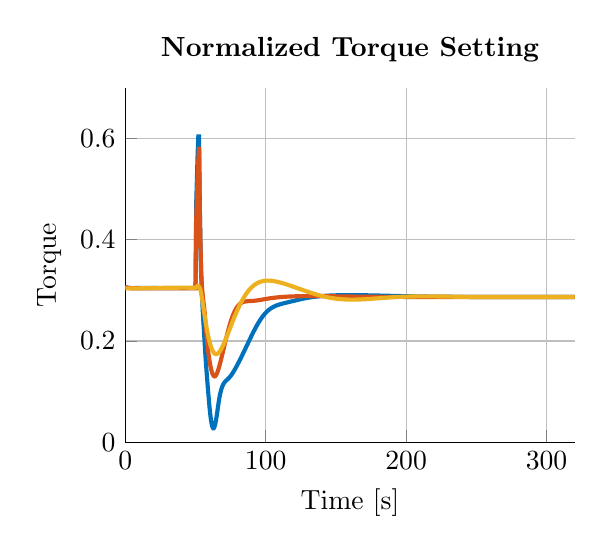
\begin{tikzpicture}

\begin{axis}[%
width=5.706cm,
height=4.5cm,
at={(0cm,0cm)},
scale only axis,
xmin=0,
xmax=320,
xlabel={Time [s]},
xmajorgrids,
ymin=0,
ymax=0.7,
ylabel={Torque},
ymajorgrids,
axis background/.style={fill=white},
title style={font=\bfseries},
title={Normalized Torque Setting},
axis x line*=bottom,
axis y line*=left
]
\addplot [color=mycolor1,solid,line width=1.5pt,forget plot]
  table[row sep=crcr]{%
0	0.304831074\\
0.5	0.30590085\\
1	0.30565309\\
1.5	0.30528095\\
2	0.30504243\\
2.5	0.304830357\\
3	0.304675987\\
3.5	0.304567996\\
4	0.304503022\\
4.5	0.304468969\\
5	0.304453134\\
5.5	0.304449628\\
6	0.304457403\\
6.5	0.304477601\\
7	0.304508918\\
7.5	0.304545747\\
8	0.304581427\\
8.5	0.304612217\\
9	0.304638928\\
9.5	0.304664765\\
10	0.304691287\\
10.5	0.304716429\\
11	0.304736188\\
11.5	0.304748177\\
12	0.304753694\\
12.5	0.304756414\\
13	0.30475901\\
13.5	0.304760922\\
14	0.304759267\\
14.5	0.304751915\\
15	0.304739763\\
15.5	0.304726109\\
16	0.304713781\\
16.5	0.304702777\\
17	0.30469063\\
17.5	0.304675073\\
18	0.304656418\\
18.5	0.304637419\\
19	0.304620796\\
19.5	0.304606803\\
20	0.304593187\\
20.5	0.304577512\\
21	0.304559605\\
21.5	0.304541785\\
22	0.304526677\\
22.5	0.304514737\\
23	0.304503883\\
23.5	0.304491565\\
24	0.30447726\\
24.5	0.304462995\\
25	0.304451375\\
25.5	0.304443053\\
26	0.304436097\\
26.5	0.304427872\\
27	0.304417601\\
27.5	0.304407124\\
28	0.304399091\\
28.5	0.30439435\\
29	0.304391086\\
29.5	0.304386568\\
30	0.304379815\\
30.5	0.304372557\\
31	0.30436754\\
31.5	0.304365801\\
32	0.304365598\\
32.5	0.304364077\\
33	0.304360064\\
33.5	0.304355243\\
34	0.304352507\\
34.5	0.304353082\\
35	0.304355248\\
35.5	0.304355978\\
36	0.304353912\\
36.5	0.30435074\\
37	0.304349564\\
37.5	0.304351802\\
38	0.304355704\\
38.5	0.304358006\\
39	0.304357157\\
39.5	0.304354913\\
40	0.304354653\\
40.5	0.304358003\\
41	0.304363117\\
41.5	0.30436642\\
42	0.304366153\\
42.5	0.304364208\\
43	0.304364333\\
43.5	0.304368376\\
44	0.304374322\\
44.5	0.30437818\\
45	0.304377967\\
45.5	0.304375798\\
46	0.304375903\\
46.5	0.304380377\\
47	0.304386927\\
47.5	0.304391024\\
48	0.304390434\\
48.5	0.304387617\\
49	0.304387429\\
49.5	0.304392228\\
50	0.304399313\\
50.5	0.472673\\
51	0.520824\\
51.5	0.568657\\
52	0.604\\
52.5	0.604\\
53	0.474781\\
53.5	0.3906805\\
54	0.330705\\
54.5	0.29890661\\
55	0.2678304\\
55.5	0.2419374\\
56	0.2195289\\
56.5	0.196075\\
57	0.173632\\
57.5	0.153024\\
58	0.134445\\
58.5	0.116863\\
59	0.099649\\
59.5	0.083216\\
60	0.068134\\
60.5	0.054953\\
61	0.044088\\
61.5	0.035826\\
62	0.030319\\
62.5	0.027615\\
63	0.027661\\
63.5	0.030292\\
64	0.03523\\
64.5	0.042088\\
65	0.05043\\
65.5	0.059828\\
66	0.069773\\
66.5	0.079392\\
67	0.087791\\
67.5	0.094815\\
68	0.100681\\
68.5	0.105574\\
69	0.109612\\
69.5	0.1129\\
70	0.115547\\
70.5	0.117678\\
71	0.119418\\
71.5	0.120893\\
72	0.122213\\
72.5	0.123472\\
73	0.124748\\
73.5	0.126093\\
74	0.127547\\
74.5	0.129131\\
75	0.130854\\
75.5	0.132715\\
76	0.134709\\
76.5	0.136823\\
77	0.139046\\
77.5	0.141363\\
78	0.143762\\
78.5	0.146231\\
79	0.14876\\
79.5	0.151341\\
80	0.153966\\
80.5	0.156632\\
81	0.159333\\
81.5	0.162065\\
82	0.164827\\
82.5	0.167616\\
83	0.17043\\
83.5	0.173267\\
84	0.176125\\
84.5	0.179001\\
85	0.181892\\
85.5	0.184796\\
86	0.187709\\
86.5	0.190628\\
87	0.193549\\
87.5	0.196468\\
88	0.19938\\
88.5	0.20228\\
89	0.2051655\\
89.5	0.20803\\
90	0.2108689\\
90.5	0.2136774\\
91	0.2164505\\
91.5	0.2191833\\
92	0.2218709\\
92.5	0.2245088\\
93	0.2270923\\
93.5	0.229617\\
94	0.232079\\
94.5	0.2344743\\
95	0.2367994\\
95.5	0.239051\\
96	0.2412265\\
96.5	0.2433234\\
97	0.2453396\\
97.5	0.2472736\\
98	0.2491243\\
98.5	0.2508909\\
99	0.2525734\\
99.5	0.2541718\\
100	0.2556869\\
100.5	0.2571197\\
101	0.2584718\\
101.5	0.2597449\\
102	0.2609415\\
102.5	0.2620639\\
103	0.2631151\\
103.5	0.2640981\\
104	0.2650163\\
104.5	0.2658731\\
105	0.2666722\\
105.5	0.2674173\\
106	0.2681122\\
106.5	0.2687607\\
107	0.2693666\\
107.5	0.2699336\\
108	0.2704655\\
108.5	0.2709658\\
109	0.271438\\
109.5	0.2718853\\
110	0.2723109\\
110.5	0.2727177\\
111	0.2731085\\
111.5	0.2734857\\
112	0.2738516\\
112.5	0.2742085\\
113	0.274558\\
113.5	0.2749019\\
114	0.2752417\\
114.5	0.2755785\\
115	0.2759133\\
115.5	0.2762471\\
116	0.2765804\\
116.5	0.2769138\\
117	0.2772476\\
117.5	0.277582\\
118	0.277917\\
118.5	0.2782527\\
119	0.2785889\\
119.5	0.2789253\\
120	0.2792617\\
120.5	0.2795977\\
121	0.2799329\\
121.5	0.2802669\\
122	0.2805992\\
122.5	0.2809292\\
123	0.2812566\\
123.5	0.2815808\\
124	0.2819013\\
124.5	0.2822177\\
125	0.2825295\\
125.5	0.2828362\\
126	0.2831376\\
126.5	0.2834331\\
127	0.2837225\\
127.5	0.2840054\\
128	0.2842816\\
128.5	0.2845509\\
129	0.284813\\
129.5	0.2850679\\
130	0.2853153\\
130.5	0.2855551\\
131	0.2857874\\
131.5	0.2860121\\
132	0.2862292\\
132.5	0.2864387\\
133	0.2866407\\
133.5	0.2868353\\
134	0.2870225\\
134.5	0.2872026\\
135	0.2873755\\
135.5	0.2875415\\
136	0.2877008\\
136.5	0.2878534\\
137	0.2879996\\
137.5	0.2881397\\
138	0.2882737\\
138.5	0.2884018\\
139	0.2885244\\
139.5	0.2886415\\
140	0.2887534\\
140.5	0.2888602\\
141	0.2889622\\
141.5	0.2890595\\
142	0.2891523\\
142.5	0.2892409\\
143	0.2893253\\
143.5	0.2894057\\
144	0.2894823\\
144.5	0.2895553\\
145	0.2896247\\
145.5	0.2896907\\
146	0.2897535\\
146.5	0.2898132\\
147	0.2898698\\
147.5	0.2899235\\
148	0.2899744\\
148.5	0.2900225\\
149	0.2900681\\
149.5	0.290111\\
150	0.2901515\\
150.5	0.2901896\\
151	0.2902253\\
151.5	0.2902588\\
152	0.29029\\
152.5	0.2903191\\
153	0.2903461\\
153.5	0.290371\\
154	0.2903938\\
154.5	0.2904148\\
155	0.2904338\\
155.5	0.2904509\\
156	0.2904661\\
156.5	0.2904796\\
157	0.2904913\\
157.5	0.2905012\\
158	0.2905095\\
158.5	0.2905161\\
159	0.2905211\\
159.5	0.2905245\\
160	0.2905264\\
160.5	0.2905268\\
161	0.2905256\\
161.5	0.2905231\\
162	0.2905191\\
162.5	0.2905138\\
163	0.2905071\\
163.5	0.2904992\\
164	0.29049\\
164.5	0.2904796\\
165	0.2904679\\
165.5	0.2904552\\
166	0.2904413\\
166.5	0.2904264\\
167	0.2904104\\
167.5	0.2903934\\
168	0.2903755\\
168.5	0.2903566\\
169	0.2903369\\
169.5	0.2903162\\
170	0.2902948\\
170.5	0.2902726\\
171	0.2902496\\
171.5	0.2902259\\
172	0.2902015\\
172.5	0.2901764\\
173	0.2901508\\
173.5	0.2901245\\
174	0.2900977\\
174.5	0.2900703\\
175	0.2900424\\
175.5	0.2900141\\
176	0.2899853\\
176.5	0.2899561\\
177	0.2899265\\
177.5	0.2898965\\
178	0.2898662\\
178.5	0.2898356\\
179	0.2898047\\
179.5	0.2897735\\
180	0.289742\\
180.5	0.2897103\\
181	0.2896785\\
181.5	0.2896464\\
182	0.2896142\\
182.5	0.2895818\\
183	0.2895493\\
183.5	0.2895167\\
184	0.2894839\\
184.5	0.2894511\\
185	0.2894183\\
185.5	0.2893854\\
186	0.2893525\\
186.5	0.2893196\\
187	0.2892866\\
187.5	0.2892537\\
188	0.2892208\\
188.5	0.289188\\
189	0.2891552\\
189.5	0.2891225\\
190	0.2890898\\
190.5	0.2890573\\
191	0.2890248\\
191.5	0.2889925\\
192	0.2889603\\
192.5	0.2889282\\
193	0.2888962\\
193.5	0.2888644\\
194	0.2888328\\
194.5	0.2888014\\
195	0.2887701\\
195.5	0.288739\\
196	0.2887081\\
196.5	0.2886774\\
197	0.2886469\\
197.5	0.2886166\\
198	0.2885866\\
198.5	0.2885568\\
199	0.2885272\\
199.5	0.2884978\\
200	0.2884687\\
200.5	0.2884399\\
201	0.2884113\\
201.5	0.2883829\\
202	0.2883549\\
202.5	0.2883271\\
203	0.2882995\\
203.5	0.2882723\\
204	0.2882453\\
204.5	0.2882186\\
205	0.2881922\\
205.5	0.2881661\\
206	0.2881403\\
206.5	0.2881148\\
207	0.2880896\\
207.5	0.2880647\\
208	0.28804\\
208.5	0.2880157\\
209	0.2879917\\
209.5	0.287968\\
210	0.2879446\\
210.5	0.2879215\\
211	0.2878987\\
211.5	0.2878762\\
212	0.287854\\
212.5	0.2878321\\
213	0.2878106\\
213.5	0.2877893\\
214	0.2877684\\
214.5	0.2877478\\
215	0.2877274\\
215.5	0.2877074\\
216	0.2876877\\
216.5	0.2876683\\
217	0.2876492\\
217.5	0.2876304\\
218	0.2876119\\
218.5	0.2875937\\
219	0.2875759\\
219.5	0.2875583\\
220	0.287541\\
220.5	0.287524\\
221	0.2875073\\
221.5	0.2874909\\
222	0.2874747\\
222.5	0.2874589\\
223	0.2874434\\
223.5	0.2874281\\
224	0.2874131\\
224.5	0.2873984\\
225	0.287384\\
225.5	0.2873699\\
226	0.287356\\
226.5	0.2873424\\
227	0.287329\\
227.5	0.287316\\
228	0.2873032\\
228.5	0.2872906\\
229	0.2872783\\
229.5	0.2872663\\
230	0.2872545\\
230.5	0.287243\\
231	0.2872317\\
231.5	0.2872207\\
232	0.2872099\\
232.5	0.2871993\\
233	0.287189\\
233.5	0.2871789\\
234	0.287169\\
234.5	0.2871594\\
235	0.28715\\
235.5	0.2871408\\
236	0.2871318\\
236.5	0.287123\\
237	0.2871145\\
237.5	0.2871062\\
238	0.287098\\
238.5	0.2870901\\
239	0.2870824\\
239.5	0.2870749\\
240	0.2870675\\
240.5	0.2870604\\
241	0.2870534\\
241.5	0.2870467\\
242	0.2870401\\
242.5	0.2870337\\
243	0.2870275\\
243.5	0.2870214\\
244	0.2870155\\
244.5	0.2870098\\
245	0.2870043\\
245.5	0.2869989\\
246	0.2869937\\
246.5	0.2869886\\
247	0.2869837\\
247.5	0.2869789\\
248	0.2869743\\
248.5	0.2869699\\
249	0.2869656\\
249.5	0.2869614\\
250	0.2869573\\
250.5	0.2869534\\
251	0.2869497\\
251.5	0.286946\\
252	0.2869425\\
252.5	0.2869391\\
253	0.2869359\\
253.5	0.2869327\\
254	0.2869297\\
254.5	0.2869268\\
255	0.286924\\
255.5	0.2869213\\
256	0.2869188\\
256.5	0.2869163\\
257	0.2869139\\
257.5	0.2869117\\
258	0.2869095\\
258.5	0.2869074\\
259	0.2869054\\
259.5	0.2869036\\
260	0.2869018\\
260.5	0.2869001\\
261	0.2868985\\
261.5	0.2868969\\
262	0.2868955\\
262.5	0.2868941\\
263	0.2868928\\
263.5	0.2868916\\
264	0.2868905\\
264.5	0.2868894\\
265	0.2868884\\
265.5	0.2868875\\
266	0.2868866\\
266.5	0.2868858\\
267	0.2868851\\
267.5	0.2868844\\
268	0.2868838\\
268.5	0.2868832\\
269	0.2868827\\
269.5	0.2868823\\
270	0.2868819\\
270.5	0.2868816\\
271	0.2868813\\
271.5	0.2868811\\
272	0.2868809\\
272.5	0.2868807\\
273	0.2868806\\
273.5	0.2868806\\
274	0.2868805\\
274.5	0.2868806\\
275	0.2868806\\
275.5	0.2868807\\
276	0.2868809\\
276.5	0.2868811\\
277	0.2868813\\
277.5	0.2868815\\
278	0.2868818\\
278.5	0.2868821\\
279	0.2868824\\
279.5	0.2868828\\
280	0.2868832\\
280.5	0.2868836\\
281	0.286884\\
281.5	0.2868845\\
282	0.2868849\\
282.5	0.2868855\\
283	0.286886\\
283.5	0.2868865\\
284	0.2868871\\
284.5	0.2868877\\
285	0.2868883\\
285.5	0.2868889\\
286	0.2868895\\
286.5	0.2868902\\
287	0.2868909\\
287.5	0.2868915\\
288	0.2868922\\
288.5	0.2868929\\
289	0.2868936\\
289.5	0.2868944\\
290	0.2868951\\
290.5	0.2868958\\
291	0.2868966\\
291.5	0.2868974\\
292	0.2868981\\
292.5	0.2868989\\
293	0.2868997\\
293.5	0.2869005\\
294	0.2869013\\
294.5	0.286902\\
295	0.2869028\\
295.5	0.2869037\\
296	0.2869045\\
296.5	0.2869053\\
297	0.2869061\\
297.5	0.2869069\\
298	0.2869077\\
298.5	0.2869085\\
299	0.2869093\\
299.5	0.2869101\\
300	0.286911\\
300.5	0.2869118\\
301	0.2869126\\
301.5	0.2869134\\
302	0.2869142\\
302.5	0.286915\\
303	0.2869158\\
303.5	0.2869166\\
304	0.2869174\\
304.5	0.2869182\\
305	0.286919\\
305.5	0.2869198\\
306	0.2869206\\
306.5	0.2869214\\
307	0.2869221\\
307.5	0.2869229\\
308	0.2869237\\
308.5	0.2869244\\
309	0.2869252\\
309.5	0.2869259\\
310	0.2869267\\
310.5	0.2869274\\
311	0.2869281\\
311.5	0.2869289\\
312	0.2869296\\
312.5	0.2869303\\
313	0.286931\\
313.5	0.2869317\\
314	0.2869324\\
314.5	0.2869331\\
315	0.2869338\\
315.5	0.2869345\\
316	0.2869351\\
316.5	0.2869358\\
317	0.2869364\\
317.5	0.2869371\\
318	0.2869377\\
318.5	0.2869383\\
319	0.286939\\
319.5	0.2869396\\
320	0.2869402\\
320.5	0.2869408\\
321	0.2869414\\
321.5	0.286942\\
322	0.2869426\\
322.5	0.2869431\\
323	0.2869437\\
323.5	0.2869442\\
324	0.2869448\\
324.5	0.2869453\\
325	0.2869459\\
325.5	0.2869464\\
326	0.2869469\\
326.5	0.2869474\\
327	0.2869479\\
327.5	0.2869484\\
328	0.2869489\\
328.5	0.2869494\\
329	0.2869498\\
329.5	0.2869503\\
330	0.2869508\\
330.5	0.2869512\\
331	0.2869516\\
331.5	0.2869521\\
332	0.2869525\\
332.5	0.2869529\\
333	0.2869533\\
333.5	0.2869537\\
334	0.2869541\\
334.5	0.2869545\\
335	0.2869549\\
335.5	0.2869553\\
336	0.2869557\\
336.5	0.286956\\
337	0.2869564\\
337.5	0.2869567\\
338	0.2869571\\
338.5	0.2869574\\
339	0.2869577\\
339.5	0.286958\\
340	0.2869584\\
340.5	0.2869587\\
341	0.286959\\
341.5	0.2869593\\
342	0.2869596\\
342.5	0.2869598\\
343	0.2869601\\
343.5	0.2869604\\
344	0.2869607\\
344.5	0.2869609\\
345	0.2869612\\
345.5	0.2869614\\
346	0.2869617\\
346.5	0.2869619\\
347	0.2869621\\
347.5	0.2869624\\
348	0.2869626\\
348.5	0.2869628\\
349	0.286963\\
349.5	0.2869632\\
350	0.2869634\\
350.5	0.2869636\\
351	0.2869638\\
351.5	0.286964\\
352	0.2869642\\
352.5	0.2869643\\
353	0.2869645\\
353.5	0.2869647\\
354	0.2869648\\
354.5	0.286965\\
355	0.2869651\\
355.5	0.2869653\\
356	0.2869654\\
356.5	0.2869656\\
357	0.2869657\\
357.5	0.2869658\\
358	0.286966\\
358.5	0.2869661\\
359	0.2869662\\
359.5	0.2869663\\
360	0.2869665\\
360.5	0.2869666\\
361	0.2869667\\
361.5	0.2869668\\
362	0.2869669\\
362.5	0.286967\\
363	0.2869671\\
363.5	0.2869672\\
364	0.2869672\\
364.5	0.2869673\\
365	0.2869674\\
365.5	0.2869675\\
366	0.2869676\\
366.5	0.2869676\\
367	0.2869677\\
367.5	0.2869678\\
368	0.2869678\\
368.5	0.2869679\\
369	0.2869679\\
369.5	0.286968\\
370	0.2869681\\
370.5	0.2869681\\
371	0.2869682\\
371.5	0.2869682\\
372	0.2869683\\
372.5	0.2869683\\
373	0.2869683\\
373.5	0.2869684\\
374	0.2869684\\
374.5	0.2869684\\
375	0.2869685\\
375.5	0.2869685\\
376	0.2869685\\
376.5	0.2869686\\
377	0.2869686\\
377.5	0.2869686\\
378	0.2869686\\
378.5	0.2869687\\
379	0.2869687\\
379.5	0.2869687\\
380	0.2869687\\
380.5	0.2869687\\
381	0.2869687\\
381.5	0.2869687\\
382	0.2869687\\
382.5	0.2869688\\
383	0.2869688\\
383.5	0.2869688\\
384	0.2869688\\
384.5	0.2869688\\
385	0.2869688\\
385.5	0.2869688\\
386	0.2869688\\
386.5	0.2869688\\
387	0.2869688\\
387.5	0.2869688\\
388	0.2869688\\
388.5	0.2869688\\
389	0.2869688\\
389.5	0.2869688\\
390	0.2869688\\
390.5	0.2869688\\
391	0.2869687\\
391.5	0.2869687\\
392	0.2869687\\
392.5	0.2869687\\
393	0.2869687\\
393.5	0.2869687\\
394	0.2869687\\
394.5	0.2869687\\
395	0.2869687\\
395.5	0.2869686\\
396	0.2869686\\
396.5	0.2869686\\
397	0.2869686\\
397.5	0.2869686\\
398	0.2869686\\
398.5	0.2869686\\
399	0.2869685\\
399.5	0.2869685\\
400	0.2869685\\
400.5	0.2869685\\
401	0.2869685\\
401.5	0.2869685\\
402	0.2869684\\
402.5	0.2869684\\
403	0.2869684\\
403.5	0.2869684\\
404	0.2869684\\
404.5	0.2869683\\
405	0.2869683\\
405.5	0.2869683\\
406	0.2869683\\
406.5	0.2869683\\
407	0.2869683\\
407.5	0.2869682\\
408	0.2869682\\
408.5	0.2869682\\
409	0.2869682\\
409.5	0.2869682\\
410	0.2869681\\
410.5	0.2869681\\
411	0.2869681\\
411.5	0.2869681\\
412	0.2869681\\
412.5	0.286968\\
413	0.286968\\
413.5	0.286968\\
414	0.286968\\
414.5	0.286968\\
415	0.2869679\\
415.5	0.2869679\\
416	0.2869679\\
416.5	0.2869679\\
417	0.2869679\\
417.5	0.2869678\\
418	0.2869678\\
418.5	0.2869678\\
419	0.2869678\\
419.5	0.2869678\\
420	0.2869677\\
420.5	0.2869677\\
421	0.2869677\\
421.5	0.2869677\\
422	0.2869677\\
422.5	0.2869676\\
423	0.2869676\\
423.5	0.2869676\\
424	0.2869676\\
424.5	0.2869676\\
425	0.2869676\\
425.5	0.2869675\\
426	0.2869675\\
426.5	0.2869675\\
427	0.2869675\\
427.5	0.2869675\\
428	0.2869675\\
428.5	0.2869674\\
429	0.2869674\\
429.5	0.2869674\\
430	0.2869674\\
430.5	0.2869674\\
431	0.2869674\\
431.5	0.2869674\\
432	0.2869673\\
432.5	0.2869673\\
433	0.2869673\\
433.5	0.2869673\\
434	0.2869673\\
434.5	0.2869673\\
435	0.2869672\\
435.5	0.2869672\\
436	0.2869672\\
436.5	0.2869672\\
437	0.2869672\\
437.5	0.2869672\\
438	0.2869672\\
438.5	0.2869672\\
439	0.2869671\\
439.5	0.2869671\\
440	0.2869671\\
440.5	0.2869671\\
441	0.2869671\\
441.5	0.2869671\\
442	0.2869671\\
442.5	0.2869671\\
443	0.2869671\\
443.5	0.286967\\
444	0.286967\\
444.5	0.286967\\
445	0.286967\\
445.5	0.286967\\
446	0.286967\\
446.5	0.286967\\
447	0.286967\\
447.5	0.286967\\
448	0.286967\\
448.5	0.2869669\\
449	0.2869669\\
449.5	0.2869669\\
450	0.2869669\\
450.5	0.2869669\\
451	0.2869669\\
451.5	0.2869669\\
452	0.2869669\\
452.5	0.2869669\\
453	0.2869669\\
453.5	0.2869669\\
454	0.2869669\\
454.5	0.2869669\\
455	0.2869668\\
455.5	0.2869668\\
456	0.2869668\\
456.5	0.2869668\\
457	0.2869668\\
457.5	0.2869668\\
458	0.2869668\\
458.5	0.2869668\\
459	0.2869668\\
459.5	0.2869668\\
460	0.2869668\\
460.5	0.2869668\\
461	0.2869668\\
461.5	0.2869668\\
462	0.2869668\\
462.5	0.2869668\\
463	0.2869668\\
463.5	0.2869667\\
464	0.2869667\\
464.5	0.2869667\\
465	0.2869667\\
465.5	0.2869667\\
466	0.2869667\\
466.5	0.2869667\\
467	0.2869667\\
467.5	0.2869667\\
468	0.2869667\\
468.5	0.2869667\\
469	0.2869667\\
469.5	0.2869667\\
470	0.2869667\\
470.5	0.2869667\\
471	0.2869667\\
471.5	0.2869667\\
472	0.2869667\\
472.5	0.2869667\\
473	0.2869667\\
473.5	0.2869667\\
474	0.2869667\\
474.5	0.2869667\\
475	0.2869667\\
475.5	0.2869667\\
476	0.2869667\\
476.5	0.2869667\\
477	0.2869667\\
477.5	0.2869667\\
478	0.2869667\\
478.5	0.2869667\\
479	0.2869667\\
479.5	0.2869667\\
480	0.2869667\\
480.5	0.2869667\\
481	0.2869667\\
481.5	0.2869666\\
482	0.2869666\\
482.5	0.2869666\\
483	0.2869666\\
483.5	0.2869666\\
484	0.2869666\\
484.5	0.2869666\\
485	0.2869666\\
485.5	0.2869666\\
486	0.2869666\\
486.5	0.2869666\\
487	0.2869666\\
487.5	0.2869666\\
488	0.2869666\\
488.5	0.2869666\\
489	0.2869666\\
489.5	0.2869666\\
490	0.2869666\\
490.5	0.2869666\\
491	0.2869666\\
491.5	0.2869666\\
492	0.2869666\\
492.5	0.2869666\\
493	0.2869666\\
493.5	0.2869666\\
494	0.2869666\\
494.5	0.2869666\\
495	0.2869666\\
495.5	0.2869666\\
496	0.2869666\\
496.5	0.2869666\\
497	0.2869666\\
497.5	0.2869666\\
498	0.2869666\\
498.5	0.2869666\\
499	0.2869666\\
499.5	0.2869666\\
};
\addplot [color=mycolor2,solid,line width=1.5pt,forget plot]
  table[row sep=crcr]{%
0	0.304687593\\
0.5	0.30565243\\
1	0.30544153\\
1.5	0.30512552\\
2	0.304902022\\
2.5	0.304692745\\
3	0.304522477\\
3.5	0.304383864\\
4	0.304277359\\
4.5	0.30419961\\
5	0.304144828\\
5.5	0.304107522\\
6	0.3040836227\\
6.5	0.3040707616\\
7	0.3040676314\\
7.5	0.304072743\\
8	0.3040838906\\
8.5	0.3040984844\\
9	0.304114276\\
9.5	0.304129912\\
10	0.30414491\\
10.5	0.304159186\\
11	0.304172546\\
11.5	0.304184508\\
12	0.304194486\\
12.5	0.304202113\\
13	0.304207416\\
13.5	0.304210736\\
14	0.304212483\\
14.5	0.304212931\\
15	0.304212175\\
15.5	0.304210252\\
16	0.304207277\\
16.5	0.304203505\\
17	0.304199268\\
17.5	0.304194859\\
18	0.30419046\\
18.5	0.304186151\\
19	0.304181973\\
19.5	0.304178001\\
20	0.304174352\\
20.5	0.304171152\\
21	0.304168488\\
21.5	0.304166379\\
22	0.304164798\\
22.5	0.304163711\\
23	0.3041631\\
23.5	0.304162965\\
24	0.304163308\\
24.5	0.304164104\\
25	0.304165305\\
25.5	0.304166846\\
26	0.304168667\\
26.5	0.304170725\\
27	0.304172984\\
27.5	0.304175414\\
28	0.304177972\\
28.5	0.304180609\\
29	0.304183275\\
29.5	0.30418593\\
30	0.304188541\\
30.5	0.304191087\\
31	0.304193546\\
31.5	0.304195895\\
32	0.304198108\\
32.5	0.304200165\\
33	0.304202052\\
33.5	0.30420376\\
34	0.304205287\\
34.5	0.304206631\\
35	0.304207788\\
35.5	0.304208757\\
36	0.304209538\\
36.5	0.304210137\\
37	0.304210563\\
37.5	0.304210824\\
38	0.304210932\\
38.5	0.304210895\\
39	0.304210724\\
39.5	0.304210429\\
40	0.304210024\\
40.5	0.304209523\\
41	0.30420894\\
41.5	0.304208286\\
42	0.304207575\\
42.5	0.304206817\\
43	0.304206026\\
43.5	0.304205213\\
44	0.304204388\\
44.5	0.304203564\\
45	0.304202749\\
45.5	0.304201951\\
46	0.304201178\\
46.5	0.304200437\\
47	0.304199735\\
47.5	0.304199077\\
48	0.304198467\\
48.5	0.304197909\\
49	0.304197406\\
49.5	0.304196959\\
50	0.30419657\\
50.5	0.442329\\
51	0.486145\\
51.5	0.524044\\
52	0.55623\\
52.5	0.583669\\
53	0.465144\\
53.5	0.396192\\
54	0.3376383\\
54.5	0.31150891\\
55	0.2938633\\
55.5	0.2798536\\
56	0.2700006\\
56.5	0.2571502\\
57	0.2393262\\
57.5	0.2217007\\
58	0.2057298\\
58.5	0.191981\\
59	0.179826\\
59.5	0.169135\\
60	0.159959\\
60.5	0.152144\\
61	0.145528\\
61.5	0.140035\\
62	0.135693\\
62.5	0.132559\\
63	0.130663\\
63.5	0.129988\\
64	0.130461\\
64.5	0.131977\\
65	0.134406\\
65.5	0.137619\\
66	0.141487\\
66.5	0.145895\\
67	0.150737\\
67.5	0.15592\\
68	0.161365\\
68.5	0.167001\\
69	0.172769\\
69.5	0.178615\\
70	0.184493\\
70.5	0.190363\\
71	0.196187\\
71.5	0.201932\\
72	0.2075665\\
72.5	0.213064\\
73	0.218399\\
73.5	0.2235491\\
74	0.2284944\\
74.5	0.2332175\\
75	0.2377041\\
75.5	0.2419424\\
76	0.2459237\\
76.5	0.2496418\\
77	0.2530935\\
77.5	0.2562783\\
78	0.2591981\\
78.5	0.2618573\\
79	0.2642625\\
79.5	0.2664224\\
80	0.2683474\\
80.5	0.2700495\\
81	0.2715418\\
81.5	0.2728386\\
82	0.273955\\
82.5	0.2749065\\
83	0.2757088\\
83.5	0.2763778\\
84	0.2769291\\
84.5	0.2773779\\
85	0.2777386\\
85.5	0.2780253\\
86	0.2782509\\
86.5	0.2784274\\
87	0.2785657\\
87.5	0.2786759\\
88	0.2787665\\
88.5	0.2788454\\
89	0.278919\\
89.5	0.2789929\\
90	0.2790716\\
90.5	0.2791586\\
91	0.2792566\\
91.5	0.2793676\\
92	0.2794928\\
92.5	0.2796328\\
93	0.2797876\\
93.5	0.2799568\\
94	0.2801399\\
94.5	0.2803356\\
95	0.2805428\\
95.5	0.2807601\\
96	0.2809859\\
96.5	0.2812188\\
97	0.2814571\\
97.5	0.2816993\\
98	0.281944\\
98.5	0.2821898\\
99	0.2824354\\
99.5	0.2826796\\
100	0.2829213\\
100.5	0.2831596\\
101	0.2833936\\
101.5	0.2836228\\
102	0.2838465\\
102.5	0.2840642\\
103	0.2842757\\
103.5	0.2844805\\
104	0.2846786\\
104.5	0.2848698\\
105	0.2850541\\
105.5	0.2852316\\
106	0.2854022\\
106.5	0.2855661\\
107	0.2857234\\
107.5	0.2858743\\
108	0.286019\\
108.5	0.2861577\\
109	0.2862906\\
109.5	0.2864178\\
110	0.2865398\\
110.5	0.2866565\\
111	0.2867683\\
111.5	0.2868753\\
112	0.2869777\\
112.5	0.2870758\\
113	0.2871697\\
113.5	0.2872595\\
114	0.2873454\\
114.5	0.2874276\\
115	0.2875062\\
115.5	0.2875813\\
116	0.2876531\\
116.5	0.2877216\\
117	0.2877869\\
117.5	0.2878493\\
118	0.2879086\\
118.5	0.2879651\\
119	0.2880188\\
119.5	0.2880698\\
120	0.2881181\\
120.5	0.2881639\\
121	0.2882072\\
121.5	0.288248\\
122	0.2882865\\
122.5	0.2883226\\
123	0.2883565\\
123.5	0.2883882\\
124	0.2884178\\
124.5	0.2884453\\
125	0.2884708\\
125.5	0.2884943\\
126	0.2885159\\
126.5	0.2885356\\
127	0.2885535\\
127.5	0.2885697\\
128	0.2885841\\
128.5	0.288597\\
129	0.2886082\\
129.5	0.2886178\\
130	0.288626\\
130.5	0.2886327\\
131	0.288638\\
131.5	0.288642\\
132	0.2886447\\
132.5	0.2886461\\
133	0.2886462\\
133.5	0.2886453\\
134	0.2886431\\
134.5	0.2886399\\
135	0.2886357\\
135.5	0.2886304\\
136	0.2886242\\
136.5	0.2886171\\
137	0.2886091\\
137.5	0.2886003\\
138	0.2885906\\
138.5	0.2885802\\
139	0.2885691\\
139.5	0.2885572\\
140	0.2885447\\
140.5	0.2885316\\
141	0.2885178\\
141.5	0.2885035\\
142	0.2884887\\
142.5	0.2884734\\
143	0.2884576\\
143.5	0.2884414\\
144	0.2884247\\
144.5	0.2884077\\
145	0.2883903\\
145.5	0.2883725\\
146	0.2883545\\
146.5	0.2883362\\
147	0.2883176\\
147.5	0.2882988\\
148	0.2882798\\
148.5	0.2882606\\
149	0.2882412\\
149.5	0.2882217\\
150	0.288202\\
150.5	0.2881823\\
151	0.2881624\\
151.5	0.2881425\\
152	0.2881226\\
152.5	0.2881026\\
153	0.2880826\\
153.5	0.2880625\\
154	0.2880425\\
154.5	0.2880226\\
155	0.2880026\\
155.5	0.2879827\\
156	0.2879629\\
156.5	0.2879432\\
157	0.2879235\\
157.5	0.287904\\
158	0.2878846\\
158.5	0.2878652\\
159	0.2878461\\
159.5	0.287827\\
160	0.2878082\\
160.5	0.2877894\\
161	0.2877709\\
161.5	0.2877525\\
162	0.2877343\\
162.5	0.2877163\\
163	0.2876985\\
163.5	0.2876809\\
164	0.2876635\\
164.5	0.2876463\\
165	0.2876293\\
165.5	0.2876125\\
166	0.287596\\
166.5	0.2875796\\
167	0.2875635\\
167.5	0.2875477\\
168	0.2875321\\
168.5	0.2875167\\
169	0.2875015\\
169.5	0.2874866\\
170	0.2874719\\
170.5	0.2874575\\
171	0.2874433\\
171.5	0.2874294\\
172	0.2874157\\
172.5	0.2874023\\
173	0.2873891\\
173.5	0.2873761\\
174	0.2873634\\
174.5	0.287351\\
175	0.2873387\\
175.5	0.2873268\\
176	0.287315\\
176.5	0.2873035\\
177	0.2872923\\
177.5	0.2872813\\
178	0.2872705\\
178.5	0.28726\\
179	0.2872496\\
179.5	0.2872396\\
180	0.2872297\\
180.5	0.2872201\\
181	0.2872107\\
181.5	0.2872015\\
182	0.2871925\\
182.5	0.2871838\\
183	0.2871753\\
183.5	0.287167\\
184	0.2871589\\
184.5	0.287151\\
185	0.2871433\\
185.5	0.2871358\\
186	0.2871285\\
186.5	0.2871214\\
187	0.2871145\\
187.5	0.2871077\\
188	0.2871012\\
188.5	0.2870949\\
189	0.2870887\\
189.5	0.2870827\\
190	0.2870769\\
190.5	0.2870712\\
191	0.2870658\\
191.5	0.2870605\\
192	0.2870553\\
192.5	0.2870503\\
193	0.2870455\\
193.5	0.2870408\\
194	0.2870363\\
194.5	0.2870319\\
195	0.2870276\\
195.5	0.2870235\\
196	0.2870196\\
196.5	0.2870157\\
197	0.2870121\\
197.5	0.2870085\\
198	0.287005\\
198.5	0.2870017\\
199	0.2869985\\
199.5	0.2869955\\
200	0.2869925\\
200.5	0.2869896\\
201	0.2869869\\
201.5	0.2869843\\
202	0.2869817\\
202.5	0.2869793\\
203	0.286977\\
203.5	0.2869747\\
204	0.2869726\\
204.5	0.2869706\\
205	0.2869686\\
205.5	0.2869667\\
206	0.2869649\\
206.5	0.2869632\\
207	0.2869616\\
207.5	0.2869601\\
208	0.2869586\\
208.5	0.2869572\\
209	0.2869558\\
209.5	0.2869546\\
210	0.2869534\\
210.5	0.2869523\\
211	0.2869512\\
211.5	0.2869502\\
212	0.2869492\\
212.5	0.2869483\\
213	0.2869475\\
213.5	0.2869467\\
214	0.286946\\
214.5	0.2869453\\
215	0.2869447\\
215.5	0.2869441\\
216	0.2869436\\
216.5	0.2869431\\
217	0.2869426\\
217.5	0.2869422\\
218	0.2869418\\
218.5	0.2869415\\
219	0.2869412\\
219.5	0.2869409\\
220	0.2869407\\
220.5	0.2869404\\
221	0.2869403\\
221.5	0.2869401\\
222	0.28694\\
222.5	0.2869399\\
223	0.2869399\\
223.5	0.2869398\\
224	0.2869398\\
224.5	0.2869398\\
225	0.2869398\\
225.5	0.2869399\\
226	0.28694\\
226.5	0.2869401\\
227	0.2869402\\
227.5	0.2869403\\
228	0.2869404\\
228.5	0.2869406\\
229	0.2869407\\
229.5	0.2869409\\
230	0.2869411\\
230.5	0.2869413\\
231	0.2869415\\
231.5	0.2869418\\
232	0.286942\\
232.5	0.2869423\\
233	0.2869425\\
233.5	0.2869428\\
234	0.2869431\\
234.5	0.2869433\\
235	0.2869436\\
235.5	0.2869439\\
236	0.2869442\\
236.5	0.2869445\\
237	0.2869448\\
237.5	0.2869451\\
238	0.2869454\\
238.5	0.2869458\\
239	0.2869461\\
239.5	0.2869464\\
240	0.2869467\\
240.5	0.2869471\\
241	0.2869474\\
241.5	0.2869477\\
242	0.286948\\
242.5	0.2869484\\
243	0.2869487\\
243.5	0.286949\\
244	0.2869494\\
244.5	0.2869497\\
245	0.28695\\
245.5	0.2869504\\
246	0.2869507\\
246.5	0.286951\\
247	0.2869513\\
247.5	0.2869516\\
248	0.286952\\
248.5	0.2869523\\
249	0.2869526\\
249.5	0.2869529\\
250	0.2869532\\
250.5	0.2869535\\
251	0.2869538\\
251.5	0.2869541\\
252	0.2869544\\
252.5	0.2869547\\
253	0.286955\\
253.5	0.2869553\\
254	0.2869556\\
254.5	0.2869558\\
255	0.2869561\\
255.5	0.2869564\\
256	0.2869567\\
256.5	0.2869569\\
257	0.2869572\\
257.5	0.2869574\\
258	0.2869577\\
258.5	0.2869579\\
259	0.2869582\\
259.5	0.2869584\\
260	0.2869587\\
260.5	0.2869589\\
261	0.2869591\\
261.5	0.2869593\\
262	0.2869596\\
262.5	0.2869598\\
263	0.28696\\
263.5	0.2869602\\
264	0.2869604\\
264.5	0.2869606\\
265	0.2869608\\
265.5	0.286961\\
266	0.2869612\\
266.5	0.2869614\\
267	0.2869615\\
267.5	0.2869617\\
268	0.2869619\\
268.5	0.286962\\
269	0.2869622\\
269.5	0.2869624\\
270	0.2869625\\
270.5	0.2869627\\
271	0.2869628\\
271.5	0.286963\\
272	0.2869631\\
272.5	0.2869633\\
273	0.2869634\\
273.5	0.2869635\\
274	0.2869637\\
274.5	0.2869638\\
275	0.2869639\\
275.5	0.286964\\
276	0.2869641\\
276.5	0.2869643\\
277	0.2869644\\
277.5	0.2869645\\
278	0.2869646\\
278.5	0.2869647\\
279	0.2869648\\
279.5	0.2869649\\
280	0.286965\\
280.5	0.286965\\
281	0.2869651\\
281.5	0.2869652\\
282	0.2869653\\
282.5	0.2869654\\
283	0.2869655\\
283.5	0.2869655\\
284	0.2869656\\
284.5	0.2869657\\
285	0.2869657\\
285.5	0.2869658\\
286	0.2869659\\
286.5	0.2869659\\
287	0.286966\\
287.5	0.286966\\
288	0.2869661\\
288.5	0.2869661\\
289	0.2869662\\
289.5	0.2869662\\
290	0.2869663\\
290.5	0.2869663\\
291	0.2869664\\
291.5	0.2869664\\
292	0.2869665\\
292.5	0.2869665\\
293	0.2869665\\
293.5	0.2869666\\
294	0.2869666\\
294.5	0.2869666\\
295	0.2869667\\
295.5	0.2869667\\
296	0.2869667\\
296.5	0.2869668\\
297	0.2869668\\
297.5	0.2869668\\
298	0.2869668\\
298.5	0.2869668\\
299	0.2869669\\
299.5	0.2869669\\
300	0.2869669\\
300.5	0.2869669\\
301	0.2869669\\
301.5	0.286967\\
302	0.286967\\
302.5	0.286967\\
303	0.286967\\
303.5	0.286967\\
304	0.286967\\
304.5	0.286967\\
305	0.286967\\
305.5	0.2869671\\
306	0.2869671\\
306.5	0.2869671\\
307	0.2869671\\
307.5	0.2869671\\
308	0.2869671\\
308.5	0.2869671\\
309	0.2869671\\
309.5	0.2869671\\
310	0.2869671\\
310.5	0.2869671\\
311	0.2869671\\
311.5	0.2869671\\
312	0.2869671\\
312.5	0.2869671\\
313	0.2869671\\
313.5	0.2869671\\
314	0.2869671\\
314.5	0.2869671\\
315	0.2869671\\
315.5	0.2869671\\
316	0.2869671\\
316.5	0.2869671\\
317	0.2869671\\
317.5	0.2869671\\
318	0.2869671\\
318.5	0.2869671\\
319	0.2869671\\
319.5	0.2869671\\
320	0.2869671\\
320.5	0.2869671\\
321	0.2869671\\
321.5	0.2869671\\
322	0.2869671\\
322.5	0.2869671\\
323	0.2869671\\
323.5	0.2869671\\
324	0.2869671\\
324.5	0.2869671\\
325	0.2869671\\
325.5	0.286967\\
326	0.286967\\
326.5	0.286967\\
327	0.286967\\
327.5	0.286967\\
328	0.286967\\
328.5	0.286967\\
329	0.286967\\
329.5	0.286967\\
330	0.286967\\
330.5	0.286967\\
331	0.286967\\
331.5	0.286967\\
332	0.286967\\
332.5	0.286967\\
333	0.286967\\
333.5	0.286967\\
334	0.286967\\
334.5	0.286967\\
335	0.2869669\\
335.5	0.2869669\\
336	0.2869669\\
336.5	0.2869669\\
337	0.2869669\\
337.5	0.2869669\\
338	0.2869669\\
338.5	0.2869669\\
339	0.2869669\\
339.5	0.2869669\\
340	0.2869669\\
340.5	0.2869669\\
341	0.2869669\\
341.5	0.2869669\\
342	0.2869669\\
342.5	0.2869669\\
343	0.2869669\\
343.5	0.2869669\\
344	0.2869669\\
344.5	0.2869669\\
345	0.2869669\\
345.5	0.2869668\\
346	0.2869668\\
346.5	0.2869668\\
347	0.2869668\\
347.5	0.2869668\\
348	0.2869668\\
348.5	0.2869668\\
349	0.2869668\\
349.5	0.2869668\\
350	0.2869668\\
350.5	0.2869668\\
351	0.2869668\\
351.5	0.2869668\\
352	0.2869668\\
352.5	0.2869668\\
353	0.2869668\\
353.5	0.2869668\\
354	0.2869668\\
354.5	0.2869668\\
355	0.2869668\\
355.5	0.2869668\\
356	0.2869668\\
356.5	0.2869668\\
357	0.2869668\\
357.5	0.2869668\\
358	0.2869668\\
358.5	0.2869668\\
359	0.2869668\\
359.5	0.2869667\\
360	0.2869667\\
360.5	0.2869667\\
361	0.2869667\\
361.5	0.2869667\\
362	0.2869667\\
362.5	0.2869667\\
363	0.2869667\\
363.5	0.2869667\\
364	0.2869667\\
364.5	0.2869667\\
365	0.2869667\\
365.5	0.2869667\\
366	0.2869667\\
366.5	0.2869667\\
367	0.2869667\\
367.5	0.2869667\\
368	0.2869667\\
368.5	0.2869667\\
369	0.2869667\\
369.5	0.2869667\\
370	0.2869667\\
370.5	0.2869667\\
371	0.2869667\\
371.5	0.2869667\\
372	0.2869667\\
372.5	0.2869667\\
373	0.2869667\\
373.5	0.2869667\\
374	0.2869667\\
374.5	0.2869667\\
375	0.2869667\\
375.5	0.2869667\\
376	0.2869667\\
376.5	0.2869667\\
377	0.2869667\\
377.5	0.2869667\\
378	0.2869667\\
378.5	0.2869667\\
379	0.2869667\\
379.5	0.2869667\\
380	0.2869667\\
380.5	0.2869667\\
381	0.2869667\\
381.5	0.2869667\\
382	0.2869667\\
382.5	0.2869667\\
383	0.2869667\\
383.5	0.2869667\\
384	0.2869667\\
384.5	0.2869667\\
385	0.2869667\\
385.5	0.2869667\\
386	0.2869667\\
386.5	0.2869667\\
387	0.2869667\\
387.5	0.2869667\\
388	0.2869667\\
388.5	0.2869667\\
389	0.2869667\\
389.5	0.2869667\\
390	0.2869667\\
390.5	0.2869667\\
391	0.2869667\\
391.5	0.2869667\\
392	0.2869667\\
392.5	0.2869667\\
393	0.2869667\\
393.5	0.2869667\\
394	0.2869667\\
394.5	0.2869667\\
395	0.2869667\\
395.5	0.2869667\\
396	0.2869667\\
396.5	0.2869667\\
397	0.2869667\\
397.5	0.2869667\\
398	0.2869667\\
398.5	0.2869667\\
399	0.2869667\\
399.5	0.2869667\\
400	0.2869667\\
400.5	0.2869667\\
401	0.2869667\\
401.5	0.2869667\\
402	0.2869667\\
402.5	0.2869667\\
403	0.2869667\\
403.5	0.2869667\\
404	0.2869667\\
404.5	0.2869667\\
405	0.2869667\\
405.5	0.2869667\\
406	0.2869667\\
406.5	0.2869667\\
407	0.2869667\\
407.5	0.2869667\\
408	0.2869667\\
408.5	0.2869667\\
409	0.2869667\\
409.5	0.2869667\\
410	0.2869667\\
410.5	0.2869667\\
411	0.2869667\\
411.5	0.2869667\\
412	0.2869667\\
412.5	0.2869667\\
413	0.2869667\\
413.5	0.2869667\\
414	0.2869667\\
414.5	0.2869667\\
415	0.2869667\\
415.5	0.2869667\\
416	0.2869667\\
416.5	0.2869667\\
417	0.2869667\\
417.5	0.2869667\\
418	0.2869667\\
418.5	0.2869667\\
419	0.2869667\\
419.5	0.2869667\\
420	0.2869667\\
420.5	0.2869667\\
421	0.2869667\\
421.5	0.2869667\\
422	0.2869667\\
422.5	0.2869667\\
423	0.2869667\\
423.5	0.2869667\\
424	0.2869667\\
424.5	0.2869667\\
425	0.2869667\\
425.5	0.2869667\\
426	0.2869667\\
426.5	0.2869667\\
427	0.2869667\\
427.5	0.2869667\\
428	0.2869667\\
428.5	0.2869667\\
429	0.2869667\\
429.5	0.2869667\\
430	0.2869667\\
430.5	0.2869667\\
431	0.2869667\\
431.5	0.2869667\\
432	0.2869667\\
432.5	0.2869667\\
433	0.2869667\\
433.5	0.2869667\\
434	0.2869667\\
434.5	0.2869667\\
435	0.2869667\\
435.5	0.2869667\\
436	0.2869667\\
436.5	0.2869667\\
437	0.2869667\\
437.5	0.2869667\\
438	0.2869667\\
438.5	0.2869667\\
439	0.2869667\\
439.5	0.2869667\\
440	0.2869667\\
440.5	0.2869667\\
441	0.2869667\\
441.5	0.2869667\\
442	0.2869667\\
442.5	0.2869667\\
443	0.2869667\\
443.5	0.2869667\\
444	0.2869667\\
444.5	0.2869667\\
445	0.2869667\\
445.5	0.2869667\\
446	0.2869667\\
446.5	0.2869667\\
447	0.2869667\\
447.5	0.2869667\\
448	0.2869667\\
448.5	0.2869667\\
449	0.2869667\\
449.5	0.2869667\\
450	0.2869667\\
450.5	0.2869667\\
451	0.2869667\\
451.5	0.2869667\\
452	0.2869667\\
452.5	0.2869667\\
453	0.2869667\\
453.5	0.2869667\\
454	0.2869667\\
454.5	0.2869667\\
455	0.2869667\\
455.5	0.2869667\\
456	0.2869667\\
456.5	0.2869667\\
457	0.2869667\\
457.5	0.2869667\\
458	0.2869667\\
458.5	0.2869667\\
459	0.2869667\\
459.5	0.2869667\\
460	0.2869667\\
460.5	0.2869667\\
461	0.2869667\\
461.5	0.2869667\\
462	0.2869667\\
462.5	0.2869667\\
463	0.2869667\\
463.5	0.2869667\\
464	0.2869667\\
464.5	0.2869667\\
465	0.2869667\\
465.5	0.2869667\\
466	0.2869667\\
466.5	0.2869667\\
467	0.2869667\\
467.5	0.2869667\\
468	0.2869667\\
468.5	0.2869667\\
469	0.2869667\\
469.5	0.2869667\\
470	0.2869667\\
470.5	0.2869667\\
471	0.2869667\\
471.5	0.2869667\\
472	0.2869667\\
472.5	0.2869667\\
473	0.2869667\\
473.5	0.2869667\\
474	0.2869667\\
474.5	0.2869667\\
475	0.2869667\\
475.5	0.2869667\\
476	0.2869667\\
476.5	0.2869667\\
477	0.2869667\\
477.5	0.2869667\\
478	0.2869667\\
478.5	0.2869667\\
479	0.2869667\\
479.5	0.2869667\\
480	0.2869667\\
480.5	0.2869667\\
481	0.2869667\\
481.5	0.2869667\\
482	0.2869667\\
482.5	0.2869667\\
483	0.2869667\\
483.5	0.2869667\\
484	0.2869667\\
484.5	0.2869667\\
485	0.2869667\\
485.5	0.2869667\\
486	0.2869667\\
486.5	0.2869667\\
487	0.2869667\\
487.5	0.2869667\\
488	0.2869667\\
488.5	0.2869667\\
489	0.2869667\\
489.5	0.2869667\\
490	0.2869667\\
490.5	0.2869667\\
491	0.2869667\\
491.5	0.2869667\\
492	0.2869667\\
492.5	0.2869667\\
493	0.2869667\\
493.5	0.2869667\\
494	0.2869667\\
494.5	0.2869667\\
495	0.2869667\\
495.5	0.2869667\\
496	0.2869667\\
496.5	0.2869667\\
497	0.2869667\\
497.5	0.2869667\\
498	0.2869667\\
498.5	0.2869667\\
499	0.2869667\\
499.5	0.2869667\\
};
\addplot [color=mycolor3,solid,line width=1.5pt,forget plot]
  table[row sep=crcr]{%
0	0.30399796155\\
0.5	0.3039777621\\
1	0.3039586795\\
1.5	0.3039411334\\
2	0.3039254205\\
2.5	0.3039117181\\
3	0.3039001143\\
3.5	0.303890729\\
4	0.303883663\\
4.5	0.303879\\
5	0.303876795\\
5.5	0.303877079\\
6	0.303879856\\
6.5	0.30388511\\
7	0.303892801\\
7.5	0.3039028763\\
8	0.303915264\\
8.5	0.3039298806\\
9	0.3039466307\\
9.5	0.3039654088\\
10	0.3039861015\\
10.5	0.30400858848\\
11	0.3040327447\\
11.5	0.3040584413\\
12	0.3040855469\\
12.5	0.304113929\\
13	0.304143455\\
13.5	0.304173992\\
14	0.304205411\\
14.5	0.304237583\\
15	0.304270384\\
15.5	0.304303691\\
16	0.304337388\\
16.5	0.304371361\\
17	0.304405503\\
17.5	0.30443971\\
18	0.304473885\\
18.5	0.304507936\\
19	0.304541776\\
19.5	0.304575324\\
20	0.304608505\\
20.5	0.304641249\\
21	0.304673492\\
21.5	0.304705175\\
22	0.304736245\\
22.5	0.304766654\\
23	0.304796359\\
23.5	0.304825322\\
24	0.304853516\\
24.5	0.304880917\\
25	0.304907499\\
25.5	0.304933236\\
26	0.304958097\\
26.5	0.304982064\\
27	0.30500513\\
27.5	0.30502728\\
28	0.3050485\\
28.5	0.30506877\\
29	0.30508809\\
29.5	0.30510643\\
30	0.30512381\\
30.5	0.30514022\\
31	0.30515568\\
31.5	0.30517017\\
32	0.30518373\\
32.5	0.30519636\\
33	0.30520807\\
33.5	0.30521889\\
34	0.30522884\\
34.5	0.30523793\\
35	0.30524619\\
35.5	0.30525365\\
36	0.30526032\\
36.5	0.30526623\\
37	0.30527142\\
37.5	0.3052759\\
38	0.3052797\\
38.5	0.30528286\\
39	0.3052854\\
39.5	0.30528735\\
40	0.30528874\\
40.5	0.3052896\\
41	0.30528995\\
41.5	0.30528982\\
42	0.30528925\\
42.5	0.30528825\\
43	0.30528687\\
43.5	0.30528511\\
44	0.30528302\\
44.5	0.3052806\\
45	0.3052779\\
45.5	0.30527493\\
46	0.30527172\\
46.5	0.30526829\\
47	0.30526466\\
47.5	0.30526086\\
48	0.3052569\\
48.5	0.3052528\\
49	0.30524859\\
49.5	0.30524427\\
50	0.30523988\\
50.5	0.30670365\\
51	0.30785191\\
51.5	0.30879004\\
52	0.30823325\\
52.5	0.30722097\\
53	0.304753388\\
53.5	0.30084481\\
54	0.29403865\\
54.5	0.2860864\\
55	0.2772526\\
55.5	0.2681317\\
56	0.2590342\\
56.5	0.2499704\\
57	0.2411706\\
57.5	0.2327383\\
58	0.2247506\\
58.5	0.217257\\
59	0.2103121\\
59.5	0.203953\\
60	0.198206\\
60.5	0.193088\\
61	0.188608\\
61.5	0.184765\\
62	0.18155\\
62.5	0.178948\\
63	0.176939\\
63.5	0.175496\\
64	0.17459\\
64.5	0.17419\\
65	0.174262\\
65.5	0.174771\\
66	0.175682\\
66.5	0.176962\\
67	0.178576\\
67.5	0.180491\\
68	0.182678\\
68.5	0.185106\\
69	0.187747\\
69.5	0.190576\\
70	0.193568\\
70.5	0.1967\\
71	0.199951\\
71.5	0.203301\\
72	0.2067316\\
72.5	0.2102263\\
73	0.2137693\\
73.5	0.2173459\\
74	0.2209427\\
74.5	0.2245473\\
75	0.2281483\\
75.5	0.2317353\\
76	0.2352987\\
76.5	0.2388297\\
77	0.2423202\\
77.5	0.2457631\\
78	0.2491518\\
78.5	0.2524804\\
79	0.2557436\\
79.5	0.2589368\\
80	0.2620556\\
80.5	0.2650966\\
81	0.2680566\\
81.5	0.2709329\\
82	0.2737232\\
82.5	0.2764257\\
83	0.2790388\\
83.5	0.2815615\\
84	0.283993\\
84.5	0.2863326\\
85	0.2885803\\
85.5	0.2907359\\
86	0.2927999\\
86.5	0.29477275\\
87	0.29665508\\
87.5	0.29844783\\
88	0.30015207\\
88.5	0.30176904\\
89	0.303300102\\
89.5	0.30474677\\
90	0.30611066\\
90.5	0.30739351\\
91	0.30859713\\
91.5	0.30972341\\
92	0.31077434\\
92.5	0.31175195\\
93	0.3126583\\
93.5	0.31349553\\
94	0.3142658\\
94.5	0.3149712\\
95	0.3156141\\
95.5	0.3161965\\
96	0.3167207\\
96.5	0.3171888\\
97	0.3176031\\
97.5	0.3179658\\
98	0.3182788\\
98.5	0.3185444\\
99	0.3187645\\
99.5	0.3189414\\
100	0.3190768\\
100.5	0.3191728\\
101	0.3192313\\
101.5	0.319254\\
102	0.3192429\\
102.5	0.3191995\\
103	0.3191257\\
103.5	0.3190231\\
104	0.3188931\\
104.5	0.3187373\\
105	0.3185571\\
105.5	0.318354\\
106	0.3181292\\
106.5	0.3178841\\
107	0.3176198\\
107.5	0.3173375\\
108	0.3170383\\
108.5	0.3167233\\
109	0.3163934\\
109.5	0.3160496\\
110	0.3156928\\
110.5	0.3153238\\
111	0.3149435\\
111.5	0.3145527\\
112	0.3141519\\
112.5	0.31374203\\
113	0.31332362\\
113.5	0.31289731\\
114	0.31246367\\
114.5	0.31202327\\
115	0.31157662\\
115.5	0.31112423\\
116	0.31066656\\
116.5	0.31020407\\
117	0.30973718\\
117.5	0.30926632\\
118	0.30879186\\
118.5	0.3083142\\
119	0.30783368\\
119.5	0.30735067\\
120	0.30686549\\
120.5	0.30637849\\
121	0.30588997\\
121.5	0.30540025\\
122	0.304909627\\
122.5	0.304418404\\
123	0.3039268687\\
123.5	0.303435308\\
124	0.302944\\
124.5	0.30245323\\
125	0.30196327\\
125.5	0.30147438\\
126	0.30098684\\
126.5	0.30050092\\
127	0.30001687\\
127.5	0.29953496\\
128	0.29905545\\
128.5	0.29857859\\
129	0.29810465\\
129.5	0.29763387\\
130	0.2971665\\
130.5	0.2967028\\
131	0.296243\\
131.5	0.29578736\\
132	0.2953361\\
132.5	0.29488948\\
133	0.29444771\\
133.5	0.29401103\\
134	0.2935797\\
134.5	0.2931538\\
135	0.2927338\\
135.5	0.2923196\\
136	0.2919117\\
136.5	0.2915101\\
137	0.291115\\
137.5	0.2907267\\
138	0.2903453\\
138.5	0.2899711\\
139	0.289604\\
139.5	0.2892444\\
140	0.2888924\\
140.5	0.2885481\\
141	0.2882116\\
141.5	0.2878831\\
142	0.2875627\\
142.5	0.2872505\\
143	0.2869466\\
143.5	0.2866511\\
144	0.286364\\
144.5	0.2860855\\
145	0.2858157\\
145.5	0.2855545\\
146	0.285302\\
146.5	0.2850582\\
147	0.2848233\\
147.5	0.2845972\\
148	0.2843798\\
148.5	0.2841713\\
149	0.2839716\\
149.5	0.2837807\\
150	0.2835985\\
150.5	0.2834251\\
151	0.2832604\\
151.5	0.2831043\\
152	0.2829568\\
152.5	0.2828178\\
153	0.2826872\\
153.5	0.282565\\
154	0.2824511\\
154.5	0.2823454\\
155	0.2822477\\
155.5	0.2821581\\
156	0.2820762\\
156.5	0.2820021\\
157	0.2819357\\
157.5	0.2818767\\
158	0.281825\\
158.5	0.2817806\\
159	0.2817432\\
159.5	0.2817127\\
160	0.2816889\\
160.5	0.2816718\\
161	0.2816611\\
161.5	0.2816566\\
162	0.2816583\\
162.5	0.2816659\\
163	0.2816792\\
163.5	0.2816981\\
164	0.2817224\\
164.5	0.281752\\
165	0.2817866\\
165.5	0.281826\\
166	0.2818702\\
166.5	0.2819188\\
167	0.2819718\\
167.5	0.2820289\\
168	0.2820899\\
168.5	0.2821547\\
169	0.2822231\\
169.5	0.2822949\\
170	0.28237\\
170.5	0.282448\\
171	0.282529\\
171.5	0.2826127\\
172	0.2826988\\
172.5	0.2827874\\
173	0.2828781\\
173.5	0.2829708\\
174	0.2830654\\
174.5	0.2831616\\
175	0.2832594\\
175.5	0.2833585\\
176	0.2834589\\
176.5	0.2835603\\
177	0.2836626\\
177.5	0.2837657\\
178	0.2838695\\
178.5	0.2839737\\
179	0.2840782\\
179.5	0.284183\\
180	0.2842879\\
180.5	0.2843928\\
181	0.2844975\\
181.5	0.284602\\
182	0.284706\\
182.5	0.2848096\\
183	0.2849126\\
183.5	0.2850149\\
184	0.2851165\\
184.5	0.2852171\\
185	0.2853168\\
185.5	0.2854154\\
186	0.2855129\\
186.5	0.2856091\\
187	0.2857041\\
187.5	0.2857977\\
188	0.2858899\\
188.5	0.2859806\\
189	0.2860698\\
189.5	0.2861573\\
190	0.2862433\\
190.5	0.2863275\\
191	0.2864099\\
191.5	0.2864906\\
192	0.2865694\\
192.5	0.2866464\\
193	0.2867215\\
193.5	0.2867946\\
194	0.2868659\\
194.5	0.2869351\\
195	0.2870024\\
195.5	0.2870676\\
196	0.2871309\\
196.5	0.2871921\\
197	0.2872513\\
197.5	0.2873084\\
198	0.2873636\\
198.5	0.2874166\\
199	0.2874676\\
199.5	0.2875166\\
200	0.2875636\\
200.5	0.2876085\\
201	0.2876514\\
201.5	0.2876923\\
202	0.2877313\\
202.5	0.2877682\\
203	0.2878033\\
203.5	0.2878364\\
204	0.2878675\\
204.5	0.2878968\\
205	0.2879242\\
205.5	0.2879498\\
206	0.2879736\\
206.5	0.2879956\\
207	0.2880158\\
207.5	0.2880344\\
208	0.2880512\\
208.5	0.2880663\\
209	0.2880799\\
209.5	0.2880918\\
210	0.2881022\\
210.5	0.288111\\
211	0.2881184\\
211.5	0.2881243\\
212	0.2881288\\
212.5	0.2881319\\
213	0.2881336\\
213.5	0.2881341\\
214	0.2881333\\
214.5	0.2881313\\
215	0.288128\\
215.5	0.2881236\\
216	0.2881182\\
216.5	0.2881116\\
217	0.288104\\
217.5	0.2880954\\
218	0.2880858\\
218.5	0.2880753\\
219	0.288064\\
219.5	0.2880518\\
220	0.2880387\\
220.5	0.288025\\
221	0.2880104\\
221.5	0.2879952\\
222	0.2879794\\
222.5	0.2879629\\
223	0.2879458\\
223.5	0.2879282\\
224	0.28791\\
224.5	0.2878914\\
225	0.2878723\\
225.5	0.2878529\\
226	0.287833\\
226.5	0.2878128\\
227	0.2877922\\
227.5	0.2877714\\
228	0.2877504\\
228.5	0.2877291\\
229	0.2877076\\
229.5	0.2876859\\
230	0.2876641\\
230.5	0.2876422\\
231	0.2876202\\
231.5	0.2875981\\
232	0.287576\\
232.5	0.2875539\\
233	0.2875318\\
233.5	0.2875098\\
234	0.2874878\\
234.5	0.2874659\\
235	0.2874441\\
235.5	0.2874224\\
236	0.2874009\\
236.5	0.2873795\\
237	0.2873583\\
237.5	0.2873373\\
238	0.2873165\\
238.5	0.2872959\\
239	0.2872756\\
239.5	0.2872555\\
240	0.2872358\\
240.5	0.2872163\\
241	0.2871971\\
241.5	0.2871782\\
242	0.2871596\\
242.5	0.2871414\\
243	0.2871235\\
243.5	0.2871059\\
244	0.2870888\\
244.5	0.287072\\
245	0.2870555\\
245.5	0.2870395\\
246	0.2870238\\
246.5	0.2870086\\
247	0.2869937\\
247.5	0.2869792\\
248	0.2869652\\
248.5	0.2869515\\
249	0.2869383\\
249.5	0.2869255\\
250	0.2869131\\
250.5	0.2869011\\
251	0.2868896\\
251.5	0.2868784\\
252	0.2868677\\
252.5	0.2868574\\
253	0.2868475\\
253.5	0.2868381\\
254	0.286829\\
254.5	0.2868204\\
255	0.2868122\\
255.5	0.2868044\\
256	0.2867969\\
256.5	0.2867899\\
257	0.2867833\\
257.5	0.2867771\\
258	0.2867713\\
258.5	0.2867658\\
259	0.2867607\\
259.5	0.286756\\
260	0.2867517\\
260.5	0.2867477\\
261	0.2867441\\
261.5	0.2867408\\
262	0.2867378\\
262.5	0.2867352\\
263	0.2867329\\
263.5	0.286731\\
264	0.2867293\\
264.5	0.286728\\
265	0.286727\\
265.5	0.2867262\\
266	0.2867257\\
266.5	0.2867255\\
267	0.2867256\\
267.5	0.286726\\
268	0.2867265\\
268.5	0.2867274\\
269	0.2867284\\
269.5	0.2867297\\
270	0.2867313\\
270.5	0.286733\\
271	0.2867349\\
271.5	0.286737\\
272	0.2867393\\
272.5	0.2867418\\
273	0.2867445\\
273.5	0.2867473\\
274	0.2867503\\
274.5	0.2867535\\
275	0.2867567\\
275.5	0.2867601\\
276	0.2867637\\
276.5	0.2867673\\
277	0.2867711\\
277.5	0.2867749\\
278	0.2867789\\
278.5	0.286783\\
279	0.2867871\\
279.5	0.2867913\\
280	0.2867956\\
280.5	0.2867999\\
281	0.2868043\\
281.5	0.2868087\\
282	0.2868132\\
282.5	0.2868177\\
283	0.2868223\\
283.5	0.2868268\\
284	0.2868314\\
284.5	0.286836\\
285	0.2868407\\
285.5	0.2868453\\
286	0.2868499\\
286.5	0.2868545\\
287	0.2868591\\
287.5	0.2868637\\
288	0.2868682\\
288.5	0.2868727\\
289	0.2868772\\
289.5	0.2868817\\
290	0.2868861\\
290.5	0.2868905\\
291	0.2868949\\
291.5	0.2868992\\
292	0.2869034\\
292.5	0.2869076\\
293	0.2869117\\
293.5	0.2869158\\
294	0.2869198\\
294.5	0.2869237\\
295	0.2869276\\
295.5	0.2869314\\
296	0.2869351\\
296.5	0.2869388\\
297	0.2869424\\
297.5	0.2869459\\
298	0.2869493\\
298.5	0.2869526\\
299	0.2869559\\
299.5	0.2869591\\
300	0.2869621\\
300.5	0.2869652\\
301	0.2869681\\
301.5	0.2869709\\
302	0.2869737\\
302.5	0.2869763\\
303	0.2869789\\
303.5	0.2869814\\
304	0.2869838\\
304.5	0.2869861\\
305	0.2869883\\
305.5	0.2869904\\
306	0.2869925\\
306.5	0.2869944\\
307	0.2869963\\
307.5	0.2869981\\
308	0.2869998\\
308.5	0.2870014\\
309	0.2870029\\
309.5	0.2870043\\
310	0.2870057\\
310.5	0.287007\\
311	0.2870082\\
311.5	0.2870093\\
312	0.2870103\\
312.5	0.2870113\\
313	0.2870122\\
313.5	0.287013\\
314	0.2870137\\
314.5	0.2870144\\
315	0.287015\\
315.5	0.2870155\\
316	0.2870159\\
316.5	0.2870163\\
317	0.2870167\\
317.5	0.2870169\\
318	0.2870171\\
318.5	0.2870172\\
319	0.2870173\\
319.5	0.2870173\\
320	0.2870173\\
320.5	0.2870172\\
321	0.2870171\\
321.5	0.2870169\\
322	0.2870166\\
322.5	0.2870164\\
323	0.287016\\
323.5	0.2870157\\
324	0.2870152\\
324.5	0.2870148\\
325	0.2870143\\
325.5	0.2870137\\
326	0.2870132\\
326.5	0.2870126\\
327	0.2870119\\
327.5	0.2870113\\
328	0.2870106\\
328.5	0.2870098\\
329	0.2870091\\
329.5	0.2870083\\
330	0.2870075\\
330.5	0.2870067\\
331	0.2870059\\
331.5	0.287005\\
332	0.2870042\\
332.5	0.2870033\\
333	0.2870024\\
333.5	0.2870015\\
334	0.2870005\\
334.5	0.2869996\\
335	0.2869987\\
335.5	0.2869977\\
336	0.2869968\\
336.5	0.2869958\\
337	0.2869948\\
337.5	0.2869939\\
338	0.2869929\\
338.5	0.2869919\\
339	0.286991\\
339.5	0.28699\\
340	0.286989\\
340.5	0.2869881\\
341	0.2869871\\
341.5	0.2869862\\
342	0.2869852\\
342.5	0.2869843\\
343	0.2869834\\
343.5	0.2869825\\
344	0.2869816\\
344.5	0.2869807\\
345	0.2869798\\
345.5	0.2869789\\
346	0.286978\\
346.5	0.2869772\\
347	0.2869763\\
347.5	0.2869755\\
348	0.2869747\\
348.5	0.2869739\\
349	0.2869731\\
349.5	0.2869724\\
350	0.2869716\\
350.5	0.2869709\\
351	0.2869702\\
351.5	0.2869695\\
352	0.2869688\\
352.5	0.2869682\\
353	0.2869675\\
353.5	0.2869669\\
354	0.2869663\\
354.5	0.2869657\\
355	0.2869651\\
355.5	0.2869646\\
356	0.286964\\
356.5	0.2869635\\
357	0.286963\\
357.5	0.2869625\\
358	0.2869621\\
358.5	0.2869616\\
359	0.2869612\\
359.5	0.2869608\\
360	0.2869604\\
360.5	0.2869601\\
361	0.2869597\\
361.5	0.2869594\\
362	0.2869591\\
362.5	0.2869588\\
363	0.2869585\\
363.5	0.2869582\\
364	0.286958\\
364.5	0.2869577\\
365	0.2869575\\
365.5	0.2869573\\
366	0.2869571\\
366.5	0.286957\\
367	0.2869568\\
367.5	0.2869567\\
368	0.2869566\\
368.5	0.2869565\\
369	0.2869564\\
369.5	0.2869563\\
370	0.2869562\\
370.5	0.2869562\\
371	0.2869561\\
371.5	0.2869561\\
372	0.2869561\\
372.5	0.2869561\\
373	0.2869561\\
373.5	0.2869561\\
374	0.2869561\\
374.5	0.2869562\\
375	0.2869562\\
375.5	0.2869563\\
376	0.2869564\\
376.5	0.2869565\\
377	0.2869565\\
377.5	0.2869566\\
378	0.2869567\\
378.5	0.2869569\\
379	0.286957\\
379.5	0.2869571\\
380	0.2869572\\
380.5	0.2869574\\
381	0.2869575\\
381.5	0.2869577\\
382	0.2869578\\
382.5	0.286958\\
383	0.2869582\\
383.5	0.2869583\\
384	0.2869585\\
384.5	0.2869587\\
385	0.2869589\\
385.5	0.2869591\\
386	0.2869593\\
386.5	0.2869594\\
387	0.2869596\\
387.5	0.2869598\\
388	0.28696\\
388.5	0.2869602\\
389	0.2869604\\
389.5	0.2869606\\
390	0.2869608\\
390.5	0.286961\\
391	0.2869612\\
391.5	0.2869614\\
392	0.2869616\\
392.5	0.2869618\\
393	0.286962\\
393.5	0.2869622\\
394	0.2869624\\
394.5	0.2869626\\
395	0.2869628\\
395.5	0.286963\\
396	0.2869632\\
396.5	0.2869634\\
397	0.2869636\\
397.5	0.2869638\\
398	0.286964\\
398.5	0.2869642\\
399	0.2869643\\
399.5	0.2869645\\
400	0.2869647\\
400.5	0.2869649\\
401	0.286965\\
401.5	0.2869652\\
402	0.2869654\\
402.5	0.2869655\\
403	0.2869657\\
403.5	0.2869658\\
404	0.286966\\
404.5	0.2869661\\
405	0.2869663\\
405.5	0.2869664\\
406	0.2869665\\
406.5	0.2869667\\
407	0.2869668\\
407.5	0.2869669\\
408	0.286967\\
408.5	0.2869671\\
409	0.2869673\\
409.5	0.2869674\\
410	0.2869675\\
410.5	0.2869676\\
411	0.2869677\\
411.5	0.2869678\\
412	0.2869678\\
412.5	0.2869679\\
413	0.286968\\
413.5	0.2869681\\
414	0.2869682\\
414.5	0.2869682\\
415	0.2869683\\
415.5	0.2869684\\
416	0.2869684\\
416.5	0.2869685\\
417	0.2869685\\
417.5	0.2869686\\
418	0.2869686\\
418.5	0.2869687\\
419	0.2869687\\
419.5	0.2869687\\
420	0.2869688\\
420.5	0.2869688\\
421	0.2869688\\
421.5	0.2869688\\
422	0.2869688\\
422.5	0.2869689\\
423	0.2869689\\
423.5	0.2869689\\
424	0.2869689\\
424.5	0.2869689\\
425	0.2869689\\
425.5	0.2869689\\
426	0.2869689\\
426.5	0.2869689\\
427	0.2869689\\
427.5	0.2869689\\
428	0.2869689\\
428.5	0.2869689\\
429	0.2869688\\
429.5	0.2869688\\
430	0.2869688\\
430.5	0.2869688\\
431	0.2869688\\
431.5	0.2869687\\
432	0.2869687\\
432.5	0.2869687\\
433	0.2869687\\
433.5	0.2869686\\
434	0.2869686\\
434.5	0.2869686\\
435	0.2869685\\
435.5	0.2869685\\
436	0.2869685\\
436.5	0.2869684\\
437	0.2869684\\
437.5	0.2869683\\
438	0.2869683\\
438.5	0.2869683\\
439	0.2869682\\
439.5	0.2869682\\
440	0.2869681\\
440.5	0.2869681\\
441	0.2869681\\
441.5	0.286968\\
442	0.286968\\
442.5	0.2869679\\
443	0.2869679\\
443.5	0.2869679\\
444	0.2869678\\
444.5	0.2869678\\
445	0.2869677\\
445.5	0.2869677\\
446	0.2869676\\
446.5	0.2869676\\
447	0.2869676\\
447.5	0.2869675\\
448	0.2869675\\
448.5	0.2869674\\
449	0.2869674\\
449.5	0.2869674\\
450	0.2869673\\
450.5	0.2869673\\
451	0.2869672\\
451.5	0.2869672\\
452	0.2869672\\
452.5	0.2869671\\
453	0.2869671\\
453.5	0.2869671\\
454	0.286967\\
454.5	0.286967\\
455	0.286967\\
455.5	0.2869669\\
456	0.2869669\\
456.5	0.2869669\\
457	0.2869668\\
457.5	0.2869668\\
458	0.2869668\\
458.5	0.2869667\\
459	0.2869667\\
459.5	0.2869667\\
460	0.2869667\\
460.5	0.2869666\\
461	0.2869666\\
461.5	0.2869666\\
462	0.2869666\\
462.5	0.2869665\\
463	0.2869665\\
463.5	0.2869665\\
464	0.2869665\\
464.5	0.2869665\\
465	0.2869664\\
465.5	0.2869664\\
466	0.2869664\\
466.5	0.2869664\\
467	0.2869664\\
467.5	0.2869664\\
468	0.2869663\\
468.5	0.2869663\\
469	0.2869663\\
469.5	0.2869663\\
470	0.2869663\\
470.5	0.2869663\\
471	0.2869663\\
471.5	0.2869663\\
472	0.2869663\\
472.5	0.2869663\\
473	0.2869662\\
473.5	0.2869662\\
474	0.2869662\\
474.5	0.2869662\\
475	0.2869662\\
475.5	0.2869662\\
476	0.2869662\\
476.5	0.2869662\\
477	0.2869662\\
477.5	0.2869662\\
478	0.2869662\\
478.5	0.2869662\\
479	0.2869662\\
479.5	0.2869662\\
480	0.2869662\\
480.5	0.2869662\\
481	0.2869662\\
481.5	0.2869662\\
482	0.2869662\\
482.5	0.2869662\\
483	0.2869662\\
483.5	0.2869662\\
484	0.2869662\\
484.5	0.2869663\\
485	0.2869663\\
485.5	0.2869663\\
486	0.2869663\\
486.5	0.2869663\\
487	0.2869663\\
487.5	0.2869663\\
488	0.2869663\\
488.5	0.2869663\\
489	0.2869663\\
489.5	0.2869663\\
490	0.2869663\\
490.5	0.2869663\\
491	0.2869663\\
491.5	0.2869664\\
492	0.2869664\\
492.5	0.2869664\\
493	0.2869664\\
493.5	0.2869664\\
494	0.2869664\\
494.5	0.2869664\\
495	0.2869664\\
495.5	0.2869664\\
496	0.2869664\\
496.5	0.2869664\\
497	0.2869664\\
497.5	0.2869665\\
498	0.2869665\\
498.5	0.2869665\\
499	0.2869665\\
499.5	0.2869665\\
};
\end{axis}
\end{tikzpicture}%
    \normalsize
    \caption{}
    \label{fig:res:serial-timeresp:td2}
  \end{subfigure}
  \hfill
  \begin{subfigure}{0.40\linewidth}
    \centering
    \footnotesize
    % This file was created by matlab2tikz.
%
\definecolor{mycolor1}{rgb}{0.00000,0.44700,0.74100}%
\definecolor{mycolor2}{rgb}{0.85000,0.32500,0.09800}%
\definecolor{mycolor3}{rgb}{0.92900,0.69400,0.12500}%
%
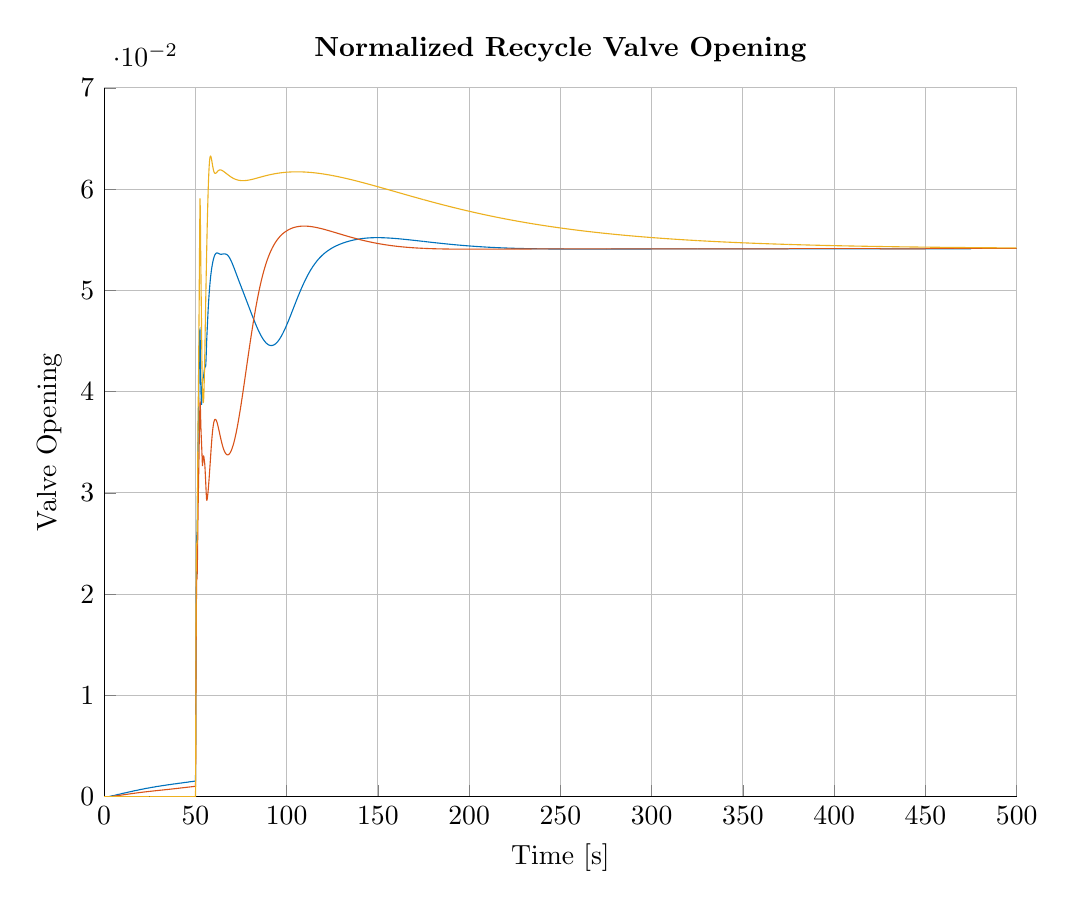
\begin{tikzpicture}

\begin{axis}[%
width=4.563in,
height=3.544in,
at={(0.792in,0.541in)},
scale only axis,
xmin=0,
xmax=500,
xlabel={Time [s]},
xmajorgrids,
ymin=0,
ymax=0.07,
ylabel={Valve Opening},
ymajorgrids,
axis background/.style={fill=white},
title style={font=\bfseries},
title={Normalized Recycle Valve Opening},
axis x line*=bottom,
axis y line*=left
]
\addplot [color=mycolor1,solid,forget plot]
  table[row sep=crcr]{%
0	6.94973000000002e-310\\
0.05	6.94973000000002e-310\\
0.1	6.94973000000002e-310\\
0.15	6.94973000000002e-310\\
0.2	6.94973000000002e-310\\
0.25	6.94973000000002e-310\\
0.3	6.94973000000002e-310\\
0.35	6.94973000000002e-310\\
0.4	6.94973000000002e-310\\
0.45	6.94973000000002e-310\\
0.5	6.94973000000002e-310\\
0.55	6.94973000000002e-310\\
0.6	6.94973000000002e-310\\
0.65	6.94973000000002e-310\\
0.7	6.94973000000002e-310\\
0.75	6.94973000000002e-310\\
0.8	6.94973000000002e-310\\
0.85	6.94973000000002e-310\\
0.9	6.94973000000002e-310\\
0.95	6.94973000000002e-310\\
1	6.94973000000002e-310\\
1.05	6.94973000000002e-310\\
1.1	6.94973000000002e-310\\
1.15	6.94973000000002e-310\\
1.2	6.94973000000002e-310\\
1.25	6.94973000000002e-310\\
1.3	6.94973000000002e-310\\
1.35	6.94973000000002e-310\\
1.4	6.94973000000002e-310\\
1.45	6.94973000000002e-310\\
1.5	6.94973000000002e-310\\
1.55	6.94973000000002e-310\\
1.6	6.94973000000002e-310\\
1.65	6.94973000000002e-310\\
1.7	6.94973000000002e-310\\
1.75	6.94973000000002e-310\\
1.8	6.94973000000002e-310\\
1.85	6.94973000000002e-310\\
1.9	6.94973000000002e-310\\
1.95	6.94973000000002e-310\\
2	6.94973000000002e-310\\
2.05	6.94973000000002e-310\\
2.1	6.94973000000002e-310\\
2.15	6.94973000000002e-310\\
2.2	6.94973000000002e-310\\
2.25	1.03552e-07\\
2.3	3.723e-07\\
2.35	8.06741e-07\\
2.4	1.40203e-06\\
2.45	2.15089e-06\\
2.5	3.05125e-06\\
2.55	4.10043e-06\\
2.6	5.29523e-06\\
2.65	6.63183e-06\\
2.7	8.10574e-06\\
2.75	9.71178e-06\\
2.8	1.1444e-05\\
2.85	1.32957e-05\\
2.9	1.52594e-05\\
2.95	1.73271e-05\\
3	1.94901e-05\\
3.05	2.17393e-05\\
3.1	2.40653e-05\\
3.15	2.64586e-05\\
3.2	2.89094e-05\\
3.25	3.14083e-05\\
3.3	3.39457e-05\\
3.35	3.65125e-05\\
3.4	3.90998e-05\\
3.45	4.1699e-05\\
3.5	4.4302e-05\\
3.55	4.6901e-05\\
3.6	4.94885e-05\\
3.65	5.20577e-05\\
3.7	5.4602e-05\\
3.75	5.71155e-05\\
3.8	5.95925e-05\\
3.85	6.2028e-05\\
3.9	6.44172e-05\\
3.95	6.67561e-05\\
4	6.9041e-05\\
4.05	7.12688e-05\\
4.1	7.34368e-05\\
4.15	7.55429e-05\\
4.2	7.75854e-05\\
4.25	7.95631e-05\\
4.3	8.14755e-05\\
4.35	8.33223e-05\\
4.4	8.51043e-05\\
4.45	8.68229e-05\\
4.5	8.84804e-05\\
4.55	9.00795e-05\\
4.6	9.16241e-05\\
4.65	9.31184e-05\\
4.7	9.45675e-05\\
4.75	9.59774e-05\\
4.8	9.73545e-05\\
4.85	9.87057e-05\\
4.9	0.000100039\\
4.95	0.000101361\\
5	0.000102681\\
5.05	0.000104007\\
5.1	0.000105347\\
5.15	0.000106708\\
5.2	0.000108099\\
5.25	0.000109526\\
5.3	0.000110997\\
5.35	0.000112517\\
5.4	0.000114092\\
5.45	0.000115727\\
5.5	0.000117426\\
5.55	0.000119193\\
5.6	0.00012103\\
5.65	0.00012294\\
5.7	0.000124923\\
5.75	0.00012698\\
5.8	0.000129111\\
5.85	0.000131316\\
5.9	0.000133592\\
5.95	0.000135937\\
6	0.000138348\\
6.05	0.000140823\\
6.1	0.000143357\\
6.15	0.000145944\\
6.2	0.000148582\\
6.25	0.000151263\\
6.3	0.000153982\\
6.35	0.000156733\\
6.4	0.00015951\\
6.45	0.000162306\\
6.5	0.000165114\\
6.55	0.000167928\\
6.6	0.000170741\\
6.65	0.000173546\\
6.7	0.000176336\\
6.75	0.000179105\\
6.8	0.000181847\\
6.85	0.000184555\\
6.9	0.000187226\\
6.95	0.000189852\\
7	0.000192429\\
7.05	0.000194954\\
7.1	0.000197422\\
7.15	0.00019983\\
7.2	0.000202177\\
7.25	0.00020446\\
7.3	0.000206677\\
7.35	0.000208829\\
7.4	0.000210916\\
7.45	0.000212939\\
7.5	0.000214898\\
7.55	0.000216797\\
7.6	0.000218638\\
7.65	0.000220425\\
7.7	0.00022216\\
7.75	0.00022385\\
7.8	0.000225498\\
7.85	0.00022711\\
7.9	0.000228692\\
7.95	0.000230249\\
8	0.000231786\\
8.05	0.000233312\\
8.1	0.00023483\\
8.15	0.000236349\\
8.2	0.000237873\\
8.25	0.00023941\\
8.3	0.000240964\\
8.35	0.000242542\\
8.4	0.000244149\\
8.45	0.000245789\\
8.5	0.000247468\\
8.55	0.000249189\\
8.6	0.000250957\\
8.65	0.000252774\\
8.7	0.000254642\\
8.75	0.000256565\\
8.8	0.000258544\\
8.85	0.000260579\\
8.9	0.000262671\\
8.95	0.000264819\\
9	0.000267023\\
9.05	0.000269281\\
9.1	0.000271591\\
9.15	0.000273951\\
9.2	0.000276358\\
9.25	0.000278808\\
9.3	0.000281297\\
9.35	0.000283821\\
9.4	0.000286375\\
9.45	0.000288954\\
9.5	0.000291553\\
9.55	0.000294167\\
9.6	0.00029679\\
9.65	0.000299416\\
9.7	0.00030204\\
9.75	0.000304656\\
9.8	0.000307259\\
9.85	0.000309843\\
9.9	0.000312403\\
9.95	0.000314934\\
10	0.000317432\\
10.05	0.000319892\\
10.1	0.00032231\\
10.15	0.000324684\\
10.2	0.000327009\\
10.25	0.000329285\\
10.3	0.000331508\\
10.35	0.000333678\\
10.4	0.000335793\\
10.45	0.000337853\\
10.5	0.000339859\\
10.55	0.000341812\\
10.6	0.000343712\\
10.65	0.000345561\\
10.7	0.000347363\\
10.75	0.000349119\\
10.8	0.000350833\\
10.85	0.000352509\\
10.9	0.000354151\\
10.95	0.000355763\\
11	0.00035735\\
11.05	0.000358916\\
11.1	0.000360467\\
11.15	0.000362008\\
11.2	0.000363543\\
11.25	0.000365079\\
11.3	0.000366621\\
11.35	0.000368172\\
11.4	0.00036974\\
11.45	0.000371327\\
11.5	0.000372939\\
11.55	0.00037458\\
11.6	0.000376254\\
11.65	0.000377964\\
11.7	0.000379714\\
11.75	0.000381505\\
11.8	0.000383341\\
11.85	0.000385223\\
11.9	0.000387153\\
11.95	0.00038913\\
12	0.000391156\\
12.05	0.00039323\\
12.1	0.000395351\\
12.15	0.000397519\\
12.2	0.000399731\\
12.25	0.000401985\\
12.3	0.000404278\\
12.35	0.000406608\\
12.4	0.000408971\\
12.45	0.000411364\\
12.5	0.000413782\\
12.55	0.000416221\\
12.6	0.000418677\\
12.65	0.000421144\\
12.7	0.000423619\\
12.75	0.000426097\\
12.8	0.000428572\\
12.85	0.00043104\\
12.9	0.000433495\\
12.95	0.000435935\\
13	0.000438353\\
13.05	0.000440747\\
13.1	0.000443112\\
13.15	0.000445444\\
13.2	0.00044774\\
13.25	0.000449998\\
13.3	0.000452215\\
13.35	0.000454389\\
13.4	0.000456518\\
13.45	0.000458602\\
13.5	0.000460638\\
13.55	0.000462629\\
13.6	0.000464573\\
13.65	0.000466471\\
13.7	0.000468325\\
13.75	0.000470137\\
13.8	0.000471908\\
13.85	0.000473641\\
13.9	0.000475339\\
13.95	0.000477005\\
14	0.000478642\\
14.05	0.000480255\\
14.1	0.000481847\\
14.15	0.000483423\\
14.2	0.000484987\\
14.25	0.000486544\\
14.3	0.000488098\\
14.35	0.000489653\\
14.4	0.000491214\\
14.45	0.000492785\\
14.5	0.000494371\\
14.55	0.000495976\\
14.6	0.000497603\\
14.65	0.000499256\\
14.7	0.000500939\\
14.75	0.000502654\\
14.8	0.000504404\\
14.85	0.000506192\\
14.9	0.000508018\\
14.95	0.000509885\\
15	0.000511793\\
15.05	0.000513743\\
15.1	0.000515735\\
15.15	0.000517769\\
15.2	0.000519844\\
15.25	0.000521958\\
15.3	0.00052411\\
15.35	0.000526298\\
15.4	0.00052852\\
15.45	0.000530773\\
15.5	0.000533053\\
15.55	0.000535357\\
15.6	0.000537682\\
15.65	0.000540024\\
15.7	0.000542379\\
15.75	0.000544743\\
15.8	0.000547111\\
15.85	0.000549479\\
15.9	0.000551844\\
15.95	0.0005542\\
16	0.000556544\\
16.05	0.000558871\\
16.1	0.000561178\\
16.15	0.000563462\\
16.2	0.000565719\\
16.25	0.000567945\\
16.3	0.000570138\\
16.35	0.000572296\\
16.4	0.000574417\\
16.45	0.000576498\\
16.5	0.000578539\\
16.55	0.000580539\\
16.6	0.000582497\\
16.65	0.000584414\\
16.7	0.000586289\\
16.75	0.000588124\\
16.8	0.00058992\\
16.85	0.000591678\\
16.9	0.000593401\\
16.95	0.00059509\\
17	0.000596749\\
17.05	0.000598381\\
17.1	0.000599988\\
17.15	0.000601574\\
17.2	0.000603143\\
17.25	0.000604698\\
17.3	0.000606244\\
17.35	0.000607785\\
17.4	0.000609325\\
17.45	0.000610866\\
17.5	0.000612415\\
17.55	0.000613974\\
17.6	0.000615547\\
17.65	0.000617138\\
17.7	0.000618749\\
17.75	0.000620385\\
17.8	0.000622048\\
17.85	0.000623741\\
17.9	0.000625465\\
17.95	0.000627222\\
18	0.000629015\\
18.05	0.000630844\\
18.1	0.000632709\\
18.15	0.000634611\\
18.2	0.000636551\\
18.25	0.000638526\\
18.3	0.000640537\\
18.35	0.000642583\\
18.4	0.000644661\\
18.45	0.000646769\\
18.5	0.000648906\\
18.55	0.000651068\\
18.6	0.000653252\\
18.65	0.000655457\\
18.7	0.000657677\\
18.75	0.000659909\\
18.8	0.000662151\\
18.85	0.000664398\\
18.9	0.000666645\\
18.95	0.00066889\\
19	0.000671129\\
19.05	0.000673357\\
19.1	0.000675571\\
19.15	0.000677768\\
19.2	0.000679944\\
19.25	0.000682096\\
19.3	0.000684221\\
19.35	0.000686316\\
19.4	0.000688379\\
19.45	0.000690408\\
19.5	0.000692401\\
19.55	0.000694358\\
19.6	0.000696276\\
19.65	0.000698156\\
19.7	0.000699997\\
19.75	0.0007018\\
19.8	0.000703564\\
19.85	0.000705292\\
19.9	0.000706984\\
19.95	0.000708643\\
20	0.000710269\\
20.05	0.000711866\\
20.1	0.000713436\\
20.15	0.000714981\\
20.2	0.000716506\\
20.25	0.000718013\\
20.3	0.000719506\\
20.35	0.000720988\\
20.4	0.000722463\\
20.45	0.000723935\\
20.5	0.000725407\\
20.55	0.000726883\\
20.6	0.000728367\\
20.65	0.000729862\\
20.7	0.000731371\\
20.75	0.000732898\\
20.8	0.000734446\\
20.85	0.000736016\\
20.9	0.000737613\\
20.95	0.000739237\\
21	0.000740891\\
21.05	0.000742576\\
21.1	0.000744294\\
21.15	0.000746044\\
21.2	0.000747828\\
21.25	0.000749645\\
21.3	0.000751496\\
21.35	0.000753379\\
21.4	0.000755293\\
21.45	0.000757237\\
21.5	0.000759209\\
21.55	0.000761207\\
21.6	0.000763229\\
21.65	0.000765272\\
21.7	0.000767334\\
21.75	0.00076941\\
21.8	0.000771499\\
21.85	0.000773595\\
21.9	0.000775697\\
21.95	0.000777801\\
22	0.000779902\\
22.05	0.000781998\\
22.1	0.000784085\\
22.15	0.000786158\\
22.2	0.000788216\\
22.25	0.000790255\\
22.3	0.000792271\\
22.35	0.000794262\\
22.4	0.000796226\\
22.45	0.00079816\\
22.5	0.000800062\\
22.55	0.00080193\\
22.6	0.000803764\\
22.65	0.000805562\\
22.7	0.000807324\\
22.75	0.000809049\\
22.8	0.000810738\\
22.85	0.00081239\\
22.9	0.000814007\\
22.95	0.00081559\\
23	0.000817141\\
23.05	0.000818661\\
23.1	0.000820152\\
23.15	0.000821617\\
23.2	0.000823058\\
23.25	0.000824479\\
23.3	0.000825882\\
23.35	0.000827271\\
23.4	0.000828648\\
23.45	0.000830018\\
23.5	0.000831384\\
23.55	0.000832749\\
23.6	0.000834116\\
23.65	0.00083549\\
23.7	0.000836874\\
23.75	0.00083827\\
23.8	0.000839682\\
23.85	0.000841112\\
23.9	0.000842564\\
23.95	0.000844039\\
24	0.00084554\\
24.05	0.000847068\\
24.1	0.000848625\\
24.15	0.000850212\\
24.2	0.00085183\\
24.25	0.000853479\\
24.3	0.00085516\\
24.35	0.000856871\\
24.4	0.000858613\\
24.45	0.000860385\\
24.5	0.000862185\\
24.55	0.000864012\\
24.6	0.000865863\\
24.65	0.000867737\\
24.7	0.000869631\\
24.75	0.000871542\\
24.8	0.000873468\\
24.85	0.000875406\\
24.9	0.000877351\\
24.95	0.000879302\\
25	0.000881255\\
};
\addplot [color=mycolor1,solid,forget plot]
  table[row sep=crcr]{%
25	0.000881255\\
25.05	0.000883205\\
25.1	0.000885151\\
25.15	0.000887087\\
25.2	0.000889012\\
25.25	0.000890922\\
25.3	0.000892814\\
25.35	0.000894684\\
25.4	0.000896531\\
25.45	0.000898352\\
25.5	0.000900144\\
25.55	0.000901906\\
25.6	0.000903636\\
25.65	0.000905333\\
25.7	0.000906996\\
25.75	0.000908624\\
25.8	0.000910217\\
25.85	0.000911774\\
25.9	0.000913298\\
25.95	0.000914787\\
26	0.000916244\\
26.05	0.000917669\\
26.1	0.000919065\\
26.15	0.000920433\\
26.2	0.000921776\\
26.25	0.000923096\\
26.3	0.000924396\\
26.35	0.000925679\\
26.4	0.000926948\\
26.45	0.000928206\\
26.5	0.000929457\\
26.55	0.000930704\\
26.6	0.000931949\\
26.65	0.000933198\\
26.7	0.000934452\\
26.75	0.000935715\\
26.8	0.000936991\\
26.85	0.000938282\\
26.9	0.00093959\\
26.95	0.000940919\\
27	0.000942271\\
27.05	0.000943647\\
27.1	0.00094505\\
27.15	0.000946481\\
27.2	0.000947941\\
27.25	0.00094943\\
27.3	0.00095095\\
27.35	0.000952501\\
27.4	0.000954081\\
27.45	0.000955692\\
27.5	0.00095733\\
27.55	0.000958997\\
27.6	0.000960689\\
27.65	0.000962405\\
27.7	0.000964144\\
27.75	0.000965901\\
27.8	0.000967676\\
27.85	0.000969465\\
27.9	0.000971266\\
27.95	0.000973074\\
28	0.000974887\\
28.05	0.000976703\\
28.1	0.000978516\\
28.15	0.000980324\\
28.2	0.000982124\\
28.25	0.000983913\\
28.3	0.000985687\\
28.35	0.000987444\\
28.4	0.00098918\\
28.45	0.000990893\\
28.5	0.000992581\\
28.55	0.000994241\\
28.6	0.000995872\\
28.65	0.000997472\\
28.7	0.00099904\\
28.75	0.00100057\\
28.8	0.00100208\\
28.85	0.00100354\\
28.9	0.00100498\\
28.95	0.00100638\\
29	0.00100774\\
29.05	0.00100908\\
29.1	0.00101038\\
29.15	0.00101166\\
29.2	0.00101291\\
29.25	0.00101414\\
29.3	0.00101534\\
29.35	0.00101652\\
29.4	0.00101769\\
29.45	0.00101885\\
29.5	0.00101999\\
29.55	0.00102113\\
29.6	0.00102227\\
29.65	0.0010234\\
29.7	0.00102454\\
29.75	0.00102569\\
29.8	0.00102684\\
29.85	0.00102801\\
29.9	0.00102919\\
29.95	0.00103039\\
30	0.00103161\\
30.05	0.00103286\\
30.1	0.00103413\\
30.15	0.00103542\\
30.2	0.00103675\\
30.25	0.0010381\\
30.3	0.00103948\\
30.35	0.0010409\\
30.4	0.00104234\\
30.45	0.00104381\\
30.5	0.00104532\\
30.55	0.00104685\\
30.6	0.0010484\\
30.65	0.00104999\\
30.7	0.0010516\\
30.75	0.00105323\\
30.8	0.00105488\\
30.85	0.00105654\\
30.9	0.00105822\\
30.95	0.00105991\\
31	0.00106161\\
31.05	0.00106331\\
31.1	0.00106502\\
31.15	0.00106672\\
31.2	0.00106842\\
31.25	0.00107011\\
31.3	0.00107179\\
31.35	0.00107345\\
31.4	0.0010751\\
31.45	0.00107673\\
31.5	0.00107833\\
31.55	0.00107991\\
31.6	0.00108146\\
31.65	0.00108298\\
31.7	0.00108447\\
31.75	0.00108593\\
31.8	0.00108736\\
31.85	0.00108876\\
31.9	0.00109012\\
31.95	0.00109144\\
32	0.00109274\\
32.05	0.001094\\
32.1	0.00109523\\
32.15	0.00109644\\
32.2	0.00109761\\
32.25	0.00109876\\
32.3	0.00109989\\
32.35	0.001101\\
32.4	0.00110208\\
32.45	0.00110316\\
32.5	0.00110422\\
32.55	0.00110527\\
32.6	0.00110631\\
32.65	0.00110736\\
32.7	0.0011084\\
32.75	0.00110945\\
32.8	0.00111051\\
32.85	0.00111158\\
32.9	0.00111266\\
32.95	0.00111376\\
33	0.00111487\\
33.05	0.00111601\\
33.1	0.00111718\\
33.15	0.00111836\\
33.2	0.00111958\\
33.25	0.00112083\\
33.3	0.0011221\\
33.35	0.0011234\\
33.4	0.00112474\\
33.45	0.00112611\\
33.5	0.0011275\\
33.55	0.00112893\\
33.6	0.00113039\\
33.65	0.00113187\\
33.7	0.00113338\\
33.75	0.00113491\\
33.8	0.00113647\\
33.85	0.00113804\\
33.9	0.00113963\\
33.95	0.00114124\\
34	0.00114285\\
34.05	0.00114447\\
34.1	0.0011461\\
34.15	0.00114773\\
34.2	0.00114935\\
34.25	0.00115098\\
34.3	0.00115259\\
34.35	0.00115419\\
34.4	0.00115577\\
34.45	0.00115734\\
34.5	0.00115888\\
34.55	0.00116041\\
34.6	0.0011619\\
34.65	0.00116337\\
34.7	0.00116481\\
34.75	0.00116622\\
34.8	0.0011676\\
34.85	0.00116895\\
34.9	0.00117026\\
34.95	0.00117154\\
35	0.00117278\\
35.05	0.001174\\
35.1	0.00117518\\
35.15	0.00117633\\
35.2	0.00117745\\
35.25	0.00117855\\
35.3	0.00117962\\
35.35	0.00118067\\
35.4	0.0011817\\
35.45	0.00118271\\
35.5	0.00118371\\
35.55	0.0011847\\
35.6	0.00118568\\
35.65	0.00118665\\
35.7	0.00118763\\
35.75	0.00118861\\
35.8	0.00118959\\
35.85	0.00119059\\
35.9	0.00119159\\
35.95	0.00119261\\
36	0.00119365\\
36.05	0.00119471\\
36.1	0.0011958\\
36.15	0.00119691\\
36.2	0.00119804\\
36.25	0.00119921\\
36.3	0.0012004\\
36.35	0.00120163\\
36.4	0.00120289\\
36.45	0.00120418\\
36.5	0.0012055\\
36.55	0.00120685\\
36.6	0.00120824\\
36.65	0.00120965\\
36.7	0.00121109\\
36.75	0.00121256\\
36.8	0.00121405\\
36.85	0.00121556\\
36.9	0.0012171\\
36.95	0.00121865\\
37	0.00122021\\
37.05	0.00122178\\
37.1	0.00122336\\
37.15	0.00122494\\
37.2	0.00122653\\
37.25	0.00122811\\
37.3	0.00122968\\
37.35	0.00123125\\
37.4	0.0012328\\
37.45	0.00123433\\
37.5	0.00123585\\
37.55	0.00123734\\
37.6	0.00123881\\
37.65	0.00124025\\
37.7	0.00124167\\
37.75	0.00124305\\
37.8	0.00124441\\
37.85	0.00124573\\
37.9	0.00124701\\
37.95	0.00124826\\
38	0.00124948\\
38.05	0.00125067\\
38.1	0.00125182\\
38.15	0.00125294\\
38.2	0.00125404\\
38.25	0.0012551\\
38.3	0.00125613\\
38.35	0.00125715\\
38.4	0.00125814\\
38.45	0.00125911\\
38.5	0.00126007\\
38.55	0.00126101\\
38.6	0.00126195\\
38.65	0.00126288\\
38.7	0.0012638\\
38.75	0.00126473\\
38.8	0.00126567\\
38.85	0.00126661\\
38.9	0.00126756\\
38.95	0.00126853\\
39	0.00126951\\
39.05	0.00127052\\
39.1	0.00127155\\
39.15	0.0012726\\
39.2	0.00127368\\
39.25	0.00127479\\
39.3	0.00127593\\
39.35	0.00127711\\
39.4	0.00127832\\
39.45	0.00127956\\
39.5	0.00128083\\
39.55	0.00128214\\
39.6	0.00128348\\
39.65	0.00128485\\
39.7	0.00128625\\
39.75	0.00128768\\
39.8	0.00128914\\
39.85	0.00129062\\
39.9	0.00129212\\
39.95	0.00129364\\
40	0.00129518\\
40.05	0.00129673\\
40.1	0.00129829\\
40.15	0.00129985\\
40.2	0.00130142\\
40.25	0.00130299\\
40.3	0.00130455\\
40.35	0.00130611\\
40.4	0.00130765\\
40.45	0.00130918\\
40.5	0.00131069\\
40.55	0.00131217\\
40.6	0.00131364\\
40.65	0.00131508\\
40.7	0.00131649\\
40.75	0.00131787\\
40.8	0.00131922\\
40.85	0.00132053\\
40.9	0.00132181\\
40.95	0.00132306\\
41	0.00132427\\
41.05	0.00132545\\
41.1	0.00132659\\
41.15	0.0013277\\
41.2	0.00132878\\
41.25	0.00132982\\
41.3	0.00133084\\
41.35	0.00133183\\
41.4	0.0013328\\
41.45	0.00133375\\
41.5	0.00133468\\
41.55	0.0013356\\
41.6	0.0013365\\
41.65	0.0013374\\
41.7	0.0013383\\
41.75	0.00133919\\
41.8	0.00134009\\
41.85	0.00134099\\
41.9	0.00134191\\
41.95	0.00134284\\
42	0.00134379\\
42.05	0.00134475\\
42.1	0.00134575\\
42.15	0.00134676\\
42.2	0.00134781\\
42.25	0.00134888\\
42.3	0.00134999\\
42.35	0.00135113\\
42.4	0.00135231\\
42.45	0.00135352\\
42.5	0.00135477\\
42.55	0.00135605\\
42.6	0.00135737\\
42.65	0.00135872\\
42.7	0.00136011\\
42.75	0.00136152\\
42.8	0.00136297\\
42.85	0.00136444\\
42.9	0.00136593\\
42.95	0.00136745\\
43	0.00136899\\
43.05	0.00137054\\
43.1	0.0013721\\
43.15	0.00137367\\
43.2	0.00137525\\
43.25	0.00137682\\
43.3	0.0013784\\
43.35	0.00137996\\
43.4	0.00138152\\
43.45	0.00138306\\
43.5	0.00138459\\
43.55	0.00138609\\
43.6	0.00138757\\
43.65	0.00138902\\
43.7	0.00139045\\
43.75	0.00139184\\
43.8	0.0013932\\
43.85	0.00139453\\
43.9	0.00139582\\
43.95	0.00139707\\
44	0.00139829\\
44.05	0.00139947\\
44.1	0.00140061\\
44.15	0.00140172\\
44.2	0.0014028\\
44.25	0.00140384\\
44.3	0.00140485\\
44.35	0.00140583\\
44.4	0.00140679\\
44.45	0.00140772\\
44.5	0.00140864\\
44.55	0.00140954\\
44.6	0.00141042\\
44.65	0.0014113\\
44.7	0.00141217\\
44.75	0.00141304\\
44.8	0.00141391\\
44.85	0.00141479\\
44.9	0.00141568\\
44.95	0.00141658\\
45	0.0014175\\
45.05	0.00141844\\
45.1	0.00141941\\
45.15	0.0014204\\
45.2	0.00142142\\
45.25	0.00142248\\
45.3	0.00142357\\
45.35	0.00142469\\
45.4	0.00142585\\
45.45	0.00142705\\
45.5	0.00142829\\
45.55	0.00142956\\
45.6	0.00143087\\
45.65	0.00143222\\
45.7	0.00143361\\
45.75	0.00143503\\
45.8	0.00143648\\
45.85	0.00143796\\
45.9	0.00143947\\
45.95	0.001441\\
46	0.00144255\\
46.05	0.00144412\\
46.1	0.00144571\\
46.15	0.0014473\\
46.2	0.0014489\\
46.25	0.00145051\\
46.3	0.00145211\\
46.35	0.00145371\\
46.4	0.00145529\\
46.45	0.00145686\\
46.5	0.00145842\\
46.55	0.00145995\\
46.6	0.00146146\\
46.65	0.00146295\\
46.7	0.0014644\\
46.75	0.00146582\\
46.8	0.0014672\\
46.85	0.00146855\\
46.9	0.00146986\\
46.95	0.00147113\\
47	0.00147236\\
47.05	0.00147355\\
47.1	0.00147471\\
47.15	0.00147582\\
47.2	0.0014769\\
47.25	0.00147794\\
47.3	0.00147895\\
47.35	0.00147993\\
47.4	0.00148088\\
47.45	0.0014818\\
47.5	0.0014827\\
47.55	0.00148359\\
47.6	0.00148445\\
47.65	0.00148531\\
47.7	0.00148616\\
47.75	0.00148701\\
47.8	0.00148786\\
47.85	0.00148872\\
47.9	0.00148958\\
47.95	0.00149046\\
48	0.00149136\\
48.05	0.00149228\\
48.1	0.00149323\\
48.15	0.0014942\\
48.2	0.00149521\\
48.25	0.00149625\\
48.3	0.00149732\\
48.35	0.00149844\\
48.4	0.00149959\\
48.45	0.00150079\\
48.5	0.00150202\\
48.55	0.0015033\\
48.6	0.00150462\\
48.65	0.00150598\\
48.7	0.00150738\\
48.75	0.00150882\\
48.8	0.00151029\\
48.85	0.00151179\\
48.9	0.00151333\\
48.95	0.00151489\\
49	0.00151648\\
49.05	0.00151809\\
49.1	0.00151971\\
49.15	0.00152134\\
49.2	0.00152299\\
49.25	0.00152463\\
49.3	0.00152628\\
49.35	0.00152792\\
49.4	0.00152955\\
49.45	0.00153117\\
49.5	0.00153276\\
49.55	0.00153434\\
49.6	0.00153589\\
49.65	0.00153741\\
49.7	0.0015389\\
49.75	0.00154035\\
49.8	0.00154177\\
49.85	0.00154315\\
49.9	0.00154448\\
49.95	0.00154577\\
50	0.00154703\\
};
\addplot [color=mycolor1,solid,forget plot]
  table[row sep=crcr]{%
50	0.00154703\\
50.05	0.00154823\\
50.1	0.002139\\
50.15	0.00362943\\
50.2	0.00625718\\
50.25	0.0102481\\
50.3	0.0111757\\
50.35	0.0125758\\
50.4	0.0144697\\
50.45	0.0168679\\
50.5	0.0198857\\
50.55	0.0239501\\
50.6	0.024771\\
50.65	0.0253238\\
50.7	0.0256391\\
50.75	0.0257865\\
50.8	0.0258476\\
50.85	0.0259057\\
50.9	0.0260327\\
50.95	0.0262811\\
51	0.0266804\\
51.05	0.0272433\\
51.1	0.0279581\\
51.15	0.028812\\
51.2	0.0297847\\
51.25	0.0308233\\
51.3	0.0318762\\
51.35	0.0328975\\
51.4	0.033853\\
51.45	0.0347225\\
51.5	0.0354995\\
51.55	0.0361898\\
51.6	0.0368083\\
51.65	0.0373752\\
51.7	0.0379123\\
51.75	0.0384395\\
51.8	0.0389716\\
51.85	0.0395198\\
51.9	0.0400899\\
51.95	0.0406823\\
52	0.0412929\\
52.05	0.0419141\\
52.1	0.0425421\\
52.15	0.0431721\\
52.2	0.0437977\\
52.25	0.0444154\\
52.3	0.0450091\\
52.35	0.045528\\
52.4	0.0459194\\
52.45	0.0461394\\
52.5	0.0461603\\
52.55	0.0459733\\
52.6	0.0455841\\
52.65	0.045\\
52.7	0.044295\\
52.75	0.0435366\\
52.8	0.0427823\\
52.85	0.0420753\\
52.9	0.0414438\\
52.95	0.0409016\\
53	0.0404503\\
53.05	0.0400823\\
53.1	0.0397845\\
53.15	0.0395411\\
53.2	0.0393364\\
53.25	0.0391574\\
53.3	0.0389945\\
53.35	0.0388428\\
53.4	0.0387013\\
53.45	0.0389933\\
53.5	0.0388726\\
53.55	0.0391795\\
53.6	0.0394842\\
53.65	0.0397795\\
53.7	0.0400559\\
53.75	0.0403049\\
53.8	0.0405206\\
53.85	0.040701\\
53.9	0.0408473\\
53.95	0.0409636\\
54	0.0410553\\
54.05	0.0411285\\
54.1	0.0411889\\
54.15	0.0412413\\
54.2	0.0412894\\
54.25	0.0413356\\
54.3	0.0413812\\
54.35	0.0414264\\
54.4	0.0414724\\
54.45	0.0415201\\
54.5	0.0415702\\
54.55	0.0416234\\
54.6	0.0416803\\
54.65	0.041742\\
54.7	0.0418095\\
54.75	0.0418836\\
54.8	0.0419653\\
54.85	0.0420553\\
54.9	0.042094\\
54.95	0.0421435\\
55	0.0422008\\
55.05	0.0422614\\
55.1	0.0423201\\
55.15	0.0423726\\
55.2	0.0424157\\
55.25	0.0424473\\
55.3	0.0424668\\
55.35	0.0424748\\
55.4	0.0424724\\
55.45	0.0424642\\
55.5	0.0424596\\
55.55	0.0424659\\
55.6	0.0424939\\
55.65	0.0425543\\
55.7	0.0426545\\
55.75	0.0427979\\
55.8	0.0429827\\
55.85	0.0432034\\
55.9	0.0434512\\
55.95	0.0437162\\
56	0.0439883\\
56.05	0.044259\\
56.1	0.0445217\\
56.15	0.0447722\\
56.2	0.0450087\\
56.25	0.0452315\\
56.3	0.0454423\\
56.35	0.0456436\\
56.4	0.0458384\\
56.45	0.0460293\\
56.5	0.0462184\\
56.55	0.0464072\\
56.6	0.0465965\\
56.65	0.0467864\\
56.7	0.0469764\\
56.75	0.0471658\\
56.8	0.0473535\\
56.85	0.0475385\\
56.9	0.04772\\
56.95	0.0478972\\
57	0.0480697\\
57.05	0.048237\\
57.1	0.0483992\\
57.15	0.0485564\\
57.2	0.0487086\\
57.25	0.0488561\\
57.3	0.0489994\\
57.35	0.0491385\\
57.4	0.049274\\
57.45	0.0494059\\
57.5	0.0495347\\
57.55	0.0496605\\
57.6	0.0497835\\
57.65	0.0499039\\
57.7	0.0500218\\
57.75	0.0501374\\
57.8	0.0502506\\
57.85	0.0503614\\
57.9	0.05047\\
57.95	0.050576\\
58	0.0506796\\
58.05	0.0507806\\
58.1	0.0508788\\
58.15	0.0509744\\
58.2	0.051067\\
58.25	0.0511569\\
58.3	0.051244\\
58.35	0.0513285\\
58.4	0.0514103\\
58.45	0.0514897\\
58.5	0.0515667\\
58.55	0.0516416\\
58.6	0.0517145\\
58.65	0.0517855\\
58.7	0.0518547\\
58.75	0.0519222\\
58.8	0.0519881\\
58.85	0.0520524\\
58.9	0.0521151\\
58.95	0.0521763\\
59	0.052236\\
59.05	0.0522941\\
59.1	0.0523508\\
59.15	0.052406\\
59.2	0.0524597\\
59.25	0.052512\\
59.3	0.0525629\\
59.35	0.0526124\\
59.4	0.0526606\\
59.45	0.0527075\\
59.5	0.0527532\\
59.55	0.0527975\\
59.6	0.0528407\\
59.65	0.0528827\\
59.7	0.0529235\\
59.75	0.0529631\\
59.8	0.0530015\\
59.85	0.0530389\\
59.9	0.053075\\
59.95	0.0531101\\
60	0.053144\\
60.05	0.0531768\\
60.1	0.0532085\\
60.15	0.053239\\
60.2	0.0532685\\
60.25	0.0532969\\
60.3	0.0533241\\
60.35	0.0533503\\
60.4	0.0533755\\
60.45	0.0533995\\
60.5	0.0534226\\
60.55	0.0534445\\
60.6	0.0534655\\
60.65	0.0534854\\
60.7	0.0535043\\
60.75	0.0535223\\
60.8	0.0535392\\
60.85	0.0535552\\
60.9	0.0535702\\
60.95	0.0535843\\
61	0.0535975\\
61.05	0.0536097\\
61.1	0.0536211\\
61.15	0.0536316\\
61.2	0.0536412\\
61.25	0.0536499\\
61.3	0.0536579\\
61.35	0.053665\\
61.4	0.0536714\\
61.45	0.053677\\
61.5	0.0536819\\
61.55	0.0536861\\
61.6	0.0536895\\
61.65	0.0536924\\
61.7	0.0536945\\
61.75	0.0536961\\
61.8	0.0536971\\
61.85	0.0536975\\
61.9	0.0536974\\
61.95	0.0536968\\
62	0.0536957\\
62.05	0.0536942\\
62.1	0.0536923\\
62.15	0.05369\\
62.2	0.0536873\\
62.25	0.0536843\\
62.3	0.053681\\
62.35	0.0536775\\
62.4	0.0536737\\
62.45	0.0536697\\
62.5	0.0536655\\
62.55	0.0536611\\
62.6	0.0536567\\
62.65	0.0536521\\
62.7	0.0536475\\
62.75	0.0536428\\
62.8	0.0536382\\
62.85	0.0536335\\
62.9	0.0536289\\
62.95	0.0536243\\
63	0.0536198\\
63.05	0.0536154\\
63.1	0.0536111\\
63.15	0.0536069\\
63.2	0.0536029\\
63.25	0.0535991\\
63.3	0.0535955\\
63.35	0.053592\\
63.4	0.0535888\\
63.45	0.0535857\\
63.5	0.0535829\\
63.55	0.0535804\\
63.6	0.053578\\
63.65	0.053576\\
63.7	0.0535741\\
63.75	0.0535725\\
63.8	0.0535712\\
63.85	0.05357\\
63.9	0.0535692\\
63.95	0.0535685\\
64	0.0535681\\
64.05	0.0535679\\
64.1	0.0535679\\
64.15	0.0535681\\
64.2	0.0535686\\
64.25	0.0535691\\
64.3	0.0535699\\
64.35	0.0535708\\
64.4	0.0535719\\
64.45	0.053573\\
64.5	0.0535743\\
64.55	0.0535757\\
64.6	0.0535772\\
64.65	0.0535787\\
64.7	0.0535803\\
64.75	0.0535819\\
64.8	0.0535836\\
64.85	0.0535852\\
64.9	0.0535869\\
64.95	0.0535885\\
65	0.0535901\\
65.05	0.0535917\\
65.1	0.0535932\\
65.15	0.0535947\\
65.2	0.0535961\\
65.25	0.0535974\\
65.3	0.0535986\\
65.35	0.0535997\\
65.4	0.0536007\\
65.45	0.0536016\\
65.5	0.0536024\\
65.55	0.0536031\\
65.6	0.0536037\\
65.65	0.0536041\\
65.7	0.0536044\\
65.75	0.0536046\\
65.8	0.0536046\\
65.85	0.0536046\\
65.9	0.0536043\\
65.95	0.053604\\
66	0.0536035\\
66.05	0.0536029\\
66.1	0.0536021\\
66.15	0.0536011\\
66.2	0.0536001\\
66.25	0.0535988\\
66.3	0.0535974\\
66.35	0.0535958\\
66.4	0.0535941\\
66.45	0.0535922\\
66.5	0.05359\\
66.55	0.0535877\\
66.6	0.0535852\\
66.65	0.0535825\\
66.7	0.0535796\\
66.75	0.0535764\\
66.8	0.053573\\
66.85	0.0535694\\
66.9	0.0535655\\
66.95	0.0535614\\
67	0.053557\\
67.05	0.0535523\\
67.1	0.0535474\\
67.15	0.0535421\\
67.2	0.0535366\\
67.25	0.0535308\\
67.3	0.0535246\\
67.35	0.0535182\\
67.4	0.0535115\\
67.45	0.0535044\\
67.5	0.0534971\\
67.55	0.0534894\\
67.6	0.0534814\\
67.65	0.0534731\\
67.7	0.0534644\\
67.75	0.0534554\\
67.8	0.0534461\\
67.85	0.0534365\\
67.9	0.0534266\\
67.95	0.0534163\\
68	0.0534057\\
68.05	0.0533948\\
68.1	0.0533835\\
68.15	0.053372\\
68.2	0.0533601\\
68.25	0.0533479\\
68.3	0.0533354\\
68.35	0.0533225\\
68.4	0.0533094\\
68.45	0.053296\\
68.5	0.0532822\\
68.55	0.0532682\\
68.6	0.0532539\\
68.65	0.0532392\\
68.7	0.0532243\\
68.75	0.0532091\\
68.8	0.0531936\\
68.85	0.0531779\\
68.9	0.0531618\\
68.95	0.0531455\\
69	0.053129\\
69.05	0.0531121\\
69.1	0.0530951\\
69.15	0.0530777\\
69.2	0.0530601\\
69.25	0.0530423\\
69.3	0.0530243\\
69.35	0.053006\\
69.4	0.0529874\\
69.45	0.0529687\\
69.5	0.0529497\\
69.55	0.0529305\\
69.6	0.0529112\\
69.65	0.0528916\\
69.7	0.0528718\\
69.75	0.0528518\\
69.8	0.0528316\\
69.85	0.0528113\\
69.9	0.0527907\\
69.95	0.05277\\
70	0.0527491\\
70.05	0.0527281\\
70.1	0.0527069\\
70.15	0.0526855\\
70.2	0.052664\\
70.25	0.0526424\\
70.3	0.0526206\\
70.35	0.0525987\\
70.4	0.0525766\\
70.45	0.0525544\\
70.5	0.0525321\\
70.55	0.0525097\\
70.6	0.0524872\\
70.65	0.0524646\\
70.7	0.0524418\\
70.75	0.052419\\
70.8	0.0523961\\
70.85	0.0523731\\
70.9	0.05235\\
70.95	0.0523268\\
71	0.0523035\\
71.05	0.0522802\\
71.1	0.0522568\\
71.15	0.0522334\\
71.2	0.0522098\\
71.25	0.0521862\\
71.3	0.0521626\\
71.35	0.0521389\\
71.4	0.0521152\\
71.45	0.0520914\\
71.5	0.0520676\\
71.55	0.0520437\\
71.6	0.0520198\\
71.65	0.0519959\\
71.7	0.051972\\
71.75	0.051948\\
71.8	0.051924\\
71.85	0.0519\\
71.9	0.0518759\\
71.95	0.0518519\\
72	0.0518278\\
72.05	0.0518037\\
72.1	0.0517796\\
72.15	0.0517555\\
72.2	0.0517314\\
72.25	0.0517073\\
72.3	0.0516832\\
72.35	0.0516591\\
72.4	0.051635\\
72.45	0.0516109\\
72.5	0.0515868\\
72.55	0.0515627\\
72.6	0.0515386\\
72.65	0.0515145\\
72.7	0.0514905\\
72.75	0.0514664\\
72.8	0.0514424\\
72.85	0.0514183\\
72.9	0.0513943\\
72.95	0.0513703\\
73	0.0513463\\
73.05	0.0513223\\
73.1	0.0512984\\
73.15	0.0512744\\
73.2	0.0512505\\
73.25	0.0512266\\
73.3	0.0512027\\
73.35	0.0511788\\
73.4	0.051155\\
73.45	0.0511311\\
73.5	0.0511073\\
73.55	0.0510835\\
73.6	0.0510598\\
73.65	0.051036\\
73.7	0.0510123\\
73.75	0.0509885\\
73.8	0.0509648\\
73.85	0.0509412\\
73.9	0.0509175\\
73.95	0.0508939\\
74	0.0508702\\
74.05	0.0508466\\
74.1	0.050823\\
74.15	0.0507995\\
74.2	0.0507759\\
74.25	0.0507524\\
74.3	0.0507289\\
74.35	0.0507053\\
74.4	0.0506819\\
74.45	0.0506584\\
74.5	0.0506349\\
74.55	0.0506115\\
74.6	0.050588\\
74.65	0.0505646\\
74.7	0.0505412\\
74.75	0.0505178\\
74.8	0.0504944\\
74.85	0.050471\\
74.9	0.0504477\\
74.95	0.0504243\\
75	0.050401\\
};
\addplot [color=mycolor1,solid,forget plot]
  table[row sep=crcr]{%
75	0.050401\\
75.05	0.0503776\\
75.1	0.0503543\\
75.15	0.050331\\
75.2	0.0503077\\
75.25	0.0502844\\
75.3	0.0502611\\
75.35	0.0502378\\
75.4	0.0502145\\
75.45	0.0501912\\
75.5	0.0501679\\
75.55	0.0501446\\
75.6	0.0501213\\
75.65	0.0500981\\
75.7	0.0500748\\
75.75	0.0500515\\
75.8	0.0500282\\
75.85	0.0500049\\
75.9	0.0499817\\
75.95	0.0499584\\
76	0.0499351\\
76.05	0.0499118\\
76.1	0.0498885\\
76.15	0.0498652\\
76.2	0.0498419\\
76.25	0.0498186\\
76.3	0.0497953\\
76.35	0.049772\\
76.4	0.0497487\\
76.45	0.0497254\\
76.5	0.049702\\
76.55	0.0496787\\
76.6	0.0496554\\
76.65	0.049632\\
76.7	0.0496087\\
76.75	0.0495853\\
76.8	0.0495619\\
76.85	0.0495385\\
76.9	0.0495151\\
76.95	0.0494917\\
77	0.0494683\\
77.05	0.0494449\\
77.1	0.0494215\\
77.15	0.0493981\\
77.2	0.0493746\\
77.25	0.0493512\\
77.3	0.0493277\\
77.35	0.0493042\\
77.4	0.0492807\\
77.45	0.0492572\\
77.5	0.0492337\\
77.55	0.0492102\\
77.6	0.0491867\\
77.65	0.0491632\\
77.7	0.0491396\\
77.75	0.0491161\\
77.8	0.0490925\\
77.85	0.0490689\\
77.9	0.0490453\\
77.95	0.0490218\\
78	0.0489982\\
78.05	0.0489745\\
78.1	0.0489509\\
78.15	0.0489273\\
78.2	0.0489037\\
78.25	0.04888\\
78.3	0.0488564\\
78.35	0.0488327\\
78.4	0.048809\\
78.45	0.0487854\\
78.5	0.0487617\\
78.55	0.048738\\
78.6	0.0487143\\
78.65	0.0486906\\
78.7	0.0486669\\
78.75	0.0486432\\
78.8	0.0486195\\
78.85	0.0485957\\
78.9	0.048572\\
78.95	0.0485483\\
79	0.0485246\\
79.05	0.0485008\\
79.1	0.0484771\\
79.15	0.0484534\\
79.2	0.0484296\\
79.25	0.0484059\\
79.3	0.0483822\\
79.35	0.0483584\\
79.4	0.0483347\\
79.45	0.0483109\\
79.5	0.0482872\\
79.55	0.0482635\\
79.6	0.0482398\\
79.65	0.0482161\\
79.7	0.0481923\\
79.75	0.0481686\\
79.8	0.0481449\\
79.85	0.0481212\\
79.9	0.0480975\\
79.95	0.0480739\\
80	0.0480502\\
80.05	0.0480265\\
80.1	0.0480029\\
80.15	0.0479792\\
80.2	0.0479556\\
80.25	0.047932\\
80.3	0.0479084\\
80.35	0.0478848\\
80.4	0.0478612\\
80.45	0.0478377\\
80.5	0.0478141\\
80.55	0.0477906\\
80.6	0.0477671\\
80.65	0.0477436\\
80.7	0.0477201\\
80.75	0.0476967\\
80.8	0.0476733\\
80.85	0.0476499\\
80.9	0.0476265\\
80.95	0.0476031\\
81	0.0475798\\
81.05	0.0475565\\
81.1	0.0475332\\
81.15	0.0475099\\
81.2	0.0474867\\
81.25	0.0474635\\
81.3	0.0474403\\
81.35	0.0474172\\
81.4	0.0473941\\
81.45	0.047371\\
81.5	0.0473479\\
81.55	0.0473249\\
81.6	0.0473019\\
81.65	0.047279\\
81.7	0.0472561\\
81.75	0.0472332\\
81.8	0.0472104\\
81.85	0.0471876\\
81.9	0.0471648\\
81.95	0.0471421\\
82	0.0471195\\
82.05	0.0470968\\
82.1	0.0470742\\
82.15	0.0470517\\
82.2	0.0470292\\
82.25	0.0470068\\
82.3	0.0469844\\
82.35	0.046962\\
82.4	0.0469397\\
82.45	0.0469174\\
82.5	0.0468952\\
82.55	0.0468731\\
82.6	0.046851\\
82.65	0.0468289\\
82.7	0.046807\\
82.75	0.046785\\
82.8	0.0467631\\
82.85	0.0467413\\
82.9	0.0467196\\
82.95	0.0466978\\
83	0.0466762\\
83.05	0.0466546\\
83.1	0.0466331\\
83.15	0.0466116\\
83.2	0.0465902\\
83.25	0.0465689\\
83.3	0.0465476\\
83.35	0.0465264\\
83.4	0.0465053\\
83.45	0.0464843\\
83.5	0.0464633\\
83.55	0.0464423\\
83.6	0.0464215\\
83.65	0.0464007\\
83.7	0.04638\\
83.75	0.0463594\\
83.8	0.0463388\\
83.85	0.0463183\\
83.9	0.0462979\\
83.95	0.0462776\\
84	0.0462573\\
84.05	0.0462372\\
84.1	0.0462171\\
84.15	0.0461971\\
84.2	0.0461771\\
84.25	0.0461573\\
84.3	0.0461375\\
84.35	0.0461178\\
84.4	0.0460983\\
84.45	0.0460788\\
84.5	0.0460593\\
84.55	0.04604\\
84.6	0.0460208\\
84.65	0.0460016\\
84.7	0.0459826\\
84.75	0.0459636\\
84.8	0.0459447\\
84.85	0.0459259\\
84.9	0.0459072\\
84.95	0.0458887\\
85	0.0458702\\
85.05	0.0458518\\
85.1	0.0458335\\
85.15	0.0458153\\
85.2	0.0457972\\
85.25	0.0457792\\
85.3	0.0457613\\
85.35	0.0457435\\
85.4	0.0457258\\
85.45	0.0457082\\
85.5	0.0456907\\
85.55	0.0456733\\
85.6	0.045656\\
85.65	0.0456389\\
85.7	0.0456218\\
85.75	0.0456048\\
85.8	0.045588\\
85.85	0.0455713\\
85.9	0.0455547\\
85.95	0.0455381\\
86	0.0455218\\
86.05	0.0455055\\
86.1	0.0454893\\
86.15	0.0454733\\
86.2	0.0454573\\
86.25	0.0454415\\
86.3	0.0454258\\
86.35	0.0454102\\
86.4	0.0453947\\
86.45	0.0453794\\
86.5	0.0453642\\
86.55	0.0453491\\
86.6	0.0453341\\
86.65	0.0453192\\
86.7	0.0453045\\
86.75	0.0452899\\
86.8	0.0452754\\
86.85	0.045261\\
86.9	0.0452468\\
86.95	0.0452327\\
87	0.0452187\\
87.05	0.0452049\\
87.1	0.0451912\\
87.15	0.0451776\\
87.2	0.0451641\\
87.25	0.0451508\\
87.3	0.0451376\\
87.35	0.0451245\\
87.4	0.0451116\\
87.45	0.0450988\\
87.5	0.0450861\\
87.55	0.0450736\\
87.6	0.0450612\\
87.65	0.0450489\\
87.7	0.0450368\\
87.75	0.0450248\\
87.8	0.045013\\
87.85	0.0450013\\
87.9	0.0449897\\
87.95	0.0449783\\
88	0.044967\\
88.05	0.0449559\\
88.1	0.0449449\\
88.15	0.044934\\
88.2	0.0449233\\
88.25	0.0449127\\
88.3	0.0449023\\
88.35	0.044892\\
88.4	0.0448819\\
88.45	0.0448719\\
88.5	0.0448621\\
88.55	0.0448524\\
88.6	0.0448428\\
88.65	0.0448334\\
88.7	0.0448242\\
88.75	0.0448151\\
88.8	0.0448061\\
88.85	0.0447973\\
88.9	0.0447886\\
88.95	0.0447801\\
89	0.0447718\\
89.05	0.0447636\\
89.1	0.0447555\\
89.15	0.0447476\\
89.2	0.0447399\\
89.25	0.0447323\\
89.3	0.0447248\\
89.35	0.0447176\\
89.4	0.0447104\\
89.45	0.0447034\\
89.5	0.0446966\\
89.55	0.04469\\
89.6	0.0446834\\
89.65	0.0446771\\
89.7	0.0446709\\
89.75	0.0446649\\
89.8	0.044659\\
89.85	0.0446532\\
89.9	0.0446477\\
89.95	0.0446423\\
90	0.044637\\
90.05	0.0446319\\
90.1	0.044627\\
90.15	0.0446222\\
90.2	0.0446176\\
90.25	0.0446131\\
90.3	0.0446088\\
90.35	0.0446047\\
90.4	0.0446007\\
90.45	0.0445969\\
90.5	0.0445933\\
90.55	0.0445898\\
90.6	0.0445864\\
90.65	0.0445833\\
90.7	0.0445803\\
90.75	0.0445774\\
90.8	0.0445747\\
90.85	0.0445722\\
90.9	0.0445698\\
90.95	0.0445676\\
91	0.0445656\\
91.05	0.0445637\\
91.1	0.044562\\
91.15	0.0445605\\
91.2	0.0445591\\
91.25	0.0445579\\
91.3	0.0445568\\
91.35	0.0445559\\
91.4	0.0445552\\
91.45	0.0445546\\
91.5	0.0445542\\
91.55	0.0445539\\
91.6	0.0445538\\
91.65	0.0445539\\
91.7	0.0445542\\
91.75	0.0445546\\
91.8	0.0445551\\
91.85	0.0445559\\
91.9	0.0445567\\
91.95	0.0445578\\
92	0.044559\\
92.05	0.0445604\\
92.1	0.0445619\\
92.15	0.0445636\\
92.2	0.0445655\\
92.25	0.0445675\\
92.3	0.0445697\\
92.35	0.0445721\\
92.4	0.0445746\\
92.45	0.0445773\\
92.5	0.0445801\\
92.55	0.0445831\\
92.6	0.0445863\\
92.65	0.0445896\\
92.7	0.0445931\\
92.75	0.0445967\\
92.8	0.0446005\\
92.85	0.0446045\\
92.9	0.0446086\\
92.95	0.0446129\\
93	0.0446173\\
93.05	0.0446219\\
93.1	0.0446267\\
93.15	0.0446316\\
93.2	0.0446367\\
93.25	0.0446419\\
93.3	0.0446473\\
93.35	0.0446528\\
93.4	0.0446585\\
93.45	0.0446644\\
93.5	0.0446704\\
93.55	0.0446766\\
93.6	0.0446829\\
93.65	0.0446894\\
93.7	0.044696\\
93.75	0.0447028\\
93.8	0.0447098\\
93.85	0.0447169\\
93.9	0.0447241\\
93.95	0.0447315\\
94	0.0447391\\
94.05	0.0447468\\
94.1	0.0447547\\
94.15	0.0447627\\
94.2	0.0447708\\
94.25	0.0447792\\
94.3	0.0447876\\
94.35	0.0447962\\
94.4	0.044805\\
94.45	0.0448139\\
94.5	0.044823\\
94.55	0.0448322\\
94.6	0.0448415\\
94.65	0.044851\\
94.7	0.0448607\\
94.75	0.0448705\\
94.8	0.0448804\\
94.85	0.0448905\\
94.9	0.0449007\\
94.95	0.0449111\\
95	0.0449216\\
95.05	0.0449322\\
95.1	0.044943\\
95.15	0.044954\\
95.2	0.044965\\
95.25	0.0449762\\
95.3	0.0449876\\
95.35	0.0449991\\
95.4	0.0450107\\
95.45	0.0450225\\
95.5	0.0450344\\
95.55	0.0450464\\
95.6	0.0450586\\
95.65	0.0450709\\
95.7	0.0450833\\
95.75	0.0450959\\
95.8	0.0451086\\
95.85	0.0451215\\
95.9	0.0451344\\
95.95	0.0451475\\
96	0.0451608\\
96.05	0.0451741\\
96.1	0.0451876\\
96.15	0.0452012\\
96.2	0.045215\\
96.25	0.0452288\\
96.3	0.0452428\\
96.35	0.0452569\\
96.4	0.0452712\\
96.45	0.0452855\\
96.5	0.0453\\
96.55	0.0453146\\
96.6	0.0453294\\
96.65	0.0453442\\
96.7	0.0453592\\
96.75	0.0453743\\
96.8	0.0453895\\
96.85	0.0454048\\
96.9	0.0454202\\
96.95	0.0454358\\
97	0.0454515\\
97.05	0.0454672\\
97.1	0.0454831\\
97.15	0.0454991\\
97.2	0.0455153\\
97.25	0.0455315\\
97.3	0.0455478\\
97.35	0.0455643\\
97.4	0.0455808\\
97.45	0.0455975\\
97.5	0.0456143\\
97.55	0.0456311\\
97.6	0.0456481\\
97.65	0.0456652\\
97.7	0.0456824\\
97.75	0.0456997\\
97.8	0.0457171\\
97.85	0.0457346\\
97.9	0.0457522\\
97.95	0.0457699\\
98	0.0457876\\
98.05	0.0458055\\
98.1	0.0458235\\
98.15	0.0458416\\
98.2	0.0458598\\
98.25	0.045878\\
98.3	0.0458964\\
98.35	0.0459148\\
98.4	0.0459334\\
98.45	0.045952\\
98.5	0.0459707\\
98.55	0.0459895\\
98.6	0.0460084\\
98.65	0.0460274\\
98.7	0.0460465\\
98.75	0.0460657\\
98.8	0.0460849\\
98.85	0.0461042\\
98.9	0.0461236\\
98.95	0.0461431\\
99	0.0461627\\
99.05	0.0461823\\
99.1	0.046202\\
99.15	0.0462218\\
99.2	0.0462417\\
99.25	0.0462617\\
99.3	0.0462817\\
99.35	0.0463018\\
99.4	0.046322\\
99.45	0.0463422\\
99.5	0.0463625\\
99.55	0.0463829\\
99.6	0.0464034\\
99.65	0.0464239\\
99.7	0.0464445\\
99.75	0.0464651\\
99.8	0.0464859\\
99.85	0.0465067\\
99.9	0.0465275\\
99.95	0.0465484\\
100	0.0465694\\
};
\addplot [color=mycolor1,solid,forget plot]
  table[row sep=crcr]{%
100	0.0465694\\
100.05	0.0465904\\
100.1	0.0466115\\
100.15	0.0466327\\
100.2	0.0466539\\
100.25	0.0466752\\
100.3	0.0466965\\
100.35	0.0467179\\
100.4	0.0467394\\
100.45	0.0467609\\
100.5	0.0467824\\
100.55	0.046804\\
100.6	0.0468257\\
100.65	0.0468474\\
100.7	0.0468691\\
100.75	0.0468909\\
100.8	0.0469128\\
100.85	0.0469347\\
100.9	0.0469566\\
100.95	0.0469786\\
101	0.0470006\\
101.05	0.0470227\\
101.1	0.0470448\\
101.15	0.047067\\
101.2	0.0470892\\
101.25	0.0471114\\
101.3	0.0471337\\
101.35	0.047156\\
101.4	0.0471783\\
101.45	0.0472007\\
101.5	0.0472231\\
101.55	0.0472456\\
101.6	0.0472681\\
101.65	0.0472906\\
101.7	0.0473132\\
101.75	0.0473357\\
101.8	0.0473584\\
101.85	0.047381\\
101.9	0.0474037\\
101.95	0.0474264\\
102	0.0474491\\
102.05	0.0474719\\
102.1	0.0474946\\
102.15	0.0475174\\
102.2	0.0475403\\
102.25	0.0475631\\
102.3	0.047586\\
102.35	0.0476089\\
102.4	0.0476318\\
102.45	0.0476547\\
102.5	0.0476776\\
102.55	0.0477006\\
102.6	0.0477236\\
102.65	0.0477466\\
102.7	0.0477696\\
102.75	0.0477926\\
102.8	0.0478157\\
102.85	0.0478387\\
102.9	0.0478618\\
102.95	0.0478848\\
103	0.0479079\\
103.05	0.047931\\
103.1	0.0479541\\
103.15	0.0479772\\
103.2	0.0480003\\
103.25	0.0480235\\
103.3	0.0480466\\
103.35	0.0480697\\
103.4	0.0480929\\
103.45	0.048116\\
103.5	0.0481392\\
103.55	0.0481623\\
103.6	0.0481855\\
103.65	0.0482086\\
103.7	0.0482317\\
103.75	0.0482549\\
103.8	0.048278\\
103.85	0.0483012\\
103.9	0.0483243\\
103.95	0.0483474\\
104	0.0483706\\
104.05	0.0483937\\
104.1	0.0484168\\
104.15	0.0484399\\
104.2	0.048463\\
104.25	0.0484861\\
104.3	0.0485092\\
104.35	0.0485323\\
104.4	0.0485554\\
104.45	0.0485784\\
104.5	0.0486015\\
104.55	0.0486245\\
104.6	0.0486475\\
104.65	0.0486705\\
104.7	0.0486935\\
104.75	0.0487165\\
104.8	0.0487394\\
104.85	0.0487624\\
104.9	0.0487853\\
104.95	0.0488082\\
105	0.0488311\\
105.05	0.048854\\
105.1	0.0488768\\
105.15	0.0488997\\
105.2	0.0489225\\
105.25	0.0489453\\
105.3	0.048968\\
105.35	0.0489908\\
105.4	0.0490135\\
105.45	0.0490362\\
105.5	0.0490589\\
105.55	0.0490815\\
105.6	0.0491042\\
105.65	0.0491268\\
105.7	0.0491493\\
105.75	0.0491719\\
105.8	0.0491944\\
105.85	0.0492169\\
105.9	0.0492394\\
105.95	0.0492618\\
106	0.0492842\\
106.05	0.0493066\\
106.1	0.0493289\\
106.15	0.0493512\\
106.2	0.0493735\\
106.25	0.0493958\\
106.3	0.049418\\
106.35	0.0494402\\
106.4	0.0494623\\
106.45	0.0494844\\
106.5	0.0495065\\
106.55	0.0495286\\
106.6	0.0495506\\
106.65	0.0495726\\
106.7	0.0495945\\
106.75	0.0496164\\
106.8	0.0496383\\
106.85	0.0496601\\
106.9	0.0496819\\
106.95	0.0497036\\
107	0.0497253\\
107.05	0.049747\\
107.1	0.0497686\\
107.15	0.0497902\\
107.2	0.0498118\\
107.25	0.0498333\\
107.3	0.0498548\\
107.35	0.0498762\\
107.4	0.0498976\\
107.45	0.0499189\\
107.5	0.0499402\\
107.55	0.0499614\\
107.6	0.0499827\\
107.65	0.0500038\\
107.7	0.0500249\\
107.75	0.050046\\
107.8	0.050067\\
107.85	0.050088\\
107.9	0.050109\\
107.95	0.0501298\\
108	0.0501507\\
108.05	0.0501715\\
108.1	0.0501922\\
108.15	0.0502129\\
108.2	0.0502336\\
108.25	0.0502542\\
108.3	0.0502747\\
108.35	0.0502952\\
108.4	0.0503157\\
108.45	0.0503361\\
108.5	0.0503565\\
108.55	0.0503768\\
108.6	0.050397\\
108.65	0.0504172\\
108.7	0.0504374\\
108.75	0.0504575\\
108.8	0.0504775\\
108.85	0.0504975\\
108.9	0.0505175\\
108.95	0.0505374\\
109	0.0505572\\
109.05	0.050577\\
109.1	0.0505967\\
109.15	0.0506164\\
109.2	0.050636\\
109.25	0.0506556\\
109.3	0.0506751\\
109.35	0.0506946\\
109.4	0.050714\\
109.45	0.0507334\\
109.5	0.0507527\\
109.55	0.0507719\\
109.6	0.0507911\\
109.65	0.0508102\\
109.7	0.0508293\\
109.75	0.0508483\\
109.8	0.0508673\\
109.85	0.0508862\\
109.9	0.0509051\\
109.95	0.0509239\\
110	0.0509426\\
110.05	0.0509613\\
110.1	0.0509799\\
110.15	0.0509985\\
110.2	0.051017\\
110.25	0.0510355\\
110.3	0.0510538\\
110.35	0.0510722\\
110.4	0.0510905\\
110.45	0.0511087\\
110.5	0.0511269\\
110.55	0.051145\\
110.6	0.051163\\
110.65	0.051181\\
110.7	0.0511989\\
110.75	0.0512168\\
110.8	0.0512346\\
110.85	0.0512524\\
110.9	0.0512701\\
110.95	0.0512877\\
111	0.0513053\\
111.05	0.0513228\\
111.1	0.0513403\\
111.15	0.0513577\\
111.2	0.051375\\
111.25	0.0513923\\
111.3	0.0514095\\
111.35	0.0514267\\
111.4	0.0514438\\
111.45	0.0514608\\
111.5	0.0514778\\
111.55	0.0514947\\
111.6	0.0515116\\
111.65	0.0515284\\
111.7	0.0515451\\
111.75	0.0515618\\
111.8	0.0515784\\
111.85	0.051595\\
111.9	0.0516115\\
111.95	0.051628\\
112	0.0516443\\
112.05	0.0516607\\
112.1	0.0516769\\
112.15	0.0516931\\
112.2	0.0517093\\
112.25	0.0517253\\
112.3	0.0517414\\
112.35	0.0517573\\
112.4	0.0517732\\
112.45	0.0517891\\
112.5	0.0518049\\
112.55	0.0518206\\
112.6	0.0518362\\
112.65	0.0518518\\
112.7	0.0518674\\
112.75	0.0518829\\
112.8	0.0518983\\
112.85	0.0519136\\
112.9	0.0519289\\
112.95	0.0519442\\
113	0.0519594\\
113.05	0.0519745\\
113.1	0.0519896\\
113.15	0.0520046\\
113.2	0.0520195\\
113.25	0.0520344\\
113.3	0.0520492\\
113.35	0.052064\\
113.4	0.0520787\\
113.45	0.0520933\\
113.5	0.0521079\\
113.55	0.0521224\\
113.6	0.0521369\\
113.65	0.0521513\\
113.7	0.0521657\\
113.75	0.05218\\
113.8	0.0521942\\
113.85	0.0522084\\
113.9	0.0522225\\
113.95	0.0522365\\
114	0.0522505\\
114.05	0.0522645\\
114.1	0.0522784\\
114.15	0.0522922\\
114.2	0.052306\\
114.25	0.0523197\\
114.3	0.0523333\\
114.35	0.0523469\\
114.4	0.0523604\\
114.45	0.0523739\\
114.5	0.0523873\\
114.55	0.0524007\\
114.6	0.052414\\
114.65	0.0524273\\
114.7	0.0524404\\
114.75	0.0524536\\
114.8	0.0524667\\
114.85	0.0524797\\
114.9	0.0524926\\
114.95	0.0525056\\
115	0.0525184\\
115.05	0.0525312\\
115.1	0.052544\\
115.15	0.0525566\\
115.2	0.0525693\\
115.25	0.0525818\\
115.3	0.0525944\\
115.35	0.0526068\\
115.4	0.0526192\\
115.45	0.0526316\\
115.5	0.0526439\\
115.55	0.0526561\\
115.6	0.0526683\\
115.65	0.0526805\\
115.7	0.0526925\\
115.75	0.0527046\\
115.8	0.0527165\\
115.85	0.0527285\\
115.9	0.0527403\\
115.95	0.0527521\\
116	0.0527639\\
116.05	0.0527756\\
116.1	0.0527873\\
116.15	0.0527989\\
116.2	0.0528104\\
116.25	0.0528219\\
116.3	0.0528334\\
116.35	0.0528448\\
116.4	0.0528561\\
116.45	0.0528674\\
116.5	0.0528786\\
116.55	0.0528898\\
116.6	0.0529009\\
116.65	0.052912\\
116.7	0.0529231\\
116.75	0.052934\\
116.8	0.052945\\
116.85	0.0529558\\
116.9	0.0529667\\
116.95	0.0529775\\
117	0.0529882\\
117.05	0.0529989\\
117.1	0.0530095\\
117.15	0.0530201\\
117.2	0.0530306\\
117.25	0.0530411\\
117.3	0.0530515\\
117.35	0.0530619\\
117.4	0.0530723\\
117.45	0.0530826\\
117.5	0.0530928\\
117.55	0.053103\\
117.6	0.0531131\\
117.65	0.0531232\\
117.7	0.0531333\\
117.75	0.0531433\\
117.8	0.0531533\\
117.85	0.0531632\\
117.9	0.053173\\
117.95	0.0531829\\
118	0.0531926\\
118.05	0.0532024\\
118.1	0.053212\\
118.15	0.0532217\\
118.2	0.0532313\\
118.25	0.0532408\\
118.3	0.0532503\\
118.35	0.0532598\\
118.4	0.0532692\\
118.45	0.0532786\\
118.5	0.0532879\\
118.55	0.0532972\\
118.6	0.0533064\\
118.65	0.0533156\\
118.7	0.0533247\\
118.75	0.0533338\\
118.8	0.0533429\\
118.85	0.0533519\\
118.9	0.0533609\\
118.95	0.0533698\\
119	0.0533787\\
119.05	0.0533876\\
119.1	0.0533964\\
119.15	0.0534051\\
119.2	0.0534139\\
119.25	0.0534226\\
119.3	0.0534312\\
119.35	0.0534398\\
119.4	0.0534484\\
119.45	0.0534569\\
119.5	0.0534654\\
119.55	0.0534738\\
119.6	0.0534822\\
119.65	0.0534906\\
119.7	0.0534989\\
119.75	0.0535072\\
119.8	0.0535154\\
119.85	0.0535236\\
119.9	0.0535318\\
119.95	0.0535399\\
120	0.053548\\
120.05	0.053556\\
120.1	0.053564\\
120.15	0.053572\\
120.2	0.05358\\
120.25	0.0535878\\
120.3	0.0535957\\
120.35	0.0536035\\
120.4	0.0536113\\
120.45	0.0536191\\
120.5	0.0536268\\
120.55	0.0536345\\
120.6	0.0536421\\
120.65	0.0536497\\
120.7	0.0536573\\
120.75	0.0536648\\
120.8	0.0536723\\
120.85	0.0536798\\
120.9	0.0536872\\
120.95	0.0536946\\
121	0.053702\\
121.05	0.0537093\\
121.1	0.0537166\\
121.15	0.0537238\\
121.2	0.0537311\\
121.25	0.0537382\\
121.3	0.0537454\\
121.35	0.0537525\\
121.4	0.0537596\\
121.45	0.0537667\\
121.5	0.0537737\\
121.55	0.0537807\\
121.6	0.0537876\\
121.65	0.0537946\\
121.7	0.0538015\\
121.75	0.0538083\\
121.8	0.0538152\\
121.85	0.053822\\
121.9	0.0538287\\
121.95	0.0538355\\
122	0.0538422\\
122.05	0.0538488\\
122.1	0.0538555\\
122.15	0.0538621\\
122.2	0.0538687\\
122.25	0.0538752\\
122.3	0.0538818\\
122.35	0.0538883\\
122.4	0.0538947\\
122.45	0.0539011\\
122.5	0.0539076\\
122.55	0.0539139\\
122.6	0.0539203\\
122.65	0.0539266\\
122.7	0.0539329\\
122.75	0.0539391\\
122.8	0.0539454\\
122.85	0.0539516\\
122.9	0.0539578\\
122.95	0.0539639\\
123	0.05397\\
123.05	0.0539761\\
123.1	0.0539822\\
123.15	0.0539882\\
123.2	0.0539942\\
123.25	0.0540002\\
123.3	0.0540062\\
123.35	0.0540121\\
123.4	0.054018\\
123.45	0.0540239\\
123.5	0.0540297\\
123.55	0.0540356\\
123.6	0.0540414\\
123.65	0.0540471\\
123.7	0.0540529\\
123.75	0.0540586\\
123.8	0.0540643\\
123.85	0.05407\\
123.9	0.0540756\\
123.95	0.0540813\\
124	0.0540869\\
124.05	0.0540924\\
124.1	0.054098\\
124.15	0.0541035\\
124.2	0.054109\\
124.25	0.0541145\\
124.3	0.0541199\\
124.35	0.0541254\\
124.4	0.0541308\\
124.45	0.0541362\\
124.5	0.0541415\\
124.55	0.0541469\\
124.6	0.0541522\\
124.65	0.0541575\\
124.7	0.0541627\\
124.75	0.054168\\
124.8	0.0541732\\
124.85	0.0541784\\
124.9	0.0541836\\
124.95	0.0541887\\
125	0.0541939\\
};
\addplot [color=mycolor1,solid,forget plot]
  table[row sep=crcr]{%
125	0.0541939\\
125.05	0.054199\\
125.1	0.0542041\\
125.15	0.0542091\\
125.2	0.0542142\\
125.25	0.0542192\\
125.3	0.0542242\\
125.35	0.0542292\\
125.4	0.0542342\\
125.45	0.0542391\\
125.5	0.054244\\
125.55	0.0542489\\
125.6	0.0542538\\
125.65	0.0542587\\
125.7	0.0542635\\
125.75	0.0542683\\
125.8	0.0542731\\
125.85	0.0542779\\
125.9	0.0542827\\
125.95	0.0542874\\
126	0.0542921\\
126.05	0.0542968\\
126.1	0.0543015\\
126.15	0.0543062\\
126.2	0.0543108\\
126.25	0.0543155\\
126.3	0.0543201\\
126.35	0.0543246\\
126.4	0.0543292\\
126.45	0.0543338\\
126.5	0.0543383\\
126.55	0.0543428\\
126.6	0.0543473\\
126.65	0.0543518\\
126.7	0.0543562\\
126.75	0.0543607\\
126.8	0.0543651\\
126.85	0.0543695\\
126.9	0.0543739\\
126.95	0.0543783\\
127	0.0543826\\
127.05	0.0543869\\
127.1	0.0543913\\
127.15	0.0543956\\
127.2	0.0543998\\
127.25	0.0544041\\
127.3	0.0544084\\
127.35	0.0544126\\
127.4	0.0544168\\
127.45	0.054421\\
127.5	0.0544252\\
127.55	0.0544294\\
127.6	0.0544335\\
127.65	0.0544376\\
127.7	0.0544417\\
127.75	0.0544458\\
127.8	0.0544499\\
127.85	0.054454\\
127.9	0.054458\\
127.95	0.0544621\\
128	0.0544661\\
128.05	0.0544701\\
128.1	0.0544741\\
128.15	0.0544781\\
128.2	0.054482\\
128.25	0.054486\\
128.3	0.0544899\\
128.35	0.0544938\\
128.4	0.0544977\\
128.45	0.0545016\\
128.5	0.0545055\\
128.55	0.0545093\\
128.6	0.0545131\\
128.65	0.054517\\
128.7	0.0545208\\
128.75	0.0545246\\
128.8	0.0545283\\
128.85	0.0545321\\
128.9	0.0545358\\
128.95	0.0545396\\
129	0.0545433\\
129.05	0.054547\\
129.1	0.0545507\\
129.15	0.0545544\\
129.2	0.054558\\
129.25	0.0545617\\
129.3	0.0545653\\
129.35	0.0545689\\
129.4	0.0545725\\
129.45	0.0545761\\
129.5	0.0545797\\
129.55	0.0545833\\
129.6	0.0545868\\
129.65	0.0545904\\
129.7	0.0545939\\
129.75	0.0545974\\
129.8	0.0546009\\
129.85	0.0546044\\
129.9	0.0546079\\
129.95	0.0546113\\
130	0.0546148\\
130.05	0.0546182\\
130.1	0.0546216\\
130.15	0.054625\\
130.2	0.0546284\\
130.25	0.0546318\\
130.3	0.0546352\\
130.35	0.0546385\\
130.4	0.0546419\\
130.45	0.0546452\\
130.5	0.0546485\\
130.55	0.0546518\\
130.6	0.0546551\\
130.65	0.0546584\\
130.7	0.0546617\\
130.75	0.0546649\\
130.8	0.0546681\\
130.85	0.0546714\\
130.9	0.0546746\\
130.95	0.0546778\\
131	0.054681\\
131.05	0.0546842\\
131.1	0.0546873\\
131.15	0.0546905\\
131.2	0.0546936\\
131.25	0.0546968\\
131.3	0.0546999\\
131.35	0.054703\\
131.4	0.0547061\\
131.45	0.0547092\\
131.5	0.0547122\\
131.55	0.0547153\\
131.6	0.0547184\\
131.65	0.0547214\\
131.7	0.0547244\\
131.75	0.0547274\\
131.8	0.0547304\\
131.85	0.0547334\\
131.9	0.0547364\\
131.95	0.0547394\\
132	0.0547423\\
132.05	0.0547453\\
132.1	0.0547482\\
132.15	0.0547511\\
132.2	0.054754\\
132.25	0.0547569\\
132.3	0.0547598\\
132.35	0.0547627\\
132.4	0.0547656\\
132.45	0.0547684\\
132.5	0.0547713\\
132.55	0.0547741\\
132.6	0.0547769\\
132.65	0.0547797\\
132.7	0.0547825\\
132.75	0.0547853\\
132.8	0.0547881\\
132.85	0.0547909\\
132.9	0.0547936\\
132.95	0.0547964\\
133	0.0547991\\
133.05	0.0548018\\
133.1	0.0548045\\
133.15	0.0548072\\
133.2	0.0548099\\
133.25	0.0548126\\
133.3	0.0548153\\
133.35	0.0548179\\
133.4	0.0548206\\
133.45	0.0548232\\
133.5	0.0548258\\
133.55	0.0548285\\
133.6	0.0548311\\
133.65	0.0548337\\
133.7	0.0548363\\
133.75	0.0548388\\
133.8	0.0548414\\
133.85	0.0548439\\
133.9	0.0548465\\
133.95	0.054849\\
134	0.0548515\\
134.05	0.0548541\\
134.1	0.0548566\\
134.15	0.054859\\
134.2	0.0548615\\
134.25	0.054864\\
134.3	0.0548665\\
134.35	0.0548689\\
134.4	0.0548713\\
134.45	0.0548738\\
134.5	0.0548762\\
134.55	0.0548786\\
134.6	0.054881\\
134.65	0.0548834\\
134.7	0.0548858\\
134.75	0.0548881\\
134.8	0.0548905\\
134.85	0.0548928\\
134.9	0.0548952\\
134.95	0.0548975\\
135	0.0548998\\
135.05	0.0549021\\
135.1	0.0549044\\
135.15	0.0549067\\
135.2	0.054909\\
135.25	0.0549113\\
135.3	0.0549135\\
135.35	0.0549158\\
135.4	0.054918\\
135.45	0.0549203\\
135.5	0.0549225\\
135.55	0.0549247\\
135.6	0.0549269\\
135.65	0.0549291\\
135.7	0.0549313\\
135.75	0.0549334\\
135.8	0.0549356\\
135.85	0.0549377\\
135.9	0.0549399\\
135.95	0.054942\\
136	0.0549441\\
136.05	0.0549463\\
136.1	0.0549484\\
136.15	0.0549505\\
136.2	0.0549525\\
136.25	0.0549546\\
136.3	0.0549567\\
136.35	0.0549587\\
136.4	0.0549608\\
136.45	0.0549628\\
136.5	0.0549648\\
136.55	0.0549669\\
136.6	0.0549689\\
136.65	0.0549709\\
136.7	0.0549729\\
136.75	0.0549748\\
136.8	0.0549768\\
136.85	0.0549788\\
136.9	0.0549807\\
136.95	0.0549827\\
137	0.0549846\\
137.05	0.0549865\\
137.1	0.0549884\\
137.15	0.0549903\\
137.2	0.0549922\\
137.25	0.0549941\\
137.3	0.054996\\
137.35	0.0549979\\
137.4	0.0549997\\
137.45	0.0550016\\
137.5	0.0550034\\
137.55	0.0550052\\
137.6	0.0550071\\
137.65	0.0550089\\
137.7	0.0550107\\
137.75	0.0550125\\
137.8	0.0550142\\
137.85	0.055016\\
137.9	0.0550178\\
137.95	0.0550195\\
138	0.0550213\\
138.05	0.055023\\
138.1	0.0550248\\
138.15	0.0550265\\
138.2	0.0550282\\
138.25	0.0550299\\
138.3	0.0550316\\
138.35	0.0550333\\
138.4	0.0550349\\
138.45	0.0550366\\
138.5	0.0550383\\
138.55	0.0550399\\
138.6	0.0550416\\
138.65	0.0550432\\
138.7	0.0550448\\
138.75	0.0550464\\
138.8	0.055048\\
138.85	0.0550496\\
138.9	0.0550512\\
138.95	0.0550528\\
139	0.0550543\\
139.05	0.0550559\\
139.1	0.0550574\\
139.15	0.055059\\
139.2	0.0550605\\
139.25	0.055062\\
139.3	0.0550636\\
139.35	0.0550651\\
139.4	0.0550666\\
139.45	0.055068\\
139.5	0.0550695\\
139.55	0.055071\\
139.6	0.0550725\\
139.65	0.0550739\\
139.7	0.0550754\\
139.75	0.0550768\\
139.8	0.0550782\\
139.85	0.0550796\\
139.9	0.055081\\
139.95	0.0550824\\
140	0.0550838\\
140.05	0.0550852\\
140.1	0.0550866\\
140.15	0.055088\\
140.2	0.0550893\\
140.25	0.0550907\\
140.3	0.055092\\
140.35	0.0550933\\
140.4	0.0550947\\
140.45	0.055096\\
140.5	0.0550973\\
140.55	0.0550986\\
140.6	0.0550999\\
140.65	0.0551012\\
140.7	0.0551024\\
140.75	0.0551037\\
140.8	0.0551049\\
140.85	0.0551062\\
140.9	0.0551074\\
140.95	0.0551087\\
141	0.0551099\\
141.05	0.0551111\\
141.1	0.0551123\\
141.15	0.0551135\\
141.2	0.0551147\\
141.25	0.0551159\\
141.3	0.055117\\
141.35	0.0551182\\
141.4	0.0551194\\
141.45	0.0551205\\
141.5	0.0551216\\
141.55	0.0551228\\
141.6	0.0551239\\
141.65	0.055125\\
141.7	0.0551261\\
141.75	0.0551272\\
141.8	0.0551283\\
141.85	0.0551294\\
141.9	0.0551304\\
141.95	0.0551315\\
142	0.0551326\\
142.05	0.0551336\\
142.1	0.0551347\\
142.15	0.0551357\\
142.2	0.0551367\\
142.25	0.0551377\\
142.3	0.0551387\\
142.35	0.0551397\\
142.4	0.0551407\\
142.45	0.0551417\\
142.5	0.0551427\\
142.55	0.0551437\\
142.6	0.0551446\\
142.65	0.0551456\\
142.7	0.0551465\\
142.75	0.0551475\\
142.8	0.0551484\\
142.85	0.0551493\\
142.9	0.0551502\\
142.95	0.0551511\\
143	0.055152\\
143.05	0.0551529\\
143.1	0.0551538\\
143.15	0.0551547\\
143.2	0.0551555\\
143.25	0.0551564\\
143.3	0.0551572\\
143.35	0.0551581\\
143.4	0.0551589\\
143.45	0.0551597\\
143.5	0.0551606\\
143.55	0.0551614\\
143.6	0.0551622\\
143.65	0.055163\\
143.7	0.0551638\\
143.75	0.0551645\\
143.8	0.0551653\\
143.85	0.0551661\\
143.9	0.0551668\\
143.95	0.0551676\\
144	0.0551683\\
144.05	0.0551691\\
144.1	0.0551698\\
144.15	0.0551705\\
144.2	0.0551712\\
144.25	0.055172\\
144.3	0.0551727\\
144.35	0.0551733\\
144.4	0.055174\\
144.45	0.0551747\\
144.5	0.0551754\\
144.55	0.055176\\
144.6	0.0551767\\
144.65	0.0551773\\
144.7	0.055178\\
144.75	0.0551786\\
144.8	0.0551792\\
144.85	0.0551799\\
144.9	0.0551805\\
144.95	0.0551811\\
145	0.0551817\\
145.05	0.0551823\\
145.1	0.0551828\\
145.15	0.0551834\\
145.2	0.055184\\
145.25	0.0551846\\
145.3	0.0551851\\
145.35	0.0551857\\
145.4	0.0551862\\
145.45	0.0551867\\
145.5	0.0551873\\
145.55	0.0551878\\
145.6	0.0551883\\
145.65	0.0551888\\
145.7	0.0551893\\
145.75	0.0551898\\
145.8	0.0551903\\
145.85	0.0551907\\
145.9	0.0551912\\
145.95	0.0551917\\
146	0.0551921\\
146.05	0.0551926\\
146.1	0.055193\\
146.15	0.0551935\\
146.2	0.0551939\\
146.25	0.0551943\\
146.3	0.0551947\\
146.35	0.0551951\\
146.4	0.0551955\\
146.45	0.0551959\\
146.5	0.0551963\\
146.55	0.0551967\\
146.6	0.0551971\\
146.65	0.0551975\\
146.7	0.0551978\\
146.75	0.0551982\\
146.8	0.0551985\\
146.85	0.0551989\\
146.9	0.0551992\\
146.95	0.0551995\\
147	0.0551999\\
147.05	0.0552002\\
147.1	0.0552005\\
147.15	0.0552008\\
147.2	0.0552011\\
147.25	0.0552014\\
147.3	0.0552017\\
147.35	0.055202\\
147.4	0.0552022\\
147.45	0.0552025\\
147.5	0.0552028\\
147.55	0.055203\\
147.6	0.0552033\\
147.65	0.0552035\\
147.7	0.0552037\\
147.75	0.055204\\
147.8	0.0552042\\
147.85	0.0552044\\
147.9	0.0552046\\
147.95	0.0552048\\
148	0.055205\\
148.05	0.0552052\\
148.1	0.0552054\\
148.15	0.0552056\\
148.2	0.0552058\\
148.25	0.0552059\\
148.3	0.0552061\\
148.35	0.0552063\\
148.4	0.0552064\\
148.45	0.0552066\\
148.5	0.0552067\\
148.55	0.0552068\\
148.6	0.055207\\
148.65	0.0552071\\
148.7	0.0552072\\
148.75	0.0552073\\
148.8	0.0552074\\
148.85	0.0552075\\
148.9	0.0552076\\
148.95	0.0552077\\
149	0.0552078\\
149.05	0.0552078\\
149.1	0.0552079\\
149.15	0.055208\\
149.2	0.055208\\
149.25	0.0552081\\
149.3	0.0552081\\
149.35	0.0552082\\
149.4	0.0552082\\
149.45	0.0552082\\
149.5	0.0552083\\
149.55	0.0552083\\
149.6	0.0552083\\
149.65	0.0552083\\
149.7	0.0552083\\
149.75	0.0552083\\
149.8	0.0552083\\
149.85	0.0552083\\
149.9	0.0552083\\
149.95	0.0552082\\
150	0.0552082\\
};
\addplot [color=mycolor1,solid,forget plot]
  table[row sep=crcr]{%
150	0.0552082\\
150.05	0.0552082\\
150.1	0.0552081\\
150.15	0.0552081\\
150.2	0.055208\\
150.25	0.055208\\
150.3	0.0552079\\
150.35	0.0552079\\
150.4	0.0552078\\
150.45	0.0552077\\
150.5	0.0552076\\
150.55	0.0552075\\
150.6	0.0552074\\
150.65	0.0552074\\
150.7	0.0552072\\
150.75	0.0552071\\
150.8	0.055207\\
150.85	0.0552069\\
150.9	0.0552068\\
150.95	0.0552067\\
151	0.0552065\\
151.05	0.0552064\\
151.1	0.0552062\\
151.15	0.0552061\\
151.2	0.055206\\
151.25	0.0552058\\
151.3	0.0552056\\
151.35	0.0552055\\
151.4	0.0552053\\
151.45	0.0552051\\
151.5	0.0552049\\
151.55	0.0552048\\
151.6	0.0552046\\
151.65	0.0552044\\
151.7	0.0552042\\
151.75	0.055204\\
151.8	0.0552038\\
151.85	0.0552035\\
151.9	0.0552033\\
151.95	0.0552031\\
152	0.0552029\\
152.05	0.0552026\\
152.1	0.0552024\\
152.15	0.0552022\\
152.2	0.0552019\\
152.25	0.0552017\\
152.3	0.0552014\\
152.35	0.0552011\\
152.4	0.0552009\\
152.45	0.0552006\\
152.5	0.0552003\\
152.55	0.0552001\\
152.6	0.0551998\\
152.65	0.0551995\\
152.7	0.0551992\\
152.75	0.0551989\\
152.8	0.0551986\\
152.85	0.0551983\\
152.9	0.055198\\
152.95	0.0551977\\
153	0.0551974\\
153.05	0.0551971\\
153.1	0.0551967\\
153.15	0.0551964\\
153.2	0.0551961\\
153.25	0.0551957\\
153.3	0.0551954\\
153.35	0.055195\\
153.4	0.0551947\\
153.45	0.0551943\\
153.5	0.055194\\
153.55	0.0551936\\
153.6	0.0551933\\
153.65	0.0551929\\
153.7	0.0551925\\
153.75	0.0551921\\
153.8	0.0551918\\
153.85	0.0551914\\
153.9	0.055191\\
153.95	0.0551906\\
154	0.0551902\\
154.05	0.0551898\\
154.1	0.0551894\\
154.15	0.055189\\
154.2	0.0551886\\
154.25	0.0551881\\
154.3	0.0551877\\
154.35	0.0551873\\
154.4	0.0551869\\
154.45	0.0551864\\
154.5	0.055186\\
154.55	0.0551856\\
154.6	0.0551851\\
154.65	0.0551847\\
154.7	0.0551842\\
154.75	0.0551838\\
154.8	0.0551833\\
154.85	0.0551828\\
154.9	0.0551824\\
154.95	0.0551819\\
155	0.0551814\\
155.05	0.055181\\
155.1	0.0551805\\
155.15	0.05518\\
155.2	0.0551795\\
155.25	0.055179\\
155.3	0.0551785\\
155.35	0.055178\\
155.4	0.0551775\\
155.45	0.055177\\
155.5	0.0551765\\
155.55	0.055176\\
155.6	0.0551755\\
155.65	0.055175\\
155.7	0.0551745\\
155.75	0.0551739\\
155.8	0.0551734\\
155.85	0.0551729\\
155.9	0.0551724\\
155.95	0.0551718\\
156	0.0551713\\
156.05	0.0551707\\
156.1	0.0551702\\
156.15	0.0551696\\
156.2	0.0551691\\
156.25	0.0551685\\
156.3	0.055168\\
156.35	0.0551674\\
156.4	0.0551668\\
156.45	0.0551663\\
156.5	0.0551657\\
156.55	0.0551651\\
156.6	0.0551646\\
156.65	0.055164\\
156.7	0.0551634\\
156.75	0.0551628\\
156.8	0.0551622\\
156.85	0.0551616\\
156.9	0.055161\\
156.95	0.0551604\\
157	0.0551598\\
157.05	0.0551592\\
157.1	0.0551586\\
157.15	0.055158\\
157.2	0.0551574\\
157.25	0.0551568\\
157.3	0.0551562\\
157.35	0.0551555\\
157.4	0.0551549\\
157.45	0.0551543\\
157.5	0.0551536\\
157.55	0.055153\\
157.6	0.0551524\\
157.65	0.0551517\\
157.7	0.0551511\\
157.75	0.0551505\\
157.8	0.0551498\\
157.85	0.0551492\\
157.9	0.0551485\\
157.95	0.0551478\\
158	0.0551472\\
158.05	0.0551465\\
158.1	0.0551459\\
158.15	0.0551452\\
158.2	0.0551445\\
158.25	0.0551439\\
158.3	0.0551432\\
158.35	0.0551425\\
158.4	0.0551418\\
158.45	0.0551411\\
158.5	0.0551405\\
158.55	0.0551398\\
158.6	0.0551391\\
158.65	0.0551384\\
158.7	0.0551377\\
158.75	0.055137\\
158.8	0.0551363\\
158.85	0.0551356\\
158.9	0.0551349\\
158.95	0.0551342\\
159	0.0551335\\
159.05	0.0551328\\
159.1	0.0551321\\
159.15	0.0551313\\
159.2	0.0551306\\
159.25	0.0551299\\
159.3	0.0551292\\
159.35	0.0551285\\
159.4	0.0551277\\
159.45	0.055127\\
159.5	0.0551263\\
159.55	0.0551255\\
159.6	0.0551248\\
159.65	0.0551241\\
159.7	0.0551233\\
159.75	0.0551226\\
159.8	0.0551218\\
159.85	0.0551211\\
159.9	0.0551203\\
159.95	0.0551196\\
160	0.0551188\\
160.05	0.0551181\\
160.1	0.0551173\\
160.15	0.0551165\\
160.2	0.0551158\\
160.25	0.055115\\
160.3	0.0551142\\
160.35	0.0551135\\
160.4	0.0551127\\
160.45	0.0551119\\
160.5	0.0551112\\
160.55	0.0551104\\
160.6	0.0551096\\
160.65	0.0551088\\
160.7	0.055108\\
160.75	0.0551073\\
160.8	0.0551065\\
160.85	0.0551057\\
160.9	0.0551049\\
160.95	0.0551041\\
161	0.0551033\\
161.05	0.0551025\\
161.1	0.0551017\\
161.15	0.0551009\\
161.2	0.0551001\\
161.25	0.0550993\\
161.3	0.0550985\\
161.35	0.0550977\\
161.4	0.0550969\\
161.45	0.055096\\
161.5	0.0550952\\
161.55	0.0550944\\
161.6	0.0550936\\
161.65	0.0550928\\
161.7	0.055092\\
161.75	0.0550911\\
161.8	0.0550903\\
161.85	0.0550895\\
161.9	0.0550887\\
161.95	0.0550878\\
162	0.055087\\
162.05	0.0550862\\
162.1	0.0550853\\
162.15	0.0550845\\
162.2	0.0550836\\
162.25	0.0550828\\
162.3	0.055082\\
162.35	0.0550811\\
162.4	0.0550803\\
162.45	0.0550794\\
162.5	0.0550786\\
162.55	0.0550777\\
162.6	0.0550769\\
162.65	0.055076\\
162.7	0.0550752\\
162.75	0.0550743\\
162.8	0.0550734\\
162.85	0.0550726\\
162.9	0.0550717\\
162.95	0.0550709\\
163	0.05507\\
163.05	0.0550691\\
163.1	0.0550683\\
163.15	0.0550674\\
163.2	0.0550665\\
163.25	0.0550657\\
163.3	0.0550648\\
163.35	0.0550639\\
163.4	0.055063\\
163.45	0.0550622\\
163.5	0.0550613\\
163.55	0.0550604\\
163.6	0.0550595\\
163.65	0.0550586\\
163.7	0.0550577\\
163.75	0.0550569\\
163.8	0.055056\\
163.85	0.0550551\\
163.9	0.0550542\\
163.95	0.0550533\\
164	0.0550524\\
164.05	0.0550515\\
164.1	0.0550506\\
164.15	0.0550497\\
164.2	0.0550488\\
164.25	0.0550479\\
164.3	0.055047\\
164.35	0.0550461\\
164.4	0.0550452\\
164.45	0.0550443\\
164.5	0.0550434\\
164.55	0.0550425\\
164.6	0.0550416\\
164.65	0.0550407\\
164.7	0.0550398\\
164.75	0.0550388\\
164.8	0.0550379\\
164.85	0.055037\\
164.9	0.0550361\\
164.95	0.0550352\\
165	0.0550343\\
165.05	0.0550333\\
165.1	0.0550324\\
165.15	0.0550315\\
165.2	0.0550306\\
165.25	0.0550297\\
165.3	0.0550287\\
165.35	0.0550278\\
165.4	0.0550269\\
165.45	0.0550259\\
165.5	0.055025\\
165.55	0.0550241\\
165.6	0.0550231\\
165.65	0.0550222\\
165.7	0.0550213\\
165.75	0.0550203\\
165.8	0.0550194\\
165.85	0.0550185\\
165.9	0.0550175\\
165.95	0.0550166\\
166	0.0550157\\
166.05	0.0550147\\
166.1	0.0550138\\
166.15	0.0550128\\
166.2	0.0550119\\
166.25	0.0550109\\
166.3	0.05501\\
166.35	0.055009\\
166.4	0.0550081\\
166.45	0.0550071\\
166.5	0.0550062\\
166.55	0.0550052\\
166.6	0.0550043\\
166.65	0.0550033\\
166.7	0.0550024\\
166.75	0.0550014\\
166.8	0.0550005\\
166.85	0.0549995\\
166.9	0.0549986\\
166.95	0.0549976\\
167	0.0549966\\
167.05	0.0549957\\
167.1	0.0549947\\
167.15	0.0549938\\
167.2	0.0549928\\
167.25	0.0549918\\
167.3	0.0549909\\
167.35	0.0549899\\
167.4	0.0549889\\
167.45	0.054988\\
167.5	0.054987\\
167.55	0.054986\\
167.6	0.0549851\\
167.65	0.0549841\\
167.7	0.0549831\\
167.75	0.0549821\\
167.8	0.0549812\\
167.85	0.0549802\\
167.9	0.0549792\\
167.95	0.0549783\\
168	0.0549773\\
168.05	0.0549763\\
168.1	0.0549753\\
168.15	0.0549743\\
168.2	0.0549734\\
168.25	0.0549724\\
168.3	0.0549714\\
168.35	0.0549704\\
168.4	0.0549694\\
168.45	0.0549685\\
168.5	0.0549675\\
168.55	0.0549665\\
168.6	0.0549655\\
168.65	0.0549645\\
168.7	0.0549635\\
168.75	0.0549626\\
168.8	0.0549616\\
168.85	0.0549606\\
168.9	0.0549596\\
168.95	0.0549586\\
169	0.0549576\\
169.05	0.0549566\\
169.1	0.0549556\\
169.15	0.0549547\\
169.2	0.0549537\\
169.25	0.0549527\\
169.3	0.0549517\\
169.35	0.0549507\\
169.4	0.0549497\\
169.45	0.0549487\\
169.5	0.0549477\\
169.55	0.0549467\\
169.6	0.0549457\\
169.65	0.0549447\\
169.7	0.0549437\\
169.75	0.0549427\\
169.8	0.0549417\\
169.85	0.0549407\\
169.9	0.0549397\\
169.95	0.0549387\\
170	0.0549377\\
170.05	0.0549367\\
170.1	0.0549357\\
170.15	0.0549347\\
170.2	0.0549337\\
170.25	0.0549327\\
170.3	0.0549317\\
170.35	0.0549307\\
170.4	0.0549297\\
170.45	0.0549287\\
170.5	0.0549277\\
170.55	0.0549267\\
170.6	0.0549257\\
170.65	0.0549247\\
170.7	0.0549237\\
170.75	0.0549227\\
170.8	0.0549217\\
170.85	0.0549207\\
170.9	0.0549197\\
170.95	0.0549186\\
171	0.0549176\\
171.05	0.0549166\\
171.1	0.0549156\\
171.15	0.0549146\\
171.2	0.0549136\\
171.25	0.0549126\\
171.3	0.0549116\\
171.35	0.0549106\\
171.4	0.0549096\\
171.45	0.0549085\\
171.5	0.0549075\\
171.55	0.0549065\\
171.6	0.0549055\\
171.65	0.0549045\\
171.7	0.0549035\\
171.75	0.0549025\\
171.8	0.0549015\\
171.85	0.0549004\\
171.9	0.0548994\\
171.95	0.0548984\\
172	0.0548974\\
172.05	0.0548964\\
172.1	0.0548954\\
172.15	0.0548944\\
172.2	0.0548933\\
172.25	0.0548923\\
172.3	0.0548913\\
172.35	0.0548903\\
172.4	0.0548893\\
172.45	0.0548883\\
172.5	0.0548872\\
172.55	0.0548862\\
172.6	0.0548852\\
172.65	0.0548842\\
172.7	0.0548832\\
172.75	0.0548821\\
172.8	0.0548811\\
172.85	0.0548801\\
172.9	0.0548791\\
172.95	0.0548781\\
173	0.0548771\\
173.05	0.054876\\
173.1	0.054875\\
173.15	0.054874\\
173.2	0.054873\\
173.25	0.054872\\
173.3	0.0548709\\
173.35	0.0548699\\
173.4	0.0548689\\
173.45	0.0548679\\
173.5	0.0548669\\
173.55	0.0548658\\
173.6	0.0548648\\
173.65	0.0548638\\
173.7	0.0548628\\
173.75	0.0548617\\
173.8	0.0548607\\
173.85	0.0548597\\
173.9	0.0548587\\
173.95	0.0548577\\
174	0.0548566\\
174.05	0.0548556\\
174.1	0.0548546\\
174.15	0.0548536\\
174.2	0.0548526\\
174.25	0.0548515\\
174.3	0.0548505\\
174.35	0.0548495\\
174.4	0.0548485\\
174.45	0.0548474\\
174.5	0.0548464\\
174.55	0.0548454\\
174.6	0.0548444\\
174.65	0.0548434\\
174.7	0.0548423\\
174.75	0.0548413\\
174.8	0.0548403\\
174.85	0.0548393\\
174.9	0.0548382\\
174.95	0.0548372\\
175	0.0548362\\
};
\addplot [color=mycolor1,solid,forget plot]
  table[row sep=crcr]{%
175	0.0548362\\
175.05	0.0548352\\
175.1	0.0548342\\
175.15	0.0548331\\
175.2	0.0548321\\
175.25	0.0548311\\
175.3	0.0548301\\
175.35	0.054829\\
175.4	0.054828\\
175.45	0.054827\\
175.5	0.054826\\
175.55	0.054825\\
175.6	0.0548239\\
175.65	0.0548229\\
175.7	0.0548219\\
175.75	0.0548209\\
175.8	0.0548198\\
175.85	0.0548188\\
175.9	0.0548178\\
175.95	0.0548168\\
176	0.0548158\\
176.05	0.0548147\\
176.1	0.0548137\\
176.15	0.0548127\\
176.2	0.0548117\\
176.25	0.0548107\\
176.3	0.0548096\\
176.35	0.0548086\\
176.4	0.0548076\\
176.45	0.0548066\\
176.5	0.0548056\\
176.55	0.0548045\\
176.6	0.0548035\\
176.65	0.0548025\\
176.7	0.0548015\\
176.75	0.0548005\\
176.8	0.0547994\\
176.85	0.0547984\\
176.9	0.0547974\\
176.95	0.0547964\\
177	0.0547954\\
177.05	0.0547944\\
177.1	0.0547933\\
177.15	0.0547923\\
177.2	0.0547913\\
177.25	0.0547903\\
177.3	0.0547893\\
177.35	0.0547882\\
177.4	0.0547872\\
177.45	0.0547862\\
177.5	0.0547852\\
177.55	0.0547842\\
177.6	0.0547832\\
177.65	0.0547822\\
177.7	0.0547811\\
177.75	0.0547801\\
177.8	0.0547791\\
177.85	0.0547781\\
177.9	0.0547771\\
177.95	0.0547761\\
178	0.054775\\
178.05	0.054774\\
178.1	0.054773\\
178.15	0.054772\\
178.2	0.054771\\
178.25	0.05477\\
178.3	0.054769\\
178.35	0.054768\\
178.4	0.0547669\\
178.45	0.0547659\\
178.5	0.0547649\\
178.55	0.0547639\\
178.6	0.0547629\\
178.65	0.0547619\\
178.7	0.0547609\\
178.75	0.0547599\\
178.8	0.0547589\\
178.85	0.0547579\\
178.9	0.0547568\\
178.95	0.0547558\\
179	0.0547548\\
179.05	0.0547538\\
179.1	0.0547528\\
179.15	0.0547518\\
179.2	0.0547508\\
179.25	0.0547498\\
179.3	0.0547488\\
179.35	0.0547478\\
179.4	0.0547468\\
179.45	0.0547458\\
179.5	0.0547448\\
179.55	0.0547438\\
179.6	0.0547428\\
179.65	0.0547418\\
179.7	0.0547407\\
179.75	0.0547397\\
179.8	0.0547387\\
179.85	0.0547377\\
179.9	0.0547367\\
179.95	0.0547357\\
180	0.0547347\\
180.05	0.0547337\\
180.1	0.0547327\\
180.15	0.0547317\\
180.2	0.0547307\\
180.25	0.0547297\\
180.3	0.0547287\\
180.35	0.0547277\\
180.4	0.0547267\\
180.45	0.0547257\\
180.5	0.0547247\\
180.55	0.0547238\\
180.6	0.0547228\\
180.65	0.0547218\\
180.7	0.0547208\\
180.75	0.0547198\\
180.8	0.0547188\\
180.85	0.0547178\\
180.9	0.0547168\\
180.95	0.0547158\\
181	0.0547148\\
181.05	0.0547138\\
181.1	0.0547128\\
181.15	0.0547118\\
181.2	0.0547108\\
181.25	0.0547098\\
181.3	0.0547089\\
181.35	0.0547079\\
181.4	0.0547069\\
181.45	0.0547059\\
181.5	0.0547049\\
181.55	0.0547039\\
181.6	0.0547029\\
181.65	0.0547019\\
181.7	0.054701\\
181.75	0.0547\\
181.8	0.054699\\
181.85	0.054698\\
181.9	0.054697\\
181.95	0.054696\\
182	0.054695\\
182.05	0.0546941\\
182.1	0.0546931\\
182.15	0.0546921\\
182.2	0.0546911\\
182.25	0.0546901\\
182.3	0.0546892\\
182.35	0.0546882\\
182.4	0.0546872\\
182.45	0.0546862\\
182.5	0.0546852\\
182.55	0.0546843\\
182.6	0.0546833\\
182.65	0.0546823\\
182.7	0.0546813\\
182.75	0.0546804\\
182.8	0.0546794\\
182.85	0.0546784\\
182.9	0.0546774\\
182.95	0.0546765\\
183	0.0546755\\
183.05	0.0546745\\
183.1	0.0546735\\
183.15	0.0546726\\
183.2	0.0546716\\
183.25	0.0546706\\
183.3	0.0546697\\
183.35	0.0546687\\
183.4	0.0546677\\
183.45	0.0546668\\
183.5	0.0546658\\
183.55	0.0546648\\
183.6	0.0546639\\
183.65	0.0546629\\
183.7	0.0546619\\
183.75	0.054661\\
183.8	0.05466\\
183.85	0.054659\\
183.9	0.0546581\\
183.95	0.0546571\\
184	0.0546562\\
184.05	0.0546552\\
184.1	0.0546542\\
184.15	0.0546533\\
184.2	0.0546523\\
184.25	0.0546514\\
184.3	0.0546504\\
184.35	0.0546495\\
184.4	0.0546485\\
184.45	0.0546475\\
184.5	0.0546466\\
184.55	0.0546456\\
184.6	0.0546447\\
184.65	0.0546437\\
184.7	0.0546428\\
184.75	0.0546418\\
184.8	0.0546409\\
184.85	0.0546399\\
184.9	0.054639\\
184.95	0.054638\\
185	0.0546371\\
185.05	0.0546361\\
185.1	0.0546352\\
185.15	0.0546342\\
185.2	0.0546333\\
185.25	0.0546323\\
185.3	0.0546314\\
185.35	0.0546305\\
185.4	0.0546295\\
185.45	0.0546286\\
185.5	0.0546276\\
185.55	0.0546267\\
185.6	0.0546258\\
185.65	0.0546248\\
185.7	0.0546239\\
185.75	0.0546229\\
185.8	0.054622\\
185.85	0.0546211\\
185.9	0.0546201\\
185.95	0.0546192\\
186	0.0546183\\
186.05	0.0546173\\
186.1	0.0546164\\
186.15	0.0546155\\
186.2	0.0546145\\
186.25	0.0546136\\
186.3	0.0546127\\
186.35	0.0546117\\
186.4	0.0546108\\
186.45	0.0546099\\
186.5	0.0546089\\
186.55	0.054608\\
186.6	0.0546071\\
186.65	0.0546062\\
186.7	0.0546052\\
186.75	0.0546043\\
186.8	0.0546034\\
186.85	0.0546025\\
186.9	0.0546016\\
186.95	0.0546006\\
187	0.0545997\\
187.05	0.0545988\\
187.1	0.0545979\\
187.15	0.054597\\
187.2	0.054596\\
187.25	0.0545951\\
187.3	0.0545942\\
187.35	0.0545933\\
187.4	0.0545924\\
187.45	0.0545915\\
187.5	0.0545905\\
187.55	0.0545896\\
187.6	0.0545887\\
187.65	0.0545878\\
187.7	0.0545869\\
187.75	0.054586\\
187.8	0.0545851\\
187.85	0.0545842\\
187.9	0.0545833\\
187.95	0.0545824\\
188	0.0545815\\
188.05	0.0545806\\
188.1	0.0545797\\
188.15	0.0545787\\
188.2	0.0545778\\
188.25	0.0545769\\
188.3	0.054576\\
188.35	0.0545751\\
188.4	0.0545742\\
188.45	0.0545733\\
188.5	0.0545724\\
188.55	0.0545716\\
188.6	0.0545707\\
188.65	0.0545698\\
188.7	0.0545689\\
188.75	0.054568\\
188.8	0.0545671\\
188.85	0.0545662\\
188.9	0.0545653\\
188.95	0.0545644\\
189	0.0545635\\
189.05	0.0545626\\
189.1	0.0545617\\
189.15	0.0545609\\
189.2	0.05456\\
189.25	0.0545591\\
189.3	0.0545582\\
189.35	0.0545573\\
189.4	0.0545564\\
189.45	0.0545555\\
189.5	0.0545547\\
189.55	0.0545538\\
189.6	0.0545529\\
189.65	0.054552\\
189.7	0.0545511\\
189.75	0.0545503\\
189.8	0.0545494\\
189.85	0.0545485\\
189.9	0.0545476\\
189.95	0.0545468\\
190	0.0545459\\
190.05	0.054545\\
190.1	0.0545441\\
190.15	0.0545433\\
190.2	0.0545424\\
190.25	0.0545415\\
190.3	0.0545407\\
190.35	0.0545398\\
190.4	0.0545389\\
190.45	0.0545381\\
190.5	0.0545372\\
190.55	0.0545363\\
190.6	0.0545355\\
190.65	0.0545346\\
190.7	0.0545338\\
190.75	0.0545329\\
190.8	0.054532\\
190.85	0.0545312\\
190.9	0.0545303\\
190.95	0.0545295\\
191	0.0545286\\
191.05	0.0545277\\
191.1	0.0545269\\
191.15	0.054526\\
191.2	0.0545252\\
191.25	0.0545243\\
191.3	0.0545235\\
191.35	0.0545226\\
191.4	0.0545218\\
191.45	0.0545209\\
191.5	0.0545201\\
191.55	0.0545192\\
191.6	0.0545184\\
191.65	0.0545175\\
191.7	0.0545167\\
191.75	0.0545159\\
191.8	0.054515\\
191.85	0.0545142\\
191.9	0.0545133\\
191.95	0.0545125\\
192	0.0545116\\
192.05	0.0545108\\
192.1	0.05451\\
192.15	0.0545091\\
192.2	0.0545083\\
192.25	0.0545075\\
192.3	0.0545066\\
192.35	0.0545058\\
192.4	0.054505\\
192.45	0.0545041\\
192.5	0.0545033\\
192.55	0.0545025\\
192.6	0.0545016\\
192.65	0.0545008\\
192.7	0.0545\\
192.75	0.0544992\\
192.8	0.0544983\\
192.85	0.0544975\\
192.9	0.0544967\\
192.95	0.0544959\\
193	0.054495\\
193.05	0.0544942\\
193.1	0.0544934\\
193.15	0.0544926\\
193.2	0.0544918\\
193.25	0.0544909\\
193.3	0.0544901\\
193.35	0.0544893\\
193.4	0.0544885\\
193.45	0.0544877\\
193.5	0.0544869\\
193.55	0.0544861\\
193.6	0.0544853\\
193.65	0.0544844\\
193.7	0.0544836\\
193.75	0.0544828\\
193.8	0.054482\\
193.85	0.0544812\\
193.9	0.0544804\\
193.95	0.0544796\\
194	0.0544788\\
194.05	0.054478\\
194.1	0.0544772\\
194.15	0.0544764\\
194.2	0.0544756\\
194.25	0.0544748\\
194.3	0.054474\\
194.35	0.0544732\\
194.4	0.0544724\\
194.45	0.0544716\\
194.5	0.0544708\\
194.55	0.05447\\
194.6	0.0544692\\
194.65	0.0544684\\
194.7	0.0544676\\
194.75	0.0544668\\
194.8	0.0544661\\
194.85	0.0544653\\
194.9	0.0544645\\
194.95	0.0544637\\
195	0.0544629\\
195.05	0.0544621\\
195.1	0.0544613\\
195.15	0.0544606\\
195.2	0.0544598\\
195.25	0.054459\\
195.3	0.0544582\\
195.35	0.0544574\\
195.4	0.0544567\\
195.45	0.0544559\\
195.5	0.0544551\\
195.55	0.0544543\\
195.6	0.0544536\\
195.65	0.0544528\\
195.7	0.054452\\
195.75	0.0544512\\
195.8	0.0544505\\
195.85	0.0544497\\
195.9	0.0544489\\
195.95	0.0544482\\
196	0.0544474\\
196.05	0.0544466\\
196.1	0.0544459\\
196.15	0.0544451\\
196.2	0.0544443\\
196.25	0.0544436\\
196.3	0.0544428\\
196.35	0.054442\\
196.4	0.0544413\\
196.45	0.0544405\\
196.5	0.0544398\\
196.55	0.054439\\
196.6	0.0544383\\
196.65	0.0544375\\
196.7	0.0544368\\
196.75	0.054436\\
196.8	0.0544352\\
196.85	0.0544345\\
196.9	0.0544337\\
196.95	0.054433\\
197	0.0544322\\
197.05	0.0544315\\
197.1	0.0544308\\
197.15	0.05443\\
197.2	0.0544293\\
197.25	0.0544285\\
197.3	0.0544278\\
197.35	0.054427\\
197.4	0.0544263\\
197.45	0.0544256\\
197.5	0.0544248\\
197.55	0.0544241\\
197.6	0.0544233\\
197.65	0.0544226\\
197.7	0.0544219\\
197.75	0.0544211\\
197.8	0.0544204\\
197.85	0.0544197\\
197.9	0.0544189\\
197.95	0.0544182\\
198	0.0544175\\
198.05	0.0544167\\
198.1	0.054416\\
198.15	0.0544153\\
198.2	0.0544146\\
198.25	0.0544138\\
198.3	0.0544131\\
198.35	0.0544124\\
198.4	0.0544117\\
198.45	0.054411\\
198.5	0.0544102\\
198.55	0.0544095\\
198.6	0.0544088\\
198.65	0.0544081\\
198.7	0.0544074\\
198.75	0.0544066\\
198.8	0.0544059\\
198.85	0.0544052\\
198.9	0.0544045\\
198.95	0.0544038\\
199	0.0544031\\
199.05	0.0544024\\
199.1	0.0544017\\
199.15	0.054401\\
199.2	0.0544003\\
199.25	0.0543995\\
199.3	0.0543988\\
199.35	0.0543981\\
199.4	0.0543974\\
199.45	0.0543967\\
199.5	0.054396\\
199.55	0.0543953\\
199.6	0.0543946\\
199.65	0.0543939\\
199.7	0.0543932\\
199.75	0.0543925\\
199.8	0.0543918\\
199.85	0.0543912\\
199.9	0.0543905\\
199.95	0.0543898\\
200	0.0543891\\
};
\addplot [color=mycolor1,solid,forget plot]
  table[row sep=crcr]{%
200	0.0543891\\
200.05	0.0543884\\
200.1	0.0543877\\
200.15	0.054387\\
200.2	0.0543863\\
200.25	0.0543856\\
200.3	0.0543849\\
200.35	0.0543843\\
200.4	0.0543836\\
200.45	0.0543829\\
200.5	0.0543822\\
200.55	0.0543815\\
200.6	0.0543808\\
200.65	0.0543802\\
200.7	0.0543795\\
200.75	0.0543788\\
200.8	0.0543781\\
200.85	0.0543775\\
200.9	0.0543768\\
200.95	0.0543761\\
201	0.0543754\\
201.05	0.0543748\\
201.1	0.0543741\\
201.15	0.0543734\\
201.2	0.0543728\\
201.25	0.0543721\\
201.3	0.0543714\\
201.35	0.0543708\\
201.4	0.0543701\\
201.45	0.0543694\\
201.5	0.0543688\\
201.55	0.0543681\\
201.6	0.0543674\\
201.65	0.0543668\\
201.7	0.0543661\\
201.75	0.0543655\\
201.8	0.0543648\\
201.85	0.0543642\\
201.9	0.0543635\\
201.95	0.0543628\\
202	0.0543622\\
202.05	0.0543615\\
202.1	0.0543609\\
202.15	0.0543602\\
202.2	0.0543596\\
202.25	0.0543589\\
202.3	0.0543583\\
202.35	0.0543576\\
202.4	0.054357\\
202.45	0.0543563\\
202.5	0.0543557\\
202.55	0.0543551\\
202.6	0.0543544\\
202.65	0.0543538\\
202.7	0.0543531\\
202.75	0.0543525\\
202.8	0.0543519\\
202.85	0.0543512\\
202.9	0.0543506\\
202.95	0.0543499\\
203	0.0543493\\
203.05	0.0543487\\
203.1	0.054348\\
203.15	0.0543474\\
203.2	0.0543468\\
203.25	0.0543462\\
203.3	0.0543455\\
203.35	0.0543449\\
203.4	0.0543443\\
203.45	0.0543436\\
203.5	0.054343\\
203.55	0.0543424\\
203.6	0.0543418\\
203.65	0.0543412\\
203.7	0.0543405\\
203.75	0.0543399\\
203.8	0.0543393\\
203.85	0.0543387\\
203.9	0.0543381\\
203.95	0.0543374\\
204	0.0543368\\
204.05	0.0543362\\
204.1	0.0543356\\
204.15	0.054335\\
204.2	0.0543344\\
204.25	0.0543338\\
204.3	0.0543331\\
204.35	0.0543325\\
204.4	0.0543319\\
204.45	0.0543313\\
204.5	0.0543307\\
204.55	0.0543301\\
204.6	0.0543295\\
204.65	0.0543289\\
204.7	0.0543283\\
204.75	0.0543277\\
204.8	0.0543271\\
204.85	0.0543265\\
204.9	0.0543259\\
204.95	0.0543253\\
205	0.0543247\\
205.05	0.0543241\\
205.1	0.0543235\\
205.15	0.0543229\\
205.2	0.0543223\\
205.25	0.0543217\\
205.3	0.0543211\\
205.35	0.0543206\\
205.4	0.05432\\
205.45	0.0543194\\
205.5	0.0543188\\
205.55	0.0543182\\
205.6	0.0543176\\
205.65	0.054317\\
205.7	0.0543164\\
205.75	0.0543159\\
205.8	0.0543153\\
205.85	0.0543147\\
205.9	0.0543141\\
205.95	0.0543135\\
206	0.054313\\
206.05	0.0543124\\
206.1	0.0543118\\
206.15	0.0543112\\
206.2	0.0543107\\
206.25	0.0543101\\
206.3	0.0543095\\
206.35	0.0543089\\
206.4	0.0543084\\
206.45	0.0543078\\
206.5	0.0543072\\
206.55	0.0543067\\
206.6	0.0543061\\
206.65	0.0543055\\
206.7	0.054305\\
206.75	0.0543044\\
206.8	0.0543038\\
206.85	0.0543033\\
206.9	0.0543027\\
206.95	0.0543021\\
207	0.0543016\\
207.05	0.054301\\
207.1	0.0543005\\
207.15	0.0542999\\
207.2	0.0542994\\
207.25	0.0542988\\
207.3	0.0542983\\
207.35	0.0542977\\
207.4	0.0542971\\
207.45	0.0542966\\
207.5	0.054296\\
207.55	0.0542955\\
207.6	0.0542949\\
207.65	0.0542944\\
207.7	0.0542938\\
207.75	0.0542933\\
207.8	0.0542928\\
207.85	0.0542922\\
207.9	0.0542917\\
207.95	0.0542911\\
208	0.0542906\\
208.05	0.05429\\
208.1	0.0542895\\
208.15	0.054289\\
208.2	0.0542884\\
208.25	0.0542879\\
208.3	0.0542874\\
208.35	0.0542868\\
208.4	0.0542863\\
208.45	0.0542858\\
208.5	0.0542852\\
208.55	0.0542847\\
208.6	0.0542842\\
208.65	0.0542836\\
208.7	0.0542831\\
208.75	0.0542826\\
208.8	0.054282\\
208.85	0.0542815\\
208.9	0.054281\\
208.95	0.0542805\\
209	0.0542799\\
209.05	0.0542794\\
209.1	0.0542789\\
209.15	0.0542784\\
209.2	0.0542779\\
209.25	0.0542773\\
209.3	0.0542768\\
209.35	0.0542763\\
209.4	0.0542758\\
209.45	0.0542753\\
209.5	0.0542748\\
209.55	0.0542743\\
209.6	0.0542737\\
209.65	0.0542732\\
209.7	0.0542727\\
209.75	0.0542722\\
209.8	0.0542717\\
209.85	0.0542712\\
209.9	0.0542707\\
209.95	0.0542702\\
210	0.0542697\\
210.05	0.0542692\\
210.1	0.0542687\\
210.15	0.0542682\\
210.2	0.0542677\\
210.25	0.0542672\\
210.3	0.0542667\\
210.35	0.0542662\\
210.4	0.0542657\\
210.45	0.0542652\\
210.5	0.0542647\\
210.55	0.0542642\\
210.6	0.0542637\\
210.65	0.0542632\\
210.7	0.0542627\\
210.75	0.0542622\\
210.8	0.0542617\\
210.85	0.0542612\\
210.9	0.0542607\\
210.95	0.0542602\\
211	0.0542597\\
211.05	0.0542593\\
211.1	0.0542588\\
211.15	0.0542583\\
211.2	0.0542578\\
211.25	0.0542573\\
211.3	0.0542568\\
211.35	0.0542564\\
211.4	0.0542559\\
211.45	0.0542554\\
211.5	0.0542549\\
211.55	0.0542544\\
211.6	0.054254\\
211.65	0.0542535\\
211.7	0.054253\\
211.75	0.0542525\\
211.8	0.0542521\\
211.85	0.0542516\\
211.9	0.0542511\\
211.95	0.0542506\\
212	0.0542502\\
212.05	0.0542497\\
212.1	0.0542492\\
212.15	0.0542488\\
212.2	0.0542483\\
212.25	0.0542478\\
212.3	0.0542474\\
212.35	0.0542469\\
212.4	0.0542464\\
212.45	0.054246\\
212.5	0.0542455\\
212.55	0.0542451\\
212.6	0.0542446\\
212.65	0.0542441\\
212.7	0.0542437\\
212.75	0.0542432\\
212.8	0.0542428\\
212.85	0.0542423\\
212.9	0.0542419\\
212.95	0.0542414\\
213	0.054241\\
213.05	0.0542405\\
213.1	0.05424\\
213.15	0.0542396\\
213.2	0.0542391\\
213.25	0.0542387\\
213.3	0.0542383\\
213.35	0.0542378\\
213.4	0.0542374\\
213.45	0.0542369\\
213.5	0.0542365\\
213.55	0.054236\\
213.6	0.0542356\\
213.65	0.0542351\\
213.7	0.0542347\\
213.75	0.0542343\\
213.8	0.0542338\\
213.85	0.0542334\\
213.9	0.0542329\\
213.95	0.0542325\\
214	0.0542321\\
214.05	0.0542316\\
214.1	0.0542312\\
214.15	0.0542308\\
214.2	0.0542303\\
214.25	0.0542299\\
214.3	0.0542295\\
214.35	0.054229\\
214.4	0.0542286\\
214.45	0.0542282\\
214.5	0.0542278\\
214.55	0.0542273\\
214.6	0.0542269\\
214.65	0.0542265\\
214.7	0.054226\\
214.75	0.0542256\\
214.8	0.0542252\\
214.85	0.0542248\\
214.9	0.0542244\\
214.95	0.0542239\\
215	0.0542235\\
215.05	0.0542231\\
215.1	0.0542227\\
215.15	0.0542223\\
215.2	0.0542218\\
215.25	0.0542214\\
215.3	0.054221\\
215.35	0.0542206\\
215.4	0.0542202\\
215.45	0.0542198\\
215.5	0.0542194\\
215.55	0.054219\\
215.6	0.0542185\\
215.65	0.0542181\\
215.7	0.0542177\\
215.75	0.0542173\\
215.8	0.0542169\\
215.85	0.0542165\\
215.9	0.0542161\\
215.95	0.0542157\\
216	0.0542153\\
216.05	0.0542149\\
216.1	0.0542145\\
216.15	0.0542141\\
216.2	0.0542137\\
216.25	0.0542133\\
216.3	0.0542129\\
216.35	0.0542125\\
216.4	0.0542121\\
216.45	0.0542117\\
216.5	0.0542113\\
216.55	0.0542109\\
216.6	0.0542105\\
216.65	0.0542101\\
216.7	0.0542097\\
216.75	0.0542093\\
216.8	0.054209\\
216.85	0.0542086\\
216.9	0.0542082\\
216.95	0.0542078\\
217	0.0542074\\
217.05	0.054207\\
217.1	0.0542066\\
217.15	0.0542062\\
217.2	0.0542059\\
217.25	0.0542055\\
217.3	0.0542051\\
217.35	0.0542047\\
217.4	0.0542043\\
217.45	0.054204\\
217.5	0.0542036\\
217.55	0.0542032\\
217.6	0.0542028\\
217.65	0.0542024\\
217.7	0.0542021\\
217.75	0.0542017\\
217.8	0.0542013\\
217.85	0.0542009\\
217.9	0.0542006\\
217.95	0.0542002\\
218	0.0541998\\
218.05	0.0541994\\
218.1	0.0541991\\
218.15	0.0541987\\
218.2	0.0541983\\
218.25	0.054198\\
218.3	0.0541976\\
218.35	0.0541972\\
218.4	0.0541969\\
218.45	0.0541965\\
218.5	0.0541961\\
218.55	0.0541958\\
218.6	0.0541954\\
218.65	0.0541951\\
218.7	0.0541947\\
218.75	0.0541943\\
218.8	0.054194\\
218.85	0.0541936\\
218.9	0.0541933\\
218.95	0.0541929\\
219	0.0541925\\
219.05	0.0541922\\
219.1	0.0541918\\
219.15	0.0541915\\
219.2	0.0541911\\
219.25	0.0541908\\
219.3	0.0541904\\
219.35	0.0541901\\
219.4	0.0541897\\
219.45	0.0541894\\
219.5	0.054189\\
219.55	0.0541887\\
219.6	0.0541883\\
219.65	0.054188\\
219.7	0.0541876\\
219.75	0.0541873\\
219.8	0.054187\\
219.85	0.0541866\\
219.9	0.0541863\\
219.95	0.0541859\\
220	0.0541856\\
220.05	0.0541852\\
220.1	0.0541849\\
220.15	0.0541846\\
220.2	0.0541842\\
220.25	0.0541839\\
220.3	0.0541835\\
220.35	0.0541832\\
220.4	0.0541829\\
220.45	0.0541825\\
220.5	0.0541822\\
220.55	0.0541819\\
220.6	0.0541815\\
220.65	0.0541812\\
220.7	0.0541809\\
220.75	0.0541806\\
220.8	0.0541802\\
220.85	0.0541799\\
220.9	0.0541796\\
220.95	0.0541792\\
221	0.0541789\\
221.05	0.0541786\\
221.1	0.0541783\\
221.15	0.0541779\\
221.2	0.0541776\\
221.25	0.0541773\\
221.3	0.054177\\
221.35	0.0541766\\
221.4	0.0541763\\
221.45	0.054176\\
221.5	0.0541757\\
221.55	0.0541754\\
221.6	0.054175\\
221.65	0.0541747\\
221.7	0.0541744\\
221.75	0.0541741\\
221.8	0.0541738\\
221.85	0.0541735\\
221.9	0.0541732\\
221.95	0.0541728\\
222	0.0541725\\
222.05	0.0541722\\
222.1	0.0541719\\
222.15	0.0541716\\
222.2	0.0541713\\
222.25	0.054171\\
222.3	0.0541707\\
222.35	0.0541704\\
222.4	0.0541701\\
222.45	0.0541698\\
222.5	0.0541694\\
222.55	0.0541691\\
222.6	0.0541688\\
222.65	0.0541685\\
222.7	0.0541682\\
222.75	0.0541679\\
222.8	0.0541676\\
222.85	0.0541673\\
222.9	0.054167\\
222.95	0.0541667\\
223	0.0541664\\
223.05	0.0541661\\
223.1	0.0541658\\
223.15	0.0541655\\
223.2	0.0541652\\
223.25	0.054165\\
223.3	0.0541647\\
223.35	0.0541644\\
223.4	0.0541641\\
223.45	0.0541638\\
223.5	0.0541635\\
223.55	0.0541632\\
223.6	0.0541629\\
223.65	0.0541626\\
223.7	0.0541623\\
223.75	0.054162\\
223.8	0.0541618\\
223.85	0.0541615\\
223.9	0.0541612\\
223.95	0.0541609\\
224	0.0541606\\
224.05	0.0541603\\
224.1	0.05416\\
224.15	0.0541598\\
224.2	0.0541595\\
224.25	0.0541592\\
224.3	0.0541589\\
224.35	0.0541586\\
224.4	0.0541584\\
224.45	0.0541581\\
224.5	0.0541578\\
224.55	0.0541575\\
224.6	0.0541572\\
224.65	0.054157\\
224.7	0.0541567\\
224.75	0.0541564\\
224.8	0.0541561\\
224.85	0.0541559\\
224.9	0.0541556\\
224.95	0.0541553\\
225	0.0541551\\
};
\addplot [color=mycolor1,solid,forget plot]
  table[row sep=crcr]{%
225	0.0541551\\
225.05	0.0541548\\
225.1	0.0541545\\
225.15	0.0541543\\
225.2	0.054154\\
225.25	0.0541537\\
225.3	0.0541534\\
225.35	0.0541532\\
225.4	0.0541529\\
225.45	0.0541526\\
225.5	0.0541524\\
225.55	0.0541521\\
225.6	0.0541519\\
225.65	0.0541516\\
225.7	0.0541513\\
225.75	0.0541511\\
225.8	0.0541508\\
225.85	0.0541505\\
225.9	0.0541503\\
225.95	0.05415\\
226	0.0541498\\
226.05	0.0541495\\
226.1	0.0541493\\
226.15	0.054149\\
226.2	0.0541487\\
226.25	0.0541485\\
226.3	0.0541482\\
226.35	0.054148\\
226.4	0.0541477\\
226.45	0.0541475\\
226.5	0.0541472\\
226.55	0.054147\\
226.6	0.0541467\\
226.65	0.0541465\\
226.7	0.0541462\\
226.75	0.054146\\
226.8	0.0541457\\
226.85	0.0541455\\
226.9	0.0541452\\
226.95	0.054145\\
227	0.0541447\\
227.05	0.0541445\\
227.1	0.0541442\\
227.15	0.054144\\
227.2	0.0541438\\
227.25	0.0541435\\
227.3	0.0541433\\
227.35	0.054143\\
227.4	0.0541428\\
227.45	0.0541426\\
227.5	0.0541423\\
227.55	0.0541421\\
227.6	0.0541418\\
227.65	0.0541416\\
227.7	0.0541414\\
227.75	0.0541411\\
227.8	0.0541409\\
227.85	0.0541407\\
227.9	0.0541404\\
227.95	0.0541402\\
228	0.0541399\\
228.05	0.0541397\\
228.1	0.0541395\\
228.15	0.0541393\\
228.2	0.054139\\
228.25	0.0541388\\
228.3	0.0541386\\
228.35	0.0541383\\
228.4	0.0541381\\
228.45	0.0541379\\
228.5	0.0541376\\
228.55	0.0541374\\
228.6	0.0541372\\
228.65	0.054137\\
228.7	0.0541367\\
228.75	0.0541365\\
228.8	0.0541363\\
228.85	0.0541361\\
228.9	0.0541358\\
228.95	0.0541356\\
229	0.0541354\\
229.05	0.0541352\\
229.1	0.054135\\
229.15	0.0541347\\
229.2	0.0541345\\
229.25	0.0541343\\
229.3	0.0541341\\
229.35	0.0541339\\
229.4	0.0541336\\
229.45	0.0541334\\
229.5	0.0541332\\
229.55	0.054133\\
229.6	0.0541328\\
229.65	0.0541326\\
229.7	0.0541324\\
229.75	0.0541321\\
229.8	0.0541319\\
229.85	0.0541317\\
229.9	0.0541315\\
229.95	0.0541313\\
230	0.0541311\\
230.05	0.0541309\\
230.1	0.0541307\\
230.15	0.0541305\\
230.2	0.0541303\\
230.25	0.05413\\
230.3	0.0541298\\
230.35	0.0541296\\
230.4	0.0541294\\
230.45	0.0541292\\
230.5	0.054129\\
230.55	0.0541288\\
230.6	0.0541286\\
230.65	0.0541284\\
230.7	0.0541282\\
230.75	0.054128\\
230.8	0.0541278\\
230.85	0.0541276\\
230.9	0.0541274\\
230.95	0.0541272\\
231	0.054127\\
231.05	0.0541268\\
231.1	0.0541266\\
231.15	0.0541264\\
231.2	0.0541262\\
231.25	0.054126\\
231.3	0.0541258\\
231.35	0.0541256\\
231.4	0.0541254\\
231.45	0.0541252\\
231.5	0.054125\\
231.55	0.0541248\\
231.6	0.0541247\\
231.65	0.0541245\\
231.7	0.0541243\\
231.75	0.0541241\\
231.8	0.0541239\\
231.85	0.0541237\\
231.9	0.0541235\\
231.95	0.0541233\\
232	0.0541231\\
232.05	0.0541229\\
232.1	0.0541228\\
232.15	0.0541226\\
232.2	0.0541224\\
232.25	0.0541222\\
232.3	0.054122\\
232.35	0.0541218\\
232.4	0.0541216\\
232.45	0.0541215\\
232.5	0.0541213\\
232.55	0.0541211\\
232.6	0.0541209\\
232.65	0.0541207\\
232.7	0.0541206\\
232.75	0.0541204\\
232.8	0.0541202\\
232.85	0.05412\\
232.9	0.0541198\\
232.95	0.0541197\\
233	0.0541195\\
233.05	0.0541193\\
233.1	0.0541191\\
233.15	0.054119\\
233.2	0.0541188\\
233.25	0.0541186\\
233.3	0.0541184\\
233.35	0.0541183\\
233.4	0.0541181\\
233.45	0.0541179\\
233.5	0.0541177\\
233.55	0.0541176\\
233.6	0.0541174\\
233.65	0.0541172\\
233.7	0.054117\\
233.75	0.0541169\\
233.8	0.0541167\\
233.85	0.0541165\\
233.9	0.0541164\\
233.95	0.0541162\\
234	0.054116\\
234.05	0.0541159\\
234.1	0.0541157\\
234.15	0.0541155\\
234.2	0.0541154\\
234.25	0.0541152\\
234.3	0.054115\\
234.35	0.0541149\\
234.4	0.0541147\\
234.45	0.0541145\\
234.5	0.0541144\\
234.55	0.0541142\\
234.6	0.0541141\\
234.65	0.0541139\\
234.7	0.0541137\\
234.75	0.0541136\\
234.8	0.0541134\\
234.85	0.0541133\\
234.9	0.0541131\\
234.95	0.0541129\\
235	0.0541128\\
235.05	0.0541126\\
235.1	0.0541125\\
235.15	0.0541123\\
235.2	0.0541122\\
235.25	0.054112\\
235.3	0.0541118\\
235.35	0.0541117\\
235.4	0.0541115\\
235.45	0.0541114\\
235.5	0.0541112\\
235.55	0.0541111\\
235.6	0.0541109\\
235.65	0.0541108\\
235.7	0.0541106\\
235.75	0.0541105\\
235.8	0.0541103\\
235.85	0.0541102\\
235.9	0.05411\\
235.95	0.0541099\\
236	0.0541097\\
236.05	0.0541096\\
236.1	0.0541094\\
236.15	0.0541093\\
236.2	0.0541091\\
236.25	0.054109\\
236.3	0.0541088\\
236.35	0.0541087\\
236.4	0.0541086\\
236.45	0.0541084\\
236.5	0.0541083\\
236.55	0.0541081\\
236.6	0.054108\\
236.65	0.0541078\\
236.7	0.0541077\\
236.75	0.0541076\\
236.8	0.0541074\\
236.85	0.0541073\\
236.9	0.0541071\\
236.95	0.054107\\
237	0.0541069\\
237.05	0.0541067\\
237.1	0.0541066\\
237.15	0.0541064\\
237.2	0.0541063\\
237.25	0.0541062\\
237.3	0.054106\\
237.35	0.0541059\\
237.4	0.0541058\\
237.45	0.0541056\\
237.5	0.0541055\\
237.55	0.0541054\\
237.6	0.0541052\\
237.65	0.0541051\\
237.7	0.0541049\\
237.75	0.0541048\\
237.8	0.0541047\\
237.85	0.0541046\\
237.9	0.0541044\\
237.95	0.0541043\\
238	0.0541042\\
238.05	0.054104\\
238.1	0.0541039\\
238.15	0.0541038\\
238.2	0.0541036\\
238.25	0.0541035\\
238.3	0.0541034\\
238.35	0.0541033\\
238.4	0.0541031\\
238.45	0.054103\\
238.5	0.0541029\\
238.55	0.0541028\\
238.6	0.0541026\\
238.65	0.0541025\\
238.7	0.0541024\\
238.75	0.0541023\\
238.8	0.0541021\\
238.85	0.054102\\
238.9	0.0541019\\
238.95	0.0541018\\
239	0.0541016\\
239.05	0.0541015\\
239.1	0.0541014\\
239.15	0.0541013\\
239.2	0.0541012\\
239.25	0.054101\\
239.3	0.0541009\\
239.35	0.0541008\\
239.4	0.0541007\\
239.45	0.0541006\\
239.5	0.0541004\\
239.55	0.0541003\\
239.6	0.0541002\\
239.65	0.0541001\\
239.7	0.0541\\
239.75	0.0540999\\
239.8	0.0540997\\
239.85	0.0540996\\
239.9	0.0540995\\
239.95	0.0540994\\
240	0.0540993\\
240.05	0.0540992\\
240.1	0.0540991\\
240.15	0.0540989\\
240.2	0.0540988\\
240.25	0.0540987\\
240.3	0.0540986\\
240.35	0.0540985\\
240.4	0.0540984\\
240.45	0.0540983\\
240.5	0.0540982\\
240.55	0.0540981\\
240.6	0.0540979\\
240.65	0.0540978\\
240.7	0.0540977\\
240.75	0.0540976\\
240.8	0.0540975\\
240.85	0.0540974\\
240.9	0.0540973\\
240.95	0.0540972\\
241	0.0540971\\
241.05	0.054097\\
241.1	0.0540969\\
241.15	0.0540968\\
241.2	0.0540967\\
241.25	0.0540966\\
241.3	0.0540965\\
241.35	0.0540964\\
241.4	0.0540963\\
241.45	0.0540961\\
241.5	0.054096\\
241.55	0.0540959\\
241.6	0.0540958\\
241.65	0.0540957\\
241.7	0.0540956\\
241.75	0.0540955\\
241.8	0.0540954\\
241.85	0.0540953\\
241.9	0.0540952\\
241.95	0.0540951\\
242	0.054095\\
242.05	0.0540949\\
242.1	0.0540948\\
242.15	0.0540948\\
242.2	0.0540947\\
242.25	0.0540946\\
242.3	0.0540945\\
242.35	0.0540944\\
242.4	0.0540943\\
242.45	0.0540942\\
242.5	0.0540941\\
242.55	0.054094\\
242.6	0.0540939\\
242.65	0.0540938\\
242.7	0.0540937\\
242.75	0.0540936\\
242.8	0.0540935\\
242.85	0.0540934\\
242.9	0.0540933\\
242.95	0.0540932\\
243	0.0540931\\
243.05	0.0540931\\
243.1	0.054093\\
243.15	0.0540929\\
243.2	0.0540928\\
243.25	0.0540927\\
243.3	0.0540926\\
243.35	0.0540925\\
243.4	0.0540924\\
243.45	0.0540923\\
243.5	0.0540923\\
243.55	0.0540922\\
243.6	0.0540921\\
243.65	0.054092\\
243.7	0.0540919\\
243.75	0.0540918\\
243.8	0.0540917\\
243.85	0.0540917\\
243.9	0.0540916\\
243.95	0.0540915\\
244	0.0540914\\
244.05	0.0540913\\
244.1	0.0540912\\
244.15	0.0540911\\
244.2	0.0540911\\
244.25	0.054091\\
244.3	0.0540909\\
244.35	0.0540908\\
244.4	0.0540907\\
244.45	0.0540907\\
244.5	0.0540906\\
244.55	0.0540905\\
244.6	0.0540904\\
244.65	0.0540903\\
244.7	0.0540902\\
244.75	0.0540902\\
244.8	0.0540901\\
244.85	0.05409\\
244.9	0.0540899\\
244.95	0.0540899\\
245	0.0540898\\
245.05	0.0540897\\
245.1	0.0540896\\
245.15	0.0540895\\
245.2	0.0540895\\
245.25	0.0540894\\
245.3	0.0540893\\
245.35	0.0540892\\
245.4	0.0540892\\
245.45	0.0540891\\
245.5	0.054089\\
245.55	0.0540889\\
245.6	0.0540889\\
245.65	0.0540888\\
245.7	0.0540887\\
245.75	0.0540886\\
245.8	0.0540886\\
245.85	0.0540885\\
245.9	0.0540884\\
245.95	0.0540884\\
246	0.0540883\\
246.05	0.0540882\\
246.1	0.0540881\\
246.15	0.0540881\\
246.2	0.054088\\
246.25	0.0540879\\
246.3	0.0540879\\
246.35	0.0540878\\
246.4	0.0540877\\
246.45	0.0540877\\
246.5	0.0540876\\
246.55	0.0540875\\
246.6	0.0540875\\
246.65	0.0540874\\
246.7	0.0540873\\
246.75	0.0540873\\
246.8	0.0540872\\
246.85	0.0540871\\
246.9	0.0540871\\
246.95	0.054087\\
247	0.0540869\\
247.05	0.0540869\\
247.1	0.0540868\\
247.15	0.0540867\\
247.2	0.0540867\\
247.25	0.0540866\\
247.3	0.0540865\\
247.35	0.0540865\\
247.4	0.0540864\\
247.45	0.0540864\\
247.5	0.0540863\\
247.55	0.0540862\\
247.6	0.0540862\\
247.65	0.0540861\\
247.7	0.054086\\
247.75	0.054086\\
247.8	0.0540859\\
247.85	0.0540859\\
247.9	0.0540858\\
247.95	0.0540857\\
248	0.0540857\\
248.05	0.0540856\\
248.1	0.0540856\\
248.15	0.0540855\\
248.2	0.0540854\\
248.25	0.0540854\\
248.3	0.0540853\\
248.35	0.0540853\\
248.4	0.0540852\\
248.45	0.0540852\\
248.5	0.0540851\\
248.55	0.054085\\
248.6	0.054085\\
248.65	0.0540849\\
248.7	0.0540849\\
248.75	0.0540848\\
248.8	0.0540848\\
248.85	0.0540847\\
248.9	0.0540847\\
248.95	0.0540846\\
249	0.0540845\\
249.05	0.0540845\\
249.1	0.0540844\\
249.15	0.0540844\\
249.2	0.0540843\\
249.25	0.0540843\\
249.3	0.0540842\\
249.35	0.0540842\\
249.4	0.0540841\\
249.45	0.0540841\\
249.5	0.054084\\
249.55	0.054084\\
249.6	0.0540839\\
249.65	0.0540839\\
249.7	0.0540838\\
249.75	0.0540838\\
249.8	0.0540837\\
249.85	0.0540837\\
249.9	0.0540836\\
249.95	0.0540836\\
250	0.0540835\\
};
\addplot [color=mycolor1,solid,forget plot]
  table[row sep=crcr]{%
250	0.0540835\\
250.05	0.0540835\\
250.1	0.0540834\\
250.15	0.0540834\\
250.2	0.0540833\\
250.25	0.0540833\\
250.3	0.0540832\\
250.35	0.0540832\\
250.4	0.0540831\\
250.45	0.0540831\\
250.5	0.0540831\\
250.55	0.054083\\
250.6	0.054083\\
250.65	0.0540829\\
250.7	0.0540829\\
250.75	0.0540828\\
250.8	0.0540828\\
250.85	0.0540827\\
250.9	0.0540827\\
250.95	0.0540826\\
251	0.0540826\\
251.05	0.0540826\\
251.1	0.0540825\\
251.15	0.0540825\\
251.2	0.0540824\\
251.25	0.0540824\\
251.3	0.0540823\\
251.35	0.0540823\\
251.4	0.0540823\\
251.45	0.0540822\\
251.5	0.0540822\\
251.55	0.0540821\\
251.6	0.0540821\\
251.65	0.0540821\\
251.7	0.054082\\
251.75	0.054082\\
251.8	0.0540819\\
251.85	0.0540819\\
251.9	0.0540819\\
251.95	0.0540818\\
252	0.0540818\\
252.05	0.0540817\\
252.1	0.0540817\\
252.15	0.0540817\\
252.2	0.0540816\\
252.25	0.0540816\\
252.3	0.0540816\\
252.35	0.0540815\\
252.4	0.0540815\\
252.45	0.0540814\\
252.5	0.0540814\\
252.55	0.0540814\\
252.6	0.0540813\\
252.65	0.0540813\\
252.7	0.0540813\\
252.75	0.0540812\\
252.8	0.0540812\\
252.85	0.0540812\\
252.9	0.0540811\\
252.95	0.0540811\\
253	0.0540811\\
253.05	0.054081\\
253.1	0.054081\\
253.15	0.054081\\
253.2	0.0540809\\
253.25	0.0540809\\
253.3	0.0540809\\
253.35	0.0540808\\
253.4	0.0540808\\
253.45	0.0540808\\
253.5	0.0540807\\
253.55	0.0540807\\
253.6	0.0540807\\
253.65	0.0540806\\
253.7	0.0540806\\
253.75	0.0540806\\
253.8	0.0540805\\
253.85	0.0540805\\
253.9	0.0540805\\
253.95	0.0540804\\
254	0.0540804\\
254.05	0.0540804\\
254.1	0.0540804\\
254.15	0.0540803\\
254.2	0.0540803\\
254.25	0.0540803\\
254.3	0.0540802\\
254.35	0.0540802\\
254.4	0.0540802\\
254.45	0.0540802\\
254.5	0.0540801\\
254.55	0.0540801\\
254.6	0.0540801\\
254.65	0.05408\\
254.7	0.05408\\
254.75	0.05408\\
254.8	0.05408\\
254.85	0.0540799\\
254.9	0.0540799\\
254.95	0.0540799\\
255	0.0540799\\
255.05	0.0540798\\
255.1	0.0540798\\
255.15	0.0540798\\
255.2	0.0540798\\
255.25	0.0540797\\
255.3	0.0540797\\
255.35	0.0540797\\
255.4	0.0540797\\
255.45	0.0540796\\
255.5	0.0540796\\
255.55	0.0540796\\
255.6	0.0540796\\
255.65	0.0540795\\
255.7	0.0540795\\
255.75	0.0540795\\
255.8	0.0540795\\
255.85	0.0540794\\
255.9	0.0540794\\
255.95	0.0540794\\
256	0.0540794\\
256.05	0.0540794\\
256.1	0.0540793\\
256.15	0.0540793\\
256.2	0.0540793\\
256.25	0.0540793\\
256.3	0.0540793\\
256.35	0.0540792\\
256.4	0.0540792\\
256.45	0.0540792\\
256.5	0.0540792\\
256.55	0.0540792\\
256.6	0.0540791\\
256.65	0.0540791\\
256.7	0.0540791\\
256.75	0.0540791\\
256.8	0.0540791\\
256.85	0.054079\\
256.9	0.054079\\
256.95	0.054079\\
257	0.054079\\
257.05	0.054079\\
257.1	0.0540789\\
257.15	0.0540789\\
257.2	0.0540789\\
257.25	0.0540789\\
257.3	0.0540789\\
257.35	0.0540789\\
257.4	0.0540788\\
257.45	0.0540788\\
257.5	0.0540788\\
257.55	0.0540788\\
257.6	0.0540788\\
257.65	0.0540788\\
257.7	0.0540787\\
257.75	0.0540787\\
257.8	0.0540787\\
257.85	0.0540787\\
257.9	0.0540787\\
257.95	0.0540787\\
258	0.0540787\\
258.05	0.0540786\\
258.1	0.0540786\\
258.15	0.0540786\\
258.2	0.0540786\\
258.25	0.0540786\\
258.3	0.0540786\\
258.35	0.0540786\\
258.4	0.0540785\\
258.45	0.0540785\\
258.5	0.0540785\\
258.55	0.0540785\\
258.6	0.0540785\\
258.65	0.0540785\\
258.7	0.0540785\\
258.75	0.0540785\\
258.8	0.0540784\\
258.85	0.0540784\\
258.9	0.0540784\\
258.95	0.0540784\\
259	0.0540784\\
259.05	0.0540784\\
259.1	0.0540784\\
259.15	0.0540784\\
259.2	0.0540784\\
259.25	0.0540783\\
259.3	0.0540783\\
259.35	0.0540783\\
259.4	0.0540783\\
259.45	0.0540783\\
259.5	0.0540783\\
259.55	0.0540783\\
259.6	0.0540783\\
259.65	0.0540783\\
259.7	0.0540783\\
259.75	0.0540782\\
259.8	0.0540782\\
259.85	0.0540782\\
259.9	0.0540782\\
259.95	0.0540782\\
260	0.0540782\\
260.05	0.0540782\\
260.1	0.0540782\\
260.15	0.0540782\\
260.2	0.0540782\\
260.25	0.0540782\\
260.3	0.0540782\\
260.35	0.0540781\\
260.4	0.0540781\\
260.45	0.0540781\\
260.5	0.0540781\\
260.55	0.0540781\\
260.6	0.0540781\\
260.65	0.0540781\\
260.7	0.0540781\\
260.75	0.0540781\\
260.8	0.0540781\\
260.85	0.0540781\\
260.9	0.0540781\\
260.95	0.0540781\\
261	0.0540781\\
261.05	0.0540781\\
261.1	0.0540781\\
261.15	0.054078\\
261.2	0.054078\\
261.25	0.054078\\
261.3	0.054078\\
261.35	0.054078\\
261.4	0.054078\\
261.45	0.054078\\
261.5	0.054078\\
261.55	0.054078\\
261.6	0.054078\\
261.65	0.054078\\
261.7	0.054078\\
261.75	0.054078\\
261.8	0.054078\\
261.85	0.054078\\
261.9	0.054078\\
261.95	0.054078\\
262	0.054078\\
262.05	0.054078\\
262.1	0.054078\\
262.15	0.054078\\
262.2	0.054078\\
262.25	0.054078\\
262.3	0.054078\\
262.35	0.054078\\
262.4	0.054078\\
262.45	0.054078\\
262.5	0.054078\\
262.55	0.054078\\
262.6	0.054078\\
262.65	0.054078\\
262.7	0.054078\\
262.75	0.054078\\
262.8	0.054078\\
262.85	0.054078\\
262.9	0.054078\\
262.95	0.054078\\
263	0.054078\\
263.05	0.054078\\
263.1	0.054078\\
263.15	0.054078\\
263.2	0.054078\\
263.25	0.054078\\
263.3	0.054078\\
263.35	0.054078\\
263.4	0.054078\\
263.45	0.054078\\
263.5	0.054078\\
263.55	0.054078\\
263.6	0.054078\\
263.65	0.054078\\
263.7	0.054078\\
263.75	0.054078\\
263.8	0.054078\\
263.85	0.054078\\
263.9	0.054078\\
263.95	0.054078\\
264	0.054078\\
264.05	0.054078\\
264.1	0.054078\\
264.15	0.054078\\
264.2	0.054078\\
264.25	0.054078\\
264.3	0.054078\\
264.35	0.054078\\
264.4	0.054078\\
264.45	0.054078\\
264.5	0.054078\\
264.55	0.054078\\
264.6	0.054078\\
264.65	0.054078\\
264.7	0.054078\\
264.75	0.054078\\
264.8	0.054078\\
264.85	0.054078\\
264.9	0.054078\\
264.95	0.054078\\
265	0.054078\\
265.05	0.0540781\\
265.1	0.0540781\\
265.15	0.0540781\\
265.2	0.0540781\\
265.25	0.0540781\\
265.3	0.0540781\\
265.35	0.0540781\\
265.4	0.0540781\\
265.45	0.0540781\\
265.5	0.0540781\\
265.55	0.0540781\\
265.6	0.0540781\\
265.65	0.0540781\\
265.7	0.0540781\\
265.75	0.0540781\\
265.8	0.0540781\\
265.85	0.0540781\\
265.9	0.0540781\\
265.95	0.0540782\\
266	0.0540782\\
266.05	0.0540782\\
266.1	0.0540782\\
266.15	0.0540782\\
266.2	0.0540782\\
266.25	0.0540782\\
266.3	0.0540782\\
266.35	0.0540782\\
266.4	0.0540782\\
266.45	0.0540782\\
266.5	0.0540782\\
266.55	0.0540782\\
266.6	0.0540782\\
266.65	0.0540783\\
266.7	0.0540783\\
266.75	0.0540783\\
266.8	0.0540783\\
266.85	0.0540783\\
266.9	0.0540783\\
266.95	0.0540783\\
267	0.0540783\\
267.05	0.0540783\\
267.1	0.0540783\\
267.15	0.0540783\\
267.2	0.0540783\\
267.25	0.0540784\\
267.3	0.0540784\\
267.35	0.0540784\\
267.4	0.0540784\\
267.45	0.0540784\\
267.5	0.0540784\\
267.55	0.0540784\\
267.6	0.0540784\\
267.65	0.0540784\\
267.7	0.0540784\\
267.75	0.0540785\\
267.8	0.0540785\\
267.85	0.0540785\\
267.9	0.0540785\\
267.95	0.0540785\\
268	0.0540785\\
268.05	0.0540785\\
268.1	0.0540785\\
268.15	0.0540785\\
268.2	0.0540785\\
268.25	0.0540786\\
268.3	0.0540786\\
268.35	0.0540786\\
268.4	0.0540786\\
268.45	0.0540786\\
268.5	0.0540786\\
268.55	0.0540786\\
268.6	0.0540786\\
268.65	0.0540786\\
268.7	0.0540787\\
268.75	0.0540787\\
268.8	0.0540787\\
268.85	0.0540787\\
268.9	0.0540787\\
268.95	0.0540787\\
269	0.0540787\\
269.05	0.0540787\\
269.1	0.0540788\\
269.15	0.0540788\\
269.2	0.0540788\\
269.25	0.0540788\\
269.3	0.0540788\\
269.35	0.0540788\\
269.4	0.0540788\\
269.45	0.0540788\\
269.5	0.0540789\\
269.55	0.0540789\\
269.6	0.0540789\\
269.65	0.0540789\\
269.7	0.0540789\\
269.75	0.0540789\\
269.8	0.0540789\\
269.85	0.0540789\\
269.9	0.054079\\
269.95	0.054079\\
270	0.054079\\
270.05	0.054079\\
270.1	0.054079\\
270.15	0.054079\\
270.2	0.054079\\
270.25	0.0540791\\
270.3	0.0540791\\
270.35	0.0540791\\
270.4	0.0540791\\
270.45	0.0540791\\
270.5	0.0540791\\
270.55	0.0540791\\
270.6	0.0540792\\
270.65	0.0540792\\
270.7	0.0540792\\
270.75	0.0540792\\
270.8	0.0540792\\
270.85	0.0540792\\
270.9	0.0540792\\
270.95	0.0540793\\
271	0.0540793\\
271.05	0.0540793\\
271.1	0.0540793\\
271.15	0.0540793\\
271.2	0.0540793\\
271.25	0.0540794\\
271.3	0.0540794\\
271.35	0.0540794\\
271.4	0.0540794\\
271.45	0.0540794\\
271.5	0.0540794\\
271.55	0.0540794\\
271.6	0.0540795\\
271.65	0.0540795\\
271.7	0.0540795\\
271.75	0.0540795\\
271.8	0.0540795\\
271.85	0.0540795\\
271.9	0.0540796\\
271.95	0.0540796\\
272	0.0540796\\
272.05	0.0540796\\
272.1	0.0540796\\
272.15	0.0540796\\
272.2	0.0540797\\
272.25	0.0540797\\
272.3	0.0540797\\
272.35	0.0540797\\
272.4	0.0540797\\
272.45	0.0540797\\
272.5	0.0540798\\
272.55	0.0540798\\
272.6	0.0540798\\
272.65	0.0540798\\
272.7	0.0540798\\
272.75	0.0540798\\
272.8	0.0540799\\
272.85	0.0540799\\
272.9	0.0540799\\
272.95	0.0540799\\
273	0.0540799\\
273.05	0.0540799\\
273.1	0.05408\\
273.15	0.05408\\
273.2	0.05408\\
273.25	0.05408\\
273.3	0.05408\\
273.35	0.0540801\\
273.4	0.0540801\\
273.45	0.0540801\\
273.5	0.0540801\\
273.55	0.0540801\\
273.6	0.0540801\\
273.65	0.0540802\\
273.7	0.0540802\\
273.75	0.0540802\\
273.8	0.0540802\\
273.85	0.0540802\\
273.9	0.0540803\\
273.95	0.0540803\\
274	0.0540803\\
274.05	0.0540803\\
274.1	0.0540803\\
274.15	0.0540803\\
274.2	0.0540804\\
274.25	0.0540804\\
274.3	0.0540804\\
274.35	0.0540804\\
274.4	0.0540804\\
274.45	0.0540805\\
274.5	0.0540805\\
274.55	0.0540805\\
274.6	0.0540805\\
274.65	0.0540805\\
274.7	0.0540806\\
274.75	0.0540806\\
274.8	0.0540806\\
274.85	0.0540806\\
274.9	0.0540806\\
274.95	0.0540807\\
275	0.0540807\\
};
\addplot [color=mycolor1,solid,forget plot]
  table[row sep=crcr]{%
275	0.0540807\\
275.05	0.0540807\\
275.1	0.0540807\\
275.15	0.0540807\\
275.2	0.0540808\\
275.25	0.0540808\\
275.3	0.0540808\\
275.35	0.0540808\\
275.4	0.0540808\\
275.45	0.0540809\\
275.5	0.0540809\\
275.55	0.0540809\\
275.6	0.0540809\\
275.65	0.0540809\\
275.7	0.054081\\
275.75	0.054081\\
275.8	0.054081\\
275.85	0.054081\\
275.9	0.054081\\
275.95	0.0540811\\
276	0.0540811\\
276.05	0.0540811\\
276.1	0.0540811\\
276.15	0.0540811\\
276.2	0.0540812\\
276.25	0.0540812\\
276.3	0.0540812\\
276.35	0.0540812\\
276.4	0.0540812\\
276.45	0.0540813\\
276.5	0.0540813\\
276.55	0.0540813\\
276.6	0.0540813\\
276.65	0.0540813\\
276.7	0.0540814\\
276.75	0.0540814\\
276.8	0.0540814\\
276.85	0.0540814\\
276.9	0.0540814\\
276.95	0.0540815\\
277	0.0540815\\
277.05	0.0540815\\
277.1	0.0540815\\
277.15	0.0540816\\
277.2	0.0540816\\
277.25	0.0540816\\
277.3	0.0540816\\
277.35	0.0540816\\
277.4	0.0540817\\
277.45	0.0540817\\
277.5	0.0540817\\
277.55	0.0540817\\
277.6	0.0540817\\
277.65	0.0540818\\
277.7	0.0540818\\
277.75	0.0540818\\
277.8	0.0540818\\
277.85	0.0540819\\
277.9	0.0540819\\
277.95	0.0540819\\
278	0.0540819\\
278.05	0.0540819\\
278.1	0.054082\\
278.15	0.054082\\
278.2	0.054082\\
278.25	0.054082\\
278.3	0.0540821\\
278.35	0.0540821\\
278.4	0.0540821\\
278.45	0.0540821\\
278.5	0.0540821\\
278.55	0.0540822\\
278.6	0.0540822\\
278.65	0.0540822\\
278.7	0.0540822\\
278.75	0.0540823\\
278.8	0.0540823\\
278.85	0.0540823\\
278.9	0.0540823\\
278.95	0.0540823\\
279	0.0540824\\
279.05	0.0540824\\
279.1	0.0540824\\
279.15	0.0540824\\
279.2	0.0540825\\
279.25	0.0540825\\
279.3	0.0540825\\
279.35	0.0540825\\
279.4	0.0540826\\
279.45	0.0540826\\
279.5	0.0540826\\
279.55	0.0540826\\
279.6	0.0540826\\
279.65	0.0540827\\
279.7	0.0540827\\
279.75	0.0540827\\
279.8	0.0540827\\
279.85	0.0540828\\
279.9	0.0540828\\
279.95	0.0540828\\
280	0.0540828\\
280.05	0.0540828\\
280.1	0.0540829\\
280.15	0.0540829\\
280.2	0.0540829\\
280.25	0.0540829\\
280.3	0.054083\\
280.35	0.054083\\
280.4	0.054083\\
280.45	0.054083\\
280.5	0.0540831\\
280.55	0.0540831\\
280.6	0.0540831\\
280.65	0.0540831\\
280.7	0.0540832\\
280.75	0.0540832\\
280.8	0.0540832\\
280.85	0.0540832\\
280.9	0.0540832\\
280.95	0.0540833\\
281	0.0540833\\
281.05	0.0540833\\
281.1	0.0540833\\
281.15	0.0540834\\
281.2	0.0540834\\
281.25	0.0540834\\
281.3	0.0540834\\
281.35	0.0540835\\
281.4	0.0540835\\
281.45	0.0540835\\
281.5	0.0540835\\
281.55	0.0540836\\
281.6	0.0540836\\
281.65	0.0540836\\
281.7	0.0540836\\
281.75	0.0540836\\
281.8	0.0540837\\
281.85	0.0540837\\
281.9	0.0540837\\
281.95	0.0540837\\
282	0.0540838\\
282.05	0.0540838\\
282.1	0.0540838\\
282.15	0.0540838\\
282.2	0.0540839\\
282.25	0.0540839\\
282.3	0.0540839\\
282.35	0.0540839\\
282.4	0.054084\\
282.45	0.054084\\
282.5	0.054084\\
282.55	0.054084\\
282.6	0.0540841\\
282.65	0.0540841\\
282.7	0.0540841\\
282.75	0.0540841\\
282.8	0.0540842\\
282.85	0.0540842\\
282.9	0.0540842\\
282.95	0.0540842\\
283	0.0540843\\
283.05	0.0540843\\
283.1	0.0540843\\
283.15	0.0540843\\
283.2	0.0540843\\
283.25	0.0540844\\
283.3	0.0540844\\
283.35	0.0540844\\
283.4	0.0540844\\
283.45	0.0540845\\
283.5	0.0540845\\
283.55	0.0540845\\
283.6	0.0540845\\
283.65	0.0540846\\
283.7	0.0540846\\
283.75	0.0540846\\
283.8	0.0540846\\
283.85	0.0540847\\
283.9	0.0540847\\
283.95	0.0540847\\
284	0.0540847\\
284.05	0.0540848\\
284.1	0.0540848\\
284.15	0.0540848\\
284.2	0.0540848\\
284.25	0.0540849\\
284.3	0.0540849\\
284.35	0.0540849\\
284.4	0.0540849\\
284.45	0.054085\\
284.5	0.054085\\
284.55	0.054085\\
284.6	0.054085\\
284.65	0.0540851\\
284.7	0.0540851\\
284.75	0.0540851\\
284.8	0.0540851\\
284.85	0.0540852\\
284.9	0.0540852\\
284.95	0.0540852\\
285	0.0540852\\
285.05	0.0540853\\
285.1	0.0540853\\
285.15	0.0540853\\
285.2	0.0540853\\
285.25	0.0540854\\
285.3	0.0540854\\
285.35	0.0540854\\
285.4	0.0540854\\
285.45	0.0540855\\
285.5	0.0540855\\
285.55	0.0540855\\
285.6	0.0540855\\
285.65	0.0540856\\
285.7	0.0540856\\
285.75	0.0540856\\
285.8	0.0540856\\
285.85	0.0540857\\
285.9	0.0540857\\
285.95	0.0540857\\
286	0.0540857\\
286.05	0.0540858\\
286.1	0.0540858\\
286.15	0.0540858\\
286.2	0.0540858\\
286.25	0.0540859\\
286.3	0.0540859\\
286.35	0.0540859\\
286.4	0.0540859\\
286.45	0.054086\\
286.5	0.054086\\
286.55	0.054086\\
286.6	0.054086\\
286.65	0.0540861\\
286.7	0.0540861\\
286.75	0.0540861\\
286.8	0.0540861\\
286.85	0.0540862\\
286.9	0.0540862\\
286.95	0.0540862\\
287	0.0540862\\
287.05	0.0540863\\
287.1	0.0540863\\
287.15	0.0540863\\
287.2	0.0540863\\
287.25	0.0540864\\
287.3	0.0540864\\
287.35	0.0540864\\
287.4	0.0540864\\
287.45	0.0540864\\
287.5	0.0540865\\
287.55	0.0540865\\
287.6	0.0540865\\
287.65	0.0540865\\
287.7	0.0540866\\
287.75	0.0540866\\
287.8	0.0540866\\
287.85	0.0540866\\
287.9	0.0540867\\
287.95	0.0540867\\
288	0.0540867\\
288.05	0.0540867\\
288.1	0.0540868\\
288.15	0.0540868\\
288.2	0.0540868\\
288.25	0.0540868\\
288.3	0.0540869\\
288.35	0.0540869\\
288.4	0.0540869\\
288.45	0.0540869\\
288.5	0.054087\\
288.55	0.054087\\
288.6	0.054087\\
288.65	0.054087\\
288.7	0.0540871\\
288.75	0.0540871\\
288.8	0.0540871\\
288.85	0.0540871\\
288.9	0.0540872\\
288.95	0.0540872\\
289	0.0540872\\
289.05	0.0540872\\
289.1	0.0540873\\
289.15	0.0540873\\
289.2	0.0540873\\
289.25	0.0540873\\
289.3	0.0540874\\
289.35	0.0540874\\
289.4	0.0540874\\
289.45	0.0540874\\
289.5	0.0540875\\
289.55	0.0540875\\
289.6	0.0540875\\
289.65	0.0540875\\
289.7	0.0540876\\
289.75	0.0540876\\
289.8	0.0540876\\
289.85	0.0540876\\
289.9	0.0540877\\
289.95	0.0540877\\
290	0.0540877\\
290.05	0.0540877\\
290.1	0.0540878\\
290.15	0.0540878\\
290.2	0.0540878\\
290.25	0.0540878\\
290.3	0.0540879\\
290.35	0.0540879\\
290.4	0.0540879\\
290.45	0.0540879\\
290.5	0.054088\\
290.55	0.054088\\
290.6	0.054088\\
290.65	0.054088\\
290.7	0.0540881\\
290.75	0.0540881\\
290.8	0.0540881\\
290.85	0.0540881\\
290.9	0.0540882\\
290.95	0.0540882\\
291	0.0540882\\
291.05	0.0540882\\
291.1	0.0540883\\
291.15	0.0540883\\
291.2	0.0540883\\
291.25	0.0540883\\
291.3	0.0540884\\
291.35	0.0540884\\
291.4	0.0540884\\
291.45	0.0540884\\
291.5	0.0540885\\
291.55	0.0540885\\
291.6	0.0540885\\
291.65	0.0540885\\
291.7	0.0540886\\
291.75	0.0540886\\
291.8	0.0540886\\
291.85	0.0540886\\
291.9	0.0540887\\
291.95	0.0540887\\
292	0.0540887\\
292.05	0.0540887\\
292.1	0.0540888\\
292.15	0.0540888\\
292.2	0.0540888\\
292.25	0.0540888\\
292.3	0.0540889\\
292.35	0.0540889\\
292.4	0.0540889\\
292.45	0.0540889\\
292.5	0.054089\\
292.55	0.054089\\
292.6	0.054089\\
292.65	0.054089\\
292.7	0.0540891\\
292.75	0.0540891\\
292.8	0.0540891\\
292.85	0.0540891\\
292.9	0.0540892\\
292.95	0.0540892\\
293	0.0540892\\
293.05	0.0540892\\
293.1	0.0540893\\
293.15	0.0540893\\
293.2	0.0540893\\
293.25	0.0540893\\
293.3	0.0540893\\
293.35	0.0540894\\
293.4	0.0540894\\
293.45	0.0540894\\
293.5	0.0540894\\
293.55	0.0540895\\
293.6	0.0540895\\
293.65	0.0540895\\
293.7	0.0540895\\
293.75	0.0540896\\
293.8	0.0540896\\
293.85	0.0540896\\
293.9	0.0540896\\
293.95	0.0540897\\
294	0.0540897\\
294.05	0.0540897\\
294.1	0.0540897\\
294.15	0.0540898\\
294.2	0.0540898\\
294.25	0.0540898\\
294.3	0.0540898\\
294.35	0.0540899\\
294.4	0.0540899\\
294.45	0.0540899\\
294.5	0.0540899\\
294.55	0.05409\\
294.6	0.05409\\
294.65	0.05409\\
294.7	0.05409\\
294.75	0.0540901\\
294.8	0.0540901\\
294.85	0.0540901\\
294.9	0.0540901\\
294.95	0.0540901\\
295	0.0540902\\
295.05	0.0540902\\
295.1	0.0540902\\
295.15	0.0540902\\
295.2	0.0540903\\
295.25	0.0540903\\
295.3	0.0540903\\
295.35	0.0540903\\
295.4	0.0540904\\
295.45	0.0540904\\
295.5	0.0540904\\
295.55	0.0540904\\
295.6	0.0540905\\
295.65	0.0540905\\
295.7	0.0540905\\
295.75	0.0540905\\
295.8	0.0540906\\
295.85	0.0540906\\
295.9	0.0540906\\
295.95	0.0540906\\
296	0.0540906\\
296.05	0.0540907\\
296.1	0.0540907\\
296.15	0.0540907\\
296.2	0.0540907\\
296.25	0.0540908\\
296.3	0.0540908\\
296.35	0.0540908\\
296.4	0.0540908\\
296.45	0.0540909\\
296.5	0.0540909\\
296.55	0.0540909\\
296.6	0.0540909\\
296.65	0.054091\\
296.7	0.054091\\
296.75	0.054091\\
296.8	0.054091\\
296.85	0.0540911\\
296.9	0.0540911\\
296.95	0.0540911\\
297	0.0540911\\
297.05	0.0540911\\
297.1	0.0540912\\
297.15	0.0540912\\
297.2	0.0540912\\
297.25	0.0540912\\
297.3	0.0540913\\
297.35	0.0540913\\
297.4	0.0540913\\
297.45	0.0540913\\
297.5	0.0540914\\
297.55	0.0540914\\
297.6	0.0540914\\
297.65	0.0540914\\
297.7	0.0540914\\
297.75	0.0540915\\
297.8	0.0540915\\
297.85	0.0540915\\
297.9	0.0540915\\
297.95	0.0540916\\
298	0.0540916\\
298.05	0.0540916\\
298.1	0.0540916\\
298.15	0.0540917\\
298.2	0.0540917\\
298.25	0.0540917\\
298.3	0.0540917\\
298.35	0.0540917\\
298.4	0.0540918\\
298.45	0.0540918\\
298.5	0.0540918\\
298.55	0.0540918\\
298.6	0.0540919\\
298.65	0.0540919\\
298.7	0.0540919\\
298.75	0.0540919\\
298.8	0.054092\\
298.85	0.054092\\
298.9	0.054092\\
298.95	0.054092\\
299	0.054092\\
299.05	0.0540921\\
299.1	0.0540921\\
299.15	0.0540921\\
299.2	0.0540921\\
299.25	0.0540922\\
299.3	0.0540922\\
299.35	0.0540922\\
299.4	0.0540922\\
299.45	0.0540922\\
299.5	0.0540923\\
299.55	0.0540923\\
299.6	0.0540923\\
299.65	0.0540923\\
299.7	0.0540924\\
299.75	0.0540924\\
299.8	0.0540924\\
299.85	0.0540924\\
299.9	0.0540925\\
299.95	0.0540925\\
300	0.0540925\\
};
\addplot [color=mycolor1,solid,forget plot]
  table[row sep=crcr]{%
300	0.0540925\\
300.05	0.0540925\\
300.1	0.0540925\\
300.15	0.0540926\\
300.2	0.0540926\\
300.25	0.0540926\\
300.3	0.0540926\\
300.35	0.0540927\\
300.4	0.0540927\\
300.45	0.0540927\\
300.5	0.0540927\\
300.55	0.0540927\\
300.6	0.0540928\\
300.65	0.0540928\\
300.7	0.0540928\\
300.75	0.0540928\\
300.8	0.0540929\\
300.85	0.0540929\\
300.9	0.0540929\\
300.95	0.0540929\\
301	0.0540929\\
301.05	0.054093\\
301.1	0.054093\\
301.15	0.054093\\
301.2	0.054093\\
301.25	0.0540931\\
301.3	0.0540931\\
301.35	0.0540931\\
301.4	0.0540931\\
301.45	0.0540931\\
301.5	0.0540932\\
301.55	0.0540932\\
301.6	0.0540932\\
301.65	0.0540932\\
301.7	0.0540932\\
301.75	0.0540933\\
301.8	0.0540933\\
301.85	0.0540933\\
301.9	0.0540933\\
301.95	0.0540934\\
302	0.0540934\\
302.05	0.0540934\\
302.1	0.0540934\\
302.15	0.0540934\\
302.2	0.0540935\\
302.25	0.0540935\\
302.3	0.0540935\\
302.35	0.0540935\\
302.4	0.0540936\\
302.45	0.0540936\\
302.5	0.0540936\\
302.55	0.0540936\\
302.6	0.0540936\\
302.65	0.0540937\\
302.7	0.0540937\\
302.75	0.0540937\\
302.8	0.0540937\\
302.85	0.0540937\\
302.9	0.0540938\\
302.95	0.0540938\\
303	0.0540938\\
303.05	0.0540938\\
303.1	0.0540938\\
303.15	0.0540939\\
303.2	0.0540939\\
303.25	0.0540939\\
303.3	0.0540939\\
303.35	0.054094\\
303.4	0.054094\\
303.45	0.054094\\
303.5	0.054094\\
303.55	0.054094\\
303.6	0.0540941\\
303.65	0.0540941\\
303.7	0.0540941\\
303.75	0.0540941\\
303.8	0.0540941\\
303.85	0.0540942\\
303.9	0.0540942\\
303.95	0.0540942\\
304	0.0540942\\
304.05	0.0540942\\
304.1	0.0540943\\
304.15	0.0540943\\
304.2	0.0540943\\
304.25	0.0540943\\
304.3	0.0540944\\
304.35	0.0540944\\
304.4	0.0540944\\
304.45	0.0540944\\
304.5	0.0540944\\
304.55	0.0540945\\
304.6	0.0540945\\
304.65	0.0540945\\
304.7	0.0540945\\
304.75	0.0540945\\
304.8	0.0540946\\
304.85	0.0540946\\
304.9	0.0540946\\
304.95	0.0540946\\
305	0.0540946\\
305.05	0.0540947\\
305.1	0.0540947\\
305.15	0.0540947\\
305.2	0.0540947\\
305.25	0.0540947\\
305.3	0.0540948\\
305.35	0.0540948\\
305.4	0.0540948\\
305.45	0.0540948\\
305.5	0.0540948\\
305.55	0.0540949\\
305.6	0.0540949\\
305.65	0.0540949\\
305.7	0.0540949\\
305.75	0.0540949\\
305.8	0.054095\\
305.85	0.054095\\
305.9	0.054095\\
305.95	0.054095\\
306	0.054095\\
306.05	0.0540951\\
306.1	0.0540951\\
306.15	0.0540951\\
306.2	0.0540951\\
306.25	0.0540951\\
306.3	0.0540952\\
306.35	0.0540952\\
306.4	0.0540952\\
306.45	0.0540952\\
306.5	0.0540952\\
306.55	0.0540953\\
306.6	0.0540953\\
306.65	0.0540953\\
306.7	0.0540953\\
306.75	0.0540953\\
306.8	0.0540954\\
306.85	0.0540954\\
306.9	0.0540954\\
306.95	0.0540954\\
307	0.0540954\\
307.05	0.0540955\\
307.1	0.0540955\\
307.15	0.0540955\\
307.2	0.0540955\\
307.25	0.0540955\\
307.3	0.0540956\\
307.35	0.0540956\\
307.4	0.0540956\\
307.45	0.0540956\\
307.5	0.0540956\\
307.55	0.0540957\\
307.6	0.0540957\\
307.65	0.0540957\\
307.7	0.0540957\\
307.75	0.0540957\\
307.8	0.0540957\\
307.85	0.0540958\\
307.9	0.0540958\\
307.95	0.0540958\\
308	0.0540958\\
308.05	0.0540958\\
308.1	0.0540959\\
308.15	0.0540959\\
308.2	0.0540959\\
308.25	0.0540959\\
308.3	0.0540959\\
308.35	0.054096\\
308.4	0.054096\\
308.45	0.054096\\
308.5	0.054096\\
308.55	0.054096\\
308.6	0.054096\\
308.65	0.0540961\\
308.7	0.0540961\\
308.75	0.0540961\\
308.8	0.0540961\\
308.85	0.0540961\\
308.9	0.0540962\\
308.95	0.0540962\\
309	0.0540962\\
309.05	0.0540962\\
309.1	0.0540962\\
309.15	0.0540963\\
309.2	0.0540963\\
309.25	0.0540963\\
309.3	0.0540963\\
309.35	0.0540963\\
309.4	0.0540963\\
309.45	0.0540964\\
309.5	0.0540964\\
309.55	0.0540964\\
309.6	0.0540964\\
309.65	0.0540964\\
309.7	0.0540965\\
309.75	0.0540965\\
309.8	0.0540965\\
309.85	0.0540965\\
309.9	0.0540965\\
309.95	0.0540965\\
310	0.0540966\\
310.05	0.0540966\\
310.1	0.0540966\\
310.15	0.0540966\\
310.2	0.0540966\\
310.25	0.0540967\\
310.3	0.0540967\\
310.35	0.0540967\\
310.4	0.0540967\\
310.45	0.0540967\\
310.5	0.0540967\\
310.55	0.0540968\\
310.6	0.0540968\\
310.65	0.0540968\\
310.7	0.0540968\\
310.75	0.0540968\\
310.8	0.0540969\\
310.85	0.0540969\\
310.9	0.0540969\\
310.95	0.0540969\\
311	0.0540969\\
311.05	0.0540969\\
311.1	0.054097\\
311.15	0.054097\\
311.2	0.054097\\
311.25	0.054097\\
311.3	0.054097\\
311.35	0.054097\\
311.4	0.0540971\\
311.45	0.0540971\\
311.5	0.0540971\\
311.55	0.0540971\\
311.6	0.0540971\\
311.65	0.0540972\\
311.7	0.0540972\\
311.75	0.0540972\\
311.8	0.0540972\\
311.85	0.0540972\\
311.9	0.0540972\\
311.95	0.0540973\\
312	0.0540973\\
312.05	0.0540973\\
312.1	0.0540973\\
312.15	0.0540973\\
312.2	0.0540973\\
312.25	0.0540974\\
312.3	0.0540974\\
312.35	0.0540974\\
312.4	0.0540974\\
312.45	0.0540974\\
312.5	0.0540974\\
312.55	0.0540975\\
312.6	0.0540975\\
312.65	0.0540975\\
312.7	0.0540975\\
312.75	0.0540975\\
312.8	0.0540975\\
312.85	0.0540976\\
312.9	0.0540976\\
312.95	0.0540976\\
313	0.0540976\\
313.05	0.0540976\\
313.1	0.0540976\\
313.15	0.0540977\\
313.2	0.0540977\\
313.25	0.0540977\\
313.3	0.0540977\\
313.35	0.0540977\\
313.4	0.0540977\\
313.45	0.0540978\\
313.5	0.0540978\\
313.55	0.0540978\\
313.6	0.0540978\\
313.65	0.0540978\\
313.7	0.0540978\\
313.75	0.0540979\\
313.8	0.0540979\\
313.85	0.0540979\\
313.9	0.0540979\\
313.95	0.0540979\\
314	0.0540979\\
314.05	0.054098\\
314.1	0.054098\\
314.15	0.054098\\
314.2	0.054098\\
314.25	0.054098\\
314.3	0.054098\\
314.35	0.0540981\\
314.4	0.0540981\\
314.45	0.0540981\\
314.5	0.0540981\\
314.55	0.0540981\\
314.6	0.0540981\\
314.65	0.0540981\\
314.7	0.0540982\\
314.75	0.0540982\\
314.8	0.0540982\\
314.85	0.0540982\\
314.9	0.0540982\\
314.95	0.0540982\\
315	0.0540983\\
315.05	0.0540983\\
315.1	0.0540983\\
315.15	0.0540983\\
315.2	0.0540983\\
315.25	0.0540983\\
315.3	0.0540984\\
315.35	0.0540984\\
315.4	0.0540984\\
315.45	0.0540984\\
315.5	0.0540984\\
315.55	0.0540984\\
315.6	0.0540984\\
315.65	0.0540985\\
315.7	0.0540985\\
315.75	0.0540985\\
315.8	0.0540985\\
315.85	0.0540985\\
315.9	0.0540985\\
315.95	0.0540986\\
316	0.0540986\\
316.05	0.0540986\\
316.1	0.0540986\\
316.15	0.0540986\\
316.2	0.0540986\\
316.25	0.0540986\\
316.3	0.0540987\\
316.35	0.0540987\\
316.4	0.0540987\\
316.45	0.0540987\\
316.5	0.0540987\\
316.55	0.0540987\\
316.6	0.0540988\\
316.65	0.0540988\\
316.7	0.0540988\\
316.75	0.0540988\\
316.8	0.0540988\\
316.85	0.0540988\\
316.9	0.0540988\\
316.95	0.0540989\\
317	0.0540989\\
317.05	0.0540989\\
317.1	0.0540989\\
317.15	0.0540989\\
317.2	0.0540989\\
317.25	0.0540989\\
317.3	0.054099\\
317.35	0.054099\\
317.4	0.054099\\
317.45	0.054099\\
317.5	0.054099\\
317.55	0.054099\\
317.6	0.054099\\
317.65	0.0540991\\
317.7	0.0540991\\
317.75	0.0540991\\
317.8	0.0540991\\
317.85	0.0540991\\
317.9	0.0540991\\
317.95	0.0540991\\
318	0.0540992\\
318.05	0.0540992\\
318.1	0.0540992\\
318.15	0.0540992\\
318.2	0.0540992\\
318.25	0.0540992\\
318.3	0.0540992\\
318.35	0.0540993\\
318.4	0.0540993\\
318.45	0.0540993\\
318.5	0.0540993\\
318.55	0.0540993\\
318.6	0.0540993\\
318.65	0.0540993\\
318.7	0.0540994\\
318.75	0.0540994\\
318.8	0.0540994\\
318.85	0.0540994\\
318.9	0.0540994\\
318.95	0.0540994\\
319	0.0540994\\
319.05	0.0540995\\
319.1	0.0540995\\
319.15	0.0540995\\
319.2	0.0540995\\
319.25	0.0540995\\
319.3	0.0540995\\
319.35	0.0540995\\
319.4	0.0540996\\
319.45	0.0540996\\
319.5	0.0540996\\
319.55	0.0540996\\
319.6	0.0540996\\
319.65	0.0540996\\
319.7	0.0540996\\
319.75	0.0540997\\
319.8	0.0540997\\
319.85	0.0540997\\
319.9	0.0540997\\
319.95	0.0540997\\
320	0.0540997\\
320.05	0.0540997\\
320.1	0.0540997\\
320.15	0.0540998\\
320.2	0.0540998\\
320.25	0.0540998\\
320.3	0.0540998\\
320.35	0.0540998\\
320.4	0.0540998\\
320.45	0.0540998\\
320.5	0.0540999\\
320.55	0.0540999\\
320.6	0.0540999\\
320.65	0.0540999\\
320.7	0.0540999\\
320.75	0.0540999\\
320.8	0.0540999\\
320.85	0.0540999\\
320.9	0.0541\\
320.95	0.0541\\
321	0.0541\\
321.05	0.0541\\
321.1	0.0541\\
321.15	0.0541\\
321.2	0.0541\\
321.25	0.0541\\
321.3	0.0541001\\
321.35	0.0541001\\
321.4	0.0541001\\
321.45	0.0541001\\
321.5	0.0541001\\
321.55	0.0541001\\
321.6	0.0541001\\
321.65	0.0541001\\
321.7	0.0541002\\
321.75	0.0541002\\
321.8	0.0541002\\
321.85	0.0541002\\
321.9	0.0541002\\
321.95	0.0541002\\
322	0.0541002\\
322.05	0.0541002\\
322.1	0.0541003\\
322.15	0.0541003\\
322.2	0.0541003\\
322.25	0.0541003\\
322.3	0.0541003\\
322.35	0.0541003\\
322.4	0.0541003\\
322.45	0.0541003\\
322.5	0.0541004\\
322.55	0.0541004\\
322.6	0.0541004\\
322.65	0.0541004\\
322.7	0.0541004\\
322.75	0.0541004\\
322.8	0.0541004\\
322.85	0.0541004\\
322.9	0.0541005\\
322.95	0.0541005\\
323	0.0541005\\
323.05	0.0541005\\
323.1	0.0541005\\
323.15	0.0541005\\
323.2	0.0541005\\
323.25	0.0541005\\
323.3	0.0541006\\
323.35	0.0541006\\
323.4	0.0541006\\
323.45	0.0541006\\
323.5	0.0541006\\
323.55	0.0541006\\
323.6	0.0541006\\
323.65	0.0541006\\
323.7	0.0541007\\
323.75	0.0541007\\
323.8	0.0541007\\
323.85	0.0541007\\
323.9	0.0541007\\
323.95	0.0541007\\
324	0.0541007\\
324.05	0.0541007\\
324.1	0.0541007\\
324.15	0.0541008\\
324.2	0.0541008\\
324.25	0.0541008\\
324.3	0.0541008\\
324.35	0.0541008\\
324.4	0.0541008\\
324.45	0.0541008\\
324.5	0.0541008\\
324.55	0.0541008\\
324.6	0.0541009\\
324.65	0.0541009\\
324.7	0.0541009\\
324.75	0.0541009\\
324.8	0.0541009\\
324.85	0.0541009\\
324.9	0.0541009\\
324.95	0.0541009\\
325	0.054101\\
};
\addplot [color=mycolor1,solid,forget plot]
  table[row sep=crcr]{%
325	0.054101\\
325.05	0.054101\\
325.1	0.054101\\
325.15	0.054101\\
325.2	0.054101\\
325.25	0.054101\\
325.3	0.054101\\
325.35	0.054101\\
325.4	0.054101\\
325.45	0.0541011\\
325.5	0.0541011\\
325.55	0.0541011\\
325.6	0.0541011\\
325.65	0.0541011\\
325.7	0.0541011\\
325.75	0.0541011\\
325.8	0.0541011\\
325.85	0.0541011\\
325.9	0.0541011\\
325.95	0.0541012\\
326	0.0541012\\
326.05	0.0541012\\
326.1	0.0541012\\
326.15	0.0541012\\
326.2	0.0541012\\
326.25	0.0541012\\
326.3	0.0541012\\
326.35	0.0541012\\
326.4	0.0541013\\
326.45	0.0541013\\
326.5	0.0541013\\
326.55	0.0541013\\
326.6	0.0541013\\
326.65	0.0541013\\
326.7	0.0541013\\
326.75	0.0541013\\
326.8	0.0541013\\
326.85	0.0541014\\
326.9	0.0541014\\
326.95	0.0541014\\
327	0.0541014\\
327.05	0.0541014\\
327.1	0.0541014\\
327.15	0.0541014\\
327.2	0.0541014\\
327.25	0.0541014\\
327.3	0.0541014\\
327.35	0.0541015\\
327.4	0.0541015\\
327.45	0.0541015\\
327.5	0.0541015\\
327.55	0.0541015\\
327.6	0.0541015\\
327.65	0.0541015\\
327.7	0.0541015\\
327.75	0.0541015\\
327.8	0.0541015\\
327.85	0.0541016\\
327.9	0.0541016\\
327.95	0.0541016\\
328	0.0541016\\
328.05	0.0541016\\
328.1	0.0541016\\
328.15	0.0541016\\
328.2	0.0541016\\
328.25	0.0541016\\
328.3	0.0541016\\
328.35	0.0541017\\
328.4	0.0541017\\
328.45	0.0541017\\
328.5	0.0541017\\
328.55	0.0541017\\
328.6	0.0541017\\
328.65	0.0541017\\
328.7	0.0541017\\
328.75	0.0541017\\
328.8	0.0541017\\
328.85	0.0541018\\
328.9	0.0541018\\
328.95	0.0541018\\
329	0.0541018\\
329.05	0.0541018\\
329.1	0.0541018\\
329.15	0.0541018\\
329.2	0.0541018\\
329.25	0.0541018\\
329.3	0.0541018\\
329.35	0.0541018\\
329.4	0.0541019\\
329.45	0.0541019\\
329.5	0.0541019\\
329.55	0.0541019\\
329.6	0.0541019\\
329.65	0.0541019\\
329.7	0.0541019\\
329.75	0.0541019\\
329.8	0.0541019\\
329.85	0.0541019\\
329.9	0.054102\\
329.95	0.054102\\
330	0.054102\\
330.05	0.054102\\
330.1	0.054102\\
330.15	0.054102\\
330.2	0.054102\\
330.25	0.054102\\
330.3	0.054102\\
330.35	0.054102\\
330.4	0.054102\\
330.45	0.0541021\\
330.5	0.0541021\\
330.55	0.0541021\\
330.6	0.0541021\\
330.65	0.0541021\\
330.7	0.0541021\\
330.75	0.0541021\\
330.8	0.0541021\\
330.85	0.0541021\\
330.9	0.0541021\\
330.95	0.0541021\\
331	0.0541022\\
331.05	0.0541022\\
331.1	0.0541022\\
331.15	0.0541022\\
331.2	0.0541022\\
331.25	0.0541022\\
331.3	0.0541022\\
331.35	0.0541022\\
331.4	0.0541022\\
331.45	0.0541022\\
331.5	0.0541022\\
331.55	0.0541022\\
331.6	0.0541023\\
331.65	0.0541023\\
331.7	0.0541023\\
331.75	0.0541023\\
331.8	0.0541023\\
331.85	0.0541023\\
331.9	0.0541023\\
331.95	0.0541023\\
332	0.0541023\\
332.05	0.0541023\\
332.1	0.0541023\\
332.15	0.0541023\\
332.2	0.0541024\\
332.25	0.0541024\\
332.3	0.0541024\\
332.35	0.0541024\\
332.4	0.0541024\\
332.45	0.0541024\\
332.5	0.0541024\\
332.55	0.0541024\\
332.6	0.0541024\\
332.65	0.0541024\\
332.7	0.0541024\\
332.75	0.0541024\\
332.8	0.0541025\\
332.85	0.0541025\\
332.9	0.0541025\\
332.95	0.0541025\\
333	0.0541025\\
333.05	0.0541025\\
333.1	0.0541025\\
333.15	0.0541025\\
333.2	0.0541025\\
333.25	0.0541025\\
333.3	0.0541025\\
333.35	0.0541025\\
333.4	0.0541026\\
333.45	0.0541026\\
333.5	0.0541026\\
333.55	0.0541026\\
333.6	0.0541026\\
333.65	0.0541026\\
333.7	0.0541026\\
333.75	0.0541026\\
333.8	0.0541026\\
333.85	0.0541026\\
333.9	0.0541026\\
333.95	0.0541026\\
334	0.0541026\\
334.05	0.0541027\\
334.1	0.0541027\\
334.15	0.0541027\\
334.2	0.0541027\\
334.25	0.0541027\\
334.3	0.0541027\\
334.35	0.0541027\\
334.4	0.0541027\\
334.45	0.0541027\\
334.5	0.0541027\\
334.55	0.0541027\\
334.6	0.0541027\\
334.65	0.0541027\\
334.7	0.0541028\\
334.75	0.0541028\\
334.8	0.0541028\\
334.85	0.0541028\\
334.9	0.0541028\\
334.95	0.0541028\\
335	0.0541028\\
335.05	0.0541028\\
335.1	0.0541028\\
335.15	0.0541028\\
335.2	0.0541028\\
335.25	0.0541028\\
335.3	0.0541028\\
335.35	0.0541029\\
335.4	0.0541029\\
335.45	0.0541029\\
335.5	0.0541029\\
335.55	0.0541029\\
335.6	0.0541029\\
335.65	0.0541029\\
335.7	0.0541029\\
335.75	0.0541029\\
335.8	0.0541029\\
335.85	0.0541029\\
335.9	0.0541029\\
335.95	0.0541029\\
336	0.0541029\\
336.05	0.054103\\
336.1	0.054103\\
336.15	0.054103\\
336.2	0.054103\\
336.25	0.054103\\
336.3	0.054103\\
336.35	0.054103\\
336.4	0.054103\\
336.45	0.054103\\
336.5	0.054103\\
336.55	0.054103\\
336.6	0.054103\\
336.65	0.054103\\
336.7	0.054103\\
336.75	0.054103\\
336.8	0.0541031\\
336.85	0.0541031\\
336.9	0.0541031\\
336.95	0.0541031\\
337	0.0541031\\
337.05	0.0541031\\
337.1	0.0541031\\
337.15	0.0541031\\
337.2	0.0541031\\
337.25	0.0541031\\
337.3	0.0541031\\
337.35	0.0541031\\
337.4	0.0541031\\
337.45	0.0541031\\
337.5	0.0541031\\
337.55	0.0541032\\
337.6	0.0541032\\
337.65	0.0541032\\
337.7	0.0541032\\
337.75	0.0541032\\
337.8	0.0541032\\
337.85	0.0541032\\
337.9	0.0541032\\
337.95	0.0541032\\
338	0.0541032\\
338.05	0.0541032\\
338.1	0.0541032\\
338.15	0.0541032\\
338.2	0.0541032\\
338.25	0.0541032\\
338.3	0.0541033\\
338.35	0.0541033\\
338.4	0.0541033\\
338.45	0.0541033\\
338.5	0.0541033\\
338.55	0.0541033\\
338.6	0.0541033\\
338.65	0.0541033\\
338.7	0.0541033\\
338.75	0.0541033\\
338.8	0.0541033\\
338.85	0.0541033\\
338.9	0.0541033\\
338.95	0.0541033\\
339	0.0541033\\
339.05	0.0541033\\
339.1	0.0541033\\
339.15	0.0541034\\
339.2	0.0541034\\
339.25	0.0541034\\
339.3	0.0541034\\
339.35	0.0541034\\
339.4	0.0541034\\
339.45	0.0541034\\
339.5	0.0541034\\
339.55	0.0541034\\
339.6	0.0541034\\
339.65	0.0541034\\
339.7	0.0541034\\
339.75	0.0541034\\
339.8	0.0541034\\
339.85	0.0541034\\
339.9	0.0541034\\
339.95	0.0541034\\
340	0.0541035\\
340.05	0.0541035\\
340.1	0.0541035\\
340.15	0.0541035\\
340.2	0.0541035\\
340.25	0.0541035\\
340.3	0.0541035\\
340.35	0.0541035\\
340.4	0.0541035\\
340.45	0.0541035\\
340.5	0.0541035\\
340.55	0.0541035\\
340.6	0.0541035\\
340.65	0.0541035\\
340.7	0.0541035\\
340.75	0.0541035\\
340.8	0.0541035\\
340.85	0.0541036\\
340.9	0.0541036\\
340.95	0.0541036\\
341	0.0541036\\
341.05	0.0541036\\
341.1	0.0541036\\
341.15	0.0541036\\
341.2	0.0541036\\
341.25	0.0541036\\
341.3	0.0541036\\
341.35	0.0541036\\
341.4	0.0541036\\
341.45	0.0541036\\
341.5	0.0541036\\
341.55	0.0541036\\
341.6	0.0541036\\
341.65	0.0541036\\
341.7	0.0541036\\
341.75	0.0541036\\
341.8	0.0541037\\
341.85	0.0541037\\
341.9	0.0541037\\
341.95	0.0541037\\
342	0.0541037\\
342.05	0.0541037\\
342.1	0.0541037\\
342.15	0.0541037\\
342.2	0.0541037\\
342.25	0.0541037\\
342.3	0.0541037\\
342.35	0.0541037\\
342.4	0.0541037\\
342.45	0.0541037\\
342.5	0.0541037\\
342.55	0.0541037\\
342.6	0.0541037\\
342.65	0.0541037\\
342.7	0.0541037\\
342.75	0.0541038\\
342.8	0.0541038\\
342.85	0.0541038\\
342.9	0.0541038\\
342.95	0.0541038\\
343	0.0541038\\
343.05	0.0541038\\
343.1	0.0541038\\
343.15	0.0541038\\
343.2	0.0541038\\
343.25	0.0541038\\
343.3	0.0541038\\
343.35	0.0541038\\
343.4	0.0541038\\
343.45	0.0541038\\
343.5	0.0541038\\
343.55	0.0541038\\
343.6	0.0541038\\
343.65	0.0541038\\
343.7	0.0541038\\
343.75	0.0541038\\
343.8	0.0541039\\
343.85	0.0541039\\
343.9	0.0541039\\
343.95	0.0541039\\
344	0.0541039\\
344.05	0.0541039\\
344.1	0.0541039\\
344.15	0.0541039\\
344.2	0.0541039\\
344.25	0.0541039\\
344.3	0.0541039\\
344.35	0.0541039\\
344.4	0.0541039\\
344.45	0.0541039\\
344.5	0.0541039\\
344.55	0.0541039\\
344.6	0.0541039\\
344.65	0.0541039\\
344.7	0.0541039\\
344.75	0.0541039\\
344.8	0.0541039\\
344.85	0.0541039\\
344.9	0.054104\\
344.95	0.054104\\
345	0.054104\\
345.05	0.054104\\
345.1	0.054104\\
345.15	0.054104\\
345.2	0.054104\\
345.25	0.054104\\
345.3	0.054104\\
345.35	0.054104\\
345.4	0.054104\\
345.45	0.054104\\
345.5	0.054104\\
345.55	0.054104\\
345.6	0.054104\\
345.65	0.054104\\
345.7	0.054104\\
345.75	0.054104\\
345.8	0.054104\\
345.85	0.054104\\
345.9	0.054104\\
345.95	0.054104\\
346	0.054104\\
346.05	0.0541041\\
346.1	0.0541041\\
346.15	0.0541041\\
346.2	0.0541041\\
346.25	0.0541041\\
346.3	0.0541041\\
346.35	0.0541041\\
346.4	0.0541041\\
346.45	0.0541041\\
346.5	0.0541041\\
346.55	0.0541041\\
346.6	0.0541041\\
346.65	0.0541041\\
346.7	0.0541041\\
346.75	0.0541041\\
346.8	0.0541041\\
346.85	0.0541041\\
346.9	0.0541041\\
346.95	0.0541041\\
347	0.0541041\\
347.05	0.0541041\\
347.1	0.0541041\\
347.15	0.0541041\\
347.2	0.0541041\\
347.25	0.0541041\\
347.3	0.0541042\\
347.35	0.0541042\\
347.4	0.0541042\\
347.45	0.0541042\\
347.5	0.0541042\\
347.55	0.0541042\\
347.6	0.0541042\\
347.65	0.0541042\\
347.7	0.0541042\\
347.75	0.0541042\\
347.8	0.0541042\\
347.85	0.0541042\\
347.9	0.0541042\\
347.95	0.0541042\\
348	0.0541042\\
348.05	0.0541042\\
348.1	0.0541042\\
348.15	0.0541042\\
348.2	0.0541042\\
348.25	0.0541042\\
348.3	0.0541042\\
348.35	0.0541042\\
348.4	0.0541042\\
348.45	0.0541042\\
348.5	0.0541042\\
348.55	0.0541042\\
348.6	0.0541042\\
348.65	0.0541043\\
348.7	0.0541043\\
348.75	0.0541043\\
348.8	0.0541043\\
348.85	0.0541043\\
348.9	0.0541043\\
348.95	0.0541043\\
349	0.0541043\\
349.05	0.0541043\\
349.1	0.0541043\\
349.15	0.0541043\\
349.2	0.0541043\\
349.25	0.0541043\\
349.3	0.0541043\\
349.35	0.0541043\\
349.4	0.0541043\\
349.45	0.0541043\\
349.5	0.0541043\\
349.55	0.0541043\\
349.6	0.0541043\\
349.65	0.0541043\\
349.7	0.0541043\\
349.75	0.0541043\\
349.8	0.0541043\\
349.85	0.0541043\\
349.9	0.0541043\\
349.95	0.0541043\\
350	0.0541043\\
};
\addplot [color=mycolor1,solid,forget plot]
  table[row sep=crcr]{%
350	0.0541043\\
350.05	0.0541043\\
350.1	0.0541043\\
350.15	0.0541044\\
350.2	0.0541044\\
350.25	0.0541044\\
350.3	0.0541044\\
350.35	0.0541044\\
350.4	0.0541044\\
350.45	0.0541044\\
350.5	0.0541044\\
350.55	0.0541044\\
350.6	0.0541044\\
350.65	0.0541044\\
350.7	0.0541044\\
350.75	0.0541044\\
350.8	0.0541044\\
350.85	0.0541044\\
350.9	0.0541044\\
350.95	0.0541044\\
351	0.0541044\\
351.05	0.0541044\\
351.1	0.0541044\\
351.15	0.0541044\\
351.2	0.0541044\\
351.25	0.0541044\\
351.3	0.0541044\\
351.35	0.0541044\\
351.4	0.0541044\\
351.45	0.0541044\\
351.5	0.0541044\\
351.55	0.0541044\\
351.6	0.0541044\\
351.65	0.0541044\\
351.7	0.0541044\\
351.75	0.0541044\\
351.8	0.0541045\\
351.85	0.0541045\\
351.9	0.0541045\\
351.95	0.0541045\\
352	0.0541045\\
352.05	0.0541045\\
352.1	0.0541045\\
352.15	0.0541045\\
352.2	0.0541045\\
352.25	0.0541045\\
352.3	0.0541045\\
352.35	0.0541045\\
352.4	0.0541045\\
352.45	0.0541045\\
352.5	0.0541045\\
352.55	0.0541045\\
352.6	0.0541045\\
352.65	0.0541045\\
352.7	0.0541045\\
352.75	0.0541045\\
352.8	0.0541045\\
352.85	0.0541045\\
352.9	0.0541045\\
352.95	0.0541045\\
353	0.0541045\\
353.05	0.0541045\\
353.1	0.0541045\\
353.15	0.0541045\\
353.2	0.0541045\\
353.25	0.0541045\\
353.3	0.0541045\\
353.35	0.0541045\\
353.4	0.0541045\\
353.45	0.0541045\\
353.5	0.0541045\\
353.55	0.0541045\\
353.6	0.0541045\\
353.65	0.0541046\\
353.7	0.0541046\\
353.75	0.0541046\\
353.8	0.0541046\\
353.85	0.0541046\\
353.9	0.0541046\\
353.95	0.0541046\\
354	0.0541046\\
354.05	0.0541046\\
354.1	0.0541046\\
354.15	0.0541046\\
354.2	0.0541046\\
354.25	0.0541046\\
354.3	0.0541046\\
354.35	0.0541046\\
354.4	0.0541046\\
354.45	0.0541046\\
354.5	0.0541046\\
354.55	0.0541046\\
354.6	0.0541046\\
354.65	0.0541046\\
354.7	0.0541046\\
354.75	0.0541046\\
354.8	0.0541046\\
354.85	0.0541046\\
354.9	0.0541046\\
354.95	0.0541046\\
355	0.0541046\\
355.05	0.0541046\\
355.1	0.0541046\\
355.15	0.0541046\\
355.2	0.0541046\\
355.25	0.0541046\\
355.3	0.0541046\\
355.35	0.0541046\\
355.4	0.0541046\\
355.45	0.0541046\\
355.5	0.0541046\\
355.55	0.0541046\\
355.6	0.0541046\\
355.65	0.0541046\\
355.7	0.0541046\\
355.75	0.0541046\\
355.8	0.0541047\\
355.85	0.0541047\\
355.9	0.0541047\\
355.95	0.0541047\\
356	0.0541047\\
356.05	0.0541047\\
356.1	0.0541047\\
356.15	0.0541047\\
356.2	0.0541047\\
356.25	0.0541047\\
356.3	0.0541047\\
356.35	0.0541047\\
356.4	0.0541047\\
356.45	0.0541047\\
356.5	0.0541047\\
356.55	0.0541047\\
356.6	0.0541047\\
356.65	0.0541047\\
356.7	0.0541047\\
356.75	0.0541047\\
356.8	0.0541047\\
356.85	0.0541047\\
356.9	0.0541047\\
356.95	0.0541047\\
357	0.0541047\\
357.05	0.0541047\\
357.1	0.0541047\\
357.15	0.0541047\\
357.2	0.0541047\\
357.25	0.0541047\\
357.3	0.0541047\\
357.35	0.0541047\\
357.4	0.0541047\\
357.45	0.0541047\\
357.5	0.0541047\\
357.55	0.0541047\\
357.6	0.0541047\\
357.65	0.0541047\\
357.7	0.0541047\\
357.75	0.0541047\\
357.8	0.0541047\\
357.85	0.0541047\\
357.9	0.0541047\\
357.95	0.0541047\\
358	0.0541047\\
358.05	0.0541047\\
358.1	0.0541047\\
358.15	0.0541047\\
358.2	0.0541047\\
358.25	0.0541047\\
358.3	0.0541047\\
358.35	0.0541047\\
358.4	0.0541047\\
358.45	0.0541048\\
358.5	0.0541048\\
358.55	0.0541048\\
358.6	0.0541048\\
358.65	0.0541048\\
358.7	0.0541048\\
358.75	0.0541048\\
358.8	0.0541048\\
358.85	0.0541048\\
358.9	0.0541048\\
358.95	0.0541048\\
359	0.0541048\\
359.05	0.0541048\\
359.1	0.0541048\\
359.15	0.0541048\\
359.2	0.0541048\\
359.25	0.0541048\\
359.3	0.0541048\\
359.35	0.0541048\\
359.4	0.0541048\\
359.45	0.0541048\\
359.5	0.0541048\\
359.55	0.0541048\\
359.6	0.0541048\\
359.65	0.0541048\\
359.7	0.0541048\\
359.75	0.0541048\\
359.8	0.0541048\\
359.85	0.0541048\\
359.9	0.0541048\\
359.95	0.0541048\\
360	0.0541048\\
360.05	0.0541048\\
360.1	0.0541048\\
360.15	0.0541048\\
360.2	0.0541048\\
360.25	0.0541048\\
360.3	0.0541048\\
360.35	0.0541048\\
360.4	0.0541048\\
360.45	0.0541048\\
360.5	0.0541048\\
360.55	0.0541048\\
360.6	0.0541048\\
360.65	0.0541048\\
360.7	0.0541048\\
360.75	0.0541048\\
360.8	0.0541048\\
360.85	0.0541048\\
360.9	0.0541048\\
360.95	0.0541048\\
361	0.0541048\\
361.05	0.0541048\\
361.1	0.0541048\\
361.15	0.0541048\\
361.2	0.0541048\\
361.25	0.0541048\\
361.3	0.0541048\\
361.35	0.0541048\\
361.4	0.0541048\\
361.45	0.0541048\\
361.5	0.0541048\\
361.55	0.0541048\\
361.6	0.0541048\\
361.65	0.0541048\\
361.7	0.0541048\\
361.75	0.0541048\\
361.8	0.0541048\\
361.85	0.0541049\\
361.9	0.0541049\\
361.95	0.0541049\\
362	0.0541049\\
362.05	0.0541049\\
362.1	0.0541049\\
362.15	0.0541049\\
362.2	0.0541049\\
362.25	0.0541049\\
362.3	0.0541049\\
362.35	0.0541049\\
362.4	0.0541049\\
362.45	0.0541049\\
362.5	0.0541049\\
362.55	0.0541049\\
362.6	0.0541049\\
362.65	0.0541049\\
362.7	0.0541049\\
362.75	0.0541049\\
362.8	0.0541049\\
362.85	0.0541049\\
362.9	0.0541049\\
362.95	0.0541049\\
363	0.0541049\\
363.05	0.0541049\\
363.1	0.0541049\\
363.15	0.0541049\\
363.2	0.0541049\\
363.25	0.0541049\\
363.3	0.0541049\\
363.35	0.0541049\\
363.4	0.0541049\\
363.45	0.0541049\\
363.5	0.0541049\\
363.55	0.0541049\\
363.6	0.0541049\\
363.65	0.0541049\\
363.7	0.0541049\\
363.75	0.0541049\\
363.8	0.0541049\\
363.85	0.0541049\\
363.9	0.0541049\\
363.95	0.0541049\\
364	0.0541049\\
364.05	0.0541049\\
364.1	0.0541049\\
364.15	0.0541049\\
364.2	0.0541049\\
364.25	0.0541049\\
364.3	0.0541049\\
364.35	0.0541049\\
364.4	0.0541049\\
364.45	0.0541049\\
364.5	0.0541049\\
364.55	0.0541049\\
364.6	0.0541049\\
364.65	0.0541049\\
364.7	0.0541049\\
364.75	0.0541049\\
364.8	0.0541049\\
364.85	0.0541049\\
364.9	0.0541049\\
364.95	0.0541049\\
365	0.0541049\\
365.05	0.0541049\\
365.1	0.0541049\\
365.15	0.0541049\\
365.2	0.0541049\\
365.25	0.0541049\\
365.3	0.0541049\\
365.35	0.0541049\\
365.4	0.0541049\\
365.45	0.0541049\\
365.5	0.0541049\\
365.55	0.0541049\\
365.6	0.0541049\\
365.65	0.0541049\\
365.7	0.0541049\\
365.75	0.0541049\\
365.8	0.0541049\\
365.85	0.0541049\\
365.9	0.0541049\\
365.95	0.0541049\\
366	0.0541049\\
366.05	0.0541049\\
366.1	0.0541049\\
366.15	0.0541049\\
366.2	0.0541049\\
366.25	0.0541049\\
366.3	0.0541049\\
366.35	0.0541049\\
366.4	0.0541049\\
366.45	0.0541049\\
366.5	0.0541049\\
366.55	0.0541049\\
366.6	0.0541049\\
366.65	0.0541049\\
366.7	0.0541049\\
366.75	0.0541049\\
366.8	0.0541049\\
366.85	0.0541049\\
366.9	0.0541049\\
366.95	0.0541049\\
367	0.0541049\\
367.05	0.0541049\\
367.1	0.0541049\\
367.15	0.0541049\\
367.2	0.0541049\\
367.25	0.0541049\\
367.3	0.054105\\
367.35	0.054105\\
367.4	0.054105\\
367.45	0.054105\\
367.5	0.054105\\
367.55	0.054105\\
367.6	0.054105\\
367.65	0.054105\\
367.7	0.054105\\
367.75	0.054105\\
367.8	0.054105\\
367.85	0.054105\\
367.9	0.054105\\
367.95	0.054105\\
368	0.054105\\
368.05	0.054105\\
368.1	0.054105\\
368.15	0.054105\\
368.2	0.054105\\
368.25	0.054105\\
368.3	0.054105\\
368.35	0.054105\\
368.4	0.054105\\
368.45	0.054105\\
368.5	0.054105\\
368.55	0.054105\\
368.6	0.054105\\
368.65	0.054105\\
368.7	0.054105\\
368.75	0.054105\\
368.8	0.054105\\
368.85	0.054105\\
368.9	0.054105\\
368.95	0.054105\\
369	0.054105\\
369.05	0.054105\\
369.1	0.054105\\
369.15	0.054105\\
369.2	0.054105\\
369.25	0.054105\\
369.3	0.054105\\
369.35	0.054105\\
369.4	0.054105\\
369.45	0.054105\\
369.5	0.054105\\
369.55	0.054105\\
369.6	0.054105\\
369.65	0.054105\\
369.7	0.054105\\
369.75	0.054105\\
369.8	0.054105\\
369.85	0.054105\\
369.9	0.054105\\
369.95	0.054105\\
370	0.054105\\
370.05	0.054105\\
370.1	0.054105\\
370.15	0.054105\\
370.2	0.054105\\
370.25	0.054105\\
370.3	0.054105\\
370.35	0.054105\\
370.4	0.054105\\
370.45	0.054105\\
370.5	0.054105\\
370.55	0.054105\\
370.6	0.054105\\
370.65	0.054105\\
370.7	0.054105\\
370.75	0.054105\\
370.8	0.054105\\
370.85	0.054105\\
370.9	0.054105\\
370.95	0.054105\\
371	0.054105\\
371.05	0.054105\\
371.1	0.054105\\
371.15	0.054105\\
371.2	0.054105\\
371.25	0.054105\\
371.3	0.054105\\
371.35	0.054105\\
371.4	0.054105\\
371.45	0.054105\\
371.5	0.054105\\
371.55	0.054105\\
371.6	0.054105\\
371.65	0.054105\\
371.7	0.054105\\
371.75	0.054105\\
371.8	0.054105\\
371.85	0.054105\\
371.9	0.054105\\
371.95	0.054105\\
372	0.054105\\
372.05	0.054105\\
372.1	0.054105\\
372.15	0.054105\\
372.2	0.054105\\
372.25	0.054105\\
372.3	0.054105\\
372.35	0.054105\\
372.4	0.054105\\
372.45	0.054105\\
372.5	0.054105\\
372.55	0.054105\\
372.6	0.054105\\
372.65	0.054105\\
372.7	0.054105\\
372.75	0.054105\\
372.8	0.054105\\
372.85	0.054105\\
372.9	0.054105\\
372.95	0.054105\\
373	0.054105\\
373.05	0.054105\\
373.1	0.054105\\
373.15	0.054105\\
373.2	0.054105\\
373.25	0.054105\\
373.3	0.054105\\
373.35	0.054105\\
373.4	0.054105\\
373.45	0.054105\\
373.5	0.054105\\
373.55	0.054105\\
373.6	0.054105\\
373.65	0.054105\\
373.7	0.054105\\
373.75	0.054105\\
373.8	0.054105\\
373.85	0.054105\\
373.9	0.054105\\
373.95	0.054105\\
374	0.054105\\
374.05	0.054105\\
374.1	0.054105\\
374.15	0.054105\\
374.2	0.054105\\
374.25	0.054105\\
374.3	0.054105\\
374.35	0.054105\\
374.4	0.054105\\
374.45	0.054105\\
374.5	0.054105\\
374.55	0.054105\\
374.6	0.054105\\
374.65	0.054105\\
374.7	0.054105\\
374.75	0.054105\\
374.8	0.054105\\
374.85	0.054105\\
374.9	0.054105\\
374.95	0.054105\\
375	0.054105\\
};
\addplot [color=mycolor1,solid,forget plot]
  table[row sep=crcr]{%
375	0.054105\\
375.05	0.054105\\
375.1	0.054105\\
375.15	0.054105\\
375.2	0.054105\\
375.25	0.054105\\
375.3	0.054105\\
375.35	0.054105\\
375.4	0.054105\\
375.45	0.054105\\
375.5	0.054105\\
375.55	0.054105\\
375.6	0.054105\\
375.65	0.054105\\
375.7	0.054105\\
375.75	0.054105\\
375.8	0.054105\\
375.85	0.054105\\
375.9	0.054105\\
375.95	0.054105\\
376	0.054105\\
376.05	0.054105\\
376.1	0.054105\\
376.15	0.054105\\
376.2	0.054105\\
376.25	0.054105\\
376.3	0.054105\\
376.35	0.054105\\
376.4	0.054105\\
376.45	0.054105\\
376.5	0.054105\\
376.55	0.054105\\
376.6	0.054105\\
376.65	0.054105\\
376.7	0.054105\\
376.75	0.054105\\
376.8	0.054105\\
376.85	0.054105\\
376.9	0.054105\\
376.95	0.054105\\
377	0.054105\\
377.05	0.054105\\
377.1	0.054105\\
377.15	0.054105\\
377.2	0.054105\\
377.25	0.054105\\
377.3	0.054105\\
377.35	0.054105\\
377.4	0.054105\\
377.45	0.054105\\
377.5	0.054105\\
377.55	0.054105\\
377.6	0.054105\\
377.65	0.054105\\
377.7	0.054105\\
377.75	0.054105\\
377.8	0.054105\\
377.85	0.054105\\
377.9	0.054105\\
377.95	0.054105\\
378	0.054105\\
378.05	0.054105\\
378.1	0.054105\\
378.15	0.054105\\
378.2	0.054105\\
378.25	0.054105\\
378.3	0.054105\\
378.35	0.054105\\
378.4	0.054105\\
378.45	0.054105\\
378.5	0.054105\\
378.55	0.054105\\
378.6	0.054105\\
378.65	0.054105\\
378.7	0.054105\\
378.75	0.054105\\
378.8	0.054105\\
378.85	0.054105\\
378.9	0.054105\\
378.95	0.054105\\
379	0.054105\\
379.05	0.054105\\
379.1	0.054105\\
379.15	0.054105\\
379.2	0.054105\\
379.25	0.054105\\
379.3	0.054105\\
379.35	0.054105\\
379.4	0.054105\\
379.45	0.054105\\
379.5	0.054105\\
379.55	0.054105\\
379.6	0.054105\\
379.65	0.054105\\
379.7	0.054105\\
379.75	0.054105\\
379.8	0.054105\\
379.85	0.054105\\
379.9	0.054105\\
379.95	0.054105\\
380	0.054105\\
380.05	0.054105\\
380.1	0.054105\\
380.15	0.054105\\
380.2	0.054105\\
380.25	0.054105\\
380.3	0.054105\\
380.35	0.054105\\
380.4	0.054105\\
380.45	0.054105\\
380.5	0.054105\\
380.55	0.054105\\
380.6	0.054105\\
380.65	0.054105\\
380.7	0.054105\\
380.75	0.054105\\
380.8	0.054105\\
380.85	0.054105\\
380.9	0.054105\\
380.95	0.054105\\
381	0.054105\\
381.05	0.054105\\
381.1	0.054105\\
381.15	0.054105\\
381.2	0.054105\\
381.25	0.054105\\
381.3	0.054105\\
381.35	0.054105\\
381.4	0.054105\\
381.45	0.054105\\
381.5	0.054105\\
381.55	0.054105\\
381.6	0.054105\\
381.65	0.054105\\
381.7	0.054105\\
381.75	0.054105\\
381.8	0.054105\\
381.85	0.054105\\
381.9	0.054105\\
381.95	0.054105\\
382	0.054105\\
382.05	0.054105\\
382.1	0.054105\\
382.15	0.054105\\
382.2	0.054105\\
382.25	0.054105\\
382.3	0.054105\\
382.35	0.054105\\
382.4	0.054105\\
382.45	0.054105\\
382.5	0.054105\\
382.55	0.054105\\
382.6	0.054105\\
382.65	0.054105\\
382.7	0.054105\\
382.75	0.054105\\
382.8	0.054105\\
382.85	0.054105\\
382.9	0.054105\\
382.95	0.054105\\
383	0.054105\\
383.05	0.054105\\
383.1	0.054105\\
383.15	0.054105\\
383.2	0.054105\\
383.25	0.054105\\
383.3	0.054105\\
383.35	0.054105\\
383.4	0.054105\\
383.45	0.054105\\
383.5	0.054105\\
383.55	0.054105\\
383.6	0.054105\\
383.65	0.054105\\
383.7	0.054105\\
383.75	0.054105\\
383.8	0.054105\\
383.85	0.054105\\
383.9	0.054105\\
383.95	0.054105\\
384	0.054105\\
384.05	0.054105\\
384.1	0.054105\\
384.15	0.054105\\
384.2	0.054105\\
384.25	0.054105\\
384.3	0.054105\\
384.35	0.054105\\
384.4	0.054105\\
384.45	0.054105\\
384.5	0.054105\\
384.55	0.054105\\
384.6	0.054105\\
384.65	0.054105\\
384.7	0.054105\\
384.75	0.054105\\
384.8	0.054105\\
384.85	0.0541049\\
384.9	0.0541049\\
384.95	0.0541049\\
385	0.0541049\\
385.05	0.0541049\\
385.1	0.0541049\\
385.15	0.0541049\\
385.2	0.0541049\\
385.25	0.0541049\\
385.3	0.0541049\\
385.35	0.0541049\\
385.4	0.0541049\\
385.45	0.0541049\\
385.5	0.0541049\\
385.55	0.0541049\\
385.6	0.0541049\\
385.65	0.0541049\\
385.7	0.0541049\\
385.75	0.0541049\\
385.8	0.0541049\\
385.85	0.0541049\\
385.9	0.0541049\\
385.95	0.0541049\\
386	0.0541049\\
386.05	0.0541049\\
386.1	0.0541049\\
386.15	0.0541049\\
386.2	0.0541049\\
386.25	0.0541049\\
386.3	0.0541049\\
386.35	0.0541049\\
386.4	0.0541049\\
386.45	0.0541049\\
386.5	0.0541049\\
386.55	0.0541049\\
386.6	0.0541049\\
386.65	0.0541049\\
386.7	0.0541049\\
386.75	0.0541049\\
386.8	0.0541049\\
386.85	0.0541049\\
386.9	0.0541049\\
386.95	0.0541049\\
387	0.0541049\\
387.05	0.0541049\\
387.1	0.0541049\\
387.15	0.0541049\\
387.2	0.0541049\\
387.25	0.0541049\\
387.3	0.0541049\\
387.35	0.0541049\\
387.4	0.0541049\\
387.45	0.0541049\\
387.5	0.0541049\\
387.55	0.0541049\\
387.6	0.0541049\\
387.65	0.0541049\\
387.7	0.0541049\\
387.75	0.0541049\\
387.8	0.0541049\\
387.85	0.0541049\\
387.9	0.0541049\\
387.95	0.0541049\\
388	0.0541049\\
388.05	0.0541049\\
388.1	0.0541049\\
388.15	0.0541049\\
388.2	0.0541049\\
388.25	0.0541049\\
388.3	0.0541049\\
388.35	0.0541049\\
388.4	0.0541049\\
388.45	0.0541049\\
388.5	0.0541049\\
388.55	0.0541049\\
388.6	0.0541049\\
388.65	0.0541049\\
388.7	0.0541049\\
388.75	0.0541049\\
388.8	0.0541049\\
388.85	0.0541049\\
388.9	0.0541049\\
388.95	0.0541049\\
389	0.0541049\\
389.05	0.0541049\\
389.1	0.0541049\\
389.15	0.0541049\\
389.2	0.0541049\\
389.25	0.0541049\\
389.3	0.0541049\\
389.35	0.0541049\\
389.4	0.0541049\\
389.45	0.0541049\\
389.5	0.0541049\\
389.55	0.0541049\\
389.6	0.0541049\\
389.65	0.0541049\\
389.7	0.0541049\\
389.75	0.0541049\\
389.8	0.0541049\\
389.85	0.0541049\\
389.9	0.0541049\\
389.95	0.0541049\\
390	0.0541049\\
390.05	0.0541049\\
390.1	0.0541049\\
390.15	0.0541049\\
390.2	0.0541049\\
390.25	0.0541049\\
390.3	0.0541049\\
390.35	0.0541049\\
390.4	0.0541049\\
390.45	0.0541049\\
390.5	0.0541049\\
390.55	0.0541049\\
390.6	0.0541049\\
390.65	0.0541049\\
390.7	0.0541049\\
390.75	0.0541049\\
390.8	0.0541049\\
390.85	0.0541049\\
390.9	0.0541049\\
390.95	0.0541049\\
391	0.0541049\\
391.05	0.0541049\\
391.1	0.0541049\\
391.15	0.0541049\\
391.2	0.0541049\\
391.25	0.0541049\\
391.3	0.0541049\\
391.35	0.0541049\\
391.4	0.0541049\\
391.45	0.0541049\\
391.5	0.0541049\\
391.55	0.0541049\\
391.6	0.0541049\\
391.65	0.0541049\\
391.7	0.0541049\\
391.75	0.0541049\\
391.8	0.0541049\\
391.85	0.0541049\\
391.9	0.0541049\\
391.95	0.0541049\\
392	0.0541049\\
392.05	0.0541049\\
392.1	0.0541049\\
392.15	0.0541049\\
392.2	0.0541049\\
392.25	0.0541049\\
392.3	0.0541049\\
392.35	0.0541049\\
392.4	0.0541049\\
392.45	0.0541049\\
392.5	0.0541049\\
392.55	0.0541049\\
392.6	0.0541049\\
392.65	0.0541049\\
392.7	0.0541049\\
392.75	0.0541049\\
392.8	0.0541049\\
392.85	0.0541049\\
392.9	0.0541049\\
392.95	0.0541049\\
393	0.0541049\\
393.05	0.0541049\\
393.1	0.0541049\\
393.15	0.0541049\\
393.2	0.0541049\\
393.25	0.0541049\\
393.3	0.0541049\\
393.35	0.0541049\\
393.4	0.0541049\\
393.45	0.0541049\\
393.5	0.0541049\\
393.55	0.0541049\\
393.6	0.0541049\\
393.65	0.0541049\\
393.7	0.0541049\\
393.75	0.0541049\\
393.8	0.0541049\\
393.85	0.0541049\\
393.9	0.0541049\\
393.95	0.0541049\\
394	0.0541049\\
394.05	0.0541049\\
394.1	0.0541049\\
394.15	0.0541049\\
394.2	0.0541049\\
394.25	0.0541049\\
394.3	0.0541049\\
394.35	0.0541049\\
394.4	0.0541049\\
394.45	0.0541048\\
394.5	0.0541048\\
394.55	0.0541048\\
394.6	0.0541048\\
394.65	0.0541048\\
394.7	0.0541048\\
394.75	0.0541048\\
394.8	0.0541048\\
394.85	0.0541048\\
394.9	0.0541048\\
394.95	0.0541048\\
395	0.0541048\\
395.05	0.0541048\\
395.1	0.0541048\\
395.15	0.0541048\\
395.2	0.0541048\\
395.25	0.0541048\\
395.3	0.0541048\\
395.35	0.0541048\\
395.4	0.0541048\\
395.45	0.0541048\\
395.5	0.0541048\\
395.55	0.0541048\\
395.6	0.0541048\\
395.65	0.0541048\\
395.7	0.0541048\\
395.75	0.0541048\\
395.8	0.0541048\\
395.85	0.0541048\\
395.9	0.0541048\\
395.95	0.0541048\\
396	0.0541048\\
396.05	0.0541048\\
396.1	0.0541048\\
396.15	0.0541048\\
396.2	0.0541048\\
396.25	0.0541048\\
396.3	0.0541048\\
396.35	0.0541048\\
396.4	0.0541048\\
396.45	0.0541048\\
396.5	0.0541048\\
396.55	0.0541048\\
396.6	0.0541048\\
396.65	0.0541048\\
396.7	0.0541048\\
396.75	0.0541048\\
396.8	0.0541048\\
396.85	0.0541048\\
396.9	0.0541048\\
396.95	0.0541048\\
397	0.0541048\\
397.05	0.0541048\\
397.1	0.0541048\\
397.15	0.0541048\\
397.2	0.0541048\\
397.25	0.0541048\\
397.3	0.0541048\\
397.35	0.0541048\\
397.4	0.0541048\\
397.45	0.0541048\\
397.5	0.0541048\\
397.55	0.0541048\\
397.6	0.0541048\\
397.65	0.0541048\\
397.7	0.0541048\\
397.75	0.0541048\\
397.8	0.0541048\\
397.85	0.0541048\\
397.9	0.0541048\\
397.95	0.0541048\\
398	0.0541048\\
398.05	0.0541048\\
398.1	0.0541048\\
398.15	0.0541048\\
398.2	0.0541048\\
398.25	0.0541048\\
398.3	0.0541048\\
398.35	0.0541048\\
398.4	0.0541048\\
398.45	0.0541048\\
398.5	0.0541048\\
398.55	0.0541048\\
398.6	0.0541048\\
398.65	0.0541048\\
398.7	0.0541048\\
398.75	0.0541048\\
398.8	0.0541048\\
398.85	0.0541048\\
398.9	0.0541048\\
398.95	0.0541048\\
399	0.0541048\\
399.05	0.0541048\\
399.1	0.0541048\\
399.15	0.0541048\\
399.2	0.0541048\\
399.25	0.0541048\\
399.3	0.0541048\\
399.35	0.0541048\\
399.4	0.0541048\\
399.45	0.0541048\\
399.5	0.0541048\\
399.55	0.0541048\\
399.6	0.0541048\\
399.65	0.0541048\\
399.7	0.0541048\\
399.75	0.0541048\\
399.8	0.0541048\\
399.85	0.0541048\\
399.9	0.0541048\\
399.95	0.0541048\\
400	0.0541048\\
};
\addplot [color=mycolor1,solid,forget plot]
  table[row sep=crcr]{%
400	0.0541048\\
400.05	0.0541048\\
400.1	0.0541048\\
400.15	0.0541048\\
400.2	0.0541048\\
400.25	0.0541048\\
400.3	0.0541048\\
400.35	0.0541048\\
400.4	0.0541048\\
400.45	0.0541048\\
400.5	0.0541048\\
400.55	0.0541048\\
400.6	0.0541048\\
400.65	0.0541048\\
400.7	0.0541048\\
400.75	0.0541048\\
400.8	0.0541048\\
400.85	0.0541048\\
400.9	0.0541048\\
400.95	0.0541048\\
401	0.0541048\\
401.05	0.0541048\\
401.1	0.0541048\\
401.15	0.0541048\\
401.2	0.0541048\\
401.25	0.0541048\\
401.3	0.0541048\\
401.35	0.0541048\\
401.4	0.0541048\\
401.45	0.0541048\\
401.5	0.0541048\\
401.55	0.0541048\\
401.6	0.0541048\\
401.65	0.0541048\\
401.7	0.0541048\\
401.75	0.0541048\\
401.8	0.0541048\\
401.85	0.0541048\\
401.9	0.0541048\\
401.95	0.0541048\\
402	0.0541048\\
402.05	0.0541048\\
402.1	0.0541048\\
402.15	0.0541048\\
402.2	0.0541048\\
402.25	0.0541048\\
402.3	0.0541048\\
402.35	0.0541048\\
402.4	0.0541048\\
402.45	0.0541048\\
402.5	0.0541048\\
402.55	0.0541048\\
402.6	0.0541048\\
402.65	0.0541048\\
402.7	0.0541048\\
402.75	0.0541047\\
402.8	0.0541047\\
402.85	0.0541047\\
402.9	0.0541047\\
402.95	0.0541047\\
403	0.0541047\\
403.05	0.0541047\\
403.1	0.0541047\\
403.15	0.0541047\\
403.2	0.0541047\\
403.25	0.0541047\\
403.3	0.0541047\\
403.35	0.0541047\\
403.4	0.0541047\\
403.45	0.0541047\\
403.5	0.0541047\\
403.55	0.0541047\\
403.6	0.0541047\\
403.65	0.0541047\\
403.7	0.0541047\\
403.75	0.0541047\\
403.8	0.0541047\\
403.85	0.0541047\\
403.9	0.0541047\\
403.95	0.0541047\\
404	0.0541047\\
404.05	0.0541047\\
404.1	0.0541047\\
404.15	0.0541047\\
404.2	0.0541047\\
404.25	0.0541047\\
404.3	0.0541047\\
404.35	0.0541047\\
404.4	0.0541047\\
404.45	0.0541047\\
404.5	0.0541047\\
404.55	0.0541047\\
404.6	0.0541047\\
404.65	0.0541047\\
404.7	0.0541047\\
404.75	0.0541047\\
404.8	0.0541047\\
404.85	0.0541047\\
404.9	0.0541047\\
404.95	0.0541047\\
405	0.0541047\\
405.05	0.0541047\\
405.1	0.0541047\\
405.15	0.0541047\\
405.2	0.0541047\\
405.25	0.0541047\\
405.3	0.0541047\\
405.35	0.0541047\\
405.4	0.0541047\\
405.45	0.0541047\\
405.5	0.0541047\\
405.55	0.0541047\\
405.6	0.0541047\\
405.65	0.0541047\\
405.7	0.0541047\\
405.75	0.0541047\\
405.8	0.0541047\\
405.85	0.0541047\\
405.9	0.0541047\\
405.95	0.0541047\\
406	0.0541047\\
406.05	0.0541047\\
406.1	0.0541047\\
406.15	0.0541047\\
406.2	0.0541047\\
406.25	0.0541047\\
406.3	0.0541047\\
406.35	0.0541047\\
406.4	0.0541047\\
406.45	0.0541047\\
406.5	0.0541047\\
406.55	0.0541047\\
406.6	0.0541047\\
406.65	0.0541047\\
406.7	0.0541047\\
406.75	0.0541047\\
406.8	0.0541047\\
406.85	0.0541047\\
406.9	0.0541047\\
406.95	0.0541047\\
407	0.0541047\\
407.05	0.0541047\\
407.1	0.0541047\\
407.15	0.0541047\\
407.2	0.0541047\\
407.25	0.0541047\\
407.3	0.0541047\\
407.35	0.0541047\\
407.4	0.0541047\\
407.45	0.0541047\\
407.5	0.0541047\\
407.55	0.0541047\\
407.6	0.0541047\\
407.65	0.0541047\\
407.7	0.0541047\\
407.75	0.0541047\\
407.8	0.0541047\\
407.85	0.0541047\\
407.9	0.0541047\\
407.95	0.0541047\\
408	0.0541047\\
408.05	0.0541047\\
408.1	0.0541047\\
408.15	0.0541047\\
408.2	0.0541047\\
408.25	0.0541047\\
408.3	0.0541047\\
408.35	0.0541047\\
408.4	0.0541047\\
408.45	0.0541047\\
408.5	0.0541047\\
408.55	0.0541047\\
408.6	0.0541047\\
408.65	0.0541047\\
408.7	0.0541047\\
408.75	0.0541047\\
408.8	0.0541047\\
408.85	0.0541047\\
408.9	0.0541047\\
408.95	0.0541047\\
409	0.0541047\\
409.05	0.0541047\\
409.1	0.0541047\\
409.15	0.0541047\\
409.2	0.0541047\\
409.25	0.0541047\\
409.3	0.0541047\\
409.35	0.0541047\\
409.4	0.0541047\\
409.45	0.0541047\\
409.5	0.0541047\\
409.55	0.0541047\\
409.6	0.0541047\\
409.65	0.0541047\\
409.7	0.0541047\\
409.75	0.0541047\\
409.8	0.0541047\\
409.85	0.0541047\\
409.9	0.0541047\\
409.95	0.0541047\\
410	0.0541047\\
410.05	0.0541047\\
410.1	0.0541047\\
410.15	0.0541047\\
410.2	0.0541047\\
410.25	0.0541047\\
410.3	0.0541047\\
410.35	0.0541047\\
410.4	0.0541047\\
410.45	0.0541047\\
410.5	0.0541047\\
410.55	0.0541047\\
410.6	0.0541047\\
410.65	0.0541047\\
410.7	0.0541047\\
410.75	0.0541047\\
410.8	0.0541047\\
410.85	0.0541047\\
410.9	0.0541047\\
410.95	0.0541047\\
411	0.0541047\\
411.05	0.0541047\\
411.1	0.0541047\\
411.15	0.0541047\\
411.2	0.0541047\\
411.25	0.0541047\\
411.3	0.0541046\\
411.35	0.0541046\\
411.4	0.0541046\\
411.45	0.0541046\\
411.5	0.0541046\\
411.55	0.0541046\\
411.6	0.0541046\\
411.65	0.0541046\\
411.7	0.0541046\\
411.75	0.0541046\\
411.8	0.0541046\\
411.85	0.0541046\\
411.9	0.0541046\\
411.95	0.0541046\\
412	0.0541046\\
412.05	0.0541046\\
412.1	0.0541046\\
412.15	0.0541046\\
412.2	0.0541046\\
412.25	0.0541046\\
412.3	0.0541046\\
412.35	0.0541046\\
412.4	0.0541046\\
412.45	0.0541046\\
412.5	0.0541046\\
412.55	0.0541046\\
412.6	0.0541046\\
412.65	0.0541046\\
412.7	0.0541046\\
412.75	0.0541046\\
412.8	0.0541046\\
412.85	0.0541046\\
412.9	0.0541046\\
412.95	0.0541046\\
413	0.0541046\\
413.05	0.0541046\\
413.1	0.0541046\\
413.15	0.0541046\\
413.2	0.0541046\\
413.25	0.0541046\\
413.3	0.0541046\\
413.35	0.0541046\\
413.4	0.0541046\\
413.45	0.0541046\\
413.5	0.0541046\\
413.55	0.0541046\\
413.6	0.0541046\\
413.65	0.0541046\\
413.7	0.0541046\\
413.75	0.0541046\\
413.8	0.0541046\\
413.85	0.0541046\\
413.9	0.0541046\\
413.95	0.0541046\\
414	0.0541046\\
414.05	0.0541046\\
414.1	0.0541046\\
414.15	0.0541046\\
414.2	0.0541046\\
414.25	0.0541046\\
414.3	0.0541046\\
414.35	0.0541046\\
414.4	0.0541046\\
414.45	0.0541046\\
414.5	0.0541046\\
414.55	0.0541046\\
414.6	0.0541046\\
414.65	0.0541046\\
414.7	0.0541046\\
414.75	0.0541046\\
414.8	0.0541046\\
414.85	0.0541046\\
414.9	0.0541046\\
414.95	0.0541046\\
415	0.0541046\\
415.05	0.0541046\\
415.1	0.0541046\\
415.15	0.0541046\\
415.2	0.0541046\\
415.25	0.0541046\\
415.3	0.0541046\\
415.35	0.0541046\\
415.4	0.0541046\\
415.45	0.0541046\\
415.5	0.0541046\\
415.55	0.0541046\\
415.6	0.0541046\\
415.65	0.0541046\\
415.7	0.0541046\\
415.75	0.0541046\\
415.8	0.0541046\\
415.85	0.0541046\\
415.9	0.0541046\\
415.95	0.0541046\\
416	0.0541046\\
416.05	0.0541046\\
416.1	0.0541046\\
416.15	0.0541046\\
416.2	0.0541046\\
416.25	0.0541046\\
416.3	0.0541046\\
416.35	0.0541046\\
416.4	0.0541046\\
416.45	0.0541046\\
416.5	0.0541046\\
416.55	0.0541046\\
416.6	0.0541046\\
416.65	0.0541046\\
416.7	0.0541046\\
416.75	0.0541046\\
416.8	0.0541046\\
416.85	0.0541046\\
416.9	0.0541046\\
416.95	0.0541046\\
417	0.0541046\\
417.05	0.0541046\\
417.1	0.0541046\\
417.15	0.0541046\\
417.2	0.0541046\\
417.25	0.0541046\\
417.3	0.0541046\\
417.35	0.0541046\\
417.4	0.0541046\\
417.45	0.0541046\\
417.5	0.0541046\\
417.55	0.0541046\\
417.6	0.0541046\\
417.65	0.0541046\\
417.7	0.0541046\\
417.75	0.0541046\\
417.8	0.0541046\\
417.85	0.0541046\\
417.9	0.0541046\\
417.95	0.0541046\\
418	0.0541046\\
418.05	0.0541046\\
418.1	0.0541046\\
418.15	0.0541046\\
418.2	0.0541046\\
418.25	0.0541046\\
418.3	0.0541046\\
418.35	0.0541046\\
418.4	0.0541046\\
418.45	0.0541046\\
418.5	0.0541046\\
418.55	0.0541046\\
418.6	0.0541046\\
418.65	0.0541046\\
418.7	0.0541046\\
418.75	0.0541046\\
418.8	0.0541046\\
418.85	0.0541046\\
418.9	0.0541046\\
418.95	0.0541046\\
419	0.0541046\\
419.05	0.0541046\\
419.1	0.0541046\\
419.15	0.0541046\\
419.2	0.0541046\\
419.25	0.0541046\\
419.3	0.0541046\\
419.35	0.0541046\\
419.4	0.0541046\\
419.45	0.0541046\\
419.5	0.0541046\\
419.55	0.0541046\\
419.6	0.0541046\\
419.65	0.0541046\\
419.7	0.0541046\\
419.75	0.0541046\\
419.8	0.0541046\\
419.85	0.0541046\\
419.9	0.0541046\\
419.95	0.0541046\\
420	0.0541046\\
420.05	0.0541046\\
420.1	0.0541046\\
420.15	0.0541046\\
420.2	0.0541046\\
420.25	0.0541046\\
420.3	0.0541046\\
420.35	0.0541046\\
420.4	0.0541046\\
420.45	0.0541046\\
420.5	0.0541046\\
420.55	0.0541046\\
420.6	0.0541046\\
420.65	0.0541046\\
420.7	0.0541046\\
420.75	0.0541046\\
420.8	0.0541046\\
420.85	0.0541046\\
420.9	0.0541046\\
420.95	0.0541046\\
421	0.0541046\\
421.05	0.0541046\\
421.1	0.0541046\\
421.15	0.0541045\\
421.2	0.0541045\\
421.25	0.0541045\\
421.3	0.0541045\\
421.35	0.0541045\\
421.4	0.0541045\\
421.45	0.0541045\\
421.5	0.0541045\\
421.55	0.0541045\\
421.6	0.0541045\\
421.65	0.0541045\\
421.7	0.0541045\\
421.75	0.0541045\\
421.8	0.0541045\\
421.85	0.0541045\\
421.9	0.0541045\\
421.95	0.0541045\\
422	0.0541045\\
422.05	0.0541045\\
422.1	0.0541045\\
422.15	0.0541045\\
422.2	0.0541045\\
422.25	0.0541045\\
422.3	0.0541045\\
422.35	0.0541045\\
422.4	0.0541045\\
422.45	0.0541045\\
422.5	0.0541045\\
422.55	0.0541045\\
422.6	0.0541045\\
422.65	0.0541045\\
422.7	0.0541045\\
422.75	0.0541045\\
422.8	0.0541045\\
422.85	0.0541045\\
422.9	0.0541045\\
422.95	0.0541045\\
423	0.0541045\\
423.05	0.0541045\\
423.1	0.0541045\\
423.15	0.0541045\\
423.2	0.0541045\\
423.25	0.0541045\\
423.3	0.0541045\\
423.35	0.0541045\\
423.4	0.0541045\\
423.45	0.0541045\\
423.5	0.0541045\\
423.55	0.0541045\\
423.6	0.0541045\\
423.65	0.0541045\\
423.7	0.0541045\\
423.75	0.0541045\\
423.8	0.0541045\\
423.85	0.0541045\\
423.9	0.0541045\\
423.95	0.0541045\\
424	0.0541045\\
424.05	0.0541045\\
424.1	0.0541045\\
424.15	0.0541045\\
424.2	0.0541045\\
424.25	0.0541045\\
424.3	0.0541045\\
424.35	0.0541045\\
424.4	0.0541045\\
424.45	0.0541045\\
424.5	0.0541045\\
424.55	0.0541045\\
424.6	0.0541045\\
424.65	0.0541045\\
424.7	0.0541045\\
424.75	0.0541045\\
424.8	0.0541045\\
424.85	0.0541045\\
424.9	0.0541045\\
424.95	0.0541045\\
425	0.0541045\\
};
\addplot [color=mycolor1,solid,forget plot]
  table[row sep=crcr]{%
425	0.0541045\\
425.05	0.0541045\\
425.1	0.0541045\\
425.15	0.0541045\\
425.2	0.0541045\\
425.25	0.0541045\\
425.3	0.0541045\\
425.35	0.0541045\\
425.4	0.0541045\\
425.45	0.0541045\\
425.5	0.0541045\\
425.55	0.0541045\\
425.6	0.0541045\\
425.65	0.0541045\\
425.7	0.0541045\\
425.75	0.0541045\\
425.8	0.0541045\\
425.85	0.0541045\\
425.9	0.0541045\\
425.95	0.0541045\\
426	0.0541045\\
426.05	0.0541045\\
426.1	0.0541045\\
426.15	0.0541045\\
426.2	0.0541045\\
426.25	0.0541045\\
426.3	0.0541045\\
426.35	0.0541045\\
426.4	0.0541045\\
426.45	0.0541045\\
426.5	0.0541045\\
426.55	0.0541045\\
426.6	0.0541045\\
426.65	0.0541045\\
426.7	0.0541045\\
426.75	0.0541045\\
426.8	0.0541045\\
426.85	0.0541045\\
426.9	0.0541045\\
426.95	0.0541045\\
427	0.0541045\\
427.05	0.0541045\\
427.1	0.0541045\\
427.15	0.0541045\\
427.2	0.0541045\\
427.25	0.0541045\\
427.3	0.0541045\\
427.35	0.0541045\\
427.4	0.0541045\\
427.45	0.0541045\\
427.5	0.0541045\\
427.55	0.0541045\\
427.6	0.0541045\\
427.65	0.0541045\\
427.7	0.0541045\\
427.75	0.0541045\\
427.8	0.0541045\\
427.85	0.0541045\\
427.9	0.0541045\\
427.95	0.0541045\\
428	0.0541045\\
428.05	0.0541045\\
428.1	0.0541045\\
428.15	0.0541045\\
428.2	0.0541045\\
428.25	0.0541045\\
428.3	0.0541045\\
428.35	0.0541045\\
428.4	0.0541045\\
428.45	0.0541045\\
428.5	0.0541045\\
428.55	0.0541045\\
428.6	0.0541045\\
428.65	0.0541045\\
428.7	0.0541045\\
428.75	0.0541045\\
428.8	0.0541045\\
428.85	0.0541045\\
428.9	0.0541045\\
428.95	0.0541045\\
429	0.0541045\\
429.05	0.0541045\\
429.1	0.0541045\\
429.15	0.0541045\\
429.2	0.0541045\\
429.25	0.0541045\\
429.3	0.0541045\\
429.35	0.0541045\\
429.4	0.0541045\\
429.45	0.0541045\\
429.5	0.0541045\\
429.55	0.0541045\\
429.6	0.0541045\\
429.65	0.0541045\\
429.7	0.0541045\\
429.75	0.0541045\\
429.8	0.0541045\\
429.85	0.0541045\\
429.9	0.0541045\\
429.95	0.0541045\\
430	0.0541045\\
430.05	0.0541045\\
430.1	0.0541045\\
430.15	0.0541045\\
430.2	0.0541045\\
430.25	0.0541045\\
430.3	0.0541045\\
430.35	0.0541045\\
430.4	0.0541045\\
430.45	0.0541045\\
430.5	0.0541045\\
430.55	0.0541045\\
430.6	0.0541045\\
430.65	0.0541045\\
430.7	0.0541045\\
430.75	0.0541045\\
430.8	0.0541045\\
430.85	0.0541045\\
430.9	0.0541045\\
430.95	0.0541045\\
431	0.0541045\\
431.05	0.0541045\\
431.1	0.0541045\\
431.15	0.0541045\\
431.2	0.0541045\\
431.25	0.0541045\\
431.3	0.0541045\\
431.35	0.0541045\\
431.4	0.0541045\\
431.45	0.0541045\\
431.5	0.0541045\\
431.55	0.0541045\\
431.6	0.0541045\\
431.65	0.0541045\\
431.7	0.0541045\\
431.75	0.0541045\\
431.8	0.0541045\\
431.85	0.0541045\\
431.9	0.0541045\\
431.95	0.0541045\\
432	0.0541045\\
432.05	0.0541045\\
432.1	0.0541045\\
432.15	0.0541045\\
432.2	0.0541045\\
432.25	0.0541045\\
432.3	0.0541045\\
432.35	0.0541045\\
432.4	0.0541045\\
432.45	0.0541045\\
432.5	0.0541045\\
432.55	0.0541045\\
432.6	0.0541045\\
432.65	0.0541045\\
432.7	0.0541045\\
432.75	0.0541045\\
432.8	0.0541045\\
432.85	0.0541045\\
432.9	0.0541045\\
432.95	0.0541045\\
433	0.0541045\\
433.05	0.0541045\\
433.1	0.0541045\\
433.15	0.0541045\\
433.2	0.0541045\\
433.25	0.0541045\\
433.3	0.0541045\\
433.35	0.0541045\\
433.4	0.0541045\\
433.45	0.0541045\\
433.5	0.0541045\\
433.55	0.0541045\\
433.6	0.0541045\\
433.65	0.0541045\\
433.7	0.0541045\\
433.75	0.0541045\\
433.8	0.0541045\\
433.85	0.0541045\\
433.9	0.0541045\\
433.95	0.0541045\\
434	0.0541045\\
434.05	0.0541045\\
434.1	0.0541045\\
434.15	0.0541045\\
434.2	0.0541045\\
434.25	0.0541045\\
434.3	0.0541045\\
434.35	0.0541044\\
434.4	0.0541044\\
434.45	0.0541044\\
434.5	0.0541044\\
434.55	0.0541044\\
434.6	0.0541044\\
434.65	0.0541044\\
434.7	0.0541044\\
434.75	0.0541044\\
434.8	0.0541044\\
434.85	0.0541044\\
434.9	0.0541044\\
434.95	0.0541044\\
435	0.0541044\\
435.05	0.0541044\\
435.1	0.0541044\\
435.15	0.0541044\\
435.2	0.0541044\\
435.25	0.0541044\\
435.3	0.0541044\\
435.35	0.0541044\\
435.4	0.0541044\\
435.45	0.0541044\\
435.5	0.0541044\\
435.55	0.0541044\\
435.6	0.0541044\\
435.65	0.0541044\\
435.7	0.0541044\\
435.75	0.0541044\\
435.8	0.0541044\\
435.85	0.0541044\\
435.9	0.0541044\\
435.95	0.0541044\\
436	0.0541044\\
436.05	0.0541044\\
436.1	0.0541044\\
436.15	0.0541044\\
436.2	0.0541044\\
436.25	0.0541044\\
436.3	0.0541044\\
436.35	0.0541044\\
436.4	0.0541044\\
436.45	0.0541044\\
436.5	0.0541044\\
436.55	0.0541044\\
436.6	0.0541044\\
436.65	0.0541044\\
436.7	0.0541044\\
436.75	0.0541044\\
436.8	0.0541044\\
436.85	0.0541044\\
436.9	0.0541044\\
436.95	0.0541044\\
437	0.0541044\\
437.05	0.0541044\\
437.1	0.0541044\\
437.15	0.0541044\\
437.2	0.0541044\\
437.25	0.0541044\\
437.3	0.0541044\\
437.35	0.0541044\\
437.4	0.0541044\\
437.45	0.0541044\\
437.5	0.0541044\\
437.55	0.0541044\\
437.6	0.0541044\\
437.65	0.0541044\\
437.7	0.0541044\\
437.75	0.0541044\\
437.8	0.0541044\\
437.85	0.0541044\\
437.9	0.0541044\\
437.95	0.0541044\\
438	0.0541044\\
438.05	0.0541044\\
438.1	0.0541044\\
438.15	0.0541044\\
438.2	0.0541044\\
438.25	0.0541044\\
438.3	0.0541044\\
438.35	0.0541044\\
438.4	0.0541044\\
438.45	0.0541044\\
438.5	0.0541044\\
438.55	0.0541044\\
438.6	0.0541044\\
438.65	0.0541044\\
438.7	0.0541044\\
438.75	0.0541044\\
438.8	0.0541044\\
438.85	0.0541044\\
438.9	0.0541044\\
438.95	0.0541044\\
439	0.0541044\\
439.05	0.0541044\\
439.1	0.0541044\\
439.15	0.0541044\\
439.2	0.0541044\\
439.25	0.0541044\\
439.3	0.0541044\\
439.35	0.0541044\\
439.4	0.0541044\\
439.45	0.0541044\\
439.5	0.0541044\\
439.55	0.0541044\\
439.6	0.0541044\\
439.65	0.0541044\\
439.7	0.0541044\\
439.75	0.0541044\\
439.8	0.0541044\\
439.85	0.0541044\\
439.9	0.0541044\\
439.95	0.0541044\\
440	0.0541044\\
440.05	0.0541044\\
440.1	0.0541044\\
440.15	0.0541044\\
440.2	0.0541044\\
440.25	0.0541044\\
440.3	0.0541044\\
440.35	0.0541044\\
440.4	0.0541044\\
440.45	0.0541044\\
440.5	0.0541044\\
440.55	0.0541044\\
440.6	0.0541044\\
440.65	0.0541044\\
440.7	0.0541044\\
440.75	0.0541044\\
440.8	0.0541044\\
440.85	0.0541044\\
440.9	0.0541044\\
440.95	0.0541044\\
441	0.0541044\\
441.05	0.0541044\\
441.1	0.0541044\\
441.15	0.0541044\\
441.2	0.0541044\\
441.25	0.0541044\\
441.3	0.0541044\\
441.35	0.0541044\\
441.4	0.0541044\\
441.45	0.0541044\\
441.5	0.0541044\\
441.55	0.0541044\\
441.6	0.0541044\\
441.65	0.0541044\\
441.7	0.0541044\\
441.75	0.0541044\\
441.8	0.0541044\\
441.85	0.0541044\\
441.9	0.0541044\\
441.95	0.0541044\\
442	0.0541044\\
442.05	0.0541044\\
442.1	0.0541044\\
442.15	0.0541044\\
442.2	0.0541044\\
442.25	0.0541044\\
442.3	0.0541044\\
442.35	0.0541044\\
442.4	0.0541044\\
442.45	0.0541044\\
442.5	0.0541044\\
442.55	0.0541044\\
442.6	0.0541044\\
442.65	0.0541044\\
442.7	0.0541044\\
442.75	0.0541044\\
442.8	0.0541044\\
442.85	0.0541044\\
442.9	0.0541044\\
442.95	0.0541044\\
443	0.0541044\\
443.05	0.0541044\\
443.1	0.0541044\\
443.15	0.0541044\\
443.2	0.0541044\\
443.25	0.0541044\\
443.3	0.0541044\\
443.35	0.0541044\\
443.4	0.0541044\\
443.45	0.0541044\\
443.5	0.0541044\\
443.55	0.0541044\\
443.6	0.0541044\\
443.65	0.0541044\\
443.7	0.0541044\\
443.75	0.0541044\\
443.8	0.0541044\\
443.85	0.0541044\\
443.9	0.0541044\\
443.95	0.0541044\\
444	0.0541044\\
444.05	0.0541044\\
444.1	0.0541044\\
444.15	0.0541044\\
444.2	0.0541044\\
444.25	0.0541044\\
444.3	0.0541044\\
444.35	0.0541044\\
444.4	0.0541044\\
444.45	0.0541044\\
444.5	0.0541044\\
444.55	0.0541044\\
444.6	0.0541044\\
444.65	0.0541044\\
444.7	0.0541044\\
444.75	0.0541044\\
444.8	0.0541044\\
444.85	0.0541044\\
444.9	0.0541044\\
444.95	0.0541044\\
445	0.0541044\\
445.05	0.0541044\\
445.1	0.0541044\\
445.15	0.0541044\\
445.2	0.0541044\\
445.25	0.0541044\\
445.3	0.0541044\\
445.35	0.0541044\\
445.4	0.0541044\\
445.45	0.0541044\\
445.5	0.0541044\\
445.55	0.0541044\\
445.6	0.0541044\\
445.65	0.0541044\\
445.7	0.0541044\\
445.75	0.0541044\\
445.8	0.0541044\\
445.85	0.0541044\\
445.9	0.0541044\\
445.95	0.0541044\\
446	0.0541044\\
446.05	0.0541044\\
446.1	0.0541044\\
446.15	0.0541044\\
446.2	0.0541044\\
446.25	0.0541044\\
446.3	0.0541044\\
446.35	0.0541044\\
446.4	0.0541044\\
446.45	0.0541044\\
446.5	0.0541044\\
446.55	0.0541044\\
446.6	0.0541044\\
446.65	0.0541044\\
446.7	0.0541044\\
446.75	0.0541044\\
446.8	0.0541044\\
446.85	0.0541044\\
446.9	0.0541044\\
446.95	0.0541044\\
447	0.0541044\\
447.05	0.0541044\\
447.1	0.0541044\\
447.15	0.0541044\\
447.2	0.0541044\\
447.25	0.0541044\\
447.3	0.0541044\\
447.35	0.0541044\\
447.4	0.0541044\\
447.45	0.0541044\\
447.5	0.0541044\\
447.55	0.0541044\\
447.6	0.0541044\\
447.65	0.0541044\\
447.7	0.0541044\\
447.75	0.0541044\\
447.8	0.0541044\\
447.85	0.0541044\\
447.9	0.0541044\\
447.95	0.0541044\\
448	0.0541044\\
448.05	0.0541044\\
448.1	0.0541044\\
448.15	0.0541044\\
448.2	0.0541044\\
448.25	0.0541044\\
448.3	0.0541044\\
448.35	0.0541044\\
448.4	0.0541044\\
448.45	0.0541044\\
448.5	0.0541044\\
448.55	0.0541044\\
448.6	0.0541044\\
448.65	0.0541044\\
448.7	0.0541044\\
448.75	0.0541044\\
448.8	0.0541044\\
448.85	0.0541044\\
448.9	0.0541044\\
448.95	0.0541044\\
449	0.0541044\\
449.05	0.0541044\\
449.1	0.0541044\\
449.15	0.0541044\\
449.2	0.0541044\\
449.25	0.0541044\\
449.3	0.0541044\\
449.35	0.0541044\\
449.4	0.0541044\\
449.45	0.0541044\\
449.5	0.0541044\\
449.55	0.0541044\\
449.6	0.0541044\\
449.65	0.0541044\\
449.7	0.0541044\\
449.75	0.0541044\\
449.8	0.0541044\\
449.85	0.0541044\\
449.9	0.0541044\\
449.95	0.0541044\\
450	0.0541044\\
};
\addplot [color=mycolor1,solid,forget plot]
  table[row sep=crcr]{%
450	0.0541044\\
450.05	0.0541044\\
450.1	0.0541044\\
450.15	0.0541044\\
450.2	0.0541044\\
450.25	0.0541044\\
450.3	0.0541044\\
450.35	0.0541044\\
450.4	0.0541044\\
450.45	0.0541044\\
450.5	0.0541044\\
450.55	0.0541044\\
450.6	0.0541044\\
450.65	0.0541044\\
450.7	0.0541044\\
450.75	0.0541044\\
450.8	0.0541044\\
450.85	0.0541044\\
450.9	0.0541044\\
450.95	0.0541044\\
451	0.0541044\\
451.05	0.0541044\\
451.1	0.0541044\\
451.15	0.0541044\\
451.2	0.0541044\\
451.25	0.0541044\\
451.3	0.0541044\\
451.35	0.0541044\\
451.4	0.0541044\\
451.45	0.0541044\\
451.5	0.0541044\\
451.55	0.0541044\\
451.6	0.0541044\\
451.65	0.0541044\\
451.7	0.0541044\\
451.75	0.0541044\\
451.8	0.0541044\\
451.85	0.0541044\\
451.9	0.0541044\\
451.95	0.0541044\\
452	0.0541044\\
452.05	0.0541044\\
452.1	0.0541044\\
452.15	0.0541044\\
452.2	0.0541044\\
452.25	0.0541044\\
452.3	0.0541044\\
452.35	0.0541044\\
452.4	0.0541044\\
452.45	0.0541044\\
452.5	0.0541044\\
452.55	0.0541044\\
452.6	0.0541044\\
452.65	0.0541044\\
452.7	0.0541044\\
452.75	0.0541044\\
452.8	0.0541044\\
452.85	0.0541044\\
452.9	0.0541044\\
452.95	0.0541044\\
453	0.0541044\\
453.05	0.0541044\\
453.1	0.0541044\\
453.15	0.0541044\\
453.2	0.0541044\\
453.25	0.0541044\\
453.3	0.0541044\\
453.35	0.0541044\\
453.4	0.0541044\\
453.45	0.0541044\\
453.5	0.0541044\\
453.55	0.0541044\\
453.6	0.0541044\\
453.65	0.0541044\\
453.7	0.0541044\\
453.75	0.0541044\\
453.8	0.0541044\\
453.85	0.0541044\\
453.9	0.0541044\\
453.95	0.0541044\\
454	0.0541044\\
454.05	0.0541044\\
454.1	0.0541044\\
454.15	0.0541044\\
454.2	0.0541044\\
454.25	0.0541044\\
454.3	0.0541044\\
454.35	0.0541044\\
454.4	0.0541044\\
454.45	0.0541044\\
454.5	0.0541044\\
454.55	0.0541044\\
454.6	0.0541044\\
454.65	0.0541044\\
454.7	0.0541044\\
454.75	0.0541044\\
454.8	0.0541044\\
454.85	0.0541044\\
454.9	0.0541044\\
454.95	0.0541044\\
455	0.0541044\\
455.05	0.0541044\\
455.1	0.0541044\\
455.15	0.0541044\\
455.2	0.0541044\\
455.25	0.0541044\\
455.3	0.0541044\\
455.35	0.0541044\\
455.4	0.0541044\\
455.45	0.0541044\\
455.5	0.0541044\\
455.55	0.0541044\\
455.6	0.0541044\\
455.65	0.0541044\\
455.7	0.0541044\\
455.75	0.0541044\\
455.8	0.0541044\\
455.85	0.0541044\\
455.9	0.0541044\\
455.95	0.0541044\\
456	0.0541044\\
456.05	0.0541044\\
456.1	0.0541044\\
456.15	0.0541044\\
456.2	0.0541044\\
456.25	0.0541044\\
456.3	0.0541044\\
456.35	0.0541044\\
456.4	0.0541044\\
456.45	0.0541044\\
456.5	0.0541044\\
456.55	0.0541044\\
456.6	0.0541044\\
456.65	0.0541044\\
456.7	0.0541044\\
456.75	0.0541044\\
456.8	0.0541044\\
456.85	0.0541044\\
456.9	0.0541044\\
456.95	0.0541044\\
457	0.0541044\\
457.05	0.0541044\\
457.1	0.0541044\\
457.15	0.0541044\\
457.2	0.0541044\\
457.25	0.0541044\\
457.3	0.0541044\\
457.35	0.0541044\\
457.4	0.0541044\\
457.45	0.0541044\\
457.5	0.0541044\\
457.55	0.0541044\\
457.6	0.0541044\\
457.65	0.0541044\\
457.7	0.0541044\\
457.75	0.0541044\\
457.8	0.0541044\\
457.85	0.0541044\\
457.9	0.0541044\\
457.95	0.0541044\\
458	0.0541044\\
458.05	0.0541044\\
458.1	0.0541044\\
458.15	0.0541044\\
458.2	0.0541044\\
458.25	0.0541044\\
458.3	0.0541044\\
458.35	0.0541044\\
458.4	0.0541044\\
458.45	0.0541044\\
458.5	0.0541044\\
458.55	0.0541044\\
458.6	0.0541044\\
458.65	0.0541044\\
458.7	0.0541044\\
458.75	0.0541044\\
458.8	0.0541044\\
458.85	0.0541044\\
458.9	0.0541044\\
458.95	0.0541044\\
459	0.0541044\\
459.05	0.0541044\\
459.1	0.0541044\\
459.15	0.0541044\\
459.2	0.0541044\\
459.25	0.0541044\\
459.3	0.0541044\\
459.35	0.0541044\\
459.4	0.0541044\\
459.45	0.0541044\\
459.5	0.0541044\\
459.55	0.0541044\\
459.6	0.0541044\\
459.65	0.0541044\\
459.7	0.0541044\\
459.75	0.0541044\\
459.8	0.0541044\\
459.85	0.0541044\\
459.9	0.0541044\\
459.95	0.0541044\\
460	0.0541044\\
460.05	0.0541044\\
460.1	0.0541044\\
460.15	0.0541044\\
460.2	0.0541044\\
460.25	0.0541044\\
460.3	0.0541044\\
460.35	0.0541044\\
460.4	0.0541044\\
460.45	0.0541044\\
460.5	0.0541044\\
460.55	0.0541044\\
460.6	0.0541044\\
460.65	0.0541044\\
460.7	0.0541044\\
460.75	0.0541044\\
460.8	0.0541044\\
460.85	0.0541044\\
460.9	0.0541044\\
460.95	0.0541044\\
461	0.0541044\\
461.05	0.0541044\\
461.1	0.0541044\\
461.15	0.0541044\\
461.2	0.0541044\\
461.25	0.0541044\\
461.3	0.0541044\\
461.35	0.0541044\\
461.4	0.0541044\\
461.45	0.0541044\\
461.5	0.0541044\\
461.55	0.0541044\\
461.6	0.0541044\\
461.65	0.0541044\\
461.7	0.0541044\\
461.75	0.0541044\\
461.8	0.0541044\\
461.85	0.0541044\\
461.9	0.0541044\\
461.95	0.0541044\\
462	0.0541044\\
462.05	0.0541044\\
462.1	0.0541044\\
462.15	0.0541044\\
462.2	0.0541044\\
462.25	0.0541044\\
462.3	0.0541044\\
462.35	0.0541044\\
462.4	0.0541044\\
462.45	0.0541044\\
462.5	0.0541043\\
462.55	0.0541043\\
462.6	0.0541043\\
462.65	0.0541043\\
462.7	0.0541043\\
462.75	0.0541043\\
462.8	0.0541043\\
462.85	0.0541043\\
462.9	0.0541043\\
462.95	0.0541043\\
463	0.0541043\\
463.05	0.0541043\\
463.1	0.0541043\\
463.15	0.0541043\\
463.2	0.0541043\\
463.25	0.0541043\\
463.3	0.0541043\\
463.35	0.0541043\\
463.4	0.0541043\\
463.45	0.0541043\\
463.5	0.0541043\\
463.55	0.0541043\\
463.6	0.0541043\\
463.65	0.0541043\\
463.7	0.0541043\\
463.75	0.0541043\\
463.8	0.0541043\\
463.85	0.0541043\\
463.9	0.0541043\\
463.95	0.0541043\\
464	0.0541043\\
464.05	0.0541043\\
464.1	0.0541043\\
464.15	0.0541043\\
464.2	0.0541043\\
464.25	0.0541043\\
464.3	0.0541043\\
464.35	0.0541043\\
464.4	0.0541043\\
464.45	0.0541043\\
464.5	0.0541043\\
464.55	0.0541043\\
464.6	0.0541043\\
464.65	0.0541043\\
464.7	0.0541043\\
464.75	0.0541043\\
464.8	0.0541043\\
464.85	0.0541043\\
464.9	0.0541043\\
464.95	0.0541043\\
465	0.0541043\\
465.05	0.0541043\\
465.1	0.0541043\\
465.15	0.0541043\\
465.2	0.0541043\\
465.25	0.0541043\\
465.3	0.0541043\\
465.35	0.0541043\\
465.4	0.0541043\\
465.45	0.0541043\\
465.5	0.0541043\\
465.55	0.0541043\\
465.6	0.0541043\\
465.65	0.0541043\\
465.7	0.0541043\\
465.75	0.0541043\\
465.8	0.0541043\\
465.85	0.0541043\\
465.9	0.0541043\\
465.95	0.0541043\\
466	0.0541043\\
466.05	0.0541043\\
466.1	0.0541043\\
466.15	0.0541043\\
466.2	0.0541043\\
466.25	0.0541043\\
466.3	0.0541043\\
466.35	0.0541043\\
466.4	0.0541043\\
466.45	0.0541043\\
466.5	0.0541043\\
466.55	0.0541043\\
466.6	0.0541043\\
466.65	0.0541043\\
466.7	0.0541043\\
466.75	0.0541043\\
466.8	0.0541043\\
466.85	0.0541043\\
466.9	0.0541043\\
466.95	0.0541043\\
467	0.0541043\\
467.05	0.0541043\\
467.1	0.0541043\\
467.15	0.0541043\\
467.2	0.0541043\\
467.25	0.0541043\\
467.3	0.0541043\\
467.35	0.0541043\\
467.4	0.0541043\\
467.45	0.0541043\\
467.5	0.0541043\\
467.55	0.0541043\\
467.6	0.0541043\\
467.65	0.0541043\\
467.7	0.0541043\\
467.75	0.0541043\\
467.8	0.0541043\\
467.85	0.0541043\\
467.9	0.0541043\\
467.95	0.0541043\\
468	0.0541043\\
468.05	0.0541043\\
468.1	0.0541043\\
468.15	0.0541043\\
468.2	0.0541043\\
468.25	0.0541043\\
468.3	0.0541043\\
468.35	0.0541043\\
468.4	0.0541043\\
468.45	0.0541043\\
468.5	0.0541043\\
468.55	0.0541043\\
468.6	0.0541043\\
468.65	0.0541043\\
468.7	0.0541043\\
468.75	0.0541043\\
468.8	0.0541043\\
468.85	0.0541043\\
468.9	0.0541043\\
468.95	0.0541043\\
469	0.0541043\\
469.05	0.0541043\\
469.1	0.0541043\\
469.15	0.0541043\\
469.2	0.0541043\\
469.25	0.0541043\\
469.3	0.0541043\\
469.35	0.0541043\\
469.4	0.0541043\\
469.45	0.0541043\\
469.5	0.0541043\\
469.55	0.0541043\\
469.6	0.0541043\\
469.65	0.0541043\\
469.7	0.0541043\\
469.75	0.0541043\\
469.8	0.0541043\\
469.85	0.0541043\\
469.9	0.0541043\\
469.95	0.0541043\\
470	0.0541043\\
470.05	0.0541043\\
470.1	0.0541043\\
470.15	0.0541043\\
470.2	0.0541043\\
470.25	0.0541043\\
470.3	0.0541043\\
470.35	0.0541043\\
470.4	0.0541043\\
470.45	0.0541043\\
470.5	0.0541043\\
470.55	0.0541043\\
470.6	0.0541043\\
470.65	0.0541043\\
470.7	0.0541043\\
470.75	0.0541043\\
470.8	0.0541043\\
470.85	0.0541043\\
470.9	0.0541043\\
470.95	0.0541043\\
471	0.0541043\\
471.05	0.0541043\\
471.1	0.0541043\\
471.15	0.0541043\\
471.2	0.0541043\\
471.25	0.0541043\\
471.3	0.0541043\\
471.35	0.0541043\\
471.4	0.0541043\\
471.45	0.0541043\\
471.5	0.0541043\\
471.55	0.0541043\\
471.6	0.0541043\\
471.65	0.0541043\\
471.7	0.0541043\\
471.75	0.0541043\\
471.8	0.0541043\\
471.85	0.0541043\\
471.9	0.0541043\\
471.95	0.0541043\\
472	0.0541043\\
472.05	0.0541043\\
472.1	0.0541043\\
472.15	0.0541043\\
472.2	0.0541043\\
472.25	0.0541043\\
472.3	0.0541043\\
472.35	0.0541043\\
472.4	0.0541043\\
472.45	0.0541043\\
472.5	0.0541043\\
472.55	0.0541043\\
472.6	0.0541043\\
472.65	0.0541043\\
472.7	0.0541043\\
472.75	0.0541043\\
472.8	0.0541043\\
472.85	0.0541043\\
472.9	0.0541043\\
472.95	0.0541043\\
473	0.0541043\\
473.05	0.0541043\\
473.1	0.0541043\\
473.15	0.0541043\\
473.2	0.0541043\\
473.25	0.0541043\\
473.3	0.0541043\\
473.35	0.0541043\\
473.4	0.0541043\\
473.45	0.0541043\\
473.5	0.0541043\\
473.55	0.0541043\\
473.6	0.0541043\\
473.65	0.0541043\\
473.7	0.0541043\\
473.75	0.0541043\\
473.8	0.0541043\\
473.85	0.0541043\\
473.9	0.0541043\\
473.95	0.0541043\\
474	0.0541043\\
474.05	0.0541043\\
474.1	0.0541043\\
474.15	0.0541043\\
474.2	0.0541043\\
474.25	0.0541043\\
474.3	0.0541043\\
474.35	0.0541043\\
474.4	0.0541043\\
474.45	0.0541043\\
474.5	0.0541043\\
474.55	0.0541043\\
474.6	0.0541043\\
474.65	0.0541043\\
474.7	0.0541043\\
474.75	0.0541043\\
474.8	0.0541043\\
474.85	0.0541043\\
474.9	0.0541043\\
474.95	0.0541043\\
475	0.0541043\\
};
\addplot [color=mycolor1,solid,forget plot]
  table[row sep=crcr]{%
475	0.0541043\\
475.05	0.0541043\\
475.1	0.0541043\\
475.15	0.0541043\\
475.2	0.0541043\\
475.25	0.0541043\\
475.3	0.0541043\\
475.35	0.0541043\\
475.4	0.0541043\\
475.45	0.0541043\\
475.5	0.0541043\\
475.55	0.0541043\\
475.6	0.0541043\\
475.65	0.0541043\\
475.7	0.0541043\\
475.75	0.0541043\\
475.8	0.0541043\\
475.85	0.0541043\\
475.9	0.0541043\\
475.95	0.0541043\\
476	0.0541043\\
476.05	0.0541043\\
476.1	0.0541043\\
476.15	0.0541043\\
476.2	0.0541043\\
476.25	0.0541043\\
476.3	0.0541043\\
476.35	0.0541043\\
476.4	0.0541043\\
476.45	0.0541043\\
476.5	0.0541043\\
476.55	0.0541043\\
476.6	0.0541043\\
476.65	0.0541043\\
476.7	0.0541043\\
476.75	0.0541043\\
476.8	0.0541043\\
476.85	0.0541043\\
476.9	0.0541043\\
476.95	0.0541043\\
477	0.0541043\\
477.05	0.0541043\\
477.1	0.0541043\\
477.15	0.0541043\\
477.2	0.0541043\\
477.25	0.0541043\\
477.3	0.0541043\\
477.35	0.0541043\\
477.4	0.0541043\\
477.45	0.0541043\\
477.5	0.0541043\\
477.55	0.0541043\\
477.6	0.0541043\\
477.65	0.0541043\\
477.7	0.0541043\\
477.75	0.0541043\\
477.8	0.0541043\\
477.85	0.0541043\\
477.9	0.0541043\\
477.95	0.0541043\\
478	0.0541043\\
478.05	0.0541043\\
478.1	0.0541043\\
478.15	0.0541043\\
478.2	0.0541043\\
478.25	0.0541043\\
478.3	0.0541043\\
478.35	0.0541043\\
478.4	0.0541043\\
478.45	0.0541043\\
478.5	0.0541043\\
478.55	0.0541043\\
478.6	0.0541043\\
478.65	0.0541043\\
478.7	0.0541043\\
478.75	0.0541043\\
478.8	0.0541043\\
478.85	0.0541043\\
478.9	0.0541043\\
478.95	0.0541043\\
479	0.0541043\\
479.05	0.0541043\\
479.1	0.0541043\\
479.15	0.0541043\\
479.2	0.0541043\\
479.25	0.0541043\\
479.3	0.0541043\\
479.35	0.0541043\\
479.4	0.0541043\\
479.45	0.0541043\\
479.5	0.0541043\\
479.55	0.0541043\\
479.6	0.0541043\\
479.65	0.0541043\\
479.7	0.0541043\\
479.75	0.0541043\\
479.8	0.0541043\\
479.85	0.0541043\\
479.9	0.0541043\\
479.95	0.0541043\\
480	0.0541043\\
480.05	0.0541043\\
480.1	0.0541043\\
480.15	0.0541043\\
480.2	0.0541043\\
480.25	0.0541043\\
480.3	0.0541043\\
480.35	0.0541043\\
480.4	0.0541043\\
480.45	0.0541043\\
480.5	0.0541043\\
480.55	0.0541043\\
480.6	0.0541043\\
480.65	0.0541043\\
480.7	0.0541043\\
480.75	0.0541043\\
480.8	0.0541043\\
480.85	0.0541043\\
480.9	0.0541043\\
480.95	0.0541043\\
481	0.0541043\\
481.05	0.0541043\\
481.1	0.0541043\\
481.15	0.0541043\\
481.2	0.0541043\\
481.25	0.0541043\\
481.3	0.0541043\\
481.35	0.0541043\\
481.4	0.0541043\\
481.45	0.0541043\\
481.5	0.0541043\\
481.55	0.0541043\\
481.6	0.0541043\\
481.65	0.0541043\\
481.7	0.0541043\\
481.75	0.0541043\\
481.8	0.0541043\\
481.85	0.0541043\\
481.9	0.0541043\\
481.95	0.0541043\\
482	0.0541043\\
482.05	0.0541043\\
482.1	0.0541043\\
482.15	0.0541043\\
482.2	0.0541043\\
482.25	0.0541043\\
482.3	0.0541043\\
482.35	0.0541043\\
482.4	0.0541043\\
482.45	0.0541043\\
482.5	0.0541043\\
482.55	0.0541043\\
482.6	0.0541043\\
482.65	0.0541043\\
482.7	0.0541043\\
482.75	0.0541043\\
482.8	0.0541043\\
482.85	0.0541043\\
482.9	0.0541043\\
482.95	0.0541043\\
483	0.0541043\\
483.05	0.0541043\\
483.1	0.0541043\\
483.15	0.0541043\\
483.2	0.0541043\\
483.25	0.0541043\\
483.3	0.0541043\\
483.35	0.0541043\\
483.4	0.0541043\\
483.45	0.0541043\\
483.5	0.0541043\\
483.55	0.0541043\\
483.6	0.0541043\\
483.65	0.0541043\\
483.7	0.0541043\\
483.75	0.0541043\\
483.8	0.0541043\\
483.85	0.0541043\\
483.9	0.0541043\\
483.95	0.0541043\\
484	0.0541043\\
484.05	0.0541043\\
484.1	0.0541043\\
484.15	0.0541043\\
484.2	0.0541043\\
484.25	0.0541043\\
484.3	0.0541043\\
484.35	0.0541043\\
484.4	0.0541043\\
484.45	0.0541043\\
484.5	0.0541043\\
484.55	0.0541043\\
484.6	0.0541043\\
484.65	0.0541043\\
484.7	0.0541043\\
484.75	0.0541043\\
484.8	0.0541043\\
484.85	0.0541043\\
484.9	0.0541043\\
484.95	0.0541043\\
485	0.0541043\\
485.05	0.0541043\\
485.1	0.0541043\\
485.15	0.0541043\\
485.2	0.0541043\\
485.25	0.0541043\\
485.3	0.0541043\\
485.35	0.0541043\\
485.4	0.0541043\\
485.45	0.0541043\\
485.5	0.0541043\\
485.55	0.0541043\\
485.6	0.0541043\\
485.65	0.0541043\\
485.7	0.0541043\\
485.75	0.0541043\\
485.8	0.0541043\\
485.85	0.0541043\\
485.9	0.0541043\\
485.95	0.0541043\\
486	0.0541043\\
486.05	0.0541043\\
486.1	0.0541043\\
486.15	0.0541043\\
486.2	0.0541043\\
486.25	0.0541043\\
486.3	0.0541043\\
486.35	0.0541043\\
486.4	0.0541043\\
486.45	0.0541043\\
486.5	0.0541043\\
486.55	0.0541043\\
486.6	0.0541043\\
486.65	0.0541043\\
486.7	0.0541043\\
486.75	0.0541043\\
486.8	0.0541043\\
486.85	0.0541043\\
486.9	0.0541043\\
486.95	0.0541043\\
487	0.0541043\\
487.05	0.0541043\\
487.1	0.0541043\\
487.15	0.0541043\\
487.2	0.0541043\\
487.25	0.0541043\\
487.3	0.0541043\\
487.35	0.0541043\\
487.4	0.0541043\\
487.45	0.0541043\\
487.5	0.0541043\\
487.55	0.0541043\\
487.6	0.0541043\\
487.65	0.0541043\\
487.7	0.0541043\\
487.75	0.0541043\\
487.8	0.0541043\\
487.85	0.0541043\\
487.9	0.0541043\\
487.95	0.0541043\\
488	0.0541043\\
488.05	0.0541043\\
488.1	0.0541043\\
488.15	0.0541043\\
488.2	0.0541043\\
488.25	0.0541043\\
488.3	0.0541043\\
488.35	0.0541043\\
488.4	0.0541043\\
488.45	0.0541043\\
488.5	0.0541043\\
488.55	0.0541043\\
488.6	0.0541043\\
488.65	0.0541043\\
488.7	0.0541043\\
488.75	0.0541043\\
488.8	0.0541043\\
488.85	0.0541043\\
488.9	0.0541043\\
488.95	0.0541043\\
489	0.0541043\\
489.05	0.0541043\\
489.1	0.0541043\\
489.15	0.0541043\\
489.2	0.0541043\\
489.25	0.0541043\\
489.3	0.0541043\\
489.35	0.0541043\\
489.4	0.0541043\\
489.45	0.0541043\\
489.5	0.0541043\\
489.55	0.0541043\\
489.6	0.0541043\\
489.65	0.0541043\\
489.7	0.0541043\\
489.75	0.0541043\\
489.8	0.0541043\\
489.85	0.0541043\\
489.9	0.0541043\\
489.95	0.0541043\\
490	0.0541043\\
490.05	0.0541043\\
490.1	0.0541043\\
490.15	0.0541043\\
490.2	0.0541043\\
490.25	0.0541043\\
490.3	0.0541043\\
490.35	0.0541043\\
490.4	0.0541043\\
490.45	0.0541043\\
490.5	0.0541043\\
490.55	0.0541043\\
490.6	0.0541043\\
490.65	0.0541043\\
490.7	0.0541043\\
490.75	0.0541043\\
490.8	0.0541043\\
490.85	0.0541043\\
490.9	0.0541043\\
490.95	0.0541043\\
491	0.0541043\\
491.05	0.0541043\\
491.1	0.0541043\\
491.15	0.0541043\\
491.2	0.0541043\\
491.25	0.0541043\\
491.3	0.0541043\\
491.35	0.0541043\\
491.4	0.0541043\\
491.45	0.0541043\\
491.5	0.0541043\\
491.55	0.0541043\\
491.6	0.0541043\\
491.65	0.0541043\\
491.7	0.0541043\\
491.75	0.0541043\\
491.8	0.0541043\\
491.85	0.0541043\\
491.9	0.0541043\\
491.95	0.0541043\\
492	0.0541043\\
492.05	0.0541043\\
492.1	0.0541043\\
492.15	0.0541043\\
492.2	0.0541043\\
492.25	0.0541043\\
492.3	0.0541043\\
492.35	0.0541043\\
492.4	0.0541043\\
492.45	0.0541043\\
492.5	0.0541043\\
492.55	0.0541043\\
492.6	0.0541043\\
492.65	0.0541043\\
492.7	0.0541043\\
492.75	0.0541043\\
492.8	0.0541043\\
492.85	0.0541043\\
492.9	0.0541043\\
492.95	0.0541043\\
493	0.0541043\\
493.05	0.0541043\\
493.1	0.0541043\\
493.15	0.0541043\\
493.2	0.0541043\\
493.25	0.0541043\\
493.3	0.0541043\\
493.35	0.0541043\\
493.4	0.0541043\\
493.45	0.0541043\\
493.5	0.0541043\\
493.55	0.0541043\\
493.6	0.0541043\\
493.65	0.0541043\\
493.7	0.0541043\\
493.75	0.0541043\\
493.8	0.0541043\\
493.85	0.0541043\\
493.9	0.0541043\\
493.95	0.0541043\\
494	0.0541043\\
494.05	0.0541043\\
494.1	0.0541043\\
494.15	0.0541043\\
494.2	0.0541043\\
494.25	0.0541043\\
494.3	0.0541043\\
494.35	0.0541043\\
494.4	0.0541043\\
494.45	0.0541043\\
494.5	0.0541043\\
494.55	0.0541043\\
494.6	0.0541043\\
494.65	0.0541043\\
494.7	0.0541043\\
494.75	0.0541043\\
494.8	0.0541043\\
494.85	0.0541043\\
494.9	0.0541043\\
494.95	0.0541043\\
495	0.0541043\\
495.05	0.0541043\\
495.1	0.0541043\\
495.15	0.0541043\\
495.2	0.0541043\\
495.25	0.0541043\\
495.3	0.0541043\\
495.35	0.0541043\\
495.4	0.0541043\\
495.45	0.0541043\\
495.5	0.0541043\\
495.55	0.0541043\\
495.6	0.0541043\\
495.65	0.0541043\\
495.7	0.0541043\\
495.75	0.0541043\\
495.8	0.0541043\\
495.85	0.0541043\\
495.9	0.0541043\\
495.95	0.0541043\\
496	0.0541043\\
496.05	0.0541043\\
496.1	0.0541043\\
496.15	0.0541043\\
496.2	0.0541043\\
496.25	0.0541043\\
496.3	0.0541043\\
496.35	0.0541043\\
496.4	0.0541043\\
496.45	0.0541043\\
496.5	0.0541043\\
496.55	0.0541043\\
496.6	0.0541043\\
496.65	0.0541043\\
496.7	0.0541043\\
496.75	0.0541043\\
496.8	0.0541043\\
496.85	0.0541043\\
496.9	0.0541043\\
496.95	0.0541043\\
497	0.0541043\\
497.05	0.0541043\\
497.1	0.0541043\\
497.15	0.0541043\\
497.2	0.0541043\\
497.25	0.0541043\\
497.3	0.0541043\\
497.35	0.0541043\\
497.4	0.0541043\\
497.45	0.0541043\\
497.5	0.0541043\\
497.55	0.0541043\\
497.6	0.0541043\\
497.65	0.0541043\\
497.7	0.0541043\\
497.75	0.0541043\\
497.8	0.0541043\\
497.85	0.0541043\\
497.9	0.0541043\\
497.95	0.0541043\\
498	0.0541043\\
498.05	0.0541043\\
498.1	0.0541043\\
498.15	0.0541043\\
498.2	0.0541043\\
498.25	0.0541043\\
498.3	0.0541043\\
498.35	0.0541043\\
498.4	0.0541043\\
498.45	0.0541043\\
498.5	0.0541043\\
498.55	0.0541043\\
498.6	0.0541043\\
498.65	0.0541043\\
498.7	0.0541043\\
498.75	0.0541043\\
498.8	0.0541043\\
498.85	0.0541043\\
498.9	0.0541043\\
498.95	0.0541043\\
499	0.0541043\\
499.05	0.0541043\\
499.1	0.0541043\\
499.15	0.0541043\\
499.2	0.0541043\\
499.25	0.0541043\\
499.3	0.0541043\\
499.35	0.0541043\\
499.4	0.0541043\\
499.45	0.0541043\\
499.5	0.0541043\\
499.55	0.0541043\\
499.6	0.0541043\\
499.65	0.0541043\\
499.7	0.0541043\\
499.75	0.0541043\\
499.8	0.0541043\\
499.85	0.0541043\\
499.9	0.0541043\\
499.95	0.0541043\\
};
\addplot [color=mycolor2,solid,forget plot]
  table[row sep=crcr]{%
0	6.90669999999999e-310\\
0.05	6.90669999999999e-310\\
0.1	6.90669999999999e-310\\
0.15	6.90669999999999e-310\\
0.2	6.90669999999999e-310\\
0.25	6.90669999999999e-310\\
0.3	6.90669999999999e-310\\
0.35	6.90669999999999e-310\\
0.4	6.90669999999999e-310\\
0.45	6.90669999999999e-310\\
0.5	6.90669999999999e-310\\
0.55	6.90669999999999e-310\\
0.6	6.90669999999999e-310\\
0.65	6.90669999999999e-310\\
0.7	6.90669999999999e-310\\
0.75	6.90669999999999e-310\\
0.8	6.90669999999999e-310\\
0.85	6.90669999999999e-310\\
0.9	6.90669999999999e-310\\
0.95	6.90669999999999e-310\\
1	6.90669999999999e-310\\
1.05	6.90669999999999e-310\\
1.1	6.90669999999999e-310\\
1.15	6.90669999999999e-310\\
1.2	6.90669999999999e-310\\
1.25	6.90669999999999e-310\\
1.3	6.90669999999999e-310\\
1.35	6.90669999999999e-310\\
1.4	6.90669999999999e-310\\
1.45	6.90669999999999e-310\\
1.5	6.90669999999999e-310\\
1.55	6.90669999999999e-310\\
1.6	6.90669999999999e-310\\
1.65	6.90669999999999e-310\\
1.7	6.90669999999999e-310\\
1.75	6.90669999999999e-310\\
1.8	6.90669999999999e-310\\
1.85	6.90669999999999e-310\\
1.9	6.90669999999999e-310\\
1.95	6.90669999999999e-310\\
2	6.90669999999999e-310\\
2.05	6.90669999999999e-310\\
2.1	6.90669999999999e-310\\
2.15	6.90669999999999e-310\\
2.2	6.90669999999999e-310\\
2.25	6.90669999999999e-310\\
2.3	6.90669999999999e-310\\
2.35	6.90669999999999e-310\\
2.4	6.90669999999999e-310\\
2.45	6.90669999999999e-310\\
2.5	6.90669999999999e-310\\
2.55	6.90669999999999e-310\\
2.6	6.90669999999999e-310\\
2.65	1.2407e-08\\
2.7	9.32565e-08\\
2.75	2.43086e-07\\
2.8	4.6221e-07\\
2.85	7.5066e-07\\
2.9	1.10814e-06\\
2.95	1.53402e-06\\
3	2.02728e-06\\
3.05	2.58658e-06\\
3.1	3.21024e-06\\
3.15	3.89627e-06\\
3.2	4.64243e-06\\
3.25	5.44623e-06\\
3.3	6.30503e-06\\
3.35	7.21603e-06\\
3.4	8.17634e-06\\
3.45	9.18296e-06\\
3.5	1.02329e-05\\
3.55	1.1323e-05\\
3.6	1.24503e-05\\
3.65	1.36117e-05\\
3.7	1.48041e-05\\
3.75	1.60245e-05\\
3.8	1.72699e-05\\
3.85	1.85372e-05\\
3.9	1.98235e-05\\
3.95	2.1126e-05\\
4	2.24418e-05\\
4.05	2.37681e-05\\
4.1	2.51022e-05\\
4.15	2.64415e-05\\
4.2	2.77834e-05\\
4.25	2.91256e-05\\
4.3	3.04656e-05\\
4.35	3.18013e-05\\
4.4	3.31305e-05\\
4.45	3.44512e-05\\
4.5	3.57615e-05\\
4.55	3.70596e-05\\
4.6	3.83438e-05\\
4.65	3.96125e-05\\
4.7	4.08642e-05\\
4.75	4.20978e-05\\
4.8	4.3312e-05\\
4.85	4.45059e-05\\
4.9	4.5679e-05\\
4.95	4.68311e-05\\
5	4.79622e-05\\
5.05	4.90729e-05\\
5.1	5.01637e-05\\
5.15	5.12359e-05\\
5.2	5.22907e-05\\
5.25	5.33296e-05\\
5.3	5.43544e-05\\
5.35	5.53667e-05\\
5.4	5.63686e-05\\
5.45	5.7362e-05\\
5.5	5.8349e-05\\
5.55	5.93314e-05\\
5.6	6.03115e-05\\
5.65	6.12911e-05\\
5.7	6.22722e-05\\
5.75	6.32566e-05\\
5.8	6.42463e-05\\
5.85	6.5243e-05\\
5.9	6.62483e-05\\
5.95	6.72638e-05\\
6	6.8291e-05\\
6.05	6.93313e-05\\
6.1	7.03859e-05\\
6.15	7.14559e-05\\
6.2	7.25423e-05\\
6.25	7.36458e-05\\
6.3	7.47674e-05\\
6.35	7.59073e-05\\
6.4	7.70661e-05\\
6.45	7.82441e-05\\
6.5	7.94413e-05\\
6.55	8.06577e-05\\
6.6	8.18931e-05\\
6.65	8.31473e-05\\
6.7	8.44198e-05\\
6.75	8.571e-05\\
6.8	8.70173e-05\\
6.85	8.83409e-05\\
6.9	8.96799e-05\\
6.95	9.10332e-05\\
7	9.23999e-05\\
7.05	9.37787e-05\\
7.1	9.51685e-05\\
7.15	9.65678e-05\\
7.2	9.79754e-05\\
7.25	9.93899e-05\\
7.3	0.00010081\\
7.35	0.000102234\\
7.4	0.000103661\\
7.45	0.000105089\\
7.5	0.000106517\\
7.55	0.000107943\\
7.6	0.000109367\\
7.65	0.000110787\\
7.7	0.000112201\\
7.75	0.00011361\\
7.8	0.000115012\\
7.85	0.000116405\\
7.9	0.00011779\\
7.95	0.000119166\\
8	0.000120531\\
8.05	0.000121887\\
8.1	0.000123231\\
8.15	0.000124564\\
8.2	0.000125887\\
8.25	0.000127198\\
8.3	0.000128497\\
8.35	0.000129786\\
8.4	0.000131064\\
8.45	0.000132332\\
8.5	0.000133589\\
8.55	0.000134837\\
8.6	0.000136076\\
8.65	0.000137307\\
8.7	0.00013853\\
8.75	0.000139747\\
8.8	0.000140957\\
8.85	0.000142162\\
8.9	0.000143363\\
8.95	0.00014456\\
9	0.000145754\\
9.05	0.000146946\\
9.1	0.000148138\\
9.15	0.000149329\\
9.2	0.000150522\\
9.25	0.000151716\\
9.3	0.000152912\\
9.35	0.000154111\\
9.4	0.000155314\\
9.45	0.000156522\\
9.5	0.000157735\\
9.55	0.000158953\\
9.6	0.000160177\\
9.65	0.000161408\\
9.7	0.000162646\\
9.75	0.000163891\\
9.8	0.000165143\\
9.85	0.000166402\\
9.9	0.000167669\\
9.95	0.000168944\\
10	0.000170226\\
10.05	0.000171515\\
10.1	0.000172812\\
10.15	0.000174115\\
10.2	0.000175425\\
10.25	0.000176742\\
10.3	0.000178064\\
10.35	0.000179391\\
10.4	0.000180723\\
10.45	0.00018206\\
10.5	0.0001834\\
10.55	0.000184744\\
10.6	0.00018609\\
10.65	0.000187439\\
10.7	0.000188789\\
10.75	0.000190139\\
10.8	0.000191491\\
10.85	0.000192841\\
10.9	0.000194191\\
10.95	0.00019554\\
11	0.000196886\\
11.05	0.00019823\\
11.1	0.000199571\\
11.15	0.000200909\\
11.2	0.000202243\\
11.25	0.000203573\\
11.3	0.000204899\\
11.35	0.000206219\\
11.4	0.000207535\\
11.45	0.000208846\\
11.5	0.000210152\\
11.55	0.000211452\\
11.6	0.000212746\\
11.65	0.000214036\\
11.7	0.00021532\\
11.75	0.000216599\\
11.8	0.000217872\\
11.85	0.000219141\\
11.9	0.000220405\\
11.95	0.000221665\\
12	0.00022292\\
12.05	0.000224171\\
12.1	0.000225419\\
12.15	0.000226664\\
12.2	0.000227905\\
12.25	0.000229144\\
12.3	0.000230381\\
12.35	0.000231616\\
12.4	0.00023285\\
12.45	0.000234083\\
12.5	0.000235315\\
12.55	0.000236547\\
12.6	0.000237779\\
12.65	0.000239012\\
12.7	0.000240246\\
12.75	0.000241481\\
12.8	0.000242717\\
12.85	0.000243955\\
12.9	0.000245195\\
12.95	0.000246438\\
13	0.000247683\\
13.05	0.000248931\\
13.1	0.000250181\\
13.15	0.000251434\\
13.2	0.000252691\\
13.25	0.00025395\\
13.3	0.000255212\\
13.35	0.000256477\\
13.4	0.000257746\\
13.45	0.000259017\\
13.5	0.000260291\\
13.55	0.000261567\\
13.6	0.000262846\\
13.65	0.000264128\\
13.7	0.000265411\\
13.75	0.000266697\\
13.8	0.000267984\\
13.85	0.000269272\\
13.9	0.000270562\\
13.95	0.000271852\\
14	0.000273143\\
14.05	0.000274435\\
14.1	0.000275727\\
14.15	0.000277018\\
14.2	0.000278309\\
14.25	0.000279599\\
14.3	0.000280888\\
14.35	0.000282176\\
14.4	0.000283463\\
14.45	0.000284747\\
14.5	0.00028603\\
14.55	0.000287311\\
14.6	0.000288589\\
14.65	0.000289865\\
14.7	0.000291138\\
14.75	0.000292408\\
14.8	0.000293676\\
14.85	0.000294941\\
14.9	0.000296202\\
14.95	0.000297461\\
15	0.000298716\\
15.05	0.000299969\\
15.1	0.000301218\\
15.15	0.000302465\\
15.2	0.000303708\\
15.25	0.000304949\\
15.3	0.000306187\\
15.35	0.000307422\\
15.4	0.000308655\\
15.45	0.000309886\\
15.5	0.000311114\\
15.55	0.00031234\\
15.6	0.000313564\\
15.65	0.000314786\\
15.7	0.000316007\\
15.75	0.000317227\\
15.8	0.000318445\\
15.85	0.000319662\\
15.9	0.000320878\\
15.95	0.000322093\\
16	0.000323308\\
16.05	0.000324522\\
16.1	0.000325737\\
16.15	0.000326951\\
16.2	0.000328164\\
16.25	0.000329378\\
16.3	0.000330593\\
16.35	0.000331807\\
16.4	0.000333022\\
16.45	0.000334237\\
16.5	0.000335453\\
16.55	0.000336669\\
16.6	0.000337886\\
16.65	0.000339103\\
16.7	0.000340321\\
16.75	0.00034154\\
16.8	0.000342758\\
16.85	0.000343978\\
16.9	0.000345197\\
16.95	0.000346417\\
17	0.000347637\\
17.05	0.000348857\\
17.1	0.000350078\\
17.15	0.000351298\\
17.2	0.000352518\\
17.25	0.000353737\\
17.3	0.000354956\\
17.35	0.000356175\\
17.4	0.000357392\\
17.45	0.000358609\\
17.5	0.000359825\\
17.55	0.00036104\\
17.6	0.000362254\\
17.65	0.000363466\\
17.7	0.000364676\\
17.75	0.000365885\\
17.8	0.000367093\\
17.85	0.000368298\\
17.9	0.000369502\\
17.95	0.000370703\\
18	0.000371903\\
18.05	0.0003731\\
18.1	0.000374295\\
18.15	0.000375487\\
18.2	0.000376678\\
18.25	0.000377866\\
18.3	0.000379051\\
18.35	0.000380234\\
18.4	0.000381415\\
18.45	0.000382593\\
18.5	0.000383769\\
18.55	0.000384942\\
18.6	0.000386114\\
18.65	0.000387282\\
18.7	0.000388449\\
18.75	0.000389613\\
18.8	0.000390776\\
18.85	0.000391936\\
18.9	0.000393094\\
18.95	0.00039425\\
19	0.000395404\\
19.05	0.000396557\\
19.1	0.000397708\\
19.15	0.000398857\\
19.2	0.000400004\\
19.25	0.000401151\\
19.3	0.000402295\\
19.35	0.000403439\\
19.4	0.000404581\\
19.45	0.000405722\\
19.5	0.000406862\\
19.55	0.000408001\\
19.6	0.000409139\\
19.65	0.000410276\\
19.7	0.000411412\\
19.75	0.000412548\\
19.8	0.000413682\\
19.85	0.000414816\\
19.9	0.000415949\\
19.95	0.000417081\\
20	0.000418213\\
20.05	0.000419343\\
20.1	0.000420473\\
20.15	0.000421603\\
20.2	0.000422731\\
20.25	0.000423859\\
20.3	0.000424986\\
20.35	0.000426111\\
20.4	0.000427237\\
20.45	0.000428361\\
20.5	0.000429484\\
20.55	0.000430606\\
20.6	0.000431727\\
20.65	0.000432847\\
20.7	0.000433966\\
20.75	0.000435083\\
20.8	0.000436199\\
20.85	0.000437314\\
20.9	0.000438427\\
20.95	0.000439539\\
21	0.000440649\\
21.05	0.000441758\\
21.1	0.000442865\\
21.15	0.00044397\\
21.2	0.000445073\\
21.25	0.000446175\\
21.3	0.000447275\\
21.35	0.000448373\\
21.4	0.000449469\\
21.45	0.000450563\\
21.5	0.000451656\\
21.55	0.000452746\\
21.6	0.000453834\\
21.65	0.000454921\\
21.7	0.000456005\\
21.75	0.000457088\\
21.8	0.000458168\\
21.85	0.000459247\\
21.9	0.000460323\\
21.95	0.000461398\\
22	0.000462471\\
22.05	0.000463542\\
22.1	0.000464611\\
22.15	0.000465678\\
22.2	0.000466743\\
22.25	0.000467807\\
22.3	0.000468869\\
22.35	0.00046993\\
22.4	0.000470989\\
22.45	0.000472046\\
22.5	0.000473102\\
22.55	0.000474156\\
22.6	0.000475209\\
22.65	0.000476261\\
22.7	0.000477311\\
22.75	0.00047836\\
22.8	0.000479407\\
22.85	0.000480454\\
22.9	0.000481499\\
22.95	0.000482543\\
23	0.000483587\\
23.05	0.000484629\\
23.1	0.00048567\\
23.15	0.00048671\\
23.2	0.000487749\\
23.25	0.000488787\\
23.3	0.000489824\\
23.35	0.00049086\\
23.4	0.000491895\\
23.45	0.000492929\\
23.5	0.000493963\\
23.55	0.000494995\\
23.6	0.000496027\\
23.65	0.000497057\\
23.7	0.000498087\\
23.75	0.000499115\\
23.8	0.000500143\\
23.85	0.00050117\\
23.9	0.000502195\\
23.95	0.00050322\\
24	0.000504244\\
24.05	0.000505266\\
24.1	0.000506288\\
24.15	0.000507308\\
24.2	0.000508328\\
24.25	0.000509346\\
24.3	0.000510363\\
24.35	0.000511379\\
24.4	0.000512394\\
24.45	0.000513407\\
24.5	0.000514419\\
24.55	0.00051543\\
24.6	0.00051644\\
24.65	0.000517449\\
24.7	0.000518456\\
24.75	0.000519462\\
24.8	0.000520467\\
24.85	0.000521471\\
24.9	0.000522473\\
24.95	0.000523474\\
25	0.000524473\\
};
\addplot [color=mycolor2,solid,forget plot]
  table[row sep=crcr]{%
25	0.000524473\\
25.05	0.000525472\\
25.1	0.000526469\\
25.15	0.000527465\\
25.2	0.00052846\\
25.25	0.000529453\\
25.3	0.000530446\\
25.35	0.000531437\\
25.4	0.000532427\\
25.45	0.000533416\\
25.5	0.000534403\\
25.55	0.00053539\\
25.6	0.000536376\\
25.65	0.00053736\\
25.7	0.000538344\\
25.75	0.000539326\\
25.8	0.000540308\\
25.85	0.000541289\\
25.9	0.000542269\\
25.95	0.000543248\\
26	0.000544226\\
26.05	0.000545203\\
26.1	0.00054618\\
26.15	0.000547156\\
26.2	0.000548131\\
26.25	0.000549106\\
26.3	0.00055008\\
26.35	0.000551053\\
26.4	0.000552025\\
26.45	0.000552997\\
26.5	0.000553969\\
26.55	0.00055494\\
26.6	0.00055591\\
26.65	0.00055688\\
26.7	0.000557849\\
26.75	0.000558818\\
26.8	0.000559787\\
26.85	0.000560755\\
26.9	0.000561722\\
26.95	0.000562689\\
27	0.000563655\\
27.05	0.000564621\\
27.1	0.000565587\\
27.15	0.000566552\\
27.2	0.000567517\\
27.25	0.000568481\\
27.3	0.000569445\\
27.35	0.000570408\\
27.4	0.000571371\\
27.45	0.000572333\\
27.5	0.000573295\\
27.55	0.000574257\\
27.6	0.000575218\\
27.65	0.000576178\\
27.7	0.000577138\\
27.75	0.000578097\\
27.8	0.000579057\\
27.85	0.000580015\\
27.9	0.000580973\\
27.95	0.000581931\\
28	0.000582888\\
28.05	0.000583844\\
28.1	0.0005848\\
28.15	0.000585756\\
28.2	0.000586711\\
28.25	0.000587666\\
28.3	0.00058862\\
28.35	0.000589574\\
28.4	0.000590527\\
28.45	0.00059148\\
28.5	0.000592432\\
28.55	0.000593384\\
28.6	0.000594336\\
28.65	0.000595287\\
28.7	0.000596238\\
28.75	0.000597189\\
28.8	0.000598139\\
28.85	0.000599089\\
28.9	0.000600038\\
28.95	0.000600987\\
29	0.000601936\\
29.05	0.000602885\\
29.1	0.000603833\\
29.15	0.000604782\\
29.2	0.00060573\\
29.25	0.000606677\\
29.3	0.000607625\\
29.35	0.000608573\\
29.4	0.00060952\\
29.45	0.000610467\\
29.5	0.000611414\\
29.55	0.000612362\\
29.6	0.000613309\\
29.65	0.000614256\\
29.7	0.000615203\\
29.75	0.00061615\\
29.8	0.000617097\\
29.85	0.000618044\\
29.9	0.000618991\\
29.95	0.000619938\\
30	0.000620885\\
30.05	0.000621832\\
30.1	0.000622779\\
30.15	0.000623727\\
30.2	0.000624674\\
30.25	0.000625622\\
30.3	0.000626569\\
30.35	0.000627517\\
30.4	0.000628465\\
30.45	0.000629413\\
30.5	0.000630361\\
30.55	0.000631309\\
30.6	0.000632257\\
30.65	0.000633206\\
30.7	0.000634154\\
30.75	0.000635103\\
30.8	0.000636052\\
30.85	0.000637001\\
30.9	0.00063795\\
30.95	0.000638899\\
31	0.000639848\\
31.05	0.000640797\\
31.1	0.000641747\\
31.15	0.000642697\\
31.2	0.000643646\\
31.25	0.000644596\\
31.3	0.000645546\\
31.35	0.000646497\\
31.4	0.000647447\\
31.45	0.000648397\\
31.5	0.000649348\\
31.55	0.000650299\\
31.6	0.00065125\\
31.65	0.000652201\\
31.7	0.000653152\\
31.75	0.000654103\\
31.8	0.000655055\\
31.85	0.000656007\\
31.9	0.000656958\\
31.95	0.000657911\\
32	0.000658863\\
32.05	0.000659815\\
32.1	0.000660768\\
32.15	0.000661721\\
32.2	0.000662674\\
32.25	0.000663628\\
32.3	0.000664581\\
32.35	0.000665535\\
32.4	0.000666489\\
32.45	0.000667444\\
32.5	0.000668399\\
32.55	0.000669354\\
32.6	0.000670309\\
32.65	0.000671265\\
32.7	0.000672221\\
32.75	0.000673177\\
32.8	0.000674134\\
32.85	0.000675091\\
32.9	0.000676048\\
32.95	0.000677006\\
33	0.000677964\\
33.05	0.000678923\\
33.1	0.000679881\\
33.15	0.000680841\\
33.2	0.0006818\\
33.25	0.000682761\\
33.3	0.000683721\\
33.35	0.000684682\\
33.4	0.000685644\\
33.45	0.000686605\\
33.5	0.000687568\\
33.55	0.00068853\\
33.6	0.000689494\\
33.65	0.000690457\\
33.7	0.000691421\\
33.75	0.000692386\\
33.8	0.000693351\\
33.85	0.000694316\\
33.9	0.000695282\\
33.95	0.000696248\\
34	0.000697215\\
34.05	0.000698182\\
34.1	0.000699149\\
34.15	0.000700117\\
34.2	0.000701086\\
34.25	0.000702055\\
34.3	0.000703024\\
34.35	0.000703994\\
34.4	0.000704964\\
34.45	0.000705935\\
34.5	0.000706906\\
34.55	0.000707878\\
34.6	0.00070885\\
34.65	0.000709822\\
34.7	0.000710795\\
34.75	0.000711768\\
34.8	0.000712742\\
34.85	0.000713716\\
34.9	0.000714691\\
34.95	0.000715666\\
35	0.000716641\\
35.05	0.000717617\\
35.1	0.000718593\\
35.15	0.00071957\\
35.2	0.000720547\\
35.25	0.000721525\\
35.3	0.000722503\\
35.35	0.000723481\\
35.4	0.00072446\\
35.45	0.00072544\\
35.5	0.00072642\\
35.55	0.0007274\\
35.6	0.000728381\\
35.65	0.000729362\\
35.7	0.000730343\\
35.75	0.000731326\\
35.8	0.000732308\\
35.85	0.000733291\\
35.9	0.000734275\\
35.95	0.000735259\\
36	0.000736243\\
36.05	0.000737228\\
36.1	0.000738214\\
36.15	0.000739199\\
36.2	0.000740186\\
36.25	0.000741173\\
36.3	0.00074216\\
36.35	0.000743148\\
36.4	0.000744136\\
36.45	0.000745125\\
36.5	0.000746114\\
36.55	0.000747104\\
36.6	0.000748095\\
36.65	0.000749085\\
36.7	0.000750077\\
36.75	0.000751069\\
36.8	0.000752061\\
36.85	0.000753054\\
36.9	0.000754047\\
36.95	0.000755041\\
37	0.000756035\\
37.05	0.00075703\\
37.1	0.000758025\\
37.15	0.00075902\\
37.2	0.000760017\\
37.25	0.000761013\\
37.3	0.00076201\\
37.35	0.000763008\\
37.4	0.000764006\\
37.45	0.000765004\\
37.5	0.000766003\\
37.55	0.000767003\\
37.6	0.000768003\\
37.65	0.000769003\\
37.7	0.000770004\\
37.75	0.000771005\\
37.8	0.000772007\\
37.85	0.000773009\\
37.9	0.000774011\\
37.95	0.000775014\\
38	0.000776018\\
38.05	0.000777022\\
38.1	0.000778026\\
38.15	0.000779031\\
38.2	0.000780036\\
38.25	0.000781041\\
38.3	0.000782047\\
38.35	0.000783053\\
38.4	0.00078406\\
38.45	0.000785067\\
38.5	0.000786075\\
38.55	0.000787083\\
38.6	0.000788091\\
38.65	0.0007891\\
38.7	0.000790109\\
38.75	0.000791118\\
38.8	0.000792128\\
38.85	0.000793138\\
38.9	0.000794149\\
38.95	0.00079516\\
39	0.000796171\\
39.05	0.000797183\\
39.1	0.000798195\\
39.15	0.000799208\\
39.2	0.000800221\\
39.25	0.000801234\\
39.3	0.000802248\\
39.35	0.000803262\\
39.4	0.000804276\\
39.45	0.000805291\\
39.5	0.000806306\\
39.55	0.000807322\\
39.6	0.000808338\\
39.65	0.000809354\\
39.7	0.000810371\\
39.75	0.000811387\\
39.8	0.000812405\\
39.85	0.000813422\\
39.9	0.00081444\\
39.95	0.000815459\\
40	0.000816478\\
40.05	0.000817497\\
40.1	0.000818516\\
40.15	0.000819536\\
40.2	0.000820556\\
40.25	0.000821576\\
40.3	0.000822597\\
40.35	0.000823618\\
40.4	0.000824639\\
40.45	0.000825661\\
40.5	0.000826683\\
40.55	0.000827705\\
40.6	0.000828728\\
40.65	0.000829751\\
40.7	0.000830774\\
40.75	0.000831797\\
40.8	0.000832821\\
40.85	0.000833845\\
40.9	0.00083487\\
40.95	0.000835894\\
41	0.000836919\\
41.05	0.000837944\\
41.1	0.00083897\\
41.15	0.000839995\\
41.2	0.000841021\\
41.25	0.000842047\\
41.3	0.000843074\\
41.35	0.000844101\\
41.4	0.000845127\\
41.45	0.000846155\\
41.5	0.000847182\\
41.55	0.000848209\\
41.6	0.000849237\\
41.65	0.000850265\\
41.7	0.000851294\\
41.75	0.000852322\\
41.8	0.000853351\\
41.85	0.00085438\\
41.9	0.000855409\\
41.95	0.000856438\\
42	0.000857467\\
42.05	0.000858497\\
42.1	0.000859527\\
42.15	0.000860557\\
42.2	0.000861587\\
42.25	0.000862617\\
42.3	0.000863648\\
42.35	0.000864679\\
42.4	0.000865709\\
42.45	0.00086674\\
42.5	0.000867772\\
42.55	0.000868803\\
42.6	0.000869835\\
42.65	0.000870866\\
42.7	0.000871898\\
42.75	0.00087293\\
42.8	0.000873962\\
42.85	0.000874995\\
42.9	0.000876027\\
42.95	0.00087706\\
43	0.000878092\\
43.05	0.000879125\\
43.1	0.000880158\\
43.15	0.000881191\\
43.2	0.000882224\\
43.25	0.000883258\\
43.3	0.000884291\\
43.35	0.000885325\\
43.4	0.000886359\\
43.45	0.000887392\\
43.5	0.000888426\\
43.55	0.00088946\\
43.6	0.000890494\\
43.65	0.000891529\\
43.7	0.000892563\\
43.75	0.000893597\\
43.8	0.000894632\\
43.85	0.000895666\\
43.9	0.000896701\\
43.95	0.000897735\\
44	0.00089877\\
44.05	0.000899805\\
44.1	0.00090084\\
44.15	0.000901875\\
44.2	0.00090291\\
44.25	0.000903945\\
44.3	0.00090498\\
44.35	0.000906015\\
44.4	0.00090705\\
44.45	0.000908086\\
44.5	0.000909121\\
44.55	0.000910156\\
44.6	0.000911192\\
44.65	0.000912227\\
44.7	0.000913262\\
44.75	0.000914298\\
44.8	0.000915333\\
44.85	0.000916369\\
44.9	0.000917404\\
44.95	0.000918439\\
45	0.000919475\\
45.05	0.00092051\\
45.1	0.000921546\\
45.15	0.000922581\\
45.2	0.000923617\\
45.25	0.000924652\\
45.3	0.000925687\\
45.35	0.000926723\\
45.4	0.000927758\\
45.45	0.000928793\\
45.5	0.000929829\\
45.55	0.000930864\\
45.6	0.000931899\\
45.65	0.000932934\\
45.7	0.00093397\\
45.75	0.000935005\\
45.8	0.00093604\\
45.85	0.000937075\\
45.9	0.00093811\\
45.95	0.000939145\\
46	0.00094018\\
46.05	0.000941215\\
46.1	0.00094225\\
46.15	0.000943284\\
46.2	0.000944319\\
46.25	0.000945354\\
46.3	0.000946388\\
46.35	0.000947423\\
46.4	0.000948457\\
46.45	0.000949492\\
46.5	0.000950526\\
46.55	0.00095156\\
46.6	0.000952594\\
46.65	0.000953629\\
46.7	0.000954663\\
46.75	0.000955697\\
46.8	0.00095673\\
46.85	0.000957764\\
46.9	0.000958798\\
46.95	0.000959832\\
47	0.000960865\\
47.05	0.000961899\\
47.1	0.000962932\\
47.15	0.000963965\\
47.2	0.000964998\\
47.25	0.000966031\\
47.3	0.000967064\\
47.35	0.000968097\\
47.4	0.00096913\\
47.45	0.000970163\\
47.5	0.000971195\\
47.55	0.000972228\\
47.6	0.00097326\\
47.65	0.000974292\\
47.7	0.000975324\\
47.75	0.000976356\\
47.8	0.000977388\\
47.85	0.000978419\\
47.9	0.000979451\\
47.95	0.000980482\\
48	0.000981514\\
48.05	0.000982545\\
48.1	0.000983576\\
48.15	0.000984607\\
48.2	0.000985638\\
48.25	0.000986668\\
48.3	0.000987699\\
48.35	0.000988729\\
48.4	0.000989759\\
48.45	0.000990789\\
48.5	0.000991819\\
48.55	0.000992849\\
48.6	0.000993879\\
48.65	0.000994908\\
48.7	0.000995938\\
48.75	0.000996967\\
48.8	0.000997996\\
48.85	0.000999025\\
48.9	0.00100005\\
48.95	0.00100108\\
49	0.00100211\\
49.05	0.00100314\\
49.1	0.00100417\\
49.15	0.00100519\\
49.2	0.00100622\\
49.25	0.00100725\\
49.3	0.00100828\\
49.35	0.0010093\\
49.4	0.00101033\\
49.45	0.00101136\\
49.5	0.00101239\\
49.55	0.00101341\\
49.6	0.00101444\\
49.65	0.00101546\\
49.7	0.00101649\\
49.75	0.00101752\\
49.8	0.00101854\\
49.85	0.00101957\\
49.9	0.00102059\\
49.95	0.00102162\\
50	0.00102264\\
};
\addplot [color=mycolor2,solid,forget plot]
  table[row sep=crcr]{%
50	0.00102264\\
50.05	0.00102367\\
50.1	0.00139815\\
50.15	0.00232572\\
50.2	0.00388388\\
50.25	0.0061587\\
50.3	0.00915583\\
50.35	0.012812\\
50.4	0.014034\\
50.45	0.0154274\\
50.5	0.0168941\\
50.55	0.0183867\\
50.6	0.0198658\\
50.65	0.0213264\\
50.7	0.0214873\\
50.75	0.0215278\\
50.8	0.0215108\\
50.85	0.0214995\\
50.9	0.0215465\\
50.95	0.021695\\
51	0.0219715\\
51.05	0.0223803\\
51.1	0.022911\\
51.15	0.0235418\\
51.2	0.0242445\\
51.25	0.0249863\\
51.3	0.025738\\
51.35	0.0264751\\
51.4	0.0271798\\
51.45	0.027842\\
51.5	0.0284593\\
51.55	0.0290352\\
51.6	0.0295778\\
51.65	0.0300979\\
51.7	0.0306063\\
51.75	0.0311131\\
51.8	0.0316256\\
51.85	0.0321483\\
51.9	0.0326825\\
51.95	0.0332268\\
52	0.0337775\\
52.05	0.0343295\\
52.1	0.0348772\\
52.15	0.0354153\\
52.2	0.0359397\\
52.25	0.0364485\\
52.3	0.0369425\\
52.35	0.0374252\\
52.4	0.0378915\\
52.45	0.0383106\\
52.5	0.0386486\\
52.55	0.0388757\\
52.6	0.0389719\\
52.65	0.0389222\\
52.7	0.0387426\\
52.75	0.0384657\\
52.8	0.0381242\\
52.85	0.03775\\
52.9	0.037371\\
52.95	0.037008\\
53	0.0366746\\
53.05	0.0363763\\
53.1	0.0361126\\
53.15	0.0358779\\
53.2	0.0356641\\
53.25	0.0354617\\
53.3	0.0352619\\
53.35	0.0350577\\
53.4	0.0348447\\
53.45	0.0346214\\
53.5	0.0343891\\
53.55	0.0341508\\
53.6	0.033911\\
53.65	0.0336742\\
53.7	0.0334445\\
53.75	0.0332249\\
53.8	0.033017\\
53.85	0.032821\\
53.9	0.0326359\\
53.95	0.0328503\\
54	0.0331069\\
54.05	0.0329402\\
54.1	0.0331718\\
54.15	0.0333905\\
54.2	0.0335768\\
54.25	0.033322\\
54.3	0.033443\\
54.35	0.0335315\\
54.4	0.033592\\
54.45	0.0336264\\
54.5	0.0336368\\
54.55	0.0336257\\
54.6	0.0335963\\
54.65	0.0335517\\
54.7	0.0334953\\
54.75	0.0334305\\
54.8	0.0333601\\
54.85	0.0332868\\
54.9	0.0332124\\
54.95	0.0331384\\
55	0.0330655\\
55.05	0.0329941\\
55.1	0.0329238\\
55.15	0.0328537\\
55.2	0.0327054\\
55.25	0.0325509\\
55.3	0.0323886\\
55.35	0.0322189\\
55.4	0.0320429\\
55.45	0.0318616\\
55.5	0.031676\\
55.55	0.0314872\\
55.6	0.0312959\\
55.65	0.0311029\\
55.7	0.0309088\\
55.75	0.0307139\\
55.8	0.0305187\\
55.85	0.0303234\\
55.9	0.0301281\\
55.95	0.0299361\\
56	0.0297583\\
56.05	0.0296034\\
56.1	0.0294743\\
56.15	0.0293765\\
56.2	0.0293139\\
56.25	0.0292844\\
56.3	0.0292792\\
56.35	0.0292931\\
56.4	0.0293222\\
56.45	0.0293636\\
56.5	0.0294147\\
56.55	0.029474\\
56.6	0.0295401\\
56.65	0.0296118\\
56.7	0.0296884\\
56.75	0.0297691\\
56.8	0.0298535\\
56.85	0.0299411\\
56.9	0.0300318\\
56.95	0.0301252\\
57	0.0302214\\
57.05	0.0303203\\
57.1	0.0304221\\
57.15	0.0305269\\
57.2	0.0306348\\
57.25	0.0307461\\
57.3	0.0308608\\
57.35	0.0309788\\
57.4	0.0310999\\
57.45	0.0312237\\
57.5	0.0313496\\
57.55	0.0314772\\
57.6	0.0316061\\
57.65	0.0317357\\
57.7	0.0318659\\
57.75	0.0319963\\
57.8	0.0321268\\
57.85	0.0322576\\
57.9	0.0323884\\
57.95	0.0325196\\
58	0.0326512\\
58.05	0.0327833\\
58.1	0.0329161\\
58.15	0.0330496\\
58.2	0.0331839\\
58.25	0.0333189\\
58.3	0.0334544\\
58.35	0.0335903\\
58.4	0.0337263\\
58.45	0.0338621\\
58.5	0.0339973\\
58.55	0.0341317\\
58.6	0.0342647\\
58.65	0.0343963\\
58.7	0.0345259\\
58.75	0.0346535\\
58.8	0.0347787\\
58.85	0.0349014\\
58.9	0.0350214\\
58.95	0.0351387\\
59	0.035253\\
59.05	0.0353644\\
59.1	0.0354727\\
59.15	0.0355779\\
59.2	0.03568\\
59.25	0.0357788\\
59.3	0.0358743\\
59.35	0.0359665\\
59.4	0.0360553\\
59.45	0.0361408\\
59.5	0.0362229\\
59.55	0.0363016\\
59.6	0.036377\\
59.65	0.0364489\\
59.7	0.0365175\\
59.75	0.0365827\\
59.8	0.0366446\\
59.85	0.0367032\\
59.9	0.0367586\\
59.95	0.0368108\\
60	0.0368599\\
60.05	0.0369059\\
60.1	0.0369488\\
60.15	0.0369888\\
60.2	0.0370258\\
60.25	0.0370599\\
60.3	0.0370913\\
60.35	0.0371198\\
60.4	0.0371456\\
60.45	0.0371688\\
60.5	0.0371894\\
60.55	0.0372074\\
60.6	0.0372229\\
60.65	0.037236\\
60.7	0.0372466\\
60.75	0.0372549\\
60.8	0.037261\\
60.85	0.0372648\\
60.9	0.0372665\\
60.95	0.037266\\
61	0.0372635\\
61.05	0.0372591\\
61.1	0.0372527\\
61.15	0.0372444\\
61.2	0.0372344\\
61.25	0.0372226\\
61.3	0.0372091\\
61.35	0.037194\\
61.4	0.0371773\\
61.45	0.0371592\\
61.5	0.0371396\\
61.55	0.0371185\\
61.6	0.0370962\\
61.65	0.0370725\\
61.7	0.0370476\\
61.75	0.0370216\\
61.8	0.0369944\\
61.85	0.0369661\\
61.9	0.0369368\\
61.95	0.0369064\\
62	0.0368752\\
62.05	0.036843\\
62.1	0.0368101\\
62.15	0.0367763\\
62.2	0.0367417\\
62.25	0.0367064\\
62.3	0.0366705\\
62.35	0.0366339\\
62.4	0.0365968\\
62.45	0.0365591\\
62.5	0.0365208\\
62.55	0.0364821\\
62.6	0.036443\\
62.65	0.0364035\\
62.7	0.0363636\\
62.75	0.0363233\\
62.8	0.0362828\\
62.85	0.036242\\
62.9	0.0362009\\
62.95	0.0361597\\
63	0.0361183\\
63.05	0.0360767\\
63.1	0.0360351\\
63.15	0.0359933\\
63.2	0.0359515\\
63.25	0.0359097\\
63.3	0.0358678\\
63.35	0.035826\\
63.4	0.0357843\\
63.45	0.0357426\\
63.5	0.035701\\
63.55	0.0356595\\
63.6	0.0356182\\
63.65	0.035577\\
63.7	0.035536\\
63.75	0.0354952\\
63.8	0.0354546\\
63.85	0.0354143\\
63.9	0.0353742\\
63.95	0.0353345\\
64	0.035295\\
64.05	0.0352558\\
64.1	0.0352169\\
64.15	0.0351784\\
64.2	0.0351402\\
64.25	0.0351025\\
64.3	0.0350651\\
64.35	0.035028\\
64.4	0.0349914\\
64.45	0.0349553\\
64.5	0.0349195\\
64.55	0.0348842\\
64.6	0.0348493\\
64.65	0.0348149\\
64.7	0.034781\\
64.75	0.0347475\\
64.8	0.0347146\\
64.85	0.0346821\\
64.9	0.0346501\\
64.95	0.0346187\\
65	0.0345877\\
65.05	0.0345573\\
65.1	0.0345274\\
65.15	0.034498\\
65.2	0.0344692\\
65.25	0.0344409\\
65.3	0.0344132\\
65.35	0.034386\\
65.4	0.0343594\\
65.45	0.0343333\\
65.5	0.0343078\\
65.55	0.0342829\\
65.6	0.0342585\\
65.65	0.0342347\\
65.7	0.0342115\\
65.75	0.0341888\\
65.8	0.0341668\\
65.85	0.0341453\\
65.9	0.0341243\\
65.95	0.034104\\
66	0.0340843\\
66.05	0.0340651\\
66.1	0.0340465\\
66.15	0.0340285\\
66.2	0.0340111\\
66.25	0.0339943\\
66.3	0.033978\\
66.35	0.0339624\\
66.4	0.0339473\\
66.45	0.0339328\\
66.5	0.0339189\\
66.55	0.0339056\\
66.6	0.0338929\\
66.65	0.0338807\\
66.7	0.0338692\\
66.75	0.0338582\\
66.8	0.0338478\\
66.85	0.033838\\
66.9	0.0338288\\
66.95	0.0338201\\
67	0.0338121\\
67.05	0.0338046\\
67.1	0.0337976\\
67.15	0.0337913\\
67.2	0.0337855\\
67.25	0.0337803\\
67.3	0.0337757\\
67.35	0.0337717\\
67.4	0.0337682\\
67.45	0.0337653\\
67.5	0.0337629\\
67.55	0.0337611\\
67.6	0.0337599\\
67.65	0.0337593\\
67.7	0.0337592\\
67.75	0.0337596\\
67.8	0.0337607\\
67.85	0.0337622\\
67.9	0.0337644\\
67.95	0.0337671\\
68	0.0337703\\
68.05	0.0337741\\
68.1	0.0337784\\
68.15	0.0337833\\
68.2	0.0337887\\
68.25	0.0337947\\
68.3	0.0338012\\
68.35	0.0338083\\
68.4	0.0338159\\
68.45	0.033824\\
68.5	0.0338327\\
68.55	0.0338419\\
68.6	0.0338516\\
68.65	0.0338619\\
68.7	0.0338727\\
68.75	0.033884\\
68.8	0.0338958\\
68.85	0.0339082\\
68.9	0.0339211\\
68.95	0.0339345\\
69	0.0339484\\
69.05	0.0339628\\
69.1	0.0339778\\
69.15	0.0339933\\
69.2	0.0340092\\
69.25	0.0340257\\
69.3	0.0340427\\
69.35	0.0340602\\
69.4	0.0340782\\
69.45	0.0340967\\
69.5	0.0341157\\
69.55	0.0341352\\
69.6	0.0341552\\
69.65	0.0341756\\
69.7	0.0341966\\
69.75	0.0342181\\
69.8	0.03424\\
69.85	0.0342625\\
69.9	0.0342854\\
69.95	0.0343088\\
70	0.0343326\\
70.05	0.034357\\
70.1	0.0343818\\
70.15	0.0344071\\
70.2	0.0344328\\
70.25	0.0344591\\
70.3	0.0344858\\
70.35	0.0345129\\
70.4	0.0345405\\
70.45	0.0345686\\
70.5	0.0345971\\
70.55	0.0346261\\
70.6	0.0346555\\
70.65	0.0346854\\
70.7	0.0347157\\
70.75	0.0347465\\
70.8	0.0347777\\
70.85	0.0348094\\
70.9	0.0348414\\
70.95	0.034874\\
71	0.0349069\\
71.05	0.0349403\\
71.1	0.0349741\\
71.15	0.0350083\\
71.2	0.035043\\
71.25	0.035078\\
71.3	0.0351135\\
71.35	0.0351494\\
71.4	0.0351857\\
71.45	0.0352224\\
71.5	0.0352595\\
71.55	0.035297\\
71.6	0.035335\\
71.65	0.0353733\\
71.7	0.035412\\
71.75	0.0354511\\
71.8	0.0354906\\
71.85	0.0355304\\
71.9	0.0355707\\
71.95	0.0356113\\
72	0.0356523\\
72.05	0.0356937\\
72.1	0.0357354\\
72.15	0.0357776\\
72.2	0.03582\\
72.25	0.0358629\\
72.3	0.0359061\\
72.35	0.0359496\\
72.4	0.0359935\\
72.45	0.0360378\\
72.5	0.0360824\\
72.55	0.0361274\\
72.6	0.0361727\\
72.65	0.0362183\\
72.7	0.0362642\\
72.75	0.0363105\\
72.8	0.0363572\\
72.85	0.0364041\\
72.9	0.0364514\\
72.95	0.036499\\
73	0.0365469\\
73.05	0.0365951\\
73.1	0.0366436\\
73.15	0.0366924\\
73.2	0.0367416\\
73.25	0.036791\\
73.3	0.0368407\\
73.35	0.0368907\\
73.4	0.036941\\
73.45	0.0369916\\
73.5	0.0370425\\
73.55	0.0370937\\
73.6	0.0371451\\
73.65	0.0371968\\
73.7	0.0372488\\
73.75	0.037301\\
73.8	0.0373536\\
73.85	0.0374063\\
73.9	0.0374594\\
73.95	0.0375126\\
74	0.0375662\\
74.05	0.0376199\\
74.1	0.037674\\
74.15	0.0377282\\
74.2	0.0377827\\
74.25	0.0378375\\
74.3	0.0378924\\
74.35	0.0379476\\
74.4	0.038003\\
74.45	0.0380587\\
74.5	0.0381145\\
74.55	0.0381706\\
74.6	0.0382269\\
74.65	0.0382833\\
74.7	0.03834\\
74.75	0.0383969\\
74.8	0.038454\\
74.85	0.0385113\\
74.9	0.0385687\\
74.95	0.0386264\\
75	0.0386842\\
};
\addplot [color=mycolor2,solid,forget plot]
  table[row sep=crcr]{%
75	0.0386842\\
75.05	0.0387422\\
75.1	0.0388004\\
75.15	0.0388588\\
75.2	0.0389173\\
75.25	0.038976\\
75.3	0.0390349\\
75.35	0.0390939\\
75.4	0.0391531\\
75.45	0.0392124\\
75.5	0.0392719\\
75.55	0.0393316\\
75.6	0.0393913\\
75.65	0.0394512\\
75.7	0.0395113\\
75.75	0.0395715\\
75.8	0.0396318\\
75.85	0.0396922\\
75.9	0.0397528\\
75.95	0.0398135\\
76	0.0398743\\
76.05	0.0399352\\
76.1	0.0399962\\
76.15	0.0400573\\
76.2	0.0401186\\
76.25	0.0401799\\
76.3	0.0402413\\
76.35	0.0403028\\
76.4	0.0403644\\
76.45	0.0404261\\
76.5	0.0404879\\
76.55	0.0405498\\
76.6	0.0406117\\
76.65	0.0406737\\
76.7	0.0407358\\
76.75	0.0407979\\
76.8	0.0408602\\
76.85	0.0409224\\
76.9	0.0409848\\
76.95	0.0410471\\
77	0.0411096\\
77.05	0.0411721\\
77.1	0.0412346\\
77.15	0.0412972\\
77.2	0.0413598\\
77.25	0.0414224\\
77.3	0.0414851\\
77.35	0.0415478\\
77.4	0.0416106\\
77.45	0.0416733\\
77.5	0.0417361\\
77.55	0.0417989\\
77.6	0.0418617\\
77.65	0.0419246\\
77.7	0.0419874\\
77.75	0.0420502\\
77.8	0.0421131\\
77.85	0.0421759\\
77.9	0.0422388\\
77.95	0.0423016\\
78	0.0423644\\
78.05	0.0424272\\
78.1	0.04249\\
78.15	0.0425528\\
78.2	0.0426156\\
78.25	0.0426783\\
78.3	0.042741\\
78.35	0.0428037\\
78.4	0.0428664\\
78.45	0.042929\\
78.5	0.0429916\\
78.55	0.0430541\\
78.6	0.0431166\\
78.65	0.043179\\
78.7	0.0432415\\
78.75	0.0433038\\
78.8	0.0433661\\
78.85	0.0434284\\
78.9	0.0434905\\
78.95	0.0435527\\
79	0.0436147\\
79.05	0.0436767\\
79.1	0.0437387\\
79.15	0.0438005\\
79.2	0.0438623\\
79.25	0.043924\\
79.3	0.0439857\\
79.35	0.0440472\\
79.4	0.0441087\\
79.45	0.0441701\\
79.5	0.0442314\\
79.55	0.0442926\\
79.6	0.0443537\\
79.65	0.0444147\\
79.7	0.0444756\\
79.75	0.0445365\\
79.8	0.0445972\\
79.85	0.0446578\\
79.9	0.0447183\\
79.95	0.0447787\\
80	0.044839\\
80.05	0.0448992\\
80.1	0.0449593\\
80.15	0.0450193\\
80.2	0.0450791\\
80.25	0.0451388\\
80.3	0.0451984\\
80.35	0.0452579\\
80.4	0.0453172\\
80.45	0.0453765\\
80.5	0.0454355\\
80.55	0.0454945\\
80.6	0.0455533\\
80.65	0.045612\\
80.7	0.0456706\\
80.75	0.045729\\
80.8	0.0457873\\
80.85	0.0458454\\
80.9	0.0459034\\
80.95	0.0459612\\
81	0.0460189\\
81.05	0.0460765\\
81.1	0.0461339\\
81.15	0.0461911\\
81.2	0.0462482\\
81.25	0.0463051\\
81.3	0.0463619\\
81.35	0.0464185\\
81.4	0.046475\\
81.45	0.0465313\\
81.5	0.0465874\\
81.55	0.0466434\\
81.6	0.0466992\\
81.65	0.0467548\\
81.7	0.0468103\\
81.75	0.0468656\\
81.8	0.0469207\\
81.85	0.0469757\\
81.9	0.0470305\\
81.95	0.0470851\\
82	0.0471395\\
82.05	0.0471938\\
82.1	0.0472479\\
82.15	0.0473018\\
82.2	0.0473555\\
82.25	0.047409\\
82.3	0.0474624\\
82.35	0.0475156\\
82.4	0.0475686\\
82.45	0.0476214\\
82.5	0.047674\\
82.55	0.0477264\\
82.6	0.0477787\\
82.65	0.0478307\\
82.7	0.0478826\\
82.75	0.0479343\\
82.8	0.0479857\\
82.85	0.048037\\
82.9	0.0480881\\
82.95	0.048139\\
83	0.0481897\\
83.05	0.0482402\\
83.1	0.0482906\\
83.15	0.0483407\\
83.2	0.0483906\\
83.25	0.0484403\\
83.3	0.0484899\\
83.35	0.0485392\\
83.4	0.0485883\\
83.45	0.0486372\\
83.5	0.048686\\
83.55	0.0487345\\
83.6	0.0487828\\
83.65	0.0488309\\
83.7	0.0488788\\
83.75	0.0489266\\
83.8	0.0489741\\
83.85	0.0490214\\
83.9	0.0490685\\
83.95	0.0491154\\
84	0.0491621\\
84.05	0.0492085\\
84.1	0.0492548\\
84.15	0.0493009\\
84.2	0.0493468\\
84.25	0.0493924\\
84.3	0.0494379\\
84.35	0.0494831\\
84.4	0.0495282\\
84.45	0.049573\\
84.5	0.0496176\\
84.55	0.049662\\
84.6	0.0497062\\
84.65	0.0497502\\
84.7	0.049794\\
84.75	0.0498376\\
84.8	0.049881\\
84.85	0.0499242\\
84.9	0.0499671\\
84.95	0.0500099\\
85	0.0500524\\
85.05	0.0500947\\
85.1	0.0501369\\
85.15	0.0501788\\
85.2	0.0502205\\
85.25	0.050262\\
85.3	0.0503033\\
85.35	0.0503444\\
85.4	0.0503853\\
85.45	0.0504259\\
85.5	0.0504664\\
85.55	0.0505066\\
85.6	0.0505467\\
85.65	0.0505865\\
85.7	0.0506262\\
85.75	0.0506656\\
85.8	0.0507048\\
85.85	0.0507438\\
85.9	0.0507827\\
85.95	0.0508213\\
86	0.0508597\\
86.05	0.0508979\\
86.1	0.0509358\\
86.15	0.0509736\\
86.2	0.0510112\\
86.25	0.0510486\\
86.3	0.0510858\\
86.35	0.0511228\\
86.4	0.0511595\\
86.45	0.0511961\\
86.5	0.0512325\\
86.55	0.0512686\\
86.6	0.0513046\\
86.65	0.0513404\\
86.7	0.0513759\\
86.75	0.0514113\\
86.8	0.0514465\\
86.85	0.0514814\\
86.9	0.0515162\\
86.95	0.0515508\\
87	0.0515852\\
87.05	0.0516194\\
87.1	0.0516533\\
87.15	0.0516871\\
87.2	0.0517207\\
87.25	0.0517541\\
87.3	0.0517873\\
87.35	0.0518203\\
87.4	0.0518532\\
87.45	0.0518858\\
87.5	0.0519182\\
87.55	0.0519505\\
87.6	0.0519825\\
87.65	0.0520144\\
87.7	0.0520461\\
87.75	0.0520776\\
87.8	0.0521089\\
87.85	0.05214\\
87.9	0.0521709\\
87.95	0.0522017\\
88	0.0522322\\
88.05	0.0522626\\
88.1	0.0522928\\
88.15	0.0523228\\
88.2	0.0523526\\
88.25	0.0523823\\
88.3	0.0524117\\
88.35	0.052441\\
88.4	0.0524701\\
88.45	0.052499\\
88.5	0.0525278\\
88.55	0.0525564\\
88.6	0.0525847\\
88.65	0.052613\\
88.7	0.052641\\
88.75	0.0526689\\
88.8	0.0526965\\
88.85	0.0527241\\
88.9	0.0527514\\
88.95	0.0527786\\
89	0.0528056\\
89.05	0.0528324\\
89.1	0.0528591\\
89.15	0.0528856\\
89.2	0.0529119\\
89.25	0.052938\\
89.3	0.052964\\
89.35	0.0529899\\
89.4	0.0530155\\
89.45	0.053041\\
89.5	0.0530663\\
89.55	0.0530915\\
89.6	0.0531165\\
89.65	0.0531414\\
89.7	0.0531661\\
89.75	0.0531906\\
89.8	0.0532149\\
89.85	0.0532392\\
89.9	0.0532632\\
89.95	0.0532871\\
90	0.0533108\\
90.05	0.0533344\\
90.1	0.0533579\\
90.15	0.0533811\\
90.2	0.0534043\\
90.25	0.0534272\\
90.3	0.0534501\\
90.35	0.0534727\\
90.4	0.0534953\\
90.45	0.0535176\\
90.5	0.0535399\\
90.55	0.0535619\\
90.6	0.0535839\\
90.65	0.0536057\\
90.7	0.0536273\\
90.75	0.0536488\\
90.8	0.0536702\\
90.85	0.0536914\\
90.9	0.0537124\\
90.95	0.0537334\\
91	0.0537542\\
91.05	0.0537748\\
91.1	0.0537953\\
91.15	0.0538157\\
91.2	0.0538359\\
91.25	0.0538561\\
91.3	0.053876\\
91.35	0.0538959\\
91.4	0.0539156\\
91.45	0.0539351\\
91.5	0.0539546\\
91.55	0.0539739\\
91.6	0.053993\\
91.65	0.0540121\\
91.7	0.054031\\
91.75	0.0540498\\
91.8	0.0540684\\
91.85	0.054087\\
91.9	0.0541054\\
91.95	0.0541237\\
92	0.0541418\\
92.05	0.0541599\\
92.1	0.0541778\\
92.15	0.0541955\\
92.2	0.0542132\\
92.25	0.0542308\\
92.3	0.0542482\\
92.35	0.0542655\\
92.4	0.0542827\\
92.45	0.0542997\\
92.5	0.0543167\\
92.55	0.0543335\\
92.6	0.0543503\\
92.65	0.0543669\\
92.7	0.0543834\\
92.75	0.0543997\\
92.8	0.054416\\
92.85	0.0544322\\
92.9	0.0544482\\
92.95	0.0544641\\
93	0.0544799\\
93.05	0.0544957\\
93.1	0.0545113\\
93.15	0.0545268\\
93.2	0.0545421\\
93.25	0.0545574\\
93.3	0.0545726\\
93.35	0.0545877\\
93.4	0.0546026\\
93.45	0.0546175\\
93.5	0.0546323\\
93.55	0.0546469\\
93.6	0.0546615\\
93.65	0.0546759\\
93.7	0.0546903\\
93.75	0.0547045\\
93.8	0.0547187\\
93.85	0.0547328\\
93.9	0.0547467\\
93.95	0.0547606\\
94	0.0547743\\
94.05	0.054788\\
94.1	0.0548016\\
94.15	0.0548151\\
94.2	0.0548284\\
94.25	0.0548417\\
94.3	0.0548549\\
94.35	0.054868\\
94.4	0.0548811\\
94.45	0.054894\\
94.5	0.0549068\\
94.55	0.0549196\\
94.6	0.0549322\\
94.65	0.0549448\\
94.7	0.0549573\\
94.75	0.0549696\\
94.8	0.0549819\\
94.85	0.0549942\\
94.9	0.0550063\\
94.95	0.0550183\\
95	0.0550303\\
95.05	0.0550422\\
95.1	0.055054\\
95.15	0.0550657\\
95.2	0.0550773\\
95.25	0.0550889\\
95.3	0.0551003\\
95.35	0.0551117\\
95.4	0.055123\\
95.45	0.0551342\\
95.5	0.0551454\\
95.55	0.0551564\\
95.6	0.0551674\\
95.65	0.0551783\\
95.7	0.0551892\\
95.75	0.0551999\\
95.8	0.0552106\\
95.85	0.0552212\\
95.9	0.0552317\\
95.95	0.0552422\\
96	0.0552526\\
96.05	0.0552629\\
96.1	0.0552731\\
96.15	0.0552833\\
96.2	0.0552934\\
96.25	0.0553034\\
96.3	0.0553133\\
96.35	0.0553232\\
96.4	0.055333\\
96.45	0.0553427\\
96.5	0.0553524\\
96.55	0.055362\\
96.6	0.0553715\\
96.65	0.055381\\
96.7	0.0553904\\
96.75	0.0553997\\
96.8	0.055409\\
96.85	0.0554182\\
96.9	0.0554273\\
96.95	0.0554363\\
97	0.0554453\\
97.05	0.0554543\\
97.1	0.0554631\\
97.15	0.0554719\\
97.2	0.0554807\\
97.25	0.0554893\\
97.3	0.055498\\
97.35	0.0555065\\
97.4	0.055515\\
97.45	0.0555234\\
97.5	0.0555318\\
97.55	0.0555401\\
97.6	0.0555483\\
97.65	0.0555565\\
97.7	0.0555646\\
97.75	0.0555727\\
97.8	0.0555807\\
97.85	0.0555887\\
97.9	0.0555966\\
97.95	0.0556044\\
98	0.0556122\\
98.05	0.0556199\\
98.1	0.0556275\\
98.15	0.0556351\\
98.2	0.0556427\\
98.25	0.0556502\\
98.3	0.0556576\\
98.35	0.055665\\
98.4	0.0556723\\
98.45	0.0556796\\
98.5	0.0556868\\
98.55	0.055694\\
98.6	0.0557011\\
98.65	0.0557082\\
98.7	0.0557152\\
98.75	0.0557221\\
98.8	0.055729\\
98.85	0.0557359\\
98.9	0.0557427\\
98.95	0.0557494\\
99	0.0557561\\
99.05	0.0557628\\
99.1	0.0557693\\
99.15	0.0557759\\
99.2	0.0557824\\
99.25	0.0557888\\
99.3	0.0557952\\
99.35	0.0558016\\
99.4	0.0558079\\
99.45	0.0558141\\
99.5	0.0558203\\
99.55	0.0558265\\
99.6	0.0558326\\
99.65	0.0558386\\
99.7	0.0558447\\
99.75	0.0558506\\
99.8	0.0558565\\
99.85	0.0558624\\
99.9	0.0558682\\
99.95	0.055874\\
100	0.0558797\\
};
\addplot [color=mycolor2,solid,forget plot]
  table[row sep=crcr]{%
100	0.0558797\\
100.05	0.0558854\\
100.1	0.0558911\\
100.15	0.0558967\\
100.2	0.0559022\\
100.25	0.0559077\\
100.3	0.0559132\\
100.35	0.0559186\\
100.4	0.055924\\
100.45	0.0559294\\
100.5	0.0559346\\
100.55	0.0559399\\
100.6	0.0559451\\
100.65	0.0559503\\
100.7	0.0559554\\
100.75	0.0559605\\
100.8	0.0559655\\
100.85	0.0559705\\
100.9	0.0559755\\
100.95	0.0559804\\
101	0.0559852\\
101.05	0.0559901\\
101.1	0.0559949\\
101.15	0.0559996\\
101.2	0.0560043\\
101.25	0.056009\\
101.3	0.0560136\\
101.35	0.0560182\\
101.4	0.0560228\\
101.45	0.0560273\\
101.5	0.0560318\\
101.55	0.0560362\\
101.6	0.0560406\\
101.65	0.056045\\
101.7	0.0560493\\
101.75	0.0560536\\
101.8	0.0560578\\
101.85	0.056062\\
101.9	0.0560662\\
101.95	0.0560703\\
102	0.0560744\\
102.05	0.0560785\\
102.1	0.0560825\\
102.15	0.0560865\\
102.2	0.0560904\\
102.25	0.0560944\\
102.3	0.0560982\\
102.35	0.0561021\\
102.4	0.0561059\\
102.45	0.0561096\\
102.5	0.0561134\\
102.55	0.0561171\\
102.6	0.0561207\\
102.65	0.0561244\\
102.7	0.056128\\
102.75	0.0561315\\
102.8	0.0561351\\
102.85	0.0561385\\
102.9	0.056142\\
102.95	0.0561454\\
103	0.0561488\\
103.05	0.0561522\\
103.1	0.0561555\\
103.15	0.0561588\\
103.2	0.056162\\
103.25	0.0561653\\
103.3	0.0561684\\
103.35	0.0561716\\
103.4	0.0561747\\
103.45	0.0561778\\
103.5	0.0561809\\
103.55	0.0561839\\
103.6	0.0561869\\
103.65	0.0561899\\
103.7	0.0561928\\
103.75	0.0561957\\
103.8	0.0561986\\
103.85	0.0562014\\
103.9	0.0562042\\
103.95	0.056207\\
104	0.0562097\\
104.05	0.0562124\\
104.1	0.0562151\\
104.15	0.0562178\\
104.2	0.0562204\\
104.25	0.056223\\
104.3	0.0562256\\
104.35	0.0562281\\
104.4	0.0562306\\
104.45	0.0562331\\
104.5	0.0562355\\
104.55	0.0562379\\
104.6	0.0562403\\
104.65	0.0562427\\
104.7	0.056245\\
104.75	0.0562473\\
104.8	0.0562495\\
104.85	0.0562518\\
104.9	0.056254\\
104.95	0.0562562\\
105	0.0562583\\
105.05	0.0562605\\
105.1	0.0562625\\
105.15	0.0562646\\
105.2	0.0562667\\
105.25	0.0562687\\
105.3	0.0562707\\
105.35	0.0562726\\
105.4	0.0562745\\
105.45	0.0562764\\
105.5	0.0562783\\
105.55	0.0562802\\
105.6	0.056282\\
105.65	0.0562838\\
105.7	0.0562856\\
105.75	0.0562873\\
105.8	0.056289\\
105.85	0.0562907\\
105.9	0.0562924\\
105.95	0.056294\\
106	0.0562956\\
106.05	0.0562972\\
106.1	0.0562988\\
106.15	0.0563003\\
106.2	0.0563018\\
106.25	0.0563033\\
106.3	0.0563047\\
106.35	0.0563062\\
106.4	0.0563076\\
106.45	0.056309\\
106.5	0.0563103\\
106.55	0.0563116\\
106.6	0.0563129\\
106.65	0.0563142\\
106.7	0.0563155\\
106.75	0.0563167\\
106.8	0.0563179\\
106.85	0.0563191\\
106.9	0.0563203\\
106.95	0.0563214\\
107	0.0563225\\
107.05	0.0563236\\
107.1	0.0563247\\
107.15	0.0563257\\
107.2	0.0563267\\
107.25	0.0563277\\
107.3	0.0563287\\
107.35	0.0563296\\
107.4	0.0563306\\
107.45	0.0563315\\
107.5	0.0563323\\
107.55	0.0563332\\
107.6	0.056334\\
107.65	0.0563348\\
107.7	0.0563356\\
107.75	0.0563364\\
107.8	0.0563371\\
107.85	0.0563378\\
107.9	0.0563385\\
107.95	0.0563392\\
108	0.0563399\\
108.05	0.0563405\\
108.1	0.0563411\\
108.15	0.0563417\\
108.2	0.0563423\\
108.25	0.0563428\\
108.3	0.0563433\\
108.35	0.0563438\\
108.4	0.0563443\\
108.45	0.0563448\\
108.5	0.0563452\\
108.55	0.0563456\\
108.6	0.056346\\
108.65	0.0563464\\
108.7	0.0563468\\
108.75	0.0563471\\
108.8	0.0563474\\
108.85	0.0563477\\
108.9	0.056348\\
108.95	0.0563482\\
109	0.0563485\\
109.05	0.0563487\\
109.1	0.0563489\\
109.15	0.056349\\
109.2	0.0563492\\
109.25	0.0563493\\
109.3	0.0563494\\
109.35	0.0563495\\
109.4	0.0563496\\
109.45	0.0563497\\
109.5	0.0563497\\
109.55	0.0563497\\
109.6	0.0563497\\
109.65	0.0563497\\
109.7	0.0563497\\
109.75	0.0563496\\
109.8	0.0563495\\
109.85	0.0563494\\
109.9	0.0563493\\
109.95	0.0563492\\
110	0.056349\\
110.05	0.0563489\\
110.1	0.0563487\\
110.15	0.0563485\\
110.2	0.0563483\\
110.25	0.056348\\
110.3	0.0563478\\
110.35	0.0563475\\
110.4	0.0563472\\
110.45	0.0563469\\
110.5	0.0563465\\
110.55	0.0563462\\
110.6	0.0563458\\
110.65	0.0563455\\
110.7	0.0563451\\
110.75	0.0563446\\
110.8	0.0563442\\
110.85	0.0563438\\
110.9	0.0563433\\
110.95	0.0563428\\
111	0.0563423\\
111.05	0.0563418\\
111.1	0.0563413\\
111.15	0.0563407\\
111.2	0.0563402\\
111.25	0.0563396\\
111.3	0.056339\\
111.35	0.0563384\\
111.4	0.0563377\\
111.45	0.0563371\\
111.5	0.0563364\\
111.55	0.0563358\\
111.6	0.0563351\\
111.65	0.0563343\\
111.7	0.0563336\\
111.75	0.0563329\\
111.8	0.0563321\\
111.85	0.0563314\\
111.9	0.0563306\\
111.95	0.0563298\\
112	0.056329\\
112.05	0.0563281\\
112.1	0.0563273\\
112.15	0.0563264\\
112.2	0.0563256\\
112.25	0.0563247\\
112.3	0.0563238\\
112.35	0.0563228\\
112.4	0.0563219\\
112.45	0.056321\\
112.5	0.05632\\
112.55	0.056319\\
112.6	0.056318\\
112.65	0.056317\\
112.7	0.056316\\
112.75	0.056315\\
112.8	0.0563139\\
112.85	0.0563129\\
112.9	0.0563118\\
112.95	0.0563107\\
113	0.0563096\\
113.05	0.0563085\\
113.1	0.0563074\\
113.15	0.0563062\\
113.2	0.0563051\\
113.25	0.0563039\\
113.3	0.0563027\\
113.35	0.0563015\\
113.4	0.0563003\\
113.45	0.0562991\\
113.5	0.0562979\\
113.55	0.0562966\\
113.6	0.0562954\\
113.65	0.0562941\\
113.7	0.0562928\\
113.75	0.0562915\\
113.8	0.0562902\\
113.85	0.0562889\\
113.9	0.0562876\\
113.95	0.0562862\\
114	0.0562849\\
114.05	0.0562835\\
114.1	0.0562821\\
114.15	0.0562807\\
114.2	0.0562793\\
114.25	0.0562779\\
114.3	0.0562765\\
114.35	0.0562751\\
114.4	0.0562736\\
114.45	0.0562721\\
114.5	0.0562707\\
114.55	0.0562692\\
114.6	0.0562677\\
114.65	0.0562662\\
114.7	0.0562647\\
114.75	0.0562631\\
114.8	0.0562616\\
114.85	0.0562601\\
114.9	0.0562585\\
114.95	0.0562569\\
115	0.0562553\\
115.05	0.0562537\\
115.1	0.0562521\\
115.15	0.0562505\\
115.2	0.0562489\\
115.25	0.0562473\\
115.3	0.0562456\\
115.35	0.056244\\
115.4	0.0562423\\
115.45	0.0562406\\
115.5	0.0562389\\
115.55	0.0562372\\
115.6	0.0562355\\
115.65	0.0562338\\
115.7	0.0562321\\
115.75	0.0562303\\
115.8	0.0562286\\
115.85	0.0562268\\
115.9	0.0562251\\
115.95	0.0562233\\
116	0.0562215\\
116.05	0.0562197\\
116.1	0.0562179\\
116.15	0.0562161\\
116.2	0.0562143\\
116.25	0.0562125\\
116.3	0.0562106\\
116.35	0.0562088\\
116.4	0.0562069\\
116.45	0.056205\\
116.5	0.0562032\\
116.55	0.0562013\\
116.6	0.0561994\\
116.65	0.0561975\\
116.7	0.0561956\\
116.75	0.0561937\\
116.8	0.0561917\\
116.85	0.0561898\\
116.9	0.0561879\\
116.95	0.0561859\\
117	0.0561839\\
117.05	0.056182\\
117.1	0.05618\\
117.15	0.056178\\
117.2	0.056176\\
117.25	0.056174\\
117.3	0.056172\\
117.35	0.05617\\
117.4	0.056168\\
117.45	0.0561659\\
117.5	0.0561639\\
117.55	0.0561618\\
117.6	0.0561598\\
117.65	0.0561577\\
117.7	0.0561557\\
117.75	0.0561536\\
117.8	0.0561515\\
117.85	0.0561494\\
117.9	0.0561473\\
117.95	0.0561452\\
118	0.0561431\\
118.05	0.056141\\
118.1	0.0561388\\
118.15	0.0561367\\
118.2	0.0561346\\
118.25	0.0561324\\
118.3	0.0561302\\
118.35	0.0561281\\
118.4	0.0561259\\
118.45	0.0561237\\
118.5	0.0561216\\
118.55	0.0561194\\
118.6	0.0561172\\
118.65	0.056115\\
118.7	0.0561128\\
118.75	0.0561105\\
118.8	0.0561083\\
118.85	0.0561061\\
118.9	0.0561039\\
118.95	0.0561016\\
119	0.0560994\\
119.05	0.0560971\\
119.1	0.0560949\\
119.15	0.0560926\\
119.2	0.0560903\\
119.25	0.0560881\\
119.3	0.0560858\\
119.35	0.0560835\\
119.4	0.0560812\\
119.45	0.0560789\\
119.5	0.0560766\\
119.55	0.0560743\\
119.6	0.056072\\
119.65	0.0560696\\
119.7	0.0560673\\
119.75	0.056065\\
119.8	0.0560626\\
119.85	0.0560603\\
119.9	0.0560579\\
119.95	0.0560556\\
120	0.0560532\\
120.05	0.0560509\\
120.1	0.0560485\\
120.15	0.0560461\\
120.2	0.0560437\\
120.25	0.0560414\\
120.3	0.056039\\
120.35	0.0560366\\
120.4	0.0560342\\
120.45	0.0560318\\
120.5	0.0560294\\
120.55	0.056027\\
120.6	0.0560245\\
120.65	0.0560221\\
120.7	0.0560197\\
120.75	0.0560173\\
120.8	0.0560148\\
120.85	0.0560124\\
120.9	0.0560099\\
120.95	0.0560075\\
121	0.056005\\
121.05	0.0560026\\
121.1	0.0560001\\
121.15	0.0559976\\
121.2	0.0559952\\
121.25	0.0559927\\
121.3	0.0559902\\
121.35	0.0559877\\
121.4	0.0559853\\
121.45	0.0559828\\
121.5	0.0559803\\
121.55	0.0559778\\
121.6	0.0559753\\
121.65	0.0559728\\
121.7	0.0559703\\
121.75	0.0559677\\
121.8	0.0559652\\
121.85	0.0559627\\
121.9	0.0559602\\
121.95	0.0559576\\
122	0.0559551\\
122.05	0.0559526\\
122.1	0.05595\\
122.15	0.0559475\\
122.2	0.055945\\
122.25	0.0559424\\
122.3	0.0559399\\
122.35	0.0559373\\
122.4	0.0559347\\
122.45	0.0559322\\
122.5	0.0559296\\
122.55	0.055927\\
122.6	0.0559245\\
122.65	0.0559219\\
122.7	0.0559193\\
122.75	0.0559167\\
122.8	0.0559142\\
122.85	0.0559116\\
122.9	0.055909\\
122.95	0.0559064\\
123	0.0559038\\
123.05	0.0559012\\
123.1	0.0558986\\
123.15	0.055896\\
123.2	0.0558934\\
123.25	0.0558908\\
123.3	0.0558882\\
123.35	0.0558856\\
123.4	0.055883\\
123.45	0.0558803\\
123.5	0.0558777\\
123.55	0.0558751\\
123.6	0.0558725\\
123.65	0.0558699\\
123.7	0.0558672\\
123.75	0.0558646\\
123.8	0.055862\\
123.85	0.0558593\\
123.9	0.0558567\\
123.95	0.055854\\
124	0.0558514\\
124.05	0.0558488\\
124.1	0.0558461\\
124.15	0.0558435\\
124.2	0.0558408\\
124.25	0.0558382\\
124.3	0.0558355\\
124.35	0.0558328\\
124.4	0.0558302\\
124.45	0.0558275\\
124.5	0.0558249\\
124.55	0.0558222\\
124.6	0.0558195\\
124.65	0.0558169\\
124.7	0.0558142\\
124.75	0.0558115\\
124.8	0.0558089\\
124.85	0.0558062\\
124.9	0.0558035\\
124.95	0.0558008\\
125	0.0557982\\
};
\addplot [color=mycolor2,solid,forget plot]
  table[row sep=crcr]{%
125	0.0557982\\
125.05	0.0557955\\
125.1	0.0557928\\
125.15	0.0557901\\
125.2	0.0557874\\
125.25	0.0557847\\
125.3	0.0557821\\
125.35	0.0557794\\
125.4	0.0557767\\
125.45	0.055774\\
125.5	0.0557713\\
125.55	0.0557686\\
125.6	0.0557659\\
125.65	0.0557632\\
125.7	0.0557605\\
125.75	0.0557578\\
125.8	0.0557551\\
125.85	0.0557524\\
125.9	0.0557497\\
125.95	0.055747\\
126	0.0557443\\
126.05	0.0557416\\
126.1	0.0557389\\
126.15	0.0557362\\
126.2	0.0557335\\
126.25	0.0557308\\
126.3	0.0557281\\
126.35	0.0557254\\
126.4	0.0557227\\
126.45	0.05572\\
126.5	0.0557173\\
126.55	0.0557145\\
126.6	0.0557118\\
126.65	0.0557091\\
126.7	0.0557064\\
126.75	0.0557037\\
126.8	0.055701\\
126.85	0.0556983\\
126.9	0.0556956\\
126.95	0.0556928\\
127	0.0556901\\
127.05	0.0556874\\
127.1	0.0556847\\
127.15	0.055682\\
127.2	0.0556793\\
127.25	0.0556765\\
127.3	0.0556738\\
127.35	0.0556711\\
127.4	0.0556684\\
127.45	0.0556657\\
127.5	0.0556629\\
127.55	0.0556602\\
127.6	0.0556575\\
127.65	0.0556548\\
127.7	0.0556521\\
127.75	0.0556494\\
127.8	0.0556466\\
127.85	0.0556439\\
127.9	0.0556412\\
127.95	0.0556385\\
128	0.0556358\\
128.05	0.055633\\
128.1	0.0556303\\
128.15	0.0556276\\
128.2	0.0556249\\
128.25	0.0556222\\
128.3	0.0556194\\
128.35	0.0556167\\
128.4	0.055614\\
128.45	0.0556113\\
128.5	0.0556086\\
128.55	0.0556059\\
128.6	0.0556031\\
128.65	0.0556004\\
128.7	0.0555977\\
128.75	0.055595\\
128.8	0.0555923\\
128.85	0.0555896\\
128.9	0.0555868\\
128.95	0.0555841\\
129	0.0555814\\
129.05	0.0555787\\
129.1	0.055576\\
129.15	0.0555733\\
129.2	0.0555706\\
129.25	0.0555678\\
129.3	0.0555651\\
129.35	0.0555624\\
129.4	0.0555597\\
129.45	0.055557\\
129.5	0.0555543\\
129.55	0.0555516\\
129.6	0.0555489\\
129.65	0.0555462\\
129.7	0.0555435\\
129.75	0.0555408\\
129.8	0.0555381\\
129.85	0.0555354\\
129.9	0.0555327\\
129.95	0.0555299\\
130	0.0555272\\
130.05	0.0555245\\
130.1	0.0555218\\
130.15	0.0555191\\
130.2	0.0555165\\
130.25	0.0555138\\
130.3	0.0555111\\
130.35	0.0555084\\
130.4	0.0555057\\
130.45	0.055503\\
130.5	0.0555003\\
130.55	0.0554976\\
130.6	0.0554949\\
130.65	0.0554922\\
130.7	0.0554895\\
130.75	0.0554868\\
130.8	0.0554842\\
130.85	0.0554815\\
130.9	0.0554788\\
130.95	0.0554761\\
131	0.0554734\\
131.05	0.0554707\\
131.1	0.0554681\\
131.15	0.0554654\\
131.2	0.0554627\\
131.25	0.05546\\
131.3	0.0554574\\
131.35	0.0554547\\
131.4	0.055452\\
131.45	0.0554493\\
131.5	0.0554467\\
131.55	0.055444\\
131.6	0.0554413\\
131.65	0.0554387\\
131.7	0.055436\\
131.75	0.0554334\\
131.8	0.0554307\\
131.85	0.055428\\
131.9	0.0554254\\
131.95	0.0554227\\
132	0.0554201\\
132.05	0.0554174\\
132.1	0.0554148\\
132.15	0.0554121\\
132.2	0.0554095\\
132.25	0.0554068\\
132.3	0.0554042\\
132.35	0.0554015\\
132.4	0.0553989\\
132.45	0.0553962\\
132.5	0.0553936\\
132.55	0.055391\\
132.6	0.0553883\\
132.65	0.0553857\\
132.7	0.0553831\\
132.75	0.0553804\\
132.8	0.0553778\\
132.85	0.0553752\\
132.9	0.0553726\\
132.95	0.0553699\\
133	0.0553673\\
133.05	0.0553647\\
133.1	0.0553621\\
133.15	0.0553595\\
133.2	0.0553568\\
133.25	0.0553542\\
133.3	0.0553516\\
133.35	0.055349\\
133.4	0.0553464\\
133.45	0.0553438\\
133.5	0.0553412\\
133.55	0.0553386\\
133.6	0.055336\\
133.65	0.0553334\\
133.7	0.0553308\\
133.75	0.0553282\\
133.8	0.0553256\\
133.85	0.055323\\
133.9	0.0553204\\
133.95	0.0553178\\
134	0.0553153\\
134.05	0.0553127\\
134.1	0.0553101\\
134.15	0.0553075\\
134.2	0.0553049\\
134.25	0.0553024\\
134.3	0.0552998\\
134.35	0.0552972\\
134.4	0.0552946\\
134.45	0.0552921\\
134.5	0.0552895\\
134.55	0.055287\\
134.6	0.0552844\\
134.65	0.0552818\\
134.7	0.0552793\\
134.75	0.0552767\\
134.8	0.0552742\\
134.85	0.0552716\\
134.9	0.0552691\\
134.95	0.0552665\\
135	0.055264\\
135.05	0.0552615\\
135.1	0.0552589\\
135.15	0.0552564\\
135.2	0.0552538\\
135.25	0.0552513\\
135.3	0.0552488\\
135.35	0.0552463\\
135.4	0.0552437\\
135.45	0.0552412\\
135.5	0.0552387\\
135.55	0.0552362\\
135.6	0.0552337\\
135.65	0.0552312\\
135.7	0.0552286\\
135.75	0.0552261\\
135.8	0.0552236\\
135.85	0.0552211\\
135.9	0.0552186\\
135.95	0.0552161\\
136	0.0552136\\
136.05	0.0552111\\
136.1	0.0552086\\
136.15	0.0552062\\
136.2	0.0552037\\
136.25	0.0552012\\
136.3	0.0551987\\
136.35	0.0551962\\
136.4	0.0551937\\
136.45	0.0551913\\
136.5	0.0551888\\
136.55	0.0551863\\
136.6	0.0551839\\
136.65	0.0551814\\
136.7	0.0551789\\
136.75	0.0551765\\
136.8	0.055174\\
136.85	0.0551716\\
136.9	0.0551691\\
136.95	0.0551667\\
137	0.0551642\\
137.05	0.0551618\\
137.1	0.0551593\\
137.15	0.0551569\\
137.2	0.0551545\\
137.25	0.055152\\
137.3	0.0551496\\
137.35	0.0551472\\
137.4	0.0551448\\
137.45	0.0551423\\
137.5	0.0551399\\
137.55	0.0551375\\
137.6	0.0551351\\
137.65	0.0551327\\
137.7	0.0551303\\
137.75	0.0551279\\
137.8	0.0551254\\
137.85	0.055123\\
137.9	0.0551206\\
137.95	0.0551183\\
138	0.0551159\\
138.05	0.0551135\\
138.1	0.0551111\\
138.15	0.0551087\\
138.2	0.0551063\\
138.25	0.0551039\\
138.3	0.0551016\\
138.35	0.0550992\\
138.4	0.0550968\\
138.45	0.0550944\\
138.5	0.0550921\\
138.55	0.0550897\\
138.6	0.0550874\\
138.65	0.055085\\
138.7	0.0550826\\
138.75	0.0550803\\
138.8	0.0550779\\
138.85	0.0550756\\
138.9	0.0550733\\
138.95	0.0550709\\
139	0.0550686\\
139.05	0.0550662\\
139.1	0.0550639\\
139.15	0.0550616\\
139.2	0.0550593\\
139.25	0.0550569\\
139.3	0.0550546\\
139.35	0.0550523\\
139.4	0.05505\\
139.45	0.0550477\\
139.5	0.0550454\\
139.55	0.0550431\\
139.6	0.0550408\\
139.65	0.0550385\\
139.7	0.0550362\\
139.75	0.0550339\\
139.8	0.0550316\\
139.85	0.0550293\\
139.9	0.055027\\
139.95	0.0550247\\
140	0.0550224\\
140.05	0.0550202\\
140.1	0.0550179\\
140.15	0.0550156\\
140.2	0.0550134\\
140.25	0.0550111\\
140.3	0.0550088\\
140.35	0.0550066\\
140.4	0.0550043\\
140.45	0.0550021\\
140.5	0.0549998\\
140.55	0.0549976\\
140.6	0.0549953\\
140.65	0.0549931\\
140.7	0.0549908\\
140.75	0.0549886\\
140.8	0.0549864\\
140.85	0.0549841\\
140.9	0.0549819\\
140.95	0.0549797\\
141	0.0549775\\
141.05	0.0549753\\
141.1	0.0549731\\
141.15	0.0549708\\
141.2	0.0549686\\
141.25	0.0549664\\
141.3	0.0549642\\
141.35	0.054962\\
141.4	0.0549598\\
141.45	0.0549576\\
141.5	0.0549555\\
141.55	0.0549533\\
141.6	0.0549511\\
141.65	0.0549489\\
141.7	0.0549467\\
141.75	0.0549446\\
141.8	0.0549424\\
141.85	0.0549402\\
141.9	0.0549381\\
141.95	0.0549359\\
142	0.0549337\\
142.05	0.0549316\\
142.1	0.0549294\\
142.15	0.0549273\\
142.2	0.0549251\\
142.25	0.054923\\
142.3	0.0549209\\
142.35	0.0549187\\
142.4	0.0549166\\
142.45	0.0549145\\
142.5	0.0549123\\
142.55	0.0549102\\
142.6	0.0549081\\
142.65	0.054906\\
142.7	0.0549039\\
142.75	0.0549017\\
142.8	0.0548996\\
142.85	0.0548975\\
142.9	0.0548954\\
142.95	0.0548933\\
143	0.0548912\\
143.05	0.0548891\\
143.1	0.0548871\\
143.15	0.054885\\
143.2	0.0548829\\
143.25	0.0548808\\
143.3	0.0548787\\
143.35	0.0548767\\
143.4	0.0548746\\
143.45	0.0548725\\
143.5	0.0548705\\
143.55	0.0548684\\
143.6	0.0548663\\
143.65	0.0548643\\
143.7	0.0548622\\
143.75	0.0548602\\
143.8	0.0548581\\
143.85	0.0548561\\
143.9	0.0548541\\
143.95	0.054852\\
144	0.05485\\
144.05	0.054848\\
144.1	0.0548459\\
144.15	0.0548439\\
144.2	0.0548419\\
144.25	0.0548399\\
144.3	0.0548379\\
144.35	0.0548359\\
144.4	0.0548339\\
144.45	0.0548319\\
144.5	0.0548299\\
144.55	0.0548279\\
144.6	0.0548259\\
144.65	0.0548239\\
144.7	0.0548219\\
144.75	0.0548199\\
144.8	0.0548179\\
144.85	0.054816\\
144.9	0.054814\\
144.95	0.054812\\
145	0.05481\\
145.05	0.0548081\\
145.1	0.0548061\\
145.15	0.0548042\\
145.2	0.0548022\\
145.25	0.0548003\\
145.3	0.0547983\\
145.35	0.0547964\\
145.4	0.0547944\\
145.45	0.0547925\\
145.5	0.0547906\\
145.55	0.0547886\\
145.6	0.0547867\\
145.65	0.0547848\\
145.7	0.0547828\\
145.75	0.0547809\\
145.8	0.054779\\
145.85	0.0547771\\
145.9	0.0547752\\
145.95	0.0547733\\
146	0.0547714\\
146.05	0.0547695\\
146.1	0.0547676\\
146.15	0.0547657\\
146.2	0.0547638\\
146.25	0.0547619\\
146.3	0.05476\\
146.35	0.0547582\\
146.4	0.0547563\\
146.45	0.0547544\\
146.5	0.0547525\\
146.55	0.0547507\\
146.6	0.0547488\\
146.65	0.0547469\\
146.7	0.0547451\\
146.75	0.0547432\\
146.8	0.0547414\\
146.85	0.0547395\\
146.9	0.0547377\\
146.95	0.0547359\\
147	0.054734\\
147.05	0.0547322\\
147.1	0.0547304\\
147.15	0.0547285\\
147.2	0.0547267\\
147.25	0.0547249\\
147.3	0.0547231\\
147.35	0.0547212\\
147.4	0.0547194\\
147.45	0.0547176\\
147.5	0.0547158\\
147.55	0.054714\\
147.6	0.0547122\\
147.65	0.0547104\\
147.7	0.0547086\\
147.75	0.0547068\\
147.8	0.0547051\\
147.85	0.0547033\\
147.9	0.0547015\\
147.95	0.0546997\\
148	0.054698\\
148.05	0.0546962\\
148.1	0.0546944\\
148.15	0.0546927\\
148.2	0.0546909\\
148.25	0.0546891\\
148.3	0.0546874\\
148.35	0.0546856\\
148.4	0.0546839\\
148.45	0.0546821\\
148.5	0.0546804\\
148.55	0.0546787\\
148.6	0.0546769\\
148.65	0.0546752\\
148.7	0.0546735\\
148.75	0.0546718\\
148.8	0.05467\\
148.85	0.0546683\\
148.9	0.0546666\\
148.95	0.0546649\\
149	0.0546632\\
149.05	0.0546615\\
149.1	0.0546598\\
149.15	0.0546581\\
149.2	0.0546564\\
149.25	0.0546547\\
149.3	0.054653\\
149.35	0.0546513\\
149.4	0.0546496\\
149.45	0.054648\\
149.5	0.0546463\\
149.55	0.0546446\\
149.6	0.0546429\\
149.65	0.0546413\\
149.7	0.0546396\\
149.75	0.054638\\
149.8	0.0546363\\
149.85	0.0546346\\
149.9	0.054633\\
149.95	0.0546313\\
150	0.0546297\\
};
\addplot [color=mycolor2,solid,forget plot]
  table[row sep=crcr]{%
150	0.0546297\\
150.05	0.0546281\\
150.1	0.0546264\\
150.15	0.0546248\\
150.2	0.0546232\\
150.25	0.0546215\\
150.3	0.0546199\\
150.35	0.0546183\\
150.4	0.0546167\\
150.45	0.0546151\\
150.5	0.0546134\\
150.55	0.0546118\\
150.6	0.0546102\\
150.65	0.0546086\\
150.7	0.054607\\
150.75	0.0546054\\
150.8	0.0546038\\
150.85	0.0546023\\
150.9	0.0546007\\
150.95	0.0545991\\
151	0.0545975\\
151.05	0.0545959\\
151.1	0.0545944\\
151.15	0.0545928\\
151.2	0.0545912\\
151.25	0.0545897\\
151.3	0.0545881\\
151.35	0.0545865\\
151.4	0.054585\\
151.45	0.0545834\\
151.5	0.0545819\\
151.55	0.0545803\\
151.6	0.0545788\\
151.65	0.0545773\\
151.7	0.0545757\\
151.75	0.0545742\\
151.8	0.0545727\\
151.85	0.0545711\\
151.9	0.0545696\\
151.95	0.0545681\\
152	0.0545666\\
152.05	0.0545651\\
152.1	0.0545636\\
152.15	0.0545621\\
152.2	0.0545606\\
152.25	0.0545591\\
152.3	0.0545576\\
152.35	0.0545561\\
152.4	0.0545546\\
152.45	0.0545531\\
152.5	0.0545516\\
152.55	0.0545501\\
152.6	0.0545486\\
152.65	0.0545472\\
152.7	0.0545457\\
152.75	0.0545442\\
152.8	0.0545428\\
152.85	0.0545413\\
152.9	0.0545398\\
152.95	0.0545384\\
153	0.0545369\\
153.05	0.0545355\\
153.1	0.054534\\
153.15	0.0545326\\
153.2	0.0545311\\
153.25	0.0545297\\
153.3	0.0545283\\
153.35	0.0545268\\
153.4	0.0545254\\
153.45	0.054524\\
153.5	0.0545225\\
153.55	0.0545211\\
153.6	0.0545197\\
153.65	0.0545183\\
153.7	0.0545169\\
153.75	0.0545155\\
153.8	0.0545141\\
153.85	0.0545127\\
153.9	0.0545113\\
153.95	0.0545099\\
154	0.0545085\\
154.05	0.0545071\\
154.1	0.0545057\\
154.15	0.0545043\\
154.2	0.0545029\\
154.25	0.0545016\\
154.3	0.0545002\\
154.35	0.0544988\\
154.4	0.0544975\\
154.45	0.0544961\\
154.5	0.0544947\\
154.55	0.0544934\\
154.6	0.054492\\
154.65	0.0544907\\
154.7	0.0544893\\
154.75	0.054488\\
154.8	0.0544866\\
154.85	0.0544853\\
154.9	0.0544839\\
154.95	0.0544826\\
155	0.0544813\\
155.05	0.0544799\\
155.1	0.0544786\\
155.15	0.0544773\\
155.2	0.054476\\
155.25	0.0544746\\
155.3	0.0544733\\
155.35	0.054472\\
155.4	0.0544707\\
155.45	0.0544694\\
155.5	0.0544681\\
155.55	0.0544668\\
155.6	0.0544655\\
155.65	0.0544642\\
155.7	0.0544629\\
155.75	0.0544616\\
155.8	0.0544604\\
155.85	0.0544591\\
155.9	0.0544578\\
155.95	0.0544565\\
156	0.0544552\\
156.05	0.054454\\
156.1	0.0544527\\
156.15	0.0544514\\
156.2	0.0544502\\
156.25	0.0544489\\
156.3	0.0544477\\
156.35	0.0544464\\
156.4	0.0544452\\
156.45	0.0544439\\
156.5	0.0544427\\
156.55	0.0544414\\
156.6	0.0544402\\
156.65	0.054439\\
156.7	0.0544377\\
156.75	0.0544365\\
156.8	0.0544353\\
156.85	0.054434\\
156.9	0.0544328\\
156.95	0.0544316\\
157	0.0544304\\
157.05	0.0544292\\
157.1	0.054428\\
157.15	0.0544268\\
157.2	0.0544256\\
157.25	0.0544244\\
157.3	0.0544232\\
157.35	0.054422\\
157.4	0.0544208\\
157.45	0.0544196\\
157.5	0.0544184\\
157.55	0.0544172\\
157.6	0.054416\\
157.65	0.0544149\\
157.7	0.0544137\\
157.75	0.0544125\\
157.8	0.0544113\\
157.85	0.0544102\\
157.9	0.054409\\
157.95	0.0544078\\
158	0.0544067\\
158.05	0.0544055\\
158.1	0.0544044\\
158.15	0.0544032\\
158.2	0.0544021\\
158.25	0.0544009\\
158.3	0.0543998\\
158.35	0.0543987\\
158.4	0.0543975\\
158.45	0.0543964\\
158.5	0.0543953\\
158.55	0.0543941\\
158.6	0.054393\\
158.65	0.0543919\\
158.7	0.0543908\\
158.75	0.0543896\\
158.8	0.0543885\\
158.85	0.0543874\\
158.9	0.0543863\\
158.95	0.0543852\\
159	0.0543841\\
159.05	0.054383\\
159.1	0.0543819\\
159.15	0.0543808\\
159.2	0.0543797\\
159.25	0.0543786\\
159.3	0.0543775\\
159.35	0.0543765\\
159.4	0.0543754\\
159.45	0.0543743\\
159.5	0.0543732\\
159.55	0.0543722\\
159.6	0.0543711\\
159.65	0.05437\\
159.7	0.054369\\
159.75	0.0543679\\
159.8	0.0543668\\
159.85	0.0543658\\
159.9	0.0543647\\
159.95	0.0543637\\
160	0.0543626\\
160.05	0.0543616\\
160.1	0.0543605\\
160.15	0.0543595\\
160.2	0.0543584\\
160.25	0.0543574\\
160.3	0.0543564\\
160.35	0.0543553\\
160.4	0.0543543\\
160.45	0.0543533\\
160.5	0.0543523\\
160.55	0.0543513\\
160.6	0.0543502\\
160.65	0.0543492\\
160.7	0.0543482\\
160.75	0.0543472\\
160.8	0.0543462\\
160.85	0.0543452\\
160.9	0.0543442\\
160.95	0.0543432\\
161	0.0543422\\
161.05	0.0543412\\
161.1	0.0543402\\
161.15	0.0543392\\
161.2	0.0543382\\
161.25	0.0543372\\
161.3	0.0543363\\
161.35	0.0543353\\
161.4	0.0543343\\
161.45	0.0543333\\
161.5	0.0543324\\
161.55	0.0543314\\
161.6	0.0543304\\
161.65	0.0543295\\
161.7	0.0543285\\
161.75	0.0543276\\
161.8	0.0543266\\
161.85	0.0543256\\
161.9	0.0543247\\
161.95	0.0543237\\
162	0.0543228\\
162.05	0.0543219\\
162.1	0.0543209\\
162.15	0.05432\\
162.2	0.054319\\
162.25	0.0543181\\
162.3	0.0543172\\
162.35	0.0543163\\
162.4	0.0543153\\
162.45	0.0543144\\
162.5	0.0543135\\
162.55	0.0543126\\
162.6	0.0543117\\
162.65	0.0543107\\
162.7	0.0543098\\
162.75	0.0543089\\
162.8	0.054308\\
162.85	0.0543071\\
162.9	0.0543062\\
162.95	0.0543053\\
163	0.0543044\\
163.05	0.0543035\\
163.1	0.0543026\\
163.15	0.0543017\\
163.2	0.0543009\\
163.25	0.0543\\
163.3	0.0542991\\
163.35	0.0542982\\
163.4	0.0542973\\
163.45	0.0542965\\
163.5	0.0542956\\
163.55	0.0542947\\
163.6	0.0542939\\
163.65	0.054293\\
163.7	0.0542921\\
163.75	0.0542913\\
163.8	0.0542904\\
163.85	0.0542896\\
163.9	0.0542887\\
163.95	0.0542879\\
164	0.054287\\
164.05	0.0542862\\
164.1	0.0542853\\
164.15	0.0542845\\
164.2	0.0542836\\
164.25	0.0542828\\
164.3	0.054282\\
164.35	0.0542811\\
164.4	0.0542803\\
164.45	0.0542795\\
164.5	0.0542787\\
164.55	0.0542778\\
164.6	0.054277\\
164.65	0.0542762\\
164.7	0.0542754\\
164.75	0.0542746\\
164.8	0.0542738\\
164.85	0.054273\\
164.9	0.0542722\\
164.95	0.0542714\\
165	0.0542705\\
165.05	0.0542698\\
165.1	0.054269\\
165.15	0.0542682\\
165.2	0.0542674\\
165.25	0.0542666\\
165.3	0.0542658\\
165.35	0.054265\\
165.4	0.0542642\\
165.45	0.0542634\\
165.5	0.0542627\\
165.55	0.0542619\\
165.6	0.0542611\\
165.65	0.0542603\\
165.7	0.0542596\\
165.75	0.0542588\\
165.8	0.054258\\
165.85	0.0542573\\
165.9	0.0542565\\
165.95	0.0542558\\
166	0.054255\\
166.05	0.0542542\\
166.1	0.0542535\\
166.15	0.0542527\\
166.2	0.054252\\
166.25	0.0542513\\
166.3	0.0542505\\
166.35	0.0542498\\
166.4	0.054249\\
166.45	0.0542483\\
166.5	0.0542476\\
166.55	0.0542468\\
166.6	0.0542461\\
166.65	0.0542454\\
166.7	0.0542446\\
166.75	0.0542439\\
166.8	0.0542432\\
166.85	0.0542425\\
166.9	0.0542418\\
166.95	0.054241\\
167	0.0542403\\
167.05	0.0542396\\
167.1	0.0542389\\
167.15	0.0542382\\
167.2	0.0542375\\
167.25	0.0542368\\
167.3	0.0542361\\
167.35	0.0542354\\
167.4	0.0542347\\
167.45	0.054234\\
167.5	0.0542333\\
167.55	0.0542326\\
167.6	0.0542319\\
167.65	0.0542313\\
167.7	0.0542306\\
167.75	0.0542299\\
167.8	0.0542292\\
167.85	0.0542285\\
167.9	0.0542279\\
167.95	0.0542272\\
168	0.0542265\\
168.05	0.0542259\\
168.1	0.0542252\\
168.15	0.0542245\\
168.2	0.0542239\\
168.25	0.0542232\\
168.3	0.0542225\\
168.35	0.0542219\\
168.4	0.0542212\\
168.45	0.0542206\\
168.5	0.0542199\\
168.55	0.0542193\\
168.6	0.0542186\\
168.65	0.054218\\
168.7	0.0542173\\
168.75	0.0542167\\
168.8	0.0542161\\
168.85	0.0542154\\
168.9	0.0542148\\
168.95	0.0542142\\
169	0.0542135\\
169.05	0.0542129\\
169.1	0.0542123\\
169.15	0.0542117\\
169.2	0.054211\\
169.25	0.0542104\\
169.3	0.0542098\\
169.35	0.0542092\\
169.4	0.0542086\\
169.45	0.0542079\\
169.5	0.0542073\\
169.55	0.0542067\\
169.6	0.0542061\\
169.65	0.0542055\\
169.7	0.0542049\\
169.75	0.0542043\\
169.8	0.0542037\\
169.85	0.0542031\\
169.9	0.0542025\\
169.95	0.0542019\\
170	0.0542013\\
170.05	0.0542007\\
170.1	0.0542002\\
170.15	0.0541996\\
170.2	0.054199\\
170.25	0.0541984\\
170.3	0.0541978\\
170.35	0.0541972\\
170.4	0.0541967\\
170.45	0.0541961\\
170.5	0.0541955\\
170.55	0.0541949\\
170.6	0.0541944\\
170.65	0.0541938\\
170.7	0.0541932\\
170.75	0.0541927\\
170.8	0.0541921\\
170.85	0.0541916\\
170.9	0.054191\\
170.95	0.0541904\\
171	0.0541899\\
171.05	0.0541893\\
171.1	0.0541888\\
171.15	0.0541882\\
171.2	0.0541877\\
171.25	0.0541871\\
171.3	0.0541866\\
171.35	0.0541861\\
171.4	0.0541855\\
171.45	0.054185\\
171.5	0.0541844\\
171.55	0.0541839\\
171.6	0.0541834\\
171.65	0.0541828\\
171.7	0.0541823\\
171.75	0.0541818\\
171.8	0.0541813\\
171.85	0.0541807\\
171.9	0.0541802\\
171.95	0.0541797\\
172	0.0541792\\
172.05	0.0541787\\
172.1	0.0541781\\
172.15	0.0541776\\
172.2	0.0541771\\
172.25	0.0541766\\
172.3	0.0541761\\
172.35	0.0541756\\
172.4	0.0541751\\
172.45	0.0541746\\
172.5	0.0541741\\
172.55	0.0541736\\
172.6	0.0541731\\
172.65	0.0541726\\
172.7	0.0541721\\
172.75	0.0541716\\
172.8	0.0541711\\
172.85	0.0541706\\
172.9	0.0541701\\
172.95	0.0541697\\
173	0.0541692\\
173.05	0.0541687\\
173.1	0.0541682\\
173.15	0.0541677\\
173.2	0.0541672\\
173.25	0.0541668\\
173.3	0.0541663\\
173.35	0.0541658\\
173.4	0.0541654\\
173.45	0.0541649\\
173.5	0.0541644\\
173.55	0.0541639\\
173.6	0.0541635\\
173.65	0.054163\\
173.7	0.0541626\\
173.75	0.0541621\\
173.8	0.0541616\\
173.85	0.0541612\\
173.9	0.0541607\\
173.95	0.0541603\\
174	0.0541598\\
174.05	0.0541594\\
174.1	0.0541589\\
174.15	0.0541585\\
174.2	0.054158\\
174.25	0.0541576\\
174.3	0.0541572\\
174.35	0.0541567\\
174.4	0.0541563\\
174.45	0.0541558\\
174.5	0.0541554\\
174.55	0.054155\\
174.6	0.0541545\\
174.65	0.0541541\\
174.7	0.0541537\\
174.75	0.0541532\\
174.8	0.0541528\\
174.85	0.0541524\\
174.9	0.054152\\
174.95	0.0541515\\
175	0.0541511\\
};
\addplot [color=mycolor2,solid,forget plot]
  table[row sep=crcr]{%
175	0.0541511\\
175.05	0.0541507\\
175.1	0.0541503\\
175.15	0.0541499\\
175.2	0.0541495\\
175.25	0.054149\\
175.3	0.0541486\\
175.35	0.0541482\\
175.4	0.0541478\\
175.45	0.0541474\\
175.5	0.054147\\
175.55	0.0541466\\
175.6	0.0541462\\
175.65	0.0541458\\
175.7	0.0541454\\
175.75	0.054145\\
175.8	0.0541446\\
175.85	0.0541442\\
175.9	0.0541438\\
175.95	0.0541434\\
176	0.054143\\
176.05	0.0541426\\
176.1	0.0541423\\
176.15	0.0541419\\
176.2	0.0541415\\
176.25	0.0541411\\
176.3	0.0541407\\
176.35	0.0541403\\
176.4	0.05414\\
176.45	0.0541396\\
176.5	0.0541392\\
176.55	0.0541388\\
176.6	0.0541385\\
176.65	0.0541381\\
176.7	0.0541377\\
176.75	0.0541374\\
176.8	0.054137\\
176.85	0.0541366\\
176.9	0.0541363\\
176.95	0.0541359\\
177	0.0541355\\
177.05	0.0541352\\
177.1	0.0541348\\
177.15	0.0541345\\
177.2	0.0541341\\
177.25	0.0541337\\
177.3	0.0541334\\
177.35	0.054133\\
177.4	0.0541327\\
177.45	0.0541323\\
177.5	0.054132\\
177.55	0.0541316\\
177.6	0.0541313\\
177.65	0.054131\\
177.7	0.0541306\\
177.75	0.0541303\\
177.8	0.0541299\\
177.85	0.0541296\\
177.9	0.0541293\\
177.95	0.0541289\\
178	0.0541286\\
178.05	0.0541283\\
178.1	0.0541279\\
178.15	0.0541276\\
178.2	0.0541273\\
178.25	0.0541269\\
178.3	0.0541266\\
178.35	0.0541263\\
178.4	0.054126\\
178.45	0.0541256\\
178.5	0.0541253\\
178.55	0.054125\\
178.6	0.0541247\\
178.65	0.0541244\\
178.7	0.054124\\
178.75	0.0541237\\
178.8	0.0541234\\
178.85	0.0541231\\
178.9	0.0541228\\
178.95	0.0541225\\
179	0.0541222\\
179.05	0.0541219\\
179.1	0.0541216\\
179.15	0.0541213\\
179.2	0.054121\\
179.25	0.0541207\\
179.3	0.0541204\\
179.35	0.0541201\\
179.4	0.0541198\\
179.45	0.0541195\\
179.5	0.0541192\\
179.55	0.0541189\\
179.6	0.0541186\\
179.65	0.0541183\\
179.7	0.054118\\
179.75	0.0541177\\
179.8	0.0541174\\
179.85	0.0541171\\
179.9	0.0541168\\
179.95	0.0541165\\
180	0.0541163\\
180.05	0.054116\\
180.1	0.0541157\\
180.15	0.0541154\\
180.2	0.0541151\\
180.25	0.0541149\\
180.3	0.0541146\\
180.35	0.0541143\\
180.4	0.054114\\
180.45	0.0541138\\
180.5	0.0541135\\
180.55	0.0541132\\
180.6	0.054113\\
180.65	0.0541127\\
180.7	0.0541124\\
180.75	0.0541121\\
180.8	0.0541119\\
180.85	0.0541116\\
180.9	0.0541114\\
180.95	0.0541111\\
181	0.0541108\\
181.05	0.0541106\\
181.1	0.0541103\\
181.15	0.0541101\\
181.2	0.0541098\\
181.25	0.0541095\\
181.3	0.0541093\\
181.35	0.054109\\
181.4	0.0541088\\
181.45	0.0541085\\
181.5	0.0541083\\
181.55	0.054108\\
181.6	0.0541078\\
181.65	0.0541075\\
181.7	0.0541073\\
181.75	0.0541071\\
181.8	0.0541068\\
181.85	0.0541066\\
181.9	0.0541063\\
181.95	0.0541061\\
182	0.0541059\\
182.05	0.0541056\\
182.1	0.0541054\\
182.15	0.0541051\\
182.2	0.0541049\\
182.25	0.0541047\\
182.3	0.0541045\\
182.35	0.0541042\\
182.4	0.054104\\
182.45	0.0541038\\
182.5	0.0541035\\
182.55	0.0541033\\
182.6	0.0541031\\
182.65	0.0541029\\
182.7	0.0541026\\
182.75	0.0541024\\
182.8	0.0541022\\
182.85	0.054102\\
182.9	0.0541017\\
182.95	0.0541015\\
183	0.0541013\\
183.05	0.0541011\\
183.1	0.0541009\\
183.15	0.0541007\\
183.2	0.0541005\\
183.25	0.0541002\\
183.3	0.0541\\
183.35	0.0540998\\
183.4	0.0540996\\
183.45	0.0540994\\
183.5	0.0540992\\
183.55	0.054099\\
183.6	0.0540988\\
183.65	0.0540986\\
183.7	0.0540984\\
183.75	0.0540982\\
183.8	0.054098\\
183.85	0.0540978\\
183.9	0.0540976\\
183.95	0.0540974\\
184	0.0540972\\
184.05	0.054097\\
184.1	0.0540968\\
184.15	0.0540966\\
184.2	0.0540964\\
184.25	0.0540962\\
184.3	0.054096\\
184.35	0.0540958\\
184.4	0.0540956\\
184.45	0.0540954\\
184.5	0.0540953\\
184.55	0.0540951\\
184.6	0.0540949\\
184.65	0.0540947\\
184.7	0.0540945\\
184.75	0.0540943\\
184.8	0.0540941\\
184.85	0.054094\\
184.9	0.0540938\\
184.95	0.0540936\\
185	0.0540934\\
185.05	0.0540932\\
185.1	0.0540931\\
185.15	0.0540929\\
185.2	0.0540927\\
185.25	0.0540925\\
185.3	0.0540924\\
185.35	0.0540922\\
185.4	0.054092\\
185.45	0.0540919\\
185.5	0.0540917\\
185.55	0.0540915\\
185.6	0.0540913\\
185.65	0.0540912\\
185.7	0.054091\\
185.75	0.0540908\\
185.8	0.0540907\\
185.85	0.0540905\\
185.9	0.0540904\\
185.95	0.0540902\\
186	0.05409\\
186.05	0.0540899\\
186.1	0.0540897\\
186.15	0.0540896\\
186.2	0.0540894\\
186.25	0.0540892\\
186.3	0.0540891\\
186.35	0.0540889\\
186.4	0.0540888\\
186.45	0.0540886\\
186.5	0.0540885\\
186.55	0.0540883\\
186.6	0.0540882\\
186.65	0.054088\\
186.7	0.0540879\\
186.75	0.0540877\\
186.8	0.0540876\\
186.85	0.0540874\\
186.9	0.0540873\\
186.95	0.0540871\\
187	0.054087\\
187.05	0.0540868\\
187.1	0.0540867\\
187.15	0.0540866\\
187.2	0.0540864\\
187.25	0.0540863\\
187.3	0.0540861\\
187.35	0.054086\\
187.4	0.0540859\\
187.45	0.0540857\\
187.5	0.0540856\\
187.55	0.0540854\\
187.6	0.0540853\\
187.65	0.0540852\\
187.7	0.054085\\
187.75	0.0540849\\
187.8	0.0540848\\
187.85	0.0540846\\
187.9	0.0540845\\
187.95	0.0540844\\
188	0.0540843\\
188.05	0.0540841\\
188.1	0.054084\\
188.15	0.0540839\\
188.2	0.0540838\\
188.25	0.0540836\\
188.3	0.0540835\\
188.35	0.0540834\\
188.4	0.0540833\\
188.45	0.0540831\\
188.5	0.054083\\
188.55	0.0540829\\
188.6	0.0540828\\
188.65	0.0540827\\
188.7	0.0540825\\
188.75	0.0540824\\
188.8	0.0540823\\
188.85	0.0540822\\
188.9	0.0540821\\
188.95	0.0540819\\
189	0.0540818\\
189.05	0.0540817\\
189.1	0.0540816\\
189.15	0.0540815\\
189.2	0.0540814\\
189.25	0.0540813\\
189.3	0.0540812\\
189.35	0.0540811\\
189.4	0.0540809\\
189.45	0.0540808\\
189.5	0.0540807\\
189.55	0.0540806\\
189.6	0.0540805\\
189.65	0.0540804\\
189.7	0.0540803\\
189.75	0.0540802\\
189.8	0.0540801\\
189.85	0.05408\\
189.9	0.0540799\\
189.95	0.0540798\\
190	0.0540797\\
190.05	0.0540796\\
190.1	0.0540795\\
190.15	0.0540794\\
190.2	0.0540793\\
190.25	0.0540792\\
190.3	0.0540791\\
190.35	0.054079\\
190.4	0.0540789\\
190.45	0.0540788\\
190.5	0.0540787\\
190.55	0.0540786\\
190.6	0.0540785\\
190.65	0.0540784\\
190.7	0.0540784\\
190.75	0.0540783\\
190.8	0.0540782\\
190.85	0.0540781\\
190.9	0.054078\\
190.95	0.0540779\\
191	0.0540778\\
191.05	0.0540777\\
191.1	0.0540776\\
191.15	0.0540776\\
191.2	0.0540775\\
191.25	0.0540774\\
191.3	0.0540773\\
191.35	0.0540772\\
191.4	0.0540771\\
191.45	0.0540771\\
191.5	0.054077\\
191.55	0.0540769\\
191.6	0.0540768\\
191.65	0.0540767\\
191.7	0.0540767\\
191.75	0.0540766\\
191.8	0.0540765\\
191.85	0.0540764\\
191.9	0.0540763\\
191.95	0.0540763\\
192	0.0540762\\
192.05	0.0540761\\
192.1	0.054076\\
192.15	0.054076\\
192.2	0.0540759\\
192.25	0.0540758\\
192.3	0.0540758\\
192.35	0.0540757\\
192.4	0.0540756\\
192.45	0.0540755\\
192.5	0.0540755\\
192.55	0.0540754\\
192.6	0.0540753\\
192.65	0.0540753\\
192.7	0.0540752\\
192.75	0.0540751\\
192.8	0.0540751\\
192.85	0.054075\\
192.9	0.0540749\\
192.95	0.0540749\\
193	0.0540748\\
193.05	0.0540747\\
193.1	0.0540747\\
193.15	0.0540746\\
193.2	0.0540746\\
193.25	0.0540745\\
193.3	0.0540744\\
193.35	0.0540744\\
193.4	0.0540743\\
193.45	0.0540742\\
193.5	0.0540742\\
193.55	0.0540741\\
193.6	0.0540741\\
193.65	0.054074\\
193.7	0.054074\\
193.75	0.0540739\\
193.8	0.0540738\\
193.85	0.0540738\\
193.9	0.0540737\\
193.95	0.0540737\\
194	0.0540736\\
194.05	0.0540736\\
194.1	0.0540735\\
194.15	0.0540735\\
194.2	0.0540734\\
194.25	0.0540734\\
194.3	0.0540733\\
194.35	0.0540733\\
194.4	0.0540732\\
194.45	0.0540732\\
194.5	0.0540731\\
194.55	0.0540731\\
194.6	0.054073\\
194.65	0.054073\\
194.7	0.0540729\\
194.75	0.0540729\\
194.8	0.0540728\\
194.85	0.0540728\\
194.9	0.0540727\\
194.95	0.0540727\\
195	0.0540727\\
195.05	0.0540726\\
195.1	0.0540726\\
195.15	0.0540725\\
195.2	0.0540725\\
195.25	0.0540724\\
195.3	0.0540724\\
195.35	0.0540724\\
195.4	0.0540723\\
195.45	0.0540723\\
195.5	0.0540722\\
195.55	0.0540722\\
195.6	0.0540722\\
195.65	0.0540721\\
195.7	0.0540721\\
195.75	0.054072\\
195.8	0.054072\\
195.85	0.054072\\
195.9	0.0540719\\
195.95	0.0540719\\
196	0.0540719\\
196.05	0.0540718\\
196.1	0.0540718\\
196.15	0.0540718\\
196.2	0.0540717\\
196.25	0.0540717\\
196.3	0.0540717\\
196.35	0.0540716\\
196.4	0.0540716\\
196.45	0.0540716\\
196.5	0.0540715\\
196.55	0.0540715\\
196.6	0.0540715\\
196.65	0.0540714\\
196.7	0.0540714\\
196.75	0.0540714\\
196.8	0.0540714\\
196.85	0.0540713\\
196.9	0.0540713\\
196.95	0.0540713\\
197	0.0540712\\
197.05	0.0540712\\
197.1	0.0540712\\
197.15	0.0540712\\
197.2	0.0540711\\
197.25	0.0540711\\
197.3	0.0540711\\
197.35	0.0540711\\
197.4	0.054071\\
197.45	0.054071\\
197.5	0.054071\\
197.55	0.054071\\
197.6	0.054071\\
197.65	0.0540709\\
197.7	0.0540709\\
197.75	0.0540709\\
197.8	0.0540709\\
197.85	0.0540708\\
197.9	0.0540708\\
197.95	0.0540708\\
198	0.0540708\\
198.05	0.0540708\\
198.1	0.0540707\\
198.15	0.0540707\\
198.2	0.0540707\\
198.25	0.0540707\\
198.3	0.0540707\\
198.35	0.0540707\\
198.4	0.0540706\\
198.45	0.0540706\\
198.5	0.0540706\\
198.55	0.0540706\\
198.6	0.0540706\\
198.65	0.0540706\\
198.7	0.0540706\\
198.75	0.0540705\\
198.8	0.0540705\\
198.85	0.0540705\\
198.9	0.0540705\\
198.95	0.0540705\\
199	0.0540705\\
199.05	0.0540705\\
199.1	0.0540705\\
199.15	0.0540704\\
199.2	0.0540704\\
199.25	0.0540704\\
199.3	0.0540704\\
199.35	0.0540704\\
199.4	0.0540704\\
199.45	0.0540704\\
199.5	0.0540704\\
199.55	0.0540704\\
199.6	0.0540704\\
199.65	0.0540703\\
199.7	0.0540703\\
199.75	0.0540703\\
199.8	0.0540703\\
199.85	0.0540703\\
199.9	0.0540703\\
199.95	0.0540703\\
200	0.0540703\\
};
\addplot [color=mycolor2,solid,forget plot]
  table[row sep=crcr]{%
200	0.0540703\\
200.05	0.0540703\\
200.1	0.0540703\\
200.15	0.0540703\\
200.2	0.0540703\\
200.25	0.0540703\\
200.3	0.0540703\\
200.35	0.0540703\\
200.4	0.0540703\\
200.45	0.0540703\\
200.5	0.0540703\\
200.55	0.0540703\\
200.6	0.0540703\\
200.65	0.0540703\\
200.7	0.0540703\\
200.75	0.0540703\\
200.8	0.0540702\\
200.85	0.0540702\\
200.9	0.0540702\\
200.95	0.0540702\\
201	0.0540702\\
201.05	0.0540702\\
201.1	0.0540702\\
201.15	0.0540703\\
201.2	0.0540703\\
201.25	0.0540703\\
201.3	0.0540703\\
201.35	0.0540703\\
201.4	0.0540703\\
201.45	0.0540703\\
201.5	0.0540703\\
201.55	0.0540703\\
201.6	0.0540703\\
201.65	0.0540703\\
201.7	0.0540703\\
201.75	0.0540703\\
201.8	0.0540703\\
201.85	0.0540703\\
201.9	0.0540703\\
201.95	0.0540703\\
202	0.0540703\\
202.05	0.0540703\\
202.1	0.0540703\\
202.15	0.0540703\\
202.2	0.0540703\\
202.25	0.0540703\\
202.3	0.0540703\\
202.35	0.0540704\\
202.4	0.0540704\\
202.45	0.0540704\\
202.5	0.0540704\\
202.55	0.0540704\\
202.6	0.0540704\\
202.65	0.0540704\\
202.7	0.0540704\\
202.75	0.0540704\\
202.8	0.0540704\\
202.85	0.0540704\\
202.9	0.0540705\\
202.95	0.0540705\\
203	0.0540705\\
203.05	0.0540705\\
203.1	0.0540705\\
203.15	0.0540705\\
203.2	0.0540705\\
203.25	0.0540705\\
203.3	0.0540705\\
203.35	0.0540706\\
203.4	0.0540706\\
203.45	0.0540706\\
203.5	0.0540706\\
203.55	0.0540706\\
203.6	0.0540706\\
203.65	0.0540706\\
203.7	0.0540706\\
203.75	0.0540707\\
203.8	0.0540707\\
203.85	0.0540707\\
203.9	0.0540707\\
203.95	0.0540707\\
204	0.0540707\\
204.05	0.0540707\\
204.1	0.0540708\\
204.15	0.0540708\\
204.2	0.0540708\\
204.25	0.0540708\\
204.3	0.0540708\\
204.35	0.0540708\\
204.4	0.0540709\\
204.45	0.0540709\\
204.5	0.0540709\\
204.55	0.0540709\\
204.6	0.0540709\\
204.65	0.0540709\\
204.7	0.054071\\
204.75	0.054071\\
204.8	0.054071\\
204.85	0.054071\\
204.9	0.054071\\
204.95	0.0540711\\
205	0.0540711\\
205.05	0.0540711\\
205.1	0.0540711\\
205.15	0.0540711\\
205.2	0.0540712\\
205.25	0.0540712\\
205.3	0.0540712\\
205.35	0.0540712\\
205.4	0.0540712\\
205.45	0.0540713\\
205.5	0.0540713\\
205.55	0.0540713\\
205.6	0.0540713\\
205.65	0.0540713\\
205.7	0.0540714\\
205.75	0.0540714\\
205.8	0.0540714\\
205.85	0.0540714\\
205.9	0.0540714\\
205.95	0.0540715\\
206	0.0540715\\
206.05	0.0540715\\
206.1	0.0540715\\
206.15	0.0540716\\
206.2	0.0540716\\
206.25	0.0540716\\
206.3	0.0540716\\
206.35	0.0540717\\
206.4	0.0540717\\
206.45	0.0540717\\
206.5	0.0540717\\
206.55	0.0540718\\
206.6	0.0540718\\
206.65	0.0540718\\
206.7	0.0540718\\
206.75	0.0540719\\
206.8	0.0540719\\
206.85	0.0540719\\
206.9	0.0540719\\
206.95	0.054072\\
207	0.054072\\
207.05	0.054072\\
207.1	0.054072\\
207.15	0.0540721\\
207.2	0.0540721\\
207.25	0.0540721\\
207.3	0.0540721\\
207.35	0.0540722\\
207.4	0.0540722\\
207.45	0.0540722\\
207.5	0.0540722\\
207.55	0.0540723\\
207.6	0.0540723\\
207.65	0.0540723\\
207.7	0.0540724\\
207.75	0.0540724\\
207.8	0.0540724\\
207.85	0.0540724\\
207.9	0.0540725\\
207.95	0.0540725\\
208	0.0540725\\
208.05	0.0540726\\
208.1	0.0540726\\
208.15	0.0540726\\
208.2	0.0540726\\
208.25	0.0540727\\
208.3	0.0540727\\
208.35	0.0540727\\
208.4	0.0540728\\
208.45	0.0540728\\
208.5	0.0540728\\
208.55	0.0540728\\
208.6	0.0540729\\
208.65	0.0540729\\
208.7	0.0540729\\
208.75	0.054073\\
208.8	0.054073\\
208.85	0.054073\\
208.9	0.0540731\\
208.95	0.0540731\\
209	0.0540731\\
209.05	0.0540732\\
209.1	0.0540732\\
209.15	0.0540732\\
209.2	0.0540733\\
209.25	0.0540733\\
209.3	0.0540733\\
209.35	0.0540733\\
209.4	0.0540734\\
209.45	0.0540734\\
209.5	0.0540734\\
209.55	0.0540735\\
209.6	0.0540735\\
209.65	0.0540735\\
209.7	0.0540736\\
209.75	0.0540736\\
209.8	0.0540736\\
209.85	0.0540737\\
209.9	0.0540737\\
209.95	0.0540737\\
210	0.0540738\\
210.05	0.0540738\\
210.1	0.0540738\\
210.15	0.0540739\\
210.2	0.0540739\\
210.25	0.0540739\\
210.3	0.054074\\
210.35	0.054074\\
210.4	0.054074\\
210.45	0.0540741\\
210.5	0.0540741\\
210.55	0.0540741\\
210.6	0.0540742\\
210.65	0.0540742\\
210.7	0.0540742\\
210.75	0.0540743\\
210.8	0.0540743\\
210.85	0.0540744\\
210.9	0.0540744\\
210.95	0.0540744\\
211	0.0540745\\
211.05	0.0540745\\
211.1	0.0540745\\
211.15	0.0540746\\
211.2	0.0540746\\
211.25	0.0540746\\
211.3	0.0540747\\
211.35	0.0540747\\
211.4	0.0540747\\
211.45	0.0540748\\
211.5	0.0540748\\
211.55	0.0540749\\
211.6	0.0540749\\
211.65	0.0540749\\
211.7	0.054075\\
211.75	0.054075\\
211.8	0.054075\\
211.85	0.0540751\\
211.9	0.0540751\\
211.95	0.0540751\\
212	0.0540752\\
212.05	0.0540752\\
212.1	0.0540753\\
212.15	0.0540753\\
212.2	0.0540753\\
212.25	0.0540754\\
212.3	0.0540754\\
212.35	0.0540754\\
212.4	0.0540755\\
212.45	0.0540755\\
212.5	0.0540756\\
212.55	0.0540756\\
212.6	0.0540756\\
212.65	0.0540757\\
212.7	0.0540757\\
212.75	0.0540757\\
212.8	0.0540758\\
212.85	0.0540758\\
212.9	0.0540759\\
212.95	0.0540759\\
213	0.0540759\\
213.05	0.054076\\
213.1	0.054076\\
213.15	0.054076\\
213.2	0.0540761\\
213.25	0.0540761\\
213.3	0.0540762\\
213.35	0.0540762\\
213.4	0.0540762\\
213.45	0.0540763\\
213.5	0.0540763\\
213.55	0.0540764\\
213.6	0.0540764\\
213.65	0.0540764\\
213.7	0.0540765\\
213.75	0.0540765\\
213.8	0.0540766\\
213.85	0.0540766\\
213.9	0.0540766\\
213.95	0.0540767\\
214	0.0540767\\
214.05	0.0540768\\
214.1	0.0540768\\
214.15	0.0540768\\
214.2	0.0540769\\
214.25	0.0540769\\
214.3	0.0540769\\
214.35	0.054077\\
214.4	0.054077\\
214.45	0.0540771\\
214.5	0.0540771\\
214.55	0.0540771\\
214.6	0.0540772\\
214.65	0.0540772\\
214.7	0.0540773\\
214.75	0.0540773\\
214.8	0.0540773\\
214.85	0.0540774\\
214.9	0.0540774\\
214.95	0.0540775\\
215	0.0540775\\
215.05	0.0540775\\
215.1	0.0540776\\
215.15	0.0540776\\
215.2	0.0540777\\
215.25	0.0540777\\
215.3	0.0540778\\
215.35	0.0540778\\
215.4	0.0540778\\
215.45	0.0540779\\
215.5	0.0540779\\
215.55	0.054078\\
215.6	0.054078\\
215.65	0.054078\\
215.7	0.0540781\\
215.75	0.0540781\\
215.8	0.0540782\\
215.85	0.0540782\\
215.9	0.0540782\\
215.95	0.0540783\\
216	0.0540783\\
216.05	0.0540784\\
216.1	0.0540784\\
216.15	0.0540784\\
216.2	0.0540785\\
216.25	0.0540785\\
216.3	0.0540786\\
216.35	0.0540786\\
216.4	0.0540786\\
216.45	0.0540787\\
216.5	0.0540787\\
216.55	0.0540788\\
216.6	0.0540788\\
216.65	0.0540789\\
216.7	0.0540789\\
216.75	0.0540789\\
216.8	0.054079\\
216.85	0.054079\\
216.9	0.0540791\\
216.95	0.0540791\\
217	0.0540791\\
217.05	0.0540792\\
217.1	0.0540792\\
217.15	0.0540793\\
217.2	0.0540793\\
217.25	0.0540794\\
217.3	0.0540794\\
217.35	0.0540794\\
217.4	0.0540795\\
217.45	0.0540795\\
217.5	0.0540796\\
217.55	0.0540796\\
217.6	0.0540796\\
217.65	0.0540797\\
217.7	0.0540797\\
217.75	0.0540798\\
217.8	0.0540798\\
217.85	0.0540799\\
217.9	0.0540799\\
217.95	0.0540799\\
218	0.05408\\
218.05	0.05408\\
218.1	0.0540801\\
218.15	0.0540801\\
218.2	0.0540801\\
218.25	0.0540802\\
218.3	0.0540802\\
218.35	0.0540803\\
218.4	0.0540803\\
218.45	0.0540804\\
218.5	0.0540804\\
218.55	0.0540804\\
218.6	0.0540805\\
218.65	0.0540805\\
218.7	0.0540806\\
218.75	0.0540806\\
218.8	0.0540806\\
218.85	0.0540807\\
218.9	0.0540807\\
218.95	0.0540808\\
219	0.0540808\\
219.05	0.0540809\\
219.1	0.0540809\\
219.15	0.0540809\\
219.2	0.054081\\
219.25	0.054081\\
219.3	0.0540811\\
219.35	0.0540811\\
219.4	0.0540811\\
219.45	0.0540812\\
219.5	0.0540812\\
219.55	0.0540813\\
219.6	0.0540813\\
219.65	0.0540814\\
219.7	0.0540814\\
219.75	0.0540814\\
219.8	0.0540815\\
219.85	0.0540815\\
219.9	0.0540816\\
219.95	0.0540816\\
220	0.0540817\\
220.05	0.0540817\\
220.1	0.0540817\\
220.15	0.0540818\\
220.2	0.0540818\\
220.25	0.0540819\\
220.3	0.0540819\\
220.35	0.0540819\\
220.4	0.054082\\
220.45	0.054082\\
220.5	0.0540821\\
220.55	0.0540821\\
220.6	0.0540822\\
220.65	0.0540822\\
220.7	0.0540822\\
220.75	0.0540823\\
220.8	0.0540823\\
220.85	0.0540824\\
220.9	0.0540824\\
220.95	0.0540824\\
221	0.0540825\\
221.05	0.0540825\\
221.1	0.0540826\\
221.15	0.0540826\\
221.2	0.0540827\\
221.25	0.0540827\\
221.3	0.0540827\\
221.35	0.0540828\\
221.4	0.0540828\\
221.45	0.0540829\\
221.5	0.0540829\\
221.55	0.0540829\\
221.6	0.054083\\
221.65	0.054083\\
221.7	0.0540831\\
221.75	0.0540831\\
221.8	0.0540832\\
221.85	0.0540832\\
221.9	0.0540832\\
221.95	0.0540833\\
222	0.0540833\\
222.05	0.0540834\\
222.1	0.0540834\\
222.15	0.0540834\\
222.2	0.0540835\\
222.25	0.0540835\\
222.3	0.0540836\\
222.35	0.0540836\\
222.4	0.0540837\\
222.45	0.0540837\\
222.5	0.0540837\\
222.55	0.0540838\\
222.6	0.0540838\\
222.65	0.0540839\\
222.7	0.0540839\\
222.75	0.0540839\\
222.8	0.054084\\
222.85	0.054084\\
222.9	0.0540841\\
222.95	0.0540841\\
223	0.0540841\\
223.05	0.0540842\\
223.1	0.0540842\\
223.15	0.0540843\\
223.2	0.0540843\\
223.25	0.0540844\\
223.3	0.0540844\\
223.35	0.0540844\\
223.4	0.0540845\\
223.45	0.0540845\\
223.5	0.0540846\\
223.55	0.0540846\\
223.6	0.0540846\\
223.65	0.0540847\\
223.7	0.0540847\\
223.75	0.0540848\\
223.8	0.0540848\\
223.85	0.0540848\\
223.9	0.0540849\\
223.95	0.0540849\\
224	0.054085\\
224.05	0.054085\\
224.1	0.054085\\
224.15	0.0540851\\
224.2	0.0540851\\
224.25	0.0540852\\
224.3	0.0540852\\
224.35	0.0540853\\
224.4	0.0540853\\
224.45	0.0540853\\
224.5	0.0540854\\
224.55	0.0540854\\
224.6	0.0540855\\
224.65	0.0540855\\
224.7	0.0540855\\
224.75	0.0540856\\
224.8	0.0540856\\
224.85	0.0540857\\
224.9	0.0540857\\
224.95	0.0540857\\
225	0.0540858\\
};
\addplot [color=mycolor2,solid,forget plot]
  table[row sep=crcr]{%
225	0.0540858\\
225.05	0.0540858\\
225.1	0.0540859\\
225.15	0.0540859\\
225.2	0.0540859\\
225.25	0.054086\\
225.3	0.054086\\
225.35	0.0540861\\
225.4	0.0540861\\
225.45	0.0540861\\
225.5	0.0540862\\
225.55	0.0540862\\
225.6	0.0540863\\
225.65	0.0540863\\
225.7	0.0540863\\
225.75	0.0540864\\
225.8	0.0540864\\
225.85	0.0540865\\
225.9	0.0540865\\
225.95	0.0540865\\
226	0.0540866\\
226.05	0.0540866\\
226.1	0.0540867\\
226.15	0.0540867\\
226.2	0.0540867\\
226.25	0.0540868\\
226.3	0.0540868\\
226.35	0.0540869\\
226.4	0.0540869\\
226.45	0.0540869\\
226.5	0.054087\\
226.55	0.054087\\
226.6	0.054087\\
226.65	0.0540871\\
226.7	0.0540871\\
226.75	0.0540872\\
226.8	0.0540872\\
226.85	0.0540872\\
226.9	0.0540873\\
226.95	0.0540873\\
227	0.0540874\\
227.05	0.0540874\\
227.1	0.0540874\\
227.15	0.0540875\\
227.2	0.0540875\\
227.25	0.0540876\\
227.3	0.0540876\\
227.35	0.0540876\\
227.4	0.0540877\\
227.45	0.0540877\\
227.5	0.0540877\\
227.55	0.0540878\\
227.6	0.0540878\\
227.65	0.0540879\\
227.7	0.0540879\\
227.75	0.0540879\\
227.8	0.054088\\
227.85	0.054088\\
227.9	0.0540881\\
227.95	0.0540881\\
228	0.0540881\\
228.05	0.0540882\\
228.1	0.0540882\\
228.15	0.0540882\\
228.2	0.0540883\\
228.25	0.0540883\\
228.3	0.0540884\\
228.35	0.0540884\\
228.4	0.0540884\\
228.45	0.0540885\\
228.5	0.0540885\\
228.55	0.0540885\\
228.6	0.0540886\\
228.65	0.0540886\\
228.7	0.0540887\\
228.75	0.0540887\\
228.8	0.0540887\\
228.85	0.0540888\\
228.9	0.0540888\\
228.95	0.0540888\\
229	0.0540889\\
229.05	0.0540889\\
229.1	0.054089\\
229.15	0.054089\\
229.2	0.054089\\
229.25	0.0540891\\
229.3	0.0540891\\
229.35	0.0540891\\
229.4	0.0540892\\
229.45	0.0540892\\
229.5	0.0540893\\
229.55	0.0540893\\
229.6	0.0540893\\
229.65	0.0540894\\
229.7	0.0540894\\
229.75	0.0540894\\
229.8	0.0540895\\
229.85	0.0540895\\
229.9	0.0540895\\
229.95	0.0540896\\
230	0.0540896\\
230.05	0.0540897\\
230.1	0.0540897\\
230.15	0.0540897\\
230.2	0.0540898\\
230.25	0.0540898\\
230.3	0.0540898\\
230.35	0.0540899\\
230.4	0.0540899\\
230.45	0.0540899\\
230.5	0.05409\\
230.55	0.05409\\
230.6	0.0540901\\
230.65	0.0540901\\
230.7	0.0540901\\
230.75	0.0540902\\
230.8	0.0540902\\
230.85	0.0540902\\
230.9	0.0540903\\
230.95	0.0540903\\
231	0.0540903\\
231.05	0.0540904\\
231.1	0.0540904\\
231.15	0.0540904\\
231.2	0.0540905\\
231.25	0.0540905\\
231.3	0.0540905\\
231.35	0.0540906\\
231.4	0.0540906\\
231.45	0.0540907\\
231.5	0.0540907\\
231.55	0.0540907\\
231.6	0.0540908\\
231.65	0.0540908\\
231.7	0.0540908\\
231.75	0.0540909\\
231.8	0.0540909\\
231.85	0.0540909\\
231.9	0.054091\\
231.95	0.054091\\
232	0.054091\\
232.05	0.0540911\\
232.1	0.0540911\\
232.15	0.0540911\\
232.2	0.0540912\\
232.25	0.0540912\\
232.3	0.0540912\\
232.35	0.0540913\\
232.4	0.0540913\\
232.45	0.0540913\\
232.5	0.0540914\\
232.55	0.0540914\\
232.6	0.0540914\\
232.65	0.0540915\\
232.7	0.0540915\\
232.75	0.0540915\\
232.8	0.0540916\\
232.85	0.0540916\\
232.9	0.0540917\\
232.95	0.0540917\\
233	0.0540917\\
233.05	0.0540918\\
233.1	0.0540918\\
233.15	0.0540918\\
233.2	0.0540919\\
233.25	0.0540919\\
233.3	0.0540919\\
233.35	0.054092\\
233.4	0.054092\\
233.45	0.054092\\
233.5	0.0540921\\
233.55	0.0540921\\
233.6	0.0540921\\
233.65	0.0540922\\
233.7	0.0540922\\
233.75	0.0540922\\
233.8	0.0540922\\
233.85	0.0540923\\
233.9	0.0540923\\
233.95	0.0540923\\
234	0.0540924\\
234.05	0.0540924\\
234.1	0.0540924\\
234.15	0.0540925\\
234.2	0.0540925\\
234.25	0.0540925\\
234.3	0.0540926\\
234.35	0.0540926\\
234.4	0.0540926\\
234.45	0.0540927\\
234.5	0.0540927\\
234.55	0.0540927\\
234.6	0.0540928\\
234.65	0.0540928\\
234.7	0.0540928\\
234.75	0.0540929\\
234.8	0.0540929\\
234.85	0.0540929\\
234.9	0.054093\\
234.95	0.054093\\
235	0.054093\\
235.05	0.0540931\\
235.1	0.0540931\\
235.15	0.0540931\\
235.2	0.0540931\\
235.25	0.0540932\\
235.3	0.0540932\\
235.35	0.0540932\\
235.4	0.0540933\\
235.45	0.0540933\\
235.5	0.0540933\\
235.55	0.0540934\\
235.6	0.0540934\\
235.65	0.0540934\\
235.7	0.0540935\\
235.75	0.0540935\\
235.8	0.0540935\\
235.85	0.0540936\\
235.9	0.0540936\\
235.95	0.0540936\\
236	0.0540936\\
236.05	0.0540937\\
236.1	0.0540937\\
236.15	0.0540937\\
236.2	0.0540938\\
236.25	0.0540938\\
236.3	0.0540938\\
236.35	0.0540939\\
236.4	0.0540939\\
236.45	0.0540939\\
236.5	0.0540939\\
236.55	0.054094\\
236.6	0.054094\\
236.65	0.054094\\
236.7	0.0540941\\
236.75	0.0540941\\
236.8	0.0540941\\
236.85	0.0540942\\
236.9	0.0540942\\
236.95	0.0540942\\
237	0.0540942\\
237.05	0.0540943\\
237.1	0.0540943\\
237.15	0.0540943\\
237.2	0.0540944\\
237.25	0.0540944\\
237.3	0.0540944\\
237.35	0.0540945\\
237.4	0.0540945\\
237.45	0.0540945\\
237.5	0.0540945\\
237.55	0.0540946\\
237.6	0.0540946\\
237.65	0.0540946\\
237.7	0.0540947\\
237.75	0.0540947\\
237.8	0.0540947\\
237.85	0.0540947\\
237.9	0.0540948\\
237.95	0.0540948\\
238	0.0540948\\
238.05	0.0540949\\
238.1	0.0540949\\
238.15	0.0540949\\
238.2	0.0540949\\
238.25	0.054095\\
238.3	0.054095\\
238.35	0.054095\\
238.4	0.0540951\\
238.45	0.0540951\\
238.5	0.0540951\\
238.55	0.0540951\\
238.6	0.0540952\\
238.65	0.0540952\\
238.7	0.0540952\\
238.75	0.0540952\\
238.8	0.0540953\\
238.85	0.0540953\\
238.9	0.0540953\\
238.95	0.0540954\\
239	0.0540954\\
239.05	0.0540954\\
239.1	0.0540954\\
239.15	0.0540955\\
239.2	0.0540955\\
239.25	0.0540955\\
239.3	0.0540955\\
239.35	0.0540956\\
239.4	0.0540956\\
239.45	0.0540956\\
239.5	0.0540957\\
239.55	0.0540957\\
239.6	0.0540957\\
239.65	0.0540957\\
239.7	0.0540958\\
239.75	0.0540958\\
239.8	0.0540958\\
239.85	0.0540958\\
239.9	0.0540959\\
239.95	0.0540959\\
240	0.0540959\\
240.05	0.054096\\
240.1	0.054096\\
240.15	0.054096\\
240.2	0.054096\\
240.25	0.0540961\\
240.3	0.0540961\\
240.35	0.0540961\\
240.4	0.0540961\\
240.45	0.0540962\\
240.5	0.0540962\\
240.55	0.0540962\\
240.6	0.0540962\\
240.65	0.0540963\\
240.7	0.0540963\\
240.75	0.0540963\\
240.8	0.0540963\\
240.85	0.0540964\\
240.9	0.0540964\\
240.95	0.0540964\\
241	0.0540964\\
241.05	0.0540965\\
241.1	0.0540965\\
241.15	0.0540965\\
241.2	0.0540965\\
241.25	0.0540966\\
241.3	0.0540966\\
241.35	0.0540966\\
241.4	0.0540966\\
241.45	0.0540967\\
241.5	0.0540967\\
241.55	0.0540967\\
241.6	0.0540967\\
241.65	0.0540968\\
241.7	0.0540968\\
241.75	0.0540968\\
241.8	0.0540968\\
241.85	0.0540969\\
241.9	0.0540969\\
241.95	0.0540969\\
242	0.0540969\\
242.05	0.054097\\
242.1	0.054097\\
242.15	0.054097\\
242.2	0.054097\\
242.25	0.0540971\\
242.3	0.0540971\\
242.35	0.0540971\\
242.4	0.0540971\\
242.45	0.0540972\\
242.5	0.0540972\\
242.55	0.0540972\\
242.6	0.0540972\\
242.65	0.0540973\\
242.7	0.0540973\\
242.75	0.0540973\\
242.8	0.0540973\\
242.85	0.0540974\\
242.9	0.0540974\\
242.95	0.0540974\\
243	0.0540974\\
243.05	0.0540974\\
243.1	0.0540975\\
243.15	0.0540975\\
243.2	0.0540975\\
243.25	0.0540975\\
243.3	0.0540976\\
243.35	0.0540976\\
243.4	0.0540976\\
243.45	0.0540976\\
243.5	0.0540977\\
243.55	0.0540977\\
243.6	0.0540977\\
243.65	0.0540977\\
243.7	0.0540977\\
243.75	0.0540978\\
243.8	0.0540978\\
243.85	0.0540978\\
243.9	0.0540978\\
243.95	0.0540979\\
244	0.0540979\\
244.05	0.0540979\\
244.1	0.0540979\\
244.15	0.0540979\\
244.2	0.054098\\
244.25	0.054098\\
244.3	0.054098\\
244.35	0.054098\\
244.4	0.0540981\\
244.45	0.0540981\\
244.5	0.0540981\\
244.55	0.0540981\\
244.6	0.0540981\\
244.65	0.0540982\\
244.7	0.0540982\\
244.75	0.0540982\\
244.8	0.0540982\\
244.85	0.0540983\\
244.9	0.0540983\\
244.95	0.0540983\\
245	0.0540983\\
245.05	0.0540983\\
245.1	0.0540984\\
245.15	0.0540984\\
245.2	0.0540984\\
245.25	0.0540984\\
245.3	0.0540984\\
245.35	0.0540985\\
245.4	0.0540985\\
245.45	0.0540985\\
245.5	0.0540985\\
245.55	0.0540986\\
245.6	0.0540986\\
245.65	0.0540986\\
245.7	0.0540986\\
245.75	0.0540986\\
245.8	0.0540987\\
245.85	0.0540987\\
245.9	0.0540987\\
245.95	0.0540987\\
246	0.0540987\\
246.05	0.0540988\\
246.1	0.0540988\\
246.15	0.0540988\\
246.2	0.0540988\\
246.25	0.0540988\\
246.3	0.0540989\\
246.35	0.0540989\\
246.4	0.0540989\\
246.45	0.0540989\\
246.5	0.0540989\\
246.55	0.054099\\
246.6	0.054099\\
246.65	0.054099\\
246.7	0.054099\\
246.75	0.054099\\
246.8	0.0540991\\
246.85	0.0540991\\
246.9	0.0540991\\
246.95	0.0540991\\
247	0.0540991\\
247.05	0.0540992\\
247.1	0.0540992\\
247.15	0.0540992\\
247.2	0.0540992\\
247.25	0.0540992\\
247.3	0.0540993\\
247.35	0.0540993\\
247.4	0.0540993\\
247.45	0.0540993\\
247.5	0.0540993\\
247.55	0.0540994\\
247.6	0.0540994\\
247.65	0.0540994\\
247.7	0.0540994\\
247.75	0.0540994\\
247.8	0.0540994\\
247.85	0.0540995\\
247.9	0.0540995\\
247.95	0.0540995\\
248	0.0540995\\
248.05	0.0540995\\
248.1	0.0540996\\
248.15	0.0540996\\
248.2	0.0540996\\
248.25	0.0540996\\
248.3	0.0540996\\
248.35	0.0540997\\
248.4	0.0540997\\
248.45	0.0540997\\
248.5	0.0540997\\
248.55	0.0540997\\
248.6	0.0540997\\
248.65	0.0540998\\
248.7	0.0540998\\
248.75	0.0540998\\
248.8	0.0540998\\
248.85	0.0540998\\
248.9	0.0540998\\
248.95	0.0540999\\
249	0.0540999\\
249.05	0.0540999\\
249.1	0.0540999\\
249.15	0.0540999\\
249.2	0.0541\\
249.25	0.0541\\
249.3	0.0541\\
249.35	0.0541\\
249.4	0.0541\\
249.45	0.0541\\
249.5	0.0541001\\
249.55	0.0541001\\
249.6	0.0541001\\
249.65	0.0541001\\
249.7	0.0541001\\
249.75	0.0541001\\
249.8	0.0541002\\
249.85	0.0541002\\
249.9	0.0541002\\
249.95	0.0541002\\
250	0.0541002\\
};
\addplot [color=mycolor2,solid,forget plot]
  table[row sep=crcr]{%
250	0.0541002\\
250.05	0.0541002\\
250.1	0.0541003\\
250.15	0.0541003\\
250.2	0.0541003\\
250.25	0.0541003\\
250.3	0.0541003\\
250.35	0.0541003\\
250.4	0.0541004\\
250.45	0.0541004\\
250.5	0.0541004\\
250.55	0.0541004\\
250.6	0.0541004\\
250.65	0.0541004\\
250.7	0.0541005\\
250.75	0.0541005\\
250.8	0.0541005\\
250.85	0.0541005\\
250.9	0.0541005\\
250.95	0.0541005\\
251	0.0541006\\
251.05	0.0541006\\
251.1	0.0541006\\
251.15	0.0541006\\
251.2	0.0541006\\
251.25	0.0541006\\
251.3	0.0541007\\
251.35	0.0541007\\
251.4	0.0541007\\
251.45	0.0541007\\
251.5	0.0541007\\
251.55	0.0541007\\
251.6	0.0541007\\
251.65	0.0541008\\
251.7	0.0541008\\
251.75	0.0541008\\
251.8	0.0541008\\
251.85	0.0541008\\
251.9	0.0541008\\
251.95	0.0541009\\
252	0.0541009\\
252.05	0.0541009\\
252.1	0.0541009\\
252.15	0.0541009\\
252.2	0.0541009\\
252.25	0.0541009\\
252.3	0.054101\\
252.35	0.054101\\
252.4	0.054101\\
252.45	0.054101\\
252.5	0.054101\\
252.55	0.054101\\
252.6	0.0541011\\
252.65	0.0541011\\
252.7	0.0541011\\
252.75	0.0541011\\
252.8	0.0541011\\
252.85	0.0541011\\
252.9	0.0541011\\
252.95	0.0541012\\
253	0.0541012\\
253.05	0.0541012\\
253.1	0.0541012\\
253.15	0.0541012\\
253.2	0.0541012\\
253.25	0.0541012\\
253.3	0.0541013\\
253.35	0.0541013\\
253.4	0.0541013\\
253.45	0.0541013\\
253.5	0.0541013\\
253.55	0.0541013\\
253.6	0.0541013\\
253.65	0.0541014\\
253.7	0.0541014\\
253.75	0.0541014\\
253.8	0.0541014\\
253.85	0.0541014\\
253.9	0.0541014\\
253.95	0.0541014\\
254	0.0541014\\
254.05	0.0541015\\
254.1	0.0541015\\
254.15	0.0541015\\
254.2	0.0541015\\
254.25	0.0541015\\
254.3	0.0541015\\
254.35	0.0541015\\
254.4	0.0541016\\
254.45	0.0541016\\
254.5	0.0541016\\
254.55	0.0541016\\
254.6	0.0541016\\
254.65	0.0541016\\
254.7	0.0541016\\
254.75	0.0541016\\
254.8	0.0541017\\
254.85	0.0541017\\
254.9	0.0541017\\
254.95	0.0541017\\
255	0.0541017\\
255.05	0.0541017\\
255.1	0.0541017\\
255.15	0.0541018\\
255.2	0.0541018\\
255.25	0.0541018\\
255.3	0.0541018\\
255.35	0.0541018\\
255.4	0.0541018\\
255.45	0.0541018\\
255.5	0.0541018\\
255.55	0.0541019\\
255.6	0.0541019\\
255.65	0.0541019\\
255.7	0.0541019\\
255.75	0.0541019\\
255.8	0.0541019\\
255.85	0.0541019\\
255.9	0.0541019\\
255.95	0.054102\\
256	0.054102\\
256.05	0.054102\\
256.1	0.054102\\
256.15	0.054102\\
256.2	0.054102\\
256.25	0.054102\\
256.3	0.054102\\
256.35	0.054102\\
256.4	0.0541021\\
256.45	0.0541021\\
256.5	0.0541021\\
256.55	0.0541021\\
256.6	0.0541021\\
256.65	0.0541021\\
256.7	0.0541021\\
256.75	0.0541021\\
256.8	0.0541022\\
256.85	0.0541022\\
256.9	0.0541022\\
256.95	0.0541022\\
257	0.0541022\\
257.05	0.0541022\\
257.1	0.0541022\\
257.15	0.0541022\\
257.2	0.0541022\\
257.25	0.0541023\\
257.3	0.0541023\\
257.35	0.0541023\\
257.4	0.0541023\\
257.45	0.0541023\\
257.5	0.0541023\\
257.55	0.0541023\\
257.6	0.0541023\\
257.65	0.0541023\\
257.7	0.0541024\\
257.75	0.0541024\\
257.8	0.0541024\\
257.85	0.0541024\\
257.9	0.0541024\\
257.95	0.0541024\\
258	0.0541024\\
258.05	0.0541024\\
258.1	0.0541024\\
258.15	0.0541025\\
258.2	0.0541025\\
258.25	0.0541025\\
258.3	0.0541025\\
258.35	0.0541025\\
258.4	0.0541025\\
258.45	0.0541025\\
258.5	0.0541025\\
258.55	0.0541025\\
258.6	0.0541025\\
258.65	0.0541026\\
258.7	0.0541026\\
258.75	0.0541026\\
258.8	0.0541026\\
258.85	0.0541026\\
258.9	0.0541026\\
258.95	0.0541026\\
259	0.0541026\\
259.05	0.0541026\\
259.1	0.0541026\\
259.15	0.0541027\\
259.2	0.0541027\\
259.25	0.0541027\\
259.3	0.0541027\\
259.35	0.0541027\\
259.4	0.0541027\\
259.45	0.0541027\\
259.5	0.0541027\\
259.55	0.0541027\\
259.6	0.0541027\\
259.65	0.0541028\\
259.7	0.0541028\\
259.75	0.0541028\\
259.8	0.0541028\\
259.85	0.0541028\\
259.9	0.0541028\\
259.95	0.0541028\\
260	0.0541028\\
260.05	0.0541028\\
260.1	0.0541028\\
260.15	0.0541029\\
260.2	0.0541029\\
260.25	0.0541029\\
260.3	0.0541029\\
260.35	0.0541029\\
260.4	0.0541029\\
260.45	0.0541029\\
260.5	0.0541029\\
260.55	0.0541029\\
260.6	0.0541029\\
260.65	0.0541029\\
260.7	0.054103\\
260.75	0.054103\\
260.8	0.054103\\
260.85	0.054103\\
260.9	0.054103\\
260.95	0.054103\\
261	0.054103\\
261.05	0.054103\\
261.1	0.054103\\
261.15	0.054103\\
261.2	0.054103\\
261.25	0.0541031\\
261.3	0.0541031\\
261.35	0.0541031\\
261.4	0.0541031\\
261.45	0.0541031\\
261.5	0.0541031\\
261.55	0.0541031\\
261.6	0.0541031\\
261.65	0.0541031\\
261.7	0.0541031\\
261.75	0.0541031\\
261.8	0.0541031\\
261.85	0.0541032\\
261.9	0.0541032\\
261.95	0.0541032\\
262	0.0541032\\
262.05	0.0541032\\
262.1	0.0541032\\
262.15	0.0541032\\
262.2	0.0541032\\
262.25	0.0541032\\
262.3	0.0541032\\
262.35	0.0541032\\
262.4	0.0541032\\
262.45	0.0541033\\
262.5	0.0541033\\
262.55	0.0541033\\
262.6	0.0541033\\
262.65	0.0541033\\
262.7	0.0541033\\
262.75	0.0541033\\
262.8	0.0541033\\
262.85	0.0541033\\
262.9	0.0541033\\
262.95	0.0541033\\
263	0.0541033\\
263.05	0.0541033\\
263.1	0.0541034\\
263.15	0.0541034\\
263.2	0.0541034\\
263.25	0.0541034\\
263.3	0.0541034\\
263.35	0.0541034\\
263.4	0.0541034\\
263.45	0.0541034\\
263.5	0.0541034\\
263.55	0.0541034\\
263.6	0.0541034\\
263.65	0.0541034\\
263.7	0.0541034\\
263.75	0.0541035\\
263.8	0.0541035\\
263.85	0.0541035\\
263.9	0.0541035\\
263.95	0.0541035\\
264	0.0541035\\
264.05	0.0541035\\
264.1	0.0541035\\
264.15	0.0541035\\
264.2	0.0541035\\
264.25	0.0541035\\
264.3	0.0541035\\
264.35	0.0541035\\
264.4	0.0541035\\
264.45	0.0541036\\
264.5	0.0541036\\
264.55	0.0541036\\
264.6	0.0541036\\
264.65	0.0541036\\
264.7	0.0541036\\
264.75	0.0541036\\
264.8	0.0541036\\
264.85	0.0541036\\
264.9	0.0541036\\
264.95	0.0541036\\
265	0.0541036\\
265.05	0.0541036\\
265.1	0.0541036\\
265.15	0.0541036\\
265.2	0.0541037\\
265.25	0.0541037\\
265.3	0.0541037\\
265.35	0.0541037\\
265.4	0.0541037\\
265.45	0.0541037\\
265.5	0.0541037\\
265.55	0.0541037\\
265.6	0.0541037\\
265.65	0.0541037\\
265.7	0.0541037\\
265.75	0.0541037\\
265.8	0.0541037\\
265.85	0.0541037\\
265.9	0.0541037\\
265.95	0.0541038\\
266	0.0541038\\
266.05	0.0541038\\
266.1	0.0541038\\
266.15	0.0541038\\
266.2	0.0541038\\
266.25	0.0541038\\
266.3	0.0541038\\
266.35	0.0541038\\
266.4	0.0541038\\
266.45	0.0541038\\
266.5	0.0541038\\
266.55	0.0541038\\
266.6	0.0541038\\
266.65	0.0541038\\
266.7	0.0541038\\
266.75	0.0541038\\
266.8	0.0541039\\
266.85	0.0541039\\
266.9	0.0541039\\
266.95	0.0541039\\
267	0.0541039\\
267.05	0.0541039\\
267.1	0.0541039\\
267.15	0.0541039\\
267.2	0.0541039\\
267.25	0.0541039\\
267.3	0.0541039\\
267.35	0.0541039\\
267.4	0.0541039\\
267.45	0.0541039\\
267.5	0.0541039\\
267.55	0.0541039\\
267.6	0.0541039\\
267.65	0.0541039\\
267.7	0.054104\\
267.75	0.054104\\
267.8	0.054104\\
267.85	0.054104\\
267.9	0.054104\\
267.95	0.054104\\
268	0.054104\\
268.05	0.054104\\
268.1	0.054104\\
268.15	0.054104\\
268.2	0.054104\\
268.25	0.054104\\
268.3	0.054104\\
268.35	0.054104\\
268.4	0.054104\\
268.45	0.054104\\
268.5	0.054104\\
268.55	0.054104\\
268.6	0.054104\\
268.65	0.0541041\\
268.7	0.0541041\\
268.75	0.0541041\\
268.8	0.0541041\\
268.85	0.0541041\\
268.9	0.0541041\\
268.95	0.0541041\\
269	0.0541041\\
269.05	0.0541041\\
269.1	0.0541041\\
269.15	0.0541041\\
269.2	0.0541041\\
269.25	0.0541041\\
269.3	0.0541041\\
269.35	0.0541041\\
269.4	0.0541041\\
269.45	0.0541041\\
269.5	0.0541041\\
269.55	0.0541041\\
269.6	0.0541041\\
269.65	0.0541042\\
269.7	0.0541042\\
269.75	0.0541042\\
269.8	0.0541042\\
269.85	0.0541042\\
269.9	0.0541042\\
269.95	0.0541042\\
270	0.0541042\\
270.05	0.0541042\\
270.1	0.0541042\\
270.15	0.0541042\\
270.2	0.0541042\\
270.25	0.0541042\\
270.3	0.0541042\\
270.35	0.0541042\\
270.4	0.0541042\\
270.45	0.0541042\\
270.5	0.0541042\\
270.55	0.0541042\\
270.6	0.0541042\\
270.65	0.0541042\\
270.7	0.0541042\\
270.75	0.0541042\\
270.8	0.0541043\\
270.85	0.0541043\\
270.9	0.0541043\\
270.95	0.0541043\\
271	0.0541043\\
271.05	0.0541043\\
271.1	0.0541043\\
271.15	0.0541043\\
271.2	0.0541043\\
271.25	0.0541043\\
271.3	0.0541043\\
271.35	0.0541043\\
271.4	0.0541043\\
271.45	0.0541043\\
271.5	0.0541043\\
271.55	0.0541043\\
271.6	0.0541043\\
271.65	0.0541043\\
271.7	0.0541043\\
271.75	0.0541043\\
271.8	0.0541043\\
271.85	0.0541043\\
271.9	0.0541043\\
271.95	0.0541043\\
272	0.0541043\\
272.05	0.0541044\\
272.1	0.0541044\\
272.15	0.0541044\\
272.2	0.0541044\\
272.25	0.0541044\\
272.3	0.0541044\\
272.35	0.0541044\\
272.4	0.0541044\\
272.45	0.0541044\\
272.5	0.0541044\\
272.55	0.0541044\\
272.6	0.0541044\\
272.65	0.0541044\\
272.7	0.0541044\\
272.75	0.0541044\\
272.8	0.0541044\\
272.85	0.0541044\\
272.9	0.0541044\\
272.95	0.0541044\\
273	0.0541044\\
273.05	0.0541044\\
273.1	0.0541044\\
273.15	0.0541044\\
273.2	0.0541044\\
273.25	0.0541044\\
273.3	0.0541044\\
273.35	0.0541044\\
273.4	0.0541044\\
273.45	0.0541044\\
273.5	0.0541045\\
273.55	0.0541045\\
273.6	0.0541045\\
273.65	0.0541045\\
273.7	0.0541045\\
273.75	0.0541045\\
273.8	0.0541045\\
273.85	0.0541045\\
273.9	0.0541045\\
273.95	0.0541045\\
274	0.0541045\\
274.05	0.0541045\\
274.1	0.0541045\\
274.15	0.0541045\\
274.2	0.0541045\\
274.25	0.0541045\\
274.3	0.0541045\\
274.35	0.0541045\\
274.4	0.0541045\\
274.45	0.0541045\\
274.5	0.0541045\\
274.55	0.0541045\\
274.6	0.0541045\\
274.65	0.0541045\\
274.7	0.0541045\\
274.75	0.0541045\\
274.8	0.0541045\\
274.85	0.0541045\\
274.9	0.0541045\\
274.95	0.0541045\\
275	0.0541045\\
};
\addplot [color=mycolor2,solid,forget plot]
  table[row sep=crcr]{%
275	0.0541045\\
275.05	0.0541045\\
275.1	0.0541046\\
275.15	0.0541046\\
275.2	0.0541046\\
275.25	0.0541046\\
275.3	0.0541046\\
275.35	0.0541046\\
275.4	0.0541046\\
275.45	0.0541046\\
275.5	0.0541046\\
275.55	0.0541046\\
275.6	0.0541046\\
275.65	0.0541046\\
275.7	0.0541046\\
275.75	0.0541046\\
275.8	0.0541046\\
275.85	0.0541046\\
275.9	0.0541046\\
275.95	0.0541046\\
276	0.0541046\\
276.05	0.0541046\\
276.1	0.0541046\\
276.15	0.0541046\\
276.2	0.0541046\\
276.25	0.0541046\\
276.3	0.0541046\\
276.35	0.0541046\\
276.4	0.0541046\\
276.45	0.0541046\\
276.5	0.0541046\\
276.55	0.0541046\\
276.6	0.0541046\\
276.65	0.0541046\\
276.7	0.0541046\\
276.75	0.0541046\\
276.8	0.0541046\\
276.85	0.0541046\\
276.9	0.0541046\\
276.95	0.0541046\\
277	0.0541046\\
277.05	0.0541046\\
277.1	0.0541047\\
277.15	0.0541047\\
277.2	0.0541047\\
277.25	0.0541047\\
277.3	0.0541047\\
277.35	0.0541047\\
277.4	0.0541047\\
277.45	0.0541047\\
277.5	0.0541047\\
277.55	0.0541047\\
277.6	0.0541047\\
277.65	0.0541047\\
277.7	0.0541047\\
277.75	0.0541047\\
277.8	0.0541047\\
277.85	0.0541047\\
277.9	0.0541047\\
277.95	0.0541047\\
278	0.0541047\\
278.05	0.0541047\\
278.1	0.0541047\\
278.15	0.0541047\\
278.2	0.0541047\\
278.25	0.0541047\\
278.3	0.0541047\\
278.35	0.0541047\\
278.4	0.0541047\\
278.45	0.0541047\\
278.5	0.0541047\\
278.55	0.0541047\\
278.6	0.0541047\\
278.65	0.0541047\\
278.7	0.0541047\\
278.75	0.0541047\\
278.8	0.0541047\\
278.85	0.0541047\\
278.9	0.0541047\\
278.95	0.0541047\\
279	0.0541047\\
279.05	0.0541047\\
279.1	0.0541047\\
279.15	0.0541047\\
279.2	0.0541047\\
279.25	0.0541047\\
279.3	0.0541047\\
279.35	0.0541047\\
279.4	0.0541047\\
279.45	0.0541047\\
279.5	0.0541047\\
279.55	0.0541047\\
279.6	0.0541047\\
279.65	0.0541047\\
279.7	0.0541048\\
279.75	0.0541048\\
279.8	0.0541048\\
279.85	0.0541048\\
279.9	0.0541048\\
279.95	0.0541048\\
280	0.0541048\\
280.05	0.0541048\\
280.1	0.0541048\\
280.15	0.0541048\\
280.2	0.0541048\\
280.25	0.0541048\\
280.3	0.0541048\\
280.35	0.0541048\\
280.4	0.0541048\\
280.45	0.0541048\\
280.5	0.0541048\\
280.55	0.0541048\\
280.6	0.0541048\\
280.65	0.0541048\\
280.7	0.0541048\\
280.75	0.0541048\\
280.8	0.0541048\\
280.85	0.0541048\\
280.9	0.0541048\\
280.95	0.0541048\\
281	0.0541048\\
281.05	0.0541048\\
281.1	0.0541048\\
281.15	0.0541048\\
281.2	0.0541048\\
281.25	0.0541048\\
281.3	0.0541048\\
281.35	0.0541048\\
281.4	0.0541048\\
281.45	0.0541048\\
281.5	0.0541048\\
281.55	0.0541048\\
281.6	0.0541048\\
281.65	0.0541048\\
281.7	0.0541048\\
281.75	0.0541048\\
281.8	0.0541048\\
281.85	0.0541048\\
281.9	0.0541048\\
281.95	0.0541048\\
282	0.0541048\\
282.05	0.0541048\\
282.1	0.0541048\\
282.15	0.0541048\\
282.2	0.0541048\\
282.25	0.0541048\\
282.3	0.0541048\\
282.35	0.0541048\\
282.4	0.0541048\\
282.45	0.0541048\\
282.5	0.0541048\\
282.55	0.0541048\\
282.6	0.0541048\\
282.65	0.0541048\\
282.7	0.0541048\\
282.75	0.0541048\\
282.8	0.0541048\\
282.85	0.0541048\\
282.9	0.0541048\\
282.95	0.0541048\\
283	0.0541048\\
283.05	0.0541048\\
283.1	0.0541048\\
283.15	0.0541048\\
283.2	0.0541048\\
283.25	0.0541048\\
283.3	0.0541048\\
283.35	0.0541048\\
283.4	0.0541048\\
283.45	0.0541048\\
283.5	0.0541048\\
283.55	0.0541048\\
283.6	0.0541048\\
283.65	0.0541048\\
283.7	0.0541048\\
283.75	0.0541049\\
283.8	0.0541049\\
283.85	0.0541049\\
283.9	0.0541049\\
283.95	0.0541049\\
284	0.0541049\\
284.05	0.0541049\\
284.1	0.0541049\\
284.15	0.0541049\\
284.2	0.0541049\\
284.25	0.0541049\\
284.3	0.0541049\\
284.35	0.0541049\\
284.4	0.0541049\\
284.45	0.0541049\\
284.5	0.0541049\\
284.55	0.0541049\\
284.6	0.0541049\\
284.65	0.0541049\\
284.7	0.0541049\\
284.75	0.0541049\\
284.8	0.0541049\\
284.85	0.0541049\\
284.9	0.0541049\\
284.95	0.0541049\\
285	0.0541049\\
285.05	0.0541049\\
285.1	0.0541049\\
285.15	0.0541049\\
285.2	0.0541049\\
285.25	0.0541049\\
285.3	0.0541049\\
285.35	0.0541049\\
285.4	0.0541049\\
285.45	0.0541049\\
285.5	0.0541049\\
285.55	0.0541049\\
285.6	0.0541049\\
285.65	0.0541049\\
285.7	0.0541049\\
285.75	0.0541049\\
285.8	0.0541049\\
285.85	0.0541049\\
285.9	0.0541049\\
285.95	0.0541049\\
286	0.0541049\\
286.05	0.0541049\\
286.1	0.0541049\\
286.15	0.0541049\\
286.2	0.0541049\\
286.25	0.0541049\\
286.3	0.0541049\\
286.35	0.0541049\\
286.4	0.0541049\\
286.45	0.0541049\\
286.5	0.0541049\\
286.55	0.0541049\\
286.6	0.0541049\\
286.65	0.0541049\\
286.7	0.0541049\\
286.75	0.0541049\\
286.8	0.0541049\\
286.85	0.0541049\\
286.9	0.0541049\\
286.95	0.0541049\\
287	0.0541049\\
287.05	0.0541049\\
287.1	0.0541049\\
287.15	0.0541049\\
287.2	0.0541049\\
287.25	0.0541049\\
287.3	0.0541049\\
287.35	0.0541049\\
287.4	0.0541049\\
287.45	0.0541049\\
287.5	0.0541049\\
287.55	0.0541049\\
287.6	0.0541049\\
287.65	0.0541049\\
287.7	0.0541049\\
287.75	0.0541049\\
287.8	0.0541049\\
287.85	0.0541049\\
287.9	0.0541049\\
287.95	0.0541049\\
288	0.0541049\\
288.05	0.0541049\\
288.1	0.0541049\\
288.15	0.0541049\\
288.2	0.0541049\\
288.25	0.0541049\\
288.3	0.0541049\\
288.35	0.0541049\\
288.4	0.0541049\\
288.45	0.0541049\\
288.5	0.0541049\\
288.55	0.0541049\\
288.6	0.0541049\\
288.65	0.0541049\\
288.7	0.0541049\\
288.75	0.0541049\\
288.8	0.0541049\\
288.85	0.0541049\\
288.9	0.0541049\\
288.95	0.0541049\\
289	0.0541049\\
289.05	0.0541049\\
289.1	0.0541049\\
289.15	0.0541049\\
289.2	0.0541049\\
289.25	0.0541049\\
289.3	0.0541049\\
289.35	0.0541049\\
289.4	0.0541049\\
289.45	0.0541049\\
289.5	0.0541049\\
289.55	0.0541049\\
289.6	0.0541049\\
289.65	0.0541049\\
289.7	0.0541049\\
289.75	0.0541049\\
289.8	0.0541049\\
289.85	0.0541049\\
289.9	0.0541049\\
289.95	0.0541049\\
290	0.0541049\\
290.05	0.0541049\\
290.1	0.0541049\\
290.15	0.0541049\\
290.2	0.0541049\\
290.25	0.0541049\\
290.3	0.0541049\\
290.35	0.0541049\\
290.4	0.0541049\\
290.45	0.0541049\\
290.5	0.0541049\\
290.55	0.0541049\\
290.6	0.0541049\\
290.65	0.0541049\\
290.7	0.0541049\\
290.75	0.0541049\\
290.8	0.0541049\\
290.85	0.0541049\\
290.9	0.0541049\\
290.95	0.0541049\\
291	0.0541049\\
291.05	0.0541049\\
291.1	0.0541049\\
291.15	0.0541049\\
291.2	0.0541049\\
291.25	0.0541049\\
291.3	0.0541049\\
291.35	0.0541049\\
291.4	0.0541049\\
291.45	0.0541049\\
291.5	0.0541049\\
291.55	0.0541049\\
291.6	0.0541049\\
291.65	0.0541049\\
291.7	0.0541049\\
291.75	0.0541049\\
291.8	0.0541049\\
291.85	0.0541049\\
291.9	0.0541049\\
291.95	0.0541049\\
292	0.0541049\\
292.05	0.0541049\\
292.1	0.0541049\\
292.15	0.0541049\\
292.2	0.0541049\\
292.25	0.0541049\\
292.3	0.0541049\\
292.35	0.0541049\\
292.4	0.0541049\\
292.45	0.0541049\\
292.5	0.0541049\\
292.55	0.0541049\\
292.6	0.0541049\\
292.65	0.0541049\\
292.7	0.0541049\\
292.75	0.0541049\\
292.8	0.0541049\\
292.85	0.0541049\\
292.9	0.0541049\\
292.95	0.0541049\\
293	0.0541049\\
293.05	0.0541049\\
293.1	0.0541049\\
293.15	0.0541049\\
293.2	0.0541049\\
293.25	0.0541049\\
293.3	0.0541049\\
293.35	0.0541049\\
293.4	0.0541049\\
293.45	0.0541049\\
293.5	0.0541049\\
293.55	0.0541049\\
293.6	0.0541049\\
293.65	0.0541049\\
293.7	0.0541049\\
293.75	0.0541049\\
293.8	0.0541049\\
293.85	0.0541049\\
293.9	0.0541049\\
293.95	0.0541049\\
294	0.0541049\\
294.05	0.0541049\\
294.1	0.0541049\\
294.15	0.0541049\\
294.2	0.0541049\\
294.25	0.0541049\\
294.3	0.0541049\\
294.35	0.0541049\\
294.4	0.0541049\\
294.45	0.0541049\\
294.5	0.0541049\\
294.55	0.0541049\\
294.6	0.0541049\\
294.65	0.0541049\\
294.7	0.0541049\\
294.75	0.0541049\\
294.8	0.0541049\\
294.85	0.0541049\\
294.9	0.0541049\\
294.95	0.0541049\\
295	0.0541049\\
295.05	0.0541049\\
295.1	0.0541049\\
295.15	0.0541049\\
295.2	0.0541049\\
295.25	0.0541049\\
295.3	0.0541049\\
295.35	0.0541049\\
295.4	0.0541049\\
295.45	0.0541049\\
295.5	0.0541049\\
295.55	0.0541049\\
295.6	0.0541049\\
295.65	0.0541049\\
295.7	0.0541049\\
295.75	0.0541049\\
295.8	0.0541049\\
295.85	0.0541049\\
295.9	0.0541049\\
295.95	0.0541049\\
296	0.0541049\\
296.05	0.0541049\\
296.1	0.0541049\\
296.15	0.0541049\\
296.2	0.0541049\\
296.25	0.0541049\\
296.3	0.0541049\\
296.35	0.0541049\\
296.4	0.0541049\\
296.45	0.0541049\\
296.5	0.0541049\\
296.55	0.0541049\\
296.6	0.0541049\\
296.65	0.0541049\\
296.7	0.0541049\\
296.75	0.0541049\\
296.8	0.0541049\\
296.85	0.0541049\\
296.9	0.0541049\\
296.95	0.0541049\\
297	0.0541049\\
297.05	0.0541049\\
297.1	0.0541049\\
297.15	0.0541049\\
297.2	0.0541049\\
297.25	0.0541049\\
297.3	0.0541049\\
297.35	0.0541049\\
297.4	0.0541049\\
297.45	0.0541049\\
297.5	0.0541049\\
297.55	0.0541049\\
297.6	0.0541049\\
297.65	0.0541049\\
297.7	0.0541049\\
297.75	0.0541049\\
297.8	0.0541049\\
297.85	0.0541049\\
297.9	0.0541049\\
297.95	0.0541049\\
298	0.0541049\\
298.05	0.0541049\\
298.1	0.0541049\\
298.15	0.0541049\\
298.2	0.0541049\\
298.25	0.0541049\\
298.3	0.0541049\\
298.35	0.0541049\\
298.4	0.0541049\\
298.45	0.0541049\\
298.5	0.0541049\\
298.55	0.0541049\\
298.6	0.0541049\\
298.65	0.0541049\\
298.7	0.0541049\\
298.75	0.0541049\\
298.8	0.0541049\\
298.85	0.0541049\\
298.9	0.0541049\\
298.95	0.0541049\\
299	0.0541049\\
299.05	0.0541049\\
299.1	0.0541049\\
299.15	0.0541049\\
299.2	0.0541049\\
299.25	0.0541049\\
299.3	0.0541049\\
299.35	0.0541049\\
299.4	0.0541048\\
299.45	0.0541048\\
299.5	0.0541048\\
299.55	0.0541048\\
299.6	0.0541048\\
299.65	0.0541048\\
299.7	0.0541048\\
299.75	0.0541048\\
299.8	0.0541048\\
299.85	0.0541048\\
299.9	0.0541048\\
299.95	0.0541048\\
300	0.0541048\\
};
\addplot [color=mycolor2,solid,forget plot]
  table[row sep=crcr]{%
300	0.0541048\\
300.05	0.0541048\\
300.1	0.0541048\\
300.15	0.0541048\\
300.2	0.0541048\\
300.25	0.0541048\\
300.3	0.0541048\\
300.35	0.0541048\\
300.4	0.0541048\\
300.45	0.0541048\\
300.5	0.0541048\\
300.55	0.0541048\\
300.6	0.0541048\\
300.65	0.0541048\\
300.7	0.0541048\\
300.75	0.0541048\\
300.8	0.0541048\\
300.85	0.0541048\\
300.9	0.0541048\\
300.95	0.0541048\\
301	0.0541048\\
301.05	0.0541048\\
301.1	0.0541048\\
301.15	0.0541048\\
301.2	0.0541048\\
301.25	0.0541048\\
301.3	0.0541048\\
301.35	0.0541048\\
301.4	0.0541048\\
301.45	0.0541048\\
301.5	0.0541048\\
301.55	0.0541048\\
301.6	0.0541048\\
301.65	0.0541048\\
301.7	0.0541048\\
301.75	0.0541048\\
301.8	0.0541048\\
301.85	0.0541048\\
301.9	0.0541048\\
301.95	0.0541048\\
302	0.0541048\\
302.05	0.0541048\\
302.1	0.0541048\\
302.15	0.0541048\\
302.2	0.0541048\\
302.25	0.0541048\\
302.3	0.0541048\\
302.35	0.0541048\\
302.4	0.0541048\\
302.45	0.0541048\\
302.5	0.0541048\\
302.55	0.0541048\\
302.6	0.0541048\\
302.65	0.0541048\\
302.7	0.0541048\\
302.75	0.0541048\\
302.8	0.0541048\\
302.85	0.0541048\\
302.9	0.0541048\\
302.95	0.0541048\\
303	0.0541048\\
303.05	0.0541048\\
303.1	0.0541048\\
303.15	0.0541048\\
303.2	0.0541048\\
303.25	0.0541048\\
303.3	0.0541048\\
303.35	0.0541048\\
303.4	0.0541048\\
303.45	0.0541048\\
303.5	0.0541048\\
303.55	0.0541048\\
303.6	0.0541048\\
303.65	0.0541048\\
303.7	0.0541048\\
303.75	0.0541048\\
303.8	0.0541048\\
303.85	0.0541048\\
303.9	0.0541048\\
303.95	0.0541048\\
304	0.0541048\\
304.05	0.0541048\\
304.1	0.0541048\\
304.15	0.0541048\\
304.2	0.0541048\\
304.25	0.0541048\\
304.3	0.0541048\\
304.35	0.0541048\\
304.4	0.0541048\\
304.45	0.0541048\\
304.5	0.0541048\\
304.55	0.0541048\\
304.6	0.0541048\\
304.65	0.0541048\\
304.7	0.0541048\\
304.75	0.0541048\\
304.8	0.0541048\\
304.85	0.0541048\\
304.9	0.0541048\\
304.95	0.0541048\\
305	0.0541048\\
305.05	0.0541048\\
305.1	0.0541048\\
305.15	0.0541048\\
305.2	0.0541048\\
305.25	0.0541048\\
305.3	0.0541048\\
305.35	0.0541048\\
305.4	0.0541048\\
305.45	0.0541048\\
305.5	0.0541048\\
305.55	0.0541048\\
305.6	0.0541048\\
305.65	0.0541048\\
305.7	0.0541048\\
305.75	0.0541048\\
305.8	0.0541048\\
305.85	0.0541048\\
305.9	0.0541048\\
305.95	0.0541048\\
306	0.0541048\\
306.05	0.0541048\\
306.1	0.0541048\\
306.15	0.0541048\\
306.2	0.0541048\\
306.25	0.0541048\\
306.3	0.0541048\\
306.35	0.0541048\\
306.4	0.0541048\\
306.45	0.0541048\\
306.5	0.0541048\\
306.55	0.0541048\\
306.6	0.0541048\\
306.65	0.0541048\\
306.7	0.0541048\\
306.75	0.0541048\\
306.8	0.0541048\\
306.85	0.0541048\\
306.9	0.0541048\\
306.95	0.0541048\\
307	0.0541048\\
307.05	0.0541048\\
307.1	0.0541048\\
307.15	0.0541048\\
307.2	0.0541048\\
307.25	0.0541048\\
307.3	0.0541048\\
307.35	0.0541048\\
307.4	0.0541047\\
307.45	0.0541047\\
307.5	0.0541047\\
307.55	0.0541047\\
307.6	0.0541047\\
307.65	0.0541047\\
307.7	0.0541047\\
307.75	0.0541047\\
307.8	0.0541047\\
307.85	0.0541047\\
307.9	0.0541047\\
307.95	0.0541047\\
308	0.0541047\\
308.05	0.0541047\\
308.1	0.0541047\\
308.15	0.0541047\\
308.2	0.0541047\\
308.25	0.0541047\\
308.3	0.0541047\\
308.35	0.0541047\\
308.4	0.0541047\\
308.45	0.0541047\\
308.5	0.0541047\\
308.55	0.0541047\\
308.6	0.0541047\\
308.65	0.0541047\\
308.7	0.0541047\\
308.75	0.0541047\\
308.8	0.0541047\\
308.85	0.0541047\\
308.9	0.0541047\\
308.95	0.0541047\\
309	0.0541047\\
309.05	0.0541047\\
309.1	0.0541047\\
309.15	0.0541047\\
309.2	0.0541047\\
309.25	0.0541047\\
309.3	0.0541047\\
309.35	0.0541047\\
309.4	0.0541047\\
309.45	0.0541047\\
309.5	0.0541047\\
309.55	0.0541047\\
309.6	0.0541047\\
309.65	0.0541047\\
309.7	0.0541047\\
309.75	0.0541047\\
309.8	0.0541047\\
309.85	0.0541047\\
309.9	0.0541047\\
309.95	0.0541047\\
310	0.0541047\\
310.05	0.0541047\\
310.1	0.0541047\\
310.15	0.0541047\\
310.2	0.0541047\\
310.25	0.0541047\\
310.3	0.0541047\\
310.35	0.0541047\\
310.4	0.0541047\\
310.45	0.0541047\\
310.5	0.0541047\\
310.55	0.0541047\\
310.6	0.0541047\\
310.65	0.0541047\\
310.7	0.0541047\\
310.75	0.0541047\\
310.8	0.0541047\\
310.85	0.0541047\\
310.9	0.0541047\\
310.95	0.0541047\\
311	0.0541047\\
311.05	0.0541047\\
311.1	0.0541047\\
311.15	0.0541047\\
311.2	0.0541047\\
311.25	0.0541047\\
311.3	0.0541047\\
311.35	0.0541047\\
311.4	0.0541047\\
311.45	0.0541047\\
311.5	0.0541047\\
311.55	0.0541047\\
311.6	0.0541047\\
311.65	0.0541047\\
311.7	0.0541047\\
311.75	0.0541047\\
311.8	0.0541047\\
311.85	0.0541047\\
311.9	0.0541047\\
311.95	0.0541047\\
312	0.0541047\\
312.05	0.0541047\\
312.1	0.0541047\\
312.15	0.0541047\\
312.2	0.0541047\\
312.25	0.0541047\\
312.3	0.0541047\\
312.35	0.0541047\\
312.4	0.0541047\\
312.45	0.0541047\\
312.5	0.0541047\\
312.55	0.0541047\\
312.6	0.0541047\\
312.65	0.0541047\\
312.7	0.0541047\\
312.75	0.0541047\\
312.8	0.0541047\\
312.85	0.0541047\\
312.9	0.0541047\\
312.95	0.0541047\\
313	0.0541047\\
313.05	0.0541047\\
313.1	0.0541047\\
313.15	0.0541047\\
313.2	0.0541047\\
313.25	0.0541047\\
313.3	0.0541047\\
313.35	0.0541047\\
313.4	0.0541047\\
313.45	0.0541047\\
313.5	0.0541047\\
313.55	0.0541047\\
313.6	0.0541047\\
313.65	0.0541047\\
313.7	0.0541047\\
313.75	0.0541047\\
313.8	0.0541047\\
313.85	0.0541047\\
313.9	0.0541047\\
313.95	0.0541047\\
314	0.0541047\\
314.05	0.0541047\\
314.1	0.0541047\\
314.15	0.0541047\\
314.2	0.0541047\\
314.25	0.0541047\\
314.3	0.0541047\\
314.35	0.0541047\\
314.4	0.0541047\\
314.45	0.0541047\\
314.5	0.0541047\\
314.55	0.0541047\\
314.6	0.0541047\\
314.65	0.0541047\\
314.7	0.0541047\\
314.75	0.0541047\\
314.8	0.0541047\\
314.85	0.0541046\\
314.9	0.0541046\\
314.95	0.0541046\\
315	0.0541046\\
315.05	0.0541046\\
315.1	0.0541046\\
315.15	0.0541046\\
315.2	0.0541046\\
315.25	0.0541046\\
315.3	0.0541046\\
315.35	0.0541046\\
315.4	0.0541046\\
315.45	0.0541046\\
315.5	0.0541046\\
315.55	0.0541046\\
315.6	0.0541046\\
315.65	0.0541046\\
315.7	0.0541046\\
315.75	0.0541046\\
315.8	0.0541046\\
315.85	0.0541046\\
315.9	0.0541046\\
315.95	0.0541046\\
316	0.0541046\\
316.05	0.0541046\\
316.1	0.0541046\\
316.15	0.0541046\\
316.2	0.0541046\\
316.25	0.0541046\\
316.3	0.0541046\\
316.35	0.0541046\\
316.4	0.0541046\\
316.45	0.0541046\\
316.5	0.0541046\\
316.55	0.0541046\\
316.6	0.0541046\\
316.65	0.0541046\\
316.7	0.0541046\\
316.75	0.0541046\\
316.8	0.0541046\\
316.85	0.0541046\\
316.9	0.0541046\\
316.95	0.0541046\\
317	0.0541046\\
317.05	0.0541046\\
317.1	0.0541046\\
317.15	0.0541046\\
317.2	0.0541046\\
317.25	0.0541046\\
317.3	0.0541046\\
317.35	0.0541046\\
317.4	0.0541046\\
317.45	0.0541046\\
317.5	0.0541046\\
317.55	0.0541046\\
317.6	0.0541046\\
317.65	0.0541046\\
317.7	0.0541046\\
317.75	0.0541046\\
317.8	0.0541046\\
317.85	0.0541046\\
317.9	0.0541046\\
317.95	0.0541046\\
318	0.0541046\\
318.05	0.0541046\\
318.1	0.0541046\\
318.15	0.0541046\\
318.2	0.0541046\\
318.25	0.0541046\\
318.3	0.0541046\\
318.35	0.0541046\\
318.4	0.0541046\\
318.45	0.0541046\\
318.5	0.0541046\\
318.55	0.0541046\\
318.6	0.0541046\\
318.65	0.0541046\\
318.7	0.0541046\\
318.75	0.0541046\\
318.8	0.0541046\\
318.85	0.0541046\\
318.9	0.0541046\\
318.95	0.0541046\\
319	0.0541046\\
319.05	0.0541046\\
319.1	0.0541046\\
319.15	0.0541046\\
319.2	0.0541046\\
319.25	0.0541046\\
319.3	0.0541046\\
319.35	0.0541046\\
319.4	0.0541046\\
319.45	0.0541046\\
319.5	0.0541046\\
319.55	0.0541046\\
319.6	0.0541046\\
319.65	0.0541046\\
319.7	0.0541046\\
319.75	0.0541046\\
319.8	0.0541046\\
319.85	0.0541046\\
319.9	0.0541046\\
319.95	0.0541046\\
320	0.0541046\\
320.05	0.0541046\\
320.1	0.0541046\\
320.15	0.0541046\\
320.2	0.0541046\\
320.25	0.0541046\\
320.3	0.0541046\\
320.35	0.0541046\\
320.4	0.0541046\\
320.45	0.0541046\\
320.5	0.0541046\\
320.55	0.0541046\\
320.6	0.0541046\\
320.65	0.0541046\\
320.7	0.0541046\\
320.75	0.0541046\\
320.8	0.0541046\\
320.85	0.0541046\\
320.9	0.0541046\\
320.95	0.0541046\\
321	0.0541046\\
321.05	0.0541046\\
321.1	0.0541046\\
321.15	0.0541046\\
321.2	0.0541046\\
321.25	0.0541046\\
321.3	0.0541046\\
321.35	0.0541046\\
321.4	0.0541046\\
321.45	0.0541046\\
321.5	0.0541046\\
321.55	0.0541046\\
321.6	0.0541046\\
321.65	0.0541046\\
321.7	0.0541046\\
321.75	0.0541046\\
321.8	0.0541046\\
321.85	0.0541046\\
321.9	0.0541046\\
321.95	0.0541046\\
322	0.0541046\\
322.05	0.0541046\\
322.1	0.0541046\\
322.15	0.0541046\\
322.2	0.0541046\\
322.25	0.0541046\\
322.3	0.0541046\\
322.35	0.0541046\\
322.4	0.0541046\\
322.45	0.0541046\\
322.5	0.0541046\\
322.55	0.0541046\\
322.6	0.0541046\\
322.65	0.0541046\\
322.7	0.0541046\\
322.75	0.0541046\\
322.8	0.0541046\\
322.85	0.0541046\\
322.9	0.0541046\\
322.95	0.0541046\\
323	0.0541046\\
323.05	0.0541046\\
323.1	0.0541046\\
323.15	0.0541046\\
323.2	0.0541045\\
323.25	0.0541045\\
323.3	0.0541045\\
323.35	0.0541045\\
323.4	0.0541045\\
323.45	0.0541045\\
323.5	0.0541045\\
323.55	0.0541045\\
323.6	0.0541045\\
323.65	0.0541045\\
323.7	0.0541045\\
323.75	0.0541045\\
323.8	0.0541045\\
323.85	0.0541045\\
323.9	0.0541045\\
323.95	0.0541045\\
324	0.0541045\\
324.05	0.0541045\\
324.1	0.0541045\\
324.15	0.0541045\\
324.2	0.0541045\\
324.25	0.0541045\\
324.3	0.0541045\\
324.35	0.0541045\\
324.4	0.0541045\\
324.45	0.0541045\\
324.5	0.0541045\\
324.55	0.0541045\\
324.6	0.0541045\\
324.65	0.0541045\\
324.7	0.0541045\\
324.75	0.0541045\\
324.8	0.0541045\\
324.85	0.0541045\\
324.9	0.0541045\\
324.95	0.0541045\\
325	0.0541045\\
};
\addplot [color=mycolor2,solid,forget plot]
  table[row sep=crcr]{%
325	0.0541045\\
325.05	0.0541045\\
325.1	0.0541045\\
325.15	0.0541045\\
325.2	0.0541045\\
325.25	0.0541045\\
325.3	0.0541045\\
325.35	0.0541045\\
325.4	0.0541045\\
325.45	0.0541045\\
325.5	0.0541045\\
325.55	0.0541045\\
325.6	0.0541045\\
325.65	0.0541045\\
325.7	0.0541045\\
325.75	0.0541045\\
325.8	0.0541045\\
325.85	0.0541045\\
325.9	0.0541045\\
325.95	0.0541045\\
326	0.0541045\\
326.05	0.0541045\\
326.1	0.0541045\\
326.15	0.0541045\\
326.2	0.0541045\\
326.25	0.0541045\\
326.3	0.0541045\\
326.35	0.0541045\\
326.4	0.0541045\\
326.45	0.0541045\\
326.5	0.0541045\\
326.55	0.0541045\\
326.6	0.0541045\\
326.65	0.0541045\\
326.7	0.0541045\\
326.75	0.0541045\\
326.8	0.0541045\\
326.85	0.0541045\\
326.9	0.0541045\\
326.95	0.0541045\\
327	0.0541045\\
327.05	0.0541045\\
327.1	0.0541045\\
327.15	0.0541045\\
327.2	0.0541045\\
327.25	0.0541045\\
327.3	0.0541045\\
327.35	0.0541045\\
327.4	0.0541045\\
327.45	0.0541045\\
327.5	0.0541045\\
327.55	0.0541045\\
327.6	0.0541045\\
327.65	0.0541045\\
327.7	0.0541045\\
327.75	0.0541045\\
327.8	0.0541045\\
327.85	0.0541045\\
327.9	0.0541045\\
327.95	0.0541045\\
328	0.0541045\\
328.05	0.0541045\\
328.1	0.0541045\\
328.15	0.0541045\\
328.2	0.0541045\\
328.25	0.0541045\\
328.3	0.0541045\\
328.35	0.0541045\\
328.4	0.0541045\\
328.45	0.0541045\\
328.5	0.0541045\\
328.55	0.0541045\\
328.6	0.0541045\\
328.65	0.0541045\\
328.7	0.0541045\\
328.75	0.0541045\\
328.8	0.0541045\\
328.85	0.0541045\\
328.9	0.0541045\\
328.95	0.0541045\\
329	0.0541045\\
329.05	0.0541045\\
329.1	0.0541045\\
329.15	0.0541045\\
329.2	0.0541045\\
329.25	0.0541045\\
329.3	0.0541045\\
329.35	0.0541045\\
329.4	0.0541045\\
329.45	0.0541045\\
329.5	0.0541045\\
329.55	0.0541045\\
329.6	0.0541045\\
329.65	0.0541045\\
329.7	0.0541045\\
329.75	0.0541045\\
329.8	0.0541045\\
329.85	0.0541045\\
329.9	0.0541045\\
329.95	0.0541045\\
330	0.0541045\\
330.05	0.0541045\\
330.1	0.0541045\\
330.15	0.0541045\\
330.2	0.0541045\\
330.25	0.0541045\\
330.3	0.0541045\\
330.35	0.0541045\\
330.4	0.0541045\\
330.45	0.0541045\\
330.5	0.0541045\\
330.55	0.0541045\\
330.6	0.0541045\\
330.65	0.0541045\\
330.7	0.0541045\\
330.75	0.0541045\\
330.8	0.0541045\\
330.85	0.0541045\\
330.9	0.0541045\\
330.95	0.0541045\\
331	0.0541045\\
331.05	0.0541045\\
331.1	0.0541045\\
331.15	0.0541045\\
331.2	0.0541045\\
331.25	0.0541045\\
331.3	0.0541045\\
331.35	0.0541045\\
331.4	0.0541045\\
331.45	0.0541045\\
331.5	0.0541045\\
331.55	0.0541045\\
331.6	0.0541045\\
331.65	0.0541045\\
331.7	0.0541045\\
331.75	0.0541045\\
331.8	0.0541045\\
331.85	0.0541045\\
331.9	0.0541045\\
331.95	0.0541045\\
332	0.0541045\\
332.05	0.0541045\\
332.1	0.0541045\\
332.15	0.0541045\\
332.2	0.0541045\\
332.25	0.0541045\\
332.3	0.0541045\\
332.35	0.0541045\\
332.4	0.0541045\\
332.45	0.0541045\\
332.5	0.0541045\\
332.55	0.0541045\\
332.6	0.0541045\\
332.65	0.0541045\\
332.7	0.0541045\\
332.75	0.0541045\\
332.8	0.0541045\\
332.85	0.0541045\\
332.9	0.0541045\\
332.95	0.0541045\\
333	0.0541045\\
333.05	0.0541045\\
333.1	0.0541045\\
333.15	0.0541045\\
333.2	0.0541045\\
333.25	0.0541045\\
333.3	0.0541045\\
333.35	0.0541045\\
333.4	0.0541045\\
333.45	0.0541045\\
333.5	0.0541045\\
333.55	0.0541045\\
333.6	0.0541045\\
333.65	0.0541045\\
333.7	0.0541045\\
333.75	0.0541045\\
333.8	0.0541045\\
333.85	0.0541045\\
333.9	0.0541045\\
333.95	0.0541045\\
334	0.0541045\\
334.05	0.0541045\\
334.1	0.0541045\\
334.15	0.0541045\\
334.2	0.0541045\\
334.25	0.0541045\\
334.3	0.0541045\\
334.35	0.0541045\\
334.4	0.0541045\\
334.45	0.0541044\\
334.5	0.0541044\\
334.55	0.0541044\\
334.6	0.0541044\\
334.65	0.0541044\\
334.7	0.0541044\\
334.75	0.0541044\\
334.8	0.0541044\\
334.85	0.0541044\\
334.9	0.0541044\\
334.95	0.0541044\\
335	0.0541044\\
335.05	0.0541044\\
335.1	0.0541044\\
335.15	0.0541044\\
335.2	0.0541044\\
335.25	0.0541044\\
335.3	0.0541044\\
335.35	0.0541044\\
335.4	0.0541044\\
335.45	0.0541044\\
335.5	0.0541044\\
335.55	0.0541044\\
335.6	0.0541044\\
335.65	0.0541044\\
335.7	0.0541044\\
335.75	0.0541044\\
335.8	0.0541044\\
335.85	0.0541044\\
335.9	0.0541044\\
335.95	0.0541044\\
336	0.0541044\\
336.05	0.0541044\\
336.1	0.0541044\\
336.15	0.0541044\\
336.2	0.0541044\\
336.25	0.0541044\\
336.3	0.0541044\\
336.35	0.0541044\\
336.4	0.0541044\\
336.45	0.0541044\\
336.5	0.0541044\\
336.55	0.0541044\\
336.6	0.0541044\\
336.65	0.0541044\\
336.7	0.0541044\\
336.75	0.0541044\\
336.8	0.0541044\\
336.85	0.0541044\\
336.9	0.0541044\\
336.95	0.0541044\\
337	0.0541044\\
337.05	0.0541044\\
337.1	0.0541044\\
337.15	0.0541044\\
337.2	0.0541044\\
337.25	0.0541044\\
337.3	0.0541044\\
337.35	0.0541044\\
337.4	0.0541044\\
337.45	0.0541044\\
337.5	0.0541044\\
337.55	0.0541044\\
337.6	0.0541044\\
337.65	0.0541044\\
337.7	0.0541044\\
337.75	0.0541044\\
337.8	0.0541044\\
337.85	0.0541044\\
337.9	0.0541044\\
337.95	0.0541044\\
338	0.0541044\\
338.05	0.0541044\\
338.1	0.0541044\\
338.15	0.0541044\\
338.2	0.0541044\\
338.25	0.0541044\\
338.3	0.0541044\\
338.35	0.0541044\\
338.4	0.0541044\\
338.45	0.0541044\\
338.5	0.0541044\\
338.55	0.0541044\\
338.6	0.0541044\\
338.65	0.0541044\\
338.7	0.0541044\\
338.75	0.0541044\\
338.8	0.0541044\\
338.85	0.0541044\\
338.9	0.0541044\\
338.95	0.0541044\\
339	0.0541044\\
339.05	0.0541044\\
339.1	0.0541044\\
339.15	0.0541044\\
339.2	0.0541044\\
339.25	0.0541044\\
339.3	0.0541044\\
339.35	0.0541044\\
339.4	0.0541044\\
339.45	0.0541044\\
339.5	0.0541044\\
339.55	0.0541044\\
339.6	0.0541044\\
339.65	0.0541044\\
339.7	0.0541044\\
339.75	0.0541044\\
339.8	0.0541044\\
339.85	0.0541044\\
339.9	0.0541044\\
339.95	0.0541044\\
340	0.0541044\\
340.05	0.0541044\\
340.1	0.0541044\\
340.15	0.0541044\\
340.2	0.0541044\\
340.25	0.0541044\\
340.3	0.0541044\\
340.35	0.0541044\\
340.4	0.0541044\\
340.45	0.0541044\\
340.5	0.0541044\\
340.55	0.0541044\\
340.6	0.0541044\\
340.65	0.0541044\\
340.7	0.0541044\\
340.75	0.0541044\\
340.8	0.0541044\\
340.85	0.0541044\\
340.9	0.0541044\\
340.95	0.0541044\\
341	0.0541044\\
341.05	0.0541044\\
341.1	0.0541044\\
341.15	0.0541044\\
341.2	0.0541044\\
341.25	0.0541044\\
341.3	0.0541044\\
341.35	0.0541044\\
341.4	0.0541044\\
341.45	0.0541044\\
341.5	0.0541044\\
341.55	0.0541044\\
341.6	0.0541044\\
341.65	0.0541044\\
341.7	0.0541044\\
341.75	0.0541044\\
341.8	0.0541044\\
341.85	0.0541044\\
341.9	0.0541044\\
341.95	0.0541044\\
342	0.0541044\\
342.05	0.0541044\\
342.1	0.0541044\\
342.15	0.0541044\\
342.2	0.0541044\\
342.25	0.0541044\\
342.3	0.0541044\\
342.35	0.0541044\\
342.4	0.0541044\\
342.45	0.0541044\\
342.5	0.0541044\\
342.55	0.0541044\\
342.6	0.0541044\\
342.65	0.0541044\\
342.7	0.0541044\\
342.75	0.0541044\\
342.8	0.0541044\\
342.85	0.0541044\\
342.9	0.0541044\\
342.95	0.0541044\\
343	0.0541044\\
343.05	0.0541044\\
343.1	0.0541044\\
343.15	0.0541044\\
343.2	0.0541044\\
343.25	0.0541044\\
343.3	0.0541044\\
343.35	0.0541044\\
343.4	0.0541044\\
343.45	0.0541044\\
343.5	0.0541044\\
343.55	0.0541044\\
343.6	0.0541044\\
343.65	0.0541044\\
343.7	0.0541044\\
343.75	0.0541044\\
343.8	0.0541044\\
343.85	0.0541044\\
343.9	0.0541044\\
343.95	0.0541044\\
344	0.0541044\\
344.05	0.0541044\\
344.1	0.0541044\\
344.15	0.0541044\\
344.2	0.0541044\\
344.25	0.0541044\\
344.3	0.0541044\\
344.35	0.0541044\\
344.4	0.0541044\\
344.45	0.0541044\\
344.5	0.0541044\\
344.55	0.0541044\\
344.6	0.0541044\\
344.65	0.0541044\\
344.7	0.0541044\\
344.75	0.0541044\\
344.8	0.0541044\\
344.85	0.0541044\\
344.9	0.0541044\\
344.95	0.0541044\\
345	0.0541044\\
345.05	0.0541044\\
345.1	0.0541044\\
345.15	0.0541044\\
345.2	0.0541044\\
345.25	0.0541044\\
345.3	0.0541044\\
345.35	0.0541044\\
345.4	0.0541044\\
345.45	0.0541044\\
345.5	0.0541044\\
345.55	0.0541044\\
345.6	0.0541044\\
345.65	0.0541044\\
345.7	0.0541044\\
345.75	0.0541044\\
345.8	0.0541044\\
345.85	0.0541044\\
345.9	0.0541044\\
345.95	0.0541044\\
346	0.0541044\\
346.05	0.0541044\\
346.1	0.0541044\\
346.15	0.0541044\\
346.2	0.0541044\\
346.25	0.0541044\\
346.3	0.0541044\\
346.35	0.0541044\\
346.4	0.0541044\\
346.45	0.0541044\\
346.5	0.0541044\\
346.55	0.0541044\\
346.6	0.0541044\\
346.65	0.0541044\\
346.7	0.0541044\\
346.75	0.0541044\\
346.8	0.0541044\\
346.85	0.0541044\\
346.9	0.0541044\\
346.95	0.0541044\\
347	0.0541044\\
347.05	0.0541044\\
347.1	0.0541044\\
347.15	0.0541044\\
347.2	0.0541044\\
347.25	0.0541044\\
347.3	0.0541044\\
347.35	0.0541044\\
347.4	0.0541044\\
347.45	0.0541044\\
347.5	0.0541044\\
347.55	0.0541044\\
347.6	0.0541044\\
347.65	0.0541044\\
347.7	0.0541044\\
347.75	0.0541044\\
347.8	0.0541044\\
347.85	0.0541044\\
347.9	0.0541044\\
347.95	0.0541044\\
348	0.0541044\\
348.05	0.0541044\\
348.1	0.0541044\\
348.15	0.0541044\\
348.2	0.0541044\\
348.25	0.0541044\\
348.3	0.0541044\\
348.35	0.0541044\\
348.4	0.0541044\\
348.45	0.0541044\\
348.5	0.0541044\\
348.55	0.0541044\\
348.6	0.0541044\\
348.65	0.0541044\\
348.7	0.0541044\\
348.75	0.0541044\\
348.8	0.0541044\\
348.85	0.0541044\\
348.9	0.0541044\\
348.95	0.0541044\\
349	0.0541044\\
349.05	0.0541044\\
349.1	0.0541044\\
349.15	0.0541044\\
349.2	0.0541044\\
349.25	0.0541044\\
349.3	0.0541044\\
349.35	0.0541044\\
349.4	0.0541044\\
349.45	0.0541044\\
349.5	0.0541044\\
349.55	0.0541044\\
349.6	0.0541044\\
349.65	0.0541044\\
349.7	0.0541044\\
349.75	0.0541044\\
349.8	0.0541044\\
349.85	0.0541044\\
349.9	0.0541044\\
349.95	0.0541044\\
350	0.0541044\\
};
\addplot [color=mycolor2,solid,forget plot]
  table[row sep=crcr]{%
350	0.0541044\\
350.05	0.0541044\\
350.1	0.0541044\\
350.15	0.0541044\\
350.2	0.0541044\\
350.25	0.0541044\\
350.3	0.0541044\\
350.35	0.0541044\\
350.4	0.0541044\\
350.45	0.0541044\\
350.5	0.0541044\\
350.55	0.0541044\\
350.6	0.0541044\\
350.65	0.0541044\\
350.7	0.0541044\\
350.75	0.0541044\\
350.8	0.0541044\\
350.85	0.0541044\\
350.9	0.0541044\\
350.95	0.0541044\\
351	0.0541044\\
351.05	0.0541044\\
351.1	0.0541044\\
351.15	0.0541044\\
351.2	0.0541044\\
351.25	0.0541044\\
351.3	0.0541044\\
351.35	0.0541044\\
351.4	0.0541044\\
351.45	0.0541044\\
351.5	0.0541044\\
351.55	0.0541044\\
351.6	0.0541044\\
351.65	0.0541044\\
351.7	0.0541044\\
351.75	0.0541044\\
351.8	0.0541044\\
351.85	0.0541044\\
351.9	0.0541044\\
351.95	0.0541044\\
352	0.0541044\\
352.05	0.0541044\\
352.1	0.0541044\\
352.15	0.0541044\\
352.2	0.0541044\\
352.25	0.0541044\\
352.3	0.0541044\\
352.35	0.0541044\\
352.4	0.0541044\\
352.45	0.0541044\\
352.5	0.0541044\\
352.55	0.0541044\\
352.6	0.0541044\\
352.65	0.0541044\\
352.7	0.0541044\\
352.75	0.0541044\\
352.8	0.0541044\\
352.85	0.0541044\\
352.9	0.0541044\\
352.95	0.0541044\\
353	0.0541044\\
353.05	0.0541044\\
353.1	0.0541044\\
353.15	0.0541044\\
353.2	0.0541044\\
353.25	0.0541044\\
353.3	0.0541044\\
353.35	0.0541044\\
353.4	0.0541044\\
353.45	0.0541044\\
353.5	0.0541044\\
353.55	0.0541044\\
353.6	0.0541044\\
353.65	0.0541044\\
353.7	0.0541044\\
353.75	0.0541044\\
353.8	0.0541044\\
353.85	0.0541044\\
353.9	0.0541044\\
353.95	0.0541044\\
354	0.0541044\\
354.05	0.0541044\\
354.1	0.0541044\\
354.15	0.0541044\\
354.2	0.0541044\\
354.25	0.0541044\\
354.3	0.0541044\\
354.35	0.0541044\\
354.4	0.0541044\\
354.45	0.0541044\\
354.5	0.0541044\\
354.55	0.0541044\\
354.6	0.0541044\\
354.65	0.0541044\\
354.7	0.0541044\\
354.75	0.0541044\\
354.8	0.0541044\\
354.85	0.0541044\\
354.9	0.0541044\\
354.95	0.0541044\\
355	0.0541044\\
355.05	0.0541044\\
355.1	0.0541044\\
355.15	0.0541044\\
355.2	0.0541044\\
355.25	0.0541044\\
355.3	0.0541044\\
355.35	0.0541044\\
355.4	0.0541044\\
355.45	0.0541044\\
355.5	0.0541044\\
355.55	0.0541044\\
355.6	0.0541044\\
355.65	0.0541044\\
355.7	0.0541044\\
355.75	0.0541044\\
355.8	0.0541044\\
355.85	0.0541044\\
355.9	0.0541044\\
355.95	0.0541044\\
356	0.0541044\\
356.05	0.0541044\\
356.1	0.0541044\\
356.15	0.0541044\\
356.2	0.0541044\\
356.25	0.0541044\\
356.3	0.0541044\\
356.35	0.0541044\\
356.4	0.0541044\\
356.45	0.0541044\\
356.5	0.0541044\\
356.55	0.0541044\\
356.6	0.0541044\\
356.65	0.0541044\\
356.7	0.0541044\\
356.75	0.0541044\\
356.8	0.0541044\\
356.85	0.0541044\\
356.9	0.0541044\\
356.95	0.0541044\\
357	0.0541044\\
357.05	0.0541044\\
357.1	0.0541044\\
357.15	0.0541044\\
357.2	0.0541044\\
357.25	0.0541044\\
357.3	0.0541044\\
357.35	0.0541044\\
357.4	0.0541044\\
357.45	0.0541044\\
357.5	0.0541044\\
357.55	0.0541044\\
357.6	0.0541044\\
357.65	0.0541044\\
357.7	0.0541044\\
357.75	0.0541044\\
357.8	0.0541044\\
357.85	0.0541044\\
357.9	0.0541044\\
357.95	0.0541044\\
358	0.0541044\\
358.05	0.0541044\\
358.1	0.0541044\\
358.15	0.0541044\\
358.2	0.0541044\\
358.25	0.0541044\\
358.3	0.0541044\\
358.35	0.0541044\\
358.4	0.0541044\\
358.45	0.0541044\\
358.5	0.0541044\\
358.55	0.0541044\\
358.6	0.0541044\\
358.65	0.0541044\\
358.7	0.0541044\\
358.75	0.0541044\\
358.8	0.0541044\\
358.85	0.0541044\\
358.9	0.0541044\\
358.95	0.0541044\\
359	0.0541044\\
359.05	0.0541044\\
359.1	0.0541044\\
359.15	0.0541044\\
359.2	0.0541044\\
359.25	0.0541044\\
359.3	0.0541044\\
359.35	0.0541044\\
359.4	0.0541044\\
359.45	0.0541044\\
359.5	0.0541044\\
359.55	0.0541044\\
359.6	0.0541044\\
359.65	0.0541044\\
359.7	0.0541044\\
359.75	0.0541044\\
359.8	0.0541044\\
359.85	0.0541044\\
359.9	0.0541044\\
359.95	0.0541044\\
360	0.0541044\\
360.05	0.0541044\\
360.1	0.0541044\\
360.15	0.0541044\\
360.2	0.0541044\\
360.25	0.0541044\\
360.3	0.0541044\\
360.35	0.0541044\\
360.4	0.0541044\\
360.45	0.0541044\\
360.5	0.0541044\\
360.55	0.0541044\\
360.6	0.0541044\\
360.65	0.0541044\\
360.7	0.0541044\\
360.75	0.0541044\\
360.8	0.0541044\\
360.85	0.0541044\\
360.9	0.0541044\\
360.95	0.0541044\\
361	0.0541044\\
361.05	0.0541044\\
361.1	0.0541044\\
361.15	0.0541044\\
361.2	0.0541044\\
361.25	0.0541044\\
361.3	0.0541044\\
361.35	0.0541044\\
361.4	0.0541044\\
361.45	0.0541044\\
361.5	0.0541044\\
361.55	0.0541044\\
361.6	0.0541044\\
361.65	0.0541044\\
361.7	0.0541044\\
361.75	0.0541044\\
361.8	0.0541044\\
361.85	0.0541044\\
361.9	0.0541043\\
361.95	0.0541043\\
362	0.0541043\\
362.05	0.0541043\\
362.1	0.0541043\\
362.15	0.0541043\\
362.2	0.0541043\\
362.25	0.0541043\\
362.3	0.0541043\\
362.35	0.0541043\\
362.4	0.0541043\\
362.45	0.0541043\\
362.5	0.0541043\\
362.55	0.0541043\\
362.6	0.0541043\\
362.65	0.0541043\\
362.7	0.0541043\\
362.75	0.0541043\\
362.8	0.0541043\\
362.85	0.0541043\\
362.9	0.0541043\\
362.95	0.0541043\\
363	0.0541043\\
363.05	0.0541043\\
363.1	0.0541043\\
363.15	0.0541043\\
363.2	0.0541043\\
363.25	0.0541043\\
363.3	0.0541043\\
363.35	0.0541043\\
363.4	0.0541043\\
363.45	0.0541043\\
363.5	0.0541043\\
363.55	0.0541043\\
363.6	0.0541043\\
363.65	0.0541043\\
363.7	0.0541043\\
363.75	0.0541043\\
363.8	0.0541043\\
363.85	0.0541043\\
363.9	0.0541043\\
363.95	0.0541043\\
364	0.0541043\\
364.05	0.0541043\\
364.1	0.0541043\\
364.15	0.0541043\\
364.2	0.0541043\\
364.25	0.0541043\\
364.3	0.0541043\\
364.35	0.0541043\\
364.4	0.0541043\\
364.45	0.0541043\\
364.5	0.0541043\\
364.55	0.0541043\\
364.6	0.0541043\\
364.65	0.0541043\\
364.7	0.0541043\\
364.75	0.0541043\\
364.8	0.0541043\\
364.85	0.0541043\\
364.9	0.0541043\\
364.95	0.0541043\\
365	0.0541043\\
365.05	0.0541043\\
365.1	0.0541043\\
365.15	0.0541043\\
365.2	0.0541043\\
365.25	0.0541043\\
365.3	0.0541043\\
365.35	0.0541043\\
365.4	0.0541043\\
365.45	0.0541043\\
365.5	0.0541043\\
365.55	0.0541043\\
365.6	0.0541043\\
365.65	0.0541043\\
365.7	0.0541043\\
365.75	0.0541043\\
365.8	0.0541043\\
365.85	0.0541043\\
365.9	0.0541043\\
365.95	0.0541043\\
366	0.0541043\\
366.05	0.0541043\\
366.1	0.0541043\\
366.15	0.0541043\\
366.2	0.0541043\\
366.25	0.0541043\\
366.3	0.0541043\\
366.35	0.0541043\\
366.4	0.0541043\\
366.45	0.0541043\\
366.5	0.0541043\\
366.55	0.0541043\\
366.6	0.0541043\\
366.65	0.0541043\\
366.7	0.0541043\\
366.75	0.0541043\\
366.8	0.0541043\\
366.85	0.0541043\\
366.9	0.0541043\\
366.95	0.0541043\\
367	0.0541043\\
367.05	0.0541043\\
367.1	0.0541043\\
367.15	0.0541043\\
367.2	0.0541043\\
367.25	0.0541043\\
367.3	0.0541043\\
367.35	0.0541043\\
367.4	0.0541043\\
367.45	0.0541043\\
367.5	0.0541043\\
367.55	0.0541043\\
367.6	0.0541043\\
367.65	0.0541043\\
367.7	0.0541043\\
367.75	0.0541043\\
367.8	0.0541043\\
367.85	0.0541043\\
367.9	0.0541043\\
367.95	0.0541043\\
368	0.0541043\\
368.05	0.0541043\\
368.1	0.0541043\\
368.15	0.0541043\\
368.2	0.0541043\\
368.25	0.0541043\\
368.3	0.0541043\\
368.35	0.0541043\\
368.4	0.0541043\\
368.45	0.0541043\\
368.5	0.0541043\\
368.55	0.0541043\\
368.6	0.0541043\\
368.65	0.0541043\\
368.7	0.0541043\\
368.75	0.0541043\\
368.8	0.0541043\\
368.85	0.0541043\\
368.9	0.0541043\\
368.95	0.0541043\\
369	0.0541043\\
369.05	0.0541043\\
369.1	0.0541043\\
369.15	0.0541043\\
369.2	0.0541043\\
369.25	0.0541043\\
369.3	0.0541043\\
369.35	0.0541043\\
369.4	0.0541043\\
369.45	0.0541043\\
369.5	0.0541043\\
369.55	0.0541043\\
369.6	0.0541043\\
369.65	0.0541043\\
369.7	0.0541043\\
369.75	0.0541043\\
369.8	0.0541043\\
369.85	0.0541043\\
369.9	0.0541043\\
369.95	0.0541043\\
370	0.0541043\\
370.05	0.0541043\\
370.1	0.0541043\\
370.15	0.0541043\\
370.2	0.0541043\\
370.25	0.0541043\\
370.3	0.0541043\\
370.35	0.0541043\\
370.4	0.0541043\\
370.45	0.0541043\\
370.5	0.0541043\\
370.55	0.0541043\\
370.6	0.0541043\\
370.65	0.0541043\\
370.7	0.0541043\\
370.75	0.0541043\\
370.8	0.0541043\\
370.85	0.0541043\\
370.9	0.0541043\\
370.95	0.0541043\\
371	0.0541043\\
371.05	0.0541043\\
371.1	0.0541043\\
371.15	0.0541043\\
371.2	0.0541043\\
371.25	0.0541043\\
371.3	0.0541043\\
371.35	0.0541043\\
371.4	0.0541043\\
371.45	0.0541043\\
371.5	0.0541043\\
371.55	0.0541043\\
371.6	0.0541043\\
371.65	0.0541043\\
371.7	0.0541043\\
371.75	0.0541043\\
371.8	0.0541043\\
371.85	0.0541043\\
371.9	0.0541043\\
371.95	0.0541043\\
372	0.0541043\\
372.05	0.0541043\\
372.1	0.0541043\\
372.15	0.0541043\\
372.2	0.0541043\\
372.25	0.0541043\\
372.3	0.0541043\\
372.35	0.0541043\\
372.4	0.0541043\\
372.45	0.0541043\\
372.5	0.0541043\\
372.55	0.0541043\\
372.6	0.0541043\\
372.65	0.0541043\\
372.7	0.0541043\\
372.75	0.0541043\\
372.8	0.0541043\\
372.85	0.0541043\\
372.9	0.0541043\\
372.95	0.0541043\\
373	0.0541043\\
373.05	0.0541043\\
373.1	0.0541043\\
373.15	0.0541043\\
373.2	0.0541043\\
373.25	0.0541043\\
373.3	0.0541043\\
373.35	0.0541043\\
373.4	0.0541043\\
373.45	0.0541043\\
373.5	0.0541043\\
373.55	0.0541043\\
373.6	0.0541043\\
373.65	0.0541043\\
373.7	0.0541043\\
373.75	0.0541043\\
373.8	0.0541043\\
373.85	0.0541043\\
373.9	0.0541043\\
373.95	0.0541043\\
374	0.0541043\\
374.05	0.0541043\\
374.1	0.0541043\\
374.15	0.0541043\\
374.2	0.0541043\\
374.25	0.0541043\\
374.3	0.0541043\\
374.35	0.0541043\\
374.4	0.0541043\\
374.45	0.0541043\\
374.5	0.0541043\\
374.55	0.0541043\\
374.6	0.0541043\\
374.65	0.0541043\\
374.7	0.0541043\\
374.75	0.0541043\\
374.8	0.0541043\\
374.85	0.0541043\\
374.9	0.0541043\\
374.95	0.0541043\\
375	0.0541043\\
};
\addplot [color=mycolor2,solid,forget plot]
  table[row sep=crcr]{%
375	0.0541043\\
375.05	0.0541043\\
375.1	0.0541043\\
375.15	0.0541043\\
375.2	0.0541043\\
375.25	0.0541043\\
375.3	0.0541043\\
375.35	0.0541043\\
375.4	0.0541043\\
375.45	0.0541043\\
375.5	0.0541043\\
375.55	0.0541043\\
375.6	0.0541043\\
375.65	0.0541043\\
375.7	0.0541043\\
375.75	0.0541043\\
375.8	0.0541043\\
375.85	0.0541043\\
375.9	0.0541043\\
375.95	0.0541043\\
376	0.0541043\\
376.05	0.0541043\\
376.1	0.0541043\\
376.15	0.0541043\\
376.2	0.0541043\\
376.25	0.0541043\\
376.3	0.0541043\\
376.35	0.0541043\\
376.4	0.0541043\\
376.45	0.0541043\\
376.5	0.0541043\\
376.55	0.0541043\\
376.6	0.0541043\\
376.65	0.0541043\\
376.7	0.0541043\\
376.75	0.0541043\\
376.8	0.0541043\\
376.85	0.0541043\\
376.9	0.0541043\\
376.95	0.0541043\\
377	0.0541043\\
377.05	0.0541043\\
377.1	0.0541043\\
377.15	0.0541043\\
377.2	0.0541043\\
377.25	0.0541043\\
377.3	0.0541043\\
377.35	0.0541043\\
377.4	0.0541043\\
377.45	0.0541043\\
377.5	0.0541043\\
377.55	0.0541043\\
377.6	0.0541043\\
377.65	0.0541043\\
377.7	0.0541043\\
377.75	0.0541043\\
377.8	0.0541043\\
377.85	0.0541043\\
377.9	0.0541043\\
377.95	0.0541043\\
378	0.0541043\\
378.05	0.0541043\\
378.1	0.0541043\\
378.15	0.0541043\\
378.2	0.0541043\\
378.25	0.0541043\\
378.3	0.0541043\\
378.35	0.0541043\\
378.4	0.0541043\\
378.45	0.0541043\\
378.5	0.0541043\\
378.55	0.0541043\\
378.6	0.0541043\\
378.65	0.0541043\\
378.7	0.0541043\\
378.75	0.0541043\\
378.8	0.0541043\\
378.85	0.0541043\\
378.9	0.0541043\\
378.95	0.0541043\\
379	0.0541043\\
379.05	0.0541043\\
379.1	0.0541043\\
379.15	0.0541043\\
379.2	0.0541043\\
379.25	0.0541043\\
379.3	0.0541043\\
379.35	0.0541043\\
379.4	0.0541043\\
379.45	0.0541043\\
379.5	0.0541043\\
379.55	0.0541043\\
379.6	0.0541043\\
379.65	0.0541043\\
379.7	0.0541043\\
379.75	0.0541043\\
379.8	0.0541043\\
379.85	0.0541043\\
379.9	0.0541043\\
379.95	0.0541043\\
380	0.0541043\\
380.05	0.0541043\\
380.1	0.0541043\\
380.15	0.0541043\\
380.2	0.0541043\\
380.25	0.0541043\\
380.3	0.0541043\\
380.35	0.0541043\\
380.4	0.0541043\\
380.45	0.0541043\\
380.5	0.0541043\\
380.55	0.0541043\\
380.6	0.0541043\\
380.65	0.0541043\\
380.7	0.0541043\\
380.75	0.0541043\\
380.8	0.0541043\\
380.85	0.0541043\\
380.9	0.0541043\\
380.95	0.0541043\\
381	0.0541043\\
381.05	0.0541043\\
381.1	0.0541043\\
381.15	0.0541043\\
381.2	0.0541043\\
381.25	0.0541043\\
381.3	0.0541043\\
381.35	0.0541043\\
381.4	0.0541043\\
381.45	0.0541043\\
381.5	0.0541043\\
381.55	0.0541043\\
381.6	0.0541043\\
381.65	0.0541043\\
381.7	0.0541043\\
381.75	0.0541043\\
381.8	0.0541043\\
381.85	0.0541043\\
381.9	0.0541043\\
381.95	0.0541043\\
382	0.0541043\\
382.05	0.0541043\\
382.1	0.0541043\\
382.15	0.0541043\\
382.2	0.0541043\\
382.25	0.0541043\\
382.3	0.0541043\\
382.35	0.0541043\\
382.4	0.0541043\\
382.45	0.0541043\\
382.5	0.0541043\\
382.55	0.0541043\\
382.6	0.0541043\\
382.65	0.0541043\\
382.7	0.0541043\\
382.75	0.0541043\\
382.8	0.0541043\\
382.85	0.0541043\\
382.9	0.0541043\\
382.95	0.0541043\\
383	0.0541043\\
383.05	0.0541043\\
383.1	0.0541043\\
383.15	0.0541043\\
383.2	0.0541043\\
383.25	0.0541043\\
383.3	0.0541043\\
383.35	0.0541043\\
383.4	0.0541043\\
383.45	0.0541043\\
383.5	0.0541043\\
383.55	0.0541043\\
383.6	0.0541043\\
383.65	0.0541043\\
383.7	0.0541043\\
383.75	0.0541043\\
383.8	0.0541043\\
383.85	0.0541043\\
383.9	0.0541043\\
383.95	0.0541043\\
384	0.0541043\\
384.05	0.0541043\\
384.1	0.0541043\\
384.15	0.0541043\\
384.2	0.0541043\\
384.25	0.0541043\\
384.3	0.0541043\\
384.35	0.0541043\\
384.4	0.0541043\\
384.45	0.0541043\\
384.5	0.0541043\\
384.55	0.0541043\\
384.6	0.0541043\\
384.65	0.0541043\\
384.7	0.0541043\\
384.75	0.0541043\\
384.8	0.0541043\\
384.85	0.0541043\\
384.9	0.0541043\\
384.95	0.0541043\\
385	0.0541043\\
385.05	0.0541043\\
385.1	0.0541043\\
385.15	0.0541043\\
385.2	0.0541043\\
385.25	0.0541043\\
385.3	0.0541043\\
385.35	0.0541043\\
385.4	0.0541043\\
385.45	0.0541043\\
385.5	0.0541043\\
385.55	0.0541043\\
385.6	0.0541043\\
385.65	0.0541043\\
385.7	0.0541043\\
385.75	0.0541043\\
385.8	0.0541043\\
385.85	0.0541043\\
385.9	0.0541043\\
385.95	0.0541043\\
386	0.0541043\\
386.05	0.0541043\\
386.1	0.0541043\\
386.15	0.0541043\\
386.2	0.0541043\\
386.25	0.0541043\\
386.3	0.0541043\\
386.35	0.0541043\\
386.4	0.0541043\\
386.45	0.0541043\\
386.5	0.0541043\\
386.55	0.0541043\\
386.6	0.0541043\\
386.65	0.0541043\\
386.7	0.0541043\\
386.75	0.0541043\\
386.8	0.0541043\\
386.85	0.0541043\\
386.9	0.0541043\\
386.95	0.0541043\\
387	0.0541043\\
387.05	0.0541043\\
387.1	0.0541043\\
387.15	0.0541043\\
387.2	0.0541043\\
387.25	0.0541043\\
387.3	0.0541043\\
387.35	0.0541043\\
387.4	0.0541043\\
387.45	0.0541043\\
387.5	0.0541043\\
387.55	0.0541043\\
387.6	0.0541043\\
387.65	0.0541043\\
387.7	0.0541043\\
387.75	0.0541043\\
387.8	0.0541043\\
387.85	0.0541043\\
387.9	0.0541043\\
387.95	0.0541043\\
388	0.0541043\\
388.05	0.0541043\\
388.1	0.0541043\\
388.15	0.0541043\\
388.2	0.0541043\\
388.25	0.0541043\\
388.3	0.0541043\\
388.35	0.0541043\\
388.4	0.0541043\\
388.45	0.0541043\\
388.5	0.0541043\\
388.55	0.0541043\\
388.6	0.0541043\\
388.65	0.0541043\\
388.7	0.0541043\\
388.75	0.0541043\\
388.8	0.0541043\\
388.85	0.0541043\\
388.9	0.0541043\\
388.95	0.0541043\\
389	0.0541043\\
389.05	0.0541043\\
389.1	0.0541043\\
389.15	0.0541043\\
389.2	0.0541043\\
389.25	0.0541043\\
389.3	0.0541043\\
389.35	0.0541043\\
389.4	0.0541043\\
389.45	0.0541043\\
389.5	0.0541043\\
389.55	0.0541043\\
389.6	0.0541043\\
389.65	0.0541043\\
389.7	0.0541043\\
389.75	0.0541043\\
389.8	0.0541043\\
389.85	0.0541043\\
389.9	0.0541043\\
389.95	0.0541043\\
390	0.0541043\\
390.05	0.0541043\\
390.1	0.0541043\\
390.15	0.0541043\\
390.2	0.0541043\\
390.25	0.0541043\\
390.3	0.0541043\\
390.35	0.0541043\\
390.4	0.0541043\\
390.45	0.0541043\\
390.5	0.0541043\\
390.55	0.0541043\\
390.6	0.0541043\\
390.65	0.0541043\\
390.7	0.0541043\\
390.75	0.0541043\\
390.8	0.0541043\\
390.85	0.0541043\\
390.9	0.0541043\\
390.95	0.0541043\\
391	0.0541043\\
391.05	0.0541043\\
391.1	0.0541043\\
391.15	0.0541043\\
391.2	0.0541043\\
391.25	0.0541043\\
391.3	0.0541043\\
391.35	0.0541043\\
391.4	0.0541043\\
391.45	0.0541043\\
391.5	0.0541043\\
391.55	0.0541043\\
391.6	0.0541043\\
391.65	0.0541043\\
391.7	0.0541043\\
391.75	0.0541043\\
391.8	0.0541043\\
391.85	0.0541043\\
391.9	0.0541043\\
391.95	0.0541043\\
392	0.0541043\\
392.05	0.0541043\\
392.1	0.0541043\\
392.15	0.0541043\\
392.2	0.0541043\\
392.25	0.0541043\\
392.3	0.0541043\\
392.35	0.0541043\\
392.4	0.0541043\\
392.45	0.0541043\\
392.5	0.0541043\\
392.55	0.0541043\\
392.6	0.0541043\\
392.65	0.0541043\\
392.7	0.0541043\\
392.75	0.0541043\\
392.8	0.0541043\\
392.85	0.0541043\\
392.9	0.0541043\\
392.95	0.0541043\\
393	0.0541043\\
393.05	0.0541043\\
393.1	0.0541043\\
393.15	0.0541043\\
393.2	0.0541043\\
393.25	0.0541043\\
393.3	0.0541043\\
393.35	0.0541043\\
393.4	0.0541043\\
393.45	0.0541043\\
393.5	0.0541043\\
393.55	0.0541043\\
393.6	0.0541043\\
393.65	0.0541043\\
393.7	0.0541043\\
393.75	0.0541043\\
393.8	0.0541043\\
393.85	0.0541043\\
393.9	0.0541043\\
393.95	0.0541043\\
394	0.0541043\\
394.05	0.0541043\\
394.1	0.0541043\\
394.15	0.0541043\\
394.2	0.0541043\\
394.25	0.0541043\\
394.3	0.0541043\\
394.35	0.0541043\\
394.4	0.0541043\\
394.45	0.0541043\\
394.5	0.0541043\\
394.55	0.0541043\\
394.6	0.0541043\\
394.65	0.0541043\\
394.7	0.0541043\\
394.75	0.0541043\\
394.8	0.0541043\\
394.85	0.0541043\\
394.9	0.0541043\\
394.95	0.0541043\\
395	0.0541043\\
395.05	0.0541043\\
395.1	0.0541043\\
395.15	0.0541043\\
395.2	0.0541043\\
395.25	0.0541043\\
395.3	0.0541043\\
395.35	0.0541043\\
395.4	0.0541043\\
395.45	0.0541043\\
395.5	0.0541043\\
395.55	0.0541043\\
395.6	0.0541043\\
395.65	0.0541043\\
395.7	0.0541043\\
395.75	0.0541043\\
395.8	0.0541043\\
395.85	0.0541043\\
395.9	0.0541043\\
395.95	0.0541043\\
396	0.0541043\\
396.05	0.0541043\\
396.1	0.0541043\\
396.15	0.0541043\\
396.2	0.0541043\\
396.25	0.0541043\\
396.3	0.0541043\\
396.35	0.0541043\\
396.4	0.0541043\\
396.45	0.0541043\\
396.5	0.0541043\\
396.55	0.0541043\\
396.6	0.0541043\\
396.65	0.0541043\\
396.7	0.0541043\\
396.75	0.0541043\\
396.8	0.0541043\\
396.85	0.0541043\\
396.9	0.0541043\\
396.95	0.0541043\\
397	0.0541043\\
397.05	0.0541043\\
397.1	0.0541043\\
397.15	0.0541043\\
397.2	0.0541043\\
397.25	0.0541043\\
397.3	0.0541043\\
397.35	0.0541043\\
397.4	0.0541043\\
397.45	0.0541043\\
397.5	0.0541043\\
397.55	0.0541043\\
397.6	0.0541043\\
397.65	0.0541043\\
397.7	0.0541043\\
397.75	0.0541043\\
397.8	0.0541043\\
397.85	0.0541043\\
397.9	0.0541043\\
397.95	0.0541043\\
398	0.0541043\\
398.05	0.0541043\\
398.1	0.0541043\\
398.15	0.0541043\\
398.2	0.0541043\\
398.25	0.0541043\\
398.3	0.0541043\\
398.35	0.0541043\\
398.4	0.0541043\\
398.45	0.0541043\\
398.5	0.0541043\\
398.55	0.0541043\\
398.6	0.0541043\\
398.65	0.0541043\\
398.7	0.0541043\\
398.75	0.0541043\\
398.8	0.0541043\\
398.85	0.0541043\\
398.9	0.0541043\\
398.95	0.0541043\\
399	0.0541043\\
399.05	0.0541043\\
399.1	0.0541043\\
399.15	0.0541043\\
399.2	0.0541043\\
399.25	0.0541043\\
399.3	0.0541043\\
399.35	0.0541043\\
399.4	0.0541043\\
399.45	0.0541043\\
399.5	0.0541043\\
399.55	0.0541043\\
399.6	0.0541043\\
399.65	0.0541043\\
399.7	0.0541043\\
399.75	0.0541043\\
399.8	0.0541043\\
399.85	0.0541043\\
399.9	0.0541043\\
399.95	0.0541043\\
400	0.0541043\\
};
\addplot [color=mycolor2,solid,forget plot]
  table[row sep=crcr]{%
400	0.0541043\\
400.05	0.0541043\\
400.1	0.0541043\\
400.15	0.0541043\\
400.2	0.0541043\\
400.25	0.0541043\\
400.3	0.0541043\\
400.35	0.0541043\\
400.4	0.0541043\\
400.45	0.0541043\\
400.5	0.0541043\\
400.55	0.0541043\\
400.6	0.0541043\\
400.65	0.0541043\\
400.7	0.0541043\\
400.75	0.0541043\\
400.8	0.0541043\\
400.85	0.0541043\\
400.9	0.0541043\\
400.95	0.0541043\\
401	0.0541043\\
401.05	0.0541043\\
401.1	0.0541043\\
401.15	0.0541043\\
401.2	0.0541043\\
401.25	0.0541043\\
401.3	0.0541043\\
401.35	0.0541043\\
401.4	0.0541043\\
401.45	0.0541043\\
401.5	0.0541043\\
401.55	0.0541043\\
401.6	0.0541043\\
401.65	0.0541043\\
401.7	0.0541043\\
401.75	0.0541043\\
401.8	0.0541043\\
401.85	0.0541043\\
401.9	0.0541043\\
401.95	0.0541043\\
402	0.0541043\\
402.05	0.0541043\\
402.1	0.0541043\\
402.15	0.0541043\\
402.2	0.0541043\\
402.25	0.0541043\\
402.3	0.0541043\\
402.35	0.0541043\\
402.4	0.0541043\\
402.45	0.0541043\\
402.5	0.0541043\\
402.55	0.0541043\\
402.6	0.0541043\\
402.65	0.0541043\\
402.7	0.0541043\\
402.75	0.0541043\\
402.8	0.0541043\\
402.85	0.0541043\\
402.9	0.0541043\\
402.95	0.0541043\\
403	0.0541043\\
403.05	0.0541043\\
403.1	0.0541043\\
403.15	0.0541043\\
403.2	0.0541043\\
403.25	0.0541043\\
403.3	0.0541043\\
403.35	0.0541043\\
403.4	0.0541043\\
403.45	0.0541043\\
403.5	0.0541043\\
403.55	0.0541043\\
403.6	0.0541043\\
403.65	0.0541043\\
403.7	0.0541043\\
403.75	0.0541043\\
403.8	0.0541043\\
403.85	0.0541043\\
403.9	0.0541043\\
403.95	0.0541043\\
404	0.0541043\\
404.05	0.0541043\\
404.1	0.0541043\\
404.15	0.0541043\\
404.2	0.0541043\\
404.25	0.0541043\\
404.3	0.0541043\\
404.35	0.0541043\\
404.4	0.0541043\\
404.45	0.0541043\\
404.5	0.0541043\\
404.55	0.0541043\\
404.6	0.0541043\\
404.65	0.0541043\\
404.7	0.0541043\\
404.75	0.0541043\\
404.8	0.0541043\\
404.85	0.0541043\\
404.9	0.0541043\\
404.95	0.0541043\\
405	0.0541043\\
405.05	0.0541043\\
405.1	0.0541043\\
405.15	0.0541043\\
405.2	0.0541043\\
405.25	0.0541043\\
405.3	0.0541043\\
405.35	0.0541043\\
405.4	0.0541043\\
405.45	0.0541043\\
405.5	0.0541043\\
405.55	0.0541043\\
405.6	0.0541043\\
405.65	0.0541043\\
405.7	0.0541043\\
405.75	0.0541043\\
405.8	0.0541043\\
405.85	0.0541043\\
405.9	0.0541043\\
405.95	0.0541043\\
406	0.0541043\\
406.05	0.0541043\\
406.1	0.0541043\\
406.15	0.0541043\\
406.2	0.0541043\\
406.25	0.0541043\\
406.3	0.0541043\\
406.35	0.0541043\\
406.4	0.0541043\\
406.45	0.0541043\\
406.5	0.0541043\\
406.55	0.0541043\\
406.6	0.0541043\\
406.65	0.0541043\\
406.7	0.0541043\\
406.75	0.0541043\\
406.8	0.0541043\\
406.85	0.0541043\\
406.9	0.0541043\\
406.95	0.0541043\\
407	0.0541043\\
407.05	0.0541043\\
407.1	0.0541043\\
407.15	0.0541043\\
407.2	0.0541043\\
407.25	0.0541043\\
407.3	0.0541043\\
407.35	0.0541043\\
407.4	0.0541043\\
407.45	0.0541043\\
407.5	0.0541043\\
407.55	0.0541043\\
407.6	0.0541043\\
407.65	0.0541043\\
407.7	0.0541043\\
407.75	0.0541043\\
407.8	0.0541043\\
407.85	0.0541043\\
407.9	0.0541043\\
407.95	0.0541043\\
408	0.0541043\\
408.05	0.0541043\\
408.1	0.0541043\\
408.15	0.0541043\\
408.2	0.0541043\\
408.25	0.0541043\\
408.3	0.0541043\\
408.35	0.0541043\\
408.4	0.0541043\\
408.45	0.0541043\\
408.5	0.0541043\\
408.55	0.0541043\\
408.6	0.0541043\\
408.65	0.0541043\\
408.7	0.0541043\\
408.75	0.0541043\\
408.8	0.0541043\\
408.85	0.0541043\\
408.9	0.0541043\\
408.95	0.0541043\\
409	0.0541043\\
409.05	0.0541043\\
409.1	0.0541043\\
409.15	0.0541043\\
409.2	0.0541043\\
409.25	0.0541043\\
409.3	0.0541043\\
409.35	0.0541043\\
409.4	0.0541043\\
409.45	0.0541043\\
409.5	0.0541043\\
409.55	0.0541043\\
409.6	0.0541043\\
409.65	0.0541043\\
409.7	0.0541043\\
409.75	0.0541043\\
409.8	0.0541043\\
409.85	0.0541043\\
409.9	0.0541043\\
409.95	0.0541043\\
410	0.0541043\\
410.05	0.0541043\\
410.1	0.0541043\\
410.15	0.0541043\\
410.2	0.0541043\\
410.25	0.0541043\\
410.3	0.0541043\\
410.35	0.0541043\\
410.4	0.0541043\\
410.45	0.0541043\\
410.5	0.0541043\\
410.55	0.0541043\\
410.6	0.0541043\\
410.65	0.0541043\\
410.7	0.0541043\\
410.75	0.0541043\\
410.8	0.0541043\\
410.85	0.0541043\\
410.9	0.0541043\\
410.95	0.0541043\\
411	0.0541043\\
411.05	0.0541043\\
411.1	0.0541043\\
411.15	0.0541043\\
411.2	0.0541043\\
411.25	0.0541043\\
411.3	0.0541043\\
411.35	0.0541043\\
411.4	0.0541043\\
411.45	0.0541043\\
411.5	0.0541043\\
411.55	0.0541043\\
411.6	0.0541043\\
411.65	0.0541043\\
411.7	0.0541043\\
411.75	0.0541043\\
411.8	0.0541043\\
411.85	0.0541043\\
411.9	0.0541043\\
411.95	0.0541043\\
412	0.0541043\\
412.05	0.0541043\\
412.1	0.0541043\\
412.15	0.0541043\\
412.2	0.0541043\\
412.25	0.0541043\\
412.3	0.0541043\\
412.35	0.0541043\\
412.4	0.0541043\\
412.45	0.0541043\\
412.5	0.0541043\\
412.55	0.0541043\\
412.6	0.0541043\\
412.65	0.0541043\\
412.7	0.0541043\\
412.75	0.0541043\\
412.8	0.0541043\\
412.85	0.0541043\\
412.9	0.0541043\\
412.95	0.0541043\\
413	0.0541043\\
413.05	0.0541043\\
413.1	0.0541043\\
413.15	0.0541043\\
413.2	0.0541043\\
413.25	0.0541043\\
413.3	0.0541043\\
413.35	0.0541043\\
413.4	0.0541043\\
413.45	0.0541043\\
413.5	0.0541043\\
413.55	0.0541043\\
413.6	0.0541043\\
413.65	0.0541043\\
413.7	0.0541043\\
413.75	0.0541043\\
413.8	0.0541043\\
413.85	0.0541043\\
413.9	0.0541043\\
413.95	0.0541043\\
414	0.0541043\\
414.05	0.0541043\\
414.1	0.0541043\\
414.15	0.0541043\\
414.2	0.0541043\\
414.25	0.0541043\\
414.3	0.0541043\\
414.35	0.0541043\\
414.4	0.0541043\\
414.45	0.0541043\\
414.5	0.0541043\\
414.55	0.0541043\\
414.6	0.0541043\\
414.65	0.0541043\\
414.7	0.0541043\\
414.75	0.0541043\\
414.8	0.0541043\\
414.85	0.0541043\\
414.9	0.0541043\\
414.95	0.0541043\\
415	0.0541043\\
415.05	0.0541043\\
415.1	0.0541043\\
415.15	0.0541043\\
415.2	0.0541043\\
415.25	0.0541043\\
415.3	0.0541043\\
415.35	0.0541043\\
415.4	0.0541043\\
415.45	0.0541043\\
415.5	0.0541043\\
415.55	0.0541043\\
415.6	0.0541043\\
415.65	0.0541043\\
415.7	0.0541043\\
415.75	0.0541043\\
415.8	0.0541043\\
415.85	0.0541043\\
415.9	0.0541043\\
415.95	0.0541043\\
416	0.0541043\\
416.05	0.0541043\\
416.1	0.0541043\\
416.15	0.0541043\\
416.2	0.0541043\\
416.25	0.0541043\\
416.3	0.0541043\\
416.35	0.0541043\\
416.4	0.0541043\\
416.45	0.0541043\\
416.5	0.0541043\\
416.55	0.0541043\\
416.6	0.0541043\\
416.65	0.0541043\\
416.7	0.0541043\\
416.75	0.0541043\\
416.8	0.0541043\\
416.85	0.0541043\\
416.9	0.0541043\\
416.95	0.0541043\\
417	0.0541043\\
417.05	0.0541043\\
417.1	0.0541043\\
417.15	0.0541043\\
417.2	0.0541043\\
417.25	0.0541043\\
417.3	0.0541043\\
417.35	0.0541043\\
417.4	0.0541043\\
417.45	0.0541043\\
417.5	0.0541043\\
417.55	0.0541043\\
417.6	0.0541043\\
417.65	0.0541043\\
417.7	0.0541043\\
417.75	0.0541043\\
417.8	0.0541043\\
417.85	0.0541043\\
417.9	0.0541043\\
417.95	0.0541043\\
418	0.0541043\\
418.05	0.0541043\\
418.1	0.0541043\\
418.15	0.0541043\\
418.2	0.0541043\\
418.25	0.0541043\\
418.3	0.0541043\\
418.35	0.0541043\\
418.4	0.0541043\\
418.45	0.0541043\\
418.5	0.0541043\\
418.55	0.0541043\\
418.6	0.0541043\\
418.65	0.0541043\\
418.7	0.0541043\\
418.75	0.0541043\\
418.8	0.0541043\\
418.85	0.0541043\\
418.9	0.0541043\\
418.95	0.0541043\\
419	0.0541043\\
419.05	0.0541043\\
419.1	0.0541043\\
419.15	0.0541043\\
419.2	0.0541043\\
419.25	0.0541043\\
419.3	0.0541043\\
419.35	0.0541043\\
419.4	0.0541043\\
419.45	0.0541043\\
419.5	0.0541043\\
419.55	0.0541043\\
419.6	0.0541043\\
419.65	0.0541043\\
419.7	0.0541043\\
419.75	0.0541043\\
419.8	0.0541043\\
419.85	0.0541043\\
419.9	0.0541043\\
419.95	0.0541043\\
420	0.0541043\\
420.05	0.0541043\\
420.1	0.0541043\\
420.15	0.0541043\\
420.2	0.0541043\\
420.25	0.0541043\\
420.3	0.0541043\\
420.35	0.0541043\\
420.4	0.0541043\\
420.45	0.0541043\\
420.5	0.0541043\\
420.55	0.0541043\\
420.6	0.0541043\\
420.65	0.0541043\\
420.7	0.0541043\\
420.75	0.0541043\\
420.8	0.0541043\\
420.85	0.0541043\\
420.9	0.0541043\\
420.95	0.0541043\\
421	0.0541043\\
421.05	0.0541043\\
421.1	0.0541043\\
421.15	0.0541043\\
421.2	0.0541043\\
421.25	0.0541043\\
421.3	0.0541043\\
421.35	0.0541043\\
421.4	0.0541043\\
421.45	0.0541043\\
421.5	0.0541043\\
421.55	0.0541043\\
421.6	0.0541043\\
421.65	0.0541043\\
421.7	0.0541043\\
421.75	0.0541043\\
421.8	0.0541043\\
421.85	0.0541043\\
421.9	0.0541043\\
421.95	0.0541043\\
422	0.0541043\\
422.05	0.0541043\\
422.1	0.0541043\\
422.15	0.0541043\\
422.2	0.0541043\\
422.25	0.0541043\\
422.3	0.0541043\\
422.35	0.0541043\\
422.4	0.0541043\\
422.45	0.0541043\\
422.5	0.0541043\\
422.55	0.0541043\\
422.6	0.0541043\\
422.65	0.0541043\\
422.7	0.0541043\\
422.75	0.0541043\\
422.8	0.0541043\\
422.85	0.0541043\\
422.9	0.0541043\\
422.95	0.0541043\\
423	0.0541043\\
423.05	0.0541043\\
423.1	0.0541043\\
423.15	0.0541043\\
423.2	0.0541043\\
423.25	0.0541043\\
423.3	0.0541043\\
423.35	0.0541043\\
423.4	0.0541043\\
423.45	0.0541043\\
423.5	0.0541043\\
423.55	0.0541043\\
423.6	0.0541043\\
423.65	0.0541043\\
423.7	0.0541043\\
423.75	0.0541043\\
423.8	0.0541043\\
423.85	0.0541043\\
423.9	0.0541043\\
423.95	0.0541043\\
424	0.0541043\\
424.05	0.0541043\\
424.1	0.0541043\\
424.15	0.0541043\\
424.2	0.0541043\\
424.25	0.0541043\\
424.3	0.0541043\\
424.35	0.0541043\\
424.4	0.0541043\\
424.45	0.0541043\\
424.5	0.0541043\\
424.55	0.0541043\\
424.6	0.0541043\\
424.65	0.0541043\\
424.7	0.0541043\\
424.75	0.0541043\\
424.8	0.0541043\\
424.85	0.0541043\\
424.9	0.0541043\\
424.95	0.0541043\\
425	0.0541043\\
};
\addplot [color=mycolor2,solid,forget plot]
  table[row sep=crcr]{%
425	0.0541043\\
425.05	0.0541043\\
425.1	0.0541043\\
425.15	0.0541043\\
425.2	0.0541043\\
425.25	0.0541043\\
425.3	0.0541043\\
425.35	0.0541043\\
425.4	0.0541043\\
425.45	0.0541043\\
425.5	0.0541043\\
425.55	0.0541043\\
425.6	0.0541043\\
425.65	0.0541043\\
425.7	0.0541043\\
425.75	0.0541043\\
425.8	0.0541043\\
425.85	0.0541043\\
425.9	0.0541043\\
425.95	0.0541043\\
426	0.0541043\\
426.05	0.0541043\\
426.1	0.0541043\\
426.15	0.0541043\\
426.2	0.0541043\\
426.25	0.0541043\\
426.3	0.0541043\\
426.35	0.0541043\\
426.4	0.0541043\\
426.45	0.0541043\\
426.5	0.0541043\\
426.55	0.0541043\\
426.6	0.0541043\\
426.65	0.0541043\\
426.7	0.0541043\\
426.75	0.0541043\\
426.8	0.0541043\\
426.85	0.0541043\\
426.9	0.0541043\\
426.95	0.0541043\\
427	0.0541043\\
427.05	0.0541043\\
427.1	0.0541043\\
427.15	0.0541043\\
427.2	0.0541043\\
427.25	0.0541043\\
427.3	0.0541043\\
427.35	0.0541043\\
427.4	0.0541043\\
427.45	0.0541043\\
427.5	0.0541043\\
427.55	0.0541043\\
427.6	0.0541043\\
427.65	0.0541043\\
427.7	0.0541043\\
427.75	0.0541043\\
427.8	0.0541043\\
427.85	0.0541043\\
427.9	0.0541043\\
427.95	0.0541043\\
428	0.0541043\\
428.05	0.0541043\\
428.1	0.0541043\\
428.15	0.0541043\\
428.2	0.0541043\\
428.25	0.0541043\\
428.3	0.0541043\\
428.35	0.0541043\\
428.4	0.0541043\\
428.45	0.0541043\\
428.5	0.0541043\\
428.55	0.0541043\\
428.6	0.0541043\\
428.65	0.0541043\\
428.7	0.0541043\\
428.75	0.0541043\\
428.8	0.0541043\\
428.85	0.0541043\\
428.9	0.0541043\\
428.95	0.0541043\\
429	0.0541043\\
429.05	0.0541043\\
429.1	0.0541043\\
429.15	0.0541043\\
429.2	0.0541043\\
429.25	0.0541043\\
429.3	0.0541043\\
429.35	0.0541043\\
429.4	0.0541043\\
429.45	0.0541043\\
429.5	0.0541043\\
429.55	0.0541043\\
429.6	0.0541043\\
429.65	0.0541043\\
429.7	0.0541043\\
429.75	0.0541043\\
429.8	0.0541043\\
429.85	0.0541043\\
429.9	0.0541043\\
429.95	0.0541043\\
430	0.0541043\\
430.05	0.0541043\\
430.1	0.0541043\\
430.15	0.0541043\\
430.2	0.0541043\\
430.25	0.0541043\\
430.3	0.0541043\\
430.35	0.0541043\\
430.4	0.0541043\\
430.45	0.0541043\\
430.5	0.0541043\\
430.55	0.0541043\\
430.6	0.0541043\\
430.65	0.0541043\\
430.7	0.0541043\\
430.75	0.0541043\\
430.8	0.0541043\\
430.85	0.0541043\\
430.9	0.0541043\\
430.95	0.0541043\\
431	0.0541043\\
431.05	0.0541043\\
431.1	0.0541043\\
431.15	0.0541043\\
431.2	0.0541043\\
431.25	0.0541043\\
431.3	0.0541043\\
431.35	0.0541043\\
431.4	0.0541043\\
431.45	0.0541043\\
431.5	0.0541043\\
431.55	0.0541043\\
431.6	0.0541043\\
431.65	0.0541043\\
431.7	0.0541043\\
431.75	0.0541043\\
431.8	0.0541043\\
431.85	0.0541043\\
431.9	0.0541043\\
431.95	0.0541043\\
432	0.0541043\\
432.05	0.0541043\\
432.1	0.0541043\\
432.15	0.0541043\\
432.2	0.0541043\\
432.25	0.0541043\\
432.3	0.0541043\\
432.35	0.0541043\\
432.4	0.0541043\\
432.45	0.0541043\\
432.5	0.0541043\\
432.55	0.0541043\\
432.6	0.0541043\\
432.65	0.0541043\\
432.7	0.0541043\\
432.75	0.0541043\\
432.8	0.0541043\\
432.85	0.0541043\\
432.9	0.0541043\\
432.95	0.0541043\\
433	0.0541043\\
433.05	0.0541043\\
433.1	0.0541043\\
433.15	0.0541043\\
433.2	0.0541043\\
433.25	0.0541043\\
433.3	0.0541043\\
433.35	0.0541043\\
433.4	0.0541043\\
433.45	0.0541043\\
433.5	0.0541043\\
433.55	0.0541043\\
433.6	0.0541043\\
433.65	0.0541043\\
433.7	0.0541043\\
433.75	0.0541043\\
433.8	0.0541043\\
433.85	0.0541043\\
433.9	0.0541043\\
433.95	0.0541043\\
434	0.0541043\\
434.05	0.0541043\\
434.1	0.0541043\\
434.15	0.0541043\\
434.2	0.0541043\\
434.25	0.0541043\\
434.3	0.0541043\\
434.35	0.0541043\\
434.4	0.0541043\\
434.45	0.0541043\\
434.5	0.0541043\\
434.55	0.0541043\\
434.6	0.0541043\\
434.65	0.0541043\\
434.7	0.0541043\\
434.75	0.0541043\\
434.8	0.0541043\\
434.85	0.0541043\\
434.9	0.0541043\\
434.95	0.0541043\\
435	0.0541043\\
435.05	0.0541043\\
435.1	0.0541043\\
435.15	0.0541043\\
435.2	0.0541043\\
435.25	0.0541043\\
435.3	0.0541043\\
435.35	0.0541043\\
435.4	0.0541043\\
435.45	0.0541043\\
435.5	0.0541043\\
435.55	0.0541043\\
435.6	0.0541043\\
435.65	0.0541043\\
435.7	0.0541043\\
435.75	0.0541043\\
435.8	0.0541043\\
435.85	0.0541043\\
435.9	0.0541043\\
435.95	0.0541043\\
436	0.0541043\\
436.05	0.0541043\\
436.1	0.0541043\\
436.15	0.0541043\\
436.2	0.0541043\\
436.25	0.0541043\\
436.3	0.0541043\\
436.35	0.0541043\\
436.4	0.0541043\\
436.45	0.0541043\\
436.5	0.0541043\\
436.55	0.0541043\\
436.6	0.0541043\\
436.65	0.0541043\\
436.7	0.0541043\\
436.75	0.0541043\\
436.8	0.0541043\\
436.85	0.0541043\\
436.9	0.0541043\\
436.95	0.0541043\\
437	0.0541043\\
437.05	0.0541043\\
437.1	0.0541043\\
437.15	0.0541043\\
437.2	0.0541043\\
437.25	0.0541043\\
437.3	0.0541043\\
437.35	0.0541043\\
437.4	0.0541043\\
437.45	0.0541043\\
437.5	0.0541043\\
437.55	0.0541043\\
437.6	0.0541043\\
437.65	0.0541043\\
437.7	0.0541043\\
437.75	0.0541043\\
437.8	0.0541043\\
437.85	0.0541043\\
437.9	0.0541043\\
437.95	0.0541043\\
438	0.0541043\\
438.05	0.0541043\\
438.1	0.0541043\\
438.15	0.0541043\\
438.2	0.0541043\\
438.25	0.0541043\\
438.3	0.0541043\\
438.35	0.0541043\\
438.4	0.0541043\\
438.45	0.0541043\\
438.5	0.0541043\\
438.55	0.0541043\\
438.6	0.0541043\\
438.65	0.0541043\\
438.7	0.0541043\\
438.75	0.0541043\\
438.8	0.0541043\\
438.85	0.0541043\\
438.9	0.0541043\\
438.95	0.0541043\\
439	0.0541043\\
439.05	0.0541043\\
439.1	0.0541043\\
439.15	0.0541043\\
439.2	0.0541043\\
439.25	0.0541043\\
439.3	0.0541043\\
439.35	0.0541043\\
439.4	0.0541043\\
439.45	0.0541043\\
439.5	0.0541043\\
439.55	0.0541043\\
439.6	0.0541043\\
439.65	0.0541043\\
439.7	0.0541043\\
439.75	0.0541043\\
439.8	0.0541043\\
439.85	0.0541043\\
439.9	0.0541043\\
439.95	0.0541043\\
440	0.0541043\\
440.05	0.0541043\\
440.1	0.0541043\\
440.15	0.0541043\\
440.2	0.0541043\\
440.25	0.0541043\\
440.3	0.0541043\\
440.35	0.0541043\\
440.4	0.0541043\\
440.45	0.0541043\\
440.5	0.0541043\\
440.55	0.0541043\\
440.6	0.0541043\\
440.65	0.0541043\\
440.7	0.0541043\\
440.75	0.0541043\\
440.8	0.0541043\\
440.85	0.0541043\\
440.9	0.0541043\\
440.95	0.0541043\\
441	0.0541043\\
441.05	0.0541043\\
441.1	0.0541043\\
441.15	0.0541043\\
441.2	0.0541043\\
441.25	0.0541043\\
441.3	0.0541043\\
441.35	0.0541043\\
441.4	0.0541043\\
441.45	0.0541043\\
441.5	0.0541043\\
441.55	0.0541043\\
441.6	0.0541043\\
441.65	0.0541043\\
441.7	0.0541043\\
441.75	0.0541043\\
441.8	0.0541043\\
441.85	0.0541043\\
441.9	0.0541043\\
441.95	0.0541043\\
442	0.0541043\\
442.05	0.0541043\\
442.1	0.0541043\\
442.15	0.0541043\\
442.2	0.0541043\\
442.25	0.0541043\\
442.3	0.0541043\\
442.35	0.0541043\\
442.4	0.0541043\\
442.45	0.0541043\\
442.5	0.0541043\\
442.55	0.0541043\\
442.6	0.0541043\\
442.65	0.0541043\\
442.7	0.0541043\\
442.75	0.0541043\\
442.8	0.0541043\\
442.85	0.0541043\\
442.9	0.0541043\\
442.95	0.0541043\\
443	0.0541043\\
443.05	0.0541043\\
443.1	0.0541043\\
443.15	0.0541043\\
443.2	0.0541043\\
443.25	0.0541043\\
443.3	0.0541043\\
443.35	0.0541043\\
443.4	0.0541043\\
443.45	0.0541043\\
443.5	0.0541043\\
443.55	0.0541043\\
443.6	0.0541043\\
443.65	0.0541043\\
443.7	0.0541043\\
443.75	0.0541043\\
443.8	0.0541043\\
443.85	0.0541043\\
443.9	0.0541043\\
443.95	0.0541043\\
444	0.0541043\\
444.05	0.0541043\\
444.1	0.0541043\\
444.15	0.0541043\\
444.2	0.0541043\\
444.25	0.0541043\\
444.3	0.0541043\\
444.35	0.0541043\\
444.4	0.0541043\\
444.45	0.0541043\\
444.5	0.0541043\\
444.55	0.0541044\\
444.6	0.0541044\\
444.65	0.0541044\\
444.7	0.0541044\\
444.75	0.0541044\\
444.8	0.0541044\\
444.85	0.0541044\\
444.9	0.0541044\\
444.95	0.0541044\\
445	0.0541044\\
445.05	0.0541044\\
445.1	0.0541044\\
445.15	0.0541044\\
445.2	0.0541044\\
445.25	0.0541044\\
445.3	0.0541044\\
445.35	0.0541044\\
445.4	0.0541044\\
445.45	0.0541044\\
445.5	0.0541044\\
445.55	0.0541044\\
445.6	0.0541044\\
445.65	0.0541044\\
445.7	0.0541044\\
445.75	0.0541044\\
445.8	0.0541044\\
445.85	0.0541044\\
445.9	0.0541044\\
445.95	0.0541044\\
446	0.0541044\\
446.05	0.0541044\\
446.1	0.0541044\\
446.15	0.0541044\\
446.2	0.0541044\\
446.25	0.0541044\\
446.3	0.0541044\\
446.35	0.0541044\\
446.4	0.0541044\\
446.45	0.0541044\\
446.5	0.0541044\\
446.55	0.0541044\\
446.6	0.0541044\\
446.65	0.0541044\\
446.7	0.0541044\\
446.75	0.0541044\\
446.8	0.0541044\\
446.85	0.0541044\\
446.9	0.0541044\\
446.95	0.0541044\\
447	0.0541044\\
447.05	0.0541044\\
447.1	0.0541044\\
447.15	0.0541044\\
447.2	0.0541044\\
447.25	0.0541044\\
447.3	0.0541044\\
447.35	0.0541044\\
447.4	0.0541044\\
447.45	0.0541044\\
447.5	0.0541044\\
447.55	0.0541044\\
447.6	0.0541044\\
447.65	0.0541044\\
447.7	0.0541044\\
447.75	0.0541044\\
447.8	0.0541044\\
447.85	0.0541044\\
447.9	0.0541044\\
447.95	0.0541044\\
448	0.0541044\\
448.05	0.0541044\\
448.1	0.0541044\\
448.15	0.0541044\\
448.2	0.0541044\\
448.25	0.0541044\\
448.3	0.0541044\\
448.35	0.0541044\\
448.4	0.0541044\\
448.45	0.0541044\\
448.5	0.0541044\\
448.55	0.0541044\\
448.6	0.0541044\\
448.65	0.0541044\\
448.7	0.0541044\\
448.75	0.0541044\\
448.8	0.0541044\\
448.85	0.0541044\\
448.9	0.0541044\\
448.95	0.0541044\\
449	0.0541044\\
449.05	0.0541044\\
449.1	0.0541044\\
449.15	0.0541044\\
449.2	0.0541044\\
449.25	0.0541044\\
449.3	0.0541044\\
449.35	0.0541044\\
449.4	0.0541044\\
449.45	0.0541044\\
449.5	0.0541044\\
449.55	0.0541044\\
449.6	0.0541044\\
449.65	0.0541044\\
449.7	0.0541044\\
449.75	0.0541044\\
449.8	0.0541044\\
449.85	0.0541044\\
449.9	0.0541044\\
449.95	0.0541044\\
450	0.0541044\\
};
\addplot [color=mycolor2,solid,forget plot]
  table[row sep=crcr]{%
450	0.0541044\\
450.05	0.0541044\\
450.1	0.0541044\\
450.15	0.0541044\\
450.2	0.0541044\\
450.25	0.0541044\\
450.3	0.0541044\\
450.35	0.0541044\\
450.4	0.0541044\\
450.45	0.0541044\\
450.5	0.0541044\\
450.55	0.0541044\\
450.6	0.0541044\\
450.65	0.0541044\\
450.7	0.0541044\\
450.75	0.0541044\\
450.8	0.0541044\\
450.85	0.0541044\\
450.9	0.0541044\\
450.95	0.0541044\\
451	0.0541044\\
451.05	0.0541044\\
451.1	0.0541044\\
451.15	0.0541044\\
451.2	0.0541044\\
451.25	0.0541044\\
451.3	0.0541044\\
451.35	0.0541044\\
451.4	0.0541044\\
451.45	0.0541044\\
451.5	0.0541044\\
451.55	0.0541044\\
451.6	0.0541044\\
451.65	0.0541044\\
451.7	0.0541044\\
451.75	0.0541044\\
451.8	0.0541044\\
451.85	0.0541044\\
451.9	0.0541044\\
451.95	0.0541044\\
452	0.0541044\\
452.05	0.0541044\\
452.1	0.0541044\\
452.15	0.0541044\\
452.2	0.0541044\\
452.25	0.0541044\\
452.3	0.0541044\\
452.35	0.0541044\\
452.4	0.0541044\\
452.45	0.0541044\\
452.5	0.0541044\\
452.55	0.0541044\\
452.6	0.0541044\\
452.65	0.0541044\\
452.7	0.0541044\\
452.75	0.0541044\\
452.8	0.0541044\\
452.85	0.0541044\\
452.9	0.0541044\\
452.95	0.0541044\\
453	0.0541044\\
453.05	0.0541044\\
453.1	0.0541044\\
453.15	0.0541044\\
453.2	0.0541044\\
453.25	0.0541044\\
453.3	0.0541044\\
453.35	0.0541044\\
453.4	0.0541044\\
453.45	0.0541044\\
453.5	0.0541044\\
453.55	0.0541044\\
453.6	0.0541044\\
453.65	0.0541044\\
453.7	0.0541044\\
453.75	0.0541044\\
453.8	0.0541044\\
453.85	0.0541044\\
453.9	0.0541044\\
453.95	0.0541044\\
454	0.0541044\\
454.05	0.0541044\\
454.1	0.0541044\\
454.15	0.0541044\\
454.2	0.0541044\\
454.25	0.0541044\\
454.3	0.0541044\\
454.35	0.0541044\\
454.4	0.0541044\\
454.45	0.0541044\\
454.5	0.0541044\\
454.55	0.0541044\\
454.6	0.0541044\\
454.65	0.0541044\\
454.7	0.0541044\\
454.75	0.0541044\\
454.8	0.0541044\\
454.85	0.0541044\\
454.9	0.0541044\\
454.95	0.0541044\\
455	0.0541044\\
455.05	0.0541044\\
455.1	0.0541044\\
455.15	0.0541044\\
455.2	0.0541044\\
455.25	0.0541044\\
455.3	0.0541044\\
455.35	0.0541044\\
455.4	0.0541044\\
455.45	0.0541044\\
455.5	0.0541044\\
455.55	0.0541044\\
455.6	0.0541044\\
455.65	0.0541044\\
455.7	0.0541044\\
455.75	0.0541044\\
455.8	0.0541044\\
455.85	0.0541044\\
455.9	0.0541044\\
455.95	0.0541044\\
456	0.0541044\\
456.05	0.0541044\\
456.1	0.0541044\\
456.15	0.0541044\\
456.2	0.0541044\\
456.25	0.0541044\\
456.3	0.0541044\\
456.35	0.0541044\\
456.4	0.0541044\\
456.45	0.0541044\\
456.5	0.0541044\\
456.55	0.0541044\\
456.6	0.0541044\\
456.65	0.0541044\\
456.7	0.0541044\\
456.75	0.0541044\\
456.8	0.0541044\\
456.85	0.0541044\\
456.9	0.0541044\\
456.95	0.0541044\\
457	0.0541044\\
457.05	0.0541044\\
457.1	0.0541044\\
457.15	0.0541044\\
457.2	0.0541044\\
457.25	0.0541044\\
457.3	0.0541044\\
457.35	0.0541044\\
457.4	0.0541044\\
457.45	0.0541044\\
457.5	0.0541044\\
457.55	0.0541044\\
457.6	0.0541044\\
457.65	0.0541044\\
457.7	0.0541044\\
457.75	0.0541044\\
457.8	0.0541044\\
457.85	0.0541044\\
457.9	0.0541044\\
457.95	0.0541044\\
458	0.0541044\\
458.05	0.0541044\\
458.1	0.0541044\\
458.15	0.0541044\\
458.2	0.0541044\\
458.25	0.0541044\\
458.3	0.0541044\\
458.35	0.0541044\\
458.4	0.0541044\\
458.45	0.0541044\\
458.5	0.0541044\\
458.55	0.0541044\\
458.6	0.0541044\\
458.65	0.0541044\\
458.7	0.0541044\\
458.75	0.0541044\\
458.8	0.0541044\\
458.85	0.0541044\\
458.9	0.0541044\\
458.95	0.0541044\\
459	0.0541044\\
459.05	0.0541044\\
459.1	0.0541044\\
459.15	0.0541044\\
459.2	0.0541044\\
459.25	0.0541044\\
459.3	0.0541044\\
459.35	0.0541044\\
459.4	0.0541044\\
459.45	0.0541044\\
459.5	0.0541044\\
459.55	0.0541044\\
459.6	0.0541044\\
459.65	0.0541044\\
459.7	0.0541044\\
459.75	0.0541044\\
459.8	0.0541044\\
459.85	0.0541044\\
459.9	0.0541044\\
459.95	0.0541044\\
460	0.0541044\\
460.05	0.0541044\\
460.1	0.0541044\\
460.15	0.0541044\\
460.2	0.0541044\\
460.25	0.0541044\\
460.3	0.0541044\\
460.35	0.0541044\\
460.4	0.0541044\\
460.45	0.0541044\\
460.5	0.0541044\\
460.55	0.0541044\\
460.6	0.0541044\\
460.65	0.0541044\\
460.7	0.0541044\\
460.75	0.0541044\\
460.8	0.0541044\\
460.85	0.0541044\\
460.9	0.0541044\\
460.95	0.0541044\\
461	0.0541044\\
461.05	0.0541044\\
461.1	0.0541044\\
461.15	0.0541044\\
461.2	0.0541044\\
461.25	0.0541044\\
461.3	0.0541044\\
461.35	0.0541044\\
461.4	0.0541044\\
461.45	0.0541044\\
461.5	0.0541044\\
461.55	0.0541044\\
461.6	0.0541044\\
461.65	0.0541044\\
461.7	0.0541044\\
461.75	0.0541044\\
461.8	0.0541044\\
461.85	0.0541044\\
461.9	0.0541044\\
461.95	0.0541044\\
462	0.0541044\\
462.05	0.0541044\\
462.1	0.0541044\\
462.15	0.0541044\\
462.2	0.0541044\\
462.25	0.0541044\\
462.3	0.0541044\\
462.35	0.0541044\\
462.4	0.0541044\\
462.45	0.0541044\\
462.5	0.0541044\\
462.55	0.0541044\\
462.6	0.0541044\\
462.65	0.0541044\\
462.7	0.0541044\\
462.75	0.0541044\\
462.8	0.0541044\\
462.85	0.0541044\\
462.9	0.0541044\\
462.95	0.0541044\\
463	0.0541044\\
463.05	0.0541044\\
463.1	0.0541044\\
463.15	0.0541044\\
463.2	0.0541044\\
463.25	0.0541044\\
463.3	0.0541044\\
463.35	0.0541044\\
463.4	0.0541044\\
463.45	0.0541044\\
463.5	0.0541044\\
463.55	0.0541044\\
463.6	0.0541044\\
463.65	0.0541044\\
463.7	0.0541044\\
463.75	0.0541044\\
463.8	0.0541044\\
463.85	0.0541044\\
463.9	0.0541044\\
463.95	0.0541044\\
464	0.0541044\\
464.05	0.0541044\\
464.1	0.0541044\\
464.15	0.0541044\\
464.2	0.0541044\\
464.25	0.0541044\\
464.3	0.0541044\\
464.35	0.0541044\\
464.4	0.0541044\\
464.45	0.0541044\\
464.5	0.0541044\\
464.55	0.0541044\\
464.6	0.0541044\\
464.65	0.0541044\\
464.7	0.0541044\\
464.75	0.0541044\\
464.8	0.0541044\\
464.85	0.0541044\\
464.9	0.0541044\\
464.95	0.0541044\\
465	0.0541044\\
465.05	0.0541044\\
465.1	0.0541044\\
465.15	0.0541044\\
465.2	0.0541044\\
465.25	0.0541044\\
465.3	0.0541044\\
465.35	0.0541044\\
465.4	0.0541044\\
465.45	0.0541044\\
465.5	0.0541044\\
465.55	0.0541044\\
465.6	0.0541044\\
465.65	0.0541044\\
465.7	0.0541044\\
465.75	0.0541044\\
465.8	0.0541044\\
465.85	0.0541044\\
465.9	0.0541044\\
465.95	0.0541044\\
466	0.0541044\\
466.05	0.0541044\\
466.1	0.0541044\\
466.15	0.0541044\\
466.2	0.0541044\\
466.25	0.0541044\\
466.3	0.0541044\\
466.35	0.0541044\\
466.4	0.0541044\\
466.45	0.0541044\\
466.5	0.0541044\\
466.55	0.0541044\\
466.6	0.0541044\\
466.65	0.0541044\\
466.7	0.0541044\\
466.75	0.0541044\\
466.8	0.0541044\\
466.85	0.0541044\\
466.9	0.0541044\\
466.95	0.0541044\\
467	0.0541044\\
467.05	0.0541044\\
467.1	0.0541044\\
467.15	0.0541044\\
467.2	0.0541044\\
467.25	0.0541044\\
467.3	0.0541044\\
467.35	0.0541044\\
467.4	0.0541044\\
467.45	0.0541044\\
467.5	0.0541044\\
467.55	0.0541044\\
467.6	0.0541044\\
467.65	0.0541044\\
467.7	0.0541044\\
467.75	0.0541044\\
467.8	0.0541044\\
467.85	0.0541044\\
467.9	0.0541044\\
467.95	0.0541044\\
468	0.0541044\\
468.05	0.0541044\\
468.1	0.0541044\\
468.15	0.0541044\\
468.2	0.0541044\\
468.25	0.0541044\\
468.3	0.0541044\\
468.35	0.0541044\\
468.4	0.0541044\\
468.45	0.0541044\\
468.5	0.0541044\\
468.55	0.0541044\\
468.6	0.0541044\\
468.65	0.0541044\\
468.7	0.0541044\\
468.75	0.0541044\\
468.8	0.0541044\\
468.85	0.0541044\\
468.9	0.0541044\\
468.95	0.0541044\\
469	0.0541044\\
469.05	0.0541044\\
469.1	0.0541044\\
469.15	0.0541044\\
469.2	0.0541044\\
469.25	0.0541044\\
469.3	0.0541044\\
469.35	0.0541044\\
469.4	0.0541044\\
469.45	0.0541044\\
469.5	0.0541044\\
469.55	0.0541044\\
469.6	0.0541044\\
469.65	0.0541044\\
469.7	0.0541044\\
469.75	0.0541044\\
469.8	0.0541044\\
469.85	0.0541044\\
469.9	0.0541044\\
469.95	0.0541044\\
470	0.0541044\\
470.05	0.0541044\\
470.1	0.0541044\\
470.15	0.0541044\\
470.2	0.0541044\\
470.25	0.0541044\\
470.3	0.0541044\\
470.35	0.0541044\\
470.4	0.0541044\\
470.45	0.0541044\\
470.5	0.0541044\\
470.55	0.0541044\\
470.6	0.0541044\\
470.65	0.0541044\\
470.7	0.0541044\\
470.75	0.0541044\\
470.8	0.0541044\\
470.85	0.0541044\\
470.9	0.0541044\\
470.95	0.0541044\\
471	0.0541044\\
471.05	0.0541044\\
471.1	0.0541044\\
471.15	0.0541044\\
471.2	0.0541044\\
471.25	0.0541044\\
471.3	0.0541044\\
471.35	0.0541044\\
471.4	0.0541044\\
471.45	0.0541044\\
471.5	0.0541044\\
471.55	0.0541044\\
471.6	0.0541044\\
471.65	0.0541044\\
471.7	0.0541044\\
471.75	0.0541044\\
471.8	0.0541044\\
471.85	0.0541044\\
471.9	0.0541044\\
471.95	0.0541044\\
472	0.0541044\\
472.05	0.0541044\\
472.1	0.0541044\\
472.15	0.0541044\\
472.2	0.0541044\\
472.25	0.0541044\\
472.3	0.0541044\\
472.35	0.0541044\\
472.4	0.0541044\\
472.45	0.0541044\\
472.5	0.0541044\\
472.55	0.0541044\\
472.6	0.0541044\\
472.65	0.0541044\\
472.7	0.0541044\\
472.75	0.0541044\\
472.8	0.0541044\\
472.85	0.0541044\\
472.9	0.0541044\\
472.95	0.0541044\\
473	0.0541044\\
473.05	0.0541044\\
473.1	0.0541044\\
473.15	0.0541044\\
473.2	0.0541044\\
473.25	0.0541044\\
473.3	0.0541044\\
473.35	0.0541044\\
473.4	0.0541044\\
473.45	0.0541044\\
473.5	0.0541044\\
473.55	0.0541044\\
473.6	0.0541044\\
473.65	0.0541044\\
473.7	0.0541044\\
473.75	0.0541044\\
473.8	0.0541044\\
473.85	0.0541044\\
473.9	0.0541044\\
473.95	0.0541044\\
474	0.0541044\\
474.05	0.0541044\\
474.1	0.0541044\\
474.15	0.0541044\\
474.2	0.0541044\\
474.25	0.0541044\\
474.3	0.0541044\\
474.35	0.0541044\\
474.4	0.0541044\\
474.45	0.0541044\\
474.5	0.0541044\\
474.55	0.0541044\\
474.6	0.0541044\\
474.65	0.0541044\\
474.7	0.0541044\\
474.75	0.0541044\\
474.8	0.0541044\\
474.85	0.0541044\\
474.9	0.0541044\\
474.95	0.0541044\\
475	0.0541044\\
};
\addplot [color=mycolor2,solid,forget plot]
  table[row sep=crcr]{%
475	0.0541044\\
475.05	0.0541044\\
475.1	0.0541044\\
475.15	0.0541044\\
475.2	0.0541044\\
475.25	0.0541044\\
475.3	0.0541044\\
475.35	0.0541044\\
475.4	0.0541044\\
475.45	0.0541044\\
475.5	0.0541044\\
475.55	0.0541044\\
475.6	0.0541044\\
475.65	0.0541044\\
475.7	0.0541044\\
475.75	0.0541044\\
475.8	0.0541044\\
475.85	0.0541044\\
475.9	0.0541044\\
475.95	0.0541044\\
476	0.0541044\\
476.05	0.0541044\\
476.1	0.0541044\\
476.15	0.0541044\\
476.2	0.0541044\\
476.25	0.0541044\\
476.3	0.0541044\\
476.35	0.0541044\\
476.4	0.0541044\\
476.45	0.0541044\\
476.5	0.0541044\\
476.55	0.0541044\\
476.6	0.0541044\\
476.65	0.0541044\\
476.7	0.0541044\\
476.75	0.0541044\\
476.8	0.0541044\\
476.85	0.0541044\\
476.9	0.0541044\\
476.95	0.0541044\\
477	0.0541044\\
477.05	0.0541044\\
477.1	0.0541044\\
477.15	0.0541044\\
477.2	0.0541044\\
477.25	0.0541044\\
477.3	0.0541044\\
477.35	0.0541044\\
477.4	0.0541044\\
477.45	0.0541044\\
477.5	0.0541044\\
477.55	0.0541044\\
477.6	0.0541044\\
477.65	0.0541044\\
477.7	0.0541044\\
477.75	0.0541044\\
477.8	0.0541044\\
477.85	0.0541044\\
477.9	0.0541044\\
477.95	0.0541044\\
478	0.0541044\\
478.05	0.0541044\\
478.1	0.0541044\\
478.15	0.0541044\\
478.2	0.0541044\\
478.25	0.0541044\\
478.3	0.0541044\\
478.35	0.0541044\\
478.4	0.0541044\\
478.45	0.0541044\\
478.5	0.0541044\\
478.55	0.0541044\\
478.6	0.0541044\\
478.65	0.0541044\\
478.7	0.0541044\\
478.75	0.0541044\\
478.8	0.0541044\\
478.85	0.0541044\\
478.9	0.0541044\\
478.95	0.0541044\\
479	0.0541044\\
479.05	0.0541044\\
479.1	0.0541044\\
479.15	0.0541044\\
479.2	0.0541044\\
479.25	0.0541044\\
479.3	0.0541044\\
479.35	0.0541044\\
479.4	0.0541044\\
479.45	0.0541044\\
479.5	0.0541044\\
479.55	0.0541044\\
479.6	0.0541044\\
479.65	0.0541044\\
479.7	0.0541044\\
479.75	0.0541044\\
479.8	0.0541044\\
479.85	0.0541044\\
479.9	0.0541044\\
479.95	0.0541044\\
480	0.0541044\\
480.05	0.0541044\\
480.1	0.0541044\\
480.15	0.0541044\\
480.2	0.0541044\\
480.25	0.0541044\\
480.3	0.0541044\\
480.35	0.0541044\\
480.4	0.0541044\\
480.45	0.0541044\\
480.5	0.0541044\\
480.55	0.0541044\\
480.6	0.0541044\\
480.65	0.0541044\\
480.7	0.0541044\\
480.75	0.0541044\\
480.8	0.0541044\\
480.85	0.0541044\\
480.9	0.0541044\\
480.95	0.0541044\\
481	0.0541044\\
481.05	0.0541044\\
481.1	0.0541044\\
481.15	0.0541044\\
481.2	0.0541044\\
481.25	0.0541044\\
481.3	0.0541044\\
481.35	0.0541044\\
481.4	0.0541044\\
481.45	0.0541044\\
481.5	0.0541044\\
481.55	0.0541044\\
481.6	0.0541044\\
481.65	0.0541044\\
481.7	0.0541044\\
481.75	0.0541044\\
481.8	0.0541044\\
481.85	0.0541044\\
481.9	0.0541044\\
481.95	0.0541044\\
482	0.0541044\\
482.05	0.0541044\\
482.1	0.0541044\\
482.15	0.0541044\\
482.2	0.0541044\\
482.25	0.0541044\\
482.3	0.0541044\\
482.35	0.0541044\\
482.4	0.0541044\\
482.45	0.0541044\\
482.5	0.0541044\\
482.55	0.0541044\\
482.6	0.0541044\\
482.65	0.0541044\\
482.7	0.0541044\\
482.75	0.0541044\\
482.8	0.0541044\\
482.85	0.0541044\\
482.9	0.0541044\\
482.95	0.0541044\\
483	0.0541044\\
483.05	0.0541044\\
483.1	0.0541044\\
483.15	0.0541044\\
483.2	0.0541044\\
483.25	0.0541044\\
483.3	0.0541044\\
483.35	0.0541044\\
483.4	0.0541044\\
483.45	0.0541044\\
483.5	0.0541044\\
483.55	0.0541044\\
483.6	0.0541044\\
483.65	0.0541044\\
483.7	0.0541044\\
483.75	0.0541044\\
483.8	0.0541044\\
483.85	0.0541044\\
483.9	0.0541044\\
483.95	0.0541044\\
484	0.0541044\\
484.05	0.0541044\\
484.1	0.0541044\\
484.15	0.0541044\\
484.2	0.0541044\\
484.25	0.0541044\\
484.3	0.0541044\\
484.35	0.0541044\\
484.4	0.0541044\\
484.45	0.0541044\\
484.5	0.0541044\\
484.55	0.0541044\\
484.6	0.0541044\\
484.65	0.0541044\\
484.7	0.0541044\\
484.75	0.0541044\\
484.8	0.0541044\\
484.85	0.0541044\\
484.9	0.0541044\\
484.95	0.0541044\\
485	0.0541044\\
485.05	0.0541044\\
485.1	0.0541044\\
485.15	0.0541044\\
485.2	0.0541044\\
485.25	0.0541044\\
485.3	0.0541044\\
485.35	0.0541044\\
485.4	0.0541044\\
485.45	0.0541044\\
485.5	0.0541044\\
485.55	0.0541044\\
485.6	0.0541044\\
485.65	0.0541044\\
485.7	0.0541044\\
485.75	0.0541044\\
485.8	0.0541044\\
485.85	0.0541044\\
485.9	0.0541044\\
485.95	0.0541044\\
486	0.0541044\\
486.05	0.0541044\\
486.1	0.0541044\\
486.15	0.0541044\\
486.2	0.0541044\\
486.25	0.0541044\\
486.3	0.0541044\\
486.35	0.0541044\\
486.4	0.0541044\\
486.45	0.0541044\\
486.5	0.0541044\\
486.55	0.0541044\\
486.6	0.0541044\\
486.65	0.0541044\\
486.7	0.0541044\\
486.75	0.0541044\\
486.8	0.0541044\\
486.85	0.0541044\\
486.9	0.0541044\\
486.95	0.0541044\\
487	0.0541044\\
487.05	0.0541044\\
487.1	0.0541044\\
487.15	0.0541044\\
487.2	0.0541044\\
487.25	0.0541044\\
487.3	0.0541044\\
487.35	0.0541044\\
487.4	0.0541044\\
487.45	0.0541044\\
487.5	0.0541044\\
487.55	0.0541044\\
487.6	0.0541044\\
487.65	0.0541044\\
487.7	0.0541044\\
487.75	0.0541044\\
487.8	0.0541044\\
487.85	0.0541044\\
487.9	0.0541044\\
487.95	0.0541044\\
488	0.0541044\\
488.05	0.0541044\\
488.1	0.0541044\\
488.15	0.0541044\\
488.2	0.0541044\\
488.25	0.0541044\\
488.3	0.0541044\\
488.35	0.0541044\\
488.4	0.0541044\\
488.45	0.0541044\\
488.5	0.0541044\\
488.55	0.0541044\\
488.6	0.0541044\\
488.65	0.0541044\\
488.7	0.0541044\\
488.75	0.0541044\\
488.8	0.0541044\\
488.85	0.0541044\\
488.9	0.0541044\\
488.95	0.0541044\\
489	0.0541044\\
489.05	0.0541044\\
489.1	0.0541044\\
489.15	0.0541044\\
489.2	0.0541044\\
489.25	0.0541044\\
489.3	0.0541044\\
489.35	0.0541044\\
489.4	0.0541044\\
489.45	0.0541044\\
489.5	0.0541044\\
489.55	0.0541044\\
489.6	0.0541044\\
489.65	0.0541044\\
489.7	0.0541044\\
489.75	0.0541044\\
489.8	0.0541044\\
489.85	0.0541044\\
489.9	0.0541044\\
489.95	0.0541044\\
490	0.0541044\\
490.05	0.0541044\\
490.1	0.0541044\\
490.15	0.0541044\\
490.2	0.0541044\\
490.25	0.0541044\\
490.3	0.0541044\\
490.35	0.0541044\\
490.4	0.0541044\\
490.45	0.0541044\\
490.5	0.0541044\\
490.55	0.0541044\\
490.6	0.0541044\\
490.65	0.0541044\\
490.7	0.0541044\\
490.75	0.0541044\\
490.8	0.0541044\\
490.85	0.0541044\\
490.9	0.0541044\\
490.95	0.0541044\\
491	0.0541044\\
491.05	0.0541044\\
491.1	0.0541044\\
491.15	0.0541044\\
491.2	0.0541044\\
491.25	0.0541044\\
491.3	0.0541044\\
491.35	0.0541044\\
491.4	0.0541044\\
491.45	0.0541044\\
491.5	0.0541044\\
491.55	0.0541044\\
491.6	0.0541044\\
491.65	0.0541044\\
491.7	0.0541044\\
491.75	0.0541044\\
491.8	0.0541044\\
491.85	0.0541044\\
491.9	0.0541044\\
491.95	0.0541044\\
492	0.0541044\\
492.05	0.0541044\\
492.1	0.0541044\\
492.15	0.0541044\\
492.2	0.0541044\\
492.25	0.0541044\\
492.3	0.0541044\\
492.35	0.0541044\\
492.4	0.0541044\\
492.45	0.0541044\\
492.5	0.0541044\\
492.55	0.0541044\\
492.6	0.0541044\\
492.65	0.0541044\\
492.7	0.0541044\\
492.75	0.0541044\\
492.8	0.0541044\\
492.85	0.0541044\\
492.9	0.0541044\\
492.95	0.0541044\\
493	0.0541044\\
493.05	0.0541044\\
493.1	0.0541044\\
493.15	0.0541044\\
493.2	0.0541044\\
493.25	0.0541044\\
493.3	0.0541044\\
493.35	0.0541044\\
493.4	0.0541044\\
493.45	0.0541044\\
493.5	0.0541044\\
493.55	0.0541044\\
493.6	0.0541044\\
493.65	0.0541044\\
493.7	0.0541044\\
493.75	0.0541044\\
493.8	0.0541044\\
493.85	0.0541044\\
493.9	0.0541044\\
493.95	0.0541044\\
494	0.0541044\\
494.05	0.0541044\\
494.1	0.0541044\\
494.15	0.0541044\\
494.2	0.0541044\\
494.25	0.0541044\\
494.3	0.0541044\\
494.35	0.0541044\\
494.4	0.0541044\\
494.45	0.0541044\\
494.5	0.0541044\\
494.55	0.0541044\\
494.6	0.0541044\\
494.65	0.0541044\\
494.7	0.0541044\\
494.75	0.0541044\\
494.8	0.0541044\\
494.85	0.0541044\\
494.9	0.0541044\\
494.95	0.0541044\\
495	0.0541044\\
495.05	0.0541044\\
495.1	0.0541044\\
495.15	0.0541044\\
495.2	0.0541044\\
495.25	0.0541044\\
495.3	0.0541044\\
495.35	0.0541044\\
495.4	0.0541044\\
495.45	0.0541044\\
495.5	0.0541044\\
495.55	0.0541044\\
495.6	0.0541044\\
495.65	0.0541044\\
495.7	0.0541044\\
495.75	0.0541044\\
495.8	0.0541044\\
495.85	0.0541044\\
495.9	0.0541044\\
495.95	0.0541044\\
496	0.0541044\\
496.05	0.0541044\\
496.1	0.0541044\\
496.15	0.0541044\\
496.2	0.0541044\\
496.25	0.0541044\\
496.3	0.0541044\\
496.35	0.0541044\\
496.4	0.0541044\\
496.45	0.0541044\\
496.5	0.0541044\\
496.55	0.0541044\\
496.6	0.0541044\\
496.65	0.0541044\\
496.7	0.0541044\\
496.75	0.0541044\\
496.8	0.0541044\\
496.85	0.0541044\\
496.9	0.0541044\\
496.95	0.0541044\\
497	0.0541044\\
497.05	0.0541044\\
497.1	0.0541044\\
497.15	0.0541044\\
497.2	0.0541044\\
497.25	0.0541044\\
497.3	0.0541044\\
497.35	0.0541044\\
497.4	0.0541044\\
497.45	0.0541044\\
497.5	0.0541044\\
497.55	0.0541044\\
497.6	0.0541044\\
497.65	0.0541044\\
497.7	0.0541044\\
497.75	0.0541044\\
497.8	0.0541044\\
497.85	0.0541044\\
497.9	0.0541044\\
497.95	0.0541044\\
498	0.0541044\\
498.05	0.0541044\\
498.1	0.0541044\\
498.15	0.0541044\\
498.2	0.0541044\\
498.25	0.0541044\\
498.3	0.0541044\\
498.35	0.0541044\\
498.4	0.0541044\\
498.45	0.0541044\\
498.5	0.0541044\\
498.55	0.0541044\\
498.6	0.0541044\\
498.65	0.0541044\\
498.7	0.0541044\\
498.75	0.0541044\\
498.8	0.0541044\\
498.85	0.0541044\\
498.9	0.0541044\\
498.95	0.0541044\\
499	0.0541044\\
499.05	0.0541044\\
499.1	0.0541044\\
499.15	0.0541044\\
499.2	0.0541044\\
499.25	0.0541044\\
499.3	0.0541044\\
499.35	0.0541044\\
499.4	0.0541044\\
499.45	0.0541044\\
499.5	0.0541044\\
499.55	0.0541044\\
499.6	0.0541044\\
499.65	0.0541044\\
499.7	0.0541044\\
499.75	0.0541044\\
499.8	0.0541044\\
499.85	0.0541044\\
499.9	0.0541044\\
499.95	0.0541044\\
};
\addplot [color=mycolor3,solid,forget plot]
  table[row sep=crcr]{%
0	6.91457e-310\\
0.05	6.91457e-310\\
0.1	6.91457e-310\\
0.15	6.91457e-310\\
0.2	6.91457e-310\\
0.25	6.91457e-310\\
0.3	6.91457e-310\\
0.35	6.91457e-310\\
0.4	6.91457e-310\\
0.45	6.91457e-310\\
0.5	6.91457e-310\\
0.55	6.91457e-310\\
0.6	6.91457e-310\\
0.65	6.91457e-310\\
0.7	6.91457e-310\\
0.75	6.91457e-310\\
0.8	6.91457e-310\\
0.85	6.91457e-310\\
0.9	6.91457e-310\\
0.95	6.91457e-310\\
1	6.91457e-310\\
1.05	6.91457e-310\\
1.1	6.91457e-310\\
1.15	6.91457e-310\\
1.2	6.91457e-310\\
1.25	6.91457e-310\\
1.3	6.91457e-310\\
1.35	6.91457e-310\\
1.4	6.91457e-310\\
1.45	6.91457e-310\\
1.5	6.91457e-310\\
1.55	6.91457e-310\\
1.6	6.91457e-310\\
1.65	6.91457e-310\\
1.7	6.91457e-310\\
1.75	6.91457e-310\\
1.8	6.91457e-310\\
1.85	6.91457e-310\\
1.9	6.91457e-310\\
1.95	6.91457e-310\\
2	6.91457e-310\\
2.05	6.91457e-310\\
2.1	6.91457e-310\\
2.15	6.91457e-310\\
2.2	6.91457e-310\\
2.25	6.91457e-310\\
2.3	6.91457e-310\\
2.35	6.91457e-310\\
2.4	6.91457e-310\\
2.45	6.91457e-310\\
2.5	6.91457e-310\\
2.55	6.91457e-310\\
2.6	6.91457e-310\\
2.65	6.91457e-310\\
2.7	6.91457e-310\\
2.75	6.91457e-310\\
2.8	6.91457e-310\\
2.85	6.91457e-310\\
2.9	6.91457e-310\\
2.95	6.91457e-310\\
3	6.91457e-310\\
3.05	6.91457e-310\\
3.1	6.91457e-310\\
3.15	6.91457e-310\\
3.2	6.91457e-310\\
3.25	6.91457e-310\\
3.3	6.91457e-310\\
3.35	6.91457e-310\\
3.4	6.91457e-310\\
3.45	6.91457e-310\\
3.5	6.91457e-310\\
3.55	6.91457e-310\\
3.6	2.2801e-08\\
3.65	9.9836e-08\\
3.7	2.30859e-07\\
3.75	4.15302e-07\\
3.8	6.52232e-07\\
3.85	9.40319e-07\\
3.9	1.2778e-06\\
3.95	1.66251e-06\\
4	2.09183e-06\\
4.05	2.5628e-06\\
4.1	3.0721e-06\\
4.15	3.61614e-06\\
4.2	4.19112e-06\\
4.25	4.79305e-06\\
4.3	5.41786e-06\\
4.35	6.06139e-06\\
4.4	6.71949e-06\\
4.45	7.38802e-06\\
4.5	8.06291e-06\\
4.55	8.74014e-06\\
4.6	9.41581e-06\\
4.65	1.00862e-05\\
4.7	1.07475e-05\\
4.75	1.13964e-05\\
4.8	1.20296e-05\\
4.85	1.26436e-05\\
4.9	1.32355e-05\\
4.95	1.38024e-05\\
5	1.43415e-05\\
5.05	1.48503e-05\\
5.1	1.53264e-05\\
5.15	1.57678e-05\\
5.2	1.61724e-05\\
5.25	1.65386e-05\\
5.3	1.68647e-05\\
5.35	1.71495e-05\\
5.4	1.73918e-05\\
5.45	1.75907e-05\\
5.5	1.77456e-05\\
5.55	1.78559e-05\\
5.6	1.79214e-05\\
5.65	1.79421e-05\\
5.7	1.79181e-05\\
5.75	1.78499e-05\\
5.8	1.77385e-05\\
5.85	1.75852e-05\\
5.9	1.73916e-05\\
5.95	1.71599e-05\\
6	1.68928e-05\\
6.05	1.65932e-05\\
6.1	1.62643e-05\\
6.15	1.59098e-05\\
6.2	1.55333e-05\\
6.25	1.51387e-05\\
6.3	1.47301e-05\\
6.35	1.43112e-05\\
6.4	1.38859e-05\\
6.45	1.34582e-05\\
6.5	1.30315e-05\\
6.55	1.26093e-05\\
6.6	1.2195e-05\\
6.65	1.17914e-05\\
6.7	1.14014e-05\\
6.75	1.10275e-05\\
6.8	1.06718e-05\\
6.85	1.03363e-05\\
6.9	1.00226e-05\\
6.95	9.73194e-06\\
7	9.46545e-06\\
7.05	9.22381e-06\\
7.1	9.00747e-06\\
7.15	8.8166e-06\\
7.2	8.65106e-06\\
7.25	8.51047e-06\\
7.3	8.39418e-06\\
7.35	8.30125e-06\\
7.4	8.23052e-06\\
7.45	8.18057e-06\\
7.5	8.14976e-06\\
7.55	8.13623e-06\\
7.6	8.13791e-06\\
7.65	8.15257e-06\\
7.7	8.1778e-06\\
7.75	8.21106e-06\\
7.8	8.24967e-06\\
7.85	8.29085e-06\\
7.9	8.33177e-06\\
7.95	8.3695e-06\\
8	8.40113e-06\\
8.05	8.42371e-06\\
8.1	8.43433e-06\\
8.15	8.43014e-06\\
8.2	8.40836e-06\\
8.25	8.36633e-06\\
8.3	8.30151e-06\\
8.35	8.21156e-06\\
8.4	8.09431e-06\\
8.45	7.9478e-06\\
8.5	7.77033e-06\\
8.55	7.56045e-06\\
8.6	7.31696e-06\\
8.65	7.03897e-06\\
8.7	6.72586e-06\\
8.75	6.37731e-06\\
8.8	5.99329e-06\\
8.85	5.57406e-06\\
8.9	5.12019e-06\\
8.95	4.63249e-06\\
9	4.11205e-06\\
9.05	3.56023e-06\\
9.1	2.97859e-06\\
9.15	2.36893e-06\\
9.2	1.69343e-06\\
9.25	9.42492e-07\\
9.3	1.15121e-07\\
9.35	0\\
9.4	0\\
9.45	0\\
9.5	0\\
9.55	0\\
9.6	0\\
9.65	0\\
9.7	0\\
9.75	0\\
9.8	0\\
9.85	0\\
9.9	0\\
9.95	0\\
10	0\\
10.05	0\\
10.1	0\\
10.15	0\\
10.2	0\\
10.25	0\\
10.3	0\\
10.35	0\\
10.4	0\\
10.45	0\\
10.5	0\\
10.55	0\\
10.6	0\\
10.65	0\\
10.7	0\\
10.75	0\\
10.8	0\\
10.85	0\\
10.9	0\\
10.95	0\\
11	0\\
11.05	0\\
11.1	0\\
11.15	0\\
11.2	0\\
11.25	0\\
11.3	0\\
11.35	0\\
11.4	0\\
11.45	0\\
11.5	0\\
11.55	0\\
11.6	0\\
11.65	0\\
11.7	0\\
11.75	0\\
11.8	0\\
11.85	0\\
11.9	0\\
11.95	0\\
12	0\\
12.05	0\\
12.1	0\\
12.15	0\\
12.2	0\\
12.25	0\\
12.3	0\\
12.35	0\\
12.4	0\\
12.45	0\\
12.5	0\\
12.55	0\\
12.6	0\\
12.65	0\\
12.7	0\\
12.75	0\\
12.8	0\\
12.85	0\\
12.9	0\\
12.95	0\\
13	0\\
13.05	0\\
13.1	0\\
13.15	0\\
13.2	0\\
13.25	0\\
13.3	0\\
13.35	0\\
13.4	0\\
13.45	0\\
13.5	0\\
13.55	0\\
13.6	0\\
13.65	0\\
13.7	0\\
13.75	0\\
13.8	0\\
13.85	0\\
13.9	0\\
13.95	0\\
14	0\\
14.05	0\\
14.1	0\\
14.15	0\\
14.2	0\\
14.25	0\\
14.3	0\\
14.35	0\\
14.4	0\\
14.45	0\\
14.5	0\\
14.55	0\\
14.6	0\\
14.65	0\\
14.7	0\\
14.75	0\\
14.8	0\\
14.85	0\\
14.9	0\\
14.95	0\\
15	0\\
15.05	0\\
15.1	0\\
15.15	0\\
15.2	0\\
15.25	0\\
15.3	0\\
15.35	0\\
15.4	0\\
15.45	0\\
15.5	0\\
15.55	0\\
15.6	0\\
15.65	0\\
15.7	0\\
15.75	0\\
15.8	0\\
15.85	0\\
15.9	0\\
15.95	0\\
16	0\\
16.05	0\\
16.1	0\\
16.15	0\\
16.2	0\\
16.25	0\\
16.3	0\\
16.35	0\\
16.4	0\\
16.45	0\\
16.5	0\\
16.55	0\\
16.6	0\\
16.65	0\\
16.7	0\\
16.75	0\\
16.8	0\\
16.85	0\\
16.9	0\\
16.95	0\\
17	0\\
17.05	0\\
17.1	0\\
17.15	0\\
17.2	0\\
17.25	0\\
17.3	0\\
17.35	0\\
17.4	0\\
17.45	0\\
17.5	0\\
17.55	0\\
17.6	0\\
17.65	0\\
17.7	0\\
17.75	0\\
17.8	0\\
17.85	0\\
17.9	0\\
17.95	0\\
18	0\\
18.05	0\\
18.1	0\\
18.15	0\\
18.2	0\\
18.25	0\\
18.3	0\\
18.35	0\\
18.4	0\\
18.45	0\\
18.5	0\\
18.55	0\\
18.6	0\\
18.65	0\\
18.7	0\\
18.75	0\\
18.8	0\\
18.85	0\\
18.9	0\\
18.95	0\\
19	0\\
19.05	0\\
19.1	0\\
19.15	0\\
19.2	0\\
19.25	0\\
19.3	0\\
19.35	0\\
19.4	0\\
19.45	0\\
19.5	0\\
19.55	0\\
19.6	0\\
19.65	0\\
19.7	0\\
19.75	0\\
19.8	0\\
19.85	0\\
19.9	0\\
19.95	0\\
20	0\\
20.05	0\\
20.1	0\\
20.15	0\\
20.2	0\\
20.25	0\\
20.3	0\\
20.35	0\\
20.4	0\\
20.45	0\\
20.5	0\\
20.55	0\\
20.6	0\\
20.65	0\\
20.7	0\\
20.75	0\\
20.8	0\\
20.85	0\\
20.9	0\\
20.95	0\\
21	0\\
21.05	0\\
21.1	0\\
21.15	0\\
21.2	0\\
21.25	0\\
21.3	0\\
21.35	0\\
21.4	0\\
21.45	0\\
21.5	0\\
21.55	0\\
21.6	0\\
21.65	0\\
21.7	0\\
21.75	0\\
21.8	0\\
21.85	0\\
21.9	0\\
21.95	0\\
22	0\\
22.05	0\\
22.1	0\\
22.15	0\\
22.2	0\\
22.25	0\\
22.3	0\\
22.35	0\\
22.4	0\\
22.45	0\\
22.5	0\\
22.55	0\\
22.6	0\\
22.65	0\\
22.7	0\\
22.75	0\\
22.8	0\\
22.85	0\\
22.9	0\\
22.95	0\\
23	0\\
23.05	0\\
23.1	0\\
23.15	0\\
23.2	0\\
23.25	0\\
23.3	0\\
23.35	0\\
23.4	0\\
23.45	0\\
23.5	0\\
23.55	0\\
23.6	0\\
23.65	0\\
23.7	0\\
23.75	0\\
23.8	0\\
23.85	0\\
23.9	0\\
23.95	0\\
24	0\\
24.05	0\\
24.1	0\\
24.15	0\\
24.2	0\\
24.25	0\\
24.3	0\\
24.35	0\\
24.4	0\\
24.45	0\\
24.5	0\\
24.55	0\\
24.6	0\\
24.65	0\\
24.7	0\\
24.75	0\\
24.8	0\\
24.85	0\\
24.9	0\\
24.95	0\\
25	0\\
};
\addplot [color=mycolor3,solid,forget plot]
  table[row sep=crcr]{%
25	0\\
25.05	0\\
25.1	0\\
25.15	0\\
25.2	0\\
25.25	0\\
25.3	0\\
25.35	0\\
25.4	0\\
25.45	0\\
25.5	0\\
25.55	0\\
25.6	0\\
25.65	0\\
25.7	0\\
25.75	0\\
25.8	0\\
25.85	0\\
25.9	0\\
25.95	0\\
26	0\\
26.05	0\\
26.1	0\\
26.15	0\\
26.2	0\\
26.25	0\\
26.3	0\\
26.35	0\\
26.4	0\\
26.45	0\\
26.5	0\\
26.55	0\\
26.6	0\\
26.65	0\\
26.7	0\\
26.75	0\\
26.8	0\\
26.85	0\\
26.9	0\\
26.95	0\\
27	0\\
27.05	0\\
27.1	0\\
27.15	0\\
27.2	0\\
27.25	0\\
27.3	0\\
27.35	0\\
27.4	0\\
27.45	0\\
27.5	0\\
27.55	0\\
27.6	0\\
27.65	0\\
27.7	0\\
27.75	0\\
27.8	0\\
27.85	0\\
27.9	0\\
27.95	0\\
28	0\\
28.05	0\\
28.1	0\\
28.15	0\\
28.2	0\\
28.25	0\\
28.3	0\\
28.35	0\\
28.4	0\\
28.45	0\\
28.5	0\\
28.55	0\\
28.6	0\\
28.65	0\\
28.7	0\\
28.75	0\\
28.8	0\\
28.85	0\\
28.9	0\\
28.95	0\\
29	0\\
29.05	0\\
29.1	0\\
29.15	0\\
29.2	0\\
29.25	0\\
29.3	0\\
29.35	0\\
29.4	0\\
29.45	0\\
29.5	0\\
29.55	0\\
29.6	0\\
29.65	0\\
29.7	0\\
29.75	0\\
29.8	0\\
29.85	0\\
29.9	0\\
29.95	0\\
30	0\\
30.05	0\\
30.1	0\\
30.15	0\\
30.2	0\\
30.25	0\\
30.3	0\\
30.35	0\\
30.4	0\\
30.45	0\\
30.5	0\\
30.55	0\\
30.6	0\\
30.65	0\\
30.7	0\\
30.75	0\\
30.8	0\\
30.85	0\\
30.9	0\\
30.95	0\\
31	0\\
31.05	0\\
31.1	0\\
31.15	0\\
31.2	0\\
31.25	0\\
31.3	0\\
31.35	0\\
31.4	0\\
31.45	0\\
31.5	0\\
31.55	0\\
31.6	0\\
31.65	0\\
31.7	0\\
31.75	0\\
31.8	0\\
31.85	0\\
31.9	0\\
31.95	0\\
32	0\\
32.05	0\\
32.1	0\\
32.15	0\\
32.2	0\\
32.25	0\\
32.3	0\\
32.35	0\\
32.4	0\\
32.45	0\\
32.5	0\\
32.55	0\\
32.6	0\\
32.65	0\\
32.7	0\\
32.75	0\\
32.8	0\\
32.85	0\\
32.9	0\\
32.95	0\\
33	0\\
33.05	0\\
33.1	0\\
33.15	0\\
33.2	0\\
33.25	0\\
33.3	0\\
33.35	0\\
33.4	0\\
33.45	0\\
33.5	0\\
33.55	0\\
33.6	0\\
33.65	0\\
33.7	0\\
33.75	0\\
33.8	0\\
33.85	0\\
33.9	0\\
33.95	0\\
34	0\\
34.05	0\\
34.1	0\\
34.15	0\\
34.2	0\\
34.25	0\\
34.3	0\\
34.35	0\\
34.4	0\\
34.45	0\\
34.5	0\\
34.55	0\\
34.6	0\\
34.65	0\\
34.7	0\\
34.75	0\\
34.8	0\\
34.85	0\\
34.9	0\\
34.95	0\\
35	0\\
35.05	0\\
35.1	0\\
35.15	0\\
35.2	0\\
35.25	0\\
35.3	0\\
35.35	0\\
35.4	0\\
35.45	0\\
35.5	0\\
35.55	0\\
35.6	0\\
35.65	0\\
35.7	0\\
35.75	0\\
35.8	0\\
35.85	0\\
35.9	0\\
35.95	0\\
36	0\\
36.05	0\\
36.1	0\\
36.15	0\\
36.2	0\\
36.25	0\\
36.3	0\\
36.35	0\\
36.4	0\\
36.45	0\\
36.5	0\\
36.55	0\\
36.6	0\\
36.65	0\\
36.7	0\\
36.75	0\\
36.8	0\\
36.85	0\\
36.9	0\\
36.95	0\\
37	0\\
37.05	0\\
37.1	0\\
37.15	0\\
37.2	0\\
37.25	0\\
37.3	0\\
37.35	0\\
37.4	0\\
37.45	0\\
37.5	0\\
37.55	0\\
37.6	0\\
37.65	0\\
37.7	0\\
37.75	0\\
37.8	0\\
37.85	0\\
37.9	0\\
37.95	0\\
38	0\\
38.05	0\\
38.1	0\\
38.15	0\\
38.2	0\\
38.25	0\\
38.3	0\\
38.35	0\\
38.4	0\\
38.45	0\\
38.5	0\\
38.55	0\\
38.6	0\\
38.65	0\\
38.7	0\\
38.75	0\\
38.8	0\\
38.85	0\\
38.9	0\\
38.95	0\\
39	0\\
39.05	0\\
39.1	0\\
39.15	0\\
39.2	0\\
39.25	0\\
39.3	0\\
39.35	0\\
39.4	0\\
39.45	0\\
39.5	0\\
39.55	0\\
39.6	0\\
39.65	0\\
39.7	0\\
39.75	0\\
39.8	0\\
39.85	0\\
39.9	0\\
39.95	0\\
40	0\\
40.05	0\\
40.1	0\\
40.15	0\\
40.2	0\\
40.25	0\\
40.3	0\\
40.35	0\\
40.4	0\\
40.45	0\\
40.5	0\\
40.55	0\\
40.6	0\\
40.65	0\\
40.7	0\\
40.75	0\\
40.8	0\\
40.85	0\\
40.9	0\\
40.95	0\\
41	0\\
41.05	0\\
41.1	0\\
41.15	0\\
41.2	0\\
41.25	0\\
41.3	0\\
41.35	0\\
41.4	0\\
41.45	0\\
41.5	0\\
41.55	0\\
41.6	0\\
41.65	0\\
41.7	0\\
41.75	0\\
41.8	0\\
41.85	0\\
41.9	0\\
41.95	0\\
42	0\\
42.05	0\\
42.1	0\\
42.15	0\\
42.2	0\\
42.25	0\\
42.3	0\\
42.35	0\\
42.4	0\\
42.45	0\\
42.5	0\\
42.55	0\\
42.6	0\\
42.65	0\\
42.7	0\\
42.75	0\\
42.8	0\\
42.85	0\\
42.9	0\\
42.95	0\\
43	0\\
43.05	0\\
43.1	0\\
43.15	0\\
43.2	0\\
43.25	0\\
43.3	0\\
43.35	0\\
43.4	0\\
43.45	0\\
43.5	0\\
43.55	0\\
43.6	0\\
43.65	0\\
43.7	0\\
43.75	0\\
43.8	0\\
43.85	0\\
43.9	0\\
43.95	0\\
44	0\\
44.05	0\\
44.1	0\\
44.15	0\\
44.2	0\\
44.25	0\\
44.3	0\\
44.35	0\\
44.4	0\\
44.45	0\\
44.5	0\\
44.55	0\\
44.6	0\\
44.65	0\\
44.7	0\\
44.75	0\\
44.8	0\\
44.85	0\\
44.9	0\\
44.95	0\\
45	0\\
45.05	0\\
45.1	0\\
45.15	0\\
45.2	0\\
45.25	0\\
45.3	0\\
45.35	0\\
45.4	0\\
45.45	0\\
45.5	0\\
45.55	0\\
45.6	0\\
45.65	0\\
45.7	0\\
45.75	0\\
45.8	0\\
45.85	0\\
45.9	0\\
45.95	0\\
46	0\\
46.05	0\\
46.1	0\\
46.15	0\\
46.2	0\\
46.25	0\\
46.3	0\\
46.35	0\\
46.4	0\\
46.45	0\\
46.5	0\\
46.55	0\\
46.6	0\\
46.65	0\\
46.7	0\\
46.75	0\\
46.8	0\\
46.85	0\\
46.9	0\\
46.95	0\\
47	0\\
47.05	0\\
47.1	0\\
47.15	0\\
47.2	0\\
47.25	0\\
47.3	0\\
47.35	0\\
47.4	0\\
47.45	0\\
47.5	0\\
47.55	0\\
47.6	0\\
47.65	0\\
47.7	0\\
47.75	0\\
47.8	0\\
47.85	0\\
47.9	0\\
47.95	0\\
48	0\\
48.05	0\\
48.1	0\\
48.15	0\\
48.2	0\\
48.25	0\\
48.3	0\\
48.35	0\\
48.4	0\\
48.45	0\\
48.5	0\\
48.55	0\\
48.6	0\\
48.65	0\\
48.7	0\\
48.75	0\\
48.8	0\\
48.85	0\\
48.9	0\\
48.95	0\\
49	0\\
49.05	0\\
49.1	0\\
49.15	0\\
49.2	0\\
49.25	0\\
49.3	0\\
49.35	0\\
49.4	0\\
49.45	0\\
49.5	0\\
49.55	0\\
49.6	0\\
49.65	0\\
49.7	0\\
49.75	0\\
49.8	0\\
49.85	0\\
49.9	0\\
49.95	0\\
50	0\\
};
\addplot [color=mycolor3,solid,forget plot]
  table[row sep=crcr]{%
50	0\\
50.05	0\\
50.1	0.000587327\\
50.15	0.00212858\\
50.2	0.00492526\\
50.25	0.00921445\\
50.3	0.0151357\\
50.35	0.0174405\\
50.4	0.020907\\
50.45	0.0221963\\
50.5	0.0232932\\
50.55	0.0241049\\
50.6	0.0246242\\
50.65	0.02488\\
50.7	0.0249428\\
50.75	0.0249053\\
50.8	0.0248704\\
50.85	0.0249183\\
50.9	0.0251067\\
50.95	0.025512\\
51	0.026163\\
51.05	0.0270448\\
51.1	0.0281221\\
51.15	0.029343\\
51.2	0.0306489\\
51.25	0.0319819\\
51.3	0.0332904\\
51.35	0.0345326\\
51.4	0.0356835\\
51.45	0.0367349\\
51.5	0.0376928\\
51.55	0.0385732\\
51.6	0.0393986\\
51.65	0.0401924\\
51.7	0.0409762\\
51.75	0.0417663\\
51.8	0.0425725\\
51.85	0.0433981\\
51.9	0.045299\\
51.95	0.0463212\\
52	0.0473078\\
52.05	0.0482451\\
52.1	0.0491246\\
52.15	0.0510109\\
52.2	0.0518827\\
52.25	0.0526807\\
52.3	0.0544795\\
52.35	0.0552173\\
52.4	0.0568512\\
52.45	0.0572429\\
52.5	0.0583143\\
52.55	0.059096\\
52.6	0.0584224\\
52.65	0.0583796\\
52.7	0.0580579\\
52.75	0.0575061\\
52.8	0.055816\\
52.85	0.055071\\
52.9	0.0542045\\
52.95	0.0533347\\
53	0.0524778\\
53.05	0.0516443\\
53.1	0.0508342\\
53.15	0.0500425\\
53.2	0.0492614\\
53.25	0.0484834\\
53.3	0.0477026\\
53.35	0.0469163\\
53.4	0.0461254\\
53.45	0.0453258\\
53.5	0.0445336\\
53.55	0.0437684\\
53.6	0.0430476\\
53.65	0.0423858\\
53.7	0.0417936\\
53.75	0.0412767\\
53.8	0.0408532\\
53.85	0.0404735\\
53.9	0.0401411\\
53.95	0.0398687\\
54	0.0396505\\
54.05	0.039475\\
54.1	0.0393279\\
54.15	0.0392011\\
54.2	0.0391025\\
54.25	0.0390284\\
54.3	0.0389783\\
54.35	0.0389614\\
54.4	0.0389796\\
54.45	0.039039\\
54.5	0.0391341\\
54.55	0.0392748\\
54.6	0.0394631\\
54.65	0.0396876\\
54.7	0.0399507\\
54.75	0.040255\\
54.8	0.0405944\\
54.85	0.0409516\\
54.9	0.041325\\
54.95	0.0417164\\
55	0.0421287\\
55.05	0.0425648\\
55.1	0.043026\\
55.15	0.0435116\\
55.2	0.0440189\\
55.25	0.0445438\\
55.3	0.0450808\\
55.35	0.0456242\\
55.4	0.0461682\\
55.45	0.0467082\\
55.5	0.0472403\\
55.55	0.047762\\
55.6	0.048272\\
55.65	0.0487702\\
55.7	0.0492577\\
55.75	0.0497359\\
55.8	0.0502071\\
55.85	0.0506736\\
55.9	0.0511373\\
55.95	0.0515994\\
56	0.0520603\\
56.05	0.0525196\\
56.1	0.0529764\\
56.15	0.0534291\\
56.2	0.0538765\\
56.25	0.0543168\\
56.3	0.0547488\\
56.35	0.0551715\\
56.4	0.0555842\\
56.45	0.0559866\\
56.5	0.0563786\\
56.55	0.0567604\\
56.6	0.0571322\\
56.65	0.0574945\\
56.7	0.0578474\\
56.75	0.058191\\
56.8	0.0585254\\
56.85	0.0588503\\
56.9	0.0591655\\
56.95	0.0594706\\
57	0.059765\\
57.05	0.0600485\\
57.1	0.0603205\\
57.15	0.0605807\\
57.2	0.0608289\\
57.25	0.0610648\\
57.3	0.0612882\\
57.35	0.0614991\\
57.4	0.0616974\\
57.45	0.0618829\\
57.5	0.0620558\\
57.55	0.062216\\
57.6	0.0623636\\
57.65	0.0624987\\
57.7	0.0626215\\
57.75	0.0627322\\
57.8	0.0628312\\
57.85	0.0629188\\
57.9	0.0629954\\
57.95	0.0630615\\
58	0.0631174\\
58.05	0.0631637\\
58.1	0.0632008\\
58.15	0.0632292\\
58.2	0.0632492\\
58.25	0.0632614\\
58.3	0.0632662\\
58.35	0.0632639\\
58.4	0.0632551\\
58.45	0.06324\\
58.5	0.0632193\\
58.55	0.0631933\\
58.6	0.0631625\\
58.65	0.0631275\\
58.7	0.0630885\\
58.75	0.0630462\\
58.8	0.0630009\\
58.85	0.0629531\\
58.9	0.0629033\\
58.95	0.0628517\\
59	0.0627987\\
59.05	0.0627448\\
59.1	0.0626901\\
59.15	0.062635\\
59.2	0.0625797\\
59.25	0.0625246\\
59.3	0.0624697\\
59.35	0.0624154\\
59.4	0.0623619\\
59.45	0.0623092\\
59.5	0.0622577\\
59.55	0.0622075\\
59.6	0.0621587\\
59.65	0.0621114\\
59.7	0.0620659\\
59.75	0.0620221\\
59.8	0.0619802\\
59.85	0.0619402\\
59.9	0.0619022\\
59.95	0.0618662\\
60	0.0618324\\
60.05	0.0618006\\
60.1	0.0617709\\
60.15	0.0617434\\
60.2	0.0617179\\
60.25	0.0616945\\
60.3	0.0616731\\
60.35	0.0616538\\
60.4	0.0616364\\
60.45	0.0616209\\
60.5	0.0616073\\
60.55	0.0615955\\
60.6	0.0615854\\
60.65	0.061577\\
60.7	0.0615702\\
60.75	0.0615649\\
60.8	0.0615611\\
60.85	0.0615587\\
60.9	0.0615576\\
60.95	0.0615578\\
61	0.0615591\\
61.05	0.0615615\\
61.1	0.0615649\\
61.15	0.0615692\\
61.2	0.0615744\\
61.25	0.0615804\\
61.3	0.0615871\\
61.35	0.0615944\\
61.4	0.0616023\\
61.45	0.0616107\\
61.5	0.0616196\\
61.55	0.0616288\\
61.6	0.0616384\\
61.65	0.0616482\\
61.7	0.0616582\\
61.75	0.0616684\\
61.8	0.0616787\\
61.85	0.0616891\\
61.9	0.0616994\\
61.95	0.0617098\\
62	0.0617201\\
62.05	0.0617303\\
62.1	0.0617404\\
62.15	0.0617503\\
62.2	0.06176\\
62.25	0.0617695\\
62.3	0.0617788\\
62.35	0.0617878\\
62.4	0.0617965\\
62.45	0.061805\\
62.5	0.0618131\\
62.55	0.0618208\\
62.6	0.0618283\\
62.65	0.0618354\\
62.7	0.0618421\\
62.75	0.0618484\\
62.8	0.0618544\\
62.85	0.06186\\
62.9	0.0618652\\
62.95	0.0618701\\
63	0.0618745\\
63.05	0.0618786\\
63.1	0.0618823\\
63.15	0.0618856\\
63.2	0.0618885\\
63.25	0.0618911\\
63.3	0.0618933\\
63.35	0.0618951\\
63.4	0.0618966\\
63.45	0.0618977\\
63.5	0.0618985\\
63.55	0.061899\\
63.6	0.0618991\\
63.65	0.0618989\\
63.7	0.0618984\\
63.75	0.0618976\\
63.8	0.0618965\\
63.85	0.0618951\\
63.9	0.0618934\\
63.95	0.0618915\\
64	0.0618893\\
64.05	0.0618869\\
64.1	0.0618842\\
64.15	0.0618813\\
64.2	0.0618782\\
64.25	0.0618748\\
64.3	0.0618713\\
64.35	0.0618675\\
64.4	0.0618636\\
64.45	0.0618595\\
64.5	0.0618552\\
64.55	0.0618507\\
64.6	0.0618461\\
64.65	0.0618414\\
64.7	0.0618365\\
64.75	0.0618314\\
64.8	0.0618263\\
64.85	0.061821\\
64.9	0.0618155\\
64.95	0.06181\\
65	0.0618044\\
65.05	0.0617987\\
65.1	0.0617928\\
65.15	0.0617869\\
65.2	0.0617809\\
65.25	0.0617749\\
65.3	0.0617687\\
65.35	0.0617625\\
65.4	0.0617562\\
65.45	0.0617499\\
65.5	0.0617434\\
65.55	0.061737\\
65.6	0.0617305\\
65.65	0.0617239\\
65.7	0.0617173\\
65.75	0.0617106\\
65.8	0.061704\\
65.85	0.0616972\\
65.9	0.0616905\\
65.95	0.0616837\\
66	0.0616769\\
66.05	0.06167\\
66.1	0.0616631\\
66.15	0.0616562\\
66.2	0.0616493\\
66.25	0.0616424\\
66.3	0.0616354\\
66.35	0.0616285\\
66.4	0.0616215\\
66.45	0.0616145\\
66.5	0.0616075\\
66.55	0.0616005\\
66.6	0.0615934\\
66.65	0.0615864\\
66.7	0.0615794\\
66.75	0.0615723\\
66.8	0.0615653\\
66.85	0.0615582\\
66.9	0.0615512\\
66.95	0.0615441\\
67	0.0615371\\
67.05	0.06153\\
67.1	0.061523\\
67.15	0.0615159\\
67.2	0.0615089\\
67.25	0.0615018\\
67.3	0.0614948\\
67.35	0.0614878\\
67.4	0.0614808\\
67.45	0.0614738\\
67.5	0.0614668\\
67.55	0.0614598\\
67.6	0.0614529\\
67.65	0.0614459\\
67.7	0.061439\\
67.75	0.061432\\
67.8	0.0614251\\
67.85	0.0614182\\
67.9	0.0614113\\
67.95	0.0614045\\
68	0.0613976\\
68.05	0.0613908\\
68.1	0.061384\\
68.15	0.0613772\\
68.2	0.0613705\\
68.25	0.0613637\\
68.3	0.061357\\
68.35	0.0613503\\
68.4	0.0613437\\
68.45	0.0613371\\
68.5	0.0613304\\
68.55	0.0613239\\
68.6	0.0613173\\
68.65	0.0613108\\
68.7	0.0613043\\
68.75	0.0612978\\
68.8	0.0612914\\
68.85	0.061285\\
68.9	0.0612786\\
68.95	0.0612723\\
69	0.061266\\
69.05	0.0612597\\
69.1	0.0612535\\
69.15	0.0612473\\
69.2	0.0612411\\
69.25	0.061235\\
69.3	0.0612289\\
69.35	0.0612229\\
69.4	0.0612169\\
69.45	0.0612109\\
69.5	0.061205\\
69.55	0.0611991\\
69.6	0.0611933\\
69.65	0.0611875\\
69.7	0.0611817\\
69.75	0.061176\\
69.8	0.0611704\\
69.85	0.0611647\\
69.9	0.0611592\\
69.95	0.0611536\\
70	0.0611481\\
70.05	0.0611427\\
70.1	0.0611373\\
70.15	0.061132\\
70.2	0.0611267\\
70.25	0.0611214\\
70.3	0.0611162\\
70.35	0.061111\\
70.4	0.0611059\\
70.45	0.0611009\\
70.5	0.0610959\\
70.55	0.0610909\\
70.6	0.061086\\
70.65	0.0610811\\
70.7	0.0610763\\
70.75	0.0610715\\
70.8	0.0610668\\
70.85	0.0610621\\
70.9	0.0610575\\
70.95	0.061053\\
71	0.0610485\\
71.05	0.061044\\
71.1	0.0610396\\
71.15	0.0610352\\
71.2	0.0610309\\
71.25	0.0610267\\
71.3	0.0610225\\
71.35	0.0610183\\
71.4	0.0610142\\
71.45	0.0610101\\
71.5	0.0610061\\
71.55	0.0610022\\
71.6	0.0609983\\
71.65	0.0609944\\
71.7	0.0609907\\
71.75	0.0609869\\
71.8	0.0609832\\
71.85	0.0609796\\
71.9	0.060976\\
71.95	0.0609724\\
72	0.060969\\
72.05	0.0609655\\
72.1	0.0609621\\
72.15	0.0609588\\
72.2	0.0609555\\
72.25	0.0609523\\
72.3	0.0609491\\
72.35	0.0609459\\
72.4	0.0609429\\
72.45	0.0609398\\
72.5	0.0609368\\
72.55	0.0609339\\
72.6	0.060931\\
72.65	0.0609282\\
72.7	0.0609254\\
72.75	0.0609226\\
72.8	0.0609199\\
72.85	0.0609173\\
72.9	0.0609147\\
72.95	0.0609121\\
73	0.0609096\\
73.05	0.0609072\\
73.1	0.0609048\\
73.15	0.0609024\\
73.2	0.0609001\\
73.25	0.0608978\\
73.3	0.0608956\\
73.35	0.0608934\\
73.4	0.0608913\\
73.45	0.0608892\\
73.5	0.0608872\\
73.55	0.0608852\\
73.6	0.0608833\\
73.65	0.0608814\\
73.7	0.0608795\\
73.75	0.0608777\\
73.8	0.0608759\\
73.85	0.0608742\\
73.9	0.0608725\\
73.95	0.0608709\\
74	0.0608693\\
74.05	0.0608677\\
74.1	0.0608662\\
74.15	0.0608648\\
74.2	0.0608633\\
74.25	0.0608619\\
74.3	0.0608606\\
74.35	0.0608593\\
74.4	0.060858\\
74.45	0.0608568\\
74.5	0.0608557\\
74.55	0.0608545\\
74.6	0.0608534\\
74.65	0.0608524\\
74.7	0.0608514\\
74.75	0.0608504\\
74.8	0.0608494\\
74.85	0.0608485\\
74.9	0.0608477\\
74.95	0.0608469\\
75	0.0608461\\
};
\addplot [color=mycolor3,solid,forget plot]
  table[row sep=crcr]{%
75	0.0608461\\
75.05	0.0608453\\
75.1	0.0608446\\
75.15	0.060844\\
75.2	0.0608433\\
75.25	0.0608427\\
75.3	0.0608422\\
75.35	0.0608416\\
75.4	0.0608412\\
75.45	0.0608407\\
75.5	0.0608403\\
75.55	0.0608399\\
75.6	0.0608396\\
75.65	0.0608393\\
75.7	0.060839\\
75.75	0.0608388\\
75.8	0.0608385\\
75.85	0.0608384\\
75.9	0.0608382\\
75.95	0.0608381\\
76	0.0608381\\
76.05	0.060838\\
76.1	0.060838\\
76.15	0.0608381\\
76.2	0.0608381\\
76.25	0.0608382\\
76.3	0.0608384\\
76.35	0.0608385\\
76.4	0.0608387\\
76.45	0.0608389\\
76.5	0.0608392\\
76.55	0.0608395\\
76.6	0.0608398\\
76.65	0.0608401\\
76.7	0.0608405\\
76.75	0.0608409\\
76.8	0.0608413\\
76.85	0.0608418\\
76.9	0.0608423\\
76.95	0.0608428\\
77	0.0608434\\
77.05	0.0608439\\
77.1	0.0608446\\
77.15	0.0608452\\
77.2	0.0608459\\
77.25	0.0608465\\
77.3	0.0608473\\
77.35	0.060848\\
77.4	0.0608488\\
77.45	0.0608496\\
77.5	0.0608504\\
77.55	0.0608513\\
77.6	0.0608521\\
77.65	0.0608531\\
77.7	0.060854\\
77.75	0.0608549\\
77.8	0.0608559\\
77.85	0.0608569\\
77.9	0.060858\\
77.95	0.060859\\
78	0.0608601\\
78.05	0.0608612\\
78.1	0.0608623\\
78.15	0.0608635\\
78.2	0.0608646\\
78.25	0.0608658\\
78.3	0.0608671\\
78.35	0.0608683\\
78.4	0.0608696\\
78.45	0.0608708\\
78.5	0.0608722\\
78.55	0.0608735\\
78.6	0.0608748\\
78.65	0.0608762\\
78.7	0.0608776\\
78.75	0.060879\\
78.8	0.0608805\\
78.85	0.0608819\\
78.9	0.0608834\\
78.95	0.0608849\\
79	0.0608864\\
79.05	0.0608879\\
79.1	0.0608895\\
79.15	0.0608911\\
79.2	0.0608926\\
79.25	0.0608943\\
79.3	0.0608959\\
79.35	0.0608975\\
79.4	0.0608992\\
79.45	0.0609009\\
79.5	0.0609026\\
79.55	0.0609043\\
79.6	0.060906\\
79.65	0.0609078\\
79.7	0.0609096\\
79.75	0.0609113\\
79.8	0.0609131\\
79.85	0.060915\\
79.9	0.0609168\\
79.95	0.0609186\\
80	0.0609205\\
80.05	0.0609224\\
80.1	0.0609243\\
80.15	0.0609262\\
80.2	0.0609281\\
80.25	0.06093\\
80.3	0.060932\\
80.35	0.060934\\
80.4	0.0609359\\
80.45	0.0609379\\
80.5	0.0609399\\
80.55	0.060942\\
80.6	0.060944\\
80.65	0.060946\\
80.7	0.0609481\\
80.75	0.0609502\\
80.8	0.0609522\\
80.85	0.0609543\\
80.9	0.0609564\\
80.95	0.0609586\\
81	0.0609607\\
81.05	0.0609628\\
81.1	0.060965\\
81.15	0.0609671\\
81.2	0.0609693\\
81.25	0.0609715\\
81.3	0.0609737\\
81.35	0.0609759\\
81.4	0.0609781\\
81.45	0.0609803\\
81.5	0.0609826\\
81.55	0.0609848\\
81.6	0.0609871\\
81.65	0.0609893\\
81.7	0.0609916\\
81.75	0.0609939\\
81.8	0.0609961\\
81.85	0.0609984\\
81.9	0.0610007\\
81.95	0.0610031\\
82	0.0610054\\
82.05	0.0610077\\
82.1	0.06101\\
82.15	0.0610124\\
82.2	0.0610147\\
82.25	0.0610171\\
82.3	0.0610194\\
82.35	0.0610218\\
82.4	0.0610242\\
82.45	0.0610265\\
82.5	0.0610289\\
82.55	0.0610313\\
82.6	0.0610337\\
82.65	0.0610361\\
82.7	0.0610385\\
82.75	0.0610409\\
82.8	0.0610434\\
82.85	0.0610458\\
82.9	0.0610482\\
82.95	0.0610506\\
83	0.0610531\\
83.05	0.0610555\\
83.1	0.061058\\
83.15	0.0610604\\
83.2	0.0610629\\
83.25	0.0610653\\
83.3	0.0610678\\
83.35	0.0610703\\
83.4	0.0610727\\
83.45	0.0610752\\
83.5	0.0610777\\
83.55	0.0610801\\
83.6	0.0610826\\
83.65	0.0610851\\
83.7	0.0610876\\
83.75	0.0610901\\
83.8	0.0610926\\
83.85	0.0610951\\
83.9	0.0610976\\
83.95	0.0611001\\
84	0.0611025\\
84.05	0.061105\\
84.1	0.0611075\\
84.15	0.0611101\\
84.2	0.0611126\\
84.25	0.0611151\\
84.3	0.0611176\\
84.35	0.0611201\\
84.4	0.0611226\\
84.45	0.0611251\\
84.5	0.0611276\\
84.55	0.0611301\\
84.6	0.0611326\\
84.65	0.0611351\\
84.7	0.0611376\\
84.75	0.0611401\\
84.8	0.0611427\\
84.85	0.0611452\\
84.9	0.0611477\\
84.95	0.0611502\\
85	0.0611527\\
85.05	0.0611552\\
85.1	0.0611577\\
85.15	0.0611602\\
85.2	0.0611627\\
85.25	0.0611652\\
85.3	0.0611677\\
85.35	0.0611702\\
85.4	0.0611727\\
85.45	0.0611752\\
85.5	0.0611777\\
85.55	0.0611802\\
85.6	0.0611827\\
85.65	0.0611852\\
85.7	0.0611877\\
85.75	0.0611902\\
85.8	0.0611927\\
85.85	0.0611952\\
85.9	0.0611977\\
85.95	0.0612001\\
86	0.0612026\\
86.05	0.0612051\\
86.1	0.0612076\\
86.15	0.06121\\
86.2	0.0612125\\
86.25	0.061215\\
86.3	0.0612174\\
86.35	0.0612199\\
86.4	0.0612224\\
86.45	0.0612248\\
86.5	0.0612273\\
86.55	0.0612297\\
86.6	0.0612322\\
86.65	0.0612346\\
86.7	0.0612371\\
86.75	0.0612395\\
86.8	0.0612419\\
86.85	0.0612443\\
86.9	0.0612468\\
86.95	0.0612492\\
87	0.0612516\\
87.05	0.061254\\
87.1	0.0612564\\
87.15	0.0612588\\
87.2	0.0612612\\
87.25	0.0612636\\
87.3	0.061266\\
87.35	0.0612684\\
87.4	0.0612708\\
87.45	0.0612732\\
87.5	0.0612756\\
87.55	0.0612779\\
87.6	0.0612803\\
87.65	0.0612827\\
87.7	0.061285\\
87.75	0.0612874\\
87.8	0.0612897\\
87.85	0.0612921\\
87.9	0.0612944\\
87.95	0.0612968\\
88	0.0612991\\
88.05	0.0613014\\
88.1	0.0613037\\
88.15	0.0613061\\
88.2	0.0613084\\
88.25	0.0613107\\
88.3	0.061313\\
88.35	0.0613153\\
88.4	0.0613176\\
88.45	0.0613198\\
88.5	0.0613221\\
88.55	0.0613244\\
88.6	0.0613267\\
88.65	0.0613289\\
88.7	0.0613312\\
88.75	0.0613334\\
88.8	0.0613357\\
88.85	0.0613379\\
88.9	0.0613402\\
88.95	0.0613424\\
89	0.0613446\\
89.05	0.0613468\\
89.1	0.0613491\\
89.15	0.0613513\\
89.2	0.0613535\\
89.25	0.0613557\\
89.3	0.0613579\\
89.35	0.06136\\
89.4	0.0613622\\
89.45	0.0613644\\
89.5	0.0613666\\
89.55	0.0613687\\
89.6	0.0613709\\
89.65	0.061373\\
89.7	0.0613752\\
89.75	0.0613773\\
89.8	0.0613794\\
89.85	0.0613816\\
89.9	0.0613837\\
89.95	0.0613858\\
90	0.0613879\\
90.05	0.06139\\
90.1	0.0613921\\
90.15	0.0613942\\
90.2	0.0613963\\
90.25	0.0613983\\
90.3	0.0614004\\
90.35	0.0614025\\
90.4	0.0614045\\
90.45	0.0614066\\
90.5	0.0614086\\
90.55	0.0614106\\
90.6	0.0614127\\
90.65	0.0614147\\
90.7	0.0614167\\
90.75	0.0614187\\
90.8	0.0614207\\
90.85	0.0614227\\
90.9	0.0614247\\
90.95	0.0614267\\
91	0.0614287\\
91.05	0.0614306\\
91.1	0.0614326\\
91.15	0.0614345\\
91.2	0.0614365\\
91.25	0.0614384\\
91.3	0.0614404\\
91.35	0.0614423\\
91.4	0.0614442\\
91.45	0.0614461\\
91.5	0.061448\\
91.55	0.0614499\\
91.6	0.0614518\\
91.65	0.0614537\\
91.7	0.0614556\\
91.75	0.0614575\\
91.8	0.0614594\\
91.85	0.0614612\\
91.9	0.0614631\\
91.95	0.0614649\\
92	0.0614668\\
92.05	0.0614686\\
92.1	0.0614704\\
92.15	0.0614722\\
92.2	0.061474\\
92.25	0.0614758\\
92.3	0.0614776\\
92.35	0.0614794\\
92.4	0.0614812\\
92.45	0.061483\\
92.5	0.0614848\\
92.55	0.0614865\\
92.6	0.0614883\\
92.65	0.06149\\
92.7	0.0614918\\
92.75	0.0614935\\
92.8	0.0614952\\
92.85	0.061497\\
92.9	0.0614987\\
92.95	0.0615004\\
93	0.0615021\\
93.05	0.0615038\\
93.1	0.0615054\\
93.15	0.0615071\\
93.2	0.0615088\\
93.25	0.0615105\\
93.3	0.0615121\\
93.35	0.0615138\\
93.4	0.0615154\\
93.45	0.061517\\
93.5	0.0615187\\
93.55	0.0615203\\
93.6	0.0615219\\
93.65	0.0615235\\
93.7	0.0615251\\
93.75	0.0615267\\
93.8	0.0615283\\
93.85	0.0615299\\
93.9	0.0615314\\
93.95	0.061533\\
94	0.0615346\\
94.05	0.0615361\\
94.1	0.0615376\\
94.15	0.0615392\\
94.2	0.0615407\\
94.25	0.0615422\\
94.3	0.0615437\\
94.35	0.0615453\\
94.4	0.0615468\\
94.45	0.0615482\\
94.5	0.0615497\\
94.55	0.0615512\\
94.6	0.0615527\\
94.65	0.0615541\\
94.7	0.0615556\\
94.75	0.061557\\
94.8	0.0615585\\
94.85	0.0615599\\
94.9	0.0615613\\
94.95	0.0615628\\
95	0.0615642\\
95.05	0.0615656\\
95.1	0.061567\\
95.15	0.0615684\\
95.2	0.0615698\\
95.25	0.0615711\\
95.3	0.0615725\\
95.35	0.0615739\\
95.4	0.0615752\\
95.45	0.0615766\\
95.5	0.0615779\\
95.55	0.0615793\\
95.6	0.0615806\\
95.65	0.0615819\\
95.7	0.0615832\\
95.75	0.0615845\\
95.8	0.0615858\\
95.85	0.0615871\\
95.9	0.0615884\\
95.95	0.0615897\\
96	0.0615909\\
96.05	0.0615922\\
96.1	0.0615935\\
96.15	0.0615947\\
96.2	0.0615959\\
96.25	0.0615972\\
96.3	0.0615984\\
96.35	0.0615996\\
96.4	0.0616008\\
96.45	0.061602\\
96.5	0.0616032\\
96.55	0.0616044\\
96.6	0.0616056\\
96.65	0.0616068\\
96.7	0.061608\\
96.75	0.0616091\\
96.8	0.0616103\\
96.85	0.0616114\\
96.9	0.0616126\\
96.95	0.0616137\\
97	0.0616148\\
97.05	0.061616\\
97.1	0.0616171\\
97.15	0.0616182\\
97.2	0.0616193\\
97.25	0.0616204\\
97.3	0.0616215\\
97.35	0.0616225\\
97.4	0.0616236\\
97.45	0.0616247\\
97.5	0.0616257\\
97.55	0.0616268\\
97.6	0.0616278\\
97.65	0.0616289\\
97.7	0.0616299\\
97.75	0.0616309\\
97.8	0.0616319\\
97.85	0.0616329\\
97.9	0.061634\\
97.95	0.0616349\\
98	0.0616359\\
98.05	0.0616369\\
98.1	0.0616379\\
98.15	0.0616389\\
98.2	0.0616398\\
98.25	0.0616408\\
98.3	0.0616417\\
98.35	0.0616427\\
98.4	0.0616436\\
98.45	0.0616445\\
98.5	0.0616454\\
98.55	0.0616463\\
98.6	0.0616473\\
98.65	0.0616481\\
98.7	0.061649\\
98.75	0.0616499\\
98.8	0.0616508\\
98.85	0.0616517\\
98.9	0.0616525\\
98.95	0.0616534\\
99	0.0616542\\
99.05	0.0616551\\
99.1	0.0616559\\
99.15	0.0616568\\
99.2	0.0616576\\
99.25	0.0616584\\
99.3	0.0616592\\
99.35	0.06166\\
99.4	0.0616608\\
99.45	0.0616616\\
99.5	0.0616624\\
99.55	0.0616631\\
99.6	0.0616639\\
99.65	0.0616647\\
99.7	0.0616654\\
99.75	0.0616662\\
99.8	0.0616669\\
99.85	0.0616677\\
99.9	0.0616684\\
99.95	0.0616691\\
100	0.0616698\\
};
\addplot [color=mycolor3,solid,forget plot]
  table[row sep=crcr]{%
100	0.0616698\\
100.05	0.0616705\\
100.1	0.0616712\\
100.15	0.0616719\\
100.2	0.0616726\\
100.25	0.0616733\\
100.3	0.061674\\
100.35	0.0616746\\
100.4	0.0616753\\
100.45	0.061676\\
100.5	0.0616766\\
100.55	0.0616772\\
100.6	0.0616779\\
100.65	0.0616785\\
100.7	0.0616791\\
100.75	0.0616797\\
100.8	0.0616804\\
100.85	0.061681\\
100.9	0.0616816\\
100.95	0.0616821\\
101	0.0616827\\
101.05	0.0616833\\
101.1	0.0616839\\
101.15	0.0616844\\
101.2	0.061685\\
101.25	0.0616855\\
101.3	0.0616861\\
101.35	0.0616866\\
101.4	0.0616871\\
101.45	0.0616877\\
101.5	0.0616882\\
101.55	0.0616887\\
101.6	0.0616892\\
101.65	0.0616897\\
101.7	0.0616902\\
101.75	0.0616907\\
101.8	0.0616912\\
101.85	0.0616916\\
101.9	0.0616921\\
101.95	0.0616926\\
102	0.061693\\
102.05	0.0616934\\
102.1	0.0616939\\
102.15	0.0616943\\
102.2	0.0616947\\
102.25	0.0616952\\
102.3	0.0616956\\
102.35	0.061696\\
102.4	0.0616964\\
102.45	0.0616968\\
102.5	0.0616972\\
102.55	0.0616976\\
102.6	0.0616979\\
102.65	0.0616983\\
102.7	0.0616987\\
102.75	0.061699\\
102.8	0.0616994\\
102.85	0.0616997\\
102.9	0.0617001\\
102.95	0.0617004\\
103	0.0617007\\
103.05	0.061701\\
103.1	0.0617013\\
103.15	0.0617017\\
103.2	0.061702\\
103.25	0.0617023\\
103.3	0.0617025\\
103.35	0.0617028\\
103.4	0.0617031\\
103.45	0.0617034\\
103.5	0.0617036\\
103.55	0.0617039\\
103.6	0.0617041\\
103.65	0.0617044\\
103.7	0.0617046\\
103.75	0.0617049\\
103.8	0.0617051\\
103.85	0.0617053\\
103.9	0.0617055\\
103.95	0.0617057\\
104	0.0617059\\
104.05	0.0617061\\
104.1	0.0617063\\
104.15	0.0617065\\
104.2	0.0617067\\
104.25	0.0617068\\
104.3	0.061707\\
104.35	0.0617072\\
104.4	0.0617073\\
104.45	0.0617075\\
104.5	0.0617076\\
104.55	0.0617077\\
104.6	0.0617079\\
104.65	0.061708\\
104.7	0.0617081\\
104.75	0.0617082\\
104.8	0.0617083\\
104.85	0.0617084\\
104.9	0.0617085\\
104.95	0.0617086\\
105	0.0617087\\
105.05	0.0617088\\
105.1	0.0617088\\
105.15	0.0617089\\
105.2	0.061709\\
105.25	0.061709\\
105.3	0.061709\\
105.35	0.0617091\\
105.4	0.0617091\\
105.45	0.0617092\\
105.5	0.0617092\\
105.55	0.0617092\\
105.6	0.0617092\\
105.65	0.0617092\\
105.7	0.0617092\\
105.75	0.0617092\\
105.8	0.0617092\\
105.85	0.0617092\\
105.9	0.0617091\\
105.95	0.0617091\\
106	0.0617091\\
106.05	0.061709\\
106.1	0.061709\\
106.15	0.0617089\\
106.2	0.0617089\\
106.25	0.0617088\\
106.3	0.0617087\\
106.35	0.0617086\\
106.4	0.0617086\\
106.45	0.0617085\\
106.5	0.0617084\\
106.55	0.0617083\\
106.6	0.0617082\\
106.65	0.0617081\\
106.7	0.0617079\\
106.75	0.0617078\\
106.8	0.0617077\\
106.85	0.0617076\\
106.9	0.0617074\\
106.95	0.0617073\\
107	0.0617071\\
107.05	0.061707\\
107.1	0.0617068\\
107.15	0.0617066\\
107.2	0.0617065\\
107.25	0.0617063\\
107.3	0.0617061\\
107.35	0.0617059\\
107.4	0.0617057\\
107.45	0.0617055\\
107.5	0.0617053\\
107.55	0.0617051\\
107.6	0.0617049\\
107.65	0.0617046\\
107.7	0.0617044\\
107.75	0.0617042\\
107.8	0.0617039\\
107.85	0.0617037\\
107.9	0.0617034\\
107.95	0.0617032\\
108	0.0617029\\
108.05	0.0617027\\
108.1	0.0617024\\
108.15	0.0617021\\
108.2	0.0617018\\
108.25	0.0617015\\
108.3	0.0617012\\
108.35	0.0617009\\
108.4	0.0617006\\
108.45	0.0617003\\
108.5	0.0617\\
108.55	0.0616997\\
108.6	0.0616993\\
108.65	0.061699\\
108.7	0.0616987\\
108.75	0.0616983\\
108.8	0.061698\\
108.85	0.0616976\\
108.9	0.0616973\\
108.95	0.0616969\\
109	0.0616965\\
109.05	0.0616961\\
109.1	0.0616958\\
109.15	0.0616954\\
109.2	0.061695\\
109.25	0.0616946\\
109.3	0.0616942\\
109.35	0.0616938\\
109.4	0.0616934\\
109.45	0.0616929\\
109.5	0.0616925\\
109.55	0.0616921\\
109.6	0.0616916\\
109.65	0.0616912\\
109.7	0.0616908\\
109.75	0.0616903\\
109.8	0.0616899\\
109.85	0.0616894\\
109.9	0.0616889\\
109.95	0.0616885\\
110	0.061688\\
110.05	0.0616875\\
110.1	0.061687\\
110.15	0.0616865\\
110.2	0.061686\\
110.25	0.0616855\\
110.3	0.061685\\
110.35	0.0616845\\
110.4	0.061684\\
110.45	0.0616835\\
110.5	0.0616829\\
110.55	0.0616824\\
110.6	0.0616819\\
110.65	0.0616813\\
110.7	0.0616808\\
110.75	0.0616802\\
110.8	0.0616796\\
110.85	0.0616791\\
110.9	0.0616785\\
110.95	0.0616779\\
111	0.0616774\\
111.05	0.0616768\\
111.1	0.0616762\\
111.15	0.0616756\\
111.2	0.061675\\
111.25	0.0616744\\
111.3	0.0616738\\
111.35	0.0616732\\
111.4	0.0616725\\
111.45	0.0616719\\
111.5	0.0616713\\
111.55	0.0616707\\
111.6	0.06167\\
111.65	0.0616694\\
111.7	0.0616687\\
111.75	0.0616681\\
111.8	0.0616674\\
111.85	0.0616668\\
111.9	0.0616661\\
111.95	0.0616654\\
112	0.0616647\\
112.05	0.061664\\
112.1	0.0616634\\
112.15	0.0616627\\
112.2	0.061662\\
112.25	0.0616613\\
112.3	0.0616606\\
112.35	0.0616598\\
112.4	0.0616591\\
112.45	0.0616584\\
112.5	0.0616577\\
112.55	0.0616569\\
112.6	0.0616562\\
112.65	0.0616555\\
112.7	0.0616547\\
112.75	0.061654\\
112.8	0.0616532\\
112.85	0.0616525\\
112.9	0.0616517\\
112.95	0.0616509\\
113	0.0616501\\
113.05	0.0616494\\
113.1	0.0616486\\
113.15	0.0616478\\
113.2	0.061647\\
113.25	0.0616462\\
113.3	0.0616454\\
113.35	0.0616446\\
113.4	0.0616438\\
113.45	0.061643\\
113.5	0.0616421\\
113.55	0.0616413\\
113.6	0.0616405\\
113.65	0.0616397\\
113.7	0.0616388\\
113.75	0.061638\\
113.8	0.0616371\\
113.85	0.0616363\\
113.9	0.0616354\\
113.95	0.0616345\\
114	0.0616337\\
114.05	0.0616328\\
114.1	0.0616319\\
114.15	0.061631\\
114.2	0.0616302\\
114.25	0.0616293\\
114.3	0.0616284\\
114.35	0.0616275\\
114.4	0.0616266\\
114.45	0.0616257\\
114.5	0.0616247\\
114.55	0.0616238\\
114.6	0.0616229\\
114.65	0.061622\\
114.7	0.061621\\
114.75	0.0616201\\
114.8	0.0616192\\
114.85	0.0616182\\
114.9	0.0616173\\
114.95	0.0616163\\
115	0.0616154\\
115.05	0.0616144\\
115.1	0.0616134\\
115.15	0.0616125\\
115.2	0.0616115\\
115.25	0.0616105\\
115.3	0.0616095\\
115.35	0.0616085\\
115.4	0.0616075\\
115.45	0.0616065\\
115.5	0.0616055\\
115.55	0.0616045\\
115.6	0.0616035\\
115.65	0.0616025\\
115.7	0.0616015\\
115.75	0.0616005\\
115.8	0.0615994\\
115.85	0.0615984\\
115.9	0.0615974\\
115.95	0.0615963\\
116	0.0615953\\
116.05	0.0615942\\
116.1	0.0615932\\
116.15	0.0615921\\
116.2	0.0615911\\
116.25	0.06159\\
116.3	0.0615889\\
116.35	0.0615879\\
116.4	0.0615868\\
116.45	0.0615857\\
116.5	0.0615846\\
116.55	0.0615835\\
116.6	0.0615824\\
116.65	0.0615813\\
116.7	0.0615802\\
116.75	0.0615791\\
116.8	0.061578\\
116.85	0.0615769\\
116.9	0.0615758\\
116.95	0.0615746\\
117	0.0615735\\
117.05	0.0615724\\
117.1	0.0615712\\
117.15	0.0615701\\
117.2	0.0615689\\
117.25	0.0615678\\
117.3	0.0615666\\
117.35	0.0615655\\
117.4	0.0615643\\
117.45	0.0615631\\
117.5	0.061562\\
117.55	0.0615608\\
117.6	0.0615596\\
117.65	0.0615584\\
117.7	0.0615573\\
117.75	0.0615561\\
117.8	0.0615549\\
117.85	0.0615537\\
117.9	0.0615525\\
117.95	0.0615513\\
118	0.0615501\\
118.05	0.0615488\\
118.1	0.0615476\\
118.15	0.0615464\\
118.2	0.0615452\\
118.25	0.0615439\\
118.3	0.0615427\\
118.35	0.0615415\\
118.4	0.0615402\\
118.45	0.061539\\
118.5	0.0615377\\
118.55	0.0615365\\
118.6	0.0615352\\
118.65	0.061534\\
118.7	0.0615327\\
118.75	0.0615314\\
118.8	0.0615301\\
118.85	0.0615289\\
118.9	0.0615276\\
118.95	0.0615263\\
119	0.061525\\
119.05	0.0615237\\
119.1	0.0615224\\
119.15	0.0615211\\
119.2	0.0615198\\
119.25	0.0615185\\
119.3	0.0615172\\
119.35	0.0615159\\
119.4	0.0615146\\
119.45	0.0615132\\
119.5	0.0615119\\
119.55	0.0615106\\
119.6	0.0615093\\
119.65	0.0615079\\
119.7	0.0615066\\
119.75	0.0615052\\
119.8	0.0615039\\
119.85	0.0615025\\
119.9	0.0615012\\
119.95	0.0614998\\
120	0.0614984\\
120.05	0.0614971\\
120.1	0.0614957\\
120.15	0.0614943\\
120.2	0.0614929\\
120.25	0.0614916\\
120.3	0.0614902\\
120.35	0.0614888\\
120.4	0.0614874\\
120.45	0.061486\\
120.5	0.0614846\\
120.55	0.0614832\\
120.6	0.0614818\\
120.65	0.0614804\\
120.7	0.061479\\
120.75	0.0614775\\
120.8	0.0614761\\
120.85	0.0614747\\
120.9	0.0614733\\
120.95	0.0614718\\
121	0.0614704\\
121.05	0.0614689\\
121.1	0.0614675\\
121.15	0.0614661\\
121.2	0.0614646\\
121.25	0.0614632\\
121.3	0.0614617\\
121.35	0.0614602\\
121.4	0.0614588\\
121.45	0.0614573\\
121.5	0.0614558\\
121.55	0.0614543\\
121.6	0.0614529\\
121.65	0.0614514\\
121.7	0.0614499\\
121.75	0.0614484\\
121.8	0.0614469\\
121.85	0.0614454\\
121.9	0.0614439\\
121.95	0.0614424\\
122	0.0614409\\
122.05	0.0614394\\
122.1	0.0614379\\
122.15	0.0614364\\
122.2	0.0614348\\
122.25	0.0614333\\
122.3	0.0614318\\
122.35	0.0614303\\
122.4	0.0614287\\
122.45	0.0614272\\
122.5	0.0614257\\
122.55	0.0614241\\
122.6	0.0614226\\
122.65	0.061421\\
122.7	0.0614195\\
122.75	0.0614179\\
122.8	0.0614163\\
122.85	0.0614148\\
122.9	0.0614132\\
122.95	0.0614116\\
123	0.0614101\\
123.05	0.0614085\\
123.1	0.0614069\\
123.15	0.0614053\\
123.2	0.0614037\\
123.25	0.0614021\\
123.3	0.0614006\\
123.35	0.061399\\
123.4	0.0613974\\
123.45	0.0613958\\
123.5	0.0613941\\
123.55	0.0613925\\
123.6	0.0613909\\
123.65	0.0613893\\
123.7	0.0613877\\
123.75	0.0613861\\
123.8	0.0613844\\
123.85	0.0613828\\
123.9	0.0613812\\
123.95	0.0613795\\
124	0.0613779\\
124.05	0.0613763\\
124.1	0.0613746\\
124.15	0.061373\\
124.2	0.0613713\\
124.25	0.0613697\\
124.3	0.061368\\
124.35	0.0613663\\
124.4	0.0613647\\
124.45	0.061363\\
124.5	0.0613614\\
124.55	0.0613597\\
124.6	0.061358\\
124.65	0.0613563\\
124.7	0.0613546\\
124.75	0.061353\\
124.8	0.0613513\\
124.85	0.0613496\\
124.9	0.0613479\\
124.95	0.0613462\\
125	0.0613445\\
};
\addplot [color=mycolor3,solid,forget plot]
  table[row sep=crcr]{%
125	0.0613445\\
125.05	0.0613428\\
125.1	0.0613411\\
125.15	0.0613394\\
125.2	0.0613377\\
125.25	0.0613359\\
125.3	0.0613342\\
125.35	0.0613325\\
125.4	0.0613308\\
125.45	0.0613291\\
125.5	0.0613273\\
125.55	0.0613256\\
125.6	0.0613239\\
125.65	0.0613221\\
125.7	0.0613204\\
125.75	0.0613186\\
125.8	0.0613169\\
125.85	0.0613151\\
125.9	0.0613134\\
125.95	0.0613116\\
126	0.0613099\\
126.05	0.0613081\\
126.1	0.0613063\\
126.15	0.0613046\\
126.2	0.0613028\\
126.25	0.061301\\
126.3	0.0612992\\
126.35	0.0612975\\
126.4	0.0612957\\
126.45	0.0612939\\
126.5	0.0612921\\
126.55	0.0612903\\
126.6	0.0612885\\
126.65	0.0612867\\
126.7	0.0612849\\
126.75	0.0612831\\
126.8	0.0612813\\
126.85	0.0612795\\
126.9	0.0612777\\
126.95	0.0612759\\
127	0.0612741\\
127.05	0.0612723\\
127.1	0.0612704\\
127.15	0.0612686\\
127.2	0.0612668\\
127.25	0.061265\\
127.3	0.0612631\\
127.35	0.0612613\\
127.4	0.0612595\\
127.45	0.0612576\\
127.5	0.0612558\\
127.55	0.0612539\\
127.6	0.0612521\\
127.65	0.0612502\\
127.7	0.0612484\\
127.75	0.0612465\\
127.8	0.0612447\\
127.85	0.0612428\\
127.9	0.0612409\\
127.95	0.0612391\\
128	0.0612372\\
128.05	0.0612353\\
128.1	0.0612334\\
128.15	0.0612316\\
128.2	0.0612297\\
128.25	0.0612278\\
128.3	0.0612259\\
128.35	0.061224\\
128.4	0.0612221\\
128.45	0.0612202\\
128.5	0.0612183\\
128.55	0.0612164\\
128.6	0.0612145\\
128.65	0.0612126\\
128.7	0.0612107\\
128.75	0.0612088\\
128.8	0.0612069\\
128.85	0.061205\\
128.9	0.0612031\\
128.95	0.0612012\\
129	0.0611992\\
129.05	0.0611973\\
129.1	0.0611954\\
129.15	0.0611935\\
129.2	0.0611915\\
129.25	0.0611896\\
129.3	0.0611877\\
129.35	0.0611857\\
129.4	0.0611838\\
129.45	0.0611818\\
129.5	0.0611799\\
129.55	0.0611779\\
129.6	0.061176\\
129.65	0.061174\\
129.7	0.0611721\\
129.75	0.0611701\\
129.8	0.0611682\\
129.85	0.0611662\\
129.9	0.0611642\\
129.95	0.0611623\\
130	0.0611603\\
130.05	0.0611583\\
130.1	0.0611563\\
130.15	0.0611544\\
130.2	0.0611524\\
130.25	0.0611504\\
130.3	0.0611484\\
130.35	0.0611464\\
130.4	0.0611444\\
130.45	0.0611425\\
130.5	0.0611405\\
130.55	0.0611385\\
130.6	0.0611365\\
130.65	0.0611345\\
130.7	0.0611325\\
130.75	0.0611305\\
130.8	0.0611284\\
130.85	0.0611264\\
130.9	0.0611244\\
130.95	0.0611224\\
131	0.0611204\\
131.05	0.0611184\\
131.1	0.0611163\\
131.15	0.0611143\\
131.2	0.0611123\\
131.25	0.0611103\\
131.3	0.0611082\\
131.35	0.0611062\\
131.4	0.0611042\\
131.45	0.0611021\\
131.5	0.0611001\\
131.55	0.061098\\
131.6	0.061096\\
131.65	0.061094\\
131.7	0.0610919\\
131.75	0.0610899\\
131.8	0.0610878\\
131.85	0.0610857\\
131.9	0.0610837\\
131.95	0.0610816\\
132	0.0610796\\
132.05	0.0610775\\
132.1	0.0610754\\
132.15	0.0610734\\
132.2	0.0610713\\
132.25	0.0610692\\
132.3	0.0610672\\
132.35	0.0610651\\
132.4	0.061063\\
132.45	0.0610609\\
132.5	0.0610588\\
132.55	0.0610567\\
132.6	0.0610547\\
132.65	0.0610526\\
132.7	0.0610505\\
132.75	0.0610484\\
132.8	0.0610463\\
132.85	0.0610442\\
132.9	0.0610421\\
132.95	0.06104\\
133	0.0610379\\
133.05	0.0610358\\
133.1	0.0610337\\
133.15	0.0610316\\
133.2	0.0610294\\
133.25	0.0610273\\
133.3	0.0610252\\
133.35	0.0610231\\
133.4	0.061021\\
133.45	0.0610188\\
133.5	0.0610167\\
133.55	0.0610146\\
133.6	0.0610125\\
133.65	0.0610103\\
133.7	0.0610082\\
133.75	0.0610061\\
133.8	0.0610039\\
133.85	0.0610018\\
133.9	0.0609997\\
133.95	0.0609975\\
134	0.0609954\\
134.05	0.0609932\\
134.1	0.0609911\\
134.15	0.0609889\\
134.2	0.0609868\\
134.25	0.0609846\\
134.3	0.0609825\\
134.35	0.0609803\\
134.4	0.0609781\\
134.45	0.060976\\
134.5	0.0609738\\
134.55	0.0609717\\
134.6	0.0609695\\
134.65	0.0609673\\
134.7	0.0609651\\
134.75	0.060963\\
134.8	0.0609608\\
134.85	0.0609586\\
134.9	0.0609564\\
134.95	0.0609543\\
135	0.0609521\\
135.05	0.0609499\\
135.1	0.0609477\\
135.15	0.0609455\\
135.2	0.0609433\\
135.25	0.0609411\\
135.3	0.0609389\\
135.35	0.0609368\\
135.4	0.0609346\\
135.45	0.0609324\\
135.5	0.0609302\\
135.55	0.060928\\
135.6	0.0609257\\
135.65	0.0609235\\
135.7	0.0609213\\
135.75	0.0609191\\
135.8	0.0609169\\
135.85	0.0609147\\
135.9	0.0609125\\
135.95	0.0609103\\
136	0.0609081\\
136.05	0.0609058\\
136.1	0.0609036\\
136.15	0.0609014\\
136.2	0.0608992\\
136.25	0.0608969\\
136.3	0.0608947\\
136.35	0.0608925\\
136.4	0.0608902\\
136.45	0.060888\\
136.5	0.0608858\\
136.55	0.0608835\\
136.6	0.0608813\\
136.65	0.0608791\\
136.7	0.0608768\\
136.75	0.0608746\\
136.8	0.0608723\\
136.85	0.0608701\\
136.9	0.0608678\\
136.95	0.0608656\\
137	0.0608633\\
137.05	0.0608611\\
137.1	0.0608588\\
137.15	0.0608566\\
137.2	0.0608543\\
137.25	0.060852\\
137.3	0.0608498\\
137.35	0.0608475\\
137.4	0.0608453\\
137.45	0.060843\\
137.5	0.0608407\\
137.55	0.0608385\\
137.6	0.0608362\\
137.65	0.0608339\\
137.7	0.0608316\\
137.75	0.0608294\\
137.8	0.0608271\\
137.85	0.0608248\\
137.9	0.0608225\\
137.95	0.0608202\\
138	0.060818\\
138.05	0.0608157\\
138.1	0.0608134\\
138.15	0.0608111\\
138.2	0.0608088\\
138.25	0.0608065\\
138.3	0.0608042\\
138.35	0.0608019\\
138.4	0.0607996\\
138.45	0.0607973\\
138.5	0.060795\\
138.55	0.0607927\\
138.6	0.0607904\\
138.65	0.0607881\\
138.7	0.0607858\\
138.75	0.0607835\\
138.8	0.0607812\\
138.85	0.0607789\\
138.9	0.0607766\\
138.95	0.0607743\\
139	0.060772\\
139.05	0.0607696\\
139.1	0.0607673\\
139.15	0.060765\\
139.2	0.0607627\\
139.25	0.0607604\\
139.3	0.0607581\\
139.35	0.0607557\\
139.4	0.0607534\\
139.45	0.0607511\\
139.5	0.0607487\\
139.55	0.0607464\\
139.6	0.0607441\\
139.65	0.0607418\\
139.7	0.0607394\\
139.75	0.0607371\\
139.8	0.0607348\\
139.85	0.0607324\\
139.9	0.0607301\\
139.95	0.0607277\\
140	0.0607254\\
140.05	0.0607231\\
140.1	0.0607207\\
140.15	0.0607184\\
140.2	0.060716\\
140.25	0.0607137\\
140.3	0.0607113\\
140.35	0.060709\\
140.4	0.0607066\\
140.45	0.0607043\\
140.5	0.0607019\\
140.55	0.0606995\\
140.6	0.0606972\\
140.65	0.0606948\\
140.7	0.0606925\\
140.75	0.0606901\\
140.8	0.0606877\\
140.85	0.0606854\\
140.9	0.060683\\
140.95	0.0606807\\
141	0.0606783\\
141.05	0.0606759\\
141.1	0.0606735\\
141.15	0.0606712\\
141.2	0.0606688\\
141.25	0.0606664\\
141.3	0.0606641\\
141.35	0.0606617\\
141.4	0.0606593\\
141.45	0.0606569\\
141.5	0.0606545\\
141.55	0.0606522\\
141.6	0.0606498\\
141.65	0.0606474\\
141.7	0.060645\\
141.75	0.0606426\\
141.8	0.0606402\\
141.85	0.0606378\\
141.9	0.0606355\\
141.95	0.0606331\\
142	0.0606307\\
142.05	0.0606283\\
142.1	0.0606259\\
142.15	0.0606235\\
142.2	0.0606211\\
142.25	0.0606187\\
142.3	0.0606163\\
142.35	0.0606139\\
142.4	0.0606115\\
142.45	0.0606091\\
142.5	0.0606067\\
142.55	0.0606043\\
142.6	0.0606019\\
142.65	0.0605995\\
142.7	0.0605971\\
142.75	0.0605947\\
142.8	0.0605922\\
142.85	0.0605898\\
142.9	0.0605874\\
142.95	0.060585\\
143	0.0605826\\
143.05	0.0605802\\
143.1	0.0605778\\
143.15	0.0605753\\
143.2	0.0605729\\
143.25	0.0605705\\
143.3	0.0605681\\
143.35	0.0605657\\
143.4	0.0605632\\
143.45	0.0605608\\
143.5	0.0605584\\
143.55	0.060556\\
143.6	0.0605535\\
143.65	0.0605511\\
143.7	0.0605487\\
143.75	0.0605462\\
143.8	0.0605438\\
143.85	0.0605414\\
143.9	0.060539\\
143.95	0.0605365\\
144	0.0605341\\
144.05	0.0605316\\
144.1	0.0605292\\
144.15	0.0605268\\
144.2	0.0605243\\
144.25	0.0605219\\
144.3	0.0605194\\
144.35	0.060517\\
144.4	0.0605146\\
144.45	0.0605121\\
144.5	0.0605097\\
144.55	0.0605072\\
144.6	0.0605048\\
144.65	0.0605023\\
144.7	0.0604999\\
144.75	0.0604974\\
144.8	0.060495\\
144.85	0.0604925\\
144.9	0.0604901\\
144.95	0.0604876\\
145	0.0604852\\
145.05	0.0604827\\
145.1	0.0604803\\
145.15	0.0604778\\
145.2	0.0604753\\
145.25	0.0604729\\
145.3	0.0604704\\
145.35	0.060468\\
145.4	0.0604655\\
145.45	0.060463\\
145.5	0.0604606\\
145.55	0.0604581\\
145.6	0.0604556\\
145.65	0.0604532\\
145.7	0.0604507\\
145.75	0.0604482\\
145.8	0.0604458\\
145.85	0.0604433\\
145.9	0.0604408\\
145.95	0.0604384\\
146	0.0604359\\
146.05	0.0604334\\
146.1	0.0604309\\
146.15	0.0604285\\
146.2	0.060426\\
146.25	0.0604235\\
146.3	0.060421\\
146.35	0.0604186\\
146.4	0.0604161\\
146.45	0.0604136\\
146.5	0.0604111\\
146.55	0.0604086\\
146.6	0.0604062\\
146.65	0.0604037\\
146.7	0.0604012\\
146.75	0.0603987\\
146.8	0.0603962\\
146.85	0.0603937\\
146.9	0.0603912\\
146.95	0.0603888\\
147	0.0603863\\
147.05	0.0603838\\
147.1	0.0603813\\
147.15	0.0603788\\
147.2	0.0603763\\
147.25	0.0603738\\
147.3	0.0603713\\
147.35	0.0603688\\
147.4	0.0603663\\
147.45	0.0603638\\
147.5	0.0603613\\
147.55	0.0603588\\
147.6	0.0603564\\
147.65	0.0603539\\
147.7	0.0603514\\
147.75	0.0603489\\
147.8	0.0603464\\
147.85	0.0603439\\
147.9	0.0603414\\
147.95	0.0603389\\
148	0.0603363\\
148.05	0.0603338\\
148.1	0.0603313\\
148.15	0.0603288\\
148.2	0.0603263\\
148.25	0.0603238\\
148.3	0.0603213\\
148.35	0.0603188\\
148.4	0.0603163\\
148.45	0.0603138\\
148.5	0.0603113\\
148.55	0.0603088\\
148.6	0.0603063\\
148.65	0.0603037\\
148.7	0.0603012\\
148.75	0.0602987\\
148.8	0.0602962\\
148.85	0.0602937\\
148.9	0.0602912\\
148.95	0.0602887\\
149	0.0602862\\
149.05	0.0602836\\
149.1	0.0602811\\
149.15	0.0602786\\
149.2	0.0602761\\
149.25	0.0602736\\
149.3	0.060271\\
149.35	0.0602685\\
149.4	0.060266\\
149.45	0.0602635\\
149.5	0.060261\\
149.55	0.0602584\\
149.6	0.0602559\\
149.65	0.0602534\\
149.7	0.0602509\\
149.75	0.0602483\\
149.8	0.0602458\\
149.85	0.0602433\\
149.9	0.0602408\\
149.95	0.0602382\\
150	0.0602357\\
};
\addplot [color=mycolor3,solid,forget plot]
  table[row sep=crcr]{%
150	0.0602357\\
150.05	0.0602332\\
150.1	0.0602306\\
150.15	0.0602281\\
150.2	0.0602256\\
150.25	0.0602231\\
150.3	0.0602205\\
150.35	0.060218\\
150.4	0.0602155\\
150.45	0.0602129\\
150.5	0.0602104\\
150.55	0.0602079\\
150.6	0.0602053\\
150.65	0.0602028\\
150.7	0.0602003\\
150.75	0.0601977\\
150.8	0.0601952\\
150.85	0.0601927\\
150.9	0.0601901\\
150.95	0.0601876\\
151	0.060185\\
151.05	0.0601825\\
151.1	0.06018\\
151.15	0.0601774\\
151.2	0.0601749\\
151.25	0.0601723\\
151.3	0.0601698\\
151.35	0.0601673\\
151.4	0.0601647\\
151.45	0.0601622\\
151.5	0.0601596\\
151.55	0.0601571\\
151.6	0.0601546\\
151.65	0.060152\\
151.7	0.0601495\\
151.75	0.0601469\\
151.8	0.0601444\\
151.85	0.0601418\\
151.9	0.0601393\\
151.95	0.0601367\\
152	0.0601342\\
152.05	0.0601316\\
152.1	0.0601291\\
152.15	0.0601265\\
152.2	0.060124\\
152.25	0.0601214\\
152.3	0.0601189\\
152.35	0.0601163\\
152.4	0.0601138\\
152.45	0.0601112\\
152.5	0.0601087\\
152.55	0.0601061\\
152.6	0.0601036\\
152.65	0.060101\\
152.7	0.0600985\\
152.75	0.0600959\\
152.8	0.0600934\\
152.85	0.0600908\\
152.9	0.0600883\\
152.95	0.0600857\\
153	0.0600832\\
153.05	0.0600806\\
153.1	0.0600781\\
153.15	0.0600755\\
153.2	0.0600729\\
153.25	0.0600704\\
153.3	0.0600678\\
153.35	0.0600653\\
153.4	0.0600627\\
153.45	0.0600602\\
153.5	0.0600576\\
153.55	0.060055\\
153.6	0.0600525\\
153.65	0.0600499\\
153.7	0.0600474\\
153.75	0.0600448\\
153.8	0.0600422\\
153.85	0.0600397\\
153.9	0.0600371\\
153.95	0.0600346\\
154	0.060032\\
154.05	0.0600294\\
154.1	0.0600269\\
154.15	0.0600243\\
154.2	0.0600218\\
154.25	0.0600192\\
154.3	0.0600166\\
154.35	0.0600141\\
154.4	0.0600115\\
154.45	0.0600089\\
154.5	0.0600064\\
154.55	0.0600038\\
154.6	0.0600013\\
154.65	0.0599987\\
154.7	0.0599961\\
154.75	0.0599936\\
154.8	0.059991\\
154.85	0.0599884\\
154.9	0.0599859\\
154.95	0.0599833\\
155	0.0599807\\
155.05	0.0599782\\
155.1	0.0599756\\
155.15	0.059973\\
155.2	0.0599705\\
155.25	0.0599679\\
155.3	0.0599653\\
155.35	0.0599628\\
155.4	0.0599602\\
155.45	0.0599576\\
155.5	0.0599551\\
155.55	0.0599525\\
155.6	0.0599499\\
155.65	0.0599473\\
155.7	0.0599448\\
155.75	0.0599422\\
155.8	0.0599396\\
155.85	0.0599371\\
155.9	0.0599345\\
155.95	0.0599319\\
156	0.0599294\\
156.05	0.0599268\\
156.1	0.0599242\\
156.15	0.0599216\\
156.2	0.0599191\\
156.25	0.0599165\\
156.3	0.0599139\\
156.35	0.0599114\\
156.4	0.0599088\\
156.45	0.0599062\\
156.5	0.0599036\\
156.55	0.0599011\\
156.6	0.0598985\\
156.65	0.0598959\\
156.7	0.0598934\\
156.75	0.0598908\\
156.8	0.0598882\\
156.85	0.0598856\\
156.9	0.0598831\\
156.95	0.0598805\\
157	0.0598779\\
157.05	0.0598753\\
157.1	0.0598728\\
157.15	0.0598702\\
157.2	0.0598676\\
157.25	0.0598651\\
157.3	0.0598625\\
157.35	0.0598599\\
157.4	0.0598573\\
157.45	0.0598548\\
157.5	0.0598522\\
157.55	0.0598496\\
157.6	0.059847\\
157.65	0.0598445\\
157.7	0.0598419\\
157.75	0.0598393\\
157.8	0.0598367\\
157.85	0.0598342\\
157.9	0.0598316\\
157.95	0.059829\\
158	0.0598264\\
158.05	0.0598239\\
158.1	0.0598213\\
158.15	0.0598187\\
158.2	0.0598161\\
158.25	0.0598136\\
158.3	0.059811\\
158.35	0.0598084\\
158.4	0.0598058\\
158.45	0.0598033\\
158.5	0.0598007\\
158.55	0.0597981\\
158.6	0.0597955\\
158.65	0.059793\\
158.7	0.0597904\\
158.75	0.0597878\\
158.8	0.0597852\\
158.85	0.0597826\\
158.9	0.0597801\\
158.95	0.0597775\\
159	0.0597749\\
159.05	0.0597723\\
159.1	0.0597698\\
159.15	0.0597672\\
159.2	0.0597646\\
159.25	0.059762\\
159.3	0.0597595\\
159.35	0.0597569\\
159.4	0.0597543\\
159.45	0.0597517\\
159.5	0.0597492\\
159.55	0.0597466\\
159.6	0.059744\\
159.65	0.0597414\\
159.7	0.0597389\\
159.75	0.0597363\\
159.8	0.0597337\\
159.85	0.0597311\\
159.9	0.0597286\\
159.95	0.059726\\
160	0.0597234\\
160.05	0.0597208\\
160.1	0.0597183\\
160.15	0.0597157\\
160.2	0.0597131\\
160.25	0.0597105\\
160.3	0.059708\\
160.35	0.0597054\\
160.4	0.0597028\\
160.45	0.0597002\\
160.5	0.0596976\\
160.55	0.0596951\\
160.6	0.0596925\\
160.65	0.0596899\\
160.7	0.0596873\\
160.75	0.0596848\\
160.8	0.0596822\\
160.85	0.0596796\\
160.9	0.0596771\\
160.95	0.0596745\\
161	0.0596719\\
161.05	0.0596693\\
161.1	0.0596668\\
161.15	0.0596642\\
161.2	0.0596616\\
161.25	0.059659\\
161.3	0.0596565\\
161.35	0.0596539\\
161.4	0.0596513\\
161.45	0.0596487\\
161.5	0.0596462\\
161.55	0.0596436\\
161.6	0.059641\\
161.65	0.0596384\\
161.7	0.0596359\\
161.75	0.0596333\\
161.8	0.0596307\\
161.85	0.0596281\\
161.9	0.0596256\\
161.95	0.059623\\
162	0.0596204\\
162.05	0.0596179\\
162.1	0.0596153\\
162.15	0.0596127\\
162.2	0.0596101\\
162.25	0.0596076\\
162.3	0.059605\\
162.35	0.0596024\\
162.4	0.0595999\\
162.45	0.0595973\\
162.5	0.0595947\\
162.55	0.0595921\\
162.6	0.0595896\\
162.65	0.059587\\
162.7	0.0595844\\
162.75	0.0595819\\
162.8	0.0595793\\
162.85	0.0595767\\
162.9	0.0595742\\
162.95	0.0595716\\
163	0.059569\\
163.05	0.0595664\\
163.1	0.0595639\\
163.15	0.0595613\\
163.2	0.0595587\\
163.25	0.0595562\\
163.3	0.0595536\\
163.35	0.059551\\
163.4	0.0595485\\
163.45	0.0595459\\
163.5	0.0595433\\
163.55	0.0595408\\
163.6	0.0595382\\
163.65	0.0595356\\
163.7	0.0595331\\
163.75	0.0595305\\
163.8	0.0595279\\
163.85	0.0595254\\
163.9	0.0595228\\
163.95	0.0595202\\
164	0.0595177\\
164.05	0.0595151\\
164.1	0.0595125\\
164.15	0.05951\\
164.2	0.0595074\\
164.25	0.0595048\\
164.3	0.0595023\\
164.35	0.0594997\\
164.4	0.0594971\\
164.45	0.0594946\\
164.5	0.059492\\
164.55	0.0594895\\
164.6	0.0594869\\
164.65	0.0594843\\
164.7	0.0594818\\
164.75	0.0594792\\
164.8	0.0594766\\
164.85	0.0594741\\
164.9	0.0594715\\
164.95	0.059469\\
165	0.0594664\\
165.05	0.0594638\\
165.1	0.0594613\\
165.15	0.0594587\\
165.2	0.0594562\\
165.25	0.0594536\\
165.3	0.059451\\
165.35	0.0594485\\
165.4	0.0594459\\
165.45	0.0594434\\
165.5	0.0594408\\
165.55	0.0594382\\
165.6	0.0594357\\
165.65	0.0594331\\
165.7	0.0594306\\
165.75	0.059428\\
165.8	0.0594255\\
165.85	0.0594229\\
165.9	0.0594204\\
165.95	0.0594178\\
166	0.0594152\\
166.05	0.0594127\\
166.1	0.0594101\\
166.15	0.0594076\\
166.2	0.059405\\
166.25	0.0594025\\
166.3	0.0593999\\
166.35	0.0593974\\
166.4	0.0593948\\
166.45	0.0593923\\
166.5	0.0593897\\
166.55	0.0593871\\
166.6	0.0593846\\
166.65	0.059382\\
166.7	0.0593795\\
166.75	0.0593769\\
166.8	0.0593744\\
166.85	0.0593718\\
166.9	0.0593693\\
166.95	0.0593667\\
167	0.0593642\\
167.05	0.0593616\\
167.1	0.0593591\\
167.15	0.0593566\\
167.2	0.059354\\
167.25	0.0593515\\
167.3	0.0593489\\
167.35	0.0593464\\
167.4	0.0593438\\
167.45	0.0593413\\
167.5	0.0593387\\
167.55	0.0593362\\
167.6	0.0593336\\
167.65	0.0593311\\
167.7	0.0593285\\
167.75	0.059326\\
167.8	0.0593235\\
167.85	0.0593209\\
167.9	0.0593184\\
167.95	0.0593158\\
168	0.0593133\\
168.05	0.0593107\\
168.1	0.0593082\\
168.15	0.0593057\\
168.2	0.0593031\\
168.25	0.0593006\\
168.3	0.059298\\
168.35	0.0592955\\
168.4	0.059293\\
168.45	0.0592904\\
168.5	0.0592879\\
168.55	0.0592853\\
168.6	0.0592828\\
168.65	0.0592803\\
168.7	0.0592777\\
168.75	0.0592752\\
168.8	0.0592727\\
168.85	0.0592701\\
168.9	0.0592676\\
168.95	0.0592651\\
169	0.0592625\\
169.05	0.05926\\
169.1	0.0592575\\
169.15	0.0592549\\
169.2	0.0592524\\
169.25	0.0592499\\
169.3	0.0592473\\
169.35	0.0592448\\
169.4	0.0592423\\
169.45	0.0592397\\
169.5	0.0592372\\
169.55	0.0592347\\
169.6	0.0592321\\
169.65	0.0592296\\
169.7	0.0592271\\
169.75	0.0592246\\
169.8	0.059222\\
169.85	0.0592195\\
169.9	0.059217\\
169.95	0.0592144\\
170	0.0592119\\
170.05	0.0592094\\
170.1	0.0592069\\
170.15	0.0592043\\
170.2	0.0592018\\
170.25	0.0591993\\
170.3	0.0591968\\
170.35	0.0591942\\
170.4	0.0591917\\
170.45	0.0591892\\
170.5	0.0591867\\
170.55	0.0591842\\
170.6	0.0591816\\
170.65	0.0591791\\
170.7	0.0591766\\
170.75	0.0591741\\
170.8	0.0591716\\
170.85	0.059169\\
170.9	0.0591665\\
170.95	0.059164\\
171	0.0591615\\
171.05	0.059159\\
171.1	0.0591565\\
171.15	0.0591539\\
171.2	0.0591514\\
171.25	0.0591489\\
171.3	0.0591464\\
171.35	0.0591439\\
171.4	0.0591414\\
171.45	0.0591389\\
171.5	0.0591363\\
171.55	0.0591338\\
171.6	0.0591313\\
171.65	0.0591288\\
171.7	0.0591263\\
171.75	0.0591238\\
171.8	0.0591213\\
171.85	0.0591188\\
171.9	0.0591163\\
171.95	0.0591138\\
172	0.0591112\\
172.05	0.0591087\\
172.1	0.0591062\\
172.15	0.0591037\\
172.2	0.0591012\\
172.25	0.0590987\\
172.3	0.0590962\\
172.35	0.0590937\\
172.4	0.0590912\\
172.45	0.0590887\\
172.5	0.0590862\\
172.55	0.0590837\\
172.6	0.0590812\\
172.65	0.0590787\\
172.7	0.0590762\\
172.75	0.0590737\\
172.8	0.0590712\\
172.85	0.0590687\\
172.9	0.0590662\\
172.95	0.0590637\\
173	0.0590612\\
173.05	0.0590587\\
173.1	0.0590562\\
173.15	0.0590537\\
173.2	0.0590512\\
173.25	0.0590487\\
173.3	0.0590462\\
173.35	0.0590437\\
173.4	0.0590412\\
173.45	0.0590388\\
173.5	0.0590363\\
173.55	0.0590338\\
173.6	0.0590313\\
173.65	0.0590288\\
173.7	0.0590263\\
173.75	0.0590238\\
173.8	0.0590213\\
173.85	0.0590188\\
173.9	0.0590163\\
173.95	0.0590139\\
174	0.0590114\\
174.05	0.0590089\\
174.1	0.0590064\\
174.15	0.0590039\\
174.2	0.0590014\\
174.25	0.0589989\\
174.3	0.0589965\\
174.35	0.058994\\
174.4	0.0589915\\
174.45	0.058989\\
174.5	0.0589865\\
174.55	0.0589841\\
174.6	0.0589816\\
174.65	0.0589791\\
174.7	0.0589766\\
174.75	0.0589741\\
174.8	0.0589717\\
174.85	0.0589692\\
174.9	0.0589667\\
174.95	0.0589642\\
175	0.0589618\\
};
\addplot [color=mycolor3,solid,forget plot]
  table[row sep=crcr]{%
175	0.0589618\\
175.05	0.0589593\\
175.1	0.0589568\\
175.15	0.0589543\\
175.2	0.0589519\\
175.25	0.0589494\\
175.3	0.0589469\\
175.35	0.0589444\\
175.4	0.058942\\
175.45	0.0589395\\
175.5	0.058937\\
175.55	0.0589346\\
175.6	0.0589321\\
175.65	0.0589296\\
175.7	0.0589272\\
175.75	0.0589247\\
175.8	0.0589222\\
175.85	0.0589198\\
175.9	0.0589173\\
175.95	0.0589148\\
176	0.0589124\\
176.05	0.0589099\\
176.1	0.0589074\\
176.15	0.058905\\
176.2	0.0589025\\
176.25	0.0589001\\
176.3	0.0588976\\
176.35	0.0588951\\
176.4	0.0588927\\
176.45	0.0588902\\
176.5	0.0588878\\
176.55	0.0588853\\
176.6	0.0588829\\
176.65	0.0588804\\
176.7	0.0588779\\
176.75	0.0588755\\
176.8	0.058873\\
176.85	0.0588706\\
176.9	0.0588681\\
176.95	0.0588657\\
177	0.0588632\\
177.05	0.0588608\\
177.1	0.0588583\\
177.15	0.0588559\\
177.2	0.0588534\\
177.25	0.058851\\
177.3	0.0588485\\
177.35	0.0588461\\
177.4	0.0588436\\
177.45	0.0588412\\
177.5	0.0588387\\
177.55	0.0588363\\
177.6	0.0588339\\
177.65	0.0588314\\
177.7	0.058829\\
177.75	0.0588265\\
177.8	0.0588241\\
177.85	0.0588217\\
177.9	0.0588192\\
177.95	0.0588168\\
178	0.0588143\\
178.05	0.0588119\\
178.1	0.0588095\\
178.15	0.058807\\
178.2	0.0588046\\
178.25	0.0588021\\
178.3	0.0587997\\
178.35	0.0587973\\
178.4	0.0587948\\
178.45	0.0587924\\
178.5	0.05879\\
178.55	0.0587876\\
178.6	0.0587851\\
178.65	0.0587827\\
178.7	0.0587803\\
178.75	0.0587778\\
178.8	0.0587754\\
178.85	0.058773\\
178.9	0.0587705\\
178.95	0.0587681\\
179	0.0587657\\
179.05	0.0587633\\
179.1	0.0587608\\
179.15	0.0587584\\
179.2	0.058756\\
179.25	0.0587536\\
179.3	0.0587512\\
179.35	0.0587487\\
179.4	0.0587463\\
179.45	0.0587439\\
179.5	0.0587415\\
179.55	0.0587391\\
179.6	0.0587366\\
179.65	0.0587342\\
179.7	0.0587318\\
179.75	0.0587294\\
179.8	0.058727\\
179.85	0.0587246\\
179.9	0.0587222\\
179.95	0.0587197\\
180	0.0587173\\
180.05	0.0587149\\
180.1	0.0587125\\
180.15	0.0587101\\
180.2	0.0587077\\
180.25	0.0587053\\
180.3	0.0587029\\
180.35	0.0587005\\
180.4	0.0586981\\
180.45	0.0586957\\
180.5	0.0586932\\
180.55	0.0586908\\
180.6	0.0586884\\
180.65	0.058686\\
180.7	0.0586836\\
180.75	0.0586812\\
180.8	0.0586788\\
180.85	0.0586764\\
180.9	0.058674\\
180.95	0.0586716\\
181	0.0586692\\
181.05	0.0586668\\
181.1	0.0586644\\
181.15	0.058662\\
181.2	0.0586596\\
181.25	0.0586573\\
181.3	0.0586549\\
181.35	0.0586525\\
181.4	0.0586501\\
181.45	0.0586477\\
181.5	0.0586453\\
181.55	0.0586429\\
181.6	0.0586405\\
181.65	0.0586381\\
181.7	0.0586357\\
181.75	0.0586333\\
181.8	0.058631\\
181.85	0.0586286\\
181.9	0.0586262\\
181.95	0.0586238\\
182	0.0586214\\
182.05	0.058619\\
182.1	0.0586167\\
182.15	0.0586143\\
182.2	0.0586119\\
182.25	0.0586095\\
182.3	0.0586071\\
182.35	0.0586048\\
182.4	0.0586024\\
182.45	0.0586\\
182.5	0.0585976\\
182.55	0.0585952\\
182.6	0.0585929\\
182.65	0.0585905\\
182.7	0.0585881\\
182.75	0.0585858\\
182.8	0.0585834\\
182.85	0.058581\\
182.9	0.0585786\\
182.95	0.0585763\\
183	0.0585739\\
183.05	0.0585715\\
183.1	0.0585692\\
183.15	0.0585668\\
183.2	0.0585644\\
183.25	0.0585621\\
183.3	0.0585597\\
183.35	0.0585573\\
183.4	0.058555\\
183.45	0.0585526\\
183.5	0.0585502\\
183.55	0.0585479\\
183.6	0.0585455\\
183.65	0.0585432\\
183.7	0.0585408\\
183.75	0.0585385\\
183.8	0.0585361\\
183.85	0.0585337\\
183.9	0.0585314\\
183.95	0.058529\\
184	0.0585267\\
184.05	0.0585243\\
184.1	0.058522\\
184.15	0.0585196\\
184.2	0.0585173\\
184.25	0.0585149\\
184.3	0.0585126\\
184.35	0.0585102\\
184.4	0.0585079\\
184.45	0.0585055\\
184.5	0.0585032\\
184.55	0.0585008\\
184.6	0.0584985\\
184.65	0.0584961\\
184.7	0.0584938\\
184.75	0.0584915\\
184.8	0.0584891\\
184.85	0.0584868\\
184.9	0.0584844\\
184.95	0.0584821\\
185	0.0584797\\
185.05	0.0584774\\
185.1	0.0584751\\
185.15	0.0584727\\
185.2	0.0584704\\
185.25	0.0584681\\
185.3	0.0584657\\
185.35	0.0584634\\
185.4	0.0584611\\
185.45	0.0584587\\
185.5	0.0584564\\
185.55	0.0584541\\
185.6	0.0584517\\
185.65	0.0584494\\
185.7	0.0584471\\
185.75	0.0584448\\
185.8	0.0584424\\
185.85	0.0584401\\
185.9	0.0584378\\
185.95	0.0584355\\
186	0.0584331\\
186.05	0.0584308\\
186.1	0.0584285\\
186.15	0.0584262\\
186.2	0.0584238\\
186.25	0.0584215\\
186.3	0.0584192\\
186.35	0.0584169\\
186.4	0.0584146\\
186.45	0.0584123\\
186.5	0.0584099\\
186.55	0.0584076\\
186.6	0.0584053\\
186.65	0.058403\\
186.7	0.0584007\\
186.75	0.0583984\\
186.8	0.0583961\\
186.85	0.0583938\\
186.9	0.0583914\\
186.95	0.0583891\\
187	0.0583868\\
187.05	0.0583845\\
187.1	0.0583822\\
187.15	0.0583799\\
187.2	0.0583776\\
187.25	0.0583753\\
187.3	0.058373\\
187.35	0.0583707\\
187.4	0.0583684\\
187.45	0.0583661\\
187.5	0.0583638\\
187.55	0.0583615\\
187.6	0.0583592\\
187.65	0.0583569\\
187.7	0.0583546\\
187.75	0.0583523\\
187.8	0.05835\\
187.85	0.0583477\\
187.9	0.0583454\\
187.95	0.0583431\\
188	0.0583408\\
188.05	0.0583386\\
188.1	0.0583363\\
188.15	0.058334\\
188.2	0.0583317\\
188.25	0.0583294\\
188.3	0.0583271\\
188.35	0.0583248\\
188.4	0.0583225\\
188.45	0.0583203\\
188.5	0.058318\\
188.55	0.0583157\\
188.6	0.0583134\\
188.65	0.0583111\\
188.7	0.0583088\\
188.75	0.0583066\\
188.8	0.0583043\\
188.85	0.058302\\
188.9	0.0582997\\
188.95	0.0582975\\
189	0.0582952\\
189.05	0.0582929\\
189.1	0.0582906\\
189.15	0.0582884\\
189.2	0.0582861\\
189.25	0.0582838\\
189.3	0.0582815\\
189.35	0.0582793\\
189.4	0.058277\\
189.45	0.0582747\\
189.5	0.0582725\\
189.55	0.0582702\\
189.6	0.0582679\\
189.65	0.0582657\\
189.7	0.0582634\\
189.75	0.0582611\\
189.8	0.0582589\\
189.85	0.0582566\\
189.9	0.0582544\\
189.95	0.0582521\\
190	0.0582498\\
190.05	0.0582476\\
190.1	0.0582453\\
190.15	0.0582431\\
190.2	0.0582408\\
190.25	0.0582386\\
190.3	0.0582363\\
190.35	0.0582341\\
190.4	0.0582318\\
190.45	0.0582296\\
190.5	0.0582273\\
190.55	0.0582251\\
190.6	0.0582228\\
190.65	0.0582206\\
190.7	0.0582183\\
190.75	0.0582161\\
190.8	0.0582138\\
190.85	0.0582116\\
190.9	0.0582093\\
190.95	0.0582071\\
191	0.0582048\\
191.05	0.0582026\\
191.1	0.0582004\\
191.15	0.0581981\\
191.2	0.0581959\\
191.25	0.0581936\\
191.3	0.0581914\\
191.35	0.0581892\\
191.4	0.0581869\\
191.45	0.0581847\\
191.5	0.0581825\\
191.55	0.0581802\\
191.6	0.058178\\
191.65	0.0581758\\
191.7	0.0581735\\
191.75	0.0581713\\
191.8	0.0581691\\
191.85	0.0581669\\
191.9	0.0581646\\
191.95	0.0581624\\
192	0.0581602\\
192.05	0.0581579\\
192.1	0.0581557\\
192.15	0.0581535\\
192.2	0.0581513\\
192.25	0.0581491\\
192.3	0.0581468\\
192.35	0.0581446\\
192.4	0.0581424\\
192.45	0.0581402\\
192.5	0.058138\\
192.55	0.0581357\\
192.6	0.0581335\\
192.65	0.0581313\\
192.7	0.0581291\\
192.75	0.0581269\\
192.8	0.0581247\\
192.85	0.0581225\\
192.9	0.0581203\\
192.95	0.0581181\\
193	0.0581158\\
193.05	0.0581136\\
193.1	0.0581114\\
193.15	0.0581092\\
193.2	0.058107\\
193.25	0.0581048\\
193.3	0.0581026\\
193.35	0.0581004\\
193.4	0.0580982\\
193.45	0.058096\\
193.5	0.0580938\\
193.55	0.0580916\\
193.6	0.0580894\\
193.65	0.0580872\\
193.7	0.058085\\
193.75	0.0580828\\
193.8	0.0580806\\
193.85	0.0580784\\
193.9	0.0580762\\
193.95	0.058074\\
194	0.0580719\\
194.05	0.0580697\\
194.1	0.0580675\\
194.15	0.0580653\\
194.2	0.0580631\\
194.25	0.0580609\\
194.3	0.0580587\\
194.35	0.0580565\\
194.4	0.0580544\\
194.45	0.0580522\\
194.5	0.05805\\
194.55	0.0580478\\
194.6	0.0580456\\
194.65	0.0580434\\
194.7	0.0580413\\
194.75	0.0580391\\
194.8	0.0580369\\
194.85	0.0580347\\
194.9	0.0580326\\
194.95	0.0580304\\
195	0.0580282\\
195.05	0.058026\\
195.1	0.0580239\\
195.15	0.0580217\\
195.2	0.0580195\\
195.25	0.0580174\\
195.3	0.0580152\\
195.35	0.058013\\
195.4	0.0580109\\
195.45	0.0580087\\
195.5	0.0580065\\
195.55	0.0580044\\
195.6	0.0580022\\
195.65	0.058\\
195.7	0.0579979\\
195.75	0.0579957\\
195.8	0.0579935\\
195.85	0.0579914\\
195.9	0.0579892\\
195.95	0.0579871\\
196	0.0579849\\
196.05	0.0579828\\
196.1	0.0579806\\
196.15	0.0579785\\
196.2	0.0579763\\
196.25	0.0579741\\
196.3	0.057972\\
196.35	0.0579698\\
196.4	0.0579677\\
196.45	0.0579655\\
196.5	0.0579634\\
196.55	0.0579613\\
196.6	0.0579591\\
196.65	0.057957\\
196.7	0.0579548\\
196.75	0.0579527\\
196.8	0.0579505\\
196.85	0.0579484\\
196.9	0.0579462\\
196.95	0.0579441\\
197	0.057942\\
197.05	0.0579398\\
197.1	0.0579377\\
197.15	0.0579356\\
197.2	0.0579334\\
197.25	0.0579313\\
197.3	0.0579292\\
197.35	0.057927\\
197.4	0.0579249\\
197.45	0.0579228\\
197.5	0.0579206\\
197.55	0.0579185\\
197.6	0.0579164\\
197.65	0.0579142\\
197.7	0.0579121\\
197.75	0.05791\\
197.8	0.0579079\\
197.85	0.0579057\\
197.9	0.0579036\\
197.95	0.0579015\\
198	0.0578994\\
198.05	0.0578973\\
198.1	0.0578951\\
198.15	0.057893\\
198.2	0.0578909\\
198.25	0.0578888\\
198.3	0.0578867\\
198.35	0.0578846\\
198.4	0.0578824\\
198.45	0.0578803\\
198.5	0.0578782\\
198.55	0.0578761\\
198.6	0.057874\\
198.65	0.0578719\\
198.7	0.0578698\\
198.75	0.0578677\\
198.8	0.0578656\\
198.85	0.0578634\\
198.9	0.0578613\\
198.95	0.0578592\\
199	0.0578571\\
199.05	0.057855\\
199.1	0.0578529\\
199.15	0.0578508\\
199.2	0.0578487\\
199.25	0.0578466\\
199.3	0.0578445\\
199.35	0.0578424\\
199.4	0.0578403\\
199.45	0.0578382\\
199.5	0.0578361\\
199.55	0.0578341\\
199.6	0.057832\\
199.65	0.0578299\\
199.7	0.0578278\\
199.75	0.0578257\\
199.8	0.0578236\\
199.85	0.0578215\\
199.9	0.0578194\\
199.95	0.0578173\\
200	0.0578153\\
};
\addplot [color=mycolor3,solid,forget plot]
  table[row sep=crcr]{%
200	0.0578153\\
200.05	0.0578132\\
200.1	0.0578111\\
200.15	0.057809\\
200.2	0.0578069\\
200.25	0.0578048\\
200.3	0.0578028\\
200.35	0.0578007\\
200.4	0.0577986\\
200.45	0.0577965\\
200.5	0.0577944\\
200.55	0.0577924\\
200.6	0.0577903\\
200.65	0.0577882\\
200.7	0.0577861\\
200.75	0.0577841\\
200.8	0.057782\\
200.85	0.0577799\\
200.9	0.0577779\\
200.95	0.0577758\\
201	0.0577737\\
201.05	0.0577717\\
201.1	0.0577696\\
201.15	0.0577675\\
201.2	0.0577655\\
201.25	0.0577634\\
201.3	0.0577613\\
201.35	0.0577593\\
201.4	0.0577572\\
201.45	0.0577551\\
201.5	0.0577531\\
201.55	0.057751\\
201.6	0.057749\\
201.65	0.0577469\\
201.7	0.0577449\\
201.75	0.0577428\\
201.8	0.0577408\\
201.85	0.0577387\\
201.9	0.0577367\\
201.95	0.0577346\\
202	0.0577325\\
202.05	0.0577305\\
202.1	0.0577285\\
202.15	0.0577264\\
202.2	0.0577244\\
202.25	0.0577223\\
202.3	0.0577203\\
202.35	0.0577182\\
202.4	0.0577162\\
202.45	0.0577141\\
202.5	0.0577121\\
202.55	0.0577101\\
202.6	0.057708\\
202.65	0.057706\\
202.7	0.0577039\\
202.75	0.0577019\\
202.8	0.0576999\\
202.85	0.0576978\\
202.9	0.0576958\\
202.95	0.0576938\\
203	0.0576917\\
203.05	0.0576897\\
203.1	0.0576877\\
203.15	0.0576856\\
203.2	0.0576836\\
203.25	0.0576816\\
203.3	0.0576796\\
203.35	0.0576775\\
203.4	0.0576755\\
203.45	0.0576735\\
203.5	0.0576715\\
203.55	0.0576694\\
203.6	0.0576674\\
203.65	0.0576654\\
203.7	0.0576634\\
203.75	0.0576614\\
203.8	0.0576593\\
203.85	0.0576573\\
203.9	0.0576553\\
203.95	0.0576533\\
204	0.0576513\\
204.05	0.0576493\\
204.1	0.0576473\\
204.15	0.0576452\\
204.2	0.0576432\\
204.25	0.0576412\\
204.3	0.0576392\\
204.35	0.0576372\\
204.4	0.0576352\\
204.45	0.0576332\\
204.5	0.0576312\\
204.55	0.0576292\\
204.6	0.0576272\\
204.65	0.0576252\\
204.7	0.0576232\\
204.75	0.0576212\\
204.8	0.0576192\\
204.85	0.0576172\\
204.9	0.0576152\\
204.95	0.0576132\\
205	0.0576112\\
205.05	0.0576092\\
205.1	0.0576072\\
205.15	0.0576052\\
205.2	0.0576032\\
205.25	0.0576012\\
205.3	0.0575992\\
205.35	0.0575972\\
205.4	0.0575953\\
205.45	0.0575933\\
205.5	0.0575913\\
205.55	0.0575893\\
205.6	0.0575873\\
205.65	0.0575853\\
205.7	0.0575833\\
205.75	0.0575814\\
205.8	0.0575794\\
205.85	0.0575774\\
205.9	0.0575754\\
205.95	0.0575734\\
206	0.0575715\\
206.05	0.0575695\\
206.1	0.0575675\\
206.15	0.0575655\\
206.2	0.0575636\\
206.25	0.0575616\\
206.3	0.0575596\\
206.35	0.0575576\\
206.4	0.0575557\\
206.45	0.0575537\\
206.5	0.0575517\\
206.55	0.0575498\\
206.6	0.0575478\\
206.65	0.0575458\\
206.7	0.0575439\\
206.75	0.0575419\\
206.8	0.0575399\\
206.85	0.057538\\
206.9	0.057536\\
206.95	0.057534\\
207	0.0575321\\
207.05	0.0575301\\
207.1	0.0575282\\
207.15	0.0575262\\
207.2	0.0575243\\
207.25	0.0575223\\
207.3	0.0575203\\
207.35	0.0575184\\
207.4	0.0575164\\
207.45	0.0575145\\
207.5	0.0575125\\
207.55	0.0575106\\
207.6	0.0575086\\
207.65	0.0575067\\
207.7	0.0575047\\
207.75	0.0575028\\
207.8	0.0575009\\
207.85	0.0574989\\
207.9	0.057497\\
207.95	0.057495\\
208	0.0574931\\
208.05	0.0574911\\
208.1	0.0574892\\
208.15	0.0574873\\
208.2	0.0574853\\
208.25	0.0574834\\
208.3	0.0574814\\
208.35	0.0574795\\
208.4	0.0574776\\
208.45	0.0574756\\
208.5	0.0574737\\
208.55	0.0574718\\
208.6	0.0574698\\
208.65	0.0574679\\
208.7	0.057466\\
208.75	0.0574641\\
208.8	0.0574621\\
208.85	0.0574602\\
208.9	0.0574583\\
208.95	0.0574564\\
209	0.0574544\\
209.05	0.0574525\\
209.1	0.0574506\\
209.15	0.0574487\\
209.2	0.0574467\\
209.25	0.0574448\\
209.3	0.0574429\\
209.35	0.057441\\
209.4	0.0574391\\
209.45	0.0574372\\
209.5	0.0574352\\
209.55	0.0574333\\
209.6	0.0574314\\
209.65	0.0574295\\
209.7	0.0574276\\
209.75	0.0574257\\
209.8	0.0574238\\
209.85	0.0574219\\
209.9	0.05742\\
209.95	0.057418\\
210	0.0574161\\
210.05	0.0574142\\
210.1	0.0574123\\
210.15	0.0574104\\
210.2	0.0574085\\
210.25	0.0574066\\
210.3	0.0574047\\
210.35	0.0574028\\
210.4	0.0574009\\
210.45	0.057399\\
210.5	0.0573971\\
210.55	0.0573952\\
210.6	0.0573933\\
210.65	0.0573914\\
210.7	0.0573895\\
210.75	0.0573877\\
210.8	0.0573858\\
210.85	0.0573839\\
210.9	0.057382\\
210.95	0.0573801\\
211	0.0573782\\
211.05	0.0573763\\
211.1	0.0573744\\
211.15	0.0573725\\
211.2	0.0573707\\
211.25	0.0573688\\
211.3	0.0573669\\
211.35	0.057365\\
211.4	0.0573631\\
211.45	0.0573613\\
211.5	0.0573594\\
211.55	0.0573575\\
211.6	0.0573556\\
211.65	0.0573537\\
211.7	0.0573519\\
211.75	0.05735\\
211.8	0.0573481\\
211.85	0.0573463\\
211.9	0.0573444\\
211.95	0.0573425\\
212	0.0573406\\
212.05	0.0573388\\
212.1	0.0573369\\
212.15	0.057335\\
212.2	0.0573332\\
212.25	0.0573313\\
212.3	0.0573294\\
212.35	0.0573276\\
212.4	0.0573257\\
212.45	0.0573238\\
212.5	0.057322\\
212.55	0.0573201\\
212.6	0.0573183\\
212.65	0.0573164\\
212.7	0.0573146\\
212.75	0.0573127\\
212.8	0.0573108\\
212.85	0.057309\\
212.9	0.0573071\\
212.95	0.0573053\\
213	0.0573034\\
213.05	0.0573016\\
213.1	0.0572997\\
213.15	0.0572979\\
213.2	0.057296\\
213.25	0.0572942\\
213.3	0.0572923\\
213.35	0.0572905\\
213.4	0.0572886\\
213.45	0.0572868\\
213.5	0.057285\\
213.55	0.0572831\\
213.6	0.0572813\\
213.65	0.0572794\\
213.7	0.0572776\\
213.75	0.0572758\\
213.8	0.0572739\\
213.85	0.0572721\\
213.9	0.0572702\\
213.95	0.0572684\\
214	0.0572666\\
214.05	0.0572647\\
214.1	0.0572629\\
214.15	0.0572611\\
214.2	0.0572592\\
214.25	0.0572574\\
214.3	0.0572556\\
214.35	0.0572538\\
214.4	0.0572519\\
214.45	0.0572501\\
214.5	0.0572483\\
214.55	0.0572465\\
214.6	0.0572446\\
214.65	0.0572428\\
214.7	0.057241\\
214.75	0.0572392\\
214.8	0.0572373\\
214.85	0.0572355\\
214.9	0.0572337\\
214.95	0.0572319\\
215	0.0572301\\
215.05	0.0572283\\
215.1	0.0572264\\
215.15	0.0572246\\
215.2	0.0572228\\
215.25	0.057221\\
215.3	0.0572192\\
215.35	0.0572174\\
215.4	0.0572156\\
215.45	0.0572138\\
215.5	0.057212\\
215.55	0.0572102\\
215.6	0.0572084\\
215.65	0.0572065\\
215.7	0.0572047\\
215.75	0.0572029\\
215.8	0.0572011\\
215.85	0.0571993\\
215.9	0.0571975\\
215.95	0.0571957\\
216	0.0571939\\
216.05	0.0571921\\
216.1	0.0571903\\
216.15	0.0571885\\
216.2	0.0571868\\
216.25	0.057185\\
216.3	0.0571832\\
216.35	0.0571814\\
216.4	0.0571796\\
216.45	0.0571778\\
216.5	0.057176\\
216.55	0.0571742\\
216.6	0.0571724\\
216.65	0.0571706\\
216.7	0.0571689\\
216.75	0.0571671\\
216.8	0.0571653\\
216.85	0.0571635\\
216.9	0.0571617\\
216.95	0.0571599\\
217	0.0571582\\
217.05	0.0571564\\
217.1	0.0571546\\
217.15	0.0571528\\
217.2	0.057151\\
217.25	0.0571493\\
217.3	0.0571475\\
217.35	0.0571457\\
217.4	0.0571439\\
217.45	0.0571422\\
217.5	0.0571404\\
217.55	0.0571386\\
217.6	0.0571369\\
217.65	0.0571351\\
217.7	0.0571333\\
217.75	0.0571316\\
217.8	0.0571298\\
217.85	0.057128\\
217.9	0.0571263\\
217.95	0.0571245\\
218	0.0571227\\
218.05	0.057121\\
218.1	0.0571192\\
218.15	0.0571174\\
218.2	0.0571157\\
218.25	0.0571139\\
218.3	0.0571122\\
218.35	0.0571104\\
218.4	0.0571087\\
218.45	0.0571069\\
218.5	0.0571051\\
218.55	0.0571034\\
218.6	0.0571016\\
218.65	0.0570999\\
218.7	0.0570981\\
218.75	0.0570964\\
218.8	0.0570946\\
218.85	0.0570929\\
218.9	0.0570911\\
218.95	0.0570894\\
219	0.0570876\\
219.05	0.0570859\\
219.1	0.0570842\\
219.15	0.0570824\\
219.2	0.0570807\\
219.25	0.0570789\\
219.3	0.0570772\\
219.35	0.0570755\\
219.4	0.0570737\\
219.45	0.057072\\
219.5	0.0570702\\
219.55	0.0570685\\
219.6	0.0570668\\
219.65	0.057065\\
219.7	0.0570633\\
219.75	0.0570616\\
219.8	0.0570598\\
219.85	0.0570581\\
219.9	0.0570564\\
219.95	0.0570547\\
220	0.0570529\\
220.05	0.0570512\\
220.1	0.0570495\\
220.15	0.0570477\\
220.2	0.057046\\
220.25	0.0570443\\
220.3	0.0570426\\
220.35	0.0570409\\
220.4	0.0570391\\
220.45	0.0570374\\
220.5	0.0570357\\
220.55	0.057034\\
220.6	0.0570323\\
220.65	0.0570305\\
220.7	0.0570288\\
220.75	0.0570271\\
220.8	0.0570254\\
220.85	0.0570237\\
220.9	0.057022\\
220.95	0.0570203\\
221	0.0570185\\
221.05	0.0570168\\
221.1	0.0570151\\
221.15	0.0570134\\
221.2	0.0570117\\
221.25	0.05701\\
221.3	0.0570083\\
221.35	0.0570066\\
221.4	0.0570049\\
221.45	0.0570032\\
221.5	0.0570015\\
221.55	0.0569998\\
221.6	0.0569981\\
221.65	0.0569964\\
221.7	0.0569947\\
221.75	0.056993\\
221.8	0.0569913\\
221.85	0.0569896\\
221.9	0.0569879\\
221.95	0.0569862\\
222	0.0569845\\
222.05	0.0569828\\
222.1	0.0569811\\
222.15	0.0569794\\
222.2	0.0569778\\
222.25	0.0569761\\
222.3	0.0569744\\
222.35	0.0569727\\
222.4	0.056971\\
222.45	0.0569693\\
222.5	0.0569676\\
222.55	0.0569659\\
222.6	0.0569643\\
222.65	0.0569626\\
222.7	0.0569609\\
222.75	0.0569592\\
222.8	0.0569575\\
222.85	0.0569559\\
222.9	0.0569542\\
222.95	0.0569525\\
223	0.0569508\\
223.05	0.0569492\\
223.1	0.0569475\\
223.15	0.0569458\\
223.2	0.0569441\\
223.25	0.0569425\\
223.3	0.0569408\\
223.35	0.0569391\\
223.4	0.0569375\\
223.45	0.0569358\\
223.5	0.0569341\\
223.55	0.0569325\\
223.6	0.0569308\\
223.65	0.0569291\\
223.7	0.0569275\\
223.75	0.0569258\\
223.8	0.0569241\\
223.85	0.0569225\\
223.9	0.0569208\\
223.95	0.0569192\\
224	0.0569175\\
224.05	0.0569158\\
224.1	0.0569142\\
224.15	0.0569125\\
224.2	0.0569109\\
224.25	0.0569092\\
224.3	0.0569076\\
224.35	0.0569059\\
224.4	0.0569043\\
224.45	0.0569026\\
224.5	0.056901\\
224.55	0.0568993\\
224.6	0.0568977\\
224.65	0.056896\\
224.7	0.0568944\\
224.75	0.0568927\\
224.8	0.0568911\\
224.85	0.0568894\\
224.9	0.0568878\\
224.95	0.0568861\\
225	0.0568845\\
};
\addplot [color=mycolor3,solid,forget plot]
  table[row sep=crcr]{%
225	0.0568845\\
225.05	0.0568829\\
225.1	0.0568812\\
225.15	0.0568796\\
225.2	0.0568779\\
225.25	0.0568763\\
225.3	0.0568747\\
225.35	0.056873\\
225.4	0.0568714\\
225.45	0.0568698\\
225.5	0.0568681\\
225.55	0.0568665\\
225.6	0.0568649\\
225.65	0.0568632\\
225.7	0.0568616\\
225.75	0.05686\\
225.8	0.0568584\\
225.85	0.0568567\\
225.9	0.0568551\\
225.95	0.0568535\\
226	0.0568519\\
226.05	0.0568502\\
226.1	0.0568486\\
226.15	0.056847\\
226.2	0.0568454\\
226.25	0.0568437\\
226.3	0.0568421\\
226.35	0.0568405\\
226.4	0.0568389\\
226.45	0.0568373\\
226.5	0.0568357\\
226.55	0.056834\\
226.6	0.0568324\\
226.65	0.0568308\\
226.7	0.0568292\\
226.75	0.0568276\\
226.8	0.056826\\
226.85	0.0568244\\
226.9	0.0568228\\
226.95	0.0568211\\
227	0.0568195\\
227.05	0.0568179\\
227.1	0.0568163\\
227.15	0.0568147\\
227.2	0.0568131\\
227.25	0.0568115\\
227.3	0.0568099\\
227.35	0.0568083\\
227.4	0.0568067\\
227.45	0.0568051\\
227.5	0.0568035\\
227.55	0.0568019\\
227.6	0.0568003\\
227.65	0.0567987\\
227.7	0.0567971\\
227.75	0.0567955\\
227.8	0.0567939\\
227.85	0.0567923\\
227.9	0.0567907\\
227.95	0.0567892\\
228	0.0567876\\
228.05	0.056786\\
228.1	0.0567844\\
228.15	0.0567828\\
228.2	0.0567812\\
228.25	0.0567796\\
228.3	0.056778\\
228.35	0.0567764\\
228.4	0.0567749\\
228.45	0.0567733\\
228.5	0.0567717\\
228.55	0.0567701\\
228.6	0.0567685\\
228.65	0.056767\\
228.7	0.0567654\\
228.75	0.0567638\\
228.8	0.0567622\\
228.85	0.0567606\\
228.9	0.0567591\\
228.95	0.0567575\\
229	0.0567559\\
229.05	0.0567543\\
229.1	0.0567528\\
229.15	0.0567512\\
229.2	0.0567496\\
229.25	0.0567481\\
229.3	0.0567465\\
229.35	0.0567449\\
229.4	0.0567434\\
229.45	0.0567418\\
229.5	0.0567402\\
229.55	0.0567387\\
229.6	0.0567371\\
229.65	0.0567355\\
229.7	0.056734\\
229.75	0.0567324\\
229.8	0.0567308\\
229.85	0.0567293\\
229.9	0.0567277\\
229.95	0.0567262\\
230	0.0567246\\
230.05	0.0567231\\
230.1	0.0567215\\
230.15	0.0567199\\
230.2	0.0567184\\
230.25	0.0567168\\
230.3	0.0567153\\
230.35	0.0567137\\
230.4	0.0567122\\
230.45	0.0567106\\
230.5	0.0567091\\
230.55	0.0567075\\
230.6	0.056706\\
230.65	0.0567044\\
230.7	0.0567029\\
230.75	0.0567013\\
230.8	0.0566998\\
230.85	0.0566983\\
230.9	0.0566967\\
230.95	0.0566952\\
231	0.0566936\\
231.05	0.0566921\\
231.1	0.0566906\\
231.15	0.056689\\
231.2	0.0566875\\
231.25	0.0566859\\
231.3	0.0566844\\
231.35	0.0566829\\
231.4	0.0566813\\
231.45	0.0566798\\
231.5	0.0566783\\
231.55	0.0566767\\
231.6	0.0566752\\
231.65	0.0566737\\
231.7	0.0566721\\
231.75	0.0566706\\
231.8	0.0566691\\
231.85	0.0566676\\
231.9	0.056666\\
231.95	0.0566645\\
232	0.056663\\
232.05	0.0566615\\
232.1	0.0566599\\
232.15	0.0566584\\
232.2	0.0566569\\
232.25	0.0566554\\
232.3	0.0566539\\
232.35	0.0566523\\
232.4	0.0566508\\
232.45	0.0566493\\
232.5	0.0566478\\
232.55	0.0566463\\
232.6	0.0566448\\
232.65	0.0566432\\
232.7	0.0566417\\
232.75	0.0566402\\
232.8	0.0566387\\
232.85	0.0566372\\
232.9	0.0566357\\
232.95	0.0566342\\
233	0.0566327\\
233.05	0.0566312\\
233.1	0.0566296\\
233.15	0.0566281\\
233.2	0.0566266\\
233.25	0.0566251\\
233.3	0.0566236\\
233.35	0.0566221\\
233.4	0.0566206\\
233.45	0.0566191\\
233.5	0.0566176\\
233.55	0.0566161\\
233.6	0.0566146\\
233.65	0.0566131\\
233.7	0.0566116\\
233.75	0.0566101\\
233.8	0.0566086\\
233.85	0.0566071\\
233.9	0.0566056\\
233.95	0.0566042\\
234	0.0566027\\
234.05	0.0566012\\
234.1	0.0565997\\
234.15	0.0565982\\
234.2	0.0565967\\
234.25	0.0565952\\
234.3	0.0565937\\
234.35	0.0565922\\
234.4	0.0565908\\
234.45	0.0565893\\
234.5	0.0565878\\
234.55	0.0565863\\
234.6	0.0565848\\
234.65	0.0565833\\
234.7	0.0565819\\
234.75	0.0565804\\
234.8	0.0565789\\
234.85	0.0565774\\
234.9	0.0565759\\
234.95	0.0565745\\
235	0.056573\\
235.05	0.0565715\\
235.1	0.05657\\
235.15	0.0565686\\
235.2	0.0565671\\
235.25	0.0565656\\
235.3	0.0565641\\
235.35	0.0565627\\
235.4	0.0565612\\
235.45	0.0565597\\
235.5	0.0565583\\
235.55	0.0565568\\
235.6	0.0565553\\
235.65	0.0565539\\
235.7	0.0565524\\
235.75	0.0565509\\
235.8	0.0565495\\
235.85	0.056548\\
235.9	0.0565466\\
235.95	0.0565451\\
236	0.0565436\\
236.05	0.0565422\\
236.1	0.0565407\\
236.15	0.0565393\\
236.2	0.0565378\\
236.25	0.0565363\\
236.3	0.0565349\\
236.35	0.0565334\\
236.4	0.056532\\
236.45	0.0565305\\
236.5	0.0565291\\
236.55	0.0565276\\
236.6	0.0565262\\
236.65	0.0565247\\
236.7	0.0565233\\
236.75	0.0565218\\
236.8	0.0565204\\
236.85	0.0565189\\
236.9	0.0565175\\
236.95	0.056516\\
237	0.0565146\\
237.05	0.0565131\\
237.1	0.0565117\\
237.15	0.0565103\\
237.2	0.0565088\\
237.25	0.0565074\\
237.3	0.0565059\\
237.35	0.0565045\\
237.4	0.0565031\\
237.45	0.0565016\\
237.5	0.0565002\\
237.55	0.0564988\\
237.6	0.0564973\\
237.65	0.0564959\\
237.7	0.0564945\\
237.75	0.056493\\
237.8	0.0564916\\
237.85	0.0564902\\
237.9	0.0564887\\
237.95	0.0564873\\
238	0.0564859\\
238.05	0.0564844\\
238.1	0.056483\\
238.15	0.0564816\\
238.2	0.0564802\\
238.25	0.0564787\\
238.3	0.0564773\\
238.35	0.0564759\\
238.4	0.0564745\\
238.45	0.056473\\
238.5	0.0564716\\
238.55	0.0564702\\
238.6	0.0564688\\
238.65	0.0564674\\
238.7	0.0564659\\
238.75	0.0564645\\
238.8	0.0564631\\
238.85	0.0564617\\
238.9	0.0564603\\
238.95	0.0564589\\
239	0.0564575\\
239.05	0.056456\\
239.1	0.0564546\\
239.15	0.0564532\\
239.2	0.0564518\\
239.25	0.0564504\\
239.3	0.056449\\
239.35	0.0564476\\
239.4	0.0564462\\
239.45	0.0564448\\
239.5	0.0564434\\
239.55	0.056442\\
239.6	0.0564406\\
239.65	0.0564392\\
239.7	0.0564378\\
239.75	0.0564364\\
239.8	0.056435\\
239.85	0.0564336\\
239.9	0.0564322\\
239.95	0.0564308\\
240	0.0564294\\
240.05	0.056428\\
240.1	0.0564266\\
240.15	0.0564252\\
240.2	0.0564238\\
240.25	0.0564224\\
240.3	0.056421\\
240.35	0.0564196\\
240.4	0.0564182\\
240.45	0.0564168\\
240.5	0.0564154\\
240.55	0.056414\\
240.6	0.0564126\\
240.65	0.0564113\\
240.7	0.0564099\\
240.75	0.0564085\\
240.8	0.0564071\\
240.85	0.0564057\\
240.9	0.0564043\\
240.95	0.0564029\\
241	0.0564016\\
241.05	0.0564002\\
241.1	0.0563988\\
241.15	0.0563974\\
241.2	0.056396\\
241.25	0.0563947\\
241.3	0.0563933\\
241.35	0.0563919\\
241.4	0.0563905\\
241.45	0.0563892\\
241.5	0.0563878\\
241.55	0.0563864\\
241.6	0.056385\\
241.65	0.0563837\\
241.7	0.0563823\\
241.75	0.0563809\\
241.8	0.0563795\\
241.85	0.0563782\\
241.9	0.0563768\\
241.95	0.0563754\\
242	0.0563741\\
242.05	0.0563727\\
242.1	0.0563713\\
242.15	0.05637\\
242.2	0.0563686\\
242.25	0.0563672\\
242.3	0.0563659\\
242.35	0.0563645\\
242.4	0.0563632\\
242.45	0.0563618\\
242.5	0.0563604\\
242.55	0.0563591\\
242.6	0.0563577\\
242.65	0.0563564\\
242.7	0.056355\\
242.75	0.0563537\\
242.8	0.0563523\\
242.85	0.0563509\\
242.9	0.0563496\\
242.95	0.0563482\\
243	0.0563469\\
243.05	0.0563455\\
243.1	0.0563442\\
243.15	0.0563428\\
243.2	0.0563415\\
243.25	0.0563401\\
243.3	0.0563388\\
243.35	0.0563374\\
243.4	0.0563361\\
243.45	0.0563348\\
243.5	0.0563334\\
243.55	0.0563321\\
243.6	0.0563307\\
243.65	0.0563294\\
243.7	0.056328\\
243.75	0.0563267\\
243.8	0.0563254\\
243.85	0.056324\\
243.9	0.0563227\\
243.95	0.0563213\\
244	0.05632\\
244.05	0.0563187\\
244.1	0.0563173\\
244.15	0.056316\\
244.2	0.0563147\\
244.25	0.0563133\\
244.3	0.056312\\
244.35	0.0563107\\
244.4	0.0563093\\
244.45	0.056308\\
244.5	0.0563067\\
244.55	0.0563053\\
244.6	0.056304\\
244.65	0.0563027\\
244.7	0.0563014\\
244.75	0.0563\\
244.8	0.0562987\\
244.85	0.0562974\\
244.9	0.0562961\\
244.95	0.0562947\\
245	0.0562934\\
245.05	0.0562921\\
245.1	0.0562908\\
245.15	0.0562895\\
245.2	0.0562881\\
245.25	0.0562868\\
245.3	0.0562855\\
245.35	0.0562842\\
245.4	0.0562829\\
245.45	0.0562815\\
245.5	0.0562802\\
245.55	0.0562789\\
245.6	0.0562776\\
245.65	0.0562763\\
245.7	0.056275\\
245.75	0.0562737\\
245.8	0.0562724\\
245.85	0.056271\\
245.9	0.0562697\\
245.95	0.0562684\\
246	0.0562671\\
246.05	0.0562658\\
246.1	0.0562645\\
246.15	0.0562632\\
246.2	0.0562619\\
246.25	0.0562606\\
246.3	0.0562593\\
246.35	0.056258\\
246.4	0.0562567\\
246.45	0.0562554\\
246.5	0.0562541\\
246.55	0.0562528\\
246.6	0.0562515\\
246.65	0.0562502\\
246.7	0.0562489\\
246.75	0.0562476\\
246.8	0.0562463\\
246.85	0.056245\\
246.9	0.0562437\\
246.95	0.0562424\\
247	0.0562411\\
247.05	0.0562398\\
247.1	0.0562385\\
247.15	0.0562372\\
247.2	0.056236\\
247.25	0.0562347\\
247.3	0.0562334\\
247.35	0.0562321\\
247.4	0.0562308\\
247.45	0.0562295\\
247.5	0.0562282\\
247.55	0.0562269\\
247.6	0.0562257\\
247.65	0.0562244\\
247.7	0.0562231\\
247.75	0.0562218\\
247.8	0.0562205\\
247.85	0.0562193\\
247.9	0.056218\\
247.95	0.0562167\\
248	0.0562154\\
248.05	0.0562141\\
248.1	0.0562129\\
248.15	0.0562116\\
248.2	0.0562103\\
248.25	0.056209\\
248.3	0.0562078\\
248.35	0.0562065\\
248.4	0.0562052\\
248.45	0.0562039\\
248.5	0.0562027\\
248.55	0.0562014\\
248.6	0.0562001\\
248.65	0.0561989\\
248.7	0.0561976\\
248.75	0.0561963\\
248.8	0.0561951\\
248.85	0.0561938\\
248.9	0.0561925\\
248.95	0.0561913\\
249	0.05619\\
249.05	0.0561887\\
249.1	0.0561875\\
249.15	0.0561862\\
249.2	0.0561849\\
249.25	0.0561837\\
249.3	0.0561824\\
249.35	0.0561812\\
249.4	0.0561799\\
249.45	0.0561786\\
249.5	0.0561774\\
249.55	0.0561761\\
249.6	0.0561749\\
249.65	0.0561736\\
249.7	0.0561724\\
249.75	0.0561711\\
249.8	0.0561699\\
249.85	0.0561686\\
249.9	0.0561674\\
249.95	0.0561661\\
250	0.0561649\\
};
\addplot [color=mycolor3,solid,forget plot]
  table[row sep=crcr]{%
250	0.0561649\\
250.05	0.0561636\\
250.1	0.0561624\\
250.15	0.0561611\\
250.2	0.0561599\\
250.25	0.0561586\\
250.3	0.0561574\\
250.35	0.0561561\\
250.4	0.0561549\\
250.45	0.0561536\\
250.5	0.0561524\\
250.55	0.0561512\\
250.6	0.0561499\\
250.65	0.0561487\\
250.7	0.0561474\\
250.75	0.0561462\\
250.8	0.056145\\
250.85	0.0561437\\
250.9	0.0561425\\
250.95	0.0561412\\
251	0.05614\\
251.05	0.0561388\\
251.1	0.0561375\\
251.15	0.0561363\\
251.2	0.0561351\\
251.25	0.0561338\\
251.3	0.0561326\\
251.35	0.0561314\\
251.4	0.0561301\\
251.45	0.0561289\\
251.5	0.0561277\\
251.55	0.0561265\\
251.6	0.0561252\\
251.65	0.056124\\
251.7	0.0561228\\
251.75	0.0561215\\
251.8	0.0561203\\
251.85	0.0561191\\
251.9	0.0561179\\
251.95	0.0561167\\
252	0.0561154\\
252.05	0.0561142\\
252.1	0.056113\\
252.15	0.0561118\\
252.2	0.0561105\\
252.25	0.0561093\\
252.3	0.0561081\\
252.35	0.0561069\\
252.4	0.0561057\\
252.45	0.0561045\\
252.5	0.0561032\\
252.55	0.056102\\
252.6	0.0561008\\
252.65	0.0560996\\
252.7	0.0560984\\
252.75	0.0560972\\
252.8	0.056096\\
252.85	0.0560948\\
252.9	0.0560935\\
252.95	0.0560923\\
253	0.0560911\\
253.05	0.0560899\\
253.1	0.0560887\\
253.15	0.0560875\\
253.2	0.0560863\\
253.25	0.0560851\\
253.3	0.0560839\\
253.35	0.0560827\\
253.4	0.0560815\\
253.45	0.0560803\\
253.5	0.0560791\\
253.55	0.0560779\\
253.6	0.0560767\\
253.65	0.0560755\\
253.7	0.0560743\\
253.75	0.0560731\\
253.8	0.0560719\\
253.85	0.0560707\\
253.9	0.0560695\\
253.95	0.0560683\\
254	0.0560671\\
254.05	0.0560659\\
254.1	0.0560647\\
254.15	0.0560635\\
254.2	0.0560623\\
254.25	0.0560611\\
254.3	0.05606\\
254.35	0.0560588\\
254.4	0.0560576\\
254.45	0.0560564\\
254.5	0.0560552\\
254.55	0.056054\\
254.6	0.0560528\\
254.65	0.0560516\\
254.7	0.0560505\\
254.75	0.0560493\\
254.8	0.0560481\\
254.85	0.0560469\\
254.9	0.0560457\\
254.95	0.0560445\\
255	0.0560434\\
255.05	0.0560422\\
255.1	0.056041\\
255.15	0.0560398\\
255.2	0.0560386\\
255.25	0.0560375\\
255.3	0.0560363\\
255.35	0.0560351\\
255.4	0.0560339\\
255.45	0.0560328\\
255.5	0.0560316\\
255.55	0.0560304\\
255.6	0.0560292\\
255.65	0.0560281\\
255.7	0.0560269\\
255.75	0.0560257\\
255.8	0.0560246\\
255.85	0.0560234\\
255.9	0.0560222\\
255.95	0.056021\\
256	0.0560199\\
256.05	0.0560187\\
256.1	0.0560175\\
256.15	0.0560164\\
256.2	0.0560152\\
256.25	0.0560141\\
256.3	0.0560129\\
256.35	0.0560117\\
256.4	0.0560106\\
256.45	0.0560094\\
256.5	0.0560082\\
256.55	0.0560071\\
256.6	0.0560059\\
256.65	0.0560048\\
256.7	0.0560036\\
256.75	0.0560024\\
256.8	0.0560013\\
256.85	0.0560001\\
256.9	0.055999\\
256.95	0.0559978\\
257	0.0559967\\
257.05	0.0559955\\
257.1	0.0559944\\
257.15	0.0559932\\
257.2	0.0559921\\
257.25	0.0559909\\
257.3	0.0559898\\
257.35	0.0559886\\
257.4	0.0559875\\
257.45	0.0559863\\
257.5	0.0559852\\
257.55	0.055984\\
257.6	0.0559829\\
257.65	0.0559817\\
257.7	0.0559806\\
257.75	0.0559794\\
257.8	0.0559783\\
257.85	0.0559771\\
257.9	0.055976\\
257.95	0.0559749\\
258	0.0559737\\
258.05	0.0559726\\
258.1	0.0559714\\
258.15	0.0559703\\
258.2	0.0559692\\
258.25	0.055968\\
258.3	0.0559669\\
258.35	0.0559658\\
258.4	0.0559646\\
258.45	0.0559635\\
258.5	0.0559623\\
258.55	0.0559612\\
258.6	0.0559601\\
258.65	0.0559589\\
258.7	0.0559578\\
258.75	0.0559567\\
258.8	0.0559556\\
258.85	0.0559544\\
258.9	0.0559533\\
258.95	0.0559522\\
259	0.055951\\
259.05	0.0559499\\
259.1	0.0559488\\
259.15	0.0559477\\
259.2	0.0559465\\
259.25	0.0559454\\
259.3	0.0559443\\
259.35	0.0559432\\
259.4	0.055942\\
259.45	0.0559409\\
259.5	0.0559398\\
259.55	0.0559387\\
259.6	0.0559376\\
259.65	0.0559364\\
259.7	0.0559353\\
259.75	0.0559342\\
259.8	0.0559331\\
259.85	0.055932\\
259.9	0.0559308\\
259.95	0.0559297\\
260	0.0559286\\
260.05	0.0559275\\
260.1	0.0559264\\
260.15	0.0559253\\
260.2	0.0559242\\
260.25	0.055923\\
260.3	0.0559219\\
260.35	0.0559208\\
260.4	0.0559197\\
260.45	0.0559186\\
260.5	0.0559175\\
260.55	0.0559164\\
260.6	0.0559153\\
260.65	0.0559142\\
260.7	0.0559131\\
260.75	0.055912\\
260.8	0.0559109\\
260.85	0.0559098\\
260.9	0.0559086\\
260.95	0.0559075\\
261	0.0559064\\
261.05	0.0559053\\
261.1	0.0559042\\
261.15	0.0559031\\
261.2	0.055902\\
261.25	0.0559009\\
261.3	0.0558998\\
261.35	0.0558987\\
261.4	0.0558976\\
261.45	0.0558966\\
261.5	0.0558955\\
261.55	0.0558944\\
261.6	0.0558933\\
261.65	0.0558922\\
261.7	0.0558911\\
261.75	0.05589\\
261.8	0.0558889\\
261.85	0.0558878\\
261.9	0.0558867\\
261.95	0.0558856\\
262	0.0558845\\
262.05	0.0558834\\
262.1	0.0558824\\
262.15	0.0558813\\
262.2	0.0558802\\
262.25	0.0558791\\
262.3	0.055878\\
262.35	0.0558769\\
262.4	0.0558758\\
262.45	0.0558748\\
262.5	0.0558737\\
262.55	0.0558726\\
262.6	0.0558715\\
262.65	0.0558704\\
262.7	0.0558693\\
262.75	0.0558683\\
262.8	0.0558672\\
262.85	0.0558661\\
262.9	0.055865\\
262.95	0.0558639\\
263	0.0558629\\
263.05	0.0558618\\
263.1	0.0558607\\
263.15	0.0558596\\
263.2	0.0558586\\
263.25	0.0558575\\
263.3	0.0558564\\
263.35	0.0558553\\
263.4	0.0558543\\
263.45	0.0558532\\
263.5	0.0558521\\
263.55	0.0558511\\
263.6	0.05585\\
263.65	0.0558489\\
263.7	0.0558479\\
263.75	0.0558468\\
263.8	0.0558457\\
263.85	0.0558447\\
263.9	0.0558436\\
263.95	0.0558425\\
264	0.0558415\\
264.05	0.0558404\\
264.1	0.0558393\\
264.15	0.0558383\\
264.2	0.0558372\\
264.25	0.0558361\\
264.3	0.0558351\\
264.35	0.055834\\
264.4	0.055833\\
264.45	0.0558319\\
264.5	0.0558308\\
264.55	0.0558298\\
264.6	0.0558287\\
264.65	0.0558277\\
264.7	0.0558266\\
264.75	0.0558256\\
264.8	0.0558245\\
264.85	0.0558235\\
264.9	0.0558224\\
264.95	0.0558213\\
265	0.0558203\\
265.05	0.0558192\\
265.1	0.0558182\\
265.15	0.0558171\\
265.2	0.0558161\\
265.25	0.055815\\
265.3	0.055814\\
265.35	0.0558129\\
265.4	0.0558119\\
265.45	0.0558109\\
265.5	0.0558098\\
265.55	0.0558088\\
265.6	0.0558077\\
265.65	0.0558067\\
265.7	0.0558056\\
265.75	0.0558046\\
265.8	0.0558035\\
265.85	0.0558025\\
265.9	0.0558015\\
265.95	0.0558004\\
266	0.0557994\\
266.05	0.0557983\\
266.1	0.0557973\\
266.15	0.0557963\\
266.2	0.0557952\\
266.25	0.0557942\\
266.3	0.0557931\\
266.35	0.0557921\\
266.4	0.0557911\\
266.45	0.05579\\
266.5	0.055789\\
266.55	0.055788\\
266.6	0.0557869\\
266.65	0.0557859\\
266.7	0.0557849\\
266.75	0.0557838\\
266.8	0.0557828\\
266.85	0.0557818\\
266.9	0.0557808\\
266.95	0.0557797\\
267	0.0557787\\
267.05	0.0557777\\
267.1	0.0557766\\
267.15	0.0557756\\
267.2	0.0557746\\
267.25	0.0557736\\
267.3	0.0557725\\
267.35	0.0557715\\
267.4	0.0557705\\
267.45	0.0557695\\
267.5	0.0557684\\
267.55	0.0557674\\
267.6	0.0557664\\
267.65	0.0557654\\
267.7	0.0557644\\
267.75	0.0557633\\
267.8	0.0557623\\
267.85	0.0557613\\
267.9	0.0557603\\
267.95	0.0557593\\
268	0.0557583\\
268.05	0.0557572\\
268.1	0.0557562\\
268.15	0.0557552\\
268.2	0.0557542\\
268.25	0.0557532\\
268.3	0.0557522\\
268.35	0.0557512\\
268.4	0.0557502\\
268.45	0.0557491\\
268.5	0.0557481\\
268.55	0.0557471\\
268.6	0.0557461\\
268.65	0.0557451\\
268.7	0.0557441\\
268.75	0.0557431\\
268.8	0.0557421\\
268.85	0.0557411\\
268.9	0.0557401\\
268.95	0.0557391\\
269	0.0557381\\
269.05	0.0557371\\
269.1	0.0557361\\
269.15	0.0557351\\
269.2	0.055734\\
269.25	0.055733\\
269.3	0.055732\\
269.35	0.055731\\
269.4	0.05573\\
269.45	0.055729\\
269.5	0.055728\\
269.55	0.0557271\\
269.6	0.0557261\\
269.65	0.0557251\\
269.7	0.0557241\\
269.75	0.0557231\\
269.8	0.0557221\\
269.85	0.0557211\\
269.9	0.0557201\\
269.95	0.0557191\\
270	0.0557181\\
270.05	0.0557171\\
270.1	0.0557161\\
270.15	0.0557151\\
270.2	0.0557141\\
270.25	0.0557131\\
270.3	0.0557122\\
270.35	0.0557112\\
270.4	0.0557102\\
270.45	0.0557092\\
270.5	0.0557082\\
270.55	0.0557072\\
270.6	0.0557062\\
270.65	0.0557052\\
270.7	0.0557043\\
270.75	0.0557033\\
270.8	0.0557023\\
270.85	0.0557013\\
270.9	0.0557003\\
270.95	0.0556993\\
271	0.0556984\\
271.05	0.0556974\\
271.1	0.0556964\\
271.15	0.0556954\\
271.2	0.0556944\\
271.25	0.0556935\\
271.3	0.0556925\\
271.35	0.0556915\\
271.4	0.0556905\\
271.45	0.0556896\\
271.5	0.0556886\\
271.55	0.0556876\\
271.6	0.0556866\\
271.65	0.0556857\\
271.7	0.0556847\\
271.75	0.0556837\\
271.8	0.0556827\\
271.85	0.0556818\\
271.9	0.0556808\\
271.95	0.0556798\\
272	0.0556789\\
272.05	0.0556779\\
272.1	0.0556769\\
272.15	0.055676\\
272.2	0.055675\\
272.25	0.055674\\
272.3	0.0556731\\
272.35	0.0556721\\
272.4	0.0556711\\
272.45	0.0556702\\
272.5	0.0556692\\
272.55	0.0556682\\
272.6	0.0556673\\
272.65	0.0556663\\
272.7	0.0556653\\
272.75	0.0556644\\
272.8	0.0556634\\
272.85	0.0556625\\
272.9	0.0556615\\
272.95	0.0556605\\
273	0.0556596\\
273.05	0.0556586\\
273.1	0.0556577\\
273.15	0.0556567\\
273.2	0.0556558\\
273.25	0.0556548\\
273.3	0.0556539\\
273.35	0.0556529\\
273.4	0.0556519\\
273.45	0.055651\\
273.5	0.05565\\
273.55	0.0556491\\
273.6	0.0556481\\
273.65	0.0556472\\
273.7	0.0556462\\
273.75	0.0556453\\
273.8	0.0556443\\
273.85	0.0556434\\
273.9	0.0556424\\
273.95	0.0556415\\
274	0.0556405\\
274.05	0.0556396\\
274.1	0.0556386\\
274.15	0.0556377\\
274.2	0.0556368\\
274.25	0.0556358\\
274.3	0.0556349\\
274.35	0.0556339\\
274.4	0.055633\\
274.45	0.055632\\
274.5	0.0556311\\
274.55	0.0556302\\
274.6	0.0556292\\
274.65	0.0556283\\
274.7	0.0556273\\
274.75	0.0556264\\
274.8	0.0556255\\
274.85	0.0556245\\
274.9	0.0556236\\
274.95	0.0556227\\
275	0.0556217\\
};
\addplot [color=mycolor3,solid,forget plot]
  table[row sep=crcr]{%
275	0.0556217\\
275.05	0.0556208\\
275.1	0.0556198\\
275.15	0.0556189\\
275.2	0.055618\\
275.25	0.055617\\
275.3	0.0556161\\
275.35	0.0556152\\
275.4	0.0556142\\
275.45	0.0556133\\
275.5	0.0556124\\
275.55	0.0556115\\
275.6	0.0556105\\
275.65	0.0556096\\
275.7	0.0556087\\
275.75	0.0556077\\
275.8	0.0556068\\
275.85	0.0556059\\
275.9	0.055605\\
275.95	0.055604\\
276	0.0556031\\
276.05	0.0556022\\
276.1	0.0556013\\
276.15	0.0556003\\
276.2	0.0555994\\
276.25	0.0555985\\
276.3	0.0555976\\
276.35	0.0555966\\
276.4	0.0555957\\
276.45	0.0555948\\
276.5	0.0555939\\
276.55	0.055593\\
276.6	0.0555921\\
276.65	0.0555911\\
276.7	0.0555902\\
276.75	0.0555893\\
276.8	0.0555884\\
276.85	0.0555875\\
276.9	0.0555866\\
276.95	0.0555856\\
277	0.0555847\\
277.05	0.0555838\\
277.1	0.0555829\\
277.15	0.055582\\
277.2	0.0555811\\
277.25	0.0555802\\
277.3	0.0555792\\
277.35	0.0555783\\
277.4	0.0555774\\
277.45	0.0555765\\
277.5	0.0555756\\
277.55	0.0555747\\
277.6	0.0555738\\
277.65	0.0555729\\
277.7	0.055572\\
277.75	0.0555711\\
277.8	0.0555702\\
277.85	0.0555693\\
277.9	0.0555684\\
277.95	0.0555675\\
278	0.0555666\\
278.05	0.0555657\\
278.1	0.0555647\\
278.15	0.0555638\\
278.2	0.0555629\\
278.25	0.055562\\
278.3	0.0555611\\
278.35	0.0555602\\
278.4	0.0555593\\
278.45	0.0555584\\
278.5	0.0555575\\
278.55	0.0555567\\
278.6	0.0555558\\
278.65	0.0555549\\
278.7	0.055554\\
278.75	0.0555531\\
278.8	0.0555522\\
278.85	0.0555513\\
278.9	0.0555504\\
278.95	0.0555495\\
279	0.0555486\\
279.05	0.0555477\\
279.1	0.0555468\\
279.15	0.0555459\\
279.2	0.055545\\
279.25	0.0555441\\
279.3	0.0555433\\
279.35	0.0555424\\
279.4	0.0555415\\
279.45	0.0555406\\
279.5	0.0555397\\
279.55	0.0555388\\
279.6	0.0555379\\
279.65	0.055537\\
279.7	0.0555362\\
279.75	0.0555353\\
279.8	0.0555344\\
279.85	0.0555335\\
279.9	0.0555326\\
279.95	0.0555317\\
280	0.0555309\\
280.05	0.05553\\
280.1	0.0555291\\
280.15	0.0555282\\
280.2	0.0555273\\
280.25	0.0555264\\
280.3	0.0555256\\
280.35	0.0555247\\
280.4	0.0555238\\
280.45	0.0555229\\
280.5	0.0555221\\
280.55	0.0555212\\
280.6	0.0555203\\
280.65	0.0555194\\
280.7	0.0555186\\
280.75	0.0555177\\
280.8	0.0555168\\
280.85	0.0555159\\
280.9	0.0555151\\
280.95	0.0555142\\
281	0.0555133\\
281.05	0.0555124\\
281.1	0.0555116\\
281.15	0.0555107\\
281.2	0.0555098\\
281.25	0.055509\\
281.3	0.0555081\\
281.35	0.0555072\\
281.4	0.0555064\\
281.45	0.0555055\\
281.5	0.0555046\\
281.55	0.0555038\\
281.6	0.0555029\\
281.65	0.055502\\
281.7	0.0555012\\
281.75	0.0555003\\
281.8	0.0554994\\
281.85	0.0554986\\
281.9	0.0554977\\
281.95	0.0554969\\
282	0.055496\\
282.05	0.0554951\\
282.1	0.0554943\\
282.15	0.0554934\\
282.2	0.0554925\\
282.25	0.0554917\\
282.3	0.0554908\\
282.35	0.05549\\
282.4	0.0554891\\
282.45	0.0554883\\
282.5	0.0554874\\
282.55	0.0554865\\
282.6	0.0554857\\
282.65	0.0554848\\
282.7	0.055484\\
282.75	0.0554831\\
282.8	0.0554823\\
282.85	0.0554814\\
282.9	0.0554806\\
282.95	0.0554797\\
283	0.0554789\\
283.05	0.055478\\
283.1	0.0554772\\
283.15	0.0554763\\
283.2	0.0554755\\
283.25	0.0554746\\
283.3	0.0554738\\
283.35	0.0554729\\
283.4	0.0554721\\
283.45	0.0554712\\
283.5	0.0554704\\
283.55	0.0554695\\
283.6	0.0554687\\
283.65	0.0554678\\
283.7	0.055467\\
283.75	0.0554662\\
283.8	0.0554653\\
283.85	0.0554645\\
283.9	0.0554636\\
283.95	0.0554628\\
284	0.0554619\\
284.05	0.0554611\\
284.1	0.0554603\\
284.15	0.0554594\\
284.2	0.0554586\\
284.25	0.0554577\\
284.3	0.0554569\\
284.35	0.0554561\\
284.4	0.0554552\\
284.45	0.0554544\\
284.5	0.0554536\\
284.55	0.0554527\\
284.6	0.0554519\\
284.65	0.0554511\\
284.7	0.0554502\\
284.75	0.0554494\\
284.8	0.0554486\\
284.85	0.0554477\\
284.9	0.0554469\\
284.95	0.0554461\\
285	0.0554452\\
285.05	0.0554444\\
285.1	0.0554436\\
285.15	0.0554427\\
285.2	0.0554419\\
285.25	0.0554411\\
285.3	0.0554403\\
285.35	0.0554394\\
285.4	0.0554386\\
285.45	0.0554378\\
285.5	0.0554369\\
285.55	0.0554361\\
285.6	0.0554353\\
285.65	0.0554345\\
285.7	0.0554336\\
285.75	0.0554328\\
285.8	0.055432\\
285.85	0.0554312\\
285.9	0.0554303\\
285.95	0.0554295\\
286	0.0554287\\
286.05	0.0554279\\
286.1	0.0554271\\
286.15	0.0554262\\
286.2	0.0554254\\
286.25	0.0554246\\
286.3	0.0554238\\
286.35	0.055423\\
286.4	0.0554222\\
286.45	0.0554213\\
286.5	0.0554205\\
286.55	0.0554197\\
286.6	0.0554189\\
286.65	0.0554181\\
286.7	0.0554173\\
286.75	0.0554164\\
286.8	0.0554156\\
286.85	0.0554148\\
286.9	0.055414\\
286.95	0.0554132\\
287	0.0554124\\
287.05	0.0554116\\
287.1	0.0554108\\
287.15	0.0554099\\
287.2	0.0554091\\
287.25	0.0554083\\
287.3	0.0554075\\
287.35	0.0554067\\
287.4	0.0554059\\
287.45	0.0554051\\
287.5	0.0554043\\
287.55	0.0554035\\
287.6	0.0554027\\
287.65	0.0554019\\
287.7	0.0554011\\
287.75	0.0554003\\
287.8	0.0553995\\
287.85	0.0553987\\
287.9	0.0553979\\
287.95	0.0553971\\
288	0.0553963\\
288.05	0.0553954\\
288.1	0.0553946\\
288.15	0.0553938\\
288.2	0.055393\\
288.25	0.0553922\\
288.3	0.0553914\\
288.35	0.0553906\\
288.4	0.0553899\\
288.45	0.0553891\\
288.5	0.0553883\\
288.55	0.0553875\\
288.6	0.0553867\\
288.65	0.0553859\\
288.7	0.0553851\\
288.75	0.0553843\\
288.8	0.0553835\\
288.85	0.0553827\\
288.9	0.0553819\\
288.95	0.0553811\\
289	0.0553803\\
289.05	0.0553795\\
289.1	0.0553787\\
289.15	0.0553779\\
289.2	0.0553771\\
289.25	0.0553764\\
289.3	0.0553756\\
289.35	0.0553748\\
289.4	0.055374\\
289.45	0.0553732\\
289.5	0.0553724\\
289.55	0.0553716\\
289.6	0.0553708\\
289.65	0.0553701\\
289.7	0.0553693\\
289.75	0.0553685\\
289.8	0.0553677\\
289.85	0.0553669\\
289.9	0.0553661\\
289.95	0.0553653\\
290	0.0553646\\
290.05	0.0553638\\
290.1	0.055363\\
290.15	0.0553622\\
290.2	0.0553614\\
290.25	0.0553607\\
290.3	0.0553599\\
290.35	0.0553591\\
290.4	0.0553583\\
290.45	0.0553575\\
290.5	0.0553568\\
290.55	0.055356\\
290.6	0.0553552\\
290.65	0.0553544\\
290.7	0.0553536\\
290.75	0.0553529\\
290.8	0.0553521\\
290.85	0.0553513\\
290.9	0.0553505\\
290.95	0.0553498\\
291	0.055349\\
291.05	0.0553482\\
291.1	0.0553475\\
291.15	0.0553467\\
291.2	0.0553459\\
291.25	0.0553451\\
291.3	0.0553444\\
291.35	0.0553436\\
291.4	0.0553428\\
291.45	0.0553421\\
291.5	0.0553413\\
291.55	0.0553405\\
291.6	0.0553398\\
291.65	0.055339\\
291.7	0.0553382\\
291.75	0.0553375\\
291.8	0.0553367\\
291.85	0.0553359\\
291.9	0.0553352\\
291.95	0.0553344\\
292	0.0553336\\
292.05	0.0553329\\
292.1	0.0553321\\
292.15	0.0553313\\
292.2	0.0553306\\
292.25	0.0553298\\
292.3	0.055329\\
292.35	0.0553283\\
292.4	0.0553275\\
292.45	0.0553268\\
292.5	0.055326\\
292.55	0.0553252\\
292.6	0.0553245\\
292.65	0.0553237\\
292.7	0.055323\\
292.75	0.0553222\\
292.8	0.0553215\\
292.85	0.0553207\\
292.9	0.0553199\\
292.95	0.0553192\\
293	0.0553184\\
293.05	0.0553177\\
293.1	0.0553169\\
293.15	0.0553162\\
293.2	0.0553154\\
293.25	0.0553147\\
293.3	0.0553139\\
293.35	0.0553132\\
293.4	0.0553124\\
293.45	0.0553117\\
293.5	0.0553109\\
293.55	0.0553102\\
293.6	0.0553094\\
293.65	0.0553087\\
293.7	0.0553079\\
293.75	0.0553072\\
293.8	0.0553064\\
293.85	0.0553057\\
293.9	0.0553049\\
293.95	0.0553042\\
294	0.0553034\\
294.05	0.0553027\\
294.1	0.0553019\\
294.15	0.0553012\\
294.2	0.0553004\\
294.25	0.0552997\\
294.3	0.055299\\
294.35	0.0552982\\
294.4	0.0552975\\
294.45	0.0552967\\
294.5	0.055296\\
294.55	0.0552952\\
294.6	0.0552945\\
294.65	0.0552938\\
294.7	0.055293\\
294.75	0.0552923\\
294.8	0.0552915\\
294.85	0.0552908\\
294.9	0.0552901\\
294.95	0.0552893\\
295	0.0552886\\
295.05	0.0552879\\
295.1	0.0552871\\
295.15	0.0552864\\
295.2	0.0552856\\
295.25	0.0552849\\
295.3	0.0552842\\
295.35	0.0552834\\
295.4	0.0552827\\
295.45	0.055282\\
295.5	0.0552812\\
295.55	0.0552805\\
295.6	0.0552798\\
295.65	0.055279\\
295.7	0.0552783\\
295.75	0.0552776\\
295.8	0.0552769\\
295.85	0.0552761\\
295.9	0.0552754\\
295.95	0.0552747\\
296	0.0552739\\
296.05	0.0552732\\
296.1	0.0552725\\
296.15	0.0552718\\
296.2	0.055271\\
296.25	0.0552703\\
296.3	0.0552696\\
296.35	0.0552689\\
296.4	0.0552681\\
296.45	0.0552674\\
296.5	0.0552667\\
296.55	0.055266\\
296.6	0.0552652\\
296.65	0.0552645\\
296.7	0.0552638\\
296.75	0.0552631\\
296.8	0.0552623\\
296.85	0.0552616\\
296.9	0.0552609\\
296.95	0.0552602\\
297	0.0552595\\
297.05	0.0552587\\
297.1	0.055258\\
297.15	0.0552573\\
297.2	0.0552566\\
297.25	0.0552559\\
297.3	0.0552552\\
297.35	0.0552544\\
297.4	0.0552537\\
297.45	0.055253\\
297.5	0.0552523\\
297.55	0.0552516\\
297.6	0.0552509\\
297.65	0.0552501\\
297.7	0.0552494\\
297.75	0.0552487\\
297.8	0.055248\\
297.85	0.0552473\\
297.9	0.0552466\\
297.95	0.0552459\\
298	0.0552452\\
298.05	0.0552444\\
298.1	0.0552437\\
298.15	0.055243\\
298.2	0.0552423\\
298.25	0.0552416\\
298.3	0.0552409\\
298.35	0.0552402\\
298.4	0.0552395\\
298.45	0.0552388\\
298.5	0.0552381\\
298.55	0.0552374\\
298.6	0.0552367\\
298.65	0.055236\\
298.7	0.0552352\\
298.75	0.0552345\\
298.8	0.0552338\\
298.85	0.0552331\\
298.9	0.0552324\\
298.95	0.0552317\\
299	0.055231\\
299.05	0.0552303\\
299.1	0.0552296\\
299.15	0.0552289\\
299.2	0.0552282\\
299.25	0.0552275\\
299.3	0.0552268\\
299.35	0.0552261\\
299.4	0.0552254\\
299.45	0.0552247\\
299.5	0.055224\\
299.55	0.0552233\\
299.6	0.0552226\\
299.65	0.0552219\\
299.7	0.0552212\\
299.75	0.0552205\\
299.8	0.0552198\\
299.85	0.0552191\\
299.9	0.0552185\\
299.95	0.0552178\\
300	0.0552171\\
};
\addplot [color=mycolor3,solid,forget plot]
  table[row sep=crcr]{%
300	0.0552171\\
300.05	0.0552164\\
300.1	0.0552157\\
300.15	0.055215\\
300.2	0.0552143\\
300.25	0.0552136\\
300.3	0.0552129\\
300.35	0.0552122\\
300.4	0.0552115\\
300.45	0.0552108\\
300.5	0.0552101\\
300.55	0.0552095\\
300.6	0.0552088\\
300.65	0.0552081\\
300.7	0.0552074\\
300.75	0.0552067\\
300.8	0.055206\\
300.85	0.0552053\\
300.9	0.0552046\\
300.95	0.055204\\
301	0.0552033\\
301.05	0.0552026\\
301.1	0.0552019\\
301.15	0.0552012\\
301.2	0.0552005\\
301.25	0.0551998\\
301.3	0.0551992\\
301.35	0.0551985\\
301.4	0.0551978\\
301.45	0.0551971\\
301.5	0.0551964\\
301.55	0.0551958\\
301.6	0.0551951\\
301.65	0.0551944\\
301.7	0.0551937\\
301.75	0.055193\\
301.8	0.0551924\\
301.85	0.0551917\\
301.9	0.055191\\
301.95	0.0551903\\
302	0.0551896\\
302.05	0.055189\\
302.1	0.0551883\\
302.15	0.0551876\\
302.2	0.0551869\\
302.25	0.0551863\\
302.3	0.0551856\\
302.35	0.0551849\\
302.4	0.0551842\\
302.45	0.0551836\\
302.5	0.0551829\\
302.55	0.0551822\\
302.6	0.0551815\\
302.65	0.0551809\\
302.7	0.0551802\\
302.75	0.0551795\\
302.8	0.0551789\\
302.85	0.0551782\\
302.9	0.0551775\\
302.95	0.0551768\\
303	0.0551762\\
303.05	0.0551755\\
303.1	0.0551748\\
303.15	0.0551742\\
303.2	0.0551735\\
303.25	0.0551728\\
303.3	0.0551722\\
303.35	0.0551715\\
303.4	0.0551708\\
303.45	0.0551702\\
303.5	0.0551695\\
303.55	0.0551688\\
303.6	0.0551682\\
303.65	0.0551675\\
303.7	0.0551668\\
303.75	0.0551662\\
303.8	0.0551655\\
303.85	0.0551649\\
303.9	0.0551642\\
303.95	0.0551635\\
304	0.0551629\\
304.05	0.0551622\\
304.1	0.0551616\\
304.15	0.0551609\\
304.2	0.0551602\\
304.25	0.0551596\\
304.3	0.0551589\\
304.35	0.0551583\\
304.4	0.0551576\\
304.45	0.0551569\\
304.5	0.0551563\\
304.55	0.0551556\\
304.6	0.055155\\
304.65	0.0551543\\
304.7	0.0551537\\
304.75	0.055153\\
304.8	0.0551523\\
304.85	0.0551517\\
304.9	0.055151\\
304.95	0.0551504\\
305	0.0551497\\
305.05	0.0551491\\
305.1	0.0551484\\
305.15	0.0551478\\
305.2	0.0551471\\
305.25	0.0551465\\
305.3	0.0551458\\
305.35	0.0551452\\
305.4	0.0551445\\
305.45	0.0551439\\
305.5	0.0551432\\
305.55	0.0551426\\
305.6	0.0551419\\
305.65	0.0551413\\
305.7	0.0551406\\
305.75	0.05514\\
305.8	0.0551393\\
305.85	0.0551387\\
305.9	0.055138\\
305.95	0.0551374\\
306	0.0551368\\
306.05	0.0551361\\
306.1	0.0551355\\
306.15	0.0551348\\
306.2	0.0551342\\
306.25	0.0551335\\
306.3	0.0551329\\
306.35	0.0551322\\
306.4	0.0551316\\
306.45	0.055131\\
306.5	0.0551303\\
306.55	0.0551297\\
306.6	0.055129\\
306.65	0.0551284\\
306.7	0.0551278\\
306.75	0.0551271\\
306.8	0.0551265\\
306.85	0.0551258\\
306.9	0.0551252\\
306.95	0.0551246\\
307	0.0551239\\
307.05	0.0551233\\
307.1	0.0551227\\
307.15	0.055122\\
307.2	0.0551214\\
307.25	0.0551207\\
307.3	0.0551201\\
307.35	0.0551195\\
307.4	0.0551188\\
307.45	0.0551182\\
307.5	0.0551176\\
307.55	0.0551169\\
307.6	0.0551163\\
307.65	0.0551157\\
307.7	0.055115\\
307.75	0.0551144\\
307.8	0.0551138\\
307.85	0.0551131\\
307.9	0.0551125\\
307.95	0.0551119\\
308	0.0551113\\
308.05	0.0551106\\
308.1	0.05511\\
308.15	0.0551094\\
308.2	0.0551087\\
308.25	0.0551081\\
308.3	0.0551075\\
308.35	0.0551069\\
308.4	0.0551062\\
308.45	0.0551056\\
308.5	0.055105\\
308.55	0.0551044\\
308.6	0.0551037\\
308.65	0.0551031\\
308.7	0.0551025\\
308.75	0.0551019\\
308.8	0.0551012\\
308.85	0.0551006\\
308.9	0.0551\\
308.95	0.0550994\\
309	0.0550987\\
309.05	0.0550981\\
309.1	0.0550975\\
309.15	0.0550969\\
309.2	0.0550963\\
309.25	0.0550956\\
309.3	0.055095\\
309.35	0.0550944\\
309.4	0.0550938\\
309.45	0.0550932\\
309.5	0.0550925\\
309.55	0.0550919\\
309.6	0.0550913\\
309.65	0.0550907\\
309.7	0.0550901\\
309.75	0.0550894\\
309.8	0.0550888\\
309.85	0.0550882\\
309.9	0.0550876\\
309.95	0.055087\\
310	0.0550864\\
310.05	0.0550858\\
310.1	0.0550851\\
310.15	0.0550845\\
310.2	0.0550839\\
310.25	0.0550833\\
310.3	0.0550827\\
310.35	0.0550821\\
310.4	0.0550815\\
310.45	0.0550809\\
310.5	0.0550802\\
310.55	0.0550796\\
310.6	0.055079\\
310.65	0.0550784\\
310.7	0.0550778\\
310.75	0.0550772\\
310.8	0.0550766\\
310.85	0.055076\\
310.9	0.0550754\\
310.95	0.0550748\\
311	0.0550742\\
311.05	0.0550735\\
311.1	0.0550729\\
311.15	0.0550723\\
311.2	0.0550717\\
311.25	0.0550711\\
311.3	0.0550705\\
311.35	0.0550699\\
311.4	0.0550693\\
311.45	0.0550687\\
311.5	0.0550681\\
311.55	0.0550675\\
311.6	0.0550669\\
311.65	0.0550663\\
311.7	0.0550657\\
311.75	0.0550651\\
311.8	0.0550645\\
311.85	0.0550639\\
311.9	0.0550633\\
311.95	0.0550627\\
312	0.0550621\\
312.05	0.0550615\\
312.1	0.0550609\\
312.15	0.0550603\\
312.2	0.0550597\\
312.25	0.0550591\\
312.3	0.0550585\\
312.35	0.0550579\\
312.4	0.0550573\\
312.45	0.0550567\\
312.5	0.0550561\\
312.55	0.0550555\\
312.6	0.0550549\\
312.65	0.0550543\\
312.7	0.0550537\\
312.75	0.0550531\\
312.8	0.0550525\\
312.85	0.0550519\\
312.9	0.0550514\\
312.95	0.0550508\\
313	0.0550502\\
313.05	0.0550496\\
313.1	0.055049\\
313.15	0.0550484\\
313.2	0.0550478\\
313.25	0.0550472\\
313.3	0.0550466\\
313.35	0.055046\\
313.4	0.0550454\\
313.45	0.0550448\\
313.5	0.0550443\\
313.55	0.0550437\\
313.6	0.0550431\\
313.65	0.0550425\\
313.7	0.0550419\\
313.75	0.0550413\\
313.8	0.0550407\\
313.85	0.0550401\\
313.9	0.0550396\\
313.95	0.055039\\
314	0.0550384\\
314.05	0.0550378\\
314.1	0.0550372\\
314.15	0.0550366\\
314.2	0.0550361\\
314.25	0.0550355\\
314.3	0.0550349\\
314.35	0.0550343\\
314.4	0.0550337\\
314.45	0.0550331\\
314.5	0.0550326\\
314.55	0.055032\\
314.6	0.0550314\\
314.65	0.0550308\\
314.7	0.0550302\\
314.75	0.0550297\\
314.8	0.0550291\\
314.85	0.0550285\\
314.9	0.0550279\\
314.95	0.0550273\\
315	0.0550268\\
315.05	0.0550262\\
315.1	0.0550256\\
315.15	0.055025\\
315.2	0.0550244\\
315.25	0.0550239\\
315.3	0.0550233\\
315.35	0.0550227\\
315.4	0.0550221\\
315.45	0.0550216\\
315.5	0.055021\\
315.55	0.0550204\\
315.6	0.0550198\\
315.65	0.0550193\\
315.7	0.0550187\\
315.75	0.0550181\\
315.8	0.0550175\\
315.85	0.055017\\
315.9	0.0550164\\
315.95	0.0550158\\
316	0.0550153\\
316.05	0.0550147\\
316.1	0.0550141\\
316.15	0.0550136\\
316.2	0.055013\\
316.25	0.0550124\\
316.3	0.0550118\\
316.35	0.0550113\\
316.4	0.0550107\\
316.45	0.0550101\\
316.5	0.0550096\\
316.55	0.055009\\
316.6	0.0550084\\
316.65	0.0550079\\
316.7	0.0550073\\
316.75	0.0550067\\
316.8	0.0550062\\
316.85	0.0550056\\
316.9	0.055005\\
316.95	0.0550045\\
317	0.0550039\\
317.05	0.0550033\\
317.1	0.0550028\\
317.15	0.0550022\\
317.2	0.0550017\\
317.25	0.0550011\\
317.3	0.0550005\\
317.35	0.055\\
317.4	0.0549994\\
317.45	0.0549988\\
317.5	0.0549983\\
317.55	0.0549977\\
317.6	0.0549972\\
317.65	0.0549966\\
317.7	0.054996\\
317.75	0.0549955\\
317.8	0.0549949\\
317.85	0.0549944\\
317.9	0.0549938\\
317.95	0.0549933\\
318	0.0549927\\
318.05	0.0549921\\
318.1	0.0549916\\
318.15	0.054991\\
318.2	0.0549905\\
318.25	0.0549899\\
318.3	0.0549894\\
318.35	0.0549888\\
318.4	0.0549882\\
318.45	0.0549877\\
318.5	0.0549871\\
318.55	0.0549866\\
318.6	0.054986\\
318.65	0.0549855\\
318.7	0.0549849\\
318.75	0.0549844\\
318.8	0.0549838\\
318.85	0.0549833\\
318.9	0.0549827\\
318.95	0.0549822\\
319	0.0549816\\
319.05	0.0549811\\
319.1	0.0549805\\
319.15	0.05498\\
319.2	0.0549794\\
319.25	0.0549789\\
319.3	0.0549783\\
319.35	0.0549778\\
319.4	0.0549772\\
319.45	0.0549767\\
319.5	0.0549761\\
319.55	0.0549756\\
319.6	0.054975\\
319.65	0.0549745\\
319.7	0.0549739\\
319.75	0.0549734\\
319.8	0.0549729\\
319.85	0.0549723\\
319.9	0.0549718\\
319.95	0.0549712\\
320	0.0549707\\
320.05	0.0549701\\
320.1	0.0549696\\
320.15	0.054969\\
320.2	0.0549685\\
320.25	0.054968\\
320.3	0.0549674\\
320.35	0.0549669\\
320.4	0.0549663\\
320.45	0.0549658\\
320.5	0.0549653\\
320.55	0.0549647\\
320.6	0.0549642\\
320.65	0.0549636\\
320.7	0.0549631\\
320.75	0.0549626\\
320.8	0.054962\\
320.85	0.0549615\\
320.9	0.0549609\\
320.95	0.0549604\\
321	0.0549599\\
321.05	0.0549593\\
321.1	0.0549588\\
321.15	0.0549583\\
321.2	0.0549577\\
321.25	0.0549572\\
321.3	0.0549566\\
321.35	0.0549561\\
321.4	0.0549556\\
321.45	0.054955\\
321.5	0.0549545\\
321.55	0.054954\\
321.6	0.0549534\\
321.65	0.0549529\\
321.7	0.0549524\\
321.75	0.0549518\\
321.8	0.0549513\\
321.85	0.0549508\\
321.9	0.0549503\\
321.95	0.0549497\\
322	0.0549492\\
322.05	0.0549487\\
322.1	0.0549481\\
322.15	0.0549476\\
322.2	0.0549471\\
322.25	0.0549465\\
322.3	0.054946\\
322.35	0.0549455\\
322.4	0.054945\\
322.45	0.0549444\\
322.5	0.0549439\\
322.55	0.0549434\\
322.6	0.0549428\\
322.65	0.0549423\\
322.7	0.0549418\\
322.75	0.0549413\\
322.8	0.0549407\\
322.85	0.0549402\\
322.9	0.0549397\\
322.95	0.0549392\\
323	0.0549386\\
323.05	0.0549381\\
323.1	0.0549376\\
323.15	0.0549371\\
323.2	0.0549365\\
323.25	0.054936\\
323.3	0.0549355\\
323.35	0.054935\\
323.4	0.0549345\\
323.45	0.0549339\\
323.5	0.0549334\\
323.55	0.0549329\\
323.6	0.0549324\\
323.65	0.0549319\\
323.7	0.0549313\\
323.75	0.0549308\\
323.8	0.0549303\\
323.85	0.0549298\\
323.9	0.0549293\\
323.95	0.0549287\\
324	0.0549282\\
324.05	0.0549277\\
324.1	0.0549272\\
324.15	0.0549267\\
324.2	0.0549262\\
324.25	0.0549256\\
324.3	0.0549251\\
324.35	0.0549246\\
324.4	0.0549241\\
324.45	0.0549236\\
324.5	0.0549231\\
324.55	0.0549225\\
324.6	0.054922\\
324.65	0.0549215\\
324.7	0.054921\\
324.75	0.0549205\\
324.8	0.05492\\
324.85	0.0549195\\
324.9	0.054919\\
324.95	0.0549184\\
325	0.0549179\\
};
\addplot [color=mycolor3,solid,forget plot]
  table[row sep=crcr]{%
325	0.0549179\\
325.05	0.0549174\\
325.1	0.0549169\\
325.15	0.0549164\\
325.2	0.0549159\\
325.25	0.0549154\\
325.3	0.0549149\\
325.35	0.0549144\\
325.4	0.0549139\\
325.45	0.0549133\\
325.5	0.0549128\\
325.55	0.0549123\\
325.6	0.0549118\\
325.65	0.0549113\\
325.7	0.0549108\\
325.75	0.0549103\\
325.8	0.0549098\\
325.85	0.0549093\\
325.9	0.0549088\\
325.95	0.0549083\\
326	0.0549078\\
326.05	0.0549073\\
326.1	0.0549068\\
326.15	0.0549063\\
326.2	0.0549057\\
326.25	0.0549052\\
326.3	0.0549047\\
326.35	0.0549042\\
326.4	0.0549037\\
326.45	0.0549032\\
326.5	0.0549027\\
326.55	0.0549022\\
326.6	0.0549017\\
326.65	0.0549012\\
326.7	0.0549007\\
326.75	0.0549002\\
326.8	0.0548997\\
326.85	0.0548992\\
326.9	0.0548987\\
326.95	0.0548982\\
327	0.0548977\\
327.05	0.0548972\\
327.1	0.0548967\\
327.15	0.0548962\\
327.2	0.0548957\\
327.25	0.0548952\\
327.3	0.0548947\\
327.35	0.0548942\\
327.4	0.0548937\\
327.45	0.0548932\\
327.5	0.0548928\\
327.55	0.0548923\\
327.6	0.0548918\\
327.65	0.0548913\\
327.7	0.0548908\\
327.75	0.0548903\\
327.8	0.0548898\\
327.85	0.0548893\\
327.9	0.0548888\\
327.95	0.0548883\\
328	0.0548878\\
328.05	0.0548873\\
328.1	0.0548868\\
328.15	0.0548863\\
328.2	0.0548858\\
328.25	0.0548853\\
328.3	0.0548849\\
328.35	0.0548844\\
328.4	0.0548839\\
328.45	0.0548834\\
328.5	0.0548829\\
328.55	0.0548824\\
328.6	0.0548819\\
328.65	0.0548814\\
328.7	0.0548809\\
328.75	0.0548805\\
328.8	0.05488\\
328.85	0.0548795\\
328.9	0.054879\\
328.95	0.0548785\\
329	0.054878\\
329.05	0.0548775\\
329.1	0.054877\\
329.15	0.0548766\\
329.2	0.0548761\\
329.25	0.0548756\\
329.3	0.0548751\\
329.35	0.0548746\\
329.4	0.0548741\\
329.45	0.0548736\\
329.5	0.0548732\\
329.55	0.0548727\\
329.6	0.0548722\\
329.65	0.0548717\\
329.7	0.0548712\\
329.75	0.0548707\\
329.8	0.0548703\\
329.85	0.0548698\\
329.9	0.0548693\\
329.95	0.0548688\\
330	0.0548683\\
330.05	0.0548679\\
330.1	0.0548674\\
330.15	0.0548669\\
330.2	0.0548664\\
330.25	0.0548659\\
330.3	0.0548655\\
330.35	0.054865\\
330.4	0.0548645\\
330.45	0.054864\\
330.5	0.0548635\\
330.55	0.0548631\\
330.6	0.0548626\\
330.65	0.0548621\\
330.7	0.0548616\\
330.75	0.0548612\\
330.8	0.0548607\\
330.85	0.0548602\\
330.9	0.0548597\\
330.95	0.0548593\\
331	0.0548588\\
331.05	0.0548583\\
331.1	0.0548578\\
331.15	0.0548574\\
331.2	0.0548569\\
331.25	0.0548564\\
331.3	0.0548559\\
331.35	0.0548555\\
331.4	0.054855\\
331.45	0.0548545\\
331.5	0.054854\\
331.55	0.0548536\\
331.6	0.0548531\\
331.65	0.0548526\\
331.7	0.0548522\\
331.75	0.0548517\\
331.8	0.0548512\\
331.85	0.0548507\\
331.9	0.0548503\\
331.95	0.0548498\\
332	0.0548493\\
332.05	0.0548489\\
332.1	0.0548484\\
332.15	0.0548479\\
332.2	0.0548475\\
332.25	0.054847\\
332.3	0.0548465\\
332.35	0.0548461\\
332.4	0.0548456\\
332.45	0.0548451\\
332.5	0.0548447\\
332.55	0.0548442\\
332.6	0.0548437\\
332.65	0.0548433\\
332.7	0.0548428\\
332.75	0.0548423\\
332.8	0.0548419\\
332.85	0.0548414\\
332.9	0.0548409\\
332.95	0.0548405\\
333	0.05484\\
333.05	0.0548396\\
333.1	0.0548391\\
333.15	0.0548386\\
333.2	0.0548382\\
333.25	0.0548377\\
333.3	0.0548372\\
333.35	0.0548368\\
333.4	0.0548363\\
333.45	0.0548359\\
333.5	0.0548354\\
333.55	0.0548349\\
333.6	0.0548345\\
333.65	0.054834\\
333.7	0.0548336\\
333.75	0.0548331\\
333.8	0.0548326\\
333.85	0.0548322\\
333.9	0.0548317\\
333.95	0.0548313\\
334	0.0548308\\
334.05	0.0548303\\
334.1	0.0548299\\
334.15	0.0548294\\
334.2	0.054829\\
334.25	0.0548285\\
334.3	0.0548281\\
334.35	0.0548276\\
334.4	0.0548272\\
334.45	0.0548267\\
334.5	0.0548262\\
334.55	0.0548258\\
334.6	0.0548253\\
334.65	0.0548249\\
334.7	0.0548244\\
334.75	0.054824\\
334.8	0.0548235\\
334.85	0.0548231\\
334.9	0.0548226\\
334.95	0.0548222\\
335	0.0548217\\
335.05	0.0548213\\
335.1	0.0548208\\
335.15	0.0548204\\
335.2	0.0548199\\
335.25	0.0548195\\
335.3	0.054819\\
335.35	0.0548186\\
335.4	0.0548181\\
335.45	0.0548177\\
335.5	0.0548172\\
335.55	0.0548168\\
335.6	0.0548163\\
335.65	0.0548159\\
335.7	0.0548154\\
335.75	0.054815\\
335.8	0.0548145\\
335.85	0.0548141\\
335.9	0.0548136\\
335.95	0.0548132\\
336	0.0548127\\
336.05	0.0548123\\
336.1	0.0548118\\
336.15	0.0548114\\
336.2	0.0548109\\
336.25	0.0548105\\
336.3	0.05481\\
336.35	0.0548096\\
336.4	0.0548092\\
336.45	0.0548087\\
336.5	0.0548083\\
336.55	0.0548078\\
336.6	0.0548074\\
336.65	0.0548069\\
336.7	0.0548065\\
336.75	0.0548061\\
336.8	0.0548056\\
336.85	0.0548052\\
336.9	0.0548047\\
336.95	0.0548043\\
337	0.0548038\\
337.05	0.0548034\\
337.1	0.054803\\
337.15	0.0548025\\
337.2	0.0548021\\
337.25	0.0548016\\
337.3	0.0548012\\
337.35	0.0548008\\
337.4	0.0548003\\
337.45	0.0547999\\
337.5	0.0547995\\
337.55	0.054799\\
337.6	0.0547986\\
337.65	0.0547981\\
337.7	0.0547977\\
337.75	0.0547973\\
337.8	0.0547968\\
337.85	0.0547964\\
337.9	0.054796\\
337.95	0.0547955\\
338	0.0547951\\
338.05	0.0547946\\
338.1	0.0547942\\
338.15	0.0547938\\
338.2	0.0547933\\
338.25	0.0547929\\
338.3	0.0547925\\
338.35	0.054792\\
338.4	0.0547916\\
338.45	0.0547912\\
338.5	0.0547907\\
338.55	0.0547903\\
338.6	0.0547899\\
338.65	0.0547894\\
338.7	0.054789\\
338.75	0.0547886\\
338.8	0.0547881\\
338.85	0.0547877\\
338.9	0.0547873\\
338.95	0.0547869\\
339	0.0547864\\
339.05	0.054786\\
339.1	0.0547856\\
339.15	0.0547851\\
339.2	0.0547847\\
339.25	0.0547843\\
339.3	0.0547838\\
339.35	0.0547834\\
339.4	0.054783\\
339.45	0.0547826\\
339.5	0.0547821\\
339.55	0.0547817\\
339.6	0.0547813\\
339.65	0.0547809\\
339.7	0.0547804\\
339.75	0.05478\\
339.8	0.0547796\\
339.85	0.0547792\\
339.9	0.0547787\\
339.95	0.0547783\\
340	0.0547779\\
340.05	0.0547775\\
340.1	0.054777\\
340.15	0.0547766\\
340.2	0.0547762\\
340.25	0.0547758\\
340.3	0.0547753\\
340.35	0.0547749\\
340.4	0.0547745\\
340.45	0.0547741\\
340.5	0.0547736\\
340.55	0.0547732\\
340.6	0.0547728\\
340.65	0.0547724\\
340.7	0.054772\\
340.75	0.0547715\\
340.8	0.0547711\\
340.85	0.0547707\\
340.9	0.0547703\\
340.95	0.0547698\\
341	0.0547694\\
341.05	0.054769\\
341.1	0.0547686\\
341.15	0.0547682\\
341.2	0.0547678\\
341.25	0.0547673\\
341.3	0.0547669\\
341.35	0.0547665\\
341.4	0.0547661\\
341.45	0.0547657\\
341.5	0.0547652\\
341.55	0.0547648\\
341.6	0.0547644\\
341.65	0.054764\\
341.7	0.0547636\\
341.75	0.0547632\\
341.8	0.0547627\\
341.85	0.0547623\\
341.9	0.0547619\\
341.95	0.0547615\\
342	0.0547611\\
342.05	0.0547607\\
342.1	0.0547603\\
342.15	0.0547598\\
342.2	0.0547594\\
342.25	0.054759\\
342.3	0.0547586\\
342.35	0.0547582\\
342.4	0.0547578\\
342.45	0.0547574\\
342.5	0.054757\\
342.55	0.0547565\\
342.6	0.0547561\\
342.65	0.0547557\\
342.7	0.0547553\\
342.75	0.0547549\\
342.8	0.0547545\\
342.85	0.0547541\\
342.9	0.0547537\\
342.95	0.0547533\\
343	0.0547528\\
343.05	0.0547524\\
343.1	0.054752\\
343.15	0.0547516\\
343.2	0.0547512\\
343.25	0.0547508\\
343.3	0.0547504\\
343.35	0.05475\\
343.4	0.0547496\\
343.45	0.0547492\\
343.5	0.0547488\\
343.55	0.0547484\\
343.6	0.054748\\
343.65	0.0547475\\
343.7	0.0547471\\
343.75	0.0547467\\
343.8	0.0547463\\
343.85	0.0547459\\
343.9	0.0547455\\
343.95	0.0547451\\
344	0.0547447\\
344.05	0.0547443\\
344.1	0.0547439\\
344.15	0.0547435\\
344.2	0.0547431\\
344.25	0.0547427\\
344.3	0.0547423\\
344.35	0.0547419\\
344.4	0.0547415\\
344.45	0.0547411\\
344.5	0.0547407\\
344.55	0.0547403\\
344.6	0.0547399\\
344.65	0.0547395\\
344.7	0.0547391\\
344.75	0.0547387\\
344.8	0.0547383\\
344.85	0.0547379\\
344.9	0.0547375\\
344.95	0.0547371\\
345	0.0547367\\
345.05	0.0547363\\
345.1	0.0547359\\
345.15	0.0547355\\
345.2	0.0547351\\
345.25	0.0547347\\
345.3	0.0547343\\
345.35	0.0547339\\
345.4	0.0547335\\
345.45	0.0547331\\
345.5	0.0547327\\
345.55	0.0547323\\
345.6	0.0547319\\
345.65	0.0547315\\
345.7	0.0547311\\
345.75	0.0547307\\
345.8	0.0547303\\
345.85	0.0547299\\
345.9	0.0547295\\
345.95	0.0547291\\
346	0.0547287\\
346.05	0.0547283\\
346.1	0.054728\\
346.15	0.0547276\\
346.2	0.0547272\\
346.25	0.0547268\\
346.3	0.0547264\\
346.35	0.054726\\
346.4	0.0547256\\
346.45	0.0547252\\
346.5	0.0547248\\
346.55	0.0547244\\
346.6	0.054724\\
346.65	0.0547236\\
346.7	0.0547232\\
346.75	0.0547229\\
346.8	0.0547225\\
346.85	0.0547221\\
346.9	0.0547217\\
346.95	0.0547213\\
347	0.0547209\\
347.05	0.0547205\\
347.1	0.0547201\\
347.15	0.0547197\\
347.2	0.0547193\\
347.25	0.054719\\
347.3	0.0547186\\
347.35	0.0547182\\
347.4	0.0547178\\
347.45	0.0547174\\
347.5	0.054717\\
347.55	0.0547166\\
347.6	0.0547162\\
347.65	0.0547159\\
347.7	0.0547155\\
347.75	0.0547151\\
347.8	0.0547147\\
347.85	0.0547143\\
347.9	0.0547139\\
347.95	0.0547135\\
348	0.0547132\\
348.05	0.0547128\\
348.1	0.0547124\\
348.15	0.054712\\
348.2	0.0547116\\
348.25	0.0547112\\
348.3	0.0547109\\
348.35	0.0547105\\
348.4	0.0547101\\
348.45	0.0547097\\
348.5	0.0547093\\
348.55	0.0547089\\
348.6	0.0547086\\
348.65	0.0547082\\
348.7	0.0547078\\
348.75	0.0547074\\
348.8	0.054707\\
348.85	0.0547067\\
348.9	0.0547063\\
348.95	0.0547059\\
349	0.0547055\\
349.05	0.0547051\\
349.1	0.0547048\\
349.15	0.0547044\\
349.2	0.054704\\
349.25	0.0547036\\
349.3	0.0547032\\
349.35	0.0547029\\
349.4	0.0547025\\
349.45	0.0547021\\
349.5	0.0547017\\
349.55	0.0547013\\
349.6	0.054701\\
349.65	0.0547006\\
349.7	0.0547002\\
349.75	0.0546998\\
349.8	0.0546995\\
349.85	0.0546991\\
349.9	0.0546987\\
349.95	0.0546983\\
350	0.054698\\
};
\addplot [color=mycolor3,solid,forget plot]
  table[row sep=crcr]{%
350	0.054698\\
350.05	0.0546976\\
350.1	0.0546972\\
350.15	0.0546968\\
350.2	0.0546965\\
350.25	0.0546961\\
350.3	0.0546957\\
350.35	0.0546953\\
350.4	0.054695\\
350.45	0.0546946\\
350.5	0.0546942\\
350.55	0.0546938\\
350.6	0.0546935\\
350.65	0.0546931\\
350.7	0.0546927\\
350.75	0.0546924\\
350.8	0.054692\\
350.85	0.0546916\\
350.9	0.0546912\\
350.95	0.0546909\\
351	0.0546905\\
351.05	0.0546901\\
351.1	0.0546898\\
351.15	0.0546894\\
351.2	0.054689\\
351.25	0.0546887\\
351.3	0.0546883\\
351.35	0.0546879\\
351.4	0.0546875\\
351.45	0.0546872\\
351.5	0.0546868\\
351.55	0.0546864\\
351.6	0.0546861\\
351.65	0.0546857\\
351.7	0.0546853\\
351.75	0.054685\\
351.8	0.0546846\\
351.85	0.0546842\\
351.9	0.0546839\\
351.95	0.0546835\\
352	0.0546831\\
352.05	0.0546828\\
352.1	0.0546824\\
352.15	0.054682\\
352.2	0.0546817\\
352.25	0.0546813\\
352.3	0.0546809\\
352.35	0.0546806\\
352.4	0.0546802\\
352.45	0.0546798\\
352.5	0.0546795\\
352.55	0.0546791\\
352.6	0.0546788\\
352.65	0.0546784\\
352.7	0.054678\\
352.75	0.0546777\\
352.8	0.0546773\\
352.85	0.0546769\\
352.9	0.0546766\\
352.95	0.0546762\\
353	0.0546759\\
353.05	0.0546755\\
353.1	0.0546751\\
353.15	0.0546748\\
353.2	0.0546744\\
353.25	0.0546741\\
353.3	0.0546737\\
353.35	0.0546733\\
353.4	0.054673\\
353.45	0.0546726\\
353.5	0.0546723\\
353.55	0.0546719\\
353.6	0.0546715\\
353.65	0.0546712\\
353.7	0.0546708\\
353.75	0.0546705\\
353.8	0.0546701\\
353.85	0.0546697\\
353.9	0.0546694\\
353.95	0.054669\\
354	0.0546687\\
354.05	0.0546683\\
354.1	0.054668\\
354.15	0.0546676\\
354.2	0.0546672\\
354.25	0.0546669\\
354.3	0.0546665\\
354.35	0.0546662\\
354.4	0.0546658\\
354.45	0.0546655\\
354.5	0.0546651\\
354.55	0.0546648\\
354.6	0.0546644\\
354.65	0.0546641\\
354.7	0.0546637\\
354.75	0.0546633\\
354.8	0.054663\\
354.85	0.0546626\\
354.9	0.0546623\\
354.95	0.0546619\\
355	0.0546616\\
355.05	0.0546612\\
355.1	0.0546609\\
355.15	0.0546605\\
355.2	0.0546602\\
355.25	0.0546598\\
355.3	0.0546595\\
355.35	0.0546591\\
355.4	0.0546588\\
355.45	0.0546584\\
355.5	0.0546581\\
355.55	0.0546577\\
355.6	0.0546574\\
355.65	0.054657\\
355.7	0.0546567\\
355.75	0.0546563\\
355.8	0.054656\\
355.85	0.0546556\\
355.9	0.0546553\\
355.95	0.0546549\\
356	0.0546546\\
356.05	0.0546542\\
356.1	0.0546539\\
356.15	0.0546535\\
356.2	0.0546532\\
356.25	0.0546528\\
356.3	0.0546525\\
356.35	0.0546521\\
356.4	0.0546518\\
356.45	0.0546514\\
356.5	0.0546511\\
356.55	0.0546508\\
356.6	0.0546504\\
356.65	0.0546501\\
356.7	0.0546497\\
356.75	0.0546494\\
356.8	0.054649\\
356.85	0.0546487\\
356.9	0.0546483\\
356.95	0.054648\\
357	0.0546476\\
357.05	0.0546473\\
357.1	0.054647\\
357.15	0.0546466\\
357.2	0.0546463\\
357.25	0.0546459\\
357.3	0.0546456\\
357.35	0.0546452\\
357.4	0.0546449\\
357.45	0.0546446\\
357.5	0.0546442\\
357.55	0.0546439\\
357.6	0.0546435\\
357.65	0.0546432\\
357.7	0.0546429\\
357.75	0.0546425\\
357.8	0.0546422\\
357.85	0.0546418\\
357.9	0.0546415\\
357.95	0.0546412\\
358	0.0546408\\
358.05	0.0546405\\
358.1	0.0546401\\
358.15	0.0546398\\
358.2	0.0546395\\
358.25	0.0546391\\
358.3	0.0546388\\
358.35	0.0546384\\
358.4	0.0546381\\
358.45	0.0546378\\
358.5	0.0546374\\
358.55	0.0546371\\
358.6	0.0546368\\
358.65	0.0546364\\
358.7	0.0546361\\
358.75	0.0546357\\
358.8	0.0546354\\
358.85	0.0546351\\
358.9	0.0546347\\
358.95	0.0546344\\
359	0.0546341\\
359.05	0.0546337\\
359.1	0.0546334\\
359.15	0.0546331\\
359.2	0.0546327\\
359.25	0.0546324\\
359.3	0.0546321\\
359.35	0.0546317\\
359.4	0.0546314\\
359.45	0.0546311\\
359.5	0.0546307\\
359.55	0.0546304\\
359.6	0.0546301\\
359.65	0.0546297\\
359.7	0.0546294\\
359.75	0.0546291\\
359.8	0.0546287\\
359.85	0.0546284\\
359.9	0.0546281\\
359.95	0.0546277\\
360	0.0546274\\
360.05	0.0546271\\
360.1	0.0546267\\
360.15	0.0546264\\
360.2	0.0546261\\
360.25	0.0546257\\
360.3	0.0546254\\
360.35	0.0546251\\
360.4	0.0546248\\
360.45	0.0546244\\
360.5	0.0546241\\
360.55	0.0546238\\
360.6	0.0546234\\
360.65	0.0546231\\
360.7	0.0546228\\
360.75	0.0546225\\
360.8	0.0546221\\
360.85	0.0546218\\
360.9	0.0546215\\
360.95	0.0546211\\
361	0.0546208\\
361.05	0.0546205\\
361.1	0.0546202\\
361.15	0.0546198\\
361.2	0.0546195\\
361.25	0.0546192\\
361.3	0.0546189\\
361.35	0.0546185\\
361.4	0.0546182\\
361.45	0.0546179\\
361.5	0.0546176\\
361.55	0.0546172\\
361.6	0.0546169\\
361.65	0.0546166\\
361.7	0.0546163\\
361.75	0.0546159\\
361.8	0.0546156\\
361.85	0.0546153\\
361.9	0.054615\\
361.95	0.0546146\\
362	0.0546143\\
362.05	0.054614\\
362.1	0.0546137\\
362.15	0.0546133\\
362.2	0.054613\\
362.25	0.0546127\\
362.3	0.0546124\\
362.35	0.0546121\\
362.4	0.0546117\\
362.45	0.0546114\\
362.5	0.0546111\\
362.55	0.0546108\\
362.6	0.0546104\\
362.65	0.0546101\\
362.7	0.0546098\\
362.75	0.0546095\\
362.8	0.0546092\\
362.85	0.0546088\\
362.9	0.0546085\\
362.95	0.0546082\\
363	0.0546079\\
363.05	0.0546076\\
363.1	0.0546073\\
363.15	0.0546069\\
363.2	0.0546066\\
363.25	0.0546063\\
363.3	0.054606\\
363.35	0.0546057\\
363.4	0.0546053\\
363.45	0.054605\\
363.5	0.0546047\\
363.55	0.0546044\\
363.6	0.0546041\\
363.65	0.0546038\\
363.7	0.0546034\\
363.75	0.0546031\\
363.8	0.0546028\\
363.85	0.0546025\\
363.9	0.0546022\\
363.95	0.0546019\\
364	0.0546015\\
364.05	0.0546012\\
364.1	0.0546009\\
364.15	0.0546006\\
364.2	0.0546003\\
364.25	0.0546\\
364.3	0.0545997\\
364.35	0.0545993\\
364.4	0.054599\\
364.45	0.0545987\\
364.5	0.0545984\\
364.55	0.0545981\\
364.6	0.0545978\\
364.65	0.0545975\\
364.7	0.0545972\\
364.75	0.0545968\\
364.8	0.0545965\\
364.85	0.0545962\\
364.9	0.0545959\\
364.95	0.0545956\\
365	0.0545953\\
365.05	0.054595\\
365.1	0.0545947\\
365.15	0.0545944\\
365.2	0.054594\\
365.25	0.0545937\\
365.3	0.0545934\\
365.35	0.0545931\\
365.4	0.0545928\\
365.45	0.0545925\\
365.5	0.0545922\\
365.55	0.0545919\\
365.6	0.0545916\\
365.65	0.0545913\\
365.7	0.0545909\\
365.75	0.0545906\\
365.8	0.0545903\\
365.85	0.05459\\
365.9	0.0545897\\
365.95	0.0545894\\
366	0.0545891\\
366.05	0.0545888\\
366.1	0.0545885\\
366.15	0.0545882\\
366.2	0.0545879\\
366.25	0.0545876\\
366.3	0.0545873\\
366.35	0.054587\\
366.4	0.0545866\\
366.45	0.0545863\\
366.5	0.054586\\
366.55	0.0545857\\
366.6	0.0545854\\
366.65	0.0545851\\
366.7	0.0545848\\
366.75	0.0545845\\
366.8	0.0545842\\
366.85	0.0545839\\
366.9	0.0545836\\
366.95	0.0545833\\
367	0.054583\\
367.05	0.0545827\\
367.1	0.0545824\\
367.15	0.0545821\\
367.2	0.0545818\\
367.25	0.0545815\\
367.3	0.0545812\\
367.35	0.0545809\\
367.4	0.0545806\\
367.45	0.0545803\\
367.5	0.05458\\
367.55	0.0545797\\
367.6	0.0545794\\
367.65	0.0545791\\
367.7	0.0545788\\
367.75	0.0545785\\
367.8	0.0545782\\
367.85	0.0545779\\
367.9	0.0545776\\
367.95	0.0545773\\
368	0.054577\\
368.05	0.0545767\\
368.1	0.0545764\\
368.15	0.0545761\\
368.2	0.0545758\\
368.25	0.0545755\\
368.3	0.0545752\\
368.35	0.0545749\\
368.4	0.0545746\\
368.45	0.0545743\\
368.5	0.054574\\
368.55	0.0545737\\
368.6	0.0545734\\
368.65	0.0545731\\
368.7	0.0545728\\
368.75	0.0545725\\
368.8	0.0545722\\
368.85	0.0545719\\
368.9	0.0545716\\
368.95	0.0545713\\
369	0.054571\\
369.05	0.0545707\\
369.1	0.0545704\\
369.15	0.0545701\\
369.2	0.0545698\\
369.25	0.0545695\\
369.3	0.0545692\\
369.35	0.0545689\\
369.4	0.0545686\\
369.45	0.0545683\\
369.5	0.0545681\\
369.55	0.0545678\\
369.6	0.0545675\\
369.65	0.0545672\\
369.7	0.0545669\\
369.75	0.0545666\\
369.8	0.0545663\\
369.85	0.054566\\
369.9	0.0545657\\
369.95	0.0545654\\
370	0.0545651\\
370.05	0.0545648\\
370.1	0.0545645\\
370.15	0.0545642\\
370.2	0.054564\\
370.25	0.0545637\\
370.3	0.0545634\\
370.35	0.0545631\\
370.4	0.0545628\\
370.45	0.0545625\\
370.5	0.0545622\\
370.55	0.0545619\\
370.6	0.0545616\\
370.65	0.0545613\\
370.7	0.054561\\
370.75	0.0545608\\
370.8	0.0545605\\
370.85	0.0545602\\
370.9	0.0545599\\
370.95	0.0545596\\
371	0.0545593\\
371.05	0.054559\\
371.1	0.0545587\\
371.15	0.0545584\\
371.2	0.0545582\\
371.25	0.0545579\\
371.3	0.0545576\\
371.35	0.0545573\\
371.4	0.054557\\
371.45	0.0545567\\
371.5	0.0545564\\
371.55	0.0545561\\
371.6	0.0545559\\
371.65	0.0545556\\
371.7	0.0545553\\
371.75	0.054555\\
371.8	0.0545547\\
371.85	0.0545544\\
371.9	0.0545541\\
371.95	0.0545539\\
372	0.0545536\\
372.05	0.0545533\\
372.1	0.054553\\
372.15	0.0545527\\
372.2	0.0545524\\
372.25	0.0545522\\
372.3	0.0545519\\
372.35	0.0545516\\
372.4	0.0545513\\
372.45	0.054551\\
372.5	0.0545507\\
372.55	0.0545505\\
372.6	0.0545502\\
372.65	0.0545499\\
372.7	0.0545496\\
372.75	0.0545493\\
372.8	0.054549\\
372.85	0.0545488\\
372.9	0.0545485\\
372.95	0.0545482\\
373	0.0545479\\
373.05	0.0545476\\
373.1	0.0545473\\
373.15	0.0545471\\
373.2	0.0545468\\
373.25	0.0545465\\
373.3	0.0545462\\
373.35	0.0545459\\
373.4	0.0545457\\
373.45	0.0545454\\
373.5	0.0545451\\
373.55	0.0545448\\
373.6	0.0545445\\
373.65	0.0545443\\
373.7	0.054544\\
373.75	0.0545437\\
373.8	0.0545434\\
373.85	0.0545432\\
373.9	0.0545429\\
373.95	0.0545426\\
374	0.0545423\\
374.05	0.054542\\
374.1	0.0545418\\
374.15	0.0545415\\
374.2	0.0545412\\
374.25	0.0545409\\
374.3	0.0545407\\
374.35	0.0545404\\
374.4	0.0545401\\
374.45	0.0545398\\
374.5	0.0545395\\
374.55	0.0545393\\
374.6	0.054539\\
374.65	0.0545387\\
374.7	0.0545384\\
374.75	0.0545382\\
374.8	0.0545379\\
374.85	0.0545376\\
374.9	0.0545373\\
374.95	0.0545371\\
375	0.0545368\\
};
\addplot [color=mycolor3,solid,forget plot]
  table[row sep=crcr]{%
375	0.0545368\\
375.05	0.0545365\\
375.1	0.0545362\\
375.15	0.054536\\
375.2	0.0545357\\
375.25	0.0545354\\
375.3	0.0545351\\
375.35	0.0545349\\
375.4	0.0545346\\
375.45	0.0545343\\
375.5	0.0545341\\
375.55	0.0545338\\
375.6	0.0545335\\
375.65	0.0545332\\
375.7	0.054533\\
375.75	0.0545327\\
375.8	0.0545324\\
375.85	0.0545322\\
375.9	0.0545319\\
375.95	0.0545316\\
376	0.0545313\\
376.05	0.0545311\\
376.1	0.0545308\\
376.15	0.0545305\\
376.2	0.0545303\\
376.25	0.05453\\
376.3	0.0545297\\
376.35	0.0545294\\
376.4	0.0545292\\
376.45	0.0545289\\
376.5	0.0545286\\
376.55	0.0545284\\
376.6	0.0545281\\
376.65	0.0545278\\
376.7	0.0545276\\
376.75	0.0545273\\
376.8	0.054527\\
376.85	0.0545268\\
376.9	0.0545265\\
376.95	0.0545262\\
377	0.0545259\\
377.05	0.0545257\\
377.1	0.0545254\\
377.15	0.0545251\\
377.2	0.0545249\\
377.25	0.0545246\\
377.3	0.0545243\\
377.35	0.0545241\\
377.4	0.0545238\\
377.45	0.0545235\\
377.5	0.0545233\\
377.55	0.054523\\
377.6	0.0545227\\
377.65	0.0545225\\
377.7	0.0545222\\
377.75	0.054522\\
377.8	0.0545217\\
377.85	0.0545214\\
377.9	0.0545212\\
377.95	0.0545209\\
378	0.0545206\\
378.05	0.0545204\\
378.1	0.0545201\\
378.15	0.0545198\\
378.2	0.0545196\\
378.25	0.0545193\\
378.3	0.054519\\
378.35	0.0545188\\
378.4	0.0545185\\
378.45	0.0545183\\
378.5	0.054518\\
378.55	0.0545177\\
378.6	0.0545175\\
378.65	0.0545172\\
378.7	0.0545169\\
378.75	0.0545167\\
378.8	0.0545164\\
378.85	0.0545162\\
378.9	0.0545159\\
378.95	0.0545156\\
379	0.0545154\\
379.05	0.0545151\\
379.1	0.0545149\\
379.15	0.0545146\\
379.2	0.0545143\\
379.25	0.0545141\\
379.3	0.0545138\\
379.35	0.0545136\\
379.4	0.0545133\\
379.45	0.054513\\
379.5	0.0545128\\
379.55	0.0545125\\
379.6	0.0545123\\
379.65	0.054512\\
379.7	0.0545117\\
379.75	0.0545115\\
379.8	0.0545112\\
379.85	0.054511\\
379.9	0.0545107\\
379.95	0.0545104\\
380	0.0545102\\
380.05	0.0545099\\
380.1	0.0545097\\
380.15	0.0545094\\
380.2	0.0545092\\
380.25	0.0545089\\
380.3	0.0545086\\
380.35	0.0545084\\
380.4	0.0545081\\
380.45	0.0545079\\
380.5	0.0545076\\
380.55	0.0545074\\
380.6	0.0545071\\
380.65	0.0545068\\
380.7	0.0545066\\
380.75	0.0545063\\
380.8	0.0545061\\
380.85	0.0545058\\
380.9	0.0545056\\
380.95	0.0545053\\
381	0.0545051\\
381.05	0.0545048\\
381.1	0.0545046\\
381.15	0.0545043\\
381.2	0.054504\\
381.25	0.0545038\\
381.3	0.0545035\\
381.35	0.0545033\\
381.4	0.054503\\
381.45	0.0545028\\
381.5	0.0545025\\
381.55	0.0545023\\
381.6	0.054502\\
381.65	0.0545018\\
381.7	0.0545015\\
381.75	0.0545013\\
381.8	0.054501\\
381.85	0.0545008\\
381.9	0.0545005\\
381.95	0.0545003\\
382	0.0545\\
382.05	0.0544998\\
382.1	0.0544995\\
382.15	0.0544992\\
382.2	0.054499\\
382.25	0.0544987\\
382.3	0.0544985\\
382.35	0.0544982\\
382.4	0.054498\\
382.45	0.0544977\\
382.5	0.0544975\\
382.55	0.0544972\\
382.6	0.054497\\
382.65	0.0544967\\
382.7	0.0544965\\
382.75	0.0544962\\
382.8	0.054496\\
382.85	0.0544958\\
382.9	0.0544955\\
382.95	0.0544953\\
383	0.054495\\
383.05	0.0544948\\
383.1	0.0544945\\
383.15	0.0544943\\
383.2	0.054494\\
383.25	0.0544938\\
383.3	0.0544935\\
383.35	0.0544933\\
383.4	0.054493\\
383.45	0.0544928\\
383.5	0.0544925\\
383.55	0.0544923\\
383.6	0.054492\\
383.65	0.0544918\\
383.7	0.0544915\\
383.75	0.0544913\\
383.8	0.0544911\\
383.85	0.0544908\\
383.9	0.0544906\\
383.95	0.0544903\\
384	0.0544901\\
384.05	0.0544898\\
384.1	0.0544896\\
384.15	0.0544893\\
384.2	0.0544891\\
384.25	0.0544888\\
384.3	0.0544886\\
384.35	0.0544884\\
384.4	0.0544881\\
384.45	0.0544879\\
384.5	0.0544876\\
384.55	0.0544874\\
384.6	0.0544871\\
384.65	0.0544869\\
384.7	0.0544867\\
384.75	0.0544864\\
384.8	0.0544862\\
384.85	0.0544859\\
384.9	0.0544857\\
384.95	0.0544854\\
385	0.0544852\\
385.05	0.054485\\
385.1	0.0544847\\
385.15	0.0544845\\
385.2	0.0544842\\
385.25	0.054484\\
385.3	0.0544838\\
385.35	0.0544835\\
385.4	0.0544833\\
385.45	0.054483\\
385.5	0.0544828\\
385.55	0.0544825\\
385.6	0.0544823\\
385.65	0.0544821\\
385.7	0.0544818\\
385.75	0.0544816\\
385.8	0.0544813\\
385.85	0.0544811\\
385.9	0.0544809\\
385.95	0.0544806\\
386	0.0544804\\
386.05	0.0544802\\
386.1	0.0544799\\
386.15	0.0544797\\
386.2	0.0544794\\
386.25	0.0544792\\
386.3	0.054479\\
386.35	0.0544787\\
386.4	0.0544785\\
386.45	0.0544782\\
386.5	0.054478\\
386.55	0.0544778\\
386.6	0.0544775\\
386.65	0.0544773\\
386.7	0.0544771\\
386.75	0.0544768\\
386.8	0.0544766\\
386.85	0.0544763\\
386.9	0.0544761\\
386.95	0.0544759\\
387	0.0544756\\
387.05	0.0544754\\
387.1	0.0544752\\
387.15	0.0544749\\
387.2	0.0544747\\
387.25	0.0544745\\
387.3	0.0544742\\
387.35	0.054474\\
387.4	0.0544738\\
387.45	0.0544735\\
387.5	0.0544733\\
387.55	0.0544731\\
387.6	0.0544728\\
387.65	0.0544726\\
387.7	0.0544723\\
387.75	0.0544721\\
387.8	0.0544719\\
387.85	0.0544716\\
387.9	0.0544714\\
387.95	0.0544712\\
388	0.0544709\\
388.05	0.0544707\\
388.1	0.0544705\\
388.15	0.0544702\\
388.2	0.05447\\
388.25	0.0544698\\
388.3	0.0544696\\
388.35	0.0544693\\
388.4	0.0544691\\
388.45	0.0544689\\
388.5	0.0544686\\
388.55	0.0544684\\
388.6	0.0544682\\
388.65	0.0544679\\
388.7	0.0544677\\
388.75	0.0544675\\
388.8	0.0544672\\
388.85	0.054467\\
388.9	0.0544668\\
388.95	0.0544665\\
389	0.0544663\\
389.05	0.0544661\\
389.1	0.0544659\\
389.15	0.0544656\\
389.2	0.0544654\\
389.25	0.0544652\\
389.3	0.0544649\\
389.35	0.0544647\\
389.4	0.0544645\\
389.45	0.0544642\\
389.5	0.054464\\
389.55	0.0544638\\
389.6	0.0544636\\
389.65	0.0544633\\
389.7	0.0544631\\
389.75	0.0544629\\
389.8	0.0544626\\
389.85	0.0544624\\
389.9	0.0544622\\
389.95	0.054462\\
390	0.0544617\\
390.05	0.0544615\\
390.1	0.0544613\\
390.15	0.0544611\\
390.2	0.0544608\\
390.25	0.0544606\\
390.3	0.0544604\\
390.35	0.0544602\\
390.4	0.0544599\\
390.45	0.0544597\\
390.5	0.0544595\\
390.55	0.0544592\\
390.6	0.054459\\
390.65	0.0544588\\
390.7	0.0544586\\
390.75	0.0544583\\
390.8	0.0544581\\
390.85	0.0544579\\
390.9	0.0544577\\
390.95	0.0544574\\
391	0.0544572\\
391.05	0.054457\\
391.1	0.0544568\\
391.15	0.0544565\\
391.2	0.0544563\\
391.25	0.0544561\\
391.3	0.0544559\\
391.35	0.0544557\\
391.4	0.0544554\\
391.45	0.0544552\\
391.5	0.054455\\
391.55	0.0544548\\
391.6	0.0544545\\
391.65	0.0544543\\
391.7	0.0544541\\
391.75	0.0544539\\
391.8	0.0544536\\
391.85	0.0544534\\
391.9	0.0544532\\
391.95	0.054453\\
392	0.0544528\\
392.05	0.0544525\\
392.1	0.0544523\\
392.15	0.0544521\\
392.2	0.0544519\\
392.25	0.0544517\\
392.3	0.0544514\\
392.35	0.0544512\\
392.4	0.054451\\
392.45	0.0544508\\
392.5	0.0544506\\
392.55	0.0544503\\
392.6	0.0544501\\
392.65	0.0544499\\
392.7	0.0544497\\
392.75	0.0544495\\
392.8	0.0544492\\
392.85	0.054449\\
392.9	0.0544488\\
392.95	0.0544486\\
393	0.0544484\\
393.05	0.0544481\\
393.1	0.0544479\\
393.15	0.0544477\\
393.2	0.0544475\\
393.25	0.0544473\\
393.3	0.054447\\
393.35	0.0544468\\
393.4	0.0544466\\
393.45	0.0544464\\
393.5	0.0544462\\
393.55	0.054446\\
393.6	0.0544457\\
393.65	0.0544455\\
393.7	0.0544453\\
393.75	0.0544451\\
393.8	0.0544449\\
393.85	0.0544447\\
393.9	0.0544444\\
393.95	0.0544442\\
394	0.054444\\
394.05	0.0544438\\
394.1	0.0544436\\
394.15	0.0544434\\
394.2	0.0544431\\
394.25	0.0544429\\
394.3	0.0544427\\
394.35	0.0544425\\
394.4	0.0544423\\
394.45	0.0544421\\
394.5	0.0544419\\
394.55	0.0544416\\
394.6	0.0544414\\
394.65	0.0544412\\
394.7	0.054441\\
394.75	0.0544408\\
394.8	0.0544406\\
394.85	0.0544404\\
394.9	0.0544401\\
394.95	0.0544399\\
395	0.0544397\\
395.05	0.0544395\\
395.1	0.0544393\\
395.15	0.0544391\\
395.2	0.0544389\\
395.25	0.0544386\\
395.3	0.0544384\\
395.35	0.0544382\\
395.4	0.054438\\
395.45	0.0544378\\
395.5	0.0544376\\
395.55	0.0544374\\
395.6	0.0544372\\
395.65	0.0544369\\
395.7	0.0544367\\
395.75	0.0544365\\
395.8	0.0544363\\
395.85	0.0544361\\
395.9	0.0544359\\
395.95	0.0544357\\
396	0.0544355\\
396.05	0.0544353\\
396.1	0.054435\\
396.15	0.0544348\\
396.2	0.0544346\\
396.25	0.0544344\\
396.3	0.0544342\\
396.35	0.054434\\
396.4	0.0544338\\
396.45	0.0544336\\
396.5	0.0544334\\
396.55	0.0544332\\
396.6	0.0544329\\
396.65	0.0544327\\
396.7	0.0544325\\
396.75	0.0544323\\
396.8	0.0544321\\
396.85	0.0544319\\
396.9	0.0544317\\
396.95	0.0544315\\
397	0.0544313\\
397.05	0.0544311\\
397.1	0.0544309\\
397.15	0.0544307\\
397.2	0.0544304\\
397.25	0.0544302\\
397.3	0.05443\\
397.35	0.0544298\\
397.4	0.0544296\\
397.45	0.0544294\\
397.5	0.0544292\\
397.55	0.054429\\
397.6	0.0544288\\
397.65	0.0544286\\
397.7	0.0544284\\
397.75	0.0544282\\
397.8	0.054428\\
397.85	0.0544278\\
397.9	0.0544276\\
397.95	0.0544274\\
398	0.0544271\\
398.05	0.0544269\\
398.1	0.0544267\\
398.15	0.0544265\\
398.2	0.0544263\\
398.25	0.0544261\\
398.3	0.0544259\\
398.35	0.0544257\\
398.4	0.0544255\\
398.45	0.0544253\\
398.5	0.0544251\\
398.55	0.0544249\\
398.6	0.0544247\\
398.65	0.0544245\\
398.7	0.0544243\\
398.75	0.0544241\\
398.8	0.0544239\\
398.85	0.0544237\\
398.9	0.0544235\\
398.95	0.0544233\\
399	0.0544231\\
399.05	0.0544229\\
399.1	0.0544227\\
399.15	0.0544225\\
399.2	0.0544223\\
399.25	0.054422\\
399.3	0.0544218\\
399.35	0.0544216\\
399.4	0.0544214\\
399.45	0.0544212\\
399.5	0.054421\\
399.55	0.0544208\\
399.6	0.0544206\\
399.65	0.0544204\\
399.7	0.0544202\\
399.75	0.05442\\
399.8	0.0544198\\
399.85	0.0544196\\
399.9	0.0544194\\
399.95	0.0544192\\
400	0.054419\\
};
\addplot [color=mycolor3,solid,forget plot]
  table[row sep=crcr]{%
400	0.054419\\
400.05	0.0544188\\
400.1	0.0544186\\
400.15	0.0544184\\
400.2	0.0544182\\
400.25	0.054418\\
400.3	0.0544178\\
400.35	0.0544176\\
400.4	0.0544174\\
400.45	0.0544172\\
400.5	0.054417\\
400.55	0.0544168\\
400.6	0.0544166\\
400.65	0.0544164\\
400.7	0.0544162\\
400.75	0.054416\\
400.8	0.0544158\\
400.85	0.0544156\\
400.9	0.0544154\\
400.95	0.0544152\\
401	0.054415\\
401.05	0.0544148\\
401.1	0.0544147\\
401.15	0.0544145\\
401.2	0.0544143\\
401.25	0.0544141\\
401.3	0.0544139\\
401.35	0.0544137\\
401.4	0.0544135\\
401.45	0.0544133\\
401.5	0.0544131\\
401.55	0.0544129\\
401.6	0.0544127\\
401.65	0.0544125\\
401.7	0.0544123\\
401.75	0.0544121\\
401.8	0.0544119\\
401.85	0.0544117\\
401.9	0.0544115\\
401.95	0.0544113\\
402	0.0544111\\
402.05	0.0544109\\
402.1	0.0544107\\
402.15	0.0544105\\
402.2	0.0544103\\
402.25	0.0544101\\
402.3	0.0544099\\
402.35	0.0544098\\
402.4	0.0544096\\
402.45	0.0544094\\
402.5	0.0544092\\
402.55	0.054409\\
402.6	0.0544088\\
402.65	0.0544086\\
402.7	0.0544084\\
402.75	0.0544082\\
402.8	0.054408\\
402.85	0.0544078\\
402.9	0.0544076\\
402.95	0.0544074\\
403	0.0544072\\
403.05	0.054407\\
403.1	0.0544068\\
403.15	0.0544067\\
403.2	0.0544065\\
403.25	0.0544063\\
403.3	0.0544061\\
403.35	0.0544059\\
403.4	0.0544057\\
403.45	0.0544055\\
403.5	0.0544053\\
403.55	0.0544051\\
403.6	0.0544049\\
403.65	0.0544047\\
403.7	0.0544045\\
403.75	0.0544044\\
403.8	0.0544042\\
403.85	0.054404\\
403.9	0.0544038\\
403.95	0.0544036\\
404	0.0544034\\
404.05	0.0544032\\
404.1	0.054403\\
404.15	0.0544028\\
404.2	0.0544026\\
404.25	0.0544024\\
404.3	0.0544023\\
404.35	0.0544021\\
404.4	0.0544019\\
404.45	0.0544017\\
404.5	0.0544015\\
404.55	0.0544013\\
404.6	0.0544011\\
404.65	0.0544009\\
404.7	0.0544007\\
404.75	0.0544006\\
404.8	0.0544004\\
404.85	0.0544002\\
404.9	0.0544\\
404.95	0.0543998\\
405	0.0543996\\
405.05	0.0543994\\
405.1	0.0543992\\
405.15	0.054399\\
405.2	0.0543989\\
405.25	0.0543987\\
405.3	0.0543985\\
405.35	0.0543983\\
405.4	0.0543981\\
405.45	0.0543979\\
405.5	0.0543977\\
405.55	0.0543976\\
405.6	0.0543974\\
405.65	0.0543972\\
405.7	0.054397\\
405.75	0.0543968\\
405.8	0.0543966\\
405.85	0.0543964\\
405.9	0.0543962\\
405.95	0.0543961\\
406	0.0543959\\
406.05	0.0543957\\
406.1	0.0543955\\
406.15	0.0543953\\
406.2	0.0543951\\
406.25	0.0543949\\
406.3	0.0543948\\
406.35	0.0543946\\
406.4	0.0543944\\
406.45	0.0543942\\
406.5	0.054394\\
406.55	0.0543938\\
406.6	0.0543937\\
406.65	0.0543935\\
406.7	0.0543933\\
406.75	0.0543931\\
406.8	0.0543929\\
406.85	0.0543927\\
406.9	0.0543926\\
406.95	0.0543924\\
407	0.0543922\\
407.05	0.054392\\
407.1	0.0543918\\
407.15	0.0543916\\
407.2	0.0543915\\
407.25	0.0543913\\
407.3	0.0543911\\
407.35	0.0543909\\
407.4	0.0543907\\
407.45	0.0543905\\
407.5	0.0543904\\
407.55	0.0543902\\
407.6	0.05439\\
407.65	0.0543898\\
407.7	0.0543896\\
407.75	0.0543894\\
407.8	0.0543893\\
407.85	0.0543891\\
407.9	0.0543889\\
407.95	0.0543887\\
408	0.0543885\\
408.05	0.0543884\\
408.1	0.0543882\\
408.15	0.054388\\
408.2	0.0543878\\
408.25	0.0543876\\
408.3	0.0543875\\
408.35	0.0543873\\
408.4	0.0543871\\
408.45	0.0543869\\
408.5	0.0543867\\
408.55	0.0543866\\
408.6	0.0543864\\
408.65	0.0543862\\
408.7	0.054386\\
408.75	0.0543858\\
408.8	0.0543857\\
408.85	0.0543855\\
408.9	0.0543853\\
408.95	0.0543851\\
409	0.0543849\\
409.05	0.0543848\\
409.1	0.0543846\\
409.15	0.0543844\\
409.2	0.0543842\\
409.25	0.054384\\
409.3	0.0543839\\
409.35	0.0543837\\
409.4	0.0543835\\
409.45	0.0543833\\
409.5	0.0543832\\
409.55	0.054383\\
409.6	0.0543828\\
409.65	0.0543826\\
409.7	0.0543824\\
409.75	0.0543823\\
409.8	0.0543821\\
409.85	0.0543819\\
409.9	0.0543817\\
409.95	0.0543816\\
410	0.0543814\\
410.05	0.0543812\\
410.1	0.054381\\
410.15	0.0543809\\
410.2	0.0543807\\
410.25	0.0543805\\
410.3	0.0543803\\
410.35	0.0543802\\
410.4	0.05438\\
410.45	0.0543798\\
410.5	0.0543796\\
410.55	0.0543795\\
410.6	0.0543793\\
410.65	0.0543791\\
410.7	0.0543789\\
410.75	0.0543788\\
410.8	0.0543786\\
410.85	0.0543784\\
410.9	0.0543782\\
410.95	0.0543781\\
411	0.0543779\\
411.05	0.0543777\\
411.1	0.0543775\\
411.15	0.0543774\\
411.2	0.0543772\\
411.25	0.054377\\
411.3	0.0543768\\
411.35	0.0543767\\
411.4	0.0543765\\
411.45	0.0543763\\
411.5	0.0543761\\
411.55	0.054376\\
411.6	0.0543758\\
411.65	0.0543756\\
411.7	0.0543754\\
411.75	0.0543753\\
411.8	0.0543751\\
411.85	0.0543749\\
411.9	0.0543748\\
411.95	0.0543746\\
412	0.0543744\\
412.05	0.0543742\\
412.1	0.0543741\\
412.15	0.0543739\\
412.2	0.0543737\\
412.25	0.0543736\\
412.3	0.0543734\\
412.35	0.0543732\\
412.4	0.054373\\
412.45	0.0543729\\
412.5	0.0543727\\
412.55	0.0543725\\
412.6	0.0543724\\
412.65	0.0543722\\
412.7	0.054372\\
412.75	0.0543718\\
412.8	0.0543717\\
412.85	0.0543715\\
412.9	0.0543713\\
412.95	0.0543712\\
413	0.054371\\
413.05	0.0543708\\
413.1	0.0543707\\
413.15	0.0543705\\
413.2	0.0543703\\
413.25	0.0543701\\
413.3	0.05437\\
413.35	0.0543698\\
413.4	0.0543696\\
413.45	0.0543695\\
413.5	0.0543693\\
413.55	0.0543691\\
413.6	0.054369\\
413.65	0.0543688\\
413.7	0.0543686\\
413.75	0.0543685\\
413.8	0.0543683\\
413.85	0.0543681\\
413.9	0.0543679\\
413.95	0.0543678\\
414	0.0543676\\
414.05	0.0543674\\
414.1	0.0543673\\
414.15	0.0543671\\
414.2	0.0543669\\
414.25	0.0543668\\
414.3	0.0543666\\
414.35	0.0543664\\
414.4	0.0543663\\
414.45	0.0543661\\
414.5	0.0543659\\
414.55	0.0543658\\
414.6	0.0543656\\
414.65	0.0543654\\
414.7	0.0543653\\
414.75	0.0543651\\
414.8	0.0543649\\
414.85	0.0543648\\
414.9	0.0543646\\
414.95	0.0543644\\
415	0.0543643\\
415.05	0.0543641\\
415.1	0.0543639\\
415.15	0.0543638\\
415.2	0.0543636\\
415.25	0.0543635\\
415.3	0.0543633\\
415.35	0.0543631\\
415.4	0.054363\\
415.45	0.0543628\\
415.5	0.0543626\\
415.55	0.0543625\\
415.6	0.0543623\\
415.65	0.0543621\\
415.7	0.054362\\
415.75	0.0543618\\
415.8	0.0543616\\
415.85	0.0543615\\
415.9	0.0543613\\
415.95	0.0543611\\
416	0.054361\\
416.05	0.0543608\\
416.1	0.0543607\\
416.15	0.0543605\\
416.2	0.0543603\\
416.25	0.0543602\\
416.3	0.05436\\
416.35	0.0543598\\
416.4	0.0543597\\
416.45	0.0543595\\
416.5	0.0543594\\
416.55	0.0543592\\
416.6	0.054359\\
416.65	0.0543589\\
416.7	0.0543587\\
416.75	0.0543585\\
416.8	0.0543584\\
416.85	0.0543582\\
416.9	0.0543581\\
416.95	0.0543579\\
417	0.0543577\\
417.05	0.0543576\\
417.1	0.0543574\\
417.15	0.0543572\\
417.2	0.0543571\\
417.25	0.0543569\\
417.3	0.0543568\\
417.35	0.0543566\\
417.4	0.0543564\\
417.45	0.0543563\\
417.5	0.0543561\\
417.55	0.054356\\
417.6	0.0543558\\
417.65	0.0543556\\
417.7	0.0543555\\
417.75	0.0543553\\
417.8	0.0543552\\
417.85	0.054355\\
417.9	0.0543548\\
417.95	0.0543547\\
418	0.0543545\\
418.05	0.0543544\\
418.1	0.0543542\\
418.15	0.054354\\
418.2	0.0543539\\
418.25	0.0543537\\
418.3	0.0543536\\
418.35	0.0543534\\
418.4	0.0543532\\
418.45	0.0543531\\
418.5	0.0543529\\
418.55	0.0543528\\
418.6	0.0543526\\
418.65	0.0543525\\
418.7	0.0543523\\
418.75	0.0543521\\
418.8	0.054352\\
418.85	0.0543518\\
418.9	0.0543517\\
418.95	0.0543515\\
419	0.0543514\\
419.05	0.0543512\\
419.1	0.054351\\
419.15	0.0543509\\
419.2	0.0543507\\
419.25	0.0543506\\
419.3	0.0543504\\
419.35	0.0543502\\
419.4	0.0543501\\
419.45	0.0543499\\
419.5	0.0543498\\
419.55	0.0543496\\
419.6	0.0543495\\
419.65	0.0543493\\
419.7	0.0543492\\
419.75	0.054349\\
419.8	0.0543488\\
419.85	0.0543487\\
419.9	0.0543485\\
419.95	0.0543484\\
420	0.0543482\\
420.05	0.0543481\\
420.1	0.0543479\\
420.15	0.0543478\\
420.2	0.0543476\\
420.25	0.0543474\\
420.3	0.0543473\\
420.35	0.0543471\\
420.4	0.054347\\
420.45	0.0543468\\
420.5	0.0543467\\
420.55	0.0543465\\
420.6	0.0543464\\
420.65	0.0543462\\
420.7	0.0543461\\
420.75	0.0543459\\
420.8	0.0543457\\
420.85	0.0543456\\
420.9	0.0543454\\
420.95	0.0543453\\
421	0.0543451\\
421.05	0.054345\\
421.1	0.0543448\\
421.15	0.0543447\\
421.2	0.0543445\\
421.25	0.0543444\\
421.3	0.0543442\\
421.35	0.0543441\\
421.4	0.0543439\\
421.45	0.0543437\\
421.5	0.0543436\\
421.55	0.0543434\\
421.6	0.0543433\\
421.65	0.0543431\\
421.7	0.054343\\
421.75	0.0543428\\
421.8	0.0543427\\
421.85	0.0543425\\
421.9	0.0543424\\
421.95	0.0543422\\
422	0.0543421\\
422.05	0.0543419\\
422.1	0.0543418\\
422.15	0.0543416\\
422.2	0.0543415\\
422.25	0.0543413\\
422.3	0.0543412\\
422.35	0.054341\\
422.4	0.0543409\\
422.45	0.0543407\\
422.5	0.0543406\\
422.55	0.0543404\\
422.6	0.0543403\\
422.65	0.0543401\\
422.7	0.05434\\
422.75	0.0543398\\
422.8	0.0543397\\
422.85	0.0543395\\
422.9	0.0543394\\
422.95	0.0543392\\
423	0.0543391\\
423.05	0.0543389\\
423.1	0.0543388\\
423.15	0.0543386\\
423.2	0.0543385\\
423.25	0.0543383\\
423.3	0.0543382\\
423.35	0.054338\\
423.4	0.0543379\\
423.45	0.0543377\\
423.5	0.0543376\\
423.55	0.0543374\\
423.6	0.0543373\\
423.65	0.0543371\\
423.7	0.054337\\
423.75	0.0543368\\
423.8	0.0543367\\
423.85	0.0543365\\
423.9	0.0543364\\
423.95	0.0543362\\
424	0.0543361\\
424.05	0.0543359\\
424.1	0.0543358\\
424.15	0.0543356\\
424.2	0.0543355\\
424.25	0.0543353\\
424.3	0.0543352\\
424.35	0.0543351\\
424.4	0.0543349\\
424.45	0.0543348\\
424.5	0.0543346\\
424.55	0.0543345\\
424.6	0.0543343\\
424.65	0.0543342\\
424.7	0.054334\\
424.75	0.0543339\\
424.8	0.0543337\\
424.85	0.0543336\\
424.9	0.0543334\\
424.95	0.0543333\\
425	0.0543331\\
};
\addplot [color=mycolor3,solid,forget plot]
  table[row sep=crcr]{%
425	0.0543331\\
425.05	0.054333\\
425.1	0.0543329\\
425.15	0.0543327\\
425.2	0.0543326\\
425.25	0.0543324\\
425.3	0.0543323\\
425.35	0.0543321\\
425.4	0.054332\\
425.45	0.0543318\\
425.5	0.0543317\\
425.55	0.0543315\\
425.6	0.0543314\\
425.65	0.0543313\\
425.7	0.0543311\\
425.75	0.054331\\
425.8	0.0543308\\
425.85	0.0543307\\
425.9	0.0543305\\
425.95	0.0543304\\
426	0.0543302\\
426.05	0.0543301\\
426.1	0.05433\\
426.15	0.0543298\\
426.2	0.0543297\\
426.25	0.0543295\\
426.3	0.0543294\\
426.35	0.0543292\\
426.4	0.0543291\\
426.45	0.054329\\
426.5	0.0543288\\
426.55	0.0543287\\
426.6	0.0543285\\
426.65	0.0543284\\
426.7	0.0543282\\
426.75	0.0543281\\
426.8	0.054328\\
426.85	0.0543278\\
426.9	0.0543277\\
426.95	0.0543275\\
427	0.0543274\\
427.05	0.0543272\\
427.1	0.0543271\\
427.15	0.054327\\
427.2	0.0543268\\
427.25	0.0543267\\
427.3	0.0543265\\
427.35	0.0543264\\
427.4	0.0543262\\
427.45	0.0543261\\
427.5	0.054326\\
427.55	0.0543258\\
427.6	0.0543257\\
427.65	0.0543255\\
427.7	0.0543254\\
427.75	0.0543253\\
427.8	0.0543251\\
427.85	0.054325\\
427.9	0.0543248\\
427.95	0.0543247\\
428	0.0543246\\
428.05	0.0543244\\
428.1	0.0543243\\
428.15	0.0543241\\
428.2	0.054324\\
428.25	0.0543239\\
428.3	0.0543237\\
428.35	0.0543236\\
428.4	0.0543234\\
428.45	0.0543233\\
428.5	0.0543232\\
428.55	0.054323\\
428.6	0.0543229\\
428.65	0.0543227\\
428.7	0.0543226\\
428.75	0.0543225\\
428.8	0.0543223\\
428.85	0.0543222\\
428.9	0.054322\\
428.95	0.0543219\\
429	0.0543218\\
429.05	0.0543216\\
429.1	0.0543215\\
429.15	0.0543213\\
429.2	0.0543212\\
429.25	0.0543211\\
429.3	0.0543209\\
429.35	0.0543208\\
429.4	0.0543207\\
429.45	0.0543205\\
429.5	0.0543204\\
429.55	0.0543202\\
429.6	0.0543201\\
429.65	0.05432\\
429.7	0.0543198\\
429.75	0.0543197\\
429.8	0.0543195\\
429.85	0.0543194\\
429.9	0.0543193\\
429.95	0.0543191\\
430	0.054319\\
430.05	0.0543189\\
430.1	0.0543187\\
430.15	0.0543186\\
430.2	0.0543185\\
430.25	0.0543183\\
430.3	0.0543182\\
430.35	0.054318\\
430.4	0.0543179\\
430.45	0.0543178\\
430.5	0.0543176\\
430.55	0.0543175\\
430.6	0.0543174\\
430.65	0.0543172\\
430.7	0.0543171\\
430.75	0.054317\\
430.8	0.0543168\\
430.85	0.0543167\\
430.9	0.0543165\\
430.95	0.0543164\\
431	0.0543163\\
431.05	0.0543161\\
431.1	0.054316\\
431.15	0.0543159\\
431.2	0.0543157\\
431.25	0.0543156\\
431.3	0.0543155\\
431.35	0.0543153\\
431.4	0.0543152\\
431.45	0.0543151\\
431.5	0.0543149\\
431.55	0.0543148\\
431.6	0.0543147\\
431.65	0.0543145\\
431.7	0.0543144\\
431.75	0.0543143\\
431.8	0.0543141\\
431.85	0.054314\\
431.9	0.0543139\\
431.95	0.0543137\\
432	0.0543136\\
432.05	0.0543135\\
432.1	0.0543133\\
432.15	0.0543132\\
432.2	0.0543131\\
432.25	0.0543129\\
432.3	0.0543128\\
432.35	0.0543127\\
432.4	0.0543125\\
432.45	0.0543124\\
432.5	0.0543123\\
432.55	0.0543121\\
432.6	0.054312\\
432.65	0.0543119\\
432.7	0.0543117\\
432.75	0.0543116\\
432.8	0.0543115\\
432.85	0.0543113\\
432.9	0.0543112\\
432.95	0.0543111\\
433	0.0543109\\
433.05	0.0543108\\
433.1	0.0543107\\
433.15	0.0543105\\
433.2	0.0543104\\
433.25	0.0543103\\
433.3	0.0543101\\
433.35	0.05431\\
433.4	0.0543099\\
433.45	0.0543098\\
433.5	0.0543096\\
433.55	0.0543095\\
433.6	0.0543094\\
433.65	0.0543092\\
433.7	0.0543091\\
433.75	0.054309\\
433.8	0.0543088\\
433.85	0.0543087\\
433.9	0.0543086\\
433.95	0.0543084\\
434	0.0543083\\
434.05	0.0543082\\
434.1	0.0543081\\
434.15	0.0543079\\
434.2	0.0543078\\
434.25	0.0543077\\
434.3	0.0543075\\
434.35	0.0543074\\
434.4	0.0543073\\
434.45	0.0543071\\
434.5	0.054307\\
434.55	0.0543069\\
434.6	0.0543068\\
434.65	0.0543066\\
434.7	0.0543065\\
434.75	0.0543064\\
434.8	0.0543062\\
434.85	0.0543061\\
434.9	0.054306\\
434.95	0.0543059\\
435	0.0543057\\
435.05	0.0543056\\
435.1	0.0543055\\
435.15	0.0543053\\
435.2	0.0543052\\
435.25	0.0543051\\
435.3	0.054305\\
435.35	0.0543048\\
435.4	0.0543047\\
435.45	0.0543046\\
435.5	0.0543044\\
435.55	0.0543043\\
435.6	0.0543042\\
435.65	0.0543041\\
435.7	0.0543039\\
435.75	0.0543038\\
435.8	0.0543037\\
435.85	0.0543036\\
435.9	0.0543034\\
435.95	0.0543033\\
436	0.0543032\\
436.05	0.054303\\
436.1	0.0543029\\
436.15	0.0543028\\
436.2	0.0543027\\
436.25	0.0543025\\
436.3	0.0543024\\
436.35	0.0543023\\
436.4	0.0543022\\
436.45	0.054302\\
436.5	0.0543019\\
436.55	0.0543018\\
436.6	0.0543017\\
436.65	0.0543015\\
436.7	0.0543014\\
436.75	0.0543013\\
436.8	0.0543011\\
436.85	0.054301\\
436.9	0.0543009\\
436.95	0.0543008\\
437	0.0543006\\
437.05	0.0543005\\
437.1	0.0543004\\
437.15	0.0543003\\
437.2	0.0543001\\
437.25	0.0543\\
437.3	0.0542999\\
437.35	0.0542998\\
437.4	0.0542996\\
437.45	0.0542995\\
437.5	0.0542994\\
437.55	0.0542993\\
437.6	0.0542991\\
437.65	0.054299\\
437.7	0.0542989\\
437.75	0.0542988\\
437.8	0.0542987\\
437.85	0.0542985\\
437.9	0.0542984\\
437.95	0.0542983\\
438	0.0542982\\
438.05	0.054298\\
438.1	0.0542979\\
438.15	0.0542978\\
438.2	0.0542977\\
438.25	0.0542975\\
438.3	0.0542974\\
438.35	0.0542973\\
438.4	0.0542972\\
438.45	0.054297\\
438.5	0.0542969\\
438.55	0.0542968\\
438.6	0.0542967\\
438.65	0.0542966\\
438.7	0.0542964\\
438.75	0.0542963\\
438.8	0.0542962\\
438.85	0.0542961\\
438.9	0.0542959\\
438.95	0.0542958\\
439	0.0542957\\
439.05	0.0542956\\
439.1	0.0542955\\
439.15	0.0542953\\
439.2	0.0542952\\
439.25	0.0542951\\
439.3	0.054295\\
439.35	0.0542948\\
439.4	0.0542947\\
439.45	0.0542946\\
439.5	0.0542945\\
439.55	0.0542944\\
439.6	0.0542942\\
439.65	0.0542941\\
439.7	0.054294\\
439.75	0.0542939\\
439.8	0.0542938\\
439.85	0.0542936\\
439.9	0.0542935\\
439.95	0.0542934\\
440	0.0542933\\
440.05	0.0542931\\
440.1	0.054293\\
440.15	0.0542929\\
440.2	0.0542928\\
440.25	0.0542927\\
440.3	0.0542925\\
440.35	0.0542924\\
440.4	0.0542923\\
440.45	0.0542922\\
440.5	0.0542921\\
440.55	0.0542919\\
440.6	0.0542918\\
440.65	0.0542917\\
440.7	0.0542916\\
440.75	0.0542915\\
440.8	0.0542913\\
440.85	0.0542912\\
440.9	0.0542911\\
440.95	0.054291\\
441	0.0542909\\
441.05	0.0542907\\
441.1	0.0542906\\
441.15	0.0542905\\
441.2	0.0542904\\
441.25	0.0542903\\
441.3	0.0542902\\
441.35	0.05429\\
441.4	0.0542899\\
441.45	0.0542898\\
441.5	0.0542897\\
441.55	0.0542896\\
441.6	0.0542894\\
441.65	0.0542893\\
441.7	0.0542892\\
441.75	0.0542891\\
441.8	0.054289\\
441.85	0.0542889\\
441.9	0.0542887\\
441.95	0.0542886\\
442	0.0542885\\
442.05	0.0542884\\
442.1	0.0542883\\
442.15	0.0542881\\
442.2	0.054288\\
442.25	0.0542879\\
442.3	0.0542878\\
442.35	0.0542877\\
442.4	0.0542876\\
442.45	0.0542874\\
442.5	0.0542873\\
442.55	0.0542872\\
442.6	0.0542871\\
442.65	0.054287\\
442.7	0.0542869\\
442.75	0.0542867\\
442.8	0.0542866\\
442.85	0.0542865\\
442.9	0.0542864\\
442.95	0.0542863\\
443	0.0542862\\
443.05	0.054286\\
443.1	0.0542859\\
443.15	0.0542858\\
443.2	0.0542857\\
443.25	0.0542856\\
443.3	0.0542855\\
443.35	0.0542854\\
443.4	0.0542852\\
443.45	0.0542851\\
443.5	0.054285\\
443.55	0.0542849\\
443.6	0.0542848\\
443.65	0.0542847\\
443.7	0.0542845\\
443.75	0.0542844\\
443.8	0.0542843\\
443.85	0.0542842\\
443.9	0.0542841\\
443.95	0.054284\\
444	0.0542839\\
444.05	0.0542837\\
444.1	0.0542836\\
444.15	0.0542835\\
444.2	0.0542834\\
444.25	0.0542833\\
444.3	0.0542832\\
444.35	0.0542831\\
444.4	0.0542829\\
444.45	0.0542828\\
444.5	0.0542827\\
444.55	0.0542826\\
444.6	0.0542825\\
444.65	0.0542824\\
444.7	0.0542823\\
444.75	0.0542821\\
444.8	0.054282\\
444.85	0.0542819\\
444.9	0.0542818\\
444.95	0.0542817\\
445	0.0542816\\
445.05	0.0542815\\
445.1	0.0542813\\
445.15	0.0542812\\
445.2	0.0542811\\
445.25	0.054281\\
445.3	0.0542809\\
445.35	0.0542808\\
445.4	0.0542807\\
445.45	0.0542806\\
445.5	0.0542804\\
445.55	0.0542803\\
445.6	0.0542802\\
445.65	0.0542801\\
445.7	0.05428\\
445.75	0.0542799\\
445.8	0.0542798\\
445.85	0.0542797\\
445.9	0.0542795\\
445.95	0.0542794\\
446	0.0542793\\
446.05	0.0542792\\
446.1	0.0542791\\
446.15	0.054279\\
446.2	0.0542789\\
446.25	0.0542788\\
446.3	0.0542787\\
446.35	0.0542785\\
446.4	0.0542784\\
446.45	0.0542783\\
446.5	0.0542782\\
446.55	0.0542781\\
446.6	0.054278\\
446.65	0.0542779\\
446.7	0.0542778\\
446.75	0.0542777\\
446.8	0.0542775\\
446.85	0.0542774\\
446.9	0.0542773\\
446.95	0.0542772\\
447	0.0542771\\
447.05	0.054277\\
447.1	0.0542769\\
447.15	0.0542768\\
447.2	0.0542767\\
447.25	0.0542766\\
447.3	0.0542764\\
447.35	0.0542763\\
447.4	0.0542762\\
447.45	0.0542761\\
447.5	0.054276\\
447.55	0.0542759\\
447.6	0.0542758\\
447.65	0.0542757\\
447.7	0.0542756\\
447.75	0.0542755\\
447.8	0.0542753\\
447.85	0.0542752\\
447.9	0.0542751\\
447.95	0.054275\\
448	0.0542749\\
448.05	0.0542748\\
448.1	0.0542747\\
448.15	0.0542746\\
448.2	0.0542745\\
448.25	0.0542744\\
448.3	0.0542743\\
448.35	0.0542741\\
448.4	0.054274\\
448.45	0.0542739\\
448.5	0.0542738\\
448.55	0.0542737\\
448.6	0.0542736\\
448.65	0.0542735\\
448.7	0.0542734\\
448.75	0.0542733\\
448.8	0.0542732\\
448.85	0.0542731\\
448.9	0.054273\\
448.95	0.0542729\\
449	0.0542727\\
449.05	0.0542726\\
449.1	0.0542725\\
449.15	0.0542724\\
449.2	0.0542723\\
449.25	0.0542722\\
449.3	0.0542721\\
449.35	0.054272\\
449.4	0.0542719\\
449.45	0.0542718\\
449.5	0.0542717\\
449.55	0.0542716\\
449.6	0.0542715\\
449.65	0.0542714\\
449.7	0.0542712\\
449.75	0.0542711\\
449.8	0.054271\\
449.85	0.0542709\\
449.9	0.0542708\\
449.95	0.0542707\\
450	0.0542706\\
};
\addplot [color=mycolor3,solid,forget plot]
  table[row sep=crcr]{%
450	0.0542706\\
450.05	0.0542705\\
450.1	0.0542704\\
450.15	0.0542703\\
450.2	0.0542702\\
450.25	0.0542701\\
450.3	0.05427\\
450.35	0.0542699\\
450.4	0.0542698\\
450.45	0.0542697\\
450.5	0.0542695\\
450.55	0.0542694\\
450.6	0.0542693\\
450.65	0.0542692\\
450.7	0.0542691\\
450.75	0.054269\\
450.8	0.0542689\\
450.85	0.0542688\\
450.9	0.0542687\\
450.95	0.0542686\\
451	0.0542685\\
451.05	0.0542684\\
451.1	0.0542683\\
451.15	0.0542682\\
451.2	0.0542681\\
451.25	0.054268\\
451.3	0.0542679\\
451.35	0.0542678\\
451.4	0.0542677\\
451.45	0.0542676\\
451.5	0.0542674\\
451.55	0.0542673\\
451.6	0.0542672\\
451.65	0.0542671\\
451.7	0.054267\\
451.75	0.0542669\\
451.8	0.0542668\\
451.85	0.0542667\\
451.9	0.0542666\\
451.95	0.0542665\\
452	0.0542664\\
452.05	0.0542663\\
452.1	0.0542662\\
452.15	0.0542661\\
452.2	0.054266\\
452.25	0.0542659\\
452.3	0.0542658\\
452.35	0.0542657\\
452.4	0.0542656\\
452.45	0.0542655\\
452.5	0.0542654\\
452.55	0.0542653\\
452.6	0.0542652\\
452.65	0.0542651\\
452.7	0.054265\\
452.75	0.0542649\\
452.8	0.0542648\\
452.85	0.0542647\\
452.9	0.0542646\\
452.95	0.0542645\\
453	0.0542643\\
453.05	0.0542642\\
453.1	0.0542641\\
453.15	0.054264\\
453.2	0.0542639\\
453.25	0.0542638\\
453.3	0.0542637\\
453.35	0.0542636\\
453.4	0.0542635\\
453.45	0.0542634\\
453.5	0.0542633\\
453.55	0.0542632\\
453.6	0.0542631\\
453.65	0.054263\\
453.7	0.0542629\\
453.75	0.0542628\\
453.8	0.0542627\\
453.85	0.0542626\\
453.9	0.0542625\\
453.95	0.0542624\\
454	0.0542623\\
454.05	0.0542622\\
454.1	0.0542621\\
454.15	0.054262\\
454.2	0.0542619\\
454.25	0.0542618\\
454.3	0.0542617\\
454.35	0.0542616\\
454.4	0.0542615\\
454.45	0.0542614\\
454.5	0.0542613\\
454.55	0.0542612\\
454.6	0.0542611\\
454.65	0.054261\\
454.7	0.0542609\\
454.75	0.0542608\\
454.8	0.0542607\\
454.85	0.0542606\\
454.9	0.0542605\\
454.95	0.0542604\\
455	0.0542603\\
455.05	0.0542602\\
455.1	0.0542601\\
455.15	0.05426\\
455.2	0.0542599\\
455.25	0.0542598\\
455.3	0.0542597\\
455.35	0.0542596\\
455.4	0.0542595\\
455.45	0.0542594\\
455.5	0.0542593\\
455.55	0.0542592\\
455.6	0.0542591\\
455.65	0.054259\\
455.7	0.0542589\\
455.75	0.0542588\\
455.8	0.0542587\\
455.85	0.0542586\\
455.9	0.0542585\\
455.95	0.0542584\\
456	0.0542583\\
456.05	0.0542582\\
456.1	0.0542581\\
456.15	0.054258\\
456.2	0.0542579\\
456.25	0.0542578\\
456.3	0.0542577\\
456.35	0.0542576\\
456.4	0.0542575\\
456.45	0.0542574\\
456.5	0.0542573\\
456.55	0.0542572\\
456.6	0.0542572\\
456.65	0.0542571\\
456.7	0.054257\\
456.75	0.0542569\\
456.8	0.0542568\\
456.85	0.0542567\\
456.9	0.0542566\\
456.95	0.0542565\\
457	0.0542564\\
457.05	0.0542563\\
457.1	0.0542562\\
457.15	0.0542561\\
457.2	0.054256\\
457.25	0.0542559\\
457.3	0.0542558\\
457.35	0.0542557\\
457.4	0.0542556\\
457.45	0.0542555\\
457.5	0.0542554\\
457.55	0.0542553\\
457.6	0.0542552\\
457.65	0.0542551\\
457.7	0.054255\\
457.75	0.0542549\\
457.8	0.0542548\\
457.85	0.0542547\\
457.9	0.0542546\\
457.95	0.0542545\\
458	0.0542544\\
458.05	0.0542543\\
458.1	0.0542542\\
458.15	0.0542542\\
458.2	0.0542541\\
458.25	0.054254\\
458.3	0.0542539\\
458.35	0.0542538\\
458.4	0.0542537\\
458.45	0.0542536\\
458.5	0.0542535\\
458.55	0.0542534\\
458.6	0.0542533\\
458.65	0.0542532\\
458.7	0.0542531\\
458.75	0.054253\\
458.8	0.0542529\\
458.85	0.0542528\\
458.9	0.0542527\\
458.95	0.0542526\\
459	0.0542525\\
459.05	0.0542524\\
459.1	0.0542523\\
459.15	0.0542523\\
459.2	0.0542522\\
459.25	0.0542521\\
459.3	0.054252\\
459.35	0.0542519\\
459.4	0.0542518\\
459.45	0.0542517\\
459.5	0.0542516\\
459.55	0.0542515\\
459.6	0.0542514\\
459.65	0.0542513\\
459.7	0.0542512\\
459.75	0.0542511\\
459.8	0.054251\\
459.85	0.0542509\\
459.9	0.0542508\\
459.95	0.0542507\\
460	0.0542507\\
460.05	0.0542506\\
460.1	0.0542505\\
460.15	0.0542504\\
460.2	0.0542503\\
460.25	0.0542502\\
460.3	0.0542501\\
460.35	0.05425\\
460.4	0.0542499\\
460.45	0.0542498\\
460.5	0.0542497\\
460.55	0.0542496\\
460.6	0.0542495\\
460.65	0.0542494\\
460.7	0.0542493\\
460.75	0.0542493\\
460.8	0.0542492\\
460.85	0.0542491\\
460.9	0.054249\\
460.95	0.0542489\\
461	0.0542488\\
461.05	0.0542487\\
461.1	0.0542486\\
461.15	0.0542485\\
461.2	0.0542484\\
461.25	0.0542483\\
461.3	0.0542482\\
461.35	0.0542481\\
461.4	0.0542481\\
461.45	0.054248\\
461.5	0.0542479\\
461.55	0.0542478\\
461.6	0.0542477\\
461.65	0.0542476\\
461.7	0.0542475\\
461.75	0.0542474\\
461.8	0.0542473\\
461.85	0.0542472\\
461.9	0.0542471\\
461.95	0.054247\\
462	0.054247\\
462.05	0.0542469\\
462.1	0.0542468\\
462.15	0.0542467\\
462.2	0.0542466\\
462.25	0.0542465\\
462.3	0.0542464\\
462.35	0.0542463\\
462.4	0.0542462\\
462.45	0.0542461\\
462.5	0.054246\\
462.55	0.054246\\
462.6	0.0542459\\
462.65	0.0542458\\
462.7	0.0542457\\
462.75	0.0542456\\
462.8	0.0542455\\
462.85	0.0542454\\
462.9	0.0542453\\
462.95	0.0542452\\
463	0.0542451\\
463.05	0.0542451\\
463.1	0.054245\\
463.15	0.0542449\\
463.2	0.0542448\\
463.25	0.0542447\\
463.3	0.0542446\\
463.35	0.0542445\\
463.4	0.0542444\\
463.45	0.0542443\\
463.5	0.0542442\\
463.55	0.0542442\\
463.6	0.0542441\\
463.65	0.054244\\
463.7	0.0542439\\
463.75	0.0542438\\
463.8	0.0542437\\
463.85	0.0542436\\
463.9	0.0542435\\
463.95	0.0542434\\
464	0.0542434\\
464.05	0.0542433\\
464.1	0.0542432\\
464.15	0.0542431\\
464.2	0.054243\\
464.25	0.0542429\\
464.3	0.0542428\\
464.35	0.0542427\\
464.4	0.0542426\\
464.45	0.0542426\\
464.5	0.0542425\\
464.55	0.0542424\\
464.6	0.0542423\\
464.65	0.0542422\\
464.7	0.0542421\\
464.75	0.054242\\
464.8	0.0542419\\
464.85	0.0542419\\
464.9	0.0542418\\
464.95	0.0542417\\
465	0.0542416\\
465.05	0.0542415\\
465.1	0.0542414\\
465.15	0.0542413\\
465.2	0.0542412\\
465.25	0.0542411\\
465.3	0.0542411\\
465.35	0.054241\\
465.4	0.0542409\\
465.45	0.0542408\\
465.5	0.0542407\\
465.55	0.0542406\\
465.6	0.0542405\\
465.65	0.0542405\\
465.7	0.0542404\\
465.75	0.0542403\\
465.8	0.0542402\\
465.85	0.0542401\\
465.9	0.05424\\
465.95	0.0542399\\
466	0.0542398\\
466.05	0.0542398\\
466.1	0.0542397\\
466.15	0.0542396\\
466.2	0.0542395\\
466.25	0.0542394\\
466.3	0.0542393\\
466.35	0.0542392\\
466.4	0.0542392\\
466.45	0.0542391\\
466.5	0.054239\\
466.55	0.0542389\\
466.6	0.0542388\\
466.65	0.0542387\\
466.7	0.0542386\\
466.75	0.0542385\\
466.8	0.0542385\\
466.85	0.0542384\\
466.9	0.0542383\\
466.95	0.0542382\\
467	0.0542381\\
467.05	0.054238\\
467.1	0.054238\\
467.15	0.0542379\\
467.2	0.0542378\\
467.25	0.0542377\\
467.3	0.0542376\\
467.35	0.0542375\\
467.4	0.0542374\\
467.45	0.0542374\\
467.5	0.0542373\\
467.55	0.0542372\\
467.6	0.0542371\\
467.65	0.054237\\
467.7	0.0542369\\
467.75	0.0542368\\
467.8	0.0542368\\
467.85	0.0542367\\
467.9	0.0542366\\
467.95	0.0542365\\
468	0.0542364\\
468.05	0.0542363\\
468.1	0.0542363\\
468.15	0.0542362\\
468.2	0.0542361\\
468.25	0.054236\\
468.3	0.0542359\\
468.35	0.0542358\\
468.4	0.0542357\\
468.45	0.0542357\\
468.5	0.0542356\\
468.55	0.0542355\\
468.6	0.0542354\\
468.65	0.0542353\\
468.7	0.0542352\\
468.75	0.0542352\\
468.8	0.0542351\\
468.85	0.054235\\
468.9	0.0542349\\
468.95	0.0542348\\
469	0.0542347\\
469.05	0.0542347\\
469.1	0.0542346\\
469.15	0.0542345\\
469.2	0.0542344\\
469.25	0.0542343\\
469.3	0.0542342\\
469.35	0.0542342\\
469.4	0.0542341\\
469.45	0.054234\\
469.5	0.0542339\\
469.55	0.0542338\\
469.6	0.0542337\\
469.65	0.0542337\\
469.7	0.0542336\\
469.75	0.0542335\\
469.8	0.0542334\\
469.85	0.0542333\\
469.9	0.0542332\\
469.95	0.0542332\\
470	0.0542331\\
470.05	0.054233\\
470.1	0.0542329\\
470.15	0.0542328\\
470.2	0.0542328\\
470.25	0.0542327\\
470.3	0.0542326\\
470.35	0.0542325\\
470.4	0.0542324\\
470.45	0.0542323\\
470.5	0.0542323\\
470.55	0.0542322\\
470.6	0.0542321\\
470.65	0.054232\\
470.7	0.0542319\\
470.75	0.0542319\\
470.8	0.0542318\\
470.85	0.0542317\\
470.9	0.0542316\\
470.95	0.0542315\\
471	0.0542314\\
471.05	0.0542314\\
471.1	0.0542313\\
471.15	0.0542312\\
471.2	0.0542311\\
471.25	0.054231\\
471.3	0.054231\\
471.35	0.0542309\\
471.4	0.0542308\\
471.45	0.0542307\\
471.5	0.0542306\\
471.55	0.0542306\\
471.6	0.0542305\\
471.65	0.0542304\\
471.7	0.0542303\\
471.75	0.0542302\\
471.8	0.0542302\\
471.85	0.0542301\\
471.9	0.05423\\
471.95	0.0542299\\
472	0.0542298\\
472.05	0.0542298\\
472.1	0.0542297\\
472.15	0.0542296\\
472.2	0.0542295\\
472.25	0.0542294\\
472.3	0.0542294\\
472.35	0.0542293\\
472.4	0.0542292\\
472.45	0.0542291\\
472.5	0.054229\\
472.55	0.054229\\
472.6	0.0542289\\
472.65	0.0542288\\
472.7	0.0542287\\
472.75	0.0542286\\
472.8	0.0542286\\
472.85	0.0542285\\
472.9	0.0542284\\
472.95	0.0542283\\
473	0.0542282\\
473.05	0.0542282\\
473.1	0.0542281\\
473.15	0.054228\\
473.2	0.0542279\\
473.25	0.0542278\\
473.3	0.0542278\\
473.35	0.0542277\\
473.4	0.0542276\\
473.45	0.0542275\\
473.5	0.0542274\\
473.55	0.0542274\\
473.6	0.0542273\\
473.65	0.0542272\\
473.7	0.0542271\\
473.75	0.0542271\\
473.8	0.054227\\
473.85	0.0542269\\
473.9	0.0542268\\
473.95	0.0542267\\
474	0.0542267\\
474.05	0.0542266\\
474.1	0.0542265\\
474.15	0.0542264\\
474.2	0.0542263\\
474.25	0.0542263\\
474.3	0.0542262\\
474.35	0.0542261\\
474.4	0.054226\\
474.45	0.054226\\
474.5	0.0542259\\
474.55	0.0542258\\
474.6	0.0542257\\
474.65	0.0542256\\
474.7	0.0542256\\
474.75	0.0542255\\
474.8	0.0542254\\
474.85	0.0542253\\
474.9	0.0542253\\
474.95	0.0542252\\
475	0.0542251\\
};
\addplot [color=mycolor3,solid,forget plot]
  table[row sep=crcr]{%
475	0.0542251\\
475.05	0.054225\\
475.1	0.054225\\
475.15	0.0542249\\
475.2	0.0542248\\
475.25	0.0542247\\
475.3	0.0542246\\
475.35	0.0542246\\
475.4	0.0542245\\
475.45	0.0542244\\
475.5	0.0542243\\
475.55	0.0542243\\
475.6	0.0542242\\
475.65	0.0542241\\
475.7	0.054224\\
475.75	0.054224\\
475.8	0.0542239\\
475.85	0.0542238\\
475.9	0.0542237\\
475.95	0.0542236\\
476	0.0542236\\
476.05	0.0542235\\
476.1	0.0542234\\
476.15	0.0542233\\
476.2	0.0542233\\
476.25	0.0542232\\
476.3	0.0542231\\
476.35	0.054223\\
476.4	0.054223\\
476.45	0.0542229\\
476.5	0.0542228\\
476.55	0.0542227\\
476.6	0.0542227\\
476.65	0.0542226\\
476.7	0.0542225\\
476.75	0.0542224\\
476.8	0.0542224\\
476.85	0.0542223\\
476.9	0.0542222\\
476.95	0.0542221\\
477	0.0542221\\
477.05	0.054222\\
477.1	0.0542219\\
477.15	0.0542218\\
477.2	0.0542218\\
477.25	0.0542217\\
477.3	0.0542216\\
477.35	0.0542215\\
477.4	0.0542215\\
477.45	0.0542214\\
477.5	0.0542213\\
477.55	0.0542212\\
477.6	0.0542212\\
477.65	0.0542211\\
477.7	0.054221\\
477.75	0.0542209\\
477.8	0.0542209\\
477.85	0.0542208\\
477.9	0.0542207\\
477.95	0.0542206\\
478	0.0542206\\
478.05	0.0542205\\
478.1	0.0542204\\
478.15	0.0542203\\
478.2	0.0542203\\
478.25	0.0542202\\
478.3	0.0542201\\
478.35	0.05422\\
478.4	0.05422\\
478.45	0.0542199\\
478.5	0.0542198\\
478.55	0.0542197\\
478.6	0.0542197\\
478.65	0.0542196\\
478.7	0.0542195\\
478.75	0.0542194\\
478.8	0.0542194\\
478.85	0.0542193\\
478.9	0.0542192\\
478.95	0.0542192\\
479	0.0542191\\
479.05	0.054219\\
479.1	0.0542189\\
479.15	0.0542189\\
479.2	0.0542188\\
479.25	0.0542187\\
479.3	0.0542186\\
479.35	0.0542186\\
479.4	0.0542185\\
479.45	0.0542184\\
479.5	0.0542183\\
479.55	0.0542183\\
479.6	0.0542182\\
479.65	0.0542181\\
479.7	0.0542181\\
479.75	0.054218\\
479.8	0.0542179\\
479.85	0.0542178\\
479.9	0.0542178\\
479.95	0.0542177\\
480	0.0542176\\
480.05	0.0542175\\
480.1	0.0542175\\
480.15	0.0542174\\
480.2	0.0542173\\
480.25	0.0542173\\
480.3	0.0542172\\
480.35	0.0542171\\
480.4	0.054217\\
480.45	0.054217\\
480.5	0.0542169\\
480.55	0.0542168\\
480.6	0.0542168\\
480.65	0.0542167\\
480.7	0.0542166\\
480.75	0.0542165\\
480.8	0.0542165\\
480.85	0.0542164\\
480.9	0.0542163\\
480.95	0.0542163\\
481	0.0542162\\
481.05	0.0542161\\
481.1	0.054216\\
481.15	0.054216\\
481.2	0.0542159\\
481.25	0.0542158\\
481.3	0.0542158\\
481.35	0.0542157\\
481.4	0.0542156\\
481.45	0.0542155\\
481.5	0.0542155\\
481.55	0.0542154\\
481.6	0.0542153\\
481.65	0.0542153\\
481.7	0.0542152\\
481.75	0.0542151\\
481.8	0.054215\\
481.85	0.054215\\
481.9	0.0542149\\
481.95	0.0542148\\
482	0.0542148\\
482.05	0.0542147\\
482.1	0.0542146\\
482.15	0.0542145\\
482.2	0.0542145\\
482.25	0.0542144\\
482.3	0.0542143\\
482.35	0.0542143\\
482.4	0.0542142\\
482.45	0.0542141\\
482.5	0.0542141\\
482.55	0.054214\\
482.6	0.0542139\\
482.65	0.0542138\\
482.7	0.0542138\\
482.75	0.0542137\\
482.8	0.0542136\\
482.85	0.0542136\\
482.9	0.0542135\\
482.95	0.0542134\\
483	0.0542134\\
483.05	0.0542133\\
483.1	0.0542132\\
483.15	0.0542131\\
483.2	0.0542131\\
483.25	0.054213\\
483.3	0.0542129\\
483.35	0.0542129\\
483.4	0.0542128\\
483.45	0.0542127\\
483.5	0.0542127\\
483.55	0.0542126\\
483.6	0.0542125\\
483.65	0.0542125\\
483.7	0.0542124\\
483.75	0.0542123\\
483.8	0.0542122\\
483.85	0.0542122\\
483.9	0.0542121\\
483.95	0.054212\\
484	0.054212\\
484.05	0.0542119\\
484.1	0.0542118\\
484.15	0.0542118\\
484.2	0.0542117\\
484.25	0.0542116\\
484.3	0.0542116\\
484.35	0.0542115\\
484.4	0.0542114\\
484.45	0.0542113\\
484.5	0.0542113\\
484.55	0.0542112\\
484.6	0.0542111\\
484.65	0.0542111\\
484.7	0.054211\\
484.75	0.0542109\\
484.8	0.0542109\\
484.85	0.0542108\\
484.9	0.0542107\\
484.95	0.0542107\\
485	0.0542106\\
485.05	0.0542105\\
485.1	0.0542105\\
485.15	0.0542104\\
485.2	0.0542103\\
485.25	0.0542103\\
485.3	0.0542102\\
485.35	0.0542101\\
485.4	0.0542101\\
485.45	0.05421\\
485.5	0.0542099\\
485.55	0.0542099\\
485.6	0.0542098\\
485.65	0.0542097\\
485.7	0.0542097\\
485.75	0.0542096\\
485.8	0.0542095\\
485.85	0.0542094\\
485.9	0.0542094\\
485.95	0.0542093\\
486	0.0542092\\
486.05	0.0542092\\
486.1	0.0542091\\
486.15	0.054209\\
486.2	0.054209\\
486.25	0.0542089\\
486.3	0.0542088\\
486.35	0.0542088\\
486.4	0.0542087\\
486.45	0.0542086\\
486.5	0.0542086\\
486.55	0.0542085\\
486.6	0.0542084\\
486.65	0.0542084\\
486.7	0.0542083\\
486.75	0.0542082\\
486.8	0.0542082\\
486.85	0.0542081\\
486.9	0.054208\\
486.95	0.054208\\
487	0.0542079\\
487.05	0.0542078\\
487.1	0.0542078\\
487.15	0.0542077\\
487.2	0.0542076\\
487.25	0.0542076\\
487.3	0.0542075\\
487.35	0.0542074\\
487.4	0.0542074\\
487.45	0.0542073\\
487.5	0.0542073\\
487.55	0.0542072\\
487.6	0.0542071\\
487.65	0.0542071\\
487.7	0.054207\\
487.75	0.0542069\\
487.8	0.0542069\\
487.85	0.0542068\\
487.9	0.0542067\\
487.95	0.0542067\\
488	0.0542066\\
488.05	0.0542065\\
488.1	0.0542065\\
488.15	0.0542064\\
488.2	0.0542063\\
488.25	0.0542063\\
488.3	0.0542062\\
488.35	0.0542061\\
488.4	0.0542061\\
488.45	0.054206\\
488.5	0.0542059\\
488.55	0.0542059\\
488.6	0.0542058\\
488.65	0.0542057\\
488.7	0.0542057\\
488.75	0.0542056\\
488.8	0.0542056\\
488.85	0.0542055\\
488.9	0.0542054\\
488.95	0.0542054\\
489	0.0542053\\
489.05	0.0542052\\
489.1	0.0542052\\
489.15	0.0542051\\
489.2	0.054205\\
489.25	0.054205\\
489.3	0.0542049\\
489.35	0.0542048\\
489.4	0.0542048\\
489.45	0.0542047\\
489.5	0.0542047\\
489.55	0.0542046\\
489.6	0.0542045\\
489.65	0.0542045\\
489.7	0.0542044\\
489.75	0.0542043\\
489.8	0.0542043\\
489.85	0.0542042\\
489.9	0.0542041\\
489.95	0.0542041\\
490	0.054204\\
490.05	0.0542039\\
490.1	0.0542039\\
490.15	0.0542038\\
490.2	0.0542038\\
490.25	0.0542037\\
490.3	0.0542036\\
490.35	0.0542036\\
490.4	0.0542035\\
490.45	0.0542034\\
490.5	0.0542034\\
490.55	0.0542033\\
490.6	0.0542032\\
490.65	0.0542032\\
490.7	0.0542031\\
490.75	0.0542031\\
490.8	0.054203\\
490.85	0.0542029\\
490.9	0.0542029\\
490.95	0.0542028\\
491	0.0542027\\
491.05	0.0542027\\
491.1	0.0542026\\
491.15	0.0542026\\
491.2	0.0542025\\
491.25	0.0542024\\
491.3	0.0542024\\
491.35	0.0542023\\
491.4	0.0542022\\
491.45	0.0542022\\
491.5	0.0542021\\
491.55	0.0542021\\
491.6	0.054202\\
491.65	0.0542019\\
491.7	0.0542019\\
491.75	0.0542018\\
491.8	0.0542017\\
491.85	0.0542017\\
491.9	0.0542016\\
491.95	0.0542016\\
492	0.0542015\\
492.05	0.0542014\\
492.1	0.0542014\\
492.15	0.0542013\\
492.2	0.0542012\\
492.25	0.0542012\\
492.3	0.0542011\\
492.35	0.0542011\\
492.4	0.054201\\
492.45	0.0542009\\
492.5	0.0542009\\
492.55	0.0542008\\
492.6	0.0542007\\
492.65	0.0542007\\
492.7	0.0542006\\
492.75	0.0542006\\
492.8	0.0542005\\
492.85	0.0542004\\
492.9	0.0542004\\
492.95	0.0542003\\
493	0.0542003\\
493.05	0.0542002\\
493.1	0.0542001\\
493.15	0.0542001\\
493.2	0.0542\\
493.25	0.0541999\\
493.3	0.0541999\\
493.35	0.0541998\\
493.4	0.0541998\\
493.45	0.0541997\\
493.5	0.0541996\\
493.55	0.0541996\\
493.6	0.0541995\\
493.65	0.0541995\\
493.7	0.0541994\\
493.75	0.0541993\\
493.8	0.0541993\\
493.85	0.0541992\\
493.9	0.0541992\\
493.95	0.0541991\\
494	0.054199\\
494.05	0.054199\\
494.1	0.0541989\\
494.15	0.0541989\\
494.2	0.0541988\\
494.25	0.0541987\\
494.3	0.0541987\\
494.35	0.0541986\\
494.4	0.0541986\\
494.45	0.0541985\\
494.5	0.0541984\\
494.55	0.0541984\\
494.6	0.0541983\\
494.65	0.0541982\\
494.7	0.0541982\\
494.75	0.0541981\\
494.8	0.0541981\\
494.85	0.054198\\
494.9	0.0541979\\
494.95	0.0541979\\
495	0.0541978\\
495.05	0.0541978\\
495.1	0.0541977\\
495.15	0.0541977\\
495.2	0.0541976\\
495.25	0.0541975\\
495.3	0.0541975\\
495.35	0.0541974\\
495.4	0.0541974\\
495.45	0.0541973\\
495.5	0.0541972\\
495.55	0.0541972\\
495.6	0.0541971\\
495.65	0.0541971\\
495.7	0.054197\\
495.75	0.0541969\\
495.8	0.0541969\\
495.85	0.0541968\\
495.9	0.0541968\\
495.95	0.0541967\\
496	0.0541966\\
496.05	0.0541966\\
496.1	0.0541965\\
496.15	0.0541965\\
496.2	0.0541964\\
496.25	0.0541963\\
496.3	0.0541963\\
496.35	0.0541962\\
496.4	0.0541962\\
496.45	0.0541961\\
496.5	0.0541961\\
496.55	0.054196\\
496.6	0.0541959\\
496.65	0.0541959\\
496.7	0.0541958\\
496.75	0.0541958\\
496.8	0.0541957\\
496.85	0.0541956\\
496.9	0.0541956\\
496.95	0.0541955\\
497	0.0541955\\
497.05	0.0541954\\
497.1	0.0541953\\
497.15	0.0541953\\
497.2	0.0541952\\
497.25	0.0541952\\
497.3	0.0541951\\
497.35	0.0541951\\
497.4	0.054195\\
497.45	0.0541949\\
497.5	0.0541949\\
497.55	0.0541948\\
497.6	0.0541948\\
497.65	0.0541947\\
497.7	0.0541947\\
497.75	0.0541946\\
497.8	0.0541945\\
497.85	0.0541945\\
497.9	0.0541944\\
497.95	0.0541944\\
498	0.0541943\\
498.05	0.0541942\\
498.1	0.0541942\\
498.15	0.0541941\\
498.2	0.0541941\\
498.25	0.054194\\
498.3	0.054194\\
498.35	0.0541939\\
498.4	0.0541938\\
498.45	0.0541938\\
498.5	0.0541937\\
498.55	0.0541937\\
498.6	0.0541936\\
498.65	0.0541936\\
498.7	0.0541935\\
498.75	0.0541934\\
498.8	0.0541934\\
498.85	0.0541933\\
498.9	0.0541933\\
498.95	0.0541932\\
499	0.0541932\\
499.05	0.0541931\\
499.1	0.054193\\
499.15	0.054193\\
499.2	0.0541929\\
499.25	0.0541929\\
499.3	0.0541928\\
499.35	0.0541928\\
499.4	0.0541927\\
499.45	0.0541927\\
499.5	0.0541926\\
499.55	0.0541925\\
499.6	0.0541925\\
499.65	0.0541924\\
499.7	0.0541924\\
499.75	0.0541923\\
499.8	0.0541923\\
499.85	0.0541922\\
499.9	0.0541921\\
499.95	0.0541921\\
};
\end{axis}
\end{tikzpicture}%
    \normalsize
    \caption{}
    \label{fig:res:serial-timeresp:ur2}
  \end{subfigure}

  \caption{Comparison of time responses of centralized and distributed controllers. Disturbance applied is a closing of the downstream compressor's discharge valve from 39\% to 29\% at time \u{42}{s}.}
  \label{fig:res:serial-timeresp}
\end{figure}

\begin{figure}
  {\centering\large\textbf{Serial System}\\[1em]}
  \begin{subfigure}{0.40\linewidth}
    \footnotesize
    % This file was created by matlab2tikz.
%
\definecolor{mycolor1}{rgb}{0.00000,0.44700,0.74100}%
\definecolor{mycolor2}{rgb}{0.85000,0.32500,0.09800}%
\definecolor{mycolor3}{rgb}{0.92900,0.69400,0.12500}%
%
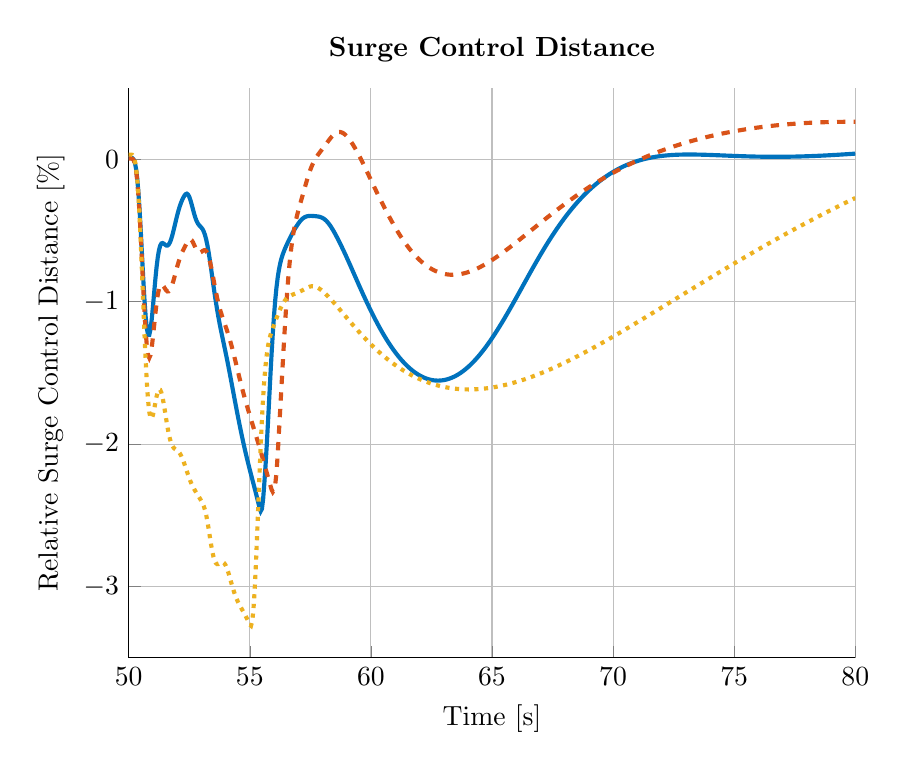
\begin{tikzpicture}

\begin{axis}[%
width=0.761\linewidth,
height=0.597\linewidth,
at={(0\linewidth,0\linewidth)},
scale only axis,
xmin=50,
xmax=80,
xlabel={Time [s]},
xmajorgrids,
ymin=-3.5,
ymax=0.5,
ylabel={Relative Surge Control Distance [\%]},
ymajorgrids,
axis background/.style={fill=white},
title style={font=\bfseries},
title={Surge Control Distance},
axis x line*=bottom,
axis y line*=left
]
\addplot [color=mycolor1,solid,line width=1.5pt,forget plot]
  table[row sep=crcr]{%
50	0.00842000000000098\\
50.05	0.00842000000000098\\
50.1	0.00830999999999982\\
50.15	0.00663000000000125\\
50.2	-0.0012099999999986\\
50.25	-0.0222599999999993\\
50.3	-0.0639099999999999\\
50.35	-0.132719999999999\\
50.4	-0.232239999999999\\
50.45	-0.36088\\
50.5	-0.512049999999999\\
50.55	-0.675109999999999\\
50.6	-0.837149999999999\\
50.65	-0.984749999999999\\
50.7	-1.10552\\
50.75	-1.18987\\
50.8	-1.23236\\
50.85	-1.23239\\
50.9	-1.19405\\
50.95	-1.12528\\
51	-1.03653\\
51.05	-0.93906\\
51.1	-0.843399999999999\\
51.15	-0.758109999999999\\
51.2	-0.68894\\
51.25	-0.638629999999999\\
51.3	-0.607069999999999\\
51.35	-0.591819999999999\\
51.4	-0.58885\\
51.45	-0.593369999999999\\
51.5	-0.600519999999999\\
51.55	-0.606\\
51.6	-0.606489999999999\\
51.65	-0.5999\\
51.7	-0.585389999999999\\
51.75	-0.56328\\
51.8	-0.53478\\
51.85	-0.501729999999999\\
51.9	-0.466229999999999\\
51.95	-0.430339999999999\\
52	-0.395809999999999\\
52.05	-0.363939999999999\\
52.1	-0.3355\\
52.15	-0.310759999999999\\
52.2	-0.289579999999999\\
52.25	-0.271539999999999\\
52.3	-0.25637\\
52.35	-0.24578\\
52.4	-0.24252\\
52.45	-0.248589999999999\\
52.5	-0.264349999999999\\
52.55	-0.28846\\
52.6	-0.318319999999999\\
52.65	-0.350669999999999\\
52.7	-0.382239999999999\\
52.75	-0.410279999999999\\
52.8	-0.433059999999999\\
52.85	-0.45011\\
52.9	-0.46228\\
52.95	-0.4715\\
53	-0.48042\\
53.05	-0.491929999999999\\
53.1	-0.508659999999999\\
53.15	-0.532579999999999\\
53.2	-0.564799999999999\\
53.25	-0.60544\\
53.3	-0.653709999999999\\
53.35	-0.70813\\
53.4	-0.766789999999999\\
53.45	-0.827649999999999\\
53.5	-0.88857\\
53.55	-0.94764\\
53.6	-1.00359\\
53.65	-1.056\\
53.7	-1.10493\\
53.75	-1.15064\\
53.8	-1.19375\\
53.85	-1.23507\\
53.9	-1.27545\\
53.95	-1.31567\\
54	-1.35633\\
54.05	-1.39785\\
54.1	-1.44041\\
54.15	-1.48401\\
54.2	-1.52849\\
54.25	-1.57359\\
54.3	-1.619\\
54.35	-1.66439\\
54.4	-1.70949\\
54.45	-1.75405\\
54.5	-1.7979\\
54.55	-1.8409\\
54.6	-1.88296\\
54.65	-1.92401\\
54.7	-1.964\\
54.75	-2.00288\\
54.8	-2.04058\\
54.85	-2.07711\\
54.9	-2.11245\\
54.95	-2.14673\\
55	-2.18014\\
55.05	-2.21291\\
55.1	-2.24532\\
55.15	-2.27765\\
55.2	-2.31017\\
55.25	-2.34312\\
55.3	-2.37669\\
55.35	-2.411\\
55.4	-2.44607\\
55.45	-2.47036\\
55.5	-2.45483\\
55.55	-2.38603\\
55.6	-2.27549\\
55.65	-2.14955\\
55.7	-2.00669\\
55.75	-1.84971\\
55.8	-1.68513\\
55.85	-1.52085\\
55.9	-1.36436\\
55.95	-1.22161\\
56	-1.09641\\
56.05	-0.990429999999999\\
56.1	-0.903429999999999\\
56.15	-0.833749999999999\\
56.2	-0.77886\\
56.25	-0.735829999999999\\
56.3	-0.70175\\
56.35	-0.674009999999999\\
56.4	-0.650469999999999\\
56.45	-0.629529999999999\\
56.5	-0.61009\\
56.55	-0.59153\\
56.6	-0.573539999999999\\
56.65	-0.556069999999999\\
56.7	-0.53916\\
56.75	-0.522939999999999\\
56.8	-0.507479999999999\\
56.85	-0.492789999999999\\
56.9	-0.478789999999999\\
56.95	-0.46545\\
57	-0.452889999999999\\
57.05	-0.441349999999999\\
57.1	-0.43106\\
57.15	-0.42221\\
57.2	-0.41489\\
57.25	-0.4091\\
57.3	-0.40478\\
57.35	-0.401769999999999\\
57.4	-0.39988\\
57.45	-0.39887\\
57.5	-0.398529999999999\\
57.55	-0.39863\\
57.6	-0.398999999999999\\
57.65	-0.399539999999999\\
57.7	-0.4002\\
57.75	-0.40103\\
57.8	-0.402139999999999\\
57.85	-0.403659999999999\\
57.9	-0.405799999999999\\
57.95	-0.408729999999999\\
58	-0.412649999999999\\
58.05	-0.417699999999999\\
58.1	-0.42399\\
58.15	-0.431589999999999\\
58.2	-0.440499999999999\\
58.25	-0.450679999999999\\
58.3	-0.46205\\
58.35	-0.47451\\
58.4	-0.487939999999999\\
58.45	-0.50219\\
58.5	-0.51716\\
58.55	-0.532719999999999\\
58.6	-0.54878\\
58.65	-0.56528\\
58.7	-0.58215\\
58.75	-0.599349999999999\\
58.8	-0.616859999999999\\
58.85	-0.634659999999999\\
58.9	-0.652729999999999\\
58.95	-0.671049999999999\\
59	-0.689609999999999\\
59.05	-0.70839\\
59.1	-0.727349999999999\\
59.15	-0.74647\\
59.2	-0.7657\\
59.25	-0.785019999999999\\
59.3	-0.80437\\
59.35	-0.823739999999999\\
59.4	-0.843069999999999\\
59.45	-0.862349999999999\\
59.5	-0.88153\\
59.55	-0.9006\\
59.6	-0.919529999999999\\
59.65	-0.93831\\
59.7	-0.956919999999999\\
59.75	-0.97535\\
59.8	-0.99358\\
59.85	-1.01162\\
59.9	-1.02945\\
59.95	-1.04707\\
60	-1.06446\\
60.05	-1.08161\\
60.1	-1.09853\\
60.15	-1.11521\\
60.2	-1.13163\\
60.25	-1.14778\\
60.3	-1.16367\\
60.35	-1.17927\\
60.4	-1.19459\\
60.45	-1.20962\\
60.5	-1.22434\\
60.55	-1.23876\\
60.6	-1.25287\\
60.65	-1.26666\\
60.7	-1.28014\\
60.75	-1.29329\\
60.8	-1.30613\\
60.85	-1.31863\\
60.9	-1.33082\\
60.95	-1.34268\\
61	-1.35421\\
61.05	-1.36542\\
61.1	-1.37631\\
61.15	-1.38687\\
61.2	-1.3971\\
61.25	-1.40701\\
61.3	-1.4166\\
61.35	-1.42586\\
61.4	-1.43479\\
61.45	-1.4434\\
61.5	-1.45168\\
61.55	-1.45964\\
61.6	-1.46727\\
61.65	-1.47458\\
61.7	-1.48156\\
61.75	-1.48822\\
61.8	-1.49455\\
61.85	-1.50057\\
61.9	-1.50626\\
61.95	-1.51162\\
62	-1.51667\\
62.05	-1.5214\\
62.1	-1.52581\\
62.15	-1.52989\\
62.2	-1.53366\\
62.25	-1.53712\\
62.3	-1.54025\\
62.35	-1.54307\\
62.4	-1.54557\\
62.45	-1.54775\\
62.5	-1.54962\\
62.55	-1.55117\\
62.6	-1.5524\\
62.65	-1.55332\\
62.7	-1.55393\\
62.75	-1.55422\\
62.8	-1.55419\\
62.85	-1.55385\\
62.9	-1.5532\\
62.95	-1.55224\\
63	-1.55096\\
63.05	-1.54937\\
63.1	-1.54746\\
63.15	-1.54525\\
63.2	-1.54272\\
63.25	-1.53989\\
63.3	-1.53674\\
63.35	-1.53329\\
63.4	-1.52952\\
63.45	-1.52545\\
63.5	-1.52107\\
63.55	-1.51639\\
63.6	-1.5114\\
63.65	-1.50611\\
63.7	-1.50052\\
63.75	-1.49462\\
63.8	-1.48843\\
63.85	-1.48193\\
63.9	-1.47515\\
63.95	-1.46806\\
64	-1.46069\\
64.05	-1.45303\\
64.1	-1.44508\\
64.15	-1.43684\\
64.2	-1.42833\\
64.25	-1.41953\\
64.3	-1.41046\\
64.35	-1.40112\\
64.4	-1.39151\\
64.45	-1.38163\\
64.5	-1.3715\\
64.55	-1.3611\\
64.6	-1.35046\\
64.65	-1.33957\\
64.7	-1.32843\\
64.75	-1.31706\\
64.8	-1.30545\\
64.85	-1.29362\\
64.9	-1.28156\\
64.95	-1.26929\\
65	-1.25681\\
65.05	-1.24412\\
65.1	-1.23124\\
65.15	-1.21816\\
65.2	-1.2049\\
65.25	-1.19147\\
65.3	-1.17786\\
65.35	-1.16408\\
65.4	-1.15015\\
65.45	-1.13607\\
65.5	-1.12185\\
65.55	-1.10749\\
65.6	-1.09301\\
65.65	-1.07841\\
65.7	-1.0637\\
65.75	-1.04889\\
65.8	-1.03398\\
65.85	-1.01898\\
65.9	-1.00391\\
65.95	-0.988779999999999\\
66	-0.973579999999999\\
66.05	-0.958329999999999\\
66.1	-0.94304\\
66.15	-0.92772\\
66.2	-0.912369999999999\\
66.25	-0.897019999999999\\
66.3	-0.881659999999999\\
66.35	-0.8663\\
66.4	-0.85096\\
66.45	-0.835649999999999\\
66.5	-0.820359999999999\\
66.55	-0.805129999999999\\
66.6	-0.78994\\
66.65	-0.774819999999999\\
66.7	-0.75977\\
66.75	-0.7448\\
66.8	-0.729919999999999\\
66.85	-0.715129999999999\\
66.9	-0.70044\\
66.95	-0.685859999999999\\
67	-0.671399999999999\\
67.05	-0.65706\\
67.1	-0.642849999999999\\
67.15	-0.628769999999999\\
67.2	-0.614819999999999\\
67.25	-0.601019999999999\\
67.3	-0.58735\\
67.35	-0.57384\\
67.4	-0.56047\\
67.45	-0.54726\\
67.5	-0.534199999999999\\
67.55	-0.521299999999999\\
67.6	-0.508559999999999\\
67.65	-0.495979999999999\\
67.7	-0.48356\\
67.75	-0.471299999999999\\
67.8	-0.45921\\
67.85	-0.447279999999999\\
67.9	-0.435519999999999\\
67.95	-0.423929999999999\\
68	-0.4125\\
68.05	-0.401249999999999\\
68.1	-0.39016\\
68.15	-0.379239999999999\\
68.2	-0.36849\\
68.25	-0.357919999999999\\
68.3	-0.34751\\
68.35	-0.337269999999999\\
68.4	-0.327199999999999\\
68.45	-0.317309999999999\\
68.5	-0.30758\\
68.55	-0.298019999999999\\
68.6	-0.288629999999999\\
68.65	-0.2794\\
68.7	-0.27035\\
68.75	-0.261449999999999\\
68.8	-0.25273\\
68.85	-0.24417\\
68.9	-0.23577\\
68.95	-0.22753\\
69	-0.21946\\
69.05	-0.211539999999999\\
69.1	-0.20379\\
69.15	-0.19619\\
69.2	-0.18875\\
69.25	-0.18146\\
69.3	-0.17432\\
69.35	-0.167339999999999\\
69.4	-0.160509999999999\\
69.45	-0.153829999999999\\
69.5	-0.1473\\
69.55	-0.14091\\
69.6	-0.13467\\
69.65	-0.128579999999999\\
69.7	-0.122629999999999\\
69.75	-0.116819999999999\\
69.8	-0.11115\\
69.85	-0.10562\\
69.9	-0.10023\\
69.95	-0.0949799999999996\\
70	-0.0898599999999998\\
70.05	-0.0848699999999987\\
70.1	-0.0800199999999993\\
70.15	-0.0752999999999986\\
70.2	-0.0707100000000001\\
70.25	-0.0662399999999987\\
70.3	-0.0619099999999992\\
70.35	-0.0576899999999991\\
70.4	-0.053609999999999\\
70.45	-0.0496400000000001\\
70.5	-0.0457900000000002\\
70.55	-0.0420699999999989\\
70.6	-0.0384599999999988\\
70.65	-0.0349599999999999\\
70.7	-0.0315799999999999\\
70.75	-0.028319999999999\\
70.8	-0.0251599999999996\\
70.85	-0.0221099999999996\\
70.9	-0.019169999999999\\
70.95	-0.01633\\
71	-0.0136000000000003\\
71.05	-0.0109699999999986\\
71.1	-0.00842999999999883\\
71.15	-0.00600000000000023\\
71.2	-0.00366\\
71.25	-0.00141999999999953\\
71.3	0.000740000000000407\\
71.35	0.00280000000000058\\
71.4	0.00477000000000061\\
71.45	0.00666000000000011\\
71.5	0.00846000000000124\\
71.55	0.0101800000000001\\
71.6	0.0118200000000002\\
71.65	0.0133799999999997\\
71.7	0.0148600000000005\\
71.75	0.0162700000000005\\
71.8	0.0176100000000012\\
71.85	0.0188699999999997\\
71.9	0.0200600000000009\\
71.95	0.0211900000000007\\
72	0.0222500000000014\\
72.05	0.0232400000000013\\
72.1	0.0241699999999998\\
72.15	0.0250500000000002\\
72.2	0.0258599999999998\\
72.25	0.0266200000000012\\
72.3	0.0273200000000013\\
72.35	0.0279699999999998\\
72.4	0.0285600000000006\\
72.45	0.0291100000000011\\
72.5	0.0296099999999999\\
72.55	0.0300600000000006\\
72.6	0.0304599999999997\\
72.65	0.0308200000000003\\
72.7	0.0311400000000006\\
72.75	0.0314200000000007\\
72.8	0.0316600000000005\\
72.85	0.03186\\
72.9	0.0320300000000007\\
72.95	0.0321600000000011\\
73	0.0322600000000008\\
73.05	0.03233\\
73.1	0.0323600000000006\\
73.15	0.0323700000000002\\
73.2	0.032350000000001\\
73.25	0.0323100000000007\\
73.3	0.0322300000000002\\
73.35	0.0321400000000001\\
73.4	0.032020000000001\\
73.45	0.031880000000001\\
73.5	0.0317300000000014\\
73.55	0.0315500000000011\\
73.6	0.0313499999999998\\
73.65	0.0311400000000006\\
73.7	0.0309100000000004\\
73.75	0.0306700000000006\\
73.8	0.0304200000000012\\
73.85	0.0301500000000008\\
73.9	0.0298700000000007\\
73.95	0.029580000000001\\
74	0.02928\\
74.05	0.0289700000000011\\
74.1	0.0286600000000004\\
74.15	0.02834\\
74.2	0.0280100000000001\\
74.25	0.0276700000000005\\
74.3	0.027330000000001\\
74.35	0.0269900000000014\\
74.4	0.0266500000000001\\
74.45	0.0263000000000009\\
74.5	0.0259499999999999\\
74.55	0.0256000000000007\\
74.6	0.0252499999999998\\
74.65	0.0249000000000006\\
74.7	0.0245500000000014\\
74.75	0.0242100000000001\\
74.8	0.0238600000000009\\
74.85	0.0235200000000013\\
74.9	0.02318\\
74.95	0.02285\\
75	0.0225200000000001\\
75.05	0.0221900000000002\\
75.1	0.0218699999999998\\
75.15	0.0215600000000009\\
75.2	0.0212500000000002\\
75.25	0.0209500000000009\\
75.3	0.0206499999999998\\
75.35	0.0203600000000002\\
75.4	0.0200800000000001\\
75.45	0.0198100000000014\\
75.5	0.0195500000000006\\
75.55	0.0192899999999998\\
75.6	0.0190400000000004\\
75.65	0.0188100000000002\\
75.7	0.01858\\
75.75	0.0183600000000013\\
75.8	0.0181500000000003\\
75.85	0.0179500000000008\\
75.9	0.0177600000000009\\
75.95	0.0175800000000006\\
76	0.0174200000000013\\
76.05	0.0172600000000003\\
76.1	0.0171100000000006\\
76.15	0.0169800000000002\\
76.2	0.0168600000000012\\
76.25	0.0167400000000004\\
76.3	0.0166400000000007\\
76.35	0.0165500000000005\\
76.4	0.01647\\
76.45	0.0164100000000005\\
76.5	0.016350000000001\\
76.55	0.0163100000000007\\
76.6	0.0162800000000001\\
76.65	0.0162600000000008\\
76.7	0.0162500000000012\\
76.75	0.0162500000000012\\
76.8	0.0162700000000005\\
76.85	0.0163000000000011\\
76.9	0.0163400000000014\\
76.95	0.0163900000000012\\
77	0.0164500000000007\\
77.05	0.0165300000000013\\
77.1	0.01661\\
77.15	0.0167099999999998\\
77.2	0.0168200000000009\\
77.25	0.01694\\
77.3	0.01708\\
77.35	0.01722\\
77.4	0.0173800000000011\\
77.45	0.0175400000000003\\
77.5	0.0177200000000006\\
77.55	0.0179100000000005\\
77.6	0.0181100000000001\\
77.65	0.018320000000001\\
77.7	0.0185500000000012\\
77.75	0.0187800000000014\\
77.8	0.0190300000000008\\
77.85	0.0192800000000002\\
77.9	0.0195500000000006\\
77.95	0.0198200000000011\\
78	0.0201100000000007\\
78.05	0.0204000000000004\\
78.1	0.0207100000000011\\
78.15	0.0210300000000014\\
78.2	0.02135\\
78.25	0.0216900000000013\\
78.3	0.0220300000000009\\
78.35	0.0223899999999997\\
78.4	0.0227500000000003\\
78.45	0.0231300000000001\\
78.5	0.0235099999999999\\
78.55	0.0239000000000011\\
78.6	0.0243000000000002\\
78.65	0.0247100000000007\\
78.7	0.0251200000000011\\
78.75	0.0255500000000008\\
78.8	0.0259800000000006\\
78.85	0.0264300000000013\\
78.9	0.0268800000000002\\
78.95	0.0273400000000006\\
79	0.0278000000000009\\
79.05	0.0282700000000009\\
79.1	0.0287600000000001\\
79.15	0.0292399999999997\\
79.2	0.0297400000000003\\
79.25	0.0302400000000009\\
79.3	0.0307500000000012\\
79.35	0.031270000000001\\
79.4	0.0317900000000009\\
79.45	0.0323200000000003\\
79.5	0.0328600000000012\\
79.55	0.0334000000000003\\
79.6	0.0339500000000008\\
79.65	0.0345000000000013\\
79.7	0.035070000000001\\
79.75	0.0356300000000012\\
79.8	0.0362000000000009\\
79.85	0.0367800000000003\\
79.9	0.037370000000001\\
79.95	0.03796\\
80	0.0385500000000008\\
};
\addplot [color=mycolor2,dashed,line width=1.5pt,forget plot]
  table[row sep=crcr]{%
50	0.00472000000000072\\
50.05	0.00472000000000072\\
50.1	0.00461000000000134\\
50.15	0.00285000000000046\\
50.2	-0.00546999999999898\\
50.25	-0.0279699999999998\\
50.3	-0.0728899999999992\\
50.35	-0.14678\\
50.4	-0.252549999999999\\
50.45	-0.389119999999999\\
50.5	-0.550759999999999\\
50.55	-0.727139999999999\\
50.6	-0.905029999999999\\
50.65	-1.07028\\
50.7	-1.20986\\
50.75	-1.31357\\
50.8	-1.3755\\
50.85	-1.3946\\
50.9	-1.37461\\
50.95	-1.32314\\
51	-1.25039\\
51.05	-1.16746\\
51.1	-1.0848\\
51.15	-1.01101\\
51.2	-0.951989999999999\\
51.25	-0.910699999999999\\
51.3	-0.887269999999999\\
51.35	-0.879549999999999\\
51.4	-0.88374\\
51.45	-0.89521\\
51.5	-0.909179999999999\\
51.55	-0.921379999999999\\
51.6	-0.928439999999999\\
51.65	-0.928179999999999\\
51.7	-0.919689999999999\\
51.75	-0.903189999999999\\
51.8	-0.879849999999999\\
51.85	-0.85145\\
51.9	-0.820069999999999\\
51.95	-0.78773\\
52	-0.756219999999999\\
52.05	-0.72681\\
52.1	-0.70027\\
52.15	-0.67681\\
52.2	-0.656179999999999\\
52.25	-0.637759999999999\\
52.3	-0.62076\\
52.35	-0.60429\\
52.4	-0.587899999999999\\
52.45	-0.573429999999999\\
52.5	-0.56406\\
52.55	-0.562259999999999\\
52.6	-0.568779999999999\\
52.65	-0.582479999999999\\
52.7	-0.600719999999999\\
52.75	-0.620119999999999\\
52.8	-0.63728\\
52.85	-0.649539999999999\\
52.9	-0.655559999999999\\
52.95	-0.655539999999999\\
53	-0.65107\\
53.05	-0.64479\\
53.1	-0.63986\\
53.15	-0.63932\\
53.2	-0.64565\\
53.25	-0.660379999999999\\
53.3	-0.683949999999999\\
53.35	-0.71573\\
53.4	-0.754219999999999\\
53.45	-0.79735\\
53.5	-0.8428\\
53.55	-0.888349999999999\\
53.6	-0.932119999999999\\
53.65	-0.97279\\
53.7	-1.00967\\
53.75	-1.04267\\
53.8	-1.07222\\
53.85	-1.09913\\
53.9	-1.12437\\
53.95	-1.14894\\
54	-1.17352\\
54.05	-1.19871\\
54.1	-1.22497\\
54.15	-1.25248\\
54.2	-1.28142\\
54.25	-1.31207\\
54.3	-1.3445\\
54.35	-1.37837\\
54.4	-1.41324\\
54.45	-1.44864\\
54.5	-1.48409\\
54.55	-1.51919\\
54.6	-1.55363\\
54.65	-1.5872\\
54.7	-1.61981\\
54.75	-1.65148\\
54.8	-1.68225\\
54.85	-1.71224\\
54.9	-1.74156\\
54.95	-1.77035\\
55	-1.79871\\
55.05	-1.82675\\
55.1	-1.85457\\
55.15	-1.88224\\
55.2	-1.90984\\
55.25	-1.93748\\
55.3	-1.96534\\
55.35	-1.99354\\
55.4	-2.02216\\
55.45	-2.05124\\
55.5	-2.08074\\
55.55	-2.11058\\
55.6	-2.14064\\
55.65	-2.17081\\
55.7	-2.20093\\
55.75	-2.2309\\
55.8	-2.2606\\
55.85	-2.28998\\
55.9	-2.31897\\
55.95	-2.33591\\
56	-2.32314\\
56.05	-2.28461\\
56.1	-2.20445\\
56.15	-2.07872\\
56.2	-1.92513\\
56.25	-1.77291\\
56.3	-1.62001\\
56.35	-1.4667\\
56.4	-1.31595\\
56.45	-1.17168\\
56.5	-1.03758\\
56.55	-0.916429999999999\\
56.6	-0.80976\\
56.65	-0.717829999999999\\
56.7	-0.639869999999999\\
56.75	-0.574339999999999\\
56.8	-0.519259999999999\\
56.85	-0.472529999999999\\
56.9	-0.43209\\
56.95	-0.39615\\
57	-0.363219999999999\\
57.05	-0.332129999999999\\
57.1	-0.30204\\
57.15	-0.272329999999999\\
57.2	-0.24257\\
57.25	-0.212569999999999\\
57.3	-0.182639999999999\\
57.35	-0.153309999999999\\
57.4	-0.1252\\
57.45	-0.0988399999999992\\
57.5	-0.0746000000000002\\
57.55	-0.0526799999999987\\
57.6	-0.0330899999999996\\
57.65	-0.0156700000000001\\
57.7	-0.000169999999998893\\
57.75	0.0137700000000009\\
57.8	0.0265000000000004\\
57.85	0.0383800000000001\\
57.9	0.0497300000000003\\
57.95	0.060830000000001\\
58	0.0718800000000002\\
58.05	0.0830300000000008\\
58.1	0.0943500000000004\\
58.15	0.105840000000001\\
58.2	0.117420000000001\\
58.25	0.12893\\
58.3	0.14015\\
58.35	0.150830000000001\\
58.4	0.160690000000001\\
58.45	0.16947\\
58.5	0.17694\\
58.55	0.18291\\
58.6	0.187230000000001\\
58.65	0.189810000000001\\
58.7	0.190610000000001\\
58.75	0.18965\\
58.8	0.186970000000001\\
58.85	0.18267\\
58.9	0.17685\\
58.95	0.169640000000001\\
59	0.161160000000001\\
59.05	0.151540000000001\\
59.1	0.140890000000001\\
59.15	0.12932\\
59.2	0.11692\\
59.25	0.103770000000001\\
59.3	0.0899400000000004\\
59.35	0.0754999999999999\\
59.4	0.0604899999999997\\
59.45	0.0449700000000011\\
59.5	0.0289800000000007\\
59.55	0.0125700000000002\\
59.6	-0.00419999999999909\\
59.65	-0.0213000000000001\\
59.7	-0.0386600000000001\\
59.75	-0.056239999999999\\
59.8	-0.0739999999999998\\
59.85	-0.0918700000000001\\
59.9	-0.109829999999999\\
59.95	-0.12782\\
60	-0.14582\\
60.05	-0.16379\\
60.1	-0.18169\\
60.15	-0.19952\\
60.2	-0.217239999999999\\
60.25	-0.23485\\
60.3	-0.25233\\
60.35	-0.26967\\
60.4	-0.28687\\
60.45	-0.3039\\
60.5	-0.320779999999999\\
60.55	-0.337479999999999\\
60.6	-0.353999999999999\\
60.65	-0.37034\\
60.7	-0.386469999999999\\
60.75	-0.402399999999999\\
60.8	-0.418099999999999\\
60.85	-0.43357\\
60.9	-0.44879\\
60.95	-0.46376\\
61	-0.47845\\
61.05	-0.492859999999999\\
61.1	-0.50698\\
61.15	-0.520799999999999\\
61.2	-0.53431\\
61.25	-0.547499999999999\\
61.3	-0.56037\\
61.35	-0.572909999999999\\
61.4	-0.585129999999999\\
61.45	-0.59702\\
61.5	-0.608569999999999\\
61.55	-0.619789999999999\\
61.6	-0.630679999999999\\
61.65	-0.64124\\
61.7	-0.651459999999999\\
61.75	-0.66135\\
61.8	-0.670909999999999\\
61.85	-0.680129999999999\\
61.9	-0.68903\\
61.95	-0.697589999999999\\
62	-0.70583\\
62.05	-0.713729999999999\\
62.1	-0.721309999999999\\
62.15	-0.72856\\
62.2	-0.735479999999999\\
62.25	-0.742089999999999\\
62.3	-0.74837\\
62.35	-0.754339999999999\\
62.4	-0.759989999999999\\
62.45	-0.765319999999999\\
62.5	-0.77035\\
62.55	-0.775069999999999\\
62.6	-0.779489999999999\\
62.65	-0.7836\\
62.7	-0.787419999999999\\
62.75	-0.79095\\
62.8	-0.79418\\
62.85	-0.797129999999999\\
62.9	-0.79979\\
62.95	-0.802169999999999\\
63	-0.80427\\
63.05	-0.8061\\
63.1	-0.807659999999999\\
63.15	-0.808949999999999\\
63.2	-0.80997\\
63.25	-0.810739999999999\\
63.3	-0.811249999999999\\
63.35	-0.8115\\
63.4	-0.811509999999999\\
63.45	-0.811279999999999\\
63.5	-0.8108\\
63.55	-0.81009\\
63.6	-0.80915\\
63.65	-0.80798\\
63.7	-0.8066\\
63.75	-0.804989999999999\\
63.8	-0.80317\\
63.85	-0.80115\\
63.9	-0.79892\\
63.95	-0.796499999999999\\
64	-0.79388\\
64.05	-0.791079999999999\\
64.1	-0.78809\\
64.15	-0.78492\\
64.2	-0.781579999999999\\
64.25	-0.77807\\
64.3	-0.774399999999999\\
64.35	-0.770569999999999\\
64.4	-0.766579999999999\\
64.45	-0.762449999999999\\
64.5	-0.75817\\
64.55	-0.753749999999999\\
64.6	-0.74919\\
64.65	-0.744509999999999\\
64.7	-0.739699999999999\\
64.75	-0.734769999999999\\
64.8	-0.729719999999999\\
64.85	-0.724559999999999\\
64.9	-0.719289999999999\\
64.95	-0.713909999999999\\
65	-0.70844\\
65.05	-0.70287\\
65.1	-0.697209999999999\\
65.15	-0.691459999999999\\
65.2	-0.68563\\
65.25	-0.67972\\
65.3	-0.673729999999999\\
65.35	-0.667669999999999\\
65.4	-0.661549999999999\\
65.45	-0.655349999999999\\
65.5	-0.6491\\
65.55	-0.64279\\
65.6	-0.63643\\
65.65	-0.63001\\
65.7	-0.62355\\
65.75	-0.617039999999999\\
65.8	-0.61049\\
65.85	-0.603899999999999\\
65.9	-0.59728\\
65.95	-0.590619999999999\\
66	-0.58393\\
66.05	-0.57722\\
66.1	-0.57048\\
66.15	-0.563719999999999\\
66.2	-0.556939999999999\\
66.25	-0.55014\\
66.3	-0.543329999999999\\
66.35	-0.536499999999999\\
66.4	-0.529669999999999\\
66.45	-0.522829999999999\\
66.5	-0.51598\\
66.55	-0.50913\\
66.6	-0.502269999999999\\
66.65	-0.495419999999999\\
66.7	-0.48856\\
66.75	-0.481719999999999\\
66.8	-0.474869999999999\\
66.85	-0.468039999999999\\
66.9	-0.461209999999999\\
66.95	-0.4544\\
67	-0.447589999999999\\
67.05	-0.440799999999999\\
67.1	-0.434029999999999\\
67.15	-0.427269999999999\\
67.2	-0.420529999999999\\
67.25	-0.41381\\
67.3	-0.4071\\
67.35	-0.40042\\
67.4	-0.393769999999999\\
67.45	-0.387129999999999\\
67.5	-0.38052\\
67.55	-0.373939999999999\\
67.6	-0.367389999999999\\
67.65	-0.36086\\
67.7	-0.35436\\
67.75	-0.34789\\
67.8	-0.341449999999999\\
67.85	-0.335039999999999\\
67.9	-0.32867\\
67.95	-0.322319999999999\\
68	-0.316009999999999\\
68.05	-0.30974\\
68.1	-0.3035\\
68.15	-0.297289999999999\\
68.2	-0.291119999999999\\
68.25	-0.28499\\
68.3	-0.278899999999999\\
68.35	-0.27284\\
68.4	-0.266819999999999\\
68.45	-0.260839999999999\\
68.5	-0.254899999999999\\
68.55	-0.248989999999999\\
68.6	-0.24313\\
68.65	-0.237309999999999\\
68.7	-0.23152\\
68.75	-0.225779999999999\\
68.8	-0.220079999999999\\
68.85	-0.21442\\
68.9	-0.208799999999999\\
68.95	-0.203219999999999\\
69	-0.19769\\
69.05	-0.192189999999999\\
69.1	-0.186739999999999\\
69.15	-0.181329999999999\\
69.2	-0.175959999999999\\
69.25	-0.17064\\
69.3	-0.165349999999999\\
69.35	-0.16011\\
69.4	-0.15492\\
69.45	-0.14976\\
69.5	-0.14465\\
69.55	-0.13958\\
69.6	-0.134549999999999\\
69.65	-0.129569999999999\\
69.7	-0.12462\\
69.75	-0.119719999999999\\
69.8	-0.11487\\
69.85	-0.110049999999999\\
69.9	-0.105279999999999\\
69.95	-0.10055\\
70	-0.0958600000000001\\
70.05	-0.0912199999999999\\
70.1	-0.0866100000000003\\
70.15	-0.0820499999999988\\
70.2	-0.0775299999999994\\
70.25	-0.0730500000000003\\
70.3	-0.0686199999999992\\
70.35	-0.0642199999999988\\
70.4	-0.0598599999999987\\
70.45	-0.0555500000000002\\
70.5	-0.0512800000000002\\
70.55	-0.0470399999999991\\
70.6	-0.0428499999999996\\
70.65	-0.0386999999999986\\
70.7	-0.0345899999999997\\
70.75	-0.0305099999999996\\
70.8	-0.0264799999999994\\
70.85	-0.0224899999999995\\
70.9	-0.0185300000000002\\
70.95	-0.014619999999999\\
71	-0.0107400000000002\\
71.05	-0.00689999999999991\\
71.1	-0.00309999999999988\\
71.15	0.000659999999999883\\
71.2	0.00439000000000078\\
71.25	0.00808000000000142\\
71.3	0.01173\\
71.35	0.0153400000000001\\
71.4	0.0189200000000014\\
71.45	0.022450000000001\\
71.5	0.0259600000000013\\
71.55	0.0294300000000014\\
71.6	0.0328600000000012\\
71.65	0.0362500000000008\\
71.7	0.0396099999999997\\
71.75	0.0429399999999998\\
71.8	0.0462300000000013\\
71.85	0.0494900000000005\\
71.9	0.0527100000000011\\
71.95	0.0559000000000012\\
72	0.0590500000000009\\
72.05	0.0621799999999997\\
72.1	0.0652600000000003\\
72.15	0.0683199999999999\\
72.2	0.0713400000000011\\
72.25	0.0743299999999998\\
72.3	0.0772900000000014\\
72.35	0.080210000000001\\
72.4	0.0831100000000013\\
72.45	0.0859700000000014\\
72.5	0.0888000000000009\\
72.55	0.0915999999999997\\
72.6	0.0943700000000014\\
72.65	0.0971100000000007\\
72.7	0.0998200000000011\\
72.75	0.102500000000001\\
72.8	0.10515\\
72.85	0.10777\\
72.9	0.11036\\
72.95	0.112920000000001\\
73	0.115450000000001\\
73.05	0.11796\\
73.1	0.120430000000001\\
73.15	0.12288\\
73.2	0.125300000000001\\
73.25	0.127690000000001\\
73.3	0.130050000000001\\
73.35	0.132390000000001\\
73.4	0.1347\\
73.45	0.136980000000001\\
73.5	0.139240000000001\\
73.55	0.14147\\
73.6	0.14367\\
73.65	0.145850000000001\\
73.7	0.148\\
73.75	0.150130000000001\\
73.8	0.152230000000001\\
73.85	0.154310000000001\\
73.9	0.156360000000001\\
73.95	0.158390000000001\\
74	0.160390000000001\\
74.05	0.162360000000001\\
74.1	0.16432\\
74.15	0.16625\\
74.2	0.168150000000001\\
74.25	0.170030000000001\\
74.3	0.171890000000001\\
74.35	0.173720000000001\\
74.4	0.17553\\
74.45	0.17732\\
74.5	0.17909\\
74.55	0.18083\\
74.6	0.182550000000001\\
74.65	0.18425\\
74.7	0.185920000000001\\
74.75	0.187580000000001\\
74.8	0.189210000000001\\
74.85	0.19082\\
74.9	0.192400000000001\\
74.95	0.19397\\
75	0.19552\\
75.05	0.197040000000001\\
75.1	0.198540000000001\\
75.15	0.20002\\
75.2	0.20149\\
75.25	0.20293\\
75.3	0.20435\\
75.35	0.20575\\
75.4	0.207130000000001\\
75.45	0.208490000000001\\
75.5	0.20983\\
75.55	0.21115\\
75.6	0.21245\\
75.65	0.21373\\
75.7	0.21499\\
75.75	0.216230000000001\\
75.8	0.217450000000001\\
75.85	0.21865\\
75.9	0.219840000000001\\
75.95	0.221\\
76	0.222150000000001\\
76.05	0.223280000000001\\
76.1	0.224390000000001\\
76.15	0.225480000000001\\
76.2	0.226550000000001\\
76.25	0.22761\\
76.3	0.22864\\
76.35	0.229660000000001\\
76.4	0.23066\\
76.45	0.23165\\
76.5	0.232610000000001\\
76.55	0.233560000000001\\
76.6	0.234490000000001\\
76.65	0.2354\\
76.7	0.2363\\
76.75	0.23718\\
76.8	0.23804\\
76.85	0.23888\\
76.9	0.239710000000001\\
76.95	0.24052\\
77	0.24131\\
77.05	0.242090000000001\\
77.1	0.242850000000001\\
77.15	0.243600000000001\\
77.2	0.24433\\
77.25	0.245040000000001\\
77.3	0.24573\\
77.35	0.246410000000001\\
77.4	0.24708\\
77.45	0.247720000000001\\
77.5	0.24836\\
77.55	0.24897\\
77.6	0.24957\\
77.65	0.250160000000001\\
77.7	0.250730000000001\\
77.75	0.251280000000001\\
77.8	0.25182\\
77.85	0.25235\\
77.9	0.25286\\
77.95	0.253350000000001\\
78	0.253830000000001\\
78.05	0.254290000000001\\
78.1	0.25474\\
78.15	0.255180000000001\\
78.2	0.255600000000001\\
78.25	0.25601\\
78.3	0.256400000000001\\
78.35	0.256770000000001\\
78.4	0.25714\\
78.45	0.257490000000001\\
78.5	0.257820000000001\\
78.55	0.258140000000001\\
78.6	0.25845\\
78.65	0.258740000000001\\
78.7	0.259020000000001\\
78.75	0.25929\\
78.8	0.259540000000001\\
78.85	0.259780000000001\\
78.9	0.260010000000001\\
78.95	0.26022\\
79	0.26042\\
79.05	0.26061\\
79.1	0.26078\\
79.15	0.26094\\
79.2	0.261090000000001\\
79.25	0.261230000000001\\
79.3	0.26135\\
79.35	0.261460000000001\\
79.4	0.261560000000001\\
79.45	0.26164\\
79.5	0.261710000000001\\
79.55	0.26177\\
79.6	0.26182\\
79.65	0.26186\\
79.7	0.261890000000001\\
79.75	0.261900000000001\\
79.8	0.261900000000001\\
79.85	0.261890000000001\\
79.9	0.26187\\
79.95	0.26183\\
80	0.261790000000001\\
};
\addplot [color=mycolor3,dotted,line width=1.5pt,forget plot]
  table[row sep=crcr]{%
50	0.0317699999999999\\
50.05	0.0317699999999999\\
50.1	0.0316700000000001\\
50.15	0.0297000000000001\\
50.2	0.0204200000000014\\
50.25	-0.00467999999999869\\
50.3	-0.054829999999999\\
50.35	-0.13749\\
50.4	-0.256489999999999\\
50.45	-0.411049999999999\\
50.5	-0.59571\\
50.55	-0.800979999999999\\
50.6	-1.01456\\
50.65	-1.22283\\
50.7	-1.41256\\
50.75	-1.5725\\
50.8	-1.69469\\
50.85	-1.77544\\
50.9	-1.81552\\
50.95	-1.81994\\
51	-1.79693\\
51.05	-1.75668\\
51.1	-1.70989\\
51.15	-1.66635\\
51.2	-1.63382\\
51.25	-1.61741\\
51.3	-1.61935\\
51.35	-1.6392\\
51.4	-1.67437\\
51.45	-1.72075\\
51.5	-1.77353\\
51.55	-1.82785\\
51.6	-1.87941\\
51.65	-1.92492\\
51.7	-1.96235\\
51.75	-1.99096\\
51.8	-2.01122\\
51.85	-2.02457\\
51.9	-2.03305\\
51.95	-2.03899\\
52	-2.04464\\
52.05	-2.05191\\
52.1	-2.06215\\
52.15	-2.0761\\
52.2	-2.09389\\
52.25	-2.11509\\
52.3	-2.1389\\
52.35	-2.16425\\
52.4	-2.19007\\
52.45	-2.21532\\
52.5	-2.2392\\
52.55	-2.26119\\
52.6	-2.28105\\
52.65	-2.29883\\
52.7	-2.31482\\
52.75	-2.32947\\
52.8	-2.3433\\
52.85	-2.35685\\
52.9	-2.37057\\
52.95	-2.38483\\
53	-2.39984\\
53.05	-2.416\\
53.1	-2.43571\\
53.15	-2.4623\\
53.2	-2.49796\\
53.25	-2.54278\\
53.3	-2.59461\\
53.35	-2.64968\\
53.4	-2.70345\\
53.45	-2.75155\\
53.5	-2.79057\\
53.55	-2.81859\\
53.6	-2.83537\\
53.65	-2.84222\\
53.7	-2.84167\\
53.75	-2.83692\\
53.8	-2.83136\\
53.85	-2.82799\\
53.9	-2.82914\\
53.95	-2.83624\\
54	-2.84975\\
54.05	-2.86926\\
54.1	-2.89374\\
54.15	-2.9217\\
54.2	-2.9515\\
54.25	-2.98158\\
54.3	-3.01062\\
54.35	-3.03766\\
54.4	-3.06217\\
54.45	-3.084\\
54.5	-3.10335\\
54.55	-3.12067\\
54.6	-3.13657\\
54.65	-3.15169\\
54.7	-3.16663\\
54.75	-3.18183\\
54.8	-3.1976\\
54.85	-3.21407\\
54.9	-3.23123\\
54.95	-3.24897\\
55	-3.26711\\
55.05	-3.27452\\
55.1	-3.24349\\
55.15	-3.16119\\
55.2	-3.02758\\
55.25	-2.85137\\
55.3	-2.64633\\
55.35	-2.42805\\
55.4	-2.21131\\
55.45	-2.00829\\
55.5	-1.8275\\
55.55	-1.67362\\
55.6	-1.5478\\
55.65	-1.44849\\
55.7	-1.37222\\
55.75	-1.31461\\
55.8	-1.27101\\
55.85	-1.23711\\
55.9	-1.20933\\
55.95	-1.18492\\
56	-1.16206\\
56.05	-1.13973\\
56.1	-1.11755\\
56.15	-1.09562\\
56.2	-1.07432\\
56.25	-1.05413\\
56.3	-1.03552\\
56.35	-1.01886\\
56.4	-1.00436\\
56.45	-0.99205\\
56.5	-0.98183\\
56.55	-0.97347\\
56.6	-0.96669\\
56.65	-0.96113\\
56.7	-0.956479999999999\\
56.75	-0.952439999999999\\
56.8	-0.948739999999999\\
56.85	-0.9452\\
56.9	-0.94168\\
56.95	-0.93809\\
57	-0.93436\\
57.05	-0.93049\\
57.1	-0.926449999999999\\
57.15	-0.92223\\
57.2	-0.91785\\
57.25	-0.913309999999999\\
57.3	-0.908689999999999\\
57.35	-0.904179999999999\\
57.4	-0.90006\\
57.45	-0.896579999999999\\
57.5	-0.89396\\
57.55	-0.89239\\
57.6	-0.891959999999999\\
57.65	-0.89272\\
57.7	-0.894659999999999\\
57.75	-0.89772\\
57.8	-0.901809999999999\\
57.85	-0.9068\\
57.9	-0.91259\\
57.95	-0.919049999999999\\
58	-0.92608\\
58.05	-0.93357\\
58.1	-0.941439999999999\\
58.15	-0.949629999999999\\
58.2	-0.958089999999999\\
58.25	-0.966779999999999\\
58.3	-0.97568\\
58.35	-0.984769999999999\\
58.4	-0.99403\\
58.45	-1.00344\\
58.5	-1.013\\
58.55	-1.02269\\
58.6	-1.03249\\
58.65	-1.04239\\
58.7	-1.05236\\
58.75	-1.06239\\
58.8	-1.07247\\
58.85	-1.08256\\
58.9	-1.09266\\
58.95	-1.10275\\
59	-1.11282\\
59.05	-1.12286\\
59.1	-1.13286\\
59.15	-1.1428\\
59.2	-1.15269\\
59.25	-1.16251\\
59.3	-1.17227\\
59.35	-1.18196\\
59.4	-1.19158\\
59.45	-1.20111\\
59.5	-1.21057\\
59.55	-1.21994\\
59.6	-1.22921\\
59.65	-1.2384\\
59.7	-1.24749\\
59.75	-1.25648\\
59.8	-1.26538\\
59.85	-1.27416\\
59.9	-1.28284\\
59.95	-1.29141\\
60	-1.29987\\
60.05	-1.30822\\
60.1	-1.31645\\
60.15	-1.32457\\
60.2	-1.33257\\
60.25	-1.34046\\
60.3	-1.34823\\
60.35	-1.35588\\
60.4	-1.36341\\
60.45	-1.37082\\
60.5	-1.37811\\
60.55	-1.38529\\
60.6	-1.39234\\
60.65	-1.39928\\
60.7	-1.4061\\
60.75	-1.41279\\
60.8	-1.41937\\
60.85	-1.42583\\
60.9	-1.43217\\
60.95	-1.4384\\
61	-1.4445\\
61.05	-1.45049\\
61.1	-1.45636\\
61.15	-1.46211\\
61.2	-1.46775\\
61.25	-1.47327\\
61.3	-1.47867\\
61.35	-1.48396\\
61.4	-1.48913\\
61.45	-1.49419\\
61.5	-1.49914\\
61.55	-1.50397\\
61.6	-1.50869\\
61.65	-1.5133\\
61.7	-1.5178\\
61.75	-1.52219\\
61.8	-1.52647\\
61.85	-1.53064\\
61.9	-1.5347\\
61.95	-1.53865\\
62	-1.54249\\
62.05	-1.54623\\
62.1	-1.54986\\
62.15	-1.55339\\
62.2	-1.55681\\
62.25	-1.56013\\
62.3	-1.56334\\
62.35	-1.56646\\
62.4	-1.56947\\
62.45	-1.57238\\
62.5	-1.57519\\
62.55	-1.57789\\
62.6	-1.5805\\
62.65	-1.58301\\
62.7	-1.58543\\
62.75	-1.58774\\
62.8	-1.58996\\
62.85	-1.59209\\
62.9	-1.59412\\
62.95	-1.59605\\
63	-1.5979\\
63.05	-1.59964\\
63.1	-1.6013\\
63.15	-1.60287\\
63.2	-1.60434\\
63.25	-1.60573\\
63.3	-1.60702\\
63.35	-1.60823\\
63.4	-1.60935\\
63.45	-1.61038\\
63.5	-1.61133\\
63.55	-1.61219\\
63.6	-1.61296\\
63.65	-1.61365\\
63.7	-1.61426\\
63.75	-1.61479\\
63.8	-1.61523\\
63.85	-1.61559\\
63.9	-1.61587\\
63.95	-1.61607\\
64	-1.61619\\
64.05	-1.61623\\
64.1	-1.6162\\
64.15	-1.61609\\
64.2	-1.6159\\
64.25	-1.61563\\
64.3	-1.61529\\
64.35	-1.61488\\
64.4	-1.61439\\
64.45	-1.61383\\
64.5	-1.61319\\
64.55	-1.61249\\
64.6	-1.61171\\
64.65	-1.61087\\
64.7	-1.60995\\
64.75	-1.60897\\
64.8	-1.60791\\
64.85	-1.60679\\
64.9	-1.60561\\
64.95	-1.60435\\
65	-1.60303\\
65.05	-1.60165\\
65.1	-1.6002\\
65.15	-1.59869\\
65.2	-1.59712\\
65.25	-1.59548\\
65.3	-1.59379\\
65.35	-1.59203\\
65.4	-1.59021\\
65.45	-1.58833\\
65.5	-1.5864\\
65.55	-1.5844\\
65.6	-1.58235\\
65.65	-1.58024\\
65.7	-1.57808\\
65.75	-1.57586\\
65.8	-1.57358\\
65.85	-1.57125\\
65.9	-1.56887\\
65.95	-1.56643\\
66	-1.56395\\
66.05	-1.56141\\
66.1	-1.55882\\
66.15	-1.55618\\
66.2	-1.55348\\
66.25	-1.55074\\
66.3	-1.54796\\
66.35	-1.54512\\
66.4	-1.54224\\
66.45	-1.53931\\
66.5	-1.53633\\
66.55	-1.53331\\
66.6	-1.53024\\
66.65	-1.52713\\
66.7	-1.52397\\
66.75	-1.52078\\
66.8	-1.51753\\
66.85	-1.51425\\
66.9	-1.51093\\
66.95	-1.50756\\
67	-1.50416\\
67.05	-1.50071\\
67.1	-1.49723\\
67.15	-1.49371\\
67.2	-1.49015\\
67.25	-1.48655\\
67.3	-1.48291\\
67.35	-1.47924\\
67.4	-1.47554\\
67.45	-1.47179\\
67.5	-1.46802\\
67.55	-1.4642\\
67.6	-1.46036\\
67.65	-1.45648\\
67.7	-1.45257\\
67.75	-1.44863\\
67.8	-1.44465\\
67.85	-1.44065\\
67.9	-1.43661\\
67.95	-1.43255\\
68	-1.42845\\
68.05	-1.42433\\
68.1	-1.42017\\
68.15	-1.41599\\
68.2	-1.41178\\
68.25	-1.40754\\
68.3	-1.40328\\
68.35	-1.39899\\
68.4	-1.39468\\
68.45	-1.39034\\
68.5	-1.38597\\
68.55	-1.38158\\
68.6	-1.37717\\
68.65	-1.37273\\
68.7	-1.36827\\
68.75	-1.36379\\
68.8	-1.35928\\
68.85	-1.35475\\
68.9	-1.35021\\
68.95	-1.34564\\
69	-1.34105\\
69.05	-1.33644\\
69.1	-1.33181\\
69.15	-1.32716\\
69.2	-1.32249\\
69.25	-1.31781\\
69.3	-1.3131\\
69.35	-1.30838\\
69.4	-1.30364\\
69.45	-1.29888\\
69.5	-1.29411\\
69.55	-1.28932\\
69.6	-1.28452\\
69.65	-1.2797\\
69.7	-1.27486\\
69.75	-1.27001\\
69.8	-1.26515\\
69.85	-1.26027\\
69.9	-1.25538\\
69.95	-1.25047\\
70	-1.24555\\
70.05	-1.24062\\
70.1	-1.23568\\
70.15	-1.23073\\
70.2	-1.22576\\
70.25	-1.22078\\
70.3	-1.21579\\
70.35	-1.21079\\
70.4	-1.20578\\
70.45	-1.20076\\
70.5	-1.19573\\
70.55	-1.19069\\
70.6	-1.18564\\
70.65	-1.18058\\
70.7	-1.17552\\
70.75	-1.17044\\
70.8	-1.16536\\
70.85	-1.16027\\
70.9	-1.15517\\
70.95	-1.15007\\
71	-1.14496\\
71.05	-1.13984\\
71.1	-1.13471\\
71.15	-1.12958\\
71.2	-1.12444\\
71.25	-1.1193\\
71.3	-1.11415\\
71.35	-1.109\\
71.4	-1.10384\\
71.45	-1.09868\\
71.5	-1.09351\\
71.55	-1.08834\\
71.6	-1.08317\\
71.65	-1.07799\\
71.7	-1.07281\\
71.75	-1.06762\\
71.8	-1.06243\\
71.85	-1.05724\\
71.9	-1.05205\\
71.95	-1.04685\\
72	-1.04165\\
72.05	-1.03645\\
72.1	-1.03125\\
72.15	-1.02605\\
72.2	-1.02084\\
72.25	-1.01564\\
72.3	-1.01043\\
72.35	-1.00522\\
72.4	-1.00001\\
72.45	-0.9948\\
72.5	-0.98959\\
72.55	-0.984389999999999\\
72.6	-0.979179999999999\\
72.65	-0.97397\\
72.7	-0.96876\\
72.75	-0.96355\\
72.8	-0.958349999999999\\
72.85	-0.953139999999999\\
72.9	-0.947939999999999\\
72.95	-0.94274\\
73	-0.937539999999999\\
73.05	-0.932339999999999\\
73.1	-0.92714\\
73.15	-0.921939999999999\\
73.2	-0.91675\\
73.25	-0.91156\\
73.3	-0.906369999999999\\
73.35	-0.901179999999999\\
73.4	-0.895999999999999\\
73.45	-0.89082\\
73.5	-0.88564\\
73.55	-0.88047\\
73.6	-0.875299999999999\\
73.65	-0.87013\\
73.7	-0.86497\\
73.75	-0.85981\\
73.8	-0.854649999999999\\
73.85	-0.849499999999999\\
73.9	-0.844349999999999\\
73.95	-0.83921\\
74	-0.83407\\
74.05	-0.82893\\
74.1	-0.823799999999999\\
74.15	-0.818669999999999\\
74.2	-0.813549999999999\\
74.25	-0.808439999999999\\
74.3	-0.80333\\
74.35	-0.79822\\
74.4	-0.793119999999999\\
74.45	-0.788019999999999\\
74.5	-0.782929999999999\\
74.55	-0.777849999999999\\
74.6	-0.77277\\
74.65	-0.7677\\
74.7	-0.76263\\
74.75	-0.757569999999999\\
74.8	-0.752509999999999\\
74.85	-0.747459999999999\\
74.9	-0.742419999999999\\
74.95	-0.737379999999999\\
75	-0.732349999999999\\
75.05	-0.727329999999999\\
75.1	-0.722309999999999\\
75.15	-0.7173\\
75.2	-0.712299999999999\\
75.25	-0.707299999999999\\
75.3	-0.70231\\
75.35	-0.697329999999999\\
75.4	-0.69236\\
75.45	-0.68739\\
75.5	-0.682429999999999\\
75.55	-0.67747\\
75.6	-0.672529999999999\\
75.65	-0.66759\\
75.7	-0.66266\\
75.75	-0.657729999999999\\
75.8	-0.652819999999999\\
75.85	-0.64791\\
75.9	-0.643009999999999\\
75.95	-0.63812\\
76	-0.633229999999999\\
76.05	-0.62836\\
76.1	-0.623489999999999\\
76.15	-0.61863\\
76.2	-0.613779999999999\\
76.25	-0.60894\\
76.3	-0.6041\\
76.35	-0.59927\\
76.4	-0.59446\\
76.45	-0.58965\\
76.5	-0.584849999999999\\
76.55	-0.580049999999999\\
76.6	-0.57527\\
76.65	-0.570499999999999\\
76.7	-0.565729999999999\\
76.75	-0.560969999999999\\
76.8	-0.55622\\
76.85	-0.551489999999999\\
76.9	-0.546759999999999\\
76.95	-0.54203\\
77	-0.537319999999999\\
77.05	-0.53262\\
77.1	-0.52793\\
77.15	-0.523239999999999\\
77.2	-0.51857\\
77.25	-0.5139\\
77.3	-0.50925\\
77.35	-0.504599999999999\\
77.4	-0.49996\\
77.45	-0.49534\\
77.5	-0.49072\\
77.55	-0.486109999999999\\
77.6	-0.481509999999999\\
77.65	-0.47692\\
77.7	-0.472339999999999\\
77.75	-0.46777\\
77.8	-0.463209999999999\\
77.85	-0.458659999999999\\
77.9	-0.45412\\
77.95	-0.44959\\
78	-0.445069999999999\\
78.05	-0.44056\\
78.1	-0.436059999999999\\
78.15	-0.43157\\
78.2	-0.42709\\
78.25	-0.422619999999999\\
78.3	-0.418159999999999\\
78.35	-0.413709999999999\\
78.4	-0.40928\\
78.45	-0.40485\\
78.5	-0.400429999999999\\
78.55	-0.396019999999999\\
78.6	-0.39162\\
78.65	-0.38723\\
78.7	-0.382859999999999\\
78.75	-0.378489999999999\\
78.8	-0.374129999999999\\
78.85	-0.369789999999999\\
78.9	-0.365449999999999\\
78.95	-0.361129999999999\\
79	-0.356809999999999\\
79.05	-0.35251\\
79.1	-0.34822\\
79.15	-0.343929999999999\\
79.2	-0.339659999999999\\
79.25	-0.335399999999999\\
79.3	-0.331149999999999\\
79.35	-0.32691\\
79.4	-0.322679999999999\\
79.45	-0.318459999999999\\
79.5	-0.314249999999999\\
79.55	-0.310059999999999\\
79.6	-0.30587\\
79.65	-0.30169\\
79.7	-0.297529999999999\\
79.75	-0.293379999999999\\
79.8	-0.28923\\
79.85	-0.285099999999999\\
79.9	-0.28098\\
79.95	-0.27687\\
80	-0.27277\\
};
\end{axis}
\end{tikzpicture}%

    \normalsize
  \end{subfigure}
  \hfill
  \begin{subfigure}{0.40\linewidth}
    \footnotesize
    % This file was created by matlab2tikz.
%
\definecolor{mycolor1}{rgb}{0.00000,0.44700,0.74100}%
\definecolor{mycolor2}{rgb}{0.85000,0.32500,0.09800}%
\definecolor{mycolor3}{rgb}{0.92900,0.69400,0.12500}%
%
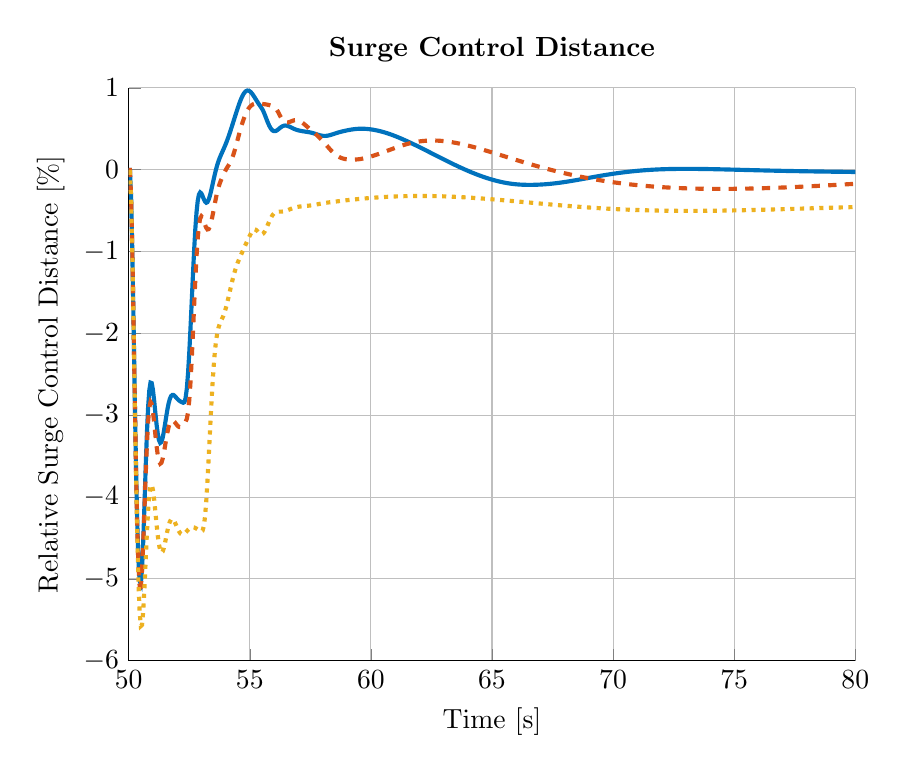
\begin{tikzpicture}

\begin{axis}[%
width=0.761\linewidth,
height=0.6\linewidth,
at={(0\linewidth,0\linewidth)},
scale only axis,
xmin=50,
xmax=80,
xlabel={Time [s]},
xmajorgrids,
ymin=-6,
ymax=1,
ylabel={Relative Surge Control Distance [\%]},
ymajorgrids,
axis background/.style={fill=white},
title style={font=\bfseries},
title={Surge Control Distance},
axis x line*=bottom,
axis y line*=left
]
\addplot [color=mycolor1,solid,line width=1.5pt,forget plot]
  table[row sep=crcr]{%
50	-0.00287999999999933\\
50.05	-0.00287999999999933\\
50.1	-0.340039999999999\\
50.15	-1.01667\\
50.2	-1.8749\\
50.25	-2.77916\\
50.3	-3.61056\\
50.35	-4.28728\\
50.4	-4.76714\\
50.45	-5.02619\\
50.5	-5.05865\\
50.55	-4.88044\\
50.6	-4.53806\\
50.65	-4.10178\\
50.7	-3.6449\\
50.75	-3.23165\\
50.8	-2.90792\\
50.85	-2.69721\\
50.9	-2.6018\\
50.95	-2.60755\\
51	-2.68995\\
51.05	-2.82\\
51.1	-2.96888\\
51.15	-3.11134\\
51.2	-3.22777\\
51.25	-3.30532\\
51.3	-3.33818\\
51.35	-3.32708\\
51.4	-3.27823\\
51.45	-3.20171\\
51.5	-3.10962\\
51.55	-3.01412\\
51.6	-2.92583\\
51.65	-2.85258\\
51.7	-2.79888\\
51.75	-2.76589\\
51.8	-2.75192\\
51.85	-2.75319\\
51.9	-2.7647\\
51.95	-2.78114\\
52	-2.79788\\
52.05	-2.81261\\
52.1	-2.82479\\
52.15	-2.83436\\
52.2	-2.84165\\
52.25	-2.84727\\
52.3	-2.84035\\
52.35	-2.78848\\
52.4	-2.67211\\
52.45	-2.48642\\
52.5	-2.23862\\
52.55	-1.94421\\
52.6	-1.62329\\
52.65	-1.29773\\
52.7	-0.991169999999999\\
52.75	-0.72666\\
52.8	-0.520689999999999\\
52.85	-0.38019\\
52.9	-0.30247\\
52.95	-0.27718\\
53	-0.289249999999999\\
53.05	-0.32201\\
53.1	-0.35976\\
53.15	-0.389729999999999\\
53.2	-0.403169999999999\\
53.25	-0.39575\\
53.3	-0.36727\\
53.35	-0.32081\\
53.4	-0.261649999999999\\
53.45	-0.195969999999999\\
53.5	-0.128729999999999\\
53.55	-0.0633299999999988\\
53.6	-0.00231999999999921\\
53.65	0.0517599999999998\\
53.7	0.0982300000000009\\
53.75	0.138570000000001\\
53.8	0.174570000000001\\
53.85	0.208080000000001\\
53.9	0.240860000000001\\
53.95	0.27434\\
54	0.309560000000001\\
54.05	0.34709\\
54.1	0.387090000000001\\
54.15	0.429410000000001\\
54.2	0.473650000000001\\
54.25	0.51932\\
54.3	0.56588\\
54.35	0.612870000000001\\
54.4	0.659830000000001\\
54.45	0.70623\\
54.5	0.75141\\
54.55	0.79461\\
54.6	0.83497\\
54.65	0.871540000000001\\
54.7	0.903370000000001\\
54.75	0.92952\\
54.8	0.94922\\
54.85	0.96194\\
54.9	0.967500000000001\\
54.95	0.966090000000001\\
55	0.958270000000001\\
55.05	0.94492\\
55.1	0.927160000000001\\
55.15	0.90619\\
55.2	0.883240000000001\\
55.25	0.85941\\
55.3	0.83564\\
55.35	0.812610000000001\\
55.4	0.79078\\
55.45	0.76999\\
55.5	0.747640000000001\\
55.55	0.72021\\
55.6	0.6861\\
55.65	0.648050000000001\\
55.7	0.60947\\
55.75	0.572740000000001\\
55.8	0.539760000000001\\
55.85	0.512170000000001\\
55.9	0.491190000000001\\
55.95	0.477500000000001\\
56	0.471160000000001\\
56.05	0.471530000000001\\
56.1	0.477400000000001\\
56.15	0.48715\\
56.2	0.499000000000001\\
56.25	0.511200000000001\\
56.3	0.522250000000001\\
56.35	0.531040000000001\\
56.4	0.53688\\
56.45	0.539520000000001\\
56.5	0.53909\\
56.55	0.536010000000001\\
56.6	0.53087\\
56.65	0.52435\\
56.7	0.517110000000001\\
56.75	0.50972\\
56.8	0.50263\\
56.85	0.49614\\
56.9	0.49042\\
56.95	0.4855\\
57	0.481300000000001\\
57.05	0.4777\\
57.1	0.474580000000001\\
57.15	0.47184\\
57.2	0.469390000000001\\
57.25	0.467120000000001\\
57.3	0.464930000000001\\
57.35	0.462730000000001\\
57.4	0.4604\\
57.45	0.45782\\
57.5	0.45491\\
57.55	0.45158\\
57.6	0.447790000000001\\
57.65	0.44356\\
57.7	0.43895\\
57.75	0.434140000000001\\
57.8	0.429310000000001\\
57.85	0.424710000000001\\
57.9	0.420580000000001\\
57.95	0.417160000000001\\
58	0.41464\\
58.05	0.413180000000001\\
58.1	0.412830000000001\\
58.15	0.41361\\
58.2	0.415460000000001\\
58.25	0.41826\\
58.3	0.421840000000001\\
58.35	0.426020000000001\\
58.4	0.43061\\
58.45	0.43544\\
58.5	0.440330000000001\\
58.55	0.445180000000001\\
58.6	0.44988\\
58.65	0.45438\\
58.7	0.458640000000001\\
58.75	0.462670000000001\\
58.8	0.466470000000001\\
58.85	0.47007\\
58.9	0.47349\\
58.95	0.476750000000001\\
59	0.479850000000001\\
59.05	0.482810000000001\\
59.1	0.485610000000001\\
59.15	0.488240000000001\\
59.2	0.490680000000001\\
59.25	0.49292\\
59.3	0.494910000000001\\
59.35	0.496650000000001\\
59.4	0.49812\\
59.45	0.49929\\
59.5	0.500150000000001\\
59.55	0.500720000000001\\
59.6	0.500970000000001\\
59.65	0.500910000000001\\
59.7	0.50056\\
59.75	0.499920000000001\\
59.8	0.498990000000001\\
59.85	0.49779\\
59.9	0.49633\\
59.95	0.494630000000001\\
60	0.49268\\
60.05	0.490490000000001\\
60.1	0.48808\\
60.15	0.48545\\
60.2	0.482610000000001\\
60.25	0.47955\\
60.3	0.476290000000001\\
60.35	0.47282\\
60.4	0.469150000000001\\
60.45	0.46528\\
60.5	0.461220000000001\\
60.55	0.45697\\
60.6	0.45252\\
60.65	0.447900000000001\\
60.7	0.443100000000001\\
60.75	0.438130000000001\\
60.8	0.43299\\
60.85	0.4277\\
60.9	0.422260000000001\\
60.95	0.41667\\
61	0.410960000000001\\
61.05	0.405110000000001\\
61.1	0.399140000000001\\
61.15	0.393050000000001\\
61.2	0.38686\\
61.25	0.380560000000001\\
61.3	0.37416\\
61.35	0.36767\\
61.4	0.361090000000001\\
61.45	0.354420000000001\\
61.5	0.347670000000001\\
61.55	0.340850000000001\\
61.6	0.33395\\
61.65	0.32699\\
61.7	0.31996\\
61.75	0.31287\\
61.8	0.305720000000001\\
61.85	0.298530000000001\\
61.9	0.29129\\
61.95	0.284000000000001\\
62	0.276670000000001\\
62.05	0.269310000000001\\
62.1	0.26192\\
62.15	0.2545\\
62.2	0.24705\\
62.25	0.23958\\
62.3	0.23208\\
62.35	0.224580000000001\\
62.4	0.21706\\
62.45	0.209530000000001\\
62.5	0.20199\\
62.55	0.19445\\
62.6	0.186910000000001\\
62.65	0.17937\\
62.7	0.17183\\
62.75	0.16431\\
62.8	0.156790000000001\\
62.85	0.149290000000001\\
62.9	0.1418\\
62.95	0.13434\\
63	0.126890000000001\\
63.05	0.11947\\
63.1	0.112080000000001\\
63.15	0.10472\\
63.2	0.0974000000000004\\
63.25	0.090110000000001\\
63.3	0.0828600000000002\\
63.35	0.0756500000000013\\
63.4	0.0684900000000006\\
63.45	0.0613799999999998\\
63.5	0.054310000000001\\
63.55	0.0472999999999999\\
63.6	0.0403500000000001\\
63.65	0.0334599999999998\\
63.7	0.0266200000000012\\
63.75	0.0198499999999999\\
63.8	0.0131500000000013\\
63.85	0.00652000000000008\\
63.9	-4.0000000000262e-05\\
63.95	-0.00652000000000008\\
64	-0.012929999999999\\
64.05	-0.0192599999999992\\
64.1	-0.0255099999999988\\
64.15	-0.0316700000000001\\
64.2	-0.0377399999999994\\
64.25	-0.0437199999999986\\
64.3	-0.0496099999999995\\
64.35	-0.0554100000000002\\
64.4	-0.0610999999999997\\
64.45	-0.0666999999999991\\
64.5	-0.0721999999999987\\
64.55	-0.0775899999999989\\
64.6	-0.0828699999999998\\
64.65	-0.0880499999999991\\
64.7	-0.0931099999999994\\
64.75	-0.0980600000000003\\
64.8	-0.102889999999999\\
64.85	-0.1076\\
64.9	-0.11219\\
64.95	-0.11666\\
65	-0.120999999999999\\
65.05	-0.125209999999999\\
65.1	-0.1293\\
65.15	-0.13324\\
65.2	-0.137059999999999\\
65.25	-0.14073\\
65.3	-0.144259999999999\\
65.35	-0.147659999999999\\
65.4	-0.150899999999999\\
65.45	-0.153999999999999\\
65.5	-0.15696\\
65.55	-0.159759999999999\\
65.6	-0.162409999999999\\
65.65	-0.164909999999999\\
65.7	-0.16726\\
65.75	-0.169449999999999\\
65.8	-0.171489999999999\\
65.85	-0.17338\\
65.9	-0.17512\\
65.95	-0.176699999999999\\
66	-0.178139999999999\\
66.05	-0.179429999999999\\
66.1	-0.180579999999999\\
66.15	-0.181589999999999\\
66.2	-0.18246\\
66.25	-0.183199999999999\\
66.3	-0.183809999999999\\
66.35	-0.184309999999999\\
66.4	-0.184679999999999\\
66.45	-0.184939999999999\\
66.5	-0.185099999999999\\
66.55	-0.185149999999999\\
66.6	-0.18511\\
66.65	-0.18497\\
66.7	-0.18474\\
66.75	-0.184419999999999\\
66.8	-0.18401\\
66.85	-0.18352\\
66.9	-0.182939999999999\\
66.95	-0.182289999999999\\
67	-0.181539999999999\\
67.05	-0.180719999999999\\
67.1	-0.179819999999999\\
67.15	-0.17883\\
67.2	-0.177759999999999\\
67.25	-0.176609999999999\\
67.3	-0.17538\\
67.35	-0.17407\\
67.4	-0.172689999999999\\
67.45	-0.171219999999999\\
67.5	-0.16968\\
67.55	-0.16806\\
67.6	-0.16637\\
67.65	-0.16461\\
67.7	-0.16278\\
67.75	-0.160889999999999\\
67.8	-0.15893\\
67.85	-0.156899999999999\\
67.9	-0.154819999999999\\
67.95	-0.152679999999999\\
68	-0.15049\\
68.05	-0.148239999999999\\
68.1	-0.145949999999999\\
68.15	-0.14361\\
68.2	-0.141229999999999\\
68.25	-0.138809999999999\\
68.3	-0.136349999999999\\
68.35	-0.13385\\
68.4	-0.131329999999999\\
68.45	-0.128769999999999\\
68.5	-0.126189999999999\\
68.55	-0.12359\\
68.6	-0.12097\\
68.65	-0.11833\\
68.7	-0.115679999999999\\
68.75	-0.113019999999999\\
68.8	-0.110349999999999\\
68.85	-0.107669999999999\\
68.9	-0.104989999999999\\
68.95	-0.102309999999999\\
69	-0.0996299999999994\\
69.05	-0.0969599999999993\\
69.1	-0.0942899999999991\\
69.15	-0.0916399999999999\\
69.2	-0.088989999999999\\
69.25	-0.0863599999999991\\
69.3	-0.0837399999999988\\
69.35	-0.0811399999999995\\
69.4	-0.0785699999999991\\
69.45	-0.0760100000000001\\
69.5	-0.0734699999999986\\
69.55	-0.0709599999999995\\
69.6	-0.0684799999999992\\
69.65	-0.0660299999999996\\
69.7	-0.0635999999999992\\
69.75	-0.0612099999999991\\
69.8	-0.0588499999999996\\
69.85	-0.056519999999999\\
69.9	-0.054219999999999\\
69.95	-0.0519599999999993\\
70	-0.0497399999999999\\
70.05	-0.0475599999999989\\
70.1	-0.0454099999999986\\
70.15	-0.0432999999999986\\
70.2	-0.0412400000000002\\
70.25	-0.0392099999999989\\
70.3	-0.0372199999999996\\
70.35	-0.0352800000000002\\
70.4	-0.0333799999999993\\
70.45	-0.0315199999999987\\
70.5	-0.0297000000000001\\
70.55	-0.0279299999999996\\
70.6	-0.0261999999999993\\
70.65	-0.0245099999999994\\
70.7	-0.0228599999999997\\
70.75	-0.0212699999999995\\
70.8	-0.0197099999999999\\
70.85	-0.0182000000000002\\
70.9	-0.016729999999999\\
70.95	-0.0152999999999999\\
71	-0.0139199999999988\\
71.05	-0.0125799999999998\\
71.1	-0.0112899999999989\\
71.15	-0.01004\\
71.2	-0.00882999999999967\\
71.25	-0.00765999999999956\\
71.3	-0.00653999999999932\\
71.35	-0.00544999999999973\\
71.4	-0.00441000000000003\\
71.45	-0.0034099999999988\\
71.5	-0.00244999999999962\\
71.55	-0.00152999999999892\\
71.6	-0.000650000000000261\\
71.65	0.000189999999999912\\
71.7	0.00100000000000122\\
71.75	0.00176000000000087\\
71.8	0.00248999999999988\\
71.85	0.0031800000000004\\
71.9	0.00384000000000029\\
71.95	0.00445999999999991\\
72	0.00505000000000067\\
72.05	0.00560000000000116\\
72.1	0.00611000000000139\\
72.15	0.00660000000000061\\
72.2	0.00705000000000133\\
72.25	0.00747000000000142\\
72.3	0.00786000000000087\\
72.35	0.00821999999999967\\
72.4	0.00853999999999999\\
72.45	0.00884000000000107\\
72.5	0.00912000000000113\\
72.55	0.00936000000000092\\
72.6	0.0095799999999997\\
72.65	0.00977000000000139\\
72.7	0.00993000000000066\\
72.75	0.0100700000000007\\
72.8	0.0101899999999997\\
72.85	0.0102799999999998\\
72.9	0.0103500000000007\\
72.95	0.010390000000001\\
73	0.0104199999999999\\
73.05	0.0104199999999999\\
73.1	0.0104100000000003\\
73.15	0.01037\\
73.2	0.0103200000000001\\
73.25	0.0102400000000014\\
73.3	0.0101500000000012\\
73.35	0.01004\\
73.4	0.00992000000000104\\
73.45	0.00978000000000101\\
73.5	0.00961999999999996\\
73.55	0.00945000000000107\\
73.6	0.00927000000000078\\
73.65	0.00907000000000124\\
73.7	0.00886000000000031\\
73.75	0.00863999999999976\\
73.8	0.00839999999999996\\
73.85	0.00816000000000017\\
73.9	0.00790000000000113\\
73.95	0.00763000000000069\\
74	0.00735000000000063\\
74.05	0.00707000000000058\\
74.1	0.00677000000000127\\
74.15	0.0064700000000002\\
74.2	0.00616000000000128\\
74.25	0.00584000000000096\\
74.3	0.00551000000000101\\
74.35	0.00518000000000107\\
74.4	0.00483999999999973\\
74.45	0.00450000000000017\\
74.5	0.00415000000000099\\
74.55	0.00380000000000003\\
74.6	0.00344000000000122\\
74.65	0.00308000000000064\\
74.7	0.00271000000000043\\
74.75	0.00234000000000023\\
74.8	0.00197000000000003\\
74.85	0.0015900000000002\\
74.9	0.00122\\
74.95	0.000840000000000174\\
75	0.000460000000000349\\
75.05	7.00000000009027e-05\\
75.1	-0.000309999999998922\\
75.15	-0.000700000000000145\\
75.2	-0.00107999999999997\\
75.25	-0.00146999999999942\\
75.3	-0.00185999999999886\\
75.35	-0.00223999999999869\\
75.4	-0.00262999999999991\\
75.45	-0.00301999999999936\\
75.5	-0.00339999999999918\\
75.55	-0.00378999999999863\\
75.6	-0.00417000000000023\\
75.65	-0.00455000000000005\\
75.7	-0.0049399999999995\\
75.75	-0.00531999999999933\\
75.8	-0.00568999999999953\\
75.85	-0.00606999999999935\\
75.9	-0.00643999999999956\\
75.95	-0.00681999999999938\\
76	-0.00718999999999959\\
76.05	-0.00755999999999979\\
76.1	-0.00791999999999859\\
76.15	-0.00827999999999918\\
76.2	-0.00863999999999976\\
76.25	-0.00899999999999856\\
76.3	-0.00935999999999915\\
76.35	-0.00971000000000011\\
76.4	-0.0100599999999993\\
76.45	-0.0104100000000003\\
76.5	-0.0107499999999998\\
76.55	-0.0110899999999994\\
76.6	-0.0114299999999989\\
76.65	-0.0117599999999989\\
76.7	-0.0120899999999988\\
76.75	-0.0124199999999988\\
76.8	-0.0127399999999991\\
76.85	-0.0130599999999994\\
76.9	-0.0133799999999997\\
76.95	-0.0137\\
77	-0.014009999999999\\
77.05	-0.0143199999999997\\
77.1	-0.014619999999999\\
77.15	-0.01492\\
77.2	-0.0152199999999993\\
77.25	-0.015509999999999\\
77.3	-0.0158100000000001\\
77.35	-0.0160900000000002\\
77.4	-0.0163799999999998\\
77.45	-0.0166599999999999\\
77.5	-0.01694\\
77.55	-0.0172099999999986\\
77.6	-0.0174799999999991\\
77.65	-0.0177499999999995\\
77.7	-0.0180199999999999\\
77.75	-0.018279999999999\\
77.8	-0.0185399999999998\\
77.85	-0.0187999999999988\\
77.9	-0.01905\\
77.95	-0.0192999999999994\\
78	-0.0195499999999988\\
78.05	-0.0198\\
78.1	-0.0200399999999998\\
78.15	-0.0202799999999996\\
78.2	-0.0205099999999998\\
78.25	-0.0207499999999996\\
78.3	-0.0209799999999998\\
78.35	-0.02121\\
78.4	-0.0214400000000001\\
78.45	-0.0216599999999989\\
78.5	-0.0218799999999995\\
78.55	-0.0221\\
78.6	-0.0223199999999988\\
78.65	-0.0225399999999993\\
78.7	-0.0227500000000003\\
78.75	-0.0229599999999994\\
78.8	-0.0231699999999986\\
78.85	-0.0233799999999995\\
78.9	-0.023579999999999\\
78.95	-0.0237799999999986\\
79	-0.0239899999999995\\
79.05	-0.024189999999999\\
79.1	-0.024379999999999\\
79.15	-0.0245800000000003\\
79.2	-0.0247799999999998\\
79.25	-0.0249699999999997\\
79.3	-0.0251599999999996\\
79.35	-0.0253499999999995\\
79.4	-0.0255399999999995\\
79.45	-0.0257299999999994\\
79.5	-0.0259099999999997\\
79.55	-0.0260999999999996\\
79.6	-0.0262799999999999\\
79.65	-0.0264699999999998\\
79.7	-0.0266500000000001\\
79.75	-0.0268299999999986\\
79.8	-0.0270099999999989\\
79.85	-0.0271899999999992\\
79.9	-0.0273699999999995\\
79.95	-0.0275499999999997\\
80	-0.0277199999999986\\
};
\addplot [color=mycolor2,dashed,line width=1.5pt,forget plot]
  table[row sep=crcr]{%
50	-0.00324999999999953\\
50.05	-0.00324999999999953\\
50.1	-0.34031\\
50.15	-1.01684\\
50.2	-1.87543\\
50.25	-2.78574\\
50.3	-3.64011\\
50.35	-4.3476\\
50.4	-4.83738\\
50.45	-5.08048\\
50.5	-5.08938\\
50.55	-4.89977\\
50.6	-4.56668\\
50.65	-4.15677\\
50.7	-3.73755\\
50.75	-3.36652\\
50.8	-3.0835\\
50.85	-2.90762\\
50.9	-2.83882\\
50.95	-2.86244\\
51	-2.95481\\
51.05	-3.08852\\
51.1	-3.23664\\
51.15	-3.37579\\
51.2	-3.48803\\
51.25	-3.56188\\
51.3	-3.59251\\
51.35	-3.58127\\
51.4	-3.53458\\
51.45	-3.46241\\
51.5	-3.37647\\
51.55	-3.28834\\
51.6	-3.20802\\
51.65	-3.14275\\
51.7	-3.09658\\
51.75	-3.07036\\
51.8	-3.06226\\
51.85	-3.06845\\
51.9	-3.08402\\
51.95	-3.10378\\
52	-3.12297\\
52.05	-3.13776\\
52.1	-3.14559\\
52.15	-3.14529\\
52.2	-3.13697\\
52.25	-3.12183\\
52.3	-3.1018\\
52.35	-3.07923\\
52.4	-3.04421\\
52.45	-2.96383\\
52.5	-2.81816\\
52.55	-2.6027\\
52.6	-2.32609\\
52.65	-2.00638\\
52.7	-1.66886\\
52.75	-1.34351\\
52.8	-1.0586\\
52.85	-0.83456\\
52.9	-0.680859999999999\\
52.95	-0.595949999999999\\
53	-0.569399999999999\\
53.05	-0.585179999999999\\
53.1	-0.62505\\
53.15	-0.671469999999999\\
53.2	-0.709829999999999\\
53.25	-0.72974\\
53.3	-0.725639999999999\\
53.35	-0.69659\\
53.4	-0.64556\\
53.45	-0.57823\\
53.5	-0.501639999999999\\
53.55	-0.42282\\
53.6	-0.3477\\
53.65	-0.280399999999999\\
53.7	-0.22289\\
53.75	-0.175129999999999\\
53.8	-0.135479999999999\\
53.85	-0.101239999999999\\
53.9	-0.0692799999999991\\
53.95	-0.0365500000000001\\
54	-0.00672999999999924\\
54.05	0.0190999999999999\\
54.1	0.0428800000000003\\
54.15	0.0660000000000007\\
54.2	0.0922300000000007\\
54.25	0.124470000000001\\
54.3	0.1639\\
54.35	0.20978\\
54.4	0.260670000000001\\
54.45	0.31479\\
54.5	0.37031\\
54.55	0.42559\\
54.6	0.47926\\
54.65	0.53026\\
54.7	0.57779\\
54.75	0.62124\\
54.8	0.660170000000001\\
54.85	0.6943\\
54.9	0.72348\\
54.95	0.747710000000001\\
55	0.767150000000001\\
55.05	0.782110000000001\\
55.1	0.79302\\
55.15	0.800420000000001\\
55.2	0.80489\\
55.25	0.8071\\
55.3	0.807740000000001\\
55.35	0.807370000000001\\
55.4	0.80644\\
55.45	0.80522\\
55.5	0.803840000000001\\
55.55	0.802340000000001\\
55.6	0.800650000000001\\
55.65	0.79866\\
55.7	0.796240000000001\\
55.75	0.79331\\
55.8	0.789810000000001\\
55.85	0.785740000000001\\
55.9	0.78115\\
55.95	0.77576\\
56	0.76746\\
56.05	0.755190000000001\\
56.1	0.738000000000001\\
56.15	0.71494\\
56.2	0.68679\\
56.25	0.657780000000001\\
56.3	0.631740000000001\\
56.35	0.610480000000001\\
56.4	0.59465\\
56.45	0.584200000000001\\
56.5	0.57873\\
56.55	0.57752\\
56.6	0.57967\\
56.65	0.58417\\
56.7	0.589920000000001\\
56.75	0.59585\\
56.8	0.60102\\
56.85	0.60464\\
56.9	0.606150000000001\\
56.95	0.60525\\
57	0.601840000000001\\
57.05	0.596070000000001\\
57.1	0.58821\\
57.15	0.57863\\
57.2	0.567730000000001\\
57.25	0.555910000000001\\
57.3	0.543470000000001\\
57.35	0.530660000000001\\
57.4	0.517700000000001\\
57.45	0.50474\\
57.5	0.49188\\
57.55	0.47912\\
57.6	0.46644\\
57.65	0.453720000000001\\
57.7	0.440860000000001\\
57.75	0.427710000000001\\
57.8	0.414160000000001\\
57.85	0.400120000000001\\
57.9	0.38551\\
57.95	0.370320000000001\\
58	0.354560000000001\\
58.05	0.338290000000001\\
58.1	0.32159\\
58.15	0.304590000000001\\
58.2	0.28745\\
58.25	0.27036\\
58.3	0.25356\\
58.35	0.23728\\
58.4	0.22176\\
58.45	0.2072\\
58.5	0.193800000000001\\
58.55	0.18167\\
58.6	0.17088\\
58.65	0.161470000000001\\
58.7	0.15339\\
58.75	0.14659\\
58.8	0.14095\\
58.85	0.13636\\
58.9	0.132680000000001\\
58.95	0.12979\\
59	0.127550000000001\\
59.05	0.12588\\
59.1	0.12468\\
59.15	0.12388\\
59.2	0.12346\\
59.25	0.123380000000001\\
59.3	0.12364\\
59.35	0.124230000000001\\
59.4	0.125170000000001\\
59.45	0.12645\\
59.5	0.128080000000001\\
59.55	0.13007\\
59.6	0.13242\\
59.65	0.135110000000001\\
59.7	0.138120000000001\\
59.75	0.141440000000001\\
59.8	0.14504\\
59.85	0.14888\\
59.9	0.152950000000001\\
59.95	0.157220000000001\\
60	0.16165\\
60.05	0.166220000000001\\
60.1	0.170920000000001\\
60.15	0.17573\\
60.2	0.18064\\
60.25	0.185640000000001\\
60.3	0.190720000000001\\
60.35	0.195870000000001\\
60.4	0.2011\\
60.45	0.2064\\
60.5	0.21176\\
60.55	0.217180000000001\\
60.6	0.22265\\
60.65	0.228160000000001\\
60.7	0.233700000000001\\
60.75	0.23925\\
60.8	0.244810000000001\\
60.85	0.250360000000001\\
60.9	0.25587\\
60.95	0.26135\\
61	0.266760000000001\\
61.05	0.27209\\
61.1	0.277330000000001\\
61.15	0.28246\\
61.2	0.28748\\
61.25	0.29236\\
61.3	0.29711\\
61.35	0.30171\\
61.4	0.306150000000001\\
61.45	0.310420000000001\\
61.5	0.314530000000001\\
61.55	0.31846\\
61.6	0.32221\\
61.65	0.32578\\
61.7	0.329170000000001\\
61.75	0.332360000000001\\
61.8	0.335360000000001\\
61.85	0.33817\\
61.9	0.340780000000001\\
61.95	0.34318\\
62	0.34539\\
62.05	0.3474\\
62.1	0.349210000000001\\
62.15	0.350820000000001\\
62.2	0.35223\\
62.25	0.353440000000001\\
62.3	0.354460000000001\\
62.35	0.35528\\
62.4	0.35591\\
62.45	0.356350000000001\\
62.5	0.35661\\
62.55	0.356680000000001\\
62.6	0.356570000000001\\
62.65	0.356290000000001\\
62.7	0.355840000000001\\
62.75	0.355210000000001\\
62.8	0.354420000000001\\
62.85	0.35347\\
62.9	0.352360000000001\\
62.95	0.351090000000001\\
63	0.34967\\
63.05	0.348100000000001\\
63.1	0.346390000000001\\
63.15	0.34454\\
63.2	0.342560000000001\\
63.25	0.340440000000001\\
63.3	0.338190000000001\\
63.35	0.33581\\
63.4	0.333320000000001\\
63.45	0.33071\\
63.5	0.32799\\
63.55	0.325150000000001\\
63.6	0.32222\\
63.65	0.319180000000001\\
63.7	0.316040000000001\\
63.75	0.312810000000001\\
63.8	0.30949\\
63.85	0.30608\\
63.9	0.30259\\
63.95	0.299020000000001\\
64	0.29538\\
64.05	0.29166\\
64.1	0.28787\\
64.15	0.28402\\
64.2	0.280110000000001\\
64.25	0.27613\\
64.3	0.2721\\
64.35	0.26802\\
64.4	0.26388\\
64.45	0.2597\\
64.5	0.255470000000001\\
64.55	0.251200000000001\\
64.6	0.2469\\
64.65	0.242550000000001\\
64.7	0.23817\\
64.75	0.23376\\
64.8	0.229320000000001\\
64.85	0.22485\\
64.9	0.220360000000001\\
64.95	0.215850000000001\\
65	0.211310000000001\\
65.05	0.206760000000001\\
65.1	0.20219\\
65.15	0.197610000000001\\
65.2	0.193020000000001\\
65.25	0.188420000000001\\
65.3	0.183810000000001\\
65.35	0.17919\\
65.4	0.174560000000001\\
65.45	0.16994\\
65.5	0.16531\\
65.55	0.160690000000001\\
65.6	0.15606\\
65.65	0.151440000000001\\
65.7	0.146830000000001\\
65.75	0.14222\\
65.8	0.13761\\
65.85	0.13302\\
65.9	0.128440000000001\\
65.95	0.12387\\
66	0.11931\\
66.05	0.11476\\
66.1	0.110230000000001\\
66.15	0.10572\\
66.2	0.101220000000001\\
66.25	0.0967400000000005\\
66.3	0.0922900000000002\\
66.35	0.0878500000000013\\
66.4	0.0834299999999999\\
66.45	0.0790300000000013\\
66.5	0.0746599999999997\\
66.55	0.070310000000001\\
66.6	0.0659799999999997\\
66.65	0.0616800000000008\\
66.7	0.0574000000000012\\
66.75	0.0531500000000005\\
66.8	0.0489300000000004\\
66.85	0.0447300000000013\\
66.9	0.040560000000001\\
66.95	0.0364199999999997\\
67	0.0323100000000007\\
67.05	0.0282300000000006\\
67.1	0.0241800000000012\\
67.15	0.0201600000000006\\
67.2	0.0161700000000007\\
67.25	0.0122100000000014\\
67.3	0.00829000000000057\\
67.35	0.00439000000000078\\
67.4	0.000530000000001252\\
67.45	-0.00329999999999941\\
67.5	-0.00709999999999944\\
67.55	-0.0108599999999992\\
67.6	-0.0145900000000001\\
67.65	-0.0182899999999986\\
67.7	-0.0219499999999986\\
67.75	-0.0255799999999997\\
67.8	-0.0291800000000002\\
67.85	-0.0327399999999987\\
67.9	-0.03627\\
67.95	-0.0397599999999994\\
68	-0.0432199999999998\\
68.05	-0.04664\\
68.1	-0.0500299999999996\\
68.15	-0.0533799999999989\\
68.2	-0.0566999999999993\\
68.25	-0.0599799999999995\\
68.3	-0.063229999999999\\
68.35	-0.0664400000000001\\
68.4	-0.0696199999999987\\
68.45	-0.0727599999999988\\
68.5	-0.0758700000000001\\
68.55	-0.0789399999999993\\
68.6	-0.0819799999999997\\
68.65	-0.0849799999999998\\
68.7	-0.0879499999999993\\
68.75	-0.0908800000000003\\
68.8	-0.0937799999999989\\
68.85	-0.0966499999999986\\
68.9	-0.0994700000000002\\
68.95	-0.102269999999999\\
69	-0.105029999999999\\
69.05	-0.107749999999999\\
69.1	-0.110439999999999\\
69.15	-0.113099999999999\\
69.2	-0.11572\\
69.25	-0.118309999999999\\
69.3	-0.120859999999999\\
69.35	-0.123379999999999\\
69.4	-0.125869999999999\\
69.45	-0.12832\\
69.5	-0.130739999999999\\
69.55	-0.13313\\
69.6	-0.135479999999999\\
69.65	-0.137799999999999\\
69.7	-0.14009\\
69.75	-0.142339999999999\\
69.8	-0.144559999999999\\
69.85	-0.146749999999999\\
69.9	-0.14891\\
69.95	-0.151039999999999\\
70	-0.153129999999999\\
70.05	-0.155189999999999\\
70.1	-0.15722\\
70.15	-0.159219999999999\\
70.2	-0.16119\\
70.25	-0.16313\\
70.3	-0.16503\\
70.35	-0.16691\\
70.4	-0.168749999999999\\
70.45	-0.17057\\
70.5	-0.17235\\
70.55	-0.17411\\
70.6	-0.175829999999999\\
70.65	-0.177529999999999\\
70.7	-0.1792\\
70.75	-0.180829999999999\\
70.8	-0.18244\\
70.85	-0.184019999999999\\
70.9	-0.185569999999999\\
70.95	-0.18709\\
71	-0.18859\\
71.05	-0.190059999999999\\
71.1	-0.191489999999999\\
71.15	-0.192909999999999\\
71.2	-0.19429\\
71.25	-0.195639999999999\\
71.3	-0.196969999999999\\
71.35	-0.19828\\
71.4	-0.199549999999999\\
71.45	-0.200799999999999\\
71.5	-0.202019999999999\\
71.55	-0.203219999999999\\
71.6	-0.204389999999999\\
71.65	-0.205539999999999\\
71.7	-0.206659999999999\\
71.75	-0.20775\\
71.8	-0.208819999999999\\
71.85	-0.20987\\
71.9	-0.21088\\
71.95	-0.21188\\
72	-0.21285\\
72.05	-0.213799999999999\\
72.1	-0.21472\\
72.15	-0.215619999999999\\
72.2	-0.216489999999999\\
72.25	-0.21735\\
72.3	-0.21817\\
72.35	-0.218979999999999\\
72.4	-0.219759999999999\\
72.45	-0.22052\\
72.5	-0.221259999999999\\
72.55	-0.221979999999999\\
72.6	-0.222669999999999\\
72.65	-0.223339999999999\\
72.7	-0.22399\\
72.75	-0.22462\\
72.8	-0.22523\\
72.85	-0.225809999999999\\
72.9	-0.22638\\
72.95	-0.22692\\
73	-0.227449999999999\\
73.05	-0.22795\\
73.1	-0.228429999999999\\
73.15	-0.22889\\
73.2	-0.22934\\
73.25	-0.22976\\
73.3	-0.23016\\
73.35	-0.230549999999999\\
73.4	-0.23091\\
73.45	-0.23126\\
73.5	-0.23159\\
73.55	-0.2319\\
73.6	-0.232189999999999\\
73.65	-0.23246\\
73.7	-0.232709999999999\\
73.75	-0.23295\\
73.8	-0.233169999999999\\
73.85	-0.23337\\
73.9	-0.233549999999999\\
73.95	-0.233719999999999\\
74	-0.23387\\
74.05	-0.233999999999999\\
74.1	-0.23412\\
74.15	-0.234209999999999\\
74.2	-0.234299999999999\\
74.25	-0.23436\\
74.3	-0.23441\\
74.35	-0.23445\\
74.4	-0.234469999999999\\
74.45	-0.234469999999999\\
74.5	-0.234459999999999\\
74.55	-0.23443\\
74.6	-0.234389999999999\\
74.65	-0.234329999999999\\
74.7	-0.234259999999999\\
74.75	-0.23417\\
74.8	-0.234069999999999\\
74.85	-0.233949999999999\\
74.9	-0.233829999999999\\
74.95	-0.23368\\
75	-0.23352\\
75.05	-0.23335\\
75.1	-0.233169999999999\\
75.15	-0.232969999999999\\
75.2	-0.23276\\
75.25	-0.232539999999999\\
75.3	-0.2323\\
75.35	-0.232049999999999\\
75.4	-0.231789999999999\\
75.45	-0.23152\\
75.5	-0.231229999999999\\
75.55	-0.23093\\
75.6	-0.230619999999999\\
75.65	-0.2303\\
75.7	-0.229959999999999\\
75.75	-0.22962\\
75.8	-0.229259999999999\\
75.85	-0.22889\\
75.9	-0.228509999999999\\
75.95	-0.22812\\
76	-0.22772\\
76.05	-0.227309999999999\\
76.1	-0.226889999999999\\
76.15	-0.226459999999999\\
76.2	-0.22601\\
76.25	-0.22556\\
76.3	-0.225099999999999\\
76.35	-0.22462\\
76.4	-0.224139999999999\\
76.45	-0.223649999999999\\
76.5	-0.22315\\
76.55	-0.222639999999999\\
76.6	-0.222119999999999\\
76.65	-0.221589999999999\\
76.7	-0.221049999999999\\
76.75	-0.220509999999999\\
76.8	-0.21995\\
76.85	-0.21939\\
76.9	-0.218819999999999\\
76.95	-0.21824\\
77	-0.217649999999999\\
77.05	-0.21705\\
77.1	-0.216449999999999\\
77.15	-0.215839999999999\\
77.2	-0.21522\\
77.25	-0.214589999999999\\
77.3	-0.213959999999999\\
77.35	-0.21332\\
77.4	-0.212669999999999\\
77.45	-0.212009999999999\\
77.5	-0.211349999999999\\
77.55	-0.210679999999999\\
77.6	-0.21001\\
77.65	-0.20933\\
77.7	-0.208639999999999\\
77.75	-0.207949999999999\\
77.8	-0.207249999999999\\
77.85	-0.20654\\
77.9	-0.20583\\
77.95	-0.205109999999999\\
78	-0.204389999999999\\
78.05	-0.203659999999999\\
78.1	-0.20292\\
78.15	-0.202179999999999\\
78.2	-0.20144\\
78.25	-0.20069\\
78.3	-0.199929999999999\\
78.35	-0.199179999999999\\
78.4	-0.198409999999999\\
78.45	-0.19764\\
78.5	-0.19687\\
78.55	-0.19609\\
78.6	-0.195309999999999\\
78.65	-0.19452\\
78.7	-0.19373\\
78.75	-0.192939999999999\\
78.8	-0.192139999999999\\
78.85	-0.191339999999999\\
78.9	-0.19053\\
78.95	-0.189719999999999\\
79	-0.188909999999999\\
79.05	-0.188099999999999\\
79.1	-0.187279999999999\\
79.15	-0.186459999999999\\
79.2	-0.18563\\
79.25	-0.184799999999999\\
79.3	-0.18397\\
79.35	-0.18314\\
79.4	-0.1823\\
79.45	-0.18146\\
79.5	-0.180619999999999\\
79.55	-0.179779999999999\\
79.6	-0.178929999999999\\
79.65	-0.178089999999999\\
79.7	-0.177239999999999\\
79.75	-0.17639\\
79.8	-0.175529999999999\\
79.85	-0.17468\\
79.9	-0.173819999999999\\
79.95	-0.17296\\
80	-0.172099999999999\\
};
\addplot [color=mycolor3,dotted,line width=1.5pt,forget plot]
  table[row sep=crcr]{%
50	-0.0267199999999992\\
50.05	-0.0267199999999992\\
50.1	-0.36408\\
50.15	-1.0416\\
50.2	-1.90258\\
50.25	-2.81764\\
50.3	-3.68674\\
50.35	-4.43639\\
50.4	-5.01657\\
50.45	-5.39889\\
50.5	-5.57619\\
50.55	-5.56236\\
50.6	-5.39082\\
50.65	-5.11032\\
50.7	-4.77765\\
50.75	-4.44852\\
50.8	-4.16904\\
50.85	-3.96983\\
50.9	-3.86419\\
50.95	-3.84964\\
51	-3.9118\\
51.05	-4.02896\\
51.1	-4.17644\\
51.15	-4.33022\\
51.2	-4.46969\\
51.25	-4.57941\\
51.3	-4.65003\\
51.35	-4.67845\\
51.4	-4.66732\\
51.45	-4.62397\\
51.5	-4.55883\\
51.55	-4.48362\\
51.6	-4.40963\\
51.65	-4.34623\\
51.7	-4.29988\\
51.75	-4.27377\\
51.8	-4.26791\\
51.85	-4.27969\\
51.9	-4.30469\\
51.95	-4.33751\\
52	-4.37267\\
52.05	-4.40528\\
52.1	-4.43158\\
52.15	-4.44918\\
52.2	-4.4572\\
52.25	-4.45613\\
52.3	-4.44754\\
52.35	-4.43374\\
52.4	-4.41736\\
52.45	-4.40096\\
52.5	-4.38671\\
52.55	-4.37615\\
52.6	-4.37012\\
52.65	-4.36876\\
52.7	-4.37161\\
52.75	-4.37778\\
52.8	-4.38607\\
52.85	-4.39525\\
52.9	-4.40416\\
52.95	-4.41185\\
53	-4.41773\\
53.05	-4.41043\\
53.1	-4.35823\\
53.15	-4.24219\\
53.2	-4.05842\\
53.25	-3.81583\\
53.3	-3.53256\\
53.35	-3.23162\\
53.4	-2.93629\\
53.45	-2.66621\\
53.5	-2.43493\\
53.55	-2.2489\\
53.6	-2.10805\\
53.65	-2.0072\\
53.7	-1.93791\\
53.75	-1.89038\\
53.8	-1.85503\\
53.85	-1.82361\\
53.9	-1.7899\\
53.95	-1.75002\\
54	-1.70231\\
54.05	-1.64699\\
54.1	-1.58566\\
54.15	-1.52075\\
54.2	-1.45494\\
54.25	-1.3907\\
54.3	-1.32999\\
54.35	-1.27408\\
54.4	-1.2235\\
54.45	-1.1781\\
54.5	-1.13721\\
54.55	-1.09986\\
54.6	-1.06489\\
54.65	-1.03125\\
54.7	-0.998209999999999\\
54.75	-0.965369999999999\\
54.8	-0.9326\\
54.85	-0.89999\\
54.9	-0.86774\\
54.95	-0.836119999999999\\
55	-0.805409999999999\\
55.05	-0.77619\\
55.1	-0.75139\\
55.15	-0.734909999999999\\
55.2	-0.729119999999999\\
55.25	-0.733829999999999\\
55.3	-0.74644\\
55.35	-0.76277\\
55.4	-0.77807\\
55.45	-0.78804\\
55.5	-0.789569999999999\\
55.55	-0.78114\\
55.6	-0.762849999999999\\
55.65	-0.736229999999999\\
55.7	-0.703779999999999\\
55.75	-0.6685\\
55.8	-0.63334\\
55.85	-0.60087\\
55.9	-0.572929999999999\\
55.95	-0.55057\\
56	-0.534059999999999\\
56.05	-0.522989999999999\\
56.1	-0.516459999999999\\
56.15	-0.51329\\
56.2	-0.51223\\
56.25	-0.512119999999999\\
56.3	-0.511979999999999\\
56.35	-0.51113\\
56.4	-0.50916\\
56.45	-0.505929999999999\\
56.5	-0.50153\\
56.55	-0.496199999999999\\
56.6	-0.490279999999999\\
56.65	-0.48412\\
56.7	-0.478039999999999\\
56.75	-0.472329999999999\\
56.8	-0.46716\\
56.85	-0.462639999999999\\
56.9	-0.45879\\
56.95	-0.455589999999999\\
57	-0.452939999999999\\
57.05	-0.45074\\
57.1	-0.448879999999999\\
57.15	-0.447249999999999\\
57.2	-0.445779999999999\\
57.25	-0.444389999999999\\
57.3	-0.443029999999999\\
57.35	-0.441649999999999\\
57.4	-0.440219999999999\\
57.45	-0.43866\\
57.5	-0.43694\\
57.55	-0.435009999999999\\
57.6	-0.432849999999999\\
57.65	-0.43047\\
57.7	-0.427879999999999\\
57.75	-0.42514\\
57.8	-0.422299999999999\\
57.85	-0.419409999999999\\
57.9	-0.416549999999999\\
57.95	-0.413759999999999\\
58	-0.411079999999999\\
58.05	-0.408549999999999\\
58.1	-0.40616\\
58.15	-0.403929999999999\\
58.2	-0.401829999999999\\
58.25	-0.39985\\
58.3	-0.39795\\
58.35	-0.39612\\
58.4	-0.394329999999999\\
58.45	-0.39256\\
58.5	-0.390789999999999\\
58.55	-0.389019999999999\\
58.6	-0.38723\\
58.65	-0.385439999999999\\
58.7	-0.38364\\
58.75	-0.381849999999999\\
58.8	-0.380059999999999\\
58.85	-0.37829\\
58.9	-0.376549999999999\\
58.95	-0.374829999999999\\
59	-0.373139999999999\\
59.05	-0.371479999999999\\
59.1	-0.369859999999999\\
59.15	-0.36827\\
59.2	-0.366709999999999\\
59.25	-0.365169999999999\\
59.3	-0.363659999999999\\
59.35	-0.36218\\
59.4	-0.360709999999999\\
59.45	-0.35927\\
59.5	-0.357839999999999\\
59.55	-0.356439999999999\\
59.6	-0.355049999999999\\
59.65	-0.353689999999999\\
59.7	-0.352349999999999\\
59.75	-0.35103\\
59.8	-0.349729999999999\\
59.85	-0.348459999999999\\
59.9	-0.347219999999999\\
59.95	-0.345999999999999\\
60	-0.34481\\
60.05	-0.34364\\
60.1	-0.34251\\
60.15	-0.341399999999999\\
60.2	-0.340319999999999\\
60.25	-0.339269999999999\\
60.3	-0.338249999999999\\
60.35	-0.33726\\
60.4	-0.336289999999999\\
60.45	-0.33536\\
60.5	-0.334449999999999\\
60.55	-0.333569999999999\\
60.6	-0.332719999999999\\
60.65	-0.331899999999999\\
60.7	-0.33111\\
60.75	-0.330349999999999\\
60.8	-0.32961\\
60.85	-0.32891\\
60.9	-0.32823\\
60.95	-0.32759\\
61	-0.326969999999999\\
61.05	-0.326379999999999\\
61.1	-0.325819999999999\\
61.15	-0.32529\\
61.2	-0.324789999999999\\
61.25	-0.324319999999999\\
61.3	-0.323879999999999\\
61.35	-0.32346\\
61.4	-0.323079999999999\\
61.45	-0.322729999999999\\
61.5	-0.322399999999999\\
61.55	-0.322109999999999\\
61.6	-0.321839999999999\\
61.65	-0.321599999999999\\
61.7	-0.321389999999999\\
61.75	-0.32121\\
61.8	-0.321059999999999\\
61.85	-0.32093\\
61.9	-0.32084\\
61.95	-0.32077\\
62	-0.320729999999999\\
62.05	-0.32072\\
62.1	-0.320729999999999\\
62.15	-0.320779999999999\\
62.2	-0.320849999999999\\
62.25	-0.32095\\
62.3	-0.32107\\
62.35	-0.321229999999999\\
62.4	-0.321409999999999\\
62.45	-0.32161\\
62.5	-0.321839999999999\\
62.55	-0.3221\\
62.6	-0.32239\\
62.65	-0.322699999999999\\
62.7	-0.323029999999999\\
62.75	-0.323399999999999\\
62.8	-0.323779999999999\\
62.85	-0.32419\\
62.9	-0.324629999999999\\
62.95	-0.325089999999999\\
63	-0.325569999999999\\
63.05	-0.326079999999999\\
63.1	-0.32661\\
63.15	-0.32717\\
63.2	-0.327749999999999\\
63.25	-0.328349999999999\\
63.3	-0.328969999999999\\
63.35	-0.32961\\
63.4	-0.330279999999999\\
63.45	-0.33097\\
63.5	-0.33168\\
63.55	-0.332409999999999\\
63.6	-0.333159999999999\\
63.65	-0.33393\\
63.7	-0.334719999999999\\
63.75	-0.335539999999999\\
63.8	-0.33637\\
63.85	-0.337219999999999\\
63.9	-0.338089999999999\\
63.95	-0.33897\\
64	-0.339879999999999\\
64.05	-0.3408\\
64.1	-0.34174\\
64.15	-0.3427\\
64.2	-0.343669999999999\\
64.25	-0.344659999999999\\
64.3	-0.34566\\
64.35	-0.34669\\
64.4	-0.34772\\
64.45	-0.348769999999999\\
64.5	-0.349839999999999\\
64.55	-0.350919999999999\\
64.6	-0.352009999999999\\
64.65	-0.35312\\
64.7	-0.35424\\
64.75	-0.35537\\
64.8	-0.35652\\
64.85	-0.357679999999999\\
64.9	-0.358849999999999\\
64.95	-0.360029999999999\\
65	-0.361219999999999\\
65.05	-0.362419999999999\\
65.1	-0.36363\\
65.15	-0.36485\\
65.2	-0.366079999999999\\
65.25	-0.367329999999999\\
65.3	-0.368569999999999\\
65.35	-0.369829999999999\\
65.4	-0.371099999999999\\
65.45	-0.372369999999999\\
65.5	-0.37365\\
65.55	-0.37494\\
65.6	-0.37623\\
65.65	-0.377529999999999\\
65.7	-0.37883\\
65.75	-0.380139999999999\\
65.8	-0.38146\\
65.85	-0.382779999999999\\
65.9	-0.384099999999999\\
65.95	-0.385429999999999\\
66	-0.38676\\
66.05	-0.3881\\
66.1	-0.38944\\
66.15	-0.390779999999999\\
66.2	-0.392119999999999\\
66.25	-0.39347\\
66.3	-0.39481\\
66.35	-0.396159999999999\\
66.4	-0.39751\\
66.45	-0.398859999999999\\
66.5	-0.40021\\
66.55	-0.401559999999999\\
66.6	-0.402909999999999\\
66.65	-0.40426\\
66.7	-0.405609999999999\\
66.75	-0.406949999999999\\
66.8	-0.4083\\
66.85	-0.40964\\
66.9	-0.410979999999999\\
66.95	-0.412319999999999\\
67	-0.41365\\
67.05	-0.414979999999999\\
67.1	-0.416309999999999\\
67.15	-0.41764\\
67.2	-0.418959999999999\\
67.25	-0.420269999999999\\
67.3	-0.421589999999999\\
67.35	-0.42289\\
67.4	-0.424199999999999\\
67.45	-0.425489999999999\\
67.5	-0.426779999999999\\
67.55	-0.428069999999999\\
67.6	-0.429349999999999\\
67.65	-0.430619999999999\\
67.7	-0.431889999999999\\
67.75	-0.433149999999999\\
67.8	-0.434399999999999\\
67.85	-0.435639999999999\\
67.9	-0.436879999999999\\
67.95	-0.438109999999999\\
68	-0.439329999999999\\
68.05	-0.440539999999999\\
68.1	-0.44175\\
68.15	-0.44295\\
68.2	-0.444129999999999\\
68.25	-0.445309999999999\\
68.3	-0.446479999999999\\
68.35	-0.44764\\
68.4	-0.44879\\
68.45	-0.44994\\
68.5	-0.45107\\
68.55	-0.45219\\
68.6	-0.4533\\
68.65	-0.4544\\
68.7	-0.455489999999999\\
68.75	-0.456569999999999\\
68.8	-0.45764\\
68.85	-0.458699999999999\\
68.9	-0.459739999999999\\
68.95	-0.46078\\
69	-0.461799999999999\\
69.05	-0.46282\\
69.1	-0.463819999999999\\
69.15	-0.464809999999999\\
69.2	-0.46578\\
69.25	-0.466749999999999\\
69.3	-0.4677\\
69.35	-0.46864\\
69.4	-0.469569999999999\\
69.45	-0.47049\\
69.5	-0.471399999999999\\
69.55	-0.472289999999999\\
69.6	-0.47317\\
69.65	-0.474029999999999\\
69.7	-0.474889999999999\\
69.75	-0.47573\\
69.8	-0.476559999999999\\
69.85	-0.47737\\
69.9	-0.478179999999999\\
69.95	-0.478969999999999\\
70	-0.479749999999999\\
70.05	-0.48051\\
70.1	-0.48126\\
70.15	-0.481999999999999\\
70.2	-0.48272\\
70.25	-0.483429999999999\\
70.3	-0.48413\\
70.35	-0.484819999999999\\
70.4	-0.48549\\
70.45	-0.486149999999999\\
70.5	-0.486789999999999\\
70.55	-0.48743\\
70.6	-0.488049999999999\\
70.65	-0.48865\\
70.7	-0.48924\\
70.75	-0.489819999999999\\
70.8	-0.49039\\
70.85	-0.490939999999999\\
70.9	-0.491479999999999\\
70.95	-0.49201\\
71	-0.49252\\
71.05	-0.49302\\
71.1	-0.49351\\
71.15	-0.49398\\
71.2	-0.494439999999999\\
71.25	-0.49489\\
71.3	-0.495329999999999\\
71.35	-0.495749999999999\\
71.4	-0.49616\\
71.45	-0.49656\\
71.5	-0.496939999999999\\
71.55	-0.49731\\
71.6	-0.497669999999999\\
71.65	-0.498019999999999\\
71.7	-0.498349999999999\\
71.75	-0.49867\\
71.8	-0.49898\\
71.85	-0.49928\\
71.9	-0.49956\\
71.95	-0.499829999999999\\
72	-0.500089999999999\\
72.05	-0.50034\\
72.1	-0.500579999999999\\
72.15	-0.500799999999999\\
72.2	-0.501009999999999\\
72.25	-0.501209999999999\\
72.3	-0.501399999999999\\
72.35	-0.50158\\
72.4	-0.50174\\
72.45	-0.501899999999999\\
72.5	-0.502039999999999\\
72.55	-0.502179999999999\\
72.6	-0.502299999999999\\
72.65	-0.502409999999999\\
72.7	-0.502509999999999\\
72.75	-0.50259\\
72.8	-0.502669999999999\\
72.85	-0.502739999999999\\
72.9	-0.5028\\
72.95	-0.502839999999999\\
73	-0.502879999999999\\
73.05	-0.502899999999999\\
73.1	-0.50292\\
73.15	-0.502929999999999\\
73.2	-0.50292\\
73.25	-0.502909999999999\\
73.3	-0.502879999999999\\
73.35	-0.50285\\
73.4	-0.502809999999999\\
73.45	-0.502759999999999\\
73.5	-0.502699999999999\\
73.55	-0.502619999999999\\
73.6	-0.502549999999999\\
73.65	-0.502459999999999\\
73.7	-0.502359999999999\\
73.75	-0.50226\\
73.8	-0.50214\\
73.85	-0.502019999999999\\
73.9	-0.50189\\
73.95	-0.501749999999999\\
74	-0.5016\\
74.05	-0.501449999999999\\
74.1	-0.50128\\
74.15	-0.50111\\
74.2	-0.500939999999999\\
74.25	-0.500749999999999\\
74.3	-0.500559999999999\\
74.35	-0.50036\\
74.4	-0.50015\\
74.45	-0.49994\\
74.5	-0.499709999999999\\
74.55	-0.49949\\
74.6	-0.499249999999999\\
74.65	-0.499009999999999\\
74.7	-0.49876\\
74.75	-0.49851\\
74.8	-0.49825\\
74.85	-0.497979999999999\\
74.9	-0.49771\\
74.95	-0.49743\\
75	-0.497139999999999\\
75.05	-0.496849999999999\\
75.1	-0.49656\\
75.15	-0.496259999999999\\
75.2	-0.49595\\
75.25	-0.49564\\
75.3	-0.49532\\
75.35	-0.494999999999999\\
75.4	-0.494669999999999\\
75.45	-0.494339999999999\\
75.5	-0.494009999999999\\
75.55	-0.49367\\
75.6	-0.49332\\
75.65	-0.49297\\
75.7	-0.49262\\
75.75	-0.492259999999999\\
75.8	-0.491899999999999\\
75.85	-0.491529999999999\\
75.9	-0.49116\\
75.95	-0.49079\\
76	-0.49041\\
76.05	-0.490029999999999\\
76.1	-0.489649999999999\\
76.15	-0.48926\\
76.2	-0.488869999999999\\
76.25	-0.48847\\
76.3	-0.488079999999999\\
76.35	-0.487679999999999\\
76.4	-0.48727\\
76.45	-0.48687\\
76.5	-0.486459999999999\\
76.55	-0.48605\\
76.6	-0.485639999999999\\
76.65	-0.485219999999999\\
76.7	-0.484799999999999\\
76.75	-0.48438\\
76.8	-0.48396\\
76.85	-0.48354\\
76.9	-0.483109999999999\\
76.95	-0.482679999999999\\
77	-0.48225\\
77.05	-0.481819999999999\\
77.1	-0.481389999999999\\
77.15	-0.480949999999999\\
77.2	-0.480519999999999\\
77.25	-0.480079999999999\\
77.3	-0.47964\\
77.35	-0.4792\\
77.4	-0.478759999999999\\
77.45	-0.478319999999999\\
77.5	-0.477869999999999\\
77.55	-0.477429999999999\\
77.6	-0.47699\\
77.65	-0.476539999999999\\
77.7	-0.476089999999999\\
77.75	-0.475649999999999\\
77.8	-0.475199999999999\\
77.85	-0.474749999999999\\
77.9	-0.474299999999999\\
77.95	-0.47385\\
78	-0.4734\\
78.05	-0.472949999999999\\
78.1	-0.472499999999999\\
78.15	-0.472049999999999\\
78.2	-0.4716\\
78.25	-0.47115\\
78.3	-0.470699999999999\\
78.35	-0.470249999999999\\
78.4	-0.469799999999999\\
78.45	-0.469349999999999\\
78.5	-0.4689\\
78.55	-0.46845\\
78.6	-0.46801\\
78.65	-0.46756\\
78.7	-0.467109999999999\\
78.75	-0.466659999999999\\
78.8	-0.46622\\
78.85	-0.465769999999999\\
78.9	-0.465319999999999\\
78.95	-0.464879999999999\\
79	-0.46444\\
79.05	-0.463989999999999\\
79.1	-0.46355\\
79.15	-0.463109999999999\\
79.2	-0.462669999999999\\
79.25	-0.462229999999999\\
79.3	-0.46179\\
79.35	-0.461349999999999\\
79.4	-0.46092\\
79.45	-0.46048\\
79.5	-0.46005\\
79.55	-0.45961\\
79.6	-0.459179999999999\\
79.65	-0.458749999999999\\
79.7	-0.45832\\
79.75	-0.457889999999999\\
79.8	-0.45747\\
79.85	-0.457039999999999\\
79.9	-0.456619999999999\\
79.95	-0.456189999999999\\
80	-0.455769999999999\\
};
\end{axis}
\end{tikzpicture}%

    \normalsize
  \end{subfigure}
  \caption{Comparison of the initial surge distance time responses of centralized and distributed controllers. Disturbance applied is a closing of the downstream compressor's discharge valve from 39\% to 29\% at time \u{42}{s}.}
  \label{fig:res:serial-sd-zoom}
\end{figure}
\fi


